In order to test the controller performance of the various control implementations, a single benchmark disturbance case was chosen.
It is designed to mimic a typical disturbance downstream of the system such as the shutdown of another compressor.
The disturbances used were as follows:

\begin{itemize}
  \item \textbf{parallel}: common tank discharge valve (\g{ut}) 70\% -> 40\% open;
  \item \textbf{serial}: downstream compressor discharge valve (\gii{ud}) 39\% -> 29\% open.
\end{itemize}
In the following plots, the disturbances are persistent and applied at \u{50}{s}, after the system has reached steady state.

The distributed controllers in this section were implemented using 3 controller iterations. 
As discussed in \cite{Jones2016}, this number was determined sufficient for convergence of the applied inputs.

\subsection{Parallel System Control Performance}
The time response of each controller for the parallel system is shown in \fig{res:parallel-timeresp}.
The responses obtained using each of the three controllers are virtually identical -- in this case, using a distributed control approach has no performance penalty and a potential decrease in computational cost (see below).


\begin{figure}
  {\centering\small\textbf{Parallel System}\\Both Compressors\\[0.5em]}
  \resizebox{\linewidth}{!}{%
    % This file was created by matlab2tikz.
%
\definecolor{mycolor1}{rgb}{0.00000,0.44700,0.74100}%
\definecolor{mycolor2}{rgb}{0.85000,0.32500,0.09800}%
\definecolor{mycolor3}{rgb}{0.92900,0.69400,0.12500}%
%
\begin{tikzpicture}

\begin{axis}[%
width=5cm,
height=4cm,
at={(0\linewidth,0\linewidth)},
scale only axis,
xmin=0,
xmax=500,
xlabel={Time [s]},
xmajorgrids,
ymin=1.08,
ymax=1.28,
ylabel={Tank Output Pressure [atm]},
% ylabel near ticks,
ylabel style={yshift=-0.1cm},
ymajorgrids,
axis background/.style={fill=white},
title style={font=\bfseries},
% title={Tank Output Pressure},
axis x line*=bottom,
axis y line*=left,
legend style={legend cell align=left,align=left,draw=white!15!black}
]
% This file was created by matlab2tikz.
%
\definecolor{mycolor1}{rgb}{0.00000,0.44700,0.74100}%
\definecolor{mycolor2}{rgb}{0.85000,0.32500,0.09800}%
\definecolor{mycolor3}{rgb}{0.92900,0.69400,0.12500}%
%
\begin{tikzpicture}

\begin{axis}[%
width=5cm,
height=4cm,
at={(0\linewidth,0\linewidth)},
scale only axis,
xmin=0,
xmax=500,
xlabel={Time [s]},
xmajorgrids,
ymin=1.08,
ymax=1.28,
ylabel={Tank Output Pressure [atm]},
ylabel near ticks,
ymajorgrids,
axis background/.style={fill=white},
title style={font=\bfseries},
% title={Tank Output Pressure},
axis x line*=bottom,
axis y line*=left,
legend style={legend cell align=left,align=left,draw=white!15!black}
]
\addplot [color=mycolor1,solid,line width=1.5pt]
  table[row sep=crcr]{%
0	1.12\\
0.25	1.12004\\
0.5	1.12007\\
0.75	1.12008\\
1	1.12008\\
1.25	1.12008\\
1.5	1.12008\\
1.75	1.12008\\
2	1.12008\\
2.25	1.12008\\
2.5	1.12008\\
2.75	1.12008\\
3	1.12008\\
3.25	1.12007\\
3.5	1.12007\\
3.75	1.12007\\
4	1.12007\\
4.25	1.12006\\
4.5	1.12006\\
4.75	1.12006\\
5	1.12005\\
5.25	1.12005\\
5.5	1.12004\\
5.75	1.12004\\
6	1.12003\\
6.25	1.12003\\
6.5	1.12002\\
6.75	1.12002\\
7	1.12001\\
7.25	1.12\\
7.5	1.12\\
7.75	1.11999\\
8	1.11999\\
8.25	1.11998\\
8.5	1.11997\\
8.75	1.11997\\
9	1.11996\\
9.25	1.11996\\
9.5	1.11995\\
9.75	1.11994\\
10	1.11994\\
10.25	1.11993\\
10.5	1.11992\\
10.75	1.11992\\
11	1.11991\\
11.25	1.1199\\
11.5	1.1199\\
11.75	1.11989\\
12	1.11989\\
12.25	1.11988\\
12.5	1.11987\\
12.75	1.11987\\
13	1.11986\\
13.25	1.11985\\
13.5	1.11985\\
13.75	1.11984\\
14	1.11984\\
14.25	1.11983\\
14.5	1.11983\\
14.75	1.11982\\
15	1.11981\\
15.25	1.11981\\
15.5	1.1198\\
15.75	1.1198\\
16	1.11979\\
16.25	1.11979\\
16.5	1.11978\\
16.75	1.11978\\
17	1.11977\\
17.25	1.11977\\
17.5	1.11976\\
17.75	1.11976\\
18	1.11975\\
18.25	1.11975\\
18.5	1.11974\\
18.75	1.11974\\
19	1.11973\\
19.25	1.11973\\
19.5	1.11973\\
19.75	1.11972\\
20	1.11972\\
20.25	1.11971\\
20.5	1.11971\\
20.75	1.1197\\
21	1.1197\\
21.25	1.1197\\
21.5	1.11969\\
21.75	1.11969\\
22	1.11969\\
22.25	1.11968\\
22.5	1.11968\\
22.75	1.11967\\
23	1.11967\\
23.25	1.11967\\
23.5	1.11966\\
23.75	1.11966\\
24	1.11966\\
24.25	1.11965\\
24.5	1.11965\\
24.75	1.11965\\
25	1.11964\\
25.25	1.11964\\
25.5	1.11964\\
25.75	1.11963\\
26	1.11963\\
26.25	1.11963\\
26.5	1.11962\\
26.75	1.11962\\
27	1.11962\\
27.25	1.11962\\
27.5	1.11961\\
27.75	1.11961\\
28	1.11961\\
28.25	1.1196\\
28.5	1.1196\\
28.75	1.1196\\
29	1.1196\\
29.25	1.11959\\
29.5	1.11959\\
29.75	1.11959\\
30	1.11959\\
30.25	1.11958\\
30.5	1.11958\\
30.75	1.11958\\
31	1.11958\\
31.25	1.11957\\
31.5	1.11957\\
31.75	1.11957\\
32	1.11957\\
32.25	1.11956\\
32.5	1.11956\\
32.75	1.11956\\
33	1.11956\\
33.25	1.11955\\
33.5	1.11955\\
33.75	1.11955\\
34	1.11955\\
34.25	1.11955\\
34.5	1.11954\\
34.75	1.11954\\
35	1.11954\\
35.25	1.11954\\
35.5	1.11954\\
35.75	1.11953\\
36	1.11953\\
36.25	1.11953\\
36.5	1.11953\\
36.75	1.11953\\
37	1.11952\\
37.25	1.11952\\
37.5	1.11952\\
37.75	1.11952\\
38	1.11952\\
38.25	1.11952\\
38.5	1.11951\\
38.75	1.11951\\
39	1.11951\\
39.25	1.11951\\
39.5	1.11951\\
39.75	1.11951\\
40	1.1195\\
40.25	1.1195\\
40.5	1.1195\\
40.75	1.1195\\
41	1.1195\\
41.25	1.1195\\
41.5	1.11949\\
41.75	1.11949\\
42	1.11949\\
42.25	1.11949\\
42.5	1.11949\\
42.75	1.11949\\
43	1.11949\\
43.25	1.11948\\
43.5	1.11948\\
43.75	1.11948\\
44	1.11948\\
44.25	1.11948\\
44.5	1.11948\\
44.75	1.11948\\
45	1.11948\\
45.25	1.11947\\
45.5	1.11947\\
45.75	1.11947\\
46	1.11947\\
46.25	1.11947\\
46.5	1.11947\\
46.75	1.11947\\
47	1.11947\\
47.25	1.11947\\
47.5	1.11946\\
47.75	1.11946\\
48	1.11946\\
48.25	1.11946\\
48.5	1.11946\\
48.75	1.11946\\
49	1.11946\\
49.25	1.11946\\
49.5	1.11946\\
49.75	1.11945\\
50	1.11945\\
50.25	1.12235\\
50.5	1.12569\\
50.75	1.12878\\
51	1.13171\\
51.25	1.13456\\
51.5	1.13735\\
51.75	1.14007\\
52	1.14274\\
52.25	1.14536\\
52.5	1.14794\\
52.75	1.15049\\
53	1.153\\
53.25	1.15549\\
53.5	1.15795\\
53.75	1.16038\\
54	1.1628\\
54.25	1.16519\\
54.5	1.16756\\
54.75	1.16993\\
55	1.17229\\
55.25	1.17456\\
55.5	1.17676\\
55.75	1.17895\\
56	1.18105\\
56.25	1.18312\\
56.5	1.18514\\
56.75	1.18711\\
57	1.189\\
57.25	1.19083\\
57.5	1.1926\\
57.75	1.19431\\
58	1.19596\\
58.25	1.19757\\
58.5	1.19912\\
58.75	1.20064\\
59	1.2021\\
59.25	1.20353\\
59.5	1.20491\\
59.75	1.20626\\
60	1.20757\\
60.25	1.20886\\
60.5	1.21011\\
60.75	1.21133\\
61	1.21253\\
61.25	1.21371\\
61.5	1.21486\\
61.75	1.21599\\
62	1.21711\\
62.25	1.2182\\
62.5	1.21928\\
62.75	1.22034\\
63	1.22138\\
63.25	1.22241\\
63.5	1.22342\\
63.75	1.22442\\
64	1.22541\\
64.25	1.22638\\
64.5	1.22733\\
64.75	1.22828\\
65	1.22921\\
65.25	1.23013\\
65.5	1.23103\\
65.75	1.23192\\
66	1.2328\\
66.25	1.23367\\
66.5	1.23452\\
66.75	1.23537\\
67	1.2362\\
67.25	1.23703\\
67.5	1.23784\\
67.75	1.23864\\
68	1.23943\\
68.25	1.24021\\
68.5	1.24099\\
68.75	1.24175\\
69	1.2425\\
69.25	1.24324\\
69.5	1.24397\\
69.75	1.24469\\
70	1.2454\\
70.25	1.2461\\
70.5	1.24679\\
70.75	1.24747\\
71	1.24814\\
71.25	1.24879\\
71.5	1.24944\\
71.75	1.25008\\
72	1.2507\\
72.25	1.25132\\
72.5	1.25192\\
72.75	1.25252\\
73	1.2531\\
73.25	1.25367\\
73.5	1.25424\\
73.75	1.25479\\
74	1.25533\\
74.25	1.25586\\
74.5	1.25637\\
74.75	1.25688\\
75	1.25738\\
75.25	1.25786\\
75.5	1.25834\\
75.75	1.2588\\
76	1.25925\\
76.25	1.25969\\
76.5	1.26012\\
76.75	1.26054\\
77	1.26095\\
77.25	1.26135\\
77.5	1.26174\\
77.75	1.26211\\
78	1.26248\\
78.25	1.26283\\
78.5	1.26317\\
78.75	1.26351\\
79	1.26383\\
79.25	1.26414\\
79.5	1.26444\\
79.75	1.26473\\
80	1.26501\\
80.25	1.26528\\
80.5	1.26553\\
80.75	1.26578\\
81	1.26602\\
81.25	1.26624\\
81.5	1.26646\\
81.75	1.26666\\
82	1.26686\\
82.25	1.26704\\
82.5	1.26721\\
82.75	1.26738\\
83	1.26753\\
83.25	1.26767\\
83.5	1.2678\\
83.75	1.26793\\
84	1.26804\\
84.25	1.26814\\
84.5	1.26823\\
84.75	1.26831\\
85	1.26839\\
85.25	1.26845\\
85.5	1.2685\\
85.75	1.26854\\
86	1.26858\\
86.25	1.2686\\
86.5	1.26861\\
86.75	1.26862\\
87	1.26861\\
87.25	1.2686\\
87.5	1.26857\\
87.75	1.26854\\
88	1.26849\\
88.25	1.26844\\
88.5	1.26838\\
88.75	1.26831\\
89	1.26823\\
89.25	1.26814\\
89.5	1.26804\\
89.75	1.26794\\
90	1.26782\\
90.25	1.2677\\
90.5	1.26756\\
90.75	1.26742\\
91	1.26727\\
91.25	1.26711\\
91.5	1.26695\\
91.75	1.26677\\
92	1.26659\\
92.25	1.2664\\
92.5	1.2662\\
92.75	1.26599\\
93	1.26577\\
93.25	1.26555\\
93.5	1.26532\\
93.75	1.26508\\
94	1.26483\\
94.25	1.26457\\
94.5	1.26431\\
94.75	1.26404\\
95	1.26376\\
95.25	1.26348\\
95.5	1.26318\\
95.75	1.26288\\
96	1.26258\\
96.25	1.26226\\
96.5	1.26194\\
96.75	1.26161\\
97	1.26128\\
97.25	1.26094\\
97.5	1.26059\\
97.75	1.26023\\
98	1.25987\\
98.25	1.2595\\
98.5	1.25913\\
98.75	1.25875\\
99	1.25836\\
99.25	1.25797\\
99.5	1.25757\\
99.75	1.25716\\
100	1.25675\\
100.25	1.25633\\
100.5	1.25591\\
100.75	1.25548\\
101	1.25504\\
101.25	1.2546\\
101.5	1.25415\\
101.75	1.2537\\
102	1.25324\\
102.25	1.25278\\
102.5	1.25231\\
102.75	1.25184\\
103	1.25136\\
103.25	1.25088\\
103.5	1.25039\\
103.75	1.2499\\
104	1.2494\\
104.25	1.24889\\
104.5	1.24839\\
104.75	1.24787\\
105	1.24736\\
105.25	1.24684\\
105.5	1.24631\\
105.75	1.24578\\
106	1.24525\\
106.25	1.24471\\
106.5	1.24417\\
106.75	1.24362\\
107	1.24307\\
107.25	1.24252\\
107.5	1.24196\\
107.75	1.2414\\
108	1.24083\\
108.25	1.24026\\
108.5	1.23969\\
108.75	1.23912\\
109	1.23854\\
109.25	1.23796\\
109.5	1.23737\\
109.75	1.23678\\
110	1.23619\\
110.25	1.2356\\
110.5	1.235\\
110.75	1.2344\\
111	1.2338\\
111.25	1.23319\\
111.5	1.23258\\
111.75	1.23197\\
112	1.23136\\
112.25	1.23074\\
112.5	1.23012\\
112.75	1.2295\\
113	1.22888\\
113.25	1.22825\\
113.5	1.22763\\
113.75	1.227\\
114	1.22637\\
114.25	1.22573\\
114.5	1.2251\\
114.75	1.22446\\
115	1.22382\\
115.25	1.22318\\
115.5	1.22254\\
115.75	1.2219\\
116	1.22126\\
116.25	1.22061\\
116.5	1.21996\\
116.75	1.21931\\
117	1.21866\\
117.25	1.21801\\
117.5	1.21736\\
117.75	1.21671\\
118	1.21606\\
118.25	1.2154\\
118.5	1.21474\\
118.75	1.21409\\
119	1.21343\\
119.25	1.21277\\
119.5	1.21212\\
119.75	1.21146\\
120	1.2108\\
120.25	1.21014\\
120.5	1.20948\\
120.75	1.20882\\
121	1.20816\\
121.25	1.2075\\
121.5	1.20683\\
121.75	1.20617\\
122	1.20551\\
122.25	1.20485\\
122.5	1.20419\\
122.75	1.20353\\
123	1.20287\\
123.25	1.20221\\
123.5	1.20155\\
123.75	1.20089\\
124	1.20023\\
124.25	1.19957\\
124.5	1.19891\\
124.75	1.19825\\
125	1.19759\\
125.25	1.19693\\
125.5	1.19628\\
125.75	1.19562\\
126	1.19497\\
126.25	1.19431\\
126.5	1.19366\\
126.75	1.19301\\
127	1.19235\\
127.25	1.1917\\
127.5	1.19105\\
127.75	1.19041\\
128	1.18976\\
128.25	1.18911\\
128.5	1.18847\\
128.75	1.18782\\
129	1.18718\\
129.25	1.18654\\
129.5	1.1859\\
129.75	1.18526\\
130	1.18462\\
130.25	1.18398\\
130.5	1.18335\\
130.75	1.18272\\
131	1.18208\\
131.25	1.18145\\
131.5	1.18082\\
131.75	1.1802\\
132	1.17957\\
132.25	1.17895\\
132.5	1.17833\\
132.75	1.17771\\
133	1.17709\\
133.25	1.17647\\
133.5	1.17586\\
133.75	1.17525\\
134	1.17464\\
134.25	1.17403\\
134.5	1.17342\\
134.75	1.17282\\
135	1.17221\\
135.25	1.17161\\
135.5	1.17101\\
135.75	1.17042\\
136	1.16982\\
136.25	1.16923\\
136.5	1.16864\\
136.75	1.16805\\
137	1.16747\\
137.25	1.16688\\
137.5	1.1663\\
137.75	1.16572\\
138	1.16515\\
138.25	1.16457\\
138.5	1.164\\
138.75	1.16343\\
139	1.16287\\
139.25	1.1623\\
139.5	1.16174\\
139.75	1.16118\\
140	1.16062\\
140.25	1.16007\\
140.5	1.15952\\
140.75	1.15897\\
141	1.15842\\
141.25	1.15788\\
141.5	1.15734\\
141.75	1.1568\\
142	1.15626\\
142.25	1.15573\\
142.5	1.1552\\
142.75	1.15467\\
143	1.15414\\
143.25	1.15362\\
143.5	1.1531\\
143.75	1.15258\\
144	1.15207\\
144.25	1.15155\\
144.5	1.15104\\
144.75	1.15054\\
145	1.15003\\
145.25	1.14953\\
145.5	1.14903\\
145.75	1.14854\\
146	1.14804\\
146.25	1.14755\\
146.5	1.14707\\
146.75	1.14658\\
147	1.1461\\
147.25	1.14562\\
147.5	1.14514\\
147.75	1.14467\\
148	1.1442\\
148.25	1.14373\\
148.5	1.14327\\
148.75	1.14281\\
149	1.14235\\
149.25	1.14189\\
149.5	1.14144\\
149.75	1.14099\\
150	1.14054\\
150.25	1.1401\\
150.5	1.13965\\
150.75	1.13921\\
151	1.13878\\
151.25	1.13835\\
151.5	1.13792\\
151.75	1.13749\\
152	1.13706\\
152.25	1.13664\\
152.5	1.13622\\
152.75	1.13581\\
153	1.13539\\
153.25	1.13498\\
153.5	1.13458\\
153.75	1.13417\\
154	1.13377\\
154.25	1.13337\\
154.5	1.13297\\
154.75	1.13258\\
155	1.13219\\
155.25	1.1318\\
155.5	1.13142\\
155.75	1.13104\\
156	1.13066\\
156.25	1.13028\\
156.5	1.12991\\
156.75	1.12954\\
157	1.12917\\
157.25	1.12881\\
157.5	1.12844\\
157.75	1.12808\\
158	1.12773\\
158.25	1.12737\\
158.5	1.12702\\
158.75	1.12668\\
159	1.12633\\
159.25	1.12599\\
159.5	1.12565\\
159.75	1.12531\\
160	1.12498\\
160.25	1.12464\\
160.5	1.12432\\
160.75	1.12399\\
161	1.12367\\
161.25	1.12335\\
161.5	1.12303\\
161.75	1.12271\\
162	1.1224\\
162.25	1.12209\\
162.5	1.12178\\
162.75	1.12148\\
163	1.12117\\
163.25	1.12087\\
163.5	1.12058\\
163.75	1.12028\\
164	1.11999\\
164.25	1.1197\\
164.5	1.11941\\
164.75	1.11913\\
165	1.11885\\
165.25	1.11857\\
165.5	1.11829\\
165.75	1.11802\\
166	1.11775\\
166.25	1.11748\\
166.5	1.11721\\
166.75	1.11695\\
167	1.11669\\
167.25	1.11643\\
167.5	1.11617\\
167.75	1.11592\\
168	1.11566\\
168.25	1.11541\\
168.5	1.11517\\
168.75	1.11492\\
169	1.11468\\
169.25	1.11444\\
169.5	1.1142\\
169.75	1.11397\\
170	1.11373\\
170.25	1.1135\\
170.5	1.11327\\
170.75	1.11305\\
171	1.11282\\
171.25	1.1126\\
171.5	1.11238\\
171.75	1.11217\\
172	1.11195\\
172.25	1.11174\\
172.5	1.11153\\
172.75	1.11132\\
173	1.11111\\
173.25	1.11091\\
173.5	1.11071\\
173.75	1.11051\\
174	1.11031\\
174.25	1.11011\\
174.5	1.10992\\
174.75	1.10973\\
175	1.10954\\
175.25	1.10935\\
175.5	1.10917\\
175.75	1.10898\\
176	1.1088\\
176.25	1.10862\\
176.5	1.10844\\
176.75	1.10827\\
177	1.1081\\
177.25	1.10792\\
177.5	1.10775\\
177.75	1.10759\\
178	1.10742\\
178.25	1.10726\\
178.5	1.1071\\
178.75	1.10694\\
179	1.10678\\
179.25	1.10662\\
179.5	1.10647\\
179.75	1.10631\\
180	1.10616\\
180.25	1.10601\\
180.5	1.10587\\
180.75	1.10572\\
181	1.10558\\
181.25	1.10544\\
181.5	1.1053\\
181.75	1.10516\\
182	1.10502\\
182.25	1.10489\\
182.5	1.10475\\
182.75	1.10462\\
183	1.10449\\
183.25	1.10436\\
183.5	1.10423\\
183.75	1.10411\\
184	1.10399\\
184.25	1.10386\\
184.5	1.10374\\
184.75	1.10363\\
185	1.10351\\
185.25	1.10339\\
185.5	1.10328\\
185.75	1.10317\\
186	1.10305\\
186.25	1.10294\\
186.5	1.10284\\
186.75	1.10273\\
187	1.10262\\
187.25	1.10252\\
187.5	1.10242\\
187.75	1.10232\\
188	1.10222\\
188.25	1.10212\\
188.5	1.10202\\
188.75	1.10193\\
189	1.10184\\
189.25	1.10174\\
189.5	1.10165\\
189.75	1.10156\\
190	1.10147\\
190.25	1.10139\\
190.5	1.1013\\
190.75	1.10122\\
191	1.10113\\
191.25	1.10105\\
191.5	1.10097\\
191.75	1.10089\\
192	1.10081\\
192.25	1.10074\\
192.5	1.10066\\
192.75	1.10059\\
193	1.10051\\
193.25	1.10044\\
193.5	1.10037\\
193.75	1.1003\\
194	1.10023\\
194.25	1.10017\\
194.5	1.1001\\
194.75	1.10004\\
195	1.09997\\
195.25	1.09991\\
195.5	1.09985\\
195.75	1.09979\\
196	1.09973\\
196.25	1.09967\\
196.5	1.09961\\
196.75	1.09956\\
197	1.0995\\
197.25	1.09945\\
197.5	1.09939\\
197.75	1.09934\\
198	1.09929\\
198.25	1.09924\\
198.5	1.09919\\
198.75	1.09915\\
199	1.0991\\
199.25	1.09905\\
199.5	1.09901\\
199.75	1.09896\\
200	1.09892\\
200.25	1.09888\\
200.5	1.09884\\
200.75	1.0988\\
201	1.09876\\
201.25	1.09872\\
201.5	1.09868\\
201.75	1.09865\\
202	1.09861\\
202.25	1.09858\\
202.5	1.09854\\
202.75	1.09851\\
203	1.09848\\
203.25	1.09844\\
203.5	1.09841\\
203.75	1.09838\\
204	1.09836\\
204.25	1.09833\\
204.5	1.0983\\
204.75	1.09827\\
205	1.09825\\
205.25	1.09822\\
205.5	1.0982\\
205.75	1.09818\\
206	1.09815\\
206.25	1.09813\\
206.5	1.09811\\
206.75	1.09809\\
207	1.09807\\
207.25	1.09805\\
207.5	1.09803\\
207.75	1.09802\\
208	1.098\\
208.25	1.09798\\
208.5	1.09797\\
208.75	1.09795\\
209	1.09794\\
209.25	1.09793\\
209.5	1.09791\\
209.75	1.0979\\
210	1.09789\\
210.25	1.09788\\
210.5	1.09787\\
210.75	1.09786\\
211	1.09785\\
211.25	1.09784\\
211.5	1.09784\\
211.75	1.09783\\
212	1.09782\\
212.25	1.09782\\
212.5	1.09781\\
212.75	1.09781\\
213	1.09781\\
213.25	1.0978\\
213.5	1.0978\\
213.75	1.0978\\
214	1.0978\\
214.25	1.0978\\
214.5	1.0978\\
214.75	1.0978\\
215	1.0978\\
215.25	1.0978\\
215.5	1.0978\\
215.75	1.0978\\
216	1.0978\\
216.25	1.09781\\
216.5	1.09781\\
216.75	1.09782\\
217	1.09782\\
217.25	1.09783\\
217.5	1.09783\\
217.75	1.09784\\
218	1.09785\\
218.25	1.09785\\
218.5	1.09786\\
218.75	1.09787\\
219	1.09788\\
219.25	1.09789\\
219.5	1.0979\\
219.75	1.09791\\
220	1.09792\\
220.25	1.09793\\
220.5	1.09794\\
220.75	1.09795\\
221	1.09796\\
221.25	1.09798\\
221.5	1.09799\\
221.75	1.098\\
222	1.09802\\
222.25	1.09803\\
222.5	1.09805\\
222.75	1.09806\\
223	1.09808\\
223.25	1.09809\\
223.5	1.09811\\
223.75	1.09813\\
224	1.09814\\
224.25	1.09816\\
224.5	1.09818\\
224.75	1.0982\\
225	1.09822\\
225.25	1.09824\\
225.5	1.09826\\
225.75	1.09828\\
226	1.0983\\
226.25	1.09832\\
226.5	1.09834\\
226.75	1.09836\\
227	1.09838\\
227.25	1.0984\\
227.5	1.09842\\
227.75	1.09845\\
228	1.09847\\
228.25	1.09849\\
228.5	1.09851\\
228.75	1.09854\\
229	1.09856\\
229.25	1.09859\\
229.5	1.09861\\
229.75	1.09864\\
230	1.09866\\
230.25	1.09869\\
230.5	1.09871\\
230.75	1.09874\\
231	1.09876\\
231.25	1.09879\\
231.5	1.09882\\
231.75	1.09885\\
232	1.09887\\
232.25	1.0989\\
232.5	1.09893\\
232.75	1.09896\\
233	1.09899\\
233.25	1.09901\\
233.5	1.09904\\
233.75	1.09907\\
234	1.0991\\
234.25	1.09913\\
234.5	1.09916\\
234.75	1.09919\\
235	1.09922\\
235.25	1.09925\\
235.5	1.09928\\
235.75	1.09931\\
236	1.09935\\
236.25	1.09938\\
236.5	1.09941\\
236.75	1.09944\\
237	1.09947\\
237.25	1.09951\\
237.5	1.09954\\
237.75	1.09957\\
238	1.0996\\
238.25	1.09964\\
238.5	1.09967\\
238.75	1.09971\\
239	1.09974\\
239.25	1.09977\\
239.5	1.09981\\
239.75	1.09984\\
240	1.09988\\
240.25	1.09991\\
240.5	1.09995\\
240.75	1.09998\\
241	1.10002\\
241.25	1.10005\\
241.5	1.10009\\
241.75	1.10012\\
242	1.10016\\
242.25	1.1002\\
242.5	1.10023\\
242.75	1.10027\\
243	1.10031\\
243.25	1.10034\\
243.5	1.10038\\
243.75	1.10042\\
244	1.10045\\
244.25	1.10049\\
244.5	1.10053\\
244.75	1.10057\\
245	1.1006\\
245.25	1.10064\\
245.5	1.10068\\
245.75	1.10072\\
246	1.10076\\
246.25	1.1008\\
246.5	1.10083\\
246.75	1.10087\\
247	1.10091\\
247.25	1.10095\\
247.5	1.10099\\
247.75	1.10103\\
248	1.10107\\
248.25	1.10111\\
248.5	1.10115\\
248.75	1.10119\\
249	1.10123\\
249.25	1.10127\\
249.5	1.10131\\
249.75	1.10135\\
250	1.10139\\
250.25	1.10143\\
250.5	1.10147\\
250.75	1.10151\\
251	1.10155\\
251.25	1.10159\\
251.5	1.10163\\
251.75	1.10167\\
252	1.10172\\
252.25	1.10176\\
252.5	1.1018\\
252.75	1.10184\\
253	1.10188\\
253.25	1.10192\\
253.5	1.10196\\
253.75	1.10201\\
254	1.10205\\
254.25	1.10209\\
254.5	1.10213\\
254.75	1.10217\\
255	1.10222\\
255.25	1.10226\\
255.5	1.1023\\
255.75	1.10234\\
256	1.10239\\
256.25	1.10243\\
256.5	1.10247\\
256.75	1.10251\\
257	1.10256\\
257.25	1.1026\\
257.5	1.10264\\
257.75	1.10269\\
258	1.10273\\
258.25	1.10277\\
258.5	1.10281\\
258.75	1.10286\\
259	1.1029\\
259.25	1.10294\\
259.5	1.10299\\
259.75	1.10303\\
260	1.10307\\
260.25	1.10312\\
260.5	1.10316\\
260.75	1.1032\\
261	1.10325\\
261.25	1.10329\\
261.5	1.10334\\
261.75	1.10338\\
262	1.10342\\
262.25	1.10347\\
262.5	1.10351\\
262.75	1.10356\\
263	1.1036\\
263.25	1.10364\\
263.5	1.10369\\
263.75	1.10373\\
264	1.10378\\
264.25	1.10382\\
264.5	1.10386\\
264.75	1.10391\\
265	1.10395\\
265.25	1.104\\
265.5	1.10404\\
265.75	1.10408\\
266	1.10413\\
266.25	1.10417\\
266.5	1.10422\\
266.75	1.10426\\
267	1.10431\\
267.25	1.10435\\
267.5	1.1044\\
267.75	1.10444\\
268	1.10448\\
268.25	1.10453\\
268.5	1.10457\\
268.75	1.10462\\
269	1.10466\\
269.25	1.10471\\
269.5	1.10475\\
269.75	1.1048\\
270	1.10484\\
270.25	1.10488\\
270.5	1.10493\\
270.75	1.10497\\
271	1.10502\\
271.25	1.10506\\
271.5	1.10511\\
271.75	1.10515\\
272	1.1052\\
272.25	1.10524\\
272.5	1.10529\\
272.75	1.10533\\
273	1.10538\\
273.25	1.10542\\
273.5	1.10546\\
273.75	1.10551\\
274	1.10555\\
274.25	1.1056\\
274.5	1.10564\\
274.75	1.10569\\
275	1.10573\\
275.25	1.10578\\
275.5	1.10582\\
275.75	1.10587\\
276	1.10591\\
276.25	1.10595\\
276.5	1.106\\
276.75	1.10604\\
277	1.10609\\
277.25	1.10613\\
277.5	1.10618\\
277.75	1.10622\\
278	1.10627\\
278.25	1.10631\\
278.5	1.10635\\
278.75	1.1064\\
279	1.10644\\
279.25	1.10649\\
279.5	1.10653\\
279.75	1.10658\\
280	1.10662\\
280.25	1.10666\\
280.5	1.10671\\
280.75	1.10675\\
281	1.1068\\
281.25	1.10684\\
281.5	1.10688\\
281.75	1.10693\\
282	1.10697\\
282.25	1.10702\\
282.5	1.10706\\
282.75	1.1071\\
283	1.10715\\
283.25	1.10719\\
283.5	1.10724\\
283.75	1.10728\\
284	1.10732\\
284.25	1.10737\\
284.5	1.10741\\
284.75	1.10745\\
285	1.1075\\
285.25	1.10754\\
285.5	1.10759\\
285.75	1.10763\\
286	1.10767\\
286.25	1.10772\\
286.5	1.10776\\
286.75	1.1078\\
287	1.10785\\
287.25	1.10789\\
287.5	1.10793\\
287.75	1.10798\\
288	1.10802\\
288.25	1.10806\\
288.5	1.1081\\
288.75	1.10815\\
289	1.10819\\
289.25	1.10823\\
289.5	1.10828\\
289.75	1.10832\\
290	1.10836\\
290.25	1.1084\\
290.5	1.10845\\
290.75	1.10849\\
291	1.10853\\
291.25	1.10857\\
291.5	1.10862\\
291.75	1.10866\\
292	1.1087\\
292.25	1.10874\\
292.5	1.10879\\
292.75	1.10883\\
293	1.10887\\
293.25	1.10891\\
293.5	1.10896\\
293.75	1.109\\
294	1.10904\\
294.25	1.10908\\
294.5	1.10912\\
294.75	1.10917\\
295	1.10921\\
295.25	1.10925\\
295.5	1.10929\\
295.75	1.10933\\
296	1.10937\\
296.25	1.10941\\
296.5	1.10946\\
296.75	1.1095\\
297	1.10954\\
297.25	1.10958\\
297.5	1.10962\\
297.75	1.10966\\
298	1.1097\\
298.25	1.10974\\
298.5	1.10979\\
298.75	1.10983\\
299	1.10987\\
299.25	1.10991\\
299.5	1.10995\\
299.75	1.10999\\
300	1.11003\\
300.25	1.11007\\
300.5	1.11011\\
300.75	1.11015\\
301	1.11019\\
301.25	1.11023\\
301.5	1.11027\\
301.75	1.11031\\
302	1.11035\\
302.25	1.11039\\
302.5	1.11043\\
302.75	1.11047\\
303	1.11051\\
303.25	1.11055\\
303.5	1.11059\\
303.75	1.11063\\
304	1.11067\\
304.25	1.11071\\
304.5	1.11075\\
304.75	1.11079\\
305	1.11083\\
305.25	1.11086\\
305.5	1.1109\\
305.75	1.11094\\
306	1.11098\\
306.25	1.11102\\
306.5	1.11106\\
306.75	1.1111\\
307	1.11114\\
307.25	1.11118\\
307.5	1.11121\\
307.75	1.11125\\
308	1.11129\\
308.25	1.11133\\
308.5	1.11137\\
308.75	1.1114\\
309	1.11144\\
309.25	1.11148\\
309.5	1.11152\\
309.75	1.11156\\
310	1.11159\\
310.25	1.11163\\
310.5	1.11167\\
310.75	1.11171\\
311	1.11174\\
311.25	1.11178\\
311.5	1.11182\\
311.75	1.11186\\
312	1.11189\\
312.25	1.11193\\
312.5	1.11197\\
312.75	1.112\\
313	1.11204\\
313.25	1.11208\\
313.5	1.11211\\
313.75	1.11215\\
314	1.11219\\
314.25	1.11222\\
314.5	1.11226\\
314.75	1.1123\\
315	1.11233\\
315.25	1.11237\\
315.5	1.1124\\
315.75	1.11244\\
316	1.11248\\
316.25	1.11251\\
316.5	1.11255\\
316.75	1.11258\\
317	1.11262\\
317.25	1.11265\\
317.5	1.11269\\
317.75	1.11272\\
318	1.11276\\
318.25	1.11279\\
318.5	1.11283\\
318.75	1.11286\\
319	1.1129\\
319.25	1.11293\\
319.5	1.11297\\
319.75	1.113\\
320	1.11304\\
320.25	1.11307\\
320.5	1.11311\\
320.75	1.11314\\
321	1.11317\\
321.25	1.11321\\
321.5	1.11324\\
321.75	1.11328\\
322	1.11331\\
322.25	1.11334\\
322.5	1.11338\\
322.75	1.11341\\
323	1.11344\\
323.25	1.11348\\
323.5	1.11351\\
323.75	1.11354\\
324	1.11358\\
324.25	1.11361\\
324.5	1.11364\\
324.75	1.11367\\
325	1.11371\\
325.25	1.11374\\
325.5	1.11377\\
325.75	1.11381\\
326	1.11384\\
326.25	1.11387\\
326.5	1.1139\\
326.75	1.11393\\
327	1.11397\\
327.25	1.114\\
327.5	1.11403\\
327.75	1.11406\\
328	1.11409\\
328.25	1.11413\\
328.5	1.11416\\
328.75	1.11419\\
329	1.11422\\
329.25	1.11425\\
329.5	1.11428\\
329.75	1.11431\\
330	1.11434\\
330.25	1.11437\\
330.5	1.11441\\
330.75	1.11444\\
331	1.11447\\
331.25	1.1145\\
331.5	1.11453\\
331.75	1.11456\\
332	1.11459\\
332.25	1.11462\\
332.5	1.11465\\
332.75	1.11468\\
333	1.11471\\
333.25	1.11474\\
333.5	1.11477\\
333.75	1.1148\\
334	1.11483\\
334.25	1.11486\\
334.5	1.11489\\
334.75	1.11492\\
335	1.11494\\
335.25	1.11497\\
335.5	1.115\\
335.75	1.11503\\
336	1.11506\\
336.25	1.11509\\
336.5	1.11512\\
336.75	1.11515\\
337	1.11517\\
337.25	1.1152\\
337.5	1.11523\\
337.75	1.11526\\
338	1.11529\\
338.25	1.11532\\
338.5	1.11534\\
338.75	1.11537\\
339	1.1154\\
339.25	1.11543\\
339.5	1.11545\\
339.75	1.11548\\
340	1.11551\\
340.25	1.11554\\
340.5	1.11556\\
340.75	1.11559\\
341	1.11562\\
341.25	1.11564\\
341.5	1.11567\\
341.75	1.1157\\
342	1.11572\\
342.25	1.11575\\
342.5	1.11578\\
342.75	1.1158\\
343	1.11583\\
343.25	1.11586\\
343.5	1.11588\\
343.75	1.11591\\
344	1.11593\\
344.25	1.11596\\
344.5	1.11599\\
344.75	1.11601\\
345	1.11604\\
345.25	1.11606\\
345.5	1.11609\\
345.75	1.11611\\
346	1.11614\\
346.25	1.11616\\
346.5	1.11619\\
346.75	1.11621\\
347	1.11624\\
347.25	1.11626\\
347.5	1.11629\\
347.75	1.11631\\
348	1.11634\\
348.25	1.11636\\
348.5	1.11639\\
348.75	1.11641\\
349	1.11643\\
349.25	1.11646\\
349.5	1.11648\\
349.75	1.11651\\
350	1.11653\\
350.25	1.11655\\
350.5	1.11658\\
350.75	1.1166\\
351	1.11662\\
351.25	1.11665\\
351.5	1.11667\\
351.75	1.11669\\
352	1.11672\\
352.25	1.11674\\
352.5	1.11676\\
352.75	1.11679\\
353	1.11681\\
353.25	1.11683\\
353.5	1.11685\\
353.75	1.11688\\
354	1.1169\\
354.25	1.11692\\
354.5	1.11694\\
354.75	1.11697\\
355	1.11699\\
355.25	1.11701\\
355.5	1.11703\\
355.75	1.11705\\
356	1.11707\\
356.25	1.1171\\
356.5	1.11712\\
356.75	1.11714\\
357	1.11716\\
357.25	1.11718\\
357.5	1.1172\\
357.75	1.11722\\
358	1.11724\\
358.25	1.11727\\
358.5	1.11729\\
358.75	1.11731\\
359	1.11733\\
359.25	1.11735\\
359.5	1.11737\\
359.75	1.11739\\
360	1.11741\\
360.25	1.11743\\
360.5	1.11745\\
360.75	1.11747\\
361	1.11749\\
361.25	1.11751\\
361.5	1.11753\\
361.75	1.11755\\
362	1.11757\\
362.25	1.11759\\
362.5	1.11761\\
362.75	1.11763\\
363	1.11765\\
363.25	1.11767\\
363.5	1.11768\\
363.75	1.1177\\
364	1.11772\\
364.25	1.11774\\
364.5	1.11776\\
364.75	1.11778\\
365	1.1178\\
365.25	1.11782\\
365.5	1.11783\\
365.75	1.11785\\
366	1.11787\\
366.25	1.11789\\
366.5	1.11791\\
366.75	1.11793\\
367	1.11794\\
367.25	1.11796\\
367.5	1.11798\\
367.75	1.118\\
368	1.11801\\
368.25	1.11803\\
368.5	1.11805\\
368.75	1.11807\\
369	1.11808\\
369.25	1.1181\\
369.5	1.11812\\
369.75	1.11814\\
370	1.11815\\
370.25	1.11817\\
370.5	1.11819\\
370.75	1.1182\\
371	1.11822\\
371.25	1.11824\\
371.5	1.11825\\
371.75	1.11827\\
372	1.11829\\
372.25	1.1183\\
372.5	1.11832\\
372.75	1.11833\\
373	1.11835\\
373.25	1.11837\\
373.5	1.11838\\
373.75	1.1184\\
374	1.11841\\
374.25	1.11843\\
374.5	1.11844\\
374.75	1.11846\\
375	1.11848\\
375.25	1.11849\\
375.5	1.11851\\
375.75	1.11852\\
376	1.11854\\
376.25	1.11855\\
376.5	1.11857\\
376.75	1.11858\\
377	1.1186\\
377.25	1.11861\\
377.5	1.11863\\
377.75	1.11864\\
378	1.11865\\
378.25	1.11867\\
378.5	1.11868\\
378.75	1.1187\\
379	1.11871\\
379.25	1.11873\\
379.5	1.11874\\
379.75	1.11875\\
380	1.11877\\
380.25	1.11878\\
380.5	1.1188\\
380.75	1.11881\\
381	1.11882\\
381.25	1.11884\\
381.5	1.11885\\
381.75	1.11886\\
382	1.11888\\
382.25	1.11889\\
382.5	1.1189\\
382.75	1.11892\\
383	1.11893\\
383.25	1.11894\\
383.5	1.11895\\
383.75	1.11897\\
384	1.11898\\
384.25	1.11899\\
384.5	1.11901\\
384.75	1.11902\\
385	1.11903\\
385.25	1.11904\\
385.5	1.11906\\
385.75	1.11907\\
386	1.11908\\
386.25	1.11909\\
386.5	1.1191\\
386.75	1.11912\\
387	1.11913\\
387.25	1.11914\\
387.5	1.11915\\
387.75	1.11916\\
388	1.11917\\
388.25	1.11919\\
388.5	1.1192\\
388.75	1.11921\\
389	1.11922\\
389.25	1.11923\\
389.5	1.11924\\
389.75	1.11925\\
390	1.11927\\
390.25	1.11928\\
390.5	1.11929\\
390.75	1.1193\\
391	1.11931\\
391.25	1.11932\\
391.5	1.11933\\
391.75	1.11934\\
392	1.11935\\
392.25	1.11936\\
392.5	1.11937\\
392.75	1.11938\\
393	1.11939\\
393.25	1.1194\\
393.5	1.11941\\
393.75	1.11942\\
394	1.11943\\
394.25	1.11944\\
394.5	1.11945\\
394.75	1.11946\\
395	1.11947\\
395.25	1.11948\\
395.5	1.11949\\
395.75	1.1195\\
396	1.11951\\
396.25	1.11952\\
396.5	1.11953\\
396.75	1.11954\\
397	1.11955\\
397.25	1.11956\\
397.5	1.11957\\
397.75	1.11958\\
398	1.11959\\
398.25	1.1196\\
398.5	1.11961\\
398.75	1.11961\\
399	1.11962\\
399.25	1.11963\\
399.5	1.11964\\
399.75	1.11965\\
400	1.11966\\
400.25	1.11967\\
400.5	1.11968\\
400.75	1.11968\\
401	1.11969\\
401.25	1.1197\\
401.5	1.11971\\
401.75	1.11972\\
402	1.11973\\
402.25	1.11973\\
402.5	1.11974\\
402.75	1.11975\\
403	1.11976\\
403.25	1.11977\\
403.5	1.11977\\
403.75	1.11978\\
404	1.11979\\
404.25	1.1198\\
404.5	1.1198\\
404.75	1.11981\\
405	1.11982\\
405.25	1.11983\\
405.5	1.11983\\
405.75	1.11984\\
406	1.11985\\
406.25	1.11986\\
406.5	1.11986\\
406.75	1.11987\\
407	1.11988\\
407.25	1.11988\\
407.5	1.11989\\
407.75	1.1199\\
408	1.11991\\
408.25	1.11991\\
408.5	1.11992\\
408.75	1.11993\\
409	1.11993\\
409.25	1.11994\\
409.5	1.11995\\
409.75	1.11995\\
410	1.11996\\
410.25	1.11996\\
410.5	1.11997\\
410.75	1.11998\\
411	1.11998\\
411.25	1.11999\\
411.5	1.12\\
411.75	1.12\\
412	1.12001\\
412.25	1.12001\\
412.5	1.12002\\
412.75	1.12003\\
413	1.12003\\
413.25	1.12004\\
413.5	1.12004\\
413.75	1.12005\\
414	1.12006\\
414.25	1.12006\\
414.5	1.12007\\
414.75	1.12007\\
415	1.12008\\
415.25	1.12008\\
415.5	1.12009\\
415.75	1.12009\\
416	1.1201\\
416.25	1.1201\\
416.5	1.12011\\
416.75	1.12011\\
417	1.12012\\
417.25	1.12013\\
417.5	1.12013\\
417.75	1.12014\\
418	1.12014\\
418.25	1.12015\\
418.5	1.12015\\
418.75	1.12015\\
419	1.12016\\
419.25	1.12016\\
419.5	1.12017\\
419.75	1.12017\\
420	1.12018\\
420.25	1.12018\\
420.5	1.12019\\
420.75	1.12019\\
421	1.1202\\
421.25	1.1202\\
421.5	1.12021\\
421.75	1.12021\\
422	1.12021\\
422.25	1.12022\\
422.5	1.12022\\
422.75	1.12023\\
423	1.12023\\
423.25	1.12023\\
423.5	1.12024\\
423.75	1.12024\\
424	1.12025\\
424.25	1.12025\\
424.5	1.12025\\
424.75	1.12026\\
425	1.12026\\
425.25	1.12027\\
425.5	1.12027\\
425.75	1.12027\\
426	1.12028\\
426.25	1.12028\\
426.5	1.12028\\
426.75	1.12029\\
427	1.12029\\
427.25	1.1203\\
427.5	1.1203\\
427.75	1.1203\\
428	1.12031\\
428.25	1.12031\\
428.5	1.12031\\
428.75	1.12032\\
429	1.12032\\
429.25	1.12032\\
429.5	1.12032\\
429.75	1.12033\\
430	1.12033\\
430.25	1.12033\\
430.5	1.12034\\
430.75	1.12034\\
431	1.12034\\
431.25	1.12035\\
431.5	1.12035\\
431.75	1.12035\\
432	1.12035\\
432.25	1.12036\\
432.5	1.12036\\
432.75	1.12036\\
433	1.12037\\
433.25	1.12037\\
433.5	1.12037\\
433.75	1.12037\\
434	1.12038\\
434.25	1.12038\\
434.5	1.12038\\
434.75	1.12038\\
435	1.12039\\
435.25	1.12039\\
435.5	1.12039\\
435.75	1.12039\\
436	1.1204\\
436.25	1.1204\\
436.5	1.1204\\
436.75	1.1204\\
437	1.1204\\
437.25	1.12041\\
437.5	1.12041\\
437.75	1.12041\\
438	1.12041\\
438.25	1.12041\\
438.5	1.12042\\
438.75	1.12042\\
439	1.12042\\
439.25	1.12042\\
439.5	1.12042\\
439.75	1.12043\\
440	1.12043\\
440.25	1.12043\\
440.5	1.12043\\
440.75	1.12043\\
441	1.12044\\
441.25	1.12044\\
441.5	1.12044\\
441.75	1.12044\\
442	1.12044\\
442.25	1.12044\\
442.5	1.12045\\
442.75	1.12045\\
443	1.12045\\
443.25	1.12045\\
443.5	1.12045\\
443.75	1.12045\\
444	1.12045\\
444.25	1.12046\\
444.5	1.12046\\
444.75	1.12046\\
445	1.12046\\
445.25	1.12046\\
445.5	1.12046\\
445.75	1.12046\\
446	1.12046\\
446.25	1.12047\\
446.5	1.12047\\
446.75	1.12047\\
447	1.12047\\
447.25	1.12047\\
447.5	1.12047\\
447.75	1.12047\\
448	1.12047\\
448.25	1.12047\\
448.5	1.12048\\
448.75	1.12048\\
449	1.12048\\
449.25	1.12048\\
449.5	1.12048\\
449.75	1.12048\\
450	1.12048\\
450.25	1.12048\\
450.5	1.12048\\
450.75	1.12048\\
451	1.12048\\
451.25	1.12049\\
451.5	1.12049\\
451.75	1.12049\\
452	1.12049\\
452.25	1.12049\\
452.5	1.12049\\
452.75	1.12049\\
453	1.12049\\
453.25	1.12049\\
453.5	1.12049\\
453.75	1.12049\\
454	1.12049\\
454.25	1.12049\\
454.5	1.12049\\
454.75	1.12049\\
455	1.12049\\
455.25	1.12049\\
455.5	1.12049\\
455.75	1.1205\\
456	1.1205\\
456.25	1.1205\\
456.5	1.1205\\
456.75	1.1205\\
457	1.1205\\
457.25	1.1205\\
457.5	1.1205\\
457.75	1.1205\\
458	1.1205\\
458.25	1.1205\\
458.5	1.1205\\
458.75	1.1205\\
459	1.1205\\
459.25	1.1205\\
459.5	1.1205\\
459.75	1.1205\\
460	1.1205\\
460.25	1.1205\\
460.5	1.1205\\
460.75	1.1205\\
461	1.1205\\
461.25	1.1205\\
461.5	1.1205\\
461.75	1.1205\\
462	1.1205\\
462.25	1.1205\\
462.5	1.1205\\
462.75	1.1205\\
463	1.1205\\
463.25	1.1205\\
463.5	1.1205\\
463.75	1.1205\\
464	1.1205\\
464.25	1.1205\\
464.5	1.1205\\
464.75	1.1205\\
465	1.1205\\
465.25	1.1205\\
465.5	1.1205\\
465.75	1.1205\\
466	1.1205\\
466.25	1.1205\\
466.5	1.1205\\
466.75	1.1205\\
467	1.1205\\
467.25	1.1205\\
467.5	1.1205\\
467.75	1.1205\\
468	1.12049\\
468.25	1.12049\\
468.5	1.12049\\
468.75	1.12049\\
469	1.12049\\
469.25	1.12049\\
469.5	1.12049\\
469.75	1.12049\\
470	1.12049\\
470.25	1.12049\\
470.5	1.12049\\
470.75	1.12049\\
471	1.12049\\
471.25	1.12049\\
471.5	1.12049\\
471.75	1.12049\\
472	1.12049\\
472.25	1.12049\\
472.5	1.12049\\
472.75	1.12049\\
473	1.12049\\
473.25	1.12048\\
473.5	1.12048\\
473.75	1.12048\\
474	1.12048\\
474.25	1.12048\\
474.5	1.12048\\
474.75	1.12048\\
475	1.12048\\
475.25	1.12048\\
475.5	1.12048\\
475.75	1.12048\\
476	1.12048\\
476.25	1.12048\\
476.5	1.12048\\
476.75	1.12048\\
477	1.12047\\
477.25	1.12047\\
477.5	1.12047\\
477.75	1.12047\\
478	1.12047\\
478.25	1.12047\\
478.5	1.12047\\
478.75	1.12047\\
479	1.12047\\
479.25	1.12047\\
479.5	1.12047\\
479.75	1.12047\\
480	1.12046\\
480.25	1.12046\\
480.5	1.12046\\
480.75	1.12046\\
481	1.12046\\
481.25	1.12046\\
481.5	1.12046\\
481.75	1.12046\\
482	1.12046\\
482.25	1.12046\\
482.5	1.12046\\
482.75	1.12046\\
483	1.12045\\
483.25	1.12045\\
483.5	1.12045\\
483.75	1.12045\\
484	1.12045\\
484.25	1.12045\\
484.5	1.12045\\
484.75	1.12045\\
485	1.12045\\
485.25	1.12045\\
485.5	1.12044\\
485.75	1.12044\\
486	1.12044\\
486.25	1.12044\\
486.5	1.12044\\
486.75	1.12044\\
487	1.12044\\
487.25	1.12044\\
487.5	1.12044\\
487.75	1.12044\\
488	1.12043\\
488.25	1.12043\\
488.5	1.12043\\
488.75	1.12043\\
489	1.12043\\
489.25	1.12043\\
489.5	1.12043\\
489.75	1.12043\\
490	1.12043\\
490.25	1.12043\\
490.5	1.12042\\
490.75	1.12042\\
491	1.12042\\
491.25	1.12042\\
491.5	1.12042\\
491.75	1.12042\\
492	1.12042\\
492.25	1.12042\\
492.5	1.12042\\
492.75	1.12041\\
493	1.12041\\
493.25	1.12041\\
493.5	1.12041\\
493.75	1.12041\\
494	1.12041\\
494.25	1.12041\\
494.5	1.12041\\
494.75	1.1204\\
495	1.1204\\
495.25	1.1204\\
495.5	1.1204\\
495.75	1.1204\\
496	1.1204\\
496.25	1.1204\\
496.5	1.1204\\
496.75	1.1204\\
497	1.12039\\
497.25	1.12039\\
497.5	1.12039\\
497.75	1.12039\\
498	1.12039\\
498.25	1.12039\\
498.5	1.12039\\
498.75	1.12039\\
499	1.12038\\
499.25	1.12038\\
499.5	1.12038\\
499.75	1.12038\\
};
\addlegendentry{Centralized};

\addplot [color=mycolor2,solid,line width=1.5pt]
  table[row sep=crcr]{%
0	1.12\\
0.25	1.12004\\
0.5	1.12007\\
0.75	1.12008\\
1	1.12008\\
1.25	1.12008\\
1.5	1.12008\\
1.75	1.12008\\
2	1.12008\\
2.25	1.12008\\
2.5	1.12008\\
2.75	1.12008\\
3	1.12008\\
3.25	1.12007\\
3.5	1.12007\\
3.75	1.12007\\
4	1.12006\\
4.25	1.12006\\
4.5	1.12006\\
4.75	1.12005\\
5	1.12005\\
5.25	1.12004\\
5.5	1.12004\\
5.75	1.12003\\
6	1.12003\\
6.25	1.12002\\
6.5	1.12002\\
6.75	1.12001\\
7	1.12001\\
7.25	1.12\\
7.5	1.11999\\
7.75	1.11999\\
8	1.11998\\
8.25	1.11998\\
8.5	1.11997\\
8.75	1.11996\\
9	1.11996\\
9.25	1.11995\\
9.5	1.11994\\
9.75	1.11994\\
10	1.11993\\
10.25	1.11992\\
10.5	1.11992\\
10.75	1.11991\\
11	1.1199\\
11.25	1.1199\\
11.5	1.11989\\
11.75	1.11989\\
12	1.11988\\
12.25	1.11987\\
12.5	1.11987\\
12.75	1.11986\\
13	1.11985\\
13.25	1.11985\\
13.5	1.11984\\
13.75	1.11984\\
14	1.11983\\
14.25	1.11982\\
14.5	1.11982\\
14.75	1.11981\\
15	1.11981\\
15.25	1.1198\\
15.5	1.1198\\
15.75	1.11979\\
16	1.11979\\
16.25	1.11978\\
16.5	1.11978\\
16.75	1.11977\\
17	1.11977\\
17.25	1.11976\\
17.5	1.11976\\
17.75	1.11975\\
18	1.11975\\
18.25	1.11974\\
18.5	1.11974\\
18.75	1.11973\\
19	1.11973\\
19.25	1.11972\\
19.5	1.11972\\
19.75	1.11971\\
20	1.11971\\
20.25	1.11971\\
20.5	1.1197\\
20.75	1.1197\\
21	1.11969\\
21.25	1.11969\\
21.5	1.11969\\
21.75	1.11968\\
22	1.11968\\
22.25	1.11967\\
22.5	1.11967\\
22.75	1.11967\\
23	1.11966\\
23.25	1.11966\\
23.5	1.11966\\
23.75	1.11965\\
24	1.11965\\
24.25	1.11965\\
24.5	1.11964\\
24.75	1.11964\\
25	1.11964\\
25.25	1.11963\\
25.5	1.11963\\
25.75	1.11963\\
26	1.11962\\
26.25	1.11962\\
26.5	1.11962\\
26.75	1.11961\\
27	1.11961\\
27.25	1.11961\\
27.5	1.11961\\
27.75	1.1196\\
28	1.1196\\
28.25	1.1196\\
28.5	1.11959\\
28.75	1.11959\\
29	1.11959\\
29.25	1.11959\\
29.5	1.11958\\
29.75	1.11958\\
30	1.11958\\
30.25	1.11958\\
30.5	1.11957\\
30.75	1.11957\\
31	1.11957\\
31.25	1.11957\\
31.5	1.11956\\
31.75	1.11956\\
32	1.11956\\
32.25	1.11956\\
32.5	1.11955\\
32.75	1.11955\\
33	1.11955\\
33.25	1.11955\\
33.5	1.11955\\
33.75	1.11954\\
34	1.11954\\
34.25	1.11954\\
34.5	1.11954\\
34.75	1.11953\\
35	1.11953\\
35.25	1.11953\\
35.5	1.11953\\
35.75	1.11953\\
36	1.11952\\
36.25	1.11952\\
36.5	1.11952\\
36.75	1.11952\\
37	1.11952\\
37.25	1.11952\\
37.5	1.11951\\
37.75	1.11951\\
38	1.11951\\
38.25	1.11951\\
38.5	1.11951\\
38.75	1.1195\\
39	1.1195\\
39.25	1.1195\\
39.5	1.1195\\
39.75	1.1195\\
40	1.1195\\
40.25	1.11949\\
40.5	1.11949\\
40.75	1.11949\\
41	1.11949\\
41.25	1.11949\\
41.5	1.11949\\
41.75	1.11949\\
42	1.11948\\
42.25	1.11948\\
42.5	1.11948\\
42.75	1.11948\\
43	1.11948\\
43.25	1.11948\\
43.5	1.11948\\
43.75	1.11947\\
44	1.11947\\
44.25	1.11947\\
44.5	1.11947\\
44.75	1.11947\\
45	1.11947\\
45.25	1.11947\\
45.5	1.11947\\
45.75	1.11946\\
46	1.11946\\
46.25	1.11946\\
46.5	1.11946\\
46.75	1.11946\\
47	1.11946\\
47.25	1.11946\\
47.5	1.11946\\
47.75	1.11945\\
48	1.11945\\
48.25	1.11945\\
48.5	1.11945\\
48.75	1.11945\\
49	1.11945\\
49.25	1.11945\\
49.5	1.11945\\
49.75	1.11945\\
50	1.11944\\
50.25	1.12234\\
50.5	1.12568\\
50.75	1.12877\\
51	1.1317\\
51.25	1.13455\\
51.5	1.13734\\
51.75	1.14007\\
52	1.14274\\
52.25	1.14537\\
52.5	1.14796\\
52.75	1.15051\\
53	1.15303\\
53.25	1.15552\\
53.5	1.15798\\
53.75	1.16042\\
54	1.16283\\
54.25	1.16522\\
54.5	1.16759\\
54.75	1.16995\\
55	1.17228\\
55.25	1.17452\\
55.5	1.1767\\
55.75	1.17882\\
56	1.18091\\
56.25	1.18296\\
56.5	1.18494\\
56.75	1.18685\\
57	1.1887\\
57.25	1.19048\\
57.5	1.19219\\
57.75	1.19385\\
58	1.19546\\
58.25	1.19701\\
58.5	1.19852\\
58.75	1.19999\\
59	1.20141\\
59.25	1.20279\\
59.5	1.20413\\
59.75	1.20544\\
60	1.20672\\
60.25	1.20797\\
60.5	1.20919\\
60.75	1.21039\\
61	1.21156\\
61.25	1.21272\\
61.5	1.21385\\
61.75	1.21496\\
62	1.21606\\
62.25	1.21713\\
62.5	1.2182\\
62.75	1.21924\\
63	1.22027\\
63.25	1.22129\\
63.5	1.22229\\
63.75	1.22328\\
64	1.22426\\
64.25	1.22522\\
64.5	1.22616\\
64.75	1.22709\\
65	1.22801\\
65.25	1.22891\\
65.5	1.2298\\
65.75	1.23068\\
66	1.23154\\
66.25	1.2324\\
66.5	1.23324\\
66.75	1.23407\\
67	1.2349\\
67.25	1.23571\\
67.5	1.23651\\
67.75	1.2373\\
68	1.23808\\
68.25	1.23885\\
68.5	1.23961\\
68.75	1.24037\\
69	1.24111\\
69.25	1.24184\\
69.5	1.24256\\
69.75	1.24327\\
70	1.24398\\
70.25	1.24467\\
70.5	1.24535\\
70.75	1.24602\\
71	1.24669\\
71.25	1.24734\\
71.5	1.24798\\
71.75	1.24861\\
72	1.24924\\
72.25	1.24985\\
72.5	1.25045\\
72.75	1.25104\\
73	1.25162\\
73.25	1.25219\\
73.5	1.25275\\
73.75	1.2533\\
74	1.25385\\
74.25	1.25438\\
74.5	1.25489\\
74.75	1.2554\\
75	1.2559\\
75.25	1.25639\\
75.5	1.25687\\
75.75	1.25734\\
76	1.2578\\
76.25	1.25824\\
76.5	1.25868\\
76.75	1.25911\\
77	1.25952\\
77.25	1.25993\\
77.5	1.26033\\
77.75	1.26071\\
78	1.26109\\
78.25	1.26145\\
78.5	1.26181\\
78.75	1.26215\\
79	1.26248\\
79.25	1.26281\\
79.5	1.26312\\
79.75	1.26343\\
80	1.26372\\
80.25	1.264\\
80.5	1.26428\\
80.75	1.26454\\
81	1.26479\\
81.25	1.26504\\
81.5	1.26527\\
81.75	1.2655\\
82	1.26571\\
82.25	1.26591\\
82.5	1.26611\\
82.75	1.26629\\
83	1.26647\\
83.25	1.26663\\
83.5	1.26679\\
83.75	1.26693\\
84	1.26707\\
84.25	1.2672\\
84.5	1.26731\\
84.75	1.26742\\
85	1.26752\\
85.25	1.26761\\
85.5	1.26769\\
85.75	1.26776\\
86	1.26782\\
86.25	1.26787\\
86.5	1.26792\\
86.75	1.26795\\
87	1.26798\\
87.25	1.26799\\
87.5	1.268\\
87.75	1.268\\
88	1.26799\\
88.25	1.26797\\
88.5	1.26794\\
88.75	1.26791\\
89	1.26786\\
89.25	1.26781\\
89.5	1.26775\\
89.75	1.26768\\
90	1.2676\\
90.25	1.26751\\
90.5	1.26741\\
90.75	1.26731\\
91	1.2672\\
91.25	1.26708\\
91.5	1.26695\\
91.75	1.26682\\
92	1.26667\\
92.25	1.26652\\
92.5	1.26636\\
92.75	1.26619\\
93	1.26602\\
93.25	1.26584\\
93.5	1.26565\\
93.75	1.26545\\
94	1.26525\\
94.25	1.26504\\
94.5	1.26482\\
94.75	1.26459\\
95	1.26436\\
95.25	1.26412\\
95.5	1.26387\\
95.75	1.26361\\
96	1.26335\\
96.25	1.26308\\
96.5	1.26281\\
96.75	1.26253\\
97	1.26224\\
97.25	1.26194\\
97.5	1.26164\\
97.75	1.26133\\
98	1.26102\\
98.25	1.2607\\
98.5	1.26037\\
98.75	1.26004\\
99	1.2597\\
99.25	1.25936\\
99.5	1.259\\
99.75	1.25865\\
100	1.25828\\
100.25	1.25792\\
100.5	1.25754\\
100.75	1.25716\\
101	1.25678\\
101.25	1.25639\\
101.5	1.25599\\
101.75	1.25559\\
102	1.25518\\
102.25	1.25477\\
102.5	1.25435\\
102.75	1.25393\\
103	1.2535\\
103.25	1.25307\\
103.5	1.25263\\
103.75	1.25219\\
104	1.25174\\
104.25	1.25129\\
104.5	1.25083\\
104.75	1.25037\\
105	1.24991\\
105.25	1.24944\\
105.5	1.24896\\
105.75	1.24848\\
106	1.248\\
106.25	1.24751\\
106.5	1.24702\\
106.75	1.24653\\
107	1.24603\\
107.25	1.24552\\
107.5	1.24502\\
107.75	1.24451\\
108	1.24399\\
108.25	1.24347\\
108.5	1.24295\\
108.75	1.24243\\
109	1.2419\\
109.25	1.24137\\
109.5	1.24083\\
109.75	1.24029\\
110	1.23975\\
110.25	1.23921\\
110.5	1.23866\\
110.75	1.23811\\
111	1.23755\\
111.25	1.237\\
111.5	1.23644\\
111.75	1.23587\\
112	1.23531\\
112.25	1.23474\\
112.5	1.23417\\
112.75	1.2336\\
113	1.23302\\
113.25	1.23245\\
113.5	1.23187\\
113.75	1.23128\\
114	1.2307\\
114.25	1.23011\\
114.5	1.22953\\
114.75	1.22893\\
115	1.22834\\
115.25	1.22775\\
115.5	1.22715\\
115.75	1.22655\\
116	1.22595\\
116.25	1.22535\\
116.5	1.22475\\
116.75	1.22415\\
117	1.22354\\
117.25	1.22293\\
117.5	1.22232\\
117.75	1.22171\\
118	1.2211\\
118.25	1.22049\\
118.5	1.21987\\
118.75	1.21926\\
119	1.21864\\
119.25	1.21803\\
119.5	1.21741\\
119.75	1.21679\\
120	1.21617\\
120.25	1.21555\\
120.5	1.21493\\
120.75	1.21431\\
121	1.21368\\
121.25	1.21306\\
121.5	1.21244\\
121.75	1.21181\\
122	1.21119\\
122.25	1.21056\\
122.5	1.20994\\
122.75	1.20931\\
123	1.20868\\
123.25	1.20806\\
123.5	1.20743\\
123.75	1.20681\\
124	1.20618\\
124.25	1.20555\\
124.5	1.20493\\
124.75	1.2043\\
125	1.20367\\
125.25	1.20305\\
125.5	1.20242\\
125.75	1.2018\\
126	1.20117\\
126.25	1.20055\\
126.5	1.19992\\
126.75	1.1993\\
127	1.19867\\
127.25	1.19805\\
127.5	1.19743\\
127.75	1.19681\\
128	1.19618\\
128.25	1.19556\\
128.5	1.19494\\
128.75	1.19433\\
129	1.19371\\
129.25	1.19309\\
129.5	1.19247\\
129.75	1.19186\\
130	1.19124\\
130.25	1.19063\\
130.5	1.19001\\
130.75	1.1894\\
131	1.18879\\
131.25	1.18818\\
131.5	1.18757\\
131.75	1.18697\\
132	1.18636\\
132.25	1.18576\\
132.5	1.18515\\
132.75	1.18455\\
133	1.18395\\
133.25	1.18335\\
133.5	1.18275\\
133.75	1.18215\\
134	1.18156\\
134.25	1.18097\\
134.5	1.18037\\
134.75	1.17978\\
135	1.17919\\
135.25	1.17861\\
135.5	1.17802\\
135.75	1.17744\\
136	1.17685\\
136.25	1.17627\\
136.5	1.17569\\
136.75	1.17512\\
137	1.17454\\
137.25	1.17397\\
137.5	1.1734\\
137.75	1.17283\\
138	1.17226\\
138.25	1.17169\\
138.5	1.17113\\
138.75	1.17057\\
139	1.17001\\
139.25	1.16945\\
139.5	1.16889\\
139.75	1.16834\\
140	1.16779\\
140.25	1.16724\\
140.5	1.16669\\
140.75	1.16614\\
141	1.1656\\
141.25	1.16506\\
141.5	1.16452\\
141.75	1.16398\\
142	1.16345\\
142.25	1.16291\\
142.5	1.16238\\
142.75	1.16185\\
143	1.16133\\
143.25	1.1608\\
143.5	1.16028\\
143.75	1.15976\\
144	1.15925\\
144.25	1.15873\\
144.5	1.15822\\
144.75	1.15771\\
145	1.1572\\
145.25	1.1567\\
145.5	1.1562\\
145.75	1.1557\\
146	1.1552\\
146.25	1.1547\\
146.5	1.15421\\
146.75	1.15372\\
147	1.15323\\
147.25	1.15275\\
147.5	1.15226\\
147.75	1.15178\\
148	1.15131\\
148.25	1.15083\\
148.5	1.15036\\
148.75	1.14989\\
149	1.14942\\
149.25	1.14896\\
149.5	1.14849\\
149.75	1.14803\\
150	1.14757\\
150.25	1.14712\\
150.5	1.14667\\
150.75	1.14622\\
151	1.14577\\
151.25	1.14533\\
151.5	1.14488\\
151.75	1.14444\\
152	1.14401\\
152.25	1.14357\\
152.5	1.14314\\
152.75	1.14271\\
153	1.14228\\
153.25	1.14186\\
153.5	1.14144\\
153.75	1.14102\\
154	1.1406\\
154.25	1.14019\\
154.5	1.13978\\
154.75	1.13937\\
155	1.13897\\
155.25	1.13856\\
155.5	1.13816\\
155.75	1.13776\\
156	1.13737\\
156.25	1.13698\\
156.5	1.13659\\
156.75	1.1362\\
157	1.13581\\
157.25	1.13543\\
157.5	1.13505\\
157.75	1.13467\\
158	1.1343\\
158.25	1.13393\\
158.5	1.13356\\
158.75	1.13319\\
159	1.13283\\
159.25	1.13247\\
159.5	1.13211\\
159.75	1.13175\\
160	1.1314\\
160.25	1.13105\\
160.5	1.1307\\
160.75	1.13035\\
161	1.13001\\
161.25	1.12967\\
161.5	1.12933\\
161.75	1.12899\\
162	1.12866\\
162.25	1.12833\\
162.5	1.128\\
162.75	1.12767\\
163	1.12735\\
163.25	1.12703\\
163.5	1.12671\\
163.75	1.12639\\
164	1.12608\\
164.25	1.12577\\
164.5	1.12546\\
164.75	1.12515\\
165	1.12485\\
165.25	1.12455\\
165.5	1.12425\\
165.75	1.12395\\
166	1.12366\\
166.25	1.12336\\
166.5	1.12308\\
166.75	1.12279\\
167	1.1225\\
167.25	1.12222\\
167.5	1.12194\\
167.75	1.12166\\
168	1.12139\\
168.25	1.12112\\
168.5	1.12084\\
168.75	1.12058\\
169	1.12031\\
169.25	1.12005\\
169.5	1.11979\\
169.75	1.11953\\
170	1.11927\\
170.25	1.11901\\
170.5	1.11876\\
170.75	1.11851\\
171	1.11826\\
171.25	1.11802\\
171.5	1.11778\\
171.75	1.11753\\
172	1.11729\\
172.25	1.11706\\
172.5	1.11682\\
172.75	1.11659\\
173	1.11636\\
173.25	1.11613\\
173.5	1.11591\\
173.75	1.11568\\
174	1.11546\\
174.25	1.11524\\
174.5	1.11502\\
174.75	1.11481\\
175	1.11459\\
175.25	1.11438\\
175.5	1.11417\\
175.75	1.11396\\
176	1.11376\\
176.25	1.11355\\
176.5	1.11335\\
176.75	1.11315\\
177	1.11295\\
177.25	1.11276\\
177.5	1.11257\\
177.75	1.11237\\
178	1.11218\\
178.25	1.112\\
178.5	1.11181\\
178.75	1.11163\\
179	1.11144\\
179.25	1.11126\\
179.5	1.11108\\
179.75	1.11091\\
180	1.11073\\
180.25	1.11056\\
180.5	1.11039\\
180.75	1.11022\\
181	1.11005\\
181.25	1.10989\\
181.5	1.10972\\
181.75	1.10956\\
182	1.1094\\
182.25	1.10924\\
182.5	1.10908\\
182.75	1.10893\\
183	1.10877\\
183.25	1.10862\\
183.5	1.10847\\
183.75	1.10832\\
184	1.10817\\
184.25	1.10803\\
184.5	1.10789\\
184.75	1.10774\\
185	1.1076\\
185.25	1.10746\\
185.5	1.10733\\
185.75	1.10719\\
186	1.10706\\
186.25	1.10692\\
186.5	1.10679\\
186.75	1.10666\\
187	1.10654\\
187.25	1.10641\\
187.5	1.10628\\
187.75	1.10616\\
188	1.10604\\
188.25	1.10592\\
188.5	1.1058\\
188.75	1.10568\\
189	1.10557\\
189.25	1.10545\\
189.5	1.10534\\
189.75	1.10523\\
190	1.10512\\
190.25	1.10501\\
190.5	1.1049\\
190.75	1.10479\\
191	1.10469\\
191.25	1.10458\\
191.5	1.10448\\
191.75	1.10438\\
192	1.10428\\
192.25	1.10418\\
192.5	1.10409\\
192.75	1.10399\\
193	1.1039\\
193.25	1.1038\\
193.5	1.10371\\
193.75	1.10362\\
194	1.10353\\
194.25	1.10344\\
194.5	1.10336\\
194.75	1.10327\\
195	1.10319\\
195.25	1.1031\\
195.5	1.10302\\
195.75	1.10294\\
196	1.10286\\
196.25	1.10278\\
196.5	1.1027\\
196.75	1.10263\\
197	1.10255\\
197.25	1.10248\\
197.5	1.10241\\
197.75	1.10233\\
198	1.10226\\
198.25	1.10219\\
198.5	1.10213\\
198.75	1.10206\\
199	1.10199\\
199.25	1.10193\\
199.5	1.10186\\
199.75	1.1018\\
200	1.10174\\
200.25	1.10167\\
200.5	1.10161\\
200.75	1.10156\\
201	1.1015\\
201.25	1.10144\\
201.5	1.10138\\
201.75	1.10133\\
202	1.10127\\
202.25	1.10122\\
202.5	1.10117\\
202.75	1.10112\\
203	1.10107\\
203.25	1.10102\\
203.5	1.10097\\
203.75	1.10092\\
204	1.10087\\
204.25	1.10083\\
204.5	1.10078\\
204.75	1.10074\\
205	1.10069\\
205.25	1.10065\\
205.5	1.10061\\
205.75	1.10057\\
206	1.10053\\
206.25	1.10049\\
206.5	1.10045\\
206.75	1.10041\\
207	1.10038\\
207.25	1.10034\\
207.5	1.10031\\
207.75	1.10027\\
208	1.10024\\
208.25	1.1002\\
208.5	1.10017\\
208.75	1.10014\\
209	1.10011\\
209.25	1.10008\\
209.5	1.10005\\
209.75	1.10002\\
210	1.1\\
210.25	1.09997\\
210.5	1.09994\\
210.75	1.09992\\
211	1.09989\\
211.25	1.09987\\
211.5	1.09985\\
211.75	1.09982\\
212	1.0998\\
212.25	1.09978\\
212.5	1.09976\\
212.75	1.09974\\
213	1.09972\\
213.25	1.0997\\
213.5	1.09968\\
213.75	1.09967\\
214	1.09965\\
214.25	1.09963\\
214.5	1.09962\\
214.75	1.0996\\
215	1.09959\\
215.25	1.09957\\
215.5	1.09956\\
215.75	1.09955\\
216	1.09954\\
216.25	1.09953\\
216.5	1.09952\\
216.75	1.09951\\
217	1.0995\\
217.25	1.09949\\
217.5	1.09948\\
217.75	1.09947\\
218	1.09946\\
218.25	1.09946\\
218.5	1.09945\\
218.75	1.09944\\
219	1.09944\\
219.25	1.09943\\
219.5	1.09943\\
219.75	1.09943\\
220	1.09942\\
220.25	1.09942\\
220.5	1.09942\\
220.75	1.09942\\
221	1.09941\\
221.25	1.09941\\
221.5	1.09941\\
221.75	1.09941\\
222	1.09941\\
222.25	1.09942\\
222.5	1.09942\\
222.75	1.09942\\
223	1.09942\\
223.25	1.09943\\
223.5	1.09943\\
223.75	1.09943\\
224	1.09944\\
224.25	1.09944\\
224.5	1.09945\\
224.75	1.09945\\
225	1.09946\\
225.25	1.09946\\
225.5	1.09947\\
225.75	1.09948\\
226	1.09949\\
226.25	1.09949\\
226.5	1.0995\\
226.75	1.09951\\
227	1.09952\\
227.25	1.09953\\
227.5	1.09954\\
227.75	1.09955\\
228	1.09956\\
228.25	1.09957\\
228.5	1.09958\\
228.75	1.0996\\
229	1.09961\\
229.25	1.09962\\
229.5	1.09963\\
229.75	1.09965\\
230	1.09966\\
230.25	1.09967\\
230.5	1.09969\\
230.75	1.0997\\
231	1.09972\\
231.25	1.09973\\
231.5	1.09975\\
231.75	1.09976\\
232	1.09978\\
232.25	1.0998\\
232.5	1.09981\\
232.75	1.09983\\
233	1.09985\\
233.25	1.09987\\
233.5	1.09988\\
233.75	1.0999\\
234	1.09992\\
234.25	1.09994\\
234.5	1.09996\\
234.75	1.09998\\
235	1.1\\
235.25	1.10002\\
235.5	1.10004\\
235.75	1.10006\\
236	1.10008\\
236.25	1.1001\\
236.5	1.10012\\
236.75	1.10014\\
237	1.10017\\
237.25	1.10019\\
237.5	1.10021\\
237.75	1.10023\\
238	1.10026\\
238.25	1.10028\\
238.5	1.1003\\
238.75	1.10033\\
239	1.10035\\
239.25	1.10037\\
239.5	1.1004\\
239.75	1.10042\\
240	1.10045\\
240.25	1.10047\\
240.5	1.1005\\
240.75	1.10052\\
241	1.10055\\
241.25	1.10057\\
241.5	1.1006\\
241.75	1.10063\\
242	1.10065\\
242.25	1.10068\\
242.5	1.10071\\
242.75	1.10073\\
243	1.10076\\
243.25	1.10079\\
243.5	1.10082\\
243.75	1.10084\\
244	1.10087\\
244.25	1.1009\\
244.5	1.10093\\
244.75	1.10096\\
245	1.10099\\
245.25	1.10101\\
245.5	1.10104\\
245.75	1.10107\\
246	1.1011\\
246.25	1.10113\\
246.5	1.10116\\
246.75	1.10119\\
247	1.10122\\
247.25	1.10125\\
247.5	1.10128\\
247.75	1.10131\\
248	1.10134\\
248.25	1.10138\\
248.5	1.10141\\
248.75	1.10144\\
249	1.10147\\
249.25	1.1015\\
249.5	1.10153\\
249.75	1.10156\\
250	1.1016\\
250.25	1.10163\\
250.5	1.10166\\
250.75	1.10169\\
251	1.10173\\
251.25	1.10176\\
251.5	1.10179\\
251.75	1.10182\\
252	1.10186\\
252.25	1.10189\\
252.5	1.10192\\
252.75	1.10196\\
253	1.10199\\
253.25	1.10202\\
253.5	1.10206\\
253.75	1.10209\\
254	1.10213\\
254.25	1.10216\\
254.5	1.10219\\
254.75	1.10223\\
255	1.10226\\
255.25	1.1023\\
255.5	1.10233\\
255.75	1.10237\\
256	1.1024\\
256.25	1.10244\\
256.5	1.10247\\
256.75	1.10251\\
257	1.10254\\
257.25	1.10258\\
257.5	1.10261\\
257.75	1.10265\\
258	1.10268\\
258.25	1.10272\\
258.5	1.10276\\
258.75	1.10279\\
259	1.10283\\
259.25	1.10286\\
259.5	1.1029\\
259.75	1.10294\\
260	1.10297\\
260.25	1.10301\\
260.5	1.10304\\
260.75	1.10308\\
261	1.10312\\
261.25	1.10315\\
261.5	1.10319\\
261.75	1.10323\\
262	1.10326\\
262.25	1.1033\\
262.5	1.10334\\
262.75	1.10338\\
263	1.10341\\
263.25	1.10345\\
263.5	1.10349\\
263.75	1.10353\\
264	1.10356\\
264.25	1.1036\\
264.5	1.10364\\
264.75	1.10368\\
265	1.10371\\
265.25	1.10375\\
265.5	1.10379\\
265.75	1.10383\\
266	1.10386\\
266.25	1.1039\\
266.5	1.10394\\
266.75	1.10398\\
267	1.10402\\
267.25	1.10405\\
267.5	1.10409\\
267.75	1.10413\\
268	1.10417\\
268.25	1.10421\\
268.5	1.10425\\
268.75	1.10428\\
269	1.10432\\
269.25	1.10436\\
269.5	1.1044\\
269.75	1.10444\\
270	1.10448\\
270.25	1.10451\\
270.5	1.10455\\
270.75	1.10459\\
271	1.10463\\
271.25	1.10467\\
271.5	1.10471\\
271.75	1.10475\\
272	1.10479\\
272.25	1.10482\\
272.5	1.10486\\
272.75	1.1049\\
273	1.10494\\
273.25	1.10498\\
273.5	1.10502\\
273.75	1.10506\\
274	1.1051\\
274.25	1.10514\\
274.5	1.10517\\
274.75	1.10521\\
275	1.10525\\
275.25	1.10529\\
275.5	1.10533\\
275.75	1.10537\\
276	1.10541\\
276.25	1.10545\\
276.5	1.10549\\
276.75	1.10553\\
277	1.10557\\
277.25	1.1056\\
277.5	1.10564\\
277.75	1.10568\\
278	1.10572\\
278.25	1.10576\\
278.5	1.1058\\
278.75	1.10584\\
279	1.10588\\
279.25	1.10592\\
279.5	1.10596\\
279.75	1.106\\
280	1.10604\\
280.25	1.10608\\
280.5	1.10611\\
280.75	1.10615\\
281	1.10619\\
281.25	1.10623\\
281.5	1.10627\\
281.75	1.10631\\
282	1.10635\\
282.25	1.10639\\
282.5	1.10643\\
282.75	1.10647\\
283	1.10651\\
283.25	1.10655\\
283.5	1.10659\\
283.75	1.10662\\
284	1.10666\\
284.25	1.1067\\
284.5	1.10674\\
284.75	1.10678\\
285	1.10682\\
285.25	1.10686\\
285.5	1.1069\\
285.75	1.10694\\
286	1.10698\\
286.25	1.10702\\
286.5	1.10705\\
286.75	1.10709\\
287	1.10713\\
287.25	1.10717\\
287.5	1.10721\\
287.75	1.10725\\
288	1.10729\\
288.25	1.10733\\
288.5	1.10737\\
288.75	1.10741\\
289	1.10744\\
289.25	1.10748\\
289.5	1.10752\\
289.75	1.10756\\
290	1.1076\\
290.25	1.10764\\
290.5	1.10768\\
290.75	1.10772\\
291	1.10775\\
291.25	1.10779\\
291.5	1.10783\\
291.75	1.10787\\
292	1.10791\\
292.25	1.10795\\
292.5	1.10799\\
292.75	1.10802\\
293	1.10806\\
293.25	1.1081\\
293.5	1.10814\\
293.75	1.10818\\
294	1.10822\\
294.25	1.10825\\
294.5	1.10829\\
294.75	1.10833\\
295	1.10837\\
295.25	1.10841\\
295.5	1.10845\\
295.75	1.10848\\
296	1.10852\\
296.25	1.10856\\
296.5	1.1086\\
296.75	1.10864\\
297	1.10867\\
297.25	1.10871\\
297.5	1.10875\\
297.75	1.10879\\
298	1.10883\\
298.25	1.10886\\
298.5	1.1089\\
298.75	1.10894\\
299	1.10898\\
299.25	1.10901\\
299.5	1.10905\\
299.75	1.10909\\
300	1.10913\\
300.25	1.10916\\
300.5	1.1092\\
300.75	1.10924\\
301	1.10928\\
301.25	1.10931\\
301.5	1.10935\\
301.75	1.10939\\
302	1.10942\\
302.25	1.10946\\
302.5	1.1095\\
302.75	1.10954\\
303	1.10957\\
303.25	1.10961\\
303.5	1.10965\\
303.75	1.10968\\
304	1.10972\\
304.25	1.10976\\
304.5	1.10979\\
304.75	1.10983\\
305	1.10987\\
305.25	1.1099\\
305.5	1.10994\\
305.75	1.10998\\
306	1.11001\\
306.25	1.11005\\
306.5	1.11008\\
306.75	1.11012\\
307	1.11016\\
307.25	1.11019\\
307.5	1.11023\\
307.75	1.11026\\
308	1.1103\\
308.25	1.11034\\
308.5	1.11037\\
308.75	1.11041\\
309	1.11044\\
309.25	1.11048\\
309.5	1.11051\\
309.75	1.11055\\
310	1.11059\\
310.25	1.11062\\
310.5	1.11066\\
310.75	1.11069\\
311	1.11073\\
311.25	1.11076\\
311.5	1.1108\\
311.75	1.11083\\
312	1.11087\\
312.25	1.1109\\
312.5	1.11094\\
312.75	1.11097\\
313	1.11101\\
313.25	1.11104\\
313.5	1.11108\\
313.75	1.11111\\
314	1.11115\\
314.25	1.11118\\
314.5	1.11122\\
314.75	1.11125\\
315	1.11128\\
315.25	1.11132\\
315.5	1.11135\\
315.75	1.11139\\
316	1.11142\\
316.25	1.11145\\
316.5	1.11149\\
316.75	1.11152\\
317	1.11156\\
317.25	1.11159\\
317.5	1.11162\\
317.75	1.11166\\
318	1.11169\\
318.25	1.11172\\
318.5	1.11176\\
318.75	1.11179\\
319	1.11183\\
319.25	1.11186\\
319.5	1.11189\\
319.75	1.11192\\
320	1.11196\\
320.25	1.11199\\
320.5	1.11202\\
320.75	1.11206\\
321	1.11209\\
321.25	1.11212\\
321.5	1.11216\\
321.75	1.11219\\
322	1.11222\\
322.25	1.11225\\
322.5	1.11229\\
322.75	1.11232\\
323	1.11235\\
323.25	1.11238\\
323.5	1.11241\\
323.75	1.11245\\
324	1.11248\\
324.25	1.11251\\
324.5	1.11254\\
324.75	1.11257\\
325	1.11261\\
325.25	1.11264\\
325.5	1.11267\\
325.75	1.1127\\
326	1.11273\\
326.25	1.11276\\
326.5	1.1128\\
326.75	1.11283\\
327	1.11286\\
327.25	1.11289\\
327.5	1.11292\\
327.75	1.11295\\
328	1.11298\\
328.25	1.11301\\
328.5	1.11304\\
328.75	1.11307\\
329	1.11311\\
329.25	1.11314\\
329.5	1.11317\\
329.75	1.1132\\
330	1.11323\\
330.25	1.11326\\
330.5	1.11329\\
330.75	1.11332\\
331	1.11335\\
331.25	1.11338\\
331.5	1.11341\\
331.75	1.11344\\
332	1.11347\\
332.25	1.1135\\
332.5	1.11353\\
332.75	1.11356\\
333	1.11359\\
333.25	1.11362\\
333.5	1.11365\\
333.75	1.11367\\
334	1.1137\\
334.25	1.11373\\
334.5	1.11376\\
334.75	1.11379\\
335	1.11382\\
335.25	1.11385\\
335.5	1.11388\\
335.75	1.11391\\
336	1.11393\\
336.25	1.11396\\
336.5	1.11399\\
336.75	1.11402\\
337	1.11405\\
337.25	1.11408\\
337.5	1.11411\\
337.75	1.11413\\
338	1.11416\\
338.25	1.11419\\
338.5	1.11422\\
338.75	1.11425\\
339	1.11427\\
339.25	1.1143\\
339.5	1.11433\\
339.75	1.11436\\
340	1.11438\\
340.25	1.11441\\
340.5	1.11444\\
340.75	1.11447\\
341	1.11449\\
341.25	1.11452\\
341.5	1.11455\\
341.75	1.11457\\
342	1.1146\\
342.25	1.11463\\
342.5	1.11465\\
342.75	1.11468\\
343	1.11471\\
343.25	1.11473\\
343.5	1.11476\\
343.75	1.11479\\
344	1.11481\\
344.25	1.11484\\
344.5	1.11487\\
344.75	1.11489\\
345	1.11492\\
345.25	1.11494\\
345.5	1.11497\\
345.75	1.115\\
346	1.11502\\
346.25	1.11505\\
346.5	1.11507\\
346.75	1.1151\\
347	1.11512\\
347.25	1.11515\\
347.5	1.11517\\
347.75	1.1152\\
348	1.11522\\
348.25	1.11525\\
348.5	1.11527\\
348.75	1.1153\\
349	1.11532\\
349.25	1.11535\\
349.5	1.11537\\
349.75	1.1154\\
350	1.11542\\
350.25	1.11545\\
350.5	1.11547\\
350.75	1.1155\\
351	1.11552\\
351.25	1.11554\\
351.5	1.11557\\
351.75	1.11559\\
352	1.11562\\
352.25	1.11564\\
352.5	1.11566\\
352.75	1.11569\\
353	1.11571\\
353.25	1.11573\\
353.5	1.11576\\
353.75	1.11578\\
354	1.1158\\
354.25	1.11583\\
354.5	1.11585\\
354.75	1.11587\\
355	1.1159\\
355.25	1.11592\\
355.5	1.11594\\
355.75	1.11597\\
356	1.11599\\
356.25	1.11601\\
356.5	1.11603\\
356.75	1.11606\\
357	1.11608\\
357.25	1.1161\\
357.5	1.11612\\
357.75	1.11615\\
358	1.11617\\
358.25	1.11619\\
358.5	1.11621\\
358.75	1.11623\\
359	1.11626\\
359.25	1.11628\\
359.5	1.1163\\
359.75	1.11632\\
360	1.11634\\
360.25	1.11636\\
360.5	1.11638\\
360.75	1.11641\\
361	1.11643\\
361.25	1.11645\\
361.5	1.11647\\
361.75	1.11649\\
362	1.11651\\
362.25	1.11653\\
362.5	1.11655\\
362.75	1.11657\\
363	1.11659\\
363.25	1.11662\\
363.5	1.11664\\
363.75	1.11666\\
364	1.11668\\
364.25	1.1167\\
364.5	1.11672\\
364.75	1.11674\\
365	1.11676\\
365.25	1.11678\\
365.5	1.1168\\
365.75	1.11682\\
366	1.11684\\
366.25	1.11686\\
366.5	1.11688\\
366.75	1.1169\\
367	1.11692\\
367.25	1.11693\\
367.5	1.11695\\
367.75	1.11697\\
368	1.11699\\
368.25	1.11701\\
368.5	1.11703\\
368.75	1.11705\\
369	1.11707\\
369.25	1.11709\\
369.5	1.11711\\
369.75	1.11713\\
370	1.11714\\
370.25	1.11716\\
370.5	1.11718\\
370.75	1.1172\\
371	1.11722\\
371.25	1.11724\\
371.5	1.11725\\
371.75	1.11727\\
372	1.11729\\
372.25	1.11731\\
372.5	1.11733\\
372.75	1.11734\\
373	1.11736\\
373.25	1.11738\\
373.5	1.1174\\
373.75	1.11742\\
374	1.11743\\
374.25	1.11745\\
374.5	1.11747\\
374.75	1.11749\\
375	1.1175\\
375.25	1.11752\\
375.5	1.11754\\
375.75	1.11755\\
376	1.11757\\
376.25	1.11759\\
376.5	1.1176\\
376.75	1.11762\\
377	1.11764\\
377.25	1.11765\\
377.5	1.11767\\
377.75	1.11769\\
378	1.1177\\
378.25	1.11772\\
378.5	1.11774\\
378.75	1.11775\\
379	1.11777\\
379.25	1.11779\\
379.5	1.1178\\
379.75	1.11782\\
380	1.11783\\
380.25	1.11785\\
380.5	1.11786\\
380.75	1.11788\\
381	1.1179\\
381.25	1.11791\\
381.5	1.11793\\
381.75	1.11794\\
382	1.11796\\
382.25	1.11797\\
382.5	1.11799\\
382.75	1.118\\
383	1.11802\\
383.25	1.11803\\
383.5	1.11805\\
383.75	1.11806\\
384	1.11808\\
384.25	1.11809\\
384.5	1.11811\\
384.75	1.11812\\
385	1.11814\\
385.25	1.11815\\
385.5	1.11817\\
385.75	1.11818\\
386	1.1182\\
386.25	1.11821\\
386.5	1.11822\\
386.75	1.11824\\
387	1.11825\\
387.25	1.11827\\
387.5	1.11828\\
387.75	1.11829\\
388	1.11831\\
388.25	1.11832\\
388.5	1.11833\\
388.75	1.11835\\
389	1.11836\\
389.25	1.11838\\
389.5	1.11839\\
389.75	1.1184\\
390	1.11842\\
390.25	1.11843\\
390.5	1.11844\\
390.75	1.11846\\
391	1.11847\\
391.25	1.11848\\
391.5	1.11849\\
391.75	1.11851\\
392	1.11852\\
392.25	1.11853\\
392.5	1.11855\\
392.75	1.11856\\
393	1.11857\\
393.25	1.11858\\
393.5	1.1186\\
393.75	1.11861\\
394	1.11862\\
394.25	1.11863\\
394.5	1.11865\\
394.75	1.11866\\
395	1.11867\\
395.25	1.11868\\
395.5	1.11869\\
395.75	1.11871\\
396	1.11872\\
396.25	1.11873\\
396.5	1.11874\\
396.75	1.11875\\
397	1.11876\\
397.25	1.11878\\
397.5	1.11879\\
397.75	1.1188\\
398	1.11881\\
398.25	1.11882\\
398.5	1.11883\\
398.75	1.11884\\
399	1.11886\\
399.25	1.11887\\
399.5	1.11888\\
399.75	1.11889\\
400	1.1189\\
400.25	1.11891\\
400.5	1.11892\\
400.75	1.11893\\
401	1.11894\\
401.25	1.11895\\
401.5	1.11896\\
401.75	1.11898\\
402	1.11899\\
402.25	1.119\\
402.5	1.11901\\
402.75	1.11902\\
403	1.11903\\
403.25	1.11904\\
403.5	1.11905\\
403.75	1.11906\\
404	1.11907\\
404.25	1.11908\\
404.5	1.11909\\
404.75	1.1191\\
405	1.11911\\
405.25	1.11912\\
405.5	1.11913\\
405.75	1.11914\\
406	1.11915\\
406.25	1.11916\\
406.5	1.11917\\
406.75	1.11918\\
407	1.11918\\
407.25	1.11919\\
407.5	1.1192\\
407.75	1.11921\\
408	1.11922\\
408.25	1.11923\\
408.5	1.11924\\
408.75	1.11925\\
409	1.11926\\
409.25	1.11927\\
409.5	1.11928\\
409.75	1.11929\\
410	1.11929\\
410.25	1.1193\\
410.5	1.11931\\
410.75	1.11932\\
411	1.11933\\
411.25	1.11934\\
411.5	1.11935\\
411.75	1.11935\\
412	1.11936\\
412.25	1.11937\\
412.5	1.11938\\
412.75	1.11939\\
413	1.1194\\
413.25	1.1194\\
413.5	1.11941\\
413.75	1.11942\\
414	1.11943\\
414.25	1.11944\\
414.5	1.11945\\
414.75	1.11945\\
415	1.11946\\
415.25	1.11947\\
415.5	1.11948\\
415.75	1.11948\\
416	1.11949\\
416.25	1.1195\\
416.5	1.11951\\
416.75	1.11951\\
417	1.11952\\
417.25	1.11953\\
417.5	1.11954\\
417.75	1.11954\\
418	1.11955\\
418.25	1.11956\\
418.5	1.11957\\
418.75	1.11957\\
419	1.11958\\
419.25	1.11959\\
419.5	1.11959\\
419.75	1.1196\\
420	1.11961\\
420.25	1.11962\\
420.5	1.11962\\
420.75	1.11963\\
421	1.11964\\
421.25	1.11964\\
421.5	1.11965\\
421.75	1.11966\\
422	1.11966\\
422.25	1.11967\\
422.5	1.11968\\
422.75	1.11968\\
423	1.11969\\
423.25	1.1197\\
423.5	1.1197\\
423.75	1.11971\\
424	1.11971\\
424.25	1.11972\\
424.5	1.11973\\
424.75	1.11973\\
425	1.11974\\
425.25	1.11975\\
425.5	1.11975\\
425.75	1.11976\\
426	1.11976\\
426.25	1.11977\\
426.5	1.11977\\
426.75	1.11978\\
427	1.11979\\
427.25	1.11979\\
427.5	1.1198\\
427.75	1.1198\\
428	1.11981\\
428.25	1.11981\\
428.5	1.11982\\
428.75	1.11983\\
429	1.11983\\
429.25	1.11984\\
429.5	1.11984\\
429.75	1.11985\\
430	1.11985\\
430.25	1.11986\\
430.5	1.11986\\
430.75	1.11987\\
431	1.11987\\
431.25	1.11988\\
431.5	1.11988\\
431.75	1.11989\\
432	1.11989\\
432.25	1.1199\\
432.5	1.1199\\
432.75	1.11991\\
433	1.11991\\
433.25	1.11992\\
433.5	1.11992\\
433.75	1.11993\\
434	1.11993\\
434.25	1.11994\\
434.5	1.11994\\
434.75	1.11995\\
435	1.11995\\
435.25	1.11996\\
435.5	1.11996\\
435.75	1.11997\\
436	1.11997\\
436.25	1.11997\\
436.5	1.11998\\
436.75	1.11998\\
437	1.11999\\
437.25	1.11999\\
437.5	1.12\\
437.75	1.12\\
438	1.12\\
438.25	1.12001\\
438.5	1.12001\\
438.75	1.12002\\
439	1.12002\\
439.25	1.12002\\
439.5	1.12003\\
439.75	1.12003\\
440	1.12004\\
440.25	1.12004\\
440.5	1.12004\\
440.75	1.12005\\
441	1.12005\\
441.25	1.12006\\
441.5	1.12006\\
441.75	1.12006\\
442	1.12007\\
442.25	1.12007\\
442.5	1.12007\\
442.75	1.12008\\
443	1.12008\\
443.25	1.12009\\
443.5	1.12009\\
443.75	1.12009\\
444	1.1201\\
444.25	1.1201\\
444.5	1.1201\\
444.75	1.12011\\
445	1.12011\\
445.25	1.12011\\
445.5	1.12012\\
445.75	1.12012\\
446	1.12012\\
446.25	1.12013\\
446.5	1.12013\\
446.75	1.12013\\
447	1.12013\\
447.25	1.12014\\
447.5	1.12014\\
447.75	1.12014\\
448	1.12015\\
448.25	1.12015\\
448.5	1.12015\\
448.75	1.12016\\
449	1.12016\\
449.25	1.12016\\
449.5	1.12016\\
449.75	1.12017\\
450	1.12017\\
450.25	1.12017\\
450.5	1.12017\\
450.75	1.12018\\
451	1.12018\\
451.25	1.12018\\
451.5	1.12019\\
451.75	1.12019\\
452	1.12019\\
452.25	1.12019\\
452.5	1.1202\\
452.75	1.1202\\
453	1.1202\\
453.25	1.1202\\
453.5	1.12021\\
453.75	1.12021\\
454	1.12021\\
454.25	1.12021\\
454.5	1.12021\\
454.75	1.12022\\
455	1.12022\\
455.25	1.12022\\
455.5	1.12022\\
455.75	1.12023\\
456	1.12023\\
456.25	1.12023\\
456.5	1.12023\\
456.75	1.12023\\
457	1.12024\\
457.25	1.12024\\
457.5	1.12024\\
457.75	1.12024\\
458	1.12024\\
458.25	1.12025\\
458.5	1.12025\\
458.75	1.12025\\
459	1.12025\\
459.25	1.12025\\
459.5	1.12026\\
459.75	1.12026\\
460	1.12026\\
460.25	1.12026\\
460.5	1.12026\\
460.75	1.12027\\
461	1.12027\\
461.25	1.12027\\
461.5	1.12027\\
461.75	1.12027\\
462	1.12027\\
462.25	1.12028\\
462.5	1.12028\\
462.75	1.12028\\
463	1.12028\\
463.25	1.12028\\
463.5	1.12028\\
463.75	1.12028\\
464	1.12029\\
464.25	1.12029\\
464.5	1.12029\\
464.75	1.12029\\
465	1.12029\\
465.25	1.12029\\
465.5	1.12029\\
465.75	1.1203\\
466	1.1203\\
466.25	1.1203\\
466.5	1.1203\\
466.75	1.1203\\
467	1.1203\\
467.25	1.1203\\
467.5	1.1203\\
467.75	1.12031\\
468	1.12031\\
468.25	1.12031\\
468.5	1.12031\\
468.75	1.12031\\
469	1.12031\\
469.25	1.12031\\
469.5	1.12031\\
469.75	1.12031\\
470	1.12032\\
470.25	1.12032\\
470.5	1.12032\\
470.75	1.12032\\
471	1.12032\\
471.25	1.12032\\
471.5	1.12032\\
471.75	1.12032\\
472	1.12032\\
472.25	1.12032\\
472.5	1.12033\\
472.75	1.12033\\
473	1.12033\\
473.25	1.12033\\
473.5	1.12033\\
473.75	1.12033\\
474	1.12033\\
474.25	1.12033\\
474.5	1.12033\\
474.75	1.12033\\
475	1.12033\\
475.25	1.12033\\
475.5	1.12033\\
475.75	1.12034\\
476	1.12034\\
476.25	1.12034\\
476.5	1.12034\\
476.75	1.12034\\
477	1.12034\\
477.25	1.12034\\
477.5	1.12034\\
477.75	1.12034\\
478	1.12034\\
478.25	1.12034\\
478.5	1.12034\\
478.75	1.12034\\
479	1.12034\\
479.25	1.12034\\
479.5	1.12034\\
479.75	1.12034\\
480	1.12034\\
480.25	1.12034\\
480.5	1.12035\\
480.75	1.12035\\
481	1.12035\\
481.25	1.12035\\
481.5	1.12035\\
481.75	1.12035\\
482	1.12035\\
482.25	1.12035\\
482.5	1.12035\\
482.75	1.12035\\
483	1.12035\\
483.25	1.12035\\
483.5	1.12035\\
483.75	1.12035\\
484	1.12035\\
484.25	1.12035\\
484.5	1.12035\\
484.75	1.12035\\
485	1.12035\\
485.25	1.12035\\
485.5	1.12035\\
485.75	1.12035\\
486	1.12035\\
486.25	1.12035\\
486.5	1.12035\\
486.75	1.12035\\
487	1.12035\\
487.25	1.12035\\
487.5	1.12035\\
487.75	1.12035\\
488	1.12035\\
488.25	1.12035\\
488.5	1.12035\\
488.75	1.12035\\
489	1.12035\\
489.25	1.12035\\
489.5	1.12035\\
489.75	1.12035\\
490	1.12035\\
490.25	1.12035\\
490.5	1.12035\\
490.75	1.12035\\
491	1.12035\\
491.25	1.12035\\
491.5	1.12035\\
491.75	1.12035\\
492	1.12035\\
492.25	1.12035\\
492.5	1.12035\\
492.75	1.12035\\
493	1.12035\\
493.25	1.12035\\
493.5	1.12035\\
493.75	1.12035\\
494	1.12035\\
494.25	1.12035\\
494.5	1.12035\\
494.75	1.12035\\
495	1.12035\\
495.25	1.12035\\
495.5	1.12035\\
495.75	1.12035\\
496	1.12035\\
496.25	1.12035\\
496.5	1.12035\\
496.75	1.12035\\
497	1.12035\\
497.25	1.12035\\
497.5	1.12035\\
497.75	1.12035\\
498	1.12035\\
498.25	1.12035\\
498.5	1.12035\\
498.75	1.12035\\
499	1.12035\\
499.25	1.12034\\
499.5	1.12034\\
499.75	1.12034\\
};
\addlegendentry{Cooperative};

\addplot [color=mycolor3,solid,line width=1.5pt]
  table[row sep=crcr]{%
0	1.12\\
0.25	1.12004\\
0.5	1.12007\\
0.75	1.12008\\
1	1.12008\\
1.25	1.12008\\
1.5	1.12008\\
1.75	1.12008\\
2	1.12008\\
2.25	1.12008\\
2.5	1.12008\\
2.75	1.12008\\
3	1.12008\\
3.25	1.12007\\
3.5	1.12007\\
3.75	1.12007\\
4	1.12007\\
4.25	1.12006\\
4.5	1.12006\\
4.75	1.12005\\
5	1.12005\\
5.25	1.12005\\
5.5	1.12004\\
5.75	1.12004\\
6	1.12003\\
6.25	1.12003\\
6.5	1.12002\\
6.75	1.12001\\
7	1.12001\\
7.25	1.12\\
7.5	1.12\\
7.75	1.11999\\
8	1.11998\\
8.25	1.11998\\
8.5	1.11997\\
8.75	1.11996\\
9	1.11996\\
9.25	1.11995\\
9.5	1.11995\\
9.75	1.11994\\
10	1.11993\\
10.25	1.11993\\
10.5	1.11992\\
10.75	1.11991\\
11	1.11991\\
11.25	1.1199\\
11.5	1.11989\\
11.75	1.11989\\
12	1.11988\\
12.25	1.11987\\
12.5	1.11987\\
12.75	1.11986\\
13	1.11986\\
13.25	1.11985\\
13.5	1.11984\\
13.75	1.11984\\
14	1.11983\\
14.25	1.11983\\
14.5	1.11982\\
14.75	1.11982\\
15	1.11981\\
15.25	1.1198\\
15.5	1.1198\\
15.75	1.11979\\
16	1.11979\\
16.25	1.11978\\
16.5	1.11978\\
16.75	1.11977\\
17	1.11977\\
17.25	1.11976\\
17.5	1.11976\\
17.75	1.11975\\
18	1.11975\\
18.25	1.11974\\
18.5	1.11974\\
18.75	1.11973\\
19	1.11973\\
19.25	1.11973\\
19.5	1.11972\\
19.75	1.11972\\
20	1.11971\\
20.25	1.11971\\
20.5	1.1197\\
20.75	1.1197\\
21	1.1197\\
21.25	1.11969\\
21.5	1.11969\\
21.75	1.11968\\
22	1.11968\\
22.25	1.11968\\
22.5	1.11967\\
22.75	1.11967\\
23	1.11967\\
23.25	1.11966\\
23.5	1.11966\\
23.75	1.11965\\
24	1.11965\\
24.25	1.11965\\
24.5	1.11964\\
24.75	1.11964\\
25	1.11964\\
25.25	1.11963\\
25.5	1.11963\\
25.75	1.11963\\
26	1.11963\\
26.25	1.11962\\
26.5	1.11962\\
26.75	1.11962\\
27	1.11961\\
27.25	1.11961\\
27.5	1.11961\\
27.75	1.1196\\
28	1.1196\\
28.25	1.1196\\
28.5	1.1196\\
28.75	1.11959\\
29	1.11959\\
29.25	1.11959\\
29.5	1.11959\\
29.75	1.11958\\
30	1.11958\\
30.25	1.11958\\
30.5	1.11958\\
30.75	1.11957\\
31	1.11957\\
31.25	1.11957\\
31.5	1.11957\\
31.75	1.11956\\
32	1.11956\\
32.25	1.11956\\
32.5	1.11956\\
32.75	1.11955\\
33	1.11955\\
33.25	1.11955\\
33.5	1.11955\\
33.75	1.11955\\
34	1.11954\\
34.25	1.11954\\
34.5	1.11954\\
34.75	1.11954\\
35	1.11954\\
35.25	1.11953\\
35.5	1.11953\\
35.75	1.11953\\
36	1.11953\\
36.25	1.11953\\
36.5	1.11952\\
36.75	1.11952\\
37	1.11952\\
37.25	1.11952\\
37.5	1.11952\\
37.75	1.11951\\
38	1.11951\\
38.25	1.11951\\
38.5	1.11951\\
38.75	1.11951\\
39	1.11951\\
39.25	1.1195\\
39.5	1.1195\\
39.75	1.1195\\
40	1.1195\\
40.25	1.1195\\
40.5	1.1195\\
40.75	1.11949\\
41	1.11949\\
41.25	1.11949\\
41.5	1.11949\\
41.75	1.11949\\
42	1.11949\\
42.25	1.11949\\
42.5	1.11948\\
42.75	1.11948\\
43	1.11948\\
43.25	1.11948\\
43.5	1.11948\\
43.75	1.11948\\
44	1.11948\\
44.25	1.11948\\
44.5	1.11947\\
44.75	1.11947\\
45	1.11947\\
45.25	1.11947\\
45.5	1.11947\\
45.75	1.11947\\
46	1.11947\\
46.25	1.11947\\
46.5	1.11946\\
46.75	1.11946\\
47	1.11946\\
47.25	1.11946\\
47.5	1.11946\\
47.75	1.11946\\
48	1.11946\\
48.25	1.11946\\
48.5	1.11946\\
48.75	1.11945\\
49	1.11945\\
49.25	1.11945\\
49.5	1.11945\\
49.75	1.11945\\
50	1.11945\\
50.25	1.12234\\
50.5	1.12569\\
50.75	1.12877\\
51	1.1317\\
51.25	1.13455\\
51.5	1.13734\\
51.75	1.14007\\
52	1.14274\\
52.25	1.14537\\
52.5	1.14795\\
52.75	1.1505\\
53	1.15302\\
53.25	1.15551\\
53.5	1.15798\\
53.75	1.16042\\
54	1.16285\\
54.25	1.16525\\
54.5	1.16764\\
54.75	1.17001\\
55	1.17237\\
55.25	1.17473\\
55.5	1.177\\
55.75	1.17921\\
56	1.18138\\
56.25	1.18352\\
56.5	1.18559\\
56.75	1.18761\\
57	1.18958\\
57.25	1.19148\\
57.5	1.19332\\
57.75	1.1951\\
58	1.19681\\
58.25	1.19848\\
58.5	1.20009\\
58.75	1.20165\\
59	1.20317\\
59.25	1.20464\\
59.5	1.20607\\
59.75	1.20746\\
60	1.20881\\
60.25	1.21012\\
60.5	1.21141\\
60.75	1.21266\\
61	1.21388\\
61.25	1.21508\\
61.5	1.21625\\
61.75	1.2174\\
62	1.21853\\
62.25	1.21964\\
62.5	1.22072\\
62.75	1.22179\\
63	1.22284\\
63.25	1.22388\\
63.5	1.2249\\
63.75	1.2259\\
64	1.22689\\
64.25	1.22786\\
64.5	1.22882\\
64.75	1.22976\\
65	1.23069\\
65.25	1.2316\\
65.5	1.2325\\
65.75	1.23339\\
66	1.23426\\
66.25	1.23512\\
66.5	1.23597\\
66.75	1.23681\\
67	1.23763\\
67.25	1.23845\\
67.5	1.23925\\
67.75	1.24004\\
68	1.24083\\
68.25	1.2416\\
68.5	1.24236\\
68.75	1.24311\\
69	1.24386\\
69.25	1.24459\\
69.5	1.24531\\
69.75	1.24602\\
70	1.24672\\
70.25	1.24741\\
70.5	1.24809\\
70.75	1.24876\\
71	1.24942\\
71.25	1.25007\\
71.5	1.25071\\
71.75	1.25133\\
72	1.25195\\
72.25	1.25256\\
72.5	1.25315\\
72.75	1.25374\\
73	1.25431\\
73.25	1.25488\\
73.5	1.25543\\
73.75	1.25597\\
74	1.2565\\
74.25	1.25702\\
74.5	1.25753\\
74.75	1.25803\\
75	1.25851\\
75.25	1.25899\\
75.5	1.25946\\
75.75	1.25991\\
76	1.26035\\
76.25	1.26079\\
76.5	1.26121\\
76.75	1.26162\\
77	1.26201\\
77.25	1.2624\\
77.5	1.26278\\
77.75	1.26315\\
78	1.2635\\
78.25	1.26384\\
78.5	1.26418\\
78.75	1.2645\\
79	1.26481\\
79.25	1.26511\\
79.5	1.2654\\
79.75	1.26568\\
80	1.26594\\
80.25	1.2662\\
80.5	1.26645\\
80.75	1.26668\\
81	1.26691\\
81.25	1.26712\\
81.5	1.26732\\
81.75	1.26751\\
82	1.2677\\
82.25	1.26787\\
82.5	1.26803\\
82.75	1.26818\\
83	1.26832\\
83.25	1.26844\\
83.5	1.26856\\
83.75	1.26867\\
84	1.26877\\
84.25	1.26886\\
84.5	1.26893\\
84.75	1.269\\
85	1.26906\\
85.25	1.2691\\
85.5	1.26914\\
85.75	1.26917\\
86	1.26918\\
86.25	1.26919\\
86.5	1.26919\\
86.75	1.26918\\
87	1.26915\\
87.25	1.26912\\
87.5	1.26908\\
87.75	1.26903\\
88	1.26897\\
88.25	1.2689\\
88.5	1.26882\\
88.75	1.26873\\
89	1.26863\\
89.25	1.26852\\
89.5	1.26841\\
89.75	1.26828\\
90	1.26815\\
90.25	1.268\\
90.5	1.26785\\
90.75	1.26769\\
91	1.26752\\
91.25	1.26734\\
91.5	1.26716\\
91.75	1.26696\\
92	1.26676\\
92.25	1.26654\\
92.5	1.26632\\
92.75	1.26609\\
93	1.26586\\
93.25	1.26561\\
93.5	1.26536\\
93.75	1.2651\\
94	1.26483\\
94.25	1.26455\\
94.5	1.26426\\
94.75	1.26397\\
95	1.26367\\
95.25	1.26336\\
95.5	1.26305\\
95.75	1.26272\\
96	1.26239\\
96.25	1.26206\\
96.5	1.26171\\
96.75	1.26136\\
97	1.261\\
97.25	1.26064\\
97.5	1.26026\\
97.75	1.25989\\
98	1.2595\\
98.25	1.25911\\
98.5	1.25871\\
98.75	1.2583\\
99	1.25789\\
99.25	1.25747\\
99.5	1.25705\\
99.75	1.25662\\
100	1.25618\\
100.25	1.25574\\
100.5	1.25529\\
100.75	1.25483\\
101	1.25437\\
101.25	1.25391\\
101.5	1.25344\\
101.75	1.25296\\
102	1.25248\\
102.25	1.25199\\
102.5	1.25149\\
102.75	1.251\\
103	1.25049\\
103.25	1.24998\\
103.5	1.24947\\
103.75	1.24895\\
104	1.24843\\
104.25	1.2479\\
104.5	1.24737\\
104.75	1.24683\\
105	1.24629\\
105.25	1.24574\\
105.5	1.24519\\
105.75	1.24463\\
106	1.24407\\
106.25	1.24351\\
106.5	1.24294\\
106.75	1.24237\\
107	1.2418\\
107.25	1.24122\\
107.5	1.24063\\
107.75	1.24005\\
108	1.23946\\
108.25	1.23886\\
108.5	1.23827\\
108.75	1.23766\\
109	1.23706\\
109.25	1.23645\\
109.5	1.23584\\
109.75	1.23523\\
110	1.23461\\
110.25	1.234\\
110.5	1.23337\\
110.75	1.23275\\
111	1.23212\\
111.25	1.23149\\
111.5	1.23086\\
111.75	1.23022\\
112	1.22959\\
112.25	1.22895\\
112.5	1.2283\\
112.75	1.22766\\
113	1.22701\\
113.25	1.22637\\
113.5	1.22571\\
113.75	1.22506\\
114	1.22441\\
114.25	1.22375\\
114.5	1.2231\\
114.75	1.22244\\
115	1.22178\\
115.25	1.22111\\
115.5	1.22045\\
115.75	1.21978\\
116	1.21912\\
116.25	1.21845\\
116.5	1.21778\\
116.75	1.21711\\
117	1.21644\\
117.25	1.21577\\
117.5	1.2151\\
117.75	1.21442\\
118	1.21375\\
118.25	1.21307\\
118.5	1.2124\\
118.75	1.21172\\
119	1.21105\\
119.25	1.21037\\
119.5	1.20969\\
119.75	1.20901\\
120	1.20833\\
120.25	1.20766\\
120.5	1.20698\\
120.75	1.2063\\
121	1.20562\\
121.25	1.20494\\
121.5	1.20426\\
121.75	1.20358\\
122	1.2029\\
122.25	1.20223\\
122.5	1.20155\\
122.75	1.20087\\
123	1.20019\\
123.25	1.19952\\
123.5	1.19884\\
123.75	1.19816\\
124	1.19749\\
124.25	1.19681\\
124.5	1.19614\\
124.75	1.19546\\
125	1.19479\\
125.25	1.19412\\
125.5	1.19345\\
125.75	1.19278\\
126	1.19211\\
126.25	1.19144\\
126.5	1.19078\\
126.75	1.19011\\
127	1.18944\\
127.25	1.18878\\
127.5	1.18812\\
127.75	1.18746\\
128	1.1868\\
128.25	1.18614\\
128.5	1.18548\\
128.75	1.18483\\
129	1.18417\\
129.25	1.18352\\
129.5	1.18287\\
129.75	1.18222\\
130	1.18157\\
130.25	1.18093\\
130.5	1.18028\\
130.75	1.17964\\
131	1.179\\
131.25	1.17836\\
131.5	1.17772\\
131.75	1.17709\\
132	1.17645\\
132.25	1.17582\\
132.5	1.17519\\
132.75	1.17456\\
133	1.17394\\
133.25	1.17331\\
133.5	1.17269\\
133.75	1.17207\\
134	1.17146\\
134.25	1.17084\\
134.5	1.17023\\
134.75	1.16962\\
135	1.16901\\
135.25	1.1684\\
135.5	1.1678\\
135.75	1.1672\\
136	1.1666\\
136.25	1.166\\
136.5	1.16541\\
136.75	1.16482\\
137	1.16423\\
137.25	1.16364\\
137.5	1.16306\\
137.75	1.16247\\
138	1.16189\\
138.25	1.16132\\
138.5	1.16074\\
138.75	1.16017\\
139	1.1596\\
139.25	1.15904\\
139.5	1.15847\\
139.75	1.15791\\
140	1.15735\\
140.25	1.1568\\
140.5	1.15625\\
140.75	1.1557\\
141	1.15515\\
141.25	1.1546\\
141.5	1.15406\\
141.75	1.15352\\
142	1.15299\\
142.25	1.15245\\
142.5	1.15192\\
142.75	1.15139\\
143	1.15087\\
143.25	1.15035\\
143.5	1.14983\\
143.75	1.14931\\
144	1.1488\\
144.25	1.14829\\
144.5	1.14778\\
144.75	1.14728\\
145	1.14677\\
145.25	1.14628\\
145.5	1.14578\\
145.75	1.14529\\
146	1.1448\\
146.25	1.14431\\
146.5	1.14383\\
146.75	1.14334\\
147	1.14287\\
147.25	1.14239\\
147.5	1.14192\\
147.75	1.14145\\
148	1.14098\\
148.25	1.14052\\
148.5	1.14006\\
148.75	1.1396\\
149	1.13915\\
149.25	1.1387\\
149.5	1.13825\\
149.75	1.1378\\
150	1.13736\\
150.25	1.13692\\
150.5	1.13648\\
150.75	1.13605\\
151	1.13562\\
151.25	1.13519\\
151.5	1.13477\\
151.75	1.13435\\
152	1.13393\\
152.25	1.13351\\
152.5	1.1331\\
152.75	1.13269\\
153	1.13229\\
153.25	1.13188\\
153.5	1.13148\\
153.75	1.13108\\
154	1.13069\\
154.25	1.1303\\
154.5	1.12991\\
154.75	1.12952\\
155	1.12914\\
155.25	1.12876\\
155.5	1.12838\\
155.75	1.12801\\
156	1.12764\\
156.25	1.12727\\
156.5	1.12691\\
156.75	1.12654\\
157	1.12618\\
157.25	1.12583\\
157.5	1.12547\\
157.75	1.12512\\
158	1.12477\\
158.25	1.12443\\
158.5	1.12409\\
158.75	1.12375\\
159	1.12341\\
159.25	1.12308\\
159.5	1.12275\\
159.75	1.12242\\
160	1.12209\\
160.25	1.12177\\
160.5	1.12145\\
160.75	1.12113\\
161	1.12082\\
161.25	1.12051\\
161.5	1.1202\\
161.75	1.11989\\
162	1.11959\\
162.25	1.11929\\
162.5	1.11899\\
162.75	1.11869\\
163	1.1184\\
163.25	1.11811\\
163.5	1.11782\\
163.75	1.11754\\
164	1.11725\\
164.25	1.11697\\
164.5	1.1167\\
164.75	1.11642\\
165	1.11615\\
165.25	1.11588\\
165.5	1.11561\\
165.75	1.11535\\
166	1.11509\\
166.25	1.11483\\
166.5	1.11457\\
166.75	1.11432\\
167	1.11407\\
167.25	1.11382\\
167.5	1.11357\\
167.75	1.11333\\
168	1.11308\\
168.25	1.11284\\
168.5	1.11261\\
168.75	1.11237\\
169	1.11214\\
169.25	1.11191\\
169.5	1.11168\\
169.75	1.11146\\
170	1.11123\\
170.25	1.11101\\
170.5	1.11079\\
170.75	1.11058\\
171	1.11036\\
171.25	1.11015\\
171.5	1.10994\\
171.75	1.10973\\
172	1.10953\\
172.25	1.10933\\
172.5	1.10912\\
172.75	1.10893\\
173	1.10873\\
173.25	1.10854\\
173.5	1.10834\\
173.75	1.10815\\
174	1.10797\\
174.25	1.10778\\
174.5	1.1076\\
174.75	1.10741\\
175	1.10723\\
175.25	1.10706\\
175.5	1.10688\\
175.75	1.10671\\
176	1.10654\\
176.25	1.10637\\
176.5	1.1062\\
176.75	1.10603\\
177	1.10587\\
177.25	1.10571\\
177.5	1.10555\\
177.75	1.10539\\
178	1.10523\\
178.25	1.10508\\
178.5	1.10493\\
178.75	1.10477\\
179	1.10463\\
179.25	1.10448\\
179.5	1.10433\\
179.75	1.10419\\
180	1.10405\\
180.25	1.10391\\
180.5	1.10377\\
180.75	1.10363\\
181	1.1035\\
181.25	1.10337\\
181.5	1.10324\\
181.75	1.10311\\
182	1.10298\\
182.25	1.10285\\
182.5	1.10273\\
182.75	1.1026\\
183	1.10248\\
183.25	1.10236\\
183.5	1.10225\\
183.75	1.10213\\
184	1.10201\\
184.25	1.1019\\
184.5	1.10179\\
184.75	1.10168\\
185	1.10157\\
185.25	1.10146\\
185.5	1.10136\\
185.75	1.10125\\
186	1.10115\\
186.25	1.10105\\
186.5	1.10095\\
186.75	1.10085\\
187	1.10075\\
187.25	1.10066\\
187.5	1.10056\\
187.75	1.10047\\
188	1.10038\\
188.25	1.10029\\
188.5	1.1002\\
188.75	1.10011\\
189	1.10003\\
189.25	1.09994\\
189.5	1.09986\\
189.75	1.09978\\
190	1.0997\\
190.25	1.09962\\
190.5	1.09954\\
190.75	1.09946\\
191	1.09939\\
191.25	1.09931\\
191.5	1.09924\\
191.75	1.09917\\
192	1.0991\\
192.25	1.09903\\
192.5	1.09896\\
192.75	1.09889\\
193	1.09883\\
193.25	1.09876\\
193.5	1.0987\\
193.75	1.09864\\
194	1.09858\\
194.25	1.09852\\
194.5	1.09846\\
194.75	1.0984\\
195	1.09834\\
195.25	1.09829\\
195.5	1.09823\\
195.75	1.09818\\
196	1.09813\\
196.25	1.09807\\
196.5	1.09802\\
196.75	1.09797\\
197	1.09792\\
197.25	1.09788\\
197.5	1.09783\\
197.75	1.09779\\
198	1.09774\\
198.25	1.0977\\
198.5	1.09765\\
198.75	1.09761\\
199	1.09757\\
199.25	1.09753\\
199.5	1.09749\\
199.75	1.09746\\
200	1.09742\\
200.25	1.09738\\
200.5	1.09735\\
200.75	1.09731\\
201	1.09728\\
201.25	1.09725\\
201.5	1.09722\\
201.75	1.09718\\
202	1.09715\\
202.25	1.09713\\
202.5	1.0971\\
202.75	1.09707\\
203	1.09704\\
203.25	1.09702\\
203.5	1.09699\\
203.75	1.09697\\
204	1.09694\\
204.25	1.09692\\
204.5	1.0969\\
204.75	1.09688\\
205	1.09686\\
205.25	1.09684\\
205.5	1.09682\\
205.75	1.0968\\
206	1.09678\\
206.25	1.09677\\
206.5	1.09675\\
206.75	1.09674\\
207	1.09672\\
207.25	1.09671\\
207.5	1.09669\\
207.75	1.09668\\
208	1.09667\\
208.25	1.09666\\
208.5	1.09665\\
208.75	1.09664\\
209	1.09663\\
209.25	1.09662\\
209.5	1.09661\\
209.75	1.09661\\
210	1.0966\\
210.25	1.09659\\
210.5	1.09659\\
210.75	1.09658\\
211	1.09658\\
211.25	1.09657\\
211.5	1.09657\\
211.75	1.09657\\
212	1.09657\\
212.25	1.09657\\
212.5	1.09657\\
212.75	1.09657\\
213	1.09657\\
213.25	1.09657\\
213.5	1.09657\\
213.75	1.09657\\
214	1.09657\\
214.25	1.09658\\
214.5	1.09658\\
214.75	1.09658\\
215	1.09659\\
215.25	1.09659\\
215.5	1.0966\\
215.75	1.0966\\
216	1.09661\\
216.25	1.09662\\
216.5	1.09663\\
216.75	1.09663\\
217	1.09664\\
217.25	1.09665\\
217.5	1.09666\\
217.75	1.09667\\
218	1.09668\\
218.25	1.09669\\
218.5	1.0967\\
218.75	1.09672\\
219	1.09673\\
219.25	1.09674\\
219.5	1.09675\\
219.75	1.09677\\
220	1.09678\\
220.25	1.0968\\
220.5	1.09681\\
220.75	1.09683\\
221	1.09684\\
221.25	1.09686\\
221.5	1.09687\\
221.75	1.09689\\
222	1.09691\\
222.25	1.09692\\
222.5	1.09694\\
222.75	1.09696\\
223	1.09698\\
223.25	1.097\\
223.5	1.09702\\
223.75	1.09704\\
224	1.09706\\
224.25	1.09708\\
224.5	1.0971\\
224.75	1.09712\\
225	1.09714\\
225.25	1.09716\\
225.5	1.09719\\
225.75	1.09721\\
226	1.09723\\
226.25	1.09725\\
226.5	1.09728\\
226.75	1.0973\\
227	1.09733\\
227.25	1.09735\\
227.5	1.09737\\
227.75	1.0974\\
228	1.09742\\
228.25	1.09745\\
228.5	1.09748\\
228.75	1.0975\\
229	1.09753\\
229.25	1.09756\\
229.5	1.09758\\
229.75	1.09761\\
230	1.09764\\
230.25	1.09767\\
230.5	1.09769\\
230.75	1.09772\\
231	1.09775\\
231.25	1.09778\\
231.5	1.09781\\
231.75	1.09784\\
232	1.09787\\
232.25	1.0979\\
232.5	1.09793\\
232.75	1.09796\\
233	1.09799\\
233.25	1.09802\\
233.5	1.09805\\
233.75	1.09808\\
234	1.09811\\
234.25	1.09815\\
234.5	1.09818\\
234.75	1.09821\\
235	1.09824\\
235.25	1.09828\\
235.5	1.09831\\
235.75	1.09834\\
236	1.09837\\
236.25	1.09841\\
236.5	1.09844\\
236.75	1.09848\\
237	1.09851\\
237.25	1.09854\\
237.5	1.09858\\
237.75	1.09861\\
238	1.09865\\
238.25	1.09868\\
238.5	1.09872\\
238.75	1.09875\\
239	1.09879\\
239.25	1.09883\\
239.5	1.09886\\
239.75	1.0989\\
240	1.09893\\
240.25	1.09897\\
240.5	1.09901\\
240.75	1.09904\\
241	1.09908\\
241.25	1.09912\\
241.5	1.09916\\
241.75	1.09919\\
242	1.09923\\
242.25	1.09927\\
242.5	1.09931\\
242.75	1.09935\\
243	1.09938\\
243.25	1.09942\\
243.5	1.09946\\
243.75	1.0995\\
244	1.09954\\
244.25	1.09958\\
244.5	1.09962\\
244.75	1.09966\\
245	1.0997\\
245.25	1.09974\\
245.5	1.09977\\
245.75	1.09981\\
246	1.09985\\
246.25	1.09989\\
246.5	1.09993\\
246.75	1.09998\\
247	1.10002\\
247.25	1.10006\\
247.5	1.1001\\
247.75	1.10014\\
248	1.10018\\
248.25	1.10022\\
248.5	1.10026\\
248.75	1.1003\\
249	1.10034\\
249.25	1.10038\\
249.5	1.10043\\
249.75	1.10047\\
250	1.10051\\
250.25	1.10055\\
250.5	1.10059\\
250.75	1.10063\\
251	1.10068\\
251.25	1.10072\\
251.5	1.10076\\
251.75	1.1008\\
252	1.10085\\
252.25	1.10089\\
252.5	1.10093\\
252.75	1.10097\\
253	1.10102\\
253.25	1.10106\\
253.5	1.1011\\
253.75	1.10115\\
254	1.10119\\
254.25	1.10123\\
254.5	1.10128\\
254.75	1.10132\\
255	1.10136\\
255.25	1.10141\\
255.5	1.10145\\
255.75	1.10149\\
256	1.10154\\
256.25	1.10158\\
256.5	1.10162\\
256.75	1.10167\\
257	1.10171\\
257.25	1.10176\\
257.5	1.1018\\
257.75	1.10184\\
258	1.10189\\
258.25	1.10193\\
258.5	1.10198\\
258.75	1.10202\\
259	1.10206\\
259.25	1.10211\\
259.5	1.10215\\
259.75	1.1022\\
260	1.10224\\
260.25	1.10229\\
260.5	1.10233\\
260.75	1.10238\\
261	1.10242\\
261.25	1.10247\\
261.5	1.10251\\
261.75	1.10256\\
262	1.1026\\
262.25	1.10265\\
262.5	1.10269\\
262.75	1.10274\\
263	1.10278\\
263.25	1.10283\\
263.5	1.10287\\
263.75	1.10292\\
264	1.10296\\
264.25	1.10301\\
264.5	1.10305\\
264.75	1.1031\\
265	1.10314\\
265.25	1.10319\\
265.5	1.10323\\
265.75	1.10328\\
266	1.10332\\
266.25	1.10337\\
266.5	1.10341\\
266.75	1.10346\\
267	1.1035\\
267.25	1.10355\\
267.5	1.1036\\
267.75	1.10364\\
268	1.10369\\
268.25	1.10373\\
268.5	1.10378\\
268.75	1.10382\\
269	1.10387\\
269.25	1.10391\\
269.5	1.10396\\
269.75	1.104\\
270	1.10405\\
270.25	1.1041\\
270.5	1.10414\\
270.75	1.10419\\
271	1.10423\\
271.25	1.10428\\
271.5	1.10432\\
271.75	1.10437\\
272	1.10441\\
272.25	1.10446\\
272.5	1.10451\\
272.75	1.10455\\
273	1.1046\\
273.25	1.10464\\
273.5	1.10469\\
273.75	1.10473\\
274	1.10478\\
274.25	1.10482\\
274.5	1.10487\\
274.75	1.10492\\
275	1.10496\\
275.25	1.10501\\
275.5	1.10505\\
275.75	1.1051\\
276	1.10514\\
276.25	1.10519\\
276.5	1.10523\\
276.75	1.10528\\
277	1.10532\\
277.25	1.10537\\
277.5	1.10542\\
277.75	1.10546\\
278	1.10551\\
278.25	1.10555\\
278.5	1.1056\\
278.75	1.10564\\
279	1.10569\\
279.25	1.10573\\
279.5	1.10578\\
279.75	1.10582\\
280	1.10587\\
280.25	1.10591\\
280.5	1.10596\\
280.75	1.106\\
281	1.10605\\
281.25	1.10609\\
281.5	1.10614\\
281.75	1.10618\\
282	1.10623\\
282.25	1.10627\\
282.5	1.10632\\
282.75	1.10636\\
283	1.10641\\
283.25	1.10645\\
283.5	1.1065\\
283.75	1.10654\\
284	1.10659\\
284.25	1.10663\\
284.5	1.10668\\
284.75	1.10672\\
285	1.10677\\
285.25	1.10681\\
285.5	1.10685\\
285.75	1.1069\\
286	1.10694\\
286.25	1.10699\\
286.5	1.10703\\
286.75	1.10708\\
287	1.10712\\
287.25	1.10717\\
287.5	1.10721\\
287.75	1.10725\\
288	1.1073\\
288.25	1.10734\\
288.5	1.10739\\
288.75	1.10743\\
289	1.10747\\
289.25	1.10752\\
289.5	1.10756\\
289.75	1.10761\\
290	1.10765\\
290.25	1.10769\\
290.5	1.10774\\
290.75	1.10778\\
291	1.10782\\
291.25	1.10787\\
291.5	1.10791\\
291.75	1.10795\\
292	1.108\\
292.25	1.10804\\
292.5	1.10808\\
292.75	1.10813\\
293	1.10817\\
293.25	1.10821\\
293.5	1.10826\\
293.75	1.1083\\
294	1.10834\\
294.25	1.10839\\
294.5	1.10843\\
294.75	1.10847\\
295	1.10851\\
295.25	1.10856\\
295.5	1.1086\\
295.75	1.10864\\
296	1.10868\\
296.25	1.10873\\
296.5	1.10877\\
296.75	1.10881\\
297	1.10885\\
297.25	1.1089\\
297.5	1.10894\\
297.75	1.10898\\
298	1.10902\\
298.25	1.10906\\
298.5	1.10911\\
298.75	1.10915\\
299	1.10919\\
299.25	1.10923\\
299.5	1.10927\\
299.75	1.10932\\
300	1.10936\\
300.25	1.1094\\
300.5	1.10944\\
300.75	1.10948\\
301	1.10952\\
301.25	1.10956\\
301.5	1.10961\\
301.75	1.10965\\
302	1.10969\\
302.25	1.10973\\
302.5	1.10977\\
302.75	1.10981\\
303	1.10985\\
303.25	1.10989\\
303.5	1.10993\\
303.75	1.10997\\
304	1.11001\\
304.25	1.11005\\
304.5	1.11009\\
304.75	1.11013\\
305	1.11018\\
305.25	1.11022\\
305.5	1.11026\\
305.75	1.1103\\
306	1.11034\\
306.25	1.11038\\
306.5	1.11042\\
306.75	1.11046\\
307	1.11049\\
307.25	1.11053\\
307.5	1.11057\\
307.75	1.11061\\
308	1.11065\\
308.25	1.11069\\
308.5	1.11073\\
308.75	1.11077\\
309	1.11081\\
309.25	1.11085\\
309.5	1.11089\\
309.75	1.11093\\
310	1.11097\\
310.25	1.111\\
310.5	1.11104\\
310.75	1.11108\\
311	1.11112\\
311.25	1.11116\\
311.5	1.1112\\
311.75	1.11124\\
312	1.11127\\
312.25	1.11131\\
312.5	1.11135\\
312.75	1.11139\\
313	1.11143\\
313.25	1.11146\\
313.5	1.1115\\
313.75	1.11154\\
314	1.11158\\
314.25	1.11161\\
314.5	1.11165\\
314.75	1.11169\\
315	1.11173\\
315.25	1.11176\\
315.5	1.1118\\
315.75	1.11184\\
316	1.11187\\
316.25	1.11191\\
316.5	1.11195\\
316.75	1.11199\\
317	1.11202\\
317.25	1.11206\\
317.5	1.1121\\
317.75	1.11213\\
318	1.11217\\
318.25	1.1122\\
318.5	1.11224\\
318.75	1.11228\\
319	1.11231\\
319.25	1.11235\\
319.5	1.11238\\
319.75	1.11242\\
320	1.11246\\
320.25	1.11249\\
320.5	1.11253\\
320.75	1.11256\\
321	1.1126\\
321.25	1.11263\\
321.5	1.11267\\
321.75	1.1127\\
322	1.11274\\
322.25	1.11277\\
322.5	1.11281\\
322.75	1.11284\\
323	1.11288\\
323.25	1.11291\\
323.5	1.11295\\
323.75	1.11298\\
324	1.11302\\
324.25	1.11305\\
324.5	1.11308\\
324.75	1.11312\\
325	1.11315\\
325.25	1.11319\\
325.5	1.11322\\
325.75	1.11325\\
326	1.11329\\
326.25	1.11332\\
326.5	1.11335\\
326.75	1.11339\\
327	1.11342\\
327.25	1.11345\\
327.5	1.11349\\
327.75	1.11352\\
328	1.11355\\
328.25	1.11359\\
328.5	1.11362\\
328.75	1.11365\\
329	1.11368\\
329.25	1.11372\\
329.5	1.11375\\
329.75	1.11378\\
330	1.11381\\
330.25	1.11385\\
330.5	1.11388\\
330.75	1.11391\\
331	1.11394\\
331.25	1.11397\\
331.5	1.11401\\
331.75	1.11404\\
332	1.11407\\
332.25	1.1141\\
332.5	1.11413\\
332.75	1.11416\\
333	1.11419\\
333.25	1.11422\\
333.5	1.11426\\
333.75	1.11429\\
334	1.11432\\
334.25	1.11435\\
334.5	1.11438\\
334.75	1.11441\\
335	1.11444\\
335.25	1.11447\\
335.5	1.1145\\
335.75	1.11453\\
336	1.11456\\
336.25	1.11459\\
336.5	1.11462\\
336.75	1.11465\\
337	1.11468\\
337.25	1.11471\\
337.5	1.11474\\
337.75	1.11477\\
338	1.1148\\
338.25	1.11483\\
338.5	1.11486\\
338.75	1.11489\\
339	1.11492\\
339.25	1.11494\\
339.5	1.11497\\
339.75	1.115\\
340	1.11503\\
340.25	1.11506\\
340.5	1.11509\\
340.75	1.11512\\
341	1.11515\\
341.25	1.11517\\
341.5	1.1152\\
341.75	1.11523\\
342	1.11526\\
342.25	1.11529\\
342.5	1.11531\\
342.75	1.11534\\
343	1.11537\\
343.25	1.1154\\
343.5	1.11542\\
343.75	1.11545\\
344	1.11548\\
344.25	1.11551\\
344.5	1.11553\\
344.75	1.11556\\
345	1.11559\\
345.25	1.11561\\
345.5	1.11564\\
345.75	1.11567\\
346	1.11569\\
346.25	1.11572\\
346.5	1.11575\\
346.75	1.11577\\
347	1.1158\\
347.25	1.11583\\
347.5	1.11585\\
347.75	1.11588\\
348	1.1159\\
348.25	1.11593\\
348.5	1.11595\\
348.75	1.11598\\
349	1.11601\\
349.25	1.11603\\
349.5	1.11606\\
349.75	1.11608\\
350	1.11611\\
350.25	1.11613\\
350.5	1.11616\\
350.75	1.11618\\
351	1.11621\\
351.25	1.11623\\
351.5	1.11626\\
351.75	1.11628\\
352	1.1163\\
352.25	1.11633\\
352.5	1.11635\\
352.75	1.11638\\
353	1.1164\\
353.25	1.11643\\
353.5	1.11645\\
353.75	1.11647\\
354	1.1165\\
354.25	1.11652\\
354.5	1.11654\\
354.75	1.11657\\
355	1.11659\\
355.25	1.11661\\
355.5	1.11664\\
355.75	1.11666\\
356	1.11668\\
356.25	1.11671\\
356.5	1.11673\\
356.75	1.11675\\
357	1.11677\\
357.25	1.1168\\
357.5	1.11682\\
357.75	1.11684\\
358	1.11686\\
358.25	1.11689\\
358.5	1.11691\\
358.75	1.11693\\
359	1.11695\\
359.25	1.11697\\
359.5	1.117\\
359.75	1.11702\\
360	1.11704\\
360.25	1.11706\\
360.5	1.11708\\
360.75	1.1171\\
361	1.11713\\
361.25	1.11715\\
361.5	1.11717\\
361.75	1.11719\\
362	1.11721\\
362.25	1.11723\\
362.5	1.11725\\
362.75	1.11727\\
363	1.11729\\
363.25	1.11731\\
363.5	1.11733\\
363.75	1.11735\\
364	1.11737\\
364.25	1.11739\\
364.5	1.11741\\
364.75	1.11743\\
365	1.11745\\
365.25	1.11747\\
365.5	1.11749\\
365.75	1.11751\\
366	1.11753\\
366.25	1.11755\\
366.5	1.11757\\
366.75	1.11759\\
367	1.11761\\
367.25	1.11763\\
367.5	1.11765\\
367.75	1.11767\\
368	1.11769\\
368.25	1.11771\\
368.5	1.11773\\
368.75	1.11774\\
369	1.11776\\
369.25	1.11778\\
369.5	1.1178\\
369.75	1.11782\\
370	1.11784\\
370.25	1.11785\\
370.5	1.11787\\
370.75	1.11789\\
371	1.11791\\
371.25	1.11793\\
371.5	1.11794\\
371.75	1.11796\\
372	1.11798\\
372.25	1.118\\
372.5	1.11801\\
372.75	1.11803\\
373	1.11805\\
373.25	1.11807\\
373.5	1.11808\\
373.75	1.1181\\
374	1.11812\\
374.25	1.11813\\
374.5	1.11815\\
374.75	1.11817\\
375	1.11819\\
375.25	1.1182\\
375.5	1.11822\\
375.75	1.11823\\
376	1.11825\\
376.25	1.11827\\
376.5	1.11828\\
376.75	1.1183\\
377	1.11832\\
377.25	1.11833\\
377.5	1.11835\\
377.75	1.11836\\
378	1.11838\\
378.25	1.1184\\
378.5	1.11841\\
378.75	1.11843\\
379	1.11844\\
379.25	1.11846\\
379.5	1.11847\\
379.75	1.11849\\
380	1.1185\\
380.25	1.11852\\
380.5	1.11853\\
380.75	1.11855\\
381	1.11856\\
381.25	1.11858\\
381.5	1.11859\\
381.75	1.11861\\
382	1.11862\\
382.25	1.11864\\
382.5	1.11865\\
382.75	1.11866\\
383	1.11868\\
383.25	1.11869\\
383.5	1.11871\\
383.75	1.11872\\
384	1.11874\\
384.25	1.11875\\
384.5	1.11876\\
384.75	1.11878\\
385	1.11879\\
385.25	1.1188\\
385.5	1.11882\\
385.75	1.11883\\
386	1.11884\\
386.25	1.11886\\
386.5	1.11887\\
386.75	1.11888\\
387	1.1189\\
387.25	1.11891\\
387.5	1.11892\\
387.75	1.11894\\
388	1.11895\\
388.25	1.11896\\
388.5	1.11897\\
388.75	1.11899\\
389	1.119\\
389.25	1.11901\\
389.5	1.11902\\
389.75	1.11904\\
390	1.11905\\
390.25	1.11906\\
390.5	1.11907\\
390.75	1.11909\\
391	1.1191\\
391.25	1.11911\\
391.5	1.11912\\
391.75	1.11913\\
392	1.11915\\
392.25	1.11916\\
392.5	1.11917\\
392.75	1.11918\\
393	1.11919\\
393.25	1.1192\\
393.5	1.11921\\
393.75	1.11923\\
394	1.11924\\
394.25	1.11925\\
394.5	1.11926\\
394.75	1.11927\\
395	1.11928\\
395.25	1.11929\\
395.5	1.1193\\
395.75	1.11931\\
396	1.11932\\
396.25	1.11933\\
396.5	1.11935\\
396.75	1.11936\\
397	1.11937\\
397.25	1.11938\\
397.5	1.11939\\
397.75	1.1194\\
398	1.11941\\
398.25	1.11942\\
398.5	1.11943\\
398.75	1.11944\\
399	1.11945\\
399.25	1.11946\\
399.5	1.11947\\
399.75	1.11948\\
400	1.11949\\
400.25	1.1195\\
400.5	1.11951\\
400.75	1.11952\\
401	1.11952\\
401.25	1.11953\\
401.5	1.11954\\
401.75	1.11955\\
402	1.11956\\
402.25	1.11957\\
402.5	1.11958\\
402.75	1.11959\\
403	1.1196\\
403.25	1.11961\\
403.5	1.11962\\
403.75	1.11962\\
404	1.11963\\
404.25	1.11964\\
404.5	1.11965\\
404.75	1.11966\\
405	1.11967\\
405.25	1.11968\\
405.5	1.11968\\
405.75	1.11969\\
406	1.1197\\
406.25	1.11971\\
406.5	1.11972\\
406.75	1.11973\\
407	1.11973\\
407.25	1.11974\\
407.5	1.11975\\
407.75	1.11976\\
408	1.11977\\
408.25	1.11977\\
408.5	1.11978\\
408.75	1.11979\\
409	1.1198\\
409.25	1.1198\\
409.5	1.11981\\
409.75	1.11982\\
410	1.11983\\
410.25	1.11983\\
410.5	1.11984\\
410.75	1.11985\\
411	1.11986\\
411.25	1.11986\\
411.5	1.11987\\
411.75	1.11988\\
412	1.11988\\
412.25	1.11989\\
412.5	1.1199\\
412.75	1.1199\\
413	1.11991\\
413.25	1.11992\\
413.5	1.11992\\
413.75	1.11993\\
414	1.11994\\
414.25	1.11994\\
414.5	1.11995\\
414.75	1.11996\\
415	1.11996\\
415.25	1.11997\\
415.5	1.11998\\
415.75	1.11998\\
416	1.11999\\
416.25	1.12\\
416.5	1.12\\
416.75	1.12001\\
417	1.12001\\
417.25	1.12002\\
417.5	1.12003\\
417.75	1.12003\\
418	1.12004\\
418.25	1.12004\\
418.5	1.12005\\
418.75	1.12005\\
419	1.12006\\
419.25	1.12007\\
419.5	1.12007\\
419.75	1.12008\\
420	1.12008\\
420.25	1.12009\\
420.5	1.12009\\
420.75	1.1201\\
421	1.1201\\
421.25	1.12011\\
421.5	1.12011\\
421.75	1.12012\\
422	1.12012\\
422.25	1.12013\\
422.5	1.12013\\
422.75	1.12014\\
423	1.12014\\
423.25	1.12015\\
423.5	1.12015\\
423.75	1.12016\\
424	1.12016\\
424.25	1.12017\\
424.5	1.12017\\
424.75	1.12018\\
425	1.12018\\
425.25	1.12019\\
425.5	1.12019\\
425.75	1.1202\\
426	1.1202\\
426.25	1.1202\\
426.5	1.12021\\
426.75	1.12021\\
427	1.12022\\
427.25	1.12022\\
427.5	1.12023\\
427.75	1.12023\\
428	1.12023\\
428.25	1.12024\\
428.5	1.12024\\
428.75	1.12025\\
429	1.12025\\
429.25	1.12025\\
429.5	1.12026\\
429.75	1.12026\\
430	1.12027\\
430.25	1.12027\\
430.5	1.12027\\
430.75	1.12028\\
431	1.12028\\
431.25	1.12028\\
431.5	1.12029\\
431.75	1.12029\\
432	1.12029\\
432.25	1.1203\\
432.5	1.1203\\
432.75	1.1203\\
433	1.12031\\
433.25	1.12031\\
433.5	1.12031\\
433.75	1.12032\\
434	1.12032\\
434.25	1.12032\\
434.5	1.12033\\
434.75	1.12033\\
435	1.12033\\
435.25	1.12034\\
435.5	1.12034\\
435.75	1.12034\\
436	1.12035\\
436.25	1.12035\\
436.5	1.12035\\
436.75	1.12035\\
437	1.12036\\
437.25	1.12036\\
437.5	1.12036\\
437.75	1.12037\\
438	1.12037\\
438.25	1.12037\\
438.5	1.12037\\
438.75	1.12038\\
439	1.12038\\
439.25	1.12038\\
439.5	1.12038\\
439.75	1.12039\\
440	1.12039\\
440.25	1.12039\\
440.5	1.12039\\
440.75	1.1204\\
441	1.1204\\
441.25	1.1204\\
441.5	1.1204\\
441.75	1.1204\\
442	1.12041\\
442.25	1.12041\\
442.5	1.12041\\
442.75	1.12041\\
443	1.12041\\
443.25	1.12042\\
443.5	1.12042\\
443.75	1.12042\\
444	1.12042\\
444.25	1.12042\\
444.5	1.12043\\
444.75	1.12043\\
445	1.12043\\
445.25	1.12043\\
445.5	1.12043\\
445.75	1.12044\\
446	1.12044\\
446.25	1.12044\\
446.5	1.12044\\
446.75	1.12044\\
447	1.12044\\
447.25	1.12045\\
447.5	1.12045\\
447.75	1.12045\\
448	1.12045\\
448.25	1.12045\\
448.5	1.12045\\
448.75	1.12046\\
449	1.12046\\
449.25	1.12046\\
449.5	1.12046\\
449.75	1.12046\\
450	1.12046\\
450.25	1.12046\\
450.5	1.12046\\
450.75	1.12047\\
451	1.12047\\
451.25	1.12047\\
451.5	1.12047\\
451.75	1.12047\\
452	1.12047\\
452.25	1.12047\\
452.5	1.12047\\
452.75	1.12047\\
453	1.12048\\
453.25	1.12048\\
453.5	1.12048\\
453.75	1.12048\\
454	1.12048\\
454.25	1.12048\\
454.5	1.12048\\
454.75	1.12048\\
455	1.12048\\
455.25	1.12048\\
455.5	1.12049\\
455.75	1.12049\\
456	1.12049\\
456.25	1.12049\\
456.5	1.12049\\
456.75	1.12049\\
457	1.12049\\
457.25	1.12049\\
457.5	1.12049\\
457.75	1.12049\\
458	1.12049\\
458.25	1.12049\\
458.5	1.12049\\
458.75	1.12049\\
459	1.12049\\
459.25	1.1205\\
459.5	1.1205\\
459.75	1.1205\\
460	1.1205\\
460.25	1.1205\\
460.5	1.1205\\
460.75	1.1205\\
461	1.1205\\
461.25	1.1205\\
461.5	1.1205\\
461.75	1.1205\\
462	1.1205\\
462.25	1.1205\\
462.5	1.1205\\
462.75	1.1205\\
463	1.1205\\
463.25	1.1205\\
463.5	1.1205\\
463.75	1.1205\\
464	1.1205\\
464.25	1.1205\\
464.5	1.1205\\
464.75	1.1205\\
465	1.1205\\
465.25	1.1205\\
465.5	1.1205\\
465.75	1.1205\\
466	1.1205\\
466.25	1.1205\\
466.5	1.1205\\
466.75	1.1205\\
467	1.1205\\
467.25	1.1205\\
467.5	1.1205\\
467.75	1.1205\\
468	1.1205\\
468.25	1.1205\\
468.5	1.1205\\
468.75	1.1205\\
469	1.1205\\
469.25	1.1205\\
469.5	1.1205\\
469.75	1.1205\\
470	1.1205\\
470.25	1.1205\\
470.5	1.1205\\
470.75	1.1205\\
471	1.1205\\
471.25	1.1205\\
471.5	1.1205\\
471.75	1.1205\\
472	1.1205\\
472.25	1.1205\\
472.5	1.1205\\
472.75	1.1205\\
473	1.1205\\
473.25	1.1205\\
473.5	1.1205\\
473.75	1.1205\\
474	1.1205\\
474.25	1.1205\\
474.5	1.1205\\
474.75	1.1205\\
475	1.1205\\
475.25	1.12049\\
475.5	1.12049\\
475.75	1.12049\\
476	1.12049\\
476.25	1.12049\\
476.5	1.12049\\
476.75	1.12049\\
477	1.12049\\
477.25	1.12049\\
477.5	1.12049\\
477.75	1.12049\\
478	1.12049\\
478.25	1.12049\\
478.5	1.12049\\
478.75	1.12049\\
479	1.12049\\
479.25	1.12049\\
479.5	1.12049\\
479.75	1.12049\\
480	1.12048\\
480.25	1.12048\\
480.5	1.12048\\
480.75	1.12048\\
481	1.12048\\
481.25	1.12048\\
481.5	1.12048\\
481.75	1.12048\\
482	1.12048\\
482.25	1.12048\\
482.5	1.12048\\
482.75	1.12048\\
483	1.12048\\
483.25	1.12048\\
483.5	1.12047\\
483.75	1.12047\\
484	1.12047\\
484.25	1.12047\\
484.5	1.12047\\
484.75	1.12047\\
485	1.12047\\
485.25	1.12047\\
485.5	1.12047\\
485.75	1.12047\\
486	1.12047\\
486.25	1.12047\\
486.5	1.12046\\
486.75	1.12046\\
487	1.12046\\
487.25	1.12046\\
487.5	1.12046\\
487.75	1.12046\\
488	1.12046\\
488.25	1.12046\\
488.5	1.12046\\
488.75	1.12046\\
489	1.12046\\
489.25	1.12045\\
489.5	1.12045\\
489.75	1.12045\\
490	1.12045\\
490.25	1.12045\\
490.5	1.12045\\
490.75	1.12045\\
491	1.12045\\
491.25	1.12045\\
491.5	1.12045\\
491.75	1.12044\\
492	1.12044\\
492.25	1.12044\\
492.5	1.12044\\
492.75	1.12044\\
493	1.12044\\
493.25	1.12044\\
493.5	1.12044\\
493.75	1.12044\\
494	1.12044\\
494.25	1.12043\\
494.5	1.12043\\
494.75	1.12043\\
495	1.12043\\
495.25	1.12043\\
495.5	1.12043\\
495.75	1.12043\\
496	1.12043\\
496.25	1.12043\\
496.5	1.12042\\
496.75	1.12042\\
497	1.12042\\
497.25	1.12042\\
497.5	1.12042\\
497.75	1.12042\\
498	1.12042\\
498.25	1.12042\\
498.5	1.12042\\
498.75	1.12041\\
499	1.12041\\
499.25	1.12041\\
499.5	1.12041\\
499.75	1.12041\\
};
\addlegendentry{Non-cooperative};

\end{axis}
\end{tikzpicture}%

\end{axis}


\begin{axis}[%
width=5cm,
height=4cm,
at={(7cm,0\linewidth)},
scale only axis,
xmin=0,
xmax=500,
xlabel={Time [s]},
xmajorgrids,
ymin=-2,
ymax=1,
ylabel={Relative Surge Control Distance [\%]},
% ylabel near ticks,
ylabel style={yshift=-0.1cm},
ymajorgrids,
axis background/.style={fill=white},
title style={font=\bfseries},
% title={Surge Distance},
axis x line*=bottom,
axis y line*=left
]
% This file was created by matlab2tikz.
%
% \definecolor{mycolor1}{rgb}{0.00000,0.44700,0.74100}%
% \definecolor{mycolor2}{rgb}{0.85000,0.32500,0.09800}%
% \definecolor{mycolor3}{rgb}{0.92900,0.69400,0.12500}%
% %
% \begin{tikzpicture}

% \begin{axis}[%
% width=5cm,
% height=4cm,
% at={(0\linewidth,0\linewidth)},
% scale only axis,
% xmin=0,
% xmax=500,
% xlabel={Time [s]},
% xmajorgrids,
% ymin=-2,
% ymax=1,
% ylabel={Relative Surge Control Distance [\%]},
% ylabel near ticks,
% ymajorgrids,
% axis background/.style={fill=white},
% title style={font=\bfseries},
% % title={Surge Distance},
% axis x line*=bottom,
% axis y line*=left
% ]
\addplot [color=mycolor1,solid,line width=1.5pt,forget plot]
  table[row sep=crcr]{%
0	0.0693700000000002\\
0.25	0.0990399999999996\\
0.5	0.0265199999999997\\
0.75	0.00999999999999979\\
1	0.0180300000000004\\
1.25	0.0180600000000002\\
1.5	0.01539\\
1.75	0.0145999999999997\\
2	0.0142600000000002\\
2.25	0.0136000000000003\\
2.5	0.0129200000000003\\
2.75	0.0122999999999998\\
3	0.0117099999999999\\
3.25	0.0111299999999996\\
3.5	0.0105599999999999\\
3.75	0.0100199999999999\\
4	0.00949000000000044\\
4.25	0.00898999999999983\\
4.5	0.00849999999999973\\
4.75	0.00804000000000027\\
5	0.00759000000000043\\
5.25	0.00717000000000034\\
5.5	0.00677000000000039\\
5.75	0.00638999999999967\\
6	0.00602999999999998\\
6.25	0.00569000000000042\\
6.5	0.00535999999999959\\
6.75	0.00506000000000029\\
7	0.00478000000000023\\
7.25	0.00450999999999979\\
7.5	0.00426000000000037\\
7.75	0.0040300000000002\\
8	0.00380999999999965\\
8.25	0.00361000000000011\\
8.5	0.0034200000000002\\
8.75	0.00325000000000042\\
9	0.00309000000000026\\
9.25	0.00293999999999972\\
9.5	0.0028100000000002\\
9.75	0.00267999999999979\\
10	0.00257000000000041\\
10.25	0.00246999999999975\\
10.5	0.00236999999999998\\
10.75	0.00229000000000035\\
11	0.00220999999999982\\
11.25	0.00215000000000032\\
11.5	0.00208999999999993\\
11.75	0.00203000000000042\\
12	0.00197999999999965\\
12.25	0.00194000000000027\\
12.5	0.00190000000000001\\
12.75	0.00187000000000026\\
13	0.00185000000000013\\
13.25	0.00182000000000038\\
13.5	0.00180000000000025\\
13.75	0.00178999999999974\\
14	0.00178000000000011\\
14.25	0.00176999999999961\\
14.5	0.00175999999999998\\
14.75	0.00175000000000036\\
15	0.00175000000000036\\
15.25	0.00175000000000036\\
15.5	0.00175000000000036\\
15.75	0.00175000000000036\\
16	0.00175999999999998\\
16.25	0.00175999999999998\\
16.5	0.00175999999999998\\
16.75	0.00176999999999961\\
17	0.00178000000000011\\
17.25	0.00178000000000011\\
17.5	0.00178999999999974\\
17.75	0.00180000000000025\\
18	0.00180000000000025\\
18.25	0.00180999999999987\\
18.5	0.00182000000000038\\
18.75	0.00183\\
19	0.00183\\
19.25	0.00183999999999962\\
19.5	0.00185000000000013\\
19.75	0.00185000000000013\\
20	0.00185999999999975\\
20.25	0.00187000000000026\\
20.5	0.00187000000000026\\
20.75	0.00187999999999988\\
21	0.00187999999999988\\
21.25	0.00189000000000039\\
21.5	0.00189000000000039\\
21.75	0.00190000000000001\\
22	0.00190000000000001\\
22.25	0.00190000000000001\\
22.5	0.00190000000000001\\
22.75	0.00190999999999963\\
23	0.00190999999999963\\
23.25	0.00190999999999963\\
23.5	0.00190999999999963\\
23.75	0.00190999999999963\\
24	0.00190999999999963\\
24.25	0.00190999999999963\\
24.5	0.00190999999999963\\
24.75	0.00190999999999963\\
25	0.00190999999999963\\
25.25	0.00190999999999963\\
25.5	0.00190999999999963\\
25.75	0.00190999999999963\\
26	0.00190999999999963\\
26.25	0.00190000000000001\\
26.5	0.00190000000000001\\
26.75	0.00190000000000001\\
27	0.00190000000000001\\
27.25	0.00190000000000001\\
27.5	0.00189000000000039\\
27.75	0.00189000000000039\\
28	0.00189000000000039\\
28.25	0.00187999999999988\\
28.5	0.00187999999999988\\
28.75	0.00187999999999988\\
29	0.00187000000000026\\
29.25	0.00187000000000026\\
29.5	0.00187000000000026\\
29.75	0.00185999999999975\\
30	0.00185999999999975\\
30.25	0.00185999999999975\\
30.5	0.00185000000000013\\
30.75	0.00185000000000013\\
31	0.00183999999999962\\
31.25	0.00183999999999962\\
31.5	0.00183999999999962\\
31.75	0.00183\\
32	0.00183\\
32.25	0.00183\\
32.5	0.00182000000000038\\
32.75	0.00182000000000038\\
33	0.00180999999999987\\
33.25	0.00180999999999987\\
33.5	0.00180999999999987\\
33.75	0.00180000000000025\\
34	0.00180000000000025\\
34.25	0.00180000000000025\\
34.5	0.00178999999999974\\
34.75	0.00178999999999974\\
35	0.00178999999999974\\
35.25	0.00178000000000011\\
35.5	0.00178000000000011\\
35.75	0.00178000000000011\\
36	0.00176999999999961\\
36.25	0.00176999999999961\\
36.5	0.00176999999999961\\
36.75	0.00175999999999998\\
37	0.00175999999999998\\
37.25	0.00175999999999998\\
37.5	0.00175000000000036\\
37.75	0.00175000000000036\\
38	0.00175000000000036\\
38.25	0.00173999999999985\\
38.5	0.00173999999999985\\
38.75	0.00173999999999985\\
39	0.00173999999999985\\
39.25	0.00173000000000023\\
39.5	0.00173000000000023\\
39.75	0.00173000000000023\\
40	0.00171999999999972\\
40.25	0.00171999999999972\\
40.5	0.00171999999999972\\
40.75	0.00171999999999972\\
41	0.0017100000000001\\
41.25	0.0017100000000001\\
41.5	0.0017100000000001\\
41.75	0.0017100000000001\\
42	0.00169999999999959\\
42.25	0.00169999999999959\\
42.5	0.00169999999999959\\
42.75	0.00169999999999959\\
43	0.00169999999999959\\
43.25	0.00168999999999997\\
43.5	0.00168999999999997\\
43.75	0.00168999999999997\\
44	0.00168999999999997\\
44.25	0.00168000000000035\\
44.5	0.00168000000000035\\
44.75	0.00168000000000035\\
45	0.00168000000000035\\
45.25	0.00168000000000035\\
45.5	0.00166999999999984\\
45.75	0.00166999999999984\\
46	0.00166999999999984\\
46.25	0.00166999999999984\\
46.5	0.00166999999999984\\
46.75	0.00166999999999984\\
47	0.00166000000000022\\
47.25	0.00166000000000022\\
47.5	0.00166000000000022\\
47.75	0.00166000000000022\\
48	0.00166000000000022\\
48.25	0.00164999999999971\\
48.5	0.00164999999999971\\
48.75	0.00164999999999971\\
49	0.00164999999999971\\
49.25	0.00164999999999971\\
49.5	0.00164999999999971\\
49.75	0.00164999999999971\\
50	0.00164000000000009\\
50.25	-0.15753\\
50.5	-0.67415\\
50.75	-0.97497\\
51	-1.0645\\
51.25	-1.14641\\
51.5	-1.24849\\
51.75	-1.33687\\
52	-1.40864\\
52.25	-1.47242\\
52.5	-1.52977\\
52.75	-1.57967\\
53	-1.62275\\
53.25	-1.66337\\
53.5	-1.70892\\
53.75	-1.75344\\
54	-1.79266\\
54.25	-1.82558\\
54.5	-1.84848\\
54.75	-1.8633\\
55	-1.87315\\
55.25	-1.55099\\
55.5	-0.9513\\
55.75	-0.43173\\
56	0.0882399999999999\\
56.25	0.40155\\
56.5	0.50932\\
56.75	0.55751\\
57	0.58834\\
57.25	0.60285\\
57.5	0.60479\\
57.75	0.58705\\
58	0.53864\\
58.25	0.45678\\
58.5	0.34801\\
58.75	0.22685\\
59	0.10656\\
59.25	-0.00595999999999997\\
59.5	-0.10799\\
59.75	-0.19842\\
60	-0.27716\\
60.25	-0.34473\\
60.5	-0.40193\\
60.75	-0.4496\\
61	-0.48859\\
61.25	-0.51978\\
61.5	-0.54401\\
61.75	-0.5621\\
62	-0.57478\\
62.25	-0.58273\\
62.5	-0.58661\\
62.75	-0.58702\\
63	-0.58451\\
63.25	-0.57963\\
63.5	-0.57288\\
63.75	-0.56472\\
64	-0.55556\\
64.25	-0.54581\\
64.5	-0.53597\\
64.75	-0.52762\\
65	-0.51988\\
65.25	-0.51137\\
65.5	-0.50264\\
65.75	-0.49434\\
66	-0.48649\\
66.25	-0.47898\\
66.5	-0.47203\\
66.75	-0.46869\\
67	-0.46901\\
67.25	-0.4685\\
67.5	-0.46562\\
67.75	-0.46131\\
68	-0.45617\\
68.25	-0.45034\\
68.5	-0.44403\\
68.75	-0.43748\\
69	-0.43085\\
69.25	-0.42422\\
69.5	-0.41764\\
69.75	-0.41121\\
70	-0.40499\\
70.25	-0.399\\
70.5	-0.39325\\
70.75	-0.38777\\
71	-0.38253\\
71.25	-0.37753\\
71.5	-0.37276\\
71.75	-0.36821\\
72	-0.36386\\
72.25	-0.3597\\
72.5	-0.3557\\
72.75	-0.35187\\
73	-0.34817\\
73.25	-0.3446\\
73.5	-0.34114\\
73.75	-0.33779\\
74	-0.33453\\
74.25	-0.33134\\
74.5	-0.32823\\
74.75	-0.32518\\
75	-0.32218\\
75.25	-0.31923\\
75.5	-0.31633\\
75.75	-0.31346\\
76	-0.31062\\
76.25	-0.3078\\
76.5	-0.30502\\
76.75	-0.30225\\
77	-0.2995\\
77.25	-0.29676\\
77.5	-0.29404\\
77.75	-0.29132\\
78	-0.28862\\
78.25	-0.28592\\
78.5	-0.28324\\
78.75	-0.28055\\
79	-0.27788\\
79.25	-0.2752\\
79.5	-0.27253\\
79.75	-0.26987\\
80	-0.26721\\
80.25	-0.26455\\
80.5	-0.2619\\
80.75	-0.25925\\
81	-0.2566\\
81.25	-0.25396\\
81.5	-0.25132\\
81.75	-0.24869\\
82	-0.24606\\
82.25	-0.24343\\
82.5	-0.24081\\
82.75	-0.23819\\
83	-0.23558\\
83.25	-0.23297\\
83.5	-0.23037\\
83.75	-0.22777\\
84	-0.22518\\
84.25	-0.22259\\
84.5	-0.22001\\
84.75	-0.21744\\
85	-0.21487\\
85.25	-0.21231\\
85.5	-0.20976\\
85.75	-0.20721\\
86	-0.20467\\
86.25	-0.20214\\
86.5	-0.19962\\
86.75	-0.1971\\
87	-0.19459\\
87.25	-0.19209\\
87.5	-0.1896\\
87.75	-0.18712\\
88	-0.18465\\
88.25	-0.18218\\
88.5	-0.17972\\
88.75	-0.17728\\
89	-0.17484\\
89.25	-0.17241\\
89.5	-0.16999\\
89.75	-0.16758\\
90	-0.16518\\
90.25	-0.16279\\
90.5	-0.16041\\
90.75	-0.15804\\
91	-0.15568\\
91.25	-0.15333\\
91.5	-0.15099\\
91.75	-0.14866\\
92	-0.14634\\
92.25	-0.14403\\
92.5	-0.14173\\
92.75	-0.13944\\
93	-0.13717\\
93.25	-0.1349\\
93.5	-0.13265\\
93.75	-0.1304\\
94	-0.12817\\
94.25	-0.12595\\
94.5	-0.12374\\
94.75	-0.12154\\
95	-0.11936\\
95.25	-0.11718\\
95.5	-0.11502\\
95.75	-0.11287\\
96	-0.11073\\
96.25	-0.1086\\
96.5	-0.10648\\
96.75	-0.10438\\
97	-0.10229\\
97.25	-0.10021\\
97.5	-0.0981399999999999\\
97.75	-0.0960900000000002\\
98	-0.0940399999999997\\
98.25	-0.0920100000000001\\
98.5	-0.0899900000000002\\
98.75	-0.0879899999999996\\
99	-0.0859899999999998\\
99.25	-0.0840100000000001\\
99.5	-0.0820400000000001\\
99.75	-0.0800799999999997\\
100	-0.0781400000000003\\
100.25	-0.0762099999999997\\
100.5	-0.0742900000000004\\
100.75	-0.0723799999999999\\
101	-0.0704900000000004\\
101.25	-0.0686099999999996\\
101.5	-0.0667400000000002\\
101.75	-0.0648900000000001\\
102	-0.0630499999999996\\
102.25	-0.0612199999999996\\
102.5	-0.0594000000000001\\
102.75	-0.0575999999999999\\
103	-0.0558100000000001\\
103.25	-0.05403\\
103.5	-0.05227\\
103.75	-0.0505199999999997\\
104	-0.0487799999999998\\
104.25	-0.0470499999999996\\
104.5	-0.0453400000000004\\
104.75	-0.0436399999999999\\
105	-0.0419600000000004\\
105.25	-0.0402899999999997\\
105.5	-0.0386300000000004\\
105.75	-0.0369799999999998\\
106	-0.0353500000000002\\
106.25	-0.0337300000000003\\
106.5	-0.0321199999999999\\
106.75	-0.0305299999999997\\
107	-0.02895\\
107.25	-0.02738\\
107.5	-0.02583\\
107.75	-0.0242899999999997\\
108	-0.0227599999999999\\
108.25	-0.0212500000000002\\
108.5	-0.0197500000000002\\
108.75	-0.0182599999999997\\
109	-0.0167799999999998\\
109.25	-0.01532\\
109.5	-0.0138699999999998\\
109.75	-0.0124399999999998\\
110	-0.0110200000000003\\
110.25	-0.00961000000000034\\
110.5	-0.00821000000000005\\
110.75	-0.00682999999999989\\
111	-0.00546000000000024\\
111.25	-0.00410999999999984\\
111.5	-0.00276999999999994\\
111.75	-0.00143999999999966\\
112	-0.000119999999999898\\
112.25	0.00117999999999974\\
112.5	0.00246999999999975\\
112.75	0.00375000000000014\\
113	0.00502000000000002\\
113.25	0.00626999999999978\\
113.5	0.00750999999999991\\
113.75	0.0087299999999999\\
114	0.00994000000000028\\
114.25	0.0111400000000001\\
114.5	0.0123300000000004\\
114.75	0.0134999999999996\\
115	0.0146600000000001\\
115.25	0.0158100000000001\\
115.5	0.0169499999999996\\
115.75	0.0180699999999998\\
116	0.0191800000000004\\
116.25	0.0202799999999996\\
116.5	0.0213599999999996\\
116.75	0.0224299999999999\\
117	0.0234899999999998\\
117.25	0.02454\\
117.5	0.0255700000000001\\
117.75	0.0265899999999997\\
118	0.0275999999999996\\
118.25	0.0286\\
118.5	0.0295800000000002\\
118.75	0.0305600000000004\\
119	0.0315200000000004\\
119.25	0.0324600000000004\\
119.5	0.0334000000000003\\
119.75	0.0343200000000001\\
120	0.0352300000000003\\
120.25	0.03613\\
120.5	0.0370200000000001\\
120.75	0.03789\\
121	0.0387599999999999\\
121.25	0.0396099999999997\\
121.5	0.0404499999999999\\
121.75	0.0412800000000004\\
122	0.04209\\
122.25	0.0429000000000004\\
122.5	0.0436899999999998\\
122.75	0.0444699999999996\\
123	0.0452399999999997\\
123.25	0.0460000000000003\\
123.5	0.0467399999999998\\
123.75	0.0474800000000002\\
124	0.0481999999999996\\
124.25	0.0489100000000002\\
124.5	0.0496100000000004\\
124.75	0.0503\\
125	0.05098\\
125.25	0.0516500000000004\\
125.5	0.0523100000000003\\
125.75	0.0529500000000001\\
126	0.0535899999999998\\
126.25	0.0542100000000003\\
126.5	0.0548299999999999\\
126.75	0.0554300000000003\\
127	0.0560200000000002\\
127.25	0.0566000000000004\\
127.5	0.0571799999999998\\
127.75	0.0577399999999999\\
128	0.0582900000000004\\
128.25	0.0588300000000004\\
128.5	0.0593599999999999\\
128.75	0.0598799999999997\\
129	0.0603899999999999\\
129.25	0.0608899999999997\\
129.5	0.0613799999999998\\
129.75	0.0618600000000002\\
130	0.0623199999999997\\
130.25	0.0627899999999997\\
130.5	0.0632400000000004\\
130.75	0.0636799999999997\\
131	0.0641100000000003\\
131.25	0.0645300000000004\\
131.5	0.06494\\
131.75	0.06534\\
132	0.0657399999999999\\
132.25	0.0661199999999997\\
132.5	0.0664999999999996\\
132.75	0.0668600000000001\\
133	0.0672199999999998\\
133.25	0.0675699999999999\\
133.5	0.0679100000000004\\
133.75	0.0682400000000003\\
134	0.0685599999999997\\
134.25	0.0688800000000001\\
134.5	0.0691800000000002\\
134.75	0.0694800000000004\\
135	0.0697700000000001\\
135.25	0.0700500000000002\\
135.5	0.0703199999999997\\
135.75	0.0705799999999996\\
136	0.0708399999999996\\
136.25	0.0710800000000003\\
136.5	0.0713200000000001\\
136.75	0.0715500000000002\\
137	0.0717800000000004\\
137.25	0.0719900000000004\\
137.5	0.0721999999999996\\
137.75	0.0724\\
138	0.0725899999999999\\
138.25	0.0727799999999998\\
138.5	0.0729600000000001\\
138.75	0.0731299999999999\\
139	0.0732900000000001\\
139.25	0.0734500000000002\\
139.5	0.0735999999999999\\
139.75	0.0737399999999999\\
140	0.0738799999999999\\
140.25	0.0740100000000004\\
140.5	0.0741300000000003\\
140.75	0.0742500000000001\\
141	0.0743600000000004\\
141.25	0.0744600000000002\\
141.5	0.07456\\
141.75	0.0746500000000001\\
142	0.0747299999999997\\
142.25	0.0748100000000003\\
142.5	0.0748800000000003\\
142.75	0.0749399999999998\\
143	0.0750000000000002\\
143.25	0.0750599999999997\\
143.5	0.0750999999999999\\
143.75	0.0751499999999998\\
144	0.0751799999999996\\
144.25	0.0752100000000002\\
144.5	0.07524\\
144.75	0.0752600000000001\\
145	0.0752699999999997\\
145.25	0.0752800000000002\\
145.5	0.0752899999999999\\
145.75	0.0752899999999999\\
146	0.0752800000000002\\
146.25	0.0752699999999997\\
146.5	0.0752499999999996\\
146.75	0.0752300000000004\\
147	0.0752100000000002\\
147.25	0.0751799999999996\\
147.5	0.0751400000000002\\
147.75	0.0750999999999999\\
148	0.0750599999999997\\
148.25	0.0750099999999998\\
148.5	0.0749599999999999\\
148.75	0.0749000000000004\\
149	0.07484\\
149.25	0.07477\\
149.5	0.0747\\
149.75	0.07463\\
150	0.0745500000000003\\
150.25	0.0744699999999998\\
150.5	0.0743900000000002\\
150.75	0.0743\\
151	0.0742099999999999\\
151.25	0.0741100000000001\\
151.5	0.0740100000000004\\
151.75	0.0739099999999997\\
152	0.0738000000000003\\
152.25	0.07369\\
152.5	0.0735799999999998\\
152.75	0.0734599999999999\\
153	0.0733499999999996\\
153.25	0.0732200000000001\\
153.5	0.0731000000000002\\
153.75	0.0729699999999998\\
154	0.0728400000000002\\
154.25	0.0727000000000002\\
154.5	0.0725699999999998\\
154.75	0.0724299999999998\\
155	0.0722899999999997\\
155.25	0.0721400000000001\\
155.5	0.0719900000000004\\
155.75	0.0718399999999999\\
156	0.0716900000000003\\
156.25	0.0715399999999997\\
156.5	0.0713800000000004\\
156.75	0.0712200000000003\\
157	0.0710600000000001\\
157.25	0.0709\\
157.5	0.0707300000000002\\
157.75	0.0705600000000004\\
158	0.0704000000000002\\
158.25	0.0702199999999999\\
158.5	0.0700500000000002\\
158.75	0.0698800000000004\\
159	0.0697000000000001\\
159.25	0.0695199999999998\\
159.5	0.0693400000000004\\
159.75	0.0691600000000001\\
160	0.0689700000000002\\
160.25	0.0687899999999999\\
160.5	0.0686\\
160.75	0.0684100000000001\\
161	0.0682200000000002\\
161.25	0.0680300000000003\\
161.5	0.0678400000000003\\
161.75	0.0676500000000004\\
162	0.06745\\
162.25	0.0672600000000001\\
162.5	0.0670599999999997\\
162.75	0.0668600000000001\\
163	0.0666599999999997\\
163.25	0.0664600000000002\\
163.5	0.0662599999999998\\
163.75	0.0660600000000002\\
164	0.0658500000000002\\
164.25	0.0656499999999998\\
164.5	0.0654500000000002\\
164.75	0.0652400000000002\\
165	0.0650300000000001\\
165.25	0.0648299999999997\\
165.5	0.0646199999999997\\
165.75	0.0644099999999996\\
166	0.0641999999999996\\
166.25	0.0639900000000004\\
166.5	0.0637800000000004\\
166.75	0.0635700000000003\\
167	0.0633600000000003\\
167.25	0.0631500000000003\\
167.5	0.0629299999999997\\
167.75	0.0627199999999997\\
168	0.0625099999999996\\
168.25	0.06229\\
168.5	0.0620799999999999\\
168.75	0.0618699999999999\\
169	0.0616500000000002\\
169.25	0.0614400000000002\\
169.5	0.0612199999999996\\
169.75	0.0610099999999996\\
170	0.0607899999999999\\
170.25	0.0605799999999999\\
170.5	0.0603600000000002\\
170.75	0.0601500000000001\\
171	0.0599299999999996\\
171.25	0.0597200000000004\\
171.5	0.0594999999999999\\
171.75	0.0592800000000002\\
172	0.0590700000000002\\
172.25	0.0588499999999996\\
172.5	0.0586399999999996\\
172.75	0.0584199999999999\\
173	0.0582099999999999\\
173.25	0.0579900000000002\\
173.5	0.0577800000000002\\
173.75	0.0575599999999996\\
174	0.0573499999999996\\
174.25	0.0571299999999999\\
174.5	0.0569199999999999\\
174.75	0.0567099999999998\\
175	0.0564900000000002\\
175.25	0.0562800000000001\\
175.5	0.0560700000000001\\
175.75	0.0558500000000004\\
176	0.0556400000000004\\
176.25	0.0554300000000003\\
176.5	0.0552200000000003\\
176.75	0.0549999999999997\\
177	0.0547899999999997\\
177.25	0.0545799999999996\\
177.5	0.0543699999999996\\
177.75	0.0541600000000004\\
178	0.0539500000000004\\
178.25	0.0537400000000003\\
178.5	0.0535300000000003\\
178.75	0.0533299999999999\\
179	0.0531199999999998\\
179.25	0.0529099999999998\\
179.5	0.0526999999999997\\
179.75	0.0525000000000002\\
180	0.0522900000000002\\
180.25	0.0520899999999997\\
180.5	0.0518799999999997\\
180.75	0.0516800000000002\\
181	0.0514700000000001\\
181.25	0.0512699999999997\\
181.5	0.0510700000000002\\
181.75	0.0508699999999997\\
182	0.0506700000000002\\
182.25	0.0504600000000002\\
182.5	0.0502599999999997\\
182.75	0.0500600000000002\\
183	0.0498700000000003\\
183.25	0.0496699999999999\\
183.5	0.0494700000000003\\
183.75	0.0492699999999999\\
184	0.04908\\
184.25	0.0488799999999996\\
184.5	0.0486800000000001\\
184.75	0.0484900000000001\\
185	0.0482899999999997\\
185.25	0.0480999999999998\\
185.5	0.0479099999999999\\
185.75	0.04772\\
186	0.0475199999999996\\
186.25	0.0473299999999997\\
186.5	0.0471399999999997\\
186.75	0.0469499999999998\\
187	0.0467599999999999\\
187.25	0.0465799999999996\\
187.5	0.0463899999999997\\
187.75	0.0461999999999998\\
188	0.0460099999999999\\
188.25	0.0458299999999996\\
188.5	0.0456399999999997\\
188.75	0.0454600000000003\\
189	0.04528\\
189.25	0.0450900000000001\\
189.5	0.0449099999999998\\
189.75	0.0447300000000004\\
190	0.0445500000000001\\
190.25	0.0443699999999998\\
190.5	0.0441900000000004\\
190.75	0.0440100000000001\\
191	0.0438299999999998\\
191.25	0.0436500000000004\\
191.5	0.0434799999999997\\
191.75	0.0433000000000003\\
192	0.0431299999999997\\
192.25	0.0429500000000003\\
192.5	0.0427799999999996\\
192.75	0.0426000000000002\\
193	0.0424300000000004\\
193.25	0.0422599999999997\\
193.5	0.04209\\
193.75	0.0419200000000002\\
194	0.0417500000000004\\
194.25	0.0415799999999997\\
194.5	0.0414099999999999\\
194.75	0.0412400000000002\\
195	0.0410700000000004\\
195.25	0.0409100000000002\\
195.5	0.0407400000000004\\
195.75	0.0405699999999998\\
196	0.0404099999999996\\
196.25	0.0402399999999998\\
196.5	0.0400799999999997\\
196.75	0.0399200000000004\\
197	0.0397600000000002\\
197.25	0.0396000000000001\\
197.5	0.0394300000000003\\
197.75	0.0392700000000001\\
198	0.03911\\
198.25	0.0389600000000003\\
198.5	0.0388000000000002\\
198.75	0.03864\\
199	0.0384799999999998\\
199.25	0.0383300000000002\\
199.5	0.03817\\
199.75	0.0380200000000004\\
200	0.0378600000000002\\
200.25	0.0377099999999997\\
200.5	0.0375500000000004\\
200.75	0.0373999999999999\\
201	0.0372500000000002\\
201.25	0.0370999999999997\\
201.5	0.03695\\
201.75	0.0368000000000004\\
202	0.0366499999999998\\
202.25	0.0365000000000002\\
202.5	0.0363499999999997\\
202.75	0.0362\\
203	0.03606\\
203.25	0.0359100000000003\\
203.5	0.0357599999999998\\
203.75	0.0356199999999998\\
204	0.0354700000000001\\
204.25	0.0353300000000001\\
204.5	0.0351900000000001\\
204.75	0.0350400000000004\\
205	0.0349000000000004\\
205.25	0.0347600000000003\\
205.5	0.0346200000000003\\
205.75	0.0344800000000003\\
206	0.0343400000000003\\
206.25	0.0342000000000002\\
206.5	0.0340600000000002\\
206.75	0.0339200000000002\\
207	0.0337800000000001\\
207.25	0.0336400000000001\\
207.5	0.0335099999999997\\
207.75	0.0333699999999997\\
208	0.0332400000000002\\
208.25	0.0331000000000001\\
208.5	0.0329699999999997\\
208.75	0.0328299999999997\\
209	0.0327000000000002\\
209.25	0.0325600000000001\\
209.5	0.0324299999999997\\
209.75	0.0323000000000002\\
210	0.0321699999999998\\
210.25	0.0320400000000003\\
210.5	0.0319099999999999\\
210.75	0.0317800000000004\\
211	0.03165\\
211.25	0.0315200000000004\\
211.5	0.03139\\
211.75	0.0312599999999996\\
212	0.0311300000000001\\
212.25	0.0310100000000002\\
212.5	0.0308799999999998\\
212.75	0.0307500000000003\\
213	0.0306300000000004\\
213.25	0.0305\\
213.5	0.0303800000000001\\
213.75	0.0302499999999997\\
214	0.0301299999999998\\
214.25	0.0300099999999999\\
214.5	0.0298800000000004\\
214.75	0.0297599999999996\\
215	0.0296399999999997\\
215.25	0.0295199999999998\\
215.5	0.0293900000000002\\
215.75	0.0292700000000004\\
216	0.0291499999999996\\
216.25	0.0290299999999997\\
216.5	0.0289099999999998\\
216.75	0.0288000000000004\\
217	0.0286799999999996\\
217.25	0.0285599999999997\\
217.5	0.0284399999999998\\
217.75	0.0283199999999999\\
218	0.0282099999999996\\
218.25	0.0280899999999997\\
218.5	0.0279699999999998\\
218.75	0.0278600000000004\\
219	0.0277399999999997\\
219.25	0.0276300000000003\\
219.5	0.0275100000000004\\
219.75	0.0274000000000001\\
220	0.0272899999999998\\
220.25	0.0271699999999999\\
220.5	0.0270599999999996\\
220.75	0.0269500000000003\\
221	0.02684\\
221.25	0.0267200000000001\\
221.5	0.0266099999999998\\
221.75	0.0265000000000004\\
222	0.0263900000000001\\
222.25	0.0262799999999999\\
222.5	0.0261699999999996\\
222.75	0.0260600000000002\\
223	0.0259499999999999\\
223.25	0.0258399999999996\\
223.5	0.0257399999999999\\
223.75	0.0256299999999996\\
224	0.0255200000000002\\
224.25	0.0254099999999999\\
224.5	0.0253100000000002\\
224.75	0.0251999999999999\\
225	0.0250899999999996\\
225.25	0.0249899999999998\\
225.5	0.0248799999999996\\
225.75	0.0247799999999998\\
226	0.0246700000000004\\
226.25	0.0245699999999998\\
226.5	0.0244600000000004\\
226.75	0.0243599999999997\\
227	0.0242599999999999\\
227.25	0.0241499999999997\\
227.5	0.0240499999999999\\
227.75	0.0239500000000001\\
228	0.0238500000000004\\
228.25	0.0237499999999997\\
228.5	0.0236400000000003\\
228.75	0.0235399999999997\\
229	0.0234399999999999\\
229.25	0.0233400000000001\\
229.5	0.0232400000000004\\
229.75	0.0231399999999997\\
230	0.0230399999999999\\
230.25	0.0229400000000002\\
230.5	0.0228400000000004\\
230.75	0.0227399999999998\\
231	0.0226499999999996\\
231.25	0.0225499999999998\\
231.5	0.0224500000000001\\
231.75	0.0223500000000003\\
232	0.0222600000000002\\
232.25	0.0221600000000004\\
232.5	0.0220599999999997\\
232.75	0.0219699999999996\\
233	0.0218699999999998\\
233.25	0.0217700000000001\\
233.5	0.0216799999999999\\
233.75	0.0215800000000002\\
234	0.02149\\
234.25	0.0213999999999999\\
234.5	0.0213000000000001\\
234.75	0.02121\\
235	0.0211100000000002\\
235.25	0.02102\\
235.5	0.0209299999999999\\
235.75	0.0208300000000001\\
236	0.02074\\
236.25	0.0206499999999998\\
236.5	0.0205599999999997\\
236.75	0.0204700000000004\\
237	0.0203699999999998\\
237.25	0.0202799999999996\\
237.5	0.0201900000000004\\
237.75	0.0201000000000002\\
238	0.0200100000000001\\
238.25	0.0199199999999999\\
238.5	0.0198299999999998\\
238.75	0.0197399999999996\\
239	0.0196500000000004\\
239.25	0.0195600000000002\\
239.5	0.0194700000000001\\
239.75	0.0193899999999996\\
240	0.0193000000000003\\
240.25	0.0192100000000002\\
240.5	0.01912\\
240.75	0.0190299999999999\\
241	0.0189500000000002\\
241.25	0.0188600000000001\\
241.5	0.01877\\
241.75	0.0186900000000003\\
242	0.0186000000000002\\
242.25	0.01851\\
242.5	0.0184300000000004\\
242.75	0.0183400000000002\\
243	0.0182599999999997\\
243.25	0.0181699999999996\\
243.5	0.0180899999999999\\
243.75	0.0179999999999998\\
244	0.0179200000000002\\
244.25	0.01783\\
244.5	0.0177500000000004\\
244.75	0.0176699999999999\\
245	0.0175799999999997\\
245.25	0.0175000000000001\\
245.5	0.0174200000000004\\
245.75	0.0173300000000003\\
246	0.0172499999999998\\
246.25	0.0171700000000001\\
246.5	0.0170899999999996\\
246.75	0.01701\\
247	0.0169199999999998\\
247.25	0.0168400000000002\\
247.5	0.0167599999999997\\
247.75	0.01668\\
248	0.0166000000000004\\
248.25	0.0165199999999999\\
248.5	0.0164400000000002\\
248.75	0.0163599999999997\\
249	0.0162800000000001\\
249.25	0.0162000000000004\\
249.5	0.0161199999999999\\
249.75	0.0160400000000003\\
250	0.0159599999999998\\
250.25	0.0158899999999997\\
250.5	0.0158100000000001\\
250.75	0.0157299999999996\\
251	0.0156499999999999\\
251.25	0.0155700000000003\\
251.5	0.0155000000000003\\
251.75	0.0154199999999998\\
252	0.0153400000000001\\
252.25	0.0152599999999996\\
252.5	0.0151899999999996\\
252.75	0.01511\\
253	0.0150300000000003\\
253.25	0.0149600000000003\\
253.5	0.0148799999999998\\
253.75	0.0148099999999998\\
254	0.0147300000000001\\
254.25	0.0146600000000001\\
254.5	0.0145799999999996\\
254.75	0.0145099999999996\\
255	0.0144299999999999\\
255.25	0.0143599999999999\\
255.5	0.0142800000000003\\
255.75	0.0142100000000003\\
256	0.0141400000000003\\
256.25	0.0140599999999997\\
256.5	0.0139899999999997\\
256.75	0.0139199999999997\\
257	0.0138400000000001\\
257.25	0.0137700000000001\\
257.5	0.0137\\
257.75	0.01363\\
258	0.0135500000000004\\
258.25	0.0134800000000004\\
258.5	0.0134100000000004\\
258.75	0.0133400000000004\\
259	0.0132700000000003\\
259.25	0.0132000000000003\\
259.5	0.0131300000000003\\
259.75	0.0130600000000003\\
260	0.0129900000000003\\
260.25	0.0129200000000003\\
260.5	0.0128500000000003\\
260.75	0.0127800000000002\\
261	0.0127100000000002\\
261.25	0.0126400000000002\\
261.5	0.0125700000000002\\
261.75	0.0125000000000002\\
262	0.0124300000000002\\
262.25	0.0123600000000001\\
262.5	0.0122900000000001\\
262.75	0.0122299999999997\\
263	0.0121599999999997\\
263.25	0.0120899999999997\\
263.5	0.0120199999999997\\
263.75	0.0119499999999997\\
264	0.0118900000000002\\
264.25	0.0118200000000002\\
264.5	0.0117500000000001\\
264.75	0.0116899999999998\\
265	0.0116199999999997\\
265.25	0.0115499999999997\\
265.5	0.0114900000000002\\
265.75	0.0114200000000002\\
266	0.0113599999999998\\
266.25	0.0112899999999998\\
266.5	0.0112300000000003\\
266.75	0.0111600000000003\\
267	0.0110999999999999\\
267.25	0.0110299999999999\\
267.5	0.0109700000000004\\
267.75	0.0109000000000004\\
268	0.01084\\
268.25	0.0107699999999999\\
268.5	0.0107100000000004\\
268.75	0.01065\\
269	0.01058\\
269.25	0.0105199999999996\\
269.5	0.0104600000000001\\
269.75	0.0103999999999997\\
270	0.0103299999999997\\
270.25	0.0102700000000002\\
270.5	0.0102099999999998\\
270.75	0.0101500000000003\\
271	0.0100800000000003\\
271.25	0.0100199999999999\\
271.5	0.00996000000000041\\
271.75	0.00990000000000002\\
272	0.00983999999999963\\
272.25	0.00978000000000012\\
272.5	0.00971999999999973\\
272.75	0.00966000000000022\\
273	0.00959999999999983\\
273.25	0.00954000000000033\\
273.5	0.00947999999999993\\
273.75	0.00942000000000043\\
274	0.00936000000000003\\
274.25	0.00929999999999964\\
274.5	0.00924000000000014\\
274.75	0.00917999999999974\\
275	0.00912000000000024\\
275.25	0.00905999999999985\\
275.5	0.00900999999999996\\
275.75	0.00894999999999957\\
276	0.00889000000000006\\
276.25	0.00882999999999967\\
276.5	0.00877000000000017\\
276.75	0.00872000000000028\\
277	0.00865999999999989\\
277.25	0.00860000000000039\\
277.5	0.00854999999999961\\
277.75	0.00849000000000011\\
278	0.00842999999999972\\
278.25	0.00837999999999983\\
278.5	0.00832000000000033\\
278.75	0.00825999999999993\\
279	0.00821000000000005\\
279.25	0.00814999999999966\\
279.5	0.00809999999999977\\
279.75	0.00804000000000027\\
280	0.00799000000000039\\
280.25	0.00792999999999999\\
280.5	0.00788000000000011\\
280.75	0.00781999999999972\\
281	0.00776999999999983\\
281.25	0.00771999999999995\\
281.5	0.00765999999999956\\
281.75	0.00760999999999967\\
282	0.00755000000000017\\
282.25	0.00750000000000028\\
282.5	0.0074500000000004\\
282.75	0.00739000000000001\\
283	0.00734000000000012\\
283.25	0.00729000000000024\\
283.5	0.00724000000000036\\
283.75	0.00717999999999996\\
284	0.00713000000000008\\
284.25	0.0070800000000002\\
284.5	0.00703000000000031\\
284.75	0.00698000000000043\\
285	0.00692999999999966\\
285.25	0.00687999999999978\\
285.5	0.00682000000000027\\
285.75	0.00677000000000039\\
286	0.00671999999999962\\
286.25	0.00666999999999973\\
286.5	0.00661999999999985\\
286.75	0.00656999999999996\\
287	0.00652000000000008\\
287.25	0.0064700000000002\\
287.5	0.00642000000000031\\
287.75	0.00637000000000043\\
288	0.00631999999999966\\
288.25	0.00628000000000029\\
288.5	0.0062300000000004\\
288.75	0.00617999999999963\\
289	0.00612999999999975\\
289.25	0.00607999999999986\\
289.5	0.00602999999999998\\
289.75	0.00598999999999972\\
290	0.00593999999999983\\
290.25	0.00588999999999995\\
290.5	0.00584000000000007\\
290.75	0.00579999999999981\\
291	0.00574999999999992\\
291.25	0.00570000000000004\\
291.5	0.00565999999999978\\
291.75	0.00560999999999989\\
292	0.00556000000000001\\
292.25	0.00551999999999975\\
292.5	0.00546999999999986\\
292.75	0.00541999999999998\\
293	0.00537999999999972\\
293.25	0.00532999999999983\\
293.5	0.00528999999999957\\
293.75	0.00523999999999969\\
294	0.00520000000000032\\
294.25	0.00515000000000043\\
294.5	0.00511000000000017\\
294.75	0.00506999999999991\\
295	0.00502000000000002\\
295.25	0.00497999999999976\\
295.5	0.00492999999999988\\
295.75	0.00488999999999962\\
296	0.00485000000000024\\
296.25	0.00480000000000036\\
296.5	0.0047600000000001\\
296.75	0.00471999999999984\\
297	0.00466999999999995\\
297.25	0.00462999999999969\\
297.5	0.00459000000000032\\
297.75	0.00455000000000005\\
298	0.00450999999999979\\
298.25	0.00445999999999991\\
298.5	0.00441999999999965\\
298.75	0.00438000000000027\\
299	0.00434000000000001\\
299.25	0.00429999999999975\\
299.5	0.00426000000000037\\
299.75	0.00422000000000011\\
300	0.00417000000000023\\
300.25	0.00412999999999997\\
300.5	0.0040899999999997\\
300.75	0.00405000000000033\\
301	0.00401000000000007\\
301.25	0.00396999999999981\\
301.5	0.00393000000000043\\
301.75	0.00389999999999979\\
302	0.00386000000000042\\
302.25	0.00382000000000016\\
302.5	0.00377999999999989\\
302.75	0.00373999999999963\\
303	0.00370000000000026\\
303.25	0.00366\\
303.5	0.00361999999999973\\
303.75	0.00358999999999998\\
304	0.00354999999999972\\
304.25	0.00351000000000035\\
304.5	0.00347000000000008\\
304.75	0.00342999999999982\\
305	0.00340000000000007\\
305.25	0.00335999999999981\\
305.5	0.00332000000000043\\
305.75	0.00328999999999979\\
306	0.00325000000000042\\
306.25	0.00321000000000016\\
306.5	0.0031800000000004\\
306.75	0.00314000000000014\\
307	0.00311000000000039\\
307.25	0.00307000000000013\\
307.5	0.00302999999999987\\
307.75	0.00300000000000011\\
308	0.00295999999999985\\
308.25	0.0029300000000001\\
308.5	0.00288999999999984\\
308.75	0.00286000000000008\\
309	0.00281999999999982\\
309.25	0.00279000000000007\\
309.5	0.00276000000000032\\
309.75	0.00272000000000006\\
310	0.0026900000000003\\
310.25	0.00265000000000004\\
310.5	0.00262000000000029\\
310.75	0.00258999999999965\\
311	0.00255000000000027\\
311.25	0.00251999999999963\\
311.5	0.00248999999999988\\
311.75	0.00244999999999962\\
312	0.00241999999999987\\
312.25	0.00239000000000011\\
312.5	0.00236000000000036\\
312.75	0.00232999999999972\\
313	0.00229000000000035\\
313.25	0.00225999999999971\\
313.5	0.00222999999999995\\
313.75	0.0022000000000002\\
314	0.00216999999999956\\
314.25	0.00213999999999981\\
314.5	0.00210000000000043\\
314.75	0.00206999999999979\\
315	0.00204000000000004\\
315.25	0.00201000000000029\\
315.5	0.00197999999999965\\
315.75	0.0019499999999999\\
316	0.00192000000000014\\
316.25	0.00189000000000039\\
316.5	0.00185999999999975\\
316.75	0.00183\\
317	0.00180000000000025\\
317.25	0.00176999999999961\\
317.5	0.00173999999999985\\
317.75	0.00171999999999972\\
318	0.00168999999999997\\
318.25	0.00166000000000022\\
318.5	0.00162999999999958\\
318.75	0.00159999999999982\\
319	0.00157000000000007\\
319.25	0.00154999999999994\\
319.5	0.00152000000000019\\
319.75	0.00149000000000044\\
320	0.00145999999999979\\
320.25	0.00143000000000004\\
320.5	0.00140999999999991\\
320.75	0.00138000000000016\\
321	0.00135000000000041\\
321.25	0.00133000000000028\\
321.5	0.00129999999999963\\
321.75	0.00126999999999988\\
322	0.00124999999999975\\
322.25	0.00122\\
322.5	0.00119000000000025\\
322.75	0.00117000000000012\\
323	0.00114000000000036\\
323.25	0.00112000000000023\\
323.5	0.00108999999999959\\
323.75	0.00107000000000035\\
324	0.00103999999999971\\
324.25	0.00101999999999958\\
324.5	0.000989999999999824\\
324.75	0.000969999999999693\\
325	0.000939999999999941\\
325.25	0.00091999999999981\\
325.5	0.000890000000000057\\
325.75	0.000869999999999926\\
326	0.000849999999999795\\
326.25	0.000820000000000043\\
326.5	0.000799999999999912\\
326.75	0.000770000000000159\\
327	0.000750000000000028\\
327.25	0.000729999999999897\\
327.5	0.000700000000000145\\
327.75	0.000680000000000014\\
328	0.000659999999999883\\
328.25	0.000639999999999752\\
328.5	0.000609999999999999\\
328.75	0.000589999999999868\\
329	0.000569999999999737\\
329.25	0.000549999999999606\\
329.5	0.000519999999999854\\
329.75	0.000499999999999723\\
330	0.000479999999999592\\
330.25	0.000460000000000349\\
330.5	0.000440000000000218\\
330.75	0.000420000000000087\\
331	0.000390000000000335\\
331.25	0.000370000000000203\\
331.5	0.000350000000000072\\
331.75	0.000329999999999941\\
332	0.00030999999999981\\
332.25	0.000289999999999679\\
332.5	0.000270000000000437\\
332.75	0.000250000000000306\\
333	0.000230000000000175\\
333.25	0.000210000000000043\\
333.5	0.000189999999999912\\
333.75	0.000169999999999781\\
334	0.00014999999999965\\
334.25	0.000130000000000408\\
334.5	0.000110000000000277\\
334.75	9.00000000001455e-05\\
335	7.00000000000145e-05\\
335.25	6.00000000003931e-05\\
335.5	4.0000000000262e-05\\
335.75	2.0000000000131e-05\\
336	0\\
336.25	-2.0000000000131e-05\\
336.5	-4.0000000000262e-05\\
336.75	-6.00000000003931e-05\\
337	-7.00000000000145e-05\\
337.25	-9.00000000001455e-05\\
337.5	-0.000110000000000277\\
337.75	-0.000130000000000408\\
338	-0.000140000000000029\\
338.25	-0.00016000000000016\\
338.5	-0.000180000000000291\\
338.75	-0.000200000000000422\\
339	-0.000210000000000043\\
339.25	-0.000230000000000175\\
339.5	-0.000250000000000306\\
339.75	-0.000259999999999927\\
340	-0.000280000000000058\\
340.25	-0.000300000000000189\\
340.5	-0.00030999999999981\\
340.75	-0.000329999999999941\\
341	-0.000339999999999563\\
341.25	-0.000359999999999694\\
341.5	-0.000379999999999825\\
341.75	-0.000390000000000335\\
342	-0.000409999999999577\\
342.25	-0.000420000000000087\\
342.5	-0.000440000000000218\\
342.75	-0.000449999999999839\\
343	-0.00046999999999997\\
343.25	-0.000479999999999592\\
343.5	-0.000499999999999723\\
343.75	-0.000510000000000232\\
344	-0.000530000000000364\\
344.25	-0.000539999999999985\\
344.5	-0.000549999999999606\\
344.75	-0.000569999999999737\\
345	-0.000580000000000247\\
345.25	-0.000600000000000378\\
345.5	-0.000609999999999999\\
345.75	-0.000619999999999621\\
346	-0.000639999999999752\\
346.25	-0.000650000000000261\\
346.5	-0.000659999999999883\\
346.75	-0.000680000000000014\\
347	-0.000689999999999635\\
347.25	-0.000700000000000145\\
347.5	-0.000720000000000276\\
347.75	-0.000729999999999897\\
348	-0.000740000000000407\\
348.25	-0.000750000000000028\\
348.5	-0.000770000000000159\\
348.75	-0.000779999999999781\\
349	-0.00079000000000029\\
349.25	-0.000799999999999912\\
349.5	-0.000820000000000043\\
349.75	-0.000829999999999664\\
350	-0.000840000000000174\\
350.25	-0.000849999999999795\\
350.5	-0.000860000000000305\\
350.75	-0.000869999999999926\\
351	-0.000890000000000057\\
351.25	-0.000899999999999679\\
351.5	-0.000910000000000188\\
351.75	-0.00091999999999981\\
352	-0.000930000000000319\\
352.25	-0.000939999999999941\\
352.5	-0.000949999999999562\\
352.75	-0.000960000000000072\\
353	-0.000969999999999693\\
353.25	-0.000980000000000203\\
353.5	-0.000989999999999824\\
353.75	-0.00100000000000033\\
354	-0.00100999999999996\\
354.25	-0.00101999999999958\\
354.5	-0.00103000000000009\\
354.75	-0.00103999999999971\\
355	-0.00105000000000022\\
355.25	-0.00105999999999984\\
355.5	-0.00107000000000035\\
355.75	-0.00107999999999997\\
356	-0.00108999999999959\\
356.25	-0.0011000000000001\\
356.5	-0.00110999999999972\\
356.75	-0.00112000000000023\\
357	-0.00112999999999985\\
357.25	-0.00114000000000036\\
357.5	-0.00114999999999998\\
357.75	-0.00114999999999998\\
358	-0.00115999999999961\\
358.25	-0.00117000000000012\\
358.5	-0.00117999999999974\\
358.75	-0.00119000000000025\\
359	-0.00119999999999987\\
359.25	-0.00119999999999987\\
359.5	-0.00121000000000038\\
359.75	-0.00122\\
360	-0.00122999999999962\\
360.25	-0.00124000000000013\\
360.5	-0.00124000000000013\\
360.75	-0.00124999999999975\\
361	-0.00126000000000026\\
361.25	-0.00126999999999988\\
361.5	-0.00126999999999988\\
361.75	-0.00128000000000039\\
362	-0.00129000000000001\\
362.25	-0.00129000000000001\\
362.5	-0.00129999999999963\\
362.75	-0.00131000000000014\\
363	-0.00131000000000014\\
363.25	-0.00131999999999977\\
363.5	-0.00133000000000028\\
363.75	-0.00133000000000028\\
364	-0.0013399999999999\\
364.25	-0.00135000000000041\\
364.5	-0.00135000000000041\\
364.75	-0.00136000000000003\\
365	-0.00136999999999965\\
365.25	-0.00136999999999965\\
365.5	-0.00138000000000016\\
365.75	-0.00138000000000016\\
366	-0.00138999999999978\\
366.25	-0.00138999999999978\\
366.5	-0.00140000000000029\\
366.75	-0.00140999999999991\\
367	-0.00140999999999991\\
367.25	-0.00142000000000042\\
367.5	-0.00142000000000042\\
367.75	-0.00143000000000004\\
368	-0.00143000000000004\\
368.25	-0.00143999999999966\\
368.5	-0.00143999999999966\\
368.75	-0.00145000000000017\\
369	-0.00145000000000017\\
369.25	-0.00145999999999979\\
369.5	-0.00145999999999979\\
369.75	-0.0014700000000003\\
370	-0.0014700000000003\\
370.25	-0.0014700000000003\\
370.5	-0.00147999999999993\\
370.75	-0.00147999999999993\\
371	-0.00149000000000044\\
371.25	-0.00149000000000044\\
371.5	-0.00150000000000006\\
371.75	-0.00150000000000006\\
372	-0.00150000000000006\\
372.25	-0.00150999999999968\\
372.5	-0.00150999999999968\\
372.75	-0.00150999999999968\\
373	-0.00152000000000019\\
373.25	-0.00152000000000019\\
373.5	-0.00152000000000019\\
373.75	-0.00152999999999981\\
374	-0.00152999999999981\\
374.25	-0.00152999999999981\\
374.5	-0.00154000000000032\\
374.75	-0.00154000000000032\\
375	-0.00154000000000032\\
375.25	-0.00154999999999994\\
375.5	-0.00154999999999994\\
375.75	-0.00154999999999994\\
376	-0.00155999999999956\\
376.25	-0.00155999999999956\\
376.5	-0.00155999999999956\\
376.75	-0.00155999999999956\\
377	-0.00157000000000007\\
377.25	-0.00157000000000007\\
377.5	-0.00157000000000007\\
377.75	-0.00157000000000007\\
378	-0.00157999999999969\\
378.25	-0.00157999999999969\\
378.5	-0.00157999999999969\\
378.75	-0.00157999999999969\\
379	-0.00157999999999969\\
379.25	-0.0015900000000002\\
379.5	-0.0015900000000002\\
379.75	-0.0015900000000002\\
380	-0.0015900000000002\\
380.25	-0.0015900000000002\\
380.5	-0.00159999999999982\\
380.75	-0.00159999999999982\\
381	-0.00159999999999982\\
381.25	-0.00159999999999982\\
381.5	-0.00159999999999982\\
381.75	-0.00159999999999982\\
382	-0.00159999999999982\\
382.25	-0.00161000000000033\\
382.5	-0.00161000000000033\\
382.75	-0.00161000000000033\\
383	-0.00161000000000033\\
383.25	-0.00161000000000033\\
383.5	-0.00161000000000033\\
383.75	-0.00161000000000033\\
384	-0.00161000000000033\\
384.25	-0.00161000000000033\\
384.5	-0.00161000000000033\\
384.75	-0.00161000000000033\\
385	-0.00161999999999995\\
385.25	-0.00161999999999995\\
385.5	-0.00161999999999995\\
385.75	-0.00161999999999995\\
386	-0.00161999999999995\\
386.25	-0.00161999999999995\\
386.5	-0.00161999999999995\\
386.75	-0.00161999999999995\\
387	-0.00161999999999995\\
387.25	-0.00161999999999995\\
387.5	-0.00161999999999995\\
387.75	-0.00161999999999995\\
388	-0.00161999999999995\\
388.25	-0.00161999999999995\\
388.5	-0.00161999999999995\\
388.75	-0.00161999999999995\\
389	-0.00161999999999995\\
389.25	-0.00161999999999995\\
389.5	-0.00161999999999995\\
389.75	-0.00161999999999995\\
390	-0.00161999999999995\\
390.25	-0.00161999999999995\\
390.5	-0.00161999999999995\\
390.75	-0.00161999999999995\\
391	-0.00161999999999995\\
391.25	-0.00161999999999995\\
391.5	-0.00161999999999995\\
391.75	-0.00161000000000033\\
392	-0.00161000000000033\\
392.25	-0.00161000000000033\\
392.5	-0.00161000000000033\\
392.75	-0.00161000000000033\\
393	-0.00161000000000033\\
393.25	-0.00161000000000033\\
393.5	-0.00161000000000033\\
393.75	-0.00161000000000033\\
394	-0.00161000000000033\\
394.25	-0.00161000000000033\\
394.5	-0.00161000000000033\\
394.75	-0.00159999999999982\\
395	-0.00159999999999982\\
395.25	-0.00159999999999982\\
395.5	-0.00159999999999982\\
395.75	-0.00159999999999982\\
396	-0.00159999999999982\\
396.25	-0.00159999999999982\\
396.5	-0.00159999999999982\\
396.75	-0.0015900000000002\\
397	-0.0015900000000002\\
397.25	-0.0015900000000002\\
397.5	-0.0015900000000002\\
397.75	-0.0015900000000002\\
398	-0.0015900000000002\\
398.25	-0.00157999999999969\\
398.5	-0.00157999999999969\\
398.75	-0.00157999999999969\\
399	-0.00157999999999969\\
399.25	-0.00157999999999969\\
399.5	-0.00157999999999969\\
399.75	-0.00157000000000007\\
400	-0.00157000000000007\\
400.25	-0.00157000000000007\\
400.5	-0.00157000000000007\\
400.75	-0.00157000000000007\\
401	-0.00155999999999956\\
401.25	-0.00155999999999956\\
401.5	-0.00155999999999956\\
401.75	-0.00155999999999956\\
402	-0.00155999999999956\\
402.25	-0.00154999999999994\\
402.5	-0.00154999999999994\\
402.75	-0.00154999999999994\\
403	-0.00154999999999994\\
403.25	-0.00154999999999994\\
403.5	-0.00154000000000032\\
403.75	-0.00154000000000032\\
404	-0.00154000000000032\\
404.25	-0.00154000000000032\\
404.5	-0.00152999999999981\\
404.75	-0.00152999999999981\\
405	-0.00152999999999981\\
405.25	-0.00152999999999981\\
405.5	-0.00152000000000019\\
405.75	-0.00152000000000019\\
406	-0.00152000000000019\\
406.25	-0.00152000000000019\\
406.5	-0.00150999999999968\\
406.75	-0.00150999999999968\\
407	-0.00150999999999968\\
407.25	-0.00150999999999968\\
407.5	-0.00150000000000006\\
407.75	-0.00150000000000006\\
408	-0.00150000000000006\\
408.25	-0.00149000000000044\\
408.5	-0.00149000000000044\\
408.75	-0.00149000000000044\\
409	-0.00149000000000044\\
409.25	-0.00147999999999993\\
409.5	-0.00147999999999993\\
409.75	-0.00147999999999993\\
410	-0.0014700000000003\\
410.25	-0.0014700000000003\\
410.5	-0.0014700000000003\\
410.75	-0.0014700000000003\\
411	-0.00145999999999979\\
411.25	-0.00145999999999979\\
411.5	-0.00145999999999979\\
411.75	-0.00145000000000017\\
412	-0.00145000000000017\\
412.25	-0.00145000000000017\\
412.5	-0.00143999999999966\\
412.75	-0.00143999999999966\\
413	-0.00143999999999966\\
413.25	-0.00143000000000004\\
413.5	-0.00143000000000004\\
413.75	-0.00143000000000004\\
414	-0.00142000000000042\\
414.25	-0.00142000000000042\\
414.5	-0.00142000000000042\\
414.75	-0.00140999999999991\\
415	-0.00140999999999991\\
415.25	-0.00140999999999991\\
415.5	-0.00140000000000029\\
415.75	-0.00140000000000029\\
416	-0.00140000000000029\\
416.25	-0.00138999999999978\\
416.5	-0.00138999999999978\\
416.75	-0.00138999999999978\\
417	-0.00138000000000016\\
417.25	-0.00138000000000016\\
417.5	-0.00138000000000016\\
417.75	-0.00136999999999965\\
418	-0.00136999999999965\\
418.25	-0.00136999999999965\\
418.5	-0.00136000000000003\\
418.75	-0.00136000000000003\\
419	-0.00136000000000003\\
419.25	-0.00135000000000041\\
419.5	-0.00135000000000041\\
419.75	-0.0013399999999999\\
420	-0.0013399999999999\\
420.25	-0.0013399999999999\\
420.5	-0.00133000000000028\\
420.75	-0.00133000000000028\\
421	-0.00133000000000028\\
421.25	-0.00131999999999977\\
421.5	-0.00131999999999977\\
421.75	-0.00131999999999977\\
422	-0.00131000000000014\\
422.25	-0.00131000000000014\\
422.5	-0.00129999999999963\\
422.75	-0.00129999999999963\\
423	-0.00129999999999963\\
423.25	-0.00129000000000001\\
423.5	-0.00129000000000001\\
423.75	-0.00129000000000001\\
424	-0.00128000000000039\\
424.25	-0.00128000000000039\\
424.5	-0.00126999999999988\\
424.75	-0.00126999999999988\\
425	-0.00126999999999988\\
425.25	-0.00126000000000026\\
425.5	-0.00126000000000026\\
425.75	-0.00124999999999975\\
426	-0.00124999999999975\\
426.25	-0.00124999999999975\\
426.5	-0.00124000000000013\\
426.75	-0.00124000000000013\\
427	-0.00124000000000013\\
427.25	-0.00122999999999962\\
427.5	-0.00122999999999962\\
427.75	-0.00122\\
428	-0.00122\\
428.25	-0.00122\\
428.5	-0.00121000000000038\\
428.75	-0.00121000000000038\\
429	-0.00119999999999987\\
429.25	-0.00119999999999987\\
429.5	-0.00119999999999987\\
429.75	-0.00119000000000025\\
430	-0.00119000000000025\\
430.25	-0.00117999999999974\\
430.5	-0.00117999999999974\\
430.75	-0.00117999999999974\\
431	-0.00117000000000012\\
431.25	-0.00117000000000012\\
431.5	-0.00115999999999961\\
431.75	-0.00115999999999961\\
432	-0.00115999999999961\\
432.25	-0.00114999999999998\\
432.5	-0.00114999999999998\\
432.75	-0.00114000000000036\\
433	-0.00114000000000036\\
433.25	-0.00114000000000036\\
433.5	-0.00112999999999985\\
433.75	-0.00112999999999985\\
434	-0.00112000000000023\\
434.25	-0.00112000000000023\\
434.5	-0.00112000000000023\\
434.75	-0.00110999999999972\\
435	-0.00110999999999972\\
435.25	-0.0011000000000001\\
435.5	-0.0011000000000001\\
435.75	-0.0011000000000001\\
436	-0.00108999999999959\\
436.25	-0.00108999999999959\\
436.5	-0.00107999999999997\\
436.75	-0.00107999999999997\\
437	-0.00107999999999997\\
437.25	-0.00107000000000035\\
437.5	-0.00107000000000035\\
437.75	-0.00105999999999984\\
438	-0.00105999999999984\\
438.25	-0.00105999999999984\\
438.5	-0.00105000000000022\\
438.75	-0.00105000000000022\\
439	-0.00103999999999971\\
439.25	-0.00103999999999971\\
439.5	-0.00103000000000009\\
439.75	-0.00103000000000009\\
440	-0.00103000000000009\\
440.25	-0.00101999999999958\\
440.5	-0.00101999999999958\\
440.75	-0.00100999999999996\\
441	-0.00100999999999996\\
441.25	-0.00100999999999996\\
441.5	-0.00100000000000033\\
441.75	-0.00100000000000033\\
442	-0.000989999999999824\\
442.25	-0.000989999999999824\\
442.5	-0.000989999999999824\\
442.75	-0.000980000000000203\\
443	-0.000980000000000203\\
443.25	-0.000969999999999693\\
443.5	-0.000969999999999693\\
443.75	-0.000969999999999693\\
444	-0.000960000000000072\\
444.25	-0.000960000000000072\\
444.5	-0.000949999999999562\\
444.75	-0.000949999999999562\\
445	-0.000949999999999562\\
445.25	-0.000939999999999941\\
445.5	-0.000939999999999941\\
445.75	-0.000930000000000319\\
446	-0.000930000000000319\\
446.25	-0.000930000000000319\\
446.5	-0.00091999999999981\\
446.75	-0.00091999999999981\\
447	-0.000910000000000188\\
447.25	-0.000910000000000188\\
447.5	-0.000910000000000188\\
447.75	-0.000899999999999679\\
448	-0.000899999999999679\\
448.25	-0.000890000000000057\\
448.5	-0.000890000000000057\\
448.75	-0.000890000000000057\\
449	-0.000880000000000436\\
449.25	-0.000880000000000436\\
449.5	-0.000869999999999926\\
449.75	-0.000869999999999926\\
450	-0.000869999999999926\\
450.25	-0.000860000000000305\\
450.5	-0.000860000000000305\\
450.75	-0.000849999999999795\\
451	-0.000849999999999795\\
451.25	-0.000849999999999795\\
451.5	-0.000840000000000174\\
451.75	-0.000840000000000174\\
452	-0.000829999999999664\\
452.25	-0.000829999999999664\\
452.5	-0.000829999999999664\\
452.75	-0.000820000000000043\\
453	-0.000820000000000043\\
453.25	-0.000810000000000421\\
453.5	-0.000810000000000421\\
453.75	-0.000810000000000421\\
454	-0.000799999999999912\\
454.25	-0.000799999999999912\\
454.5	-0.000799999999999912\\
454.75	-0.00079000000000029\\
455	-0.00079000000000029\\
455.25	-0.000779999999999781\\
455.5	-0.000779999999999781\\
455.75	-0.000779999999999781\\
456	-0.000770000000000159\\
456.25	-0.000770000000000159\\
456.5	-0.00075999999999965\\
456.75	-0.00075999999999965\\
457	-0.00075999999999965\\
457.25	-0.000750000000000028\\
457.5	-0.000750000000000028\\
457.75	-0.000750000000000028\\
458	-0.000740000000000407\\
458.25	-0.000740000000000407\\
458.5	-0.000729999999999897\\
458.75	-0.000729999999999897\\
459	-0.000729999999999897\\
459.25	-0.000720000000000276\\
459.5	-0.000720000000000276\\
459.75	-0.000720000000000276\\
460	-0.000709999999999766\\
460.25	-0.000709999999999766\\
460.5	-0.000700000000000145\\
460.75	-0.000700000000000145\\
461	-0.000700000000000145\\
461.25	-0.000689999999999635\\
461.5	-0.000689999999999635\\
461.75	-0.000689999999999635\\
462	-0.000680000000000014\\
462.25	-0.000680000000000014\\
462.5	-0.000680000000000014\\
462.75	-0.000670000000000393\\
463	-0.000670000000000393\\
463.25	-0.000659999999999883\\
463.5	-0.000659999999999883\\
463.75	-0.000659999999999883\\
464	-0.000650000000000261\\
464.25	-0.000650000000000261\\
464.5	-0.000650000000000261\\
464.75	-0.000639999999999752\\
465	-0.000639999999999752\\
465.25	-0.000639999999999752\\
465.5	-0.00063000000000013\\
465.75	-0.00063000000000013\\
466	-0.00063000000000013\\
466.25	-0.000619999999999621\\
466.5	-0.000619999999999621\\
466.75	-0.000609999999999999\\
467	-0.000609999999999999\\
467.25	-0.000609999999999999\\
467.5	-0.000600000000000378\\
467.75	-0.000600000000000378\\
468	-0.000600000000000378\\
468.25	-0.000589999999999868\\
468.5	-0.000589999999999868\\
468.75	-0.000589999999999868\\
469	-0.000580000000000247\\
469.25	-0.000580000000000247\\
469.5	-0.000580000000000247\\
469.75	-0.000569999999999737\\
470	-0.000569999999999737\\
470.25	-0.000569999999999737\\
470.5	-0.000560000000000116\\
470.75	-0.000560000000000116\\
471	-0.000560000000000116\\
471.25	-0.000549999999999606\\
471.5	-0.000549999999999606\\
471.75	-0.000549999999999606\\
472	-0.000539999999999985\\
472.25	-0.000539999999999985\\
472.5	-0.000539999999999985\\
472.75	-0.000530000000000364\\
473	-0.000530000000000364\\
473.25	-0.000530000000000364\\
473.5	-0.000519999999999854\\
473.75	-0.000519999999999854\\
474	-0.000519999999999854\\
474.25	-0.000510000000000232\\
474.5	-0.000510000000000232\\
474.75	-0.000510000000000232\\
475	-0.000499999999999723\\
475.25	-0.000499999999999723\\
475.5	-0.000499999999999723\\
475.75	-0.000490000000000101\\
476	-0.000490000000000101\\
476.25	-0.000490000000000101\\
476.5	-0.000490000000000101\\
476.75	-0.000479999999999592\\
477	-0.000479999999999592\\
477.25	-0.000479999999999592\\
477.5	-0.00046999999999997\\
477.75	-0.00046999999999997\\
478	-0.00046999999999997\\
478.25	-0.000460000000000349\\
478.5	-0.000460000000000349\\
478.75	-0.000460000000000349\\
479	-0.000449999999999839\\
479.25	-0.000449999999999839\\
479.5	-0.000449999999999839\\
479.75	-0.000449999999999839\\
480	-0.000440000000000218\\
480.25	-0.000440000000000218\\
480.5	-0.000440000000000218\\
480.75	-0.000429999999999708\\
481	-0.000429999999999708\\
481.25	-0.000429999999999708\\
481.5	-0.000420000000000087\\
481.75	-0.000420000000000087\\
482	-0.000420000000000087\\
482.25	-0.000420000000000087\\
482.5	-0.000409999999999577\\
482.75	-0.000409999999999577\\
483	-0.000409999999999577\\
483.25	-0.000399999999999956\\
483.5	-0.000399999999999956\\
483.75	-0.000399999999999956\\
484	-0.000399999999999956\\
484.25	-0.000390000000000335\\
484.5	-0.000390000000000335\\
484.75	-0.000390000000000335\\
485	-0.000379999999999825\\
485.25	-0.000379999999999825\\
485.5	-0.000379999999999825\\
485.75	-0.000379999999999825\\
486	-0.000370000000000203\\
486.25	-0.000370000000000203\\
486.5	-0.000370000000000203\\
486.75	-0.000370000000000203\\
487	-0.000359999999999694\\
487.25	-0.000359999999999694\\
487.5	-0.000359999999999694\\
487.75	-0.000350000000000072\\
488	-0.000350000000000072\\
488.25	-0.000350000000000072\\
488.5	-0.000350000000000072\\
488.75	-0.000339999999999563\\
489	-0.000339999999999563\\
489.25	-0.000339999999999563\\
489.5	-0.000339999999999563\\
489.75	-0.000329999999999941\\
490	-0.000329999999999941\\
490.25	-0.000329999999999941\\
490.5	-0.000329999999999941\\
490.75	-0.00032000000000032\\
491	-0.00032000000000032\\
491.25	-0.00032000000000032\\
491.5	-0.00032000000000032\\
491.75	-0.00030999999999981\\
492	-0.00030999999999981\\
492.25	-0.00030999999999981\\
492.5	-0.00030999999999981\\
492.75	-0.000300000000000189\\
493	-0.000300000000000189\\
493.25	-0.000300000000000189\\
493.5	-0.000300000000000189\\
493.75	-0.000289999999999679\\
494	-0.000289999999999679\\
494.25	-0.000289999999999679\\
494.5	-0.000289999999999679\\
494.75	-0.000280000000000058\\
495	-0.000280000000000058\\
495.25	-0.000280000000000058\\
495.5	-0.000280000000000058\\
495.75	-0.000270000000000437\\
496	-0.000270000000000437\\
496.25	-0.000270000000000437\\
496.5	-0.000270000000000437\\
496.75	-0.000270000000000437\\
497	-0.000259999999999927\\
497.25	-0.000259999999999927\\
497.5	-0.000259999999999927\\
497.75	-0.000259999999999927\\
498	-0.000250000000000306\\
498.25	-0.000250000000000306\\
498.5	-0.000250000000000306\\
498.75	-0.000250000000000306\\
499	-0.000250000000000306\\
499.25	-0.000239999999999796\\
499.5	-0.000239999999999796\\
499.75	-0.000239999999999796\\
};
\addplot [color=mycolor2,dashed,line width=1.5pt,forget plot]
  table[row sep=crcr]{%
0	0.0693700000000002\\
0.25	0.0990200000000003\\
0.5	0.02644\\
0.75	0.00990000000000002\\
1	0.0179099999999996\\
1.25	0.0179200000000002\\
1.5	0.0152299999999999\\
1.75	0.0144200000000003\\
2	0.0140599999999997\\
2.25	0.0133799999999997\\
2.5	0.0126799999999996\\
2.75	0.0120500000000003\\
3	0.0114400000000003\\
3.25	0.01084\\
3.5	0.0102599999999997\\
3.75	0.00971000000000011\\
4	0.00917000000000012\\
4.25	0.00865999999999989\\
4.5	0.00816999999999979\\
4.75	0.00769999999999982\\
5	0.00724999999999998\\
5.25	0.00682000000000027\\
5.5	0.00642000000000031\\
5.75	0.0060399999999996\\
6	0.00567999999999991\\
6.25	0.00534000000000034\\
6.5	0.00502000000000002\\
6.75	0.00471999999999984\\
7	0.00443000000000016\\
7.25	0.00417000000000023\\
7.5	0.00393000000000043\\
7.75	0.00370000000000026\\
8	0.00349000000000022\\
8.25	0.00328999999999979\\
8.5	0.00311000000000039\\
8.75	0.00293999999999972\\
9	0.00279000000000007\\
9.25	0.00265000000000004\\
9.5	0.00251999999999963\\
9.75	0.00239999999999974\\
10	0.00229999999999997\\
10.25	0.0022000000000002\\
10.5	0.00211999999999968\\
10.75	0.00204000000000004\\
11	0.00197000000000003\\
11.25	0.00190999999999963\\
11.5	0.00185000000000013\\
11.75	0.00180999999999987\\
12	0.00175999999999998\\
12.25	0.00173000000000023\\
12.5	0.00169999999999959\\
12.75	0.00166999999999984\\
13	0.00164999999999971\\
13.25	0.00162999999999958\\
13.5	0.00161999999999995\\
13.75	0.00161000000000033\\
14	0.00159999999999982\\
14.25	0.00159999999999982\\
14.5	0.0015900000000002\\
14.75	0.0015900000000002\\
15	0.0015900000000002\\
15.25	0.0015900000000002\\
15.5	0.00159999999999982\\
15.75	0.00159999999999982\\
16	0.00161000000000033\\
16.25	0.00161999999999995\\
16.5	0.00161999999999995\\
16.75	0.00162999999999958\\
17	0.00164000000000009\\
17.25	0.00164999999999971\\
17.5	0.00164999999999971\\
17.75	0.00166000000000022\\
18	0.00166999999999984\\
18.25	0.00168000000000035\\
18.5	0.00168999999999997\\
18.75	0.00169999999999959\\
19	0.00169999999999959\\
19.25	0.0017100000000001\\
19.5	0.00171999999999972\\
19.75	0.00171999999999972\\
20	0.00173000000000023\\
20.25	0.00173999999999985\\
20.5	0.00173999999999985\\
20.75	0.00175000000000036\\
21	0.00175000000000036\\
21.25	0.00175000000000036\\
21.5	0.00175999999999998\\
21.75	0.00175999999999998\\
22	0.00175999999999998\\
22.25	0.00175999999999998\\
22.5	0.00176999999999961\\
22.75	0.00176999999999961\\
23	0.00176999999999961\\
23.25	0.00176999999999961\\
23.5	0.00176999999999961\\
23.75	0.00176999999999961\\
24	0.00176999999999961\\
24.25	0.00176999999999961\\
24.5	0.00176999999999961\\
24.75	0.00176999999999961\\
25	0.00175999999999998\\
25.25	0.00175999999999998\\
25.5	0.00175999999999998\\
25.75	0.00175999999999998\\
26	0.00175000000000036\\
26.25	0.00175000000000036\\
26.5	0.00175000000000036\\
26.75	0.00173999999999985\\
27	0.00173999999999985\\
27.25	0.00173999999999985\\
27.5	0.00173000000000023\\
27.75	0.00173000000000023\\
28	0.00173000000000023\\
28.25	0.00171999999999972\\
28.5	0.00171999999999972\\
28.75	0.0017100000000001\\
29	0.0017100000000001\\
29.25	0.00169999999999959\\
29.5	0.00169999999999959\\
29.75	0.00169999999999959\\
30	0.00168999999999997\\
30.25	0.00168999999999997\\
30.5	0.00168000000000035\\
30.75	0.00168000000000035\\
31	0.00166999999999984\\
31.25	0.00166999999999984\\
31.5	0.00166000000000022\\
31.75	0.00166000000000022\\
32	0.00166000000000022\\
32.25	0.00164999999999971\\
32.5	0.00164999999999971\\
32.75	0.00164000000000009\\
33	0.00164000000000009\\
33.25	0.00162999999999958\\
33.5	0.00162999999999958\\
33.75	0.00162999999999958\\
34	0.00161999999999995\\
34.25	0.00161999999999995\\
34.5	0.00161000000000033\\
34.75	0.00161000000000033\\
35	0.00161000000000033\\
35.25	0.00159999999999982\\
35.5	0.00159999999999982\\
35.75	0.0015900000000002\\
36	0.0015900000000002\\
36.25	0.0015900000000002\\
36.5	0.00157999999999969\\
36.75	0.00157999999999969\\
37	0.00157999999999969\\
37.25	0.00157000000000007\\
37.5	0.00157000000000007\\
37.75	0.00157000000000007\\
38	0.00155999999999956\\
38.25	0.00155999999999956\\
38.5	0.00155999999999956\\
38.75	0.00154999999999994\\
39	0.00154999999999994\\
39.25	0.00154999999999994\\
39.5	0.00154000000000032\\
39.75	0.00154000000000032\\
40	0.00154000000000032\\
40.25	0.00152999999999981\\
40.5	0.00152999999999981\\
40.75	0.00152999999999981\\
41	0.00152999999999981\\
41.25	0.00152000000000019\\
41.5	0.00152000000000019\\
41.75	0.00152000000000019\\
42	0.00152000000000019\\
42.25	0.00150999999999968\\
42.5	0.00150999999999968\\
42.75	0.00150999999999968\\
43	0.00150999999999968\\
43.25	0.00150000000000006\\
43.5	0.00150000000000006\\
43.75	0.00150000000000006\\
44	0.00150000000000006\\
44.25	0.00149000000000044\\
44.5	0.00149000000000044\\
44.75	0.00149000000000044\\
45	0.00149000000000044\\
45.25	0.00147999999999993\\
45.5	0.00147999999999993\\
45.75	0.00147999999999993\\
46	0.00147999999999993\\
46.25	0.00147999999999993\\
46.5	0.0014700000000003\\
46.75	0.0014700000000003\\
47	0.0014700000000003\\
47.25	0.0014700000000003\\
47.5	0.0014700000000003\\
47.75	0.00145999999999979\\
48	0.00145999999999979\\
48.25	0.00145999999999979\\
48.5	0.00145999999999979\\
48.75	0.00145999999999979\\
49	0.00145000000000017\\
49.25	0.00145000000000017\\
49.5	0.00145000000000017\\
49.75	0.00145000000000017\\
50	0.00145000000000017\\
50.25	-0.15772\\
50.5	-0.67415\\
50.75	-0.97422\\
51	-1.06237\\
51.25	-1.14265\\
51.5	-1.24303\\
51.75	-1.32974\\
52	-1.39993\\
52.25	-1.46242\\
52.5	-1.51888\\
52.75	-1.56845\\
53	-1.61259\\
53.25	-1.65976\\
53.5	-1.71069\\
53.75	-1.75935\\
54	-1.80102\\
54.25	-1.83025\\
54.5	-1.84956\\
54.75	-1.86303\\
55	-1.76165\\
55.25	-1.27135\\
55.5	-0.65872\\
55.75	-0.0391000000000004\\
56	0.34617\\
56.25	0.47927\\
56.5	0.53654\\
56.75	0.57265\\
57	0.58873\\
57.25	0.59323\\
57.5	0.58604\\
57.75	0.55378\\
58	0.48594\\
58.25	0.38499\\
58.5	0.26632\\
58.75	0.14558\\
59	0.03111\\
59.25	-0.07369\\
59.5	-0.16736\\
59.75	-0.24957\\
60	-0.32076\\
60.25	-0.3816\\
60.5	-0.43275\\
60.75	-0.47488\\
61	-0.50874\\
61.25	-0.53516\\
61.5	-0.55495\\
61.75	-0.56888\\
62	-0.57769\\
62.25	-0.58206\\
62.5	-0.58265\\
62.75	-0.58008\\
63	-0.57491\\
63.25	-0.5677\\
63.5	-0.55894\\
63.75	-0.54909\\
64	-0.53859\\
64.25	-0.52904\\
64.5	-0.52076\\
64.75	-0.51123\\
65	-0.50044\\
65.25	-0.48966\\
65.5	-0.47929\\
65.75	-0.46927\\
66	-0.45965\\
66.25	-0.4523\\
66.5	-0.45001\\
66.75	-0.44909\\
67	-0.44632\\
67.25	-0.44198\\
67.5	-0.43688\\
67.75	-0.4312\\
68	-0.42506\\
68.25	-0.41865\\
68.5	-0.41216\\
68.75	-0.40566\\
69	-0.39917\\
69.25	-0.39274\\
69.5	-0.38646\\
69.75	-0.38036\\
70	-0.37448\\
70.25	-0.36882\\
70.5	-0.3634\\
70.75	-0.35821\\
71	-0.35325\\
71.25	-0.34852\\
71.5	-0.34399\\
71.75	-0.33967\\
72	-0.33554\\
72.25	-0.33158\\
72.5	-0.32778\\
72.75	-0.32413\\
73	-0.32061\\
73.25	-0.31722\\
73.5	-0.31393\\
73.75	-0.31074\\
74	-0.30765\\
74.25	-0.30463\\
74.5	-0.30168\\
74.75	-0.29879\\
75	-0.29595\\
75.25	-0.29316\\
75.5	-0.29042\\
75.75	-0.28771\\
76	-0.28503\\
76.25	-0.28238\\
76.5	-0.27975\\
76.75	-0.27715\\
77	-0.27456\\
77.25	-0.27199\\
77.5	-0.26943\\
77.75	-0.26689\\
78	-0.26435\\
78.25	-0.26182\\
78.5	-0.2593\\
78.75	-0.25679\\
79	-0.25428\\
79.25	-0.25179\\
79.5	-0.24929\\
79.75	-0.2468\\
80	-0.24432\\
80.25	-0.24184\\
80.5	-0.23936\\
80.75	-0.23689\\
81	-0.23442\\
81.25	-0.23196\\
81.5	-0.2295\\
81.75	-0.22705\\
82	-0.2246\\
82.25	-0.22216\\
82.5	-0.21972\\
82.75	-0.21729\\
83	-0.21486\\
83.25	-0.21244\\
83.5	-0.21002\\
83.75	-0.20761\\
84	-0.2052\\
84.25	-0.20281\\
84.5	-0.20041\\
84.75	-0.19803\\
85	-0.19565\\
85.25	-0.19328\\
85.5	-0.19091\\
85.75	-0.18855\\
86	-0.1862\\
86.25	-0.18386\\
86.5	-0.18153\\
86.75	-0.1792\\
87	-0.17688\\
87.25	-0.17457\\
87.5	-0.17226\\
87.75	-0.16997\\
88	-0.16768\\
88.25	-0.16541\\
88.5	-0.16314\\
88.75	-0.16088\\
89	-0.15863\\
89.25	-0.15639\\
89.5	-0.15415\\
89.75	-0.15193\\
90	-0.14972\\
90.25	-0.14751\\
90.5	-0.14532\\
90.75	-0.14313\\
91	-0.14096\\
91.25	-0.13879\\
91.5	-0.13664\\
91.75	-0.13449\\
92	-0.13236\\
92.25	-0.13023\\
92.5	-0.12812\\
92.75	-0.12602\\
93	-0.12392\\
93.25	-0.12184\\
93.5	-0.11977\\
93.75	-0.11771\\
94	-0.11566\\
94.25	-0.11362\\
94.5	-0.11159\\
94.75	-0.10957\\
95	-0.10756\\
95.25	-0.10557\\
95.5	-0.10358\\
95.75	-0.10161\\
96	-0.0996499999999996\\
96.25	-0.0976999999999997\\
96.5	-0.0957600000000003\\
96.75	-0.0938299999999996\\
97	-0.0919100000000004\\
97.25	-0.0900100000000004\\
97.5	-0.0881100000000004\\
97.75	-0.0862299999999996\\
98	-0.0843600000000002\\
98.25	-0.0824999999999996\\
98.5	-0.08066\\
98.75	-0.0788200000000003\\
99	-0.077\\
99.25	-0.0751799999999996\\
99.5	-0.0733800000000002\\
99.75	-0.0715899999999996\\
100	-0.06982\\
100.25	-0.0680500000000004\\
100.5	-0.0663\\
100.75	-0.0645600000000002\\
101	-0.0628299999999999\\
101.25	-0.0611100000000002\\
101.5	-0.0594099999999997\\
101.75	-0.0577100000000002\\
102	-0.0560299999999998\\
102.25	-0.05436\\
102.5	-0.0527100000000003\\
102.75	-0.0510599999999997\\
103	-0.0494300000000001\\
103.25	-0.0478100000000001\\
103.5	-0.0461999999999998\\
103.75	-0.0446\\
104	-0.0430200000000003\\
104.25	-0.0414399999999997\\
104.5	-0.0398800000000001\\
104.75	-0.0383399999999998\\
105	-0.0368000000000004\\
105.25	-0.0352800000000002\\
105.5	-0.03376\\
105.75	-0.03226\\
106	-0.03078\\
106.25	-0.0293000000000001\\
106.5	-0.0278400000000003\\
106.75	-0.0263900000000001\\
107	-0.0249499999999996\\
107.25	-0.0235200000000004\\
107.5	-0.0221099999999996\\
107.75	-0.0207100000000002\\
108	-0.0193199999999996\\
108.25	-0.0179400000000003\\
108.5	-0.0165699999999998\\
108.75	-0.0152200000000002\\
109	-0.0138800000000003\\
109.25	-0.0125500000000001\\
109.5	-0.0112300000000003\\
109.75	-0.00992000000000015\\
110	-0.00863000000000014\\
110.25	-0.00734999999999975\\
110.5	-0.00607999999999986\\
110.75	-0.0048199999999996\\
111	-0.00356999999999985\\
111.25	-0.00234000000000023\\
111.5	-0.00112000000000023\\
111.75	9.00000000001455e-05\\
112	0.00129000000000001\\
112.25	0.00248000000000026\\
112.5	0.00365000000000038\\
112.75	0.00480999999999998\\
113	0.00595999999999997\\
113.25	0.00710000000000033\\
113.5	0.00823000000000018\\
113.75	0.0093399999999999\\
114	0.0104499999999996\\
114.25	0.0115400000000001\\
114.5	0.0126200000000001\\
114.75	0.0136900000000004\\
115	0.0147500000000003\\
115.25	0.01579\\
115.5	0.0168299999999997\\
115.75	0.0178500000000001\\
116	0.0188600000000001\\
116.25	0.0198600000000004\\
116.5	0.0208500000000003\\
116.75	0.02182\\
117	0.0227899999999996\\
117.25	0.0237400000000001\\
117.5	0.0246899999999997\\
117.75	0.02562\\
118	0.0265399999999998\\
118.25	0.02745\\
118.5	0.02834\\
118.75	0.0292300000000001\\
119	0.0301099999999996\\
119.25	0.0309699999999999\\
119.5	0.0318300000000002\\
119.75	0.0326700000000004\\
120	0.0335000000000001\\
120.25	0.0343200000000001\\
120.5	0.0351299999999997\\
120.75	0.0359299999999996\\
121	0.0367199999999999\\
121.25	0.0374999999999996\\
121.5	0.0382699999999998\\
121.75	0.0390300000000003\\
122	0.0397699999999999\\
122.25	0.0405100000000003\\
122.5	0.0412299999999997\\
122.75	0.0419499999999999\\
123	0.0426500000000001\\
123.25	0.0433500000000002\\
123.5	0.0440300000000002\\
123.75	0.0447100000000002\\
124	0.0453700000000001\\
124.25	0.04603\\
124.5	0.0466699999999998\\
124.75	0.0472999999999999\\
125	0.04793\\
125.25	0.04854\\
125.5	0.0491400000000004\\
125.75	0.0497399999999999\\
126	0.0503200000000001\\
126.25	0.0509000000000004\\
126.5	0.0514599999999996\\
126.75	0.0520199999999997\\
127	0.0525599999999997\\
127.25	0.0530999999999997\\
127.5	0.0536300000000001\\
127.75	0.0541499999999999\\
128	0.0546499999999996\\
128.25	0.0551500000000003\\
128.5	0.0556400000000004\\
128.75	0.0561199999999999\\
129	0.0566000000000004\\
129.25	0.0570599999999999\\
129.5	0.0575099999999997\\
129.75	0.0579599999999996\\
130	0.0583900000000002\\
130.25	0.0588199999999999\\
130.5	0.05924\\
130.75	0.0596500000000004\\
131	0.0600500000000004\\
131.25	0.0604399999999998\\
131.5	0.0608300000000002\\
131.75	0.0612000000000004\\
132	0.0615699999999997\\
132.25	0.0619300000000003\\
132.5	0.0622800000000003\\
132.75	0.0626199999999999\\
133	0.0629600000000003\\
133.25	0.0632799999999998\\
133.5	0.0636000000000001\\
133.75	0.0639099999999999\\
134	0.0642199999999997\\
134.25	0.0645100000000003\\
134.5	0.0648\\
134.75	0.06508\\
135	0.0653499999999996\\
135.25	0.0656100000000004\\
135.5	0.0658700000000003\\
135.75	0.0661199999999997\\
136	0.0663600000000004\\
136.25	0.0665899999999997\\
136.5	0.0668199999999999\\
136.75	0.0670400000000004\\
137	0.0672600000000001\\
137.25	0.0674599999999996\\
137.5	0.0676600000000001\\
137.75	0.06785\\
138	0.0680399999999999\\
138.25	0.0682200000000002\\
138.5	0.06839\\
138.75	0.0685500000000001\\
139	0.0687100000000003\\
139.25	0.0688599999999999\\
139.5	0.0690099999999996\\
139.75	0.0691499999999996\\
140	0.06928\\
140.25	0.0694100000000004\\
140.5	0.0695300000000003\\
140.75	0.0696399999999997\\
141	0.06975\\
141.25	0.0698499999999997\\
141.5	0.0699500000000004\\
141.75	0.0700399999999997\\
142	0.0701200000000002\\
142.25	0.0701999999999998\\
142.5	0.0702800000000003\\
142.75	0.0703399999999998\\
143	0.0704099999999999\\
143.25	0.0704599999999997\\
143.5	0.0705099999999996\\
143.75	0.0705600000000004\\
144	0.0705999999999998\\
144.25	0.07064\\
144.5	0.0706699999999998\\
144.75	0.0706899999999999\\
145	0.0707100000000001\\
145.25	0.0707300000000002\\
145.5	0.0707399999999998\\
145.75	0.0707399999999998\\
146	0.0707399999999998\\
146.25	0.0707399999999998\\
146.5	0.0707300000000002\\
146.75	0.0707199999999997\\
147	0.0707000000000004\\
147.25	0.0706800000000003\\
147.5	0.0706499999999997\\
147.75	0.0706199999999999\\
148	0.0705799999999996\\
148.25	0.0705400000000003\\
148.5	0.0705\\
148.75	0.0704500000000001\\
149	0.0704000000000002\\
149.25	0.0703500000000004\\
149.5	0.07029\\
149.75	0.0702199999999999\\
150	0.0701599999999996\\
150.25	0.0700799999999999\\
150.5	0.0700099999999999\\
150.75	0.0699300000000003\\
151	0.0698499999999997\\
151.25	0.0697700000000001\\
151.5	0.06968\\
151.75	0.0695800000000002\\
152	0.0694900000000001\\
152.25	0.0693900000000003\\
152.5	0.0692899999999996\\
152.75	0.0691800000000002\\
153	0.0690799999999996\\
153.25	0.0689700000000002\\
153.5	0.0688500000000003\\
153.75	0.06874\\
154	0.0686200000000001\\
154.25	0.0684899999999997\\
154.5	0.0683699999999998\\
154.75	0.0682400000000003\\
155	0.0681099999999999\\
155.25	0.0679800000000004\\
155.5	0.0678400000000003\\
155.75	0.0677000000000003\\
156	0.0675600000000003\\
156.25	0.0674200000000003\\
156.5	0.0672699999999997\\
156.75	0.0671299999999997\\
157	0.06698\\
157.25	0.0668199999999999\\
157.5	0.0666700000000002\\
157.75	0.0665100000000001\\
158	0.0663600000000004\\
158.25	0.0662000000000003\\
158.5	0.0660299999999996\\
158.75	0.0658700000000003\\
159	0.0656999999999996\\
159.25	0.0655400000000004\\
159.5	0.0653699999999997\\
159.75	0.0651900000000003\\
160	0.0650199999999996\\
160.25	0.0648499999999999\\
160.5	0.0646699999999996\\
160.75	0.0644900000000002\\
161	0.0643099999999999\\
161.25	0.0641299999999996\\
161.5	0.0639500000000002\\
161.75	0.0637699999999999\\
162	0.06358\\
162.25	0.0633999999999997\\
162.5	0.0632099999999998\\
162.75	0.0630199999999999\\
163	0.0628299999999999\\
163.25	0.06264\\
163.5	0.0624500000000001\\
163.75	0.0622600000000002\\
164	0.0620599999999998\\
164.25	0.0618699999999999\\
164.5	0.0616700000000003\\
164.75	0.0614800000000004\\
165	0.06128\\
165.25	0.0610799999999996\\
165.5	0.06088\\
165.75	0.0606799999999996\\
166	0.0604800000000001\\
166.25	0.0602799999999997\\
166.5	0.0600800000000001\\
166.75	0.0598700000000001\\
167	0.0596699999999997\\
167.25	0.0594599999999996\\
167.5	0.0592600000000001\\
167.75	0.0590599999999997\\
168	0.0588499999999996\\
168.25	0.0586399999999996\\
168.5	0.05844\\
168.75	0.05823\\
169	0.05802\\
169.25	0.0578200000000004\\
169.5	0.0576100000000004\\
169.75	0.0574000000000003\\
170	0.0571900000000003\\
170.25	0.0569800000000003\\
170.5	0.0567700000000002\\
170.75	0.0565600000000002\\
171	0.0563500000000001\\
171.25	0.0561400000000001\\
171.5	0.05593\\
171.75	0.0557299999999996\\
172	0.0555199999999996\\
172.25	0.0553100000000004\\
172.5	0.0551000000000004\\
172.75	0.0548900000000003\\
173	0.0546800000000003\\
173.25	0.0544700000000002\\
173.5	0.0542600000000002\\
173.75	0.0540500000000002\\
174	0.0538400000000001\\
174.25	0.0536300000000001\\
174.5	0.05342\\
174.75	0.05321\\
175	0.0529999999999999\\
175.25	0.0527899999999999\\
175.5	0.0525799999999998\\
175.75	0.0523699999999998\\
176	0.0521599999999998\\
176.25	0.0519600000000002\\
176.5	0.0517500000000002\\
176.75	0.0515400000000001\\
177	0.0513300000000001\\
177.25	0.0511299999999997\\
177.5	0.0509199999999996\\
177.75	0.0507099999999996\\
178	0.0505100000000001\\
178.25	0.0503\\
178.5	0.0500999999999996\\
178.75	0.0498900000000004\\
179	0.04969\\
179.25	0.04948\\
179.5	0.0492800000000004\\
179.75	0.04908\\
180	0.04887\\
180.25	0.0486700000000004\\
180.5	0.04847\\
180.75	0.0482699999999996\\
181	0.0480700000000001\\
181.25	0.0478699999999996\\
181.5	0.0476700000000001\\
181.75	0.0474699999999997\\
182	0.0472700000000001\\
182.25	0.0470699999999997\\
182.5	0.0468799999999998\\
182.75	0.0466800000000003\\
183	0.0464799999999999\\
183.25	0.0462899999999999\\
183.5	0.0460900000000004\\
183.75	0.0458999999999996\\
184	0.0457000000000001\\
184.25	0.0455100000000002\\
184.5	0.0453099999999997\\
184.75	0.0451199999999998\\
185	0.0449299999999999\\
185.25	0.04474\\
185.5	0.0445500000000001\\
185.75	0.0443600000000002\\
186	0.0441700000000003\\
186.25	0.0439800000000004\\
186.5	0.0437900000000004\\
186.75	0.0436100000000001\\
187	0.0434200000000002\\
187.25	0.0432300000000003\\
187.5	0.04305\\
187.75	0.0428600000000001\\
188	0.0426799999999998\\
188.25	0.0425000000000004\\
188.5	0.0423099999999996\\
188.75	0.0421300000000002\\
189	0.0419499999999999\\
189.25	0.0417699999999996\\
189.5	0.0415900000000002\\
189.75	0.0414099999999999\\
190	0.0412299999999997\\
190.25	0.0410500000000003\\
190.5	0.0408799999999996\\
190.75	0.0407000000000002\\
191	0.0405199999999999\\
191.25	0.0403500000000001\\
191.5	0.0401699999999998\\
191.75	0.04\\
192	0.0398300000000003\\
192.25	0.03965\\
192.5	0.0394800000000002\\
192.75	0.0393100000000004\\
193	0.0391399999999997\\
193.25	0.0389699999999999\\
193.5	0.0388000000000002\\
193.75	0.0386300000000004\\
194	0.0384700000000002\\
194.25	0.0382999999999996\\
194.5	0.0381299999999998\\
194.75	0.0379699999999996\\
195	0.0377999999999998\\
195.25	0.0376399999999997\\
195.5	0.0374800000000004\\
195.75	0.0373099999999997\\
196	0.0371499999999996\\
196.25	0.0369900000000003\\
196.5	0.0368300000000001\\
196.75	0.03667\\
197	0.0365099999999998\\
197.25	0.0363499999999997\\
197.5	0.0362\\
197.75	0.0360399999999998\\
198	0.0358799999999997\\
198.25	0.03573\\
198.5	0.0355699999999999\\
198.75	0.0354200000000002\\
199	0.0352699999999997\\
199.25	0.0351100000000004\\
199.5	0.0349599999999999\\
199.75	0.0348100000000002\\
200	0.0346599999999997\\
200.25	0.03451\\
200.5	0.0343600000000004\\
200.75	0.0342099999999999\\
201	0.0340600000000002\\
201.25	0.0339099999999997\\
201.5	0.0337699999999996\\
201.75	0.03362\\
202	0.03348\\
202.25	0.0333300000000003\\
202.5	0.0331900000000003\\
202.75	0.0330399999999997\\
203	0.0328999999999997\\
203.25	0.0327599999999997\\
203.5	0.0326199999999996\\
203.75	0.0324799999999996\\
204	0.03233\\
204.25	0.0321999999999996\\
204.5	0.0320600000000004\\
204.75	0.0319200000000004\\
205	0.0317800000000004\\
205.25	0.0316400000000003\\
205.5	0.0315099999999999\\
205.75	0.0313699999999999\\
206	0.0312299999999999\\
206.25	0.0311000000000003\\
206.5	0.0309699999999999\\
206.75	0.0308299999999999\\
207	0.0307000000000004\\
207.25	0.03057\\
207.5	0.0304399999999996\\
207.75	0.0303000000000004\\
208	0.03017\\
208.25	0.0300399999999996\\
208.5	0.0299199999999997\\
208.75	0.0297900000000002\\
209	0.0296599999999998\\
209.25	0.0295300000000003\\
209.5	0.0293999999999999\\
209.75	0.02928\\
210	0.0291499999999996\\
210.25	0.0290299999999997\\
210.5	0.0289000000000001\\
210.75	0.0287800000000002\\
211	0.0286499999999998\\
211.25	0.0285299999999999\\
211.5	0.02841\\
211.75	0.0282900000000001\\
212	0.0281599999999997\\
212.25	0.0280399999999998\\
212.5	0.0279199999999999\\
212.75	0.0278\\
213	0.0276800000000001\\
213.25	0.0275699999999999\\
213.5	0.02745\\
213.75	0.0273300000000001\\
214	0.0272100000000002\\
214.25	0.0270999999999999\\
214.5	0.02698\\
214.75	0.0268600000000001\\
215	0.0267499999999998\\
215.25	0.0266299999999999\\
215.5	0.0265199999999997\\
215.75	0.0264100000000003\\
216	0.0262900000000004\\
216.25	0.0261800000000001\\
216.5	0.0260699999999998\\
216.75	0.0259600000000004\\
217	0.0258399999999996\\
217.25	0.0257300000000003\\
217.5	0.02562\\
217.75	0.0255099999999997\\
218	0.0254000000000003\\
218.25	0.0252999999999997\\
218.5	0.0251900000000003\\
218.75	0.02508\\
219	0.0249699999999997\\
219.25	0.0248600000000003\\
219.5	0.0247599999999997\\
219.75	0.0246500000000003\\
220	0.0245499999999996\\
220.25	0.0244400000000002\\
220.5	0.0243399999999996\\
220.75	0.0242300000000002\\
221	0.0241300000000004\\
221.25	0.0240200000000002\\
221.5	0.0239200000000004\\
221.75	0.0238199999999997\\
222	0.02372\\
222.25	0.0236099999999997\\
222.5	0.0235099999999999\\
222.75	0.0234100000000002\\
223	0.0233100000000004\\
223.25	0.0232099999999997\\
223.5	0.02311\\
223.75	0.0230100000000002\\
224	0.0229100000000004\\
224.25	0.0228200000000003\\
224.5	0.0227199999999996\\
224.75	0.0226199999999999\\
225	0.0225200000000001\\
225.25	0.0224200000000003\\
225.5	0.0223300000000002\\
225.75	0.0222300000000004\\
226	0.0221400000000003\\
226.25	0.0220399999999996\\
226.5	0.0219500000000004\\
226.75	0.0218499999999997\\
227	0.0217599999999996\\
227.25	0.0216599999999998\\
227.5	0.0215699999999996\\
227.75	0.0214800000000004\\
228	0.0213799999999997\\
228.25	0.0212899999999996\\
228.5	0.0212000000000003\\
228.75	0.0211100000000002\\
229	0.02102\\
229.25	0.0209200000000003\\
229.5	0.0208300000000001\\
229.75	0.02074\\
230	0.0206499999999998\\
230.25	0.0205599999999997\\
230.5	0.0204700000000004\\
230.75	0.0203899999999999\\
231	0.0202999999999998\\
231.25	0.0202099999999996\\
231.5	0.0201200000000004\\
231.75	0.0200300000000002\\
232	0.0199499999999997\\
232.25	0.0198600000000004\\
232.5	0.0197700000000003\\
232.75	0.0196800000000001\\
233	0.0195999999999996\\
233.25	0.0195100000000004\\
233.5	0.0194299999999998\\
233.75	0.0193399999999997\\
234	0.0192600000000001\\
234.25	0.0191699999999999\\
234.5	0.0190900000000003\\
234.75	0.0190099999999997\\
235	0.0189199999999996\\
235.25	0.01884\\
235.5	0.0187600000000003\\
235.75	0.0186700000000002\\
236	0.0185899999999997\\
236.25	0.01851\\
236.5	0.0184300000000004\\
236.75	0.0183499999999999\\
237	0.0182599999999997\\
237.25	0.0181800000000001\\
237.5	0.0180999999999996\\
237.75	0.0180199999999999\\
238	0.0179400000000003\\
238.25	0.0178599999999998\\
238.5	0.0177800000000001\\
238.75	0.0176999999999996\\
239	0.01762\\
239.25	0.01755\\
239.5	0.0174700000000003\\
239.75	0.0173899999999998\\
240	0.0173100000000002\\
240.25	0.0172299999999996\\
240.5	0.0171599999999996\\
240.75	0.01708\\
241	0.0170000000000003\\
241.25	0.0169300000000003\\
241.5	0.0168499999999998\\
241.75	0.0167700000000002\\
242	0.0167000000000002\\
242.25	0.0166199999999996\\
242.5	0.0165499999999996\\
242.75	0.01647\\
243	0.0164\\
243.25	0.0163200000000003\\
243.5	0.0162500000000003\\
243.75	0.0161800000000003\\
244	0.0160999999999998\\
244.25	0.0160299999999998\\
244.5	0.0159500000000001\\
244.75	0.0158800000000001\\
245	0.0158100000000001\\
245.25	0.0157400000000001\\
245.5	0.0156599999999996\\
245.75	0.0155900000000004\\
246	0.0155200000000004\\
246.25	0.0154500000000004\\
246.5	0.0153800000000004\\
246.75	0.0153100000000004\\
247	0.0152400000000004\\
247.25	0.0151700000000003\\
247.5	0.0151000000000003\\
247.75	0.0150199999999998\\
248	0.0149600000000003\\
248.25	0.0148900000000003\\
248.5	0.0148200000000003\\
248.75	0.0147500000000003\\
249	0.0146800000000002\\
249.25	0.0146100000000002\\
249.5	0.0145400000000002\\
249.75	0.0144700000000002\\
250	0.0144000000000002\\
250.25	0.0143399999999998\\
250.5	0.0142699999999998\\
250.75	0.0141999999999998\\
251	0.0141299999999998\\
251.25	0.0140700000000002\\
251.5	0.0140000000000002\\
251.75	0.0139300000000002\\
252	0.0138699999999998\\
252.25	0.0137999999999998\\
252.5	0.0137299999999998\\
252.75	0.0136700000000003\\
253	0.0136000000000003\\
253.25	0.0135399999999999\\
253.5	0.0134699999999999\\
253.75	0.0134100000000004\\
254	0.0133400000000004\\
254.25	0.01328\\
254.5	0.0132099999999999\\
254.75	0.0131500000000004\\
255	0.01309\\
255.25	0.01302\\
255.5	0.0129599999999996\\
255.75	0.0129000000000001\\
256	0.0128300000000001\\
256.25	0.0127699999999997\\
256.5	0.0127100000000002\\
256.75	0.0126400000000002\\
257	0.0125799999999998\\
257.25	0.0125200000000003\\
257.5	0.0124599999999999\\
257.75	0.0124000000000004\\
258	0.01234\\
258.25	0.01227\\
258.5	0.0122099999999996\\
258.75	0.0121500000000001\\
259	0.0120899999999997\\
259.25	0.0120300000000002\\
259.5	0.0119699999999998\\
259.75	0.0119100000000003\\
260	0.0118499999999999\\
260.25	0.0117900000000004\\
260.5	0.01173\\
260.75	0.0116699999999996\\
261	0.0116100000000001\\
261.25	0.0115499999999997\\
261.5	0.0114900000000002\\
261.75	0.0114400000000003\\
262	0.0113799999999999\\
262.25	0.0113200000000004\\
262.5	0.01126\\
262.75	0.0111999999999997\\
263	0.0111400000000001\\
263.25	0.0110900000000003\\
263.5	0.0110299999999999\\
263.75	0.0109700000000004\\
264	0.0109199999999996\\
264.25	0.0108600000000001\\
264.5	0.0107999999999997\\
264.75	0.0107499999999998\\
265	0.0106900000000003\\
265.25	0.0106299999999999\\
265.5	0.01058\\
265.75	0.0105199999999996\\
266	0.0104699999999998\\
266.25	0.0104100000000003\\
266.5	0.0103499999999999\\
266.75	0.0103\\
267	0.0102399999999996\\
267.25	0.0101899999999997\\
267.5	0.0101300000000002\\
267.75	0.0100800000000003\\
268	0.0100300000000004\\
268.25	0.00997000000000003\\
268.5	0.00992000000000015\\
268.75	0.00985999999999976\\
269	0.00980999999999987\\
269.25	0.00975999999999999\\
269.5	0.0096999999999996\\
269.75	0.00964999999999971\\
270	0.00959999999999983\\
270.25	0.00954999999999995\\
270.5	0.00949000000000044\\
270.75	0.00943999999999967\\
271	0.00938999999999979\\
271.25	0.0093399999999999\\
271.5	0.0092800000000004\\
271.75	0.00922999999999963\\
272	0.00917999999999974\\
272.25	0.00912999999999986\\
272.5	0.00907999999999998\\
272.75	0.00903000000000009\\
273	0.00898000000000021\\
273.25	0.00893000000000033\\
273.5	0.00886999999999993\\
273.75	0.00882000000000005\\
274	0.00877000000000017\\
274.25	0.00872000000000028\\
274.5	0.0086700000000004\\
274.75	0.00861999999999963\\
275	0.00856999999999974\\
275.25	0.00853000000000037\\
275.5	0.0084799999999996\\
275.75	0.00842999999999972\\
276	0.00837999999999983\\
276.25	0.00832999999999995\\
276.5	0.00828000000000007\\
276.75	0.00823000000000018\\
277	0.0081800000000003\\
277.25	0.00813000000000041\\
277.5	0.00809000000000015\\
277.75	0.00804000000000027\\
278	0.00799000000000039\\
278.25	0.00793999999999961\\
278.5	0.00790000000000024\\
278.75	0.00785000000000036\\
279	0.00779999999999959\\
279.25	0.0077499999999997\\
279.5	0.00771000000000033\\
279.75	0.00765999999999956\\
280	0.00760999999999967\\
280.25	0.0075700000000003\\
280.5	0.00752000000000042\\
280.75	0.00748000000000015\\
281	0.00743000000000027\\
281.25	0.00738000000000039\\
281.5	0.00734000000000012\\
281.75	0.00729000000000024\\
282	0.00724999999999998\\
282.25	0.0072000000000001\\
282.5	0.00715999999999983\\
282.75	0.00710999999999995\\
283	0.00706999999999969\\
283.25	0.0070199999999998\\
283.5	0.00698000000000043\\
283.75	0.00694000000000017\\
284	0.00689000000000028\\
284.25	0.00685000000000002\\
284.5	0.00680000000000014\\
284.75	0.00675999999999988\\
285	0.00671999999999962\\
285.25	0.00666999999999973\\
285.5	0.00663000000000036\\
285.75	0.0065900000000001\\
286	0.00654000000000021\\
286.25	0.00649999999999995\\
286.5	0.00645999999999969\\
286.75	0.00642000000000031\\
287	0.00637000000000043\\
287.25	0.00633000000000017\\
287.5	0.00628999999999991\\
287.75	0.00624999999999964\\
288	0.00621000000000027\\
288.25	0.00617000000000001\\
288.5	0.00612000000000013\\
288.75	0.00607999999999986\\
289	0.0060399999999996\\
289.25	0.00600000000000023\\
289.5	0.00595999999999997\\
289.75	0.0059199999999997\\
290	0.00588000000000033\\
290.25	0.00584000000000007\\
290.5	0.00579999999999981\\
290.75	0.00576000000000043\\
291	0.00572000000000017\\
291.25	0.00567999999999991\\
291.5	0.00563999999999965\\
291.75	0.00560000000000027\\
292	0.00556000000000001\\
292.25	0.00551999999999975\\
292.5	0.00548000000000037\\
292.75	0.00544000000000011\\
293	0.00539999999999985\\
293.25	0.00535999999999959\\
293.5	0.00532999999999983\\
293.75	0.00528999999999957\\
294	0.0052500000000002\\
294.25	0.00520999999999994\\
294.5	0.00516999999999967\\
294.75	0.00513999999999992\\
295	0.00509999999999966\\
295.25	0.00506000000000029\\
295.5	0.00502000000000002\\
295.75	0.00499000000000027\\
296	0.00495000000000001\\
296.25	0.00490999999999975\\
296.5	0.00487000000000037\\
296.75	0.00483999999999973\\
297	0.00480000000000036\\
297.25	0.0047600000000001\\
297.5	0.00473000000000035\\
297.75	0.00469000000000008\\
298	0.00466000000000033\\
298.25	0.00462000000000007\\
298.5	0.00457999999999981\\
298.75	0.00455000000000005\\
299	0.00450999999999979\\
299.25	0.00448000000000004\\
299.5	0.00443999999999978\\
299.75	0.00441000000000003\\
300	0.00436999999999976\\
300.25	0.00434000000000001\\
300.5	0.00429999999999975\\
300.75	0.00427\\
301	0.00422999999999973\\
301.25	0.00419999999999998\\
301.5	0.00417000000000023\\
301.75	0.00412999999999997\\
302	0.00410000000000021\\
302.25	0.00405999999999995\\
302.5	0.0040300000000002\\
302.75	0.00399999999999956\\
303	0.00396000000000019\\
303.25	0.00393000000000043\\
303.5	0.00389999999999979\\
303.75	0.00387000000000004\\
304	0.00382999999999978\\
304.25	0.00380000000000003\\
304.5	0.00377000000000027\\
304.75	0.00373999999999963\\
305	0.00370000000000026\\
305.25	0.00366999999999962\\
305.5	0.00363999999999987\\
305.75	0.00361000000000011\\
306	0.00358000000000036\\
306.25	0.0035400000000001\\
306.5	0.00351000000000035\\
306.75	0.00347999999999971\\
307	0.00344999999999995\\
307.25	0.0034200000000002\\
307.5	0.00338999999999956\\
307.75	0.00335999999999981\\
308	0.00333000000000006\\
308.25	0.0033000000000003\\
308.5	0.00326999999999966\\
308.75	0.00323000000000029\\
309	0.00319999999999965\\
309.25	0.0031699999999999\\
309.5	0.00314000000000014\\
309.75	0.00312000000000001\\
310	0.00309000000000026\\
310.25	0.00305999999999962\\
310.5	0.00302999999999987\\
310.75	0.00300000000000011\\
311	0.00297000000000036\\
311.25	0.00293999999999972\\
311.5	0.00290999999999997\\
311.75	0.00288000000000022\\
312	0.00284999999999958\\
312.25	0.00281999999999982\\
312.5	0.00279999999999969\\
312.75	0.00276999999999994\\
313	0.00274000000000019\\
313.25	0.00271000000000043\\
313.5	0.00267999999999979\\
313.75	0.00265999999999966\\
314	0.00262999999999991\\
314.25	0.00260000000000016\\
314.5	0.00257000000000041\\
314.75	0.00255000000000027\\
315	0.00251999999999963\\
315.25	0.00248999999999988\\
315.5	0.00246999999999975\\
315.75	0.00244\\
316	0.00241000000000025\\
316.25	0.00239000000000011\\
316.5	0.00236000000000036\\
316.75	0.00232999999999972\\
317	0.00230999999999959\\
317.25	0.00227999999999984\\
317.5	0.00225000000000009\\
317.75	0.00222999999999995\\
318	0.0022000000000002\\
318.25	0.00218000000000007\\
318.5	0.00215000000000032\\
318.75	0.00213000000000019\\
319	0.00210000000000043\\
319.25	0.0020800000000003\\
319.5	0.00204999999999966\\
319.75	0.00203000000000042\\
320	0.00199999999999978\\
320.25	0.00197999999999965\\
320.5	0.0019499999999999\\
320.75	0.00192999999999977\\
321	0.00190999999999963\\
321.25	0.00187999999999988\\
321.5	0.00185999999999975\\
321.75	0.00183\\
322	0.00180999999999987\\
322.25	0.00178999999999974\\
322.5	0.00175999999999998\\
322.75	0.00173999999999985\\
323	0.00171999999999972\\
323.25	0.00168999999999997\\
323.5	0.00166999999999984\\
323.75	0.00164999999999971\\
324	0.00161999999999995\\
324.25	0.00159999999999982\\
324.5	0.00157999999999969\\
324.75	0.00155999999999956\\
325	0.00152999999999981\\
325.25	0.00150999999999968\\
325.5	0.00149000000000044\\
325.75	0.0014700000000003\\
326	0.00145000000000017\\
326.25	0.00142000000000042\\
326.5	0.00140000000000029\\
326.75	0.00138000000000016\\
327	0.00136000000000003\\
327.25	0.0013399999999999\\
327.5	0.00131999999999977\\
327.75	0.00129999999999963\\
328	0.00126999999999988\\
328.25	0.00124999999999975\\
328.5	0.00122999999999962\\
328.75	0.00121000000000038\\
329	0.00119000000000025\\
329.25	0.00117000000000012\\
329.5	0.00114999999999998\\
329.75	0.00112999999999985\\
330	0.00110999999999972\\
330.25	0.00108999999999959\\
330.5	0.00107000000000035\\
330.75	0.00105000000000022\\
331	0.00103000000000009\\
331.25	0.00100999999999996\\
331.5	0.000989999999999824\\
331.75	0.000969999999999693\\
332	0.000949999999999562\\
332.25	0.000930000000000319\\
332.5	0.00091999999999981\\
332.75	0.000899999999999679\\
333	0.000880000000000436\\
333.25	0.000860000000000305\\
333.5	0.000840000000000174\\
333.75	0.000820000000000043\\
334	0.000799999999999912\\
334.25	0.00079000000000029\\
334.5	0.000770000000000159\\
334.75	0.000750000000000028\\
335	0.000729999999999897\\
335.25	0.000709999999999766\\
335.5	0.000700000000000145\\
335.75	0.000680000000000014\\
336	0.000659999999999883\\
336.25	0.000639999999999752\\
336.5	0.00063000000000013\\
336.75	0.000609999999999999\\
337	0.000589999999999868\\
337.25	0.000569999999999737\\
337.5	0.000560000000000116\\
337.75	0.000539999999999985\\
338	0.000519999999999854\\
338.25	0.000510000000000232\\
338.5	0.000490000000000101\\
338.75	0.00046999999999997\\
339	0.000460000000000349\\
339.25	0.000440000000000218\\
339.5	0.000429999999999708\\
339.75	0.000409999999999577\\
340	0.000390000000000335\\
340.25	0.000379999999999825\\
340.5	0.000359999999999694\\
340.75	0.000350000000000072\\
341	0.000329999999999941\\
341.25	0.00032000000000032\\
341.5	0.000300000000000189\\
341.75	0.000289999999999679\\
342	0.000270000000000437\\
342.25	0.000259999999999927\\
342.5	0.000239999999999796\\
342.75	0.000230000000000175\\
343	0.000210000000000043\\
343.25	0.000200000000000422\\
343.5	0.000180000000000291\\
343.75	0.000169999999999781\\
344	0.00014999999999965\\
344.25	0.000140000000000029\\
344.5	0.000119999999999898\\
344.75	0.000110000000000277\\
345	9.99999999997669e-05\\
345.25	7.99999999996359e-05\\
345.5	7.00000000000145e-05\\
345.75	6.00000000003931e-05\\
346	4.0000000000262e-05\\
346.25	2.99999999997524e-05\\
346.5	2.0000000000131e-05\\
346.75	0\\
347	-9.99999999962142e-06\\
347.25	-2.0000000000131e-05\\
347.5	-4.0000000000262e-05\\
347.75	-4.99999999998835e-05\\
348	-6.00000000003931e-05\\
348.25	-7.99999999996359e-05\\
348.5	-9.00000000001455e-05\\
348.75	-9.99999999997669e-05\\
349	-0.000110000000000277\\
349.25	-0.000130000000000408\\
349.5	-0.000140000000000029\\
349.75	-0.00014999999999965\\
350	-0.00016000000000016\\
350.25	-0.000180000000000291\\
350.5	-0.000189999999999912\\
350.75	-0.000200000000000422\\
351	-0.000210000000000043\\
351.25	-0.000219999999999665\\
351.5	-0.000230000000000175\\
351.75	-0.000250000000000306\\
352	-0.000259999999999927\\
352.25	-0.000270000000000437\\
352.5	-0.000280000000000058\\
352.75	-0.000289999999999679\\
353	-0.000300000000000189\\
353.25	-0.00030999999999981\\
353.5	-0.00032000000000032\\
353.75	-0.000329999999999941\\
354	-0.000350000000000072\\
354.25	-0.000359999999999694\\
354.5	-0.000370000000000203\\
354.75	-0.000379999999999825\\
355	-0.000390000000000335\\
355.25	-0.000399999999999956\\
355.5	-0.000409999999999577\\
355.75	-0.000420000000000087\\
356	-0.000429999999999708\\
356.25	-0.000440000000000218\\
356.5	-0.000449999999999839\\
356.75	-0.000460000000000349\\
357	-0.00046999999999997\\
357.25	-0.000479999999999592\\
357.5	-0.000490000000000101\\
357.75	-0.000499999999999723\\
358	-0.000510000000000232\\
358.25	-0.000519999999999854\\
358.5	-0.000530000000000364\\
358.75	-0.000530000000000364\\
359	-0.000539999999999985\\
359.25	-0.000549999999999606\\
359.5	-0.000560000000000116\\
359.75	-0.000569999999999737\\
360	-0.000580000000000247\\
360.25	-0.000589999999999868\\
360.5	-0.000600000000000378\\
360.75	-0.000609999999999999\\
361	-0.000609999999999999\\
361.25	-0.000619999999999621\\
361.5	-0.00063000000000013\\
361.75	-0.000639999999999752\\
362	-0.000650000000000261\\
362.25	-0.000659999999999883\\
362.5	-0.000659999999999883\\
362.75	-0.000670000000000393\\
363	-0.000680000000000014\\
363.25	-0.000689999999999635\\
363.5	-0.000700000000000145\\
363.75	-0.000700000000000145\\
364	-0.000709999999999766\\
364.25	-0.000720000000000276\\
364.5	-0.000729999999999897\\
364.75	-0.000729999999999897\\
365	-0.000740000000000407\\
365.25	-0.000750000000000028\\
365.5	-0.00075999999999965\\
365.75	-0.00075999999999965\\
366	-0.000770000000000159\\
366.25	-0.000779999999999781\\
366.5	-0.000779999999999781\\
366.75	-0.00079000000000029\\
367	-0.000799999999999912\\
367.25	-0.000799999999999912\\
367.5	-0.000810000000000421\\
367.75	-0.000820000000000043\\
368	-0.000820000000000043\\
368.25	-0.000829999999999664\\
368.5	-0.000840000000000174\\
368.75	-0.000840000000000174\\
369	-0.000849999999999795\\
369.25	-0.000860000000000305\\
369.5	-0.000860000000000305\\
369.75	-0.000869999999999926\\
370	-0.000869999999999926\\
370.25	-0.000880000000000436\\
370.5	-0.000890000000000057\\
370.75	-0.000890000000000057\\
371	-0.000899999999999679\\
371.25	-0.000899999999999679\\
371.5	-0.000910000000000188\\
371.75	-0.000910000000000188\\
372	-0.00091999999999981\\
372.25	-0.000930000000000319\\
372.5	-0.000930000000000319\\
372.75	-0.000939999999999941\\
373	-0.000939999999999941\\
373.25	-0.000949999999999562\\
373.5	-0.000949999999999562\\
373.75	-0.000960000000000072\\
374	-0.000960000000000072\\
374.25	-0.000969999999999693\\
374.5	-0.000969999999999693\\
374.75	-0.000980000000000203\\
375	-0.000980000000000203\\
375.25	-0.000989999999999824\\
375.5	-0.000989999999999824\\
375.75	-0.00100000000000033\\
376	-0.00100000000000033\\
376.25	-0.00100000000000033\\
376.5	-0.00100999999999996\\
376.75	-0.00100999999999996\\
377	-0.00101999999999958\\
377.25	-0.00101999999999958\\
377.5	-0.00103000000000009\\
377.75	-0.00103000000000009\\
378	-0.00103000000000009\\
378.25	-0.00103999999999971\\
378.5	-0.00103999999999971\\
378.75	-0.00105000000000022\\
379	-0.00105000000000022\\
379.25	-0.00105000000000022\\
379.5	-0.00105999999999984\\
379.75	-0.00105999999999984\\
380	-0.00105999999999984\\
380.25	-0.00107000000000035\\
380.5	-0.00107000000000035\\
380.75	-0.00107999999999997\\
381	-0.00107999999999997\\
381.25	-0.00107999999999997\\
381.5	-0.00108999999999959\\
381.75	-0.00108999999999959\\
382	-0.00108999999999959\\
382.25	-0.0011000000000001\\
382.5	-0.0011000000000001\\
382.75	-0.0011000000000001\\
383	-0.0011000000000001\\
383.25	-0.00110999999999972\\
383.5	-0.00110999999999972\\
383.75	-0.00110999999999972\\
384	-0.00112000000000023\\
384.25	-0.00112000000000023\\
384.5	-0.00112000000000023\\
384.75	-0.00112000000000023\\
385	-0.00112999999999985\\
385.25	-0.00112999999999985\\
385.5	-0.00112999999999985\\
385.75	-0.00112999999999985\\
386	-0.00114000000000036\\
386.25	-0.00114000000000036\\
386.5	-0.00114000000000036\\
386.75	-0.00114000000000036\\
387	-0.00114999999999998\\
387.25	-0.00114999999999998\\
387.5	-0.00114999999999998\\
387.75	-0.00114999999999998\\
388	-0.00114999999999998\\
388.25	-0.00115999999999961\\
388.5	-0.00115999999999961\\
388.75	-0.00115999999999961\\
389	-0.00115999999999961\\
389.25	-0.00115999999999961\\
389.5	-0.00117000000000012\\
389.75	-0.00117000000000012\\
390	-0.00117000000000012\\
390.25	-0.00117000000000012\\
390.5	-0.00117000000000012\\
390.75	-0.00117000000000012\\
391	-0.00117999999999974\\
391.25	-0.00117999999999974\\
391.5	-0.00117999999999974\\
391.75	-0.00117999999999974\\
392	-0.00117999999999974\\
392.25	-0.00117999999999974\\
392.5	-0.00117999999999974\\
392.75	-0.00119000000000025\\
393	-0.00119000000000025\\
393.25	-0.00119000000000025\\
393.5	-0.00119000000000025\\
393.75	-0.00119000000000025\\
394	-0.00119000000000025\\
394.25	-0.00119000000000025\\
394.5	-0.00119000000000025\\
394.75	-0.00119000000000025\\
395	-0.00119999999999987\\
395.25	-0.00119999999999987\\
395.5	-0.00119999999999987\\
395.75	-0.00119999999999987\\
396	-0.00119999999999987\\
396.25	-0.00119999999999987\\
396.5	-0.00119999999999987\\
396.75	-0.00119999999999987\\
397	-0.00119999999999987\\
397.25	-0.00119999999999987\\
397.5	-0.00119999999999987\\
397.75	-0.00119999999999987\\
398	-0.00119999999999987\\
398.25	-0.00119999999999987\\
398.5	-0.00119999999999987\\
398.75	-0.00119999999999987\\
399	-0.00119999999999987\\
399.25	-0.00121000000000038\\
399.5	-0.00121000000000038\\
399.75	-0.00121000000000038\\
400	-0.00121000000000038\\
400.25	-0.00121000000000038\\
400.5	-0.00121000000000038\\
400.75	-0.00121000000000038\\
401	-0.00121000000000038\\
401.25	-0.00121000000000038\\
401.5	-0.00121000000000038\\
401.75	-0.00121000000000038\\
402	-0.00121000000000038\\
402.25	-0.00121000000000038\\
402.5	-0.00121000000000038\\
402.75	-0.00121000000000038\\
403	-0.00121000000000038\\
403.25	-0.00121000000000038\\
403.5	-0.00121000000000038\\
403.75	-0.00119999999999987\\
404	-0.00119999999999987\\
404.25	-0.00119999999999987\\
404.5	-0.00119999999999987\\
404.75	-0.00119999999999987\\
405	-0.00119999999999987\\
405.25	-0.00119999999999987\\
405.5	-0.00119999999999987\\
405.75	-0.00119999999999987\\
406	-0.00119999999999987\\
406.25	-0.00119999999999987\\
406.5	-0.00119999999999987\\
406.75	-0.00119999999999987\\
407	-0.00119999999999987\\
407.25	-0.00119999999999987\\
407.5	-0.00119999999999987\\
407.75	-0.00119999999999987\\
408	-0.00119999999999987\\
408.25	-0.00119000000000025\\
408.5	-0.00119000000000025\\
408.75	-0.00119000000000025\\
409	-0.00119000000000025\\
409.25	-0.00119000000000025\\
409.5	-0.00119000000000025\\
409.75	-0.00119000000000025\\
410	-0.00119000000000025\\
410.25	-0.00119000000000025\\
410.5	-0.00119000000000025\\
410.75	-0.00119000000000025\\
411	-0.00117999999999974\\
411.25	-0.00117999999999974\\
411.5	-0.00117999999999974\\
411.75	-0.00117999999999974\\
412	-0.00117999999999974\\
412.25	-0.00117999999999974\\
412.5	-0.00117999999999974\\
412.75	-0.00117999999999974\\
413	-0.00117999999999974\\
413.25	-0.00117000000000012\\
413.5	-0.00117000000000012\\
413.75	-0.00117000000000012\\
414	-0.00117000000000012\\
414.25	-0.00117000000000012\\
414.5	-0.00117000000000012\\
414.75	-0.00117000000000012\\
415	-0.00115999999999961\\
415.25	-0.00115999999999961\\
415.5	-0.00115999999999961\\
415.75	-0.00115999999999961\\
416	-0.00115999999999961\\
416.25	-0.00115999999999961\\
416.5	-0.00115999999999961\\
416.75	-0.00114999999999998\\
417	-0.00114999999999998\\
417.25	-0.00114999999999998\\
417.5	-0.00114999999999998\\
417.75	-0.00114999999999998\\
418	-0.00114999999999998\\
418.25	-0.00114000000000036\\
418.5	-0.00114000000000036\\
418.75	-0.00114000000000036\\
419	-0.00114000000000036\\
419.25	-0.00114000000000036\\
419.5	-0.00114000000000036\\
419.75	-0.00112999999999985\\
420	-0.00112999999999985\\
420.25	-0.00112999999999985\\
420.5	-0.00112999999999985\\
420.75	-0.00112999999999985\\
421	-0.00112000000000023\\
421.25	-0.00112000000000023\\
421.5	-0.00112000000000023\\
421.75	-0.00112000000000023\\
422	-0.00112000000000023\\
422.25	-0.00110999999999972\\
422.5	-0.00110999999999972\\
422.75	-0.00110999999999972\\
423	-0.00110999999999972\\
423.25	-0.00110999999999972\\
423.5	-0.0011000000000001\\
423.75	-0.0011000000000001\\
424	-0.0011000000000001\\
424.25	-0.0011000000000001\\
424.5	-0.0011000000000001\\
424.75	-0.00108999999999959\\
425	-0.00108999999999959\\
425.25	-0.00108999999999959\\
425.5	-0.00108999999999959\\
425.75	-0.00108999999999959\\
426	-0.00107999999999997\\
426.25	-0.00107999999999997\\
426.5	-0.00107999999999997\\
426.75	-0.00107999999999997\\
427	-0.00107999999999997\\
427.25	-0.00107000000000035\\
427.5	-0.00107000000000035\\
427.75	-0.00107000000000035\\
428	-0.00107000000000035\\
428.25	-0.00105999999999984\\
428.5	-0.00105999999999984\\
428.75	-0.00105999999999984\\
429	-0.00105999999999984\\
429.25	-0.00105000000000022\\
429.5	-0.00105000000000022\\
429.75	-0.00105000000000022\\
430	-0.00105000000000022\\
430.25	-0.00105000000000022\\
430.5	-0.00103999999999971\\
430.75	-0.00103999999999971\\
431	-0.00103999999999971\\
431.25	-0.00103999999999971\\
431.5	-0.00103000000000009\\
431.75	-0.00103000000000009\\
432	-0.00103000000000009\\
432.25	-0.00103000000000009\\
432.5	-0.00101999999999958\\
432.75	-0.00101999999999958\\
433	-0.00101999999999958\\
433.25	-0.00101999999999958\\
433.5	-0.00100999999999996\\
433.75	-0.00100999999999996\\
434	-0.00100999999999996\\
434.25	-0.00100999999999996\\
434.5	-0.00100000000000033\\
434.75	-0.00100000000000033\\
435	-0.00100000000000033\\
435.25	-0.00100000000000033\\
435.5	-0.000989999999999824\\
435.75	-0.000989999999999824\\
436	-0.000989999999999824\\
436.25	-0.000989999999999824\\
436.5	-0.000980000000000203\\
436.75	-0.000980000000000203\\
437	-0.000980000000000203\\
437.25	-0.000980000000000203\\
437.5	-0.000969999999999693\\
437.75	-0.000969999999999693\\
438	-0.000969999999999693\\
438.25	-0.000969999999999693\\
438.5	-0.000960000000000072\\
438.75	-0.000960000000000072\\
439	-0.000960000000000072\\
439.25	-0.000949999999999562\\
439.5	-0.000949999999999562\\
439.75	-0.000949999999999562\\
440	-0.000949999999999562\\
440.25	-0.000939999999999941\\
440.5	-0.000939999999999941\\
440.75	-0.000939999999999941\\
441	-0.000939999999999941\\
441.25	-0.000930000000000319\\
441.5	-0.000930000000000319\\
441.75	-0.000930000000000319\\
442	-0.00091999999999981\\
442.25	-0.00091999999999981\\
442.5	-0.00091999999999981\\
442.75	-0.00091999999999981\\
443	-0.000910000000000188\\
443.25	-0.000910000000000188\\
443.5	-0.000910000000000188\\
443.75	-0.000910000000000188\\
444	-0.000899999999999679\\
444.25	-0.000899999999999679\\
444.5	-0.000899999999999679\\
444.75	-0.000890000000000057\\
445	-0.000890000000000057\\
445.25	-0.000890000000000057\\
445.5	-0.000890000000000057\\
445.75	-0.000880000000000436\\
446	-0.000880000000000436\\
446.25	-0.000880000000000436\\
446.5	-0.000880000000000436\\
446.75	-0.000869999999999926\\
447	-0.000869999999999926\\
447.25	-0.000869999999999926\\
447.5	-0.000860000000000305\\
447.75	-0.000860000000000305\\
448	-0.000860000000000305\\
448.25	-0.000860000000000305\\
448.5	-0.000849999999999795\\
448.75	-0.000849999999999795\\
449	-0.000849999999999795\\
449.25	-0.000840000000000174\\
449.5	-0.000840000000000174\\
449.75	-0.000840000000000174\\
450	-0.000840000000000174\\
450.25	-0.000829999999999664\\
450.5	-0.000829999999999664\\
450.75	-0.000829999999999664\\
451	-0.000820000000000043\\
451.25	-0.000820000000000043\\
451.5	-0.000820000000000043\\
451.75	-0.000820000000000043\\
452	-0.000810000000000421\\
452.25	-0.000810000000000421\\
452.5	-0.000810000000000421\\
452.75	-0.000810000000000421\\
453	-0.000799999999999912\\
453.25	-0.000799999999999912\\
453.5	-0.000799999999999912\\
453.75	-0.00079000000000029\\
454	-0.00079000000000029\\
454.25	-0.00079000000000029\\
454.5	-0.00079000000000029\\
454.75	-0.000779999999999781\\
455	-0.000779999999999781\\
455.25	-0.000779999999999781\\
455.5	-0.000770000000000159\\
455.75	-0.000770000000000159\\
456	-0.000770000000000159\\
456.25	-0.000770000000000159\\
456.5	-0.00075999999999965\\
456.75	-0.00075999999999965\\
457	-0.00075999999999965\\
457.25	-0.000750000000000028\\
457.5	-0.000750000000000028\\
457.75	-0.000750000000000028\\
458	-0.000750000000000028\\
458.25	-0.000740000000000407\\
458.5	-0.000740000000000407\\
458.75	-0.000740000000000407\\
459	-0.000729999999999897\\
459.25	-0.000729999999999897\\
459.5	-0.000729999999999897\\
459.75	-0.000729999999999897\\
460	-0.000720000000000276\\
460.25	-0.000720000000000276\\
460.5	-0.000720000000000276\\
460.75	-0.000709999999999766\\
461	-0.000709999999999766\\
461.25	-0.000709999999999766\\
461.5	-0.000709999999999766\\
461.75	-0.000700000000000145\\
462	-0.000700000000000145\\
462.25	-0.000700000000000145\\
462.5	-0.000700000000000145\\
462.75	-0.000689999999999635\\
463	-0.000689999999999635\\
463.25	-0.000689999999999635\\
463.5	-0.000680000000000014\\
463.75	-0.000680000000000014\\
464	-0.000680000000000014\\
464.25	-0.000680000000000014\\
464.5	-0.000670000000000393\\
464.75	-0.000670000000000393\\
465	-0.000670000000000393\\
465.25	-0.000659999999999883\\
465.5	-0.000659999999999883\\
465.75	-0.000659999999999883\\
466	-0.000659999999999883\\
466.25	-0.000650000000000261\\
466.5	-0.000650000000000261\\
466.75	-0.000650000000000261\\
467	-0.000650000000000261\\
467.25	-0.000639999999999752\\
467.5	-0.000639999999999752\\
467.75	-0.000639999999999752\\
468	-0.00063000000000013\\
468.25	-0.00063000000000013\\
468.5	-0.00063000000000013\\
468.75	-0.00063000000000013\\
469	-0.000619999999999621\\
469.25	-0.000619999999999621\\
469.5	-0.000619999999999621\\
469.75	-0.000619999999999621\\
470	-0.000609999999999999\\
470.25	-0.000609999999999999\\
470.5	-0.000609999999999999\\
470.75	-0.000609999999999999\\
471	-0.000600000000000378\\
471.25	-0.000600000000000378\\
471.5	-0.000600000000000378\\
471.75	-0.000589999999999868\\
472	-0.000589999999999868\\
472.25	-0.000589999999999868\\
472.5	-0.000589999999999868\\
472.75	-0.000580000000000247\\
473	-0.000580000000000247\\
473.25	-0.000580000000000247\\
473.5	-0.000580000000000247\\
473.75	-0.000569999999999737\\
474	-0.000569999999999737\\
474.25	-0.000569999999999737\\
474.5	-0.000569999999999737\\
474.75	-0.000560000000000116\\
475	-0.000560000000000116\\
475.25	-0.000560000000000116\\
475.5	-0.000549999999999606\\
475.75	-0.000549999999999606\\
476	-0.000549999999999606\\
476.25	-0.000549999999999606\\
476.5	-0.000539999999999985\\
476.75	-0.000539999999999985\\
477	-0.000539999999999985\\
477.25	-0.000539999999999985\\
477.5	-0.000530000000000364\\
477.75	-0.000530000000000364\\
478	-0.000530000000000364\\
478.25	-0.000530000000000364\\
478.5	-0.000519999999999854\\
478.75	-0.000519999999999854\\
479	-0.000519999999999854\\
479.25	-0.000519999999999854\\
479.5	-0.000510000000000232\\
479.75	-0.000510000000000232\\
480	-0.000510000000000232\\
480.25	-0.000510000000000232\\
480.5	-0.000499999999999723\\
480.75	-0.000499999999999723\\
481	-0.000499999999999723\\
481.25	-0.000499999999999723\\
481.5	-0.000490000000000101\\
481.75	-0.000490000000000101\\
482	-0.000490000000000101\\
482.25	-0.000490000000000101\\
482.5	-0.000479999999999592\\
482.75	-0.000479999999999592\\
483	-0.000479999999999592\\
483.25	-0.000479999999999592\\
483.5	-0.00046999999999997\\
483.75	-0.00046999999999997\\
484	-0.00046999999999997\\
484.25	-0.00046999999999997\\
484.5	-0.000460000000000349\\
484.75	-0.000460000000000349\\
485	-0.000460000000000349\\
485.25	-0.000460000000000349\\
485.5	-0.000460000000000349\\
485.75	-0.000449999999999839\\
486	-0.000449999999999839\\
486.25	-0.000449999999999839\\
486.5	-0.000449999999999839\\
486.75	-0.000440000000000218\\
487	-0.000440000000000218\\
487.25	-0.000440000000000218\\
487.5	-0.000440000000000218\\
487.75	-0.000429999999999708\\
488	-0.000429999999999708\\
488.25	-0.000429999999999708\\
488.5	-0.000429999999999708\\
488.75	-0.000420000000000087\\
489	-0.000420000000000087\\
489.25	-0.000420000000000087\\
489.5	-0.000420000000000087\\
489.75	-0.000420000000000087\\
490	-0.000409999999999577\\
490.25	-0.000409999999999577\\
490.5	-0.000409999999999577\\
490.75	-0.000409999999999577\\
491	-0.000399999999999956\\
491.25	-0.000399999999999956\\
491.5	-0.000399999999999956\\
491.75	-0.000399999999999956\\
492	-0.000399999999999956\\
492.25	-0.000390000000000335\\
492.5	-0.000390000000000335\\
492.75	-0.000390000000000335\\
493	-0.000390000000000335\\
493.25	-0.000379999999999825\\
493.5	-0.000379999999999825\\
493.75	-0.000379999999999825\\
494	-0.000379999999999825\\
494.25	-0.000379999999999825\\
494.5	-0.000370000000000203\\
494.75	-0.000370000000000203\\
495	-0.000370000000000203\\
495.25	-0.000370000000000203\\
495.5	-0.000359999999999694\\
495.75	-0.000359999999999694\\
496	-0.000359999999999694\\
496.25	-0.000359999999999694\\
496.5	-0.000359999999999694\\
496.75	-0.000350000000000072\\
497	-0.000350000000000072\\
497.25	-0.000350000000000072\\
497.5	-0.000350000000000072\\
497.75	-0.000350000000000072\\
498	-0.000339999999999563\\
498.25	-0.000339999999999563\\
498.5	-0.000339999999999563\\
498.75	-0.000339999999999563\\
499	-0.000339999999999563\\
499.25	-0.000329999999999941\\
499.5	-0.000329999999999941\\
499.75	-0.000329999999999941\\
};
\addplot [color=mycolor3,dotted,line width=1.5pt,forget plot]
  table[row sep=crcr]{%
0	0.0693700000000002\\
0.25	0.0990700000000002\\
0.5	0.0265700000000004\\
0.75	0.01004\\
1	0.0180400000000001\\
1.25	0.0180499999999997\\
1.5	0.0153600000000003\\
1.75	0.0145499999999998\\
2	0.0141900000000001\\
2.25	0.0135100000000001\\
2.5	0.01281\\
2.75	0.0121799999999999\\
3	0.0115699999999999\\
3.25	0.0109700000000004\\
3.5	0.0103900000000001\\
3.75	0.00983000000000001\\
4	0.00929000000000002\\
4.25	0.00877000000000017\\
4.5	0.00828000000000007\\
4.75	0.00781000000000009\\
5	0.00736000000000026\\
5.25	0.00692999999999966\\
5.5	0.00652000000000008\\
5.75	0.00614000000000026\\
6	0.00577000000000005\\
6.25	0.0054299999999996\\
6.5	0.00509999999999966\\
6.75	0.00480000000000036\\
7	0.0045200000000003\\
7.25	0.00424999999999986\\
7.5	0.00399999999999956\\
7.75	0.00377000000000027\\
8	0.00356000000000023\\
8.25	0.00335999999999981\\
8.5	0.0031699999999999\\
8.75	0.00300000000000011\\
9	0.00284999999999958\\
9.25	0.00271000000000043\\
9.5	0.00257000000000041\\
9.75	0.00246000000000013\\
10	0.00234999999999985\\
10.25	0.00225000000000009\\
10.5	0.00215999999999994\\
10.75	0.0020800000000003\\
11	0.00201000000000029\\
11.25	0.0019499999999999\\
11.5	0.00189000000000039\\
11.75	0.00183999999999962\\
12	0.00180000000000025\\
12.25	0.00175999999999998\\
12.5	0.00173000000000023\\
12.75	0.00169999999999959\\
13	0.00168000000000035\\
13.25	0.00166000000000022\\
13.5	0.00164000000000009\\
13.75	0.00162999999999958\\
14	0.00161999999999995\\
14.25	0.00161000000000033\\
14.5	0.00161000000000033\\
14.75	0.00161000000000033\\
15	0.00161000000000033\\
15.25	0.00161000000000033\\
15.5	0.00161000000000033\\
15.75	0.00161999999999995\\
16	0.00161999999999995\\
16.25	0.00162999999999958\\
16.5	0.00162999999999958\\
16.75	0.00164000000000009\\
17	0.00164999999999971\\
17.25	0.00166000000000022\\
17.5	0.00166999999999984\\
17.75	0.00168000000000035\\
18	0.00168000000000035\\
18.25	0.00168999999999997\\
18.5	0.00169999999999959\\
18.75	0.0017100000000001\\
19	0.00171999999999972\\
19.25	0.00173000000000023\\
19.5	0.00173000000000023\\
19.75	0.00173999999999985\\
20	0.00175000000000036\\
20.25	0.00175999999999998\\
20.5	0.00175999999999998\\
20.75	0.00176999999999961\\
21	0.00176999999999961\\
21.25	0.00178000000000011\\
21.5	0.00178000000000011\\
21.75	0.00178999999999974\\
22	0.00178999999999974\\
22.25	0.00178999999999974\\
22.5	0.00180000000000025\\
22.75	0.00180000000000025\\
23	0.00180000000000025\\
23.25	0.00180000000000025\\
23.5	0.00180999999999987\\
23.75	0.00180999999999987\\
24	0.00180999999999987\\
24.25	0.00180999999999987\\
24.5	0.00180999999999987\\
24.75	0.00180999999999987\\
25	0.00180999999999987\\
25.25	0.00180999999999987\\
25.5	0.00180999999999987\\
25.75	0.00180999999999987\\
26	0.00180999999999987\\
26.25	0.00180000000000025\\
26.5	0.00180000000000025\\
26.75	0.00180000000000025\\
27	0.00180000000000025\\
27.25	0.00180000000000025\\
27.5	0.00180000000000025\\
27.75	0.00178999999999974\\
28	0.00178999999999974\\
28.25	0.00178999999999974\\
28.5	0.00178999999999974\\
28.75	0.00178000000000011\\
29	0.00178000000000011\\
29.25	0.00178000000000011\\
29.5	0.00176999999999961\\
29.75	0.00176999999999961\\
30	0.00176999999999961\\
30.25	0.00176999999999961\\
30.5	0.00175999999999998\\
30.75	0.00175999999999998\\
31	0.00175999999999998\\
31.25	0.00175000000000036\\
31.5	0.00175000000000036\\
31.75	0.00175000000000036\\
32	0.00173999999999985\\
32.25	0.00173999999999985\\
32.5	0.00173999999999985\\
32.75	0.00173000000000023\\
33	0.00173000000000023\\
33.25	0.00173000000000023\\
33.5	0.00173000000000023\\
33.75	0.00171999999999972\\
34	0.00171999999999972\\
34.25	0.00171999999999972\\
34.5	0.0017100000000001\\
34.75	0.0017100000000001\\
35	0.0017100000000001\\
35.25	0.0017100000000001\\
35.5	0.00169999999999959\\
35.75	0.00169999999999959\\
36	0.00169999999999959\\
36.25	0.00168999999999997\\
36.5	0.00168999999999997\\
36.75	0.00168999999999997\\
37	0.00168999999999997\\
37.25	0.00168000000000035\\
37.5	0.00168000000000035\\
37.75	0.00168000000000035\\
38	0.00168000000000035\\
38.25	0.00166999999999984\\
38.5	0.00166999999999984\\
38.75	0.00166999999999984\\
39	0.00166999999999984\\
39.25	0.00166999999999984\\
39.5	0.00166000000000022\\
39.75	0.00166000000000022\\
40	0.00166000000000022\\
40.25	0.00166000000000022\\
40.5	0.00164999999999971\\
40.75	0.00164999999999971\\
41	0.00164999999999971\\
41.25	0.00164999999999971\\
41.5	0.00164999999999971\\
41.75	0.00164999999999971\\
42	0.00164000000000009\\
42.25	0.00164000000000009\\
42.5	0.00164000000000009\\
42.75	0.00164000000000009\\
43	0.00164000000000009\\
43.25	0.00162999999999958\\
43.5	0.00162999999999958\\
43.75	0.00162999999999958\\
44	0.00162999999999958\\
44.25	0.00162999999999958\\
44.5	0.00162999999999958\\
44.75	0.00161999999999995\\
45	0.00161999999999995\\
45.25	0.00161999999999995\\
45.5	0.00161999999999995\\
45.75	0.00161999999999995\\
46	0.00161999999999995\\
46.25	0.00161999999999995\\
46.5	0.00161000000000033\\
46.75	0.00161000000000033\\
47	0.00161000000000033\\
47.25	0.00161000000000033\\
47.5	0.00161000000000033\\
47.75	0.00161000000000033\\
48	0.00161000000000033\\
48.25	0.00159999999999982\\
48.5	0.00159999999999982\\
48.75	0.00159999999999982\\
49	0.00159999999999982\\
49.25	0.00159999999999982\\
49.5	0.00159999999999982\\
49.75	0.00159999999999982\\
50	0.00159999999999982\\
50.25	-0.15757\\
50.5	-0.67404\\
50.75	-0.97425\\
51	-1.06278\\
51.25	-1.14368\\
51.5	-1.24484\\
51.75	-1.33235\\
52	-1.40333\\
52.25	-1.46645\\
52.5	-1.52325\\
52.75	-1.57273\\
53	-1.61542\\
53.25	-1.65227\\
53.5	-1.68774\\
53.75	-1.73111\\
54	-1.7737\\
54.25	-1.80834\\
54.5	-1.83676\\
54.75	-1.85756\\
55	-1.87006\\
55.25	-1.8769\\
55.5	-1.53907\\
55.75	-0.9148\\
56	-0.36041\\
56.25	0.0371800000000002\\
56.5	0.36855\\
56.75	0.5175\\
57	0.56805\\
57.25	0.59269\\
57.5	0.60364\\
57.75	0.60078\\
58	0.57701\\
58.25	0.52468\\
58.5	0.44468\\
58.75	0.3436\\
59	0.23119\\
59.25	0.11786\\
59.5	0.0104499999999996\\
59.75	-0.0879300000000001\\
60	-0.17608\\
60.25	-0.25371\\
60.5	-0.32107\\
60.75	-0.37877\\
61	-0.42753\\
61.25	-0.46813\\
61.5	-0.50133\\
61.75	-0.5279\\
62	-0.54856\\
62.25	-0.56397\\
62.5	-0.57476\\
62.75	-0.58153\\
63	-0.5848\\
63.25	-0.58509\\
63.5	-0.58289\\
63.75	-0.57865\\
64	-0.57279\\
64.25	-0.5657\\
64.5	-0.55795\\
64.75	-0.55113\\
65	-0.54423\\
65.25	-0.53584\\
65.5	-0.52671\\
65.75	-0.51767\\
66	-0.50881\\
66.25	-0.50015\\
66.5	-0.49202\\
66.75	-0.48776\\
67	-0.48764\\
67.25	-0.48702\\
67.5	-0.48425\\
67.75	-0.48016\\
68	-0.47531\\
68.25	-0.46978\\
68.5	-0.46374\\
68.75	-0.45741\\
69	-0.45096\\
69.25	-0.44445\\
69.5	-0.43793\\
69.75	-0.4315\\
70	-0.42521\\
70.25	-0.4191\\
70.5	-0.4132\\
70.75	-0.40751\\
71	-0.40204\\
71.25	-0.39679\\
71.5	-0.39175\\
71.75	-0.38691\\
72	-0.38227\\
72.25	-0.37782\\
72.5	-0.37354\\
72.75	-0.36942\\
73	-0.36545\\
73.25	-0.36162\\
73.5	-0.35791\\
73.75	-0.35432\\
74	-0.35084\\
74.25	-0.34745\\
74.5	-0.34414\\
74.75	-0.34091\\
75	-0.33776\\
75.25	-0.33466\\
75.5	-0.33162\\
75.75	-0.32862\\
76	-0.32567\\
76.25	-0.32276\\
76.5	-0.31988\\
76.75	-0.31703\\
77	-0.3142\\
77.25	-0.3114\\
77.5	-0.30861\\
77.75	-0.30584\\
78	-0.30309\\
78.25	-0.30034\\
78.5	-0.29761\\
78.75	-0.29489\\
79	-0.29217\\
79.25	-0.28946\\
79.5	-0.28675\\
79.75	-0.28405\\
80	-0.28135\\
80.25	-0.27866\\
80.5	-0.27597\\
80.75	-0.27328\\
81	-0.2706\\
81.25	-0.26791\\
81.5	-0.26523\\
81.75	-0.26255\\
82	-0.25988\\
82.25	-0.25721\\
82.5	-0.25454\\
82.75	-0.25187\\
83	-0.2492\\
83.25	-0.24654\\
83.5	-0.24388\\
83.75	-0.24123\\
84	-0.23858\\
84.25	-0.23593\\
84.5	-0.23329\\
84.75	-0.23065\\
85	-0.22802\\
85.25	-0.22539\\
85.5	-0.22277\\
85.75	-0.22015\\
86	-0.21754\\
86.25	-0.21493\\
86.5	-0.21233\\
86.75	-0.20974\\
87	-0.20715\\
87.25	-0.20457\\
87.5	-0.202\\
87.75	-0.19943\\
88	-0.19687\\
88.25	-0.19432\\
88.5	-0.19178\\
88.75	-0.18924\\
89	-0.18671\\
89.25	-0.18419\\
89.5	-0.18168\\
89.75	-0.17918\\
90	-0.17668\\
90.25	-0.1742\\
90.5	-0.17172\\
90.75	-0.16926\\
91	-0.1668\\
91.25	-0.16435\\
91.5	-0.16191\\
91.75	-0.15948\\
92	-0.15706\\
92.25	-0.15465\\
92.5	-0.15226\\
92.75	-0.14987\\
93	-0.14749\\
93.25	-0.14512\\
93.5	-0.14276\\
93.75	-0.14041\\
94	-0.13808\\
94.25	-0.13575\\
94.5	-0.13344\\
94.75	-0.13113\\
95	-0.12884\\
95.25	-0.12656\\
95.5	-0.12429\\
95.75	-0.12203\\
96	-0.11978\\
96.25	-0.11755\\
96.5	-0.11532\\
96.75	-0.11311\\
97	-0.11091\\
97.25	-0.10872\\
97.5	-0.10655\\
97.75	-0.10438\\
98	-0.10223\\
98.25	-0.10009\\
98.5	-0.0979599999999996\\
98.75	-0.0958500000000004\\
99	-0.0937400000000004\\
99.25	-0.0916499999999996\\
99.5	-0.0895799999999998\\
99.75	-0.08751\\
100	-0.0854600000000003\\
100.25	-0.0834200000000003\\
100.5	-0.0813899999999999\\
100.75	-0.0793799999999996\\
101	-0.0773700000000002\\
101.25	-0.0753899999999996\\
101.5	-0.07341\\
101.75	-0.0714499999999996\\
102	-0.0694999999999997\\
102.25	-0.0675600000000003\\
102.5	-0.0656400000000001\\
102.75	-0.0637299999999996\\
103	-0.0618299999999996\\
103.25	-0.0599499999999997\\
103.5	-0.0580800000000004\\
103.75	-0.0562199999999997\\
104	-0.0543800000000001\\
104.25	-0.0525500000000001\\
104.5	-0.0507299999999997\\
104.75	-0.0489300000000004\\
105	-0.0471399999999997\\
105.25	-0.0453700000000001\\
105.5	-0.0435999999999996\\
105.75	-0.0418500000000002\\
106	-0.0401199999999999\\
106.25	-0.0384000000000002\\
106.5	-0.0366900000000001\\
106.75	-0.0350000000000001\\
107	-0.0333199999999998\\
107.25	-0.03165\\
107.5	-0.0300000000000002\\
107.75	-0.0283600000000002\\
108	-0.0267400000000002\\
108.25	-0.0251200000000003\\
108.5	-0.0235300000000001\\
108.75	-0.0219399999999998\\
109	-0.0203699999999998\\
109.25	-0.0188199999999998\\
109.5	-0.0172800000000004\\
109.75	-0.0157499999999997\\
110	-0.0142300000000004\\
110.25	-0.0127300000000004\\
110.5	-0.0112500000000004\\
110.75	-0.00976999999999961\\
111	-0.00832000000000033\\
111.25	-0.00687000000000015\\
111.5	-0.00544000000000011\\
111.75	-0.00401999999999969\\
112	-0.00262000000000029\\
112.25	-0.00122999999999962\\
112.5	0.00014999999999965\\
112.75	0.00150999999999968\\
113	0.00286000000000008\\
113.25	0.00419000000000036\\
113.5	0.00551000000000013\\
113.75	0.00682000000000027\\
114	0.00811000000000028\\
114.25	0.00938999999999979\\
114.5	0.0106599999999997\\
114.75	0.0119100000000003\\
115	0.0131500000000004\\
115.25	0.0143700000000004\\
115.5	0.0155799999999999\\
115.75	0.0167799999999998\\
116	0.01797\\
116.25	0.0191400000000002\\
116.5	0.0202900000000001\\
116.75	0.0214400000000001\\
117	0.02257\\
117.25	0.0236900000000002\\
117.5	0.0247900000000003\\
117.75	0.0258799999999999\\
118	0.0269599999999999\\
118.25	0.0280199999999997\\
118.5	0.0290699999999999\\
118.75	0.0301099999999996\\
119	0.0311300000000001\\
119.25	0.0321400000000001\\
119.5	0.0331400000000004\\
119.75	0.0341300000000002\\
120	0.0350999999999999\\
120.25	0.03606\\
120.5	0.0369999999999999\\
120.75	0.0379399999999999\\
121	0.0388599999999997\\
121.25	0.0397600000000002\\
121.5	0.0406599999999999\\
121.75	0.0415400000000004\\
122	0.0424100000000003\\
122.25	0.0432699999999997\\
122.5	0.0441099999999999\\
122.75	0.04495\\
123	0.0457700000000001\\
123.25	0.0465799999999996\\
123.5	0.0473699999999999\\
123.75	0.0481499999999997\\
124	0.0489300000000004\\
124.25	0.0496800000000004\\
124.5	0.0504300000000004\\
124.75	0.0511699999999999\\
125	0.0518900000000002\\
125.25	0.0526\\
125.5	0.0533000000000001\\
125.75	0.0539899999999998\\
126	0.0546600000000002\\
126.25	0.0553299999999997\\
126.5	0.0559799999999999\\
126.75	0.0566199999999997\\
127	0.0572499999999998\\
127.25	0.0578700000000003\\
127.5	0.0584800000000003\\
127.75	0.0590799999999998\\
128	0.05966\\
128.25	0.0602400000000003\\
128.5	0.0608000000000004\\
128.75	0.06135\\
129	0.06189\\
129.25	0.06243\\
129.5	0.0629499999999998\\
129.75	0.0634600000000001\\
130	0.0639500000000002\\
130.25	0.0644400000000003\\
130.5	0.0649199999999999\\
130.75	0.0653899999999998\\
131	0.0658500000000002\\
131.25	0.0662900000000004\\
131.5	0.0667299999999997\\
131.75	0.0671600000000003\\
132	0.0675800000000004\\
132.25	0.0679800000000004\\
132.5	0.0683800000000003\\
132.75	0.0687699999999998\\
133	0.0691499999999996\\
133.25	0.0695199999999998\\
133.5	0.0698800000000004\\
133.75	0.0702299999999996\\
134	0.07057\\
134.25	0.0709\\
134.5	0.0712200000000003\\
134.75	0.0715399999999997\\
135	0.0718399999999999\\
135.25	0.0721400000000001\\
135.5	0.0724200000000002\\
135.75	0.0727000000000002\\
136	0.0729699999999998\\
136.25	0.0732299999999997\\
136.5	0.0734899999999996\\
136.75	0.0737300000000003\\
137	0.0739700000000001\\
137.25	0.0742000000000003\\
137.5	0.0744100000000003\\
137.75	0.07463\\
138	0.0748300000000004\\
138.25	0.0750299999999999\\
138.5	0.0752100000000002\\
138.75	0.0753899999999996\\
139	0.0755699999999999\\
139.25	0.0757300000000001\\
139.5	0.0758900000000002\\
139.75	0.0760399999999999\\
140	0.0761799999999999\\
140.25	0.0763199999999999\\
140.5	0.0764500000000004\\
140.75	0.0765700000000002\\
141	0.0766900000000001\\
141.25	0.0768000000000004\\
141.5	0.0769000000000002\\
141.75	0.0769900000000003\\
142	0.0770799999999996\\
142.25	0.0771600000000001\\
142.5	0.0772399999999998\\
142.75	0.0773099999999998\\
143	0.0773700000000002\\
143.25	0.07742\\
143.5	0.0774699999999999\\
143.75	0.0775199999999998\\
144	0.0775600000000001\\
144.25	0.0775899999999998\\
144.5	0.0776199999999996\\
144.75	0.0776399999999997\\
145	0.0776500000000002\\
145.25	0.0776599999999998\\
145.5	0.0776700000000003\\
145.75	0.0776700000000003\\
146	0.0776599999999998\\
146.25	0.0776500000000002\\
146.5	0.0776300000000001\\
146.75	0.07761\\
147	0.0775899999999998\\
147.25	0.0775499999999996\\
147.5	0.0775199999999998\\
147.75	0.0774800000000004\\
148	0.0774299999999997\\
148.25	0.0773799999999998\\
148.5	0.0773299999999999\\
148.75	0.0772700000000004\\
149	0.07721\\
149.25	0.07714\\
149.5	0.07707\\
149.75	0.0769900000000003\\
150	0.0769099999999998\\
150.25	0.0768300000000002\\
150.5	0.07674\\
150.75	0.0766499999999999\\
151	0.0765500000000001\\
151.25	0.0764500000000004\\
151.5	0.0763499999999997\\
151.75	0.0762499999999999\\
152	0.0761399999999997\\
152.25	0.0760199999999998\\
152.5	0.0759100000000004\\
152.75	0.0757899999999996\\
153	0.0756600000000001\\
153.25	0.0755400000000002\\
153.5	0.0754099999999998\\
153.75	0.0752800000000002\\
154	0.0751400000000002\\
154.25	0.0750099999999998\\
154.5	0.0748600000000001\\
154.75	0.0747200000000001\\
155	0.0745800000000001\\
155.25	0.0744300000000004\\
155.5	0.0742799999999999\\
155.75	0.0741199999999997\\
156	0.0739700000000001\\
156.25	0.0738099999999999\\
156.5	0.0736499999999998\\
156.75	0.07348\\
157	0.0733199999999998\\
157.25	0.07315\\
157.5	0.0729800000000003\\
157.75	0.0728099999999996\\
158	0.0726399999999998\\
158.25	0.0724600000000004\\
158.5	0.0722800000000001\\
158.75	0.0720999999999998\\
159	0.0719200000000004\\
159.25	0.0717400000000001\\
159.5	0.0715599999999998\\
159.75	0.0713699999999999\\
160	0.07118\\
160.25	0.0709900000000001\\
160.5	0.0708000000000002\\
160.75	0.0706100000000003\\
161	0.0704200000000004\\
161.25	0.0702199999999999\\
161.5	0.07003\\
161.75	0.0698299999999996\\
162	0.0696300000000001\\
162.25	0.0694299999999997\\
162.5	0.0692300000000001\\
162.75	0.0690299999999997\\
163	0.0688300000000002\\
163.25	0.0686200000000001\\
163.5	0.0684199999999997\\
163.75	0.0682099999999997\\
164	0.0680100000000001\\
164.25	0.0678000000000001\\
164.5	0.06759\\
164.75	0.06738\\
165	0.06717\\
165.25	0.0669599999999999\\
165.5	0.0667499999999999\\
165.75	0.0665399999999998\\
166	0.0663299999999998\\
166.25	0.0661100000000001\\
166.5	0.0659000000000001\\
166.75	0.06569\\
167	0.0654700000000004\\
167.25	0.0652600000000003\\
167.5	0.0650500000000003\\
167.75	0.0648299999999997\\
168	0.0646100000000001\\
168.25	0.0644\\
168.5	0.0641800000000003\\
168.75	0.0639700000000003\\
169	0.0637499999999998\\
169.25	0.0635300000000001\\
169.5	0.06332\\
169.75	0.0631000000000004\\
170	0.0628799999999998\\
170.25	0.0626699999999998\\
170.5	0.0624500000000001\\
170.75	0.0622299999999996\\
171	0.0620200000000004\\
171.25	0.0617999999999999\\
171.5	0.0615800000000002\\
171.75	0.0613700000000001\\
172	0.0611499999999996\\
172.25	0.0609299999999999\\
172.5	0.0607199999999999\\
172.75	0.0605000000000002\\
173	0.0602799999999997\\
173.25	0.0600699999999996\\
173.5	0.05985\\
173.75	0.0596300000000003\\
174	0.0594200000000003\\
174.25	0.0591999999999997\\
174.5	0.0589899999999997\\
174.75	0.05877\\
175	0.0585599999999999\\
175.25	0.0583499999999999\\
175.5	0.0581300000000002\\
175.75	0.0579200000000002\\
176	0.0577100000000002\\
176.25	0.0574899999999996\\
176.5	0.0572800000000004\\
176.75	0.0570700000000004\\
177	0.0568600000000004\\
177.25	0.0566500000000003\\
177.5	0.0564400000000003\\
177.75	0.0562300000000002\\
178	0.0560200000000002\\
178.25	0.0558100000000001\\
178.5	0.0556000000000001\\
178.75	0.0553900000000001\\
179	0.0551899999999996\\
179.25	0.0549799999999996\\
179.5	0.0547700000000004\\
179.75	0.05457\\
180	0.05436\\
180.25	0.0541600000000004\\
180.5	0.0539500000000004\\
180.75	0.05375\\
181	0.0535399999999999\\
181.25	0.0533400000000004\\
181.5	0.05314\\
181.75	0.0529400000000004\\
182	0.05274\\
182.25	0.0525399999999996\\
182.5	0.0523400000000001\\
182.75	0.0521399999999996\\
183	0.0519400000000001\\
183.25	0.0517399999999997\\
183.5	0.0515499999999998\\
183.75	0.0513500000000002\\
184	0.0511499999999998\\
184.25	0.0509599999999999\\
184.5	0.0507600000000004\\
184.75	0.0505699999999996\\
185	0.0503799999999996\\
185.25	0.0501800000000001\\
185.5	0.0499900000000002\\
185.75	0.0498000000000003\\
186	0.0496100000000004\\
186.25	0.0494199999999996\\
186.5	0.0492299999999997\\
186.75	0.0490399999999998\\
187	0.0488600000000003\\
187.25	0.0486700000000004\\
187.5	0.0484799999999996\\
187.75	0.0483000000000002\\
188	0.0481100000000003\\
188.25	0.04793\\
188.5	0.0477400000000001\\
188.75	0.0475599999999998\\
189	0.0473800000000004\\
189.25	0.0472000000000001\\
189.5	0.0470199999999998\\
189.75	0.0468400000000004\\
190	0.0466600000000001\\
190.25	0.0464799999999999\\
190.5	0.0462999999999996\\
190.75	0.0461200000000002\\
191	0.0459399999999999\\
191.25	0.0457700000000001\\
191.5	0.0455899999999998\\
191.75	0.04542\\
192	0.0452399999999997\\
192.25	0.0450699999999999\\
192.5	0.0449000000000002\\
192.75	0.0447300000000004\\
193	0.0445599999999997\\
193.25	0.0443800000000003\\
193.5	0.0442099999999996\\
193.75	0.0440500000000004\\
194	0.0438799999999997\\
194.25	0.0437099999999999\\
194.5	0.0435400000000001\\
194.75	0.04338\\
195	0.0432100000000002\\
195.25	0.0430400000000004\\
195.5	0.0428800000000003\\
195.75	0.0427200000000001\\
196	0.0425500000000003\\
196.25	0.0423900000000001\\
196.5	0.04223\\
196.75	0.0420699999999998\\
197	0.0419099999999997\\
197.25	0.0417500000000004\\
197.5	0.0415900000000002\\
197.75	0.0414300000000001\\
198	0.0412699999999999\\
198.25	0.0411099999999998\\
198.5	0.0409600000000001\\
198.75	0.0407999999999999\\
199	0.0406399999999998\\
199.25	0.0404900000000001\\
199.5	0.0403399999999996\\
199.75	0.0401800000000003\\
200	0.0400299999999998\\
200.25	0.0398800000000001\\
200.5	0.03972\\
200.75	0.0395700000000003\\
201	0.0394199999999998\\
201.25	0.0392700000000001\\
201.5	0.0391199999999996\\
201.75	0.0389799999999996\\
202	0.0388299999999999\\
202.25	0.0386800000000003\\
202.5	0.0385299999999997\\
202.75	0.0383899999999997\\
203	0.0382400000000001\\
203.25	0.0380900000000004\\
203.5	0.0379500000000004\\
203.75	0.0378100000000003\\
204	0.0376599999999998\\
204.25	0.0375199999999998\\
204.5	0.0373799999999997\\
204.75	0.0372399999999997\\
205	0.0370900000000001\\
205.25	0.03695\\
205.5	0.03681\\
205.75	0.03667\\
206	0.03653\\
206.25	0.0364000000000004\\
206.5	0.0362600000000004\\
206.75	0.0361200000000004\\
207	0.0359800000000003\\
207.25	0.0358499999999999\\
207.5	0.0357099999999999\\
207.75	0.0355800000000004\\
208	0.0354400000000004\\
208.25	0.03531\\
208.5	0.0351699999999999\\
208.75	0.0350400000000004\\
209	0.03491\\
209.25	0.03477\\
209.5	0.0346399999999996\\
209.75	0.03451\\
210	0.0343799999999996\\
210.25	0.0342500000000001\\
210.5	0.0341199999999997\\
210.75	0.0339900000000002\\
211	0.0338599999999998\\
211.25	0.0337300000000003\\
211.5	0.0336100000000004\\
211.75	0.03348\\
212	0.0333500000000004\\
212.25	0.03322\\
212.5	0.0331000000000001\\
212.75	0.0329699999999997\\
213	0.0328499999999998\\
213.25	0.0327200000000003\\
213.5	0.0326000000000004\\
213.75	0.0324799999999996\\
214	0.0323500000000001\\
214.25	0.0322300000000002\\
214.5	0.0321100000000003\\
214.75	0.0319799999999999\\
215	0.03186\\
215.25	0.0317400000000001\\
215.5	0.0316200000000002\\
215.75	0.0315000000000003\\
216	0.0313800000000004\\
216.25	0.0312599999999996\\
216.5	0.0311399999999997\\
216.75	0.0310199999999998\\
217	0.0308999999999999\\
217.25	0.0307899999999997\\
217.5	0.0306699999999998\\
217.75	0.0305499999999999\\
218	0.0304399999999996\\
218.25	0.0303199999999997\\
218.5	0.0301999999999998\\
218.75	0.0300900000000004\\
219	0.0299699999999996\\
219.25	0.0298600000000002\\
219.5	0.0297400000000003\\
219.75	0.02963\\
220	0.0295199999999998\\
220.25	0.0293999999999999\\
220.5	0.0292899999999996\\
220.75	0.0291800000000002\\
221	0.0290600000000003\\
221.25	0.02895\\
221.5	0.0288399999999998\\
221.75	0.0287300000000004\\
222	0.0286200000000001\\
222.25	0.0285099999999998\\
222.5	0.0284000000000004\\
222.75	0.0282900000000001\\
223	0.0281799999999999\\
223.25	0.0280699999999996\\
223.5	0.0279600000000002\\
223.75	0.0278499999999999\\
224	0.0277500000000002\\
224.25	0.0276399999999999\\
224.5	0.0275299999999996\\
224.75	0.0274200000000002\\
225	0.0273199999999996\\
225.25	0.0272100000000002\\
225.5	0.0271100000000004\\
225.75	0.0270000000000001\\
226	0.0268899999999999\\
226.25	0.0267900000000001\\
226.5	0.0266799999999998\\
226.75	0.02658\\
227	0.0264800000000003\\
227.25	0.02637\\
227.5	0.0262700000000002\\
227.75	0.0261699999999996\\
228	0.0260600000000002\\
228.25	0.0259600000000004\\
228.5	0.0258599999999998\\
228.75	0.02576\\
229	0.0256499999999997\\
229.25	0.02555\\
229.5	0.0254500000000002\\
229.75	0.0253500000000004\\
230	0.0252499999999998\\
230.25	0.02515\\
230.5	0.0250500000000002\\
230.75	0.0249499999999996\\
231	0.0248499999999998\\
231.25	0.02475\\
231.5	0.0246500000000003\\
231.75	0.0245499999999996\\
232	0.0244600000000004\\
232.25	0.0243599999999997\\
232.5	0.0242599999999999\\
232.75	0.0241600000000002\\
233	0.02407\\
233.25	0.0239700000000003\\
233.5	0.0238699999999996\\
233.75	0.0237800000000004\\
234	0.0236799999999997\\
234.25	0.0235799999999999\\
234.5	0.0234899999999998\\
234.75	0.02339\\
235	0.0232999999999999\\
235.25	0.0232000000000001\\
235.5	0.02311\\
235.75	0.0230199999999998\\
236	0.0229200000000001\\
236.25	0.0228299999999999\\
236.5	0.0227300000000001\\
236.75	0.02264\\
237	0.0225499999999998\\
237.25	0.0224599999999997\\
237.5	0.0223599999999999\\
237.75	0.0222699999999998\\
238	0.0221799999999996\\
238.25	0.0220900000000004\\
238.5	0.0220000000000002\\
238.75	0.0218999999999996\\
239	0.0218100000000003\\
239.25	0.0217200000000002\\
239.5	0.02163\\
239.75	0.0215399999999999\\
240	0.0214499999999997\\
240.25	0.0213599999999996\\
240.5	0.0212700000000003\\
240.75	0.0211800000000002\\
241	0.0210900000000001\\
241.25	0.0209999999999999\\
241.5	0.0209200000000003\\
241.75	0.0208300000000001\\
242	0.02074\\
242.25	0.0206499999999998\\
242.5	0.0205599999999997\\
242.75	0.0204800000000001\\
243	0.0203899999999999\\
243.25	0.0202999999999998\\
243.5	0.0202099999999996\\
243.75	0.02013\\
244	0.0200399999999998\\
244.25	0.0199600000000002\\
244.5	0.0198700000000001\\
244.75	0.0197799999999999\\
245	0.0197000000000003\\
245.25	0.0196100000000001\\
245.5	0.0195299999999996\\
245.75	0.0194400000000003\\
246	0.0193599999999998\\
246.25	0.0192699999999997\\
246.5	0.01919\\
246.75	0.0191100000000004\\
247	0.0190200000000003\\
247.25	0.0189399999999997\\
247.5	0.0188499999999996\\
247.75	0.01877\\
248	0.0186900000000003\\
248.25	0.0186099999999998\\
248.5	0.0185199999999996\\
248.75	0.01844\\
249	0.0183600000000004\\
249.25	0.0182799999999999\\
249.5	0.0182000000000002\\
249.75	0.0181100000000001\\
250	0.0180300000000004\\
250.25	0.0179499999999999\\
250.5	0.0178700000000003\\
250.75	0.0177899999999998\\
251	0.0177100000000001\\
251.25	0.0176299999999996\\
251.5	0.01755\\
251.75	0.0174700000000003\\
252	0.0173899999999998\\
252.25	0.0173100000000002\\
252.5	0.0172299999999996\\
252.75	0.01715\\
253	0.0170700000000004\\
253.25	0.0169899999999998\\
253.5	0.0169100000000002\\
253.75	0.0168400000000002\\
254	0.0167599999999997\\
254.25	0.01668\\
254.5	0.0166000000000004\\
254.75	0.0165300000000004\\
255	0.0164499999999999\\
255.25	0.0163700000000002\\
255.5	0.0162899999999997\\
255.75	0.0162199999999997\\
256	0.01614\\
256.25	0.0160600000000004\\
256.5	0.0159900000000004\\
256.75	0.0159099999999999\\
257	0.0158399999999999\\
257.25	0.0157600000000002\\
257.5	0.0156900000000002\\
257.75	0.0156099999999997\\
258	0.01553\\
258.25	0.01546\\
258.5	0.01539\\
258.75	0.0153100000000004\\
259	0.0152400000000004\\
259.25	0.0151599999999998\\
259.5	0.0150899999999998\\
259.75	0.0150199999999998\\
260	0.0149400000000002\\
260.25	0.0148700000000002\\
260.5	0.0148000000000001\\
260.75	0.0147199999999996\\
261	0.0146499999999996\\
261.25	0.0145799999999996\\
261.5	0.0145\\
261.75	0.0144299999999999\\
262	0.0143599999999999\\
262.25	0.0142899999999999\\
262.5	0.0142199999999999\\
262.75	0.0141499999999999\\
263	0.0140700000000002\\
263.25	0.0140000000000002\\
263.5	0.0139300000000002\\
263.75	0.0138600000000002\\
264	0.0137900000000002\\
264.25	0.0137200000000002\\
264.5	0.0136500000000002\\
264.75	0.0135800000000001\\
265	0.0135100000000001\\
265.25	0.0134400000000001\\
265.5	0.0133700000000001\\
265.75	0.0133000000000001\\
266	0.0132300000000001\\
266.25	0.0131600000000001\\
266.5	0.0130999999999997\\
266.75	0.0130299999999997\\
267	0.0129599999999996\\
267.25	0.0128899999999996\\
267.5	0.0128199999999996\\
267.75	0.0127499999999996\\
268	0.0126900000000001\\
268.25	0.0126200000000001\\
268.5	0.0125500000000001\\
268.75	0.0124899999999997\\
269	0.0124199999999997\\
269.25	0.0123499999999996\\
269.5	0.0122900000000001\\
269.75	0.0122200000000001\\
270	0.0121500000000001\\
270.25	0.0120899999999997\\
270.5	0.0120199999999997\\
270.75	0.0119600000000002\\
271	0.0118900000000002\\
271.25	0.0118200000000002\\
271.5	0.0117599999999998\\
271.75	0.0116899999999998\\
272	0.0116300000000003\\
272.25	0.0115699999999999\\
272.5	0.0114999999999998\\
272.75	0.0114400000000003\\
273	0.0113700000000003\\
273.25	0.0113099999999999\\
273.5	0.0112500000000004\\
273.75	0.0111800000000004\\
274	0.01112\\
274.25	0.0110599999999996\\
274.5	0.0109899999999996\\
274.75	0.0109300000000001\\
275	0.0108699999999997\\
275.25	0.0108100000000002\\
275.5	0.0107400000000002\\
275.75	0.0106799999999998\\
276	0.0106200000000003\\
276.25	0.0105599999999999\\
276.5	0.0105000000000004\\
276.75	0.0104300000000004\\
277	0.01037\\
277.25	0.0103099999999996\\
277.5	0.0102500000000001\\
277.75	0.0101899999999997\\
278	0.0101300000000002\\
278.25	0.0100699999999998\\
278.5	0.0100100000000003\\
278.75	0.0099499999999999\\
279	0.0098900000000004\\
279.25	0.00983000000000001\\
279.5	0.00976999999999961\\
279.75	0.00971000000000011\\
280	0.00964999999999971\\
280.25	0.00959000000000021\\
280.5	0.00954000000000033\\
280.75	0.00947999999999993\\
281	0.00942000000000043\\
281.25	0.00936000000000003\\
281.5	0.00929999999999964\\
281.75	0.00924999999999976\\
282	0.00919000000000025\\
282.25	0.00912999999999986\\
282.5	0.00907000000000036\\
282.75	0.00901999999999958\\
283	0.00896000000000008\\
283.25	0.00889999999999969\\
283.5	0.0088499999999998\\
283.75	0.0087900000000003\\
284	0.0087299999999999\\
284.25	0.00868000000000002\\
284.5	0.00861999999999963\\
284.75	0.00856999999999974\\
285	0.00851000000000024\\
285.25	0.00846000000000036\\
285.5	0.00839999999999996\\
285.75	0.00833999999999957\\
286	0.00828999999999969\\
286.25	0.0082399999999998\\
286.5	0.0081800000000003\\
286.75	0.00813000000000041\\
287	0.00807000000000002\\
287.25	0.00802000000000014\\
287.5	0.00797000000000025\\
287.75	0.00790999999999986\\
288	0.00785999999999998\\
288.25	0.00779999999999959\\
288.5	0.0077499999999997\\
288.75	0.00769999999999982\\
289	0.00764999999999993\\
289.25	0.00759000000000043\\
289.5	0.00753999999999966\\
289.75	0.00748999999999977\\
290	0.00743999999999989\\
290.25	0.00739000000000001\\
290.5	0.00732999999999961\\
290.75	0.00727999999999973\\
291	0.00722999999999985\\
291.25	0.00717999999999996\\
291.5	0.00713000000000008\\
291.75	0.0070800000000002\\
292	0.00703000000000031\\
292.25	0.00698000000000043\\
292.5	0.00692999999999966\\
292.75	0.00687999999999978\\
293	0.00682999999999989\\
293.25	0.00678000000000001\\
293.5	0.00673000000000012\\
293.75	0.00668000000000024\\
294	0.00663000000000036\\
294.25	0.00657999999999959\\
294.5	0.0065299999999997\\
294.75	0.00647999999999982\\
295	0.00642999999999994\\
295.25	0.00638999999999967\\
295.5	0.00633999999999979\\
295.75	0.00628999999999991\\
296	0.00624000000000002\\
296.25	0.00619000000000014\\
296.5	0.00614999999999988\\
296.75	0.00609999999999999\\
297	0.00605000000000011\\
297.25	0.00600999999999985\\
297.5	0.00595999999999997\\
297.75	0.00591000000000008\\
298	0.00586999999999982\\
298.25	0.00581999999999994\\
298.5	0.00577000000000005\\
298.75	0.00572999999999979\\
299	0.00567999999999991\\
299.25	0.00563999999999965\\
299.5	0.00558999999999976\\
299.75	0.00553999999999988\\
300	0.00549999999999962\\
300.25	0.00544999999999973\\
300.5	0.00541000000000036\\
300.75	0.0053700000000001\\
301	0.00532000000000021\\
301.25	0.00527999999999995\\
301.5	0.00523000000000007\\
301.75	0.00518999999999981\\
302	0.00515000000000043\\
302.25	0.00509999999999966\\
302.5	0.00506000000000029\\
302.75	0.00502000000000002\\
303	0.00497000000000014\\
303.25	0.00492999999999988\\
303.5	0.00488999999999962\\
303.75	0.00483999999999973\\
304	0.00480000000000036\\
304.25	0.0047600000000001\\
304.5	0.00471999999999984\\
304.75	0.00467999999999957\\
305	0.00462999999999969\\
305.25	0.00459000000000032\\
305.5	0.00455000000000005\\
305.75	0.00450999999999979\\
306	0.00447000000000042\\
306.25	0.00443000000000016\\
306.5	0.00438999999999989\\
306.75	0.00434999999999963\\
307	0.00431000000000026\\
307.25	0.00427\\
307.5	0.00422999999999973\\
307.75	0.00419000000000036\\
308	0.0041500000000001\\
308.25	0.00410999999999984\\
308.5	0.00406999999999957\\
308.75	0.0040300000000002\\
309	0.00398999999999994\\
309.25	0.00394999999999968\\
309.5	0.0039100000000003\\
309.75	0.00387000000000004\\
310	0.00382999999999978\\
310.25	0.00380000000000003\\
310.5	0.00375999999999976\\
310.75	0.00372000000000039\\
311	0.00368000000000013\\
311.25	0.00365000000000038\\
311.5	0.00361000000000011\\
311.75	0.00356999999999985\\
312	0.00352999999999959\\
312.25	0.00349999999999984\\
312.5	0.00345999999999957\\
312.75	0.0034200000000002\\
313	0.00338999999999956\\
313.25	0.00335000000000019\\
313.5	0.00330999999999992\\
313.75	0.00328000000000017\\
314	0.00323999999999991\\
314.25	0.00321000000000016\\
314.5	0.0031699999999999\\
314.75	0.00314000000000014\\
315	0.00309999999999988\\
315.25	0.00307000000000013\\
315.5	0.00302999999999987\\
315.75	0.00300000000000011\\
316	0.00295999999999985\\
316.25	0.0029300000000001\\
316.5	0.00288999999999984\\
316.75	0.00286000000000008\\
317	0.00283000000000033\\
317.25	0.00279000000000007\\
317.5	0.00276000000000032\\
317.75	0.00272999999999968\\
318	0.0026900000000003\\
318.25	0.00265999999999966\\
318.5	0.00262999999999991\\
318.75	0.00258999999999965\\
319	0.0025599999999999\\
319.25	0.00253000000000014\\
319.5	0.00250000000000039\\
319.75	0.00246000000000013\\
320	0.00243000000000038\\
320.25	0.00239999999999974\\
320.5	0.00236999999999998\\
320.75	0.00234000000000023\\
321	0.00230999999999959\\
321.25	0.00227999999999984\\
321.5	0.00223999999999958\\
321.75	0.00220999999999982\\
322	0.00218000000000007\\
322.25	0.00215000000000032\\
322.5	0.00211999999999968\\
322.75	0.00208999999999993\\
323	0.00206000000000017\\
323.25	0.00203000000000042\\
323.5	0.00199999999999978\\
323.75	0.00197000000000003\\
324	0.00194000000000027\\
324.25	0.00190999999999963\\
324.5	0.00187999999999988\\
324.75	0.00185999999999975\\
325	0.00183\\
325.25	0.00180000000000025\\
325.5	0.00176999999999961\\
325.75	0.00173999999999985\\
326	0.0017100000000001\\
326.25	0.00168000000000035\\
326.5	0.00166000000000022\\
326.75	0.00162999999999958\\
327	0.00159999999999982\\
327.25	0.00157000000000007\\
327.5	0.00154999999999994\\
327.75	0.00152000000000019\\
328	0.00149000000000044\\
328.25	0.0014700000000003\\
328.5	0.00143999999999966\\
328.75	0.00140999999999991\\
329	0.00138999999999978\\
329.25	0.00136000000000003\\
329.5	0.00133000000000028\\
329.75	0.00131000000000014\\
330	0.00128000000000039\\
330.25	0.00126000000000026\\
330.5	0.00122999999999962\\
330.75	0.00119999999999987\\
331	0.00117999999999974\\
331.25	0.00114999999999998\\
331.5	0.00112999999999985\\
331.75	0.0011000000000001\\
332	0.00107999999999997\\
332.25	0.00105000000000022\\
332.5	0.00103000000000009\\
332.75	0.00100999999999996\\
333	0.000980000000000203\\
333.25	0.000960000000000072\\
333.5	0.000930000000000319\\
333.75	0.000910000000000188\\
334	0.000890000000000057\\
334.25	0.000860000000000305\\
334.5	0.000840000000000174\\
334.75	0.000820000000000043\\
335	0.00079000000000029\\
335.25	0.000770000000000159\\
335.5	0.000750000000000028\\
335.75	0.000729999999999897\\
336	0.000700000000000145\\
336.25	0.000680000000000014\\
336.5	0.000659999999999883\\
336.75	0.000639999999999752\\
337	0.000609999999999999\\
337.25	0.000589999999999868\\
337.5	0.000569999999999737\\
337.75	0.000549999999999606\\
338	0.000530000000000364\\
338.25	0.000510000000000232\\
338.5	0.000490000000000101\\
338.75	0.000460000000000349\\
339	0.000440000000000218\\
339.25	0.000420000000000087\\
339.5	0.000399999999999956\\
339.75	0.000379999999999825\\
340	0.000359999999999694\\
340.25	0.000339999999999563\\
340.5	0.00032000000000032\\
340.75	0.000300000000000189\\
341	0.000280000000000058\\
341.25	0.000259999999999927\\
341.5	0.000239999999999796\\
341.75	0.000219999999999665\\
342	0.000200000000000422\\
342.25	0.000180000000000291\\
342.5	0.000169999999999781\\
342.75	0.00014999999999965\\
343	0.000130000000000408\\
343.25	0.000110000000000277\\
343.5	9.00000000001455e-05\\
343.75	7.00000000000145e-05\\
344	4.99999999998835e-05\\
344.25	4.0000000000262e-05\\
344.5	2.0000000000131e-05\\
344.75	0\\
345	-2.0000000000131e-05\\
345.25	-2.99999999997524e-05\\
345.5	-4.99999999998835e-05\\
345.75	-7.00000000000145e-05\\
346	-9.00000000001455e-05\\
346.25	-9.99999999997669e-05\\
346.5	-0.000119999999999898\\
346.75	-0.000140000000000029\\
347	-0.00014999999999965\\
347.25	-0.000169999999999781\\
347.5	-0.000189999999999912\\
347.75	-0.000200000000000422\\
348	-0.000219999999999665\\
348.25	-0.000239999999999796\\
348.5	-0.000250000000000306\\
348.75	-0.000270000000000437\\
349	-0.000280000000000058\\
349.25	-0.000300000000000189\\
349.5	-0.00032000000000032\\
349.75	-0.000329999999999941\\
350	-0.000350000000000072\\
350.25	-0.000359999999999694\\
350.5	-0.000379999999999825\\
350.75	-0.000390000000000335\\
351	-0.000409999999999577\\
351.25	-0.000420000000000087\\
351.5	-0.000440000000000218\\
351.75	-0.000449999999999839\\
352	-0.000460000000000349\\
352.25	-0.000479999999999592\\
352.5	-0.000490000000000101\\
352.75	-0.000510000000000232\\
353	-0.000519999999999854\\
353.25	-0.000530000000000364\\
353.5	-0.000549999999999606\\
353.75	-0.000560000000000116\\
354	-0.000580000000000247\\
354.25	-0.000589999999999868\\
354.5	-0.000600000000000378\\
354.75	-0.000619999999999621\\
355	-0.00063000000000013\\
355.25	-0.000639999999999752\\
355.5	-0.000650000000000261\\
355.75	-0.000670000000000393\\
356	-0.000680000000000014\\
356.25	-0.000689999999999635\\
356.5	-0.000700000000000145\\
356.75	-0.000720000000000276\\
357	-0.000729999999999897\\
357.25	-0.000740000000000407\\
357.5	-0.000750000000000028\\
357.75	-0.00075999999999965\\
358	-0.000779999999999781\\
358.25	-0.00079000000000029\\
358.5	-0.000799999999999912\\
358.75	-0.000810000000000421\\
359	-0.000820000000000043\\
359.25	-0.000829999999999664\\
359.5	-0.000840000000000174\\
359.75	-0.000860000000000305\\
360	-0.000869999999999926\\
360.25	-0.000880000000000436\\
360.5	-0.000890000000000057\\
360.75	-0.000899999999999679\\
361	-0.000910000000000188\\
361.25	-0.00091999999999981\\
361.5	-0.000930000000000319\\
361.75	-0.000939999999999941\\
362	-0.000949999999999562\\
362.25	-0.000960000000000072\\
362.5	-0.000969999999999693\\
362.75	-0.000980000000000203\\
363	-0.000989999999999824\\
363.25	-0.00100000000000033\\
363.5	-0.00100999999999996\\
363.75	-0.00101999999999958\\
364	-0.00103000000000009\\
364.25	-0.00103999999999971\\
364.5	-0.00105000000000022\\
364.75	-0.00105000000000022\\
365	-0.00105999999999984\\
365.25	-0.00107000000000035\\
365.5	-0.00107999999999997\\
365.75	-0.00108999999999959\\
366	-0.0011000000000001\\
366.25	-0.00110999999999972\\
366.5	-0.00112000000000023\\
366.75	-0.00112000000000023\\
367	-0.00112999999999985\\
367.25	-0.00114000000000036\\
367.5	-0.00114999999999998\\
367.75	-0.00115999999999961\\
368	-0.00115999999999961\\
368.25	-0.00117000000000012\\
368.5	-0.00117999999999974\\
368.75	-0.00119000000000025\\
369	-0.00119000000000025\\
369.25	-0.00119999999999987\\
369.5	-0.00121000000000038\\
369.75	-0.00122\\
370	-0.00122\\
370.25	-0.00122999999999962\\
370.5	-0.00124000000000013\\
370.75	-0.00124000000000013\\
371	-0.00124999999999975\\
371.25	-0.00126000000000026\\
371.5	-0.00126000000000026\\
371.75	-0.00126999999999988\\
372	-0.00128000000000039\\
372.25	-0.00128000000000039\\
372.5	-0.00129000000000001\\
372.75	-0.00129999999999963\\
373	-0.00129999999999963\\
373.25	-0.00131000000000014\\
373.5	-0.00131000000000014\\
373.75	-0.00131999999999977\\
374	-0.00133000000000028\\
374.25	-0.00133000000000028\\
374.5	-0.0013399999999999\\
374.75	-0.0013399999999999\\
375	-0.00135000000000041\\
375.25	-0.00135000000000041\\
375.5	-0.00136000000000003\\
375.75	-0.00136000000000003\\
376	-0.00136999999999965\\
376.25	-0.00136999999999965\\
376.5	-0.00138000000000016\\
376.75	-0.00138000000000016\\
377	-0.00138999999999978\\
377.25	-0.00138999999999978\\
377.5	-0.00140000000000029\\
377.75	-0.00140000000000029\\
378	-0.00140999999999991\\
378.25	-0.00140999999999991\\
378.5	-0.00142000000000042\\
378.75	-0.00142000000000042\\
379	-0.00143000000000004\\
379.25	-0.00143000000000004\\
379.5	-0.00143000000000004\\
379.75	-0.00143999999999966\\
380	-0.00143999999999966\\
380.25	-0.00145000000000017\\
380.5	-0.00145000000000017\\
380.75	-0.00145000000000017\\
381	-0.00145999999999979\\
381.25	-0.00145999999999979\\
381.5	-0.00145999999999979\\
381.75	-0.0014700000000003\\
382	-0.0014700000000003\\
382.25	-0.00147999999999993\\
382.5	-0.00147999999999993\\
382.75	-0.00147999999999993\\
383	-0.00149000000000044\\
383.25	-0.00149000000000044\\
383.5	-0.00149000000000044\\
383.75	-0.00149000000000044\\
384	-0.00150000000000006\\
384.25	-0.00150000000000006\\
384.5	-0.00150000000000006\\
384.75	-0.00150999999999968\\
385	-0.00150999999999968\\
385.25	-0.00150999999999968\\
385.5	-0.00150999999999968\\
385.75	-0.00152000000000019\\
386	-0.00152000000000019\\
386.25	-0.00152000000000019\\
386.5	-0.00152000000000019\\
386.75	-0.00152999999999981\\
387	-0.00152999999999981\\
387.25	-0.00152999999999981\\
387.5	-0.00152999999999981\\
387.75	-0.00152999999999981\\
388	-0.00154000000000032\\
388.25	-0.00154000000000032\\
388.5	-0.00154000000000032\\
388.75	-0.00154000000000032\\
389	-0.00154000000000032\\
389.25	-0.00154000000000032\\
389.5	-0.00154999999999994\\
389.75	-0.00154999999999994\\
390	-0.00154999999999994\\
390.25	-0.00154999999999994\\
390.5	-0.00154999999999994\\
390.75	-0.00154999999999994\\
391	-0.00154999999999994\\
391.25	-0.00155999999999956\\
391.5	-0.00155999999999956\\
391.75	-0.00155999999999956\\
392	-0.00155999999999956\\
392.25	-0.00155999999999956\\
392.5	-0.00155999999999956\\
392.75	-0.00155999999999956\\
393	-0.00155999999999956\\
393.25	-0.00155999999999956\\
393.5	-0.00155999999999956\\
393.75	-0.00157000000000007\\
394	-0.00157000000000007\\
394.25	-0.00157000000000007\\
394.5	-0.00157000000000007\\
394.75	-0.00157000000000007\\
395	-0.00157000000000007\\
395.25	-0.00157000000000007\\
395.5	-0.00157000000000007\\
395.75	-0.00157000000000007\\
396	-0.00157000000000007\\
396.25	-0.00157000000000007\\
396.5	-0.00157000000000007\\
396.75	-0.00157000000000007\\
397	-0.00157000000000007\\
397.25	-0.00157000000000007\\
397.5	-0.00157000000000007\\
397.75	-0.00157000000000007\\
398	-0.00157000000000007\\
398.25	-0.00157000000000007\\
398.5	-0.00157000000000007\\
398.75	-0.00157000000000007\\
399	-0.00157000000000007\\
399.25	-0.00157000000000007\\
399.5	-0.00157000000000007\\
399.75	-0.00157000000000007\\
400	-0.00157000000000007\\
400.25	-0.00157000000000007\\
400.5	-0.00157000000000007\\
400.75	-0.00157000000000007\\
401	-0.00155999999999956\\
401.25	-0.00155999999999956\\
401.5	-0.00155999999999956\\
401.75	-0.00155999999999956\\
402	-0.00155999999999956\\
402.25	-0.00155999999999956\\
402.5	-0.00155999999999956\\
402.75	-0.00155999999999956\\
403	-0.00155999999999956\\
403.25	-0.00155999999999956\\
403.5	-0.00155999999999956\\
403.75	-0.00155999999999956\\
404	-0.00154999999999994\\
404.25	-0.00154999999999994\\
404.5	-0.00154999999999994\\
404.75	-0.00154999999999994\\
405	-0.00154999999999994\\
405.25	-0.00154999999999994\\
405.5	-0.00154999999999994\\
405.75	-0.00154999999999994\\
406	-0.00154000000000032\\
406.25	-0.00154000000000032\\
406.5	-0.00154000000000032\\
406.75	-0.00154000000000032\\
407	-0.00154000000000032\\
407.25	-0.00154000000000032\\
407.5	-0.00154000000000032\\
407.75	-0.00152999999999981\\
408	-0.00152999999999981\\
408.25	-0.00152999999999981\\
408.5	-0.00152999999999981\\
408.75	-0.00152999999999981\\
409	-0.00152000000000019\\
409.25	-0.00152000000000019\\
409.5	-0.00152000000000019\\
409.75	-0.00152000000000019\\
410	-0.00152000000000019\\
410.25	-0.00152000000000019\\
410.5	-0.00150999999999968\\
410.75	-0.00150999999999968\\
411	-0.00150999999999968\\
411.25	-0.00150999999999968\\
411.5	-0.00150999999999968\\
411.75	-0.00150000000000006\\
412	-0.00150000000000006\\
412.25	-0.00150000000000006\\
412.5	-0.00150000000000006\\
412.75	-0.00149000000000044\\
413	-0.00149000000000044\\
413.25	-0.00149000000000044\\
413.5	-0.00149000000000044\\
413.75	-0.00149000000000044\\
414	-0.00147999999999993\\
414.25	-0.00147999999999993\\
414.5	-0.00147999999999993\\
414.75	-0.00147999999999993\\
415	-0.0014700000000003\\
415.25	-0.0014700000000003\\
415.5	-0.0014700000000003\\
415.75	-0.0014700000000003\\
416	-0.00145999999999979\\
416.25	-0.00145999999999979\\
416.5	-0.00145999999999979\\
416.75	-0.00145999999999979\\
417	-0.00145000000000017\\
417.25	-0.00145000000000017\\
417.5	-0.00145000000000017\\
417.75	-0.00143999999999966\\
418	-0.00143999999999966\\
418.25	-0.00143999999999966\\
418.5	-0.00143999999999966\\
418.75	-0.00143000000000004\\
419	-0.00143000000000004\\
419.25	-0.00143000000000004\\
419.5	-0.00143000000000004\\
419.75	-0.00142000000000042\\
420	-0.00142000000000042\\
420.25	-0.00142000000000042\\
420.5	-0.00140999999999991\\
420.75	-0.00140999999999991\\
421	-0.00140999999999991\\
421.25	-0.00140000000000029\\
421.5	-0.00140000000000029\\
421.75	-0.00140000000000029\\
422	-0.00140000000000029\\
422.25	-0.00138999999999978\\
422.5	-0.00138999999999978\\
422.75	-0.00138999999999978\\
423	-0.00138000000000016\\
423.25	-0.00138000000000016\\
423.5	-0.00138000000000016\\
423.75	-0.00136999999999965\\
424	-0.00136999999999965\\
424.25	-0.00136999999999965\\
424.5	-0.00136000000000003\\
424.75	-0.00136000000000003\\
425	-0.00136000000000003\\
425.25	-0.00135000000000041\\
425.5	-0.00135000000000041\\
425.75	-0.00135000000000041\\
426	-0.0013399999999999\\
426.25	-0.0013399999999999\\
426.5	-0.0013399999999999\\
426.75	-0.00133000000000028\\
427	-0.00133000000000028\\
427.25	-0.00133000000000028\\
427.5	-0.00131999999999977\\
427.75	-0.00131999999999977\\
428	-0.00131999999999977\\
428.25	-0.00131000000000014\\
428.5	-0.00131000000000014\\
428.75	-0.00131000000000014\\
429	-0.00129999999999963\\
429.25	-0.00129999999999963\\
429.5	-0.00129999999999963\\
429.75	-0.00129000000000001\\
430	-0.00129000000000001\\
430.25	-0.00129000000000001\\
430.5	-0.00128000000000039\\
430.75	-0.00128000000000039\\
431	-0.00128000000000039\\
431.25	-0.00126999999999988\\
431.5	-0.00126999999999988\\
431.75	-0.00126000000000026\\
432	-0.00126000000000026\\
432.25	-0.00126000000000026\\
432.5	-0.00124999999999975\\
432.75	-0.00124999999999975\\
433	-0.00124999999999975\\
433.25	-0.00124000000000013\\
433.5	-0.00124000000000013\\
433.75	-0.00124000000000013\\
434	-0.00122999999999962\\
434.25	-0.00122999999999962\\
434.5	-0.00122\\
434.75	-0.00122\\
435	-0.00122\\
435.25	-0.00121000000000038\\
435.5	-0.00121000000000038\\
435.75	-0.00121000000000038\\
436	-0.00119999999999987\\
436.25	-0.00119999999999987\\
436.5	-0.00119000000000025\\
436.75	-0.00119000000000025\\
437	-0.00119000000000025\\
437.25	-0.00117999999999974\\
437.5	-0.00117999999999974\\
437.75	-0.00117999999999974\\
438	-0.00117000000000012\\
438.25	-0.00117000000000012\\
438.5	-0.00115999999999961\\
438.75	-0.00115999999999961\\
439	-0.00115999999999961\\
439.25	-0.00114999999999998\\
439.5	-0.00114999999999998\\
439.75	-0.00114999999999998\\
440	-0.00114000000000036\\
440.25	-0.00114000000000036\\
440.5	-0.00112999999999985\\
440.75	-0.00112999999999985\\
441	-0.00112999999999985\\
441.25	-0.00112000000000023\\
441.5	-0.00112000000000023\\
441.75	-0.00110999999999972\\
442	-0.00110999999999972\\
442.25	-0.00110999999999972\\
442.5	-0.0011000000000001\\
442.75	-0.0011000000000001\\
443	-0.0011000000000001\\
443.25	-0.00108999999999959\\
443.5	-0.00108999999999959\\
443.75	-0.00107999999999997\\
444	-0.00107999999999997\\
444.25	-0.00107999999999997\\
444.5	-0.00107000000000035\\
444.75	-0.00107000000000035\\
445	-0.00105999999999984\\
445.25	-0.00105999999999984\\
445.5	-0.00105999999999984\\
445.75	-0.00105000000000022\\
446	-0.00105000000000022\\
446.25	-0.00103999999999971\\
446.5	-0.00103999999999971\\
446.75	-0.00103999999999971\\
447	-0.00103000000000009\\
447.25	-0.00103000000000009\\
447.5	-0.00103000000000009\\
447.75	-0.00101999999999958\\
448	-0.00101999999999958\\
448.25	-0.00100999999999996\\
448.5	-0.00100999999999996\\
448.75	-0.00100999999999996\\
449	-0.00100000000000033\\
449.25	-0.00100000000000033\\
449.5	-0.000989999999999824\\
449.75	-0.000989999999999824\\
450	-0.000989999999999824\\
450.25	-0.000980000000000203\\
450.5	-0.000980000000000203\\
450.75	-0.000969999999999693\\
451	-0.000969999999999693\\
451.25	-0.000969999999999693\\
451.5	-0.000960000000000072\\
451.75	-0.000960000000000072\\
452	-0.000960000000000072\\
452.25	-0.000949999999999562\\
452.5	-0.000949999999999562\\
452.75	-0.000939999999999941\\
453	-0.000939999999999941\\
453.25	-0.000939999999999941\\
453.5	-0.000930000000000319\\
453.75	-0.000930000000000319\\
454	-0.00091999999999981\\
454.25	-0.00091999999999981\\
454.5	-0.00091999999999981\\
454.75	-0.000910000000000188\\
455	-0.000910000000000188\\
455.25	-0.000899999999999679\\
455.5	-0.000899999999999679\\
455.75	-0.000899999999999679\\
456	-0.000890000000000057\\
456.25	-0.000890000000000057\\
456.5	-0.000890000000000057\\
456.75	-0.000880000000000436\\
457	-0.000880000000000436\\
457.25	-0.000869999999999926\\
457.5	-0.000869999999999926\\
457.75	-0.000869999999999926\\
458	-0.000860000000000305\\
458.25	-0.000860000000000305\\
458.5	-0.000849999999999795\\
458.75	-0.000849999999999795\\
459	-0.000849999999999795\\
459.25	-0.000840000000000174\\
459.5	-0.000840000000000174\\
459.75	-0.000840000000000174\\
460	-0.000829999999999664\\
460.25	-0.000829999999999664\\
460.5	-0.000820000000000043\\
460.75	-0.000820000000000043\\
461	-0.000820000000000043\\
461.25	-0.000810000000000421\\
461.5	-0.000810000000000421\\
461.75	-0.000810000000000421\\
462	-0.000799999999999912\\
462.25	-0.000799999999999912\\
462.5	-0.00079000000000029\\
462.75	-0.00079000000000029\\
463	-0.00079000000000029\\
463.25	-0.000779999999999781\\
463.5	-0.000779999999999781\\
463.75	-0.000779999999999781\\
464	-0.000770000000000159\\
464.25	-0.000770000000000159\\
464.5	-0.00075999999999965\\
464.75	-0.00075999999999965\\
465	-0.00075999999999965\\
465.25	-0.000750000000000028\\
465.5	-0.000750000000000028\\
465.75	-0.000750000000000028\\
466	-0.000740000000000407\\
466.25	-0.000740000000000407\\
466.5	-0.000729999999999897\\
466.75	-0.000729999999999897\\
467	-0.000729999999999897\\
467.25	-0.000720000000000276\\
467.5	-0.000720000000000276\\
467.75	-0.000720000000000276\\
468	-0.000709999999999766\\
468.25	-0.000709999999999766\\
468.5	-0.000709999999999766\\
468.75	-0.000700000000000145\\
469	-0.000700000000000145\\
469.25	-0.000700000000000145\\
469.5	-0.000689999999999635\\
469.75	-0.000689999999999635\\
470	-0.000680000000000014\\
470.25	-0.000680000000000014\\
470.5	-0.000680000000000014\\
470.75	-0.000670000000000393\\
471	-0.000670000000000393\\
471.25	-0.000670000000000393\\
471.5	-0.000659999999999883\\
471.75	-0.000659999999999883\\
472	-0.000659999999999883\\
472.25	-0.000650000000000261\\
472.5	-0.000650000000000261\\
472.75	-0.000650000000000261\\
473	-0.000639999999999752\\
473.25	-0.000639999999999752\\
473.5	-0.000639999999999752\\
473.75	-0.00063000000000013\\
474	-0.00063000000000013\\
474.25	-0.00063000000000013\\
474.5	-0.000619999999999621\\
474.75	-0.000619999999999621\\
475	-0.000609999999999999\\
475.25	-0.000609999999999999\\
475.5	-0.000609999999999999\\
475.75	-0.000600000000000378\\
476	-0.000600000000000378\\
476.25	-0.000600000000000378\\
476.5	-0.000589999999999868\\
476.75	-0.000589999999999868\\
477	-0.000589999999999868\\
477.25	-0.000580000000000247\\
477.5	-0.000580000000000247\\
477.75	-0.000580000000000247\\
478	-0.000569999999999737\\
478.25	-0.000569999999999737\\
478.5	-0.000569999999999737\\
478.75	-0.000560000000000116\\
479	-0.000560000000000116\\
479.25	-0.000560000000000116\\
479.5	-0.000549999999999606\\
479.75	-0.000549999999999606\\
480	-0.000549999999999606\\
480.25	-0.000549999999999606\\
480.5	-0.000539999999999985\\
480.75	-0.000539999999999985\\
481	-0.000539999999999985\\
481.25	-0.000530000000000364\\
481.5	-0.000530000000000364\\
481.75	-0.000530000000000364\\
482	-0.000519999999999854\\
482.25	-0.000519999999999854\\
482.5	-0.000519999999999854\\
482.75	-0.000510000000000232\\
483	-0.000510000000000232\\
483.25	-0.000510000000000232\\
483.5	-0.000499999999999723\\
483.75	-0.000499999999999723\\
484	-0.000499999999999723\\
484.25	-0.000490000000000101\\
484.5	-0.000490000000000101\\
484.75	-0.000490000000000101\\
485	-0.000490000000000101\\
485.25	-0.000479999999999592\\
485.5	-0.000479999999999592\\
485.75	-0.000479999999999592\\
486	-0.00046999999999997\\
486.25	-0.00046999999999997\\
486.5	-0.00046999999999997\\
486.75	-0.000460000000000349\\
487	-0.000460000000000349\\
487.25	-0.000460000000000349\\
487.5	-0.000460000000000349\\
487.75	-0.000449999999999839\\
488	-0.000449999999999839\\
488.25	-0.000449999999999839\\
488.5	-0.000440000000000218\\
488.75	-0.000440000000000218\\
489	-0.000440000000000218\\
489.25	-0.000440000000000218\\
489.5	-0.000429999999999708\\
489.75	-0.000429999999999708\\
490	-0.000429999999999708\\
490.25	-0.000420000000000087\\
490.5	-0.000420000000000087\\
490.75	-0.000420000000000087\\
491	-0.000420000000000087\\
491.25	-0.000409999999999577\\
491.5	-0.000409999999999577\\
491.75	-0.000409999999999577\\
492	-0.000399999999999956\\
492.25	-0.000399999999999956\\
492.5	-0.000399999999999956\\
492.75	-0.000399999999999956\\
493	-0.000390000000000335\\
493.25	-0.000390000000000335\\
493.5	-0.000390000000000335\\
493.75	-0.000379999999999825\\
494	-0.000379999999999825\\
494.25	-0.000379999999999825\\
494.5	-0.000379999999999825\\
494.75	-0.000370000000000203\\
495	-0.000370000000000203\\
495.25	-0.000370000000000203\\
495.5	-0.000370000000000203\\
495.75	-0.000359999999999694\\
496	-0.000359999999999694\\
496.25	-0.000359999999999694\\
496.5	-0.000359999999999694\\
496.75	-0.000350000000000072\\
497	-0.000350000000000072\\
497.25	-0.000350000000000072\\
497.5	-0.000339999999999563\\
497.75	-0.000339999999999563\\
498	-0.000339999999999563\\
498.25	-0.000339999999999563\\
498.5	-0.000329999999999941\\
498.75	-0.000329999999999941\\
499	-0.000329999999999941\\
499.25	-0.000329999999999941\\
499.5	-0.00032000000000032\\
499.75	-0.00032000000000032\\
};
% \end{axis}
% \end{tikzpicture}%

\end{axis}

\begin{axis}[%
width=5cm,
height=4cm,
at={(0cm,6cm)},
scale only axis,
xmin=0,
xmax=500,
xlabel={Time [s]},
xmajorgrids,
ymin=0.2,
ymax=0.38,
ylabel={Normalized Torque Setting},
% ylabel near ticks,
ylabel style={yshift=-0.1cm},
ymajorgrids,
axis background/.style={fill=white},
title style={font=\bfseries},
% title={Normalized Torque Setting},
axis x line*=bottom,
axis y line*=left
]
% This file was created by matlab2tikz.
%
% \definecolor{mycolor1}{rgb}{0.00000,0.44700,0.74100}%
% \definecolor{mycolor2}{rgb}{0.85000,0.32500,0.09800}%
% \definecolor{mycolor3}{rgb}{0.92900,0.69400,0.12500}%
% %
% \begin{tikzpicture}

% \begin{axis}[%
% width=5cm,
% height=4cm,
% at={(0\linewidth,0\linewidth)},
% scale only axis,
% xmin=0,
% xmax=500,
% xlabel={Time [s]},
% xmajorgrids,
% ymin=0.2,
% ymax=0.38,
% ylabel={Normalized Torque Setting},
% ylabel near ticks,
% ymajorgrids,
% axis background/.style={fill=white},
% title style={font=\bfseries},
% % title={Normalized Torque Setting},
% axis x line*=bottom,
% axis y line*=left
% ]
\addplot [color=mycolor1,solid,line width=1.5pt,forget plot]
  table[row sep=crcr]{%
0	0.3039573152\\
0.25	0.303823297\\
0.5	0.303775988\\
0.75	0.303731585\\
1	0.303680777\\
1.25	0.303634291\\
1.5	0.303591625\\
1.75	0.303550523\\
2	0.303511058\\
2.25	0.303473537\\
2.5	0.303437863\\
2.75	0.303403935\\
3	0.303371714\\
3.25	0.303341158\\
3.5	0.303312209\\
3.75	0.30328481\\
4	0.303258903\\
4.25	0.30323443\\
4.5	0.30321133\\
4.75	0.303189546\\
5	0.303169016\\
5.25	0.303149681\\
5.5	0.303131484\\
5.75	0.303114366\\
6	0.30309827\\
6.25	0.303083141\\
6.5	0.303068925\\
6.75	0.303055569\\
7	0.303043022\\
7.25	0.303031235\\
7.5	0.30302016\\
7.75	0.303009751\\
8	0.30299996\\
8.25	0.30299076\\
8.5	0.30298209\\
8.75	0.30297392\\
9	0.30296622\\
9.25	0.30295895\\
9.5	0.30295207\\
9.75	0.30294556\\
10	0.30293939\\
10.25	0.30293352\\
10.5	0.30292794\\
10.75	0.30292261\\
11	0.30291752\\
11.25	0.30291265\\
11.5	0.30290797\\
11.75	0.30290346\\
12	0.30289911\\
12.25	0.30289491\\
12.5	0.30289083\\
12.75	0.30288687\\
13	0.302883\\
13.25	0.30287923\\
13.5	0.30287554\\
13.75	0.30287192\\
14	0.30286837\\
14.25	0.30286486\\
14.5	0.30286141\\
14.75	0.30285799\\
15	0.30285462\\
15.25	0.30285127\\
15.5	0.30284795\\
15.75	0.30284465\\
16	0.30284137\\
16.25	0.30283811\\
16.5	0.30283486\\
16.75	0.30283162\\
17	0.3028284\\
17.25	0.30282518\\
17.5	0.30282197\\
17.75	0.30281877\\
18	0.30281558\\
18.25	0.30281239\\
18.5	0.30280921\\
18.75	0.30280603\\
19	0.30280286\\
19.25	0.3027997\\
19.5	0.30279654\\
19.75	0.30279339\\
20	0.30279025\\
20.25	0.30278712\\
20.5	0.302784\\
20.75	0.30278089\\
21	0.30277779\\
21.25	0.3027747\\
21.5	0.30277162\\
21.75	0.30276856\\
22	0.30276551\\
22.25	0.30276248\\
22.5	0.30275946\\
22.75	0.30275646\\
23	0.30275348\\
23.25	0.30275051\\
23.5	0.30274757\\
23.75	0.30274464\\
24	0.30274173\\
24.25	0.30273885\\
24.5	0.30273598\\
24.75	0.30273314\\
25	0.30273032\\
25.25	0.30272753\\
25.5	0.30272476\\
25.75	0.30272201\\
26	0.30271928\\
26.25	0.30271658\\
26.5	0.30271391\\
26.75	0.30271126\\
27	0.30270864\\
27.25	0.30270604\\
27.5	0.30270347\\
27.75	0.30270093\\
28	0.30269841\\
28.25	0.30269591\\
28.5	0.30269345\\
28.75	0.30269101\\
29	0.3026886\\
29.25	0.30268621\\
29.5	0.30268385\\
29.75	0.30268151\\
30	0.30267921\\
30.25	0.30267692\\
30.5	0.30267467\\
30.75	0.30267244\\
31	0.30267023\\
31.25	0.30266806\\
31.5	0.3026659\\
31.75	0.30266378\\
32	0.30266167\\
32.25	0.3026596\\
32.5	0.30265754\\
32.75	0.30265551\\
33	0.30265351\\
33.25	0.30265153\\
33.5	0.30264957\\
33.75	0.30264764\\
34	0.30264573\\
34.25	0.30264385\\
34.5	0.30264198\\
34.75	0.30264014\\
35	0.30263832\\
35.25	0.30263652\\
35.5	0.30263475\\
35.75	0.302633\\
36	0.30263126\\
36.25	0.30262955\\
36.5	0.30262786\\
36.75	0.30262619\\
37	0.30262454\\
37.25	0.30262291\\
37.5	0.3026213\\
37.75	0.30261971\\
38	0.30261814\\
38.25	0.30261659\\
38.5	0.30261505\\
38.75	0.30261354\\
39	0.30261204\\
39.25	0.30261056\\
39.5	0.3026091\\
39.75	0.30260765\\
40	0.30260623\\
40.25	0.30260482\\
40.5	0.30260343\\
40.75	0.30260205\\
41	0.30260069\\
41.25	0.30259935\\
41.5	0.30259802\\
41.75	0.30259671\\
42	0.30259541\\
42.25	0.30259413\\
42.5	0.30259287\\
42.75	0.30259162\\
43	0.30259038\\
43.25	0.30258916\\
43.5	0.30258795\\
43.75	0.30258676\\
44	0.30258558\\
44.25	0.30258442\\
44.5	0.30258327\\
44.75	0.30258213\\
45	0.30258101\\
45.25	0.3025799\\
45.5	0.3025788\\
45.75	0.30257772\\
46	0.30257665\\
46.25	0.30257559\\
46.5	0.30257454\\
46.75	0.30257351\\
47	0.30257249\\
47.25	0.30257148\\
47.5	0.30257048\\
47.75	0.30256949\\
48	0.30256852\\
48.25	0.30256755\\
48.5	0.3025666\\
48.75	0.30256566\\
49	0.30256473\\
49.25	0.30256381\\
49.5	0.30256291\\
49.75	0.30256201\\
50	0.30256112\\
50.25	0.30279733\\
50.5	0.304394478\\
50.75	0.3070546\\
51	0.31005118\\
51.25	0.31326464\\
51.5	0.3167577\\
51.75	0.3204965\\
52	0.3244155\\
52.25	0.3284673\\
52.5	0.332599\\
52.75	0.3367615\\
53	0.3409423\\
53.25	0.3436636\\
53.5	0.3457664\\
53.75	0.3485932\\
54	0.3514671\\
54.25	0.3551375\\
54.5	0.3592328\\
54.75	0.3635556\\
55	0.3680617\\
55.25	0.3721466\\
55.5	0.3746969\\
55.75	0.3756654\\
56	0.3750856\\
56.25	0.373323\\
56.5	0.371095\\
56.75	0.3687158\\
57	0.3662848\\
57.25	0.363879\\
57.5	0.3615689\\
57.75	0.3594215\\
58	0.3575059\\
58.25	0.355882\\
58.5	0.3545839\\
58.75	0.3536155\\
59	0.3529578\\
59.25	0.3525818\\
59.5	0.3524559\\
59.75	0.3525481\\
60	0.3528279\\
60.25	0.3532662\\
60.5	0.3538361\\
60.75	0.3545128\\
61	0.3552738\\
61.25	0.3560983\\
61.5	0.356968\\
61.75	0.3578665\\
62	0.358779\\
62.25	0.3596929\\
62.5	0.360597\\
62.75	0.3614821\\
63	0.3623409\\
63.25	0.3631676\\
63.5	0.3639582\\
63.75	0.3647104\\
64	0.3654233\\
64.25	0.3660972\\
64.5	0.3665418\\
64.75	0.3669631\\
65	0.3674821\\
65.25	0.3680338\\
65.5	0.3685874\\
65.75	0.3691354\\
66	0.3696727\\
66.25	0.3701962\\
66.5	0.3707071\\
66.75	0.37121\\
67	0.3717085\\
67.25	0.372199\\
67.5	0.3726746\\
67.75	0.3731317\\
68	0.3735685\\
68.25	0.3739839\\
68.5	0.374377\\
68.75	0.3747477\\
69	0.3750961\\
69.25	0.3754226\\
69.5	0.3757275\\
69.75	0.3760115\\
70	0.3762754\\
70.25	0.3765199\\
70.5	0.3767459\\
70.75	0.3769541\\
71	0.3771453\\
71.25	0.3773202\\
71.5	0.3774796\\
71.75	0.3776241\\
72	0.3777542\\
72.25	0.3778706\\
72.5	0.3779738\\
72.75	0.3780642\\
73	0.3781422\\
73.25	0.3782083\\
73.5	0.3782629\\
73.75	0.3783062\\
74	0.3783385\\
74.25	0.3783602\\
74.5	0.3783715\\
74.75	0.3783725\\
75	0.3783635\\
75.25	0.3783448\\
75.5	0.3783164\\
75.75	0.3782785\\
76	0.3782313\\
76.25	0.3781748\\
76.5	0.3781093\\
76.75	0.3780348\\
77	0.3779515\\
77.25	0.3778593\\
77.5	0.3777586\\
77.75	0.3776492\\
78	0.3775314\\
78.25	0.3774051\\
78.5	0.3772706\\
78.75	0.3771277\\
79	0.3769767\\
79.25	0.3768176\\
79.5	0.3766505\\
79.75	0.3764754\\
80	0.3762924\\
80.25	0.3761016\\
80.5	0.3759031\\
80.75	0.3756968\\
81	0.375483\\
81.25	0.3752616\\
81.5	0.3750327\\
81.75	0.3747964\\
82	0.3745528\\
82.25	0.3743019\\
82.5	0.3740438\\
82.75	0.3737785\\
83	0.3735062\\
83.25	0.3732269\\
83.5	0.3729406\\
83.75	0.3726475\\
84	0.3723476\\
84.25	0.372041\\
84.5	0.3717277\\
84.75	0.3714078\\
85	0.3710814\\
85.25	0.3707486\\
85.5	0.3704093\\
85.75	0.3700638\\
86	0.3697121\\
86.25	0.3693542\\
86.5	0.3689901\\
86.75	0.3686201\\
87	0.3682441\\
87.25	0.3678622\\
87.5	0.3674746\\
87.75	0.3670811\\
88	0.366682\\
88.25	0.3662773\\
88.5	0.3658671\\
88.75	0.3654514\\
89	0.3650303\\
89.25	0.3646039\\
89.5	0.3641722\\
89.75	0.3637354\\
90	0.3632934\\
90.25	0.3628464\\
90.5	0.3623945\\
90.75	0.3619376\\
91	0.3614759\\
91.25	0.3610094\\
91.5	0.3605382\\
91.75	0.3600624\\
92	0.3595821\\
92.25	0.3590972\\
92.5	0.358608\\
92.75	0.3581144\\
93	0.3576164\\
93.25	0.3571143\\
93.5	0.356608\\
93.75	0.3560977\\
94	0.3555833\\
94.25	0.355065\\
94.5	0.3545428\\
94.75	0.3540167\\
95	0.3534869\\
95.25	0.3529535\\
95.5	0.3524164\\
95.75	0.3518758\\
96	0.3513316\\
96.25	0.3507841\\
96.5	0.3502332\\
96.75	0.349679\\
97	0.3491215\\
97.25	0.3485609\\
97.5	0.3479972\\
97.75	0.3474305\\
98	0.3468608\\
98.25	0.3462882\\
98.5	0.3457127\\
98.75	0.3451344\\
99	0.3445534\\
99.25	0.3439698\\
99.5	0.3433835\\
99.75	0.3427947\\
100	0.3422035\\
100.25	0.3416098\\
100.5	0.3410137\\
100.75	0.3404154\\
101	0.3398148\\
101.25	0.339212\\
101.5	0.3386072\\
101.75	0.3380002\\
102	0.3373913\\
102.25	0.3367804\\
102.5	0.3361676\\
102.75	0.335553\\
103	0.3349366\\
103.25	0.3343186\\
103.5	0.3336988\\
103.75	0.3330775\\
104	0.3324546\\
104.25	0.3318302\\
104.5	0.3312044\\
104.75	0.3305772\\
105	0.3299487\\
105.25	0.3293189\\
105.5	0.3286879\\
105.75	0.3280558\\
106	0.3274225\\
106.25	0.3267882\\
106.5	0.3261529\\
106.75	0.3255166\\
107	0.3248794\\
107.25	0.3242414\\
107.5	0.3236026\\
107.75	0.322963\\
108	0.3223228\\
108.25	0.3216819\\
108.5	0.3210404\\
108.75	0.3203984\\
109	0.3197558\\
109.25	0.3191129\\
109.5	0.3184695\\
109.75	0.3178258\\
110	0.3171818\\
110.25	0.3165375\\
110.5	0.315893\\
110.75	0.3152483\\
111	0.3146036\\
111.25	0.31395875\\
111.5	0.31331389\\
111.75	0.31266906\\
112	0.31202429\\
112.25	0.31137963\\
112.5	0.31073512\\
112.75	0.31009081\\
113	0.30944674\\
113.25	0.30880295\\
113.5	0.30815949\\
113.75	0.3075164\\
114	0.30687372\\
114.25	0.30623149\\
114.5	0.30558974\\
114.75	0.304948534\\
115	0.304307896\\
115.25	0.30366787\\
115.5	0.303028495\\
115.75	0.30238981\\
116	0.30175185\\
116.25	0.30111466\\
116.5	0.30047828\\
116.75	0.29984273\\
117	0.29920807\\
117.25	0.29857432\\
117.5	0.29794152\\
117.75	0.29730971\\
118	0.29667892\\
118.25	0.29604919\\
118.5	0.29542055\\
118.75	0.29479304\\
119	0.29416668\\
119.25	0.2935415\\
119.5	0.2929176\\
119.75	0.2922949\\
120	0.2916735\\
120.25	0.2910535\\
120.5	0.2904348\\
120.75	0.2898175\\
121	0.2892016\\
121.25	0.2885871\\
121.5	0.2879742\\
121.75	0.2873627\\
122	0.2867528\\
122.25	0.2861444\\
122.5	0.2855377\\
122.75	0.2849325\\
123	0.284329\\
123.25	0.2837272\\
123.5	0.2831271\\
123.75	0.2825287\\
124	0.2819321\\
124.25	0.2813372\\
124.5	0.2807442\\
124.75	0.280153\\
125	0.2795636\\
125.25	0.2789761\\
125.5	0.2783906\\
125.75	0.2778069\\
126	0.2772252\\
126.25	0.2766455\\
126.5	0.2760678\\
126.75	0.2754921\\
127	0.2749184\\
127.25	0.2743468\\
127.5	0.2737773\\
127.75	0.2732098\\
128	0.2726445\\
128.25	0.2720814\\
128.5	0.2715204\\
128.75	0.2709615\\
129	0.2704049\\
129.25	0.2698505\\
129.5	0.2692983\\
129.75	0.2687484\\
130	0.2682008\\
130.25	0.2676554\\
130.5	0.2671123\\
130.75	0.2665716\\
131	0.2660331\\
131.25	0.2654971\\
131.5	0.2649633\\
131.75	0.264432\\
132	0.2639031\\
132.25	0.2633765\\
132.5	0.2628524\\
132.75	0.2623307\\
133	0.2618115\\
133.25	0.2612947\\
133.5	0.2607804\\
133.75	0.2602686\\
134	0.2597593\\
134.25	0.2592524\\
134.5	0.2587481\\
134.75	0.2582463\\
135	0.2577471\\
135.25	0.2572504\\
135.5	0.2567562\\
135.75	0.2562646\\
136	0.2557756\\
136.25	0.2552892\\
136.5	0.2548054\\
136.75	0.2543241\\
137	0.2538455\\
137.25	0.2533695\\
137.5	0.2528961\\
137.75	0.2524253\\
138	0.2519572\\
138.25	0.2514917\\
138.5	0.2510288\\
138.75	0.2505686\\
139	0.2501111\\
139.25	0.2496562\\
139.5	0.249204\\
139.75	0.2487544\\
140	0.2483075\\
140.25	0.2478633\\
140.5	0.2474218\\
140.75	0.246983\\
141	0.2465469\\
141.25	0.2461134\\
141.5	0.2456826\\
141.75	0.2452546\\
142	0.2448292\\
142.25	0.2444065\\
142.5	0.2439866\\
142.75	0.2435693\\
143	0.2431547\\
143.25	0.2427429\\
143.5	0.2423337\\
143.75	0.2419272\\
144	0.2415235\\
144.25	0.2411224\\
144.5	0.2407241\\
144.75	0.2403284\\
145	0.2399355\\
145.25	0.2395452\\
145.5	0.2391576\\
145.75	0.2387728\\
146	0.2383906\\
146.25	0.2380111\\
146.5	0.2376343\\
146.75	0.2372602\\
147	0.2368888\\
147.25	0.23652\\
147.5	0.236154\\
147.75	0.2357906\\
148	0.2354298\\
148.25	0.2350718\\
148.5	0.2347164\\
148.75	0.2343636\\
149	0.2340135\\
149.25	0.2336661\\
149.5	0.2333212\\
149.75	0.2329791\\
150	0.2326395\\
150.25	0.2323026\\
150.5	0.2319683\\
150.75	0.2316366\\
151	0.2313076\\
151.25	0.2309811\\
151.5	0.2306572\\
151.75	0.2303359\\
152	0.2300172\\
152.25	0.2297011\\
152.5	0.2293876\\
152.75	0.2290766\\
153	0.2287682\\
153.25	0.2284623\\
153.5	0.2281589\\
153.75	0.2278581\\
154	0.2275598\\
154.25	0.2272641\\
154.5	0.2269708\\
154.75	0.2266801\\
155	0.2263918\\
155.25	0.226106\\
155.5	0.2258227\\
155.75	0.2255419\\
156	0.2252635\\
156.25	0.2249876\\
156.5	0.2247141\\
156.75	0.224443\\
157	0.2241744\\
157.25	0.2239082\\
157.5	0.2236444\\
157.75	0.223383\\
158	0.2231239\\
158.25	0.2228673\\
158.5	0.222613\\
158.75	0.222361\\
159	0.2221114\\
159.25	0.2218642\\
159.5	0.2216193\\
159.75	0.2213766\\
160	0.2211363\\
160.25	0.2208983\\
160.5	0.2206626\\
160.75	0.2204291\\
161	0.2201979\\
161.25	0.219969\\
161.5	0.2197423\\
161.75	0.2195178\\
162	0.2192955\\
162.25	0.2190755\\
162.5	0.2188577\\
162.75	0.218642\\
163	0.2184285\\
163.25	0.2182172\\
163.5	0.218008\\
163.75	0.217801\\
164	0.2175961\\
164.25	0.2173934\\
164.5	0.2171927\\
164.75	0.2169941\\
165	0.2167977\\
165.25	0.2166033\\
165.5	0.2164109\\
165.75	0.2162206\\
166	0.2160324\\
166.25	0.2158462\\
166.5	0.215662\\
166.75	0.2154798\\
167	0.2152996\\
167.25	0.2151214\\
167.5	0.2149451\\
167.75	0.2147709\\
168	0.2145985\\
168.25	0.2144281\\
168.5	0.2142597\\
168.75	0.2140931\\
169	0.2139284\\
169.25	0.2137657\\
169.5	0.2136048\\
169.75	0.2134457\\
170	0.2132886\\
170.25	0.2131333\\
170.5	0.2129798\\
170.75	0.2128281\\
171	0.2126782\\
171.25	0.2125301\\
171.5	0.2123839\\
171.75	0.2122393\\
172	0.2120966\\
172.25	0.2119556\\
172.5	0.2118163\\
172.75	0.2116788\\
173	0.211543\\
173.25	0.2114089\\
173.5	0.2112764\\
173.75	0.2111457\\
174	0.2110166\\
174.25	0.2108892\\
174.5	0.2107634\\
174.75	0.2106393\\
175	0.2105168\\
175.25	0.2103959\\
175.5	0.2102766\\
175.75	0.2101589\\
176	0.2100427\\
176.25	0.2099282\\
176.5	0.2098152\\
176.75	0.2097037\\
177	0.2095938\\
177.25	0.2094853\\
177.5	0.2093784\\
177.75	0.209273\\
178	0.2091691\\
178.25	0.2090667\\
178.5	0.2089657\\
178.75	0.2088662\\
179	0.2087682\\
179.25	0.2086715\\
179.5	0.2085763\\
179.75	0.2084826\\
180	0.2083902\\
180.25	0.2082992\\
180.5	0.2082095\\
180.75	0.2081213\\
181	0.2080344\\
181.25	0.2079489\\
181.5	0.2078647\\
181.75	0.2077818\\
182	0.2077003\\
182.25	0.20762\\
182.5	0.2075411\\
182.75	0.2074634\\
183	0.207387\\
183.25	0.2073119\\
183.5	0.2072381\\
183.75	0.2071654\\
184	0.2070941\\
184.25	0.2070239\\
184.5	0.206955\\
184.75	0.2068873\\
185	0.2068208\\
185.25	0.2067554\\
185.5	0.2066913\\
185.75	0.2066283\\
186	0.2065664\\
186.25	0.2065058\\
186.5	0.2064462\\
186.75	0.2063878\\
187	0.2063305\\
187.25	0.2062743\\
187.5	0.2062193\\
187.75	0.2061653\\
188	0.2061124\\
188.25	0.2060605\\
188.5	0.2060098\\
188.75	0.2059601\\
189	0.2059114\\
189.25	0.2058638\\
189.5	0.2058172\\
189.75	0.2057717\\
190	0.2057271\\
190.25	0.2056836\\
190.5	0.205641\\
190.75	0.2055995\\
191	0.2055589\\
191.25	0.2055193\\
191.5	0.2054806\\
191.75	0.2054429\\
192	0.2054062\\
192.25	0.2053703\\
192.5	0.2053354\\
192.75	0.2053015\\
193	0.2052684\\
193.25	0.2052363\\
193.5	0.205205\\
193.75	0.2051746\\
194	0.2051451\\
194.25	0.2051165\\
194.5	0.2050888\\
194.75	0.2050619\\
195	0.2050358\\
195.25	0.2050106\\
195.5	0.2049863\\
195.75	0.2049627\\
196	0.20494\\
196.25	0.2049181\\
196.5	0.204897\\
196.75	0.2048766\\
197	0.2048571\\
197.25	0.2048384\\
197.5	0.2048204\\
197.75	0.2048032\\
198	0.2047868\\
198.25	0.2047711\\
198.5	0.2047562\\
198.75	0.204742\\
199	0.2047285\\
199.25	0.2047158\\
199.5	0.2047038\\
199.75	0.2046925\\
200	0.2046819\\
200.25	0.204672\\
200.5	0.2046628\\
200.75	0.2046543\\
201	0.2046464\\
201.25	0.2046393\\
201.5	0.2046328\\
201.75	0.204627\\
202	0.2046218\\
202.25	0.2046173\\
202.5	0.2046134\\
202.75	0.2046101\\
203	0.2046075\\
203.25	0.2046055\\
203.5	0.2046042\\
203.75	0.2046034\\
204	0.2046033\\
204.25	0.2046037\\
204.5	0.2046048\\
204.75	0.2046064\\
205	0.2046086\\
205.25	0.2046114\\
205.5	0.2046148\\
205.75	0.2046187\\
206	0.2046232\\
206.25	0.2046283\\
206.5	0.2046339\\
206.75	0.20464\\
207	0.2046467\\
207.25	0.2046539\\
207.5	0.2046617\\
207.75	0.20467\\
208	0.2046788\\
208.25	0.2046881\\
208.5	0.2046979\\
208.75	0.2047082\\
209	0.204719\\
209.25	0.2047304\\
209.5	0.2047422\\
209.75	0.2047544\\
210	0.2047672\\
210.25	0.2047804\\
210.5	0.2047942\\
210.75	0.2048083\\
211	0.204823\\
211.25	0.204838\\
211.5	0.2048536\\
211.75	0.2048696\\
212	0.204886\\
212.25	0.2049029\\
212.5	0.2049201\\
212.75	0.2049379\\
213	0.204956\\
213.25	0.2049746\\
213.5	0.2049935\\
213.75	0.2050129\\
214	0.2050327\\
214.25	0.2050529\\
214.5	0.2050735\\
214.75	0.2050945\\
215	0.2051159\\
215.25	0.2051376\\
215.5	0.2051598\\
215.75	0.2051823\\
216	0.2052052\\
216.25	0.2052285\\
216.5	0.2052521\\
216.75	0.2052761\\
217	0.2053004\\
217.25	0.2053251\\
217.5	0.2053502\\
217.75	0.2053756\\
218	0.2054013\\
218.25	0.2054274\\
218.5	0.2054538\\
218.75	0.2054805\\
219	0.2055076\\
219.25	0.205535\\
219.5	0.2055627\\
219.75	0.2055908\\
220	0.2056191\\
220.25	0.2056478\\
220.5	0.2056767\\
220.75	0.205706\\
221	0.2057356\\
221.25	0.2057654\\
221.5	0.2057956\\
221.75	0.205826\\
222	0.2058568\\
222.25	0.2058878\\
222.5	0.2059191\\
222.75	0.2059507\\
223	0.2059825\\
223.25	0.2060146\\
223.5	0.206047\\
223.75	0.2060797\\
224	0.2061126\\
224.25	0.2061457\\
224.5	0.2061792\\
224.75	0.2062128\\
225	0.2062468\\
225.25	0.2062809\\
225.5	0.2063154\\
225.75	0.20635\\
226	0.2063849\\
226.25	0.2064201\\
226.5	0.2064554\\
226.75	0.206491\\
227	0.2065268\\
227.25	0.2065629\\
227.5	0.2065991\\
227.75	0.2066356\\
228	0.2066723\\
228.25	0.2067092\\
228.5	0.2067463\\
228.75	0.2067837\\
229	0.2068212\\
229.25	0.206859\\
229.5	0.2068969\\
229.75	0.206935\\
230	0.2069734\\
230.25	0.2070119\\
230.5	0.2070506\\
230.75	0.2070895\\
231	0.2071286\\
231.25	0.2071678\\
231.5	0.2072073\\
231.75	0.2072469\\
232	0.2072867\\
232.25	0.2073267\\
232.5	0.2073669\\
232.75	0.2074072\\
233	0.2074477\\
233.25	0.2074883\\
233.5	0.2075291\\
233.75	0.2075701\\
234	0.2076112\\
234.25	0.2076525\\
234.5	0.2076939\\
234.75	0.2077355\\
235	0.2077773\\
235.25	0.2078191\\
235.5	0.2078612\\
235.75	0.2079033\\
236	0.2079456\\
236.25	0.2079881\\
236.5	0.2080307\\
236.75	0.2080734\\
237	0.2081163\\
237.25	0.2081592\\
237.5	0.2082024\\
237.75	0.2082456\\
238	0.208289\\
238.25	0.2083324\\
238.5	0.2083761\\
238.75	0.2084198\\
239	0.2084636\\
239.25	0.2085076\\
239.5	0.2085517\\
239.75	0.2085958\\
240	0.2086401\\
240.25	0.2086845\\
240.5	0.2087291\\
240.75	0.2087737\\
241	0.2088184\\
241.25	0.2088632\\
241.5	0.2089081\\
241.75	0.2089531\\
242	0.2089982\\
242.25	0.2090435\\
242.5	0.2090888\\
242.75	0.2091341\\
243	0.2091796\\
243.25	0.2092252\\
243.5	0.2092708\\
243.75	0.2093166\\
244	0.2093624\\
244.25	0.2094083\\
244.5	0.2094543\\
244.75	0.2095003\\
245	0.2095465\\
245.25	0.2095927\\
245.5	0.209639\\
245.75	0.2096853\\
246	0.2097317\\
246.25	0.2097782\\
246.5	0.2098248\\
246.75	0.2098714\\
247	0.2099181\\
247.25	0.2099649\\
247.5	0.2100117\\
247.75	0.2100586\\
248	0.2101055\\
248.25	0.2101525\\
248.5	0.2101995\\
248.75	0.2102466\\
249	0.2102938\\
249.25	0.210341\\
249.5	0.2103883\\
249.75	0.2104356\\
250	0.2104829\\
250.25	0.2105304\\
250.5	0.2105778\\
250.75	0.2106253\\
251	0.2106728\\
251.25	0.2107204\\
251.5	0.210768\\
251.75	0.2108157\\
252	0.2108634\\
252.25	0.2109111\\
252.5	0.2109589\\
252.75	0.2110067\\
253	0.2110545\\
253.25	0.2111024\\
253.5	0.2111503\\
253.75	0.2111982\\
254	0.2112462\\
254.25	0.2112942\\
254.5	0.2113422\\
254.75	0.2113902\\
255	0.2114383\\
255.25	0.2114863\\
255.5	0.2115344\\
255.75	0.2115826\\
256	0.2116307\\
256.25	0.2116789\\
256.5	0.211727\\
256.75	0.2117752\\
257	0.2118234\\
257.25	0.2118717\\
257.5	0.2119199\\
257.75	0.2119682\\
258	0.2120164\\
258.25	0.2120647\\
258.5	0.2121129\\
258.75	0.2121612\\
259	0.2122095\\
259.25	0.2122578\\
259.5	0.2123061\\
259.75	0.2123544\\
260	0.2124027\\
260.25	0.212451\\
260.5	0.2124993\\
260.75	0.2125477\\
261	0.212596\\
261.25	0.2126443\\
261.5	0.2126926\\
261.75	0.2127409\\
262	0.2127892\\
262.25	0.2128374\\
262.5	0.2128857\\
262.75	0.212934\\
263	0.2129823\\
263.25	0.2130305\\
263.5	0.2130788\\
263.75	0.213127\\
264	0.2131752\\
264.25	0.2132234\\
264.5	0.2132716\\
264.75	0.2133198\\
265	0.213368\\
265.25	0.2134161\\
265.5	0.2134643\\
265.75	0.2135124\\
266	0.2135605\\
266.25	0.2136086\\
266.5	0.2136566\\
266.75	0.2137047\\
267	0.2137527\\
267.25	0.2138007\\
267.5	0.2138487\\
267.75	0.2138966\\
268	0.2139445\\
268.25	0.2139924\\
268.5	0.2140403\\
268.75	0.2140881\\
269	0.2141359\\
269.25	0.2141837\\
269.5	0.2142315\\
269.75	0.2142792\\
270	0.2143269\\
270.25	0.2143746\\
270.5	0.2144222\\
270.75	0.2144698\\
271	0.2145174\\
271.25	0.2145649\\
271.5	0.2146124\\
271.75	0.2146599\\
272	0.2147073\\
272.25	0.2147547\\
272.5	0.214802\\
272.75	0.2148494\\
273	0.2148966\\
273.25	0.2149439\\
273.5	0.2149911\\
273.75	0.2150382\\
274	0.2150853\\
274.25	0.2151324\\
274.5	0.2151794\\
274.75	0.2152264\\
275	0.2152734\\
275.25	0.2153202\\
275.5	0.2153671\\
275.75	0.2154139\\
276	0.2154607\\
276.25	0.2155074\\
276.5	0.215554\\
276.75	0.2156007\\
277	0.2156472\\
277.25	0.2156937\\
277.5	0.2157402\\
277.75	0.2157866\\
278	0.215833\\
278.25	0.2158793\\
278.5	0.2159256\\
278.75	0.2159718\\
279	0.2160179\\
279.25	0.216064\\
279.5	0.2161101\\
279.75	0.2161561\\
280	0.216202\\
280.25	0.2162479\\
280.5	0.2162937\\
280.75	0.2163395\\
281	0.2163852\\
281.25	0.2164309\\
281.5	0.2164765\\
281.75	0.216522\\
282	0.2165675\\
282.25	0.2166129\\
282.5	0.2166583\\
282.75	0.2167036\\
283	0.2167488\\
283.25	0.216794\\
283.5	0.2168391\\
283.75	0.2168841\\
284	0.2169291\\
284.25	0.216974\\
284.5	0.2170189\\
284.75	0.2170637\\
285	0.2171084\\
285.25	0.2171531\\
285.5	0.2171977\\
285.75	0.2172422\\
286	0.2172867\\
286.25	0.2173311\\
286.5	0.2173754\\
286.75	0.2174197\\
287	0.2174639\\
287.25	0.217508\\
287.5	0.2175521\\
287.75	0.217596\\
288	0.21764\\
288.25	0.2176838\\
288.5	0.2177276\\
288.75	0.2177713\\
289	0.2178149\\
289.25	0.2178585\\
289.5	0.217902\\
289.75	0.2179454\\
290	0.2179887\\
290.25	0.218032\\
290.5	0.2180752\\
290.75	0.2181183\\
291	0.2181614\\
291.25	0.2182043\\
291.5	0.2182472\\
291.75	0.2182901\\
292	0.2183328\\
292.25	0.2183755\\
292.5	0.2184181\\
292.75	0.2184606\\
293	0.218503\\
293.25	0.2185454\\
293.5	0.2185877\\
293.75	0.2186299\\
294	0.218672\\
294.25	0.218714\\
294.5	0.218756\\
294.75	0.2187979\\
295	0.2188397\\
295.25	0.2188814\\
295.5	0.2189231\\
295.75	0.2189647\\
296	0.2190061\\
296.25	0.2190476\\
296.5	0.2190889\\
296.75	0.2191301\\
297	0.2191713\\
297.25	0.2192124\\
297.5	0.2192534\\
297.75	0.2192943\\
298	0.2193351\\
298.25	0.2193758\\
298.5	0.2194165\\
298.75	0.2194571\\
299	0.2194976\\
299.25	0.219538\\
299.5	0.2195783\\
299.75	0.2196185\\
300	0.2196587\\
300.25	0.2196988\\
300.5	0.2197387\\
300.75	0.2197786\\
301	0.2198184\\
301.25	0.2198582\\
301.5	0.2198978\\
301.75	0.2199374\\
302	0.2199768\\
302.25	0.2200162\\
302.5	0.2200555\\
302.75	0.2200947\\
303	0.2201338\\
303.25	0.2201728\\
303.5	0.2202117\\
303.75	0.2202506\\
304	0.2202893\\
304.25	0.220328\\
304.5	0.2203666\\
304.75	0.2204051\\
305	0.2204435\\
305.25	0.2204818\\
305.5	0.22052\\
305.75	0.2205581\\
306	0.2205962\\
306.25	0.2206341\\
306.5	0.220672\\
306.75	0.2207097\\
307	0.2207474\\
307.25	0.220785\\
307.5	0.2208225\\
307.75	0.2208599\\
308	0.2208972\\
308.25	0.2209344\\
308.5	0.2209715\\
308.75	0.2210086\\
309	0.2210455\\
309.25	0.2210824\\
309.5	0.2211191\\
309.75	0.2211558\\
310	0.2211923\\
310.25	0.2212288\\
310.5	0.2212652\\
310.75	0.2213015\\
311	0.2213377\\
311.25	0.2213738\\
311.5	0.2214098\\
311.75	0.2214457\\
312	0.2214815\\
312.25	0.2215172\\
312.5	0.2215529\\
312.75	0.2215884\\
313	0.2216238\\
313.25	0.2216592\\
313.5	0.2216944\\
313.75	0.2217296\\
314	0.2217647\\
314.25	0.2217996\\
314.5	0.2218345\\
314.75	0.2218693\\
315	0.221904\\
315.25	0.2219385\\
315.5	0.221973\\
315.75	0.2220074\\
316	0.2220417\\
316.25	0.2220759\\
316.5	0.22211\\
316.75	0.2221441\\
317	0.222178\\
317.25	0.2222118\\
317.5	0.2222455\\
317.75	0.2222791\\
318	0.2223127\\
318.25	0.2223461\\
318.5	0.2223794\\
318.75	0.2224127\\
319	0.2224458\\
319.25	0.2224789\\
319.5	0.2225118\\
319.75	0.2225447\\
320	0.2225774\\
320.25	0.2226101\\
320.5	0.2226426\\
320.75	0.2226751\\
321	0.2227075\\
321.25	0.2227397\\
321.5	0.2227719\\
321.75	0.222804\\
322	0.222836\\
322.25	0.2228679\\
322.5	0.2228996\\
322.75	0.2229313\\
323	0.2229629\\
323.25	0.2229944\\
323.5	0.2230258\\
323.75	0.2230571\\
324	0.2230883\\
324.25	0.2231194\\
324.5	0.2231504\\
324.75	0.2231813\\
325	0.2232121\\
325.25	0.2232428\\
325.5	0.2232735\\
325.75	0.223304\\
326	0.2233344\\
326.25	0.2233647\\
326.5	0.2233949\\
326.75	0.2234251\\
327	0.2234551\\
327.25	0.223485\\
327.5	0.2235149\\
327.75	0.2235446\\
328	0.2235742\\
328.25	0.2236038\\
328.5	0.2236332\\
328.75	0.2236626\\
329	0.2236918\\
329.25	0.223721\\
329.5	0.22375\\
329.75	0.223779\\
330	0.2238078\\
330.25	0.2238366\\
330.5	0.2238653\\
330.75	0.2238938\\
331	0.2239223\\
331.25	0.2239507\\
331.5	0.2239789\\
331.75	0.2240071\\
332	0.2240352\\
332.25	0.2240632\\
332.5	0.2240911\\
332.75	0.2241189\\
333	0.2241465\\
333.25	0.2241741\\
333.5	0.2242016\\
333.75	0.224229\\
334	0.2242563\\
334.25	0.2242835\\
334.5	0.2243106\\
334.75	0.2243377\\
335	0.2243646\\
335.25	0.2243914\\
335.5	0.2244181\\
335.75	0.2244447\\
336	0.2244713\\
336.25	0.2244977\\
336.5	0.224524\\
336.75	0.2245503\\
337	0.2245764\\
337.25	0.2246025\\
337.5	0.2246284\\
337.75	0.2246543\\
338	0.22468\\
338.25	0.2247057\\
338.5	0.2247313\\
338.75	0.2247567\\
339	0.2247821\\
339.25	0.2248074\\
339.5	0.2248326\\
339.75	0.2248577\\
340	0.2248827\\
340.25	0.2249076\\
340.5	0.2249324\\
340.75	0.2249571\\
341	0.2249817\\
341.25	0.2250062\\
341.5	0.2250306\\
341.75	0.225055\\
342	0.2250792\\
342.25	0.2251033\\
342.5	0.2251274\\
342.75	0.2251513\\
343	0.2251752\\
343.25	0.225199\\
343.5	0.2252226\\
343.75	0.2252462\\
344	0.2252697\\
344.25	0.2252931\\
344.5	0.2253164\\
344.75	0.2253396\\
345	0.2253627\\
345.25	0.2253857\\
345.5	0.2254086\\
345.75	0.2254314\\
346	0.2254542\\
346.25	0.2254768\\
346.5	0.2254993\\
346.75	0.2255218\\
347	0.2255442\\
347.25	0.2255664\\
347.5	0.2255886\\
347.75	0.2256107\\
348	0.2256327\\
348.25	0.2256546\\
348.5	0.2256764\\
348.75	0.2256981\\
349	0.2257198\\
349.25	0.2257413\\
349.5	0.2257627\\
349.75	0.2257841\\
350	0.2258053\\
350.25	0.2258265\\
350.5	0.2258476\\
350.75	0.2258686\\
351	0.2258895\\
351.25	0.2259103\\
351.5	0.225931\\
351.75	0.2259516\\
352	0.2259722\\
352.25	0.2259926\\
352.5	0.226013\\
352.75	0.2260333\\
353	0.2260534\\
353.25	0.2260735\\
353.5	0.2260935\\
353.75	0.2261135\\
354	0.2261333\\
354.25	0.226153\\
354.5	0.2261727\\
354.75	0.2261922\\
355	0.2262117\\
355.25	0.2262311\\
355.5	0.2262504\\
355.75	0.2262696\\
356	0.2262887\\
356.25	0.2263077\\
356.5	0.2263267\\
356.75	0.2263455\\
357	0.2263643\\
357.25	0.226383\\
357.5	0.2264016\\
357.75	0.2264201\\
358	0.2264385\\
358.25	0.2264569\\
358.5	0.2264751\\
358.75	0.2264933\\
359	0.2265114\\
359.25	0.2265294\\
359.5	0.2265473\\
359.75	0.2265651\\
360	0.2265828\\
360.25	0.2266005\\
360.5	0.2266181\\
360.75	0.2266355\\
361	0.2266529\\
361.25	0.2266703\\
361.5	0.2266875\\
361.75	0.2267047\\
362	0.2267217\\
362.25	0.2267387\\
362.5	0.2267556\\
362.75	0.2267724\\
363	0.2267892\\
363.25	0.2268058\\
363.5	0.2268224\\
363.75	0.2268389\\
364	0.2268553\\
364.25	0.2268716\\
364.5	0.2268878\\
364.75	0.226904\\
365	0.2269201\\
365.25	0.2269361\\
365.5	0.226952\\
365.75	0.2269678\\
366	0.2269836\\
366.25	0.2269992\\
366.5	0.2270148\\
366.75	0.2270303\\
367	0.2270458\\
367.25	0.2270611\\
367.5	0.2270764\\
367.75	0.2270916\\
368	0.2271067\\
368.25	0.2271218\\
368.5	0.2271367\\
368.75	0.2271516\\
369	0.2271664\\
369.25	0.2271811\\
369.5	0.2271958\\
369.75	0.2272103\\
370	0.2272248\\
370.25	0.2272392\\
370.5	0.2272536\\
370.75	0.2272678\\
371	0.227282\\
371.25	0.2272961\\
371.5	0.2273101\\
371.75	0.2273241\\
372	0.2273379\\
372.25	0.2273517\\
372.5	0.2273655\\
372.75	0.2273791\\
373	0.2273927\\
373.25	0.2274062\\
373.5	0.2274196\\
373.75	0.227433\\
374	0.2274462\\
374.25	0.2274594\\
374.5	0.2274726\\
374.75	0.2274856\\
375	0.2274986\\
375.25	0.2275115\\
375.5	0.2275243\\
375.75	0.2275371\\
376	0.2275498\\
376.25	0.2275624\\
376.5	0.2275749\\
376.75	0.2275874\\
377	0.2275998\\
377.25	0.2276121\\
377.5	0.2276244\\
377.75	0.2276365\\
378	0.2276486\\
378.25	0.2276607\\
378.5	0.2276726\\
378.75	0.2276845\\
379	0.2276964\\
379.25	0.2277081\\
379.5	0.2277198\\
379.75	0.2277314\\
380	0.227743\\
380.25	0.2277545\\
380.5	0.2277659\\
380.75	0.2277772\\
381	0.2277885\\
381.25	0.2277997\\
381.5	0.2278108\\
381.75	0.2278219\\
382	0.2278329\\
382.25	0.2278438\\
382.5	0.2278547\\
382.75	0.2278655\\
383	0.2278762\\
383.25	0.2278869\\
383.5	0.2278975\\
383.75	0.227908\\
384	0.2279185\\
384.25	0.2279289\\
384.5	0.2279392\\
384.75	0.2279495\\
385	0.2279597\\
385.25	0.2279698\\
385.5	0.2279799\\
385.75	0.2279899\\
386	0.2279998\\
386.25	0.2280097\\
386.5	0.2280195\\
386.75	0.2280293\\
387	0.2280389\\
387.25	0.2280486\\
387.5	0.2280581\\
387.75	0.2280676\\
388	0.2280771\\
388.25	0.2280864\\
388.5	0.2280957\\
388.75	0.228105\\
389	0.2281142\\
389.25	0.2281233\\
389.5	0.2281324\\
389.75	0.2281414\\
390	0.2281503\\
390.25	0.2281592\\
390.5	0.228168\\
390.75	0.2281768\\
391	0.2281855\\
391.25	0.2281941\\
391.5	0.2282027\\
391.75	0.2282112\\
392	0.2282197\\
392.25	0.2282281\\
392.5	0.2282364\\
392.75	0.2282447\\
393	0.2282529\\
393.25	0.2282611\\
393.5	0.2282692\\
393.75	0.2282772\\
394	0.2282852\\
394.25	0.2282932\\
394.5	0.2283011\\
394.75	0.2283089\\
395	0.2283166\\
395.25	0.2283244\\
395.5	0.228332\\
395.75	0.2283396\\
396	0.2283471\\
396.25	0.2283546\\
396.5	0.2283621\\
396.75	0.2283694\\
397	0.2283768\\
397.25	0.228384\\
397.5	0.2283912\\
397.75	0.2283984\\
398	0.2284055\\
398.25	0.2284125\\
398.5	0.2284195\\
398.75	0.2284265\\
399	0.2284334\\
399.25	0.2284402\\
399.5	0.228447\\
399.75	0.2284537\\
400	0.2284604\\
400.25	0.228467\\
400.5	0.2284736\\
400.75	0.2284801\\
401	0.2284866\\
401.25	0.228493\\
401.5	0.2284994\\
401.75	0.2285057\\
402	0.228512\\
402.25	0.2285182\\
402.5	0.2285243\\
402.75	0.2285305\\
403	0.2285365\\
403.25	0.2285425\\
403.5	0.2285485\\
403.75	0.2285544\\
404	0.2285603\\
404.25	0.2285661\\
404.5	0.2285719\\
404.75	0.2285776\\
405	0.2285833\\
405.25	0.2285889\\
405.5	0.2285945\\
405.75	0.2286\\
406	0.2286055\\
406.25	0.2286109\\
406.5	0.2286163\\
406.75	0.2286217\\
407	0.228627\\
407.25	0.2286322\\
407.5	0.2286374\\
407.75	0.2286426\\
408	0.2286477\\
408.25	0.2286528\\
408.5	0.2286578\\
408.75	0.2286628\\
409	0.2286677\\
409.25	0.2286726\\
409.5	0.2286774\\
409.75	0.2286822\\
410	0.228687\\
410.25	0.2286917\\
410.5	0.2286963\\
410.75	0.228701\\
411	0.2287055\\
411.25	0.2287101\\
411.5	0.2287146\\
411.75	0.228719\\
412	0.2287234\\
412.25	0.2287278\\
412.5	0.2287321\\
412.75	0.2287364\\
413	0.2287407\\
413.25	0.2287449\\
413.5	0.228749\\
413.75	0.2287531\\
414	0.2287572\\
414.25	0.2287612\\
414.5	0.2287652\\
414.75	0.2287692\\
415	0.2287731\\
415.25	0.228777\\
415.5	0.2287808\\
415.75	0.2287846\\
416	0.2287884\\
416.25	0.2287921\\
416.5	0.2287958\\
416.75	0.2287994\\
417	0.228803\\
417.25	0.2288066\\
417.5	0.2288101\\
417.75	0.2288136\\
418	0.228817\\
418.25	0.2288205\\
418.5	0.2288238\\
418.75	0.2288272\\
419	0.2288305\\
419.25	0.2288337\\
419.5	0.228837\\
419.75	0.2288402\\
420	0.2288433\\
420.25	0.2288464\\
420.5	0.2288495\\
420.75	0.2288526\\
421	0.2288556\\
421.25	0.2288585\\
421.5	0.2288615\\
421.75	0.2288644\\
422	0.2288673\\
422.25	0.2288701\\
422.5	0.2288729\\
422.75	0.2288757\\
423	0.2288784\\
423.25	0.2288811\\
423.5	0.2288838\\
423.75	0.2288864\\
424	0.228889\\
424.25	0.2288916\\
424.5	0.2288941\\
424.75	0.2288966\\
425	0.2288991\\
425.25	0.2289015\\
425.5	0.228904\\
425.75	0.2289063\\
426	0.2289087\\
426.25	0.228911\\
426.5	0.2289133\\
426.75	0.2289155\\
427	0.2289177\\
427.25	0.2289199\\
427.5	0.2289221\\
427.75	0.2289242\\
428	0.2289263\\
428.25	0.2289284\\
428.5	0.2289304\\
428.75	0.2289324\\
429	0.2289344\\
429.25	0.2289363\\
429.5	0.2289382\\
429.75	0.2289401\\
430	0.228942\\
430.25	0.2289438\\
430.5	0.2289456\\
430.75	0.2289474\\
431	0.2289491\\
431.25	0.2289508\\
431.5	0.2289525\\
431.75	0.2289542\\
432	0.2289558\\
432.25	0.2289574\\
432.5	0.228959\\
432.75	0.2289606\\
433	0.2289621\\
433.25	0.2289636\\
433.5	0.2289651\\
433.75	0.2289665\\
434	0.2289679\\
434.25	0.2289693\\
434.5	0.2289707\\
434.75	0.228972\\
435	0.2289733\\
435.25	0.2289746\\
435.5	0.2289759\\
435.75	0.2289771\\
436	0.2289783\\
436.25	0.2289795\\
436.5	0.2289807\\
436.75	0.2289818\\
437	0.228983\\
437.25	0.2289841\\
437.5	0.2289851\\
437.75	0.2289862\\
438	0.2289872\\
438.25	0.2289882\\
438.5	0.2289892\\
438.75	0.2289901\\
439	0.228991\\
439.25	0.2289919\\
439.5	0.2289928\\
439.75	0.2289937\\
440	0.2289945\\
440.25	0.2289953\\
440.5	0.2289961\\
440.75	0.2289969\\
441	0.2289976\\
441.25	0.2289984\\
441.5	0.2289991\\
441.75	0.2289998\\
442	0.2290004\\
442.25	0.2290011\\
442.5	0.2290017\\
442.75	0.2290023\\
443	0.2290029\\
443.25	0.2290034\\
443.5	0.2290039\\
443.75	0.2290045\\
444	0.229005\\
444.25	0.2290054\\
444.5	0.2290059\\
444.75	0.2290063\\
445	0.2290068\\
445.25	0.2290072\\
445.5	0.2290075\\
445.75	0.2290079\\
446	0.2290082\\
446.25	0.2290086\\
446.5	0.2290089\\
446.75	0.2290091\\
447	0.2290094\\
447.25	0.2290097\\
447.5	0.2290099\\
447.75	0.2290101\\
448	0.2290103\\
448.25	0.2290105\\
448.5	0.2290106\\
448.75	0.2290108\\
449	0.2290109\\
449.25	0.229011\\
449.5	0.2290111\\
449.75	0.2290112\\
450	0.2290112\\
450.25	0.2290113\\
450.5	0.2290113\\
450.75	0.2290113\\
451	0.2290113\\
451.25	0.2290113\\
451.5	0.2290112\\
451.75	0.2290112\\
452	0.2290111\\
452.25	0.229011\\
452.5	0.2290109\\
452.75	0.2290108\\
453	0.2290106\\
453.25	0.2290105\\
453.5	0.2290103\\
453.75	0.2290102\\
454	0.22901\\
454.25	0.2290097\\
454.5	0.2290095\\
454.75	0.2290093\\
455	0.229009\\
455.25	0.2290088\\
455.5	0.2290085\\
455.75	0.2290082\\
456	0.2290079\\
456.25	0.2290076\\
456.5	0.2290072\\
456.75	0.2290069\\
457	0.2290065\\
457.25	0.2290061\\
457.5	0.2290057\\
457.75	0.2290053\\
458	0.2290049\\
458.25	0.2290045\\
458.5	0.2290041\\
458.75	0.2290036\\
459	0.2290031\\
459.25	0.2290027\\
459.5	0.2290022\\
459.75	0.2290017\\
460	0.2290012\\
460.25	0.2290006\\
460.5	0.2290001\\
460.75	0.2289996\\
461	0.228999\\
461.25	0.2289984\\
461.5	0.2289978\\
461.75	0.2289972\\
462	0.2289966\\
462.25	0.228996\\
462.5	0.2289954\\
462.75	0.2289948\\
463	0.2289941\\
463.25	0.2289934\\
463.5	0.2289928\\
463.75	0.2289921\\
464	0.2289914\\
464.25	0.2289907\\
464.5	0.22899\\
464.75	0.2289893\\
465	0.2289885\\
465.25	0.2289878\\
465.5	0.2289871\\
465.75	0.2289863\\
466	0.2289855\\
466.25	0.2289847\\
466.5	0.228984\\
466.75	0.2289832\\
467	0.2289824\\
467.25	0.2289815\\
467.5	0.2289807\\
467.75	0.2289799\\
468	0.228979\\
468.25	0.2289782\\
468.5	0.2289773\\
468.75	0.2289765\\
469	0.2289756\\
469.25	0.2289747\\
469.5	0.2289738\\
469.75	0.2289729\\
470	0.228972\\
470.25	0.2289711\\
470.5	0.2289702\\
470.75	0.2289692\\
471	0.2289683\\
471.25	0.2289674\\
471.5	0.2289664\\
471.75	0.2289654\\
472	0.2289645\\
472.25	0.2289635\\
472.5	0.2289625\\
472.75	0.2289615\\
473	0.2289605\\
473.25	0.2289595\\
473.5	0.2289585\\
473.75	0.2289575\\
474	0.2289565\\
474.25	0.2289555\\
474.5	0.2289544\\
474.75	0.2289534\\
475	0.2289523\\
475.25	0.2289513\\
475.5	0.2289502\\
475.75	0.2289492\\
476	0.2289481\\
476.25	0.228947\\
476.5	0.2289459\\
476.75	0.2289448\\
477	0.2289437\\
477.25	0.2289426\\
477.5	0.2289415\\
477.75	0.2289404\\
478	0.2289393\\
478.25	0.2289382\\
478.5	0.2289371\\
478.75	0.2289359\\
479	0.2289348\\
479.25	0.2289337\\
479.5	0.2289325\\
479.75	0.2289314\\
480	0.2289302\\
480.25	0.228929\\
480.5	0.2289279\\
480.75	0.2289267\\
481	0.2289255\\
481.25	0.2289244\\
481.5	0.2289232\\
481.75	0.228922\\
482	0.2289208\\
482.25	0.2289196\\
482.5	0.2289184\\
482.75	0.2289172\\
483	0.228916\\
483.25	0.2289148\\
483.5	0.2289136\\
483.75	0.2289124\\
484	0.2289111\\
484.25	0.2289099\\
484.5	0.2289087\\
484.75	0.2289075\\
485	0.2289062\\
485.25	0.228905\\
485.5	0.2289038\\
485.75	0.2289025\\
486	0.2289013\\
486.25	0.2289\\
486.5	0.2288988\\
486.75	0.2288975\\
487	0.2288962\\
487.25	0.228895\\
487.5	0.2288937\\
487.75	0.2288925\\
488	0.2288912\\
488.25	0.2288899\\
488.5	0.2288886\\
488.75	0.2288874\\
489	0.2288861\\
489.25	0.2288848\\
489.5	0.2288835\\
489.75	0.2288822\\
490	0.228881\\
490.25	0.2288797\\
490.5	0.2288784\\
490.75	0.2288771\\
491	0.2288758\\
491.25	0.2288745\\
491.5	0.2288732\\
491.75	0.2288719\\
492	0.2288706\\
492.25	0.2288693\\
492.5	0.228868\\
492.75	0.2288667\\
493	0.2288654\\
493.25	0.2288641\\
493.5	0.2288628\\
493.75	0.2288614\\
494	0.2288601\\
494.25	0.2288588\\
494.5	0.2288575\\
494.75	0.2288562\\
495	0.2288549\\
495.25	0.2288535\\
495.5	0.2288522\\
495.75	0.2288509\\
496	0.2288496\\
496.25	0.2288483\\
496.5	0.2288469\\
496.75	0.2288456\\
497	0.2288443\\
497.25	0.228843\\
497.5	0.2288416\\
497.75	0.2288403\\
498	0.228839\\
498.25	0.2288377\\
498.5	0.2288363\\
498.75	0.228835\\
499	0.2288337\\
499.25	0.2288324\\
499.5	0.228831\\
499.75	0.2288297\\
};
\addplot [color=mycolor2,dashed,line width=1.5pt,forget plot]
  table[row sep=crcr]{%
0	0.3039552245\\
0.25	0.303814753\\
0.5	0.303765592\\
0.75	0.303719608\\
1	0.303666922\\
1.25	0.303618818\\
1.5	0.303574787\\
1.75	0.303532444\\
2	0.30349186\\
2.25	0.303453356\\
2.5	0.30341683\\
2.75	0.303382168\\
3	0.303349327\\
3.25	0.30331826\\
3.5	0.303288902\\
3.75	0.303261189\\
4	0.303235058\\
4.25	0.303210442\\
4.5	0.303187277\\
4.75	0.303165496\\
5	0.303145034\\
5.25	0.303125825\\
5.5	0.303107805\\
5.75	0.30309091\\
6	0.303075079\\
6.25	0.30306025\\
6.5	0.303046365\\
6.75	0.303033366\\
7	0.303021198\\
7.25	0.303009807\\
7.5	0.30299914\\
7.75	0.30298915\\
8	0.30297979\\
8.25	0.30297102\\
8.5	0.30296278\\
8.75	0.30295505\\
9	0.30294777\\
9.25	0.30294092\\
9.5	0.30293446\\
9.75	0.30292835\\
10	0.30292257\\
10.25	0.30291708\\
10.5	0.30291187\\
10.75	0.30290689\\
11	0.30290214\\
11.25	0.30289759\\
11.5	0.30289321\\
11.75	0.30288899\\
12	0.30288491\\
12.25	0.30288096\\
12.5	0.30287712\\
12.75	0.30287338\\
13	0.30286972\\
13.25	0.30286614\\
13.5	0.30286262\\
13.75	0.30285916\\
14	0.30285574\\
14.25	0.30285236\\
14.5	0.30284902\\
14.75	0.3028457\\
15	0.30284241\\
15.25	0.30283913\\
15.5	0.30283587\\
15.75	0.30283261\\
16	0.30282937\\
16.25	0.30282613\\
16.5	0.3028229\\
16.75	0.30281967\\
17	0.30281644\\
17.25	0.30281321\\
17.5	0.30280998\\
17.75	0.30280676\\
18	0.30280353\\
18.25	0.3028003\\
18.5	0.30279707\\
18.75	0.30279385\\
19	0.30279063\\
19.25	0.30278741\\
19.5	0.30278419\\
19.75	0.30278098\\
20	0.30277777\\
20.25	0.30277457\\
20.5	0.30277137\\
20.75	0.30276819\\
21	0.30276501\\
21.25	0.30276185\\
21.5	0.30275869\\
21.75	0.30275555\\
22	0.30275243\\
22.25	0.30274931\\
22.5	0.30274622\\
22.75	0.30274314\\
23	0.30274008\\
23.25	0.30273703\\
23.5	0.30273401\\
23.75	0.30273101\\
24	0.30272803\\
24.25	0.30272507\\
24.5	0.30272213\\
24.75	0.30271922\\
25	0.30271633\\
25.25	0.30271346\\
25.5	0.30271062\\
25.75	0.3027078\\
26	0.30270501\\
26.25	0.30270225\\
26.5	0.30269951\\
26.75	0.3026968\\
27	0.30269412\\
27.25	0.30269146\\
27.5	0.30268883\\
27.75	0.30268623\\
28	0.30268365\\
28.25	0.3026811\\
28.5	0.30267859\\
28.75	0.30267609\\
29	0.30267363\\
29.25	0.30267119\\
29.5	0.30266878\\
29.75	0.3026664\\
30	0.30266404\\
30.25	0.30266172\\
30.5	0.30265942\\
30.75	0.30265714\\
31	0.30265489\\
31.25	0.30265267\\
31.5	0.30265048\\
31.75	0.30264831\\
32	0.30264617\\
32.25	0.30264405\\
32.5	0.30264196\\
32.75	0.30263989\\
33	0.30263785\\
33.25	0.30263583\\
33.5	0.30263384\\
33.75	0.30263187\\
34	0.30262992\\
34.25	0.302628\\
34.5	0.3026261\\
34.75	0.30262423\\
35	0.30262237\\
35.25	0.30262054\\
35.5	0.30261874\\
35.75	0.30261695\\
36	0.30261518\\
36.25	0.30261344\\
36.5	0.30261172\\
36.75	0.30261002\\
37	0.30260833\\
37.25	0.30260667\\
37.5	0.30260503\\
37.75	0.30260341\\
38	0.30260181\\
38.25	0.30260022\\
38.5	0.30259866\\
38.75	0.30259711\\
39	0.30259559\\
39.25	0.30259408\\
39.5	0.30259259\\
39.75	0.30259111\\
40	0.30258966\\
40.25	0.30258822\\
40.5	0.3025868\\
40.75	0.30258539\\
41	0.30258401\\
41.25	0.30258263\\
41.5	0.30258128\\
41.75	0.30257994\\
42	0.30257862\\
42.25	0.30257731\\
42.5	0.30257601\\
42.75	0.30257474\\
43	0.30257347\\
43.25	0.30257223\\
43.5	0.30257099\\
43.75	0.30256977\\
44	0.30256857\\
44.25	0.30256738\\
44.5	0.3025662\\
44.75	0.30256504\\
45	0.30256389\\
45.25	0.30256275\\
45.5	0.30256163\\
45.75	0.30256052\\
46	0.30255943\\
46.25	0.30255834\\
46.5	0.30255727\\
46.75	0.30255621\\
47	0.30255516\\
47.25	0.30255413\\
47.5	0.30255311\\
47.75	0.3025521\\
48	0.3025511\\
48.25	0.30255011\\
48.5	0.30254913\\
48.75	0.30254817\\
49	0.30254722\\
49.25	0.30254627\\
49.5	0.30254534\\
49.75	0.30254442\\
50	0.30254351\\
50.25	0.30279255\\
50.5	0.304471449\\
50.75	0.30727207\\
51	0.31042517\\
51.25	0.31379145\\
51.5	0.3174263\\
51.75	0.3212857\\
52	0.325291\\
52.25	0.3293823\\
52.5	0.3334964\\
52.75	0.3375844\\
53	0.3408456\\
53.25	0.3429481\\
53.5	0.3451152\\
53.75	0.3474815\\
54	0.3508922\\
54.25	0.3548988\\
54.5	0.3592195\\
54.75	0.363783\\
55	0.3683954\\
55.25	0.3719278\\
55.5	0.3736534\\
55.75	0.3734004\\
56	0.3715522\\
56.25	0.3690474\\
56.5	0.3663626\\
56.75	0.3636645\\
57	0.3610624\\
57.25	0.3586373\\
57.5	0.356449\\
57.75	0.3545506\\
58	0.3529859\\
58.25	0.3517736\\
58.5	0.3509046\\
58.75	0.3503517\\
59	0.3500809\\
59.25	0.3500583\\
59.5	0.3502514\\
59.75	0.3506293\\
60	0.3511626\\
60.25	0.3518239\\
60.5	0.3525872\\
60.75	0.3534284\\
61	0.3543252\\
61.25	0.3552577\\
61.5	0.3562077\\
61.75	0.3571592\\
62	0.3580983\\
62.25	0.3590132\\
62.5	0.3598939\\
62.75	0.3607327\\
63	0.3615241\\
63.25	0.3622645\\
63.5	0.3629525\\
63.75	0.3635885\\
64	0.3640551\\
64.25	0.3643249\\
64.5	0.3647738\\
64.75	0.3653286\\
65	0.3659146\\
65.25	0.3665108\\
65.5	0.3671063\\
65.75	0.3676928\\
66	0.3682674\\
66.25	0.3688321\\
66.5	0.3693898\\
66.75	0.369939\\
67	0.3704737\\
67.25	0.3709891\\
67.5	0.3714837\\
67.75	0.3719566\\
68	0.3724073\\
68.25	0.3728354\\
68.5	0.3732412\\
68.75	0.373625\\
69	0.3739872\\
69.25	0.3743282\\
69.5	0.3746488\\
69.75	0.3749496\\
70	0.3752313\\
70.25	0.3754949\\
70.5	0.375741\\
70.75	0.3759703\\
71	0.3761835\\
71.25	0.3763814\\
71.5	0.3765645\\
71.75	0.3767335\\
72	0.3768889\\
72.25	0.3770312\\
72.5	0.3771609\\
72.75	0.3772785\\
73	0.3773843\\
73.25	0.3774787\\
73.5	0.3775621\\
73.75	0.3776347\\
74	0.3776969\\
74.25	0.3777489\\
74.5	0.3777909\\
74.75	0.3778231\\
75	0.3778458\\
75.25	0.3778591\\
75.5	0.3778632\\
75.75	0.3778582\\
76	0.3778442\\
76.25	0.3778215\\
76.5	0.37779\\
76.75	0.37775\\
77	0.3777015\\
77.25	0.3776446\\
77.5	0.3775793\\
77.75	0.3775059\\
78	0.3774244\\
78.25	0.3773348\\
78.5	0.3772372\\
78.75	0.3771317\\
79	0.3770184\\
79.25	0.3768974\\
79.5	0.3767686\\
79.75	0.3766322\\
80	0.3764883\\
80.25	0.3763369\\
80.5	0.376178\\
80.75	0.3760118\\
81	0.3758383\\
81.25	0.3756575\\
81.5	0.3754696\\
81.75	0.3752745\\
82	0.3750724\\
82.25	0.3748634\\
82.5	0.3746474\\
82.75	0.3744245\\
83	0.3741949\\
83.25	0.3739585\\
83.5	0.3737155\\
83.75	0.3734658\\
84	0.3732096\\
84.25	0.3729469\\
84.5	0.3726779\\
84.75	0.3724024\\
85	0.3721207\\
85.25	0.3718327\\
85.5	0.3715386\\
85.75	0.3712384\\
86	0.3709322\\
86.25	0.3706199\\
86.5	0.3703018\\
86.75	0.3699778\\
87	0.3696481\\
87.25	0.3693126\\
87.5	0.3689715\\
87.75	0.3686248\\
88	0.3682725\\
88.25	0.3679148\\
88.5	0.3675517\\
88.75	0.3671833\\
89	0.3668096\\
89.25	0.3664306\\
89.5	0.3660466\\
89.75	0.3656574\\
90	0.3652632\\
90.25	0.3648641\\
90.5	0.36446\\
90.75	0.3640512\\
91	0.3636375\\
91.25	0.3632192\\
91.5	0.3627962\\
91.75	0.3623686\\
92	0.3619365\\
92.25	0.3614999\\
92.5	0.361059\\
92.75	0.3606137\\
93	0.3601641\\
93.25	0.3597103\\
93.5	0.3592523\\
93.75	0.3587903\\
94	0.3583242\\
94.25	0.3578541\\
94.5	0.3573802\\
94.75	0.3569024\\
95	0.3564208\\
95.25	0.3559354\\
95.5	0.3554464\\
95.75	0.3549538\\
96	0.3544576\\
96.25	0.3539579\\
96.5	0.3534548\\
96.75	0.3529483\\
97	0.3524385\\
97.25	0.3519255\\
97.5	0.3514092\\
97.75	0.3508898\\
98	0.3503673\\
98.25	0.3498418\\
98.5	0.3493133\\
98.75	0.3487819\\
99	0.3482476\\
99.25	0.3477105\\
99.5	0.3471707\\
99.75	0.3466282\\
100	0.346083\\
100.25	0.3455353\\
100.5	0.344985\\
100.75	0.3444323\\
101	0.3438772\\
101.25	0.3433197\\
101.5	0.3427599\\
101.75	0.3421978\\
102	0.3416336\\
102.25	0.3410672\\
102.5	0.3404987\\
102.75	0.3399282\\
103	0.3393557\\
103.25	0.3387812\\
103.5	0.3382049\\
103.75	0.3376268\\
104	0.3370469\\
104.25	0.3364652\\
104.5	0.3358819\\
104.75	0.3352969\\
105	0.3347104\\
105.25	0.3341223\\
105.5	0.3335328\\
105.75	0.3329419\\
106	0.3323496\\
106.25	0.3317559\\
106.5	0.331161\\
106.75	0.3305648\\
107	0.3299675\\
107.25	0.329369\\
107.5	0.3287695\\
107.75	0.3281689\\
108	0.3275673\\
108.25	0.3269648\\
108.5	0.3263614\\
108.75	0.3257571\\
109	0.325152\\
109.25	0.3245462\\
109.5	0.3239397\\
109.75	0.3233324\\
110	0.3227246\\
110.25	0.3221162\\
110.5	0.3215072\\
110.75	0.3208978\\
111	0.3202879\\
111.25	0.3196776\\
111.5	0.3190669\\
111.75	0.3184559\\
112	0.3178446\\
112.25	0.3172331\\
112.5	0.3166214\\
112.75	0.3160095\\
113	0.3153975\\
113.25	0.3147855\\
113.5	0.3141734\\
113.75	0.31356129\\
114	0.31294924\\
114.25	0.31233729\\
114.5	0.31172545\\
114.75	0.31111378\\
115	0.31050231\\
115.25	0.30989107\\
115.5	0.30928011\\
115.75	0.30866946\\
116	0.30805916\\
116.25	0.30744925\\
116.5	0.30683976\\
116.75	0.30623073\\
117	0.30562219\\
117.25	0.30501417\\
117.5	0.304406727\\
117.75	0.303799877\\
118	0.30319366\\
118.25	0.30258811\\
118.5	0.30198326\\
118.75	0.30137914\\
119	0.30077579\\
119.25	0.30017323\\
119.5	0.29957151\\
119.75	0.29897065\\
120	0.29837068\\
120.25	0.29777164\\
120.5	0.29717356\\
120.75	0.29657646\\
121	0.29598038\\
121.25	0.29538535\\
121.5	0.29479139\\
121.75	0.29419854\\
122	0.2936068\\
122.25	0.2930163\\
122.5	0.2924269\\
122.75	0.2918388\\
123	0.2912519\\
123.25	0.2906663\\
123.5	0.2900819\\
123.75	0.2894989\\
124	0.2889173\\
124.25	0.288337\\
124.5	0.2877582\\
124.75	0.2871808\\
125	0.2866048\\
125.25	0.2860303\\
125.5	0.2854573\\
125.75	0.2848859\\
126	0.284316\\
126.25	0.2837477\\
126.5	0.2831809\\
126.75	0.2826158\\
127	0.2820524\\
127.25	0.2814906\\
127.5	0.2809304\\
127.75	0.280372\\
128	0.2798154\\
128.25	0.2792604\\
128.5	0.2787073\\
128.75	0.2781559\\
129	0.2776064\\
129.25	0.2770586\\
129.5	0.2765128\\
129.75	0.2759687\\
130	0.2754266\\
130.25	0.2748864\\
130.5	0.2743481\\
130.75	0.2738117\\
131	0.2732773\\
131.25	0.2727449\\
131.5	0.2722144\\
131.75	0.271686\\
132	0.2711596\\
132.25	0.2706352\\
132.5	0.2701129\\
132.75	0.2695926\\
133	0.2690744\\
133.25	0.2685583\\
133.5	0.2680443\\
133.75	0.2675325\\
134	0.2670228\\
134.25	0.2665152\\
134.5	0.2660098\\
134.75	0.2655066\\
135	0.2650055\\
135.25	0.2645067\\
135.5	0.2640101\\
135.75	0.2635157\\
136	0.2630235\\
136.25	0.2625336\\
136.5	0.2620459\\
136.75	0.2615605\\
137	0.2610774\\
137.25	0.2605965\\
137.5	0.260118\\
137.75	0.2596418\\
138	0.2591678\\
138.25	0.2586962\\
138.5	0.258227\\
138.75	0.25776\\
139	0.2572954\\
139.25	0.2568332\\
139.5	0.2563733\\
139.75	0.2559158\\
140	0.2554607\\
140.25	0.2550079\\
140.5	0.2545575\\
140.75	0.2541096\\
141	0.253664\\
141.25	0.2532208\\
141.5	0.25278\\
141.75	0.2523417\\
142	0.2519057\\
142.25	0.2514722\\
142.5	0.2510411\\
142.75	0.2506125\\
143	0.2501863\\
143.25	0.2497625\\
143.5	0.2493411\\
143.75	0.2489222\\
144	0.2485058\\
144.25	0.2480918\\
144.5	0.2476802\\
144.75	0.2472711\\
145	0.2468645\\
145.25	0.2464603\\
145.5	0.2460586\\
145.75	0.2456593\\
146	0.2452625\\
146.25	0.2448681\\
146.5	0.2444762\\
146.75	0.2440868\\
147	0.2436998\\
147.25	0.2433153\\
147.5	0.2429333\\
147.75	0.2425537\\
148	0.2421766\\
148.25	0.2418019\\
148.5	0.2414297\\
148.75	0.2410599\\
149	0.2406926\\
149.25	0.2403278\\
149.5	0.2399654\\
149.75	0.2396055\\
150	0.239248\\
150.25	0.2388929\\
150.5	0.2385403\\
150.75	0.2381901\\
151	0.2378424\\
151.25	0.2374971\\
151.5	0.2371542\\
151.75	0.2368137\\
152	0.2364757\\
152.25	0.2361401\\
152.5	0.2358069\\
152.75	0.2354761\\
153	0.2351477\\
153.25	0.2348217\\
153.5	0.2344981\\
153.75	0.2341769\\
154	0.2338581\\
154.25	0.2335417\\
154.5	0.2332276\\
154.75	0.2329159\\
155	0.2326066\\
155.25	0.2322997\\
155.5	0.2319951\\
155.75	0.2316928\\
156	0.2313929\\
156.25	0.2310953\\
156.5	0.2308001\\
156.75	0.2305071\\
157	0.2302165\\
157.25	0.2299282\\
157.5	0.2296422\\
157.75	0.2293585\\
158	0.2290771\\
158.25	0.228798\\
158.5	0.2285211\\
158.75	0.2282466\\
159	0.2279742\\
159.25	0.2277042\\
159.5	0.2274363\\
159.75	0.2271708\\
160	0.2269074\\
160.25	0.2266463\\
160.5	0.2263873\\
160.75	0.2261306\\
161	0.2258761\\
161.25	0.2256238\\
161.5	0.2253736\\
161.75	0.2251256\\
162	0.2248798\\
162.25	0.2246362\\
162.5	0.2243947\\
162.75	0.2241553\\
163	0.223918\\
163.25	0.2236829\\
163.5	0.2234499\\
163.75	0.223219\\
164	0.2229902\\
164.25	0.2227634\\
164.5	0.2225388\\
164.75	0.2223162\\
165	0.2220956\\
165.25	0.2218772\\
165.5	0.2216607\\
165.75	0.2214463\\
166	0.2212339\\
166.25	0.2210235\\
166.5	0.2208151\\
166.75	0.2206087\\
167	0.2204042\\
167.25	0.2202018\\
167.5	0.2200013\\
167.75	0.2198027\\
168	0.2196061\\
168.25	0.2194115\\
168.5	0.2192187\\
168.75	0.2190279\\
169	0.2188389\\
169.25	0.2186519\\
169.5	0.2184667\\
169.75	0.2182834\\
170	0.218102\\
170.25	0.2179224\\
170.5	0.2177446\\
170.75	0.2175687\\
171	0.2173946\\
171.25	0.2172223\\
171.5	0.2170519\\
171.75	0.2168832\\
172	0.2167162\\
172.25	0.2165511\\
172.5	0.2163877\\
172.75	0.2162261\\
173	0.2160662\\
173.25	0.215908\\
173.5	0.2157516\\
173.75	0.2155968\\
174	0.2154438\\
174.25	0.2152924\\
174.5	0.2151427\\
174.75	0.2149947\\
175	0.2148484\\
175.25	0.2147037\\
175.5	0.2145606\\
175.75	0.2144192\\
176	0.2142793\\
176.25	0.2141411\\
176.5	0.2140045\\
176.75	0.2138694\\
177	0.213736\\
177.25	0.2136041\\
177.5	0.2134737\\
177.75	0.2133449\\
178	0.2132177\\
178.25	0.2130919\\
178.5	0.2129677\\
178.75	0.212845\\
179	0.2127237\\
179.25	0.212604\\
179.5	0.2124857\\
179.75	0.2123689\\
180	0.2122536\\
180.25	0.2121397\\
180.5	0.2120272\\
180.75	0.2119161\\
181	0.2118065\\
181.25	0.2116983\\
181.5	0.2115914\\
181.75	0.211486\\
182	0.2113819\\
182.25	0.2112792\\
182.5	0.2111779\\
182.75	0.2110779\\
183	0.2109792\\
183.25	0.2108819\\
183.5	0.2107859\\
183.75	0.2106912\\
184	0.2105978\\
184.25	0.2105056\\
184.5	0.2104148\\
184.75	0.2103252\\
185	0.2102369\\
185.25	0.2101499\\
185.5	0.210064\\
185.75	0.2099795\\
186	0.2098961\\
186.25	0.209814\\
186.5	0.209733\\
186.75	0.2096533\\
187	0.2095748\\
187.25	0.2094974\\
187.5	0.2094212\\
187.75	0.2093462\\
188	0.2092723\\
188.25	0.2091995\\
188.5	0.2091279\\
188.75	0.2090574\\
189	0.2089881\\
189.25	0.2089198\\
189.5	0.2088527\\
189.75	0.2087866\\
190	0.2087216\\
190.25	0.2086577\\
190.5	0.2085949\\
190.75	0.2085331\\
191	0.2084723\\
191.25	0.2084126\\
191.5	0.208354\\
191.75	0.2082963\\
192	0.2082397\\
192.25	0.2081841\\
192.5	0.2081295\\
192.75	0.2080758\\
193	0.2080232\\
193.25	0.2079715\\
193.5	0.2079208\\
193.75	0.2078711\\
194	0.2078223\\
194.25	0.2077744\\
194.5	0.2077275\\
194.75	0.2076815\\
195	0.2076365\\
195.25	0.2075923\\
195.5	0.2075491\\
195.75	0.2075068\\
196	0.2074653\\
196.25	0.2074247\\
196.5	0.207385\\
196.75	0.2073462\\
197	0.2073082\\
197.25	0.2072711\\
197.5	0.2072349\\
197.75	0.2071994\\
198	0.2071648\\
198.25	0.2071311\\
198.5	0.2070981\\
198.75	0.207066\\
199	0.2070346\\
199.25	0.2070041\\
199.5	0.2069743\\
199.75	0.2069454\\
200	0.2069172\\
200.25	0.2068898\\
200.5	0.2068631\\
200.75	0.2068372\\
201	0.2068121\\
201.25	0.2067877\\
201.5	0.206764\\
201.75	0.2067411\\
202	0.2067188\\
202.25	0.2066973\\
202.5	0.2066766\\
202.75	0.2066565\\
203	0.2066371\\
203.25	0.2066184\\
203.5	0.2066004\\
203.75	0.2065831\\
204	0.2065664\\
204.25	0.2065505\\
204.5	0.2065352\\
204.75	0.2065205\\
205	0.2065065\\
205.25	0.2064931\\
205.5	0.2064804\\
205.75	0.2064683\\
206	0.2064569\\
206.25	0.206446\\
206.5	0.2064358\\
206.75	0.2064262\\
207	0.2064172\\
207.25	0.2064087\\
207.5	0.2064009\\
207.75	0.2063937\\
208	0.2063871\\
208.25	0.206381\\
208.5	0.2063755\\
208.75	0.2063706\\
209	0.2063662\\
209.25	0.2063624\\
209.5	0.2063591\\
209.75	0.2063564\\
210	0.2063543\\
210.25	0.2063526\\
210.5	0.2063515\\
210.75	0.2063509\\
211	0.2063509\\
211.25	0.2063513\\
211.5	0.2063523\\
211.75	0.2063538\\
212	0.2063558\\
212.25	0.2063583\\
212.5	0.2063612\\
212.75	0.2063647\\
213	0.2063686\\
213.25	0.206373\\
213.5	0.2063779\\
213.75	0.2063833\\
214	0.2063891\\
214.25	0.2063954\\
214.5	0.2064022\\
214.75	0.2064094\\
215	0.206417\\
215.25	0.2064251\\
215.5	0.2064336\\
215.75	0.2064426\\
216	0.206452\\
216.25	0.2064618\\
216.5	0.206472\\
216.75	0.2064827\\
217	0.2064937\\
217.25	0.2065052\\
217.5	0.2065171\\
217.75	0.2065294\\
218	0.206542\\
218.25	0.2065551\\
218.5	0.2065686\\
218.75	0.2065824\\
219	0.2065967\\
219.25	0.2066113\\
219.5	0.2066263\\
219.75	0.2066416\\
220	0.2066573\\
220.25	0.2066734\\
220.5	0.2066898\\
220.75	0.2067066\\
221	0.2067238\\
221.25	0.2067413\\
221.5	0.2067591\\
221.75	0.2067773\\
222	0.2067958\\
222.25	0.2068147\\
222.5	0.2068339\\
222.75	0.2068534\\
223	0.2068732\\
223.25	0.2068934\\
223.5	0.2069139\\
223.75	0.2069347\\
224	0.2069558\\
224.25	0.2069772\\
224.5	0.2069989\\
224.75	0.2070209\\
225	0.2070432\\
225.25	0.2070658\\
225.5	0.2070887\\
225.75	0.2071119\\
226	0.2071354\\
226.25	0.2071592\\
226.5	0.2071832\\
226.75	0.2072075\\
227	0.2072321\\
227.25	0.2072569\\
227.5	0.2072821\\
227.75	0.2073075\\
228	0.2073331\\
228.25	0.207359\\
228.5	0.2073852\\
228.75	0.2074116\\
229	0.2074383\\
229.25	0.2074652\\
229.5	0.2074924\\
229.75	0.2075198\\
230	0.2075474\\
230.25	0.2075753\\
230.5	0.2076034\\
230.75	0.2076318\\
231	0.2076603\\
231.25	0.2076891\\
231.5	0.2077182\\
231.75	0.2077474\\
232	0.2077769\\
232.25	0.2078066\\
232.5	0.2078365\\
232.75	0.2078666\\
233	0.2078969\\
233.25	0.2079274\\
233.5	0.2079582\\
233.75	0.2079891\\
234	0.2080202\\
234.25	0.2080515\\
234.5	0.2080831\\
234.75	0.2081148\\
235	0.2081467\\
235.25	0.2081788\\
235.5	0.2082111\\
235.75	0.2082435\\
236	0.2082762\\
236.25	0.208309\\
236.5	0.208342\\
236.75	0.2083751\\
237	0.2084085\\
237.25	0.208442\\
237.5	0.2084757\\
237.75	0.2085095\\
238	0.2085435\\
238.25	0.2085777\\
238.5	0.2086121\\
238.75	0.2086465\\
239	0.2086812\\
239.25	0.208716\\
239.5	0.2087509\\
239.75	0.2087861\\
240	0.2088213\\
240.25	0.2088567\\
240.5	0.2088922\\
240.75	0.2089279\\
241	0.2089637\\
241.25	0.2089997\\
241.5	0.2090358\\
241.75	0.209072\\
242	0.2091084\\
242.25	0.2091449\\
242.5	0.2091815\\
242.75	0.2092183\\
243	0.2092552\\
243.25	0.2092922\\
243.5	0.2093293\\
243.75	0.2093665\\
244	0.2094039\\
244.25	0.2094414\\
244.5	0.209479\\
244.75	0.2095167\\
245	0.2095545\\
245.25	0.2095924\\
245.5	0.2096305\\
245.75	0.2096686\\
246	0.2097069\\
246.25	0.2097452\\
246.5	0.2097837\\
246.75	0.2098222\\
247	0.2098609\\
247.25	0.2098997\\
247.5	0.2099385\\
247.75	0.2099774\\
248	0.2100165\\
248.25	0.2100556\\
248.5	0.2100948\\
248.75	0.2101341\\
249	0.2101735\\
249.25	0.210213\\
249.5	0.2102526\\
249.75	0.2102922\\
250	0.210332\\
250.25	0.2103718\\
250.5	0.2104117\\
250.75	0.2104516\\
251	0.2104917\\
251.25	0.2105318\\
251.5	0.210572\\
251.75	0.2106122\\
252	0.2106526\\
252.25	0.210693\\
252.5	0.2107334\\
252.75	0.210774\\
253	0.2108146\\
253.25	0.2108552\\
253.5	0.2108959\\
253.75	0.2109367\\
254	0.2109776\\
254.25	0.2110185\\
254.5	0.2110594\\
254.75	0.2111005\\
255	0.2111415\\
255.25	0.2111827\\
255.5	0.2112238\\
255.75	0.2112651\\
256	0.2113064\\
256.25	0.2113477\\
256.5	0.2113891\\
256.75	0.2114305\\
257	0.211472\\
257.25	0.2115135\\
257.5	0.211555\\
257.75	0.2115966\\
258	0.2116383\\
258.25	0.21168\\
258.5	0.2117217\\
258.75	0.2117635\\
259	0.2118053\\
259.25	0.2118471\\
259.5	0.211889\\
259.75	0.2119309\\
260	0.2119728\\
260.25	0.2120148\\
260.5	0.2120568\\
260.75	0.2120988\\
261	0.2121408\\
261.25	0.2121829\\
261.5	0.212225\\
261.75	0.2122672\\
262	0.2123093\\
262.25	0.2123515\\
262.5	0.2123937\\
262.75	0.212436\\
263	0.2124782\\
263.25	0.2125205\\
263.5	0.2125628\\
263.75	0.2126051\\
264	0.2126474\\
264.25	0.2126897\\
264.5	0.2127321\\
264.75	0.2127745\\
265	0.2128168\\
265.25	0.2128592\\
265.5	0.2129016\\
265.75	0.2129441\\
266	0.2129865\\
266.25	0.2130289\\
266.5	0.2130714\\
266.75	0.2131138\\
267	0.2131563\\
267.25	0.2131987\\
267.5	0.2132412\\
267.75	0.2132837\\
268	0.2133262\\
268.25	0.2133686\\
268.5	0.2134111\\
268.75	0.2134536\\
269	0.2134961\\
269.25	0.2135386\\
269.5	0.2135811\\
269.75	0.2136235\\
270	0.213666\\
270.25	0.2137085\\
270.5	0.213751\\
270.75	0.2137934\\
271	0.2138359\\
271.25	0.2138783\\
271.5	0.2139208\\
271.75	0.2139632\\
272	0.2140056\\
272.25	0.214048\\
272.5	0.2140904\\
272.75	0.2141328\\
273	0.2141752\\
273.25	0.2142176\\
273.5	0.2142599\\
273.75	0.2143023\\
274	0.2143446\\
274.25	0.2143869\\
274.5	0.2144292\\
274.75	0.2144715\\
275	0.2145138\\
275.25	0.214556\\
275.5	0.2145983\\
275.75	0.2146405\\
276	0.2146826\\
276.25	0.2147248\\
276.5	0.214767\\
276.75	0.2148091\\
277	0.2148512\\
277.25	0.2148933\\
277.5	0.2149353\\
277.75	0.2149774\\
278	0.2150194\\
278.25	0.2150614\\
278.5	0.2151033\\
278.75	0.2151453\\
279	0.2151872\\
279.25	0.215229\\
279.5	0.2152709\\
279.75	0.2153127\\
280	0.2153545\\
280.25	0.2153963\\
280.5	0.215438\\
280.75	0.2154797\\
281	0.2155214\\
281.25	0.215563\\
281.5	0.2156046\\
281.75	0.2156462\\
282	0.2156877\\
282.25	0.2157292\\
282.5	0.2157707\\
282.75	0.2158121\\
283	0.2158535\\
283.25	0.2158949\\
283.5	0.2159362\\
283.75	0.2159775\\
284	0.2160187\\
284.25	0.21606\\
284.5	0.2161011\\
284.75	0.2161423\\
285	0.2161834\\
285.25	0.2162244\\
285.5	0.2162654\\
285.75	0.2163064\\
286	0.2163473\\
286.25	0.2163882\\
286.5	0.2164291\\
286.75	0.2164699\\
287	0.2165106\\
287.25	0.2165513\\
287.5	0.216592\\
287.75	0.2166326\\
288	0.2166732\\
288.25	0.2167138\\
288.5	0.2167543\\
288.75	0.2167947\\
289	0.2168351\\
289.25	0.2168755\\
289.5	0.2169158\\
289.75	0.216956\\
290	0.2169962\\
290.25	0.2170364\\
290.5	0.2170765\\
290.75	0.2171165\\
291	0.2171566\\
291.25	0.2171965\\
291.5	0.2172364\\
291.75	0.2172763\\
292	0.2173161\\
292.25	0.2173558\\
292.5	0.2173955\\
292.75	0.2174352\\
293	0.2174748\\
293.25	0.2175143\\
293.5	0.2175538\\
293.75	0.2175932\\
294	0.2176326\\
294.25	0.2176719\\
294.5	0.2177112\\
294.75	0.2177504\\
295	0.2177896\\
295.25	0.2178287\\
295.5	0.2178677\\
295.75	0.2179067\\
296	0.2179456\\
296.25	0.2179845\\
296.5	0.2180233\\
296.75	0.2180621\\
297	0.2181008\\
297.25	0.2181394\\
297.5	0.218178\\
297.75	0.2182165\\
298	0.218255\\
298.25	0.2182934\\
298.5	0.2183317\\
298.75	0.21837\\
299	0.2184082\\
299.25	0.2184464\\
299.5	0.2184845\\
299.75	0.2185225\\
300	0.2185605\\
300.25	0.2185984\\
300.5	0.2186362\\
300.75	0.218674\\
301	0.2187117\\
301.25	0.2187494\\
301.5	0.218787\\
301.75	0.2188245\\
302	0.218862\\
302.25	0.2188994\\
302.5	0.2189367\\
302.75	0.218974\\
303	0.2190112\\
303.25	0.2190483\\
303.5	0.2190854\\
303.75	0.2191224\\
304	0.2191593\\
304.25	0.2191962\\
304.5	0.219233\\
304.75	0.2192697\\
305	0.2193064\\
305.25	0.219343\\
305.5	0.2193795\\
305.75	0.219416\\
306	0.2194524\\
306.25	0.2194887\\
306.5	0.219525\\
306.75	0.2195612\\
307	0.2195973\\
307.25	0.2196334\\
307.5	0.2196693\\
307.75	0.2197053\\
308	0.2197411\\
308.25	0.2197769\\
308.5	0.2198126\\
308.75	0.2198482\\
309	0.2198838\\
309.25	0.2199193\\
309.5	0.2199547\\
309.75	0.21999\\
310	0.2200253\\
310.25	0.2200605\\
310.5	0.2200956\\
310.75	0.2201307\\
311	0.2201657\\
311.25	0.2202006\\
311.5	0.2202354\\
311.75	0.2202702\\
312	0.2203049\\
312.25	0.2203395\\
312.5	0.2203741\\
312.75	0.2204086\\
313	0.220443\\
313.25	0.2204773\\
313.5	0.2205115\\
313.75	0.2205457\\
314	0.2205798\\
314.25	0.2206139\\
314.5	0.2206478\\
314.75	0.2206817\\
315	0.2207155\\
315.25	0.2207492\\
315.5	0.2207829\\
315.75	0.2208165\\
316	0.22085\\
316.25	0.2208834\\
316.5	0.2209168\\
316.75	0.2209501\\
317	0.2209833\\
317.25	0.2210164\\
317.5	0.2210494\\
317.75	0.2210824\\
318	0.2211153\\
318.25	0.2211481\\
318.5	0.2211809\\
318.75	0.2212135\\
319	0.2212461\\
319.25	0.2212787\\
319.5	0.2213111\\
319.75	0.2213434\\
320	0.2213757\\
320.25	0.2214079\\
320.5	0.2214401\\
320.75	0.2214721\\
321	0.2215041\\
321.25	0.221536\\
321.5	0.2215678\\
321.75	0.2215995\\
322	0.2216312\\
322.25	0.2216628\\
322.5	0.2216943\\
322.75	0.2217257\\
323	0.221757\\
323.25	0.2217883\\
323.5	0.2218195\\
323.75	0.2218506\\
324	0.2218816\\
324.25	0.2219126\\
324.5	0.2219435\\
324.75	0.2219742\\
325	0.222005\\
325.25	0.2220356\\
325.5	0.2220661\\
325.75	0.2220966\\
326	0.222127\\
326.25	0.2221573\\
326.5	0.2221876\\
326.75	0.2222177\\
327	0.2222478\\
327.25	0.2222778\\
327.5	0.2223077\\
327.75	0.2223376\\
328	0.2223673\\
328.25	0.222397\\
328.5	0.2224266\\
328.75	0.2224561\\
329	0.2224856\\
329.25	0.2225149\\
329.5	0.2225442\\
329.75	0.2225734\\
330	0.2226025\\
330.25	0.2226315\\
330.5	0.2226605\\
330.75	0.2226894\\
331	0.2227182\\
331.25	0.2227469\\
331.5	0.2227755\\
331.75	0.2228041\\
332	0.2228326\\
332.25	0.222861\\
332.5	0.2228893\\
332.75	0.2229175\\
333	0.2229457\\
333.25	0.2229737\\
333.5	0.2230017\\
333.75	0.2230296\\
334	0.2230575\\
334.25	0.2230852\\
334.5	0.2231129\\
334.75	0.2231405\\
335	0.223168\\
335.25	0.2231954\\
335.5	0.2232227\\
335.75	0.22325\\
336	0.2232772\\
336.25	0.2233043\\
336.5	0.2233313\\
336.75	0.2233583\\
337	0.2233851\\
337.25	0.2234119\\
337.5	0.2234386\\
337.75	0.2234652\\
338	0.2234917\\
338.25	0.2235182\\
338.5	0.2235446\\
338.75	0.2235709\\
339	0.2235971\\
339.25	0.2236232\\
339.5	0.2236493\\
339.75	0.2236753\\
340	0.2237011\\
340.25	0.223727\\
340.5	0.2237527\\
340.75	0.2237783\\
341	0.2238039\\
341.25	0.2238294\\
341.5	0.2238548\\
341.75	0.2238801\\
342	0.2239054\\
342.25	0.2239306\\
342.5	0.2239556\\
342.75	0.2239806\\
343	0.2240056\\
343.25	0.2240304\\
343.5	0.2240552\\
343.75	0.2240799\\
344	0.2241045\\
344.25	0.224129\\
344.5	0.2241535\\
344.75	0.2241778\\
345	0.2242021\\
345.25	0.2242263\\
345.5	0.2242504\\
345.75	0.2242745\\
346	0.2242984\\
346.25	0.2243223\\
346.5	0.2243461\\
346.75	0.2243699\\
347	0.2243935\\
347.25	0.2244171\\
347.5	0.2244406\\
347.75	0.224464\\
348	0.2244873\\
348.25	0.2245106\\
348.5	0.2245337\\
348.75	0.2245568\\
349	0.2245798\\
349.25	0.2246028\\
349.5	0.2246256\\
349.75	0.2246484\\
350	0.2246711\\
350.25	0.2246937\\
350.5	0.2247162\\
350.75	0.2247387\\
351	0.2247611\\
351.25	0.2247834\\
351.5	0.2248056\\
351.75	0.2248277\\
352	0.2248498\\
352.25	0.2248718\\
352.5	0.2248937\\
352.75	0.2249155\\
353	0.2249373\\
353.25	0.224959\\
353.5	0.2249806\\
353.75	0.2250021\\
354	0.2250235\\
354.25	0.2250449\\
354.5	0.2250662\\
354.75	0.2250874\\
355	0.2251085\\
355.25	0.2251296\\
355.5	0.2251506\\
355.75	0.2251715\\
356	0.2251923\\
356.25	0.225213\\
356.5	0.2252337\\
356.75	0.2252543\\
357	0.2252748\\
357.25	0.2252952\\
357.5	0.2253156\\
357.75	0.2253359\\
358	0.2253561\\
358.25	0.2253762\\
358.5	0.2253963\\
358.75	0.2254163\\
359	0.2254362\\
359.25	0.225456\\
359.5	0.2254757\\
359.75	0.2254954\\
360	0.225515\\
360.25	0.2255345\\
360.5	0.225554\\
360.75	0.2255734\\
361	0.2255927\\
361.25	0.2256119\\
361.5	0.225631\\
361.75	0.2256501\\
362	0.2256691\\
362.25	0.225688\\
362.5	0.2257069\\
362.75	0.2257257\\
363	0.2257444\\
363.25	0.225763\\
363.5	0.2257816\\
363.75	0.2258\\
364	0.2258184\\
364.25	0.2258368\\
364.5	0.225855\\
364.75	0.2258732\\
365	0.2258913\\
365.25	0.2259094\\
365.5	0.2259273\\
365.75	0.2259452\\
366	0.225963\\
366.25	0.2259808\\
366.5	0.2259985\\
366.75	0.2260161\\
367	0.2260336\\
367.25	0.226051\\
367.5	0.2260684\\
367.75	0.2260857\\
368	0.226103\\
368.25	0.2261201\\
368.5	0.2261372\\
368.75	0.2261543\\
369	0.2261712\\
369.25	0.2261881\\
369.5	0.2262049\\
369.75	0.2262216\\
370	0.2262383\\
370.25	0.2262549\\
370.5	0.2262714\\
370.75	0.2262879\\
371	0.2263043\\
371.25	0.2263206\\
371.5	0.2263368\\
371.75	0.226353\\
372	0.2263691\\
372.25	0.2263851\\
372.5	0.2264011\\
372.75	0.226417\\
373	0.2264328\\
373.25	0.2264486\\
373.5	0.2264643\\
373.75	0.2264799\\
374	0.2264954\\
374.25	0.2265109\\
374.5	0.2265263\\
374.75	0.2265417\\
375	0.226557\\
375.25	0.2265722\\
375.5	0.2265873\\
375.75	0.2266024\\
376	0.2266174\\
376.25	0.2266323\\
376.5	0.2266472\\
376.75	0.226662\\
377	0.2266767\\
377.25	0.2266914\\
377.5	0.226706\\
377.75	0.2267205\\
378	0.226735\\
378.25	0.2267494\\
378.5	0.2267637\\
378.75	0.226778\\
379	0.2267922\\
379.25	0.2268063\\
379.5	0.2268204\\
379.75	0.2268344\\
380	0.2268483\\
380.25	0.2268622\\
380.5	0.226876\\
380.75	0.2268897\\
381	0.2269034\\
381.25	0.226917\\
381.5	0.2269306\\
381.75	0.2269441\\
382	0.2269575\\
382.25	0.2269708\\
382.5	0.2269841\\
382.75	0.2269974\\
383	0.2270105\\
383.25	0.2270236\\
383.5	0.2270367\\
383.75	0.2270496\\
384	0.2270626\\
384.25	0.2270754\\
384.5	0.2270882\\
384.75	0.2271009\\
385	0.2271136\\
385.25	0.2271262\\
385.5	0.2271387\\
385.75	0.2271512\\
386	0.2271636\\
386.25	0.227176\\
386.5	0.2271882\\
386.75	0.2272005\\
387	0.2272126\\
387.25	0.2272247\\
387.5	0.2272368\\
387.75	0.2272488\\
388	0.2272607\\
388.25	0.2272726\\
388.5	0.2272844\\
388.75	0.2272961\\
389	0.2273078\\
389.25	0.2273194\\
389.5	0.227331\\
389.75	0.2273425\\
390	0.2273539\\
390.25	0.2273653\\
390.5	0.2273766\\
390.75	0.2273879\\
391	0.2273991\\
391.25	0.2274103\\
391.5	0.2274214\\
391.75	0.2274324\\
392	0.2274434\\
392.25	0.2274543\\
392.5	0.2274652\\
392.75	0.227476\\
393	0.2274867\\
393.25	0.2274974\\
393.5	0.227508\\
393.75	0.2275186\\
394	0.2275291\\
394.25	0.2275396\\
394.5	0.22755\\
394.75	0.2275603\\
395	0.2275706\\
395.25	0.2275809\\
395.5	0.2275911\\
395.75	0.2276012\\
396	0.2276113\\
396.25	0.2276213\\
396.5	0.2276312\\
396.75	0.2276411\\
397	0.227651\\
397.25	0.2276608\\
397.5	0.2276705\\
397.75	0.2276802\\
398	0.2276898\\
398.25	0.2276994\\
398.5	0.227709\\
398.75	0.2277184\\
399	0.2277278\\
399.25	0.2277372\\
399.5	0.2277465\\
399.75	0.2277558\\
400	0.227765\\
400.25	0.2277741\\
400.5	0.2277832\\
400.75	0.2277923\\
401	0.2278013\\
401.25	0.2278102\\
401.5	0.2278191\\
401.75	0.227828\\
402	0.2278368\\
402.25	0.2278455\\
402.5	0.2278542\\
402.75	0.2278628\\
403	0.2278714\\
403.25	0.22788\\
403.5	0.2278884\\
403.75	0.2278969\\
404	0.2279053\\
404.25	0.2279136\\
404.5	0.2279219\\
404.75	0.2279301\\
405	0.2279383\\
405.25	0.2279464\\
405.5	0.2279545\\
405.75	0.2279626\\
406	0.2279706\\
406.25	0.2279785\\
406.5	0.2279864\\
406.75	0.2279942\\
407	0.228002\\
407.25	0.2280098\\
407.5	0.2280175\\
407.75	0.2280251\\
408	0.2280328\\
408.25	0.2280403\\
408.5	0.2280478\\
408.75	0.2280553\\
409	0.2280627\\
409.25	0.2280701\\
409.5	0.2280774\\
409.75	0.2280847\\
410	0.2280919\\
410.25	0.2280991\\
410.5	0.2281062\\
410.75	0.2281133\\
411	0.2281204\\
411.25	0.2281274\\
411.5	0.2281343\\
411.75	0.2281413\\
412	0.2281481\\
412.25	0.2281549\\
412.5	0.2281617\\
412.75	0.2281685\\
413	0.2281752\\
413.25	0.2281818\\
413.5	0.2281884\\
413.75	0.228195\\
414	0.2282015\\
414.25	0.2282079\\
414.5	0.2282144\\
414.75	0.2282208\\
415	0.2282271\\
415.25	0.2282334\\
415.5	0.2282397\\
415.75	0.2282459\\
416	0.2282521\\
416.25	0.2282582\\
416.5	0.2282643\\
416.75	0.2282703\\
417	0.2282763\\
417.25	0.2282823\\
417.5	0.2282882\\
417.75	0.2282941\\
418	0.2282999\\
418.25	0.2283057\\
418.5	0.2283115\\
418.75	0.2283172\\
419	0.2283229\\
419.25	0.2283285\\
419.5	0.2283341\\
419.75	0.2283397\\
420	0.2283452\\
420.25	0.2283507\\
420.5	0.2283561\\
420.75	0.2283615\\
421	0.2283669\\
421.25	0.2283722\\
421.5	0.2283775\\
421.75	0.2283827\\
422	0.228388\\
422.25	0.2283931\\
422.5	0.2283983\\
422.75	0.2284033\\
423	0.2284084\\
423.25	0.2284134\\
423.5	0.2284184\\
423.75	0.2284233\\
424	0.2284282\\
424.25	0.2284331\\
424.5	0.2284379\\
424.75	0.2284427\\
425	0.2284475\\
425.25	0.2284522\\
425.5	0.2284569\\
425.75	0.2284616\\
426	0.2284662\\
426.25	0.2284707\\
426.5	0.2284753\\
426.75	0.2284798\\
427	0.2284843\\
427.25	0.2284887\\
427.5	0.2284931\\
427.75	0.2284975\\
428	0.2285018\\
428.25	0.2285061\\
428.5	0.2285104\\
428.75	0.2285146\\
429	0.2285188\\
429.25	0.228523\\
429.5	0.2285271\\
429.75	0.2285312\\
430	0.2285352\\
430.25	0.2285393\\
430.5	0.2285433\\
430.75	0.2285472\\
431	0.2285511\\
431.25	0.228555\\
431.5	0.2285589\\
431.75	0.2285627\\
432	0.2285665\\
432.25	0.2285703\\
432.5	0.228574\\
432.75	0.2285777\\
433	0.2285814\\
433.25	0.228585\\
433.5	0.2285886\\
433.75	0.2285922\\
434	0.2285958\\
434.25	0.2285993\\
434.5	0.2286027\\
434.75	0.2286062\\
435	0.2286096\\
435.25	0.228613\\
435.5	0.2286164\\
435.75	0.2286197\\
436	0.228623\\
436.25	0.2286263\\
436.5	0.2286295\\
436.75	0.2286327\\
437	0.2286359\\
437.25	0.2286391\\
437.5	0.2286422\\
437.75	0.2286453\\
438	0.2286483\\
438.25	0.2286514\\
438.5	0.2286544\\
438.75	0.2286574\\
439	0.2286603\\
439.25	0.2286632\\
439.5	0.2286661\\
439.75	0.228669\\
440	0.2286718\\
440.25	0.2286747\\
440.5	0.2286774\\
440.75	0.2286802\\
441	0.2286829\\
441.25	0.2286856\\
441.5	0.2286883\\
441.75	0.228691\\
442	0.2286936\\
442.25	0.2286962\\
442.5	0.2286987\\
442.75	0.2287013\\
443	0.2287038\\
443.25	0.2287063\\
443.5	0.2287088\\
443.75	0.2287112\\
444	0.2287136\\
444.25	0.228716\\
444.5	0.2287184\\
444.75	0.2287207\\
445	0.228723\\
445.25	0.2287253\\
445.5	0.2287276\\
445.75	0.2287298\\
446	0.228732\\
446.25	0.2287342\\
446.5	0.2287364\\
446.75	0.2287385\\
447	0.2287406\\
447.25	0.2287427\\
447.5	0.2287448\\
447.75	0.2287469\\
448	0.2287489\\
448.25	0.2287509\\
448.5	0.2287529\\
448.75	0.2287548\\
449	0.2287567\\
449.25	0.2287586\\
449.5	0.2287605\\
449.75	0.2287624\\
450	0.2287642\\
450.25	0.2287661\\
450.5	0.2287679\\
450.75	0.2287696\\
451	0.2287714\\
451.25	0.2287731\\
451.5	0.2287748\\
451.75	0.2287765\\
452	0.2287782\\
452.25	0.2287798\\
452.5	0.2287814\\
452.75	0.228783\\
453	0.2287846\\
453.25	0.2287862\\
453.5	0.2287877\\
453.75	0.2287892\\
454	0.2287907\\
454.25	0.2287922\\
454.5	0.2287937\\
454.75	0.2287951\\
455	0.2287965\\
455.25	0.2287979\\
455.5	0.2287993\\
455.75	0.2288006\\
456	0.228802\\
456.25	0.2288033\\
456.5	0.2288046\\
456.75	0.2288059\\
457	0.2288071\\
457.25	0.2288084\\
457.5	0.2288096\\
457.75	0.2288108\\
458	0.228812\\
458.25	0.2288132\\
458.5	0.2288143\\
458.75	0.2288154\\
459	0.2288165\\
459.25	0.2288176\\
459.5	0.2288187\\
459.75	0.2288198\\
460	0.2288208\\
460.25	0.2288218\\
460.5	0.2288228\\
460.75	0.2288238\\
461	0.2288248\\
461.25	0.2288257\\
461.5	0.2288267\\
461.75	0.2288276\\
462	0.2288285\\
462.25	0.2288294\\
462.5	0.2288303\\
462.75	0.2288311\\
463	0.2288319\\
463.25	0.2288328\\
463.5	0.2288336\\
463.75	0.2288344\\
464	0.2288351\\
464.25	0.2288359\\
464.5	0.2288366\\
464.75	0.2288373\\
465	0.228838\\
465.25	0.2288387\\
465.5	0.2288394\\
465.75	0.2288401\\
466	0.2288407\\
466.25	0.2288414\\
466.5	0.228842\\
466.75	0.2288426\\
467	0.2288432\\
467.25	0.2288437\\
467.5	0.2288443\\
467.75	0.2288448\\
468	0.2288453\\
468.25	0.2288459\\
468.5	0.2288464\\
468.75	0.2288468\\
469	0.2288473\\
469.25	0.2288478\\
469.5	0.2288482\\
469.75	0.2288486\\
470	0.2288491\\
470.25	0.2288495\\
470.5	0.2288499\\
470.75	0.2288502\\
471	0.2288506\\
471.25	0.2288509\\
471.5	0.2288513\\
471.75	0.2288516\\
472	0.2288519\\
472.25	0.2288522\\
472.5	0.2288525\\
472.75	0.2288528\\
473	0.228853\\
473.25	0.2288533\\
473.5	0.2288535\\
473.75	0.2288537\\
474	0.2288539\\
474.25	0.2288541\\
474.5	0.2288543\\
474.75	0.2288545\\
475	0.2288546\\
475.25	0.2288548\\
475.5	0.2288549\\
475.75	0.2288551\\
476	0.2288552\\
476.25	0.2288553\\
476.5	0.2288554\\
476.75	0.2288555\\
477	0.2288555\\
477.25	0.2288556\\
477.5	0.2288556\\
477.75	0.2288557\\
478	0.2288557\\
478.25	0.2288557\\
478.5	0.2288557\\
478.75	0.2288557\\
479	0.2288557\\
479.25	0.2288557\\
479.5	0.2288556\\
479.75	0.2288556\\
480	0.2288555\\
480.25	0.2288555\\
480.5	0.2288554\\
480.75	0.2288553\\
481	0.2288552\\
481.25	0.2288551\\
481.5	0.228855\\
481.75	0.2288549\\
482	0.2288547\\
482.25	0.2288546\\
482.5	0.2288544\\
482.75	0.2288543\\
483	0.2288541\\
483.25	0.2288539\\
483.5	0.2288537\\
483.75	0.2288535\\
484	0.2288533\\
484.25	0.2288531\\
484.5	0.2288529\\
484.75	0.2288527\\
485	0.2288524\\
485.25	0.2288522\\
485.5	0.2288519\\
485.75	0.2288516\\
486	0.2288514\\
486.25	0.2288511\\
486.5	0.2288508\\
486.75	0.2288505\\
487	0.2288502\\
487.25	0.2288499\\
487.5	0.2288495\\
487.75	0.2288492\\
488	0.2288489\\
488.25	0.2288485\\
488.5	0.2288482\\
488.75	0.2288478\\
489	0.2288474\\
489.25	0.2288471\\
489.5	0.2288467\\
489.75	0.2288463\\
490	0.2288459\\
490.25	0.2288455\\
490.5	0.2288451\\
490.75	0.2288446\\
491	0.2288442\\
491.25	0.2288438\\
491.5	0.2288433\\
491.75	0.2288429\\
492	0.2288424\\
492.25	0.228842\\
492.5	0.2288415\\
492.75	0.228841\\
493	0.2288406\\
493.25	0.2288401\\
493.5	0.2288396\\
493.75	0.2288391\\
494	0.2288386\\
494.25	0.2288381\\
494.5	0.2288376\\
494.75	0.228837\\
495	0.2288365\\
495.25	0.228836\\
495.5	0.2288354\\
495.75	0.2288349\\
496	0.2288343\\
496.25	0.2288338\\
496.5	0.2288332\\
496.75	0.2288327\\
497	0.2288321\\
497.25	0.2288315\\
497.5	0.2288309\\
497.75	0.2288303\\
498	0.2288297\\
498.25	0.2288291\\
498.5	0.2288285\\
498.75	0.2288279\\
499	0.2288273\\
499.25	0.2288267\\
499.5	0.2288261\\
499.75	0.2288255\\
};
\addplot [color=mycolor3,dotted,line width=1.5pt,forget plot]
  table[row sep=crcr]{%
0	0.3039595053\\
0.25	0.303829819\\
0.5	0.30377925\\
0.75	0.303731694\\
1	0.303678798\\
1.25	0.303630242\\
1.5	0.303585531\\
1.75	0.303542608\\
2	0.303501536\\
2.25	0.303462574\\
2.5	0.303425625\\
2.75	0.303390578\\
3	0.303357386\\
3.25	0.303325996\\
3.5	0.303296341\\
3.75	0.303268352\\
4	0.303241965\\
4.25	0.303217112\\
4.5	0.303193723\\
4.75	0.303171731\\
5	0.303151069\\
5.25	0.30313167\\
5.5	0.303113468\\
5.75	0.303096399\\
6	0.303080398\\
6.25	0.303065406\\
6.5	0.303051362\\
6.75	0.303038208\\
7	0.303025888\\
7.25	0.303014349\\
7.5	0.303003539\\
7.75	0.30299341\\
8	0.30298391\\
8.25	0.30297499\\
8.5	0.30296662\\
8.75	0.30295876\\
9	0.30295135\\
9.25	0.30294437\\
9.5	0.30293779\\
9.75	0.30293156\\
10	0.30292567\\
10.25	0.30292007\\
10.5	0.30291474\\
10.75	0.30290967\\
11	0.30290482\\
11.25	0.30290017\\
11.5	0.3028957\\
11.75	0.3028914\\
12	0.30288724\\
12.25	0.30288322\\
12.5	0.30287931\\
12.75	0.3028755\\
13	0.30287179\\
13.25	0.30286815\\
13.5	0.30286459\\
13.75	0.30286108\\
14	0.30285763\\
14.25	0.30285422\\
14.5	0.30285086\\
14.75	0.30284752\\
15	0.30284422\\
15.25	0.30284093\\
15.5	0.30283767\\
15.75	0.30283442\\
16	0.30283119\\
16.25	0.30282796\\
16.5	0.30282475\\
16.75	0.30282155\\
17	0.30281835\\
17.25	0.30281515\\
17.5	0.30281196\\
17.75	0.30280878\\
18	0.3028056\\
18.25	0.30280243\\
18.5	0.30279925\\
18.75	0.30279609\\
19	0.30279293\\
19.25	0.30278977\\
19.5	0.30278662\\
19.75	0.30278348\\
20	0.30278035\\
20.25	0.30277722\\
20.5	0.30277411\\
20.75	0.30277101\\
21	0.30276791\\
21.25	0.30276483\\
21.5	0.30276177\\
21.75	0.30275872\\
22	0.30275568\\
22.25	0.30275266\\
22.5	0.30274966\\
22.75	0.30274667\\
23	0.30274371\\
23.25	0.30274076\\
23.5	0.30273783\\
23.75	0.30273493\\
24	0.30273204\\
24.25	0.30272918\\
24.5	0.30272634\\
24.75	0.30272353\\
25	0.30272074\\
25.25	0.30271797\\
25.5	0.30271523\\
25.75	0.30271251\\
26	0.30270982\\
26.25	0.30270715\\
26.5	0.30270451\\
26.75	0.3027019\\
27	0.30269931\\
27.25	0.30269675\\
27.5	0.30269422\\
27.75	0.30269171\\
28	0.30268924\\
28.25	0.30268678\\
28.5	0.30268436\\
28.75	0.30268196\\
29	0.30267959\\
29.25	0.30267725\\
29.5	0.30267493\\
29.75	0.30267264\\
30	0.30267038\\
30.25	0.30266814\\
30.5	0.30266593\\
30.75	0.30266374\\
31	0.30266158\\
31.25	0.30265945\\
31.5	0.30265735\\
31.75	0.30265526\\
32	0.30265321\\
32.25	0.30265118\\
32.5	0.30264917\\
32.75	0.30264719\\
33	0.30264523\\
33.25	0.30264329\\
33.5	0.30264138\\
33.75	0.3026395\\
34	0.30263763\\
34.25	0.30263579\\
34.5	0.30263398\\
34.75	0.30263218\\
35	0.30263041\\
35.25	0.30262865\\
35.5	0.30262692\\
35.75	0.30262522\\
36	0.30262353\\
36.25	0.30262186\\
36.5	0.30262021\\
36.75	0.30261859\\
37	0.30261698\\
37.25	0.3026154\\
37.5	0.30261383\\
37.75	0.30261228\\
38	0.30261075\\
38.25	0.30260924\\
38.5	0.30260775\\
38.75	0.30260628\\
39	0.30260482\\
39.25	0.30260338\\
39.5	0.30260196\\
39.75	0.30260056\\
40	0.30259917\\
40.25	0.3025978\\
40.5	0.30259645\\
40.75	0.30259512\\
41	0.3025938\\
41.25	0.30259249\\
41.5	0.3025912\\
41.75	0.30258993\\
42	0.30258867\\
42.25	0.30258743\\
42.5	0.30258621\\
42.75	0.30258499\\
43	0.30258379\\
43.25	0.30258261\\
43.5	0.30258144\\
43.75	0.30258029\\
44	0.30257915\\
44.25	0.30257802\\
44.5	0.3025769\\
44.75	0.3025758\\
45	0.30257472\\
45.25	0.30257364\\
45.5	0.30257258\\
45.75	0.30257153\\
46	0.30257049\\
46.25	0.30256947\\
46.5	0.30256846\\
46.75	0.30256746\\
47	0.30256647\\
47.25	0.30256549\\
47.5	0.30256453\\
47.75	0.30256358\\
48	0.30256264\\
48.25	0.30256171\\
48.5	0.30256079\\
48.75	0.30255988\\
49	0.30255898\\
49.25	0.30255809\\
49.5	0.30255722\\
49.75	0.30255635\\
50	0.3025555\\
50.25	0.30280232\\
50.5	0.304467514\\
50.75	0.30722862\\
51	0.31031926\\
51.25	0.31361305\\
51.5	0.3171748\\
51.75	0.320969\\
52	0.3249277\\
52.25	0.329004\\
52.5	0.3331496\\
52.75	0.3373224\\
53	0.3415121\\
53.25	0.3457218\\
53.5	0.3475699\\
53.75	0.3501617\\
54	0.3528995\\
54.25	0.3557237\\
54.5	0.3592749\\
54.75	0.3633582\\
55	0.3677053\\
55.25	0.3722217\\
55.5	0.3762582\\
55.75	0.3785532\\
56	0.3791736\\
56.25	0.3785317\\
56.5	0.3767679\\
56.75	0.3744209\\
57	0.3719053\\
57.25	0.3693671\\
57.5	0.3668808\\
57.75	0.3645183\\
58	0.3623454\\
58.25	0.3604192\\
58.5	0.3587829\\
58.75	0.3574588\\
59	0.3564478\\
59.25	0.3557333\\
59.5	0.3552889\\
59.75	0.3550848\\
60	0.3550915\\
60.25	0.3552798\\
60.5	0.3556223\\
60.75	0.3560935\\
61	0.3566698\\
61.25	0.3573296\\
61.5	0.3580534\\
61.75	0.3588235\\
62	0.3596241\\
62.25	0.3604413\\
62.5	0.3612628\\
62.75	0.3620778\\
63	0.3628772\\
63.25	0.3636535\\
63.5	0.3644008\\
63.75	0.3651146\\
64	0.3657921\\
64.25	0.3664316\\
64.5	0.366835\\
64.75	0.3672377\\
65	0.3677599\\
65.25	0.3683231\\
65.5	0.3688921\\
65.75	0.3694571\\
66	0.3700111\\
66.25	0.3705501\\
66.5	0.3710743\\
66.75	0.3715887\\
67	0.3720974\\
67.25	0.3725975\\
67.5	0.3730826\\
67.75	0.3735489\\
68	0.3739948\\
68.25	0.3744192\\
68.5	0.3748213\\
68.75	0.3752008\\
69	0.3755575\\
69.25	0.3758919\\
69.5	0.3762042\\
69.75	0.3764948\\
70	0.3767645\\
70.25	0.3770139\\
70.5	0.3772437\\
70.75	0.3774547\\
71	0.3776477\\
71.25	0.3778232\\
71.5	0.3779819\\
71.75	0.3781246\\
72	0.3782519\\
72.25	0.3783642\\
72.5	0.3784622\\
72.75	0.3785464\\
73	0.3786173\\
73.25	0.3786752\\
73.5	0.3787207\\
73.75	0.378754\\
74	0.3787756\\
74.25	0.3787857\\
74.5	0.3787846\\
74.75	0.3787727\\
75	0.3787502\\
75.25	0.3787173\\
75.5	0.3786741\\
75.75	0.3786211\\
76	0.3785582\\
76.25	0.3784856\\
76.5	0.3784036\\
76.75	0.3783123\\
77	0.3782118\\
77.25	0.3781022\\
77.5	0.3779836\\
77.75	0.3778562\\
78	0.37772\\
78.25	0.3775752\\
78.5	0.3774219\\
78.75	0.3772601\\
79	0.3770899\\
79.25	0.3769115\\
79.5	0.3767248\\
79.75	0.37653\\
80	0.3763272\\
80.25	0.3761164\\
80.5	0.3758976\\
80.75	0.3756711\\
81	0.3754368\\
81.25	0.3751948\\
81.5	0.3749452\\
81.75	0.3746881\\
82	0.3744235\\
82.25	0.3741515\\
82.5	0.3738722\\
82.75	0.3735857\\
83	0.3732919\\
83.25	0.372991\\
83.5	0.3726831\\
83.75	0.3723682\\
84	0.3720464\\
84.25	0.3717178\\
84.5	0.3713825\\
84.75	0.3710404\\
85	0.3706917\\
85.25	0.3703365\\
85.5	0.3699748\\
85.75	0.3696068\\
86	0.3692324\\
86.25	0.3688517\\
86.5	0.3684649\\
86.75	0.368072\\
87	0.367673\\
87.25	0.3672681\\
87.5	0.3668573\\
87.75	0.3664407\\
88	0.3660183\\
88.25	0.3655903\\
88.5	0.3651567\\
88.75	0.3647176\\
89	0.364273\\
89.25	0.3638231\\
89.5	0.3633679\\
89.75	0.3629074\\
90	0.3624418\\
90.25	0.3619711\\
90.5	0.3614954\\
90.75	0.3610148\\
91	0.3605293\\
91.25	0.3600391\\
91.5	0.3595441\\
91.75	0.3590445\\
92	0.3585403\\
92.25	0.3580316\\
92.5	0.3575185\\
92.75	0.357001\\
93	0.3564793\\
93.25	0.3559533\\
93.5	0.3554232\\
93.75	0.354889\\
94	0.3543508\\
94.25	0.3538087\\
94.5	0.3532627\\
94.75	0.3527129\\
95	0.3521595\\
95.25	0.3516023\\
95.5	0.3510416\\
95.75	0.3504774\\
96	0.3499097\\
96.25	0.3493386\\
96.5	0.3487642\\
96.75	0.3481866\\
97	0.3476058\\
97.25	0.3470219\\
97.5	0.346435\\
97.75	0.3458451\\
98	0.3452523\\
98.25	0.3446566\\
98.5	0.3440582\\
98.75	0.3434571\\
99	0.3428533\\
99.25	0.3422469\\
99.5	0.341638\\
99.75	0.3410267\\
100	0.3404129\\
100.25	0.3397969\\
100.5	0.3391786\\
100.75	0.3385581\\
101	0.3379354\\
101.25	0.3373107\\
101.5	0.3366839\\
101.75	0.3360553\\
102	0.3354247\\
102.25	0.3347923\\
102.5	0.3341581\\
102.75	0.3335222\\
103	0.3328847\\
103.25	0.3322456\\
103.5	0.3316049\\
103.75	0.3309628\\
104	0.3303193\\
104.25	0.3296744\\
104.5	0.3290282\\
104.75	0.3283807\\
105	0.3277321\\
105.25	0.3270824\\
105.5	0.3264316\\
105.75	0.3257797\\
106	0.325127\\
106.25	0.3244733\\
106.5	0.3238187\\
106.75	0.3231634\\
107	0.3225073\\
107.25	0.3218505\\
107.5	0.3211931\\
107.75	0.3205351\\
108	0.3198766\\
108.25	0.3192176\\
108.5	0.3185582\\
108.75	0.3178984\\
109	0.3172382\\
109.25	0.3165778\\
109.5	0.3159172\\
109.75	0.3152564\\
110	0.3145954\\
110.25	0.31393441\\
110.5	0.31327336\\
110.75	0.31261233\\
111	0.31195136\\
111.25	0.3112905\\
111.5	0.31062981\\
111.75	0.30996931\\
112	0.30930907\\
112.25	0.30864912\\
112.5	0.30798951\\
112.75	0.30733029\\
113	0.30667149\\
113.25	0.30601317\\
113.5	0.30535536\\
113.75	0.304698117\\
114	0.3040414711\\
114.25	0.303385469\\
114.5	0.30273015\\
114.75	0.30207556\\
115	0.30142173\\
115.25	0.30076872\\
115.5	0.30011655\\
115.75	0.29946526\\
116	0.2988149\\
116.25	0.29816551\\
116.5	0.29751712\\
116.75	0.29686977\\
117	0.29622349\\
117.25	0.29557833\\
117.5	0.29493432\\
117.75	0.2942915\\
118	0.2936499\\
118.25	0.2930096\\
118.5	0.2923705\\
118.75	0.2917328\\
119	0.2910964\\
119.25	0.2904615\\
119.5	0.2898279\\
119.75	0.2891959\\
120	0.2885653\\
120.25	0.2879362\\
120.5	0.2873087\\
120.75	0.2866828\\
121	0.2860585\\
121.25	0.2854359\\
121.5	0.2848149\\
121.75	0.2841957\\
122	0.2835781\\
122.25	0.2829624\\
122.5	0.2823484\\
122.75	0.2817363\\
123	0.281126\\
123.25	0.2805175\\
123.5	0.279911\\
123.75	0.2793064\\
124	0.2787038\\
124.25	0.2781031\\
124.5	0.2775044\\
124.75	0.2769078\\
125	0.2763132\\
125.25	0.2757207\\
125.5	0.2751303\\
125.75	0.274542\\
126	0.2739559\\
126.25	0.2733719\\
126.5	0.2727901\\
126.75	0.2722105\\
127	0.2716331\\
127.25	0.271058\\
127.5	0.2704852\\
127.75	0.2699146\\
128	0.2693463\\
128.25	0.2687804\\
128.5	0.2682168\\
128.75	0.2676556\\
129	0.2670968\\
129.25	0.2665403\\
129.5	0.2659863\\
129.75	0.2654347\\
130	0.2648855\\
130.25	0.2643388\\
130.5	0.2637946\\
130.75	0.2632529\\
131	0.2627137\\
131.25	0.262177\\
131.5	0.2616428\\
131.75	0.2611112\\
132	0.2605821\\
132.25	0.2600557\\
132.5	0.2595318\\
132.75	0.2590105\\
133	0.2584918\\
133.25	0.2579757\\
133.5	0.2574623\\
133.75	0.2569515\\
134	0.2564433\\
134.25	0.2559378\\
134.5	0.255435\\
134.75	0.2549349\\
135	0.2544375\\
135.25	0.2539427\\
135.5	0.2534507\\
135.75	0.2529614\\
136	0.2524748\\
136.25	0.2519909\\
136.5	0.2515098\\
136.75	0.2510314\\
137	0.2505557\\
137.25	0.2500828\\
137.5	0.2496127\\
137.75	0.2491453\\
138	0.2486807\\
138.25	0.2482189\\
138.5	0.2477599\\
138.75	0.2473036\\
139	0.2468501\\
139.25	0.2463995\\
139.5	0.2459516\\
139.75	0.2455065\\
140	0.2450642\\
140.25	0.2446247\\
140.5	0.244188\\
140.75	0.2437541\\
141	0.243323\\
141.25	0.2428947\\
141.5	0.2424692\\
141.75	0.2420466\\
142	0.2416267\\
142.25	0.2412097\\
142.5	0.2407954\\
142.75	0.240384\\
143	0.2399754\\
143.25	0.2395695\\
143.5	0.2391665\\
143.75	0.2387663\\
144	0.2383689\\
144.25	0.2379743\\
144.5	0.2375825\\
144.75	0.2371934\\
145	0.2368072\\
145.25	0.2364238\\
145.5	0.2360431\\
145.75	0.2356652\\
146	0.2352901\\
146.25	0.2349178\\
146.5	0.2345483\\
146.75	0.2341815\\
147	0.2338175\\
147.25	0.2334562\\
147.5	0.2330977\\
147.75	0.2327419\\
148	0.2323889\\
148.25	0.2320386\\
148.5	0.2316911\\
148.75	0.2313462\\
149	0.2310041\\
149.25	0.2306647\\
149.5	0.2303281\\
149.75	0.2299941\\
150	0.2296628\\
150.25	0.2293342\\
150.5	0.2290082\\
150.75	0.228685\\
151	0.2283644\\
151.25	0.2280465\\
151.5	0.2277312\\
151.75	0.2274185\\
152	0.2271085\\
152.25	0.2268011\\
152.5	0.2264964\\
152.75	0.2261942\\
153	0.2258947\\
153.25	0.2255977\\
153.5	0.2253033\\
153.75	0.2250115\\
154	0.2247223\\
154.25	0.2244356\\
154.5	0.2241514\\
154.75	0.2238698\\
155	0.2235907\\
155.25	0.2233142\\
155.5	0.2230401\\
155.75	0.2227686\\
156	0.2224995\\
156.25	0.2222329\\
156.5	0.2219688\\
156.75	0.2217071\\
157	0.2214479\\
157.25	0.2211911\\
157.5	0.2209367\\
157.75	0.2206848\\
158	0.2204352\\
158.25	0.2201881\\
158.5	0.2199433\\
158.75	0.2197009\\
159	0.2194608\\
159.25	0.2192231\\
159.5	0.2189878\\
159.75	0.2187547\\
160	0.218524\\
160.25	0.2182956\\
160.5	0.2180695\\
160.75	0.2178456\\
161	0.2176241\\
161.25	0.2174047\\
161.5	0.2171877\\
161.75	0.2169728\\
162	0.2167602\\
162.25	0.2165498\\
162.5	0.2163416\\
162.75	0.2161356\\
163	0.2159317\\
163.25	0.21573\\
163.5	0.2155305\\
163.75	0.2153331\\
164	0.2151378\\
164.25	0.2149446\\
164.5	0.2147536\\
164.75	0.2145646\\
165	0.2143777\\
165.25	0.2141929\\
165.5	0.2140101\\
165.75	0.2138293\\
166	0.2136506\\
166.25	0.2134739\\
166.5	0.2132992\\
166.75	0.2131265\\
167	0.2129558\\
167.25	0.212787\\
167.5	0.2126202\\
167.75	0.2124554\\
168	0.2122924\\
168.25	0.2121314\\
168.5	0.2119723\\
168.75	0.2118151\\
169	0.2116598\\
169.25	0.2115063\\
169.5	0.2113547\\
169.75	0.2112049\\
170	0.211057\\
170.25	0.2109109\\
170.5	0.2107665\\
170.75	0.210624\\
171	0.2104833\\
171.25	0.2103443\\
171.5	0.2102071\\
171.75	0.2100716\\
172	0.2099379\\
172.25	0.2098059\\
172.5	0.2096756\\
172.75	0.209547\\
173	0.2094201\\
173.25	0.2092949\\
173.5	0.2091713\\
173.75	0.2090493\\
174	0.2089291\\
174.25	0.2088104\\
174.5	0.2086933\\
174.75	0.2085779\\
175	0.208464\\
175.25	0.2083518\\
175.5	0.208241\\
175.75	0.2081319\\
176	0.2080243\\
176.25	0.2079182\\
176.5	0.2078136\\
176.75	0.2077106\\
177	0.207609\\
177.25	0.207509\\
177.5	0.2074104\\
177.75	0.2073132\\
178	0.2072176\\
178.25	0.2071233\\
178.5	0.2070305\\
178.75	0.2069391\\
179	0.2068492\\
179.25	0.2067606\\
179.5	0.2066734\\
179.75	0.2065876\\
180	0.2065031\\
180.25	0.20642\\
180.5	0.2063382\\
180.75	0.2062578\\
181	0.2061787\\
181.25	0.2061009\\
181.5	0.2060244\\
181.75	0.2059492\\
182	0.2058753\\
182.25	0.2058026\\
182.5	0.2057312\\
182.75	0.2056611\\
183	0.2055921\\
183.25	0.2055245\\
183.5	0.205458\\
183.75	0.2053927\\
184	0.2053286\\
184.25	0.2052658\\
184.5	0.205204\\
184.75	0.2051435\\
185	0.2050841\\
185.25	0.2050259\\
185.5	0.2049688\\
185.75	0.2049128\\
186	0.204858\\
186.25	0.2048042\\
186.5	0.2047516\\
186.75	0.2047\\
187	0.2046496\\
187.25	0.2046002\\
187.5	0.2045518\\
187.75	0.2045045\\
188	0.2044583\\
188.25	0.2044131\\
188.5	0.2043689\\
188.75	0.2043257\\
189	0.2042836\\
189.25	0.2042424\\
189.5	0.2042022\\
189.75	0.2041631\\
190	0.2041248\\
190.25	0.2040876\\
190.5	0.2040513\\
190.75	0.2040159\\
191	0.203982\\
191.25	0.203948\\
191.5	0.203915\\
191.75	0.203884\\
192	0.203853\\
192.25	0.203823\\
192.5	0.203794\\
192.75	0.203766\\
193	0.203739\\
193.25	0.203713\\
193.5	0.203687\\
193.75	0.203663\\
194	0.203639\\
194.25	0.203616\\
194.5	0.203594\\
194.75	0.203572\\
195	0.203552\\
195.25	0.203532\\
195.5	0.203513\\
195.75	0.203495\\
196	0.203478\\
196.25	0.203461\\
196.5	0.203446\\
196.75	0.203431\\
197	0.203416\\
197.25	0.203403\\
197.5	0.20339\\
197.75	0.203378\\
198	0.203367\\
198.25	0.203356\\
198.5	0.203346\\
198.75	0.203337\\
199	0.203328\\
199.25	0.203321\\
199.5	0.203313\\
199.75	0.203307\\
200	0.203301\\
200.25	0.203296\\
200.5	0.203292\\
200.75	0.203288\\
201	0.203285\\
201.25	0.203282\\
201.5	0.20328\\
201.75	0.203279\\
202	0.203278\\
202.25	0.203278\\
202.5	0.203279\\
202.75	0.20328\\
203	0.203282\\
203.25	0.203284\\
203.5	0.203287\\
203.75	0.203291\\
204	0.203295\\
204.25	0.2033\\
204.5	0.203305\\
204.75	0.203311\\
205	0.203317\\
205.25	0.203324\\
205.5	0.203332\\
205.75	0.20334\\
206	0.203348\\
206.25	0.203357\\
206.5	0.203367\\
206.75	0.203377\\
207	0.203387\\
207.25	0.203399\\
207.5	0.20341\\
207.75	0.203422\\
208	0.203435\\
208.25	0.203448\\
208.5	0.203461\\
208.75	0.203475\\
209	0.20349\\
209.25	0.203505\\
209.5	0.20352\\
209.75	0.203536\\
210	0.203553\\
210.25	0.203569\\
210.5	0.203587\\
210.75	0.203604\\
211	0.203622\\
211.25	0.203641\\
211.5	0.20366\\
211.75	0.203679\\
212	0.203699\\
212.25	0.203719\\
212.5	0.20374\\
212.75	0.203761\\
213	0.203782\\
213.25	0.203804\\
213.5	0.203826\\
213.75	0.203849\\
214	0.203871\\
214.25	0.203895\\
214.5	0.203918\\
214.75	0.203943\\
215	0.203967\\
215.25	0.203992\\
215.5	0.2040169\\
215.75	0.2040424\\
216	0.2040682\\
216.25	0.2040944\\
216.5	0.2041209\\
216.75	0.2041478\\
217	0.204175\\
217.25	0.2042026\\
217.5	0.2042304\\
217.75	0.2042586\\
218	0.2042871\\
218.25	0.204316\\
218.5	0.2043451\\
218.75	0.2043746\\
219	0.2044043\\
219.25	0.2044344\\
219.5	0.2044648\\
219.75	0.2044954\\
220	0.2045264\\
220.25	0.2045576\\
220.5	0.2045891\\
220.75	0.204621\\
221	0.2046531\\
221.25	0.2046854\\
221.5	0.2047181\\
221.75	0.204751\\
222	0.2047842\\
222.25	0.2048176\\
222.5	0.2048513\\
222.75	0.2048853\\
223	0.2049195\\
223.25	0.204954\\
223.5	0.2049887\\
223.75	0.2050237\\
224	0.2050589\\
224.25	0.2050944\\
224.5	0.2051301\\
224.75	0.205166\\
225	0.2052022\\
225.25	0.2052386\\
225.5	0.2052752\\
225.75	0.205312\\
226	0.2053491\\
226.25	0.2053864\\
226.5	0.2054239\\
226.75	0.2054616\\
227	0.2054995\\
227.25	0.2055376\\
227.5	0.205576\\
227.75	0.2056145\\
228	0.2056533\\
228.25	0.2056922\\
228.5	0.2057313\\
228.75	0.2057707\\
229	0.2058102\\
229.25	0.2058499\\
229.5	0.2058898\\
229.75	0.2059299\\
230	0.2059701\\
230.25	0.2060106\\
230.5	0.2060512\\
230.75	0.206092\\
231	0.2061329\\
231.25	0.2061741\\
231.5	0.2062154\\
231.75	0.2062568\\
232	0.2062985\\
232.25	0.2063402\\
232.5	0.2063822\\
232.75	0.2064243\\
233	0.2064665\\
233.25	0.2065089\\
233.5	0.2065515\\
233.75	0.2065942\\
234	0.2066371\\
234.25	0.2066801\\
234.5	0.2067232\\
234.75	0.2067665\\
235	0.2068099\\
235.25	0.2068534\\
235.5	0.2068971\\
235.75	0.2069409\\
236	0.2069849\\
236.25	0.207029\\
236.5	0.2070732\\
236.75	0.2071175\\
237	0.2071619\\
237.25	0.2072065\\
237.5	0.2072512\\
237.75	0.207296\\
238	0.2073409\\
238.25	0.207386\\
238.5	0.2074311\\
238.75	0.2074764\\
239	0.2075217\\
239.25	0.2075672\\
239.5	0.2076128\\
239.75	0.2076584\\
240	0.2077042\\
240.25	0.2077501\\
240.5	0.2077961\\
240.75	0.2078421\\
241	0.2078883\\
241.25	0.2079346\\
241.5	0.2079809\\
241.75	0.2080273\\
242	0.2080739\\
242.25	0.2081205\\
242.5	0.2081672\\
242.75	0.208214\\
243	0.2082608\\
243.25	0.2083078\\
243.5	0.2083548\\
243.75	0.2084019\\
244	0.2084491\\
244.25	0.2084963\\
244.5	0.2085436\\
244.75	0.208591\\
245	0.2086385\\
245.25	0.208686\\
245.5	0.2087336\\
245.75	0.2087813\\
246	0.208829\\
246.25	0.2088768\\
246.5	0.2089247\\
246.75	0.2089726\\
247	0.2090206\\
247.25	0.2090686\\
247.5	0.2091167\\
247.75	0.2091648\\
248	0.209213\\
248.25	0.2092612\\
248.5	0.2093095\\
248.75	0.2093579\\
249	0.2094063\\
249.25	0.2094547\\
249.5	0.2095032\\
249.75	0.2095517\\
250	0.2096003\\
250.25	0.2096489\\
250.5	0.2096976\\
250.75	0.2097463\\
251	0.209795\\
251.25	0.2098438\\
251.5	0.2098926\\
251.75	0.2099414\\
252	0.2099903\\
252.25	0.2100392\\
252.5	0.2100882\\
252.75	0.2101371\\
253	0.2101861\\
253.25	0.2102352\\
253.5	0.2102842\\
253.75	0.2103333\\
254	0.2103824\\
254.25	0.2104315\\
254.5	0.2104807\\
254.75	0.2105299\\
255	0.2105791\\
255.25	0.2106283\\
255.5	0.2106775\\
255.75	0.2107268\\
256	0.210776\\
256.25	0.2108253\\
256.5	0.2108746\\
256.75	0.2109239\\
257	0.2109732\\
257.25	0.2110225\\
257.5	0.2110719\\
257.75	0.2111212\\
258	0.2111706\\
258.25	0.21122\\
258.5	0.2112693\\
258.75	0.2113187\\
259	0.2113681\\
259.25	0.2114175\\
259.5	0.2114669\\
259.75	0.2115163\\
260	0.2115657\\
260.25	0.211615\\
260.5	0.2116644\\
260.75	0.2117138\\
261	0.2117632\\
261.25	0.2118126\\
261.5	0.211862\\
261.75	0.2119113\\
262	0.2119607\\
262.25	0.2120101\\
262.5	0.2120594\\
262.75	0.2121088\\
263	0.2121581\\
263.25	0.2122074\\
263.5	0.2122567\\
263.75	0.212306\\
264	0.2123553\\
264.25	0.2124046\\
264.5	0.2124538\\
264.75	0.2125031\\
265	0.2125523\\
265.25	0.2126015\\
265.5	0.2126507\\
265.75	0.2126999\\
266	0.212749\\
266.25	0.2127982\\
266.5	0.2128473\\
266.75	0.2128964\\
267	0.2129454\\
267.25	0.2129945\\
267.5	0.2130435\\
267.75	0.2130925\\
268	0.2131415\\
268.25	0.2131904\\
268.5	0.2132393\\
268.75	0.2132882\\
269	0.2133371\\
269.25	0.2133859\\
269.5	0.2134347\\
269.75	0.2134835\\
270	0.2135323\\
270.25	0.213581\\
270.5	0.2136297\\
270.75	0.2136783\\
271	0.2137269\\
271.25	0.2137755\\
271.5	0.2138241\\
271.75	0.2138726\\
272	0.2139211\\
272.25	0.2139695\\
272.5	0.2140179\\
272.75	0.2140663\\
273	0.2141146\\
273.25	0.2141629\\
273.5	0.2142111\\
273.75	0.2142594\\
274	0.2143075\\
274.25	0.2143556\\
274.5	0.2144037\\
274.75	0.2144518\\
275	0.2144998\\
275.25	0.2145477\\
275.5	0.2145956\\
275.75	0.2146435\\
276	0.2146913\\
276.25	0.2147391\\
276.5	0.2147868\\
276.75	0.2148345\\
277	0.2148821\\
277.25	0.2149297\\
277.5	0.2149773\\
277.75	0.2150248\\
278	0.2150722\\
278.25	0.2151196\\
278.5	0.2151669\\
278.75	0.2152142\\
279	0.2152614\\
279.25	0.2153086\\
279.5	0.2153557\\
279.75	0.2154028\\
280	0.2154498\\
280.25	0.2154968\\
280.5	0.2155437\\
280.75	0.2155906\\
281	0.2156373\\
281.25	0.2156841\\
281.5	0.2157308\\
281.75	0.2157774\\
282	0.215824\\
282.25	0.2158705\\
282.5	0.2159169\\
282.75	0.2159633\\
283	0.2160097\\
283.25	0.2160559\\
283.5	0.2161021\\
283.75	0.2161483\\
284	0.2161944\\
284.25	0.2162404\\
284.5	0.2162864\\
284.75	0.2163323\\
285	0.2163781\\
285.25	0.2164239\\
285.5	0.2164696\\
285.75	0.2165153\\
286	0.2165608\\
286.25	0.2166064\\
286.5	0.2166518\\
286.75	0.2166972\\
287	0.2167425\\
287.25	0.2167878\\
287.5	0.2168329\\
287.75	0.2168781\\
288	0.2169231\\
288.25	0.2169681\\
288.5	0.217013\\
288.75	0.2170578\\
289	0.2171026\\
289.25	0.2171473\\
289.5	0.2171919\\
289.75	0.2172365\\
290	0.217281\\
290.25	0.2173254\\
290.5	0.2173698\\
290.75	0.217414\\
291	0.2174582\\
291.25	0.2175024\\
291.5	0.2175464\\
291.75	0.2175904\\
292	0.2176343\\
292.25	0.2176781\\
292.5	0.2177219\\
292.75	0.2177656\\
293	0.2178092\\
293.25	0.2178527\\
293.5	0.2178962\\
293.75	0.2179396\\
294	0.2179829\\
294.25	0.2180261\\
294.5	0.2180692\\
294.75	0.2181123\\
295	0.2181553\\
295.25	0.2181982\\
295.5	0.2182411\\
295.75	0.2182838\\
296	0.2183265\\
296.25	0.2183691\\
296.5	0.2184116\\
296.75	0.2184541\\
297	0.2184964\\
297.25	0.2185387\\
297.5	0.2185809\\
297.75	0.218623\\
298	0.2186651\\
298.25	0.218707\\
298.5	0.2187489\\
298.75	0.2187907\\
299	0.2188324\\
299.25	0.218874\\
299.5	0.2189156\\
299.75	0.2189571\\
300	0.2189984\\
300.25	0.2190397\\
300.5	0.2190809\\
300.75	0.2191221\\
301	0.2191631\\
301.25	0.2192041\\
301.5	0.219245\\
301.75	0.2192858\\
302	0.2193265\\
302.25	0.2193671\\
302.5	0.2194076\\
302.75	0.2194481\\
303	0.2194884\\
303.25	0.2195287\\
303.5	0.2195689\\
303.75	0.219609\\
304	0.219649\\
304.25	0.2196889\\
304.5	0.2197288\\
304.75	0.2197685\\
305	0.2198082\\
305.25	0.2198478\\
305.5	0.2198873\\
305.75	0.2199267\\
306	0.219966\\
306.25	0.2200052\\
306.5	0.2200444\\
306.75	0.2200834\\
307	0.2201224\\
307.25	0.2201613\\
307.5	0.2202\\
307.75	0.2202387\\
308	0.2202773\\
308.25	0.2203158\\
308.5	0.2203543\\
308.75	0.2203926\\
309	0.2204308\\
309.25	0.220469\\
309.5	0.220507\\
309.75	0.220545\\
310	0.2205829\\
310.25	0.2206207\\
310.5	0.2206584\\
310.75	0.220696\\
311	0.2207335\\
311.25	0.2207709\\
311.5	0.2208082\\
311.75	0.2208455\\
312	0.2208826\\
312.25	0.2209197\\
312.5	0.2209566\\
312.75	0.2209935\\
313	0.2210302\\
313.25	0.2210669\\
313.5	0.2211035\\
313.75	0.22114\\
314	0.2211764\\
314.25	0.2212127\\
314.5	0.2212489\\
314.75	0.221285\\
315	0.2213211\\
315.25	0.221357\\
315.5	0.2213928\\
315.75	0.2214286\\
316	0.2214642\\
316.25	0.2214998\\
316.5	0.2215353\\
316.75	0.2215706\\
317	0.2216059\\
317.25	0.2216411\\
317.5	0.2216762\\
317.75	0.2217111\\
318	0.221746\\
318.25	0.2217808\\
318.5	0.2218155\\
318.75	0.2218501\\
319	0.2218847\\
319.25	0.2219191\\
319.5	0.2219534\\
319.75	0.2219876\\
320	0.2220218\\
320.25	0.2220558\\
320.5	0.2220897\\
320.75	0.2221236\\
321	0.2221573\\
321.25	0.222191\\
321.5	0.2222245\\
321.75	0.222258\\
322	0.2222914\\
322.25	0.2223246\\
322.5	0.2223578\\
322.75	0.2223909\\
323	0.2224239\\
323.25	0.2224568\\
323.5	0.2224895\\
323.75	0.2225222\\
324	0.2225548\\
324.25	0.2225873\\
324.5	0.2226197\\
324.75	0.222652\\
325	0.2226843\\
325.25	0.2227164\\
325.5	0.2227484\\
325.75	0.2227803\\
326	0.2228121\\
326.25	0.2228439\\
326.5	0.2228755\\
326.75	0.222907\\
327	0.2229385\\
327.25	0.2229698\\
327.5	0.2230011\\
327.75	0.2230322\\
328	0.2230633\\
328.25	0.2230942\\
328.5	0.2231251\\
328.75	0.2231558\\
329	0.2231865\\
329.25	0.2232171\\
329.5	0.2232475\\
329.75	0.2232779\\
330	0.2233082\\
330.25	0.2233384\\
330.5	0.2233685\\
330.75	0.2233985\\
331	0.2234283\\
331.25	0.2234581\\
331.5	0.2234878\\
331.75	0.2235174\\
332	0.2235469\\
332.25	0.2235764\\
332.5	0.2236057\\
332.75	0.2236349\\
333	0.223664\\
333.25	0.223693\\
333.5	0.2237219\\
333.75	0.2237508\\
334	0.2237795\\
334.25	0.2238081\\
334.5	0.2238367\\
334.75	0.2238651\\
335	0.2238935\\
335.25	0.2239217\\
335.5	0.2239499\\
335.75	0.2239779\\
336	0.2240059\\
336.25	0.2240338\\
336.5	0.2240615\\
336.75	0.2240892\\
337	0.2241168\\
337.25	0.2241443\\
337.5	0.2241717\\
337.75	0.224199\\
338	0.2242262\\
338.25	0.2242532\\
338.5	0.2242803\\
338.75	0.2243072\\
339	0.224334\\
339.25	0.2243607\\
339.5	0.2243873\\
339.75	0.2244138\\
340	0.2244403\\
340.25	0.2244666\\
340.5	0.2244928\\
340.75	0.224519\\
341	0.224545\\
341.25	0.224571\\
341.5	0.2245969\\
341.75	0.2246226\\
342	0.2246483\\
342.25	0.2246739\\
342.5	0.2246993\\
342.75	0.2247247\\
343	0.22475\\
343.25	0.2247752\\
343.5	0.2248003\\
343.75	0.2248253\\
344	0.2248503\\
344.25	0.2248751\\
344.5	0.2248998\\
344.75	0.2249244\\
345	0.224949\\
345.25	0.2249734\\
345.5	0.2249978\\
345.75	0.225022\\
346	0.2250462\\
346.25	0.2250703\\
346.5	0.2250942\\
346.75	0.2251181\\
347	0.2251419\\
347.25	0.2251656\\
347.5	0.2251892\\
347.75	0.2252127\\
348	0.2252362\\
348.25	0.2252595\\
348.5	0.2252827\\
348.75	0.2253059\\
349	0.2253289\\
349.25	0.2253519\\
349.5	0.2253748\\
349.75	0.2253975\\
350	0.2254202\\
350.25	0.2254428\\
350.5	0.2254653\\
350.75	0.2254877\\
351	0.22551\\
351.25	0.2255323\\
351.5	0.2255544\\
351.75	0.2255765\\
352	0.2255984\\
352.25	0.2256203\\
352.5	0.2256421\\
352.75	0.2256637\\
353	0.2256853\\
353.25	0.2257068\\
353.5	0.2257282\\
353.75	0.2257496\\
354	0.2257708\\
354.25	0.2257919\\
354.5	0.225813\\
354.75	0.225834\\
355	0.2258548\\
355.25	0.2258756\\
355.5	0.2258963\\
355.75	0.2259169\\
356	0.2259375\\
356.25	0.2259579\\
356.5	0.2259782\\
356.75	0.2259985\\
357	0.2260186\\
357.25	0.2260387\\
357.5	0.2260587\\
357.75	0.2260786\\
358	0.2260984\\
358.25	0.2261182\\
358.5	0.2261378\\
358.75	0.2261574\\
359	0.2261768\\
359.25	0.2261962\\
359.5	0.2262155\\
359.75	0.2262347\\
360	0.2262538\\
360.25	0.2262729\\
360.5	0.2262918\\
360.75	0.2263107\\
361	0.2263294\\
361.25	0.2263481\\
361.5	0.2263667\\
361.75	0.2263853\\
362	0.2264037\\
362.25	0.226422\\
362.5	0.2264403\\
362.75	0.2264585\\
363	0.2264766\\
363.25	0.2264946\\
363.5	0.2265125\\
363.75	0.2265304\\
364	0.2265481\\
364.25	0.2265658\\
364.5	0.2265834\\
364.75	0.2266009\\
365	0.2266183\\
365.25	0.2266357\\
365.5	0.2266529\\
365.75	0.2266701\\
366	0.2266872\\
366.25	0.2267042\\
366.5	0.2267211\\
366.75	0.226738\\
367	0.2267548\\
367.25	0.2267714\\
367.5	0.226788\\
367.75	0.2268046\\
368	0.226821\\
368.25	0.2268374\\
368.5	0.2268536\\
368.75	0.2268698\\
369	0.226886\\
369.25	0.226902\\
369.5	0.226918\\
369.75	0.2269338\\
370	0.2269496\\
370.25	0.2269654\\
370.5	0.226981\\
370.75	0.2269966\\
371	0.227012\\
371.25	0.2270274\\
371.5	0.2270428\\
371.75	0.227058\\
372	0.2270732\\
372.25	0.2270883\\
372.5	0.2271033\\
372.75	0.2271182\\
373	0.2271331\\
373.25	0.2271478\\
373.5	0.2271625\\
373.75	0.2271772\\
374	0.2271917\\
374.25	0.2272062\\
374.5	0.2272206\\
374.75	0.2272349\\
375	0.2272491\\
375.25	0.2272633\\
375.5	0.2272774\\
375.75	0.2272914\\
376	0.2273054\\
376.25	0.2273192\\
376.5	0.227333\\
376.75	0.2273467\\
377	0.2273604\\
377.25	0.2273739\\
377.5	0.2273874\\
377.75	0.2274009\\
378	0.2274142\\
378.25	0.2274275\\
378.5	0.2274407\\
378.75	0.2274538\\
379	0.2274669\\
379.25	0.2274798\\
379.5	0.2274928\\
379.75	0.2275056\\
380	0.2275184\\
380.25	0.227531\\
380.5	0.2275437\\
380.75	0.2275562\\
381	0.2275687\\
381.25	0.2275811\\
381.5	0.2275934\\
381.75	0.2276057\\
382	0.2276179\\
382.25	0.22763\\
382.5	0.2276421\\
382.75	0.2276541\\
383	0.227666\\
383.25	0.2276778\\
383.5	0.2276896\\
383.75	0.2277013\\
384	0.227713\\
384.25	0.2277245\\
384.5	0.227736\\
384.75	0.2277475\\
385	0.2277588\\
385.25	0.2277701\\
385.5	0.2277814\\
385.75	0.2277925\\
386	0.2278036\\
386.25	0.2278146\\
386.5	0.2278256\\
386.75	0.2278365\\
387	0.2278473\\
387.25	0.2278581\\
387.5	0.2278688\\
387.75	0.2278794\\
388	0.22789\\
388.25	0.2279005\\
388.5	0.2279109\\
388.75	0.2279213\\
389	0.2279316\\
389.25	0.2279418\\
389.5	0.227952\\
389.75	0.2279621\\
390	0.2279722\\
390.25	0.2279822\\
390.5	0.2279921\\
390.75	0.2280019\\
391	0.2280117\\
391.25	0.2280215\\
391.5	0.2280311\\
391.75	0.2280407\\
392	0.2280503\\
392.25	0.2280598\\
392.5	0.2280692\\
392.75	0.2280785\\
393	0.2280878\\
393.25	0.2280971\\
393.5	0.2281063\\
393.75	0.2281154\\
394	0.2281244\\
394.25	0.2281334\\
394.5	0.2281424\\
394.75	0.2281512\\
395	0.22816\\
395.25	0.2281688\\
395.5	0.2281775\\
395.75	0.2281861\\
396	0.2281947\\
396.25	0.2282032\\
396.5	0.2282117\\
396.75	0.2282201\\
397	0.2282284\\
397.25	0.2282367\\
397.5	0.2282449\\
397.75	0.2282531\\
398	0.2282612\\
398.25	0.2282693\\
398.5	0.2282773\\
398.75	0.2282852\\
399	0.2282931\\
399.25	0.228301\\
399.5	0.2283087\\
399.75	0.2283164\\
400	0.2283241\\
400.25	0.2283317\\
400.5	0.2283393\\
400.75	0.2283468\\
401	0.2283542\\
401.25	0.2283616\\
401.5	0.2283689\\
401.75	0.2283762\\
402	0.2283835\\
402.25	0.2283906\\
402.5	0.2283977\\
402.75	0.2284048\\
403	0.2284118\\
403.25	0.2284188\\
403.5	0.2284257\\
403.75	0.2284326\\
404	0.2284394\\
404.25	0.2284461\\
404.5	0.2284528\\
404.75	0.2284595\\
405	0.2284661\\
405.25	0.2284726\\
405.5	0.2284791\\
405.75	0.2284855\\
406	0.2284919\\
406.25	0.2284983\\
406.5	0.2285046\\
406.75	0.2285108\\
407	0.228517\\
407.25	0.2285231\\
407.5	0.2285292\\
407.75	0.2285353\\
408	0.2285413\\
408.25	0.2285472\\
408.5	0.2285531\\
408.75	0.228559\\
409	0.2285648\\
409.25	0.2285705\\
409.5	0.2285763\\
409.75	0.2285819\\
410	0.2285875\\
410.25	0.2285931\\
410.5	0.2285986\\
410.75	0.2286041\\
411	0.2286095\\
411.25	0.2286149\\
411.5	0.2286202\\
411.75	0.2286255\\
412	0.2286308\\
412.25	0.2286359\\
412.5	0.2286411\\
412.75	0.2286462\\
413	0.2286513\\
413.25	0.2286563\\
413.5	0.2286613\\
413.75	0.2286662\\
414	0.2286711\\
414.25	0.2286759\\
414.5	0.2286807\\
414.75	0.2286855\\
415	0.2286902\\
415.25	0.2286948\\
415.5	0.2286995\\
415.75	0.228704\\
416	0.2287086\\
416.25	0.2287131\\
416.5	0.2287175\\
416.75	0.2287219\\
417	0.2287263\\
417.25	0.2287306\\
417.5	0.2287349\\
417.75	0.2287392\\
418	0.2287434\\
418.25	0.2287475\\
418.5	0.2287517\\
418.75	0.2287558\\
419	0.2287598\\
419.25	0.2287638\\
419.5	0.2287678\\
419.75	0.2287717\\
420	0.2287756\\
420.25	0.2287794\\
420.5	0.2287832\\
420.75	0.228787\\
421	0.2287907\\
421.25	0.2287944\\
421.5	0.2287981\\
421.75	0.2288017\\
422	0.2288053\\
422.25	0.2288088\\
422.5	0.2288123\\
422.75	0.2288158\\
423	0.2288192\\
423.25	0.2288226\\
423.5	0.228826\\
423.75	0.2288293\\
424	0.2288326\\
424.25	0.2288358\\
424.5	0.228839\\
424.75	0.2288422\\
425	0.2288453\\
425.25	0.2288484\\
425.5	0.2288515\\
425.75	0.2288545\\
426	0.2288575\\
426.25	0.2288605\\
426.5	0.2288634\\
426.75	0.2288663\\
427	0.2288692\\
427.25	0.228872\\
427.5	0.2288748\\
427.75	0.2288775\\
428	0.2288803\\
428.25	0.228883\\
428.5	0.2288856\\
428.75	0.2288882\\
429	0.2288908\\
429.25	0.2288934\\
429.5	0.2288959\\
429.75	0.2288984\\
430	0.2289009\\
430.25	0.2289033\\
430.5	0.2289057\\
430.75	0.2289081\\
431	0.2289104\\
431.25	0.2289127\\
431.5	0.228915\\
431.75	0.2289172\\
432	0.2289195\\
432.25	0.2289216\\
432.5	0.2289238\\
432.75	0.2289259\\
433	0.228928\\
433.25	0.2289301\\
433.5	0.2289321\\
433.75	0.2289341\\
434	0.2289361\\
434.25	0.228938\\
434.5	0.22894\\
434.75	0.2289418\\
435	0.2289437\\
435.25	0.2289455\\
435.5	0.2289473\\
435.75	0.2289491\\
436	0.2289509\\
436.25	0.2289526\\
436.5	0.2289543\\
436.75	0.2289559\\
437	0.2289576\\
437.25	0.2289592\\
437.5	0.2289608\\
437.75	0.2289623\\
438	0.2289639\\
438.25	0.2289654\\
438.5	0.2289668\\
438.75	0.2289683\\
439	0.2289697\\
439.25	0.2289711\\
439.5	0.2289725\\
439.75	0.2289738\\
440	0.2289752\\
440.25	0.2289765\\
440.5	0.2289777\\
440.75	0.228979\\
441	0.2289802\\
441.25	0.2289814\\
441.5	0.2289826\\
441.75	0.2289837\\
442	0.2289849\\
442.25	0.228986\\
442.5	0.228987\\
442.75	0.2289881\\
443	0.2289891\\
443.25	0.2289901\\
443.5	0.2289911\\
443.75	0.2289921\\
444	0.228993\\
444.25	0.228994\\
444.5	0.2289948\\
444.75	0.2289957\\
445	0.2289966\\
445.25	0.2289974\\
445.5	0.2289982\\
445.75	0.228999\\
446	0.2289997\\
446.25	0.2290005\\
446.5	0.2290012\\
446.75	0.2290019\\
447	0.2290026\\
447.25	0.2290032\\
447.5	0.2290039\\
447.75	0.2290045\\
448	0.2290051\\
448.25	0.2290057\\
448.5	0.2290062\\
448.75	0.2290067\\
449	0.2290073\\
449.25	0.2290078\\
449.5	0.2290082\\
449.75	0.2290087\\
450	0.2290091\\
450.25	0.2290095\\
450.5	0.2290099\\
450.75	0.2290103\\
451	0.2290107\\
451.25	0.229011\\
451.5	0.2290113\\
451.75	0.2290116\\
452	0.2290119\\
452.25	0.2290122\\
452.5	0.2290124\\
452.75	0.2290127\\
453	0.2290129\\
453.25	0.2290131\\
453.5	0.2290133\\
453.75	0.2290134\\
454	0.2290136\\
454.25	0.2290137\\
454.5	0.2290138\\
454.75	0.2290139\\
455	0.229014\\
455.25	0.229014\\
455.5	0.2290141\\
455.75	0.2290141\\
456	0.2290141\\
456.25	0.2290141\\
456.5	0.2290141\\
456.75	0.229014\\
457	0.229014\\
457.25	0.2290139\\
457.5	0.2290138\\
457.75	0.2290137\\
458	0.2290136\\
458.25	0.2290135\\
458.5	0.2290133\\
458.75	0.2290132\\
459	0.229013\\
459.25	0.2290128\\
459.5	0.2290126\\
459.75	0.2290124\\
460	0.2290122\\
460.25	0.2290119\\
460.5	0.2290117\\
460.75	0.2290114\\
461	0.2290111\\
461.25	0.2290108\\
461.5	0.2290105\\
461.75	0.2290102\\
462	0.2290098\\
462.25	0.2290095\\
462.5	0.2290091\\
462.75	0.2290087\\
463	0.2290083\\
463.25	0.2290079\\
463.5	0.2290075\\
463.75	0.2290071\\
464	0.2290066\\
464.25	0.2290062\\
464.5	0.2290057\\
464.75	0.2290052\\
465	0.2290047\\
465.25	0.2290042\\
465.5	0.2290037\\
465.75	0.2290032\\
466	0.2290026\\
466.25	0.2290021\\
466.5	0.2290015\\
466.75	0.2290009\\
467	0.2290004\\
467.25	0.2289998\\
467.5	0.2289992\\
467.75	0.2289985\\
468	0.2289979\\
468.25	0.2289973\\
468.5	0.2289966\\
468.75	0.228996\\
469	0.2289953\\
469.25	0.2289946\\
469.5	0.2289939\\
469.75	0.2289932\\
470	0.2289925\\
470.25	0.2289918\\
470.5	0.2289911\\
470.75	0.2289903\\
471	0.2289896\\
471.25	0.2289888\\
471.5	0.2289881\\
471.75	0.2289873\\
472	0.2289865\\
472.25	0.2289857\\
472.5	0.2289849\\
472.75	0.2289841\\
473	0.2289833\\
473.25	0.2289824\\
473.5	0.2289816\\
473.75	0.2289808\\
474	0.2289799\\
474.25	0.228979\\
474.5	0.2289782\\
474.75	0.2289773\\
475	0.2289764\\
475.25	0.2289755\\
475.5	0.2289746\\
475.75	0.2289737\\
476	0.2289728\\
476.25	0.2289718\\
476.5	0.2289709\\
476.75	0.22897\\
477	0.228969\\
477.25	0.2289681\\
477.5	0.2289671\\
477.75	0.2289661\\
478	0.2289652\\
478.25	0.2289642\\
478.5	0.2289632\\
478.75	0.2289622\\
479	0.2289612\\
479.25	0.2289602\\
479.5	0.2289592\\
479.75	0.2289581\\
480	0.2289571\\
480.25	0.2289561\\
480.5	0.228955\\
480.75	0.228954\\
481	0.2289529\\
481.25	0.2289519\\
481.5	0.2289508\\
481.75	0.2289497\\
482	0.2289487\\
482.25	0.2289476\\
482.5	0.2289465\\
482.75	0.2289454\\
483	0.2289443\\
483.25	0.2289432\\
483.5	0.2289421\\
483.75	0.228941\\
484	0.2289398\\
484.25	0.2289387\\
484.5	0.2289376\\
484.75	0.2289365\\
485	0.2289353\\
485.25	0.2289342\\
485.5	0.228933\\
485.75	0.2289319\\
486	0.2289307\\
486.25	0.2289295\\
486.5	0.2289284\\
486.75	0.2289272\\
487	0.228926\\
487.25	0.2289249\\
487.5	0.2289237\\
487.75	0.2289225\\
488	0.2289213\\
488.25	0.2289201\\
488.5	0.2289189\\
488.75	0.2289177\\
489	0.2289165\\
489.25	0.2289153\\
489.5	0.2289141\\
489.75	0.2289129\\
490	0.2289116\\
490.25	0.2289104\\
490.5	0.2289092\\
490.75	0.228908\\
491	0.2289067\\
491.25	0.2289055\\
491.5	0.2289042\\
491.75	0.228903\\
492	0.2289018\\
492.25	0.2289005\\
492.5	0.2288993\\
492.75	0.228898\\
493	0.2288968\\
493.25	0.2288955\\
493.5	0.2288942\\
493.75	0.228893\\
494	0.2288917\\
494.25	0.2288904\\
494.5	0.2288892\\
494.75	0.2288879\\
495	0.2288866\\
495.25	0.2288853\\
495.5	0.2288841\\
495.75	0.2288828\\
496	0.2288815\\
496.25	0.2288802\\
496.5	0.2288789\\
496.75	0.2288776\\
497	0.2288763\\
497.25	0.228875\\
497.5	0.2288737\\
497.75	0.2288725\\
498	0.2288712\\
498.25	0.2288699\\
498.5	0.2288686\\
498.75	0.2288673\\
499	0.2288659\\
499.25	0.2288646\\
499.5	0.2288633\\
499.75	0.228862\\
};
% \end{axis}
% \end{tikzpicture}%

\end{axis}

\begin{axis}[%
width=5cm,
height=4cm,
at={(7cm, 6cm)},
scale only axis,
xmin=0,
xmax=500,
xlabel={Time [s]},
xmajorgrids,
ymin=0,
ymax=0.07,
ylabel={Normalized Recycle Valve Opening},
% ylabel style={font=\tiny},
% ylabel near ticks,
ylabel style={yshift=-0.1cm},
ymajorgrids,
axis background/.style={fill=white},
% title style={font=\tiny\bfseries},
% title={Normalized Recycle Valve Opening},
axis x line*=bottom,
axis y line*=left
]
% This file was created by matlab2tikz.
%
\definecolor{mycolor1}{rgb}{0.00000,0.44700,0.74100}%
\definecolor{mycolor2}{rgb}{0.85000,0.32500,0.09800}%
\definecolor{mycolor3}{rgb}{0.92900,0.69400,0.12500}%
%
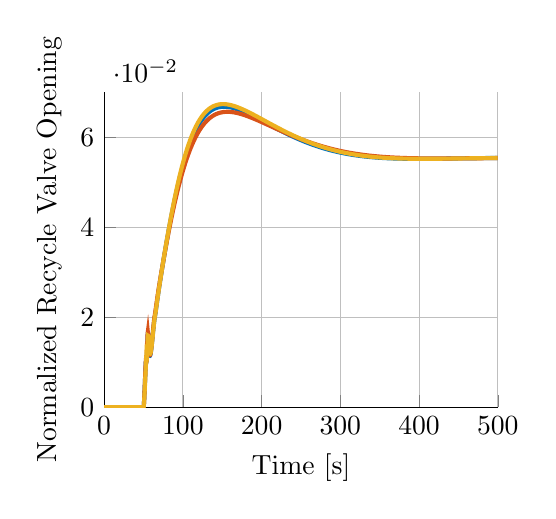
\begin{tikzpicture}

\begin{axis}[%
width=5cm,
height=4cm,
at={(0\linewidth,0\linewidth)},
scale only axis,
xmin=0,
xmax=500,
xlabel={Time [s]},
xmajorgrids,
ymin=0,
ymax=0.07,
ylabel={Normalized Recycle Valve Opening},
% ylabel style={font=\tiny},
ylabel near ticks,
ymajorgrids,
axis background/.style={fill=white},
% title style={font=\tiny\bfseries},
% title={Normalized Recycle Valve Opening},
axis x line*=bottom,
axis y line*=left
]
\addplot [color=mycolor1,solid,line width=1.5pt,forget plot]
  table[row sep=crcr]{%
0	6.93883000000002e-310\\
0.25	6.93883000000002e-310\\
0.5	6.93883000000002e-310\\
0.75	6.93883000000002e-310\\
1	6.93883000000002e-310\\
1.25	6.93883000000002e-310\\
1.5	6.93883000000002e-310\\
1.75	6.93883000000002e-310\\
2	6.93883000000002e-310\\
2.25	6.93883000000002e-310\\
2.5	6.93883000000002e-310\\
2.75	6.93883000000002e-310\\
3	6.93883000000002e-310\\
3.25	6.93883000000002e-310\\
3.5	6.93883000000002e-310\\
3.75	6.93883000000002e-310\\
4	6.93883000000002e-310\\
4.25	6.93883000000002e-310\\
4.5	6.93883000000002e-310\\
4.75	6.93883000000002e-310\\
5	6.93883000000002e-310\\
5.25	6.93883000000002e-310\\
5.5	6.93883000000002e-310\\
5.75	6.93883000000002e-310\\
6	6.93883000000002e-310\\
6.25	6.93883000000002e-310\\
6.5	6.93883000000002e-310\\
6.75	6.93883000000002e-310\\
7	6.93883000000002e-310\\
7.25	6.93883000000002e-310\\
7.5	6.93883000000002e-310\\
7.75	6.93883000000002e-310\\
8	6.93883000000002e-310\\
8.25	6.93883000000002e-310\\
8.5	6.93883000000002e-310\\
8.75	6.93883000000002e-310\\
9	6.93883000000002e-310\\
9.25	6.93883000000002e-310\\
9.5	6.93883000000002e-310\\
9.75	6.93883000000002e-310\\
10	6.93883000000002e-310\\
10.25	6.93883000000002e-310\\
10.5	6.93883000000002e-310\\
10.75	6.93883000000002e-310\\
11	6.93883000000002e-310\\
11.25	6.93883000000002e-310\\
11.5	6.93883000000002e-310\\
11.75	6.93883000000002e-310\\
12	6.93883000000002e-310\\
12.25	6.93883000000002e-310\\
12.5	6.93883000000002e-310\\
12.75	6.93883000000002e-310\\
13	6.93883000000002e-310\\
13.25	6.93883000000002e-310\\
13.5	6.93883000000002e-310\\
13.75	6.93883000000002e-310\\
14	6.93883000000002e-310\\
14.25	6.93883000000002e-310\\
14.5	6.93883000000002e-310\\
14.75	6.93883000000002e-310\\
15	6.93883000000002e-310\\
15.25	6.93883000000002e-310\\
15.5	6.93883000000002e-310\\
15.75	6.93883000000002e-310\\
16	6.93883000000002e-310\\
16.25	6.93883000000002e-310\\
16.5	6.93883000000002e-310\\
16.75	6.93883000000002e-310\\
17	6.93883000000002e-310\\
17.25	6.93883000000002e-310\\
17.5	6.93883000000002e-310\\
17.75	6.93883000000002e-310\\
18	6.93883000000002e-310\\
18.25	6.93883000000002e-310\\
18.5	6.93883000000002e-310\\
18.75	6.93883000000002e-310\\
19	6.93883000000002e-310\\
19.25	6.93883000000002e-310\\
19.5	6.93883000000002e-310\\
19.75	6.93883000000002e-310\\
20	6.93883000000002e-310\\
20.25	6.93883000000002e-310\\
20.5	6.93883000000002e-310\\
20.75	6.93883000000002e-310\\
21	6.93883000000002e-310\\
21.25	6.93883000000002e-310\\
21.5	6.93883000000002e-310\\
21.75	6.93883000000002e-310\\
22	6.93883000000002e-310\\
22.25	6.93883000000002e-310\\
22.5	6.93883000000002e-310\\
22.75	6.93883000000002e-310\\
23	6.93883000000002e-310\\
23.25	6.93883000000002e-310\\
23.5	6.93883000000002e-310\\
23.75	6.93883000000002e-310\\
24	6.93883000000002e-310\\
24.25	6.93883000000002e-310\\
24.5	6.93883000000002e-310\\
24.75	6.93883000000002e-310\\
25	6.93883000000002e-310\\
25.25	6.93883000000002e-310\\
25.5	6.93883000000002e-310\\
25.75	6.93883000000002e-310\\
26	6.93883000000002e-310\\
26.25	6.93883000000002e-310\\
26.5	6.93883000000002e-310\\
26.75	6.93883000000002e-310\\
27	6.93883000000002e-310\\
27.25	6.93883000000002e-310\\
27.5	6.93883000000002e-310\\
27.75	6.93883000000002e-310\\
28	6.93883000000002e-310\\
28.25	6.93883000000002e-310\\
28.5	6.93883000000002e-310\\
28.75	6.93883000000002e-310\\
29	6.93883000000002e-310\\
29.25	6.93883000000002e-310\\
29.5	6.93883000000002e-310\\
29.75	6.93883000000002e-310\\
30	6.93883000000002e-310\\
30.25	6.93883000000002e-310\\
30.5	6.93883000000002e-310\\
30.75	6.93883000000002e-310\\
31	6.93883000000002e-310\\
31.25	6.93883000000002e-310\\
31.5	6.93883000000002e-310\\
31.75	6.93883000000002e-310\\
32	6.93883000000002e-310\\
32.25	6.93883000000002e-310\\
32.5	6.93883000000002e-310\\
32.75	6.93883000000002e-310\\
33	6.93883000000002e-310\\
33.25	6.93883000000002e-310\\
33.5	6.93883000000002e-310\\
33.75	6.93883000000002e-310\\
34	6.93883000000002e-310\\
34.25	6.93883000000002e-310\\
34.5	6.93883000000002e-310\\
34.75	6.93883000000002e-310\\
35	6.93883000000002e-310\\
35.25	6.93883000000002e-310\\
35.5	6.93883000000002e-310\\
35.75	6.93883000000002e-310\\
36	6.93883000000002e-310\\
36.25	6.93883000000002e-310\\
36.5	6.93883000000002e-310\\
36.75	6.93883000000002e-310\\
37	6.93883000000002e-310\\
37.25	6.93883000000002e-310\\
37.5	6.93883000000002e-310\\
37.75	6.93883000000002e-310\\
38	6.93883000000002e-310\\
38.25	6.93883000000002e-310\\
38.5	6.93883000000002e-310\\
38.75	6.93883000000002e-310\\
39	6.93883000000002e-310\\
39.25	6.93883000000002e-310\\
39.5	6.93883000000002e-310\\
39.75	6.93883000000002e-310\\
40	6.93883000000002e-310\\
40.25	6.93883000000002e-310\\
40.5	6.93883000000002e-310\\
40.75	6.93883000000002e-310\\
41	6.93883000000002e-310\\
41.25	6.93883000000002e-310\\
41.5	6.93883000000002e-310\\
41.75	6.93883000000002e-310\\
42	6.93883000000002e-310\\
42.25	6.93883000000002e-310\\
42.5	6.93883000000002e-310\\
42.75	6.93883000000002e-310\\
43	6.93883000000002e-310\\
43.25	6.93883000000002e-310\\
43.5	6.93883000000002e-310\\
43.75	6.93883000000002e-310\\
44	6.93883000000002e-310\\
44.25	6.93883000000002e-310\\
44.5	6.93883000000002e-310\\
44.75	6.93883000000002e-310\\
45	6.93883000000002e-310\\
45.25	6.93883000000002e-310\\
45.5	6.93883000000002e-310\\
45.75	6.93883000000002e-310\\
46	6.93883000000002e-310\\
46.25	6.93883000000002e-310\\
46.5	6.93883000000002e-310\\
46.75	6.93883000000002e-310\\
47	6.93883000000002e-310\\
47.25	6.93883000000002e-310\\
47.5	6.93883000000002e-310\\
47.75	6.93883000000002e-310\\
48	6.93883000000002e-310\\
48.25	6.93883000000002e-310\\
48.5	6.93883000000002e-310\\
48.75	6.93883000000002e-310\\
49	6.93883000000002e-310\\
49.25	6.93883000000002e-310\\
49.5	6.93883000000002e-310\\
49.75	6.93883000000002e-310\\
50	6.93883000000002e-310\\
50.25	6.733e-05\\
50.5	0.000509304\\
50.75	0.00125732\\
51	0.00211134\\
51.25	0.00302577\\
51.5	0.00400956\\
51.75	0.00504281\\
52	0.00609347\\
52.25	0.00713677\\
52.5	0.00815443\\
52.75	0.00914098\\
53	0.0101092\\
53.25	0.0102592\\
53.5	0.00992427\\
53.75	0.0101356\\
54	0.0103164\\
54.25	0.0109471\\
54.5	0.01186\\
54.75	0.0129794\\
55	0.014282\\
55.25	0.0155271\\
55.5	0.0161968\\
55.75	0.0161878\\
56	0.0155694\\
56.25	0.0146319\\
56.5	0.0137396\\
56.75	0.0130061\\
57	0.0124325\\
57.25	0.0120057\\
57.5	0.0117086\\
57.75	0.0115219\\
58	0.0114301\\
58.25	0.0114217\\
58.5	0.0114875\\
58.75	0.0116189\\
59	0.0118074\\
59.25	0.0120456\\
59.5	0.0123271\\
59.75	0.0126463\\
60	0.0129979\\
60.25	0.013377\\
60.5	0.0137787\\
60.75	0.0141984\\
61	0.0146315\\
61.25	0.0150735\\
61.5	0.0155202\\
61.75	0.0159674\\
62	0.0164115\\
62.25	0.0168491\\
62.5	0.0172775\\
62.75	0.0176947\\
63	0.0180995\\
63.25	0.0184913\\
63.5	0.0188704\\
63.75	0.0192379\\
64	0.0195952\\
64.25	0.019944\\
64.5	0.0201304\\
64.75	0.0203321\\
65	0.0205944\\
65.25	0.0208869\\
65.5	0.0211948\\
65.75	0.0215114\\
66	0.0218322\\
66.25	0.0221542\\
66.5	0.0224756\\
66.75	0.0227958\\
67	0.023115\\
67.25	0.0234324\\
67.5	0.023747\\
67.75	0.0240585\\
68	0.0243668\\
68.25	0.024672\\
68.5	0.0249743\\
68.75	0.0252738\\
69	0.0255706\\
69.25	0.0258649\\
69.5	0.0261569\\
69.75	0.0264467\\
70	0.0267345\\
70.25	0.0270205\\
70.5	0.0273048\\
70.75	0.0275875\\
71	0.0278687\\
71.25	0.0281486\\
71.5	0.0284272\\
71.75	0.0287046\\
72	0.0289809\\
72.25	0.0292562\\
72.5	0.0295304\\
72.75	0.0298037\\
73	0.0300762\\
73.25	0.0303477\\
73.5	0.0306183\\
73.75	0.0308882\\
74	0.0311572\\
74.25	0.0314254\\
74.5	0.0316928\\
74.75	0.0319595\\
75	0.0322253\\
75.25	0.0324903\\
75.5	0.0327546\\
75.75	0.033018\\
76	0.0332807\\
76.25	0.0335425\\
76.5	0.0338035\\
76.75	0.0340637\\
77	0.0343231\\
77.25	0.0345816\\
77.5	0.0348393\\
77.75	0.035096\\
78	0.035352\\
78.25	0.035607\\
78.5	0.0358611\\
78.75	0.0361143\\
79	0.0363666\\
79.25	0.0366179\\
79.5	0.0368684\\
79.75	0.0371178\\
80	0.0373663\\
80.25	0.0376138\\
80.5	0.0378604\\
80.75	0.0381059\\
81	0.0383504\\
81.25	0.038594\\
81.5	0.0388365\\
81.75	0.039078\\
82	0.0393184\\
82.25	0.0395578\\
82.5	0.0397961\\
82.75	0.0400334\\
83	0.0402697\\
83.25	0.0405048\\
83.5	0.0407389\\
83.75	0.0409719\\
84	0.0412038\\
84.25	0.0414346\\
84.5	0.0416643\\
84.75	0.0418929\\
85	0.0421204\\
85.25	0.0423467\\
85.5	0.042572\\
85.75	0.0427961\\
86	0.0430191\\
86.25	0.043241\\
86.5	0.0434617\\
86.75	0.0436813\\
87	0.0438997\\
87.25	0.044117\\
87.5	0.0443332\\
87.75	0.0445482\\
88	0.044762\\
88.25	0.0449747\\
88.5	0.0451862\\
88.75	0.0453966\\
89	0.0456058\\
89.25	0.0458138\\
89.5	0.0460206\\
89.75	0.0462263\\
90	0.0464308\\
90.25	0.0466342\\
90.5	0.0468363\\
90.75	0.0470373\\
91	0.0472371\\
91.25	0.0474357\\
91.5	0.0476332\\
91.75	0.0478295\\
92	0.0480245\\
92.25	0.0482184\\
92.5	0.0484112\\
92.75	0.0486027\\
93	0.048793\\
93.25	0.0489822\\
93.5	0.0491702\\
93.75	0.049357\\
94	0.0495426\\
94.25	0.049727\\
94.5	0.0499103\\
94.75	0.0500924\\
95	0.0502733\\
95.25	0.050453\\
95.5	0.0506315\\
95.75	0.0508088\\
96	0.050985\\
96.25	0.05116\\
96.5	0.0513338\\
96.75	0.0515064\\
97	0.0516778\\
97.25	0.0518481\\
97.5	0.0520172\\
97.75	0.0521851\\
98	0.0523519\\
98.25	0.0525175\\
98.5	0.0526819\\
98.75	0.0528451\\
99	0.0530072\\
99.25	0.0531682\\
99.5	0.0533279\\
99.75	0.0534865\\
100	0.0536439\\
100.25	0.0538002\\
100.5	0.0539554\\
100.75	0.0541093\\
101	0.0542622\\
101.25	0.0544138\\
101.5	0.0545644\\
101.75	0.0547138\\
102	0.054862\\
102.25	0.0550091\\
102.5	0.0551551\\
102.75	0.0552999\\
103	0.0554437\\
103.25	0.0555862\\
103.5	0.0557277\\
103.75	0.055868\\
104	0.0560072\\
104.25	0.0561453\\
104.5	0.0562823\\
104.75	0.0564182\\
105	0.0565529\\
105.25	0.0566866\\
105.5	0.0568191\\
105.75	0.0569505\\
106	0.0570809\\
106.25	0.0572101\\
106.5	0.0573383\\
106.75	0.0574654\\
107	0.0575914\\
107.25	0.0577163\\
107.5	0.0578401\\
107.75	0.0579629\\
108	0.0580846\\
108.25	0.0582052\\
108.5	0.0583247\\
108.75	0.0584432\\
109	0.0585606\\
109.25	0.058677\\
109.5	0.0587924\\
109.75	0.0589067\\
110	0.0590199\\
110.25	0.0591321\\
110.5	0.0592433\\
110.75	0.0593534\\
111	0.0594625\\
111.25	0.0595706\\
111.5	0.0596777\\
111.75	0.0597837\\
112	0.0598888\\
112.25	0.0599928\\
112.5	0.0600958\\
112.75	0.0601979\\
113	0.0602989\\
113.25	0.060399\\
113.5	0.060498\\
113.75	0.0605961\\
114	0.0606932\\
114.25	0.0607893\\
114.5	0.0608844\\
114.75	0.0609786\\
115	0.0610718\\
115.25	0.0611641\\
115.5	0.0612554\\
115.75	0.0613458\\
116	0.0614352\\
116.25	0.0615237\\
116.5	0.0616112\\
116.75	0.0616978\\
117	0.0617835\\
117.25	0.0618682\\
117.5	0.0619521\\
117.75	0.062035\\
118	0.062117\\
118.25	0.0621981\\
118.5	0.0622783\\
118.75	0.0623576\\
119	0.062436\\
119.25	0.0625136\\
119.5	0.0625902\\
119.75	0.062666\\
120	0.0627409\\
120.25	0.0628149\\
120.5	0.0628881\\
120.75	0.0629604\\
121	0.0630318\\
121.25	0.0631024\\
121.5	0.0631722\\
121.75	0.0632411\\
122	0.0633091\\
122.25	0.0633764\\
122.5	0.0634428\\
122.75	0.0635084\\
123	0.0635732\\
123.25	0.0636371\\
123.5	0.0637003\\
123.75	0.0637627\\
124	0.0638242\\
124.25	0.063885\\
124.5	0.0639449\\
124.75	0.0640041\\
125	0.0640625\\
125.25	0.0641202\\
125.5	0.064177\\
125.75	0.0642331\\
126	0.0642885\\
126.25	0.0643431\\
126.5	0.0643969\\
126.75	0.06445\\
127	0.0645023\\
127.25	0.0645539\\
127.5	0.0646048\\
127.75	0.064655\\
128	0.0647044\\
128.25	0.0647531\\
128.5	0.0648011\\
128.75	0.0648484\\
129	0.064895\\
129.25	0.0649409\\
129.5	0.0649861\\
129.75	0.0650306\\
130	0.0650744\\
130.25	0.0651175\\
130.5	0.06516\\
130.75	0.0652018\\
131	0.0652429\\
131.25	0.0652834\\
131.5	0.0653232\\
131.75	0.0653624\\
132	0.0654009\\
132.25	0.0654387\\
132.5	0.065476\\
132.75	0.0655126\\
133	0.0655486\\
133.25	0.0655839\\
133.5	0.0656186\\
133.75	0.0656528\\
134	0.0656863\\
134.25	0.0657192\\
134.5	0.0657515\\
134.75	0.0657832\\
135	0.0658143\\
135.25	0.0658448\\
135.5	0.0658748\\
135.75	0.0659041\\
136	0.0659329\\
136.25	0.0659611\\
136.5	0.0659888\\
136.75	0.0660159\\
137	0.0660424\\
137.25	0.0660684\\
137.5	0.0660939\\
137.75	0.0661188\\
138	0.0661432\\
138.25	0.066167\\
138.5	0.0661903\\
138.75	0.0662131\\
139	0.0662353\\
139.25	0.0662571\\
139.5	0.0662783\\
139.75	0.066299\\
140	0.0663193\\
140.25	0.066339\\
140.5	0.0663582\\
140.75	0.0663769\\
141	0.0663952\\
141.25	0.0664129\\
141.5	0.0664302\\
141.75	0.066447\\
142	0.0664634\\
142.25	0.0664793\\
142.5	0.0664947\\
142.75	0.0665096\\
143	0.0665241\\
143.25	0.0665382\\
143.5	0.0665518\\
143.75	0.066565\\
144	0.0665777\\
144.25	0.06659\\
144.5	0.0666018\\
144.75	0.0666133\\
145	0.0666243\\
145.25	0.0666349\\
145.5	0.0666451\\
145.75	0.0666548\\
146	0.0666642\\
146.25	0.0666732\\
146.5	0.0666817\\
146.75	0.0666899\\
147	0.0666976\\
147.25	0.066705\\
147.5	0.066712\\
147.75	0.0667186\\
148	0.0667249\\
148.25	0.0667307\\
148.5	0.0667362\\
148.75	0.0667414\\
149	0.0667461\\
149.25	0.0667505\\
149.5	0.0667546\\
149.75	0.0667582\\
150	0.0667616\\
150.25	0.0667646\\
150.5	0.0667672\\
150.75	0.0667695\\
151	0.0667715\\
151.25	0.0667732\\
151.5	0.0667745\\
151.75	0.0667755\\
152	0.0667761\\
152.25	0.0667765\\
152.5	0.0667765\\
152.75	0.0667762\\
153	0.0667756\\
153.25	0.0667747\\
153.5	0.0667735\\
153.75	0.066772\\
154	0.0667702\\
154.25	0.0667681\\
154.5	0.0667657\\
154.75	0.066763\\
155	0.06676\\
155.25	0.0667568\\
155.5	0.0667532\\
155.75	0.0667494\\
156	0.0667453\\
156.25	0.066741\\
156.5	0.0667363\\
156.75	0.0667314\\
157	0.0667263\\
157.25	0.0667209\\
157.5	0.0667152\\
157.75	0.0667093\\
158	0.0667031\\
158.25	0.0666967\\
158.5	0.06669\\
158.75	0.0666831\\
159	0.0666759\\
159.25	0.0666685\\
159.5	0.0666609\\
159.75	0.066653\\
160	0.0666449\\
160.25	0.0666366\\
160.5	0.066628\\
160.75	0.0666193\\
161	0.0666103\\
161.25	0.0666011\\
161.5	0.0665916\\
161.75	0.066582\\
162	0.0665721\\
162.25	0.0665621\\
162.5	0.0665518\\
162.75	0.0665413\\
163	0.0665306\\
163.25	0.0665198\\
163.5	0.0665087\\
163.75	0.0664974\\
164	0.066486\\
164.25	0.0664743\\
164.5	0.0664625\\
164.75	0.0664505\\
165	0.0664382\\
165.25	0.0664259\\
165.5	0.0664133\\
165.75	0.0664005\\
166	0.0663876\\
166.25	0.0663745\\
166.5	0.0663613\\
166.75	0.0663478\\
167	0.0663342\\
167.25	0.0663204\\
167.5	0.0663065\\
167.75	0.0662924\\
168	0.0662782\\
168.25	0.0662638\\
168.5	0.0662492\\
168.75	0.0662345\\
169	0.0662196\\
169.25	0.0662046\\
169.5	0.0661894\\
169.75	0.0661741\\
170	0.0661587\\
170.25	0.0661431\\
170.5	0.0661273\\
170.75	0.0661114\\
171	0.0660954\\
171.25	0.0660793\\
171.5	0.066063\\
171.75	0.0660466\\
172	0.06603\\
172.25	0.0660133\\
172.5	0.0659965\\
172.75	0.0659796\\
173	0.0659626\\
173.25	0.0659454\\
173.5	0.0659281\\
173.75	0.0659107\\
174	0.0658932\\
174.25	0.0658755\\
174.5	0.0658578\\
174.75	0.0658399\\
175	0.0658219\\
175.25	0.0658038\\
175.5	0.0657856\\
175.75	0.0657673\\
176	0.0657489\\
176.25	0.0657304\\
176.5	0.0657118\\
176.75	0.0656931\\
177	0.0656743\\
177.25	0.0656553\\
177.5	0.0656363\\
177.75	0.0656172\\
178	0.065598\\
178.25	0.0655787\\
178.5	0.0655594\\
178.75	0.0655399\\
179	0.0655203\\
179.25	0.0655007\\
179.5	0.065481\\
179.75	0.0654611\\
180	0.0654412\\
180.25	0.0654213\\
180.5	0.0654012\\
180.75	0.0653811\\
181	0.0653608\\
181.25	0.0653405\\
181.5	0.0653202\\
181.75	0.0652997\\
182	0.0652792\\
182.25	0.0652586\\
182.5	0.065238\\
182.75	0.0652172\\
183	0.0651964\\
183.25	0.0651756\\
183.5	0.0651546\\
183.75	0.0651336\\
184	0.0651126\\
184.25	0.0650914\\
184.5	0.0650702\\
184.75	0.065049\\
185	0.0650277\\
185.25	0.0650063\\
185.5	0.0649849\\
185.75	0.0649634\\
186	0.0649418\\
186.25	0.0649203\\
186.5	0.0648986\\
186.75	0.0648769\\
187	0.0648551\\
187.25	0.0648333\\
187.5	0.0648115\\
187.75	0.0647896\\
188	0.0647676\\
188.25	0.0647456\\
188.5	0.0647236\\
188.75	0.0647015\\
189	0.0646794\\
189.25	0.0646572\\
189.5	0.064635\\
189.75	0.0646127\\
190	0.0645904\\
190.25	0.0645681\\
190.5	0.0645457\\
190.75	0.0645233\\
191	0.0645008\\
191.25	0.0644783\\
191.5	0.0644558\\
191.75	0.0644332\\
192	0.0644106\\
192.25	0.064388\\
192.5	0.0643653\\
192.75	0.0643426\\
193	0.0643199\\
193.25	0.0642971\\
193.5	0.0642743\\
193.75	0.0642515\\
194	0.0642287\\
194.25	0.0642058\\
194.5	0.0641829\\
194.75	0.06416\\
195	0.0641371\\
195.25	0.0641141\\
195.5	0.0640911\\
195.75	0.0640681\\
196	0.0640451\\
196.25	0.064022\\
196.5	0.0639989\\
196.75	0.0639758\\
197	0.0639527\\
197.25	0.0639296\\
197.5	0.0639064\\
197.75	0.0638832\\
198	0.0638601\\
198.25	0.0638369\\
198.5	0.0638136\\
198.75	0.0637904\\
199	0.0637672\\
199.25	0.0637439\\
199.5	0.0637206\\
199.75	0.0636973\\
200	0.0636741\\
200.25	0.0636507\\
200.5	0.0636274\\
200.75	0.0636041\\
201	0.0635808\\
201.25	0.0635574\\
201.5	0.0635341\\
201.75	0.0635107\\
202	0.0634874\\
202.25	0.063464\\
202.5	0.0634406\\
202.75	0.0634172\\
203	0.0633938\\
203.25	0.0633705\\
203.5	0.0633471\\
203.75	0.0633237\\
204	0.0633003\\
204.25	0.0632769\\
204.5	0.0632535\\
204.75	0.0632301\\
205	0.0632067\\
205.25	0.0631833\\
205.5	0.0631599\\
205.75	0.0631365\\
206	0.0631131\\
206.25	0.0630897\\
206.5	0.0630663\\
206.75	0.0630429\\
207	0.0630195\\
207.25	0.0629961\\
207.5	0.0629727\\
207.75	0.0629494\\
208	0.062926\\
208.25	0.0629027\\
208.5	0.0628793\\
208.75	0.062856\\
209	0.0628326\\
209.25	0.0628093\\
209.5	0.062786\\
209.75	0.0627626\\
210	0.0627393\\
210.25	0.062716\\
210.5	0.0626928\\
210.75	0.0626695\\
211	0.0626462\\
211.25	0.062623\\
211.5	0.0625997\\
211.75	0.0625765\\
212	0.0625533\\
212.25	0.0625301\\
212.5	0.0625069\\
212.75	0.0624837\\
213	0.0624605\\
213.25	0.0624374\\
213.5	0.0624142\\
213.75	0.0623911\\
214	0.062368\\
214.25	0.0623449\\
214.5	0.0623219\\
214.75	0.0622988\\
215	0.0622758\\
215.25	0.0622527\\
215.5	0.0622297\\
215.75	0.0622067\\
216	0.0621838\\
216.25	0.0621608\\
216.5	0.0621379\\
216.75	0.062115\\
217	0.0620921\\
217.25	0.0620692\\
217.5	0.0620464\\
217.75	0.0620235\\
218	0.0620007\\
218.25	0.0619779\\
218.5	0.0619552\\
218.75	0.0619324\\
219	0.0619097\\
219.25	0.061887\\
219.5	0.0618643\\
219.75	0.0618416\\
220	0.061819\\
220.25	0.0617964\\
220.5	0.0617738\\
220.75	0.0617513\\
221	0.0617287\\
221.25	0.0617062\\
221.5	0.0616837\\
221.75	0.0616613\\
222	0.0616388\\
222.25	0.0616164\\
222.5	0.061594\\
222.75	0.0615717\\
223	0.0615493\\
223.25	0.061527\\
223.5	0.0615048\\
223.75	0.0614825\\
224	0.0614603\\
224.25	0.0614381\\
224.5	0.0614159\\
224.75	0.0613938\\
225	0.0613717\\
225.25	0.0613496\\
225.5	0.0613275\\
225.75	0.0613055\\
226	0.0612835\\
226.25	0.0612616\\
226.5	0.0612396\\
226.75	0.0612177\\
227	0.0611959\\
227.25	0.061174\\
227.5	0.0611522\\
227.75	0.0611304\\
228	0.0611087\\
228.25	0.061087\\
228.5	0.0610653\\
228.75	0.0610436\\
229	0.061022\\
229.25	0.0610004\\
229.5	0.0609789\\
229.75	0.0609573\\
230	0.0609359\\
230.25	0.0609144\\
230.5	0.060893\\
230.75	0.0608716\\
231	0.0608502\\
231.25	0.0608289\\
231.5	0.0608076\\
231.75	0.0607864\\
232	0.0607652\\
232.25	0.060744\\
232.5	0.0607228\\
232.75	0.0607017\\
233	0.0606806\\
233.25	0.0606596\\
233.5	0.0606386\\
233.75	0.0606176\\
234	0.0605967\\
234.25	0.0605758\\
234.5	0.0605549\\
234.75	0.0605341\\
235	0.0605133\\
235.25	0.0604926\\
235.5	0.0604719\\
235.75	0.0604512\\
236	0.0604305\\
236.25	0.0604099\\
236.5	0.0603894\\
236.75	0.0603689\\
237	0.0603484\\
237.25	0.0603279\\
237.5	0.0603075\\
237.75	0.0602871\\
238	0.0602668\\
238.25	0.0602465\\
238.5	0.0602262\\
238.75	0.060206\\
239	0.0601858\\
239.25	0.0601657\\
239.5	0.0601456\\
239.75	0.0601255\\
240	0.0601055\\
240.25	0.0600855\\
240.5	0.0600656\\
240.75	0.0600457\\
241	0.0600258\\
241.25	0.060006\\
241.5	0.0599862\\
241.75	0.0599665\\
242	0.0599468\\
242.25	0.0599271\\
242.5	0.0599075\\
242.75	0.0598879\\
243	0.0598684\\
243.25	0.0598489\\
243.5	0.0598295\\
243.75	0.05981\\
244	0.0597907\\
244.25	0.0597713\\
244.5	0.0597521\\
244.75	0.0597328\\
245	0.0597136\\
245.25	0.0596944\\
245.5	0.0596753\\
245.75	0.0596562\\
246	0.0596372\\
246.25	0.0596182\\
246.5	0.0595993\\
246.75	0.0595804\\
247	0.0595615\\
247.25	0.0595427\\
247.5	0.0595239\\
247.75	0.0595052\\
248	0.0594865\\
248.25	0.0594678\\
248.5	0.0594492\\
248.75	0.0594306\\
249	0.0594121\\
249.25	0.0593936\\
249.5	0.0593752\\
249.75	0.0593568\\
250	0.0593385\\
250.25	0.0593202\\
250.5	0.0593019\\
250.75	0.0592837\\
251	0.0592655\\
251.25	0.0592474\\
251.5	0.0592293\\
251.75	0.0592113\\
252	0.0591933\\
252.25	0.0591753\\
252.5	0.0591574\\
252.75	0.0591396\\
253	0.0591218\\
253.25	0.059104\\
253.5	0.0590863\\
253.75	0.0590686\\
254	0.0590509\\
254.25	0.0590333\\
254.5	0.0590158\\
254.75	0.0589983\\
255	0.0589808\\
255.25	0.0589634\\
255.5	0.0589461\\
255.75	0.0589287\\
256	0.0589115\\
256.25	0.0588942\\
256.5	0.058877\\
256.75	0.0588599\\
257	0.0588428\\
257.25	0.0588257\\
257.5	0.0588087\\
257.75	0.0587918\\
258	0.0587749\\
258.25	0.058758\\
258.5	0.0587412\\
258.75	0.0587244\\
259	0.0587077\\
259.25	0.058691\\
259.5	0.0586743\\
259.75	0.0586577\\
260	0.0586412\\
260.25	0.0586247\\
260.5	0.0586082\\
260.75	0.0585918\\
261	0.0585754\\
261.25	0.0585591\\
261.5	0.0585429\\
261.75	0.0585266\\
262	0.0585104\\
262.25	0.0584943\\
262.5	0.0584782\\
262.75	0.0584622\\
263	0.0584462\\
263.25	0.0584302\\
263.5	0.0584143\\
263.75	0.0583985\\
264	0.0583827\\
264.25	0.0583669\\
264.5	0.0583512\\
264.75	0.0583355\\
265	0.0583199\\
265.25	0.0583043\\
265.5	0.0582887\\
265.75	0.0582733\\
266	0.0582578\\
266.25	0.0582424\\
266.5	0.0582271\\
266.75	0.0582118\\
267	0.0581965\\
267.25	0.0581813\\
267.5	0.0581661\\
267.75	0.058151\\
268	0.0581359\\
268.25	0.0581209\\
268.5	0.0581059\\
268.75	0.058091\\
269	0.0580761\\
269.25	0.0580613\\
269.5	0.0580465\\
269.75	0.0580317\\
270	0.058017\\
270.25	0.0580024\\
270.5	0.0579878\\
270.75	0.0579732\\
271	0.0579587\\
271.25	0.0579442\\
271.5	0.0579298\\
271.75	0.0579154\\
272	0.0579011\\
272.25	0.0578868\\
272.5	0.0578726\\
272.75	0.0578584\\
273	0.0578442\\
273.25	0.0578301\\
273.5	0.0578161\\
273.75	0.0578021\\
274	0.0577881\\
274.25	0.0577742\\
274.5	0.0577603\\
274.75	0.0577465\\
275	0.0577327\\
275.25	0.057719\\
275.5	0.0577053\\
275.75	0.0576917\\
276	0.0576781\\
276.25	0.0576646\\
276.5	0.0576511\\
276.75	0.0576376\\
277	0.0576242\\
277.25	0.0576108\\
277.5	0.0575975\\
277.75	0.0575843\\
278	0.057571\\
278.25	0.0575579\\
278.5	0.0575447\\
278.75	0.0575316\\
279	0.0575186\\
279.25	0.0575056\\
279.5	0.0574927\\
279.75	0.0574798\\
280	0.0574669\\
280.25	0.0574541\\
280.5	0.0574413\\
280.75	0.0574286\\
281	0.0574159\\
281.25	0.0574033\\
281.5	0.0573907\\
281.75	0.0573782\\
282	0.0573657\\
282.25	0.0573532\\
282.5	0.0573408\\
282.75	0.0573285\\
283	0.0573162\\
283.25	0.0573039\\
283.5	0.0572917\\
283.75	0.0572795\\
284	0.0572674\\
284.25	0.0572553\\
284.5	0.0572432\\
284.75	0.0572312\\
285	0.0572193\\
285.25	0.0572074\\
285.5	0.0571955\\
285.75	0.0571837\\
286	0.0571719\\
286.25	0.0571602\\
286.5	0.0571485\\
286.75	0.0571369\\
287	0.0571253\\
287.25	0.0571137\\
287.5	0.0571022\\
287.75	0.0570908\\
288	0.0570794\\
288.25	0.057068\\
288.5	0.0570567\\
288.75	0.0570454\\
289	0.0570341\\
289.25	0.0570229\\
289.5	0.0570118\\
289.75	0.0570007\\
290	0.0569896\\
290.25	0.0569786\\
290.5	0.0569676\\
290.75	0.0569567\\
291	0.0569458\\
291.25	0.0569349\\
291.5	0.0569241\\
291.75	0.0569134\\
292	0.0569027\\
292.25	0.056892\\
292.5	0.0568814\\
292.75	0.0568708\\
293	0.0568603\\
293.25	0.0568498\\
293.5	0.0568393\\
293.75	0.0568289\\
294	0.0568185\\
294.25	0.0568082\\
294.5	0.0567979\\
294.75	0.0567877\\
295	0.0567775\\
295.25	0.0567673\\
295.5	0.0567572\\
295.75	0.0567471\\
296	0.0567371\\
296.25	0.0567271\\
296.5	0.0567172\\
296.75	0.0567073\\
297	0.0566974\\
297.25	0.0566876\\
297.5	0.0566778\\
297.75	0.0566681\\
298	0.0566584\\
298.25	0.0566488\\
298.5	0.0566392\\
298.75	0.0566296\\
299	0.0566201\\
299.25	0.0566106\\
299.5	0.0566011\\
299.75	0.0565918\\
300	0.0565824\\
300.25	0.0565731\\
300.5	0.0565638\\
300.75	0.0565546\\
301	0.0565454\\
301.25	0.0565362\\
301.5	0.0565271\\
301.75	0.056518\\
302	0.056509\\
302.25	0.0565\\
302.5	0.0564911\\
302.75	0.0564822\\
303	0.0564733\\
303.25	0.0564645\\
303.5	0.0564557\\
303.75	0.056447\\
304	0.0564382\\
304.25	0.0564296\\
304.5	0.056421\\
304.75	0.0564124\\
305	0.0564038\\
305.25	0.0563953\\
305.5	0.0563869\\
305.75	0.0563784\\
306	0.05637\\
306.25	0.0563617\\
306.5	0.0563534\\
306.75	0.0563451\\
307	0.0563369\\
307.25	0.0563287\\
307.5	0.0563205\\
307.75	0.0563124\\
308	0.0563044\\
308.25	0.0562963\\
308.5	0.0562883\\
308.75	0.0562804\\
309	0.0562725\\
309.25	0.0562646\\
309.5	0.0562567\\
309.75	0.0562489\\
310	0.0562412\\
310.25	0.0562334\\
310.5	0.0562258\\
310.75	0.0562181\\
311	0.0562105\\
311.25	0.0562029\\
311.5	0.0561954\\
311.75	0.0561879\\
312	0.0561804\\
312.25	0.056173\\
312.5	0.0561656\\
312.75	0.0561582\\
313	0.0561509\\
313.25	0.0561437\\
313.5	0.0561364\\
313.75	0.0561292\\
314	0.056122\\
314.25	0.0561149\\
314.5	0.0561078\\
314.75	0.0561008\\
315	0.0560938\\
315.25	0.0560868\\
315.5	0.0560798\\
315.75	0.0560729\\
316	0.056066\\
316.25	0.0560592\\
316.5	0.0560524\\
316.75	0.0560456\\
317	0.0560389\\
317.25	0.0560322\\
317.5	0.0560255\\
317.75	0.0560189\\
318	0.0560123\\
318.25	0.0560058\\
318.5	0.0559993\\
318.75	0.0559928\\
319	0.0559863\\
319.25	0.0559799\\
319.5	0.0559735\\
319.75	0.0559672\\
320	0.0559609\\
320.25	0.0559546\\
320.5	0.0559484\\
320.75	0.0559422\\
321	0.055936\\
321.25	0.0559299\\
321.5	0.0559238\\
321.75	0.0559177\\
322	0.0559116\\
322.25	0.0559056\\
322.5	0.0558997\\
322.75	0.0558937\\
323	0.0558878\\
323.25	0.055882\\
323.5	0.0558761\\
323.75	0.0558703\\
324	0.0558646\\
324.25	0.0558588\\
324.5	0.0558531\\
324.75	0.0558475\\
325	0.0558418\\
325.25	0.0558362\\
325.5	0.0558307\\
325.75	0.0558251\\
326	0.0558196\\
326.25	0.0558141\\
326.5	0.0558087\\
326.75	0.0558033\\
327	0.0557979\\
327.25	0.0557926\\
327.5	0.0557872\\
327.75	0.055782\\
328	0.0557767\\
328.25	0.0557715\\
328.5	0.0557663\\
328.75	0.0557611\\
329	0.055756\\
329.25	0.0557509\\
329.5	0.0557459\\
329.75	0.0557408\\
330	0.0557358\\
330.25	0.0557309\\
330.5	0.0557259\\
330.75	0.055721\\
331	0.0557161\\
331.25	0.0557113\\
331.5	0.0557065\\
331.75	0.0557017\\
332	0.0556969\\
332.25	0.0556922\\
332.5	0.0556875\\
332.75	0.0556828\\
333	0.0556782\\
333.25	0.0556736\\
333.5	0.055669\\
333.75	0.0556644\\
334	0.0556599\\
334.25	0.0556554\\
334.5	0.0556509\\
334.75	0.0556465\\
335	0.0556421\\
335.25	0.0556377\\
335.5	0.0556334\\
335.75	0.0556291\\
336	0.0556248\\
336.25	0.0556205\\
336.5	0.0556163\\
336.75	0.0556121\\
337	0.0556079\\
337.25	0.0556037\\
337.5	0.0555996\\
337.75	0.0555955\\
338	0.0555914\\
338.25	0.0555874\\
338.5	0.0555834\\
338.75	0.0555794\\
339	0.0555754\\
339.25	0.0555715\\
339.5	0.0555676\\
339.75	0.0555637\\
340	0.0555599\\
340.25	0.0555561\\
340.5	0.0555523\\
340.75	0.0555485\\
341	0.0555447\\
341.25	0.055541\\
341.5	0.0555373\\
341.75	0.0555337\\
342	0.05553\\
342.25	0.0555264\\
342.5	0.0555228\\
342.75	0.0555193\\
343	0.0555157\\
343.25	0.0555122\\
343.5	0.0555087\\
343.75	0.0555053\\
344	0.0555018\\
344.25	0.0554984\\
344.5	0.055495\\
344.75	0.0554917\\
345	0.0554884\\
345.25	0.055485\\
345.5	0.0554818\\
345.75	0.0554785\\
346	0.0554753\\
346.25	0.0554721\\
346.5	0.0554689\\
346.75	0.0554657\\
347	0.0554626\\
347.25	0.0554594\\
347.5	0.0554564\\
347.75	0.0554533\\
348	0.0554503\\
348.25	0.0554472\\
348.5	0.0554442\\
348.75	0.0554413\\
349	0.0554383\\
349.25	0.0554354\\
349.5	0.0554325\\
349.75	0.0554296\\
350	0.0554268\\
350.25	0.0554239\\
350.5	0.0554211\\
350.75	0.0554183\\
351	0.0554156\\
351.25	0.0554128\\
351.5	0.0554101\\
351.75	0.0554074\\
352	0.0554047\\
352.25	0.0554021\\
352.5	0.0553994\\
352.75	0.0553968\\
353	0.0553942\\
353.25	0.0553917\\
353.5	0.0553891\\
353.75	0.0553866\\
354	0.0553841\\
354.25	0.0553816\\
354.5	0.0553792\\
354.75	0.0553767\\
355	0.0553743\\
355.25	0.0553719\\
355.5	0.0553695\\
355.75	0.0553672\\
356	0.0553648\\
356.25	0.0553625\\
356.5	0.0553602\\
356.75	0.055358\\
357	0.0553557\\
357.25	0.0553535\\
357.5	0.0553513\\
357.75	0.0553491\\
358	0.0553469\\
358.25	0.0553448\\
358.5	0.0553426\\
358.75	0.0553405\\
359	0.0553384\\
359.25	0.0553364\\
359.5	0.0553343\\
359.75	0.0553323\\
360	0.0553302\\
360.25	0.0553283\\
360.5	0.0553263\\
360.75	0.0553243\\
361	0.0553224\\
361.25	0.0553205\\
361.5	0.0553186\\
361.75	0.0553167\\
362	0.0553148\\
362.25	0.055313\\
362.5	0.0553111\\
362.75	0.0553093\\
363	0.0553075\\
363.25	0.0553058\\
363.5	0.055304\\
363.75	0.0553023\\
364	0.0553006\\
364.25	0.0552989\\
364.5	0.0552972\\
364.75	0.0552955\\
365	0.0552939\\
365.25	0.0552922\\
365.5	0.0552906\\
365.75	0.055289\\
366	0.0552874\\
366.25	0.0552859\\
366.5	0.0552843\\
366.75	0.0552828\\
367	0.0552813\\
367.25	0.0552798\\
367.5	0.0552783\\
367.75	0.0552768\\
368	0.0552754\\
368.25	0.055274\\
368.5	0.0552725\\
368.75	0.0552712\\
369	0.0552698\\
369.25	0.0552684\\
369.5	0.0552671\\
369.75	0.0552657\\
370	0.0552644\\
370.25	0.0552631\\
370.5	0.0552618\\
370.75	0.0552605\\
371	0.0552593\\
371.25	0.055258\\
371.5	0.0552568\\
371.75	0.0552556\\
372	0.0552544\\
372.25	0.0552532\\
372.5	0.0552521\\
372.75	0.0552509\\
373	0.0552498\\
373.25	0.0552487\\
373.5	0.0552475\\
373.75	0.0552465\\
374	0.0552454\\
374.25	0.0552443\\
374.5	0.0552433\\
374.75	0.0552422\\
375	0.0552412\\
375.25	0.0552402\\
375.5	0.0552392\\
375.75	0.0552382\\
376	0.0552373\\
376.25	0.0552363\\
376.5	0.0552354\\
376.75	0.0552344\\
377	0.0552335\\
377.25	0.0552326\\
377.5	0.0552318\\
377.75	0.0552309\\
378	0.05523\\
378.25	0.0552292\\
378.5	0.0552283\\
378.75	0.0552275\\
379	0.0552267\\
379.25	0.0552259\\
379.5	0.0552251\\
379.75	0.0552244\\
380	0.0552236\\
380.25	0.0552229\\
380.5	0.0552221\\
380.75	0.0552214\\
381	0.0552207\\
381.25	0.05522\\
381.5	0.0552193\\
381.75	0.0552187\\
382	0.055218\\
382.25	0.0552174\\
382.5	0.0552167\\
382.75	0.0552161\\
383	0.0552155\\
383.25	0.0552149\\
383.5	0.0552143\\
383.75	0.0552137\\
384	0.0552132\\
384.25	0.0552126\\
384.5	0.0552121\\
384.75	0.0552115\\
385	0.055211\\
385.25	0.0552105\\
385.5	0.05521\\
385.75	0.0552095\\
386	0.055209\\
386.25	0.0552086\\
386.5	0.0552081\\
386.75	0.0552077\\
387	0.0552072\\
387.25	0.0552068\\
387.5	0.0552064\\
387.75	0.055206\\
388	0.0552056\\
388.25	0.0552052\\
388.5	0.0552048\\
388.75	0.0552045\\
389	0.0552041\\
389.25	0.0552038\\
389.5	0.0552035\\
389.75	0.0552031\\
390	0.0552028\\
390.25	0.0552025\\
390.5	0.0552022\\
390.75	0.0552019\\
391	0.0552017\\
391.25	0.0552014\\
391.5	0.0552011\\
391.75	0.0552009\\
392	0.0552006\\
392.25	0.0552004\\
392.5	0.0552002\\
392.75	0.0552\\
393	0.0551998\\
393.25	0.0551996\\
393.5	0.0551994\\
393.75	0.0551992\\
394	0.055199\\
394.25	0.0551989\\
394.5	0.0551987\\
394.75	0.0551986\\
395	0.0551985\\
395.25	0.0551983\\
395.5	0.0551982\\
395.75	0.0551981\\
396	0.055198\\
396.25	0.0551979\\
396.5	0.0551978\\
396.75	0.0551977\\
397	0.0551977\\
397.25	0.0551976\\
397.5	0.0551976\\
397.75	0.0551975\\
398	0.0551975\\
398.25	0.0551974\\
398.5	0.0551974\\
398.75	0.0551974\\
399	0.0551974\\
399.25	0.0551974\\
399.5	0.0551974\\
399.75	0.0551974\\
400	0.0551974\\
400.25	0.0551975\\
400.5	0.0551975\\
400.75	0.0551975\\
401	0.0551976\\
401.25	0.0551976\\
401.5	0.0551977\\
401.75	0.0551978\\
402	0.0551978\\
402.25	0.0551979\\
402.5	0.055198\\
402.75	0.0551981\\
403	0.0551982\\
403.25	0.0551983\\
403.5	0.0551984\\
403.75	0.0551986\\
404	0.0551987\\
404.25	0.0551988\\
404.5	0.055199\\
404.75	0.0551991\\
405	0.0551993\\
405.25	0.0551994\\
405.5	0.0551996\\
405.75	0.0551998\\
406	0.0551999\\
406.25	0.0552001\\
406.5	0.0552003\\
406.75	0.0552005\\
407	0.0552007\\
407.25	0.0552009\\
407.5	0.0552011\\
407.75	0.0552013\\
408	0.0552016\\
408.25	0.0552018\\
408.5	0.055202\\
408.75	0.0552023\\
409	0.0552025\\
409.25	0.0552027\\
409.5	0.055203\\
409.75	0.0552033\\
410	0.0552035\\
410.25	0.0552038\\
410.5	0.0552041\\
410.75	0.0552043\\
411	0.0552046\\
411.25	0.0552049\\
411.5	0.0552052\\
411.75	0.0552055\\
412	0.0552058\\
412.25	0.0552061\\
412.5	0.0552064\\
412.75	0.0552067\\
413	0.0552071\\
413.25	0.0552074\\
413.5	0.0552077\\
413.75	0.0552081\\
414	0.0552084\\
414.25	0.0552087\\
414.5	0.0552091\\
414.75	0.0552094\\
415	0.0552098\\
415.25	0.0552102\\
415.5	0.0552105\\
415.75	0.0552109\\
416	0.0552113\\
416.25	0.0552116\\
416.5	0.055212\\
416.75	0.0552124\\
417	0.0552128\\
417.25	0.0552132\\
417.5	0.0552136\\
417.75	0.055214\\
418	0.0552144\\
418.25	0.0552148\\
418.5	0.0552152\\
418.75	0.0552156\\
419	0.055216\\
419.25	0.0552164\\
419.5	0.0552169\\
419.75	0.0552173\\
420	0.0552177\\
420.25	0.0552181\\
420.5	0.0552186\\
420.75	0.055219\\
421	0.0552195\\
421.25	0.0552199\\
421.5	0.0552204\\
421.75	0.0552208\\
422	0.0552213\\
422.25	0.0552217\\
422.5	0.0552222\\
422.75	0.0552226\\
423	0.0552231\\
423.25	0.0552236\\
423.5	0.0552241\\
423.75	0.0552245\\
424	0.055225\\
424.25	0.0552255\\
424.5	0.055226\\
424.75	0.0552265\\
425	0.0552269\\
425.25	0.0552274\\
425.5	0.0552279\\
425.75	0.0552284\\
426	0.0552289\\
426.25	0.0552294\\
426.5	0.0552299\\
426.75	0.0552304\\
427	0.0552309\\
427.25	0.0552315\\
427.5	0.055232\\
427.75	0.0552325\\
428	0.055233\\
428.25	0.0552335\\
428.5	0.055234\\
428.75	0.0552346\\
429	0.0552351\\
429.25	0.0552356\\
429.5	0.0552361\\
429.75	0.0552367\\
430	0.0552372\\
430.25	0.0552377\\
430.5	0.0552383\\
430.75	0.0552388\\
431	0.0552393\\
431.25	0.0552399\\
431.5	0.0552404\\
431.75	0.055241\\
432	0.0552415\\
432.25	0.0552421\\
432.5	0.0552426\\
432.75	0.0552432\\
433	0.0552437\\
433.25	0.0552443\\
433.5	0.0552448\\
433.75	0.0552454\\
434	0.055246\\
434.25	0.0552465\\
434.5	0.0552471\\
434.75	0.0552476\\
435	0.0552482\\
435.25	0.0552488\\
435.5	0.0552493\\
435.75	0.0552499\\
436	0.0552505\\
436.25	0.055251\\
436.5	0.0552516\\
436.75	0.0552522\\
437	0.0552528\\
437.25	0.0552533\\
437.5	0.0552539\\
437.75	0.0552545\\
438	0.0552551\\
438.25	0.0552557\\
438.5	0.0552562\\
438.75	0.0552568\\
439	0.0552574\\
439.25	0.055258\\
439.5	0.0552586\\
439.75	0.0552591\\
440	0.0552597\\
440.25	0.0552603\\
440.5	0.0552609\\
440.75	0.0552615\\
441	0.0552621\\
441.25	0.0552627\\
441.5	0.0552633\\
441.75	0.0552638\\
442	0.0552644\\
442.25	0.055265\\
442.5	0.0552656\\
442.75	0.0552662\\
443	0.0552668\\
443.25	0.0552674\\
443.5	0.055268\\
443.75	0.0552686\\
444	0.0552692\\
444.25	0.0552698\\
444.5	0.0552704\\
444.75	0.055271\\
445	0.0552716\\
445.25	0.0552722\\
445.5	0.0552728\\
445.75	0.0552733\\
446	0.0552739\\
446.25	0.0552745\\
446.5	0.0552751\\
446.75	0.0552757\\
447	0.0552763\\
447.25	0.0552769\\
447.5	0.0552775\\
447.75	0.0552781\\
448	0.0552787\\
448.25	0.0552793\\
448.5	0.0552799\\
448.75	0.0552805\\
449	0.0552811\\
449.25	0.0552817\\
449.5	0.0552823\\
449.75	0.0552829\\
450	0.0552835\\
450.25	0.0552841\\
450.5	0.0552847\\
450.75	0.0552853\\
451	0.0552859\\
451.25	0.0552865\\
451.5	0.0552871\\
451.75	0.0552877\\
452	0.0552883\\
452.25	0.0552889\\
452.5	0.0552895\\
452.75	0.0552901\\
453	0.0552907\\
453.25	0.0552913\\
453.5	0.0552919\\
453.75	0.0552925\\
454	0.0552931\\
454.25	0.0552937\\
454.5	0.0552943\\
454.75	0.0552949\\
455	0.0552954\\
455.25	0.055296\\
455.5	0.0552966\\
455.75	0.0552972\\
456	0.0552978\\
456.25	0.0552984\\
456.5	0.055299\\
456.75	0.0552996\\
457	0.0553002\\
457.25	0.0553008\\
457.5	0.0553014\\
457.75	0.0553019\\
458	0.0553025\\
458.25	0.0553031\\
458.5	0.0553037\\
458.75	0.0553043\\
459	0.0553049\\
459.25	0.0553055\\
459.5	0.0553061\\
459.75	0.0553066\\
460	0.0553072\\
460.25	0.0553078\\
460.5	0.0553084\\
460.75	0.055309\\
461	0.0553095\\
461.25	0.0553101\\
461.5	0.0553107\\
461.75	0.0553113\\
462	0.0553119\\
462.25	0.0553124\\
462.5	0.055313\\
462.75	0.0553136\\
463	0.0553142\\
463.25	0.0553147\\
463.5	0.0553153\\
463.75	0.0553159\\
464	0.0553164\\
464.25	0.055317\\
464.5	0.0553176\\
464.75	0.0553182\\
465	0.0553187\\
465.25	0.0553193\\
465.5	0.0553199\\
465.75	0.0553204\\
466	0.055321\\
466.25	0.0553215\\
466.5	0.0553221\\
466.75	0.0553227\\
467	0.0553232\\
467.25	0.0553238\\
467.5	0.0553243\\
467.75	0.0553249\\
468	0.0553254\\
468.25	0.055326\\
468.5	0.0553266\\
468.75	0.0553271\\
469	0.0553277\\
469.25	0.0553282\\
469.5	0.0553288\\
469.75	0.0553293\\
470	0.0553299\\
470.25	0.0553304\\
470.5	0.0553309\\
470.75	0.0553315\\
471	0.055332\\
471.25	0.0553326\\
471.5	0.0553331\\
471.75	0.0553337\\
472	0.0553342\\
472.25	0.0553347\\
472.5	0.0553353\\
472.75	0.0553358\\
473	0.0553363\\
473.25	0.0553369\\
473.5	0.0553374\\
473.75	0.0553379\\
474	0.0553385\\
474.25	0.055339\\
474.5	0.0553395\\
474.75	0.05534\\
475	0.0553406\\
475.25	0.0553411\\
475.5	0.0553416\\
475.75	0.0553421\\
476	0.0553426\\
476.25	0.0553432\\
476.5	0.0553437\\
476.75	0.0553442\\
477	0.0553447\\
477.25	0.0553452\\
477.5	0.0553457\\
477.75	0.0553462\\
478	0.0553467\\
478.25	0.0553472\\
478.5	0.0553478\\
478.75	0.0553483\\
479	0.0553488\\
479.25	0.0553493\\
479.5	0.0553498\\
479.75	0.0553503\\
480	0.0553508\\
480.25	0.0553513\\
480.5	0.0553518\\
480.75	0.0553522\\
481	0.0553527\\
481.25	0.0553532\\
481.5	0.0553537\\
481.75	0.0553542\\
482	0.0553547\\
482.25	0.0553552\\
482.5	0.0553557\\
482.75	0.0553561\\
483	0.0553566\\
483.25	0.0553571\\
483.5	0.0553576\\
483.75	0.0553581\\
484	0.0553585\\
484.25	0.055359\\
484.5	0.0553595\\
484.75	0.05536\\
485	0.0553604\\
485.25	0.0553609\\
485.5	0.0553614\\
485.75	0.0553618\\
486	0.0553623\\
486.25	0.0553628\\
486.5	0.0553632\\
486.75	0.0553637\\
487	0.0553641\\
487.25	0.0553646\\
487.5	0.055365\\
487.75	0.0553655\\
488	0.055366\\
488.25	0.0553664\\
488.5	0.0553669\\
488.75	0.0553673\\
489	0.0553678\\
489.25	0.0553682\\
489.5	0.0553686\\
489.75	0.0553691\\
490	0.0553695\\
490.25	0.05537\\
490.5	0.0553704\\
490.75	0.0553708\\
491	0.0553713\\
491.25	0.0553717\\
491.5	0.0553721\\
491.75	0.0553726\\
492	0.055373\\
492.25	0.0553734\\
492.5	0.0553739\\
492.75	0.0553743\\
493	0.0553747\\
493.25	0.0553751\\
493.5	0.0553755\\
493.75	0.055376\\
494	0.0553764\\
494.25	0.0553768\\
494.5	0.0553772\\
494.75	0.0553776\\
495	0.055378\\
495.25	0.0553784\\
495.5	0.0553789\\
495.75	0.0553793\\
496	0.0553797\\
496.25	0.0553801\\
496.5	0.0553805\\
496.75	0.0553809\\
497	0.0553813\\
497.25	0.0553817\\
497.5	0.0553821\\
497.75	0.0553825\\
498	0.0553828\\
498.25	0.0553832\\
498.5	0.0553836\\
498.75	0.055384\\
499	0.0553844\\
499.25	0.0553848\\
499.5	0.0553852\\
499.75	0.0553856\\
};
\addplot [color=mycolor2,solid,line width=1.5pt,forget plot]
  table[row sep=crcr]{%
0	6.91844e-310\\
0.25	6.91844e-310\\
0.5	6.91844e-310\\
0.75	6.91844e-310\\
1	6.91844e-310\\
1.25	6.91844e-310\\
1.5	6.91844e-310\\
1.75	6.91844e-310\\
2	6.91844e-310\\
2.25	6.91844e-310\\
2.5	6.91844e-310\\
2.75	6.91844e-310\\
3	6.91844e-310\\
3.25	6.91844e-310\\
3.5	6.91844e-310\\
3.75	6.91844e-310\\
4	6.91844e-310\\
4.25	6.91844e-310\\
4.5	6.91844e-310\\
4.75	6.91844e-310\\
5	6.91844e-310\\
5.25	6.91844e-310\\
5.5	6.91844e-310\\
5.75	6.91844e-310\\
6	6.91844e-310\\
6.25	6.91844e-310\\
6.5	6.91844e-310\\
6.75	6.91844e-310\\
7	6.91844e-310\\
7.25	6.91844e-310\\
7.5	6.91844e-310\\
7.75	6.91844e-310\\
8	6.91844e-310\\
8.25	6.91844e-310\\
8.5	6.91844e-310\\
8.75	6.91844e-310\\
9	6.91844e-310\\
9.25	6.91844e-310\\
9.5	6.91844e-310\\
9.75	6.91844e-310\\
10	6.91844e-310\\
10.25	6.91844e-310\\
10.5	6.91844e-310\\
10.75	6.91844e-310\\
11	6.91844e-310\\
11.25	6.91844e-310\\
11.5	6.91844e-310\\
11.75	6.91844e-310\\
12	6.91844e-310\\
12.25	6.91844e-310\\
12.5	6.91844e-310\\
12.75	6.91844e-310\\
13	6.91844e-310\\
13.25	6.91844e-310\\
13.5	6.91844e-310\\
13.75	6.91844e-310\\
14	6.91844e-310\\
14.25	6.91844e-310\\
14.5	6.91844e-310\\
14.75	6.91844e-310\\
15	6.91844e-310\\
15.25	6.91844e-310\\
15.5	6.91844e-310\\
15.75	6.91844e-310\\
16	6.91844e-310\\
16.25	6.91844e-310\\
16.5	6.91844e-310\\
16.75	6.91844e-310\\
17	6.91844e-310\\
17.25	6.91844e-310\\
17.5	6.91844e-310\\
17.75	6.91844e-310\\
18	6.91844e-310\\
18.25	6.91844e-310\\
18.5	6.91844e-310\\
18.75	6.91844e-310\\
19	6.91844e-310\\
19.25	6.91844e-310\\
19.5	6.91844e-310\\
19.75	6.91844e-310\\
20	6.91844e-310\\
20.25	6.91844e-310\\
20.5	6.91844e-310\\
20.75	6.91844e-310\\
21	6.91844e-310\\
21.25	6.91844e-310\\
21.5	6.91844e-310\\
21.75	6.91844e-310\\
22	6.91844e-310\\
22.25	6.91844e-310\\
22.5	6.91844e-310\\
22.75	6.91844e-310\\
23	6.91844e-310\\
23.25	6.91844e-310\\
23.5	6.91844e-310\\
23.75	6.91844e-310\\
24	6.91844e-310\\
24.25	6.91844e-310\\
24.5	6.91844e-310\\
24.75	6.91844e-310\\
25	6.91844e-310\\
25.25	6.91844e-310\\
25.5	6.91844e-310\\
25.75	6.91844e-310\\
26	6.91844e-310\\
26.25	6.91844e-310\\
26.5	6.91844e-310\\
26.75	6.91844e-310\\
27	6.91844e-310\\
27.25	6.91844e-310\\
27.5	6.91844e-310\\
27.75	6.91844e-310\\
28	6.91844e-310\\
28.25	6.91844e-310\\
28.5	6.91844e-310\\
28.75	6.91844e-310\\
29	6.91844e-310\\
29.25	6.91844e-310\\
29.5	6.91844e-310\\
29.75	6.91844e-310\\
30	6.91844e-310\\
30.25	6.91844e-310\\
30.5	6.91844e-310\\
30.75	6.91844e-310\\
31	6.91844e-310\\
31.25	6.91844e-310\\
31.5	6.91844e-310\\
31.75	6.91844e-310\\
32	6.91844e-310\\
32.25	6.91844e-310\\
32.5	6.91844e-310\\
32.75	6.91844e-310\\
33	6.91844e-310\\
33.25	6.91844e-310\\
33.5	6.91844e-310\\
33.75	6.91844e-310\\
34	6.91844e-310\\
34.25	6.91844e-310\\
34.5	6.91844e-310\\
34.75	6.91844e-310\\
35	6.91844e-310\\
35.25	6.91844e-310\\
35.5	6.91844e-310\\
35.75	6.91844e-310\\
36	6.91844e-310\\
36.25	6.91844e-310\\
36.5	6.91844e-310\\
36.75	6.91844e-310\\
37	6.91844e-310\\
37.25	6.91844e-310\\
37.5	6.91844e-310\\
37.75	6.91844e-310\\
38	6.91844e-310\\
38.25	6.91844e-310\\
38.5	6.91844e-310\\
38.75	6.91844e-310\\
39	6.91844e-310\\
39.25	6.91844e-310\\
39.5	6.91844e-310\\
39.75	6.91844e-310\\
40	6.91844e-310\\
40.25	6.91844e-310\\
40.5	6.91844e-310\\
40.75	6.91844e-310\\
41	6.91844e-310\\
41.25	6.91844e-310\\
41.5	6.91844e-310\\
41.75	6.91844e-310\\
42	6.91844e-310\\
42.25	6.91844e-310\\
42.5	6.91844e-310\\
42.75	6.91844e-310\\
43	6.91844e-310\\
43.25	6.91844e-310\\
43.5	6.91844e-310\\
43.75	6.91844e-310\\
44	6.91844e-310\\
44.25	6.91844e-310\\
44.5	6.91844e-310\\
44.75	6.91844e-310\\
45	6.91844e-310\\
45.25	6.91844e-310\\
45.5	6.91844e-310\\
45.75	6.91844e-310\\
46	6.91844e-310\\
46.25	6.91844e-310\\
46.5	6.91844e-310\\
46.75	6.91844e-310\\
47	6.91844e-310\\
47.25	6.91844e-310\\
47.5	6.91844e-310\\
47.75	6.91844e-310\\
48	6.91844e-310\\
48.25	6.91844e-310\\
48.5	6.91844e-310\\
48.75	6.91844e-310\\
49	6.91844e-310\\
49.25	6.91844e-310\\
49.5	6.91844e-310\\
49.75	6.91844e-310\\
50	6.91844e-310\\
50.25	6.91356e-05\\
50.5	0.000522473\\
50.75	0.00128893\\
51	0.00216432\\
51.25	0.00310461\\
51.5	0.00412168\\
51.75	0.00519742\\
52	0.00630136\\
52.25	0.00741042\\
52.5	0.00850739\\
52.75	0.00958568\\
53	0.0101892\\
53.25	0.0101262\\
53.5	0.0101035\\
53.75	0.0101198\\
54	0.0106601\\
54.25	0.0115192\\
54.5	0.0125997\\
54.75	0.0138745\\
55	0.0152694\\
55.25	0.0163224\\
55.5	0.0166539\\
55.75	0.0162023\\
56	0.0152726\\
56.25	0.0143312\\
56.5	0.0135382\\
56.75	0.0129029\\
57	0.0124146\\
57.25	0.0120558\\
57.5	0.0118055\\
57.75	0.0116479\\
58	0.0115739\\
58.25	0.0115784\\
58.5	0.0116558\\
58.75	0.0117986\\
59	0.0119993\\
59.25	0.0122512\\
59.5	0.0125482\\
59.75	0.0128848\\
60	0.0132555\\
60.25	0.0136553\\
60.5	0.0140792\\
60.75	0.0145222\\
61	0.0149794\\
61.25	0.0154461\\
61.5	0.0159176\\
61.75	0.0163896\\
62	0.0168581\\
62.25	0.0173194\\
62.5	0.0177707\\
62.75	0.0182098\\
63	0.0186351\\
63.25	0.0190462\\
63.5	0.0194435\\
63.75	0.0198278\\
64	0.0201151\\
64.25	0.0203009\\
64.5	0.0205489\\
64.75	0.0208329\\
65	0.021133\\
65.25	0.0214416\\
65.5	0.0217541\\
65.75	0.0220675\\
66	0.0223797\\
66.25	0.02269\\
66.5	0.0229991\\
66.75	0.0233073\\
67	0.0236135\\
67.25	0.0239168\\
67.5	0.0242172\\
67.75	0.0245145\\
68	0.0248089\\
68.25	0.0251002\\
68.5	0.0253888\\
68.75	0.0256746\\
69	0.0259578\\
69.25	0.0262386\\
69.5	0.0265171\\
69.75	0.0267934\\
70	0.0270678\\
70.25	0.0273402\\
70.5	0.0276109\\
70.75	0.02788\\
71	0.0281477\\
71.25	0.0284139\\
71.5	0.0286788\\
71.75	0.0289424\\
72	0.029205\\
72.25	0.0294664\\
72.5	0.0297268\\
72.75	0.0299863\\
73	0.0302448\\
73.25	0.0305024\\
73.5	0.0307591\\
73.75	0.031015\\
74	0.03127\\
74.25	0.0315243\\
74.5	0.0317777\\
74.75	0.0320303\\
75	0.0322821\\
75.25	0.0325332\\
75.5	0.0327834\\
75.75	0.0330329\\
76	0.0332815\\
76.25	0.0335293\\
76.5	0.0337764\\
76.75	0.0340226\\
77	0.034268\\
77.25	0.0345125\\
77.5	0.0347562\\
77.75	0.0349991\\
78	0.0352411\\
78.25	0.0354822\\
78.5	0.0357224\\
78.75	0.0359618\\
79	0.0362002\\
79.25	0.0364378\\
79.5	0.0366744\\
79.75	0.03691\\
80	0.0371448\\
80.25	0.0373786\\
80.5	0.0376114\\
80.75	0.0378433\\
81	0.0380742\\
81.25	0.0383041\\
81.5	0.0385331\\
81.75	0.038761\\
82	0.038988\\
82.25	0.0392139\\
82.5	0.0394389\\
82.75	0.0396628\\
83	0.0398856\\
83.25	0.0401075\\
83.5	0.0403283\\
83.75	0.0405481\\
84	0.0407668\\
84.25	0.0409845\\
84.5	0.0412011\\
84.75	0.0414167\\
85	0.0416312\\
85.25	0.0418446\\
85.5	0.042057\\
85.75	0.0422683\\
86	0.0424785\\
86.25	0.0426876\\
86.5	0.0428957\\
86.75	0.0431027\\
87	0.0433085\\
87.25	0.0435133\\
87.5	0.043717\\
87.75	0.0439196\\
88	0.0441212\\
88.25	0.0443216\\
88.5	0.0445209\\
88.75	0.0447191\\
89	0.0449162\\
89.25	0.0451122\\
89.5	0.0453071\\
89.75	0.0455009\\
90	0.0456936\\
90.25	0.0458852\\
90.5	0.0460757\\
90.75	0.046265\\
91	0.0464533\\
91.25	0.0466404\\
91.5	0.0468265\\
91.75	0.0470114\\
92	0.0471953\\
92.25	0.047378\\
92.5	0.0475596\\
92.75	0.0477401\\
93	0.0479195\\
93.25	0.0480978\\
93.5	0.048275\\
93.75	0.0484511\\
94	0.048626\\
94.25	0.0487999\\
94.5	0.0489727\\
94.75	0.0491444\\
95	0.0493149\\
95.25	0.0494844\\
95.5	0.0496528\\
95.75	0.04982\\
96	0.0499862\\
96.25	0.0501513\\
96.5	0.0503153\\
96.75	0.0504782\\
97	0.05064\\
97.25	0.0508007\\
97.5	0.0509604\\
97.75	0.0511189\\
98	0.0512764\\
98.25	0.0514328\\
98.5	0.0515881\\
98.75	0.0517424\\
99	0.0518955\\
99.25	0.0520476\\
99.5	0.0521986\\
99.75	0.0523486\\
100	0.0524975\\
100.25	0.0526453\\
100.5	0.0527921\\
100.75	0.0529378\\
101	0.0530824\\
101.25	0.053226\\
101.5	0.0533686\\
101.75	0.05351\\
102	0.0536505\\
102.25	0.0537899\\
102.5	0.0539283\\
102.75	0.0540656\\
103	0.0542019\\
103.25	0.0543372\\
103.5	0.0544714\\
103.75	0.0546046\\
104	0.0547368\\
104.25	0.0548679\\
104.5	0.0549981\\
104.75	0.0551272\\
105	0.0552553\\
105.25	0.0553825\\
105.5	0.0555086\\
105.75	0.0556337\\
106	0.0557578\\
106.25	0.0558809\\
106.5	0.056003\\
106.75	0.0561241\\
107	0.0562443\\
107.25	0.0563634\\
107.5	0.0564816\\
107.75	0.0565988\\
108	0.056715\\
108.25	0.0568303\\
108.5	0.0569446\\
108.75	0.0570579\\
109	0.0571703\\
109.25	0.0572817\\
109.5	0.0573922\\
109.75	0.0575017\\
110	0.0576103\\
110.25	0.0577179\\
110.5	0.0578246\\
110.75	0.0579303\\
111	0.0580352\\
111.25	0.0581391\\
111.5	0.0582421\\
111.75	0.0583441\\
112	0.0584453\\
112.25	0.0585455\\
112.5	0.0586448\\
112.75	0.0587432\\
113	0.0588408\\
113.25	0.0589374\\
113.5	0.0590331\\
113.75	0.0591279\\
114	0.0592219\\
114.25	0.059315\\
114.5	0.0594072\\
114.75	0.0594985\\
115	0.0595889\\
115.25	0.0596785\\
115.5	0.0597673\\
115.75	0.0598551\\
116	0.0599421\\
116.25	0.0600283\\
116.5	0.0601136\\
116.75	0.0601981\\
117	0.0602817\\
117.25	0.0603645\\
117.5	0.0604465\\
117.75	0.0605276\\
118	0.0606079\\
118.25	0.0606874\\
118.5	0.0607661\\
118.75	0.060844\\
119	0.0609211\\
119.25	0.0609973\\
119.5	0.0610728\\
119.75	0.0611475\\
120	0.0612214\\
120.25	0.0612945\\
120.5	0.0613668\\
120.75	0.0614383\\
121	0.0615091\\
121.25	0.0615791\\
121.5	0.0616483\\
121.75	0.0617168\\
122	0.0617845\\
122.25	0.0618515\\
122.5	0.0619177\\
122.75	0.0619831\\
123	0.0620479\\
123.25	0.0621119\\
123.5	0.0621751\\
123.75	0.0622376\\
124	0.0622994\\
124.25	0.0623605\\
124.5	0.0624209\\
124.75	0.0624805\\
125	0.0625395\\
125.25	0.0625977\\
125.5	0.0626553\\
125.75	0.0627121\\
126	0.0627683\\
126.25	0.0628237\\
126.5	0.0628785\\
126.75	0.0629326\\
127	0.0629861\\
127.25	0.0630388\\
127.5	0.0630909\\
127.75	0.0631424\\
128	0.0631931\\
128.25	0.0632433\\
128.5	0.0632927\\
128.75	0.0633416\\
129	0.0633897\\
129.25	0.0634373\\
129.5	0.0634842\\
129.75	0.0635305\\
130	0.0635761\\
130.25	0.0636212\\
130.5	0.0636656\\
130.75	0.0637094\\
131	0.0637526\\
131.25	0.0637952\\
131.5	0.0638372\\
131.75	0.0638786\\
132	0.0639194\\
132.25	0.0639596\\
132.5	0.0639992\\
132.75	0.0640382\\
133	0.0640767\\
133.25	0.0641146\\
133.5	0.0641519\\
133.75	0.0641887\\
134	0.0642249\\
134.25	0.0642605\\
134.5	0.0642956\\
134.75	0.0643301\\
135	0.0643641\\
135.25	0.0643976\\
135.5	0.0644305\\
135.75	0.0644629\\
136	0.0644947\\
136.25	0.064526\\
136.5	0.0645568\\
136.75	0.0645871\\
137	0.0646169\\
137.25	0.0646461\\
137.5	0.0646749\\
137.75	0.0647031\\
138	0.0647309\\
138.25	0.0647581\\
138.5	0.0647849\\
138.75	0.0648112\\
139	0.0648369\\
139.25	0.0648623\\
139.5	0.0648871\\
139.75	0.0649114\\
140	0.0649353\\
140.25	0.0649587\\
140.5	0.0649817\\
140.75	0.0650042\\
141	0.0650262\\
141.25	0.0650478\\
141.5	0.065069\\
141.75	0.0650897\\
142	0.06511\\
142.25	0.0651298\\
142.5	0.0651492\\
142.75	0.0651681\\
143	0.0651867\\
143.25	0.0652048\\
143.5	0.0652225\\
143.75	0.0652397\\
144	0.0652566\\
144.25	0.065273\\
144.5	0.0652891\\
144.75	0.0653047\\
145	0.06532\\
145.25	0.0653348\\
145.5	0.0653493\\
145.75	0.0653634\\
146	0.065377\\
146.25	0.0653903\\
146.5	0.0654033\\
146.75	0.0654158\\
147	0.065428\\
147.25	0.0654398\\
147.5	0.0654512\\
147.75	0.0654623\\
148	0.065473\\
148.25	0.0654833\\
148.5	0.0654933\\
148.75	0.065503\\
149	0.0655123\\
149.25	0.0655213\\
149.5	0.0655299\\
149.75	0.0655381\\
150	0.0655461\\
150.25	0.0655537\\
150.5	0.065561\\
150.75	0.0655679\\
151	0.0655746\\
151.25	0.0655809\\
151.5	0.0655869\\
151.75	0.0655926\\
152	0.0655979\\
152.25	0.065603\\
152.5	0.0656077\\
152.75	0.0656122\\
153	0.0656163\\
153.25	0.0656202\\
153.5	0.0656237\\
153.75	0.065627\\
154	0.06563\\
154.25	0.0656327\\
154.5	0.0656351\\
154.75	0.0656372\\
155	0.0656391\\
155.25	0.0656406\\
155.5	0.0656419\\
155.75	0.0656429\\
156	0.0656437\\
156.25	0.0656442\\
156.5	0.0656444\\
156.75	0.0656444\\
157	0.0656441\\
157.25	0.0656436\\
157.5	0.0656428\\
157.75	0.0656417\\
158	0.0656404\\
158.25	0.0656389\\
158.5	0.0656371\\
158.75	0.0656351\\
159	0.0656328\\
159.25	0.0656303\\
159.5	0.0656276\\
159.75	0.0656246\\
160	0.0656215\\
160.25	0.065618\\
160.5	0.0656144\\
160.75	0.0656105\\
161	0.0656065\\
161.25	0.0656022\\
161.5	0.0655976\\
161.75	0.0655929\\
162	0.065588\\
162.25	0.0655828\\
162.5	0.0655775\\
162.75	0.0655719\\
163	0.0655662\\
163.25	0.0655602\\
163.5	0.065554\\
163.75	0.0655477\\
164	0.0655411\\
164.25	0.0655344\\
164.5	0.0655275\\
164.75	0.0655204\\
165	0.0655131\\
165.25	0.0655056\\
165.5	0.0654979\\
165.75	0.0654901\\
166	0.065482\\
166.25	0.0654738\\
166.5	0.0654655\\
166.75	0.0654569\\
167	0.0654482\\
167.25	0.0654393\\
167.5	0.0654303\\
167.75	0.065421\\
168	0.0654117\\
168.25	0.0654021\\
168.5	0.0653924\\
168.75	0.0653826\\
169	0.0653725\\
169.25	0.0653624\\
169.5	0.0653521\\
169.75	0.0653416\\
170	0.065331\\
170.25	0.0653202\\
170.5	0.0653093\\
170.75	0.0652982\\
171	0.065287\\
171.25	0.0652757\\
171.5	0.0652642\\
171.75	0.0652526\\
172	0.0652408\\
172.25	0.065229\\
172.5	0.0652169\\
172.75	0.0652048\\
173	0.0651925\\
173.25	0.0651801\\
173.5	0.0651676\\
173.75	0.0651549\\
174	0.0651421\\
174.25	0.0651292\\
174.5	0.0651162\\
174.75	0.065103\\
175	0.0650898\\
175.25	0.0650764\\
175.5	0.0650629\\
175.75	0.0650493\\
176	0.0650356\\
176.25	0.0650217\\
176.5	0.0650078\\
176.75	0.0649937\\
177	0.0649796\\
177.25	0.0649653\\
177.5	0.064951\\
177.75	0.0649365\\
178	0.0649219\\
178.25	0.0649073\\
178.5	0.0648925\\
178.75	0.0648776\\
179	0.0648627\\
179.25	0.0648476\\
179.5	0.0648325\\
179.75	0.0648172\\
180	0.0648019\\
180.25	0.0647864\\
180.5	0.0647709\\
180.75	0.0647553\\
181	0.0647396\\
181.25	0.0647239\\
181.5	0.064708\\
181.75	0.0646921\\
182	0.064676\\
182.25	0.0646599\\
182.5	0.0646437\\
182.75	0.0646275\\
183	0.0646111\\
183.25	0.0645947\\
183.5	0.0645782\\
183.75	0.0645617\\
184	0.064545\\
184.25	0.0645283\\
184.5	0.0645115\\
184.75	0.0644947\\
185	0.0644777\\
185.25	0.0644607\\
185.5	0.0644437\\
185.75	0.0644266\\
186	0.0644094\\
186.25	0.0643921\\
186.5	0.0643748\\
186.75	0.0643574\\
187	0.06434\\
187.25	0.0643224\\
187.5	0.0643049\\
187.75	0.0642873\\
188	0.0642696\\
188.25	0.0642518\\
188.5	0.064234\\
188.75	0.0642162\\
189	0.0641983\\
189.25	0.0641803\\
189.5	0.0641623\\
189.75	0.0641443\\
190	0.0641262\\
190.25	0.064108\\
190.5	0.0640898\\
190.75	0.0640715\\
191	0.0640532\\
191.25	0.0640349\\
191.5	0.0640165\\
191.75	0.063998\\
192	0.0639795\\
192.25	0.063961\\
192.5	0.0639424\\
192.75	0.0639238\\
193	0.0639052\\
193.25	0.0638865\\
193.5	0.0638677\\
193.75	0.063849\\
194	0.0638302\\
194.25	0.0638113\\
194.5	0.0637924\\
194.75	0.0637735\\
195	0.0637545\\
195.25	0.0637355\\
195.5	0.0637165\\
195.75	0.0636975\\
196	0.0636784\\
196.25	0.0636592\\
196.5	0.0636401\\
196.75	0.0636209\\
197	0.0636017\\
197.25	0.0635825\\
197.5	0.0635632\\
197.75	0.0635439\\
198	0.0635246\\
198.25	0.0635052\\
198.5	0.0634858\\
198.75	0.0634664\\
199	0.063447\\
199.25	0.0634276\\
199.5	0.0634081\\
199.75	0.0633886\\
200	0.0633691\\
200.25	0.0633495\\
200.5	0.06333\\
200.75	0.0633104\\
201	0.0632908\\
201.25	0.0632712\\
201.5	0.0632515\\
201.75	0.0632319\\
202	0.0632122\\
202.25	0.0631925\\
202.5	0.0631728\\
202.75	0.0631531\\
203	0.0631333\\
203.25	0.0631136\\
203.5	0.0630938\\
203.75	0.063074\\
204	0.0630542\\
204.25	0.0630344\\
204.5	0.0630146\\
204.75	0.0629948\\
205	0.062975\\
205.25	0.0629551\\
205.5	0.0629352\\
205.75	0.0629154\\
206	0.0628955\\
206.25	0.0628756\\
206.5	0.0628557\\
206.75	0.0628358\\
207	0.0628159\\
207.25	0.062796\\
207.5	0.062776\\
207.75	0.0627561\\
208	0.0627362\\
208.25	0.0627162\\
208.5	0.0626963\\
208.75	0.0626763\\
209	0.0626564\\
209.25	0.0626364\\
209.5	0.0626165\\
209.75	0.0625965\\
210	0.0625766\\
210.25	0.0625566\\
210.5	0.0625366\\
210.75	0.0625167\\
211	0.0624967\\
211.25	0.0624767\\
211.5	0.0624568\\
211.75	0.0624368\\
212	0.0624168\\
212.25	0.0623969\\
212.5	0.0623769\\
212.75	0.062357\\
213	0.062337\\
213.25	0.062317\\
213.5	0.0622971\\
213.75	0.0622772\\
214	0.0622572\\
214.25	0.0622373\\
214.5	0.0622174\\
214.75	0.0621974\\
215	0.0621775\\
215.25	0.0621576\\
215.5	0.0621377\\
215.75	0.0621178\\
216	0.0620979\\
216.25	0.062078\\
216.5	0.0620582\\
216.75	0.0620383\\
217	0.0620184\\
217.25	0.0619986\\
217.5	0.0619787\\
217.75	0.0619589\\
218	0.0619391\\
218.25	0.0619193\\
218.5	0.0618995\\
218.75	0.0618797\\
219	0.0618599\\
219.25	0.0618401\\
219.5	0.0618204\\
219.75	0.0618006\\
220	0.0617809\\
220.25	0.0617612\\
220.5	0.0617415\\
220.75	0.0617218\\
221	0.0617021\\
221.25	0.0616824\\
221.5	0.0616628\\
221.75	0.0616432\\
222	0.0616235\\
222.25	0.0616039\\
222.5	0.0615843\\
222.75	0.0615648\\
223	0.0615452\\
223.25	0.0615256\\
223.5	0.0615061\\
223.75	0.0614866\\
224	0.0614671\\
224.25	0.0614476\\
224.5	0.0614282\\
224.75	0.0614087\\
225	0.0613893\\
225.25	0.0613699\\
225.5	0.0613505\\
225.75	0.0613311\\
226	0.0613118\\
226.25	0.0612924\\
226.5	0.0612731\\
226.75	0.0612538\\
227	0.0612345\\
227.25	0.0612153\\
227.5	0.061196\\
227.75	0.0611768\\
228	0.0611576\\
228.25	0.0611385\\
228.5	0.0611193\\
228.75	0.0611002\\
229	0.0610811\\
229.25	0.061062\\
229.5	0.0610429\\
229.75	0.0610238\\
230	0.0610048\\
230.25	0.0609858\\
230.5	0.0609668\\
230.75	0.0609479\\
231	0.0609289\\
231.25	0.06091\\
231.5	0.0608911\\
231.75	0.0608723\\
232	0.0608534\\
232.25	0.0608346\\
232.5	0.0608158\\
232.75	0.0607971\\
233	0.0607783\\
233.25	0.0607596\\
233.5	0.0607409\\
233.75	0.0607222\\
234	0.0607036\\
234.25	0.060685\\
234.5	0.0606664\\
234.75	0.0606478\\
235	0.0606293\\
235.25	0.0606107\\
235.5	0.0605923\\
235.75	0.0605738\\
236	0.0605554\\
236.25	0.0605369\\
236.5	0.0605186\\
236.75	0.0605002\\
237	0.0604819\\
237.25	0.0604636\\
237.5	0.0604453\\
237.75	0.060427\\
238	0.0604088\\
238.25	0.0603906\\
238.5	0.0603725\\
238.75	0.0603543\\
239	0.0603362\\
239.25	0.0603182\\
239.5	0.0603001\\
239.75	0.0602821\\
240	0.0602641\\
240.25	0.0602461\\
240.5	0.0602282\\
240.75	0.0602103\\
241	0.0601924\\
241.25	0.0601746\\
241.5	0.0601568\\
241.75	0.060139\\
242	0.0601212\\
242.25	0.0601035\\
242.5	0.0600858\\
242.75	0.0600681\\
243	0.0600505\\
243.25	0.0600329\\
243.5	0.0600153\\
243.75	0.0599978\\
244	0.0599803\\
244.25	0.0599628\\
244.5	0.0599453\\
244.75	0.0599279\\
245	0.0599105\\
245.25	0.0598932\\
245.5	0.0598759\\
245.75	0.0598586\\
246	0.0598413\\
246.25	0.0598241\\
246.5	0.0598069\\
246.75	0.0597897\\
247	0.0597726\\
247.25	0.0597555\\
247.5	0.0597384\\
247.75	0.0597214\\
248	0.0597044\\
248.25	0.0596874\\
248.5	0.0596705\\
248.75	0.0596536\\
249	0.0596367\\
249.25	0.0596199\\
249.5	0.0596031\\
249.75	0.0595863\\
250	0.0595696\\
250.25	0.0595529\\
250.5	0.0595362\\
250.75	0.0595196\\
251	0.059503\\
251.25	0.0594864\\
251.5	0.0594699\\
251.75	0.0594533\\
252	0.0594369\\
252.25	0.0594204\\
252.5	0.0594041\\
252.75	0.0593877\\
253	0.0593714\\
253.25	0.0593551\\
253.5	0.0593388\\
253.75	0.0593226\\
254	0.0593064\\
254.25	0.0592902\\
254.5	0.0592741\\
254.75	0.059258\\
255	0.059242\\
255.25	0.0592259\\
255.5	0.05921\\
255.75	0.059194\\
256	0.0591781\\
256.25	0.0591622\\
256.5	0.0591464\\
256.75	0.0591306\\
257	0.0591148\\
257.25	0.0590991\\
257.5	0.0590834\\
257.75	0.0590677\\
258	0.0590521\\
258.25	0.0590365\\
258.5	0.0590209\\
258.75	0.0590054\\
259	0.0589899\\
259.25	0.0589745\\
259.5	0.058959\\
259.75	0.0589437\\
260	0.0589283\\
260.25	0.058913\\
260.5	0.0588977\\
260.75	0.0588825\\
261	0.0588673\\
261.25	0.0588521\\
261.5	0.058837\\
261.75	0.0588219\\
262	0.0588069\\
262.25	0.0587919\\
262.5	0.0587769\\
262.75	0.0587619\\
263	0.058747\\
263.25	0.0587322\\
263.5	0.0587173\\
263.75	0.0587025\\
264	0.0586878\\
264.25	0.058673\\
264.5	0.0586584\\
264.75	0.0586437\\
265	0.0586291\\
265.25	0.0586145\\
265.5	0.0586\\
265.75	0.0585855\\
266	0.058571\\
266.25	0.0585566\\
266.5	0.0585422\\
266.75	0.0585278\\
267	0.0585135\\
267.25	0.0584992\\
267.5	0.058485\\
267.75	0.0584708\\
268	0.0584566\\
268.25	0.0584425\\
268.5	0.0584284\\
268.75	0.0584143\\
269	0.0584003\\
269.25	0.0583863\\
269.5	0.0583724\\
269.75	0.0583584\\
270	0.0583446\\
270.25	0.0583307\\
270.5	0.0583169\\
270.75	0.0583032\\
271	0.0582895\\
271.25	0.0582758\\
271.5	0.0582621\\
271.75	0.0582485\\
272	0.0582349\\
272.25	0.0582214\\
272.5	0.0582079\\
272.75	0.0581944\\
273	0.058181\\
273.25	0.0581676\\
273.5	0.0581543\\
273.75	0.058141\\
274	0.0581277\\
274.25	0.0581144\\
274.5	0.0581012\\
274.75	0.0580881\\
275	0.058075\\
275.25	0.0580619\\
275.5	0.0580488\\
275.75	0.0580358\\
276	0.0580228\\
276.25	0.0580099\\
276.5	0.057997\\
276.75	0.0579841\\
277	0.0579713\\
277.25	0.0579585\\
277.5	0.0579458\\
277.75	0.0579331\\
278	0.0579204\\
278.25	0.0579077\\
278.5	0.0578951\\
278.75	0.0578826\\
279	0.05787\\
279.25	0.0578576\\
279.5	0.0578451\\
279.75	0.0578327\\
280	0.0578203\\
280.25	0.057808\\
280.5	0.0577957\\
280.75	0.0577834\\
281	0.0577712\\
281.25	0.057759\\
281.5	0.0577468\\
281.75	0.0577347\\
282	0.0577226\\
282.25	0.0577106\\
282.5	0.0576986\\
282.75	0.0576866\\
283	0.0576747\\
283.25	0.0576628\\
283.5	0.057651\\
283.75	0.0576391\\
284	0.0576274\\
284.25	0.0576156\\
284.5	0.0576039\\
284.75	0.0575922\\
285	0.0575806\\
285.25	0.057569\\
285.5	0.0575575\\
285.75	0.0575459\\
286	0.0575345\\
286.25	0.057523\\
286.5	0.0575116\\
286.75	0.0575002\\
287	0.0574889\\
287.25	0.0574776\\
287.5	0.0574663\\
287.75	0.0574551\\
288	0.0574439\\
288.25	0.0574328\\
288.5	0.0574216\\
288.75	0.0574106\\
289	0.0573995\\
289.25	0.0573885\\
289.5	0.0573776\\
289.75	0.0573666\\
290	0.0573557\\
290.25	0.0573449\\
290.5	0.057334\\
290.75	0.0573233\\
291	0.0573125\\
291.25	0.0573018\\
291.5	0.0572911\\
291.75	0.0572805\\
292	0.0572699\\
292.25	0.0572593\\
292.5	0.0572488\\
292.75	0.0572383\\
293	0.0572278\\
293.25	0.0572174\\
293.5	0.057207\\
293.75	0.0571967\\
294	0.0571864\\
294.25	0.0571761\\
294.5	0.0571658\\
294.75	0.0571556\\
295	0.0571455\\
295.25	0.0571353\\
295.5	0.0571252\\
295.75	0.0571152\\
296	0.0571051\\
296.25	0.0570952\\
296.5	0.0570852\\
296.75	0.0570753\\
297	0.0570654\\
297.25	0.0570555\\
297.5	0.0570457\\
297.75	0.057036\\
298	0.0570262\\
298.25	0.0570165\\
298.5	0.0570068\\
298.75	0.0569972\\
299	0.0569876\\
299.25	0.056978\\
299.5	0.0569685\\
299.75	0.056959\\
300	0.0569496\\
300.25	0.0569401\\
300.5	0.0569307\\
300.75	0.0569214\\
301	0.0569121\\
301.25	0.0569028\\
301.5	0.0568935\\
301.75	0.0568843\\
302	0.0568751\\
302.25	0.056866\\
302.5	0.0568569\\
302.75	0.0568478\\
303	0.0568388\\
303.25	0.0568298\\
303.5	0.0568208\\
303.75	0.0568118\\
304	0.0568029\\
304.25	0.0567941\\
304.5	0.0567852\\
304.75	0.0567764\\
305	0.0567677\\
305.25	0.0567589\\
305.5	0.0567502\\
305.75	0.0567416\\
306	0.0567329\\
306.25	0.0567243\\
306.5	0.0567158\\
306.75	0.0567073\\
307	0.0566988\\
307.25	0.0566903\\
307.5	0.0566819\\
307.75	0.0566735\\
308	0.0566651\\
308.25	0.0566568\\
308.5	0.0566485\\
308.75	0.0566402\\
309	0.056632\\
309.25	0.0566238\\
309.5	0.0566156\\
309.75	0.0566075\\
310	0.0565994\\
310.25	0.0565914\\
310.5	0.0565833\\
310.75	0.0565753\\
311	0.0565674\\
311.25	0.0565594\\
311.5	0.0565515\\
311.75	0.0565437\\
312	0.0565358\\
312.25	0.056528\\
312.5	0.0565203\\
312.75	0.0565125\\
313	0.0565048\\
313.25	0.0564972\\
313.5	0.0564895\\
313.75	0.0564819\\
314	0.0564743\\
314.25	0.0564668\\
314.5	0.0564593\\
314.75	0.0564518\\
315	0.0564444\\
315.25	0.0564369\\
315.5	0.0564296\\
315.75	0.0564222\\
316	0.0564149\\
316.25	0.0564076\\
316.5	0.0564003\\
316.75	0.0563931\\
317	0.0563859\\
317.25	0.0563788\\
317.5	0.0563716\\
317.75	0.0563645\\
318	0.0563575\\
318.25	0.0563504\\
318.5	0.0563434\\
318.75	0.0563364\\
319	0.0563295\\
319.25	0.0563226\\
319.5	0.0563157\\
319.75	0.0563088\\
320	0.056302\\
320.25	0.0562952\\
320.5	0.0562885\\
320.75	0.0562817\\
321	0.056275\\
321.25	0.0562684\\
321.5	0.0562617\\
321.75	0.0562551\\
322	0.0562485\\
322.25	0.056242\\
322.5	0.0562355\\
322.75	0.056229\\
323	0.0562225\\
323.25	0.0562161\\
323.5	0.0562097\\
323.75	0.0562033\\
324	0.056197\\
324.25	0.0561907\\
324.5	0.0561844\\
324.75	0.0561781\\
325	0.0561719\\
325.25	0.0561657\\
325.5	0.0561595\\
325.75	0.0561534\\
326	0.0561473\\
326.25	0.0561412\\
326.5	0.0561352\\
326.75	0.0561291\\
327	0.0561232\\
327.25	0.0561172\\
327.5	0.0561113\\
327.75	0.0561053\\
328	0.0560995\\
328.25	0.0560936\\
328.5	0.0560878\\
328.75	0.056082\\
329	0.0560762\\
329.25	0.0560705\\
329.5	0.0560648\\
329.75	0.0560591\\
330	0.0560535\\
330.25	0.0560478\\
330.5	0.0560422\\
330.75	0.0560367\\
331	0.0560311\\
331.25	0.0560256\\
331.5	0.0560201\\
331.75	0.0560147\\
332	0.0560092\\
332.25	0.0560038\\
332.5	0.0559984\\
332.75	0.0559931\\
333	0.0559878\\
333.25	0.0559825\\
333.5	0.0559772\\
333.75	0.0559719\\
334	0.0559667\\
334.25	0.0559615\\
334.5	0.0559564\\
334.75	0.0559512\\
335	0.0559461\\
335.25	0.055941\\
335.5	0.055936\\
335.75	0.0559309\\
336	0.0559259\\
336.25	0.055921\\
336.5	0.055916\\
336.75	0.0559111\\
337	0.0559062\\
337.25	0.0559013\\
337.5	0.0558964\\
337.75	0.0558916\\
338	0.0558868\\
338.25	0.055882\\
338.5	0.0558773\\
338.75	0.0558726\\
339	0.0558679\\
339.25	0.0558632\\
339.5	0.0558585\\
339.75	0.0558539\\
340	0.0558493\\
340.25	0.0558448\\
340.5	0.0558402\\
340.75	0.0558357\\
341	0.0558312\\
341.25	0.0558267\\
341.5	0.0558223\\
341.75	0.0558178\\
342	0.0558134\\
342.25	0.0558091\\
342.5	0.0558047\\
342.75	0.0558004\\
343	0.0557961\\
343.25	0.0557918\\
343.5	0.0557875\\
343.75	0.0557833\\
344	0.0557791\\
344.25	0.0557749\\
344.5	0.0557707\\
344.75	0.0557666\\
345	0.0557625\\
345.25	0.0557584\\
345.5	0.0557543\\
345.75	0.0557503\\
346	0.0557463\\
346.25	0.0557423\\
346.5	0.0557383\\
346.75	0.0557343\\
347	0.0557304\\
347.25	0.0557265\\
347.5	0.0557226\\
347.75	0.0557188\\
348	0.0557149\\
348.25	0.0557111\\
348.5	0.0557073\\
348.75	0.0557035\\
349	0.0556998\\
349.25	0.0556961\\
349.5	0.0556924\\
349.75	0.0556887\\
350	0.055685\\
350.25	0.0556814\\
350.5	0.0556778\\
350.75	0.0556742\\
351	0.0556706\\
351.25	0.055667\\
351.5	0.0556635\\
351.75	0.05566\\
352	0.0556565\\
352.25	0.055653\\
352.5	0.0556496\\
352.75	0.0556462\\
353	0.0556428\\
353.25	0.0556394\\
353.5	0.055636\\
353.75	0.0556327\\
354	0.0556294\\
354.25	0.0556261\\
354.5	0.0556228\\
354.75	0.0556195\\
355	0.0556163\\
355.25	0.0556131\\
355.5	0.0556099\\
355.75	0.0556067\\
356	0.0556036\\
356.25	0.0556004\\
356.5	0.0555973\\
356.75	0.0555942\\
357	0.0555911\\
357.25	0.0555881\\
357.5	0.0555851\\
357.75	0.055582\\
358	0.055579\\
358.25	0.0555761\\
358.5	0.0555731\\
358.75	0.0555702\\
359	0.0555673\\
359.25	0.0555644\\
359.5	0.0555615\\
359.75	0.0555586\\
360	0.0555558\\
360.25	0.055553\\
360.5	0.0555502\\
360.75	0.0555474\\
361	0.0555446\\
361.25	0.0555419\\
361.5	0.0555391\\
361.75	0.0555364\\
362	0.0555337\\
362.25	0.0555311\\
362.5	0.0555284\\
362.75	0.0555258\\
363	0.0555232\\
363.25	0.0555206\\
363.5	0.055518\\
363.75	0.0555154\\
364	0.0555129\\
364.25	0.0555103\\
364.5	0.0555078\\
364.75	0.0555053\\
365	0.0555029\\
365.25	0.0555004\\
365.5	0.055498\\
365.75	0.0554955\\
366	0.0554931\\
366.25	0.0554908\\
366.5	0.0554884\\
366.75	0.055486\\
367	0.0554837\\
367.25	0.0554814\\
367.5	0.0554791\\
367.75	0.0554768\\
368	0.0554745\\
368.25	0.0554723\\
368.5	0.05547\\
368.75	0.0554678\\
369	0.0554656\\
369.25	0.0554634\\
369.5	0.0554613\\
369.75	0.0554591\\
370	0.055457\\
370.25	0.0554549\\
370.5	0.0554527\\
370.75	0.0554507\\
371	0.0554486\\
371.25	0.0554465\\
371.5	0.0554445\\
371.75	0.0554425\\
372	0.0554405\\
372.25	0.0554385\\
372.5	0.0554365\\
372.75	0.0554345\\
373	0.0554326\\
373.25	0.0554306\\
373.5	0.0554287\\
373.75	0.0554268\\
374	0.0554249\\
374.25	0.0554231\\
374.5	0.0554212\\
374.75	0.0554194\\
375	0.0554176\\
375.25	0.0554157\\
375.5	0.055414\\
375.75	0.0554122\\
376	0.0554104\\
376.25	0.0554087\\
376.5	0.0554069\\
376.75	0.0554052\\
377	0.0554035\\
377.25	0.0554018\\
377.5	0.0554001\\
377.75	0.0553984\\
378	0.0553968\\
378.25	0.0553952\\
378.5	0.0553935\\
378.75	0.0553919\\
379	0.0553903\\
379.25	0.0553887\\
379.5	0.0553872\\
379.75	0.0553856\\
380	0.0553841\\
380.25	0.0553825\\
380.5	0.055381\\
380.75	0.0553795\\
381	0.055378\\
381.25	0.0553766\\
381.5	0.0553751\\
381.75	0.0553737\\
382	0.0553722\\
382.25	0.0553708\\
382.5	0.0553694\\
382.75	0.055368\\
383	0.0553666\\
383.25	0.0553653\\
383.5	0.0553639\\
383.75	0.0553625\\
384	0.0553612\\
384.25	0.0553599\\
384.5	0.0553586\\
384.75	0.0553573\\
385	0.055356\\
385.25	0.0553547\\
385.5	0.0553535\\
385.75	0.0553522\\
386	0.055351\\
386.25	0.0553498\\
386.5	0.0553486\\
386.75	0.0553474\\
387	0.0553462\\
387.25	0.055345\\
387.5	0.0553439\\
387.75	0.0553427\\
388	0.0553416\\
388.25	0.0553404\\
388.5	0.0553393\\
388.75	0.0553382\\
389	0.0553371\\
389.25	0.055336\\
389.5	0.055335\\
389.75	0.0553339\\
390	0.0553329\\
390.25	0.0553318\\
390.5	0.0553308\\
390.75	0.0553298\\
391	0.0553288\\
391.25	0.0553278\\
391.5	0.0553268\\
391.75	0.0553258\\
392	0.0553249\\
392.25	0.0553239\\
392.5	0.055323\\
392.75	0.0553221\\
393	0.0553211\\
393.25	0.0553202\\
393.5	0.0553193\\
393.75	0.0553184\\
394	0.0553176\\
394.25	0.0553167\\
394.5	0.0553158\\
394.75	0.055315\\
395	0.0553142\\
395.25	0.0553133\\
395.5	0.0553125\\
395.75	0.0553117\\
396	0.0553109\\
396.25	0.0553101\\
396.5	0.0553093\\
396.75	0.0553086\\
397	0.0553078\\
397.25	0.0553071\\
397.5	0.0553063\\
397.75	0.0553056\\
398	0.0553049\\
398.25	0.0553042\\
398.5	0.0553035\\
398.75	0.0553028\\
399	0.0553021\\
399.25	0.0553014\\
399.5	0.0553007\\
399.75	0.0553001\\
400	0.0552994\\
400.25	0.0552988\\
400.5	0.0552982\\
400.75	0.0552976\\
401	0.0552969\\
401.25	0.0552963\\
401.5	0.0552957\\
401.75	0.0552952\\
402	0.0552946\\
402.25	0.055294\\
402.5	0.0552934\\
402.75	0.0552929\\
403	0.0552923\\
403.25	0.0552918\\
403.5	0.0552913\\
403.75	0.0552908\\
404	0.0552903\\
404.25	0.0552898\\
404.5	0.0552893\\
404.75	0.0552888\\
405	0.0552883\\
405.25	0.0552878\\
405.5	0.0552874\\
405.75	0.0552869\\
406	0.0552864\\
406.25	0.055286\\
406.5	0.0552856\\
406.75	0.0552851\\
407	0.0552847\\
407.25	0.0552843\\
407.5	0.0552839\\
407.75	0.0552835\\
408	0.0552831\\
408.25	0.0552828\\
408.5	0.0552824\\
408.75	0.055282\\
409	0.0552817\\
409.25	0.0552813\\
409.5	0.055281\\
409.75	0.0552806\\
410	0.0552803\\
410.25	0.05528\\
410.5	0.0552796\\
410.75	0.0552793\\
411	0.055279\\
411.25	0.0552787\\
411.5	0.0552785\\
411.75	0.0552782\\
412	0.0552779\\
412.25	0.0552776\\
412.5	0.0552774\\
412.75	0.0552771\\
413	0.0552769\\
413.25	0.0552766\\
413.5	0.0552764\\
413.75	0.0552761\\
414	0.0552759\\
414.25	0.0552757\\
414.5	0.0552755\\
414.75	0.0552753\\
415	0.0552751\\
415.25	0.0552749\\
415.5	0.0552747\\
415.75	0.0552745\\
416	0.0552743\\
416.25	0.0552742\\
416.5	0.055274\\
416.75	0.0552738\\
417	0.0552737\\
417.25	0.0552735\\
417.5	0.0552734\\
417.75	0.0552733\\
418	0.0552731\\
418.25	0.055273\\
418.5	0.0552729\\
418.75	0.0552728\\
419	0.0552727\\
419.25	0.0552726\\
419.5	0.0552725\\
419.75	0.0552724\\
420	0.0552723\\
420.25	0.0552722\\
420.5	0.0552721\\
420.75	0.0552721\\
421	0.055272\\
421.25	0.0552719\\
421.5	0.0552719\\
421.75	0.0552718\\
422	0.0552718\\
422.25	0.0552717\\
422.5	0.0552717\\
422.75	0.0552717\\
423	0.0552717\\
423.25	0.0552716\\
423.5	0.0552716\\
423.75	0.0552716\\
424	0.0552716\\
424.25	0.0552716\\
424.5	0.0552716\\
424.75	0.0552716\\
425	0.0552716\\
425.25	0.0552716\\
425.5	0.0552717\\
425.75	0.0552717\\
426	0.0552717\\
426.25	0.0552717\\
426.5	0.0552718\\
426.75	0.0552718\\
427	0.0552719\\
427.25	0.0552719\\
427.5	0.055272\\
427.75	0.055272\\
428	0.0552721\\
428.25	0.0552722\\
428.5	0.0552722\\
428.75	0.0552723\\
429	0.0552724\\
429.25	0.0552725\\
429.5	0.0552726\\
429.75	0.0552727\\
430	0.0552727\\
430.25	0.0552728\\
430.5	0.055273\\
430.75	0.0552731\\
431	0.0552732\\
431.25	0.0552733\\
431.5	0.0552734\\
431.75	0.0552735\\
432	0.0552736\\
432.25	0.0552738\\
432.5	0.0552739\\
432.75	0.055274\\
433	0.0552742\\
433.25	0.0552743\\
433.5	0.0552745\\
433.75	0.0552746\\
434	0.0552748\\
434.25	0.0552749\\
434.5	0.0552751\\
434.75	0.0552752\\
435	0.0552754\\
435.25	0.0552756\\
435.5	0.0552758\\
435.75	0.0552759\\
436	0.0552761\\
436.25	0.0552763\\
436.5	0.0552765\\
436.75	0.0552767\\
437	0.0552769\\
437.25	0.055277\\
437.5	0.0552772\\
437.75	0.0552774\\
438	0.0552776\\
438.25	0.0552778\\
438.5	0.0552781\\
438.75	0.0552783\\
439	0.0552785\\
439.25	0.0552787\\
439.5	0.0552789\\
439.75	0.0552791\\
440	0.0552794\\
440.25	0.0552796\\
440.5	0.0552798\\
440.75	0.05528\\
441	0.0552803\\
441.25	0.0552805\\
441.5	0.0552808\\
441.75	0.055281\\
442	0.0552812\\
442.25	0.0552815\\
442.5	0.0552817\\
442.75	0.055282\\
443	0.0552822\\
443.25	0.0552825\\
443.5	0.0552828\\
443.75	0.055283\\
444	0.0552833\\
444.25	0.0552836\\
444.5	0.0552838\\
444.75	0.0552841\\
445	0.0552844\\
445.25	0.0552846\\
445.5	0.0552849\\
445.75	0.0552852\\
446	0.0552855\\
446.25	0.0552858\\
446.5	0.055286\\
446.75	0.0552863\\
447	0.0552866\\
447.25	0.0552869\\
447.5	0.0552872\\
447.75	0.0552875\\
448	0.0552878\\
448.25	0.0552881\\
448.5	0.0552884\\
448.75	0.0552887\\
449	0.055289\\
449.25	0.0552893\\
449.5	0.0552896\\
449.75	0.0552899\\
450	0.0552902\\
450.25	0.0552905\\
450.5	0.0552908\\
450.75	0.0552911\\
451	0.0552915\\
451.25	0.0552918\\
451.5	0.0552921\\
451.75	0.0552924\\
452	0.0552927\\
452.25	0.0552931\\
452.5	0.0552934\\
452.75	0.0552937\\
453	0.055294\\
453.25	0.0552944\\
453.5	0.0552947\\
453.75	0.055295\\
454	0.0552954\\
454.25	0.0552957\\
454.5	0.055296\\
454.75	0.0552964\\
455	0.0552967\\
455.25	0.0552971\\
455.5	0.0552974\\
455.75	0.0552977\\
456	0.0552981\\
456.25	0.0552984\\
456.5	0.0552988\\
456.75	0.0552991\\
457	0.0552995\\
457.25	0.0552998\\
457.5	0.0553002\\
457.75	0.0553005\\
458	0.0553009\\
458.25	0.0553012\\
458.5	0.0553016\\
458.75	0.0553019\\
459	0.0553023\\
459.25	0.0553027\\
459.5	0.055303\\
459.75	0.0553034\\
460	0.0553037\\
460.25	0.0553041\\
460.5	0.0553045\\
460.75	0.0553048\\
461	0.0553052\\
461.25	0.0553055\\
461.5	0.0553059\\
461.75	0.0553063\\
462	0.0553066\\
462.25	0.055307\\
462.5	0.0553074\\
462.75	0.0553077\\
463	0.0553081\\
463.25	0.0553085\\
463.5	0.0553089\\
463.75	0.0553092\\
464	0.0553096\\
464.25	0.05531\\
464.5	0.0553103\\
464.75	0.0553107\\
465	0.0553111\\
465.25	0.0553115\\
465.5	0.0553118\\
465.75	0.0553122\\
466	0.0553126\\
466.25	0.055313\\
466.5	0.0553134\\
466.75	0.0553137\\
467	0.0553141\\
467.25	0.0553145\\
467.5	0.0553149\\
467.75	0.0553152\\
468	0.0553156\\
468.25	0.055316\\
468.5	0.0553164\\
468.75	0.0553168\\
469	0.0553172\\
469.25	0.0553175\\
469.5	0.0553179\\
469.75	0.0553183\\
470	0.0553187\\
470.25	0.0553191\\
470.5	0.0553194\\
470.75	0.0553198\\
471	0.0553202\\
471.25	0.0553206\\
471.5	0.055321\\
471.75	0.0553214\\
472	0.0553218\\
472.25	0.0553221\\
472.5	0.0553225\\
472.75	0.0553229\\
473	0.0553233\\
473.25	0.0553237\\
473.5	0.0553241\\
473.75	0.0553245\\
474	0.0553248\\
474.25	0.0553252\\
474.5	0.0553256\\
474.75	0.055326\\
475	0.0553264\\
475.25	0.0553268\\
475.5	0.0553272\\
475.75	0.0553275\\
476	0.0553279\\
476.25	0.0553283\\
476.5	0.0553287\\
476.75	0.0553291\\
477	0.0553295\\
477.25	0.0553299\\
477.5	0.0553302\\
477.75	0.0553306\\
478	0.055331\\
478.25	0.0553314\\
478.5	0.0553318\\
478.75	0.0553322\\
479	0.0553326\\
479.25	0.0553329\\
479.5	0.0553333\\
479.75	0.0553337\\
480	0.0553341\\
480.25	0.0553345\\
480.5	0.0553349\\
480.75	0.0553352\\
481	0.0553356\\
481.25	0.055336\\
481.5	0.0553364\\
481.75	0.0553368\\
482	0.0553372\\
482.25	0.0553375\\
482.5	0.0553379\\
482.75	0.0553383\\
483	0.0553387\\
483.25	0.0553391\\
483.5	0.0553395\\
483.75	0.0553398\\
484	0.0553402\\
484.25	0.0553406\\
484.5	0.055341\\
484.75	0.0553414\\
485	0.0553417\\
485.25	0.0553421\\
485.5	0.0553425\\
485.75	0.0553429\\
486	0.0553433\\
486.25	0.0553436\\
486.5	0.055344\\
486.75	0.0553444\\
487	0.0553448\\
487.25	0.0553451\\
487.5	0.0553455\\
487.75	0.0553459\\
488	0.0553463\\
488.25	0.0553466\\
488.5	0.055347\\
488.75	0.0553474\\
489	0.0553478\\
489.25	0.0553481\\
489.5	0.0553485\\
489.75	0.0553489\\
490	0.0553492\\
490.25	0.0553496\\
490.5	0.05535\\
490.75	0.0553504\\
491	0.0553507\\
491.25	0.0553511\\
491.5	0.0553515\\
491.75	0.0553518\\
492	0.0553522\\
492.25	0.0553526\\
492.5	0.0553529\\
492.75	0.0553533\\
493	0.0553537\\
493.25	0.055354\\
493.5	0.0553544\\
493.75	0.0553547\\
494	0.0553551\\
494.25	0.0553555\\
494.5	0.0553558\\
494.75	0.0553562\\
495	0.0553566\\
495.25	0.0553569\\
495.5	0.0553573\\
495.75	0.0553576\\
496	0.055358\\
496.25	0.0553583\\
496.5	0.0553587\\
496.75	0.0553591\\
497	0.0553594\\
497.25	0.0553598\\
497.5	0.0553601\\
497.75	0.0553605\\
498	0.0553608\\
498.25	0.0553612\\
498.5	0.0553615\\
498.75	0.0553619\\
499	0.0553622\\
499.25	0.0553626\\
499.5	0.0553629\\
499.75	0.0553633\\
};
\addplot [color=mycolor3,solid,line width=1.5pt,forget plot]
  table[row sep=crcr]{%
0	6.92442000000001e-310\\
0.25	6.92442000000001e-310\\
0.5	6.92442000000001e-310\\
0.75	6.92442000000001e-310\\
1	6.92442000000001e-310\\
1.25	6.92442000000001e-310\\
1.5	6.92442000000001e-310\\
1.75	6.92442000000001e-310\\
2	6.92442000000001e-310\\
2.25	6.92442000000001e-310\\
2.5	6.92442000000001e-310\\
2.75	6.92442000000001e-310\\
3	6.92442000000001e-310\\
3.25	6.92442000000001e-310\\
3.5	6.92442000000001e-310\\
3.75	6.92442000000001e-310\\
4	6.92442000000001e-310\\
4.25	6.92442000000001e-310\\
4.5	6.92442000000001e-310\\
4.75	6.92442000000001e-310\\
5	6.92442000000001e-310\\
5.25	6.92442000000001e-310\\
5.5	6.92442000000001e-310\\
5.75	6.92442000000001e-310\\
6	6.92442000000001e-310\\
6.25	6.92442000000001e-310\\
6.5	6.92442000000001e-310\\
6.75	6.92442000000001e-310\\
7	6.92442000000001e-310\\
7.25	6.92442000000001e-310\\
7.5	6.92442000000001e-310\\
7.75	6.92442000000001e-310\\
8	6.92442000000001e-310\\
8.25	6.92442000000001e-310\\
8.5	6.92442000000001e-310\\
8.75	6.92442000000001e-310\\
9	6.92442000000001e-310\\
9.25	6.92442000000001e-310\\
9.5	6.92442000000001e-310\\
9.75	6.92442000000001e-310\\
10	6.92442000000001e-310\\
10.25	6.92442000000001e-310\\
10.5	6.92442000000001e-310\\
10.75	6.92442000000001e-310\\
11	6.92442000000001e-310\\
11.25	6.92442000000001e-310\\
11.5	6.92442000000001e-310\\
11.75	6.92442000000001e-310\\
12	6.92442000000001e-310\\
12.25	6.92442000000001e-310\\
12.5	6.92442000000001e-310\\
12.75	6.92442000000001e-310\\
13	6.92442000000001e-310\\
13.25	6.92442000000001e-310\\
13.5	6.92442000000001e-310\\
13.75	6.92442000000001e-310\\
14	6.92442000000001e-310\\
14.25	6.92442000000001e-310\\
14.5	6.92442000000001e-310\\
14.75	6.92442000000001e-310\\
15	6.92442000000001e-310\\
15.25	6.92442000000001e-310\\
15.5	6.92442000000001e-310\\
15.75	6.92442000000001e-310\\
16	6.92442000000001e-310\\
16.25	6.92442000000001e-310\\
16.5	6.92442000000001e-310\\
16.75	6.92442000000001e-310\\
17	6.92442000000001e-310\\
17.25	6.92442000000001e-310\\
17.5	6.92442000000001e-310\\
17.75	6.92442000000001e-310\\
18	6.92442000000001e-310\\
18.25	6.92442000000001e-310\\
18.5	6.92442000000001e-310\\
18.75	6.92442000000001e-310\\
19	6.92442000000001e-310\\
19.25	6.92442000000001e-310\\
19.5	6.92442000000001e-310\\
19.75	6.92442000000001e-310\\
20	6.92442000000001e-310\\
20.25	6.92442000000001e-310\\
20.5	6.92442000000001e-310\\
20.75	6.92442000000001e-310\\
21	6.92442000000001e-310\\
21.25	6.92442000000001e-310\\
21.5	6.92442000000001e-310\\
21.75	6.92442000000001e-310\\
22	6.92442000000001e-310\\
22.25	6.92442000000001e-310\\
22.5	6.92442000000001e-310\\
22.75	6.92442000000001e-310\\
23	6.92442000000001e-310\\
23.25	6.92442000000001e-310\\
23.5	6.92442000000001e-310\\
23.75	6.92442000000001e-310\\
24	6.92442000000001e-310\\
24.25	6.92442000000001e-310\\
24.5	6.92442000000001e-310\\
24.75	6.92442000000001e-310\\
25	6.92442000000001e-310\\
25.25	6.92442000000001e-310\\
25.5	6.92442000000001e-310\\
25.75	6.92442000000001e-310\\
26	6.92442000000001e-310\\
26.25	6.92442000000001e-310\\
26.5	6.92442000000001e-310\\
26.75	6.92442000000001e-310\\
27	6.92442000000001e-310\\
27.25	6.92442000000001e-310\\
27.5	6.92442000000001e-310\\
27.75	6.92442000000001e-310\\
28	6.92442000000001e-310\\
28.25	6.92442000000001e-310\\
28.5	6.92442000000001e-310\\
28.75	6.92442000000001e-310\\
29	6.92442000000001e-310\\
29.25	6.92442000000001e-310\\
29.5	6.92442000000001e-310\\
29.75	6.92442000000001e-310\\
30	6.92442000000001e-310\\
30.25	6.92442000000001e-310\\
30.5	6.92442000000001e-310\\
30.75	6.92442000000001e-310\\
31	6.92442000000001e-310\\
31.25	6.92442000000001e-310\\
31.5	6.92442000000001e-310\\
31.75	6.92442000000001e-310\\
32	6.92442000000001e-310\\
32.25	6.92442000000001e-310\\
32.5	6.92442000000001e-310\\
32.75	6.92442000000001e-310\\
33	6.92442000000001e-310\\
33.25	6.92442000000001e-310\\
33.5	6.92442000000001e-310\\
33.75	6.92442000000001e-310\\
34	6.92442000000001e-310\\
34.25	6.92442000000001e-310\\
34.5	6.92442000000001e-310\\
34.75	6.92442000000001e-310\\
35	6.92442000000001e-310\\
35.25	6.92442000000001e-310\\
35.5	6.92442000000001e-310\\
35.75	6.92442000000001e-310\\
36	6.92442000000001e-310\\
36.25	6.92442000000001e-310\\
36.5	6.92442000000001e-310\\
36.75	6.92442000000001e-310\\
37	6.92442000000001e-310\\
37.25	6.92442000000001e-310\\
37.5	6.92442000000001e-310\\
37.75	6.92442000000001e-310\\
38	6.92442000000001e-310\\
38.25	6.92442000000001e-310\\
38.5	6.92442000000001e-310\\
38.75	6.92442000000001e-310\\
39	6.92442000000001e-310\\
39.25	6.92442000000001e-310\\
39.5	6.92442000000001e-310\\
39.75	6.92442000000001e-310\\
40	6.92442000000001e-310\\
40.25	6.92442000000001e-310\\
40.5	6.92442000000001e-310\\
40.75	6.92442000000001e-310\\
41	6.92442000000001e-310\\
41.25	6.92442000000001e-310\\
41.5	6.92442000000001e-310\\
41.75	6.92442000000001e-310\\
42	6.92442000000001e-310\\
42.25	6.92442000000001e-310\\
42.5	6.92442000000001e-310\\
42.75	6.92442000000001e-310\\
43	6.92442000000001e-310\\
43.25	6.92442000000001e-310\\
43.5	6.92442000000001e-310\\
43.75	6.92442000000001e-310\\
44	6.92442000000001e-310\\
44.25	6.92442000000001e-310\\
44.5	6.92442000000001e-310\\
44.75	6.92442000000001e-310\\
45	6.92442000000001e-310\\
45.25	6.92442000000001e-310\\
45.5	6.92442000000001e-310\\
45.75	6.92442000000001e-310\\
46	6.92442000000001e-310\\
46.25	6.92442000000001e-310\\
46.5	6.92442000000001e-310\\
46.75	6.92442000000001e-310\\
47	6.92442000000001e-310\\
47.25	6.92442000000001e-310\\
47.5	6.92442000000001e-310\\
47.75	6.92442000000001e-310\\
48	6.92442000000001e-310\\
48.25	6.92442000000001e-310\\
48.5	6.92442000000001e-310\\
48.75	6.92442000000001e-310\\
49	6.92442000000001e-310\\
49.25	6.92442000000001e-310\\
49.5	6.92442000000001e-310\\
49.75	6.92442000000001e-310\\
50	6.92442000000001e-310\\
50.25	5.97263e-05\\
50.5	0.000449877\\
50.75	0.0011076\\
51	0.00185714\\
51.25	0.00266135\\
51.5	0.00353122\\
51.75	0.00445243\\
52	0.00540019\\
52.25	0.00635564\\
52.5	0.00730441\\
52.75	0.00824064\\
53	0.00917111\\
53.25	0.0101054\\
53.5	0.00986543\\
53.75	0.0101168\\
54	0.0104233\\
54.25	0.0106087\\
54.5	0.0111647\\
54.75	0.0119936\\
55	0.0130124\\
55.25	0.0141901\\
55.5	0.0153079\\
55.75	0.0158742\\
56	0.0158445\\
56.25	0.0154036\\
56.5	0.0146869\\
56.75	0.0139387\\
57	0.0132998\\
57.25	0.0127928\\
57.5	0.0124105\\
57.75	0.0121417\\
58	0.0119729\\
58.25	0.0118914\\
58.5	0.0118869\\
58.75	0.0119505\\
59	0.0120743\\
59.25	0.0122512\\
59.5	0.0124748\\
59.75	0.0127392\\
60	0.0130396\\
60.25	0.0133714\\
60.5	0.0137304\\
60.75	0.0141125\\
61	0.0145138\\
61.25	0.0149304\\
61.5	0.0153586\\
61.75	0.0157945\\
62	0.0162347\\
62.25	0.0166756\\
62.5	0.0171141\\
62.75	0.0175475\\
63	0.0179734\\
63.25	0.0183899\\
63.5	0.018796\\
63.75	0.019191\\
64	0.0195752\\
64.25	0.0199492\\
64.5	0.0201482\\
64.75	0.0203553\\
65	0.0206177\\
65.25	0.0209077\\
65.5	0.021212\\
65.75	0.0215247\\
66	0.0218417\\
66.25	0.0221602\\
66.5	0.0224784\\
66.75	0.0227959\\
67	0.0231128\\
67.25	0.0234286\\
67.5	0.0237423\\
67.75	0.0240533\\
68	0.0243618\\
68.25	0.0246677\\
68.5	0.024971\\
68.75	0.0252718\\
69	0.0255703\\
69.25	0.0258665\\
69.5	0.0261606\\
69.75	0.0264527\\
70	0.0267428\\
70.25	0.0270313\\
70.5	0.027318\\
70.75	0.0276032\\
71	0.027887\\
71.25	0.0281694\\
71.5	0.0284506\\
71.75	0.0287306\\
72	0.0290094\\
72.25	0.0292872\\
72.5	0.0295641\\
72.75	0.0298399\\
73	0.0301149\\
73.25	0.030389\\
73.5	0.0306622\\
73.75	0.0309346\\
74	0.0312063\\
74.25	0.0314772\\
74.5	0.0317473\\
74.75	0.0320166\\
75	0.0322852\\
75.25	0.0325531\\
75.5	0.0328202\\
75.75	0.0330866\\
76	0.0333523\\
76.25	0.0336172\\
76.5	0.0338813\\
76.75	0.0341447\\
77	0.0344074\\
77.25	0.0346692\\
77.5	0.0349303\\
77.75	0.0351906\\
78	0.0354501\\
78.25	0.0357087\\
78.5	0.0359666\\
78.75	0.0362236\\
79	0.0364797\\
79.25	0.036735\\
79.5	0.0369895\\
79.75	0.037243\\
80	0.0374956\\
80.25	0.0377474\\
80.5	0.0379982\\
80.75	0.0382481\\
81	0.0384971\\
81.25	0.0387451\\
81.5	0.0389921\\
81.75	0.0392382\\
82	0.0394833\\
82.25	0.0397274\\
82.5	0.0399705\\
82.75	0.0402126\\
83	0.0404537\\
83.25	0.0406938\\
83.5	0.0409328\\
83.75	0.0411708\\
84	0.0414078\\
84.25	0.0416436\\
84.5	0.0418785\\
84.75	0.0421122\\
85	0.0423449\\
85.25	0.0425765\\
85.5	0.042807\\
85.75	0.0430364\\
86	0.0432647\\
86.25	0.0434919\\
86.5	0.043718\\
86.75	0.0439429\\
87	0.0441668\\
87.25	0.0443895\\
87.5	0.044611\\
87.75	0.0448315\\
88	0.0450508\\
88.25	0.0452689\\
88.5	0.0454859\\
88.75	0.0457017\\
89	0.0459164\\
89.25	0.0461299\\
89.5	0.0463423\\
89.75	0.0465535\\
90	0.0467635\\
90.25	0.0469723\\
90.5	0.0471799\\
90.75	0.0473864\\
91	0.0475917\\
91.25	0.0477958\\
91.5	0.0479987\\
91.75	0.0482005\\
92	0.048401\\
92.25	0.0486003\\
92.5	0.0487985\\
92.75	0.0489954\\
93	0.0491912\\
93.25	0.0493857\\
93.5	0.049579\\
93.75	0.0497712\\
94	0.0499621\\
94.25	0.0501518\\
94.5	0.0503404\\
94.75	0.0505277\\
95	0.0507138\\
95.25	0.0508987\\
95.5	0.0510824\\
95.75	0.0512648\\
96	0.0514461\\
96.25	0.0516262\\
96.5	0.051805\\
96.75	0.0519827\\
97	0.0521591\\
97.25	0.0523343\\
97.5	0.0525083\\
97.75	0.0526811\\
98	0.0528527\\
98.25	0.0530231\\
98.5	0.0531923\\
98.75	0.0533602\\
99	0.053527\\
99.25	0.0536925\\
99.5	0.0538569\\
99.75	0.05402\\
100	0.054182\\
100.25	0.0543427\\
100.5	0.0545023\\
100.75	0.0546607\\
101	0.0548178\\
101.25	0.0549738\\
101.5	0.0551285\\
101.75	0.0552821\\
102	0.0554345\\
102.25	0.0555857\\
102.5	0.0557357\\
102.75	0.0558846\\
103	0.0560322\\
103.25	0.0561787\\
103.5	0.056324\\
103.75	0.0564681\\
104	0.056611\\
104.25	0.0567528\\
104.5	0.0568934\\
104.75	0.0570329\\
105	0.0571711\\
105.25	0.0573083\\
105.5	0.0574442\\
105.75	0.057579\\
106	0.0577127\\
106.25	0.0578452\\
106.5	0.0579766\\
106.75	0.0581068\\
107	0.0582359\\
107.25	0.0583638\\
107.5	0.0584906\\
107.75	0.0586163\\
108	0.0587409\\
108.25	0.0588643\\
108.5	0.0589866\\
108.75	0.0591078\\
109	0.0592279\\
109.25	0.0593469\\
109.5	0.0594648\\
109.75	0.0595815\\
110	0.0596972\\
110.25	0.0598118\\
110.5	0.0599253\\
110.75	0.0600377\\
111	0.060149\\
111.25	0.0602592\\
111.5	0.0603684\\
111.75	0.0604765\\
112	0.0605835\\
112.25	0.0606895\\
112.5	0.0607944\\
112.75	0.0608982\\
113	0.061001\\
113.25	0.0611028\\
113.5	0.0612035\\
113.75	0.0613032\\
114	0.0614018\\
114.25	0.0614994\\
114.5	0.061596\\
114.75	0.0616916\\
115	0.0617862\\
115.25	0.0618797\\
115.5	0.0619723\\
115.75	0.0620638\\
116	0.0621544\\
116.25	0.0622439\\
116.5	0.0623325\\
116.75	0.0624201\\
117	0.0625067\\
117.25	0.0625923\\
117.5	0.062677\\
117.75	0.0627607\\
118	0.0628435\\
118.25	0.0629253\\
118.5	0.0630061\\
118.75	0.063086\\
119	0.063165\\
119.25	0.063243\\
119.5	0.0633201\\
119.75	0.0633963\\
120	0.0634716\\
120.25	0.0635459\\
120.5	0.0636194\\
120.75	0.0636919\\
121	0.0637635\\
121.25	0.0638343\\
121.5	0.0639041\\
121.75	0.0639731\\
122	0.0640412\\
122.25	0.0641085\\
122.5	0.0641748\\
122.75	0.0642403\\
123	0.064305\\
123.25	0.0643687\\
123.5	0.0644317\\
123.75	0.0644938\\
124	0.0645551\\
124.25	0.0646155\\
124.5	0.0646751\\
124.75	0.0647339\\
125	0.0647919\\
125.25	0.064849\\
125.5	0.0649054\\
125.75	0.0649609\\
126	0.0650157\\
126.25	0.0650697\\
126.5	0.0651229\\
126.75	0.0651753\\
127	0.0652269\\
127.25	0.0652778\\
127.5	0.0653279\\
127.75	0.0653773\\
128	0.0654259\\
128.25	0.0654737\\
128.5	0.0655209\\
128.75	0.0655672\\
129	0.0656129\\
129.25	0.0656578\\
129.5	0.065702\\
129.75	0.0657455\\
130	0.0657883\\
130.25	0.0658303\\
130.5	0.0658717\\
130.75	0.0659124\\
131	0.0659524\\
131.25	0.0659917\\
131.5	0.0660303\\
131.75	0.0660683\\
132	0.0661056\\
132.25	0.0661422\\
132.5	0.0661781\\
132.75	0.0662134\\
133	0.0662481\\
133.25	0.0662821\\
133.5	0.0663155\\
133.75	0.0663483\\
134	0.0663804\\
134.25	0.0664119\\
134.5	0.0664428\\
134.75	0.066473\\
135	0.0665027\\
135.25	0.0665317\\
135.5	0.0665602\\
135.75	0.0665881\\
136	0.0666153\\
136.25	0.066642\\
136.5	0.0666682\\
136.75	0.0666937\\
137	0.0667187\\
137.25	0.0667431\\
137.5	0.0667669\\
137.75	0.0667902\\
138	0.066813\\
138.25	0.0668352\\
138.5	0.0668569\\
138.75	0.066878\\
139	0.0668986\\
139.25	0.0669187\\
139.5	0.0669382\\
139.75	0.0669573\\
140	0.0669758\\
140.25	0.0669938\\
140.5	0.0670113\\
140.75	0.0670283\\
141	0.0670449\\
141.25	0.0670609\\
141.5	0.0670765\\
141.75	0.0670915\\
142	0.0671061\\
142.25	0.0671202\\
142.5	0.0671339\\
142.75	0.0671471\\
143	0.0671598\\
143.25	0.0671721\\
143.5	0.067184\\
143.75	0.0671953\\
144	0.0672063\\
144.25	0.0672168\\
144.5	0.0672269\\
144.75	0.0672365\\
145	0.0672458\\
145.25	0.0672546\\
145.5	0.067263\\
145.75	0.0672709\\
146	0.0672785\\
146.25	0.0672857\\
146.5	0.0672924\\
146.75	0.0672988\\
147	0.0673048\\
147.25	0.0673104\\
147.5	0.0673156\\
147.75	0.0673204\\
148	0.0673248\\
148.25	0.0673289\\
148.5	0.0673326\\
148.75	0.0673359\\
149	0.0673389\\
149.25	0.0673415\\
149.5	0.0673438\\
149.75	0.0673457\\
150	0.0673473\\
150.25	0.0673485\\
150.5	0.0673494\\
150.75	0.0673499\\
151	0.0673501\\
151.25	0.06735\\
151.5	0.0673496\\
151.75	0.0673488\\
152	0.0673477\\
152.25	0.0673463\\
152.5	0.0673446\\
152.75	0.0673426\\
153	0.0673403\\
153.25	0.0673376\\
153.5	0.0673347\\
153.75	0.0673315\\
154	0.067328\\
154.25	0.0673242\\
154.5	0.0673201\\
154.75	0.0673157\\
155	0.067311\\
155.25	0.0673061\\
155.5	0.0673009\\
155.75	0.0672954\\
156	0.0672896\\
156.25	0.0672836\\
156.5	0.0672774\\
156.75	0.0672708\\
157	0.067264\\
157.25	0.067257\\
157.5	0.0672497\\
157.75	0.0672421\\
158	0.0672344\\
158.25	0.0672263\\
158.5	0.067218\\
158.75	0.0672095\\
159	0.0672008\\
159.25	0.0671918\\
159.5	0.0671826\\
159.75	0.0671732\\
160	0.0671635\\
160.25	0.0671537\\
160.5	0.0671436\\
160.75	0.0671333\\
161	0.0671228\\
161.25	0.067112\\
161.5	0.0671011\\
161.75	0.0670899\\
162	0.0670786\\
162.25	0.0670671\\
162.5	0.0670553\\
162.75	0.0670434\\
163	0.0670312\\
163.25	0.0670189\\
163.5	0.0670064\\
163.75	0.0669937\\
164	0.0669808\\
164.25	0.0669677\\
164.5	0.0669545\\
164.75	0.066941\\
165	0.0669274\\
165.25	0.0669137\\
165.5	0.0668997\\
165.75	0.0668856\\
166	0.0668713\\
166.25	0.0668569\\
166.5	0.0668423\\
166.75	0.0668275\\
167	0.0668125\\
167.25	0.0667975\\
167.5	0.0667822\\
167.75	0.0667668\\
168	0.0667513\\
168.25	0.0667356\\
168.5	0.0667197\\
168.75	0.0667037\\
169	0.0666876\\
169.25	0.0666713\\
169.5	0.0666549\\
169.75	0.0666384\\
170	0.0666217\\
170.25	0.0666048\\
170.5	0.0665879\\
170.75	0.0665708\\
171	0.0665536\\
171.25	0.0665362\\
171.5	0.0665188\\
171.75	0.0665012\\
172	0.0664835\\
172.25	0.0664656\\
172.5	0.0664477\\
172.75	0.0664296\\
173	0.0664114\\
173.25	0.0663931\\
173.5	0.0663747\\
173.75	0.0663562\\
174	0.0663376\\
174.25	0.0663188\\
174.5	0.0663\\
174.75	0.066281\\
175	0.066262\\
175.25	0.0662428\\
175.5	0.0662235\\
175.75	0.0662042\\
176	0.0661847\\
176.25	0.0661652\\
176.5	0.0661455\\
176.75	0.0661258\\
177	0.066106\\
177.25	0.0660861\\
177.5	0.0660661\\
177.75	0.066046\\
178	0.0660258\\
178.25	0.0660055\\
178.5	0.0659852\\
178.75	0.0659647\\
179	0.0659442\\
179.25	0.0659236\\
179.5	0.0659029\\
179.75	0.0658822\\
180	0.0658614\\
180.25	0.0658405\\
180.5	0.0658195\\
180.75	0.0657984\\
181	0.0657773\\
181.25	0.0657561\\
181.5	0.0657349\\
181.75	0.0657135\\
182	0.0656921\\
182.25	0.0656707\\
182.5	0.0656491\\
182.75	0.0656276\\
183	0.0656059\\
183.25	0.0655842\\
183.5	0.0655624\\
183.75	0.0655406\\
184	0.0655187\\
184.25	0.0654967\\
184.5	0.0654747\\
184.75	0.0654527\\
185	0.0654306\\
185.25	0.0654084\\
185.5	0.0653862\\
185.75	0.0653639\\
186	0.0653416\\
186.25	0.0653192\\
186.5	0.0652968\\
186.75	0.0652743\\
187	0.0652518\\
187.25	0.0652293\\
187.5	0.0652067\\
187.75	0.065184\\
188	0.0651613\\
188.25	0.0651386\\
188.5	0.0651158\\
188.75	0.065093\\
189	0.0650702\\
189.25	0.0650473\\
189.5	0.0650244\\
189.75	0.0650014\\
190	0.0649784\\
190.25	0.0649554\\
190.5	0.0649323\\
190.75	0.0649092\\
191	0.0648861\\
191.25	0.0648629\\
191.5	0.0648397\\
191.75	0.0648165\\
192	0.0647932\\
192.25	0.06477\\
192.5	0.0647467\\
192.75	0.0647233\\
193	0.0646999\\
193.25	0.0646766\\
193.5	0.0646531\\
193.75	0.0646297\\
194	0.0646062\\
194.25	0.0645828\\
194.5	0.0645592\\
194.75	0.0645357\\
195	0.0645122\\
195.25	0.0644886\\
195.5	0.064465\\
195.75	0.0644414\\
196	0.0644178\\
196.25	0.0643941\\
196.5	0.0643705\\
196.75	0.0643468\\
197	0.0643231\\
197.25	0.0642994\\
197.5	0.0642757\\
197.75	0.0642519\\
198	0.0642282\\
198.25	0.0642044\\
198.5	0.0641807\\
198.75	0.0641569\\
199	0.0641331\\
199.25	0.0641093\\
199.5	0.0640855\\
199.75	0.0640616\\
200	0.0640378\\
200.25	0.064014\\
200.5	0.0639901\\
200.75	0.0639663\\
201	0.0639424\\
201.25	0.0639185\\
201.5	0.0638947\\
201.75	0.0638708\\
202	0.0638469\\
202.25	0.063823\\
202.5	0.0637992\\
202.75	0.0637753\\
203	0.0637514\\
203.25	0.0637275\\
203.5	0.0637036\\
203.75	0.0636797\\
204	0.0636558\\
204.25	0.0636319\\
204.5	0.0636081\\
204.75	0.0635842\\
205	0.0635603\\
205.25	0.0635364\\
205.5	0.0635125\\
205.75	0.0634887\\
206	0.0634648\\
206.25	0.0634409\\
206.5	0.0634171\\
206.75	0.0633932\\
207	0.0633693\\
207.25	0.0633455\\
207.5	0.0633217\\
207.75	0.0632978\\
208	0.063274\\
208.25	0.0632502\\
208.5	0.0632264\\
208.75	0.0632026\\
209	0.0631788\\
209.25	0.063155\\
209.5	0.0631312\\
209.75	0.0631075\\
210	0.0630837\\
210.25	0.06306\\
210.5	0.0630363\\
210.75	0.0630126\\
211	0.0629888\\
211.25	0.0629652\\
211.5	0.0629415\\
211.75	0.0629178\\
212	0.0628942\\
212.25	0.0628705\\
212.5	0.0628469\\
212.75	0.0628233\\
213	0.0627997\\
213.25	0.0627761\\
213.5	0.0627526\\
213.75	0.062729\\
214	0.0627055\\
214.25	0.062682\\
214.5	0.0626585\\
214.75	0.062635\\
215	0.0626115\\
215.25	0.0625881\\
215.5	0.0625647\\
215.75	0.0625413\\
216	0.0625179\\
216.25	0.0624945\\
216.5	0.0624712\\
216.75	0.0624479\\
217	0.0624246\\
217.25	0.0624013\\
217.5	0.062378\\
217.75	0.0623548\\
218	0.0623315\\
218.25	0.0623083\\
218.5	0.0622852\\
218.75	0.062262\\
219	0.0622389\\
219.25	0.0622158\\
219.5	0.0621927\\
219.75	0.0621696\\
220	0.0621466\\
220.25	0.0621236\\
220.5	0.0621006\\
220.75	0.0620776\\
221	0.0620547\\
221.25	0.0620317\\
221.5	0.0620089\\
221.75	0.061986\\
222	0.0619632\\
222.25	0.0619403\\
222.5	0.0619176\\
222.75	0.0618948\\
223	0.0618721\\
223.25	0.0618493\\
223.5	0.0618267\\
223.75	0.061804\\
224	0.0617814\\
224.25	0.0617588\\
224.5	0.0617362\\
224.75	0.0617137\\
225	0.0616912\\
225.25	0.0616687\\
225.5	0.0616462\\
225.75	0.0616238\\
226	0.0616014\\
226.25	0.0615791\\
226.5	0.0615567\\
226.75	0.0615344\\
227	0.0615122\\
227.25	0.0614899\\
227.5	0.0614677\\
227.75	0.0614455\\
228	0.0614234\\
228.25	0.0614013\\
228.5	0.0613792\\
228.75	0.0613571\\
229	0.0613351\\
229.25	0.0613131\\
229.5	0.0612911\\
229.75	0.0612692\\
230	0.0612473\\
230.25	0.0612255\\
230.5	0.0612036\\
230.75	0.0611818\\
231	0.0611601\\
231.25	0.0611384\\
231.5	0.0611167\\
231.75	0.061095\\
232	0.0610734\\
232.25	0.0610518\\
232.5	0.0610302\\
232.75	0.0610087\\
233	0.0609872\\
233.25	0.0609658\\
233.5	0.0609444\\
233.75	0.060923\\
234	0.0609017\\
234.25	0.0608803\\
234.5	0.0608591\\
234.75	0.0608378\\
235	0.0608166\\
235.25	0.0607955\\
235.5	0.0607743\\
235.75	0.0607533\\
236	0.0607322\\
236.25	0.0607112\\
236.5	0.0606902\\
236.75	0.0606693\\
237	0.0606484\\
237.25	0.0606275\\
237.5	0.0606067\\
237.75	0.0605859\\
238	0.0605651\\
238.25	0.0605444\\
238.5	0.0605237\\
238.75	0.0605031\\
239	0.0604825\\
239.25	0.0604619\\
239.5	0.0604414\\
239.75	0.0604209\\
240	0.0604004\\
240.25	0.06038\\
240.5	0.0603597\\
240.75	0.0603393\\
241	0.060319\\
241.25	0.0602988\\
241.5	0.0602786\\
241.75	0.0602584\\
242	0.0602383\\
242.25	0.0602182\\
242.5	0.0601981\\
242.75	0.0601781\\
243	0.0601582\\
243.25	0.0601382\\
243.5	0.0601183\\
243.75	0.0600985\\
244	0.0600787\\
244.25	0.0600589\\
244.5	0.0600392\\
244.75	0.0600195\\
245	0.0599998\\
245.25	0.0599802\\
245.5	0.0599607\\
245.75	0.0599412\\
246	0.0599217\\
246.25	0.0599022\\
246.5	0.0598828\\
246.75	0.0598635\\
247	0.0598442\\
247.25	0.0598249\\
247.5	0.0598057\\
247.75	0.0597865\\
248	0.0597673\\
248.25	0.0597482\\
248.5	0.0597292\\
248.75	0.0597101\\
249	0.0596912\\
249.25	0.0596722\\
249.5	0.0596533\\
249.75	0.0596345\\
250	0.0596157\\
250.25	0.0595969\\
250.5	0.0595782\\
250.75	0.0595595\\
251	0.0595409\\
251.25	0.0595223\\
251.5	0.0595037\\
251.75	0.0594852\\
252	0.0594668\\
252.25	0.0594484\\
252.5	0.05943\\
252.75	0.0594117\\
253	0.0593934\\
253.25	0.0593751\\
253.5	0.0593569\\
253.75	0.0593388\\
254	0.0593207\\
254.25	0.0593026\\
254.5	0.0592846\\
254.75	0.0592666\\
255	0.0592486\\
255.25	0.0592307\\
255.5	0.0592129\\
255.75	0.0591951\\
256	0.0591773\\
256.25	0.0591596\\
256.5	0.0591419\\
256.75	0.0591243\\
257	0.0591067\\
257.25	0.0590892\\
257.5	0.0590717\\
257.75	0.0590542\\
258	0.0590368\\
258.25	0.0590195\\
258.5	0.0590022\\
258.75	0.0589849\\
259	0.0589677\\
259.25	0.0589505\\
259.5	0.0589333\\
259.75	0.0589162\\
260	0.0588992\\
260.25	0.0588822\\
260.5	0.0588652\\
260.75	0.0588483\\
261	0.0588315\\
261.25	0.0588146\\
261.5	0.0587979\\
261.75	0.0587811\\
262	0.0587644\\
262.25	0.0587478\\
262.5	0.0587312\\
262.75	0.0587146\\
263	0.0586981\\
263.25	0.0586817\\
263.5	0.0586653\\
263.75	0.0586489\\
264	0.0586326\\
264.25	0.0586163\\
264.5	0.0586\\
264.75	0.0585839\\
265	0.0585677\\
265.25	0.0585516\\
265.5	0.0585356\\
265.75	0.0585195\\
266	0.0585036\\
266.25	0.0584877\\
266.5	0.0584718\\
266.75	0.058456\\
267	0.0584402\\
267.25	0.0584245\\
267.5	0.0584088\\
267.75	0.0583931\\
268	0.0583775\\
268.25	0.058362\\
268.5	0.0583465\\
268.75	0.058331\\
269	0.0583156\\
269.25	0.0583002\\
269.5	0.0582849\\
269.75	0.0582696\\
270	0.0582544\\
270.25	0.0582392\\
270.5	0.058224\\
270.75	0.0582089\\
271	0.0581939\\
271.25	0.0581789\\
271.5	0.0581639\\
271.75	0.058149\\
272	0.0581341\\
272.25	0.0581193\\
272.5	0.0581045\\
272.75	0.0580898\\
273	0.0580751\\
273.25	0.0580605\\
273.5	0.0580459\\
273.75	0.0580313\\
274	0.0580168\\
274.25	0.0580023\\
274.5	0.0579879\\
274.75	0.0579736\\
275	0.0579592\\
275.25	0.057945\\
275.5	0.0579307\\
275.75	0.0579165\\
276	0.0579024\\
276.25	0.0578883\\
276.5	0.0578742\\
276.75	0.0578602\\
277	0.0578463\\
277.25	0.0578324\\
277.5	0.0578185\\
277.75	0.0578047\\
278	0.0577909\\
278.25	0.0577771\\
278.5	0.0577635\\
278.75	0.0577498\\
279	0.0577362\\
279.25	0.0577227\\
279.5	0.0577091\\
279.75	0.0576957\\
280	0.0576823\\
280.25	0.0576689\\
280.5	0.0576556\\
280.75	0.0576423\\
281	0.057629\\
281.25	0.0576158\\
281.5	0.0576027\\
281.75	0.0575896\\
282	0.0575765\\
282.25	0.0575635\\
282.5	0.0575506\\
282.75	0.0575376\\
283	0.0575247\\
283.25	0.0575119\\
283.5	0.0574991\\
283.75	0.0574864\\
284	0.0574737\\
284.25	0.057461\\
284.5	0.0574484\\
284.75	0.0574358\\
285	0.0574233\\
285.25	0.0574108\\
285.5	0.0573984\\
285.75	0.057386\\
286	0.0573737\\
286.25	0.0573614\\
286.5	0.0573491\\
286.75	0.0573369\\
287	0.0573247\\
287.25	0.0573126\\
287.5	0.0573005\\
287.75	0.0572885\\
288	0.0572765\\
288.25	0.0572645\\
288.5	0.0572526\\
288.75	0.0572408\\
289	0.057229\\
289.25	0.0572172\\
289.5	0.0572055\\
289.75	0.0571938\\
290	0.0571821\\
290.25	0.0571705\\
290.5	0.057159\\
290.75	0.0571475\\
291	0.057136\\
291.25	0.0571246\\
291.5	0.0571132\\
291.75	0.0571019\\
292	0.0570906\\
292.25	0.0570793\\
292.5	0.0570681\\
292.75	0.0570569\\
293	0.0570458\\
293.25	0.0570347\\
293.5	0.0570237\\
293.75	0.0570127\\
294	0.0570017\\
294.25	0.0569908\\
294.5	0.05698\\
294.75	0.0569692\\
295	0.0569584\\
295.25	0.0569476\\
295.5	0.0569369\\
295.75	0.0569263\\
296	0.0569157\\
296.25	0.0569051\\
296.5	0.0568946\\
296.75	0.0568841\\
297	0.0568737\\
297.25	0.0568633\\
297.5	0.0568529\\
297.75	0.0568426\\
298	0.0568323\\
298.25	0.0568221\\
298.5	0.0568119\\
298.75	0.0568018\\
299	0.0567916\\
299.25	0.0567816\\
299.5	0.0567716\\
299.75	0.0567616\\
300	0.0567516\\
300.25	0.0567417\\
300.5	0.0567319\\
300.75	0.0567221\\
301	0.0567123\\
301.25	0.0567026\\
301.5	0.0566929\\
301.75	0.0566832\\
302	0.0566736\\
302.25	0.056664\\
302.5	0.0566545\\
302.75	0.056645\\
303	0.0566356\\
303.25	0.0566262\\
303.5	0.0566168\\
303.75	0.0566075\\
304	0.0565982\\
304.25	0.0565889\\
304.5	0.0565797\\
304.75	0.0565706\\
305	0.0565614\\
305.25	0.0565524\\
305.5	0.0565433\\
305.75	0.0565343\\
306	0.0565253\\
306.25	0.0565164\\
306.5	0.0565075\\
306.75	0.0564987\\
307	0.0564899\\
307.25	0.0564811\\
307.5	0.0564724\\
307.75	0.0564637\\
308	0.056455\\
308.25	0.0564464\\
308.5	0.0564379\\
308.75	0.0564293\\
309	0.0564208\\
309.25	0.0564124\\
309.5	0.056404\\
309.75	0.0563956\\
310	0.0563872\\
310.25	0.0563789\\
310.5	0.0563707\\
310.75	0.0563624\\
311	0.0563543\\
311.25	0.0563461\\
311.5	0.056338\\
311.75	0.0563299\\
312	0.0563219\\
312.25	0.0563139\\
312.5	0.0563059\\
312.75	0.056298\\
313	0.0562901\\
313.25	0.0562823\\
313.5	0.0562745\\
313.75	0.0562667\\
314	0.056259\\
314.25	0.0562513\\
314.5	0.0562436\\
314.75	0.056236\\
315	0.0562284\\
315.25	0.0562209\\
315.5	0.0562134\\
315.75	0.0562059\\
316	0.0561985\\
316.25	0.0561911\\
316.5	0.0561837\\
316.75	0.0561764\\
317	0.0561691\\
317.25	0.0561618\\
317.5	0.0561546\\
317.75	0.0561474\\
318	0.0561403\\
318.25	0.0561332\\
318.5	0.0561261\\
318.75	0.056119\\
319	0.056112\\
319.25	0.0561051\\
319.5	0.0560981\\
319.75	0.0560912\\
320	0.0560844\\
320.25	0.0560776\\
320.5	0.0560708\\
320.75	0.056064\\
321	0.0560573\\
321.25	0.0560506\\
321.5	0.0560439\\
321.75	0.0560373\\
322	0.0560307\\
322.25	0.0560242\\
322.5	0.0560177\\
322.75	0.0560112\\
323	0.0560048\\
323.25	0.0559983\\
323.5	0.055992\\
323.75	0.0559856\\
324	0.0559793\\
324.25	0.055973\\
324.5	0.0559668\\
324.75	0.0559606\\
325	0.0559544\\
325.25	0.0559483\\
325.5	0.0559422\\
325.75	0.0559361\\
326	0.05593\\
326.25	0.055924\\
326.5	0.0559181\\
326.75	0.0559121\\
327	0.0559062\\
327.25	0.0559003\\
327.5	0.0558945\\
327.75	0.0558887\\
328	0.0558829\\
328.25	0.0558771\\
328.5	0.0558714\\
328.75	0.0558657\\
329	0.0558601\\
329.25	0.0558545\\
329.5	0.0558489\\
329.75	0.0558433\\
330	0.0558378\\
330.25	0.0558323\\
330.5	0.0558269\\
330.75	0.0558214\\
331	0.055816\\
331.25	0.0558107\\
331.5	0.0558053\\
331.75	0.0558\\
332	0.0557948\\
332.25	0.0557895\\
332.5	0.0557843\\
332.75	0.0557791\\
333	0.055774\\
333.25	0.0557689\\
333.5	0.0557638\\
333.75	0.0557587\\
334	0.0557537\\
334.25	0.0557487\\
334.5	0.0557437\\
334.75	0.0557388\\
335	0.0557339\\
335.25	0.055729\\
335.5	0.0557241\\
335.75	0.0557193\\
336	0.0557145\\
336.25	0.0557098\\
336.5	0.055705\\
336.75	0.0557003\\
337	0.0556957\\
337.25	0.055691\\
337.5	0.0556864\\
337.75	0.0556818\\
338	0.0556773\\
338.25	0.0556727\\
338.5	0.0556682\\
338.75	0.0556638\\
339	0.0556593\\
339.25	0.0556549\\
339.5	0.0556505\\
339.75	0.0556462\\
340	0.0556418\\
340.25	0.0556375\\
340.5	0.0556332\\
340.75	0.055629\\
341	0.0556248\\
341.25	0.0556206\\
341.5	0.0556164\\
341.75	0.0556123\\
342	0.0556082\\
342.25	0.0556041\\
342.5	0.0556\\
342.75	0.055596\\
343	0.055592\\
343.25	0.055588\\
343.5	0.0555841\\
343.75	0.0555801\\
344	0.0555762\\
344.25	0.0555724\\
344.5	0.0555685\\
344.75	0.0555647\\
345	0.0555609\\
345.25	0.0555572\\
345.5	0.0555534\\
345.75	0.0555497\\
346	0.055546\\
346.25	0.0555424\\
346.5	0.0555387\\
346.75	0.0555351\\
347	0.0555315\\
347.25	0.055528\\
347.5	0.0555244\\
347.75	0.0555209\\
348	0.0555174\\
348.25	0.055514\\
348.5	0.0555105\\
348.75	0.0555071\\
349	0.0555037\\
349.25	0.0555004\\
349.5	0.055497\\
349.75	0.0554937\\
350	0.0554904\\
350.25	0.0554872\\
350.5	0.0554839\\
350.75	0.0554807\\
351	0.0554775\\
351.25	0.0554743\\
351.5	0.0554712\\
351.75	0.0554681\\
352	0.055465\\
352.25	0.0554619\\
352.5	0.0554588\\
352.75	0.0554558\\
353	0.0554528\\
353.25	0.0554498\\
353.5	0.0554469\\
353.75	0.0554439\\
354	0.055441\\
354.25	0.0554381\\
354.5	0.0554353\\
354.75	0.0554324\\
355	0.0554296\\
355.25	0.0554268\\
355.5	0.055424\\
355.75	0.0554212\\
356	0.0554185\\
356.25	0.0554158\\
356.5	0.0554131\\
356.75	0.0554104\\
357	0.0554078\\
357.25	0.0554052\\
357.5	0.0554026\\
357.75	0.0554\\
358	0.0553974\\
358.25	0.0553949\\
358.5	0.0553923\\
358.75	0.0553898\\
359	0.0553874\\
359.25	0.0553849\\
359.5	0.0553825\\
359.75	0.05538\\
360	0.0553777\\
360.25	0.0553753\\
360.5	0.0553729\\
360.75	0.0553706\\
361	0.0553683\\
361.25	0.055366\\
361.5	0.0553637\\
361.75	0.0553614\\
362	0.0553592\\
362.25	0.055357\\
362.5	0.0553548\\
362.75	0.0553526\\
363	0.0553505\\
363.25	0.0553483\\
363.5	0.0553462\\
363.75	0.0553441\\
364	0.055342\\
364.25	0.05534\\
364.5	0.0553379\\
364.75	0.0553359\\
365	0.0553339\\
365.25	0.0553319\\
365.5	0.05533\\
365.75	0.055328\\
366	0.0553261\\
366.25	0.0553242\\
366.5	0.0553223\\
366.75	0.0553204\\
367	0.0553185\\
367.25	0.0553167\\
367.5	0.0553149\\
367.75	0.0553131\\
368	0.0553113\\
368.25	0.0553095\\
368.5	0.0553078\\
368.75	0.055306\\
369	0.0553043\\
369.25	0.0553026\\
369.5	0.0553009\\
369.75	0.0552993\\
370	0.0552976\\
370.25	0.055296\\
370.5	0.0552944\\
370.75	0.0552928\\
371	0.0552912\\
371.25	0.0552897\\
371.5	0.0552881\\
371.75	0.0552866\\
372	0.0552851\\
372.25	0.0552836\\
372.5	0.0552821\\
372.75	0.0552806\\
373	0.0552792\\
373.25	0.0552777\\
373.5	0.0552763\\
373.75	0.0552749\\
374	0.0552735\\
374.25	0.0552722\\
374.5	0.0552708\\
374.75	0.0552695\\
375	0.0552682\\
375.25	0.0552668\\
375.5	0.0552656\\
375.75	0.0552643\\
376	0.055263\\
376.25	0.0552618\\
376.5	0.0552605\\
376.75	0.0552593\\
377	0.0552581\\
377.25	0.0552569\\
377.5	0.0552558\\
377.75	0.0552546\\
378	0.0552535\\
378.25	0.0552523\\
378.5	0.0552512\\
378.75	0.0552501\\
379	0.055249\\
379.25	0.0552479\\
379.5	0.0552469\\
379.75	0.0552458\\
380	0.0552448\\
380.25	0.0552438\\
380.5	0.0552428\\
380.75	0.0552418\\
381	0.0552408\\
381.25	0.0552399\\
381.5	0.0552389\\
381.75	0.055238\\
382	0.0552371\\
382.25	0.0552361\\
382.5	0.0552352\\
382.75	0.0552344\\
383	0.0552335\\
383.25	0.0552326\\
383.5	0.0552318\\
383.75	0.055231\\
384	0.0552301\\
384.25	0.0552293\\
384.5	0.0552285\\
384.75	0.0552277\\
385	0.055227\\
385.25	0.0552262\\
385.5	0.0552255\\
385.75	0.0552247\\
386	0.055224\\
386.25	0.0552233\\
386.5	0.0552226\\
386.75	0.0552219\\
387	0.0552213\\
387.25	0.0552206\\
387.5	0.0552199\\
387.75	0.0552193\\
388	0.0552187\\
388.25	0.0552181\\
388.5	0.0552174\\
388.75	0.0552169\\
389	0.0552163\\
389.25	0.0552157\\
389.5	0.0552151\\
389.75	0.0552146\\
390	0.0552141\\
390.25	0.0552135\\
390.5	0.055213\\
390.75	0.0552125\\
391	0.055212\\
391.25	0.0552115\\
391.5	0.055211\\
391.75	0.0552106\\
392	0.0552101\\
392.25	0.0552097\\
392.5	0.0552092\\
392.75	0.0552088\\
393	0.0552084\\
393.25	0.055208\\
393.5	0.0552076\\
393.75	0.0552072\\
394	0.0552069\\
394.25	0.0552065\\
394.5	0.0552061\\
394.75	0.0552058\\
395	0.0552055\\
395.25	0.0552051\\
395.5	0.0552048\\
395.75	0.0552045\\
396	0.0552042\\
396.25	0.0552039\\
396.5	0.0552037\\
396.75	0.0552034\\
397	0.0552031\\
397.25	0.0552029\\
397.5	0.0552026\\
397.75	0.0552024\\
398	0.0552022\\
398.25	0.055202\\
398.5	0.0552018\\
398.75	0.0552016\\
399	0.0552014\\
399.25	0.0552012\\
399.5	0.055201\\
399.75	0.0552008\\
400	0.0552007\\
400.25	0.0552005\\
400.5	0.0552004\\
400.75	0.0552003\\
401	0.0552001\\
401.25	0.0552\\
401.5	0.0551999\\
401.75	0.0551998\\
402	0.0551997\\
402.25	0.0551996\\
402.5	0.0551996\\
402.75	0.0551995\\
403	0.0551994\\
403.25	0.0551994\\
403.5	0.0551993\\
403.75	0.0551993\\
404	0.0551993\\
404.25	0.0551992\\
404.5	0.0551992\\
404.75	0.0551992\\
405	0.0551992\\
405.25	0.0551992\\
405.5	0.0551992\\
405.75	0.0551993\\
406	0.0551993\\
406.25	0.0551993\\
406.5	0.0551994\\
406.75	0.0551994\\
407	0.0551995\\
407.25	0.0551995\\
407.5	0.0551996\\
407.75	0.0551997\\
408	0.0551997\\
408.25	0.0551998\\
408.5	0.0551999\\
408.75	0.0552\\
409	0.0552001\\
409.25	0.0552002\\
409.5	0.0552003\\
409.75	0.0552005\\
410	0.0552006\\
410.25	0.0552007\\
410.5	0.0552009\\
410.75	0.055201\\
411	0.0552012\\
411.25	0.0552013\\
411.5	0.0552015\\
411.75	0.0552017\\
412	0.0552019\\
412.25	0.055202\\
412.5	0.0552022\\
412.75	0.0552024\\
413	0.0552026\\
413.25	0.0552028\\
413.5	0.055203\\
413.75	0.0552032\\
414	0.0552035\\
414.25	0.0552037\\
414.5	0.0552039\\
414.75	0.0552042\\
415	0.0552044\\
415.25	0.0552046\\
415.5	0.0552049\\
415.75	0.0552052\\
416	0.0552054\\
416.25	0.0552057\\
416.5	0.055206\\
416.75	0.0552062\\
417	0.0552065\\
417.25	0.0552068\\
417.5	0.0552071\\
417.75	0.0552074\\
418	0.0552077\\
418.25	0.055208\\
418.5	0.0552083\\
418.75	0.0552086\\
419	0.0552089\\
419.25	0.0552092\\
419.5	0.0552096\\
419.75	0.0552099\\
420	0.0552102\\
420.25	0.0552106\\
420.5	0.0552109\\
420.75	0.0552113\\
421	0.0552116\\
421.25	0.055212\\
421.5	0.0552123\\
421.75	0.0552127\\
422	0.055213\\
422.25	0.0552134\\
422.5	0.0552138\\
422.75	0.0552142\\
423	0.0552145\\
423.25	0.0552149\\
423.5	0.0552153\\
423.75	0.0552157\\
424	0.0552161\\
424.25	0.0552165\\
424.5	0.0552169\\
424.75	0.0552173\\
425	0.0552177\\
425.25	0.0552181\\
425.5	0.0552186\\
425.75	0.055219\\
426	0.0552194\\
426.25	0.0552198\\
426.5	0.0552203\\
426.75	0.0552207\\
427	0.0552211\\
427.25	0.0552216\\
427.5	0.055222\\
427.75	0.0552224\\
428	0.0552229\\
428.25	0.0552233\\
428.5	0.0552238\\
428.75	0.0552242\\
429	0.0552247\\
429.25	0.0552252\\
429.5	0.0552256\\
429.75	0.0552261\\
430	0.0552266\\
430.25	0.055227\\
430.5	0.0552275\\
430.75	0.055228\\
431	0.0552285\\
431.25	0.0552289\\
431.5	0.0552294\\
431.75	0.0552299\\
432	0.0552304\\
432.25	0.0552309\\
432.5	0.0552314\\
432.75	0.0552319\\
433	0.0552324\\
433.25	0.0552329\\
433.5	0.0552334\\
433.75	0.0552339\\
434	0.0552344\\
434.25	0.0552349\\
434.5	0.0552354\\
434.75	0.0552359\\
435	0.0552365\\
435.25	0.055237\\
435.5	0.0552375\\
435.75	0.055238\\
436	0.0552385\\
436.25	0.0552391\\
436.5	0.0552396\\
436.75	0.0552401\\
437	0.0552406\\
437.25	0.0552412\\
437.5	0.0552417\\
437.75	0.0552422\\
438	0.0552428\\
438.25	0.0552433\\
438.5	0.0552439\\
438.75	0.0552444\\
439	0.0552449\\
439.25	0.0552455\\
439.5	0.055246\\
439.75	0.0552466\\
440	0.0552471\\
440.25	0.0552477\\
440.5	0.0552482\\
440.75	0.0552488\\
441	0.0552493\\
441.25	0.0552499\\
441.5	0.0552504\\
441.75	0.055251\\
442	0.0552516\\
442.25	0.0552521\\
442.5	0.0552527\\
442.75	0.0552532\\
443	0.0552538\\
443.25	0.0552544\\
443.5	0.0552549\\
443.75	0.0552555\\
444	0.0552561\\
444.25	0.0552566\\
444.5	0.0552572\\
444.75	0.0552578\\
445	0.0552584\\
445.25	0.0552589\\
445.5	0.0552595\\
445.75	0.0552601\\
446	0.0552606\\
446.25	0.0552612\\
446.5	0.0552618\\
446.75	0.0552624\\
447	0.0552629\\
447.25	0.0552635\\
447.5	0.0552641\\
447.75	0.0552647\\
448	0.0552653\\
448.25	0.0552658\\
448.5	0.0552664\\
448.75	0.055267\\
449	0.0552676\\
449.25	0.0552682\\
449.5	0.0552688\\
449.75	0.0552693\\
450	0.0552699\\
450.25	0.0552705\\
450.5	0.0552711\\
450.75	0.0552717\\
451	0.0552723\\
451.25	0.0552728\\
451.5	0.0552734\\
451.75	0.055274\\
452	0.0552746\\
452.25	0.0552752\\
452.5	0.0552758\\
452.75	0.0552764\\
453	0.055277\\
453.25	0.0552775\\
453.5	0.0552781\\
453.75	0.0552787\\
454	0.0552793\\
454.25	0.0552799\\
454.5	0.0552805\\
454.75	0.0552811\\
455	0.0552817\\
455.25	0.0552823\\
455.5	0.0552828\\
455.75	0.0552834\\
456	0.055284\\
456.25	0.0552846\\
456.5	0.0552852\\
456.75	0.0552858\\
457	0.0552864\\
457.25	0.055287\\
457.5	0.0552875\\
457.75	0.0552881\\
458	0.0552887\\
458.25	0.0552893\\
458.5	0.0552899\\
458.75	0.0552905\\
459	0.0552911\\
459.25	0.0552917\\
459.5	0.0552922\\
459.75	0.0552928\\
460	0.0552934\\
460.25	0.055294\\
460.5	0.0552946\\
460.75	0.0552952\\
461	0.0552957\\
461.25	0.0552963\\
461.5	0.0552969\\
461.75	0.0552975\\
462	0.0552981\\
462.25	0.0552987\\
462.5	0.0552992\\
462.75	0.0552998\\
463	0.0553004\\
463.25	0.055301\\
463.5	0.0553016\\
463.75	0.0553021\\
464	0.0553027\\
464.25	0.0553033\\
464.5	0.0553039\\
464.75	0.0553045\\
465	0.055305\\
465.25	0.0553056\\
465.5	0.0553062\\
465.75	0.0553068\\
466	0.0553073\\
466.25	0.0553079\\
466.5	0.0553085\\
466.75	0.0553091\\
467	0.0553096\\
467.25	0.0553102\\
467.5	0.0553108\\
467.75	0.0553113\\
468	0.0553119\\
468.25	0.0553125\\
468.5	0.055313\\
468.75	0.0553136\\
469	0.0553142\\
469.25	0.0553147\\
469.5	0.0553153\\
469.75	0.0553159\\
470	0.0553164\\
470.25	0.055317\\
470.5	0.0553175\\
470.75	0.0553181\\
471	0.0553187\\
471.25	0.0553192\\
471.5	0.0553198\\
471.75	0.0553203\\
472	0.0553209\\
472.25	0.0553214\\
472.5	0.055322\\
472.75	0.0553226\\
473	0.0553231\\
473.25	0.0553237\\
473.5	0.0553242\\
473.75	0.0553248\\
474	0.0553253\\
474.25	0.0553258\\
474.5	0.0553264\\
474.75	0.0553269\\
475	0.0553275\\
475.25	0.055328\\
475.5	0.0553286\\
475.75	0.0553291\\
476	0.0553296\\
476.25	0.0553302\\
476.5	0.0553307\\
476.75	0.0553313\\
477	0.0553318\\
477.25	0.0553323\\
477.5	0.0553329\\
477.75	0.0553334\\
478	0.0553339\\
478.25	0.0553345\\
478.5	0.055335\\
478.75	0.0553355\\
479	0.055336\\
479.25	0.0553366\\
479.5	0.0553371\\
479.75	0.0553376\\
480	0.0553381\\
480.25	0.0553387\\
480.5	0.0553392\\
480.75	0.0553397\\
481	0.0553402\\
481.25	0.0553407\\
481.5	0.0553412\\
481.75	0.0553418\\
482	0.0553423\\
482.25	0.0553428\\
482.5	0.0553433\\
482.75	0.0553438\\
483	0.0553443\\
483.25	0.0553448\\
483.5	0.0553453\\
483.75	0.0553458\\
484	0.0553463\\
484.25	0.0553468\\
484.5	0.0553473\\
484.75	0.0553478\\
485	0.0553483\\
485.25	0.0553488\\
485.5	0.0553493\\
485.75	0.0553498\\
486	0.0553503\\
486.25	0.0553508\\
486.5	0.0553513\\
486.75	0.0553518\\
487	0.0553523\\
487.25	0.0553527\\
487.5	0.0553532\\
487.75	0.0553537\\
488	0.0553542\\
488.25	0.0553547\\
488.5	0.0553552\\
488.75	0.0553556\\
489	0.0553561\\
489.25	0.0553566\\
489.5	0.0553571\\
489.75	0.0553575\\
490	0.055358\\
490.25	0.0553585\\
490.5	0.0553589\\
490.75	0.0553594\\
491	0.0553599\\
491.25	0.0553603\\
491.5	0.0553608\\
491.75	0.0553613\\
492	0.0553617\\
492.25	0.0553622\\
492.5	0.0553626\\
492.75	0.0553631\\
493	0.0553636\\
493.25	0.055364\\
493.5	0.0553645\\
493.75	0.0553649\\
494	0.0553654\\
494.25	0.0553658\\
494.5	0.0553662\\
494.75	0.0553667\\
495	0.0553671\\
495.25	0.0553676\\
495.5	0.055368\\
495.75	0.0553685\\
496	0.0553689\\
496.25	0.0553693\\
496.5	0.0553698\\
496.75	0.0553702\\
497	0.0553706\\
497.25	0.0553711\\
497.5	0.0553715\\
497.75	0.0553719\\
498	0.0553723\\
498.25	0.0553728\\
498.5	0.0553732\\
498.75	0.0553736\\
499	0.055374\\
499.25	0.0553745\\
499.5	0.0553749\\
499.75	0.0553753\\
};
\end{axis}
\end{tikzpicture}%

\end{axis}
\end{tikzpicture}

  }
  \caption[Time response of parallel system.]{Comparison of time responses of centralized and distributed controllers using 3 solver iterations. Output disturbance is applied at \u{50}{s}.}
  \label{fig:res:parallel-timeresp}
\end{figure}

\begin{figure}
  \centering
  \resizebox{0.5\linewidth}{!}{%
    % This file was created by matlab2tikz.
%
\definecolor{mycolor1}{rgb}{0.00000,0.44700,0.74100}%
\definecolor{mycolor2}{rgb}{0.85000,0.32500,0.09800}%
\definecolor{mycolor3}{rgb}{0.92900,0.69400,0.12500}%
%
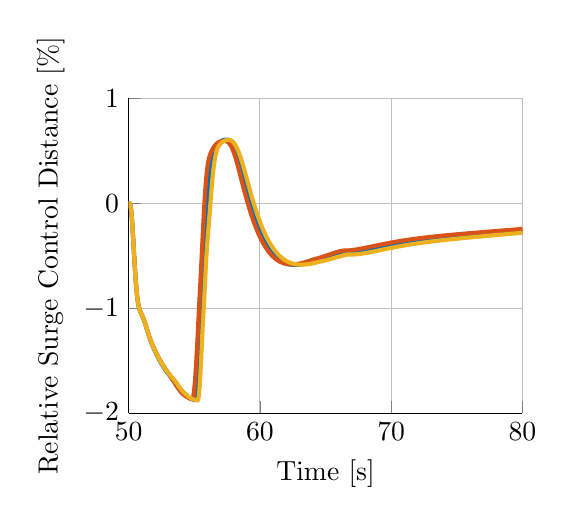
\begin{tikzpicture}

\begin{axis}[%
width=5cm,
height=4cm,
at={(0\linewidth,0\linewidth)},
scale only axis,
xmin=50,
xmax=80,
xlabel={Time [s]},
xmajorgrids,
ymin=-2,
ymax=1,
ylabel={Relative Surge Control Distance [\%]},
ylabel near ticks,
ymajorgrids,
axis background/.style={fill=white},
% title style={font=\bfseries},
% title={Surge Control Distance},
axis x line*=bottom,
axis y line*=left
]
\addplot [color=mycolor1,solid,line width=1.5pt,forget plot]
  table[row sep=crcr]{%
50	0.00164000000000009\\
50.05	0.00164000000000009\\
50.1	-0.00413999999999959\\
50.15	-0.02996\\
50.2	-0.0815200000000003\\
50.25	-0.15753\\
50.3	-0.25243\\
50.35	-0.35873\\
50.4	-0.46873\\
50.45	-0.57562\\
50.5	-0.67415\\
50.55	-0.76083\\
50.6	-0.83392\\
50.65	-0.89319\\
50.7	-0.93961\\
50.75	-0.97497\\
50.8	-1.00151\\
50.85	-1.02162\\
50.9	-1.03757\\
50.95	-1.05134\\
51	-1.0645\\
51.05	-1.07817\\
51.1	-1.09303\\
51.15	-1.10939\\
51.2	-1.12726\\
51.25	-1.14641\\
51.3	-1.16651\\
51.35	-1.18714\\
51.4	-1.2079\\
51.45	-1.22845\\
51.5	-1.24849\\
51.55	-1.26783\\
51.6	-1.28635\\
51.65	-1.30401\\
51.7	-1.32083\\
51.75	-1.33687\\
51.8	-1.35222\\
51.85	-1.36698\\
51.9	-1.38125\\
51.95	-1.39511\\
52	-1.40864\\
52.05	-1.42188\\
52.1	-1.43487\\
52.15	-1.44762\\
52.2	-1.46014\\
52.25	-1.47242\\
52.3	-1.48445\\
52.35	-1.49622\\
52.4	-1.5077\\
52.45	-1.51888\\
52.5	-1.52977\\
52.55	-1.54035\\
52.6	-1.55062\\
52.65	-1.56059\\
52.7	-1.57027\\
52.75	-1.57967\\
52.8	-1.58879\\
52.85	-1.59765\\
52.9	-1.60626\\
52.95	-1.61462\\
53	-1.62275\\
53.05	-1.63064\\
53.1	-1.63849\\
53.15	-1.64648\\
53.2	-1.65475\\
53.25	-1.66337\\
53.3	-1.67217\\
53.35	-1.6811\\
53.4	-1.69028\\
53.45	-1.6996\\
53.5	-1.70892\\
53.55	-1.71829\\
53.6	-1.72751\\
53.65	-1.73643\\
53.7	-1.74506\\
53.75	-1.75344\\
53.8	-1.76162\\
53.85	-1.76963\\
53.9	-1.77749\\
53.95	-1.78517\\
54	-1.79266\\
54.05	-1.79991\\
54.1	-1.80688\\
54.15	-1.81351\\
54.2	-1.81975\\
54.25	-1.82558\\
54.3	-1.83098\\
54.35	-1.83596\\
54.4	-1.84051\\
54.45	-1.84468\\
54.5	-1.84848\\
54.55	-1.85196\\
54.6	-1.85515\\
54.65	-1.85808\\
54.7	-1.86079\\
54.75	-1.8633\\
54.8	-1.86562\\
54.85	-1.86776\\
54.9	-1.86973\\
54.95	-1.87153\\
55	-1.87315\\
55.05	-1.8631\\
55.1	-1.82279\\
55.15	-1.75541\\
55.2	-1.65645\\
55.25	-1.55099\\
55.3	-1.44792\\
55.35	-1.33033\\
55.4	-1.20103\\
55.45	-1.07794\\
55.5	-0.9513\\
55.55	-0.82728\\
55.6	-0.72375\\
55.65	-0.62843\\
55.7	-0.53241\\
55.75	-0.43173\\
55.8	-0.32615\\
55.85	-0.21785\\
55.9	-0.11029\\
55.95	-0.00717999999999996\\
56	0.0882399999999999\\
56.05	0.17356\\
56.1	0.24747\\
56.15	0.30964\\
56.2	0.36062\\
56.25	0.40155\\
56.3	0.43394\\
56.35	0.45942\\
56.4	0.47959\\
56.45	0.49583\\
56.5	0.50932\\
56.55	0.52091\\
56.6	0.53122\\
56.65	0.54064\\
56.7	0.54938\\
56.75	0.55751\\
56.8	0.56503\\
56.85	0.57191\\
56.9	0.57811\\
56.95	0.58359\\
57	0.58834\\
57.05	0.59241\\
57.1	0.59582\\
57.15	0.59866\\
57.2	0.60099\\
57.25	0.60285\\
57.3	0.60426\\
57.35	0.60522\\
57.4	0.60568\\
57.45	0.60557\\
57.5	0.60479\\
57.55	0.60325\\
57.6	0.60081\\
57.65	0.59736\\
57.7	0.5928\\
57.75	0.58705\\
57.8	0.58003\\
57.85	0.57171\\
57.9	0.56205\\
57.95	0.55103\\
58	0.53864\\
58.05	0.52489\\
58.1	0.50978\\
58.15	0.49336\\
58.2	0.47567\\
58.25	0.45678\\
58.3	0.43679\\
58.35	0.41579\\
58.4	0.39391\\
58.45	0.37127\\
58.5	0.34801\\
58.55	0.32427\\
58.6	0.30016\\
58.65	0.27582\\
58.7	0.25135\\
58.75	0.22685\\
58.8	0.20241\\
58.85	0.17811\\
58.9	0.154\\
58.95	0.13014\\
59	0.10656\\
59.05	0.08331\\
59.1	0.0604100000000001\\
59.15	0.03789\\
59.2	0.0157600000000002\\
59.25	-0.00595999999999997\\
59.3	-0.0272600000000001\\
59.35	-0.0481199999999999\\
59.4	-0.06853\\
59.45	-0.0884900000000002\\
59.5	-0.10799\\
59.55	-0.12702\\
59.6	-0.14558\\
59.65	-0.16366\\
59.7	-0.18128\\
59.75	-0.19842\\
59.8	-0.21509\\
59.85	-0.2313\\
59.9	-0.24704\\
59.95	-0.26233\\
60	-0.27716\\
60.05	-0.29154\\
60.1	-0.30548\\
60.15	-0.31899\\
60.2	-0.33207\\
60.25	-0.34473\\
60.3	-0.35697\\
60.35	-0.36881\\
60.4	-0.38024\\
60.45	-0.39128\\
60.5	-0.40193\\
60.55	-0.4122\\
60.6	-0.4221\\
60.65	-0.43162\\
60.7	-0.44079\\
60.75	-0.4496\\
60.8	-0.45807\\
60.85	-0.46619\\
60.9	-0.47398\\
60.95	-0.48145\\
61	-0.48859\\
61.05	-0.49543\\
61.1	-0.50196\\
61.15	-0.50819\\
61.2	-0.51413\\
61.25	-0.51978\\
61.3	-0.52516\\
61.35	-0.53026\\
61.4	-0.5351\\
61.45	-0.53968\\
61.5	-0.54401\\
61.55	-0.5481\\
61.6	-0.55194\\
61.65	-0.55555\\
61.7	-0.55894\\
61.75	-0.5621\\
61.8	-0.56504\\
61.85	-0.56778\\
61.9	-0.57031\\
61.95	-0.57264\\
62	-0.57478\\
62.05	-0.57672\\
62.1	-0.57849\\
62.15	-0.58007\\
62.2	-0.58149\\
62.25	-0.58273\\
62.3	-0.58382\\
62.35	-0.58474\\
62.4	-0.58551\\
62.45	-0.58613\\
62.5	-0.58661\\
62.55	-0.58695\\
62.6	-0.58716\\
62.65	-0.58723\\
62.7	-0.58718\\
62.75	-0.58702\\
62.8	-0.58673\\
62.85	-0.58633\\
62.9	-0.58583\\
62.95	-0.58522\\
63	-0.58451\\
63.05	-0.58371\\
63.1	-0.58282\\
63.15	-0.58184\\
63.2	-0.58078\\
63.25	-0.57963\\
63.3	-0.57842\\
63.35	-0.57713\\
63.4	-0.57578\\
63.45	-0.57436\\
63.5	-0.57288\\
63.55	-0.57135\\
63.6	-0.56976\\
63.65	-0.56812\\
63.7	-0.56644\\
63.75	-0.56472\\
63.8	-0.56295\\
63.85	-0.56115\\
63.9	-0.55932\\
63.95	-0.55745\\
64	-0.55556\\
64.05	-0.55365\\
64.1	-0.55171\\
64.15	-0.54976\\
64.2	-0.54779\\
64.25	-0.54581\\
64.3	-0.54381\\
64.35	-0.54181\\
64.4	-0.53982\\
64.45	-0.53787\\
64.5	-0.53597\\
64.55	-0.53416\\
64.6	-0.53242\\
64.65	-0.53076\\
64.7	-0.52917\\
64.75	-0.52762\\
64.8	-0.5261\\
64.85	-0.52458\\
64.9	-0.52304\\
64.95	-0.52148\\
65	-0.51988\\
65.05	-0.51824\\
65.1	-0.51657\\
65.15	-0.51486\\
65.2	-0.51312\\
65.25	-0.51137\\
65.3	-0.50961\\
65.35	-0.50785\\
65.4	-0.5061\\
65.45	-0.50436\\
65.5	-0.50264\\
65.55	-0.50094\\
65.6	-0.49926\\
65.65	-0.4976\\
65.7	-0.49596\\
65.75	-0.49434\\
65.8	-0.49274\\
65.85	-0.49115\\
65.9	-0.48958\\
65.95	-0.48803\\
66	-0.48649\\
66.05	-0.48496\\
66.1	-0.48344\\
66.15	-0.48194\\
66.2	-0.48045\\
66.25	-0.47898\\
66.3	-0.47752\\
66.35	-0.47607\\
66.4	-0.47464\\
66.45	-0.47328\\
66.5	-0.47203\\
66.55	-0.47095\\
66.6	-0.47006\\
66.65	-0.46939\\
66.7	-0.46894\\
66.75	-0.46869\\
66.8	-0.4686\\
66.85	-0.46864\\
66.9	-0.46875\\
66.95	-0.46889\\
67	-0.46901\\
67.05	-0.46909\\
67.1	-0.46909\\
67.15	-0.469\\
67.2	-0.4688\\
67.25	-0.4685\\
67.3	-0.46809\\
67.35	-0.46759\\
67.4	-0.467\\
67.45	-0.46634\\
67.5	-0.46562\\
67.55	-0.46484\\
67.6	-0.46401\\
67.65	-0.46315\\
67.7	-0.46224\\
67.75	-0.46131\\
67.8	-0.46034\\
67.85	-0.45934\\
67.9	-0.45831\\
67.95	-0.45725\\
68	-0.45617\\
68.05	-0.45505\\
68.1	-0.45391\\
68.15	-0.45275\\
68.2	-0.45156\\
68.25	-0.45034\\
68.3	-0.44911\\
68.35	-0.44786\\
68.4	-0.4466\\
68.45	-0.44532\\
68.5	-0.44403\\
68.55	-0.44273\\
68.6	-0.44143\\
68.65	-0.44011\\
68.7	-0.4388\\
68.75	-0.43748\\
68.8	-0.43615\\
68.85	-0.43483\\
68.9	-0.4335\\
68.95	-0.43218\\
69	-0.43085\\
69.05	-0.42952\\
69.1	-0.42819\\
69.15	-0.42687\\
69.2	-0.42554\\
69.25	-0.42422\\
69.3	-0.42289\\
69.35	-0.42158\\
69.4	-0.42026\\
69.45	-0.41895\\
69.5	-0.41764\\
69.55	-0.41634\\
69.6	-0.41505\\
69.65	-0.41376\\
69.7	-0.41248\\
69.75	-0.41121\\
69.8	-0.40995\\
69.85	-0.40869\\
69.9	-0.40745\\
69.95	-0.40621\\
70	-0.40499\\
70.05	-0.40377\\
70.1	-0.40256\\
70.15	-0.40136\\
70.2	-0.40017\\
70.25	-0.399\\
70.3	-0.39783\\
70.35	-0.39667\\
70.4	-0.39552\\
70.45	-0.39438\\
70.5	-0.39325\\
70.55	-0.39214\\
70.6	-0.39103\\
70.65	-0.38993\\
70.7	-0.38884\\
70.75	-0.38777\\
70.8	-0.3867\\
70.85	-0.38564\\
70.9	-0.38459\\
70.95	-0.38355\\
71	-0.38253\\
71.05	-0.38151\\
71.1	-0.3805\\
71.15	-0.3795\\
71.2	-0.37851\\
71.25	-0.37753\\
71.3	-0.37656\\
71.35	-0.37559\\
71.4	-0.37464\\
71.45	-0.3737\\
71.5	-0.37276\\
71.55	-0.37183\\
71.6	-0.37092\\
71.65	-0.37001\\
71.7	-0.3691\\
71.75	-0.36821\\
71.8	-0.36732\\
71.85	-0.36645\\
71.9	-0.36558\\
71.95	-0.36471\\
72	-0.36386\\
72.05	-0.36301\\
72.1	-0.36217\\
72.15	-0.36134\\
72.2	-0.36052\\
72.25	-0.3597\\
72.3	-0.35889\\
72.35	-0.35808\\
72.4	-0.35728\\
72.45	-0.35649\\
72.5	-0.3557\\
72.55	-0.35493\\
72.6	-0.35415\\
72.65	-0.35338\\
72.7	-0.35262\\
72.75	-0.35187\\
72.8	-0.35112\\
72.85	-0.35037\\
72.9	-0.34963\\
72.95	-0.3489\\
73	-0.34817\\
73.05	-0.34745\\
73.1	-0.34673\\
73.15	-0.34601\\
73.2	-0.34531\\
73.25	-0.3446\\
73.3	-0.3439\\
73.35	-0.34321\\
73.4	-0.34251\\
73.45	-0.34183\\
73.5	-0.34114\\
73.55	-0.34047\\
73.6	-0.33979\\
73.65	-0.33912\\
73.7	-0.33845\\
73.75	-0.33779\\
73.8	-0.33713\\
73.85	-0.33647\\
73.9	-0.33582\\
73.95	-0.33517\\
74	-0.33453\\
74.05	-0.33388\\
74.1	-0.33324\\
74.15	-0.33261\\
74.2	-0.33197\\
74.25	-0.33134\\
74.3	-0.33071\\
74.35	-0.33009\\
74.4	-0.32947\\
74.45	-0.32885\\
74.5	-0.32823\\
74.55	-0.32761\\
74.6	-0.327\\
74.65	-0.32639\\
74.7	-0.32578\\
74.75	-0.32518\\
74.8	-0.32457\\
74.85	-0.32397\\
74.9	-0.32337\\
74.95	-0.32278\\
75	-0.32218\\
75.05	-0.32159\\
75.1	-0.321\\
75.15	-0.32041\\
75.2	-0.31982\\
75.25	-0.31923\\
75.3	-0.31865\\
75.35	-0.31807\\
75.4	-0.31748\\
75.45	-0.3169\\
75.5	-0.31633\\
75.55	-0.31575\\
75.6	-0.31517\\
75.65	-0.3146\\
75.7	-0.31403\\
75.75	-0.31346\\
75.8	-0.31289\\
75.85	-0.31232\\
75.9	-0.31175\\
75.95	-0.31118\\
76	-0.31062\\
76.05	-0.31005\\
76.1	-0.30949\\
76.15	-0.30893\\
76.2	-0.30836\\
76.25	-0.3078\\
76.3	-0.30724\\
76.35	-0.30669\\
76.4	-0.30613\\
76.45	-0.30557\\
76.5	-0.30502\\
76.55	-0.30446\\
76.6	-0.30391\\
76.65	-0.30335\\
76.7	-0.3028\\
76.75	-0.30225\\
76.8	-0.3017\\
76.85	-0.30114\\
76.9	-0.30059\\
76.95	-0.30005\\
77	-0.2995\\
77.05	-0.29895\\
77.1	-0.2984\\
77.15	-0.29785\\
77.2	-0.29731\\
77.25	-0.29676\\
77.3	-0.29621\\
77.35	-0.29567\\
77.4	-0.29512\\
77.45	-0.29458\\
77.5	-0.29404\\
77.55	-0.29349\\
77.6	-0.29295\\
77.65	-0.29241\\
77.7	-0.29186\\
77.75	-0.29132\\
77.8	-0.29078\\
77.85	-0.29024\\
77.9	-0.2897\\
77.95	-0.28916\\
78	-0.28862\\
78.05	-0.28808\\
78.1	-0.28754\\
78.15	-0.287\\
78.2	-0.28646\\
78.25	-0.28592\\
78.3	-0.28539\\
78.35	-0.28485\\
78.4	-0.28431\\
78.45	-0.28377\\
78.5	-0.28324\\
78.55	-0.2827\\
78.6	-0.28216\\
78.65	-0.28162\\
78.7	-0.28109\\
78.75	-0.28055\\
78.8	-0.28002\\
78.85	-0.27948\\
78.9	-0.27895\\
78.95	-0.27841\\
79	-0.27788\\
79.05	-0.27734\\
79.1	-0.27681\\
79.15	-0.27627\\
79.2	-0.27574\\
79.25	-0.2752\\
79.3	-0.27467\\
79.35	-0.27413\\
79.4	-0.2736\\
79.45	-0.27307\\
79.5	-0.27253\\
79.55	-0.272\\
79.6	-0.27147\\
79.65	-0.27094\\
79.7	-0.2704\\
79.75	-0.26987\\
79.8	-0.26934\\
79.85	-0.26881\\
79.9	-0.26827\\
79.95	-0.26774\\
80	-0.26721\\
};
\addplot [color=mycolor2,solid,line width=1.5pt,forget plot]
  table[row sep=crcr]{%
50	0.00145000000000017\\
50.05	0.00145000000000017\\
50.1	-0.00433000000000039\\
50.15	-0.0301499999999999\\
50.2	-0.0817199999999998\\
50.25	-0.15772\\
50.3	-0.25261\\
50.35	-0.35889\\
50.4	-0.46886\\
50.45	-0.5757\\
50.5	-0.67415\\
50.55	-0.76074\\
50.6	-0.8337\\
50.65	-0.89283\\
50.7	-0.93907\\
50.75	-0.97422\\
50.8	-1.00052\\
50.85	-1.02037\\
50.9	-1.03605\\
50.95	-1.04952\\
51	-1.06237\\
51.05	-1.07572\\
51.1	-1.09026\\
51.15	-1.10629\\
51.2	-1.12383\\
51.25	-1.14265\\
51.3	-1.1624\\
51.35	-1.1827\\
51.4	-1.20313\\
51.45	-1.22333\\
51.5	-1.24303\\
51.55	-1.26203\\
51.6	-1.28022\\
51.65	-1.29754\\
51.7	-1.31403\\
51.75	-1.32974\\
51.8	-1.34476\\
51.85	-1.3592\\
51.9	-1.37315\\
51.95	-1.38671\\
52	-1.39993\\
52.05	-1.41289\\
52.1	-1.4256\\
52.15	-1.43809\\
52.2	-1.45037\\
52.25	-1.46242\\
52.3	-1.47423\\
52.35	-1.4858\\
52.4	-1.4971\\
52.45	-1.50813\\
52.5	-1.51888\\
52.55	-1.52934\\
52.6	-1.53953\\
52.65	-1.54943\\
52.7	-1.55907\\
52.75	-1.56845\\
52.8	-1.57758\\
52.85	-1.58647\\
52.9	-1.59514\\
52.95	-1.60378\\
53	-1.61259\\
53.05	-1.62153\\
53.1	-1.63069\\
53.15	-1.64012\\
53.2	-1.64983\\
53.25	-1.65976\\
53.3	-1.66982\\
53.35	-1.68009\\
53.4	-1.69041\\
53.45	-1.70061\\
53.5	-1.71069\\
53.55	-1.72067\\
53.6	-1.73055\\
53.65	-1.74031\\
53.7	-1.74993\\
53.75	-1.75935\\
53.8	-1.7685\\
53.85	-1.7773\\
53.9	-1.78569\\
53.95	-1.79361\\
54	-1.80102\\
54.05	-1.8079\\
54.1	-1.81423\\
54.15	-1.82005\\
54.2	-1.82537\\
54.25	-1.83025\\
54.3	-1.83474\\
54.35	-1.83887\\
54.4	-1.84269\\
54.45	-1.84625\\
54.5	-1.84956\\
54.55	-1.85266\\
54.6	-1.85555\\
54.65	-1.85825\\
54.7	-1.86074\\
54.75	-1.86303\\
54.8	-1.86511\\
54.85	-1.86697\\
54.9	-1.85717\\
54.95	-1.81719\\
55	-1.76165\\
55.05	-1.69299\\
55.1	-1.6029\\
55.15	-1.50112\\
55.2	-1.3861\\
55.25	-1.27135\\
55.3	-1.14496\\
55.35	-1.0128\\
55.4	-0.8939\\
55.45	-0.77806\\
55.5	-0.65872\\
55.55	-0.53417\\
55.6	-0.40611\\
55.65	-0.27811\\
55.7	-0.15444\\
55.75	-0.0391000000000004\\
55.8	0.0648299999999997\\
55.85	0.15546\\
55.9	0.23215\\
55.95	0.29531\\
56	0.34617\\
56.05	0.38644\\
56.1	0.41807\\
56.15	0.44298\\
56.2	0.4629\\
56.25	0.47927\\
56.3	0.4932\\
56.35	0.5055\\
56.4	0.51666\\
56.45	0.52697\\
56.5	0.53654\\
56.55	0.54539\\
56.6	0.55348\\
56.65	0.56074\\
56.7	0.56714\\
56.75	0.57265\\
56.8	0.5773\\
56.85	0.58114\\
56.9	0.58426\\
56.95	0.58675\\
57	0.58873\\
57.05	0.59029\\
57.1	0.5915\\
57.15	0.59239\\
57.2	0.59298\\
57.25	0.59323\\
57.3	0.59306\\
57.35	0.59238\\
57.4	0.59108\\
57.45	0.58901\\
57.5	0.58604\\
57.55	0.58206\\
57.6	0.57693\\
57.65	0.57057\\
57.7	0.56288\\
57.75	0.55378\\
57.8	0.54321\\
57.85	0.53114\\
57.9	0.51755\\
57.95	0.50247\\
58	0.48594\\
58.05	0.46803\\
58.1	0.44885\\
58.15	0.42853\\
58.2	0.40719\\
58.25	0.38499\\
58.3	0.36209\\
58.35	0.33863\\
58.4	0.31477\\
58.45	0.29063\\
58.5	0.26632\\
58.55	0.24197\\
58.6	0.21765\\
58.65	0.19344\\
58.7	0.1694\\
58.75	0.14558\\
58.8	0.12203\\
58.85	0.0987900000000002\\
58.9	0.0758700000000001\\
58.95	0.0533000000000001\\
59	0.03111\\
59.05	0.00931000000000015\\
59.1	-0.0120800000000001\\
59.15	-0.0330500000000002\\
59.2	-0.0535899999999998\\
59.25	-0.07369\\
59.3	-0.0933400000000004\\
59.35	-0.11254\\
59.4	-0.13128\\
59.45	-0.14955\\
59.5	-0.16736\\
59.55	-0.18472\\
59.6	-0.20161\\
59.65	-0.21805\\
59.7	-0.23403\\
59.75	-0.24957\\
59.8	-0.26467\\
59.85	-0.27933\\
59.9	-0.29356\\
59.95	-0.30737\\
60	-0.32076\\
60.05	-0.33373\\
60.1	-0.3463\\
60.15	-0.35846\\
60.2	-0.37022\\
60.25	-0.3816\\
60.3	-0.39258\\
60.35	-0.40318\\
60.4	-0.41341\\
60.45	-0.42326\\
60.5	-0.43275\\
60.55	-0.44187\\
60.6	-0.45064\\
60.65	-0.45906\\
60.7	-0.46714\\
60.75	-0.47488\\
60.8	-0.48229\\
60.85	-0.48937\\
60.9	-0.49614\\
60.95	-0.50259\\
61	-0.50874\\
61.05	-0.5146\\
61.1	-0.52016\\
61.15	-0.52543\\
61.2	-0.53043\\
61.25	-0.53516\\
61.3	-0.53962\\
61.35	-0.54383\\
61.4	-0.54778\\
61.45	-0.55149\\
61.5	-0.55495\\
61.55	-0.55818\\
61.6	-0.56118\\
61.65	-0.56396\\
61.7	-0.56653\\
61.75	-0.56888\\
61.8	-0.57103\\
61.85	-0.57298\\
61.9	-0.57473\\
61.95	-0.5763\\
62	-0.57769\\
62.05	-0.57889\\
62.1	-0.57993\\
62.15	-0.5808\\
62.2	-0.58151\\
62.25	-0.58206\\
62.3	-0.58246\\
62.35	-0.58272\\
62.4	-0.58283\\
62.45	-0.58281\\
62.5	-0.58265\\
62.55	-0.58237\\
62.6	-0.58197\\
62.65	-0.58145\\
62.7	-0.58082\\
62.75	-0.58008\\
62.8	-0.57923\\
62.85	-0.57829\\
62.9	-0.57726\\
62.95	-0.57613\\
63	-0.57491\\
63.05	-0.57362\\
63.1	-0.57225\\
63.15	-0.5708\\
63.2	-0.56928\\
63.25	-0.5677\\
63.3	-0.56606\\
63.35	-0.56435\\
63.4	-0.5626\\
63.45	-0.56079\\
63.5	-0.55894\\
63.55	-0.55704\\
63.6	-0.55511\\
63.65	-0.55313\\
63.7	-0.55113\\
63.75	-0.54909\\
63.8	-0.54703\\
63.85	-0.54494\\
63.9	-0.54283\\
63.95	-0.54071\\
64	-0.53859\\
64.05	-0.53651\\
64.1	-0.53451\\
64.15	-0.5326\\
64.2	-0.53078\\
64.25	-0.52904\\
64.3	-0.52737\\
64.35	-0.52574\\
64.4	-0.52411\\
64.45	-0.52246\\
64.5	-0.52076\\
64.55	-0.51901\\
64.6	-0.51717\\
64.65	-0.51526\\
64.7	-0.51328\\
64.75	-0.51123\\
64.8	-0.50913\\
64.85	-0.50698\\
64.9	-0.50481\\
64.95	-0.50263\\
65	-0.50044\\
65.05	-0.49826\\
65.1	-0.49608\\
65.15	-0.49393\\
65.2	-0.49178\\
65.25	-0.48966\\
65.3	-0.48756\\
65.35	-0.48547\\
65.4	-0.48339\\
65.45	-0.48134\\
65.5	-0.47929\\
65.55	-0.47726\\
65.6	-0.47524\\
65.65	-0.47324\\
65.7	-0.47125\\
65.75	-0.46927\\
65.8	-0.46731\\
65.85	-0.46537\\
65.9	-0.46344\\
65.95	-0.46153\\
66	-0.45965\\
66.05	-0.45784\\
66.1	-0.45616\\
66.15	-0.45465\\
66.2	-0.45336\\
66.25	-0.4523\\
66.3	-0.45148\\
66.35	-0.45088\\
66.4	-0.45047\\
66.45	-0.45019\\
66.5	-0.45001\\
66.55	-0.44988\\
66.6	-0.44975\\
66.65	-0.4496\\
66.7	-0.44938\\
66.75	-0.44909\\
66.8	-0.4487\\
66.85	-0.44823\\
66.9	-0.44767\\
66.95	-0.44703\\
67	-0.44632\\
67.05	-0.44554\\
67.1	-0.44471\\
67.15	-0.44383\\
67.2	-0.44292\\
67.25	-0.44198\\
67.3	-0.44101\\
67.35	-0.44001\\
67.4	-0.43899\\
67.45	-0.43795\\
67.5	-0.43688\\
67.55	-0.43579\\
67.6	-0.43467\\
67.65	-0.43354\\
67.7	-0.43238\\
67.75	-0.4312\\
67.8	-0.43\\
67.85	-0.42879\\
67.9	-0.42756\\
67.95	-0.42631\\
68	-0.42506\\
68.05	-0.42379\\
68.1	-0.42251\\
68.15	-0.42123\\
68.2	-0.41994\\
68.25	-0.41865\\
68.3	-0.41736\\
68.35	-0.41606\\
68.4	-0.41476\\
68.45	-0.41346\\
68.5	-0.41216\\
68.55	-0.41086\\
68.6	-0.40956\\
68.65	-0.40826\\
68.7	-0.40696\\
68.75	-0.40566\\
68.8	-0.40436\\
68.85	-0.40306\\
68.9	-0.40176\\
68.95	-0.40046\\
69	-0.39917\\
69.05	-0.39788\\
69.1	-0.39659\\
69.15	-0.3953\\
69.2	-0.39402\\
69.25	-0.39274\\
69.3	-0.39147\\
69.35	-0.39021\\
69.4	-0.38895\\
69.45	-0.3877\\
69.5	-0.38646\\
69.55	-0.38522\\
69.6	-0.384\\
69.65	-0.38278\\
69.7	-0.38157\\
69.75	-0.38036\\
69.8	-0.37917\\
69.85	-0.37798\\
69.9	-0.37681\\
69.95	-0.37564\\
70	-0.37448\\
70.05	-0.37333\\
70.1	-0.37219\\
70.15	-0.37106\\
70.2	-0.36994\\
70.25	-0.36882\\
70.3	-0.36772\\
70.35	-0.36663\\
70.4	-0.36554\\
70.45	-0.36447\\
70.5	-0.3634\\
70.55	-0.36234\\
70.6	-0.3613\\
70.65	-0.36026\\
70.7	-0.35923\\
70.75	-0.35821\\
70.8	-0.3572\\
70.85	-0.3562\\
70.9	-0.35521\\
70.95	-0.35423\\
71	-0.35325\\
71.05	-0.35229\\
71.1	-0.35133\\
71.15	-0.35039\\
71.2	-0.34945\\
71.25	-0.34852\\
71.3	-0.3476\\
71.35	-0.34668\\
71.4	-0.34578\\
71.45	-0.34488\\
71.5	-0.34399\\
71.55	-0.34311\\
71.6	-0.34224\\
71.65	-0.34138\\
71.7	-0.34052\\
71.75	-0.33967\\
71.8	-0.33883\\
71.85	-0.338\\
71.9	-0.33717\\
71.95	-0.33635\\
72	-0.33554\\
72.05	-0.33473\\
72.1	-0.33393\\
72.15	-0.33314\\
72.2	-0.33236\\
72.25	-0.33158\\
72.3	-0.33081\\
72.35	-0.33004\\
72.4	-0.32928\\
72.45	-0.32853\\
72.5	-0.32778\\
72.55	-0.32704\\
72.6	-0.3263\\
72.65	-0.32557\\
72.7	-0.32485\\
72.75	-0.32413\\
72.8	-0.32341\\
72.85	-0.32271\\
72.9	-0.322\\
72.95	-0.3213\\
73	-0.32061\\
73.05	-0.31992\\
73.1	-0.31924\\
73.15	-0.31856\\
73.2	-0.31789\\
73.25	-0.31722\\
73.3	-0.31655\\
73.35	-0.31589\\
73.4	-0.31523\\
73.45	-0.31458\\
73.5	-0.31393\\
73.55	-0.31329\\
73.6	-0.31265\\
73.65	-0.31201\\
73.7	-0.31137\\
73.75	-0.31074\\
73.8	-0.31012\\
73.85	-0.3095\\
73.9	-0.30888\\
73.95	-0.30826\\
74	-0.30765\\
74.05	-0.30704\\
74.1	-0.30643\\
74.15	-0.30583\\
74.2	-0.30522\\
74.25	-0.30463\\
74.3	-0.30403\\
74.35	-0.30344\\
74.4	-0.30285\\
74.45	-0.30226\\
74.5	-0.30168\\
74.55	-0.30109\\
74.6	-0.30051\\
74.65	-0.29993\\
74.7	-0.29936\\
74.75	-0.29879\\
74.8	-0.29822\\
74.85	-0.29765\\
74.9	-0.29708\\
74.95	-0.29651\\
75	-0.29595\\
75.05	-0.29539\\
75.1	-0.29483\\
75.15	-0.29427\\
75.2	-0.29372\\
75.25	-0.29316\\
75.3	-0.29261\\
75.35	-0.29206\\
75.4	-0.29151\\
75.45	-0.29096\\
75.5	-0.29042\\
75.55	-0.28987\\
75.6	-0.28933\\
75.65	-0.28879\\
75.7	-0.28825\\
75.75	-0.28771\\
75.8	-0.28717\\
75.85	-0.28663\\
75.9	-0.2861\\
75.95	-0.28556\\
76	-0.28503\\
76.05	-0.2845\\
76.1	-0.28397\\
76.15	-0.28344\\
76.2	-0.28291\\
76.25	-0.28238\\
76.3	-0.28185\\
76.35	-0.28133\\
76.4	-0.2808\\
76.45	-0.28028\\
76.5	-0.27975\\
76.55	-0.27923\\
76.6	-0.27871\\
76.65	-0.27819\\
76.7	-0.27767\\
76.75	-0.27715\\
76.8	-0.27663\\
76.85	-0.27611\\
76.9	-0.27559\\
76.95	-0.27508\\
77	-0.27456\\
77.05	-0.27405\\
77.1	-0.27353\\
77.15	-0.27302\\
77.2	-0.2725\\
77.25	-0.27199\\
77.3	-0.27148\\
77.35	-0.27097\\
77.4	-0.27045\\
77.45	-0.26994\\
77.5	-0.26943\\
77.55	-0.26892\\
77.6	-0.26841\\
77.65	-0.2679\\
77.7	-0.26739\\
77.75	-0.26689\\
77.8	-0.26638\\
77.85	-0.26587\\
77.9	-0.26536\\
77.95	-0.26486\\
78	-0.26435\\
78.05	-0.26384\\
78.1	-0.26334\\
78.15	-0.26283\\
78.2	-0.26233\\
78.25	-0.26182\\
78.3	-0.26132\\
78.35	-0.26081\\
78.4	-0.26031\\
78.45	-0.25981\\
78.5	-0.2593\\
78.55	-0.2588\\
78.6	-0.2583\\
78.65	-0.25779\\
78.7	-0.25729\\
78.75	-0.25679\\
78.8	-0.25629\\
78.85	-0.25579\\
78.9	-0.25529\\
78.95	-0.25479\\
79	-0.25428\\
79.05	-0.25378\\
79.1	-0.25328\\
79.15	-0.25278\\
79.2	-0.25228\\
79.25	-0.25179\\
79.3	-0.25129\\
79.35	-0.25079\\
79.4	-0.25029\\
79.45	-0.24979\\
79.5	-0.24929\\
79.55	-0.24879\\
79.6	-0.24829\\
79.65	-0.2478\\
79.7	-0.2473\\
79.75	-0.2468\\
79.8	-0.2463\\
79.85	-0.24581\\
79.9	-0.24531\\
79.95	-0.24481\\
80	-0.24432\\
};
\addplot [color=mycolor3,solid,line width=1.5pt,forget plot]
  table[row sep=crcr]{%
50	0.00159999999999982\\
50.05	0.00159999999999982\\
50.1	-0.00419000000000036\\
50.15	-0.0300099999999999\\
50.2	-0.0815700000000001\\
50.25	-0.15757\\
50.3	-0.25246\\
50.35	-0.35875\\
50.4	-0.46872\\
50.45	-0.57557\\
50.5	-0.67404\\
50.55	-0.76064\\
50.6	-0.83363\\
50.65	-0.89278\\
50.7	-0.93906\\
50.75	-0.97425\\
50.8	-1.00061\\
50.85	-1.02052\\
50.9	-1.03627\\
50.95	-1.04983\\
51	-1.06278\\
51.05	-1.07624\\
51.1	-1.09089\\
51.15	-1.10705\\
51.2	-1.12472\\
51.25	-1.14368\\
51.3	-1.16359\\
51.35	-1.18403\\
51.4	-1.20461\\
51.45	-1.22498\\
51.5	-1.24484\\
51.55	-1.264\\
51.6	-1.28234\\
51.65	-1.29983\\
51.7	-1.31648\\
51.75	-1.33235\\
51.8	-1.34754\\
51.85	-1.36213\\
51.9	-1.37624\\
51.95	-1.38995\\
52	-1.40333\\
52.05	-1.41642\\
52.1	-1.42927\\
52.15	-1.44189\\
52.2	-1.45429\\
52.25	-1.46645\\
52.3	-1.47836\\
52.35	-1.49001\\
52.4	-1.50138\\
52.45	-1.51247\\
52.5	-1.52325\\
52.55	-1.53374\\
52.6	-1.54392\\
52.65	-1.55381\\
52.7	-1.56341\\
52.75	-1.57273\\
52.8	-1.58177\\
52.85	-1.59055\\
52.9	-1.59909\\
52.95	-1.60737\\
53	-1.61542\\
53.05	-1.62324\\
53.1	-1.63083\\
53.15	-1.6382\\
53.2	-1.64535\\
53.25	-1.65227\\
53.3	-1.65898\\
53.35	-1.6657\\
53.4	-1.67264\\
53.45	-1.67997\\
53.5	-1.68774\\
53.55	-1.69597\\
53.6	-1.70457\\
53.65	-1.71341\\
53.7	-1.72232\\
53.75	-1.73111\\
53.8	-1.73983\\
53.85	-1.74852\\
53.9	-1.75721\\
53.95	-1.76568\\
54	-1.7737\\
54.05	-1.78129\\
54.1	-1.78849\\
54.15	-1.79537\\
54.2	-1.80197\\
54.25	-1.80834\\
54.3	-1.81448\\
54.35	-1.82042\\
54.4	-1.82613\\
54.45	-1.83158\\
54.5	-1.83676\\
54.55	-1.84162\\
54.6	-1.84614\\
54.65	-1.85031\\
54.7	-1.85412\\
54.75	-1.85756\\
54.8	-1.86066\\
54.85	-1.86344\\
54.9	-1.86591\\
54.95	-1.86811\\
55	-1.87006\\
55.05	-1.8718\\
55.1	-1.87334\\
55.15	-1.87469\\
55.2	-1.87588\\
55.25	-1.8769\\
55.3	-1.86626\\
55.35	-1.82526\\
55.4	-1.75705\\
55.45	-1.6571\\
55.5	-1.53907\\
55.55	-1.4051\\
55.6	-1.27182\\
55.65	-1.14107\\
55.7	-1.02673\\
55.75	-0.9148\\
55.8	-0.79629\\
55.85	-0.6683\\
55.9	-0.5438\\
55.95	-0.44473\\
56	-0.36041\\
56.05	-0.28185\\
56.1	-0.20386\\
56.15	-0.12438\\
56.2	-0.04352\\
56.25	0.0371800000000002\\
56.3	0.11558\\
56.35	0.18947\\
56.4	0.257\\
56.45	0.3169\\
56.5	0.36855\\
56.55	0.41197\\
56.6	0.44765\\
56.65	0.47643\\
56.7	0.49935\\
56.75	0.5175\\
56.8	0.53192\\
56.85	0.54352\\
56.9	0.55306\\
56.95	0.5611\\
57	0.56805\\
57.05	0.57419\\
57.1	0.57966\\
57.15	0.58456\\
57.2	0.5889\\
57.25	0.59269\\
57.3	0.59594\\
57.35	0.59864\\
57.4	0.60082\\
57.45	0.60248\\
57.5	0.60364\\
57.55	0.60428\\
57.6	0.60438\\
57.65	0.60388\\
57.7	0.60271\\
57.75	0.60078\\
57.8	0.59802\\
57.85	0.59433\\
57.9	0.58965\\
57.95	0.5839\\
58	0.57701\\
58.05	0.56894\\
58.1	0.55966\\
58.15	0.54918\\
58.2	0.53751\\
58.25	0.52468\\
58.3	0.51073\\
58.35	0.4957\\
58.4	0.47965\\
58.45	0.46262\\
58.5	0.44468\\
58.55	0.42588\\
58.6	0.40629\\
58.65	0.386\\
58.7	0.36507\\
58.75	0.3436\\
58.8	0.32167\\
58.85	0.29937\\
58.9	0.2768\\
58.95	0.25405\\
59	0.23119\\
59.05	0.20831\\
59.1	0.18548\\
59.15	0.16276\\
59.2	0.1402\\
59.25	0.11786\\
59.3	0.0957600000000003\\
59.35	0.07395\\
59.4	0.0524399999999998\\
59.45	0.0312700000000001\\
59.5	0.0104499999999996\\
59.55	-0.00999999999999979\\
59.6	-0.0300700000000003\\
59.65	-0.04976\\
59.7	-0.0690499999999998\\
59.75	-0.0879300000000001\\
59.8	-0.1064\\
59.85	-0.12445\\
59.9	-0.14208\\
59.95	-0.1593\\
60	-0.17608\\
60.05	-0.19245\\
60.1	-0.20839\\
60.15	-0.22391\\
60.2	-0.23902\\
60.25	-0.25371\\
60.3	-0.26798\\
60.35	-0.28185\\
60.4	-0.29532\\
60.45	-0.30839\\
60.5	-0.32107\\
60.55	-0.33336\\
60.6	-0.34527\\
60.65	-0.3568\\
60.7	-0.36796\\
60.75	-0.37877\\
60.8	-0.38921\\
60.85	-0.3993\\
60.9	-0.40905\\
60.95	-0.41846\\
61	-0.42753\\
61.05	-0.43628\\
61.1	-0.44471\\
61.15	-0.45282\\
61.2	-0.46063\\
61.25	-0.46813\\
61.3	-0.47534\\
61.35	-0.48226\\
61.4	-0.48889\\
61.45	-0.49525\\
61.5	-0.50133\\
61.55	-0.50716\\
61.6	-0.51272\\
61.65	-0.51802\\
61.7	-0.52308\\
61.75	-0.5279\\
61.8	-0.53248\\
61.85	-0.53683\\
61.9	-0.54096\\
61.95	-0.54486\\
62	-0.54856\\
62.05	-0.55204\\
62.1	-0.55531\\
62.15	-0.55839\\
62.2	-0.56127\\
62.25	-0.56397\\
62.3	-0.56648\\
62.35	-0.56881\\
62.4	-0.57096\\
62.45	-0.57295\\
62.5	-0.57476\\
62.55	-0.57642\\
62.6	-0.57792\\
62.65	-0.57927\\
62.7	-0.58047\\
62.75	-0.58153\\
62.8	-0.58244\\
62.85	-0.58322\\
62.9	-0.58387\\
62.95	-0.5844\\
63	-0.5848\\
63.05	-0.58508\\
63.1	-0.58524\\
63.15	-0.5853\\
63.2	-0.58525\\
63.25	-0.58509\\
63.3	-0.58484\\
63.35	-0.58449\\
63.4	-0.58404\\
63.45	-0.58351\\
63.5	-0.58289\\
63.55	-0.58219\\
63.6	-0.58142\\
63.65	-0.58056\\
63.7	-0.57964\\
63.75	-0.57865\\
63.8	-0.57759\\
63.85	-0.57648\\
63.9	-0.5753\\
63.95	-0.57407\\
64	-0.57279\\
64.05	-0.57146\\
64.1	-0.57008\\
64.15	-0.56866\\
64.2	-0.5672\\
64.25	-0.5657\\
64.3	-0.56417\\
64.35	-0.56261\\
64.4	-0.56103\\
64.45	-0.55947\\
64.5	-0.55795\\
64.55	-0.55648\\
64.6	-0.55508\\
64.65	-0.55373\\
64.7	-0.55242\\
64.75	-0.55113\\
64.8	-0.54984\\
64.85	-0.54851\\
64.9	-0.54715\\
64.95	-0.54572\\
65	-0.54423\\
65.05	-0.54267\\
65.1	-0.54104\\
65.15	-0.53935\\
65.2	-0.53761\\
65.25	-0.53584\\
65.3	-0.53403\\
65.35	-0.53221\\
65.4	-0.53038\\
65.45	-0.52854\\
65.5	-0.52671\\
65.55	-0.52488\\
65.6	-0.52307\\
65.65	-0.52126\\
65.7	-0.51946\\
65.75	-0.51767\\
65.8	-0.51588\\
65.85	-0.5141\\
65.9	-0.51233\\
65.95	-0.51057\\
66	-0.50881\\
66.05	-0.50706\\
66.1	-0.50532\\
66.15	-0.50359\\
66.2	-0.50187\\
66.25	-0.50015\\
66.3	-0.49845\\
66.35	-0.49676\\
66.4	-0.4951\\
66.45	-0.4935\\
66.5	-0.49202\\
66.55	-0.49072\\
66.6	-0.48963\\
66.65	-0.48878\\
66.7	-0.48816\\
66.75	-0.48776\\
66.8	-0.48755\\
66.85	-0.48748\\
66.9	-0.4875\\
66.95	-0.48757\\
67	-0.48764\\
67.05	-0.48768\\
67.1	-0.48765\\
67.15	-0.48753\\
67.2	-0.48733\\
67.25	-0.48702\\
67.3	-0.48662\\
67.35	-0.48614\\
67.4	-0.48557\\
67.45	-0.48494\\
67.5	-0.48425\\
67.55	-0.4835\\
67.6	-0.48272\\
67.65	-0.4819\\
67.7	-0.48105\\
67.75	-0.48016\\
67.8	-0.47925\\
67.85	-0.47831\\
67.9	-0.47734\\
67.95	-0.47634\\
68	-0.47531\\
68.05	-0.47426\\
68.1	-0.47318\\
68.15	-0.47207\\
68.2	-0.47094\\
68.25	-0.46978\\
68.3	-0.46861\\
68.35	-0.46741\\
68.4	-0.4662\\
68.45	-0.46498\\
68.5	-0.46374\\
68.55	-0.46249\\
68.6	-0.46123\\
68.65	-0.45997\\
68.7	-0.45869\\
68.75	-0.45741\\
68.8	-0.45613\\
68.85	-0.45484\\
68.9	-0.45355\\
68.95	-0.45226\\
69	-0.45096\\
69.05	-0.44966\\
69.1	-0.44836\\
69.15	-0.44706\\
69.2	-0.44575\\
69.25	-0.44445\\
69.3	-0.44314\\
69.35	-0.44184\\
69.4	-0.44053\\
69.45	-0.43923\\
69.5	-0.43793\\
69.55	-0.43664\\
69.6	-0.43535\\
69.65	-0.43406\\
69.7	-0.43278\\
69.75	-0.4315\\
69.8	-0.43023\\
69.85	-0.42896\\
69.9	-0.4277\\
69.95	-0.42645\\
70	-0.42521\\
70.05	-0.42397\\
70.1	-0.42274\\
70.15	-0.42152\\
70.2	-0.42031\\
70.25	-0.4191\\
70.3	-0.41791\\
70.35	-0.41672\\
70.4	-0.41554\\
70.45	-0.41437\\
70.5	-0.4132\\
70.55	-0.41205\\
70.6	-0.4109\\
70.65	-0.40976\\
70.7	-0.40863\\
70.75	-0.40751\\
70.8	-0.4064\\
70.85	-0.4053\\
70.9	-0.4042\\
70.95	-0.40312\\
71	-0.40204\\
71.05	-0.40097\\
71.1	-0.39991\\
71.15	-0.39886\\
71.2	-0.39782\\
71.25	-0.39679\\
71.3	-0.39576\\
71.35	-0.39475\\
71.4	-0.39374\\
71.45	-0.39274\\
71.5	-0.39175\\
71.55	-0.39076\\
71.6	-0.38979\\
71.65	-0.38882\\
71.7	-0.38786\\
71.75	-0.38691\\
71.8	-0.38597\\
71.85	-0.38503\\
71.9	-0.3841\\
71.95	-0.38318\\
72	-0.38227\\
72.05	-0.38137\\
72.1	-0.38047\\
72.15	-0.37958\\
72.2	-0.37869\\
72.25	-0.37782\\
72.3	-0.37695\\
72.35	-0.37609\\
72.4	-0.37523\\
72.45	-0.37438\\
72.5	-0.37354\\
72.55	-0.3727\\
72.6	-0.37187\\
72.65	-0.37105\\
72.7	-0.37023\\
72.75	-0.36942\\
72.8	-0.36861\\
72.85	-0.36781\\
72.9	-0.36702\\
72.95	-0.36623\\
73	-0.36545\\
73.05	-0.36467\\
73.1	-0.3639\\
73.15	-0.36313\\
73.2	-0.36237\\
73.25	-0.36162\\
73.3	-0.36087\\
73.35	-0.36012\\
73.4	-0.35938\\
73.45	-0.35864\\
73.5	-0.35791\\
73.55	-0.35719\\
73.6	-0.35646\\
73.65	-0.35574\\
73.7	-0.35503\\
73.75	-0.35432\\
73.8	-0.35362\\
73.85	-0.35292\\
73.9	-0.35222\\
73.95	-0.35153\\
74	-0.35084\\
74.05	-0.35015\\
74.1	-0.34947\\
74.15	-0.34879\\
74.2	-0.34812\\
74.25	-0.34745\\
74.3	-0.34678\\
74.35	-0.34612\\
74.4	-0.34545\\
74.45	-0.3448\\
74.5	-0.34414\\
74.55	-0.34349\\
74.6	-0.34284\\
74.65	-0.3422\\
74.7	-0.34155\\
74.75	-0.34091\\
74.8	-0.34028\\
74.85	-0.33964\\
74.9	-0.33901\\
74.95	-0.33838\\
75	-0.33776\\
75.05	-0.33713\\
75.1	-0.33651\\
75.15	-0.33589\\
75.2	-0.33527\\
75.25	-0.33466\\
75.3	-0.33405\\
75.35	-0.33344\\
75.4	-0.33283\\
75.45	-0.33222\\
75.5	-0.33162\\
75.55	-0.33102\\
75.6	-0.33041\\
75.65	-0.32982\\
75.7	-0.32922\\
75.75	-0.32862\\
75.8	-0.32803\\
75.85	-0.32744\\
75.9	-0.32685\\
75.95	-0.32626\\
76	-0.32567\\
76.05	-0.32509\\
76.1	-0.3245\\
76.15	-0.32392\\
76.2	-0.32334\\
76.25	-0.32276\\
76.3	-0.32218\\
76.35	-0.3216\\
76.4	-0.32103\\
76.45	-0.32045\\
76.5	-0.31988\\
76.55	-0.31931\\
76.6	-0.31874\\
76.65	-0.31817\\
76.7	-0.3176\\
76.75	-0.31703\\
76.8	-0.31646\\
76.85	-0.3159\\
76.9	-0.31533\\
76.95	-0.31477\\
77	-0.3142\\
77.05	-0.31364\\
77.1	-0.31308\\
77.15	-0.31252\\
77.2	-0.31196\\
77.25	-0.3114\\
77.3	-0.31084\\
77.35	-0.31028\\
77.4	-0.30973\\
77.45	-0.30917\\
77.5	-0.30861\\
77.55	-0.30806\\
77.6	-0.3075\\
77.65	-0.30695\\
77.7	-0.3064\\
77.75	-0.30584\\
77.8	-0.30529\\
77.85	-0.30474\\
77.9	-0.30419\\
77.95	-0.30364\\
78	-0.30309\\
78.05	-0.30254\\
78.1	-0.30199\\
78.15	-0.30144\\
78.2	-0.30089\\
78.25	-0.30034\\
78.3	-0.2998\\
78.35	-0.29925\\
78.4	-0.2987\\
78.45	-0.29816\\
78.5	-0.29761\\
78.55	-0.29707\\
78.6	-0.29652\\
78.65	-0.29598\\
78.7	-0.29543\\
78.75	-0.29489\\
78.8	-0.29434\\
78.85	-0.2938\\
78.9	-0.29326\\
78.95	-0.29271\\
79	-0.29217\\
79.05	-0.29163\\
79.1	-0.29108\\
79.15	-0.29054\\
79.2	-0.29\\
79.25	-0.28946\\
79.3	-0.28892\\
79.35	-0.28837\\
79.4	-0.28783\\
79.45	-0.28729\\
79.5	-0.28675\\
79.55	-0.28621\\
79.6	-0.28567\\
79.65	-0.28513\\
79.7	-0.28459\\
79.75	-0.28405\\
79.8	-0.28351\\
79.85	-0.28297\\
79.9	-0.28243\\
79.95	-0.28189\\
80	-0.28135\\
};
\end{axis}
\end{tikzpicture}%

  }
  \caption[Zoomed view of surge distance time response of parallel system.]{Zoomed view of surge distance time response given in \fig{res:parallel-timeresp}.}
  \label{fig:res:parallel-sd-zoom}
\end{figure}

The integral squared error (ISE) and integral absolute error (IAE) are shown in \tab{res:performance:ser-ise} for all controllers.

\begin{table}
  \centering
  \caption{Integral squared error (ISE) and integral absolute error (IAE) measures for parallel controllers.}
  \begin{tabular}{ccccccc}
    \toprule
    & \multicolumn{2}{c}{Centralized} & \multicolumn{2}{c}{Cooperative} & \multicolumn{2}{c}{Non-cooperative}\\
    \midrule
    & ISE & IAE & ISE & IAE &ISE & IAE \\
    \g{torque} & 0.0026 &    0.027 &   0.0026 &    0.028 &   0.0026 &    0.028 \\
    \g{ur} &  0.00012 &   0.0057 &  0.00011 &   0.0056 &  0.00012 &   0.0059 \\
    \g{sd} &    0.035 &    0.057 &    0.033 &    0.054 &    0.036 &    0.059 \\
    \g{pt} &   0.0023 &    0.025 &   0.0024 &    0.026 &   0.0023 &    0.025 \\
    \bottomrule
  \end{tabular}
  \label{tab:res:performance:par-ise}
\end{table}



\subsection{Serial System Control Performance}

The time response of the serial system is shown in \fig{res:serial-timeresp}.
A zoomed view of the initial surge distance response is shown in \fig{res:serial-sd-zoom}.

\begin{figure}
  {\centering\small\textbf{Serial System}\\Upstream Compressor\\[0.5em]}
  \resizebox{\linewidth}{!}{%
    \definecolor{mycolor1}{rgb}{0.00000,0.44700,0.74100}%
\definecolor{mycolor2}{rgb}{0.85000,0.32500,0.09800}%
\definecolor{mycolor3}{rgb}{0.92900,0.69400,0.12500}%
%
\begin{tikzpicture}

\begin{axis}[%
width=5cm,
height=4cm,
at={(0\linewidth,0\linewidth)},
scale only axis,
xmin=0,
xmax=320,
xlabel={Time [s]},
xmajorgrids,
ymin=1,
ymax=1.18,
ylabel={Tank Output Pressure [atm]},
ylabel style={yshift=-0.1cm},
ymajorgrids,
axis background/.style={fill=white},
% title style={font=\bfseries},
% title={Tank Output Pressure},
axis x line*=bottom,
axis y line*=left,
legend style={legend cell align=left,align=left,draw=white!15!black}
]
% This file was created by matlab2tikz.
%
\definecolor{mycolor1}{rgb}{0.00000,0.44700,0.74100}%
\definecolor{mycolor2}{rgb}{0.85000,0.32500,0.09800}%
\definecolor{mycolor3}{rgb}{0.92900,0.69400,0.12500}%
%
\begin{tikzpicture}

\begin{axis}[%
width=5cm,
height=4cm,
at={(0\linewidth,0\linewidth)},
scale only axis,
xmin=0,
xmax=320,
xlabel={Time [s]},
xmajorgrids,
ymin=1,
ymax=1.18,
ylabel={Pressure [atm]},
ymajorgrids,
axis background/.style={fill=white},
% title style={font=\bfseries},
% title={Tank Output Pressure},
axis x line*=bottom,
axis y line*=left,
legend style={legend cell align=left,align=left,draw=white!15!black}
]
\addplot [color=mycolor1,solid,line width=1.5pt]
  table[row sep=crcr]{%
0	1.03\\
0.25	1.03084\\
0.5	1.03105\\
0.75	1.03093\\
1	1.03093\\
1.25	1.03094\\
1.5	1.03091\\
1.75	1.03087\\
2	1.03084\\
2.25	1.03081\\
2.5	1.03079\\
2.75	1.03076\\
3	1.03074\\
3.25	1.03072\\
3.5	1.0307\\
3.75	1.03068\\
4	1.03066\\
4.25	1.03064\\
4.5	1.03062\\
4.75	1.03061\\
5	1.03059\\
5.25	1.03058\\
5.5	1.03057\\
5.75	1.03055\\
6	1.03054\\
6.25	1.03053\\
6.5	1.03052\\
6.75	1.03051\\
7	1.03051\\
7.25	1.0305\\
7.5	1.03049\\
7.75	1.03048\\
8	1.03048\\
8.25	1.03047\\
8.5	1.03046\\
8.75	1.03046\\
9	1.03045\\
9.25	1.03045\\
9.5	1.03045\\
9.75	1.03044\\
10	1.03044\\
10.25	1.03043\\
10.5	1.03043\\
10.75	1.03043\\
11	1.03043\\
11.25	1.03042\\
11.5	1.03042\\
11.75	1.03042\\
12	1.03042\\
12.25	1.03042\\
12.5	1.03042\\
12.75	1.03042\\
13	1.03042\\
13.25	1.03042\\
13.5	1.03042\\
13.75	1.03041\\
14	1.03042\\
14.25	1.03042\\
14.5	1.03042\\
14.75	1.03042\\
15	1.03042\\
15.25	1.03042\\
15.5	1.03042\\
15.75	1.03042\\
16	1.03042\\
16.25	1.03042\\
16.5	1.03042\\
16.75	1.03042\\
17	1.03043\\
17.25	1.03043\\
17.5	1.03043\\
17.75	1.03043\\
18	1.03043\\
18.25	1.03043\\
18.5	1.03044\\
18.75	1.03044\\
19	1.03044\\
19.25	1.03044\\
19.5	1.03045\\
19.75	1.03045\\
20	1.03045\\
20.25	1.03045\\
20.5	1.03046\\
20.75	1.03046\\
21	1.03046\\
21.25	1.03046\\
21.5	1.03047\\
21.75	1.03047\\
22	1.03047\\
22.25	1.03047\\
22.5	1.03048\\
22.75	1.03048\\
23	1.03048\\
23.25	1.03049\\
23.5	1.03049\\
23.75	1.03049\\
24	1.03049\\
24.25	1.0305\\
24.5	1.0305\\
24.75	1.0305\\
25	1.0305\\
25.25	1.03051\\
25.5	1.03051\\
25.75	1.03051\\
26	1.03051\\
26.25	1.03052\\
26.5	1.03052\\
26.75	1.03052\\
27	1.03052\\
27.25	1.03053\\
27.5	1.03053\\
27.75	1.03053\\
28	1.03053\\
28.25	1.03054\\
28.5	1.03054\\
28.75	1.03054\\
29	1.03054\\
29.25	1.03054\\
29.5	1.03055\\
29.75	1.03055\\
30	1.03055\\
30.25	1.03055\\
30.5	1.03055\\
30.75	1.03056\\
31	1.03056\\
31.25	1.03056\\
31.5	1.03056\\
31.75	1.03056\\
32	1.03057\\
32.25	1.03057\\
32.5	1.03057\\
32.75	1.03057\\
33	1.03057\\
33.25	1.03057\\
33.5	1.03057\\
33.75	1.03057\\
34	1.03058\\
34.25	1.03058\\
34.5	1.03058\\
34.75	1.03058\\
35	1.03058\\
35.25	1.03058\\
35.5	1.03058\\
35.75	1.03058\\
36	1.03058\\
36.25	1.03059\\
36.5	1.03059\\
36.75	1.03059\\
37	1.03059\\
37.25	1.03059\\
37.5	1.03059\\
37.75	1.03059\\
38	1.03059\\
38.25	1.03059\\
38.5	1.03059\\
38.75	1.03059\\
39	1.03059\\
39.25	1.03059\\
39.5	1.03059\\
39.75	1.03059\\
40	1.03059\\
40.25	1.03059\\
40.5	1.03059\\
40.75	1.0306\\
41	1.0306\\
41.25	1.0306\\
41.5	1.0306\\
41.75	1.0306\\
42	1.0306\\
42.25	1.0306\\
42.5	1.0306\\
42.75	1.0306\\
43	1.0306\\
43.25	1.0306\\
43.5	1.0306\\
43.75	1.0306\\
44	1.0306\\
44.25	1.0306\\
44.5	1.0306\\
44.75	1.0306\\
45	1.0306\\
45.25	1.03059\\
45.5	1.03059\\
45.75	1.03059\\
46	1.03059\\
46.25	1.03059\\
46.5	1.03059\\
46.75	1.03059\\
47	1.03059\\
47.25	1.03059\\
47.5	1.03059\\
47.75	1.03059\\
48	1.03059\\
48.25	1.03059\\
48.5	1.03059\\
48.75	1.03059\\
49	1.03059\\
49.25	1.03059\\
49.5	1.03059\\
49.75	1.03059\\
50	1.03059\\
50.25	1.03103\\
50.5	1.03504\\
50.75	1.0398\\
51	1.04245\\
51.25	1.04553\\
51.5	1.04912\\
51.75	1.05206\\
52	1.0547\\
52.25	1.0574\\
52.5	1.06051\\
52.75	1.06393\\
53	1.06686\\
53.25	1.0703\\
53.5	1.07423\\
53.75	1.07821\\
54	1.08238\\
54.25	1.08671\\
54.5	1.09105\\
54.75	1.09533\\
55	1.09951\\
55.25	1.10362\\
55.5	1.1072\\
55.75	1.10975\\
56	1.11291\\
56.25	1.11634\\
56.5	1.11944\\
56.75	1.12233\\
57	1.1251\\
57.25	1.12779\\
57.5	1.13037\\
57.75	1.13279\\
58	1.13511\\
58.25	1.13736\\
58.5	1.1395\\
58.75	1.14154\\
59	1.14346\\
59.25	1.14528\\
59.5	1.14698\\
59.75	1.14858\\
60	1.15007\\
60.25	1.15145\\
60.5	1.15272\\
60.75	1.15389\\
61	1.15496\\
61.25	1.15592\\
61.5	1.15678\\
61.75	1.15755\\
62	1.15822\\
62.25	1.15879\\
62.5	1.15927\\
62.75	1.15967\\
63	1.15998\\
63.25	1.16022\\
63.5	1.16038\\
63.75	1.16047\\
64	1.16049\\
64.25	1.16046\\
64.5	1.16038\\
64.75	1.16025\\
65	1.16008\\
65.25	1.15988\\
65.5	1.15965\\
65.75	1.1594\\
66	1.15913\\
66.25	1.15884\\
66.5	1.15855\\
66.75	1.15825\\
67	1.15795\\
67.25	1.15766\\
67.5	1.15736\\
67.75	1.15706\\
68	1.15677\\
68.25	1.15649\\
68.5	1.1562\\
68.75	1.15592\\
69	1.15564\\
69.25	1.15536\\
69.5	1.15507\\
69.75	1.15479\\
70	1.15449\\
70.25	1.15419\\
70.5	1.15389\\
70.75	1.15357\\
71	1.15325\\
71.25	1.15291\\
71.5	1.15256\\
71.75	1.1522\\
72	1.15183\\
72.25	1.15145\\
72.5	1.15105\\
72.75	1.15064\\
73	1.15021\\
73.25	1.14977\\
73.5	1.14931\\
73.75	1.14884\\
74	1.14836\\
74.25	1.14786\\
74.5	1.14735\\
74.75	1.14683\\
75	1.14629\\
75.25	1.14574\\
75.5	1.14517\\
75.75	1.1446\\
76	1.14401\\
76.25	1.14341\\
76.5	1.1428\\
76.75	1.14218\\
77	1.14155\\
77.25	1.14091\\
77.5	1.14026\\
77.75	1.1396\\
78	1.13893\\
78.25	1.13826\\
78.5	1.13758\\
78.75	1.13689\\
79	1.13619\\
79.25	1.13549\\
79.5	1.13478\\
79.75	1.13406\\
80	1.13334\\
80.25	1.13261\\
80.5	1.13188\\
80.75	1.13114\\
81	1.1304\\
81.25	1.12966\\
81.5	1.12891\\
81.75	1.12816\\
82	1.1274\\
82.25	1.12664\\
82.5	1.12588\\
82.75	1.12511\\
83	1.12434\\
83.25	1.12357\\
83.5	1.1228\\
83.75	1.12202\\
84	1.12124\\
84.25	1.12046\\
84.5	1.11968\\
84.75	1.1189\\
85	1.11812\\
85.25	1.11733\\
85.5	1.11654\\
85.75	1.11576\\
86	1.11497\\
86.25	1.11418\\
86.5	1.11339\\
86.75	1.1126\\
87	1.11181\\
87.25	1.11103\\
87.5	1.11024\\
87.75	1.10945\\
88	1.10866\\
88.25	1.10787\\
88.5	1.10709\\
88.75	1.1063\\
89	1.10552\\
89.25	1.10473\\
89.5	1.10395\\
89.75	1.10317\\
90	1.10239\\
90.25	1.10162\\
90.5	1.10084\\
90.75	1.10007\\
91	1.09929\\
91.25	1.09853\\
91.5	1.09776\\
91.75	1.09699\\
92	1.09623\\
92.25	1.09547\\
92.5	1.09471\\
92.75	1.09396\\
93	1.09321\\
93.25	1.09246\\
93.5	1.09171\\
93.75	1.09097\\
94	1.09023\\
94.25	1.0895\\
94.5	1.08877\\
94.75	1.08804\\
95	1.08731\\
95.25	1.08659\\
95.5	1.08587\\
95.75	1.08516\\
96	1.08445\\
96.25	1.08374\\
96.5	1.08304\\
96.75	1.08234\\
97	1.08165\\
97.25	1.08096\\
97.5	1.08027\\
97.75	1.07959\\
98	1.07892\\
98.25	1.07824\\
98.5	1.07758\\
98.75	1.07691\\
99	1.07626\\
99.25	1.0756\\
99.5	1.07495\\
99.75	1.07431\\
100	1.07367\\
100.25	1.07303\\
100.5	1.07241\\
100.75	1.07178\\
101	1.07116\\
101.25	1.07054\\
101.5	1.06993\\
101.75	1.06933\\
102	1.06873\\
102.25	1.06813\\
102.5	1.06754\\
102.75	1.06696\\
103	1.06638\\
103.25	1.0658\\
103.5	1.06523\\
103.75	1.06467\\
104	1.06411\\
104.25	1.06355\\
104.5	1.06301\\
104.75	1.06246\\
105	1.06192\\
105.25	1.06139\\
105.5	1.06086\\
105.75	1.06034\\
106	1.05982\\
106.25	1.0593\\
106.5	1.0588\\
106.75	1.05829\\
107	1.0578\\
107.25	1.0573\\
107.5	1.05682\\
107.75	1.05633\\
108	1.05586\\
108.25	1.05539\\
108.5	1.05492\\
108.75	1.05446\\
109	1.054\\
109.25	1.05355\\
109.5	1.0531\\
109.75	1.05266\\
110	1.05223\\
110.25	1.05179\\
110.5	1.05137\\
110.75	1.05095\\
111	1.05053\\
111.25	1.05012\\
111.5	1.04971\\
111.75	1.04931\\
112	1.04892\\
112.25	1.04853\\
112.5	1.04814\\
112.75	1.04776\\
113	1.04738\\
113.25	1.04701\\
113.5	1.04664\\
113.75	1.04628\\
114	1.04592\\
114.25	1.04557\\
114.5	1.04522\\
114.75	1.04487\\
115	1.04454\\
115.25	1.0442\\
115.5	1.04387\\
115.75	1.04354\\
116	1.04322\\
116.25	1.04291\\
116.5	1.04259\\
116.75	1.04229\\
117	1.04198\\
117.25	1.04168\\
117.5	1.04139\\
117.75	1.0411\\
118	1.04081\\
118.25	1.04053\\
118.5	1.04025\\
118.75	1.03997\\
119	1.0397\\
119.25	1.03944\\
119.5	1.03917\\
119.75	1.03891\\
120	1.03866\\
120.25	1.03841\\
120.5	1.03816\\
120.75	1.03792\\
121	1.03768\\
121.25	1.03744\\
121.5	1.03721\\
121.75	1.03698\\
122	1.03675\\
122.25	1.03653\\
122.5	1.03631\\
122.75	1.0361\\
123	1.03588\\
123.25	1.03567\\
123.5	1.03547\\
123.75	1.03527\\
124	1.03507\\
124.25	1.03487\\
124.5	1.03468\\
124.75	1.03449\\
125	1.0343\\
125.25	1.03412\\
125.5	1.03394\\
125.75	1.03376\\
126	1.03358\\
126.25	1.03341\\
126.5	1.03324\\
126.75	1.03307\\
127	1.03291\\
127.25	1.03275\\
127.5	1.03259\\
127.75	1.03243\\
128	1.03228\\
128.25	1.03213\\
128.5	1.03198\\
128.75	1.03183\\
129	1.03169\\
129.25	1.03154\\
129.5	1.03141\\
129.75	1.03127\\
130	1.03113\\
130.25	1.031\\
130.5	1.03087\\
130.75	1.03074\\
131	1.03062\\
131.25	1.03049\\
131.5	1.03037\\
131.75	1.03025\\
132	1.03013\\
132.25	1.03002\\
132.5	1.02991\\
132.75	1.02979\\
133	1.02969\\
133.25	1.02958\\
133.5	1.02947\\
133.75	1.02937\\
134	1.02927\\
134.25	1.02917\\
134.5	1.02907\\
134.75	1.02897\\
135	1.02888\\
135.25	1.02878\\
135.5	1.02869\\
135.75	1.0286\\
136	1.02851\\
136.25	1.02843\\
136.5	1.02834\\
136.75	1.02826\\
137	1.02818\\
137.25	1.0281\\
137.5	1.02802\\
137.75	1.02794\\
138	1.02787\\
138.25	1.02779\\
138.5	1.02772\\
138.75	1.02765\\
139	1.02758\\
139.25	1.02751\\
139.5	1.02745\\
139.75	1.02738\\
140	1.02732\\
140.25	1.02726\\
140.5	1.02719\\
140.75	1.02713\\
141	1.02708\\
141.25	1.02702\\
141.5	1.02696\\
141.75	1.02691\\
142	1.02685\\
142.25	1.0268\\
142.5	1.02675\\
142.75	1.0267\\
143	1.02665\\
143.25	1.0266\\
143.5	1.02656\\
143.75	1.02651\\
144	1.02647\\
144.25	1.02643\\
144.5	1.02638\\
144.75	1.02634\\
145	1.0263\\
145.25	1.02627\\
145.5	1.02623\\
145.75	1.02619\\
146	1.02616\\
146.25	1.02612\\
146.5	1.02609\\
146.75	1.02606\\
147	1.02602\\
147.25	1.02599\\
147.5	1.02596\\
147.75	1.02593\\
148	1.02591\\
148.25	1.02588\\
148.5	1.02585\\
148.75	1.02583\\
149	1.0258\\
149.25	1.02578\\
149.5	1.02576\\
149.75	1.02574\\
150	1.02572\\
150.25	1.0257\\
150.5	1.02568\\
150.75	1.02566\\
151	1.02564\\
151.25	1.02562\\
151.5	1.02561\\
151.75	1.02559\\
152	1.02558\\
152.25	1.02556\\
152.5	1.02555\\
152.75	1.02554\\
153	1.02553\\
153.25	1.02552\\
153.5	1.02551\\
153.75	1.0255\\
154	1.02549\\
154.25	1.02548\\
154.5	1.02547\\
154.75	1.02546\\
155	1.02546\\
155.25	1.02545\\
155.5	1.02545\\
155.75	1.02544\\
156	1.02544\\
156.25	1.02543\\
156.5	1.02543\\
156.75	1.02543\\
157	1.02543\\
157.25	1.02543\\
157.5	1.02542\\
157.75	1.02542\\
158	1.02542\\
158.25	1.02543\\
158.5	1.02543\\
158.75	1.02543\\
159	1.02543\\
159.25	1.02543\\
159.5	1.02544\\
159.75	1.02544\\
160	1.02544\\
160.25	1.02545\\
160.5	1.02545\\
160.75	1.02546\\
161	1.02546\\
161.25	1.02547\\
161.5	1.02548\\
161.75	1.02548\\
162	1.02549\\
162.25	1.0255\\
162.5	1.02551\\
162.75	1.02552\\
163	1.02553\\
163.25	1.02553\\
163.5	1.02554\\
163.75	1.02555\\
164	1.02556\\
164.25	1.02558\\
164.5	1.02559\\
164.75	1.0256\\
165	1.02561\\
165.25	1.02562\\
165.5	1.02563\\
165.75	1.02564\\
166	1.02566\\
166.25	1.02567\\
166.5	1.02568\\
166.75	1.0257\\
167	1.02571\\
167.25	1.02573\\
167.5	1.02574\\
167.75	1.02575\\
168	1.02577\\
168.25	1.02578\\
168.5	1.0258\\
168.75	1.02581\\
169	1.02583\\
169.25	1.02585\\
169.5	1.02586\\
169.75	1.02588\\
170	1.02589\\
170.25	1.02591\\
170.5	1.02593\\
170.75	1.02594\\
171	1.02596\\
171.25	1.02598\\
171.5	1.026\\
171.75	1.02601\\
172	1.02603\\
172.25	1.02605\\
172.5	1.02607\\
172.75	1.02609\\
173	1.02611\\
173.25	1.02612\\
173.5	1.02614\\
173.75	1.02616\\
174	1.02618\\
174.25	1.0262\\
174.5	1.02622\\
174.75	1.02624\\
175	1.02626\\
175.25	1.02628\\
175.5	1.0263\\
175.75	1.02632\\
176	1.02634\\
176.25	1.02636\\
176.5	1.02638\\
176.75	1.0264\\
177	1.02642\\
177.25	1.02644\\
177.5	1.02646\\
177.75	1.02648\\
178	1.0265\\
178.25	1.02652\\
178.5	1.02654\\
178.75	1.02656\\
179	1.02658\\
179.25	1.0266\\
179.5	1.02662\\
179.75	1.02664\\
180	1.02666\\
180.25	1.02668\\
180.5	1.0267\\
180.75	1.02672\\
181	1.02675\\
181.25	1.02677\\
181.5	1.02679\\
181.75	1.02681\\
182	1.02683\\
182.25	1.02685\\
182.5	1.02687\\
182.75	1.02689\\
183	1.02691\\
183.25	1.02694\\
183.5	1.02696\\
183.75	1.02698\\
184	1.027\\
184.25	1.02702\\
184.5	1.02704\\
184.75	1.02706\\
185	1.02708\\
185.25	1.0271\\
185.5	1.02713\\
185.75	1.02715\\
186	1.02717\\
186.25	1.02719\\
186.5	1.02721\\
186.75	1.02723\\
187	1.02725\\
187.25	1.02727\\
187.5	1.02729\\
187.75	1.02731\\
188	1.02733\\
188.25	1.02736\\
188.5	1.02738\\
188.75	1.0274\\
189	1.02742\\
189.25	1.02744\\
189.5	1.02746\\
189.75	1.02748\\
190	1.0275\\
190.25	1.02752\\
190.5	1.02754\\
190.75	1.02756\\
191	1.02758\\
191.25	1.0276\\
191.5	1.02762\\
191.75	1.02764\\
192	1.02766\\
192.25	1.02768\\
192.5	1.0277\\
192.75	1.02772\\
193	1.02774\\
193.25	1.02776\\
193.5	1.02778\\
193.75	1.0278\\
194	1.02782\\
194.25	1.02784\\
194.5	1.02786\\
194.75	1.02788\\
195	1.0279\\
195.25	1.02792\\
195.5	1.02794\\
195.75	1.02795\\
196	1.02797\\
196.25	1.02799\\
196.5	1.02801\\
196.75	1.02803\\
197	1.02805\\
197.25	1.02807\\
197.5	1.02809\\
197.75	1.0281\\
198	1.02812\\
198.25	1.02814\\
198.5	1.02816\\
198.75	1.02818\\
199	1.0282\\
199.25	1.02821\\
199.5	1.02823\\
199.75	1.02825\\
200	1.02827\\
200.25	1.02828\\
200.5	1.0283\\
200.75	1.02832\\
201	1.02834\\
201.25	1.02835\\
201.5	1.02837\\
201.75	1.02839\\
202	1.0284\\
202.25	1.02842\\
202.5	1.02844\\
202.75	1.02845\\
203	1.02847\\
203.25	1.02849\\
203.5	1.0285\\
203.75	1.02852\\
204	1.02854\\
204.25	1.02855\\
204.5	1.02857\\
204.75	1.02858\\
205	1.0286\\
205.25	1.02862\\
205.5	1.02863\\
205.75	1.02865\\
206	1.02866\\
206.25	1.02868\\
206.5	1.02869\\
206.75	1.02871\\
207	1.02872\\
207.25	1.02874\\
207.5	1.02875\\
207.75	1.02877\\
208	1.02878\\
208.25	1.0288\\
208.5	1.02881\\
208.75	1.02883\\
209	1.02884\\
209.25	1.02885\\
209.5	1.02887\\
209.75	1.02888\\
210	1.0289\\
210.25	1.02891\\
210.5	1.02892\\
210.75	1.02894\\
211	1.02895\\
211.25	1.02896\\
211.5	1.02898\\
211.75	1.02899\\
212	1.029\\
212.25	1.02902\\
212.5	1.02903\\
212.75	1.02904\\
213	1.02905\\
213.25	1.02907\\
213.5	1.02908\\
213.75	1.02909\\
214	1.0291\\
214.25	1.02912\\
214.5	1.02913\\
214.75	1.02914\\
215	1.02915\\
215.25	1.02916\\
215.5	1.02918\\
215.75	1.02919\\
216	1.0292\\
216.25	1.02921\\
216.5	1.02922\\
216.75	1.02923\\
217	1.02924\\
217.25	1.02926\\
217.5	1.02927\\
217.75	1.02928\\
218	1.02929\\
218.25	1.0293\\
218.5	1.02931\\
218.75	1.02932\\
219	1.02933\\
219.25	1.02934\\
219.5	1.02935\\
219.75	1.02936\\
220	1.02937\\
220.25	1.02938\\
220.5	1.02939\\
220.75	1.0294\\
221	1.02941\\
221.25	1.02942\\
221.5	1.02943\\
221.75	1.02944\\
222	1.02945\\
222.25	1.02946\\
222.5	1.02947\\
222.75	1.02947\\
223	1.02948\\
223.25	1.02949\\
223.5	1.0295\\
223.75	1.02951\\
224	1.02952\\
224.25	1.02953\\
224.5	1.02954\\
224.75	1.02954\\
225	1.02955\\
225.25	1.02956\\
225.5	1.02957\\
225.75	1.02958\\
226	1.02958\\
226.25	1.02959\\
226.5	1.0296\\
226.75	1.02961\\
227	1.02962\\
227.25	1.02962\\
227.5	1.02963\\
227.75	1.02964\\
228	1.02965\\
228.25	1.02965\\
228.5	1.02966\\
228.75	1.02967\\
229	1.02967\\
229.25	1.02968\\
229.5	1.02969\\
229.75	1.02969\\
230	1.0297\\
230.25	1.02971\\
230.5	1.02971\\
230.75	1.02972\\
231	1.02973\\
231.25	1.02973\\
231.5	1.02974\\
231.75	1.02975\\
232	1.02975\\
232.25	1.02976\\
232.5	1.02976\\
232.75	1.02977\\
233	1.02978\\
233.25	1.02978\\
233.5	1.02979\\
233.75	1.02979\\
234	1.0298\\
234.25	1.0298\\
234.5	1.02981\\
234.75	1.02981\\
235	1.02982\\
235.25	1.02983\\
235.5	1.02983\\
235.75	1.02984\\
236	1.02984\\
236.25	1.02985\\
236.5	1.02985\\
236.75	1.02986\\
237	1.02986\\
237.25	1.02986\\
237.5	1.02987\\
237.75	1.02987\\
238	1.02988\\
238.25	1.02988\\
238.5	1.02989\\
238.75	1.02989\\
239	1.0299\\
239.25	1.0299\\
239.5	1.0299\\
239.75	1.02991\\
240	1.02991\\
240.25	1.02992\\
240.5	1.02992\\
240.75	1.02992\\
241	1.02993\\
241.25	1.02993\\
241.5	1.02994\\
241.75	1.02994\\
242	1.02994\\
242.25	1.02995\\
242.5	1.02995\\
242.75	1.02995\\
243	1.02996\\
243.25	1.02996\\
243.5	1.02996\\
243.75	1.02997\\
244	1.02997\\
244.25	1.02997\\
244.5	1.02998\\
244.75	1.02998\\
245	1.02998\\
245.25	1.02999\\
245.5	1.02999\\
245.75	1.02999\\
246	1.02999\\
246.25	1.03\\
246.5	1.03\\
246.75	1.03\\
247	1.03001\\
247.25	1.03001\\
247.5	1.03001\\
247.75	1.03001\\
248	1.03002\\
248.25	1.03002\\
248.5	1.03002\\
248.75	1.03002\\
249	1.03002\\
249.25	1.03003\\
249.5	1.03003\\
249.75	1.03003\\
250	1.03003\\
250.25	1.03004\\
250.5	1.03004\\
250.75	1.03004\\
251	1.03004\\
251.25	1.03004\\
251.5	1.03005\\
251.75	1.03005\\
252	1.03005\\
252.25	1.03005\\
252.5	1.03005\\
252.75	1.03005\\
253	1.03006\\
253.25	1.03006\\
253.5	1.03006\\
253.75	1.03006\\
254	1.03006\\
254.25	1.03006\\
254.5	1.03007\\
254.75	1.03007\\
255	1.03007\\
255.25	1.03007\\
255.5	1.03007\\
255.75	1.03007\\
256	1.03007\\
256.25	1.03008\\
256.5	1.03008\\
256.75	1.03008\\
257	1.03008\\
257.25	1.03008\\
257.5	1.03008\\
257.75	1.03008\\
258	1.03008\\
258.25	1.03009\\
258.5	1.03009\\
258.75	1.03009\\
259	1.03009\\
259.25	1.03009\\
259.5	1.03009\\
259.75	1.03009\\
260	1.03009\\
260.25	1.03009\\
260.5	1.03009\\
260.75	1.03009\\
261	1.0301\\
261.25	1.0301\\
261.5	1.0301\\
261.75	1.0301\\
262	1.0301\\
262.25	1.0301\\
262.5	1.0301\\
262.75	1.0301\\
263	1.0301\\
263.25	1.0301\\
263.5	1.0301\\
263.75	1.0301\\
264	1.0301\\
264.25	1.0301\\
264.5	1.0301\\
264.75	1.0301\\
265	1.0301\\
265.25	1.0301\\
265.5	1.03011\\
265.75	1.03011\\
266	1.03011\\
266.25	1.03011\\
266.5	1.03011\\
266.75	1.03011\\
267	1.03011\\
267.25	1.03011\\
267.5	1.03011\\
267.75	1.03011\\
268	1.03011\\
268.25	1.03011\\
268.5	1.03011\\
268.75	1.03011\\
269	1.03011\\
269.25	1.03011\\
269.5	1.03011\\
269.75	1.03011\\
270	1.03011\\
270.25	1.03011\\
270.5	1.03011\\
270.75	1.03011\\
271	1.03011\\
271.25	1.03011\\
271.5	1.03011\\
271.75	1.03011\\
272	1.03011\\
272.25	1.03011\\
272.5	1.03011\\
272.75	1.03011\\
273	1.03011\\
273.25	1.03011\\
273.5	1.03011\\
273.75	1.03011\\
274	1.03011\\
274.25	1.03011\\
274.5	1.03011\\
274.75	1.03011\\
275	1.03011\\
275.25	1.03011\\
275.5	1.03011\\
275.75	1.03011\\
276	1.03011\\
276.25	1.03011\\
276.5	1.03011\\
276.75	1.03011\\
277	1.03011\\
277.25	1.03011\\
277.5	1.03011\\
277.75	1.03011\\
278	1.03011\\
278.25	1.03011\\
278.5	1.03011\\
278.75	1.03011\\
279	1.0301\\
279.25	1.0301\\
279.5	1.0301\\
279.75	1.0301\\
280	1.0301\\
280.25	1.0301\\
280.5	1.0301\\
280.75	1.0301\\
281	1.0301\\
281.25	1.0301\\
281.5	1.0301\\
281.75	1.0301\\
282	1.0301\\
282.25	1.0301\\
282.5	1.0301\\
282.75	1.0301\\
283	1.0301\\
283.25	1.0301\\
283.5	1.0301\\
283.75	1.0301\\
284	1.0301\\
284.25	1.0301\\
284.5	1.0301\\
284.75	1.0301\\
285	1.0301\\
285.25	1.0301\\
285.5	1.03009\\
285.75	1.03009\\
286	1.03009\\
286.25	1.03009\\
286.5	1.03009\\
286.75	1.03009\\
287	1.03009\\
287.25	1.03009\\
287.5	1.03009\\
287.75	1.03009\\
288	1.03009\\
288.25	1.03009\\
288.5	1.03009\\
288.75	1.03009\\
289	1.03009\\
289.25	1.03009\\
289.5	1.03009\\
289.75	1.03009\\
290	1.03009\\
290.25	1.03009\\
290.5	1.03009\\
290.75	1.03009\\
291	1.03008\\
291.25	1.03008\\
291.5	1.03008\\
291.75	1.03008\\
292	1.03008\\
292.25	1.03008\\
292.5	1.03008\\
292.75	1.03008\\
293	1.03008\\
293.25	1.03008\\
293.5	1.03008\\
293.75	1.03008\\
294	1.03008\\
294.25	1.03008\\
294.5	1.03008\\
294.75	1.03008\\
295	1.03008\\
295.25	1.03008\\
295.5	1.03008\\
295.75	1.03007\\
296	1.03007\\
296.25	1.03007\\
296.5	1.03007\\
296.75	1.03007\\
297	1.03007\\
297.25	1.03007\\
297.5	1.03007\\
297.75	1.03007\\
298	1.03007\\
298.25	1.03007\\
298.5	1.03007\\
298.75	1.03007\\
299	1.03007\\
299.25	1.03007\\
299.5	1.03007\\
299.75	1.03007\\
300	1.03007\\
300.25	1.03007\\
300.5	1.03007\\
300.75	1.03006\\
301	1.03006\\
301.25	1.03006\\
301.5	1.03006\\
301.75	1.03006\\
302	1.03006\\
302.25	1.03006\\
302.5	1.03006\\
302.75	1.03006\\
303	1.03006\\
303.25	1.03006\\
303.5	1.03006\\
303.75	1.03006\\
304	1.03006\\
304.25	1.03006\\
304.5	1.03006\\
304.75	1.03006\\
305	1.03006\\
305.25	1.03006\\
305.5	1.03006\\
305.75	1.03005\\
306	1.03005\\
306.25	1.03005\\
306.5	1.03005\\
306.75	1.03005\\
307	1.03005\\
307.25	1.03005\\
307.5	1.03005\\
307.75	1.03005\\
308	1.03005\\
308.25	1.03005\\
308.5	1.03005\\
308.75	1.03005\\
309	1.03005\\
309.25	1.03005\\
309.5	1.03005\\
309.75	1.03005\\
310	1.03005\\
310.25	1.03005\\
310.5	1.03005\\
310.75	1.03005\\
311	1.03004\\
311.25	1.03004\\
311.5	1.03004\\
311.75	1.03004\\
312	1.03004\\
312.25	1.03004\\
312.5	1.03004\\
312.75	1.03004\\
313	1.03004\\
313.25	1.03004\\
313.5	1.03004\\
313.75	1.03004\\
314	1.03004\\
314.25	1.03004\\
314.5	1.03004\\
314.75	1.03004\\
315	1.03004\\
315.25	1.03004\\
315.5	1.03004\\
315.75	1.03004\\
316	1.03004\\
316.25	1.03004\\
316.5	1.03004\\
316.75	1.03004\\
317	1.03003\\
317.25	1.03003\\
317.5	1.03003\\
317.75	1.03003\\
318	1.03003\\
318.25	1.03003\\
318.5	1.03003\\
318.75	1.03003\\
319	1.03003\\
319.25	1.03003\\
319.5	1.03003\\
319.75	1.03003\\
320	1.03003\\
320.25	1.03003\\
320.5	1.03003\\
320.75	1.03003\\
321	1.03003\\
321.25	1.03003\\
321.5	1.03003\\
321.75	1.03003\\
322	1.03003\\
322.25	1.03003\\
322.5	1.03003\\
322.75	1.03003\\
323	1.03003\\
323.25	1.03003\\
323.5	1.03003\\
323.75	1.03003\\
324	1.03002\\
324.25	1.03002\\
324.5	1.03002\\
324.75	1.03002\\
325	1.03002\\
325.25	1.03002\\
325.5	1.03002\\
325.75	1.03002\\
326	1.03002\\
326.25	1.03002\\
326.5	1.03002\\
326.75	1.03002\\
327	1.03002\\
327.25	1.03002\\
327.5	1.03002\\
327.75	1.03002\\
328	1.03002\\
328.25	1.03002\\
328.5	1.03002\\
328.75	1.03002\\
329	1.03002\\
329.25	1.03002\\
329.5	1.03002\\
329.75	1.03002\\
330	1.03002\\
330.25	1.03002\\
330.5	1.03002\\
330.75	1.03002\\
331	1.03002\\
331.25	1.03002\\
331.5	1.03002\\
331.75	1.03002\\
332	1.03002\\
332.25	1.03002\\
332.5	1.03002\\
332.75	1.03001\\
333	1.03001\\
333.25	1.03001\\
333.5	1.03001\\
333.75	1.03001\\
334	1.03001\\
334.25	1.03001\\
334.5	1.03001\\
334.75	1.03001\\
335	1.03001\\
335.25	1.03001\\
335.5	1.03001\\
335.75	1.03001\\
336	1.03001\\
336.25	1.03001\\
336.5	1.03001\\
336.75	1.03001\\
337	1.03001\\
337.25	1.03001\\
337.5	1.03001\\
337.75	1.03001\\
338	1.03001\\
338.25	1.03001\\
338.5	1.03001\\
338.75	1.03001\\
339	1.03001\\
339.25	1.03001\\
339.5	1.03001\\
339.75	1.03001\\
340	1.03001\\
340.25	1.03001\\
340.5	1.03001\\
340.75	1.03001\\
341	1.03001\\
341.25	1.03001\\
341.5	1.03001\\
341.75	1.03001\\
342	1.03001\\
342.25	1.03001\\
342.5	1.03001\\
342.75	1.03001\\
343	1.03001\\
343.25	1.03001\\
343.5	1.03001\\
343.75	1.03001\\
344	1.03001\\
344.25	1.03001\\
344.5	1.03001\\
344.75	1.03001\\
345	1.03001\\
345.25	1.03001\\
345.5	1.03001\\
345.75	1.03001\\
346	1.03001\\
346.25	1.03\\
346.5	1.03\\
346.75	1.03\\
347	1.03\\
347.25	1.03\\
347.5	1.03\\
347.75	1.03\\
348	1.03\\
348.25	1.03\\
348.5	1.03\\
348.75	1.03\\
349	1.03\\
349.25	1.03\\
349.5	1.03\\
349.75	1.03\\
350	1.03\\
350.25	1.03\\
350.5	1.03\\
350.75	1.03\\
351	1.03\\
351.25	1.03\\
351.5	1.03\\
351.75	1.03\\
352	1.03\\
352.25	1.03\\
352.5	1.03\\
352.75	1.03\\
353	1.03\\
353.25	1.03\\
353.5	1.03\\
353.75	1.03\\
354	1.03\\
354.25	1.03\\
354.5	1.03\\
354.75	1.03\\
355	1.03\\
355.25	1.03\\
355.5	1.03\\
355.75	1.03\\
356	1.03\\
356.25	1.03\\
356.5	1.03\\
356.75	1.03\\
357	1.03\\
357.25	1.03\\
357.5	1.03\\
357.75	1.03\\
358	1.03\\
358.25	1.03\\
358.5	1.03\\
358.75	1.03\\
359	1.03\\
359.25	1.03\\
359.5	1.03\\
359.75	1.03\\
360	1.03\\
360.25	1.03\\
360.5	1.03\\
360.75	1.03\\
361	1.03\\
361.25	1.03\\
361.5	1.03\\
361.75	1.03\\
362	1.03\\
362.25	1.03\\
362.5	1.03\\
362.75	1.03\\
363	1.03\\
363.25	1.03\\
363.5	1.03\\
363.75	1.03\\
364	1.03\\
364.25	1.03\\
364.5	1.03\\
364.75	1.03\\
365	1.03\\
365.25	1.03\\
365.5	1.03\\
365.75	1.03\\
366	1.03\\
366.25	1.03\\
366.5	1.03\\
366.75	1.03\\
367	1.03\\
367.25	1.03\\
367.5	1.03\\
367.75	1.03\\
368	1.03\\
368.25	1.03\\
368.5	1.03\\
368.75	1.03\\
369	1.03\\
369.25	1.03\\
369.5	1.03\\
369.75	1.03\\
370	1.03\\
370.25	1.03\\
370.5	1.03\\
370.75	1.03\\
371	1.03\\
371.25	1.03\\
371.5	1.03\\
371.75	1.03\\
372	1.03\\
372.25	1.03\\
372.5	1.03\\
372.75	1.03\\
373	1.03\\
373.25	1.03\\
373.5	1.03\\
373.75	1.03\\
374	1.03\\
374.25	1.03\\
374.5	1.03\\
374.75	1.03\\
375	1.03\\
375.25	1.03\\
375.5	1.03\\
375.75	1.03\\
376	1.03\\
376.25	1.03\\
376.5	1.03\\
376.75	1.03\\
377	1.03\\
377.25	1.03\\
377.5	1.03\\
377.75	1.03\\
378	1.03\\
378.25	1.03\\
378.5	1.03\\
378.75	1.03\\
379	1.03\\
379.25	1.03\\
379.5	1.03\\
379.75	1.03\\
380	1.03\\
380.25	1.03\\
380.5	1.03\\
380.75	1.03\\
381	1.03\\
381.25	1.03\\
381.5	1.03\\
381.75	1.03\\
382	1.03\\
382.25	1.03\\
382.5	1.03\\
382.75	1.03\\
383	1.03\\
383.25	1.03\\
383.5	1.03\\
383.75	1.03\\
384	1.03\\
384.25	1.03\\
384.5	1.03\\
384.75	1.03\\
385	1.03\\
385.25	1.03\\
385.5	1.03\\
385.75	1.03\\
386	1.03\\
386.25	1.03\\
386.5	1.03\\
386.75	1.03\\
387	1.03\\
387.25	1.03\\
387.5	1.03\\
387.75	1.03\\
388	1.03\\
388.25	1.03\\
388.5	1.03\\
388.75	1.03\\
389	1.03\\
389.25	1.03\\
389.5	1.03\\
389.75	1.03\\
390	1.03\\
390.25	1.03\\
390.5	1.03\\
390.75	1.03\\
391	1.03\\
391.25	1.03\\
391.5	1.03\\
391.75	1.03\\
392	1.03\\
392.25	1.03\\
392.5	1.03\\
392.75	1.03\\
393	1.03\\
393.25	1.03\\
393.5	1.03\\
393.75	1.03\\
394	1.03\\
394.25	1.03\\
394.5	1.03\\
394.75	1.03\\
395	1.03\\
395.25	1.03\\
395.5	1.03\\
395.75	1.03\\
396	1.03\\
396.25	1.03\\
396.5	1.03\\
396.75	1.03\\
397	1.03\\
397.25	1.03\\
397.5	1.03\\
397.75	1.03\\
398	1.03\\
398.25	1.03\\
398.5	1.03\\
398.75	1.03\\
399	1.03\\
399.25	1.03\\
399.5	1.03\\
399.75	1.03\\
400	1.03\\
400.25	1.03\\
400.5	1.03\\
400.75	1.03\\
401	1.03\\
401.25	1.03\\
401.5	1.03\\
401.75	1.03\\
402	1.03\\
402.25	1.03\\
402.5	1.03\\
402.75	1.03\\
403	1.03\\
403.25	1.03\\
403.5	1.03\\
403.75	1.03\\
404	1.03\\
404.25	1.03\\
404.5	1.03\\
404.75	1.03\\
405	1.03\\
405.25	1.03\\
405.5	1.03\\
405.75	1.03\\
406	1.03\\
406.25	1.03\\
406.5	1.03\\
406.75	1.03\\
407	1.03\\
407.25	1.03\\
407.5	1.03\\
407.75	1.03\\
408	1.03\\
408.25	1.03\\
408.5	1.03\\
408.75	1.03\\
409	1.03\\
409.25	1.03\\
409.5	1.03\\
409.75	1.03\\
410	1.03\\
410.25	1.03\\
410.5	1.03\\
410.75	1.03\\
411	1.03\\
411.25	1.03\\
411.5	1.03\\
411.75	1.03\\
412	1.03\\
412.25	1.03\\
412.5	1.03\\
412.75	1.03\\
413	1.03\\
413.25	1.03\\
413.5	1.03\\
413.75	1.03\\
414	1.03\\
414.25	1.03\\
414.5	1.03\\
414.75	1.03\\
415	1.03\\
415.25	1.03\\
415.5	1.03\\
415.75	1.03\\
416	1.03\\
416.25	1.03\\
416.5	1.03\\
416.75	1.03\\
417	1.03\\
417.25	1.03\\
417.5	1.03\\
417.75	1.03\\
418	1.03\\
418.25	1.03\\
418.5	1.03\\
418.75	1.03\\
419	1.03\\
419.25	1.03\\
419.5	1.03\\
419.75	1.03\\
420	1.03\\
420.25	1.03\\
420.5	1.03\\
420.75	1.03\\
421	1.03\\
421.25	1.03\\
421.5	1.03\\
421.75	1.03\\
422	1.03\\
422.25	1.03\\
422.5	1.03\\
422.75	1.03\\
423	1.03\\
423.25	1.03\\
423.5	1.03\\
423.75	1.03\\
424	1.03\\
424.25	1.03\\
424.5	1.03\\
424.75	1.03\\
425	1.03\\
425.25	1.03\\
425.5	1.03\\
425.75	1.03\\
426	1.03\\
426.25	1.03\\
426.5	1.03\\
426.75	1.03\\
427	1.03\\
427.25	1.03\\
427.5	1.03\\
427.75	1.03\\
428	1.03\\
428.25	1.03\\
428.5	1.03\\
428.75	1.03\\
429	1.03\\
429.25	1.03\\
429.5	1.03\\
429.75	1.03\\
430	1.03\\
430.25	1.03\\
430.5	1.03\\
430.75	1.03\\
431	1.03\\
431.25	1.03\\
431.5	1.03\\
431.75	1.03\\
432	1.03\\
432.25	1.03\\
432.5	1.03\\
432.75	1.03\\
433	1.03\\
433.25	1.03\\
433.5	1.03\\
433.75	1.03\\
434	1.03\\
434.25	1.03\\
434.5	1.03\\
434.75	1.03\\
435	1.03\\
435.25	1.03\\
435.5	1.03\\
435.75	1.03\\
436	1.03\\
436.25	1.03\\
436.5	1.03\\
436.75	1.03\\
437	1.03\\
437.25	1.03\\
437.5	1.03\\
437.75	1.03\\
438	1.03\\
438.25	1.03\\
438.5	1.03\\
438.75	1.03\\
439	1.03\\
439.25	1.03\\
439.5	1.03\\
439.75	1.03\\
440	1.03\\
440.25	1.03\\
440.5	1.03\\
440.75	1.03\\
441	1.03\\
441.25	1.03\\
441.5	1.03\\
441.75	1.03\\
442	1.03\\
442.25	1.03\\
442.5	1.03\\
442.75	1.03\\
443	1.03\\
443.25	1.03\\
443.5	1.03\\
443.75	1.03\\
444	1.03\\
444.25	1.03\\
444.5	1.03\\
444.75	1.03\\
445	1.03\\
445.25	1.03\\
445.5	1.03\\
445.75	1.03\\
446	1.03\\
446.25	1.03\\
446.5	1.03\\
446.75	1.03\\
447	1.03\\
447.25	1.03\\
447.5	1.03\\
447.75	1.03\\
448	1.03\\
448.25	1.03\\
448.5	1.03\\
448.75	1.03\\
449	1.03\\
449.25	1.03\\
449.5	1.03\\
449.75	1.03\\
450	1.03\\
450.25	1.03\\
450.5	1.03\\
450.75	1.03\\
451	1.03\\
451.25	1.03\\
451.5	1.03\\
451.75	1.03\\
452	1.03\\
452.25	1.03\\
452.5	1.03\\
452.75	1.03\\
453	1.03\\
453.25	1.03\\
453.5	1.03\\
453.75	1.03\\
454	1.03\\
454.25	1.03\\
454.5	1.03\\
454.75	1.03\\
455	1.03\\
455.25	1.03\\
455.5	1.03\\
455.75	1.03\\
456	1.03\\
456.25	1.03\\
456.5	1.03\\
456.75	1.03\\
457	1.03\\
457.25	1.03\\
457.5	1.03\\
457.75	1.03\\
458	1.03\\
458.25	1.03\\
458.5	1.03\\
458.75	1.03\\
459	1.03\\
459.25	1.03\\
459.5	1.03\\
459.75	1.03\\
460	1.03\\
460.25	1.03\\
460.5	1.03\\
460.75	1.03\\
461	1.03\\
461.25	1.03\\
461.5	1.03\\
461.75	1.03\\
462	1.03\\
462.25	1.03\\
462.5	1.03\\
462.75	1.03\\
463	1.03\\
463.25	1.03\\
463.5	1.03\\
463.75	1.03\\
464	1.03\\
464.25	1.03\\
464.5	1.03\\
464.75	1.03\\
465	1.03\\
465.25	1.03\\
465.5	1.03\\
465.75	1.03\\
466	1.03\\
466.25	1.03\\
466.5	1.03\\
466.75	1.03\\
467	1.03\\
467.25	1.03\\
467.5	1.03\\
467.75	1.03\\
468	1.03\\
468.25	1.03\\
468.5	1.03\\
468.75	1.03\\
469	1.03\\
469.25	1.03\\
469.5	1.03\\
469.75	1.03\\
470	1.03\\
470.25	1.03\\
470.5	1.03\\
470.75	1.03\\
471	1.03\\
471.25	1.03\\
471.5	1.03\\
471.75	1.03\\
472	1.03\\
472.25	1.03\\
472.5	1.03\\
472.75	1.03\\
473	1.03\\
473.25	1.03\\
473.5	1.03\\
473.75	1.03\\
474	1.03\\
474.25	1.03\\
474.5	1.03\\
474.75	1.03\\
475	1.03\\
475.25	1.03\\
475.5	1.03\\
475.75	1.03\\
476	1.03\\
476.25	1.03\\
476.5	1.03\\
476.75	1.03\\
477	1.03\\
477.25	1.03\\
477.5	1.03\\
477.75	1.03\\
478	1.03\\
478.25	1.03\\
478.5	1.03\\
478.75	1.03\\
479	1.03\\
479.25	1.03\\
479.5	1.03\\
479.75	1.03\\
480	1.03\\
480.25	1.03\\
480.5	1.03\\
480.75	1.03\\
481	1.03\\
481.25	1.03\\
481.5	1.03\\
481.75	1.03\\
482	1.03\\
482.25	1.03\\
482.5	1.03\\
482.75	1.03\\
483	1.03\\
483.25	1.03\\
483.5	1.03\\
483.75	1.03\\
484	1.03\\
484.25	1.03\\
484.5	1.03\\
484.75	1.03\\
485	1.03\\
485.25	1.03\\
485.5	1.03\\
485.75	1.03\\
486	1.03\\
486.25	1.03\\
486.5	1.03\\
486.75	1.03\\
487	1.03\\
487.25	1.03\\
487.5	1.03\\
487.75	1.03\\
488	1.03\\
488.25	1.03\\
488.5	1.03\\
488.75	1.03\\
489	1.03\\
489.25	1.03\\
489.5	1.03\\
489.75	1.03\\
490	1.03\\
490.25	1.03\\
490.5	1.03\\
490.75	1.03\\
491	1.03\\
491.25	1.03\\
491.5	1.03\\
491.75	1.03\\
492	1.03\\
492.25	1.03\\
492.5	1.03\\
492.75	1.03\\
493	1.03\\
493.25	1.03\\
493.5	1.03\\
493.75	1.03\\
494	1.03\\
494.25	1.03\\
494.5	1.03\\
494.75	1.03\\
495	1.03\\
495.25	1.03\\
495.5	1.03\\
495.75	1.03\\
496	1.03\\
496.25	1.03\\
496.5	1.03\\
496.75	1.03\\
497	1.03\\
497.25	1.03\\
497.5	1.03\\
497.75	1.03\\
498	1.03\\
498.25	1.03\\
498.5	1.03\\
498.75	1.03\\
499	1.03\\
499.25	1.03\\
499.5	1.03\\
499.75	1.03\\
};
\addlegendentry{Centralized};

\addplot [color=mycolor2,dashed,line width=1.5pt]
  table[row sep=crcr]{%
0	1.03\\
0.25	1.03084\\
0.5	1.03106\\
0.75	1.03094\\
1	1.03094\\
1.25	1.03097\\
1.5	1.03094\\
1.75	1.0309\\
2	1.03088\\
2.25	1.03086\\
2.5	1.03084\\
2.75	1.03082\\
3	1.03081\\
3.25	1.03079\\
3.5	1.03077\\
3.75	1.03076\\
4	1.03074\\
4.25	1.03073\\
4.5	1.03072\\
4.75	1.03071\\
5	1.0307\\
5.25	1.03069\\
5.5	1.03068\\
5.75	1.03067\\
6	1.03066\\
6.25	1.03066\\
6.5	1.03065\\
6.75	1.03064\\
7	1.03064\\
7.25	1.03063\\
7.5	1.03063\\
7.75	1.03063\\
8	1.03062\\
8.25	1.03062\\
8.5	1.03062\\
8.75	1.03061\\
9	1.03061\\
9.25	1.03061\\
9.5	1.03061\\
9.75	1.03061\\
10	1.03061\\
10.25	1.03061\\
10.5	1.03061\\
10.75	1.0306\\
11	1.0306\\
11.25	1.0306\\
11.5	1.0306\\
11.75	1.0306\\
12	1.03061\\
12.25	1.03061\\
12.5	1.03061\\
12.75	1.03061\\
13	1.03061\\
13.25	1.03061\\
13.5	1.03061\\
13.75	1.03061\\
14	1.03061\\
14.25	1.03061\\
14.5	1.03061\\
14.75	1.03062\\
15	1.03062\\
15.25	1.03062\\
15.5	1.03062\\
15.75	1.03062\\
16	1.03062\\
16.25	1.03063\\
16.5	1.03063\\
16.75	1.03063\\
17	1.03063\\
17.25	1.03063\\
17.5	1.03063\\
17.75	1.03063\\
18	1.03064\\
18.25	1.03064\\
18.5	1.03064\\
18.75	1.03064\\
19	1.03064\\
19.25	1.03064\\
19.5	1.03065\\
19.75	1.03065\\
20	1.03065\\
20.25	1.03065\\
20.5	1.03065\\
20.75	1.03065\\
21	1.03065\\
21.25	1.03065\\
21.5	1.03066\\
21.75	1.03066\\
22	1.03066\\
22.25	1.03066\\
22.5	1.03066\\
22.75	1.03066\\
23	1.03066\\
23.25	1.03066\\
23.5	1.03066\\
23.75	1.03066\\
24	1.03066\\
24.25	1.03067\\
24.5	1.03067\\
24.75	1.03067\\
25	1.03067\\
25.25	1.03067\\
25.5	1.03067\\
25.75	1.03067\\
26	1.03067\\
26.25	1.03067\\
26.5	1.03067\\
26.75	1.03067\\
27	1.03067\\
27.25	1.03067\\
27.5	1.03067\\
27.75	1.03067\\
28	1.03067\\
28.25	1.03067\\
28.5	1.03067\\
28.75	1.03067\\
29	1.03067\\
29.25	1.03067\\
29.5	1.03067\\
29.75	1.03067\\
30	1.03067\\
30.25	1.03067\\
30.5	1.03067\\
30.75	1.03067\\
31	1.03067\\
31.25	1.03067\\
31.5	1.03066\\
31.75	1.03066\\
32	1.03066\\
32.25	1.03066\\
32.5	1.03066\\
32.75	1.03066\\
33	1.03066\\
33.25	1.03066\\
33.5	1.03066\\
33.75	1.03066\\
34	1.03066\\
34.25	1.03066\\
34.5	1.03066\\
34.75	1.03066\\
35	1.03066\\
35.25	1.03066\\
35.5	1.03066\\
35.75	1.03066\\
36	1.03066\\
36.25	1.03066\\
36.5	1.03066\\
36.75	1.03066\\
37	1.03065\\
37.25	1.03065\\
37.5	1.03065\\
37.75	1.03065\\
38	1.03065\\
38.25	1.03065\\
38.5	1.03065\\
38.75	1.03065\\
39	1.03065\\
39.25	1.03065\\
39.5	1.03065\\
39.75	1.03065\\
40	1.03065\\
40.25	1.03065\\
40.5	1.03065\\
40.75	1.03065\\
41	1.03065\\
41.25	1.03065\\
41.5	1.03065\\
41.75	1.03065\\
42	1.03065\\
42.25	1.03065\\
42.5	1.03065\\
42.75	1.03065\\
43	1.03065\\
43.25	1.03065\\
43.5	1.03065\\
43.75	1.03065\\
44	1.03065\\
44.25	1.03065\\
44.5	1.03065\\
44.75	1.03065\\
45	1.03065\\
45.25	1.03065\\
45.5	1.03065\\
45.75	1.03065\\
46	1.03065\\
46.25	1.03065\\
46.5	1.03065\\
46.75	1.03065\\
47	1.03065\\
47.25	1.03065\\
47.5	1.03065\\
47.75	1.03065\\
48	1.03065\\
48.25	1.03065\\
48.5	1.03065\\
48.75	1.03065\\
49	1.03065\\
49.25	1.03065\\
49.5	1.03065\\
49.75	1.03065\\
50	1.03065\\
50.25	1.0311\\
50.5	1.0351\\
50.75	1.03973\\
51	1.04224\\
51.25	1.04526\\
51.5	1.04876\\
51.75	1.05161\\
52	1.05419\\
52.25	1.05688\\
52.5	1.05962\\
52.75	1.06301\\
53	1.06599\\
53.25	1.06932\\
53.5	1.07337\\
53.75	1.07749\\
54	1.08176\\
54.25	1.08629\\
54.5	1.09099\\
54.75	1.09567\\
55	1.10027\\
55.25	1.10481\\
55.5	1.10928\\
55.75	1.11368\\
56	1.11764\\
56.25	1.12049\\
56.5	1.1238\\
56.75	1.12729\\
57	1.13053\\
57.25	1.13345\\
57.5	1.13624\\
57.75	1.13891\\
58	1.14138\\
58.25	1.14365\\
58.5	1.14579\\
58.75	1.14784\\
59	1.14978\\
59.25	1.15161\\
59.5	1.15332\\
59.75	1.15492\\
60	1.15641\\
60.25	1.15779\\
60.5	1.15905\\
60.75	1.16021\\
61	1.16126\\
61.25	1.1622\\
61.5	1.16303\\
61.75	1.16375\\
62	1.16435\\
62.25	1.16485\\
62.5	1.16524\\
62.75	1.16552\\
63	1.16569\\
63.25	1.16576\\
63.5	1.16572\\
63.75	1.16558\\
64	1.16534\\
64.25	1.16501\\
64.5	1.16457\\
64.75	1.16405\\
65	1.16344\\
65.25	1.16274\\
65.5	1.16197\\
65.75	1.16111\\
66	1.16019\\
66.25	1.15919\\
66.5	1.15813\\
66.75	1.15701\\
67	1.15583\\
67.25	1.1546\\
67.5	1.15331\\
67.75	1.15199\\
68	1.15062\\
68.25	1.14921\\
68.5	1.14777\\
68.75	1.14629\\
69	1.14479\\
69.25	1.14326\\
69.5	1.14171\\
69.75	1.14013\\
70	1.13855\\
70.25	1.13694\\
70.5	1.13533\\
70.75	1.1337\\
71	1.13206\\
71.25	1.13042\\
71.5	1.12878\\
71.75	1.12713\\
72	1.12548\\
72.25	1.12383\\
72.5	1.12218\\
72.75	1.12054\\
73	1.1189\\
73.25	1.11727\\
73.5	1.11564\\
73.75	1.11402\\
74	1.11241\\
74.25	1.11081\\
74.5	1.10922\\
74.75	1.10764\\
75	1.10607\\
75.25	1.10452\\
75.5	1.10297\\
75.75	1.10145\\
76	1.09993\\
76.25	1.09844\\
76.5	1.09695\\
76.75	1.09549\\
77	1.09404\\
77.25	1.09261\\
77.5	1.09119\\
77.75	1.08979\\
78	1.08841\\
78.25	1.08705\\
78.5	1.0857\\
78.75	1.08438\\
79	1.08307\\
79.25	1.08179\\
79.5	1.08052\\
79.75	1.07927\\
80	1.07804\\
80.25	1.07683\\
80.5	1.07564\\
80.75	1.07446\\
81	1.07331\\
81.25	1.07218\\
81.5	1.07107\\
81.75	1.06997\\
82	1.0689\\
82.25	1.06784\\
82.5	1.06681\\
82.75	1.06579\\
83	1.06479\\
83.25	1.06381\\
83.5	1.06285\\
83.75	1.06191\\
84	1.06099\\
84.25	1.06008\\
84.5	1.05919\\
84.75	1.05833\\
85	1.05747\\
85.25	1.05664\\
85.5	1.05582\\
85.75	1.05502\\
86	1.05424\\
86.25	1.05347\\
86.5	1.05272\\
86.75	1.05198\\
87	1.05126\\
87.25	1.05055\\
87.5	1.04987\\
87.75	1.04919\\
88	1.04853\\
88.25	1.04788\\
88.5	1.04725\\
88.75	1.04664\\
89	1.04603\\
89.25	1.04544\\
89.5	1.04486\\
89.75	1.0443\\
90	1.04375\\
90.25	1.04321\\
90.5	1.04268\\
90.75	1.04216\\
91	1.04166\\
91.25	1.04117\\
91.5	1.04068\\
91.75	1.04021\\
92	1.03975\\
92.25	1.0393\\
92.5	1.03887\\
92.75	1.03844\\
93	1.03802\\
93.25	1.03761\\
93.5	1.03721\\
93.75	1.03682\\
94	1.03644\\
94.25	1.03607\\
94.5	1.0357\\
94.75	1.03535\\
95	1.035\\
95.25	1.03466\\
95.5	1.03433\\
95.75	1.03401\\
96	1.0337\\
96.25	1.03339\\
96.5	1.03309\\
96.75	1.0328\\
97	1.03252\\
97.25	1.03224\\
97.5	1.03197\\
97.75	1.0317\\
98	1.03144\\
98.25	1.03119\\
98.5	1.03095\\
98.75	1.03071\\
99	1.03048\\
99.25	1.03025\\
99.5	1.03003\\
99.75	1.02981\\
100	1.0296\\
100.25	1.0294\\
100.5	1.0292\\
100.75	1.02901\\
101	1.02882\\
101.25	1.02863\\
101.5	1.02846\\
101.75	1.02828\\
102	1.02811\\
102.25	1.02795\\
102.5	1.02779\\
102.75	1.02763\\
103	1.02748\\
103.25	1.02734\\
103.5	1.02719\\
103.75	1.02706\\
104	1.02692\\
104.25	1.02679\\
104.5	1.02666\\
104.75	1.02654\\
105	1.02642\\
105.25	1.02631\\
105.5	1.0262\\
105.75	1.02609\\
106	1.02598\\
106.25	1.02588\\
106.5	1.02578\\
106.75	1.02569\\
107	1.0256\\
107.25	1.02551\\
107.5	1.02542\\
107.75	1.02534\\
108	1.02526\\
108.25	1.02518\\
108.5	1.02511\\
108.75	1.02504\\
109	1.02497\\
109.25	1.0249\\
109.5	1.02484\\
109.75	1.02478\\
110	1.02472\\
110.25	1.02467\\
110.5	1.02461\\
110.75	1.02456\\
111	1.02451\\
111.25	1.02447\\
111.5	1.02442\\
111.75	1.02438\\
112	1.02434\\
112.25	1.0243\\
112.5	1.02427\\
112.75	1.02423\\
113	1.0242\\
113.25	1.02417\\
113.5	1.02414\\
113.75	1.02412\\
114	1.02409\\
114.25	1.02407\\
114.5	1.02405\\
114.75	1.02403\\
115	1.02401\\
115.25	1.02399\\
115.5	1.02398\\
115.75	1.02396\\
116	1.02395\\
116.25	1.02394\\
116.5	1.02393\\
116.75	1.02392\\
117	1.02392\\
117.25	1.02391\\
117.5	1.02391\\
117.75	1.02391\\
118	1.02391\\
118.25	1.02391\\
118.5	1.02391\\
118.75	1.02391\\
119	1.02391\\
119.25	1.02392\\
119.5	1.02392\\
119.75	1.02393\\
120	1.02394\\
120.25	1.02395\\
120.5	1.02396\\
120.75	1.02397\\
121	1.02398\\
121.25	1.02399\\
121.5	1.024\\
121.75	1.02402\\
122	1.02403\\
122.25	1.02405\\
122.5	1.02407\\
122.75	1.02408\\
123	1.0241\\
123.25	1.02412\\
123.5	1.02414\\
123.75	1.02416\\
124	1.02418\\
124.25	1.0242\\
124.5	1.02423\\
124.75	1.02425\\
125	1.02427\\
125.25	1.0243\\
125.5	1.02432\\
125.75	1.02435\\
126	1.02437\\
126.25	1.0244\\
126.5	1.02442\\
126.75	1.02445\\
127	1.02448\\
127.25	1.02451\\
127.5	1.02454\\
127.75	1.02456\\
128	1.02459\\
128.25	1.02462\\
128.5	1.02465\\
128.75	1.02468\\
129	1.02471\\
129.25	1.02475\\
129.5	1.02478\\
129.75	1.02481\\
130	1.02484\\
130.25	1.02487\\
130.5	1.02491\\
130.75	1.02494\\
131	1.02497\\
131.25	1.025\\
131.5	1.02504\\
131.75	1.02507\\
132	1.02511\\
132.25	1.02514\\
132.5	1.02517\\
132.75	1.02521\\
133	1.02524\\
133.25	1.02528\\
133.5	1.02531\\
133.75	1.02535\\
134	1.02538\\
134.25	1.02542\\
134.5	1.02545\\
134.75	1.02549\\
135	1.02552\\
135.25	1.02556\\
135.5	1.0256\\
135.75	1.02563\\
136	1.02567\\
136.25	1.0257\\
136.5	1.02574\\
136.75	1.02577\\
137	1.02581\\
137.25	1.02585\\
137.5	1.02588\\
137.75	1.02592\\
138	1.02595\\
138.25	1.02599\\
138.5	1.02603\\
138.75	1.02606\\
139	1.0261\\
139.25	1.02613\\
139.5	1.02617\\
139.75	1.0262\\
140	1.02624\\
140.25	1.02628\\
140.5	1.02631\\
140.75	1.02635\\
141	1.02638\\
141.25	1.02642\\
141.5	1.02645\\
141.75	1.02649\\
142	1.02652\\
142.25	1.02656\\
142.5	1.02659\\
142.75	1.02663\\
143	1.02666\\
143.25	1.0267\\
143.5	1.02673\\
143.75	1.02676\\
144	1.0268\\
144.25	1.02683\\
144.5	1.02687\\
144.75	1.0269\\
145	1.02693\\
145.25	1.02697\\
145.5	1.027\\
145.75	1.02703\\
146	1.02707\\
146.25	1.0271\\
146.5	1.02713\\
146.75	1.02716\\
147	1.0272\\
147.25	1.02723\\
147.5	1.02726\\
147.75	1.02729\\
148	1.02732\\
148.25	1.02735\\
148.5	1.02739\\
148.75	1.02742\\
149	1.02745\\
149.25	1.02748\\
149.5	1.02751\\
149.75	1.02754\\
150	1.02757\\
150.25	1.0276\\
150.5	1.02763\\
150.75	1.02766\\
151	1.02769\\
151.25	1.02772\\
151.5	1.02775\\
151.75	1.02777\\
152	1.0278\\
152.25	1.02783\\
152.5	1.02786\\
152.75	1.02789\\
153	1.02792\\
153.25	1.02794\\
153.5	1.02797\\
153.75	1.028\\
154	1.02802\\
154.25	1.02805\\
154.5	1.02808\\
154.75	1.0281\\
155	1.02813\\
155.25	1.02816\\
155.5	1.02818\\
155.75	1.02821\\
156	1.02823\\
156.25	1.02826\\
156.5	1.02828\\
156.75	1.02831\\
157	1.02833\\
157.25	1.02836\\
157.5	1.02838\\
157.75	1.0284\\
158	1.02843\\
158.25	1.02845\\
158.5	1.02847\\
158.75	1.0285\\
159	1.02852\\
159.25	1.02854\\
159.5	1.02856\\
159.75	1.02859\\
160	1.02861\\
160.25	1.02863\\
160.5	1.02865\\
160.75	1.02867\\
161	1.02869\\
161.25	1.02871\\
161.5	1.02873\\
161.75	1.02875\\
162	1.02877\\
162.25	1.02879\\
162.5	1.02881\\
162.75	1.02883\\
163	1.02885\\
163.25	1.02887\\
163.5	1.02889\\
163.75	1.02891\\
164	1.02893\\
164.25	1.02895\\
164.5	1.02897\\
164.75	1.02898\\
165	1.029\\
165.25	1.02902\\
165.5	1.02904\\
165.75	1.02905\\
166	1.02907\\
166.25	1.02909\\
166.5	1.0291\\
166.75	1.02912\\
167	1.02914\\
167.25	1.02915\\
167.5	1.02917\\
167.75	1.02918\\
168	1.0292\\
168.25	1.02921\\
168.5	1.02923\\
168.75	1.02924\\
169	1.02926\\
169.25	1.02927\\
169.5	1.02929\\
169.75	1.0293\\
170	1.02932\\
170.25	1.02933\\
170.5	1.02934\\
170.75	1.02936\\
171	1.02937\\
171.25	1.02938\\
171.5	1.0294\\
171.75	1.02941\\
172	1.02942\\
172.25	1.02943\\
172.5	1.02945\\
172.75	1.02946\\
173	1.02947\\
173.25	1.02948\\
173.5	1.02949\\
173.75	1.02951\\
174	1.02952\\
174.25	1.02953\\
174.5	1.02954\\
174.75	1.02955\\
175	1.02956\\
175.25	1.02957\\
175.5	1.02958\\
175.75	1.02959\\
176	1.0296\\
176.25	1.02961\\
176.5	1.02962\\
176.75	1.02963\\
177	1.02964\\
177.25	1.02965\\
177.5	1.02966\\
177.75	1.02967\\
178	1.02968\\
178.25	1.02969\\
178.5	1.02969\\
178.75	1.0297\\
179	1.02971\\
179.25	1.02972\\
179.5	1.02973\\
179.75	1.02974\\
180	1.02974\\
180.25	1.02975\\
180.5	1.02976\\
180.75	1.02977\\
181	1.02977\\
181.25	1.02978\\
181.5	1.02979\\
181.75	1.0298\\
182	1.0298\\
182.25	1.02981\\
182.5	1.02982\\
182.75	1.02982\\
183	1.02983\\
183.25	1.02984\\
183.5	1.02984\\
183.75	1.02985\\
184	1.02985\\
184.25	1.02986\\
184.5	1.02987\\
184.75	1.02987\\
185	1.02988\\
185.25	1.02988\\
185.5	1.02989\\
185.75	1.02989\\
186	1.0299\\
186.25	1.0299\\
186.5	1.02991\\
186.75	1.02991\\
187	1.02992\\
187.25	1.02992\\
187.5	1.02993\\
187.75	1.02993\\
188	1.02994\\
188.25	1.02994\\
188.5	1.02995\\
188.75	1.02995\\
189	1.02995\\
189.25	1.02996\\
189.5	1.02996\\
189.75	1.02997\\
190	1.02997\\
190.25	1.02997\\
190.5	1.02998\\
190.75	1.02998\\
191	1.02998\\
191.25	1.02999\\
191.5	1.02999\\
191.75	1.02999\\
192	1.03\\
192.25	1.03\\
192.5	1.03\\
192.75	1.03001\\
193	1.03001\\
193.25	1.03001\\
193.5	1.03002\\
193.75	1.03002\\
194	1.03002\\
194.25	1.03002\\
194.5	1.03003\\
194.75	1.03003\\
195	1.03003\\
195.25	1.03003\\
195.5	1.03004\\
195.75	1.03004\\
196	1.03004\\
196.25	1.03004\\
196.5	1.03004\\
196.75	1.03005\\
197	1.03005\\
197.25	1.03005\\
197.5	1.03005\\
197.75	1.03005\\
198	1.03005\\
198.25	1.03006\\
198.5	1.03006\\
198.75	1.03006\\
199	1.03006\\
199.25	1.03006\\
199.5	1.03006\\
199.75	1.03007\\
200	1.03007\\
200.25	1.03007\\
200.5	1.03007\\
200.75	1.03007\\
201	1.03007\\
201.25	1.03007\\
201.5	1.03007\\
201.75	1.03007\\
202	1.03008\\
202.25	1.03008\\
202.5	1.03008\\
202.75	1.03008\\
203	1.03008\\
203.25	1.03008\\
203.5	1.03008\\
203.75	1.03008\\
204	1.03008\\
204.25	1.03008\\
204.5	1.03008\\
204.75	1.03008\\
205	1.03009\\
205.25	1.03009\\
205.5	1.03009\\
205.75	1.03009\\
206	1.03009\\
206.25	1.03009\\
206.5	1.03009\\
206.75	1.03009\\
207	1.03009\\
207.25	1.03009\\
207.5	1.03009\\
207.75	1.03009\\
208	1.03009\\
208.25	1.03009\\
208.5	1.03009\\
208.75	1.03009\\
209	1.03009\\
209.25	1.03009\\
209.5	1.03009\\
209.75	1.03009\\
210	1.03009\\
210.25	1.03009\\
210.5	1.03009\\
210.75	1.03009\\
211	1.03009\\
211.25	1.03009\\
211.5	1.03009\\
211.75	1.03009\\
212	1.03009\\
212.25	1.03009\\
212.5	1.03009\\
212.75	1.03009\\
213	1.03009\\
213.25	1.03009\\
213.5	1.03009\\
213.75	1.03009\\
214	1.03009\\
214.25	1.03009\\
214.5	1.03009\\
214.75	1.03009\\
215	1.03009\\
215.25	1.03009\\
215.5	1.03009\\
215.75	1.03009\\
216	1.03009\\
216.25	1.03009\\
216.5	1.03009\\
216.75	1.03009\\
217	1.03009\\
217.25	1.03009\\
217.5	1.03009\\
217.75	1.03009\\
218	1.03008\\
218.25	1.03008\\
218.5	1.03008\\
218.75	1.03008\\
219	1.03008\\
219.25	1.03008\\
219.5	1.03008\\
219.75	1.03008\\
220	1.03008\\
220.25	1.03008\\
220.5	1.03008\\
220.75	1.03008\\
221	1.03008\\
221.25	1.03008\\
221.5	1.03008\\
221.75	1.03008\\
222	1.03008\\
222.25	1.03008\\
222.5	1.03008\\
222.75	1.03008\\
223	1.03008\\
223.25	1.03008\\
223.5	1.03007\\
223.75	1.03007\\
224	1.03007\\
224.25	1.03007\\
224.5	1.03007\\
224.75	1.03007\\
225	1.03007\\
225.25	1.03007\\
225.5	1.03007\\
225.75	1.03007\\
226	1.03007\\
226.25	1.03007\\
226.5	1.03007\\
226.75	1.03007\\
227	1.03007\\
227.25	1.03007\\
227.5	1.03007\\
227.75	1.03007\\
228	1.03006\\
228.25	1.03006\\
228.5	1.03006\\
228.75	1.03006\\
229	1.03006\\
229.25	1.03006\\
229.5	1.03006\\
229.75	1.03006\\
230	1.03006\\
230.25	1.03006\\
230.5	1.03006\\
230.75	1.03006\\
231	1.03006\\
231.25	1.03006\\
231.5	1.03006\\
231.75	1.03006\\
232	1.03006\\
232.25	1.03006\\
232.5	1.03005\\
232.75	1.03005\\
233	1.03005\\
233.25	1.03005\\
233.5	1.03005\\
233.75	1.03005\\
234	1.03005\\
234.25	1.03005\\
234.5	1.03005\\
234.75	1.03005\\
235	1.03005\\
235.25	1.03005\\
235.5	1.03005\\
235.75	1.03005\\
236	1.03005\\
236.25	1.03005\\
236.5	1.03005\\
236.75	1.03005\\
237	1.03005\\
237.25	1.03004\\
237.5	1.03004\\
237.75	1.03004\\
238	1.03004\\
238.25	1.03004\\
238.5	1.03004\\
238.75	1.03004\\
239	1.03004\\
239.25	1.03004\\
239.5	1.03004\\
239.75	1.03004\\
240	1.03004\\
240.25	1.03004\\
240.5	1.03004\\
240.75	1.03004\\
241	1.03004\\
241.25	1.03004\\
241.5	1.03004\\
241.75	1.03004\\
242	1.03004\\
242.25	1.03003\\
242.5	1.03003\\
242.75	1.03003\\
243	1.03003\\
243.25	1.03003\\
243.5	1.03003\\
243.75	1.03003\\
244	1.03003\\
244.25	1.03003\\
244.5	1.03003\\
244.75	1.03003\\
245	1.03003\\
245.25	1.03003\\
245.5	1.03003\\
245.75	1.03003\\
246	1.03003\\
246.25	1.03003\\
246.5	1.03003\\
246.75	1.03003\\
247	1.03003\\
247.25	1.03003\\
247.5	1.03003\\
247.75	1.03003\\
248	1.03003\\
248.25	1.03002\\
248.5	1.03002\\
248.75	1.03002\\
249	1.03002\\
249.25	1.03002\\
249.5	1.03002\\
249.75	1.03002\\
250	1.03002\\
250.25	1.03002\\
250.5	1.03002\\
250.75	1.03002\\
251	1.03002\\
251.25	1.03002\\
251.5	1.03002\\
251.75	1.03002\\
252	1.03002\\
252.25	1.03002\\
252.5	1.03002\\
252.75	1.03002\\
253	1.03002\\
253.25	1.03002\\
253.5	1.03002\\
253.75	1.03002\\
254	1.03002\\
254.25	1.03002\\
254.5	1.03002\\
254.75	1.03002\\
255	1.03002\\
255.25	1.03002\\
255.5	1.03002\\
255.75	1.03002\\
256	1.03001\\
256.25	1.03001\\
256.5	1.03001\\
256.75	1.03001\\
257	1.03001\\
257.25	1.03001\\
257.5	1.03001\\
257.75	1.03001\\
258	1.03001\\
258.25	1.03001\\
258.5	1.03001\\
258.75	1.03001\\
259	1.03001\\
259.25	1.03001\\
259.5	1.03001\\
259.75	1.03001\\
260	1.03001\\
260.25	1.03001\\
260.5	1.03001\\
260.75	1.03001\\
261	1.03001\\
261.25	1.03001\\
261.5	1.03001\\
261.75	1.03001\\
262	1.03001\\
262.25	1.03001\\
262.5	1.03001\\
262.75	1.03001\\
263	1.03001\\
263.25	1.03001\\
263.5	1.03001\\
263.75	1.03001\\
264	1.03001\\
264.25	1.03001\\
264.5	1.03001\\
264.75	1.03001\\
265	1.03001\\
265.25	1.03001\\
265.5	1.03001\\
265.75	1.03001\\
266	1.03001\\
266.25	1.03001\\
266.5	1.03001\\
266.75	1.03001\\
267	1.03001\\
267.25	1.03001\\
267.5	1.03001\\
267.75	1.03001\\
268	1.03001\\
268.25	1.03\\
268.5	1.03\\
268.75	1.03\\
269	1.03\\
269.25	1.03\\
269.5	1.03\\
269.75	1.03\\
270	1.03\\
270.25	1.03\\
270.5	1.03\\
270.75	1.03\\
271	1.03\\
271.25	1.03\\
271.5	1.03\\
271.75	1.03\\
272	1.03\\
272.25	1.03\\
272.5	1.03\\
272.75	1.03\\
273	1.03\\
273.25	1.03\\
273.5	1.03\\
273.75	1.03\\
274	1.03\\
274.25	1.03\\
274.5	1.03\\
274.75	1.03\\
275	1.03\\
275.25	1.03\\
275.5	1.03\\
275.75	1.03\\
276	1.03\\
276.25	1.03\\
276.5	1.03\\
276.75	1.03\\
277	1.03\\
277.25	1.03\\
277.5	1.03\\
277.75	1.03\\
278	1.03\\
278.25	1.03\\
278.5	1.03\\
278.75	1.03\\
279	1.03\\
279.25	1.03\\
279.5	1.03\\
279.75	1.03\\
280	1.03\\
280.25	1.03\\
280.5	1.03\\
280.75	1.03\\
281	1.03\\
281.25	1.03\\
281.5	1.03\\
281.75	1.03\\
282	1.03\\
282.25	1.03\\
282.5	1.03\\
282.75	1.03\\
283	1.03\\
283.25	1.03\\
283.5	1.03\\
283.75	1.03\\
284	1.03\\
284.25	1.03\\
284.5	1.03\\
284.75	1.03\\
285	1.03\\
285.25	1.03\\
285.5	1.03\\
285.75	1.03\\
286	1.03\\
286.25	1.03\\
286.5	1.03\\
286.75	1.03\\
287	1.03\\
287.25	1.03\\
287.5	1.03\\
287.75	1.03\\
288	1.03\\
288.25	1.03\\
288.5	1.03\\
288.75	1.03\\
289	1.03\\
289.25	1.03\\
289.5	1.03\\
289.75	1.03\\
290	1.03\\
290.25	1.03\\
290.5	1.03\\
290.75	1.03\\
291	1.03\\
291.25	1.03\\
291.5	1.03\\
291.75	1.03\\
292	1.03\\
292.25	1.03\\
292.5	1.03\\
292.75	1.03\\
293	1.03\\
293.25	1.03\\
293.5	1.03\\
293.75	1.03\\
294	1.03\\
294.25	1.03\\
294.5	1.03\\
294.75	1.03\\
295	1.03\\
295.25	1.03\\
295.5	1.03\\
295.75	1.03\\
296	1.03\\
296.25	1.03\\
296.5	1.03\\
296.75	1.03\\
297	1.03\\
297.25	1.03\\
297.5	1.03\\
297.75	1.03\\
298	1.03\\
298.25	1.03\\
298.5	1.03\\
298.75	1.03\\
299	1.03\\
299.25	1.03\\
299.5	1.03\\
299.75	1.03\\
300	1.03\\
300.25	1.03\\
300.5	1.03\\
300.75	1.03\\
301	1.03\\
301.25	1.03\\
301.5	1.03\\
301.75	1.03\\
302	1.03\\
302.25	1.03\\
302.5	1.03\\
302.75	1.03\\
303	1.03\\
303.25	1.03\\
303.5	1.03\\
303.75	1.03\\
304	1.03\\
304.25	1.03\\
304.5	1.03\\
304.75	1.03\\
305	1.03\\
305.25	1.03\\
305.5	1.03\\
305.75	1.03\\
306	1.03\\
306.25	1.03\\
306.5	1.03\\
306.75	1.03\\
307	1.03\\
307.25	1.03\\
307.5	1.03\\
307.75	1.03\\
308	1.03\\
308.25	1.03\\
308.5	1.03\\
308.75	1.03\\
309	1.03\\
309.25	1.03\\
309.5	1.03\\
309.75	1.03\\
310	1.03\\
310.25	1.03\\
310.5	1.03\\
310.75	1.03\\
311	1.03\\
311.25	1.03\\
311.5	1.03\\
311.75	1.03\\
312	1.03\\
312.25	1.03\\
312.5	1.03\\
312.75	1.03\\
313	1.03\\
313.25	1.03\\
313.5	1.03\\
313.75	1.03\\
314	1.03\\
314.25	1.03\\
314.5	1.03\\
314.75	1.03\\
315	1.03\\
315.25	1.03\\
315.5	1.03\\
315.75	1.03\\
316	1.03\\
316.25	1.03\\
316.5	1.03\\
316.75	1.03\\
317	1.03\\
317.25	1.03\\
317.5	1.03\\
317.75	1.03\\
318	1.03\\
318.25	1.03\\
318.5	1.03\\
318.75	1.03\\
319	1.03\\
319.25	1.03\\
319.5	1.03\\
319.75	1.03\\
320	1.03\\
320.25	1.03\\
320.5	1.03\\
320.75	1.03\\
321	1.03\\
321.25	1.03\\
321.5	1.03\\
321.75	1.03\\
322	1.03\\
322.25	1.03\\
322.5	1.03\\
322.75	1.03\\
323	1.03\\
323.25	1.03\\
323.5	1.03\\
323.75	1.03\\
324	1.03\\
324.25	1.03\\
324.5	1.03\\
324.75	1.03\\
325	1.03\\
325.25	1.03\\
325.5	1.03\\
325.75	1.03\\
326	1.03\\
326.25	1.03\\
326.5	1.03\\
326.75	1.03\\
327	1.03\\
327.25	1.03\\
327.5	1.03\\
327.75	1.03\\
328	1.03\\
328.25	1.03\\
328.5	1.03\\
328.75	1.03\\
329	1.03\\
329.25	1.03\\
329.5	1.03\\
329.75	1.03\\
330	1.03\\
330.25	1.03\\
330.5	1.03\\
330.75	1.03\\
331	1.03\\
331.25	1.03\\
331.5	1.03\\
331.75	1.03\\
332	1.03\\
332.25	1.03\\
332.5	1.03\\
332.75	1.03\\
333	1.03\\
333.25	1.03\\
333.5	1.03\\
333.75	1.03\\
334	1.03\\
334.25	1.03\\
334.5	1.03\\
334.75	1.03\\
335	1.03\\
335.25	1.03\\
335.5	1.03\\
335.75	1.03\\
336	1.03\\
336.25	1.03\\
336.5	1.03\\
336.75	1.03\\
337	1.03\\
337.25	1.03\\
337.5	1.03\\
337.75	1.03\\
338	1.03\\
338.25	1.03\\
338.5	1.03\\
338.75	1.03\\
339	1.03\\
339.25	1.03\\
339.5	1.03\\
339.75	1.03\\
340	1.03\\
340.25	1.03\\
340.5	1.03\\
340.75	1.03\\
341	1.03\\
341.25	1.03\\
341.5	1.03\\
341.75	1.03\\
342	1.03\\
342.25	1.03\\
342.5	1.03\\
342.75	1.03\\
343	1.03\\
343.25	1.03\\
343.5	1.03\\
343.75	1.03\\
344	1.03\\
344.25	1.03\\
344.5	1.03\\
344.75	1.03\\
345	1.03\\
345.25	1.03\\
345.5	1.03\\
345.75	1.03\\
346	1.03\\
346.25	1.03\\
346.5	1.03\\
346.75	1.03\\
347	1.03\\
347.25	1.03\\
347.5	1.03\\
347.75	1.03\\
348	1.03\\
348.25	1.03\\
348.5	1.03\\
348.75	1.03\\
349	1.03\\
349.25	1.03\\
349.5	1.03\\
349.75	1.03\\
350	1.03\\
350.25	1.03\\
350.5	1.03\\
350.75	1.03\\
351	1.03\\
351.25	1.03\\
351.5	1.03\\
351.75	1.03\\
352	1.03\\
352.25	1.03\\
352.5	1.03\\
352.75	1.03\\
353	1.03\\
353.25	1.03\\
353.5	1.03\\
353.75	1.03\\
354	1.03\\
354.25	1.03\\
354.5	1.03\\
354.75	1.03\\
355	1.03\\
355.25	1.03\\
355.5	1.03\\
355.75	1.03\\
356	1.03\\
356.25	1.03\\
356.5	1.03\\
356.75	1.03\\
357	1.03\\
357.25	1.03\\
357.5	1.03\\
357.75	1.03\\
358	1.03\\
358.25	1.03\\
358.5	1.03\\
358.75	1.03\\
359	1.03\\
359.25	1.03\\
359.5	1.03\\
359.75	1.03\\
360	1.03\\
360.25	1.03\\
360.5	1.03\\
360.75	1.03\\
361	1.03\\
361.25	1.03\\
361.5	1.03\\
361.75	1.03\\
362	1.03\\
362.25	1.03\\
362.5	1.03\\
362.75	1.03\\
363	1.03\\
363.25	1.03\\
363.5	1.03\\
363.75	1.03\\
364	1.03\\
364.25	1.03\\
364.5	1.03\\
364.75	1.03\\
365	1.03\\
365.25	1.03\\
365.5	1.03\\
365.75	1.03\\
366	1.03\\
366.25	1.03\\
366.5	1.03\\
366.75	1.03\\
367	1.03\\
367.25	1.03\\
367.5	1.03\\
367.75	1.03\\
368	1.03\\
368.25	1.03\\
368.5	1.03\\
368.75	1.03\\
369	1.03\\
369.25	1.03\\
369.5	1.03\\
369.75	1.03\\
370	1.03\\
370.25	1.03\\
370.5	1.03\\
370.75	1.03\\
371	1.03\\
371.25	1.03\\
371.5	1.03\\
371.75	1.03\\
372	1.03\\
372.25	1.03\\
372.5	1.03\\
372.75	1.03\\
373	1.03\\
373.25	1.03\\
373.5	1.03\\
373.75	1.03\\
374	1.03\\
374.25	1.03\\
374.5	1.03\\
374.75	1.03\\
375	1.03\\
375.25	1.03\\
375.5	1.03\\
375.75	1.03\\
376	1.03\\
376.25	1.03\\
376.5	1.03\\
376.75	1.03\\
377	1.03\\
377.25	1.03\\
377.5	1.03\\
377.75	1.03\\
378	1.03\\
378.25	1.03\\
378.5	1.03\\
378.75	1.03\\
379	1.03\\
379.25	1.03\\
379.5	1.03\\
379.75	1.03\\
380	1.03\\
380.25	1.03\\
380.5	1.03\\
380.75	1.03\\
381	1.03\\
381.25	1.03\\
381.5	1.03\\
381.75	1.03\\
382	1.03\\
382.25	1.03\\
382.5	1.03\\
382.75	1.03\\
383	1.03\\
383.25	1.03\\
383.5	1.03\\
383.75	1.03\\
384	1.03\\
384.25	1.03\\
384.5	1.03\\
384.75	1.03\\
385	1.03\\
385.25	1.03\\
385.5	1.03\\
385.75	1.03\\
386	1.03\\
386.25	1.03\\
386.5	1.03\\
386.75	1.03\\
387	1.03\\
387.25	1.03\\
387.5	1.03\\
387.75	1.03\\
388	1.03\\
388.25	1.03\\
388.5	1.03\\
388.75	1.03\\
389	1.03\\
389.25	1.03\\
389.5	1.03\\
389.75	1.03\\
390	1.03\\
390.25	1.03\\
390.5	1.03\\
390.75	1.03\\
391	1.03\\
391.25	1.03\\
391.5	1.03\\
391.75	1.03\\
392	1.03\\
392.25	1.03\\
392.5	1.03\\
392.75	1.03\\
393	1.03\\
393.25	1.03\\
393.5	1.03\\
393.75	1.03\\
394	1.03\\
394.25	1.03\\
394.5	1.03\\
394.75	1.03\\
395	1.03\\
395.25	1.03\\
395.5	1.03\\
395.75	1.03\\
396	1.03\\
396.25	1.03\\
396.5	1.03\\
396.75	1.03\\
397	1.03\\
397.25	1.03\\
397.5	1.03\\
397.75	1.03\\
398	1.03\\
398.25	1.03\\
398.5	1.03\\
398.75	1.03\\
399	1.03\\
399.25	1.03\\
399.5	1.03\\
399.75	1.03\\
400	1.03\\
400.25	1.03\\
400.5	1.03\\
400.75	1.03\\
401	1.03\\
401.25	1.03\\
401.5	1.03\\
401.75	1.03\\
402	1.03\\
402.25	1.03\\
402.5	1.03\\
402.75	1.03\\
403	1.03\\
403.25	1.03\\
403.5	1.03\\
403.75	1.03\\
404	1.03\\
404.25	1.03\\
404.5	1.03\\
404.75	1.03\\
405	1.03\\
405.25	1.03\\
405.5	1.03\\
405.75	1.03\\
406	1.03\\
406.25	1.03\\
406.5	1.03\\
406.75	1.03\\
407	1.03\\
407.25	1.03\\
407.5	1.03\\
407.75	1.03\\
408	1.03\\
408.25	1.03\\
408.5	1.03\\
408.75	1.03\\
409	1.03\\
409.25	1.03\\
409.5	1.03\\
409.75	1.03\\
410	1.03\\
410.25	1.03\\
410.5	1.03\\
410.75	1.03\\
411	1.03\\
411.25	1.03\\
411.5	1.03\\
411.75	1.03\\
412	1.03\\
412.25	1.03\\
412.5	1.03\\
412.75	1.03\\
413	1.03\\
413.25	1.03\\
413.5	1.03\\
413.75	1.03\\
414	1.03\\
414.25	1.03\\
414.5	1.03\\
414.75	1.03\\
415	1.03\\
415.25	1.03\\
415.5	1.03\\
415.75	1.03\\
416	1.03\\
416.25	1.03\\
416.5	1.03\\
416.75	1.03\\
417	1.03\\
417.25	1.03\\
417.5	1.03\\
417.75	1.03\\
418	1.03\\
418.25	1.03\\
418.5	1.03\\
418.75	1.03\\
419	1.03\\
419.25	1.03\\
419.5	1.03\\
419.75	1.03\\
420	1.03\\
420.25	1.03\\
420.5	1.03\\
420.75	1.03\\
421	1.03\\
421.25	1.03\\
421.5	1.03\\
421.75	1.03\\
422	1.03\\
422.25	1.03\\
422.5	1.03\\
422.75	1.03\\
423	1.03\\
423.25	1.03\\
423.5	1.03\\
423.75	1.03\\
424	1.03\\
424.25	1.03\\
424.5	1.03\\
424.75	1.03\\
425	1.03\\
425.25	1.03\\
425.5	1.03\\
425.75	1.03\\
426	1.03\\
426.25	1.03\\
426.5	1.03\\
426.75	1.03\\
427	1.03\\
427.25	1.03\\
427.5	1.03\\
427.75	1.03\\
428	1.03\\
428.25	1.03\\
428.5	1.03\\
428.75	1.03\\
429	1.03\\
429.25	1.03\\
429.5	1.03\\
429.75	1.03\\
430	1.03\\
430.25	1.03\\
430.5	1.03\\
430.75	1.03\\
431	1.03\\
431.25	1.03\\
431.5	1.03\\
431.75	1.03\\
432	1.03\\
432.25	1.03\\
432.5	1.03\\
432.75	1.03\\
433	1.03\\
433.25	1.03\\
433.5	1.03\\
433.75	1.03\\
434	1.03\\
434.25	1.03\\
434.5	1.03\\
434.75	1.03\\
435	1.03\\
435.25	1.03\\
435.5	1.03\\
435.75	1.03\\
436	1.03\\
436.25	1.03\\
436.5	1.03\\
436.75	1.03\\
437	1.03\\
437.25	1.03\\
437.5	1.03\\
437.75	1.03\\
438	1.03\\
438.25	1.03\\
438.5	1.03\\
438.75	1.03\\
439	1.03\\
439.25	1.03\\
439.5	1.03\\
439.75	1.03\\
440	1.03\\
440.25	1.03\\
440.5	1.03\\
440.75	1.03\\
441	1.03\\
441.25	1.03\\
441.5	1.03\\
441.75	1.03\\
442	1.03\\
442.25	1.03\\
442.5	1.03\\
442.75	1.03\\
443	1.03\\
443.25	1.03\\
443.5	1.03\\
443.75	1.03\\
444	1.03\\
444.25	1.03\\
444.5	1.03\\
444.75	1.03\\
445	1.03\\
445.25	1.03\\
445.5	1.03\\
445.75	1.03\\
446	1.03\\
446.25	1.03\\
446.5	1.03\\
446.75	1.03\\
447	1.03\\
447.25	1.03\\
447.5	1.03\\
447.75	1.03\\
448	1.03\\
448.25	1.03\\
448.5	1.03\\
448.75	1.03\\
449	1.03\\
449.25	1.03\\
449.5	1.03\\
449.75	1.03\\
450	1.03\\
450.25	1.03\\
450.5	1.03\\
450.75	1.03\\
451	1.03\\
451.25	1.03\\
451.5	1.03\\
451.75	1.03\\
452	1.03\\
452.25	1.03\\
452.5	1.03\\
452.75	1.03\\
453	1.03\\
453.25	1.03\\
453.5	1.03\\
453.75	1.03\\
454	1.03\\
454.25	1.03\\
454.5	1.03\\
454.75	1.03\\
455	1.03\\
455.25	1.03\\
455.5	1.03\\
455.75	1.03\\
456	1.03\\
456.25	1.03\\
456.5	1.03\\
456.75	1.03\\
457	1.03\\
457.25	1.03\\
457.5	1.03\\
457.75	1.03\\
458	1.03\\
458.25	1.03\\
458.5	1.03\\
458.75	1.03\\
459	1.03\\
459.25	1.03\\
459.5	1.03\\
459.75	1.03\\
460	1.03\\
460.25	1.03\\
460.5	1.03\\
460.75	1.03\\
461	1.03\\
461.25	1.03\\
461.5	1.03\\
461.75	1.03\\
462	1.03\\
462.25	1.03\\
462.5	1.03\\
462.75	1.03\\
463	1.03\\
463.25	1.03\\
463.5	1.03\\
463.75	1.03\\
464	1.03\\
464.25	1.03\\
464.5	1.03\\
464.75	1.03\\
465	1.03\\
465.25	1.03\\
465.5	1.03\\
465.75	1.03\\
466	1.03\\
466.25	1.03\\
466.5	1.03\\
466.75	1.03\\
467	1.03\\
467.25	1.03\\
467.5	1.03\\
467.75	1.03\\
468	1.03\\
468.25	1.03\\
468.5	1.03\\
468.75	1.03\\
469	1.03\\
469.25	1.03\\
469.5	1.03\\
469.75	1.03\\
470	1.03\\
470.25	1.03\\
470.5	1.03\\
470.75	1.03\\
471	1.03\\
471.25	1.03\\
471.5	1.03\\
471.75	1.03\\
472	1.03\\
472.25	1.03\\
472.5	1.03\\
472.75	1.03\\
473	1.03\\
473.25	1.03\\
473.5	1.03\\
473.75	1.03\\
474	1.03\\
474.25	1.03\\
474.5	1.03\\
474.75	1.03\\
475	1.03\\
475.25	1.03\\
475.5	1.03\\
475.75	1.03\\
476	1.03\\
476.25	1.03\\
476.5	1.03\\
476.75	1.03\\
477	1.03\\
477.25	1.03\\
477.5	1.03\\
477.75	1.03\\
478	1.03\\
478.25	1.03\\
478.5	1.03\\
478.75	1.03\\
479	1.03\\
479.25	1.03\\
479.5	1.03\\
479.75	1.03\\
480	1.03\\
480.25	1.03\\
480.5	1.03\\
480.75	1.03\\
481	1.03\\
481.25	1.03\\
481.5	1.03\\
481.75	1.03\\
482	1.03\\
482.25	1.03\\
482.5	1.03\\
482.75	1.03\\
483	1.03\\
483.25	1.03\\
483.5	1.03\\
483.75	1.03\\
484	1.03\\
484.25	1.03\\
484.5	1.03\\
484.75	1.03\\
485	1.03\\
485.25	1.03\\
485.5	1.03\\
485.75	1.03\\
486	1.03\\
486.25	1.03\\
486.5	1.03\\
486.75	1.03\\
487	1.03\\
487.25	1.03\\
487.5	1.03\\
487.75	1.03\\
488	1.03\\
488.25	1.03\\
488.5	1.03\\
488.75	1.03\\
489	1.03\\
489.25	1.03\\
489.5	1.03\\
489.75	1.03\\
490	1.03\\
490.25	1.03\\
490.5	1.03\\
490.75	1.03\\
491	1.03\\
491.25	1.03\\
491.5	1.03\\
491.75	1.03\\
492	1.03\\
492.25	1.03\\
492.5	1.03\\
492.75	1.03\\
493	1.03\\
493.25	1.03\\
493.5	1.03\\
493.75	1.03\\
494	1.03\\
494.25	1.03\\
494.5	1.03\\
494.75	1.03\\
495	1.03\\
495.25	1.03\\
495.5	1.03\\
495.75	1.03\\
496	1.03\\
496.25	1.03\\
496.5	1.03\\
496.75	1.03\\
497	1.03\\
497.25	1.03\\
497.5	1.03\\
497.75	1.03\\
498	1.03\\
498.25	1.03\\
498.5	1.03\\
498.75	1.03\\
499	1.03\\
499.25	1.03\\
499.5	1.03\\
499.75	1.03\\
};
\addlegendentry{Cooperative};

\addplot [color=mycolor3,dotted,line width=1.5pt]
  table[row sep=crcr]{%
0	1.03083\\
0.25	1.03083\\
0.5	1.03083\\
0.75	1.03083\\
1	1.03083\\
1.25	1.03083\\
1.5	1.03082\\
1.75	1.03082\\
2	1.03082\\
2.25	1.03082\\
2.5	1.03081\\
2.75	1.03081\\
3	1.0308\\
3.25	1.0308\\
3.5	1.03079\\
3.75	1.03079\\
4	1.03078\\
4.25	1.03078\\
4.5	1.03077\\
4.75	1.03076\\
5	1.03076\\
5.25	1.03075\\
5.5	1.03074\\
5.75	1.03073\\
6	1.03073\\
6.25	1.03072\\
6.5	1.03071\\
6.75	1.0307\\
7	1.03069\\
7.25	1.03068\\
7.5	1.03067\\
7.75	1.03066\\
8	1.03065\\
8.25	1.03064\\
8.5	1.03063\\
8.75	1.03062\\
9	1.03061\\
9.25	1.0306\\
9.5	1.03059\\
9.75	1.03058\\
10	1.03057\\
10.25	1.03056\\
10.5	1.03054\\
10.75	1.03053\\
11	1.03052\\
11.25	1.03051\\
11.5	1.0305\\
11.75	1.03049\\
12	1.03047\\
12.25	1.03046\\
12.5	1.03045\\
12.75	1.03044\\
13	1.03043\\
13.25	1.03041\\
13.5	1.0304\\
13.75	1.03039\\
14	1.03038\\
14.25	1.03036\\
14.5	1.03035\\
14.75	1.03034\\
15	1.03033\\
15.25	1.03031\\
15.5	1.0303\\
15.75	1.03029\\
16	1.03027\\
16.25	1.03026\\
16.5	1.03025\\
16.75	1.03024\\
17	1.03022\\
17.25	1.03021\\
17.5	1.0302\\
17.75	1.03019\\
18	1.03017\\
18.25	1.03016\\
18.5	1.03015\\
18.75	1.03014\\
19	1.03012\\
19.25	1.03011\\
19.5	1.0301\\
19.75	1.03009\\
20	1.03008\\
20.25	1.03006\\
20.5	1.03005\\
20.75	1.03004\\
21	1.03003\\
21.25	1.03002\\
21.5	1.03001\\
21.75	1.02999\\
22	1.02998\\
22.25	1.02997\\
22.5	1.02996\\
22.75	1.02995\\
23	1.02994\\
23.25	1.02993\\
23.5	1.02992\\
23.75	1.0299\\
24	1.02989\\
24.25	1.02988\\
24.5	1.02987\\
24.75	1.02986\\
25	1.02985\\
25.25	1.02984\\
25.5	1.02983\\
25.75	1.02982\\
26	1.02981\\
26.25	1.0298\\
26.5	1.02979\\
26.75	1.02978\\
27	1.02978\\
27.25	1.02977\\
27.5	1.02976\\
27.75	1.02975\\
28	1.02974\\
28.25	1.02973\\
28.5	1.02972\\
28.75	1.02972\\
29	1.02971\\
29.25	1.0297\\
29.5	1.02969\\
29.75	1.02968\\
30	1.02968\\
30.25	1.02967\\
30.5	1.02966\\
30.75	1.02966\\
31	1.02965\\
31.25	1.02964\\
31.5	1.02964\\
31.75	1.02963\\
32	1.02962\\
32.25	1.02962\\
32.5	1.02961\\
32.75	1.02961\\
33	1.0296\\
33.25	1.02959\\
33.5	1.02959\\
33.75	1.02958\\
34	1.02958\\
34.25	1.02957\\
34.5	1.02957\\
34.75	1.02956\\
35	1.02956\\
35.25	1.02956\\
35.5	1.02955\\
35.75	1.02955\\
36	1.02954\\
36.25	1.02954\\
36.5	1.02954\\
36.75	1.02953\\
37	1.02953\\
37.25	1.02953\\
37.5	1.02952\\
37.75	1.02952\\
38	1.02952\\
38.25	1.02951\\
38.5	1.02951\\
38.75	1.02951\\
39	1.02951\\
39.25	1.0295\\
39.5	1.0295\\
39.75	1.0295\\
40	1.0295\\
40.25	1.0295\\
40.5	1.02949\\
40.75	1.02949\\
41	1.02949\\
41.25	1.02949\\
41.5	1.02949\\
41.75	1.02949\\
42	1.02949\\
42.25	1.02948\\
42.5	1.02948\\
42.75	1.02948\\
43	1.02948\\
43.25	1.02948\\
43.5	1.02948\\
43.75	1.02948\\
44	1.02948\\
44.25	1.02948\\
44.5	1.02948\\
44.75	1.02948\\
45	1.02948\\
45.25	1.02948\\
45.5	1.02948\\
45.75	1.02948\\
46	1.02948\\
46.25	1.02948\\
46.5	1.02948\\
46.75	1.02948\\
47	1.02948\\
47.25	1.02948\\
47.5	1.02948\\
47.75	1.02948\\
48	1.02948\\
48.25	1.02948\\
48.5	1.02948\\
48.75	1.02948\\
49	1.02948\\
49.25	1.02948\\
49.5	1.02948\\
49.75	1.02948\\
50	1.02948\\
50.25	1.02993\\
50.5	1.03394\\
50.75	1.03914\\
51	1.04245\\
51.25	1.04606\\
51.5	1.05029\\
51.75	1.05384\\
52	1.05699\\
52.25	1.06021\\
52.5	1.06328\\
52.75	1.06607\\
53	1.06877\\
53.25	1.07185\\
53.5	1.07498\\
53.75	1.07743\\
54	1.0801\\
54.25	1.08281\\
54.5	1.08531\\
54.75	1.08777\\
55	1.09022\\
55.25	1.09092\\
55.5	1.09223\\
55.75	1.09423\\
56	1.09582\\
56.25	1.09714\\
56.5	1.09844\\
56.75	1.09965\\
57	1.10075\\
57.25	1.10173\\
57.5	1.10264\\
57.75	1.1035\\
58	1.10429\\
58.25	1.105\\
58.5	1.10564\\
58.75	1.10621\\
59	1.10672\\
59.25	1.10715\\
59.5	1.10753\\
59.75	1.10784\\
60	1.10809\\
60.25	1.10828\\
60.5	1.10841\\
60.75	1.10849\\
61	1.10852\\
61.25	1.10849\\
61.5	1.10841\\
61.75	1.10828\\
62	1.10811\\
62.25	1.10789\\
62.5	1.10763\\
62.75	1.10733\\
63	1.10699\\
63.25	1.10661\\
63.5	1.10619\\
63.75	1.10574\\
64	1.10525\\
64.25	1.10474\\
64.5	1.10419\\
64.75	1.10362\\
65	1.10302\\
65.25	1.1024\\
65.5	1.10175\\
65.75	1.10109\\
66	1.1004\\
66.25	1.09969\\
66.5	1.09897\\
66.75	1.09823\\
67	1.09747\\
67.25	1.09671\\
67.5	1.09593\\
67.75	1.09514\\
68	1.09434\\
68.25	1.09353\\
68.5	1.09271\\
68.75	1.09188\\
69	1.09105\\
69.25	1.09021\\
69.5	1.08937\\
69.75	1.08852\\
70	1.08767\\
70.25	1.08681\\
70.5	1.08595\\
70.75	1.08509\\
71	1.08423\\
71.25	1.08337\\
71.5	1.0825\\
71.75	1.08163\\
72	1.08077\\
72.25	1.0799\\
72.5	1.07903\\
72.75	1.07817\\
73	1.0773\\
73.25	1.07644\\
73.5	1.07557\\
73.75	1.07471\\
74	1.07384\\
74.25	1.07298\\
74.5	1.07212\\
74.75	1.07127\\
75	1.07041\\
75.25	1.06955\\
75.5	1.0687\\
75.75	1.06785\\
76	1.067\\
76.25	1.06616\\
76.5	1.06531\\
76.75	1.06447\\
77	1.06363\\
77.25	1.06279\\
77.5	1.06196\\
77.75	1.06113\\
78	1.0603\\
78.25	1.05948\\
78.5	1.05865\\
78.75	1.05784\\
79	1.05702\\
79.25	1.05621\\
79.5	1.0554\\
79.75	1.05459\\
80	1.05379\\
80.25	1.053\\
80.5	1.0522\\
80.75	1.05141\\
81	1.05063\\
81.25	1.04985\\
81.5	1.04907\\
81.75	1.0483\\
82	1.04753\\
82.25	1.04677\\
82.5	1.04602\\
82.75	1.04527\\
83	1.04452\\
83.25	1.04378\\
83.5	1.04304\\
83.75	1.04231\\
84	1.04159\\
84.25	1.04087\\
84.5	1.04016\\
84.75	1.03945\\
85	1.03875\\
85.25	1.03806\\
85.5	1.03737\\
85.75	1.03669\\
86	1.03602\\
86.25	1.03535\\
86.5	1.03469\\
86.75	1.03404\\
87	1.03339\\
87.25	1.03275\\
87.5	1.03212\\
87.75	1.03149\\
88	1.03088\\
88.25	1.03027\\
88.5	1.02967\\
88.75	1.02907\\
89	1.02849\\
89.25	1.02791\\
89.5	1.02734\\
89.75	1.02677\\
90	1.02622\\
90.25	1.02567\\
90.5	1.02513\\
90.75	1.0246\\
91	1.02408\\
91.25	1.02357\\
91.5	1.02306\\
91.75	1.02256\\
92	1.02208\\
92.25	1.02159\\
92.5	1.02112\\
92.75	1.02066\\
93	1.0202\\
93.25	1.01976\\
93.5	1.01932\\
93.75	1.01889\\
94	1.01847\\
94.25	1.01805\\
94.5	1.01765\\
94.75	1.01725\\
95	1.01686\\
95.25	1.01649\\
95.5	1.01611\\
95.75	1.01575\\
96	1.0154\\
96.25	1.01505\\
96.5	1.01471\\
96.75	1.01439\\
97	1.01406\\
97.25	1.01375\\
97.5	1.01345\\
97.75	1.01315\\
98	1.01286\\
98.25	1.01258\\
98.5	1.01231\\
98.75	1.01205\\
99	1.01179\\
99.25	1.01154\\
99.5	1.0113\\
99.75	1.01107\\
100	1.01084\\
100.25	1.01063\\
100.5	1.01042\\
100.75	1.01022\\
101	1.01002\\
101.25	1.00983\\
101.5	1.00965\\
101.75	1.00948\\
102	1.00932\\
102.25	1.00916\\
102.5	1.00901\\
102.75	1.00886\\
103	1.00872\\
103.25	1.00859\\
103.5	1.00847\\
103.75	1.00835\\
104	1.00824\\
104.25	1.00814\\
104.5	1.00804\\
104.75	1.00795\\
105	1.00787\\
105.25	1.00779\\
105.5	1.00772\\
105.75	1.00765\\
106	1.00759\\
106.25	1.00754\\
106.5	1.00749\\
106.75	1.00745\\
107	1.00741\\
107.25	1.00738\\
107.5	1.00736\\
107.75	1.00734\\
108	1.00732\\
108.25	1.00731\\
108.5	1.00731\\
108.75	1.00731\\
109	1.00732\\
109.25	1.00733\\
109.5	1.00735\\
109.75	1.00737\\
110	1.00739\\
110.25	1.00742\\
110.5	1.00746\\
110.75	1.0075\\
111	1.00754\\
111.25	1.00759\\
111.5	1.00765\\
111.75	1.0077\\
112	1.00776\\
112.25	1.00783\\
112.5	1.0079\\
112.75	1.00797\\
113	1.00805\\
113.25	1.00813\\
113.5	1.00822\\
113.75	1.00831\\
114	1.0084\\
114.25	1.00849\\
114.5	1.00859\\
114.75	1.0087\\
115	1.0088\\
115.25	1.00891\\
115.5	1.00902\\
115.75	1.00914\\
116	1.00926\\
116.25	1.00938\\
116.5	1.0095\\
116.75	1.00963\\
117	1.00976\\
117.25	1.00989\\
117.5	1.01002\\
117.75	1.01016\\
118	1.0103\\
118.25	1.01044\\
118.5	1.01059\\
118.75	1.01073\\
119	1.01088\\
119.25	1.01103\\
119.5	1.01118\\
119.75	1.01134\\
120	1.0115\\
120.25	1.01166\\
120.5	1.01182\\
120.75	1.01198\\
121	1.01214\\
121.25	1.01231\\
121.5	1.01247\\
121.75	1.01264\\
122	1.01281\\
122.25	1.01299\\
122.5	1.01316\\
122.75	1.01333\\
123	1.01351\\
123.25	1.01369\\
123.5	1.01386\\
123.75	1.01404\\
124	1.01422\\
124.25	1.0144\\
124.5	1.01458\\
124.75	1.01477\\
125	1.01495\\
125.25	1.01514\\
125.5	1.01532\\
125.75	1.01551\\
126	1.01569\\
126.25	1.01588\\
126.5	1.01607\\
126.75	1.01625\\
127	1.01644\\
127.25	1.01663\\
127.5	1.01682\\
127.75	1.01701\\
128	1.0172\\
128.25	1.01739\\
128.5	1.01758\\
128.75	1.01777\\
129	1.01796\\
129.25	1.01815\\
129.5	1.01834\\
129.75	1.01853\\
130	1.01872\\
130.25	1.01891\\
130.5	1.0191\\
130.75	1.01929\\
131	1.01948\\
131.25	1.01966\\
131.5	1.01985\\
131.75	1.02004\\
132	1.02023\\
132.25	1.02042\\
132.5	1.0206\\
132.75	1.02079\\
133	1.02097\\
133.25	1.02116\\
133.5	1.02134\\
133.75	1.02153\\
134	1.02171\\
134.25	1.02189\\
134.5	1.02207\\
134.75	1.02225\\
135	1.02243\\
135.25	1.02261\\
135.5	1.02279\\
135.75	1.02297\\
136	1.02315\\
136.25	1.02332\\
136.5	1.0235\\
136.75	1.02367\\
137	1.02384\\
137.25	1.02401\\
137.5	1.02418\\
137.75	1.02435\\
138	1.02452\\
138.25	1.02469\\
138.5	1.02485\\
138.75	1.02502\\
139	1.02518\\
139.25	1.02534\\
139.5	1.0255\\
139.75	1.02566\\
140	1.02582\\
140.25	1.02598\\
140.5	1.02613\\
140.75	1.02629\\
141	1.02644\\
141.25	1.02659\\
141.5	1.02674\\
141.75	1.02689\\
142	1.02704\\
142.25	1.02718\\
142.5	1.02733\\
142.75	1.02747\\
143	1.02761\\
143.25	1.02775\\
143.5	1.02789\\
143.75	1.02802\\
144	1.02816\\
144.25	1.02829\\
144.5	1.02842\\
144.75	1.02855\\
145	1.02868\\
145.25	1.02881\\
145.5	1.02893\\
145.75	1.02906\\
146	1.02918\\
146.25	1.0293\\
146.5	1.02942\\
146.75	1.02953\\
147	1.02965\\
147.25	1.02976\\
147.5	1.02987\\
147.75	1.02998\\
148	1.03009\\
148.25	1.0302\\
148.5	1.0303\\
148.75	1.03041\\
149	1.03051\\
149.25	1.03061\\
149.5	1.03071\\
149.75	1.03081\\
150	1.0309\\
150.25	1.03099\\
150.5	1.03108\\
150.75	1.03117\\
151	1.03126\\
151.25	1.03135\\
151.5	1.03143\\
151.75	1.03152\\
152	1.0316\\
152.25	1.03168\\
152.5	1.03176\\
152.75	1.03183\\
153	1.03191\\
153.25	1.03198\\
153.5	1.03205\\
153.75	1.03212\\
154	1.03219\\
154.25	1.03225\\
154.5	1.03232\\
154.75	1.03238\\
155	1.03244\\
155.25	1.0325\\
155.5	1.03256\\
155.75	1.03262\\
156	1.03267\\
156.25	1.03273\\
156.5	1.03278\\
156.75	1.03283\\
157	1.03288\\
157.25	1.03292\\
157.5	1.03297\\
157.75	1.03301\\
158	1.03306\\
158.25	1.0331\\
158.5	1.03314\\
158.75	1.03317\\
159	1.03321\\
159.25	1.03325\\
159.5	1.03328\\
159.75	1.03331\\
160	1.03334\\
160.25	1.03337\\
160.5	1.0334\\
160.75	1.03343\\
161	1.03345\\
161.25	1.03348\\
161.5	1.0335\\
161.75	1.03352\\
162	1.03354\\
162.25	1.03356\\
162.5	1.03357\\
162.75	1.03359\\
163	1.0336\\
163.25	1.03362\\
163.5	1.03363\\
163.75	1.03364\\
164	1.03365\\
164.25	1.03366\\
164.5	1.03367\\
164.75	1.03367\\
165	1.03368\\
165.25	1.03368\\
165.5	1.03368\\
165.75	1.03369\\
166	1.03369\\
166.25	1.03369\\
166.5	1.03368\\
166.75	1.03368\\
167	1.03368\\
167.25	1.03367\\
167.5	1.03367\\
167.75	1.03366\\
168	1.03365\\
168.25	1.03365\\
168.5	1.03364\\
168.75	1.03363\\
169	1.03362\\
169.25	1.0336\\
169.5	1.03359\\
169.75	1.03358\\
170	1.03356\\
170.25	1.03355\\
170.5	1.03353\\
170.75	1.03352\\
171	1.0335\\
171.25	1.03348\\
171.5	1.03346\\
171.75	1.03344\\
172	1.03342\\
172.25	1.0334\\
172.5	1.03338\\
172.75	1.03335\\
173	1.03333\\
173.25	1.03331\\
173.5	1.03328\\
173.75	1.03326\\
174	1.03323\\
174.25	1.03321\\
174.5	1.03318\\
174.75	1.03315\\
175	1.03313\\
175.25	1.0331\\
175.5	1.03307\\
175.75	1.03304\\
176	1.03301\\
176.25	1.03298\\
176.5	1.03295\\
176.75	1.03292\\
177	1.03289\\
177.25	1.03286\\
177.5	1.03283\\
177.75	1.0328\\
178	1.03276\\
178.25	1.03273\\
178.5	1.0327\\
178.75	1.03267\\
179	1.03263\\
179.25	1.0326\\
179.5	1.03256\\
179.75	1.03253\\
180	1.0325\\
180.25	1.03246\\
180.5	1.03243\\
180.75	1.03239\\
181	1.03236\\
181.25	1.03232\\
181.5	1.03229\\
181.75	1.03225\\
182	1.03221\\
182.25	1.03218\\
182.5	1.03214\\
182.75	1.03211\\
183	1.03207\\
183.25	1.03204\\
183.5	1.032\\
183.75	1.03196\\
184	1.03193\\
184.25	1.03189\\
184.5	1.03185\\
184.75	1.03182\\
185	1.03178\\
185.25	1.03175\\
185.5	1.03171\\
185.75	1.03167\\
186	1.03164\\
186.25	1.0316\\
186.5	1.03157\\
186.75	1.03153\\
187	1.03149\\
187.25	1.03146\\
187.5	1.03142\\
187.75	1.03139\\
188	1.03135\\
188.25	1.03132\\
188.5	1.03128\\
188.75	1.03125\\
189	1.03121\\
189.25	1.03118\\
189.5	1.03114\\
189.75	1.03111\\
190	1.03108\\
190.25	1.03104\\
190.5	1.03101\\
190.75	1.03098\\
191	1.03094\\
191.25	1.03091\\
191.5	1.03088\\
191.75	1.03084\\
192	1.03081\\
192.25	1.03078\\
192.5	1.03075\\
192.75	1.03072\\
193	1.03069\\
193.25	1.03065\\
193.5	1.03062\\
193.75	1.03059\\
194	1.03056\\
194.25	1.03053\\
194.5	1.0305\\
194.75	1.03047\\
195	1.03045\\
195.25	1.03042\\
195.5	1.03039\\
195.75	1.03036\\
196	1.03033\\
196.25	1.0303\\
196.5	1.03028\\
196.75	1.03025\\
197	1.03022\\
197.25	1.0302\\
197.5	1.03017\\
197.75	1.03015\\
198	1.03012\\
198.25	1.0301\\
198.5	1.03007\\
198.75	1.03005\\
199	1.03002\\
199.25	1.03\\
199.5	1.02998\\
199.75	1.02995\\
200	1.02993\\
200.25	1.02991\\
200.5	1.02989\\
200.75	1.02987\\
201	1.02984\\
201.25	1.02982\\
201.5	1.0298\\
201.75	1.02978\\
202	1.02976\\
202.25	1.02974\\
202.5	1.02972\\
202.75	1.02971\\
203	1.02969\\
203.25	1.02967\\
203.5	1.02965\\
203.75	1.02963\\
204	1.02962\\
204.25	1.0296\\
204.5	1.02958\\
204.75	1.02957\\
205	1.02955\\
205.25	1.02954\\
205.5	1.02952\\
205.75	1.02951\\
206	1.02949\\
206.25	1.02948\\
206.5	1.02947\\
206.75	1.02945\\
207	1.02944\\
207.25	1.02943\\
207.5	1.02942\\
207.75	1.0294\\
208	1.02939\\
208.25	1.02938\\
208.5	1.02937\\
208.75	1.02936\\
209	1.02935\\
209.25	1.02934\\
209.5	1.02933\\
209.75	1.02932\\
210	1.02931\\
210.25	1.0293\\
210.5	1.02929\\
210.75	1.02929\\
211	1.02928\\
211.25	1.02927\\
211.5	1.02926\\
211.75	1.02926\\
212	1.02925\\
212.25	1.02925\\
212.5	1.02924\\
212.75	1.02923\\
213	1.02923\\
213.25	1.02922\\
213.5	1.02922\\
213.75	1.02921\\
214	1.02921\\
214.25	1.02921\\
214.5	1.0292\\
214.75	1.0292\\
215	1.0292\\
215.25	1.02919\\
215.5	1.02919\\
215.75	1.02919\\
216	1.02919\\
216.25	1.02918\\
216.5	1.02918\\
216.75	1.02918\\
217	1.02918\\
217.25	1.02918\\
217.5	1.02918\\
217.75	1.02918\\
218	1.02918\\
218.25	1.02918\\
218.5	1.02918\\
218.75	1.02918\\
219	1.02918\\
219.25	1.02918\\
219.5	1.02918\\
219.75	1.02918\\
220	1.02918\\
220.25	1.02919\\
220.5	1.02919\\
220.75	1.02919\\
221	1.02919\\
221.25	1.02919\\
221.5	1.0292\\
221.75	1.0292\\
222	1.0292\\
222.25	1.02921\\
222.5	1.02921\\
222.75	1.02921\\
223	1.02922\\
223.25	1.02922\\
223.5	1.02922\\
223.75	1.02923\\
224	1.02923\\
224.25	1.02924\\
224.5	1.02924\\
224.75	1.02925\\
225	1.02925\\
225.25	1.02926\\
225.5	1.02926\\
225.75	1.02927\\
226	1.02927\\
226.25	1.02928\\
226.5	1.02928\\
226.75	1.02929\\
227	1.02929\\
227.25	1.0293\\
227.5	1.02931\\
227.75	1.02931\\
228	1.02932\\
228.25	1.02933\\
228.5	1.02933\\
228.75	1.02934\\
229	1.02934\\
229.25	1.02935\\
229.5	1.02936\\
229.75	1.02936\\
230	1.02937\\
230.25	1.02938\\
230.5	1.02939\\
230.75	1.02939\\
231	1.0294\\
231.25	1.02941\\
231.5	1.02941\\
231.75	1.02942\\
232	1.02943\\
232.25	1.02944\\
232.5	1.02944\\
232.75	1.02945\\
233	1.02946\\
233.25	1.02947\\
233.5	1.02947\\
233.75	1.02948\\
234	1.02949\\
234.25	1.0295\\
234.5	1.0295\\
234.75	1.02951\\
235	1.02952\\
235.25	1.02953\\
235.5	1.02953\\
235.75	1.02954\\
236	1.02955\\
236.25	1.02956\\
236.5	1.02957\\
236.75	1.02957\\
237	1.02958\\
237.25	1.02959\\
237.5	1.0296\\
237.75	1.0296\\
238	1.02961\\
238.25	1.02962\\
238.5	1.02963\\
238.75	1.02964\\
239	1.02964\\
239.25	1.02965\\
239.5	1.02966\\
239.75	1.02967\\
240	1.02967\\
240.25	1.02968\\
240.5	1.02969\\
240.75	1.0297\\
241	1.0297\\
241.25	1.02971\\
241.5	1.02972\\
241.75	1.02973\\
242	1.02973\\
242.25	1.02974\\
242.5	1.02975\\
242.75	1.02976\\
243	1.02976\\
243.25	1.02977\\
243.5	1.02978\\
243.75	1.02979\\
244	1.02979\\
244.25	1.0298\\
244.5	1.02981\\
244.75	1.02981\\
245	1.02982\\
245.25	1.02983\\
245.5	1.02983\\
245.75	1.02984\\
246	1.02985\\
246.25	1.02985\\
246.5	1.02986\\
246.75	1.02987\\
247	1.02987\\
247.25	1.02988\\
247.5	1.02989\\
247.75	1.02989\\
248	1.0299\\
248.25	1.0299\\
248.5	1.02991\\
248.75	1.02992\\
249	1.02992\\
249.25	1.02993\\
249.5	1.02993\\
249.75	1.02994\\
250	1.02995\\
250.25	1.02995\\
250.5	1.02996\\
250.75	1.02996\\
251	1.02997\\
251.25	1.02997\\
251.5	1.02998\\
251.75	1.02998\\
252	1.02999\\
252.25	1.02999\\
252.5	1.03\\
252.75	1.03\\
253	1.03001\\
253.25	1.03001\\
253.5	1.03002\\
253.75	1.03002\\
254	1.03003\\
254.25	1.03003\\
254.5	1.03003\\
254.75	1.03004\\
255	1.03004\\
255.25	1.03005\\
255.5	1.03005\\
255.75	1.03006\\
256	1.03006\\
256.25	1.03006\\
256.5	1.03007\\
256.75	1.03007\\
257	1.03007\\
257.25	1.03008\\
257.5	1.03008\\
257.75	1.03008\\
258	1.03009\\
258.25	1.03009\\
258.5	1.03009\\
258.75	1.0301\\
259	1.0301\\
259.25	1.0301\\
259.5	1.03011\\
259.75	1.03011\\
260	1.03011\\
260.25	1.03011\\
260.5	1.03012\\
260.75	1.03012\\
261	1.03012\\
261.25	1.03012\\
261.5	1.03013\\
261.75	1.03013\\
262	1.03013\\
262.25	1.03013\\
262.5	1.03014\\
262.75	1.03014\\
263	1.03014\\
263.25	1.03014\\
263.5	1.03014\\
263.75	1.03015\\
264	1.03015\\
264.25	1.03015\\
264.5	1.03015\\
264.75	1.03015\\
265	1.03015\\
265.25	1.03015\\
265.5	1.03016\\
265.75	1.03016\\
266	1.03016\\
266.25	1.03016\\
266.5	1.03016\\
266.75	1.03016\\
267	1.03016\\
267.25	1.03016\\
267.5	1.03016\\
267.75	1.03016\\
268	1.03016\\
268.25	1.03017\\
268.5	1.03017\\
268.75	1.03017\\
269	1.03017\\
269.25	1.03017\\
269.5	1.03017\\
269.75	1.03017\\
270	1.03017\\
270.25	1.03017\\
270.5	1.03017\\
270.75	1.03017\\
271	1.03017\\
271.25	1.03017\\
271.5	1.03017\\
271.75	1.03017\\
272	1.03017\\
272.25	1.03017\\
272.5	1.03017\\
272.75	1.03017\\
273	1.03017\\
273.25	1.03017\\
273.5	1.03017\\
273.75	1.03017\\
274	1.03017\\
274.25	1.03017\\
274.5	1.03017\\
274.75	1.03016\\
275	1.03016\\
275.25	1.03016\\
275.5	1.03016\\
275.75	1.03016\\
276	1.03016\\
276.25	1.03016\\
276.5	1.03016\\
276.75	1.03016\\
277	1.03016\\
277.25	1.03016\\
277.5	1.03016\\
277.75	1.03016\\
278	1.03015\\
278.25	1.03015\\
278.5	1.03015\\
278.75	1.03015\\
279	1.03015\\
279.25	1.03015\\
279.5	1.03015\\
279.75	1.03015\\
280	1.03015\\
280.25	1.03014\\
280.5	1.03014\\
280.75	1.03014\\
281	1.03014\\
281.25	1.03014\\
281.5	1.03014\\
281.75	1.03014\\
282	1.03014\\
282.25	1.03013\\
282.5	1.03013\\
282.75	1.03013\\
283	1.03013\\
283.25	1.03013\\
283.5	1.03013\\
283.75	1.03013\\
284	1.03012\\
284.25	1.03012\\
284.5	1.03012\\
284.75	1.03012\\
285	1.03012\\
285.25	1.03012\\
285.5	1.03011\\
285.75	1.03011\\
286	1.03011\\
286.25	1.03011\\
286.5	1.03011\\
286.75	1.03011\\
287	1.03011\\
287.25	1.0301\\
287.5	1.0301\\
287.75	1.0301\\
288	1.0301\\
288.25	1.0301\\
288.5	1.0301\\
288.75	1.03009\\
289	1.03009\\
289.25	1.03009\\
289.5	1.03009\\
289.75	1.03009\\
290	1.03009\\
290.25	1.03008\\
290.5	1.03008\\
290.75	1.03008\\
291	1.03008\\
291.25	1.03008\\
291.5	1.03008\\
291.75	1.03007\\
292	1.03007\\
292.25	1.03007\\
292.5	1.03007\\
292.75	1.03007\\
293	1.03007\\
293.25	1.03007\\
293.5	1.03006\\
293.75	1.03006\\
294	1.03006\\
294.25	1.03006\\
294.5	1.03006\\
294.75	1.03006\\
295	1.03005\\
295.25	1.03005\\
295.5	1.03005\\
295.75	1.03005\\
296	1.03005\\
296.25	1.03005\\
296.5	1.03005\\
296.75	1.03004\\
297	1.03004\\
297.25	1.03004\\
297.5	1.03004\\
297.75	1.03004\\
298	1.03004\\
298.25	1.03003\\
298.5	1.03003\\
298.75	1.03003\\
299	1.03003\\
299.25	1.03003\\
299.5	1.03003\\
299.75	1.03003\\
300	1.03003\\
300.25	1.03002\\
300.5	1.03002\\
300.75	1.03002\\
301	1.03002\\
301.25	1.03002\\
301.5	1.03002\\
301.75	1.03002\\
302	1.03002\\
302.25	1.03001\\
302.5	1.03001\\
302.75	1.03001\\
303	1.03001\\
303.25	1.03001\\
303.5	1.03001\\
303.75	1.03001\\
304	1.03001\\
304.25	1.03\\
304.5	1.03\\
304.75	1.03\\
305	1.03\\
305.25	1.03\\
305.5	1.03\\
305.75	1.03\\
306	1.03\\
306.25	1.03\\
306.5	1.03\\
306.75	1.02999\\
307	1.02999\\
307.25	1.02999\\
307.5	1.02999\\
307.75	1.02999\\
308	1.02999\\
308.25	1.02999\\
308.5	1.02999\\
308.75	1.02999\\
309	1.02999\\
309.25	1.02999\\
309.5	1.02999\\
309.75	1.02998\\
310	1.02998\\
310.25	1.02998\\
310.5	1.02998\\
310.75	1.02998\\
311	1.02998\\
311.25	1.02998\\
311.5	1.02998\\
311.75	1.02998\\
312	1.02998\\
312.25	1.02998\\
312.5	1.02998\\
312.75	1.02998\\
313	1.02998\\
313.25	1.02998\\
313.5	1.02997\\
313.75	1.02997\\
314	1.02997\\
314.25	1.02997\\
314.5	1.02997\\
314.75	1.02997\\
315	1.02997\\
315.25	1.02997\\
315.5	1.02997\\
315.75	1.02997\\
316	1.02997\\
316.25	1.02997\\
316.5	1.02997\\
316.75	1.02997\\
317	1.02997\\
317.25	1.02997\\
317.5	1.02997\\
317.75	1.02997\\
318	1.02997\\
318.25	1.02997\\
318.5	1.02997\\
318.75	1.02997\\
319	1.02997\\
319.25	1.02997\\
319.5	1.02997\\
319.75	1.02997\\
320	1.02997\\
320.25	1.02997\\
320.5	1.02997\\
320.75	1.02997\\
321	1.02997\\
321.25	1.02997\\
321.5	1.02996\\
321.75	1.02996\\
322	1.02996\\
322.25	1.02996\\
322.5	1.02996\\
322.75	1.02996\\
323	1.02996\\
323.25	1.02996\\
323.5	1.02996\\
323.75	1.02996\\
324	1.02996\\
324.25	1.02996\\
324.5	1.02996\\
324.75	1.02996\\
325	1.02996\\
325.25	1.02996\\
325.5	1.02996\\
325.75	1.02996\\
326	1.02996\\
326.25	1.02996\\
326.5	1.02996\\
326.75	1.02996\\
327	1.02997\\
327.25	1.02997\\
327.5	1.02997\\
327.75	1.02997\\
328	1.02997\\
328.25	1.02997\\
328.5	1.02997\\
328.75	1.02997\\
329	1.02997\\
329.25	1.02997\\
329.5	1.02997\\
329.75	1.02997\\
330	1.02997\\
330.25	1.02997\\
330.5	1.02997\\
330.75	1.02997\\
331	1.02997\\
331.25	1.02997\\
331.5	1.02997\\
331.75	1.02997\\
332	1.02997\\
332.25	1.02997\\
332.5	1.02997\\
332.75	1.02997\\
333	1.02997\\
333.25	1.02997\\
333.5	1.02997\\
333.75	1.02997\\
334	1.02997\\
334.25	1.02997\\
334.5	1.02997\\
334.75	1.02997\\
335	1.02997\\
335.25	1.02997\\
335.5	1.02997\\
335.75	1.02997\\
336	1.02997\\
336.25	1.02997\\
336.5	1.02997\\
336.75	1.02997\\
337	1.02997\\
337.25	1.02997\\
337.5	1.02997\\
337.75	1.02998\\
338	1.02998\\
338.25	1.02998\\
338.5	1.02998\\
338.75	1.02998\\
339	1.02998\\
339.25	1.02998\\
339.5	1.02998\\
339.75	1.02998\\
340	1.02998\\
340.25	1.02998\\
340.5	1.02998\\
340.75	1.02998\\
341	1.02998\\
341.25	1.02998\\
341.5	1.02998\\
341.75	1.02998\\
342	1.02998\\
342.25	1.02998\\
342.5	1.02998\\
342.75	1.02998\\
343	1.02998\\
343.25	1.02998\\
343.5	1.02998\\
343.75	1.02998\\
344	1.02998\\
344.25	1.02998\\
344.5	1.02998\\
344.75	1.02998\\
345	1.02998\\
345.25	1.02999\\
345.5	1.02999\\
345.75	1.02999\\
346	1.02999\\
346.25	1.02999\\
346.5	1.02999\\
346.75	1.02999\\
347	1.02999\\
347.25	1.02999\\
347.5	1.02999\\
347.75	1.02999\\
348	1.02999\\
348.25	1.02999\\
348.5	1.02999\\
348.75	1.02999\\
349	1.02999\\
349.25	1.02999\\
349.5	1.02999\\
349.75	1.02999\\
350	1.02999\\
350.25	1.02999\\
350.5	1.02999\\
350.75	1.02999\\
351	1.02999\\
351.25	1.02999\\
351.5	1.02999\\
351.75	1.02999\\
352	1.02999\\
352.25	1.02999\\
352.5	1.02999\\
352.75	1.02999\\
353	1.02999\\
353.25	1.03\\
353.5	1.03\\
353.75	1.03\\
354	1.03\\
354.25	1.03\\
354.5	1.03\\
354.75	1.03\\
355	1.03\\
355.25	1.03\\
355.5	1.03\\
355.75	1.03\\
356	1.03\\
356.25	1.03\\
356.5	1.03\\
356.75	1.03\\
357	1.03\\
357.25	1.03\\
357.5	1.03\\
357.75	1.03\\
358	1.03\\
358.25	1.03\\
358.5	1.03\\
358.75	1.03\\
359	1.03\\
359.25	1.03\\
359.5	1.03\\
359.75	1.03\\
360	1.03\\
360.25	1.03\\
360.5	1.03\\
360.75	1.03\\
361	1.03\\
361.25	1.03\\
361.5	1.03\\
361.75	1.03\\
362	1.03\\
362.25	1.03\\
362.5	1.03\\
362.75	1.03\\
363	1.03\\
363.25	1.03\\
363.5	1.03\\
363.75	1.03\\
364	1.03\\
364.25	1.03\\
364.5	1.03\\
364.75	1.03\\
365	1.03\\
365.25	1.03\\
365.5	1.03\\
365.75	1.03\\
366	1.03001\\
366.25	1.03001\\
366.5	1.03001\\
366.75	1.03001\\
367	1.03001\\
367.25	1.03001\\
367.5	1.03001\\
367.75	1.03001\\
368	1.03001\\
368.25	1.03001\\
368.5	1.03001\\
368.75	1.03001\\
369	1.03001\\
369.25	1.03001\\
369.5	1.03001\\
369.75	1.03001\\
370	1.03001\\
370.25	1.03001\\
370.5	1.03001\\
370.75	1.03001\\
371	1.03001\\
371.25	1.03001\\
371.5	1.03001\\
371.75	1.03001\\
372	1.03001\\
372.25	1.03001\\
372.5	1.03001\\
372.75	1.03001\\
373	1.03001\\
373.25	1.03001\\
373.5	1.03001\\
373.75	1.03001\\
374	1.03001\\
374.25	1.03001\\
374.5	1.03001\\
374.75	1.03001\\
375	1.03001\\
375.25	1.03001\\
375.5	1.03001\\
375.75	1.03001\\
376	1.03001\\
376.25	1.03001\\
376.5	1.03001\\
376.75	1.03001\\
377	1.03001\\
377.25	1.03001\\
377.5	1.03001\\
377.75	1.03001\\
378	1.03001\\
378.25	1.03001\\
378.5	1.03001\\
378.75	1.03001\\
379	1.03001\\
379.25	1.03001\\
379.5	1.03001\\
379.75	1.03001\\
380	1.03001\\
380.25	1.03001\\
380.5	1.03001\\
380.75	1.03001\\
381	1.03001\\
381.25	1.03001\\
381.5	1.03001\\
381.75	1.03001\\
382	1.03001\\
382.25	1.03001\\
382.5	1.03001\\
382.75	1.03001\\
383	1.03001\\
383.25	1.03001\\
383.5	1.03001\\
383.75	1.03001\\
384	1.03001\\
384.25	1.03001\\
384.5	1.03001\\
384.75	1.03001\\
385	1.03001\\
385.25	1.03001\\
385.5	1.03001\\
385.75	1.03001\\
386	1.03001\\
386.25	1.03001\\
386.5	1.03001\\
386.75	1.03001\\
387	1.03001\\
387.25	1.03001\\
387.5	1.03001\\
387.75	1.03001\\
388	1.03001\\
388.25	1.03001\\
388.5	1.03001\\
388.75	1.03001\\
389	1.03001\\
389.25	1.03001\\
389.5	1.03001\\
389.75	1.03001\\
390	1.03001\\
390.25	1.03001\\
390.5	1.03001\\
390.75	1.03001\\
391	1.03001\\
391.25	1.03001\\
391.5	1.03\\
391.75	1.03\\
392	1.03\\
392.25	1.03\\
392.5	1.03\\
392.75	1.03\\
393	1.03\\
393.25	1.03\\
393.5	1.03\\
393.75	1.03\\
394	1.03\\
394.25	1.03\\
394.5	1.03\\
394.75	1.03\\
395	1.03\\
395.25	1.03\\
395.5	1.03\\
395.75	1.03\\
396	1.03\\
396.25	1.03\\
396.5	1.03\\
396.75	1.03\\
397	1.03\\
397.25	1.03\\
397.5	1.03\\
397.75	1.03\\
398	1.03\\
398.25	1.03\\
398.5	1.03\\
398.75	1.03\\
399	1.03\\
399.25	1.03\\
399.5	1.03\\
399.75	1.03\\
400	1.03\\
400.25	1.03\\
400.5	1.03\\
400.75	1.03\\
401	1.03\\
401.25	1.03\\
401.5	1.03\\
401.75	1.03\\
402	1.03\\
402.25	1.03\\
402.5	1.03\\
402.75	1.03\\
403	1.03\\
403.25	1.03\\
403.5	1.03\\
403.75	1.03\\
404	1.03\\
404.25	1.03\\
404.5	1.03\\
404.75	1.03\\
405	1.03\\
405.25	1.03\\
405.5	1.03\\
405.75	1.03\\
406	1.03\\
406.25	1.03\\
406.5	1.03\\
406.75	1.03\\
407	1.03\\
407.25	1.03\\
407.5	1.03\\
407.75	1.03\\
408	1.03\\
408.25	1.03\\
408.5	1.03\\
408.75	1.03\\
409	1.03\\
409.25	1.03\\
409.5	1.03\\
409.75	1.03\\
410	1.03\\
410.25	1.03\\
410.5	1.03\\
410.75	1.03\\
411	1.03\\
411.25	1.03\\
411.5	1.03\\
411.75	1.03\\
412	1.03\\
412.25	1.03\\
412.5	1.03\\
412.75	1.03\\
413	1.03\\
413.25	1.03\\
413.5	1.03\\
413.75	1.03\\
414	1.03\\
414.25	1.03\\
414.5	1.03\\
414.75	1.03\\
415	1.03\\
415.25	1.03\\
415.5	1.03\\
415.75	1.03\\
416	1.03\\
416.25	1.03\\
416.5	1.03\\
416.75	1.03\\
417	1.03\\
417.25	1.03\\
417.5	1.03\\
417.75	1.03\\
418	1.03\\
418.25	1.03\\
418.5	1.03\\
418.75	1.03\\
419	1.03\\
419.25	1.03\\
419.5	1.03\\
419.75	1.03\\
420	1.03\\
420.25	1.03\\
420.5	1.03\\
420.75	1.03\\
421	1.03\\
421.25	1.03\\
421.5	1.03\\
421.75	1.03\\
422	1.03\\
422.25	1.03\\
422.5	1.03\\
422.75	1.03\\
423	1.03\\
423.25	1.03\\
423.5	1.03\\
423.75	1.03\\
424	1.03\\
424.25	1.03\\
424.5	1.03\\
424.75	1.03\\
425	1.03\\
425.25	1.03\\
425.5	1.03\\
425.75	1.03\\
426	1.03\\
426.25	1.03\\
426.5	1.03\\
426.75	1.03\\
427	1.03\\
427.25	1.03\\
427.5	1.03\\
427.75	1.03\\
428	1.03\\
428.25	1.03\\
428.5	1.03\\
428.75	1.03\\
429	1.03\\
429.25	1.03\\
429.5	1.03\\
429.75	1.03\\
430	1.03\\
430.25	1.03\\
430.5	1.03\\
430.75	1.03\\
431	1.03\\
431.25	1.03\\
431.5	1.03\\
431.75	1.03\\
432	1.03\\
432.25	1.03\\
432.5	1.03\\
432.75	1.03\\
433	1.03\\
433.25	1.03\\
433.5	1.03\\
433.75	1.03\\
434	1.03\\
434.25	1.03\\
434.5	1.03\\
434.75	1.03\\
435	1.03\\
435.25	1.03\\
435.5	1.03\\
435.75	1.03\\
436	1.03\\
436.25	1.03\\
436.5	1.03\\
436.75	1.03\\
437	1.03\\
437.25	1.03\\
437.5	1.03\\
437.75	1.03\\
438	1.03\\
438.25	1.03\\
438.5	1.03\\
438.75	1.03\\
439	1.03\\
439.25	1.03\\
439.5	1.03\\
439.75	1.03\\
440	1.03\\
440.25	1.03\\
440.5	1.03\\
440.75	1.03\\
441	1.03\\
441.25	1.03\\
441.5	1.03\\
441.75	1.03\\
442	1.03\\
442.25	1.03\\
442.5	1.03\\
442.75	1.03\\
443	1.03\\
443.25	1.03\\
443.5	1.03\\
443.75	1.03\\
444	1.03\\
444.25	1.03\\
444.5	1.03\\
444.75	1.03\\
445	1.03\\
445.25	1.03\\
445.5	1.03\\
445.75	1.03\\
446	1.03\\
446.25	1.03\\
446.5	1.03\\
446.75	1.03\\
447	1.03\\
447.25	1.03\\
447.5	1.03\\
447.75	1.03\\
448	1.03\\
448.25	1.03\\
448.5	1.03\\
448.75	1.03\\
449	1.03\\
449.25	1.03\\
449.5	1.03\\
449.75	1.03\\
450	1.03\\
450.25	1.03\\
450.5	1.03\\
450.75	1.03\\
451	1.03\\
451.25	1.03\\
451.5	1.03\\
451.75	1.03\\
452	1.03\\
452.25	1.03\\
452.5	1.03\\
452.75	1.03\\
453	1.03\\
453.25	1.03\\
453.5	1.03\\
453.75	1.03\\
454	1.03\\
454.25	1.03\\
454.5	1.03\\
454.75	1.03\\
455	1.03\\
455.25	1.03\\
455.5	1.03\\
455.75	1.03\\
456	1.03\\
456.25	1.03\\
456.5	1.03\\
456.75	1.03\\
457	1.03\\
457.25	1.03\\
457.5	1.03\\
457.75	1.03\\
458	1.03\\
458.25	1.03\\
458.5	1.03\\
458.75	1.03\\
459	1.03\\
459.25	1.03\\
459.5	1.03\\
459.75	1.03\\
460	1.03\\
460.25	1.03\\
460.5	1.03\\
460.75	1.03\\
461	1.03\\
461.25	1.03\\
461.5	1.03\\
461.75	1.03\\
462	1.03\\
462.25	1.03\\
462.5	1.03\\
462.75	1.03\\
463	1.03\\
463.25	1.03\\
463.5	1.03\\
463.75	1.03\\
464	1.03\\
464.25	1.03\\
464.5	1.03\\
464.75	1.03\\
465	1.03\\
465.25	1.03\\
465.5	1.03\\
465.75	1.03\\
466	1.03\\
466.25	1.03\\
466.5	1.03\\
466.75	1.03\\
467	1.03\\
467.25	1.03\\
467.5	1.03\\
467.75	1.03\\
468	1.03\\
468.25	1.03\\
468.5	1.03\\
468.75	1.03\\
469	1.03\\
469.25	1.03\\
469.5	1.03\\
469.75	1.03\\
470	1.03\\
470.25	1.03\\
470.5	1.03\\
470.75	1.03\\
471	1.03\\
471.25	1.03\\
471.5	1.03\\
471.75	1.03\\
472	1.03\\
472.25	1.03\\
472.5	1.03\\
472.75	1.03\\
473	1.03\\
473.25	1.03\\
473.5	1.03\\
473.75	1.03\\
474	1.03\\
474.25	1.03\\
474.5	1.03\\
474.75	1.03\\
475	1.03\\
475.25	1.03\\
475.5	1.03\\
475.75	1.03\\
476	1.03\\
476.25	1.03\\
476.5	1.03\\
476.75	1.03\\
477	1.03\\
477.25	1.03\\
477.5	1.03\\
477.75	1.03\\
478	1.03\\
478.25	1.03\\
478.5	1.03\\
478.75	1.03\\
479	1.03\\
479.25	1.03\\
479.5	1.03\\
479.75	1.03\\
480	1.03\\
480.25	1.03\\
480.5	1.03\\
480.75	1.03\\
481	1.03\\
481.25	1.03\\
481.5	1.03\\
481.75	1.03\\
482	1.03\\
482.25	1.03\\
482.5	1.03\\
482.75	1.03\\
483	1.03\\
483.25	1.03\\
483.5	1.03\\
483.75	1.03\\
484	1.03\\
484.25	1.03\\
484.5	1.03\\
484.75	1.03\\
485	1.03\\
485.25	1.03\\
485.5	1.03\\
485.75	1.03\\
486	1.03\\
486.25	1.03\\
486.5	1.03\\
486.75	1.03\\
487	1.03\\
487.25	1.03\\
487.5	1.03\\
487.75	1.03\\
488	1.03\\
488.25	1.03\\
488.5	1.03\\
488.75	1.03\\
489	1.03\\
489.25	1.03\\
489.5	1.03\\
489.75	1.03\\
490	1.03\\
490.25	1.03\\
490.5	1.03\\
490.75	1.03\\
491	1.03\\
491.25	1.03\\
491.5	1.03\\
491.75	1.03\\
492	1.03\\
492.25	1.03\\
492.5	1.03\\
492.75	1.03\\
493	1.03\\
493.25	1.03\\
493.5	1.03\\
493.75	1.03\\
494	1.03\\
494.25	1.03\\
494.5	1.03\\
494.75	1.03\\
495	1.03\\
495.25	1.03\\
495.5	1.03\\
495.75	1.03\\
496	1.03\\
496.25	1.03\\
496.5	1.03\\
496.75	1.03\\
497	1.03\\
497.25	1.03\\
497.5	1.03\\
497.75	1.03\\
498	1.03\\
498.25	1.03\\
498.5	1.03\\
498.75	1.03\\
499	1.03\\
499.25	1.03\\
499.5	1.03\\
499.75	1.03\\
};
\addlegendentry{Non-cooperative};

\end{axis}
\end{tikzpicture}%

\end{axis}

\begin{axis}[%
width=5cm,
height=4cm,
at={(7cm,0cm)},
scale only axis,
xmin=0,
xmax=320,
xlabel={Time [s]},
xmajorgrids,
ymin=-3.5,
ymax=1,
ylabel={Relative Surge Control Distance [\%]},
ylabel style={yshift=-0.1cm},
ymajorgrids,
axis background/.style={fill=white},
% title style={font=\bfseries},
% title={Surge Control Distance},
axis x line*=bottom,
axis y line*=left
]
% This file was created by matlab2tikz.
%
\definecolor{mycolor1}{rgb}{0.00000,0.44700,0.74100}%
\definecolor{mycolor2}{rgb}{0.85000,0.32500,0.09800}%
\definecolor{mycolor3}{rgb}{0.92900,0.69400,0.12500}%
%
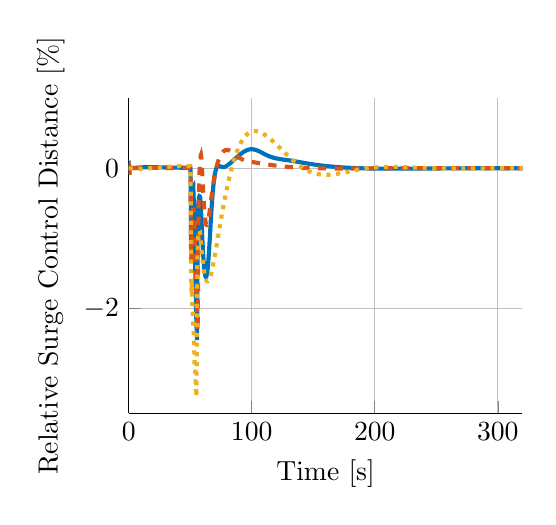
\begin{tikzpicture}

\begin{axis}[%
width=5cm,
height=4cm,
at={(0\linewidth,0\linewidth)},
scale only axis,
xmin=0,
xmax=320,
xlabel={Time [s]},
xmajorgrids,
ymin=-3.5,
ymax=1,
ylabel={Relative Surge Control Distance [\%]},
ymajorgrids,
axis background/.style={fill=white},
% title style={font=\bfseries},
% title={Surge Control Distance},
axis x line*=bottom,
axis y line*=left
]
\addplot [color=mycolor1,solid,line width=1.5pt,forget plot]
  table[row sep=crcr]{%
0	-0.0396000000000001\\
0.25	-0.0265199999999997\\
0.5	-0.0917099999999991\\
0.75	-0.0322300000000002\\
1	0.01417\\
1.25	0.00487000000000037\\
1.5	-0.0024299999999986\\
1.75	0.00156000000000134\\
2	0.00298000000000087\\
2.25	0.00211000000000006\\
2.5	0.00220999999999982\\
2.75	0.00270000000000081\\
3	0.00290999999999997\\
3.25	0.00311000000000128\\
3.5	0.00339000000000134\\
3.75	0.00366\\
4	0.00392000000000081\\
4.25	0.00416000000000061\\
4.5	0.0044000000000004\\
4.75	0.0046400000000002\\
5	0.00488\\
5.25	0.00513000000000119\\
5.5	0.00541000000000125\\
5.75	0.00572000000000017\\
6	0.00605999999999973\\
6.25	0.00641000000000069\\
6.5	0.0067800000000009\\
6.75	0.00716000000000072\\
7	0.00753000000000092\\
7.25	0.00788000000000011\\
7.5	0.00821999999999967\\
7.75	0.00853999999999999\\
8	0.00886000000000031\\
8.25	0.00917000000000101\\
8.5	0.00950000000000095\\
8.75	0.00983000000000089\\
9	0.0101800000000001\\
9.25	0.010530000000001\\
9.5	0.0108899999999998\\
9.75	0.0112400000000008\\
10	0.0115800000000004\\
10.25	0.0119000000000007\\
10.5	0.0122\\
10.75	0.0124700000000004\\
11	0.0127300000000012\\
11.25	0.012970000000001\\
11.5	0.0132100000000008\\
11.75	0.013440000000001\\
12	0.0136800000000008\\
12.25	0.0139200000000006\\
12.5	0.0141600000000004\\
12.75	0.0143900000000006\\
13	0.0146100000000011\\
13.25	0.0148100000000007\\
13.5	0.0149800000000013\\
13.75	0.0151200000000014\\
14	0.01525\\
14.25	0.0153499999999998\\
14.5	0.0154500000000013\\
14.75	0.0155500000000011\\
15	0.0156500000000008\\
15.25	0.0157500000000006\\
15.5	0.0158400000000007\\
15.75	0.0159300000000009\\
16	0.0160100000000014\\
16.25	0.0160800000000005\\
16.5	0.0161200000000008\\
16.75	0.01614\\
17	0.01614\\
17.25	0.0161300000000004\\
17.5	0.0161100000000012\\
17.75	0.0160800000000005\\
18	0.0160600000000013\\
18.25	0.0160499999999999\\
18.5	0.0160300000000007\\
18.75	0.016020000000001\\
19	0.0159900000000004\\
19.25	0.0159599999999998\\
19.5	0.0159099999999999\\
19.75	0.0158400000000007\\
20	0.0157600000000002\\
20.25	0.0156700000000001\\
20.5	0.0155700000000003\\
20.75	0.0154700000000005\\
21	0.0153700000000008\\
21.25	0.0152900000000002\\
21.5	0.0152000000000001\\
21.75	0.015130000000001\\
22	0.0150500000000005\\
22.25	0.0149600000000003\\
22.5	0.0148600000000005\\
22.75	0.0147500000000012\\
23	0.0146200000000007\\
23.25	0.0144900000000003\\
23.5	0.0143500000000003\\
23.75	0.0142199999999999\\
24	0.0140900000000013\\
24.25	0.0139700000000005\\
24.5	0.0138600000000011\\
24.75	0.0137600000000013\\
25	0.0136500000000002\\
25.25	0.0135500000000004\\
25.5	0.013440000000001\\
25.75	0.0133100000000006\\
26	0.0131800000000002\\
26.25	0.0130400000000002\\
26.5	0.0128900000000005\\
26.75	0.0127500000000005\\
27	0.0126200000000001\\
27.25	0.0124899999999997\\
27.5	0.0123800000000003\\
27.75	0.0122800000000005\\
28	0.0121800000000007\\
28.25	0.012080000000001\\
28.5	0.0119800000000012\\
28.75	0.0118600000000004\\
29	0.0117400000000014\\
29.25	0.011610000000001\\
29.5	0.011470000000001\\
29.75	0.0113400000000006\\
30	0.0112199999999998\\
30.25	0.0111100000000004\\
30.5	0.0110200000000003\\
30.75	0.0109300000000001\\
31	0.0108500000000014\\
31.25	0.0107700000000008\\
31.5	0.0106900000000003\\
31.75	0.0105900000000005\\
32	0.0104900000000008\\
32.25	0.0103800000000014\\
32.5	0.0102700000000002\\
32.75	0.0101600000000008\\
33	0.0100600000000011\\
33.25	0.00997000000000092\\
33.5	0.00990000000000002\\
33.75	0.00984000000000052\\
34	0.00978000000000101\\
34.25	0.00973000000000113\\
34.5	0.00966999999999985\\
34.75	0.00960000000000072\\
35	0.00952999999999982\\
35.25	0.00943999999999967\\
35.5	0.0093500000000013\\
35.75	0.00927000000000078\\
36	0.00919000000000025\\
36.25	0.00913000000000075\\
36.5	0.00908000000000087\\
36.75	0.0090400000000006\\
37	0.00900999999999996\\
37.25	0.00899000000000072\\
37.5	0.00895000000000046\\
37.75	0.0089100000000002\\
38	0.00886000000000031\\
38.25	0.00880000000000081\\
38.5	0.0087299999999999\\
38.75	0.0086700000000004\\
39	0.00861000000000089\\
39.25	0.00857000000000063\\
39.5	0.00855000000000139\\
39.75	0.00853000000000037\\
40	0.00853000000000037\\
40.25	0.00853000000000037\\
40.5	0.00852000000000075\\
40.75	0.00849999999999973\\
41	0.00847000000000087\\
41.25	0.00842000000000098\\
41.5	0.0083700000000011\\
41.75	0.00833000000000084\\
42	0.00829000000000057\\
42.25	0.00827000000000133\\
42.5	0.00825999999999993\\
42.75	0.00827000000000133\\
43	0.00829000000000057\\
43.25	0.00830999999999982\\
43.5	0.00832000000000122\\
43.75	0.00832000000000122\\
44	0.0083000000000002\\
44.25	0.00827000000000133\\
44.5	0.00823000000000107\\
44.75	0.00820000000000043\\
45	0.00818000000000119\\
45.25	0.00816999999999979\\
45.5	0.00818000000000119\\
45.75	0.00820000000000043\\
46	0.00824000000000069\\
46.25	0.00827000000000133\\
46.5	0.0083000000000002\\
46.75	0.00830999999999982\\
47	0.0083000000000002\\
47.25	0.00828000000000095\\
47.5	0.00825000000000031\\
47.75	0.00821999999999967\\
48	0.00821000000000005\\
48.25	0.00821000000000005\\
48.5	0.00823000000000107\\
48.75	0.00827000000000133\\
49	0.00832000000000122\\
49.25	0.0083599999999997\\
49.5	0.00839999999999996\\
49.75	0.00842000000000098\\
50	0.00842000000000098\\
50.25	-0.0222599999999993\\
50.5	-0.512049999999999\\
50.75	-1.18987\\
51	-1.03653\\
51.25	-0.638629999999999\\
51.5	-0.600519999999999\\
51.75	-0.56328\\
52	-0.395809999999999\\
52.25	-0.271539999999999\\
52.5	-0.264349999999999\\
52.75	-0.410279999999999\\
53	-0.48042\\
53.25	-0.60544\\
53.5	-0.88857\\
53.75	-1.15064\\
54	-1.35633\\
54.25	-1.57359\\
54.5	-1.7979\\
54.75	-2.00288\\
55	-2.18014\\
55.25	-2.34312\\
55.5	-2.45483\\
55.75	-1.84971\\
56	-1.09641\\
56.25	-0.735829999999999\\
56.5	-0.61009\\
56.75	-0.522939999999999\\
57	-0.452889999999999\\
57.25	-0.4091\\
57.5	-0.398529999999999\\
57.75	-0.40103\\
58	-0.412649999999999\\
58.25	-0.450679999999999\\
58.5	-0.51716\\
58.75	-0.599349999999999\\
59	-0.689609999999999\\
59.25	-0.785019999999999\\
59.5	-0.88153\\
59.75	-0.97535\\
60	-1.06446\\
60.25	-1.14778\\
60.5	-1.22434\\
60.75	-1.29329\\
61	-1.35421\\
61.25	-1.40701\\
61.5	-1.45168\\
61.75	-1.48822\\
62	-1.51667\\
62.25	-1.53712\\
62.5	-1.54962\\
62.75	-1.55422\\
63	-1.55096\\
63.25	-1.53989\\
63.5	-1.52107\\
63.75	-1.49462\\
64	-1.46069\\
64.25	-1.41953\\
64.5	-1.3715\\
64.75	-1.31706\\
65	-1.25681\\
65.25	-1.19147\\
65.5	-1.12185\\
65.75	-1.04889\\
66	-0.973579999999999\\
66.25	-0.897019999999999\\
66.5	-0.820359999999999\\
66.75	-0.7448\\
67	-0.671399999999999\\
67.25	-0.601019999999999\\
67.5	-0.534199999999999\\
67.75	-0.471299999999999\\
68	-0.4125\\
68.25	-0.357919999999999\\
68.5	-0.30758\\
68.75	-0.261449999999999\\
69	-0.21946\\
69.25	-0.18146\\
69.5	-0.1473\\
69.75	-0.116819999999999\\
70	-0.0898599999999998\\
70.25	-0.0662399999999987\\
70.5	-0.0457900000000002\\
70.75	-0.028319999999999\\
71	-0.0136000000000003\\
71.25	-0.00141999999999953\\
71.5	0.00846000000000124\\
71.75	0.0162700000000005\\
72	0.0222500000000014\\
72.25	0.0266200000000012\\
72.5	0.0296099999999999\\
72.75	0.0314200000000007\\
73	0.0322600000000008\\
73.25	0.0323100000000007\\
73.5	0.0317300000000014\\
73.75	0.0306700000000006\\
74	0.02928\\
74.25	0.0276700000000005\\
74.5	0.0259499999999999\\
74.75	0.0242100000000001\\
75	0.0225200000000001\\
75.25	0.0209500000000009\\
75.5	0.0195500000000006\\
75.75	0.0183600000000013\\
76	0.0174200000000013\\
76.25	0.0167400000000004\\
76.5	0.016350000000001\\
76.75	0.0162500000000012\\
77	0.0164500000000007\\
77.25	0.01694\\
77.5	0.0177200000000006\\
77.75	0.0187800000000014\\
78	0.0201100000000007\\
78.25	0.0216900000000013\\
78.5	0.0235099999999999\\
78.75	0.0255500000000008\\
79	0.0278000000000009\\
79.25	0.0302400000000009\\
79.5	0.0328600000000012\\
79.75	0.0356300000000012\\
80	0.0385500000000008\\
80.25	0.0416000000000007\\
80.5	0.0447600000000001\\
80.75	0.0480200000000011\\
81	0.05138\\
81.25	0.0548200000000012\\
81.5	0.0583200000000001\\
81.75	0.06189\\
82	0.0655099999999997\\
82.25	0.0691800000000011\\
82.5	0.072890000000001\\
82.75	0.0766400000000012\\
83	0.0804100000000005\\
83.25	0.0842200000000002\\
83.5	0.0880400000000012\\
83.75	0.0918900000000011\\
84	0.0957500000000007\\
84.25	0.0996300000000012\\
84.5	0.103520000000001\\
84.75	0.107420000000001\\
85	0.111330000000001\\
85.25	0.115250000000001\\
85.5	0.11917\\
85.75	0.123090000000001\\
86	0.12702\\
86.25	0.13095\\
86.5	0.134880000000001\\
86.75	0.138810000000001\\
87	0.14273\\
87.25	0.146650000000001\\
87.5	0.15056\\
87.75	0.15446\\
88	0.158340000000001\\
88.25	0.162220000000001\\
88.5	0.166070000000001\\
88.75	0.16991\\
89	0.173720000000001\\
89.25	0.17751\\
89.5	0.18126\\
89.75	0.184990000000001\\
90	0.188690000000001\\
90.25	0.19234\\
90.5	0.195960000000001\\
90.75	0.199530000000001\\
91	0.203050000000001\\
91.25	0.206520000000001\\
91.5	0.209940000000001\\
91.75	0.2133\\
92	0.2166\\
92.25	0.21983\\
92.5	0.222990000000001\\
92.75	0.226080000000001\\
93	0.229090000000001\\
93.25	0.23203\\
93.5	0.23488\\
93.75	0.237640000000001\\
94	0.240320000000001\\
94.25	0.242900000000001\\
94.5	0.24539\\
94.75	0.247780000000001\\
95	0.250070000000001\\
95.25	0.25226\\
95.5	0.254330000000001\\
95.75	0.256310000000001\\
96	0.25817\\
96.25	0.259910000000001\\
96.5	0.26155\\
96.75	0.263060000000001\\
97	0.26446\\
97.25	0.265740000000001\\
97.5	0.266910000000001\\
97.75	0.267950000000001\\
98	0.26887\\
98.25	0.269670000000001\\
98.5	0.270350000000001\\
98.75	0.270900000000001\\
99	0.27134\\
99.25	0.271650000000001\\
99.5	0.271850000000001\\
99.75	0.271930000000001\\
100	0.271890000000001\\
100.25	0.27173\\
100.5	0.271460000000001\\
100.75	0.271080000000001\\
101	0.270580000000001\\
101.25	0.26998\\
101.5	0.269270000000001\\
101.75	0.268460000000001\\
102	0.26755\\
102.25	0.266530000000001\\
102.5	0.26543\\
102.75	0.264230000000001\\
103	0.26294\\
103.25	0.261570000000001\\
103.5	0.260110000000001\\
103.75	0.25858\\
104	0.256970000000001\\
104.25	0.25529\\
104.5	0.253540000000001\\
104.75	0.25173\\
105	0.24986\\
105.25	0.24794\\
105.5	0.24596\\
105.75	0.243930000000001\\
106	0.241860000000001\\
106.25	0.23976\\
106.5	0.23761\\
106.75	0.235430000000001\\
107	0.233230000000001\\
107.25	0.231\\
107.5	0.22875\\
107.75	0.22648\\
108	0.2242\\
108.25	0.221910000000001\\
108.5	0.219610000000001\\
108.75	0.217310000000001\\
109	0.215010000000001\\
109.25	0.212710000000001\\
109.5	0.210420000000001\\
109.75	0.20814\\
110	0.205860000000001\\
110.25	0.203610000000001\\
110.5	0.201370000000001\\
110.75	0.199150000000001\\
111	0.196950000000001\\
111.25	0.19478\\
111.5	0.192630000000001\\
111.75	0.19051\\
112	0.188420000000001\\
112.25	0.186360000000001\\
112.5	0.184330000000001\\
112.75	0.18234\\
113	0.180380000000001\\
113.25	0.178460000000001\\
113.5	0.17657\\
113.75	0.174720000000001\\
114	0.17291\\
114.25	0.171140000000001\\
114.5	0.169410000000001\\
114.75	0.167720000000001\\
115	0.166070000000001\\
115.25	0.16446\\
115.5	0.162880000000001\\
115.75	0.161350000000001\\
116	0.15986\\
116.25	0.15841\\
116.5	0.157\\
116.75	0.155620000000001\\
117	0.15428\\
117.25	0.152980000000001\\
117.5	0.151720000000001\\
117.75	0.150500000000001\\
118	0.1493\\
118.25	0.148150000000001\\
118.5	0.147020000000001\\
118.75	0.14593\\
119	0.144880000000001\\
119.25	0.14385\\
119.5	0.142850000000001\\
119.75	0.14188\\
120	0.140930000000001\\
120.25	0.14002\\
120.5	0.13912\\
120.75	0.138260000000001\\
121	0.137410000000001\\
121.25	0.13659\\
121.5	0.13578\\
121.75	0.135\\
122	0.134230000000001\\
122.25	0.13348\\
122.5	0.13275\\
122.75	0.13203\\
123	0.13133\\
123.25	0.130640000000001\\
123.5	0.129950000000001\\
123.75	0.129290000000001\\
124	0.128630000000001\\
124.25	0.127970000000001\\
124.5	0.127330000000001\\
124.75	0.12669\\
125	0.126060000000001\\
125.25	0.125440000000001\\
125.5	0.12481\\
125.75	0.1242\\
126	0.12358\\
126.25	0.12297\\
126.5	0.12236\\
126.75	0.121740000000001\\
127	0.121130000000001\\
127.25	0.120520000000001\\
127.5	0.119910000000001\\
127.75	0.119290000000001\\
128	0.118680000000001\\
128.25	0.11806\\
128.5	0.117430000000001\\
128.75	0.116810000000001\\
129	0.11618\\
129.25	0.115550000000001\\
129.5	0.11491\\
129.75	0.114270000000001\\
130	0.113620000000001\\
130.25	0.112970000000001\\
130.5	0.11232\\
130.75	0.111660000000001\\
131	0.110990000000001\\
131.25	0.11032\\
131.5	0.109640000000001\\
131.75	0.10896\\
132	0.108270000000001\\
132.25	0.10758\\
132.5	0.10688\\
132.75	0.10618\\
133	0.10547\\
133.25	0.104760000000001\\
133.5	0.104040000000001\\
133.75	0.10332\\
134	0.102590000000001\\
134.25	0.10186\\
134.5	0.10112\\
134.75	0.100380000000001\\
135	0.0996400000000008\\
135.25	0.0988900000000008\\
135.5	0.0981400000000008\\
135.75	0.0973800000000011\\
136	0.0966199999999997\\
136.25	0.0958600000000001\\
136.5	0.0950900000000008\\
136.75	0.0943300000000011\\
137	0.0935600000000001\\
137.25	0.0927900000000008\\
137.5	0.0920100000000001\\
137.75	0.0912400000000009\\
138	0.0904600000000002\\
138.25	0.0896800000000013\\
138.5	0.0889000000000006\\
138.75	0.08812\\
139	0.0873400000000011\\
139.25	0.0865600000000004\\
139.5	0.0857799999999997\\
139.75	0.0850000000000009\\
140	0.0842200000000002\\
140.25	0.0834400000000013\\
140.5	0.0826600000000006\\
140.75	0.0818900000000014\\
141	0.0811100000000007\\
141.25	0.0803400000000014\\
141.5	0.0795600000000007\\
141.75	0.0787899999999997\\
142	0.0780200000000004\\
142.25	0.0772600000000008\\
142.5	0.0764899999999997\\
142.75	0.0757300000000001\\
143	0.0749700000000004\\
143.25	0.0742100000000008\\
143.5	0.0734600000000007\\
143.75	0.0727100000000007\\
144	0.0719600000000007\\
144.25	0.0712200000000003\\
144.5	0.0704799999999999\\
144.75	0.0697400000000012\\
145	0.0690100000000005\\
145.25	0.0682799999999997\\
145.5	0.0675500000000007\\
145.75	0.0668300000000013\\
146	0.0661100000000001\\
146.25	0.0654000000000003\\
146.5	0.0646900000000006\\
146.75	0.0639900000000004\\
147	0.0632900000000003\\
147.25	0.0625900000000001\\
147.5	0.0619000000000014\\
147.75	0.0612100000000009\\
148	0.06053\\
148.25	0.0598500000000008\\
148.5	0.0591800000000013\\
148.75	0.0585100000000001\\
149	0.0578400000000006\\
149.25	0.0571800000000007\\
149.5	0.0565300000000004\\
149.75	0.0558800000000002\\
150	0.0552299999999999\\
150.25	0.054590000000001\\
150.5	0.0539500000000004\\
150.75	0.0533200000000011\\
151	0.0526900000000001\\
151.25	0.0520700000000005\\
151.5	0.0514500000000009\\
151.75	0.0508400000000009\\
152	0.0502300000000009\\
152.25	0.0496200000000009\\
152.5	0.0490200000000005\\
152.75	0.0484299999999998\\
153	0.0478400000000008\\
153.25	0.04725\\
153.5	0.0466700000000007\\
153.75	0.0460900000000013\\
154	0.0455199999999998\\
154.25	0.04495\\
154.5	0.0443800000000003\\
154.75	0.0438200000000002\\
155	0.0432699999999997\\
155.25	0.042720000000001\\
155.5	0.0421700000000005\\
155.75	0.04162\\
156	0.0410900000000005\\
156.25	0.0405500000000014\\
156.5	0.0400200000000002\\
156.75	0.0394900000000007\\
157	0.0389700000000008\\
157.25	0.038450000000001\\
157.5	0.0379400000000008\\
157.75	0.0374300000000005\\
158	0.0369200000000003\\
158.25	0.0364199999999997\\
158.5	0.0359200000000008\\
158.75	0.0354200000000002\\
159	0.034930000000001\\
159.25	0.03444\\
159.5	0.0339600000000004\\
159.75	0.0334800000000008\\
160	0.0330000000000013\\
160.25	0.0325300000000013\\
160.5	0.0320600000000013\\
160.75	0.031600000000001\\
161	0.0311400000000006\\
161.25	0.0306800000000003\\
161.5	0.0302199999999999\\
161.75	0.029770000000001\\
162	0.0293299999999999\\
162.25	0.0288800000000009\\
162.5	0.0284399999999998\\
162.75	0.0280100000000001\\
163	0.0275700000000008\\
163.25	0.0271400000000011\\
163.5	0.026720000000001\\
163.75	0.0263000000000009\\
164	0.0258800000000008\\
164.25	0.0254600000000007\\
164.5	0.0250500000000002\\
164.75	0.0246399999999998\\
165	0.0242300000000011\\
165.25	0.0238300000000002\\
165.5	0.0234300000000012\\
165.75	0.0230399999999999\\
166	0.0226500000000005\\
166.25	0.0222600000000011\\
166.5	0.0218699999999998\\
166.75	0.02149\\
167	0.0211100000000002\\
167.25	0.02074\\
167.5	0.0203699999999998\\
167.75	0.0200000000000014\\
168	0.0196300000000011\\
168.25	0.0192700000000006\\
168.5	0.01891\\
168.75	0.0185600000000008\\
169	0.0182000000000002\\
169.25	0.0178600000000007\\
169.5	0.0175099999999997\\
169.75	0.0171700000000001\\
170	0.0168300000000006\\
170.25	0.016490000000001\\
170.5	0.0161600000000011\\
170.75	0.0158300000000011\\
171	0.0155000000000012\\
171.25	0.0151800000000009\\
171.5	0.0148600000000005\\
171.75	0.0145400000000002\\
172	0.0142300000000013\\
172.25	0.0139200000000006\\
172.5	0.0136099999999999\\
172.75	0.0133100000000006\\
173	0.0130100000000013\\
173.25	0.0127100000000002\\
173.5	0.0124100000000009\\
173.75	0.0121200000000012\\
174	0.0118299999999998\\
174.25	0.0115499999999997\\
174.5	0.0112699999999997\\
174.75	0.0109900000000014\\
175	0.0107100000000013\\
175.25	0.0104400000000009\\
175.5	0.0101700000000005\\
175.75	0.00990000000000002\\
176	0.00963000000000136\\
176.25	0.00937000000000054\\
176.5	0.00910999999999973\\
176.75	0.00886000000000031\\
177	0.00861000000000089\\
177.25	0.0083599999999997\\
177.5	0.00811000000000028\\
177.75	0.00787000000000049\\
178	0.00762000000000107\\
178.25	0.0073900000000009\\
178.5	0.0071500000000011\\
178.75	0.00692000000000093\\
179	0.00669000000000075\\
179.25	0.00646000000000058\\
179.5	0.00624000000000002\\
179.75	0.00602000000000125\\
180	0.00580000000000069\\
180.25	0.00558000000000014\\
180.5	0.00537000000000099\\
180.75	0.00516000000000005\\
181	0.0049500000000009\\
181.25	0.00475000000000136\\
181.5	0.00455000000000005\\
181.75	0.00435000000000052\\
182	0.00415000000000099\\
182.25	0.00396000000000107\\
182.5	0.00375999999999976\\
182.75	0.00358000000000125\\
183	0.00339000000000134\\
183.25	0.00320000000000142\\
183.5	0.00302000000000113\\
183.75	0.00284000000000084\\
184	0.00267000000000017\\
184.25	0.00248999999999988\\
184.5	0.00232000000000099\\
184.75	0.00215000000000032\\
185	0.00199000000000105\\
185.25	0.00182000000000038\\
185.5	0.00166000000000111\\
185.75	0.00150000000000006\\
186	0.00134000000000079\\
186.25	0.00119000000000113\\
186.5	0.00103999999999971\\
186.75	0.000890000000000057\\
187	0.000740000000000407\\
187.25	0.000590000000000757\\
187.5	0.000450000000000728\\
187.75	0.000310000000000699\\
188	0.00017000000000067\\
188.25	3.00000000006406e-05\\
188.5	-9.99999999997669e-05\\
188.75	-0.000230000000000175\\
189	-0.000370000000000203\\
189.25	-0.000489999999999213\\
189.5	-0.000619999999999621\\
189.75	-0.000739999999998631\\
190	-0.000869999999999038\\
190.25	-0.000989999999999824\\
190.5	-0.00109999999999921\\
190.75	-0.00122\\
191	-0.00132999999999939\\
191.25	-0.00145000000000017\\
191.5	-0.00155999999999956\\
191.75	-0.00165999999999933\\
192	-0.00176999999999872\\
192.25	-0.00187999999999988\\
192.5	-0.00197999999999965\\
192.75	-0.00207999999999942\\
193	-0.00217999999999918\\
193.25	-0.00227999999999895\\
193.5	-0.0023699999999991\\
193.75	-0.00245999999999924\\
194	-0.00255999999999901\\
194.25	-0.00264999999999915\\
194.5	-0.00272999999999968\\
194.75	-0.00281999999999982\\
195	-0.00290999999999997\\
195.25	-0.00298999999999872\\
195.5	-0.00306999999999924\\
195.75	-0.00314999999999976\\
196	-0.00323000000000029\\
196.25	-0.00329999999999941\\
196.5	-0.00337999999999994\\
196.75	-0.00344999999999906\\
197	-0.00351999999999997\\
197.25	-0.00359999999999872\\
197.5	-0.00366\\
197.75	-0.00372999999999912\\
198	-0.00380000000000003\\
198.25	-0.00385999999999953\\
198.5	-0.00391999999999904\\
198.75	-0.00398999999999994\\
199	-0.00404999999999944\\
199.25	-0.00409999999999933\\
199.5	-0.00415999999999883\\
199.75	-0.00422000000000011\\
200	-0.00427\\
200.25	-0.00431999999999988\\
200.5	-0.00437999999999938\\
200.75	-0.00442999999999927\\
201	-0.00447999999999915\\
201.25	-0.00451999999999941\\
201.5	-0.0045699999999993\\
201.75	-0.00460999999999956\\
202	-0.00465999999999944\\
202.25	-0.0046999999999997\\
202.5	-0.00473999999999997\\
202.75	-0.00478000000000023\\
203	-0.00481999999999871\\
203.25	-0.00485999999999898\\
203.5	-0.00489999999999924\\
203.75	-0.00492999999999988\\
204	-0.00497000000000014\\
204.25	-0.00499999999999901\\
204.5	-0.00502999999999965\\
204.75	-0.00506000000000029\\
205	-0.00508999999999915\\
205.25	-0.00511999999999979\\
205.5	-0.00514999999999866\\
205.75	-0.0051799999999993\\
206	-0.00520000000000032\\
206.25	-0.00522999999999918\\
206.5	-0.0052500000000002\\
206.75	-0.00526999999999944\\
207	-0.00530000000000008\\
207.25	-0.00531999999999933\\
207.5	-0.00533999999999857\\
207.75	-0.00535999999999959\\
208	-0.00536999999999921\\
208.25	-0.00539000000000023\\
208.5	-0.00540999999999947\\
208.75	-0.00541999999999909\\
209	-0.00544000000000011\\
209.25	-0.00544999999999973\\
209.5	-0.00545999999999935\\
209.75	-0.0054799999999986\\
210	-0.00548999999999999\\
210.25	-0.00549999999999962\\
210.5	-0.00550999999999924\\
210.75	-0.00551999999999886\\
211	-0.00551999999999886\\
211.25	-0.00553000000000026\\
211.5	-0.00553999999999988\\
211.75	-0.00553999999999988\\
212	-0.0055499999999995\\
212.25	-0.0055499999999995\\
212.5	-0.00555999999999912\\
212.75	-0.00555999999999912\\
213	-0.00555999999999912\\
213.25	-0.00555999999999912\\
213.5	-0.00555999999999912\\
213.75	-0.00555999999999912\\
214	-0.00555999999999912\\
214.25	-0.00555999999999912\\
214.5	-0.00555999999999912\\
214.75	-0.00555999999999912\\
215	-0.0055499999999995\\
215.25	-0.0055499999999995\\
215.5	-0.0055499999999995\\
215.75	-0.00553999999999988\\
216	-0.00553999999999988\\
216.25	-0.00553000000000026\\
216.5	-0.00551999999999886\\
216.75	-0.00551999999999886\\
217	-0.00550999999999924\\
217.25	-0.00549999999999962\\
217.5	-0.00548999999999999\\
217.75	-0.0054799999999986\\
218	-0.00546999999999898\\
218.25	-0.00545999999999935\\
218.5	-0.00544999999999973\\
218.75	-0.00544000000000011\\
219	-0.00542999999999871\\
219.25	-0.00541999999999909\\
219.5	-0.00540999999999947\\
219.75	-0.00539000000000023\\
220	-0.00537999999999883\\
220.25	-0.00536999999999921\\
220.5	-0.00534999999999997\\
220.75	-0.00533999999999857\\
221	-0.00531999999999933\\
221.25	-0.0053099999999997\\
221.5	-0.00528999999999868\\
221.75	-0.00527999999999906\\
222	-0.00525999999999982\\
222.25	-0.0052500000000002\\
222.5	-0.00522999999999918\\
222.75	-0.00520999999999994\\
223	-0.00518999999999892\\
223.25	-0.0051799999999993\\
223.5	-0.00516000000000005\\
223.75	-0.00513999999999903\\
224	-0.00511999999999979\\
224.25	-0.00509999999999877\\
224.5	-0.00507999999999953\\
224.75	-0.00506000000000029\\
225	-0.00503999999999927\\
225.25	-0.00502000000000002\\
225.5	-0.00499999999999901\\
225.75	-0.00497999999999976\\
226	-0.00495999999999874\\
226.25	-0.0049399999999995\\
226.5	-0.00492000000000026\\
226.75	-0.00489999999999924\\
227	-0.00488\\
227.25	-0.00484999999999935\\
227.5	-0.00483000000000011\\
227.75	-0.00480999999999909\\
228	-0.00478999999999985\\
228.25	-0.00475999999999921\\
228.5	-0.00473999999999997\\
228.75	-0.00471999999999895\\
229	-0.00469000000000008\\
229.25	-0.00466999999999906\\
229.5	-0.00464999999999982\\
229.75	-0.00461999999999918\\
230	-0.00459999999999994\\
230.25	-0.0045699999999993\\
230.5	-0.00455000000000005\\
230.75	-0.00452999999999903\\
231	-0.00450000000000017\\
231.25	-0.00447999999999915\\
231.5	-0.00445000000000029\\
231.75	-0.00442999999999927\\
232	-0.00439999999999863\\
232.25	-0.00437999999999938\\
232.5	-0.00434999999999874\\
232.75	-0.0043299999999995\\
233	-0.00429999999999886\\
233.25	-0.00427999999999962\\
233.5	-0.00424999999999898\\
233.75	-0.00422999999999973\\
234	-0.00419999999999909\\
234.25	-0.00417000000000023\\
234.5	-0.00414999999999921\\
234.75	-0.00411999999999857\\
235	-0.00409999999999933\\
235.25	-0.00406999999999869\\
235.5	-0.00403999999999982\\
235.75	-0.0040199999999988\\
236	-0.00398999999999994\\
236.25	-0.00396999999999892\\
236.5	-0.00394000000000005\\
236.75	-0.00390999999999941\\
237	-0.00389000000000017\\
237.25	-0.00385999999999953\\
237.5	-0.00382999999999889\\
237.75	-0.00380999999999965\\
238	-0.00377999999999901\\
238.25	-0.00375999999999976\\
238.5	-0.00372999999999912\\
238.75	-0.00370000000000026\\
239	-0.00367999999999924\\
239.25	-0.0036499999999986\\
239.5	-0.00361999999999973\\
239.75	-0.00359999999999872\\
240	-0.00356999999999985\\
240.25	-0.00354999999999883\\
240.5	-0.00351999999999997\\
240.75	-0.00348999999999933\\
241	-0.00347000000000008\\
241.25	-0.00343999999999944\\
241.5	-0.0034099999999988\\
241.75	-0.00338999999999956\\
242	-0.00335999999999892\\
242.25	-0.00333999999999968\\
242.5	-0.00330999999999904\\
242.75	-0.00328000000000017\\
243	-0.00325999999999915\\
243.25	-0.00323000000000029\\
243.5	-0.00320999999999927\\
243.75	-0.00317999999999863\\
244	-0.00315999999999939\\
244.25	-0.00312999999999874\\
244.5	-0.00309999999999988\\
244.75	-0.00307999999999886\\
245	-0.00305\\
245.25	-0.00302999999999898\\
245.5	-0.00300000000000011\\
245.75	-0.00297999999999909\\
246	-0.00295000000000023\\
246.25	-0.00292999999999921\\
246.5	-0.00289999999999857\\
246.75	-0.00287999999999933\\
247	-0.00284999999999869\\
247.25	-0.00282999999999944\\
247.5	-0.0027999999999988\\
247.75	-0.00277999999999956\\
248	-0.00274999999999892\\
248.25	-0.00272999999999968\\
248.5	-0.00269999999999904\\
248.75	-0.00267999999999979\\
249	-0.00264999999999915\\
249.25	-0.00262999999999991\\
249.5	-0.00260999999999889\\
249.75	-0.00258000000000003\\
250	-0.00255999999999901\\
250.25	-0.00253000000000014\\
250.5	-0.00250999999999912\\
250.75	-0.00248999999999988\\
251	-0.00245999999999924\\
251.25	-0.00244\\
251.5	-0.00241999999999898\\
251.75	-0.00239000000000011\\
252	-0.0023699999999991\\
252.25	-0.00234999999999985\\
252.5	-0.00231999999999921\\
252.75	-0.00229999999999997\\
253	-0.00227999999999895\\
253.25	-0.00225999999999971\\
253.5	-0.00222999999999907\\
253.75	-0.00220999999999982\\
254	-0.0021899999999988\\
254.25	-0.00216999999999956\\
254.5	-0.00213999999999892\\
254.75	-0.00211999999999968\\
255	-0.00209999999999866\\
255.25	-0.00207999999999942\\
255.5	-0.00206000000000017\\
255.75	-0.00203999999999915\\
256	-0.00201000000000029\\
256.25	-0.00198999999999927\\
256.5	-0.00197000000000003\\
256.75	-0.00194999999999901\\
257	-0.00192999999999977\\
257.25	-0.00190999999999875\\
257.5	-0.0018899999999995\\
257.75	-0.00187000000000026\\
258	-0.00184999999999924\\
258.25	-0.00183\\
258.5	-0.00180999999999898\\
258.75	-0.00178999999999974\\
259	-0.00176999999999872\\
259.25	-0.00174999999999947\\
259.5	-0.00173000000000023\\
259.75	-0.00170999999999921\\
260	-0.00168999999999997\\
260.25	-0.00166999999999895\\
260.5	-0.00164999999999971\\
260.75	-0.00162999999999869\\
261	-0.00160999999999945\\
261.25	-0.0015900000000002\\
261.5	-0.0015799999999988\\
261.75	-0.00155999999999956\\
262	-0.00154000000000032\\
262.25	-0.0015199999999993\\
262.5	-0.00150000000000006\\
262.75	-0.00147999999999904\\
263	-0.00146999999999942\\
263.25	-0.00145000000000017\\
263.5	-0.00142999999999915\\
263.75	-0.00140999999999991\\
264	-0.00138999999999889\\
264.25	-0.00137999999999927\\
264.5	-0.00136000000000003\\
264.75	-0.00133999999999901\\
265	-0.00132999999999939\\
265.25	-0.00131000000000014\\
265.5	-0.00128999999999913\\
265.75	-0.0012799999999995\\
266	-0.00126000000000026\\
266.25	-0.00123999999999924\\
266.5	-0.00122999999999962\\
266.75	-0.0012099999999986\\
267	-0.00118999999999936\\
267.25	-0.00117999999999974\\
267.5	-0.00115999999999872\\
267.75	-0.0011499999999991\\
268	-0.00112999999999985\\
268.25	-0.00112000000000023\\
268.5	-0.00109999999999921\\
268.75	-0.00108999999999959\\
269	-0.00106999999999857\\
269.25	-0.00105999999999895\\
269.5	-0.00103999999999971\\
269.75	-0.00103000000000009\\
270	-0.00100999999999907\\
270.25	-0.000999999999999446\\
270.5	-0.000980000000000203\\
270.75	-0.000969999999998805\\
271	-0.000959999999999184\\
271.25	-0.000939999999999941\\
271.5	-0.000930000000000319\\
271.75	-0.0009099999999993\\
272	-0.000899999999999679\\
272.25	-0.000890000000000057\\
272.5	-0.000869999999999038\\
272.75	-0.000859999999999417\\
273	-0.000849999999999795\\
273.25	-0.000829999999998776\\
273.5	-0.000819999999999155\\
273.75	-0.000809999999999533\\
274	-0.000799999999999912\\
274.25	-0.000779999999998893\\
274.5	-0.000769999999999271\\
274.75	-0.00075999999999965\\
275	-0.000750000000000028\\
275.25	-0.000739999999998631\\
275.5	-0.000719999999999388\\
275.75	-0.000709999999999766\\
276	-0.000700000000000145\\
276.25	-0.000689999999998747\\
276.5	-0.000679999999999126\\
276.75	-0.000669999999999504\\
277	-0.000650000000000261\\
277.25	-0.000639999999998864\\
277.5	-0.000629999999999242\\
277.75	-0.000619999999999621\\
278	-0.000609999999999999\\
278.25	-0.000599999999998602\\
278.5	-0.00058999999999898\\
278.75	-0.000579999999999359\\
279	-0.000569999999999737\\
279.25	-0.000560000000000116\\
279.5	-0.000549999999998718\\
279.75	-0.000539999999999097\\
280	-0.000529999999999475\\
280.25	-0.000519999999999854\\
280.5	-0.000510000000000232\\
280.75	-0.000499999999998835\\
281	-0.000489999999999213\\
281.25	-0.000479999999999592\\
281.5	-0.00046999999999997\\
281.75	-0.000459999999998573\\
282	-0.000449999999998951\\
282.25	-0.00043999999999933\\
282.5	-0.000429999999999708\\
282.75	-0.000420000000000087\\
283	-0.000409999999998689\\
283.25	-0.000409999999998689\\
283.5	-0.000399999999999068\\
283.75	-0.000389999999999446\\
284	-0.000379999999999825\\
284.25	-0.000370000000000203\\
284.5	-0.000359999999998806\\
284.75	-0.000359999999998806\\
285	-0.000349999999999184\\
285.25	-0.000339999999999563\\
285.5	-0.000329999999999941\\
285.75	-0.00032000000000032\\
286	-0.00032000000000032\\
286.25	-0.000309999999998922\\
286.5	-0.000299999999999301\\
286.75	-0.000289999999999679\\
287	-0.000289999999999679\\
287.25	-0.000280000000000058\\
287.5	-0.00026999999999866\\
287.75	-0.00026999999999866\\
288	-0.000259999999999039\\
288.25	-0.000249999999999417\\
288.5	-0.000239999999999796\\
288.75	-0.000239999999999796\\
289	-0.000230000000000175\\
289.25	-0.000219999999998777\\
289.5	-0.000219999999998777\\
289.75	-0.000209999999999155\\
290	-0.000209999999999155\\
290.25	-0.000199999999999534\\
290.5	-0.000189999999999912\\
290.75	-0.000189999999999912\\
291	-0.000180000000000291\\
291.25	-0.000169999999998893\\
291.5	-0.000169999999998893\\
291.75	-0.000159999999999272\\
292	-0.000159999999999272\\
292.25	-0.00014999999999965\\
292.5	-0.00014999999999965\\
292.75	-0.000140000000000029\\
293	-0.000140000000000029\\
293.25	-0.000129999999998631\\
293.5	-0.00011999999999901\\
293.75	-0.00011999999999901\\
294	-0.000109999999999388\\
294.25	-0.000109999999999388\\
294.5	-9.99999999997669e-05\\
294.75	-9.99999999997669e-05\\
295	-9.00000000001455e-05\\
295.25	-9.00000000001455e-05\\
295.5	-9.00000000001455e-05\\
295.75	-7.99999999987477e-05\\
296	-7.99999999987477e-05\\
296.25	-6.99999999991263e-05\\
296.5	-6.99999999991263e-05\\
296.75	-5.99999999995049e-05\\
297	-5.99999999995049e-05\\
297.25	-4.99999999998835e-05\\
297.5	-4.99999999998835e-05\\
297.75	-4.99999999998835e-05\\
298	-4.0000000000262e-05\\
298.25	-4.0000000000262e-05\\
298.5	-2.99999999988643e-05\\
298.75	-2.99999999988643e-05\\
299	-2.99999999988643e-05\\
299.25	-1.99999999992428e-05\\
299.5	-1.99999999992428e-05\\
299.75	-1.99999999992428e-05\\
300	-9.99999999962142e-06\\
300.25	-9.99999999962142e-06\\
300.5	0\\
300.75	0\\
301	0\\
301.25	1.00000000013978e-05\\
301.5	1.00000000013978e-05\\
301.75	1.00000000013978e-05\\
302	2.00000000010192e-05\\
302.25	2.00000000010192e-05\\
302.5	2.00000000010192e-05\\
302.75	2.00000000010192e-05\\
303	3.00000000006406e-05\\
303.25	3.00000000006406e-05\\
303.5	3.00000000006406e-05\\
303.75	4.0000000000262e-05\\
304	4.0000000000262e-05\\
304.25	4.0000000000262e-05\\
304.5	4.0000000000262e-05\\
304.75	4.99999999998835e-05\\
305	4.99999999998835e-05\\
305.25	4.99999999998835e-05\\
305.5	4.99999999998835e-05\\
305.75	6.00000000012813e-05\\
306	6.00000000012813e-05\\
306.25	6.00000000012813e-05\\
306.5	6.00000000012813e-05\\
306.75	7.00000000009027e-05\\
307	7.00000000009027e-05\\
307.25	7.00000000009027e-05\\
307.5	7.00000000009027e-05\\
307.75	7.00000000009027e-05\\
308	8.00000000005241e-05\\
308.25	8.00000000005241e-05\\
308.5	8.00000000005241e-05\\
308.75	8.00000000005241e-05\\
309	8.00000000005241e-05\\
309.25	8.00000000005241e-05\\
309.5	9.00000000001455e-05\\
309.75	9.00000000001455e-05\\
310	9.00000000001455e-05\\
310.25	9.00000000001455e-05\\
310.5	9.00000000001455e-05\\
310.75	9.00000000001455e-05\\
311	9.99999999997669e-05\\
311.25	9.99999999997669e-05\\
311.5	9.99999999997669e-05\\
311.75	9.99999999997669e-05\\
312	9.99999999997669e-05\\
312.25	9.99999999997669e-05\\
312.5	9.99999999997669e-05\\
312.75	0.000110000000001165\\
313	0.000110000000001165\\
313.25	0.000110000000001165\\
313.5	0.000110000000001165\\
313.75	0.000110000000001165\\
314	0.000110000000001165\\
314.25	0.000110000000001165\\
314.5	0.000110000000001165\\
314.75	0.000110000000001165\\
315	0.000120000000000786\\
315.25	0.000120000000000786\\
315.5	0.000120000000000786\\
315.75	0.000120000000000786\\
316	0.000120000000000786\\
316.25	0.000120000000000786\\
316.5	0.000120000000000786\\
316.75	0.000120000000000786\\
317	0.000120000000000786\\
317.25	0.000120000000000786\\
317.5	0.000120000000000786\\
317.75	0.000130000000000408\\
318	0.000130000000000408\\
318.25	0.000130000000000408\\
318.5	0.000130000000000408\\
318.75	0.000130000000000408\\
319	0.000130000000000408\\
319.25	0.000130000000000408\\
319.5	0.000130000000000408\\
319.75	0.000130000000000408\\
320	0.000130000000000408\\
320.25	0.000130000000000408\\
320.5	0.000130000000000408\\
320.75	0.000130000000000408\\
321	0.000130000000000408\\
321.25	0.000130000000000408\\
321.5	0.000130000000000408\\
321.75	0.000130000000000408\\
322	0.000130000000000408\\
322.25	0.000130000000000408\\
322.5	0.000130000000000408\\
322.75	0.000130000000000408\\
323	0.000130000000000408\\
323.25	0.000130000000000408\\
323.5	0.000130000000000408\\
323.75	0.000130000000000408\\
324	0.000130000000000408\\
324.25	0.000130000000000408\\
324.5	0.000130000000000408\\
324.75	0.000130000000000408\\
325	0.000140000000000029\\
325.25	0.000140000000000029\\
325.5	0.000140000000000029\\
325.75	0.000140000000000029\\
326	0.000140000000000029\\
326.25	0.000140000000000029\\
326.5	0.000140000000000029\\
326.75	0.000140000000000029\\
327	0.000140000000000029\\
327.25	0.000130000000000408\\
327.5	0.000130000000000408\\
327.75	0.000130000000000408\\
328	0.000130000000000408\\
328.25	0.000130000000000408\\
328.5	0.000130000000000408\\
328.75	0.000130000000000408\\
329	0.000130000000000408\\
329.25	0.000130000000000408\\
329.5	0.000130000000000408\\
329.75	0.000130000000000408\\
330	0.000130000000000408\\
330.25	0.000130000000000408\\
330.5	0.000130000000000408\\
330.75	0.000130000000000408\\
331	0.000130000000000408\\
331.25	0.000130000000000408\\
331.5	0.000130000000000408\\
331.75	0.000130000000000408\\
332	0.000130000000000408\\
332.25	0.000130000000000408\\
332.5	0.000130000000000408\\
332.75	0.000130000000000408\\
333	0.000130000000000408\\
333.25	0.000130000000000408\\
333.5	0.000130000000000408\\
333.75	0.000130000000000408\\
334	0.000130000000000408\\
334.25	0.000130000000000408\\
334.5	0.000130000000000408\\
334.75	0.000130000000000408\\
335	0.000130000000000408\\
335.25	0.000130000000000408\\
335.5	0.000130000000000408\\
335.75	0.000130000000000408\\
336	0.000120000000000786\\
336.25	0.000120000000000786\\
336.5	0.000120000000000786\\
336.75	0.000120000000000786\\
337	0.000120000000000786\\
337.25	0.000120000000000786\\
337.5	0.000120000000000786\\
337.75	0.000120000000000786\\
338	0.000120000000000786\\
338.25	0.000120000000000786\\
338.5	0.000120000000000786\\
338.75	0.000120000000000786\\
339	0.000120000000000786\\
339.25	0.000120000000000786\\
339.5	0.000120000000000786\\
339.75	0.000120000000000786\\
340	0.000120000000000786\\
340.25	0.000120000000000786\\
340.5	0.000120000000000786\\
340.75	0.000120000000000786\\
341	0.000110000000001165\\
341.25	0.000110000000001165\\
341.5	0.000110000000001165\\
341.75	0.000110000000001165\\
342	0.000110000000001165\\
342.25	0.000110000000001165\\
342.5	0.000110000000001165\\
342.75	0.000110000000001165\\
343	0.000110000000001165\\
343.25	0.000110000000001165\\
343.5	0.000110000000001165\\
343.75	0.000110000000001165\\
344	0.000110000000001165\\
344.25	0.000110000000001165\\
344.5	0.000110000000001165\\
344.75	0.000110000000001165\\
345	0.000110000000001165\\
345.25	9.99999999997669e-05\\
345.5	9.99999999997669e-05\\
345.75	9.99999999997669e-05\\
346	9.99999999997669e-05\\
346.25	9.99999999997669e-05\\
346.5	9.99999999997669e-05\\
346.75	9.99999999997669e-05\\
347	9.99999999997669e-05\\
347.25	9.99999999997669e-05\\
347.5	9.99999999997669e-05\\
347.75	9.99999999997669e-05\\
348	9.99999999997669e-05\\
348.25	9.99999999997669e-05\\
348.5	9.99999999997669e-05\\
348.75	9.99999999997669e-05\\
349	9.99999999997669e-05\\
349.25	9.00000000001455e-05\\
349.5	9.00000000001455e-05\\
349.75	9.00000000001455e-05\\
350	9.00000000001455e-05\\
350.25	9.00000000001455e-05\\
350.5	9.00000000001455e-05\\
350.75	9.00000000001455e-05\\
351	9.00000000001455e-05\\
351.25	9.00000000001455e-05\\
351.5	9.00000000001455e-05\\
351.75	9.00000000001455e-05\\
352	9.00000000001455e-05\\
352.25	9.00000000001455e-05\\
352.5	9.00000000001455e-05\\
352.75	9.00000000001455e-05\\
353	8.00000000005241e-05\\
353.25	8.00000000005241e-05\\
353.5	8.00000000005241e-05\\
353.75	8.00000000005241e-05\\
354	8.00000000005241e-05\\
354.25	8.00000000005241e-05\\
354.5	8.00000000005241e-05\\
354.75	8.00000000005241e-05\\
355	8.00000000005241e-05\\
355.25	8.00000000005241e-05\\
355.5	8.00000000005241e-05\\
355.75	8.00000000005241e-05\\
356	8.00000000005241e-05\\
356.25	8.00000000005241e-05\\
356.5	8.00000000005241e-05\\
356.75	8.00000000005241e-05\\
357	7.00000000009027e-05\\
357.25	7.00000000009027e-05\\
357.5	7.00000000009027e-05\\
357.75	7.00000000009027e-05\\
358	7.00000000009027e-05\\
358.25	7.00000000009027e-05\\
358.5	7.00000000009027e-05\\
358.75	7.00000000009027e-05\\
359	7.00000000009027e-05\\
359.25	7.00000000009027e-05\\
359.5	7.00000000009027e-05\\
359.75	7.00000000009027e-05\\
360	7.00000000009027e-05\\
360.25	7.00000000009027e-05\\
360.5	7.00000000009027e-05\\
360.75	7.00000000009027e-05\\
361	7.00000000009027e-05\\
361.25	6.00000000012813e-05\\
361.5	6.00000000012813e-05\\
361.75	6.00000000012813e-05\\
362	6.00000000012813e-05\\
362.25	6.00000000012813e-05\\
362.5	6.00000000012813e-05\\
362.75	6.00000000012813e-05\\
363	6.00000000012813e-05\\
363.25	6.00000000012813e-05\\
363.5	6.00000000012813e-05\\
363.75	6.00000000012813e-05\\
364	6.00000000012813e-05\\
364.25	6.00000000012813e-05\\
364.5	6.00000000012813e-05\\
364.75	6.00000000012813e-05\\
365	6.00000000012813e-05\\
365.25	6.00000000012813e-05\\
365.5	4.99999999998835e-05\\
365.75	4.99999999998835e-05\\
366	4.99999999998835e-05\\
366.25	4.99999999998835e-05\\
366.5	4.99999999998835e-05\\
366.75	4.99999999998835e-05\\
367	4.99999999998835e-05\\
367.25	4.99999999998835e-05\\
367.5	4.99999999998835e-05\\
367.75	4.99999999998835e-05\\
368	4.99999999998835e-05\\
368.25	4.99999999998835e-05\\
368.5	4.99999999998835e-05\\
368.75	4.99999999998835e-05\\
369	4.99999999998835e-05\\
369.25	4.99999999998835e-05\\
369.5	4.99999999998835e-05\\
369.75	4.99999999998835e-05\\
370	4.99999999998835e-05\\
370.25	4.0000000000262e-05\\
370.5	4.0000000000262e-05\\
370.75	4.0000000000262e-05\\
371	4.0000000000262e-05\\
371.25	4.0000000000262e-05\\
371.5	4.0000000000262e-05\\
371.75	4.0000000000262e-05\\
372	4.0000000000262e-05\\
372.25	4.0000000000262e-05\\
372.5	4.0000000000262e-05\\
372.75	4.0000000000262e-05\\
373	4.0000000000262e-05\\
373.25	4.0000000000262e-05\\
373.5	4.0000000000262e-05\\
373.75	4.0000000000262e-05\\
374	4.0000000000262e-05\\
374.25	4.0000000000262e-05\\
374.5	4.0000000000262e-05\\
374.75	4.0000000000262e-05\\
375	4.0000000000262e-05\\
375.25	4.0000000000262e-05\\
375.5	4.0000000000262e-05\\
375.75	3.00000000006406e-05\\
376	3.00000000006406e-05\\
376.25	3.00000000006406e-05\\
376.5	3.00000000006406e-05\\
376.75	3.00000000006406e-05\\
377	3.00000000006406e-05\\
377.25	3.00000000006406e-05\\
377.5	3.00000000006406e-05\\
377.75	3.00000000006406e-05\\
378	3.00000000006406e-05\\
378.25	3.00000000006406e-05\\
378.5	3.00000000006406e-05\\
378.75	3.00000000006406e-05\\
379	3.00000000006406e-05\\
379.25	3.00000000006406e-05\\
379.5	3.00000000006406e-05\\
379.75	3.00000000006406e-05\\
380	3.00000000006406e-05\\
380.25	3.00000000006406e-05\\
380.5	3.00000000006406e-05\\
380.75	3.00000000006406e-05\\
381	3.00000000006406e-05\\
381.25	3.00000000006406e-05\\
381.5	3.00000000006406e-05\\
381.75	3.00000000006406e-05\\
382	3.00000000006406e-05\\
382.25	2.00000000010192e-05\\
382.5	2.00000000010192e-05\\
382.75	2.00000000010192e-05\\
383	2.00000000010192e-05\\
383.25	2.00000000010192e-05\\
383.5	2.00000000010192e-05\\
383.75	2.00000000010192e-05\\
384	2.00000000010192e-05\\
384.25	2.00000000010192e-05\\
384.5	2.00000000010192e-05\\
384.75	2.00000000010192e-05\\
385	2.00000000010192e-05\\
385.25	2.00000000010192e-05\\
385.5	2.00000000010192e-05\\
385.75	2.00000000010192e-05\\
386	2.00000000010192e-05\\
386.25	2.00000000010192e-05\\
386.5	2.00000000010192e-05\\
386.75	2.00000000010192e-05\\
387	2.00000000010192e-05\\
387.25	2.00000000010192e-05\\
387.5	2.00000000010192e-05\\
387.75	2.00000000010192e-05\\
388	2.00000000010192e-05\\
388.25	2.00000000010192e-05\\
388.5	2.00000000010192e-05\\
388.75	2.00000000010192e-05\\
389	2.00000000010192e-05\\
389.25	2.00000000010192e-05\\
389.5	2.00000000010192e-05\\
389.75	2.00000000010192e-05\\
390	2.00000000010192e-05\\
390.25	1.00000000013978e-05\\
390.5	1.00000000013978e-05\\
390.75	1.00000000013978e-05\\
391	1.00000000013978e-05\\
391.25	1.00000000013978e-05\\
391.5	1.00000000013978e-05\\
391.75	1.00000000013978e-05\\
392	1.00000000013978e-05\\
392.25	1.00000000013978e-05\\
392.5	1.00000000013978e-05\\
392.75	1.00000000013978e-05\\
393	1.00000000013978e-05\\
393.25	1.00000000013978e-05\\
393.5	1.00000000013978e-05\\
393.75	1.00000000013978e-05\\
394	1.00000000013978e-05\\
394.25	1.00000000013978e-05\\
394.5	1.00000000013978e-05\\
394.75	1.00000000013978e-05\\
395	1.00000000013978e-05\\
395.25	1.00000000013978e-05\\
395.5	1.00000000013978e-05\\
395.75	1.00000000013978e-05\\
396	1.00000000013978e-05\\
396.25	1.00000000013978e-05\\
396.5	1.00000000013978e-05\\
396.75	1.00000000013978e-05\\
397	1.00000000013978e-05\\
397.25	1.00000000013978e-05\\
397.5	1.00000000013978e-05\\
397.75	1.00000000013978e-05\\
398	1.00000000013978e-05\\
398.25	1.00000000013978e-05\\
398.5	1.00000000013978e-05\\
398.75	1.00000000013978e-05\\
399	1.00000000013978e-05\\
399.25	1.00000000013978e-05\\
399.5	1.00000000013978e-05\\
399.75	1.00000000013978e-05\\
400	1.00000000013978e-05\\
400.25	1.00000000013978e-05\\
400.5	1.00000000013978e-05\\
400.75	1.00000000013978e-05\\
401	1.00000000013978e-05\\
401.25	1.00000000013978e-05\\
401.5	1.00000000013978e-05\\
401.75	1.00000000013978e-05\\
402	1.00000000013978e-05\\
402.25	0\\
402.5	0\\
402.75	0\\
403	0\\
403.25	0\\
403.5	0\\
403.75	0\\
404	0\\
404.25	0\\
404.5	0\\
404.75	0\\
405	0\\
405.25	0\\
405.5	0\\
405.75	0\\
406	0\\
406.25	0\\
406.5	0\\
406.75	0\\
407	0\\
407.25	0\\
407.5	0\\
407.75	0\\
408	0\\
408.25	0\\
408.5	0\\
408.75	0\\
409	0\\
409.25	0\\
409.5	0\\
409.75	0\\
410	0\\
410.25	0\\
410.5	0\\
410.75	0\\
411	0\\
411.25	0\\
411.5	0\\
411.75	0\\
412	0\\
412.25	0\\
412.5	0\\
412.75	0\\
413	0\\
413.25	0\\
413.5	0\\
413.75	0\\
414	0\\
414.25	0\\
414.5	0\\
414.75	0\\
415	0\\
415.25	0\\
415.5	0\\
415.75	0\\
416	0\\
416.25	0\\
416.5	0\\
416.75	0\\
417	0\\
417.25	0\\
417.5	0\\
417.75	0\\
418	0\\
418.25	0\\
418.5	0\\
418.75	0\\
419	0\\
419.25	0\\
419.5	0\\
419.75	0\\
420	0\\
420.25	0\\
420.5	0\\
420.75	0\\
421	0\\
421.25	0\\
421.5	0\\
421.75	0\\
422	0\\
422.25	0\\
422.5	0\\
422.75	0\\
423	0\\
423.25	0\\
423.5	0\\
423.75	0\\
424	0\\
424.25	0\\
424.5	0\\
424.75	0\\
425	0\\
425.25	0\\
425.5	0\\
425.75	0\\
426	0\\
426.25	0\\
426.5	0\\
426.75	0\\
427	0\\
427.25	0\\
427.5	0\\
427.75	0\\
428	0\\
428.25	0\\
428.5	0\\
428.75	0\\
429	0\\
429.25	0\\
429.5	0\\
429.75	0\\
430	0\\
430.25	0\\
430.5	0\\
430.75	0\\
431	0\\
431.25	0\\
431.5	0\\
431.75	0\\
432	0\\
432.25	0\\
432.5	0\\
432.75	0\\
433	0\\
433.25	0\\
433.5	0\\
433.75	0\\
434	0\\
434.25	0\\
434.5	0\\
434.75	0\\
435	0\\
435.25	0\\
435.5	0\\
435.75	0\\
436	0\\
436.25	0\\
436.5	0\\
436.75	0\\
437	0\\
437.25	0\\
437.5	0\\
437.75	0\\
438	0\\
438.25	0\\
438.5	0\\
438.75	0\\
439	0\\
439.25	0\\
439.5	0\\
439.75	0\\
440	0\\
440.25	0\\
440.5	0\\
440.75	0\\
441	0\\
441.25	0\\
441.5	0\\
441.75	0\\
442	0\\
442.25	0\\
442.5	0\\
442.75	0\\
443	0\\
443.25	0\\
443.5	0\\
443.75	0\\
444	0\\
444.25	0\\
444.5	0\\
444.75	0\\
445	0\\
445.25	0\\
445.5	0\\
445.75	0\\
446	0\\
446.25	0\\
446.5	0\\
446.75	0\\
447	0\\
447.25	0\\
447.5	0\\
447.75	0\\
448	0\\
448.25	0\\
448.5	0\\
448.75	0\\
449	0\\
449.25	0\\
449.5	0\\
449.75	0\\
450	0\\
450.25	0\\
450.5	0\\
450.75	0\\
451	0\\
451.25	0\\
451.5	0\\
451.75	0\\
452	0\\
452.25	0\\
452.5	0\\
452.75	0\\
453	0\\
453.25	0\\
453.5	0\\
453.75	0\\
454	0\\
454.25	0\\
454.5	0\\
454.75	0\\
455	0\\
455.25	0\\
455.5	0\\
455.75	0\\
456	0\\
456.25	0\\
456.5	0\\
456.75	0\\
457	0\\
457.25	0\\
457.5	0\\
457.75	0\\
458	0\\
458.25	0\\
458.5	0\\
458.75	0\\
459	0\\
459.25	0\\
459.5	0\\
459.75	0\\
460	0\\
460.25	0\\
460.5	0\\
460.75	0\\
461	0\\
461.25	0\\
461.5	0\\
461.75	0\\
462	0\\
462.25	0\\
462.5	0\\
462.75	0\\
463	0\\
463.25	0\\
463.5	0\\
463.75	0\\
464	0\\
464.25	0\\
464.5	0\\
464.75	0\\
465	0\\
465.25	0\\
465.5	0\\
465.75	0\\
466	0\\
466.25	0\\
466.5	0\\
466.75	0\\
467	0\\
467.25	0\\
467.5	0\\
467.75	0\\
468	0\\
468.25	0\\
468.5	0\\
468.75	0\\
469	0\\
469.25	0\\
469.5	0\\
469.75	0\\
470	0\\
470.25	0\\
470.5	0\\
470.75	0\\
471	0\\
471.25	0\\
471.5	0\\
471.75	0\\
472	0\\
472.25	0\\
472.5	0\\
472.75	0\\
473	0\\
473.25	0\\
473.5	0\\
473.75	0\\
474	0\\
474.25	0\\
474.5	0\\
474.75	0\\
475	0\\
475.25	0\\
475.5	0\\
475.75	0\\
476	0\\
476.25	0\\
476.5	0\\
476.75	0\\
477	0\\
477.25	0\\
477.5	0\\
477.75	0\\
478	0\\
478.25	0\\
478.5	0\\
478.75	0\\
479	0\\
479.25	0\\
479.5	0\\
479.75	0\\
480	0\\
480.25	0\\
480.5	0\\
480.75	0\\
481	0\\
481.25	0\\
481.5	0\\
481.75	0\\
482	0\\
482.25	0\\
482.5	0\\
482.75	0\\
483	0\\
483.25	0\\
483.5	0\\
483.75	0\\
484	0\\
484.25	0\\
484.5	0\\
484.75	0\\
485	0\\
485.25	0\\
485.5	0\\
485.75	0\\
486	0\\
486.25	0\\
486.5	0\\
486.75	0\\
487	0\\
487.25	0\\
487.5	0\\
487.75	0\\
488	0\\
488.25	0\\
488.5	0\\
488.75	0\\
489	0\\
489.25	0\\
489.5	0\\
489.75	0\\
490	0\\
490.25	0\\
490.5	0\\
490.75	0\\
491	0\\
491.25	0\\
491.5	0\\
491.75	0\\
492	0\\
492.25	0\\
492.5	0\\
492.75	0\\
493	0\\
493.25	0\\
493.5	0\\
493.75	0\\
494	0\\
494.25	0\\
494.5	0\\
494.75	0\\
495	0\\
495.25	0\\
495.5	0\\
495.75	0\\
496	0\\
496.25	0\\
496.5	0\\
496.75	0\\
497	0\\
497.25	0\\
497.5	0\\
497.75	0\\
498	0\\
498.25	0\\
498.5	0\\
498.75	0\\
499	0\\
499.25	0\\
499.5	0\\
499.75	0\\
};
\addplot [color=mycolor2,dashed,line width=1.5pt,forget plot]
  table[row sep=crcr]{%
0	-0.0396000000000001\\
0.25	-0.0263099999999987\\
0.5	-0.0907599999999995\\
0.75	-0.0308200000000003\\
1	0.0157900000000009\\
1.25	0.00669000000000075\\
1.5	-0.000549999999998718\\
1.75	0.00342999999999982\\
2	0.00482000000000049\\
2.25	0.00386000000000131\\
2.5	0.00380000000000003\\
2.75	0.00406000000000084\\
3	0.00401000000000096\\
3.25	0.00391000000000119\\
3.5	0.00387000000000093\\
3.75	0.00383000000000067\\
4	0.00377000000000116\\
4.25	0.00372000000000128\\
4.5	0.00369000000000064\\
4.75	0.00367000000000139\\
5	0.00366\\
5.25	0.00366\\
5.5	0.00367000000000139\\
5.75	0.00368000000000102\\
6	0.00370000000000026\\
6.25	0.0037300000000009\\
6.5	0.00375999999999976\\
6.75	0.0037900000000004\\
7	0.00383000000000067\\
7.25	0.00388000000000055\\
7.5	0.00394000000000005\\
7.75	0.00400000000000134\\
8	0.00408000000000008\\
8.25	0.00416000000000061\\
8.5	0.00425000000000075\\
8.75	0.0043400000000009\\
9	0.00444000000000067\\
9.25	0.00453000000000081\\
9.5	0.00463000000000058\\
9.75	0.00472000000000072\\
10	0.00481000000000087\\
10.25	0.00490000000000101\\
10.5	0.00499000000000116\\
10.75	0.00508000000000131\\
11	0.00516000000000005\\
11.25	0.0052500000000002\\
11.5	0.00533000000000072\\
11.75	0.00541000000000125\\
12	0.00548999999999999\\
12.25	0.0055600000000009\\
12.5	0.00563000000000002\\
12.75	0.00569000000000131\\
13	0.00574000000000119\\
13.25	0.00579000000000107\\
13.5	0.00584000000000096\\
13.75	0.00588000000000122\\
14	0.00591000000000008\\
14.25	0.00594000000000072\\
14.5	0.00595999999999997\\
14.75	0.00598000000000098\\
15	0.00599000000000061\\
15.25	0.00600000000000023\\
15.5	0.00600999999999985\\
15.75	0.00600999999999985\\
16	0.00600000000000023\\
16.25	0.00599000000000061\\
16.5	0.00597000000000136\\
16.75	0.00595000000000034\\
17	0.0059300000000011\\
17.25	0.00590000000000046\\
17.5	0.00586999999999982\\
17.75	0.00584000000000096\\
18	0.00580000000000069\\
18.25	0.00576000000000043\\
18.5	0.00572000000000017\\
18.75	0.00567000000000029\\
19	0.00563000000000002\\
19.25	0.00558000000000014\\
19.5	0.00553000000000026\\
19.75	0.00548000000000037\\
20	0.00542000000000087\\
20.25	0.00537000000000099\\
20.5	0.0053099999999997\\
20.75	0.00525999999999982\\
21	0.00520000000000032\\
21.25	0.00515000000000043\\
21.5	0.00509000000000093\\
21.75	0.00504000000000104\\
22	0.00499000000000116\\
22.25	0.00492999999999988\\
22.5	0.00488\\
22.75	0.00483000000000011\\
23	0.00478000000000023\\
23.25	0.00473000000000035\\
23.5	0.00468000000000046\\
23.75	0.00463000000000058\\
24	0.00458000000000069\\
24.25	0.00454000000000043\\
24.5	0.00450000000000017\\
24.75	0.00445999999999991\\
25	0.00442000000000142\\
25.25	0.00438000000000116\\
25.5	0.00435000000000052\\
25.75	0.00431000000000026\\
26	0.00428000000000139\\
26.25	0.00425000000000075\\
26.5	0.00422999999999973\\
26.75	0.00420000000000087\\
27	0.00417999999999985\\
27.25	0.00416000000000061\\
27.5	0.00414000000000136\\
27.75	0.00412000000000035\\
28	0.0041000000000011\\
28.25	0.0040899999999997\\
28.5	0.00408000000000008\\
28.75	0.00407000000000046\\
29	0.00406000000000084\\
29.25	0.00406000000000084\\
29.5	0.00405000000000122\\
29.75	0.00405000000000122\\
30	0.00405000000000122\\
30.25	0.00405000000000122\\
30.5	0.00405000000000122\\
30.75	0.00406000000000084\\
31	0.00406000000000084\\
31.25	0.00407000000000046\\
31.5	0.00408000000000008\\
31.75	0.0040899999999997\\
32	0.0041000000000011\\
32.25	0.00411000000000072\\
32.5	0.00412000000000035\\
32.75	0.00412999999999997\\
33	0.00415000000000099\\
33.25	0.00416000000000061\\
33.5	0.00417999999999985\\
33.75	0.00419000000000125\\
34	0.00421000000000049\\
34.25	0.00422000000000011\\
34.5	0.00424000000000113\\
34.75	0.00426000000000037\\
35	0.00428000000000139\\
35.25	0.00430000000000064\\
35.5	0.00431000000000026\\
35.75	0.00433000000000128\\
36	0.00435000000000052\\
36.25	0.00436999999999976\\
36.5	0.00439000000000078\\
36.75	0.00441000000000003\\
37	0.00443000000000104\\
37.25	0.00444000000000067\\
37.5	0.00445999999999991\\
37.75	0.00448000000000093\\
38	0.00450000000000017\\
38.25	0.00450999999999979\\
38.5	0.00453000000000081\\
38.75	0.00455000000000005\\
39	0.00455999999999968\\
39.25	0.00458000000000069\\
39.5	0.00459000000000032\\
39.75	0.00461000000000134\\
40	0.00462000000000096\\
40.25	0.00463000000000058\\
40.5	0.00464999999999982\\
40.75	0.00466000000000122\\
41	0.00467000000000084\\
41.25	0.00468000000000046\\
41.5	0.00469000000000008\\
41.75	0.0046999999999997\\
42	0.0047100000000011\\
42.25	0.00472000000000072\\
42.5	0.00473000000000035\\
42.75	0.00473000000000035\\
43	0.00473999999999997\\
43.25	0.00475000000000136\\
43.5	0.00475000000000136\\
43.75	0.00476000000000099\\
44	0.00476000000000099\\
44.25	0.00476000000000099\\
44.5	0.00477000000000061\\
44.75	0.00477000000000061\\
45	0.00477000000000061\\
45.25	0.00477000000000061\\
45.5	0.00477000000000061\\
45.75	0.00477000000000061\\
46	0.00477000000000061\\
46.25	0.00477000000000061\\
46.5	0.00477000000000061\\
46.75	0.00477000000000061\\
47	0.00477000000000061\\
47.25	0.00476000000000099\\
47.5	0.00476000000000099\\
47.75	0.00476000000000099\\
48	0.00476000000000099\\
48.25	0.00475000000000136\\
48.5	0.00475000000000136\\
48.75	0.00473999999999997\\
49	0.00473999999999997\\
49.25	0.00473000000000035\\
49.5	0.00473000000000035\\
49.75	0.00473000000000035\\
50	0.00472000000000072\\
50.25	-0.0279699999999998\\
50.5	-0.550759999999999\\
50.75	-1.31357\\
51	-1.25039\\
51.25	-0.910699999999999\\
51.5	-0.909179999999999\\
51.75	-0.903189999999999\\
52	-0.756219999999999\\
52.25	-0.637759999999999\\
52.5	-0.56406\\
52.75	-0.620119999999999\\
53	-0.65107\\
53.25	-0.660379999999999\\
53.5	-0.8428\\
53.75	-1.04267\\
54	-1.17352\\
54.25	-1.31207\\
54.5	-1.48409\\
54.75	-1.65148\\
55	-1.79871\\
55.25	-1.93748\\
55.5	-2.08074\\
55.75	-2.2309\\
56	-2.32314\\
56.25	-1.77291\\
56.5	-1.03758\\
56.75	-0.574339999999999\\
57	-0.363219999999999\\
57.25	-0.212569999999999\\
57.5	-0.0746000000000002\\
57.75	0.0137700000000009\\
58	0.0718800000000002\\
58.25	0.12893\\
58.5	0.17694\\
58.75	0.18965\\
59	0.161160000000001\\
59.25	0.103770000000001\\
59.5	0.0289800000000007\\
59.75	-0.056239999999999\\
60	-0.14582\\
60.25	-0.23485\\
60.5	-0.320779999999999\\
60.75	-0.402399999999999\\
61	-0.47845\\
61.25	-0.547499999999999\\
61.5	-0.608569999999999\\
61.75	-0.66135\\
62	-0.70583\\
62.25	-0.742089999999999\\
62.5	-0.77035\\
62.75	-0.79095\\
63	-0.80427\\
63.25	-0.810739999999999\\
63.5	-0.8108\\
63.75	-0.804989999999999\\
64	-0.79388\\
64.25	-0.77807\\
64.5	-0.75817\\
64.75	-0.734769999999999\\
65	-0.70844\\
65.25	-0.67972\\
65.5	-0.6491\\
65.75	-0.617039999999999\\
66	-0.58393\\
66.25	-0.55014\\
66.5	-0.51598\\
66.75	-0.481719999999999\\
67	-0.447589999999999\\
67.25	-0.41381\\
67.5	-0.38052\\
67.75	-0.34789\\
68	-0.316009999999999\\
68.25	-0.28499\\
68.5	-0.254899999999999\\
68.75	-0.225779999999999\\
69	-0.19769\\
69.25	-0.17064\\
69.5	-0.14465\\
69.75	-0.119719999999999\\
70	-0.0958600000000001\\
70.25	-0.0730500000000003\\
70.5	-0.0512800000000002\\
70.75	-0.0305099999999996\\
71	-0.0107400000000002\\
71.25	0.00808000000000142\\
71.5	0.0259600000000013\\
71.75	0.0429399999999998\\
72	0.0590500000000009\\
72.25	0.0743299999999998\\
72.5	0.0888000000000009\\
72.75	0.102500000000001\\
73	0.115450000000001\\
73.25	0.127690000000001\\
73.5	0.139240000000001\\
73.75	0.150130000000001\\
74	0.160390000000001\\
74.25	0.170030000000001\\
74.5	0.17909\\
74.75	0.187580000000001\\
75	0.19552\\
75.25	0.20293\\
75.5	0.20983\\
75.75	0.216230000000001\\
76	0.222150000000001\\
76.25	0.22761\\
76.5	0.232610000000001\\
76.75	0.23718\\
77	0.24131\\
77.25	0.245040000000001\\
77.5	0.24836\\
77.75	0.251280000000001\\
78	0.253830000000001\\
78.25	0.25601\\
78.5	0.257820000000001\\
78.75	0.25929\\
79	0.26042\\
79.25	0.261230000000001\\
79.5	0.261710000000001\\
79.75	0.261900000000001\\
80	0.261790000000001\\
80.25	0.2614\\
80.5	0.26074\\
80.75	0.259820000000001\\
81	0.258650000000001\\
81.25	0.257250000000001\\
81.5	0.25562\\
81.75	0.25379\\
82	0.251750000000001\\
82.25	0.24953\\
82.5	0.24714\\
82.75	0.244590000000001\\
83	0.24189\\
83.25	0.239050000000001\\
83.5	0.236080000000001\\
83.75	0.23301\\
84	0.22983\\
84.25	0.226570000000001\\
84.5	0.223220000000001\\
84.75	0.21982\\
85	0.21635\\
85.25	0.212850000000001\\
85.5	0.20931\\
85.75	0.20574\\
86	0.202170000000001\\
86.25	0.19858\\
86.5	0.195\\
86.75	0.19144\\
87	0.187890000000001\\
87.25	0.184370000000001\\
87.5	0.18089\\
87.75	0.177440000000001\\
88	0.174050000000001\\
88.25	0.17071\\
88.5	0.16742\\
88.75	0.164200000000001\\
89	0.16104\\
89.25	0.157950000000001\\
89.5	0.15494\\
89.75	0.152000000000001\\
90	0.149140000000001\\
90.25	0.146360000000001\\
90.5	0.143660000000001\\
90.75	0.14104\\
91	0.13851\\
91.25	0.136060000000001\\
91.5	0.133690000000001\\
91.75	0.131410000000001\\
92	0.129200000000001\\
92.25	0.127080000000001\\
92.5	0.12504\\
92.75	0.12308\\
93	0.12119\\
93.25	0.119380000000001\\
93.5	0.117650000000001\\
93.75	0.11598\\
94	0.11439\\
94.25	0.112860000000001\\
94.5	0.11139\\
94.75	0.10998\\
95	0.108640000000001\\
95.25	0.10735\\
95.5	0.106110000000001\\
95.75	0.10492\\
96	0.10378\\
96.25	0.102690000000001\\
96.5	0.10163\\
96.75	0.100620000000001\\
97	0.0996400000000008\\
97.25	0.0987000000000009\\
97.5	0.0977899999999998\\
97.75	0.0969100000000012\\
98	0.0960600000000014\\
98.25	0.0952300000000008\\
98.5	0.0944200000000013\\
98.75	0.0936400000000006\\
99	0.0928700000000013\\
99.25	0.0921200000000013\\
99.5	0.0913800000000009\\
99.75	0.0906599999999997\\
100	0.08995\\
100.25	0.0892400000000002\\
100.5	0.0885499999999997\\
100.75	0.0878600000000009\\
101	0.08718\\
101.25	0.0865100000000005\\
101.5	0.0858300000000014\\
101.75	0.0851600000000001\\
102	0.0845000000000002\\
102.25	0.0838300000000007\\
102.5	0.0831600000000012\\
102.75	0.0825000000000014\\
103	0.0818300000000001\\
103.25	0.0811600000000006\\
103.5	0.0804900000000011\\
103.75	0.0798199999999998\\
104	0.0791500000000003\\
104.25	0.0784700000000011\\
104.5	0.0777999999999999\\
104.75	0.0771200000000007\\
105	0.0764300000000002\\
105.25	0.0757500000000011\\
105.5	0.0750600000000006\\
105.75	0.07437\\
106	0.0736800000000013\\
106.25	0.0729800000000012\\
106.5	0.0722900000000006\\
106.75	0.0715900000000005\\
107	0.0708900000000003\\
107.25	0.0701800000000006\\
107.5	0.0694800000000004\\
107.75	0.0687700000000007\\
108	0.0680700000000005\\
108.25	0.0673600000000008\\
108.5	0.0666600000000006\\
108.75	0.0659500000000008\\
109	0.0652400000000011\\
109.25	0.0645400000000009\\
109.5	0.0638300000000012\\
109.75	0.0631200000000014\\
110	0.0624200000000013\\
110.25	0.0617200000000011\\
110.5	0.061020000000001\\
110.75	0.0603200000000008\\
111	0.0596200000000007\\
111.25	0.0589200000000005\\
111.5	0.05823\\
111.75	0.0575400000000013\\
112	0.0568500000000007\\
112.25	0.0561699999999998\\
112.5	0.0554900000000007\\
112.75	0.0548099999999998\\
113	0.0541400000000003\\
113.25	0.0534700000000008\\
113.5	0.0528000000000013\\
113.75	0.0521400000000014\\
114	0.0514799999999997\\
114.25	0.0508300000000013\\
114.5	0.050180000000001\\
114.75	0.0495300000000007\\
115	0.0488900000000001\\
115.25	0.0482500000000012\\
115.5	0.0476200000000002\\
115.75	0.046990000000001\\
116	0.0463700000000014\\
116.25	0.04575\\
116.5	0.04514\\
116.75	0.04453\\
117	0.04392\\
117.25	0.043330000000001\\
117.5	0.0427300000000006\\
117.75	0.0421399999999998\\
118	0.0415600000000005\\
118.25	0.0409800000000011\\
118.5	0.0404\\
118.75	0.0398300000000003\\
119	0.0392700000000001\\
119.25	0.03871\\
119.5	0.0381600000000013\\
119.75	0.0376100000000008\\
120	0.0370600000000003\\
120.25	0.0365200000000012\\
120.5	0.03599\\
120.75	0.0354500000000009\\
121	0.034930000000001\\
121.25	0.0344100000000012\\
121.5	0.0338900000000013\\
121.75	0.0333800000000011\\
122	0.0328700000000008\\
122.25	0.0323700000000002\\
122.5	0.031880000000001\\
122.75	0.0313800000000004\\
123	0.0309000000000008\\
123.25	0.0304099999999998\\
123.5	0.0299300000000002\\
123.75	0.0294600000000003\\
124	0.0289900000000003\\
124.25	0.0285299999999999\\
124.5	0.0280700000000014\\
124.75	0.027610000000001\\
125	0.0271600000000003\\
125.25	0.0267100000000013\\
125.5	0.0262700000000002\\
125.75	0.0258300000000009\\
126	0.0254000000000012\\
126.25	0.0249699999999997\\
126.5	0.02454\\
126.75	0.0241199999999999\\
127	0.0237100000000012\\
127.25	0.0232900000000011\\
127.5	0.0228900000000003\\
127.75	0.0224799999999998\\
128	0.0220800000000008\\
128.25	0.0216900000000013\\
128.5	0.0213000000000001\\
128.75	0.0209100000000007\\
129	0.0205300000000008\\
129.25	0.020150000000001\\
129.5	0.0197800000000008\\
129.75	0.0194100000000006\\
130	0.0190400000000004\\
130.25	0.0186799999999998\\
130.5	0.018320000000001\\
130.75	0.01797\\
131	0.0176200000000009\\
131.25	0.0172699999999999\\
131.5	0.0169300000000003\\
131.75	0.0165900000000008\\
132	0.0162500000000012\\
132.25	0.0159200000000013\\
132.5	0.0156000000000009\\
132.75	0.0152800000000006\\
133	0.0149600000000003\\
133.25	0.01464\\
133.5	0.0143300000000011\\
133.75	0.0140200000000004\\
134	0.0137200000000011\\
134.25	0.01342\\
134.5	0.0131200000000007\\
134.75	0.012830000000001\\
135	0.0125400000000013\\
135.25	0.0122600000000013\\
135.5	0.0119800000000012\\
135.75	0.0117000000000012\\
136	0.0114200000000011\\
136.25	0.0111500000000007\\
136.5	0.0108899999999998\\
136.75	0.0106200000000012\\
137	0.0103600000000004\\
137.25	0.010110000000001\\
137.5	0.00985000000000014\\
137.75	0.00960000000000072\\
138	0.00936000000000092\\
138.25	0.00910999999999973\\
138.5	0.00886999999999993\\
138.75	0.00863999999999976\\
139	0.00841000000000136\\
139.25	0.00818000000000119\\
139.5	0.00795000000000101\\
139.75	0.00773000000000046\\
140	0.00750999999999991\\
140.25	0.00729000000000113\\
140.5	0.0070800000000002\\
140.75	0.00687000000000104\\
141	0.00666000000000011\\
141.25	0.00645000000000095\\
141.5	0.00625000000000142\\
141.75	0.00605999999999973\\
142	0.0058600000000002\\
142.25	0.00567000000000029\\
142.5	0.00548000000000037\\
142.75	0.00529000000000046\\
143	0.00511000000000017\\
143.25	0.00492999999999988\\
143.5	0.00475000000000136\\
143.75	0.00458000000000069\\
144	0.00441000000000003\\
144.25	0.00424000000000113\\
144.5	0.00407000000000046\\
144.75	0.00391000000000119\\
145	0.00375000000000014\\
145.25	0.00359000000000087\\
145.5	0.00344000000000122\\
145.75	0.00328000000000017\\
146	0.00313000000000052\\
146.25	0.00299000000000049\\
146.5	0.00284000000000084\\
146.75	0.00270000000000081\\
147	0.00256000000000078\\
147.25	0.00242000000000075\\
147.5	0.00229000000000035\\
147.75	0.00215000000000032\\
148	0.00201999999999991\\
148.25	0.0019000000000009\\
148.5	0.00177000000000049\\
148.75	0.00164999999999971\\
149	0.0015300000000007\\
149.25	0.00140999999999991\\
149.5	0.0012900000000009\\
149.75	0.00117999999999974\\
150	0.00107000000000035\\
150.25	0.00096000000000096\\
150.5	0.000849999999999795\\
150.75	0.000750000000000028\\
151	0.000650000000000261\\
151.25	0.000540000000000873\\
151.5	0.000450000000000728\\
151.75	0.000350000000000961\\
152	0.000260000000000815\\
152.25	0.000160000000001048\\
152.5	7.00000000009027e-05\\
152.75	-1.99999999992428e-05\\
153	-9.99999999997669e-05\\
153.25	-0.000189999999999912\\
153.5	-0.00026999999999866\\
153.75	-0.000349999999999184\\
154	-0.000429999999999708\\
154.25	-0.000510000000000232\\
154.5	-0.000579999999999359\\
154.75	-0.000659999999999883\\
155	-0.000729999999999009\\
155.25	-0.000799999999999912\\
155.5	-0.000869999999999038\\
155.75	-0.000939999999999941\\
156	-0.000999999999999446\\
156.25	-0.00106999999999857\\
156.5	-0.00112999999999985\\
156.75	-0.00118999999999936\\
157	-0.00124999999999886\\
157.25	-0.00131000000000014\\
157.5	-0.00136000000000003\\
157.75	-0.00141999999999953\\
158	-0.00146999999999942\\
158.25	-0.0015199999999993\\
158.5	-0.00156999999999918\\
158.75	-0.00161999999999907\\
159	-0.00166999999999895\\
159.25	-0.00170999999999921\\
159.5	-0.0017599999999991\\
159.75	-0.00179999999999936\\
160	-0.00183999999999962\\
160.25	-0.00187999999999988\\
160.5	-0.00192000000000014\\
160.75	-0.00195999999999863\\
161	-0.00199999999999889\\
161.25	-0.00202999999999953\\
161.5	-0.00206999999999979\\
161.75	-0.00209999999999866\\
162	-0.0021299999999993\\
162.25	-0.00215999999999994\\
162.5	-0.0021899999999988\\
162.75	-0.00221999999999944\\
163	-0.00225000000000009\\
163.25	-0.00227999999999895\\
163.5	-0.00229999999999997\\
163.75	-0.00232999999999883\\
164	-0.00234999999999985\\
164.25	-0.0023699999999991\\
164.5	-0.00239000000000011\\
164.75	-0.00240999999999936\\
165	-0.0024299999999986\\
165.25	-0.00244999999999962\\
165.5	-0.00246999999999886\\
165.75	-0.00248999999999988\\
166	-0.0024999999999995\\
166.25	-0.00251999999999875\\
166.5	-0.00253000000000014\\
166.75	-0.00254999999999939\\
167	-0.00255999999999901\\
167.25	-0.00256999999999863\\
167.5	-0.00258000000000003\\
167.75	-0.00258999999999965\\
168	-0.00259999999999927\\
168.25	-0.00260999999999889\\
168.5	-0.00262000000000029\\
168.75	-0.00262999999999991\\
169	-0.00262999999999991\\
169.25	-0.00263999999999953\\
169.5	-0.00263999999999953\\
169.75	-0.00264999999999915\\
170	-0.00264999999999915\\
170.25	-0.00265999999999877\\
170.5	-0.00265999999999877\\
170.75	-0.00265999999999877\\
171	-0.00265999999999877\\
171.25	-0.00265999999999877\\
171.5	-0.00265999999999877\\
171.75	-0.00265999999999877\\
172	-0.00265999999999877\\
172.25	-0.00265999999999877\\
172.5	-0.00265999999999877\\
172.75	-0.00265999999999877\\
173	-0.00264999999999915\\
173.25	-0.00264999999999915\\
173.5	-0.00264999999999915\\
173.75	-0.00263999999999953\\
174	-0.00263999999999953\\
174.25	-0.00262999999999991\\
174.5	-0.00262999999999991\\
174.75	-0.00262000000000029\\
175	-0.00262000000000029\\
175.25	-0.00260999999999889\\
175.5	-0.00259999999999927\\
175.75	-0.00259999999999927\\
176	-0.00258999999999965\\
176.25	-0.00258000000000003\\
176.5	-0.00256999999999863\\
176.75	-0.00255999999999901\\
177	-0.00254999999999939\\
177.25	-0.00253999999999976\\
177.5	-0.00253000000000014\\
177.75	-0.00251999999999875\\
178	-0.00250999999999912\\
178.25	-0.0024999999999995\\
178.5	-0.00248999999999988\\
178.75	-0.00248000000000026\\
179	-0.00246999999999886\\
179.25	-0.00245999999999924\\
179.5	-0.00244999999999962\\
179.75	-0.0024299999999986\\
180	-0.00241999999999898\\
180.25	-0.00240999999999936\\
180.5	-0.00239999999999974\\
180.75	-0.00237999999999872\\
181	-0.0023699999999991\\
181.25	-0.00235999999999947\\
181.5	-0.00234000000000023\\
181.75	-0.00232999999999883\\
182	-0.00230999999999959\\
182.25	-0.00229999999999997\\
182.5	-0.00228999999999857\\
182.75	-0.00226999999999933\\
183	-0.00225999999999971\\
183.25	-0.00223999999999869\\
183.5	-0.00222999999999907\\
183.75	-0.00220999999999982\\
184	-0.0022000000000002\\
184.25	-0.00217999999999918\\
184.5	-0.00216999999999956\\
184.75	-0.00215000000000032\\
185	-0.00213999999999892\\
185.25	-0.00211999999999968\\
185.5	-0.00211000000000006\\
185.75	-0.00208999999999904\\
186	-0.00206999999999979\\
186.25	-0.00206000000000017\\
186.5	-0.00203999999999915\\
186.75	-0.00202999999999953\\
187	-0.00201000000000029\\
187.25	-0.00198999999999927\\
187.5	-0.00197999999999965\\
187.75	-0.00195999999999863\\
188	-0.00194999999999901\\
188.25	-0.00192999999999977\\
188.5	-0.00190999999999875\\
188.75	-0.00189999999999912\\
189	-0.00187999999999988\\
189.25	-0.00185999999999886\\
189.5	-0.00184999999999924\\
189.75	-0.00183\\
190	-0.00180999999999898\\
190.25	-0.00179999999999936\\
190.5	-0.00178000000000011\\
190.75	-0.00176999999999872\\
191	-0.00174999999999947\\
191.25	-0.00173000000000023\\
191.5	-0.00171999999999883\\
191.75	-0.00169999999999959\\
192	-0.00167999999999857\\
192.25	-0.00166999999999895\\
192.5	-0.00164999999999971\\
192.75	-0.00162999999999869\\
193	-0.00161999999999907\\
193.25	-0.00159999999999982\\
193.5	-0.0015900000000002\\
193.75	-0.00156999999999918\\
194	-0.00154999999999994\\
194.25	-0.00154000000000032\\
194.5	-0.0015199999999993\\
194.75	-0.00150999999999968\\
195	-0.00148999999999866\\
195.25	-0.00146999999999942\\
195.5	-0.00145999999999979\\
195.75	-0.00143999999999878\\
196	-0.00142999999999915\\
196.25	-0.00140999999999991\\
196.5	-0.00140000000000029\\
196.75	-0.00137999999999927\\
197	-0.00136999999999965\\
197.25	-0.00134999999999863\\
197.5	-0.00132999999999939\\
197.75	-0.00131999999999977\\
198	-0.00129999999999875\\
198.25	-0.00128999999999913\\
198.5	-0.00126999999999988\\
198.75	-0.00126000000000026\\
199	-0.00123999999999924\\
199.25	-0.00122999999999962\\
199.5	-0.00122\\
199.75	-0.00119999999999898\\
200	-0.00118999999999936\\
200.25	-0.00117000000000012\\
200.5	-0.00115999999999872\\
200.75	-0.00113999999999947\\
201	-0.00112999999999985\\
201.25	-0.00112000000000023\\
201.5	-0.00109999999999921\\
201.75	-0.00108999999999959\\
202	-0.00106999999999857\\
202.25	-0.00105999999999895\\
202.5	-0.00104999999999933\\
202.75	-0.00103000000000009\\
203	-0.00101999999999869\\
203.25	-0.00100999999999907\\
203.5	-0.000989999999999824\\
203.75	-0.000980000000000203\\
204	-0.000969999999998805\\
204.25	-0.000949999999999562\\
204.5	-0.000939999999999941\\
204.75	-0.000930000000000319\\
205	-0.000919999999998922\\
205.25	-0.000899999999999679\\
205.5	-0.000890000000000057\\
205.75	-0.00087999999999866\\
206	-0.000869999999999038\\
206.25	-0.000849999999999795\\
206.5	-0.000840000000000174\\
206.75	-0.000829999999998776\\
207	-0.000819999999999155\\
207.25	-0.000809999999999533\\
207.5	-0.00079000000000029\\
207.75	-0.000779999999998893\\
208	-0.000769999999999271\\
208.25	-0.00075999999999965\\
208.5	-0.000750000000000028\\
208.75	-0.000739999999998631\\
209	-0.000729999999999009\\
209.25	-0.000719999999999388\\
209.5	-0.000709999999999766\\
209.75	-0.000689999999998747\\
210	-0.000679999999999126\\
210.25	-0.000669999999999504\\
210.5	-0.000659999999999883\\
210.75	-0.000650000000000261\\
211	-0.000639999999998864\\
211.25	-0.000629999999999242\\
211.5	-0.000619999999999621\\
211.75	-0.000609999999999999\\
212	-0.000599999999998602\\
212.25	-0.00058999999999898\\
212.5	-0.000579999999999359\\
212.75	-0.000569999999999737\\
213	-0.000560000000000116\\
213.25	-0.000549999999998718\\
213.5	-0.000549999999998718\\
213.75	-0.000539999999999097\\
214	-0.000529999999999475\\
214.25	-0.000519999999999854\\
214.5	-0.000510000000000232\\
214.75	-0.000499999999998835\\
215	-0.000489999999999213\\
215.25	-0.000479999999999592\\
215.5	-0.00046999999999997\\
215.75	-0.00046999999999997\\
216	-0.000459999999998573\\
216.25	-0.000449999999998951\\
216.5	-0.00043999999999933\\
216.75	-0.000429999999999708\\
217	-0.000429999999999708\\
217.25	-0.000420000000000087\\
217.5	-0.000409999999998689\\
217.75	-0.000399999999999068\\
218	-0.000399999999999068\\
218.25	-0.000389999999999446\\
218.5	-0.000379999999999825\\
218.75	-0.000370000000000203\\
219	-0.000370000000000203\\
219.25	-0.000359999999998806\\
219.5	-0.000349999999999184\\
219.75	-0.000339999999999563\\
220	-0.000339999999999563\\
220.25	-0.000329999999999941\\
220.5	-0.00032000000000032\\
220.75	-0.00032000000000032\\
221	-0.000309999999998922\\
221.25	-0.000309999999998922\\
221.5	-0.000299999999999301\\
221.75	-0.000289999999999679\\
222	-0.000289999999999679\\
222.25	-0.000280000000000058\\
222.5	-0.00026999999999866\\
222.75	-0.00026999999999866\\
223	-0.000259999999999039\\
223.25	-0.000259999999999039\\
223.5	-0.000249999999999417\\
223.75	-0.000249999999999417\\
224	-0.000239999999999796\\
224.25	-0.000230000000000175\\
224.5	-0.000230000000000175\\
224.75	-0.000219999999998777\\
225	-0.000219999999998777\\
225.25	-0.000209999999999155\\
225.5	-0.000209999999999155\\
225.75	-0.000199999999999534\\
226	-0.000199999999999534\\
226.25	-0.000189999999999912\\
226.5	-0.000189999999999912\\
226.75	-0.000180000000000291\\
227	-0.000180000000000291\\
227.25	-0.000169999999998893\\
227.5	-0.000169999999998893\\
227.75	-0.000169999999998893\\
228	-0.000159999999999272\\
228.25	-0.000159999999999272\\
228.5	-0.00014999999999965\\
228.75	-0.00014999999999965\\
229	-0.000140000000000029\\
229.25	-0.000140000000000029\\
229.5	-0.000140000000000029\\
229.75	-0.000129999999998631\\
230	-0.000129999999998631\\
230.25	-0.00011999999999901\\
230.5	-0.00011999999999901\\
230.75	-0.00011999999999901\\
231	-0.000109999999999388\\
231.25	-0.000109999999999388\\
231.5	-0.000109999999999388\\
231.75	-9.99999999997669e-05\\
232	-9.99999999997669e-05\\
232.25	-9.99999999997669e-05\\
232.5	-9.00000000001455e-05\\
232.75	-9.00000000001455e-05\\
233	-9.00000000001455e-05\\
233.25	-7.99999999987477e-05\\
233.5	-7.99999999987477e-05\\
233.75	-7.99999999987477e-05\\
234	-6.99999999991263e-05\\
234.25	-6.99999999991263e-05\\
234.5	-6.99999999991263e-05\\
234.75	-6.99999999991263e-05\\
235	-5.99999999995049e-05\\
235.25	-5.99999999995049e-05\\
235.5	-5.99999999995049e-05\\
235.75	-5.99999999995049e-05\\
236	-4.99999999998835e-05\\
236.25	-4.99999999998835e-05\\
236.5	-4.99999999998835e-05\\
236.75	-4.99999999998835e-05\\
237	-4.0000000000262e-05\\
237.25	-4.0000000000262e-05\\
237.5	-4.0000000000262e-05\\
237.75	-4.0000000000262e-05\\
238	-2.99999999988643e-05\\
238.25	-2.99999999988643e-05\\
238.5	-2.99999999988643e-05\\
238.75	-2.99999999988643e-05\\
239	-2.99999999988643e-05\\
239.25	-1.99999999992428e-05\\
239.5	-1.99999999992428e-05\\
239.75	-1.99999999992428e-05\\
240	-1.99999999992428e-05\\
240.25	-1.99999999992428e-05\\
240.5	-9.99999999962142e-06\\
240.75	-9.99999999962142e-06\\
241	-9.99999999962142e-06\\
241.25	-9.99999999962142e-06\\
241.5	-9.99999999962142e-06\\
241.75	-9.99999999962142e-06\\
242	0\\
242.25	0\\
242.5	0\\
242.75	0\\
243	0\\
243.25	0\\
243.5	0\\
243.75	1.00000000013978e-05\\
244	1.00000000013978e-05\\
244.25	1.00000000013978e-05\\
244.5	1.00000000013978e-05\\
244.75	1.00000000013978e-05\\
245	1.00000000013978e-05\\
245.25	1.00000000013978e-05\\
245.5	1.00000000013978e-05\\
245.75	2.00000000010192e-05\\
246	2.00000000010192e-05\\
246.25	2.00000000010192e-05\\
246.5	2.00000000010192e-05\\
246.75	2.00000000010192e-05\\
247	2.00000000010192e-05\\
247.25	2.00000000010192e-05\\
247.5	2.00000000010192e-05\\
247.75	2.00000000010192e-05\\
248	2.00000000010192e-05\\
248.25	3.00000000006406e-05\\
248.5	3.00000000006406e-05\\
248.75	3.00000000006406e-05\\
249	3.00000000006406e-05\\
249.25	3.00000000006406e-05\\
249.5	3.00000000006406e-05\\
249.75	3.00000000006406e-05\\
250	3.00000000006406e-05\\
250.25	3.00000000006406e-05\\
250.5	3.00000000006406e-05\\
250.75	3.00000000006406e-05\\
251	3.00000000006406e-05\\
251.25	3.00000000006406e-05\\
251.5	3.00000000006406e-05\\
251.75	3.00000000006406e-05\\
252	3.00000000006406e-05\\
252.25	4.0000000000262e-05\\
252.5	4.0000000000262e-05\\
252.75	4.0000000000262e-05\\
253	4.0000000000262e-05\\
253.25	4.0000000000262e-05\\
253.5	4.0000000000262e-05\\
253.75	4.0000000000262e-05\\
254	4.0000000000262e-05\\
254.25	4.0000000000262e-05\\
254.5	4.0000000000262e-05\\
254.75	4.0000000000262e-05\\
255	4.0000000000262e-05\\
255.25	4.0000000000262e-05\\
255.5	4.0000000000262e-05\\
255.75	4.0000000000262e-05\\
256	4.0000000000262e-05\\
256.25	4.0000000000262e-05\\
256.5	4.0000000000262e-05\\
256.75	4.0000000000262e-05\\
257	4.0000000000262e-05\\
257.25	4.0000000000262e-05\\
257.5	4.0000000000262e-05\\
257.75	4.0000000000262e-05\\
258	4.0000000000262e-05\\
258.25	4.0000000000262e-05\\
258.5	4.0000000000262e-05\\
258.75	4.0000000000262e-05\\
259	4.0000000000262e-05\\
259.25	4.0000000000262e-05\\
259.5	4.0000000000262e-05\\
259.75	4.0000000000262e-05\\
260	4.0000000000262e-05\\
260.25	4.0000000000262e-05\\
260.5	4.0000000000262e-05\\
260.75	4.0000000000262e-05\\
261	4.0000000000262e-05\\
261.25	4.0000000000262e-05\\
261.5	4.0000000000262e-05\\
261.75	4.0000000000262e-05\\
262	4.0000000000262e-05\\
262.25	4.0000000000262e-05\\
262.5	4.0000000000262e-05\\
262.75	4.0000000000262e-05\\
263	4.0000000000262e-05\\
263.25	4.0000000000262e-05\\
263.5	4.0000000000262e-05\\
263.75	4.0000000000262e-05\\
264	4.0000000000262e-05\\
264.25	4.0000000000262e-05\\
264.5	4.0000000000262e-05\\
264.75	4.0000000000262e-05\\
265	4.0000000000262e-05\\
265.25	4.0000000000262e-05\\
265.5	4.0000000000262e-05\\
265.75	4.0000000000262e-05\\
266	4.0000000000262e-05\\
266.25	4.0000000000262e-05\\
266.5	4.0000000000262e-05\\
266.75	4.0000000000262e-05\\
267	4.0000000000262e-05\\
267.25	4.0000000000262e-05\\
267.5	4.0000000000262e-05\\
267.75	4.0000000000262e-05\\
268	4.0000000000262e-05\\
268.25	4.0000000000262e-05\\
268.5	4.0000000000262e-05\\
268.75	4.0000000000262e-05\\
269	4.0000000000262e-05\\
269.25	4.0000000000262e-05\\
269.5	4.0000000000262e-05\\
269.75	4.0000000000262e-05\\
270	4.0000000000262e-05\\
270.25	4.0000000000262e-05\\
270.5	4.0000000000262e-05\\
270.75	4.0000000000262e-05\\
271	4.0000000000262e-05\\
271.25	4.0000000000262e-05\\
271.5	4.0000000000262e-05\\
271.75	4.0000000000262e-05\\
272	4.0000000000262e-05\\
272.25	4.0000000000262e-05\\
272.5	4.0000000000262e-05\\
272.75	4.0000000000262e-05\\
273	4.0000000000262e-05\\
273.25	4.0000000000262e-05\\
273.5	4.0000000000262e-05\\
273.75	4.0000000000262e-05\\
274	4.0000000000262e-05\\
274.25	3.00000000006406e-05\\
274.5	3.00000000006406e-05\\
274.75	3.00000000006406e-05\\
275	3.00000000006406e-05\\
275.25	3.00000000006406e-05\\
275.5	3.00000000006406e-05\\
275.75	3.00000000006406e-05\\
276	3.00000000006406e-05\\
276.25	3.00000000006406e-05\\
276.5	3.00000000006406e-05\\
276.75	3.00000000006406e-05\\
277	3.00000000006406e-05\\
277.25	3.00000000006406e-05\\
277.5	3.00000000006406e-05\\
277.75	3.00000000006406e-05\\
278	3.00000000006406e-05\\
278.25	3.00000000006406e-05\\
278.5	3.00000000006406e-05\\
278.75	3.00000000006406e-05\\
279	3.00000000006406e-05\\
279.25	3.00000000006406e-05\\
279.5	3.00000000006406e-05\\
279.75	3.00000000006406e-05\\
280	3.00000000006406e-05\\
280.25	3.00000000006406e-05\\
280.5	3.00000000006406e-05\\
280.75	3.00000000006406e-05\\
281	3.00000000006406e-05\\
281.25	3.00000000006406e-05\\
281.5	3.00000000006406e-05\\
281.75	3.00000000006406e-05\\
282	3.00000000006406e-05\\
282.25	3.00000000006406e-05\\
282.5	3.00000000006406e-05\\
282.75	3.00000000006406e-05\\
283	3.00000000006406e-05\\
283.25	3.00000000006406e-05\\
283.5	3.00000000006406e-05\\
283.75	3.00000000006406e-05\\
284	2.00000000010192e-05\\
284.25	2.00000000010192e-05\\
284.5	2.00000000010192e-05\\
284.75	2.00000000010192e-05\\
285	2.00000000010192e-05\\
285.25	2.00000000010192e-05\\
285.5	2.00000000010192e-05\\
285.75	2.00000000010192e-05\\
286	2.00000000010192e-05\\
286.25	2.00000000010192e-05\\
286.5	2.00000000010192e-05\\
286.75	2.00000000010192e-05\\
287	2.00000000010192e-05\\
287.25	2.00000000010192e-05\\
287.5	2.00000000010192e-05\\
287.75	2.00000000010192e-05\\
288	2.00000000010192e-05\\
288.25	2.00000000010192e-05\\
288.5	2.00000000010192e-05\\
288.75	2.00000000010192e-05\\
289	2.00000000010192e-05\\
289.25	2.00000000010192e-05\\
289.5	2.00000000010192e-05\\
289.75	2.00000000010192e-05\\
290	2.00000000010192e-05\\
290.25	2.00000000010192e-05\\
290.5	2.00000000010192e-05\\
290.75	2.00000000010192e-05\\
291	2.00000000010192e-05\\
291.25	2.00000000010192e-05\\
291.5	2.00000000010192e-05\\
291.75	2.00000000010192e-05\\
292	2.00000000010192e-05\\
292.25	2.00000000010192e-05\\
292.5	2.00000000010192e-05\\
292.75	2.00000000010192e-05\\
293	2.00000000010192e-05\\
293.25	2.00000000010192e-05\\
293.5	2.00000000010192e-05\\
293.75	2.00000000010192e-05\\
294	2.00000000010192e-05\\
294.25	2.00000000010192e-05\\
294.5	1.00000000013978e-05\\
294.75	1.00000000013978e-05\\
295	1.00000000013978e-05\\
295.25	1.00000000013978e-05\\
295.5	1.00000000013978e-05\\
295.75	1.00000000013978e-05\\
296	1.00000000013978e-05\\
296.25	1.00000000013978e-05\\
296.5	1.00000000013978e-05\\
296.75	1.00000000013978e-05\\
297	1.00000000013978e-05\\
297.25	1.00000000013978e-05\\
297.5	1.00000000013978e-05\\
297.75	1.00000000013978e-05\\
298	1.00000000013978e-05\\
298.25	1.00000000013978e-05\\
298.5	1.00000000013978e-05\\
298.75	1.00000000013978e-05\\
299	1.00000000013978e-05\\
299.25	1.00000000013978e-05\\
299.5	1.00000000013978e-05\\
299.75	1.00000000013978e-05\\
300	1.00000000013978e-05\\
300.25	1.00000000013978e-05\\
300.5	1.00000000013978e-05\\
300.75	1.00000000013978e-05\\
301	1.00000000013978e-05\\
301.25	1.00000000013978e-05\\
301.5	1.00000000013978e-05\\
301.75	1.00000000013978e-05\\
302	1.00000000013978e-05\\
302.25	1.00000000013978e-05\\
302.5	1.00000000013978e-05\\
302.75	1.00000000013978e-05\\
303	1.00000000013978e-05\\
303.25	1.00000000013978e-05\\
303.5	1.00000000013978e-05\\
303.75	1.00000000013978e-05\\
304	1.00000000013978e-05\\
304.25	1.00000000013978e-05\\
304.5	1.00000000013978e-05\\
304.75	1.00000000013978e-05\\
305	1.00000000013978e-05\\
305.25	1.00000000013978e-05\\
305.5	1.00000000013978e-05\\
305.75	1.00000000013978e-05\\
306	1.00000000013978e-05\\
306.25	1.00000000013978e-05\\
306.5	1.00000000013978e-05\\
306.75	1.00000000013978e-05\\
307	1.00000000013978e-05\\
307.25	1.00000000013978e-05\\
307.5	1.00000000013978e-05\\
307.75	1.00000000013978e-05\\
308	1.00000000013978e-05\\
308.25	1.00000000013978e-05\\
308.5	1.00000000013978e-05\\
308.75	1.00000000013978e-05\\
309	1.00000000013978e-05\\
309.25	1.00000000013978e-05\\
309.5	1.00000000013978e-05\\
309.75	1.00000000013978e-05\\
310	1.00000000013978e-05\\
310.25	1.00000000013978e-05\\
310.5	1.00000000013978e-05\\
310.75	1.00000000013978e-05\\
311	0\\
311.25	0\\
311.5	0\\
311.75	0\\
312	0\\
312.25	0\\
312.5	0\\
312.75	0\\
313	0\\
313.25	0\\
313.5	0\\
313.75	0\\
314	0\\
314.25	0\\
314.5	0\\
314.75	0\\
315	0\\
315.25	0\\
315.5	0\\
315.75	0\\
316	0\\
316.25	0\\
316.5	0\\
316.75	0\\
317	0\\
317.25	0\\
317.5	0\\
317.75	0\\
318	0\\
318.25	0\\
318.5	0\\
318.75	0\\
319	0\\
319.25	0\\
319.5	0\\
319.75	0\\
320	0\\
320.25	0\\
320.5	0\\
320.75	0\\
321	0\\
321.25	0\\
321.5	0\\
321.75	0\\
322	0\\
322.25	0\\
322.5	0\\
322.75	0\\
323	0\\
323.25	0\\
323.5	0\\
323.75	0\\
324	0\\
324.25	0\\
324.5	0\\
324.75	0\\
325	0\\
325.25	0\\
325.5	0\\
325.75	0\\
326	0\\
326.25	0\\
326.5	0\\
326.75	0\\
327	0\\
327.25	0\\
327.5	0\\
327.75	0\\
328	0\\
328.25	0\\
328.5	0\\
328.75	0\\
329	0\\
329.25	0\\
329.5	0\\
329.75	0\\
330	0\\
330.25	0\\
330.5	0\\
330.75	0\\
331	0\\
331.25	0\\
331.5	0\\
331.75	0\\
332	0\\
332.25	0\\
332.5	0\\
332.75	0\\
333	0\\
333.25	0\\
333.5	0\\
333.75	0\\
334	0\\
334.25	0\\
334.5	0\\
334.75	0\\
335	0\\
335.25	0\\
335.5	0\\
335.75	0\\
336	0\\
336.25	0\\
336.5	0\\
336.75	0\\
337	0\\
337.25	0\\
337.5	0\\
337.75	0\\
338	0\\
338.25	0\\
338.5	0\\
338.75	0\\
339	0\\
339.25	0\\
339.5	0\\
339.75	0\\
340	0\\
340.25	0\\
340.5	0\\
340.75	0\\
341	0\\
341.25	0\\
341.5	0\\
341.75	0\\
342	0\\
342.25	0\\
342.5	0\\
342.75	0\\
343	0\\
343.25	0\\
343.5	0\\
343.75	0\\
344	0\\
344.25	0\\
344.5	0\\
344.75	0\\
345	0\\
345.25	0\\
345.5	0\\
345.75	0\\
346	0\\
346.25	0\\
346.5	0\\
346.75	0\\
347	0\\
347.25	0\\
347.5	0\\
347.75	0\\
348	0\\
348.25	0\\
348.5	0\\
348.75	0\\
349	0\\
349.25	0\\
349.5	0\\
349.75	0\\
350	0\\
350.25	0\\
350.5	0\\
350.75	0\\
351	0\\
351.25	0\\
351.5	0\\
351.75	0\\
352	0\\
352.25	0\\
352.5	0\\
352.75	0\\
353	0\\
353.25	0\\
353.5	0\\
353.75	0\\
354	0\\
354.25	0\\
354.5	0\\
354.75	0\\
355	0\\
355.25	0\\
355.5	0\\
355.75	0\\
356	0\\
356.25	0\\
356.5	0\\
356.75	0\\
357	0\\
357.25	0\\
357.5	0\\
357.75	0\\
358	0\\
358.25	0\\
358.5	0\\
358.75	0\\
359	0\\
359.25	0\\
359.5	0\\
359.75	0\\
360	0\\
360.25	0\\
360.5	0\\
360.75	0\\
361	0\\
361.25	0\\
361.5	0\\
361.75	0\\
362	0\\
362.25	0\\
362.5	0\\
362.75	0\\
363	0\\
363.25	0\\
363.5	0\\
363.75	0\\
364	0\\
364.25	0\\
364.5	0\\
364.75	0\\
365	0\\
365.25	0\\
365.5	0\\
365.75	0\\
366	0\\
366.25	0\\
366.5	0\\
366.75	0\\
367	0\\
367.25	0\\
367.5	0\\
367.75	0\\
368	0\\
368.25	0\\
368.5	0\\
368.75	0\\
369	0\\
369.25	0\\
369.5	0\\
369.75	0\\
370	0\\
370.25	0\\
370.5	0\\
370.75	0\\
371	0\\
371.25	0\\
371.5	0\\
371.75	0\\
372	0\\
372.25	0\\
372.5	0\\
372.75	0\\
373	0\\
373.25	0\\
373.5	0\\
373.75	0\\
374	0\\
374.25	0\\
374.5	0\\
374.75	0\\
375	0\\
375.25	0\\
375.5	0\\
375.75	0\\
376	0\\
376.25	0\\
376.5	0\\
376.75	0\\
377	0\\
377.25	0\\
377.5	0\\
377.75	0\\
378	0\\
378.25	0\\
378.5	0\\
378.75	0\\
379	0\\
379.25	0\\
379.5	0\\
379.75	0\\
380	0\\
380.25	0\\
380.5	0\\
380.75	0\\
381	0\\
381.25	0\\
381.5	0\\
381.75	0\\
382	0\\
382.25	0\\
382.5	0\\
382.75	0\\
383	0\\
383.25	0\\
383.5	0\\
383.75	0\\
384	0\\
384.25	0\\
384.5	0\\
384.75	0\\
385	0\\
385.25	0\\
385.5	0\\
385.75	0\\
386	0\\
386.25	0\\
386.5	0\\
386.75	0\\
387	0\\
387.25	0\\
387.5	0\\
387.75	0\\
388	0\\
388.25	0\\
388.5	0\\
388.75	0\\
389	0\\
389.25	0\\
389.5	0\\
389.75	0\\
390	0\\
390.25	0\\
390.5	0\\
390.75	0\\
391	0\\
391.25	0\\
391.5	0\\
391.75	0\\
392	0\\
392.25	0\\
392.5	0\\
392.75	0\\
393	0\\
393.25	0\\
393.5	0\\
393.75	0\\
394	0\\
394.25	0\\
394.5	0\\
394.75	0\\
395	0\\
395.25	0\\
395.5	0\\
395.75	0\\
396	0\\
396.25	0\\
396.5	0\\
396.75	0\\
397	0\\
397.25	0\\
397.5	0\\
397.75	0\\
398	0\\
398.25	0\\
398.5	0\\
398.75	0\\
399	0\\
399.25	0\\
399.5	0\\
399.75	0\\
400	0\\
400.25	0\\
400.5	0\\
400.75	0\\
401	0\\
401.25	0\\
401.5	0\\
401.75	0\\
402	0\\
402.25	0\\
402.5	0\\
402.75	0\\
403	0\\
403.25	0\\
403.5	0\\
403.75	0\\
404	0\\
404.25	0\\
404.5	0\\
404.75	0\\
405	0\\
405.25	0\\
405.5	0\\
405.75	0\\
406	0\\
406.25	0\\
406.5	0\\
406.75	0\\
407	0\\
407.25	0\\
407.5	0\\
407.75	0\\
408	0\\
408.25	0\\
408.5	0\\
408.75	0\\
409	0\\
409.25	0\\
409.5	0\\
409.75	0\\
410	0\\
410.25	0\\
410.5	0\\
410.75	0\\
411	0\\
411.25	0\\
411.5	0\\
411.75	0\\
412	0\\
412.25	0\\
412.5	0\\
412.75	0\\
413	0\\
413.25	0\\
413.5	0\\
413.75	0\\
414	0\\
414.25	0\\
414.5	0\\
414.75	0\\
415	0\\
415.25	0\\
415.5	0\\
415.75	0\\
416	0\\
416.25	0\\
416.5	0\\
416.75	0\\
417	0\\
417.25	0\\
417.5	0\\
417.75	0\\
418	0\\
418.25	0\\
418.5	0\\
418.75	0\\
419	0\\
419.25	0\\
419.5	0\\
419.75	0\\
420	0\\
420.25	0\\
420.5	0\\
420.75	0\\
421	0\\
421.25	0\\
421.5	0\\
421.75	0\\
422	0\\
422.25	0\\
422.5	0\\
422.75	0\\
423	0\\
423.25	0\\
423.5	0\\
423.75	0\\
424	0\\
424.25	0\\
424.5	0\\
424.75	0\\
425	0\\
425.25	0\\
425.5	0\\
425.75	0\\
426	0\\
426.25	0\\
426.5	0\\
426.75	0\\
427	0\\
427.25	0\\
427.5	0\\
427.75	0\\
428	0\\
428.25	0\\
428.5	0\\
428.75	0\\
429	0\\
429.25	0\\
429.5	0\\
429.75	0\\
430	0\\
430.25	0\\
430.5	0\\
430.75	0\\
431	0\\
431.25	0\\
431.5	0\\
431.75	0\\
432	0\\
432.25	0\\
432.5	0\\
432.75	0\\
433	0\\
433.25	0\\
433.5	0\\
433.75	0\\
434	0\\
434.25	0\\
434.5	0\\
434.75	0\\
435	0\\
435.25	0\\
435.5	0\\
435.75	0\\
436	0\\
436.25	0\\
436.5	0\\
436.75	0\\
437	0\\
437.25	0\\
437.5	0\\
437.75	0\\
438	0\\
438.25	0\\
438.5	0\\
438.75	0\\
439	0\\
439.25	0\\
439.5	0\\
439.75	0\\
440	0\\
440.25	0\\
440.5	0\\
440.75	0\\
441	0\\
441.25	0\\
441.5	0\\
441.75	0\\
442	0\\
442.25	0\\
442.5	0\\
442.75	0\\
443	0\\
443.25	0\\
443.5	0\\
443.75	0\\
444	0\\
444.25	0\\
444.5	0\\
444.75	0\\
445	0\\
445.25	0\\
445.5	0\\
445.75	0\\
446	0\\
446.25	0\\
446.5	0\\
446.75	0\\
447	0\\
447.25	0\\
447.5	0\\
447.75	0\\
448	0\\
448.25	0\\
448.5	0\\
448.75	0\\
449	0\\
449.25	0\\
449.5	0\\
449.75	0\\
450	0\\
450.25	0\\
450.5	0\\
450.75	0\\
451	0\\
451.25	0\\
451.5	0\\
451.75	0\\
452	0\\
452.25	0\\
452.5	0\\
452.75	0\\
453	0\\
453.25	0\\
453.5	0\\
453.75	0\\
454	0\\
454.25	0\\
454.5	0\\
454.75	0\\
455	0\\
455.25	0\\
455.5	0\\
455.75	0\\
456	0\\
456.25	0\\
456.5	0\\
456.75	0\\
457	0\\
457.25	0\\
457.5	0\\
457.75	0\\
458	0\\
458.25	0\\
458.5	0\\
458.75	0\\
459	0\\
459.25	0\\
459.5	0\\
459.75	0\\
460	0\\
460.25	0\\
460.5	0\\
460.75	0\\
461	0\\
461.25	0\\
461.5	0\\
461.75	0\\
462	0\\
462.25	0\\
462.5	0\\
462.75	0\\
463	0\\
463.25	0\\
463.5	0\\
463.75	0\\
464	0\\
464.25	0\\
464.5	0\\
464.75	0\\
465	0\\
465.25	0\\
465.5	0\\
465.75	0\\
466	0\\
466.25	0\\
466.5	0\\
466.75	0\\
467	0\\
467.25	0\\
467.5	0\\
467.75	0\\
468	0\\
468.25	0\\
468.5	0\\
468.75	0\\
469	0\\
469.25	0\\
469.5	0\\
469.75	0\\
470	0\\
470.25	0\\
470.5	0\\
470.75	0\\
471	0\\
471.25	0\\
471.5	0\\
471.75	0\\
472	0\\
472.25	0\\
472.5	0\\
472.75	0\\
473	0\\
473.25	0\\
473.5	0\\
473.75	0\\
474	0\\
474.25	0\\
474.5	0\\
474.75	0\\
475	0\\
475.25	0\\
475.5	0\\
475.75	0\\
476	0\\
476.25	0\\
476.5	0\\
476.75	0\\
477	0\\
477.25	0\\
477.5	0\\
477.75	0\\
478	0\\
478.25	0\\
478.5	0\\
478.75	0\\
479	0\\
479.25	0\\
479.5	0\\
479.75	0\\
480	0\\
480.25	0\\
480.5	0\\
480.75	0\\
481	0\\
481.25	0\\
481.5	0\\
481.75	0\\
482	0\\
482.25	0\\
482.5	0\\
482.75	0\\
483	0\\
483.25	0\\
483.5	0\\
483.75	0\\
484	0\\
484.25	0\\
484.5	0\\
484.75	0\\
485	0\\
485.25	0\\
485.5	0\\
485.75	0\\
486	0\\
486.25	0\\
486.5	0\\
486.75	0\\
487	0\\
487.25	0\\
487.5	0\\
487.75	0\\
488	0\\
488.25	0\\
488.5	0\\
488.75	0\\
489	0\\
489.25	0\\
489.5	0\\
489.75	0\\
490	0\\
490.25	0\\
490.5	0\\
490.75	0\\
491	0\\
491.25	0\\
491.5	0\\
491.75	0\\
492	0\\
492.25	0\\
492.5	0\\
492.75	0\\
493	0\\
493.25	0\\
493.5	0\\
493.75	0\\
494	0\\
494.25	0\\
494.5	0\\
494.75	0\\
495	0\\
495.25	0\\
495.5	0\\
495.75	0\\
496	0\\
496.25	0\\
496.5	0\\
496.75	0\\
497	0\\
497.25	0\\
497.5	0\\
497.75	0\\
498	0\\
498.25	0\\
498.5	0\\
498.75	0\\
499	0\\
499.25	0\\
499.5	0\\
499.75	0\\
};
\addplot [color=mycolor3,dotted,line width=1.5pt,forget plot]
  table[row sep=crcr]{%
0	-0.00014999999999965\\
0.25	-0.000259999999999039\\
0.5	-0.000609999999999999\\
0.75	-0.000869999999999038\\
1	-0.00112999999999985\\
1.25	-0.00142999999999915\\
1.5	-0.00173000000000023\\
1.75	-0.00201999999999991\\
2	-0.00229999999999997\\
2.25	-0.00258999999999965\\
2.5	-0.00286999999999971\\
2.75	-0.00314000000000014\\
3	-0.0034099999999988\\
3.25	-0.00366999999999962\\
3.5	-0.00391999999999904\\
3.75	-0.00415999999999883\\
4	-0.00439999999999863\\
4.25	-0.00461999999999918\\
4.5	-0.00483000000000011\\
4.75	-0.00503999999999927\\
5	-0.00522999999999918\\
5.25	-0.00540999999999947\\
5.5	-0.00558000000000014\\
5.75	-0.00573999999999941\\
6	-0.00588999999999906\\
6.25	-0.00601999999999947\\
6.5	-0.00614000000000026\\
6.75	-0.00624999999999964\\
7	-0.00634999999999941\\
7.25	-0.00642999999999994\\
7.5	-0.00650999999999868\\
7.75	-0.00656999999999996\\
8	-0.00661000000000023\\
8.25	-0.00663999999999909\\
8.5	-0.00666999999999973\\
8.75	-0.00666999999999973\\
9	-0.00666999999999973\\
9.25	-0.00664999999999871\\
9.5	-0.00661999999999985\\
9.75	-0.00657999999999959\\
10	-0.00652000000000008\\
10.25	-0.00644999999999918\\
10.5	-0.00638000000000005\\
10.75	-0.00628000000000029\\
11	-0.00617999999999874\\
11.25	-0.00605999999999973\\
11.5	-0.00593999999999895\\
11.75	-0.00579999999999892\\
12	-0.00564999999999927\\
12.25	-0.00548999999999999\\
12.5	-0.00531999999999933\\
12.75	-0.00512999999999941\\
13	-0.0049399999999995\\
13.25	-0.00473999999999997\\
13.5	-0.00452999999999903\\
13.75	-0.00429999999999886\\
14	-0.00406999999999869\\
14.25	-0.00382999999999889\\
14.5	-0.00357999999999947\\
14.75	-0.00331999999999866\\
15	-0.00305\\
15.25	-0.00277999999999956\\
15.5	-0.00248999999999988\\
15.75	-0.0022000000000002\\
16	-0.00190999999999875\\
16.25	-0.00159999999999982\\
16.5	-0.00128999999999913\\
16.75	-0.000969999999998805\\
17	-0.000639999999998864\\
17.25	-0.000309999999998922\\
17.5	2.00000000010192e-05\\
17.75	0.000370000000000203\\
18	0.000709999999999766\\
18.25	0.00107000000000035\\
18.5	0.00142000000000131\\
18.75	0.00178999999999974\\
19	0.00215000000000032\\
19.25	0.00252000000000052\\
19.5	0.00289000000000073\\
19.75	0.00327000000000055\\
20	0.00365000000000038\\
20.25	0.0040300000000002\\
20.5	0.00442000000000142\\
20.75	0.00481000000000087\\
21	0.00519000000000069\\
21.25	0.00558999999999976\\
21.5	0.00598000000000098\\
21.75	0.00637000000000043\\
22	0.00677000000000127\\
22.25	0.00717000000000034\\
22.5	0.00755999999999979\\
22.75	0.00796000000000063\\
23	0.0083599999999997\\
23.25	0.00876000000000055\\
23.5	0.00916000000000139\\
23.75	0.00955000000000084\\
24	0.0099499999999999\\
24.25	0.0103500000000007\\
24.5	0.0107499999999998\\
24.75	0.011140000000001\\
25	0.0115400000000001\\
25.25	0.0119400000000009\\
25.5	0.0123300000000004\\
25.75	0.0127300000000012\\
26	0.0131200000000007\\
26.25	0.0135199999999998\\
26.5	0.013910000000001\\
26.75	0.0143000000000004\\
27	0.0146800000000002\\
27.25	0.0150699999999997\\
27.5	0.0154500000000013\\
27.75	0.0158400000000007\\
28	0.0162200000000006\\
28.25	0.0165900000000008\\
28.5	0.0169700000000006\\
28.75	0.0173300000000012\\
29	0.0177000000000014\\
29.25	0.0180600000000002\\
29.5	0.0184200000000008\\
29.75	0.01877\\
30	0.0191300000000005\\
30.25	0.0194700000000001\\
30.5	0.0198100000000014\\
30.75	0.020150000000001\\
31	0.0204800000000009\\
31.25	0.0208100000000009\\
31.5	0.0211300000000012\\
31.75	0.0214499999999997\\
32	0.0217700000000001\\
32.25	0.0220800000000008\\
32.5	0.0223800000000001\\
32.75	0.0226800000000011\\
33	0.0229700000000008\\
33.25	0.0232600000000005\\
33.5	0.0235500000000002\\
33.75	0.0238300000000002\\
34	0.0241000000000007\\
34.25	0.0243700000000011\\
34.5	0.0246300000000002\\
34.75	0.024890000000001\\
35	0.0251400000000004\\
35.25	0.0253899999999998\\
35.5	0.0256300000000014\\
35.75	0.0258700000000012\\
36	0.0261000000000013\\
36.25	0.0263299999999997\\
36.5	0.0265500000000003\\
36.75	0.0267700000000008\\
37	0.02698\\
37.25	0.0271800000000013\\
37.5	0.0273800000000008\\
37.75	0.0275800000000004\\
38	0.0277700000000003\\
38.25	0.0279500000000006\\
38.5	0.0281300000000009\\
38.75	0.0283100000000012\\
39	0.0284800000000001\\
39.25	0.0286400000000011\\
39.5	0.0288000000000004\\
39.75	0.0289600000000014\\
40	0.0291100000000011\\
40.25	0.0292500000000011\\
40.5	0.0294000000000008\\
40.75	0.0295300000000012\\
41	0.0296599999999998\\
41.25	0.0297900000000002\\
41.5	0.029910000000001\\
41.75	0.03003\\
42	0.0301400000000012\\
42.25	0.0302500000000006\\
42.5	0.0303500000000003\\
42.75	0.0304500000000001\\
43	0.0305499999999999\\
43.25	0.03064\\
43.5	0.0307300000000001\\
43.75	0.0308100000000007\\
44	0.0308900000000012\\
44.25	0.0309699999999999\\
44.5	0.0310400000000008\\
44.75	0.0311000000000003\\
45	0.0311700000000013\\
45.25	0.0312300000000008\\
45.5	0.0312900000000003\\
45.75	0.0313400000000001\\
46	0.03139\\
46.25	0.0314300000000003\\
46.5	0.0314800000000002\\
46.75	0.0315200000000004\\
47	0.0315500000000011\\
47.25	0.0315900000000013\\
47.5	0.0316200000000002\\
47.75	0.0316500000000008\\
48	0.0316700000000001\\
48.25	0.0316900000000011\\
48.5	0.0317100000000003\\
48.75	0.0317300000000014\\
49	0.031740000000001\\
49.25	0.0317500000000006\\
49.5	0.0317600000000002\\
49.75	0.0317699999999999\\
50	0.0317699999999999\\
50.25	-0.00467999999999869\\
50.5	-0.59571\\
50.75	-1.5725\\
51	-1.79693\\
51.25	-1.61741\\
51.5	-1.77353\\
51.75	-1.99096\\
52	-2.04464\\
52.25	-2.11509\\
52.5	-2.2392\\
52.75	-2.32947\\
53	-2.39984\\
53.25	-2.54278\\
53.5	-2.79057\\
53.75	-2.83692\\
54	-2.84975\\
54.25	-2.98158\\
54.5	-3.10335\\
54.75	-3.18183\\
55	-3.26711\\
55.25	-2.85137\\
55.5	-1.8275\\
55.75	-1.31461\\
56	-1.16206\\
56.25	-1.05413\\
56.5	-0.98183\\
56.75	-0.952439999999999\\
57	-0.93436\\
57.25	-0.913309999999999\\
57.5	-0.89396\\
57.75	-0.89772\\
58	-0.92608\\
58.25	-0.966779999999999\\
58.5	-1.013\\
58.75	-1.06239\\
59	-1.11282\\
59.25	-1.16251\\
59.5	-1.21057\\
59.75	-1.25648\\
60	-1.29987\\
60.25	-1.34046\\
60.5	-1.37811\\
60.75	-1.41279\\
61	-1.4445\\
61.25	-1.47327\\
61.5	-1.49914\\
61.75	-1.52219\\
62	-1.54249\\
62.25	-1.56013\\
62.5	-1.57519\\
62.75	-1.58774\\
63	-1.5979\\
63.25	-1.60573\\
63.5	-1.61133\\
63.75	-1.61479\\
64	-1.61619\\
64.25	-1.61563\\
64.5	-1.61319\\
64.75	-1.60897\\
65	-1.60303\\
65.25	-1.59548\\
65.5	-1.5864\\
65.75	-1.57586\\
66	-1.56395\\
66.25	-1.55074\\
66.5	-1.53633\\
66.75	-1.52078\\
67	-1.50416\\
67.25	-1.48655\\
67.5	-1.46802\\
67.75	-1.44863\\
68	-1.42845\\
68.25	-1.40754\\
68.5	-1.38597\\
68.75	-1.36379\\
69	-1.34105\\
69.25	-1.31781\\
69.5	-1.29411\\
69.75	-1.27001\\
70	-1.24555\\
70.25	-1.22078\\
70.5	-1.19573\\
70.75	-1.17044\\
71	-1.14496\\
71.25	-1.1193\\
71.5	-1.09351\\
71.75	-1.06762\\
72	-1.04165\\
72.25	-1.01564\\
72.5	-0.98959\\
72.75	-0.96355\\
73	-0.937539999999999\\
73.25	-0.91156\\
73.5	-0.88564\\
73.75	-0.85981\\
74	-0.83407\\
74.25	-0.808439999999999\\
74.5	-0.782929999999999\\
74.75	-0.757569999999999\\
75	-0.732349999999999\\
75.25	-0.707299999999999\\
75.5	-0.682429999999999\\
75.75	-0.657729999999999\\
76	-0.633229999999999\\
76.25	-0.60894\\
76.5	-0.584849999999999\\
76.75	-0.560969999999999\\
77	-0.537319999999999\\
77.25	-0.5139\\
77.5	-0.49072\\
77.75	-0.46777\\
78	-0.445069999999999\\
78.25	-0.422619999999999\\
78.5	-0.400429999999999\\
78.75	-0.378489999999999\\
79	-0.356809999999999\\
79.25	-0.335399999999999\\
79.5	-0.314249999999999\\
79.75	-0.293379999999999\\
80	-0.27277\\
80.25	-0.252439999999999\\
80.5	-0.232379999999999\\
80.75	-0.212599999999999\\
81	-0.193099999999999\\
81.25	-0.17388\\
81.5	-0.15494\\
81.75	-0.136279999999999\\
82	-0.11791\\
82.25	-0.0998199999999994\\
82.5	-0.0820099999999986\\
82.75	-0.0644799999999996\\
83	-0.0472399999999986\\
83.25	-0.030289999999999\\
83.5	-0.0136099999999999\\
83.75	0.00276999999999994\\
84	0.0188800000000011\\
84.25	0.0347000000000008\\
84.5	0.0502400000000005\\
84.75	0.0655000000000001\\
85	0.08047\\
85.25	0.0951700000000013\\
85.5	0.109580000000001\\
85.75	0.123710000000001\\
86	0.13757\\
86.25	0.151150000000001\\
86.5	0.16445\\
86.75	0.177480000000001\\
87	0.190240000000001\\
87.25	0.202720000000001\\
87.5	0.214930000000001\\
87.75	0.22687\\
88	0.23854\\
88.25	0.24995\\
88.5	0.261100000000001\\
88.75	0.271970000000001\\
89	0.282590000000001\\
89.25	0.292950000000001\\
89.5	0.303050000000001\\
89.75	0.312900000000001\\
90	0.32249\\
90.25	0.33183\\
90.5	0.340920000000001\\
90.75	0.34976\\
91	0.35835\\
91.25	0.366710000000001\\
91.5	0.37482\\
91.75	0.38269\\
92	0.390330000000001\\
92.25	0.397730000000001\\
92.5	0.40489\\
92.75	0.41183\\
93	0.41855\\
93.25	0.425030000000001\\
93.5	0.4313\\
93.75	0.437340000000001\\
94	0.44317\\
94.25	0.448780000000001\\
94.5	0.454180000000001\\
94.75	0.45937\\
95	0.464360000000001\\
95.25	0.46913\\
95.5	0.473710000000001\\
95.75	0.47809\\
96	0.48227\\
96.25	0.48626\\
96.5	0.49006\\
96.75	0.49367\\
97	0.497100000000001\\
97.25	0.500340000000001\\
97.5	0.503400000000001\\
97.75	0.50629\\
98	0.509\\
98.25	0.51154\\
98.5	0.513910000000001\\
98.75	0.516110000000001\\
99	0.51815\\
99.25	0.52003\\
99.5	0.521750000000001\\
99.75	0.52332\\
100	0.524740000000001\\
100.25	0.526\\
100.5	0.52712\\
100.75	0.528090000000001\\
101	0.528920000000001\\
101.25	0.52961\\
101.5	0.53017\\
101.75	0.53059\\
102	0.53088\\
102.25	0.531040000000001\\
102.5	0.531080000000001\\
102.75	0.530990000000001\\
103	0.53078\\
103.25	0.53045\\
103.5	0.530000000000001\\
103.75	0.529440000000001\\
104	0.52877\\
104.25	0.527990000000001\\
104.5	0.527100000000001\\
104.75	0.526110000000001\\
105	0.525020000000001\\
105.25	0.523820000000001\\
105.5	0.52253\\
105.75	0.521140000000001\\
106	0.51966\\
106.25	0.518090000000001\\
106.5	0.51642\\
106.75	0.514670000000001\\
107	0.512840000000001\\
107.25	0.51092\\
107.5	0.50892\\
107.75	0.50684\\
108	0.50468\\
108.25	0.502450000000001\\
108.5	0.50014\\
108.75	0.497770000000001\\
109	0.495320000000001\\
109.25	0.492800000000001\\
109.5	0.490220000000001\\
109.75	0.48757\\
110	0.48485\\
110.25	0.48208\\
110.5	0.47925\\
110.75	0.47635\\
111	0.4734\\
111.25	0.4704\\
111.5	0.46734\\
111.75	0.464220000000001\\
112	0.46106\\
112.25	0.457850000000001\\
112.5	0.45458\\
112.75	0.451280000000001\\
113	0.44792\\
113.25	0.444520000000001\\
113.5	0.441080000000001\\
113.75	0.43759\\
114	0.43407\\
114.25	0.43051\\
114.5	0.4269\\
114.75	0.423260000000001\\
115	0.419590000000001\\
115.25	0.415880000000001\\
115.5	0.412130000000001\\
115.75	0.40836\\
116	0.40455\\
116.25	0.40071\\
116.5	0.396850000000001\\
116.75	0.392950000000001\\
117	0.38903\\
117.25	0.38508\\
117.5	0.381110000000001\\
117.75	0.37711\\
118	0.373090000000001\\
118.25	0.36904\\
118.5	0.364980000000001\\
118.75	0.360890000000001\\
119	0.35679\\
119.25	0.35267\\
119.5	0.34853\\
119.75	0.344370000000001\\
120	0.340200000000001\\
120.25	0.33601\\
120.5	0.331810000000001\\
120.75	0.3276\\
121	0.323370000000001\\
121.25	0.319130000000001\\
121.5	0.31488\\
121.75	0.31062\\
122	0.30636\\
122.25	0.30208\\
122.5	0.297800000000001\\
122.75	0.293510000000001\\
123	0.28922\\
123.25	0.284920000000001\\
123.5	0.280620000000001\\
123.75	0.27631\\
124	0.272\\
124.25	0.26769\\
124.5	0.26338\\
124.75	0.259070000000001\\
125	0.254760000000001\\
125.25	0.250450000000001\\
125.5	0.24615\\
125.75	0.241850000000001\\
126	0.237550000000001\\
126.25	0.23325\\
126.5	0.228960000000001\\
126.75	0.224680000000001\\
127	0.2204\\
127.25	0.216140000000001\\
127.5	0.211880000000001\\
127.75	0.20763\\
128	0.203380000000001\\
128.25	0.199150000000001\\
128.5	0.194930000000001\\
128.75	0.19073\\
129	0.186530000000001\\
129.25	0.182350000000001\\
129.5	0.178180000000001\\
129.75	0.17403\\
130	0.169890000000001\\
130.25	0.16577\\
130.5	0.161670000000001\\
130.75	0.157580000000001\\
131	0.153510000000001\\
131.25	0.149460000000001\\
131.5	0.145430000000001\\
131.75	0.14142\\
132	0.13743\\
132.25	0.133460000000001\\
132.5	0.129520000000001\\
132.75	0.125590000000001\\
133	0.121690000000001\\
133.25	0.11782\\
133.5	0.113960000000001\\
133.75	0.110140000000001\\
134	0.10633\\
134.25	0.10256\\
134.5	0.0988100000000003\\
134.75	0.0950900000000008\\
135	0.0913900000000005\\
135.25	0.0877200000000009\\
135.5	0.0840899999999998\\
135.75	0.0804800000000014\\
136	0.0769000000000002\\
136.25	0.0733500000000014\\
136.5	0.069840000000001\\
136.75	0.0663499999999999\\
137	0.0628900000000012\\
137.25	0.059470000000001\\
137.5	0.0560799999999997\\
137.75	0.0527300000000004\\
138	0.0494000000000003\\
138.25	0.0461100000000005\\
138.5	0.042860000000001\\
138.75	0.0396400000000003\\
139	0.0364500000000003\\
139.25	0.0333000000000006\\
139.5	0.030190000000001\\
139.75	0.0271100000000004\\
140	0.02407\\
140.25	0.0210699999999999\\
140.5	0.0181000000000004\\
140.75	0.0151700000000012\\
141	0.0122700000000009\\
141.25	0.00942000000000043\\
141.5	0.00660000000000061\\
141.75	0.00382000000000104\\
142	0.00107999999999997\\
142.25	-0.00161999999999907\\
142.5	-0.00427999999999962\\
142.75	-0.00689999999999991\\
143	-0.00948999999999955\\
143.25	-0.0120299999999993\\
143.5	-0.0145299999999988\\
143.75	-0.0169999999999995\\
144	-0.0194200000000002\\
144.25	-0.0218100000000003\\
144.5	-0.0241499999999988\\
144.75	-0.0264499999999988\\
145	-0.0287199999999999\\
145.25	-0.0309399999999993\\
145.5	-0.0331200000000003\\
145.75	-0.0352599999999992\\
146	-0.0373599999999996\\
146.25	-0.0394199999999998\\
146.5	-0.0414399999999997\\
146.75	-0.0434199999999993\\
147	-0.0453599999999987\\
147.25	-0.04725\\
147.5	-0.0491099999999989\\
147.75	-0.0509199999999996\\
148	-0.0526999999999997\\
148.25	-0.05443\\
148.5	-0.0561299999999996\\
148.75	-0.0577799999999993\\
149	-0.0593899999999987\\
149.25	-0.0609699999999993\\
149.5	-0.0625\\
149.75	-0.0639899999999987\\
150	-0.0654500000000002\\
150.25	-0.0668600000000001\\
150.5	-0.0682299999999998\\
150.75	-0.0695699999999988\\
151	-0.0708599999999997\\
151.25	-0.07212\\
151.5	-0.07334\\
151.75	-0.0745199999999997\\
152	-0.0756599999999992\\
152.25	-0.0767600000000002\\
152.5	-0.0778299999999987\\
152.75	-0.0788499999999992\\
153	-0.079839999999999\\
153.25	-0.0808\\
153.5	-0.0817099999999993\\
153.75	-0.0825899999999997\\
154	-0.0834299999999999\\
154.25	-0.0842399999999994\\
154.5	-0.0850099999999987\\
154.75	-0.0857499999999991\\
155	-0.0864399999999996\\
155.25	-0.0871099999999991\\
155.5	-0.0877400000000002\\
155.75	-0.0883299999999991\\
156	-0.0888999999999989\\
156.25	-0.0894199999999987\\
156.5	-0.0899199999999993\\
156.75	-0.0903799999999997\\
157	-0.0908099999999994\\
157.25	-0.0912100000000002\\
157.5	-0.091569999999999\\
157.75	-0.091899999999999\\
158	-0.0922099999999997\\
158.25	-0.0924800000000001\\
158.5	-0.0927199999999999\\
158.75	-0.0929299999999991\\
159	-0.0931099999999994\\
159.25	-0.093259999999999\\
159.5	-0.0933799999999998\\
159.75	-0.0934799999999996\\
160	-0.0935399999999991\\
160.25	-0.0935799999999993\\
160.5	-0.093589999999999\\
160.75	-0.0935699999999997\\
161	-0.0935299999999994\\
161.25	-0.0934600000000003\\
161.5	-0.0933700000000002\\
161.75	-0.0932399999999998\\
162	-0.0930999999999997\\
162.25	-0.0929299999999991\\
162.5	-0.0927299999999995\\
162.75	-0.0925199999999986\\
163	-0.0922799999999988\\
163.25	-0.0920100000000001\\
163.5	-0.0917199999999987\\
163.75	-0.0914199999999994\\
164	-0.0910899999999994\\
164.25	-0.0907299999999989\\
164.5	-0.0903599999999987\\
164.75	-0.0899699999999992\\
165	-0.0895599999999988\\
165.25	-0.0891199999999994\\
165.5	-0.0886699999999987\\
165.75	-0.0881999999999987\\
166	-0.0877099999999995\\
166.25	-0.0872099999999989\\
166.5	-0.0866799999999994\\
166.75	-0.0861400000000003\\
167	-0.0855800000000002\\
167.25	-0.0850099999999987\\
167.5	-0.0844199999999997\\
167.75	-0.0838099999999997\\
168	-0.0831900000000001\\
168.25	-0.0825599999999991\\
168.5	-0.0819099999999988\\
168.75	-0.0812499999999989\\
169	-0.0805699999999998\\
169.25	-0.0798799999999993\\
169.5	-0.0791799999999991\\
169.75	-0.0784599999999998\\
170	-0.0777399999999986\\
170.25	-0.077\\
170.5	-0.0762499999999999\\
170.75	-0.0754900000000003\\
171	-0.0747199999999992\\
171.25	-0.0739399999999986\\
171.5	-0.07315\\
171.75	-0.0723500000000001\\
172	-0.0715399999999988\\
172.25	-0.0707299999999993\\
172.5	-0.0698999999999987\\
172.75	-0.06907\\
173	-0.0682299999999998\\
173.25	-0.0673899999999996\\
173.5	-0.0665300000000002\\
173.75	-0.065669999999999\\
174	-0.0648099999999996\\
174.25	-0.0639399999999988\\
174.5	-0.0630600000000001\\
174.75	-0.0621799999999997\\
175	-0.0612899999999996\\
175.25	-0.0603999999999996\\
175.5	-0.0595099999999995\\
175.75	-0.0586099999999998\\
176	-0.0577100000000002\\
176.25	-0.0567999999999991\\
176.5	-0.0558999999999994\\
176.75	-0.0549900000000001\\
177	-0.0540699999999994\\
177.25	-0.0531600000000001\\
177.5	-0.052249999999999\\
177.75	-0.0513300000000001\\
178	-0.0504099999999994\\
178.25	-0.0494899999999987\\
178.5	-0.0485699999999998\\
178.75	-0.0476499999999991\\
179	-0.0467300000000002\\
179.25	-0.0458099999999995\\
179.5	-0.0449000000000002\\
179.75	-0.0439799999999995\\
180	-0.0430599999999988\\
180.25	-0.0421499999999995\\
180.5	-0.0412299999999988\\
180.75	-0.0403199999999995\\
181	-0.0394100000000002\\
181.25	-0.0384999999999991\\
181.5	-0.0375999999999994\\
181.75	-0.0366999999999997\\
182	-0.0358000000000001\\
182.25	-0.0348999999999986\\
182.5	-0.0340100000000003\\
182.75	-0.0331200000000003\\
183	-0.0322300000000002\\
183.25	-0.0313499999999998\\
183.5	-0.0304699999999993\\
183.75	-0.0296000000000003\\
184	-0.0287299999999995\\
184.25	-0.0278599999999987\\
184.5	-0.0269999999999992\\
184.75	-0.0261499999999995\\
185	-0.0252999999999997\\
185.25	-0.0244599999999995\\
185.5	-0.0236199999999993\\
185.75	-0.0227799999999991\\
186	-0.02196\\
186.25	-0.021139999999999\\
186.5	-0.0203199999999999\\
186.75	-0.0195099999999986\\
187	-0.0187099999999987\\
187.25	-0.0179099999999988\\
187.5	-0.0171299999999999\\
187.75	-0.0163399999999996\\
188	-0.0155700000000003\\
188.25	-0.0147999999999993\\
188.5	-0.0140399999999996\\
188.75	-0.01328\\
189	-0.0125399999999996\\
189.25	-0.0117999999999991\\
189.5	-0.0110599999999987\\
189.75	-0.0103399999999993\\
190	-0.00961999999999996\\
190.25	-0.0089100000000002\\
190.5	-0.00821000000000005\\
190.75	-0.00751999999999953\\
191	-0.006829999999999\\
191.25	-0.0061599999999995\\
191.5	-0.00548999999999999\\
191.75	-0.00483000000000011\\
192	-0.00417000000000023\\
192.25	-0.00352999999999959\\
192.5	-0.00288999999999895\\
192.75	-0.00226999999999933\\
193	-0.00164999999999971\\
193.25	-0.00103999999999971\\
193.5	-0.000429999999999708\\
193.75	0.000160000000001048\\
194	0.000740000000000407\\
194.25	0.00131999999999977\\
194.5	0.00189000000000128\\
194.75	0.0024500000000014\\
195	0.00300000000000011\\
195.25	0.00354000000000099\\
195.5	0.00407000000000046\\
195.75	0.00459000000000032\\
196	0.00511000000000017\\
196.25	0.00561000000000078\\
196.5	0.00611000000000139\\
196.75	0.00660000000000061\\
197	0.00707000000000058\\
197.25	0.00754000000000055\\
197.5	0.00801000000000052\\
197.75	0.00846000000000124\\
198	0.00890000000000057\\
198.25	0.0093399999999999\\
198.5	0.00975999999999999\\
198.75	0.0101800000000001\\
199	0.0105900000000005\\
199.25	0.0109900000000014\\
199.5	0.0113800000000008\\
199.75	0.0117600000000007\\
200	0.0121300000000009\\
200.25	0.0125000000000011\\
200.5	0.0128500000000003\\
200.75	0.0132000000000012\\
201	0.0135400000000008\\
201.25	0.0138700000000007\\
201.5	0.014190000000001\\
201.75	0.0145\\
202	0.0148100000000007\\
202.25	0.0151000000000003\\
202.5	0.01539\\
202.75	0.0156700000000001\\
203	0.0159400000000005\\
203.25	0.0162000000000013\\
203.5	0.0164600000000004\\
203.75	0.0167000000000002\\
204	0.01694\\
204.25	0.0171700000000001\\
204.5	0.0173900000000007\\
204.75	0.0176100000000012\\
205	0.0178100000000008\\
205.25	0.0180100000000003\\
205.5	0.0182000000000002\\
205.75	0.0183900000000001\\
206	0.0185600000000008\\
206.25	0.0187299999999997\\
206.5	0.0188900000000007\\
206.75	0.0190400000000004\\
207	0.01919\\
207.25	0.0193300000000001\\
207.5	0.0194600000000005\\
207.75	0.0195800000000013\\
208	0.0197000000000003\\
208.25	0.0198100000000014\\
208.5	0.0199100000000012\\
208.75	0.020010000000001\\
209	0.0201000000000011\\
209.25	0.0201799999999999\\
209.5	0.0202600000000004\\
209.75	0.0203300000000013\\
210	0.0203900000000008\\
210.25	0.0204400000000007\\
210.5	0.0205000000000002\\
210.75	0.0205400000000004\\
211	0.0205800000000007\\
211.25	0.0206100000000013\\
211.5	0.0206300000000006\\
211.75	0.0206499999999998\\
212	0.0206700000000009\\
212.25	0.0206800000000005\\
212.5	0.0206800000000005\\
212.75	0.0206800000000005\\
213	0.0206700000000009\\
213.25	0.0206499999999998\\
213.5	0.0206300000000006\\
213.75	0.0206100000000013\\
214	0.0205800000000007\\
214.25	0.0205400000000004\\
214.5	0.0205000000000002\\
214.75	0.0204599999999999\\
215	0.02041\\
215.25	0.0203600000000002\\
215.5	0.0203000000000007\\
215.75	0.0202299999999997\\
216	0.0201600000000006\\
216.25	0.0200899999999997\\
216.5	0.020010000000001\\
216.75	0.0199300000000004\\
217	0.0198499999999999\\
217.25	0.0197599999999998\\
217.5	0.01966\\
217.75	0.0195699999999999\\
218	0.0194700000000001\\
218.25	0.0193600000000007\\
218.5	0.0192500000000013\\
218.75	0.0191400000000002\\
219	0.0190200000000011\\
219.25	0.0189000000000004\\
219.5	0.0187800000000014\\
219.75	0.0186600000000006\\
220	0.0185300000000002\\
220.25	0.0183900000000001\\
220.5	0.0182599999999997\\
220.75	0.0181199999999997\\
221	0.0179800000000014\\
221.25	0.0178400000000014\\
221.5	0.01769\\
221.75	0.0175400000000003\\
222	0.0173900000000007\\
222.25	0.0172300000000014\\
222.5	0.01708\\
222.75	0.0169200000000007\\
223	0.0167600000000014\\
223.25	0.0166000000000004\\
223.5	0.0164299999999997\\
223.75	0.0162600000000008\\
224	0.0160900000000002\\
224.25	0.0159200000000013\\
224.5	0.0157500000000006\\
224.75	0.0155700000000003\\
225	0.0154000000000014\\
225.25	0.0152200000000011\\
225.5	0.0150400000000008\\
225.75	0.0148600000000005\\
226	0.0146800000000002\\
226.25	0.0145\\
226.5	0.01431\\
226.75	0.0141200000000001\\
227	0.0139399999999998\\
227.25	0.0137499999999999\\
227.5	0.01356\\
227.75	0.0133700000000001\\
228	0.0131800000000002\\
228.25	0.0129900000000003\\
228.5	0.0128000000000004\\
228.75	0.0126100000000005\\
229	0.0124100000000009\\
229.25	0.012220000000001\\
229.5	0.0120199999999997\\
229.75	0.0118299999999998\\
230	0.0116300000000003\\
230.25	0.0114400000000003\\
230.5	0.0112400000000008\\
230.75	0.0110500000000009\\
231	0.0108500000000014\\
231.25	0.0106599999999997\\
231.5	0.0104600000000001\\
231.75	0.0102600000000006\\
232	0.0100700000000007\\
232.25	0.00987000000000116\\
232.5	0.00968000000000124\\
232.75	0.00947999999999993\\
233	0.00929000000000002\\
233.25	0.00909000000000049\\
233.5	0.00890000000000057\\
233.75	0.00871000000000066\\
234	0.00851000000000113\\
234.25	0.00832000000000122\\
234.5	0.0081300000000013\\
234.75	0.00794000000000139\\
235	0.0077499999999997\\
235.25	0.00755999999999979\\
235.5	0.00736999999999988\\
235.75	0.00717999999999996\\
236	0.00699000000000005\\
236.25	0.00680000000000014\\
236.5	0.00661999999999985\\
236.75	0.00642999999999994\\
237	0.00625000000000142\\
237.25	0.00607000000000113\\
237.5	0.00588000000000122\\
237.75	0.00570000000000093\\
238	0.00552000000000064\\
238.25	0.00534000000000034\\
238.5	0.00516999999999967\\
238.75	0.00499000000000116\\
239	0.00482000000000049\\
239.25	0.0046400000000002\\
239.5	0.00447000000000131\\
239.75	0.00430000000000064\\
240	0.00412999999999997\\
240.25	0.00396000000000107\\
240.5	0.0037900000000004\\
240.75	0.00363000000000113\\
241	0.00346000000000046\\
241.25	0.00330000000000119\\
241.5	0.00314000000000014\\
241.75	0.00298000000000087\\
242	0.00281999999999982\\
242.25	0.00267000000000017\\
242.5	0.0025100000000009\\
242.75	0.00236000000000125\\
243	0.00220999999999982\\
243.25	0.00206000000000017\\
243.5	0.00191000000000052\\
243.75	0.00176000000000087\\
244	0.00161000000000122\\
244.25	0.00147000000000119\\
244.5	0.00133000000000116\\
244.75	0.00119000000000113\\
245	0.00105000000000111\\
245.25	0.000910000000001077\\
245.5	0.000780000000000669\\
245.75	0.000650000000000261\\
246	0.000519999999999854\\
246.25	0.000390000000001223\\
246.5	0.000260000000000815\\
246.75	0.000130000000000408\\
247	1.00000000013978e-05\\
247.25	-0.000109999999999388\\
247.5	-0.000230000000000175\\
247.75	-0.000349999999999184\\
248	-0.00046999999999997\\
248.25	-0.000579999999999359\\
248.5	-0.000700000000000145\\
248.75	-0.000809999999999533\\
249	-0.000919999999998922\\
249.25	-0.00101999999999869\\
249.5	-0.00112999999999985\\
249.75	-0.00122999999999962\\
250	-0.00133999999999901\\
250.25	-0.00143999999999878\\
250.5	-0.00152999999999892\\
250.75	-0.00162999999999869\\
251	-0.00171999999999883\\
251.25	-0.0018199999999986\\
251.5	-0.00190999999999875\\
251.75	-0.00199999999999889\\
252	-0.00207999999999942\\
252.25	-0.00216999999999956\\
252.5	-0.00225000000000009\\
252.75	-0.00232999999999883\\
253	-0.00240999999999936\\
253.25	-0.00248999999999988\\
253.5	-0.00256999999999863\\
253.75	-0.00263999999999953\\
254	-0.00270999999999866\\
254.25	-0.00277999999999956\\
254.5	-0.00284999999999869\\
254.75	-0.00291999999999959\\
255	-0.00297999999999909\\
255.25	-0.00305\\
255.5	-0.0031099999999995\\
255.75	-0.00316999999999901\\
256	-0.00323000000000029\\
256.25	-0.00328000000000017\\
256.5	-0.00333999999999968\\
256.75	-0.00338999999999956\\
257	-0.00343999999999944\\
257.25	-0.00348999999999933\\
257.5	-0.00353999999999921\\
257.75	-0.00357999999999947\\
258	-0.00362999999999936\\
258.25	-0.00366999999999962\\
258.5	-0.00370999999999988\\
258.75	-0.00375000000000014\\
259	-0.00378999999999863\\
259.25	-0.00382999999999889\\
259.5	-0.00385999999999953\\
259.75	-0.00389000000000017\\
260	-0.00392999999999866\\
260.25	-0.0039599999999993\\
260.5	-0.00398000000000032\\
260.75	-0.00400999999999918\\
261	-0.00403999999999982\\
261.25	-0.00405999999999906\\
261.5	-0.00408000000000008\\
261.75	-0.00410999999999895\\
262	-0.00411999999999857\\
262.25	-0.00413999999999959\\
262.5	-0.00415999999999883\\
262.75	-0.00417999999999985\\
263	-0.00418999999999947\\
263.25	-0.00419999999999909\\
263.5	-0.00420999999999871\\
263.75	-0.00422000000000011\\
264	-0.00422999999999973\\
264.25	-0.00423999999999936\\
264.5	-0.00424999999999898\\
264.75	-0.00424999999999898\\
265	-0.0042599999999986\\
265.25	-0.0042599999999986\\
265.5	-0.0042599999999986\\
265.75	-0.0042599999999986\\
266	-0.0042599999999986\\
266.25	-0.0042599999999986\\
266.5	-0.00424999999999898\\
266.75	-0.00424999999999898\\
267	-0.00423999999999936\\
267.25	-0.00423999999999936\\
267.5	-0.00422999999999973\\
267.75	-0.00422000000000011\\
268	-0.00420999999999871\\
268.25	-0.00419999999999909\\
268.5	-0.00418999999999947\\
268.75	-0.00417000000000023\\
269	-0.00415999999999883\\
269.25	-0.00414999999999921\\
269.5	-0.00412999999999997\\
269.75	-0.00410999999999895\\
270	-0.00409999999999933\\
270.25	-0.00408000000000008\\
270.5	-0.00405999999999906\\
270.75	-0.00403999999999982\\
271	-0.0040199999999988\\
271.25	-0.00399999999999956\\
271.5	-0.00398000000000032\\
271.75	-0.00394999999999968\\
272	-0.00392999999999866\\
272.25	-0.00389999999999979\\
272.5	-0.00387999999999877\\
272.75	-0.00384999999999991\\
273	-0.00382999999999889\\
273.25	-0.00380000000000003\\
273.5	-0.00376999999999938\\
273.75	-0.00373999999999874\\
274	-0.00370999999999988\\
274.25	-0.00367999999999924\\
274.5	-0.0036499999999986\\
274.75	-0.00361999999999973\\
275	-0.00358999999999909\\
275.25	-0.00356000000000023\\
275.5	-0.00352999999999959\\
275.75	-0.00348999999999933\\
276	-0.00345999999999869\\
276.25	-0.00342999999999982\\
276.5	-0.00338999999999956\\
276.75	-0.00335999999999892\\
277	-0.00331999999999866\\
277.25	-0.00328999999999979\\
277.5	-0.00324999999999953\\
277.75	-0.00320999999999927\\
278	-0.00317999999999863\\
278.25	-0.00314000000000014\\
278.5	-0.00309999999999988\\
278.75	-0.00306999999999924\\
279	-0.00302999999999898\\
279.25	-0.00298999999999872\\
279.5	-0.00295000000000023\\
279.75	-0.00290999999999997\\
280	-0.00286999999999971\\
280.25	-0.00283999999999907\\
280.5	-0.0027999999999988\\
280.75	-0.00276000000000032\\
281	-0.00272000000000006\\
281.25	-0.00267999999999979\\
281.5	-0.00263999999999953\\
281.75	-0.00259999999999927\\
282	-0.00255999999999901\\
282.25	-0.00251999999999875\\
282.5	-0.00248000000000026\\
282.75	-0.00244\\
283	-0.00239999999999974\\
283.25	-0.00234999999999985\\
283.5	-0.00230999999999959\\
283.75	-0.00226999999999933\\
284	-0.00222999999999907\\
284.25	-0.0021899999999988\\
284.5	-0.00215000000000032\\
284.75	-0.00211000000000006\\
285	-0.00206999999999979\\
285.25	-0.00202999999999953\\
285.5	-0.00198999999999927\\
285.75	-0.00194999999999901\\
286	-0.00190999999999875\\
286.25	-0.00187000000000026\\
286.5	-0.00183\\
286.75	-0.00178999999999974\\
287	-0.00174999999999947\\
287.25	-0.00170999999999921\\
287.5	-0.00166999999999895\\
287.75	-0.00162999999999869\\
288	-0.0015900000000002\\
288.25	-0.00154999999999994\\
288.5	-0.00150999999999968\\
288.75	-0.00146999999999942\\
289	-0.00142999999999915\\
289.25	-0.00138999999999889\\
289.5	-0.00134999999999863\\
289.75	-0.00131000000000014\\
290	-0.00126999999999988\\
290.25	-0.00123999999999924\\
290.5	-0.00119999999999898\\
290.75	-0.00115999999999872\\
291	-0.00112000000000023\\
291.25	-0.00108999999999959\\
291.5	-0.00104999999999933\\
291.75	-0.00100999999999907\\
292	-0.000980000000000203\\
292.25	-0.000939999999999941\\
292.5	-0.000899999999999679\\
292.75	-0.000869999999999038\\
293	-0.000829999999998776\\
293.25	-0.000799999999999912\\
293.5	-0.00075999999999965\\
293.75	-0.000729999999999009\\
294	-0.000700000000000145\\
294.25	-0.000659999999999883\\
294.5	-0.000629999999999242\\
294.75	-0.000599999999998602\\
295	-0.000560000000000116\\
295.25	-0.000529999999999475\\
295.5	-0.000499999999998835\\
295.75	-0.00046999999999997\\
296	-0.000429999999999708\\
296.25	-0.000399999999999068\\
296.5	-0.000370000000000203\\
296.75	-0.000339999999999563\\
297	-0.000309999999998922\\
297.25	-0.000280000000000058\\
297.5	-0.000249999999999417\\
297.75	-0.000219999999998777\\
298	-0.000199999999999534\\
298.25	-0.000169999999998893\\
298.5	-0.000140000000000029\\
298.75	-0.000109999999999388\\
299	-7.99999999987477e-05\\
299.25	-5.99999999995049e-05\\
299.5	-2.99999999988643e-05\\
299.75	0\\
300	2.00000000010192e-05\\
300.25	4.99999999998835e-05\\
300.5	7.00000000009027e-05\\
300.75	9.99999999997669e-05\\
301	0.000120000000000786\\
301.25	0.000140000000000029\\
301.5	0.00017000000000067\\
301.75	0.000189999999999912\\
302	0.000210000000000932\\
302.25	0.000230000000000175\\
302.5	0.000260000000000815\\
302.75	0.000280000000000058\\
303	0.000300000000001077\\
303.25	0.00032000000000032\\
303.5	0.000340000000001339\\
303.75	0.000360000000000582\\
304	0.000379999999999825\\
304.25	0.000400000000000844\\
304.5	0.000420000000000087\\
304.75	0.000440000000001106\\
305	0.000450000000000728\\
305.25	0.00046999999999997\\
305.5	0.00049000000000099\\
305.75	0.000500000000000611\\
306	0.000519999999999854\\
306.25	0.000540000000000873\\
306.5	0.000550000000000495\\
306.75	0.000569999999999737\\
307	0.000580000000001135\\
307.25	0.000600000000000378\\
307.5	0.000609999999999999\\
307.75	0.000620000000001397\\
308	0.00064000000000064\\
308.25	0.000650000000000261\\
308.5	0.000659999999999883\\
308.75	0.000680000000000902\\
309	0.000690000000000524\\
309.25	0.000700000000000145\\
309.5	0.000709999999999766\\
309.75	0.000720000000001164\\
310	0.000730000000000786\\
310.25	0.000740000000000407\\
310.5	0.000750000000000028\\
310.75	0.000760000000001426\\
311	0.000770000000001048\\
311.25	0.000780000000000669\\
311.5	0.00079000000000029\\
311.75	0.000799999999999912\\
312	0.000799999999999912\\
312.25	0.00081000000000131\\
312.5	0.000820000000000931\\
312.75	0.000820000000000931\\
313	0.000830000000000553\\
313.25	0.000840000000000174\\
313.5	0.000840000000000174\\
313.75	0.000849999999999795\\
314	0.000849999999999795\\
314.25	0.000860000000001193\\
314.5	0.000860000000001193\\
314.75	0.000870000000000815\\
315	0.000870000000000815\\
315.25	0.000870000000000815\\
315.5	0.000880000000000436\\
315.75	0.000880000000000436\\
316	0.000880000000000436\\
316.25	0.000890000000000057\\
316.5	0.000890000000000057\\
316.75	0.000890000000000057\\
317	0.000890000000000057\\
317.25	0.000890000000000057\\
317.5	0.000890000000000057\\
317.75	0.000890000000000057\\
318	0.000899999999999679\\
318.25	0.000899999999999679\\
318.5	0.000899999999999679\\
318.75	0.000899999999999679\\
319	0.000899999999999679\\
319.25	0.000890000000000057\\
319.5	0.000890000000000057\\
319.75	0.000890000000000057\\
320	0.000890000000000057\\
320.25	0.000890000000000057\\
320.5	0.000890000000000057\\
320.75	0.000890000000000057\\
321	0.000880000000000436\\
321.25	0.000880000000000436\\
321.5	0.000880000000000436\\
321.75	0.000880000000000436\\
322	0.000870000000000815\\
322.25	0.000870000000000815\\
322.5	0.000870000000000815\\
322.75	0.000860000000001193\\
323	0.000860000000001193\\
323.25	0.000860000000001193\\
323.5	0.000849999999999795\\
323.75	0.000849999999999795\\
324	0.000840000000000174\\
324.25	0.000840000000000174\\
324.5	0.000830000000000553\\
324.75	0.000830000000000553\\
325	0.000820000000000931\\
325.25	0.000820000000000931\\
325.5	0.00081000000000131\\
325.75	0.00081000000000131\\
326	0.000799999999999912\\
326.25	0.000799999999999912\\
326.5	0.00079000000000029\\
326.75	0.000780000000000669\\
327	0.000780000000000669\\
327.25	0.000770000000001048\\
327.5	0.000760000000001426\\
327.75	0.000760000000001426\\
328	0.000750000000000028\\
328.25	0.000740000000000407\\
328.5	0.000740000000000407\\
328.75	0.000730000000000786\\
329	0.000720000000001164\\
329.25	0.000720000000001164\\
329.5	0.000709999999999766\\
329.75	0.000700000000000145\\
330	0.000690000000000524\\
330.25	0.000690000000000524\\
330.5	0.000680000000000902\\
330.75	0.000670000000001281\\
331	0.000659999999999883\\
331.25	0.000659999999999883\\
331.5	0.000650000000000261\\
331.75	0.00064000000000064\\
332	0.000630000000001019\\
332.25	0.000620000000001397\\
332.5	0.000620000000001397\\
332.75	0.000609999999999999\\
333	0.000600000000000378\\
333.25	0.000590000000000757\\
333.5	0.000580000000001135\\
333.75	0.000580000000001135\\
334	0.000569999999999737\\
334.25	0.000560000000000116\\
334.5	0.000550000000000495\\
334.75	0.000540000000000873\\
335	0.000530000000001252\\
335.25	0.000519999999999854\\
335.5	0.000519999999999854\\
335.75	0.000510000000000232\\
336	0.000500000000000611\\
336.25	0.00049000000000099\\
336.5	0.000480000000001368\\
336.75	0.00046999999999997\\
337	0.00046999999999997\\
337.25	0.000460000000000349\\
337.5	0.000450000000000728\\
337.75	0.000440000000001106\\
338	0.000429999999999708\\
338.25	0.000420000000000087\\
338.5	0.000410000000000466\\
338.75	0.000410000000000466\\
339	0.000400000000000844\\
339.25	0.000390000000001223\\
339.5	0.000379999999999825\\
339.75	0.000370000000000203\\
340	0.000360000000000582\\
340.25	0.000350000000000961\\
340.5	0.000350000000000961\\
340.75	0.000340000000001339\\
341	0.000329999999999941\\
341.25	0.00032000000000032\\
341.5	0.000310000000000699\\
341.75	0.000300000000001077\\
342	0.000300000000001077\\
342.25	0.000289999999999679\\
342.5	0.000280000000000058\\
342.75	0.000270000000000437\\
343	0.000260000000000815\\
343.25	0.000260000000000815\\
343.5	0.000250000000001194\\
343.75	0.000239999999999796\\
344	0.000230000000000175\\
344.25	0.000230000000000175\\
344.5	0.000220000000000553\\
344.75	0.000210000000000932\\
345	0.00020000000000131\\
345.25	0.000189999999999912\\
345.5	0.000189999999999912\\
345.75	0.000180000000000291\\
346	0.00017000000000067\\
346.25	0.000160000000001048\\
346.5	0.000160000000001048\\
346.75	0.000150000000001427\\
347	0.000140000000000029\\
347.25	0.000140000000000029\\
347.5	0.000130000000000408\\
347.75	0.000120000000000786\\
348	0.000120000000000786\\
348.25	0.000110000000001165\\
348.5	9.99999999997669e-05\\
348.75	9.99999999997669e-05\\
349	9.00000000001455e-05\\
349.25	8.00000000005241e-05\\
349.5	8.00000000005241e-05\\
349.75	7.00000000009027e-05\\
350	6.00000000012813e-05\\
350.25	6.00000000012813e-05\\
350.5	4.99999999998835e-05\\
350.75	4.0000000000262e-05\\
351	4.0000000000262e-05\\
351.25	3.00000000006406e-05\\
351.5	3.00000000006406e-05\\
351.75	2.00000000010192e-05\\
352	2.00000000010192e-05\\
352.25	1.00000000013978e-05\\
352.5	0\\
352.75	0\\
353	-9.99999999962142e-06\\
353.25	-9.99999999962142e-06\\
353.5	-1.99999999992428e-05\\
353.75	-1.99999999992428e-05\\
354	-2.99999999988643e-05\\
354.25	-2.99999999988643e-05\\
354.5	-4.0000000000262e-05\\
354.75	-4.0000000000262e-05\\
355	-4.99999999998835e-05\\
355.25	-4.99999999998835e-05\\
355.5	-5.99999999995049e-05\\
355.75	-5.99999999995049e-05\\
356	-5.99999999995049e-05\\
356.25	-6.99999999991263e-05\\
356.5	-6.99999999991263e-05\\
356.75	-7.99999999987477e-05\\
357	-7.99999999987477e-05\\
357.25	-7.99999999987477e-05\\
357.5	-9.00000000001455e-05\\
357.75	-9.00000000001455e-05\\
358	-9.99999999997669e-05\\
358.25	-9.99999999997669e-05\\
358.5	-9.99999999997669e-05\\
358.75	-0.000109999999999388\\
359	-0.000109999999999388\\
359.25	-0.000109999999999388\\
359.5	-0.00011999999999901\\
359.75	-0.00011999999999901\\
360	-0.00011999999999901\\
360.25	-0.000129999999998631\\
360.5	-0.000129999999998631\\
360.75	-0.000129999999998631\\
361	-0.000129999999998631\\
361.25	-0.000140000000000029\\
361.5	-0.000140000000000029\\
361.75	-0.000140000000000029\\
362	-0.000140000000000029\\
362.25	-0.00014999999999965\\
362.5	-0.00014999999999965\\
362.75	-0.00014999999999965\\
363	-0.00014999999999965\\
363.25	-0.000159999999999272\\
363.5	-0.000159999999999272\\
363.75	-0.000159999999999272\\
364	-0.000159999999999272\\
364.25	-0.000159999999999272\\
364.5	-0.000169999999998893\\
364.75	-0.000169999999998893\\
365	-0.000169999999998893\\
365.25	-0.000169999999998893\\
365.5	-0.000169999999998893\\
365.75	-0.000169999999998893\\
366	-0.000169999999998893\\
366.25	-0.000180000000000291\\
366.5	-0.000180000000000291\\
366.75	-0.000180000000000291\\
367	-0.000180000000000291\\
367.25	-0.000180000000000291\\
367.5	-0.000180000000000291\\
367.75	-0.000180000000000291\\
368	-0.000180000000000291\\
368.25	-0.000180000000000291\\
368.5	-0.000180000000000291\\
368.75	-0.000180000000000291\\
369	-0.000180000000000291\\
369.25	-0.000189999999999912\\
369.5	-0.000189999999999912\\
369.75	-0.000189999999999912\\
370	-0.000189999999999912\\
370.25	-0.000189999999999912\\
370.5	-0.000189999999999912\\
370.75	-0.000189999999999912\\
371	-0.000189999999999912\\
371.25	-0.000189999999999912\\
371.5	-0.000189999999999912\\
371.75	-0.000189999999999912\\
372	-0.000189999999999912\\
372.25	-0.000189999999999912\\
372.5	-0.000189999999999912\\
372.75	-0.000189999999999912\\
373	-0.000189999999999912\\
373.25	-0.000189999999999912\\
373.5	-0.000189999999999912\\
373.75	-0.000189999999999912\\
374	-0.000180000000000291\\
374.25	-0.000180000000000291\\
374.5	-0.000180000000000291\\
374.75	-0.000180000000000291\\
375	-0.000180000000000291\\
375.25	-0.000180000000000291\\
375.5	-0.000180000000000291\\
375.75	-0.000180000000000291\\
376	-0.000180000000000291\\
376.25	-0.000180000000000291\\
376.5	-0.000180000000000291\\
376.75	-0.000180000000000291\\
377	-0.000180000000000291\\
377.25	-0.000169999999998893\\
377.5	-0.000169999999998893\\
377.75	-0.000169999999998893\\
378	-0.000169999999998893\\
378.25	-0.000169999999998893\\
378.5	-0.000169999999998893\\
378.75	-0.000169999999998893\\
379	-0.000169999999998893\\
379.25	-0.000169999999998893\\
379.5	-0.000159999999999272\\
379.75	-0.000159999999999272\\
380	-0.000159999999999272\\
380.25	-0.000159999999999272\\
380.5	-0.000159999999999272\\
380.75	-0.000159999999999272\\
381	-0.000159999999999272\\
381.25	-0.000159999999999272\\
381.5	-0.00014999999999965\\
381.75	-0.00014999999999965\\
382	-0.00014999999999965\\
382.25	-0.00014999999999965\\
382.5	-0.00014999999999965\\
382.75	-0.00014999999999965\\
383	-0.000140000000000029\\
383.25	-0.000140000000000029\\
383.5	-0.000140000000000029\\
383.75	-0.000140000000000029\\
384	-0.000140000000000029\\
384.25	-0.000140000000000029\\
384.5	-0.000129999999998631\\
384.75	-0.000129999999998631\\
385	-0.000129999999998631\\
385.25	-0.000129999999998631\\
385.5	-0.000129999999998631\\
385.75	-0.000129999999998631\\
386	-0.00011999999999901\\
386.25	-0.00011999999999901\\
386.5	-0.00011999999999901\\
386.75	-0.00011999999999901\\
387	-0.00011999999999901\\
387.25	-0.00011999999999901\\
387.5	-0.000109999999999388\\
387.75	-0.000109999999999388\\
388	-0.000109999999999388\\
388.25	-0.000109999999999388\\
388.5	-0.000109999999999388\\
388.75	-0.000109999999999388\\
389	-9.99999999997669e-05\\
389.25	-9.99999999997669e-05\\
389.5	-9.99999999997669e-05\\
389.75	-9.99999999997669e-05\\
390	-9.99999999997669e-05\\
390.25	-9.00000000001455e-05\\
390.5	-9.00000000001455e-05\\
390.75	-9.00000000001455e-05\\
391	-9.00000000001455e-05\\
391.25	-9.00000000001455e-05\\
391.5	-9.00000000001455e-05\\
391.75	-7.99999999987477e-05\\
392	-7.99999999987477e-05\\
392.25	-7.99999999987477e-05\\
392.5	-7.99999999987477e-05\\
392.75	-7.99999999987477e-05\\
393	-7.99999999987477e-05\\
393.25	-6.99999999991263e-05\\
393.5	-6.99999999991263e-05\\
393.75	-6.99999999991263e-05\\
394	-6.99999999991263e-05\\
394.25	-6.99999999991263e-05\\
394.5	-5.99999999995049e-05\\
394.75	-5.99999999995049e-05\\
395	-5.99999999995049e-05\\
395.25	-5.99999999995049e-05\\
395.5	-5.99999999995049e-05\\
395.75	-5.99999999995049e-05\\
396	-4.99999999998835e-05\\
396.25	-4.99999999998835e-05\\
396.5	-4.99999999998835e-05\\
396.75	-4.99999999998835e-05\\
397	-4.99999999998835e-05\\
397.25	-4.99999999998835e-05\\
397.5	-4.0000000000262e-05\\
397.75	-4.0000000000262e-05\\
398	-4.0000000000262e-05\\
398.25	-4.0000000000262e-05\\
398.5	-4.0000000000262e-05\\
398.75	-4.0000000000262e-05\\
399	-4.0000000000262e-05\\
399.25	-2.99999999988643e-05\\
399.5	-2.99999999988643e-05\\
399.75	-2.99999999988643e-05\\
400	-2.99999999988643e-05\\
400.25	-2.99999999988643e-05\\
400.5	-2.99999999988643e-05\\
400.75	-1.99999999992428e-05\\
401	-1.99999999992428e-05\\
401.25	-1.99999999992428e-05\\
401.5	-1.99999999992428e-05\\
401.75	-1.99999999992428e-05\\
402	-1.99999999992428e-05\\
402.25	-1.99999999992428e-05\\
402.5	-1.99999999992428e-05\\
402.75	-9.99999999962142e-06\\
403	-9.99999999962142e-06\\
403.25	-9.99999999962142e-06\\
403.5	-9.99999999962142e-06\\
403.75	-9.99999999962142e-06\\
404	-9.99999999962142e-06\\
404.25	-9.99999999962142e-06\\
404.5	-9.99999999962142e-06\\
404.75	0\\
405	0\\
405.25	0\\
405.5	0\\
405.75	0\\
406	0\\
406.25	0\\
406.5	0\\
406.75	1.00000000013978e-05\\
407	1.00000000013978e-05\\
407.25	1.00000000013978e-05\\
407.5	1.00000000013978e-05\\
407.75	1.00000000013978e-05\\
408	1.00000000013978e-05\\
408.25	1.00000000013978e-05\\
408.5	1.00000000013978e-05\\
408.75	1.00000000013978e-05\\
409	1.00000000013978e-05\\
409.25	1.00000000013978e-05\\
409.5	2.00000000010192e-05\\
409.75	2.00000000010192e-05\\
410	2.00000000010192e-05\\
410.25	2.00000000010192e-05\\
410.5	2.00000000010192e-05\\
410.75	2.00000000010192e-05\\
411	2.00000000010192e-05\\
411.25	2.00000000010192e-05\\
411.5	2.00000000010192e-05\\
411.75	2.00000000010192e-05\\
412	2.00000000010192e-05\\
412.25	2.00000000010192e-05\\
412.5	2.00000000010192e-05\\
412.75	3.00000000006406e-05\\
413	3.00000000006406e-05\\
413.25	3.00000000006406e-05\\
413.5	3.00000000006406e-05\\
413.75	3.00000000006406e-05\\
414	3.00000000006406e-05\\
414.25	3.00000000006406e-05\\
414.5	3.00000000006406e-05\\
414.75	3.00000000006406e-05\\
415	3.00000000006406e-05\\
415.25	3.00000000006406e-05\\
415.5	3.00000000006406e-05\\
415.75	3.00000000006406e-05\\
416	3.00000000006406e-05\\
416.25	3.00000000006406e-05\\
416.5	3.00000000006406e-05\\
416.75	3.00000000006406e-05\\
417	3.00000000006406e-05\\
417.25	3.00000000006406e-05\\
417.5	3.00000000006406e-05\\
417.75	4.0000000000262e-05\\
418	4.0000000000262e-05\\
418.25	4.0000000000262e-05\\
418.5	4.0000000000262e-05\\
418.75	4.0000000000262e-05\\
419	4.0000000000262e-05\\
419.25	4.0000000000262e-05\\
419.5	4.0000000000262e-05\\
419.75	4.0000000000262e-05\\
420	4.0000000000262e-05\\
420.25	4.0000000000262e-05\\
420.5	4.0000000000262e-05\\
420.75	4.0000000000262e-05\\
421	4.0000000000262e-05\\
421.25	4.0000000000262e-05\\
421.5	4.0000000000262e-05\\
421.75	4.0000000000262e-05\\
422	4.0000000000262e-05\\
422.25	4.0000000000262e-05\\
422.5	4.0000000000262e-05\\
422.75	4.0000000000262e-05\\
423	4.0000000000262e-05\\
423.25	4.0000000000262e-05\\
423.5	4.0000000000262e-05\\
423.75	4.0000000000262e-05\\
424	4.0000000000262e-05\\
424.25	4.0000000000262e-05\\
424.5	4.0000000000262e-05\\
424.75	4.0000000000262e-05\\
425	4.0000000000262e-05\\
425.25	4.0000000000262e-05\\
425.5	4.0000000000262e-05\\
425.75	4.0000000000262e-05\\
426	4.0000000000262e-05\\
426.25	4.0000000000262e-05\\
426.5	4.0000000000262e-05\\
426.75	4.0000000000262e-05\\
427	4.0000000000262e-05\\
427.25	4.0000000000262e-05\\
427.5	4.0000000000262e-05\\
427.75	4.0000000000262e-05\\
428	4.0000000000262e-05\\
428.25	4.0000000000262e-05\\
428.5	4.0000000000262e-05\\
428.75	4.0000000000262e-05\\
429	4.0000000000262e-05\\
429.25	4.0000000000262e-05\\
429.5	4.0000000000262e-05\\
429.75	4.0000000000262e-05\\
430	4.0000000000262e-05\\
430.25	4.0000000000262e-05\\
430.5	4.0000000000262e-05\\
430.75	4.0000000000262e-05\\
431	4.0000000000262e-05\\
431.25	4.0000000000262e-05\\
431.5	4.0000000000262e-05\\
431.75	4.0000000000262e-05\\
432	3.00000000006406e-05\\
432.25	3.00000000006406e-05\\
432.5	3.00000000006406e-05\\
432.75	3.00000000006406e-05\\
433	3.00000000006406e-05\\
433.25	3.00000000006406e-05\\
433.5	3.00000000006406e-05\\
433.75	3.00000000006406e-05\\
434	3.00000000006406e-05\\
434.25	3.00000000006406e-05\\
434.5	3.00000000006406e-05\\
434.75	3.00000000006406e-05\\
435	3.00000000006406e-05\\
435.25	3.00000000006406e-05\\
435.5	3.00000000006406e-05\\
435.75	3.00000000006406e-05\\
436	3.00000000006406e-05\\
436.25	3.00000000006406e-05\\
436.5	3.00000000006406e-05\\
436.75	3.00000000006406e-05\\
437	3.00000000006406e-05\\
437.25	3.00000000006406e-05\\
437.5	3.00000000006406e-05\\
437.75	3.00000000006406e-05\\
438	3.00000000006406e-05\\
438.25	3.00000000006406e-05\\
438.5	3.00000000006406e-05\\
438.75	3.00000000006406e-05\\
439	3.00000000006406e-05\\
439.25	3.00000000006406e-05\\
439.5	3.00000000006406e-05\\
439.75	2.00000000010192e-05\\
440	2.00000000010192e-05\\
440.25	2.00000000010192e-05\\
440.5	2.00000000010192e-05\\
440.75	2.00000000010192e-05\\
441	2.00000000010192e-05\\
441.25	2.00000000010192e-05\\
441.5	2.00000000010192e-05\\
441.75	2.00000000010192e-05\\
442	2.00000000010192e-05\\
442.25	2.00000000010192e-05\\
442.5	2.00000000010192e-05\\
442.75	2.00000000010192e-05\\
443	2.00000000010192e-05\\
443.25	2.00000000010192e-05\\
443.5	2.00000000010192e-05\\
443.75	2.00000000010192e-05\\
444	2.00000000010192e-05\\
444.25	2.00000000010192e-05\\
444.5	2.00000000010192e-05\\
444.75	2.00000000010192e-05\\
445	2.00000000010192e-05\\
445.25	2.00000000010192e-05\\
445.5	2.00000000010192e-05\\
445.75	2.00000000010192e-05\\
446	2.00000000010192e-05\\
446.25	2.00000000010192e-05\\
446.5	1.00000000013978e-05\\
446.75	1.00000000013978e-05\\
447	1.00000000013978e-05\\
447.25	1.00000000013978e-05\\
447.5	1.00000000013978e-05\\
447.75	1.00000000013978e-05\\
448	1.00000000013978e-05\\
448.25	1.00000000013978e-05\\
448.5	1.00000000013978e-05\\
448.75	1.00000000013978e-05\\
449	1.00000000013978e-05\\
449.25	1.00000000013978e-05\\
449.5	1.00000000013978e-05\\
449.75	1.00000000013978e-05\\
450	1.00000000013978e-05\\
450.25	1.00000000013978e-05\\
450.5	1.00000000013978e-05\\
450.75	1.00000000013978e-05\\
451	1.00000000013978e-05\\
451.25	1.00000000013978e-05\\
451.5	1.00000000013978e-05\\
451.75	1.00000000013978e-05\\
452	1.00000000013978e-05\\
452.25	1.00000000013978e-05\\
452.5	1.00000000013978e-05\\
452.75	1.00000000013978e-05\\
453	1.00000000013978e-05\\
453.25	1.00000000013978e-05\\
453.5	1.00000000013978e-05\\
453.75	1.00000000013978e-05\\
454	0\\
454.25	0\\
454.5	0\\
454.75	0\\
455	0\\
455.25	0\\
455.5	0\\
455.75	0\\
456	0\\
456.25	0\\
456.5	0\\
456.75	0\\
457	0\\
457.25	0\\
457.5	0\\
457.75	0\\
458	0\\
458.25	0\\
458.5	0\\
458.75	0\\
459	0\\
459.25	0\\
459.5	0\\
459.75	0\\
460	0\\
460.25	0\\
460.5	0\\
460.75	0\\
461	0\\
461.25	0\\
461.5	0\\
461.75	0\\
462	0\\
462.25	0\\
462.5	0\\
462.75	0\\
463	0\\
463.25	0\\
463.5	0\\
463.75	0\\
464	0\\
464.25	0\\
464.5	0\\
464.75	0\\
465	0\\
465.25	-9.99999999962142e-06\\
465.5	-9.99999999962142e-06\\
465.75	-9.99999999962142e-06\\
466	-9.99999999962142e-06\\
466.25	-9.99999999962142e-06\\
466.5	-9.99999999962142e-06\\
466.75	-9.99999999962142e-06\\
467	-9.99999999962142e-06\\
467.25	-9.99999999962142e-06\\
467.5	-9.99999999962142e-06\\
467.75	-9.99999999962142e-06\\
468	-9.99999999962142e-06\\
468.25	-9.99999999962142e-06\\
468.5	-9.99999999962142e-06\\
468.75	-9.99999999962142e-06\\
469	-9.99999999962142e-06\\
469.25	-9.99999999962142e-06\\
469.5	-9.99999999962142e-06\\
469.75	-9.99999999962142e-06\\
470	-9.99999999962142e-06\\
470.25	-9.99999999962142e-06\\
470.5	-9.99999999962142e-06\\
470.75	-9.99999999962142e-06\\
471	-9.99999999962142e-06\\
471.25	-9.99999999962142e-06\\
471.5	-9.99999999962142e-06\\
471.75	-9.99999999962142e-06\\
472	-9.99999999962142e-06\\
472.25	-9.99999999962142e-06\\
472.5	-9.99999999962142e-06\\
472.75	-9.99999999962142e-06\\
473	-9.99999999962142e-06\\
473.25	-9.99999999962142e-06\\
473.5	-9.99999999962142e-06\\
473.75	-9.99999999962142e-06\\
474	-9.99999999962142e-06\\
474.25	-9.99999999962142e-06\\
474.5	-9.99999999962142e-06\\
474.75	-9.99999999962142e-06\\
475	-9.99999999962142e-06\\
475.25	-9.99999999962142e-06\\
475.5	-9.99999999962142e-06\\
475.75	-9.99999999962142e-06\\
476	-9.99999999962142e-06\\
476.25	-9.99999999962142e-06\\
476.5	-9.99999999962142e-06\\
476.75	-9.99999999962142e-06\\
477	-9.99999999962142e-06\\
477.25	-9.99999999962142e-06\\
477.5	-9.99999999962142e-06\\
477.75	-9.99999999962142e-06\\
478	-9.99999999962142e-06\\
478.25	-9.99999999962142e-06\\
478.5	-9.99999999962142e-06\\
478.75	-9.99999999962142e-06\\
479	-9.99999999962142e-06\\
479.25	-9.99999999962142e-06\\
479.5	-9.99999999962142e-06\\
479.75	-9.99999999962142e-06\\
480	-9.99999999962142e-06\\
480.25	-9.99999999962142e-06\\
480.5	-9.99999999962142e-06\\
480.75	-9.99999999962142e-06\\
481	-9.99999999962142e-06\\
481.25	-9.99999999962142e-06\\
481.5	-9.99999999962142e-06\\
481.75	-9.99999999962142e-06\\
482	-9.99999999962142e-06\\
482.25	-9.99999999962142e-06\\
482.5	-9.99999999962142e-06\\
482.75	-9.99999999962142e-06\\
483	-9.99999999962142e-06\\
483.25	-9.99999999962142e-06\\
483.5	-9.99999999962142e-06\\
483.75	-9.99999999962142e-06\\
484	-9.99999999962142e-06\\
484.25	-9.99999999962142e-06\\
484.5	-9.99999999962142e-06\\
484.75	-9.99999999962142e-06\\
485	-9.99999999962142e-06\\
485.25	-9.99999999962142e-06\\
485.5	-9.99999999962142e-06\\
485.75	-9.99999999962142e-06\\
486	-9.99999999962142e-06\\
486.25	-9.99999999962142e-06\\
486.5	-9.99999999962142e-06\\
486.75	-9.99999999962142e-06\\
487	-9.99999999962142e-06\\
487.25	-9.99999999962142e-06\\
487.5	-9.99999999962142e-06\\
487.75	-9.99999999962142e-06\\
488	-9.99999999962142e-06\\
488.25	-9.99999999962142e-06\\
488.5	-9.99999999962142e-06\\
488.75	-9.99999999962142e-06\\
489	-9.99999999962142e-06\\
489.25	-9.99999999962142e-06\\
489.5	-9.99999999962142e-06\\
489.75	-9.99999999962142e-06\\
490	-9.99999999962142e-06\\
490.25	-9.99999999962142e-06\\
490.5	-9.99999999962142e-06\\
490.75	-9.99999999962142e-06\\
491	-9.99999999962142e-06\\
491.25	-9.99999999962142e-06\\
491.5	-9.99999999962142e-06\\
491.75	-9.99999999962142e-06\\
492	-9.99999999962142e-06\\
492.25	-9.99999999962142e-06\\
492.5	-9.99999999962142e-06\\
492.75	-9.99999999962142e-06\\
493	-9.99999999962142e-06\\
493.25	-9.99999999962142e-06\\
493.5	0\\
493.75	0\\
494	0\\
494.25	0\\
494.5	0\\
494.75	0\\
495	0\\
495.25	0\\
495.5	0\\
495.75	0\\
496	0\\
496.25	0\\
496.5	0\\
496.75	0\\
497	0\\
497.25	0\\
497.5	0\\
497.75	0\\
498	0\\
498.25	0\\
498.5	0\\
498.75	0\\
499	0\\
499.25	0\\
499.5	0\\
499.75	0\\
};
\end{axis}
\end{tikzpicture}%

\end{axis}


\begin{axis}[%
width=5cm,
height=4cm,
at={(0cm,6cm)},
scale only axis,
xmin=0,
xmax=320,
xlabel={Time [s]},
xmajorgrids,
ymin=0.15,
ymax=0.45,
ylabel={Normalized Torque Setting},
ylabel style={yshift=-0.1cm},
ymajorgrids,
axis background/.style={fill=white},
% title style={font=\bfseries},
% title={Normalized Torque Setting},
axis x line*=bottom,
axis y line*=left
]
% This file was created by matlab2tikz.
%
\definecolor{mycolor1}{rgb}{0.00000,0.44700,0.74100}%
\definecolor{mycolor2}{rgb}{0.85000,0.32500,0.09800}%
\definecolor{mycolor3}{rgb}{0.92900,0.69400,0.12500}%
%
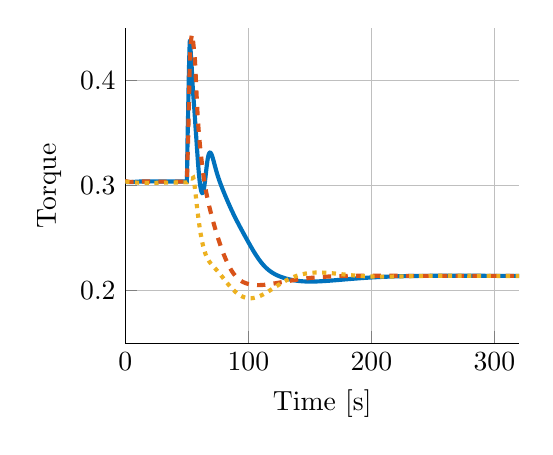
\begin{tikzpicture}

\begin{axis}[%
width=5cm,
height=4cm,
at={(0\linewidth,0\linewidth)},
scale only axis,
xmin=0,
xmax=320,
xlabel={Time [s]},
xmajorgrids,
ymin=0.15,
ymax=0.45,
ylabel={Torque},
ymajorgrids,
axis background/.style={fill=white},
% title style={font=\bfseries},
% title={Normalized Torque Setting},
axis x line*=bottom,
axis y line*=left
]
\addplot [color=mycolor1,solid,line width=1.5pt,forget plot]
  table[row sep=crcr]{%
0	0.30400978288\\
0.25	0.3039140382\\
0.5	0.303898715\\
0.75	0.303849644\\
1	0.303742664\\
1.25	0.303657633\\
1.5	0.303597146\\
1.75	0.303542376\\
2	0.303496532\\
2.25	0.303463798\\
2.5	0.303441868\\
2.75	0.303428301\\
3	0.303421493\\
3.25	0.303419909\\
3.5	0.303421717\\
3.75	0.30342511\\
4	0.303428553\\
4.25	0.303431526\\
4.5	0.303434849\\
4.75	0.303440032\\
5	0.303448488\\
5.25	0.303461125\\
5.5	0.303478337\\
5.75	0.30349989\\
6	0.303524847\\
6.25	0.303551716\\
6.5	0.303578744\\
6.75	0.303604316\\
7	0.303627354\\
7.25	0.303647554\\
7.5	0.303665378\\
7.75	0.30368185\\
8	0.303698259\\
8.25	0.303715821\\
8.5	0.303735369\\
8.75	0.303757135\\
9	0.303780689\\
9.25	0.303805038\\
9.5	0.303828878\\
9.75	0.303850919\\
10	0.3038702\\
10.25	0.303886312\\
10.5	0.303899485\\
10.75	0.3039105018\\
11	0.3039204969\\
11.25	0.3039306579\\
11.5	0.3039419314\\
11.75	0.3039547915\\
12	0.303969133\\
12.25	0.303984311\\
12.5	0.303999316205\\
12.75	0.3040130387\\
13	0.3040245537\\
13.25	0.3040333552\\
13.5	0.304039481\\
13.75	0.3040434978\\
14	0.3040463533\\
14.25	0.304049135\\
14.5	0.3040527985\\
14.75	0.3040579343\\
15	0.3040646292\\
15.25	0.3040724572\\
15.5	0.3040805989\\
15.75	0.3040880599\\
16	0.3040939305\\
16.25	0.3040976215\\
16.5	0.3040990151\\
16.75	0.3040984935\\
17	0.3040968393\\
17.25	0.3040950349\\
17.5	0.3040940141\\
17.75	0.3040944288\\
18	0.3040964899\\
18.25	0.304099921\\
18.5	0.304104037\\
18.75	0.304107926\\
19	0.304110689\\
19.25	0.304111672\\
19.5	0.304110637\\
19.75	0.304107823\\
20	0.304103883\\
20.25	0.304099714\\
20.5	0.3040962284\\
20.75	0.3040941214\\
21	0.3040936953\\
21.25	0.3040947862\\
21.5	0.3040968102\\
21.75	0.304098917\\
22	0.304100213\\
22.25	0.3040999938\\
22.5	0.3040979296\\
22.75	0.3040941496\\
23	0.304089209\\
23.25	0.3040839448\\
23.5	0.3040792588\\
23.75	0.3040758855\\
24	0.304074203\\
24.25	0.3040741366\\
24.5	0.3040751794\\
24.75	0.3040765248\\
25	0.3040772772\\
25.25	0.3040766871\\
25.5	0.304074348\\
25.75	0.3040703036\\
26	0.304065038\\
26.25	0.3040593495\\
26.5	0.3040541434\\
26.75	0.3040501962\\
27	0.3040479541\\
27.25	0.3040474154\\
27.5	0.3040481308\\
27.75	0.3040493193\\
28	0.304050072\\
28.25	0.3040495916\\
28.5	0.3040474025\\
28.75	0.3040434789\\
29	0.3040382535\\
29.25	0.3040325059\\
29.5	0.3040271596\\
29.75	0.3040230404\\
30	0.3040206593\\
30.25	0.304020077\\
30.5	0.3040208847\\
30.75	0.3040223088\\
31	0.3040234127\\
31.25	0.304023343\\
31.5	0.3040215568\\
31.75	0.3040179687\\
32	0.3040129764\\
32.25	0.30400736019\\
32.5	0.30400207849\\
32.75	0.30399801671\\
33	0.30399575263\\
33.25	0.30399540111\\
33.5	0.30399657907\\
33.75	0.30399850171\\
34	0.304000186395\\
34.25	0.304000711878\\
34.5	0.303999464688\\
34.75	0.30399630629\\
35	0.30399161524\\
35.25	0.3039861918\\
35.5	0.3039810494\\
35.75	0.3039771474\\
36	0.3039751358\\
36.25	0.3039751785\\
36.5	0.3039769034\\
36.75	0.3039794935\\
37	0.3039818991\\
37.25	0.3039831145\\
37.5	0.3039824489\\
37.75	0.3039797154\\
38	0.3039752887\\
38.25	0.3039700121\\
38.5	0.3039649776\\
38.75	0.3039612378\\
39	0.3039595238\\
39.25	0.3039600447\\
39.5	0.3039624233\\
39.75	0.3039657865\\
40	0.3039689909\\
40.25	0.3039709253\\
40.5	0.3039708108\\
40.75	0.3039684163\\
41	0.3039641305\\
41.25	0.3039588667\\
41.5	0.3039538256\\
41.75	0.3039501775\\
42	0.3039487466\\
42.25	0.3039497841\\
42.5	0.3039528884\\
42.75	0.3039571003\\
43	0.3039611496\\
43.25	0.3039637918\\
43.5	0.3039641463\\
43.75	0.3039619421\\
44	0.3039576037\\
44.25	0.3039521491\\
44.5	0.3039469257\\
44.75	0.3039432525\\
45	0.3039420629\\
45.25	0.303943645\\
45.5	0.3039475487\\
45.75	0.3039526896\\
46	0.3039576277\\
46.25	0.3039609501\\
46.5	0.3039616569\\
46.75	0.3039594436\\
47	0.3039548\\
47.25	0.3039488939\\
47.5	0.3039432685\\
47.75	0.303939431\\
48	0.3039384434\\
48.25	0.303940623\\
48.5	0.303945437\\
48.75	0.3039516243\\
49	0.3039575187\\
49.25	0.303961494\\
49.5	0.3039624102\\
49.75	0.3039599403\\
50	0.3039546798\\
50.25	0.3171159\\
50.5	0.3392608\\
50.75	0.3547082\\
51	0.3663522\\
51.25	0.3827232\\
51.5	0.3991287\\
51.75	0.411846\\
52	0.423182\\
52.25	0.433125\\
52.5	0.439159\\
52.75	0.43593\\
53	0.429983\\
53.25	0.425146\\
53.5	0.421035\\
53.75	0.416763\\
54	0.411641\\
54.25	0.405724\\
54.5	0.3999344\\
54.75	0.3949111\\
55	0.3904759\\
55.25	0.3862206\\
55.5	0.3820063\\
55.75	0.3780323\\
56	0.3742622\\
56.25	0.3701397\\
56.5	0.3657399\\
56.75	0.3613966\\
57	0.3571217\\
57.25	0.352845\\
57.5	0.3485722\\
57.75	0.3443044\\
58	0.3400287\\
58.25	0.3357414\\
58.5	0.3314702\\
58.75	0.3272726\\
59	0.323204\\
59.25	0.3193062\\
59.5	0.3156146\\
59.75	0.31215964\\
60	0.30896388\\
60.25	0.30604294\\
60.5	0.303407557\\
60.75	0.30106472\\
61	0.29901842\\
61.25	0.29727064\\
61.5	0.29582245\\
61.75	0.29467478\\
62	0.2938289\\
62.25	0.2932867\\
62.5	0.2930506\\
62.75	0.293123\\
63	0.2935058\\
63.25	0.29419939\\
63.5	0.29520118\\
63.75	0.29650428\\
64	0.29809599\\
64.25	0.29995649\\
64.5	0.30205794\\
64.75	0.304364273\\
65	0.30683158\\
65.25	0.30940915\\
65.5	0.31204077\\
65.75	0.3146662\\
66	0.3172236\\
66.25	0.3196532\\
66.5	0.3219038\\
66.75	0.3239373\\
67	0.325731\\
67.25	0.3272746\\
67.5	0.3285669\\
67.75	0.3296131\\
68	0.330422\\
68.25	0.331005\\
68.5	0.331375\\
68.75	0.331546\\
69	0.3315327\\
69.25	0.3313504\\
69.5	0.3310144\\
69.75	0.3305404\\
70	0.329944\\
70.25	0.3292405\\
70.5	0.3284447\\
70.75	0.3275709\\
71	0.3266324\\
71.25	0.3256419\\
71.5	0.3246109\\
71.75	0.3235498\\
72	0.3224681\\
72.25	0.3213741\\
72.5	0.3202748\\
72.75	0.3191767\\
73	0.3180848\\
73.25	0.3170035\\
73.5	0.3159362\\
73.75	0.3148855\\
74	0.31385345\\
74.25	0.31284136\\
74.5	0.31185003\\
74.75	0.3108798\\
75	0.30993062\\
75.25	0.30900211\\
75.5	0.30809362\\
75.75	0.3072043\\
76	0.30633316\\
76.25	0.30547909\\
76.5	0.304640912\\
76.75	0.303817421\\
77	0.303007412\\
77.25	0.3022097\\
77.5	0.30142315\\
77.75	0.30064668\\
78	0.29987927\\
78.25	0.29912001\\
78.5	0.29836803\\
78.75	0.29762258\\
79	0.296883\\
79.25	0.29614868\\
79.5	0.29541912\\
79.75	0.29469391\\
80	0.2939727\\
80.25	0.2932552\\
80.5	0.2925411\\
80.75	0.2918304\\
81	0.2911229\\
81.25	0.2904185\\
81.5	0.2897172\\
81.75	0.2890189\\
82	0.2883238\\
82.25	0.2876317\\
82.5	0.2869429\\
82.75	0.2862573\\
83	0.285575\\
83.25	0.2848961\\
83.5	0.2842207\\
83.75	0.2835488\\
84	0.2828806\\
84.25	0.282216\\
84.5	0.2815552\\
84.75	0.2808982\\
85	0.2802451\\
85.25	0.2795958\\
85.5	0.2789505\\
85.75	0.2783091\\
86	0.2776717\\
86.25	0.2770383\\
86.5	0.2764088\\
86.75	0.2757832\\
87	0.2751616\\
87.25	0.2745438\\
87.5	0.2739299\\
87.75	0.2733197\\
88	0.2727133\\
88.25	0.2721105\\
88.5	0.2715114\\
88.75	0.2709157\\
89	0.2703235\\
89.25	0.2697346\\
89.5	0.269149\\
89.75	0.2685665\\
90	0.2679871\\
90.25	0.2674107\\
90.5	0.2668371\\
90.75	0.2662662\\
91	0.2656979\\
91.25	0.2651322\\
91.5	0.2645689\\
91.75	0.2640079\\
92	0.263449\\
92.25	0.2628923\\
92.5	0.2623375\\
92.75	0.2617845\\
93	0.2612333\\
93.25	0.2606838\\
93.5	0.2601357\\
93.75	0.2595892\\
94	0.259044\\
94.25	0.2585\\
94.5	0.2579573\\
94.75	0.2574156\\
95	0.256875\\
95.25	0.2563354\\
95.5	0.2557967\\
95.75	0.2552589\\
96	0.2547219\\
96.25	0.2541856\\
96.5	0.2536501\\
96.75	0.2531154\\
97	0.2525813\\
97.25	0.252048\\
97.5	0.2515154\\
97.75	0.2509835\\
98	0.2504523\\
98.25	0.2499219\\
98.5	0.2493923\\
98.75	0.2488635\\
99	0.2483356\\
99.25	0.2478087\\
99.5	0.2472827\\
99.75	0.2467579\\
100	0.2462342\\
100.25	0.2457117\\
100.5	0.2451906\\
100.75	0.2446709\\
101	0.2441528\\
101.25	0.2436363\\
101.5	0.2431215\\
101.75	0.2426087\\
102	0.2420978\\
102.25	0.2415891\\
102.5	0.2410826\\
102.75	0.2405785\\
103	0.2400769\\
103.25	0.239578\\
103.5	0.2390819\\
103.75	0.2385887\\
104	0.2380986\\
104.25	0.2376118\\
104.5	0.2371282\\
104.75	0.2366482\\
105	0.2361718\\
105.25	0.2356992\\
105.5	0.2352304\\
105.75	0.2347657\\
106	0.2343052\\
106.25	0.2338489\\
106.5	0.2333971\\
106.75	0.2329498\\
107	0.2325071\\
107.25	0.2320691\\
107.5	0.231636\\
107.75	0.2312078\\
108	0.2307847\\
108.25	0.2303667\\
108.5	0.2299539\\
108.75	0.2295464\\
109	0.2291442\\
109.25	0.2287474\\
109.5	0.2283561\\
109.75	0.2279704\\
110	0.2275902\\
110.25	0.2272156\\
110.5	0.2268466\\
110.75	0.2264833\\
111	0.2261257\\
111.25	0.2257738\\
111.5	0.2254276\\
111.75	0.2250872\\
112	0.2247524\\
112.25	0.2244233\\
112.5	0.2240999\\
112.75	0.2237821\\
113	0.22347\\
113.25	0.2231635\\
113.5	0.2228625\\
113.75	0.2225671\\
114	0.2222772\\
114.25	0.2219927\\
114.5	0.2217135\\
114.75	0.2214397\\
115	0.2211711\\
115.25	0.2209078\\
115.5	0.2206495\\
115.75	0.2203964\\
116	0.2201482\\
116.25	0.2199049\\
116.5	0.2196664\\
116.75	0.2194328\\
117	0.2192037\\
117.25	0.2189793\\
117.5	0.2187594\\
117.75	0.2185439\\
118	0.2183328\\
118.25	0.2181259\\
118.5	0.2179231\\
118.75	0.2177245\\
119	0.2175298\\
119.25	0.2173391\\
119.5	0.2171522\\
119.75	0.216969\\
120	0.2167894\\
120.25	0.2166135\\
120.5	0.216441\\
120.75	0.2162719\\
121	0.2161061\\
121.25	0.2159436\\
121.5	0.2157842\\
121.75	0.215628\\
122	0.2154747\\
122.25	0.2153244\\
122.5	0.2151769\\
122.75	0.2150322\\
123	0.2148902\\
123.25	0.2147509\\
123.5	0.2146142\\
123.75	0.2144799\\
124	0.2143482\\
124.25	0.2142188\\
124.5	0.2140918\\
124.75	0.2139671\\
125	0.2138446\\
125.25	0.2137242\\
125.5	0.213606\\
125.75	0.2134899\\
126	0.2133758\\
126.25	0.2132637\\
126.5	0.2131536\\
126.75	0.2130453\\
127	0.2129389\\
127.25	0.2128343\\
127.5	0.2127315\\
127.75	0.2126304\\
128	0.2125311\\
128.25	0.2124334\\
128.5	0.2123374\\
128.75	0.212243\\
129	0.2121502\\
129.25	0.212059\\
129.5	0.2119693\\
129.75	0.2118812\\
130	0.2117945\\
130.25	0.2117093\\
130.5	0.2116256\\
130.75	0.2115433\\
131	0.2114624\\
131.25	0.211383\\
131.5	0.2113049\\
131.75	0.2112282\\
132	0.2111528\\
132.25	0.2110788\\
132.5	0.2110061\\
132.75	0.2109348\\
133	0.2108647\\
133.25	0.210796\\
133.5	0.2107285\\
133.75	0.2106623\\
134	0.2105973\\
134.25	0.2105336\\
134.5	0.2104712\\
134.75	0.2104099\\
135	0.2103499\\
135.25	0.2102912\\
135.5	0.2102336\\
135.75	0.2101772\\
136	0.2101221\\
136.25	0.2100681\\
136.5	0.2100153\\
136.75	0.2099637\\
137	0.2099132\\
137.25	0.2098639\\
137.5	0.2098157\\
137.75	0.2097687\\
138	0.2097229\\
138.25	0.2096781\\
138.5	0.2096345\\
138.75	0.209592\\
139	0.2095506\\
139.25	0.2095103\\
139.5	0.2094711\\
139.75	0.209433\\
140	0.2093959\\
140.25	0.20936\\
140.5	0.209325\\
140.75	0.2092912\\
141	0.2092584\\
141.25	0.2092266\\
141.5	0.2091959\\
141.75	0.2091661\\
142	0.2091374\\
142.25	0.2091097\\
142.5	0.209083\\
142.75	0.2090573\\
143	0.2090325\\
143.25	0.2090087\\
143.5	0.2089859\\
143.75	0.208964\\
144	0.208943\\
144.25	0.208923\\
144.5	0.2089038\\
144.75	0.2088856\\
145	0.2088683\\
145.25	0.2088519\\
145.5	0.2088363\\
145.75	0.2088216\\
146	0.2088077\\
146.25	0.2087947\\
146.5	0.2087825\\
146.75	0.2087712\\
147	0.2087606\\
147.25	0.2087508\\
147.5	0.2087419\\
147.75	0.2087336\\
148	0.2087262\\
148.25	0.2087195\\
148.5	0.2087136\\
148.75	0.2087083\\
149	0.2087038\\
149.25	0.2087\\
149.5	0.2086969\\
149.75	0.2086945\\
150	0.2086927\\
150.25	0.2086917\\
150.5	0.2086912\\
150.75	0.2086914\\
151	0.2086922\\
151.25	0.2086937\\
151.5	0.2086957\\
151.75	0.2086984\\
152	0.2087016\\
152.25	0.2087054\\
152.5	0.2087098\\
152.75	0.2087147\\
153	0.2087202\\
153.25	0.2087262\\
153.5	0.2087327\\
153.75	0.2087397\\
154	0.2087472\\
154.25	0.2087552\\
154.5	0.2087637\\
154.75	0.2087727\\
155	0.2087821\\
155.25	0.208792\\
155.5	0.2088023\\
155.75	0.2088131\\
156	0.2088243\\
156.25	0.2088359\\
156.5	0.2088479\\
156.75	0.2088603\\
157	0.2088731\\
157.25	0.2088863\\
157.5	0.2088998\\
157.75	0.2089137\\
158	0.208928\\
158.25	0.2089426\\
158.5	0.2089576\\
158.75	0.2089729\\
159	0.2089885\\
159.25	0.2090044\\
159.5	0.2090206\\
159.75	0.2090372\\
160	0.209054\\
160.25	0.2090711\\
160.5	0.2090885\\
160.75	0.2091062\\
161	0.2091242\\
161.25	0.2091424\\
161.5	0.2091608\\
161.75	0.2091795\\
162	0.2091985\\
162.25	0.2092177\\
162.5	0.2092371\\
162.75	0.2092567\\
163	0.2092765\\
163.25	0.2092966\\
163.5	0.2093169\\
163.75	0.2093373\\
164	0.209358\\
164.25	0.2093788\\
164.5	0.2093999\\
164.75	0.2094211\\
165	0.2094425\\
165.25	0.209464\\
165.5	0.2094857\\
165.75	0.2095076\\
166	0.2095296\\
166.25	0.2095518\\
166.5	0.2095741\\
166.75	0.2095965\\
167	0.2096191\\
167.25	0.2096418\\
167.5	0.2096646\\
167.75	0.2096876\\
168	0.2097107\\
168.25	0.2097339\\
168.5	0.2097571\\
168.75	0.2097805\\
169	0.209804\\
169.25	0.2098276\\
169.5	0.2098513\\
169.75	0.2098751\\
170	0.2098989\\
170.25	0.2099229\\
170.5	0.2099469\\
170.75	0.2099709\\
171	0.2099951\\
171.25	0.2100193\\
171.5	0.2100436\\
171.75	0.2100679\\
172	0.2100923\\
172.25	0.2101167\\
172.5	0.2101412\\
172.75	0.2101658\\
173	0.2101903\\
173.25	0.2102149\\
173.5	0.2102396\\
173.75	0.2102643\\
174	0.210289\\
174.25	0.2103137\\
174.5	0.2103385\\
174.75	0.2103632\\
175	0.210388\\
175.25	0.2104128\\
175.5	0.2104377\\
175.75	0.2104625\\
176	0.2104873\\
176.25	0.2105121\\
176.5	0.210537\\
176.75	0.2105618\\
177	0.2105866\\
177.25	0.2106115\\
177.5	0.2106363\\
177.75	0.2106611\\
178	0.2106858\\
178.25	0.2107106\\
178.5	0.2107353\\
178.75	0.2107601\\
179	0.2107848\\
179.25	0.2108094\\
179.5	0.2108341\\
179.75	0.2108587\\
180	0.2108832\\
180.25	0.2109078\\
180.5	0.2109323\\
180.75	0.2109567\\
181	0.2109812\\
181.25	0.2110055\\
181.5	0.2110299\\
181.75	0.2110541\\
182	0.2110784\\
182.25	0.2111025\\
182.5	0.2111267\\
182.75	0.2111507\\
183	0.2111747\\
183.25	0.2111987\\
183.5	0.2112226\\
183.75	0.2112464\\
184	0.2112702\\
184.25	0.2112939\\
184.5	0.2113175\\
184.75	0.2113411\\
185	0.2113646\\
185.25	0.211388\\
185.5	0.2114113\\
185.75	0.2114346\\
186	0.2114578\\
186.25	0.2114809\\
186.5	0.2115039\\
186.75	0.2115269\\
187	0.2115498\\
187.25	0.2115726\\
187.5	0.2115953\\
187.75	0.2116179\\
188	0.2116404\\
188.25	0.2116629\\
188.5	0.2116852\\
188.75	0.2117075\\
189	0.2117297\\
189.25	0.2117518\\
189.5	0.2117738\\
189.75	0.2117957\\
190	0.2118175\\
190.25	0.2118392\\
190.5	0.2118608\\
190.75	0.2118823\\
191	0.2119037\\
191.25	0.211925\\
191.5	0.2119462\\
191.75	0.2119674\\
192	0.2119884\\
192.25	0.2120093\\
192.5	0.2120301\\
192.75	0.2120508\\
193	0.2120714\\
193.25	0.2120919\\
193.5	0.2121123\\
193.75	0.2121325\\
194	0.2121527\\
194.25	0.2121728\\
194.5	0.2121927\\
194.75	0.2122126\\
195	0.2122323\\
195.25	0.212252\\
195.5	0.2122715\\
195.75	0.2122909\\
196	0.2123102\\
196.25	0.2123294\\
196.5	0.2123485\\
196.75	0.2123674\\
197	0.2123863\\
197.25	0.212405\\
197.5	0.2124236\\
197.75	0.2124421\\
198	0.2124605\\
198.25	0.2124788\\
198.5	0.212497\\
198.75	0.2125151\\
199	0.212533\\
199.25	0.2125508\\
199.5	0.2125685\\
199.75	0.2125861\\
200	0.2126036\\
200.25	0.212621\\
200.5	0.2126382\\
200.75	0.2126554\\
201	0.2126724\\
201.25	0.2126893\\
201.5	0.2127061\\
201.75	0.2127228\\
202	0.2127393\\
202.25	0.2127558\\
202.5	0.2127721\\
202.75	0.2127883\\
203	0.2128044\\
203.25	0.2128204\\
203.5	0.2128363\\
203.75	0.212852\\
204	0.2128676\\
204.25	0.2128832\\
204.5	0.2128986\\
204.75	0.2129139\\
205	0.212929\\
205.25	0.2129441\\
205.5	0.212959\\
205.75	0.2129739\\
206	0.2129886\\
206.25	0.2130032\\
206.5	0.2130177\\
206.75	0.213032\\
207	0.2130463\\
207.25	0.2130605\\
207.5	0.2130745\\
207.75	0.2130884\\
208	0.2131022\\
208.25	0.2131159\\
208.5	0.2131295\\
208.75	0.213143\\
209	0.2131563\\
209.25	0.2131696\\
209.5	0.2131827\\
209.75	0.2131957\\
210	0.2132087\\
210.25	0.2132215\\
210.5	0.2132342\\
210.75	0.2132468\\
211	0.2132592\\
211.25	0.2132716\\
211.5	0.2132839\\
211.75	0.213296\\
212	0.2133081\\
212.25	0.21332\\
212.5	0.2133318\\
212.75	0.2133436\\
213	0.2133552\\
213.25	0.2133667\\
213.5	0.2133781\\
213.75	0.2133894\\
214	0.2134006\\
214.25	0.2134117\\
214.5	0.2134227\\
214.75	0.2134336\\
215	0.2134443\\
215.25	0.213455\\
215.5	0.2134656\\
215.75	0.2134761\\
216	0.2134865\\
216.25	0.2134967\\
216.5	0.2135069\\
216.75	0.213517\\
217	0.213527\\
217.25	0.2135368\\
217.5	0.2135466\\
217.75	0.2135563\\
218	0.2135659\\
218.25	0.2135754\\
218.5	0.2135847\\
218.75	0.213594\\
219	0.2136032\\
219.25	0.2136123\\
219.5	0.2136213\\
219.75	0.2136303\\
220	0.2136391\\
220.25	0.2136478\\
220.5	0.2136564\\
220.75	0.213665\\
221	0.2136734\\
221.25	0.2136818\\
221.5	0.2136901\\
221.75	0.2136983\\
222	0.2137063\\
222.25	0.2137144\\
222.5	0.2137223\\
222.75	0.2137301\\
223	0.2137378\\
223.25	0.2137455\\
223.5	0.213753\\
223.75	0.2137605\\
224	0.2137679\\
224.25	0.2137752\\
224.5	0.2137825\\
224.75	0.2137896\\
225	0.2137967\\
225.25	0.2138036\\
225.5	0.2138105\\
225.75	0.2138173\\
226	0.2138241\\
226.25	0.2138307\\
226.5	0.2138373\\
226.75	0.2138438\\
227	0.2138502\\
227.25	0.2138565\\
227.5	0.2138628\\
227.75	0.213869\\
228	0.2138751\\
228.25	0.2138811\\
228.5	0.2138871\\
228.75	0.213893\\
229	0.2138988\\
229.25	0.2139045\\
229.5	0.2139101\\
229.75	0.2139157\\
230	0.2139212\\
230.25	0.2139267\\
230.5	0.2139321\\
230.75	0.2139374\\
231	0.2139426\\
231.25	0.2139477\\
231.5	0.2139528\\
231.75	0.2139579\\
232	0.2139628\\
232.25	0.2139677\\
232.5	0.2139725\\
232.75	0.2139773\\
233	0.213982\\
233.25	0.2139866\\
233.5	0.2139911\\
233.75	0.2139956\\
234	0.2140001\\
234.25	0.2140044\\
234.5	0.2140087\\
234.75	0.214013\\
235	0.2140171\\
235.25	0.2140213\\
235.5	0.2140253\\
235.75	0.2140293\\
236	0.2140333\\
236.25	0.2140371\\
236.5	0.214041\\
236.75	0.2140447\\
237	0.2140484\\
237.25	0.2140521\\
237.5	0.2140557\\
237.75	0.2140592\\
238	0.2140627\\
238.25	0.2140661\\
238.5	0.2140695\\
238.75	0.2140728\\
239	0.2140761\\
239.25	0.2140793\\
239.5	0.2140824\\
239.75	0.2140856\\
240	0.2140886\\
240.25	0.2140916\\
240.5	0.2140946\\
240.75	0.2140975\\
241	0.2141003\\
241.25	0.2141031\\
241.5	0.2141059\\
241.75	0.2141086\\
242	0.2141113\\
242.25	0.2141139\\
242.5	0.2141164\\
242.75	0.214119\\
243	0.2141214\\
243.25	0.2141239\\
243.5	0.2141263\\
243.75	0.2141286\\
244	0.2141309\\
244.25	0.2141332\\
244.5	0.2141354\\
244.75	0.2141375\\
245	0.2141397\\
245.25	0.2141417\\
245.5	0.2141438\\
245.75	0.2141458\\
246	0.2141478\\
246.25	0.2141497\\
246.5	0.2141516\\
246.75	0.2141534\\
247	0.2141552\\
247.25	0.214157\\
247.5	0.2141587\\
247.75	0.2141604\\
248	0.2141621\\
248.25	0.2141637\\
248.5	0.2141653\\
248.75	0.2141668\\
249	0.2141683\\
249.25	0.2141698\\
249.5	0.2141712\\
249.75	0.2141726\\
250	0.214174\\
250.25	0.2141753\\
250.5	0.2141767\\
250.75	0.2141779\\
251	0.2141792\\
251.25	0.2141804\\
251.5	0.2141816\\
251.75	0.2141827\\
252	0.2141838\\
252.25	0.2141849\\
252.5	0.214186\\
252.75	0.214187\\
253	0.214188\\
253.25	0.214189\\
253.5	0.2141899\\
253.75	0.2141908\\
254	0.2141917\\
254.25	0.2141926\\
254.5	0.2141934\\
254.75	0.2141942\\
255	0.214195\\
255.25	0.2141957\\
255.5	0.2141965\\
255.75	0.2141972\\
256	0.2141978\\
256.25	0.2141985\\
256.5	0.2141991\\
256.75	0.2141997\\
257	0.2142003\\
257.25	0.2142008\\
257.5	0.2142014\\
257.75	0.2142019\\
258	0.2142024\\
258.25	0.2142028\\
258.5	0.2142033\\
258.75	0.2142037\\
259	0.2142041\\
259.25	0.2142045\\
259.5	0.2142048\\
259.75	0.2142052\\
260	0.2142055\\
260.25	0.2142058\\
260.5	0.2142061\\
260.75	0.2142063\\
261	0.2142066\\
261.25	0.2142068\\
261.5	0.214207\\
261.75	0.2142072\\
262	0.2142074\\
262.25	0.2142075\\
262.5	0.2142077\\
262.75	0.2142078\\
263	0.2142079\\
263.25	0.214208\\
263.5	0.214208\\
263.75	0.2142081\\
264	0.2142081\\
264.25	0.2142081\\
264.5	0.2142081\\
264.75	0.2142081\\
265	0.2142081\\
265.25	0.2142081\\
265.5	0.214208\\
265.75	0.2142079\\
266	0.2142079\\
266.25	0.2142078\\
266.5	0.2142077\\
266.75	0.2142075\\
267	0.2142074\\
267.25	0.2142073\\
267.5	0.2142071\\
267.75	0.2142069\\
268	0.2142068\\
268.25	0.2142066\\
268.5	0.2142064\\
268.75	0.2142061\\
269	0.2142059\\
269.25	0.2142057\\
269.5	0.2142054\\
269.75	0.2142052\\
270	0.2142049\\
270.25	0.2142046\\
270.5	0.2142043\\
270.75	0.214204\\
271	0.2142037\\
271.25	0.2142034\\
271.5	0.2142031\\
271.75	0.2142028\\
272	0.2142024\\
272.25	0.2142021\\
272.5	0.2142017\\
272.75	0.2142013\\
273	0.214201\\
273.25	0.2142006\\
273.5	0.2142002\\
273.75	0.2141998\\
274	0.2141994\\
274.25	0.214199\\
274.5	0.2141985\\
274.75	0.2141981\\
275	0.2141977\\
275.25	0.2141972\\
275.5	0.2141968\\
275.75	0.2141963\\
276	0.2141959\\
276.25	0.2141954\\
276.5	0.2141949\\
276.75	0.2141945\\
277	0.214194\\
277.25	0.2141935\\
277.5	0.214193\\
277.75	0.2141925\\
278	0.214192\\
278.25	0.2141915\\
278.5	0.214191\\
278.75	0.2141905\\
279	0.21419\\
279.25	0.2141894\\
279.5	0.2141889\\
279.75	0.2141884\\
280	0.2141878\\
280.25	0.2141873\\
280.5	0.2141868\\
280.75	0.2141862\\
281	0.2141857\\
281.25	0.2141851\\
281.5	0.2141845\\
281.75	0.214184\\
282	0.2141834\\
282.25	0.2141829\\
282.5	0.2141823\\
282.75	0.2141817\\
283	0.2141812\\
283.25	0.2141806\\
283.5	0.21418\\
283.75	0.2141794\\
284	0.2141788\\
284.25	0.2141783\\
284.5	0.2141777\\
284.75	0.2141771\\
285	0.2141765\\
285.25	0.2141759\\
285.5	0.2141753\\
285.75	0.2141747\\
286	0.2141741\\
286.25	0.2141736\\
286.5	0.214173\\
286.75	0.2141724\\
287	0.2141718\\
287.25	0.2141712\\
287.5	0.2141706\\
287.75	0.21417\\
288	0.2141694\\
288.25	0.2141688\\
288.5	0.2141682\\
288.75	0.2141676\\
289	0.214167\\
289.25	0.2141664\\
289.5	0.2141658\\
289.75	0.2141652\\
290	0.2141646\\
290.25	0.214164\\
290.5	0.2141634\\
290.75	0.2141628\\
291	0.2141622\\
291.25	0.2141616\\
291.5	0.214161\\
291.75	0.2141604\\
292	0.2141598\\
292.25	0.2141592\\
292.5	0.2141586\\
292.75	0.214158\\
293	0.2141574\\
293.25	0.2141568\\
293.5	0.2141562\\
293.75	0.2141556\\
294	0.214155\\
294.25	0.2141544\\
294.5	0.2141538\\
294.75	0.2141532\\
295	0.2141527\\
295.25	0.2141521\\
295.5	0.2141515\\
295.75	0.2141509\\
296	0.2141503\\
296.25	0.2141497\\
296.5	0.2141492\\
296.75	0.2141486\\
297	0.214148\\
297.25	0.2141474\\
297.5	0.2141469\\
297.75	0.2141463\\
298	0.2141457\\
298.25	0.2141452\\
298.5	0.2141446\\
298.75	0.214144\\
299	0.2141435\\
299.25	0.2141429\\
299.5	0.2141424\\
299.75	0.2141418\\
300	0.2141413\\
300.25	0.2141407\\
300.5	0.2141402\\
300.75	0.2141396\\
301	0.2141391\\
301.25	0.2141385\\
301.5	0.214138\\
301.75	0.2141374\\
302	0.2141369\\
302.25	0.2141364\\
302.5	0.2141358\\
302.75	0.2141353\\
303	0.2141348\\
303.25	0.2141343\\
303.5	0.2141337\\
303.75	0.2141332\\
304	0.2141327\\
304.25	0.2141322\\
304.5	0.2141317\\
304.75	0.2141312\\
305	0.2141307\\
305.25	0.2141302\\
305.5	0.2141297\\
305.75	0.2141292\\
306	0.2141287\\
306.25	0.2141282\\
306.5	0.2141277\\
306.75	0.2141272\\
307	0.2141267\\
307.25	0.2141262\\
307.5	0.2141257\\
307.75	0.2141253\\
308	0.2141248\\
308.25	0.2141243\\
308.5	0.2141238\\
308.75	0.2141234\\
309	0.2141229\\
309.25	0.2141224\\
309.5	0.214122\\
309.75	0.2141215\\
310	0.2141211\\
310.25	0.2141206\\
310.5	0.2141202\\
310.75	0.2141197\\
311	0.2141193\\
311.25	0.2141189\\
311.5	0.2141184\\
311.75	0.214118\\
312	0.2141175\\
312.25	0.2141171\\
312.5	0.2141167\\
312.75	0.2141163\\
313	0.2141159\\
313.25	0.2141154\\
313.5	0.214115\\
313.75	0.2141146\\
314	0.2141142\\
314.25	0.2141138\\
314.5	0.2141134\\
314.75	0.214113\\
315	0.2141126\\
315.25	0.2141122\\
315.5	0.2141118\\
315.75	0.2141114\\
316	0.214111\\
316.25	0.2141107\\
316.5	0.2141103\\
316.75	0.2141099\\
317	0.2141095\\
317.25	0.2141091\\
317.5	0.2141088\\
317.75	0.2141084\\
318	0.2141081\\
318.25	0.2141077\\
318.5	0.2141073\\
318.75	0.214107\\
319	0.2141066\\
319.25	0.2141063\\
319.5	0.2141059\\
319.75	0.2141056\\
320	0.2141052\\
320.25	0.2141049\\
320.5	0.2141046\\
320.75	0.2141042\\
321	0.2141039\\
321.25	0.2141036\\
321.5	0.2141033\\
321.75	0.2141029\\
322	0.2141026\\
322.25	0.2141023\\
322.5	0.214102\\
322.75	0.2141017\\
323	0.2141014\\
323.25	0.2141011\\
323.5	0.2141008\\
323.75	0.2141005\\
324	0.2141002\\
324.25	0.2140999\\
324.5	0.2140996\\
324.75	0.2140993\\
325	0.214099\\
325.25	0.2140987\\
325.5	0.2140984\\
325.75	0.2140982\\
326	0.2140979\\
326.25	0.2140976\\
326.5	0.2140973\\
326.75	0.2140971\\
327	0.2140968\\
327.25	0.2140965\\
327.5	0.2140963\\
327.75	0.214096\\
328	0.2140958\\
328.25	0.2140955\\
328.5	0.2140953\\
328.75	0.214095\\
329	0.2140948\\
329.25	0.2140945\\
329.5	0.2140943\\
329.75	0.214094\\
330	0.2140938\\
330.25	0.2140936\\
330.5	0.2140933\\
330.75	0.2140931\\
331	0.2140929\\
331.25	0.2140927\\
331.5	0.2140924\\
331.75	0.2140922\\
332	0.214092\\
332.25	0.2140918\\
332.5	0.2140916\\
332.75	0.2140914\\
333	0.2140911\\
333.25	0.2140909\\
333.5	0.2140907\\
333.75	0.2140905\\
334	0.2140903\\
334.25	0.2140901\\
334.5	0.2140899\\
334.75	0.2140897\\
335	0.2140896\\
335.25	0.2140894\\
335.5	0.2140892\\
335.75	0.214089\\
336	0.2140888\\
336.25	0.2140886\\
336.5	0.2140884\\
336.75	0.2140883\\
337	0.2140881\\
337.25	0.2140879\\
337.5	0.2140878\\
337.75	0.2140876\\
338	0.2140874\\
338.25	0.2140873\\
338.5	0.2140871\\
338.75	0.2140869\\
339	0.2140868\\
339.25	0.2140866\\
339.5	0.2140865\\
339.75	0.2140863\\
340	0.2140862\\
340.25	0.214086\\
340.5	0.2140859\\
340.75	0.2140857\\
341	0.2140856\\
341.25	0.2140854\\
341.5	0.2140853\\
341.75	0.2140852\\
342	0.214085\\
342.25	0.2140849\\
342.5	0.2140848\\
342.75	0.2140846\\
343	0.2140845\\
343.25	0.2140844\\
343.5	0.2140842\\
343.75	0.2140841\\
344	0.214084\\
344.25	0.2140839\\
344.5	0.2140838\\
344.75	0.2140836\\
345	0.2140835\\
345.25	0.2140834\\
345.5	0.2140833\\
345.75	0.2140832\\
346	0.2140831\\
346.25	0.214083\\
346.5	0.2140829\\
346.75	0.2140828\\
347	0.2140826\\
347.25	0.2140825\\
347.5	0.2140824\\
347.75	0.2140823\\
348	0.2140823\\
348.25	0.2140822\\
348.5	0.2140821\\
348.75	0.214082\\
349	0.2140819\\
349.25	0.2140818\\
349.5	0.2140817\\
349.75	0.2140816\\
350	0.2140815\\
350.25	0.2140814\\
350.5	0.2140814\\
350.75	0.2140813\\
351	0.2140812\\
351.25	0.2140811\\
351.5	0.214081\\
351.75	0.214081\\
352	0.2140809\\
352.25	0.2140808\\
352.5	0.2140807\\
352.75	0.2140807\\
353	0.2140806\\
353.25	0.2140805\\
353.5	0.2140805\\
353.75	0.2140804\\
354	0.2140803\\
354.25	0.2140803\\
354.5	0.2140802\\
354.75	0.2140801\\
355	0.2140801\\
355.25	0.21408\\
355.5	0.2140799\\
355.75	0.2140799\\
356	0.2140798\\
356.25	0.2140798\\
356.5	0.2140797\\
356.75	0.2140797\\
357	0.2140796\\
357.25	0.2140796\\
357.5	0.2140795\\
357.75	0.2140795\\
358	0.2140794\\
358.25	0.2140794\\
358.5	0.2140793\\
358.75	0.2140793\\
359	0.2140792\\
359.25	0.2140792\\
359.5	0.2140791\\
359.75	0.2140791\\
360	0.2140791\\
360.25	0.214079\\
360.5	0.214079\\
360.75	0.2140789\\
361	0.2140789\\
361.25	0.2140789\\
361.5	0.2140788\\
361.75	0.2140788\\
362	0.2140788\\
362.25	0.2140787\\
362.5	0.2140787\\
362.75	0.2140787\\
363	0.2140786\\
363.25	0.2140786\\
363.5	0.2140786\\
363.75	0.2140785\\
364	0.2140785\\
364.25	0.2140785\\
364.5	0.2140785\\
364.75	0.2140784\\
365	0.2140784\\
365.25	0.2140784\\
365.5	0.2140784\\
365.75	0.2140783\\
366	0.2140783\\
366.25	0.2140783\\
366.5	0.2140783\\
366.75	0.2140783\\
367	0.2140782\\
367.25	0.2140782\\
367.5	0.2140782\\
367.75	0.2140782\\
368	0.2140782\\
368.25	0.2140782\\
368.5	0.2140781\\
368.75	0.2140781\\
369	0.2140781\\
369.25	0.2140781\\
369.5	0.2140781\\
369.75	0.2140781\\
370	0.2140781\\
370.25	0.214078\\
370.5	0.214078\\
370.75	0.214078\\
371	0.214078\\
371.25	0.214078\\
371.5	0.214078\\
371.75	0.214078\\
372	0.214078\\
372.25	0.214078\\
372.5	0.214078\\
372.75	0.214078\\
373	0.2140779\\
373.25	0.2140779\\
373.5	0.2140779\\
373.75	0.2140779\\
374	0.2140779\\
374.25	0.2140779\\
374.5	0.2140779\\
374.75	0.2140779\\
375	0.2140779\\
375.25	0.2140779\\
375.5	0.2140779\\
375.75	0.2140779\\
376	0.2140779\\
376.25	0.2140779\\
376.5	0.2140779\\
376.75	0.2140779\\
377	0.2140779\\
377.25	0.2140779\\
377.5	0.2140779\\
377.75	0.2140779\\
378	0.2140779\\
378.25	0.2140779\\
378.5	0.2140779\\
378.75	0.2140779\\
379	0.2140779\\
379.25	0.2140779\\
379.5	0.2140779\\
379.75	0.2140779\\
380	0.2140779\\
380.25	0.2140779\\
380.5	0.2140779\\
380.75	0.2140779\\
381	0.214078\\
381.25	0.214078\\
381.5	0.214078\\
381.75	0.214078\\
382	0.214078\\
382.25	0.214078\\
382.5	0.214078\\
382.75	0.214078\\
383	0.214078\\
383.25	0.214078\\
383.5	0.214078\\
383.75	0.214078\\
384	0.214078\\
384.25	0.214078\\
384.5	0.2140781\\
384.75	0.2140781\\
385	0.2140781\\
385.25	0.2140781\\
385.5	0.2140781\\
385.75	0.2140781\\
386	0.2140781\\
386.25	0.2140781\\
386.5	0.2140781\\
386.75	0.2140781\\
387	0.2140782\\
387.25	0.2140782\\
387.5	0.2140782\\
387.75	0.2140782\\
388	0.2140782\\
388.25	0.2140782\\
388.5	0.2140782\\
388.75	0.2140782\\
389	0.2140782\\
389.25	0.2140783\\
389.5	0.2140783\\
389.75	0.2140783\\
390	0.2140783\\
390.25	0.2140783\\
390.5	0.2140783\\
390.75	0.2140783\\
391	0.2140783\\
391.25	0.2140784\\
391.5	0.2140784\\
391.75	0.2140784\\
392	0.2140784\\
392.25	0.2140784\\
392.5	0.2140784\\
392.75	0.2140784\\
393	0.2140784\\
393.25	0.2140785\\
393.5	0.2140785\\
393.75	0.2140785\\
394	0.2140785\\
394.25	0.2140785\\
394.5	0.2140785\\
394.75	0.2140785\\
395	0.2140786\\
395.25	0.2140786\\
395.5	0.2140786\\
395.75	0.2140786\\
396	0.2140786\\
396.25	0.2140786\\
396.5	0.2140786\\
396.75	0.2140787\\
397	0.2140787\\
397.25	0.2140787\\
397.5	0.2140787\\
397.75	0.2140787\\
398	0.2140787\\
398.25	0.2140787\\
398.5	0.2140788\\
398.75	0.2140788\\
399	0.2140788\\
399.25	0.2140788\\
399.5	0.2140788\\
399.75	0.2140788\\
400	0.2140788\\
400.25	0.2140789\\
400.5	0.2140789\\
400.75	0.2140789\\
401	0.2140789\\
401.25	0.2140789\\
401.5	0.2140789\\
401.75	0.2140789\\
402	0.214079\\
402.25	0.214079\\
402.5	0.214079\\
402.75	0.214079\\
403	0.214079\\
403.25	0.214079\\
403.5	0.214079\\
403.75	0.2140791\\
404	0.2140791\\
404.25	0.2140791\\
404.5	0.2140791\\
404.75	0.2140791\\
405	0.2140791\\
405.25	0.2140791\\
405.5	0.2140792\\
405.75	0.2140792\\
406	0.2140792\\
406.25	0.2140792\\
406.5	0.2140792\\
406.75	0.2140792\\
407	0.2140792\\
407.25	0.2140793\\
407.5	0.2140793\\
407.75	0.2140793\\
408	0.2140793\\
408.25	0.2140793\\
408.5	0.2140793\\
408.75	0.2140793\\
409	0.2140794\\
409.25	0.2140794\\
409.5	0.2140794\\
409.75	0.2140794\\
410	0.2140794\\
410.25	0.2140794\\
410.5	0.2140794\\
410.75	0.2140795\\
411	0.2140795\\
411.25	0.2140795\\
411.5	0.2140795\\
411.75	0.2140795\\
412	0.2140795\\
412.25	0.2140795\\
412.5	0.2140796\\
412.75	0.2140796\\
413	0.2140796\\
413.25	0.2140796\\
413.5	0.2140796\\
413.75	0.2140796\\
414	0.2140796\\
414.25	0.2140796\\
414.5	0.2140797\\
414.75	0.2140797\\
415	0.2140797\\
415.25	0.2140797\\
415.5	0.2140797\\
415.75	0.2140797\\
416	0.2140797\\
416.25	0.2140797\\
416.5	0.2140798\\
416.75	0.2140798\\
417	0.2140798\\
417.25	0.2140798\\
417.5	0.2140798\\
417.75	0.2140798\\
418	0.2140798\\
418.25	0.2140798\\
418.5	0.2140799\\
418.75	0.2140799\\
419	0.2140799\\
419.25	0.2140799\\
419.5	0.2140799\\
419.75	0.2140799\\
420	0.2140799\\
420.25	0.2140799\\
420.5	0.21408\\
420.75	0.21408\\
421	0.21408\\
421.25	0.21408\\
421.5	0.21408\\
421.75	0.21408\\
422	0.21408\\
422.25	0.21408\\
422.5	0.21408\\
422.75	0.2140801\\
423	0.2140801\\
423.25	0.2140801\\
423.5	0.2140801\\
423.75	0.2140801\\
424	0.2140801\\
424.25	0.2140801\\
424.5	0.2140801\\
424.75	0.2140801\\
425	0.2140802\\
425.25	0.2140802\\
425.5	0.2140802\\
425.75	0.2140802\\
426	0.2140802\\
426.25	0.2140802\\
426.5	0.2140802\\
426.75	0.2140802\\
427	0.2140802\\
427.25	0.2140802\\
427.5	0.2140802\\
427.75	0.2140803\\
428	0.2140803\\
428.25	0.2140803\\
428.5	0.2140803\\
428.75	0.2140803\\
429	0.2140803\\
429.25	0.2140803\\
429.5	0.2140803\\
429.75	0.2140803\\
430	0.2140803\\
430.25	0.2140804\\
430.5	0.2140804\\
430.75	0.2140804\\
431	0.2140804\\
431.25	0.2140804\\
431.5	0.2140804\\
431.75	0.2140804\\
432	0.2140804\\
432.25	0.2140804\\
432.5	0.2140804\\
432.75	0.2140804\\
433	0.2140804\\
433.25	0.2140805\\
433.5	0.2140805\\
433.75	0.2140805\\
434	0.2140805\\
434.25	0.2140805\\
434.5	0.2140805\\
434.75	0.2140805\\
435	0.2140805\\
435.25	0.2140805\\
435.5	0.2140805\\
435.75	0.2140805\\
436	0.2140805\\
436.25	0.2140805\\
436.5	0.2140806\\
436.75	0.2140806\\
437	0.2140806\\
437.25	0.2140806\\
437.5	0.2140806\\
437.75	0.2140806\\
438	0.2140806\\
438.25	0.2140806\\
438.5	0.2140806\\
438.75	0.2140806\\
439	0.2140806\\
439.25	0.2140806\\
439.5	0.2140806\\
439.75	0.2140806\\
440	0.2140806\\
440.25	0.2140807\\
440.5	0.2140807\\
440.75	0.2140807\\
441	0.2140807\\
441.25	0.2140807\\
441.5	0.2140807\\
441.75	0.2140807\\
442	0.2140807\\
442.25	0.2140807\\
442.5	0.2140807\\
442.75	0.2140807\\
443	0.2140807\\
443.25	0.2140807\\
443.5	0.2140807\\
443.75	0.2140807\\
444	0.2140807\\
444.25	0.2140807\\
444.5	0.2140807\\
444.75	0.2140808\\
445	0.2140808\\
445.25	0.2140808\\
445.5	0.2140808\\
445.75	0.2140808\\
446	0.2140808\\
446.25	0.2140808\\
446.5	0.2140808\\
446.75	0.2140808\\
447	0.2140808\\
447.25	0.2140808\\
447.5	0.2140808\\
447.75	0.2140808\\
448	0.2140808\\
448.25	0.2140808\\
448.5	0.2140808\\
448.75	0.2140808\\
449	0.2140808\\
449.25	0.2140808\\
449.5	0.2140808\\
449.75	0.2140808\\
450	0.2140809\\
450.25	0.2140809\\
450.5	0.2140809\\
450.75	0.2140809\\
451	0.2140809\\
451.25	0.2140809\\
451.5	0.2140809\\
451.75	0.2140809\\
452	0.2140809\\
452.25	0.2140809\\
452.5	0.2140809\\
452.75	0.2140809\\
453	0.2140809\\
453.25	0.2140809\\
453.5	0.2140809\\
453.75	0.2140809\\
454	0.2140809\\
454.25	0.2140809\\
454.5	0.2140809\\
454.75	0.2140809\\
455	0.2140809\\
455.25	0.2140809\\
455.5	0.2140809\\
455.75	0.2140809\\
456	0.2140809\\
456.25	0.2140809\\
456.5	0.2140809\\
456.75	0.2140809\\
457	0.2140809\\
457.25	0.214081\\
457.5	0.214081\\
457.75	0.214081\\
458	0.214081\\
458.25	0.214081\\
458.5	0.214081\\
458.75	0.214081\\
459	0.214081\\
459.25	0.214081\\
459.5	0.214081\\
459.75	0.214081\\
460	0.214081\\
460.25	0.214081\\
460.5	0.214081\\
460.75	0.214081\\
461	0.214081\\
461.25	0.214081\\
461.5	0.214081\\
461.75	0.214081\\
462	0.214081\\
462.25	0.214081\\
462.5	0.214081\\
462.75	0.214081\\
463	0.214081\\
463.25	0.214081\\
463.5	0.214081\\
463.75	0.214081\\
464	0.214081\\
464.25	0.214081\\
464.5	0.214081\\
464.75	0.214081\\
465	0.214081\\
465.25	0.214081\\
465.5	0.214081\\
465.75	0.214081\\
466	0.214081\\
466.25	0.214081\\
466.5	0.214081\\
466.75	0.214081\\
467	0.214081\\
467.25	0.214081\\
467.5	0.214081\\
467.75	0.214081\\
468	0.214081\\
468.25	0.214081\\
468.5	0.214081\\
468.75	0.214081\\
469	0.214081\\
469.25	0.214081\\
469.5	0.214081\\
469.75	0.214081\\
470	0.214081\\
470.25	0.2140811\\
470.5	0.2140811\\
470.75	0.2140811\\
471	0.2140811\\
471.25	0.2140811\\
471.5	0.2140811\\
471.75	0.2140811\\
472	0.2140811\\
472.25	0.2140811\\
472.5	0.2140811\\
472.75	0.2140811\\
473	0.2140811\\
473.25	0.2140811\\
473.5	0.2140811\\
473.75	0.2140811\\
474	0.2140811\\
474.25	0.2140811\\
474.5	0.2140811\\
474.75	0.2140811\\
475	0.2140811\\
475.25	0.2140811\\
475.5	0.2140811\\
475.75	0.2140811\\
476	0.2140811\\
476.25	0.2140811\\
476.5	0.2140811\\
476.75	0.2140811\\
477	0.2140811\\
477.25	0.2140811\\
477.5	0.2140811\\
477.75	0.2140811\\
478	0.2140811\\
478.25	0.2140811\\
478.5	0.2140811\\
478.75	0.2140811\\
479	0.2140811\\
479.25	0.2140811\\
479.5	0.2140811\\
479.75	0.2140811\\
480	0.2140811\\
480.25	0.2140811\\
480.5	0.2140811\\
480.75	0.2140811\\
481	0.2140811\\
481.25	0.2140811\\
481.5	0.2140811\\
481.75	0.2140811\\
482	0.2140811\\
482.25	0.2140811\\
482.5	0.2140811\\
482.75	0.2140811\\
483	0.2140811\\
483.25	0.2140811\\
483.5	0.2140811\\
483.75	0.2140811\\
484	0.2140811\\
484.25	0.2140811\\
484.5	0.2140811\\
484.75	0.2140811\\
485	0.2140811\\
485.25	0.2140811\\
485.5	0.2140811\\
485.75	0.2140811\\
486	0.2140811\\
486.25	0.2140811\\
486.5	0.2140811\\
486.75	0.2140811\\
487	0.2140811\\
487.25	0.2140811\\
487.5	0.2140811\\
487.75	0.2140811\\
488	0.2140811\\
488.25	0.2140811\\
488.5	0.2140811\\
488.75	0.2140811\\
489	0.2140811\\
489.25	0.2140811\\
489.5	0.2140811\\
489.75	0.2140811\\
490	0.2140811\\
490.25	0.2140811\\
490.5	0.2140811\\
490.75	0.2140811\\
491	0.2140811\\
491.25	0.2140811\\
491.5	0.2140811\\
491.75	0.2140811\\
492	0.2140811\\
492.25	0.2140811\\
492.5	0.2140811\\
492.75	0.2140811\\
493	0.2140811\\
493.25	0.2140811\\
493.5	0.2140811\\
493.75	0.2140811\\
494	0.2140811\\
494.25	0.2140811\\
494.5	0.2140811\\
494.75	0.2140811\\
495	0.2140811\\
495.25	0.2140811\\
495.5	0.2140811\\
495.75	0.2140811\\
496	0.2140811\\
496.25	0.2140811\\
496.5	0.2140811\\
496.75	0.2140811\\
497	0.2140811\\
497.25	0.2140811\\
497.5	0.2140811\\
497.75	0.2140811\\
498	0.2140811\\
498.25	0.2140811\\
498.5	0.2140811\\
498.75	0.2140811\\
499	0.2140811\\
499.25	0.2140811\\
499.5	0.2140811\\
499.75	0.2140811\\
};
\addplot [color=mycolor2,dashed,line width=1.5pt,forget plot]
  table[row sep=crcr]{%
0	0.3040175484\\
0.25	0.304105343\\
0.5	0.304222207\\
0.75	0.304199101\\
1	0.304104359\\
1.25	0.3040385347\\
1.5	0.3039892475\\
1.75	0.3039357009\\
2	0.303884439\\
2.25	0.303839439\\
2.5	0.303798192\\
2.75	0.303760292\\
3	0.303726874\\
3.25	0.303698222\\
3.5	0.303674215\\
3.75	0.303654858\\
4	0.303640065\\
4.25	0.303629578\\
4.5	0.30362303\\
4.75	0.303619912\\
5	0.303619629\\
5.25	0.303621608\\
5.5	0.303625367\\
5.75	0.303630534\\
6	0.303636855\\
6.25	0.303644192\\
6.5	0.303652498\\
6.75	0.303661784\\
7	0.303672072\\
7.25	0.303683348\\
7.5	0.303695538\\
7.75	0.303708504\\
8	0.30372205\\
8.25	0.303735947\\
8.5	0.303749955\\
8.75	0.303763857\\
9	0.30377748\\
9.25	0.303790707\\
9.5	0.303803483\\
9.75	0.303815805\\
10	0.303827704\\
10.25	0.303839226\\
10.5	0.303850413\\
10.75	0.303861285\\
11	0.303871837\\
11.25	0.303882033\\
11.5	0.303891815\\
11.75	0.3039011153\\
12	0.3039098674\\
12.25	0.3039180193\\
12.5	0.3039255417\\
12.75	0.3039324315\\
13	0.3039387106\\
13.25	0.3039444194\\
13.5	0.3039496086\\
13.75	0.3039543296\\
14	0.303958626\\
14.25	0.3039625286\\
14.5	0.3039660529\\
14.75	0.303969201\\
15	0.3039719656\\
15.25	0.3039743361\\
15.5	0.3039763043\\
15.75	0.3039778698\\
16	0.3039790425\\
16.25	0.3039798434\\
16.5	0.3039803025\\
16.75	0.3039804555\\
17	0.3039803395\\
17.25	0.3039799887\\
17.5	0.3039794309\\
17.75	0.3039786866\\
18	0.3039777683\\
18.25	0.303976682\\
18.5	0.3039754305\\
18.75	0.3039740154\\
19	0.3039724405\\
19.25	0.3039707136\\
19.5	0.3039688471\\
19.75	0.3039668576\\
20	0.303964765\\
20.25	0.3039625904\\
20.5	0.3039603538\\
20.75	0.3039580725\\
21	0.3039557603\\
21.25	0.3039534265\\
21.5	0.3039510769\\
21.75	0.3039487146\\
22	0.3039463415\\
22.25	0.3039439597\\
22.5	0.3039415725\\
22.75	0.3039391854\\
23	0.303936806\\
23.25	0.3039344435\\
23.5	0.3039321077\\
23.75	0.3039298087\\
24	0.3039275552\\
24.25	0.3039253542\\
24.5	0.3039232105\\
24.75	0.3039211269\\
25	0.3039191046\\
25.25	0.3039171438\\
25.5	0.3039152443\\
25.75	0.3039134064\\
26	0.3039116311\\
26.25	0.3039099206\\
26.5	0.3039082777\\
26.75	0.3039067059\\
27	0.3039052087\\
27.25	0.3039037891\\
27.5	0.3039024496\\
27.75	0.3039011912\\
28	0.303900014\\
28.25	0.303898917\\
28.5	0.303897899\\
28.75	0.303896959\\
29	0.303896093\\
29.25	0.303895301\\
29.5	0.303894581\\
29.75	0.303893934\\
30	0.303893358\\
30.25	0.303892854\\
30.5	0.30389242\\
30.75	0.303892058\\
31	0.303891765\\
31.25	0.303891539\\
31.5	0.303891379\\
31.75	0.303891282\\
32	0.303891245\\
32.25	0.303891264\\
32.5	0.303891339\\
32.75	0.303891465\\
33	0.30389164\\
33.25	0.303891863\\
33.5	0.303892132\\
33.75	0.303892445\\
34	0.303892799\\
34.25	0.303893193\\
34.5	0.303893625\\
34.75	0.303894091\\
35	0.303894589\\
35.25	0.303895116\\
35.5	0.30389567\\
35.75	0.303896246\\
36	0.303896844\\
36.25	0.303897459\\
36.5	0.303898091\\
36.75	0.303898737\\
37	0.303899395\\
37.25	0.3039000631\\
37.5	0.3039007392\\
37.75	0.3039014215\\
38	0.3039021078\\
38.25	0.303902796\\
38.5	0.3039034841\\
38.75	0.3039041698\\
39	0.3039048514\\
39.25	0.3039055268\\
39.5	0.3039061945\\
39.75	0.3039068529\\
40	0.3039075008\\
40.25	0.3039081368\\
40.5	0.3039087598\\
40.75	0.3039093688\\
41	0.3039099626\\
41.25	0.3039105402\\
41.5	0.3039111007\\
41.75	0.3039116429\\
42	0.3039121661\\
42.25	0.3039126693\\
42.5	0.3039131518\\
42.75	0.303913613\\
43	0.3039140525\\
43.25	0.3039144699\\
43.5	0.3039148649\\
43.75	0.3039152374\\
44	0.3039155873\\
44.25	0.3039159145\\
44.5	0.303916219\\
44.75	0.3039165007\\
45	0.3039167597\\
45.25	0.3039169961\\
45.5	0.30391721\\
45.75	0.3039174017\\
46	0.3039175713\\
46.25	0.3039177194\\
46.5	0.3039178462\\
46.75	0.3039179522\\
47	0.3039180381\\
47.25	0.3039181044\\
47.5	0.3039181516\\
47.75	0.3039181805\\
48	0.3039181916\\
48.25	0.3039181855\\
48.5	0.303918163\\
48.75	0.3039181246\\
49	0.3039180711\\
49.25	0.3039180032\\
49.5	0.3039179216\\
49.75	0.3039178271\\
50	0.3039177205\\
50.25	0.31176943\\
50.5	0.3245665\\
50.75	0.3317526\\
51	0.3416827\\
51.25	0.3554894\\
51.5	0.3692327\\
51.75	0.381938\\
52	0.3950937\\
52.25	0.40852\\
52.5	0.421057\\
52.75	0.428157\\
53	0.431985\\
53.25	0.43621\\
53.5	0.439462\\
53.75	0.441418\\
54	0.443011\\
54.25	0.444334\\
54.5	0.443493\\
54.75	0.440973\\
55	0.438243\\
55.25	0.435731\\
55.5	0.432683\\
55.75	0.429803\\
56	0.42735\\
56.25	0.424748\\
56.5	0.421005\\
56.75	0.415941\\
57	0.410056\\
57.25	0.4037547\\
57.5	0.3972523\\
57.75	0.3907577\\
58	0.3844627\\
58.25	0.3784882\\
58.5	0.3729035\\
58.75	0.3677177\\
59	0.3629077\\
59.25	0.358455\\
59.5	0.3543386\\
59.75	0.3505221\\
60	0.3469622\\
60.25	0.3436193\\
60.5	0.3404582\\
60.75	0.3374458\\
61	0.3345523\\
61.25	0.3317545\\
61.5	0.3290377\\
61.75	0.3263936\\
62	0.3238191\\
62.25	0.3213139\\
62.5	0.3188794\\
62.75	0.3165175\\
63	0.3142296\\
63.25	0.3120167\\
63.5	0.3098788\\
63.75	0.30781521\\
64	0.30582446\\
64.25	0.3039044899\\
64.5	0.30205272\\
64.75	0.30026621\\
65	0.29854171\\
65.25	0.29687578\\
65.5	0.29526487\\
65.75	0.2937053\\
66	0.2921935\\
66.25	0.2907258\\
66.5	0.2892986\\
66.75	0.2879085\\
67	0.2865523\\
67.25	0.2852268\\
67.5	0.2839291\\
67.75	0.2826566\\
68	0.2814068\\
68.25	0.2801776\\
68.5	0.278967\\
68.75	0.2777734\\
69	0.2765952\\
69.25	0.2754312\\
69.5	0.2742802\\
69.75	0.2731415\\
70	0.2720142\\
70.25	0.2708977\\
70.5	0.2697915\\
70.75	0.2686953\\
71	0.2676087\\
71.25	0.2665315\\
71.5	0.2654636\\
71.75	0.2644047\\
72	0.2633549\\
72.25	0.2623141\\
72.5	0.2612822\\
72.75	0.2602593\\
73	0.2592453\\
73.25	0.2582403\\
73.5	0.2572443\\
73.75	0.2562573\\
74	0.2552793\\
74.25	0.2543104\\
74.5	0.2533506\\
74.75	0.2523999\\
75	0.2514584\\
75.25	0.2505261\\
75.5	0.2496031\\
75.75	0.2486893\\
76	0.2477849\\
76.25	0.2468898\\
76.5	0.2460041\\
76.75	0.2451279\\
77	0.2442612\\
77.25	0.243404\\
77.5	0.2425563\\
77.75	0.2417183\\
78	0.24089\\
78.25	0.2400713\\
78.5	0.2392625\\
78.75	0.2384634\\
79	0.2376742\\
79.25	0.2368949\\
79.5	0.2361255\\
79.75	0.2353662\\
80	0.2346169\\
80.25	0.2338778\\
80.5	0.2331488\\
80.75	0.2324301\\
81	0.2317217\\
81.25	0.2310237\\
81.5	0.2303361\\
81.75	0.2296589\\
82	0.2289923\\
82.25	0.2283363\\
82.5	0.227691\\
82.75	0.2270564\\
83	0.2264326\\
83.25	0.2258196\\
83.5	0.2252174\\
83.75	0.2246262\\
84	0.224046\\
84.25	0.2234768\\
84.5	0.2229186\\
84.75	0.2223715\\
85	0.2218354\\
85.25	0.2213105\\
85.5	0.2207966\\
85.75	0.2202939\\
86	0.2198022\\
86.25	0.2193217\\
86.5	0.2188521\\
86.75	0.2183936\\
87	0.2179461\\
87.25	0.2175094\\
87.5	0.2170836\\
87.75	0.2166686\\
88	0.2162642\\
88.25	0.2158704\\
88.5	0.2154872\\
88.75	0.2151142\\
89	0.2147516\\
89.25	0.2143991\\
89.5	0.2140565\\
89.75	0.2137239\\
90	0.2134009\\
90.25	0.2130874\\
90.5	0.2127834\\
90.75	0.2124885\\
91	0.2122027\\
91.25	0.2119258\\
91.5	0.2116575\\
91.75	0.2113977\\
92	0.2111462\\
92.25	0.2109029\\
92.5	0.2106675\\
92.75	0.2104398\\
93	0.2102196\\
93.25	0.2100068\\
93.5	0.2098012\\
93.75	0.2096025\\
94	0.2094107\\
94.25	0.2092254\\
94.5	0.2090465\\
94.75	0.2088739\\
95	0.2087073\\
95.25	0.2085466\\
95.5	0.2083916\\
95.75	0.2082421\\
96	0.208098\\
96.25	0.2079591\\
96.5	0.2078253\\
96.75	0.2076964\\
97	0.2075722\\
97.25	0.2074527\\
97.5	0.2073377\\
97.75	0.2072269\\
98	0.2071205\\
98.25	0.2070181\\
98.5	0.2069197\\
98.75	0.2068251\\
99	0.2067344\\
99.25	0.2066472\\
99.5	0.2065636\\
99.75	0.2064835\\
100	0.2064068\\
100.25	0.2063333\\
100.5	0.206263\\
100.75	0.2061958\\
101	0.2061316\\
101.25	0.2060704\\
101.5	0.206012\\
101.75	0.2059565\\
102	0.2059037\\
102.25	0.2058537\\
102.5	0.2058062\\
102.75	0.2057613\\
103	0.2057189\\
103.25	0.205679\\
103.5	0.2056415\\
103.75	0.2056063\\
104	0.2055735\\
104.25	0.2055429\\
104.5	0.2055145\\
104.75	0.2054883\\
105	0.2054642\\
105.25	0.2054422\\
105.5	0.2054223\\
105.75	0.2054044\\
106	0.2053884\\
106.25	0.2053744\\
106.5	0.2053623\\
106.75	0.2053521\\
107	0.2053437\\
107.25	0.2053371\\
107.5	0.2053322\\
107.75	0.2053291\\
108	0.2053277\\
108.25	0.2053279\\
108.5	0.2053297\\
108.75	0.2053332\\
109	0.2053382\\
109.25	0.2053448\\
109.5	0.2053528\\
109.75	0.2053624\\
110	0.2053733\\
110.25	0.2053857\\
110.5	0.2053995\\
110.75	0.2054146\\
111	0.2054311\\
111.25	0.2054488\\
111.5	0.2054678\\
111.75	0.205488\\
112	0.2055095\\
112.25	0.2055321\\
112.5	0.2055559\\
112.75	0.2055807\\
113	0.2056067\\
113.25	0.2056338\\
113.5	0.2056619\\
113.75	0.205691\\
114	0.205721\\
114.25	0.2057521\\
114.5	0.2057841\\
114.75	0.2058169\\
115	0.2058507\\
115.25	0.2058853\\
115.5	0.2059208\\
115.75	0.205957\\
116	0.205994\\
116.25	0.2060318\\
116.5	0.2060703\\
116.75	0.2061095\\
117	0.2061495\\
117.25	0.20619\\
117.5	0.2062312\\
117.75	0.2062731\\
118	0.2063155\\
118.25	0.2063585\\
118.5	0.206402\\
118.75	0.2064461\\
119	0.2064907\\
119.25	0.2065358\\
119.5	0.2065813\\
119.75	0.2066273\\
120	0.2066738\\
120.25	0.2067206\\
120.5	0.2067679\\
120.75	0.2068155\\
121	0.2068635\\
121.25	0.2069118\\
121.5	0.2069604\\
121.75	0.2070094\\
122	0.2070586\\
122.25	0.2071081\\
122.5	0.2071579\\
122.75	0.2072079\\
123	0.2072582\\
123.25	0.2073087\\
123.5	0.2073593\\
123.75	0.2074102\\
124	0.2074612\\
124.25	0.2075123\\
124.5	0.2075636\\
124.75	0.2076151\\
125	0.2076666\\
125.25	0.2077183\\
125.5	0.2077701\\
125.75	0.2078219\\
126	0.2078738\\
126.25	0.2079258\\
126.5	0.2079778\\
126.75	0.2080298\\
127	0.2080818\\
127.25	0.2081339\\
127.5	0.208186\\
127.75	0.2082381\\
128	0.2082901\\
128.25	0.2083421\\
128.5	0.2083941\\
128.75	0.2084461\\
129	0.2084979\\
129.25	0.2085498\\
129.5	0.2086015\\
129.75	0.2086532\\
130	0.2087047\\
130.25	0.2087562\\
130.5	0.2088076\\
130.75	0.2088589\\
131	0.20891\\
131.25	0.208961\\
131.5	0.2090119\\
131.75	0.2090627\\
132	0.2091133\\
132.25	0.2091637\\
132.5	0.209214\\
132.75	0.2092641\\
133	0.2093141\\
133.25	0.2093638\\
133.5	0.2094134\\
133.75	0.2094628\\
134	0.209512\\
134.25	0.209561\\
134.5	0.2096098\\
134.75	0.2096584\\
135	0.2097068\\
135.25	0.209755\\
135.5	0.2098029\\
135.75	0.2098506\\
136	0.2098981\\
136.25	0.2099454\\
136.5	0.2099924\\
136.75	0.2100391\\
137	0.2100856\\
137.25	0.2101319\\
137.5	0.2101779\\
137.75	0.2102237\\
138	0.2102692\\
138.25	0.2103144\\
138.5	0.2103594\\
138.75	0.210404\\
139	0.2104485\\
139.25	0.2104926\\
139.5	0.2105365\\
139.75	0.2105801\\
140	0.2106234\\
140.25	0.2106664\\
140.5	0.2107092\\
140.75	0.2107516\\
141	0.2107938\\
141.25	0.2108357\\
141.5	0.2108773\\
141.75	0.2109185\\
142	0.2109595\\
142.25	0.2110002\\
142.5	0.2110406\\
142.75	0.2110807\\
143	0.2111205\\
143.25	0.21116\\
143.5	0.2111992\\
143.75	0.2112381\\
144	0.2112767\\
144.25	0.2113149\\
144.5	0.2113529\\
144.75	0.2113905\\
145	0.2114279\\
145.25	0.2114649\\
145.5	0.2115017\\
145.75	0.2115381\\
146	0.2115742\\
146.25	0.21161\\
146.5	0.2116455\\
146.75	0.2116807\\
147	0.2117156\\
147.25	0.2117501\\
147.5	0.2117844\\
147.75	0.2118184\\
148	0.211852\\
148.25	0.2118853\\
148.5	0.2119183\\
148.75	0.2119511\\
149	0.2119835\\
149.25	0.2120156\\
149.5	0.2120473\\
149.75	0.2120788\\
150	0.21211\\
150.25	0.2121409\\
150.5	0.2121714\\
150.75	0.2122017\\
151	0.2122317\\
151.25	0.2122613\\
151.5	0.2122907\\
151.75	0.2123197\\
152	0.2123485\\
152.25	0.212377\\
152.5	0.2124051\\
152.75	0.212433\\
153	0.2124606\\
153.25	0.2124878\\
153.5	0.2125148\\
153.75	0.2125415\\
154	0.2125679\\
154.25	0.212594\\
154.5	0.2126198\\
154.75	0.2126454\\
155	0.2126706\\
155.25	0.2126956\\
155.5	0.2127203\\
155.75	0.2127447\\
156	0.2127688\\
156.25	0.2127927\\
156.5	0.2128162\\
156.75	0.2128395\\
157	0.2128625\\
157.25	0.2128853\\
157.5	0.2129078\\
157.75	0.21293\\
158	0.2129519\\
158.25	0.2129736\\
158.5	0.212995\\
158.75	0.2130161\\
159	0.213037\\
159.25	0.2130576\\
159.5	0.213078\\
159.75	0.2130981\\
160	0.213118\\
160.25	0.2131376\\
160.5	0.2131569\\
160.75	0.213176\\
161	0.2131949\\
161.25	0.2132135\\
161.5	0.2132318\\
161.75	0.21325\\
162	0.2132679\\
162.25	0.2132855\\
162.5	0.2133029\\
162.75	0.2133201\\
163	0.213337\\
163.25	0.2133537\\
163.5	0.2133702\\
163.75	0.2133864\\
164	0.2134025\\
164.25	0.2134183\\
164.5	0.2134338\\
164.75	0.2134492\\
165	0.2134643\\
165.25	0.2134793\\
165.5	0.213494\\
165.75	0.2135085\\
166	0.2135228\\
166.25	0.2135368\\
166.5	0.2135507\\
166.75	0.2135644\\
167	0.2135778\\
167.25	0.2135911\\
167.5	0.2136041\\
167.75	0.213617\\
168	0.2136296\\
168.25	0.2136421\\
168.5	0.2136544\\
168.75	0.2136665\\
169	0.2136784\\
169.25	0.2136901\\
169.5	0.2137016\\
169.75	0.2137129\\
170	0.2137241\\
170.25	0.2137351\\
170.5	0.2137459\\
170.75	0.2137565\\
171	0.213767\\
171.25	0.2137772\\
171.5	0.2137873\\
171.75	0.2137973\\
172	0.2138071\\
172.25	0.2138167\\
172.5	0.2138261\\
172.75	0.2138354\\
173	0.2138445\\
173.25	0.2138535\\
173.5	0.2138623\\
173.75	0.2138709\\
174	0.2138794\\
174.25	0.2138878\\
174.5	0.213896\\
174.75	0.213904\\
175	0.2139119\\
175.25	0.2139197\\
175.5	0.2139273\\
175.75	0.2139348\\
176	0.2139421\\
176.25	0.2139493\\
176.5	0.2139564\\
176.75	0.2139633\\
177	0.2139701\\
177.25	0.2139768\\
177.5	0.2139833\\
177.75	0.2139897\\
178	0.213996\\
178.25	0.2140022\\
178.5	0.2140082\\
178.75	0.2140141\\
179	0.2140199\\
179.25	0.2140256\\
179.5	0.2140311\\
179.75	0.2140365\\
180	0.2140419\\
180.25	0.2140471\\
180.5	0.2140522\\
180.75	0.2140572\\
181	0.2140621\\
181.25	0.2140668\\
181.5	0.2140715\\
181.75	0.2140761\\
182	0.2140805\\
182.25	0.2140849\\
182.5	0.2140891\\
182.75	0.2140933\\
183	0.2140974\\
183.25	0.2141013\\
183.5	0.2141052\\
183.75	0.214109\\
184	0.2141127\\
184.25	0.2141163\\
184.5	0.2141198\\
184.75	0.2141232\\
185	0.2141266\\
185.25	0.2141298\\
185.5	0.214133\\
185.75	0.2141361\\
186	0.2141391\\
186.25	0.214142\\
186.5	0.2141449\\
186.75	0.2141476\\
187	0.2141503\\
187.25	0.2141529\\
187.5	0.2141555\\
187.75	0.214158\\
188	0.2141604\\
188.25	0.2141627\\
188.5	0.2141649\\
188.75	0.2141671\\
189	0.2141692\\
189.25	0.2141713\\
189.5	0.2141733\\
189.75	0.2141752\\
190	0.2141771\\
190.25	0.2141789\\
190.5	0.2141806\\
190.75	0.2141823\\
191	0.2141839\\
191.25	0.2141855\\
191.5	0.214187\\
191.75	0.2141884\\
192	0.2141898\\
192.25	0.2141912\\
192.5	0.2141925\\
192.75	0.2141937\\
193	0.2141949\\
193.25	0.214196\\
193.5	0.2141971\\
193.75	0.2141981\\
194	0.2141991\\
194.25	0.2142001\\
194.5	0.214201\\
194.75	0.2142018\\
195	0.2142026\\
195.25	0.2142034\\
195.5	0.2142041\\
195.75	0.2142048\\
196	0.2142054\\
196.25	0.214206\\
196.5	0.2142066\\
196.75	0.2142071\\
197	0.2142076\\
197.25	0.214208\\
197.5	0.2142084\\
197.75	0.2142088\\
198	0.2142091\\
198.25	0.2142094\\
198.5	0.2142097\\
198.75	0.2142099\\
199	0.2142101\\
199.25	0.2142103\\
199.5	0.2142105\\
199.75	0.2142106\\
200	0.2142107\\
200.25	0.2142107\\
200.5	0.2142107\\
200.75	0.2142107\\
201	0.2142107\\
201.25	0.2142107\\
201.5	0.2142106\\
201.75	0.2142105\\
202	0.2142104\\
202.25	0.2142102\\
202.5	0.21421\\
202.75	0.2142098\\
203	0.2142096\\
203.25	0.2142094\\
203.5	0.2142091\\
203.75	0.2142088\\
204	0.2142085\\
204.25	0.2142082\\
204.5	0.2142079\\
204.75	0.2142075\\
205	0.2142071\\
205.25	0.2142067\\
205.5	0.2142063\\
205.75	0.2142059\\
206	0.2142054\\
206.25	0.214205\\
206.5	0.2142045\\
206.75	0.214204\\
207	0.2142035\\
207.25	0.214203\\
207.5	0.2142025\\
207.75	0.2142019\\
208	0.2142014\\
208.25	0.2142008\\
208.5	0.2142002\\
208.75	0.2141996\\
209	0.214199\\
209.25	0.2141984\\
209.5	0.2141978\\
209.75	0.2141972\\
210	0.2141965\\
210.25	0.2141959\\
210.5	0.2141952\\
210.75	0.2141945\\
211	0.2141939\\
211.25	0.2141932\\
211.5	0.2141925\\
211.75	0.2141918\\
212	0.2141911\\
212.25	0.2141903\\
212.5	0.2141896\\
212.75	0.2141889\\
213	0.2141882\\
213.25	0.2141874\\
213.5	0.2141867\\
213.75	0.2141859\\
214	0.2141852\\
214.25	0.2141844\\
214.5	0.2141837\\
214.75	0.2141829\\
215	0.2141821\\
215.25	0.2141814\\
215.5	0.2141806\\
215.75	0.2141798\\
216	0.214179\\
216.25	0.2141782\\
216.5	0.2141775\\
216.75	0.2141767\\
217	0.2141759\\
217.25	0.2141751\\
217.5	0.2141743\\
217.75	0.2141735\\
218	0.2141727\\
218.25	0.2141719\\
218.5	0.2141711\\
218.75	0.2141703\\
219	0.2141695\\
219.25	0.2141687\\
219.5	0.2141679\\
219.75	0.2141671\\
220	0.2141663\\
220.25	0.2141655\\
220.5	0.2141647\\
220.75	0.2141639\\
221	0.2141632\\
221.25	0.2141624\\
221.5	0.2141616\\
221.75	0.2141608\\
222	0.21416\\
222.25	0.2141592\\
222.5	0.2141584\\
222.75	0.2141576\\
223	0.2141569\\
223.25	0.2141561\\
223.5	0.2141553\\
223.75	0.2141545\\
224	0.2141537\\
224.25	0.214153\\
224.5	0.2141522\\
224.75	0.2141514\\
225	0.2141507\\
225.25	0.2141499\\
225.5	0.2141492\\
225.75	0.2141484\\
226	0.2141477\\
226.25	0.2141469\\
226.5	0.2141462\\
226.75	0.2141454\\
227	0.2141447\\
227.25	0.214144\\
227.5	0.2141432\\
227.75	0.2141425\\
228	0.2141418\\
228.25	0.2141411\\
228.5	0.2141404\\
228.75	0.2141397\\
229	0.214139\\
229.25	0.2141383\\
229.5	0.2141376\\
229.75	0.2141369\\
230	0.2141362\\
230.25	0.2141355\\
230.5	0.2141348\\
230.75	0.2141341\\
231	0.2141335\\
231.25	0.2141328\\
231.5	0.2141321\\
231.75	0.2141315\\
232	0.2141308\\
232.25	0.2141302\\
232.5	0.2141295\\
232.75	0.2141289\\
233	0.2141283\\
233.25	0.2141276\\
233.5	0.214127\\
233.75	0.2141264\\
234	0.2141258\\
234.25	0.2141251\\
234.5	0.2141245\\
234.75	0.2141239\\
235	0.2141233\\
235.25	0.2141227\\
235.5	0.2141222\\
235.75	0.2141216\\
236	0.214121\\
236.25	0.2141204\\
236.5	0.2141199\\
236.75	0.2141193\\
237	0.2141187\\
237.25	0.2141182\\
237.5	0.2141176\\
237.75	0.2141171\\
238	0.2141166\\
238.25	0.214116\\
238.5	0.2141155\\
238.75	0.214115\\
239	0.2141145\\
239.25	0.2141139\\
239.5	0.2141134\\
239.75	0.2141129\\
240	0.2141124\\
240.25	0.2141119\\
240.5	0.2141114\\
240.75	0.214111\\
241	0.2141105\\
241.25	0.21411\\
241.5	0.2141095\\
241.75	0.2141091\\
242	0.2141086\\
242.25	0.2141081\\
242.5	0.2141077\\
242.75	0.2141073\\
243	0.2141068\\
243.25	0.2141064\\
243.5	0.2141059\\
243.75	0.2141055\\
244	0.2141051\\
244.25	0.2141047\\
244.5	0.2141043\\
244.75	0.2141038\\
245	0.2141034\\
245.25	0.214103\\
245.5	0.2141026\\
245.75	0.2141023\\
246	0.2141019\\
246.25	0.2141015\\
246.5	0.2141011\\
246.75	0.2141007\\
247	0.2141004\\
247.25	0.2141\\
247.5	0.2140996\\
247.75	0.2140993\\
248	0.2140989\\
248.25	0.2140986\\
248.5	0.2140982\\
248.75	0.2140979\\
249	0.2140976\\
249.25	0.2140972\\
249.5	0.2140969\\
249.75	0.2140966\\
250	0.2140963\\
250.25	0.214096\\
250.5	0.2140957\\
250.75	0.2140954\\
251	0.214095\\
251.25	0.2140948\\
251.5	0.2140945\\
251.75	0.2140942\\
252	0.2140939\\
252.25	0.2140936\\
252.5	0.2140933\\
252.75	0.214093\\
253	0.2140928\\
253.25	0.2140925\\
253.5	0.2140922\\
253.75	0.214092\\
254	0.2140917\\
254.25	0.2140915\\
254.5	0.2140912\\
254.75	0.214091\\
255	0.2140907\\
255.25	0.2140905\\
255.5	0.2140903\\
255.75	0.21409\\
256	0.2140898\\
256.25	0.2140896\\
256.5	0.2140894\\
256.75	0.2140891\\
257	0.2140889\\
257.25	0.2140887\\
257.5	0.2140885\\
257.75	0.2140883\\
258	0.2140881\\
258.25	0.2140879\\
258.5	0.2140877\\
258.75	0.2140875\\
259	0.2140873\\
259.25	0.2140871\\
259.5	0.214087\\
259.75	0.2140868\\
260	0.2140866\\
260.25	0.2140864\\
260.5	0.2140862\\
260.75	0.2140861\\
261	0.2140859\\
261.25	0.2140858\\
261.5	0.2140856\\
261.75	0.2140854\\
262	0.2140853\\
262.25	0.2140851\\
262.5	0.214085\\
262.75	0.2140848\\
263	0.2140847\\
263.25	0.2140845\\
263.5	0.2140844\\
263.75	0.2140843\\
264	0.2140841\\
264.25	0.214084\\
264.5	0.2140839\\
264.75	0.2140837\\
265	0.2140836\\
265.25	0.2140835\\
265.5	0.2140834\\
265.75	0.2140832\\
266	0.2140831\\
266.25	0.214083\\
266.5	0.2140829\\
266.75	0.2140828\\
267	0.2140827\\
267.25	0.2140826\\
267.5	0.2140825\\
267.75	0.2140824\\
268	0.2140823\\
268.25	0.2140822\\
268.5	0.2140821\\
268.75	0.214082\\
269	0.2140819\\
269.25	0.2140818\\
269.5	0.2140817\\
269.75	0.2140816\\
270	0.2140815\\
270.25	0.2140815\\
270.5	0.2140814\\
270.75	0.2140813\\
271	0.2140812\\
271.25	0.2140812\\
271.5	0.2140811\\
271.75	0.214081\\
272	0.2140809\\
272.25	0.2140809\\
272.5	0.2140808\\
272.75	0.2140807\\
273	0.2140807\\
273.25	0.2140806\\
273.5	0.2140805\\
273.75	0.2140805\\
274	0.2140804\\
274.25	0.2140804\\
274.5	0.2140803\\
274.75	0.2140803\\
275	0.2140802\\
275.25	0.2140802\\
275.5	0.2140801\\
275.75	0.2140801\\
276	0.21408\\
276.25	0.21408\\
276.5	0.2140799\\
276.75	0.2140799\\
277	0.2140798\\
277.25	0.2140798\\
277.5	0.2140798\\
277.75	0.2140797\\
278	0.2140797\\
278.25	0.2140796\\
278.5	0.2140796\\
278.75	0.2140796\\
279	0.2140795\\
279.25	0.2140795\\
279.5	0.2140795\\
279.75	0.2140794\\
280	0.2140794\\
280.25	0.2140794\\
280.5	0.2140794\\
280.75	0.2140793\\
281	0.2140793\\
281.25	0.2140793\\
281.5	0.2140793\\
281.75	0.2140792\\
282	0.2140792\\
282.25	0.2140792\\
282.5	0.2140792\\
282.75	0.2140792\\
283	0.2140791\\
283.25	0.2140791\\
283.5	0.2140791\\
283.75	0.2140791\\
284	0.2140791\\
284.25	0.2140791\\
284.5	0.2140791\\
284.75	0.214079\\
285	0.214079\\
285.25	0.214079\\
285.5	0.214079\\
285.75	0.214079\\
286	0.214079\\
286.25	0.214079\\
286.5	0.214079\\
286.75	0.214079\\
287	0.214079\\
287.25	0.2140789\\
287.5	0.2140789\\
287.75	0.2140789\\
288	0.2140789\\
288.25	0.2140789\\
288.5	0.2140789\\
288.75	0.2140789\\
289	0.2140789\\
289.25	0.2140789\\
289.5	0.2140789\\
289.75	0.2140789\\
290	0.2140789\\
290.25	0.2140789\\
290.5	0.2140789\\
290.75	0.2140789\\
291	0.2140789\\
291.25	0.2140789\\
291.5	0.2140789\\
291.75	0.2140789\\
292	0.2140789\\
292.25	0.2140789\\
292.5	0.2140789\\
292.75	0.2140789\\
293	0.2140789\\
293.25	0.2140789\\
293.5	0.2140789\\
293.75	0.2140789\\
294	0.2140789\\
294.25	0.214079\\
294.5	0.214079\\
294.75	0.214079\\
295	0.214079\\
295.25	0.214079\\
295.5	0.214079\\
295.75	0.214079\\
296	0.214079\\
296.25	0.214079\\
296.5	0.214079\\
296.75	0.214079\\
297	0.214079\\
297.25	0.214079\\
297.5	0.2140791\\
297.75	0.2140791\\
298	0.2140791\\
298.25	0.2140791\\
298.5	0.2140791\\
298.75	0.2140791\\
299	0.2140791\\
299.25	0.2140791\\
299.5	0.2140791\\
299.75	0.2140791\\
300	0.2140792\\
300.25	0.2140792\\
300.5	0.2140792\\
300.75	0.2140792\\
301	0.2140792\\
301.25	0.2140792\\
301.5	0.2140792\\
301.75	0.2140792\\
302	0.2140792\\
302.25	0.2140793\\
302.5	0.2140793\\
302.75	0.2140793\\
303	0.2140793\\
303.25	0.2140793\\
303.5	0.2140793\\
303.75	0.2140793\\
304	0.2140793\\
304.25	0.2140793\\
304.5	0.2140794\\
304.75	0.2140794\\
305	0.2140794\\
305.25	0.2140794\\
305.5	0.2140794\\
305.75	0.2140794\\
306	0.2140794\\
306.25	0.2140794\\
306.5	0.2140795\\
306.75	0.2140795\\
307	0.2140795\\
307.25	0.2140795\\
307.5	0.2140795\\
307.75	0.2140795\\
308	0.2140795\\
308.25	0.2140796\\
308.5	0.2140796\\
308.75	0.2140796\\
309	0.2140796\\
309.25	0.2140796\\
309.5	0.2140796\\
309.75	0.2140796\\
310	0.2140796\\
310.25	0.2140797\\
310.5	0.2140797\\
310.75	0.2140797\\
311	0.2140797\\
311.25	0.2140797\\
311.5	0.2140797\\
311.75	0.2140797\\
312	0.2140797\\
312.25	0.2140798\\
312.5	0.2140798\\
312.75	0.2140798\\
313	0.2140798\\
313.25	0.2140798\\
313.5	0.2140798\\
313.75	0.2140798\\
314	0.2140798\\
314.25	0.2140799\\
314.5	0.2140799\\
314.75	0.2140799\\
315	0.2140799\\
315.25	0.2140799\\
315.5	0.2140799\\
315.75	0.2140799\\
316	0.2140799\\
316.25	0.21408\\
316.5	0.21408\\
316.75	0.21408\\
317	0.21408\\
317.25	0.21408\\
317.5	0.21408\\
317.75	0.21408\\
318	0.21408\\
318.25	0.2140801\\
318.5	0.2140801\\
318.75	0.2140801\\
319	0.2140801\\
319.25	0.2140801\\
319.5	0.2140801\\
319.75	0.2140801\\
320	0.2140801\\
320.25	0.2140801\\
320.5	0.2140802\\
320.75	0.2140802\\
321	0.2140802\\
321.25	0.2140802\\
321.5	0.2140802\\
321.75	0.2140802\\
322	0.2140802\\
322.25	0.2140802\\
322.5	0.2140802\\
322.75	0.2140802\\
323	0.2140803\\
323.25	0.2140803\\
323.5	0.2140803\\
323.75	0.2140803\\
324	0.2140803\\
324.25	0.2140803\\
324.5	0.2140803\\
324.75	0.2140803\\
325	0.2140803\\
325.25	0.2140803\\
325.5	0.2140804\\
325.75	0.2140804\\
326	0.2140804\\
326.25	0.2140804\\
326.5	0.2140804\\
326.75	0.2140804\\
327	0.2140804\\
327.25	0.2140804\\
327.5	0.2140804\\
327.75	0.2140804\\
328	0.2140804\\
328.25	0.2140805\\
328.5	0.2140805\\
328.75	0.2140805\\
329	0.2140805\\
329.25	0.2140805\\
329.5	0.2140805\\
329.75	0.2140805\\
330	0.2140805\\
330.25	0.2140805\\
330.5	0.2140805\\
330.75	0.2140805\\
331	0.2140805\\
331.25	0.2140805\\
331.5	0.2140806\\
331.75	0.2140806\\
332	0.2140806\\
332.25	0.2140806\\
332.5	0.2140806\\
332.75	0.2140806\\
333	0.2140806\\
333.25	0.2140806\\
333.5	0.2140806\\
333.75	0.2140806\\
334	0.2140806\\
334.25	0.2140806\\
334.5	0.2140806\\
334.75	0.2140806\\
335	0.2140807\\
335.25	0.2140807\\
335.5	0.2140807\\
335.75	0.2140807\\
336	0.2140807\\
336.25	0.2140807\\
336.5	0.2140807\\
336.75	0.2140807\\
337	0.2140807\\
337.25	0.2140807\\
337.5	0.2140807\\
337.75	0.2140807\\
338	0.2140807\\
338.25	0.2140807\\
338.5	0.2140807\\
338.75	0.2140807\\
339	0.2140807\\
339.25	0.2140808\\
339.5	0.2140808\\
339.75	0.2140808\\
340	0.2140808\\
340.25	0.2140808\\
340.5	0.2140808\\
340.75	0.2140808\\
341	0.2140808\\
341.25	0.2140808\\
341.5	0.2140808\\
341.75	0.2140808\\
342	0.2140808\\
342.25	0.2140808\\
342.5	0.2140808\\
342.75	0.2140808\\
343	0.2140808\\
343.25	0.2140808\\
343.5	0.2140808\\
343.75	0.2140808\\
344	0.2140808\\
344.25	0.2140808\\
344.5	0.2140809\\
344.75	0.2140809\\
345	0.2140809\\
345.25	0.2140809\\
345.5	0.2140809\\
345.75	0.2140809\\
346	0.2140809\\
346.25	0.2140809\\
346.5	0.2140809\\
346.75	0.2140809\\
347	0.2140809\\
347.25	0.2140809\\
347.5	0.2140809\\
347.75	0.2140809\\
348	0.2140809\\
348.25	0.2140809\\
348.5	0.2140809\\
348.75	0.2140809\\
349	0.2140809\\
349.25	0.2140809\\
349.5	0.2140809\\
349.75	0.2140809\\
350	0.2140809\\
350.25	0.2140809\\
350.5	0.2140809\\
350.75	0.2140809\\
351	0.2140809\\
351.25	0.2140809\\
351.5	0.2140809\\
351.75	0.2140809\\
352	0.2140809\\
352.25	0.2140809\\
352.5	0.2140809\\
352.75	0.214081\\
353	0.214081\\
353.25	0.214081\\
353.5	0.214081\\
353.75	0.214081\\
354	0.214081\\
354.25	0.214081\\
354.5	0.214081\\
354.75	0.214081\\
355	0.214081\\
355.25	0.214081\\
355.5	0.214081\\
355.75	0.214081\\
356	0.214081\\
356.25	0.214081\\
356.5	0.214081\\
356.75	0.214081\\
357	0.214081\\
357.25	0.214081\\
357.5	0.214081\\
357.75	0.214081\\
358	0.214081\\
358.25	0.214081\\
358.5	0.214081\\
358.75	0.214081\\
359	0.214081\\
359.25	0.214081\\
359.5	0.214081\\
359.75	0.214081\\
360	0.214081\\
360.25	0.214081\\
360.5	0.214081\\
360.75	0.214081\\
361	0.214081\\
361.25	0.214081\\
361.5	0.214081\\
361.75	0.214081\\
362	0.214081\\
362.25	0.214081\\
362.5	0.214081\\
362.75	0.214081\\
363	0.214081\\
363.25	0.214081\\
363.5	0.214081\\
363.75	0.214081\\
364	0.214081\\
364.25	0.214081\\
364.5	0.214081\\
364.75	0.214081\\
365	0.214081\\
365.25	0.214081\\
365.5	0.214081\\
365.75	0.214081\\
366	0.214081\\
366.25	0.214081\\
366.5	0.214081\\
366.75	0.214081\\
367	0.214081\\
367.25	0.214081\\
367.5	0.214081\\
367.75	0.214081\\
368	0.214081\\
368.25	0.214081\\
368.5	0.214081\\
368.75	0.214081\\
369	0.214081\\
369.25	0.214081\\
369.5	0.214081\\
369.75	0.214081\\
370	0.214081\\
370.25	0.214081\\
370.5	0.214081\\
370.75	0.214081\\
371	0.214081\\
371.25	0.214081\\
371.5	0.214081\\
371.75	0.214081\\
372	0.214081\\
372.25	0.214081\\
372.5	0.214081\\
372.75	0.214081\\
373	0.214081\\
373.25	0.214081\\
373.5	0.214081\\
373.75	0.214081\\
374	0.214081\\
374.25	0.214081\\
374.5	0.214081\\
374.75	0.214081\\
375	0.214081\\
375.25	0.214081\\
375.5	0.214081\\
375.75	0.214081\\
376	0.214081\\
376.25	0.214081\\
376.5	0.214081\\
376.75	0.214081\\
377	0.214081\\
377.25	0.214081\\
377.5	0.214081\\
377.75	0.214081\\
378	0.214081\\
378.25	0.214081\\
378.5	0.214081\\
378.75	0.214081\\
379	0.214081\\
379.25	0.214081\\
379.5	0.214081\\
379.75	0.214081\\
380	0.214081\\
380.25	0.214081\\
380.5	0.214081\\
380.75	0.214081\\
381	0.214081\\
381.25	0.214081\\
381.5	0.214081\\
381.75	0.214081\\
382	0.214081\\
382.25	0.214081\\
382.5	0.214081\\
382.75	0.214081\\
383	0.214081\\
383.25	0.214081\\
383.5	0.214081\\
383.75	0.214081\\
384	0.214081\\
384.25	0.214081\\
384.5	0.214081\\
384.75	0.214081\\
385	0.214081\\
385.25	0.214081\\
385.5	0.214081\\
385.75	0.214081\\
386	0.214081\\
386.25	0.214081\\
386.5	0.214081\\
386.75	0.214081\\
387	0.214081\\
387.25	0.214081\\
387.5	0.214081\\
387.75	0.214081\\
388	0.214081\\
388.25	0.214081\\
388.5	0.214081\\
388.75	0.214081\\
389	0.214081\\
389.25	0.214081\\
389.5	0.214081\\
389.75	0.214081\\
390	0.214081\\
390.25	0.214081\\
390.5	0.214081\\
390.75	0.214081\\
391	0.214081\\
391.25	0.214081\\
391.5	0.214081\\
391.75	0.214081\\
392	0.214081\\
392.25	0.214081\\
392.5	0.214081\\
392.75	0.214081\\
393	0.214081\\
393.25	0.214081\\
393.5	0.214081\\
393.75	0.214081\\
394	0.214081\\
394.25	0.214081\\
394.5	0.214081\\
394.75	0.214081\\
395	0.214081\\
395.25	0.214081\\
395.5	0.214081\\
395.75	0.214081\\
396	0.214081\\
396.25	0.214081\\
396.5	0.214081\\
396.75	0.214081\\
397	0.214081\\
397.25	0.214081\\
397.5	0.214081\\
397.75	0.214081\\
398	0.214081\\
398.25	0.214081\\
398.5	0.214081\\
398.75	0.214081\\
399	0.214081\\
399.25	0.214081\\
399.5	0.214081\\
399.75	0.214081\\
400	0.214081\\
400.25	0.214081\\
400.5	0.214081\\
400.75	0.214081\\
401	0.214081\\
401.25	0.214081\\
401.5	0.214081\\
401.75	0.214081\\
402	0.214081\\
402.25	0.214081\\
402.5	0.214081\\
402.75	0.214081\\
403	0.214081\\
403.25	0.214081\\
403.5	0.214081\\
403.75	0.214081\\
404	0.214081\\
404.25	0.214081\\
404.5	0.214081\\
404.75	0.214081\\
405	0.214081\\
405.25	0.214081\\
405.5	0.214081\\
405.75	0.214081\\
406	0.214081\\
406.25	0.214081\\
406.5	0.214081\\
406.75	0.214081\\
407	0.214081\\
407.25	0.214081\\
407.5	0.214081\\
407.75	0.214081\\
408	0.214081\\
408.25	0.214081\\
408.5	0.214081\\
408.75	0.214081\\
409	0.214081\\
409.25	0.214081\\
409.5	0.214081\\
409.75	0.214081\\
410	0.214081\\
410.25	0.214081\\
410.5	0.214081\\
410.75	0.214081\\
411	0.214081\\
411.25	0.214081\\
411.5	0.214081\\
411.75	0.214081\\
412	0.214081\\
412.25	0.214081\\
412.5	0.214081\\
412.75	0.214081\\
413	0.214081\\
413.25	0.214081\\
413.5	0.214081\\
413.75	0.214081\\
414	0.214081\\
414.25	0.214081\\
414.5	0.214081\\
414.75	0.214081\\
415	0.214081\\
415.25	0.214081\\
415.5	0.214081\\
415.75	0.214081\\
416	0.214081\\
416.25	0.214081\\
416.5	0.214081\\
416.75	0.214081\\
417	0.214081\\
417.25	0.214081\\
417.5	0.214081\\
417.75	0.214081\\
418	0.214081\\
418.25	0.214081\\
418.5	0.214081\\
418.75	0.214081\\
419	0.214081\\
419.25	0.214081\\
419.5	0.214081\\
419.75	0.214081\\
420	0.214081\\
420.25	0.214081\\
420.5	0.214081\\
420.75	0.214081\\
421	0.214081\\
421.25	0.214081\\
421.5	0.214081\\
421.75	0.214081\\
422	0.214081\\
422.25	0.214081\\
422.5	0.214081\\
422.75	0.214081\\
423	0.214081\\
423.25	0.214081\\
423.5	0.214081\\
423.75	0.214081\\
424	0.214081\\
424.25	0.214081\\
424.5	0.214081\\
424.75	0.214081\\
425	0.214081\\
425.25	0.214081\\
425.5	0.214081\\
425.75	0.214081\\
426	0.214081\\
426.25	0.214081\\
426.5	0.214081\\
426.75	0.214081\\
427	0.214081\\
427.25	0.214081\\
427.5	0.214081\\
427.75	0.214081\\
428	0.214081\\
428.25	0.214081\\
428.5	0.214081\\
428.75	0.214081\\
429	0.214081\\
429.25	0.214081\\
429.5	0.214081\\
429.75	0.214081\\
430	0.214081\\
430.25	0.214081\\
430.5	0.214081\\
430.75	0.214081\\
431	0.214081\\
431.25	0.214081\\
431.5	0.214081\\
431.75	0.214081\\
432	0.214081\\
432.25	0.214081\\
432.5	0.214081\\
432.75	0.214081\\
433	0.214081\\
433.25	0.214081\\
433.5	0.214081\\
433.75	0.214081\\
434	0.214081\\
434.25	0.214081\\
434.5	0.214081\\
434.75	0.214081\\
435	0.214081\\
435.25	0.214081\\
435.5	0.214081\\
435.75	0.214081\\
436	0.214081\\
436.25	0.214081\\
436.5	0.214081\\
436.75	0.214081\\
437	0.214081\\
437.25	0.214081\\
437.5	0.214081\\
437.75	0.214081\\
438	0.214081\\
438.25	0.214081\\
438.5	0.214081\\
438.75	0.214081\\
439	0.214081\\
439.25	0.214081\\
439.5	0.214081\\
439.75	0.214081\\
440	0.214081\\
440.25	0.214081\\
440.5	0.214081\\
440.75	0.214081\\
441	0.214081\\
441.25	0.214081\\
441.5	0.214081\\
441.75	0.214081\\
442	0.214081\\
442.25	0.214081\\
442.5	0.214081\\
442.75	0.214081\\
443	0.214081\\
443.25	0.214081\\
443.5	0.214081\\
443.75	0.214081\\
444	0.214081\\
444.25	0.214081\\
444.5	0.214081\\
444.75	0.214081\\
445	0.214081\\
445.25	0.214081\\
445.5	0.214081\\
445.75	0.214081\\
446	0.214081\\
446.25	0.214081\\
446.5	0.214081\\
446.75	0.214081\\
447	0.214081\\
447.25	0.214081\\
447.5	0.214081\\
447.75	0.214081\\
448	0.214081\\
448.25	0.214081\\
448.5	0.214081\\
448.75	0.214081\\
449	0.214081\\
449.25	0.214081\\
449.5	0.214081\\
449.75	0.214081\\
450	0.214081\\
450.25	0.214081\\
450.5	0.214081\\
450.75	0.214081\\
451	0.214081\\
451.25	0.214081\\
451.5	0.214081\\
451.75	0.214081\\
452	0.214081\\
452.25	0.214081\\
452.5	0.214081\\
452.75	0.214081\\
453	0.214081\\
453.25	0.214081\\
453.5	0.214081\\
453.75	0.214081\\
454	0.214081\\
454.25	0.214081\\
454.5	0.214081\\
454.75	0.214081\\
455	0.214081\\
455.25	0.214081\\
455.5	0.214081\\
455.75	0.214081\\
456	0.214081\\
456.25	0.214081\\
456.5	0.214081\\
456.75	0.214081\\
457	0.214081\\
457.25	0.214081\\
457.5	0.214081\\
457.75	0.214081\\
458	0.214081\\
458.25	0.214081\\
458.5	0.214081\\
458.75	0.214081\\
459	0.214081\\
459.25	0.214081\\
459.5	0.214081\\
459.75	0.214081\\
460	0.214081\\
460.25	0.214081\\
460.5	0.214081\\
460.75	0.214081\\
461	0.214081\\
461.25	0.214081\\
461.5	0.214081\\
461.75	0.214081\\
462	0.214081\\
462.25	0.214081\\
462.5	0.214081\\
462.75	0.214081\\
463	0.214081\\
463.25	0.214081\\
463.5	0.214081\\
463.75	0.214081\\
464	0.214081\\
464.25	0.214081\\
464.5	0.214081\\
464.75	0.214081\\
465	0.214081\\
465.25	0.214081\\
465.5	0.214081\\
465.75	0.214081\\
466	0.214081\\
466.25	0.214081\\
466.5	0.214081\\
466.75	0.214081\\
467	0.214081\\
467.25	0.214081\\
467.5	0.214081\\
467.75	0.214081\\
468	0.214081\\
468.25	0.214081\\
468.5	0.214081\\
468.75	0.214081\\
469	0.214081\\
469.25	0.214081\\
469.5	0.214081\\
469.75	0.214081\\
470	0.214081\\
470.25	0.214081\\
470.5	0.214081\\
470.75	0.214081\\
471	0.214081\\
471.25	0.214081\\
471.5	0.214081\\
471.75	0.214081\\
472	0.214081\\
472.25	0.214081\\
472.5	0.214081\\
472.75	0.214081\\
473	0.214081\\
473.25	0.214081\\
473.5	0.214081\\
473.75	0.214081\\
474	0.214081\\
474.25	0.214081\\
474.5	0.214081\\
474.75	0.214081\\
475	0.214081\\
475.25	0.214081\\
475.5	0.214081\\
475.75	0.214081\\
476	0.214081\\
476.25	0.214081\\
476.5	0.214081\\
476.75	0.214081\\
477	0.214081\\
477.25	0.214081\\
477.5	0.214081\\
477.75	0.214081\\
478	0.214081\\
478.25	0.214081\\
478.5	0.214081\\
478.75	0.214081\\
479	0.214081\\
479.25	0.214081\\
479.5	0.214081\\
479.75	0.214081\\
480	0.214081\\
480.25	0.214081\\
480.5	0.214081\\
480.75	0.214081\\
481	0.214081\\
481.25	0.214081\\
481.5	0.214081\\
481.75	0.214081\\
482	0.214081\\
482.25	0.214081\\
482.5	0.214081\\
482.75	0.214081\\
483	0.214081\\
483.25	0.214081\\
483.5	0.214081\\
483.75	0.214081\\
484	0.214081\\
484.25	0.214081\\
484.5	0.214081\\
484.75	0.214081\\
485	0.214081\\
485.25	0.214081\\
485.5	0.214081\\
485.75	0.214081\\
486	0.214081\\
486.25	0.214081\\
486.5	0.214081\\
486.75	0.214081\\
487	0.214081\\
487.25	0.214081\\
487.5	0.214081\\
487.75	0.214081\\
488	0.214081\\
488.25	0.214081\\
488.5	0.214081\\
488.75	0.214081\\
489	0.214081\\
489.25	0.214081\\
489.5	0.214081\\
489.75	0.214081\\
490	0.214081\\
490.25	0.214081\\
490.5	0.214081\\
490.75	0.214081\\
491	0.214081\\
491.25	0.214081\\
491.5	0.214081\\
491.75	0.214081\\
492	0.214081\\
492.25	0.214081\\
492.5	0.214081\\
492.75	0.214081\\
493	0.214081\\
493.25	0.214081\\
493.5	0.214081\\
493.75	0.214081\\
494	0.214081\\
494.25	0.214081\\
494.5	0.214081\\
494.75	0.214081\\
495	0.214081\\
495.25	0.214081\\
495.5	0.214081\\
495.75	0.214081\\
496	0.214081\\
496.25	0.214081\\
496.5	0.214081\\
496.75	0.214081\\
497	0.214081\\
497.25	0.214081\\
497.5	0.214081\\
497.75	0.214081\\
498	0.214081\\
498.25	0.214081\\
498.5	0.214081\\
498.75	0.214081\\
499	0.214081\\
499.25	0.214081\\
499.5	0.214081\\
499.75	0.214081\\
};
\addplot [color=mycolor3,dotted,line width=1.5pt,forget plot]
  table[row sep=crcr]{%
0	0.30399231049\\
0.25	0.3039541534\\
0.5	0.3039164821\\
0.75	0.303879276\\
1	0.303842581\\
1.25	0.303806439\\
1.5	0.303770868\\
1.75	0.303735881\\
2	0.303701491\\
2.25	0.303667682\\
2.5	0.303634445\\
2.75	0.303601794\\
3	0.303569742\\
3.25	0.303538296\\
3.5	0.303507464\\
3.75	0.303477254\\
4	0.303447671\\
4.25	0.303418719\\
4.5	0.303390405\\
4.75	0.303362729\\
5	0.303335694\\
5.25	0.303309301\\
5.5	0.303283549\\
5.75	0.30325844\\
6	0.303233971\\
6.25	0.30321014\\
6.5	0.303186946\\
6.75	0.303164386\\
7	0.303142455\\
7.25	0.303121152\\
7.5	0.30310047\\
7.75	0.303080405\\
8	0.303060953\\
8.25	0.303042108\\
8.5	0.303023864\\
8.75	0.303006214\\
9	0.30298915\\
9.25	0.30297267\\
9.5	0.30295677\\
9.75	0.30294143\\
10	0.30292665\\
10.25	0.30291242\\
10.5	0.30289874\\
10.75	0.30288559\\
11	0.30287297\\
11.25	0.30286086\\
11.5	0.30284927\\
11.75	0.30283818\\
12	0.30282758\\
12.25	0.30281746\\
12.5	0.30280782\\
12.75	0.30279864\\
13	0.30278992\\
13.25	0.30278165\\
13.5	0.30277381\\
13.75	0.30276641\\
14	0.30275942\\
14.25	0.30275284\\
14.5	0.30274667\\
14.75	0.30274088\\
15	0.30273548\\
15.25	0.30273045\\
15.5	0.30272579\\
15.75	0.30272148\\
16	0.30271752\\
16.25	0.30271389\\
16.5	0.3027106\\
16.75	0.30270762\\
17	0.30270496\\
17.25	0.30270259\\
17.5	0.30270052\\
17.75	0.30269874\\
18	0.30269723\\
18.25	0.302696\\
18.5	0.30269502\\
18.75	0.30269429\\
19	0.30269381\\
19.25	0.30269357\\
19.5	0.30269355\\
19.75	0.30269376\\
20	0.30269418\\
20.25	0.30269481\\
20.5	0.30269564\\
20.75	0.30269665\\
21	0.30269786\\
21.25	0.30269924\\
21.5	0.30270079\\
21.75	0.30270251\\
22	0.30270439\\
22.25	0.30270641\\
22.5	0.30270859\\
22.75	0.3027109\\
23	0.30271335\\
23.25	0.30271592\\
23.5	0.30271862\\
23.75	0.3027215\\
24	0.30272461\\
24.25	0.30272794\\
24.5	0.30273149\\
24.75	0.30273525\\
25	0.30273922\\
25.25	0.30274339\\
25.5	0.30274776\\
25.75	0.30275227\\
26	0.30275693\\
26.25	0.30276177\\
26.5	0.30276678\\
26.75	0.30277196\\
27	0.30277734\\
27.25	0.3027829\\
27.5	0.30278865\\
27.75	0.30279449\\
28	0.30280038\\
28.25	0.3028063\\
28.5	0.30281225\\
28.75	0.30281824\\
29	0.30282425\\
29.25	0.30283027\\
29.5	0.30283631\\
29.75	0.30284236\\
30	0.30284841\\
30.25	0.30285446\\
30.5	0.30286051\\
30.75	0.30286656\\
31	0.30287259\\
31.25	0.30287862\\
31.5	0.30288462\\
31.75	0.3028906\\
32	0.30289657\\
32.25	0.3029025\\
32.5	0.30290841\\
32.75	0.30291428\\
33	0.30292012\\
33.25	0.30292593\\
33.5	0.30293169\\
33.75	0.30293741\\
34	0.30294309\\
34.25	0.30294871\\
34.5	0.3029543\\
34.75	0.30295983\\
35	0.3029653\\
35.25	0.30297072\\
35.5	0.30297609\\
35.75	0.3029814\\
36	0.30298665\\
36.25	0.30299183\\
36.5	0.30299696\\
36.75	0.303002016\\
37	0.303007011\\
37.25	0.303011939\\
37.5	0.3030168\\
37.75	0.303021593\\
38	0.303026316\\
38.25	0.303030968\\
38.5	0.30303555\\
38.75	0.30304006\\
39	0.303044497\\
39.25	0.30304886\\
39.5	0.30305315\\
39.75	0.303057366\\
40	0.303061508\\
40.25	0.303065574\\
40.5	0.303069565\\
40.75	0.303073481\\
41	0.30307732\\
41.25	0.303081084\\
41.5	0.303084772\\
41.75	0.303088384\\
42	0.30309192\\
42.25	0.30309538\\
42.5	0.303098765\\
42.75	0.303102073\\
43	0.303105306\\
43.25	0.303108464\\
43.5	0.303111547\\
43.75	0.303114555\\
44	0.303117489\\
44.25	0.303120349\\
44.5	0.303123135\\
44.75	0.303125849\\
45	0.303128489\\
45.25	0.303131058\\
45.5	0.303133555\\
45.75	0.303135981\\
46	0.303138337\\
46.25	0.303140623\\
46.5	0.30314284\\
46.75	0.303144988\\
47	0.303147069\\
47.25	0.303149083\\
47.5	0.30315103\\
47.75	0.303152912\\
48	0.303154729\\
48.25	0.303156482\\
48.5	0.303158172\\
48.75	0.3031598\\
49	0.303161366\\
49.25	0.303162871\\
49.5	0.303164317\\
49.75	0.303165704\\
50	0.303167032\\
50.25	0.303198216\\
50.5	0.303504365\\
50.75	0.304275599\\
51	0.30515117\\
51.25	0.30550465\\
51.5	0.3057944\\
51.75	0.30604929\\
52	0.30623855\\
52.25	0.30636612\\
52.5	0.30646148\\
52.75	0.30658092\\
53	0.30668249\\
53.25	0.30683965\\
53.5	0.30675152\\
53.75	0.30679485\\
54	0.30680323\\
54.25	0.30683308\\
54.5	0.30695189\\
54.75	0.30715407\\
55	0.30747438\\
55.25	0.30764935\\
55.5	0.30650615\\
55.75	0.304653333\\
56	0.30258289\\
56.25	0.30036246\\
56.5	0.29800613\\
56.75	0.29555914\\
57	0.2930432\\
57.25	0.2904656\\
57.5	0.2878471\\
57.75	0.2852204\\
58	0.2826138\\
58.25	0.2800441\\
58.5	0.2775218\\
58.75	0.2750549\\
59	0.2726492\\
59.25	0.2703086\\
59.5	0.268036\\
59.75	0.2658334\\
60	0.2637024\\
60.25	0.2616437\\
60.5	0.259658\\
60.75	0.2577454\\
61	0.2559058\\
61.25	0.2541388\\
61.5	0.252444\\
61.75	0.2508204\\
62	0.249267\\
62.25	0.2477827\\
62.5	0.2463661\\
62.75	0.2450157\\
63	0.2437298\\
63.25	0.2425067\\
63.5	0.2413443\\
63.75	0.2402406\\
64	0.2391935\\
64.25	0.2382009\\
64.5	0.2372604\\
64.75	0.2363696\\
65	0.2355263\\
65.25	0.2347281\\
65.5	0.2339725\\
65.75	0.2332572\\
66	0.2325797\\
66.25	0.2319378\\
66.5	0.2313291\\
66.75	0.2307513\\
67	0.2302022\\
67.25	0.2296796\\
67.5	0.2291815\\
67.75	0.2287057\\
68	0.2282505\\
68.25	0.2278138\\
68.5	0.227394\\
68.75	0.2269893\\
69	0.2265981\\
69.25	0.2262189\\
69.5	0.2258504\\
69.75	0.225491\\
70	0.2251397\\
70.25	0.2247952\\
70.5	0.2244565\\
70.75	0.2241226\\
71	0.2237925\\
71.25	0.2234655\\
71.5	0.2231407\\
71.75	0.2228175\\
72	0.2224952\\
72.25	0.2221733\\
72.5	0.2218513\\
72.75	0.2215288\\
73	0.2212054\\
73.25	0.2208807\\
73.5	0.2205544\\
73.75	0.2202264\\
74	0.2198964\\
74.25	0.2195643\\
74.5	0.21923\\
74.75	0.2188933\\
75	0.2185542\\
75.25	0.2182127\\
75.5	0.2178688\\
75.75	0.2175225\\
76	0.2171738\\
76.25	0.2168228\\
76.5	0.2164696\\
76.75	0.2161143\\
77	0.215757\\
77.25	0.2153979\\
77.5	0.2150369\\
77.75	0.2146744\\
78	0.2143104\\
78.25	0.2139451\\
78.5	0.2135787\\
78.75	0.2132114\\
79	0.2128432\\
79.25	0.2124745\\
79.5	0.2121053\\
79.75	0.2117359\\
80	0.2113664\\
80.25	0.210997\\
80.5	0.210628\\
80.75	0.2102594\\
81	0.2098915\\
81.25	0.2095245\\
81.5	0.2091585\\
81.75	0.2087937\\
82	0.2084302\\
82.25	0.2080684\\
82.5	0.2077082\\
82.75	0.2073499\\
83	0.2069937\\
83.25	0.2066397\\
83.5	0.206288\\
83.75	0.2059389\\
84	0.2055924\\
84.25	0.2052487\\
84.5	0.204908\\
84.75	0.2045703\\
85	0.2042359\\
85.25	0.203905\\
85.5	0.203577\\
85.75	0.203253\\
86	0.202933\\
86.25	0.202616\\
86.5	0.202303\\
86.75	0.201995\\
87	0.20169\\
87.25	0.20139\\
87.5	0.201094\\
87.75	0.200802\\
88	0.200515\\
88.25	0.200232\\
88.5	0.199954\\
88.75	0.199681\\
89	0.199413\\
89.25	0.199149\\
89.5	0.19889\\
89.75	0.198636\\
90	0.198388\\
90.25	0.198144\\
90.5	0.197905\\
90.75	0.197672\\
91	0.197444\\
91.25	0.197221\\
91.5	0.197004\\
91.75	0.196791\\
92	0.196584\\
92.25	0.196383\\
92.5	0.196187\\
92.75	0.195996\\
93	0.195811\\
93.25	0.195632\\
93.5	0.195457\\
93.75	0.195289\\
94	0.195126\\
94.25	0.194968\\
94.5	0.194816\\
94.75	0.19467\\
95	0.194529\\
95.25	0.194394\\
95.5	0.194264\\
95.75	0.19414\\
96	0.194022\\
96.25	0.193909\\
96.5	0.193801\\
96.75	0.193699\\
97	0.193603\\
97.25	0.193512\\
97.5	0.193427\\
97.75	0.193347\\
98	0.193272\\
98.25	0.193203\\
98.5	0.193139\\
98.75	0.193081\\
99	0.193028\\
99.25	0.19298\\
99.5	0.192938\\
99.75	0.192901\\
100	0.192869\\
100.25	0.192842\\
100.5	0.19282\\
100.75	0.192804\\
101	0.192792\\
101.25	0.192786\\
101.5	0.192784\\
101.75	0.192788\\
102	0.192796\\
102.25	0.192809\\
102.5	0.192827\\
102.75	0.192849\\
103	0.192877\\
103.25	0.192908\\
103.5	0.192945\\
103.75	0.192986\\
104	0.193031\\
104.25	0.193081\\
104.5	0.193135\\
104.75	0.193193\\
105	0.193256\\
105.25	0.193323\\
105.5	0.193393\\
105.75	0.193468\\
106	0.193547\\
106.25	0.19363\\
106.5	0.193716\\
106.75	0.193807\\
107	0.193901\\
107.25	0.193998\\
107.5	0.194099\\
107.75	0.194204\\
108	0.194312\\
108.25	0.194423\\
108.5	0.194538\\
108.75	0.194656\\
109	0.194777\\
109.25	0.194901\\
109.5	0.195028\\
109.75	0.195158\\
110	0.195291\\
110.25	0.195427\\
110.5	0.195565\\
110.75	0.195706\\
111	0.195849\\
111.25	0.195995\\
111.5	0.196144\\
111.75	0.196294\\
112	0.196447\\
112.25	0.196603\\
112.5	0.19676\\
112.75	0.196919\\
113	0.197081\\
113.25	0.197244\\
113.5	0.197409\\
113.75	0.197576\\
114	0.197745\\
114.25	0.197915\\
114.5	0.198087\\
114.75	0.19826\\
115	0.198434\\
115.25	0.19861\\
115.5	0.198788\\
115.75	0.198966\\
116	0.199146\\
116.25	0.199327\\
116.5	0.199508\\
116.75	0.199691\\
117	0.199875\\
117.25	0.200059\\
117.5	0.200244\\
117.75	0.20043\\
118	0.200616\\
118.25	0.200804\\
118.5	0.200991\\
118.75	0.201179\\
119	0.201368\\
119.25	0.201556\\
119.5	0.201745\\
119.75	0.201935\\
120	0.202124\\
120.25	0.202313\\
120.5	0.202503\\
120.75	0.202693\\
121	0.202882\\
121.25	0.203072\\
121.5	0.203261\\
121.75	0.20345\\
122	0.203639\\
122.25	0.203827\\
122.5	0.2040155\\
122.75	0.2042033\\
123	0.2043907\\
123.25	0.2045775\\
123.5	0.2047639\\
123.75	0.2049496\\
124	0.2051348\\
124.25	0.2053193\\
124.5	0.2055031\\
124.75	0.2056862\\
125	0.2058685\\
125.25	0.2060499\\
125.5	0.2062306\\
125.75	0.2064103\\
126	0.2065892\\
126.25	0.2067671\\
126.5	0.206944\\
126.75	0.2071198\\
127	0.2072947\\
127.25	0.2074684\\
127.5	0.207641\\
127.75	0.2078125\\
128	0.2079828\\
128.25	0.208152\\
128.5	0.2083198\\
128.75	0.2084865\\
129	0.2086519\\
129.25	0.2088159\\
129.5	0.2089787\\
129.75	0.2091401\\
130	0.2093001\\
130.25	0.2094588\\
130.5	0.209616\\
130.75	0.2097718\\
131	0.2099262\\
131.25	0.2100791\\
131.5	0.2102305\\
131.75	0.2103804\\
132	0.2105288\\
132.25	0.2106756\\
132.5	0.2108209\\
132.75	0.2109647\\
133	0.2111069\\
133.25	0.2112475\\
133.5	0.2113865\\
133.75	0.2115239\\
134	0.2116596\\
134.25	0.2117938\\
134.5	0.2119262\\
134.75	0.2120571\\
135	0.2121863\\
135.25	0.2123138\\
135.5	0.2124397\\
135.75	0.2125639\\
136	0.2126864\\
136.25	0.2128072\\
136.5	0.2129263\\
136.75	0.2130437\\
137	0.2131594\\
137.25	0.2132734\\
137.5	0.2133858\\
137.75	0.2134964\\
138	0.2136052\\
138.25	0.2137124\\
138.5	0.2138179\\
138.75	0.2139217\\
139	0.2140237\\
139.25	0.2141241\\
139.5	0.2142227\\
139.75	0.2143196\\
140	0.2144148\\
140.25	0.2145084\\
140.5	0.2146002\\
140.75	0.2146903\\
141	0.2147787\\
141.25	0.2148655\\
141.5	0.2149505\\
141.75	0.2150339\\
142	0.2151156\\
142.25	0.2151957\\
142.5	0.215274\\
142.75	0.2153508\\
143	0.2154259\\
143.25	0.2154993\\
143.5	0.2155711\\
143.75	0.2156413\\
144	0.2157098\\
144.25	0.2157768\\
144.5	0.2158421\\
144.75	0.2159059\\
145	0.215968\\
145.25	0.2160286\\
145.5	0.2160877\\
145.75	0.2161451\\
146	0.2162011\\
146.25	0.2162555\\
146.5	0.2163083\\
146.75	0.2163597\\
147	0.2164095\\
147.25	0.2164579\\
147.5	0.2165048\\
147.75	0.2165502\\
148	0.2165941\\
148.25	0.2166366\\
148.5	0.2166777\\
148.75	0.2167174\\
149	0.2167556\\
149.25	0.2167925\\
149.5	0.2168279\\
149.75	0.216862\\
150	0.2168948\\
150.25	0.2169262\\
150.5	0.2169563\\
150.75	0.216985\\
151	0.2170125\\
151.25	0.2170386\\
151.5	0.2170635\\
151.75	0.2170871\\
152	0.2171095\\
152.25	0.2171307\\
152.5	0.2171506\\
152.75	0.2171693\\
153	0.2171868\\
153.25	0.2172032\\
153.5	0.2172184\\
153.75	0.2172324\\
154	0.2172454\\
154.25	0.2172572\\
154.5	0.2172678\\
154.75	0.2172775\\
155	0.217286\\
155.25	0.2172935\\
155.5	0.2172999\\
155.75	0.2173053\\
156	0.2173097\\
156.25	0.2173131\\
156.5	0.2173155\\
156.75	0.2173169\\
157	0.2173174\\
157.25	0.217317\\
157.5	0.2173156\\
157.75	0.2173133\\
158	0.2173102\\
158.25	0.2173061\\
158.5	0.2173012\\
158.75	0.2172955\\
159	0.2172889\\
159.25	0.2172815\\
159.5	0.2172732\\
159.75	0.2172643\\
160	0.2172545\\
160.25	0.217244\\
160.5	0.2172327\\
160.75	0.2172207\\
161	0.217208\\
161.25	0.2171946\\
161.5	0.2171805\\
161.75	0.2171657\\
162	0.2171503\\
162.25	0.2171342\\
162.5	0.2171175\\
162.75	0.2171002\\
163	0.2170823\\
163.25	0.2170639\\
163.5	0.2170448\\
163.75	0.2170252\\
164	0.2170051\\
164.25	0.2169844\\
164.5	0.2169632\\
164.75	0.2169416\\
165	0.2169194\\
165.25	0.2168968\\
165.5	0.2168737\\
165.75	0.2168501\\
166	0.2168261\\
166.25	0.2168018\\
166.5	0.216777\\
166.75	0.2167518\\
167	0.2167262\\
167.25	0.2167003\\
167.5	0.216674\\
167.75	0.2166474\\
168	0.2166204\\
168.25	0.2165931\\
168.5	0.2165656\\
168.75	0.2165377\\
169	0.2165096\\
169.25	0.2164812\\
169.5	0.2164525\\
169.75	0.2164236\\
170	0.2163944\\
170.25	0.2163651\\
170.5	0.2163355\\
170.75	0.2163057\\
171	0.2162758\\
171.25	0.2162457\\
171.5	0.2162154\\
171.75	0.2161849\\
172	0.2161543\\
172.25	0.2161236\\
172.5	0.2160928\\
172.75	0.2160618\\
173	0.2160307\\
173.25	0.2159996\\
173.5	0.2159684\\
173.75	0.2159371\\
174	0.2159057\\
174.25	0.2158743\\
174.5	0.2158428\\
174.75	0.2158113\\
175	0.2157798\\
175.25	0.2157483\\
175.5	0.2157167\\
175.75	0.2156852\\
176	0.2156537\\
176.25	0.2156221\\
176.5	0.2155907\\
176.75	0.2155592\\
177	0.2155278\\
177.25	0.2154965\\
177.5	0.2154652\\
177.75	0.2154339\\
178	0.2154028\\
178.25	0.2153717\\
178.5	0.2153408\\
178.75	0.2153099\\
179	0.2152791\\
179.25	0.2152484\\
179.5	0.2152179\\
179.75	0.2151875\\
180	0.2151572\\
180.25	0.215127\\
180.5	0.215097\\
180.75	0.2150671\\
181	0.2150374\\
181.25	0.2150079\\
181.5	0.2149785\\
181.75	0.2149493\\
182	0.2149202\\
182.25	0.2148914\\
182.5	0.2148627\\
182.75	0.2148343\\
183	0.214806\\
183.25	0.2147779\\
183.5	0.2147501\\
183.75	0.2147224\\
184	0.214695\\
184.25	0.2146678\\
184.5	0.2146408\\
184.75	0.2146141\\
185	0.2145876\\
185.25	0.2145613\\
185.5	0.2145352\\
185.75	0.2145094\\
186	0.2144839\\
186.25	0.2144586\\
186.5	0.2144336\\
186.75	0.2144088\\
187	0.2143843\\
187.25	0.21436\\
187.5	0.214336\\
187.75	0.2143123\\
188	0.2142889\\
188.25	0.2142657\\
188.5	0.2142428\\
188.75	0.2142202\\
189	0.2141979\\
189.25	0.2141758\\
189.5	0.2141541\\
189.75	0.2141326\\
190	0.2141114\\
190.25	0.2140905\\
190.5	0.2140699\\
190.75	0.2140496\\
191	0.2140296\\
191.25	0.2140099\\
191.5	0.2139905\\
191.75	0.2139714\\
192	0.2139525\\
192.25	0.213934\\
192.5	0.2139158\\
192.75	0.2138979\\
193	0.2138803\\
193.25	0.213863\\
193.5	0.213846\\
193.75	0.2138293\\
194	0.2138129\\
194.25	0.2137968\\
194.5	0.213781\\
194.75	0.2137655\\
195	0.2137503\\
195.25	0.2137354\\
195.5	0.2137208\\
195.75	0.2137065\\
196	0.2136926\\
196.25	0.2136789\\
196.5	0.2136655\\
196.75	0.2136525\\
197	0.2136397\\
197.25	0.2136272\\
197.5	0.2136151\\
197.75	0.2136032\\
198	0.2135916\\
198.25	0.2135803\\
198.5	0.2135693\\
198.75	0.2135586\\
199	0.2135482\\
199.25	0.2135381\\
199.5	0.2135283\\
199.75	0.2135188\\
200	0.2135095\\
200.25	0.2135005\\
200.5	0.2134919\\
200.75	0.2134835\\
201	0.2134753\\
201.25	0.2134675\\
201.5	0.2134599\\
201.75	0.2134526\\
202	0.2134456\\
202.25	0.2134389\\
202.5	0.2134324\\
202.75	0.2134262\\
203	0.2134202\\
203.25	0.2134145\\
203.5	0.2134091\\
203.75	0.2134039\\
204	0.213399\\
204.25	0.2133943\\
204.5	0.2133899\\
204.75	0.2133857\\
205	0.2133818\\
205.25	0.2133781\\
205.5	0.2133747\\
205.75	0.2133715\\
206	0.2133686\\
206.25	0.2133658\\
206.5	0.2133633\\
206.75	0.2133611\\
207	0.213359\\
207.25	0.2133572\\
207.5	0.2133556\\
207.75	0.2133542\\
208	0.213353\\
208.25	0.2133521\\
208.5	0.2133513\\
208.75	0.2133508\\
209	0.2133505\\
209.25	0.2133503\\
209.5	0.2133504\\
209.75	0.2133507\\
210	0.2133511\\
210.25	0.2133518\\
210.5	0.2133526\\
210.75	0.2133536\\
211	0.2133548\\
211.25	0.2133562\\
211.5	0.2133577\\
211.75	0.2133594\\
212	0.2133613\\
212.25	0.2133633\\
212.5	0.2133656\\
212.75	0.2133679\\
213	0.2133705\\
213.25	0.2133732\\
213.5	0.213376\\
213.75	0.213379\\
214	0.2133821\\
214.25	0.2133854\\
214.5	0.2133888\\
214.75	0.2133924\\
215	0.213396\\
215.25	0.2133999\\
215.5	0.2134038\\
215.75	0.2134079\\
216	0.2134121\\
216.25	0.2134164\\
216.5	0.2134208\\
216.75	0.2134254\\
217	0.21343\\
217.25	0.2134348\\
217.5	0.2134396\\
217.75	0.2134446\\
218	0.2134497\\
218.25	0.2134548\\
218.5	0.2134601\\
218.75	0.2134654\\
219	0.2134709\\
219.25	0.2134764\\
219.5	0.213482\\
219.75	0.2134877\\
220	0.2134934\\
220.25	0.2134993\\
220.5	0.2135052\\
220.75	0.2135112\\
221	0.2135172\\
221.25	0.2135233\\
221.5	0.2135295\\
221.75	0.2135357\\
222	0.213542\\
222.25	0.2135483\\
222.5	0.2135547\\
222.75	0.2135612\\
223	0.2135676\\
223.25	0.2135742\\
223.5	0.2135807\\
223.75	0.2135874\\
224	0.213594\\
224.25	0.2136007\\
224.5	0.2136074\\
224.75	0.2136141\\
225	0.2136209\\
225.25	0.2136277\\
225.5	0.2136345\\
225.75	0.2136414\\
226	0.2136482\\
226.25	0.2136551\\
226.5	0.213662\\
226.75	0.2136689\\
227	0.2136758\\
227.25	0.2136827\\
227.5	0.2136896\\
227.75	0.2136966\\
228	0.2137035\\
228.25	0.2137104\\
228.5	0.2137174\\
228.75	0.2137243\\
229	0.2137312\\
229.25	0.2137381\\
229.5	0.213745\\
229.75	0.2137519\\
230	0.2137588\\
230.25	0.2137657\\
230.5	0.2137725\\
230.75	0.2137794\\
231	0.2137862\\
231.25	0.213793\\
231.5	0.2137998\\
231.75	0.2138065\\
232	0.2138133\\
232.25	0.21382\\
232.5	0.2138266\\
232.75	0.2138333\\
233	0.2138399\\
233.25	0.2138465\\
233.5	0.213853\\
233.75	0.2138595\\
234	0.213866\\
234.25	0.2138725\\
234.5	0.2138789\\
234.75	0.2138852\\
235	0.2138915\\
235.25	0.2138978\\
235.5	0.2139041\\
235.75	0.2139103\\
236	0.2139164\\
236.25	0.2139225\\
236.5	0.2139286\\
236.75	0.2139346\\
237	0.2139405\\
237.25	0.2139464\\
237.5	0.2139523\\
237.75	0.2139581\\
238	0.2139639\\
238.25	0.2139696\\
238.5	0.2139752\\
238.75	0.2139808\\
239	0.2139863\\
239.25	0.2139918\\
239.5	0.2139972\\
239.75	0.2140026\\
240	0.2140079\\
240.25	0.2140132\\
240.5	0.2140184\\
240.75	0.2140235\\
241	0.2140286\\
241.25	0.2140336\\
241.5	0.2140385\\
241.75	0.2140434\\
242	0.2140482\\
242.25	0.214053\\
242.5	0.2140577\\
242.75	0.2140623\\
243	0.2140669\\
243.25	0.2140714\\
243.5	0.2140759\\
243.75	0.2140802\\
244	0.2140846\\
244.25	0.2140888\\
244.5	0.214093\\
244.75	0.2140971\\
245	0.2141012\\
245.25	0.2141052\\
245.5	0.2141091\\
245.75	0.2141129\\
246	0.2141167\\
246.25	0.2141205\\
246.5	0.2141241\\
246.75	0.2141277\\
247	0.2141312\\
247.25	0.2141347\\
247.5	0.2141381\\
247.75	0.2141414\\
248	0.2141447\\
248.25	0.2141479\\
248.5	0.214151\\
248.75	0.2141541\\
249	0.2141571\\
249.25	0.21416\\
249.5	0.2141629\\
249.75	0.2141657\\
250	0.2141684\\
250.25	0.2141711\\
250.5	0.2141737\\
250.75	0.2141763\\
251	0.2141788\\
251.25	0.2141812\\
251.5	0.2141836\\
251.75	0.2141858\\
252	0.2141881\\
252.25	0.2141903\\
252.5	0.2141924\\
252.75	0.2141944\\
253	0.2141964\\
253.25	0.2141983\\
253.5	0.2142002\\
253.75	0.214202\\
254	0.2142037\\
254.25	0.2142054\\
254.5	0.214207\\
254.75	0.2142086\\
255	0.2142101\\
255.25	0.2142116\\
255.5	0.214213\\
255.75	0.2142143\\
256	0.2142156\\
256.25	0.2142168\\
256.5	0.214218\\
256.75	0.2142191\\
257	0.2142201\\
257.25	0.2142211\\
257.5	0.2142221\\
257.75	0.214223\\
258	0.2142238\\
258.25	0.2142246\\
258.5	0.2142254\\
258.75	0.2142261\\
259	0.2142267\\
259.25	0.2142273\\
259.5	0.2142279\\
259.75	0.2142284\\
260	0.2142288\\
260.25	0.2142292\\
260.5	0.2142296\\
260.75	0.2142299\\
261	0.2142301\\
261.25	0.2142304\\
261.5	0.2142305\\
261.75	0.2142307\\
262	0.2142308\\
262.25	0.2142308\\
262.5	0.2142308\\
262.75	0.2142308\\
263	0.2142307\\
263.25	0.2142306\\
263.5	0.2142304\\
263.75	0.2142302\\
264	0.21423\\
264.25	0.2142297\\
264.5	0.2142294\\
264.75	0.2142291\\
265	0.2142287\\
265.25	0.2142283\\
265.5	0.2142278\\
265.75	0.2142274\\
266	0.2142268\\
266.25	0.2142263\\
266.5	0.2142257\\
266.75	0.2142251\\
267	0.2142245\\
267.25	0.2142238\\
267.5	0.2142231\\
267.75	0.2142224\\
268	0.2142216\\
268.25	0.2142208\\
268.5	0.21422\\
268.75	0.2142192\\
269	0.2142183\\
269.25	0.2142174\\
269.5	0.2142165\\
269.75	0.2142156\\
270	0.2142146\\
270.25	0.2142136\\
270.5	0.2142126\\
270.75	0.2142116\\
271	0.2142106\\
271.25	0.2142095\\
271.5	0.2142084\\
271.75	0.2142073\\
272	0.2142062\\
272.25	0.2142051\\
272.5	0.2142039\\
272.75	0.2142027\\
273	0.2142015\\
273.25	0.2142003\\
273.5	0.2141991\\
273.75	0.2141979\\
274	0.2141966\\
274.25	0.2141954\\
274.5	0.2141941\\
274.75	0.2141928\\
275	0.2141915\\
275.25	0.2141902\\
275.5	0.2141889\\
275.75	0.2141875\\
276	0.2141862\\
276.25	0.2141849\\
276.5	0.2141835\\
276.75	0.2141821\\
277	0.2141808\\
277.25	0.2141794\\
277.5	0.214178\\
277.75	0.2141766\\
278	0.2141752\\
278.25	0.2141738\\
278.5	0.2141724\\
278.75	0.214171\\
279	0.2141696\\
279.25	0.2141681\\
279.5	0.2141667\\
279.75	0.2141653\\
280	0.2141639\\
280.25	0.2141624\\
280.5	0.214161\\
280.75	0.2141596\\
281	0.2141581\\
281.25	0.2141567\\
281.5	0.2141553\\
281.75	0.2141538\\
282	0.2141524\\
282.25	0.214151\\
282.5	0.2141495\\
282.75	0.2141481\\
283	0.2141467\\
283.25	0.2141453\\
283.5	0.2141439\\
283.75	0.2141424\\
284	0.214141\\
284.25	0.2141396\\
284.5	0.2141382\\
284.75	0.2141368\\
285	0.2141354\\
285.25	0.2141341\\
285.5	0.2141327\\
285.75	0.2141313\\
286	0.2141299\\
286.25	0.2141286\\
286.5	0.2141272\\
286.75	0.2141259\\
287	0.2141245\\
287.25	0.2141232\\
287.5	0.2141219\\
287.75	0.2141206\\
288	0.2141193\\
288.25	0.214118\\
288.5	0.2141167\\
288.75	0.2141154\\
289	0.2141141\\
289.25	0.2141129\\
289.5	0.2141116\\
289.75	0.2141104\\
290	0.2141091\\
290.25	0.2141079\\
290.5	0.2141067\\
290.75	0.2141055\\
291	0.2141043\\
291.25	0.2141032\\
291.5	0.214102\\
291.75	0.2141008\\
292	0.2140997\\
292.25	0.2140986\\
292.5	0.2140974\\
292.75	0.2140963\\
293	0.2140952\\
293.25	0.2140941\\
293.5	0.2140931\\
293.75	0.214092\\
294	0.214091\\
294.25	0.2140899\\
294.5	0.2140889\\
294.75	0.2140879\\
295	0.2140869\\
295.25	0.2140859\\
295.5	0.214085\\
295.75	0.214084\\
296	0.2140831\\
296.25	0.2140821\\
296.5	0.2140812\\
296.75	0.2140803\\
297	0.2140794\\
297.25	0.2140785\\
297.5	0.2140777\\
297.75	0.2140768\\
298	0.214076\\
298.25	0.2140752\\
298.5	0.2140744\\
298.75	0.2140736\\
299	0.2140728\\
299.25	0.214072\\
299.5	0.2140713\\
299.75	0.2140705\\
300	0.2140698\\
300.25	0.2140691\\
300.5	0.2140684\\
300.75	0.2140677\\
301	0.214067\\
301.25	0.2140664\\
301.5	0.2140657\\
301.75	0.2140651\\
302	0.2140645\\
302.25	0.2140639\\
302.5	0.2140633\\
302.75	0.2140627\\
303	0.2140621\\
303.25	0.2140616\\
303.5	0.2140611\\
303.75	0.2140605\\
304	0.21406\\
304.25	0.2140595\\
304.5	0.214059\\
304.75	0.2140586\\
305	0.2140581\\
305.25	0.2140577\\
305.5	0.2140572\\
305.75	0.2140568\\
306	0.2140564\\
306.25	0.214056\\
306.5	0.2140556\\
306.75	0.2140553\\
307	0.2140549\\
307.25	0.2140546\\
307.5	0.2140542\\
307.75	0.2140539\\
308	0.2140536\\
308.25	0.2140533\\
308.5	0.214053\\
308.75	0.2140528\\
309	0.2140525\\
309.25	0.2140523\\
309.5	0.214052\\
309.75	0.2140518\\
310	0.2140516\\
310.25	0.2140514\\
310.5	0.2140512\\
310.75	0.214051\\
311	0.2140508\\
311.25	0.2140507\\
311.5	0.2140505\\
311.75	0.2140504\\
312	0.2140503\\
312.25	0.2140501\\
312.5	0.21405\\
312.75	0.2140499\\
313	0.2140498\\
313.25	0.2140498\\
313.5	0.2140497\\
313.75	0.2140496\\
314	0.2140496\\
314.25	0.2140495\\
314.5	0.2140495\\
314.75	0.2140495\\
315	0.2140495\\
315.25	0.2140495\\
315.5	0.2140495\\
315.75	0.2140495\\
316	0.2140495\\
316.25	0.2140495\\
316.5	0.2140496\\
316.75	0.2140496\\
317	0.2140497\\
317.25	0.2140497\\
317.5	0.2140498\\
317.75	0.2140499\\
318	0.21405\\
318.25	0.2140501\\
318.5	0.2140502\\
318.75	0.2140503\\
319	0.2140504\\
319.25	0.2140505\\
319.5	0.2140506\\
319.75	0.2140508\\
320	0.2140509\\
320.25	0.214051\\
320.5	0.2140512\\
320.75	0.2140514\\
321	0.2140515\\
321.25	0.2140517\\
321.5	0.2140519\\
321.75	0.214052\\
322	0.2140522\\
322.25	0.2140524\\
322.5	0.2140526\\
322.75	0.2140528\\
323	0.214053\\
323.25	0.2140532\\
323.5	0.2140534\\
323.75	0.2140536\\
324	0.2140539\\
324.25	0.2140541\\
324.5	0.2140543\\
324.75	0.2140546\\
325	0.2140548\\
325.25	0.214055\\
325.5	0.2140553\\
325.75	0.2140555\\
326	0.2140558\\
326.25	0.214056\\
326.5	0.2140563\\
326.75	0.2140566\\
327	0.2140568\\
327.25	0.2140571\\
327.5	0.2140574\\
327.75	0.2140576\\
328	0.2140579\\
328.25	0.2140582\\
328.5	0.2140585\\
328.75	0.2140587\\
329	0.214059\\
329.25	0.2140593\\
329.5	0.2140596\\
329.75	0.2140599\\
330	0.2140602\\
330.25	0.2140605\\
330.5	0.2140607\\
330.75	0.214061\\
331	0.2140613\\
331.25	0.2140616\\
331.5	0.2140619\\
331.75	0.2140622\\
332	0.2140625\\
332.25	0.2140628\\
332.5	0.2140631\\
332.75	0.2140634\\
333	0.2140637\\
333.25	0.214064\\
333.5	0.2140643\\
333.75	0.2140646\\
334	0.2140649\\
334.25	0.2140652\\
334.5	0.2140655\\
334.75	0.2140658\\
335	0.2140661\\
335.25	0.2140664\\
335.5	0.2140667\\
335.75	0.214067\\
336	0.2140673\\
336.25	0.2140676\\
336.5	0.2140679\\
336.75	0.2140682\\
337	0.2140685\\
337.25	0.2140688\\
337.5	0.2140691\\
337.75	0.2140694\\
338	0.2140697\\
338.25	0.21407\\
338.5	0.2140703\\
338.75	0.2140706\\
339	0.2140708\\
339.25	0.2140711\\
339.5	0.2140714\\
339.75	0.2140717\\
340	0.214072\\
340.25	0.2140722\\
340.5	0.2140725\\
340.75	0.2140728\\
341	0.2140731\\
341.25	0.2140733\\
341.5	0.2140736\\
341.75	0.2140739\\
342	0.2140741\\
342.25	0.2140744\\
342.5	0.2140747\\
342.75	0.2140749\\
343	0.2140752\\
343.25	0.2140754\\
343.5	0.2140757\\
343.75	0.214076\\
344	0.2140762\\
344.25	0.2140764\\
344.5	0.2140767\\
344.75	0.2140769\\
345	0.2140772\\
345.25	0.2140774\\
345.5	0.2140776\\
345.75	0.2140779\\
346	0.2140781\\
346.25	0.2140783\\
346.5	0.2140786\\
346.75	0.2140788\\
347	0.214079\\
347.25	0.2140792\\
347.5	0.2140794\\
347.75	0.2140796\\
348	0.2140798\\
348.25	0.21408\\
348.5	0.2140802\\
348.75	0.2140804\\
349	0.2140806\\
349.25	0.2140808\\
349.5	0.214081\\
349.75	0.2140812\\
350	0.2140814\\
350.25	0.2140816\\
350.5	0.2140818\\
350.75	0.2140819\\
351	0.2140821\\
351.25	0.2140823\\
351.5	0.2140825\\
351.75	0.2140826\\
352	0.2140828\\
352.25	0.2140829\\
352.5	0.2140831\\
352.75	0.2140833\\
353	0.2140834\\
353.25	0.2140836\\
353.5	0.2140837\\
353.75	0.2140838\\
354	0.214084\\
354.25	0.2140841\\
354.5	0.2140843\\
354.75	0.2140844\\
355	0.2140845\\
355.25	0.2140846\\
355.5	0.2140848\\
355.75	0.2140849\\
356	0.214085\\
356.25	0.2140851\\
356.5	0.2140852\\
356.75	0.2140853\\
357	0.2140854\\
357.25	0.2140855\\
357.5	0.2140856\\
357.75	0.2140857\\
358	0.2140858\\
358.25	0.2140859\\
358.5	0.214086\\
358.75	0.2140861\\
359	0.2140862\\
359.25	0.2140863\\
359.5	0.2140863\\
359.75	0.2140864\\
360	0.2140865\\
360.25	0.2140866\\
360.5	0.2140866\\
360.75	0.2140867\\
361	0.2140868\\
361.25	0.2140868\\
361.5	0.2140869\\
361.75	0.2140869\\
362	0.214087\\
362.25	0.214087\\
362.5	0.2140871\\
362.75	0.2140871\\
363	0.2140872\\
363.25	0.2140872\\
363.5	0.2140873\\
363.75	0.2140873\\
364	0.2140873\\
364.25	0.2140874\\
364.5	0.2140874\\
364.75	0.2140874\\
365	0.2140875\\
365.25	0.2140875\\
365.5	0.2140875\\
365.75	0.2140875\\
366	0.2140875\\
366.25	0.2140876\\
366.5	0.2140876\\
366.75	0.2140876\\
367	0.2140876\\
367.25	0.2140876\\
367.5	0.2140876\\
367.75	0.2140876\\
368	0.2140876\\
368.25	0.2140876\\
368.5	0.2140876\\
368.75	0.2140876\\
369	0.2140876\\
369.25	0.2140876\\
369.5	0.2140876\\
369.75	0.2140876\\
370	0.2140876\\
370.25	0.2140875\\
370.5	0.2140875\\
370.75	0.2140875\\
371	0.2140875\\
371.25	0.2140875\\
371.5	0.2140875\\
371.75	0.2140874\\
372	0.2140874\\
372.25	0.2140874\\
372.5	0.2140874\\
372.75	0.2140873\\
373	0.2140873\\
373.25	0.2140873\\
373.5	0.2140872\\
373.75	0.2140872\\
374	0.2140872\\
374.25	0.2140871\\
374.5	0.2140871\\
374.75	0.2140871\\
375	0.214087\\
375.25	0.214087\\
375.5	0.2140869\\
375.75	0.2140869\\
376	0.2140869\\
376.25	0.2140868\\
376.5	0.2140868\\
376.75	0.2140867\\
377	0.2140867\\
377.25	0.2140866\\
377.5	0.2140866\\
377.75	0.2140865\\
378	0.2140865\\
378.25	0.2140864\\
378.5	0.2140864\\
378.75	0.2140863\\
379	0.2140863\\
379.25	0.2140862\\
379.5	0.2140862\\
379.75	0.2140861\\
380	0.214086\\
380.25	0.214086\\
380.5	0.2140859\\
380.75	0.2140859\\
381	0.2140858\\
381.25	0.2140858\\
381.5	0.2140857\\
381.75	0.2140856\\
382	0.2140856\\
382.25	0.2140855\\
382.5	0.2140855\\
382.75	0.2140854\\
383	0.2140853\\
383.25	0.2140853\\
383.5	0.2140852\\
383.75	0.2140852\\
384	0.2140851\\
384.25	0.214085\\
384.5	0.214085\\
384.75	0.2140849\\
385	0.2140849\\
385.25	0.2140848\\
385.5	0.2140847\\
385.75	0.2140847\\
386	0.2140846\\
386.25	0.2140845\\
386.5	0.2140845\\
386.75	0.2140844\\
387	0.2140843\\
387.25	0.2140843\\
387.5	0.2140842\\
387.75	0.2140842\\
388	0.2140841\\
388.25	0.214084\\
388.5	0.214084\\
388.75	0.2140839\\
389	0.2140838\\
389.25	0.2140838\\
389.5	0.2140837\\
389.75	0.2140837\\
390	0.2140836\\
390.25	0.2140835\\
390.5	0.2140835\\
390.75	0.2140834\\
391	0.2140834\\
391.25	0.2140833\\
391.5	0.2140832\\
391.75	0.2140832\\
392	0.2140831\\
392.25	0.2140831\\
392.5	0.214083\\
392.75	0.2140829\\
393	0.2140829\\
393.25	0.2140828\\
393.5	0.2140828\\
393.75	0.2140827\\
394	0.2140826\\
394.25	0.2140826\\
394.5	0.2140825\\
394.75	0.2140825\\
395	0.2140824\\
395.25	0.2140824\\
395.5	0.2140823\\
395.75	0.2140823\\
396	0.2140822\\
396.25	0.2140822\\
396.5	0.2140821\\
396.75	0.214082\\
397	0.214082\\
397.25	0.2140819\\
397.5	0.2140819\\
397.75	0.2140818\\
398	0.2140818\\
398.25	0.2140817\\
398.5	0.2140817\\
398.75	0.2140816\\
399	0.2140816\\
399.25	0.2140816\\
399.5	0.2140815\\
399.75	0.2140815\\
400	0.2140814\\
400.25	0.2140814\\
400.5	0.2140813\\
400.75	0.2140813\\
401	0.2140812\\
401.25	0.2140812\\
401.5	0.2140812\\
401.75	0.2140811\\
402	0.2140811\\
402.25	0.214081\\
402.5	0.214081\\
402.75	0.214081\\
403	0.2140809\\
403.25	0.2140809\\
403.5	0.2140808\\
403.75	0.2140808\\
404	0.2140808\\
404.25	0.2140807\\
404.5	0.2140807\\
404.75	0.2140807\\
405	0.2140806\\
405.25	0.2140806\\
405.5	0.2140806\\
405.75	0.2140805\\
406	0.2140805\\
406.25	0.2140805\\
406.5	0.2140804\\
406.75	0.2140804\\
407	0.2140804\\
407.25	0.2140803\\
407.5	0.2140803\\
407.75	0.2140803\\
408	0.2140803\\
408.25	0.2140802\\
408.5	0.2140802\\
408.75	0.2140802\\
409	0.2140802\\
409.25	0.2140801\\
409.5	0.2140801\\
409.75	0.2140801\\
410	0.2140801\\
410.25	0.2140801\\
410.5	0.21408\\
410.75	0.21408\\
411	0.21408\\
411.25	0.21408\\
411.5	0.21408\\
411.75	0.2140799\\
412	0.2140799\\
412.25	0.2140799\\
412.5	0.2140799\\
412.75	0.2140799\\
413	0.2140799\\
413.25	0.2140798\\
413.5	0.2140798\\
413.75	0.2140798\\
414	0.2140798\\
414.25	0.2140798\\
414.5	0.2140798\\
414.75	0.2140798\\
415	0.2140798\\
415.25	0.2140797\\
415.5	0.2140797\\
415.75	0.2140797\\
416	0.2140797\\
416.25	0.2140797\\
416.5	0.2140797\\
416.75	0.2140797\\
417	0.2140797\\
417.25	0.2140797\\
417.5	0.2140797\\
417.75	0.2140797\\
418	0.2140797\\
418.25	0.2140797\\
418.5	0.2140797\\
418.75	0.2140796\\
419	0.2140796\\
419.25	0.2140796\\
419.5	0.2140796\\
419.75	0.2140796\\
420	0.2140796\\
420.25	0.2140796\\
420.5	0.2140796\\
420.75	0.2140796\\
421	0.2140796\\
421.25	0.2140796\\
421.5	0.2140796\\
421.75	0.2140796\\
422	0.2140796\\
422.25	0.2140796\\
422.5	0.2140796\\
422.75	0.2140796\\
423	0.2140796\\
423.25	0.2140796\\
423.5	0.2140796\\
423.75	0.2140797\\
424	0.2140797\\
424.25	0.2140797\\
424.5	0.2140797\\
424.75	0.2140797\\
425	0.2140797\\
425.25	0.2140797\\
425.5	0.2140797\\
425.75	0.2140797\\
426	0.2140797\\
426.25	0.2140797\\
426.5	0.2140797\\
426.75	0.2140797\\
427	0.2140797\\
427.25	0.2140797\\
427.5	0.2140797\\
427.75	0.2140797\\
428	0.2140798\\
428.25	0.2140798\\
428.5	0.2140798\\
428.75	0.2140798\\
429	0.2140798\\
429.25	0.2140798\\
429.5	0.2140798\\
429.75	0.2140798\\
430	0.2140798\\
430.25	0.2140798\\
430.5	0.2140799\\
430.75	0.2140799\\
431	0.2140799\\
431.25	0.2140799\\
431.5	0.2140799\\
431.75	0.2140799\\
432	0.2140799\\
432.25	0.2140799\\
432.5	0.2140799\\
432.75	0.2140799\\
433	0.21408\\
433.25	0.21408\\
433.5	0.21408\\
433.75	0.21408\\
434	0.21408\\
434.25	0.21408\\
434.5	0.21408\\
434.75	0.21408\\
435	0.2140801\\
435.25	0.2140801\\
435.5	0.2140801\\
435.75	0.2140801\\
436	0.2140801\\
436.25	0.2140801\\
436.5	0.2140801\\
436.75	0.2140801\\
437	0.2140802\\
437.25	0.2140802\\
437.5	0.2140802\\
437.75	0.2140802\\
438	0.2140802\\
438.25	0.2140802\\
438.5	0.2140802\\
438.75	0.2140803\\
439	0.2140803\\
439.25	0.2140803\\
439.5	0.2140803\\
439.75	0.2140803\\
440	0.2140803\\
440.25	0.2140803\\
440.5	0.2140803\\
440.75	0.2140804\\
441	0.2140804\\
441.25	0.2140804\\
441.5	0.2140804\\
441.75	0.2140804\\
442	0.2140804\\
442.25	0.2140804\\
442.5	0.2140804\\
442.75	0.2140805\\
443	0.2140805\\
443.25	0.2140805\\
443.5	0.2140805\\
443.75	0.2140805\\
444	0.2140805\\
444.25	0.2140805\\
444.5	0.2140806\\
444.75	0.2140806\\
445	0.2140806\\
445.25	0.2140806\\
445.5	0.2140806\\
445.75	0.2140806\\
446	0.2140806\\
446.25	0.2140806\\
446.5	0.2140807\\
446.75	0.2140807\\
447	0.2140807\\
447.25	0.2140807\\
447.5	0.2140807\\
447.75	0.2140807\\
448	0.2140807\\
448.25	0.2140807\\
448.5	0.2140807\\
448.75	0.2140808\\
449	0.2140808\\
449.25	0.2140808\\
449.5	0.2140808\\
449.75	0.2140808\\
450	0.2140808\\
450.25	0.2140808\\
450.5	0.2140808\\
450.75	0.2140808\\
451	0.2140809\\
451.25	0.2140809\\
451.5	0.2140809\\
451.75	0.2140809\\
452	0.2140809\\
452.25	0.2140809\\
452.5	0.2140809\\
452.75	0.2140809\\
453	0.2140809\\
453.25	0.2140809\\
453.5	0.2140809\\
453.75	0.214081\\
454	0.214081\\
454.25	0.214081\\
454.5	0.214081\\
454.75	0.214081\\
455	0.214081\\
455.25	0.214081\\
455.5	0.214081\\
455.75	0.214081\\
456	0.214081\\
456.25	0.214081\\
456.5	0.2140811\\
456.75	0.2140811\\
457	0.2140811\\
457.25	0.2140811\\
457.5	0.2140811\\
457.75	0.2140811\\
458	0.2140811\\
458.25	0.2140811\\
458.5	0.2140811\\
458.75	0.2140811\\
459	0.2140811\\
459.25	0.2140811\\
459.5	0.2140811\\
459.75	0.2140811\\
460	0.2140811\\
460.25	0.2140812\\
460.5	0.2140812\\
460.75	0.2140812\\
461	0.2140812\\
461.25	0.2140812\\
461.5	0.2140812\\
461.75	0.2140812\\
462	0.2140812\\
462.25	0.2140812\\
462.5	0.2140812\\
462.75	0.2140812\\
463	0.2140812\\
463.25	0.2140812\\
463.5	0.2140812\\
463.75	0.2140812\\
464	0.2140812\\
464.25	0.2140812\\
464.5	0.2140812\\
464.75	0.2140812\\
465	0.2140812\\
465.25	0.2140812\\
465.5	0.2140812\\
465.75	0.2140813\\
466	0.2140813\\
466.25	0.2140813\\
466.5	0.2140813\\
466.75	0.2140813\\
467	0.2140813\\
467.25	0.2140813\\
467.5	0.2140813\\
467.75	0.2140813\\
468	0.2140813\\
468.25	0.2140813\\
468.5	0.2140813\\
468.75	0.2140813\\
469	0.2140813\\
469.25	0.2140813\\
469.5	0.2140813\\
469.75	0.2140813\\
470	0.2140813\\
470.25	0.2140813\\
470.5	0.2140813\\
470.75	0.2140813\\
471	0.2140813\\
471.25	0.2140813\\
471.5	0.2140813\\
471.75	0.2140813\\
472	0.2140813\\
472.25	0.2140813\\
472.5	0.2140813\\
472.75	0.2140813\\
473	0.2140813\\
473.25	0.2140813\\
473.5	0.2140813\\
473.75	0.2140813\\
474	0.2140813\\
474.25	0.2140813\\
474.5	0.2140813\\
474.75	0.2140813\\
475	0.2140813\\
475.25	0.2140813\\
475.5	0.2140813\\
475.75	0.2140813\\
476	0.2140813\\
476.25	0.2140813\\
476.5	0.2140813\\
476.75	0.2140813\\
477	0.2140813\\
477.25	0.2140813\\
477.5	0.2140813\\
477.75	0.2140813\\
478	0.2140813\\
478.25	0.2140813\\
478.5	0.2140813\\
478.75	0.2140813\\
479	0.2140813\\
479.25	0.2140813\\
479.5	0.2140813\\
479.75	0.2140813\\
480	0.2140813\\
480.25	0.2140813\\
480.5	0.2140813\\
480.75	0.2140813\\
481	0.2140813\\
481.25	0.2140813\\
481.5	0.2140813\\
481.75	0.2140813\\
482	0.2140813\\
482.25	0.2140813\\
482.5	0.2140813\\
482.75	0.2140813\\
483	0.2140813\\
483.25	0.2140813\\
483.5	0.2140813\\
483.75	0.2140813\\
484	0.2140812\\
484.25	0.2140812\\
484.5	0.2140812\\
484.75	0.2140812\\
485	0.2140812\\
485.25	0.2140812\\
485.5	0.2140812\\
485.75	0.2140812\\
486	0.2140812\\
486.25	0.2140812\\
486.5	0.2140812\\
486.75	0.2140812\\
487	0.2140812\\
487.25	0.2140812\\
487.5	0.2140812\\
487.75	0.2140812\\
488	0.2140812\\
488.25	0.2140812\\
488.5	0.2140812\\
488.75	0.2140812\\
489	0.2140812\\
489.25	0.2140812\\
489.5	0.2140812\\
489.75	0.2140812\\
490	0.2140812\\
490.25	0.2140812\\
490.5	0.2140812\\
490.75	0.2140812\\
491	0.2140812\\
491.25	0.2140812\\
491.5	0.2140812\\
491.75	0.2140812\\
492	0.2140812\\
492.25	0.2140812\\
492.5	0.2140812\\
492.75	0.2140812\\
493	0.2140812\\
493.25	0.2140812\\
493.5	0.2140811\\
493.75	0.2140811\\
494	0.2140811\\
494.25	0.2140811\\
494.5	0.2140811\\
494.75	0.2140811\\
495	0.2140811\\
495.25	0.2140811\\
495.5	0.2140811\\
495.75	0.2140811\\
496	0.2140811\\
496.25	0.2140811\\
496.5	0.2140811\\
496.75	0.2140811\\
497	0.2140811\\
497.25	0.2140811\\
497.5	0.2140811\\
497.75	0.2140811\\
498	0.2140811\\
498.25	0.2140811\\
498.5	0.2140811\\
498.75	0.2140811\\
499	0.2140811\\
499.25	0.2140811\\
499.5	0.2140811\\
499.75	0.2140811\\
};
\end{axis}
\end{tikzpicture}%

\end{axis}

\begin{axis}[%
width=5cm,
height=4cm,
at={(7cm,6cm)},
scale only axis,
xmin=0,
xmax=320,
xlabel={Time [s]},
xmajorgrids,
ymin=0,
ymax=0.08,
ylabel={Normalized Recycle Valve Opening},
ylabel style={yshift=-0.1cm},
ymajorgrids,
axis background/.style={fill=white},
% title style={font=\bfseries},
% title={Normalized Recycle Valve Opening},
axis x line*=bottom,
axis y line*=left
]
% This file was created by matlab2tikz.
%
\definecolor{mycolor1}{rgb}{0.00000,0.44700,0.74100}%
\definecolor{mycolor2}{rgb}{0.85000,0.32500,0.09800}%
\definecolor{mycolor3}{rgb}{0.92900,0.69400,0.12500}%
%
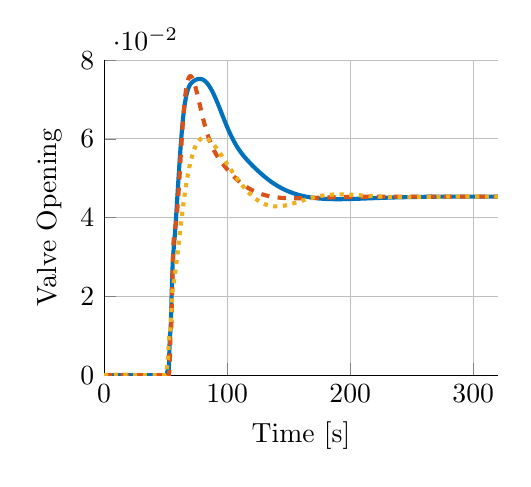
\begin{tikzpicture}

\begin{axis}[%
width=5cm,
height=4cm,
at={(0\linewidth,0\linewidth)},
scale only axis,
xmin=0,
xmax=320,
xlabel={Time [s]},
xmajorgrids,
ymin=0,
ymax=0.08,
ylabel={Valve Opening},
ymajorgrids,
axis background/.style={fill=white},
% title style={font=\bfseries},
% title={Normalized Recycle Valve Opening},
axis x line*=bottom,
axis y line*=left
]
\addplot [color=mycolor1,solid,line width=1.5pt,forget plot]
  table[row sep=crcr]{%
0	1.30651e-06\\
0.25	6.92017e-06\\
0.5	1.05998e-05\\
0.75	1.30927e-05\\
1	1.46601e-05\\
1.25	1.50442e-05\\
1.5	1.42539e-05\\
1.75	1.24228e-05\\
2	9.51022e-06\\
2.25	5.51542e-06\\
2.5	7.24745e-07\\
2.75	0\\
3	0\\
3.25	0\\
3.5	0\\
3.75	0\\
4	0\\
4.25	0\\
4.5	0\\
4.75	0\\
5	0\\
5.25	0\\
5.5	0\\
5.75	0\\
6	0\\
6.25	0\\
6.5	0\\
6.75	0\\
7	0\\
7.25	0\\
7.5	0\\
7.75	0\\
8	0\\
8.25	0\\
8.5	0\\
8.75	0\\
9	0\\
9.25	0\\
9.5	0\\
9.75	0\\
10	0\\
10.25	0\\
10.5	0\\
10.75	0\\
11	0\\
11.25	0\\
11.5	0\\
11.75	0\\
12	0\\
12.25	0\\
12.5	0\\
12.75	0\\
13	0\\
13.25	0\\
13.5	0\\
13.75	0\\
14	0\\
14.25	0\\
14.5	0\\
14.75	0\\
15	0\\
15.25	0\\
15.5	0\\
15.75	0\\
16	0\\
16.25	0\\
16.5	0\\
16.75	0\\
17	0\\
17.25	0\\
17.5	0\\
17.75	0\\
18	0\\
18.25	0\\
18.5	0\\
18.75	0\\
19	0\\
19.25	0\\
19.5	0\\
19.75	0\\
20	0\\
20.25	0\\
20.5	0\\
20.75	0\\
21	0\\
21.25	0\\
21.5	0\\
21.75	0\\
22	0\\
22.25	0\\
22.5	0\\
22.75	0\\
23	0\\
23.25	0\\
23.5	0\\
23.75	0\\
24	0\\
24.25	0\\
24.5	0\\
24.75	0\\
25	0\\
25.25	0\\
25.5	0\\
25.75	0\\
26	0\\
26.25	0\\
26.5	0\\
26.75	0\\
27	0\\
27.25	0\\
27.5	0\\
27.75	0\\
28	0\\
28.25	0\\
28.5	0\\
28.75	0\\
29	0\\
29.25	0\\
29.5	0\\
29.75	0\\
30	0\\
30.25	0\\
30.5	0\\
30.75	0\\
31	0\\
31.25	0\\
31.5	0\\
31.75	0\\
32	0\\
32.25	0\\
32.5	0\\
32.75	0\\
33	0\\
33.25	0\\
33.5	0\\
33.75	0\\
34	0\\
34.25	0\\
34.5	0\\
34.75	0\\
35	0\\
35.25	0\\
35.5	0\\
35.75	0\\
36	0\\
36.25	0\\
36.5	0\\
36.75	0\\
37	0\\
37.25	0\\
37.5	0\\
37.75	0\\
38	0\\
38.25	0\\
38.5	0\\
38.75	0\\
39	0\\
39.25	0\\
39.5	0\\
39.75	0\\
40	0\\
40.25	0\\
40.5	0\\
40.75	0\\
41	0\\
41.25	0\\
41.5	0\\
41.75	0\\
42	0\\
42.25	0\\
42.5	0\\
42.75	0\\
43	0\\
43.25	0\\
43.5	0\\
43.75	0\\
44	0\\
44.25	0\\
44.5	0\\
44.75	0\\
45	0\\
45.25	0\\
45.5	0\\
45.75	0\\
46	0\\
46.25	0\\
46.5	0\\
46.75	0\\
47	0\\
47.25	0\\
47.5	0\\
47.75	0\\
48	0\\
48.25	0\\
48.5	0\\
48.75	0\\
49	0\\
49.25	0\\
49.5	0\\
49.75	0\\
50	0\\
50.25	0\\
50.5	0\\
50.75	0.00010029\\
51	0.000407362\\
51.25	0\\
51.5	0\\
51.75	5.40805e-05\\
52	0.000176293\\
52.25	0.000363014\\
52.5	0.000992407\\
52.75	0.00287787\\
53	0.00554674\\
53.25	0.00839406\\
53.5	0.0100218\\
53.75	0.0106393\\
54	0.0114346\\
54.25	0.0131622\\
54.5	0.0156487\\
54.75	0.0188936\\
55	0.0216522\\
55.25	0.0237894\\
55.5	0.0262732\\
55.75	0.0284355\\
56	0.0298673\\
56.25	0.0309326\\
56.5	0.0319204\\
56.75	0.0328628\\
57	0.0337897\\
57.25	0.0347444\\
57.5	0.0357447\\
57.75	0.0367904\\
58	0.0378773\\
58.25	0.039007\\
58.5	0.0401793\\
58.75	0.0413865\\
59	0.0426192\\
59.25	0.0438703\\
59.5	0.0451331\\
59.75	0.0464002\\
60	0.0476651\\
60.25	0.0489224\\
60.5	0.0501673\\
60.75	0.0513955\\
61	0.0526033\\
61.25	0.0537878\\
61.5	0.0549464\\
61.75	0.056077\\
62	0.057178\\
62.25	0.0582477\\
62.5	0.0592848\\
62.75	0.0602878\\
63	0.0612554\\
63.25	0.062186\\
63.5	0.0630781\\
63.75	0.0639301\\
64	0.0647406\\
64.25	0.0655084\\
64.5	0.0662327\\
64.75	0.0669131\\
65	0.0675499\\
65.25	0.0681441\\
65.5	0.068697\\
65.75	0.0692103\\
66	0.0696861\\
66.25	0.0701266\\
66.5	0.0705345\\
66.75	0.0709129\\
67	0.0712644\\
67.25	0.0715908\\
67.5	0.0718933\\
67.75	0.072173\\
68	0.0724304\\
68.25	0.0726666\\
68.5	0.0728827\\
68.75	0.0730798\\
69	0.0732594\\
69.25	0.0734229\\
69.5	0.0735716\\
69.75	0.0737071\\
70	0.0738307\\
70.25	0.0739435\\
70.5	0.0740469\\
70.75	0.0741418\\
71	0.0742292\\
71.25	0.0743099\\
71.5	0.0743849\\
71.75	0.0744546\\
72	0.0745198\\
72.25	0.074581\\
72.5	0.0746385\\
72.75	0.0746927\\
73	0.074744\\
73.25	0.0747925\\
73.5	0.0748385\\
73.75	0.0748821\\
74	0.0749233\\
74.25	0.0749623\\
74.5	0.074999\\
74.75	0.0750334\\
75	0.0750655\\
75.25	0.0750953\\
75.5	0.0751227\\
75.75	0.0751476\\
76	0.0751699\\
76.25	0.0751895\\
76.5	0.0752063\\
76.75	0.0752202\\
77	0.0752311\\
77.25	0.075239\\
77.5	0.0752436\\
77.75	0.0752449\\
78	0.0752428\\
78.25	0.0752373\\
78.5	0.0752282\\
78.75	0.0752155\\
79	0.0751991\\
79.25	0.0751789\\
79.5	0.0751549\\
79.75	0.0751271\\
80	0.0750954\\
80.25	0.0750597\\
80.5	0.0750201\\
80.75	0.0749765\\
81	0.0749289\\
81.25	0.0748773\\
81.5	0.0748216\\
81.75	0.074762\\
82	0.0746984\\
82.25	0.0746307\\
82.5	0.074559\\
82.75	0.0744834\\
83	0.0744038\\
83.25	0.0743202\\
83.5	0.0742327\\
83.75	0.0741414\\
84	0.0740461\\
84.25	0.0739471\\
84.5	0.0738442\\
84.75	0.0737376\\
85	0.0736273\\
85.25	0.0735133\\
85.5	0.0733957\\
85.75	0.0732745\\
86	0.0731498\\
86.25	0.0730216\\
86.5	0.07289\\
86.75	0.0727551\\
87	0.0726168\\
87.25	0.0724754\\
87.5	0.0723307\\
87.75	0.072183\\
88	0.0720322\\
88.25	0.0718785\\
88.5	0.0717219\\
88.75	0.0715626\\
89	0.0714005\\
89.25	0.0712357\\
89.5	0.0710685\\
89.75	0.0708987\\
90	0.0707266\\
90.25	0.0705522\\
90.5	0.0703756\\
90.75	0.070197\\
91	0.0700163\\
91.25	0.0698337\\
91.5	0.0696494\\
91.75	0.0694633\\
92	0.0692757\\
92.25	0.0690865\\
92.5	0.068896\\
92.75	0.0687042\\
93	0.0685112\\
93.25	0.0683171\\
93.5	0.0681221\\
93.75	0.0679262\\
94	0.0677296\\
94.25	0.0675323\\
94.5	0.0673345\\
94.75	0.0671363\\
95	0.0669377\\
95.25	0.0667389\\
95.5	0.06654\\
95.75	0.0663411\\
96	0.0661422\\
96.25	0.0659436\\
96.5	0.0657452\\
96.75	0.0655472\\
97	0.0653496\\
97.25	0.0651526\\
97.5	0.0649563\\
97.75	0.0647607\\
98	0.064566\\
98.25	0.0643721\\
98.5	0.0641793\\
98.75	0.0639875\\
99	0.0637968\\
99.25	0.0636074\\
99.5	0.0634192\\
99.75	0.0632324\\
100	0.063047\\
100.25	0.062863\\
100.5	0.0626806\\
100.75	0.0624997\\
101	0.0623205\\
101.25	0.0621429\\
101.5	0.0619671\\
101.75	0.061793\\
102	0.0616207\\
102.25	0.0614502\\
102.5	0.0612815\\
102.75	0.0611147\\
103	0.0609499\\
103.25	0.0607869\\
103.5	0.0606259\\
103.75	0.0604668\\
104	0.0603097\\
104.25	0.0601545\\
104.5	0.0600014\\
104.75	0.0598501\\
105	0.0597009\\
105.25	0.0595536\\
105.5	0.0594083\\
105.75	0.0592649\\
106	0.0591235\\
106.25	0.058984\\
106.5	0.0588464\\
106.75	0.0587107\\
107	0.0585769\\
107.25	0.0584449\\
107.5	0.0583148\\
107.75	0.0581864\\
108	0.0580598\\
108.25	0.057935\\
108.5	0.0578119\\
108.75	0.0576905\\
109	0.0575708\\
109.25	0.0574526\\
109.5	0.0573361\\
109.75	0.0572211\\
110	0.0571077\\
110.25	0.0569957\\
110.5	0.0568852\\
110.75	0.0567761\\
111	0.0566683\\
111.25	0.056562\\
111.5	0.0564569\\
111.75	0.0563531\\
112	0.0562505\\
112.25	0.0561491\\
112.5	0.0560489\\
112.75	0.0559498\\
113	0.0558518\\
113.25	0.0557548\\
113.5	0.0556589\\
113.75	0.0555639\\
114	0.0554699\\
114.25	0.0553768\\
114.5	0.0552846\\
114.75	0.0551933\\
115	0.0551027\\
115.25	0.055013\\
115.5	0.054924\\
115.75	0.0548358\\
116	0.0547483\\
116.25	0.0546614\\
116.5	0.0545752\\
116.75	0.0544896\\
117	0.0544047\\
117.25	0.0543203\\
117.5	0.0542365\\
117.75	0.0541532\\
118	0.0540704\\
118.25	0.0539882\\
118.5	0.0539064\\
118.75	0.0538251\\
119	0.0537443\\
119.25	0.0536639\\
119.5	0.0535839\\
119.75	0.0535043\\
120	0.0534252\\
120.25	0.0533464\\
120.5	0.053268\\
120.75	0.0531899\\
121	0.0531123\\
121.25	0.0530349\\
121.5	0.0529579\\
121.75	0.0528813\\
122	0.052805\\
122.25	0.052729\\
122.5	0.0526533\\
122.75	0.0525779\\
123	0.0525029\\
123.25	0.0524282\\
123.5	0.0523537\\
123.75	0.0522796\\
124	0.0522058\\
124.25	0.0521324\\
124.5	0.0520592\\
124.75	0.0519863\\
125	0.0519137\\
125.25	0.0518415\\
125.5	0.0517696\\
125.75	0.0516979\\
126	0.0516266\\
126.25	0.0515557\\
126.5	0.051485\\
126.75	0.0514147\\
127	0.0513447\\
127.25	0.051275\\
127.5	0.0512057\\
127.75	0.0511367\\
128	0.0510681\\
128.25	0.0509998\\
128.5	0.0509318\\
128.75	0.0508642\\
129	0.050797\\
129.25	0.0507302\\
129.5	0.0506637\\
129.75	0.0505976\\
130	0.0505318\\
130.25	0.0504665\\
130.5	0.0504015\\
130.75	0.050337\\
131	0.0502728\\
131.25	0.050209\\
131.5	0.0501456\\
131.75	0.0500827\\
132	0.0500201\\
132.25	0.049958\\
132.5	0.0498962\\
132.75	0.0498349\\
133	0.049774\\
133.25	0.0497136\\
133.5	0.0496535\\
133.75	0.0495939\\
134	0.0495348\\
134.25	0.049476\\
134.5	0.0494178\\
134.75	0.0493599\\
135	0.0493025\\
135.25	0.0492455\\
135.5	0.049189\\
135.75	0.0491329\\
136	0.0490773\\
136.25	0.0490221\\
136.5	0.0489674\\
136.75	0.0489131\\
137	0.0488593\\
137.25	0.0488059\\
137.5	0.048753\\
137.75	0.0487006\\
138	0.0486485\\
138.25	0.048597\\
138.5	0.0485459\\
138.75	0.0484952\\
139	0.048445\\
139.25	0.0483952\\
139.5	0.0483459\\
139.75	0.048297\\
140	0.0482486\\
140.25	0.0482007\\
140.5	0.0481531\\
140.75	0.048106\\
141	0.0480594\\
141.25	0.0480132\\
141.5	0.0479674\\
141.75	0.0479221\\
142	0.0478772\\
142.25	0.0478327\\
142.5	0.0477887\\
142.75	0.0477451\\
143	0.0477019\\
143.25	0.0476592\\
143.5	0.0476168\\
143.75	0.0475749\\
144	0.0475334\\
144.25	0.0474924\\
144.5	0.0474517\\
144.75	0.0474114\\
145	0.0473716\\
145.25	0.0473322\\
145.5	0.0472931\\
145.75	0.0472545\\
146	0.0472162\\
146.25	0.0471784\\
146.5	0.047141\\
146.75	0.0471039\\
147	0.0470672\\
147.25	0.0470309\\
147.5	0.046995\\
147.75	0.0469595\\
148	0.0469244\\
148.25	0.0468896\\
148.5	0.0468552\\
148.75	0.0468212\\
149	0.0467875\\
149.25	0.0467542\\
149.5	0.0467213\\
149.75	0.0466887\\
150	0.0466565\\
150.25	0.0466246\\
150.5	0.0465931\\
150.75	0.046562\\
151	0.0465312\\
151.25	0.0465007\\
151.5	0.0464706\\
151.75	0.0464408\\
152	0.0464113\\
152.25	0.0463822\\
152.5	0.0463534\\
152.75	0.046325\\
153	0.0462969\\
153.25	0.0462691\\
153.5	0.0462416\\
153.75	0.0462144\\
154	0.0461876\\
154.25	0.0461611\\
154.5	0.0461349\\
154.75	0.046109\\
155	0.0460834\\
155.25	0.0460581\\
155.5	0.0460332\\
155.75	0.0460085\\
156	0.0459842\\
156.25	0.0459601\\
156.5	0.0459363\\
156.75	0.0459129\\
157	0.0458897\\
157.25	0.0458668\\
157.5	0.0458442\\
157.75	0.0458219\\
158	0.0457999\\
158.25	0.0457782\\
158.5	0.0457567\\
158.75	0.0457356\\
159	0.0457147\\
159.25	0.0456941\\
159.5	0.0456737\\
159.75	0.0456536\\
160	0.0456338\\
160.25	0.0456143\\
160.5	0.045595\\
160.75	0.045576\\
161	0.0455573\\
161.25	0.0455388\\
161.5	0.0455206\\
161.75	0.0455026\\
162	0.0454849\\
162.25	0.0454675\\
162.5	0.0454503\\
162.75	0.0454333\\
163	0.0454166\\
163.25	0.0454001\\
163.5	0.0453839\\
163.75	0.0453679\\
164	0.0453522\\
164.25	0.0453367\\
164.5	0.0453215\\
164.75	0.0453064\\
165	0.0452917\\
165.25	0.0452771\\
165.5	0.0452628\\
165.75	0.0452487\\
166	0.0452348\\
166.25	0.0452211\\
166.5	0.0452077\\
166.75	0.0451945\\
167	0.0451815\\
167.25	0.0451687\\
167.5	0.0451562\\
167.75	0.0451438\\
168	0.0451317\\
168.25	0.0451198\\
168.5	0.0451081\\
168.75	0.0450966\\
169	0.0450853\\
169.25	0.0450742\\
169.5	0.0450633\\
169.75	0.0450526\\
170	0.0450421\\
170.25	0.0450318\\
170.5	0.0450216\\
170.75	0.0450117\\
171	0.045002\\
171.25	0.0449924\\
171.5	0.0449831\\
171.75	0.0449739\\
172	0.0449649\\
172.25	0.0449561\\
172.5	0.0449475\\
172.75	0.044939\\
173	0.0449308\\
173.25	0.0449227\\
173.5	0.0449147\\
173.75	0.044907\\
174	0.0448994\\
174.25	0.044892\\
174.5	0.0448847\\
174.75	0.0448776\\
175	0.0448707\\
175.25	0.0448639\\
175.5	0.0448573\\
175.75	0.0448509\\
176	0.0448446\\
176.25	0.0448384\\
176.5	0.0448325\\
176.75	0.0448266\\
177	0.0448209\\
177.25	0.0448154\\
177.5	0.04481\\
177.75	0.0448047\\
178	0.0447996\\
178.25	0.0447947\\
178.5	0.0447898\\
178.75	0.0447851\\
179	0.0447806\\
179.25	0.0447762\\
179.5	0.0447719\\
179.75	0.0447677\\
180	0.0447637\\
180.25	0.0447598\\
180.5	0.044756\\
180.75	0.0447524\\
181	0.0447488\\
181.25	0.0447454\\
181.5	0.0447422\\
181.75	0.044739\\
182	0.044736\\
182.25	0.044733\\
182.5	0.0447302\\
182.75	0.0447275\\
183	0.0447249\\
183.25	0.0447224\\
183.5	0.0447201\\
183.75	0.0447178\\
184	0.0447156\\
184.25	0.0447136\\
184.5	0.0447116\\
184.75	0.0447098\\
185	0.044708\\
185.25	0.0447064\\
185.5	0.0447048\\
185.75	0.0447034\\
186	0.044702\\
186.25	0.0447008\\
186.5	0.0446996\\
186.75	0.0446985\\
187	0.0446975\\
187.25	0.0446966\\
187.5	0.0446958\\
187.75	0.044695\\
188	0.0446944\\
188.25	0.0446938\\
188.5	0.0446934\\
188.75	0.044693\\
189	0.0446926\\
189.25	0.0446924\\
189.5	0.0446922\\
189.75	0.0446921\\
190	0.0446921\\
190.25	0.0446922\\
190.5	0.0446923\\
190.75	0.0446925\\
191	0.0446928\\
191.25	0.0446931\\
191.5	0.0446935\\
191.75	0.044694\\
192	0.0446945\\
192.25	0.0446952\\
192.5	0.0446958\\
192.75	0.0446966\\
193	0.0446973\\
193.25	0.0446982\\
193.5	0.0446991\\
193.75	0.0447001\\
194	0.0447011\\
194.25	0.0447022\\
194.5	0.0447033\\
194.75	0.0447045\\
195	0.0447058\\
195.25	0.0447071\\
195.5	0.0447084\\
195.75	0.0447098\\
196	0.0447113\\
196.25	0.0447128\\
196.5	0.0447143\\
196.75	0.0447159\\
197	0.0447176\\
197.25	0.0447193\\
197.5	0.044721\\
197.75	0.0447228\\
198	0.0447246\\
198.25	0.0447264\\
198.5	0.0447283\\
198.75	0.0447303\\
199	0.0447322\\
199.25	0.0447343\\
199.5	0.0447363\\
199.75	0.0447384\\
200	0.0447405\\
200.25	0.0447427\\
200.5	0.0447448\\
200.75	0.0447471\\
201	0.0447493\\
201.25	0.0447516\\
201.5	0.0447539\\
201.75	0.0447563\\
202	0.0447586\\
202.25	0.0447611\\
202.5	0.0447635\\
202.75	0.0447659\\
203	0.0447684\\
203.25	0.0447709\\
203.5	0.0447735\\
203.75	0.044776\\
204	0.0447786\\
204.25	0.0447812\\
204.5	0.0447838\\
204.75	0.0447865\\
205	0.0447892\\
205.25	0.0447919\\
205.5	0.0447946\\
205.75	0.0447973\\
206	0.0448\\
206.25	0.0448028\\
206.5	0.0448056\\
206.75	0.0448084\\
207	0.0448112\\
207.25	0.044814\\
207.5	0.0448169\\
207.75	0.0448197\\
208	0.0448226\\
208.25	0.0448255\\
208.5	0.0448284\\
208.75	0.0448313\\
209	0.0448342\\
209.25	0.0448372\\
209.5	0.0448401\\
209.75	0.0448431\\
210	0.044846\\
210.25	0.044849\\
210.5	0.044852\\
210.75	0.044855\\
211	0.044858\\
211.25	0.044861\\
211.5	0.044864\\
211.75	0.044867\\
212	0.04487\\
212.25	0.044873\\
212.5	0.0448761\\
212.75	0.0448791\\
213	0.0448821\\
213.25	0.0448852\\
213.5	0.0448882\\
213.75	0.0448913\\
214	0.0448943\\
214.25	0.0448974\\
214.5	0.0449004\\
214.75	0.0449035\\
215	0.0449066\\
215.25	0.0449096\\
215.5	0.0449127\\
215.75	0.0449157\\
216	0.0449188\\
216.25	0.0449218\\
216.5	0.0449249\\
216.75	0.044928\\
217	0.044931\\
217.25	0.0449341\\
217.5	0.0449371\\
217.75	0.0449401\\
218	0.0449432\\
218.25	0.0449462\\
218.5	0.0449493\\
218.75	0.0449523\\
219	0.0449553\\
219.25	0.0449583\\
219.5	0.0449613\\
219.75	0.0449644\\
220	0.0449674\\
220.25	0.0449704\\
220.5	0.0449733\\
220.75	0.0449763\\
221	0.0449793\\
221.25	0.0449823\\
221.5	0.0449853\\
221.75	0.0449882\\
222	0.0449912\\
222.25	0.0449941\\
222.5	0.044997\\
222.75	0.045\\
223	0.0450029\\
223.25	0.0450058\\
223.5	0.0450087\\
223.75	0.0450116\\
224	0.0450145\\
224.25	0.0450174\\
224.5	0.0450202\\
224.75	0.0450231\\
225	0.0450259\\
225.25	0.0450288\\
225.5	0.0450316\\
225.75	0.0450344\\
226	0.0450372\\
226.25	0.04504\\
226.5	0.0450428\\
226.75	0.0450456\\
227	0.0450483\\
227.25	0.0450511\\
227.5	0.0450538\\
227.75	0.0450565\\
228	0.0450593\\
228.25	0.045062\\
228.5	0.0450646\\
228.75	0.0450673\\
229	0.04507\\
229.25	0.0450727\\
229.5	0.0450753\\
229.75	0.0450779\\
230	0.0450805\\
230.25	0.0450832\\
230.5	0.0450857\\
230.75	0.0450883\\
231	0.0450909\\
231.25	0.0450934\\
231.5	0.045096\\
231.75	0.0450985\\
232	0.045101\\
232.25	0.0451035\\
232.5	0.045106\\
232.75	0.0451085\\
233	0.045111\\
233.25	0.0451134\\
233.5	0.0451158\\
233.75	0.0451183\\
234	0.0451207\\
234.25	0.0451231\\
234.5	0.0451254\\
234.75	0.0451278\\
235	0.0451302\\
235.25	0.0451325\\
235.5	0.0451348\\
235.75	0.0451371\\
236	0.0451394\\
236.25	0.0451417\\
236.5	0.045144\\
236.75	0.0451462\\
237	0.0451485\\
237.25	0.0451507\\
237.5	0.0451529\\
237.75	0.0451551\\
238	0.0451573\\
238.25	0.0451594\\
238.5	0.0451616\\
238.75	0.0451637\\
239	0.0451658\\
239.25	0.0451679\\
239.5	0.04517\\
239.75	0.0451721\\
240	0.0451742\\
240.25	0.0451762\\
240.5	0.0451783\\
240.75	0.0451803\\
241	0.0451823\\
241.25	0.0451843\\
241.5	0.0451863\\
241.75	0.0451882\\
242	0.0451902\\
242.25	0.0451921\\
242.5	0.045194\\
242.75	0.0451959\\
243	0.0451978\\
243.25	0.0451997\\
243.5	0.0452016\\
243.75	0.0452034\\
244	0.0452053\\
244.25	0.0452071\\
244.5	0.0452089\\
244.75	0.0452107\\
245	0.0452124\\
245.25	0.0452142\\
245.5	0.045216\\
245.75	0.0452177\\
246	0.0452194\\
246.25	0.0452211\\
246.5	0.0452228\\
246.75	0.0452245\\
247	0.0452262\\
247.25	0.0452278\\
247.5	0.0452294\\
247.75	0.0452311\\
248	0.0452327\\
248.25	0.0452343\\
248.5	0.0452358\\
248.75	0.0452374\\
249	0.045239\\
249.25	0.0452405\\
249.5	0.045242\\
249.75	0.0452435\\
250	0.045245\\
250.25	0.0452465\\
250.5	0.045248\\
250.75	0.0452495\\
251	0.0452509\\
251.25	0.0452523\\
251.5	0.0452537\\
251.75	0.0452552\\
252	0.0452565\\
252.25	0.0452579\\
252.5	0.0452593\\
252.75	0.0452606\\
253	0.045262\\
253.25	0.0452633\\
253.5	0.0452646\\
253.75	0.0452659\\
254	0.0452672\\
254.25	0.0452685\\
254.5	0.0452698\\
254.75	0.045271\\
255	0.0452723\\
255.25	0.0452735\\
255.5	0.0452747\\
255.75	0.0452759\\
256	0.0452771\\
256.25	0.0452783\\
256.5	0.0452794\\
256.75	0.0452806\\
257	0.0452817\\
257.25	0.0452829\\
257.5	0.045284\\
257.75	0.0452851\\
258	0.0452862\\
258.25	0.0452873\\
258.5	0.0452883\\
258.75	0.0452894\\
259	0.0452904\\
259.25	0.0452915\\
259.5	0.0452925\\
259.75	0.0452935\\
260	0.0452945\\
260.25	0.0452955\\
260.5	0.0452965\\
260.75	0.0452975\\
261	0.0452984\\
261.25	0.0452994\\
261.5	0.0453003\\
261.75	0.0453012\\
262	0.0453022\\
262.25	0.0453031\\
262.5	0.045304\\
262.75	0.0453049\\
263	0.0453057\\
263.25	0.0453066\\
263.5	0.0453074\\
263.75	0.0453083\\
264	0.0453091\\
264.25	0.0453099\\
264.5	0.0453108\\
264.75	0.0453116\\
265	0.0453124\\
265.25	0.0453131\\
265.5	0.0453139\\
265.75	0.0453147\\
266	0.0453154\\
266.25	0.0453162\\
266.5	0.0453169\\
266.75	0.0453177\\
267	0.0453184\\
267.25	0.0453191\\
267.5	0.0453198\\
267.75	0.0453205\\
268	0.0453212\\
268.25	0.0453218\\
268.5	0.0453225\\
268.75	0.0453232\\
269	0.0453238\\
269.25	0.0453244\\
269.5	0.0453251\\
269.75	0.0453257\\
270	0.0453263\\
270.25	0.0453269\\
270.5	0.0453275\\
270.75	0.0453281\\
271	0.0453287\\
271.25	0.0453292\\
271.5	0.0453298\\
271.75	0.0453304\\
272	0.0453309\\
272.25	0.0453314\\
272.5	0.045332\\
272.75	0.0453325\\
273	0.045333\\
273.25	0.0453335\\
273.5	0.045334\\
273.75	0.0453345\\
274	0.045335\\
274.25	0.0453355\\
274.5	0.045336\\
274.75	0.0453364\\
275	0.0453369\\
275.25	0.0453373\\
275.5	0.0453378\\
275.75	0.0453382\\
276	0.0453386\\
276.25	0.0453391\\
276.5	0.0453395\\
276.75	0.0453399\\
277	0.0453403\\
277.25	0.0453407\\
277.5	0.0453411\\
277.75	0.0453415\\
278	0.0453418\\
278.25	0.0453422\\
278.5	0.0453426\\
278.75	0.0453429\\
279	0.0453433\\
279.25	0.0453436\\
279.5	0.045344\\
279.75	0.0453443\\
280	0.0453446\\
280.25	0.045345\\
280.5	0.0453453\\
280.75	0.0453456\\
281	0.0453459\\
281.25	0.0453462\\
281.5	0.0453465\\
281.75	0.0453468\\
282	0.0453471\\
282.25	0.0453473\\
282.5	0.0453476\\
282.75	0.0453479\\
283	0.0453481\\
283.25	0.0453484\\
283.5	0.0453486\\
283.75	0.0453489\\
284	0.0453491\\
284.25	0.0453494\\
284.5	0.0453496\\
284.75	0.0453498\\
285	0.0453501\\
285.25	0.0453503\\
285.5	0.0453505\\
285.75	0.0453507\\
286	0.0453509\\
286.25	0.0453511\\
286.5	0.0453513\\
286.75	0.0453515\\
287	0.0453517\\
287.25	0.0453518\\
287.5	0.045352\\
287.75	0.0453522\\
288	0.0453524\\
288.25	0.0453525\\
288.5	0.0453527\\
288.75	0.0453529\\
289	0.045353\\
289.25	0.0453532\\
289.5	0.0453533\\
289.75	0.0453534\\
290	0.0453536\\
290.25	0.0453537\\
290.5	0.0453538\\
290.75	0.045354\\
291	0.0453541\\
291.25	0.0453542\\
291.5	0.0453543\\
291.75	0.0453544\\
292	0.0453545\\
292.25	0.0453546\\
292.5	0.0453547\\
292.75	0.0453548\\
293	0.0453549\\
293.25	0.045355\\
293.5	0.0453551\\
293.75	0.0453552\\
294	0.0453553\\
294.25	0.0453554\\
294.5	0.0453554\\
294.75	0.0453555\\
295	0.0453556\\
295.25	0.0453557\\
295.5	0.0453557\\
295.75	0.0453558\\
296	0.0453558\\
296.25	0.0453559\\
296.5	0.045356\\
296.75	0.045356\\
297	0.0453561\\
297.25	0.0453561\\
297.5	0.0453561\\
297.75	0.0453562\\
298	0.0453562\\
298.25	0.0453563\\
298.5	0.0453563\\
298.75	0.0453563\\
299	0.0453564\\
299.25	0.0453564\\
299.5	0.0453564\\
299.75	0.0453564\\
300	0.0453565\\
300.25	0.0453565\\
300.5	0.0453565\\
300.75	0.0453565\\
301	0.0453565\\
301.25	0.0453565\\
301.5	0.0453565\\
301.75	0.0453565\\
302	0.0453565\\
302.25	0.0453565\\
302.5	0.0453565\\
302.75	0.0453565\\
303	0.0453565\\
303.25	0.0453565\\
303.5	0.0453565\\
303.75	0.0453565\\
304	0.0453565\\
304.25	0.0453565\\
304.5	0.0453565\\
304.75	0.0453565\\
305	0.0453564\\
305.25	0.0453564\\
305.5	0.0453564\\
305.75	0.0453564\\
306	0.0453564\\
306.25	0.0453563\\
306.5	0.0453563\\
306.75	0.0453563\\
307	0.0453563\\
307.25	0.0453562\\
307.5	0.0453562\\
307.75	0.0453562\\
308	0.0453561\\
308.25	0.0453561\\
308.5	0.0453561\\
308.75	0.045356\\
309	0.045356\\
309.25	0.0453559\\
309.5	0.0453559\\
309.75	0.0453559\\
310	0.0453558\\
310.25	0.0453558\\
310.5	0.0453557\\
310.75	0.0453557\\
311	0.0453556\\
311.25	0.0453556\\
311.5	0.0453555\\
311.75	0.0453555\\
312	0.0453554\\
312.25	0.0453554\\
312.5	0.0453553\\
312.75	0.0453553\\
313	0.0453552\\
313.25	0.0453552\\
313.5	0.0453551\\
313.75	0.0453551\\
314	0.045355\\
314.25	0.0453549\\
314.5	0.0453549\\
314.75	0.0453548\\
315	0.0453548\\
315.25	0.0453547\\
315.5	0.0453546\\
315.75	0.0453546\\
316	0.0453545\\
316.25	0.0453545\\
316.5	0.0453544\\
316.75	0.0453543\\
317	0.0453543\\
317.25	0.0453542\\
317.5	0.0453541\\
317.75	0.0453541\\
318	0.045354\\
318.25	0.0453539\\
318.5	0.0453539\\
318.75	0.0453538\\
319	0.0453537\\
319.25	0.0453537\\
319.5	0.0453536\\
319.75	0.0453535\\
320	0.0453535\\
320.25	0.0453534\\
320.5	0.0453533\\
320.75	0.0453532\\
321	0.0453532\\
321.25	0.0453531\\
321.5	0.045353\\
321.75	0.045353\\
322	0.0453529\\
322.25	0.0453528\\
322.5	0.0453527\\
322.75	0.0453527\\
323	0.0453526\\
323.25	0.0453525\\
323.5	0.0453525\\
323.75	0.0453524\\
324	0.0453523\\
324.25	0.0453522\\
324.5	0.0453522\\
324.75	0.0453521\\
325	0.045352\\
325.25	0.0453519\\
325.5	0.0453519\\
325.75	0.0453518\\
326	0.0453517\\
326.25	0.0453516\\
326.5	0.0453516\\
326.75	0.0453515\\
327	0.0453514\\
327.25	0.0453513\\
327.5	0.0453513\\
327.75	0.0453512\\
328	0.0453511\\
328.25	0.045351\\
328.5	0.045351\\
328.75	0.0453509\\
329	0.0453508\\
329.25	0.0453507\\
329.5	0.0453507\\
329.75	0.0453506\\
330	0.0453505\\
330.25	0.0453505\\
330.5	0.0453504\\
330.75	0.0453503\\
331	0.0453502\\
331.25	0.0453502\\
331.5	0.0453501\\
331.75	0.04535\\
332	0.0453499\\
332.25	0.0453499\\
332.5	0.0453498\\
332.75	0.0453497\\
333	0.0453496\\
333.25	0.0453496\\
333.5	0.0453495\\
333.75	0.0453494\\
334	0.0453494\\
334.25	0.0453493\\
334.5	0.0453492\\
334.75	0.0453491\\
335	0.0453491\\
335.25	0.045349\\
335.5	0.0453489\\
335.75	0.0453489\\
336	0.0453488\\
336.25	0.0453487\\
336.5	0.0453486\\
336.75	0.0453486\\
337	0.0453485\\
337.25	0.0453484\\
337.5	0.0453484\\
337.75	0.0453483\\
338	0.0453482\\
338.25	0.0453482\\
338.5	0.0453481\\
338.75	0.045348\\
339	0.045348\\
339.25	0.0453479\\
339.5	0.0453478\\
339.75	0.0453478\\
340	0.0453477\\
340.25	0.0453476\\
340.5	0.0453476\\
340.75	0.0453475\\
341	0.0453474\\
341.25	0.0453474\\
341.5	0.0453473\\
341.75	0.0453472\\
342	0.0453472\\
342.25	0.0453471\\
342.5	0.045347\\
342.75	0.045347\\
343	0.0453469\\
343.25	0.0453469\\
343.5	0.0453468\\
343.75	0.0453467\\
344	0.0453467\\
344.25	0.0453466\\
344.5	0.0453466\\
344.75	0.0453465\\
345	0.0453464\\
345.25	0.0453464\\
345.5	0.0453463\\
345.75	0.0453463\\
346	0.0453462\\
346.25	0.0453461\\
346.5	0.0453461\\
346.75	0.045346\\
347	0.045346\\
347.25	0.0453459\\
347.5	0.0453459\\
347.75	0.0453458\\
348	0.0453457\\
348.25	0.0453457\\
348.5	0.0453456\\
348.75	0.0453456\\
349	0.0453455\\
349.25	0.0453455\\
349.5	0.0453454\\
349.75	0.0453454\\
350	0.0453453\\
350.25	0.0453452\\
350.5	0.0453452\\
350.75	0.0453451\\
351	0.0453451\\
351.25	0.045345\\
351.5	0.045345\\
351.75	0.0453449\\
352	0.0453449\\
352.25	0.0453448\\
352.5	0.0453448\\
352.75	0.0453447\\
353	0.0453447\\
353.25	0.0453446\\
353.5	0.0453446\\
353.75	0.0453445\\
354	0.0453445\\
354.25	0.0453444\\
354.5	0.0453444\\
354.75	0.0453444\\
355	0.0453443\\
355.25	0.0453443\\
355.5	0.0453442\\
355.75	0.0453442\\
356	0.0453441\\
356.25	0.0453441\\
356.5	0.045344\\
356.75	0.045344\\
357	0.045344\\
357.25	0.0453439\\
357.5	0.0453439\\
357.75	0.0453438\\
358	0.0453438\\
358.25	0.0453437\\
358.5	0.0453437\\
358.75	0.0453437\\
359	0.0453436\\
359.25	0.0453436\\
359.5	0.0453435\\
359.75	0.0453435\\
360	0.0453435\\
360.25	0.0453434\\
360.5	0.0453434\\
360.75	0.0453433\\
361	0.0453433\\
361.25	0.0453433\\
361.5	0.0453432\\
361.75	0.0453432\\
362	0.0453432\\
362.25	0.0453431\\
362.5	0.0453431\\
362.75	0.045343\\
363	0.045343\\
363.25	0.045343\\
363.5	0.0453429\\
363.75	0.0453429\\
364	0.0453429\\
364.25	0.0453428\\
364.5	0.0453428\\
364.75	0.0453428\\
365	0.0453427\\
365.25	0.0453427\\
365.5	0.0453427\\
365.75	0.0453426\\
366	0.0453426\\
366.25	0.0453426\\
366.5	0.0453425\\
366.75	0.0453425\\
367	0.0453425\\
367.25	0.0453425\\
367.5	0.0453424\\
367.75	0.0453424\\
368	0.0453424\\
368.25	0.0453423\\
368.5	0.0453423\\
368.75	0.0453423\\
369	0.0453423\\
369.25	0.0453422\\
369.5	0.0453422\\
369.75	0.0453422\\
370	0.0453421\\
370.25	0.0453421\\
370.5	0.0453421\\
370.75	0.0453421\\
371	0.045342\\
371.25	0.045342\\
371.5	0.045342\\
371.75	0.045342\\
372	0.0453419\\
372.25	0.0453419\\
372.5	0.0453419\\
372.75	0.0453419\\
373	0.0453418\\
373.25	0.0453418\\
373.5	0.0453418\\
373.75	0.0453418\\
374	0.0453417\\
374.25	0.0453417\\
374.5	0.0453417\\
374.75	0.0453417\\
375	0.0453417\\
375.25	0.0453416\\
375.5	0.0453416\\
375.75	0.0453416\\
376	0.0453416\\
376.25	0.0453416\\
376.5	0.0453415\\
376.75	0.0453415\\
377	0.0453415\\
377.25	0.0453415\\
377.5	0.0453415\\
377.75	0.0453414\\
378	0.0453414\\
378.25	0.0453414\\
378.5	0.0453414\\
378.75	0.0453414\\
379	0.0453413\\
379.25	0.0453413\\
379.5	0.0453413\\
379.75	0.0453413\\
380	0.0453413\\
380.25	0.0453413\\
380.5	0.0453412\\
380.75	0.0453412\\
381	0.0453412\\
381.25	0.0453412\\
381.5	0.0453412\\
381.75	0.0453412\\
382	0.0453412\\
382.25	0.0453411\\
382.5	0.0453411\\
382.75	0.0453411\\
383	0.0453411\\
383.25	0.0453411\\
383.5	0.0453411\\
383.75	0.0453411\\
384	0.045341\\
384.25	0.045341\\
384.5	0.045341\\
384.75	0.045341\\
385	0.045341\\
385.25	0.045341\\
385.5	0.045341\\
385.75	0.045341\\
386	0.0453409\\
386.25	0.0453409\\
386.5	0.0453409\\
386.75	0.0453409\\
387	0.0453409\\
387.25	0.0453409\\
387.5	0.0453409\\
387.75	0.0453409\\
388	0.0453408\\
388.25	0.0453408\\
388.5	0.0453408\\
388.75	0.0453408\\
389	0.0453408\\
389.25	0.0453408\\
389.5	0.0453408\\
389.75	0.0453408\\
390	0.0453408\\
390.25	0.0453408\\
390.5	0.0453408\\
390.75	0.0453407\\
391	0.0453407\\
391.25	0.0453407\\
391.5	0.0453407\\
391.75	0.0453407\\
392	0.0453407\\
392.25	0.0453407\\
392.5	0.0453407\\
392.75	0.0453407\\
393	0.0453407\\
393.25	0.0453407\\
393.5	0.0453407\\
393.75	0.0453406\\
394	0.0453406\\
394.25	0.0453406\\
394.5	0.0453406\\
394.75	0.0453406\\
395	0.0453406\\
395.25	0.0453406\\
395.5	0.0453406\\
395.75	0.0453406\\
396	0.0453406\\
396.25	0.0453406\\
396.5	0.0453406\\
396.75	0.0453406\\
397	0.0453406\\
397.25	0.0453406\\
397.5	0.0453406\\
397.75	0.0453405\\
398	0.0453405\\
398.25	0.0453405\\
398.5	0.0453405\\
398.75	0.0453405\\
399	0.0453405\\
399.25	0.0453405\\
399.5	0.0453405\\
399.75	0.0453405\\
400	0.0453405\\
400.25	0.0453405\\
400.5	0.0453405\\
400.75	0.0453405\\
401	0.0453405\\
401.25	0.0453405\\
401.5	0.0453405\\
401.75	0.0453405\\
402	0.0453405\\
402.25	0.0453405\\
402.5	0.0453405\\
402.75	0.0453405\\
403	0.0453405\\
403.25	0.0453405\\
403.5	0.0453405\\
403.75	0.0453405\\
404	0.0453405\\
404.25	0.0453405\\
404.5	0.0453404\\
404.75	0.0453404\\
405	0.0453404\\
405.25	0.0453404\\
405.5	0.0453404\\
405.75	0.0453404\\
406	0.0453404\\
406.25	0.0453404\\
406.5	0.0453404\\
406.75	0.0453404\\
407	0.0453404\\
407.25	0.0453404\\
407.5	0.0453404\\
407.75	0.0453404\\
408	0.0453404\\
408.25	0.0453404\\
408.5	0.0453404\\
408.75	0.0453404\\
409	0.0453404\\
409.25	0.0453404\\
409.5	0.0453404\\
409.75	0.0453404\\
410	0.0453404\\
410.25	0.0453404\\
410.5	0.0453404\\
410.75	0.0453404\\
411	0.0453404\\
411.25	0.0453404\\
411.5	0.0453404\\
411.75	0.0453404\\
412	0.0453404\\
412.25	0.0453404\\
412.5	0.0453404\\
412.75	0.0453404\\
413	0.0453404\\
413.25	0.0453404\\
413.5	0.0453404\\
413.75	0.0453404\\
414	0.0453404\\
414.25	0.0453404\\
414.5	0.0453404\\
414.75	0.0453404\\
415	0.0453404\\
415.25	0.0453404\\
415.5	0.0453404\\
415.75	0.0453404\\
416	0.0453404\\
416.25	0.0453404\\
416.5	0.0453404\\
416.75	0.0453404\\
417	0.0453404\\
417.25	0.0453404\\
417.5	0.0453404\\
417.75	0.0453404\\
418	0.0453404\\
418.25	0.0453404\\
418.5	0.0453404\\
418.75	0.0453404\\
419	0.0453404\\
419.25	0.0453404\\
419.5	0.0453404\\
419.75	0.0453404\\
420	0.0453404\\
420.25	0.0453404\\
420.5	0.0453404\\
420.75	0.0453404\\
421	0.0453404\\
421.25	0.0453404\\
421.5	0.0453404\\
421.75	0.0453404\\
422	0.0453404\\
422.25	0.0453404\\
422.5	0.0453404\\
422.75	0.0453404\\
423	0.0453404\\
423.25	0.0453404\\
423.5	0.0453404\\
423.75	0.0453404\\
424	0.0453404\\
424.25	0.0453404\\
424.5	0.0453404\\
424.75	0.0453404\\
425	0.0453404\\
425.25	0.0453404\\
425.5	0.0453404\\
425.75	0.0453404\\
426	0.0453404\\
426.25	0.0453404\\
426.5	0.0453404\\
426.75	0.0453404\\
427	0.0453404\\
427.25	0.0453404\\
427.5	0.0453404\\
427.75	0.0453404\\
428	0.0453405\\
428.25	0.0453405\\
428.5	0.0453405\\
428.75	0.0453405\\
429	0.0453405\\
429.25	0.0453405\\
429.5	0.0453405\\
429.75	0.0453405\\
430	0.0453405\\
430.25	0.0453405\\
430.5	0.0453405\\
430.75	0.0453405\\
431	0.0453405\\
431.25	0.0453405\\
431.5	0.0453405\\
431.75	0.0453405\\
432	0.0453405\\
432.25	0.0453405\\
432.5	0.0453405\\
432.75	0.0453405\\
433	0.0453405\\
433.25	0.0453405\\
433.5	0.0453405\\
433.75	0.0453405\\
434	0.0453405\\
434.25	0.0453405\\
434.5	0.0453405\\
434.75	0.0453405\\
435	0.0453405\\
435.25	0.0453405\\
435.5	0.0453405\\
435.75	0.0453405\\
436	0.0453405\\
436.25	0.0453405\\
436.5	0.0453405\\
436.75	0.0453405\\
437	0.0453405\\
437.25	0.0453405\\
437.5	0.0453405\\
437.75	0.0453405\\
438	0.0453405\\
438.25	0.0453405\\
438.5	0.0453405\\
438.75	0.0453405\\
439	0.0453405\\
439.25	0.0453405\\
439.5	0.0453405\\
439.75	0.0453405\\
440	0.0453405\\
440.25	0.0453405\\
440.5	0.0453405\\
440.75	0.0453405\\
441	0.0453405\\
441.25	0.0453405\\
441.5	0.0453405\\
441.75	0.0453405\\
442	0.0453405\\
442.25	0.0453405\\
442.5	0.0453406\\
442.75	0.0453406\\
443	0.0453406\\
443.25	0.0453406\\
443.5	0.0453406\\
443.75	0.0453406\\
444	0.0453406\\
444.25	0.0453406\\
444.5	0.0453406\\
444.75	0.0453406\\
445	0.0453406\\
445.25	0.0453406\\
445.5	0.0453406\\
445.75	0.0453406\\
446	0.0453406\\
446.25	0.0453406\\
446.5	0.0453406\\
446.75	0.0453406\\
447	0.0453406\\
447.25	0.0453406\\
447.5	0.0453406\\
447.75	0.0453406\\
448	0.0453406\\
448.25	0.0453406\\
448.5	0.0453406\\
448.75	0.0453406\\
449	0.0453406\\
449.25	0.0453406\\
449.5	0.0453406\\
449.75	0.0453406\\
450	0.0453406\\
450.25	0.0453406\\
450.5	0.0453406\\
450.75	0.0453406\\
451	0.0453406\\
451.25	0.0453406\\
451.5	0.0453406\\
451.75	0.0453406\\
452	0.0453406\\
452.25	0.0453406\\
452.5	0.0453406\\
452.75	0.0453406\\
453	0.0453406\\
453.25	0.0453406\\
453.5	0.0453406\\
453.75	0.0453406\\
454	0.0453406\\
454.25	0.0453406\\
454.5	0.0453406\\
454.75	0.0453406\\
455	0.0453406\\
455.25	0.0453406\\
455.5	0.0453406\\
455.75	0.0453406\\
456	0.0453406\\
456.25	0.0453406\\
456.5	0.0453406\\
456.75	0.0453406\\
457	0.0453406\\
457.25	0.0453406\\
457.5	0.0453407\\
457.75	0.0453407\\
458	0.0453407\\
458.25	0.0453407\\
458.5	0.0453407\\
458.75	0.0453407\\
459	0.0453407\\
459.25	0.0453407\\
459.5	0.0453407\\
459.75	0.0453407\\
460	0.0453407\\
460.25	0.0453407\\
460.5	0.0453407\\
460.75	0.0453407\\
461	0.0453407\\
461.25	0.0453407\\
461.5	0.0453407\\
461.75	0.0453407\\
462	0.0453407\\
462.25	0.0453407\\
462.5	0.0453407\\
462.75	0.0453407\\
463	0.0453407\\
463.25	0.0453407\\
463.5	0.0453407\\
463.75	0.0453407\\
464	0.0453407\\
464.25	0.0453407\\
464.5	0.0453407\\
464.75	0.0453407\\
465	0.0453407\\
465.25	0.0453407\\
465.5	0.0453407\\
465.75	0.0453407\\
466	0.0453407\\
466.25	0.0453407\\
466.5	0.0453407\\
466.75	0.0453407\\
467	0.0453407\\
467.25	0.0453407\\
467.5	0.0453407\\
467.75	0.0453407\\
468	0.0453407\\
468.25	0.0453407\\
468.5	0.0453407\\
468.75	0.0453407\\
469	0.0453407\\
469.25	0.0453407\\
469.5	0.0453407\\
469.75	0.0453407\\
470	0.0453407\\
470.25	0.0453407\\
470.5	0.0453407\\
470.75	0.0453407\\
471	0.0453407\\
471.25	0.0453407\\
471.5	0.0453407\\
471.75	0.0453407\\
472	0.0453407\\
472.25	0.0453407\\
472.5	0.0453407\\
472.75	0.0453407\\
473	0.0453407\\
473.25	0.0453407\\
473.5	0.0453407\\
473.75	0.0453407\\
474	0.0453407\\
474.25	0.0453407\\
474.5	0.0453407\\
474.75	0.0453407\\
475	0.0453407\\
475.25	0.0453407\\
475.5	0.0453407\\
475.75	0.0453407\\
476	0.0453407\\
476.25	0.0453407\\
476.5	0.0453407\\
476.75	0.0453407\\
477	0.0453407\\
477.25	0.0453407\\
477.5	0.0453407\\
477.75	0.0453407\\
478	0.0453407\\
478.25	0.0453407\\
478.5	0.0453407\\
478.75	0.0453407\\
479	0.0453407\\
479.25	0.0453407\\
479.5	0.0453407\\
479.75	0.0453407\\
480	0.0453407\\
480.25	0.0453407\\
480.5	0.0453407\\
480.75	0.0453408\\
481	0.0453408\\
481.25	0.0453408\\
481.5	0.0453408\\
481.75	0.0453408\\
482	0.0453408\\
482.25	0.0453408\\
482.5	0.0453408\\
482.75	0.0453408\\
483	0.0453408\\
483.25	0.0453408\\
483.5	0.0453408\\
483.75	0.0453408\\
484	0.0453408\\
484.25	0.0453408\\
484.5	0.0453408\\
484.75	0.0453408\\
485	0.0453408\\
485.25	0.0453408\\
485.5	0.0453408\\
485.75	0.0453408\\
486	0.0453408\\
486.25	0.0453408\\
486.5	0.0453408\\
486.75	0.0453408\\
487	0.0453408\\
487.25	0.0453408\\
487.5	0.0453408\\
487.75	0.0453408\\
488	0.0453408\\
488.25	0.0453408\\
488.5	0.0453408\\
488.75	0.0453408\\
489	0.0453408\\
489.25	0.0453408\\
489.5	0.0453408\\
489.75	0.0453408\\
490	0.0453408\\
490.25	0.0453408\\
490.5	0.0453408\\
490.75	0.0453408\\
491	0.0453408\\
491.25	0.0453408\\
491.5	0.0453408\\
491.75	0.0453408\\
492	0.0453408\\
492.25	0.0453408\\
492.5	0.0453408\\
492.75	0.0453408\\
493	0.0453408\\
493.25	0.0453408\\
493.5	0.0453408\\
493.75	0.0453408\\
494	0.0453408\\
494.25	0.0453408\\
494.5	0.0453408\\
494.75	0.0453408\\
495	0.0453408\\
495.25	0.0453408\\
495.5	0.0453408\\
495.75	0.0453408\\
496	0.0453408\\
496.25	0.0453408\\
496.5	0.0453408\\
496.75	0.0453408\\
497	0.0453408\\
497.25	0.0453408\\
497.5	0.0453408\\
497.75	0.0453408\\
498	0.0453408\\
498.25	0.0453408\\
498.5	0.0453408\\
498.75	0.0453408\\
499	0.0453408\\
499.25	0.0453408\\
499.5	0.0453408\\
499.75	0.0453408\\
};
\addplot [color=mycolor2,dashed,line width=1.5pt,forget plot]
  table[row sep=crcr]{%
0	1.15805e-06\\
0.25	6.78712e-06\\
0.5	8.79271e-06\\
0.75	6.52372e-06\\
1	4.91879e-06\\
1.25	3.18619e-06\\
1.5	0\\
1.75	0\\
2	0\\
2.25	0\\
2.5	0\\
2.75	0\\
3	0\\
3.25	0\\
3.5	0\\
3.75	0\\
4	0\\
4.25	0\\
4.5	0\\
4.75	0\\
5	0\\
5.25	0\\
5.5	0\\
5.75	0\\
6	0\\
6.25	0\\
6.5	0\\
6.75	0\\
7	0\\
7.25	0\\
7.5	0\\
7.75	0\\
8	0\\
8.25	0\\
8.5	0\\
8.75	0\\
9	0\\
9.25	0\\
9.5	0\\
9.75	0\\
10	0\\
10.25	0\\
10.5	0\\
10.75	0\\
11	0\\
11.25	0\\
11.5	0\\
11.75	0\\
12	0\\
12.25	0\\
12.5	0\\
12.75	0\\
13	0\\
13.25	0\\
13.5	0\\
13.75	0\\
14	0\\
14.25	0\\
14.5	0\\
14.75	0\\
15	0\\
15.25	0\\
15.5	0\\
15.75	0\\
16	0\\
16.25	0\\
16.5	0\\
16.75	0\\
17	0\\
17.25	0\\
17.5	0\\
17.75	0\\
18	0\\
18.25	0\\
18.5	0\\
18.75	0\\
19	0\\
19.25	0\\
19.5	0\\
19.75	0\\
20	0\\
20.25	0\\
20.5	0\\
20.75	0\\
21	0\\
21.25	0\\
21.5	0\\
21.75	0\\
22	0\\
22.25	0\\
22.5	0\\
22.75	0\\
23	0\\
23.25	0\\
23.5	0\\
23.75	0\\
24	0\\
24.25	0\\
24.5	0\\
24.75	0\\
25	0\\
25.25	0\\
25.5	0\\
25.75	0\\
26	0\\
26.25	0\\
26.5	0\\
26.75	0\\
27	0\\
27.25	0\\
27.5	0\\
27.75	0\\
28	0\\
28.25	0\\
28.5	0\\
28.75	0\\
29	0\\
29.25	0\\
29.5	0\\
29.75	0\\
30	0\\
30.25	0\\
30.5	0\\
30.75	0\\
31	0\\
31.25	0\\
31.5	0\\
31.75	0\\
32	0\\
32.25	0\\
32.5	0\\
32.75	0\\
33	0\\
33.25	0\\
33.5	0\\
33.75	0\\
34	0\\
34.25	0\\
34.5	0\\
34.75	0\\
35	0\\
35.25	0\\
35.5	0\\
35.75	0\\
36	0\\
36.25	0\\
36.5	0\\
36.75	0\\
37	0\\
37.25	0\\
37.5	0\\
37.75	0\\
38	0\\
38.25	0\\
38.5	0\\
38.75	0\\
39	0\\
39.25	0\\
39.5	0\\
39.75	0\\
40	0\\
40.25	0\\
40.5	0\\
40.75	0\\
41	0\\
41.25	0\\
41.5	0\\
41.75	0\\
42	0\\
42.25	0\\
42.5	0\\
42.75	0\\
43	0\\
43.25	0\\
43.5	0\\
43.75	0\\
44	0\\
44.25	0\\
44.5	0\\
44.75	0\\
45	0\\
45.25	0\\
45.5	0\\
45.75	0\\
46	0\\
46.25	0\\
46.5	0\\
46.75	0\\
47	0\\
47.25	0\\
47.5	0\\
47.75	0\\
48	0\\
48.25	0\\
48.5	0\\
48.75	0\\
49	0\\
49.25	0\\
49.5	0\\
49.75	0\\
50	0\\
50.25	0\\
50.5	0\\
50.75	0.000495013\\
51	0.000716488\\
51.25	0\\
51.5	0\\
51.75	0\\
52	0\\
52.25	0\\
52.5	0\\
52.75	0.000105896\\
53	0.00103895\\
53.25	0.00248066\\
53.5	0.00470309\\
53.75	0.00794342\\
54	0.0107935\\
54.25	0.0109293\\
54.5	0.0114171\\
54.75	0.0135039\\
55	0.017038\\
55.25	0.0210239\\
55.5	0.0235933\\
55.75	0.0265633\\
56	0.0298378\\
56.25	0.0325627\\
56.5	0.0341844\\
56.75	0.0351033\\
57	0.0357491\\
57.25	0.0362761\\
57.5	0.036757\\
57.75	0.0372548\\
58	0.0377925\\
58.25	0.0383663\\
58.5	0.0389789\\
58.75	0.0396514\\
59	0.0404036\\
59.25	0.0412384\\
59.5	0.0421501\\
59.75	0.043134\\
60	0.0441855\\
60.25	0.0452979\\
60.5	0.0464636\\
60.75	0.0476759\\
61	0.048928\\
61.25	0.0502118\\
61.5	0.0515184\\
61.75	0.0528386\\
62	0.0541633\\
62.25	0.0554837\\
62.5	0.0567917\\
62.75	0.0580797\\
63	0.0593413\\
63.25	0.0605706\\
63.5	0.0617627\\
63.75	0.0629135\\
64	0.0640195\\
64.25	0.0650779\\
64.5	0.0660866\\
64.75	0.0670442\\
65	0.0679495\\
65.25	0.0688018\\
65.5	0.0696011\\
65.75	0.0703473\\
66	0.0710408\\
66.25	0.0716824\\
66.5	0.0722728\\
66.75	0.0728132\\
67	0.0733047\\
67.25	0.0737487\\
67.5	0.0741466\\
67.75	0.0745\\
68	0.0748103\\
68.25	0.0750794\\
68.5	0.0753087\\
68.75	0.0755\\
69	0.075655\\
69.25	0.0757753\\
69.5	0.0758625\\
69.75	0.0759183\\
70	0.0759442\\
70.25	0.0759419\\
70.5	0.0759128\\
70.75	0.0758584\\
71	0.0757802\\
71.25	0.0756795\\
71.5	0.0755577\\
71.75	0.0754161\\
72	0.0752559\\
72.25	0.0750782\\
72.5	0.0748844\\
72.75	0.0746755\\
73	0.0744525\\
73.25	0.0742164\\
73.5	0.0739683\\
73.75	0.0737091\\
74	0.0734397\\
74.25	0.073161\\
74.5	0.0728738\\
74.75	0.0725789\\
75	0.072277\\
75.25	0.071969\\
75.5	0.0716555\\
75.75	0.0713373\\
76	0.0710149\\
76.25	0.070689\\
76.5	0.0703602\\
76.75	0.0700291\\
77	0.0696962\\
77.25	0.0693621\\
77.5	0.0690272\\
77.75	0.0686921\\
78	0.0683572\\
78.25	0.068023\\
78.5	0.0676898\\
78.75	0.0673581\\
79	0.0670283\\
79.25	0.0667006\\
79.5	0.0663754\\
79.75	0.066053\\
80	0.0657338\\
80.25	0.0654179\\
80.5	0.0651056\\
80.75	0.0647972\\
81	0.0644929\\
81.25	0.0641928\\
81.5	0.0638971\\
81.75	0.063606\\
82	0.0633195\\
82.25	0.0630379\\
82.5	0.0627612\\
82.75	0.0624895\\
83	0.0622228\\
83.25	0.0619612\\
83.5	0.0617048\\
83.75	0.0614535\\
84	0.0612074\\
84.25	0.0609664\\
84.5	0.0607305\\
84.75	0.0604998\\
85	0.0602741\\
85.25	0.0600534\\
85.5	0.0598376\\
85.75	0.0596267\\
86	0.0594206\\
86.25	0.0592192\\
86.5	0.0590224\\
86.75	0.0588301\\
87	0.0586423\\
87.25	0.0584587\\
87.5	0.0582793\\
87.75	0.0581039\\
88	0.0579325\\
88.25	0.057765\\
88.5	0.0576011\\
88.75	0.0574408\\
89	0.057284\\
89.25	0.0571305\\
89.5	0.0569802\\
89.75	0.0568329\\
90	0.0566887\\
90.25	0.0565472\\
90.5	0.0564085\\
90.75	0.0562724\\
91	0.0561387\\
91.25	0.0560075\\
91.5	0.0558784\\
91.75	0.0557516\\
92	0.0556268\\
92.25	0.0555039\\
92.5	0.055383\\
92.75	0.0552637\\
93	0.0551462\\
93.25	0.0550303\\
93.5	0.0549159\\
93.75	0.0548029\\
94	0.0546913\\
94.25	0.0545809\\
94.5	0.0544719\\
94.75	0.054364\\
95	0.0542572\\
95.25	0.0541514\\
95.5	0.0540467\\
95.75	0.053943\\
96	0.0538402\\
96.25	0.0537382\\
96.5	0.0536371\\
96.75	0.0535368\\
97	0.0534373\\
97.25	0.0533386\\
97.5	0.0532406\\
97.75	0.0531433\\
98	0.0530467\\
98.25	0.0529507\\
98.5	0.0528554\\
98.75	0.0527608\\
99	0.0526668\\
99.25	0.0525734\\
99.5	0.0524806\\
99.75	0.0523884\\
100	0.0522968\\
100.25	0.0522058\\
100.5	0.0521154\\
100.75	0.0520256\\
101	0.0519364\\
101.25	0.0518478\\
101.5	0.0517598\\
101.75	0.0516723\\
102	0.0515855\\
102.25	0.0514992\\
102.5	0.0514136\\
102.75	0.0513285\\
103	0.0512441\\
103.25	0.0511603\\
103.5	0.0510771\\
103.75	0.0509945\\
104	0.0509125\\
104.25	0.0508312\\
104.5	0.0507505\\
104.75	0.0506704\\
105	0.050591\\
105.25	0.0505122\\
105.5	0.0504341\\
105.75	0.0503566\\
106	0.0502798\\
106.25	0.0502036\\
106.5	0.0501281\\
106.75	0.0500533\\
107	0.0499791\\
107.25	0.0499056\\
107.5	0.0498328\\
107.75	0.0497606\\
108	0.0496891\\
108.25	0.0496183\\
108.5	0.0495482\\
108.75	0.0494788\\
109	0.04941\\
109.25	0.0493419\\
109.5	0.0492745\\
109.75	0.0492078\\
110	0.0491418\\
110.25	0.0490764\\
110.5	0.0490117\\
110.75	0.0489477\\
111	0.0488843\\
111.25	0.0488217\\
111.5	0.0487597\\
111.75	0.0486983\\
112	0.0486377\\
112.25	0.0485777\\
112.5	0.0485183\\
112.75	0.0484596\\
113	0.0484016\\
113.25	0.0483442\\
113.5	0.0482875\\
113.75	0.0482314\\
114	0.048176\\
114.25	0.0481212\\
114.5	0.048067\\
114.75	0.0480135\\
115	0.0479606\\
115.25	0.0479083\\
115.5	0.0478566\\
115.75	0.0478056\\
116	0.0477552\\
116.25	0.0477053\\
116.5	0.0476561\\
116.75	0.0476075\\
117	0.0475595\\
117.25	0.0475121\\
117.5	0.0474653\\
117.75	0.047419\\
118	0.0473734\\
118.25	0.0473283\\
118.5	0.0472838\\
118.75	0.0472398\\
119	0.0471965\\
119.25	0.0471537\\
119.5	0.0471114\\
119.75	0.0470697\\
120	0.0470286\\
120.25	0.046988\\
120.5	0.0469479\\
120.75	0.0469084\\
121	0.0468694\\
121.25	0.0468309\\
121.5	0.046793\\
121.75	0.0467555\\
122	0.0467186\\
122.25	0.0466823\\
122.5	0.0466464\\
122.75	0.046611\\
123	0.0465761\\
123.25	0.0465417\\
123.5	0.0465079\\
123.75	0.0464745\\
124	0.0464416\\
124.25	0.0464091\\
124.5	0.0463772\\
124.75	0.0463457\\
125	0.0463147\\
125.25	0.0462841\\
125.5	0.046254\\
125.75	0.0462244\\
126	0.0461952\\
126.25	0.0461665\\
126.5	0.0461382\\
126.75	0.0461104\\
127	0.046083\\
127.25	0.046056\\
127.5	0.0460295\\
127.75	0.0460034\\
128	0.0459777\\
128.25	0.0459524\\
128.5	0.0459276\\
128.75	0.0459031\\
129	0.0458791\\
129.25	0.0458554\\
129.5	0.0458322\\
129.75	0.0458094\\
130	0.0457869\\
130.25	0.0457648\\
130.5	0.0457432\\
130.75	0.0457219\\
131	0.0457009\\
131.25	0.0456804\\
131.5	0.0456602\\
131.75	0.0456404\\
132	0.0456209\\
132.25	0.0456018\\
132.5	0.0455831\\
132.75	0.0455647\\
133	0.0455466\\
133.25	0.0455289\\
133.5	0.0455116\\
133.75	0.0454945\\
134	0.0454778\\
134.25	0.0454615\\
134.5	0.0454454\\
134.75	0.0454297\\
135	0.0454143\\
135.25	0.0453992\\
135.5	0.0453844\\
135.75	0.0453699\\
136	0.0453557\\
136.25	0.0453418\\
136.5	0.0453283\\
136.75	0.045315\\
137	0.045302\\
137.25	0.0452892\\
137.5	0.0452768\\
137.75	0.0452646\\
138	0.0452528\\
138.25	0.0452411\\
138.5	0.0452298\\
138.75	0.0452187\\
139	0.0452079\\
139.25	0.0451973\\
139.5	0.045187\\
139.75	0.045177\\
140	0.0451671\\
140.25	0.0451576\\
140.5	0.0451483\\
140.75	0.0451392\\
141	0.0451303\\
141.25	0.0451217\\
141.5	0.0451133\\
141.75	0.0451051\\
142	0.0450972\\
142.25	0.0450895\\
142.5	0.045082\\
142.75	0.0450747\\
143	0.0450676\\
143.25	0.0450607\\
143.5	0.045054\\
143.75	0.0450475\\
144	0.0450413\\
144.25	0.0450352\\
144.5	0.0450293\\
144.75	0.0450236\\
145	0.0450181\\
145.25	0.0450127\\
145.5	0.0450076\\
145.75	0.0450026\\
146	0.0449978\\
146.25	0.0449932\\
146.5	0.0449887\\
146.75	0.0449844\\
147	0.0449803\\
147.25	0.0449763\\
147.5	0.0449725\\
147.75	0.0449689\\
148	0.0449654\\
148.25	0.044962\\
148.5	0.0449588\\
148.75	0.0449557\\
149	0.0449528\\
149.25	0.0449501\\
149.5	0.0449474\\
149.75	0.0449449\\
150	0.0449426\\
150.25	0.0449403\\
150.5	0.0449382\\
150.75	0.0449363\\
151	0.0449344\\
151.25	0.0449327\\
151.5	0.0449311\\
151.75	0.0449296\\
152	0.0449282\\
152.25	0.0449269\\
152.5	0.0449258\\
152.75	0.0449247\\
153	0.0449238\\
153.25	0.0449229\\
153.5	0.0449222\\
153.75	0.0449216\\
154	0.044921\\
154.25	0.0449206\\
154.5	0.0449202\\
154.75	0.04492\\
155	0.0449198\\
155.25	0.0449197\\
155.5	0.0449198\\
155.75	0.0449198\\
156	0.04492\\
156.25	0.0449203\\
156.5	0.0449206\\
156.75	0.044921\\
157	0.0449215\\
157.25	0.0449221\\
157.5	0.0449227\\
157.75	0.0449234\\
158	0.0449242\\
158.25	0.044925\\
158.5	0.0449259\\
158.75	0.0449269\\
159	0.0449279\\
159.25	0.044929\\
159.5	0.0449302\\
159.75	0.0449314\\
160	0.0449326\\
160.25	0.044934\\
160.5	0.0449353\\
160.75	0.0449368\\
161	0.0449382\\
161.25	0.0449398\\
161.5	0.0449413\\
161.75	0.0449429\\
162	0.0449446\\
162.25	0.0449463\\
162.5	0.0449481\\
162.75	0.0449498\\
163	0.0449517\\
163.25	0.0449535\\
163.5	0.0449554\\
163.75	0.0449574\\
164	0.0449593\\
164.25	0.0449613\\
164.5	0.0449634\\
164.75	0.0449654\\
165	0.0449675\\
165.25	0.0449697\\
165.5	0.0449718\\
165.75	0.044974\\
166	0.0449762\\
166.25	0.0449784\\
166.5	0.0449807\\
166.75	0.044983\\
167	0.0449853\\
167.25	0.0449876\\
167.5	0.04499\\
167.75	0.0449923\\
168	0.0449947\\
168.25	0.0449971\\
168.5	0.0449995\\
168.75	0.0450019\\
169	0.0450044\\
169.25	0.0450068\\
169.5	0.0450093\\
169.75	0.0450118\\
170	0.0450143\\
170.25	0.0450168\\
170.5	0.0450193\\
170.75	0.0450218\\
171	0.0450244\\
171.25	0.0450269\\
171.5	0.0450294\\
171.75	0.045032\\
172	0.0450345\\
172.25	0.0450371\\
172.5	0.0450397\\
172.75	0.0450423\\
173	0.0450448\\
173.25	0.0450474\\
173.5	0.04505\\
173.75	0.0450526\\
174	0.0450552\\
174.25	0.0450577\\
174.5	0.0450603\\
174.75	0.0450629\\
175	0.0450655\\
175.25	0.0450681\\
175.5	0.0450706\\
175.75	0.0450732\\
176	0.0450758\\
176.25	0.0450783\\
176.5	0.0450809\\
176.75	0.0450835\\
177	0.045086\\
177.25	0.0450886\\
177.5	0.0450911\\
177.75	0.0450936\\
178	0.0450962\\
178.25	0.0450987\\
178.5	0.0451012\\
178.75	0.0451037\\
179	0.0451062\\
179.25	0.0451087\\
179.5	0.0451112\\
179.75	0.0451137\\
180	0.0451161\\
180.25	0.0451186\\
180.5	0.045121\\
180.75	0.0451235\\
181	0.0451259\\
181.25	0.0451283\\
181.5	0.0451307\\
181.75	0.0451331\\
182	0.0451355\\
182.25	0.0451379\\
182.5	0.0451402\\
182.75	0.0451426\\
183	0.0451449\\
183.25	0.0451472\\
183.5	0.0451495\\
183.75	0.0451518\\
184	0.0451541\\
184.25	0.0451564\\
184.5	0.0451586\\
184.75	0.0451608\\
185	0.0451631\\
185.25	0.0451653\\
185.5	0.0451675\\
185.75	0.0451697\\
186	0.0451718\\
186.25	0.045174\\
186.5	0.0451761\\
186.75	0.0451783\\
187	0.0451804\\
187.25	0.0451825\\
187.5	0.0451846\\
187.75	0.0451866\\
188	0.0451887\\
188.25	0.0451907\\
188.5	0.0451927\\
188.75	0.0451947\\
189	0.0451967\\
189.25	0.0451987\\
189.5	0.0452007\\
189.75	0.0452026\\
190	0.0452045\\
190.25	0.0452065\\
190.5	0.0452084\\
190.75	0.0452102\\
191	0.0452121\\
191.25	0.045214\\
191.5	0.0452158\\
191.75	0.0452176\\
192	0.0452194\\
192.25	0.0452212\\
192.5	0.045223\\
192.75	0.0452247\\
193	0.0452265\\
193.25	0.0452282\\
193.5	0.0452299\\
193.75	0.0452316\\
194	0.0452333\\
194.25	0.0452349\\
194.5	0.0452366\\
194.75	0.0452382\\
195	0.0452398\\
195.25	0.0452414\\
195.5	0.045243\\
195.75	0.0452445\\
196	0.0452461\\
196.25	0.0452476\\
196.5	0.0452491\\
196.75	0.0452506\\
197	0.0452521\\
197.25	0.0452536\\
197.5	0.0452551\\
197.75	0.0452565\\
198	0.0452579\\
198.25	0.0452593\\
198.5	0.0452607\\
198.75	0.0452621\\
199	0.0452635\\
199.25	0.0452648\\
199.5	0.0452661\\
199.75	0.0452675\\
200	0.0452688\\
200.25	0.0452701\\
200.5	0.0452713\\
200.75	0.0452726\\
201	0.0452738\\
201.25	0.0452751\\
201.5	0.0452763\\
201.75	0.0452775\\
202	0.0452787\\
202.25	0.0452799\\
202.5	0.045281\\
202.75	0.0452822\\
203	0.0452833\\
203.25	0.0452844\\
203.5	0.0452855\\
203.75	0.0452866\\
204	0.0452877\\
204.25	0.0452887\\
204.5	0.0452898\\
204.75	0.0452908\\
205	0.0452919\\
205.25	0.0452929\\
205.5	0.0452939\\
205.75	0.0452948\\
206	0.0452958\\
206.25	0.0452968\\
206.5	0.0452977\\
206.75	0.0452987\\
207	0.0452996\\
207.25	0.0453005\\
207.5	0.0453014\\
207.75	0.0453023\\
208	0.0453031\\
208.25	0.045304\\
208.5	0.0453048\\
208.75	0.0453057\\
209	0.0453065\\
209.25	0.0453073\\
209.5	0.0453081\\
209.75	0.0453089\\
210	0.0453097\\
210.25	0.0453104\\
210.5	0.0453112\\
210.75	0.0453119\\
211	0.0453127\\
211.25	0.0453134\\
211.5	0.0453141\\
211.75	0.0453148\\
212	0.0453155\\
212.25	0.0453162\\
212.5	0.0453168\\
212.75	0.0453175\\
213	0.0453182\\
213.25	0.0453188\\
213.5	0.0453194\\
213.75	0.04532\\
214	0.0453207\\
214.25	0.0453213\\
214.5	0.0453218\\
214.75	0.0453224\\
215	0.045323\\
215.25	0.0453236\\
215.5	0.0453241\\
215.75	0.0453247\\
216	0.0453252\\
216.25	0.0453257\\
216.5	0.0453262\\
216.75	0.0453267\\
217	0.0453272\\
217.25	0.0453277\\
217.5	0.0453282\\
217.75	0.0453287\\
218	0.0453291\\
218.25	0.0453296\\
218.5	0.0453301\\
218.75	0.0453305\\
219	0.0453309\\
219.25	0.0453314\\
219.5	0.0453318\\
219.75	0.0453322\\
220	0.0453326\\
220.25	0.045333\\
220.5	0.0453334\\
220.75	0.0453337\\
221	0.0453341\\
221.25	0.0453345\\
221.5	0.0453348\\
221.75	0.0453352\\
222	0.0453355\\
222.25	0.0453359\\
222.5	0.0453362\\
222.75	0.0453365\\
223	0.0453369\\
223.25	0.0453372\\
223.5	0.0453375\\
223.75	0.0453378\\
224	0.0453381\\
224.25	0.0453384\\
224.5	0.0453386\\
224.75	0.0453389\\
225	0.0453392\\
225.25	0.0453394\\
225.5	0.0453397\\
225.75	0.04534\\
226	0.0453402\\
226.25	0.0453404\\
226.5	0.0453407\\
226.75	0.0453409\\
227	0.0453411\\
227.25	0.0453414\\
227.5	0.0453416\\
227.75	0.0453418\\
228	0.045342\\
228.25	0.0453422\\
228.5	0.0453424\\
228.75	0.0453426\\
229	0.0453428\\
229.25	0.0453429\\
229.5	0.0453431\\
229.75	0.0453433\\
230	0.0453435\\
230.25	0.0453436\\
230.5	0.0453438\\
230.75	0.0453439\\
231	0.0453441\\
231.25	0.0453442\\
231.5	0.0453444\\
231.75	0.0453445\\
232	0.0453446\\
232.25	0.0453448\\
232.5	0.0453449\\
232.75	0.045345\\
233	0.0453451\\
233.25	0.0453453\\
233.5	0.0453454\\
233.75	0.0453455\\
234	0.0453456\\
234.25	0.0453457\\
234.5	0.0453458\\
234.75	0.0453459\\
235	0.045346\\
235.25	0.0453461\\
235.5	0.0453462\\
235.75	0.0453462\\
236	0.0453463\\
236.25	0.0453464\\
236.5	0.0453465\\
236.75	0.0453465\\
237	0.0453466\\
237.25	0.0453467\\
237.5	0.0453467\\
237.75	0.0453468\\
238	0.0453469\\
238.25	0.0453469\\
238.5	0.045347\\
238.75	0.045347\\
239	0.0453471\\
239.25	0.0453471\\
239.5	0.0453471\\
239.75	0.0453472\\
240	0.0453472\\
240.25	0.0453473\\
240.5	0.0453473\\
240.75	0.0453473\\
241	0.0453474\\
241.25	0.0453474\\
241.5	0.0453474\\
241.75	0.0453474\\
242	0.0453475\\
242.25	0.0453475\\
242.5	0.0453475\\
242.75	0.0453475\\
243	0.0453475\\
243.25	0.0453475\\
243.5	0.0453476\\
243.75	0.0453476\\
244	0.0453476\\
244.25	0.0453476\\
244.5	0.0453476\\
244.75	0.0453476\\
245	0.0453476\\
245.25	0.0453476\\
245.5	0.0453476\\
245.75	0.0453476\\
246	0.0453476\\
246.25	0.0453476\\
246.5	0.0453476\\
246.75	0.0453476\\
247	0.0453476\\
247.25	0.0453475\\
247.5	0.0453475\\
247.75	0.0453475\\
248	0.0453475\\
248.25	0.0453475\\
248.5	0.0453475\\
248.75	0.0453475\\
249	0.0453474\\
249.25	0.0453474\\
249.5	0.0453474\\
249.75	0.0453474\\
250	0.0453474\\
250.25	0.0453473\\
250.5	0.0453473\\
250.75	0.0453473\\
251	0.0453473\\
251.25	0.0453472\\
251.5	0.0453472\\
251.75	0.0453472\\
252	0.0453472\\
252.25	0.0453471\\
252.5	0.0453471\\
252.75	0.0453471\\
253	0.045347\\
253.25	0.045347\\
253.5	0.045347\\
253.75	0.0453469\\
254	0.0453469\\
254.25	0.0453469\\
254.5	0.0453469\\
254.75	0.0453468\\
255	0.0453468\\
255.25	0.0453467\\
255.5	0.0453467\\
255.75	0.0453467\\
256	0.0453466\\
256.25	0.0453466\\
256.5	0.0453466\\
256.75	0.0453465\\
257	0.0453465\\
257.25	0.0453465\\
257.5	0.0453464\\
257.75	0.0453464\\
258	0.0453463\\
258.25	0.0453463\\
258.5	0.0453463\\
258.75	0.0453462\\
259	0.0453462\\
259.25	0.0453461\\
259.5	0.0453461\\
259.75	0.0453461\\
260	0.045346\\
260.25	0.045346\\
260.5	0.0453459\\
260.75	0.0453459\\
261	0.0453459\\
261.25	0.0453458\\
261.5	0.0453458\\
261.75	0.0453457\\
262	0.0453457\\
262.25	0.0453456\\
262.5	0.0453456\\
262.75	0.0453456\\
263	0.0453455\\
263.25	0.0453455\\
263.5	0.0453454\\
263.75	0.0453454\\
264	0.0453454\\
264.25	0.0453453\\
264.5	0.0453453\\
264.75	0.0453452\\
265	0.0453452\\
265.25	0.0453451\\
265.5	0.0453451\\
265.75	0.0453451\\
266	0.045345\\
266.25	0.045345\\
266.5	0.0453449\\
266.75	0.0453449\\
267	0.0453449\\
267.25	0.0453448\\
267.5	0.0453448\\
267.75	0.0453447\\
268	0.0453447\\
268.25	0.0453447\\
268.5	0.0453446\\
268.75	0.0453446\\
269	0.0453445\\
269.25	0.0453445\\
269.5	0.0453445\\
269.75	0.0453444\\
270	0.0453444\\
270.25	0.0453443\\
270.5	0.0453443\\
270.75	0.0453443\\
271	0.0453442\\
271.25	0.0453442\\
271.5	0.0453441\\
271.75	0.0453441\\
272	0.0453441\\
272.25	0.045344\\
272.5	0.045344\\
272.75	0.0453439\\
273	0.0453439\\
273.25	0.0453439\\
273.5	0.0453438\\
273.75	0.0453438\\
274	0.0453438\\
274.25	0.0453437\\
274.5	0.0453437\\
274.75	0.0453437\\
275	0.0453436\\
275.25	0.0453436\\
275.5	0.0453435\\
275.75	0.0453435\\
276	0.0453435\\
276.25	0.0453434\\
276.5	0.0453434\\
276.75	0.0453434\\
277	0.0453433\\
277.25	0.0453433\\
277.5	0.0453433\\
277.75	0.0453432\\
278	0.0453432\\
278.25	0.0453432\\
278.5	0.0453431\\
278.75	0.0453431\\
279	0.0453431\\
279.25	0.045343\\
279.5	0.045343\\
279.75	0.045343\\
280	0.045343\\
280.25	0.0453429\\
280.5	0.0453429\\
280.75	0.0453429\\
281	0.0453428\\
281.25	0.0453428\\
281.5	0.0453428\\
281.75	0.0453427\\
282	0.0453427\\
282.25	0.0453427\\
282.5	0.0453427\\
282.75	0.0453426\\
283	0.0453426\\
283.25	0.0453426\\
283.5	0.0453425\\
283.75	0.0453425\\
284	0.0453425\\
284.25	0.0453425\\
284.5	0.0453424\\
284.75	0.0453424\\
285	0.0453424\\
285.25	0.0453424\\
285.5	0.0453423\\
285.75	0.0453423\\
286	0.0453423\\
286.25	0.0453423\\
286.5	0.0453422\\
286.75	0.0453422\\
287	0.0453422\\
287.25	0.0453422\\
287.5	0.0453421\\
287.75	0.0453421\\
288	0.0453421\\
288.25	0.0453421\\
288.5	0.0453421\\
288.75	0.045342\\
289	0.045342\\
289.25	0.045342\\
289.5	0.045342\\
289.75	0.0453419\\
290	0.0453419\\
290.25	0.0453419\\
290.5	0.0453419\\
290.75	0.0453419\\
291	0.0453418\\
291.25	0.0453418\\
291.5	0.0453418\\
291.75	0.0453418\\
292	0.0453418\\
292.25	0.0453418\\
292.5	0.0453417\\
292.75	0.0453417\\
293	0.0453417\\
293.25	0.0453417\\
293.5	0.0453417\\
293.75	0.0453416\\
294	0.0453416\\
294.25	0.0453416\\
294.5	0.0453416\\
294.75	0.0453416\\
295	0.0453416\\
295.25	0.0453415\\
295.5	0.0453415\\
295.75	0.0453415\\
296	0.0453415\\
296.25	0.0453415\\
296.5	0.0453415\\
296.75	0.0453415\\
297	0.0453414\\
297.25	0.0453414\\
297.5	0.0453414\\
297.75	0.0453414\\
298	0.0453414\\
298.25	0.0453414\\
298.5	0.0453414\\
298.75	0.0453413\\
299	0.0453413\\
299.25	0.0453413\\
299.5	0.0453413\\
299.75	0.0453413\\
300	0.0453413\\
300.25	0.0453413\\
300.5	0.0453413\\
300.75	0.0453412\\
301	0.0453412\\
301.25	0.0453412\\
301.5	0.0453412\\
301.75	0.0453412\\
302	0.0453412\\
302.25	0.0453412\\
302.5	0.0453412\\
302.75	0.0453412\\
303	0.0453411\\
303.25	0.0453411\\
303.5	0.0453411\\
303.75	0.0453411\\
304	0.0453411\\
304.25	0.0453411\\
304.5	0.0453411\\
304.75	0.0453411\\
305	0.0453411\\
305.25	0.0453411\\
305.5	0.045341\\
305.75	0.045341\\
306	0.045341\\
306.25	0.045341\\
306.5	0.045341\\
306.75	0.045341\\
307	0.045341\\
307.25	0.045341\\
307.5	0.045341\\
307.75	0.045341\\
308	0.045341\\
308.25	0.045341\\
308.5	0.045341\\
308.75	0.0453409\\
309	0.0453409\\
309.25	0.0453409\\
309.5	0.0453409\\
309.75	0.0453409\\
310	0.0453409\\
310.25	0.0453409\\
310.5	0.0453409\\
310.75	0.0453409\\
311	0.0453409\\
311.25	0.0453409\\
311.5	0.0453409\\
311.75	0.0453409\\
312	0.0453409\\
312.25	0.0453409\\
312.5	0.0453409\\
312.75	0.0453409\\
313	0.0453408\\
313.25	0.0453408\\
313.5	0.0453408\\
313.75	0.0453408\\
314	0.0453408\\
314.25	0.0453408\\
314.5	0.0453408\\
314.75	0.0453408\\
315	0.0453408\\
315.25	0.0453408\\
315.5	0.0453408\\
315.75	0.0453408\\
316	0.0453408\\
316.25	0.0453408\\
316.5	0.0453408\\
316.75	0.0453408\\
317	0.0453408\\
317.25	0.0453408\\
317.5	0.0453408\\
317.75	0.0453408\\
318	0.0453408\\
318.25	0.0453408\\
318.5	0.0453408\\
318.75	0.0453408\\
319	0.0453408\\
319.25	0.0453407\\
319.5	0.0453407\\
319.75	0.0453407\\
320	0.0453407\\
320.25	0.0453407\\
320.5	0.0453407\\
320.75	0.0453407\\
321	0.0453407\\
321.25	0.0453407\\
321.5	0.0453407\\
321.75	0.0453407\\
322	0.0453407\\
322.25	0.0453407\\
322.5	0.0453407\\
322.75	0.0453407\\
323	0.0453407\\
323.25	0.0453407\\
323.5	0.0453407\\
323.75	0.0453407\\
324	0.0453407\\
324.25	0.0453407\\
324.5	0.0453407\\
324.75	0.0453407\\
325	0.0453407\\
325.25	0.0453407\\
325.5	0.0453407\\
325.75	0.0453407\\
326	0.0453407\\
326.25	0.0453407\\
326.5	0.0453407\\
326.75	0.0453407\\
327	0.0453407\\
327.25	0.0453407\\
327.5	0.0453407\\
327.75	0.0453407\\
328	0.0453407\\
328.25	0.0453407\\
328.5	0.0453407\\
328.75	0.0453407\\
329	0.0453407\\
329.25	0.0453407\\
329.5	0.0453407\\
329.75	0.0453407\\
330	0.0453407\\
330.25	0.0453407\\
330.5	0.0453407\\
330.75	0.0453407\\
331	0.0453407\\
331.25	0.0453407\\
331.5	0.0453407\\
331.75	0.0453407\\
332	0.0453407\\
332.25	0.0453407\\
332.5	0.0453407\\
332.75	0.0453407\\
333	0.0453407\\
333.25	0.0453407\\
333.5	0.0453407\\
333.75	0.0453407\\
334	0.0453407\\
334.25	0.0453407\\
334.5	0.0453407\\
334.75	0.0453407\\
335	0.0453407\\
335.25	0.0453407\\
335.5	0.0453407\\
335.75	0.0453407\\
336	0.0453407\\
336.25	0.0453407\\
336.5	0.0453407\\
336.75	0.0453407\\
337	0.0453407\\
337.25	0.0453407\\
337.5	0.0453407\\
337.75	0.0453407\\
338	0.0453407\\
338.25	0.0453407\\
338.5	0.0453407\\
338.75	0.0453407\\
339	0.0453407\\
339.25	0.0453407\\
339.5	0.0453407\\
339.75	0.0453407\\
340	0.0453407\\
340.25	0.0453407\\
340.5	0.0453407\\
340.75	0.0453407\\
341	0.0453407\\
341.25	0.0453407\\
341.5	0.0453407\\
341.75	0.0453407\\
342	0.0453407\\
342.25	0.0453407\\
342.5	0.0453407\\
342.75	0.0453407\\
343	0.0453407\\
343.25	0.0453407\\
343.5	0.0453407\\
343.75	0.0453407\\
344	0.0453407\\
344.25	0.0453407\\
344.5	0.0453407\\
344.75	0.0453407\\
345	0.0453407\\
345.25	0.0453407\\
345.5	0.0453407\\
345.75	0.0453407\\
346	0.0453407\\
346.25	0.0453407\\
346.5	0.0453407\\
346.75	0.0453407\\
347	0.0453407\\
347.25	0.0453407\\
347.5	0.0453407\\
347.75	0.0453407\\
348	0.0453407\\
348.25	0.0453407\\
348.5	0.0453407\\
348.75	0.0453407\\
349	0.0453407\\
349.25	0.0453407\\
349.5	0.0453407\\
349.75	0.0453407\\
350	0.0453407\\
350.25	0.0453407\\
350.5	0.0453407\\
350.75	0.0453407\\
351	0.0453407\\
351.25	0.0453407\\
351.5	0.0453407\\
351.75	0.0453407\\
352	0.0453407\\
352.25	0.0453407\\
352.5	0.0453407\\
352.75	0.0453407\\
353	0.0453407\\
353.25	0.0453407\\
353.5	0.0453407\\
353.75	0.0453407\\
354	0.0453407\\
354.25	0.0453407\\
354.5	0.0453407\\
354.75	0.0453407\\
355	0.0453407\\
355.25	0.0453407\\
355.5	0.0453407\\
355.75	0.0453407\\
356	0.0453407\\
356.25	0.0453407\\
356.5	0.0453407\\
356.75	0.0453407\\
357	0.0453407\\
357.25	0.0453407\\
357.5	0.0453407\\
357.75	0.0453407\\
358	0.0453407\\
358.25	0.0453407\\
358.5	0.0453407\\
358.75	0.0453407\\
359	0.0453407\\
359.25	0.0453407\\
359.5	0.0453407\\
359.75	0.0453407\\
360	0.0453407\\
360.25	0.0453407\\
360.5	0.0453407\\
360.75	0.0453407\\
361	0.0453407\\
361.25	0.0453407\\
361.5	0.0453407\\
361.75	0.0453407\\
362	0.0453407\\
362.25	0.0453407\\
362.5	0.0453407\\
362.75	0.0453407\\
363	0.0453407\\
363.25	0.0453407\\
363.5	0.0453407\\
363.75	0.0453407\\
364	0.0453407\\
364.25	0.0453407\\
364.5	0.0453407\\
364.75	0.0453407\\
365	0.0453407\\
365.25	0.0453407\\
365.5	0.0453407\\
365.75	0.0453407\\
366	0.0453407\\
366.25	0.0453407\\
366.5	0.0453407\\
366.75	0.0453407\\
367	0.0453407\\
367.25	0.0453407\\
367.5	0.0453407\\
367.75	0.0453407\\
368	0.0453407\\
368.25	0.0453407\\
368.5	0.0453407\\
368.75	0.0453408\\
369	0.0453408\\
369.25	0.0453408\\
369.5	0.0453408\\
369.75	0.0453408\\
370	0.0453408\\
370.25	0.0453408\\
370.5	0.0453408\\
370.75	0.0453408\\
371	0.0453408\\
371.25	0.0453408\\
371.5	0.0453408\\
371.75	0.0453408\\
372	0.0453408\\
372.25	0.0453408\\
372.5	0.0453408\\
372.75	0.0453408\\
373	0.0453408\\
373.25	0.0453408\\
373.5	0.0453408\\
373.75	0.0453408\\
374	0.0453408\\
374.25	0.0453408\\
374.5	0.0453408\\
374.75	0.0453408\\
375	0.0453408\\
375.25	0.0453408\\
375.5	0.0453408\\
375.75	0.0453408\\
376	0.0453408\\
376.25	0.0453408\\
376.5	0.0453408\\
376.75	0.0453408\\
377	0.0453408\\
377.25	0.0453408\\
377.5	0.0453408\\
377.75	0.0453408\\
378	0.0453408\\
378.25	0.0453408\\
378.5	0.0453408\\
378.75	0.0453408\\
379	0.0453408\\
379.25	0.0453408\\
379.5	0.0453408\\
379.75	0.0453408\\
380	0.0453408\\
380.25	0.0453408\\
380.5	0.0453408\\
380.75	0.0453408\\
381	0.0453408\\
381.25	0.0453408\\
381.5	0.0453408\\
381.75	0.0453408\\
382	0.0453408\\
382.25	0.0453408\\
382.5	0.0453408\\
382.75	0.0453408\\
383	0.0453408\\
383.25	0.0453408\\
383.5	0.0453408\\
383.75	0.0453408\\
384	0.0453408\\
384.25	0.0453408\\
384.5	0.0453408\\
384.75	0.0453408\\
385	0.0453408\\
385.25	0.0453408\\
385.5	0.0453408\\
385.75	0.0453408\\
386	0.0453408\\
386.25	0.0453408\\
386.5	0.0453408\\
386.75	0.0453408\\
387	0.0453408\\
387.25	0.0453408\\
387.5	0.0453408\\
387.75	0.0453408\\
388	0.0453408\\
388.25	0.0453408\\
388.5	0.0453408\\
388.75	0.0453408\\
389	0.0453408\\
389.25	0.0453408\\
389.5	0.0453408\\
389.75	0.0453408\\
390	0.0453408\\
390.25	0.0453408\\
390.5	0.0453408\\
390.75	0.0453408\\
391	0.0453408\\
391.25	0.0453408\\
391.5	0.0453408\\
391.75	0.0453408\\
392	0.0453408\\
392.25	0.0453408\\
392.5	0.0453408\\
392.75	0.0453408\\
393	0.0453408\\
393.25	0.0453408\\
393.5	0.0453408\\
393.75	0.0453408\\
394	0.0453408\\
394.25	0.0453408\\
394.5	0.0453408\\
394.75	0.0453408\\
395	0.0453408\\
395.25	0.0453408\\
395.5	0.0453408\\
395.75	0.0453408\\
396	0.0453408\\
396.25	0.0453408\\
396.5	0.0453408\\
396.75	0.0453408\\
397	0.0453408\\
397.25	0.0453408\\
397.5	0.0453408\\
397.75	0.0453408\\
398	0.0453408\\
398.25	0.0453408\\
398.5	0.0453408\\
398.75	0.0453408\\
399	0.0453408\\
399.25	0.0453408\\
399.5	0.0453408\\
399.75	0.0453408\\
400	0.0453408\\
400.25	0.0453408\\
400.5	0.0453408\\
400.75	0.0453408\\
401	0.0453408\\
401.25	0.0453408\\
401.5	0.0453408\\
401.75	0.0453408\\
402	0.0453408\\
402.25	0.0453408\\
402.5	0.0453408\\
402.75	0.0453408\\
403	0.0453408\\
403.25	0.0453408\\
403.5	0.0453408\\
403.75	0.0453408\\
404	0.0453408\\
404.25	0.0453408\\
404.5	0.0453408\\
404.75	0.0453408\\
405	0.0453408\\
405.25	0.0453408\\
405.5	0.0453408\\
405.75	0.0453408\\
406	0.0453408\\
406.25	0.0453408\\
406.5	0.0453408\\
406.75	0.0453408\\
407	0.0453408\\
407.25	0.0453408\\
407.5	0.0453408\\
407.75	0.0453408\\
408	0.0453408\\
408.25	0.0453408\\
408.5	0.0453408\\
408.75	0.0453408\\
409	0.0453408\\
409.25	0.0453408\\
409.5	0.0453408\\
409.75	0.0453408\\
410	0.0453408\\
410.25	0.0453408\\
410.5	0.0453408\\
410.75	0.0453408\\
411	0.0453408\\
411.25	0.0453408\\
411.5	0.0453408\\
411.75	0.0453408\\
412	0.0453408\\
412.25	0.0453408\\
412.5	0.0453408\\
412.75	0.0453408\\
413	0.0453408\\
413.25	0.0453408\\
413.5	0.0453408\\
413.75	0.0453408\\
414	0.0453408\\
414.25	0.0453408\\
414.5	0.0453408\\
414.75	0.0453408\\
415	0.0453408\\
415.25	0.0453408\\
415.5	0.0453408\\
415.75	0.0453408\\
416	0.0453408\\
416.25	0.0453408\\
416.5	0.0453408\\
416.75	0.0453408\\
417	0.0453408\\
417.25	0.0453408\\
417.5	0.0453408\\
417.75	0.0453408\\
418	0.0453408\\
418.25	0.0453408\\
418.5	0.0453408\\
418.75	0.0453408\\
419	0.0453408\\
419.25	0.0453408\\
419.5	0.0453408\\
419.75	0.0453408\\
420	0.0453408\\
420.25	0.0453408\\
420.5	0.0453408\\
420.75	0.0453408\\
421	0.0453408\\
421.25	0.0453408\\
421.5	0.0453408\\
421.75	0.0453408\\
422	0.0453408\\
422.25	0.0453408\\
422.5	0.0453408\\
422.75	0.0453408\\
423	0.0453408\\
423.25	0.0453408\\
423.5	0.0453408\\
423.75	0.0453408\\
424	0.0453408\\
424.25	0.0453408\\
424.5	0.0453408\\
424.75	0.0453408\\
425	0.0453408\\
425.25	0.0453408\\
425.5	0.0453408\\
425.75	0.0453408\\
426	0.0453408\\
426.25	0.0453408\\
426.5	0.0453408\\
426.75	0.0453408\\
427	0.0453408\\
427.25	0.0453408\\
427.5	0.0453408\\
427.75	0.0453408\\
428	0.0453408\\
428.25	0.0453408\\
428.5	0.0453408\\
428.75	0.0453408\\
429	0.0453408\\
429.25	0.0453408\\
429.5	0.0453408\\
429.75	0.0453408\\
430	0.0453408\\
430.25	0.0453408\\
430.5	0.0453408\\
430.75	0.0453408\\
431	0.0453408\\
431.25	0.0453408\\
431.5	0.0453408\\
431.75	0.0453408\\
432	0.0453408\\
432.25	0.0453408\\
432.5	0.0453408\\
432.75	0.0453408\\
433	0.0453408\\
433.25	0.0453408\\
433.5	0.0453408\\
433.75	0.0453408\\
434	0.0453408\\
434.25	0.0453408\\
434.5	0.0453408\\
434.75	0.0453408\\
435	0.0453408\\
435.25	0.0453408\\
435.5	0.0453408\\
435.75	0.0453408\\
436	0.0453408\\
436.25	0.0453408\\
436.5	0.0453408\\
436.75	0.0453408\\
437	0.0453408\\
437.25	0.0453408\\
437.5	0.0453408\\
437.75	0.0453408\\
438	0.0453408\\
438.25	0.0453408\\
438.5	0.0453408\\
438.75	0.0453408\\
439	0.0453408\\
439.25	0.0453408\\
439.5	0.0453408\\
439.75	0.0453408\\
440	0.0453408\\
440.25	0.0453408\\
440.5	0.0453408\\
440.75	0.0453408\\
441	0.0453408\\
441.25	0.0453408\\
441.5	0.0453408\\
441.75	0.0453408\\
442	0.0453408\\
442.25	0.0453408\\
442.5	0.0453408\\
442.75	0.0453408\\
443	0.0453408\\
443.25	0.0453408\\
443.5	0.0453408\\
443.75	0.0453408\\
444	0.0453408\\
444.25	0.0453408\\
444.5	0.0453408\\
444.75	0.0453408\\
445	0.0453408\\
445.25	0.0453408\\
445.5	0.0453408\\
445.75	0.0453408\\
446	0.0453408\\
446.25	0.0453408\\
446.5	0.0453408\\
446.75	0.0453408\\
447	0.0453408\\
447.25	0.0453408\\
447.5	0.0453408\\
447.75	0.0453408\\
448	0.0453408\\
448.25	0.0453408\\
448.5	0.0453408\\
448.75	0.0453408\\
449	0.0453408\\
449.25	0.0453408\\
449.5	0.0453408\\
449.75	0.0453408\\
450	0.0453408\\
450.25	0.0453408\\
450.5	0.0453408\\
450.75	0.0453408\\
451	0.0453408\\
451.25	0.0453408\\
451.5	0.0453408\\
451.75	0.0453408\\
452	0.0453408\\
452.25	0.0453408\\
452.5	0.0453408\\
452.75	0.0453408\\
453	0.0453408\\
453.25	0.0453408\\
453.5	0.0453408\\
453.75	0.0453408\\
454	0.0453408\\
454.25	0.0453408\\
454.5	0.0453408\\
454.75	0.0453408\\
455	0.0453408\\
455.25	0.0453408\\
455.5	0.0453408\\
455.75	0.0453408\\
456	0.0453408\\
456.25	0.0453408\\
456.5	0.0453408\\
456.75	0.0453408\\
457	0.0453408\\
457.25	0.0453408\\
457.5	0.0453408\\
457.75	0.0453408\\
458	0.0453408\\
458.25	0.0453408\\
458.5	0.0453408\\
458.75	0.0453408\\
459	0.0453408\\
459.25	0.0453408\\
459.5	0.0453408\\
459.75	0.0453408\\
460	0.0453408\\
460.25	0.0453408\\
460.5	0.0453408\\
460.75	0.0453408\\
461	0.0453408\\
461.25	0.0453408\\
461.5	0.0453408\\
461.75	0.0453408\\
462	0.0453408\\
462.25	0.0453408\\
462.5	0.0453408\\
462.75	0.0453408\\
463	0.0453408\\
463.25	0.0453408\\
463.5	0.0453408\\
463.75	0.0453408\\
464	0.0453408\\
464.25	0.0453408\\
464.5	0.0453408\\
464.75	0.0453408\\
465	0.0453408\\
465.25	0.0453408\\
465.5	0.0453408\\
465.75	0.0453408\\
466	0.0453408\\
466.25	0.0453408\\
466.5	0.0453408\\
466.75	0.0453408\\
467	0.0453408\\
467.25	0.0453408\\
467.5	0.0453408\\
467.75	0.0453408\\
468	0.0453408\\
468.25	0.0453408\\
468.5	0.0453408\\
468.75	0.0453408\\
469	0.0453408\\
469.25	0.0453408\\
469.5	0.0453408\\
469.75	0.0453408\\
470	0.0453408\\
470.25	0.0453408\\
470.5	0.0453408\\
470.75	0.0453408\\
471	0.0453408\\
471.25	0.0453408\\
471.5	0.0453408\\
471.75	0.0453408\\
472	0.0453408\\
472.25	0.0453408\\
472.5	0.0453408\\
472.75	0.0453408\\
473	0.0453408\\
473.25	0.0453408\\
473.5	0.0453408\\
473.75	0.0453408\\
474	0.0453408\\
474.25	0.0453408\\
474.5	0.0453408\\
474.75	0.0453408\\
475	0.0453408\\
475.25	0.0453408\\
475.5	0.0453408\\
475.75	0.0453408\\
476	0.0453408\\
476.25	0.0453408\\
476.5	0.0453408\\
476.75	0.0453408\\
477	0.0453408\\
477.25	0.0453408\\
477.5	0.0453408\\
477.75	0.0453408\\
478	0.0453408\\
478.25	0.0453408\\
478.5	0.0453408\\
478.75	0.0453408\\
479	0.0453408\\
479.25	0.0453408\\
479.5	0.0453408\\
479.75	0.0453408\\
480	0.0453408\\
480.25	0.0453408\\
480.5	0.0453408\\
480.75	0.0453408\\
481	0.0453408\\
481.25	0.0453408\\
481.5	0.0453408\\
481.75	0.0453408\\
482	0.0453408\\
482.25	0.0453408\\
482.5	0.0453408\\
482.75	0.0453408\\
483	0.0453408\\
483.25	0.0453408\\
483.5	0.0453408\\
483.75	0.0453408\\
484	0.0453408\\
484.25	0.0453408\\
484.5	0.0453408\\
484.75	0.0453408\\
485	0.0453408\\
485.25	0.0453408\\
485.5	0.0453408\\
485.75	0.0453408\\
486	0.0453408\\
486.25	0.0453408\\
486.5	0.0453408\\
486.75	0.0453408\\
487	0.0453408\\
487.25	0.0453408\\
487.5	0.0453408\\
487.75	0.0453408\\
488	0.0453408\\
488.25	0.0453408\\
488.5	0.0453408\\
488.75	0.0453408\\
489	0.0453408\\
489.25	0.0453408\\
489.5	0.0453408\\
489.75	0.0453408\\
490	0.0453408\\
490.25	0.0453408\\
490.5	0.0453408\\
490.75	0.0453408\\
491	0.0453408\\
491.25	0.0453408\\
491.5	0.0453408\\
491.75	0.0453408\\
492	0.0453408\\
492.25	0.0453408\\
492.5	0.0453408\\
492.75	0.0453408\\
493	0.0453408\\
493.25	0.0453408\\
493.5	0.0453408\\
493.75	0.0453408\\
494	0.0453408\\
494.25	0.0453408\\
494.5	0.0453408\\
494.75	0.0453408\\
495	0.0453408\\
495.25	0.0453408\\
495.5	0.0453408\\
495.75	0.0453408\\
496	0.0453408\\
496.25	0.0453408\\
496.5	0.0453408\\
496.75	0.0453408\\
497	0.0453408\\
497.25	0.0453408\\
497.5	0.0453408\\
497.75	0.0453408\\
498	0.0453408\\
498.25	0.0453408\\
498.5	0.0453408\\
498.75	0.0453408\\
499	0.0453408\\
499.25	0.0453408\\
499.5	0.0453408\\
499.75	0.0453408\\
};
\addplot [color=mycolor3,dotted,line width=1.5pt,forget plot]
  table[row sep=crcr]{%
0	5.08729e-07\\
0.25	3.11969e-06\\
0.5	5.82153e-06\\
0.75	8.58597e-06\\
1	1.13938e-05\\
1.25	1.42325e-05\\
1.5	1.70923e-05\\
1.75	1.99653e-05\\
2	2.28445e-05\\
2.25	2.57259e-05\\
2.5	2.86191e-05\\
2.75	3.15367e-05\\
3	3.44833e-05\\
3.25	3.7459e-05\\
3.5	4.04622e-05\\
3.75	4.349e-05\\
4	4.65382e-05\\
4.25	4.96021e-05\\
4.5	5.26769e-05\\
4.75	5.57573e-05\\
5	5.88381e-05\\
5.25	6.19145e-05\\
5.5	6.49816e-05\\
5.75	6.80348e-05\\
6	7.10695e-05\\
6.25	7.40813e-05\\
6.5	7.70658e-05\\
6.75	8.00186e-05\\
7	8.29354e-05\\
7.25	8.5812e-05\\
7.5	8.86442e-05\\
7.75	9.14279e-05\\
8	9.4159e-05\\
8.25	9.68334e-05\\
8.5	9.94471e-05\\
8.75	0.000101996\\
9	0.000104477\\
9.25	0.000106886\\
9.5	0.000109219\\
9.75	0.000111472\\
10	0.000113642\\
10.25	0.000115726\\
10.5	0.00011772\\
10.75	0.000119621\\
11	0.000121426\\
11.25	0.000123131\\
11.5	0.000124735\\
11.75	0.000126232\\
12	0.000127622\\
12.25	0.000128901\\
12.5	0.000130066\\
12.75	0.000131116\\
13	0.000132047\\
13.25	0.000132857\\
13.5	0.000133545\\
13.75	0.000134107\\
14	0.000134542\\
14.25	0.000134847\\
14.5	0.000135022\\
14.75	0.000135064\\
15	0.000134972\\
15.25	0.000134743\\
15.5	0.000134377\\
15.75	0.000133873\\
16	0.000133228\\
16.25	0.000132442\\
16.5	0.000131513\\
16.75	0.000130442\\
17	0.000129226\\
17.25	0.000127864\\
17.5	0.000126357\\
17.75	0.000124704\\
18	0.000122904\\
18.25	0.000120956\\
18.5	0.00011886\\
18.75	0.000116617\\
19	0.000114225\\
19.25	0.000111684\\
19.5	0.000108995\\
19.75	0.000106158\\
20	0.000103172\\
20.25	0.000100038\\
20.5	9.67559e-05\\
20.75	9.33263e-05\\
21	8.97496e-05\\
21.25	8.6026e-05\\
21.5	8.21563e-05\\
21.75	7.81409e-05\\
22	7.39804e-05\\
22.25	6.96757e-05\\
22.5	6.52275e-05\\
22.75	6.06367e-05\\
23	5.5904e-05\\
23.25	5.10304e-05\\
23.5	4.60164e-05\\
23.75	4.08161e-05\\
24	3.54006e-05\\
24.25	2.97688e-05\\
24.5	2.39204e-05\\
24.75	1.78555e-05\\
25	1.15746e-05\\
25.25	5.07826e-06\\
25.5	0\\
25.75	0\\
26	0\\
26.25	0\\
26.5	0\\
26.75	0\\
27	0\\
27.25	0\\
27.5	0\\
27.75	0\\
28	0\\
28.25	0\\
28.5	0\\
28.75	0\\
29	0\\
29.25	0\\
29.5	0\\
29.75	0\\
30	0\\
30.25	0\\
30.5	0\\
30.75	0\\
31	0\\
31.25	0\\
31.5	0\\
31.75	0\\
32	0\\
32.25	0\\
32.5	0\\
32.75	0\\
33	0\\
33.25	0\\
33.5	0\\
33.75	0\\
34	0\\
34.25	0\\
34.5	0\\
34.75	0\\
35	0\\
35.25	0\\
35.5	0\\
35.75	0\\
36	0\\
36.25	0\\
36.5	0\\
36.75	0\\
37	0\\
37.25	0\\
37.5	0\\
37.75	0\\
38	0\\
38.25	0\\
38.5	0\\
38.75	0\\
39	0\\
39.25	0\\
39.5	0\\
39.75	0\\
40	0\\
40.25	0\\
40.5	0\\
40.75	0\\
41	0\\
41.25	0\\
41.5	0\\
41.75	0\\
42	0\\
42.25	0\\
42.5	0\\
42.75	0\\
43	0\\
43.25	0\\
43.5	0\\
43.75	0\\
44	0\\
44.25	0\\
44.5	0\\
44.75	0\\
45	0\\
45.25	0\\
45.5	0\\
45.75	0\\
46	0\\
46.25	0\\
46.5	0\\
46.75	0\\
47	0\\
47.25	0\\
47.5	0\\
47.75	0\\
48	0\\
48.25	0\\
48.5	0\\
48.75	0\\
49	0\\
49.25	0\\
49.5	0\\
49.75	0\\
50	0\\
50.25	0\\
50.5	0.000102975\\
50.75	0.000611588\\
51	0.00134881\\
51.25	0.00222259\\
51.5	0.00311184\\
51.75	0.00410584\\
52	0.00519297\\
52.25	0.00635334\\
52.5	0.00760264\\
52.75	0.00888415\\
53	0.0101891\\
53.25	0.0101065\\
53.5	0.0104909\\
53.75	0.0112663\\
54	0.0122473\\
54.25	0.013454\\
54.5	0.0149157\\
54.75	0.0166321\\
55	0.0186359\\
55.25	0.0205514\\
55.5	0.021251\\
55.75	0.0217849\\
56	0.0223054\\
56.25	0.0228173\\
56.5	0.0233228\\
56.75	0.0238372\\
57	0.0243662\\
57.25	0.0249097\\
57.5	0.0254684\\
57.75	0.0260433\\
58	0.0266349\\
58.25	0.0272423\\
58.5	0.027864\\
58.75	0.0284985\\
59	0.0291443\\
59.25	0.0298\\
59.5	0.0304639\\
59.75	0.0311347\\
60	0.0318108\\
60.25	0.032491\\
60.5	0.0331739\\
60.75	0.0338583\\
61	0.0345429\\
61.25	0.0352266\\
61.5	0.0359084\\
61.75	0.0365873\\
62	0.0372623\\
62.25	0.0379325\\
62.5	0.0385971\\
62.75	0.0392554\\
63	0.0399066\\
63.25	0.0405501\\
63.5	0.0411852\\
63.75	0.0418115\\
64	0.0424285\\
64.25	0.0430357\\
64.5	0.0436328\\
64.75	0.0442193\\
65	0.044795\\
65.25	0.0453596\\
65.5	0.0459129\\
65.75	0.0464547\\
66	0.0469848\\
66.25	0.0475032\\
66.5	0.0480097\\
66.75	0.0485043\\
67	0.0489869\\
67.25	0.0494576\\
67.5	0.0499162\\
67.75	0.050363\\
68	0.0507978\\
68.25	0.0512207\\
68.5	0.0516319\\
68.75	0.0520314\\
69	0.0524193\\
69.25	0.0527957\\
69.5	0.0531608\\
69.75	0.0535146\\
70	0.0538573\\
70.25	0.054189\\
70.5	0.05451\\
70.75	0.0548202\\
71	0.0551199\\
71.25	0.0554093\\
71.5	0.0556884\\
71.75	0.0559575\\
72	0.0562166\\
72.25	0.0564661\\
72.5	0.0567059\\
72.75	0.0569364\\
73	0.0571575\\
73.25	0.0573696\\
73.5	0.0575728\\
73.75	0.0577672\\
74	0.057953\\
74.25	0.0581303\\
74.5	0.0582994\\
74.75	0.0584603\\
75	0.0586132\\
75.25	0.0587583\\
75.5	0.0588957\\
75.75	0.0590257\\
76	0.0591482\\
76.25	0.0592635\\
76.5	0.0593718\\
76.75	0.0594731\\
77	0.0595676\\
77.25	0.0596555\\
77.5	0.0597369\\
77.75	0.0598119\\
78	0.0598807\\
78.25	0.0599434\\
78.5	0.0600002\\
78.75	0.0600511\\
79	0.0600964\\
79.25	0.0601361\\
79.5	0.0601704\\
79.75	0.0601994\\
80	0.0602232\\
80.25	0.060242\\
80.5	0.0602558\\
80.75	0.0602649\\
81	0.0602692\\
81.25	0.060269\\
81.5	0.0602643\\
81.75	0.0602553\\
82	0.0602421\\
82.25	0.0602247\\
82.5	0.0602034\\
82.75	0.0601781\\
83	0.0601491\\
83.25	0.0601163\\
83.5	0.06008\\
83.75	0.0600403\\
84	0.0599971\\
84.25	0.0599507\\
84.5	0.059901\\
84.75	0.0598483\\
85	0.0597926\\
85.25	0.059734\\
85.5	0.0596726\\
85.75	0.0596085\\
86	0.0595417\\
86.25	0.0594724\\
86.5	0.0594006\\
86.75	0.0593264\\
87	0.05925\\
87.25	0.0591713\\
87.5	0.0590904\\
87.75	0.0590076\\
88	0.0589227\\
88.25	0.0588359\\
88.5	0.0587472\\
88.75	0.0586568\\
89	0.0585647\\
89.25	0.0584709\\
89.5	0.0583756\\
89.75	0.0582788\\
90	0.0581805\\
90.25	0.0580808\\
90.5	0.0579798\\
90.75	0.0578776\\
91	0.0577741\\
91.25	0.0576695\\
91.5	0.0575638\\
91.75	0.057457\\
92	0.0573493\\
92.25	0.0572406\\
92.5	0.057131\\
92.75	0.0570206\\
93	0.0569094\\
93.25	0.0567975\\
93.5	0.0566848\\
93.75	0.0565715\\
94	0.0564575\\
94.25	0.056343\\
94.5	0.0562279\\
94.75	0.0561124\\
95	0.0559964\\
95.25	0.0558799\\
95.5	0.0557631\\
95.75	0.0556459\\
96	0.0555284\\
96.25	0.0554106\\
96.5	0.0552925\\
96.75	0.0551742\\
97	0.0550558\\
97.25	0.0549371\\
97.5	0.0548183\\
97.75	0.0546994\\
98	0.0545805\\
98.25	0.0544614\\
98.5	0.0543424\\
98.75	0.0542233\\
99	0.0541042\\
99.25	0.0539852\\
99.5	0.0538662\\
99.75	0.0537474\\
100	0.0536286\\
100.25	0.0535099\\
100.5	0.0533914\\
100.75	0.0532731\\
101	0.0531549\\
101.25	0.0530369\\
101.5	0.0529192\\
101.75	0.0528017\\
102	0.0526844\\
102.25	0.0525674\\
102.5	0.0524507\\
102.75	0.0523343\\
103	0.0522182\\
103.25	0.0521024\\
103.5	0.0519869\\
103.75	0.0518719\\
104	0.0517572\\
104.25	0.0516428\\
104.5	0.0515289\\
104.75	0.0514154\\
105	0.0513023\\
105.25	0.0511896\\
105.5	0.0510774\\
105.75	0.0509656\\
106	0.0508543\\
106.25	0.0507435\\
106.5	0.0506331\\
106.75	0.0505233\\
107	0.050414\\
107.25	0.0503052\\
107.5	0.0501969\\
107.75	0.0500891\\
108	0.0499819\\
108.25	0.0498753\\
108.5	0.0497692\\
108.75	0.0496637\\
109	0.0495588\\
109.25	0.0494545\\
109.5	0.0493508\\
109.75	0.0492477\\
110	0.0491452\\
110.25	0.0490433\\
110.5	0.0489421\\
110.75	0.0488415\\
111	0.0487416\\
111.25	0.0486423\\
111.5	0.0485437\\
111.75	0.0484458\\
112	0.0483485\\
112.25	0.048252\\
112.5	0.0481561\\
112.75	0.048061\\
113	0.0479666\\
113.25	0.0478728\\
113.5	0.0477798\\
113.75	0.0476876\\
114	0.0475961\\
114.25	0.0475053\\
114.5	0.0474153\\
114.75	0.047326\\
115	0.0472375\\
115.25	0.0471498\\
115.5	0.0470629\\
115.75	0.0469767\\
116	0.0468914\\
116.25	0.0468068\\
116.5	0.0467231\\
116.75	0.0466402\\
117	0.046558\\
117.25	0.0464767\\
117.5	0.0463963\\
117.75	0.0463166\\
118	0.0462378\\
118.25	0.0461599\\
118.5	0.0460828\\
118.75	0.0460065\\
119	0.0459312\\
119.25	0.0458566\\
119.5	0.045783\\
119.75	0.0457102\\
120	0.0456383\\
120.25	0.0455673\\
120.5	0.0454972\\
120.75	0.045428\\
121	0.0453597\\
121.25	0.0452922\\
121.5	0.0452257\\
121.75	0.0451601\\
122	0.0450954\\
122.25	0.0450316\\
122.5	0.0449688\\
122.75	0.0449068\\
123	0.0448458\\
123.25	0.0447857\\
123.5	0.0447266\\
123.75	0.0446684\\
124	0.0446111\\
124.25	0.0445547\\
124.5	0.0444993\\
124.75	0.0444449\\
125	0.0443913\\
125.25	0.0443388\\
125.5	0.0442871\\
125.75	0.0442365\\
126	0.0441867\\
126.25	0.0441379\\
126.5	0.0440901\\
126.75	0.0440432\\
127	0.0439973\\
127.25	0.0439523\\
127.5	0.0439083\\
127.75	0.0438652\\
128	0.0438231\\
128.25	0.0437819\\
128.5	0.0437417\\
128.75	0.0437024\\
129	0.043664\\
129.25	0.0436266\\
129.5	0.0435902\\
129.75	0.0435547\\
130	0.0435201\\
130.25	0.0434865\\
130.5	0.0434538\\
130.75	0.043422\\
131	0.0433912\\
131.25	0.0433613\\
131.5	0.0433323\\
131.75	0.0433042\\
132	0.0432771\\
132.25	0.0432508\\
132.5	0.0432255\\
132.75	0.0432011\\
133	0.0431776\\
133.25	0.0431549\\
133.5	0.0431332\\
133.75	0.0431123\\
134	0.0430924\\
134.25	0.0430733\\
134.5	0.0430551\\
134.75	0.0430377\\
135	0.0430212\\
135.25	0.0430055\\
135.5	0.0429907\\
135.75	0.0429768\\
136	0.0429636\\
136.25	0.0429513\\
136.5	0.0429399\\
136.75	0.0429292\\
137	0.0429193\\
137.25	0.0429103\\
137.5	0.042902\\
137.75	0.0428945\\
138	0.0428878\\
138.25	0.0428819\\
138.5	0.0428767\\
138.75	0.0428723\\
139	0.0428686\\
139.25	0.0428657\\
139.5	0.0428635\\
139.75	0.042862\\
140	0.0428612\\
140.25	0.0428611\\
140.5	0.0428617\\
140.75	0.042863\\
141	0.042865\\
141.25	0.0428677\\
141.5	0.042871\\
141.75	0.0428749\\
142	0.0428795\\
142.25	0.0428847\\
142.5	0.0428906\\
142.75	0.042897\\
143	0.042904\\
143.25	0.0429117\\
143.5	0.0429199\\
143.75	0.0429287\\
144	0.042938\\
144.25	0.0429479\\
144.5	0.0429584\\
144.75	0.0429693\\
145	0.0429808\\
145.25	0.0429928\\
145.5	0.0430053\\
145.75	0.0430183\\
146	0.0430318\\
146.25	0.0430457\\
146.5	0.0430601\\
146.75	0.043075\\
147	0.0430903\\
147.25	0.043106\\
147.5	0.0431221\\
147.75	0.0431386\\
148	0.0431556\\
148.25	0.0431729\\
148.5	0.0431906\\
148.75	0.0432086\\
149	0.0432271\\
149.25	0.0432458\\
149.5	0.0432649\\
149.75	0.0432843\\
150	0.0433041\\
150.25	0.0433241\\
150.5	0.0433445\\
150.75	0.0433651\\
151	0.043386\\
151.25	0.0434072\\
151.5	0.0434286\\
151.75	0.0434502\\
152	0.0434721\\
152.25	0.0434943\\
152.5	0.0435166\\
152.75	0.0435392\\
153	0.0435619\\
153.25	0.0435848\\
153.5	0.0436079\\
153.75	0.0436312\\
154	0.0436547\\
154.25	0.0436783\\
154.5	0.043702\\
154.75	0.0437259\\
155	0.0437498\\
155.25	0.0437739\\
155.5	0.0437982\\
155.75	0.0438225\\
156	0.0438469\\
156.25	0.0438713\\
156.5	0.0438959\\
156.75	0.0439205\\
157	0.0439452\\
157.25	0.0439699\\
157.5	0.0439946\\
157.75	0.0440194\\
158	0.0440442\\
158.25	0.0440691\\
158.5	0.0440939\\
158.75	0.0441187\\
159	0.0441436\\
159.25	0.0441684\\
159.5	0.0441932\\
159.75	0.0442179\\
160	0.0442427\\
160.25	0.0442674\\
160.5	0.044292\\
160.75	0.0443166\\
161	0.0443411\\
161.25	0.0443656\\
161.5	0.04439\\
161.75	0.0444143\\
162	0.0444385\\
162.25	0.0444627\\
162.5	0.0444867\\
162.75	0.0445106\\
163	0.0445345\\
163.25	0.0445582\\
163.5	0.0445818\\
163.75	0.0446053\\
164	0.0446286\\
164.25	0.0446518\\
164.5	0.0446749\\
164.75	0.0446978\\
165	0.0447206\\
165.25	0.0447432\\
165.5	0.0447657\\
165.75	0.044788\\
166	0.0448101\\
166.25	0.0448321\\
166.5	0.0448539\\
166.75	0.0448755\\
167	0.044897\\
167.25	0.0449182\\
167.5	0.0449393\\
167.75	0.0449602\\
168	0.0449809\\
168.25	0.0450013\\
168.5	0.0450216\\
168.75	0.0450417\\
169	0.0450616\\
169.25	0.0450813\\
169.5	0.0451007\\
169.75	0.04512\\
170	0.045139\\
170.25	0.0451578\\
170.5	0.0451764\\
170.75	0.0451947\\
171	0.0452129\\
171.25	0.0452308\\
171.5	0.0452485\\
171.75	0.0452659\\
172	0.0452831\\
172.25	0.0453001\\
172.5	0.0453169\\
172.75	0.0453334\\
173	0.0453497\\
173.25	0.0453657\\
173.5	0.0453815\\
173.75	0.0453971\\
174	0.0454124\\
174.25	0.0454275\\
174.5	0.0454423\\
174.75	0.0454569\\
175	0.0454713\\
175.25	0.0454854\\
175.5	0.0454992\\
175.75	0.0455128\\
176	0.0455262\\
176.25	0.0455393\\
176.5	0.0455522\\
176.75	0.0455648\\
177	0.0455772\\
177.25	0.0455894\\
177.5	0.0456013\\
177.75	0.0456129\\
178	0.0456243\\
178.25	0.0456355\\
178.5	0.0456464\\
178.75	0.0456571\\
179	0.0456675\\
179.25	0.0456777\\
179.5	0.0456877\\
179.75	0.0456974\\
180	0.0457069\\
180.25	0.0457161\\
180.5	0.0457251\\
180.75	0.0457339\\
181	0.0457424\\
181.25	0.0457507\\
181.5	0.0457587\\
181.75	0.0457666\\
182	0.0457742\\
182.25	0.0457815\\
182.5	0.0457887\\
182.75	0.0457956\\
183	0.0458023\\
183.25	0.0458087\\
183.5	0.045815\\
183.75	0.045821\\
184	0.0458268\\
184.25	0.0458324\\
184.5	0.0458378\\
184.75	0.045843\\
185	0.0458479\\
185.25	0.0458526\\
185.5	0.0458572\\
185.75	0.0458615\\
186	0.0458656\\
186.25	0.0458695\\
186.5	0.0458733\\
186.75	0.0458768\\
187	0.0458801\\
187.25	0.0458832\\
187.5	0.0458862\\
187.75	0.0458889\\
188	0.0458915\\
188.25	0.0458938\\
188.5	0.045896\\
188.75	0.045898\\
189	0.0458998\\
189.25	0.0459015\\
189.5	0.045903\\
189.75	0.0459043\\
190	0.0459054\\
190.25	0.0459064\\
190.5	0.0459071\\
190.75	0.0459078\\
191	0.0459082\\
191.25	0.0459085\\
191.5	0.0459087\\
191.75	0.0459087\\
192	0.0459085\\
192.25	0.0459082\\
192.5	0.0459078\\
192.75	0.0459072\\
193	0.0459064\\
193.25	0.0459055\\
193.5	0.0459045\\
193.75	0.0459033\\
194	0.045902\\
194.25	0.0459006\\
194.5	0.045899\\
194.75	0.0458974\\
195	0.0458955\\
195.25	0.0458936\\
195.5	0.0458916\\
195.75	0.0458894\\
196	0.0458871\\
196.25	0.0458847\\
196.5	0.0458822\\
196.75	0.0458796\\
197	0.0458769\\
197.25	0.045874\\
197.5	0.0458711\\
197.75	0.0458681\\
198	0.0458649\\
198.25	0.0458617\\
198.5	0.0458584\\
198.75	0.045855\\
199	0.0458515\\
199.25	0.0458479\\
199.5	0.0458443\\
199.75	0.0458405\\
200	0.0458367\\
200.25	0.0458328\\
200.5	0.0458288\\
200.75	0.0458248\\
201	0.0458207\\
201.25	0.0458165\\
201.5	0.0458123\\
201.75	0.0458079\\
202	0.0458036\\
202.25	0.0457991\\
202.5	0.0457946\\
202.75	0.0457901\\
203	0.0457855\\
203.25	0.0457808\\
203.5	0.0457761\\
203.75	0.0457714\\
204	0.0457666\\
204.25	0.0457618\\
204.5	0.0457569\\
204.75	0.045752\\
205	0.045747\\
205.25	0.045742\\
205.5	0.045737\\
205.75	0.0457319\\
206	0.0457268\\
206.25	0.0457217\\
206.5	0.0457166\\
206.75	0.0457114\\
207	0.0457062\\
207.25	0.045701\\
207.5	0.0456958\\
207.75	0.0456905\\
208	0.0456852\\
208.25	0.04568\\
208.5	0.0456747\\
208.75	0.0456693\\
209	0.045664\\
209.25	0.0456587\\
209.5	0.0456534\\
209.75	0.045648\\
210	0.0456427\\
210.25	0.0456373\\
210.5	0.045632\\
210.75	0.0456266\\
211	0.0456213\\
211.25	0.045616\\
211.5	0.0456106\\
211.75	0.0456053\\
212	0.0456\\
212.25	0.0455947\\
212.5	0.0455894\\
212.75	0.0455841\\
213	0.0455788\\
213.25	0.0455735\\
213.5	0.0455683\\
213.75	0.045563\\
214	0.0455578\\
214.25	0.0455526\\
214.5	0.0455474\\
214.75	0.0455423\\
215	0.0455371\\
215.25	0.045532\\
215.5	0.0455269\\
215.75	0.0455219\\
216	0.0455168\\
216.25	0.0455118\\
216.5	0.0455068\\
216.75	0.0455019\\
217	0.045497\\
217.25	0.0454921\\
217.5	0.0454872\\
217.75	0.0454824\\
218	0.0454776\\
218.25	0.0454728\\
218.5	0.0454681\\
218.75	0.0454634\\
219	0.0454587\\
219.25	0.0454541\\
219.5	0.0454495\\
219.75	0.045445\\
220	0.0454404\\
220.25	0.045436\\
220.5	0.0454316\\
220.75	0.0454272\\
221	0.0454228\\
221.25	0.0454185\\
221.5	0.0454143\\
221.75	0.04541\\
222	0.0454059\\
222.25	0.0454017\\
222.5	0.0453976\\
222.75	0.0453936\\
223	0.0453896\\
223.25	0.0453857\\
223.5	0.0453817\\
223.75	0.0453779\\
224	0.0453741\\
224.25	0.0453703\\
224.5	0.0453666\\
224.75	0.0453629\\
225	0.0453593\\
225.25	0.0453557\\
225.5	0.0453522\\
225.75	0.0453487\\
226	0.0453453\\
226.25	0.0453419\\
226.5	0.0453386\\
226.75	0.0453353\\
227	0.0453321\\
227.25	0.0453289\\
227.5	0.0453258\\
227.75	0.0453227\\
228	0.0453197\\
228.25	0.0453167\\
228.5	0.0453138\\
228.75	0.0453109\\
229	0.0453081\\
229.25	0.0453053\\
229.5	0.0453026\\
229.75	0.0452999\\
230	0.0452973\\
230.25	0.0452947\\
230.5	0.0452922\\
230.75	0.0452897\\
231	0.0452873\\
231.25	0.0452849\\
231.5	0.0452826\\
231.75	0.0452803\\
232	0.0452781\\
232.25	0.0452759\\
232.5	0.0452738\\
232.75	0.0452718\\
233	0.0452697\\
233.25	0.0452678\\
233.5	0.0452658\\
233.75	0.045264\\
234	0.0452621\\
234.25	0.0452604\\
234.5	0.0452586\\
234.75	0.0452569\\
235	0.0452553\\
235.25	0.0452537\\
235.5	0.0452522\\
235.75	0.0452507\\
236	0.0452492\\
236.25	0.0452478\\
236.5	0.0452465\\
236.75	0.0452452\\
237	0.0452439\\
237.25	0.0452427\\
237.5	0.0452415\\
237.75	0.0452404\\
238	0.0452393\\
238.25	0.0452383\\
238.5	0.0452373\\
238.75	0.0452363\\
239	0.0452354\\
239.25	0.0452345\\
239.5	0.0452337\\
239.75	0.0452329\\
240	0.0452322\\
240.25	0.0452315\\
240.5	0.0452308\\
240.75	0.0452302\\
241	0.0452296\\
241.25	0.045229\\
241.5	0.0452285\\
241.75	0.0452281\\
242	0.0452276\\
242.25	0.0452272\\
242.5	0.0452269\\
242.75	0.0452266\\
243	0.0452263\\
243.25	0.045226\\
243.5	0.0452258\\
243.75	0.0452256\\
244	0.0452255\\
244.25	0.0452254\\
244.5	0.0452253\\
244.75	0.0452253\\
245	0.0452253\\
245.25	0.0452253\\
245.5	0.0452253\\
245.75	0.0452254\\
246	0.0452255\\
246.25	0.0452257\\
246.5	0.0452258\\
246.75	0.045226\\
247	0.0452263\\
247.25	0.0452265\\
247.5	0.0452268\\
247.75	0.0452271\\
248	0.0452274\\
248.25	0.0452278\\
248.5	0.0452282\\
248.75	0.0452286\\
249	0.0452291\\
249.25	0.0452295\\
249.5	0.04523\\
249.75	0.0452305\\
250	0.0452311\\
250.25	0.0452316\\
250.5	0.0452322\\
250.75	0.0452328\\
251	0.0452334\\
251.25	0.045234\\
251.5	0.0452347\\
251.75	0.0452354\\
252	0.0452361\\
252.25	0.0452368\\
252.5	0.0452375\\
252.75	0.0452383\\
253	0.0452391\\
253.25	0.0452399\\
253.5	0.0452407\\
253.75	0.0452415\\
254	0.0452423\\
254.25	0.0452432\\
254.5	0.045244\\
254.75	0.0452449\\
255	0.0452458\\
255.25	0.0452467\\
255.5	0.0452476\\
255.75	0.0452485\\
256	0.0452495\\
256.25	0.0452504\\
256.5	0.0452514\\
256.75	0.0452524\\
257	0.0452533\\
257.25	0.0452543\\
257.5	0.0452553\\
257.75	0.0452563\\
258	0.0452574\\
258.25	0.0452584\\
258.5	0.0452594\\
258.75	0.0452605\\
259	0.0452615\\
259.25	0.0452626\\
259.5	0.0452636\\
259.75	0.0452647\\
260	0.0452658\\
260.25	0.0452668\\
260.5	0.0452679\\
260.75	0.045269\\
261	0.0452701\\
261.25	0.0452712\\
261.5	0.0452723\\
261.75	0.0452734\\
262	0.0452745\\
262.25	0.0452756\\
262.5	0.0452767\\
262.75	0.0452778\\
263	0.0452789\\
263.25	0.04528\\
263.5	0.0452811\\
263.75	0.0452822\\
264	0.0452833\\
264.25	0.0452844\\
264.5	0.0452855\\
264.75	0.0452866\\
265	0.0452877\\
265.25	0.0452888\\
265.5	0.0452899\\
265.75	0.045291\\
266	0.0452921\\
266.25	0.0452932\\
266.5	0.0452943\\
266.75	0.0452954\\
267	0.0452965\\
267.25	0.0452976\\
267.5	0.0452986\\
267.75	0.0452997\\
268	0.0453008\\
268.25	0.0453018\\
268.5	0.0453029\\
268.75	0.0453039\\
269	0.045305\\
269.25	0.045306\\
269.5	0.0453071\\
269.75	0.0453081\\
270	0.0453091\\
270.25	0.0453101\\
270.5	0.0453112\\
270.75	0.0453122\\
271	0.0453132\\
271.25	0.0453141\\
271.5	0.0453151\\
271.75	0.0453161\\
272	0.0453171\\
272.25	0.045318\\
272.5	0.045319\\
272.75	0.0453199\\
273	0.0453209\\
273.25	0.0453218\\
273.5	0.0453227\\
273.75	0.0453236\\
274	0.0453245\\
274.25	0.0453254\\
274.5	0.0453263\\
274.75	0.0453272\\
275	0.045328\\
275.25	0.0453289\\
275.5	0.0453298\\
275.75	0.0453306\\
276	0.0453314\\
276.25	0.0453322\\
276.5	0.0453331\\
276.75	0.0453339\\
277	0.0453346\\
277.25	0.0453354\\
277.5	0.0453362\\
277.75	0.045337\\
278	0.0453377\\
278.25	0.0453384\\
278.5	0.0453392\\
278.75	0.0453399\\
279	0.0453406\\
279.25	0.0453413\\
279.5	0.045342\\
279.75	0.0453427\\
280	0.0453433\\
280.25	0.045344\\
280.5	0.0453446\\
280.75	0.0453453\\
281	0.0453459\\
281.25	0.0453465\\
281.5	0.0453471\\
281.75	0.0453477\\
282	0.0453483\\
282.25	0.0453489\\
282.5	0.0453494\\
282.75	0.04535\\
283	0.0453505\\
283.25	0.0453511\\
283.5	0.0453516\\
283.75	0.0453521\\
284	0.0453526\\
284.25	0.0453531\\
284.5	0.0453536\\
284.75	0.045354\\
285	0.0453545\\
285.25	0.0453549\\
285.5	0.0453554\\
285.75	0.0453558\\
286	0.0453562\\
286.25	0.0453566\\
286.5	0.045357\\
286.75	0.0453574\\
287	0.0453578\\
287.25	0.0453581\\
287.5	0.0453585\\
287.75	0.0453588\\
288	0.0453592\\
288.25	0.0453595\\
288.5	0.0453598\\
288.75	0.0453601\\
289	0.0453604\\
289.25	0.0453607\\
289.5	0.045361\\
289.75	0.0453612\\
290	0.0453615\\
290.25	0.0453617\\
290.5	0.045362\\
290.75	0.0453622\\
291	0.0453624\\
291.25	0.0453626\\
291.5	0.0453628\\
291.75	0.045363\\
292	0.0453632\\
292.25	0.0453634\\
292.5	0.0453635\\
292.75	0.0453637\\
293	0.0453639\\
293.25	0.045364\\
293.5	0.0453641\\
293.75	0.0453642\\
294	0.0453644\\
294.25	0.0453645\\
294.5	0.0453646\\
294.75	0.0453647\\
295	0.0453647\\
295.25	0.0453648\\
295.5	0.0453649\\
295.75	0.0453649\\
296	0.045365\\
296.25	0.045365\\
296.5	0.0453651\\
296.75	0.0453651\\
297	0.0453651\\
297.25	0.0453652\\
297.5	0.0453652\\
297.75	0.0453652\\
298	0.0453652\\
298.25	0.0453652\\
298.5	0.0453651\\
298.75	0.0453651\\
299	0.0453651\\
299.25	0.0453651\\
299.5	0.045365\\
299.75	0.045365\\
300	0.0453649\\
300.25	0.0453648\\
300.5	0.0453648\\
300.75	0.0453647\\
301	0.0453646\\
301.25	0.0453646\\
301.5	0.0453645\\
301.75	0.0453644\\
302	0.0453643\\
302.25	0.0453642\\
302.5	0.0453641\\
302.75	0.045364\\
303	0.0453638\\
303.25	0.0453637\\
303.5	0.0453636\\
303.75	0.0453635\\
304	0.0453633\\
304.25	0.0453632\\
304.5	0.0453631\\
304.75	0.0453629\\
305	0.0453628\\
305.25	0.0453626\\
305.5	0.0453624\\
305.75	0.0453623\\
306	0.0453621\\
306.25	0.045362\\
306.5	0.0453618\\
306.75	0.0453616\\
307	0.0453614\\
307.25	0.0453612\\
307.5	0.0453611\\
307.75	0.0453609\\
308	0.0453607\\
308.25	0.0453605\\
308.5	0.0453603\\
308.75	0.0453601\\
309	0.0453599\\
309.25	0.0453597\\
309.5	0.0453595\\
309.75	0.0453593\\
310	0.0453591\\
310.25	0.0453589\\
310.5	0.0453587\\
310.75	0.0453585\\
311	0.0453582\\
311.25	0.045358\\
311.5	0.0453578\\
311.75	0.0453576\\
312	0.0453574\\
312.25	0.0453571\\
312.5	0.0453569\\
312.75	0.0453567\\
313	0.0453565\\
313.25	0.0453562\\
313.5	0.045356\\
313.75	0.0453558\\
314	0.0453556\\
314.25	0.0453553\\
314.5	0.0453551\\
314.75	0.0453549\\
315	0.0453546\\
315.25	0.0453544\\
315.5	0.0453542\\
315.75	0.0453539\\
316	0.0453537\\
316.25	0.0453535\\
316.5	0.0453532\\
316.75	0.045353\\
317	0.0453528\\
317.25	0.0453525\\
317.5	0.0453523\\
317.75	0.0453521\\
318	0.0453518\\
318.25	0.0453516\\
318.5	0.0453514\\
318.75	0.0453512\\
319	0.0453509\\
319.25	0.0453507\\
319.5	0.0453505\\
319.75	0.0453502\\
320	0.04535\\
320.25	0.0453498\\
320.5	0.0453496\\
320.75	0.0453493\\
321	0.0453491\\
321.25	0.0453489\\
321.5	0.0453487\\
321.75	0.0453484\\
322	0.0453482\\
322.25	0.045348\\
322.5	0.0453478\\
322.75	0.0453476\\
323	0.0453474\\
323.25	0.0453471\\
323.5	0.0453469\\
323.75	0.0453467\\
324	0.0453465\\
324.25	0.0453463\\
324.5	0.0453461\\
324.75	0.0453459\\
325	0.0453457\\
325.25	0.0453455\\
325.5	0.0453453\\
325.75	0.0453451\\
326	0.0453449\\
326.25	0.0453447\\
326.5	0.0453445\\
326.75	0.0453443\\
327	0.0453441\\
327.25	0.045344\\
327.5	0.0453438\\
327.75	0.0453436\\
328	0.0453434\\
328.25	0.0453432\\
328.5	0.0453431\\
328.75	0.0453429\\
329	0.0453427\\
329.25	0.0453425\\
329.5	0.0453424\\
329.75	0.0453422\\
330	0.045342\\
330.25	0.0453419\\
330.5	0.0453417\\
330.75	0.0453415\\
331	0.0453414\\
331.25	0.0453412\\
331.5	0.0453411\\
331.75	0.0453409\\
332	0.0453408\\
332.25	0.0453406\\
332.5	0.0453405\\
332.75	0.0453404\\
333	0.0453402\\
333.25	0.0453401\\
333.5	0.0453399\\
333.75	0.0453398\\
334	0.0453397\\
334.25	0.0453396\\
334.5	0.0453394\\
334.75	0.0453393\\
335	0.0453392\\
335.25	0.0453391\\
335.5	0.0453389\\
335.75	0.0453388\\
336	0.0453387\\
336.25	0.0453386\\
336.5	0.0453385\\
336.75	0.0453384\\
337	0.0453383\\
337.25	0.0453382\\
337.5	0.0453381\\
337.75	0.045338\\
338	0.0453379\\
338.25	0.0453378\\
338.5	0.0453377\\
338.75	0.0453376\\
339	0.0453375\\
339.25	0.0453375\\
339.5	0.0453374\\
339.75	0.0453373\\
340	0.0453372\\
340.25	0.0453371\\
340.5	0.0453371\\
340.75	0.045337\\
341	0.0453369\\
341.25	0.0453369\\
341.5	0.0453368\\
341.75	0.0453367\\
342	0.0453367\\
342.25	0.0453366\\
342.5	0.0453366\\
342.75	0.0453365\\
343	0.0453364\\
343.25	0.0453364\\
343.5	0.0453363\\
343.75	0.0453363\\
344	0.0453363\\
344.25	0.0453362\\
344.5	0.0453362\\
344.75	0.0453361\\
345	0.0453361\\
345.25	0.0453361\\
345.5	0.045336\\
345.75	0.045336\\
346	0.045336\\
346.25	0.0453359\\
346.5	0.0453359\\
346.75	0.0453359\\
347	0.0453359\\
347.25	0.0453358\\
347.5	0.0453358\\
347.75	0.0453358\\
348	0.0453358\\
348.25	0.0453358\\
348.5	0.0453357\\
348.75	0.0453357\\
349	0.0453357\\
349.25	0.0453357\\
349.5	0.0453357\\
349.75	0.0453357\\
350	0.0453357\\
350.25	0.0453357\\
350.5	0.0453357\\
350.75	0.0453357\\
351	0.0453357\\
351.25	0.0453357\\
351.5	0.0453357\\
351.75	0.0453357\\
352	0.0453357\\
352.25	0.0453357\\
352.5	0.0453357\\
352.75	0.0453357\\
353	0.0453357\\
353.25	0.0453358\\
353.5	0.0453358\\
353.75	0.0453358\\
354	0.0453358\\
354.25	0.0453358\\
354.5	0.0453358\\
354.75	0.0453359\\
355	0.0453359\\
355.25	0.0453359\\
355.5	0.0453359\\
355.75	0.045336\\
356	0.045336\\
356.25	0.045336\\
356.5	0.045336\\
356.75	0.0453361\\
357	0.0453361\\
357.25	0.0453361\\
357.5	0.0453361\\
357.75	0.0453362\\
358	0.0453362\\
358.25	0.0453362\\
358.5	0.0453363\\
358.75	0.0453363\\
359	0.0453363\\
359.25	0.0453364\\
359.5	0.0453364\\
359.75	0.0453364\\
360	0.0453365\\
360.25	0.0453365\\
360.5	0.0453366\\
360.75	0.0453366\\
361	0.0453366\\
361.25	0.0453367\\
361.5	0.0453367\\
361.75	0.0453368\\
362	0.0453368\\
362.25	0.0453368\\
362.5	0.0453369\\
362.75	0.0453369\\
363	0.045337\\
363.25	0.045337\\
363.5	0.0453371\\
363.75	0.0453371\\
364	0.0453372\\
364.25	0.0453372\\
364.5	0.0453372\\
364.75	0.0453373\\
365	0.0453373\\
365.25	0.0453374\\
365.5	0.0453374\\
365.75	0.0453375\\
366	0.0453375\\
366.25	0.0453376\\
366.5	0.0453376\\
366.75	0.0453377\\
367	0.0453377\\
367.25	0.0453378\\
367.5	0.0453378\\
367.75	0.0453379\\
368	0.0453379\\
368.25	0.045338\\
368.5	0.045338\\
368.75	0.0453381\\
369	0.0453381\\
369.25	0.0453382\\
369.5	0.0453382\\
369.75	0.0453383\\
370	0.0453383\\
370.25	0.0453384\\
370.5	0.0453384\\
370.75	0.0453384\\
371	0.0453385\\
371.25	0.0453385\\
371.5	0.0453386\\
371.75	0.0453386\\
372	0.0453387\\
372.25	0.0453387\\
372.5	0.0453388\\
372.75	0.0453388\\
373	0.0453389\\
373.25	0.0453389\\
373.5	0.045339\\
373.75	0.045339\\
374	0.0453391\\
374.25	0.0453391\\
374.5	0.0453392\\
374.75	0.0453392\\
375	0.0453393\\
375.25	0.0453393\\
375.5	0.0453393\\
375.75	0.0453394\\
376	0.0453394\\
376.25	0.0453395\\
376.5	0.0453395\\
376.75	0.0453396\\
377	0.0453396\\
377.25	0.0453397\\
377.5	0.0453397\\
377.75	0.0453397\\
378	0.0453398\\
378.25	0.0453398\\
378.5	0.0453399\\
378.75	0.0453399\\
379	0.0453399\\
379.25	0.04534\\
379.5	0.04534\\
379.75	0.0453401\\
380	0.0453401\\
380.25	0.0453401\\
380.5	0.0453402\\
380.75	0.0453402\\
381	0.0453403\\
381.25	0.0453403\\
381.5	0.0453403\\
381.75	0.0453404\\
382	0.0453404\\
382.25	0.0453404\\
382.5	0.0453405\\
382.75	0.0453405\\
383	0.0453405\\
383.25	0.0453406\\
383.5	0.0453406\\
383.75	0.0453406\\
384	0.0453407\\
384.25	0.0453407\\
384.5	0.0453407\\
384.75	0.0453408\\
385	0.0453408\\
385.25	0.0453408\\
385.5	0.0453409\\
385.75	0.0453409\\
386	0.0453409\\
386.25	0.0453409\\
386.5	0.045341\\
386.75	0.045341\\
387	0.045341\\
387.25	0.0453411\\
387.5	0.0453411\\
387.75	0.0453411\\
388	0.0453411\\
388.25	0.0453412\\
388.5	0.0453412\\
388.75	0.0453412\\
389	0.0453412\\
389.25	0.0453413\\
389.5	0.0453413\\
389.75	0.0453413\\
390	0.0453413\\
390.25	0.0453413\\
390.5	0.0453414\\
390.75	0.0453414\\
391	0.0453414\\
391.25	0.0453414\\
391.5	0.0453414\\
391.75	0.0453415\\
392	0.0453415\\
392.25	0.0453415\\
392.5	0.0453415\\
392.75	0.0453415\\
393	0.0453415\\
393.25	0.0453416\\
393.5	0.0453416\\
393.75	0.0453416\\
394	0.0453416\\
394.25	0.0453416\\
394.5	0.0453416\\
394.75	0.0453416\\
395	0.0453417\\
395.25	0.0453417\\
395.5	0.0453417\\
395.75	0.0453417\\
396	0.0453417\\
396.25	0.0453417\\
396.5	0.0453417\\
396.75	0.0453417\\
397	0.0453417\\
397.25	0.0453418\\
397.5	0.0453418\\
397.75	0.0453418\\
398	0.0453418\\
398.25	0.0453418\\
398.5	0.0453418\\
398.75	0.0453418\\
399	0.0453418\\
399.25	0.0453418\\
399.5	0.0453418\\
399.75	0.0453418\\
400	0.0453418\\
400.25	0.0453418\\
400.5	0.0453418\\
400.75	0.0453418\\
401	0.0453418\\
401.25	0.0453418\\
401.5	0.0453418\\
401.75	0.0453418\\
402	0.0453418\\
402.25	0.0453419\\
402.5	0.0453419\\
402.75	0.0453419\\
403	0.0453419\\
403.25	0.0453419\\
403.5	0.0453419\\
403.75	0.0453419\\
404	0.0453419\\
404.25	0.0453419\\
404.5	0.0453419\\
404.75	0.0453419\\
405	0.0453419\\
405.25	0.0453418\\
405.5	0.0453418\\
405.75	0.0453418\\
406	0.0453418\\
406.25	0.0453418\\
406.5	0.0453418\\
406.75	0.0453418\\
407	0.0453418\\
407.25	0.0453418\\
407.5	0.0453418\\
407.75	0.0453418\\
408	0.0453418\\
408.25	0.0453418\\
408.5	0.0453418\\
408.75	0.0453418\\
409	0.0453418\\
409.25	0.0453418\\
409.5	0.0453418\\
409.75	0.0453418\\
410	0.0453418\\
410.25	0.0453418\\
410.5	0.0453418\\
410.75	0.0453418\\
411	0.0453417\\
411.25	0.0453417\\
411.5	0.0453417\\
411.75	0.0453417\\
412	0.0453417\\
412.25	0.0453417\\
412.5	0.0453417\\
412.75	0.0453417\\
413	0.0453417\\
413.25	0.0453417\\
413.5	0.0453417\\
413.75	0.0453417\\
414	0.0453417\\
414.25	0.0453416\\
414.5	0.0453416\\
414.75	0.0453416\\
415	0.0453416\\
415.25	0.0453416\\
415.5	0.0453416\\
415.75	0.0453416\\
416	0.0453416\\
416.25	0.0453416\\
416.5	0.0453416\\
416.75	0.0453416\\
417	0.0453415\\
417.25	0.0453415\\
417.5	0.0453415\\
417.75	0.0453415\\
418	0.0453415\\
418.25	0.0453415\\
418.5	0.0453415\\
418.75	0.0453415\\
419	0.0453415\\
419.25	0.0453415\\
419.5	0.0453414\\
419.75	0.0453414\\
420	0.0453414\\
420.25	0.0453414\\
420.5	0.0453414\\
420.75	0.0453414\\
421	0.0453414\\
421.25	0.0453414\\
421.5	0.0453414\\
421.75	0.0453414\\
422	0.0453413\\
422.25	0.0453413\\
422.5	0.0453413\\
422.75	0.0453413\\
423	0.0453413\\
423.25	0.0453413\\
423.5	0.0453413\\
423.75	0.0453413\\
424	0.0453413\\
424.25	0.0453413\\
424.5	0.0453412\\
424.75	0.0453412\\
425	0.0453412\\
425.25	0.0453412\\
425.5	0.0453412\\
425.75	0.0453412\\
426	0.0453412\\
426.25	0.0453412\\
426.5	0.0453412\\
426.75	0.0453412\\
427	0.0453411\\
427.25	0.0453411\\
427.5	0.0453411\\
427.75	0.0453411\\
428	0.0453411\\
428.25	0.0453411\\
428.5	0.0453411\\
428.75	0.0453411\\
429	0.0453411\\
429.25	0.0453411\\
429.5	0.045341\\
429.75	0.045341\\
430	0.045341\\
430.25	0.045341\\
430.5	0.045341\\
430.75	0.045341\\
431	0.045341\\
431.25	0.045341\\
431.5	0.045341\\
431.75	0.045341\\
432	0.045341\\
432.25	0.045341\\
432.5	0.0453409\\
432.75	0.0453409\\
433	0.0453409\\
433.25	0.0453409\\
433.5	0.0453409\\
433.75	0.0453409\\
434	0.0453409\\
434.25	0.0453409\\
434.5	0.0453409\\
434.75	0.0453409\\
435	0.0453409\\
435.25	0.0453409\\
435.5	0.0453408\\
435.75	0.0453408\\
436	0.0453408\\
436.25	0.0453408\\
436.5	0.0453408\\
436.75	0.0453408\\
437	0.0453408\\
437.25	0.0453408\\
437.5	0.0453408\\
437.75	0.0453408\\
438	0.0453408\\
438.25	0.0453408\\
438.5	0.0453408\\
438.75	0.0453408\\
439	0.0453408\\
439.25	0.0453408\\
439.5	0.0453407\\
439.75	0.0453407\\
440	0.0453407\\
440.25	0.0453407\\
440.5	0.0453407\\
440.75	0.0453407\\
441	0.0453407\\
441.25	0.0453407\\
441.5	0.0453407\\
441.75	0.0453407\\
442	0.0453407\\
442.25	0.0453407\\
442.5	0.0453407\\
442.75	0.0453407\\
443	0.0453407\\
443.25	0.0453407\\
443.5	0.0453407\\
443.75	0.0453407\\
444	0.0453407\\
444.25	0.0453407\\
444.5	0.0453406\\
444.75	0.0453406\\
445	0.0453406\\
445.25	0.0453406\\
445.5	0.0453406\\
445.75	0.0453406\\
446	0.0453406\\
446.25	0.0453406\\
446.5	0.0453406\\
446.75	0.0453406\\
447	0.0453406\\
447.25	0.0453406\\
447.5	0.0453406\\
447.75	0.0453406\\
448	0.0453406\\
448.25	0.0453406\\
448.5	0.0453406\\
448.75	0.0453406\\
449	0.0453406\\
449.25	0.0453406\\
449.5	0.0453406\\
449.75	0.0453406\\
450	0.0453406\\
450.25	0.0453406\\
450.5	0.0453406\\
450.75	0.0453406\\
451	0.0453406\\
451.25	0.0453406\\
451.5	0.0453406\\
451.75	0.0453406\\
452	0.0453406\\
452.25	0.0453406\\
452.5	0.0453406\\
452.75	0.0453406\\
453	0.0453406\\
453.25	0.0453406\\
453.5	0.0453406\\
453.75	0.0453406\\
454	0.0453406\\
454.25	0.0453406\\
454.5	0.0453406\\
454.75	0.0453406\\
455	0.0453406\\
455.25	0.0453406\\
455.5	0.0453406\\
455.75	0.0453406\\
456	0.0453406\\
456.25	0.0453406\\
456.5	0.0453406\\
456.75	0.0453406\\
457	0.0453406\\
457.25	0.0453406\\
457.5	0.0453406\\
457.75	0.0453406\\
458	0.0453406\\
458.25	0.0453406\\
458.5	0.0453406\\
458.75	0.0453406\\
459	0.0453406\\
459.25	0.0453406\\
459.5	0.0453406\\
459.75	0.0453406\\
460	0.0453406\\
460.25	0.0453406\\
460.5	0.0453406\\
460.75	0.0453406\\
461	0.0453406\\
461.25	0.0453406\\
461.5	0.0453406\\
461.75	0.0453406\\
462	0.0453406\\
462.25	0.0453406\\
462.5	0.0453406\\
462.75	0.0453406\\
463	0.0453406\\
463.25	0.0453406\\
463.5	0.0453406\\
463.75	0.0453406\\
464	0.0453406\\
464.25	0.0453406\\
464.5	0.0453406\\
464.75	0.0453406\\
465	0.0453406\\
465.25	0.0453406\\
465.5	0.0453406\\
465.75	0.0453406\\
466	0.0453406\\
466.25	0.0453406\\
466.5	0.0453406\\
466.75	0.0453406\\
467	0.0453406\\
467.25	0.0453406\\
467.5	0.0453406\\
467.75	0.0453406\\
468	0.0453406\\
468.25	0.0453406\\
468.5	0.0453406\\
468.75	0.0453406\\
469	0.0453406\\
469.25	0.0453406\\
469.5	0.0453406\\
469.75	0.0453406\\
470	0.0453406\\
470.25	0.0453406\\
470.5	0.0453406\\
470.75	0.0453406\\
471	0.0453406\\
471.25	0.0453406\\
471.5	0.0453406\\
471.75	0.0453406\\
472	0.0453406\\
472.25	0.0453406\\
472.5	0.0453407\\
472.75	0.0453407\\
473	0.0453407\\
473.25	0.0453407\\
473.5	0.0453407\\
473.75	0.0453407\\
474	0.0453407\\
474.25	0.0453407\\
474.5	0.0453407\\
474.75	0.0453407\\
475	0.0453407\\
475.25	0.0453407\\
475.5	0.0453407\\
475.75	0.0453407\\
476	0.0453407\\
476.25	0.0453407\\
476.5	0.0453407\\
476.75	0.0453407\\
477	0.0453407\\
477.25	0.0453407\\
477.5	0.0453407\\
477.75	0.0453407\\
478	0.0453407\\
478.25	0.0453407\\
478.5	0.0453407\\
478.75	0.0453407\\
479	0.0453407\\
479.25	0.0453407\\
479.5	0.0453407\\
479.75	0.0453407\\
480	0.0453407\\
480.25	0.0453407\\
480.5	0.0453407\\
480.75	0.0453407\\
481	0.0453407\\
481.25	0.0453407\\
481.5	0.0453407\\
481.75	0.0453407\\
482	0.0453407\\
482.25	0.0453407\\
482.5	0.0453407\\
482.75	0.0453407\\
483	0.0453407\\
483.25	0.0453407\\
483.5	0.0453407\\
483.75	0.0453407\\
484	0.0453407\\
484.25	0.0453407\\
484.5	0.0453407\\
484.75	0.0453408\\
485	0.0453408\\
485.25	0.0453408\\
485.5	0.0453408\\
485.75	0.0453408\\
486	0.0453408\\
486.25	0.0453408\\
486.5	0.0453408\\
486.75	0.0453408\\
487	0.0453408\\
487.25	0.0453408\\
487.5	0.0453408\\
487.75	0.0453408\\
488	0.0453408\\
488.25	0.0453408\\
488.5	0.0453408\\
488.75	0.0453408\\
489	0.0453408\\
489.25	0.0453408\\
489.5	0.0453408\\
489.75	0.0453408\\
490	0.0453408\\
490.25	0.0453408\\
490.5	0.0453408\\
490.75	0.0453408\\
491	0.0453408\\
491.25	0.0453408\\
491.5	0.0453408\\
491.75	0.0453408\\
492	0.0453408\\
492.25	0.0453408\\
492.5	0.0453408\\
492.75	0.0453408\\
493	0.0453408\\
493.25	0.0453408\\
493.5	0.0453408\\
493.75	0.0453408\\
494	0.0453408\\
494.25	0.0453408\\
494.5	0.0453408\\
494.75	0.0453408\\
495	0.0453408\\
495.25	0.0453408\\
495.5	0.0453408\\
495.75	0.0453408\\
496	0.0453408\\
496.25	0.0453408\\
496.5	0.0453408\\
496.75	0.0453408\\
497	0.0453408\\
497.25	0.0453408\\
497.5	0.0453408\\
497.75	0.0453408\\
498	0.0453408\\
498.25	0.0453408\\
498.5	0.0453408\\
498.75	0.0453408\\
499	0.0453408\\
499.25	0.0453408\\
499.5	0.0453408\\
499.75	0.0453408\\
};
\end{axis}
\end{tikzpicture}%

\end{axis}
\end{tikzpicture}

  }
    % \resizebox{0.48\linewidth}{!}{%
      % % This file was created by matlab2tikz.
%
\definecolor{mycolor1}{rgb}{0.00000,0.44700,0.74100}%
\definecolor{mycolor2}{rgb}{0.85000,0.32500,0.09800}%
\definecolor{mycolor3}{rgb}{0.92900,0.69400,0.12500}%
%
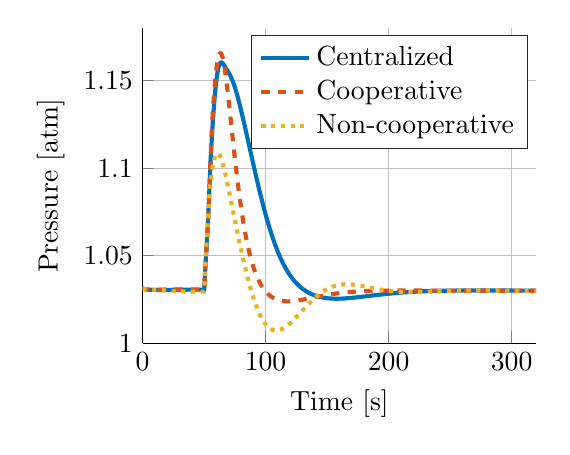
\begin{tikzpicture}

\begin{axis}[%
width=5cm,
height=4cm,
at={(0\linewidth,0\linewidth)},
scale only axis,
xmin=0,
xmax=320,
xlabel={Time [s]},
xmajorgrids,
ymin=1,
ymax=1.18,
ylabel={Pressure [atm]},
ymajorgrids,
axis background/.style={fill=white},
% title style={font=\bfseries},
% title={Tank Output Pressure},
axis x line*=bottom,
axis y line*=left,
legend style={legend cell align=left,align=left,draw=white!15!black}
]
\addplot [color=mycolor1,solid,line width=1.5pt]
  table[row sep=crcr]{%
0	1.03\\
0.25	1.03084\\
0.5	1.03105\\
0.75	1.03093\\
1	1.03093\\
1.25	1.03094\\
1.5	1.03091\\
1.75	1.03087\\
2	1.03084\\
2.25	1.03081\\
2.5	1.03079\\
2.75	1.03076\\
3	1.03074\\
3.25	1.03072\\
3.5	1.0307\\
3.75	1.03068\\
4	1.03066\\
4.25	1.03064\\
4.5	1.03062\\
4.75	1.03061\\
5	1.03059\\
5.25	1.03058\\
5.5	1.03057\\
5.75	1.03055\\
6	1.03054\\
6.25	1.03053\\
6.5	1.03052\\
6.75	1.03051\\
7	1.03051\\
7.25	1.0305\\
7.5	1.03049\\
7.75	1.03048\\
8	1.03048\\
8.25	1.03047\\
8.5	1.03046\\
8.75	1.03046\\
9	1.03045\\
9.25	1.03045\\
9.5	1.03045\\
9.75	1.03044\\
10	1.03044\\
10.25	1.03043\\
10.5	1.03043\\
10.75	1.03043\\
11	1.03043\\
11.25	1.03042\\
11.5	1.03042\\
11.75	1.03042\\
12	1.03042\\
12.25	1.03042\\
12.5	1.03042\\
12.75	1.03042\\
13	1.03042\\
13.25	1.03042\\
13.5	1.03042\\
13.75	1.03041\\
14	1.03042\\
14.25	1.03042\\
14.5	1.03042\\
14.75	1.03042\\
15	1.03042\\
15.25	1.03042\\
15.5	1.03042\\
15.75	1.03042\\
16	1.03042\\
16.25	1.03042\\
16.5	1.03042\\
16.75	1.03042\\
17	1.03043\\
17.25	1.03043\\
17.5	1.03043\\
17.75	1.03043\\
18	1.03043\\
18.25	1.03043\\
18.5	1.03044\\
18.75	1.03044\\
19	1.03044\\
19.25	1.03044\\
19.5	1.03045\\
19.75	1.03045\\
20	1.03045\\
20.25	1.03045\\
20.5	1.03046\\
20.75	1.03046\\
21	1.03046\\
21.25	1.03046\\
21.5	1.03047\\
21.75	1.03047\\
22	1.03047\\
22.25	1.03047\\
22.5	1.03048\\
22.75	1.03048\\
23	1.03048\\
23.25	1.03049\\
23.5	1.03049\\
23.75	1.03049\\
24	1.03049\\
24.25	1.0305\\
24.5	1.0305\\
24.75	1.0305\\
25	1.0305\\
25.25	1.03051\\
25.5	1.03051\\
25.75	1.03051\\
26	1.03051\\
26.25	1.03052\\
26.5	1.03052\\
26.75	1.03052\\
27	1.03052\\
27.25	1.03053\\
27.5	1.03053\\
27.75	1.03053\\
28	1.03053\\
28.25	1.03054\\
28.5	1.03054\\
28.75	1.03054\\
29	1.03054\\
29.25	1.03054\\
29.5	1.03055\\
29.75	1.03055\\
30	1.03055\\
30.25	1.03055\\
30.5	1.03055\\
30.75	1.03056\\
31	1.03056\\
31.25	1.03056\\
31.5	1.03056\\
31.75	1.03056\\
32	1.03057\\
32.25	1.03057\\
32.5	1.03057\\
32.75	1.03057\\
33	1.03057\\
33.25	1.03057\\
33.5	1.03057\\
33.75	1.03057\\
34	1.03058\\
34.25	1.03058\\
34.5	1.03058\\
34.75	1.03058\\
35	1.03058\\
35.25	1.03058\\
35.5	1.03058\\
35.75	1.03058\\
36	1.03058\\
36.25	1.03059\\
36.5	1.03059\\
36.75	1.03059\\
37	1.03059\\
37.25	1.03059\\
37.5	1.03059\\
37.75	1.03059\\
38	1.03059\\
38.25	1.03059\\
38.5	1.03059\\
38.75	1.03059\\
39	1.03059\\
39.25	1.03059\\
39.5	1.03059\\
39.75	1.03059\\
40	1.03059\\
40.25	1.03059\\
40.5	1.03059\\
40.75	1.0306\\
41	1.0306\\
41.25	1.0306\\
41.5	1.0306\\
41.75	1.0306\\
42	1.0306\\
42.25	1.0306\\
42.5	1.0306\\
42.75	1.0306\\
43	1.0306\\
43.25	1.0306\\
43.5	1.0306\\
43.75	1.0306\\
44	1.0306\\
44.25	1.0306\\
44.5	1.0306\\
44.75	1.0306\\
45	1.0306\\
45.25	1.03059\\
45.5	1.03059\\
45.75	1.03059\\
46	1.03059\\
46.25	1.03059\\
46.5	1.03059\\
46.75	1.03059\\
47	1.03059\\
47.25	1.03059\\
47.5	1.03059\\
47.75	1.03059\\
48	1.03059\\
48.25	1.03059\\
48.5	1.03059\\
48.75	1.03059\\
49	1.03059\\
49.25	1.03059\\
49.5	1.03059\\
49.75	1.03059\\
50	1.03059\\
50.25	1.03103\\
50.5	1.03504\\
50.75	1.0398\\
51	1.04245\\
51.25	1.04553\\
51.5	1.04912\\
51.75	1.05206\\
52	1.0547\\
52.25	1.0574\\
52.5	1.06051\\
52.75	1.06393\\
53	1.06686\\
53.25	1.0703\\
53.5	1.07423\\
53.75	1.07821\\
54	1.08238\\
54.25	1.08671\\
54.5	1.09105\\
54.75	1.09533\\
55	1.09951\\
55.25	1.10362\\
55.5	1.1072\\
55.75	1.10975\\
56	1.11291\\
56.25	1.11634\\
56.5	1.11944\\
56.75	1.12233\\
57	1.1251\\
57.25	1.12779\\
57.5	1.13037\\
57.75	1.13279\\
58	1.13511\\
58.25	1.13736\\
58.5	1.1395\\
58.75	1.14154\\
59	1.14346\\
59.25	1.14528\\
59.5	1.14698\\
59.75	1.14858\\
60	1.15007\\
60.25	1.15145\\
60.5	1.15272\\
60.75	1.15389\\
61	1.15496\\
61.25	1.15592\\
61.5	1.15678\\
61.75	1.15755\\
62	1.15822\\
62.25	1.15879\\
62.5	1.15927\\
62.75	1.15967\\
63	1.15998\\
63.25	1.16022\\
63.5	1.16038\\
63.75	1.16047\\
64	1.16049\\
64.25	1.16046\\
64.5	1.16038\\
64.75	1.16025\\
65	1.16008\\
65.25	1.15988\\
65.5	1.15965\\
65.75	1.1594\\
66	1.15913\\
66.25	1.15884\\
66.5	1.15855\\
66.75	1.15825\\
67	1.15795\\
67.25	1.15766\\
67.5	1.15736\\
67.75	1.15706\\
68	1.15677\\
68.25	1.15649\\
68.5	1.1562\\
68.75	1.15592\\
69	1.15564\\
69.25	1.15536\\
69.5	1.15507\\
69.75	1.15479\\
70	1.15449\\
70.25	1.15419\\
70.5	1.15389\\
70.75	1.15357\\
71	1.15325\\
71.25	1.15291\\
71.5	1.15256\\
71.75	1.1522\\
72	1.15183\\
72.25	1.15145\\
72.5	1.15105\\
72.75	1.15064\\
73	1.15021\\
73.25	1.14977\\
73.5	1.14931\\
73.75	1.14884\\
74	1.14836\\
74.25	1.14786\\
74.5	1.14735\\
74.75	1.14683\\
75	1.14629\\
75.25	1.14574\\
75.5	1.14517\\
75.75	1.1446\\
76	1.14401\\
76.25	1.14341\\
76.5	1.1428\\
76.75	1.14218\\
77	1.14155\\
77.25	1.14091\\
77.5	1.14026\\
77.75	1.1396\\
78	1.13893\\
78.25	1.13826\\
78.5	1.13758\\
78.75	1.13689\\
79	1.13619\\
79.25	1.13549\\
79.5	1.13478\\
79.75	1.13406\\
80	1.13334\\
80.25	1.13261\\
80.5	1.13188\\
80.75	1.13114\\
81	1.1304\\
81.25	1.12966\\
81.5	1.12891\\
81.75	1.12816\\
82	1.1274\\
82.25	1.12664\\
82.5	1.12588\\
82.75	1.12511\\
83	1.12434\\
83.25	1.12357\\
83.5	1.1228\\
83.75	1.12202\\
84	1.12124\\
84.25	1.12046\\
84.5	1.11968\\
84.75	1.1189\\
85	1.11812\\
85.25	1.11733\\
85.5	1.11654\\
85.75	1.11576\\
86	1.11497\\
86.25	1.11418\\
86.5	1.11339\\
86.75	1.1126\\
87	1.11181\\
87.25	1.11103\\
87.5	1.11024\\
87.75	1.10945\\
88	1.10866\\
88.25	1.10787\\
88.5	1.10709\\
88.75	1.1063\\
89	1.10552\\
89.25	1.10473\\
89.5	1.10395\\
89.75	1.10317\\
90	1.10239\\
90.25	1.10162\\
90.5	1.10084\\
90.75	1.10007\\
91	1.09929\\
91.25	1.09853\\
91.5	1.09776\\
91.75	1.09699\\
92	1.09623\\
92.25	1.09547\\
92.5	1.09471\\
92.75	1.09396\\
93	1.09321\\
93.25	1.09246\\
93.5	1.09171\\
93.75	1.09097\\
94	1.09023\\
94.25	1.0895\\
94.5	1.08877\\
94.75	1.08804\\
95	1.08731\\
95.25	1.08659\\
95.5	1.08587\\
95.75	1.08516\\
96	1.08445\\
96.25	1.08374\\
96.5	1.08304\\
96.75	1.08234\\
97	1.08165\\
97.25	1.08096\\
97.5	1.08027\\
97.75	1.07959\\
98	1.07892\\
98.25	1.07824\\
98.5	1.07758\\
98.75	1.07691\\
99	1.07626\\
99.25	1.0756\\
99.5	1.07495\\
99.75	1.07431\\
100	1.07367\\
100.25	1.07303\\
100.5	1.07241\\
100.75	1.07178\\
101	1.07116\\
101.25	1.07054\\
101.5	1.06993\\
101.75	1.06933\\
102	1.06873\\
102.25	1.06813\\
102.5	1.06754\\
102.75	1.06696\\
103	1.06638\\
103.25	1.0658\\
103.5	1.06523\\
103.75	1.06467\\
104	1.06411\\
104.25	1.06355\\
104.5	1.06301\\
104.75	1.06246\\
105	1.06192\\
105.25	1.06139\\
105.5	1.06086\\
105.75	1.06034\\
106	1.05982\\
106.25	1.0593\\
106.5	1.0588\\
106.75	1.05829\\
107	1.0578\\
107.25	1.0573\\
107.5	1.05682\\
107.75	1.05633\\
108	1.05586\\
108.25	1.05539\\
108.5	1.05492\\
108.75	1.05446\\
109	1.054\\
109.25	1.05355\\
109.5	1.0531\\
109.75	1.05266\\
110	1.05223\\
110.25	1.05179\\
110.5	1.05137\\
110.75	1.05095\\
111	1.05053\\
111.25	1.05012\\
111.5	1.04971\\
111.75	1.04931\\
112	1.04892\\
112.25	1.04853\\
112.5	1.04814\\
112.75	1.04776\\
113	1.04738\\
113.25	1.04701\\
113.5	1.04664\\
113.75	1.04628\\
114	1.04592\\
114.25	1.04557\\
114.5	1.04522\\
114.75	1.04487\\
115	1.04454\\
115.25	1.0442\\
115.5	1.04387\\
115.75	1.04354\\
116	1.04322\\
116.25	1.04291\\
116.5	1.04259\\
116.75	1.04229\\
117	1.04198\\
117.25	1.04168\\
117.5	1.04139\\
117.75	1.0411\\
118	1.04081\\
118.25	1.04053\\
118.5	1.04025\\
118.75	1.03997\\
119	1.0397\\
119.25	1.03944\\
119.5	1.03917\\
119.75	1.03891\\
120	1.03866\\
120.25	1.03841\\
120.5	1.03816\\
120.75	1.03792\\
121	1.03768\\
121.25	1.03744\\
121.5	1.03721\\
121.75	1.03698\\
122	1.03675\\
122.25	1.03653\\
122.5	1.03631\\
122.75	1.0361\\
123	1.03588\\
123.25	1.03567\\
123.5	1.03547\\
123.75	1.03527\\
124	1.03507\\
124.25	1.03487\\
124.5	1.03468\\
124.75	1.03449\\
125	1.0343\\
125.25	1.03412\\
125.5	1.03394\\
125.75	1.03376\\
126	1.03358\\
126.25	1.03341\\
126.5	1.03324\\
126.75	1.03307\\
127	1.03291\\
127.25	1.03275\\
127.5	1.03259\\
127.75	1.03243\\
128	1.03228\\
128.25	1.03213\\
128.5	1.03198\\
128.75	1.03183\\
129	1.03169\\
129.25	1.03154\\
129.5	1.03141\\
129.75	1.03127\\
130	1.03113\\
130.25	1.031\\
130.5	1.03087\\
130.75	1.03074\\
131	1.03062\\
131.25	1.03049\\
131.5	1.03037\\
131.75	1.03025\\
132	1.03013\\
132.25	1.03002\\
132.5	1.02991\\
132.75	1.02979\\
133	1.02969\\
133.25	1.02958\\
133.5	1.02947\\
133.75	1.02937\\
134	1.02927\\
134.25	1.02917\\
134.5	1.02907\\
134.75	1.02897\\
135	1.02888\\
135.25	1.02878\\
135.5	1.02869\\
135.75	1.0286\\
136	1.02851\\
136.25	1.02843\\
136.5	1.02834\\
136.75	1.02826\\
137	1.02818\\
137.25	1.0281\\
137.5	1.02802\\
137.75	1.02794\\
138	1.02787\\
138.25	1.02779\\
138.5	1.02772\\
138.75	1.02765\\
139	1.02758\\
139.25	1.02751\\
139.5	1.02745\\
139.75	1.02738\\
140	1.02732\\
140.25	1.02726\\
140.5	1.02719\\
140.75	1.02713\\
141	1.02708\\
141.25	1.02702\\
141.5	1.02696\\
141.75	1.02691\\
142	1.02685\\
142.25	1.0268\\
142.5	1.02675\\
142.75	1.0267\\
143	1.02665\\
143.25	1.0266\\
143.5	1.02656\\
143.75	1.02651\\
144	1.02647\\
144.25	1.02643\\
144.5	1.02638\\
144.75	1.02634\\
145	1.0263\\
145.25	1.02627\\
145.5	1.02623\\
145.75	1.02619\\
146	1.02616\\
146.25	1.02612\\
146.5	1.02609\\
146.75	1.02606\\
147	1.02602\\
147.25	1.02599\\
147.5	1.02596\\
147.75	1.02593\\
148	1.02591\\
148.25	1.02588\\
148.5	1.02585\\
148.75	1.02583\\
149	1.0258\\
149.25	1.02578\\
149.5	1.02576\\
149.75	1.02574\\
150	1.02572\\
150.25	1.0257\\
150.5	1.02568\\
150.75	1.02566\\
151	1.02564\\
151.25	1.02562\\
151.5	1.02561\\
151.75	1.02559\\
152	1.02558\\
152.25	1.02556\\
152.5	1.02555\\
152.75	1.02554\\
153	1.02553\\
153.25	1.02552\\
153.5	1.02551\\
153.75	1.0255\\
154	1.02549\\
154.25	1.02548\\
154.5	1.02547\\
154.75	1.02546\\
155	1.02546\\
155.25	1.02545\\
155.5	1.02545\\
155.75	1.02544\\
156	1.02544\\
156.25	1.02543\\
156.5	1.02543\\
156.75	1.02543\\
157	1.02543\\
157.25	1.02543\\
157.5	1.02542\\
157.75	1.02542\\
158	1.02542\\
158.25	1.02543\\
158.5	1.02543\\
158.75	1.02543\\
159	1.02543\\
159.25	1.02543\\
159.5	1.02544\\
159.75	1.02544\\
160	1.02544\\
160.25	1.02545\\
160.5	1.02545\\
160.75	1.02546\\
161	1.02546\\
161.25	1.02547\\
161.5	1.02548\\
161.75	1.02548\\
162	1.02549\\
162.25	1.0255\\
162.5	1.02551\\
162.75	1.02552\\
163	1.02553\\
163.25	1.02553\\
163.5	1.02554\\
163.75	1.02555\\
164	1.02556\\
164.25	1.02558\\
164.5	1.02559\\
164.75	1.0256\\
165	1.02561\\
165.25	1.02562\\
165.5	1.02563\\
165.75	1.02564\\
166	1.02566\\
166.25	1.02567\\
166.5	1.02568\\
166.75	1.0257\\
167	1.02571\\
167.25	1.02573\\
167.5	1.02574\\
167.75	1.02575\\
168	1.02577\\
168.25	1.02578\\
168.5	1.0258\\
168.75	1.02581\\
169	1.02583\\
169.25	1.02585\\
169.5	1.02586\\
169.75	1.02588\\
170	1.02589\\
170.25	1.02591\\
170.5	1.02593\\
170.75	1.02594\\
171	1.02596\\
171.25	1.02598\\
171.5	1.026\\
171.75	1.02601\\
172	1.02603\\
172.25	1.02605\\
172.5	1.02607\\
172.75	1.02609\\
173	1.02611\\
173.25	1.02612\\
173.5	1.02614\\
173.75	1.02616\\
174	1.02618\\
174.25	1.0262\\
174.5	1.02622\\
174.75	1.02624\\
175	1.02626\\
175.25	1.02628\\
175.5	1.0263\\
175.75	1.02632\\
176	1.02634\\
176.25	1.02636\\
176.5	1.02638\\
176.75	1.0264\\
177	1.02642\\
177.25	1.02644\\
177.5	1.02646\\
177.75	1.02648\\
178	1.0265\\
178.25	1.02652\\
178.5	1.02654\\
178.75	1.02656\\
179	1.02658\\
179.25	1.0266\\
179.5	1.02662\\
179.75	1.02664\\
180	1.02666\\
180.25	1.02668\\
180.5	1.0267\\
180.75	1.02672\\
181	1.02675\\
181.25	1.02677\\
181.5	1.02679\\
181.75	1.02681\\
182	1.02683\\
182.25	1.02685\\
182.5	1.02687\\
182.75	1.02689\\
183	1.02691\\
183.25	1.02694\\
183.5	1.02696\\
183.75	1.02698\\
184	1.027\\
184.25	1.02702\\
184.5	1.02704\\
184.75	1.02706\\
185	1.02708\\
185.25	1.0271\\
185.5	1.02713\\
185.75	1.02715\\
186	1.02717\\
186.25	1.02719\\
186.5	1.02721\\
186.75	1.02723\\
187	1.02725\\
187.25	1.02727\\
187.5	1.02729\\
187.75	1.02731\\
188	1.02733\\
188.25	1.02736\\
188.5	1.02738\\
188.75	1.0274\\
189	1.02742\\
189.25	1.02744\\
189.5	1.02746\\
189.75	1.02748\\
190	1.0275\\
190.25	1.02752\\
190.5	1.02754\\
190.75	1.02756\\
191	1.02758\\
191.25	1.0276\\
191.5	1.02762\\
191.75	1.02764\\
192	1.02766\\
192.25	1.02768\\
192.5	1.0277\\
192.75	1.02772\\
193	1.02774\\
193.25	1.02776\\
193.5	1.02778\\
193.75	1.0278\\
194	1.02782\\
194.25	1.02784\\
194.5	1.02786\\
194.75	1.02788\\
195	1.0279\\
195.25	1.02792\\
195.5	1.02794\\
195.75	1.02795\\
196	1.02797\\
196.25	1.02799\\
196.5	1.02801\\
196.75	1.02803\\
197	1.02805\\
197.25	1.02807\\
197.5	1.02809\\
197.75	1.0281\\
198	1.02812\\
198.25	1.02814\\
198.5	1.02816\\
198.75	1.02818\\
199	1.0282\\
199.25	1.02821\\
199.5	1.02823\\
199.75	1.02825\\
200	1.02827\\
200.25	1.02828\\
200.5	1.0283\\
200.75	1.02832\\
201	1.02834\\
201.25	1.02835\\
201.5	1.02837\\
201.75	1.02839\\
202	1.0284\\
202.25	1.02842\\
202.5	1.02844\\
202.75	1.02845\\
203	1.02847\\
203.25	1.02849\\
203.5	1.0285\\
203.75	1.02852\\
204	1.02854\\
204.25	1.02855\\
204.5	1.02857\\
204.75	1.02858\\
205	1.0286\\
205.25	1.02862\\
205.5	1.02863\\
205.75	1.02865\\
206	1.02866\\
206.25	1.02868\\
206.5	1.02869\\
206.75	1.02871\\
207	1.02872\\
207.25	1.02874\\
207.5	1.02875\\
207.75	1.02877\\
208	1.02878\\
208.25	1.0288\\
208.5	1.02881\\
208.75	1.02883\\
209	1.02884\\
209.25	1.02885\\
209.5	1.02887\\
209.75	1.02888\\
210	1.0289\\
210.25	1.02891\\
210.5	1.02892\\
210.75	1.02894\\
211	1.02895\\
211.25	1.02896\\
211.5	1.02898\\
211.75	1.02899\\
212	1.029\\
212.25	1.02902\\
212.5	1.02903\\
212.75	1.02904\\
213	1.02905\\
213.25	1.02907\\
213.5	1.02908\\
213.75	1.02909\\
214	1.0291\\
214.25	1.02912\\
214.5	1.02913\\
214.75	1.02914\\
215	1.02915\\
215.25	1.02916\\
215.5	1.02918\\
215.75	1.02919\\
216	1.0292\\
216.25	1.02921\\
216.5	1.02922\\
216.75	1.02923\\
217	1.02924\\
217.25	1.02926\\
217.5	1.02927\\
217.75	1.02928\\
218	1.02929\\
218.25	1.0293\\
218.5	1.02931\\
218.75	1.02932\\
219	1.02933\\
219.25	1.02934\\
219.5	1.02935\\
219.75	1.02936\\
220	1.02937\\
220.25	1.02938\\
220.5	1.02939\\
220.75	1.0294\\
221	1.02941\\
221.25	1.02942\\
221.5	1.02943\\
221.75	1.02944\\
222	1.02945\\
222.25	1.02946\\
222.5	1.02947\\
222.75	1.02947\\
223	1.02948\\
223.25	1.02949\\
223.5	1.0295\\
223.75	1.02951\\
224	1.02952\\
224.25	1.02953\\
224.5	1.02954\\
224.75	1.02954\\
225	1.02955\\
225.25	1.02956\\
225.5	1.02957\\
225.75	1.02958\\
226	1.02958\\
226.25	1.02959\\
226.5	1.0296\\
226.75	1.02961\\
227	1.02962\\
227.25	1.02962\\
227.5	1.02963\\
227.75	1.02964\\
228	1.02965\\
228.25	1.02965\\
228.5	1.02966\\
228.75	1.02967\\
229	1.02967\\
229.25	1.02968\\
229.5	1.02969\\
229.75	1.02969\\
230	1.0297\\
230.25	1.02971\\
230.5	1.02971\\
230.75	1.02972\\
231	1.02973\\
231.25	1.02973\\
231.5	1.02974\\
231.75	1.02975\\
232	1.02975\\
232.25	1.02976\\
232.5	1.02976\\
232.75	1.02977\\
233	1.02978\\
233.25	1.02978\\
233.5	1.02979\\
233.75	1.02979\\
234	1.0298\\
234.25	1.0298\\
234.5	1.02981\\
234.75	1.02981\\
235	1.02982\\
235.25	1.02983\\
235.5	1.02983\\
235.75	1.02984\\
236	1.02984\\
236.25	1.02985\\
236.5	1.02985\\
236.75	1.02986\\
237	1.02986\\
237.25	1.02986\\
237.5	1.02987\\
237.75	1.02987\\
238	1.02988\\
238.25	1.02988\\
238.5	1.02989\\
238.75	1.02989\\
239	1.0299\\
239.25	1.0299\\
239.5	1.0299\\
239.75	1.02991\\
240	1.02991\\
240.25	1.02992\\
240.5	1.02992\\
240.75	1.02992\\
241	1.02993\\
241.25	1.02993\\
241.5	1.02994\\
241.75	1.02994\\
242	1.02994\\
242.25	1.02995\\
242.5	1.02995\\
242.75	1.02995\\
243	1.02996\\
243.25	1.02996\\
243.5	1.02996\\
243.75	1.02997\\
244	1.02997\\
244.25	1.02997\\
244.5	1.02998\\
244.75	1.02998\\
245	1.02998\\
245.25	1.02999\\
245.5	1.02999\\
245.75	1.02999\\
246	1.02999\\
246.25	1.03\\
246.5	1.03\\
246.75	1.03\\
247	1.03001\\
247.25	1.03001\\
247.5	1.03001\\
247.75	1.03001\\
248	1.03002\\
248.25	1.03002\\
248.5	1.03002\\
248.75	1.03002\\
249	1.03002\\
249.25	1.03003\\
249.5	1.03003\\
249.75	1.03003\\
250	1.03003\\
250.25	1.03004\\
250.5	1.03004\\
250.75	1.03004\\
251	1.03004\\
251.25	1.03004\\
251.5	1.03005\\
251.75	1.03005\\
252	1.03005\\
252.25	1.03005\\
252.5	1.03005\\
252.75	1.03005\\
253	1.03006\\
253.25	1.03006\\
253.5	1.03006\\
253.75	1.03006\\
254	1.03006\\
254.25	1.03006\\
254.5	1.03007\\
254.75	1.03007\\
255	1.03007\\
255.25	1.03007\\
255.5	1.03007\\
255.75	1.03007\\
256	1.03007\\
256.25	1.03008\\
256.5	1.03008\\
256.75	1.03008\\
257	1.03008\\
257.25	1.03008\\
257.5	1.03008\\
257.75	1.03008\\
258	1.03008\\
258.25	1.03009\\
258.5	1.03009\\
258.75	1.03009\\
259	1.03009\\
259.25	1.03009\\
259.5	1.03009\\
259.75	1.03009\\
260	1.03009\\
260.25	1.03009\\
260.5	1.03009\\
260.75	1.03009\\
261	1.0301\\
261.25	1.0301\\
261.5	1.0301\\
261.75	1.0301\\
262	1.0301\\
262.25	1.0301\\
262.5	1.0301\\
262.75	1.0301\\
263	1.0301\\
263.25	1.0301\\
263.5	1.0301\\
263.75	1.0301\\
264	1.0301\\
264.25	1.0301\\
264.5	1.0301\\
264.75	1.0301\\
265	1.0301\\
265.25	1.0301\\
265.5	1.03011\\
265.75	1.03011\\
266	1.03011\\
266.25	1.03011\\
266.5	1.03011\\
266.75	1.03011\\
267	1.03011\\
267.25	1.03011\\
267.5	1.03011\\
267.75	1.03011\\
268	1.03011\\
268.25	1.03011\\
268.5	1.03011\\
268.75	1.03011\\
269	1.03011\\
269.25	1.03011\\
269.5	1.03011\\
269.75	1.03011\\
270	1.03011\\
270.25	1.03011\\
270.5	1.03011\\
270.75	1.03011\\
271	1.03011\\
271.25	1.03011\\
271.5	1.03011\\
271.75	1.03011\\
272	1.03011\\
272.25	1.03011\\
272.5	1.03011\\
272.75	1.03011\\
273	1.03011\\
273.25	1.03011\\
273.5	1.03011\\
273.75	1.03011\\
274	1.03011\\
274.25	1.03011\\
274.5	1.03011\\
274.75	1.03011\\
275	1.03011\\
275.25	1.03011\\
275.5	1.03011\\
275.75	1.03011\\
276	1.03011\\
276.25	1.03011\\
276.5	1.03011\\
276.75	1.03011\\
277	1.03011\\
277.25	1.03011\\
277.5	1.03011\\
277.75	1.03011\\
278	1.03011\\
278.25	1.03011\\
278.5	1.03011\\
278.75	1.03011\\
279	1.0301\\
279.25	1.0301\\
279.5	1.0301\\
279.75	1.0301\\
280	1.0301\\
280.25	1.0301\\
280.5	1.0301\\
280.75	1.0301\\
281	1.0301\\
281.25	1.0301\\
281.5	1.0301\\
281.75	1.0301\\
282	1.0301\\
282.25	1.0301\\
282.5	1.0301\\
282.75	1.0301\\
283	1.0301\\
283.25	1.0301\\
283.5	1.0301\\
283.75	1.0301\\
284	1.0301\\
284.25	1.0301\\
284.5	1.0301\\
284.75	1.0301\\
285	1.0301\\
285.25	1.0301\\
285.5	1.03009\\
285.75	1.03009\\
286	1.03009\\
286.25	1.03009\\
286.5	1.03009\\
286.75	1.03009\\
287	1.03009\\
287.25	1.03009\\
287.5	1.03009\\
287.75	1.03009\\
288	1.03009\\
288.25	1.03009\\
288.5	1.03009\\
288.75	1.03009\\
289	1.03009\\
289.25	1.03009\\
289.5	1.03009\\
289.75	1.03009\\
290	1.03009\\
290.25	1.03009\\
290.5	1.03009\\
290.75	1.03009\\
291	1.03008\\
291.25	1.03008\\
291.5	1.03008\\
291.75	1.03008\\
292	1.03008\\
292.25	1.03008\\
292.5	1.03008\\
292.75	1.03008\\
293	1.03008\\
293.25	1.03008\\
293.5	1.03008\\
293.75	1.03008\\
294	1.03008\\
294.25	1.03008\\
294.5	1.03008\\
294.75	1.03008\\
295	1.03008\\
295.25	1.03008\\
295.5	1.03008\\
295.75	1.03007\\
296	1.03007\\
296.25	1.03007\\
296.5	1.03007\\
296.75	1.03007\\
297	1.03007\\
297.25	1.03007\\
297.5	1.03007\\
297.75	1.03007\\
298	1.03007\\
298.25	1.03007\\
298.5	1.03007\\
298.75	1.03007\\
299	1.03007\\
299.25	1.03007\\
299.5	1.03007\\
299.75	1.03007\\
300	1.03007\\
300.25	1.03007\\
300.5	1.03007\\
300.75	1.03006\\
301	1.03006\\
301.25	1.03006\\
301.5	1.03006\\
301.75	1.03006\\
302	1.03006\\
302.25	1.03006\\
302.5	1.03006\\
302.75	1.03006\\
303	1.03006\\
303.25	1.03006\\
303.5	1.03006\\
303.75	1.03006\\
304	1.03006\\
304.25	1.03006\\
304.5	1.03006\\
304.75	1.03006\\
305	1.03006\\
305.25	1.03006\\
305.5	1.03006\\
305.75	1.03005\\
306	1.03005\\
306.25	1.03005\\
306.5	1.03005\\
306.75	1.03005\\
307	1.03005\\
307.25	1.03005\\
307.5	1.03005\\
307.75	1.03005\\
308	1.03005\\
308.25	1.03005\\
308.5	1.03005\\
308.75	1.03005\\
309	1.03005\\
309.25	1.03005\\
309.5	1.03005\\
309.75	1.03005\\
310	1.03005\\
310.25	1.03005\\
310.5	1.03005\\
310.75	1.03005\\
311	1.03004\\
311.25	1.03004\\
311.5	1.03004\\
311.75	1.03004\\
312	1.03004\\
312.25	1.03004\\
312.5	1.03004\\
312.75	1.03004\\
313	1.03004\\
313.25	1.03004\\
313.5	1.03004\\
313.75	1.03004\\
314	1.03004\\
314.25	1.03004\\
314.5	1.03004\\
314.75	1.03004\\
315	1.03004\\
315.25	1.03004\\
315.5	1.03004\\
315.75	1.03004\\
316	1.03004\\
316.25	1.03004\\
316.5	1.03004\\
316.75	1.03004\\
317	1.03003\\
317.25	1.03003\\
317.5	1.03003\\
317.75	1.03003\\
318	1.03003\\
318.25	1.03003\\
318.5	1.03003\\
318.75	1.03003\\
319	1.03003\\
319.25	1.03003\\
319.5	1.03003\\
319.75	1.03003\\
320	1.03003\\
320.25	1.03003\\
320.5	1.03003\\
320.75	1.03003\\
321	1.03003\\
321.25	1.03003\\
321.5	1.03003\\
321.75	1.03003\\
322	1.03003\\
322.25	1.03003\\
322.5	1.03003\\
322.75	1.03003\\
323	1.03003\\
323.25	1.03003\\
323.5	1.03003\\
323.75	1.03003\\
324	1.03002\\
324.25	1.03002\\
324.5	1.03002\\
324.75	1.03002\\
325	1.03002\\
325.25	1.03002\\
325.5	1.03002\\
325.75	1.03002\\
326	1.03002\\
326.25	1.03002\\
326.5	1.03002\\
326.75	1.03002\\
327	1.03002\\
327.25	1.03002\\
327.5	1.03002\\
327.75	1.03002\\
328	1.03002\\
328.25	1.03002\\
328.5	1.03002\\
328.75	1.03002\\
329	1.03002\\
329.25	1.03002\\
329.5	1.03002\\
329.75	1.03002\\
330	1.03002\\
330.25	1.03002\\
330.5	1.03002\\
330.75	1.03002\\
331	1.03002\\
331.25	1.03002\\
331.5	1.03002\\
331.75	1.03002\\
332	1.03002\\
332.25	1.03002\\
332.5	1.03002\\
332.75	1.03001\\
333	1.03001\\
333.25	1.03001\\
333.5	1.03001\\
333.75	1.03001\\
334	1.03001\\
334.25	1.03001\\
334.5	1.03001\\
334.75	1.03001\\
335	1.03001\\
335.25	1.03001\\
335.5	1.03001\\
335.75	1.03001\\
336	1.03001\\
336.25	1.03001\\
336.5	1.03001\\
336.75	1.03001\\
337	1.03001\\
337.25	1.03001\\
337.5	1.03001\\
337.75	1.03001\\
338	1.03001\\
338.25	1.03001\\
338.5	1.03001\\
338.75	1.03001\\
339	1.03001\\
339.25	1.03001\\
339.5	1.03001\\
339.75	1.03001\\
340	1.03001\\
340.25	1.03001\\
340.5	1.03001\\
340.75	1.03001\\
341	1.03001\\
341.25	1.03001\\
341.5	1.03001\\
341.75	1.03001\\
342	1.03001\\
342.25	1.03001\\
342.5	1.03001\\
342.75	1.03001\\
343	1.03001\\
343.25	1.03001\\
343.5	1.03001\\
343.75	1.03001\\
344	1.03001\\
344.25	1.03001\\
344.5	1.03001\\
344.75	1.03001\\
345	1.03001\\
345.25	1.03001\\
345.5	1.03001\\
345.75	1.03001\\
346	1.03001\\
346.25	1.03\\
346.5	1.03\\
346.75	1.03\\
347	1.03\\
347.25	1.03\\
347.5	1.03\\
347.75	1.03\\
348	1.03\\
348.25	1.03\\
348.5	1.03\\
348.75	1.03\\
349	1.03\\
349.25	1.03\\
349.5	1.03\\
349.75	1.03\\
350	1.03\\
350.25	1.03\\
350.5	1.03\\
350.75	1.03\\
351	1.03\\
351.25	1.03\\
351.5	1.03\\
351.75	1.03\\
352	1.03\\
352.25	1.03\\
352.5	1.03\\
352.75	1.03\\
353	1.03\\
353.25	1.03\\
353.5	1.03\\
353.75	1.03\\
354	1.03\\
354.25	1.03\\
354.5	1.03\\
354.75	1.03\\
355	1.03\\
355.25	1.03\\
355.5	1.03\\
355.75	1.03\\
356	1.03\\
356.25	1.03\\
356.5	1.03\\
356.75	1.03\\
357	1.03\\
357.25	1.03\\
357.5	1.03\\
357.75	1.03\\
358	1.03\\
358.25	1.03\\
358.5	1.03\\
358.75	1.03\\
359	1.03\\
359.25	1.03\\
359.5	1.03\\
359.75	1.03\\
360	1.03\\
360.25	1.03\\
360.5	1.03\\
360.75	1.03\\
361	1.03\\
361.25	1.03\\
361.5	1.03\\
361.75	1.03\\
362	1.03\\
362.25	1.03\\
362.5	1.03\\
362.75	1.03\\
363	1.03\\
363.25	1.03\\
363.5	1.03\\
363.75	1.03\\
364	1.03\\
364.25	1.03\\
364.5	1.03\\
364.75	1.03\\
365	1.03\\
365.25	1.03\\
365.5	1.03\\
365.75	1.03\\
366	1.03\\
366.25	1.03\\
366.5	1.03\\
366.75	1.03\\
367	1.03\\
367.25	1.03\\
367.5	1.03\\
367.75	1.03\\
368	1.03\\
368.25	1.03\\
368.5	1.03\\
368.75	1.03\\
369	1.03\\
369.25	1.03\\
369.5	1.03\\
369.75	1.03\\
370	1.03\\
370.25	1.03\\
370.5	1.03\\
370.75	1.03\\
371	1.03\\
371.25	1.03\\
371.5	1.03\\
371.75	1.03\\
372	1.03\\
372.25	1.03\\
372.5	1.03\\
372.75	1.03\\
373	1.03\\
373.25	1.03\\
373.5	1.03\\
373.75	1.03\\
374	1.03\\
374.25	1.03\\
374.5	1.03\\
374.75	1.03\\
375	1.03\\
375.25	1.03\\
375.5	1.03\\
375.75	1.03\\
376	1.03\\
376.25	1.03\\
376.5	1.03\\
376.75	1.03\\
377	1.03\\
377.25	1.03\\
377.5	1.03\\
377.75	1.03\\
378	1.03\\
378.25	1.03\\
378.5	1.03\\
378.75	1.03\\
379	1.03\\
379.25	1.03\\
379.5	1.03\\
379.75	1.03\\
380	1.03\\
380.25	1.03\\
380.5	1.03\\
380.75	1.03\\
381	1.03\\
381.25	1.03\\
381.5	1.03\\
381.75	1.03\\
382	1.03\\
382.25	1.03\\
382.5	1.03\\
382.75	1.03\\
383	1.03\\
383.25	1.03\\
383.5	1.03\\
383.75	1.03\\
384	1.03\\
384.25	1.03\\
384.5	1.03\\
384.75	1.03\\
385	1.03\\
385.25	1.03\\
385.5	1.03\\
385.75	1.03\\
386	1.03\\
386.25	1.03\\
386.5	1.03\\
386.75	1.03\\
387	1.03\\
387.25	1.03\\
387.5	1.03\\
387.75	1.03\\
388	1.03\\
388.25	1.03\\
388.5	1.03\\
388.75	1.03\\
389	1.03\\
389.25	1.03\\
389.5	1.03\\
389.75	1.03\\
390	1.03\\
390.25	1.03\\
390.5	1.03\\
390.75	1.03\\
391	1.03\\
391.25	1.03\\
391.5	1.03\\
391.75	1.03\\
392	1.03\\
392.25	1.03\\
392.5	1.03\\
392.75	1.03\\
393	1.03\\
393.25	1.03\\
393.5	1.03\\
393.75	1.03\\
394	1.03\\
394.25	1.03\\
394.5	1.03\\
394.75	1.03\\
395	1.03\\
395.25	1.03\\
395.5	1.03\\
395.75	1.03\\
396	1.03\\
396.25	1.03\\
396.5	1.03\\
396.75	1.03\\
397	1.03\\
397.25	1.03\\
397.5	1.03\\
397.75	1.03\\
398	1.03\\
398.25	1.03\\
398.5	1.03\\
398.75	1.03\\
399	1.03\\
399.25	1.03\\
399.5	1.03\\
399.75	1.03\\
400	1.03\\
400.25	1.03\\
400.5	1.03\\
400.75	1.03\\
401	1.03\\
401.25	1.03\\
401.5	1.03\\
401.75	1.03\\
402	1.03\\
402.25	1.03\\
402.5	1.03\\
402.75	1.03\\
403	1.03\\
403.25	1.03\\
403.5	1.03\\
403.75	1.03\\
404	1.03\\
404.25	1.03\\
404.5	1.03\\
404.75	1.03\\
405	1.03\\
405.25	1.03\\
405.5	1.03\\
405.75	1.03\\
406	1.03\\
406.25	1.03\\
406.5	1.03\\
406.75	1.03\\
407	1.03\\
407.25	1.03\\
407.5	1.03\\
407.75	1.03\\
408	1.03\\
408.25	1.03\\
408.5	1.03\\
408.75	1.03\\
409	1.03\\
409.25	1.03\\
409.5	1.03\\
409.75	1.03\\
410	1.03\\
410.25	1.03\\
410.5	1.03\\
410.75	1.03\\
411	1.03\\
411.25	1.03\\
411.5	1.03\\
411.75	1.03\\
412	1.03\\
412.25	1.03\\
412.5	1.03\\
412.75	1.03\\
413	1.03\\
413.25	1.03\\
413.5	1.03\\
413.75	1.03\\
414	1.03\\
414.25	1.03\\
414.5	1.03\\
414.75	1.03\\
415	1.03\\
415.25	1.03\\
415.5	1.03\\
415.75	1.03\\
416	1.03\\
416.25	1.03\\
416.5	1.03\\
416.75	1.03\\
417	1.03\\
417.25	1.03\\
417.5	1.03\\
417.75	1.03\\
418	1.03\\
418.25	1.03\\
418.5	1.03\\
418.75	1.03\\
419	1.03\\
419.25	1.03\\
419.5	1.03\\
419.75	1.03\\
420	1.03\\
420.25	1.03\\
420.5	1.03\\
420.75	1.03\\
421	1.03\\
421.25	1.03\\
421.5	1.03\\
421.75	1.03\\
422	1.03\\
422.25	1.03\\
422.5	1.03\\
422.75	1.03\\
423	1.03\\
423.25	1.03\\
423.5	1.03\\
423.75	1.03\\
424	1.03\\
424.25	1.03\\
424.5	1.03\\
424.75	1.03\\
425	1.03\\
425.25	1.03\\
425.5	1.03\\
425.75	1.03\\
426	1.03\\
426.25	1.03\\
426.5	1.03\\
426.75	1.03\\
427	1.03\\
427.25	1.03\\
427.5	1.03\\
427.75	1.03\\
428	1.03\\
428.25	1.03\\
428.5	1.03\\
428.75	1.03\\
429	1.03\\
429.25	1.03\\
429.5	1.03\\
429.75	1.03\\
430	1.03\\
430.25	1.03\\
430.5	1.03\\
430.75	1.03\\
431	1.03\\
431.25	1.03\\
431.5	1.03\\
431.75	1.03\\
432	1.03\\
432.25	1.03\\
432.5	1.03\\
432.75	1.03\\
433	1.03\\
433.25	1.03\\
433.5	1.03\\
433.75	1.03\\
434	1.03\\
434.25	1.03\\
434.5	1.03\\
434.75	1.03\\
435	1.03\\
435.25	1.03\\
435.5	1.03\\
435.75	1.03\\
436	1.03\\
436.25	1.03\\
436.5	1.03\\
436.75	1.03\\
437	1.03\\
437.25	1.03\\
437.5	1.03\\
437.75	1.03\\
438	1.03\\
438.25	1.03\\
438.5	1.03\\
438.75	1.03\\
439	1.03\\
439.25	1.03\\
439.5	1.03\\
439.75	1.03\\
440	1.03\\
440.25	1.03\\
440.5	1.03\\
440.75	1.03\\
441	1.03\\
441.25	1.03\\
441.5	1.03\\
441.75	1.03\\
442	1.03\\
442.25	1.03\\
442.5	1.03\\
442.75	1.03\\
443	1.03\\
443.25	1.03\\
443.5	1.03\\
443.75	1.03\\
444	1.03\\
444.25	1.03\\
444.5	1.03\\
444.75	1.03\\
445	1.03\\
445.25	1.03\\
445.5	1.03\\
445.75	1.03\\
446	1.03\\
446.25	1.03\\
446.5	1.03\\
446.75	1.03\\
447	1.03\\
447.25	1.03\\
447.5	1.03\\
447.75	1.03\\
448	1.03\\
448.25	1.03\\
448.5	1.03\\
448.75	1.03\\
449	1.03\\
449.25	1.03\\
449.5	1.03\\
449.75	1.03\\
450	1.03\\
450.25	1.03\\
450.5	1.03\\
450.75	1.03\\
451	1.03\\
451.25	1.03\\
451.5	1.03\\
451.75	1.03\\
452	1.03\\
452.25	1.03\\
452.5	1.03\\
452.75	1.03\\
453	1.03\\
453.25	1.03\\
453.5	1.03\\
453.75	1.03\\
454	1.03\\
454.25	1.03\\
454.5	1.03\\
454.75	1.03\\
455	1.03\\
455.25	1.03\\
455.5	1.03\\
455.75	1.03\\
456	1.03\\
456.25	1.03\\
456.5	1.03\\
456.75	1.03\\
457	1.03\\
457.25	1.03\\
457.5	1.03\\
457.75	1.03\\
458	1.03\\
458.25	1.03\\
458.5	1.03\\
458.75	1.03\\
459	1.03\\
459.25	1.03\\
459.5	1.03\\
459.75	1.03\\
460	1.03\\
460.25	1.03\\
460.5	1.03\\
460.75	1.03\\
461	1.03\\
461.25	1.03\\
461.5	1.03\\
461.75	1.03\\
462	1.03\\
462.25	1.03\\
462.5	1.03\\
462.75	1.03\\
463	1.03\\
463.25	1.03\\
463.5	1.03\\
463.75	1.03\\
464	1.03\\
464.25	1.03\\
464.5	1.03\\
464.75	1.03\\
465	1.03\\
465.25	1.03\\
465.5	1.03\\
465.75	1.03\\
466	1.03\\
466.25	1.03\\
466.5	1.03\\
466.75	1.03\\
467	1.03\\
467.25	1.03\\
467.5	1.03\\
467.75	1.03\\
468	1.03\\
468.25	1.03\\
468.5	1.03\\
468.75	1.03\\
469	1.03\\
469.25	1.03\\
469.5	1.03\\
469.75	1.03\\
470	1.03\\
470.25	1.03\\
470.5	1.03\\
470.75	1.03\\
471	1.03\\
471.25	1.03\\
471.5	1.03\\
471.75	1.03\\
472	1.03\\
472.25	1.03\\
472.5	1.03\\
472.75	1.03\\
473	1.03\\
473.25	1.03\\
473.5	1.03\\
473.75	1.03\\
474	1.03\\
474.25	1.03\\
474.5	1.03\\
474.75	1.03\\
475	1.03\\
475.25	1.03\\
475.5	1.03\\
475.75	1.03\\
476	1.03\\
476.25	1.03\\
476.5	1.03\\
476.75	1.03\\
477	1.03\\
477.25	1.03\\
477.5	1.03\\
477.75	1.03\\
478	1.03\\
478.25	1.03\\
478.5	1.03\\
478.75	1.03\\
479	1.03\\
479.25	1.03\\
479.5	1.03\\
479.75	1.03\\
480	1.03\\
480.25	1.03\\
480.5	1.03\\
480.75	1.03\\
481	1.03\\
481.25	1.03\\
481.5	1.03\\
481.75	1.03\\
482	1.03\\
482.25	1.03\\
482.5	1.03\\
482.75	1.03\\
483	1.03\\
483.25	1.03\\
483.5	1.03\\
483.75	1.03\\
484	1.03\\
484.25	1.03\\
484.5	1.03\\
484.75	1.03\\
485	1.03\\
485.25	1.03\\
485.5	1.03\\
485.75	1.03\\
486	1.03\\
486.25	1.03\\
486.5	1.03\\
486.75	1.03\\
487	1.03\\
487.25	1.03\\
487.5	1.03\\
487.75	1.03\\
488	1.03\\
488.25	1.03\\
488.5	1.03\\
488.75	1.03\\
489	1.03\\
489.25	1.03\\
489.5	1.03\\
489.75	1.03\\
490	1.03\\
490.25	1.03\\
490.5	1.03\\
490.75	1.03\\
491	1.03\\
491.25	1.03\\
491.5	1.03\\
491.75	1.03\\
492	1.03\\
492.25	1.03\\
492.5	1.03\\
492.75	1.03\\
493	1.03\\
493.25	1.03\\
493.5	1.03\\
493.75	1.03\\
494	1.03\\
494.25	1.03\\
494.5	1.03\\
494.75	1.03\\
495	1.03\\
495.25	1.03\\
495.5	1.03\\
495.75	1.03\\
496	1.03\\
496.25	1.03\\
496.5	1.03\\
496.75	1.03\\
497	1.03\\
497.25	1.03\\
497.5	1.03\\
497.75	1.03\\
498	1.03\\
498.25	1.03\\
498.5	1.03\\
498.75	1.03\\
499	1.03\\
499.25	1.03\\
499.5	1.03\\
499.75	1.03\\
};
\addlegendentry{Centralized};

\addplot [color=mycolor2,dashed,line width=1.5pt]
  table[row sep=crcr]{%
0	1.03\\
0.25	1.03084\\
0.5	1.03106\\
0.75	1.03094\\
1	1.03094\\
1.25	1.03097\\
1.5	1.03094\\
1.75	1.0309\\
2	1.03088\\
2.25	1.03086\\
2.5	1.03084\\
2.75	1.03082\\
3	1.03081\\
3.25	1.03079\\
3.5	1.03077\\
3.75	1.03076\\
4	1.03074\\
4.25	1.03073\\
4.5	1.03072\\
4.75	1.03071\\
5	1.0307\\
5.25	1.03069\\
5.5	1.03068\\
5.75	1.03067\\
6	1.03066\\
6.25	1.03066\\
6.5	1.03065\\
6.75	1.03064\\
7	1.03064\\
7.25	1.03063\\
7.5	1.03063\\
7.75	1.03063\\
8	1.03062\\
8.25	1.03062\\
8.5	1.03062\\
8.75	1.03061\\
9	1.03061\\
9.25	1.03061\\
9.5	1.03061\\
9.75	1.03061\\
10	1.03061\\
10.25	1.03061\\
10.5	1.03061\\
10.75	1.0306\\
11	1.0306\\
11.25	1.0306\\
11.5	1.0306\\
11.75	1.0306\\
12	1.03061\\
12.25	1.03061\\
12.5	1.03061\\
12.75	1.03061\\
13	1.03061\\
13.25	1.03061\\
13.5	1.03061\\
13.75	1.03061\\
14	1.03061\\
14.25	1.03061\\
14.5	1.03061\\
14.75	1.03062\\
15	1.03062\\
15.25	1.03062\\
15.5	1.03062\\
15.75	1.03062\\
16	1.03062\\
16.25	1.03063\\
16.5	1.03063\\
16.75	1.03063\\
17	1.03063\\
17.25	1.03063\\
17.5	1.03063\\
17.75	1.03063\\
18	1.03064\\
18.25	1.03064\\
18.5	1.03064\\
18.75	1.03064\\
19	1.03064\\
19.25	1.03064\\
19.5	1.03065\\
19.75	1.03065\\
20	1.03065\\
20.25	1.03065\\
20.5	1.03065\\
20.75	1.03065\\
21	1.03065\\
21.25	1.03065\\
21.5	1.03066\\
21.75	1.03066\\
22	1.03066\\
22.25	1.03066\\
22.5	1.03066\\
22.75	1.03066\\
23	1.03066\\
23.25	1.03066\\
23.5	1.03066\\
23.75	1.03066\\
24	1.03066\\
24.25	1.03067\\
24.5	1.03067\\
24.75	1.03067\\
25	1.03067\\
25.25	1.03067\\
25.5	1.03067\\
25.75	1.03067\\
26	1.03067\\
26.25	1.03067\\
26.5	1.03067\\
26.75	1.03067\\
27	1.03067\\
27.25	1.03067\\
27.5	1.03067\\
27.75	1.03067\\
28	1.03067\\
28.25	1.03067\\
28.5	1.03067\\
28.75	1.03067\\
29	1.03067\\
29.25	1.03067\\
29.5	1.03067\\
29.75	1.03067\\
30	1.03067\\
30.25	1.03067\\
30.5	1.03067\\
30.75	1.03067\\
31	1.03067\\
31.25	1.03067\\
31.5	1.03066\\
31.75	1.03066\\
32	1.03066\\
32.25	1.03066\\
32.5	1.03066\\
32.75	1.03066\\
33	1.03066\\
33.25	1.03066\\
33.5	1.03066\\
33.75	1.03066\\
34	1.03066\\
34.25	1.03066\\
34.5	1.03066\\
34.75	1.03066\\
35	1.03066\\
35.25	1.03066\\
35.5	1.03066\\
35.75	1.03066\\
36	1.03066\\
36.25	1.03066\\
36.5	1.03066\\
36.75	1.03066\\
37	1.03065\\
37.25	1.03065\\
37.5	1.03065\\
37.75	1.03065\\
38	1.03065\\
38.25	1.03065\\
38.5	1.03065\\
38.75	1.03065\\
39	1.03065\\
39.25	1.03065\\
39.5	1.03065\\
39.75	1.03065\\
40	1.03065\\
40.25	1.03065\\
40.5	1.03065\\
40.75	1.03065\\
41	1.03065\\
41.25	1.03065\\
41.5	1.03065\\
41.75	1.03065\\
42	1.03065\\
42.25	1.03065\\
42.5	1.03065\\
42.75	1.03065\\
43	1.03065\\
43.25	1.03065\\
43.5	1.03065\\
43.75	1.03065\\
44	1.03065\\
44.25	1.03065\\
44.5	1.03065\\
44.75	1.03065\\
45	1.03065\\
45.25	1.03065\\
45.5	1.03065\\
45.75	1.03065\\
46	1.03065\\
46.25	1.03065\\
46.5	1.03065\\
46.75	1.03065\\
47	1.03065\\
47.25	1.03065\\
47.5	1.03065\\
47.75	1.03065\\
48	1.03065\\
48.25	1.03065\\
48.5	1.03065\\
48.75	1.03065\\
49	1.03065\\
49.25	1.03065\\
49.5	1.03065\\
49.75	1.03065\\
50	1.03065\\
50.25	1.0311\\
50.5	1.0351\\
50.75	1.03973\\
51	1.04224\\
51.25	1.04526\\
51.5	1.04876\\
51.75	1.05161\\
52	1.05419\\
52.25	1.05688\\
52.5	1.05962\\
52.75	1.06301\\
53	1.06599\\
53.25	1.06932\\
53.5	1.07337\\
53.75	1.07749\\
54	1.08176\\
54.25	1.08629\\
54.5	1.09099\\
54.75	1.09567\\
55	1.10027\\
55.25	1.10481\\
55.5	1.10928\\
55.75	1.11368\\
56	1.11764\\
56.25	1.12049\\
56.5	1.1238\\
56.75	1.12729\\
57	1.13053\\
57.25	1.13345\\
57.5	1.13624\\
57.75	1.13891\\
58	1.14138\\
58.25	1.14365\\
58.5	1.14579\\
58.75	1.14784\\
59	1.14978\\
59.25	1.15161\\
59.5	1.15332\\
59.75	1.15492\\
60	1.15641\\
60.25	1.15779\\
60.5	1.15905\\
60.75	1.16021\\
61	1.16126\\
61.25	1.1622\\
61.5	1.16303\\
61.75	1.16375\\
62	1.16435\\
62.25	1.16485\\
62.5	1.16524\\
62.75	1.16552\\
63	1.16569\\
63.25	1.16576\\
63.5	1.16572\\
63.75	1.16558\\
64	1.16534\\
64.25	1.16501\\
64.5	1.16457\\
64.75	1.16405\\
65	1.16344\\
65.25	1.16274\\
65.5	1.16197\\
65.75	1.16111\\
66	1.16019\\
66.25	1.15919\\
66.5	1.15813\\
66.75	1.15701\\
67	1.15583\\
67.25	1.1546\\
67.5	1.15331\\
67.75	1.15199\\
68	1.15062\\
68.25	1.14921\\
68.5	1.14777\\
68.75	1.14629\\
69	1.14479\\
69.25	1.14326\\
69.5	1.14171\\
69.75	1.14013\\
70	1.13855\\
70.25	1.13694\\
70.5	1.13533\\
70.75	1.1337\\
71	1.13206\\
71.25	1.13042\\
71.5	1.12878\\
71.75	1.12713\\
72	1.12548\\
72.25	1.12383\\
72.5	1.12218\\
72.75	1.12054\\
73	1.1189\\
73.25	1.11727\\
73.5	1.11564\\
73.75	1.11402\\
74	1.11241\\
74.25	1.11081\\
74.5	1.10922\\
74.75	1.10764\\
75	1.10607\\
75.25	1.10452\\
75.5	1.10297\\
75.75	1.10145\\
76	1.09993\\
76.25	1.09844\\
76.5	1.09695\\
76.75	1.09549\\
77	1.09404\\
77.25	1.09261\\
77.5	1.09119\\
77.75	1.08979\\
78	1.08841\\
78.25	1.08705\\
78.5	1.0857\\
78.75	1.08438\\
79	1.08307\\
79.25	1.08179\\
79.5	1.08052\\
79.75	1.07927\\
80	1.07804\\
80.25	1.07683\\
80.5	1.07564\\
80.75	1.07446\\
81	1.07331\\
81.25	1.07218\\
81.5	1.07107\\
81.75	1.06997\\
82	1.0689\\
82.25	1.06784\\
82.5	1.06681\\
82.75	1.06579\\
83	1.06479\\
83.25	1.06381\\
83.5	1.06285\\
83.75	1.06191\\
84	1.06099\\
84.25	1.06008\\
84.5	1.05919\\
84.75	1.05833\\
85	1.05747\\
85.25	1.05664\\
85.5	1.05582\\
85.75	1.05502\\
86	1.05424\\
86.25	1.05347\\
86.5	1.05272\\
86.75	1.05198\\
87	1.05126\\
87.25	1.05055\\
87.5	1.04987\\
87.75	1.04919\\
88	1.04853\\
88.25	1.04788\\
88.5	1.04725\\
88.75	1.04664\\
89	1.04603\\
89.25	1.04544\\
89.5	1.04486\\
89.75	1.0443\\
90	1.04375\\
90.25	1.04321\\
90.5	1.04268\\
90.75	1.04216\\
91	1.04166\\
91.25	1.04117\\
91.5	1.04068\\
91.75	1.04021\\
92	1.03975\\
92.25	1.0393\\
92.5	1.03887\\
92.75	1.03844\\
93	1.03802\\
93.25	1.03761\\
93.5	1.03721\\
93.75	1.03682\\
94	1.03644\\
94.25	1.03607\\
94.5	1.0357\\
94.75	1.03535\\
95	1.035\\
95.25	1.03466\\
95.5	1.03433\\
95.75	1.03401\\
96	1.0337\\
96.25	1.03339\\
96.5	1.03309\\
96.75	1.0328\\
97	1.03252\\
97.25	1.03224\\
97.5	1.03197\\
97.75	1.0317\\
98	1.03144\\
98.25	1.03119\\
98.5	1.03095\\
98.75	1.03071\\
99	1.03048\\
99.25	1.03025\\
99.5	1.03003\\
99.75	1.02981\\
100	1.0296\\
100.25	1.0294\\
100.5	1.0292\\
100.75	1.02901\\
101	1.02882\\
101.25	1.02863\\
101.5	1.02846\\
101.75	1.02828\\
102	1.02811\\
102.25	1.02795\\
102.5	1.02779\\
102.75	1.02763\\
103	1.02748\\
103.25	1.02734\\
103.5	1.02719\\
103.75	1.02706\\
104	1.02692\\
104.25	1.02679\\
104.5	1.02666\\
104.75	1.02654\\
105	1.02642\\
105.25	1.02631\\
105.5	1.0262\\
105.75	1.02609\\
106	1.02598\\
106.25	1.02588\\
106.5	1.02578\\
106.75	1.02569\\
107	1.0256\\
107.25	1.02551\\
107.5	1.02542\\
107.75	1.02534\\
108	1.02526\\
108.25	1.02518\\
108.5	1.02511\\
108.75	1.02504\\
109	1.02497\\
109.25	1.0249\\
109.5	1.02484\\
109.75	1.02478\\
110	1.02472\\
110.25	1.02467\\
110.5	1.02461\\
110.75	1.02456\\
111	1.02451\\
111.25	1.02447\\
111.5	1.02442\\
111.75	1.02438\\
112	1.02434\\
112.25	1.0243\\
112.5	1.02427\\
112.75	1.02423\\
113	1.0242\\
113.25	1.02417\\
113.5	1.02414\\
113.75	1.02412\\
114	1.02409\\
114.25	1.02407\\
114.5	1.02405\\
114.75	1.02403\\
115	1.02401\\
115.25	1.02399\\
115.5	1.02398\\
115.75	1.02396\\
116	1.02395\\
116.25	1.02394\\
116.5	1.02393\\
116.75	1.02392\\
117	1.02392\\
117.25	1.02391\\
117.5	1.02391\\
117.75	1.02391\\
118	1.02391\\
118.25	1.02391\\
118.5	1.02391\\
118.75	1.02391\\
119	1.02391\\
119.25	1.02392\\
119.5	1.02392\\
119.75	1.02393\\
120	1.02394\\
120.25	1.02395\\
120.5	1.02396\\
120.75	1.02397\\
121	1.02398\\
121.25	1.02399\\
121.5	1.024\\
121.75	1.02402\\
122	1.02403\\
122.25	1.02405\\
122.5	1.02407\\
122.75	1.02408\\
123	1.0241\\
123.25	1.02412\\
123.5	1.02414\\
123.75	1.02416\\
124	1.02418\\
124.25	1.0242\\
124.5	1.02423\\
124.75	1.02425\\
125	1.02427\\
125.25	1.0243\\
125.5	1.02432\\
125.75	1.02435\\
126	1.02437\\
126.25	1.0244\\
126.5	1.02442\\
126.75	1.02445\\
127	1.02448\\
127.25	1.02451\\
127.5	1.02454\\
127.75	1.02456\\
128	1.02459\\
128.25	1.02462\\
128.5	1.02465\\
128.75	1.02468\\
129	1.02471\\
129.25	1.02475\\
129.5	1.02478\\
129.75	1.02481\\
130	1.02484\\
130.25	1.02487\\
130.5	1.02491\\
130.75	1.02494\\
131	1.02497\\
131.25	1.025\\
131.5	1.02504\\
131.75	1.02507\\
132	1.02511\\
132.25	1.02514\\
132.5	1.02517\\
132.75	1.02521\\
133	1.02524\\
133.25	1.02528\\
133.5	1.02531\\
133.75	1.02535\\
134	1.02538\\
134.25	1.02542\\
134.5	1.02545\\
134.75	1.02549\\
135	1.02552\\
135.25	1.02556\\
135.5	1.0256\\
135.75	1.02563\\
136	1.02567\\
136.25	1.0257\\
136.5	1.02574\\
136.75	1.02577\\
137	1.02581\\
137.25	1.02585\\
137.5	1.02588\\
137.75	1.02592\\
138	1.02595\\
138.25	1.02599\\
138.5	1.02603\\
138.75	1.02606\\
139	1.0261\\
139.25	1.02613\\
139.5	1.02617\\
139.75	1.0262\\
140	1.02624\\
140.25	1.02628\\
140.5	1.02631\\
140.75	1.02635\\
141	1.02638\\
141.25	1.02642\\
141.5	1.02645\\
141.75	1.02649\\
142	1.02652\\
142.25	1.02656\\
142.5	1.02659\\
142.75	1.02663\\
143	1.02666\\
143.25	1.0267\\
143.5	1.02673\\
143.75	1.02676\\
144	1.0268\\
144.25	1.02683\\
144.5	1.02687\\
144.75	1.0269\\
145	1.02693\\
145.25	1.02697\\
145.5	1.027\\
145.75	1.02703\\
146	1.02707\\
146.25	1.0271\\
146.5	1.02713\\
146.75	1.02716\\
147	1.0272\\
147.25	1.02723\\
147.5	1.02726\\
147.75	1.02729\\
148	1.02732\\
148.25	1.02735\\
148.5	1.02739\\
148.75	1.02742\\
149	1.02745\\
149.25	1.02748\\
149.5	1.02751\\
149.75	1.02754\\
150	1.02757\\
150.25	1.0276\\
150.5	1.02763\\
150.75	1.02766\\
151	1.02769\\
151.25	1.02772\\
151.5	1.02775\\
151.75	1.02777\\
152	1.0278\\
152.25	1.02783\\
152.5	1.02786\\
152.75	1.02789\\
153	1.02792\\
153.25	1.02794\\
153.5	1.02797\\
153.75	1.028\\
154	1.02802\\
154.25	1.02805\\
154.5	1.02808\\
154.75	1.0281\\
155	1.02813\\
155.25	1.02816\\
155.5	1.02818\\
155.75	1.02821\\
156	1.02823\\
156.25	1.02826\\
156.5	1.02828\\
156.75	1.02831\\
157	1.02833\\
157.25	1.02836\\
157.5	1.02838\\
157.75	1.0284\\
158	1.02843\\
158.25	1.02845\\
158.5	1.02847\\
158.75	1.0285\\
159	1.02852\\
159.25	1.02854\\
159.5	1.02856\\
159.75	1.02859\\
160	1.02861\\
160.25	1.02863\\
160.5	1.02865\\
160.75	1.02867\\
161	1.02869\\
161.25	1.02871\\
161.5	1.02873\\
161.75	1.02875\\
162	1.02877\\
162.25	1.02879\\
162.5	1.02881\\
162.75	1.02883\\
163	1.02885\\
163.25	1.02887\\
163.5	1.02889\\
163.75	1.02891\\
164	1.02893\\
164.25	1.02895\\
164.5	1.02897\\
164.75	1.02898\\
165	1.029\\
165.25	1.02902\\
165.5	1.02904\\
165.75	1.02905\\
166	1.02907\\
166.25	1.02909\\
166.5	1.0291\\
166.75	1.02912\\
167	1.02914\\
167.25	1.02915\\
167.5	1.02917\\
167.75	1.02918\\
168	1.0292\\
168.25	1.02921\\
168.5	1.02923\\
168.75	1.02924\\
169	1.02926\\
169.25	1.02927\\
169.5	1.02929\\
169.75	1.0293\\
170	1.02932\\
170.25	1.02933\\
170.5	1.02934\\
170.75	1.02936\\
171	1.02937\\
171.25	1.02938\\
171.5	1.0294\\
171.75	1.02941\\
172	1.02942\\
172.25	1.02943\\
172.5	1.02945\\
172.75	1.02946\\
173	1.02947\\
173.25	1.02948\\
173.5	1.02949\\
173.75	1.02951\\
174	1.02952\\
174.25	1.02953\\
174.5	1.02954\\
174.75	1.02955\\
175	1.02956\\
175.25	1.02957\\
175.5	1.02958\\
175.75	1.02959\\
176	1.0296\\
176.25	1.02961\\
176.5	1.02962\\
176.75	1.02963\\
177	1.02964\\
177.25	1.02965\\
177.5	1.02966\\
177.75	1.02967\\
178	1.02968\\
178.25	1.02969\\
178.5	1.02969\\
178.75	1.0297\\
179	1.02971\\
179.25	1.02972\\
179.5	1.02973\\
179.75	1.02974\\
180	1.02974\\
180.25	1.02975\\
180.5	1.02976\\
180.75	1.02977\\
181	1.02977\\
181.25	1.02978\\
181.5	1.02979\\
181.75	1.0298\\
182	1.0298\\
182.25	1.02981\\
182.5	1.02982\\
182.75	1.02982\\
183	1.02983\\
183.25	1.02984\\
183.5	1.02984\\
183.75	1.02985\\
184	1.02985\\
184.25	1.02986\\
184.5	1.02987\\
184.75	1.02987\\
185	1.02988\\
185.25	1.02988\\
185.5	1.02989\\
185.75	1.02989\\
186	1.0299\\
186.25	1.0299\\
186.5	1.02991\\
186.75	1.02991\\
187	1.02992\\
187.25	1.02992\\
187.5	1.02993\\
187.75	1.02993\\
188	1.02994\\
188.25	1.02994\\
188.5	1.02995\\
188.75	1.02995\\
189	1.02995\\
189.25	1.02996\\
189.5	1.02996\\
189.75	1.02997\\
190	1.02997\\
190.25	1.02997\\
190.5	1.02998\\
190.75	1.02998\\
191	1.02998\\
191.25	1.02999\\
191.5	1.02999\\
191.75	1.02999\\
192	1.03\\
192.25	1.03\\
192.5	1.03\\
192.75	1.03001\\
193	1.03001\\
193.25	1.03001\\
193.5	1.03002\\
193.75	1.03002\\
194	1.03002\\
194.25	1.03002\\
194.5	1.03003\\
194.75	1.03003\\
195	1.03003\\
195.25	1.03003\\
195.5	1.03004\\
195.75	1.03004\\
196	1.03004\\
196.25	1.03004\\
196.5	1.03004\\
196.75	1.03005\\
197	1.03005\\
197.25	1.03005\\
197.5	1.03005\\
197.75	1.03005\\
198	1.03005\\
198.25	1.03006\\
198.5	1.03006\\
198.75	1.03006\\
199	1.03006\\
199.25	1.03006\\
199.5	1.03006\\
199.75	1.03007\\
200	1.03007\\
200.25	1.03007\\
200.5	1.03007\\
200.75	1.03007\\
201	1.03007\\
201.25	1.03007\\
201.5	1.03007\\
201.75	1.03007\\
202	1.03008\\
202.25	1.03008\\
202.5	1.03008\\
202.75	1.03008\\
203	1.03008\\
203.25	1.03008\\
203.5	1.03008\\
203.75	1.03008\\
204	1.03008\\
204.25	1.03008\\
204.5	1.03008\\
204.75	1.03008\\
205	1.03009\\
205.25	1.03009\\
205.5	1.03009\\
205.75	1.03009\\
206	1.03009\\
206.25	1.03009\\
206.5	1.03009\\
206.75	1.03009\\
207	1.03009\\
207.25	1.03009\\
207.5	1.03009\\
207.75	1.03009\\
208	1.03009\\
208.25	1.03009\\
208.5	1.03009\\
208.75	1.03009\\
209	1.03009\\
209.25	1.03009\\
209.5	1.03009\\
209.75	1.03009\\
210	1.03009\\
210.25	1.03009\\
210.5	1.03009\\
210.75	1.03009\\
211	1.03009\\
211.25	1.03009\\
211.5	1.03009\\
211.75	1.03009\\
212	1.03009\\
212.25	1.03009\\
212.5	1.03009\\
212.75	1.03009\\
213	1.03009\\
213.25	1.03009\\
213.5	1.03009\\
213.75	1.03009\\
214	1.03009\\
214.25	1.03009\\
214.5	1.03009\\
214.75	1.03009\\
215	1.03009\\
215.25	1.03009\\
215.5	1.03009\\
215.75	1.03009\\
216	1.03009\\
216.25	1.03009\\
216.5	1.03009\\
216.75	1.03009\\
217	1.03009\\
217.25	1.03009\\
217.5	1.03009\\
217.75	1.03009\\
218	1.03008\\
218.25	1.03008\\
218.5	1.03008\\
218.75	1.03008\\
219	1.03008\\
219.25	1.03008\\
219.5	1.03008\\
219.75	1.03008\\
220	1.03008\\
220.25	1.03008\\
220.5	1.03008\\
220.75	1.03008\\
221	1.03008\\
221.25	1.03008\\
221.5	1.03008\\
221.75	1.03008\\
222	1.03008\\
222.25	1.03008\\
222.5	1.03008\\
222.75	1.03008\\
223	1.03008\\
223.25	1.03008\\
223.5	1.03007\\
223.75	1.03007\\
224	1.03007\\
224.25	1.03007\\
224.5	1.03007\\
224.75	1.03007\\
225	1.03007\\
225.25	1.03007\\
225.5	1.03007\\
225.75	1.03007\\
226	1.03007\\
226.25	1.03007\\
226.5	1.03007\\
226.75	1.03007\\
227	1.03007\\
227.25	1.03007\\
227.5	1.03007\\
227.75	1.03007\\
228	1.03006\\
228.25	1.03006\\
228.5	1.03006\\
228.75	1.03006\\
229	1.03006\\
229.25	1.03006\\
229.5	1.03006\\
229.75	1.03006\\
230	1.03006\\
230.25	1.03006\\
230.5	1.03006\\
230.75	1.03006\\
231	1.03006\\
231.25	1.03006\\
231.5	1.03006\\
231.75	1.03006\\
232	1.03006\\
232.25	1.03006\\
232.5	1.03005\\
232.75	1.03005\\
233	1.03005\\
233.25	1.03005\\
233.5	1.03005\\
233.75	1.03005\\
234	1.03005\\
234.25	1.03005\\
234.5	1.03005\\
234.75	1.03005\\
235	1.03005\\
235.25	1.03005\\
235.5	1.03005\\
235.75	1.03005\\
236	1.03005\\
236.25	1.03005\\
236.5	1.03005\\
236.75	1.03005\\
237	1.03005\\
237.25	1.03004\\
237.5	1.03004\\
237.75	1.03004\\
238	1.03004\\
238.25	1.03004\\
238.5	1.03004\\
238.75	1.03004\\
239	1.03004\\
239.25	1.03004\\
239.5	1.03004\\
239.75	1.03004\\
240	1.03004\\
240.25	1.03004\\
240.5	1.03004\\
240.75	1.03004\\
241	1.03004\\
241.25	1.03004\\
241.5	1.03004\\
241.75	1.03004\\
242	1.03004\\
242.25	1.03003\\
242.5	1.03003\\
242.75	1.03003\\
243	1.03003\\
243.25	1.03003\\
243.5	1.03003\\
243.75	1.03003\\
244	1.03003\\
244.25	1.03003\\
244.5	1.03003\\
244.75	1.03003\\
245	1.03003\\
245.25	1.03003\\
245.5	1.03003\\
245.75	1.03003\\
246	1.03003\\
246.25	1.03003\\
246.5	1.03003\\
246.75	1.03003\\
247	1.03003\\
247.25	1.03003\\
247.5	1.03003\\
247.75	1.03003\\
248	1.03003\\
248.25	1.03002\\
248.5	1.03002\\
248.75	1.03002\\
249	1.03002\\
249.25	1.03002\\
249.5	1.03002\\
249.75	1.03002\\
250	1.03002\\
250.25	1.03002\\
250.5	1.03002\\
250.75	1.03002\\
251	1.03002\\
251.25	1.03002\\
251.5	1.03002\\
251.75	1.03002\\
252	1.03002\\
252.25	1.03002\\
252.5	1.03002\\
252.75	1.03002\\
253	1.03002\\
253.25	1.03002\\
253.5	1.03002\\
253.75	1.03002\\
254	1.03002\\
254.25	1.03002\\
254.5	1.03002\\
254.75	1.03002\\
255	1.03002\\
255.25	1.03002\\
255.5	1.03002\\
255.75	1.03002\\
256	1.03001\\
256.25	1.03001\\
256.5	1.03001\\
256.75	1.03001\\
257	1.03001\\
257.25	1.03001\\
257.5	1.03001\\
257.75	1.03001\\
258	1.03001\\
258.25	1.03001\\
258.5	1.03001\\
258.75	1.03001\\
259	1.03001\\
259.25	1.03001\\
259.5	1.03001\\
259.75	1.03001\\
260	1.03001\\
260.25	1.03001\\
260.5	1.03001\\
260.75	1.03001\\
261	1.03001\\
261.25	1.03001\\
261.5	1.03001\\
261.75	1.03001\\
262	1.03001\\
262.25	1.03001\\
262.5	1.03001\\
262.75	1.03001\\
263	1.03001\\
263.25	1.03001\\
263.5	1.03001\\
263.75	1.03001\\
264	1.03001\\
264.25	1.03001\\
264.5	1.03001\\
264.75	1.03001\\
265	1.03001\\
265.25	1.03001\\
265.5	1.03001\\
265.75	1.03001\\
266	1.03001\\
266.25	1.03001\\
266.5	1.03001\\
266.75	1.03001\\
267	1.03001\\
267.25	1.03001\\
267.5	1.03001\\
267.75	1.03001\\
268	1.03001\\
268.25	1.03\\
268.5	1.03\\
268.75	1.03\\
269	1.03\\
269.25	1.03\\
269.5	1.03\\
269.75	1.03\\
270	1.03\\
270.25	1.03\\
270.5	1.03\\
270.75	1.03\\
271	1.03\\
271.25	1.03\\
271.5	1.03\\
271.75	1.03\\
272	1.03\\
272.25	1.03\\
272.5	1.03\\
272.75	1.03\\
273	1.03\\
273.25	1.03\\
273.5	1.03\\
273.75	1.03\\
274	1.03\\
274.25	1.03\\
274.5	1.03\\
274.75	1.03\\
275	1.03\\
275.25	1.03\\
275.5	1.03\\
275.75	1.03\\
276	1.03\\
276.25	1.03\\
276.5	1.03\\
276.75	1.03\\
277	1.03\\
277.25	1.03\\
277.5	1.03\\
277.75	1.03\\
278	1.03\\
278.25	1.03\\
278.5	1.03\\
278.75	1.03\\
279	1.03\\
279.25	1.03\\
279.5	1.03\\
279.75	1.03\\
280	1.03\\
280.25	1.03\\
280.5	1.03\\
280.75	1.03\\
281	1.03\\
281.25	1.03\\
281.5	1.03\\
281.75	1.03\\
282	1.03\\
282.25	1.03\\
282.5	1.03\\
282.75	1.03\\
283	1.03\\
283.25	1.03\\
283.5	1.03\\
283.75	1.03\\
284	1.03\\
284.25	1.03\\
284.5	1.03\\
284.75	1.03\\
285	1.03\\
285.25	1.03\\
285.5	1.03\\
285.75	1.03\\
286	1.03\\
286.25	1.03\\
286.5	1.03\\
286.75	1.03\\
287	1.03\\
287.25	1.03\\
287.5	1.03\\
287.75	1.03\\
288	1.03\\
288.25	1.03\\
288.5	1.03\\
288.75	1.03\\
289	1.03\\
289.25	1.03\\
289.5	1.03\\
289.75	1.03\\
290	1.03\\
290.25	1.03\\
290.5	1.03\\
290.75	1.03\\
291	1.03\\
291.25	1.03\\
291.5	1.03\\
291.75	1.03\\
292	1.03\\
292.25	1.03\\
292.5	1.03\\
292.75	1.03\\
293	1.03\\
293.25	1.03\\
293.5	1.03\\
293.75	1.03\\
294	1.03\\
294.25	1.03\\
294.5	1.03\\
294.75	1.03\\
295	1.03\\
295.25	1.03\\
295.5	1.03\\
295.75	1.03\\
296	1.03\\
296.25	1.03\\
296.5	1.03\\
296.75	1.03\\
297	1.03\\
297.25	1.03\\
297.5	1.03\\
297.75	1.03\\
298	1.03\\
298.25	1.03\\
298.5	1.03\\
298.75	1.03\\
299	1.03\\
299.25	1.03\\
299.5	1.03\\
299.75	1.03\\
300	1.03\\
300.25	1.03\\
300.5	1.03\\
300.75	1.03\\
301	1.03\\
301.25	1.03\\
301.5	1.03\\
301.75	1.03\\
302	1.03\\
302.25	1.03\\
302.5	1.03\\
302.75	1.03\\
303	1.03\\
303.25	1.03\\
303.5	1.03\\
303.75	1.03\\
304	1.03\\
304.25	1.03\\
304.5	1.03\\
304.75	1.03\\
305	1.03\\
305.25	1.03\\
305.5	1.03\\
305.75	1.03\\
306	1.03\\
306.25	1.03\\
306.5	1.03\\
306.75	1.03\\
307	1.03\\
307.25	1.03\\
307.5	1.03\\
307.75	1.03\\
308	1.03\\
308.25	1.03\\
308.5	1.03\\
308.75	1.03\\
309	1.03\\
309.25	1.03\\
309.5	1.03\\
309.75	1.03\\
310	1.03\\
310.25	1.03\\
310.5	1.03\\
310.75	1.03\\
311	1.03\\
311.25	1.03\\
311.5	1.03\\
311.75	1.03\\
312	1.03\\
312.25	1.03\\
312.5	1.03\\
312.75	1.03\\
313	1.03\\
313.25	1.03\\
313.5	1.03\\
313.75	1.03\\
314	1.03\\
314.25	1.03\\
314.5	1.03\\
314.75	1.03\\
315	1.03\\
315.25	1.03\\
315.5	1.03\\
315.75	1.03\\
316	1.03\\
316.25	1.03\\
316.5	1.03\\
316.75	1.03\\
317	1.03\\
317.25	1.03\\
317.5	1.03\\
317.75	1.03\\
318	1.03\\
318.25	1.03\\
318.5	1.03\\
318.75	1.03\\
319	1.03\\
319.25	1.03\\
319.5	1.03\\
319.75	1.03\\
320	1.03\\
320.25	1.03\\
320.5	1.03\\
320.75	1.03\\
321	1.03\\
321.25	1.03\\
321.5	1.03\\
321.75	1.03\\
322	1.03\\
322.25	1.03\\
322.5	1.03\\
322.75	1.03\\
323	1.03\\
323.25	1.03\\
323.5	1.03\\
323.75	1.03\\
324	1.03\\
324.25	1.03\\
324.5	1.03\\
324.75	1.03\\
325	1.03\\
325.25	1.03\\
325.5	1.03\\
325.75	1.03\\
326	1.03\\
326.25	1.03\\
326.5	1.03\\
326.75	1.03\\
327	1.03\\
327.25	1.03\\
327.5	1.03\\
327.75	1.03\\
328	1.03\\
328.25	1.03\\
328.5	1.03\\
328.75	1.03\\
329	1.03\\
329.25	1.03\\
329.5	1.03\\
329.75	1.03\\
330	1.03\\
330.25	1.03\\
330.5	1.03\\
330.75	1.03\\
331	1.03\\
331.25	1.03\\
331.5	1.03\\
331.75	1.03\\
332	1.03\\
332.25	1.03\\
332.5	1.03\\
332.75	1.03\\
333	1.03\\
333.25	1.03\\
333.5	1.03\\
333.75	1.03\\
334	1.03\\
334.25	1.03\\
334.5	1.03\\
334.75	1.03\\
335	1.03\\
335.25	1.03\\
335.5	1.03\\
335.75	1.03\\
336	1.03\\
336.25	1.03\\
336.5	1.03\\
336.75	1.03\\
337	1.03\\
337.25	1.03\\
337.5	1.03\\
337.75	1.03\\
338	1.03\\
338.25	1.03\\
338.5	1.03\\
338.75	1.03\\
339	1.03\\
339.25	1.03\\
339.5	1.03\\
339.75	1.03\\
340	1.03\\
340.25	1.03\\
340.5	1.03\\
340.75	1.03\\
341	1.03\\
341.25	1.03\\
341.5	1.03\\
341.75	1.03\\
342	1.03\\
342.25	1.03\\
342.5	1.03\\
342.75	1.03\\
343	1.03\\
343.25	1.03\\
343.5	1.03\\
343.75	1.03\\
344	1.03\\
344.25	1.03\\
344.5	1.03\\
344.75	1.03\\
345	1.03\\
345.25	1.03\\
345.5	1.03\\
345.75	1.03\\
346	1.03\\
346.25	1.03\\
346.5	1.03\\
346.75	1.03\\
347	1.03\\
347.25	1.03\\
347.5	1.03\\
347.75	1.03\\
348	1.03\\
348.25	1.03\\
348.5	1.03\\
348.75	1.03\\
349	1.03\\
349.25	1.03\\
349.5	1.03\\
349.75	1.03\\
350	1.03\\
350.25	1.03\\
350.5	1.03\\
350.75	1.03\\
351	1.03\\
351.25	1.03\\
351.5	1.03\\
351.75	1.03\\
352	1.03\\
352.25	1.03\\
352.5	1.03\\
352.75	1.03\\
353	1.03\\
353.25	1.03\\
353.5	1.03\\
353.75	1.03\\
354	1.03\\
354.25	1.03\\
354.5	1.03\\
354.75	1.03\\
355	1.03\\
355.25	1.03\\
355.5	1.03\\
355.75	1.03\\
356	1.03\\
356.25	1.03\\
356.5	1.03\\
356.75	1.03\\
357	1.03\\
357.25	1.03\\
357.5	1.03\\
357.75	1.03\\
358	1.03\\
358.25	1.03\\
358.5	1.03\\
358.75	1.03\\
359	1.03\\
359.25	1.03\\
359.5	1.03\\
359.75	1.03\\
360	1.03\\
360.25	1.03\\
360.5	1.03\\
360.75	1.03\\
361	1.03\\
361.25	1.03\\
361.5	1.03\\
361.75	1.03\\
362	1.03\\
362.25	1.03\\
362.5	1.03\\
362.75	1.03\\
363	1.03\\
363.25	1.03\\
363.5	1.03\\
363.75	1.03\\
364	1.03\\
364.25	1.03\\
364.5	1.03\\
364.75	1.03\\
365	1.03\\
365.25	1.03\\
365.5	1.03\\
365.75	1.03\\
366	1.03\\
366.25	1.03\\
366.5	1.03\\
366.75	1.03\\
367	1.03\\
367.25	1.03\\
367.5	1.03\\
367.75	1.03\\
368	1.03\\
368.25	1.03\\
368.5	1.03\\
368.75	1.03\\
369	1.03\\
369.25	1.03\\
369.5	1.03\\
369.75	1.03\\
370	1.03\\
370.25	1.03\\
370.5	1.03\\
370.75	1.03\\
371	1.03\\
371.25	1.03\\
371.5	1.03\\
371.75	1.03\\
372	1.03\\
372.25	1.03\\
372.5	1.03\\
372.75	1.03\\
373	1.03\\
373.25	1.03\\
373.5	1.03\\
373.75	1.03\\
374	1.03\\
374.25	1.03\\
374.5	1.03\\
374.75	1.03\\
375	1.03\\
375.25	1.03\\
375.5	1.03\\
375.75	1.03\\
376	1.03\\
376.25	1.03\\
376.5	1.03\\
376.75	1.03\\
377	1.03\\
377.25	1.03\\
377.5	1.03\\
377.75	1.03\\
378	1.03\\
378.25	1.03\\
378.5	1.03\\
378.75	1.03\\
379	1.03\\
379.25	1.03\\
379.5	1.03\\
379.75	1.03\\
380	1.03\\
380.25	1.03\\
380.5	1.03\\
380.75	1.03\\
381	1.03\\
381.25	1.03\\
381.5	1.03\\
381.75	1.03\\
382	1.03\\
382.25	1.03\\
382.5	1.03\\
382.75	1.03\\
383	1.03\\
383.25	1.03\\
383.5	1.03\\
383.75	1.03\\
384	1.03\\
384.25	1.03\\
384.5	1.03\\
384.75	1.03\\
385	1.03\\
385.25	1.03\\
385.5	1.03\\
385.75	1.03\\
386	1.03\\
386.25	1.03\\
386.5	1.03\\
386.75	1.03\\
387	1.03\\
387.25	1.03\\
387.5	1.03\\
387.75	1.03\\
388	1.03\\
388.25	1.03\\
388.5	1.03\\
388.75	1.03\\
389	1.03\\
389.25	1.03\\
389.5	1.03\\
389.75	1.03\\
390	1.03\\
390.25	1.03\\
390.5	1.03\\
390.75	1.03\\
391	1.03\\
391.25	1.03\\
391.5	1.03\\
391.75	1.03\\
392	1.03\\
392.25	1.03\\
392.5	1.03\\
392.75	1.03\\
393	1.03\\
393.25	1.03\\
393.5	1.03\\
393.75	1.03\\
394	1.03\\
394.25	1.03\\
394.5	1.03\\
394.75	1.03\\
395	1.03\\
395.25	1.03\\
395.5	1.03\\
395.75	1.03\\
396	1.03\\
396.25	1.03\\
396.5	1.03\\
396.75	1.03\\
397	1.03\\
397.25	1.03\\
397.5	1.03\\
397.75	1.03\\
398	1.03\\
398.25	1.03\\
398.5	1.03\\
398.75	1.03\\
399	1.03\\
399.25	1.03\\
399.5	1.03\\
399.75	1.03\\
400	1.03\\
400.25	1.03\\
400.5	1.03\\
400.75	1.03\\
401	1.03\\
401.25	1.03\\
401.5	1.03\\
401.75	1.03\\
402	1.03\\
402.25	1.03\\
402.5	1.03\\
402.75	1.03\\
403	1.03\\
403.25	1.03\\
403.5	1.03\\
403.75	1.03\\
404	1.03\\
404.25	1.03\\
404.5	1.03\\
404.75	1.03\\
405	1.03\\
405.25	1.03\\
405.5	1.03\\
405.75	1.03\\
406	1.03\\
406.25	1.03\\
406.5	1.03\\
406.75	1.03\\
407	1.03\\
407.25	1.03\\
407.5	1.03\\
407.75	1.03\\
408	1.03\\
408.25	1.03\\
408.5	1.03\\
408.75	1.03\\
409	1.03\\
409.25	1.03\\
409.5	1.03\\
409.75	1.03\\
410	1.03\\
410.25	1.03\\
410.5	1.03\\
410.75	1.03\\
411	1.03\\
411.25	1.03\\
411.5	1.03\\
411.75	1.03\\
412	1.03\\
412.25	1.03\\
412.5	1.03\\
412.75	1.03\\
413	1.03\\
413.25	1.03\\
413.5	1.03\\
413.75	1.03\\
414	1.03\\
414.25	1.03\\
414.5	1.03\\
414.75	1.03\\
415	1.03\\
415.25	1.03\\
415.5	1.03\\
415.75	1.03\\
416	1.03\\
416.25	1.03\\
416.5	1.03\\
416.75	1.03\\
417	1.03\\
417.25	1.03\\
417.5	1.03\\
417.75	1.03\\
418	1.03\\
418.25	1.03\\
418.5	1.03\\
418.75	1.03\\
419	1.03\\
419.25	1.03\\
419.5	1.03\\
419.75	1.03\\
420	1.03\\
420.25	1.03\\
420.5	1.03\\
420.75	1.03\\
421	1.03\\
421.25	1.03\\
421.5	1.03\\
421.75	1.03\\
422	1.03\\
422.25	1.03\\
422.5	1.03\\
422.75	1.03\\
423	1.03\\
423.25	1.03\\
423.5	1.03\\
423.75	1.03\\
424	1.03\\
424.25	1.03\\
424.5	1.03\\
424.75	1.03\\
425	1.03\\
425.25	1.03\\
425.5	1.03\\
425.75	1.03\\
426	1.03\\
426.25	1.03\\
426.5	1.03\\
426.75	1.03\\
427	1.03\\
427.25	1.03\\
427.5	1.03\\
427.75	1.03\\
428	1.03\\
428.25	1.03\\
428.5	1.03\\
428.75	1.03\\
429	1.03\\
429.25	1.03\\
429.5	1.03\\
429.75	1.03\\
430	1.03\\
430.25	1.03\\
430.5	1.03\\
430.75	1.03\\
431	1.03\\
431.25	1.03\\
431.5	1.03\\
431.75	1.03\\
432	1.03\\
432.25	1.03\\
432.5	1.03\\
432.75	1.03\\
433	1.03\\
433.25	1.03\\
433.5	1.03\\
433.75	1.03\\
434	1.03\\
434.25	1.03\\
434.5	1.03\\
434.75	1.03\\
435	1.03\\
435.25	1.03\\
435.5	1.03\\
435.75	1.03\\
436	1.03\\
436.25	1.03\\
436.5	1.03\\
436.75	1.03\\
437	1.03\\
437.25	1.03\\
437.5	1.03\\
437.75	1.03\\
438	1.03\\
438.25	1.03\\
438.5	1.03\\
438.75	1.03\\
439	1.03\\
439.25	1.03\\
439.5	1.03\\
439.75	1.03\\
440	1.03\\
440.25	1.03\\
440.5	1.03\\
440.75	1.03\\
441	1.03\\
441.25	1.03\\
441.5	1.03\\
441.75	1.03\\
442	1.03\\
442.25	1.03\\
442.5	1.03\\
442.75	1.03\\
443	1.03\\
443.25	1.03\\
443.5	1.03\\
443.75	1.03\\
444	1.03\\
444.25	1.03\\
444.5	1.03\\
444.75	1.03\\
445	1.03\\
445.25	1.03\\
445.5	1.03\\
445.75	1.03\\
446	1.03\\
446.25	1.03\\
446.5	1.03\\
446.75	1.03\\
447	1.03\\
447.25	1.03\\
447.5	1.03\\
447.75	1.03\\
448	1.03\\
448.25	1.03\\
448.5	1.03\\
448.75	1.03\\
449	1.03\\
449.25	1.03\\
449.5	1.03\\
449.75	1.03\\
450	1.03\\
450.25	1.03\\
450.5	1.03\\
450.75	1.03\\
451	1.03\\
451.25	1.03\\
451.5	1.03\\
451.75	1.03\\
452	1.03\\
452.25	1.03\\
452.5	1.03\\
452.75	1.03\\
453	1.03\\
453.25	1.03\\
453.5	1.03\\
453.75	1.03\\
454	1.03\\
454.25	1.03\\
454.5	1.03\\
454.75	1.03\\
455	1.03\\
455.25	1.03\\
455.5	1.03\\
455.75	1.03\\
456	1.03\\
456.25	1.03\\
456.5	1.03\\
456.75	1.03\\
457	1.03\\
457.25	1.03\\
457.5	1.03\\
457.75	1.03\\
458	1.03\\
458.25	1.03\\
458.5	1.03\\
458.75	1.03\\
459	1.03\\
459.25	1.03\\
459.5	1.03\\
459.75	1.03\\
460	1.03\\
460.25	1.03\\
460.5	1.03\\
460.75	1.03\\
461	1.03\\
461.25	1.03\\
461.5	1.03\\
461.75	1.03\\
462	1.03\\
462.25	1.03\\
462.5	1.03\\
462.75	1.03\\
463	1.03\\
463.25	1.03\\
463.5	1.03\\
463.75	1.03\\
464	1.03\\
464.25	1.03\\
464.5	1.03\\
464.75	1.03\\
465	1.03\\
465.25	1.03\\
465.5	1.03\\
465.75	1.03\\
466	1.03\\
466.25	1.03\\
466.5	1.03\\
466.75	1.03\\
467	1.03\\
467.25	1.03\\
467.5	1.03\\
467.75	1.03\\
468	1.03\\
468.25	1.03\\
468.5	1.03\\
468.75	1.03\\
469	1.03\\
469.25	1.03\\
469.5	1.03\\
469.75	1.03\\
470	1.03\\
470.25	1.03\\
470.5	1.03\\
470.75	1.03\\
471	1.03\\
471.25	1.03\\
471.5	1.03\\
471.75	1.03\\
472	1.03\\
472.25	1.03\\
472.5	1.03\\
472.75	1.03\\
473	1.03\\
473.25	1.03\\
473.5	1.03\\
473.75	1.03\\
474	1.03\\
474.25	1.03\\
474.5	1.03\\
474.75	1.03\\
475	1.03\\
475.25	1.03\\
475.5	1.03\\
475.75	1.03\\
476	1.03\\
476.25	1.03\\
476.5	1.03\\
476.75	1.03\\
477	1.03\\
477.25	1.03\\
477.5	1.03\\
477.75	1.03\\
478	1.03\\
478.25	1.03\\
478.5	1.03\\
478.75	1.03\\
479	1.03\\
479.25	1.03\\
479.5	1.03\\
479.75	1.03\\
480	1.03\\
480.25	1.03\\
480.5	1.03\\
480.75	1.03\\
481	1.03\\
481.25	1.03\\
481.5	1.03\\
481.75	1.03\\
482	1.03\\
482.25	1.03\\
482.5	1.03\\
482.75	1.03\\
483	1.03\\
483.25	1.03\\
483.5	1.03\\
483.75	1.03\\
484	1.03\\
484.25	1.03\\
484.5	1.03\\
484.75	1.03\\
485	1.03\\
485.25	1.03\\
485.5	1.03\\
485.75	1.03\\
486	1.03\\
486.25	1.03\\
486.5	1.03\\
486.75	1.03\\
487	1.03\\
487.25	1.03\\
487.5	1.03\\
487.75	1.03\\
488	1.03\\
488.25	1.03\\
488.5	1.03\\
488.75	1.03\\
489	1.03\\
489.25	1.03\\
489.5	1.03\\
489.75	1.03\\
490	1.03\\
490.25	1.03\\
490.5	1.03\\
490.75	1.03\\
491	1.03\\
491.25	1.03\\
491.5	1.03\\
491.75	1.03\\
492	1.03\\
492.25	1.03\\
492.5	1.03\\
492.75	1.03\\
493	1.03\\
493.25	1.03\\
493.5	1.03\\
493.75	1.03\\
494	1.03\\
494.25	1.03\\
494.5	1.03\\
494.75	1.03\\
495	1.03\\
495.25	1.03\\
495.5	1.03\\
495.75	1.03\\
496	1.03\\
496.25	1.03\\
496.5	1.03\\
496.75	1.03\\
497	1.03\\
497.25	1.03\\
497.5	1.03\\
497.75	1.03\\
498	1.03\\
498.25	1.03\\
498.5	1.03\\
498.75	1.03\\
499	1.03\\
499.25	1.03\\
499.5	1.03\\
499.75	1.03\\
};
\addlegendentry{Cooperative};

\addplot [color=mycolor3,dotted,line width=1.5pt]
  table[row sep=crcr]{%
0	1.03083\\
0.25	1.03083\\
0.5	1.03083\\
0.75	1.03083\\
1	1.03083\\
1.25	1.03083\\
1.5	1.03082\\
1.75	1.03082\\
2	1.03082\\
2.25	1.03082\\
2.5	1.03081\\
2.75	1.03081\\
3	1.0308\\
3.25	1.0308\\
3.5	1.03079\\
3.75	1.03079\\
4	1.03078\\
4.25	1.03078\\
4.5	1.03077\\
4.75	1.03076\\
5	1.03076\\
5.25	1.03075\\
5.5	1.03074\\
5.75	1.03073\\
6	1.03073\\
6.25	1.03072\\
6.5	1.03071\\
6.75	1.0307\\
7	1.03069\\
7.25	1.03068\\
7.5	1.03067\\
7.75	1.03066\\
8	1.03065\\
8.25	1.03064\\
8.5	1.03063\\
8.75	1.03062\\
9	1.03061\\
9.25	1.0306\\
9.5	1.03059\\
9.75	1.03058\\
10	1.03057\\
10.25	1.03056\\
10.5	1.03054\\
10.75	1.03053\\
11	1.03052\\
11.25	1.03051\\
11.5	1.0305\\
11.75	1.03049\\
12	1.03047\\
12.25	1.03046\\
12.5	1.03045\\
12.75	1.03044\\
13	1.03043\\
13.25	1.03041\\
13.5	1.0304\\
13.75	1.03039\\
14	1.03038\\
14.25	1.03036\\
14.5	1.03035\\
14.75	1.03034\\
15	1.03033\\
15.25	1.03031\\
15.5	1.0303\\
15.75	1.03029\\
16	1.03027\\
16.25	1.03026\\
16.5	1.03025\\
16.75	1.03024\\
17	1.03022\\
17.25	1.03021\\
17.5	1.0302\\
17.75	1.03019\\
18	1.03017\\
18.25	1.03016\\
18.5	1.03015\\
18.75	1.03014\\
19	1.03012\\
19.25	1.03011\\
19.5	1.0301\\
19.75	1.03009\\
20	1.03008\\
20.25	1.03006\\
20.5	1.03005\\
20.75	1.03004\\
21	1.03003\\
21.25	1.03002\\
21.5	1.03001\\
21.75	1.02999\\
22	1.02998\\
22.25	1.02997\\
22.5	1.02996\\
22.75	1.02995\\
23	1.02994\\
23.25	1.02993\\
23.5	1.02992\\
23.75	1.0299\\
24	1.02989\\
24.25	1.02988\\
24.5	1.02987\\
24.75	1.02986\\
25	1.02985\\
25.25	1.02984\\
25.5	1.02983\\
25.75	1.02982\\
26	1.02981\\
26.25	1.0298\\
26.5	1.02979\\
26.75	1.02978\\
27	1.02978\\
27.25	1.02977\\
27.5	1.02976\\
27.75	1.02975\\
28	1.02974\\
28.25	1.02973\\
28.5	1.02972\\
28.75	1.02972\\
29	1.02971\\
29.25	1.0297\\
29.5	1.02969\\
29.75	1.02968\\
30	1.02968\\
30.25	1.02967\\
30.5	1.02966\\
30.75	1.02966\\
31	1.02965\\
31.25	1.02964\\
31.5	1.02964\\
31.75	1.02963\\
32	1.02962\\
32.25	1.02962\\
32.5	1.02961\\
32.75	1.02961\\
33	1.0296\\
33.25	1.02959\\
33.5	1.02959\\
33.75	1.02958\\
34	1.02958\\
34.25	1.02957\\
34.5	1.02957\\
34.75	1.02956\\
35	1.02956\\
35.25	1.02956\\
35.5	1.02955\\
35.75	1.02955\\
36	1.02954\\
36.25	1.02954\\
36.5	1.02954\\
36.75	1.02953\\
37	1.02953\\
37.25	1.02953\\
37.5	1.02952\\
37.75	1.02952\\
38	1.02952\\
38.25	1.02951\\
38.5	1.02951\\
38.75	1.02951\\
39	1.02951\\
39.25	1.0295\\
39.5	1.0295\\
39.75	1.0295\\
40	1.0295\\
40.25	1.0295\\
40.5	1.02949\\
40.75	1.02949\\
41	1.02949\\
41.25	1.02949\\
41.5	1.02949\\
41.75	1.02949\\
42	1.02949\\
42.25	1.02948\\
42.5	1.02948\\
42.75	1.02948\\
43	1.02948\\
43.25	1.02948\\
43.5	1.02948\\
43.75	1.02948\\
44	1.02948\\
44.25	1.02948\\
44.5	1.02948\\
44.75	1.02948\\
45	1.02948\\
45.25	1.02948\\
45.5	1.02948\\
45.75	1.02948\\
46	1.02948\\
46.25	1.02948\\
46.5	1.02948\\
46.75	1.02948\\
47	1.02948\\
47.25	1.02948\\
47.5	1.02948\\
47.75	1.02948\\
48	1.02948\\
48.25	1.02948\\
48.5	1.02948\\
48.75	1.02948\\
49	1.02948\\
49.25	1.02948\\
49.5	1.02948\\
49.75	1.02948\\
50	1.02948\\
50.25	1.02993\\
50.5	1.03394\\
50.75	1.03914\\
51	1.04245\\
51.25	1.04606\\
51.5	1.05029\\
51.75	1.05384\\
52	1.05699\\
52.25	1.06021\\
52.5	1.06328\\
52.75	1.06607\\
53	1.06877\\
53.25	1.07185\\
53.5	1.07498\\
53.75	1.07743\\
54	1.0801\\
54.25	1.08281\\
54.5	1.08531\\
54.75	1.08777\\
55	1.09022\\
55.25	1.09092\\
55.5	1.09223\\
55.75	1.09423\\
56	1.09582\\
56.25	1.09714\\
56.5	1.09844\\
56.75	1.09965\\
57	1.10075\\
57.25	1.10173\\
57.5	1.10264\\
57.75	1.1035\\
58	1.10429\\
58.25	1.105\\
58.5	1.10564\\
58.75	1.10621\\
59	1.10672\\
59.25	1.10715\\
59.5	1.10753\\
59.75	1.10784\\
60	1.10809\\
60.25	1.10828\\
60.5	1.10841\\
60.75	1.10849\\
61	1.10852\\
61.25	1.10849\\
61.5	1.10841\\
61.75	1.10828\\
62	1.10811\\
62.25	1.10789\\
62.5	1.10763\\
62.75	1.10733\\
63	1.10699\\
63.25	1.10661\\
63.5	1.10619\\
63.75	1.10574\\
64	1.10525\\
64.25	1.10474\\
64.5	1.10419\\
64.75	1.10362\\
65	1.10302\\
65.25	1.1024\\
65.5	1.10175\\
65.75	1.10109\\
66	1.1004\\
66.25	1.09969\\
66.5	1.09897\\
66.75	1.09823\\
67	1.09747\\
67.25	1.09671\\
67.5	1.09593\\
67.75	1.09514\\
68	1.09434\\
68.25	1.09353\\
68.5	1.09271\\
68.75	1.09188\\
69	1.09105\\
69.25	1.09021\\
69.5	1.08937\\
69.75	1.08852\\
70	1.08767\\
70.25	1.08681\\
70.5	1.08595\\
70.75	1.08509\\
71	1.08423\\
71.25	1.08337\\
71.5	1.0825\\
71.75	1.08163\\
72	1.08077\\
72.25	1.0799\\
72.5	1.07903\\
72.75	1.07817\\
73	1.0773\\
73.25	1.07644\\
73.5	1.07557\\
73.75	1.07471\\
74	1.07384\\
74.25	1.07298\\
74.5	1.07212\\
74.75	1.07127\\
75	1.07041\\
75.25	1.06955\\
75.5	1.0687\\
75.75	1.06785\\
76	1.067\\
76.25	1.06616\\
76.5	1.06531\\
76.75	1.06447\\
77	1.06363\\
77.25	1.06279\\
77.5	1.06196\\
77.75	1.06113\\
78	1.0603\\
78.25	1.05948\\
78.5	1.05865\\
78.75	1.05784\\
79	1.05702\\
79.25	1.05621\\
79.5	1.0554\\
79.75	1.05459\\
80	1.05379\\
80.25	1.053\\
80.5	1.0522\\
80.75	1.05141\\
81	1.05063\\
81.25	1.04985\\
81.5	1.04907\\
81.75	1.0483\\
82	1.04753\\
82.25	1.04677\\
82.5	1.04602\\
82.75	1.04527\\
83	1.04452\\
83.25	1.04378\\
83.5	1.04304\\
83.75	1.04231\\
84	1.04159\\
84.25	1.04087\\
84.5	1.04016\\
84.75	1.03945\\
85	1.03875\\
85.25	1.03806\\
85.5	1.03737\\
85.75	1.03669\\
86	1.03602\\
86.25	1.03535\\
86.5	1.03469\\
86.75	1.03404\\
87	1.03339\\
87.25	1.03275\\
87.5	1.03212\\
87.75	1.03149\\
88	1.03088\\
88.25	1.03027\\
88.5	1.02967\\
88.75	1.02907\\
89	1.02849\\
89.25	1.02791\\
89.5	1.02734\\
89.75	1.02677\\
90	1.02622\\
90.25	1.02567\\
90.5	1.02513\\
90.75	1.0246\\
91	1.02408\\
91.25	1.02357\\
91.5	1.02306\\
91.75	1.02256\\
92	1.02208\\
92.25	1.02159\\
92.5	1.02112\\
92.75	1.02066\\
93	1.0202\\
93.25	1.01976\\
93.5	1.01932\\
93.75	1.01889\\
94	1.01847\\
94.25	1.01805\\
94.5	1.01765\\
94.75	1.01725\\
95	1.01686\\
95.25	1.01649\\
95.5	1.01611\\
95.75	1.01575\\
96	1.0154\\
96.25	1.01505\\
96.5	1.01471\\
96.75	1.01439\\
97	1.01406\\
97.25	1.01375\\
97.5	1.01345\\
97.75	1.01315\\
98	1.01286\\
98.25	1.01258\\
98.5	1.01231\\
98.75	1.01205\\
99	1.01179\\
99.25	1.01154\\
99.5	1.0113\\
99.75	1.01107\\
100	1.01084\\
100.25	1.01063\\
100.5	1.01042\\
100.75	1.01022\\
101	1.01002\\
101.25	1.00983\\
101.5	1.00965\\
101.75	1.00948\\
102	1.00932\\
102.25	1.00916\\
102.5	1.00901\\
102.75	1.00886\\
103	1.00872\\
103.25	1.00859\\
103.5	1.00847\\
103.75	1.00835\\
104	1.00824\\
104.25	1.00814\\
104.5	1.00804\\
104.75	1.00795\\
105	1.00787\\
105.25	1.00779\\
105.5	1.00772\\
105.75	1.00765\\
106	1.00759\\
106.25	1.00754\\
106.5	1.00749\\
106.75	1.00745\\
107	1.00741\\
107.25	1.00738\\
107.5	1.00736\\
107.75	1.00734\\
108	1.00732\\
108.25	1.00731\\
108.5	1.00731\\
108.75	1.00731\\
109	1.00732\\
109.25	1.00733\\
109.5	1.00735\\
109.75	1.00737\\
110	1.00739\\
110.25	1.00742\\
110.5	1.00746\\
110.75	1.0075\\
111	1.00754\\
111.25	1.00759\\
111.5	1.00765\\
111.75	1.0077\\
112	1.00776\\
112.25	1.00783\\
112.5	1.0079\\
112.75	1.00797\\
113	1.00805\\
113.25	1.00813\\
113.5	1.00822\\
113.75	1.00831\\
114	1.0084\\
114.25	1.00849\\
114.5	1.00859\\
114.75	1.0087\\
115	1.0088\\
115.25	1.00891\\
115.5	1.00902\\
115.75	1.00914\\
116	1.00926\\
116.25	1.00938\\
116.5	1.0095\\
116.75	1.00963\\
117	1.00976\\
117.25	1.00989\\
117.5	1.01002\\
117.75	1.01016\\
118	1.0103\\
118.25	1.01044\\
118.5	1.01059\\
118.75	1.01073\\
119	1.01088\\
119.25	1.01103\\
119.5	1.01118\\
119.75	1.01134\\
120	1.0115\\
120.25	1.01166\\
120.5	1.01182\\
120.75	1.01198\\
121	1.01214\\
121.25	1.01231\\
121.5	1.01247\\
121.75	1.01264\\
122	1.01281\\
122.25	1.01299\\
122.5	1.01316\\
122.75	1.01333\\
123	1.01351\\
123.25	1.01369\\
123.5	1.01386\\
123.75	1.01404\\
124	1.01422\\
124.25	1.0144\\
124.5	1.01458\\
124.75	1.01477\\
125	1.01495\\
125.25	1.01514\\
125.5	1.01532\\
125.75	1.01551\\
126	1.01569\\
126.25	1.01588\\
126.5	1.01607\\
126.75	1.01625\\
127	1.01644\\
127.25	1.01663\\
127.5	1.01682\\
127.75	1.01701\\
128	1.0172\\
128.25	1.01739\\
128.5	1.01758\\
128.75	1.01777\\
129	1.01796\\
129.25	1.01815\\
129.5	1.01834\\
129.75	1.01853\\
130	1.01872\\
130.25	1.01891\\
130.5	1.0191\\
130.75	1.01929\\
131	1.01948\\
131.25	1.01966\\
131.5	1.01985\\
131.75	1.02004\\
132	1.02023\\
132.25	1.02042\\
132.5	1.0206\\
132.75	1.02079\\
133	1.02097\\
133.25	1.02116\\
133.5	1.02134\\
133.75	1.02153\\
134	1.02171\\
134.25	1.02189\\
134.5	1.02207\\
134.75	1.02225\\
135	1.02243\\
135.25	1.02261\\
135.5	1.02279\\
135.75	1.02297\\
136	1.02315\\
136.25	1.02332\\
136.5	1.0235\\
136.75	1.02367\\
137	1.02384\\
137.25	1.02401\\
137.5	1.02418\\
137.75	1.02435\\
138	1.02452\\
138.25	1.02469\\
138.5	1.02485\\
138.75	1.02502\\
139	1.02518\\
139.25	1.02534\\
139.5	1.0255\\
139.75	1.02566\\
140	1.02582\\
140.25	1.02598\\
140.5	1.02613\\
140.75	1.02629\\
141	1.02644\\
141.25	1.02659\\
141.5	1.02674\\
141.75	1.02689\\
142	1.02704\\
142.25	1.02718\\
142.5	1.02733\\
142.75	1.02747\\
143	1.02761\\
143.25	1.02775\\
143.5	1.02789\\
143.75	1.02802\\
144	1.02816\\
144.25	1.02829\\
144.5	1.02842\\
144.75	1.02855\\
145	1.02868\\
145.25	1.02881\\
145.5	1.02893\\
145.75	1.02906\\
146	1.02918\\
146.25	1.0293\\
146.5	1.02942\\
146.75	1.02953\\
147	1.02965\\
147.25	1.02976\\
147.5	1.02987\\
147.75	1.02998\\
148	1.03009\\
148.25	1.0302\\
148.5	1.0303\\
148.75	1.03041\\
149	1.03051\\
149.25	1.03061\\
149.5	1.03071\\
149.75	1.03081\\
150	1.0309\\
150.25	1.03099\\
150.5	1.03108\\
150.75	1.03117\\
151	1.03126\\
151.25	1.03135\\
151.5	1.03143\\
151.75	1.03152\\
152	1.0316\\
152.25	1.03168\\
152.5	1.03176\\
152.75	1.03183\\
153	1.03191\\
153.25	1.03198\\
153.5	1.03205\\
153.75	1.03212\\
154	1.03219\\
154.25	1.03225\\
154.5	1.03232\\
154.75	1.03238\\
155	1.03244\\
155.25	1.0325\\
155.5	1.03256\\
155.75	1.03262\\
156	1.03267\\
156.25	1.03273\\
156.5	1.03278\\
156.75	1.03283\\
157	1.03288\\
157.25	1.03292\\
157.5	1.03297\\
157.75	1.03301\\
158	1.03306\\
158.25	1.0331\\
158.5	1.03314\\
158.75	1.03317\\
159	1.03321\\
159.25	1.03325\\
159.5	1.03328\\
159.75	1.03331\\
160	1.03334\\
160.25	1.03337\\
160.5	1.0334\\
160.75	1.03343\\
161	1.03345\\
161.25	1.03348\\
161.5	1.0335\\
161.75	1.03352\\
162	1.03354\\
162.25	1.03356\\
162.5	1.03357\\
162.75	1.03359\\
163	1.0336\\
163.25	1.03362\\
163.5	1.03363\\
163.75	1.03364\\
164	1.03365\\
164.25	1.03366\\
164.5	1.03367\\
164.75	1.03367\\
165	1.03368\\
165.25	1.03368\\
165.5	1.03368\\
165.75	1.03369\\
166	1.03369\\
166.25	1.03369\\
166.5	1.03368\\
166.75	1.03368\\
167	1.03368\\
167.25	1.03367\\
167.5	1.03367\\
167.75	1.03366\\
168	1.03365\\
168.25	1.03365\\
168.5	1.03364\\
168.75	1.03363\\
169	1.03362\\
169.25	1.0336\\
169.5	1.03359\\
169.75	1.03358\\
170	1.03356\\
170.25	1.03355\\
170.5	1.03353\\
170.75	1.03352\\
171	1.0335\\
171.25	1.03348\\
171.5	1.03346\\
171.75	1.03344\\
172	1.03342\\
172.25	1.0334\\
172.5	1.03338\\
172.75	1.03335\\
173	1.03333\\
173.25	1.03331\\
173.5	1.03328\\
173.75	1.03326\\
174	1.03323\\
174.25	1.03321\\
174.5	1.03318\\
174.75	1.03315\\
175	1.03313\\
175.25	1.0331\\
175.5	1.03307\\
175.75	1.03304\\
176	1.03301\\
176.25	1.03298\\
176.5	1.03295\\
176.75	1.03292\\
177	1.03289\\
177.25	1.03286\\
177.5	1.03283\\
177.75	1.0328\\
178	1.03276\\
178.25	1.03273\\
178.5	1.0327\\
178.75	1.03267\\
179	1.03263\\
179.25	1.0326\\
179.5	1.03256\\
179.75	1.03253\\
180	1.0325\\
180.25	1.03246\\
180.5	1.03243\\
180.75	1.03239\\
181	1.03236\\
181.25	1.03232\\
181.5	1.03229\\
181.75	1.03225\\
182	1.03221\\
182.25	1.03218\\
182.5	1.03214\\
182.75	1.03211\\
183	1.03207\\
183.25	1.03204\\
183.5	1.032\\
183.75	1.03196\\
184	1.03193\\
184.25	1.03189\\
184.5	1.03185\\
184.75	1.03182\\
185	1.03178\\
185.25	1.03175\\
185.5	1.03171\\
185.75	1.03167\\
186	1.03164\\
186.25	1.0316\\
186.5	1.03157\\
186.75	1.03153\\
187	1.03149\\
187.25	1.03146\\
187.5	1.03142\\
187.75	1.03139\\
188	1.03135\\
188.25	1.03132\\
188.5	1.03128\\
188.75	1.03125\\
189	1.03121\\
189.25	1.03118\\
189.5	1.03114\\
189.75	1.03111\\
190	1.03108\\
190.25	1.03104\\
190.5	1.03101\\
190.75	1.03098\\
191	1.03094\\
191.25	1.03091\\
191.5	1.03088\\
191.75	1.03084\\
192	1.03081\\
192.25	1.03078\\
192.5	1.03075\\
192.75	1.03072\\
193	1.03069\\
193.25	1.03065\\
193.5	1.03062\\
193.75	1.03059\\
194	1.03056\\
194.25	1.03053\\
194.5	1.0305\\
194.75	1.03047\\
195	1.03045\\
195.25	1.03042\\
195.5	1.03039\\
195.75	1.03036\\
196	1.03033\\
196.25	1.0303\\
196.5	1.03028\\
196.75	1.03025\\
197	1.03022\\
197.25	1.0302\\
197.5	1.03017\\
197.75	1.03015\\
198	1.03012\\
198.25	1.0301\\
198.5	1.03007\\
198.75	1.03005\\
199	1.03002\\
199.25	1.03\\
199.5	1.02998\\
199.75	1.02995\\
200	1.02993\\
200.25	1.02991\\
200.5	1.02989\\
200.75	1.02987\\
201	1.02984\\
201.25	1.02982\\
201.5	1.0298\\
201.75	1.02978\\
202	1.02976\\
202.25	1.02974\\
202.5	1.02972\\
202.75	1.02971\\
203	1.02969\\
203.25	1.02967\\
203.5	1.02965\\
203.75	1.02963\\
204	1.02962\\
204.25	1.0296\\
204.5	1.02958\\
204.75	1.02957\\
205	1.02955\\
205.25	1.02954\\
205.5	1.02952\\
205.75	1.02951\\
206	1.02949\\
206.25	1.02948\\
206.5	1.02947\\
206.75	1.02945\\
207	1.02944\\
207.25	1.02943\\
207.5	1.02942\\
207.75	1.0294\\
208	1.02939\\
208.25	1.02938\\
208.5	1.02937\\
208.75	1.02936\\
209	1.02935\\
209.25	1.02934\\
209.5	1.02933\\
209.75	1.02932\\
210	1.02931\\
210.25	1.0293\\
210.5	1.02929\\
210.75	1.02929\\
211	1.02928\\
211.25	1.02927\\
211.5	1.02926\\
211.75	1.02926\\
212	1.02925\\
212.25	1.02925\\
212.5	1.02924\\
212.75	1.02923\\
213	1.02923\\
213.25	1.02922\\
213.5	1.02922\\
213.75	1.02921\\
214	1.02921\\
214.25	1.02921\\
214.5	1.0292\\
214.75	1.0292\\
215	1.0292\\
215.25	1.02919\\
215.5	1.02919\\
215.75	1.02919\\
216	1.02919\\
216.25	1.02918\\
216.5	1.02918\\
216.75	1.02918\\
217	1.02918\\
217.25	1.02918\\
217.5	1.02918\\
217.75	1.02918\\
218	1.02918\\
218.25	1.02918\\
218.5	1.02918\\
218.75	1.02918\\
219	1.02918\\
219.25	1.02918\\
219.5	1.02918\\
219.75	1.02918\\
220	1.02918\\
220.25	1.02919\\
220.5	1.02919\\
220.75	1.02919\\
221	1.02919\\
221.25	1.02919\\
221.5	1.0292\\
221.75	1.0292\\
222	1.0292\\
222.25	1.02921\\
222.5	1.02921\\
222.75	1.02921\\
223	1.02922\\
223.25	1.02922\\
223.5	1.02922\\
223.75	1.02923\\
224	1.02923\\
224.25	1.02924\\
224.5	1.02924\\
224.75	1.02925\\
225	1.02925\\
225.25	1.02926\\
225.5	1.02926\\
225.75	1.02927\\
226	1.02927\\
226.25	1.02928\\
226.5	1.02928\\
226.75	1.02929\\
227	1.02929\\
227.25	1.0293\\
227.5	1.02931\\
227.75	1.02931\\
228	1.02932\\
228.25	1.02933\\
228.5	1.02933\\
228.75	1.02934\\
229	1.02934\\
229.25	1.02935\\
229.5	1.02936\\
229.75	1.02936\\
230	1.02937\\
230.25	1.02938\\
230.5	1.02939\\
230.75	1.02939\\
231	1.0294\\
231.25	1.02941\\
231.5	1.02941\\
231.75	1.02942\\
232	1.02943\\
232.25	1.02944\\
232.5	1.02944\\
232.75	1.02945\\
233	1.02946\\
233.25	1.02947\\
233.5	1.02947\\
233.75	1.02948\\
234	1.02949\\
234.25	1.0295\\
234.5	1.0295\\
234.75	1.02951\\
235	1.02952\\
235.25	1.02953\\
235.5	1.02953\\
235.75	1.02954\\
236	1.02955\\
236.25	1.02956\\
236.5	1.02957\\
236.75	1.02957\\
237	1.02958\\
237.25	1.02959\\
237.5	1.0296\\
237.75	1.0296\\
238	1.02961\\
238.25	1.02962\\
238.5	1.02963\\
238.75	1.02964\\
239	1.02964\\
239.25	1.02965\\
239.5	1.02966\\
239.75	1.02967\\
240	1.02967\\
240.25	1.02968\\
240.5	1.02969\\
240.75	1.0297\\
241	1.0297\\
241.25	1.02971\\
241.5	1.02972\\
241.75	1.02973\\
242	1.02973\\
242.25	1.02974\\
242.5	1.02975\\
242.75	1.02976\\
243	1.02976\\
243.25	1.02977\\
243.5	1.02978\\
243.75	1.02979\\
244	1.02979\\
244.25	1.0298\\
244.5	1.02981\\
244.75	1.02981\\
245	1.02982\\
245.25	1.02983\\
245.5	1.02983\\
245.75	1.02984\\
246	1.02985\\
246.25	1.02985\\
246.5	1.02986\\
246.75	1.02987\\
247	1.02987\\
247.25	1.02988\\
247.5	1.02989\\
247.75	1.02989\\
248	1.0299\\
248.25	1.0299\\
248.5	1.02991\\
248.75	1.02992\\
249	1.02992\\
249.25	1.02993\\
249.5	1.02993\\
249.75	1.02994\\
250	1.02995\\
250.25	1.02995\\
250.5	1.02996\\
250.75	1.02996\\
251	1.02997\\
251.25	1.02997\\
251.5	1.02998\\
251.75	1.02998\\
252	1.02999\\
252.25	1.02999\\
252.5	1.03\\
252.75	1.03\\
253	1.03001\\
253.25	1.03001\\
253.5	1.03002\\
253.75	1.03002\\
254	1.03003\\
254.25	1.03003\\
254.5	1.03003\\
254.75	1.03004\\
255	1.03004\\
255.25	1.03005\\
255.5	1.03005\\
255.75	1.03006\\
256	1.03006\\
256.25	1.03006\\
256.5	1.03007\\
256.75	1.03007\\
257	1.03007\\
257.25	1.03008\\
257.5	1.03008\\
257.75	1.03008\\
258	1.03009\\
258.25	1.03009\\
258.5	1.03009\\
258.75	1.0301\\
259	1.0301\\
259.25	1.0301\\
259.5	1.03011\\
259.75	1.03011\\
260	1.03011\\
260.25	1.03011\\
260.5	1.03012\\
260.75	1.03012\\
261	1.03012\\
261.25	1.03012\\
261.5	1.03013\\
261.75	1.03013\\
262	1.03013\\
262.25	1.03013\\
262.5	1.03014\\
262.75	1.03014\\
263	1.03014\\
263.25	1.03014\\
263.5	1.03014\\
263.75	1.03015\\
264	1.03015\\
264.25	1.03015\\
264.5	1.03015\\
264.75	1.03015\\
265	1.03015\\
265.25	1.03015\\
265.5	1.03016\\
265.75	1.03016\\
266	1.03016\\
266.25	1.03016\\
266.5	1.03016\\
266.75	1.03016\\
267	1.03016\\
267.25	1.03016\\
267.5	1.03016\\
267.75	1.03016\\
268	1.03016\\
268.25	1.03017\\
268.5	1.03017\\
268.75	1.03017\\
269	1.03017\\
269.25	1.03017\\
269.5	1.03017\\
269.75	1.03017\\
270	1.03017\\
270.25	1.03017\\
270.5	1.03017\\
270.75	1.03017\\
271	1.03017\\
271.25	1.03017\\
271.5	1.03017\\
271.75	1.03017\\
272	1.03017\\
272.25	1.03017\\
272.5	1.03017\\
272.75	1.03017\\
273	1.03017\\
273.25	1.03017\\
273.5	1.03017\\
273.75	1.03017\\
274	1.03017\\
274.25	1.03017\\
274.5	1.03017\\
274.75	1.03016\\
275	1.03016\\
275.25	1.03016\\
275.5	1.03016\\
275.75	1.03016\\
276	1.03016\\
276.25	1.03016\\
276.5	1.03016\\
276.75	1.03016\\
277	1.03016\\
277.25	1.03016\\
277.5	1.03016\\
277.75	1.03016\\
278	1.03015\\
278.25	1.03015\\
278.5	1.03015\\
278.75	1.03015\\
279	1.03015\\
279.25	1.03015\\
279.5	1.03015\\
279.75	1.03015\\
280	1.03015\\
280.25	1.03014\\
280.5	1.03014\\
280.75	1.03014\\
281	1.03014\\
281.25	1.03014\\
281.5	1.03014\\
281.75	1.03014\\
282	1.03014\\
282.25	1.03013\\
282.5	1.03013\\
282.75	1.03013\\
283	1.03013\\
283.25	1.03013\\
283.5	1.03013\\
283.75	1.03013\\
284	1.03012\\
284.25	1.03012\\
284.5	1.03012\\
284.75	1.03012\\
285	1.03012\\
285.25	1.03012\\
285.5	1.03011\\
285.75	1.03011\\
286	1.03011\\
286.25	1.03011\\
286.5	1.03011\\
286.75	1.03011\\
287	1.03011\\
287.25	1.0301\\
287.5	1.0301\\
287.75	1.0301\\
288	1.0301\\
288.25	1.0301\\
288.5	1.0301\\
288.75	1.03009\\
289	1.03009\\
289.25	1.03009\\
289.5	1.03009\\
289.75	1.03009\\
290	1.03009\\
290.25	1.03008\\
290.5	1.03008\\
290.75	1.03008\\
291	1.03008\\
291.25	1.03008\\
291.5	1.03008\\
291.75	1.03007\\
292	1.03007\\
292.25	1.03007\\
292.5	1.03007\\
292.75	1.03007\\
293	1.03007\\
293.25	1.03007\\
293.5	1.03006\\
293.75	1.03006\\
294	1.03006\\
294.25	1.03006\\
294.5	1.03006\\
294.75	1.03006\\
295	1.03005\\
295.25	1.03005\\
295.5	1.03005\\
295.75	1.03005\\
296	1.03005\\
296.25	1.03005\\
296.5	1.03005\\
296.75	1.03004\\
297	1.03004\\
297.25	1.03004\\
297.5	1.03004\\
297.75	1.03004\\
298	1.03004\\
298.25	1.03003\\
298.5	1.03003\\
298.75	1.03003\\
299	1.03003\\
299.25	1.03003\\
299.5	1.03003\\
299.75	1.03003\\
300	1.03003\\
300.25	1.03002\\
300.5	1.03002\\
300.75	1.03002\\
301	1.03002\\
301.25	1.03002\\
301.5	1.03002\\
301.75	1.03002\\
302	1.03002\\
302.25	1.03001\\
302.5	1.03001\\
302.75	1.03001\\
303	1.03001\\
303.25	1.03001\\
303.5	1.03001\\
303.75	1.03001\\
304	1.03001\\
304.25	1.03\\
304.5	1.03\\
304.75	1.03\\
305	1.03\\
305.25	1.03\\
305.5	1.03\\
305.75	1.03\\
306	1.03\\
306.25	1.03\\
306.5	1.03\\
306.75	1.02999\\
307	1.02999\\
307.25	1.02999\\
307.5	1.02999\\
307.75	1.02999\\
308	1.02999\\
308.25	1.02999\\
308.5	1.02999\\
308.75	1.02999\\
309	1.02999\\
309.25	1.02999\\
309.5	1.02999\\
309.75	1.02998\\
310	1.02998\\
310.25	1.02998\\
310.5	1.02998\\
310.75	1.02998\\
311	1.02998\\
311.25	1.02998\\
311.5	1.02998\\
311.75	1.02998\\
312	1.02998\\
312.25	1.02998\\
312.5	1.02998\\
312.75	1.02998\\
313	1.02998\\
313.25	1.02998\\
313.5	1.02997\\
313.75	1.02997\\
314	1.02997\\
314.25	1.02997\\
314.5	1.02997\\
314.75	1.02997\\
315	1.02997\\
315.25	1.02997\\
315.5	1.02997\\
315.75	1.02997\\
316	1.02997\\
316.25	1.02997\\
316.5	1.02997\\
316.75	1.02997\\
317	1.02997\\
317.25	1.02997\\
317.5	1.02997\\
317.75	1.02997\\
318	1.02997\\
318.25	1.02997\\
318.5	1.02997\\
318.75	1.02997\\
319	1.02997\\
319.25	1.02997\\
319.5	1.02997\\
319.75	1.02997\\
320	1.02997\\
320.25	1.02997\\
320.5	1.02997\\
320.75	1.02997\\
321	1.02997\\
321.25	1.02997\\
321.5	1.02996\\
321.75	1.02996\\
322	1.02996\\
322.25	1.02996\\
322.5	1.02996\\
322.75	1.02996\\
323	1.02996\\
323.25	1.02996\\
323.5	1.02996\\
323.75	1.02996\\
324	1.02996\\
324.25	1.02996\\
324.5	1.02996\\
324.75	1.02996\\
325	1.02996\\
325.25	1.02996\\
325.5	1.02996\\
325.75	1.02996\\
326	1.02996\\
326.25	1.02996\\
326.5	1.02996\\
326.75	1.02996\\
327	1.02997\\
327.25	1.02997\\
327.5	1.02997\\
327.75	1.02997\\
328	1.02997\\
328.25	1.02997\\
328.5	1.02997\\
328.75	1.02997\\
329	1.02997\\
329.25	1.02997\\
329.5	1.02997\\
329.75	1.02997\\
330	1.02997\\
330.25	1.02997\\
330.5	1.02997\\
330.75	1.02997\\
331	1.02997\\
331.25	1.02997\\
331.5	1.02997\\
331.75	1.02997\\
332	1.02997\\
332.25	1.02997\\
332.5	1.02997\\
332.75	1.02997\\
333	1.02997\\
333.25	1.02997\\
333.5	1.02997\\
333.75	1.02997\\
334	1.02997\\
334.25	1.02997\\
334.5	1.02997\\
334.75	1.02997\\
335	1.02997\\
335.25	1.02997\\
335.5	1.02997\\
335.75	1.02997\\
336	1.02997\\
336.25	1.02997\\
336.5	1.02997\\
336.75	1.02997\\
337	1.02997\\
337.25	1.02997\\
337.5	1.02997\\
337.75	1.02998\\
338	1.02998\\
338.25	1.02998\\
338.5	1.02998\\
338.75	1.02998\\
339	1.02998\\
339.25	1.02998\\
339.5	1.02998\\
339.75	1.02998\\
340	1.02998\\
340.25	1.02998\\
340.5	1.02998\\
340.75	1.02998\\
341	1.02998\\
341.25	1.02998\\
341.5	1.02998\\
341.75	1.02998\\
342	1.02998\\
342.25	1.02998\\
342.5	1.02998\\
342.75	1.02998\\
343	1.02998\\
343.25	1.02998\\
343.5	1.02998\\
343.75	1.02998\\
344	1.02998\\
344.25	1.02998\\
344.5	1.02998\\
344.75	1.02998\\
345	1.02998\\
345.25	1.02999\\
345.5	1.02999\\
345.75	1.02999\\
346	1.02999\\
346.25	1.02999\\
346.5	1.02999\\
346.75	1.02999\\
347	1.02999\\
347.25	1.02999\\
347.5	1.02999\\
347.75	1.02999\\
348	1.02999\\
348.25	1.02999\\
348.5	1.02999\\
348.75	1.02999\\
349	1.02999\\
349.25	1.02999\\
349.5	1.02999\\
349.75	1.02999\\
350	1.02999\\
350.25	1.02999\\
350.5	1.02999\\
350.75	1.02999\\
351	1.02999\\
351.25	1.02999\\
351.5	1.02999\\
351.75	1.02999\\
352	1.02999\\
352.25	1.02999\\
352.5	1.02999\\
352.75	1.02999\\
353	1.02999\\
353.25	1.03\\
353.5	1.03\\
353.75	1.03\\
354	1.03\\
354.25	1.03\\
354.5	1.03\\
354.75	1.03\\
355	1.03\\
355.25	1.03\\
355.5	1.03\\
355.75	1.03\\
356	1.03\\
356.25	1.03\\
356.5	1.03\\
356.75	1.03\\
357	1.03\\
357.25	1.03\\
357.5	1.03\\
357.75	1.03\\
358	1.03\\
358.25	1.03\\
358.5	1.03\\
358.75	1.03\\
359	1.03\\
359.25	1.03\\
359.5	1.03\\
359.75	1.03\\
360	1.03\\
360.25	1.03\\
360.5	1.03\\
360.75	1.03\\
361	1.03\\
361.25	1.03\\
361.5	1.03\\
361.75	1.03\\
362	1.03\\
362.25	1.03\\
362.5	1.03\\
362.75	1.03\\
363	1.03\\
363.25	1.03\\
363.5	1.03\\
363.75	1.03\\
364	1.03\\
364.25	1.03\\
364.5	1.03\\
364.75	1.03\\
365	1.03\\
365.25	1.03\\
365.5	1.03\\
365.75	1.03\\
366	1.03001\\
366.25	1.03001\\
366.5	1.03001\\
366.75	1.03001\\
367	1.03001\\
367.25	1.03001\\
367.5	1.03001\\
367.75	1.03001\\
368	1.03001\\
368.25	1.03001\\
368.5	1.03001\\
368.75	1.03001\\
369	1.03001\\
369.25	1.03001\\
369.5	1.03001\\
369.75	1.03001\\
370	1.03001\\
370.25	1.03001\\
370.5	1.03001\\
370.75	1.03001\\
371	1.03001\\
371.25	1.03001\\
371.5	1.03001\\
371.75	1.03001\\
372	1.03001\\
372.25	1.03001\\
372.5	1.03001\\
372.75	1.03001\\
373	1.03001\\
373.25	1.03001\\
373.5	1.03001\\
373.75	1.03001\\
374	1.03001\\
374.25	1.03001\\
374.5	1.03001\\
374.75	1.03001\\
375	1.03001\\
375.25	1.03001\\
375.5	1.03001\\
375.75	1.03001\\
376	1.03001\\
376.25	1.03001\\
376.5	1.03001\\
376.75	1.03001\\
377	1.03001\\
377.25	1.03001\\
377.5	1.03001\\
377.75	1.03001\\
378	1.03001\\
378.25	1.03001\\
378.5	1.03001\\
378.75	1.03001\\
379	1.03001\\
379.25	1.03001\\
379.5	1.03001\\
379.75	1.03001\\
380	1.03001\\
380.25	1.03001\\
380.5	1.03001\\
380.75	1.03001\\
381	1.03001\\
381.25	1.03001\\
381.5	1.03001\\
381.75	1.03001\\
382	1.03001\\
382.25	1.03001\\
382.5	1.03001\\
382.75	1.03001\\
383	1.03001\\
383.25	1.03001\\
383.5	1.03001\\
383.75	1.03001\\
384	1.03001\\
384.25	1.03001\\
384.5	1.03001\\
384.75	1.03001\\
385	1.03001\\
385.25	1.03001\\
385.5	1.03001\\
385.75	1.03001\\
386	1.03001\\
386.25	1.03001\\
386.5	1.03001\\
386.75	1.03001\\
387	1.03001\\
387.25	1.03001\\
387.5	1.03001\\
387.75	1.03001\\
388	1.03001\\
388.25	1.03001\\
388.5	1.03001\\
388.75	1.03001\\
389	1.03001\\
389.25	1.03001\\
389.5	1.03001\\
389.75	1.03001\\
390	1.03001\\
390.25	1.03001\\
390.5	1.03001\\
390.75	1.03001\\
391	1.03001\\
391.25	1.03001\\
391.5	1.03\\
391.75	1.03\\
392	1.03\\
392.25	1.03\\
392.5	1.03\\
392.75	1.03\\
393	1.03\\
393.25	1.03\\
393.5	1.03\\
393.75	1.03\\
394	1.03\\
394.25	1.03\\
394.5	1.03\\
394.75	1.03\\
395	1.03\\
395.25	1.03\\
395.5	1.03\\
395.75	1.03\\
396	1.03\\
396.25	1.03\\
396.5	1.03\\
396.75	1.03\\
397	1.03\\
397.25	1.03\\
397.5	1.03\\
397.75	1.03\\
398	1.03\\
398.25	1.03\\
398.5	1.03\\
398.75	1.03\\
399	1.03\\
399.25	1.03\\
399.5	1.03\\
399.75	1.03\\
400	1.03\\
400.25	1.03\\
400.5	1.03\\
400.75	1.03\\
401	1.03\\
401.25	1.03\\
401.5	1.03\\
401.75	1.03\\
402	1.03\\
402.25	1.03\\
402.5	1.03\\
402.75	1.03\\
403	1.03\\
403.25	1.03\\
403.5	1.03\\
403.75	1.03\\
404	1.03\\
404.25	1.03\\
404.5	1.03\\
404.75	1.03\\
405	1.03\\
405.25	1.03\\
405.5	1.03\\
405.75	1.03\\
406	1.03\\
406.25	1.03\\
406.5	1.03\\
406.75	1.03\\
407	1.03\\
407.25	1.03\\
407.5	1.03\\
407.75	1.03\\
408	1.03\\
408.25	1.03\\
408.5	1.03\\
408.75	1.03\\
409	1.03\\
409.25	1.03\\
409.5	1.03\\
409.75	1.03\\
410	1.03\\
410.25	1.03\\
410.5	1.03\\
410.75	1.03\\
411	1.03\\
411.25	1.03\\
411.5	1.03\\
411.75	1.03\\
412	1.03\\
412.25	1.03\\
412.5	1.03\\
412.75	1.03\\
413	1.03\\
413.25	1.03\\
413.5	1.03\\
413.75	1.03\\
414	1.03\\
414.25	1.03\\
414.5	1.03\\
414.75	1.03\\
415	1.03\\
415.25	1.03\\
415.5	1.03\\
415.75	1.03\\
416	1.03\\
416.25	1.03\\
416.5	1.03\\
416.75	1.03\\
417	1.03\\
417.25	1.03\\
417.5	1.03\\
417.75	1.03\\
418	1.03\\
418.25	1.03\\
418.5	1.03\\
418.75	1.03\\
419	1.03\\
419.25	1.03\\
419.5	1.03\\
419.75	1.03\\
420	1.03\\
420.25	1.03\\
420.5	1.03\\
420.75	1.03\\
421	1.03\\
421.25	1.03\\
421.5	1.03\\
421.75	1.03\\
422	1.03\\
422.25	1.03\\
422.5	1.03\\
422.75	1.03\\
423	1.03\\
423.25	1.03\\
423.5	1.03\\
423.75	1.03\\
424	1.03\\
424.25	1.03\\
424.5	1.03\\
424.75	1.03\\
425	1.03\\
425.25	1.03\\
425.5	1.03\\
425.75	1.03\\
426	1.03\\
426.25	1.03\\
426.5	1.03\\
426.75	1.03\\
427	1.03\\
427.25	1.03\\
427.5	1.03\\
427.75	1.03\\
428	1.03\\
428.25	1.03\\
428.5	1.03\\
428.75	1.03\\
429	1.03\\
429.25	1.03\\
429.5	1.03\\
429.75	1.03\\
430	1.03\\
430.25	1.03\\
430.5	1.03\\
430.75	1.03\\
431	1.03\\
431.25	1.03\\
431.5	1.03\\
431.75	1.03\\
432	1.03\\
432.25	1.03\\
432.5	1.03\\
432.75	1.03\\
433	1.03\\
433.25	1.03\\
433.5	1.03\\
433.75	1.03\\
434	1.03\\
434.25	1.03\\
434.5	1.03\\
434.75	1.03\\
435	1.03\\
435.25	1.03\\
435.5	1.03\\
435.75	1.03\\
436	1.03\\
436.25	1.03\\
436.5	1.03\\
436.75	1.03\\
437	1.03\\
437.25	1.03\\
437.5	1.03\\
437.75	1.03\\
438	1.03\\
438.25	1.03\\
438.5	1.03\\
438.75	1.03\\
439	1.03\\
439.25	1.03\\
439.5	1.03\\
439.75	1.03\\
440	1.03\\
440.25	1.03\\
440.5	1.03\\
440.75	1.03\\
441	1.03\\
441.25	1.03\\
441.5	1.03\\
441.75	1.03\\
442	1.03\\
442.25	1.03\\
442.5	1.03\\
442.75	1.03\\
443	1.03\\
443.25	1.03\\
443.5	1.03\\
443.75	1.03\\
444	1.03\\
444.25	1.03\\
444.5	1.03\\
444.75	1.03\\
445	1.03\\
445.25	1.03\\
445.5	1.03\\
445.75	1.03\\
446	1.03\\
446.25	1.03\\
446.5	1.03\\
446.75	1.03\\
447	1.03\\
447.25	1.03\\
447.5	1.03\\
447.75	1.03\\
448	1.03\\
448.25	1.03\\
448.5	1.03\\
448.75	1.03\\
449	1.03\\
449.25	1.03\\
449.5	1.03\\
449.75	1.03\\
450	1.03\\
450.25	1.03\\
450.5	1.03\\
450.75	1.03\\
451	1.03\\
451.25	1.03\\
451.5	1.03\\
451.75	1.03\\
452	1.03\\
452.25	1.03\\
452.5	1.03\\
452.75	1.03\\
453	1.03\\
453.25	1.03\\
453.5	1.03\\
453.75	1.03\\
454	1.03\\
454.25	1.03\\
454.5	1.03\\
454.75	1.03\\
455	1.03\\
455.25	1.03\\
455.5	1.03\\
455.75	1.03\\
456	1.03\\
456.25	1.03\\
456.5	1.03\\
456.75	1.03\\
457	1.03\\
457.25	1.03\\
457.5	1.03\\
457.75	1.03\\
458	1.03\\
458.25	1.03\\
458.5	1.03\\
458.75	1.03\\
459	1.03\\
459.25	1.03\\
459.5	1.03\\
459.75	1.03\\
460	1.03\\
460.25	1.03\\
460.5	1.03\\
460.75	1.03\\
461	1.03\\
461.25	1.03\\
461.5	1.03\\
461.75	1.03\\
462	1.03\\
462.25	1.03\\
462.5	1.03\\
462.75	1.03\\
463	1.03\\
463.25	1.03\\
463.5	1.03\\
463.75	1.03\\
464	1.03\\
464.25	1.03\\
464.5	1.03\\
464.75	1.03\\
465	1.03\\
465.25	1.03\\
465.5	1.03\\
465.75	1.03\\
466	1.03\\
466.25	1.03\\
466.5	1.03\\
466.75	1.03\\
467	1.03\\
467.25	1.03\\
467.5	1.03\\
467.75	1.03\\
468	1.03\\
468.25	1.03\\
468.5	1.03\\
468.75	1.03\\
469	1.03\\
469.25	1.03\\
469.5	1.03\\
469.75	1.03\\
470	1.03\\
470.25	1.03\\
470.5	1.03\\
470.75	1.03\\
471	1.03\\
471.25	1.03\\
471.5	1.03\\
471.75	1.03\\
472	1.03\\
472.25	1.03\\
472.5	1.03\\
472.75	1.03\\
473	1.03\\
473.25	1.03\\
473.5	1.03\\
473.75	1.03\\
474	1.03\\
474.25	1.03\\
474.5	1.03\\
474.75	1.03\\
475	1.03\\
475.25	1.03\\
475.5	1.03\\
475.75	1.03\\
476	1.03\\
476.25	1.03\\
476.5	1.03\\
476.75	1.03\\
477	1.03\\
477.25	1.03\\
477.5	1.03\\
477.75	1.03\\
478	1.03\\
478.25	1.03\\
478.5	1.03\\
478.75	1.03\\
479	1.03\\
479.25	1.03\\
479.5	1.03\\
479.75	1.03\\
480	1.03\\
480.25	1.03\\
480.5	1.03\\
480.75	1.03\\
481	1.03\\
481.25	1.03\\
481.5	1.03\\
481.75	1.03\\
482	1.03\\
482.25	1.03\\
482.5	1.03\\
482.75	1.03\\
483	1.03\\
483.25	1.03\\
483.5	1.03\\
483.75	1.03\\
484	1.03\\
484.25	1.03\\
484.5	1.03\\
484.75	1.03\\
485	1.03\\
485.25	1.03\\
485.5	1.03\\
485.75	1.03\\
486	1.03\\
486.25	1.03\\
486.5	1.03\\
486.75	1.03\\
487	1.03\\
487.25	1.03\\
487.5	1.03\\
487.75	1.03\\
488	1.03\\
488.25	1.03\\
488.5	1.03\\
488.75	1.03\\
489	1.03\\
489.25	1.03\\
489.5	1.03\\
489.75	1.03\\
490	1.03\\
490.25	1.03\\
490.5	1.03\\
490.75	1.03\\
491	1.03\\
491.25	1.03\\
491.5	1.03\\
491.75	1.03\\
492	1.03\\
492.25	1.03\\
492.5	1.03\\
492.75	1.03\\
493	1.03\\
493.25	1.03\\
493.5	1.03\\
493.75	1.03\\
494	1.03\\
494.25	1.03\\
494.5	1.03\\
494.75	1.03\\
495	1.03\\
495.25	1.03\\
495.5	1.03\\
495.75	1.03\\
496	1.03\\
496.25	1.03\\
496.5	1.03\\
496.75	1.03\\
497	1.03\\
497.25	1.03\\
497.5	1.03\\
497.75	1.03\\
498	1.03\\
498.25	1.03\\
498.5	1.03\\
498.75	1.03\\
499	1.03\\
499.25	1.03\\
499.5	1.03\\
499.75	1.03\\
};
\addlegendentry{Non-cooperative};

\end{axis}
\end{tikzpicture}%

    % }
  % \hfill
    % \resizebox{0.48\linewidth}{!}{%
      % % This file was created by matlab2tikz.
%
\definecolor{mycolor1}{rgb}{0.00000,0.44700,0.74100}%
\definecolor{mycolor2}{rgb}{0.85000,0.32500,0.09800}%
\definecolor{mycolor3}{rgb}{0.92900,0.69400,0.12500}%
%
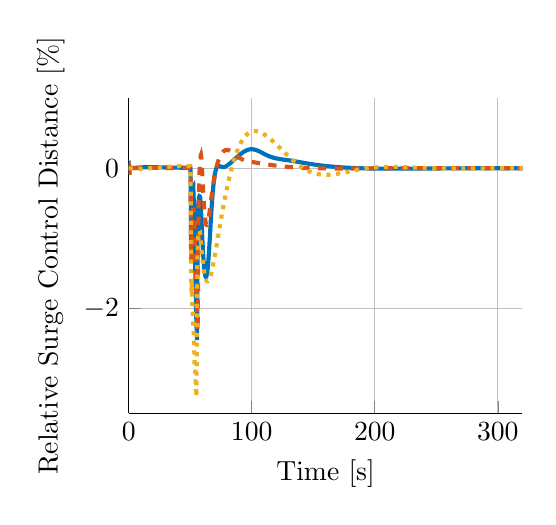
\begin{tikzpicture}

\begin{axis}[%
width=5cm,
height=4cm,
at={(0\linewidth,0\linewidth)},
scale only axis,
xmin=0,
xmax=320,
xlabel={Time [s]},
xmajorgrids,
ymin=-3.5,
ymax=1,
ylabel={Relative Surge Control Distance [\%]},
ymajorgrids,
axis background/.style={fill=white},
% title style={font=\bfseries},
% title={Surge Control Distance},
axis x line*=bottom,
axis y line*=left
]
\addplot [color=mycolor1,solid,line width=1.5pt,forget plot]
  table[row sep=crcr]{%
0	-0.0396000000000001\\
0.25	-0.0265199999999997\\
0.5	-0.0917099999999991\\
0.75	-0.0322300000000002\\
1	0.01417\\
1.25	0.00487000000000037\\
1.5	-0.0024299999999986\\
1.75	0.00156000000000134\\
2	0.00298000000000087\\
2.25	0.00211000000000006\\
2.5	0.00220999999999982\\
2.75	0.00270000000000081\\
3	0.00290999999999997\\
3.25	0.00311000000000128\\
3.5	0.00339000000000134\\
3.75	0.00366\\
4	0.00392000000000081\\
4.25	0.00416000000000061\\
4.5	0.0044000000000004\\
4.75	0.0046400000000002\\
5	0.00488\\
5.25	0.00513000000000119\\
5.5	0.00541000000000125\\
5.75	0.00572000000000017\\
6	0.00605999999999973\\
6.25	0.00641000000000069\\
6.5	0.0067800000000009\\
6.75	0.00716000000000072\\
7	0.00753000000000092\\
7.25	0.00788000000000011\\
7.5	0.00821999999999967\\
7.75	0.00853999999999999\\
8	0.00886000000000031\\
8.25	0.00917000000000101\\
8.5	0.00950000000000095\\
8.75	0.00983000000000089\\
9	0.0101800000000001\\
9.25	0.010530000000001\\
9.5	0.0108899999999998\\
9.75	0.0112400000000008\\
10	0.0115800000000004\\
10.25	0.0119000000000007\\
10.5	0.0122\\
10.75	0.0124700000000004\\
11	0.0127300000000012\\
11.25	0.012970000000001\\
11.5	0.0132100000000008\\
11.75	0.013440000000001\\
12	0.0136800000000008\\
12.25	0.0139200000000006\\
12.5	0.0141600000000004\\
12.75	0.0143900000000006\\
13	0.0146100000000011\\
13.25	0.0148100000000007\\
13.5	0.0149800000000013\\
13.75	0.0151200000000014\\
14	0.01525\\
14.25	0.0153499999999998\\
14.5	0.0154500000000013\\
14.75	0.0155500000000011\\
15	0.0156500000000008\\
15.25	0.0157500000000006\\
15.5	0.0158400000000007\\
15.75	0.0159300000000009\\
16	0.0160100000000014\\
16.25	0.0160800000000005\\
16.5	0.0161200000000008\\
16.75	0.01614\\
17	0.01614\\
17.25	0.0161300000000004\\
17.5	0.0161100000000012\\
17.75	0.0160800000000005\\
18	0.0160600000000013\\
18.25	0.0160499999999999\\
18.5	0.0160300000000007\\
18.75	0.016020000000001\\
19	0.0159900000000004\\
19.25	0.0159599999999998\\
19.5	0.0159099999999999\\
19.75	0.0158400000000007\\
20	0.0157600000000002\\
20.25	0.0156700000000001\\
20.5	0.0155700000000003\\
20.75	0.0154700000000005\\
21	0.0153700000000008\\
21.25	0.0152900000000002\\
21.5	0.0152000000000001\\
21.75	0.015130000000001\\
22	0.0150500000000005\\
22.25	0.0149600000000003\\
22.5	0.0148600000000005\\
22.75	0.0147500000000012\\
23	0.0146200000000007\\
23.25	0.0144900000000003\\
23.5	0.0143500000000003\\
23.75	0.0142199999999999\\
24	0.0140900000000013\\
24.25	0.0139700000000005\\
24.5	0.0138600000000011\\
24.75	0.0137600000000013\\
25	0.0136500000000002\\
25.25	0.0135500000000004\\
25.5	0.013440000000001\\
25.75	0.0133100000000006\\
26	0.0131800000000002\\
26.25	0.0130400000000002\\
26.5	0.0128900000000005\\
26.75	0.0127500000000005\\
27	0.0126200000000001\\
27.25	0.0124899999999997\\
27.5	0.0123800000000003\\
27.75	0.0122800000000005\\
28	0.0121800000000007\\
28.25	0.012080000000001\\
28.5	0.0119800000000012\\
28.75	0.0118600000000004\\
29	0.0117400000000014\\
29.25	0.011610000000001\\
29.5	0.011470000000001\\
29.75	0.0113400000000006\\
30	0.0112199999999998\\
30.25	0.0111100000000004\\
30.5	0.0110200000000003\\
30.75	0.0109300000000001\\
31	0.0108500000000014\\
31.25	0.0107700000000008\\
31.5	0.0106900000000003\\
31.75	0.0105900000000005\\
32	0.0104900000000008\\
32.25	0.0103800000000014\\
32.5	0.0102700000000002\\
32.75	0.0101600000000008\\
33	0.0100600000000011\\
33.25	0.00997000000000092\\
33.5	0.00990000000000002\\
33.75	0.00984000000000052\\
34	0.00978000000000101\\
34.25	0.00973000000000113\\
34.5	0.00966999999999985\\
34.75	0.00960000000000072\\
35	0.00952999999999982\\
35.25	0.00943999999999967\\
35.5	0.0093500000000013\\
35.75	0.00927000000000078\\
36	0.00919000000000025\\
36.25	0.00913000000000075\\
36.5	0.00908000000000087\\
36.75	0.0090400000000006\\
37	0.00900999999999996\\
37.25	0.00899000000000072\\
37.5	0.00895000000000046\\
37.75	0.0089100000000002\\
38	0.00886000000000031\\
38.25	0.00880000000000081\\
38.5	0.0087299999999999\\
38.75	0.0086700000000004\\
39	0.00861000000000089\\
39.25	0.00857000000000063\\
39.5	0.00855000000000139\\
39.75	0.00853000000000037\\
40	0.00853000000000037\\
40.25	0.00853000000000037\\
40.5	0.00852000000000075\\
40.75	0.00849999999999973\\
41	0.00847000000000087\\
41.25	0.00842000000000098\\
41.5	0.0083700000000011\\
41.75	0.00833000000000084\\
42	0.00829000000000057\\
42.25	0.00827000000000133\\
42.5	0.00825999999999993\\
42.75	0.00827000000000133\\
43	0.00829000000000057\\
43.25	0.00830999999999982\\
43.5	0.00832000000000122\\
43.75	0.00832000000000122\\
44	0.0083000000000002\\
44.25	0.00827000000000133\\
44.5	0.00823000000000107\\
44.75	0.00820000000000043\\
45	0.00818000000000119\\
45.25	0.00816999999999979\\
45.5	0.00818000000000119\\
45.75	0.00820000000000043\\
46	0.00824000000000069\\
46.25	0.00827000000000133\\
46.5	0.0083000000000002\\
46.75	0.00830999999999982\\
47	0.0083000000000002\\
47.25	0.00828000000000095\\
47.5	0.00825000000000031\\
47.75	0.00821999999999967\\
48	0.00821000000000005\\
48.25	0.00821000000000005\\
48.5	0.00823000000000107\\
48.75	0.00827000000000133\\
49	0.00832000000000122\\
49.25	0.0083599999999997\\
49.5	0.00839999999999996\\
49.75	0.00842000000000098\\
50	0.00842000000000098\\
50.25	-0.0222599999999993\\
50.5	-0.512049999999999\\
50.75	-1.18987\\
51	-1.03653\\
51.25	-0.638629999999999\\
51.5	-0.600519999999999\\
51.75	-0.56328\\
52	-0.395809999999999\\
52.25	-0.271539999999999\\
52.5	-0.264349999999999\\
52.75	-0.410279999999999\\
53	-0.48042\\
53.25	-0.60544\\
53.5	-0.88857\\
53.75	-1.15064\\
54	-1.35633\\
54.25	-1.57359\\
54.5	-1.7979\\
54.75	-2.00288\\
55	-2.18014\\
55.25	-2.34312\\
55.5	-2.45483\\
55.75	-1.84971\\
56	-1.09641\\
56.25	-0.735829999999999\\
56.5	-0.61009\\
56.75	-0.522939999999999\\
57	-0.452889999999999\\
57.25	-0.4091\\
57.5	-0.398529999999999\\
57.75	-0.40103\\
58	-0.412649999999999\\
58.25	-0.450679999999999\\
58.5	-0.51716\\
58.75	-0.599349999999999\\
59	-0.689609999999999\\
59.25	-0.785019999999999\\
59.5	-0.88153\\
59.75	-0.97535\\
60	-1.06446\\
60.25	-1.14778\\
60.5	-1.22434\\
60.75	-1.29329\\
61	-1.35421\\
61.25	-1.40701\\
61.5	-1.45168\\
61.75	-1.48822\\
62	-1.51667\\
62.25	-1.53712\\
62.5	-1.54962\\
62.75	-1.55422\\
63	-1.55096\\
63.25	-1.53989\\
63.5	-1.52107\\
63.75	-1.49462\\
64	-1.46069\\
64.25	-1.41953\\
64.5	-1.3715\\
64.75	-1.31706\\
65	-1.25681\\
65.25	-1.19147\\
65.5	-1.12185\\
65.75	-1.04889\\
66	-0.973579999999999\\
66.25	-0.897019999999999\\
66.5	-0.820359999999999\\
66.75	-0.7448\\
67	-0.671399999999999\\
67.25	-0.601019999999999\\
67.5	-0.534199999999999\\
67.75	-0.471299999999999\\
68	-0.4125\\
68.25	-0.357919999999999\\
68.5	-0.30758\\
68.75	-0.261449999999999\\
69	-0.21946\\
69.25	-0.18146\\
69.5	-0.1473\\
69.75	-0.116819999999999\\
70	-0.0898599999999998\\
70.25	-0.0662399999999987\\
70.5	-0.0457900000000002\\
70.75	-0.028319999999999\\
71	-0.0136000000000003\\
71.25	-0.00141999999999953\\
71.5	0.00846000000000124\\
71.75	0.0162700000000005\\
72	0.0222500000000014\\
72.25	0.0266200000000012\\
72.5	0.0296099999999999\\
72.75	0.0314200000000007\\
73	0.0322600000000008\\
73.25	0.0323100000000007\\
73.5	0.0317300000000014\\
73.75	0.0306700000000006\\
74	0.02928\\
74.25	0.0276700000000005\\
74.5	0.0259499999999999\\
74.75	0.0242100000000001\\
75	0.0225200000000001\\
75.25	0.0209500000000009\\
75.5	0.0195500000000006\\
75.75	0.0183600000000013\\
76	0.0174200000000013\\
76.25	0.0167400000000004\\
76.5	0.016350000000001\\
76.75	0.0162500000000012\\
77	0.0164500000000007\\
77.25	0.01694\\
77.5	0.0177200000000006\\
77.75	0.0187800000000014\\
78	0.0201100000000007\\
78.25	0.0216900000000013\\
78.5	0.0235099999999999\\
78.75	0.0255500000000008\\
79	0.0278000000000009\\
79.25	0.0302400000000009\\
79.5	0.0328600000000012\\
79.75	0.0356300000000012\\
80	0.0385500000000008\\
80.25	0.0416000000000007\\
80.5	0.0447600000000001\\
80.75	0.0480200000000011\\
81	0.05138\\
81.25	0.0548200000000012\\
81.5	0.0583200000000001\\
81.75	0.06189\\
82	0.0655099999999997\\
82.25	0.0691800000000011\\
82.5	0.072890000000001\\
82.75	0.0766400000000012\\
83	0.0804100000000005\\
83.25	0.0842200000000002\\
83.5	0.0880400000000012\\
83.75	0.0918900000000011\\
84	0.0957500000000007\\
84.25	0.0996300000000012\\
84.5	0.103520000000001\\
84.75	0.107420000000001\\
85	0.111330000000001\\
85.25	0.115250000000001\\
85.5	0.11917\\
85.75	0.123090000000001\\
86	0.12702\\
86.25	0.13095\\
86.5	0.134880000000001\\
86.75	0.138810000000001\\
87	0.14273\\
87.25	0.146650000000001\\
87.5	0.15056\\
87.75	0.15446\\
88	0.158340000000001\\
88.25	0.162220000000001\\
88.5	0.166070000000001\\
88.75	0.16991\\
89	0.173720000000001\\
89.25	0.17751\\
89.5	0.18126\\
89.75	0.184990000000001\\
90	0.188690000000001\\
90.25	0.19234\\
90.5	0.195960000000001\\
90.75	0.199530000000001\\
91	0.203050000000001\\
91.25	0.206520000000001\\
91.5	0.209940000000001\\
91.75	0.2133\\
92	0.2166\\
92.25	0.21983\\
92.5	0.222990000000001\\
92.75	0.226080000000001\\
93	0.229090000000001\\
93.25	0.23203\\
93.5	0.23488\\
93.75	0.237640000000001\\
94	0.240320000000001\\
94.25	0.242900000000001\\
94.5	0.24539\\
94.75	0.247780000000001\\
95	0.250070000000001\\
95.25	0.25226\\
95.5	0.254330000000001\\
95.75	0.256310000000001\\
96	0.25817\\
96.25	0.259910000000001\\
96.5	0.26155\\
96.75	0.263060000000001\\
97	0.26446\\
97.25	0.265740000000001\\
97.5	0.266910000000001\\
97.75	0.267950000000001\\
98	0.26887\\
98.25	0.269670000000001\\
98.5	0.270350000000001\\
98.75	0.270900000000001\\
99	0.27134\\
99.25	0.271650000000001\\
99.5	0.271850000000001\\
99.75	0.271930000000001\\
100	0.271890000000001\\
100.25	0.27173\\
100.5	0.271460000000001\\
100.75	0.271080000000001\\
101	0.270580000000001\\
101.25	0.26998\\
101.5	0.269270000000001\\
101.75	0.268460000000001\\
102	0.26755\\
102.25	0.266530000000001\\
102.5	0.26543\\
102.75	0.264230000000001\\
103	0.26294\\
103.25	0.261570000000001\\
103.5	0.260110000000001\\
103.75	0.25858\\
104	0.256970000000001\\
104.25	0.25529\\
104.5	0.253540000000001\\
104.75	0.25173\\
105	0.24986\\
105.25	0.24794\\
105.5	0.24596\\
105.75	0.243930000000001\\
106	0.241860000000001\\
106.25	0.23976\\
106.5	0.23761\\
106.75	0.235430000000001\\
107	0.233230000000001\\
107.25	0.231\\
107.5	0.22875\\
107.75	0.22648\\
108	0.2242\\
108.25	0.221910000000001\\
108.5	0.219610000000001\\
108.75	0.217310000000001\\
109	0.215010000000001\\
109.25	0.212710000000001\\
109.5	0.210420000000001\\
109.75	0.20814\\
110	0.205860000000001\\
110.25	0.203610000000001\\
110.5	0.201370000000001\\
110.75	0.199150000000001\\
111	0.196950000000001\\
111.25	0.19478\\
111.5	0.192630000000001\\
111.75	0.19051\\
112	0.188420000000001\\
112.25	0.186360000000001\\
112.5	0.184330000000001\\
112.75	0.18234\\
113	0.180380000000001\\
113.25	0.178460000000001\\
113.5	0.17657\\
113.75	0.174720000000001\\
114	0.17291\\
114.25	0.171140000000001\\
114.5	0.169410000000001\\
114.75	0.167720000000001\\
115	0.166070000000001\\
115.25	0.16446\\
115.5	0.162880000000001\\
115.75	0.161350000000001\\
116	0.15986\\
116.25	0.15841\\
116.5	0.157\\
116.75	0.155620000000001\\
117	0.15428\\
117.25	0.152980000000001\\
117.5	0.151720000000001\\
117.75	0.150500000000001\\
118	0.1493\\
118.25	0.148150000000001\\
118.5	0.147020000000001\\
118.75	0.14593\\
119	0.144880000000001\\
119.25	0.14385\\
119.5	0.142850000000001\\
119.75	0.14188\\
120	0.140930000000001\\
120.25	0.14002\\
120.5	0.13912\\
120.75	0.138260000000001\\
121	0.137410000000001\\
121.25	0.13659\\
121.5	0.13578\\
121.75	0.135\\
122	0.134230000000001\\
122.25	0.13348\\
122.5	0.13275\\
122.75	0.13203\\
123	0.13133\\
123.25	0.130640000000001\\
123.5	0.129950000000001\\
123.75	0.129290000000001\\
124	0.128630000000001\\
124.25	0.127970000000001\\
124.5	0.127330000000001\\
124.75	0.12669\\
125	0.126060000000001\\
125.25	0.125440000000001\\
125.5	0.12481\\
125.75	0.1242\\
126	0.12358\\
126.25	0.12297\\
126.5	0.12236\\
126.75	0.121740000000001\\
127	0.121130000000001\\
127.25	0.120520000000001\\
127.5	0.119910000000001\\
127.75	0.119290000000001\\
128	0.118680000000001\\
128.25	0.11806\\
128.5	0.117430000000001\\
128.75	0.116810000000001\\
129	0.11618\\
129.25	0.115550000000001\\
129.5	0.11491\\
129.75	0.114270000000001\\
130	0.113620000000001\\
130.25	0.112970000000001\\
130.5	0.11232\\
130.75	0.111660000000001\\
131	0.110990000000001\\
131.25	0.11032\\
131.5	0.109640000000001\\
131.75	0.10896\\
132	0.108270000000001\\
132.25	0.10758\\
132.5	0.10688\\
132.75	0.10618\\
133	0.10547\\
133.25	0.104760000000001\\
133.5	0.104040000000001\\
133.75	0.10332\\
134	0.102590000000001\\
134.25	0.10186\\
134.5	0.10112\\
134.75	0.100380000000001\\
135	0.0996400000000008\\
135.25	0.0988900000000008\\
135.5	0.0981400000000008\\
135.75	0.0973800000000011\\
136	0.0966199999999997\\
136.25	0.0958600000000001\\
136.5	0.0950900000000008\\
136.75	0.0943300000000011\\
137	0.0935600000000001\\
137.25	0.0927900000000008\\
137.5	0.0920100000000001\\
137.75	0.0912400000000009\\
138	0.0904600000000002\\
138.25	0.0896800000000013\\
138.5	0.0889000000000006\\
138.75	0.08812\\
139	0.0873400000000011\\
139.25	0.0865600000000004\\
139.5	0.0857799999999997\\
139.75	0.0850000000000009\\
140	0.0842200000000002\\
140.25	0.0834400000000013\\
140.5	0.0826600000000006\\
140.75	0.0818900000000014\\
141	0.0811100000000007\\
141.25	0.0803400000000014\\
141.5	0.0795600000000007\\
141.75	0.0787899999999997\\
142	0.0780200000000004\\
142.25	0.0772600000000008\\
142.5	0.0764899999999997\\
142.75	0.0757300000000001\\
143	0.0749700000000004\\
143.25	0.0742100000000008\\
143.5	0.0734600000000007\\
143.75	0.0727100000000007\\
144	0.0719600000000007\\
144.25	0.0712200000000003\\
144.5	0.0704799999999999\\
144.75	0.0697400000000012\\
145	0.0690100000000005\\
145.25	0.0682799999999997\\
145.5	0.0675500000000007\\
145.75	0.0668300000000013\\
146	0.0661100000000001\\
146.25	0.0654000000000003\\
146.5	0.0646900000000006\\
146.75	0.0639900000000004\\
147	0.0632900000000003\\
147.25	0.0625900000000001\\
147.5	0.0619000000000014\\
147.75	0.0612100000000009\\
148	0.06053\\
148.25	0.0598500000000008\\
148.5	0.0591800000000013\\
148.75	0.0585100000000001\\
149	0.0578400000000006\\
149.25	0.0571800000000007\\
149.5	0.0565300000000004\\
149.75	0.0558800000000002\\
150	0.0552299999999999\\
150.25	0.054590000000001\\
150.5	0.0539500000000004\\
150.75	0.0533200000000011\\
151	0.0526900000000001\\
151.25	0.0520700000000005\\
151.5	0.0514500000000009\\
151.75	0.0508400000000009\\
152	0.0502300000000009\\
152.25	0.0496200000000009\\
152.5	0.0490200000000005\\
152.75	0.0484299999999998\\
153	0.0478400000000008\\
153.25	0.04725\\
153.5	0.0466700000000007\\
153.75	0.0460900000000013\\
154	0.0455199999999998\\
154.25	0.04495\\
154.5	0.0443800000000003\\
154.75	0.0438200000000002\\
155	0.0432699999999997\\
155.25	0.042720000000001\\
155.5	0.0421700000000005\\
155.75	0.04162\\
156	0.0410900000000005\\
156.25	0.0405500000000014\\
156.5	0.0400200000000002\\
156.75	0.0394900000000007\\
157	0.0389700000000008\\
157.25	0.038450000000001\\
157.5	0.0379400000000008\\
157.75	0.0374300000000005\\
158	0.0369200000000003\\
158.25	0.0364199999999997\\
158.5	0.0359200000000008\\
158.75	0.0354200000000002\\
159	0.034930000000001\\
159.25	0.03444\\
159.5	0.0339600000000004\\
159.75	0.0334800000000008\\
160	0.0330000000000013\\
160.25	0.0325300000000013\\
160.5	0.0320600000000013\\
160.75	0.031600000000001\\
161	0.0311400000000006\\
161.25	0.0306800000000003\\
161.5	0.0302199999999999\\
161.75	0.029770000000001\\
162	0.0293299999999999\\
162.25	0.0288800000000009\\
162.5	0.0284399999999998\\
162.75	0.0280100000000001\\
163	0.0275700000000008\\
163.25	0.0271400000000011\\
163.5	0.026720000000001\\
163.75	0.0263000000000009\\
164	0.0258800000000008\\
164.25	0.0254600000000007\\
164.5	0.0250500000000002\\
164.75	0.0246399999999998\\
165	0.0242300000000011\\
165.25	0.0238300000000002\\
165.5	0.0234300000000012\\
165.75	0.0230399999999999\\
166	0.0226500000000005\\
166.25	0.0222600000000011\\
166.5	0.0218699999999998\\
166.75	0.02149\\
167	0.0211100000000002\\
167.25	0.02074\\
167.5	0.0203699999999998\\
167.75	0.0200000000000014\\
168	0.0196300000000011\\
168.25	0.0192700000000006\\
168.5	0.01891\\
168.75	0.0185600000000008\\
169	0.0182000000000002\\
169.25	0.0178600000000007\\
169.5	0.0175099999999997\\
169.75	0.0171700000000001\\
170	0.0168300000000006\\
170.25	0.016490000000001\\
170.5	0.0161600000000011\\
170.75	0.0158300000000011\\
171	0.0155000000000012\\
171.25	0.0151800000000009\\
171.5	0.0148600000000005\\
171.75	0.0145400000000002\\
172	0.0142300000000013\\
172.25	0.0139200000000006\\
172.5	0.0136099999999999\\
172.75	0.0133100000000006\\
173	0.0130100000000013\\
173.25	0.0127100000000002\\
173.5	0.0124100000000009\\
173.75	0.0121200000000012\\
174	0.0118299999999998\\
174.25	0.0115499999999997\\
174.5	0.0112699999999997\\
174.75	0.0109900000000014\\
175	0.0107100000000013\\
175.25	0.0104400000000009\\
175.5	0.0101700000000005\\
175.75	0.00990000000000002\\
176	0.00963000000000136\\
176.25	0.00937000000000054\\
176.5	0.00910999999999973\\
176.75	0.00886000000000031\\
177	0.00861000000000089\\
177.25	0.0083599999999997\\
177.5	0.00811000000000028\\
177.75	0.00787000000000049\\
178	0.00762000000000107\\
178.25	0.0073900000000009\\
178.5	0.0071500000000011\\
178.75	0.00692000000000093\\
179	0.00669000000000075\\
179.25	0.00646000000000058\\
179.5	0.00624000000000002\\
179.75	0.00602000000000125\\
180	0.00580000000000069\\
180.25	0.00558000000000014\\
180.5	0.00537000000000099\\
180.75	0.00516000000000005\\
181	0.0049500000000009\\
181.25	0.00475000000000136\\
181.5	0.00455000000000005\\
181.75	0.00435000000000052\\
182	0.00415000000000099\\
182.25	0.00396000000000107\\
182.5	0.00375999999999976\\
182.75	0.00358000000000125\\
183	0.00339000000000134\\
183.25	0.00320000000000142\\
183.5	0.00302000000000113\\
183.75	0.00284000000000084\\
184	0.00267000000000017\\
184.25	0.00248999999999988\\
184.5	0.00232000000000099\\
184.75	0.00215000000000032\\
185	0.00199000000000105\\
185.25	0.00182000000000038\\
185.5	0.00166000000000111\\
185.75	0.00150000000000006\\
186	0.00134000000000079\\
186.25	0.00119000000000113\\
186.5	0.00103999999999971\\
186.75	0.000890000000000057\\
187	0.000740000000000407\\
187.25	0.000590000000000757\\
187.5	0.000450000000000728\\
187.75	0.000310000000000699\\
188	0.00017000000000067\\
188.25	3.00000000006406e-05\\
188.5	-9.99999999997669e-05\\
188.75	-0.000230000000000175\\
189	-0.000370000000000203\\
189.25	-0.000489999999999213\\
189.5	-0.000619999999999621\\
189.75	-0.000739999999998631\\
190	-0.000869999999999038\\
190.25	-0.000989999999999824\\
190.5	-0.00109999999999921\\
190.75	-0.00122\\
191	-0.00132999999999939\\
191.25	-0.00145000000000017\\
191.5	-0.00155999999999956\\
191.75	-0.00165999999999933\\
192	-0.00176999999999872\\
192.25	-0.00187999999999988\\
192.5	-0.00197999999999965\\
192.75	-0.00207999999999942\\
193	-0.00217999999999918\\
193.25	-0.00227999999999895\\
193.5	-0.0023699999999991\\
193.75	-0.00245999999999924\\
194	-0.00255999999999901\\
194.25	-0.00264999999999915\\
194.5	-0.00272999999999968\\
194.75	-0.00281999999999982\\
195	-0.00290999999999997\\
195.25	-0.00298999999999872\\
195.5	-0.00306999999999924\\
195.75	-0.00314999999999976\\
196	-0.00323000000000029\\
196.25	-0.00329999999999941\\
196.5	-0.00337999999999994\\
196.75	-0.00344999999999906\\
197	-0.00351999999999997\\
197.25	-0.00359999999999872\\
197.5	-0.00366\\
197.75	-0.00372999999999912\\
198	-0.00380000000000003\\
198.25	-0.00385999999999953\\
198.5	-0.00391999999999904\\
198.75	-0.00398999999999994\\
199	-0.00404999999999944\\
199.25	-0.00409999999999933\\
199.5	-0.00415999999999883\\
199.75	-0.00422000000000011\\
200	-0.00427\\
200.25	-0.00431999999999988\\
200.5	-0.00437999999999938\\
200.75	-0.00442999999999927\\
201	-0.00447999999999915\\
201.25	-0.00451999999999941\\
201.5	-0.0045699999999993\\
201.75	-0.00460999999999956\\
202	-0.00465999999999944\\
202.25	-0.0046999999999997\\
202.5	-0.00473999999999997\\
202.75	-0.00478000000000023\\
203	-0.00481999999999871\\
203.25	-0.00485999999999898\\
203.5	-0.00489999999999924\\
203.75	-0.00492999999999988\\
204	-0.00497000000000014\\
204.25	-0.00499999999999901\\
204.5	-0.00502999999999965\\
204.75	-0.00506000000000029\\
205	-0.00508999999999915\\
205.25	-0.00511999999999979\\
205.5	-0.00514999999999866\\
205.75	-0.0051799999999993\\
206	-0.00520000000000032\\
206.25	-0.00522999999999918\\
206.5	-0.0052500000000002\\
206.75	-0.00526999999999944\\
207	-0.00530000000000008\\
207.25	-0.00531999999999933\\
207.5	-0.00533999999999857\\
207.75	-0.00535999999999959\\
208	-0.00536999999999921\\
208.25	-0.00539000000000023\\
208.5	-0.00540999999999947\\
208.75	-0.00541999999999909\\
209	-0.00544000000000011\\
209.25	-0.00544999999999973\\
209.5	-0.00545999999999935\\
209.75	-0.0054799999999986\\
210	-0.00548999999999999\\
210.25	-0.00549999999999962\\
210.5	-0.00550999999999924\\
210.75	-0.00551999999999886\\
211	-0.00551999999999886\\
211.25	-0.00553000000000026\\
211.5	-0.00553999999999988\\
211.75	-0.00553999999999988\\
212	-0.0055499999999995\\
212.25	-0.0055499999999995\\
212.5	-0.00555999999999912\\
212.75	-0.00555999999999912\\
213	-0.00555999999999912\\
213.25	-0.00555999999999912\\
213.5	-0.00555999999999912\\
213.75	-0.00555999999999912\\
214	-0.00555999999999912\\
214.25	-0.00555999999999912\\
214.5	-0.00555999999999912\\
214.75	-0.00555999999999912\\
215	-0.0055499999999995\\
215.25	-0.0055499999999995\\
215.5	-0.0055499999999995\\
215.75	-0.00553999999999988\\
216	-0.00553999999999988\\
216.25	-0.00553000000000026\\
216.5	-0.00551999999999886\\
216.75	-0.00551999999999886\\
217	-0.00550999999999924\\
217.25	-0.00549999999999962\\
217.5	-0.00548999999999999\\
217.75	-0.0054799999999986\\
218	-0.00546999999999898\\
218.25	-0.00545999999999935\\
218.5	-0.00544999999999973\\
218.75	-0.00544000000000011\\
219	-0.00542999999999871\\
219.25	-0.00541999999999909\\
219.5	-0.00540999999999947\\
219.75	-0.00539000000000023\\
220	-0.00537999999999883\\
220.25	-0.00536999999999921\\
220.5	-0.00534999999999997\\
220.75	-0.00533999999999857\\
221	-0.00531999999999933\\
221.25	-0.0053099999999997\\
221.5	-0.00528999999999868\\
221.75	-0.00527999999999906\\
222	-0.00525999999999982\\
222.25	-0.0052500000000002\\
222.5	-0.00522999999999918\\
222.75	-0.00520999999999994\\
223	-0.00518999999999892\\
223.25	-0.0051799999999993\\
223.5	-0.00516000000000005\\
223.75	-0.00513999999999903\\
224	-0.00511999999999979\\
224.25	-0.00509999999999877\\
224.5	-0.00507999999999953\\
224.75	-0.00506000000000029\\
225	-0.00503999999999927\\
225.25	-0.00502000000000002\\
225.5	-0.00499999999999901\\
225.75	-0.00497999999999976\\
226	-0.00495999999999874\\
226.25	-0.0049399999999995\\
226.5	-0.00492000000000026\\
226.75	-0.00489999999999924\\
227	-0.00488\\
227.25	-0.00484999999999935\\
227.5	-0.00483000000000011\\
227.75	-0.00480999999999909\\
228	-0.00478999999999985\\
228.25	-0.00475999999999921\\
228.5	-0.00473999999999997\\
228.75	-0.00471999999999895\\
229	-0.00469000000000008\\
229.25	-0.00466999999999906\\
229.5	-0.00464999999999982\\
229.75	-0.00461999999999918\\
230	-0.00459999999999994\\
230.25	-0.0045699999999993\\
230.5	-0.00455000000000005\\
230.75	-0.00452999999999903\\
231	-0.00450000000000017\\
231.25	-0.00447999999999915\\
231.5	-0.00445000000000029\\
231.75	-0.00442999999999927\\
232	-0.00439999999999863\\
232.25	-0.00437999999999938\\
232.5	-0.00434999999999874\\
232.75	-0.0043299999999995\\
233	-0.00429999999999886\\
233.25	-0.00427999999999962\\
233.5	-0.00424999999999898\\
233.75	-0.00422999999999973\\
234	-0.00419999999999909\\
234.25	-0.00417000000000023\\
234.5	-0.00414999999999921\\
234.75	-0.00411999999999857\\
235	-0.00409999999999933\\
235.25	-0.00406999999999869\\
235.5	-0.00403999999999982\\
235.75	-0.0040199999999988\\
236	-0.00398999999999994\\
236.25	-0.00396999999999892\\
236.5	-0.00394000000000005\\
236.75	-0.00390999999999941\\
237	-0.00389000000000017\\
237.25	-0.00385999999999953\\
237.5	-0.00382999999999889\\
237.75	-0.00380999999999965\\
238	-0.00377999999999901\\
238.25	-0.00375999999999976\\
238.5	-0.00372999999999912\\
238.75	-0.00370000000000026\\
239	-0.00367999999999924\\
239.25	-0.0036499999999986\\
239.5	-0.00361999999999973\\
239.75	-0.00359999999999872\\
240	-0.00356999999999985\\
240.25	-0.00354999999999883\\
240.5	-0.00351999999999997\\
240.75	-0.00348999999999933\\
241	-0.00347000000000008\\
241.25	-0.00343999999999944\\
241.5	-0.0034099999999988\\
241.75	-0.00338999999999956\\
242	-0.00335999999999892\\
242.25	-0.00333999999999968\\
242.5	-0.00330999999999904\\
242.75	-0.00328000000000017\\
243	-0.00325999999999915\\
243.25	-0.00323000000000029\\
243.5	-0.00320999999999927\\
243.75	-0.00317999999999863\\
244	-0.00315999999999939\\
244.25	-0.00312999999999874\\
244.5	-0.00309999999999988\\
244.75	-0.00307999999999886\\
245	-0.00305\\
245.25	-0.00302999999999898\\
245.5	-0.00300000000000011\\
245.75	-0.00297999999999909\\
246	-0.00295000000000023\\
246.25	-0.00292999999999921\\
246.5	-0.00289999999999857\\
246.75	-0.00287999999999933\\
247	-0.00284999999999869\\
247.25	-0.00282999999999944\\
247.5	-0.0027999999999988\\
247.75	-0.00277999999999956\\
248	-0.00274999999999892\\
248.25	-0.00272999999999968\\
248.5	-0.00269999999999904\\
248.75	-0.00267999999999979\\
249	-0.00264999999999915\\
249.25	-0.00262999999999991\\
249.5	-0.00260999999999889\\
249.75	-0.00258000000000003\\
250	-0.00255999999999901\\
250.25	-0.00253000000000014\\
250.5	-0.00250999999999912\\
250.75	-0.00248999999999988\\
251	-0.00245999999999924\\
251.25	-0.00244\\
251.5	-0.00241999999999898\\
251.75	-0.00239000000000011\\
252	-0.0023699999999991\\
252.25	-0.00234999999999985\\
252.5	-0.00231999999999921\\
252.75	-0.00229999999999997\\
253	-0.00227999999999895\\
253.25	-0.00225999999999971\\
253.5	-0.00222999999999907\\
253.75	-0.00220999999999982\\
254	-0.0021899999999988\\
254.25	-0.00216999999999956\\
254.5	-0.00213999999999892\\
254.75	-0.00211999999999968\\
255	-0.00209999999999866\\
255.25	-0.00207999999999942\\
255.5	-0.00206000000000017\\
255.75	-0.00203999999999915\\
256	-0.00201000000000029\\
256.25	-0.00198999999999927\\
256.5	-0.00197000000000003\\
256.75	-0.00194999999999901\\
257	-0.00192999999999977\\
257.25	-0.00190999999999875\\
257.5	-0.0018899999999995\\
257.75	-0.00187000000000026\\
258	-0.00184999999999924\\
258.25	-0.00183\\
258.5	-0.00180999999999898\\
258.75	-0.00178999999999974\\
259	-0.00176999999999872\\
259.25	-0.00174999999999947\\
259.5	-0.00173000000000023\\
259.75	-0.00170999999999921\\
260	-0.00168999999999997\\
260.25	-0.00166999999999895\\
260.5	-0.00164999999999971\\
260.75	-0.00162999999999869\\
261	-0.00160999999999945\\
261.25	-0.0015900000000002\\
261.5	-0.0015799999999988\\
261.75	-0.00155999999999956\\
262	-0.00154000000000032\\
262.25	-0.0015199999999993\\
262.5	-0.00150000000000006\\
262.75	-0.00147999999999904\\
263	-0.00146999999999942\\
263.25	-0.00145000000000017\\
263.5	-0.00142999999999915\\
263.75	-0.00140999999999991\\
264	-0.00138999999999889\\
264.25	-0.00137999999999927\\
264.5	-0.00136000000000003\\
264.75	-0.00133999999999901\\
265	-0.00132999999999939\\
265.25	-0.00131000000000014\\
265.5	-0.00128999999999913\\
265.75	-0.0012799999999995\\
266	-0.00126000000000026\\
266.25	-0.00123999999999924\\
266.5	-0.00122999999999962\\
266.75	-0.0012099999999986\\
267	-0.00118999999999936\\
267.25	-0.00117999999999974\\
267.5	-0.00115999999999872\\
267.75	-0.0011499999999991\\
268	-0.00112999999999985\\
268.25	-0.00112000000000023\\
268.5	-0.00109999999999921\\
268.75	-0.00108999999999959\\
269	-0.00106999999999857\\
269.25	-0.00105999999999895\\
269.5	-0.00103999999999971\\
269.75	-0.00103000000000009\\
270	-0.00100999999999907\\
270.25	-0.000999999999999446\\
270.5	-0.000980000000000203\\
270.75	-0.000969999999998805\\
271	-0.000959999999999184\\
271.25	-0.000939999999999941\\
271.5	-0.000930000000000319\\
271.75	-0.0009099999999993\\
272	-0.000899999999999679\\
272.25	-0.000890000000000057\\
272.5	-0.000869999999999038\\
272.75	-0.000859999999999417\\
273	-0.000849999999999795\\
273.25	-0.000829999999998776\\
273.5	-0.000819999999999155\\
273.75	-0.000809999999999533\\
274	-0.000799999999999912\\
274.25	-0.000779999999998893\\
274.5	-0.000769999999999271\\
274.75	-0.00075999999999965\\
275	-0.000750000000000028\\
275.25	-0.000739999999998631\\
275.5	-0.000719999999999388\\
275.75	-0.000709999999999766\\
276	-0.000700000000000145\\
276.25	-0.000689999999998747\\
276.5	-0.000679999999999126\\
276.75	-0.000669999999999504\\
277	-0.000650000000000261\\
277.25	-0.000639999999998864\\
277.5	-0.000629999999999242\\
277.75	-0.000619999999999621\\
278	-0.000609999999999999\\
278.25	-0.000599999999998602\\
278.5	-0.00058999999999898\\
278.75	-0.000579999999999359\\
279	-0.000569999999999737\\
279.25	-0.000560000000000116\\
279.5	-0.000549999999998718\\
279.75	-0.000539999999999097\\
280	-0.000529999999999475\\
280.25	-0.000519999999999854\\
280.5	-0.000510000000000232\\
280.75	-0.000499999999998835\\
281	-0.000489999999999213\\
281.25	-0.000479999999999592\\
281.5	-0.00046999999999997\\
281.75	-0.000459999999998573\\
282	-0.000449999999998951\\
282.25	-0.00043999999999933\\
282.5	-0.000429999999999708\\
282.75	-0.000420000000000087\\
283	-0.000409999999998689\\
283.25	-0.000409999999998689\\
283.5	-0.000399999999999068\\
283.75	-0.000389999999999446\\
284	-0.000379999999999825\\
284.25	-0.000370000000000203\\
284.5	-0.000359999999998806\\
284.75	-0.000359999999998806\\
285	-0.000349999999999184\\
285.25	-0.000339999999999563\\
285.5	-0.000329999999999941\\
285.75	-0.00032000000000032\\
286	-0.00032000000000032\\
286.25	-0.000309999999998922\\
286.5	-0.000299999999999301\\
286.75	-0.000289999999999679\\
287	-0.000289999999999679\\
287.25	-0.000280000000000058\\
287.5	-0.00026999999999866\\
287.75	-0.00026999999999866\\
288	-0.000259999999999039\\
288.25	-0.000249999999999417\\
288.5	-0.000239999999999796\\
288.75	-0.000239999999999796\\
289	-0.000230000000000175\\
289.25	-0.000219999999998777\\
289.5	-0.000219999999998777\\
289.75	-0.000209999999999155\\
290	-0.000209999999999155\\
290.25	-0.000199999999999534\\
290.5	-0.000189999999999912\\
290.75	-0.000189999999999912\\
291	-0.000180000000000291\\
291.25	-0.000169999999998893\\
291.5	-0.000169999999998893\\
291.75	-0.000159999999999272\\
292	-0.000159999999999272\\
292.25	-0.00014999999999965\\
292.5	-0.00014999999999965\\
292.75	-0.000140000000000029\\
293	-0.000140000000000029\\
293.25	-0.000129999999998631\\
293.5	-0.00011999999999901\\
293.75	-0.00011999999999901\\
294	-0.000109999999999388\\
294.25	-0.000109999999999388\\
294.5	-9.99999999997669e-05\\
294.75	-9.99999999997669e-05\\
295	-9.00000000001455e-05\\
295.25	-9.00000000001455e-05\\
295.5	-9.00000000001455e-05\\
295.75	-7.99999999987477e-05\\
296	-7.99999999987477e-05\\
296.25	-6.99999999991263e-05\\
296.5	-6.99999999991263e-05\\
296.75	-5.99999999995049e-05\\
297	-5.99999999995049e-05\\
297.25	-4.99999999998835e-05\\
297.5	-4.99999999998835e-05\\
297.75	-4.99999999998835e-05\\
298	-4.0000000000262e-05\\
298.25	-4.0000000000262e-05\\
298.5	-2.99999999988643e-05\\
298.75	-2.99999999988643e-05\\
299	-2.99999999988643e-05\\
299.25	-1.99999999992428e-05\\
299.5	-1.99999999992428e-05\\
299.75	-1.99999999992428e-05\\
300	-9.99999999962142e-06\\
300.25	-9.99999999962142e-06\\
300.5	0\\
300.75	0\\
301	0\\
301.25	1.00000000013978e-05\\
301.5	1.00000000013978e-05\\
301.75	1.00000000013978e-05\\
302	2.00000000010192e-05\\
302.25	2.00000000010192e-05\\
302.5	2.00000000010192e-05\\
302.75	2.00000000010192e-05\\
303	3.00000000006406e-05\\
303.25	3.00000000006406e-05\\
303.5	3.00000000006406e-05\\
303.75	4.0000000000262e-05\\
304	4.0000000000262e-05\\
304.25	4.0000000000262e-05\\
304.5	4.0000000000262e-05\\
304.75	4.99999999998835e-05\\
305	4.99999999998835e-05\\
305.25	4.99999999998835e-05\\
305.5	4.99999999998835e-05\\
305.75	6.00000000012813e-05\\
306	6.00000000012813e-05\\
306.25	6.00000000012813e-05\\
306.5	6.00000000012813e-05\\
306.75	7.00000000009027e-05\\
307	7.00000000009027e-05\\
307.25	7.00000000009027e-05\\
307.5	7.00000000009027e-05\\
307.75	7.00000000009027e-05\\
308	8.00000000005241e-05\\
308.25	8.00000000005241e-05\\
308.5	8.00000000005241e-05\\
308.75	8.00000000005241e-05\\
309	8.00000000005241e-05\\
309.25	8.00000000005241e-05\\
309.5	9.00000000001455e-05\\
309.75	9.00000000001455e-05\\
310	9.00000000001455e-05\\
310.25	9.00000000001455e-05\\
310.5	9.00000000001455e-05\\
310.75	9.00000000001455e-05\\
311	9.99999999997669e-05\\
311.25	9.99999999997669e-05\\
311.5	9.99999999997669e-05\\
311.75	9.99999999997669e-05\\
312	9.99999999997669e-05\\
312.25	9.99999999997669e-05\\
312.5	9.99999999997669e-05\\
312.75	0.000110000000001165\\
313	0.000110000000001165\\
313.25	0.000110000000001165\\
313.5	0.000110000000001165\\
313.75	0.000110000000001165\\
314	0.000110000000001165\\
314.25	0.000110000000001165\\
314.5	0.000110000000001165\\
314.75	0.000110000000001165\\
315	0.000120000000000786\\
315.25	0.000120000000000786\\
315.5	0.000120000000000786\\
315.75	0.000120000000000786\\
316	0.000120000000000786\\
316.25	0.000120000000000786\\
316.5	0.000120000000000786\\
316.75	0.000120000000000786\\
317	0.000120000000000786\\
317.25	0.000120000000000786\\
317.5	0.000120000000000786\\
317.75	0.000130000000000408\\
318	0.000130000000000408\\
318.25	0.000130000000000408\\
318.5	0.000130000000000408\\
318.75	0.000130000000000408\\
319	0.000130000000000408\\
319.25	0.000130000000000408\\
319.5	0.000130000000000408\\
319.75	0.000130000000000408\\
320	0.000130000000000408\\
320.25	0.000130000000000408\\
320.5	0.000130000000000408\\
320.75	0.000130000000000408\\
321	0.000130000000000408\\
321.25	0.000130000000000408\\
321.5	0.000130000000000408\\
321.75	0.000130000000000408\\
322	0.000130000000000408\\
322.25	0.000130000000000408\\
322.5	0.000130000000000408\\
322.75	0.000130000000000408\\
323	0.000130000000000408\\
323.25	0.000130000000000408\\
323.5	0.000130000000000408\\
323.75	0.000130000000000408\\
324	0.000130000000000408\\
324.25	0.000130000000000408\\
324.5	0.000130000000000408\\
324.75	0.000130000000000408\\
325	0.000140000000000029\\
325.25	0.000140000000000029\\
325.5	0.000140000000000029\\
325.75	0.000140000000000029\\
326	0.000140000000000029\\
326.25	0.000140000000000029\\
326.5	0.000140000000000029\\
326.75	0.000140000000000029\\
327	0.000140000000000029\\
327.25	0.000130000000000408\\
327.5	0.000130000000000408\\
327.75	0.000130000000000408\\
328	0.000130000000000408\\
328.25	0.000130000000000408\\
328.5	0.000130000000000408\\
328.75	0.000130000000000408\\
329	0.000130000000000408\\
329.25	0.000130000000000408\\
329.5	0.000130000000000408\\
329.75	0.000130000000000408\\
330	0.000130000000000408\\
330.25	0.000130000000000408\\
330.5	0.000130000000000408\\
330.75	0.000130000000000408\\
331	0.000130000000000408\\
331.25	0.000130000000000408\\
331.5	0.000130000000000408\\
331.75	0.000130000000000408\\
332	0.000130000000000408\\
332.25	0.000130000000000408\\
332.5	0.000130000000000408\\
332.75	0.000130000000000408\\
333	0.000130000000000408\\
333.25	0.000130000000000408\\
333.5	0.000130000000000408\\
333.75	0.000130000000000408\\
334	0.000130000000000408\\
334.25	0.000130000000000408\\
334.5	0.000130000000000408\\
334.75	0.000130000000000408\\
335	0.000130000000000408\\
335.25	0.000130000000000408\\
335.5	0.000130000000000408\\
335.75	0.000130000000000408\\
336	0.000120000000000786\\
336.25	0.000120000000000786\\
336.5	0.000120000000000786\\
336.75	0.000120000000000786\\
337	0.000120000000000786\\
337.25	0.000120000000000786\\
337.5	0.000120000000000786\\
337.75	0.000120000000000786\\
338	0.000120000000000786\\
338.25	0.000120000000000786\\
338.5	0.000120000000000786\\
338.75	0.000120000000000786\\
339	0.000120000000000786\\
339.25	0.000120000000000786\\
339.5	0.000120000000000786\\
339.75	0.000120000000000786\\
340	0.000120000000000786\\
340.25	0.000120000000000786\\
340.5	0.000120000000000786\\
340.75	0.000120000000000786\\
341	0.000110000000001165\\
341.25	0.000110000000001165\\
341.5	0.000110000000001165\\
341.75	0.000110000000001165\\
342	0.000110000000001165\\
342.25	0.000110000000001165\\
342.5	0.000110000000001165\\
342.75	0.000110000000001165\\
343	0.000110000000001165\\
343.25	0.000110000000001165\\
343.5	0.000110000000001165\\
343.75	0.000110000000001165\\
344	0.000110000000001165\\
344.25	0.000110000000001165\\
344.5	0.000110000000001165\\
344.75	0.000110000000001165\\
345	0.000110000000001165\\
345.25	9.99999999997669e-05\\
345.5	9.99999999997669e-05\\
345.75	9.99999999997669e-05\\
346	9.99999999997669e-05\\
346.25	9.99999999997669e-05\\
346.5	9.99999999997669e-05\\
346.75	9.99999999997669e-05\\
347	9.99999999997669e-05\\
347.25	9.99999999997669e-05\\
347.5	9.99999999997669e-05\\
347.75	9.99999999997669e-05\\
348	9.99999999997669e-05\\
348.25	9.99999999997669e-05\\
348.5	9.99999999997669e-05\\
348.75	9.99999999997669e-05\\
349	9.99999999997669e-05\\
349.25	9.00000000001455e-05\\
349.5	9.00000000001455e-05\\
349.75	9.00000000001455e-05\\
350	9.00000000001455e-05\\
350.25	9.00000000001455e-05\\
350.5	9.00000000001455e-05\\
350.75	9.00000000001455e-05\\
351	9.00000000001455e-05\\
351.25	9.00000000001455e-05\\
351.5	9.00000000001455e-05\\
351.75	9.00000000001455e-05\\
352	9.00000000001455e-05\\
352.25	9.00000000001455e-05\\
352.5	9.00000000001455e-05\\
352.75	9.00000000001455e-05\\
353	8.00000000005241e-05\\
353.25	8.00000000005241e-05\\
353.5	8.00000000005241e-05\\
353.75	8.00000000005241e-05\\
354	8.00000000005241e-05\\
354.25	8.00000000005241e-05\\
354.5	8.00000000005241e-05\\
354.75	8.00000000005241e-05\\
355	8.00000000005241e-05\\
355.25	8.00000000005241e-05\\
355.5	8.00000000005241e-05\\
355.75	8.00000000005241e-05\\
356	8.00000000005241e-05\\
356.25	8.00000000005241e-05\\
356.5	8.00000000005241e-05\\
356.75	8.00000000005241e-05\\
357	7.00000000009027e-05\\
357.25	7.00000000009027e-05\\
357.5	7.00000000009027e-05\\
357.75	7.00000000009027e-05\\
358	7.00000000009027e-05\\
358.25	7.00000000009027e-05\\
358.5	7.00000000009027e-05\\
358.75	7.00000000009027e-05\\
359	7.00000000009027e-05\\
359.25	7.00000000009027e-05\\
359.5	7.00000000009027e-05\\
359.75	7.00000000009027e-05\\
360	7.00000000009027e-05\\
360.25	7.00000000009027e-05\\
360.5	7.00000000009027e-05\\
360.75	7.00000000009027e-05\\
361	7.00000000009027e-05\\
361.25	6.00000000012813e-05\\
361.5	6.00000000012813e-05\\
361.75	6.00000000012813e-05\\
362	6.00000000012813e-05\\
362.25	6.00000000012813e-05\\
362.5	6.00000000012813e-05\\
362.75	6.00000000012813e-05\\
363	6.00000000012813e-05\\
363.25	6.00000000012813e-05\\
363.5	6.00000000012813e-05\\
363.75	6.00000000012813e-05\\
364	6.00000000012813e-05\\
364.25	6.00000000012813e-05\\
364.5	6.00000000012813e-05\\
364.75	6.00000000012813e-05\\
365	6.00000000012813e-05\\
365.25	6.00000000012813e-05\\
365.5	4.99999999998835e-05\\
365.75	4.99999999998835e-05\\
366	4.99999999998835e-05\\
366.25	4.99999999998835e-05\\
366.5	4.99999999998835e-05\\
366.75	4.99999999998835e-05\\
367	4.99999999998835e-05\\
367.25	4.99999999998835e-05\\
367.5	4.99999999998835e-05\\
367.75	4.99999999998835e-05\\
368	4.99999999998835e-05\\
368.25	4.99999999998835e-05\\
368.5	4.99999999998835e-05\\
368.75	4.99999999998835e-05\\
369	4.99999999998835e-05\\
369.25	4.99999999998835e-05\\
369.5	4.99999999998835e-05\\
369.75	4.99999999998835e-05\\
370	4.99999999998835e-05\\
370.25	4.0000000000262e-05\\
370.5	4.0000000000262e-05\\
370.75	4.0000000000262e-05\\
371	4.0000000000262e-05\\
371.25	4.0000000000262e-05\\
371.5	4.0000000000262e-05\\
371.75	4.0000000000262e-05\\
372	4.0000000000262e-05\\
372.25	4.0000000000262e-05\\
372.5	4.0000000000262e-05\\
372.75	4.0000000000262e-05\\
373	4.0000000000262e-05\\
373.25	4.0000000000262e-05\\
373.5	4.0000000000262e-05\\
373.75	4.0000000000262e-05\\
374	4.0000000000262e-05\\
374.25	4.0000000000262e-05\\
374.5	4.0000000000262e-05\\
374.75	4.0000000000262e-05\\
375	4.0000000000262e-05\\
375.25	4.0000000000262e-05\\
375.5	4.0000000000262e-05\\
375.75	3.00000000006406e-05\\
376	3.00000000006406e-05\\
376.25	3.00000000006406e-05\\
376.5	3.00000000006406e-05\\
376.75	3.00000000006406e-05\\
377	3.00000000006406e-05\\
377.25	3.00000000006406e-05\\
377.5	3.00000000006406e-05\\
377.75	3.00000000006406e-05\\
378	3.00000000006406e-05\\
378.25	3.00000000006406e-05\\
378.5	3.00000000006406e-05\\
378.75	3.00000000006406e-05\\
379	3.00000000006406e-05\\
379.25	3.00000000006406e-05\\
379.5	3.00000000006406e-05\\
379.75	3.00000000006406e-05\\
380	3.00000000006406e-05\\
380.25	3.00000000006406e-05\\
380.5	3.00000000006406e-05\\
380.75	3.00000000006406e-05\\
381	3.00000000006406e-05\\
381.25	3.00000000006406e-05\\
381.5	3.00000000006406e-05\\
381.75	3.00000000006406e-05\\
382	3.00000000006406e-05\\
382.25	2.00000000010192e-05\\
382.5	2.00000000010192e-05\\
382.75	2.00000000010192e-05\\
383	2.00000000010192e-05\\
383.25	2.00000000010192e-05\\
383.5	2.00000000010192e-05\\
383.75	2.00000000010192e-05\\
384	2.00000000010192e-05\\
384.25	2.00000000010192e-05\\
384.5	2.00000000010192e-05\\
384.75	2.00000000010192e-05\\
385	2.00000000010192e-05\\
385.25	2.00000000010192e-05\\
385.5	2.00000000010192e-05\\
385.75	2.00000000010192e-05\\
386	2.00000000010192e-05\\
386.25	2.00000000010192e-05\\
386.5	2.00000000010192e-05\\
386.75	2.00000000010192e-05\\
387	2.00000000010192e-05\\
387.25	2.00000000010192e-05\\
387.5	2.00000000010192e-05\\
387.75	2.00000000010192e-05\\
388	2.00000000010192e-05\\
388.25	2.00000000010192e-05\\
388.5	2.00000000010192e-05\\
388.75	2.00000000010192e-05\\
389	2.00000000010192e-05\\
389.25	2.00000000010192e-05\\
389.5	2.00000000010192e-05\\
389.75	2.00000000010192e-05\\
390	2.00000000010192e-05\\
390.25	1.00000000013978e-05\\
390.5	1.00000000013978e-05\\
390.75	1.00000000013978e-05\\
391	1.00000000013978e-05\\
391.25	1.00000000013978e-05\\
391.5	1.00000000013978e-05\\
391.75	1.00000000013978e-05\\
392	1.00000000013978e-05\\
392.25	1.00000000013978e-05\\
392.5	1.00000000013978e-05\\
392.75	1.00000000013978e-05\\
393	1.00000000013978e-05\\
393.25	1.00000000013978e-05\\
393.5	1.00000000013978e-05\\
393.75	1.00000000013978e-05\\
394	1.00000000013978e-05\\
394.25	1.00000000013978e-05\\
394.5	1.00000000013978e-05\\
394.75	1.00000000013978e-05\\
395	1.00000000013978e-05\\
395.25	1.00000000013978e-05\\
395.5	1.00000000013978e-05\\
395.75	1.00000000013978e-05\\
396	1.00000000013978e-05\\
396.25	1.00000000013978e-05\\
396.5	1.00000000013978e-05\\
396.75	1.00000000013978e-05\\
397	1.00000000013978e-05\\
397.25	1.00000000013978e-05\\
397.5	1.00000000013978e-05\\
397.75	1.00000000013978e-05\\
398	1.00000000013978e-05\\
398.25	1.00000000013978e-05\\
398.5	1.00000000013978e-05\\
398.75	1.00000000013978e-05\\
399	1.00000000013978e-05\\
399.25	1.00000000013978e-05\\
399.5	1.00000000013978e-05\\
399.75	1.00000000013978e-05\\
400	1.00000000013978e-05\\
400.25	1.00000000013978e-05\\
400.5	1.00000000013978e-05\\
400.75	1.00000000013978e-05\\
401	1.00000000013978e-05\\
401.25	1.00000000013978e-05\\
401.5	1.00000000013978e-05\\
401.75	1.00000000013978e-05\\
402	1.00000000013978e-05\\
402.25	0\\
402.5	0\\
402.75	0\\
403	0\\
403.25	0\\
403.5	0\\
403.75	0\\
404	0\\
404.25	0\\
404.5	0\\
404.75	0\\
405	0\\
405.25	0\\
405.5	0\\
405.75	0\\
406	0\\
406.25	0\\
406.5	0\\
406.75	0\\
407	0\\
407.25	0\\
407.5	0\\
407.75	0\\
408	0\\
408.25	0\\
408.5	0\\
408.75	0\\
409	0\\
409.25	0\\
409.5	0\\
409.75	0\\
410	0\\
410.25	0\\
410.5	0\\
410.75	0\\
411	0\\
411.25	0\\
411.5	0\\
411.75	0\\
412	0\\
412.25	0\\
412.5	0\\
412.75	0\\
413	0\\
413.25	0\\
413.5	0\\
413.75	0\\
414	0\\
414.25	0\\
414.5	0\\
414.75	0\\
415	0\\
415.25	0\\
415.5	0\\
415.75	0\\
416	0\\
416.25	0\\
416.5	0\\
416.75	0\\
417	0\\
417.25	0\\
417.5	0\\
417.75	0\\
418	0\\
418.25	0\\
418.5	0\\
418.75	0\\
419	0\\
419.25	0\\
419.5	0\\
419.75	0\\
420	0\\
420.25	0\\
420.5	0\\
420.75	0\\
421	0\\
421.25	0\\
421.5	0\\
421.75	0\\
422	0\\
422.25	0\\
422.5	0\\
422.75	0\\
423	0\\
423.25	0\\
423.5	0\\
423.75	0\\
424	0\\
424.25	0\\
424.5	0\\
424.75	0\\
425	0\\
425.25	0\\
425.5	0\\
425.75	0\\
426	0\\
426.25	0\\
426.5	0\\
426.75	0\\
427	0\\
427.25	0\\
427.5	0\\
427.75	0\\
428	0\\
428.25	0\\
428.5	0\\
428.75	0\\
429	0\\
429.25	0\\
429.5	0\\
429.75	0\\
430	0\\
430.25	0\\
430.5	0\\
430.75	0\\
431	0\\
431.25	0\\
431.5	0\\
431.75	0\\
432	0\\
432.25	0\\
432.5	0\\
432.75	0\\
433	0\\
433.25	0\\
433.5	0\\
433.75	0\\
434	0\\
434.25	0\\
434.5	0\\
434.75	0\\
435	0\\
435.25	0\\
435.5	0\\
435.75	0\\
436	0\\
436.25	0\\
436.5	0\\
436.75	0\\
437	0\\
437.25	0\\
437.5	0\\
437.75	0\\
438	0\\
438.25	0\\
438.5	0\\
438.75	0\\
439	0\\
439.25	0\\
439.5	0\\
439.75	0\\
440	0\\
440.25	0\\
440.5	0\\
440.75	0\\
441	0\\
441.25	0\\
441.5	0\\
441.75	0\\
442	0\\
442.25	0\\
442.5	0\\
442.75	0\\
443	0\\
443.25	0\\
443.5	0\\
443.75	0\\
444	0\\
444.25	0\\
444.5	0\\
444.75	0\\
445	0\\
445.25	0\\
445.5	0\\
445.75	0\\
446	0\\
446.25	0\\
446.5	0\\
446.75	0\\
447	0\\
447.25	0\\
447.5	0\\
447.75	0\\
448	0\\
448.25	0\\
448.5	0\\
448.75	0\\
449	0\\
449.25	0\\
449.5	0\\
449.75	0\\
450	0\\
450.25	0\\
450.5	0\\
450.75	0\\
451	0\\
451.25	0\\
451.5	0\\
451.75	0\\
452	0\\
452.25	0\\
452.5	0\\
452.75	0\\
453	0\\
453.25	0\\
453.5	0\\
453.75	0\\
454	0\\
454.25	0\\
454.5	0\\
454.75	0\\
455	0\\
455.25	0\\
455.5	0\\
455.75	0\\
456	0\\
456.25	0\\
456.5	0\\
456.75	0\\
457	0\\
457.25	0\\
457.5	0\\
457.75	0\\
458	0\\
458.25	0\\
458.5	0\\
458.75	0\\
459	0\\
459.25	0\\
459.5	0\\
459.75	0\\
460	0\\
460.25	0\\
460.5	0\\
460.75	0\\
461	0\\
461.25	0\\
461.5	0\\
461.75	0\\
462	0\\
462.25	0\\
462.5	0\\
462.75	0\\
463	0\\
463.25	0\\
463.5	0\\
463.75	0\\
464	0\\
464.25	0\\
464.5	0\\
464.75	0\\
465	0\\
465.25	0\\
465.5	0\\
465.75	0\\
466	0\\
466.25	0\\
466.5	0\\
466.75	0\\
467	0\\
467.25	0\\
467.5	0\\
467.75	0\\
468	0\\
468.25	0\\
468.5	0\\
468.75	0\\
469	0\\
469.25	0\\
469.5	0\\
469.75	0\\
470	0\\
470.25	0\\
470.5	0\\
470.75	0\\
471	0\\
471.25	0\\
471.5	0\\
471.75	0\\
472	0\\
472.25	0\\
472.5	0\\
472.75	0\\
473	0\\
473.25	0\\
473.5	0\\
473.75	0\\
474	0\\
474.25	0\\
474.5	0\\
474.75	0\\
475	0\\
475.25	0\\
475.5	0\\
475.75	0\\
476	0\\
476.25	0\\
476.5	0\\
476.75	0\\
477	0\\
477.25	0\\
477.5	0\\
477.75	0\\
478	0\\
478.25	0\\
478.5	0\\
478.75	0\\
479	0\\
479.25	0\\
479.5	0\\
479.75	0\\
480	0\\
480.25	0\\
480.5	0\\
480.75	0\\
481	0\\
481.25	0\\
481.5	0\\
481.75	0\\
482	0\\
482.25	0\\
482.5	0\\
482.75	0\\
483	0\\
483.25	0\\
483.5	0\\
483.75	0\\
484	0\\
484.25	0\\
484.5	0\\
484.75	0\\
485	0\\
485.25	0\\
485.5	0\\
485.75	0\\
486	0\\
486.25	0\\
486.5	0\\
486.75	0\\
487	0\\
487.25	0\\
487.5	0\\
487.75	0\\
488	0\\
488.25	0\\
488.5	0\\
488.75	0\\
489	0\\
489.25	0\\
489.5	0\\
489.75	0\\
490	0\\
490.25	0\\
490.5	0\\
490.75	0\\
491	0\\
491.25	0\\
491.5	0\\
491.75	0\\
492	0\\
492.25	0\\
492.5	0\\
492.75	0\\
493	0\\
493.25	0\\
493.5	0\\
493.75	0\\
494	0\\
494.25	0\\
494.5	0\\
494.75	0\\
495	0\\
495.25	0\\
495.5	0\\
495.75	0\\
496	0\\
496.25	0\\
496.5	0\\
496.75	0\\
497	0\\
497.25	0\\
497.5	0\\
497.75	0\\
498	0\\
498.25	0\\
498.5	0\\
498.75	0\\
499	0\\
499.25	0\\
499.5	0\\
499.75	0\\
};
\addplot [color=mycolor2,dashed,line width=1.5pt,forget plot]
  table[row sep=crcr]{%
0	-0.0396000000000001\\
0.25	-0.0263099999999987\\
0.5	-0.0907599999999995\\
0.75	-0.0308200000000003\\
1	0.0157900000000009\\
1.25	0.00669000000000075\\
1.5	-0.000549999999998718\\
1.75	0.00342999999999982\\
2	0.00482000000000049\\
2.25	0.00386000000000131\\
2.5	0.00380000000000003\\
2.75	0.00406000000000084\\
3	0.00401000000000096\\
3.25	0.00391000000000119\\
3.5	0.00387000000000093\\
3.75	0.00383000000000067\\
4	0.00377000000000116\\
4.25	0.00372000000000128\\
4.5	0.00369000000000064\\
4.75	0.00367000000000139\\
5	0.00366\\
5.25	0.00366\\
5.5	0.00367000000000139\\
5.75	0.00368000000000102\\
6	0.00370000000000026\\
6.25	0.0037300000000009\\
6.5	0.00375999999999976\\
6.75	0.0037900000000004\\
7	0.00383000000000067\\
7.25	0.00388000000000055\\
7.5	0.00394000000000005\\
7.75	0.00400000000000134\\
8	0.00408000000000008\\
8.25	0.00416000000000061\\
8.5	0.00425000000000075\\
8.75	0.0043400000000009\\
9	0.00444000000000067\\
9.25	0.00453000000000081\\
9.5	0.00463000000000058\\
9.75	0.00472000000000072\\
10	0.00481000000000087\\
10.25	0.00490000000000101\\
10.5	0.00499000000000116\\
10.75	0.00508000000000131\\
11	0.00516000000000005\\
11.25	0.0052500000000002\\
11.5	0.00533000000000072\\
11.75	0.00541000000000125\\
12	0.00548999999999999\\
12.25	0.0055600000000009\\
12.5	0.00563000000000002\\
12.75	0.00569000000000131\\
13	0.00574000000000119\\
13.25	0.00579000000000107\\
13.5	0.00584000000000096\\
13.75	0.00588000000000122\\
14	0.00591000000000008\\
14.25	0.00594000000000072\\
14.5	0.00595999999999997\\
14.75	0.00598000000000098\\
15	0.00599000000000061\\
15.25	0.00600000000000023\\
15.5	0.00600999999999985\\
15.75	0.00600999999999985\\
16	0.00600000000000023\\
16.25	0.00599000000000061\\
16.5	0.00597000000000136\\
16.75	0.00595000000000034\\
17	0.0059300000000011\\
17.25	0.00590000000000046\\
17.5	0.00586999999999982\\
17.75	0.00584000000000096\\
18	0.00580000000000069\\
18.25	0.00576000000000043\\
18.5	0.00572000000000017\\
18.75	0.00567000000000029\\
19	0.00563000000000002\\
19.25	0.00558000000000014\\
19.5	0.00553000000000026\\
19.75	0.00548000000000037\\
20	0.00542000000000087\\
20.25	0.00537000000000099\\
20.5	0.0053099999999997\\
20.75	0.00525999999999982\\
21	0.00520000000000032\\
21.25	0.00515000000000043\\
21.5	0.00509000000000093\\
21.75	0.00504000000000104\\
22	0.00499000000000116\\
22.25	0.00492999999999988\\
22.5	0.00488\\
22.75	0.00483000000000011\\
23	0.00478000000000023\\
23.25	0.00473000000000035\\
23.5	0.00468000000000046\\
23.75	0.00463000000000058\\
24	0.00458000000000069\\
24.25	0.00454000000000043\\
24.5	0.00450000000000017\\
24.75	0.00445999999999991\\
25	0.00442000000000142\\
25.25	0.00438000000000116\\
25.5	0.00435000000000052\\
25.75	0.00431000000000026\\
26	0.00428000000000139\\
26.25	0.00425000000000075\\
26.5	0.00422999999999973\\
26.75	0.00420000000000087\\
27	0.00417999999999985\\
27.25	0.00416000000000061\\
27.5	0.00414000000000136\\
27.75	0.00412000000000035\\
28	0.0041000000000011\\
28.25	0.0040899999999997\\
28.5	0.00408000000000008\\
28.75	0.00407000000000046\\
29	0.00406000000000084\\
29.25	0.00406000000000084\\
29.5	0.00405000000000122\\
29.75	0.00405000000000122\\
30	0.00405000000000122\\
30.25	0.00405000000000122\\
30.5	0.00405000000000122\\
30.75	0.00406000000000084\\
31	0.00406000000000084\\
31.25	0.00407000000000046\\
31.5	0.00408000000000008\\
31.75	0.0040899999999997\\
32	0.0041000000000011\\
32.25	0.00411000000000072\\
32.5	0.00412000000000035\\
32.75	0.00412999999999997\\
33	0.00415000000000099\\
33.25	0.00416000000000061\\
33.5	0.00417999999999985\\
33.75	0.00419000000000125\\
34	0.00421000000000049\\
34.25	0.00422000000000011\\
34.5	0.00424000000000113\\
34.75	0.00426000000000037\\
35	0.00428000000000139\\
35.25	0.00430000000000064\\
35.5	0.00431000000000026\\
35.75	0.00433000000000128\\
36	0.00435000000000052\\
36.25	0.00436999999999976\\
36.5	0.00439000000000078\\
36.75	0.00441000000000003\\
37	0.00443000000000104\\
37.25	0.00444000000000067\\
37.5	0.00445999999999991\\
37.75	0.00448000000000093\\
38	0.00450000000000017\\
38.25	0.00450999999999979\\
38.5	0.00453000000000081\\
38.75	0.00455000000000005\\
39	0.00455999999999968\\
39.25	0.00458000000000069\\
39.5	0.00459000000000032\\
39.75	0.00461000000000134\\
40	0.00462000000000096\\
40.25	0.00463000000000058\\
40.5	0.00464999999999982\\
40.75	0.00466000000000122\\
41	0.00467000000000084\\
41.25	0.00468000000000046\\
41.5	0.00469000000000008\\
41.75	0.0046999999999997\\
42	0.0047100000000011\\
42.25	0.00472000000000072\\
42.5	0.00473000000000035\\
42.75	0.00473000000000035\\
43	0.00473999999999997\\
43.25	0.00475000000000136\\
43.5	0.00475000000000136\\
43.75	0.00476000000000099\\
44	0.00476000000000099\\
44.25	0.00476000000000099\\
44.5	0.00477000000000061\\
44.75	0.00477000000000061\\
45	0.00477000000000061\\
45.25	0.00477000000000061\\
45.5	0.00477000000000061\\
45.75	0.00477000000000061\\
46	0.00477000000000061\\
46.25	0.00477000000000061\\
46.5	0.00477000000000061\\
46.75	0.00477000000000061\\
47	0.00477000000000061\\
47.25	0.00476000000000099\\
47.5	0.00476000000000099\\
47.75	0.00476000000000099\\
48	0.00476000000000099\\
48.25	0.00475000000000136\\
48.5	0.00475000000000136\\
48.75	0.00473999999999997\\
49	0.00473999999999997\\
49.25	0.00473000000000035\\
49.5	0.00473000000000035\\
49.75	0.00473000000000035\\
50	0.00472000000000072\\
50.25	-0.0279699999999998\\
50.5	-0.550759999999999\\
50.75	-1.31357\\
51	-1.25039\\
51.25	-0.910699999999999\\
51.5	-0.909179999999999\\
51.75	-0.903189999999999\\
52	-0.756219999999999\\
52.25	-0.637759999999999\\
52.5	-0.56406\\
52.75	-0.620119999999999\\
53	-0.65107\\
53.25	-0.660379999999999\\
53.5	-0.8428\\
53.75	-1.04267\\
54	-1.17352\\
54.25	-1.31207\\
54.5	-1.48409\\
54.75	-1.65148\\
55	-1.79871\\
55.25	-1.93748\\
55.5	-2.08074\\
55.75	-2.2309\\
56	-2.32314\\
56.25	-1.77291\\
56.5	-1.03758\\
56.75	-0.574339999999999\\
57	-0.363219999999999\\
57.25	-0.212569999999999\\
57.5	-0.0746000000000002\\
57.75	0.0137700000000009\\
58	0.0718800000000002\\
58.25	0.12893\\
58.5	0.17694\\
58.75	0.18965\\
59	0.161160000000001\\
59.25	0.103770000000001\\
59.5	0.0289800000000007\\
59.75	-0.056239999999999\\
60	-0.14582\\
60.25	-0.23485\\
60.5	-0.320779999999999\\
60.75	-0.402399999999999\\
61	-0.47845\\
61.25	-0.547499999999999\\
61.5	-0.608569999999999\\
61.75	-0.66135\\
62	-0.70583\\
62.25	-0.742089999999999\\
62.5	-0.77035\\
62.75	-0.79095\\
63	-0.80427\\
63.25	-0.810739999999999\\
63.5	-0.8108\\
63.75	-0.804989999999999\\
64	-0.79388\\
64.25	-0.77807\\
64.5	-0.75817\\
64.75	-0.734769999999999\\
65	-0.70844\\
65.25	-0.67972\\
65.5	-0.6491\\
65.75	-0.617039999999999\\
66	-0.58393\\
66.25	-0.55014\\
66.5	-0.51598\\
66.75	-0.481719999999999\\
67	-0.447589999999999\\
67.25	-0.41381\\
67.5	-0.38052\\
67.75	-0.34789\\
68	-0.316009999999999\\
68.25	-0.28499\\
68.5	-0.254899999999999\\
68.75	-0.225779999999999\\
69	-0.19769\\
69.25	-0.17064\\
69.5	-0.14465\\
69.75	-0.119719999999999\\
70	-0.0958600000000001\\
70.25	-0.0730500000000003\\
70.5	-0.0512800000000002\\
70.75	-0.0305099999999996\\
71	-0.0107400000000002\\
71.25	0.00808000000000142\\
71.5	0.0259600000000013\\
71.75	0.0429399999999998\\
72	0.0590500000000009\\
72.25	0.0743299999999998\\
72.5	0.0888000000000009\\
72.75	0.102500000000001\\
73	0.115450000000001\\
73.25	0.127690000000001\\
73.5	0.139240000000001\\
73.75	0.150130000000001\\
74	0.160390000000001\\
74.25	0.170030000000001\\
74.5	0.17909\\
74.75	0.187580000000001\\
75	0.19552\\
75.25	0.20293\\
75.5	0.20983\\
75.75	0.216230000000001\\
76	0.222150000000001\\
76.25	0.22761\\
76.5	0.232610000000001\\
76.75	0.23718\\
77	0.24131\\
77.25	0.245040000000001\\
77.5	0.24836\\
77.75	0.251280000000001\\
78	0.253830000000001\\
78.25	0.25601\\
78.5	0.257820000000001\\
78.75	0.25929\\
79	0.26042\\
79.25	0.261230000000001\\
79.5	0.261710000000001\\
79.75	0.261900000000001\\
80	0.261790000000001\\
80.25	0.2614\\
80.5	0.26074\\
80.75	0.259820000000001\\
81	0.258650000000001\\
81.25	0.257250000000001\\
81.5	0.25562\\
81.75	0.25379\\
82	0.251750000000001\\
82.25	0.24953\\
82.5	0.24714\\
82.75	0.244590000000001\\
83	0.24189\\
83.25	0.239050000000001\\
83.5	0.236080000000001\\
83.75	0.23301\\
84	0.22983\\
84.25	0.226570000000001\\
84.5	0.223220000000001\\
84.75	0.21982\\
85	0.21635\\
85.25	0.212850000000001\\
85.5	0.20931\\
85.75	0.20574\\
86	0.202170000000001\\
86.25	0.19858\\
86.5	0.195\\
86.75	0.19144\\
87	0.187890000000001\\
87.25	0.184370000000001\\
87.5	0.18089\\
87.75	0.177440000000001\\
88	0.174050000000001\\
88.25	0.17071\\
88.5	0.16742\\
88.75	0.164200000000001\\
89	0.16104\\
89.25	0.157950000000001\\
89.5	0.15494\\
89.75	0.152000000000001\\
90	0.149140000000001\\
90.25	0.146360000000001\\
90.5	0.143660000000001\\
90.75	0.14104\\
91	0.13851\\
91.25	0.136060000000001\\
91.5	0.133690000000001\\
91.75	0.131410000000001\\
92	0.129200000000001\\
92.25	0.127080000000001\\
92.5	0.12504\\
92.75	0.12308\\
93	0.12119\\
93.25	0.119380000000001\\
93.5	0.117650000000001\\
93.75	0.11598\\
94	0.11439\\
94.25	0.112860000000001\\
94.5	0.11139\\
94.75	0.10998\\
95	0.108640000000001\\
95.25	0.10735\\
95.5	0.106110000000001\\
95.75	0.10492\\
96	0.10378\\
96.25	0.102690000000001\\
96.5	0.10163\\
96.75	0.100620000000001\\
97	0.0996400000000008\\
97.25	0.0987000000000009\\
97.5	0.0977899999999998\\
97.75	0.0969100000000012\\
98	0.0960600000000014\\
98.25	0.0952300000000008\\
98.5	0.0944200000000013\\
98.75	0.0936400000000006\\
99	0.0928700000000013\\
99.25	0.0921200000000013\\
99.5	0.0913800000000009\\
99.75	0.0906599999999997\\
100	0.08995\\
100.25	0.0892400000000002\\
100.5	0.0885499999999997\\
100.75	0.0878600000000009\\
101	0.08718\\
101.25	0.0865100000000005\\
101.5	0.0858300000000014\\
101.75	0.0851600000000001\\
102	0.0845000000000002\\
102.25	0.0838300000000007\\
102.5	0.0831600000000012\\
102.75	0.0825000000000014\\
103	0.0818300000000001\\
103.25	0.0811600000000006\\
103.5	0.0804900000000011\\
103.75	0.0798199999999998\\
104	0.0791500000000003\\
104.25	0.0784700000000011\\
104.5	0.0777999999999999\\
104.75	0.0771200000000007\\
105	0.0764300000000002\\
105.25	0.0757500000000011\\
105.5	0.0750600000000006\\
105.75	0.07437\\
106	0.0736800000000013\\
106.25	0.0729800000000012\\
106.5	0.0722900000000006\\
106.75	0.0715900000000005\\
107	0.0708900000000003\\
107.25	0.0701800000000006\\
107.5	0.0694800000000004\\
107.75	0.0687700000000007\\
108	0.0680700000000005\\
108.25	0.0673600000000008\\
108.5	0.0666600000000006\\
108.75	0.0659500000000008\\
109	0.0652400000000011\\
109.25	0.0645400000000009\\
109.5	0.0638300000000012\\
109.75	0.0631200000000014\\
110	0.0624200000000013\\
110.25	0.0617200000000011\\
110.5	0.061020000000001\\
110.75	0.0603200000000008\\
111	0.0596200000000007\\
111.25	0.0589200000000005\\
111.5	0.05823\\
111.75	0.0575400000000013\\
112	0.0568500000000007\\
112.25	0.0561699999999998\\
112.5	0.0554900000000007\\
112.75	0.0548099999999998\\
113	0.0541400000000003\\
113.25	0.0534700000000008\\
113.5	0.0528000000000013\\
113.75	0.0521400000000014\\
114	0.0514799999999997\\
114.25	0.0508300000000013\\
114.5	0.050180000000001\\
114.75	0.0495300000000007\\
115	0.0488900000000001\\
115.25	0.0482500000000012\\
115.5	0.0476200000000002\\
115.75	0.046990000000001\\
116	0.0463700000000014\\
116.25	0.04575\\
116.5	0.04514\\
116.75	0.04453\\
117	0.04392\\
117.25	0.043330000000001\\
117.5	0.0427300000000006\\
117.75	0.0421399999999998\\
118	0.0415600000000005\\
118.25	0.0409800000000011\\
118.5	0.0404\\
118.75	0.0398300000000003\\
119	0.0392700000000001\\
119.25	0.03871\\
119.5	0.0381600000000013\\
119.75	0.0376100000000008\\
120	0.0370600000000003\\
120.25	0.0365200000000012\\
120.5	0.03599\\
120.75	0.0354500000000009\\
121	0.034930000000001\\
121.25	0.0344100000000012\\
121.5	0.0338900000000013\\
121.75	0.0333800000000011\\
122	0.0328700000000008\\
122.25	0.0323700000000002\\
122.5	0.031880000000001\\
122.75	0.0313800000000004\\
123	0.0309000000000008\\
123.25	0.0304099999999998\\
123.5	0.0299300000000002\\
123.75	0.0294600000000003\\
124	0.0289900000000003\\
124.25	0.0285299999999999\\
124.5	0.0280700000000014\\
124.75	0.027610000000001\\
125	0.0271600000000003\\
125.25	0.0267100000000013\\
125.5	0.0262700000000002\\
125.75	0.0258300000000009\\
126	0.0254000000000012\\
126.25	0.0249699999999997\\
126.5	0.02454\\
126.75	0.0241199999999999\\
127	0.0237100000000012\\
127.25	0.0232900000000011\\
127.5	0.0228900000000003\\
127.75	0.0224799999999998\\
128	0.0220800000000008\\
128.25	0.0216900000000013\\
128.5	0.0213000000000001\\
128.75	0.0209100000000007\\
129	0.0205300000000008\\
129.25	0.020150000000001\\
129.5	0.0197800000000008\\
129.75	0.0194100000000006\\
130	0.0190400000000004\\
130.25	0.0186799999999998\\
130.5	0.018320000000001\\
130.75	0.01797\\
131	0.0176200000000009\\
131.25	0.0172699999999999\\
131.5	0.0169300000000003\\
131.75	0.0165900000000008\\
132	0.0162500000000012\\
132.25	0.0159200000000013\\
132.5	0.0156000000000009\\
132.75	0.0152800000000006\\
133	0.0149600000000003\\
133.25	0.01464\\
133.5	0.0143300000000011\\
133.75	0.0140200000000004\\
134	0.0137200000000011\\
134.25	0.01342\\
134.5	0.0131200000000007\\
134.75	0.012830000000001\\
135	0.0125400000000013\\
135.25	0.0122600000000013\\
135.5	0.0119800000000012\\
135.75	0.0117000000000012\\
136	0.0114200000000011\\
136.25	0.0111500000000007\\
136.5	0.0108899999999998\\
136.75	0.0106200000000012\\
137	0.0103600000000004\\
137.25	0.010110000000001\\
137.5	0.00985000000000014\\
137.75	0.00960000000000072\\
138	0.00936000000000092\\
138.25	0.00910999999999973\\
138.5	0.00886999999999993\\
138.75	0.00863999999999976\\
139	0.00841000000000136\\
139.25	0.00818000000000119\\
139.5	0.00795000000000101\\
139.75	0.00773000000000046\\
140	0.00750999999999991\\
140.25	0.00729000000000113\\
140.5	0.0070800000000002\\
140.75	0.00687000000000104\\
141	0.00666000000000011\\
141.25	0.00645000000000095\\
141.5	0.00625000000000142\\
141.75	0.00605999999999973\\
142	0.0058600000000002\\
142.25	0.00567000000000029\\
142.5	0.00548000000000037\\
142.75	0.00529000000000046\\
143	0.00511000000000017\\
143.25	0.00492999999999988\\
143.5	0.00475000000000136\\
143.75	0.00458000000000069\\
144	0.00441000000000003\\
144.25	0.00424000000000113\\
144.5	0.00407000000000046\\
144.75	0.00391000000000119\\
145	0.00375000000000014\\
145.25	0.00359000000000087\\
145.5	0.00344000000000122\\
145.75	0.00328000000000017\\
146	0.00313000000000052\\
146.25	0.00299000000000049\\
146.5	0.00284000000000084\\
146.75	0.00270000000000081\\
147	0.00256000000000078\\
147.25	0.00242000000000075\\
147.5	0.00229000000000035\\
147.75	0.00215000000000032\\
148	0.00201999999999991\\
148.25	0.0019000000000009\\
148.5	0.00177000000000049\\
148.75	0.00164999999999971\\
149	0.0015300000000007\\
149.25	0.00140999999999991\\
149.5	0.0012900000000009\\
149.75	0.00117999999999974\\
150	0.00107000000000035\\
150.25	0.00096000000000096\\
150.5	0.000849999999999795\\
150.75	0.000750000000000028\\
151	0.000650000000000261\\
151.25	0.000540000000000873\\
151.5	0.000450000000000728\\
151.75	0.000350000000000961\\
152	0.000260000000000815\\
152.25	0.000160000000001048\\
152.5	7.00000000009027e-05\\
152.75	-1.99999999992428e-05\\
153	-9.99999999997669e-05\\
153.25	-0.000189999999999912\\
153.5	-0.00026999999999866\\
153.75	-0.000349999999999184\\
154	-0.000429999999999708\\
154.25	-0.000510000000000232\\
154.5	-0.000579999999999359\\
154.75	-0.000659999999999883\\
155	-0.000729999999999009\\
155.25	-0.000799999999999912\\
155.5	-0.000869999999999038\\
155.75	-0.000939999999999941\\
156	-0.000999999999999446\\
156.25	-0.00106999999999857\\
156.5	-0.00112999999999985\\
156.75	-0.00118999999999936\\
157	-0.00124999999999886\\
157.25	-0.00131000000000014\\
157.5	-0.00136000000000003\\
157.75	-0.00141999999999953\\
158	-0.00146999999999942\\
158.25	-0.0015199999999993\\
158.5	-0.00156999999999918\\
158.75	-0.00161999999999907\\
159	-0.00166999999999895\\
159.25	-0.00170999999999921\\
159.5	-0.0017599999999991\\
159.75	-0.00179999999999936\\
160	-0.00183999999999962\\
160.25	-0.00187999999999988\\
160.5	-0.00192000000000014\\
160.75	-0.00195999999999863\\
161	-0.00199999999999889\\
161.25	-0.00202999999999953\\
161.5	-0.00206999999999979\\
161.75	-0.00209999999999866\\
162	-0.0021299999999993\\
162.25	-0.00215999999999994\\
162.5	-0.0021899999999988\\
162.75	-0.00221999999999944\\
163	-0.00225000000000009\\
163.25	-0.00227999999999895\\
163.5	-0.00229999999999997\\
163.75	-0.00232999999999883\\
164	-0.00234999999999985\\
164.25	-0.0023699999999991\\
164.5	-0.00239000000000011\\
164.75	-0.00240999999999936\\
165	-0.0024299999999986\\
165.25	-0.00244999999999962\\
165.5	-0.00246999999999886\\
165.75	-0.00248999999999988\\
166	-0.0024999999999995\\
166.25	-0.00251999999999875\\
166.5	-0.00253000000000014\\
166.75	-0.00254999999999939\\
167	-0.00255999999999901\\
167.25	-0.00256999999999863\\
167.5	-0.00258000000000003\\
167.75	-0.00258999999999965\\
168	-0.00259999999999927\\
168.25	-0.00260999999999889\\
168.5	-0.00262000000000029\\
168.75	-0.00262999999999991\\
169	-0.00262999999999991\\
169.25	-0.00263999999999953\\
169.5	-0.00263999999999953\\
169.75	-0.00264999999999915\\
170	-0.00264999999999915\\
170.25	-0.00265999999999877\\
170.5	-0.00265999999999877\\
170.75	-0.00265999999999877\\
171	-0.00265999999999877\\
171.25	-0.00265999999999877\\
171.5	-0.00265999999999877\\
171.75	-0.00265999999999877\\
172	-0.00265999999999877\\
172.25	-0.00265999999999877\\
172.5	-0.00265999999999877\\
172.75	-0.00265999999999877\\
173	-0.00264999999999915\\
173.25	-0.00264999999999915\\
173.5	-0.00264999999999915\\
173.75	-0.00263999999999953\\
174	-0.00263999999999953\\
174.25	-0.00262999999999991\\
174.5	-0.00262999999999991\\
174.75	-0.00262000000000029\\
175	-0.00262000000000029\\
175.25	-0.00260999999999889\\
175.5	-0.00259999999999927\\
175.75	-0.00259999999999927\\
176	-0.00258999999999965\\
176.25	-0.00258000000000003\\
176.5	-0.00256999999999863\\
176.75	-0.00255999999999901\\
177	-0.00254999999999939\\
177.25	-0.00253999999999976\\
177.5	-0.00253000000000014\\
177.75	-0.00251999999999875\\
178	-0.00250999999999912\\
178.25	-0.0024999999999995\\
178.5	-0.00248999999999988\\
178.75	-0.00248000000000026\\
179	-0.00246999999999886\\
179.25	-0.00245999999999924\\
179.5	-0.00244999999999962\\
179.75	-0.0024299999999986\\
180	-0.00241999999999898\\
180.25	-0.00240999999999936\\
180.5	-0.00239999999999974\\
180.75	-0.00237999999999872\\
181	-0.0023699999999991\\
181.25	-0.00235999999999947\\
181.5	-0.00234000000000023\\
181.75	-0.00232999999999883\\
182	-0.00230999999999959\\
182.25	-0.00229999999999997\\
182.5	-0.00228999999999857\\
182.75	-0.00226999999999933\\
183	-0.00225999999999971\\
183.25	-0.00223999999999869\\
183.5	-0.00222999999999907\\
183.75	-0.00220999999999982\\
184	-0.0022000000000002\\
184.25	-0.00217999999999918\\
184.5	-0.00216999999999956\\
184.75	-0.00215000000000032\\
185	-0.00213999999999892\\
185.25	-0.00211999999999968\\
185.5	-0.00211000000000006\\
185.75	-0.00208999999999904\\
186	-0.00206999999999979\\
186.25	-0.00206000000000017\\
186.5	-0.00203999999999915\\
186.75	-0.00202999999999953\\
187	-0.00201000000000029\\
187.25	-0.00198999999999927\\
187.5	-0.00197999999999965\\
187.75	-0.00195999999999863\\
188	-0.00194999999999901\\
188.25	-0.00192999999999977\\
188.5	-0.00190999999999875\\
188.75	-0.00189999999999912\\
189	-0.00187999999999988\\
189.25	-0.00185999999999886\\
189.5	-0.00184999999999924\\
189.75	-0.00183\\
190	-0.00180999999999898\\
190.25	-0.00179999999999936\\
190.5	-0.00178000000000011\\
190.75	-0.00176999999999872\\
191	-0.00174999999999947\\
191.25	-0.00173000000000023\\
191.5	-0.00171999999999883\\
191.75	-0.00169999999999959\\
192	-0.00167999999999857\\
192.25	-0.00166999999999895\\
192.5	-0.00164999999999971\\
192.75	-0.00162999999999869\\
193	-0.00161999999999907\\
193.25	-0.00159999999999982\\
193.5	-0.0015900000000002\\
193.75	-0.00156999999999918\\
194	-0.00154999999999994\\
194.25	-0.00154000000000032\\
194.5	-0.0015199999999993\\
194.75	-0.00150999999999968\\
195	-0.00148999999999866\\
195.25	-0.00146999999999942\\
195.5	-0.00145999999999979\\
195.75	-0.00143999999999878\\
196	-0.00142999999999915\\
196.25	-0.00140999999999991\\
196.5	-0.00140000000000029\\
196.75	-0.00137999999999927\\
197	-0.00136999999999965\\
197.25	-0.00134999999999863\\
197.5	-0.00132999999999939\\
197.75	-0.00131999999999977\\
198	-0.00129999999999875\\
198.25	-0.00128999999999913\\
198.5	-0.00126999999999988\\
198.75	-0.00126000000000026\\
199	-0.00123999999999924\\
199.25	-0.00122999999999962\\
199.5	-0.00122\\
199.75	-0.00119999999999898\\
200	-0.00118999999999936\\
200.25	-0.00117000000000012\\
200.5	-0.00115999999999872\\
200.75	-0.00113999999999947\\
201	-0.00112999999999985\\
201.25	-0.00112000000000023\\
201.5	-0.00109999999999921\\
201.75	-0.00108999999999959\\
202	-0.00106999999999857\\
202.25	-0.00105999999999895\\
202.5	-0.00104999999999933\\
202.75	-0.00103000000000009\\
203	-0.00101999999999869\\
203.25	-0.00100999999999907\\
203.5	-0.000989999999999824\\
203.75	-0.000980000000000203\\
204	-0.000969999999998805\\
204.25	-0.000949999999999562\\
204.5	-0.000939999999999941\\
204.75	-0.000930000000000319\\
205	-0.000919999999998922\\
205.25	-0.000899999999999679\\
205.5	-0.000890000000000057\\
205.75	-0.00087999999999866\\
206	-0.000869999999999038\\
206.25	-0.000849999999999795\\
206.5	-0.000840000000000174\\
206.75	-0.000829999999998776\\
207	-0.000819999999999155\\
207.25	-0.000809999999999533\\
207.5	-0.00079000000000029\\
207.75	-0.000779999999998893\\
208	-0.000769999999999271\\
208.25	-0.00075999999999965\\
208.5	-0.000750000000000028\\
208.75	-0.000739999999998631\\
209	-0.000729999999999009\\
209.25	-0.000719999999999388\\
209.5	-0.000709999999999766\\
209.75	-0.000689999999998747\\
210	-0.000679999999999126\\
210.25	-0.000669999999999504\\
210.5	-0.000659999999999883\\
210.75	-0.000650000000000261\\
211	-0.000639999999998864\\
211.25	-0.000629999999999242\\
211.5	-0.000619999999999621\\
211.75	-0.000609999999999999\\
212	-0.000599999999998602\\
212.25	-0.00058999999999898\\
212.5	-0.000579999999999359\\
212.75	-0.000569999999999737\\
213	-0.000560000000000116\\
213.25	-0.000549999999998718\\
213.5	-0.000549999999998718\\
213.75	-0.000539999999999097\\
214	-0.000529999999999475\\
214.25	-0.000519999999999854\\
214.5	-0.000510000000000232\\
214.75	-0.000499999999998835\\
215	-0.000489999999999213\\
215.25	-0.000479999999999592\\
215.5	-0.00046999999999997\\
215.75	-0.00046999999999997\\
216	-0.000459999999998573\\
216.25	-0.000449999999998951\\
216.5	-0.00043999999999933\\
216.75	-0.000429999999999708\\
217	-0.000429999999999708\\
217.25	-0.000420000000000087\\
217.5	-0.000409999999998689\\
217.75	-0.000399999999999068\\
218	-0.000399999999999068\\
218.25	-0.000389999999999446\\
218.5	-0.000379999999999825\\
218.75	-0.000370000000000203\\
219	-0.000370000000000203\\
219.25	-0.000359999999998806\\
219.5	-0.000349999999999184\\
219.75	-0.000339999999999563\\
220	-0.000339999999999563\\
220.25	-0.000329999999999941\\
220.5	-0.00032000000000032\\
220.75	-0.00032000000000032\\
221	-0.000309999999998922\\
221.25	-0.000309999999998922\\
221.5	-0.000299999999999301\\
221.75	-0.000289999999999679\\
222	-0.000289999999999679\\
222.25	-0.000280000000000058\\
222.5	-0.00026999999999866\\
222.75	-0.00026999999999866\\
223	-0.000259999999999039\\
223.25	-0.000259999999999039\\
223.5	-0.000249999999999417\\
223.75	-0.000249999999999417\\
224	-0.000239999999999796\\
224.25	-0.000230000000000175\\
224.5	-0.000230000000000175\\
224.75	-0.000219999999998777\\
225	-0.000219999999998777\\
225.25	-0.000209999999999155\\
225.5	-0.000209999999999155\\
225.75	-0.000199999999999534\\
226	-0.000199999999999534\\
226.25	-0.000189999999999912\\
226.5	-0.000189999999999912\\
226.75	-0.000180000000000291\\
227	-0.000180000000000291\\
227.25	-0.000169999999998893\\
227.5	-0.000169999999998893\\
227.75	-0.000169999999998893\\
228	-0.000159999999999272\\
228.25	-0.000159999999999272\\
228.5	-0.00014999999999965\\
228.75	-0.00014999999999965\\
229	-0.000140000000000029\\
229.25	-0.000140000000000029\\
229.5	-0.000140000000000029\\
229.75	-0.000129999999998631\\
230	-0.000129999999998631\\
230.25	-0.00011999999999901\\
230.5	-0.00011999999999901\\
230.75	-0.00011999999999901\\
231	-0.000109999999999388\\
231.25	-0.000109999999999388\\
231.5	-0.000109999999999388\\
231.75	-9.99999999997669e-05\\
232	-9.99999999997669e-05\\
232.25	-9.99999999997669e-05\\
232.5	-9.00000000001455e-05\\
232.75	-9.00000000001455e-05\\
233	-9.00000000001455e-05\\
233.25	-7.99999999987477e-05\\
233.5	-7.99999999987477e-05\\
233.75	-7.99999999987477e-05\\
234	-6.99999999991263e-05\\
234.25	-6.99999999991263e-05\\
234.5	-6.99999999991263e-05\\
234.75	-6.99999999991263e-05\\
235	-5.99999999995049e-05\\
235.25	-5.99999999995049e-05\\
235.5	-5.99999999995049e-05\\
235.75	-5.99999999995049e-05\\
236	-4.99999999998835e-05\\
236.25	-4.99999999998835e-05\\
236.5	-4.99999999998835e-05\\
236.75	-4.99999999998835e-05\\
237	-4.0000000000262e-05\\
237.25	-4.0000000000262e-05\\
237.5	-4.0000000000262e-05\\
237.75	-4.0000000000262e-05\\
238	-2.99999999988643e-05\\
238.25	-2.99999999988643e-05\\
238.5	-2.99999999988643e-05\\
238.75	-2.99999999988643e-05\\
239	-2.99999999988643e-05\\
239.25	-1.99999999992428e-05\\
239.5	-1.99999999992428e-05\\
239.75	-1.99999999992428e-05\\
240	-1.99999999992428e-05\\
240.25	-1.99999999992428e-05\\
240.5	-9.99999999962142e-06\\
240.75	-9.99999999962142e-06\\
241	-9.99999999962142e-06\\
241.25	-9.99999999962142e-06\\
241.5	-9.99999999962142e-06\\
241.75	-9.99999999962142e-06\\
242	0\\
242.25	0\\
242.5	0\\
242.75	0\\
243	0\\
243.25	0\\
243.5	0\\
243.75	1.00000000013978e-05\\
244	1.00000000013978e-05\\
244.25	1.00000000013978e-05\\
244.5	1.00000000013978e-05\\
244.75	1.00000000013978e-05\\
245	1.00000000013978e-05\\
245.25	1.00000000013978e-05\\
245.5	1.00000000013978e-05\\
245.75	2.00000000010192e-05\\
246	2.00000000010192e-05\\
246.25	2.00000000010192e-05\\
246.5	2.00000000010192e-05\\
246.75	2.00000000010192e-05\\
247	2.00000000010192e-05\\
247.25	2.00000000010192e-05\\
247.5	2.00000000010192e-05\\
247.75	2.00000000010192e-05\\
248	2.00000000010192e-05\\
248.25	3.00000000006406e-05\\
248.5	3.00000000006406e-05\\
248.75	3.00000000006406e-05\\
249	3.00000000006406e-05\\
249.25	3.00000000006406e-05\\
249.5	3.00000000006406e-05\\
249.75	3.00000000006406e-05\\
250	3.00000000006406e-05\\
250.25	3.00000000006406e-05\\
250.5	3.00000000006406e-05\\
250.75	3.00000000006406e-05\\
251	3.00000000006406e-05\\
251.25	3.00000000006406e-05\\
251.5	3.00000000006406e-05\\
251.75	3.00000000006406e-05\\
252	3.00000000006406e-05\\
252.25	4.0000000000262e-05\\
252.5	4.0000000000262e-05\\
252.75	4.0000000000262e-05\\
253	4.0000000000262e-05\\
253.25	4.0000000000262e-05\\
253.5	4.0000000000262e-05\\
253.75	4.0000000000262e-05\\
254	4.0000000000262e-05\\
254.25	4.0000000000262e-05\\
254.5	4.0000000000262e-05\\
254.75	4.0000000000262e-05\\
255	4.0000000000262e-05\\
255.25	4.0000000000262e-05\\
255.5	4.0000000000262e-05\\
255.75	4.0000000000262e-05\\
256	4.0000000000262e-05\\
256.25	4.0000000000262e-05\\
256.5	4.0000000000262e-05\\
256.75	4.0000000000262e-05\\
257	4.0000000000262e-05\\
257.25	4.0000000000262e-05\\
257.5	4.0000000000262e-05\\
257.75	4.0000000000262e-05\\
258	4.0000000000262e-05\\
258.25	4.0000000000262e-05\\
258.5	4.0000000000262e-05\\
258.75	4.0000000000262e-05\\
259	4.0000000000262e-05\\
259.25	4.0000000000262e-05\\
259.5	4.0000000000262e-05\\
259.75	4.0000000000262e-05\\
260	4.0000000000262e-05\\
260.25	4.0000000000262e-05\\
260.5	4.0000000000262e-05\\
260.75	4.0000000000262e-05\\
261	4.0000000000262e-05\\
261.25	4.0000000000262e-05\\
261.5	4.0000000000262e-05\\
261.75	4.0000000000262e-05\\
262	4.0000000000262e-05\\
262.25	4.0000000000262e-05\\
262.5	4.0000000000262e-05\\
262.75	4.0000000000262e-05\\
263	4.0000000000262e-05\\
263.25	4.0000000000262e-05\\
263.5	4.0000000000262e-05\\
263.75	4.0000000000262e-05\\
264	4.0000000000262e-05\\
264.25	4.0000000000262e-05\\
264.5	4.0000000000262e-05\\
264.75	4.0000000000262e-05\\
265	4.0000000000262e-05\\
265.25	4.0000000000262e-05\\
265.5	4.0000000000262e-05\\
265.75	4.0000000000262e-05\\
266	4.0000000000262e-05\\
266.25	4.0000000000262e-05\\
266.5	4.0000000000262e-05\\
266.75	4.0000000000262e-05\\
267	4.0000000000262e-05\\
267.25	4.0000000000262e-05\\
267.5	4.0000000000262e-05\\
267.75	4.0000000000262e-05\\
268	4.0000000000262e-05\\
268.25	4.0000000000262e-05\\
268.5	4.0000000000262e-05\\
268.75	4.0000000000262e-05\\
269	4.0000000000262e-05\\
269.25	4.0000000000262e-05\\
269.5	4.0000000000262e-05\\
269.75	4.0000000000262e-05\\
270	4.0000000000262e-05\\
270.25	4.0000000000262e-05\\
270.5	4.0000000000262e-05\\
270.75	4.0000000000262e-05\\
271	4.0000000000262e-05\\
271.25	4.0000000000262e-05\\
271.5	4.0000000000262e-05\\
271.75	4.0000000000262e-05\\
272	4.0000000000262e-05\\
272.25	4.0000000000262e-05\\
272.5	4.0000000000262e-05\\
272.75	4.0000000000262e-05\\
273	4.0000000000262e-05\\
273.25	4.0000000000262e-05\\
273.5	4.0000000000262e-05\\
273.75	4.0000000000262e-05\\
274	4.0000000000262e-05\\
274.25	3.00000000006406e-05\\
274.5	3.00000000006406e-05\\
274.75	3.00000000006406e-05\\
275	3.00000000006406e-05\\
275.25	3.00000000006406e-05\\
275.5	3.00000000006406e-05\\
275.75	3.00000000006406e-05\\
276	3.00000000006406e-05\\
276.25	3.00000000006406e-05\\
276.5	3.00000000006406e-05\\
276.75	3.00000000006406e-05\\
277	3.00000000006406e-05\\
277.25	3.00000000006406e-05\\
277.5	3.00000000006406e-05\\
277.75	3.00000000006406e-05\\
278	3.00000000006406e-05\\
278.25	3.00000000006406e-05\\
278.5	3.00000000006406e-05\\
278.75	3.00000000006406e-05\\
279	3.00000000006406e-05\\
279.25	3.00000000006406e-05\\
279.5	3.00000000006406e-05\\
279.75	3.00000000006406e-05\\
280	3.00000000006406e-05\\
280.25	3.00000000006406e-05\\
280.5	3.00000000006406e-05\\
280.75	3.00000000006406e-05\\
281	3.00000000006406e-05\\
281.25	3.00000000006406e-05\\
281.5	3.00000000006406e-05\\
281.75	3.00000000006406e-05\\
282	3.00000000006406e-05\\
282.25	3.00000000006406e-05\\
282.5	3.00000000006406e-05\\
282.75	3.00000000006406e-05\\
283	3.00000000006406e-05\\
283.25	3.00000000006406e-05\\
283.5	3.00000000006406e-05\\
283.75	3.00000000006406e-05\\
284	2.00000000010192e-05\\
284.25	2.00000000010192e-05\\
284.5	2.00000000010192e-05\\
284.75	2.00000000010192e-05\\
285	2.00000000010192e-05\\
285.25	2.00000000010192e-05\\
285.5	2.00000000010192e-05\\
285.75	2.00000000010192e-05\\
286	2.00000000010192e-05\\
286.25	2.00000000010192e-05\\
286.5	2.00000000010192e-05\\
286.75	2.00000000010192e-05\\
287	2.00000000010192e-05\\
287.25	2.00000000010192e-05\\
287.5	2.00000000010192e-05\\
287.75	2.00000000010192e-05\\
288	2.00000000010192e-05\\
288.25	2.00000000010192e-05\\
288.5	2.00000000010192e-05\\
288.75	2.00000000010192e-05\\
289	2.00000000010192e-05\\
289.25	2.00000000010192e-05\\
289.5	2.00000000010192e-05\\
289.75	2.00000000010192e-05\\
290	2.00000000010192e-05\\
290.25	2.00000000010192e-05\\
290.5	2.00000000010192e-05\\
290.75	2.00000000010192e-05\\
291	2.00000000010192e-05\\
291.25	2.00000000010192e-05\\
291.5	2.00000000010192e-05\\
291.75	2.00000000010192e-05\\
292	2.00000000010192e-05\\
292.25	2.00000000010192e-05\\
292.5	2.00000000010192e-05\\
292.75	2.00000000010192e-05\\
293	2.00000000010192e-05\\
293.25	2.00000000010192e-05\\
293.5	2.00000000010192e-05\\
293.75	2.00000000010192e-05\\
294	2.00000000010192e-05\\
294.25	2.00000000010192e-05\\
294.5	1.00000000013978e-05\\
294.75	1.00000000013978e-05\\
295	1.00000000013978e-05\\
295.25	1.00000000013978e-05\\
295.5	1.00000000013978e-05\\
295.75	1.00000000013978e-05\\
296	1.00000000013978e-05\\
296.25	1.00000000013978e-05\\
296.5	1.00000000013978e-05\\
296.75	1.00000000013978e-05\\
297	1.00000000013978e-05\\
297.25	1.00000000013978e-05\\
297.5	1.00000000013978e-05\\
297.75	1.00000000013978e-05\\
298	1.00000000013978e-05\\
298.25	1.00000000013978e-05\\
298.5	1.00000000013978e-05\\
298.75	1.00000000013978e-05\\
299	1.00000000013978e-05\\
299.25	1.00000000013978e-05\\
299.5	1.00000000013978e-05\\
299.75	1.00000000013978e-05\\
300	1.00000000013978e-05\\
300.25	1.00000000013978e-05\\
300.5	1.00000000013978e-05\\
300.75	1.00000000013978e-05\\
301	1.00000000013978e-05\\
301.25	1.00000000013978e-05\\
301.5	1.00000000013978e-05\\
301.75	1.00000000013978e-05\\
302	1.00000000013978e-05\\
302.25	1.00000000013978e-05\\
302.5	1.00000000013978e-05\\
302.75	1.00000000013978e-05\\
303	1.00000000013978e-05\\
303.25	1.00000000013978e-05\\
303.5	1.00000000013978e-05\\
303.75	1.00000000013978e-05\\
304	1.00000000013978e-05\\
304.25	1.00000000013978e-05\\
304.5	1.00000000013978e-05\\
304.75	1.00000000013978e-05\\
305	1.00000000013978e-05\\
305.25	1.00000000013978e-05\\
305.5	1.00000000013978e-05\\
305.75	1.00000000013978e-05\\
306	1.00000000013978e-05\\
306.25	1.00000000013978e-05\\
306.5	1.00000000013978e-05\\
306.75	1.00000000013978e-05\\
307	1.00000000013978e-05\\
307.25	1.00000000013978e-05\\
307.5	1.00000000013978e-05\\
307.75	1.00000000013978e-05\\
308	1.00000000013978e-05\\
308.25	1.00000000013978e-05\\
308.5	1.00000000013978e-05\\
308.75	1.00000000013978e-05\\
309	1.00000000013978e-05\\
309.25	1.00000000013978e-05\\
309.5	1.00000000013978e-05\\
309.75	1.00000000013978e-05\\
310	1.00000000013978e-05\\
310.25	1.00000000013978e-05\\
310.5	1.00000000013978e-05\\
310.75	1.00000000013978e-05\\
311	0\\
311.25	0\\
311.5	0\\
311.75	0\\
312	0\\
312.25	0\\
312.5	0\\
312.75	0\\
313	0\\
313.25	0\\
313.5	0\\
313.75	0\\
314	0\\
314.25	0\\
314.5	0\\
314.75	0\\
315	0\\
315.25	0\\
315.5	0\\
315.75	0\\
316	0\\
316.25	0\\
316.5	0\\
316.75	0\\
317	0\\
317.25	0\\
317.5	0\\
317.75	0\\
318	0\\
318.25	0\\
318.5	0\\
318.75	0\\
319	0\\
319.25	0\\
319.5	0\\
319.75	0\\
320	0\\
320.25	0\\
320.5	0\\
320.75	0\\
321	0\\
321.25	0\\
321.5	0\\
321.75	0\\
322	0\\
322.25	0\\
322.5	0\\
322.75	0\\
323	0\\
323.25	0\\
323.5	0\\
323.75	0\\
324	0\\
324.25	0\\
324.5	0\\
324.75	0\\
325	0\\
325.25	0\\
325.5	0\\
325.75	0\\
326	0\\
326.25	0\\
326.5	0\\
326.75	0\\
327	0\\
327.25	0\\
327.5	0\\
327.75	0\\
328	0\\
328.25	0\\
328.5	0\\
328.75	0\\
329	0\\
329.25	0\\
329.5	0\\
329.75	0\\
330	0\\
330.25	0\\
330.5	0\\
330.75	0\\
331	0\\
331.25	0\\
331.5	0\\
331.75	0\\
332	0\\
332.25	0\\
332.5	0\\
332.75	0\\
333	0\\
333.25	0\\
333.5	0\\
333.75	0\\
334	0\\
334.25	0\\
334.5	0\\
334.75	0\\
335	0\\
335.25	0\\
335.5	0\\
335.75	0\\
336	0\\
336.25	0\\
336.5	0\\
336.75	0\\
337	0\\
337.25	0\\
337.5	0\\
337.75	0\\
338	0\\
338.25	0\\
338.5	0\\
338.75	0\\
339	0\\
339.25	0\\
339.5	0\\
339.75	0\\
340	0\\
340.25	0\\
340.5	0\\
340.75	0\\
341	0\\
341.25	0\\
341.5	0\\
341.75	0\\
342	0\\
342.25	0\\
342.5	0\\
342.75	0\\
343	0\\
343.25	0\\
343.5	0\\
343.75	0\\
344	0\\
344.25	0\\
344.5	0\\
344.75	0\\
345	0\\
345.25	0\\
345.5	0\\
345.75	0\\
346	0\\
346.25	0\\
346.5	0\\
346.75	0\\
347	0\\
347.25	0\\
347.5	0\\
347.75	0\\
348	0\\
348.25	0\\
348.5	0\\
348.75	0\\
349	0\\
349.25	0\\
349.5	0\\
349.75	0\\
350	0\\
350.25	0\\
350.5	0\\
350.75	0\\
351	0\\
351.25	0\\
351.5	0\\
351.75	0\\
352	0\\
352.25	0\\
352.5	0\\
352.75	0\\
353	0\\
353.25	0\\
353.5	0\\
353.75	0\\
354	0\\
354.25	0\\
354.5	0\\
354.75	0\\
355	0\\
355.25	0\\
355.5	0\\
355.75	0\\
356	0\\
356.25	0\\
356.5	0\\
356.75	0\\
357	0\\
357.25	0\\
357.5	0\\
357.75	0\\
358	0\\
358.25	0\\
358.5	0\\
358.75	0\\
359	0\\
359.25	0\\
359.5	0\\
359.75	0\\
360	0\\
360.25	0\\
360.5	0\\
360.75	0\\
361	0\\
361.25	0\\
361.5	0\\
361.75	0\\
362	0\\
362.25	0\\
362.5	0\\
362.75	0\\
363	0\\
363.25	0\\
363.5	0\\
363.75	0\\
364	0\\
364.25	0\\
364.5	0\\
364.75	0\\
365	0\\
365.25	0\\
365.5	0\\
365.75	0\\
366	0\\
366.25	0\\
366.5	0\\
366.75	0\\
367	0\\
367.25	0\\
367.5	0\\
367.75	0\\
368	0\\
368.25	0\\
368.5	0\\
368.75	0\\
369	0\\
369.25	0\\
369.5	0\\
369.75	0\\
370	0\\
370.25	0\\
370.5	0\\
370.75	0\\
371	0\\
371.25	0\\
371.5	0\\
371.75	0\\
372	0\\
372.25	0\\
372.5	0\\
372.75	0\\
373	0\\
373.25	0\\
373.5	0\\
373.75	0\\
374	0\\
374.25	0\\
374.5	0\\
374.75	0\\
375	0\\
375.25	0\\
375.5	0\\
375.75	0\\
376	0\\
376.25	0\\
376.5	0\\
376.75	0\\
377	0\\
377.25	0\\
377.5	0\\
377.75	0\\
378	0\\
378.25	0\\
378.5	0\\
378.75	0\\
379	0\\
379.25	0\\
379.5	0\\
379.75	0\\
380	0\\
380.25	0\\
380.5	0\\
380.75	0\\
381	0\\
381.25	0\\
381.5	0\\
381.75	0\\
382	0\\
382.25	0\\
382.5	0\\
382.75	0\\
383	0\\
383.25	0\\
383.5	0\\
383.75	0\\
384	0\\
384.25	0\\
384.5	0\\
384.75	0\\
385	0\\
385.25	0\\
385.5	0\\
385.75	0\\
386	0\\
386.25	0\\
386.5	0\\
386.75	0\\
387	0\\
387.25	0\\
387.5	0\\
387.75	0\\
388	0\\
388.25	0\\
388.5	0\\
388.75	0\\
389	0\\
389.25	0\\
389.5	0\\
389.75	0\\
390	0\\
390.25	0\\
390.5	0\\
390.75	0\\
391	0\\
391.25	0\\
391.5	0\\
391.75	0\\
392	0\\
392.25	0\\
392.5	0\\
392.75	0\\
393	0\\
393.25	0\\
393.5	0\\
393.75	0\\
394	0\\
394.25	0\\
394.5	0\\
394.75	0\\
395	0\\
395.25	0\\
395.5	0\\
395.75	0\\
396	0\\
396.25	0\\
396.5	0\\
396.75	0\\
397	0\\
397.25	0\\
397.5	0\\
397.75	0\\
398	0\\
398.25	0\\
398.5	0\\
398.75	0\\
399	0\\
399.25	0\\
399.5	0\\
399.75	0\\
400	0\\
400.25	0\\
400.5	0\\
400.75	0\\
401	0\\
401.25	0\\
401.5	0\\
401.75	0\\
402	0\\
402.25	0\\
402.5	0\\
402.75	0\\
403	0\\
403.25	0\\
403.5	0\\
403.75	0\\
404	0\\
404.25	0\\
404.5	0\\
404.75	0\\
405	0\\
405.25	0\\
405.5	0\\
405.75	0\\
406	0\\
406.25	0\\
406.5	0\\
406.75	0\\
407	0\\
407.25	0\\
407.5	0\\
407.75	0\\
408	0\\
408.25	0\\
408.5	0\\
408.75	0\\
409	0\\
409.25	0\\
409.5	0\\
409.75	0\\
410	0\\
410.25	0\\
410.5	0\\
410.75	0\\
411	0\\
411.25	0\\
411.5	0\\
411.75	0\\
412	0\\
412.25	0\\
412.5	0\\
412.75	0\\
413	0\\
413.25	0\\
413.5	0\\
413.75	0\\
414	0\\
414.25	0\\
414.5	0\\
414.75	0\\
415	0\\
415.25	0\\
415.5	0\\
415.75	0\\
416	0\\
416.25	0\\
416.5	0\\
416.75	0\\
417	0\\
417.25	0\\
417.5	0\\
417.75	0\\
418	0\\
418.25	0\\
418.5	0\\
418.75	0\\
419	0\\
419.25	0\\
419.5	0\\
419.75	0\\
420	0\\
420.25	0\\
420.5	0\\
420.75	0\\
421	0\\
421.25	0\\
421.5	0\\
421.75	0\\
422	0\\
422.25	0\\
422.5	0\\
422.75	0\\
423	0\\
423.25	0\\
423.5	0\\
423.75	0\\
424	0\\
424.25	0\\
424.5	0\\
424.75	0\\
425	0\\
425.25	0\\
425.5	0\\
425.75	0\\
426	0\\
426.25	0\\
426.5	0\\
426.75	0\\
427	0\\
427.25	0\\
427.5	0\\
427.75	0\\
428	0\\
428.25	0\\
428.5	0\\
428.75	0\\
429	0\\
429.25	0\\
429.5	0\\
429.75	0\\
430	0\\
430.25	0\\
430.5	0\\
430.75	0\\
431	0\\
431.25	0\\
431.5	0\\
431.75	0\\
432	0\\
432.25	0\\
432.5	0\\
432.75	0\\
433	0\\
433.25	0\\
433.5	0\\
433.75	0\\
434	0\\
434.25	0\\
434.5	0\\
434.75	0\\
435	0\\
435.25	0\\
435.5	0\\
435.75	0\\
436	0\\
436.25	0\\
436.5	0\\
436.75	0\\
437	0\\
437.25	0\\
437.5	0\\
437.75	0\\
438	0\\
438.25	0\\
438.5	0\\
438.75	0\\
439	0\\
439.25	0\\
439.5	0\\
439.75	0\\
440	0\\
440.25	0\\
440.5	0\\
440.75	0\\
441	0\\
441.25	0\\
441.5	0\\
441.75	0\\
442	0\\
442.25	0\\
442.5	0\\
442.75	0\\
443	0\\
443.25	0\\
443.5	0\\
443.75	0\\
444	0\\
444.25	0\\
444.5	0\\
444.75	0\\
445	0\\
445.25	0\\
445.5	0\\
445.75	0\\
446	0\\
446.25	0\\
446.5	0\\
446.75	0\\
447	0\\
447.25	0\\
447.5	0\\
447.75	0\\
448	0\\
448.25	0\\
448.5	0\\
448.75	0\\
449	0\\
449.25	0\\
449.5	0\\
449.75	0\\
450	0\\
450.25	0\\
450.5	0\\
450.75	0\\
451	0\\
451.25	0\\
451.5	0\\
451.75	0\\
452	0\\
452.25	0\\
452.5	0\\
452.75	0\\
453	0\\
453.25	0\\
453.5	0\\
453.75	0\\
454	0\\
454.25	0\\
454.5	0\\
454.75	0\\
455	0\\
455.25	0\\
455.5	0\\
455.75	0\\
456	0\\
456.25	0\\
456.5	0\\
456.75	0\\
457	0\\
457.25	0\\
457.5	0\\
457.75	0\\
458	0\\
458.25	0\\
458.5	0\\
458.75	0\\
459	0\\
459.25	0\\
459.5	0\\
459.75	0\\
460	0\\
460.25	0\\
460.5	0\\
460.75	0\\
461	0\\
461.25	0\\
461.5	0\\
461.75	0\\
462	0\\
462.25	0\\
462.5	0\\
462.75	0\\
463	0\\
463.25	0\\
463.5	0\\
463.75	0\\
464	0\\
464.25	0\\
464.5	0\\
464.75	0\\
465	0\\
465.25	0\\
465.5	0\\
465.75	0\\
466	0\\
466.25	0\\
466.5	0\\
466.75	0\\
467	0\\
467.25	0\\
467.5	0\\
467.75	0\\
468	0\\
468.25	0\\
468.5	0\\
468.75	0\\
469	0\\
469.25	0\\
469.5	0\\
469.75	0\\
470	0\\
470.25	0\\
470.5	0\\
470.75	0\\
471	0\\
471.25	0\\
471.5	0\\
471.75	0\\
472	0\\
472.25	0\\
472.5	0\\
472.75	0\\
473	0\\
473.25	0\\
473.5	0\\
473.75	0\\
474	0\\
474.25	0\\
474.5	0\\
474.75	0\\
475	0\\
475.25	0\\
475.5	0\\
475.75	0\\
476	0\\
476.25	0\\
476.5	0\\
476.75	0\\
477	0\\
477.25	0\\
477.5	0\\
477.75	0\\
478	0\\
478.25	0\\
478.5	0\\
478.75	0\\
479	0\\
479.25	0\\
479.5	0\\
479.75	0\\
480	0\\
480.25	0\\
480.5	0\\
480.75	0\\
481	0\\
481.25	0\\
481.5	0\\
481.75	0\\
482	0\\
482.25	0\\
482.5	0\\
482.75	0\\
483	0\\
483.25	0\\
483.5	0\\
483.75	0\\
484	0\\
484.25	0\\
484.5	0\\
484.75	0\\
485	0\\
485.25	0\\
485.5	0\\
485.75	0\\
486	0\\
486.25	0\\
486.5	0\\
486.75	0\\
487	0\\
487.25	0\\
487.5	0\\
487.75	0\\
488	0\\
488.25	0\\
488.5	0\\
488.75	0\\
489	0\\
489.25	0\\
489.5	0\\
489.75	0\\
490	0\\
490.25	0\\
490.5	0\\
490.75	0\\
491	0\\
491.25	0\\
491.5	0\\
491.75	0\\
492	0\\
492.25	0\\
492.5	0\\
492.75	0\\
493	0\\
493.25	0\\
493.5	0\\
493.75	0\\
494	0\\
494.25	0\\
494.5	0\\
494.75	0\\
495	0\\
495.25	0\\
495.5	0\\
495.75	0\\
496	0\\
496.25	0\\
496.5	0\\
496.75	0\\
497	0\\
497.25	0\\
497.5	0\\
497.75	0\\
498	0\\
498.25	0\\
498.5	0\\
498.75	0\\
499	0\\
499.25	0\\
499.5	0\\
499.75	0\\
};
\addplot [color=mycolor3,dotted,line width=1.5pt,forget plot]
  table[row sep=crcr]{%
0	-0.00014999999999965\\
0.25	-0.000259999999999039\\
0.5	-0.000609999999999999\\
0.75	-0.000869999999999038\\
1	-0.00112999999999985\\
1.25	-0.00142999999999915\\
1.5	-0.00173000000000023\\
1.75	-0.00201999999999991\\
2	-0.00229999999999997\\
2.25	-0.00258999999999965\\
2.5	-0.00286999999999971\\
2.75	-0.00314000000000014\\
3	-0.0034099999999988\\
3.25	-0.00366999999999962\\
3.5	-0.00391999999999904\\
3.75	-0.00415999999999883\\
4	-0.00439999999999863\\
4.25	-0.00461999999999918\\
4.5	-0.00483000000000011\\
4.75	-0.00503999999999927\\
5	-0.00522999999999918\\
5.25	-0.00540999999999947\\
5.5	-0.00558000000000014\\
5.75	-0.00573999999999941\\
6	-0.00588999999999906\\
6.25	-0.00601999999999947\\
6.5	-0.00614000000000026\\
6.75	-0.00624999999999964\\
7	-0.00634999999999941\\
7.25	-0.00642999999999994\\
7.5	-0.00650999999999868\\
7.75	-0.00656999999999996\\
8	-0.00661000000000023\\
8.25	-0.00663999999999909\\
8.5	-0.00666999999999973\\
8.75	-0.00666999999999973\\
9	-0.00666999999999973\\
9.25	-0.00664999999999871\\
9.5	-0.00661999999999985\\
9.75	-0.00657999999999959\\
10	-0.00652000000000008\\
10.25	-0.00644999999999918\\
10.5	-0.00638000000000005\\
10.75	-0.00628000000000029\\
11	-0.00617999999999874\\
11.25	-0.00605999999999973\\
11.5	-0.00593999999999895\\
11.75	-0.00579999999999892\\
12	-0.00564999999999927\\
12.25	-0.00548999999999999\\
12.5	-0.00531999999999933\\
12.75	-0.00512999999999941\\
13	-0.0049399999999995\\
13.25	-0.00473999999999997\\
13.5	-0.00452999999999903\\
13.75	-0.00429999999999886\\
14	-0.00406999999999869\\
14.25	-0.00382999999999889\\
14.5	-0.00357999999999947\\
14.75	-0.00331999999999866\\
15	-0.00305\\
15.25	-0.00277999999999956\\
15.5	-0.00248999999999988\\
15.75	-0.0022000000000002\\
16	-0.00190999999999875\\
16.25	-0.00159999999999982\\
16.5	-0.00128999999999913\\
16.75	-0.000969999999998805\\
17	-0.000639999999998864\\
17.25	-0.000309999999998922\\
17.5	2.00000000010192e-05\\
17.75	0.000370000000000203\\
18	0.000709999999999766\\
18.25	0.00107000000000035\\
18.5	0.00142000000000131\\
18.75	0.00178999999999974\\
19	0.00215000000000032\\
19.25	0.00252000000000052\\
19.5	0.00289000000000073\\
19.75	0.00327000000000055\\
20	0.00365000000000038\\
20.25	0.0040300000000002\\
20.5	0.00442000000000142\\
20.75	0.00481000000000087\\
21	0.00519000000000069\\
21.25	0.00558999999999976\\
21.5	0.00598000000000098\\
21.75	0.00637000000000043\\
22	0.00677000000000127\\
22.25	0.00717000000000034\\
22.5	0.00755999999999979\\
22.75	0.00796000000000063\\
23	0.0083599999999997\\
23.25	0.00876000000000055\\
23.5	0.00916000000000139\\
23.75	0.00955000000000084\\
24	0.0099499999999999\\
24.25	0.0103500000000007\\
24.5	0.0107499999999998\\
24.75	0.011140000000001\\
25	0.0115400000000001\\
25.25	0.0119400000000009\\
25.5	0.0123300000000004\\
25.75	0.0127300000000012\\
26	0.0131200000000007\\
26.25	0.0135199999999998\\
26.5	0.013910000000001\\
26.75	0.0143000000000004\\
27	0.0146800000000002\\
27.25	0.0150699999999997\\
27.5	0.0154500000000013\\
27.75	0.0158400000000007\\
28	0.0162200000000006\\
28.25	0.0165900000000008\\
28.5	0.0169700000000006\\
28.75	0.0173300000000012\\
29	0.0177000000000014\\
29.25	0.0180600000000002\\
29.5	0.0184200000000008\\
29.75	0.01877\\
30	0.0191300000000005\\
30.25	0.0194700000000001\\
30.5	0.0198100000000014\\
30.75	0.020150000000001\\
31	0.0204800000000009\\
31.25	0.0208100000000009\\
31.5	0.0211300000000012\\
31.75	0.0214499999999997\\
32	0.0217700000000001\\
32.25	0.0220800000000008\\
32.5	0.0223800000000001\\
32.75	0.0226800000000011\\
33	0.0229700000000008\\
33.25	0.0232600000000005\\
33.5	0.0235500000000002\\
33.75	0.0238300000000002\\
34	0.0241000000000007\\
34.25	0.0243700000000011\\
34.5	0.0246300000000002\\
34.75	0.024890000000001\\
35	0.0251400000000004\\
35.25	0.0253899999999998\\
35.5	0.0256300000000014\\
35.75	0.0258700000000012\\
36	0.0261000000000013\\
36.25	0.0263299999999997\\
36.5	0.0265500000000003\\
36.75	0.0267700000000008\\
37	0.02698\\
37.25	0.0271800000000013\\
37.5	0.0273800000000008\\
37.75	0.0275800000000004\\
38	0.0277700000000003\\
38.25	0.0279500000000006\\
38.5	0.0281300000000009\\
38.75	0.0283100000000012\\
39	0.0284800000000001\\
39.25	0.0286400000000011\\
39.5	0.0288000000000004\\
39.75	0.0289600000000014\\
40	0.0291100000000011\\
40.25	0.0292500000000011\\
40.5	0.0294000000000008\\
40.75	0.0295300000000012\\
41	0.0296599999999998\\
41.25	0.0297900000000002\\
41.5	0.029910000000001\\
41.75	0.03003\\
42	0.0301400000000012\\
42.25	0.0302500000000006\\
42.5	0.0303500000000003\\
42.75	0.0304500000000001\\
43	0.0305499999999999\\
43.25	0.03064\\
43.5	0.0307300000000001\\
43.75	0.0308100000000007\\
44	0.0308900000000012\\
44.25	0.0309699999999999\\
44.5	0.0310400000000008\\
44.75	0.0311000000000003\\
45	0.0311700000000013\\
45.25	0.0312300000000008\\
45.5	0.0312900000000003\\
45.75	0.0313400000000001\\
46	0.03139\\
46.25	0.0314300000000003\\
46.5	0.0314800000000002\\
46.75	0.0315200000000004\\
47	0.0315500000000011\\
47.25	0.0315900000000013\\
47.5	0.0316200000000002\\
47.75	0.0316500000000008\\
48	0.0316700000000001\\
48.25	0.0316900000000011\\
48.5	0.0317100000000003\\
48.75	0.0317300000000014\\
49	0.031740000000001\\
49.25	0.0317500000000006\\
49.5	0.0317600000000002\\
49.75	0.0317699999999999\\
50	0.0317699999999999\\
50.25	-0.00467999999999869\\
50.5	-0.59571\\
50.75	-1.5725\\
51	-1.79693\\
51.25	-1.61741\\
51.5	-1.77353\\
51.75	-1.99096\\
52	-2.04464\\
52.25	-2.11509\\
52.5	-2.2392\\
52.75	-2.32947\\
53	-2.39984\\
53.25	-2.54278\\
53.5	-2.79057\\
53.75	-2.83692\\
54	-2.84975\\
54.25	-2.98158\\
54.5	-3.10335\\
54.75	-3.18183\\
55	-3.26711\\
55.25	-2.85137\\
55.5	-1.8275\\
55.75	-1.31461\\
56	-1.16206\\
56.25	-1.05413\\
56.5	-0.98183\\
56.75	-0.952439999999999\\
57	-0.93436\\
57.25	-0.913309999999999\\
57.5	-0.89396\\
57.75	-0.89772\\
58	-0.92608\\
58.25	-0.966779999999999\\
58.5	-1.013\\
58.75	-1.06239\\
59	-1.11282\\
59.25	-1.16251\\
59.5	-1.21057\\
59.75	-1.25648\\
60	-1.29987\\
60.25	-1.34046\\
60.5	-1.37811\\
60.75	-1.41279\\
61	-1.4445\\
61.25	-1.47327\\
61.5	-1.49914\\
61.75	-1.52219\\
62	-1.54249\\
62.25	-1.56013\\
62.5	-1.57519\\
62.75	-1.58774\\
63	-1.5979\\
63.25	-1.60573\\
63.5	-1.61133\\
63.75	-1.61479\\
64	-1.61619\\
64.25	-1.61563\\
64.5	-1.61319\\
64.75	-1.60897\\
65	-1.60303\\
65.25	-1.59548\\
65.5	-1.5864\\
65.75	-1.57586\\
66	-1.56395\\
66.25	-1.55074\\
66.5	-1.53633\\
66.75	-1.52078\\
67	-1.50416\\
67.25	-1.48655\\
67.5	-1.46802\\
67.75	-1.44863\\
68	-1.42845\\
68.25	-1.40754\\
68.5	-1.38597\\
68.75	-1.36379\\
69	-1.34105\\
69.25	-1.31781\\
69.5	-1.29411\\
69.75	-1.27001\\
70	-1.24555\\
70.25	-1.22078\\
70.5	-1.19573\\
70.75	-1.17044\\
71	-1.14496\\
71.25	-1.1193\\
71.5	-1.09351\\
71.75	-1.06762\\
72	-1.04165\\
72.25	-1.01564\\
72.5	-0.98959\\
72.75	-0.96355\\
73	-0.937539999999999\\
73.25	-0.91156\\
73.5	-0.88564\\
73.75	-0.85981\\
74	-0.83407\\
74.25	-0.808439999999999\\
74.5	-0.782929999999999\\
74.75	-0.757569999999999\\
75	-0.732349999999999\\
75.25	-0.707299999999999\\
75.5	-0.682429999999999\\
75.75	-0.657729999999999\\
76	-0.633229999999999\\
76.25	-0.60894\\
76.5	-0.584849999999999\\
76.75	-0.560969999999999\\
77	-0.537319999999999\\
77.25	-0.5139\\
77.5	-0.49072\\
77.75	-0.46777\\
78	-0.445069999999999\\
78.25	-0.422619999999999\\
78.5	-0.400429999999999\\
78.75	-0.378489999999999\\
79	-0.356809999999999\\
79.25	-0.335399999999999\\
79.5	-0.314249999999999\\
79.75	-0.293379999999999\\
80	-0.27277\\
80.25	-0.252439999999999\\
80.5	-0.232379999999999\\
80.75	-0.212599999999999\\
81	-0.193099999999999\\
81.25	-0.17388\\
81.5	-0.15494\\
81.75	-0.136279999999999\\
82	-0.11791\\
82.25	-0.0998199999999994\\
82.5	-0.0820099999999986\\
82.75	-0.0644799999999996\\
83	-0.0472399999999986\\
83.25	-0.030289999999999\\
83.5	-0.0136099999999999\\
83.75	0.00276999999999994\\
84	0.0188800000000011\\
84.25	0.0347000000000008\\
84.5	0.0502400000000005\\
84.75	0.0655000000000001\\
85	0.08047\\
85.25	0.0951700000000013\\
85.5	0.109580000000001\\
85.75	0.123710000000001\\
86	0.13757\\
86.25	0.151150000000001\\
86.5	0.16445\\
86.75	0.177480000000001\\
87	0.190240000000001\\
87.25	0.202720000000001\\
87.5	0.214930000000001\\
87.75	0.22687\\
88	0.23854\\
88.25	0.24995\\
88.5	0.261100000000001\\
88.75	0.271970000000001\\
89	0.282590000000001\\
89.25	0.292950000000001\\
89.5	0.303050000000001\\
89.75	0.312900000000001\\
90	0.32249\\
90.25	0.33183\\
90.5	0.340920000000001\\
90.75	0.34976\\
91	0.35835\\
91.25	0.366710000000001\\
91.5	0.37482\\
91.75	0.38269\\
92	0.390330000000001\\
92.25	0.397730000000001\\
92.5	0.40489\\
92.75	0.41183\\
93	0.41855\\
93.25	0.425030000000001\\
93.5	0.4313\\
93.75	0.437340000000001\\
94	0.44317\\
94.25	0.448780000000001\\
94.5	0.454180000000001\\
94.75	0.45937\\
95	0.464360000000001\\
95.25	0.46913\\
95.5	0.473710000000001\\
95.75	0.47809\\
96	0.48227\\
96.25	0.48626\\
96.5	0.49006\\
96.75	0.49367\\
97	0.497100000000001\\
97.25	0.500340000000001\\
97.5	0.503400000000001\\
97.75	0.50629\\
98	0.509\\
98.25	0.51154\\
98.5	0.513910000000001\\
98.75	0.516110000000001\\
99	0.51815\\
99.25	0.52003\\
99.5	0.521750000000001\\
99.75	0.52332\\
100	0.524740000000001\\
100.25	0.526\\
100.5	0.52712\\
100.75	0.528090000000001\\
101	0.528920000000001\\
101.25	0.52961\\
101.5	0.53017\\
101.75	0.53059\\
102	0.53088\\
102.25	0.531040000000001\\
102.5	0.531080000000001\\
102.75	0.530990000000001\\
103	0.53078\\
103.25	0.53045\\
103.5	0.530000000000001\\
103.75	0.529440000000001\\
104	0.52877\\
104.25	0.527990000000001\\
104.5	0.527100000000001\\
104.75	0.526110000000001\\
105	0.525020000000001\\
105.25	0.523820000000001\\
105.5	0.52253\\
105.75	0.521140000000001\\
106	0.51966\\
106.25	0.518090000000001\\
106.5	0.51642\\
106.75	0.514670000000001\\
107	0.512840000000001\\
107.25	0.51092\\
107.5	0.50892\\
107.75	0.50684\\
108	0.50468\\
108.25	0.502450000000001\\
108.5	0.50014\\
108.75	0.497770000000001\\
109	0.495320000000001\\
109.25	0.492800000000001\\
109.5	0.490220000000001\\
109.75	0.48757\\
110	0.48485\\
110.25	0.48208\\
110.5	0.47925\\
110.75	0.47635\\
111	0.4734\\
111.25	0.4704\\
111.5	0.46734\\
111.75	0.464220000000001\\
112	0.46106\\
112.25	0.457850000000001\\
112.5	0.45458\\
112.75	0.451280000000001\\
113	0.44792\\
113.25	0.444520000000001\\
113.5	0.441080000000001\\
113.75	0.43759\\
114	0.43407\\
114.25	0.43051\\
114.5	0.4269\\
114.75	0.423260000000001\\
115	0.419590000000001\\
115.25	0.415880000000001\\
115.5	0.412130000000001\\
115.75	0.40836\\
116	0.40455\\
116.25	0.40071\\
116.5	0.396850000000001\\
116.75	0.392950000000001\\
117	0.38903\\
117.25	0.38508\\
117.5	0.381110000000001\\
117.75	0.37711\\
118	0.373090000000001\\
118.25	0.36904\\
118.5	0.364980000000001\\
118.75	0.360890000000001\\
119	0.35679\\
119.25	0.35267\\
119.5	0.34853\\
119.75	0.344370000000001\\
120	0.340200000000001\\
120.25	0.33601\\
120.5	0.331810000000001\\
120.75	0.3276\\
121	0.323370000000001\\
121.25	0.319130000000001\\
121.5	0.31488\\
121.75	0.31062\\
122	0.30636\\
122.25	0.30208\\
122.5	0.297800000000001\\
122.75	0.293510000000001\\
123	0.28922\\
123.25	0.284920000000001\\
123.5	0.280620000000001\\
123.75	0.27631\\
124	0.272\\
124.25	0.26769\\
124.5	0.26338\\
124.75	0.259070000000001\\
125	0.254760000000001\\
125.25	0.250450000000001\\
125.5	0.24615\\
125.75	0.241850000000001\\
126	0.237550000000001\\
126.25	0.23325\\
126.5	0.228960000000001\\
126.75	0.224680000000001\\
127	0.2204\\
127.25	0.216140000000001\\
127.5	0.211880000000001\\
127.75	0.20763\\
128	0.203380000000001\\
128.25	0.199150000000001\\
128.5	0.194930000000001\\
128.75	0.19073\\
129	0.186530000000001\\
129.25	0.182350000000001\\
129.5	0.178180000000001\\
129.75	0.17403\\
130	0.169890000000001\\
130.25	0.16577\\
130.5	0.161670000000001\\
130.75	0.157580000000001\\
131	0.153510000000001\\
131.25	0.149460000000001\\
131.5	0.145430000000001\\
131.75	0.14142\\
132	0.13743\\
132.25	0.133460000000001\\
132.5	0.129520000000001\\
132.75	0.125590000000001\\
133	0.121690000000001\\
133.25	0.11782\\
133.5	0.113960000000001\\
133.75	0.110140000000001\\
134	0.10633\\
134.25	0.10256\\
134.5	0.0988100000000003\\
134.75	0.0950900000000008\\
135	0.0913900000000005\\
135.25	0.0877200000000009\\
135.5	0.0840899999999998\\
135.75	0.0804800000000014\\
136	0.0769000000000002\\
136.25	0.0733500000000014\\
136.5	0.069840000000001\\
136.75	0.0663499999999999\\
137	0.0628900000000012\\
137.25	0.059470000000001\\
137.5	0.0560799999999997\\
137.75	0.0527300000000004\\
138	0.0494000000000003\\
138.25	0.0461100000000005\\
138.5	0.042860000000001\\
138.75	0.0396400000000003\\
139	0.0364500000000003\\
139.25	0.0333000000000006\\
139.5	0.030190000000001\\
139.75	0.0271100000000004\\
140	0.02407\\
140.25	0.0210699999999999\\
140.5	0.0181000000000004\\
140.75	0.0151700000000012\\
141	0.0122700000000009\\
141.25	0.00942000000000043\\
141.5	0.00660000000000061\\
141.75	0.00382000000000104\\
142	0.00107999999999997\\
142.25	-0.00161999999999907\\
142.5	-0.00427999999999962\\
142.75	-0.00689999999999991\\
143	-0.00948999999999955\\
143.25	-0.0120299999999993\\
143.5	-0.0145299999999988\\
143.75	-0.0169999999999995\\
144	-0.0194200000000002\\
144.25	-0.0218100000000003\\
144.5	-0.0241499999999988\\
144.75	-0.0264499999999988\\
145	-0.0287199999999999\\
145.25	-0.0309399999999993\\
145.5	-0.0331200000000003\\
145.75	-0.0352599999999992\\
146	-0.0373599999999996\\
146.25	-0.0394199999999998\\
146.5	-0.0414399999999997\\
146.75	-0.0434199999999993\\
147	-0.0453599999999987\\
147.25	-0.04725\\
147.5	-0.0491099999999989\\
147.75	-0.0509199999999996\\
148	-0.0526999999999997\\
148.25	-0.05443\\
148.5	-0.0561299999999996\\
148.75	-0.0577799999999993\\
149	-0.0593899999999987\\
149.25	-0.0609699999999993\\
149.5	-0.0625\\
149.75	-0.0639899999999987\\
150	-0.0654500000000002\\
150.25	-0.0668600000000001\\
150.5	-0.0682299999999998\\
150.75	-0.0695699999999988\\
151	-0.0708599999999997\\
151.25	-0.07212\\
151.5	-0.07334\\
151.75	-0.0745199999999997\\
152	-0.0756599999999992\\
152.25	-0.0767600000000002\\
152.5	-0.0778299999999987\\
152.75	-0.0788499999999992\\
153	-0.079839999999999\\
153.25	-0.0808\\
153.5	-0.0817099999999993\\
153.75	-0.0825899999999997\\
154	-0.0834299999999999\\
154.25	-0.0842399999999994\\
154.5	-0.0850099999999987\\
154.75	-0.0857499999999991\\
155	-0.0864399999999996\\
155.25	-0.0871099999999991\\
155.5	-0.0877400000000002\\
155.75	-0.0883299999999991\\
156	-0.0888999999999989\\
156.25	-0.0894199999999987\\
156.5	-0.0899199999999993\\
156.75	-0.0903799999999997\\
157	-0.0908099999999994\\
157.25	-0.0912100000000002\\
157.5	-0.091569999999999\\
157.75	-0.091899999999999\\
158	-0.0922099999999997\\
158.25	-0.0924800000000001\\
158.5	-0.0927199999999999\\
158.75	-0.0929299999999991\\
159	-0.0931099999999994\\
159.25	-0.093259999999999\\
159.5	-0.0933799999999998\\
159.75	-0.0934799999999996\\
160	-0.0935399999999991\\
160.25	-0.0935799999999993\\
160.5	-0.093589999999999\\
160.75	-0.0935699999999997\\
161	-0.0935299999999994\\
161.25	-0.0934600000000003\\
161.5	-0.0933700000000002\\
161.75	-0.0932399999999998\\
162	-0.0930999999999997\\
162.25	-0.0929299999999991\\
162.5	-0.0927299999999995\\
162.75	-0.0925199999999986\\
163	-0.0922799999999988\\
163.25	-0.0920100000000001\\
163.5	-0.0917199999999987\\
163.75	-0.0914199999999994\\
164	-0.0910899999999994\\
164.25	-0.0907299999999989\\
164.5	-0.0903599999999987\\
164.75	-0.0899699999999992\\
165	-0.0895599999999988\\
165.25	-0.0891199999999994\\
165.5	-0.0886699999999987\\
165.75	-0.0881999999999987\\
166	-0.0877099999999995\\
166.25	-0.0872099999999989\\
166.5	-0.0866799999999994\\
166.75	-0.0861400000000003\\
167	-0.0855800000000002\\
167.25	-0.0850099999999987\\
167.5	-0.0844199999999997\\
167.75	-0.0838099999999997\\
168	-0.0831900000000001\\
168.25	-0.0825599999999991\\
168.5	-0.0819099999999988\\
168.75	-0.0812499999999989\\
169	-0.0805699999999998\\
169.25	-0.0798799999999993\\
169.5	-0.0791799999999991\\
169.75	-0.0784599999999998\\
170	-0.0777399999999986\\
170.25	-0.077\\
170.5	-0.0762499999999999\\
170.75	-0.0754900000000003\\
171	-0.0747199999999992\\
171.25	-0.0739399999999986\\
171.5	-0.07315\\
171.75	-0.0723500000000001\\
172	-0.0715399999999988\\
172.25	-0.0707299999999993\\
172.5	-0.0698999999999987\\
172.75	-0.06907\\
173	-0.0682299999999998\\
173.25	-0.0673899999999996\\
173.5	-0.0665300000000002\\
173.75	-0.065669999999999\\
174	-0.0648099999999996\\
174.25	-0.0639399999999988\\
174.5	-0.0630600000000001\\
174.75	-0.0621799999999997\\
175	-0.0612899999999996\\
175.25	-0.0603999999999996\\
175.5	-0.0595099999999995\\
175.75	-0.0586099999999998\\
176	-0.0577100000000002\\
176.25	-0.0567999999999991\\
176.5	-0.0558999999999994\\
176.75	-0.0549900000000001\\
177	-0.0540699999999994\\
177.25	-0.0531600000000001\\
177.5	-0.052249999999999\\
177.75	-0.0513300000000001\\
178	-0.0504099999999994\\
178.25	-0.0494899999999987\\
178.5	-0.0485699999999998\\
178.75	-0.0476499999999991\\
179	-0.0467300000000002\\
179.25	-0.0458099999999995\\
179.5	-0.0449000000000002\\
179.75	-0.0439799999999995\\
180	-0.0430599999999988\\
180.25	-0.0421499999999995\\
180.5	-0.0412299999999988\\
180.75	-0.0403199999999995\\
181	-0.0394100000000002\\
181.25	-0.0384999999999991\\
181.5	-0.0375999999999994\\
181.75	-0.0366999999999997\\
182	-0.0358000000000001\\
182.25	-0.0348999999999986\\
182.5	-0.0340100000000003\\
182.75	-0.0331200000000003\\
183	-0.0322300000000002\\
183.25	-0.0313499999999998\\
183.5	-0.0304699999999993\\
183.75	-0.0296000000000003\\
184	-0.0287299999999995\\
184.25	-0.0278599999999987\\
184.5	-0.0269999999999992\\
184.75	-0.0261499999999995\\
185	-0.0252999999999997\\
185.25	-0.0244599999999995\\
185.5	-0.0236199999999993\\
185.75	-0.0227799999999991\\
186	-0.02196\\
186.25	-0.021139999999999\\
186.5	-0.0203199999999999\\
186.75	-0.0195099999999986\\
187	-0.0187099999999987\\
187.25	-0.0179099999999988\\
187.5	-0.0171299999999999\\
187.75	-0.0163399999999996\\
188	-0.0155700000000003\\
188.25	-0.0147999999999993\\
188.5	-0.0140399999999996\\
188.75	-0.01328\\
189	-0.0125399999999996\\
189.25	-0.0117999999999991\\
189.5	-0.0110599999999987\\
189.75	-0.0103399999999993\\
190	-0.00961999999999996\\
190.25	-0.0089100000000002\\
190.5	-0.00821000000000005\\
190.75	-0.00751999999999953\\
191	-0.006829999999999\\
191.25	-0.0061599999999995\\
191.5	-0.00548999999999999\\
191.75	-0.00483000000000011\\
192	-0.00417000000000023\\
192.25	-0.00352999999999959\\
192.5	-0.00288999999999895\\
192.75	-0.00226999999999933\\
193	-0.00164999999999971\\
193.25	-0.00103999999999971\\
193.5	-0.000429999999999708\\
193.75	0.000160000000001048\\
194	0.000740000000000407\\
194.25	0.00131999999999977\\
194.5	0.00189000000000128\\
194.75	0.0024500000000014\\
195	0.00300000000000011\\
195.25	0.00354000000000099\\
195.5	0.00407000000000046\\
195.75	0.00459000000000032\\
196	0.00511000000000017\\
196.25	0.00561000000000078\\
196.5	0.00611000000000139\\
196.75	0.00660000000000061\\
197	0.00707000000000058\\
197.25	0.00754000000000055\\
197.5	0.00801000000000052\\
197.75	0.00846000000000124\\
198	0.00890000000000057\\
198.25	0.0093399999999999\\
198.5	0.00975999999999999\\
198.75	0.0101800000000001\\
199	0.0105900000000005\\
199.25	0.0109900000000014\\
199.5	0.0113800000000008\\
199.75	0.0117600000000007\\
200	0.0121300000000009\\
200.25	0.0125000000000011\\
200.5	0.0128500000000003\\
200.75	0.0132000000000012\\
201	0.0135400000000008\\
201.25	0.0138700000000007\\
201.5	0.014190000000001\\
201.75	0.0145\\
202	0.0148100000000007\\
202.25	0.0151000000000003\\
202.5	0.01539\\
202.75	0.0156700000000001\\
203	0.0159400000000005\\
203.25	0.0162000000000013\\
203.5	0.0164600000000004\\
203.75	0.0167000000000002\\
204	0.01694\\
204.25	0.0171700000000001\\
204.5	0.0173900000000007\\
204.75	0.0176100000000012\\
205	0.0178100000000008\\
205.25	0.0180100000000003\\
205.5	0.0182000000000002\\
205.75	0.0183900000000001\\
206	0.0185600000000008\\
206.25	0.0187299999999997\\
206.5	0.0188900000000007\\
206.75	0.0190400000000004\\
207	0.01919\\
207.25	0.0193300000000001\\
207.5	0.0194600000000005\\
207.75	0.0195800000000013\\
208	0.0197000000000003\\
208.25	0.0198100000000014\\
208.5	0.0199100000000012\\
208.75	0.020010000000001\\
209	0.0201000000000011\\
209.25	0.0201799999999999\\
209.5	0.0202600000000004\\
209.75	0.0203300000000013\\
210	0.0203900000000008\\
210.25	0.0204400000000007\\
210.5	0.0205000000000002\\
210.75	0.0205400000000004\\
211	0.0205800000000007\\
211.25	0.0206100000000013\\
211.5	0.0206300000000006\\
211.75	0.0206499999999998\\
212	0.0206700000000009\\
212.25	0.0206800000000005\\
212.5	0.0206800000000005\\
212.75	0.0206800000000005\\
213	0.0206700000000009\\
213.25	0.0206499999999998\\
213.5	0.0206300000000006\\
213.75	0.0206100000000013\\
214	0.0205800000000007\\
214.25	0.0205400000000004\\
214.5	0.0205000000000002\\
214.75	0.0204599999999999\\
215	0.02041\\
215.25	0.0203600000000002\\
215.5	0.0203000000000007\\
215.75	0.0202299999999997\\
216	0.0201600000000006\\
216.25	0.0200899999999997\\
216.5	0.020010000000001\\
216.75	0.0199300000000004\\
217	0.0198499999999999\\
217.25	0.0197599999999998\\
217.5	0.01966\\
217.75	0.0195699999999999\\
218	0.0194700000000001\\
218.25	0.0193600000000007\\
218.5	0.0192500000000013\\
218.75	0.0191400000000002\\
219	0.0190200000000011\\
219.25	0.0189000000000004\\
219.5	0.0187800000000014\\
219.75	0.0186600000000006\\
220	0.0185300000000002\\
220.25	0.0183900000000001\\
220.5	0.0182599999999997\\
220.75	0.0181199999999997\\
221	0.0179800000000014\\
221.25	0.0178400000000014\\
221.5	0.01769\\
221.75	0.0175400000000003\\
222	0.0173900000000007\\
222.25	0.0172300000000014\\
222.5	0.01708\\
222.75	0.0169200000000007\\
223	0.0167600000000014\\
223.25	0.0166000000000004\\
223.5	0.0164299999999997\\
223.75	0.0162600000000008\\
224	0.0160900000000002\\
224.25	0.0159200000000013\\
224.5	0.0157500000000006\\
224.75	0.0155700000000003\\
225	0.0154000000000014\\
225.25	0.0152200000000011\\
225.5	0.0150400000000008\\
225.75	0.0148600000000005\\
226	0.0146800000000002\\
226.25	0.0145\\
226.5	0.01431\\
226.75	0.0141200000000001\\
227	0.0139399999999998\\
227.25	0.0137499999999999\\
227.5	0.01356\\
227.75	0.0133700000000001\\
228	0.0131800000000002\\
228.25	0.0129900000000003\\
228.5	0.0128000000000004\\
228.75	0.0126100000000005\\
229	0.0124100000000009\\
229.25	0.012220000000001\\
229.5	0.0120199999999997\\
229.75	0.0118299999999998\\
230	0.0116300000000003\\
230.25	0.0114400000000003\\
230.5	0.0112400000000008\\
230.75	0.0110500000000009\\
231	0.0108500000000014\\
231.25	0.0106599999999997\\
231.5	0.0104600000000001\\
231.75	0.0102600000000006\\
232	0.0100700000000007\\
232.25	0.00987000000000116\\
232.5	0.00968000000000124\\
232.75	0.00947999999999993\\
233	0.00929000000000002\\
233.25	0.00909000000000049\\
233.5	0.00890000000000057\\
233.75	0.00871000000000066\\
234	0.00851000000000113\\
234.25	0.00832000000000122\\
234.5	0.0081300000000013\\
234.75	0.00794000000000139\\
235	0.0077499999999997\\
235.25	0.00755999999999979\\
235.5	0.00736999999999988\\
235.75	0.00717999999999996\\
236	0.00699000000000005\\
236.25	0.00680000000000014\\
236.5	0.00661999999999985\\
236.75	0.00642999999999994\\
237	0.00625000000000142\\
237.25	0.00607000000000113\\
237.5	0.00588000000000122\\
237.75	0.00570000000000093\\
238	0.00552000000000064\\
238.25	0.00534000000000034\\
238.5	0.00516999999999967\\
238.75	0.00499000000000116\\
239	0.00482000000000049\\
239.25	0.0046400000000002\\
239.5	0.00447000000000131\\
239.75	0.00430000000000064\\
240	0.00412999999999997\\
240.25	0.00396000000000107\\
240.5	0.0037900000000004\\
240.75	0.00363000000000113\\
241	0.00346000000000046\\
241.25	0.00330000000000119\\
241.5	0.00314000000000014\\
241.75	0.00298000000000087\\
242	0.00281999999999982\\
242.25	0.00267000000000017\\
242.5	0.0025100000000009\\
242.75	0.00236000000000125\\
243	0.00220999999999982\\
243.25	0.00206000000000017\\
243.5	0.00191000000000052\\
243.75	0.00176000000000087\\
244	0.00161000000000122\\
244.25	0.00147000000000119\\
244.5	0.00133000000000116\\
244.75	0.00119000000000113\\
245	0.00105000000000111\\
245.25	0.000910000000001077\\
245.5	0.000780000000000669\\
245.75	0.000650000000000261\\
246	0.000519999999999854\\
246.25	0.000390000000001223\\
246.5	0.000260000000000815\\
246.75	0.000130000000000408\\
247	1.00000000013978e-05\\
247.25	-0.000109999999999388\\
247.5	-0.000230000000000175\\
247.75	-0.000349999999999184\\
248	-0.00046999999999997\\
248.25	-0.000579999999999359\\
248.5	-0.000700000000000145\\
248.75	-0.000809999999999533\\
249	-0.000919999999998922\\
249.25	-0.00101999999999869\\
249.5	-0.00112999999999985\\
249.75	-0.00122999999999962\\
250	-0.00133999999999901\\
250.25	-0.00143999999999878\\
250.5	-0.00152999999999892\\
250.75	-0.00162999999999869\\
251	-0.00171999999999883\\
251.25	-0.0018199999999986\\
251.5	-0.00190999999999875\\
251.75	-0.00199999999999889\\
252	-0.00207999999999942\\
252.25	-0.00216999999999956\\
252.5	-0.00225000000000009\\
252.75	-0.00232999999999883\\
253	-0.00240999999999936\\
253.25	-0.00248999999999988\\
253.5	-0.00256999999999863\\
253.75	-0.00263999999999953\\
254	-0.00270999999999866\\
254.25	-0.00277999999999956\\
254.5	-0.00284999999999869\\
254.75	-0.00291999999999959\\
255	-0.00297999999999909\\
255.25	-0.00305\\
255.5	-0.0031099999999995\\
255.75	-0.00316999999999901\\
256	-0.00323000000000029\\
256.25	-0.00328000000000017\\
256.5	-0.00333999999999968\\
256.75	-0.00338999999999956\\
257	-0.00343999999999944\\
257.25	-0.00348999999999933\\
257.5	-0.00353999999999921\\
257.75	-0.00357999999999947\\
258	-0.00362999999999936\\
258.25	-0.00366999999999962\\
258.5	-0.00370999999999988\\
258.75	-0.00375000000000014\\
259	-0.00378999999999863\\
259.25	-0.00382999999999889\\
259.5	-0.00385999999999953\\
259.75	-0.00389000000000017\\
260	-0.00392999999999866\\
260.25	-0.0039599999999993\\
260.5	-0.00398000000000032\\
260.75	-0.00400999999999918\\
261	-0.00403999999999982\\
261.25	-0.00405999999999906\\
261.5	-0.00408000000000008\\
261.75	-0.00410999999999895\\
262	-0.00411999999999857\\
262.25	-0.00413999999999959\\
262.5	-0.00415999999999883\\
262.75	-0.00417999999999985\\
263	-0.00418999999999947\\
263.25	-0.00419999999999909\\
263.5	-0.00420999999999871\\
263.75	-0.00422000000000011\\
264	-0.00422999999999973\\
264.25	-0.00423999999999936\\
264.5	-0.00424999999999898\\
264.75	-0.00424999999999898\\
265	-0.0042599999999986\\
265.25	-0.0042599999999986\\
265.5	-0.0042599999999986\\
265.75	-0.0042599999999986\\
266	-0.0042599999999986\\
266.25	-0.0042599999999986\\
266.5	-0.00424999999999898\\
266.75	-0.00424999999999898\\
267	-0.00423999999999936\\
267.25	-0.00423999999999936\\
267.5	-0.00422999999999973\\
267.75	-0.00422000000000011\\
268	-0.00420999999999871\\
268.25	-0.00419999999999909\\
268.5	-0.00418999999999947\\
268.75	-0.00417000000000023\\
269	-0.00415999999999883\\
269.25	-0.00414999999999921\\
269.5	-0.00412999999999997\\
269.75	-0.00410999999999895\\
270	-0.00409999999999933\\
270.25	-0.00408000000000008\\
270.5	-0.00405999999999906\\
270.75	-0.00403999999999982\\
271	-0.0040199999999988\\
271.25	-0.00399999999999956\\
271.5	-0.00398000000000032\\
271.75	-0.00394999999999968\\
272	-0.00392999999999866\\
272.25	-0.00389999999999979\\
272.5	-0.00387999999999877\\
272.75	-0.00384999999999991\\
273	-0.00382999999999889\\
273.25	-0.00380000000000003\\
273.5	-0.00376999999999938\\
273.75	-0.00373999999999874\\
274	-0.00370999999999988\\
274.25	-0.00367999999999924\\
274.5	-0.0036499999999986\\
274.75	-0.00361999999999973\\
275	-0.00358999999999909\\
275.25	-0.00356000000000023\\
275.5	-0.00352999999999959\\
275.75	-0.00348999999999933\\
276	-0.00345999999999869\\
276.25	-0.00342999999999982\\
276.5	-0.00338999999999956\\
276.75	-0.00335999999999892\\
277	-0.00331999999999866\\
277.25	-0.00328999999999979\\
277.5	-0.00324999999999953\\
277.75	-0.00320999999999927\\
278	-0.00317999999999863\\
278.25	-0.00314000000000014\\
278.5	-0.00309999999999988\\
278.75	-0.00306999999999924\\
279	-0.00302999999999898\\
279.25	-0.00298999999999872\\
279.5	-0.00295000000000023\\
279.75	-0.00290999999999997\\
280	-0.00286999999999971\\
280.25	-0.00283999999999907\\
280.5	-0.0027999999999988\\
280.75	-0.00276000000000032\\
281	-0.00272000000000006\\
281.25	-0.00267999999999979\\
281.5	-0.00263999999999953\\
281.75	-0.00259999999999927\\
282	-0.00255999999999901\\
282.25	-0.00251999999999875\\
282.5	-0.00248000000000026\\
282.75	-0.00244\\
283	-0.00239999999999974\\
283.25	-0.00234999999999985\\
283.5	-0.00230999999999959\\
283.75	-0.00226999999999933\\
284	-0.00222999999999907\\
284.25	-0.0021899999999988\\
284.5	-0.00215000000000032\\
284.75	-0.00211000000000006\\
285	-0.00206999999999979\\
285.25	-0.00202999999999953\\
285.5	-0.00198999999999927\\
285.75	-0.00194999999999901\\
286	-0.00190999999999875\\
286.25	-0.00187000000000026\\
286.5	-0.00183\\
286.75	-0.00178999999999974\\
287	-0.00174999999999947\\
287.25	-0.00170999999999921\\
287.5	-0.00166999999999895\\
287.75	-0.00162999999999869\\
288	-0.0015900000000002\\
288.25	-0.00154999999999994\\
288.5	-0.00150999999999968\\
288.75	-0.00146999999999942\\
289	-0.00142999999999915\\
289.25	-0.00138999999999889\\
289.5	-0.00134999999999863\\
289.75	-0.00131000000000014\\
290	-0.00126999999999988\\
290.25	-0.00123999999999924\\
290.5	-0.00119999999999898\\
290.75	-0.00115999999999872\\
291	-0.00112000000000023\\
291.25	-0.00108999999999959\\
291.5	-0.00104999999999933\\
291.75	-0.00100999999999907\\
292	-0.000980000000000203\\
292.25	-0.000939999999999941\\
292.5	-0.000899999999999679\\
292.75	-0.000869999999999038\\
293	-0.000829999999998776\\
293.25	-0.000799999999999912\\
293.5	-0.00075999999999965\\
293.75	-0.000729999999999009\\
294	-0.000700000000000145\\
294.25	-0.000659999999999883\\
294.5	-0.000629999999999242\\
294.75	-0.000599999999998602\\
295	-0.000560000000000116\\
295.25	-0.000529999999999475\\
295.5	-0.000499999999998835\\
295.75	-0.00046999999999997\\
296	-0.000429999999999708\\
296.25	-0.000399999999999068\\
296.5	-0.000370000000000203\\
296.75	-0.000339999999999563\\
297	-0.000309999999998922\\
297.25	-0.000280000000000058\\
297.5	-0.000249999999999417\\
297.75	-0.000219999999998777\\
298	-0.000199999999999534\\
298.25	-0.000169999999998893\\
298.5	-0.000140000000000029\\
298.75	-0.000109999999999388\\
299	-7.99999999987477e-05\\
299.25	-5.99999999995049e-05\\
299.5	-2.99999999988643e-05\\
299.75	0\\
300	2.00000000010192e-05\\
300.25	4.99999999998835e-05\\
300.5	7.00000000009027e-05\\
300.75	9.99999999997669e-05\\
301	0.000120000000000786\\
301.25	0.000140000000000029\\
301.5	0.00017000000000067\\
301.75	0.000189999999999912\\
302	0.000210000000000932\\
302.25	0.000230000000000175\\
302.5	0.000260000000000815\\
302.75	0.000280000000000058\\
303	0.000300000000001077\\
303.25	0.00032000000000032\\
303.5	0.000340000000001339\\
303.75	0.000360000000000582\\
304	0.000379999999999825\\
304.25	0.000400000000000844\\
304.5	0.000420000000000087\\
304.75	0.000440000000001106\\
305	0.000450000000000728\\
305.25	0.00046999999999997\\
305.5	0.00049000000000099\\
305.75	0.000500000000000611\\
306	0.000519999999999854\\
306.25	0.000540000000000873\\
306.5	0.000550000000000495\\
306.75	0.000569999999999737\\
307	0.000580000000001135\\
307.25	0.000600000000000378\\
307.5	0.000609999999999999\\
307.75	0.000620000000001397\\
308	0.00064000000000064\\
308.25	0.000650000000000261\\
308.5	0.000659999999999883\\
308.75	0.000680000000000902\\
309	0.000690000000000524\\
309.25	0.000700000000000145\\
309.5	0.000709999999999766\\
309.75	0.000720000000001164\\
310	0.000730000000000786\\
310.25	0.000740000000000407\\
310.5	0.000750000000000028\\
310.75	0.000760000000001426\\
311	0.000770000000001048\\
311.25	0.000780000000000669\\
311.5	0.00079000000000029\\
311.75	0.000799999999999912\\
312	0.000799999999999912\\
312.25	0.00081000000000131\\
312.5	0.000820000000000931\\
312.75	0.000820000000000931\\
313	0.000830000000000553\\
313.25	0.000840000000000174\\
313.5	0.000840000000000174\\
313.75	0.000849999999999795\\
314	0.000849999999999795\\
314.25	0.000860000000001193\\
314.5	0.000860000000001193\\
314.75	0.000870000000000815\\
315	0.000870000000000815\\
315.25	0.000870000000000815\\
315.5	0.000880000000000436\\
315.75	0.000880000000000436\\
316	0.000880000000000436\\
316.25	0.000890000000000057\\
316.5	0.000890000000000057\\
316.75	0.000890000000000057\\
317	0.000890000000000057\\
317.25	0.000890000000000057\\
317.5	0.000890000000000057\\
317.75	0.000890000000000057\\
318	0.000899999999999679\\
318.25	0.000899999999999679\\
318.5	0.000899999999999679\\
318.75	0.000899999999999679\\
319	0.000899999999999679\\
319.25	0.000890000000000057\\
319.5	0.000890000000000057\\
319.75	0.000890000000000057\\
320	0.000890000000000057\\
320.25	0.000890000000000057\\
320.5	0.000890000000000057\\
320.75	0.000890000000000057\\
321	0.000880000000000436\\
321.25	0.000880000000000436\\
321.5	0.000880000000000436\\
321.75	0.000880000000000436\\
322	0.000870000000000815\\
322.25	0.000870000000000815\\
322.5	0.000870000000000815\\
322.75	0.000860000000001193\\
323	0.000860000000001193\\
323.25	0.000860000000001193\\
323.5	0.000849999999999795\\
323.75	0.000849999999999795\\
324	0.000840000000000174\\
324.25	0.000840000000000174\\
324.5	0.000830000000000553\\
324.75	0.000830000000000553\\
325	0.000820000000000931\\
325.25	0.000820000000000931\\
325.5	0.00081000000000131\\
325.75	0.00081000000000131\\
326	0.000799999999999912\\
326.25	0.000799999999999912\\
326.5	0.00079000000000029\\
326.75	0.000780000000000669\\
327	0.000780000000000669\\
327.25	0.000770000000001048\\
327.5	0.000760000000001426\\
327.75	0.000760000000001426\\
328	0.000750000000000028\\
328.25	0.000740000000000407\\
328.5	0.000740000000000407\\
328.75	0.000730000000000786\\
329	0.000720000000001164\\
329.25	0.000720000000001164\\
329.5	0.000709999999999766\\
329.75	0.000700000000000145\\
330	0.000690000000000524\\
330.25	0.000690000000000524\\
330.5	0.000680000000000902\\
330.75	0.000670000000001281\\
331	0.000659999999999883\\
331.25	0.000659999999999883\\
331.5	0.000650000000000261\\
331.75	0.00064000000000064\\
332	0.000630000000001019\\
332.25	0.000620000000001397\\
332.5	0.000620000000001397\\
332.75	0.000609999999999999\\
333	0.000600000000000378\\
333.25	0.000590000000000757\\
333.5	0.000580000000001135\\
333.75	0.000580000000001135\\
334	0.000569999999999737\\
334.25	0.000560000000000116\\
334.5	0.000550000000000495\\
334.75	0.000540000000000873\\
335	0.000530000000001252\\
335.25	0.000519999999999854\\
335.5	0.000519999999999854\\
335.75	0.000510000000000232\\
336	0.000500000000000611\\
336.25	0.00049000000000099\\
336.5	0.000480000000001368\\
336.75	0.00046999999999997\\
337	0.00046999999999997\\
337.25	0.000460000000000349\\
337.5	0.000450000000000728\\
337.75	0.000440000000001106\\
338	0.000429999999999708\\
338.25	0.000420000000000087\\
338.5	0.000410000000000466\\
338.75	0.000410000000000466\\
339	0.000400000000000844\\
339.25	0.000390000000001223\\
339.5	0.000379999999999825\\
339.75	0.000370000000000203\\
340	0.000360000000000582\\
340.25	0.000350000000000961\\
340.5	0.000350000000000961\\
340.75	0.000340000000001339\\
341	0.000329999999999941\\
341.25	0.00032000000000032\\
341.5	0.000310000000000699\\
341.75	0.000300000000001077\\
342	0.000300000000001077\\
342.25	0.000289999999999679\\
342.5	0.000280000000000058\\
342.75	0.000270000000000437\\
343	0.000260000000000815\\
343.25	0.000260000000000815\\
343.5	0.000250000000001194\\
343.75	0.000239999999999796\\
344	0.000230000000000175\\
344.25	0.000230000000000175\\
344.5	0.000220000000000553\\
344.75	0.000210000000000932\\
345	0.00020000000000131\\
345.25	0.000189999999999912\\
345.5	0.000189999999999912\\
345.75	0.000180000000000291\\
346	0.00017000000000067\\
346.25	0.000160000000001048\\
346.5	0.000160000000001048\\
346.75	0.000150000000001427\\
347	0.000140000000000029\\
347.25	0.000140000000000029\\
347.5	0.000130000000000408\\
347.75	0.000120000000000786\\
348	0.000120000000000786\\
348.25	0.000110000000001165\\
348.5	9.99999999997669e-05\\
348.75	9.99999999997669e-05\\
349	9.00000000001455e-05\\
349.25	8.00000000005241e-05\\
349.5	8.00000000005241e-05\\
349.75	7.00000000009027e-05\\
350	6.00000000012813e-05\\
350.25	6.00000000012813e-05\\
350.5	4.99999999998835e-05\\
350.75	4.0000000000262e-05\\
351	4.0000000000262e-05\\
351.25	3.00000000006406e-05\\
351.5	3.00000000006406e-05\\
351.75	2.00000000010192e-05\\
352	2.00000000010192e-05\\
352.25	1.00000000013978e-05\\
352.5	0\\
352.75	0\\
353	-9.99999999962142e-06\\
353.25	-9.99999999962142e-06\\
353.5	-1.99999999992428e-05\\
353.75	-1.99999999992428e-05\\
354	-2.99999999988643e-05\\
354.25	-2.99999999988643e-05\\
354.5	-4.0000000000262e-05\\
354.75	-4.0000000000262e-05\\
355	-4.99999999998835e-05\\
355.25	-4.99999999998835e-05\\
355.5	-5.99999999995049e-05\\
355.75	-5.99999999995049e-05\\
356	-5.99999999995049e-05\\
356.25	-6.99999999991263e-05\\
356.5	-6.99999999991263e-05\\
356.75	-7.99999999987477e-05\\
357	-7.99999999987477e-05\\
357.25	-7.99999999987477e-05\\
357.5	-9.00000000001455e-05\\
357.75	-9.00000000001455e-05\\
358	-9.99999999997669e-05\\
358.25	-9.99999999997669e-05\\
358.5	-9.99999999997669e-05\\
358.75	-0.000109999999999388\\
359	-0.000109999999999388\\
359.25	-0.000109999999999388\\
359.5	-0.00011999999999901\\
359.75	-0.00011999999999901\\
360	-0.00011999999999901\\
360.25	-0.000129999999998631\\
360.5	-0.000129999999998631\\
360.75	-0.000129999999998631\\
361	-0.000129999999998631\\
361.25	-0.000140000000000029\\
361.5	-0.000140000000000029\\
361.75	-0.000140000000000029\\
362	-0.000140000000000029\\
362.25	-0.00014999999999965\\
362.5	-0.00014999999999965\\
362.75	-0.00014999999999965\\
363	-0.00014999999999965\\
363.25	-0.000159999999999272\\
363.5	-0.000159999999999272\\
363.75	-0.000159999999999272\\
364	-0.000159999999999272\\
364.25	-0.000159999999999272\\
364.5	-0.000169999999998893\\
364.75	-0.000169999999998893\\
365	-0.000169999999998893\\
365.25	-0.000169999999998893\\
365.5	-0.000169999999998893\\
365.75	-0.000169999999998893\\
366	-0.000169999999998893\\
366.25	-0.000180000000000291\\
366.5	-0.000180000000000291\\
366.75	-0.000180000000000291\\
367	-0.000180000000000291\\
367.25	-0.000180000000000291\\
367.5	-0.000180000000000291\\
367.75	-0.000180000000000291\\
368	-0.000180000000000291\\
368.25	-0.000180000000000291\\
368.5	-0.000180000000000291\\
368.75	-0.000180000000000291\\
369	-0.000180000000000291\\
369.25	-0.000189999999999912\\
369.5	-0.000189999999999912\\
369.75	-0.000189999999999912\\
370	-0.000189999999999912\\
370.25	-0.000189999999999912\\
370.5	-0.000189999999999912\\
370.75	-0.000189999999999912\\
371	-0.000189999999999912\\
371.25	-0.000189999999999912\\
371.5	-0.000189999999999912\\
371.75	-0.000189999999999912\\
372	-0.000189999999999912\\
372.25	-0.000189999999999912\\
372.5	-0.000189999999999912\\
372.75	-0.000189999999999912\\
373	-0.000189999999999912\\
373.25	-0.000189999999999912\\
373.5	-0.000189999999999912\\
373.75	-0.000189999999999912\\
374	-0.000180000000000291\\
374.25	-0.000180000000000291\\
374.5	-0.000180000000000291\\
374.75	-0.000180000000000291\\
375	-0.000180000000000291\\
375.25	-0.000180000000000291\\
375.5	-0.000180000000000291\\
375.75	-0.000180000000000291\\
376	-0.000180000000000291\\
376.25	-0.000180000000000291\\
376.5	-0.000180000000000291\\
376.75	-0.000180000000000291\\
377	-0.000180000000000291\\
377.25	-0.000169999999998893\\
377.5	-0.000169999999998893\\
377.75	-0.000169999999998893\\
378	-0.000169999999998893\\
378.25	-0.000169999999998893\\
378.5	-0.000169999999998893\\
378.75	-0.000169999999998893\\
379	-0.000169999999998893\\
379.25	-0.000169999999998893\\
379.5	-0.000159999999999272\\
379.75	-0.000159999999999272\\
380	-0.000159999999999272\\
380.25	-0.000159999999999272\\
380.5	-0.000159999999999272\\
380.75	-0.000159999999999272\\
381	-0.000159999999999272\\
381.25	-0.000159999999999272\\
381.5	-0.00014999999999965\\
381.75	-0.00014999999999965\\
382	-0.00014999999999965\\
382.25	-0.00014999999999965\\
382.5	-0.00014999999999965\\
382.75	-0.00014999999999965\\
383	-0.000140000000000029\\
383.25	-0.000140000000000029\\
383.5	-0.000140000000000029\\
383.75	-0.000140000000000029\\
384	-0.000140000000000029\\
384.25	-0.000140000000000029\\
384.5	-0.000129999999998631\\
384.75	-0.000129999999998631\\
385	-0.000129999999998631\\
385.25	-0.000129999999998631\\
385.5	-0.000129999999998631\\
385.75	-0.000129999999998631\\
386	-0.00011999999999901\\
386.25	-0.00011999999999901\\
386.5	-0.00011999999999901\\
386.75	-0.00011999999999901\\
387	-0.00011999999999901\\
387.25	-0.00011999999999901\\
387.5	-0.000109999999999388\\
387.75	-0.000109999999999388\\
388	-0.000109999999999388\\
388.25	-0.000109999999999388\\
388.5	-0.000109999999999388\\
388.75	-0.000109999999999388\\
389	-9.99999999997669e-05\\
389.25	-9.99999999997669e-05\\
389.5	-9.99999999997669e-05\\
389.75	-9.99999999997669e-05\\
390	-9.99999999997669e-05\\
390.25	-9.00000000001455e-05\\
390.5	-9.00000000001455e-05\\
390.75	-9.00000000001455e-05\\
391	-9.00000000001455e-05\\
391.25	-9.00000000001455e-05\\
391.5	-9.00000000001455e-05\\
391.75	-7.99999999987477e-05\\
392	-7.99999999987477e-05\\
392.25	-7.99999999987477e-05\\
392.5	-7.99999999987477e-05\\
392.75	-7.99999999987477e-05\\
393	-7.99999999987477e-05\\
393.25	-6.99999999991263e-05\\
393.5	-6.99999999991263e-05\\
393.75	-6.99999999991263e-05\\
394	-6.99999999991263e-05\\
394.25	-6.99999999991263e-05\\
394.5	-5.99999999995049e-05\\
394.75	-5.99999999995049e-05\\
395	-5.99999999995049e-05\\
395.25	-5.99999999995049e-05\\
395.5	-5.99999999995049e-05\\
395.75	-5.99999999995049e-05\\
396	-4.99999999998835e-05\\
396.25	-4.99999999998835e-05\\
396.5	-4.99999999998835e-05\\
396.75	-4.99999999998835e-05\\
397	-4.99999999998835e-05\\
397.25	-4.99999999998835e-05\\
397.5	-4.0000000000262e-05\\
397.75	-4.0000000000262e-05\\
398	-4.0000000000262e-05\\
398.25	-4.0000000000262e-05\\
398.5	-4.0000000000262e-05\\
398.75	-4.0000000000262e-05\\
399	-4.0000000000262e-05\\
399.25	-2.99999999988643e-05\\
399.5	-2.99999999988643e-05\\
399.75	-2.99999999988643e-05\\
400	-2.99999999988643e-05\\
400.25	-2.99999999988643e-05\\
400.5	-2.99999999988643e-05\\
400.75	-1.99999999992428e-05\\
401	-1.99999999992428e-05\\
401.25	-1.99999999992428e-05\\
401.5	-1.99999999992428e-05\\
401.75	-1.99999999992428e-05\\
402	-1.99999999992428e-05\\
402.25	-1.99999999992428e-05\\
402.5	-1.99999999992428e-05\\
402.75	-9.99999999962142e-06\\
403	-9.99999999962142e-06\\
403.25	-9.99999999962142e-06\\
403.5	-9.99999999962142e-06\\
403.75	-9.99999999962142e-06\\
404	-9.99999999962142e-06\\
404.25	-9.99999999962142e-06\\
404.5	-9.99999999962142e-06\\
404.75	0\\
405	0\\
405.25	0\\
405.5	0\\
405.75	0\\
406	0\\
406.25	0\\
406.5	0\\
406.75	1.00000000013978e-05\\
407	1.00000000013978e-05\\
407.25	1.00000000013978e-05\\
407.5	1.00000000013978e-05\\
407.75	1.00000000013978e-05\\
408	1.00000000013978e-05\\
408.25	1.00000000013978e-05\\
408.5	1.00000000013978e-05\\
408.75	1.00000000013978e-05\\
409	1.00000000013978e-05\\
409.25	1.00000000013978e-05\\
409.5	2.00000000010192e-05\\
409.75	2.00000000010192e-05\\
410	2.00000000010192e-05\\
410.25	2.00000000010192e-05\\
410.5	2.00000000010192e-05\\
410.75	2.00000000010192e-05\\
411	2.00000000010192e-05\\
411.25	2.00000000010192e-05\\
411.5	2.00000000010192e-05\\
411.75	2.00000000010192e-05\\
412	2.00000000010192e-05\\
412.25	2.00000000010192e-05\\
412.5	2.00000000010192e-05\\
412.75	3.00000000006406e-05\\
413	3.00000000006406e-05\\
413.25	3.00000000006406e-05\\
413.5	3.00000000006406e-05\\
413.75	3.00000000006406e-05\\
414	3.00000000006406e-05\\
414.25	3.00000000006406e-05\\
414.5	3.00000000006406e-05\\
414.75	3.00000000006406e-05\\
415	3.00000000006406e-05\\
415.25	3.00000000006406e-05\\
415.5	3.00000000006406e-05\\
415.75	3.00000000006406e-05\\
416	3.00000000006406e-05\\
416.25	3.00000000006406e-05\\
416.5	3.00000000006406e-05\\
416.75	3.00000000006406e-05\\
417	3.00000000006406e-05\\
417.25	3.00000000006406e-05\\
417.5	3.00000000006406e-05\\
417.75	4.0000000000262e-05\\
418	4.0000000000262e-05\\
418.25	4.0000000000262e-05\\
418.5	4.0000000000262e-05\\
418.75	4.0000000000262e-05\\
419	4.0000000000262e-05\\
419.25	4.0000000000262e-05\\
419.5	4.0000000000262e-05\\
419.75	4.0000000000262e-05\\
420	4.0000000000262e-05\\
420.25	4.0000000000262e-05\\
420.5	4.0000000000262e-05\\
420.75	4.0000000000262e-05\\
421	4.0000000000262e-05\\
421.25	4.0000000000262e-05\\
421.5	4.0000000000262e-05\\
421.75	4.0000000000262e-05\\
422	4.0000000000262e-05\\
422.25	4.0000000000262e-05\\
422.5	4.0000000000262e-05\\
422.75	4.0000000000262e-05\\
423	4.0000000000262e-05\\
423.25	4.0000000000262e-05\\
423.5	4.0000000000262e-05\\
423.75	4.0000000000262e-05\\
424	4.0000000000262e-05\\
424.25	4.0000000000262e-05\\
424.5	4.0000000000262e-05\\
424.75	4.0000000000262e-05\\
425	4.0000000000262e-05\\
425.25	4.0000000000262e-05\\
425.5	4.0000000000262e-05\\
425.75	4.0000000000262e-05\\
426	4.0000000000262e-05\\
426.25	4.0000000000262e-05\\
426.5	4.0000000000262e-05\\
426.75	4.0000000000262e-05\\
427	4.0000000000262e-05\\
427.25	4.0000000000262e-05\\
427.5	4.0000000000262e-05\\
427.75	4.0000000000262e-05\\
428	4.0000000000262e-05\\
428.25	4.0000000000262e-05\\
428.5	4.0000000000262e-05\\
428.75	4.0000000000262e-05\\
429	4.0000000000262e-05\\
429.25	4.0000000000262e-05\\
429.5	4.0000000000262e-05\\
429.75	4.0000000000262e-05\\
430	4.0000000000262e-05\\
430.25	4.0000000000262e-05\\
430.5	4.0000000000262e-05\\
430.75	4.0000000000262e-05\\
431	4.0000000000262e-05\\
431.25	4.0000000000262e-05\\
431.5	4.0000000000262e-05\\
431.75	4.0000000000262e-05\\
432	3.00000000006406e-05\\
432.25	3.00000000006406e-05\\
432.5	3.00000000006406e-05\\
432.75	3.00000000006406e-05\\
433	3.00000000006406e-05\\
433.25	3.00000000006406e-05\\
433.5	3.00000000006406e-05\\
433.75	3.00000000006406e-05\\
434	3.00000000006406e-05\\
434.25	3.00000000006406e-05\\
434.5	3.00000000006406e-05\\
434.75	3.00000000006406e-05\\
435	3.00000000006406e-05\\
435.25	3.00000000006406e-05\\
435.5	3.00000000006406e-05\\
435.75	3.00000000006406e-05\\
436	3.00000000006406e-05\\
436.25	3.00000000006406e-05\\
436.5	3.00000000006406e-05\\
436.75	3.00000000006406e-05\\
437	3.00000000006406e-05\\
437.25	3.00000000006406e-05\\
437.5	3.00000000006406e-05\\
437.75	3.00000000006406e-05\\
438	3.00000000006406e-05\\
438.25	3.00000000006406e-05\\
438.5	3.00000000006406e-05\\
438.75	3.00000000006406e-05\\
439	3.00000000006406e-05\\
439.25	3.00000000006406e-05\\
439.5	3.00000000006406e-05\\
439.75	2.00000000010192e-05\\
440	2.00000000010192e-05\\
440.25	2.00000000010192e-05\\
440.5	2.00000000010192e-05\\
440.75	2.00000000010192e-05\\
441	2.00000000010192e-05\\
441.25	2.00000000010192e-05\\
441.5	2.00000000010192e-05\\
441.75	2.00000000010192e-05\\
442	2.00000000010192e-05\\
442.25	2.00000000010192e-05\\
442.5	2.00000000010192e-05\\
442.75	2.00000000010192e-05\\
443	2.00000000010192e-05\\
443.25	2.00000000010192e-05\\
443.5	2.00000000010192e-05\\
443.75	2.00000000010192e-05\\
444	2.00000000010192e-05\\
444.25	2.00000000010192e-05\\
444.5	2.00000000010192e-05\\
444.75	2.00000000010192e-05\\
445	2.00000000010192e-05\\
445.25	2.00000000010192e-05\\
445.5	2.00000000010192e-05\\
445.75	2.00000000010192e-05\\
446	2.00000000010192e-05\\
446.25	2.00000000010192e-05\\
446.5	1.00000000013978e-05\\
446.75	1.00000000013978e-05\\
447	1.00000000013978e-05\\
447.25	1.00000000013978e-05\\
447.5	1.00000000013978e-05\\
447.75	1.00000000013978e-05\\
448	1.00000000013978e-05\\
448.25	1.00000000013978e-05\\
448.5	1.00000000013978e-05\\
448.75	1.00000000013978e-05\\
449	1.00000000013978e-05\\
449.25	1.00000000013978e-05\\
449.5	1.00000000013978e-05\\
449.75	1.00000000013978e-05\\
450	1.00000000013978e-05\\
450.25	1.00000000013978e-05\\
450.5	1.00000000013978e-05\\
450.75	1.00000000013978e-05\\
451	1.00000000013978e-05\\
451.25	1.00000000013978e-05\\
451.5	1.00000000013978e-05\\
451.75	1.00000000013978e-05\\
452	1.00000000013978e-05\\
452.25	1.00000000013978e-05\\
452.5	1.00000000013978e-05\\
452.75	1.00000000013978e-05\\
453	1.00000000013978e-05\\
453.25	1.00000000013978e-05\\
453.5	1.00000000013978e-05\\
453.75	1.00000000013978e-05\\
454	0\\
454.25	0\\
454.5	0\\
454.75	0\\
455	0\\
455.25	0\\
455.5	0\\
455.75	0\\
456	0\\
456.25	0\\
456.5	0\\
456.75	0\\
457	0\\
457.25	0\\
457.5	0\\
457.75	0\\
458	0\\
458.25	0\\
458.5	0\\
458.75	0\\
459	0\\
459.25	0\\
459.5	0\\
459.75	0\\
460	0\\
460.25	0\\
460.5	0\\
460.75	0\\
461	0\\
461.25	0\\
461.5	0\\
461.75	0\\
462	0\\
462.25	0\\
462.5	0\\
462.75	0\\
463	0\\
463.25	0\\
463.5	0\\
463.75	0\\
464	0\\
464.25	0\\
464.5	0\\
464.75	0\\
465	0\\
465.25	-9.99999999962142e-06\\
465.5	-9.99999999962142e-06\\
465.75	-9.99999999962142e-06\\
466	-9.99999999962142e-06\\
466.25	-9.99999999962142e-06\\
466.5	-9.99999999962142e-06\\
466.75	-9.99999999962142e-06\\
467	-9.99999999962142e-06\\
467.25	-9.99999999962142e-06\\
467.5	-9.99999999962142e-06\\
467.75	-9.99999999962142e-06\\
468	-9.99999999962142e-06\\
468.25	-9.99999999962142e-06\\
468.5	-9.99999999962142e-06\\
468.75	-9.99999999962142e-06\\
469	-9.99999999962142e-06\\
469.25	-9.99999999962142e-06\\
469.5	-9.99999999962142e-06\\
469.75	-9.99999999962142e-06\\
470	-9.99999999962142e-06\\
470.25	-9.99999999962142e-06\\
470.5	-9.99999999962142e-06\\
470.75	-9.99999999962142e-06\\
471	-9.99999999962142e-06\\
471.25	-9.99999999962142e-06\\
471.5	-9.99999999962142e-06\\
471.75	-9.99999999962142e-06\\
472	-9.99999999962142e-06\\
472.25	-9.99999999962142e-06\\
472.5	-9.99999999962142e-06\\
472.75	-9.99999999962142e-06\\
473	-9.99999999962142e-06\\
473.25	-9.99999999962142e-06\\
473.5	-9.99999999962142e-06\\
473.75	-9.99999999962142e-06\\
474	-9.99999999962142e-06\\
474.25	-9.99999999962142e-06\\
474.5	-9.99999999962142e-06\\
474.75	-9.99999999962142e-06\\
475	-9.99999999962142e-06\\
475.25	-9.99999999962142e-06\\
475.5	-9.99999999962142e-06\\
475.75	-9.99999999962142e-06\\
476	-9.99999999962142e-06\\
476.25	-9.99999999962142e-06\\
476.5	-9.99999999962142e-06\\
476.75	-9.99999999962142e-06\\
477	-9.99999999962142e-06\\
477.25	-9.99999999962142e-06\\
477.5	-9.99999999962142e-06\\
477.75	-9.99999999962142e-06\\
478	-9.99999999962142e-06\\
478.25	-9.99999999962142e-06\\
478.5	-9.99999999962142e-06\\
478.75	-9.99999999962142e-06\\
479	-9.99999999962142e-06\\
479.25	-9.99999999962142e-06\\
479.5	-9.99999999962142e-06\\
479.75	-9.99999999962142e-06\\
480	-9.99999999962142e-06\\
480.25	-9.99999999962142e-06\\
480.5	-9.99999999962142e-06\\
480.75	-9.99999999962142e-06\\
481	-9.99999999962142e-06\\
481.25	-9.99999999962142e-06\\
481.5	-9.99999999962142e-06\\
481.75	-9.99999999962142e-06\\
482	-9.99999999962142e-06\\
482.25	-9.99999999962142e-06\\
482.5	-9.99999999962142e-06\\
482.75	-9.99999999962142e-06\\
483	-9.99999999962142e-06\\
483.25	-9.99999999962142e-06\\
483.5	-9.99999999962142e-06\\
483.75	-9.99999999962142e-06\\
484	-9.99999999962142e-06\\
484.25	-9.99999999962142e-06\\
484.5	-9.99999999962142e-06\\
484.75	-9.99999999962142e-06\\
485	-9.99999999962142e-06\\
485.25	-9.99999999962142e-06\\
485.5	-9.99999999962142e-06\\
485.75	-9.99999999962142e-06\\
486	-9.99999999962142e-06\\
486.25	-9.99999999962142e-06\\
486.5	-9.99999999962142e-06\\
486.75	-9.99999999962142e-06\\
487	-9.99999999962142e-06\\
487.25	-9.99999999962142e-06\\
487.5	-9.99999999962142e-06\\
487.75	-9.99999999962142e-06\\
488	-9.99999999962142e-06\\
488.25	-9.99999999962142e-06\\
488.5	-9.99999999962142e-06\\
488.75	-9.99999999962142e-06\\
489	-9.99999999962142e-06\\
489.25	-9.99999999962142e-06\\
489.5	-9.99999999962142e-06\\
489.75	-9.99999999962142e-06\\
490	-9.99999999962142e-06\\
490.25	-9.99999999962142e-06\\
490.5	-9.99999999962142e-06\\
490.75	-9.99999999962142e-06\\
491	-9.99999999962142e-06\\
491.25	-9.99999999962142e-06\\
491.5	-9.99999999962142e-06\\
491.75	-9.99999999962142e-06\\
492	-9.99999999962142e-06\\
492.25	-9.99999999962142e-06\\
492.5	-9.99999999962142e-06\\
492.75	-9.99999999962142e-06\\
493	-9.99999999962142e-06\\
493.25	-9.99999999962142e-06\\
493.5	0\\
493.75	0\\
494	0\\
494.25	0\\
494.5	0\\
494.75	0\\
495	0\\
495.25	0\\
495.5	0\\
495.75	0\\
496	0\\
496.25	0\\
496.5	0\\
496.75	0\\
497	0\\
497.25	0\\
497.5	0\\
497.75	0\\
498	0\\
498.25	0\\
498.5	0\\
498.75	0\\
499	0\\
499.25	0\\
499.5	0\\
499.75	0\\
};
\end{axis}
\end{tikzpicture}%

    % }
  % \\
    % \resizebox{0.48\linewidth}{!}{%
      % % This file was created by matlab2tikz.
%
\definecolor{mycolor1}{rgb}{0.00000,0.44700,0.74100}%
\definecolor{mycolor2}{rgb}{0.85000,0.32500,0.09800}%
\definecolor{mycolor3}{rgb}{0.92900,0.69400,0.12500}%
%
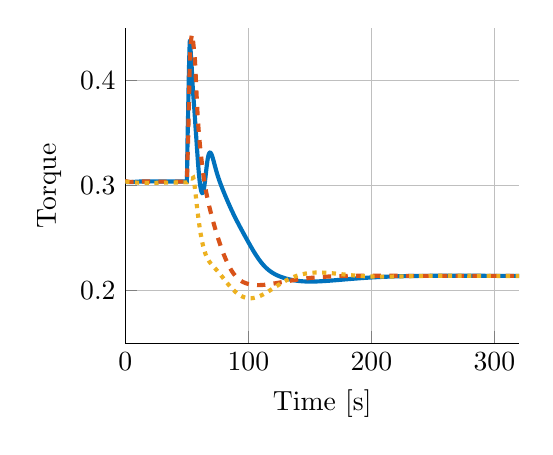
\begin{tikzpicture}

\begin{axis}[%
width=5cm,
height=4cm,
at={(0\linewidth,0\linewidth)},
scale only axis,
xmin=0,
xmax=320,
xlabel={Time [s]},
xmajorgrids,
ymin=0.15,
ymax=0.45,
ylabel={Torque},
ymajorgrids,
axis background/.style={fill=white},
% title style={font=\bfseries},
% title={Normalized Torque Setting},
axis x line*=bottom,
axis y line*=left
]
\addplot [color=mycolor1,solid,line width=1.5pt,forget plot]
  table[row sep=crcr]{%
0	0.30400978288\\
0.25	0.3039140382\\
0.5	0.303898715\\
0.75	0.303849644\\
1	0.303742664\\
1.25	0.303657633\\
1.5	0.303597146\\
1.75	0.303542376\\
2	0.303496532\\
2.25	0.303463798\\
2.5	0.303441868\\
2.75	0.303428301\\
3	0.303421493\\
3.25	0.303419909\\
3.5	0.303421717\\
3.75	0.30342511\\
4	0.303428553\\
4.25	0.303431526\\
4.5	0.303434849\\
4.75	0.303440032\\
5	0.303448488\\
5.25	0.303461125\\
5.5	0.303478337\\
5.75	0.30349989\\
6	0.303524847\\
6.25	0.303551716\\
6.5	0.303578744\\
6.75	0.303604316\\
7	0.303627354\\
7.25	0.303647554\\
7.5	0.303665378\\
7.75	0.30368185\\
8	0.303698259\\
8.25	0.303715821\\
8.5	0.303735369\\
8.75	0.303757135\\
9	0.303780689\\
9.25	0.303805038\\
9.5	0.303828878\\
9.75	0.303850919\\
10	0.3038702\\
10.25	0.303886312\\
10.5	0.303899485\\
10.75	0.3039105018\\
11	0.3039204969\\
11.25	0.3039306579\\
11.5	0.3039419314\\
11.75	0.3039547915\\
12	0.303969133\\
12.25	0.303984311\\
12.5	0.303999316205\\
12.75	0.3040130387\\
13	0.3040245537\\
13.25	0.3040333552\\
13.5	0.304039481\\
13.75	0.3040434978\\
14	0.3040463533\\
14.25	0.304049135\\
14.5	0.3040527985\\
14.75	0.3040579343\\
15	0.3040646292\\
15.25	0.3040724572\\
15.5	0.3040805989\\
15.75	0.3040880599\\
16	0.3040939305\\
16.25	0.3040976215\\
16.5	0.3040990151\\
16.75	0.3040984935\\
17	0.3040968393\\
17.25	0.3040950349\\
17.5	0.3040940141\\
17.75	0.3040944288\\
18	0.3040964899\\
18.25	0.304099921\\
18.5	0.304104037\\
18.75	0.304107926\\
19	0.304110689\\
19.25	0.304111672\\
19.5	0.304110637\\
19.75	0.304107823\\
20	0.304103883\\
20.25	0.304099714\\
20.5	0.3040962284\\
20.75	0.3040941214\\
21	0.3040936953\\
21.25	0.3040947862\\
21.5	0.3040968102\\
21.75	0.304098917\\
22	0.304100213\\
22.25	0.3040999938\\
22.5	0.3040979296\\
22.75	0.3040941496\\
23	0.304089209\\
23.25	0.3040839448\\
23.5	0.3040792588\\
23.75	0.3040758855\\
24	0.304074203\\
24.25	0.3040741366\\
24.5	0.3040751794\\
24.75	0.3040765248\\
25	0.3040772772\\
25.25	0.3040766871\\
25.5	0.304074348\\
25.75	0.3040703036\\
26	0.304065038\\
26.25	0.3040593495\\
26.5	0.3040541434\\
26.75	0.3040501962\\
27	0.3040479541\\
27.25	0.3040474154\\
27.5	0.3040481308\\
27.75	0.3040493193\\
28	0.304050072\\
28.25	0.3040495916\\
28.5	0.3040474025\\
28.75	0.3040434789\\
29	0.3040382535\\
29.25	0.3040325059\\
29.5	0.3040271596\\
29.75	0.3040230404\\
30	0.3040206593\\
30.25	0.304020077\\
30.5	0.3040208847\\
30.75	0.3040223088\\
31	0.3040234127\\
31.25	0.304023343\\
31.5	0.3040215568\\
31.75	0.3040179687\\
32	0.3040129764\\
32.25	0.30400736019\\
32.5	0.30400207849\\
32.75	0.30399801671\\
33	0.30399575263\\
33.25	0.30399540111\\
33.5	0.30399657907\\
33.75	0.30399850171\\
34	0.304000186395\\
34.25	0.304000711878\\
34.5	0.303999464688\\
34.75	0.30399630629\\
35	0.30399161524\\
35.25	0.3039861918\\
35.5	0.3039810494\\
35.75	0.3039771474\\
36	0.3039751358\\
36.25	0.3039751785\\
36.5	0.3039769034\\
36.75	0.3039794935\\
37	0.3039818991\\
37.25	0.3039831145\\
37.5	0.3039824489\\
37.75	0.3039797154\\
38	0.3039752887\\
38.25	0.3039700121\\
38.5	0.3039649776\\
38.75	0.3039612378\\
39	0.3039595238\\
39.25	0.3039600447\\
39.5	0.3039624233\\
39.75	0.3039657865\\
40	0.3039689909\\
40.25	0.3039709253\\
40.5	0.3039708108\\
40.75	0.3039684163\\
41	0.3039641305\\
41.25	0.3039588667\\
41.5	0.3039538256\\
41.75	0.3039501775\\
42	0.3039487466\\
42.25	0.3039497841\\
42.5	0.3039528884\\
42.75	0.3039571003\\
43	0.3039611496\\
43.25	0.3039637918\\
43.5	0.3039641463\\
43.75	0.3039619421\\
44	0.3039576037\\
44.25	0.3039521491\\
44.5	0.3039469257\\
44.75	0.3039432525\\
45	0.3039420629\\
45.25	0.303943645\\
45.5	0.3039475487\\
45.75	0.3039526896\\
46	0.3039576277\\
46.25	0.3039609501\\
46.5	0.3039616569\\
46.75	0.3039594436\\
47	0.3039548\\
47.25	0.3039488939\\
47.5	0.3039432685\\
47.75	0.303939431\\
48	0.3039384434\\
48.25	0.303940623\\
48.5	0.303945437\\
48.75	0.3039516243\\
49	0.3039575187\\
49.25	0.303961494\\
49.5	0.3039624102\\
49.75	0.3039599403\\
50	0.3039546798\\
50.25	0.3171159\\
50.5	0.3392608\\
50.75	0.3547082\\
51	0.3663522\\
51.25	0.3827232\\
51.5	0.3991287\\
51.75	0.411846\\
52	0.423182\\
52.25	0.433125\\
52.5	0.439159\\
52.75	0.43593\\
53	0.429983\\
53.25	0.425146\\
53.5	0.421035\\
53.75	0.416763\\
54	0.411641\\
54.25	0.405724\\
54.5	0.3999344\\
54.75	0.3949111\\
55	0.3904759\\
55.25	0.3862206\\
55.5	0.3820063\\
55.75	0.3780323\\
56	0.3742622\\
56.25	0.3701397\\
56.5	0.3657399\\
56.75	0.3613966\\
57	0.3571217\\
57.25	0.352845\\
57.5	0.3485722\\
57.75	0.3443044\\
58	0.3400287\\
58.25	0.3357414\\
58.5	0.3314702\\
58.75	0.3272726\\
59	0.323204\\
59.25	0.3193062\\
59.5	0.3156146\\
59.75	0.31215964\\
60	0.30896388\\
60.25	0.30604294\\
60.5	0.303407557\\
60.75	0.30106472\\
61	0.29901842\\
61.25	0.29727064\\
61.5	0.29582245\\
61.75	0.29467478\\
62	0.2938289\\
62.25	0.2932867\\
62.5	0.2930506\\
62.75	0.293123\\
63	0.2935058\\
63.25	0.29419939\\
63.5	0.29520118\\
63.75	0.29650428\\
64	0.29809599\\
64.25	0.29995649\\
64.5	0.30205794\\
64.75	0.304364273\\
65	0.30683158\\
65.25	0.30940915\\
65.5	0.31204077\\
65.75	0.3146662\\
66	0.3172236\\
66.25	0.3196532\\
66.5	0.3219038\\
66.75	0.3239373\\
67	0.325731\\
67.25	0.3272746\\
67.5	0.3285669\\
67.75	0.3296131\\
68	0.330422\\
68.25	0.331005\\
68.5	0.331375\\
68.75	0.331546\\
69	0.3315327\\
69.25	0.3313504\\
69.5	0.3310144\\
69.75	0.3305404\\
70	0.329944\\
70.25	0.3292405\\
70.5	0.3284447\\
70.75	0.3275709\\
71	0.3266324\\
71.25	0.3256419\\
71.5	0.3246109\\
71.75	0.3235498\\
72	0.3224681\\
72.25	0.3213741\\
72.5	0.3202748\\
72.75	0.3191767\\
73	0.3180848\\
73.25	0.3170035\\
73.5	0.3159362\\
73.75	0.3148855\\
74	0.31385345\\
74.25	0.31284136\\
74.5	0.31185003\\
74.75	0.3108798\\
75	0.30993062\\
75.25	0.30900211\\
75.5	0.30809362\\
75.75	0.3072043\\
76	0.30633316\\
76.25	0.30547909\\
76.5	0.304640912\\
76.75	0.303817421\\
77	0.303007412\\
77.25	0.3022097\\
77.5	0.30142315\\
77.75	0.30064668\\
78	0.29987927\\
78.25	0.29912001\\
78.5	0.29836803\\
78.75	0.29762258\\
79	0.296883\\
79.25	0.29614868\\
79.5	0.29541912\\
79.75	0.29469391\\
80	0.2939727\\
80.25	0.2932552\\
80.5	0.2925411\\
80.75	0.2918304\\
81	0.2911229\\
81.25	0.2904185\\
81.5	0.2897172\\
81.75	0.2890189\\
82	0.2883238\\
82.25	0.2876317\\
82.5	0.2869429\\
82.75	0.2862573\\
83	0.285575\\
83.25	0.2848961\\
83.5	0.2842207\\
83.75	0.2835488\\
84	0.2828806\\
84.25	0.282216\\
84.5	0.2815552\\
84.75	0.2808982\\
85	0.2802451\\
85.25	0.2795958\\
85.5	0.2789505\\
85.75	0.2783091\\
86	0.2776717\\
86.25	0.2770383\\
86.5	0.2764088\\
86.75	0.2757832\\
87	0.2751616\\
87.25	0.2745438\\
87.5	0.2739299\\
87.75	0.2733197\\
88	0.2727133\\
88.25	0.2721105\\
88.5	0.2715114\\
88.75	0.2709157\\
89	0.2703235\\
89.25	0.2697346\\
89.5	0.269149\\
89.75	0.2685665\\
90	0.2679871\\
90.25	0.2674107\\
90.5	0.2668371\\
90.75	0.2662662\\
91	0.2656979\\
91.25	0.2651322\\
91.5	0.2645689\\
91.75	0.2640079\\
92	0.263449\\
92.25	0.2628923\\
92.5	0.2623375\\
92.75	0.2617845\\
93	0.2612333\\
93.25	0.2606838\\
93.5	0.2601357\\
93.75	0.2595892\\
94	0.259044\\
94.25	0.2585\\
94.5	0.2579573\\
94.75	0.2574156\\
95	0.256875\\
95.25	0.2563354\\
95.5	0.2557967\\
95.75	0.2552589\\
96	0.2547219\\
96.25	0.2541856\\
96.5	0.2536501\\
96.75	0.2531154\\
97	0.2525813\\
97.25	0.252048\\
97.5	0.2515154\\
97.75	0.2509835\\
98	0.2504523\\
98.25	0.2499219\\
98.5	0.2493923\\
98.75	0.2488635\\
99	0.2483356\\
99.25	0.2478087\\
99.5	0.2472827\\
99.75	0.2467579\\
100	0.2462342\\
100.25	0.2457117\\
100.5	0.2451906\\
100.75	0.2446709\\
101	0.2441528\\
101.25	0.2436363\\
101.5	0.2431215\\
101.75	0.2426087\\
102	0.2420978\\
102.25	0.2415891\\
102.5	0.2410826\\
102.75	0.2405785\\
103	0.2400769\\
103.25	0.239578\\
103.5	0.2390819\\
103.75	0.2385887\\
104	0.2380986\\
104.25	0.2376118\\
104.5	0.2371282\\
104.75	0.2366482\\
105	0.2361718\\
105.25	0.2356992\\
105.5	0.2352304\\
105.75	0.2347657\\
106	0.2343052\\
106.25	0.2338489\\
106.5	0.2333971\\
106.75	0.2329498\\
107	0.2325071\\
107.25	0.2320691\\
107.5	0.231636\\
107.75	0.2312078\\
108	0.2307847\\
108.25	0.2303667\\
108.5	0.2299539\\
108.75	0.2295464\\
109	0.2291442\\
109.25	0.2287474\\
109.5	0.2283561\\
109.75	0.2279704\\
110	0.2275902\\
110.25	0.2272156\\
110.5	0.2268466\\
110.75	0.2264833\\
111	0.2261257\\
111.25	0.2257738\\
111.5	0.2254276\\
111.75	0.2250872\\
112	0.2247524\\
112.25	0.2244233\\
112.5	0.2240999\\
112.75	0.2237821\\
113	0.22347\\
113.25	0.2231635\\
113.5	0.2228625\\
113.75	0.2225671\\
114	0.2222772\\
114.25	0.2219927\\
114.5	0.2217135\\
114.75	0.2214397\\
115	0.2211711\\
115.25	0.2209078\\
115.5	0.2206495\\
115.75	0.2203964\\
116	0.2201482\\
116.25	0.2199049\\
116.5	0.2196664\\
116.75	0.2194328\\
117	0.2192037\\
117.25	0.2189793\\
117.5	0.2187594\\
117.75	0.2185439\\
118	0.2183328\\
118.25	0.2181259\\
118.5	0.2179231\\
118.75	0.2177245\\
119	0.2175298\\
119.25	0.2173391\\
119.5	0.2171522\\
119.75	0.216969\\
120	0.2167894\\
120.25	0.2166135\\
120.5	0.216441\\
120.75	0.2162719\\
121	0.2161061\\
121.25	0.2159436\\
121.5	0.2157842\\
121.75	0.215628\\
122	0.2154747\\
122.25	0.2153244\\
122.5	0.2151769\\
122.75	0.2150322\\
123	0.2148902\\
123.25	0.2147509\\
123.5	0.2146142\\
123.75	0.2144799\\
124	0.2143482\\
124.25	0.2142188\\
124.5	0.2140918\\
124.75	0.2139671\\
125	0.2138446\\
125.25	0.2137242\\
125.5	0.213606\\
125.75	0.2134899\\
126	0.2133758\\
126.25	0.2132637\\
126.5	0.2131536\\
126.75	0.2130453\\
127	0.2129389\\
127.25	0.2128343\\
127.5	0.2127315\\
127.75	0.2126304\\
128	0.2125311\\
128.25	0.2124334\\
128.5	0.2123374\\
128.75	0.212243\\
129	0.2121502\\
129.25	0.212059\\
129.5	0.2119693\\
129.75	0.2118812\\
130	0.2117945\\
130.25	0.2117093\\
130.5	0.2116256\\
130.75	0.2115433\\
131	0.2114624\\
131.25	0.211383\\
131.5	0.2113049\\
131.75	0.2112282\\
132	0.2111528\\
132.25	0.2110788\\
132.5	0.2110061\\
132.75	0.2109348\\
133	0.2108647\\
133.25	0.210796\\
133.5	0.2107285\\
133.75	0.2106623\\
134	0.2105973\\
134.25	0.2105336\\
134.5	0.2104712\\
134.75	0.2104099\\
135	0.2103499\\
135.25	0.2102912\\
135.5	0.2102336\\
135.75	0.2101772\\
136	0.2101221\\
136.25	0.2100681\\
136.5	0.2100153\\
136.75	0.2099637\\
137	0.2099132\\
137.25	0.2098639\\
137.5	0.2098157\\
137.75	0.2097687\\
138	0.2097229\\
138.25	0.2096781\\
138.5	0.2096345\\
138.75	0.209592\\
139	0.2095506\\
139.25	0.2095103\\
139.5	0.2094711\\
139.75	0.209433\\
140	0.2093959\\
140.25	0.20936\\
140.5	0.209325\\
140.75	0.2092912\\
141	0.2092584\\
141.25	0.2092266\\
141.5	0.2091959\\
141.75	0.2091661\\
142	0.2091374\\
142.25	0.2091097\\
142.5	0.209083\\
142.75	0.2090573\\
143	0.2090325\\
143.25	0.2090087\\
143.5	0.2089859\\
143.75	0.208964\\
144	0.208943\\
144.25	0.208923\\
144.5	0.2089038\\
144.75	0.2088856\\
145	0.2088683\\
145.25	0.2088519\\
145.5	0.2088363\\
145.75	0.2088216\\
146	0.2088077\\
146.25	0.2087947\\
146.5	0.2087825\\
146.75	0.2087712\\
147	0.2087606\\
147.25	0.2087508\\
147.5	0.2087419\\
147.75	0.2087336\\
148	0.2087262\\
148.25	0.2087195\\
148.5	0.2087136\\
148.75	0.2087083\\
149	0.2087038\\
149.25	0.2087\\
149.5	0.2086969\\
149.75	0.2086945\\
150	0.2086927\\
150.25	0.2086917\\
150.5	0.2086912\\
150.75	0.2086914\\
151	0.2086922\\
151.25	0.2086937\\
151.5	0.2086957\\
151.75	0.2086984\\
152	0.2087016\\
152.25	0.2087054\\
152.5	0.2087098\\
152.75	0.2087147\\
153	0.2087202\\
153.25	0.2087262\\
153.5	0.2087327\\
153.75	0.2087397\\
154	0.2087472\\
154.25	0.2087552\\
154.5	0.2087637\\
154.75	0.2087727\\
155	0.2087821\\
155.25	0.208792\\
155.5	0.2088023\\
155.75	0.2088131\\
156	0.2088243\\
156.25	0.2088359\\
156.5	0.2088479\\
156.75	0.2088603\\
157	0.2088731\\
157.25	0.2088863\\
157.5	0.2088998\\
157.75	0.2089137\\
158	0.208928\\
158.25	0.2089426\\
158.5	0.2089576\\
158.75	0.2089729\\
159	0.2089885\\
159.25	0.2090044\\
159.5	0.2090206\\
159.75	0.2090372\\
160	0.209054\\
160.25	0.2090711\\
160.5	0.2090885\\
160.75	0.2091062\\
161	0.2091242\\
161.25	0.2091424\\
161.5	0.2091608\\
161.75	0.2091795\\
162	0.2091985\\
162.25	0.2092177\\
162.5	0.2092371\\
162.75	0.2092567\\
163	0.2092765\\
163.25	0.2092966\\
163.5	0.2093169\\
163.75	0.2093373\\
164	0.209358\\
164.25	0.2093788\\
164.5	0.2093999\\
164.75	0.2094211\\
165	0.2094425\\
165.25	0.209464\\
165.5	0.2094857\\
165.75	0.2095076\\
166	0.2095296\\
166.25	0.2095518\\
166.5	0.2095741\\
166.75	0.2095965\\
167	0.2096191\\
167.25	0.2096418\\
167.5	0.2096646\\
167.75	0.2096876\\
168	0.2097107\\
168.25	0.2097339\\
168.5	0.2097571\\
168.75	0.2097805\\
169	0.209804\\
169.25	0.2098276\\
169.5	0.2098513\\
169.75	0.2098751\\
170	0.2098989\\
170.25	0.2099229\\
170.5	0.2099469\\
170.75	0.2099709\\
171	0.2099951\\
171.25	0.2100193\\
171.5	0.2100436\\
171.75	0.2100679\\
172	0.2100923\\
172.25	0.2101167\\
172.5	0.2101412\\
172.75	0.2101658\\
173	0.2101903\\
173.25	0.2102149\\
173.5	0.2102396\\
173.75	0.2102643\\
174	0.210289\\
174.25	0.2103137\\
174.5	0.2103385\\
174.75	0.2103632\\
175	0.210388\\
175.25	0.2104128\\
175.5	0.2104377\\
175.75	0.2104625\\
176	0.2104873\\
176.25	0.2105121\\
176.5	0.210537\\
176.75	0.2105618\\
177	0.2105866\\
177.25	0.2106115\\
177.5	0.2106363\\
177.75	0.2106611\\
178	0.2106858\\
178.25	0.2107106\\
178.5	0.2107353\\
178.75	0.2107601\\
179	0.2107848\\
179.25	0.2108094\\
179.5	0.2108341\\
179.75	0.2108587\\
180	0.2108832\\
180.25	0.2109078\\
180.5	0.2109323\\
180.75	0.2109567\\
181	0.2109812\\
181.25	0.2110055\\
181.5	0.2110299\\
181.75	0.2110541\\
182	0.2110784\\
182.25	0.2111025\\
182.5	0.2111267\\
182.75	0.2111507\\
183	0.2111747\\
183.25	0.2111987\\
183.5	0.2112226\\
183.75	0.2112464\\
184	0.2112702\\
184.25	0.2112939\\
184.5	0.2113175\\
184.75	0.2113411\\
185	0.2113646\\
185.25	0.211388\\
185.5	0.2114113\\
185.75	0.2114346\\
186	0.2114578\\
186.25	0.2114809\\
186.5	0.2115039\\
186.75	0.2115269\\
187	0.2115498\\
187.25	0.2115726\\
187.5	0.2115953\\
187.75	0.2116179\\
188	0.2116404\\
188.25	0.2116629\\
188.5	0.2116852\\
188.75	0.2117075\\
189	0.2117297\\
189.25	0.2117518\\
189.5	0.2117738\\
189.75	0.2117957\\
190	0.2118175\\
190.25	0.2118392\\
190.5	0.2118608\\
190.75	0.2118823\\
191	0.2119037\\
191.25	0.211925\\
191.5	0.2119462\\
191.75	0.2119674\\
192	0.2119884\\
192.25	0.2120093\\
192.5	0.2120301\\
192.75	0.2120508\\
193	0.2120714\\
193.25	0.2120919\\
193.5	0.2121123\\
193.75	0.2121325\\
194	0.2121527\\
194.25	0.2121728\\
194.5	0.2121927\\
194.75	0.2122126\\
195	0.2122323\\
195.25	0.212252\\
195.5	0.2122715\\
195.75	0.2122909\\
196	0.2123102\\
196.25	0.2123294\\
196.5	0.2123485\\
196.75	0.2123674\\
197	0.2123863\\
197.25	0.212405\\
197.5	0.2124236\\
197.75	0.2124421\\
198	0.2124605\\
198.25	0.2124788\\
198.5	0.212497\\
198.75	0.2125151\\
199	0.212533\\
199.25	0.2125508\\
199.5	0.2125685\\
199.75	0.2125861\\
200	0.2126036\\
200.25	0.212621\\
200.5	0.2126382\\
200.75	0.2126554\\
201	0.2126724\\
201.25	0.2126893\\
201.5	0.2127061\\
201.75	0.2127228\\
202	0.2127393\\
202.25	0.2127558\\
202.5	0.2127721\\
202.75	0.2127883\\
203	0.2128044\\
203.25	0.2128204\\
203.5	0.2128363\\
203.75	0.212852\\
204	0.2128676\\
204.25	0.2128832\\
204.5	0.2128986\\
204.75	0.2129139\\
205	0.212929\\
205.25	0.2129441\\
205.5	0.212959\\
205.75	0.2129739\\
206	0.2129886\\
206.25	0.2130032\\
206.5	0.2130177\\
206.75	0.213032\\
207	0.2130463\\
207.25	0.2130605\\
207.5	0.2130745\\
207.75	0.2130884\\
208	0.2131022\\
208.25	0.2131159\\
208.5	0.2131295\\
208.75	0.213143\\
209	0.2131563\\
209.25	0.2131696\\
209.5	0.2131827\\
209.75	0.2131957\\
210	0.2132087\\
210.25	0.2132215\\
210.5	0.2132342\\
210.75	0.2132468\\
211	0.2132592\\
211.25	0.2132716\\
211.5	0.2132839\\
211.75	0.213296\\
212	0.2133081\\
212.25	0.21332\\
212.5	0.2133318\\
212.75	0.2133436\\
213	0.2133552\\
213.25	0.2133667\\
213.5	0.2133781\\
213.75	0.2133894\\
214	0.2134006\\
214.25	0.2134117\\
214.5	0.2134227\\
214.75	0.2134336\\
215	0.2134443\\
215.25	0.213455\\
215.5	0.2134656\\
215.75	0.2134761\\
216	0.2134865\\
216.25	0.2134967\\
216.5	0.2135069\\
216.75	0.213517\\
217	0.213527\\
217.25	0.2135368\\
217.5	0.2135466\\
217.75	0.2135563\\
218	0.2135659\\
218.25	0.2135754\\
218.5	0.2135847\\
218.75	0.213594\\
219	0.2136032\\
219.25	0.2136123\\
219.5	0.2136213\\
219.75	0.2136303\\
220	0.2136391\\
220.25	0.2136478\\
220.5	0.2136564\\
220.75	0.213665\\
221	0.2136734\\
221.25	0.2136818\\
221.5	0.2136901\\
221.75	0.2136983\\
222	0.2137063\\
222.25	0.2137144\\
222.5	0.2137223\\
222.75	0.2137301\\
223	0.2137378\\
223.25	0.2137455\\
223.5	0.213753\\
223.75	0.2137605\\
224	0.2137679\\
224.25	0.2137752\\
224.5	0.2137825\\
224.75	0.2137896\\
225	0.2137967\\
225.25	0.2138036\\
225.5	0.2138105\\
225.75	0.2138173\\
226	0.2138241\\
226.25	0.2138307\\
226.5	0.2138373\\
226.75	0.2138438\\
227	0.2138502\\
227.25	0.2138565\\
227.5	0.2138628\\
227.75	0.213869\\
228	0.2138751\\
228.25	0.2138811\\
228.5	0.2138871\\
228.75	0.213893\\
229	0.2138988\\
229.25	0.2139045\\
229.5	0.2139101\\
229.75	0.2139157\\
230	0.2139212\\
230.25	0.2139267\\
230.5	0.2139321\\
230.75	0.2139374\\
231	0.2139426\\
231.25	0.2139477\\
231.5	0.2139528\\
231.75	0.2139579\\
232	0.2139628\\
232.25	0.2139677\\
232.5	0.2139725\\
232.75	0.2139773\\
233	0.213982\\
233.25	0.2139866\\
233.5	0.2139911\\
233.75	0.2139956\\
234	0.2140001\\
234.25	0.2140044\\
234.5	0.2140087\\
234.75	0.214013\\
235	0.2140171\\
235.25	0.2140213\\
235.5	0.2140253\\
235.75	0.2140293\\
236	0.2140333\\
236.25	0.2140371\\
236.5	0.214041\\
236.75	0.2140447\\
237	0.2140484\\
237.25	0.2140521\\
237.5	0.2140557\\
237.75	0.2140592\\
238	0.2140627\\
238.25	0.2140661\\
238.5	0.2140695\\
238.75	0.2140728\\
239	0.2140761\\
239.25	0.2140793\\
239.5	0.2140824\\
239.75	0.2140856\\
240	0.2140886\\
240.25	0.2140916\\
240.5	0.2140946\\
240.75	0.2140975\\
241	0.2141003\\
241.25	0.2141031\\
241.5	0.2141059\\
241.75	0.2141086\\
242	0.2141113\\
242.25	0.2141139\\
242.5	0.2141164\\
242.75	0.214119\\
243	0.2141214\\
243.25	0.2141239\\
243.5	0.2141263\\
243.75	0.2141286\\
244	0.2141309\\
244.25	0.2141332\\
244.5	0.2141354\\
244.75	0.2141375\\
245	0.2141397\\
245.25	0.2141417\\
245.5	0.2141438\\
245.75	0.2141458\\
246	0.2141478\\
246.25	0.2141497\\
246.5	0.2141516\\
246.75	0.2141534\\
247	0.2141552\\
247.25	0.214157\\
247.5	0.2141587\\
247.75	0.2141604\\
248	0.2141621\\
248.25	0.2141637\\
248.5	0.2141653\\
248.75	0.2141668\\
249	0.2141683\\
249.25	0.2141698\\
249.5	0.2141712\\
249.75	0.2141726\\
250	0.214174\\
250.25	0.2141753\\
250.5	0.2141767\\
250.75	0.2141779\\
251	0.2141792\\
251.25	0.2141804\\
251.5	0.2141816\\
251.75	0.2141827\\
252	0.2141838\\
252.25	0.2141849\\
252.5	0.214186\\
252.75	0.214187\\
253	0.214188\\
253.25	0.214189\\
253.5	0.2141899\\
253.75	0.2141908\\
254	0.2141917\\
254.25	0.2141926\\
254.5	0.2141934\\
254.75	0.2141942\\
255	0.214195\\
255.25	0.2141957\\
255.5	0.2141965\\
255.75	0.2141972\\
256	0.2141978\\
256.25	0.2141985\\
256.5	0.2141991\\
256.75	0.2141997\\
257	0.2142003\\
257.25	0.2142008\\
257.5	0.2142014\\
257.75	0.2142019\\
258	0.2142024\\
258.25	0.2142028\\
258.5	0.2142033\\
258.75	0.2142037\\
259	0.2142041\\
259.25	0.2142045\\
259.5	0.2142048\\
259.75	0.2142052\\
260	0.2142055\\
260.25	0.2142058\\
260.5	0.2142061\\
260.75	0.2142063\\
261	0.2142066\\
261.25	0.2142068\\
261.5	0.214207\\
261.75	0.2142072\\
262	0.2142074\\
262.25	0.2142075\\
262.5	0.2142077\\
262.75	0.2142078\\
263	0.2142079\\
263.25	0.214208\\
263.5	0.214208\\
263.75	0.2142081\\
264	0.2142081\\
264.25	0.2142081\\
264.5	0.2142081\\
264.75	0.2142081\\
265	0.2142081\\
265.25	0.2142081\\
265.5	0.214208\\
265.75	0.2142079\\
266	0.2142079\\
266.25	0.2142078\\
266.5	0.2142077\\
266.75	0.2142075\\
267	0.2142074\\
267.25	0.2142073\\
267.5	0.2142071\\
267.75	0.2142069\\
268	0.2142068\\
268.25	0.2142066\\
268.5	0.2142064\\
268.75	0.2142061\\
269	0.2142059\\
269.25	0.2142057\\
269.5	0.2142054\\
269.75	0.2142052\\
270	0.2142049\\
270.25	0.2142046\\
270.5	0.2142043\\
270.75	0.214204\\
271	0.2142037\\
271.25	0.2142034\\
271.5	0.2142031\\
271.75	0.2142028\\
272	0.2142024\\
272.25	0.2142021\\
272.5	0.2142017\\
272.75	0.2142013\\
273	0.214201\\
273.25	0.2142006\\
273.5	0.2142002\\
273.75	0.2141998\\
274	0.2141994\\
274.25	0.214199\\
274.5	0.2141985\\
274.75	0.2141981\\
275	0.2141977\\
275.25	0.2141972\\
275.5	0.2141968\\
275.75	0.2141963\\
276	0.2141959\\
276.25	0.2141954\\
276.5	0.2141949\\
276.75	0.2141945\\
277	0.214194\\
277.25	0.2141935\\
277.5	0.214193\\
277.75	0.2141925\\
278	0.214192\\
278.25	0.2141915\\
278.5	0.214191\\
278.75	0.2141905\\
279	0.21419\\
279.25	0.2141894\\
279.5	0.2141889\\
279.75	0.2141884\\
280	0.2141878\\
280.25	0.2141873\\
280.5	0.2141868\\
280.75	0.2141862\\
281	0.2141857\\
281.25	0.2141851\\
281.5	0.2141845\\
281.75	0.214184\\
282	0.2141834\\
282.25	0.2141829\\
282.5	0.2141823\\
282.75	0.2141817\\
283	0.2141812\\
283.25	0.2141806\\
283.5	0.21418\\
283.75	0.2141794\\
284	0.2141788\\
284.25	0.2141783\\
284.5	0.2141777\\
284.75	0.2141771\\
285	0.2141765\\
285.25	0.2141759\\
285.5	0.2141753\\
285.75	0.2141747\\
286	0.2141741\\
286.25	0.2141736\\
286.5	0.214173\\
286.75	0.2141724\\
287	0.2141718\\
287.25	0.2141712\\
287.5	0.2141706\\
287.75	0.21417\\
288	0.2141694\\
288.25	0.2141688\\
288.5	0.2141682\\
288.75	0.2141676\\
289	0.214167\\
289.25	0.2141664\\
289.5	0.2141658\\
289.75	0.2141652\\
290	0.2141646\\
290.25	0.214164\\
290.5	0.2141634\\
290.75	0.2141628\\
291	0.2141622\\
291.25	0.2141616\\
291.5	0.214161\\
291.75	0.2141604\\
292	0.2141598\\
292.25	0.2141592\\
292.5	0.2141586\\
292.75	0.214158\\
293	0.2141574\\
293.25	0.2141568\\
293.5	0.2141562\\
293.75	0.2141556\\
294	0.214155\\
294.25	0.2141544\\
294.5	0.2141538\\
294.75	0.2141532\\
295	0.2141527\\
295.25	0.2141521\\
295.5	0.2141515\\
295.75	0.2141509\\
296	0.2141503\\
296.25	0.2141497\\
296.5	0.2141492\\
296.75	0.2141486\\
297	0.214148\\
297.25	0.2141474\\
297.5	0.2141469\\
297.75	0.2141463\\
298	0.2141457\\
298.25	0.2141452\\
298.5	0.2141446\\
298.75	0.214144\\
299	0.2141435\\
299.25	0.2141429\\
299.5	0.2141424\\
299.75	0.2141418\\
300	0.2141413\\
300.25	0.2141407\\
300.5	0.2141402\\
300.75	0.2141396\\
301	0.2141391\\
301.25	0.2141385\\
301.5	0.214138\\
301.75	0.2141374\\
302	0.2141369\\
302.25	0.2141364\\
302.5	0.2141358\\
302.75	0.2141353\\
303	0.2141348\\
303.25	0.2141343\\
303.5	0.2141337\\
303.75	0.2141332\\
304	0.2141327\\
304.25	0.2141322\\
304.5	0.2141317\\
304.75	0.2141312\\
305	0.2141307\\
305.25	0.2141302\\
305.5	0.2141297\\
305.75	0.2141292\\
306	0.2141287\\
306.25	0.2141282\\
306.5	0.2141277\\
306.75	0.2141272\\
307	0.2141267\\
307.25	0.2141262\\
307.5	0.2141257\\
307.75	0.2141253\\
308	0.2141248\\
308.25	0.2141243\\
308.5	0.2141238\\
308.75	0.2141234\\
309	0.2141229\\
309.25	0.2141224\\
309.5	0.214122\\
309.75	0.2141215\\
310	0.2141211\\
310.25	0.2141206\\
310.5	0.2141202\\
310.75	0.2141197\\
311	0.2141193\\
311.25	0.2141189\\
311.5	0.2141184\\
311.75	0.214118\\
312	0.2141175\\
312.25	0.2141171\\
312.5	0.2141167\\
312.75	0.2141163\\
313	0.2141159\\
313.25	0.2141154\\
313.5	0.214115\\
313.75	0.2141146\\
314	0.2141142\\
314.25	0.2141138\\
314.5	0.2141134\\
314.75	0.214113\\
315	0.2141126\\
315.25	0.2141122\\
315.5	0.2141118\\
315.75	0.2141114\\
316	0.214111\\
316.25	0.2141107\\
316.5	0.2141103\\
316.75	0.2141099\\
317	0.2141095\\
317.25	0.2141091\\
317.5	0.2141088\\
317.75	0.2141084\\
318	0.2141081\\
318.25	0.2141077\\
318.5	0.2141073\\
318.75	0.214107\\
319	0.2141066\\
319.25	0.2141063\\
319.5	0.2141059\\
319.75	0.2141056\\
320	0.2141052\\
320.25	0.2141049\\
320.5	0.2141046\\
320.75	0.2141042\\
321	0.2141039\\
321.25	0.2141036\\
321.5	0.2141033\\
321.75	0.2141029\\
322	0.2141026\\
322.25	0.2141023\\
322.5	0.214102\\
322.75	0.2141017\\
323	0.2141014\\
323.25	0.2141011\\
323.5	0.2141008\\
323.75	0.2141005\\
324	0.2141002\\
324.25	0.2140999\\
324.5	0.2140996\\
324.75	0.2140993\\
325	0.214099\\
325.25	0.2140987\\
325.5	0.2140984\\
325.75	0.2140982\\
326	0.2140979\\
326.25	0.2140976\\
326.5	0.2140973\\
326.75	0.2140971\\
327	0.2140968\\
327.25	0.2140965\\
327.5	0.2140963\\
327.75	0.214096\\
328	0.2140958\\
328.25	0.2140955\\
328.5	0.2140953\\
328.75	0.214095\\
329	0.2140948\\
329.25	0.2140945\\
329.5	0.2140943\\
329.75	0.214094\\
330	0.2140938\\
330.25	0.2140936\\
330.5	0.2140933\\
330.75	0.2140931\\
331	0.2140929\\
331.25	0.2140927\\
331.5	0.2140924\\
331.75	0.2140922\\
332	0.214092\\
332.25	0.2140918\\
332.5	0.2140916\\
332.75	0.2140914\\
333	0.2140911\\
333.25	0.2140909\\
333.5	0.2140907\\
333.75	0.2140905\\
334	0.2140903\\
334.25	0.2140901\\
334.5	0.2140899\\
334.75	0.2140897\\
335	0.2140896\\
335.25	0.2140894\\
335.5	0.2140892\\
335.75	0.214089\\
336	0.2140888\\
336.25	0.2140886\\
336.5	0.2140884\\
336.75	0.2140883\\
337	0.2140881\\
337.25	0.2140879\\
337.5	0.2140878\\
337.75	0.2140876\\
338	0.2140874\\
338.25	0.2140873\\
338.5	0.2140871\\
338.75	0.2140869\\
339	0.2140868\\
339.25	0.2140866\\
339.5	0.2140865\\
339.75	0.2140863\\
340	0.2140862\\
340.25	0.214086\\
340.5	0.2140859\\
340.75	0.2140857\\
341	0.2140856\\
341.25	0.2140854\\
341.5	0.2140853\\
341.75	0.2140852\\
342	0.214085\\
342.25	0.2140849\\
342.5	0.2140848\\
342.75	0.2140846\\
343	0.2140845\\
343.25	0.2140844\\
343.5	0.2140842\\
343.75	0.2140841\\
344	0.214084\\
344.25	0.2140839\\
344.5	0.2140838\\
344.75	0.2140836\\
345	0.2140835\\
345.25	0.2140834\\
345.5	0.2140833\\
345.75	0.2140832\\
346	0.2140831\\
346.25	0.214083\\
346.5	0.2140829\\
346.75	0.2140828\\
347	0.2140826\\
347.25	0.2140825\\
347.5	0.2140824\\
347.75	0.2140823\\
348	0.2140823\\
348.25	0.2140822\\
348.5	0.2140821\\
348.75	0.214082\\
349	0.2140819\\
349.25	0.2140818\\
349.5	0.2140817\\
349.75	0.2140816\\
350	0.2140815\\
350.25	0.2140814\\
350.5	0.2140814\\
350.75	0.2140813\\
351	0.2140812\\
351.25	0.2140811\\
351.5	0.214081\\
351.75	0.214081\\
352	0.2140809\\
352.25	0.2140808\\
352.5	0.2140807\\
352.75	0.2140807\\
353	0.2140806\\
353.25	0.2140805\\
353.5	0.2140805\\
353.75	0.2140804\\
354	0.2140803\\
354.25	0.2140803\\
354.5	0.2140802\\
354.75	0.2140801\\
355	0.2140801\\
355.25	0.21408\\
355.5	0.2140799\\
355.75	0.2140799\\
356	0.2140798\\
356.25	0.2140798\\
356.5	0.2140797\\
356.75	0.2140797\\
357	0.2140796\\
357.25	0.2140796\\
357.5	0.2140795\\
357.75	0.2140795\\
358	0.2140794\\
358.25	0.2140794\\
358.5	0.2140793\\
358.75	0.2140793\\
359	0.2140792\\
359.25	0.2140792\\
359.5	0.2140791\\
359.75	0.2140791\\
360	0.2140791\\
360.25	0.214079\\
360.5	0.214079\\
360.75	0.2140789\\
361	0.2140789\\
361.25	0.2140789\\
361.5	0.2140788\\
361.75	0.2140788\\
362	0.2140788\\
362.25	0.2140787\\
362.5	0.2140787\\
362.75	0.2140787\\
363	0.2140786\\
363.25	0.2140786\\
363.5	0.2140786\\
363.75	0.2140785\\
364	0.2140785\\
364.25	0.2140785\\
364.5	0.2140785\\
364.75	0.2140784\\
365	0.2140784\\
365.25	0.2140784\\
365.5	0.2140784\\
365.75	0.2140783\\
366	0.2140783\\
366.25	0.2140783\\
366.5	0.2140783\\
366.75	0.2140783\\
367	0.2140782\\
367.25	0.2140782\\
367.5	0.2140782\\
367.75	0.2140782\\
368	0.2140782\\
368.25	0.2140782\\
368.5	0.2140781\\
368.75	0.2140781\\
369	0.2140781\\
369.25	0.2140781\\
369.5	0.2140781\\
369.75	0.2140781\\
370	0.2140781\\
370.25	0.214078\\
370.5	0.214078\\
370.75	0.214078\\
371	0.214078\\
371.25	0.214078\\
371.5	0.214078\\
371.75	0.214078\\
372	0.214078\\
372.25	0.214078\\
372.5	0.214078\\
372.75	0.214078\\
373	0.2140779\\
373.25	0.2140779\\
373.5	0.2140779\\
373.75	0.2140779\\
374	0.2140779\\
374.25	0.2140779\\
374.5	0.2140779\\
374.75	0.2140779\\
375	0.2140779\\
375.25	0.2140779\\
375.5	0.2140779\\
375.75	0.2140779\\
376	0.2140779\\
376.25	0.2140779\\
376.5	0.2140779\\
376.75	0.2140779\\
377	0.2140779\\
377.25	0.2140779\\
377.5	0.2140779\\
377.75	0.2140779\\
378	0.2140779\\
378.25	0.2140779\\
378.5	0.2140779\\
378.75	0.2140779\\
379	0.2140779\\
379.25	0.2140779\\
379.5	0.2140779\\
379.75	0.2140779\\
380	0.2140779\\
380.25	0.2140779\\
380.5	0.2140779\\
380.75	0.2140779\\
381	0.214078\\
381.25	0.214078\\
381.5	0.214078\\
381.75	0.214078\\
382	0.214078\\
382.25	0.214078\\
382.5	0.214078\\
382.75	0.214078\\
383	0.214078\\
383.25	0.214078\\
383.5	0.214078\\
383.75	0.214078\\
384	0.214078\\
384.25	0.214078\\
384.5	0.2140781\\
384.75	0.2140781\\
385	0.2140781\\
385.25	0.2140781\\
385.5	0.2140781\\
385.75	0.2140781\\
386	0.2140781\\
386.25	0.2140781\\
386.5	0.2140781\\
386.75	0.2140781\\
387	0.2140782\\
387.25	0.2140782\\
387.5	0.2140782\\
387.75	0.2140782\\
388	0.2140782\\
388.25	0.2140782\\
388.5	0.2140782\\
388.75	0.2140782\\
389	0.2140782\\
389.25	0.2140783\\
389.5	0.2140783\\
389.75	0.2140783\\
390	0.2140783\\
390.25	0.2140783\\
390.5	0.2140783\\
390.75	0.2140783\\
391	0.2140783\\
391.25	0.2140784\\
391.5	0.2140784\\
391.75	0.2140784\\
392	0.2140784\\
392.25	0.2140784\\
392.5	0.2140784\\
392.75	0.2140784\\
393	0.2140784\\
393.25	0.2140785\\
393.5	0.2140785\\
393.75	0.2140785\\
394	0.2140785\\
394.25	0.2140785\\
394.5	0.2140785\\
394.75	0.2140785\\
395	0.2140786\\
395.25	0.2140786\\
395.5	0.2140786\\
395.75	0.2140786\\
396	0.2140786\\
396.25	0.2140786\\
396.5	0.2140786\\
396.75	0.2140787\\
397	0.2140787\\
397.25	0.2140787\\
397.5	0.2140787\\
397.75	0.2140787\\
398	0.2140787\\
398.25	0.2140787\\
398.5	0.2140788\\
398.75	0.2140788\\
399	0.2140788\\
399.25	0.2140788\\
399.5	0.2140788\\
399.75	0.2140788\\
400	0.2140788\\
400.25	0.2140789\\
400.5	0.2140789\\
400.75	0.2140789\\
401	0.2140789\\
401.25	0.2140789\\
401.5	0.2140789\\
401.75	0.2140789\\
402	0.214079\\
402.25	0.214079\\
402.5	0.214079\\
402.75	0.214079\\
403	0.214079\\
403.25	0.214079\\
403.5	0.214079\\
403.75	0.2140791\\
404	0.2140791\\
404.25	0.2140791\\
404.5	0.2140791\\
404.75	0.2140791\\
405	0.2140791\\
405.25	0.2140791\\
405.5	0.2140792\\
405.75	0.2140792\\
406	0.2140792\\
406.25	0.2140792\\
406.5	0.2140792\\
406.75	0.2140792\\
407	0.2140792\\
407.25	0.2140793\\
407.5	0.2140793\\
407.75	0.2140793\\
408	0.2140793\\
408.25	0.2140793\\
408.5	0.2140793\\
408.75	0.2140793\\
409	0.2140794\\
409.25	0.2140794\\
409.5	0.2140794\\
409.75	0.2140794\\
410	0.2140794\\
410.25	0.2140794\\
410.5	0.2140794\\
410.75	0.2140795\\
411	0.2140795\\
411.25	0.2140795\\
411.5	0.2140795\\
411.75	0.2140795\\
412	0.2140795\\
412.25	0.2140795\\
412.5	0.2140796\\
412.75	0.2140796\\
413	0.2140796\\
413.25	0.2140796\\
413.5	0.2140796\\
413.75	0.2140796\\
414	0.2140796\\
414.25	0.2140796\\
414.5	0.2140797\\
414.75	0.2140797\\
415	0.2140797\\
415.25	0.2140797\\
415.5	0.2140797\\
415.75	0.2140797\\
416	0.2140797\\
416.25	0.2140797\\
416.5	0.2140798\\
416.75	0.2140798\\
417	0.2140798\\
417.25	0.2140798\\
417.5	0.2140798\\
417.75	0.2140798\\
418	0.2140798\\
418.25	0.2140798\\
418.5	0.2140799\\
418.75	0.2140799\\
419	0.2140799\\
419.25	0.2140799\\
419.5	0.2140799\\
419.75	0.2140799\\
420	0.2140799\\
420.25	0.2140799\\
420.5	0.21408\\
420.75	0.21408\\
421	0.21408\\
421.25	0.21408\\
421.5	0.21408\\
421.75	0.21408\\
422	0.21408\\
422.25	0.21408\\
422.5	0.21408\\
422.75	0.2140801\\
423	0.2140801\\
423.25	0.2140801\\
423.5	0.2140801\\
423.75	0.2140801\\
424	0.2140801\\
424.25	0.2140801\\
424.5	0.2140801\\
424.75	0.2140801\\
425	0.2140802\\
425.25	0.2140802\\
425.5	0.2140802\\
425.75	0.2140802\\
426	0.2140802\\
426.25	0.2140802\\
426.5	0.2140802\\
426.75	0.2140802\\
427	0.2140802\\
427.25	0.2140802\\
427.5	0.2140802\\
427.75	0.2140803\\
428	0.2140803\\
428.25	0.2140803\\
428.5	0.2140803\\
428.75	0.2140803\\
429	0.2140803\\
429.25	0.2140803\\
429.5	0.2140803\\
429.75	0.2140803\\
430	0.2140803\\
430.25	0.2140804\\
430.5	0.2140804\\
430.75	0.2140804\\
431	0.2140804\\
431.25	0.2140804\\
431.5	0.2140804\\
431.75	0.2140804\\
432	0.2140804\\
432.25	0.2140804\\
432.5	0.2140804\\
432.75	0.2140804\\
433	0.2140804\\
433.25	0.2140805\\
433.5	0.2140805\\
433.75	0.2140805\\
434	0.2140805\\
434.25	0.2140805\\
434.5	0.2140805\\
434.75	0.2140805\\
435	0.2140805\\
435.25	0.2140805\\
435.5	0.2140805\\
435.75	0.2140805\\
436	0.2140805\\
436.25	0.2140805\\
436.5	0.2140806\\
436.75	0.2140806\\
437	0.2140806\\
437.25	0.2140806\\
437.5	0.2140806\\
437.75	0.2140806\\
438	0.2140806\\
438.25	0.2140806\\
438.5	0.2140806\\
438.75	0.2140806\\
439	0.2140806\\
439.25	0.2140806\\
439.5	0.2140806\\
439.75	0.2140806\\
440	0.2140806\\
440.25	0.2140807\\
440.5	0.2140807\\
440.75	0.2140807\\
441	0.2140807\\
441.25	0.2140807\\
441.5	0.2140807\\
441.75	0.2140807\\
442	0.2140807\\
442.25	0.2140807\\
442.5	0.2140807\\
442.75	0.2140807\\
443	0.2140807\\
443.25	0.2140807\\
443.5	0.2140807\\
443.75	0.2140807\\
444	0.2140807\\
444.25	0.2140807\\
444.5	0.2140807\\
444.75	0.2140808\\
445	0.2140808\\
445.25	0.2140808\\
445.5	0.2140808\\
445.75	0.2140808\\
446	0.2140808\\
446.25	0.2140808\\
446.5	0.2140808\\
446.75	0.2140808\\
447	0.2140808\\
447.25	0.2140808\\
447.5	0.2140808\\
447.75	0.2140808\\
448	0.2140808\\
448.25	0.2140808\\
448.5	0.2140808\\
448.75	0.2140808\\
449	0.2140808\\
449.25	0.2140808\\
449.5	0.2140808\\
449.75	0.2140808\\
450	0.2140809\\
450.25	0.2140809\\
450.5	0.2140809\\
450.75	0.2140809\\
451	0.2140809\\
451.25	0.2140809\\
451.5	0.2140809\\
451.75	0.2140809\\
452	0.2140809\\
452.25	0.2140809\\
452.5	0.2140809\\
452.75	0.2140809\\
453	0.2140809\\
453.25	0.2140809\\
453.5	0.2140809\\
453.75	0.2140809\\
454	0.2140809\\
454.25	0.2140809\\
454.5	0.2140809\\
454.75	0.2140809\\
455	0.2140809\\
455.25	0.2140809\\
455.5	0.2140809\\
455.75	0.2140809\\
456	0.2140809\\
456.25	0.2140809\\
456.5	0.2140809\\
456.75	0.2140809\\
457	0.2140809\\
457.25	0.214081\\
457.5	0.214081\\
457.75	0.214081\\
458	0.214081\\
458.25	0.214081\\
458.5	0.214081\\
458.75	0.214081\\
459	0.214081\\
459.25	0.214081\\
459.5	0.214081\\
459.75	0.214081\\
460	0.214081\\
460.25	0.214081\\
460.5	0.214081\\
460.75	0.214081\\
461	0.214081\\
461.25	0.214081\\
461.5	0.214081\\
461.75	0.214081\\
462	0.214081\\
462.25	0.214081\\
462.5	0.214081\\
462.75	0.214081\\
463	0.214081\\
463.25	0.214081\\
463.5	0.214081\\
463.75	0.214081\\
464	0.214081\\
464.25	0.214081\\
464.5	0.214081\\
464.75	0.214081\\
465	0.214081\\
465.25	0.214081\\
465.5	0.214081\\
465.75	0.214081\\
466	0.214081\\
466.25	0.214081\\
466.5	0.214081\\
466.75	0.214081\\
467	0.214081\\
467.25	0.214081\\
467.5	0.214081\\
467.75	0.214081\\
468	0.214081\\
468.25	0.214081\\
468.5	0.214081\\
468.75	0.214081\\
469	0.214081\\
469.25	0.214081\\
469.5	0.214081\\
469.75	0.214081\\
470	0.214081\\
470.25	0.2140811\\
470.5	0.2140811\\
470.75	0.2140811\\
471	0.2140811\\
471.25	0.2140811\\
471.5	0.2140811\\
471.75	0.2140811\\
472	0.2140811\\
472.25	0.2140811\\
472.5	0.2140811\\
472.75	0.2140811\\
473	0.2140811\\
473.25	0.2140811\\
473.5	0.2140811\\
473.75	0.2140811\\
474	0.2140811\\
474.25	0.2140811\\
474.5	0.2140811\\
474.75	0.2140811\\
475	0.2140811\\
475.25	0.2140811\\
475.5	0.2140811\\
475.75	0.2140811\\
476	0.2140811\\
476.25	0.2140811\\
476.5	0.2140811\\
476.75	0.2140811\\
477	0.2140811\\
477.25	0.2140811\\
477.5	0.2140811\\
477.75	0.2140811\\
478	0.2140811\\
478.25	0.2140811\\
478.5	0.2140811\\
478.75	0.2140811\\
479	0.2140811\\
479.25	0.2140811\\
479.5	0.2140811\\
479.75	0.2140811\\
480	0.2140811\\
480.25	0.2140811\\
480.5	0.2140811\\
480.75	0.2140811\\
481	0.2140811\\
481.25	0.2140811\\
481.5	0.2140811\\
481.75	0.2140811\\
482	0.2140811\\
482.25	0.2140811\\
482.5	0.2140811\\
482.75	0.2140811\\
483	0.2140811\\
483.25	0.2140811\\
483.5	0.2140811\\
483.75	0.2140811\\
484	0.2140811\\
484.25	0.2140811\\
484.5	0.2140811\\
484.75	0.2140811\\
485	0.2140811\\
485.25	0.2140811\\
485.5	0.2140811\\
485.75	0.2140811\\
486	0.2140811\\
486.25	0.2140811\\
486.5	0.2140811\\
486.75	0.2140811\\
487	0.2140811\\
487.25	0.2140811\\
487.5	0.2140811\\
487.75	0.2140811\\
488	0.2140811\\
488.25	0.2140811\\
488.5	0.2140811\\
488.75	0.2140811\\
489	0.2140811\\
489.25	0.2140811\\
489.5	0.2140811\\
489.75	0.2140811\\
490	0.2140811\\
490.25	0.2140811\\
490.5	0.2140811\\
490.75	0.2140811\\
491	0.2140811\\
491.25	0.2140811\\
491.5	0.2140811\\
491.75	0.2140811\\
492	0.2140811\\
492.25	0.2140811\\
492.5	0.2140811\\
492.75	0.2140811\\
493	0.2140811\\
493.25	0.2140811\\
493.5	0.2140811\\
493.75	0.2140811\\
494	0.2140811\\
494.25	0.2140811\\
494.5	0.2140811\\
494.75	0.2140811\\
495	0.2140811\\
495.25	0.2140811\\
495.5	0.2140811\\
495.75	0.2140811\\
496	0.2140811\\
496.25	0.2140811\\
496.5	0.2140811\\
496.75	0.2140811\\
497	0.2140811\\
497.25	0.2140811\\
497.5	0.2140811\\
497.75	0.2140811\\
498	0.2140811\\
498.25	0.2140811\\
498.5	0.2140811\\
498.75	0.2140811\\
499	0.2140811\\
499.25	0.2140811\\
499.5	0.2140811\\
499.75	0.2140811\\
};
\addplot [color=mycolor2,dashed,line width=1.5pt,forget plot]
  table[row sep=crcr]{%
0	0.3040175484\\
0.25	0.304105343\\
0.5	0.304222207\\
0.75	0.304199101\\
1	0.304104359\\
1.25	0.3040385347\\
1.5	0.3039892475\\
1.75	0.3039357009\\
2	0.303884439\\
2.25	0.303839439\\
2.5	0.303798192\\
2.75	0.303760292\\
3	0.303726874\\
3.25	0.303698222\\
3.5	0.303674215\\
3.75	0.303654858\\
4	0.303640065\\
4.25	0.303629578\\
4.5	0.30362303\\
4.75	0.303619912\\
5	0.303619629\\
5.25	0.303621608\\
5.5	0.303625367\\
5.75	0.303630534\\
6	0.303636855\\
6.25	0.303644192\\
6.5	0.303652498\\
6.75	0.303661784\\
7	0.303672072\\
7.25	0.303683348\\
7.5	0.303695538\\
7.75	0.303708504\\
8	0.30372205\\
8.25	0.303735947\\
8.5	0.303749955\\
8.75	0.303763857\\
9	0.30377748\\
9.25	0.303790707\\
9.5	0.303803483\\
9.75	0.303815805\\
10	0.303827704\\
10.25	0.303839226\\
10.5	0.303850413\\
10.75	0.303861285\\
11	0.303871837\\
11.25	0.303882033\\
11.5	0.303891815\\
11.75	0.3039011153\\
12	0.3039098674\\
12.25	0.3039180193\\
12.5	0.3039255417\\
12.75	0.3039324315\\
13	0.3039387106\\
13.25	0.3039444194\\
13.5	0.3039496086\\
13.75	0.3039543296\\
14	0.303958626\\
14.25	0.3039625286\\
14.5	0.3039660529\\
14.75	0.303969201\\
15	0.3039719656\\
15.25	0.3039743361\\
15.5	0.3039763043\\
15.75	0.3039778698\\
16	0.3039790425\\
16.25	0.3039798434\\
16.5	0.3039803025\\
16.75	0.3039804555\\
17	0.3039803395\\
17.25	0.3039799887\\
17.5	0.3039794309\\
17.75	0.3039786866\\
18	0.3039777683\\
18.25	0.303976682\\
18.5	0.3039754305\\
18.75	0.3039740154\\
19	0.3039724405\\
19.25	0.3039707136\\
19.5	0.3039688471\\
19.75	0.3039668576\\
20	0.303964765\\
20.25	0.3039625904\\
20.5	0.3039603538\\
20.75	0.3039580725\\
21	0.3039557603\\
21.25	0.3039534265\\
21.5	0.3039510769\\
21.75	0.3039487146\\
22	0.3039463415\\
22.25	0.3039439597\\
22.5	0.3039415725\\
22.75	0.3039391854\\
23	0.303936806\\
23.25	0.3039344435\\
23.5	0.3039321077\\
23.75	0.3039298087\\
24	0.3039275552\\
24.25	0.3039253542\\
24.5	0.3039232105\\
24.75	0.3039211269\\
25	0.3039191046\\
25.25	0.3039171438\\
25.5	0.3039152443\\
25.75	0.3039134064\\
26	0.3039116311\\
26.25	0.3039099206\\
26.5	0.3039082777\\
26.75	0.3039067059\\
27	0.3039052087\\
27.25	0.3039037891\\
27.5	0.3039024496\\
27.75	0.3039011912\\
28	0.303900014\\
28.25	0.303898917\\
28.5	0.303897899\\
28.75	0.303896959\\
29	0.303896093\\
29.25	0.303895301\\
29.5	0.303894581\\
29.75	0.303893934\\
30	0.303893358\\
30.25	0.303892854\\
30.5	0.30389242\\
30.75	0.303892058\\
31	0.303891765\\
31.25	0.303891539\\
31.5	0.303891379\\
31.75	0.303891282\\
32	0.303891245\\
32.25	0.303891264\\
32.5	0.303891339\\
32.75	0.303891465\\
33	0.30389164\\
33.25	0.303891863\\
33.5	0.303892132\\
33.75	0.303892445\\
34	0.303892799\\
34.25	0.303893193\\
34.5	0.303893625\\
34.75	0.303894091\\
35	0.303894589\\
35.25	0.303895116\\
35.5	0.30389567\\
35.75	0.303896246\\
36	0.303896844\\
36.25	0.303897459\\
36.5	0.303898091\\
36.75	0.303898737\\
37	0.303899395\\
37.25	0.3039000631\\
37.5	0.3039007392\\
37.75	0.3039014215\\
38	0.3039021078\\
38.25	0.303902796\\
38.5	0.3039034841\\
38.75	0.3039041698\\
39	0.3039048514\\
39.25	0.3039055268\\
39.5	0.3039061945\\
39.75	0.3039068529\\
40	0.3039075008\\
40.25	0.3039081368\\
40.5	0.3039087598\\
40.75	0.3039093688\\
41	0.3039099626\\
41.25	0.3039105402\\
41.5	0.3039111007\\
41.75	0.3039116429\\
42	0.3039121661\\
42.25	0.3039126693\\
42.5	0.3039131518\\
42.75	0.303913613\\
43	0.3039140525\\
43.25	0.3039144699\\
43.5	0.3039148649\\
43.75	0.3039152374\\
44	0.3039155873\\
44.25	0.3039159145\\
44.5	0.303916219\\
44.75	0.3039165007\\
45	0.3039167597\\
45.25	0.3039169961\\
45.5	0.30391721\\
45.75	0.3039174017\\
46	0.3039175713\\
46.25	0.3039177194\\
46.5	0.3039178462\\
46.75	0.3039179522\\
47	0.3039180381\\
47.25	0.3039181044\\
47.5	0.3039181516\\
47.75	0.3039181805\\
48	0.3039181916\\
48.25	0.3039181855\\
48.5	0.303918163\\
48.75	0.3039181246\\
49	0.3039180711\\
49.25	0.3039180032\\
49.5	0.3039179216\\
49.75	0.3039178271\\
50	0.3039177205\\
50.25	0.31176943\\
50.5	0.3245665\\
50.75	0.3317526\\
51	0.3416827\\
51.25	0.3554894\\
51.5	0.3692327\\
51.75	0.381938\\
52	0.3950937\\
52.25	0.40852\\
52.5	0.421057\\
52.75	0.428157\\
53	0.431985\\
53.25	0.43621\\
53.5	0.439462\\
53.75	0.441418\\
54	0.443011\\
54.25	0.444334\\
54.5	0.443493\\
54.75	0.440973\\
55	0.438243\\
55.25	0.435731\\
55.5	0.432683\\
55.75	0.429803\\
56	0.42735\\
56.25	0.424748\\
56.5	0.421005\\
56.75	0.415941\\
57	0.410056\\
57.25	0.4037547\\
57.5	0.3972523\\
57.75	0.3907577\\
58	0.3844627\\
58.25	0.3784882\\
58.5	0.3729035\\
58.75	0.3677177\\
59	0.3629077\\
59.25	0.358455\\
59.5	0.3543386\\
59.75	0.3505221\\
60	0.3469622\\
60.25	0.3436193\\
60.5	0.3404582\\
60.75	0.3374458\\
61	0.3345523\\
61.25	0.3317545\\
61.5	0.3290377\\
61.75	0.3263936\\
62	0.3238191\\
62.25	0.3213139\\
62.5	0.3188794\\
62.75	0.3165175\\
63	0.3142296\\
63.25	0.3120167\\
63.5	0.3098788\\
63.75	0.30781521\\
64	0.30582446\\
64.25	0.3039044899\\
64.5	0.30205272\\
64.75	0.30026621\\
65	0.29854171\\
65.25	0.29687578\\
65.5	0.29526487\\
65.75	0.2937053\\
66	0.2921935\\
66.25	0.2907258\\
66.5	0.2892986\\
66.75	0.2879085\\
67	0.2865523\\
67.25	0.2852268\\
67.5	0.2839291\\
67.75	0.2826566\\
68	0.2814068\\
68.25	0.2801776\\
68.5	0.278967\\
68.75	0.2777734\\
69	0.2765952\\
69.25	0.2754312\\
69.5	0.2742802\\
69.75	0.2731415\\
70	0.2720142\\
70.25	0.2708977\\
70.5	0.2697915\\
70.75	0.2686953\\
71	0.2676087\\
71.25	0.2665315\\
71.5	0.2654636\\
71.75	0.2644047\\
72	0.2633549\\
72.25	0.2623141\\
72.5	0.2612822\\
72.75	0.2602593\\
73	0.2592453\\
73.25	0.2582403\\
73.5	0.2572443\\
73.75	0.2562573\\
74	0.2552793\\
74.25	0.2543104\\
74.5	0.2533506\\
74.75	0.2523999\\
75	0.2514584\\
75.25	0.2505261\\
75.5	0.2496031\\
75.75	0.2486893\\
76	0.2477849\\
76.25	0.2468898\\
76.5	0.2460041\\
76.75	0.2451279\\
77	0.2442612\\
77.25	0.243404\\
77.5	0.2425563\\
77.75	0.2417183\\
78	0.24089\\
78.25	0.2400713\\
78.5	0.2392625\\
78.75	0.2384634\\
79	0.2376742\\
79.25	0.2368949\\
79.5	0.2361255\\
79.75	0.2353662\\
80	0.2346169\\
80.25	0.2338778\\
80.5	0.2331488\\
80.75	0.2324301\\
81	0.2317217\\
81.25	0.2310237\\
81.5	0.2303361\\
81.75	0.2296589\\
82	0.2289923\\
82.25	0.2283363\\
82.5	0.227691\\
82.75	0.2270564\\
83	0.2264326\\
83.25	0.2258196\\
83.5	0.2252174\\
83.75	0.2246262\\
84	0.224046\\
84.25	0.2234768\\
84.5	0.2229186\\
84.75	0.2223715\\
85	0.2218354\\
85.25	0.2213105\\
85.5	0.2207966\\
85.75	0.2202939\\
86	0.2198022\\
86.25	0.2193217\\
86.5	0.2188521\\
86.75	0.2183936\\
87	0.2179461\\
87.25	0.2175094\\
87.5	0.2170836\\
87.75	0.2166686\\
88	0.2162642\\
88.25	0.2158704\\
88.5	0.2154872\\
88.75	0.2151142\\
89	0.2147516\\
89.25	0.2143991\\
89.5	0.2140565\\
89.75	0.2137239\\
90	0.2134009\\
90.25	0.2130874\\
90.5	0.2127834\\
90.75	0.2124885\\
91	0.2122027\\
91.25	0.2119258\\
91.5	0.2116575\\
91.75	0.2113977\\
92	0.2111462\\
92.25	0.2109029\\
92.5	0.2106675\\
92.75	0.2104398\\
93	0.2102196\\
93.25	0.2100068\\
93.5	0.2098012\\
93.75	0.2096025\\
94	0.2094107\\
94.25	0.2092254\\
94.5	0.2090465\\
94.75	0.2088739\\
95	0.2087073\\
95.25	0.2085466\\
95.5	0.2083916\\
95.75	0.2082421\\
96	0.208098\\
96.25	0.2079591\\
96.5	0.2078253\\
96.75	0.2076964\\
97	0.2075722\\
97.25	0.2074527\\
97.5	0.2073377\\
97.75	0.2072269\\
98	0.2071205\\
98.25	0.2070181\\
98.5	0.2069197\\
98.75	0.2068251\\
99	0.2067344\\
99.25	0.2066472\\
99.5	0.2065636\\
99.75	0.2064835\\
100	0.2064068\\
100.25	0.2063333\\
100.5	0.206263\\
100.75	0.2061958\\
101	0.2061316\\
101.25	0.2060704\\
101.5	0.206012\\
101.75	0.2059565\\
102	0.2059037\\
102.25	0.2058537\\
102.5	0.2058062\\
102.75	0.2057613\\
103	0.2057189\\
103.25	0.205679\\
103.5	0.2056415\\
103.75	0.2056063\\
104	0.2055735\\
104.25	0.2055429\\
104.5	0.2055145\\
104.75	0.2054883\\
105	0.2054642\\
105.25	0.2054422\\
105.5	0.2054223\\
105.75	0.2054044\\
106	0.2053884\\
106.25	0.2053744\\
106.5	0.2053623\\
106.75	0.2053521\\
107	0.2053437\\
107.25	0.2053371\\
107.5	0.2053322\\
107.75	0.2053291\\
108	0.2053277\\
108.25	0.2053279\\
108.5	0.2053297\\
108.75	0.2053332\\
109	0.2053382\\
109.25	0.2053448\\
109.5	0.2053528\\
109.75	0.2053624\\
110	0.2053733\\
110.25	0.2053857\\
110.5	0.2053995\\
110.75	0.2054146\\
111	0.2054311\\
111.25	0.2054488\\
111.5	0.2054678\\
111.75	0.205488\\
112	0.2055095\\
112.25	0.2055321\\
112.5	0.2055559\\
112.75	0.2055807\\
113	0.2056067\\
113.25	0.2056338\\
113.5	0.2056619\\
113.75	0.205691\\
114	0.205721\\
114.25	0.2057521\\
114.5	0.2057841\\
114.75	0.2058169\\
115	0.2058507\\
115.25	0.2058853\\
115.5	0.2059208\\
115.75	0.205957\\
116	0.205994\\
116.25	0.2060318\\
116.5	0.2060703\\
116.75	0.2061095\\
117	0.2061495\\
117.25	0.20619\\
117.5	0.2062312\\
117.75	0.2062731\\
118	0.2063155\\
118.25	0.2063585\\
118.5	0.206402\\
118.75	0.2064461\\
119	0.2064907\\
119.25	0.2065358\\
119.5	0.2065813\\
119.75	0.2066273\\
120	0.2066738\\
120.25	0.2067206\\
120.5	0.2067679\\
120.75	0.2068155\\
121	0.2068635\\
121.25	0.2069118\\
121.5	0.2069604\\
121.75	0.2070094\\
122	0.2070586\\
122.25	0.2071081\\
122.5	0.2071579\\
122.75	0.2072079\\
123	0.2072582\\
123.25	0.2073087\\
123.5	0.2073593\\
123.75	0.2074102\\
124	0.2074612\\
124.25	0.2075123\\
124.5	0.2075636\\
124.75	0.2076151\\
125	0.2076666\\
125.25	0.2077183\\
125.5	0.2077701\\
125.75	0.2078219\\
126	0.2078738\\
126.25	0.2079258\\
126.5	0.2079778\\
126.75	0.2080298\\
127	0.2080818\\
127.25	0.2081339\\
127.5	0.208186\\
127.75	0.2082381\\
128	0.2082901\\
128.25	0.2083421\\
128.5	0.2083941\\
128.75	0.2084461\\
129	0.2084979\\
129.25	0.2085498\\
129.5	0.2086015\\
129.75	0.2086532\\
130	0.2087047\\
130.25	0.2087562\\
130.5	0.2088076\\
130.75	0.2088589\\
131	0.20891\\
131.25	0.208961\\
131.5	0.2090119\\
131.75	0.2090627\\
132	0.2091133\\
132.25	0.2091637\\
132.5	0.209214\\
132.75	0.2092641\\
133	0.2093141\\
133.25	0.2093638\\
133.5	0.2094134\\
133.75	0.2094628\\
134	0.209512\\
134.25	0.209561\\
134.5	0.2096098\\
134.75	0.2096584\\
135	0.2097068\\
135.25	0.209755\\
135.5	0.2098029\\
135.75	0.2098506\\
136	0.2098981\\
136.25	0.2099454\\
136.5	0.2099924\\
136.75	0.2100391\\
137	0.2100856\\
137.25	0.2101319\\
137.5	0.2101779\\
137.75	0.2102237\\
138	0.2102692\\
138.25	0.2103144\\
138.5	0.2103594\\
138.75	0.210404\\
139	0.2104485\\
139.25	0.2104926\\
139.5	0.2105365\\
139.75	0.2105801\\
140	0.2106234\\
140.25	0.2106664\\
140.5	0.2107092\\
140.75	0.2107516\\
141	0.2107938\\
141.25	0.2108357\\
141.5	0.2108773\\
141.75	0.2109185\\
142	0.2109595\\
142.25	0.2110002\\
142.5	0.2110406\\
142.75	0.2110807\\
143	0.2111205\\
143.25	0.21116\\
143.5	0.2111992\\
143.75	0.2112381\\
144	0.2112767\\
144.25	0.2113149\\
144.5	0.2113529\\
144.75	0.2113905\\
145	0.2114279\\
145.25	0.2114649\\
145.5	0.2115017\\
145.75	0.2115381\\
146	0.2115742\\
146.25	0.21161\\
146.5	0.2116455\\
146.75	0.2116807\\
147	0.2117156\\
147.25	0.2117501\\
147.5	0.2117844\\
147.75	0.2118184\\
148	0.211852\\
148.25	0.2118853\\
148.5	0.2119183\\
148.75	0.2119511\\
149	0.2119835\\
149.25	0.2120156\\
149.5	0.2120473\\
149.75	0.2120788\\
150	0.21211\\
150.25	0.2121409\\
150.5	0.2121714\\
150.75	0.2122017\\
151	0.2122317\\
151.25	0.2122613\\
151.5	0.2122907\\
151.75	0.2123197\\
152	0.2123485\\
152.25	0.212377\\
152.5	0.2124051\\
152.75	0.212433\\
153	0.2124606\\
153.25	0.2124878\\
153.5	0.2125148\\
153.75	0.2125415\\
154	0.2125679\\
154.25	0.212594\\
154.5	0.2126198\\
154.75	0.2126454\\
155	0.2126706\\
155.25	0.2126956\\
155.5	0.2127203\\
155.75	0.2127447\\
156	0.2127688\\
156.25	0.2127927\\
156.5	0.2128162\\
156.75	0.2128395\\
157	0.2128625\\
157.25	0.2128853\\
157.5	0.2129078\\
157.75	0.21293\\
158	0.2129519\\
158.25	0.2129736\\
158.5	0.212995\\
158.75	0.2130161\\
159	0.213037\\
159.25	0.2130576\\
159.5	0.213078\\
159.75	0.2130981\\
160	0.213118\\
160.25	0.2131376\\
160.5	0.2131569\\
160.75	0.213176\\
161	0.2131949\\
161.25	0.2132135\\
161.5	0.2132318\\
161.75	0.21325\\
162	0.2132679\\
162.25	0.2132855\\
162.5	0.2133029\\
162.75	0.2133201\\
163	0.213337\\
163.25	0.2133537\\
163.5	0.2133702\\
163.75	0.2133864\\
164	0.2134025\\
164.25	0.2134183\\
164.5	0.2134338\\
164.75	0.2134492\\
165	0.2134643\\
165.25	0.2134793\\
165.5	0.213494\\
165.75	0.2135085\\
166	0.2135228\\
166.25	0.2135368\\
166.5	0.2135507\\
166.75	0.2135644\\
167	0.2135778\\
167.25	0.2135911\\
167.5	0.2136041\\
167.75	0.213617\\
168	0.2136296\\
168.25	0.2136421\\
168.5	0.2136544\\
168.75	0.2136665\\
169	0.2136784\\
169.25	0.2136901\\
169.5	0.2137016\\
169.75	0.2137129\\
170	0.2137241\\
170.25	0.2137351\\
170.5	0.2137459\\
170.75	0.2137565\\
171	0.213767\\
171.25	0.2137772\\
171.5	0.2137873\\
171.75	0.2137973\\
172	0.2138071\\
172.25	0.2138167\\
172.5	0.2138261\\
172.75	0.2138354\\
173	0.2138445\\
173.25	0.2138535\\
173.5	0.2138623\\
173.75	0.2138709\\
174	0.2138794\\
174.25	0.2138878\\
174.5	0.213896\\
174.75	0.213904\\
175	0.2139119\\
175.25	0.2139197\\
175.5	0.2139273\\
175.75	0.2139348\\
176	0.2139421\\
176.25	0.2139493\\
176.5	0.2139564\\
176.75	0.2139633\\
177	0.2139701\\
177.25	0.2139768\\
177.5	0.2139833\\
177.75	0.2139897\\
178	0.213996\\
178.25	0.2140022\\
178.5	0.2140082\\
178.75	0.2140141\\
179	0.2140199\\
179.25	0.2140256\\
179.5	0.2140311\\
179.75	0.2140365\\
180	0.2140419\\
180.25	0.2140471\\
180.5	0.2140522\\
180.75	0.2140572\\
181	0.2140621\\
181.25	0.2140668\\
181.5	0.2140715\\
181.75	0.2140761\\
182	0.2140805\\
182.25	0.2140849\\
182.5	0.2140891\\
182.75	0.2140933\\
183	0.2140974\\
183.25	0.2141013\\
183.5	0.2141052\\
183.75	0.214109\\
184	0.2141127\\
184.25	0.2141163\\
184.5	0.2141198\\
184.75	0.2141232\\
185	0.2141266\\
185.25	0.2141298\\
185.5	0.214133\\
185.75	0.2141361\\
186	0.2141391\\
186.25	0.214142\\
186.5	0.2141449\\
186.75	0.2141476\\
187	0.2141503\\
187.25	0.2141529\\
187.5	0.2141555\\
187.75	0.214158\\
188	0.2141604\\
188.25	0.2141627\\
188.5	0.2141649\\
188.75	0.2141671\\
189	0.2141692\\
189.25	0.2141713\\
189.5	0.2141733\\
189.75	0.2141752\\
190	0.2141771\\
190.25	0.2141789\\
190.5	0.2141806\\
190.75	0.2141823\\
191	0.2141839\\
191.25	0.2141855\\
191.5	0.214187\\
191.75	0.2141884\\
192	0.2141898\\
192.25	0.2141912\\
192.5	0.2141925\\
192.75	0.2141937\\
193	0.2141949\\
193.25	0.214196\\
193.5	0.2141971\\
193.75	0.2141981\\
194	0.2141991\\
194.25	0.2142001\\
194.5	0.214201\\
194.75	0.2142018\\
195	0.2142026\\
195.25	0.2142034\\
195.5	0.2142041\\
195.75	0.2142048\\
196	0.2142054\\
196.25	0.214206\\
196.5	0.2142066\\
196.75	0.2142071\\
197	0.2142076\\
197.25	0.214208\\
197.5	0.2142084\\
197.75	0.2142088\\
198	0.2142091\\
198.25	0.2142094\\
198.5	0.2142097\\
198.75	0.2142099\\
199	0.2142101\\
199.25	0.2142103\\
199.5	0.2142105\\
199.75	0.2142106\\
200	0.2142107\\
200.25	0.2142107\\
200.5	0.2142107\\
200.75	0.2142107\\
201	0.2142107\\
201.25	0.2142107\\
201.5	0.2142106\\
201.75	0.2142105\\
202	0.2142104\\
202.25	0.2142102\\
202.5	0.21421\\
202.75	0.2142098\\
203	0.2142096\\
203.25	0.2142094\\
203.5	0.2142091\\
203.75	0.2142088\\
204	0.2142085\\
204.25	0.2142082\\
204.5	0.2142079\\
204.75	0.2142075\\
205	0.2142071\\
205.25	0.2142067\\
205.5	0.2142063\\
205.75	0.2142059\\
206	0.2142054\\
206.25	0.214205\\
206.5	0.2142045\\
206.75	0.214204\\
207	0.2142035\\
207.25	0.214203\\
207.5	0.2142025\\
207.75	0.2142019\\
208	0.2142014\\
208.25	0.2142008\\
208.5	0.2142002\\
208.75	0.2141996\\
209	0.214199\\
209.25	0.2141984\\
209.5	0.2141978\\
209.75	0.2141972\\
210	0.2141965\\
210.25	0.2141959\\
210.5	0.2141952\\
210.75	0.2141945\\
211	0.2141939\\
211.25	0.2141932\\
211.5	0.2141925\\
211.75	0.2141918\\
212	0.2141911\\
212.25	0.2141903\\
212.5	0.2141896\\
212.75	0.2141889\\
213	0.2141882\\
213.25	0.2141874\\
213.5	0.2141867\\
213.75	0.2141859\\
214	0.2141852\\
214.25	0.2141844\\
214.5	0.2141837\\
214.75	0.2141829\\
215	0.2141821\\
215.25	0.2141814\\
215.5	0.2141806\\
215.75	0.2141798\\
216	0.214179\\
216.25	0.2141782\\
216.5	0.2141775\\
216.75	0.2141767\\
217	0.2141759\\
217.25	0.2141751\\
217.5	0.2141743\\
217.75	0.2141735\\
218	0.2141727\\
218.25	0.2141719\\
218.5	0.2141711\\
218.75	0.2141703\\
219	0.2141695\\
219.25	0.2141687\\
219.5	0.2141679\\
219.75	0.2141671\\
220	0.2141663\\
220.25	0.2141655\\
220.5	0.2141647\\
220.75	0.2141639\\
221	0.2141632\\
221.25	0.2141624\\
221.5	0.2141616\\
221.75	0.2141608\\
222	0.21416\\
222.25	0.2141592\\
222.5	0.2141584\\
222.75	0.2141576\\
223	0.2141569\\
223.25	0.2141561\\
223.5	0.2141553\\
223.75	0.2141545\\
224	0.2141537\\
224.25	0.214153\\
224.5	0.2141522\\
224.75	0.2141514\\
225	0.2141507\\
225.25	0.2141499\\
225.5	0.2141492\\
225.75	0.2141484\\
226	0.2141477\\
226.25	0.2141469\\
226.5	0.2141462\\
226.75	0.2141454\\
227	0.2141447\\
227.25	0.214144\\
227.5	0.2141432\\
227.75	0.2141425\\
228	0.2141418\\
228.25	0.2141411\\
228.5	0.2141404\\
228.75	0.2141397\\
229	0.214139\\
229.25	0.2141383\\
229.5	0.2141376\\
229.75	0.2141369\\
230	0.2141362\\
230.25	0.2141355\\
230.5	0.2141348\\
230.75	0.2141341\\
231	0.2141335\\
231.25	0.2141328\\
231.5	0.2141321\\
231.75	0.2141315\\
232	0.2141308\\
232.25	0.2141302\\
232.5	0.2141295\\
232.75	0.2141289\\
233	0.2141283\\
233.25	0.2141276\\
233.5	0.214127\\
233.75	0.2141264\\
234	0.2141258\\
234.25	0.2141251\\
234.5	0.2141245\\
234.75	0.2141239\\
235	0.2141233\\
235.25	0.2141227\\
235.5	0.2141222\\
235.75	0.2141216\\
236	0.214121\\
236.25	0.2141204\\
236.5	0.2141199\\
236.75	0.2141193\\
237	0.2141187\\
237.25	0.2141182\\
237.5	0.2141176\\
237.75	0.2141171\\
238	0.2141166\\
238.25	0.214116\\
238.5	0.2141155\\
238.75	0.214115\\
239	0.2141145\\
239.25	0.2141139\\
239.5	0.2141134\\
239.75	0.2141129\\
240	0.2141124\\
240.25	0.2141119\\
240.5	0.2141114\\
240.75	0.214111\\
241	0.2141105\\
241.25	0.21411\\
241.5	0.2141095\\
241.75	0.2141091\\
242	0.2141086\\
242.25	0.2141081\\
242.5	0.2141077\\
242.75	0.2141073\\
243	0.2141068\\
243.25	0.2141064\\
243.5	0.2141059\\
243.75	0.2141055\\
244	0.2141051\\
244.25	0.2141047\\
244.5	0.2141043\\
244.75	0.2141038\\
245	0.2141034\\
245.25	0.214103\\
245.5	0.2141026\\
245.75	0.2141023\\
246	0.2141019\\
246.25	0.2141015\\
246.5	0.2141011\\
246.75	0.2141007\\
247	0.2141004\\
247.25	0.2141\\
247.5	0.2140996\\
247.75	0.2140993\\
248	0.2140989\\
248.25	0.2140986\\
248.5	0.2140982\\
248.75	0.2140979\\
249	0.2140976\\
249.25	0.2140972\\
249.5	0.2140969\\
249.75	0.2140966\\
250	0.2140963\\
250.25	0.214096\\
250.5	0.2140957\\
250.75	0.2140954\\
251	0.214095\\
251.25	0.2140948\\
251.5	0.2140945\\
251.75	0.2140942\\
252	0.2140939\\
252.25	0.2140936\\
252.5	0.2140933\\
252.75	0.214093\\
253	0.2140928\\
253.25	0.2140925\\
253.5	0.2140922\\
253.75	0.214092\\
254	0.2140917\\
254.25	0.2140915\\
254.5	0.2140912\\
254.75	0.214091\\
255	0.2140907\\
255.25	0.2140905\\
255.5	0.2140903\\
255.75	0.21409\\
256	0.2140898\\
256.25	0.2140896\\
256.5	0.2140894\\
256.75	0.2140891\\
257	0.2140889\\
257.25	0.2140887\\
257.5	0.2140885\\
257.75	0.2140883\\
258	0.2140881\\
258.25	0.2140879\\
258.5	0.2140877\\
258.75	0.2140875\\
259	0.2140873\\
259.25	0.2140871\\
259.5	0.214087\\
259.75	0.2140868\\
260	0.2140866\\
260.25	0.2140864\\
260.5	0.2140862\\
260.75	0.2140861\\
261	0.2140859\\
261.25	0.2140858\\
261.5	0.2140856\\
261.75	0.2140854\\
262	0.2140853\\
262.25	0.2140851\\
262.5	0.214085\\
262.75	0.2140848\\
263	0.2140847\\
263.25	0.2140845\\
263.5	0.2140844\\
263.75	0.2140843\\
264	0.2140841\\
264.25	0.214084\\
264.5	0.2140839\\
264.75	0.2140837\\
265	0.2140836\\
265.25	0.2140835\\
265.5	0.2140834\\
265.75	0.2140832\\
266	0.2140831\\
266.25	0.214083\\
266.5	0.2140829\\
266.75	0.2140828\\
267	0.2140827\\
267.25	0.2140826\\
267.5	0.2140825\\
267.75	0.2140824\\
268	0.2140823\\
268.25	0.2140822\\
268.5	0.2140821\\
268.75	0.214082\\
269	0.2140819\\
269.25	0.2140818\\
269.5	0.2140817\\
269.75	0.2140816\\
270	0.2140815\\
270.25	0.2140815\\
270.5	0.2140814\\
270.75	0.2140813\\
271	0.2140812\\
271.25	0.2140812\\
271.5	0.2140811\\
271.75	0.214081\\
272	0.2140809\\
272.25	0.2140809\\
272.5	0.2140808\\
272.75	0.2140807\\
273	0.2140807\\
273.25	0.2140806\\
273.5	0.2140805\\
273.75	0.2140805\\
274	0.2140804\\
274.25	0.2140804\\
274.5	0.2140803\\
274.75	0.2140803\\
275	0.2140802\\
275.25	0.2140802\\
275.5	0.2140801\\
275.75	0.2140801\\
276	0.21408\\
276.25	0.21408\\
276.5	0.2140799\\
276.75	0.2140799\\
277	0.2140798\\
277.25	0.2140798\\
277.5	0.2140798\\
277.75	0.2140797\\
278	0.2140797\\
278.25	0.2140796\\
278.5	0.2140796\\
278.75	0.2140796\\
279	0.2140795\\
279.25	0.2140795\\
279.5	0.2140795\\
279.75	0.2140794\\
280	0.2140794\\
280.25	0.2140794\\
280.5	0.2140794\\
280.75	0.2140793\\
281	0.2140793\\
281.25	0.2140793\\
281.5	0.2140793\\
281.75	0.2140792\\
282	0.2140792\\
282.25	0.2140792\\
282.5	0.2140792\\
282.75	0.2140792\\
283	0.2140791\\
283.25	0.2140791\\
283.5	0.2140791\\
283.75	0.2140791\\
284	0.2140791\\
284.25	0.2140791\\
284.5	0.2140791\\
284.75	0.214079\\
285	0.214079\\
285.25	0.214079\\
285.5	0.214079\\
285.75	0.214079\\
286	0.214079\\
286.25	0.214079\\
286.5	0.214079\\
286.75	0.214079\\
287	0.214079\\
287.25	0.2140789\\
287.5	0.2140789\\
287.75	0.2140789\\
288	0.2140789\\
288.25	0.2140789\\
288.5	0.2140789\\
288.75	0.2140789\\
289	0.2140789\\
289.25	0.2140789\\
289.5	0.2140789\\
289.75	0.2140789\\
290	0.2140789\\
290.25	0.2140789\\
290.5	0.2140789\\
290.75	0.2140789\\
291	0.2140789\\
291.25	0.2140789\\
291.5	0.2140789\\
291.75	0.2140789\\
292	0.2140789\\
292.25	0.2140789\\
292.5	0.2140789\\
292.75	0.2140789\\
293	0.2140789\\
293.25	0.2140789\\
293.5	0.2140789\\
293.75	0.2140789\\
294	0.2140789\\
294.25	0.214079\\
294.5	0.214079\\
294.75	0.214079\\
295	0.214079\\
295.25	0.214079\\
295.5	0.214079\\
295.75	0.214079\\
296	0.214079\\
296.25	0.214079\\
296.5	0.214079\\
296.75	0.214079\\
297	0.214079\\
297.25	0.214079\\
297.5	0.2140791\\
297.75	0.2140791\\
298	0.2140791\\
298.25	0.2140791\\
298.5	0.2140791\\
298.75	0.2140791\\
299	0.2140791\\
299.25	0.2140791\\
299.5	0.2140791\\
299.75	0.2140791\\
300	0.2140792\\
300.25	0.2140792\\
300.5	0.2140792\\
300.75	0.2140792\\
301	0.2140792\\
301.25	0.2140792\\
301.5	0.2140792\\
301.75	0.2140792\\
302	0.2140792\\
302.25	0.2140793\\
302.5	0.2140793\\
302.75	0.2140793\\
303	0.2140793\\
303.25	0.2140793\\
303.5	0.2140793\\
303.75	0.2140793\\
304	0.2140793\\
304.25	0.2140793\\
304.5	0.2140794\\
304.75	0.2140794\\
305	0.2140794\\
305.25	0.2140794\\
305.5	0.2140794\\
305.75	0.2140794\\
306	0.2140794\\
306.25	0.2140794\\
306.5	0.2140795\\
306.75	0.2140795\\
307	0.2140795\\
307.25	0.2140795\\
307.5	0.2140795\\
307.75	0.2140795\\
308	0.2140795\\
308.25	0.2140796\\
308.5	0.2140796\\
308.75	0.2140796\\
309	0.2140796\\
309.25	0.2140796\\
309.5	0.2140796\\
309.75	0.2140796\\
310	0.2140796\\
310.25	0.2140797\\
310.5	0.2140797\\
310.75	0.2140797\\
311	0.2140797\\
311.25	0.2140797\\
311.5	0.2140797\\
311.75	0.2140797\\
312	0.2140797\\
312.25	0.2140798\\
312.5	0.2140798\\
312.75	0.2140798\\
313	0.2140798\\
313.25	0.2140798\\
313.5	0.2140798\\
313.75	0.2140798\\
314	0.2140798\\
314.25	0.2140799\\
314.5	0.2140799\\
314.75	0.2140799\\
315	0.2140799\\
315.25	0.2140799\\
315.5	0.2140799\\
315.75	0.2140799\\
316	0.2140799\\
316.25	0.21408\\
316.5	0.21408\\
316.75	0.21408\\
317	0.21408\\
317.25	0.21408\\
317.5	0.21408\\
317.75	0.21408\\
318	0.21408\\
318.25	0.2140801\\
318.5	0.2140801\\
318.75	0.2140801\\
319	0.2140801\\
319.25	0.2140801\\
319.5	0.2140801\\
319.75	0.2140801\\
320	0.2140801\\
320.25	0.2140801\\
320.5	0.2140802\\
320.75	0.2140802\\
321	0.2140802\\
321.25	0.2140802\\
321.5	0.2140802\\
321.75	0.2140802\\
322	0.2140802\\
322.25	0.2140802\\
322.5	0.2140802\\
322.75	0.2140802\\
323	0.2140803\\
323.25	0.2140803\\
323.5	0.2140803\\
323.75	0.2140803\\
324	0.2140803\\
324.25	0.2140803\\
324.5	0.2140803\\
324.75	0.2140803\\
325	0.2140803\\
325.25	0.2140803\\
325.5	0.2140804\\
325.75	0.2140804\\
326	0.2140804\\
326.25	0.2140804\\
326.5	0.2140804\\
326.75	0.2140804\\
327	0.2140804\\
327.25	0.2140804\\
327.5	0.2140804\\
327.75	0.2140804\\
328	0.2140804\\
328.25	0.2140805\\
328.5	0.2140805\\
328.75	0.2140805\\
329	0.2140805\\
329.25	0.2140805\\
329.5	0.2140805\\
329.75	0.2140805\\
330	0.2140805\\
330.25	0.2140805\\
330.5	0.2140805\\
330.75	0.2140805\\
331	0.2140805\\
331.25	0.2140805\\
331.5	0.2140806\\
331.75	0.2140806\\
332	0.2140806\\
332.25	0.2140806\\
332.5	0.2140806\\
332.75	0.2140806\\
333	0.2140806\\
333.25	0.2140806\\
333.5	0.2140806\\
333.75	0.2140806\\
334	0.2140806\\
334.25	0.2140806\\
334.5	0.2140806\\
334.75	0.2140806\\
335	0.2140807\\
335.25	0.2140807\\
335.5	0.2140807\\
335.75	0.2140807\\
336	0.2140807\\
336.25	0.2140807\\
336.5	0.2140807\\
336.75	0.2140807\\
337	0.2140807\\
337.25	0.2140807\\
337.5	0.2140807\\
337.75	0.2140807\\
338	0.2140807\\
338.25	0.2140807\\
338.5	0.2140807\\
338.75	0.2140807\\
339	0.2140807\\
339.25	0.2140808\\
339.5	0.2140808\\
339.75	0.2140808\\
340	0.2140808\\
340.25	0.2140808\\
340.5	0.2140808\\
340.75	0.2140808\\
341	0.2140808\\
341.25	0.2140808\\
341.5	0.2140808\\
341.75	0.2140808\\
342	0.2140808\\
342.25	0.2140808\\
342.5	0.2140808\\
342.75	0.2140808\\
343	0.2140808\\
343.25	0.2140808\\
343.5	0.2140808\\
343.75	0.2140808\\
344	0.2140808\\
344.25	0.2140808\\
344.5	0.2140809\\
344.75	0.2140809\\
345	0.2140809\\
345.25	0.2140809\\
345.5	0.2140809\\
345.75	0.2140809\\
346	0.2140809\\
346.25	0.2140809\\
346.5	0.2140809\\
346.75	0.2140809\\
347	0.2140809\\
347.25	0.2140809\\
347.5	0.2140809\\
347.75	0.2140809\\
348	0.2140809\\
348.25	0.2140809\\
348.5	0.2140809\\
348.75	0.2140809\\
349	0.2140809\\
349.25	0.2140809\\
349.5	0.2140809\\
349.75	0.2140809\\
350	0.2140809\\
350.25	0.2140809\\
350.5	0.2140809\\
350.75	0.2140809\\
351	0.2140809\\
351.25	0.2140809\\
351.5	0.2140809\\
351.75	0.2140809\\
352	0.2140809\\
352.25	0.2140809\\
352.5	0.2140809\\
352.75	0.214081\\
353	0.214081\\
353.25	0.214081\\
353.5	0.214081\\
353.75	0.214081\\
354	0.214081\\
354.25	0.214081\\
354.5	0.214081\\
354.75	0.214081\\
355	0.214081\\
355.25	0.214081\\
355.5	0.214081\\
355.75	0.214081\\
356	0.214081\\
356.25	0.214081\\
356.5	0.214081\\
356.75	0.214081\\
357	0.214081\\
357.25	0.214081\\
357.5	0.214081\\
357.75	0.214081\\
358	0.214081\\
358.25	0.214081\\
358.5	0.214081\\
358.75	0.214081\\
359	0.214081\\
359.25	0.214081\\
359.5	0.214081\\
359.75	0.214081\\
360	0.214081\\
360.25	0.214081\\
360.5	0.214081\\
360.75	0.214081\\
361	0.214081\\
361.25	0.214081\\
361.5	0.214081\\
361.75	0.214081\\
362	0.214081\\
362.25	0.214081\\
362.5	0.214081\\
362.75	0.214081\\
363	0.214081\\
363.25	0.214081\\
363.5	0.214081\\
363.75	0.214081\\
364	0.214081\\
364.25	0.214081\\
364.5	0.214081\\
364.75	0.214081\\
365	0.214081\\
365.25	0.214081\\
365.5	0.214081\\
365.75	0.214081\\
366	0.214081\\
366.25	0.214081\\
366.5	0.214081\\
366.75	0.214081\\
367	0.214081\\
367.25	0.214081\\
367.5	0.214081\\
367.75	0.214081\\
368	0.214081\\
368.25	0.214081\\
368.5	0.214081\\
368.75	0.214081\\
369	0.214081\\
369.25	0.214081\\
369.5	0.214081\\
369.75	0.214081\\
370	0.214081\\
370.25	0.214081\\
370.5	0.214081\\
370.75	0.214081\\
371	0.214081\\
371.25	0.214081\\
371.5	0.214081\\
371.75	0.214081\\
372	0.214081\\
372.25	0.214081\\
372.5	0.214081\\
372.75	0.214081\\
373	0.214081\\
373.25	0.214081\\
373.5	0.214081\\
373.75	0.214081\\
374	0.214081\\
374.25	0.214081\\
374.5	0.214081\\
374.75	0.214081\\
375	0.214081\\
375.25	0.214081\\
375.5	0.214081\\
375.75	0.214081\\
376	0.214081\\
376.25	0.214081\\
376.5	0.214081\\
376.75	0.214081\\
377	0.214081\\
377.25	0.214081\\
377.5	0.214081\\
377.75	0.214081\\
378	0.214081\\
378.25	0.214081\\
378.5	0.214081\\
378.75	0.214081\\
379	0.214081\\
379.25	0.214081\\
379.5	0.214081\\
379.75	0.214081\\
380	0.214081\\
380.25	0.214081\\
380.5	0.214081\\
380.75	0.214081\\
381	0.214081\\
381.25	0.214081\\
381.5	0.214081\\
381.75	0.214081\\
382	0.214081\\
382.25	0.214081\\
382.5	0.214081\\
382.75	0.214081\\
383	0.214081\\
383.25	0.214081\\
383.5	0.214081\\
383.75	0.214081\\
384	0.214081\\
384.25	0.214081\\
384.5	0.214081\\
384.75	0.214081\\
385	0.214081\\
385.25	0.214081\\
385.5	0.214081\\
385.75	0.214081\\
386	0.214081\\
386.25	0.214081\\
386.5	0.214081\\
386.75	0.214081\\
387	0.214081\\
387.25	0.214081\\
387.5	0.214081\\
387.75	0.214081\\
388	0.214081\\
388.25	0.214081\\
388.5	0.214081\\
388.75	0.214081\\
389	0.214081\\
389.25	0.214081\\
389.5	0.214081\\
389.75	0.214081\\
390	0.214081\\
390.25	0.214081\\
390.5	0.214081\\
390.75	0.214081\\
391	0.214081\\
391.25	0.214081\\
391.5	0.214081\\
391.75	0.214081\\
392	0.214081\\
392.25	0.214081\\
392.5	0.214081\\
392.75	0.214081\\
393	0.214081\\
393.25	0.214081\\
393.5	0.214081\\
393.75	0.214081\\
394	0.214081\\
394.25	0.214081\\
394.5	0.214081\\
394.75	0.214081\\
395	0.214081\\
395.25	0.214081\\
395.5	0.214081\\
395.75	0.214081\\
396	0.214081\\
396.25	0.214081\\
396.5	0.214081\\
396.75	0.214081\\
397	0.214081\\
397.25	0.214081\\
397.5	0.214081\\
397.75	0.214081\\
398	0.214081\\
398.25	0.214081\\
398.5	0.214081\\
398.75	0.214081\\
399	0.214081\\
399.25	0.214081\\
399.5	0.214081\\
399.75	0.214081\\
400	0.214081\\
400.25	0.214081\\
400.5	0.214081\\
400.75	0.214081\\
401	0.214081\\
401.25	0.214081\\
401.5	0.214081\\
401.75	0.214081\\
402	0.214081\\
402.25	0.214081\\
402.5	0.214081\\
402.75	0.214081\\
403	0.214081\\
403.25	0.214081\\
403.5	0.214081\\
403.75	0.214081\\
404	0.214081\\
404.25	0.214081\\
404.5	0.214081\\
404.75	0.214081\\
405	0.214081\\
405.25	0.214081\\
405.5	0.214081\\
405.75	0.214081\\
406	0.214081\\
406.25	0.214081\\
406.5	0.214081\\
406.75	0.214081\\
407	0.214081\\
407.25	0.214081\\
407.5	0.214081\\
407.75	0.214081\\
408	0.214081\\
408.25	0.214081\\
408.5	0.214081\\
408.75	0.214081\\
409	0.214081\\
409.25	0.214081\\
409.5	0.214081\\
409.75	0.214081\\
410	0.214081\\
410.25	0.214081\\
410.5	0.214081\\
410.75	0.214081\\
411	0.214081\\
411.25	0.214081\\
411.5	0.214081\\
411.75	0.214081\\
412	0.214081\\
412.25	0.214081\\
412.5	0.214081\\
412.75	0.214081\\
413	0.214081\\
413.25	0.214081\\
413.5	0.214081\\
413.75	0.214081\\
414	0.214081\\
414.25	0.214081\\
414.5	0.214081\\
414.75	0.214081\\
415	0.214081\\
415.25	0.214081\\
415.5	0.214081\\
415.75	0.214081\\
416	0.214081\\
416.25	0.214081\\
416.5	0.214081\\
416.75	0.214081\\
417	0.214081\\
417.25	0.214081\\
417.5	0.214081\\
417.75	0.214081\\
418	0.214081\\
418.25	0.214081\\
418.5	0.214081\\
418.75	0.214081\\
419	0.214081\\
419.25	0.214081\\
419.5	0.214081\\
419.75	0.214081\\
420	0.214081\\
420.25	0.214081\\
420.5	0.214081\\
420.75	0.214081\\
421	0.214081\\
421.25	0.214081\\
421.5	0.214081\\
421.75	0.214081\\
422	0.214081\\
422.25	0.214081\\
422.5	0.214081\\
422.75	0.214081\\
423	0.214081\\
423.25	0.214081\\
423.5	0.214081\\
423.75	0.214081\\
424	0.214081\\
424.25	0.214081\\
424.5	0.214081\\
424.75	0.214081\\
425	0.214081\\
425.25	0.214081\\
425.5	0.214081\\
425.75	0.214081\\
426	0.214081\\
426.25	0.214081\\
426.5	0.214081\\
426.75	0.214081\\
427	0.214081\\
427.25	0.214081\\
427.5	0.214081\\
427.75	0.214081\\
428	0.214081\\
428.25	0.214081\\
428.5	0.214081\\
428.75	0.214081\\
429	0.214081\\
429.25	0.214081\\
429.5	0.214081\\
429.75	0.214081\\
430	0.214081\\
430.25	0.214081\\
430.5	0.214081\\
430.75	0.214081\\
431	0.214081\\
431.25	0.214081\\
431.5	0.214081\\
431.75	0.214081\\
432	0.214081\\
432.25	0.214081\\
432.5	0.214081\\
432.75	0.214081\\
433	0.214081\\
433.25	0.214081\\
433.5	0.214081\\
433.75	0.214081\\
434	0.214081\\
434.25	0.214081\\
434.5	0.214081\\
434.75	0.214081\\
435	0.214081\\
435.25	0.214081\\
435.5	0.214081\\
435.75	0.214081\\
436	0.214081\\
436.25	0.214081\\
436.5	0.214081\\
436.75	0.214081\\
437	0.214081\\
437.25	0.214081\\
437.5	0.214081\\
437.75	0.214081\\
438	0.214081\\
438.25	0.214081\\
438.5	0.214081\\
438.75	0.214081\\
439	0.214081\\
439.25	0.214081\\
439.5	0.214081\\
439.75	0.214081\\
440	0.214081\\
440.25	0.214081\\
440.5	0.214081\\
440.75	0.214081\\
441	0.214081\\
441.25	0.214081\\
441.5	0.214081\\
441.75	0.214081\\
442	0.214081\\
442.25	0.214081\\
442.5	0.214081\\
442.75	0.214081\\
443	0.214081\\
443.25	0.214081\\
443.5	0.214081\\
443.75	0.214081\\
444	0.214081\\
444.25	0.214081\\
444.5	0.214081\\
444.75	0.214081\\
445	0.214081\\
445.25	0.214081\\
445.5	0.214081\\
445.75	0.214081\\
446	0.214081\\
446.25	0.214081\\
446.5	0.214081\\
446.75	0.214081\\
447	0.214081\\
447.25	0.214081\\
447.5	0.214081\\
447.75	0.214081\\
448	0.214081\\
448.25	0.214081\\
448.5	0.214081\\
448.75	0.214081\\
449	0.214081\\
449.25	0.214081\\
449.5	0.214081\\
449.75	0.214081\\
450	0.214081\\
450.25	0.214081\\
450.5	0.214081\\
450.75	0.214081\\
451	0.214081\\
451.25	0.214081\\
451.5	0.214081\\
451.75	0.214081\\
452	0.214081\\
452.25	0.214081\\
452.5	0.214081\\
452.75	0.214081\\
453	0.214081\\
453.25	0.214081\\
453.5	0.214081\\
453.75	0.214081\\
454	0.214081\\
454.25	0.214081\\
454.5	0.214081\\
454.75	0.214081\\
455	0.214081\\
455.25	0.214081\\
455.5	0.214081\\
455.75	0.214081\\
456	0.214081\\
456.25	0.214081\\
456.5	0.214081\\
456.75	0.214081\\
457	0.214081\\
457.25	0.214081\\
457.5	0.214081\\
457.75	0.214081\\
458	0.214081\\
458.25	0.214081\\
458.5	0.214081\\
458.75	0.214081\\
459	0.214081\\
459.25	0.214081\\
459.5	0.214081\\
459.75	0.214081\\
460	0.214081\\
460.25	0.214081\\
460.5	0.214081\\
460.75	0.214081\\
461	0.214081\\
461.25	0.214081\\
461.5	0.214081\\
461.75	0.214081\\
462	0.214081\\
462.25	0.214081\\
462.5	0.214081\\
462.75	0.214081\\
463	0.214081\\
463.25	0.214081\\
463.5	0.214081\\
463.75	0.214081\\
464	0.214081\\
464.25	0.214081\\
464.5	0.214081\\
464.75	0.214081\\
465	0.214081\\
465.25	0.214081\\
465.5	0.214081\\
465.75	0.214081\\
466	0.214081\\
466.25	0.214081\\
466.5	0.214081\\
466.75	0.214081\\
467	0.214081\\
467.25	0.214081\\
467.5	0.214081\\
467.75	0.214081\\
468	0.214081\\
468.25	0.214081\\
468.5	0.214081\\
468.75	0.214081\\
469	0.214081\\
469.25	0.214081\\
469.5	0.214081\\
469.75	0.214081\\
470	0.214081\\
470.25	0.214081\\
470.5	0.214081\\
470.75	0.214081\\
471	0.214081\\
471.25	0.214081\\
471.5	0.214081\\
471.75	0.214081\\
472	0.214081\\
472.25	0.214081\\
472.5	0.214081\\
472.75	0.214081\\
473	0.214081\\
473.25	0.214081\\
473.5	0.214081\\
473.75	0.214081\\
474	0.214081\\
474.25	0.214081\\
474.5	0.214081\\
474.75	0.214081\\
475	0.214081\\
475.25	0.214081\\
475.5	0.214081\\
475.75	0.214081\\
476	0.214081\\
476.25	0.214081\\
476.5	0.214081\\
476.75	0.214081\\
477	0.214081\\
477.25	0.214081\\
477.5	0.214081\\
477.75	0.214081\\
478	0.214081\\
478.25	0.214081\\
478.5	0.214081\\
478.75	0.214081\\
479	0.214081\\
479.25	0.214081\\
479.5	0.214081\\
479.75	0.214081\\
480	0.214081\\
480.25	0.214081\\
480.5	0.214081\\
480.75	0.214081\\
481	0.214081\\
481.25	0.214081\\
481.5	0.214081\\
481.75	0.214081\\
482	0.214081\\
482.25	0.214081\\
482.5	0.214081\\
482.75	0.214081\\
483	0.214081\\
483.25	0.214081\\
483.5	0.214081\\
483.75	0.214081\\
484	0.214081\\
484.25	0.214081\\
484.5	0.214081\\
484.75	0.214081\\
485	0.214081\\
485.25	0.214081\\
485.5	0.214081\\
485.75	0.214081\\
486	0.214081\\
486.25	0.214081\\
486.5	0.214081\\
486.75	0.214081\\
487	0.214081\\
487.25	0.214081\\
487.5	0.214081\\
487.75	0.214081\\
488	0.214081\\
488.25	0.214081\\
488.5	0.214081\\
488.75	0.214081\\
489	0.214081\\
489.25	0.214081\\
489.5	0.214081\\
489.75	0.214081\\
490	0.214081\\
490.25	0.214081\\
490.5	0.214081\\
490.75	0.214081\\
491	0.214081\\
491.25	0.214081\\
491.5	0.214081\\
491.75	0.214081\\
492	0.214081\\
492.25	0.214081\\
492.5	0.214081\\
492.75	0.214081\\
493	0.214081\\
493.25	0.214081\\
493.5	0.214081\\
493.75	0.214081\\
494	0.214081\\
494.25	0.214081\\
494.5	0.214081\\
494.75	0.214081\\
495	0.214081\\
495.25	0.214081\\
495.5	0.214081\\
495.75	0.214081\\
496	0.214081\\
496.25	0.214081\\
496.5	0.214081\\
496.75	0.214081\\
497	0.214081\\
497.25	0.214081\\
497.5	0.214081\\
497.75	0.214081\\
498	0.214081\\
498.25	0.214081\\
498.5	0.214081\\
498.75	0.214081\\
499	0.214081\\
499.25	0.214081\\
499.5	0.214081\\
499.75	0.214081\\
};
\addplot [color=mycolor3,dotted,line width=1.5pt,forget plot]
  table[row sep=crcr]{%
0	0.30399231049\\
0.25	0.3039541534\\
0.5	0.3039164821\\
0.75	0.303879276\\
1	0.303842581\\
1.25	0.303806439\\
1.5	0.303770868\\
1.75	0.303735881\\
2	0.303701491\\
2.25	0.303667682\\
2.5	0.303634445\\
2.75	0.303601794\\
3	0.303569742\\
3.25	0.303538296\\
3.5	0.303507464\\
3.75	0.303477254\\
4	0.303447671\\
4.25	0.303418719\\
4.5	0.303390405\\
4.75	0.303362729\\
5	0.303335694\\
5.25	0.303309301\\
5.5	0.303283549\\
5.75	0.30325844\\
6	0.303233971\\
6.25	0.30321014\\
6.5	0.303186946\\
6.75	0.303164386\\
7	0.303142455\\
7.25	0.303121152\\
7.5	0.30310047\\
7.75	0.303080405\\
8	0.303060953\\
8.25	0.303042108\\
8.5	0.303023864\\
8.75	0.303006214\\
9	0.30298915\\
9.25	0.30297267\\
9.5	0.30295677\\
9.75	0.30294143\\
10	0.30292665\\
10.25	0.30291242\\
10.5	0.30289874\\
10.75	0.30288559\\
11	0.30287297\\
11.25	0.30286086\\
11.5	0.30284927\\
11.75	0.30283818\\
12	0.30282758\\
12.25	0.30281746\\
12.5	0.30280782\\
12.75	0.30279864\\
13	0.30278992\\
13.25	0.30278165\\
13.5	0.30277381\\
13.75	0.30276641\\
14	0.30275942\\
14.25	0.30275284\\
14.5	0.30274667\\
14.75	0.30274088\\
15	0.30273548\\
15.25	0.30273045\\
15.5	0.30272579\\
15.75	0.30272148\\
16	0.30271752\\
16.25	0.30271389\\
16.5	0.3027106\\
16.75	0.30270762\\
17	0.30270496\\
17.25	0.30270259\\
17.5	0.30270052\\
17.75	0.30269874\\
18	0.30269723\\
18.25	0.302696\\
18.5	0.30269502\\
18.75	0.30269429\\
19	0.30269381\\
19.25	0.30269357\\
19.5	0.30269355\\
19.75	0.30269376\\
20	0.30269418\\
20.25	0.30269481\\
20.5	0.30269564\\
20.75	0.30269665\\
21	0.30269786\\
21.25	0.30269924\\
21.5	0.30270079\\
21.75	0.30270251\\
22	0.30270439\\
22.25	0.30270641\\
22.5	0.30270859\\
22.75	0.3027109\\
23	0.30271335\\
23.25	0.30271592\\
23.5	0.30271862\\
23.75	0.3027215\\
24	0.30272461\\
24.25	0.30272794\\
24.5	0.30273149\\
24.75	0.30273525\\
25	0.30273922\\
25.25	0.30274339\\
25.5	0.30274776\\
25.75	0.30275227\\
26	0.30275693\\
26.25	0.30276177\\
26.5	0.30276678\\
26.75	0.30277196\\
27	0.30277734\\
27.25	0.3027829\\
27.5	0.30278865\\
27.75	0.30279449\\
28	0.30280038\\
28.25	0.3028063\\
28.5	0.30281225\\
28.75	0.30281824\\
29	0.30282425\\
29.25	0.30283027\\
29.5	0.30283631\\
29.75	0.30284236\\
30	0.30284841\\
30.25	0.30285446\\
30.5	0.30286051\\
30.75	0.30286656\\
31	0.30287259\\
31.25	0.30287862\\
31.5	0.30288462\\
31.75	0.3028906\\
32	0.30289657\\
32.25	0.3029025\\
32.5	0.30290841\\
32.75	0.30291428\\
33	0.30292012\\
33.25	0.30292593\\
33.5	0.30293169\\
33.75	0.30293741\\
34	0.30294309\\
34.25	0.30294871\\
34.5	0.3029543\\
34.75	0.30295983\\
35	0.3029653\\
35.25	0.30297072\\
35.5	0.30297609\\
35.75	0.3029814\\
36	0.30298665\\
36.25	0.30299183\\
36.5	0.30299696\\
36.75	0.303002016\\
37	0.303007011\\
37.25	0.303011939\\
37.5	0.3030168\\
37.75	0.303021593\\
38	0.303026316\\
38.25	0.303030968\\
38.5	0.30303555\\
38.75	0.30304006\\
39	0.303044497\\
39.25	0.30304886\\
39.5	0.30305315\\
39.75	0.303057366\\
40	0.303061508\\
40.25	0.303065574\\
40.5	0.303069565\\
40.75	0.303073481\\
41	0.30307732\\
41.25	0.303081084\\
41.5	0.303084772\\
41.75	0.303088384\\
42	0.30309192\\
42.25	0.30309538\\
42.5	0.303098765\\
42.75	0.303102073\\
43	0.303105306\\
43.25	0.303108464\\
43.5	0.303111547\\
43.75	0.303114555\\
44	0.303117489\\
44.25	0.303120349\\
44.5	0.303123135\\
44.75	0.303125849\\
45	0.303128489\\
45.25	0.303131058\\
45.5	0.303133555\\
45.75	0.303135981\\
46	0.303138337\\
46.25	0.303140623\\
46.5	0.30314284\\
46.75	0.303144988\\
47	0.303147069\\
47.25	0.303149083\\
47.5	0.30315103\\
47.75	0.303152912\\
48	0.303154729\\
48.25	0.303156482\\
48.5	0.303158172\\
48.75	0.3031598\\
49	0.303161366\\
49.25	0.303162871\\
49.5	0.303164317\\
49.75	0.303165704\\
50	0.303167032\\
50.25	0.303198216\\
50.5	0.303504365\\
50.75	0.304275599\\
51	0.30515117\\
51.25	0.30550465\\
51.5	0.3057944\\
51.75	0.30604929\\
52	0.30623855\\
52.25	0.30636612\\
52.5	0.30646148\\
52.75	0.30658092\\
53	0.30668249\\
53.25	0.30683965\\
53.5	0.30675152\\
53.75	0.30679485\\
54	0.30680323\\
54.25	0.30683308\\
54.5	0.30695189\\
54.75	0.30715407\\
55	0.30747438\\
55.25	0.30764935\\
55.5	0.30650615\\
55.75	0.304653333\\
56	0.30258289\\
56.25	0.30036246\\
56.5	0.29800613\\
56.75	0.29555914\\
57	0.2930432\\
57.25	0.2904656\\
57.5	0.2878471\\
57.75	0.2852204\\
58	0.2826138\\
58.25	0.2800441\\
58.5	0.2775218\\
58.75	0.2750549\\
59	0.2726492\\
59.25	0.2703086\\
59.5	0.268036\\
59.75	0.2658334\\
60	0.2637024\\
60.25	0.2616437\\
60.5	0.259658\\
60.75	0.2577454\\
61	0.2559058\\
61.25	0.2541388\\
61.5	0.252444\\
61.75	0.2508204\\
62	0.249267\\
62.25	0.2477827\\
62.5	0.2463661\\
62.75	0.2450157\\
63	0.2437298\\
63.25	0.2425067\\
63.5	0.2413443\\
63.75	0.2402406\\
64	0.2391935\\
64.25	0.2382009\\
64.5	0.2372604\\
64.75	0.2363696\\
65	0.2355263\\
65.25	0.2347281\\
65.5	0.2339725\\
65.75	0.2332572\\
66	0.2325797\\
66.25	0.2319378\\
66.5	0.2313291\\
66.75	0.2307513\\
67	0.2302022\\
67.25	0.2296796\\
67.5	0.2291815\\
67.75	0.2287057\\
68	0.2282505\\
68.25	0.2278138\\
68.5	0.227394\\
68.75	0.2269893\\
69	0.2265981\\
69.25	0.2262189\\
69.5	0.2258504\\
69.75	0.225491\\
70	0.2251397\\
70.25	0.2247952\\
70.5	0.2244565\\
70.75	0.2241226\\
71	0.2237925\\
71.25	0.2234655\\
71.5	0.2231407\\
71.75	0.2228175\\
72	0.2224952\\
72.25	0.2221733\\
72.5	0.2218513\\
72.75	0.2215288\\
73	0.2212054\\
73.25	0.2208807\\
73.5	0.2205544\\
73.75	0.2202264\\
74	0.2198964\\
74.25	0.2195643\\
74.5	0.21923\\
74.75	0.2188933\\
75	0.2185542\\
75.25	0.2182127\\
75.5	0.2178688\\
75.75	0.2175225\\
76	0.2171738\\
76.25	0.2168228\\
76.5	0.2164696\\
76.75	0.2161143\\
77	0.215757\\
77.25	0.2153979\\
77.5	0.2150369\\
77.75	0.2146744\\
78	0.2143104\\
78.25	0.2139451\\
78.5	0.2135787\\
78.75	0.2132114\\
79	0.2128432\\
79.25	0.2124745\\
79.5	0.2121053\\
79.75	0.2117359\\
80	0.2113664\\
80.25	0.210997\\
80.5	0.210628\\
80.75	0.2102594\\
81	0.2098915\\
81.25	0.2095245\\
81.5	0.2091585\\
81.75	0.2087937\\
82	0.2084302\\
82.25	0.2080684\\
82.5	0.2077082\\
82.75	0.2073499\\
83	0.2069937\\
83.25	0.2066397\\
83.5	0.206288\\
83.75	0.2059389\\
84	0.2055924\\
84.25	0.2052487\\
84.5	0.204908\\
84.75	0.2045703\\
85	0.2042359\\
85.25	0.203905\\
85.5	0.203577\\
85.75	0.203253\\
86	0.202933\\
86.25	0.202616\\
86.5	0.202303\\
86.75	0.201995\\
87	0.20169\\
87.25	0.20139\\
87.5	0.201094\\
87.75	0.200802\\
88	0.200515\\
88.25	0.200232\\
88.5	0.199954\\
88.75	0.199681\\
89	0.199413\\
89.25	0.199149\\
89.5	0.19889\\
89.75	0.198636\\
90	0.198388\\
90.25	0.198144\\
90.5	0.197905\\
90.75	0.197672\\
91	0.197444\\
91.25	0.197221\\
91.5	0.197004\\
91.75	0.196791\\
92	0.196584\\
92.25	0.196383\\
92.5	0.196187\\
92.75	0.195996\\
93	0.195811\\
93.25	0.195632\\
93.5	0.195457\\
93.75	0.195289\\
94	0.195126\\
94.25	0.194968\\
94.5	0.194816\\
94.75	0.19467\\
95	0.194529\\
95.25	0.194394\\
95.5	0.194264\\
95.75	0.19414\\
96	0.194022\\
96.25	0.193909\\
96.5	0.193801\\
96.75	0.193699\\
97	0.193603\\
97.25	0.193512\\
97.5	0.193427\\
97.75	0.193347\\
98	0.193272\\
98.25	0.193203\\
98.5	0.193139\\
98.75	0.193081\\
99	0.193028\\
99.25	0.19298\\
99.5	0.192938\\
99.75	0.192901\\
100	0.192869\\
100.25	0.192842\\
100.5	0.19282\\
100.75	0.192804\\
101	0.192792\\
101.25	0.192786\\
101.5	0.192784\\
101.75	0.192788\\
102	0.192796\\
102.25	0.192809\\
102.5	0.192827\\
102.75	0.192849\\
103	0.192877\\
103.25	0.192908\\
103.5	0.192945\\
103.75	0.192986\\
104	0.193031\\
104.25	0.193081\\
104.5	0.193135\\
104.75	0.193193\\
105	0.193256\\
105.25	0.193323\\
105.5	0.193393\\
105.75	0.193468\\
106	0.193547\\
106.25	0.19363\\
106.5	0.193716\\
106.75	0.193807\\
107	0.193901\\
107.25	0.193998\\
107.5	0.194099\\
107.75	0.194204\\
108	0.194312\\
108.25	0.194423\\
108.5	0.194538\\
108.75	0.194656\\
109	0.194777\\
109.25	0.194901\\
109.5	0.195028\\
109.75	0.195158\\
110	0.195291\\
110.25	0.195427\\
110.5	0.195565\\
110.75	0.195706\\
111	0.195849\\
111.25	0.195995\\
111.5	0.196144\\
111.75	0.196294\\
112	0.196447\\
112.25	0.196603\\
112.5	0.19676\\
112.75	0.196919\\
113	0.197081\\
113.25	0.197244\\
113.5	0.197409\\
113.75	0.197576\\
114	0.197745\\
114.25	0.197915\\
114.5	0.198087\\
114.75	0.19826\\
115	0.198434\\
115.25	0.19861\\
115.5	0.198788\\
115.75	0.198966\\
116	0.199146\\
116.25	0.199327\\
116.5	0.199508\\
116.75	0.199691\\
117	0.199875\\
117.25	0.200059\\
117.5	0.200244\\
117.75	0.20043\\
118	0.200616\\
118.25	0.200804\\
118.5	0.200991\\
118.75	0.201179\\
119	0.201368\\
119.25	0.201556\\
119.5	0.201745\\
119.75	0.201935\\
120	0.202124\\
120.25	0.202313\\
120.5	0.202503\\
120.75	0.202693\\
121	0.202882\\
121.25	0.203072\\
121.5	0.203261\\
121.75	0.20345\\
122	0.203639\\
122.25	0.203827\\
122.5	0.2040155\\
122.75	0.2042033\\
123	0.2043907\\
123.25	0.2045775\\
123.5	0.2047639\\
123.75	0.2049496\\
124	0.2051348\\
124.25	0.2053193\\
124.5	0.2055031\\
124.75	0.2056862\\
125	0.2058685\\
125.25	0.2060499\\
125.5	0.2062306\\
125.75	0.2064103\\
126	0.2065892\\
126.25	0.2067671\\
126.5	0.206944\\
126.75	0.2071198\\
127	0.2072947\\
127.25	0.2074684\\
127.5	0.207641\\
127.75	0.2078125\\
128	0.2079828\\
128.25	0.208152\\
128.5	0.2083198\\
128.75	0.2084865\\
129	0.2086519\\
129.25	0.2088159\\
129.5	0.2089787\\
129.75	0.2091401\\
130	0.2093001\\
130.25	0.2094588\\
130.5	0.209616\\
130.75	0.2097718\\
131	0.2099262\\
131.25	0.2100791\\
131.5	0.2102305\\
131.75	0.2103804\\
132	0.2105288\\
132.25	0.2106756\\
132.5	0.2108209\\
132.75	0.2109647\\
133	0.2111069\\
133.25	0.2112475\\
133.5	0.2113865\\
133.75	0.2115239\\
134	0.2116596\\
134.25	0.2117938\\
134.5	0.2119262\\
134.75	0.2120571\\
135	0.2121863\\
135.25	0.2123138\\
135.5	0.2124397\\
135.75	0.2125639\\
136	0.2126864\\
136.25	0.2128072\\
136.5	0.2129263\\
136.75	0.2130437\\
137	0.2131594\\
137.25	0.2132734\\
137.5	0.2133858\\
137.75	0.2134964\\
138	0.2136052\\
138.25	0.2137124\\
138.5	0.2138179\\
138.75	0.2139217\\
139	0.2140237\\
139.25	0.2141241\\
139.5	0.2142227\\
139.75	0.2143196\\
140	0.2144148\\
140.25	0.2145084\\
140.5	0.2146002\\
140.75	0.2146903\\
141	0.2147787\\
141.25	0.2148655\\
141.5	0.2149505\\
141.75	0.2150339\\
142	0.2151156\\
142.25	0.2151957\\
142.5	0.215274\\
142.75	0.2153508\\
143	0.2154259\\
143.25	0.2154993\\
143.5	0.2155711\\
143.75	0.2156413\\
144	0.2157098\\
144.25	0.2157768\\
144.5	0.2158421\\
144.75	0.2159059\\
145	0.215968\\
145.25	0.2160286\\
145.5	0.2160877\\
145.75	0.2161451\\
146	0.2162011\\
146.25	0.2162555\\
146.5	0.2163083\\
146.75	0.2163597\\
147	0.2164095\\
147.25	0.2164579\\
147.5	0.2165048\\
147.75	0.2165502\\
148	0.2165941\\
148.25	0.2166366\\
148.5	0.2166777\\
148.75	0.2167174\\
149	0.2167556\\
149.25	0.2167925\\
149.5	0.2168279\\
149.75	0.216862\\
150	0.2168948\\
150.25	0.2169262\\
150.5	0.2169563\\
150.75	0.216985\\
151	0.2170125\\
151.25	0.2170386\\
151.5	0.2170635\\
151.75	0.2170871\\
152	0.2171095\\
152.25	0.2171307\\
152.5	0.2171506\\
152.75	0.2171693\\
153	0.2171868\\
153.25	0.2172032\\
153.5	0.2172184\\
153.75	0.2172324\\
154	0.2172454\\
154.25	0.2172572\\
154.5	0.2172678\\
154.75	0.2172775\\
155	0.217286\\
155.25	0.2172935\\
155.5	0.2172999\\
155.75	0.2173053\\
156	0.2173097\\
156.25	0.2173131\\
156.5	0.2173155\\
156.75	0.2173169\\
157	0.2173174\\
157.25	0.217317\\
157.5	0.2173156\\
157.75	0.2173133\\
158	0.2173102\\
158.25	0.2173061\\
158.5	0.2173012\\
158.75	0.2172955\\
159	0.2172889\\
159.25	0.2172815\\
159.5	0.2172732\\
159.75	0.2172643\\
160	0.2172545\\
160.25	0.217244\\
160.5	0.2172327\\
160.75	0.2172207\\
161	0.217208\\
161.25	0.2171946\\
161.5	0.2171805\\
161.75	0.2171657\\
162	0.2171503\\
162.25	0.2171342\\
162.5	0.2171175\\
162.75	0.2171002\\
163	0.2170823\\
163.25	0.2170639\\
163.5	0.2170448\\
163.75	0.2170252\\
164	0.2170051\\
164.25	0.2169844\\
164.5	0.2169632\\
164.75	0.2169416\\
165	0.2169194\\
165.25	0.2168968\\
165.5	0.2168737\\
165.75	0.2168501\\
166	0.2168261\\
166.25	0.2168018\\
166.5	0.216777\\
166.75	0.2167518\\
167	0.2167262\\
167.25	0.2167003\\
167.5	0.216674\\
167.75	0.2166474\\
168	0.2166204\\
168.25	0.2165931\\
168.5	0.2165656\\
168.75	0.2165377\\
169	0.2165096\\
169.25	0.2164812\\
169.5	0.2164525\\
169.75	0.2164236\\
170	0.2163944\\
170.25	0.2163651\\
170.5	0.2163355\\
170.75	0.2163057\\
171	0.2162758\\
171.25	0.2162457\\
171.5	0.2162154\\
171.75	0.2161849\\
172	0.2161543\\
172.25	0.2161236\\
172.5	0.2160928\\
172.75	0.2160618\\
173	0.2160307\\
173.25	0.2159996\\
173.5	0.2159684\\
173.75	0.2159371\\
174	0.2159057\\
174.25	0.2158743\\
174.5	0.2158428\\
174.75	0.2158113\\
175	0.2157798\\
175.25	0.2157483\\
175.5	0.2157167\\
175.75	0.2156852\\
176	0.2156537\\
176.25	0.2156221\\
176.5	0.2155907\\
176.75	0.2155592\\
177	0.2155278\\
177.25	0.2154965\\
177.5	0.2154652\\
177.75	0.2154339\\
178	0.2154028\\
178.25	0.2153717\\
178.5	0.2153408\\
178.75	0.2153099\\
179	0.2152791\\
179.25	0.2152484\\
179.5	0.2152179\\
179.75	0.2151875\\
180	0.2151572\\
180.25	0.215127\\
180.5	0.215097\\
180.75	0.2150671\\
181	0.2150374\\
181.25	0.2150079\\
181.5	0.2149785\\
181.75	0.2149493\\
182	0.2149202\\
182.25	0.2148914\\
182.5	0.2148627\\
182.75	0.2148343\\
183	0.214806\\
183.25	0.2147779\\
183.5	0.2147501\\
183.75	0.2147224\\
184	0.214695\\
184.25	0.2146678\\
184.5	0.2146408\\
184.75	0.2146141\\
185	0.2145876\\
185.25	0.2145613\\
185.5	0.2145352\\
185.75	0.2145094\\
186	0.2144839\\
186.25	0.2144586\\
186.5	0.2144336\\
186.75	0.2144088\\
187	0.2143843\\
187.25	0.21436\\
187.5	0.214336\\
187.75	0.2143123\\
188	0.2142889\\
188.25	0.2142657\\
188.5	0.2142428\\
188.75	0.2142202\\
189	0.2141979\\
189.25	0.2141758\\
189.5	0.2141541\\
189.75	0.2141326\\
190	0.2141114\\
190.25	0.2140905\\
190.5	0.2140699\\
190.75	0.2140496\\
191	0.2140296\\
191.25	0.2140099\\
191.5	0.2139905\\
191.75	0.2139714\\
192	0.2139525\\
192.25	0.213934\\
192.5	0.2139158\\
192.75	0.2138979\\
193	0.2138803\\
193.25	0.213863\\
193.5	0.213846\\
193.75	0.2138293\\
194	0.2138129\\
194.25	0.2137968\\
194.5	0.213781\\
194.75	0.2137655\\
195	0.2137503\\
195.25	0.2137354\\
195.5	0.2137208\\
195.75	0.2137065\\
196	0.2136926\\
196.25	0.2136789\\
196.5	0.2136655\\
196.75	0.2136525\\
197	0.2136397\\
197.25	0.2136272\\
197.5	0.2136151\\
197.75	0.2136032\\
198	0.2135916\\
198.25	0.2135803\\
198.5	0.2135693\\
198.75	0.2135586\\
199	0.2135482\\
199.25	0.2135381\\
199.5	0.2135283\\
199.75	0.2135188\\
200	0.2135095\\
200.25	0.2135005\\
200.5	0.2134919\\
200.75	0.2134835\\
201	0.2134753\\
201.25	0.2134675\\
201.5	0.2134599\\
201.75	0.2134526\\
202	0.2134456\\
202.25	0.2134389\\
202.5	0.2134324\\
202.75	0.2134262\\
203	0.2134202\\
203.25	0.2134145\\
203.5	0.2134091\\
203.75	0.2134039\\
204	0.213399\\
204.25	0.2133943\\
204.5	0.2133899\\
204.75	0.2133857\\
205	0.2133818\\
205.25	0.2133781\\
205.5	0.2133747\\
205.75	0.2133715\\
206	0.2133686\\
206.25	0.2133658\\
206.5	0.2133633\\
206.75	0.2133611\\
207	0.213359\\
207.25	0.2133572\\
207.5	0.2133556\\
207.75	0.2133542\\
208	0.213353\\
208.25	0.2133521\\
208.5	0.2133513\\
208.75	0.2133508\\
209	0.2133505\\
209.25	0.2133503\\
209.5	0.2133504\\
209.75	0.2133507\\
210	0.2133511\\
210.25	0.2133518\\
210.5	0.2133526\\
210.75	0.2133536\\
211	0.2133548\\
211.25	0.2133562\\
211.5	0.2133577\\
211.75	0.2133594\\
212	0.2133613\\
212.25	0.2133633\\
212.5	0.2133656\\
212.75	0.2133679\\
213	0.2133705\\
213.25	0.2133732\\
213.5	0.213376\\
213.75	0.213379\\
214	0.2133821\\
214.25	0.2133854\\
214.5	0.2133888\\
214.75	0.2133924\\
215	0.213396\\
215.25	0.2133999\\
215.5	0.2134038\\
215.75	0.2134079\\
216	0.2134121\\
216.25	0.2134164\\
216.5	0.2134208\\
216.75	0.2134254\\
217	0.21343\\
217.25	0.2134348\\
217.5	0.2134396\\
217.75	0.2134446\\
218	0.2134497\\
218.25	0.2134548\\
218.5	0.2134601\\
218.75	0.2134654\\
219	0.2134709\\
219.25	0.2134764\\
219.5	0.213482\\
219.75	0.2134877\\
220	0.2134934\\
220.25	0.2134993\\
220.5	0.2135052\\
220.75	0.2135112\\
221	0.2135172\\
221.25	0.2135233\\
221.5	0.2135295\\
221.75	0.2135357\\
222	0.213542\\
222.25	0.2135483\\
222.5	0.2135547\\
222.75	0.2135612\\
223	0.2135676\\
223.25	0.2135742\\
223.5	0.2135807\\
223.75	0.2135874\\
224	0.213594\\
224.25	0.2136007\\
224.5	0.2136074\\
224.75	0.2136141\\
225	0.2136209\\
225.25	0.2136277\\
225.5	0.2136345\\
225.75	0.2136414\\
226	0.2136482\\
226.25	0.2136551\\
226.5	0.213662\\
226.75	0.2136689\\
227	0.2136758\\
227.25	0.2136827\\
227.5	0.2136896\\
227.75	0.2136966\\
228	0.2137035\\
228.25	0.2137104\\
228.5	0.2137174\\
228.75	0.2137243\\
229	0.2137312\\
229.25	0.2137381\\
229.5	0.213745\\
229.75	0.2137519\\
230	0.2137588\\
230.25	0.2137657\\
230.5	0.2137725\\
230.75	0.2137794\\
231	0.2137862\\
231.25	0.213793\\
231.5	0.2137998\\
231.75	0.2138065\\
232	0.2138133\\
232.25	0.21382\\
232.5	0.2138266\\
232.75	0.2138333\\
233	0.2138399\\
233.25	0.2138465\\
233.5	0.213853\\
233.75	0.2138595\\
234	0.213866\\
234.25	0.2138725\\
234.5	0.2138789\\
234.75	0.2138852\\
235	0.2138915\\
235.25	0.2138978\\
235.5	0.2139041\\
235.75	0.2139103\\
236	0.2139164\\
236.25	0.2139225\\
236.5	0.2139286\\
236.75	0.2139346\\
237	0.2139405\\
237.25	0.2139464\\
237.5	0.2139523\\
237.75	0.2139581\\
238	0.2139639\\
238.25	0.2139696\\
238.5	0.2139752\\
238.75	0.2139808\\
239	0.2139863\\
239.25	0.2139918\\
239.5	0.2139972\\
239.75	0.2140026\\
240	0.2140079\\
240.25	0.2140132\\
240.5	0.2140184\\
240.75	0.2140235\\
241	0.2140286\\
241.25	0.2140336\\
241.5	0.2140385\\
241.75	0.2140434\\
242	0.2140482\\
242.25	0.214053\\
242.5	0.2140577\\
242.75	0.2140623\\
243	0.2140669\\
243.25	0.2140714\\
243.5	0.2140759\\
243.75	0.2140802\\
244	0.2140846\\
244.25	0.2140888\\
244.5	0.214093\\
244.75	0.2140971\\
245	0.2141012\\
245.25	0.2141052\\
245.5	0.2141091\\
245.75	0.2141129\\
246	0.2141167\\
246.25	0.2141205\\
246.5	0.2141241\\
246.75	0.2141277\\
247	0.2141312\\
247.25	0.2141347\\
247.5	0.2141381\\
247.75	0.2141414\\
248	0.2141447\\
248.25	0.2141479\\
248.5	0.214151\\
248.75	0.2141541\\
249	0.2141571\\
249.25	0.21416\\
249.5	0.2141629\\
249.75	0.2141657\\
250	0.2141684\\
250.25	0.2141711\\
250.5	0.2141737\\
250.75	0.2141763\\
251	0.2141788\\
251.25	0.2141812\\
251.5	0.2141836\\
251.75	0.2141858\\
252	0.2141881\\
252.25	0.2141903\\
252.5	0.2141924\\
252.75	0.2141944\\
253	0.2141964\\
253.25	0.2141983\\
253.5	0.2142002\\
253.75	0.214202\\
254	0.2142037\\
254.25	0.2142054\\
254.5	0.214207\\
254.75	0.2142086\\
255	0.2142101\\
255.25	0.2142116\\
255.5	0.214213\\
255.75	0.2142143\\
256	0.2142156\\
256.25	0.2142168\\
256.5	0.214218\\
256.75	0.2142191\\
257	0.2142201\\
257.25	0.2142211\\
257.5	0.2142221\\
257.75	0.214223\\
258	0.2142238\\
258.25	0.2142246\\
258.5	0.2142254\\
258.75	0.2142261\\
259	0.2142267\\
259.25	0.2142273\\
259.5	0.2142279\\
259.75	0.2142284\\
260	0.2142288\\
260.25	0.2142292\\
260.5	0.2142296\\
260.75	0.2142299\\
261	0.2142301\\
261.25	0.2142304\\
261.5	0.2142305\\
261.75	0.2142307\\
262	0.2142308\\
262.25	0.2142308\\
262.5	0.2142308\\
262.75	0.2142308\\
263	0.2142307\\
263.25	0.2142306\\
263.5	0.2142304\\
263.75	0.2142302\\
264	0.21423\\
264.25	0.2142297\\
264.5	0.2142294\\
264.75	0.2142291\\
265	0.2142287\\
265.25	0.2142283\\
265.5	0.2142278\\
265.75	0.2142274\\
266	0.2142268\\
266.25	0.2142263\\
266.5	0.2142257\\
266.75	0.2142251\\
267	0.2142245\\
267.25	0.2142238\\
267.5	0.2142231\\
267.75	0.2142224\\
268	0.2142216\\
268.25	0.2142208\\
268.5	0.21422\\
268.75	0.2142192\\
269	0.2142183\\
269.25	0.2142174\\
269.5	0.2142165\\
269.75	0.2142156\\
270	0.2142146\\
270.25	0.2142136\\
270.5	0.2142126\\
270.75	0.2142116\\
271	0.2142106\\
271.25	0.2142095\\
271.5	0.2142084\\
271.75	0.2142073\\
272	0.2142062\\
272.25	0.2142051\\
272.5	0.2142039\\
272.75	0.2142027\\
273	0.2142015\\
273.25	0.2142003\\
273.5	0.2141991\\
273.75	0.2141979\\
274	0.2141966\\
274.25	0.2141954\\
274.5	0.2141941\\
274.75	0.2141928\\
275	0.2141915\\
275.25	0.2141902\\
275.5	0.2141889\\
275.75	0.2141875\\
276	0.2141862\\
276.25	0.2141849\\
276.5	0.2141835\\
276.75	0.2141821\\
277	0.2141808\\
277.25	0.2141794\\
277.5	0.214178\\
277.75	0.2141766\\
278	0.2141752\\
278.25	0.2141738\\
278.5	0.2141724\\
278.75	0.214171\\
279	0.2141696\\
279.25	0.2141681\\
279.5	0.2141667\\
279.75	0.2141653\\
280	0.2141639\\
280.25	0.2141624\\
280.5	0.214161\\
280.75	0.2141596\\
281	0.2141581\\
281.25	0.2141567\\
281.5	0.2141553\\
281.75	0.2141538\\
282	0.2141524\\
282.25	0.214151\\
282.5	0.2141495\\
282.75	0.2141481\\
283	0.2141467\\
283.25	0.2141453\\
283.5	0.2141439\\
283.75	0.2141424\\
284	0.214141\\
284.25	0.2141396\\
284.5	0.2141382\\
284.75	0.2141368\\
285	0.2141354\\
285.25	0.2141341\\
285.5	0.2141327\\
285.75	0.2141313\\
286	0.2141299\\
286.25	0.2141286\\
286.5	0.2141272\\
286.75	0.2141259\\
287	0.2141245\\
287.25	0.2141232\\
287.5	0.2141219\\
287.75	0.2141206\\
288	0.2141193\\
288.25	0.214118\\
288.5	0.2141167\\
288.75	0.2141154\\
289	0.2141141\\
289.25	0.2141129\\
289.5	0.2141116\\
289.75	0.2141104\\
290	0.2141091\\
290.25	0.2141079\\
290.5	0.2141067\\
290.75	0.2141055\\
291	0.2141043\\
291.25	0.2141032\\
291.5	0.214102\\
291.75	0.2141008\\
292	0.2140997\\
292.25	0.2140986\\
292.5	0.2140974\\
292.75	0.2140963\\
293	0.2140952\\
293.25	0.2140941\\
293.5	0.2140931\\
293.75	0.214092\\
294	0.214091\\
294.25	0.2140899\\
294.5	0.2140889\\
294.75	0.2140879\\
295	0.2140869\\
295.25	0.2140859\\
295.5	0.214085\\
295.75	0.214084\\
296	0.2140831\\
296.25	0.2140821\\
296.5	0.2140812\\
296.75	0.2140803\\
297	0.2140794\\
297.25	0.2140785\\
297.5	0.2140777\\
297.75	0.2140768\\
298	0.214076\\
298.25	0.2140752\\
298.5	0.2140744\\
298.75	0.2140736\\
299	0.2140728\\
299.25	0.214072\\
299.5	0.2140713\\
299.75	0.2140705\\
300	0.2140698\\
300.25	0.2140691\\
300.5	0.2140684\\
300.75	0.2140677\\
301	0.214067\\
301.25	0.2140664\\
301.5	0.2140657\\
301.75	0.2140651\\
302	0.2140645\\
302.25	0.2140639\\
302.5	0.2140633\\
302.75	0.2140627\\
303	0.2140621\\
303.25	0.2140616\\
303.5	0.2140611\\
303.75	0.2140605\\
304	0.21406\\
304.25	0.2140595\\
304.5	0.214059\\
304.75	0.2140586\\
305	0.2140581\\
305.25	0.2140577\\
305.5	0.2140572\\
305.75	0.2140568\\
306	0.2140564\\
306.25	0.214056\\
306.5	0.2140556\\
306.75	0.2140553\\
307	0.2140549\\
307.25	0.2140546\\
307.5	0.2140542\\
307.75	0.2140539\\
308	0.2140536\\
308.25	0.2140533\\
308.5	0.214053\\
308.75	0.2140528\\
309	0.2140525\\
309.25	0.2140523\\
309.5	0.214052\\
309.75	0.2140518\\
310	0.2140516\\
310.25	0.2140514\\
310.5	0.2140512\\
310.75	0.214051\\
311	0.2140508\\
311.25	0.2140507\\
311.5	0.2140505\\
311.75	0.2140504\\
312	0.2140503\\
312.25	0.2140501\\
312.5	0.21405\\
312.75	0.2140499\\
313	0.2140498\\
313.25	0.2140498\\
313.5	0.2140497\\
313.75	0.2140496\\
314	0.2140496\\
314.25	0.2140495\\
314.5	0.2140495\\
314.75	0.2140495\\
315	0.2140495\\
315.25	0.2140495\\
315.5	0.2140495\\
315.75	0.2140495\\
316	0.2140495\\
316.25	0.2140495\\
316.5	0.2140496\\
316.75	0.2140496\\
317	0.2140497\\
317.25	0.2140497\\
317.5	0.2140498\\
317.75	0.2140499\\
318	0.21405\\
318.25	0.2140501\\
318.5	0.2140502\\
318.75	0.2140503\\
319	0.2140504\\
319.25	0.2140505\\
319.5	0.2140506\\
319.75	0.2140508\\
320	0.2140509\\
320.25	0.214051\\
320.5	0.2140512\\
320.75	0.2140514\\
321	0.2140515\\
321.25	0.2140517\\
321.5	0.2140519\\
321.75	0.214052\\
322	0.2140522\\
322.25	0.2140524\\
322.5	0.2140526\\
322.75	0.2140528\\
323	0.214053\\
323.25	0.2140532\\
323.5	0.2140534\\
323.75	0.2140536\\
324	0.2140539\\
324.25	0.2140541\\
324.5	0.2140543\\
324.75	0.2140546\\
325	0.2140548\\
325.25	0.214055\\
325.5	0.2140553\\
325.75	0.2140555\\
326	0.2140558\\
326.25	0.214056\\
326.5	0.2140563\\
326.75	0.2140566\\
327	0.2140568\\
327.25	0.2140571\\
327.5	0.2140574\\
327.75	0.2140576\\
328	0.2140579\\
328.25	0.2140582\\
328.5	0.2140585\\
328.75	0.2140587\\
329	0.214059\\
329.25	0.2140593\\
329.5	0.2140596\\
329.75	0.2140599\\
330	0.2140602\\
330.25	0.2140605\\
330.5	0.2140607\\
330.75	0.214061\\
331	0.2140613\\
331.25	0.2140616\\
331.5	0.2140619\\
331.75	0.2140622\\
332	0.2140625\\
332.25	0.2140628\\
332.5	0.2140631\\
332.75	0.2140634\\
333	0.2140637\\
333.25	0.214064\\
333.5	0.2140643\\
333.75	0.2140646\\
334	0.2140649\\
334.25	0.2140652\\
334.5	0.2140655\\
334.75	0.2140658\\
335	0.2140661\\
335.25	0.2140664\\
335.5	0.2140667\\
335.75	0.214067\\
336	0.2140673\\
336.25	0.2140676\\
336.5	0.2140679\\
336.75	0.2140682\\
337	0.2140685\\
337.25	0.2140688\\
337.5	0.2140691\\
337.75	0.2140694\\
338	0.2140697\\
338.25	0.21407\\
338.5	0.2140703\\
338.75	0.2140706\\
339	0.2140708\\
339.25	0.2140711\\
339.5	0.2140714\\
339.75	0.2140717\\
340	0.214072\\
340.25	0.2140722\\
340.5	0.2140725\\
340.75	0.2140728\\
341	0.2140731\\
341.25	0.2140733\\
341.5	0.2140736\\
341.75	0.2140739\\
342	0.2140741\\
342.25	0.2140744\\
342.5	0.2140747\\
342.75	0.2140749\\
343	0.2140752\\
343.25	0.2140754\\
343.5	0.2140757\\
343.75	0.214076\\
344	0.2140762\\
344.25	0.2140764\\
344.5	0.2140767\\
344.75	0.2140769\\
345	0.2140772\\
345.25	0.2140774\\
345.5	0.2140776\\
345.75	0.2140779\\
346	0.2140781\\
346.25	0.2140783\\
346.5	0.2140786\\
346.75	0.2140788\\
347	0.214079\\
347.25	0.2140792\\
347.5	0.2140794\\
347.75	0.2140796\\
348	0.2140798\\
348.25	0.21408\\
348.5	0.2140802\\
348.75	0.2140804\\
349	0.2140806\\
349.25	0.2140808\\
349.5	0.214081\\
349.75	0.2140812\\
350	0.2140814\\
350.25	0.2140816\\
350.5	0.2140818\\
350.75	0.2140819\\
351	0.2140821\\
351.25	0.2140823\\
351.5	0.2140825\\
351.75	0.2140826\\
352	0.2140828\\
352.25	0.2140829\\
352.5	0.2140831\\
352.75	0.2140833\\
353	0.2140834\\
353.25	0.2140836\\
353.5	0.2140837\\
353.75	0.2140838\\
354	0.214084\\
354.25	0.2140841\\
354.5	0.2140843\\
354.75	0.2140844\\
355	0.2140845\\
355.25	0.2140846\\
355.5	0.2140848\\
355.75	0.2140849\\
356	0.214085\\
356.25	0.2140851\\
356.5	0.2140852\\
356.75	0.2140853\\
357	0.2140854\\
357.25	0.2140855\\
357.5	0.2140856\\
357.75	0.2140857\\
358	0.2140858\\
358.25	0.2140859\\
358.5	0.214086\\
358.75	0.2140861\\
359	0.2140862\\
359.25	0.2140863\\
359.5	0.2140863\\
359.75	0.2140864\\
360	0.2140865\\
360.25	0.2140866\\
360.5	0.2140866\\
360.75	0.2140867\\
361	0.2140868\\
361.25	0.2140868\\
361.5	0.2140869\\
361.75	0.2140869\\
362	0.214087\\
362.25	0.214087\\
362.5	0.2140871\\
362.75	0.2140871\\
363	0.2140872\\
363.25	0.2140872\\
363.5	0.2140873\\
363.75	0.2140873\\
364	0.2140873\\
364.25	0.2140874\\
364.5	0.2140874\\
364.75	0.2140874\\
365	0.2140875\\
365.25	0.2140875\\
365.5	0.2140875\\
365.75	0.2140875\\
366	0.2140875\\
366.25	0.2140876\\
366.5	0.2140876\\
366.75	0.2140876\\
367	0.2140876\\
367.25	0.2140876\\
367.5	0.2140876\\
367.75	0.2140876\\
368	0.2140876\\
368.25	0.2140876\\
368.5	0.2140876\\
368.75	0.2140876\\
369	0.2140876\\
369.25	0.2140876\\
369.5	0.2140876\\
369.75	0.2140876\\
370	0.2140876\\
370.25	0.2140875\\
370.5	0.2140875\\
370.75	0.2140875\\
371	0.2140875\\
371.25	0.2140875\\
371.5	0.2140875\\
371.75	0.2140874\\
372	0.2140874\\
372.25	0.2140874\\
372.5	0.2140874\\
372.75	0.2140873\\
373	0.2140873\\
373.25	0.2140873\\
373.5	0.2140872\\
373.75	0.2140872\\
374	0.2140872\\
374.25	0.2140871\\
374.5	0.2140871\\
374.75	0.2140871\\
375	0.214087\\
375.25	0.214087\\
375.5	0.2140869\\
375.75	0.2140869\\
376	0.2140869\\
376.25	0.2140868\\
376.5	0.2140868\\
376.75	0.2140867\\
377	0.2140867\\
377.25	0.2140866\\
377.5	0.2140866\\
377.75	0.2140865\\
378	0.2140865\\
378.25	0.2140864\\
378.5	0.2140864\\
378.75	0.2140863\\
379	0.2140863\\
379.25	0.2140862\\
379.5	0.2140862\\
379.75	0.2140861\\
380	0.214086\\
380.25	0.214086\\
380.5	0.2140859\\
380.75	0.2140859\\
381	0.2140858\\
381.25	0.2140858\\
381.5	0.2140857\\
381.75	0.2140856\\
382	0.2140856\\
382.25	0.2140855\\
382.5	0.2140855\\
382.75	0.2140854\\
383	0.2140853\\
383.25	0.2140853\\
383.5	0.2140852\\
383.75	0.2140852\\
384	0.2140851\\
384.25	0.214085\\
384.5	0.214085\\
384.75	0.2140849\\
385	0.2140849\\
385.25	0.2140848\\
385.5	0.2140847\\
385.75	0.2140847\\
386	0.2140846\\
386.25	0.2140845\\
386.5	0.2140845\\
386.75	0.2140844\\
387	0.2140843\\
387.25	0.2140843\\
387.5	0.2140842\\
387.75	0.2140842\\
388	0.2140841\\
388.25	0.214084\\
388.5	0.214084\\
388.75	0.2140839\\
389	0.2140838\\
389.25	0.2140838\\
389.5	0.2140837\\
389.75	0.2140837\\
390	0.2140836\\
390.25	0.2140835\\
390.5	0.2140835\\
390.75	0.2140834\\
391	0.2140834\\
391.25	0.2140833\\
391.5	0.2140832\\
391.75	0.2140832\\
392	0.2140831\\
392.25	0.2140831\\
392.5	0.214083\\
392.75	0.2140829\\
393	0.2140829\\
393.25	0.2140828\\
393.5	0.2140828\\
393.75	0.2140827\\
394	0.2140826\\
394.25	0.2140826\\
394.5	0.2140825\\
394.75	0.2140825\\
395	0.2140824\\
395.25	0.2140824\\
395.5	0.2140823\\
395.75	0.2140823\\
396	0.2140822\\
396.25	0.2140822\\
396.5	0.2140821\\
396.75	0.214082\\
397	0.214082\\
397.25	0.2140819\\
397.5	0.2140819\\
397.75	0.2140818\\
398	0.2140818\\
398.25	0.2140817\\
398.5	0.2140817\\
398.75	0.2140816\\
399	0.2140816\\
399.25	0.2140816\\
399.5	0.2140815\\
399.75	0.2140815\\
400	0.2140814\\
400.25	0.2140814\\
400.5	0.2140813\\
400.75	0.2140813\\
401	0.2140812\\
401.25	0.2140812\\
401.5	0.2140812\\
401.75	0.2140811\\
402	0.2140811\\
402.25	0.214081\\
402.5	0.214081\\
402.75	0.214081\\
403	0.2140809\\
403.25	0.2140809\\
403.5	0.2140808\\
403.75	0.2140808\\
404	0.2140808\\
404.25	0.2140807\\
404.5	0.2140807\\
404.75	0.2140807\\
405	0.2140806\\
405.25	0.2140806\\
405.5	0.2140806\\
405.75	0.2140805\\
406	0.2140805\\
406.25	0.2140805\\
406.5	0.2140804\\
406.75	0.2140804\\
407	0.2140804\\
407.25	0.2140803\\
407.5	0.2140803\\
407.75	0.2140803\\
408	0.2140803\\
408.25	0.2140802\\
408.5	0.2140802\\
408.75	0.2140802\\
409	0.2140802\\
409.25	0.2140801\\
409.5	0.2140801\\
409.75	0.2140801\\
410	0.2140801\\
410.25	0.2140801\\
410.5	0.21408\\
410.75	0.21408\\
411	0.21408\\
411.25	0.21408\\
411.5	0.21408\\
411.75	0.2140799\\
412	0.2140799\\
412.25	0.2140799\\
412.5	0.2140799\\
412.75	0.2140799\\
413	0.2140799\\
413.25	0.2140798\\
413.5	0.2140798\\
413.75	0.2140798\\
414	0.2140798\\
414.25	0.2140798\\
414.5	0.2140798\\
414.75	0.2140798\\
415	0.2140798\\
415.25	0.2140797\\
415.5	0.2140797\\
415.75	0.2140797\\
416	0.2140797\\
416.25	0.2140797\\
416.5	0.2140797\\
416.75	0.2140797\\
417	0.2140797\\
417.25	0.2140797\\
417.5	0.2140797\\
417.75	0.2140797\\
418	0.2140797\\
418.25	0.2140797\\
418.5	0.2140797\\
418.75	0.2140796\\
419	0.2140796\\
419.25	0.2140796\\
419.5	0.2140796\\
419.75	0.2140796\\
420	0.2140796\\
420.25	0.2140796\\
420.5	0.2140796\\
420.75	0.2140796\\
421	0.2140796\\
421.25	0.2140796\\
421.5	0.2140796\\
421.75	0.2140796\\
422	0.2140796\\
422.25	0.2140796\\
422.5	0.2140796\\
422.75	0.2140796\\
423	0.2140796\\
423.25	0.2140796\\
423.5	0.2140796\\
423.75	0.2140797\\
424	0.2140797\\
424.25	0.2140797\\
424.5	0.2140797\\
424.75	0.2140797\\
425	0.2140797\\
425.25	0.2140797\\
425.5	0.2140797\\
425.75	0.2140797\\
426	0.2140797\\
426.25	0.2140797\\
426.5	0.2140797\\
426.75	0.2140797\\
427	0.2140797\\
427.25	0.2140797\\
427.5	0.2140797\\
427.75	0.2140797\\
428	0.2140798\\
428.25	0.2140798\\
428.5	0.2140798\\
428.75	0.2140798\\
429	0.2140798\\
429.25	0.2140798\\
429.5	0.2140798\\
429.75	0.2140798\\
430	0.2140798\\
430.25	0.2140798\\
430.5	0.2140799\\
430.75	0.2140799\\
431	0.2140799\\
431.25	0.2140799\\
431.5	0.2140799\\
431.75	0.2140799\\
432	0.2140799\\
432.25	0.2140799\\
432.5	0.2140799\\
432.75	0.2140799\\
433	0.21408\\
433.25	0.21408\\
433.5	0.21408\\
433.75	0.21408\\
434	0.21408\\
434.25	0.21408\\
434.5	0.21408\\
434.75	0.21408\\
435	0.2140801\\
435.25	0.2140801\\
435.5	0.2140801\\
435.75	0.2140801\\
436	0.2140801\\
436.25	0.2140801\\
436.5	0.2140801\\
436.75	0.2140801\\
437	0.2140802\\
437.25	0.2140802\\
437.5	0.2140802\\
437.75	0.2140802\\
438	0.2140802\\
438.25	0.2140802\\
438.5	0.2140802\\
438.75	0.2140803\\
439	0.2140803\\
439.25	0.2140803\\
439.5	0.2140803\\
439.75	0.2140803\\
440	0.2140803\\
440.25	0.2140803\\
440.5	0.2140803\\
440.75	0.2140804\\
441	0.2140804\\
441.25	0.2140804\\
441.5	0.2140804\\
441.75	0.2140804\\
442	0.2140804\\
442.25	0.2140804\\
442.5	0.2140804\\
442.75	0.2140805\\
443	0.2140805\\
443.25	0.2140805\\
443.5	0.2140805\\
443.75	0.2140805\\
444	0.2140805\\
444.25	0.2140805\\
444.5	0.2140806\\
444.75	0.2140806\\
445	0.2140806\\
445.25	0.2140806\\
445.5	0.2140806\\
445.75	0.2140806\\
446	0.2140806\\
446.25	0.2140806\\
446.5	0.2140807\\
446.75	0.2140807\\
447	0.2140807\\
447.25	0.2140807\\
447.5	0.2140807\\
447.75	0.2140807\\
448	0.2140807\\
448.25	0.2140807\\
448.5	0.2140807\\
448.75	0.2140808\\
449	0.2140808\\
449.25	0.2140808\\
449.5	0.2140808\\
449.75	0.2140808\\
450	0.2140808\\
450.25	0.2140808\\
450.5	0.2140808\\
450.75	0.2140808\\
451	0.2140809\\
451.25	0.2140809\\
451.5	0.2140809\\
451.75	0.2140809\\
452	0.2140809\\
452.25	0.2140809\\
452.5	0.2140809\\
452.75	0.2140809\\
453	0.2140809\\
453.25	0.2140809\\
453.5	0.2140809\\
453.75	0.214081\\
454	0.214081\\
454.25	0.214081\\
454.5	0.214081\\
454.75	0.214081\\
455	0.214081\\
455.25	0.214081\\
455.5	0.214081\\
455.75	0.214081\\
456	0.214081\\
456.25	0.214081\\
456.5	0.2140811\\
456.75	0.2140811\\
457	0.2140811\\
457.25	0.2140811\\
457.5	0.2140811\\
457.75	0.2140811\\
458	0.2140811\\
458.25	0.2140811\\
458.5	0.2140811\\
458.75	0.2140811\\
459	0.2140811\\
459.25	0.2140811\\
459.5	0.2140811\\
459.75	0.2140811\\
460	0.2140811\\
460.25	0.2140812\\
460.5	0.2140812\\
460.75	0.2140812\\
461	0.2140812\\
461.25	0.2140812\\
461.5	0.2140812\\
461.75	0.2140812\\
462	0.2140812\\
462.25	0.2140812\\
462.5	0.2140812\\
462.75	0.2140812\\
463	0.2140812\\
463.25	0.2140812\\
463.5	0.2140812\\
463.75	0.2140812\\
464	0.2140812\\
464.25	0.2140812\\
464.5	0.2140812\\
464.75	0.2140812\\
465	0.2140812\\
465.25	0.2140812\\
465.5	0.2140812\\
465.75	0.2140813\\
466	0.2140813\\
466.25	0.2140813\\
466.5	0.2140813\\
466.75	0.2140813\\
467	0.2140813\\
467.25	0.2140813\\
467.5	0.2140813\\
467.75	0.2140813\\
468	0.2140813\\
468.25	0.2140813\\
468.5	0.2140813\\
468.75	0.2140813\\
469	0.2140813\\
469.25	0.2140813\\
469.5	0.2140813\\
469.75	0.2140813\\
470	0.2140813\\
470.25	0.2140813\\
470.5	0.2140813\\
470.75	0.2140813\\
471	0.2140813\\
471.25	0.2140813\\
471.5	0.2140813\\
471.75	0.2140813\\
472	0.2140813\\
472.25	0.2140813\\
472.5	0.2140813\\
472.75	0.2140813\\
473	0.2140813\\
473.25	0.2140813\\
473.5	0.2140813\\
473.75	0.2140813\\
474	0.2140813\\
474.25	0.2140813\\
474.5	0.2140813\\
474.75	0.2140813\\
475	0.2140813\\
475.25	0.2140813\\
475.5	0.2140813\\
475.75	0.2140813\\
476	0.2140813\\
476.25	0.2140813\\
476.5	0.2140813\\
476.75	0.2140813\\
477	0.2140813\\
477.25	0.2140813\\
477.5	0.2140813\\
477.75	0.2140813\\
478	0.2140813\\
478.25	0.2140813\\
478.5	0.2140813\\
478.75	0.2140813\\
479	0.2140813\\
479.25	0.2140813\\
479.5	0.2140813\\
479.75	0.2140813\\
480	0.2140813\\
480.25	0.2140813\\
480.5	0.2140813\\
480.75	0.2140813\\
481	0.2140813\\
481.25	0.2140813\\
481.5	0.2140813\\
481.75	0.2140813\\
482	0.2140813\\
482.25	0.2140813\\
482.5	0.2140813\\
482.75	0.2140813\\
483	0.2140813\\
483.25	0.2140813\\
483.5	0.2140813\\
483.75	0.2140813\\
484	0.2140812\\
484.25	0.2140812\\
484.5	0.2140812\\
484.75	0.2140812\\
485	0.2140812\\
485.25	0.2140812\\
485.5	0.2140812\\
485.75	0.2140812\\
486	0.2140812\\
486.25	0.2140812\\
486.5	0.2140812\\
486.75	0.2140812\\
487	0.2140812\\
487.25	0.2140812\\
487.5	0.2140812\\
487.75	0.2140812\\
488	0.2140812\\
488.25	0.2140812\\
488.5	0.2140812\\
488.75	0.2140812\\
489	0.2140812\\
489.25	0.2140812\\
489.5	0.2140812\\
489.75	0.2140812\\
490	0.2140812\\
490.25	0.2140812\\
490.5	0.2140812\\
490.75	0.2140812\\
491	0.2140812\\
491.25	0.2140812\\
491.5	0.2140812\\
491.75	0.2140812\\
492	0.2140812\\
492.25	0.2140812\\
492.5	0.2140812\\
492.75	0.2140812\\
493	0.2140812\\
493.25	0.2140812\\
493.5	0.2140811\\
493.75	0.2140811\\
494	0.2140811\\
494.25	0.2140811\\
494.5	0.2140811\\
494.75	0.2140811\\
495	0.2140811\\
495.25	0.2140811\\
495.5	0.2140811\\
495.75	0.2140811\\
496	0.2140811\\
496.25	0.2140811\\
496.5	0.2140811\\
496.75	0.2140811\\
497	0.2140811\\
497.25	0.2140811\\
497.5	0.2140811\\
497.75	0.2140811\\
498	0.2140811\\
498.25	0.2140811\\
498.5	0.2140811\\
498.75	0.2140811\\
499	0.2140811\\
499.25	0.2140811\\
499.5	0.2140811\\
499.75	0.2140811\\
};
\end{axis}
\end{tikzpicture}%

    % }
  % \hfill
    % \resizebox{0.48\linewidth}{!}{%
      % % This file was created by matlab2tikz.
%
\definecolor{mycolor1}{rgb}{0.00000,0.44700,0.74100}%
\definecolor{mycolor2}{rgb}{0.85000,0.32500,0.09800}%
\definecolor{mycolor3}{rgb}{0.92900,0.69400,0.12500}%
%
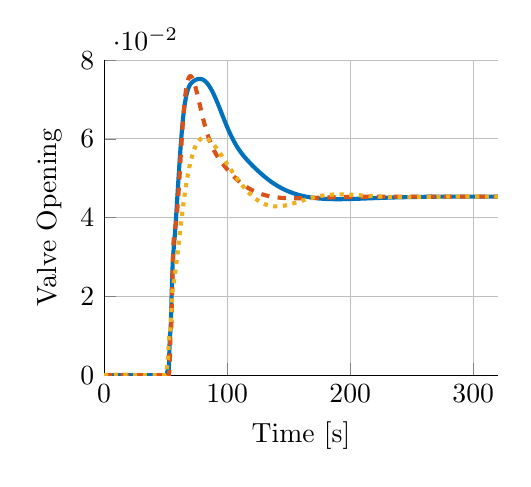
\begin{tikzpicture}

\begin{axis}[%
width=5cm,
height=4cm,
at={(0\linewidth,0\linewidth)},
scale only axis,
xmin=0,
xmax=320,
xlabel={Time [s]},
xmajorgrids,
ymin=0,
ymax=0.08,
ylabel={Valve Opening},
ymajorgrids,
axis background/.style={fill=white},
% title style={font=\bfseries},
% title={Normalized Recycle Valve Opening},
axis x line*=bottom,
axis y line*=left
]
\addplot [color=mycolor1,solid,line width=1.5pt,forget plot]
  table[row sep=crcr]{%
0	1.30651e-06\\
0.25	6.92017e-06\\
0.5	1.05998e-05\\
0.75	1.30927e-05\\
1	1.46601e-05\\
1.25	1.50442e-05\\
1.5	1.42539e-05\\
1.75	1.24228e-05\\
2	9.51022e-06\\
2.25	5.51542e-06\\
2.5	7.24745e-07\\
2.75	0\\
3	0\\
3.25	0\\
3.5	0\\
3.75	0\\
4	0\\
4.25	0\\
4.5	0\\
4.75	0\\
5	0\\
5.25	0\\
5.5	0\\
5.75	0\\
6	0\\
6.25	0\\
6.5	0\\
6.75	0\\
7	0\\
7.25	0\\
7.5	0\\
7.75	0\\
8	0\\
8.25	0\\
8.5	0\\
8.75	0\\
9	0\\
9.25	0\\
9.5	0\\
9.75	0\\
10	0\\
10.25	0\\
10.5	0\\
10.75	0\\
11	0\\
11.25	0\\
11.5	0\\
11.75	0\\
12	0\\
12.25	0\\
12.5	0\\
12.75	0\\
13	0\\
13.25	0\\
13.5	0\\
13.75	0\\
14	0\\
14.25	0\\
14.5	0\\
14.75	0\\
15	0\\
15.25	0\\
15.5	0\\
15.75	0\\
16	0\\
16.25	0\\
16.5	0\\
16.75	0\\
17	0\\
17.25	0\\
17.5	0\\
17.75	0\\
18	0\\
18.25	0\\
18.5	0\\
18.75	0\\
19	0\\
19.25	0\\
19.5	0\\
19.75	0\\
20	0\\
20.25	0\\
20.5	0\\
20.75	0\\
21	0\\
21.25	0\\
21.5	0\\
21.75	0\\
22	0\\
22.25	0\\
22.5	0\\
22.75	0\\
23	0\\
23.25	0\\
23.5	0\\
23.75	0\\
24	0\\
24.25	0\\
24.5	0\\
24.75	0\\
25	0\\
25.25	0\\
25.5	0\\
25.75	0\\
26	0\\
26.25	0\\
26.5	0\\
26.75	0\\
27	0\\
27.25	0\\
27.5	0\\
27.75	0\\
28	0\\
28.25	0\\
28.5	0\\
28.75	0\\
29	0\\
29.25	0\\
29.5	0\\
29.75	0\\
30	0\\
30.25	0\\
30.5	0\\
30.75	0\\
31	0\\
31.25	0\\
31.5	0\\
31.75	0\\
32	0\\
32.25	0\\
32.5	0\\
32.75	0\\
33	0\\
33.25	0\\
33.5	0\\
33.75	0\\
34	0\\
34.25	0\\
34.5	0\\
34.75	0\\
35	0\\
35.25	0\\
35.5	0\\
35.75	0\\
36	0\\
36.25	0\\
36.5	0\\
36.75	0\\
37	0\\
37.25	0\\
37.5	0\\
37.75	0\\
38	0\\
38.25	0\\
38.5	0\\
38.75	0\\
39	0\\
39.25	0\\
39.5	0\\
39.75	0\\
40	0\\
40.25	0\\
40.5	0\\
40.75	0\\
41	0\\
41.25	0\\
41.5	0\\
41.75	0\\
42	0\\
42.25	0\\
42.5	0\\
42.75	0\\
43	0\\
43.25	0\\
43.5	0\\
43.75	0\\
44	0\\
44.25	0\\
44.5	0\\
44.75	0\\
45	0\\
45.25	0\\
45.5	0\\
45.75	0\\
46	0\\
46.25	0\\
46.5	0\\
46.75	0\\
47	0\\
47.25	0\\
47.5	0\\
47.75	0\\
48	0\\
48.25	0\\
48.5	0\\
48.75	0\\
49	0\\
49.25	0\\
49.5	0\\
49.75	0\\
50	0\\
50.25	0\\
50.5	0\\
50.75	0.00010029\\
51	0.000407362\\
51.25	0\\
51.5	0\\
51.75	5.40805e-05\\
52	0.000176293\\
52.25	0.000363014\\
52.5	0.000992407\\
52.75	0.00287787\\
53	0.00554674\\
53.25	0.00839406\\
53.5	0.0100218\\
53.75	0.0106393\\
54	0.0114346\\
54.25	0.0131622\\
54.5	0.0156487\\
54.75	0.0188936\\
55	0.0216522\\
55.25	0.0237894\\
55.5	0.0262732\\
55.75	0.0284355\\
56	0.0298673\\
56.25	0.0309326\\
56.5	0.0319204\\
56.75	0.0328628\\
57	0.0337897\\
57.25	0.0347444\\
57.5	0.0357447\\
57.75	0.0367904\\
58	0.0378773\\
58.25	0.039007\\
58.5	0.0401793\\
58.75	0.0413865\\
59	0.0426192\\
59.25	0.0438703\\
59.5	0.0451331\\
59.75	0.0464002\\
60	0.0476651\\
60.25	0.0489224\\
60.5	0.0501673\\
60.75	0.0513955\\
61	0.0526033\\
61.25	0.0537878\\
61.5	0.0549464\\
61.75	0.056077\\
62	0.057178\\
62.25	0.0582477\\
62.5	0.0592848\\
62.75	0.0602878\\
63	0.0612554\\
63.25	0.062186\\
63.5	0.0630781\\
63.75	0.0639301\\
64	0.0647406\\
64.25	0.0655084\\
64.5	0.0662327\\
64.75	0.0669131\\
65	0.0675499\\
65.25	0.0681441\\
65.5	0.068697\\
65.75	0.0692103\\
66	0.0696861\\
66.25	0.0701266\\
66.5	0.0705345\\
66.75	0.0709129\\
67	0.0712644\\
67.25	0.0715908\\
67.5	0.0718933\\
67.75	0.072173\\
68	0.0724304\\
68.25	0.0726666\\
68.5	0.0728827\\
68.75	0.0730798\\
69	0.0732594\\
69.25	0.0734229\\
69.5	0.0735716\\
69.75	0.0737071\\
70	0.0738307\\
70.25	0.0739435\\
70.5	0.0740469\\
70.75	0.0741418\\
71	0.0742292\\
71.25	0.0743099\\
71.5	0.0743849\\
71.75	0.0744546\\
72	0.0745198\\
72.25	0.074581\\
72.5	0.0746385\\
72.75	0.0746927\\
73	0.074744\\
73.25	0.0747925\\
73.5	0.0748385\\
73.75	0.0748821\\
74	0.0749233\\
74.25	0.0749623\\
74.5	0.074999\\
74.75	0.0750334\\
75	0.0750655\\
75.25	0.0750953\\
75.5	0.0751227\\
75.75	0.0751476\\
76	0.0751699\\
76.25	0.0751895\\
76.5	0.0752063\\
76.75	0.0752202\\
77	0.0752311\\
77.25	0.075239\\
77.5	0.0752436\\
77.75	0.0752449\\
78	0.0752428\\
78.25	0.0752373\\
78.5	0.0752282\\
78.75	0.0752155\\
79	0.0751991\\
79.25	0.0751789\\
79.5	0.0751549\\
79.75	0.0751271\\
80	0.0750954\\
80.25	0.0750597\\
80.5	0.0750201\\
80.75	0.0749765\\
81	0.0749289\\
81.25	0.0748773\\
81.5	0.0748216\\
81.75	0.074762\\
82	0.0746984\\
82.25	0.0746307\\
82.5	0.074559\\
82.75	0.0744834\\
83	0.0744038\\
83.25	0.0743202\\
83.5	0.0742327\\
83.75	0.0741414\\
84	0.0740461\\
84.25	0.0739471\\
84.5	0.0738442\\
84.75	0.0737376\\
85	0.0736273\\
85.25	0.0735133\\
85.5	0.0733957\\
85.75	0.0732745\\
86	0.0731498\\
86.25	0.0730216\\
86.5	0.07289\\
86.75	0.0727551\\
87	0.0726168\\
87.25	0.0724754\\
87.5	0.0723307\\
87.75	0.072183\\
88	0.0720322\\
88.25	0.0718785\\
88.5	0.0717219\\
88.75	0.0715626\\
89	0.0714005\\
89.25	0.0712357\\
89.5	0.0710685\\
89.75	0.0708987\\
90	0.0707266\\
90.25	0.0705522\\
90.5	0.0703756\\
90.75	0.070197\\
91	0.0700163\\
91.25	0.0698337\\
91.5	0.0696494\\
91.75	0.0694633\\
92	0.0692757\\
92.25	0.0690865\\
92.5	0.068896\\
92.75	0.0687042\\
93	0.0685112\\
93.25	0.0683171\\
93.5	0.0681221\\
93.75	0.0679262\\
94	0.0677296\\
94.25	0.0675323\\
94.5	0.0673345\\
94.75	0.0671363\\
95	0.0669377\\
95.25	0.0667389\\
95.5	0.06654\\
95.75	0.0663411\\
96	0.0661422\\
96.25	0.0659436\\
96.5	0.0657452\\
96.75	0.0655472\\
97	0.0653496\\
97.25	0.0651526\\
97.5	0.0649563\\
97.75	0.0647607\\
98	0.064566\\
98.25	0.0643721\\
98.5	0.0641793\\
98.75	0.0639875\\
99	0.0637968\\
99.25	0.0636074\\
99.5	0.0634192\\
99.75	0.0632324\\
100	0.063047\\
100.25	0.062863\\
100.5	0.0626806\\
100.75	0.0624997\\
101	0.0623205\\
101.25	0.0621429\\
101.5	0.0619671\\
101.75	0.061793\\
102	0.0616207\\
102.25	0.0614502\\
102.5	0.0612815\\
102.75	0.0611147\\
103	0.0609499\\
103.25	0.0607869\\
103.5	0.0606259\\
103.75	0.0604668\\
104	0.0603097\\
104.25	0.0601545\\
104.5	0.0600014\\
104.75	0.0598501\\
105	0.0597009\\
105.25	0.0595536\\
105.5	0.0594083\\
105.75	0.0592649\\
106	0.0591235\\
106.25	0.058984\\
106.5	0.0588464\\
106.75	0.0587107\\
107	0.0585769\\
107.25	0.0584449\\
107.5	0.0583148\\
107.75	0.0581864\\
108	0.0580598\\
108.25	0.057935\\
108.5	0.0578119\\
108.75	0.0576905\\
109	0.0575708\\
109.25	0.0574526\\
109.5	0.0573361\\
109.75	0.0572211\\
110	0.0571077\\
110.25	0.0569957\\
110.5	0.0568852\\
110.75	0.0567761\\
111	0.0566683\\
111.25	0.056562\\
111.5	0.0564569\\
111.75	0.0563531\\
112	0.0562505\\
112.25	0.0561491\\
112.5	0.0560489\\
112.75	0.0559498\\
113	0.0558518\\
113.25	0.0557548\\
113.5	0.0556589\\
113.75	0.0555639\\
114	0.0554699\\
114.25	0.0553768\\
114.5	0.0552846\\
114.75	0.0551933\\
115	0.0551027\\
115.25	0.055013\\
115.5	0.054924\\
115.75	0.0548358\\
116	0.0547483\\
116.25	0.0546614\\
116.5	0.0545752\\
116.75	0.0544896\\
117	0.0544047\\
117.25	0.0543203\\
117.5	0.0542365\\
117.75	0.0541532\\
118	0.0540704\\
118.25	0.0539882\\
118.5	0.0539064\\
118.75	0.0538251\\
119	0.0537443\\
119.25	0.0536639\\
119.5	0.0535839\\
119.75	0.0535043\\
120	0.0534252\\
120.25	0.0533464\\
120.5	0.053268\\
120.75	0.0531899\\
121	0.0531123\\
121.25	0.0530349\\
121.5	0.0529579\\
121.75	0.0528813\\
122	0.052805\\
122.25	0.052729\\
122.5	0.0526533\\
122.75	0.0525779\\
123	0.0525029\\
123.25	0.0524282\\
123.5	0.0523537\\
123.75	0.0522796\\
124	0.0522058\\
124.25	0.0521324\\
124.5	0.0520592\\
124.75	0.0519863\\
125	0.0519137\\
125.25	0.0518415\\
125.5	0.0517696\\
125.75	0.0516979\\
126	0.0516266\\
126.25	0.0515557\\
126.5	0.051485\\
126.75	0.0514147\\
127	0.0513447\\
127.25	0.051275\\
127.5	0.0512057\\
127.75	0.0511367\\
128	0.0510681\\
128.25	0.0509998\\
128.5	0.0509318\\
128.75	0.0508642\\
129	0.050797\\
129.25	0.0507302\\
129.5	0.0506637\\
129.75	0.0505976\\
130	0.0505318\\
130.25	0.0504665\\
130.5	0.0504015\\
130.75	0.050337\\
131	0.0502728\\
131.25	0.050209\\
131.5	0.0501456\\
131.75	0.0500827\\
132	0.0500201\\
132.25	0.049958\\
132.5	0.0498962\\
132.75	0.0498349\\
133	0.049774\\
133.25	0.0497136\\
133.5	0.0496535\\
133.75	0.0495939\\
134	0.0495348\\
134.25	0.049476\\
134.5	0.0494178\\
134.75	0.0493599\\
135	0.0493025\\
135.25	0.0492455\\
135.5	0.049189\\
135.75	0.0491329\\
136	0.0490773\\
136.25	0.0490221\\
136.5	0.0489674\\
136.75	0.0489131\\
137	0.0488593\\
137.25	0.0488059\\
137.5	0.048753\\
137.75	0.0487006\\
138	0.0486485\\
138.25	0.048597\\
138.5	0.0485459\\
138.75	0.0484952\\
139	0.048445\\
139.25	0.0483952\\
139.5	0.0483459\\
139.75	0.048297\\
140	0.0482486\\
140.25	0.0482007\\
140.5	0.0481531\\
140.75	0.048106\\
141	0.0480594\\
141.25	0.0480132\\
141.5	0.0479674\\
141.75	0.0479221\\
142	0.0478772\\
142.25	0.0478327\\
142.5	0.0477887\\
142.75	0.0477451\\
143	0.0477019\\
143.25	0.0476592\\
143.5	0.0476168\\
143.75	0.0475749\\
144	0.0475334\\
144.25	0.0474924\\
144.5	0.0474517\\
144.75	0.0474114\\
145	0.0473716\\
145.25	0.0473322\\
145.5	0.0472931\\
145.75	0.0472545\\
146	0.0472162\\
146.25	0.0471784\\
146.5	0.047141\\
146.75	0.0471039\\
147	0.0470672\\
147.25	0.0470309\\
147.5	0.046995\\
147.75	0.0469595\\
148	0.0469244\\
148.25	0.0468896\\
148.5	0.0468552\\
148.75	0.0468212\\
149	0.0467875\\
149.25	0.0467542\\
149.5	0.0467213\\
149.75	0.0466887\\
150	0.0466565\\
150.25	0.0466246\\
150.5	0.0465931\\
150.75	0.046562\\
151	0.0465312\\
151.25	0.0465007\\
151.5	0.0464706\\
151.75	0.0464408\\
152	0.0464113\\
152.25	0.0463822\\
152.5	0.0463534\\
152.75	0.046325\\
153	0.0462969\\
153.25	0.0462691\\
153.5	0.0462416\\
153.75	0.0462144\\
154	0.0461876\\
154.25	0.0461611\\
154.5	0.0461349\\
154.75	0.046109\\
155	0.0460834\\
155.25	0.0460581\\
155.5	0.0460332\\
155.75	0.0460085\\
156	0.0459842\\
156.25	0.0459601\\
156.5	0.0459363\\
156.75	0.0459129\\
157	0.0458897\\
157.25	0.0458668\\
157.5	0.0458442\\
157.75	0.0458219\\
158	0.0457999\\
158.25	0.0457782\\
158.5	0.0457567\\
158.75	0.0457356\\
159	0.0457147\\
159.25	0.0456941\\
159.5	0.0456737\\
159.75	0.0456536\\
160	0.0456338\\
160.25	0.0456143\\
160.5	0.045595\\
160.75	0.045576\\
161	0.0455573\\
161.25	0.0455388\\
161.5	0.0455206\\
161.75	0.0455026\\
162	0.0454849\\
162.25	0.0454675\\
162.5	0.0454503\\
162.75	0.0454333\\
163	0.0454166\\
163.25	0.0454001\\
163.5	0.0453839\\
163.75	0.0453679\\
164	0.0453522\\
164.25	0.0453367\\
164.5	0.0453215\\
164.75	0.0453064\\
165	0.0452917\\
165.25	0.0452771\\
165.5	0.0452628\\
165.75	0.0452487\\
166	0.0452348\\
166.25	0.0452211\\
166.5	0.0452077\\
166.75	0.0451945\\
167	0.0451815\\
167.25	0.0451687\\
167.5	0.0451562\\
167.75	0.0451438\\
168	0.0451317\\
168.25	0.0451198\\
168.5	0.0451081\\
168.75	0.0450966\\
169	0.0450853\\
169.25	0.0450742\\
169.5	0.0450633\\
169.75	0.0450526\\
170	0.0450421\\
170.25	0.0450318\\
170.5	0.0450216\\
170.75	0.0450117\\
171	0.045002\\
171.25	0.0449924\\
171.5	0.0449831\\
171.75	0.0449739\\
172	0.0449649\\
172.25	0.0449561\\
172.5	0.0449475\\
172.75	0.044939\\
173	0.0449308\\
173.25	0.0449227\\
173.5	0.0449147\\
173.75	0.044907\\
174	0.0448994\\
174.25	0.044892\\
174.5	0.0448847\\
174.75	0.0448776\\
175	0.0448707\\
175.25	0.0448639\\
175.5	0.0448573\\
175.75	0.0448509\\
176	0.0448446\\
176.25	0.0448384\\
176.5	0.0448325\\
176.75	0.0448266\\
177	0.0448209\\
177.25	0.0448154\\
177.5	0.04481\\
177.75	0.0448047\\
178	0.0447996\\
178.25	0.0447947\\
178.5	0.0447898\\
178.75	0.0447851\\
179	0.0447806\\
179.25	0.0447762\\
179.5	0.0447719\\
179.75	0.0447677\\
180	0.0447637\\
180.25	0.0447598\\
180.5	0.044756\\
180.75	0.0447524\\
181	0.0447488\\
181.25	0.0447454\\
181.5	0.0447422\\
181.75	0.044739\\
182	0.044736\\
182.25	0.044733\\
182.5	0.0447302\\
182.75	0.0447275\\
183	0.0447249\\
183.25	0.0447224\\
183.5	0.0447201\\
183.75	0.0447178\\
184	0.0447156\\
184.25	0.0447136\\
184.5	0.0447116\\
184.75	0.0447098\\
185	0.044708\\
185.25	0.0447064\\
185.5	0.0447048\\
185.75	0.0447034\\
186	0.044702\\
186.25	0.0447008\\
186.5	0.0446996\\
186.75	0.0446985\\
187	0.0446975\\
187.25	0.0446966\\
187.5	0.0446958\\
187.75	0.044695\\
188	0.0446944\\
188.25	0.0446938\\
188.5	0.0446934\\
188.75	0.044693\\
189	0.0446926\\
189.25	0.0446924\\
189.5	0.0446922\\
189.75	0.0446921\\
190	0.0446921\\
190.25	0.0446922\\
190.5	0.0446923\\
190.75	0.0446925\\
191	0.0446928\\
191.25	0.0446931\\
191.5	0.0446935\\
191.75	0.044694\\
192	0.0446945\\
192.25	0.0446952\\
192.5	0.0446958\\
192.75	0.0446966\\
193	0.0446973\\
193.25	0.0446982\\
193.5	0.0446991\\
193.75	0.0447001\\
194	0.0447011\\
194.25	0.0447022\\
194.5	0.0447033\\
194.75	0.0447045\\
195	0.0447058\\
195.25	0.0447071\\
195.5	0.0447084\\
195.75	0.0447098\\
196	0.0447113\\
196.25	0.0447128\\
196.5	0.0447143\\
196.75	0.0447159\\
197	0.0447176\\
197.25	0.0447193\\
197.5	0.044721\\
197.75	0.0447228\\
198	0.0447246\\
198.25	0.0447264\\
198.5	0.0447283\\
198.75	0.0447303\\
199	0.0447322\\
199.25	0.0447343\\
199.5	0.0447363\\
199.75	0.0447384\\
200	0.0447405\\
200.25	0.0447427\\
200.5	0.0447448\\
200.75	0.0447471\\
201	0.0447493\\
201.25	0.0447516\\
201.5	0.0447539\\
201.75	0.0447563\\
202	0.0447586\\
202.25	0.0447611\\
202.5	0.0447635\\
202.75	0.0447659\\
203	0.0447684\\
203.25	0.0447709\\
203.5	0.0447735\\
203.75	0.044776\\
204	0.0447786\\
204.25	0.0447812\\
204.5	0.0447838\\
204.75	0.0447865\\
205	0.0447892\\
205.25	0.0447919\\
205.5	0.0447946\\
205.75	0.0447973\\
206	0.0448\\
206.25	0.0448028\\
206.5	0.0448056\\
206.75	0.0448084\\
207	0.0448112\\
207.25	0.044814\\
207.5	0.0448169\\
207.75	0.0448197\\
208	0.0448226\\
208.25	0.0448255\\
208.5	0.0448284\\
208.75	0.0448313\\
209	0.0448342\\
209.25	0.0448372\\
209.5	0.0448401\\
209.75	0.0448431\\
210	0.044846\\
210.25	0.044849\\
210.5	0.044852\\
210.75	0.044855\\
211	0.044858\\
211.25	0.044861\\
211.5	0.044864\\
211.75	0.044867\\
212	0.04487\\
212.25	0.044873\\
212.5	0.0448761\\
212.75	0.0448791\\
213	0.0448821\\
213.25	0.0448852\\
213.5	0.0448882\\
213.75	0.0448913\\
214	0.0448943\\
214.25	0.0448974\\
214.5	0.0449004\\
214.75	0.0449035\\
215	0.0449066\\
215.25	0.0449096\\
215.5	0.0449127\\
215.75	0.0449157\\
216	0.0449188\\
216.25	0.0449218\\
216.5	0.0449249\\
216.75	0.044928\\
217	0.044931\\
217.25	0.0449341\\
217.5	0.0449371\\
217.75	0.0449401\\
218	0.0449432\\
218.25	0.0449462\\
218.5	0.0449493\\
218.75	0.0449523\\
219	0.0449553\\
219.25	0.0449583\\
219.5	0.0449613\\
219.75	0.0449644\\
220	0.0449674\\
220.25	0.0449704\\
220.5	0.0449733\\
220.75	0.0449763\\
221	0.0449793\\
221.25	0.0449823\\
221.5	0.0449853\\
221.75	0.0449882\\
222	0.0449912\\
222.25	0.0449941\\
222.5	0.044997\\
222.75	0.045\\
223	0.0450029\\
223.25	0.0450058\\
223.5	0.0450087\\
223.75	0.0450116\\
224	0.0450145\\
224.25	0.0450174\\
224.5	0.0450202\\
224.75	0.0450231\\
225	0.0450259\\
225.25	0.0450288\\
225.5	0.0450316\\
225.75	0.0450344\\
226	0.0450372\\
226.25	0.04504\\
226.5	0.0450428\\
226.75	0.0450456\\
227	0.0450483\\
227.25	0.0450511\\
227.5	0.0450538\\
227.75	0.0450565\\
228	0.0450593\\
228.25	0.045062\\
228.5	0.0450646\\
228.75	0.0450673\\
229	0.04507\\
229.25	0.0450727\\
229.5	0.0450753\\
229.75	0.0450779\\
230	0.0450805\\
230.25	0.0450832\\
230.5	0.0450857\\
230.75	0.0450883\\
231	0.0450909\\
231.25	0.0450934\\
231.5	0.045096\\
231.75	0.0450985\\
232	0.045101\\
232.25	0.0451035\\
232.5	0.045106\\
232.75	0.0451085\\
233	0.045111\\
233.25	0.0451134\\
233.5	0.0451158\\
233.75	0.0451183\\
234	0.0451207\\
234.25	0.0451231\\
234.5	0.0451254\\
234.75	0.0451278\\
235	0.0451302\\
235.25	0.0451325\\
235.5	0.0451348\\
235.75	0.0451371\\
236	0.0451394\\
236.25	0.0451417\\
236.5	0.045144\\
236.75	0.0451462\\
237	0.0451485\\
237.25	0.0451507\\
237.5	0.0451529\\
237.75	0.0451551\\
238	0.0451573\\
238.25	0.0451594\\
238.5	0.0451616\\
238.75	0.0451637\\
239	0.0451658\\
239.25	0.0451679\\
239.5	0.04517\\
239.75	0.0451721\\
240	0.0451742\\
240.25	0.0451762\\
240.5	0.0451783\\
240.75	0.0451803\\
241	0.0451823\\
241.25	0.0451843\\
241.5	0.0451863\\
241.75	0.0451882\\
242	0.0451902\\
242.25	0.0451921\\
242.5	0.045194\\
242.75	0.0451959\\
243	0.0451978\\
243.25	0.0451997\\
243.5	0.0452016\\
243.75	0.0452034\\
244	0.0452053\\
244.25	0.0452071\\
244.5	0.0452089\\
244.75	0.0452107\\
245	0.0452124\\
245.25	0.0452142\\
245.5	0.045216\\
245.75	0.0452177\\
246	0.0452194\\
246.25	0.0452211\\
246.5	0.0452228\\
246.75	0.0452245\\
247	0.0452262\\
247.25	0.0452278\\
247.5	0.0452294\\
247.75	0.0452311\\
248	0.0452327\\
248.25	0.0452343\\
248.5	0.0452358\\
248.75	0.0452374\\
249	0.045239\\
249.25	0.0452405\\
249.5	0.045242\\
249.75	0.0452435\\
250	0.045245\\
250.25	0.0452465\\
250.5	0.045248\\
250.75	0.0452495\\
251	0.0452509\\
251.25	0.0452523\\
251.5	0.0452537\\
251.75	0.0452552\\
252	0.0452565\\
252.25	0.0452579\\
252.5	0.0452593\\
252.75	0.0452606\\
253	0.045262\\
253.25	0.0452633\\
253.5	0.0452646\\
253.75	0.0452659\\
254	0.0452672\\
254.25	0.0452685\\
254.5	0.0452698\\
254.75	0.045271\\
255	0.0452723\\
255.25	0.0452735\\
255.5	0.0452747\\
255.75	0.0452759\\
256	0.0452771\\
256.25	0.0452783\\
256.5	0.0452794\\
256.75	0.0452806\\
257	0.0452817\\
257.25	0.0452829\\
257.5	0.045284\\
257.75	0.0452851\\
258	0.0452862\\
258.25	0.0452873\\
258.5	0.0452883\\
258.75	0.0452894\\
259	0.0452904\\
259.25	0.0452915\\
259.5	0.0452925\\
259.75	0.0452935\\
260	0.0452945\\
260.25	0.0452955\\
260.5	0.0452965\\
260.75	0.0452975\\
261	0.0452984\\
261.25	0.0452994\\
261.5	0.0453003\\
261.75	0.0453012\\
262	0.0453022\\
262.25	0.0453031\\
262.5	0.045304\\
262.75	0.0453049\\
263	0.0453057\\
263.25	0.0453066\\
263.5	0.0453074\\
263.75	0.0453083\\
264	0.0453091\\
264.25	0.0453099\\
264.5	0.0453108\\
264.75	0.0453116\\
265	0.0453124\\
265.25	0.0453131\\
265.5	0.0453139\\
265.75	0.0453147\\
266	0.0453154\\
266.25	0.0453162\\
266.5	0.0453169\\
266.75	0.0453177\\
267	0.0453184\\
267.25	0.0453191\\
267.5	0.0453198\\
267.75	0.0453205\\
268	0.0453212\\
268.25	0.0453218\\
268.5	0.0453225\\
268.75	0.0453232\\
269	0.0453238\\
269.25	0.0453244\\
269.5	0.0453251\\
269.75	0.0453257\\
270	0.0453263\\
270.25	0.0453269\\
270.5	0.0453275\\
270.75	0.0453281\\
271	0.0453287\\
271.25	0.0453292\\
271.5	0.0453298\\
271.75	0.0453304\\
272	0.0453309\\
272.25	0.0453314\\
272.5	0.045332\\
272.75	0.0453325\\
273	0.045333\\
273.25	0.0453335\\
273.5	0.045334\\
273.75	0.0453345\\
274	0.045335\\
274.25	0.0453355\\
274.5	0.045336\\
274.75	0.0453364\\
275	0.0453369\\
275.25	0.0453373\\
275.5	0.0453378\\
275.75	0.0453382\\
276	0.0453386\\
276.25	0.0453391\\
276.5	0.0453395\\
276.75	0.0453399\\
277	0.0453403\\
277.25	0.0453407\\
277.5	0.0453411\\
277.75	0.0453415\\
278	0.0453418\\
278.25	0.0453422\\
278.5	0.0453426\\
278.75	0.0453429\\
279	0.0453433\\
279.25	0.0453436\\
279.5	0.045344\\
279.75	0.0453443\\
280	0.0453446\\
280.25	0.045345\\
280.5	0.0453453\\
280.75	0.0453456\\
281	0.0453459\\
281.25	0.0453462\\
281.5	0.0453465\\
281.75	0.0453468\\
282	0.0453471\\
282.25	0.0453473\\
282.5	0.0453476\\
282.75	0.0453479\\
283	0.0453481\\
283.25	0.0453484\\
283.5	0.0453486\\
283.75	0.0453489\\
284	0.0453491\\
284.25	0.0453494\\
284.5	0.0453496\\
284.75	0.0453498\\
285	0.0453501\\
285.25	0.0453503\\
285.5	0.0453505\\
285.75	0.0453507\\
286	0.0453509\\
286.25	0.0453511\\
286.5	0.0453513\\
286.75	0.0453515\\
287	0.0453517\\
287.25	0.0453518\\
287.5	0.045352\\
287.75	0.0453522\\
288	0.0453524\\
288.25	0.0453525\\
288.5	0.0453527\\
288.75	0.0453529\\
289	0.045353\\
289.25	0.0453532\\
289.5	0.0453533\\
289.75	0.0453534\\
290	0.0453536\\
290.25	0.0453537\\
290.5	0.0453538\\
290.75	0.045354\\
291	0.0453541\\
291.25	0.0453542\\
291.5	0.0453543\\
291.75	0.0453544\\
292	0.0453545\\
292.25	0.0453546\\
292.5	0.0453547\\
292.75	0.0453548\\
293	0.0453549\\
293.25	0.045355\\
293.5	0.0453551\\
293.75	0.0453552\\
294	0.0453553\\
294.25	0.0453554\\
294.5	0.0453554\\
294.75	0.0453555\\
295	0.0453556\\
295.25	0.0453557\\
295.5	0.0453557\\
295.75	0.0453558\\
296	0.0453558\\
296.25	0.0453559\\
296.5	0.045356\\
296.75	0.045356\\
297	0.0453561\\
297.25	0.0453561\\
297.5	0.0453561\\
297.75	0.0453562\\
298	0.0453562\\
298.25	0.0453563\\
298.5	0.0453563\\
298.75	0.0453563\\
299	0.0453564\\
299.25	0.0453564\\
299.5	0.0453564\\
299.75	0.0453564\\
300	0.0453565\\
300.25	0.0453565\\
300.5	0.0453565\\
300.75	0.0453565\\
301	0.0453565\\
301.25	0.0453565\\
301.5	0.0453565\\
301.75	0.0453565\\
302	0.0453565\\
302.25	0.0453565\\
302.5	0.0453565\\
302.75	0.0453565\\
303	0.0453565\\
303.25	0.0453565\\
303.5	0.0453565\\
303.75	0.0453565\\
304	0.0453565\\
304.25	0.0453565\\
304.5	0.0453565\\
304.75	0.0453565\\
305	0.0453564\\
305.25	0.0453564\\
305.5	0.0453564\\
305.75	0.0453564\\
306	0.0453564\\
306.25	0.0453563\\
306.5	0.0453563\\
306.75	0.0453563\\
307	0.0453563\\
307.25	0.0453562\\
307.5	0.0453562\\
307.75	0.0453562\\
308	0.0453561\\
308.25	0.0453561\\
308.5	0.0453561\\
308.75	0.045356\\
309	0.045356\\
309.25	0.0453559\\
309.5	0.0453559\\
309.75	0.0453559\\
310	0.0453558\\
310.25	0.0453558\\
310.5	0.0453557\\
310.75	0.0453557\\
311	0.0453556\\
311.25	0.0453556\\
311.5	0.0453555\\
311.75	0.0453555\\
312	0.0453554\\
312.25	0.0453554\\
312.5	0.0453553\\
312.75	0.0453553\\
313	0.0453552\\
313.25	0.0453552\\
313.5	0.0453551\\
313.75	0.0453551\\
314	0.045355\\
314.25	0.0453549\\
314.5	0.0453549\\
314.75	0.0453548\\
315	0.0453548\\
315.25	0.0453547\\
315.5	0.0453546\\
315.75	0.0453546\\
316	0.0453545\\
316.25	0.0453545\\
316.5	0.0453544\\
316.75	0.0453543\\
317	0.0453543\\
317.25	0.0453542\\
317.5	0.0453541\\
317.75	0.0453541\\
318	0.045354\\
318.25	0.0453539\\
318.5	0.0453539\\
318.75	0.0453538\\
319	0.0453537\\
319.25	0.0453537\\
319.5	0.0453536\\
319.75	0.0453535\\
320	0.0453535\\
320.25	0.0453534\\
320.5	0.0453533\\
320.75	0.0453532\\
321	0.0453532\\
321.25	0.0453531\\
321.5	0.045353\\
321.75	0.045353\\
322	0.0453529\\
322.25	0.0453528\\
322.5	0.0453527\\
322.75	0.0453527\\
323	0.0453526\\
323.25	0.0453525\\
323.5	0.0453525\\
323.75	0.0453524\\
324	0.0453523\\
324.25	0.0453522\\
324.5	0.0453522\\
324.75	0.0453521\\
325	0.045352\\
325.25	0.0453519\\
325.5	0.0453519\\
325.75	0.0453518\\
326	0.0453517\\
326.25	0.0453516\\
326.5	0.0453516\\
326.75	0.0453515\\
327	0.0453514\\
327.25	0.0453513\\
327.5	0.0453513\\
327.75	0.0453512\\
328	0.0453511\\
328.25	0.045351\\
328.5	0.045351\\
328.75	0.0453509\\
329	0.0453508\\
329.25	0.0453507\\
329.5	0.0453507\\
329.75	0.0453506\\
330	0.0453505\\
330.25	0.0453505\\
330.5	0.0453504\\
330.75	0.0453503\\
331	0.0453502\\
331.25	0.0453502\\
331.5	0.0453501\\
331.75	0.04535\\
332	0.0453499\\
332.25	0.0453499\\
332.5	0.0453498\\
332.75	0.0453497\\
333	0.0453496\\
333.25	0.0453496\\
333.5	0.0453495\\
333.75	0.0453494\\
334	0.0453494\\
334.25	0.0453493\\
334.5	0.0453492\\
334.75	0.0453491\\
335	0.0453491\\
335.25	0.045349\\
335.5	0.0453489\\
335.75	0.0453489\\
336	0.0453488\\
336.25	0.0453487\\
336.5	0.0453486\\
336.75	0.0453486\\
337	0.0453485\\
337.25	0.0453484\\
337.5	0.0453484\\
337.75	0.0453483\\
338	0.0453482\\
338.25	0.0453482\\
338.5	0.0453481\\
338.75	0.045348\\
339	0.045348\\
339.25	0.0453479\\
339.5	0.0453478\\
339.75	0.0453478\\
340	0.0453477\\
340.25	0.0453476\\
340.5	0.0453476\\
340.75	0.0453475\\
341	0.0453474\\
341.25	0.0453474\\
341.5	0.0453473\\
341.75	0.0453472\\
342	0.0453472\\
342.25	0.0453471\\
342.5	0.045347\\
342.75	0.045347\\
343	0.0453469\\
343.25	0.0453469\\
343.5	0.0453468\\
343.75	0.0453467\\
344	0.0453467\\
344.25	0.0453466\\
344.5	0.0453466\\
344.75	0.0453465\\
345	0.0453464\\
345.25	0.0453464\\
345.5	0.0453463\\
345.75	0.0453463\\
346	0.0453462\\
346.25	0.0453461\\
346.5	0.0453461\\
346.75	0.045346\\
347	0.045346\\
347.25	0.0453459\\
347.5	0.0453459\\
347.75	0.0453458\\
348	0.0453457\\
348.25	0.0453457\\
348.5	0.0453456\\
348.75	0.0453456\\
349	0.0453455\\
349.25	0.0453455\\
349.5	0.0453454\\
349.75	0.0453454\\
350	0.0453453\\
350.25	0.0453452\\
350.5	0.0453452\\
350.75	0.0453451\\
351	0.0453451\\
351.25	0.045345\\
351.5	0.045345\\
351.75	0.0453449\\
352	0.0453449\\
352.25	0.0453448\\
352.5	0.0453448\\
352.75	0.0453447\\
353	0.0453447\\
353.25	0.0453446\\
353.5	0.0453446\\
353.75	0.0453445\\
354	0.0453445\\
354.25	0.0453444\\
354.5	0.0453444\\
354.75	0.0453444\\
355	0.0453443\\
355.25	0.0453443\\
355.5	0.0453442\\
355.75	0.0453442\\
356	0.0453441\\
356.25	0.0453441\\
356.5	0.045344\\
356.75	0.045344\\
357	0.045344\\
357.25	0.0453439\\
357.5	0.0453439\\
357.75	0.0453438\\
358	0.0453438\\
358.25	0.0453437\\
358.5	0.0453437\\
358.75	0.0453437\\
359	0.0453436\\
359.25	0.0453436\\
359.5	0.0453435\\
359.75	0.0453435\\
360	0.0453435\\
360.25	0.0453434\\
360.5	0.0453434\\
360.75	0.0453433\\
361	0.0453433\\
361.25	0.0453433\\
361.5	0.0453432\\
361.75	0.0453432\\
362	0.0453432\\
362.25	0.0453431\\
362.5	0.0453431\\
362.75	0.045343\\
363	0.045343\\
363.25	0.045343\\
363.5	0.0453429\\
363.75	0.0453429\\
364	0.0453429\\
364.25	0.0453428\\
364.5	0.0453428\\
364.75	0.0453428\\
365	0.0453427\\
365.25	0.0453427\\
365.5	0.0453427\\
365.75	0.0453426\\
366	0.0453426\\
366.25	0.0453426\\
366.5	0.0453425\\
366.75	0.0453425\\
367	0.0453425\\
367.25	0.0453425\\
367.5	0.0453424\\
367.75	0.0453424\\
368	0.0453424\\
368.25	0.0453423\\
368.5	0.0453423\\
368.75	0.0453423\\
369	0.0453423\\
369.25	0.0453422\\
369.5	0.0453422\\
369.75	0.0453422\\
370	0.0453421\\
370.25	0.0453421\\
370.5	0.0453421\\
370.75	0.0453421\\
371	0.045342\\
371.25	0.045342\\
371.5	0.045342\\
371.75	0.045342\\
372	0.0453419\\
372.25	0.0453419\\
372.5	0.0453419\\
372.75	0.0453419\\
373	0.0453418\\
373.25	0.0453418\\
373.5	0.0453418\\
373.75	0.0453418\\
374	0.0453417\\
374.25	0.0453417\\
374.5	0.0453417\\
374.75	0.0453417\\
375	0.0453417\\
375.25	0.0453416\\
375.5	0.0453416\\
375.75	0.0453416\\
376	0.0453416\\
376.25	0.0453416\\
376.5	0.0453415\\
376.75	0.0453415\\
377	0.0453415\\
377.25	0.0453415\\
377.5	0.0453415\\
377.75	0.0453414\\
378	0.0453414\\
378.25	0.0453414\\
378.5	0.0453414\\
378.75	0.0453414\\
379	0.0453413\\
379.25	0.0453413\\
379.5	0.0453413\\
379.75	0.0453413\\
380	0.0453413\\
380.25	0.0453413\\
380.5	0.0453412\\
380.75	0.0453412\\
381	0.0453412\\
381.25	0.0453412\\
381.5	0.0453412\\
381.75	0.0453412\\
382	0.0453412\\
382.25	0.0453411\\
382.5	0.0453411\\
382.75	0.0453411\\
383	0.0453411\\
383.25	0.0453411\\
383.5	0.0453411\\
383.75	0.0453411\\
384	0.045341\\
384.25	0.045341\\
384.5	0.045341\\
384.75	0.045341\\
385	0.045341\\
385.25	0.045341\\
385.5	0.045341\\
385.75	0.045341\\
386	0.0453409\\
386.25	0.0453409\\
386.5	0.0453409\\
386.75	0.0453409\\
387	0.0453409\\
387.25	0.0453409\\
387.5	0.0453409\\
387.75	0.0453409\\
388	0.0453408\\
388.25	0.0453408\\
388.5	0.0453408\\
388.75	0.0453408\\
389	0.0453408\\
389.25	0.0453408\\
389.5	0.0453408\\
389.75	0.0453408\\
390	0.0453408\\
390.25	0.0453408\\
390.5	0.0453408\\
390.75	0.0453407\\
391	0.0453407\\
391.25	0.0453407\\
391.5	0.0453407\\
391.75	0.0453407\\
392	0.0453407\\
392.25	0.0453407\\
392.5	0.0453407\\
392.75	0.0453407\\
393	0.0453407\\
393.25	0.0453407\\
393.5	0.0453407\\
393.75	0.0453406\\
394	0.0453406\\
394.25	0.0453406\\
394.5	0.0453406\\
394.75	0.0453406\\
395	0.0453406\\
395.25	0.0453406\\
395.5	0.0453406\\
395.75	0.0453406\\
396	0.0453406\\
396.25	0.0453406\\
396.5	0.0453406\\
396.75	0.0453406\\
397	0.0453406\\
397.25	0.0453406\\
397.5	0.0453406\\
397.75	0.0453405\\
398	0.0453405\\
398.25	0.0453405\\
398.5	0.0453405\\
398.75	0.0453405\\
399	0.0453405\\
399.25	0.0453405\\
399.5	0.0453405\\
399.75	0.0453405\\
400	0.0453405\\
400.25	0.0453405\\
400.5	0.0453405\\
400.75	0.0453405\\
401	0.0453405\\
401.25	0.0453405\\
401.5	0.0453405\\
401.75	0.0453405\\
402	0.0453405\\
402.25	0.0453405\\
402.5	0.0453405\\
402.75	0.0453405\\
403	0.0453405\\
403.25	0.0453405\\
403.5	0.0453405\\
403.75	0.0453405\\
404	0.0453405\\
404.25	0.0453405\\
404.5	0.0453404\\
404.75	0.0453404\\
405	0.0453404\\
405.25	0.0453404\\
405.5	0.0453404\\
405.75	0.0453404\\
406	0.0453404\\
406.25	0.0453404\\
406.5	0.0453404\\
406.75	0.0453404\\
407	0.0453404\\
407.25	0.0453404\\
407.5	0.0453404\\
407.75	0.0453404\\
408	0.0453404\\
408.25	0.0453404\\
408.5	0.0453404\\
408.75	0.0453404\\
409	0.0453404\\
409.25	0.0453404\\
409.5	0.0453404\\
409.75	0.0453404\\
410	0.0453404\\
410.25	0.0453404\\
410.5	0.0453404\\
410.75	0.0453404\\
411	0.0453404\\
411.25	0.0453404\\
411.5	0.0453404\\
411.75	0.0453404\\
412	0.0453404\\
412.25	0.0453404\\
412.5	0.0453404\\
412.75	0.0453404\\
413	0.0453404\\
413.25	0.0453404\\
413.5	0.0453404\\
413.75	0.0453404\\
414	0.0453404\\
414.25	0.0453404\\
414.5	0.0453404\\
414.75	0.0453404\\
415	0.0453404\\
415.25	0.0453404\\
415.5	0.0453404\\
415.75	0.0453404\\
416	0.0453404\\
416.25	0.0453404\\
416.5	0.0453404\\
416.75	0.0453404\\
417	0.0453404\\
417.25	0.0453404\\
417.5	0.0453404\\
417.75	0.0453404\\
418	0.0453404\\
418.25	0.0453404\\
418.5	0.0453404\\
418.75	0.0453404\\
419	0.0453404\\
419.25	0.0453404\\
419.5	0.0453404\\
419.75	0.0453404\\
420	0.0453404\\
420.25	0.0453404\\
420.5	0.0453404\\
420.75	0.0453404\\
421	0.0453404\\
421.25	0.0453404\\
421.5	0.0453404\\
421.75	0.0453404\\
422	0.0453404\\
422.25	0.0453404\\
422.5	0.0453404\\
422.75	0.0453404\\
423	0.0453404\\
423.25	0.0453404\\
423.5	0.0453404\\
423.75	0.0453404\\
424	0.0453404\\
424.25	0.0453404\\
424.5	0.0453404\\
424.75	0.0453404\\
425	0.0453404\\
425.25	0.0453404\\
425.5	0.0453404\\
425.75	0.0453404\\
426	0.0453404\\
426.25	0.0453404\\
426.5	0.0453404\\
426.75	0.0453404\\
427	0.0453404\\
427.25	0.0453404\\
427.5	0.0453404\\
427.75	0.0453404\\
428	0.0453405\\
428.25	0.0453405\\
428.5	0.0453405\\
428.75	0.0453405\\
429	0.0453405\\
429.25	0.0453405\\
429.5	0.0453405\\
429.75	0.0453405\\
430	0.0453405\\
430.25	0.0453405\\
430.5	0.0453405\\
430.75	0.0453405\\
431	0.0453405\\
431.25	0.0453405\\
431.5	0.0453405\\
431.75	0.0453405\\
432	0.0453405\\
432.25	0.0453405\\
432.5	0.0453405\\
432.75	0.0453405\\
433	0.0453405\\
433.25	0.0453405\\
433.5	0.0453405\\
433.75	0.0453405\\
434	0.0453405\\
434.25	0.0453405\\
434.5	0.0453405\\
434.75	0.0453405\\
435	0.0453405\\
435.25	0.0453405\\
435.5	0.0453405\\
435.75	0.0453405\\
436	0.0453405\\
436.25	0.0453405\\
436.5	0.0453405\\
436.75	0.0453405\\
437	0.0453405\\
437.25	0.0453405\\
437.5	0.0453405\\
437.75	0.0453405\\
438	0.0453405\\
438.25	0.0453405\\
438.5	0.0453405\\
438.75	0.0453405\\
439	0.0453405\\
439.25	0.0453405\\
439.5	0.0453405\\
439.75	0.0453405\\
440	0.0453405\\
440.25	0.0453405\\
440.5	0.0453405\\
440.75	0.0453405\\
441	0.0453405\\
441.25	0.0453405\\
441.5	0.0453405\\
441.75	0.0453405\\
442	0.0453405\\
442.25	0.0453405\\
442.5	0.0453406\\
442.75	0.0453406\\
443	0.0453406\\
443.25	0.0453406\\
443.5	0.0453406\\
443.75	0.0453406\\
444	0.0453406\\
444.25	0.0453406\\
444.5	0.0453406\\
444.75	0.0453406\\
445	0.0453406\\
445.25	0.0453406\\
445.5	0.0453406\\
445.75	0.0453406\\
446	0.0453406\\
446.25	0.0453406\\
446.5	0.0453406\\
446.75	0.0453406\\
447	0.0453406\\
447.25	0.0453406\\
447.5	0.0453406\\
447.75	0.0453406\\
448	0.0453406\\
448.25	0.0453406\\
448.5	0.0453406\\
448.75	0.0453406\\
449	0.0453406\\
449.25	0.0453406\\
449.5	0.0453406\\
449.75	0.0453406\\
450	0.0453406\\
450.25	0.0453406\\
450.5	0.0453406\\
450.75	0.0453406\\
451	0.0453406\\
451.25	0.0453406\\
451.5	0.0453406\\
451.75	0.0453406\\
452	0.0453406\\
452.25	0.0453406\\
452.5	0.0453406\\
452.75	0.0453406\\
453	0.0453406\\
453.25	0.0453406\\
453.5	0.0453406\\
453.75	0.0453406\\
454	0.0453406\\
454.25	0.0453406\\
454.5	0.0453406\\
454.75	0.0453406\\
455	0.0453406\\
455.25	0.0453406\\
455.5	0.0453406\\
455.75	0.0453406\\
456	0.0453406\\
456.25	0.0453406\\
456.5	0.0453406\\
456.75	0.0453406\\
457	0.0453406\\
457.25	0.0453406\\
457.5	0.0453407\\
457.75	0.0453407\\
458	0.0453407\\
458.25	0.0453407\\
458.5	0.0453407\\
458.75	0.0453407\\
459	0.0453407\\
459.25	0.0453407\\
459.5	0.0453407\\
459.75	0.0453407\\
460	0.0453407\\
460.25	0.0453407\\
460.5	0.0453407\\
460.75	0.0453407\\
461	0.0453407\\
461.25	0.0453407\\
461.5	0.0453407\\
461.75	0.0453407\\
462	0.0453407\\
462.25	0.0453407\\
462.5	0.0453407\\
462.75	0.0453407\\
463	0.0453407\\
463.25	0.0453407\\
463.5	0.0453407\\
463.75	0.0453407\\
464	0.0453407\\
464.25	0.0453407\\
464.5	0.0453407\\
464.75	0.0453407\\
465	0.0453407\\
465.25	0.0453407\\
465.5	0.0453407\\
465.75	0.0453407\\
466	0.0453407\\
466.25	0.0453407\\
466.5	0.0453407\\
466.75	0.0453407\\
467	0.0453407\\
467.25	0.0453407\\
467.5	0.0453407\\
467.75	0.0453407\\
468	0.0453407\\
468.25	0.0453407\\
468.5	0.0453407\\
468.75	0.0453407\\
469	0.0453407\\
469.25	0.0453407\\
469.5	0.0453407\\
469.75	0.0453407\\
470	0.0453407\\
470.25	0.0453407\\
470.5	0.0453407\\
470.75	0.0453407\\
471	0.0453407\\
471.25	0.0453407\\
471.5	0.0453407\\
471.75	0.0453407\\
472	0.0453407\\
472.25	0.0453407\\
472.5	0.0453407\\
472.75	0.0453407\\
473	0.0453407\\
473.25	0.0453407\\
473.5	0.0453407\\
473.75	0.0453407\\
474	0.0453407\\
474.25	0.0453407\\
474.5	0.0453407\\
474.75	0.0453407\\
475	0.0453407\\
475.25	0.0453407\\
475.5	0.0453407\\
475.75	0.0453407\\
476	0.0453407\\
476.25	0.0453407\\
476.5	0.0453407\\
476.75	0.0453407\\
477	0.0453407\\
477.25	0.0453407\\
477.5	0.0453407\\
477.75	0.0453407\\
478	0.0453407\\
478.25	0.0453407\\
478.5	0.0453407\\
478.75	0.0453407\\
479	0.0453407\\
479.25	0.0453407\\
479.5	0.0453407\\
479.75	0.0453407\\
480	0.0453407\\
480.25	0.0453407\\
480.5	0.0453407\\
480.75	0.0453408\\
481	0.0453408\\
481.25	0.0453408\\
481.5	0.0453408\\
481.75	0.0453408\\
482	0.0453408\\
482.25	0.0453408\\
482.5	0.0453408\\
482.75	0.0453408\\
483	0.0453408\\
483.25	0.0453408\\
483.5	0.0453408\\
483.75	0.0453408\\
484	0.0453408\\
484.25	0.0453408\\
484.5	0.0453408\\
484.75	0.0453408\\
485	0.0453408\\
485.25	0.0453408\\
485.5	0.0453408\\
485.75	0.0453408\\
486	0.0453408\\
486.25	0.0453408\\
486.5	0.0453408\\
486.75	0.0453408\\
487	0.0453408\\
487.25	0.0453408\\
487.5	0.0453408\\
487.75	0.0453408\\
488	0.0453408\\
488.25	0.0453408\\
488.5	0.0453408\\
488.75	0.0453408\\
489	0.0453408\\
489.25	0.0453408\\
489.5	0.0453408\\
489.75	0.0453408\\
490	0.0453408\\
490.25	0.0453408\\
490.5	0.0453408\\
490.75	0.0453408\\
491	0.0453408\\
491.25	0.0453408\\
491.5	0.0453408\\
491.75	0.0453408\\
492	0.0453408\\
492.25	0.0453408\\
492.5	0.0453408\\
492.75	0.0453408\\
493	0.0453408\\
493.25	0.0453408\\
493.5	0.0453408\\
493.75	0.0453408\\
494	0.0453408\\
494.25	0.0453408\\
494.5	0.0453408\\
494.75	0.0453408\\
495	0.0453408\\
495.25	0.0453408\\
495.5	0.0453408\\
495.75	0.0453408\\
496	0.0453408\\
496.25	0.0453408\\
496.5	0.0453408\\
496.75	0.0453408\\
497	0.0453408\\
497.25	0.0453408\\
497.5	0.0453408\\
497.75	0.0453408\\
498	0.0453408\\
498.25	0.0453408\\
498.5	0.0453408\\
498.75	0.0453408\\
499	0.0453408\\
499.25	0.0453408\\
499.5	0.0453408\\
499.75	0.0453408\\
};
\addplot [color=mycolor2,dashed,line width=1.5pt,forget plot]
  table[row sep=crcr]{%
0	1.15805e-06\\
0.25	6.78712e-06\\
0.5	8.79271e-06\\
0.75	6.52372e-06\\
1	4.91879e-06\\
1.25	3.18619e-06\\
1.5	0\\
1.75	0\\
2	0\\
2.25	0\\
2.5	0\\
2.75	0\\
3	0\\
3.25	0\\
3.5	0\\
3.75	0\\
4	0\\
4.25	0\\
4.5	0\\
4.75	0\\
5	0\\
5.25	0\\
5.5	0\\
5.75	0\\
6	0\\
6.25	0\\
6.5	0\\
6.75	0\\
7	0\\
7.25	0\\
7.5	0\\
7.75	0\\
8	0\\
8.25	0\\
8.5	0\\
8.75	0\\
9	0\\
9.25	0\\
9.5	0\\
9.75	0\\
10	0\\
10.25	0\\
10.5	0\\
10.75	0\\
11	0\\
11.25	0\\
11.5	0\\
11.75	0\\
12	0\\
12.25	0\\
12.5	0\\
12.75	0\\
13	0\\
13.25	0\\
13.5	0\\
13.75	0\\
14	0\\
14.25	0\\
14.5	0\\
14.75	0\\
15	0\\
15.25	0\\
15.5	0\\
15.75	0\\
16	0\\
16.25	0\\
16.5	0\\
16.75	0\\
17	0\\
17.25	0\\
17.5	0\\
17.75	0\\
18	0\\
18.25	0\\
18.5	0\\
18.75	0\\
19	0\\
19.25	0\\
19.5	0\\
19.75	0\\
20	0\\
20.25	0\\
20.5	0\\
20.75	0\\
21	0\\
21.25	0\\
21.5	0\\
21.75	0\\
22	0\\
22.25	0\\
22.5	0\\
22.75	0\\
23	0\\
23.25	0\\
23.5	0\\
23.75	0\\
24	0\\
24.25	0\\
24.5	0\\
24.75	0\\
25	0\\
25.25	0\\
25.5	0\\
25.75	0\\
26	0\\
26.25	0\\
26.5	0\\
26.75	0\\
27	0\\
27.25	0\\
27.5	0\\
27.75	0\\
28	0\\
28.25	0\\
28.5	0\\
28.75	0\\
29	0\\
29.25	0\\
29.5	0\\
29.75	0\\
30	0\\
30.25	0\\
30.5	0\\
30.75	0\\
31	0\\
31.25	0\\
31.5	0\\
31.75	0\\
32	0\\
32.25	0\\
32.5	0\\
32.75	0\\
33	0\\
33.25	0\\
33.5	0\\
33.75	0\\
34	0\\
34.25	0\\
34.5	0\\
34.75	0\\
35	0\\
35.25	0\\
35.5	0\\
35.75	0\\
36	0\\
36.25	0\\
36.5	0\\
36.75	0\\
37	0\\
37.25	0\\
37.5	0\\
37.75	0\\
38	0\\
38.25	0\\
38.5	0\\
38.75	0\\
39	0\\
39.25	0\\
39.5	0\\
39.75	0\\
40	0\\
40.25	0\\
40.5	0\\
40.75	0\\
41	0\\
41.25	0\\
41.5	0\\
41.75	0\\
42	0\\
42.25	0\\
42.5	0\\
42.75	0\\
43	0\\
43.25	0\\
43.5	0\\
43.75	0\\
44	0\\
44.25	0\\
44.5	0\\
44.75	0\\
45	0\\
45.25	0\\
45.5	0\\
45.75	0\\
46	0\\
46.25	0\\
46.5	0\\
46.75	0\\
47	0\\
47.25	0\\
47.5	0\\
47.75	0\\
48	0\\
48.25	0\\
48.5	0\\
48.75	0\\
49	0\\
49.25	0\\
49.5	0\\
49.75	0\\
50	0\\
50.25	0\\
50.5	0\\
50.75	0.000495013\\
51	0.000716488\\
51.25	0\\
51.5	0\\
51.75	0\\
52	0\\
52.25	0\\
52.5	0\\
52.75	0.000105896\\
53	0.00103895\\
53.25	0.00248066\\
53.5	0.00470309\\
53.75	0.00794342\\
54	0.0107935\\
54.25	0.0109293\\
54.5	0.0114171\\
54.75	0.0135039\\
55	0.017038\\
55.25	0.0210239\\
55.5	0.0235933\\
55.75	0.0265633\\
56	0.0298378\\
56.25	0.0325627\\
56.5	0.0341844\\
56.75	0.0351033\\
57	0.0357491\\
57.25	0.0362761\\
57.5	0.036757\\
57.75	0.0372548\\
58	0.0377925\\
58.25	0.0383663\\
58.5	0.0389789\\
58.75	0.0396514\\
59	0.0404036\\
59.25	0.0412384\\
59.5	0.0421501\\
59.75	0.043134\\
60	0.0441855\\
60.25	0.0452979\\
60.5	0.0464636\\
60.75	0.0476759\\
61	0.048928\\
61.25	0.0502118\\
61.5	0.0515184\\
61.75	0.0528386\\
62	0.0541633\\
62.25	0.0554837\\
62.5	0.0567917\\
62.75	0.0580797\\
63	0.0593413\\
63.25	0.0605706\\
63.5	0.0617627\\
63.75	0.0629135\\
64	0.0640195\\
64.25	0.0650779\\
64.5	0.0660866\\
64.75	0.0670442\\
65	0.0679495\\
65.25	0.0688018\\
65.5	0.0696011\\
65.75	0.0703473\\
66	0.0710408\\
66.25	0.0716824\\
66.5	0.0722728\\
66.75	0.0728132\\
67	0.0733047\\
67.25	0.0737487\\
67.5	0.0741466\\
67.75	0.0745\\
68	0.0748103\\
68.25	0.0750794\\
68.5	0.0753087\\
68.75	0.0755\\
69	0.075655\\
69.25	0.0757753\\
69.5	0.0758625\\
69.75	0.0759183\\
70	0.0759442\\
70.25	0.0759419\\
70.5	0.0759128\\
70.75	0.0758584\\
71	0.0757802\\
71.25	0.0756795\\
71.5	0.0755577\\
71.75	0.0754161\\
72	0.0752559\\
72.25	0.0750782\\
72.5	0.0748844\\
72.75	0.0746755\\
73	0.0744525\\
73.25	0.0742164\\
73.5	0.0739683\\
73.75	0.0737091\\
74	0.0734397\\
74.25	0.073161\\
74.5	0.0728738\\
74.75	0.0725789\\
75	0.072277\\
75.25	0.071969\\
75.5	0.0716555\\
75.75	0.0713373\\
76	0.0710149\\
76.25	0.070689\\
76.5	0.0703602\\
76.75	0.0700291\\
77	0.0696962\\
77.25	0.0693621\\
77.5	0.0690272\\
77.75	0.0686921\\
78	0.0683572\\
78.25	0.068023\\
78.5	0.0676898\\
78.75	0.0673581\\
79	0.0670283\\
79.25	0.0667006\\
79.5	0.0663754\\
79.75	0.066053\\
80	0.0657338\\
80.25	0.0654179\\
80.5	0.0651056\\
80.75	0.0647972\\
81	0.0644929\\
81.25	0.0641928\\
81.5	0.0638971\\
81.75	0.063606\\
82	0.0633195\\
82.25	0.0630379\\
82.5	0.0627612\\
82.75	0.0624895\\
83	0.0622228\\
83.25	0.0619612\\
83.5	0.0617048\\
83.75	0.0614535\\
84	0.0612074\\
84.25	0.0609664\\
84.5	0.0607305\\
84.75	0.0604998\\
85	0.0602741\\
85.25	0.0600534\\
85.5	0.0598376\\
85.75	0.0596267\\
86	0.0594206\\
86.25	0.0592192\\
86.5	0.0590224\\
86.75	0.0588301\\
87	0.0586423\\
87.25	0.0584587\\
87.5	0.0582793\\
87.75	0.0581039\\
88	0.0579325\\
88.25	0.057765\\
88.5	0.0576011\\
88.75	0.0574408\\
89	0.057284\\
89.25	0.0571305\\
89.5	0.0569802\\
89.75	0.0568329\\
90	0.0566887\\
90.25	0.0565472\\
90.5	0.0564085\\
90.75	0.0562724\\
91	0.0561387\\
91.25	0.0560075\\
91.5	0.0558784\\
91.75	0.0557516\\
92	0.0556268\\
92.25	0.0555039\\
92.5	0.055383\\
92.75	0.0552637\\
93	0.0551462\\
93.25	0.0550303\\
93.5	0.0549159\\
93.75	0.0548029\\
94	0.0546913\\
94.25	0.0545809\\
94.5	0.0544719\\
94.75	0.054364\\
95	0.0542572\\
95.25	0.0541514\\
95.5	0.0540467\\
95.75	0.053943\\
96	0.0538402\\
96.25	0.0537382\\
96.5	0.0536371\\
96.75	0.0535368\\
97	0.0534373\\
97.25	0.0533386\\
97.5	0.0532406\\
97.75	0.0531433\\
98	0.0530467\\
98.25	0.0529507\\
98.5	0.0528554\\
98.75	0.0527608\\
99	0.0526668\\
99.25	0.0525734\\
99.5	0.0524806\\
99.75	0.0523884\\
100	0.0522968\\
100.25	0.0522058\\
100.5	0.0521154\\
100.75	0.0520256\\
101	0.0519364\\
101.25	0.0518478\\
101.5	0.0517598\\
101.75	0.0516723\\
102	0.0515855\\
102.25	0.0514992\\
102.5	0.0514136\\
102.75	0.0513285\\
103	0.0512441\\
103.25	0.0511603\\
103.5	0.0510771\\
103.75	0.0509945\\
104	0.0509125\\
104.25	0.0508312\\
104.5	0.0507505\\
104.75	0.0506704\\
105	0.050591\\
105.25	0.0505122\\
105.5	0.0504341\\
105.75	0.0503566\\
106	0.0502798\\
106.25	0.0502036\\
106.5	0.0501281\\
106.75	0.0500533\\
107	0.0499791\\
107.25	0.0499056\\
107.5	0.0498328\\
107.75	0.0497606\\
108	0.0496891\\
108.25	0.0496183\\
108.5	0.0495482\\
108.75	0.0494788\\
109	0.04941\\
109.25	0.0493419\\
109.5	0.0492745\\
109.75	0.0492078\\
110	0.0491418\\
110.25	0.0490764\\
110.5	0.0490117\\
110.75	0.0489477\\
111	0.0488843\\
111.25	0.0488217\\
111.5	0.0487597\\
111.75	0.0486983\\
112	0.0486377\\
112.25	0.0485777\\
112.5	0.0485183\\
112.75	0.0484596\\
113	0.0484016\\
113.25	0.0483442\\
113.5	0.0482875\\
113.75	0.0482314\\
114	0.048176\\
114.25	0.0481212\\
114.5	0.048067\\
114.75	0.0480135\\
115	0.0479606\\
115.25	0.0479083\\
115.5	0.0478566\\
115.75	0.0478056\\
116	0.0477552\\
116.25	0.0477053\\
116.5	0.0476561\\
116.75	0.0476075\\
117	0.0475595\\
117.25	0.0475121\\
117.5	0.0474653\\
117.75	0.047419\\
118	0.0473734\\
118.25	0.0473283\\
118.5	0.0472838\\
118.75	0.0472398\\
119	0.0471965\\
119.25	0.0471537\\
119.5	0.0471114\\
119.75	0.0470697\\
120	0.0470286\\
120.25	0.046988\\
120.5	0.0469479\\
120.75	0.0469084\\
121	0.0468694\\
121.25	0.0468309\\
121.5	0.046793\\
121.75	0.0467555\\
122	0.0467186\\
122.25	0.0466823\\
122.5	0.0466464\\
122.75	0.046611\\
123	0.0465761\\
123.25	0.0465417\\
123.5	0.0465079\\
123.75	0.0464745\\
124	0.0464416\\
124.25	0.0464091\\
124.5	0.0463772\\
124.75	0.0463457\\
125	0.0463147\\
125.25	0.0462841\\
125.5	0.046254\\
125.75	0.0462244\\
126	0.0461952\\
126.25	0.0461665\\
126.5	0.0461382\\
126.75	0.0461104\\
127	0.046083\\
127.25	0.046056\\
127.5	0.0460295\\
127.75	0.0460034\\
128	0.0459777\\
128.25	0.0459524\\
128.5	0.0459276\\
128.75	0.0459031\\
129	0.0458791\\
129.25	0.0458554\\
129.5	0.0458322\\
129.75	0.0458094\\
130	0.0457869\\
130.25	0.0457648\\
130.5	0.0457432\\
130.75	0.0457219\\
131	0.0457009\\
131.25	0.0456804\\
131.5	0.0456602\\
131.75	0.0456404\\
132	0.0456209\\
132.25	0.0456018\\
132.5	0.0455831\\
132.75	0.0455647\\
133	0.0455466\\
133.25	0.0455289\\
133.5	0.0455116\\
133.75	0.0454945\\
134	0.0454778\\
134.25	0.0454615\\
134.5	0.0454454\\
134.75	0.0454297\\
135	0.0454143\\
135.25	0.0453992\\
135.5	0.0453844\\
135.75	0.0453699\\
136	0.0453557\\
136.25	0.0453418\\
136.5	0.0453283\\
136.75	0.045315\\
137	0.045302\\
137.25	0.0452892\\
137.5	0.0452768\\
137.75	0.0452646\\
138	0.0452528\\
138.25	0.0452411\\
138.5	0.0452298\\
138.75	0.0452187\\
139	0.0452079\\
139.25	0.0451973\\
139.5	0.045187\\
139.75	0.045177\\
140	0.0451671\\
140.25	0.0451576\\
140.5	0.0451483\\
140.75	0.0451392\\
141	0.0451303\\
141.25	0.0451217\\
141.5	0.0451133\\
141.75	0.0451051\\
142	0.0450972\\
142.25	0.0450895\\
142.5	0.045082\\
142.75	0.0450747\\
143	0.0450676\\
143.25	0.0450607\\
143.5	0.045054\\
143.75	0.0450475\\
144	0.0450413\\
144.25	0.0450352\\
144.5	0.0450293\\
144.75	0.0450236\\
145	0.0450181\\
145.25	0.0450127\\
145.5	0.0450076\\
145.75	0.0450026\\
146	0.0449978\\
146.25	0.0449932\\
146.5	0.0449887\\
146.75	0.0449844\\
147	0.0449803\\
147.25	0.0449763\\
147.5	0.0449725\\
147.75	0.0449689\\
148	0.0449654\\
148.25	0.044962\\
148.5	0.0449588\\
148.75	0.0449557\\
149	0.0449528\\
149.25	0.0449501\\
149.5	0.0449474\\
149.75	0.0449449\\
150	0.0449426\\
150.25	0.0449403\\
150.5	0.0449382\\
150.75	0.0449363\\
151	0.0449344\\
151.25	0.0449327\\
151.5	0.0449311\\
151.75	0.0449296\\
152	0.0449282\\
152.25	0.0449269\\
152.5	0.0449258\\
152.75	0.0449247\\
153	0.0449238\\
153.25	0.0449229\\
153.5	0.0449222\\
153.75	0.0449216\\
154	0.044921\\
154.25	0.0449206\\
154.5	0.0449202\\
154.75	0.04492\\
155	0.0449198\\
155.25	0.0449197\\
155.5	0.0449198\\
155.75	0.0449198\\
156	0.04492\\
156.25	0.0449203\\
156.5	0.0449206\\
156.75	0.044921\\
157	0.0449215\\
157.25	0.0449221\\
157.5	0.0449227\\
157.75	0.0449234\\
158	0.0449242\\
158.25	0.044925\\
158.5	0.0449259\\
158.75	0.0449269\\
159	0.0449279\\
159.25	0.044929\\
159.5	0.0449302\\
159.75	0.0449314\\
160	0.0449326\\
160.25	0.044934\\
160.5	0.0449353\\
160.75	0.0449368\\
161	0.0449382\\
161.25	0.0449398\\
161.5	0.0449413\\
161.75	0.0449429\\
162	0.0449446\\
162.25	0.0449463\\
162.5	0.0449481\\
162.75	0.0449498\\
163	0.0449517\\
163.25	0.0449535\\
163.5	0.0449554\\
163.75	0.0449574\\
164	0.0449593\\
164.25	0.0449613\\
164.5	0.0449634\\
164.75	0.0449654\\
165	0.0449675\\
165.25	0.0449697\\
165.5	0.0449718\\
165.75	0.044974\\
166	0.0449762\\
166.25	0.0449784\\
166.5	0.0449807\\
166.75	0.044983\\
167	0.0449853\\
167.25	0.0449876\\
167.5	0.04499\\
167.75	0.0449923\\
168	0.0449947\\
168.25	0.0449971\\
168.5	0.0449995\\
168.75	0.0450019\\
169	0.0450044\\
169.25	0.0450068\\
169.5	0.0450093\\
169.75	0.0450118\\
170	0.0450143\\
170.25	0.0450168\\
170.5	0.0450193\\
170.75	0.0450218\\
171	0.0450244\\
171.25	0.0450269\\
171.5	0.0450294\\
171.75	0.045032\\
172	0.0450345\\
172.25	0.0450371\\
172.5	0.0450397\\
172.75	0.0450423\\
173	0.0450448\\
173.25	0.0450474\\
173.5	0.04505\\
173.75	0.0450526\\
174	0.0450552\\
174.25	0.0450577\\
174.5	0.0450603\\
174.75	0.0450629\\
175	0.0450655\\
175.25	0.0450681\\
175.5	0.0450706\\
175.75	0.0450732\\
176	0.0450758\\
176.25	0.0450783\\
176.5	0.0450809\\
176.75	0.0450835\\
177	0.045086\\
177.25	0.0450886\\
177.5	0.0450911\\
177.75	0.0450936\\
178	0.0450962\\
178.25	0.0450987\\
178.5	0.0451012\\
178.75	0.0451037\\
179	0.0451062\\
179.25	0.0451087\\
179.5	0.0451112\\
179.75	0.0451137\\
180	0.0451161\\
180.25	0.0451186\\
180.5	0.045121\\
180.75	0.0451235\\
181	0.0451259\\
181.25	0.0451283\\
181.5	0.0451307\\
181.75	0.0451331\\
182	0.0451355\\
182.25	0.0451379\\
182.5	0.0451402\\
182.75	0.0451426\\
183	0.0451449\\
183.25	0.0451472\\
183.5	0.0451495\\
183.75	0.0451518\\
184	0.0451541\\
184.25	0.0451564\\
184.5	0.0451586\\
184.75	0.0451608\\
185	0.0451631\\
185.25	0.0451653\\
185.5	0.0451675\\
185.75	0.0451697\\
186	0.0451718\\
186.25	0.045174\\
186.5	0.0451761\\
186.75	0.0451783\\
187	0.0451804\\
187.25	0.0451825\\
187.5	0.0451846\\
187.75	0.0451866\\
188	0.0451887\\
188.25	0.0451907\\
188.5	0.0451927\\
188.75	0.0451947\\
189	0.0451967\\
189.25	0.0451987\\
189.5	0.0452007\\
189.75	0.0452026\\
190	0.0452045\\
190.25	0.0452065\\
190.5	0.0452084\\
190.75	0.0452102\\
191	0.0452121\\
191.25	0.045214\\
191.5	0.0452158\\
191.75	0.0452176\\
192	0.0452194\\
192.25	0.0452212\\
192.5	0.045223\\
192.75	0.0452247\\
193	0.0452265\\
193.25	0.0452282\\
193.5	0.0452299\\
193.75	0.0452316\\
194	0.0452333\\
194.25	0.0452349\\
194.5	0.0452366\\
194.75	0.0452382\\
195	0.0452398\\
195.25	0.0452414\\
195.5	0.045243\\
195.75	0.0452445\\
196	0.0452461\\
196.25	0.0452476\\
196.5	0.0452491\\
196.75	0.0452506\\
197	0.0452521\\
197.25	0.0452536\\
197.5	0.0452551\\
197.75	0.0452565\\
198	0.0452579\\
198.25	0.0452593\\
198.5	0.0452607\\
198.75	0.0452621\\
199	0.0452635\\
199.25	0.0452648\\
199.5	0.0452661\\
199.75	0.0452675\\
200	0.0452688\\
200.25	0.0452701\\
200.5	0.0452713\\
200.75	0.0452726\\
201	0.0452738\\
201.25	0.0452751\\
201.5	0.0452763\\
201.75	0.0452775\\
202	0.0452787\\
202.25	0.0452799\\
202.5	0.045281\\
202.75	0.0452822\\
203	0.0452833\\
203.25	0.0452844\\
203.5	0.0452855\\
203.75	0.0452866\\
204	0.0452877\\
204.25	0.0452887\\
204.5	0.0452898\\
204.75	0.0452908\\
205	0.0452919\\
205.25	0.0452929\\
205.5	0.0452939\\
205.75	0.0452948\\
206	0.0452958\\
206.25	0.0452968\\
206.5	0.0452977\\
206.75	0.0452987\\
207	0.0452996\\
207.25	0.0453005\\
207.5	0.0453014\\
207.75	0.0453023\\
208	0.0453031\\
208.25	0.045304\\
208.5	0.0453048\\
208.75	0.0453057\\
209	0.0453065\\
209.25	0.0453073\\
209.5	0.0453081\\
209.75	0.0453089\\
210	0.0453097\\
210.25	0.0453104\\
210.5	0.0453112\\
210.75	0.0453119\\
211	0.0453127\\
211.25	0.0453134\\
211.5	0.0453141\\
211.75	0.0453148\\
212	0.0453155\\
212.25	0.0453162\\
212.5	0.0453168\\
212.75	0.0453175\\
213	0.0453182\\
213.25	0.0453188\\
213.5	0.0453194\\
213.75	0.04532\\
214	0.0453207\\
214.25	0.0453213\\
214.5	0.0453218\\
214.75	0.0453224\\
215	0.045323\\
215.25	0.0453236\\
215.5	0.0453241\\
215.75	0.0453247\\
216	0.0453252\\
216.25	0.0453257\\
216.5	0.0453262\\
216.75	0.0453267\\
217	0.0453272\\
217.25	0.0453277\\
217.5	0.0453282\\
217.75	0.0453287\\
218	0.0453291\\
218.25	0.0453296\\
218.5	0.0453301\\
218.75	0.0453305\\
219	0.0453309\\
219.25	0.0453314\\
219.5	0.0453318\\
219.75	0.0453322\\
220	0.0453326\\
220.25	0.045333\\
220.5	0.0453334\\
220.75	0.0453337\\
221	0.0453341\\
221.25	0.0453345\\
221.5	0.0453348\\
221.75	0.0453352\\
222	0.0453355\\
222.25	0.0453359\\
222.5	0.0453362\\
222.75	0.0453365\\
223	0.0453369\\
223.25	0.0453372\\
223.5	0.0453375\\
223.75	0.0453378\\
224	0.0453381\\
224.25	0.0453384\\
224.5	0.0453386\\
224.75	0.0453389\\
225	0.0453392\\
225.25	0.0453394\\
225.5	0.0453397\\
225.75	0.04534\\
226	0.0453402\\
226.25	0.0453404\\
226.5	0.0453407\\
226.75	0.0453409\\
227	0.0453411\\
227.25	0.0453414\\
227.5	0.0453416\\
227.75	0.0453418\\
228	0.045342\\
228.25	0.0453422\\
228.5	0.0453424\\
228.75	0.0453426\\
229	0.0453428\\
229.25	0.0453429\\
229.5	0.0453431\\
229.75	0.0453433\\
230	0.0453435\\
230.25	0.0453436\\
230.5	0.0453438\\
230.75	0.0453439\\
231	0.0453441\\
231.25	0.0453442\\
231.5	0.0453444\\
231.75	0.0453445\\
232	0.0453446\\
232.25	0.0453448\\
232.5	0.0453449\\
232.75	0.045345\\
233	0.0453451\\
233.25	0.0453453\\
233.5	0.0453454\\
233.75	0.0453455\\
234	0.0453456\\
234.25	0.0453457\\
234.5	0.0453458\\
234.75	0.0453459\\
235	0.045346\\
235.25	0.0453461\\
235.5	0.0453462\\
235.75	0.0453462\\
236	0.0453463\\
236.25	0.0453464\\
236.5	0.0453465\\
236.75	0.0453465\\
237	0.0453466\\
237.25	0.0453467\\
237.5	0.0453467\\
237.75	0.0453468\\
238	0.0453469\\
238.25	0.0453469\\
238.5	0.045347\\
238.75	0.045347\\
239	0.0453471\\
239.25	0.0453471\\
239.5	0.0453471\\
239.75	0.0453472\\
240	0.0453472\\
240.25	0.0453473\\
240.5	0.0453473\\
240.75	0.0453473\\
241	0.0453474\\
241.25	0.0453474\\
241.5	0.0453474\\
241.75	0.0453474\\
242	0.0453475\\
242.25	0.0453475\\
242.5	0.0453475\\
242.75	0.0453475\\
243	0.0453475\\
243.25	0.0453475\\
243.5	0.0453476\\
243.75	0.0453476\\
244	0.0453476\\
244.25	0.0453476\\
244.5	0.0453476\\
244.75	0.0453476\\
245	0.0453476\\
245.25	0.0453476\\
245.5	0.0453476\\
245.75	0.0453476\\
246	0.0453476\\
246.25	0.0453476\\
246.5	0.0453476\\
246.75	0.0453476\\
247	0.0453476\\
247.25	0.0453475\\
247.5	0.0453475\\
247.75	0.0453475\\
248	0.0453475\\
248.25	0.0453475\\
248.5	0.0453475\\
248.75	0.0453475\\
249	0.0453474\\
249.25	0.0453474\\
249.5	0.0453474\\
249.75	0.0453474\\
250	0.0453474\\
250.25	0.0453473\\
250.5	0.0453473\\
250.75	0.0453473\\
251	0.0453473\\
251.25	0.0453472\\
251.5	0.0453472\\
251.75	0.0453472\\
252	0.0453472\\
252.25	0.0453471\\
252.5	0.0453471\\
252.75	0.0453471\\
253	0.045347\\
253.25	0.045347\\
253.5	0.045347\\
253.75	0.0453469\\
254	0.0453469\\
254.25	0.0453469\\
254.5	0.0453469\\
254.75	0.0453468\\
255	0.0453468\\
255.25	0.0453467\\
255.5	0.0453467\\
255.75	0.0453467\\
256	0.0453466\\
256.25	0.0453466\\
256.5	0.0453466\\
256.75	0.0453465\\
257	0.0453465\\
257.25	0.0453465\\
257.5	0.0453464\\
257.75	0.0453464\\
258	0.0453463\\
258.25	0.0453463\\
258.5	0.0453463\\
258.75	0.0453462\\
259	0.0453462\\
259.25	0.0453461\\
259.5	0.0453461\\
259.75	0.0453461\\
260	0.045346\\
260.25	0.045346\\
260.5	0.0453459\\
260.75	0.0453459\\
261	0.0453459\\
261.25	0.0453458\\
261.5	0.0453458\\
261.75	0.0453457\\
262	0.0453457\\
262.25	0.0453456\\
262.5	0.0453456\\
262.75	0.0453456\\
263	0.0453455\\
263.25	0.0453455\\
263.5	0.0453454\\
263.75	0.0453454\\
264	0.0453454\\
264.25	0.0453453\\
264.5	0.0453453\\
264.75	0.0453452\\
265	0.0453452\\
265.25	0.0453451\\
265.5	0.0453451\\
265.75	0.0453451\\
266	0.045345\\
266.25	0.045345\\
266.5	0.0453449\\
266.75	0.0453449\\
267	0.0453449\\
267.25	0.0453448\\
267.5	0.0453448\\
267.75	0.0453447\\
268	0.0453447\\
268.25	0.0453447\\
268.5	0.0453446\\
268.75	0.0453446\\
269	0.0453445\\
269.25	0.0453445\\
269.5	0.0453445\\
269.75	0.0453444\\
270	0.0453444\\
270.25	0.0453443\\
270.5	0.0453443\\
270.75	0.0453443\\
271	0.0453442\\
271.25	0.0453442\\
271.5	0.0453441\\
271.75	0.0453441\\
272	0.0453441\\
272.25	0.045344\\
272.5	0.045344\\
272.75	0.0453439\\
273	0.0453439\\
273.25	0.0453439\\
273.5	0.0453438\\
273.75	0.0453438\\
274	0.0453438\\
274.25	0.0453437\\
274.5	0.0453437\\
274.75	0.0453437\\
275	0.0453436\\
275.25	0.0453436\\
275.5	0.0453435\\
275.75	0.0453435\\
276	0.0453435\\
276.25	0.0453434\\
276.5	0.0453434\\
276.75	0.0453434\\
277	0.0453433\\
277.25	0.0453433\\
277.5	0.0453433\\
277.75	0.0453432\\
278	0.0453432\\
278.25	0.0453432\\
278.5	0.0453431\\
278.75	0.0453431\\
279	0.0453431\\
279.25	0.045343\\
279.5	0.045343\\
279.75	0.045343\\
280	0.045343\\
280.25	0.0453429\\
280.5	0.0453429\\
280.75	0.0453429\\
281	0.0453428\\
281.25	0.0453428\\
281.5	0.0453428\\
281.75	0.0453427\\
282	0.0453427\\
282.25	0.0453427\\
282.5	0.0453427\\
282.75	0.0453426\\
283	0.0453426\\
283.25	0.0453426\\
283.5	0.0453425\\
283.75	0.0453425\\
284	0.0453425\\
284.25	0.0453425\\
284.5	0.0453424\\
284.75	0.0453424\\
285	0.0453424\\
285.25	0.0453424\\
285.5	0.0453423\\
285.75	0.0453423\\
286	0.0453423\\
286.25	0.0453423\\
286.5	0.0453422\\
286.75	0.0453422\\
287	0.0453422\\
287.25	0.0453422\\
287.5	0.0453421\\
287.75	0.0453421\\
288	0.0453421\\
288.25	0.0453421\\
288.5	0.0453421\\
288.75	0.045342\\
289	0.045342\\
289.25	0.045342\\
289.5	0.045342\\
289.75	0.0453419\\
290	0.0453419\\
290.25	0.0453419\\
290.5	0.0453419\\
290.75	0.0453419\\
291	0.0453418\\
291.25	0.0453418\\
291.5	0.0453418\\
291.75	0.0453418\\
292	0.0453418\\
292.25	0.0453418\\
292.5	0.0453417\\
292.75	0.0453417\\
293	0.0453417\\
293.25	0.0453417\\
293.5	0.0453417\\
293.75	0.0453416\\
294	0.0453416\\
294.25	0.0453416\\
294.5	0.0453416\\
294.75	0.0453416\\
295	0.0453416\\
295.25	0.0453415\\
295.5	0.0453415\\
295.75	0.0453415\\
296	0.0453415\\
296.25	0.0453415\\
296.5	0.0453415\\
296.75	0.0453415\\
297	0.0453414\\
297.25	0.0453414\\
297.5	0.0453414\\
297.75	0.0453414\\
298	0.0453414\\
298.25	0.0453414\\
298.5	0.0453414\\
298.75	0.0453413\\
299	0.0453413\\
299.25	0.0453413\\
299.5	0.0453413\\
299.75	0.0453413\\
300	0.0453413\\
300.25	0.0453413\\
300.5	0.0453413\\
300.75	0.0453412\\
301	0.0453412\\
301.25	0.0453412\\
301.5	0.0453412\\
301.75	0.0453412\\
302	0.0453412\\
302.25	0.0453412\\
302.5	0.0453412\\
302.75	0.0453412\\
303	0.0453411\\
303.25	0.0453411\\
303.5	0.0453411\\
303.75	0.0453411\\
304	0.0453411\\
304.25	0.0453411\\
304.5	0.0453411\\
304.75	0.0453411\\
305	0.0453411\\
305.25	0.0453411\\
305.5	0.045341\\
305.75	0.045341\\
306	0.045341\\
306.25	0.045341\\
306.5	0.045341\\
306.75	0.045341\\
307	0.045341\\
307.25	0.045341\\
307.5	0.045341\\
307.75	0.045341\\
308	0.045341\\
308.25	0.045341\\
308.5	0.045341\\
308.75	0.0453409\\
309	0.0453409\\
309.25	0.0453409\\
309.5	0.0453409\\
309.75	0.0453409\\
310	0.0453409\\
310.25	0.0453409\\
310.5	0.0453409\\
310.75	0.0453409\\
311	0.0453409\\
311.25	0.0453409\\
311.5	0.0453409\\
311.75	0.0453409\\
312	0.0453409\\
312.25	0.0453409\\
312.5	0.0453409\\
312.75	0.0453409\\
313	0.0453408\\
313.25	0.0453408\\
313.5	0.0453408\\
313.75	0.0453408\\
314	0.0453408\\
314.25	0.0453408\\
314.5	0.0453408\\
314.75	0.0453408\\
315	0.0453408\\
315.25	0.0453408\\
315.5	0.0453408\\
315.75	0.0453408\\
316	0.0453408\\
316.25	0.0453408\\
316.5	0.0453408\\
316.75	0.0453408\\
317	0.0453408\\
317.25	0.0453408\\
317.5	0.0453408\\
317.75	0.0453408\\
318	0.0453408\\
318.25	0.0453408\\
318.5	0.0453408\\
318.75	0.0453408\\
319	0.0453408\\
319.25	0.0453407\\
319.5	0.0453407\\
319.75	0.0453407\\
320	0.0453407\\
320.25	0.0453407\\
320.5	0.0453407\\
320.75	0.0453407\\
321	0.0453407\\
321.25	0.0453407\\
321.5	0.0453407\\
321.75	0.0453407\\
322	0.0453407\\
322.25	0.0453407\\
322.5	0.0453407\\
322.75	0.0453407\\
323	0.0453407\\
323.25	0.0453407\\
323.5	0.0453407\\
323.75	0.0453407\\
324	0.0453407\\
324.25	0.0453407\\
324.5	0.0453407\\
324.75	0.0453407\\
325	0.0453407\\
325.25	0.0453407\\
325.5	0.0453407\\
325.75	0.0453407\\
326	0.0453407\\
326.25	0.0453407\\
326.5	0.0453407\\
326.75	0.0453407\\
327	0.0453407\\
327.25	0.0453407\\
327.5	0.0453407\\
327.75	0.0453407\\
328	0.0453407\\
328.25	0.0453407\\
328.5	0.0453407\\
328.75	0.0453407\\
329	0.0453407\\
329.25	0.0453407\\
329.5	0.0453407\\
329.75	0.0453407\\
330	0.0453407\\
330.25	0.0453407\\
330.5	0.0453407\\
330.75	0.0453407\\
331	0.0453407\\
331.25	0.0453407\\
331.5	0.0453407\\
331.75	0.0453407\\
332	0.0453407\\
332.25	0.0453407\\
332.5	0.0453407\\
332.75	0.0453407\\
333	0.0453407\\
333.25	0.0453407\\
333.5	0.0453407\\
333.75	0.0453407\\
334	0.0453407\\
334.25	0.0453407\\
334.5	0.0453407\\
334.75	0.0453407\\
335	0.0453407\\
335.25	0.0453407\\
335.5	0.0453407\\
335.75	0.0453407\\
336	0.0453407\\
336.25	0.0453407\\
336.5	0.0453407\\
336.75	0.0453407\\
337	0.0453407\\
337.25	0.0453407\\
337.5	0.0453407\\
337.75	0.0453407\\
338	0.0453407\\
338.25	0.0453407\\
338.5	0.0453407\\
338.75	0.0453407\\
339	0.0453407\\
339.25	0.0453407\\
339.5	0.0453407\\
339.75	0.0453407\\
340	0.0453407\\
340.25	0.0453407\\
340.5	0.0453407\\
340.75	0.0453407\\
341	0.0453407\\
341.25	0.0453407\\
341.5	0.0453407\\
341.75	0.0453407\\
342	0.0453407\\
342.25	0.0453407\\
342.5	0.0453407\\
342.75	0.0453407\\
343	0.0453407\\
343.25	0.0453407\\
343.5	0.0453407\\
343.75	0.0453407\\
344	0.0453407\\
344.25	0.0453407\\
344.5	0.0453407\\
344.75	0.0453407\\
345	0.0453407\\
345.25	0.0453407\\
345.5	0.0453407\\
345.75	0.0453407\\
346	0.0453407\\
346.25	0.0453407\\
346.5	0.0453407\\
346.75	0.0453407\\
347	0.0453407\\
347.25	0.0453407\\
347.5	0.0453407\\
347.75	0.0453407\\
348	0.0453407\\
348.25	0.0453407\\
348.5	0.0453407\\
348.75	0.0453407\\
349	0.0453407\\
349.25	0.0453407\\
349.5	0.0453407\\
349.75	0.0453407\\
350	0.0453407\\
350.25	0.0453407\\
350.5	0.0453407\\
350.75	0.0453407\\
351	0.0453407\\
351.25	0.0453407\\
351.5	0.0453407\\
351.75	0.0453407\\
352	0.0453407\\
352.25	0.0453407\\
352.5	0.0453407\\
352.75	0.0453407\\
353	0.0453407\\
353.25	0.0453407\\
353.5	0.0453407\\
353.75	0.0453407\\
354	0.0453407\\
354.25	0.0453407\\
354.5	0.0453407\\
354.75	0.0453407\\
355	0.0453407\\
355.25	0.0453407\\
355.5	0.0453407\\
355.75	0.0453407\\
356	0.0453407\\
356.25	0.0453407\\
356.5	0.0453407\\
356.75	0.0453407\\
357	0.0453407\\
357.25	0.0453407\\
357.5	0.0453407\\
357.75	0.0453407\\
358	0.0453407\\
358.25	0.0453407\\
358.5	0.0453407\\
358.75	0.0453407\\
359	0.0453407\\
359.25	0.0453407\\
359.5	0.0453407\\
359.75	0.0453407\\
360	0.0453407\\
360.25	0.0453407\\
360.5	0.0453407\\
360.75	0.0453407\\
361	0.0453407\\
361.25	0.0453407\\
361.5	0.0453407\\
361.75	0.0453407\\
362	0.0453407\\
362.25	0.0453407\\
362.5	0.0453407\\
362.75	0.0453407\\
363	0.0453407\\
363.25	0.0453407\\
363.5	0.0453407\\
363.75	0.0453407\\
364	0.0453407\\
364.25	0.0453407\\
364.5	0.0453407\\
364.75	0.0453407\\
365	0.0453407\\
365.25	0.0453407\\
365.5	0.0453407\\
365.75	0.0453407\\
366	0.0453407\\
366.25	0.0453407\\
366.5	0.0453407\\
366.75	0.0453407\\
367	0.0453407\\
367.25	0.0453407\\
367.5	0.0453407\\
367.75	0.0453407\\
368	0.0453407\\
368.25	0.0453407\\
368.5	0.0453407\\
368.75	0.0453408\\
369	0.0453408\\
369.25	0.0453408\\
369.5	0.0453408\\
369.75	0.0453408\\
370	0.0453408\\
370.25	0.0453408\\
370.5	0.0453408\\
370.75	0.0453408\\
371	0.0453408\\
371.25	0.0453408\\
371.5	0.0453408\\
371.75	0.0453408\\
372	0.0453408\\
372.25	0.0453408\\
372.5	0.0453408\\
372.75	0.0453408\\
373	0.0453408\\
373.25	0.0453408\\
373.5	0.0453408\\
373.75	0.0453408\\
374	0.0453408\\
374.25	0.0453408\\
374.5	0.0453408\\
374.75	0.0453408\\
375	0.0453408\\
375.25	0.0453408\\
375.5	0.0453408\\
375.75	0.0453408\\
376	0.0453408\\
376.25	0.0453408\\
376.5	0.0453408\\
376.75	0.0453408\\
377	0.0453408\\
377.25	0.0453408\\
377.5	0.0453408\\
377.75	0.0453408\\
378	0.0453408\\
378.25	0.0453408\\
378.5	0.0453408\\
378.75	0.0453408\\
379	0.0453408\\
379.25	0.0453408\\
379.5	0.0453408\\
379.75	0.0453408\\
380	0.0453408\\
380.25	0.0453408\\
380.5	0.0453408\\
380.75	0.0453408\\
381	0.0453408\\
381.25	0.0453408\\
381.5	0.0453408\\
381.75	0.0453408\\
382	0.0453408\\
382.25	0.0453408\\
382.5	0.0453408\\
382.75	0.0453408\\
383	0.0453408\\
383.25	0.0453408\\
383.5	0.0453408\\
383.75	0.0453408\\
384	0.0453408\\
384.25	0.0453408\\
384.5	0.0453408\\
384.75	0.0453408\\
385	0.0453408\\
385.25	0.0453408\\
385.5	0.0453408\\
385.75	0.0453408\\
386	0.0453408\\
386.25	0.0453408\\
386.5	0.0453408\\
386.75	0.0453408\\
387	0.0453408\\
387.25	0.0453408\\
387.5	0.0453408\\
387.75	0.0453408\\
388	0.0453408\\
388.25	0.0453408\\
388.5	0.0453408\\
388.75	0.0453408\\
389	0.0453408\\
389.25	0.0453408\\
389.5	0.0453408\\
389.75	0.0453408\\
390	0.0453408\\
390.25	0.0453408\\
390.5	0.0453408\\
390.75	0.0453408\\
391	0.0453408\\
391.25	0.0453408\\
391.5	0.0453408\\
391.75	0.0453408\\
392	0.0453408\\
392.25	0.0453408\\
392.5	0.0453408\\
392.75	0.0453408\\
393	0.0453408\\
393.25	0.0453408\\
393.5	0.0453408\\
393.75	0.0453408\\
394	0.0453408\\
394.25	0.0453408\\
394.5	0.0453408\\
394.75	0.0453408\\
395	0.0453408\\
395.25	0.0453408\\
395.5	0.0453408\\
395.75	0.0453408\\
396	0.0453408\\
396.25	0.0453408\\
396.5	0.0453408\\
396.75	0.0453408\\
397	0.0453408\\
397.25	0.0453408\\
397.5	0.0453408\\
397.75	0.0453408\\
398	0.0453408\\
398.25	0.0453408\\
398.5	0.0453408\\
398.75	0.0453408\\
399	0.0453408\\
399.25	0.0453408\\
399.5	0.0453408\\
399.75	0.0453408\\
400	0.0453408\\
400.25	0.0453408\\
400.5	0.0453408\\
400.75	0.0453408\\
401	0.0453408\\
401.25	0.0453408\\
401.5	0.0453408\\
401.75	0.0453408\\
402	0.0453408\\
402.25	0.0453408\\
402.5	0.0453408\\
402.75	0.0453408\\
403	0.0453408\\
403.25	0.0453408\\
403.5	0.0453408\\
403.75	0.0453408\\
404	0.0453408\\
404.25	0.0453408\\
404.5	0.0453408\\
404.75	0.0453408\\
405	0.0453408\\
405.25	0.0453408\\
405.5	0.0453408\\
405.75	0.0453408\\
406	0.0453408\\
406.25	0.0453408\\
406.5	0.0453408\\
406.75	0.0453408\\
407	0.0453408\\
407.25	0.0453408\\
407.5	0.0453408\\
407.75	0.0453408\\
408	0.0453408\\
408.25	0.0453408\\
408.5	0.0453408\\
408.75	0.0453408\\
409	0.0453408\\
409.25	0.0453408\\
409.5	0.0453408\\
409.75	0.0453408\\
410	0.0453408\\
410.25	0.0453408\\
410.5	0.0453408\\
410.75	0.0453408\\
411	0.0453408\\
411.25	0.0453408\\
411.5	0.0453408\\
411.75	0.0453408\\
412	0.0453408\\
412.25	0.0453408\\
412.5	0.0453408\\
412.75	0.0453408\\
413	0.0453408\\
413.25	0.0453408\\
413.5	0.0453408\\
413.75	0.0453408\\
414	0.0453408\\
414.25	0.0453408\\
414.5	0.0453408\\
414.75	0.0453408\\
415	0.0453408\\
415.25	0.0453408\\
415.5	0.0453408\\
415.75	0.0453408\\
416	0.0453408\\
416.25	0.0453408\\
416.5	0.0453408\\
416.75	0.0453408\\
417	0.0453408\\
417.25	0.0453408\\
417.5	0.0453408\\
417.75	0.0453408\\
418	0.0453408\\
418.25	0.0453408\\
418.5	0.0453408\\
418.75	0.0453408\\
419	0.0453408\\
419.25	0.0453408\\
419.5	0.0453408\\
419.75	0.0453408\\
420	0.0453408\\
420.25	0.0453408\\
420.5	0.0453408\\
420.75	0.0453408\\
421	0.0453408\\
421.25	0.0453408\\
421.5	0.0453408\\
421.75	0.0453408\\
422	0.0453408\\
422.25	0.0453408\\
422.5	0.0453408\\
422.75	0.0453408\\
423	0.0453408\\
423.25	0.0453408\\
423.5	0.0453408\\
423.75	0.0453408\\
424	0.0453408\\
424.25	0.0453408\\
424.5	0.0453408\\
424.75	0.0453408\\
425	0.0453408\\
425.25	0.0453408\\
425.5	0.0453408\\
425.75	0.0453408\\
426	0.0453408\\
426.25	0.0453408\\
426.5	0.0453408\\
426.75	0.0453408\\
427	0.0453408\\
427.25	0.0453408\\
427.5	0.0453408\\
427.75	0.0453408\\
428	0.0453408\\
428.25	0.0453408\\
428.5	0.0453408\\
428.75	0.0453408\\
429	0.0453408\\
429.25	0.0453408\\
429.5	0.0453408\\
429.75	0.0453408\\
430	0.0453408\\
430.25	0.0453408\\
430.5	0.0453408\\
430.75	0.0453408\\
431	0.0453408\\
431.25	0.0453408\\
431.5	0.0453408\\
431.75	0.0453408\\
432	0.0453408\\
432.25	0.0453408\\
432.5	0.0453408\\
432.75	0.0453408\\
433	0.0453408\\
433.25	0.0453408\\
433.5	0.0453408\\
433.75	0.0453408\\
434	0.0453408\\
434.25	0.0453408\\
434.5	0.0453408\\
434.75	0.0453408\\
435	0.0453408\\
435.25	0.0453408\\
435.5	0.0453408\\
435.75	0.0453408\\
436	0.0453408\\
436.25	0.0453408\\
436.5	0.0453408\\
436.75	0.0453408\\
437	0.0453408\\
437.25	0.0453408\\
437.5	0.0453408\\
437.75	0.0453408\\
438	0.0453408\\
438.25	0.0453408\\
438.5	0.0453408\\
438.75	0.0453408\\
439	0.0453408\\
439.25	0.0453408\\
439.5	0.0453408\\
439.75	0.0453408\\
440	0.0453408\\
440.25	0.0453408\\
440.5	0.0453408\\
440.75	0.0453408\\
441	0.0453408\\
441.25	0.0453408\\
441.5	0.0453408\\
441.75	0.0453408\\
442	0.0453408\\
442.25	0.0453408\\
442.5	0.0453408\\
442.75	0.0453408\\
443	0.0453408\\
443.25	0.0453408\\
443.5	0.0453408\\
443.75	0.0453408\\
444	0.0453408\\
444.25	0.0453408\\
444.5	0.0453408\\
444.75	0.0453408\\
445	0.0453408\\
445.25	0.0453408\\
445.5	0.0453408\\
445.75	0.0453408\\
446	0.0453408\\
446.25	0.0453408\\
446.5	0.0453408\\
446.75	0.0453408\\
447	0.0453408\\
447.25	0.0453408\\
447.5	0.0453408\\
447.75	0.0453408\\
448	0.0453408\\
448.25	0.0453408\\
448.5	0.0453408\\
448.75	0.0453408\\
449	0.0453408\\
449.25	0.0453408\\
449.5	0.0453408\\
449.75	0.0453408\\
450	0.0453408\\
450.25	0.0453408\\
450.5	0.0453408\\
450.75	0.0453408\\
451	0.0453408\\
451.25	0.0453408\\
451.5	0.0453408\\
451.75	0.0453408\\
452	0.0453408\\
452.25	0.0453408\\
452.5	0.0453408\\
452.75	0.0453408\\
453	0.0453408\\
453.25	0.0453408\\
453.5	0.0453408\\
453.75	0.0453408\\
454	0.0453408\\
454.25	0.0453408\\
454.5	0.0453408\\
454.75	0.0453408\\
455	0.0453408\\
455.25	0.0453408\\
455.5	0.0453408\\
455.75	0.0453408\\
456	0.0453408\\
456.25	0.0453408\\
456.5	0.0453408\\
456.75	0.0453408\\
457	0.0453408\\
457.25	0.0453408\\
457.5	0.0453408\\
457.75	0.0453408\\
458	0.0453408\\
458.25	0.0453408\\
458.5	0.0453408\\
458.75	0.0453408\\
459	0.0453408\\
459.25	0.0453408\\
459.5	0.0453408\\
459.75	0.0453408\\
460	0.0453408\\
460.25	0.0453408\\
460.5	0.0453408\\
460.75	0.0453408\\
461	0.0453408\\
461.25	0.0453408\\
461.5	0.0453408\\
461.75	0.0453408\\
462	0.0453408\\
462.25	0.0453408\\
462.5	0.0453408\\
462.75	0.0453408\\
463	0.0453408\\
463.25	0.0453408\\
463.5	0.0453408\\
463.75	0.0453408\\
464	0.0453408\\
464.25	0.0453408\\
464.5	0.0453408\\
464.75	0.0453408\\
465	0.0453408\\
465.25	0.0453408\\
465.5	0.0453408\\
465.75	0.0453408\\
466	0.0453408\\
466.25	0.0453408\\
466.5	0.0453408\\
466.75	0.0453408\\
467	0.0453408\\
467.25	0.0453408\\
467.5	0.0453408\\
467.75	0.0453408\\
468	0.0453408\\
468.25	0.0453408\\
468.5	0.0453408\\
468.75	0.0453408\\
469	0.0453408\\
469.25	0.0453408\\
469.5	0.0453408\\
469.75	0.0453408\\
470	0.0453408\\
470.25	0.0453408\\
470.5	0.0453408\\
470.75	0.0453408\\
471	0.0453408\\
471.25	0.0453408\\
471.5	0.0453408\\
471.75	0.0453408\\
472	0.0453408\\
472.25	0.0453408\\
472.5	0.0453408\\
472.75	0.0453408\\
473	0.0453408\\
473.25	0.0453408\\
473.5	0.0453408\\
473.75	0.0453408\\
474	0.0453408\\
474.25	0.0453408\\
474.5	0.0453408\\
474.75	0.0453408\\
475	0.0453408\\
475.25	0.0453408\\
475.5	0.0453408\\
475.75	0.0453408\\
476	0.0453408\\
476.25	0.0453408\\
476.5	0.0453408\\
476.75	0.0453408\\
477	0.0453408\\
477.25	0.0453408\\
477.5	0.0453408\\
477.75	0.0453408\\
478	0.0453408\\
478.25	0.0453408\\
478.5	0.0453408\\
478.75	0.0453408\\
479	0.0453408\\
479.25	0.0453408\\
479.5	0.0453408\\
479.75	0.0453408\\
480	0.0453408\\
480.25	0.0453408\\
480.5	0.0453408\\
480.75	0.0453408\\
481	0.0453408\\
481.25	0.0453408\\
481.5	0.0453408\\
481.75	0.0453408\\
482	0.0453408\\
482.25	0.0453408\\
482.5	0.0453408\\
482.75	0.0453408\\
483	0.0453408\\
483.25	0.0453408\\
483.5	0.0453408\\
483.75	0.0453408\\
484	0.0453408\\
484.25	0.0453408\\
484.5	0.0453408\\
484.75	0.0453408\\
485	0.0453408\\
485.25	0.0453408\\
485.5	0.0453408\\
485.75	0.0453408\\
486	0.0453408\\
486.25	0.0453408\\
486.5	0.0453408\\
486.75	0.0453408\\
487	0.0453408\\
487.25	0.0453408\\
487.5	0.0453408\\
487.75	0.0453408\\
488	0.0453408\\
488.25	0.0453408\\
488.5	0.0453408\\
488.75	0.0453408\\
489	0.0453408\\
489.25	0.0453408\\
489.5	0.0453408\\
489.75	0.0453408\\
490	0.0453408\\
490.25	0.0453408\\
490.5	0.0453408\\
490.75	0.0453408\\
491	0.0453408\\
491.25	0.0453408\\
491.5	0.0453408\\
491.75	0.0453408\\
492	0.0453408\\
492.25	0.0453408\\
492.5	0.0453408\\
492.75	0.0453408\\
493	0.0453408\\
493.25	0.0453408\\
493.5	0.0453408\\
493.75	0.0453408\\
494	0.0453408\\
494.25	0.0453408\\
494.5	0.0453408\\
494.75	0.0453408\\
495	0.0453408\\
495.25	0.0453408\\
495.5	0.0453408\\
495.75	0.0453408\\
496	0.0453408\\
496.25	0.0453408\\
496.5	0.0453408\\
496.75	0.0453408\\
497	0.0453408\\
497.25	0.0453408\\
497.5	0.0453408\\
497.75	0.0453408\\
498	0.0453408\\
498.25	0.0453408\\
498.5	0.0453408\\
498.75	0.0453408\\
499	0.0453408\\
499.25	0.0453408\\
499.5	0.0453408\\
499.75	0.0453408\\
};
\addplot [color=mycolor3,dotted,line width=1.5pt,forget plot]
  table[row sep=crcr]{%
0	5.08729e-07\\
0.25	3.11969e-06\\
0.5	5.82153e-06\\
0.75	8.58597e-06\\
1	1.13938e-05\\
1.25	1.42325e-05\\
1.5	1.70923e-05\\
1.75	1.99653e-05\\
2	2.28445e-05\\
2.25	2.57259e-05\\
2.5	2.86191e-05\\
2.75	3.15367e-05\\
3	3.44833e-05\\
3.25	3.7459e-05\\
3.5	4.04622e-05\\
3.75	4.349e-05\\
4	4.65382e-05\\
4.25	4.96021e-05\\
4.5	5.26769e-05\\
4.75	5.57573e-05\\
5	5.88381e-05\\
5.25	6.19145e-05\\
5.5	6.49816e-05\\
5.75	6.80348e-05\\
6	7.10695e-05\\
6.25	7.40813e-05\\
6.5	7.70658e-05\\
6.75	8.00186e-05\\
7	8.29354e-05\\
7.25	8.5812e-05\\
7.5	8.86442e-05\\
7.75	9.14279e-05\\
8	9.4159e-05\\
8.25	9.68334e-05\\
8.5	9.94471e-05\\
8.75	0.000101996\\
9	0.000104477\\
9.25	0.000106886\\
9.5	0.000109219\\
9.75	0.000111472\\
10	0.000113642\\
10.25	0.000115726\\
10.5	0.00011772\\
10.75	0.000119621\\
11	0.000121426\\
11.25	0.000123131\\
11.5	0.000124735\\
11.75	0.000126232\\
12	0.000127622\\
12.25	0.000128901\\
12.5	0.000130066\\
12.75	0.000131116\\
13	0.000132047\\
13.25	0.000132857\\
13.5	0.000133545\\
13.75	0.000134107\\
14	0.000134542\\
14.25	0.000134847\\
14.5	0.000135022\\
14.75	0.000135064\\
15	0.000134972\\
15.25	0.000134743\\
15.5	0.000134377\\
15.75	0.000133873\\
16	0.000133228\\
16.25	0.000132442\\
16.5	0.000131513\\
16.75	0.000130442\\
17	0.000129226\\
17.25	0.000127864\\
17.5	0.000126357\\
17.75	0.000124704\\
18	0.000122904\\
18.25	0.000120956\\
18.5	0.00011886\\
18.75	0.000116617\\
19	0.000114225\\
19.25	0.000111684\\
19.5	0.000108995\\
19.75	0.000106158\\
20	0.000103172\\
20.25	0.000100038\\
20.5	9.67559e-05\\
20.75	9.33263e-05\\
21	8.97496e-05\\
21.25	8.6026e-05\\
21.5	8.21563e-05\\
21.75	7.81409e-05\\
22	7.39804e-05\\
22.25	6.96757e-05\\
22.5	6.52275e-05\\
22.75	6.06367e-05\\
23	5.5904e-05\\
23.25	5.10304e-05\\
23.5	4.60164e-05\\
23.75	4.08161e-05\\
24	3.54006e-05\\
24.25	2.97688e-05\\
24.5	2.39204e-05\\
24.75	1.78555e-05\\
25	1.15746e-05\\
25.25	5.07826e-06\\
25.5	0\\
25.75	0\\
26	0\\
26.25	0\\
26.5	0\\
26.75	0\\
27	0\\
27.25	0\\
27.5	0\\
27.75	0\\
28	0\\
28.25	0\\
28.5	0\\
28.75	0\\
29	0\\
29.25	0\\
29.5	0\\
29.75	0\\
30	0\\
30.25	0\\
30.5	0\\
30.75	0\\
31	0\\
31.25	0\\
31.5	0\\
31.75	0\\
32	0\\
32.25	0\\
32.5	0\\
32.75	0\\
33	0\\
33.25	0\\
33.5	0\\
33.75	0\\
34	0\\
34.25	0\\
34.5	0\\
34.75	0\\
35	0\\
35.25	0\\
35.5	0\\
35.75	0\\
36	0\\
36.25	0\\
36.5	0\\
36.75	0\\
37	0\\
37.25	0\\
37.5	0\\
37.75	0\\
38	0\\
38.25	0\\
38.5	0\\
38.75	0\\
39	0\\
39.25	0\\
39.5	0\\
39.75	0\\
40	0\\
40.25	0\\
40.5	0\\
40.75	0\\
41	0\\
41.25	0\\
41.5	0\\
41.75	0\\
42	0\\
42.25	0\\
42.5	0\\
42.75	0\\
43	0\\
43.25	0\\
43.5	0\\
43.75	0\\
44	0\\
44.25	0\\
44.5	0\\
44.75	0\\
45	0\\
45.25	0\\
45.5	0\\
45.75	0\\
46	0\\
46.25	0\\
46.5	0\\
46.75	0\\
47	0\\
47.25	0\\
47.5	0\\
47.75	0\\
48	0\\
48.25	0\\
48.5	0\\
48.75	0\\
49	0\\
49.25	0\\
49.5	0\\
49.75	0\\
50	0\\
50.25	0\\
50.5	0.000102975\\
50.75	0.000611588\\
51	0.00134881\\
51.25	0.00222259\\
51.5	0.00311184\\
51.75	0.00410584\\
52	0.00519297\\
52.25	0.00635334\\
52.5	0.00760264\\
52.75	0.00888415\\
53	0.0101891\\
53.25	0.0101065\\
53.5	0.0104909\\
53.75	0.0112663\\
54	0.0122473\\
54.25	0.013454\\
54.5	0.0149157\\
54.75	0.0166321\\
55	0.0186359\\
55.25	0.0205514\\
55.5	0.021251\\
55.75	0.0217849\\
56	0.0223054\\
56.25	0.0228173\\
56.5	0.0233228\\
56.75	0.0238372\\
57	0.0243662\\
57.25	0.0249097\\
57.5	0.0254684\\
57.75	0.0260433\\
58	0.0266349\\
58.25	0.0272423\\
58.5	0.027864\\
58.75	0.0284985\\
59	0.0291443\\
59.25	0.0298\\
59.5	0.0304639\\
59.75	0.0311347\\
60	0.0318108\\
60.25	0.032491\\
60.5	0.0331739\\
60.75	0.0338583\\
61	0.0345429\\
61.25	0.0352266\\
61.5	0.0359084\\
61.75	0.0365873\\
62	0.0372623\\
62.25	0.0379325\\
62.5	0.0385971\\
62.75	0.0392554\\
63	0.0399066\\
63.25	0.0405501\\
63.5	0.0411852\\
63.75	0.0418115\\
64	0.0424285\\
64.25	0.0430357\\
64.5	0.0436328\\
64.75	0.0442193\\
65	0.044795\\
65.25	0.0453596\\
65.5	0.0459129\\
65.75	0.0464547\\
66	0.0469848\\
66.25	0.0475032\\
66.5	0.0480097\\
66.75	0.0485043\\
67	0.0489869\\
67.25	0.0494576\\
67.5	0.0499162\\
67.75	0.050363\\
68	0.0507978\\
68.25	0.0512207\\
68.5	0.0516319\\
68.75	0.0520314\\
69	0.0524193\\
69.25	0.0527957\\
69.5	0.0531608\\
69.75	0.0535146\\
70	0.0538573\\
70.25	0.054189\\
70.5	0.05451\\
70.75	0.0548202\\
71	0.0551199\\
71.25	0.0554093\\
71.5	0.0556884\\
71.75	0.0559575\\
72	0.0562166\\
72.25	0.0564661\\
72.5	0.0567059\\
72.75	0.0569364\\
73	0.0571575\\
73.25	0.0573696\\
73.5	0.0575728\\
73.75	0.0577672\\
74	0.057953\\
74.25	0.0581303\\
74.5	0.0582994\\
74.75	0.0584603\\
75	0.0586132\\
75.25	0.0587583\\
75.5	0.0588957\\
75.75	0.0590257\\
76	0.0591482\\
76.25	0.0592635\\
76.5	0.0593718\\
76.75	0.0594731\\
77	0.0595676\\
77.25	0.0596555\\
77.5	0.0597369\\
77.75	0.0598119\\
78	0.0598807\\
78.25	0.0599434\\
78.5	0.0600002\\
78.75	0.0600511\\
79	0.0600964\\
79.25	0.0601361\\
79.5	0.0601704\\
79.75	0.0601994\\
80	0.0602232\\
80.25	0.060242\\
80.5	0.0602558\\
80.75	0.0602649\\
81	0.0602692\\
81.25	0.060269\\
81.5	0.0602643\\
81.75	0.0602553\\
82	0.0602421\\
82.25	0.0602247\\
82.5	0.0602034\\
82.75	0.0601781\\
83	0.0601491\\
83.25	0.0601163\\
83.5	0.06008\\
83.75	0.0600403\\
84	0.0599971\\
84.25	0.0599507\\
84.5	0.059901\\
84.75	0.0598483\\
85	0.0597926\\
85.25	0.059734\\
85.5	0.0596726\\
85.75	0.0596085\\
86	0.0595417\\
86.25	0.0594724\\
86.5	0.0594006\\
86.75	0.0593264\\
87	0.05925\\
87.25	0.0591713\\
87.5	0.0590904\\
87.75	0.0590076\\
88	0.0589227\\
88.25	0.0588359\\
88.5	0.0587472\\
88.75	0.0586568\\
89	0.0585647\\
89.25	0.0584709\\
89.5	0.0583756\\
89.75	0.0582788\\
90	0.0581805\\
90.25	0.0580808\\
90.5	0.0579798\\
90.75	0.0578776\\
91	0.0577741\\
91.25	0.0576695\\
91.5	0.0575638\\
91.75	0.057457\\
92	0.0573493\\
92.25	0.0572406\\
92.5	0.057131\\
92.75	0.0570206\\
93	0.0569094\\
93.25	0.0567975\\
93.5	0.0566848\\
93.75	0.0565715\\
94	0.0564575\\
94.25	0.056343\\
94.5	0.0562279\\
94.75	0.0561124\\
95	0.0559964\\
95.25	0.0558799\\
95.5	0.0557631\\
95.75	0.0556459\\
96	0.0555284\\
96.25	0.0554106\\
96.5	0.0552925\\
96.75	0.0551742\\
97	0.0550558\\
97.25	0.0549371\\
97.5	0.0548183\\
97.75	0.0546994\\
98	0.0545805\\
98.25	0.0544614\\
98.5	0.0543424\\
98.75	0.0542233\\
99	0.0541042\\
99.25	0.0539852\\
99.5	0.0538662\\
99.75	0.0537474\\
100	0.0536286\\
100.25	0.0535099\\
100.5	0.0533914\\
100.75	0.0532731\\
101	0.0531549\\
101.25	0.0530369\\
101.5	0.0529192\\
101.75	0.0528017\\
102	0.0526844\\
102.25	0.0525674\\
102.5	0.0524507\\
102.75	0.0523343\\
103	0.0522182\\
103.25	0.0521024\\
103.5	0.0519869\\
103.75	0.0518719\\
104	0.0517572\\
104.25	0.0516428\\
104.5	0.0515289\\
104.75	0.0514154\\
105	0.0513023\\
105.25	0.0511896\\
105.5	0.0510774\\
105.75	0.0509656\\
106	0.0508543\\
106.25	0.0507435\\
106.5	0.0506331\\
106.75	0.0505233\\
107	0.050414\\
107.25	0.0503052\\
107.5	0.0501969\\
107.75	0.0500891\\
108	0.0499819\\
108.25	0.0498753\\
108.5	0.0497692\\
108.75	0.0496637\\
109	0.0495588\\
109.25	0.0494545\\
109.5	0.0493508\\
109.75	0.0492477\\
110	0.0491452\\
110.25	0.0490433\\
110.5	0.0489421\\
110.75	0.0488415\\
111	0.0487416\\
111.25	0.0486423\\
111.5	0.0485437\\
111.75	0.0484458\\
112	0.0483485\\
112.25	0.048252\\
112.5	0.0481561\\
112.75	0.048061\\
113	0.0479666\\
113.25	0.0478728\\
113.5	0.0477798\\
113.75	0.0476876\\
114	0.0475961\\
114.25	0.0475053\\
114.5	0.0474153\\
114.75	0.047326\\
115	0.0472375\\
115.25	0.0471498\\
115.5	0.0470629\\
115.75	0.0469767\\
116	0.0468914\\
116.25	0.0468068\\
116.5	0.0467231\\
116.75	0.0466402\\
117	0.046558\\
117.25	0.0464767\\
117.5	0.0463963\\
117.75	0.0463166\\
118	0.0462378\\
118.25	0.0461599\\
118.5	0.0460828\\
118.75	0.0460065\\
119	0.0459312\\
119.25	0.0458566\\
119.5	0.045783\\
119.75	0.0457102\\
120	0.0456383\\
120.25	0.0455673\\
120.5	0.0454972\\
120.75	0.045428\\
121	0.0453597\\
121.25	0.0452922\\
121.5	0.0452257\\
121.75	0.0451601\\
122	0.0450954\\
122.25	0.0450316\\
122.5	0.0449688\\
122.75	0.0449068\\
123	0.0448458\\
123.25	0.0447857\\
123.5	0.0447266\\
123.75	0.0446684\\
124	0.0446111\\
124.25	0.0445547\\
124.5	0.0444993\\
124.75	0.0444449\\
125	0.0443913\\
125.25	0.0443388\\
125.5	0.0442871\\
125.75	0.0442365\\
126	0.0441867\\
126.25	0.0441379\\
126.5	0.0440901\\
126.75	0.0440432\\
127	0.0439973\\
127.25	0.0439523\\
127.5	0.0439083\\
127.75	0.0438652\\
128	0.0438231\\
128.25	0.0437819\\
128.5	0.0437417\\
128.75	0.0437024\\
129	0.043664\\
129.25	0.0436266\\
129.5	0.0435902\\
129.75	0.0435547\\
130	0.0435201\\
130.25	0.0434865\\
130.5	0.0434538\\
130.75	0.043422\\
131	0.0433912\\
131.25	0.0433613\\
131.5	0.0433323\\
131.75	0.0433042\\
132	0.0432771\\
132.25	0.0432508\\
132.5	0.0432255\\
132.75	0.0432011\\
133	0.0431776\\
133.25	0.0431549\\
133.5	0.0431332\\
133.75	0.0431123\\
134	0.0430924\\
134.25	0.0430733\\
134.5	0.0430551\\
134.75	0.0430377\\
135	0.0430212\\
135.25	0.0430055\\
135.5	0.0429907\\
135.75	0.0429768\\
136	0.0429636\\
136.25	0.0429513\\
136.5	0.0429399\\
136.75	0.0429292\\
137	0.0429193\\
137.25	0.0429103\\
137.5	0.042902\\
137.75	0.0428945\\
138	0.0428878\\
138.25	0.0428819\\
138.5	0.0428767\\
138.75	0.0428723\\
139	0.0428686\\
139.25	0.0428657\\
139.5	0.0428635\\
139.75	0.042862\\
140	0.0428612\\
140.25	0.0428611\\
140.5	0.0428617\\
140.75	0.042863\\
141	0.042865\\
141.25	0.0428677\\
141.5	0.042871\\
141.75	0.0428749\\
142	0.0428795\\
142.25	0.0428847\\
142.5	0.0428906\\
142.75	0.042897\\
143	0.042904\\
143.25	0.0429117\\
143.5	0.0429199\\
143.75	0.0429287\\
144	0.042938\\
144.25	0.0429479\\
144.5	0.0429584\\
144.75	0.0429693\\
145	0.0429808\\
145.25	0.0429928\\
145.5	0.0430053\\
145.75	0.0430183\\
146	0.0430318\\
146.25	0.0430457\\
146.5	0.0430601\\
146.75	0.043075\\
147	0.0430903\\
147.25	0.043106\\
147.5	0.0431221\\
147.75	0.0431386\\
148	0.0431556\\
148.25	0.0431729\\
148.5	0.0431906\\
148.75	0.0432086\\
149	0.0432271\\
149.25	0.0432458\\
149.5	0.0432649\\
149.75	0.0432843\\
150	0.0433041\\
150.25	0.0433241\\
150.5	0.0433445\\
150.75	0.0433651\\
151	0.043386\\
151.25	0.0434072\\
151.5	0.0434286\\
151.75	0.0434502\\
152	0.0434721\\
152.25	0.0434943\\
152.5	0.0435166\\
152.75	0.0435392\\
153	0.0435619\\
153.25	0.0435848\\
153.5	0.0436079\\
153.75	0.0436312\\
154	0.0436547\\
154.25	0.0436783\\
154.5	0.043702\\
154.75	0.0437259\\
155	0.0437498\\
155.25	0.0437739\\
155.5	0.0437982\\
155.75	0.0438225\\
156	0.0438469\\
156.25	0.0438713\\
156.5	0.0438959\\
156.75	0.0439205\\
157	0.0439452\\
157.25	0.0439699\\
157.5	0.0439946\\
157.75	0.0440194\\
158	0.0440442\\
158.25	0.0440691\\
158.5	0.0440939\\
158.75	0.0441187\\
159	0.0441436\\
159.25	0.0441684\\
159.5	0.0441932\\
159.75	0.0442179\\
160	0.0442427\\
160.25	0.0442674\\
160.5	0.044292\\
160.75	0.0443166\\
161	0.0443411\\
161.25	0.0443656\\
161.5	0.04439\\
161.75	0.0444143\\
162	0.0444385\\
162.25	0.0444627\\
162.5	0.0444867\\
162.75	0.0445106\\
163	0.0445345\\
163.25	0.0445582\\
163.5	0.0445818\\
163.75	0.0446053\\
164	0.0446286\\
164.25	0.0446518\\
164.5	0.0446749\\
164.75	0.0446978\\
165	0.0447206\\
165.25	0.0447432\\
165.5	0.0447657\\
165.75	0.044788\\
166	0.0448101\\
166.25	0.0448321\\
166.5	0.0448539\\
166.75	0.0448755\\
167	0.044897\\
167.25	0.0449182\\
167.5	0.0449393\\
167.75	0.0449602\\
168	0.0449809\\
168.25	0.0450013\\
168.5	0.0450216\\
168.75	0.0450417\\
169	0.0450616\\
169.25	0.0450813\\
169.5	0.0451007\\
169.75	0.04512\\
170	0.045139\\
170.25	0.0451578\\
170.5	0.0451764\\
170.75	0.0451947\\
171	0.0452129\\
171.25	0.0452308\\
171.5	0.0452485\\
171.75	0.0452659\\
172	0.0452831\\
172.25	0.0453001\\
172.5	0.0453169\\
172.75	0.0453334\\
173	0.0453497\\
173.25	0.0453657\\
173.5	0.0453815\\
173.75	0.0453971\\
174	0.0454124\\
174.25	0.0454275\\
174.5	0.0454423\\
174.75	0.0454569\\
175	0.0454713\\
175.25	0.0454854\\
175.5	0.0454992\\
175.75	0.0455128\\
176	0.0455262\\
176.25	0.0455393\\
176.5	0.0455522\\
176.75	0.0455648\\
177	0.0455772\\
177.25	0.0455894\\
177.5	0.0456013\\
177.75	0.0456129\\
178	0.0456243\\
178.25	0.0456355\\
178.5	0.0456464\\
178.75	0.0456571\\
179	0.0456675\\
179.25	0.0456777\\
179.5	0.0456877\\
179.75	0.0456974\\
180	0.0457069\\
180.25	0.0457161\\
180.5	0.0457251\\
180.75	0.0457339\\
181	0.0457424\\
181.25	0.0457507\\
181.5	0.0457587\\
181.75	0.0457666\\
182	0.0457742\\
182.25	0.0457815\\
182.5	0.0457887\\
182.75	0.0457956\\
183	0.0458023\\
183.25	0.0458087\\
183.5	0.045815\\
183.75	0.045821\\
184	0.0458268\\
184.25	0.0458324\\
184.5	0.0458378\\
184.75	0.045843\\
185	0.0458479\\
185.25	0.0458526\\
185.5	0.0458572\\
185.75	0.0458615\\
186	0.0458656\\
186.25	0.0458695\\
186.5	0.0458733\\
186.75	0.0458768\\
187	0.0458801\\
187.25	0.0458832\\
187.5	0.0458862\\
187.75	0.0458889\\
188	0.0458915\\
188.25	0.0458938\\
188.5	0.045896\\
188.75	0.045898\\
189	0.0458998\\
189.25	0.0459015\\
189.5	0.045903\\
189.75	0.0459043\\
190	0.0459054\\
190.25	0.0459064\\
190.5	0.0459071\\
190.75	0.0459078\\
191	0.0459082\\
191.25	0.0459085\\
191.5	0.0459087\\
191.75	0.0459087\\
192	0.0459085\\
192.25	0.0459082\\
192.5	0.0459078\\
192.75	0.0459072\\
193	0.0459064\\
193.25	0.0459055\\
193.5	0.0459045\\
193.75	0.0459033\\
194	0.045902\\
194.25	0.0459006\\
194.5	0.045899\\
194.75	0.0458974\\
195	0.0458955\\
195.25	0.0458936\\
195.5	0.0458916\\
195.75	0.0458894\\
196	0.0458871\\
196.25	0.0458847\\
196.5	0.0458822\\
196.75	0.0458796\\
197	0.0458769\\
197.25	0.045874\\
197.5	0.0458711\\
197.75	0.0458681\\
198	0.0458649\\
198.25	0.0458617\\
198.5	0.0458584\\
198.75	0.045855\\
199	0.0458515\\
199.25	0.0458479\\
199.5	0.0458443\\
199.75	0.0458405\\
200	0.0458367\\
200.25	0.0458328\\
200.5	0.0458288\\
200.75	0.0458248\\
201	0.0458207\\
201.25	0.0458165\\
201.5	0.0458123\\
201.75	0.0458079\\
202	0.0458036\\
202.25	0.0457991\\
202.5	0.0457946\\
202.75	0.0457901\\
203	0.0457855\\
203.25	0.0457808\\
203.5	0.0457761\\
203.75	0.0457714\\
204	0.0457666\\
204.25	0.0457618\\
204.5	0.0457569\\
204.75	0.045752\\
205	0.045747\\
205.25	0.045742\\
205.5	0.045737\\
205.75	0.0457319\\
206	0.0457268\\
206.25	0.0457217\\
206.5	0.0457166\\
206.75	0.0457114\\
207	0.0457062\\
207.25	0.045701\\
207.5	0.0456958\\
207.75	0.0456905\\
208	0.0456852\\
208.25	0.04568\\
208.5	0.0456747\\
208.75	0.0456693\\
209	0.045664\\
209.25	0.0456587\\
209.5	0.0456534\\
209.75	0.045648\\
210	0.0456427\\
210.25	0.0456373\\
210.5	0.045632\\
210.75	0.0456266\\
211	0.0456213\\
211.25	0.045616\\
211.5	0.0456106\\
211.75	0.0456053\\
212	0.0456\\
212.25	0.0455947\\
212.5	0.0455894\\
212.75	0.0455841\\
213	0.0455788\\
213.25	0.0455735\\
213.5	0.0455683\\
213.75	0.045563\\
214	0.0455578\\
214.25	0.0455526\\
214.5	0.0455474\\
214.75	0.0455423\\
215	0.0455371\\
215.25	0.045532\\
215.5	0.0455269\\
215.75	0.0455219\\
216	0.0455168\\
216.25	0.0455118\\
216.5	0.0455068\\
216.75	0.0455019\\
217	0.045497\\
217.25	0.0454921\\
217.5	0.0454872\\
217.75	0.0454824\\
218	0.0454776\\
218.25	0.0454728\\
218.5	0.0454681\\
218.75	0.0454634\\
219	0.0454587\\
219.25	0.0454541\\
219.5	0.0454495\\
219.75	0.045445\\
220	0.0454404\\
220.25	0.045436\\
220.5	0.0454316\\
220.75	0.0454272\\
221	0.0454228\\
221.25	0.0454185\\
221.5	0.0454143\\
221.75	0.04541\\
222	0.0454059\\
222.25	0.0454017\\
222.5	0.0453976\\
222.75	0.0453936\\
223	0.0453896\\
223.25	0.0453857\\
223.5	0.0453817\\
223.75	0.0453779\\
224	0.0453741\\
224.25	0.0453703\\
224.5	0.0453666\\
224.75	0.0453629\\
225	0.0453593\\
225.25	0.0453557\\
225.5	0.0453522\\
225.75	0.0453487\\
226	0.0453453\\
226.25	0.0453419\\
226.5	0.0453386\\
226.75	0.0453353\\
227	0.0453321\\
227.25	0.0453289\\
227.5	0.0453258\\
227.75	0.0453227\\
228	0.0453197\\
228.25	0.0453167\\
228.5	0.0453138\\
228.75	0.0453109\\
229	0.0453081\\
229.25	0.0453053\\
229.5	0.0453026\\
229.75	0.0452999\\
230	0.0452973\\
230.25	0.0452947\\
230.5	0.0452922\\
230.75	0.0452897\\
231	0.0452873\\
231.25	0.0452849\\
231.5	0.0452826\\
231.75	0.0452803\\
232	0.0452781\\
232.25	0.0452759\\
232.5	0.0452738\\
232.75	0.0452718\\
233	0.0452697\\
233.25	0.0452678\\
233.5	0.0452658\\
233.75	0.045264\\
234	0.0452621\\
234.25	0.0452604\\
234.5	0.0452586\\
234.75	0.0452569\\
235	0.0452553\\
235.25	0.0452537\\
235.5	0.0452522\\
235.75	0.0452507\\
236	0.0452492\\
236.25	0.0452478\\
236.5	0.0452465\\
236.75	0.0452452\\
237	0.0452439\\
237.25	0.0452427\\
237.5	0.0452415\\
237.75	0.0452404\\
238	0.0452393\\
238.25	0.0452383\\
238.5	0.0452373\\
238.75	0.0452363\\
239	0.0452354\\
239.25	0.0452345\\
239.5	0.0452337\\
239.75	0.0452329\\
240	0.0452322\\
240.25	0.0452315\\
240.5	0.0452308\\
240.75	0.0452302\\
241	0.0452296\\
241.25	0.045229\\
241.5	0.0452285\\
241.75	0.0452281\\
242	0.0452276\\
242.25	0.0452272\\
242.5	0.0452269\\
242.75	0.0452266\\
243	0.0452263\\
243.25	0.045226\\
243.5	0.0452258\\
243.75	0.0452256\\
244	0.0452255\\
244.25	0.0452254\\
244.5	0.0452253\\
244.75	0.0452253\\
245	0.0452253\\
245.25	0.0452253\\
245.5	0.0452253\\
245.75	0.0452254\\
246	0.0452255\\
246.25	0.0452257\\
246.5	0.0452258\\
246.75	0.045226\\
247	0.0452263\\
247.25	0.0452265\\
247.5	0.0452268\\
247.75	0.0452271\\
248	0.0452274\\
248.25	0.0452278\\
248.5	0.0452282\\
248.75	0.0452286\\
249	0.0452291\\
249.25	0.0452295\\
249.5	0.04523\\
249.75	0.0452305\\
250	0.0452311\\
250.25	0.0452316\\
250.5	0.0452322\\
250.75	0.0452328\\
251	0.0452334\\
251.25	0.045234\\
251.5	0.0452347\\
251.75	0.0452354\\
252	0.0452361\\
252.25	0.0452368\\
252.5	0.0452375\\
252.75	0.0452383\\
253	0.0452391\\
253.25	0.0452399\\
253.5	0.0452407\\
253.75	0.0452415\\
254	0.0452423\\
254.25	0.0452432\\
254.5	0.045244\\
254.75	0.0452449\\
255	0.0452458\\
255.25	0.0452467\\
255.5	0.0452476\\
255.75	0.0452485\\
256	0.0452495\\
256.25	0.0452504\\
256.5	0.0452514\\
256.75	0.0452524\\
257	0.0452533\\
257.25	0.0452543\\
257.5	0.0452553\\
257.75	0.0452563\\
258	0.0452574\\
258.25	0.0452584\\
258.5	0.0452594\\
258.75	0.0452605\\
259	0.0452615\\
259.25	0.0452626\\
259.5	0.0452636\\
259.75	0.0452647\\
260	0.0452658\\
260.25	0.0452668\\
260.5	0.0452679\\
260.75	0.045269\\
261	0.0452701\\
261.25	0.0452712\\
261.5	0.0452723\\
261.75	0.0452734\\
262	0.0452745\\
262.25	0.0452756\\
262.5	0.0452767\\
262.75	0.0452778\\
263	0.0452789\\
263.25	0.04528\\
263.5	0.0452811\\
263.75	0.0452822\\
264	0.0452833\\
264.25	0.0452844\\
264.5	0.0452855\\
264.75	0.0452866\\
265	0.0452877\\
265.25	0.0452888\\
265.5	0.0452899\\
265.75	0.045291\\
266	0.0452921\\
266.25	0.0452932\\
266.5	0.0452943\\
266.75	0.0452954\\
267	0.0452965\\
267.25	0.0452976\\
267.5	0.0452986\\
267.75	0.0452997\\
268	0.0453008\\
268.25	0.0453018\\
268.5	0.0453029\\
268.75	0.0453039\\
269	0.045305\\
269.25	0.045306\\
269.5	0.0453071\\
269.75	0.0453081\\
270	0.0453091\\
270.25	0.0453101\\
270.5	0.0453112\\
270.75	0.0453122\\
271	0.0453132\\
271.25	0.0453141\\
271.5	0.0453151\\
271.75	0.0453161\\
272	0.0453171\\
272.25	0.045318\\
272.5	0.045319\\
272.75	0.0453199\\
273	0.0453209\\
273.25	0.0453218\\
273.5	0.0453227\\
273.75	0.0453236\\
274	0.0453245\\
274.25	0.0453254\\
274.5	0.0453263\\
274.75	0.0453272\\
275	0.045328\\
275.25	0.0453289\\
275.5	0.0453298\\
275.75	0.0453306\\
276	0.0453314\\
276.25	0.0453322\\
276.5	0.0453331\\
276.75	0.0453339\\
277	0.0453346\\
277.25	0.0453354\\
277.5	0.0453362\\
277.75	0.045337\\
278	0.0453377\\
278.25	0.0453384\\
278.5	0.0453392\\
278.75	0.0453399\\
279	0.0453406\\
279.25	0.0453413\\
279.5	0.045342\\
279.75	0.0453427\\
280	0.0453433\\
280.25	0.045344\\
280.5	0.0453446\\
280.75	0.0453453\\
281	0.0453459\\
281.25	0.0453465\\
281.5	0.0453471\\
281.75	0.0453477\\
282	0.0453483\\
282.25	0.0453489\\
282.5	0.0453494\\
282.75	0.04535\\
283	0.0453505\\
283.25	0.0453511\\
283.5	0.0453516\\
283.75	0.0453521\\
284	0.0453526\\
284.25	0.0453531\\
284.5	0.0453536\\
284.75	0.045354\\
285	0.0453545\\
285.25	0.0453549\\
285.5	0.0453554\\
285.75	0.0453558\\
286	0.0453562\\
286.25	0.0453566\\
286.5	0.045357\\
286.75	0.0453574\\
287	0.0453578\\
287.25	0.0453581\\
287.5	0.0453585\\
287.75	0.0453588\\
288	0.0453592\\
288.25	0.0453595\\
288.5	0.0453598\\
288.75	0.0453601\\
289	0.0453604\\
289.25	0.0453607\\
289.5	0.045361\\
289.75	0.0453612\\
290	0.0453615\\
290.25	0.0453617\\
290.5	0.045362\\
290.75	0.0453622\\
291	0.0453624\\
291.25	0.0453626\\
291.5	0.0453628\\
291.75	0.045363\\
292	0.0453632\\
292.25	0.0453634\\
292.5	0.0453635\\
292.75	0.0453637\\
293	0.0453639\\
293.25	0.045364\\
293.5	0.0453641\\
293.75	0.0453642\\
294	0.0453644\\
294.25	0.0453645\\
294.5	0.0453646\\
294.75	0.0453647\\
295	0.0453647\\
295.25	0.0453648\\
295.5	0.0453649\\
295.75	0.0453649\\
296	0.045365\\
296.25	0.045365\\
296.5	0.0453651\\
296.75	0.0453651\\
297	0.0453651\\
297.25	0.0453652\\
297.5	0.0453652\\
297.75	0.0453652\\
298	0.0453652\\
298.25	0.0453652\\
298.5	0.0453651\\
298.75	0.0453651\\
299	0.0453651\\
299.25	0.0453651\\
299.5	0.045365\\
299.75	0.045365\\
300	0.0453649\\
300.25	0.0453648\\
300.5	0.0453648\\
300.75	0.0453647\\
301	0.0453646\\
301.25	0.0453646\\
301.5	0.0453645\\
301.75	0.0453644\\
302	0.0453643\\
302.25	0.0453642\\
302.5	0.0453641\\
302.75	0.045364\\
303	0.0453638\\
303.25	0.0453637\\
303.5	0.0453636\\
303.75	0.0453635\\
304	0.0453633\\
304.25	0.0453632\\
304.5	0.0453631\\
304.75	0.0453629\\
305	0.0453628\\
305.25	0.0453626\\
305.5	0.0453624\\
305.75	0.0453623\\
306	0.0453621\\
306.25	0.045362\\
306.5	0.0453618\\
306.75	0.0453616\\
307	0.0453614\\
307.25	0.0453612\\
307.5	0.0453611\\
307.75	0.0453609\\
308	0.0453607\\
308.25	0.0453605\\
308.5	0.0453603\\
308.75	0.0453601\\
309	0.0453599\\
309.25	0.0453597\\
309.5	0.0453595\\
309.75	0.0453593\\
310	0.0453591\\
310.25	0.0453589\\
310.5	0.0453587\\
310.75	0.0453585\\
311	0.0453582\\
311.25	0.045358\\
311.5	0.0453578\\
311.75	0.0453576\\
312	0.0453574\\
312.25	0.0453571\\
312.5	0.0453569\\
312.75	0.0453567\\
313	0.0453565\\
313.25	0.0453562\\
313.5	0.045356\\
313.75	0.0453558\\
314	0.0453556\\
314.25	0.0453553\\
314.5	0.0453551\\
314.75	0.0453549\\
315	0.0453546\\
315.25	0.0453544\\
315.5	0.0453542\\
315.75	0.0453539\\
316	0.0453537\\
316.25	0.0453535\\
316.5	0.0453532\\
316.75	0.045353\\
317	0.0453528\\
317.25	0.0453525\\
317.5	0.0453523\\
317.75	0.0453521\\
318	0.0453518\\
318.25	0.0453516\\
318.5	0.0453514\\
318.75	0.0453512\\
319	0.0453509\\
319.25	0.0453507\\
319.5	0.0453505\\
319.75	0.0453502\\
320	0.04535\\
320.25	0.0453498\\
320.5	0.0453496\\
320.75	0.0453493\\
321	0.0453491\\
321.25	0.0453489\\
321.5	0.0453487\\
321.75	0.0453484\\
322	0.0453482\\
322.25	0.045348\\
322.5	0.0453478\\
322.75	0.0453476\\
323	0.0453474\\
323.25	0.0453471\\
323.5	0.0453469\\
323.75	0.0453467\\
324	0.0453465\\
324.25	0.0453463\\
324.5	0.0453461\\
324.75	0.0453459\\
325	0.0453457\\
325.25	0.0453455\\
325.5	0.0453453\\
325.75	0.0453451\\
326	0.0453449\\
326.25	0.0453447\\
326.5	0.0453445\\
326.75	0.0453443\\
327	0.0453441\\
327.25	0.045344\\
327.5	0.0453438\\
327.75	0.0453436\\
328	0.0453434\\
328.25	0.0453432\\
328.5	0.0453431\\
328.75	0.0453429\\
329	0.0453427\\
329.25	0.0453425\\
329.5	0.0453424\\
329.75	0.0453422\\
330	0.045342\\
330.25	0.0453419\\
330.5	0.0453417\\
330.75	0.0453415\\
331	0.0453414\\
331.25	0.0453412\\
331.5	0.0453411\\
331.75	0.0453409\\
332	0.0453408\\
332.25	0.0453406\\
332.5	0.0453405\\
332.75	0.0453404\\
333	0.0453402\\
333.25	0.0453401\\
333.5	0.0453399\\
333.75	0.0453398\\
334	0.0453397\\
334.25	0.0453396\\
334.5	0.0453394\\
334.75	0.0453393\\
335	0.0453392\\
335.25	0.0453391\\
335.5	0.0453389\\
335.75	0.0453388\\
336	0.0453387\\
336.25	0.0453386\\
336.5	0.0453385\\
336.75	0.0453384\\
337	0.0453383\\
337.25	0.0453382\\
337.5	0.0453381\\
337.75	0.045338\\
338	0.0453379\\
338.25	0.0453378\\
338.5	0.0453377\\
338.75	0.0453376\\
339	0.0453375\\
339.25	0.0453375\\
339.5	0.0453374\\
339.75	0.0453373\\
340	0.0453372\\
340.25	0.0453371\\
340.5	0.0453371\\
340.75	0.045337\\
341	0.0453369\\
341.25	0.0453369\\
341.5	0.0453368\\
341.75	0.0453367\\
342	0.0453367\\
342.25	0.0453366\\
342.5	0.0453366\\
342.75	0.0453365\\
343	0.0453364\\
343.25	0.0453364\\
343.5	0.0453363\\
343.75	0.0453363\\
344	0.0453363\\
344.25	0.0453362\\
344.5	0.0453362\\
344.75	0.0453361\\
345	0.0453361\\
345.25	0.0453361\\
345.5	0.045336\\
345.75	0.045336\\
346	0.045336\\
346.25	0.0453359\\
346.5	0.0453359\\
346.75	0.0453359\\
347	0.0453359\\
347.25	0.0453358\\
347.5	0.0453358\\
347.75	0.0453358\\
348	0.0453358\\
348.25	0.0453358\\
348.5	0.0453357\\
348.75	0.0453357\\
349	0.0453357\\
349.25	0.0453357\\
349.5	0.0453357\\
349.75	0.0453357\\
350	0.0453357\\
350.25	0.0453357\\
350.5	0.0453357\\
350.75	0.0453357\\
351	0.0453357\\
351.25	0.0453357\\
351.5	0.0453357\\
351.75	0.0453357\\
352	0.0453357\\
352.25	0.0453357\\
352.5	0.0453357\\
352.75	0.0453357\\
353	0.0453357\\
353.25	0.0453358\\
353.5	0.0453358\\
353.75	0.0453358\\
354	0.0453358\\
354.25	0.0453358\\
354.5	0.0453358\\
354.75	0.0453359\\
355	0.0453359\\
355.25	0.0453359\\
355.5	0.0453359\\
355.75	0.045336\\
356	0.045336\\
356.25	0.045336\\
356.5	0.045336\\
356.75	0.0453361\\
357	0.0453361\\
357.25	0.0453361\\
357.5	0.0453361\\
357.75	0.0453362\\
358	0.0453362\\
358.25	0.0453362\\
358.5	0.0453363\\
358.75	0.0453363\\
359	0.0453363\\
359.25	0.0453364\\
359.5	0.0453364\\
359.75	0.0453364\\
360	0.0453365\\
360.25	0.0453365\\
360.5	0.0453366\\
360.75	0.0453366\\
361	0.0453366\\
361.25	0.0453367\\
361.5	0.0453367\\
361.75	0.0453368\\
362	0.0453368\\
362.25	0.0453368\\
362.5	0.0453369\\
362.75	0.0453369\\
363	0.045337\\
363.25	0.045337\\
363.5	0.0453371\\
363.75	0.0453371\\
364	0.0453372\\
364.25	0.0453372\\
364.5	0.0453372\\
364.75	0.0453373\\
365	0.0453373\\
365.25	0.0453374\\
365.5	0.0453374\\
365.75	0.0453375\\
366	0.0453375\\
366.25	0.0453376\\
366.5	0.0453376\\
366.75	0.0453377\\
367	0.0453377\\
367.25	0.0453378\\
367.5	0.0453378\\
367.75	0.0453379\\
368	0.0453379\\
368.25	0.045338\\
368.5	0.045338\\
368.75	0.0453381\\
369	0.0453381\\
369.25	0.0453382\\
369.5	0.0453382\\
369.75	0.0453383\\
370	0.0453383\\
370.25	0.0453384\\
370.5	0.0453384\\
370.75	0.0453384\\
371	0.0453385\\
371.25	0.0453385\\
371.5	0.0453386\\
371.75	0.0453386\\
372	0.0453387\\
372.25	0.0453387\\
372.5	0.0453388\\
372.75	0.0453388\\
373	0.0453389\\
373.25	0.0453389\\
373.5	0.045339\\
373.75	0.045339\\
374	0.0453391\\
374.25	0.0453391\\
374.5	0.0453392\\
374.75	0.0453392\\
375	0.0453393\\
375.25	0.0453393\\
375.5	0.0453393\\
375.75	0.0453394\\
376	0.0453394\\
376.25	0.0453395\\
376.5	0.0453395\\
376.75	0.0453396\\
377	0.0453396\\
377.25	0.0453397\\
377.5	0.0453397\\
377.75	0.0453397\\
378	0.0453398\\
378.25	0.0453398\\
378.5	0.0453399\\
378.75	0.0453399\\
379	0.0453399\\
379.25	0.04534\\
379.5	0.04534\\
379.75	0.0453401\\
380	0.0453401\\
380.25	0.0453401\\
380.5	0.0453402\\
380.75	0.0453402\\
381	0.0453403\\
381.25	0.0453403\\
381.5	0.0453403\\
381.75	0.0453404\\
382	0.0453404\\
382.25	0.0453404\\
382.5	0.0453405\\
382.75	0.0453405\\
383	0.0453405\\
383.25	0.0453406\\
383.5	0.0453406\\
383.75	0.0453406\\
384	0.0453407\\
384.25	0.0453407\\
384.5	0.0453407\\
384.75	0.0453408\\
385	0.0453408\\
385.25	0.0453408\\
385.5	0.0453409\\
385.75	0.0453409\\
386	0.0453409\\
386.25	0.0453409\\
386.5	0.045341\\
386.75	0.045341\\
387	0.045341\\
387.25	0.0453411\\
387.5	0.0453411\\
387.75	0.0453411\\
388	0.0453411\\
388.25	0.0453412\\
388.5	0.0453412\\
388.75	0.0453412\\
389	0.0453412\\
389.25	0.0453413\\
389.5	0.0453413\\
389.75	0.0453413\\
390	0.0453413\\
390.25	0.0453413\\
390.5	0.0453414\\
390.75	0.0453414\\
391	0.0453414\\
391.25	0.0453414\\
391.5	0.0453414\\
391.75	0.0453415\\
392	0.0453415\\
392.25	0.0453415\\
392.5	0.0453415\\
392.75	0.0453415\\
393	0.0453415\\
393.25	0.0453416\\
393.5	0.0453416\\
393.75	0.0453416\\
394	0.0453416\\
394.25	0.0453416\\
394.5	0.0453416\\
394.75	0.0453416\\
395	0.0453417\\
395.25	0.0453417\\
395.5	0.0453417\\
395.75	0.0453417\\
396	0.0453417\\
396.25	0.0453417\\
396.5	0.0453417\\
396.75	0.0453417\\
397	0.0453417\\
397.25	0.0453418\\
397.5	0.0453418\\
397.75	0.0453418\\
398	0.0453418\\
398.25	0.0453418\\
398.5	0.0453418\\
398.75	0.0453418\\
399	0.0453418\\
399.25	0.0453418\\
399.5	0.0453418\\
399.75	0.0453418\\
400	0.0453418\\
400.25	0.0453418\\
400.5	0.0453418\\
400.75	0.0453418\\
401	0.0453418\\
401.25	0.0453418\\
401.5	0.0453418\\
401.75	0.0453418\\
402	0.0453418\\
402.25	0.0453419\\
402.5	0.0453419\\
402.75	0.0453419\\
403	0.0453419\\
403.25	0.0453419\\
403.5	0.0453419\\
403.75	0.0453419\\
404	0.0453419\\
404.25	0.0453419\\
404.5	0.0453419\\
404.75	0.0453419\\
405	0.0453419\\
405.25	0.0453418\\
405.5	0.0453418\\
405.75	0.0453418\\
406	0.0453418\\
406.25	0.0453418\\
406.5	0.0453418\\
406.75	0.0453418\\
407	0.0453418\\
407.25	0.0453418\\
407.5	0.0453418\\
407.75	0.0453418\\
408	0.0453418\\
408.25	0.0453418\\
408.5	0.0453418\\
408.75	0.0453418\\
409	0.0453418\\
409.25	0.0453418\\
409.5	0.0453418\\
409.75	0.0453418\\
410	0.0453418\\
410.25	0.0453418\\
410.5	0.0453418\\
410.75	0.0453418\\
411	0.0453417\\
411.25	0.0453417\\
411.5	0.0453417\\
411.75	0.0453417\\
412	0.0453417\\
412.25	0.0453417\\
412.5	0.0453417\\
412.75	0.0453417\\
413	0.0453417\\
413.25	0.0453417\\
413.5	0.0453417\\
413.75	0.0453417\\
414	0.0453417\\
414.25	0.0453416\\
414.5	0.0453416\\
414.75	0.0453416\\
415	0.0453416\\
415.25	0.0453416\\
415.5	0.0453416\\
415.75	0.0453416\\
416	0.0453416\\
416.25	0.0453416\\
416.5	0.0453416\\
416.75	0.0453416\\
417	0.0453415\\
417.25	0.0453415\\
417.5	0.0453415\\
417.75	0.0453415\\
418	0.0453415\\
418.25	0.0453415\\
418.5	0.0453415\\
418.75	0.0453415\\
419	0.0453415\\
419.25	0.0453415\\
419.5	0.0453414\\
419.75	0.0453414\\
420	0.0453414\\
420.25	0.0453414\\
420.5	0.0453414\\
420.75	0.0453414\\
421	0.0453414\\
421.25	0.0453414\\
421.5	0.0453414\\
421.75	0.0453414\\
422	0.0453413\\
422.25	0.0453413\\
422.5	0.0453413\\
422.75	0.0453413\\
423	0.0453413\\
423.25	0.0453413\\
423.5	0.0453413\\
423.75	0.0453413\\
424	0.0453413\\
424.25	0.0453413\\
424.5	0.0453412\\
424.75	0.0453412\\
425	0.0453412\\
425.25	0.0453412\\
425.5	0.0453412\\
425.75	0.0453412\\
426	0.0453412\\
426.25	0.0453412\\
426.5	0.0453412\\
426.75	0.0453412\\
427	0.0453411\\
427.25	0.0453411\\
427.5	0.0453411\\
427.75	0.0453411\\
428	0.0453411\\
428.25	0.0453411\\
428.5	0.0453411\\
428.75	0.0453411\\
429	0.0453411\\
429.25	0.0453411\\
429.5	0.045341\\
429.75	0.045341\\
430	0.045341\\
430.25	0.045341\\
430.5	0.045341\\
430.75	0.045341\\
431	0.045341\\
431.25	0.045341\\
431.5	0.045341\\
431.75	0.045341\\
432	0.045341\\
432.25	0.045341\\
432.5	0.0453409\\
432.75	0.0453409\\
433	0.0453409\\
433.25	0.0453409\\
433.5	0.0453409\\
433.75	0.0453409\\
434	0.0453409\\
434.25	0.0453409\\
434.5	0.0453409\\
434.75	0.0453409\\
435	0.0453409\\
435.25	0.0453409\\
435.5	0.0453408\\
435.75	0.0453408\\
436	0.0453408\\
436.25	0.0453408\\
436.5	0.0453408\\
436.75	0.0453408\\
437	0.0453408\\
437.25	0.0453408\\
437.5	0.0453408\\
437.75	0.0453408\\
438	0.0453408\\
438.25	0.0453408\\
438.5	0.0453408\\
438.75	0.0453408\\
439	0.0453408\\
439.25	0.0453408\\
439.5	0.0453407\\
439.75	0.0453407\\
440	0.0453407\\
440.25	0.0453407\\
440.5	0.0453407\\
440.75	0.0453407\\
441	0.0453407\\
441.25	0.0453407\\
441.5	0.0453407\\
441.75	0.0453407\\
442	0.0453407\\
442.25	0.0453407\\
442.5	0.0453407\\
442.75	0.0453407\\
443	0.0453407\\
443.25	0.0453407\\
443.5	0.0453407\\
443.75	0.0453407\\
444	0.0453407\\
444.25	0.0453407\\
444.5	0.0453406\\
444.75	0.0453406\\
445	0.0453406\\
445.25	0.0453406\\
445.5	0.0453406\\
445.75	0.0453406\\
446	0.0453406\\
446.25	0.0453406\\
446.5	0.0453406\\
446.75	0.0453406\\
447	0.0453406\\
447.25	0.0453406\\
447.5	0.0453406\\
447.75	0.0453406\\
448	0.0453406\\
448.25	0.0453406\\
448.5	0.0453406\\
448.75	0.0453406\\
449	0.0453406\\
449.25	0.0453406\\
449.5	0.0453406\\
449.75	0.0453406\\
450	0.0453406\\
450.25	0.0453406\\
450.5	0.0453406\\
450.75	0.0453406\\
451	0.0453406\\
451.25	0.0453406\\
451.5	0.0453406\\
451.75	0.0453406\\
452	0.0453406\\
452.25	0.0453406\\
452.5	0.0453406\\
452.75	0.0453406\\
453	0.0453406\\
453.25	0.0453406\\
453.5	0.0453406\\
453.75	0.0453406\\
454	0.0453406\\
454.25	0.0453406\\
454.5	0.0453406\\
454.75	0.0453406\\
455	0.0453406\\
455.25	0.0453406\\
455.5	0.0453406\\
455.75	0.0453406\\
456	0.0453406\\
456.25	0.0453406\\
456.5	0.0453406\\
456.75	0.0453406\\
457	0.0453406\\
457.25	0.0453406\\
457.5	0.0453406\\
457.75	0.0453406\\
458	0.0453406\\
458.25	0.0453406\\
458.5	0.0453406\\
458.75	0.0453406\\
459	0.0453406\\
459.25	0.0453406\\
459.5	0.0453406\\
459.75	0.0453406\\
460	0.0453406\\
460.25	0.0453406\\
460.5	0.0453406\\
460.75	0.0453406\\
461	0.0453406\\
461.25	0.0453406\\
461.5	0.0453406\\
461.75	0.0453406\\
462	0.0453406\\
462.25	0.0453406\\
462.5	0.0453406\\
462.75	0.0453406\\
463	0.0453406\\
463.25	0.0453406\\
463.5	0.0453406\\
463.75	0.0453406\\
464	0.0453406\\
464.25	0.0453406\\
464.5	0.0453406\\
464.75	0.0453406\\
465	0.0453406\\
465.25	0.0453406\\
465.5	0.0453406\\
465.75	0.0453406\\
466	0.0453406\\
466.25	0.0453406\\
466.5	0.0453406\\
466.75	0.0453406\\
467	0.0453406\\
467.25	0.0453406\\
467.5	0.0453406\\
467.75	0.0453406\\
468	0.0453406\\
468.25	0.0453406\\
468.5	0.0453406\\
468.75	0.0453406\\
469	0.0453406\\
469.25	0.0453406\\
469.5	0.0453406\\
469.75	0.0453406\\
470	0.0453406\\
470.25	0.0453406\\
470.5	0.0453406\\
470.75	0.0453406\\
471	0.0453406\\
471.25	0.0453406\\
471.5	0.0453406\\
471.75	0.0453406\\
472	0.0453406\\
472.25	0.0453406\\
472.5	0.0453407\\
472.75	0.0453407\\
473	0.0453407\\
473.25	0.0453407\\
473.5	0.0453407\\
473.75	0.0453407\\
474	0.0453407\\
474.25	0.0453407\\
474.5	0.0453407\\
474.75	0.0453407\\
475	0.0453407\\
475.25	0.0453407\\
475.5	0.0453407\\
475.75	0.0453407\\
476	0.0453407\\
476.25	0.0453407\\
476.5	0.0453407\\
476.75	0.0453407\\
477	0.0453407\\
477.25	0.0453407\\
477.5	0.0453407\\
477.75	0.0453407\\
478	0.0453407\\
478.25	0.0453407\\
478.5	0.0453407\\
478.75	0.0453407\\
479	0.0453407\\
479.25	0.0453407\\
479.5	0.0453407\\
479.75	0.0453407\\
480	0.0453407\\
480.25	0.0453407\\
480.5	0.0453407\\
480.75	0.0453407\\
481	0.0453407\\
481.25	0.0453407\\
481.5	0.0453407\\
481.75	0.0453407\\
482	0.0453407\\
482.25	0.0453407\\
482.5	0.0453407\\
482.75	0.0453407\\
483	0.0453407\\
483.25	0.0453407\\
483.5	0.0453407\\
483.75	0.0453407\\
484	0.0453407\\
484.25	0.0453407\\
484.5	0.0453407\\
484.75	0.0453408\\
485	0.0453408\\
485.25	0.0453408\\
485.5	0.0453408\\
485.75	0.0453408\\
486	0.0453408\\
486.25	0.0453408\\
486.5	0.0453408\\
486.75	0.0453408\\
487	0.0453408\\
487.25	0.0453408\\
487.5	0.0453408\\
487.75	0.0453408\\
488	0.0453408\\
488.25	0.0453408\\
488.5	0.0453408\\
488.75	0.0453408\\
489	0.0453408\\
489.25	0.0453408\\
489.5	0.0453408\\
489.75	0.0453408\\
490	0.0453408\\
490.25	0.0453408\\
490.5	0.0453408\\
490.75	0.0453408\\
491	0.0453408\\
491.25	0.0453408\\
491.5	0.0453408\\
491.75	0.0453408\\
492	0.0453408\\
492.25	0.0453408\\
492.5	0.0453408\\
492.75	0.0453408\\
493	0.0453408\\
493.25	0.0453408\\
493.5	0.0453408\\
493.75	0.0453408\\
494	0.0453408\\
494.25	0.0453408\\
494.5	0.0453408\\
494.75	0.0453408\\
495	0.0453408\\
495.25	0.0453408\\
495.5	0.0453408\\
495.75	0.0453408\\
496	0.0453408\\
496.25	0.0453408\\
496.5	0.0453408\\
496.75	0.0453408\\
497	0.0453408\\
497.25	0.0453408\\
497.5	0.0453408\\
497.75	0.0453408\\
498	0.0453408\\
498.25	0.0453408\\
498.5	0.0453408\\
498.75	0.0453408\\
499	0.0453408\\
499.25	0.0453408\\
499.5	0.0453408\\
499.75	0.0453408\\
};
\end{axis}
\end{tikzpicture}%

    % }

  {\centering\small\textbf{Serial System}\\Downstream Compressor\\[0.5em]}
  \resizebox{\linewidth}{!}{%
    \definecolor{mycolor1}{rgb}{0.00000,0.44700,0.74100}%
\definecolor{mycolor2}{rgb}{0.85000,0.32500,0.09800}%
\definecolor{mycolor3}{rgb}{0.92900,0.69400,0.12500}%
%
\begin{tikzpicture}

\begin{axis}[%
width=5cm,
height=4cm,
at={(0\linewidth,0\linewidth)},
scale only axis,
xmin=0,
xmax=320,
xlabel={Time [s]},
xmajorgrids,
ymin=1.15,
ymax=1.4,
ylabel={Tank Output Pressure [atm]},
ylabel style={yshift=-0.1cm},
ymajorgrids,
axis background/.style={fill=white},
% title style={font=\bfseries},
% title={Tank Output Pressure},
axis x line*=bottom,
axis y line*=left,
legend style={legend cell align=left,align=left,draw=white!15!black}
]
% This file was created by matlab2tikz.
%
% \definecolor{mycolor1}{rgb}{0.00000,0.44700,0.74100}%
% \definecolor{mycolor2}{rgb}{0.85000,0.32500,0.09800}%
% \definecolor{mycolor3}{rgb}{0.92900,0.69400,0.12500}%
% %
% \begin{tikzpicture}

% \begin{axis}[%
% width=5cm,
% height=4cm,
% at={(0\linewidth,0\linewidth)},
% scale only axis,
% xmin=0,
% xmax=320,
% xlabel={Time [s]},
% xmajorgrids,
% ymin=1.15,
% ymax=1.4,
% ylabel={Pressure [atm]},
% ymajorgrids,
% axis background/.style={fill=white},
% % title style={font=\bfseries},
% % title={Tank Output Pressure},
% axis x line*=bottom,
% axis y line*=left,
% legend style={legend cell align=left,align=left,draw=white!15!black}
]
\addplot [color=mycolor1,solid,line width=1.5pt]
  table[row sep=crcr]{%
0	1.19\\
0.25	1.1882\\
% 0.5	1.18754\\
% 0.75	1.18783\\
1	1.18784\\
1.25	1.18776\\
1.5	1.18777\\
1.75	1.18778\\
2	1.18777\\
2.25	1.18775\\
2.5	1.18774\\
2.75	1.18772\\
3	1.1877\\
3.25	1.18768\\
3.5	1.18766\\
3.75	1.18764\\
4	1.18761\\
4.25	1.18759\\
4.5	1.18757\\
4.75	1.18755\\
5	1.18753\\
5.25	1.18751\\
5.5	1.1875\\
5.75	1.18748\\
6	1.18747\\
6.25	1.18745\\
6.5	1.18744\\
6.75	1.18743\\
7	1.18742\\
7.25	1.18741\\
7.5	1.1874\\
7.75	1.18739\\
8	1.18739\\
8.25	1.18738\\
8.5	1.18738\\
8.75	1.18738\\
9	1.18737\\
9.25	1.18737\\
9.5	1.18737\\
9.75	1.18737\\
10	1.18737\\
10.25	1.18737\\
10.5	1.18738\\
10.75	1.18738\\
11	1.18738\\
11.25	1.18738\\
11.5	1.18739\\
11.75	1.18739\\
12	1.18739\\
12.25	1.1874\\
12.5	1.1874\\
12.75	1.18741\\
13	1.18741\\
13.25	1.18741\\
13.5	1.18742\\
13.75	1.18742\\
14	1.18743\\
14.25	1.18743\\
14.5	1.18743\\
14.75	1.18744\\
15	1.18744\\
15.25	1.18745\\
15.5	1.18745\\
15.75	1.18745\\
16	1.18745\\
16.25	1.18746\\
16.5	1.18746\\
16.75	1.18746\\
17	1.18746\\
17.25	1.18747\\
17.5	1.18747\\
17.75	1.18747\\
18	1.18747\\
18.25	1.18747\\
18.5	1.18747\\
18.75	1.18747\\
19	1.18747\\
19.25	1.18747\\
19.5	1.18747\\
19.75	1.18747\\
20	1.18747\\
20.25	1.18747\\
20.5	1.18747\\
20.75	1.18747\\
21	1.18747\\
21.25	1.18747\\
21.5	1.18747\\
21.75	1.18747\\
22	1.18747\\
22.25	1.18746\\
22.5	1.18746\\
22.75	1.18746\\
23	1.18746\\
23.25	1.18746\\
23.5	1.18746\\
23.75	1.18745\\
24	1.18745\\
24.25	1.18745\\
24.5	1.18745\\
24.75	1.18745\\
25	1.18744\\
25.25	1.18744\\
25.5	1.18744\\
25.75	1.18744\\
26	1.18744\\
26.25	1.18743\\
26.5	1.18743\\
26.75	1.18743\\
27	1.18743\\
27.25	1.18743\\
27.5	1.18742\\
27.75	1.18742\\
28	1.18742\\
28.25	1.18742\\
28.5	1.18741\\
28.75	1.18741\\
29	1.18741\\
29.25	1.18741\\
29.5	1.18741\\
29.75	1.1874\\
30	1.1874\\
30.25	1.1874\\
30.5	1.1874\\
30.75	1.1874\\
31	1.18739\\
31.25	1.18739\\
31.5	1.18739\\
31.75	1.18739\\
32	1.18739\\
32.25	1.18738\\
32.5	1.18738\\
32.75	1.18738\\
33	1.18738\\
33.25	1.18738\\
33.5	1.18737\\
33.75	1.18737\\
34	1.18737\\
34.25	1.18737\\
34.5	1.18737\\
34.75	1.18737\\
35	1.18737\\
35.25	1.18736\\
35.5	1.18736\\
35.75	1.18736\\
36	1.18736\\
36.25	1.18736\\
36.5	1.18736\\
36.75	1.18736\\
37	1.18736\\
37.25	1.18735\\
37.5	1.18735\\
37.75	1.18735\\
38	1.18735\\
38.25	1.18735\\
38.5	1.18735\\
38.75	1.18735\\
39	1.18735\\
39.25	1.18735\\
39.5	1.18735\\
39.75	1.18735\\
40	1.18734\\
40.25	1.18734\\
40.5	1.18734\\
40.75	1.18734\\
41	1.18734\\
41.25	1.18734\\
41.5	1.18734\\
41.75	1.18734\\
42	1.18734\\
42.25	1.18734\\
42.5	1.18734\\
42.75	1.18734\\
43	1.18734\\
43.25	1.18734\\
43.5	1.18734\\
43.75	1.18734\\
44	1.18734\\
44.25	1.18734\\
44.5	1.18734\\
44.75	1.18734\\
45	1.18734\\
45.25	1.18734\\
45.5	1.18734\\
45.75	1.18734\\
46	1.18734\\
46.25	1.18734\\
46.5	1.18734\\
46.75	1.18734\\
47	1.18734\\
47.25	1.18734\\
47.5	1.18734\\
47.75	1.18734\\
48	1.18734\\
48.25	1.18734\\
48.5	1.18734\\
48.75	1.18734\\
49	1.18734\\
49.25	1.18734\\
49.5	1.18734\\
49.75	1.18734\\
50	1.18734\\
50.25	1.20736\\
50.5	1.2164\\
50.75	1.22507\\
51	1.24084\\
51.25	1.25517\\
51.5	1.2681\\
51.75	1.28267\\
52	1.29789\\
52.25	1.3128\\
52.5	1.32465\\
52.75	1.33567\\
53	1.34703\\
53.25	1.35504\\
53.5	1.3604\\
53.75	1.36444\\
54	1.36711\\
54.25	1.3686\\
54.5	1.3693\\
54.75	1.36952\\
55	1.36954\\
55.25	1.36924\\
55.5	1.36843\\
55.75	1.36689\\
56	1.36433\\
56.25	1.36128\\
56.5	1.35808\\
56.75	1.35453\\
57	1.35051\\
57.25	1.3461\\
57.5	1.34139\\
57.75	1.3364\\
58	1.33112\\
58.25	1.32553\\
58.5	1.31969\\
58.75	1.31367\\
59	1.30746\\
59.25	1.3011\\
59.5	1.2946\\
59.75	1.288\\
60	1.28131\\
60.25	1.27457\\
60.5	1.2678\\
60.75	1.26104\\
61	1.25431\\
61.25	1.24765\\
61.5	1.24107\\
61.75	1.23462\\
62	1.22832\\
62.25	1.22219\\
62.5	1.21627\\
62.75	1.21057\\
63	1.20512\\
63.25	1.19994\\
63.5	1.19504\\
63.75	1.19045\\
64	1.18616\\
64.25	1.1822\\
64.5	1.17856\\
64.75	1.17525\\
65	1.17227\\
65.25	1.1696\\
65.5	1.16725\\
65.75	1.16521\\
66	1.16346\\
66.25	1.16197\\
66.5	1.16075\\
66.75	1.15975\\
67	1.15896\\
67.25	1.15835\\
67.5	1.15789\\
67.75	1.15757\\
68	1.15736\\
68.25	1.15724\\
68.5	1.15721\\
68.75	1.15724\\
69	1.15733\\
69.25	1.15746\\
69.5	1.15762\\
69.75	1.15781\\
70	1.15801\\
70.25	1.15822\\
70.5	1.15843\\
70.75	1.15864\\
71	1.15884\\
71.25	1.15904\\
71.5	1.15921\\
71.75	1.15938\\
72	1.15952\\
72.25	1.15965\\
72.5	1.15976\\
72.75	1.15985\\
73	1.15992\\
73.25	1.15997\\
73.5	1.16001\\
73.75	1.16003\\
74	1.16004\\
74.25	1.16003\\
74.5	1.16002\\
74.75	1.15999\\
75	1.15995\\
75.25	1.15991\\
75.5	1.15986\\
75.75	1.15981\\
76	1.15975\\
76.25	1.15969\\
76.5	1.15963\\
76.75	1.15957\\
77	1.15951\\
77.25	1.15945\\
77.5	1.15939\\
77.75	1.15934\\
78	1.15929\\
78.25	1.15924\\
78.5	1.1592\\
78.75	1.15917\\
79	1.15914\\
79.25	1.15912\\
79.5	1.1591\\
79.75	1.15909\\
80	1.15909\\
80.25	1.1591\\
80.5	1.15911\\
80.75	1.15913\\
81	1.15916\\
81.25	1.15919\\
81.5	1.15924\\
81.75	1.15929\\
82	1.15935\\
82.25	1.15941\\
82.5	1.15949\\
82.75	1.15957\\
83	1.15967\\
83.25	1.15977\\
83.5	1.15988\\
83.75	1.16\\
84	1.16013\\
84.25	1.16026\\
84.5	1.16041\\
84.75	1.16056\\
85	1.16072\\
85.25	1.16089\\
85.5	1.16107\\
85.75	1.16126\\
86	1.16146\\
86.25	1.16166\\
86.5	1.16188\\
86.75	1.1621\\
87	1.16233\\
87.25	1.16257\\
87.5	1.16282\\
87.75	1.16308\\
88	1.16334\\
88.25	1.16361\\
88.5	1.16389\\
88.75	1.16418\\
89	1.16448\\
89.25	1.16478\\
89.5	1.16509\\
89.75	1.1654\\
90	1.16573\\
90.25	1.16606\\
90.5	1.16639\\
90.75	1.16673\\
91	1.16708\\
91.25	1.16743\\
91.5	1.16779\\
91.75	1.16815\\
92	1.16852\\
92.25	1.16889\\
92.5	1.16926\\
92.75	1.16964\\
93	1.17002\\
93.25	1.17041\\
93.5	1.17079\\
93.75	1.17118\\
94	1.17157\\
94.25	1.17196\\
94.5	1.17235\\
94.75	1.17274\\
95	1.17313\\
95.25	1.17353\\
95.5	1.17392\\
95.75	1.17431\\
96	1.1747\\
96.25	1.17508\\
96.5	1.17547\\
96.75	1.17585\\
97	1.17622\\
97.25	1.1766\\
97.5	1.17697\\
97.75	1.17734\\
98	1.1777\\
98.25	1.17806\\
98.5	1.17841\\
98.75	1.17876\\
99	1.1791\\
99.25	1.17943\\
99.5	1.17976\\
99.75	1.18008\\
100	1.18039\\
100.25	1.1807\\
100.5	1.181\\
100.75	1.18129\\
101	1.18158\\
101.25	1.18185\\
101.5	1.18212\\
101.75	1.18238\\
102	1.18263\\
102.25	1.18287\\
102.5	1.1831\\
102.75	1.18333\\
103	1.18354\\
103.25	1.18375\\
103.5	1.18394\\
103.75	1.18413\\
104	1.18431\\
104.25	1.18448\\
104.5	1.18464\\
104.75	1.18479\\
105	1.18493\\
105.25	1.18506\\
105.5	1.18519\\
105.75	1.1853\\
106	1.18541\\
106.25	1.1855\\
106.5	1.18559\\
106.75	1.18567\\
107	1.18574\\
107.25	1.18581\\
107.5	1.18586\\
107.75	1.18591\\
108	1.18595\\
108.25	1.18599\\
108.5	1.18601\\
108.75	1.18603\\
109	1.18604\\
109.25	1.18605\\
109.5	1.18605\\
109.75	1.18605\\
110	1.18603\\
110.25	1.18602\\
110.5	1.186\\
110.75	1.18597\\
111	1.18594\\
111.25	1.1859\\
111.5	1.18586\\
111.75	1.18582\\
112	1.18577\\
112.25	1.18572\\
112.5	1.18566\\
112.75	1.18561\\
113	1.18555\\
113.25	1.18548\\
113.5	1.18542\\
113.75	1.18535\\
114	1.18529\\
114.25	1.18522\\
114.5	1.18514\\
114.75	1.18507\\
115	1.185\\
115.25	1.18493\\
115.5	1.18485\\
115.75	1.18478\\
116	1.1847\\
116.25	1.18463\\
116.5	1.18455\\
116.75	1.18448\\
117	1.18441\\
117.25	1.18433\\
117.5	1.18426\\
117.75	1.18419\\
118	1.18412\\
118.25	1.18405\\
118.5	1.18398\\
118.75	1.18392\\
119	1.18385\\
119.25	1.18379\\
119.5	1.18373\\
119.75	1.18367\\
120	1.18361\\
120.25	1.18355\\
120.5	1.1835\\
120.75	1.18344\\
121	1.18339\\
121.25	1.18334\\
121.5	1.1833\\
121.75	1.18325\\
122	1.18321\\
122.25	1.18317\\
122.5	1.18313\\
122.75	1.18309\\
123	1.18306\\
123.25	1.18303\\
123.5	1.18299\\
123.75	1.18297\\
124	1.18294\\
124.25	1.18291\\
124.5	1.18289\\
124.75	1.18287\\
125	1.18285\\
125.25	1.18283\\
125.5	1.18282\\
125.75	1.1828\\
126	1.18279\\
126.25	1.18278\\
126.5	1.18277\\
126.75	1.18277\\
127	1.18276\\
127.25	1.18276\\
127.5	1.18276\\
127.75	1.18276\\
128	1.18276\\
128.25	1.18276\\
128.5	1.18276\\
128.75	1.18277\\
129	1.18277\\
129.25	1.18278\\
129.5	1.18279\\
129.75	1.18279\\
130	1.1828\\
130.25	1.18282\\
130.5	1.18283\\
130.75	1.18284\\
131	1.18285\\
131.25	1.18287\\
131.5	1.18288\\
131.75	1.1829\\
132	1.18291\\
132.25	1.18293\\
132.5	1.18295\\
132.75	1.18297\\
133	1.18299\\
133.25	1.183\\
133.5	1.18302\\
133.75	1.18304\\
134	1.18306\\
134.25	1.18308\\
134.5	1.18311\\
134.75	1.18313\\
135	1.18315\\
135.25	1.18317\\
135.5	1.18319\\
135.75	1.18321\\
136	1.18323\\
136.25	1.18326\\
136.5	1.18328\\
136.75	1.1833\\
137	1.18332\\
137.25	1.18335\\
137.5	1.18337\\
137.75	1.18339\\
138	1.18341\\
138.25	1.18344\\
138.5	1.18346\\
138.75	1.18348\\
139	1.1835\\
139.25	1.18353\\
139.5	1.18355\\
139.75	1.18357\\
140	1.18359\\
140.25	1.18362\\
140.5	1.18364\\
140.75	1.18366\\
141	1.18368\\
141.25	1.18371\\
141.5	1.18373\\
141.75	1.18375\\
142	1.18377\\
142.25	1.18379\\
142.5	1.18381\\
142.75	1.18384\\
143	1.18386\\
143.25	1.18388\\
143.5	1.1839\\
143.75	1.18392\\
144	1.18394\\
144.25	1.18396\\
144.5	1.18398\\
144.75	1.184\\
145	1.18402\\
145.25	1.18404\\
145.5	1.18407\\
145.75	1.18409\\
146	1.18411\\
146.25	1.18413\\
146.5	1.18415\\
146.75	1.18417\\
147	1.18419\\
147.25	1.18421\\
147.5	1.18423\\
147.75	1.18425\\
148	1.18427\\
148.25	1.18429\\
148.5	1.18431\\
148.75	1.18433\\
149	1.18435\\
149.25	1.18437\\
149.5	1.18439\\
149.75	1.18441\\
150	1.18442\\
150.25	1.18444\\
150.5	1.18446\\
150.75	1.18448\\
151	1.1845\\
151.25	1.18452\\
151.5	1.18454\\
151.75	1.18456\\
152	1.18458\\
152.25	1.1846\\
152.5	1.18462\\
152.75	1.18464\\
153	1.18466\\
153.25	1.18468\\
153.5	1.1847\\
153.75	1.18472\\
154	1.18474\\
154.25	1.18475\\
154.5	1.18477\\
154.75	1.18479\\
155	1.18481\\
155.25	1.18483\\
155.5	1.18485\\
155.75	1.18487\\
156	1.18489\\
156.25	1.18491\\
156.5	1.18493\\
156.75	1.18495\\
157	1.18496\\
157.25	1.18498\\
157.5	1.185\\
157.75	1.18502\\
158	1.18504\\
158.25	1.18506\\
158.5	1.18508\\
158.75	1.1851\\
159	1.18511\\
159.25	1.18513\\
159.5	1.18515\\
159.75	1.18517\\
160	1.18519\\
160.25	1.18521\\
160.5	1.18523\\
160.75	1.18524\\
161	1.18526\\
161.25	1.18528\\
161.5	1.1853\\
161.75	1.18532\\
162	1.18533\\
162.25	1.18535\\
162.5	1.18537\\
162.75	1.18539\\
163	1.18541\\
163.25	1.18542\\
163.5	1.18544\\
163.75	1.18546\\
164	1.18548\\
164.25	1.18549\\
164.5	1.18551\\
164.75	1.18553\\
165	1.18554\\
165.25	1.18556\\
165.5	1.18558\\
165.75	1.1856\\
166	1.18561\\
166.25	1.18563\\
166.5	1.18565\\
166.75	1.18566\\
167	1.18568\\
167.25	1.18569\\
167.5	1.18571\\
167.75	1.18573\\
168	1.18574\\
168.25	1.18576\\
168.5	1.18577\\
168.75	1.18579\\
169	1.18581\\
169.25	1.18582\\
169.5	1.18584\\
169.75	1.18585\\
170	1.18587\\
170.25	1.18588\\
170.5	1.1859\\
170.75	1.18591\\
171	1.18593\\
171.25	1.18594\\
171.5	1.18595\\
171.75	1.18597\\
172	1.18598\\
172.25	1.186\\
172.5	1.18601\\
172.75	1.18603\\
173	1.18604\\
173.25	1.18605\\
173.5	1.18607\\
173.75	1.18608\\
174	1.18609\\
174.25	1.18611\\
174.5	1.18612\\
174.75	1.18613\\
175	1.18615\\
175.25	1.18616\\
175.5	1.18617\\
175.75	1.18618\\
176	1.1862\\
176.25	1.18621\\
176.5	1.18622\\
176.75	1.18623\\
177	1.18625\\
177.25	1.18626\\
177.5	1.18627\\
177.75	1.18628\\
178	1.18629\\
178.25	1.18631\\
178.5	1.18632\\
178.75	1.18633\\
179	1.18634\\
179.25	1.18635\\
179.5	1.18636\\
179.75	1.18637\\
180	1.18638\\
180.25	1.18639\\
180.5	1.1864\\
180.75	1.18642\\
181	1.18643\\
181.25	1.18644\\
181.5	1.18645\\
181.75	1.18646\\
182	1.18647\\
182.25	1.18648\\
182.5	1.18649\\
182.75	1.1865\\
183	1.18651\\
183.25	1.18652\\
183.5	1.18652\\
183.75	1.18653\\
184	1.18654\\
184.25	1.18655\\
184.5	1.18656\\
184.75	1.18657\\
185	1.18658\\
185.25	1.18659\\
185.5	1.1866\\
185.75	1.18661\\
186	1.18661\\
186.25	1.18662\\
186.5	1.18663\\
186.75	1.18664\\
187	1.18665\\
187.25	1.18665\\
187.5	1.18666\\
187.75	1.18667\\
188	1.18668\\
188.25	1.18669\\
188.5	1.18669\\
188.75	1.1867\\
189	1.18671\\
189.25	1.18672\\
189.5	1.18672\\
189.75	1.18673\\
190	1.18674\\
190.25	1.18674\\
190.5	1.18675\\
190.75	1.18676\\
191	1.18677\\
191.25	1.18677\\
191.5	1.18678\\
191.75	1.18679\\
192	1.18679\\
192.25	1.1868\\
192.5	1.1868\\
192.75	1.18681\\
193	1.18682\\
193.25	1.18682\\
193.5	1.18683\\
193.75	1.18683\\
194	1.18684\\
194.25	1.18685\\
194.5	1.18685\\
194.75	1.18686\\
195	1.18686\\
195.25	1.18687\\
195.5	1.18687\\
195.75	1.18688\\
196	1.18688\\
196.25	1.18689\\
196.5	1.18689\\
196.75	1.1869\\
197	1.1869\\
197.25	1.18691\\
197.5	1.18691\\
197.75	1.18692\\
198	1.18692\\
198.25	1.18693\\
198.5	1.18693\\
198.75	1.18694\\
199	1.18694\\
199.25	1.18695\\
199.5	1.18695\\
199.75	1.18695\\
200	1.18696\\
200.25	1.18696\\
200.5	1.18697\\
200.75	1.18697\\
201	1.18697\\
201.25	1.18698\\
201.5	1.18698\\
201.75	1.18699\\
202	1.18699\\
202.25	1.18699\\
202.5	1.187\\
202.75	1.187\\
203	1.187\\
203.25	1.18701\\
203.5	1.18701\\
203.75	1.18701\\
204	1.18702\\
204.25	1.18702\\
204.5	1.18702\\
204.75	1.18703\\
205	1.18703\\
205.25	1.18703\\
205.5	1.18704\\
205.75	1.18704\\
206	1.18704\\
206.25	1.18704\\
206.5	1.18705\\
206.75	1.18705\\
207	1.18705\\
207.25	1.18705\\
207.5	1.18706\\
207.75	1.18706\\
208	1.18706\\
208.25	1.18706\\
208.5	1.18707\\
208.75	1.18707\\
209	1.18707\\
209.25	1.18707\\
209.5	1.18708\\
209.75	1.18708\\
210	1.18708\\
210.25	1.18708\\
210.5	1.18708\\
210.75	1.18709\\
211	1.18709\\
211.25	1.18709\\
211.5	1.18709\\
211.75	1.18709\\
212	1.18709\\
212.25	1.1871\\
212.5	1.1871\\
212.75	1.1871\\
213	1.1871\\
213.25	1.1871\\
213.5	1.1871\\
213.75	1.18711\\
214	1.18711\\
214.25	1.18711\\
214.5	1.18711\\
214.75	1.18711\\
215	1.18711\\
215.25	1.18711\\
215.5	1.18711\\
215.75	1.18712\\
216	1.18712\\
216.25	1.18712\\
216.5	1.18712\\
216.75	1.18712\\
217	1.18712\\
217.25	1.18712\\
217.5	1.18712\\
217.75	1.18712\\
218	1.18712\\
218.25	1.18713\\
218.5	1.18713\\
218.75	1.18713\\
219	1.18713\\
219.25	1.18713\\
219.5	1.18713\\
219.75	1.18713\\
220	1.18713\\
220.25	1.18713\\
220.5	1.18713\\
220.75	1.18713\\
221	1.18713\\
221.25	1.18713\\
221.5	1.18713\\
221.75	1.18713\\
222	1.18714\\
222.25	1.18714\\
222.5	1.18714\\
222.75	1.18714\\
223	1.18714\\
223.25	1.18714\\
223.5	1.18714\\
223.75	1.18714\\
224	1.18714\\
224.25	1.18714\\
224.5	1.18714\\
224.75	1.18714\\
225	1.18714\\
225.25	1.18714\\
225.5	1.18714\\
225.75	1.18714\\
226	1.18714\\
226.25	1.18714\\
226.5	1.18714\\
226.75	1.18714\\
227	1.18714\\
227.25	1.18714\\
227.5	1.18714\\
227.75	1.18714\\
228	1.18714\\
228.25	1.18714\\
228.5	1.18714\\
228.75	1.18714\\
229	1.18714\\
229.25	1.18714\\
229.5	1.18714\\
229.75	1.18714\\
230	1.18714\\
230.25	1.18714\\
230.5	1.18714\\
230.75	1.18714\\
231	1.18714\\
231.25	1.18714\\
231.5	1.18714\\
231.75	1.18714\\
232	1.18714\\
232.25	1.18714\\
232.5	1.18714\\
232.75	1.18714\\
233	1.18714\\
233.25	1.18714\\
233.5	1.18714\\
233.75	1.18714\\
234	1.18714\\
234.25	1.18714\\
234.5	1.18714\\
234.75	1.18713\\
235	1.18713\\
235.25	1.18713\\
235.5	1.18713\\
235.75	1.18713\\
236	1.18713\\
236.25	1.18713\\
236.5	1.18713\\
236.75	1.18713\\
237	1.18713\\
237.25	1.18713\\
237.5	1.18713\\
237.75	1.18713\\
238	1.18713\\
238.25	1.18713\\
238.5	1.18713\\
238.75	1.18713\\
239	1.18713\\
239.25	1.18713\\
239.5	1.18713\\
239.75	1.18713\\
240	1.18713\\
240.25	1.18712\\
240.5	1.18712\\
240.75	1.18712\\
241	1.18712\\
241.25	1.18712\\
241.5	1.18712\\
241.75	1.18712\\
242	1.18712\\
242.25	1.18712\\
242.5	1.18712\\
242.75	1.18712\\
243	1.18712\\
243.25	1.18712\\
243.5	1.18712\\
243.75	1.18712\\
244	1.18712\\
244.25	1.18712\\
244.5	1.18711\\
244.75	1.18711\\
245	1.18711\\
245.25	1.18711\\
245.5	1.18711\\
245.75	1.18711\\
246	1.18711\\
246.25	1.18711\\
246.5	1.18711\\
246.75	1.18711\\
247	1.18711\\
247.25	1.18711\\
247.5	1.18711\\
247.75	1.18711\\
248	1.18711\\
248.25	1.18711\\
248.5	1.1871\\
248.75	1.1871\\
249	1.1871\\
249.25	1.1871\\
249.5	1.1871\\
249.75	1.1871\\
250	1.1871\\
250.25	1.1871\\
250.5	1.1871\\
250.75	1.1871\\
251	1.1871\\
251.25	1.1871\\
251.5	1.1871\\
251.75	1.1871\\
252	1.1871\\
252.25	1.1871\\
252.5	1.18709\\
252.75	1.18709\\
253	1.18709\\
253.25	1.18709\\
253.5	1.18709\\
253.75	1.18709\\
254	1.18709\\
254.25	1.18709\\
254.5	1.18709\\
254.75	1.18709\\
255	1.18709\\
255.25	1.18709\\
255.5	1.18709\\
255.75	1.18709\\
256	1.18709\\
256.25	1.18708\\
256.5	1.18708\\
256.75	1.18708\\
257	1.18708\\
257.25	1.18708\\
257.5	1.18708\\
257.75	1.18708\\
258	1.18708\\
258.25	1.18708\\
258.5	1.18708\\
258.75	1.18708\\
259	1.18708\\
259.25	1.18708\\
259.5	1.18708\\
259.75	1.18708\\
260	1.18707\\
260.25	1.18707\\
260.5	1.18707\\
260.75	1.18707\\
261	1.18707\\
261.25	1.18707\\
261.5	1.18707\\
261.75	1.18707\\
262	1.18707\\
262.25	1.18707\\
262.5	1.18707\\
262.75	1.18707\\
263	1.18707\\
263.25	1.18707\\
263.5	1.18707\\
263.75	1.18707\\
264	1.18706\\
264.25	1.18706\\
264.5	1.18706\\
264.75	1.18706\\
265	1.18706\\
265.25	1.18706\\
265.5	1.18706\\
265.75	1.18706\\
266	1.18706\\
266.25	1.18706\\
266.5	1.18706\\
266.75	1.18706\\
267	1.18706\\
267.25	1.18706\\
267.5	1.18706\\
267.75	1.18706\\
268	1.18706\\
268.25	1.18706\\
268.5	1.18705\\
268.75	1.18705\\
269	1.18705\\
269.25	1.18705\\
269.5	1.18705\\
269.75	1.18705\\
270	1.18705\\
270.25	1.18705\\
270.5	1.18705\\
270.75	1.18705\\
271	1.18705\\
271.25	1.18705\\
271.5	1.18705\\
271.75	1.18705\\
272	1.18705\\
272.25	1.18705\\
272.5	1.18705\\
272.75	1.18705\\
273	1.18705\\
273.25	1.18704\\
273.5	1.18704\\
273.75	1.18704\\
274	1.18704\\
274.25	1.18704\\
274.5	1.18704\\
274.75	1.18704\\
275	1.18704\\
275.25	1.18704\\
275.5	1.18704\\
275.75	1.18704\\
276	1.18704\\
276.25	1.18704\\
276.5	1.18704\\
276.75	1.18704\\
277	1.18704\\
277.25	1.18704\\
277.5	1.18704\\
277.75	1.18704\\
278	1.18704\\
278.25	1.18704\\
278.5	1.18703\\
278.75	1.18703\\
279	1.18703\\
279.25	1.18703\\
279.5	1.18703\\
279.75	1.18703\\
280	1.18703\\
280.25	1.18703\\
280.5	1.18703\\
280.75	1.18703\\
281	1.18703\\
281.25	1.18703\\
281.5	1.18703\\
281.75	1.18703\\
282	1.18703\\
282.25	1.18703\\
282.5	1.18703\\
282.75	1.18703\\
283	1.18703\\
283.25	1.18703\\
283.5	1.18703\\
283.75	1.18703\\
284	1.18703\\
284.25	1.18703\\
284.5	1.18703\\
284.75	1.18702\\
285	1.18702\\
285.25	1.18702\\
285.5	1.18702\\
285.75	1.18702\\
286	1.18702\\
286.25	1.18702\\
286.5	1.18702\\
286.75	1.18702\\
287	1.18702\\
287.25	1.18702\\
287.5	1.18702\\
287.75	1.18702\\
288	1.18702\\
288.25	1.18702\\
288.5	1.18702\\
288.75	1.18702\\
289	1.18702\\
289.25	1.18702\\
289.5	1.18702\\
289.75	1.18702\\
290	1.18702\\
290.25	1.18702\\
290.5	1.18702\\
290.75	1.18702\\
291	1.18702\\
291.25	1.18702\\
291.5	1.18702\\
291.75	1.18702\\
292	1.18702\\
292.25	1.18702\\
292.5	1.18702\\
292.75	1.18701\\
293	1.18701\\
293.25	1.18701\\
293.5	1.18701\\
293.75	1.18701\\
294	1.18701\\
294.25	1.18701\\
294.5	1.18701\\
294.75	1.18701\\
295	1.18701\\
295.25	1.18701\\
295.5	1.18701\\
295.75	1.18701\\
296	1.18701\\
296.25	1.18701\\
296.5	1.18701\\
296.75	1.18701\\
297	1.18701\\
297.25	1.18701\\
297.5	1.18701\\
297.75	1.18701\\
298	1.18701\\
298.25	1.18701\\
298.5	1.18701\\
298.75	1.18701\\
299	1.18701\\
299.25	1.18701\\
299.5	1.18701\\
299.75	1.18701\\
300	1.18701\\
300.25	1.18701\\
300.5	1.18701\\
300.75	1.18701\\
301	1.18701\\
301.25	1.18701\\
301.5	1.18701\\
301.75	1.18701\\
302	1.18701\\
302.25	1.18701\\
302.5	1.18701\\
302.75	1.18701\\
303	1.18701\\
303.25	1.18701\\
303.5	1.18701\\
303.75	1.18701\\
304	1.18701\\
304.25	1.18701\\
304.5	1.18701\\
304.75	1.187\\
305	1.187\\
305.25	1.187\\
305.5	1.187\\
305.75	1.187\\
306	1.187\\
306.25	1.187\\
306.5	1.187\\
306.75	1.187\\
307	1.187\\
307.25	1.187\\
307.5	1.187\\
307.75	1.187\\
308	1.187\\
308.25	1.187\\
308.5	1.187\\
308.75	1.187\\
309	1.187\\
309.25	1.187\\
309.5	1.187\\
309.75	1.187\\
310	1.187\\
310.25	1.187\\
310.5	1.187\\
310.75	1.187\\
311	1.187\\
311.25	1.187\\
311.5	1.187\\
311.75	1.187\\
312	1.187\\
312.25	1.187\\
312.5	1.187\\
312.75	1.187\\
313	1.187\\
313.25	1.187\\
313.5	1.187\\
313.75	1.187\\
314	1.187\\
314.25	1.187\\
314.5	1.187\\
314.75	1.187\\
315	1.187\\
315.25	1.187\\
315.5	1.187\\
315.75	1.187\\
316	1.187\\
316.25	1.187\\
316.5	1.187\\
316.75	1.187\\
317	1.187\\
317.25	1.187\\
317.5	1.187\\
317.75	1.187\\
318	1.187\\
318.25	1.187\\
318.5	1.187\\
318.75	1.187\\
319	1.187\\
319.25	1.187\\
319.5	1.187\\
319.75	1.187\\
320	1.187\\
320.25	1.187\\
320.5	1.187\\
320.75	1.187\\
321	1.187\\
321.25	1.187\\
321.5	1.187\\
321.75	1.187\\
322	1.187\\
322.25	1.187\\
322.5	1.187\\
322.75	1.187\\
323	1.187\\
323.25	1.187\\
323.5	1.187\\
323.75	1.187\\
324	1.187\\
324.25	1.187\\
324.5	1.187\\
324.75	1.187\\
325	1.187\\
325.25	1.187\\
325.5	1.187\\
325.75	1.187\\
326	1.187\\
326.25	1.187\\
326.5	1.187\\
326.75	1.187\\
327	1.187\\
327.25	1.187\\
327.5	1.187\\
327.75	1.187\\
328	1.187\\
328.25	1.187\\
328.5	1.187\\
328.75	1.187\\
329	1.187\\
329.25	1.187\\
329.5	1.187\\
329.75	1.187\\
330	1.187\\
330.25	1.187\\
330.5	1.187\\
330.75	1.187\\
331	1.187\\
331.25	1.187\\
331.5	1.187\\
331.75	1.187\\
332	1.187\\
332.25	1.187\\
332.5	1.187\\
332.75	1.187\\
333	1.187\\
333.25	1.187\\
333.5	1.187\\
333.75	1.187\\
334	1.187\\
334.25	1.187\\
334.5	1.187\\
334.75	1.187\\
335	1.187\\
335.25	1.187\\
335.5	1.187\\
335.75	1.187\\
336	1.187\\
336.25	1.187\\
336.5	1.187\\
336.75	1.187\\
337	1.187\\
337.25	1.187\\
337.5	1.187\\
337.75	1.187\\
338	1.187\\
338.25	1.187\\
338.5	1.187\\
338.75	1.187\\
339	1.187\\
339.25	1.187\\
339.5	1.187\\
339.75	1.187\\
340	1.187\\
340.25	1.187\\
340.5	1.187\\
340.75	1.187\\
341	1.187\\
341.25	1.187\\
341.5	1.187\\
341.75	1.187\\
342	1.187\\
342.25	1.187\\
342.5	1.187\\
342.75	1.187\\
343	1.187\\
343.25	1.187\\
343.5	1.187\\
343.75	1.187\\
344	1.187\\
344.25	1.187\\
344.5	1.187\\
344.75	1.187\\
345	1.187\\
345.25	1.187\\
345.5	1.187\\
345.75	1.187\\
346	1.187\\
346.25	1.187\\
346.5	1.187\\
346.75	1.187\\
347	1.187\\
347.25	1.187\\
347.5	1.187\\
347.75	1.187\\
348	1.187\\
348.25	1.187\\
348.5	1.187\\
348.75	1.187\\
349	1.187\\
349.25	1.187\\
349.5	1.187\\
349.75	1.187\\
350	1.187\\
350.25	1.187\\
350.5	1.187\\
350.75	1.187\\
351	1.187\\
351.25	1.187\\
351.5	1.187\\
351.75	1.187\\
352	1.187\\
352.25	1.187\\
352.5	1.187\\
352.75	1.187\\
353	1.187\\
353.25	1.187\\
353.5	1.187\\
353.75	1.187\\
354	1.187\\
354.25	1.187\\
354.5	1.187\\
354.75	1.187\\
355	1.187\\
355.25	1.187\\
355.5	1.187\\
355.75	1.187\\
356	1.187\\
356.25	1.187\\
356.5	1.187\\
356.75	1.187\\
357	1.187\\
357.25	1.187\\
357.5	1.187\\
357.75	1.187\\
358	1.187\\
358.25	1.187\\
358.5	1.187\\
358.75	1.187\\
359	1.187\\
359.25	1.187\\
359.5	1.187\\
359.75	1.187\\
360	1.187\\
360.25	1.187\\
360.5	1.187\\
360.75	1.187\\
361	1.187\\
361.25	1.187\\
361.5	1.187\\
361.75	1.187\\
362	1.187\\
362.25	1.187\\
362.5	1.187\\
362.75	1.187\\
363	1.187\\
363.25	1.187\\
363.5	1.187\\
363.75	1.187\\
364	1.187\\
364.25	1.187\\
364.5	1.187\\
364.75	1.187\\
365	1.187\\
365.25	1.187\\
365.5	1.187\\
365.75	1.187\\
366	1.187\\
366.25	1.187\\
366.5	1.187\\
366.75	1.187\\
367	1.187\\
367.25	1.187\\
367.5	1.187\\
367.75	1.187\\
368	1.187\\
368.25	1.187\\
368.5	1.187\\
368.75	1.187\\
369	1.187\\
369.25	1.187\\
369.5	1.187\\
369.75	1.187\\
370	1.187\\
370.25	1.187\\
370.5	1.187\\
370.75	1.187\\
371	1.187\\
371.25	1.187\\
371.5	1.187\\
371.75	1.187\\
372	1.187\\
372.25	1.187\\
372.5	1.187\\
372.75	1.187\\
373	1.187\\
373.25	1.187\\
373.5	1.187\\
373.75	1.187\\
374	1.187\\
374.25	1.187\\
374.5	1.187\\
374.75	1.187\\
375	1.187\\
375.25	1.187\\
375.5	1.187\\
375.75	1.187\\
376	1.187\\
376.25	1.187\\
376.5	1.187\\
376.75	1.187\\
377	1.187\\
377.25	1.187\\
377.5	1.187\\
377.75	1.187\\
378	1.187\\
378.25	1.187\\
378.5	1.187\\
378.75	1.187\\
379	1.187\\
379.25	1.187\\
379.5	1.187\\
379.75	1.187\\
380	1.187\\
380.25	1.187\\
380.5	1.187\\
380.75	1.187\\
381	1.187\\
381.25	1.187\\
381.5	1.187\\
381.75	1.187\\
382	1.187\\
382.25	1.187\\
382.5	1.187\\
382.75	1.187\\
383	1.187\\
383.25	1.187\\
383.5	1.187\\
383.75	1.187\\
384	1.187\\
384.25	1.187\\
384.5	1.187\\
384.75	1.187\\
385	1.187\\
385.25	1.187\\
385.5	1.187\\
385.75	1.187\\
386	1.187\\
386.25	1.187\\
386.5	1.187\\
386.75	1.187\\
387	1.187\\
387.25	1.187\\
387.5	1.187\\
387.75	1.187\\
388	1.187\\
388.25	1.187\\
388.5	1.187\\
388.75	1.187\\
389	1.187\\
389.25	1.187\\
389.5	1.187\\
389.75	1.187\\
390	1.187\\
390.25	1.187\\
390.5	1.187\\
390.75	1.187\\
391	1.187\\
391.25	1.187\\
391.5	1.187\\
391.75	1.187\\
392	1.187\\
392.25	1.187\\
392.5	1.187\\
392.75	1.187\\
393	1.187\\
393.25	1.187\\
393.5	1.187\\
393.75	1.187\\
394	1.187\\
394.25	1.187\\
394.5	1.187\\
394.75	1.187\\
395	1.187\\
395.25	1.187\\
395.5	1.187\\
395.75	1.187\\
396	1.187\\
396.25	1.187\\
396.5	1.187\\
396.75	1.187\\
397	1.187\\
397.25	1.187\\
397.5	1.187\\
397.75	1.187\\
398	1.187\\
398.25	1.187\\
398.5	1.187\\
398.75	1.187\\
399	1.187\\
399.25	1.187\\
399.5	1.187\\
399.75	1.187\\
400	1.187\\
400.25	1.187\\
400.5	1.187\\
400.75	1.187\\
401	1.187\\
401.25	1.187\\
401.5	1.187\\
401.75	1.187\\
402	1.187\\
402.25	1.187\\
402.5	1.187\\
402.75	1.187\\
403	1.187\\
403.25	1.187\\
403.5	1.187\\
403.75	1.187\\
404	1.187\\
404.25	1.187\\
404.5	1.187\\
404.75	1.187\\
405	1.187\\
405.25	1.187\\
405.5	1.187\\
405.75	1.187\\
406	1.187\\
406.25	1.187\\
406.5	1.187\\
406.75	1.187\\
407	1.187\\
407.25	1.187\\
407.5	1.187\\
407.75	1.187\\
408	1.187\\
408.25	1.187\\
408.5	1.187\\
408.75	1.187\\
409	1.187\\
409.25	1.187\\
409.5	1.187\\
409.75	1.187\\
410	1.187\\
410.25	1.187\\
410.5	1.187\\
410.75	1.187\\
411	1.187\\
411.25	1.187\\
411.5	1.187\\
411.75	1.187\\
412	1.187\\
412.25	1.187\\
412.5	1.187\\
412.75	1.187\\
413	1.187\\
413.25	1.187\\
413.5	1.187\\
413.75	1.187\\
414	1.187\\
414.25	1.187\\
414.5	1.187\\
414.75	1.187\\
415	1.187\\
415.25	1.187\\
415.5	1.187\\
415.75	1.187\\
416	1.187\\
416.25	1.187\\
416.5	1.187\\
416.75	1.187\\
417	1.187\\
417.25	1.187\\
417.5	1.187\\
417.75	1.187\\
418	1.187\\
418.25	1.187\\
418.5	1.187\\
418.75	1.187\\
419	1.187\\
419.25	1.187\\
419.5	1.187\\
419.75	1.187\\
420	1.187\\
420.25	1.187\\
420.5	1.187\\
420.75	1.187\\
421	1.187\\
421.25	1.187\\
421.5	1.187\\
421.75	1.187\\
422	1.187\\
422.25	1.187\\
422.5	1.187\\
422.75	1.187\\
423	1.187\\
423.25	1.187\\
423.5	1.187\\
423.75	1.187\\
424	1.187\\
424.25	1.187\\
424.5	1.187\\
424.75	1.187\\
425	1.187\\
425.25	1.187\\
425.5	1.187\\
425.75	1.187\\
426	1.187\\
426.25	1.187\\
426.5	1.187\\
426.75	1.187\\
427	1.187\\
427.25	1.187\\
427.5	1.187\\
427.75	1.187\\
428	1.187\\
428.25	1.187\\
428.5	1.187\\
428.75	1.187\\
429	1.187\\
429.25	1.187\\
429.5	1.187\\
429.75	1.187\\
430	1.187\\
430.25	1.187\\
430.5	1.187\\
430.75	1.187\\
431	1.187\\
431.25	1.187\\
431.5	1.187\\
431.75	1.187\\
432	1.187\\
432.25	1.187\\
432.5	1.187\\
432.75	1.187\\
433	1.187\\
433.25	1.187\\
433.5	1.187\\
433.75	1.187\\
434	1.187\\
434.25	1.187\\
434.5	1.187\\
434.75	1.187\\
435	1.187\\
435.25	1.187\\
435.5	1.187\\
435.75	1.187\\
436	1.187\\
436.25	1.187\\
436.5	1.187\\
436.75	1.187\\
437	1.187\\
437.25	1.187\\
437.5	1.187\\
437.75	1.187\\
438	1.187\\
438.25	1.187\\
438.5	1.187\\
438.75	1.187\\
439	1.187\\
439.25	1.187\\
439.5	1.187\\
439.75	1.187\\
440	1.187\\
440.25	1.187\\
440.5	1.187\\
440.75	1.187\\
441	1.187\\
441.25	1.187\\
441.5	1.187\\
441.75	1.187\\
442	1.187\\
442.25	1.187\\
442.5	1.187\\
442.75	1.187\\
443	1.187\\
443.25	1.187\\
443.5	1.187\\
443.75	1.187\\
444	1.187\\
444.25	1.187\\
444.5	1.187\\
444.75	1.187\\
445	1.187\\
445.25	1.187\\
445.5	1.187\\
445.75	1.187\\
446	1.187\\
446.25	1.187\\
446.5	1.187\\
446.75	1.187\\
447	1.187\\
447.25	1.187\\
447.5	1.187\\
447.75	1.187\\
448	1.187\\
448.25	1.187\\
448.5	1.187\\
448.75	1.187\\
449	1.187\\
449.25	1.187\\
449.5	1.187\\
449.75	1.187\\
450	1.187\\
450.25	1.187\\
450.5	1.187\\
450.75	1.187\\
451	1.187\\
451.25	1.187\\
451.5	1.187\\
451.75	1.187\\
452	1.187\\
452.25	1.187\\
452.5	1.187\\
452.75	1.187\\
453	1.187\\
453.25	1.187\\
453.5	1.187\\
453.75	1.187\\
454	1.187\\
454.25	1.187\\
454.5	1.187\\
454.75	1.187\\
455	1.187\\
455.25	1.187\\
455.5	1.187\\
455.75	1.187\\
456	1.187\\
456.25	1.187\\
456.5	1.187\\
456.75	1.187\\
457	1.187\\
457.25	1.187\\
457.5	1.187\\
457.75	1.187\\
458	1.187\\
458.25	1.187\\
458.5	1.187\\
458.75	1.187\\
459	1.187\\
459.25	1.187\\
459.5	1.187\\
459.75	1.187\\
460	1.187\\
460.25	1.187\\
460.5	1.187\\
460.75	1.187\\
461	1.187\\
461.25	1.187\\
461.5	1.187\\
461.75	1.187\\
462	1.187\\
462.25	1.187\\
462.5	1.187\\
462.75	1.187\\
463	1.187\\
463.25	1.187\\
463.5	1.187\\
463.75	1.187\\
464	1.187\\
464.25	1.187\\
464.5	1.187\\
464.75	1.187\\
465	1.187\\
465.25	1.187\\
465.5	1.187\\
465.75	1.187\\
466	1.187\\
466.25	1.187\\
466.5	1.187\\
466.75	1.187\\
467	1.187\\
467.25	1.187\\
467.5	1.187\\
467.75	1.187\\
468	1.187\\
468.25	1.187\\
468.5	1.187\\
468.75	1.187\\
469	1.187\\
469.25	1.187\\
469.5	1.187\\
469.75	1.187\\
470	1.187\\
470.25	1.187\\
470.5	1.187\\
470.75	1.187\\
471	1.187\\
471.25	1.187\\
471.5	1.187\\
471.75	1.187\\
472	1.187\\
472.25	1.187\\
472.5	1.187\\
472.75	1.187\\
473	1.187\\
473.25	1.187\\
473.5	1.187\\
473.75	1.187\\
474	1.187\\
474.25	1.187\\
474.5	1.187\\
474.75	1.187\\
475	1.187\\
475.25	1.187\\
475.5	1.187\\
475.75	1.187\\
476	1.187\\
476.25	1.187\\
476.5	1.187\\
476.75	1.187\\
477	1.187\\
477.25	1.187\\
477.5	1.187\\
477.75	1.187\\
478	1.187\\
478.25	1.187\\
478.5	1.187\\
478.75	1.187\\
479	1.187\\
479.25	1.187\\
479.5	1.187\\
479.75	1.187\\
480	1.187\\
480.25	1.187\\
480.5	1.187\\
480.75	1.187\\
481	1.187\\
481.25	1.187\\
481.5	1.187\\
481.75	1.187\\
482	1.187\\
482.25	1.187\\
482.5	1.187\\
482.75	1.187\\
483	1.187\\
483.25	1.187\\
483.5	1.187\\
483.75	1.187\\
484	1.187\\
484.25	1.187\\
484.5	1.187\\
484.75	1.187\\
485	1.187\\
485.25	1.187\\
485.5	1.187\\
485.75	1.187\\
486	1.187\\
486.25	1.187\\
486.5	1.187\\
486.75	1.187\\
487	1.187\\
487.25	1.187\\
487.5	1.187\\
487.75	1.187\\
488	1.187\\
488.25	1.187\\
488.5	1.187\\
488.75	1.187\\
489	1.187\\
489.25	1.187\\
489.5	1.187\\
489.75	1.187\\
490	1.187\\
490.25	1.187\\
490.5	1.187\\
490.75	1.187\\
491	1.187\\
491.25	1.187\\
491.5	1.187\\
491.75	1.187\\
492	1.187\\
492.25	1.187\\
492.5	1.187\\
492.75	1.187\\
493	1.187\\
493.25	1.187\\
493.5	1.187\\
493.75	1.187\\
494	1.187\\
494.25	1.187\\
494.5	1.187\\
494.75	1.187\\
495	1.187\\
495.25	1.187\\
495.5	1.187\\
495.75	1.187\\
496	1.187\\
496.25	1.187\\
496.5	1.187\\
496.75	1.187\\
497	1.187\\
497.25	1.187\\
497.5	1.187\\
497.75	1.187\\
498	1.187\\
498.25	1.187\\
498.5	1.187\\
498.75	1.187\\
499	1.187\\
499.25	1.187\\
499.5	1.187\\
499.75	1.187\\
};
\addlegendentry{Centralized};

\addplot [color=mycolor2,dashed,line width=1.5pt]
  table[row sep=crcr]{%
0	1.19\\
0.25	1.1882\\
0.5	1.18753\\
0.75	1.18781\\
1	1.18781\\
1.25	1.18773\\
1.5	1.18775\\
1.75	1.18776\\
2	1.18775\\
2.25	1.18773\\
2.5	1.18772\\
2.75	1.18771\\
3	1.18769\\
3.25	1.18767\\
3.5	1.18765\\
3.75	1.18763\\
4	1.18761\\
4.25	1.18759\\
4.5	1.18756\\
4.75	1.18754\\
5	1.18752\\
5.25	1.1875\\
5.5	1.18748\\
5.75	1.18746\\
6	1.18744\\
6.25	1.18742\\
6.5	1.1874\\
6.75	1.18738\\
7	1.18737\\
7.25	1.18735\\
7.5	1.18734\\
7.75	1.18733\\
8	1.18731\\
8.25	1.1873\\
8.5	1.18729\\
8.75	1.18728\\
9	1.18727\\
9.25	1.18727\\
9.5	1.18726\\
9.75	1.18725\\
10	1.18725\\
10.25	1.18724\\
10.5	1.18724\\
10.75	1.18724\\
11	1.18723\\
11.25	1.18723\\
11.5	1.18723\\
11.75	1.18723\\
12	1.18722\\
12.25	1.18722\\
12.5	1.18722\\
12.75	1.18722\\
13	1.18722\\
13.25	1.18722\\
13.5	1.18722\\
13.75	1.18722\\
14	1.18722\\
14.25	1.18723\\
14.5	1.18723\\
14.75	1.18723\\
15	1.18723\\
15.25	1.18723\\
15.5	1.18723\\
15.75	1.18723\\
16	1.18723\\
16.25	1.18723\\
16.5	1.18723\\
16.75	1.18723\\
17	1.18723\\
17.25	1.18724\\
17.5	1.18724\\
17.75	1.18724\\
18	1.18724\\
18.25	1.18724\\
18.5	1.18724\\
18.75	1.18724\\
19	1.18724\\
19.25	1.18724\\
19.5	1.18724\\
19.75	1.18724\\
20	1.18724\\
20.25	1.18724\\
20.5	1.18724\\
20.75	1.18724\\
21	1.18724\\
21.25	1.18724\\
21.5	1.18724\\
21.75	1.18724\\
22	1.18724\\
22.25	1.18724\\
22.5	1.18724\\
22.75	1.18724\\
23	1.18724\\
23.25	1.18724\\
23.5	1.18724\\
23.75	1.18724\\
24	1.18724\\
24.25	1.18724\\
24.5	1.18724\\
24.75	1.18724\\
25	1.18724\\
25.25	1.18723\\
25.5	1.18723\\
25.75	1.18723\\
26	1.18723\\
26.25	1.18723\\
26.5	1.18723\\
26.75	1.18723\\
27	1.18723\\
27.25	1.18723\\
27.5	1.18723\\
27.75	1.18723\\
28	1.18723\\
28.25	1.18723\\
28.5	1.18723\\
28.75	1.18723\\
29	1.18723\\
29.25	1.18723\\
29.5	1.18723\\
29.75	1.18723\\
30	1.18723\\
30.25	1.18723\\
30.5	1.18723\\
30.75	1.18723\\
31	1.18723\\
31.25	1.18723\\
31.5	1.18723\\
31.75	1.18723\\
32	1.18723\\
32.25	1.18723\\
32.5	1.18723\\
32.75	1.18723\\
33	1.18723\\
33.25	1.18723\\
33.5	1.18723\\
33.75	1.18723\\
34	1.18723\\
34.25	1.18723\\
34.5	1.18723\\
34.75	1.18723\\
35	1.18723\\
35.25	1.18723\\
35.5	1.18723\\
35.75	1.18723\\
36	1.18723\\
36.25	1.18723\\
36.5	1.18723\\
36.75	1.18723\\
37	1.18723\\
37.25	1.18723\\
37.5	1.18723\\
37.75	1.18723\\
38	1.18723\\
38.25	1.18723\\
38.5	1.18723\\
38.75	1.18723\\
39	1.18723\\
39.25	1.18723\\
39.5	1.18724\\
39.75	1.18724\\
40	1.18724\\
40.25	1.18724\\
40.5	1.18724\\
40.75	1.18724\\
41	1.18724\\
41.25	1.18724\\
41.5	1.18724\\
41.75	1.18724\\
42	1.18724\\
42.25	1.18724\\
42.5	1.18724\\
42.75	1.18724\\
43	1.18724\\
43.25	1.18724\\
43.5	1.18724\\
43.75	1.18724\\
44	1.18724\\
44.25	1.18724\\
44.5	1.18724\\
44.75	1.18724\\
45	1.18724\\
45.25	1.18724\\
45.5	1.18724\\
45.75	1.18724\\
46	1.18724\\
46.25	1.18724\\
46.5	1.18724\\
46.75	1.18724\\
47	1.18724\\
47.25	1.18724\\
47.5	1.18724\\
47.75	1.18724\\
48	1.18724\\
48.25	1.18724\\
48.5	1.18724\\
48.75	1.18724\\
49	1.18724\\
49.25	1.18724\\
49.5	1.18724\\
49.75	1.18724\\
50	1.18724\\
50.25	1.20725\\
50.5	1.21605\\
50.75	1.22443\\
51	1.23912\\
51.25	1.25209\\
51.5	1.26368\\
51.75	1.27674\\
52	1.29026\\
52.25	1.30345\\
52.5	1.31561\\
52.75	1.32539\\
53	1.33639\\
53.25	1.34479\\
53.5	1.35036\\
53.75	1.35507\\
54	1.35882\\
54.25	1.36136\\
54.5	1.36303\\
54.75	1.3644\\
55	1.36566\\
55.25	1.36678\\
55.5	1.36768\\
55.75	1.3684\\
56	1.36899\\
56.25	1.36921\\
56.5	1.36868\\
56.75	1.36776\\
57	1.36669\\
57.25	1.36535\\
57.5	1.3636\\
57.75	1.36152\\
58	1.35917\\
58.25	1.35652\\
58.5	1.35356\\
58.75	1.35028\\
59	1.34674\\
59.25	1.34299\\
59.5	1.33905\\
59.75	1.33493\\
60	1.33068\\
60.25	1.3263\\
60.5	1.32183\\
60.75	1.31728\\
61	1.31268\\
61.25	1.30804\\
61.5	1.30339\\
61.75	1.29874\\
62	1.2941\\
62.25	1.2895\\
62.5	1.28494\\
62.75	1.28044\\
63	1.27601\\
63.25	1.27165\\
63.5	1.26739\\
63.75	1.26322\\
64	1.25915\\
64.25	1.25519\\
64.5	1.25134\\
64.75	1.24762\\
65	1.24401\\
65.25	1.24053\\
65.5	1.23718\\
65.75	1.23395\\
66	1.23085\\
66.25	1.22788\\
66.5	1.22504\\
66.75	1.22232\\
67	1.21973\\
67.25	1.21727\\
67.5	1.21492\\
67.75	1.2127\\
68	1.21059\\
68.25	1.20859\\
68.5	1.20671\\
68.75	1.20494\\
69	1.20327\\
69.25	1.2017\\
69.5	1.20024\\
69.75	1.19887\\
70	1.19759\\
70.25	1.19641\\
70.5	1.19531\\
70.75	1.19429\\
71	1.19335\\
71.25	1.19249\\
71.5	1.19171\\
71.75	1.19099\\
72	1.19034\\
72.25	1.18976\\
72.5	1.18923\\
72.75	1.18877\\
73	1.18836\\
73.25	1.188\\
73.5	1.18769\\
73.75	1.18743\\
74	1.18721\\
74.25	1.18703\\
74.5	1.18689\\
74.75	1.18678\\
75	1.18671\\
75.25	1.18667\\
75.5	1.18665\\
75.75	1.18666\\
76	1.1867\\
76.25	1.18675\\
76.5	1.18682\\
76.75	1.18691\\
77	1.18701\\
77.25	1.18712\\
77.5	1.18724\\
77.75	1.18738\\
78	1.18751\\
78.25	1.18765\\
78.5	1.1878\\
78.75	1.18794\\
79	1.18809\\
79.25	1.18823\\
79.5	1.18838\\
79.75	1.18851\\
80	1.18864\\
80.25	1.18877\\
80.5	1.18889\\
80.75	1.189\\
81	1.1891\\
81.25	1.18919\\
81.5	1.18927\\
81.75	1.18935\\
82	1.18941\\
82.25	1.18945\\
82.5	1.18949\\
82.75	1.18952\\
83	1.18953\\
83.25	1.18953\\
83.5	1.18952\\
83.75	1.18949\\
84	1.18945\\
84.25	1.18941\\
84.5	1.18934\\
84.75	1.18927\\
85	1.18919\\
85.25	1.18909\\
85.5	1.18898\\
85.75	1.18887\\
86	1.18874\\
86.25	1.1886\\
86.5	1.18845\\
86.75	1.1883\\
87	1.18813\\
87.25	1.18796\\
87.5	1.18778\\
87.75	1.1876\\
88	1.18741\\
88.25	1.18721\\
88.5	1.18701\\
88.75	1.1868\\
89	1.18659\\
89.25	1.18638\\
89.5	1.18616\\
89.75	1.18594\\
90	1.18572\\
90.25	1.18549\\
90.5	1.18527\\
90.75	1.18504\\
91	1.18482\\
91.25	1.1846\\
91.5	1.18437\\
91.75	1.18415\\
92	1.18393\\
92.25	1.18371\\
92.5	1.18349\\
92.75	1.18328\\
93	1.18307\\
93.25	1.18286\\
93.5	1.18266\\
93.75	1.18246\\
94	1.18226\\
94.25	1.18207\\
94.5	1.18188\\
94.75	1.18169\\
95	1.18151\\
95.25	1.18134\\
95.5	1.18117\\
95.75	1.181\\
96	1.18084\\
96.25	1.18069\\
96.5	1.18054\\
96.75	1.18039\\
97	1.18025\\
97.25	1.18012\\
97.5	1.17999\\
97.75	1.17986\\
98	1.17974\\
98.25	1.17963\\
98.5	1.17952\\
98.75	1.17941\\
99	1.17931\\
99.25	1.17922\\
99.5	1.17912\\
99.75	1.17904\\
100	1.17896\\
100.25	1.17888\\
100.5	1.17881\\
100.75	1.17874\\
101	1.17868\\
101.25	1.17862\\
101.5	1.17856\\
101.75	1.17851\\
102	1.17846\\
102.25	1.17842\\
102.5	1.17838\\
102.75	1.17834\\
103	1.17831\\
103.25	1.17828\\
103.5	1.17825\\
103.75	1.17823\\
104	1.1782\\
104.25	1.17819\\
104.5	1.17817\\
104.75	1.17816\\
105	1.17815\\
105.25	1.17814\\
105.5	1.17814\\
105.75	1.17814\\
106	1.17814\\
106.25	1.17814\\
106.5	1.17814\\
106.75	1.17815\\
107	1.17816\\
107.25	1.17817\\
107.5	1.17818\\
107.75	1.1782\\
108	1.17821\\
108.25	1.17823\\
108.5	1.17825\\
108.75	1.17827\\
109	1.17829\\
109.25	1.17832\\
109.5	1.17834\\
109.75	1.17837\\
110	1.1784\\
110.25	1.17843\\
110.5	1.17846\\
110.75	1.17849\\
111	1.17852\\
111.25	1.17856\\
111.5	1.17859\\
111.75	1.17863\\
112	1.17867\\
112.25	1.17871\\
112.5	1.17874\\
112.75	1.17878\\
113	1.17882\\
113.25	1.17887\\
113.5	1.17891\\
113.75	1.17895\\
114	1.179\\
114.25	1.17904\\
114.5	1.17908\\
114.75	1.17913\\
115	1.17918\\
115.25	1.17922\\
115.5	1.17927\\
115.75	1.17932\\
116	1.17937\\
116.25	1.17942\\
116.5	1.17947\\
116.75	1.17952\\
117	1.17957\\
117.25	1.17962\\
117.5	1.17967\\
117.75	1.17972\\
118	1.17977\\
118.25	1.17983\\
118.5	1.17988\\
118.75	1.17993\\
119	1.17999\\
119.25	1.18004\\
119.5	1.18009\\
119.75	1.18015\\
120	1.1802\\
120.25	1.18026\\
120.5	1.18031\\
120.75	1.18037\\
121	1.18042\\
121.25	1.18048\\
121.5	1.18053\\
121.75	1.18059\\
122	1.18064\\
122.25	1.1807\\
122.5	1.18075\\
122.75	1.18081\\
123	1.18087\\
123.25	1.18092\\
123.5	1.18098\\
123.75	1.18103\\
124	1.18109\\
124.25	1.18115\\
124.5	1.1812\\
124.75	1.18126\\
125	1.18131\\
125.25	1.18137\\
125.5	1.18142\\
125.75	1.18148\\
126	1.18154\\
126.25	1.18159\\
126.5	1.18165\\
126.75	1.1817\\
127	1.18176\\
127.25	1.18181\\
127.5	1.18187\\
127.75	1.18192\\
128	1.18198\\
128.25	1.18203\\
128.5	1.18208\\
128.75	1.18214\\
129	1.18219\\
129.25	1.18225\\
129.5	1.1823\\
129.75	1.18235\\
130	1.18241\\
130.25	1.18246\\
130.5	1.18251\\
130.75	1.18256\\
131	1.18262\\
131.25	1.18267\\
131.5	1.18272\\
131.75	1.18277\\
132	1.18282\\
132.25	1.18287\\
132.5	1.18292\\
132.75	1.18297\\
133	1.18302\\
133.25	1.18307\\
133.5	1.18312\\
133.75	1.18317\\
134	1.18322\\
134.25	1.18327\\
134.5	1.18332\\
134.75	1.18337\\
135	1.18341\\
135.25	1.18346\\
135.5	1.18351\\
135.75	1.18355\\
136	1.1836\\
136.25	1.18365\\
136.5	1.18369\\
136.75	1.18374\\
137	1.18378\\
137.25	1.18383\\
137.5	1.18387\\
137.75	1.18392\\
138	1.18396\\
138.25	1.184\\
138.5	1.18405\\
138.75	1.18409\\
139	1.18413\\
139.25	1.18417\\
139.5	1.18422\\
139.75	1.18426\\
140	1.1843\\
140.25	1.18434\\
140.5	1.18438\\
140.75	1.18442\\
141	1.18446\\
141.25	1.1845\\
141.5	1.18454\\
141.75	1.18457\\
142	1.18461\\
142.25	1.18465\\
142.5	1.18469\\
142.75	1.18472\\
143	1.18476\\
143.25	1.1848\\
143.5	1.18483\\
143.75	1.18487\\
144	1.1849\\
144.25	1.18494\\
144.5	1.18497\\
144.75	1.18501\\
145	1.18504\\
145.25	1.18508\\
145.5	1.18511\\
145.75	1.18514\\
146	1.18517\\
146.25	1.18521\\
146.5	1.18524\\
146.75	1.18527\\
147	1.1853\\
147.25	1.18533\\
147.5	1.18536\\
147.75	1.18539\\
148	1.18542\\
148.25	1.18545\\
148.5	1.18548\\
148.75	1.18551\\
149	1.18554\\
149.25	1.18557\\
149.5	1.18559\\
149.75	1.18562\\
150	1.18565\\
150.25	1.18567\\
150.5	1.1857\\
150.75	1.18573\\
151	1.18575\\
151.25	1.18578\\
151.5	1.1858\\
151.75	1.18583\\
152	1.18585\\
152.25	1.18588\\
152.5	1.1859\\
152.75	1.18592\\
153	1.18595\\
153.25	1.18597\\
153.5	1.18599\\
153.75	1.18602\\
154	1.18604\\
154.25	1.18606\\
154.5	1.18608\\
154.75	1.1861\\
155	1.18612\\
155.25	1.18614\\
155.5	1.18616\\
155.75	1.18618\\
156	1.1862\\
156.25	1.18622\\
156.5	1.18624\\
156.75	1.18626\\
157	1.18628\\
157.25	1.1863\\
157.5	1.18632\\
157.75	1.18633\\
158	1.18635\\
158.25	1.18637\\
158.5	1.18639\\
158.75	1.1864\\
159	1.18642\\
159.25	1.18644\\
159.5	1.18645\\
159.75	1.18647\\
160	1.18648\\
160.25	1.1865\\
160.5	1.18651\\
160.75	1.18653\\
161	1.18654\\
161.25	1.18656\\
161.5	1.18657\\
161.75	1.18658\\
162	1.1866\\
162.25	1.18661\\
162.5	1.18662\\
162.75	1.18664\\
163	1.18665\\
163.25	1.18666\\
163.5	1.18668\\
163.75	1.18669\\
164	1.1867\\
164.25	1.18671\\
164.5	1.18672\\
164.75	1.18673\\
165	1.18675\\
165.25	1.18676\\
165.5	1.18677\\
165.75	1.18678\\
166	1.18679\\
166.25	1.1868\\
166.5	1.18681\\
166.75	1.18682\\
167	1.18683\\
167.25	1.18684\\
167.5	1.18685\\
167.75	1.18685\\
168	1.18686\\
168.25	1.18687\\
168.5	1.18688\\
168.75	1.18689\\
169	1.1869\\
169.25	1.18691\\
169.5	1.18691\\
169.75	1.18692\\
170	1.18693\\
170.25	1.18694\\
170.5	1.18694\\
170.75	1.18695\\
171	1.18696\\
171.25	1.18696\\
171.5	1.18697\\
171.75	1.18698\\
172	1.18698\\
172.25	1.18699\\
172.5	1.187\\
172.75	1.187\\
173	1.18701\\
173.25	1.18701\\
173.5	1.18702\\
173.75	1.18702\\
174	1.18703\\
174.25	1.18703\\
174.5	1.18704\\
174.75	1.18704\\
175	1.18705\\
175.25	1.18705\\
175.5	1.18706\\
175.75	1.18706\\
176	1.18707\\
176.25	1.18707\\
176.5	1.18708\\
176.75	1.18708\\
177	1.18708\\
177.25	1.18709\\
177.5	1.18709\\
177.75	1.18709\\
178	1.1871\\
178.25	1.1871\\
178.5	1.1871\\
178.75	1.18711\\
179	1.18711\\
179.25	1.18711\\
179.5	1.18712\\
179.75	1.18712\\
180	1.18712\\
180.25	1.18712\\
180.5	1.18713\\
180.75	1.18713\\
181	1.18713\\
181.25	1.18713\\
181.5	1.18714\\
181.75	1.18714\\
182	1.18714\\
182.25	1.18714\\
182.5	1.18714\\
182.75	1.18715\\
183	1.18715\\
183.25	1.18715\\
183.5	1.18715\\
183.75	1.18715\\
184	1.18715\\
184.25	1.18716\\
184.5	1.18716\\
184.75	1.18716\\
185	1.18716\\
185.25	1.18716\\
185.5	1.18716\\
185.75	1.18716\\
186	1.18716\\
186.25	1.18717\\
186.5	1.18717\\
186.75	1.18717\\
187	1.18717\\
187.25	1.18717\\
187.5	1.18717\\
187.75	1.18717\\
188	1.18717\\
188.25	1.18717\\
188.5	1.18717\\
188.75	1.18717\\
189	1.18717\\
189.25	1.18717\\
189.5	1.18717\\
189.75	1.18717\\
190	1.18717\\
190.25	1.18717\\
190.5	1.18717\\
190.75	1.18717\\
191	1.18717\\
191.25	1.18717\\
191.5	1.18717\\
191.75	1.18717\\
192	1.18717\\
192.25	1.18717\\
192.5	1.18717\\
192.75	1.18717\\
193	1.18717\\
193.25	1.18717\\
193.5	1.18717\\
193.75	1.18717\\
194	1.18717\\
194.25	1.18717\\
194.5	1.18717\\
194.75	1.18717\\
195	1.18717\\
195.25	1.18717\\
195.5	1.18717\\
195.75	1.18717\\
196	1.18717\\
196.25	1.18717\\
196.5	1.18717\\
196.75	1.18717\\
197	1.18717\\
197.25	1.18717\\
197.5	1.18716\\
197.75	1.18716\\
198	1.18716\\
198.25	1.18716\\
198.5	1.18716\\
198.75	1.18716\\
199	1.18716\\
199.25	1.18716\\
199.5	1.18716\\
199.75	1.18716\\
200	1.18716\\
200.25	1.18716\\
200.5	1.18716\\
200.75	1.18715\\
201	1.18715\\
201.25	1.18715\\
201.5	1.18715\\
201.75	1.18715\\
202	1.18715\\
202.25	1.18715\\
202.5	1.18715\\
202.75	1.18715\\
203	1.18715\\
203.25	1.18715\\
203.5	1.18714\\
203.75	1.18714\\
204	1.18714\\
204.25	1.18714\\
204.5	1.18714\\
204.75	1.18714\\
205	1.18714\\
205.25	1.18714\\
205.5	1.18714\\
205.75	1.18714\\
206	1.18713\\
206.25	1.18713\\
206.5	1.18713\\
206.75	1.18713\\
207	1.18713\\
207.25	1.18713\\
207.5	1.18713\\
207.75	1.18713\\
208	1.18713\\
208.25	1.18712\\
208.5	1.18712\\
208.75	1.18712\\
209	1.18712\\
209.25	1.18712\\
209.5	1.18712\\
209.75	1.18712\\
210	1.18712\\
210.25	1.18712\\
210.5	1.18712\\
210.75	1.18711\\
211	1.18711\\
211.25	1.18711\\
211.5	1.18711\\
211.75	1.18711\\
212	1.18711\\
212.25	1.18711\\
212.5	1.18711\\
212.75	1.18711\\
213	1.1871\\
213.25	1.1871\\
213.5	1.1871\\
213.75	1.1871\\
214	1.1871\\
214.25	1.1871\\
214.5	1.1871\\
214.75	1.1871\\
215	1.1871\\
215.25	1.1871\\
215.5	1.18709\\
215.75	1.18709\\
216	1.18709\\
216.25	1.18709\\
216.5	1.18709\\
216.75	1.18709\\
217	1.18709\\
217.25	1.18709\\
217.5	1.18709\\
217.75	1.18709\\
218	1.18708\\
218.25	1.18708\\
218.5	1.18708\\
218.75	1.18708\\
219	1.18708\\
219.25	1.18708\\
219.5	1.18708\\
219.75	1.18708\\
220	1.18708\\
220.25	1.18708\\
220.5	1.18707\\
220.75	1.18707\\
221	1.18707\\
221.25	1.18707\\
221.5	1.18707\\
221.75	1.18707\\
222	1.18707\\
222.25	1.18707\\
222.5	1.18707\\
222.75	1.18707\\
223	1.18707\\
223.25	1.18706\\
223.5	1.18706\\
223.75	1.18706\\
224	1.18706\\
224.25	1.18706\\
224.5	1.18706\\
224.75	1.18706\\
225	1.18706\\
225.25	1.18706\\
225.5	1.18706\\
225.75	1.18706\\
226	1.18706\\
226.25	1.18706\\
226.5	1.18705\\
226.75	1.18705\\
227	1.18705\\
227.25	1.18705\\
227.5	1.18705\\
227.75	1.18705\\
228	1.18705\\
228.25	1.18705\\
228.5	1.18705\\
228.75	1.18705\\
229	1.18705\\
229.25	1.18705\\
229.5	1.18705\\
229.75	1.18704\\
230	1.18704\\
230.25	1.18704\\
230.5	1.18704\\
230.75	1.18704\\
231	1.18704\\
231.25	1.18704\\
231.5	1.18704\\
231.75	1.18704\\
232	1.18704\\
232.25	1.18704\\
232.5	1.18704\\
232.75	1.18704\\
233	1.18704\\
233.25	1.18704\\
233.5	1.18704\\
233.75	1.18703\\
234	1.18703\\
234.25	1.18703\\
234.5	1.18703\\
234.75	1.18703\\
235	1.18703\\
235.25	1.18703\\
235.5	1.18703\\
235.75	1.18703\\
236	1.18703\\
236.25	1.18703\\
236.5	1.18703\\
236.75	1.18703\\
237	1.18703\\
237.25	1.18703\\
237.5	1.18703\\
237.75	1.18703\\
238	1.18703\\
238.25	1.18702\\
238.5	1.18702\\
238.75	1.18702\\
239	1.18702\\
239.25	1.18702\\
239.5	1.18702\\
239.75	1.18702\\
240	1.18702\\
240.25	1.18702\\
240.5	1.18702\\
240.75	1.18702\\
241	1.18702\\
241.25	1.18702\\
241.5	1.18702\\
241.75	1.18702\\
242	1.18702\\
242.25	1.18702\\
242.5	1.18702\\
242.75	1.18702\\
243	1.18702\\
243.25	1.18702\\
243.5	1.18702\\
243.75	1.18702\\
244	1.18702\\
244.25	1.18702\\
244.5	1.18701\\
244.75	1.18701\\
245	1.18701\\
245.25	1.18701\\
245.5	1.18701\\
245.75	1.18701\\
246	1.18701\\
246.25	1.18701\\
246.5	1.18701\\
246.75	1.18701\\
247	1.18701\\
247.25	1.18701\\
247.5	1.18701\\
247.75	1.18701\\
248	1.18701\\
248.25	1.18701\\
248.5	1.18701\\
248.75	1.18701\\
249	1.18701\\
249.25	1.18701\\
249.5	1.18701\\
249.75	1.18701\\
250	1.18701\\
250.25	1.18701\\
250.5	1.18701\\
250.75	1.18701\\
251	1.18701\\
251.25	1.18701\\
251.5	1.18701\\
251.75	1.18701\\
252	1.18701\\
252.25	1.18701\\
252.5	1.18701\\
252.75	1.18701\\
253	1.18701\\
253.25	1.18701\\
253.5	1.18701\\
253.75	1.187\\
254	1.187\\
254.25	1.187\\
254.5	1.187\\
254.75	1.187\\
255	1.187\\
255.25	1.187\\
255.5	1.187\\
255.75	1.187\\
256	1.187\\
256.25	1.187\\
256.5	1.187\\
256.75	1.187\\
257	1.187\\
257.25	1.187\\
257.5	1.187\\
257.75	1.187\\
258	1.187\\
258.25	1.187\\
258.5	1.187\\
258.75	1.187\\
259	1.187\\
259.25	1.187\\
259.5	1.187\\
259.75	1.187\\
260	1.187\\
260.25	1.187\\
260.5	1.187\\
260.75	1.187\\
261	1.187\\
261.25	1.187\\
261.5	1.187\\
261.75	1.187\\
262	1.187\\
262.25	1.187\\
262.5	1.187\\
262.75	1.187\\
263	1.187\\
263.25	1.187\\
263.5	1.187\\
263.75	1.187\\
264	1.187\\
264.25	1.187\\
264.5	1.187\\
264.75	1.187\\
265	1.187\\
265.25	1.187\\
265.5	1.187\\
265.75	1.187\\
266	1.187\\
266.25	1.187\\
266.5	1.187\\
266.75	1.187\\
267	1.187\\
267.25	1.187\\
267.5	1.187\\
267.75	1.187\\
268	1.187\\
268.25	1.187\\
268.5	1.187\\
268.75	1.187\\
269	1.187\\
269.25	1.187\\
269.5	1.187\\
269.75	1.187\\
270	1.187\\
270.25	1.187\\
270.5	1.187\\
270.75	1.187\\
271	1.187\\
271.25	1.187\\
271.5	1.187\\
271.75	1.187\\
272	1.187\\
272.25	1.187\\
272.5	1.187\\
272.75	1.187\\
273	1.187\\
273.25	1.187\\
273.5	1.187\\
273.75	1.187\\
274	1.187\\
274.25	1.187\\
274.5	1.187\\
274.75	1.187\\
275	1.187\\
275.25	1.187\\
275.5	1.187\\
275.75	1.187\\
276	1.187\\
276.25	1.187\\
276.5	1.187\\
276.75	1.187\\
277	1.187\\
277.25	1.187\\
277.5	1.187\\
277.75	1.187\\
278	1.187\\
278.25	1.187\\
278.5	1.187\\
278.75	1.187\\
279	1.187\\
279.25	1.187\\
279.5	1.187\\
279.75	1.187\\
280	1.187\\
280.25	1.187\\
280.5	1.187\\
280.75	1.187\\
281	1.187\\
281.25	1.187\\
281.5	1.187\\
281.75	1.187\\
282	1.187\\
282.25	1.187\\
282.5	1.187\\
282.75	1.187\\
283	1.187\\
283.25	1.187\\
283.5	1.187\\
283.75	1.187\\
284	1.187\\
284.25	1.187\\
284.5	1.187\\
284.75	1.187\\
285	1.187\\
285.25	1.187\\
285.5	1.187\\
285.75	1.187\\
286	1.187\\
286.25	1.187\\
286.5	1.187\\
286.75	1.187\\
287	1.187\\
287.25	1.187\\
287.5	1.187\\
287.75	1.187\\
288	1.187\\
288.25	1.187\\
288.5	1.187\\
288.75	1.187\\
289	1.187\\
289.25	1.187\\
289.5	1.187\\
289.75	1.187\\
290	1.187\\
290.25	1.187\\
290.5	1.187\\
290.75	1.187\\
291	1.187\\
291.25	1.187\\
291.5	1.187\\
291.75	1.187\\
292	1.187\\
292.25	1.187\\
292.5	1.187\\
292.75	1.187\\
293	1.187\\
293.25	1.187\\
293.5	1.187\\
293.75	1.187\\
294	1.187\\
294.25	1.187\\
294.5	1.187\\
294.75	1.187\\
295	1.187\\
295.25	1.187\\
295.5	1.187\\
295.75	1.187\\
296	1.187\\
296.25	1.187\\
296.5	1.187\\
296.75	1.187\\
297	1.187\\
297.25	1.187\\
297.5	1.187\\
297.75	1.187\\
298	1.187\\
298.25	1.187\\
298.5	1.187\\
298.75	1.187\\
299	1.187\\
299.25	1.187\\
299.5	1.187\\
299.75	1.187\\
300	1.187\\
300.25	1.187\\
300.5	1.187\\
300.75	1.187\\
301	1.187\\
301.25	1.187\\
301.5	1.187\\
301.75	1.187\\
302	1.187\\
302.25	1.187\\
302.5	1.187\\
302.75	1.187\\
303	1.187\\
303.25	1.187\\
303.5	1.187\\
303.75	1.187\\
304	1.187\\
304.25	1.187\\
304.5	1.187\\
304.75	1.187\\
305	1.187\\
305.25	1.187\\
305.5	1.187\\
305.75	1.187\\
306	1.187\\
306.25	1.187\\
306.5	1.187\\
306.75	1.187\\
307	1.187\\
307.25	1.187\\
307.5	1.187\\
307.75	1.187\\
308	1.187\\
308.25	1.187\\
308.5	1.187\\
308.75	1.187\\
309	1.187\\
309.25	1.187\\
309.5	1.187\\
309.75	1.187\\
310	1.187\\
310.25	1.187\\
310.5	1.187\\
310.75	1.187\\
311	1.187\\
311.25	1.187\\
311.5	1.187\\
311.75	1.187\\
312	1.187\\
312.25	1.187\\
312.5	1.187\\
312.75	1.187\\
313	1.187\\
313.25	1.187\\
313.5	1.187\\
313.75	1.187\\
314	1.187\\
314.25	1.187\\
314.5	1.187\\
314.75	1.187\\
315	1.187\\
315.25	1.187\\
315.5	1.187\\
315.75	1.187\\
316	1.187\\
316.25	1.187\\
316.5	1.187\\
316.75	1.187\\
317	1.187\\
317.25	1.187\\
317.5	1.187\\
317.75	1.187\\
318	1.187\\
318.25	1.187\\
318.5	1.187\\
318.75	1.187\\
319	1.187\\
319.25	1.187\\
319.5	1.187\\
319.75	1.187\\
320	1.187\\
320.25	1.187\\
320.5	1.187\\
320.75	1.187\\
321	1.187\\
321.25	1.187\\
321.5	1.187\\
321.75	1.187\\
322	1.187\\
322.25	1.187\\
322.5	1.187\\
322.75	1.187\\
323	1.187\\
323.25	1.187\\
323.5	1.187\\
323.75	1.187\\
324	1.187\\
324.25	1.187\\
324.5	1.187\\
324.75	1.187\\
325	1.187\\
325.25	1.187\\
325.5	1.187\\
325.75	1.187\\
326	1.187\\
326.25	1.187\\
326.5	1.187\\
326.75	1.187\\
327	1.187\\
327.25	1.187\\
327.5	1.187\\
327.75	1.187\\
328	1.187\\
328.25	1.187\\
328.5	1.187\\
328.75	1.187\\
329	1.187\\
329.25	1.187\\
329.5	1.187\\
329.75	1.187\\
330	1.187\\
330.25	1.187\\
330.5	1.187\\
330.75	1.187\\
331	1.187\\
331.25	1.187\\
331.5	1.187\\
331.75	1.187\\
332	1.187\\
332.25	1.187\\
332.5	1.187\\
332.75	1.187\\
333	1.187\\
333.25	1.187\\
333.5	1.187\\
333.75	1.187\\
334	1.187\\
334.25	1.187\\
334.5	1.187\\
334.75	1.187\\
335	1.187\\
335.25	1.187\\
335.5	1.187\\
335.75	1.187\\
336	1.187\\
336.25	1.187\\
336.5	1.187\\
336.75	1.187\\
337	1.187\\
337.25	1.187\\
337.5	1.187\\
337.75	1.187\\
338	1.187\\
338.25	1.187\\
338.5	1.187\\
338.75	1.187\\
339	1.187\\
339.25	1.187\\
339.5	1.187\\
339.75	1.187\\
340	1.187\\
340.25	1.187\\
340.5	1.187\\
340.75	1.187\\
341	1.187\\
341.25	1.187\\
341.5	1.187\\
341.75	1.187\\
342	1.187\\
342.25	1.187\\
342.5	1.187\\
342.75	1.187\\
343	1.187\\
343.25	1.187\\
343.5	1.187\\
343.75	1.187\\
344	1.187\\
344.25	1.187\\
344.5	1.187\\
344.75	1.187\\
345	1.187\\
345.25	1.187\\
345.5	1.187\\
345.75	1.187\\
346	1.187\\
346.25	1.187\\
346.5	1.187\\
346.75	1.187\\
347	1.187\\
347.25	1.187\\
347.5	1.187\\
347.75	1.187\\
348	1.187\\
348.25	1.187\\
348.5	1.187\\
348.75	1.187\\
349	1.187\\
349.25	1.187\\
349.5	1.187\\
349.75	1.187\\
350	1.187\\
350.25	1.187\\
350.5	1.187\\
350.75	1.187\\
351	1.187\\
351.25	1.187\\
351.5	1.187\\
351.75	1.187\\
352	1.187\\
352.25	1.187\\
352.5	1.187\\
352.75	1.187\\
353	1.187\\
353.25	1.187\\
353.5	1.187\\
353.75	1.187\\
354	1.187\\
354.25	1.187\\
354.5	1.187\\
354.75	1.187\\
355	1.187\\
355.25	1.187\\
355.5	1.187\\
355.75	1.187\\
356	1.187\\
356.25	1.187\\
356.5	1.187\\
356.75	1.187\\
357	1.187\\
357.25	1.187\\
357.5	1.187\\
357.75	1.187\\
358	1.187\\
358.25	1.187\\
358.5	1.187\\
358.75	1.187\\
359	1.187\\
359.25	1.187\\
359.5	1.187\\
359.75	1.187\\
360	1.187\\
360.25	1.187\\
360.5	1.187\\
360.75	1.187\\
361	1.187\\
361.25	1.187\\
361.5	1.187\\
361.75	1.187\\
362	1.187\\
362.25	1.187\\
362.5	1.187\\
362.75	1.187\\
363	1.187\\
363.25	1.187\\
363.5	1.187\\
363.75	1.187\\
364	1.187\\
364.25	1.187\\
364.5	1.187\\
364.75	1.187\\
365	1.187\\
365.25	1.187\\
365.5	1.187\\
365.75	1.187\\
366	1.187\\
366.25	1.187\\
366.5	1.187\\
366.75	1.187\\
367	1.187\\
367.25	1.187\\
367.5	1.187\\
367.75	1.187\\
368	1.187\\
368.25	1.187\\
368.5	1.187\\
368.75	1.187\\
369	1.187\\
369.25	1.187\\
369.5	1.187\\
369.75	1.187\\
370	1.187\\
370.25	1.187\\
370.5	1.187\\
370.75	1.187\\
371	1.187\\
371.25	1.187\\
371.5	1.187\\
371.75	1.187\\
372	1.187\\
372.25	1.187\\
372.5	1.187\\
372.75	1.187\\
373	1.187\\
373.25	1.187\\
373.5	1.187\\
373.75	1.187\\
374	1.187\\
374.25	1.187\\
374.5	1.187\\
374.75	1.187\\
375	1.187\\
375.25	1.187\\
375.5	1.187\\
375.75	1.187\\
376	1.187\\
376.25	1.187\\
376.5	1.187\\
376.75	1.187\\
377	1.187\\
377.25	1.187\\
377.5	1.187\\
377.75	1.187\\
378	1.187\\
378.25	1.187\\
378.5	1.187\\
378.75	1.187\\
379	1.187\\
379.25	1.187\\
379.5	1.187\\
379.75	1.187\\
380	1.187\\
380.25	1.187\\
380.5	1.187\\
380.75	1.187\\
381	1.187\\
381.25	1.187\\
381.5	1.187\\
381.75	1.187\\
382	1.187\\
382.25	1.187\\
382.5	1.187\\
382.75	1.187\\
383	1.187\\
383.25	1.187\\
383.5	1.187\\
383.75	1.187\\
384	1.187\\
384.25	1.187\\
384.5	1.187\\
384.75	1.187\\
385	1.187\\
385.25	1.187\\
385.5	1.187\\
385.75	1.187\\
386	1.187\\
386.25	1.187\\
386.5	1.187\\
386.75	1.187\\
387	1.187\\
387.25	1.187\\
387.5	1.187\\
387.75	1.187\\
388	1.187\\
388.25	1.187\\
388.5	1.187\\
388.75	1.187\\
389	1.187\\
389.25	1.187\\
389.5	1.187\\
389.75	1.187\\
390	1.187\\
390.25	1.187\\
390.5	1.187\\
390.75	1.187\\
391	1.187\\
391.25	1.187\\
391.5	1.187\\
391.75	1.187\\
392	1.187\\
392.25	1.187\\
392.5	1.187\\
392.75	1.187\\
393	1.187\\
393.25	1.187\\
393.5	1.187\\
393.75	1.187\\
394	1.187\\
394.25	1.187\\
394.5	1.187\\
394.75	1.187\\
395	1.187\\
395.25	1.187\\
395.5	1.187\\
395.75	1.187\\
396	1.187\\
396.25	1.187\\
396.5	1.187\\
396.75	1.187\\
397	1.187\\
397.25	1.187\\
397.5	1.187\\
397.75	1.187\\
398	1.187\\
398.25	1.187\\
398.5	1.187\\
398.75	1.187\\
399	1.187\\
399.25	1.187\\
399.5	1.187\\
399.75	1.187\\
400	1.187\\
400.25	1.187\\
400.5	1.187\\
400.75	1.187\\
401	1.187\\
401.25	1.187\\
401.5	1.187\\
401.75	1.187\\
402	1.187\\
402.25	1.187\\
402.5	1.187\\
402.75	1.187\\
403	1.187\\
403.25	1.187\\
403.5	1.187\\
403.75	1.187\\
404	1.187\\
404.25	1.187\\
404.5	1.187\\
404.75	1.187\\
405	1.187\\
405.25	1.187\\
405.5	1.187\\
405.75	1.187\\
406	1.187\\
406.25	1.187\\
406.5	1.187\\
406.75	1.187\\
407	1.187\\
407.25	1.187\\
407.5	1.187\\
407.75	1.187\\
408	1.187\\
408.25	1.187\\
408.5	1.187\\
408.75	1.187\\
409	1.187\\
409.25	1.187\\
409.5	1.187\\
409.75	1.187\\
410	1.187\\
410.25	1.187\\
410.5	1.187\\
410.75	1.187\\
411	1.187\\
411.25	1.187\\
411.5	1.187\\
411.75	1.187\\
412	1.187\\
412.25	1.187\\
412.5	1.187\\
412.75	1.187\\
413	1.187\\
413.25	1.187\\
413.5	1.187\\
413.75	1.187\\
414	1.187\\
414.25	1.187\\
414.5	1.187\\
414.75	1.187\\
415	1.187\\
415.25	1.187\\
415.5	1.187\\
415.75	1.187\\
416	1.187\\
416.25	1.187\\
416.5	1.187\\
416.75	1.187\\
417	1.187\\
417.25	1.187\\
417.5	1.187\\
417.75	1.187\\
418	1.187\\
418.25	1.187\\
418.5	1.187\\
418.75	1.187\\
419	1.187\\
419.25	1.187\\
419.5	1.187\\
419.75	1.187\\
420	1.187\\
420.25	1.187\\
420.5	1.187\\
420.75	1.187\\
421	1.187\\
421.25	1.187\\
421.5	1.187\\
421.75	1.187\\
422	1.187\\
422.25	1.187\\
422.5	1.187\\
422.75	1.187\\
423	1.187\\
423.25	1.187\\
423.5	1.187\\
423.75	1.187\\
424	1.187\\
424.25	1.187\\
424.5	1.187\\
424.75	1.187\\
425	1.187\\
425.25	1.187\\
425.5	1.187\\
425.75	1.187\\
426	1.187\\
426.25	1.187\\
426.5	1.187\\
426.75	1.187\\
427	1.187\\
427.25	1.187\\
427.5	1.187\\
427.75	1.187\\
428	1.187\\
428.25	1.187\\
428.5	1.187\\
428.75	1.187\\
429	1.187\\
429.25	1.187\\
429.5	1.187\\
429.75	1.187\\
430	1.187\\
430.25	1.187\\
430.5	1.187\\
430.75	1.187\\
431	1.187\\
431.25	1.187\\
431.5	1.187\\
431.75	1.187\\
432	1.187\\
432.25	1.187\\
432.5	1.187\\
432.75	1.187\\
433	1.187\\
433.25	1.187\\
433.5	1.187\\
433.75	1.187\\
434	1.187\\
434.25	1.187\\
434.5	1.187\\
434.75	1.187\\
435	1.187\\
435.25	1.187\\
435.5	1.187\\
435.75	1.187\\
436	1.187\\
436.25	1.187\\
436.5	1.187\\
436.75	1.187\\
437	1.187\\
437.25	1.187\\
437.5	1.187\\
437.75	1.187\\
438	1.187\\
438.25	1.187\\
438.5	1.187\\
438.75	1.187\\
439	1.187\\
439.25	1.187\\
439.5	1.187\\
439.75	1.187\\
440	1.187\\
440.25	1.187\\
440.5	1.187\\
440.75	1.187\\
441	1.187\\
441.25	1.187\\
441.5	1.187\\
441.75	1.187\\
442	1.187\\
442.25	1.187\\
442.5	1.187\\
442.75	1.187\\
443	1.187\\
443.25	1.187\\
443.5	1.187\\
443.75	1.187\\
444	1.187\\
444.25	1.187\\
444.5	1.187\\
444.75	1.187\\
445	1.187\\
445.25	1.187\\
445.5	1.187\\
445.75	1.187\\
446	1.187\\
446.25	1.187\\
446.5	1.187\\
446.75	1.187\\
447	1.187\\
447.25	1.187\\
447.5	1.187\\
447.75	1.187\\
448	1.187\\
448.25	1.187\\
448.5	1.187\\
448.75	1.187\\
449	1.187\\
449.25	1.187\\
449.5	1.187\\
449.75	1.187\\
450	1.187\\
450.25	1.187\\
450.5	1.187\\
450.75	1.187\\
451	1.187\\
451.25	1.187\\
451.5	1.187\\
451.75	1.187\\
452	1.187\\
452.25	1.187\\
452.5	1.187\\
452.75	1.187\\
453	1.187\\
453.25	1.187\\
453.5	1.187\\
453.75	1.187\\
454	1.187\\
454.25	1.187\\
454.5	1.187\\
454.75	1.187\\
455	1.187\\
455.25	1.187\\
455.5	1.187\\
455.75	1.187\\
456	1.187\\
456.25	1.187\\
456.5	1.187\\
456.75	1.187\\
457	1.187\\
457.25	1.187\\
457.5	1.187\\
457.75	1.187\\
458	1.187\\
458.25	1.187\\
458.5	1.187\\
458.75	1.187\\
459	1.187\\
459.25	1.187\\
459.5	1.187\\
459.75	1.187\\
460	1.187\\
460.25	1.187\\
460.5	1.187\\
460.75	1.187\\
461	1.187\\
461.25	1.187\\
461.5	1.187\\
461.75	1.187\\
462	1.187\\
462.25	1.187\\
462.5	1.187\\
462.75	1.187\\
463	1.187\\
463.25	1.187\\
463.5	1.187\\
463.75	1.187\\
464	1.187\\
464.25	1.187\\
464.5	1.187\\
464.75	1.187\\
465	1.187\\
465.25	1.187\\
465.5	1.187\\
465.75	1.187\\
466	1.187\\
466.25	1.187\\
466.5	1.187\\
466.75	1.187\\
467	1.187\\
467.25	1.187\\
467.5	1.187\\
467.75	1.187\\
468	1.187\\
468.25	1.187\\
468.5	1.187\\
468.75	1.187\\
469	1.187\\
469.25	1.187\\
469.5	1.187\\
469.75	1.187\\
470	1.187\\
470.25	1.187\\
470.5	1.187\\
470.75	1.187\\
471	1.187\\
471.25	1.187\\
471.5	1.187\\
471.75	1.187\\
472	1.187\\
472.25	1.187\\
472.5	1.187\\
472.75	1.187\\
473	1.187\\
473.25	1.187\\
473.5	1.187\\
473.75	1.187\\
474	1.187\\
474.25	1.187\\
474.5	1.187\\
474.75	1.187\\
475	1.187\\
475.25	1.187\\
475.5	1.187\\
475.75	1.187\\
476	1.187\\
476.25	1.187\\
476.5	1.187\\
476.75	1.187\\
477	1.187\\
477.25	1.187\\
477.5	1.187\\
477.75	1.187\\
478	1.187\\
478.25	1.187\\
478.5	1.187\\
478.75	1.187\\
479	1.187\\
479.25	1.187\\
479.5	1.187\\
479.75	1.187\\
480	1.187\\
480.25	1.187\\
480.5	1.187\\
480.75	1.187\\
481	1.187\\
481.25	1.187\\
481.5	1.187\\
481.75	1.187\\
482	1.187\\
482.25	1.187\\
482.5	1.187\\
482.75	1.187\\
483	1.187\\
483.25	1.187\\
483.5	1.187\\
483.75	1.187\\
484	1.187\\
484.25	1.187\\
484.5	1.187\\
484.75	1.187\\
485	1.187\\
485.25	1.187\\
485.5	1.187\\
485.75	1.187\\
486	1.187\\
486.25	1.187\\
486.5	1.187\\
486.75	1.187\\
487	1.187\\
487.25	1.187\\
487.5	1.187\\
487.75	1.187\\
488	1.187\\
488.25	1.187\\
488.5	1.187\\
488.75	1.187\\
489	1.187\\
489.25	1.187\\
489.5	1.187\\
489.75	1.187\\
490	1.187\\
490.25	1.187\\
490.5	1.187\\
490.75	1.187\\
491	1.187\\
491.25	1.187\\
491.5	1.187\\
491.75	1.187\\
492	1.187\\
492.25	1.187\\
492.5	1.187\\
492.75	1.187\\
493	1.187\\
493.25	1.187\\
493.5	1.187\\
493.75	1.187\\
494	1.187\\
494.25	1.187\\
494.5	1.187\\
494.75	1.187\\
495	1.187\\
495.25	1.187\\
495.5	1.187\\
495.75	1.187\\
496	1.187\\
496.25	1.187\\
496.5	1.187\\
496.75	1.187\\
497	1.187\\
497.25	1.187\\
497.5	1.187\\
497.75	1.187\\
498	1.187\\
498.25	1.187\\
498.5	1.187\\
498.75	1.187\\
499	1.187\\
499.25	1.187\\
499.5	1.187\\
499.75	1.187\\
};
\addlegendentry{Cooperative};

\addplot [color=mycolor3,dotted,line width=1.5pt]
  table[row sep=crcr]{%
0	1.18719\\
0.25	1.18719\\
0.5	1.18719\\
0.75	1.18719\\
1	1.18719\\
1.25	1.18718\\
1.5	1.18718\\
1.75	1.18718\\
2	1.18718\\
2.25	1.18717\\
2.5	1.18717\\
2.75	1.18716\\
3	1.18716\\
3.25	1.18715\\
3.5	1.18714\\
3.75	1.18714\\
4	1.18713\\
4.25	1.18713\\
4.5	1.18712\\
4.75	1.18711\\
5	1.1871\\
5.25	1.1871\\
5.5	1.18709\\
5.75	1.18708\\
6	1.18707\\
6.25	1.18706\\
6.5	1.18706\\
6.75	1.18705\\
7	1.18704\\
7.25	1.18703\\
7.5	1.18702\\
7.75	1.18702\\
8	1.18701\\
8.25	1.187\\
8.5	1.18699\\
8.75	1.18699\\
9	1.18698\\
9.25	1.18697\\
9.5	1.18696\\
9.75	1.18696\\
10	1.18695\\
10.25	1.18695\\
10.5	1.18694\\
10.75	1.18693\\
11	1.18693\\
11.25	1.18692\\
11.5	1.18692\\
11.75	1.18691\\
12	1.18691\\
12.25	1.1869\\
12.5	1.1869\\
12.75	1.1869\\
13	1.18689\\
13.25	1.18689\\
13.5	1.18688\\
13.75	1.18688\\
14	1.18688\\
14.25	1.18688\\
14.5	1.18688\\
14.75	1.18687\\
15	1.18687\\
15.25	1.18687\\
15.5	1.18687\\
15.75	1.18687\\
16	1.18687\\
16.25	1.18687\\
16.5	1.18687\\
16.75	1.18687\\
17	1.18687\\
17.25	1.18687\\
17.5	1.18687\\
17.75	1.18687\\
18	1.18687\\
18.25	1.18687\\
18.5	1.18688\\
18.75	1.18688\\
19	1.18688\\
19.25	1.18688\\
19.5	1.18689\\
19.75	1.18689\\
20	1.18689\\
20.25	1.18689\\
20.5	1.1869\\
20.75	1.1869\\
21	1.1869\\
21.25	1.18691\\
21.5	1.18691\\
21.75	1.18691\\
22	1.18692\\
22.25	1.18692\\
22.5	1.18693\\
22.75	1.18693\\
23	1.18694\\
23.25	1.18694\\
23.5	1.18694\\
23.75	1.18695\\
24	1.18695\\
24.25	1.18696\\
24.5	1.18696\\
24.75	1.18697\\
25	1.18697\\
25.25	1.18698\\
25.5	1.18698\\
25.75	1.18699\\
26	1.18699\\
26.25	1.187\\
26.5	1.187\\
26.75	1.18701\\
27	1.18701\\
27.25	1.18702\\
27.5	1.18703\\
27.75	1.18703\\
28	1.18704\\
28.25	1.18704\\
28.5	1.18705\\
28.75	1.18705\\
29	1.18706\\
29.25	1.18706\\
29.5	1.18707\\
29.75	1.18707\\
30	1.18708\\
30.25	1.18709\\
30.5	1.18709\\
30.75	1.1871\\
31	1.1871\\
31.25	1.18711\\
31.5	1.18711\\
31.75	1.18712\\
32	1.18712\\
32.25	1.18713\\
32.5	1.18713\\
32.75	1.18714\\
33	1.18714\\
33.25	1.18715\\
33.5	1.18715\\
33.75	1.18716\\
34	1.18716\\
34.25	1.18717\\
34.5	1.18717\\
34.75	1.18718\\
35	1.18718\\
35.25	1.18719\\
35.5	1.18719\\
35.75	1.1872\\
36	1.1872\\
36.25	1.1872\\
36.5	1.18721\\
36.75	1.18721\\
37	1.18722\\
37.25	1.18722\\
37.5	1.18723\\
37.75	1.18723\\
38	1.18723\\
38.25	1.18724\\
38.5	1.18724\\
38.75	1.18724\\
39	1.18725\\
39.25	1.18725\\
39.5	1.18725\\
39.75	1.18726\\
40	1.18726\\
40.25	1.18726\\
40.5	1.18727\\
40.75	1.18727\\
41	1.18727\\
41.25	1.18728\\
41.5	1.18728\\
41.75	1.18728\\
42	1.18728\\
42.25	1.18729\\
42.5	1.18729\\
42.75	1.18729\\
43	1.18729\\
43.25	1.1873\\
43.5	1.1873\\
43.75	1.1873\\
44	1.1873\\
44.25	1.1873\\
44.5	1.18731\\
44.75	1.18731\\
45	1.18731\\
45.25	1.18731\\
45.5	1.18731\\
45.75	1.18731\\
46	1.18732\\
46.25	1.18732\\
46.5	1.18732\\
46.75	1.18732\\
47	1.18732\\
47.25	1.18732\\
47.5	1.18732\\
47.75	1.18732\\
48	1.18733\\
48.25	1.18733\\
48.5	1.18733\\
48.75	1.18733\\
49	1.18733\\
49.25	1.18733\\
49.5	1.18733\\
49.75	1.18733\\
50	1.18733\\
50.25	1.20735\\
50.5	1.21541\\
50.75	1.21964\\
51	1.22911\\
51.25	1.23707\\
51.5	1.24273\\
51.75	1.24921\\
52	1.25583\\
52.25	1.26151\\
52.5	1.26695\\
52.75	1.27236\\
53	1.27742\\
53.25	1.27945\\
53.5	1.28151\\
53.75	1.28496\\
54	1.28739\\
54.25	1.28921\\
54.5	1.29098\\
54.75	1.29243\\
55	1.29359\\
55.25	1.29446\\
55.5	1.2945\\
55.75	1.294\\
56	1.29368\\
56.25	1.29326\\
56.5	1.29249\\
56.75	1.29147\\
57	1.29027\\
57.25	1.28886\\
57.5	1.28724\\
57.75	1.28544\\
58	1.28347\\
58.25	1.28137\\
58.5	1.27913\\
58.75	1.27676\\
59	1.27427\\
59.25	1.27168\\
59.5	1.26899\\
59.75	1.26622\\
60	1.26337\\
60.25	1.26046\\
60.5	1.2575\\
60.75	1.2545\\
61	1.25146\\
61.25	1.2484\\
61.5	1.24533\\
61.75	1.24225\\
62	1.23916\\
62.25	1.23609\\
62.5	1.23303\\
62.75	1.23\\
63	1.22699\\
63.25	1.22402\\
63.5	1.22109\\
63.75	1.21821\\
64	1.21538\\
64.25	1.2126\\
64.5	1.20987\\
64.75	1.20721\\
65	1.20462\\
65.25	1.20209\\
65.5	1.19963\\
65.75	1.19725\\
66	1.19493\\
66.25	1.1927\\
66.5	1.19053\\
66.75	1.18845\\
67	1.18644\\
67.25	1.18451\\
67.5	1.18266\\
67.75	1.18088\\
68	1.17919\\
68.25	1.17757\\
68.5	1.17602\\
68.75	1.17455\\
69	1.17316\\
69.25	1.17184\\
69.5	1.17059\\
69.75	1.16941\\
70	1.1683\\
70.25	1.16726\\
70.5	1.16628\\
70.75	1.16538\\
71	1.16453\\
71.25	1.16375\\
71.5	1.16302\\
71.75	1.16236\\
72	1.16175\\
72.25	1.1612\\
72.5	1.1607\\
72.75	1.16025\\
73	1.15985\\
73.25	1.1595\\
73.5	1.1592\\
73.75	1.15894\\
74	1.15873\\
74.25	1.15855\\
74.5	1.15842\\
74.75	1.15833\\
75	1.15827\\
75.25	1.15825\\
75.5	1.15827\\
75.75	1.15832\\
76	1.15839\\
76.25	1.1585\\
76.5	1.15864\\
76.75	1.1588\\
77	1.15899\\
77.25	1.15921\\
77.5	1.15945\\
77.75	1.15971\\
78	1.15999\\
78.25	1.16029\\
78.5	1.16061\\
78.75	1.16095\\
79	1.16131\\
79.25	1.16168\\
79.5	1.16207\\
79.75	1.16247\\
80	1.16288\\
80.25	1.1633\\
80.5	1.16374\\
80.75	1.16419\\
81	1.16464\\
81.25	1.16511\\
81.5	1.16558\\
81.75	1.16606\\
82	1.16654\\
82.25	1.16703\\
82.5	1.16753\\
82.75	1.16803\\
83	1.16853\\
83.25	1.16904\\
83.5	1.16955\\
83.75	1.17006\\
84	1.17058\\
84.25	1.17109\\
84.5	1.1716\\
84.75	1.17212\\
85	1.17263\\
85.25	1.17314\\
85.5	1.17365\\
85.75	1.17416\\
86	1.17467\\
86.25	1.17517\\
86.5	1.17567\\
86.75	1.17616\\
87	1.17666\\
87.25	1.17715\\
87.5	1.17763\\
87.75	1.17811\\
88	1.17858\\
88.25	1.17905\\
88.5	1.17952\\
88.75	1.17997\\
89	1.18042\\
89.25	1.18087\\
89.5	1.18131\\
89.75	1.18174\\
90	1.18217\\
90.25	1.18259\\
90.5	1.183\\
90.75	1.1834\\
91	1.1838\\
91.25	1.18419\\
91.5	1.18457\\
91.75	1.18495\\
92	1.18531\\
92.25	1.18567\\
92.5	1.18602\\
92.75	1.18637\\
93	1.1867\\
93.25	1.18703\\
93.5	1.18735\\
93.75	1.18766\\
94	1.18797\\
94.25	1.18826\\
94.5	1.18855\\
94.75	1.18883\\
95	1.1891\\
95.25	1.18937\\
95.5	1.18962\\
95.75	1.18987\\
96	1.19011\\
96.25	1.19034\\
96.5	1.19057\\
96.75	1.19078\\
97	1.19099\\
97.25	1.19119\\
97.5	1.19139\\
97.75	1.19158\\
98	1.19176\\
98.25	1.19193\\
98.5	1.19209\\
98.75	1.19225\\
99	1.19241\\
99.25	1.19255\\
99.5	1.19269\\
99.75	1.19282\\
100	1.19295\\
100.25	1.19306\\
100.5	1.19318\\
100.75	1.19328\\
101	1.19338\\
101.25	1.19348\\
101.5	1.19357\\
101.75	1.19365\\
102	1.19373\\
102.25	1.1938\\
102.5	1.19387\\
102.75	1.19393\\
103	1.19399\\
103.25	1.19404\\
103.5	1.19408\\
103.75	1.19413\\
104	1.19417\\
104.25	1.1942\\
104.5	1.19423\\
104.75	1.19425\\
105	1.19428\\
105.25	1.19429\\
105.5	1.19431\\
105.75	1.19432\\
106	1.19432\\
106.25	1.19433\\
106.5	1.19433\\
106.75	1.19432\\
107	1.19432\\
107.25	1.19431\\
107.5	1.19429\\
107.75	1.19428\\
108	1.19426\\
108.25	1.19424\\
108.5	1.19422\\
108.75	1.19419\\
109	1.19417\\
109.25	1.19414\\
109.5	1.19411\\
109.75	1.19407\\
110	1.19404\\
110.25	1.194\\
110.5	1.19396\\
110.75	1.19393\\
111	1.19388\\
111.25	1.19384\\
111.5	1.1938\\
111.75	1.19375\\
112	1.19371\\
112.25	1.19366\\
112.5	1.19361\\
112.75	1.19356\\
113	1.19351\\
113.25	1.19346\\
113.5	1.19341\\
113.75	1.19336\\
114	1.1933\\
114.25	1.19325\\
114.5	1.19319\\
114.75	1.19314\\
115	1.19309\\
115.25	1.19303\\
115.5	1.19297\\
115.75	1.19292\\
116	1.19286\\
116.25	1.1928\\
116.5	1.19275\\
116.75	1.19269\\
117	1.19263\\
117.25	1.19258\\
117.5	1.19252\\
117.75	1.19246\\
118	1.19241\\
118.25	1.19235\\
118.5	1.19229\\
118.75	1.19223\\
119	1.19218\\
119.25	1.19212\\
119.5	1.19206\\
119.75	1.19201\\
120	1.19195\\
120.25	1.1919\\
120.5	1.19184\\
120.75	1.19178\\
121	1.19173\\
121.25	1.19167\\
121.5	1.19162\\
121.75	1.19156\\
122	1.19151\\
122.25	1.19146\\
122.5	1.1914\\
122.75	1.19135\\
123	1.1913\\
123.25	1.19124\\
123.5	1.19119\\
123.75	1.19114\\
124	1.19109\\
124.25	1.19103\\
124.5	1.19098\\
124.75	1.19093\\
125	1.19088\\
125.25	1.19083\\
125.5	1.19078\\
125.75	1.19073\\
126	1.19068\\
126.25	1.19063\\
126.5	1.19058\\
126.75	1.19053\\
127	1.19048\\
127.25	1.19043\\
127.5	1.19039\\
127.75	1.19034\\
128	1.19029\\
128.25	1.19024\\
128.5	1.1902\\
128.75	1.19015\\
129	1.1901\\
129.25	1.19006\\
129.5	1.19001\\
129.75	1.18997\\
130	1.18992\\
130.25	1.18987\\
130.5	1.18983\\
130.75	1.18978\\
131	1.18974\\
131.25	1.18969\\
131.5	1.18965\\
131.75	1.18961\\
132	1.18956\\
132.25	1.18952\\
132.5	1.18947\\
132.75	1.18943\\
133	1.18939\\
133.25	1.18934\\
133.5	1.1893\\
133.75	1.18926\\
134	1.18922\\
134.25	1.18917\\
134.5	1.18913\\
134.75	1.18909\\
135	1.18905\\
135.25	1.18901\\
135.5	1.18896\\
135.75	1.18892\\
136	1.18888\\
136.25	1.18884\\
136.5	1.1888\\
136.75	1.18876\\
137	1.18872\\
137.25	1.18868\\
137.5	1.18863\\
137.75	1.18859\\
138	1.18855\\
138.25	1.18851\\
138.5	1.18847\\
138.75	1.18843\\
139	1.18839\\
139.25	1.18835\\
139.5	1.18832\\
139.75	1.18828\\
140	1.18824\\
140.25	1.1882\\
140.5	1.18816\\
140.75	1.18812\\
141	1.18808\\
141.25	1.18804\\
141.5	1.18801\\
141.75	1.18797\\
142	1.18793\\
142.25	1.18789\\
142.5	1.18785\\
142.75	1.18782\\
143	1.18778\\
143.25	1.18774\\
143.5	1.18771\\
143.75	1.18767\\
144	1.18763\\
144.25	1.1876\\
144.5	1.18756\\
144.75	1.18753\\
145	1.18749\\
145.25	1.18745\\
145.5	1.18742\\
145.75	1.18739\\
146	1.18735\\
146.25	1.18732\\
146.5	1.18728\\
146.75	1.18725\\
147	1.18721\\
147.25	1.18718\\
147.5	1.18715\\
147.75	1.18712\\
148	1.18708\\
148.25	1.18705\\
148.5	1.18702\\
148.75	1.18699\\
149	1.18696\\
149.25	1.18693\\
149.5	1.18689\\
149.75	1.18686\\
150	1.18683\\
150.25	1.1868\\
150.5	1.18677\\
150.75	1.18675\\
151	1.18672\\
151.25	1.18669\\
151.5	1.18666\\
151.75	1.18663\\
152	1.18661\\
152.25	1.18658\\
152.5	1.18655\\
152.75	1.18652\\
153	1.1865\\
153.25	1.18647\\
153.5	1.18645\\
153.75	1.18642\\
154	1.1864\\
154.25	1.18637\\
154.5	1.18635\\
154.75	1.18633\\
155	1.1863\\
155.25	1.18628\\
155.5	1.18626\\
155.75	1.18624\\
156	1.18622\\
156.25	1.1862\\
156.5	1.18617\\
156.75	1.18615\\
157	1.18613\\
157.25	1.18611\\
157.5	1.1861\\
157.75	1.18608\\
158	1.18606\\
158.25	1.18604\\
158.5	1.18602\\
158.75	1.18601\\
159	1.18599\\
159.25	1.18597\\
159.5	1.18596\\
159.75	1.18594\\
160	1.18593\\
160.25	1.18591\\
160.5	1.1859\\
160.75	1.18589\\
161	1.18587\\
161.25	1.18586\\
161.5	1.18585\\
161.75	1.18584\\
162	1.18583\\
162.25	1.18581\\
162.5	1.1858\\
162.75	1.18579\\
163	1.18578\\
163.25	1.18577\\
163.5	1.18576\\
163.75	1.18576\\
164	1.18575\\
164.25	1.18574\\
164.5	1.18573\\
164.75	1.18573\\
165	1.18572\\
165.25	1.18571\\
165.5	1.18571\\
165.75	1.1857\\
166	1.1857\\
166.25	1.18569\\
166.5	1.18569\\
166.75	1.18568\\
167	1.18568\\
167.25	1.18568\\
167.5	1.18568\\
167.75	1.18567\\
168	1.18567\\
168.25	1.18567\\
168.5	1.18567\\
168.75	1.18567\\
169	1.18567\\
169.25	1.18567\\
169.5	1.18567\\
169.75	1.18567\\
170	1.18567\\
170.25	1.18567\\
170.5	1.18567\\
170.75	1.18567\\
171	1.18568\\
171.25	1.18568\\
171.5	1.18568\\
171.75	1.18568\\
172	1.18569\\
172.25	1.18569\\
172.5	1.1857\\
172.75	1.1857\\
173	1.1857\\
173.25	1.18571\\
173.5	1.18571\\
173.75	1.18572\\
174	1.18573\\
174.25	1.18573\\
174.5	1.18574\\
174.75	1.18574\\
175	1.18575\\
175.25	1.18576\\
175.5	1.18577\\
175.75	1.18577\\
176	1.18578\\
176.25	1.18579\\
176.5	1.1858\\
176.75	1.18581\\
177	1.18581\\
177.25	1.18582\\
177.5	1.18583\\
177.75	1.18584\\
178	1.18585\\
178.25	1.18586\\
178.5	1.18587\\
178.75	1.18588\\
179	1.18589\\
179.25	1.1859\\
179.5	1.18591\\
179.75	1.18592\\
180	1.18593\\
180.25	1.18594\\
180.5	1.18595\\
180.75	1.18596\\
181	1.18598\\
181.25	1.18599\\
181.5	1.186\\
181.75	1.18601\\
182	1.18602\\
182.25	1.18603\\
182.5	1.18605\\
182.75	1.18606\\
183	1.18607\\
183.25	1.18608\\
183.5	1.18609\\
183.75	1.18611\\
184	1.18612\\
184.25	1.18613\\
184.5	1.18614\\
184.75	1.18616\\
185	1.18617\\
185.25	1.18618\\
185.5	1.1862\\
185.75	1.18621\\
186	1.18622\\
186.25	1.18623\\
186.5	1.18625\\
186.75	1.18626\\
187	1.18627\\
187.25	1.18629\\
187.5	1.1863\\
187.75	1.18631\\
188	1.18632\\
188.25	1.18634\\
188.5	1.18635\\
188.75	1.18636\\
189	1.18638\\
189.25	1.18639\\
189.5	1.1864\\
189.75	1.18641\\
190	1.18643\\
190.25	1.18644\\
190.5	1.18645\\
190.75	1.18647\\
191	1.18648\\
191.25	1.18649\\
191.5	1.1865\\
191.75	1.18652\\
192	1.18653\\
192.25	1.18654\\
192.5	1.18655\\
192.75	1.18657\\
193	1.18658\\
193.25	1.18659\\
193.5	1.1866\\
193.75	1.18661\\
194	1.18663\\
194.25	1.18664\\
194.5	1.18665\\
194.75	1.18666\\
195	1.18667\\
195.25	1.18668\\
195.5	1.1867\\
195.75	1.18671\\
196	1.18672\\
196.25	1.18673\\
196.5	1.18674\\
196.75	1.18675\\
197	1.18676\\
197.25	1.18677\\
197.5	1.18678\\
197.75	1.1868\\
198	1.18681\\
198.25	1.18682\\
198.5	1.18683\\
198.75	1.18684\\
199	1.18685\\
199.25	1.18686\\
199.5	1.18687\\
199.75	1.18688\\
200	1.18689\\
200.25	1.18689\\
200.5	1.1869\\
200.75	1.18691\\
201	1.18692\\
201.25	1.18693\\
201.5	1.18694\\
201.75	1.18695\\
202	1.18696\\
202.25	1.18697\\
202.5	1.18697\\
202.75	1.18698\\
203	1.18699\\
203.25	1.187\\
203.5	1.18701\\
203.75	1.18701\\
204	1.18702\\
204.25	1.18703\\
204.5	1.18704\\
204.75	1.18704\\
205	1.18705\\
205.25	1.18706\\
205.5	1.18707\\
205.75	1.18707\\
206	1.18708\\
206.25	1.18709\\
206.5	1.18709\\
206.75	1.1871\\
207	1.1871\\
207.25	1.18711\\
207.5	1.18712\\
207.75	1.18712\\
208	1.18713\\
208.25	1.18713\\
208.5	1.18714\\
208.75	1.18714\\
209	1.18715\\
209.25	1.18715\\
209.5	1.18716\\
209.75	1.18716\\
210	1.18717\\
210.25	1.18717\\
210.5	1.18718\\
210.75	1.18718\\
211	1.18719\\
211.25	1.18719\\
211.5	1.18719\\
211.75	1.1872\\
212	1.1872\\
212.25	1.1872\\
212.5	1.18721\\
212.75	1.18721\\
213	1.18721\\
213.25	1.18722\\
213.5	1.18722\\
213.75	1.18722\\
214	1.18723\\
214.25	1.18723\\
214.5	1.18723\\
214.75	1.18723\\
215	1.18724\\
215.25	1.18724\\
215.5	1.18724\\
215.75	1.18724\\
216	1.18725\\
216.25	1.18725\\
216.5	1.18725\\
216.75	1.18725\\
217	1.18725\\
217.25	1.18725\\
217.5	1.18725\\
217.75	1.18726\\
218	1.18726\\
218.25	1.18726\\
218.5	1.18726\\
218.75	1.18726\\
219	1.18726\\
219.25	1.18726\\
219.5	1.18726\\
219.75	1.18726\\
220	1.18726\\
220.25	1.18726\\
220.5	1.18726\\
220.75	1.18726\\
221	1.18727\\
221.25	1.18727\\
221.5	1.18727\\
221.75	1.18727\\
222	1.18727\\
222.25	1.18726\\
222.5	1.18726\\
222.75	1.18726\\
223	1.18726\\
223.25	1.18726\\
223.5	1.18726\\
223.75	1.18726\\
224	1.18726\\
224.25	1.18726\\
224.5	1.18726\\
224.75	1.18726\\
225	1.18726\\
225.25	1.18726\\
225.5	1.18726\\
225.75	1.18726\\
226	1.18725\\
226.25	1.18725\\
226.5	1.18725\\
226.75	1.18725\\
227	1.18725\\
227.25	1.18725\\
227.5	1.18725\\
227.75	1.18725\\
228	1.18724\\
228.25	1.18724\\
228.5	1.18724\\
228.75	1.18724\\
229	1.18724\\
229.25	1.18724\\
229.5	1.18723\\
229.75	1.18723\\
230	1.18723\\
230.25	1.18723\\
230.5	1.18723\\
230.75	1.18722\\
231	1.18722\\
231.25	1.18722\\
231.5	1.18722\\
231.75	1.18722\\
232	1.18721\\
232.25	1.18721\\
232.5	1.18721\\
232.75	1.18721\\
233	1.18721\\
233.25	1.1872\\
233.5	1.1872\\
233.75	1.1872\\
234	1.1872\\
234.25	1.18719\\
234.5	1.18719\\
234.75	1.18719\\
235	1.18719\\
235.25	1.18718\\
235.5	1.18718\\
235.75	1.18718\\
236	1.18718\\
236.25	1.18717\\
236.5	1.18717\\
236.75	1.18717\\
237	1.18717\\
237.25	1.18716\\
237.5	1.18716\\
237.75	1.18716\\
238	1.18716\\
238.25	1.18715\\
238.5	1.18715\\
238.75	1.18715\\
239	1.18715\\
239.25	1.18714\\
239.5	1.18714\\
239.75	1.18714\\
240	1.18714\\
240.25	1.18713\\
240.5	1.18713\\
240.75	1.18713\\
241	1.18713\\
241.25	1.18712\\
241.5	1.18712\\
241.75	1.18712\\
242	1.18712\\
242.25	1.18711\\
242.5	1.18711\\
242.75	1.18711\\
243	1.18711\\
243.25	1.1871\\
243.5	1.1871\\
243.75	1.1871\\
244	1.1871\\
244.25	1.18709\\
244.5	1.18709\\
244.75	1.18709\\
245	1.18709\\
245.25	1.18709\\
245.5	1.18708\\
245.75	1.18708\\
246	1.18708\\
246.25	1.18708\\
246.5	1.18707\\
246.75	1.18707\\
247	1.18707\\
247.25	1.18707\\
247.5	1.18706\\
247.75	1.18706\\
248	1.18706\\
248.25	1.18706\\
248.5	1.18705\\
248.75	1.18705\\
249	1.18705\\
249.25	1.18705\\
249.5	1.18705\\
249.75	1.18704\\
250	1.18704\\
250.25	1.18704\\
250.5	1.18704\\
250.75	1.18704\\
251	1.18703\\
251.25	1.18703\\
251.5	1.18703\\
251.75	1.18703\\
252	1.18703\\
252.25	1.18702\\
252.5	1.18702\\
252.75	1.18702\\
253	1.18702\\
253.25	1.18702\\
253.5	1.18701\\
253.75	1.18701\\
254	1.18701\\
254.25	1.18701\\
254.5	1.18701\\
254.75	1.18701\\
255	1.187\\
255.25	1.187\\
255.5	1.187\\
255.75	1.187\\
256	1.187\\
256.25	1.187\\
256.5	1.18699\\
256.75	1.18699\\
257	1.18699\\
257.25	1.18699\\
257.5	1.18699\\
257.75	1.18699\\
258	1.18699\\
258.25	1.18698\\
258.5	1.18698\\
258.75	1.18698\\
259	1.18698\\
259.25	1.18698\\
259.5	1.18698\\
259.75	1.18698\\
260	1.18698\\
260.25	1.18697\\
260.5	1.18697\\
260.75	1.18697\\
261	1.18697\\
261.25	1.18697\\
261.5	1.18697\\
261.75	1.18697\\
262	1.18697\\
262.25	1.18697\\
262.5	1.18696\\
262.75	1.18696\\
263	1.18696\\
263.25	1.18696\\
263.5	1.18696\\
263.75	1.18696\\
264	1.18696\\
264.25	1.18696\\
264.5	1.18696\\
264.75	1.18696\\
265	1.18696\\
265.25	1.18696\\
265.5	1.18695\\
265.75	1.18695\\
266	1.18695\\
266.25	1.18695\\
266.5	1.18695\\
266.75	1.18695\\
267	1.18695\\
267.25	1.18695\\
267.5	1.18695\\
267.75	1.18695\\
268	1.18695\\
268.25	1.18695\\
268.5	1.18695\\
268.75	1.18695\\
269	1.18695\\
269.25	1.18695\\
269.5	1.18695\\
269.75	1.18695\\
270	1.18695\\
270.25	1.18695\\
270.5	1.18695\\
270.75	1.18695\\
271	1.18694\\
271.25	1.18694\\
271.5	1.18694\\
271.75	1.18694\\
272	1.18694\\
272.25	1.18694\\
272.5	1.18694\\
272.75	1.18694\\
273	1.18694\\
273.25	1.18694\\
273.5	1.18694\\
273.75	1.18694\\
274	1.18694\\
274.25	1.18694\\
274.5	1.18694\\
274.75	1.18694\\
275	1.18694\\
275.25	1.18694\\
275.5	1.18694\\
275.75	1.18694\\
276	1.18694\\
276.25	1.18694\\
276.5	1.18694\\
276.75	1.18694\\
277	1.18694\\
277.25	1.18694\\
277.5	1.18694\\
277.75	1.18694\\
278	1.18694\\
278.25	1.18695\\
278.5	1.18695\\
278.75	1.18695\\
279	1.18695\\
279.25	1.18695\\
279.5	1.18695\\
279.75	1.18695\\
280	1.18695\\
280.25	1.18695\\
280.5	1.18695\\
280.75	1.18695\\
281	1.18695\\
281.25	1.18695\\
281.5	1.18695\\
281.75	1.18695\\
282	1.18695\\
282.25	1.18695\\
282.5	1.18695\\
282.75	1.18695\\
283	1.18695\\
283.25	1.18695\\
283.5	1.18695\\
283.75	1.18695\\
284	1.18695\\
284.25	1.18695\\
284.5	1.18695\\
284.75	1.18695\\
285	1.18695\\
285.25	1.18695\\
285.5	1.18696\\
285.75	1.18696\\
286	1.18696\\
286.25	1.18696\\
286.5	1.18696\\
286.75	1.18696\\
287	1.18696\\
287.25	1.18696\\
287.5	1.18696\\
287.75	1.18696\\
288	1.18696\\
288.25	1.18696\\
288.5	1.18696\\
288.75	1.18696\\
289	1.18696\\
289.25	1.18696\\
289.5	1.18696\\
289.75	1.18696\\
290	1.18696\\
290.25	1.18696\\
290.5	1.18697\\
290.75	1.18697\\
291	1.18697\\
291.25	1.18697\\
291.5	1.18697\\
291.75	1.18697\\
292	1.18697\\
292.25	1.18697\\
292.5	1.18697\\
292.75	1.18697\\
293	1.18697\\
293.25	1.18697\\
293.5	1.18697\\
293.75	1.18697\\
294	1.18697\\
294.25	1.18697\\
294.5	1.18697\\
294.75	1.18697\\
295	1.18698\\
295.25	1.18698\\
295.5	1.18698\\
295.75	1.18698\\
296	1.18698\\
296.25	1.18698\\
296.5	1.18698\\
296.75	1.18698\\
297	1.18698\\
297.25	1.18698\\
297.5	1.18698\\
297.75	1.18698\\
298	1.18698\\
298.25	1.18698\\
298.5	1.18698\\
298.75	1.18698\\
299	1.18698\\
299.25	1.18698\\
299.5	1.18698\\
299.75	1.18698\\
300	1.18699\\
300.25	1.18699\\
300.5	1.18699\\
300.75	1.18699\\
301	1.18699\\
301.25	1.18699\\
301.5	1.18699\\
301.75	1.18699\\
302	1.18699\\
302.25	1.18699\\
302.5	1.18699\\
302.75	1.18699\\
303	1.18699\\
303.25	1.18699\\
303.5	1.18699\\
303.75	1.18699\\
304	1.18699\\
304.25	1.18699\\
304.5	1.18699\\
304.75	1.18699\\
305	1.18699\\
305.25	1.18699\\
305.5	1.187\\
305.75	1.187\\
306	1.187\\
306.25	1.187\\
306.5	1.187\\
306.75	1.187\\
307	1.187\\
307.25	1.187\\
307.5	1.187\\
307.75	1.187\\
308	1.187\\
308.25	1.187\\
308.5	1.187\\
308.75	1.187\\
309	1.187\\
309.25	1.187\\
309.5	1.187\\
309.75	1.187\\
310	1.187\\
310.25	1.187\\
310.5	1.187\\
310.75	1.187\\
311	1.187\\
311.25	1.187\\
311.5	1.187\\
311.75	1.187\\
312	1.187\\
312.25	1.187\\
312.5	1.187\\
312.75	1.187\\
313	1.18701\\
313.25	1.18701\\
313.5	1.18701\\
313.75	1.18701\\
314	1.18701\\
314.25	1.18701\\
314.5	1.18701\\
314.75	1.18701\\
315	1.18701\\
315.25	1.18701\\
315.5	1.18701\\
315.75	1.18701\\
316	1.18701\\
316.25	1.18701\\
316.5	1.18701\\
316.75	1.18701\\
317	1.18701\\
317.25	1.18701\\
317.5	1.18701\\
317.75	1.18701\\
318	1.18701\\
318.25	1.18701\\
318.5	1.18701\\
318.75	1.18701\\
319	1.18701\\
319.25	1.18701\\
319.5	1.18701\\
319.75	1.18701\\
320	1.18701\\
320.25	1.18701\\
320.5	1.18701\\
320.75	1.18701\\
321	1.18701\\
321.25	1.18701\\
321.5	1.18701\\
321.75	1.18701\\
322	1.18701\\
322.25	1.18701\\
322.5	1.18701\\
322.75	1.18701\\
323	1.18701\\
323.25	1.18701\\
323.5	1.18701\\
323.75	1.18701\\
324	1.18701\\
324.25	1.18701\\
324.5	1.18701\\
324.75	1.18701\\
325	1.18701\\
325.25	1.18701\\
325.5	1.18701\\
325.75	1.18701\\
326	1.18701\\
326.25	1.18701\\
326.5	1.18701\\
326.75	1.18701\\
327	1.18701\\
327.25	1.18701\\
327.5	1.18701\\
327.75	1.18701\\
328	1.18701\\
328.25	1.18701\\
328.5	1.18701\\
328.75	1.18701\\
329	1.18701\\
329.25	1.18701\\
329.5	1.18701\\
329.75	1.18701\\
330	1.18701\\
330.25	1.18701\\
330.5	1.18701\\
330.75	1.18701\\
331	1.18701\\
331.25	1.18701\\
331.5	1.18701\\
331.75	1.18701\\
332	1.18701\\
332.25	1.18701\\
332.5	1.18701\\
332.75	1.18701\\
333	1.18701\\
333.25	1.18701\\
333.5	1.18701\\
333.75	1.18701\\
334	1.18701\\
334.25	1.18701\\
334.5	1.18701\\
334.75	1.18701\\
335	1.18701\\
335.25	1.18701\\
335.5	1.18701\\
335.75	1.18701\\
336	1.18701\\
336.25	1.18701\\
336.5	1.18701\\
336.75	1.18701\\
337	1.18701\\
337.25	1.18701\\
337.5	1.18701\\
337.75	1.18701\\
338	1.18701\\
338.25	1.18701\\
338.5	1.18701\\
338.75	1.18701\\
339	1.18701\\
339.25	1.18701\\
339.5	1.18701\\
339.75	1.18701\\
340	1.18701\\
340.25	1.18701\\
340.5	1.18701\\
340.75	1.18701\\
341	1.18701\\
341.25	1.18701\\
341.5	1.18701\\
341.75	1.18701\\
342	1.18701\\
342.25	1.18701\\
342.5	1.18701\\
342.75	1.18701\\
343	1.18701\\
343.25	1.18701\\
343.5	1.18701\\
343.75	1.18701\\
344	1.18701\\
344.25	1.18701\\
344.5	1.18701\\
344.75	1.18701\\
345	1.18701\\
345.25	1.18701\\
345.5	1.18701\\
345.75	1.18701\\
346	1.18701\\
346.25	1.18701\\
346.5	1.18701\\
346.75	1.18701\\
347	1.18701\\
347.25	1.18701\\
347.5	1.18701\\
347.75	1.18701\\
348	1.18701\\
348.25	1.18701\\
348.5	1.187\\
348.75	1.187\\
349	1.187\\
349.25	1.187\\
349.5	1.187\\
349.75	1.187\\
350	1.187\\
350.25	1.187\\
350.5	1.187\\
350.75	1.187\\
351	1.187\\
351.25	1.187\\
351.5	1.187\\
351.75	1.187\\
352	1.187\\
352.25	1.187\\
352.5	1.187\\
352.75	1.187\\
353	1.187\\
353.25	1.187\\
353.5	1.187\\
353.75	1.187\\
354	1.187\\
354.25	1.187\\
354.5	1.187\\
354.75	1.187\\
355	1.187\\
355.25	1.187\\
355.5	1.187\\
355.75	1.187\\
356	1.187\\
356.25	1.187\\
356.5	1.187\\
356.75	1.187\\
357	1.187\\
357.25	1.187\\
357.5	1.187\\
357.75	1.187\\
358	1.187\\
358.25	1.187\\
358.5	1.187\\
358.75	1.187\\
359	1.187\\
359.25	1.187\\
359.5	1.187\\
359.75	1.187\\
360	1.187\\
360.25	1.187\\
360.5	1.187\\
360.75	1.187\\
361	1.187\\
361.25	1.187\\
361.5	1.187\\
361.75	1.187\\
362	1.187\\
362.25	1.187\\
362.5	1.187\\
362.75	1.187\\
363	1.187\\
363.25	1.187\\
363.5	1.187\\
363.75	1.187\\
364	1.187\\
364.25	1.187\\
364.5	1.187\\
364.75	1.187\\
365	1.187\\
365.25	1.187\\
365.5	1.187\\
365.75	1.187\\
366	1.187\\
366.25	1.187\\
366.5	1.187\\
366.75	1.187\\
367	1.187\\
367.25	1.187\\
367.5	1.187\\
367.75	1.187\\
368	1.187\\
368.25	1.187\\
368.5	1.187\\
368.75	1.187\\
369	1.187\\
369.25	1.187\\
369.5	1.187\\
369.75	1.187\\
370	1.187\\
370.25	1.187\\
370.5	1.187\\
370.75	1.187\\
371	1.187\\
371.25	1.187\\
371.5	1.187\\
371.75	1.187\\
372	1.187\\
372.25	1.187\\
372.5	1.187\\
372.75	1.187\\
373	1.187\\
373.25	1.187\\
373.5	1.187\\
373.75	1.187\\
374	1.187\\
374.25	1.187\\
374.5	1.187\\
374.75	1.187\\
375	1.187\\
375.25	1.187\\
375.5	1.187\\
375.75	1.187\\
376	1.187\\
376.25	1.187\\
376.5	1.187\\
376.75	1.187\\
377	1.187\\
377.25	1.187\\
377.5	1.187\\
377.75	1.187\\
378	1.187\\
378.25	1.187\\
378.5	1.187\\
378.75	1.187\\
379	1.187\\
379.25	1.187\\
379.5	1.187\\
379.75	1.187\\
380	1.187\\
380.25	1.187\\
380.5	1.187\\
380.75	1.187\\
381	1.187\\
381.25	1.187\\
381.5	1.187\\
381.75	1.187\\
382	1.187\\
382.25	1.187\\
382.5	1.187\\
382.75	1.187\\
383	1.187\\
383.25	1.187\\
383.5	1.187\\
383.75	1.187\\
384	1.187\\
384.25	1.187\\
384.5	1.187\\
384.75	1.187\\
385	1.187\\
385.25	1.187\\
385.5	1.187\\
385.75	1.187\\
386	1.187\\
386.25	1.187\\
386.5	1.187\\
386.75	1.187\\
387	1.187\\
387.25	1.187\\
387.5	1.187\\
387.75	1.187\\
388	1.187\\
388.25	1.187\\
388.5	1.187\\
388.75	1.187\\
389	1.187\\
389.25	1.187\\
389.5	1.187\\
389.75	1.187\\
390	1.187\\
390.25	1.187\\
390.5	1.187\\
390.75	1.187\\
391	1.187\\
391.25	1.187\\
391.5	1.187\\
391.75	1.187\\
392	1.187\\
392.25	1.187\\
392.5	1.187\\
392.75	1.187\\
393	1.187\\
393.25	1.187\\
393.5	1.187\\
393.75	1.187\\
394	1.187\\
394.25	1.187\\
394.5	1.187\\
394.75	1.187\\
395	1.187\\
395.25	1.187\\
395.5	1.187\\
395.75	1.187\\
396	1.187\\
396.25	1.187\\
396.5	1.187\\
396.75	1.187\\
397	1.187\\
397.25	1.187\\
397.5	1.187\\
397.75	1.187\\
398	1.187\\
398.25	1.187\\
398.5	1.187\\
398.75	1.187\\
399	1.187\\
399.25	1.187\\
399.5	1.187\\
399.75	1.187\\
400	1.187\\
400.25	1.187\\
400.5	1.187\\
400.75	1.187\\
401	1.187\\
401.25	1.187\\
401.5	1.187\\
401.75	1.187\\
402	1.187\\
402.25	1.187\\
402.5	1.187\\
402.75	1.187\\
403	1.187\\
403.25	1.187\\
403.5	1.187\\
403.75	1.187\\
404	1.187\\
404.25	1.187\\
404.5	1.187\\
404.75	1.187\\
405	1.187\\
405.25	1.187\\
405.5	1.187\\
405.75	1.187\\
406	1.187\\
406.25	1.187\\
406.5	1.187\\
406.75	1.187\\
407	1.187\\
407.25	1.187\\
407.5	1.187\\
407.75	1.187\\
408	1.187\\
408.25	1.187\\
408.5	1.187\\
408.75	1.187\\
409	1.187\\
409.25	1.187\\
409.5	1.187\\
409.75	1.187\\
410	1.187\\
410.25	1.187\\
410.5	1.187\\
410.75	1.187\\
411	1.187\\
411.25	1.187\\
411.5	1.187\\
411.75	1.187\\
412	1.187\\
412.25	1.187\\
412.5	1.187\\
412.75	1.187\\
413	1.187\\
413.25	1.187\\
413.5	1.187\\
413.75	1.187\\
414	1.187\\
414.25	1.187\\
414.5	1.187\\
414.75	1.187\\
415	1.187\\
415.25	1.187\\
415.5	1.187\\
415.75	1.187\\
416	1.187\\
416.25	1.187\\
416.5	1.187\\
416.75	1.187\\
417	1.187\\
417.25	1.187\\
417.5	1.187\\
417.75	1.187\\
418	1.187\\
418.25	1.187\\
418.5	1.187\\
418.75	1.187\\
419	1.187\\
419.25	1.187\\
419.5	1.187\\
419.75	1.187\\
420	1.187\\
420.25	1.187\\
420.5	1.187\\
420.75	1.187\\
421	1.187\\
421.25	1.187\\
421.5	1.187\\
421.75	1.187\\
422	1.187\\
422.25	1.187\\
422.5	1.187\\
422.75	1.187\\
423	1.187\\
423.25	1.187\\
423.5	1.187\\
423.75	1.187\\
424	1.187\\
424.25	1.187\\
424.5	1.187\\
424.75	1.187\\
425	1.187\\
425.25	1.187\\
425.5	1.187\\
425.75	1.187\\
426	1.187\\
426.25	1.187\\
426.5	1.187\\
426.75	1.187\\
427	1.187\\
427.25	1.187\\
427.5	1.187\\
427.75	1.187\\
428	1.187\\
428.25	1.187\\
428.5	1.187\\
428.75	1.187\\
429	1.187\\
429.25	1.187\\
429.5	1.187\\
429.75	1.187\\
430	1.187\\
430.25	1.187\\
430.5	1.187\\
430.75	1.187\\
431	1.187\\
431.25	1.187\\
431.5	1.187\\
431.75	1.187\\
432	1.187\\
432.25	1.187\\
432.5	1.187\\
432.75	1.187\\
433	1.187\\
433.25	1.187\\
433.5	1.187\\
433.75	1.187\\
434	1.187\\
434.25	1.187\\
434.5	1.187\\
434.75	1.187\\
435	1.187\\
435.25	1.187\\
435.5	1.187\\
435.75	1.187\\
436	1.187\\
436.25	1.187\\
436.5	1.187\\
436.75	1.187\\
437	1.187\\
437.25	1.187\\
437.5	1.187\\
437.75	1.187\\
438	1.187\\
438.25	1.187\\
438.5	1.187\\
438.75	1.187\\
439	1.187\\
439.25	1.187\\
439.5	1.187\\
439.75	1.187\\
440	1.187\\
440.25	1.187\\
440.5	1.187\\
440.75	1.187\\
441	1.187\\
441.25	1.187\\
441.5	1.187\\
441.75	1.187\\
442	1.187\\
442.25	1.187\\
442.5	1.187\\
442.75	1.187\\
443	1.187\\
443.25	1.187\\
443.5	1.187\\
443.75	1.187\\
444	1.187\\
444.25	1.187\\
444.5	1.187\\
444.75	1.187\\
445	1.187\\
445.25	1.187\\
445.5	1.187\\
445.75	1.187\\
446	1.187\\
446.25	1.187\\
446.5	1.187\\
446.75	1.187\\
447	1.187\\
447.25	1.187\\
447.5	1.187\\
447.75	1.187\\
448	1.187\\
448.25	1.187\\
448.5	1.187\\
448.75	1.187\\
449	1.187\\
449.25	1.187\\
449.5	1.187\\
449.75	1.187\\
450	1.187\\
450.25	1.187\\
450.5	1.187\\
450.75	1.187\\
451	1.187\\
451.25	1.187\\
451.5	1.187\\
451.75	1.187\\
452	1.187\\
452.25	1.187\\
452.5	1.187\\
452.75	1.187\\
453	1.187\\
453.25	1.187\\
453.5	1.187\\
453.75	1.187\\
454	1.187\\
454.25	1.187\\
454.5	1.187\\
454.75	1.187\\
455	1.187\\
455.25	1.187\\
455.5	1.187\\
455.75	1.187\\
456	1.187\\
456.25	1.187\\
456.5	1.187\\
456.75	1.187\\
457	1.187\\
457.25	1.187\\
457.5	1.187\\
457.75	1.187\\
458	1.187\\
458.25	1.187\\
458.5	1.187\\
458.75	1.187\\
459	1.187\\
459.25	1.187\\
459.5	1.187\\
459.75	1.187\\
460	1.187\\
460.25	1.187\\
460.5	1.187\\
460.75	1.187\\
461	1.187\\
461.25	1.187\\
461.5	1.187\\
461.75	1.187\\
462	1.187\\
462.25	1.187\\
462.5	1.187\\
462.75	1.187\\
463	1.187\\
463.25	1.187\\
463.5	1.187\\
463.75	1.187\\
464	1.187\\
464.25	1.187\\
464.5	1.187\\
464.75	1.187\\
465	1.187\\
465.25	1.187\\
465.5	1.187\\
465.75	1.187\\
466	1.187\\
466.25	1.187\\
466.5	1.187\\
466.75	1.187\\
467	1.187\\
467.25	1.187\\
467.5	1.187\\
467.75	1.187\\
468	1.187\\
468.25	1.187\\
468.5	1.187\\
468.75	1.187\\
469	1.187\\
469.25	1.187\\
469.5	1.187\\
469.75	1.187\\
470	1.187\\
470.25	1.187\\
470.5	1.187\\
470.75	1.187\\
471	1.187\\
471.25	1.187\\
471.5	1.187\\
471.75	1.187\\
472	1.187\\
472.25	1.187\\
472.5	1.187\\
472.75	1.187\\
473	1.187\\
473.25	1.187\\
473.5	1.187\\
473.75	1.187\\
474	1.187\\
474.25	1.187\\
474.5	1.187\\
474.75	1.187\\
475	1.187\\
475.25	1.187\\
475.5	1.187\\
475.75	1.187\\
476	1.187\\
476.25	1.187\\
476.5	1.187\\
476.75	1.187\\
477	1.187\\
477.25	1.187\\
477.5	1.187\\
477.75	1.187\\
478	1.187\\
478.25	1.187\\
478.5	1.187\\
478.75	1.187\\
479	1.187\\
479.25	1.187\\
479.5	1.187\\
479.75	1.187\\
480	1.187\\
480.25	1.187\\
480.5	1.187\\
480.75	1.187\\
481	1.187\\
481.25	1.187\\
481.5	1.187\\
481.75	1.187\\
482	1.187\\
482.25	1.187\\
482.5	1.187\\
482.75	1.187\\
483	1.187\\
483.25	1.187\\
483.5	1.187\\
483.75	1.187\\
484	1.187\\
484.25	1.187\\
484.5	1.187\\
484.75	1.187\\
485	1.187\\
485.25	1.187\\
485.5	1.187\\
485.75	1.187\\
486	1.187\\
486.25	1.187\\
486.5	1.187\\
486.75	1.187\\
487	1.187\\
487.25	1.187\\
487.5	1.187\\
487.75	1.187\\
488	1.187\\
488.25	1.187\\
488.5	1.187\\
488.75	1.187\\
489	1.187\\
489.25	1.187\\
489.5	1.187\\
489.75	1.187\\
490	1.187\\
490.25	1.187\\
490.5	1.187\\
490.75	1.187\\
491	1.187\\
491.25	1.187\\
491.5	1.187\\
491.75	1.187\\
492	1.187\\
492.25	1.187\\
492.5	1.187\\
492.75	1.187\\
493	1.187\\
493.25	1.187\\
493.5	1.187\\
493.75	1.187\\
494	1.187\\
494.25	1.187\\
494.5	1.187\\
494.75	1.187\\
495	1.187\\
495.25	1.187\\
495.5	1.187\\
495.75	1.187\\
496	1.187\\
496.25	1.187\\
496.5	1.187\\
496.75	1.187\\
497	1.187\\
497.25	1.187\\
497.5	1.187\\
497.75	1.187\\
498	1.187\\
498.25	1.187\\
498.5	1.187\\
498.75	1.187\\
499	1.187\\
499.25	1.187\\
499.5	1.187\\
499.75	1.187\\
};
\addlegendentry{Non-cooperative};

% \end{axis}
% \end{tikzpicture}%

\end{axis}

\begin{axis}[%
width=5cm,
height=4cm,
at={(7cm,0cm)},
scale only axis,
xmin=0,
xmax=320,
xlabel={Time [s]},
xmajorgrids,
ymin=-6,
ymax=1,
ylabel={Relative Surge Control Distance [\%]},
ylabel style={yshift=-0.1cm},
ymajorgrids,
axis background/.style={fill=white},
% title style={font=\bfseries},
% title={Surge Control Distance},
axis x line*=bottom,
axis y line*=left
]
% This file was created by matlab2tikz.
%
\definecolor{mycolor1}{rgb}{0.00000,0.44700,0.74100}%
\definecolor{mycolor2}{rgb}{0.85000,0.32500,0.09800}%
\definecolor{mycolor3}{rgb}{0.92900,0.69400,0.12500}%
%
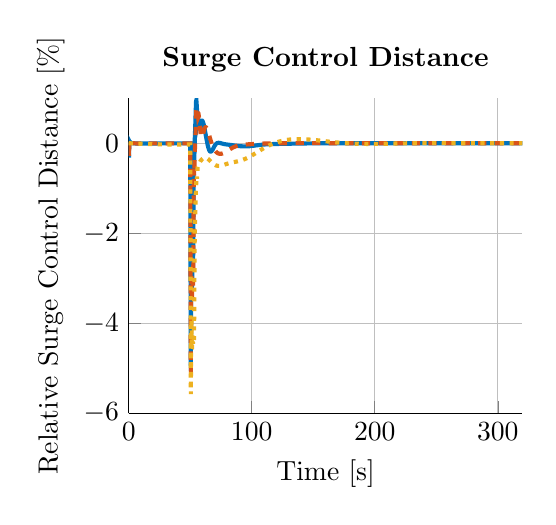
\begin{tikzpicture}

\begin{axis}[%
width=5cm,
height=4cm,
at={(0\linewidth,0\linewidth)},
scale only axis,
xmin=0,
xmax=320,
xlabel={Time [s]},
xmajorgrids,
ymin=-6,
ymax=1,
ylabel={Relative Surge Control Distance [\%]},
ymajorgrids,
axis background/.style={fill=white},
title style={font=\bfseries},
title={Surge Control Distance},
axis x line*=bottom,
axis y line*=left
]
\addplot [color=mycolor1,solid,line width=1.5pt,forget plot]
  table[row sep=crcr]{%
0	-0.0970099999999992\\
0.25	-0.31776\\
0.5	0.0485000000000007\\
% 0.75	0.0541400000000003\\
% 1	-0.00875999999999877\\
1.25	0.00740000000000052\\
1.5	0.01755\\
1.75	0.00960000000000072\\
2	0.00655000000000072\\
2.25	0.00689000000000028\\
2.5	0.00555000000000128\\
2.75	0.00388000000000055\\
3	0.0028100000000002\\
3.25	0.00186000000000064\\
3.5	0.000899999999999679\\
3.75	6.00000000012813e-05\\
4	-0.000669999999999504\\
4.25	-0.00131999999999977\\
4.5	-0.00190999999999875\\
4.75	-0.00244\\
5	-0.00292999999999921\\
5.25	-0.00337000000000032\\
5.5	-0.00376999999999938\\
5.75	-0.00411999999999857\\
6	-0.00441999999999965\\
6.25	-0.00467999999999869\\
6.5	-0.00488\\
6.75	-0.00503999999999927\\
7	-0.00514999999999866\\
7.25	-0.0052399999999988\\
7.5	-0.00530000000000008\\
7.75	-0.00534999999999997\\
8	-0.00539000000000023\\
8.25	-0.00541999999999909\\
8.5	-0.00544999999999973\\
8.75	-0.00545999999999935\\
9	-0.00546999999999898\\
9.25	-0.00545999999999935\\
9.5	-0.00544000000000011\\
9.75	-0.00539000000000023\\
10	-0.00532999999999895\\
10.25	-0.00526999999999944\\
10.5	-0.00520000000000032\\
10.75	-0.00512999999999941\\
11	-0.00506999999999991\\
11.25	-0.00500999999999863\\
11.5	-0.00497000000000014\\
11.75	-0.00492999999999988\\
12	-0.00488999999999962\\
12.25	-0.00484999999999935\\
12.5	-0.00479999999999947\\
12.75	-0.00474999999999959\\
13	-0.00469000000000008\\
13.25	-0.00461999999999918\\
13.5	-0.00455000000000005\\
13.75	-0.00448999999999877\\
14	-0.00443999999999889\\
14.25	-0.00439999999999863\\
14.5	-0.00436999999999976\\
14.75	-0.00433999999999912\\
15	-0.00431999999999988\\
15.25	-0.00429999999999886\\
15.5	-0.00427999999999962\\
15.75	-0.00424999999999898\\
16	-0.00420999999999871\\
16.25	-0.00417000000000023\\
16.5	-0.00412999999999997\\
16.75	-0.0040899999999997\\
17	-0.00404999999999944\\
17.25	-0.0040300000000002\\
17.5	-0.00400999999999918\\
17.75	-0.00399999999999956\\
18	-0.00398999999999994\\
18.25	-0.00398999999999994\\
18.5	-0.00398000000000032\\
18.75	-0.0039599999999993\\
19	-0.00394000000000005\\
19.25	-0.00390999999999941\\
19.5	-0.00387999999999877\\
19.75	-0.00384999999999991\\
20	-0.00381999999999927\\
20.25	-0.00380000000000003\\
20.5	-0.00378999999999863\\
20.75	-0.00377999999999901\\
21	-0.00377999999999901\\
21.25	-0.00377999999999901\\
21.5	-0.00376999999999938\\
21.75	-0.00375999999999976\\
22	-0.00373999999999874\\
22.25	-0.00370999999999988\\
22.5	-0.00367999999999924\\
22.75	-0.0036499999999986\\
23	-0.00362999999999936\\
23.25	-0.00361000000000011\\
23.5	-0.00358999999999909\\
23.75	-0.00358999999999909\\
24	-0.00357999999999947\\
24.25	-0.00357999999999947\\
24.5	-0.00356999999999985\\
24.75	-0.00356000000000023\\
25	-0.00353999999999921\\
25.25	-0.00351999999999997\\
25.5	-0.00348999999999933\\
25.75	-0.00345999999999869\\
26	-0.00342999999999982\\
26.25	-0.0034099999999988\\
26.5	-0.00339999999999918\\
26.75	-0.00338999999999956\\
27	-0.00338999999999956\\
27.25	-0.00337999999999994\\
27.5	-0.00337999999999994\\
27.75	-0.00337000000000032\\
28	-0.0033499999999993\\
28.25	-0.00333000000000006\\
28.5	-0.00329999999999941\\
28.75	-0.00326999999999877\\
29	-0.00324999999999953\\
29.25	-0.00323000000000029\\
29.5	-0.00320999999999927\\
29.75	-0.00320999999999927\\
30	-0.00319999999999965\\
30.25	-0.00320999999999927\\
30.5	-0.00319999999999965\\
30.75	-0.00319999999999965\\
31	-0.00317999999999863\\
31.25	-0.00316999999999901\\
31.5	-0.00314000000000014\\
31.75	-0.0031099999999995\\
32	-0.00309000000000026\\
32.25	-0.00306999999999924\\
32.5	-0.00305999999999962\\
32.75	-0.00305999999999962\\
33	-0.00305999999999962\\
33.25	-0.00305999999999962\\
33.5	-0.00306999999999924\\
33.75	-0.00305999999999962\\
34	-0.00305999999999962\\
34.25	-0.0030399999999986\\
34.5	-0.00301999999999936\\
34.75	-0.00300000000000011\\
35	-0.00296999999999947\\
35.25	-0.00295999999999985\\
35.5	-0.00295000000000023\\
35.75	-0.00295000000000023\\
36	-0.00295999999999985\\
36.25	-0.00295999999999985\\
36.5	-0.00296999999999947\\
36.75	-0.00296999999999947\\
37	-0.00296999999999947\\
37.25	-0.00295999999999985\\
37.5	-0.00293999999999883\\
37.75	-0.00291999999999959\\
38	-0.00289999999999857\\
38.25	-0.00288999999999895\\
38.5	-0.00287999999999933\\
38.75	-0.00287999999999933\\
39	-0.00288999999999895\\
39.25	-0.00290999999999997\\
39.5	-0.00291999999999959\\
39.75	-0.00292999999999921\\
40	-0.00291999999999959\\
40.25	-0.00290999999999997\\
40.5	-0.00289999999999857\\
40.75	-0.00287999999999933\\
41	-0.00286000000000008\\
41.25	-0.00284999999999869\\
41.5	-0.00284999999999869\\
41.75	-0.00284999999999869\\
42	-0.00286999999999971\\
42.25	-0.00287999999999933\\
42.5	-0.00289999999999857\\
42.75	-0.00290999999999997\\
43	-0.00290999999999997\\
43.25	-0.00289999999999857\\
43.5	-0.00288999999999895\\
43.75	-0.00286999999999971\\
44	-0.00284999999999869\\
44.25	-0.00283999999999907\\
44.5	-0.00283999999999907\\
44.75	-0.00284999999999869\\
45	-0.00286000000000008\\
45.25	-0.00288999999999895\\
45.5	-0.00290999999999997\\
45.75	-0.00291999999999959\\
46	-0.00291999999999959\\
46.25	-0.00290999999999997\\
46.5	-0.00289999999999857\\
46.75	-0.00287999999999933\\
47	-0.00286000000000008\\
47.25	-0.00284999999999869\\
47.5	-0.00284999999999869\\
47.75	-0.00286000000000008\\
48	-0.00287999999999933\\
48.25	-0.00290999999999997\\
48.5	-0.00292999999999921\\
48.75	-0.00293999999999883\\
49	-0.00295000000000023\\
49.25	-0.00293999999999883\\
49.5	-0.00291999999999959\\
49.75	-0.00289999999999857\\
50	-0.00287999999999933\\
50.25	-2.77916\\
50.5	-5.05865\\
50.75	-3.23165\\
51	-2.68995\\
51.25	-3.30532\\
51.5	-3.10962\\
51.75	-2.76589\\
52	-2.79788\\
52.25	-2.84727\\
52.5	-2.23862\\
52.75	-0.72666\\
53	-0.289249999999999\\
53.25	-0.39575\\
53.5	-0.128729999999999\\
53.75	0.138570000000001\\
54	0.309560000000001\\
54.25	0.51932\\
54.5	0.75141\\
54.75	0.92952\\
55	0.958270000000001\\
55.25	0.85941\\
55.5	0.747640000000001\\
55.75	0.572740000000001\\
56	0.471160000000001\\
56.25	0.511200000000001\\
56.5	0.53909\\
56.75	0.50972\\
57	0.481300000000001\\
57.25	0.467120000000001\\
57.5	0.45491\\
57.75	0.434140000000001\\
58	0.41464\\
58.25	0.41826\\
58.5	0.440330000000001\\
58.75	0.462670000000001\\
59	0.479850000000001\\
59.25	0.49292\\
59.5	0.500150000000001\\
59.75	0.499920000000001\\
60	0.49268\\
60.25	0.47955\\
60.5	0.461220000000001\\
60.75	0.438130000000001\\
61	0.410960000000001\\
61.25	0.380560000000001\\
61.5	0.347670000000001\\
61.75	0.31287\\
62	0.276670000000001\\
62.25	0.23958\\
62.5	0.20199\\
62.75	0.16431\\
63	0.126890000000001\\
63.25	0.090110000000001\\
63.5	0.054310000000001\\
63.75	0.0198499999999999\\
64	-0.012929999999999\\
64.25	-0.0437199999999986\\
64.5	-0.0721999999999987\\
64.75	-0.0980600000000003\\
65	-0.120999999999999\\
65.25	-0.14073\\
65.5	-0.15696\\
65.75	-0.169449999999999\\
66	-0.178139999999999\\
66.25	-0.183199999999999\\
66.5	-0.185099999999999\\
66.75	-0.184419999999999\\
67	-0.181539999999999\\
67.25	-0.176609999999999\\
67.5	-0.16968\\
67.75	-0.160889999999999\\
68	-0.15049\\
68.25	-0.138809999999999\\
68.5	-0.126189999999999\\
68.75	-0.113019999999999\\
69	-0.0996299999999994\\
69.25	-0.0863599999999991\\
69.5	-0.0734699999999986\\
69.75	-0.0612099999999991\\
70	-0.0497399999999999\\
70.25	-0.0392099999999989\\
70.5	-0.0297000000000001\\
70.75	-0.0212699999999995\\
71	-0.0139199999999988\\
71.25	-0.00765999999999956\\
71.5	-0.00244999999999962\\
71.75	0.00176000000000087\\
72	0.00505000000000067\\
72.25	0.00747000000000142\\
72.5	0.00912000000000113\\
72.75	0.0100700000000007\\
73	0.0104199999999999\\
73.25	0.0102400000000014\\
73.5	0.00961999999999996\\
73.75	0.00863999999999976\\
74	0.00735000000000063\\
74.25	0.00584000000000096\\
74.5	0.00415000000000099\\
74.75	0.00234000000000023\\
75	0.000460000000000349\\
75.25	-0.00146999999999942\\
75.5	-0.00339999999999918\\
75.75	-0.00531999999999933\\
76	-0.00718999999999959\\
76.25	-0.00899999999999856\\
76.5	-0.0107499999999998\\
76.75	-0.0124199999999988\\
77	-0.014009999999999\\
77.25	-0.015509999999999\\
77.5	-0.01694\\
77.75	-0.018279999999999\\
78	-0.0195499999999988\\
78.25	-0.0207499999999996\\
78.5	-0.0218799999999995\\
78.75	-0.0229599999999994\\
79	-0.0239899999999995\\
79.25	-0.0249699999999997\\
79.5	-0.0259099999999997\\
79.75	-0.0268299999999986\\
80	-0.0277199999999986\\
80.25	-0.0285999999999991\\
80.5	-0.0294600000000003\\
80.75	-0.0303100000000001\\
81	-0.0311599999999999\\
81.25	-0.0320099999999996\\
81.5	-0.0328699999999991\\
81.75	-0.0337300000000003\\
82	-0.0345899999999997\\
82.25	-0.0354700000000001\\
82.5	-0.0363600000000002\\
82.75	-0.0372599999999998\\
83	-0.0381599999999995\\
83.25	-0.0390800000000002\\
83.5	-0.0400099999999988\\
83.75	-0.0409499999999987\\
84	-0.0419\\
84.25	-0.0428599999999992\\
84.5	-0.0438200000000002\\
84.75	-0.044789999999999\\
85	-0.0457599999999996\\
85.25	-0.0467300000000002\\
85.5	-0.047699999999999\\
85.75	-0.0486799999999992\\
86	-0.0496400000000001\\
86.25	-0.0506099999999989\\
86.5	-0.0515600000000003\\
86.75	-0.0525099999999998\\
87	-0.0534400000000002\\
87.25	-0.0543699999999987\\
87.5	-0.0552799999999998\\
87.75	-0.0561699999999998\\
88	-0.0570500000000003\\
88.25	-0.0579099999999997\\
88.5	-0.0587499999999999\\
88.75	-0.059569999999999\\
89	-0.0603599999999993\\
89.25	-0.0611299999999986\\
89.5	-0.061869999999999\\
89.75	-0.0625799999999987\\
90	-0.0632599999999996\\
90.25	-0.0639199999999995\\
90.5	-0.0645399999999992\\
90.75	-0.0651299999999999\\
91	-0.06569\\
91.25	-0.0662099999999999\\
91.5	-0.0666899999999995\\
91.75	-0.0671400000000002\\
92	-0.0675499999999989\\
92.25	-0.0679199999999991\\
92.5	-0.068249999999999\\
92.75	-0.0685399999999987\\
93	-0.0687899999999999\\
93.25	-0.0690099999999987\\
93.5	-0.0691799999999994\\
93.75	-0.0693000000000001\\
94	-0.0693900000000003\\
94.25	-0.0694299999999988\\
94.5	-0.0694400000000002\\
94.75	-0.0693999999999999\\
95	-0.0693199999999994\\
95.25	-0.0691999999999986\\
95.5	-0.0690299999999997\\
95.75	-0.0688300000000002\\
96	-0.0685899999999986\\
96.25	-0.0682999999999989\\
96.5	-0.0679799999999986\\
96.75	-0.0676199999999998\\
97	-0.0672199999999989\\
97.25	-0.0667899999999992\\
97.5	-0.0663199999999993\\
97.75	-0.0658199999999987\\
98	-0.0652799999999996\\
98.25	-0.0647199999999994\\
98.5	-0.0641199999999991\\
98.75	-0.0634899999999998\\
99	-0.0628399999999996\\
99.25	-0.0621599999999987\\
99.5	-0.0614499999999989\\
99.75	-0.0607199999999999\\
100	-0.0599699999999999\\
100.25	-0.0591999999999988\\
100.5	-0.0584100000000003\\
100.75	-0.057599999999999\\
101	-0.0567799999999998\\
101.25	-0.0559399999999997\\
101.5	-0.0550899999999999\\
101.75	-0.0542299999999987\\
102	-0.0533599999999996\\
102.25	-0.0524799999999992\\
102.5	-0.0515999999999988\\
102.75	-0.0507099999999987\\
103	-0.0498199999999986\\
103.25	-0.048919999999999\\
103.5	-0.0480299999999989\\
103.75	-0.0471299999999992\\
104	-0.0462399999999992\\
104.25	-0.0453499999999991\\
104.5	-0.0444699999999987\\
104.75	-0.04359\\
105	-0.0427199999999992\\
105.25	-0.0418599999999998\\
105.5	-0.04101\\
105.75	-0.0401600000000002\\
106	-0.0393299999999996\\
106.25	-0.0385099999999987\\
106.5	-0.0376999999999992\\
106.75	-0.0369099999999989\\
107	-0.03613\\
107.25	-0.0353599999999989\\
107.5	-0.0346099999999989\\
107.75	-0.0338799999999999\\
108	-0.0331599999999987\\
108.25	-0.032449999999999\\
108.5	-0.0317699999999999\\
108.75	-0.0310999999999986\\
109	-0.0304500000000001\\
109.25	-0.0298199999999991\\
109.5	-0.0291999999999994\\
109.75	-0.0285999999999991\\
110	-0.0280199999999997\\
110.25	-0.0274599999999996\\
110.5	-0.0269099999999991\\
110.75	-0.0263899999999992\\
111	-0.025879999999999\\
111.25	-0.0253800000000002\\
111.5	-0.0249100000000002\\
111.75	-0.0244499999999999\\
112	-0.0239999999999991\\
112.25	-0.0235699999999994\\
112.5	-0.023159999999999\\
112.75	-0.0227599999999999\\
113	-0.0223800000000001\\
113.25	-0.0220099999999999\\
113.5	-0.0216599999999989\\
113.75	-0.0213199999999993\\
114	-0.0209899999999994\\
114.25	-0.0206799999999987\\
114.5	-0.0203699999999998\\
114.75	-0.0200800000000001\\
115	-0.0198\\
115.25	-0.0195399999999992\\
115.5	-0.0192800000000002\\
115.75	-0.019029999999999\\
116	-0.0187899999999992\\
116.25	-0.018559999999999\\
116.5	-0.0183400000000002\\
116.75	-0.0181199999999997\\
117	-0.0179200000000002\\
117.25	-0.0177199999999988\\
117.5	-0.0175199999999993\\
117.75	-0.017339999999999\\
118	-0.0171599999999987\\
118.25	-0.0169800000000002\\
118.5	-0.0168099999999995\\
118.75	-0.0166399999999989\\
119	-0.0164799999999996\\
119.25	-0.0163199999999986\\
119.5	-0.0161699999999989\\
119.75	-0.0160199999999993\\
120	-0.0158699999999996\\
120.25	-0.01572\\
120.5	-0.0155799999999999\\
120.75	-0.0154399999999999\\
121	-0.0152999999999999\\
121.25	-0.0151599999999998\\
121.5	-0.0150199999999998\\
121.75	-0.0148799999999998\\
122	-0.0147499999999994\\
122.25	-0.0146099999999993\\
122.5	-0.0144799999999989\\
122.75	-0.0143500000000003\\
123	-0.0142100000000003\\
123.25	-0.0140799999999999\\
123.5	-0.0139499999999995\\
123.75	-0.0138199999999991\\
124	-0.013679999999999\\
124.25	-0.0135499999999986\\
124.5	-0.01342\\
124.75	-0.01328\\
125	-0.0131499999999996\\
125.25	-0.0130099999999995\\
125.5	-0.0128799999999991\\
125.75	-0.0127399999999991\\
126	-0.0126099999999987\\
126.25	-0.0124699999999986\\
126.5	-0.0123299999999986\\
126.75	-0.0122\\
127	-0.01206\\
127.25	-0.0119199999999999\\
127.5	-0.0117799999999999\\
127.75	-0.0116399999999999\\
128	-0.0114999999999998\\
128.25	-0.0113599999999998\\
128.5	-0.0112199999999998\\
128.75	-0.0110799999999998\\
129	-0.0109399999999997\\
129.25	-0.0107900000000001\\
129.5	-0.01065\\
129.75	-0.01051\\
130	-0.01037\\
130.25	-0.01023\\
130.5	-0.0100800000000003\\
130.75	-0.00994000000000028\\
131	-0.00980000000000025\\
131.25	-0.00966000000000022\\
131.5	-0.00952000000000019\\
131.75	-0.00938000000000017\\
132	-0.00922999999999874\\
132.25	-0.00908999999999871\\
132.5	-0.00894999999999868\\
132.75	-0.00882000000000005\\
133	-0.00868000000000002\\
133.25	-0.00853999999999999\\
133.5	-0.00839999999999996\\
133.75	-0.00825999999999993\\
134	-0.00812999999999953\\
134.25	-0.0079899999999995\\
134.5	-0.00785999999999909\\
134.75	-0.00772999999999868\\
135	-0.00758999999999865\\
135.25	-0.00746000000000002\\
135.5	-0.00732999999999961\\
135.75	-0.00719999999999921\\
136	-0.0070800000000002\\
136.25	-0.00694999999999979\\
136.5	-0.00681999999999938\\
136.75	-0.0066999999999986\\
137	-0.00657999999999959\\
137.25	-0.0064599999999988\\
137.5	-0.00633999999999979\\
137.75	-0.006219999999999\\
138	-0.00609999999999999\\
138.25	-0.00597999999999921\\
138.5	-0.00586999999999982\\
138.75	-0.00574999999999903\\
139	-0.00563999999999965\\
139.25	-0.00553000000000026\\
139.5	-0.00541999999999909\\
139.75	-0.0053099999999997\\
140	-0.00520999999999994\\
140.25	-0.00509999999999877\\
140.5	-0.00499999999999901\\
140.75	-0.00489999999999924\\
141	-0.00479999999999947\\
141.25	-0.0046999999999997\\
141.5	-0.00459999999999994\\
141.75	-0.00450000000000017\\
142	-0.00441000000000003\\
142.25	-0.00431000000000026\\
142.5	-0.00422000000000011\\
142.75	-0.00412999999999997\\
143	-0.00403999999999982\\
143.25	-0.00394999999999968\\
143.5	-0.00386999999999915\\
143.75	-0.00377999999999901\\
144	-0.00370000000000026\\
144.25	-0.00361999999999973\\
144.5	-0.00353999999999921\\
144.75	-0.00345999999999869\\
145	-0.00337999999999994\\
145.25	-0.00329999999999941\\
145.5	-0.00321999999999889\\
145.75	-0.00314999999999976\\
146	-0.00306999999999924\\
146.25	-0.00300000000000011\\
146.5	-0.00292999999999921\\
146.75	-0.00286000000000008\\
147	-0.00278999999999918\\
147.25	-0.00272000000000006\\
147.5	-0.00264999999999915\\
147.75	-0.00258999999999965\\
148	-0.00251999999999875\\
148.25	-0.00245999999999924\\
148.5	-0.00239999999999974\\
148.75	-0.00232999999999883\\
149	-0.00226999999999933\\
149.25	-0.00220999999999982\\
149.5	-0.00215000000000032\\
149.75	-0.00209999999999866\\
150	-0.00203999999999915\\
150.25	-0.00197999999999965\\
150.5	-0.00192999999999977\\
150.75	-0.00187000000000026\\
151	-0.0018199999999986\\
151.25	-0.0017599999999991\\
151.5	-0.00170999999999921\\
151.75	-0.00165999999999933\\
152	-0.00160999999999945\\
152.25	-0.00155999999999956\\
152.5	-0.00150999999999968\\
152.75	-0.00145999999999979\\
153	-0.00140999999999991\\
153.25	-0.00136000000000003\\
153.5	-0.00131999999999977\\
153.75	-0.00126999999999988\\
154	-0.00122\\
154.25	-0.00117999999999974\\
154.5	-0.00112999999999985\\
154.75	-0.00108999999999959\\
155	-0.00104999999999933\\
155.25	-0.00100999999999907\\
155.5	-0.000959999999999184\\
155.75	-0.000919999999998922\\
156	-0.00087999999999866\\
156.25	-0.000840000000000174\\
156.5	-0.000799999999999912\\
156.75	-0.00075999999999965\\
157	-0.000719999999999388\\
157.25	-0.000679999999999126\\
157.5	-0.000650000000000261\\
157.75	-0.000609999999999999\\
158	-0.000569999999999737\\
158.25	-0.000539999999999097\\
158.5	-0.000499999999998835\\
158.75	-0.00046999999999997\\
159	-0.000429999999999708\\
159.25	-0.000399999999999068\\
159.5	-0.000359999999998806\\
159.75	-0.000329999999999941\\
160	-0.000299999999999301\\
160.25	-0.000259999999999039\\
160.5	-0.000230000000000175\\
160.75	-0.000199999999999534\\
161	-0.000169999999998893\\
161.25	-0.000140000000000029\\
161.5	-0.000109999999999388\\
161.75	-7.99999999987477e-05\\
162	-4.99999999998835e-05\\
162.25	-1.99999999992428e-05\\
162.5	1.00000000013978e-05\\
162.75	4.0000000000262e-05\\
163	7.00000000009027e-05\\
163.25	9.00000000001455e-05\\
163.5	0.000120000000000786\\
163.75	0.000150000000001427\\
164	0.00017000000000067\\
164.25	0.00020000000000131\\
164.5	0.000230000000000175\\
164.75	0.000250000000001194\\
165	0.000280000000000058\\
165.25	0.000300000000001077\\
165.5	0.00032000000000032\\
165.75	0.000350000000000961\\
166	0.000370000000000203\\
166.25	0.000390000000001223\\
166.5	0.000420000000000087\\
166.75	0.000440000000001106\\
167	0.000460000000000349\\
167.25	0.000480000000001368\\
167.5	0.000500000000000611\\
167.75	0.000519999999999854\\
168	0.000540000000000873\\
168.25	0.000560000000000116\\
168.5	0.000580000000001135\\
168.75	0.000600000000000378\\
169	0.000620000000001397\\
169.25	0.00064000000000064\\
169.5	0.000659999999999883\\
169.75	0.000670000000001281\\
170	0.000690000000000524\\
170.25	0.000709999999999766\\
170.5	0.000730000000000786\\
170.75	0.000740000000000407\\
171	0.000760000000001426\\
171.25	0.000770000000001048\\
171.5	0.00079000000000029\\
171.75	0.00081000000000131\\
172	0.000820000000000931\\
172.25	0.000830000000000553\\
172.5	0.000849999999999795\\
172.75	0.000860000000001193\\
173	0.000880000000000436\\
173.25	0.000890000000000057\\
173.5	0.000899999999999679\\
173.75	0.000920000000000698\\
174	0.000930000000000319\\
174.25	0.000939999999999941\\
174.5	0.000950000000001339\\
174.75	0.00096000000000096\\
175	0.000970000000000582\\
175.25	0.000989999999999824\\
175.5	0.00100000000000122\\
175.75	0.00101000000000084\\
176	0.00102000000000046\\
176.25	0.00103000000000009\\
176.5	0.00103999999999971\\
176.75	0.00105000000000111\\
177	0.00105000000000111\\
177.25	0.00106000000000073\\
177.5	0.00107000000000035\\
177.75	0.00107999999999997\\
178	0.00109000000000137\\
178.25	0.00110000000000099\\
178.5	0.00110000000000099\\
178.75	0.00111000000000061\\
179	0.00112000000000023\\
179.25	0.00112000000000023\\
179.5	0.00112999999999985\\
179.75	0.00114000000000125\\
180	0.00114000000000125\\
180.25	0.00115000000000087\\
180.5	0.00116000000000049\\
180.75	0.00116000000000049\\
181	0.00117000000000012\\
181.25	0.00117000000000012\\
181.5	0.00117999999999974\\
181.75	0.00117999999999974\\
182	0.00119000000000113\\
182.25	0.00119000000000113\\
182.5	0.00119000000000113\\
182.75	0.00120000000000076\\
183	0.00120000000000076\\
183.25	0.00120000000000076\\
183.5	0.00121000000000038\\
183.75	0.00121000000000038\\
184	0.00121000000000038\\
184.25	0.00122\\
184.5	0.00122\\
184.75	0.00122\\
185	0.00122\\
185.25	0.0012300000000014\\
185.5	0.0012300000000014\\
185.75	0.0012300000000014\\
186	0.0012300000000014\\
186.25	0.0012300000000014\\
186.5	0.0012300000000014\\
186.75	0.00124000000000102\\
187	0.00124000000000102\\
187.25	0.00124000000000102\\
187.5	0.00124000000000102\\
187.75	0.00124000000000102\\
188	0.00124000000000102\\
188.25	0.00124000000000102\\
188.5	0.00124000000000102\\
188.75	0.00124000000000102\\
189	0.00124000000000102\\
189.25	0.00124000000000102\\
189.5	0.00124000000000102\\
189.75	0.00124000000000102\\
190	0.00124000000000102\\
190.25	0.00124000000000102\\
190.5	0.00124000000000102\\
190.75	0.0012300000000014\\
191	0.0012300000000014\\
191.25	0.0012300000000014\\
191.5	0.0012300000000014\\
191.75	0.0012300000000014\\
192	0.0012300000000014\\
192.25	0.0012300000000014\\
192.5	0.00122\\
192.75	0.00122\\
193	0.00122\\
193.25	0.00122\\
193.5	0.00122\\
193.75	0.00121000000000038\\
194	0.00121000000000038\\
194.25	0.00121000000000038\\
194.5	0.00121000000000038\\
194.75	0.00120000000000076\\
195	0.00120000000000076\\
195.25	0.00120000000000076\\
195.5	0.00119000000000113\\
195.75	0.00119000000000113\\
196	0.00119000000000113\\
196.25	0.00117999999999974\\
196.5	0.00117999999999974\\
196.75	0.00117999999999974\\
197	0.00117000000000012\\
197.25	0.00117000000000012\\
197.5	0.00117000000000012\\
197.75	0.00116000000000049\\
198	0.00116000000000049\\
198.25	0.00116000000000049\\
198.5	0.00115000000000087\\
198.75	0.00115000000000087\\
199	0.00114000000000125\\
199.25	0.00114000000000125\\
199.5	0.00114000000000125\\
199.75	0.00112999999999985\\
200	0.00112999999999985\\
200.25	0.00112000000000023\\
200.5	0.00112000000000023\\
200.75	0.00111000000000061\\
201	0.00111000000000061\\
201.25	0.00111000000000061\\
201.5	0.00110000000000099\\
201.75	0.00110000000000099\\
202	0.00109000000000137\\
202.25	0.00109000000000137\\
202.5	0.00107999999999997\\
202.75	0.00107999999999997\\
203	0.00107000000000035\\
203.25	0.00107000000000035\\
203.5	0.00106000000000073\\
203.75	0.00106000000000073\\
204	0.00105000000000111\\
204.25	0.00105000000000111\\
204.5	0.00103999999999971\\
204.75	0.00103999999999971\\
205	0.00103000000000009\\
205.25	0.00103000000000009\\
205.5	0.00102000000000046\\
205.75	0.00102000000000046\\
206	0.00101000000000084\\
206.25	0.00101000000000084\\
206.5	0.00100000000000122\\
206.75	0.00100000000000122\\
207	0.000989999999999824\\
207.25	0.000980000000000203\\
207.5	0.000980000000000203\\
207.75	0.000970000000000582\\
208	0.000970000000000582\\
208.25	0.00096000000000096\\
208.5	0.00096000000000096\\
208.75	0.000950000000001339\\
209	0.000950000000001339\\
209.25	0.000939999999999941\\
209.5	0.000930000000000319\\
209.75	0.000930000000000319\\
210	0.000920000000000698\\
210.25	0.000920000000000698\\
210.5	0.000910000000001077\\
210.75	0.000910000000001077\\
211	0.000899999999999679\\
211.25	0.000890000000000057\\
211.5	0.000890000000000057\\
211.75	0.000880000000000436\\
212	0.000880000000000436\\
212.25	0.000870000000000815\\
212.5	0.000870000000000815\\
212.75	0.000860000000001193\\
213	0.000849999999999795\\
213.25	0.000849999999999795\\
213.5	0.000840000000000174\\
213.75	0.000840000000000174\\
214	0.000830000000000553\\
214.25	0.000830000000000553\\
214.5	0.000820000000000931\\
214.75	0.00081000000000131\\
215	0.00081000000000131\\
215.25	0.000799999999999912\\
215.5	0.000799999999999912\\
215.75	0.00079000000000029\\
216	0.000780000000000669\\
216.25	0.000780000000000669\\
216.5	0.000770000000001048\\
216.75	0.000770000000001048\\
217	0.000760000000001426\\
217.25	0.000760000000001426\\
217.5	0.000750000000000028\\
217.75	0.000740000000000407\\
218	0.000740000000000407\\
218.25	0.000730000000000786\\
218.5	0.000730000000000786\\
218.75	0.000720000000001164\\
219	0.000720000000001164\\
219.25	0.000709999999999766\\
219.5	0.000700000000000145\\
219.75	0.000700000000000145\\
220	0.000690000000000524\\
220.25	0.000690000000000524\\
220.5	0.000680000000000902\\
220.75	0.000680000000000902\\
221	0.000670000000001281\\
221.25	0.000659999999999883\\
221.5	0.000659999999999883\\
221.75	0.000650000000000261\\
222	0.000650000000000261\\
222.25	0.00064000000000064\\
222.5	0.00064000000000064\\
222.75	0.000630000000001019\\
223	0.000630000000001019\\
223.25	0.000620000000001397\\
223.5	0.000620000000001397\\
223.75	0.000609999999999999\\
224	0.000600000000000378\\
224.25	0.000600000000000378\\
224.5	0.000590000000000757\\
224.75	0.000590000000000757\\
225	0.000580000000001135\\
225.25	0.000580000000001135\\
225.5	0.000569999999999737\\
225.75	0.000569999999999737\\
226	0.000560000000000116\\
226.25	0.000560000000000116\\
226.5	0.000550000000000495\\
226.75	0.000550000000000495\\
227	0.000540000000000873\\
227.25	0.000540000000000873\\
227.5	0.000530000000001252\\
227.75	0.000530000000001252\\
228	0.000519999999999854\\
228.25	0.000510000000000232\\
228.5	0.000510000000000232\\
228.75	0.000500000000000611\\
229	0.000500000000000611\\
229.25	0.00049000000000099\\
229.5	0.00049000000000099\\
229.75	0.000480000000001368\\
230	0.000480000000001368\\
230.25	0.000480000000001368\\
230.5	0.00046999999999997\\
230.75	0.00046999999999997\\
231	0.000460000000000349\\
231.25	0.000460000000000349\\
231.5	0.000450000000000728\\
231.75	0.000450000000000728\\
232	0.000440000000001106\\
232.25	0.000440000000001106\\
232.5	0.000429999999999708\\
232.75	0.000429999999999708\\
233	0.000420000000000087\\
233.25	0.000420000000000087\\
233.5	0.000410000000000466\\
233.75	0.000410000000000466\\
234	0.000400000000000844\\
234.25	0.000400000000000844\\
234.5	0.000400000000000844\\
234.75	0.000390000000001223\\
235	0.000390000000001223\\
235.25	0.000379999999999825\\
235.5	0.000379999999999825\\
235.75	0.000370000000000203\\
236	0.000370000000000203\\
236.25	0.000370000000000203\\
236.5	0.000360000000000582\\
236.75	0.000360000000000582\\
237	0.000350000000000961\\
237.25	0.000350000000000961\\
237.5	0.000340000000001339\\
237.75	0.000340000000001339\\
238	0.000340000000001339\\
238.25	0.000329999999999941\\
238.5	0.000329999999999941\\
238.75	0.00032000000000032\\
239	0.00032000000000032\\
239.25	0.00032000000000032\\
239.5	0.000310000000000699\\
239.75	0.000310000000000699\\
240	0.000300000000001077\\
240.25	0.000300000000001077\\
240.5	0.000300000000001077\\
240.75	0.000289999999999679\\
241	0.000289999999999679\\
241.25	0.000289999999999679\\
241.5	0.000280000000000058\\
241.75	0.000280000000000058\\
242	0.000270000000000437\\
242.25	0.000270000000000437\\
242.5	0.000270000000000437\\
242.75	0.000260000000000815\\
243	0.000260000000000815\\
243.25	0.000260000000000815\\
243.5	0.000250000000001194\\
243.75	0.000250000000001194\\
244	0.000250000000001194\\
244.25	0.000239999999999796\\
244.5	0.000239999999999796\\
244.75	0.000239999999999796\\
245	0.000230000000000175\\
245.25	0.000230000000000175\\
245.5	0.000230000000000175\\
245.75	0.000220000000000553\\
246	0.000220000000000553\\
246.25	0.000220000000000553\\
246.5	0.000210000000000932\\
246.75	0.000210000000000932\\
247	0.000210000000000932\\
247.25	0.00020000000000131\\
247.5	0.00020000000000131\\
247.75	0.00020000000000131\\
248	0.00020000000000131\\
248.25	0.000189999999999912\\
248.5	0.000189999999999912\\
248.75	0.000189999999999912\\
249	0.000180000000000291\\
249.25	0.000180000000000291\\
249.5	0.000180000000000291\\
249.75	0.000180000000000291\\
250	0.00017000000000067\\
250.25	0.00017000000000067\\
250.5	0.00017000000000067\\
250.75	0.000160000000001048\\
251	0.000160000000001048\\
251.25	0.000160000000001048\\
251.5	0.000160000000001048\\
251.75	0.000150000000001427\\
252	0.000150000000001427\\
252.25	0.000150000000001427\\
252.5	0.000150000000001427\\
252.75	0.000140000000000029\\
253	0.000140000000000029\\
253.25	0.000140000000000029\\
253.5	0.000140000000000029\\
253.75	0.000130000000000408\\
254	0.000130000000000408\\
254.25	0.000130000000000408\\
254.5	0.000130000000000408\\
254.75	0.000120000000000786\\
255	0.000120000000000786\\
255.25	0.000120000000000786\\
255.5	0.000120000000000786\\
255.75	0.000120000000000786\\
256	0.000110000000001165\\
256.25	0.000110000000001165\\
256.5	0.000110000000001165\\
256.75	0.000110000000001165\\
257	9.99999999997669e-05\\
257.25	9.99999999997669e-05\\
257.5	9.99999999997669e-05\\
257.75	9.99999999997669e-05\\
258	9.99999999997669e-05\\
258.25	9.00000000001455e-05\\
258.5	9.00000000001455e-05\\
258.75	9.00000000001455e-05\\
259	9.00000000001455e-05\\
259.25	9.00000000001455e-05\\
259.5	8.00000000005241e-05\\
259.75	8.00000000005241e-05\\
260	8.00000000005241e-05\\
260.25	8.00000000005241e-05\\
260.5	8.00000000005241e-05\\
260.75	8.00000000005241e-05\\
261	7.00000000009027e-05\\
261.25	7.00000000009027e-05\\
261.5	7.00000000009027e-05\\
261.75	7.00000000009027e-05\\
262	7.00000000009027e-05\\
262.25	7.00000000009027e-05\\
262.5	6.00000000012813e-05\\
262.75	6.00000000012813e-05\\
263	6.00000000012813e-05\\
263.25	6.00000000012813e-05\\
263.5	6.00000000012813e-05\\
263.75	6.00000000012813e-05\\
264	4.99999999998835e-05\\
264.25	4.99999999998835e-05\\
264.5	4.99999999998835e-05\\
264.75	4.99999999998835e-05\\
265	4.99999999998835e-05\\
265.25	4.99999999998835e-05\\
265.5	4.99999999998835e-05\\
265.75	4.0000000000262e-05\\
266	4.0000000000262e-05\\
266.25	4.0000000000262e-05\\
266.5	4.0000000000262e-05\\
266.75	4.0000000000262e-05\\
267	4.0000000000262e-05\\
267.25	4.0000000000262e-05\\
267.5	3.00000000006406e-05\\
267.75	3.00000000006406e-05\\
268	3.00000000006406e-05\\
268.25	3.00000000006406e-05\\
268.5	3.00000000006406e-05\\
268.75	3.00000000006406e-05\\
269	3.00000000006406e-05\\
269.25	3.00000000006406e-05\\
269.5	2.00000000010192e-05\\
269.75	2.00000000010192e-05\\
270	2.00000000010192e-05\\
270.25	2.00000000010192e-05\\
270.5	2.00000000010192e-05\\
270.75	2.00000000010192e-05\\
271	2.00000000010192e-05\\
271.25	2.00000000010192e-05\\
271.5	2.00000000010192e-05\\
271.75	2.00000000010192e-05\\
272	1.00000000013978e-05\\
272.25	1.00000000013978e-05\\
272.5	1.00000000013978e-05\\
272.75	1.00000000013978e-05\\
273	1.00000000013978e-05\\
273.25	1.00000000013978e-05\\
273.5	1.00000000013978e-05\\
273.75	1.00000000013978e-05\\
274	1.00000000013978e-05\\
274.25	1.00000000013978e-05\\
274.5	0\\
274.75	0\\
275	0\\
275.25	0\\
275.5	0\\
275.75	0\\
276	0\\
276.25	0\\
276.5	0\\
276.75	0\\
277	0\\
277.25	0\\
277.5	0\\
277.75	0\\
278	-9.99999999962142e-06\\
278.25	-9.99999999962142e-06\\
278.5	-9.99999999962142e-06\\
278.75	-9.99999999962142e-06\\
279	-9.99999999962142e-06\\
279.25	-9.99999999962142e-06\\
279.5	-9.99999999962142e-06\\
279.75	-9.99999999962142e-06\\
280	-9.99999999962142e-06\\
280.25	-9.99999999962142e-06\\
280.5	-9.99999999962142e-06\\
280.75	-9.99999999962142e-06\\
281	-9.99999999962142e-06\\
281.25	-9.99999999962142e-06\\
281.5	-9.99999999962142e-06\\
281.75	-9.99999999962142e-06\\
282	-9.99999999962142e-06\\
282.25	-1.99999999992428e-05\\
282.5	-1.99999999992428e-05\\
282.75	-1.99999999992428e-05\\
283	-1.99999999992428e-05\\
283.25	-1.99999999992428e-05\\
283.5	-1.99999999992428e-05\\
283.75	-1.99999999992428e-05\\
284	-1.99999999992428e-05\\
284.25	-1.99999999992428e-05\\
284.5	-1.99999999992428e-05\\
284.75	-1.99999999992428e-05\\
285	-1.99999999992428e-05\\
285.25	-1.99999999992428e-05\\
285.5	-1.99999999992428e-05\\
285.75	-1.99999999992428e-05\\
286	-1.99999999992428e-05\\
286.25	-1.99999999992428e-05\\
286.5	-1.99999999992428e-05\\
286.75	-1.99999999992428e-05\\
287	-1.99999999992428e-05\\
287.25	-1.99999999992428e-05\\
287.5	-1.99999999992428e-05\\
287.75	-1.99999999992428e-05\\
288	-1.99999999992428e-05\\
288.25	-1.99999999992428e-05\\
288.5	-1.99999999992428e-05\\
288.75	-2.99999999988643e-05\\
289	-2.99999999988643e-05\\
289.25	-2.99999999988643e-05\\
289.5	-2.99999999988643e-05\\
289.75	-2.99999999988643e-05\\
290	-2.99999999988643e-05\\
290.25	-2.99999999988643e-05\\
290.5	-2.99999999988643e-05\\
290.75	-2.99999999988643e-05\\
291	-2.99999999988643e-05\\
291.25	-2.99999999988643e-05\\
291.5	-2.99999999988643e-05\\
291.75	-2.99999999988643e-05\\
292	-2.99999999988643e-05\\
292.25	-2.99999999988643e-05\\
292.5	-2.99999999988643e-05\\
292.75	-2.99999999988643e-05\\
293	-2.99999999988643e-05\\
293.25	-2.99999999988643e-05\\
293.5	-2.99999999988643e-05\\
293.75	-2.99999999988643e-05\\
294	-2.99999999988643e-05\\
294.25	-2.99999999988643e-05\\
294.5	-2.99999999988643e-05\\
294.75	-2.99999999988643e-05\\
295	-2.99999999988643e-05\\
295.25	-2.99999999988643e-05\\
295.5	-2.99999999988643e-05\\
295.75	-2.99999999988643e-05\\
296	-2.99999999988643e-05\\
296.25	-2.99999999988643e-05\\
296.5	-2.99999999988643e-05\\
296.75	-2.99999999988643e-05\\
297	-2.99999999988643e-05\\
297.25	-2.99999999988643e-05\\
297.5	-2.99999999988643e-05\\
297.75	-2.99999999988643e-05\\
298	-2.99999999988643e-05\\
298.25	-2.99999999988643e-05\\
298.5	-2.99999999988643e-05\\
298.75	-2.99999999988643e-05\\
299	-2.99999999988643e-05\\
299.25	-2.99999999988643e-05\\
299.5	-2.99999999988643e-05\\
299.75	-2.99999999988643e-05\\
300	-2.99999999988643e-05\\
300.25	-2.99999999988643e-05\\
300.5	-2.99999999988643e-05\\
300.75	-2.99999999988643e-05\\
301	-2.99999999988643e-05\\
301.25	-2.99999999988643e-05\\
301.5	-2.99999999988643e-05\\
301.75	-2.99999999988643e-05\\
302	-2.99999999988643e-05\\
302.25	-2.99999999988643e-05\\
302.5	-2.99999999988643e-05\\
302.75	-2.99999999988643e-05\\
303	-2.99999999988643e-05\\
303.25	-2.99999999988643e-05\\
303.5	-2.99999999988643e-05\\
303.75	-2.99999999988643e-05\\
304	-2.99999999988643e-05\\
304.25	-2.99999999988643e-05\\
304.5	-2.99999999988643e-05\\
304.75	-2.99999999988643e-05\\
305	-2.99999999988643e-05\\
305.25	-2.99999999988643e-05\\
305.5	-2.99999999988643e-05\\
305.75	-2.99999999988643e-05\\
306	-2.99999999988643e-05\\
306.25	-2.99999999988643e-05\\
306.5	-2.99999999988643e-05\\
306.75	-2.99999999988643e-05\\
307	-2.99999999988643e-05\\
307.25	-2.99999999988643e-05\\
307.5	-2.99999999988643e-05\\
307.75	-2.99999999988643e-05\\
308	-2.99999999988643e-05\\
308.25	-2.99999999988643e-05\\
308.5	-2.99999999988643e-05\\
308.75	-2.99999999988643e-05\\
309	-2.99999999988643e-05\\
309.25	-2.99999999988643e-05\\
309.5	-2.99999999988643e-05\\
309.75	-2.99999999988643e-05\\
310	-2.99999999988643e-05\\
310.25	-2.99999999988643e-05\\
310.5	-2.99999999988643e-05\\
310.75	-2.99999999988643e-05\\
311	-2.99999999988643e-05\\
311.25	-2.99999999988643e-05\\
311.5	-2.99999999988643e-05\\
311.75	-2.99999999988643e-05\\
312	-2.99999999988643e-05\\
312.25	-2.99999999988643e-05\\
312.5	-2.99999999988643e-05\\
312.75	-2.99999999988643e-05\\
313	-2.99999999988643e-05\\
313.25	-2.99999999988643e-05\\
313.5	-2.99999999988643e-05\\
313.75	-2.99999999988643e-05\\
314	-2.99999999988643e-05\\
314.25	-2.99999999988643e-05\\
314.5	-2.99999999988643e-05\\
314.75	-2.99999999988643e-05\\
315	-2.99999999988643e-05\\
315.25	-2.99999999988643e-05\\
315.5	-2.99999999988643e-05\\
315.75	-2.99999999988643e-05\\
316	-2.99999999988643e-05\\
316.25	-2.99999999988643e-05\\
316.5	-2.99999999988643e-05\\
316.75	-2.99999999988643e-05\\
317	-2.99999999988643e-05\\
317.25	-2.99999999988643e-05\\
317.5	-2.99999999988643e-05\\
317.75	-2.99999999988643e-05\\
318	-2.99999999988643e-05\\
318.25	-2.99999999988643e-05\\
318.5	-1.99999999992428e-05\\
318.75	-1.99999999992428e-05\\
319	-1.99999999992428e-05\\
319.25	-1.99999999992428e-05\\
319.5	-1.99999999992428e-05\\
319.75	-1.99999999992428e-05\\
320	-1.99999999992428e-05\\
320.25	-1.99999999992428e-05\\
320.5	-1.99999999992428e-05\\
320.75	-1.99999999992428e-05\\
321	-1.99999999992428e-05\\
321.25	-1.99999999992428e-05\\
321.5	-1.99999999992428e-05\\
321.75	-1.99999999992428e-05\\
322	-1.99999999992428e-05\\
322.25	-1.99999999992428e-05\\
322.5	-1.99999999992428e-05\\
322.75	-1.99999999992428e-05\\
323	-1.99999999992428e-05\\
323.25	-1.99999999992428e-05\\
323.5	-1.99999999992428e-05\\
323.75	-1.99999999992428e-05\\
324	-1.99999999992428e-05\\
324.25	-1.99999999992428e-05\\
324.5	-1.99999999992428e-05\\
324.75	-1.99999999992428e-05\\
325	-1.99999999992428e-05\\
325.25	-1.99999999992428e-05\\
325.5	-1.99999999992428e-05\\
325.75	-1.99999999992428e-05\\
326	-1.99999999992428e-05\\
326.25	-1.99999999992428e-05\\
326.5	-1.99999999992428e-05\\
326.75	-1.99999999992428e-05\\
327	-1.99999999992428e-05\\
327.25	-1.99999999992428e-05\\
327.5	-1.99999999992428e-05\\
327.75	-1.99999999992428e-05\\
328	-1.99999999992428e-05\\
328.25	-1.99999999992428e-05\\
328.5	-1.99999999992428e-05\\
328.75	-1.99999999992428e-05\\
329	-1.99999999992428e-05\\
329.25	-1.99999999992428e-05\\
329.5	-1.99999999992428e-05\\
329.75	-1.99999999992428e-05\\
330	-1.99999999992428e-05\\
330.25	-1.99999999992428e-05\\
330.5	-1.99999999992428e-05\\
330.75	-1.99999999992428e-05\\
331	-1.99999999992428e-05\\
331.25	-1.99999999992428e-05\\
331.5	-1.99999999992428e-05\\
331.75	-1.99999999992428e-05\\
332	-1.99999999992428e-05\\
332.25	-1.99999999992428e-05\\
332.5	-1.99999999992428e-05\\
332.75	-1.99999999992428e-05\\
333	-1.99999999992428e-05\\
333.25	-1.99999999992428e-05\\
333.5	-1.99999999992428e-05\\
333.75	-1.99999999992428e-05\\
334	-1.99999999992428e-05\\
334.25	-1.99999999992428e-05\\
334.5	-1.99999999992428e-05\\
334.75	-1.99999999992428e-05\\
335	-1.99999999992428e-05\\
335.25	-1.99999999992428e-05\\
335.5	-1.99999999992428e-05\\
335.75	-1.99999999992428e-05\\
336	-9.99999999962142e-06\\
336.25	-9.99999999962142e-06\\
336.5	-9.99999999962142e-06\\
336.75	-9.99999999962142e-06\\
337	-9.99999999962142e-06\\
337.25	-9.99999999962142e-06\\
337.5	-9.99999999962142e-06\\
337.75	-9.99999999962142e-06\\
338	-9.99999999962142e-06\\
338.25	-9.99999999962142e-06\\
338.5	-9.99999999962142e-06\\
338.75	-9.99999999962142e-06\\
339	-9.99999999962142e-06\\
339.25	-9.99999999962142e-06\\
339.5	-9.99999999962142e-06\\
339.75	-9.99999999962142e-06\\
340	-9.99999999962142e-06\\
340.25	-9.99999999962142e-06\\
340.5	-9.99999999962142e-06\\
340.75	-9.99999999962142e-06\\
341	-9.99999999962142e-06\\
341.25	-9.99999999962142e-06\\
341.5	-9.99999999962142e-06\\
341.75	-9.99999999962142e-06\\
342	-9.99999999962142e-06\\
342.25	-9.99999999962142e-06\\
342.5	-9.99999999962142e-06\\
342.75	-9.99999999962142e-06\\
343	-9.99999999962142e-06\\
343.25	-9.99999999962142e-06\\
343.5	-9.99999999962142e-06\\
343.75	-9.99999999962142e-06\\
344	-9.99999999962142e-06\\
344.25	-9.99999999962142e-06\\
344.5	-9.99999999962142e-06\\
344.75	-9.99999999962142e-06\\
345	-9.99999999962142e-06\\
345.25	-9.99999999962142e-06\\
345.5	-9.99999999962142e-06\\
345.75	-9.99999999962142e-06\\
346	-9.99999999962142e-06\\
346.25	-9.99999999962142e-06\\
346.5	-9.99999999962142e-06\\
346.75	-9.99999999962142e-06\\
347	-9.99999999962142e-06\\
347.25	-9.99999999962142e-06\\
347.5	-9.99999999962142e-06\\
347.75	-9.99999999962142e-06\\
348	-9.99999999962142e-06\\
348.25	-9.99999999962142e-06\\
348.5	-9.99999999962142e-06\\
348.75	-9.99999999962142e-06\\
349	-9.99999999962142e-06\\
349.25	-9.99999999962142e-06\\
349.5	-9.99999999962142e-06\\
349.75	-9.99999999962142e-06\\
350	-9.99999999962142e-06\\
350.25	-9.99999999962142e-06\\
350.5	-9.99999999962142e-06\\
350.75	-9.99999999962142e-06\\
351	-9.99999999962142e-06\\
351.25	-9.99999999962142e-06\\
351.5	-9.99999999962142e-06\\
351.75	-9.99999999962142e-06\\
352	-9.99999999962142e-06\\
352.25	-9.99999999962142e-06\\
352.5	-9.99999999962142e-06\\
352.75	-9.99999999962142e-06\\
353	-9.99999999962142e-06\\
353.25	-9.99999999962142e-06\\
353.5	-9.99999999962142e-06\\
353.75	-9.99999999962142e-06\\
354	-9.99999999962142e-06\\
354.25	-9.99999999962142e-06\\
354.5	-9.99999999962142e-06\\
354.75	-9.99999999962142e-06\\
355	-9.99999999962142e-06\\
355.25	-9.99999999962142e-06\\
355.5	-9.99999999962142e-06\\
355.75	-9.99999999962142e-06\\
356	-9.99999999962142e-06\\
356.25	-9.99999999962142e-06\\
356.5	-9.99999999962142e-06\\
356.75	-9.99999999962142e-06\\
357	-9.99999999962142e-06\\
357.25	-9.99999999962142e-06\\
357.5	-9.99999999962142e-06\\
357.75	-9.99999999962142e-06\\
358	-9.99999999962142e-06\\
358.25	-9.99999999962142e-06\\
358.5	-9.99999999962142e-06\\
358.75	-9.99999999962142e-06\\
359	-9.99999999962142e-06\\
359.25	-9.99999999962142e-06\\
359.5	0\\
359.75	0\\
360	0\\
360.25	0\\
360.5	0\\
360.75	0\\
361	0\\
361.25	0\\
361.5	0\\
361.75	0\\
362	0\\
362.25	0\\
362.5	0\\
362.75	0\\
363	0\\
363.25	0\\
363.5	0\\
363.75	0\\
364	0\\
364.25	0\\
364.5	0\\
364.75	0\\
365	0\\
365.25	0\\
365.5	0\\
365.75	0\\
366	0\\
366.25	0\\
366.5	0\\
366.75	0\\
367	0\\
367.25	0\\
367.5	0\\
367.75	0\\
368	0\\
368.25	0\\
368.5	0\\
368.75	0\\
369	0\\
369.25	0\\
369.5	0\\
369.75	0\\
370	0\\
370.25	0\\
370.5	0\\
370.75	0\\
371	0\\
371.25	0\\
371.5	0\\
371.75	0\\
372	0\\
372.25	0\\
372.5	0\\
372.75	0\\
373	0\\
373.25	0\\
373.5	0\\
373.75	0\\
374	0\\
374.25	0\\
374.5	0\\
374.75	0\\
375	0\\
375.25	0\\
375.5	0\\
375.75	0\\
376	0\\
376.25	0\\
376.5	0\\
376.75	0\\
377	0\\
377.25	0\\
377.5	0\\
377.75	0\\
378	0\\
378.25	0\\
378.5	0\\
378.75	0\\
379	0\\
379.25	0\\
379.5	0\\
379.75	0\\
380	0\\
380.25	0\\
380.5	0\\
380.75	0\\
381	0\\
381.25	0\\
381.5	0\\
381.75	0\\
382	0\\
382.25	0\\
382.5	0\\
382.75	0\\
383	0\\
383.25	0\\
383.5	0\\
383.75	0\\
384	0\\
384.25	0\\
384.5	0\\
384.75	0\\
385	0\\
385.25	0\\
385.5	0\\
385.75	0\\
386	0\\
386.25	0\\
386.5	0\\
386.75	0\\
387	0\\
387.25	0\\
387.5	0\\
387.75	0\\
388	0\\
388.25	0\\
388.5	0\\
388.75	0\\
389	0\\
389.25	0\\
389.5	0\\
389.75	0\\
390	0\\
390.25	0\\
390.5	0\\
390.75	0\\
391	0\\
391.25	0\\
391.5	0\\
391.75	0\\
392	0\\
392.25	0\\
392.5	0\\
392.75	0\\
393	0\\
393.25	0\\
393.5	0\\
393.75	0\\
394	0\\
394.25	0\\
394.5	0\\
394.75	0\\
395	0\\
395.25	0\\
395.5	0\\
395.75	0\\
396	0\\
396.25	0\\
396.5	0\\
396.75	0\\
397	0\\
397.25	0\\
397.5	0\\
397.75	0\\
398	0\\
398.25	0\\
398.5	0\\
398.75	0\\
399	0\\
399.25	0\\
399.5	0\\
399.75	0\\
400	0\\
400.25	0\\
400.5	0\\
400.75	0\\
401	0\\
401.25	0\\
401.5	0\\
401.75	0\\
402	0\\
402.25	0\\
402.5	0\\
402.75	0\\
403	0\\
403.25	0\\
403.5	0\\
403.75	0\\
404	0\\
404.25	0\\
404.5	0\\
404.75	0\\
405	0\\
405.25	0\\
405.5	0\\
405.75	0\\
406	0\\
406.25	0\\
406.5	0\\
406.75	0\\
407	0\\
407.25	0\\
407.5	0\\
407.75	0\\
408	0\\
408.25	0\\
408.5	0\\
408.75	0\\
409	0\\
409.25	0\\
409.5	0\\
409.75	0\\
410	0\\
410.25	0\\
410.5	0\\
410.75	0\\
411	0\\
411.25	0\\
411.5	0\\
411.75	0\\
412	0\\
412.25	0\\
412.5	0\\
412.75	0\\
413	0\\
413.25	0\\
413.5	0\\
413.75	0\\
414	0\\
414.25	0\\
414.5	0\\
414.75	0\\
415	0\\
415.25	0\\
415.5	0\\
415.75	0\\
416	0\\
416.25	0\\
416.5	0\\
416.75	0\\
417	0\\
417.25	0\\
417.5	0\\
417.75	0\\
418	0\\
418.25	0\\
418.5	0\\
418.75	0\\
419	0\\
419.25	0\\
419.5	0\\
419.75	0\\
420	0\\
420.25	0\\
420.5	0\\
420.75	0\\
421	0\\
421.25	0\\
421.5	0\\
421.75	0\\
422	0\\
422.25	0\\
422.5	0\\
422.75	0\\
423	0\\
423.25	0\\
423.5	0\\
423.75	0\\
424	0\\
424.25	0\\
424.5	0\\
424.75	0\\
425	0\\
425.25	0\\
425.5	0\\
425.75	0\\
426	0\\
426.25	0\\
426.5	0\\
426.75	0\\
427	0\\
427.25	0\\
427.5	0\\
427.75	0\\
428	0\\
428.25	0\\
428.5	0\\
428.75	0\\
429	0\\
429.25	0\\
429.5	0\\
429.75	0\\
430	0\\
430.25	0\\
430.5	0\\
430.75	0\\
431	0\\
431.25	0\\
431.5	0\\
431.75	0\\
432	0\\
432.25	0\\
432.5	0\\
432.75	0\\
433	0\\
433.25	0\\
433.5	0\\
433.75	0\\
434	0\\
434.25	0\\
434.5	0\\
434.75	0\\
435	0\\
435.25	0\\
435.5	0\\
435.75	0\\
436	0\\
436.25	0\\
436.5	0\\
436.75	0\\
437	0\\
437.25	0\\
437.5	0\\
437.75	0\\
438	0\\
438.25	0\\
438.5	0\\
438.75	0\\
439	0\\
439.25	0\\
439.5	0\\
439.75	0\\
440	0\\
440.25	0\\
440.5	0\\
440.75	0\\
441	0\\
441.25	0\\
441.5	0\\
441.75	0\\
442	0\\
442.25	0\\
442.5	0\\
442.75	0\\
443	0\\
443.25	0\\
443.5	0\\
443.75	0\\
444	0\\
444.25	0\\
444.5	0\\
444.75	0\\
445	0\\
445.25	0\\
445.5	0\\
445.75	0\\
446	0\\
446.25	0\\
446.5	0\\
446.75	0\\
447	0\\
447.25	0\\
447.5	0\\
447.75	0\\
448	0\\
448.25	0\\
448.5	0\\
448.75	0\\
449	0\\
449.25	0\\
449.5	0\\
449.75	0\\
450	0\\
450.25	0\\
450.5	0\\
450.75	0\\
451	0\\
451.25	0\\
451.5	0\\
451.75	0\\
452	0\\
452.25	0\\
452.5	0\\
452.75	0\\
453	0\\
453.25	0\\
453.5	0\\
453.75	0\\
454	0\\
454.25	0\\
454.5	0\\
454.75	0\\
455	0\\
455.25	0\\
455.5	0\\
455.75	0\\
456	0\\
456.25	0\\
456.5	0\\
456.75	0\\
457	0\\
457.25	0\\
457.5	0\\
457.75	0\\
458	0\\
458.25	0\\
458.5	0\\
458.75	0\\
459	0\\
459.25	0\\
459.5	0\\
459.75	0\\
460	0\\
460.25	0\\
460.5	0\\
460.75	0\\
461	0\\
461.25	0\\
461.5	0\\
461.75	0\\
462	0\\
462.25	0\\
462.5	0\\
462.75	0\\
463	0\\
463.25	0\\
463.5	0\\
463.75	0\\
464	0\\
464.25	0\\
464.5	0\\
464.75	0\\
465	0\\
465.25	0\\
465.5	0\\
465.75	0\\
466	0\\
466.25	0\\
466.5	0\\
466.75	0\\
467	0\\
467.25	0\\
467.5	0\\
467.75	0\\
468	0\\
468.25	0\\
468.5	0\\
468.75	0\\
469	0\\
469.25	0\\
469.5	0\\
469.75	0\\
470	0\\
470.25	0\\
470.5	0\\
470.75	0\\
471	0\\
471.25	0\\
471.5	0\\
471.75	0\\
472	0\\
472.25	0\\
472.5	0\\
472.75	0\\
473	0\\
473.25	0\\
473.5	0\\
473.75	0\\
474	0\\
474.25	0\\
474.5	0\\
474.75	0\\
475	0\\
475.25	0\\
475.5	0\\
475.75	0\\
476	0\\
476.25	0\\
476.5	0\\
476.75	0\\
477	0\\
477.25	0\\
477.5	0\\
477.75	0\\
478	0\\
478.25	0\\
478.5	0\\
478.75	0\\
479	0\\
479.25	0\\
479.5	0\\
479.75	0\\
480	0\\
480.25	0\\
480.5	0\\
480.75	0\\
481	0\\
481.25	0\\
481.5	0\\
481.75	0\\
482	0\\
482.25	0\\
482.5	0\\
482.75	0\\
483	0\\
483.25	0\\
483.5	0\\
483.75	0\\
484	0\\
484.25	0\\
484.5	0\\
484.75	0\\
485	0\\
485.25	0\\
485.5	0\\
485.75	0\\
486	0\\
486.25	0\\
486.5	0\\
486.75	0\\
487	0\\
487.25	0\\
487.5	0\\
487.75	0\\
488	0\\
488.25	0\\
488.5	0\\
488.75	0\\
489	0\\
489.25	0\\
489.5	0\\
489.75	0\\
490	0\\
490.25	0\\
490.5	0\\
490.75	0\\
491	0\\
491.25	0\\
491.5	0\\
491.75	0\\
492	0\\
492.25	0\\
492.5	0\\
492.75	0\\
493	0\\
493.25	0\\
493.5	0\\
493.75	0\\
494	0\\
494.25	0\\
494.5	0\\
494.75	0\\
495	0\\
495.25	0\\
495.5	0\\
495.75	0\\
496	0\\
496.25	0\\
496.5	0\\
496.75	0\\
497	0\\
497.25	0\\
497.5	0\\
497.75	0\\
498	0\\
498.25	0\\
498.5	0\\
498.75	0\\
499	0\\
499.25	0\\
499.5	0\\
499.75	0\\
};
\addplot [color=mycolor2,dashed,line width=1.5pt,forget plot]
  table[row sep=crcr]{%
0	-0.0970099999999992\\
0.25	-0.319129999999999\\
0.5	0.0460900000000013\\
0.75	0.05321\\
1	-0.0088999999999988\\
1.25	0.00727000000000011\\
1.5	0.0177800000000001\\
1.75	0.0102700000000002\\
2	0.00746000000000002\\
2.25	0.00801000000000052\\
2.5	0.00688000000000066\\
2.75	0.00536000000000136\\
3	0.00438000000000116\\
3.25	0.0034900000000011\\
3.5	0.00253999999999976\\
3.75	0.00168000000000035\\
4	0.000910000000001077\\
4.25	0.00020000000000131\\
4.5	-0.000449999999998951\\
4.75	-0.00103999999999971\\
5	-0.0015799999999988\\
5.25	-0.00206000000000017\\
5.5	-0.00248999999999988\\
5.75	-0.00287999999999933\\
6	-0.00323000000000029\\
6.25	-0.00354999999999883\\
6.5	-0.00382999999999889\\
6.75	-0.00406999999999869\\
7	-0.00427999999999962\\
7.25	-0.00446999999999953\\
7.5	-0.00461999999999918\\
7.75	-0.00473999999999997\\
8	-0.00483999999999973\\
8.25	-0.00492000000000026\\
8.5	-0.00497999999999976\\
8.75	-0.00502000000000002\\
9	-0.00503999999999927\\
9.25	-0.00506000000000029\\
9.5	-0.00506000000000029\\
9.75	-0.00504999999999889\\
10	-0.00503999999999927\\
10.25	-0.00500999999999863\\
10.5	-0.00497999999999976\\
10.75	-0.00494999999999912\\
11	-0.00490999999999886\\
11.25	-0.00485999999999898\\
11.5	-0.00480999999999909\\
11.75	-0.00474999999999959\\
12	-0.00469000000000008\\
12.25	-0.0046400000000002\\
12.5	-0.00457999999999892\\
12.75	-0.00451999999999941\\
13	-0.00445999999999991\\
13.25	-0.00439999999999863\\
13.5	-0.00434999999999874\\
13.75	-0.00428999999999924\\
14	-0.00423999999999936\\
14.25	-0.00417999999999985\\
14.5	-0.00412999999999997\\
14.75	-0.00408000000000008\\
15	-0.0040300000000002\\
15.25	-0.00398000000000032\\
15.5	-0.00392999999999866\\
15.75	-0.00387999999999877\\
16	-0.00384000000000029\\
16.25	-0.00380000000000003\\
16.5	-0.00375999999999976\\
16.75	-0.0037199999999995\\
17	-0.00367999999999924\\
17.25	-0.00363999999999898\\
17.5	-0.00361000000000011\\
17.75	-0.00357999999999947\\
18	-0.00353999999999921\\
18.25	-0.00350999999999857\\
18.5	-0.00347999999999971\\
18.75	-0.00345999999999869\\
19	-0.00342999999999982\\
19.25	-0.00339999999999918\\
19.5	-0.00337999999999994\\
19.75	-0.00335999999999892\\
20	-0.00333999999999968\\
20.25	-0.00330999999999904\\
20.5	-0.00328999999999979\\
20.75	-0.00328000000000017\\
21	-0.00325999999999915\\
21.25	-0.00323999999999991\\
21.5	-0.00321999999999889\\
21.75	-0.00320999999999927\\
22	-0.00319000000000003\\
22.25	-0.00317999999999863\\
22.5	-0.00316999999999901\\
22.75	-0.00314999999999976\\
23	-0.00314000000000014\\
23.25	-0.00312999999999874\\
23.5	-0.00311999999999912\\
23.75	-0.0031099999999995\\
24	-0.00309999999999988\\
24.25	-0.00309999999999988\\
24.5	-0.00309000000000026\\
24.75	-0.00307999999999886\\
25	-0.00307999999999886\\
25.25	-0.00306999999999924\\
25.5	-0.00306999999999924\\
25.75	-0.00305999999999962\\
26	-0.00305999999999962\\
26.25	-0.00305\\
26.5	-0.00305\\
26.75	-0.00305\\
27	-0.00305\\
27.25	-0.00305\\
27.5	-0.00305\\
27.75	-0.00305\\
28	-0.00305\\
28.25	-0.00305\\
28.5	-0.00305\\
28.75	-0.00305\\
29	-0.00305999999999962\\
29.25	-0.00305999999999962\\
29.5	-0.00305999999999962\\
29.75	-0.00305999999999962\\
30	-0.00306999999999924\\
30.25	-0.00306999999999924\\
30.5	-0.00307999999999886\\
30.75	-0.00307999999999886\\
31	-0.00309000000000026\\
31.25	-0.00309000000000026\\
31.5	-0.00309999999999988\\
31.75	-0.00309999999999988\\
32	-0.0031099999999995\\
32.25	-0.00311999999999912\\
32.5	-0.00311999999999912\\
32.75	-0.00312999999999874\\
33	-0.00312999999999874\\
33.25	-0.00314000000000014\\
33.5	-0.00314999999999976\\
33.75	-0.00314999999999976\\
34	-0.00315999999999939\\
34.25	-0.00316999999999901\\
34.5	-0.00316999999999901\\
34.75	-0.00317999999999863\\
35	-0.00319000000000003\\
35.25	-0.00319000000000003\\
35.5	-0.00319999999999965\\
35.75	-0.00319999999999965\\
36	-0.00320999999999927\\
36.25	-0.00321999999999889\\
36.5	-0.00321999999999889\\
36.75	-0.00323000000000029\\
37	-0.00323000000000029\\
37.25	-0.00323999999999991\\
37.5	-0.00323999999999991\\
37.75	-0.00324999999999953\\
38	-0.00324999999999953\\
38.25	-0.00325999999999915\\
38.5	-0.00325999999999915\\
38.75	-0.00326999999999877\\
39	-0.00326999999999877\\
39.25	-0.00326999999999877\\
39.5	-0.00328000000000017\\
39.75	-0.00328000000000017\\
40	-0.00328000000000017\\
40.25	-0.00328000000000017\\
40.5	-0.00328999999999979\\
40.75	-0.00328999999999979\\
41	-0.00328999999999979\\
41.25	-0.00328999999999979\\
41.5	-0.00328999999999979\\
41.75	-0.00329999999999941\\
42	-0.00329999999999941\\
42.25	-0.00329999999999941\\
42.5	-0.00329999999999941\\
42.75	-0.00329999999999941\\
43	-0.00329999999999941\\
43.25	-0.00329999999999941\\
43.5	-0.00329999999999941\\
43.75	-0.00329999999999941\\
44	-0.00329999999999941\\
44.25	-0.00329999999999941\\
44.5	-0.00329999999999941\\
44.75	-0.00329999999999941\\
45	-0.00328999999999979\\
45.25	-0.00328999999999979\\
45.5	-0.00328999999999979\\
45.75	-0.00328999999999979\\
46	-0.00328999999999979\\
46.25	-0.00328999999999979\\
46.5	-0.00328000000000017\\
46.75	-0.00328000000000017\\
47	-0.00328000000000017\\
47.25	-0.00328000000000017\\
47.5	-0.00328000000000017\\
47.75	-0.00326999999999877\\
48	-0.00326999999999877\\
48.25	-0.00326999999999877\\
48.5	-0.00326999999999877\\
48.75	-0.00325999999999915\\
49	-0.00325999999999915\\
49.25	-0.00325999999999915\\
49.5	-0.00325999999999915\\
49.75	-0.00325999999999915\\
50	-0.00324999999999953\\
50.25	-2.78574\\
50.5	-5.08938\\
50.75	-3.36652\\
51	-2.95481\\
51.25	-3.56188\\
51.5	-3.37647\\
51.75	-3.07036\\
52	-3.12297\\
52.25	-3.12183\\
52.5	-2.81816\\
52.75	-1.34351\\
53	-0.569399999999999\\
53.25	-0.72974\\
53.5	-0.501639999999999\\
53.75	-0.175129999999999\\
54	-0.00672999999999924\\
54.25	0.124470000000001\\
54.5	0.37031\\
54.75	0.62124\\
55	0.767150000000001\\
55.25	0.8071\\
55.5	0.803840000000001\\
55.75	0.79331\\
56	0.76746\\
56.25	0.657780000000001\\
56.5	0.57873\\
56.75	0.59585\\
57	0.601840000000001\\
57.25	0.555910000000001\\
57.5	0.49188\\
57.75	0.427710000000001\\
58	0.354560000000001\\
58.25	0.27036\\
58.5	0.193800000000001\\
58.75	0.14659\\
59	0.127550000000001\\
59.25	0.123380000000001\\
59.5	0.128080000000001\\
59.75	0.141440000000001\\
60	0.16165\\
60.25	0.185640000000001\\
60.5	0.21176\\
60.75	0.23925\\
61	0.266760000000001\\
61.25	0.29236\\
61.5	0.314530000000001\\
61.75	0.332360000000001\\
62	0.34539\\
62.25	0.353440000000001\\
62.5	0.35661\\
62.75	0.355210000000001\\
63	0.34967\\
63.25	0.340440000000001\\
63.5	0.32799\\
63.75	0.312810000000001\\
64	0.29538\\
64.25	0.27613\\
64.5	0.255470000000001\\
64.75	0.23376\\
65	0.211310000000001\\
65.25	0.188420000000001\\
65.5	0.16531\\
65.75	0.14222\\
66	0.11931\\
66.25	0.0967400000000005\\
66.5	0.0746599999999997\\
66.75	0.0531500000000005\\
67	0.0323100000000007\\
67.25	0.0122100000000014\\
67.5	-0.00709999999999944\\
67.75	-0.0255799999999997\\
68	-0.0432199999999998\\
68.25	-0.0599799999999995\\
68.5	-0.0758700000000001\\
68.75	-0.0908800000000003\\
69	-0.105029999999999\\
69.25	-0.118309999999999\\
69.5	-0.130739999999999\\
69.75	-0.142339999999999\\
70	-0.153129999999999\\
70.25	-0.16313\\
70.5	-0.17235\\
70.75	-0.180829999999999\\
71	-0.18859\\
71.25	-0.195639999999999\\
71.5	-0.202019999999999\\
71.75	-0.20775\\
72	-0.21285\\
72.25	-0.21735\\
72.5	-0.221259999999999\\
72.75	-0.22462\\
73	-0.227449999999999\\
73.25	-0.22976\\
73.5	-0.23159\\
73.75	-0.23295\\
74	-0.23387\\
74.25	-0.23436\\
74.5	-0.234459999999999\\
74.75	-0.23417\\
75	-0.23352\\
75.25	-0.232539999999999\\
75.5	-0.231229999999999\\
75.75	-0.22962\\
76	-0.22772\\
76.25	-0.22556\\
76.5	-0.22315\\
76.75	-0.220509999999999\\
77	-0.217649999999999\\
77.25	-0.214589999999999\\
77.5	-0.211349999999999\\
77.75	-0.207949999999999\\
78	-0.204389999999999\\
78.25	-0.20069\\
78.5	-0.19687\\
78.75	-0.192939999999999\\
79	-0.188909999999999\\
79.25	-0.184799999999999\\
79.5	-0.180619999999999\\
79.75	-0.17639\\
80	-0.172099999999999\\
80.25	-0.167789999999999\\
80.5	-0.163449999999999\\
80.75	-0.159089999999999\\
81	-0.154739999999999\\
81.25	-0.15039\\
81.5	-0.146059999999999\\
81.75	-0.14176\\
82	-0.13749\\
82.25	-0.13327\\
82.5	-0.129099999999999\\
82.75	-0.124979999999999\\
83	-0.12093\\
83.25	-0.116949999999999\\
83.5	-0.11304\\
83.75	-0.109219999999999\\
84	-0.10548\\
84.25	-0.10183\\
84.5	-0.0982699999999994\\
84.75	-0.094809999999999\\
85	-0.0914399999999986\\
85.25	-0.0881799999999995\\
85.5	-0.0850200000000001\\
85.75	-0.0819599999999987\\
86	-0.0790100000000002\\
86.25	-0.0761599999999998\\
86.5	-0.0734099999999991\\
86.75	-0.0707699999999996\\
87	-0.0682299999999998\\
87.25	-0.0657999999999994\\
87.5	-0.0634599999999992\\
87.75	-0.0612199999999987\\
88	-0.0590799999999998\\
88.25	-0.0570399999999989\\
88.5	-0.0550899999999999\\
88.75	-0.0532299999999992\\
89	-0.0514499999999991\\
89.25	-0.0497599999999991\\
89.5	-0.0481599999999993\\
89.75	-0.0466299999999986\\
90	-0.0451800000000002\\
90.25	-0.0437999999999992\\
90.5	-0.042489999999999\\
90.75	-0.0412499999999998\\
91	-0.0400700000000001\\
91.25	-0.0389499999999998\\
91.5	-0.0378899999999991\\
91.75	-0.0368899999999996\\
92	-0.0359299999999987\\
92.25	-0.0350199999999994\\
92.5	-0.03416\\
92.75	-0.033339999999999\\
93	-0.0325600000000001\\
93.25	-0.0318199999999997\\
93.5	-0.03111\\
93.75	-0.0304299999999991\\
94	-0.0297799999999988\\
94.25	-0.0291599999999992\\
94.5	-0.0285700000000002\\
94.75	-0.0279999999999987\\
95	-0.02745\\
95.25	-0.0269099999999991\\
95.5	-0.0263999999999989\\
95.75	-0.0259\\
96	-0.0254199999999987\\
96.25	-0.0249499999999987\\
96.5	-0.0244999999999997\\
96.75	-0.024049999999999\\
97	-0.0236099999999997\\
97.25	-0.02318\\
97.5	-0.0227599999999999\\
97.75	-0.0223499999999994\\
98	-0.021939999999999\\
98.25	-0.0215399999999999\\
98.5	-0.0211499999999987\\
98.75	-0.0207599999999992\\
99	-0.0203699999999998\\
99.25	-0.01999\\
99.5	-0.0196100000000001\\
99.75	-0.0192300000000003\\
100	-0.0188499999999987\\
100.25	-0.0184800000000003\\
100.5	-0.0181100000000001\\
100.75	-0.0177499999999995\\
101	-0.0173799999999993\\
101.25	-0.0170199999999987\\
101.5	-0.0166599999999999\\
101.75	-0.0162999999999993\\
102	-0.0159500000000001\\
102.25	-0.0155899999999995\\
102.5	-0.0152399999999986\\
102.75	-0.0148899999999994\\
103	-0.0145499999999998\\
103.25	-0.0141999999999989\\
103.5	-0.0138599999999993\\
103.75	-0.0135299999999994\\
104	-0.0131899999999998\\
104.25	-0.0128599999999999\\
104.5	-0.0125299999999999\\
104.75	-0.0122099999999996\\
105	-0.0118799999999997\\
105.25	-0.011569999999999\\
105.5	-0.0112499999999986\\
105.75	-0.0109399999999997\\
106	-0.010629999999999\\
106.25	-0.0103299999999997\\
106.5	-0.0100299999999987\\
106.75	-0.00973999999999897\\
107	-0.00944999999999929\\
107.25	-0.00915999999999961\\
107.5	-0.00887999999999955\\
107.75	-0.0085999999999995\\
108	-0.00831999999999944\\
108.25	-0.00805999999999862\\
108.5	-0.00778999999999996\\
108.75	-0.00752999999999915\\
109	-0.00727000000000011\\
109.25	-0.00701999999999892\\
109.5	-0.00677999999999912\\
109.75	-0.0065299999999997\\
110	-0.00629999999999953\\
110.25	-0.00605999999999973\\
110.5	-0.00582999999999956\\
110.75	-0.005609999999999\\
111	-0.00539000000000023\\
111.25	-0.0051799999999993\\
111.5	-0.00495999999999874\\
111.75	-0.00475999999999921\\
112	-0.00455999999999968\\
112.25	-0.00436000000000014\\
112.5	-0.00415999999999883\\
112.75	-0.00396999999999892\\
113	-0.00378999999999863\\
113.25	-0.00361000000000011\\
113.5	-0.00342999999999982\\
113.75	-0.00325999999999915\\
114	-0.00309000000000026\\
114.25	-0.00291999999999959\\
114.5	-0.00276000000000032\\
114.75	-0.00259999999999927\\
115	-0.00244999999999962\\
115.25	-0.00228999999999857\\
115.5	-0.00215000000000032\\
115.75	-0.00199999999999889\\
116	-0.00185999999999886\\
116.25	-0.00171999999999883\\
116.5	-0.0015900000000002\\
116.75	-0.00145999999999979\\
117	-0.00132999999999939\\
117.25	-0.00119999999999898\\
117.5	-0.00107999999999997\\
117.75	-0.000959999999999184\\
118	-0.000849999999999795\\
118.25	-0.000729999999999009\\
118.5	-0.000619999999999621\\
118.75	-0.000510000000000232\\
119	-0.000409999999998689\\
119.25	-0.000309999999998922\\
119.5	-0.000199999999999534\\
119.75	-0.000109999999999388\\
120	-9.99999999962142e-06\\
120.25	8.00000000005241e-05\\
120.5	0.00017000000000067\\
120.75	0.000260000000000815\\
121	0.000350000000000961\\
121.25	0.000429999999999708\\
121.5	0.000519999999999854\\
121.75	0.000600000000000378\\
122	0.000670000000001281\\
122.25	0.000750000000000028\\
122.5	0.000820000000000931\\
122.75	0.000899999999999679\\
123	0.000970000000000582\\
123.25	0.00103999999999971\\
123.5	0.00110000000000099\\
123.75	0.00117000000000012\\
124	0.0012300000000014\\
124.25	0.0012900000000009\\
124.5	0.00135000000000041\\
124.75	0.00140999999999991\\
125	0.00147000000000119\\
125.25	0.00152000000000108\\
125.5	0.00158000000000058\\
125.75	0.00163000000000046\\
126	0.00168000000000035\\
126.25	0.00173000000000023\\
126.5	0.00178000000000011\\
126.75	0.00182000000000038\\
127	0.00187000000000026\\
127.25	0.00191000000000052\\
127.5	0.00195000000000078\\
127.75	0.00199000000000105\\
128	0.00203000000000131\\
128.25	0.00206999999999979\\
128.5	0.00211000000000006\\
128.75	0.0021400000000007\\
129	0.00218000000000096\\
129.25	0.00220999999999982\\
129.5	0.00225000000000009\\
129.75	0.00228000000000073\\
130	0.00231000000000137\\
130.25	0.00234000000000023\\
130.5	0.00236000000000125\\
130.75	0.00239000000000011\\
131	0.00242000000000075\\
131.25	0.00244\\
131.5	0.00247000000000064\\
131.75	0.00248999999999988\\
132	0.0025100000000009\\
132.25	0.00253000000000014\\
132.5	0.00255000000000116\\
132.75	0.00257000000000041\\
133	0.00259000000000142\\
133.25	0.00261000000000067\\
133.5	0.00262000000000029\\
133.75	0.00264000000000131\\
134	0.00266000000000055\\
134.25	0.00267000000000017\\
134.5	0.00267999999999979\\
134.75	0.00270000000000081\\
135	0.00271000000000043\\
135.25	0.00272000000000006\\
135.5	0.00272999999999968\\
135.75	0.00274000000000107\\
136	0.0027500000000007\\
136.25	0.00276000000000032\\
136.5	0.00276000000000032\\
136.75	0.00276999999999994\\
137	0.00278000000000134\\
137.25	0.00278000000000134\\
137.5	0.00279000000000096\\
137.75	0.00279000000000096\\
138	0.00279000000000096\\
138.25	0.00280000000000058\\
138.5	0.00280000000000058\\
138.75	0.00280000000000058\\
139	0.00280000000000058\\
139.25	0.00280000000000058\\
139.5	0.00280000000000058\\
139.75	0.00280000000000058\\
140	0.00280000000000058\\
140.25	0.00280000000000058\\
140.5	0.00280000000000058\\
140.75	0.00280000000000058\\
141	0.00280000000000058\\
141.25	0.00279000000000096\\
141.5	0.00279000000000096\\
141.75	0.00278000000000134\\
142	0.00278000000000134\\
142.25	0.00278000000000134\\
142.5	0.00276999999999994\\
142.75	0.00276000000000032\\
143	0.00276000000000032\\
143.25	0.0027500000000007\\
143.5	0.00274000000000107\\
143.75	0.00274000000000107\\
144	0.00272999999999968\\
144.25	0.00272000000000006\\
144.5	0.00271000000000043\\
144.75	0.00271000000000043\\
145	0.00270000000000081\\
145.25	0.00269000000000119\\
145.5	0.00267999999999979\\
145.75	0.00267000000000017\\
146	0.00266000000000055\\
146.25	0.00265000000000093\\
146.5	0.00264000000000131\\
146.75	0.00262999999999991\\
147	0.00262000000000029\\
147.25	0.00260000000000105\\
147.5	0.00259000000000142\\
147.75	0.00258000000000003\\
148	0.00257000000000041\\
148.25	0.00256000000000078\\
148.5	0.00253999999999976\\
148.75	0.00253000000000014\\
149	0.00252000000000052\\
149.25	0.00250000000000128\\
149.5	0.00248999999999988\\
149.75	0.00248000000000026\\
150	0.00246000000000102\\
150.25	0.0024500000000014\\
150.5	0.00244\\
150.75	0.00242000000000075\\
151	0.00241000000000113\\
151.25	0.00239000000000011\\
151.5	0.00238000000000049\\
151.75	0.00236000000000125\\
152	0.00234999999999985\\
152.25	0.00233000000000061\\
152.5	0.00232000000000099\\
152.75	0.00229999999999997\\
153	0.00229000000000035\\
153.25	0.0022700000000011\\
153.5	0.00225999999999971\\
153.75	0.00224000000000046\\
154	0.00223000000000084\\
154.25	0.00220999999999982\\
154.5	0.0022000000000002\\
154.75	0.00218000000000096\\
155	0.00215999999999994\\
155.25	0.00215000000000032\\
155.5	0.00213000000000108\\
155.75	0.00211000000000006\\
156	0.00210000000000043\\
156.25	0.00208000000000119\\
156.5	0.00206999999999979\\
156.75	0.00205000000000055\\
157	0.00203000000000131\\
157.25	0.00201999999999991\\
157.5	0.00200000000000067\\
157.75	0.00198000000000143\\
158	0.00197000000000003\\
158.25	0.00195000000000078\\
158.5	0.00192999999999977\\
158.75	0.00192000000000014\\
159	0.0019000000000009\\
159.25	0.00187999999999988\\
159.5	0.00187000000000026\\
159.75	0.00185000000000102\\
160	0.00183\\
160.25	0.00182000000000038\\
160.5	0.00180000000000113\\
160.75	0.00178000000000011\\
161	0.00177000000000049\\
161.25	0.00175000000000125\\
161.5	0.00173000000000023\\
161.75	0.00172000000000061\\
162	0.00170000000000137\\
162.25	0.00168999999999997\\
162.5	0.00167000000000073\\
162.75	0.00164999999999971\\
163	0.00164000000000009\\
163.25	0.00162000000000084\\
163.5	0.00159999999999982\\
163.75	0.0015900000000002\\
164	0.00157000000000096\\
164.25	0.00154999999999994\\
164.5	0.00154000000000032\\
164.75	0.00152000000000108\\
165	0.00150999999999968\\
165.25	0.00149000000000044\\
165.5	0.00147000000000119\\
165.75	0.00145999999999979\\
166	0.00144000000000055\\
166.25	0.00143000000000093\\
166.5	0.00140999999999991\\
166.75	0.00140000000000029\\
167	0.00138000000000105\\
167.25	0.00137000000000143\\
167.5	0.00135000000000041\\
167.75	0.00133000000000116\\
168	0.00131999999999977\\
168.25	0.00130000000000052\\
168.5	0.0012900000000009\\
168.75	0.00126999999999988\\
169	0.00126000000000026\\
169.25	0.00124000000000102\\
169.5	0.0012300000000014\\
169.75	0.00122\\
170	0.00120000000000076\\
170.25	0.00119000000000113\\
170.5	0.00117000000000012\\
170.75	0.00116000000000049\\
171	0.00114000000000125\\
171.25	0.00112999999999985\\
171.5	0.00111000000000061\\
171.75	0.00110000000000099\\
172	0.00109000000000137\\
172.25	0.00107000000000035\\
172.5	0.00106000000000073\\
172.75	0.00105000000000111\\
173	0.00103000000000009\\
173.25	0.00102000000000046\\
173.5	0.00101000000000084\\
173.75	0.000989999999999824\\
174	0.000980000000000203\\
174.25	0.000970000000000582\\
174.5	0.000950000000001339\\
174.75	0.000939999999999941\\
175	0.000930000000000319\\
175.25	0.000910000000001077\\
175.5	0.000899999999999679\\
175.75	0.000890000000000057\\
176	0.000880000000000436\\
176.25	0.000870000000000815\\
176.5	0.000849999999999795\\
176.75	0.000840000000000174\\
177	0.000830000000000553\\
177.25	0.000820000000000931\\
177.5	0.00081000000000131\\
177.75	0.00079000000000029\\
178	0.000780000000000669\\
178.25	0.000770000000001048\\
178.5	0.000760000000001426\\
178.75	0.000750000000000028\\
179	0.000740000000000407\\
179.25	0.000730000000000786\\
179.5	0.000709999999999766\\
179.75	0.000700000000000145\\
180	0.000690000000000524\\
180.25	0.000680000000000902\\
180.5	0.000670000000001281\\
180.75	0.000659999999999883\\
181	0.000650000000000261\\
181.25	0.00064000000000064\\
181.5	0.000630000000001019\\
181.75	0.000620000000001397\\
182	0.000609999999999999\\
182.25	0.000600000000000378\\
182.5	0.000590000000000757\\
182.75	0.000580000000001135\\
183	0.000569999999999737\\
183.25	0.000560000000000116\\
183.5	0.000550000000000495\\
183.75	0.000540000000000873\\
184	0.000530000000001252\\
184.25	0.000530000000001252\\
184.5	0.000519999999999854\\
184.75	0.000510000000000232\\
185	0.000500000000000611\\
185.25	0.00049000000000099\\
185.5	0.000480000000001368\\
185.75	0.00046999999999997\\
186	0.000460000000000349\\
186.25	0.000460000000000349\\
186.5	0.000450000000000728\\
186.75	0.000440000000001106\\
187	0.000429999999999708\\
187.25	0.000420000000000087\\
187.5	0.000420000000000087\\
187.75	0.000410000000000466\\
188	0.000400000000000844\\
188.25	0.000390000000001223\\
188.5	0.000390000000001223\\
188.75	0.000379999999999825\\
189	0.000370000000000203\\
189.25	0.000360000000000582\\
189.5	0.000360000000000582\\
189.75	0.000350000000000961\\
190	0.000340000000001339\\
190.25	0.000340000000001339\\
190.5	0.000329999999999941\\
190.75	0.00032000000000032\\
191	0.00032000000000032\\
191.25	0.000310000000000699\\
191.5	0.000300000000001077\\
191.75	0.000300000000001077\\
192	0.000289999999999679\\
192.25	0.000280000000000058\\
192.5	0.000280000000000058\\
192.75	0.000270000000000437\\
193	0.000270000000000437\\
193.25	0.000260000000000815\\
193.5	0.000250000000001194\\
193.75	0.000250000000001194\\
194	0.000239999999999796\\
194.25	0.000239999999999796\\
194.5	0.000230000000000175\\
194.75	0.000230000000000175\\
195	0.000220000000000553\\
195.25	0.000220000000000553\\
195.5	0.000210000000000932\\
195.75	0.00020000000000131\\
196	0.00020000000000131\\
196.25	0.000189999999999912\\
196.5	0.000189999999999912\\
196.75	0.000189999999999912\\
197	0.000180000000000291\\
197.25	0.000180000000000291\\
197.5	0.00017000000000067\\
197.75	0.00017000000000067\\
198	0.000160000000001048\\
198.25	0.000160000000001048\\
198.5	0.000150000000001427\\
198.75	0.000150000000001427\\
199	0.000140000000000029\\
199.25	0.000140000000000029\\
199.5	0.000140000000000029\\
199.75	0.000130000000000408\\
200	0.000130000000000408\\
200.25	0.000120000000000786\\
200.5	0.000120000000000786\\
200.75	0.000120000000000786\\
201	0.000110000000001165\\
201.25	0.000110000000001165\\
201.5	0.000110000000001165\\
201.75	9.99999999997669e-05\\
202	9.99999999997669e-05\\
202.25	9.99999999997669e-05\\
202.5	9.00000000001455e-05\\
202.75	9.00000000001455e-05\\
203	9.00000000001455e-05\\
203.25	8.00000000005241e-05\\
203.5	8.00000000005241e-05\\
203.75	8.00000000005241e-05\\
204	7.00000000009027e-05\\
204.25	7.00000000009027e-05\\
204.5	7.00000000009027e-05\\
204.75	7.00000000009027e-05\\
205	6.00000000012813e-05\\
205.25	6.00000000012813e-05\\
205.5	6.00000000012813e-05\\
205.75	4.99999999998835e-05\\
206	4.99999999998835e-05\\
206.25	4.99999999998835e-05\\
206.5	4.99999999998835e-05\\
206.75	4.0000000000262e-05\\
207	4.0000000000262e-05\\
207.25	4.0000000000262e-05\\
207.5	4.0000000000262e-05\\
207.75	3.00000000006406e-05\\
208	3.00000000006406e-05\\
208.25	3.00000000006406e-05\\
208.5	3.00000000006406e-05\\
208.75	3.00000000006406e-05\\
209	2.00000000010192e-05\\
209.25	2.00000000010192e-05\\
209.5	2.00000000010192e-05\\
209.75	2.00000000010192e-05\\
210	2.00000000010192e-05\\
210.25	1.00000000013978e-05\\
210.5	1.00000000013978e-05\\
210.75	1.00000000013978e-05\\
211	1.00000000013978e-05\\
211.25	1.00000000013978e-05\\
211.5	1.00000000013978e-05\\
211.75	0\\
212	0\\
212.25	0\\
212.5	0\\
212.75	0\\
213	0\\
213.25	-9.99999999962142e-06\\
213.5	-9.99999999962142e-06\\
213.75	-9.99999999962142e-06\\
214	-9.99999999962142e-06\\
214.25	-9.99999999962142e-06\\
214.5	-9.99999999962142e-06\\
214.75	-9.99999999962142e-06\\
215	-9.99999999962142e-06\\
215.25	-1.99999999992428e-05\\
215.5	-1.99999999992428e-05\\
215.75	-1.99999999992428e-05\\
216	-1.99999999992428e-05\\
216.25	-1.99999999992428e-05\\
216.5	-1.99999999992428e-05\\
216.75	-1.99999999992428e-05\\
217	-1.99999999992428e-05\\
217.25	-1.99999999992428e-05\\
217.5	-1.99999999992428e-05\\
217.75	-2.99999999988643e-05\\
218	-2.99999999988643e-05\\
218.25	-2.99999999988643e-05\\
218.5	-2.99999999988643e-05\\
218.75	-2.99999999988643e-05\\
219	-2.99999999988643e-05\\
219.25	-2.99999999988643e-05\\
219.5	-2.99999999988643e-05\\
219.75	-2.99999999988643e-05\\
220	-2.99999999988643e-05\\
220.25	-2.99999999988643e-05\\
220.5	-2.99999999988643e-05\\
220.75	-2.99999999988643e-05\\
221	-2.99999999988643e-05\\
221.25	-4.0000000000262e-05\\
221.5	-4.0000000000262e-05\\
221.75	-4.0000000000262e-05\\
222	-4.0000000000262e-05\\
222.25	-4.0000000000262e-05\\
222.5	-4.0000000000262e-05\\
222.75	-4.0000000000262e-05\\
223	-4.0000000000262e-05\\
223.25	-4.0000000000262e-05\\
223.5	-4.0000000000262e-05\\
223.75	-4.0000000000262e-05\\
224	-4.0000000000262e-05\\
224.25	-4.0000000000262e-05\\
224.5	-4.0000000000262e-05\\
224.75	-4.0000000000262e-05\\
225	-4.0000000000262e-05\\
225.25	-4.0000000000262e-05\\
225.5	-4.0000000000262e-05\\
225.75	-4.0000000000262e-05\\
226	-4.0000000000262e-05\\
226.25	-4.0000000000262e-05\\
226.5	-4.0000000000262e-05\\
226.75	-4.0000000000262e-05\\
227	-4.0000000000262e-05\\
227.25	-4.0000000000262e-05\\
227.5	-4.0000000000262e-05\\
227.75	-4.0000000000262e-05\\
228	-4.0000000000262e-05\\
228.25	-4.0000000000262e-05\\
228.5	-4.0000000000262e-05\\
228.75	-4.0000000000262e-05\\
229	-4.0000000000262e-05\\
229.25	-4.0000000000262e-05\\
229.5	-4.0000000000262e-05\\
229.75	-4.0000000000262e-05\\
230	-4.0000000000262e-05\\
230.25	-4.0000000000262e-05\\
230.5	-4.0000000000262e-05\\
230.75	-4.0000000000262e-05\\
231	-4.0000000000262e-05\\
231.25	-4.0000000000262e-05\\
231.5	-4.0000000000262e-05\\
231.75	-4.0000000000262e-05\\
232	-4.0000000000262e-05\\
232.25	-4.0000000000262e-05\\
232.5	-4.0000000000262e-05\\
232.75	-4.0000000000262e-05\\
233	-4.0000000000262e-05\\
233.25	-4.0000000000262e-05\\
233.5	-4.0000000000262e-05\\
233.75	-4.0000000000262e-05\\
234	-4.0000000000262e-05\\
234.25	-4.0000000000262e-05\\
234.5	-4.0000000000262e-05\\
234.75	-4.0000000000262e-05\\
235	-4.0000000000262e-05\\
235.25	-4.0000000000262e-05\\
235.5	-4.0000000000262e-05\\
235.75	-4.0000000000262e-05\\
236	-4.0000000000262e-05\\
236.25	-4.0000000000262e-05\\
236.5	-4.0000000000262e-05\\
236.75	-4.0000000000262e-05\\
237	-4.0000000000262e-05\\
237.25	-4.0000000000262e-05\\
237.5	-4.0000000000262e-05\\
237.75	-4.0000000000262e-05\\
238	-4.0000000000262e-05\\
238.25	-4.0000000000262e-05\\
238.5	-4.0000000000262e-05\\
238.75	-4.0000000000262e-05\\
239	-4.0000000000262e-05\\
239.25	-4.0000000000262e-05\\
239.5	-4.0000000000262e-05\\
239.75	-4.0000000000262e-05\\
240	-4.0000000000262e-05\\
240.25	-4.0000000000262e-05\\
240.5	-4.0000000000262e-05\\
240.75	-4.0000000000262e-05\\
241	-4.0000000000262e-05\\
241.25	-4.0000000000262e-05\\
241.5	-4.0000000000262e-05\\
241.75	-4.0000000000262e-05\\
242	-4.0000000000262e-05\\
242.25	-4.0000000000262e-05\\
242.5	-4.0000000000262e-05\\
242.75	-4.0000000000262e-05\\
243	-4.0000000000262e-05\\
243.25	-4.0000000000262e-05\\
243.5	-4.0000000000262e-05\\
243.75	-4.0000000000262e-05\\
244	-4.0000000000262e-05\\
244.25	-4.0000000000262e-05\\
244.5	-4.0000000000262e-05\\
244.75	-4.0000000000262e-05\\
245	-4.0000000000262e-05\\
245.25	-4.0000000000262e-05\\
245.5	-2.99999999988643e-05\\
245.75	-2.99999999988643e-05\\
246	-2.99999999988643e-05\\
246.25	-2.99999999988643e-05\\
246.5	-2.99999999988643e-05\\
246.75	-2.99999999988643e-05\\
247	-2.99999999988643e-05\\
247.25	-2.99999999988643e-05\\
247.5	-2.99999999988643e-05\\
247.75	-2.99999999988643e-05\\
248	-2.99999999988643e-05\\
248.25	-2.99999999988643e-05\\
248.5	-2.99999999988643e-05\\
248.75	-2.99999999988643e-05\\
249	-2.99999999988643e-05\\
249.25	-2.99999999988643e-05\\
249.5	-2.99999999988643e-05\\
249.75	-2.99999999988643e-05\\
250	-2.99999999988643e-05\\
250.25	-2.99999999988643e-05\\
250.5	-2.99999999988643e-05\\
250.75	-2.99999999988643e-05\\
251	-2.99999999988643e-05\\
251.25	-2.99999999988643e-05\\
251.5	-2.99999999988643e-05\\
251.75	-2.99999999988643e-05\\
252	-2.99999999988643e-05\\
252.25	-2.99999999988643e-05\\
252.5	-2.99999999988643e-05\\
252.75	-2.99999999988643e-05\\
253	-2.99999999988643e-05\\
253.25	-2.99999999988643e-05\\
253.5	-2.99999999988643e-05\\
253.75	-2.99999999988643e-05\\
254	-2.99999999988643e-05\\
254.25	-2.99999999988643e-05\\
254.5	-1.99999999992428e-05\\
254.75	-1.99999999992428e-05\\
255	-1.99999999992428e-05\\
255.25	-1.99999999992428e-05\\
255.5	-1.99999999992428e-05\\
255.75	-1.99999999992428e-05\\
256	-1.99999999992428e-05\\
256.25	-1.99999999992428e-05\\
256.5	-1.99999999992428e-05\\
256.75	-1.99999999992428e-05\\
257	-1.99999999992428e-05\\
257.25	-1.99999999992428e-05\\
257.5	-1.99999999992428e-05\\
257.75	-1.99999999992428e-05\\
258	-1.99999999992428e-05\\
258.25	-1.99999999992428e-05\\
258.5	-1.99999999992428e-05\\
258.75	-1.99999999992428e-05\\
259	-1.99999999992428e-05\\
259.25	-1.99999999992428e-05\\
259.5	-1.99999999992428e-05\\
259.75	-1.99999999992428e-05\\
260	-1.99999999992428e-05\\
260.25	-1.99999999992428e-05\\
260.5	-1.99999999992428e-05\\
260.75	-1.99999999992428e-05\\
261	-1.99999999992428e-05\\
261.25	-1.99999999992428e-05\\
261.5	-1.99999999992428e-05\\
261.75	-1.99999999992428e-05\\
262	-1.99999999992428e-05\\
262.25	-1.99999999992428e-05\\
262.5	-1.99999999992428e-05\\
262.75	-1.99999999992428e-05\\
263	-1.99999999992428e-05\\
263.25	-1.99999999992428e-05\\
263.5	-1.99999999992428e-05\\
263.75	-1.99999999992428e-05\\
264	-1.99999999992428e-05\\
264.25	-1.99999999992428e-05\\
264.5	-1.99999999992428e-05\\
264.75	-1.99999999992428e-05\\
265	-9.99999999962142e-06\\
265.25	-9.99999999962142e-06\\
265.5	-9.99999999962142e-06\\
265.75	-9.99999999962142e-06\\
266	-9.99999999962142e-06\\
266.25	-9.99999999962142e-06\\
266.5	-9.99999999962142e-06\\
266.75	-9.99999999962142e-06\\
267	-9.99999999962142e-06\\
267.25	-9.99999999962142e-06\\
267.5	-9.99999999962142e-06\\
267.75	-9.99999999962142e-06\\
268	-9.99999999962142e-06\\
268.25	-9.99999999962142e-06\\
268.5	-9.99999999962142e-06\\
268.75	-9.99999999962142e-06\\
269	-9.99999999962142e-06\\
269.25	-9.99999999962142e-06\\
269.5	-9.99999999962142e-06\\
269.75	-9.99999999962142e-06\\
270	-9.99999999962142e-06\\
270.25	-9.99999999962142e-06\\
270.5	-9.99999999962142e-06\\
270.75	-9.99999999962142e-06\\
271	-9.99999999962142e-06\\
271.25	-9.99999999962142e-06\\
271.5	-9.99999999962142e-06\\
271.75	-9.99999999962142e-06\\
272	-9.99999999962142e-06\\
272.25	-9.99999999962142e-06\\
272.5	-9.99999999962142e-06\\
272.75	-9.99999999962142e-06\\
273	-9.99999999962142e-06\\
273.25	-9.99999999962142e-06\\
273.5	-9.99999999962142e-06\\
273.75	-9.99999999962142e-06\\
274	-9.99999999962142e-06\\
274.25	-9.99999999962142e-06\\
274.5	-9.99999999962142e-06\\
274.75	-9.99999999962142e-06\\
275	-9.99999999962142e-06\\
275.25	-9.99999999962142e-06\\
275.5	-9.99999999962142e-06\\
275.75	-9.99999999962142e-06\\
276	-9.99999999962142e-06\\
276.25	-9.99999999962142e-06\\
276.5	-9.99999999962142e-06\\
276.75	-9.99999999962142e-06\\
277	-9.99999999962142e-06\\
277.25	-9.99999999962142e-06\\
277.5	-9.99999999962142e-06\\
277.75	-9.99999999962142e-06\\
278	-9.99999999962142e-06\\
278.25	-9.99999999962142e-06\\
278.5	-9.99999999962142e-06\\
278.75	-9.99999999962142e-06\\
279	-9.99999999962142e-06\\
279.25	-9.99999999962142e-06\\
279.5	-9.99999999962142e-06\\
279.75	-9.99999999962142e-06\\
280	-9.99999999962142e-06\\
280.25	-9.99999999962142e-06\\
280.5	-9.99999999962142e-06\\
280.75	-9.99999999962142e-06\\
281	0\\
281.25	0\\
281.5	0\\
281.75	0\\
282	0\\
282.25	0\\
282.5	0\\
282.75	0\\
283	0\\
283.25	0\\
283.5	0\\
283.75	0\\
284	0\\
284.25	0\\
284.5	0\\
284.75	0\\
285	0\\
285.25	0\\
285.5	0\\
285.75	0\\
286	0\\
286.25	0\\
286.5	0\\
286.75	0\\
287	0\\
287.25	0\\
287.5	0\\
287.75	0\\
288	0\\
288.25	0\\
288.5	0\\
288.75	0\\
289	0\\
289.25	0\\
289.5	0\\
289.75	0\\
290	0\\
290.25	0\\
290.5	0\\
290.75	0\\
291	0\\
291.25	0\\
291.5	0\\
291.75	0\\
292	0\\
292.25	0\\
292.5	0\\
292.75	0\\
293	0\\
293.25	0\\
293.5	0\\
293.75	0\\
294	0\\
294.25	0\\
294.5	0\\
294.75	0\\
295	0\\
295.25	0\\
295.5	0\\
295.75	0\\
296	0\\
296.25	0\\
296.5	0\\
296.75	0\\
297	0\\
297.25	0\\
297.5	0\\
297.75	0\\
298	0\\
298.25	0\\
298.5	0\\
298.75	0\\
299	0\\
299.25	0\\
299.5	0\\
299.75	0\\
300	0\\
300.25	0\\
300.5	0\\
300.75	0\\
301	0\\
301.25	0\\
301.5	0\\
301.75	0\\
302	0\\
302.25	0\\
302.5	0\\
302.75	0\\
303	0\\
303.25	0\\
303.5	0\\
303.75	0\\
304	0\\
304.25	0\\
304.5	0\\
304.75	0\\
305	0\\
305.25	0\\
305.5	0\\
305.75	0\\
306	0\\
306.25	0\\
306.5	0\\
306.75	0\\
307	0\\
307.25	0\\
307.5	0\\
307.75	0\\
308	0\\
308.25	0\\
308.5	0\\
308.75	0\\
309	0\\
309.25	0\\
309.5	0\\
309.75	0\\
310	0\\
310.25	0\\
310.5	0\\
310.75	0\\
311	0\\
311.25	0\\
311.5	0\\
311.75	0\\
312	0\\
312.25	0\\
312.5	0\\
312.75	0\\
313	0\\
313.25	0\\
313.5	0\\
313.75	0\\
314	0\\
314.25	0\\
314.5	0\\
314.75	0\\
315	0\\
315.25	0\\
315.5	0\\
315.75	0\\
316	0\\
316.25	0\\
316.5	0\\
316.75	0\\
317	0\\
317.25	0\\
317.5	0\\
317.75	0\\
318	0\\
318.25	0\\
318.5	0\\
318.75	0\\
319	0\\
319.25	0\\
319.5	0\\
319.75	0\\
320	0\\
320.25	0\\
320.5	0\\
320.75	0\\
321	0\\
321.25	0\\
321.5	0\\
321.75	0\\
322	0\\
322.25	0\\
322.5	0\\
322.75	0\\
323	0\\
323.25	0\\
323.5	0\\
323.75	0\\
324	0\\
324.25	0\\
324.5	0\\
324.75	0\\
325	0\\
325.25	0\\
325.5	0\\
325.75	0\\
326	0\\
326.25	0\\
326.5	0\\
326.75	0\\
327	0\\
327.25	0\\
327.5	0\\
327.75	0\\
328	0\\
328.25	0\\
328.5	0\\
328.75	0\\
329	0\\
329.25	0\\
329.5	0\\
329.75	0\\
330	0\\
330.25	0\\
330.5	0\\
330.75	0\\
331	0\\
331.25	0\\
331.5	0\\
331.75	0\\
332	0\\
332.25	0\\
332.5	0\\
332.75	0\\
333	0\\
333.25	0\\
333.5	0\\
333.75	0\\
334	0\\
334.25	0\\
334.5	0\\
334.75	0\\
335	0\\
335.25	0\\
335.5	0\\
335.75	0\\
336	0\\
336.25	0\\
336.5	0\\
336.75	0\\
337	0\\
337.25	0\\
337.5	0\\
337.75	0\\
338	0\\
338.25	0\\
338.5	0\\
338.75	0\\
339	0\\
339.25	0\\
339.5	0\\
339.75	0\\
340	0\\
340.25	0\\
340.5	0\\
340.75	0\\
341	0\\
341.25	0\\
341.5	0\\
341.75	0\\
342	0\\
342.25	0\\
342.5	0\\
342.75	0\\
343	0\\
343.25	0\\
343.5	0\\
343.75	0\\
344	0\\
344.25	0\\
344.5	0\\
344.75	0\\
345	0\\
345.25	0\\
345.5	0\\
345.75	0\\
346	0\\
346.25	0\\
346.5	0\\
346.75	0\\
347	0\\
347.25	0\\
347.5	0\\
347.75	0\\
348	0\\
348.25	0\\
348.5	0\\
348.75	0\\
349	0\\
349.25	0\\
349.5	0\\
349.75	0\\
350	0\\
350.25	0\\
350.5	0\\
350.75	0\\
351	0\\
351.25	0\\
351.5	0\\
351.75	0\\
352	0\\
352.25	0\\
352.5	0\\
352.75	0\\
353	0\\
353.25	0\\
353.5	0\\
353.75	0\\
354	0\\
354.25	0\\
354.5	0\\
354.75	0\\
355	0\\
355.25	0\\
355.5	0\\
355.75	0\\
356	0\\
356.25	0\\
356.5	0\\
356.75	0\\
357	0\\
357.25	0\\
357.5	0\\
357.75	0\\
358	0\\
358.25	0\\
358.5	0\\
358.75	0\\
359	0\\
359.25	0\\
359.5	0\\
359.75	0\\
360	0\\
360.25	0\\
360.5	0\\
360.75	0\\
361	0\\
361.25	0\\
361.5	0\\
361.75	0\\
362	0\\
362.25	0\\
362.5	0\\
362.75	0\\
363	0\\
363.25	0\\
363.5	0\\
363.75	0\\
364	0\\
364.25	0\\
364.5	0\\
364.75	0\\
365	0\\
365.25	0\\
365.5	0\\
365.75	0\\
366	0\\
366.25	0\\
366.5	0\\
366.75	0\\
367	0\\
367.25	0\\
367.5	0\\
367.75	0\\
368	0\\
368.25	0\\
368.5	0\\
368.75	0\\
369	0\\
369.25	0\\
369.5	0\\
369.75	0\\
370	0\\
370.25	0\\
370.5	0\\
370.75	0\\
371	0\\
371.25	0\\
371.5	0\\
371.75	0\\
372	0\\
372.25	0\\
372.5	0\\
372.75	0\\
373	0\\
373.25	0\\
373.5	0\\
373.75	0\\
374	0\\
374.25	0\\
374.5	0\\
374.75	0\\
375	0\\
375.25	0\\
375.5	0\\
375.75	0\\
376	0\\
376.25	0\\
376.5	0\\
376.75	0\\
377	0\\
377.25	0\\
377.5	0\\
377.75	0\\
378	0\\
378.25	0\\
378.5	0\\
378.75	0\\
379	0\\
379.25	0\\
379.5	0\\
379.75	0\\
380	0\\
380.25	0\\
380.5	0\\
380.75	0\\
381	0\\
381.25	0\\
381.5	0\\
381.75	0\\
382	0\\
382.25	0\\
382.5	0\\
382.75	0\\
383	0\\
383.25	0\\
383.5	0\\
383.75	0\\
384	0\\
384.25	0\\
384.5	0\\
384.75	0\\
385	0\\
385.25	0\\
385.5	0\\
385.75	0\\
386	0\\
386.25	0\\
386.5	0\\
386.75	0\\
387	0\\
387.25	0\\
387.5	0\\
387.75	0\\
388	0\\
388.25	0\\
388.5	0\\
388.75	0\\
389	0\\
389.25	0\\
389.5	0\\
389.75	0\\
390	0\\
390.25	0\\
390.5	0\\
390.75	0\\
391	0\\
391.25	0\\
391.5	0\\
391.75	0\\
392	0\\
392.25	0\\
392.5	0\\
392.75	0\\
393	0\\
393.25	0\\
393.5	0\\
393.75	0\\
394	0\\
394.25	0\\
394.5	0\\
394.75	0\\
395	0\\
395.25	0\\
395.5	0\\
395.75	0\\
396	0\\
396.25	0\\
396.5	0\\
396.75	0\\
397	0\\
397.25	0\\
397.5	0\\
397.75	0\\
398	0\\
398.25	0\\
398.5	0\\
398.75	0\\
399	0\\
399.25	0\\
399.5	0\\
399.75	0\\
400	0\\
400.25	0\\
400.5	0\\
400.75	0\\
401	0\\
401.25	0\\
401.5	0\\
401.75	0\\
402	0\\
402.25	0\\
402.5	0\\
402.75	0\\
403	0\\
403.25	0\\
403.5	0\\
403.75	0\\
404	0\\
404.25	0\\
404.5	0\\
404.75	0\\
405	0\\
405.25	0\\
405.5	0\\
405.75	0\\
406	0\\
406.25	0\\
406.5	0\\
406.75	0\\
407	0\\
407.25	0\\
407.5	0\\
407.75	0\\
408	0\\
408.25	0\\
408.5	0\\
408.75	0\\
409	0\\
409.25	0\\
409.5	0\\
409.75	0\\
410	0\\
410.25	0\\
410.5	0\\
410.75	0\\
411	0\\
411.25	0\\
411.5	0\\
411.75	0\\
412	0\\
412.25	0\\
412.5	0\\
412.75	0\\
413	0\\
413.25	0\\
413.5	0\\
413.75	0\\
414	0\\
414.25	0\\
414.5	0\\
414.75	0\\
415	0\\
415.25	0\\
415.5	0\\
415.75	0\\
416	0\\
416.25	0\\
416.5	0\\
416.75	0\\
417	0\\
417.25	0\\
417.5	0\\
417.75	0\\
418	0\\
418.25	0\\
418.5	0\\
418.75	0\\
419	0\\
419.25	0\\
419.5	0\\
419.75	0\\
420	0\\
420.25	0\\
420.5	0\\
420.75	0\\
421	0\\
421.25	0\\
421.5	0\\
421.75	0\\
422	0\\
422.25	0\\
422.5	0\\
422.75	0\\
423	0\\
423.25	0\\
423.5	0\\
423.75	0\\
424	0\\
424.25	0\\
424.5	0\\
424.75	0\\
425	0\\
425.25	0\\
425.5	0\\
425.75	0\\
426	0\\
426.25	0\\
426.5	0\\
426.75	0\\
427	0\\
427.25	0\\
427.5	0\\
427.75	0\\
428	0\\
428.25	0\\
428.5	0\\
428.75	0\\
429	0\\
429.25	0\\
429.5	0\\
429.75	0\\
430	0\\
430.25	0\\
430.5	0\\
430.75	0\\
431	0\\
431.25	0\\
431.5	0\\
431.75	0\\
432	0\\
432.25	0\\
432.5	0\\
432.75	0\\
433	0\\
433.25	0\\
433.5	0\\
433.75	0\\
434	0\\
434.25	0\\
434.5	0\\
434.75	0\\
435	0\\
435.25	0\\
435.5	0\\
435.75	0\\
436	0\\
436.25	0\\
436.5	0\\
436.75	0\\
437	0\\
437.25	0\\
437.5	0\\
437.75	0\\
438	0\\
438.25	0\\
438.5	0\\
438.75	0\\
439	0\\
439.25	0\\
439.5	0\\
439.75	0\\
440	0\\
440.25	0\\
440.5	0\\
440.75	0\\
441	0\\
441.25	0\\
441.5	0\\
441.75	0\\
442	0\\
442.25	0\\
442.5	0\\
442.75	0\\
443	0\\
443.25	0\\
443.5	0\\
443.75	0\\
444	0\\
444.25	0\\
444.5	0\\
444.75	0\\
445	0\\
445.25	0\\
445.5	0\\
445.75	0\\
446	0\\
446.25	0\\
446.5	0\\
446.75	0\\
447	0\\
447.25	0\\
447.5	0\\
447.75	0\\
448	0\\
448.25	0\\
448.5	0\\
448.75	0\\
449	0\\
449.25	0\\
449.5	0\\
449.75	0\\
450	0\\
450.25	0\\
450.5	0\\
450.75	0\\
451	0\\
451.25	0\\
451.5	0\\
451.75	0\\
452	0\\
452.25	0\\
452.5	0\\
452.75	0\\
453	0\\
453.25	0\\
453.5	0\\
453.75	0\\
454	0\\
454.25	0\\
454.5	0\\
454.75	0\\
455	0\\
455.25	0\\
455.5	0\\
455.75	0\\
456	0\\
456.25	0\\
456.5	0\\
456.75	0\\
457	0\\
457.25	0\\
457.5	0\\
457.75	0\\
458	0\\
458.25	0\\
458.5	0\\
458.75	0\\
459	0\\
459.25	0\\
459.5	0\\
459.75	0\\
460	0\\
460.25	0\\
460.5	0\\
460.75	0\\
461	0\\
461.25	0\\
461.5	0\\
461.75	0\\
462	0\\
462.25	0\\
462.5	0\\
462.75	0\\
463	0\\
463.25	0\\
463.5	0\\
463.75	0\\
464	0\\
464.25	0\\
464.5	0\\
464.75	0\\
465	0\\
465.25	0\\
465.5	0\\
465.75	0\\
466	0\\
466.25	0\\
466.5	0\\
466.75	0\\
467	0\\
467.25	0\\
467.5	0\\
467.75	0\\
468	0\\
468.25	0\\
468.5	0\\
468.75	0\\
469	0\\
469.25	0\\
469.5	0\\
469.75	0\\
470	0\\
470.25	0\\
470.5	0\\
470.75	0\\
471	0\\
471.25	0\\
471.5	0\\
471.75	0\\
472	0\\
472.25	0\\
472.5	0\\
472.75	0\\
473	0\\
473.25	0\\
473.5	0\\
473.75	0\\
474	0\\
474.25	0\\
474.5	0\\
474.75	0\\
475	0\\
475.25	0\\
475.5	0\\
475.75	0\\
476	0\\
476.25	0\\
476.5	0\\
476.75	0\\
477	0\\
477.25	0\\
477.5	0\\
477.75	0\\
478	0\\
478.25	0\\
478.5	0\\
478.75	0\\
479	0\\
479.25	0\\
479.5	0\\
479.75	0\\
480	0\\
480.25	0\\
480.5	0\\
480.75	0\\
481	0\\
481.25	0\\
481.5	0\\
481.75	0\\
482	0\\
482.25	0\\
482.5	0\\
482.75	0\\
483	0\\
483.25	0\\
483.5	0\\
483.75	0\\
484	0\\
484.25	0\\
484.5	0\\
484.75	0\\
485	0\\
485.25	0\\
485.5	0\\
485.75	0\\
486	0\\
486.25	0\\
486.5	0\\
486.75	0\\
487	0\\
487.25	0\\
487.5	0\\
487.75	0\\
488	0\\
488.25	0\\
488.5	0\\
488.75	0\\
489	0\\
489.25	0\\
489.5	0\\
489.75	0\\
490	0\\
490.25	0\\
490.5	0\\
490.75	0\\
491	0\\
491.25	0\\
491.5	0\\
491.75	0\\
492	0\\
492.25	0\\
492.5	0\\
492.75	0\\
493	0\\
493.25	0\\
493.5	0\\
493.75	0\\
494	0\\
494.25	0\\
494.5	0\\
494.75	0\\
495	0\\
495.25	0\\
495.5	0\\
495.75	0\\
496	0\\
496.25	0\\
496.5	0\\
496.75	0\\
497	0\\
497.25	0\\
497.5	0\\
497.75	0\\
498	0\\
498.25	0\\
498.5	0\\
498.75	0\\
499	0\\
499.25	0\\
499.5	0\\
499.75	0\\
};
\addplot [color=mycolor3,dotted,line width=1.5pt,forget plot]
  table[row sep=crcr]{%
0	-0.000189999999999912\\
0.25	-0.000429999999999708\\
0.5	-0.000339999999999563\\
0.75	-0.000459999999998573\\
1	-0.000650000000000261\\
1.25	-0.000819999999999155\\
1.5	-0.000989999999999824\\
1.75	-0.00118999999999936\\
2	-0.00140000000000029\\
2.25	-0.00161999999999907\\
2.5	-0.00184999999999924\\
2.75	-0.00208999999999904\\
3	-0.00232999999999883\\
3.25	-0.00258999999999965\\
3.5	-0.00284999999999869\\
3.75	-0.00311999999999912\\
4	-0.00339999999999918\\
4.25	-0.00367999999999924\\
4.5	-0.0039599999999993\\
4.75	-0.0042599999999986\\
5	-0.00455000000000005\\
5.25	-0.00484999999999935\\
5.5	-0.00516000000000005\\
5.75	-0.00545999999999935\\
6	-0.00577000000000005\\
6.25	-0.00607999999999898\\
6.5	-0.00638999999999967\\
6.75	-0.00670999999999999\\
7	-0.00701999999999892\\
7.25	-0.00733999999999924\\
7.5	-0.00764999999999993\\
7.75	-0.00797000000000025\\
8	-0.00827999999999918\\
8.25	-0.00858999999999988\\
8.5	-0.0089100000000002\\
8.75	-0.00921999999999912\\
9	-0.00952999999999982\\
9.25	-0.00983999999999874\\
9.5	-0.0101499999999994\\
9.75	-0.0104499999999987\\
10	-0.0107599999999994\\
10.25	-0.0110599999999987\\
10.5	-0.0113599999999998\\
10.75	-0.0116499999999995\\
11	-0.0119499999999988\\
11.25	-0.0122400000000003\\
11.5	-0.0125299999999999\\
11.75	-0.01281\\
12	-0.01309\\
12.25	-0.0133700000000001\\
12.5	-0.0136500000000002\\
12.75	-0.0139199999999988\\
13	-0.0141899999999993\\
13.25	-0.0144599999999997\\
13.5	-0.0147300000000001\\
13.75	-0.0149899999999992\\
14	-0.0152399999999986\\
14.25	-0.0154999999999994\\
14.5	-0.0157499999999988\\
14.75	-0.016\\
15	-0.0162399999999998\\
15.25	-0.0164799999999996\\
15.5	-0.0167199999999994\\
15.75	-0.0169499999999996\\
16	-0.0171799999999998\\
16.25	-0.0174099999999999\\
16.5	-0.0176400000000001\\
16.75	-0.0178599999999989\\
17	-0.0180799999999994\\
17.25	-0.0182899999999986\\
17.5	-0.0184999999999995\\
17.75	-0.0187099999999987\\
18	-0.0189199999999996\\
18.25	-0.0191199999999991\\
18.5	-0.0193199999999987\\
18.75	-0.01952\\
19	-0.0197099999999999\\
19.25	-0.0198999999999998\\
19.5	-0.0200899999999997\\
19.75	-0.02027\\
20	-0.0204500000000003\\
20.25	-0.0206299999999988\\
20.5	-0.0208099999999991\\
20.75	-0.0209799999999998\\
21	-0.0211499999999987\\
21.25	-0.0213199999999993\\
21.5	-0.0214799999999986\\
21.75	-0.0216499999999993\\
22	-0.0218100000000003\\
22.25	-0.02196\\
22.5	-0.0221199999999993\\
22.75	-0.0222699999999989\\
23	-0.0224200000000003\\
23.25	-0.02257\\
23.5	-0.02271\\
23.75	-0.02285\\
24	-0.0229900000000001\\
24.25	-0.0231300000000001\\
24.5	-0.0232700000000001\\
24.75	-0.0233999999999988\\
25	-0.0235299999999992\\
25.25	-0.0236499999999999\\
25.5	-0.0237799999999986\\
25.75	-0.0238999999999994\\
26	-0.0240200000000002\\
26.25	-0.0241299999999995\\
26.5	-0.0242500000000003\\
26.75	-0.0243599999999997\\
27	-0.0244599999999995\\
27.25	-0.0245699999999989\\
27.5	-0.0246699999999986\\
27.75	-0.0247700000000002\\
28	-0.0248600000000003\\
28.25	-0.0249600000000001\\
28.5	-0.0250500000000002\\
28.75	-0.025129999999999\\
29	-0.0252199999999991\\
29.25	-0.0252999999999997\\
29.5	-0.0253800000000002\\
29.75	-0.0254599999999989\\
30	-0.0255299999999998\\
30.25	-0.0256099999999986\\
30.5	-0.0256799999999995\\
30.75	-0.0257499999999986\\
31	-0.0258099999999999\\
31.25	-0.025879999999999\\
31.5	-0.0259400000000003\\
31.75	-0.0259999999999998\\
32	-0.0260499999999997\\
32.25	-0.0261099999999992\\
32.5	-0.0261599999999991\\
32.75	-0.026209999999999\\
33	-0.0262599999999988\\
33.25	-0.0263099999999987\\
33.5	-0.0263599999999986\\
33.75	-0.0263999999999989\\
34	-0.0264399999999991\\
34.25	-0.0264799999999994\\
34.5	-0.0265199999999997\\
34.75	-0.0265599999999999\\
35	-0.0265899999999988\\
35.25	-0.026629999999999\\
35.5	-0.0266599999999997\\
35.75	-0.0266900000000003\\
36	-0.0267199999999992\\
36.25	-0.0267400000000002\\
36.5	-0.0267699999999991\\
36.75	-0.0267900000000001\\
37	-0.026819999999999\\
37.25	-0.02684\\
37.5	-0.0268599999999992\\
37.75	-0.0268800000000002\\
38	-0.0268899999999999\\
38.25	-0.0269099999999991\\
38.5	-0.0269300000000001\\
38.75	-0.0269399999999997\\
39	-0.0269499999999994\\
39.25	-0.026959999999999\\
39.5	-0.0269699999999986\\
39.75	-0.02698\\
40	-0.0269899999999996\\
40.25	-0.0269999999999992\\
40.5	-0.0270099999999989\\
40.75	-0.0270099999999989\\
41	-0.0270200000000003\\
41.25	-0.0270200000000003\\
41.5	-0.0270200000000003\\
41.75	-0.0270200000000003\\
42	-0.0270200000000003\\
42.25	-0.0270200000000003\\
42.5	-0.0270200000000003\\
42.75	-0.0270200000000003\\
43	-0.0270200000000003\\
43.25	-0.0270099999999989\\
43.5	-0.0270099999999989\\
43.75	-0.0270099999999989\\
44	-0.0269999999999992\\
44.25	-0.0269899999999996\\
44.5	-0.0269899999999996\\
44.75	-0.02698\\
45	-0.0269699999999986\\
45.25	-0.026959999999999\\
45.5	-0.0269499999999994\\
45.75	-0.0269499999999994\\
46	-0.0269399999999997\\
46.25	-0.0269199999999987\\
46.5	-0.0269099999999991\\
46.75	-0.0268999999999995\\
47	-0.0268899999999999\\
47.25	-0.0268800000000002\\
47.5	-0.0268599999999992\\
47.75	-0.0268499999999996\\
48	-0.02684\\
48.25	-0.026819999999999\\
48.5	-0.0268099999999993\\
48.75	-0.0267999999999997\\
49	-0.0267799999999987\\
49.25	-0.0267699999999991\\
49.5	-0.0267499999999998\\
49.75	-0.0267299999999988\\
50	-0.0267199999999992\\
50.25	-2.81764\\
50.5	-5.57619\\
50.75	-4.44852\\
51	-3.9118\\
51.25	-4.57941\\
51.5	-4.55883\\
51.75	-4.27377\\
52	-4.37267\\
52.25	-4.45613\\
52.5	-4.38671\\
52.75	-4.37778\\
53	-4.41773\\
53.25	-3.81583\\
53.5	-2.43493\\
53.75	-1.89038\\
54	-1.70231\\
54.25	-1.3907\\
54.5	-1.13721\\
54.75	-0.965369999999999\\
55	-0.805409999999999\\
55.25	-0.733829999999999\\
55.5	-0.789569999999999\\
55.75	-0.6685\\
56	-0.534059999999999\\
56.25	-0.512119999999999\\
56.5	-0.50153\\
56.75	-0.472329999999999\\
57	-0.452939999999999\\
57.25	-0.444389999999999\\
57.5	-0.43694\\
57.75	-0.42514\\
58	-0.411079999999999\\
58.25	-0.39985\\
58.5	-0.390789999999999\\
58.75	-0.381849999999999\\
59	-0.373139999999999\\
59.25	-0.365169999999999\\
59.5	-0.357839999999999\\
59.75	-0.35103\\
60	-0.34481\\
60.25	-0.339269999999999\\
60.5	-0.334449999999999\\
60.75	-0.330349999999999\\
61	-0.326969999999999\\
61.25	-0.324319999999999\\
61.5	-0.322399999999999\\
61.75	-0.32121\\
62	-0.320729999999999\\
62.25	-0.32095\\
62.5	-0.321839999999999\\
62.75	-0.323399999999999\\
63	-0.325569999999999\\
63.25	-0.328349999999999\\
63.5	-0.33168\\
63.75	-0.335539999999999\\
64	-0.339879999999999\\
64.25	-0.344659999999999\\
64.5	-0.349839999999999\\
64.75	-0.35537\\
65	-0.361219999999999\\
65.25	-0.367329999999999\\
65.5	-0.37365\\
65.75	-0.380139999999999\\
66	-0.38676\\
66.25	-0.39347\\
66.5	-0.40021\\
66.75	-0.406949999999999\\
67	-0.41365\\
67.25	-0.420269999999999\\
67.5	-0.426779999999999\\
67.75	-0.433149999999999\\
68	-0.439329999999999\\
68.25	-0.445309999999999\\
68.5	-0.45107\\
68.75	-0.456569999999999\\
69	-0.461799999999999\\
69.25	-0.466749999999999\\
69.5	-0.471399999999999\\
69.75	-0.47573\\
70	-0.479749999999999\\
70.25	-0.483429999999999\\
70.5	-0.486789999999999\\
70.75	-0.489819999999999\\
71	-0.49252\\
71.25	-0.49489\\
71.5	-0.496939999999999\\
71.75	-0.49867\\
72	-0.500089999999999\\
72.25	-0.501209999999999\\
72.5	-0.502039999999999\\
72.75	-0.50259\\
73	-0.502879999999999\\
73.25	-0.502909999999999\\
73.5	-0.502699999999999\\
73.75	-0.50226\\
74	-0.5016\\
74.25	-0.500749999999999\\
74.5	-0.499709999999999\\
74.75	-0.49851\\
75	-0.497139999999999\\
75.25	-0.49564\\
75.5	-0.494009999999999\\
75.75	-0.492259999999999\\
76	-0.49041\\
76.25	-0.48847\\
76.5	-0.486459999999999\\
76.75	-0.48438\\
77	-0.48225\\
77.25	-0.480079999999999\\
77.5	-0.477869999999999\\
77.75	-0.475649999999999\\
78	-0.4734\\
78.25	-0.47115\\
78.5	-0.4689\\
78.75	-0.466659999999999\\
79	-0.46444\\
79.25	-0.462229999999999\\
79.5	-0.46005\\
79.75	-0.457889999999999\\
80	-0.455769999999999\\
80.25	-0.453689999999999\\
80.5	-0.451639999999999\\
80.75	-0.44964\\
81	-0.44767\\
81.25	-0.445749999999999\\
81.5	-0.443879999999999\\
81.75	-0.44204\\
82	-0.44025\\
82.25	-0.438509999999999\\
82.5	-0.4368\\
82.75	-0.43514\\
83	-0.433509999999999\\
83.25	-0.43192\\
83.5	-0.430369999999999\\
83.75	-0.42885\\
84	-0.42735\\
84.25	-0.42589\\
84.5	-0.42444\\
84.75	-0.423019999999999\\
85	-0.421609999999999\\
85.25	-0.42022\\
85.5	-0.418839999999999\\
85.75	-0.417459999999999\\
86	-0.41609\\
86.25	-0.414709999999999\\
86.5	-0.413329999999999\\
86.75	-0.41194\\
87	-0.410539999999999\\
87.25	-0.40912\\
87.5	-0.40769\\
87.75	-0.40623\\
88	-0.404749999999999\\
88.25	-0.403239999999999\\
88.5	-0.401689999999999\\
88.75	-0.40011\\
89	-0.398499999999999\\
89.25	-0.396839999999999\\
89.5	-0.39514\\
89.75	-0.393389999999999\\
90	-0.3916\\
90.25	-0.389749999999999\\
90.5	-0.387849999999999\\
90.75	-0.385899999999999\\
91	-0.383889999999999\\
91.25	-0.381819999999999\\
91.5	-0.3797\\
91.75	-0.377509999999999\\
92	-0.375259999999999\\
92.25	-0.372949999999999\\
92.5	-0.370579999999999\\
92.75	-0.368139999999999\\
93	-0.365639999999999\\
93.25	-0.36307\\
93.5	-0.36044\\
93.75	-0.357749999999999\\
94	-0.354989999999999\\
94.25	-0.35216\\
94.5	-0.34927\\
94.75	-0.34632\\
95	-0.34331\\
95.25	-0.340229999999999\\
95.5	-0.33709\\
95.75	-0.333889999999999\\
96	-0.330629999999999\\
96.25	-0.327319999999999\\
96.5	-0.323939999999999\\
96.75	-0.32051\\
97	-0.317029999999999\\
97.25	-0.313499999999999\\
97.5	-0.309909999999999\\
97.75	-0.30627\\
98	-0.302589999999999\\
98.25	-0.298859999999999\\
98.5	-0.29508\\
98.75	-0.291269999999999\\
99	-0.287409999999999\\
99.25	-0.28351\\
99.5	-0.279579999999999\\
99.75	-0.275609999999999\\
100	-0.271609999999999\\
100.25	-0.26758\\
100.5	-0.26352\\
100.75	-0.259429999999999\\
101	-0.255319999999999\\
101.25	-0.25118\\
101.5	-0.247019999999999\\
101.75	-0.24285\\
102	-0.238659999999999\\
102.25	-0.23445\\
102.5	-0.23023\\
102.75	-0.225999999999999\\
103	-0.22176\\
103.25	-0.21751\\
103.5	-0.213249999999999\\
103.75	-0.209\\
104	-0.204739999999999\\
104.25	-0.20048\\
104.5	-0.196219999999999\\
104.75	-0.191959999999999\\
105	-0.187709999999999\\
105.25	-0.18347\\
105.5	-0.179239999999999\\
105.75	-0.175009999999999\\
106	-0.1708\\
106.25	-0.1666\\
106.5	-0.162409999999999\\
106.75	-0.158239999999999\\
107	-0.15408\\
107.25	-0.14995\\
107.5	-0.145829999999999\\
107.75	-0.141729999999999\\
108	-0.137659999999999\\
108.25	-0.133609999999999\\
108.5	-0.12958\\
108.75	-0.125579999999999\\
109	-0.121609999999999\\
109.25	-0.117659999999999\\
109.5	-0.11374\\
109.75	-0.10985\\
110	-0.105979999999999\\
110.25	-0.10215\\
110.5	-0.0983599999999996\\
110.75	-0.0945900000000002\\
111	-0.0908499999999997\\
111.25	-0.0871499999999994\\
111.5	-0.0834899999999994\\
111.75	-0.07986\\
112	-0.0762599999999996\\
112.25	-0.0726999999999993\\
112.5	-0.0691799999999994\\
112.75	-0.06569\\
113	-0.0622399999999992\\
113.25	-0.0588299999999986\\
113.5	-0.0554600000000001\\
113.75	-0.05213\\
114	-0.0488299999999988\\
114.25	-0.0455799999999993\\
114.5	-0.0423599999999986\\
114.75	-0.03918\\
115	-0.0360499999999995\\
115.25	-0.0329499999999996\\
115.5	-0.02989\\
115.75	-0.0268800000000002\\
116	-0.0238999999999994\\
116.25	-0.0209700000000002\\
116.5	-0.0180699999999998\\
116.75	-0.0152199999999993\\
117	-0.0124099999999991\\
117.25	-0.0096399999999992\\
117.5	-0.00690999999999953\\
117.75	-0.00422000000000011\\
118	-0.00156999999999918\\
118.25	0.00103000000000009\\
118.5	0.00360000000000049\\
118.75	0.00612000000000101\\
119	0.00860000000000127\\
119.25	0.0110500000000009\\
119.5	0.0134500000000006\\
119.75	0.0158100000000001\\
120	0.0181300000000011\\
120.25	0.02041\\
120.5	0.0226500000000005\\
120.75	0.0248500000000007\\
121	0.027000000000001\\
121.25	0.0291200000000007\\
121.5	0.0312000000000001\\
121.75	0.033240000000001\\
122	0.0352399999999999\\
122.25	0.0372000000000003\\
122.5	0.0391300000000001\\
122.75	0.04101\\
123	0.0428500000000014\\
123.25	0.0446600000000004\\
123.5	0.0464300000000009\\
123.75	0.0481600000000011\\
124	0.0498500000000011\\
124.25	0.0515100000000004\\
124.5	0.0531199999999998\\
124.75	0.05471\\
125	0.0562500000000004\\
125.25	0.05776\\
125.5	0.0592300000000012\\
125.75	0.0606600000000004\\
126	0.0620600000000007\\
126.25	0.0634300000000003\\
126.5	0.0647599999999997\\
126.75	0.0660500000000006\\
127	0.0673100000000009\\
127.25	0.0685300000000009\\
127.5	0.0697299999999998\\
127.75	0.0708800000000007\\
128	0.0720100000000006\\
128.25	0.0731000000000002\\
128.5	0.0741500000000013\\
128.75	0.0751800000000014\\
129	0.0761700000000012\\
129.25	0.0771300000000004\\
129.5	0.0780600000000007\\
129.75	0.0789600000000004\\
130	0.0798199999999998\\
130.25	0.08066\\
130.5	0.0814599999999999\\
130.75	0.0822400000000005\\
131	0.0829800000000009\\
131.25	0.0837000000000003\\
131.5	0.0843800000000012\\
131.75	0.0850400000000011\\
132	0.0856600000000007\\
132.25	0.0862600000000011\\
132.5	0.0868300000000009\\
132.75	0.0873800000000013\\
133	0.0878899999999998\\
133.25	0.0883800000000008\\
133.5	0.0888400000000011\\
133.75	0.0892800000000005\\
134	0.0896800000000013\\
134.25	0.0900700000000008\\
134.5	0.0904199999999999\\
134.75	0.0907499999999999\\
135	0.0910600000000006\\
135.25	0.0913400000000006\\
135.5	0.0915999999999997\\
135.75	0.0918299999999999\\
136	0.0920400000000008\\
136.25	0.0922200000000011\\
136.5	0.09239\\
136.75	0.0925200000000004\\
137	0.0926400000000012\\
137.25	0.0927400000000009\\
137.5	0.0928100000000001\\
137.75	0.0928599999999999\\
138	0.0928900000000006\\
138.25	0.0929000000000002\\
138.5	0.092880000000001\\
138.75	0.0928500000000003\\
139	0.0928000000000004\\
139.25	0.0927199999999999\\
139.5	0.0926299999999998\\
139.75	0.0925200000000004\\
140	0.09239\\
140.25	0.0922400000000003\\
140.5	0.0920700000000014\\
140.75	0.0918799999999997\\
141	0.0916800000000002\\
141.25	0.0914600000000014\\
141.5	0.0912199999999999\\
141.75	0.0909700000000004\\
142	0.0906900000000004\\
142.25	0.0904100000000003\\
142.5	0.0901000000000014\\
142.75	0.0897800000000011\\
143	0.0894500000000011\\
143.25	0.0891000000000002\\
143.5	0.08873\\
143.75	0.0883500000000002\\
144	0.0879600000000007\\
144.25	0.0875500000000002\\
144.5	0.0871300000000002\\
144.75	0.0867000000000004\\
145	0.0862499999999997\\
145.25	0.0857900000000011\\
145.5	0.0853099999999998\\
145.75	0.0848300000000002\\
146	0.0843300000000013\\
146.25	0.0838200000000011\\
146.5	0.0833000000000013\\
146.75	0.08277\\
147	0.0822300000000009\\
147.25	0.0816700000000008\\
147.5	0.0811100000000007\\
147.75	0.0805400000000009\\
148	0.0799500000000002\\
148.25	0.0793600000000012\\
148.5	0.0787600000000008\\
148.75	0.0781500000000008\\
149	0.0775300000000012\\
149.25	0.0769000000000002\\
149.5	0.0762600000000013\\
149.75	0.0756200000000007\\
150	0.0749600000000008\\
150.25	0.0743000000000009\\
150.5	0.073640000000001\\
150.75	0.0729600000000001\\
151	0.072280000000001\\
151.25	0.0715900000000005\\
151.5	0.0709\\
151.75	0.0701999999999998\\
152	0.0694900000000001\\
152.25	0.0687800000000003\\
152.5	0.0680600000000009\\
152.75	0.0673399999999997\\
153	0.0666200000000003\\
153.25	0.0658799999999999\\
153.5	0.0651500000000009\\
153.75	0.0644100000000005\\
154	0.0636600000000005\\
154.25	0.0629200000000001\\
154.5	0.0621700000000001\\
154.75	0.0614100000000004\\
155	0.0606500000000008\\
155.25	0.0598900000000011\\
155.5	0.0591299999999997\\
155.75	0.0583600000000004\\
156	0.0575900000000011\\
156.25	0.0568200000000001\\
156.5	0.0560500000000008\\
156.75	0.0552799999999998\\
157	0.0545000000000009\\
157.25	0.0537299999999998\\
157.5	0.0529500000000009\\
157.75	0.0521700000000003\\
158	0.0513900000000014\\
158.25	0.0506100000000007\\
158.5	0.04983\\
158.75	0.0490500000000011\\
159	0.0482700000000005\\
159.25	0.0474899999999998\\
159.5	0.0467100000000009\\
159.75	0.0459300000000002\\
160	0.0451500000000014\\
160.25	0.0443800000000003\\
160.5	0.0436000000000014\\
160.75	0.0428200000000007\\
161	0.0420499999999997\\
161.25	0.0412800000000004\\
161.5	0.0405100000000012\\
161.75	0.0397400000000001\\
162	0.0389700000000008\\
162.25	0.0382100000000012\\
162.5	0.0374400000000001\\
162.75	0.0366800000000005\\
163	0.0359300000000005\\
163.25	0.0351700000000008\\
163.5	0.0344200000000008\\
163.75	0.0336700000000008\\
164	0.0329200000000007\\
164.25	0.0321800000000003\\
164.5	0.0314399999999999\\
164.75	0.0307000000000013\\
165	0.0299700000000005\\
165.25	0.0292399999999997\\
165.5	0.0285200000000003\\
165.75	0.0278000000000009\\
166	0.0270799999999998\\
166.25	0.02637\\
166.5	0.0256600000000002\\
166.75	0.0249500000000005\\
167	0.0242500000000003\\
167.25	0.0235599999999998\\
167.5	0.0228700000000011\\
167.75	0.0221800000000005\\
168	0.0215000000000014\\
168.25	0.0208300000000001\\
168.5	0.0201600000000006\\
168.75	0.0194900000000011\\
169	0.0188300000000012\\
169.25	0.018180000000001\\
169.5	0.0175300000000007\\
169.75	0.0168800000000005\\
170	0.0162500000000012\\
170.25	0.0156100000000006\\
170.5	0.0149900000000009\\
170.75	0.0143599999999999\\
171	0.0137499999999999\\
171.25	0.0131399999999999\\
171.5	0.0125400000000013\\
171.75	0.0119400000000009\\
172	0.0113500000000002\\
172.25	0.0107600000000012\\
172.5	0.0101899999999997\\
172.75	0.00961000000000034\\
173	0.00905000000000022\\
173.25	0.00849000000000011\\
173.5	0.00792999999999999\\
173.75	0.0073900000000009\\
174	0.00685000000000002\\
174.25	0.00631000000000093\\
174.5	0.00579000000000107\\
174.75	0.00527000000000122\\
175	0.00475000000000136\\
175.25	0.00425000000000075\\
175.5	0.00374000000000052\\
175.75	0.00325000000000131\\
176	0.00276000000000032\\
176.25	0.00228000000000073\\
176.5	0.00181000000000076\\
176.75	0.00135000000000041\\
177	0.000890000000000057\\
177.25	0.000429999999999708\\
177.5	-9.99999999962142e-06\\
177.75	-0.000449999999998951\\
178	-0.00087999999999866\\
178.25	-0.00131000000000014\\
178.5	-0.00171999999999883\\
178.75	-0.0021299999999993\\
179	-0.00253999999999976\\
179.25	-0.00293999999999883\\
179.5	-0.00333000000000006\\
179.75	-0.00370999999999988\\
180	-0.00408000000000008\\
180.25	-0.00445000000000029\\
180.5	-0.00480999999999909\\
180.75	-0.00516999999999967\\
181	-0.00551999999999886\\
181.25	-0.0058600000000002\\
181.5	-0.00619000000000014\\
181.75	-0.00652000000000008\\
182	-0.00683999999999862\\
182.25	-0.00714999999999932\\
182.5	-0.00746000000000002\\
182.75	-0.00775999999999932\\
183	-0.008049999999999\\
183.25	-0.00833999999999868\\
183.5	-0.00861999999999874\\
183.75	-0.00888999999999918\\
184	-0.00915999999999961\\
184.25	-0.00941999999999865\\
184.5	-0.00966999999999985\\
184.75	-0.00990999999999964\\
185	-0.0101499999999994\\
185.25	-0.0103899999999992\\
185.5	-0.0106099999999998\\
185.75	-0.0108299999999986\\
186	-0.0110399999999995\\
186.25	-0.0112499999999986\\
186.5	-0.01145\\
186.75	-0.0116499999999995\\
187	-0.0118299999999998\\
187.25	-0.0120100000000001\\
187.5	-0.0121899999999986\\
187.75	-0.0123599999999993\\
188	-0.0125200000000003\\
188.25	-0.0126799999999996\\
188.5	-0.0128299999999992\\
188.75	-0.0129699999999993\\
189	-0.0131099999999993\\
189.25	-0.0132499999999993\\
189.5	-0.0133700000000001\\
189.75	-0.0134899999999991\\
190	-0.0136099999999999\\
190.25	-0.0137199999999993\\
190.5	-0.0138199999999991\\
190.75	-0.0139199999999988\\
191	-0.0140199999999986\\
191.25	-0.0140999999999991\\
191.5	-0.0141799999999996\\
191.75	-0.0142600000000002\\
192	-0.0143299999999993\\
192.25	-0.0144000000000002\\
192.5	-0.0144599999999997\\
192.75	-0.0145199999999992\\
193	-0.0145699999999991\\
193.25	-0.0146099999999993\\
193.5	-0.0146599999999992\\
193.75	-0.0146899999999999\\
194	-0.0147199999999987\\
194.25	-0.0147499999999994\\
194.5	-0.0147699999999986\\
194.75	-0.0147899999999996\\
195	-0.0147999999999993\\
195.25	-0.0148099999999989\\
195.5	-0.0148099999999989\\
195.75	-0.0148099999999989\\
196	-0.0148099999999989\\
196.25	-0.0147999999999993\\
196.5	-0.0147899999999996\\
196.75	-0.0147699999999986\\
197	-0.0147499999999994\\
197.25	-0.0147199999999987\\
197.5	-0.0146899999999999\\
197.75	-0.0146599999999992\\
198	-0.014619999999999\\
198.25	-0.0145799999999987\\
198.5	-0.0145400000000002\\
198.75	-0.0144899999999986\\
199	-0.0144399999999987\\
199.25	-0.0143899999999988\\
199.5	-0.0143299999999993\\
199.75	-0.0142699999999998\\
200	-0.0141999999999989\\
200.25	-0.0141399999999994\\
200.5	-0.0140700000000002\\
200.75	-0.0139899999999997\\
201	-0.0139199999999988\\
201.25	-0.0138400000000001\\
201.5	-0.0137499999999999\\
201.75	-0.0136699999999994\\
202	-0.0135799999999993\\
202.25	-0.0134899999999991\\
202.5	-0.013399999999999\\
202.75	-0.0132999999999992\\
203	-0.0131999999999994\\
203.25	-0.0130999999999997\\
203.5	-0.0129999999999999\\
203.75	-0.0129000000000001\\
204	-0.012789999999999\\
204.25	-0.0126799999999996\\
204.5	-0.0125700000000002\\
204.75	-0.012459999999999\\
205	-0.01234\\
205.25	-0.0122199999999992\\
205.5	-0.0121099999999998\\
205.75	-0.0119899999999991\\
206	-0.0118599999999986\\
206.25	-0.0117399999999996\\
206.5	-0.0116099999999992\\
206.75	-0.0114900000000002\\
207	-0.0113599999999998\\
207.25	-0.0112299999999994\\
207.5	-0.011099999999999\\
207.75	-0.0109699999999986\\
208	-0.0108299999999986\\
208.25	-0.0106999999999999\\
208.5	-0.0105599999999999\\
208.75	-0.0104299999999995\\
209	-0.0102899999999995\\
209.25	-0.0101499999999994\\
209.5	-0.0100099999999994\\
209.75	-0.00986999999999938\\
210	-0.00972999999999935\\
210.25	-0.00958999999999932\\
210.5	-0.00943999999999967\\
210.75	-0.00929999999999964\\
211	-0.00915999999999961\\
211.25	-0.00900999999999996\\
211.5	-0.00886999999999993\\
211.75	-0.00872000000000028\\
212	-0.00858000000000025\\
212.25	-0.00842999999999883\\
212.5	-0.00827999999999918\\
212.75	-0.00813999999999915\\
213	-0.0079899999999995\\
213.25	-0.00783999999999985\\
213.5	-0.00769999999999982\\
213.75	-0.00755000000000017\\
214	-0.00739999999999874\\
214.25	-0.00725999999999871\\
214.5	-0.00710999999999906\\
214.75	-0.00695999999999941\\
215	-0.00681999999999938\\
215.25	-0.00666999999999973\\
215.5	-0.00652000000000008\\
215.75	-0.00638000000000005\\
216	-0.00622999999999863\\
216.25	-0.0060899999999986\\
216.5	-0.00593999999999895\\
216.75	-0.00579999999999892\\
217	-0.00564999999999927\\
217.25	-0.00550999999999924\\
217.5	-0.00536999999999921\\
217.75	-0.00521999999999956\\
218	-0.00507999999999953\\
218.25	-0.0049399999999995\\
218.5	-0.00479999999999947\\
218.75	-0.00465999999999944\\
219	-0.00451999999999941\\
219.25	-0.00437999999999938\\
219.5	-0.00423999999999936\\
219.75	-0.00410999999999895\\
220	-0.00396999999999892\\
220.25	-0.00384000000000029\\
220.5	-0.00370000000000026\\
220.75	-0.00356999999999985\\
221	-0.00343999999999944\\
221.25	-0.00329999999999941\\
221.5	-0.00316999999999901\\
221.75	-0.0030399999999986\\
222	-0.00290999999999997\\
222.25	-0.00278999999999918\\
222.5	-0.00265999999999877\\
222.75	-0.00253000000000014\\
223	-0.00240999999999936\\
223.25	-0.00228999999999857\\
223.5	-0.00215999999999994\\
223.75	-0.00203999999999915\\
224	-0.00192000000000014\\
224.25	-0.00179999999999936\\
224.5	-0.00168999999999997\\
224.75	-0.00156999999999918\\
225	-0.00145999999999979\\
225.25	-0.00133999999999901\\
225.5	-0.00122999999999962\\
225.75	-0.00112000000000023\\
226	-0.00100999999999907\\
226.25	-0.000899999999999679\\
226.5	-0.00079000000000029\\
226.75	-0.000689999999998747\\
227	-0.000579999999999359\\
227.25	-0.000479999999999592\\
227.5	-0.000379999999999825\\
227.75	-0.00026999999999866\\
228	-0.000180000000000291\\
228.25	-7.99999999987477e-05\\
228.5	2.00000000010192e-05\\
228.75	0.000110000000001165\\
229	0.000210000000000932\\
229.25	0.000300000000001077\\
229.5	0.000390000000001223\\
229.75	0.000480000000001368\\
230	0.000569999999999737\\
230.25	0.000659999999999883\\
230.5	0.000740000000000407\\
230.75	0.000830000000000553\\
231	0.000910000000001077\\
231.25	0.000989999999999824\\
231.5	0.00107000000000035\\
231.75	0.00115000000000087\\
232	0.00122\\
232.25	0.00130000000000052\\
232.5	0.00137000000000143\\
232.75	0.00145000000000017\\
233	0.00152000000000108\\
233.25	0.0015900000000002\\
233.5	0.00166000000000111\\
233.75	0.00172000000000061\\
234	0.00178999999999974\\
234.25	0.00185000000000102\\
234.5	0.00191000000000052\\
234.75	0.00198000000000143\\
235	0.00204000000000093\\
235.25	0.00209000000000081\\
235.5	0.00215000000000032\\
235.75	0.00220999999999982\\
236	0.00225999999999971\\
236.25	0.00231000000000137\\
236.5	0.00236000000000125\\
236.75	0.00241000000000113\\
237	0.00246000000000102\\
237.25	0.0025100000000009\\
237.5	0.00256000000000078\\
237.75	0.00260000000000105\\
238	0.00264000000000131\\
238.25	0.00269000000000119\\
238.5	0.00272999999999968\\
238.75	0.00276999999999994\\
239	0.00280000000000058\\
239.25	0.00284000000000084\\
239.5	0.0028800000000011\\
239.75	0.00290999999999997\\
240	0.00294000000000061\\
240.25	0.00297000000000125\\
240.5	0.00300000000000011\\
240.75	0.00303000000000075\\
241	0.00306000000000139\\
241.25	0.00309000000000026\\
241.5	0.00311000000000128\\
241.75	0.00314000000000014\\
242	0.00316000000000116\\
242.25	0.0031800000000004\\
242.5	0.00320000000000142\\
242.75	0.00322000000000067\\
243	0.00323999999999991\\
243.25	0.00326000000000093\\
243.5	0.00327000000000055\\
243.75	0.00328999999999979\\
244	0.00330000000000119\\
244.25	0.00332000000000043\\
244.5	0.00333000000000006\\
244.75	0.00333999999999968\\
245	0.00335000000000107\\
245.25	0.0033600000000007\\
245.5	0.0033600000000007\\
245.75	0.00337000000000032\\
246	0.00337999999999994\\
246.25	0.00337999999999994\\
246.5	0.00337999999999994\\
246.75	0.00339000000000134\\
247	0.00339000000000134\\
247.25	0.00339000000000134\\
247.5	0.00339000000000134\\
247.75	0.00339000000000134\\
248	0.00339000000000134\\
248.25	0.00337999999999994\\
248.5	0.00337999999999994\\
248.75	0.00337999999999994\\
249	0.00337000000000032\\
249.25	0.0033600000000007\\
249.5	0.0033600000000007\\
249.75	0.00335000000000107\\
250	0.00333999999999968\\
250.25	0.00333000000000006\\
250.5	0.00332000000000043\\
250.75	0.00331000000000081\\
251	0.00330000000000119\\
251.25	0.00328999999999979\\
251.5	0.00327000000000055\\
251.75	0.00326000000000093\\
252	0.00323999999999991\\
252.25	0.00323000000000029\\
252.5	0.00321000000000105\\
252.75	0.00320000000000142\\
253	0.0031800000000004\\
253.25	0.00316000000000116\\
253.5	0.00314000000000014\\
253.75	0.00313000000000052\\
254	0.00311000000000128\\
254.25	0.00309000000000026\\
254.5	0.00307000000000102\\
254.75	0.00305\\
255	0.00302000000000113\\
255.25	0.00300000000000011\\
255.5	0.00298000000000087\\
255.75	0.00295999999999985\\
256	0.00293000000000099\\
256.25	0.00290999999999997\\
256.5	0.00289000000000073\\
256.75	0.00286000000000008\\
257	0.00284000000000084\\
257.25	0.0028100000000002\\
257.5	0.00278000000000134\\
257.75	0.00276000000000032\\
258	0.00272999999999968\\
258.25	0.00271000000000043\\
258.5	0.00267999999999979\\
258.75	0.00265000000000093\\
259	0.00262000000000029\\
259.25	0.00259000000000142\\
259.5	0.00257000000000041\\
259.75	0.00253999999999976\\
260	0.0025100000000009\\
260.25	0.00248000000000026\\
260.5	0.0024500000000014\\
260.75	0.00242000000000075\\
261	0.00239000000000011\\
261.25	0.00236000000000125\\
261.5	0.00233000000000061\\
261.75	0.00229999999999997\\
262	0.0022700000000011\\
262.25	0.00224000000000046\\
262.5	0.00220999999999982\\
262.75	0.00218000000000096\\
263	0.0021400000000007\\
263.25	0.00211000000000006\\
263.5	0.00208000000000119\\
263.75	0.00205000000000055\\
264	0.00201999999999991\\
264.25	0.00199000000000105\\
264.5	0.00195000000000078\\
264.75	0.00192000000000014\\
265	0.00189000000000128\\
265.25	0.00186000000000064\\
265.5	0.00183\\
265.75	0.00178999999999974\\
266	0.00176000000000087\\
266.25	0.00173000000000023\\
266.5	0.00170000000000137\\
266.75	0.00167000000000073\\
267	0.00163000000000046\\
267.25	0.00159999999999982\\
267.5	0.00157000000000096\\
267.75	0.00154000000000032\\
268	0.00150999999999968\\
268.25	0.00148000000000081\\
268.5	0.00144000000000055\\
268.75	0.00140999999999991\\
269	0.00138000000000105\\
269.25	0.00135000000000041\\
269.5	0.00131999999999977\\
269.75	0.0012900000000009\\
270	0.00126000000000026\\
270.25	0.00122\\
270.5	0.00119000000000113\\
270.75	0.00116000000000049\\
271	0.00112999999999985\\
271.25	0.00110000000000099\\
271.5	0.00107000000000035\\
271.75	0.00103999999999971\\
272	0.00101000000000084\\
272.25	0.000980000000000203\\
272.5	0.000950000000001339\\
272.75	0.000920000000000698\\
273	0.000890000000000057\\
273.25	0.000860000000001193\\
273.5	0.000830000000000553\\
273.75	0.00081000000000131\\
274	0.000780000000000669\\
274.25	0.000750000000000028\\
274.5	0.000720000000001164\\
274.75	0.000690000000000524\\
275	0.000670000000001281\\
275.25	0.00064000000000064\\
275.5	0.000609999999999999\\
275.75	0.000580000000001135\\
276	0.000560000000000116\\
276.25	0.000530000000001252\\
276.5	0.000500000000000611\\
276.75	0.000480000000001368\\
277	0.000450000000000728\\
277.25	0.000429999999999708\\
277.5	0.000400000000000844\\
277.75	0.000379999999999825\\
278	0.000350000000000961\\
278.25	0.000329999999999941\\
278.5	0.000300000000001077\\
278.75	0.000280000000000058\\
279	0.000260000000000815\\
279.25	0.000230000000000175\\
279.5	0.000210000000000932\\
279.75	0.000189999999999912\\
280	0.00017000000000067\\
280.25	0.000140000000000029\\
280.5	0.000120000000000786\\
280.75	9.99999999997669e-05\\
281	8.00000000005241e-05\\
281.25	6.00000000012813e-05\\
281.5	4.0000000000262e-05\\
281.75	2.00000000010192e-05\\
282	0\\
282.25	-1.99999999992428e-05\\
282.5	-4.0000000000262e-05\\
282.75	-5.99999999995049e-05\\
283	-7.99999999987477e-05\\
283.25	-9.99999999997669e-05\\
283.5	-0.00011999999999901\\
283.75	-0.000140000000000029\\
284	-0.00014999999999965\\
284.25	-0.000169999999998893\\
284.5	-0.000189999999999912\\
284.75	-0.000209999999999155\\
285	-0.000219999999998777\\
285.25	-0.000239999999999796\\
285.5	-0.000249999999999417\\
285.75	-0.00026999999999866\\
286	-0.000280000000000058\\
286.25	-0.000299999999999301\\
286.5	-0.000309999999998922\\
286.75	-0.000329999999999941\\
287	-0.000339999999999563\\
287.25	-0.000359999999998806\\
287.5	-0.000370000000000203\\
287.75	-0.000379999999999825\\
288	-0.000399999999999068\\
288.25	-0.000409999999998689\\
288.5	-0.000420000000000087\\
288.75	-0.000429999999999708\\
289	-0.00043999999999933\\
289.25	-0.000459999999998573\\
289.5	-0.00046999999999997\\
289.75	-0.000479999999999592\\
290	-0.000489999999999213\\
290.25	-0.000499999999998835\\
290.5	-0.000510000000000232\\
290.75	-0.000519999999999854\\
291	-0.000529999999999475\\
291.25	-0.000539999999999097\\
291.5	-0.000539999999999097\\
291.75	-0.000549999999998718\\
292	-0.000560000000000116\\
292.25	-0.000569999999999737\\
292.5	-0.000579999999999359\\
292.75	-0.000579999999999359\\
293	-0.00058999999999898\\
293.25	-0.000599999999998602\\
293.5	-0.000609999999999999\\
293.75	-0.000609999999999999\\
294	-0.000619999999999621\\
294.25	-0.000619999999999621\\
294.5	-0.000629999999999242\\
294.75	-0.000629999999999242\\
295	-0.000639999999998864\\
295.25	-0.000639999999998864\\
295.5	-0.000650000000000261\\
295.75	-0.000650000000000261\\
296	-0.000659999999999883\\
296.25	-0.000659999999999883\\
296.5	-0.000659999999999883\\
296.75	-0.000669999999999504\\
297	-0.000669999999999504\\
297.25	-0.000669999999999504\\
297.5	-0.000679999999999126\\
297.75	-0.000679999999999126\\
298	-0.000679999999999126\\
298.25	-0.000679999999999126\\
298.5	-0.000689999999998747\\
298.75	-0.000689999999998747\\
299	-0.000689999999998747\\
299.25	-0.000689999999998747\\
299.5	-0.000689999999998747\\
299.75	-0.000689999999998747\\
300	-0.000689999999998747\\
300.25	-0.000689999999998747\\
300.5	-0.000689999999998747\\
300.75	-0.000689999999998747\\
301	-0.000689999999998747\\
301.25	-0.000689999999998747\\
301.5	-0.000689999999998747\\
301.75	-0.000689999999998747\\
302	-0.000689999999998747\\
302.25	-0.000689999999998747\\
302.5	-0.000689999999998747\\
302.75	-0.000689999999998747\\
303	-0.000679999999999126\\
303.25	-0.000679999999999126\\
303.5	-0.000679999999999126\\
303.75	-0.000679999999999126\\
304	-0.000679999999999126\\
304.25	-0.000669999999999504\\
304.5	-0.000669999999999504\\
304.75	-0.000669999999999504\\
305	-0.000659999999999883\\
305.25	-0.000659999999999883\\
305.5	-0.000659999999999883\\
305.75	-0.000659999999999883\\
306	-0.000650000000000261\\
306.25	-0.000650000000000261\\
306.5	-0.000639999999998864\\
306.75	-0.000639999999998864\\
307	-0.000639999999998864\\
307.25	-0.000629999999999242\\
307.5	-0.000629999999999242\\
307.75	-0.000619999999999621\\
308	-0.000619999999999621\\
308.25	-0.000619999999999621\\
308.5	-0.000609999999999999\\
308.75	-0.000609999999999999\\
309	-0.000599999999998602\\
309.25	-0.000599999999998602\\
309.5	-0.00058999999999898\\
309.75	-0.00058999999999898\\
310	-0.000579999999999359\\
310.25	-0.000579999999999359\\
310.5	-0.000569999999999737\\
310.75	-0.000569999999999737\\
311	-0.000560000000000116\\
311.25	-0.000549999999998718\\
311.5	-0.000549999999998718\\
311.75	-0.000539999999999097\\
312	-0.000539999999999097\\
312.25	-0.000529999999999475\\
312.5	-0.000529999999999475\\
312.75	-0.000519999999999854\\
313	-0.000510000000000232\\
313.25	-0.000510000000000232\\
313.5	-0.000499999999998835\\
313.75	-0.000499999999998835\\
314	-0.000489999999999213\\
314.25	-0.000479999999999592\\
314.5	-0.000479999999999592\\
314.75	-0.00046999999999997\\
315	-0.000459999999998573\\
315.25	-0.000459999999998573\\
315.5	-0.000449999999998951\\
315.75	-0.000449999999998951\\
316	-0.00043999999999933\\
316.25	-0.000429999999999708\\
316.5	-0.000429999999999708\\
316.75	-0.000420000000000087\\
317	-0.000409999999998689\\
317.25	-0.000409999999998689\\
317.5	-0.000399999999999068\\
317.75	-0.000389999999999446\\
318	-0.000389999999999446\\
318.25	-0.000379999999999825\\
318.5	-0.000370000000000203\\
318.75	-0.000370000000000203\\
319	-0.000359999999998806\\
319.25	-0.000349999999999184\\
319.5	-0.000349999999999184\\
319.75	-0.000339999999999563\\
320	-0.000329999999999941\\
320.25	-0.000329999999999941\\
320.5	-0.00032000000000032\\
320.75	-0.000309999999998922\\
321	-0.000309999999998922\\
321.25	-0.000299999999999301\\
321.5	-0.000289999999999679\\
321.75	-0.000289999999999679\\
322	-0.000280000000000058\\
322.25	-0.00026999999999866\\
322.5	-0.00026999999999866\\
322.75	-0.000259999999999039\\
323	-0.000259999999999039\\
323.25	-0.000249999999999417\\
323.5	-0.000239999999999796\\
323.75	-0.000239999999999796\\
324	-0.000230000000000175\\
324.25	-0.000219999999998777\\
324.5	-0.000219999999998777\\
324.75	-0.000209999999999155\\
325	-0.000199999999999534\\
325.25	-0.000199999999999534\\
325.5	-0.000189999999999912\\
325.75	-0.000189999999999912\\
326	-0.000180000000000291\\
326.25	-0.000169999999998893\\
326.5	-0.000169999999998893\\
326.75	-0.000159999999999272\\
327	-0.000159999999999272\\
327.25	-0.00014999999999965\\
327.5	-0.000140000000000029\\
327.75	-0.000140000000000029\\
328	-0.000129999999998631\\
328.25	-0.000129999999998631\\
328.5	-0.00011999999999901\\
328.75	-0.00011999999999901\\
329	-0.000109999999999388\\
329.25	-0.000109999999999388\\
329.5	-9.99999999997669e-05\\
329.75	-9.00000000001455e-05\\
330	-9.00000000001455e-05\\
330.25	-7.99999999987477e-05\\
330.5	-7.99999999987477e-05\\
330.75	-6.99999999991263e-05\\
331	-6.99999999991263e-05\\
331.25	-5.99999999995049e-05\\
331.5	-5.99999999995049e-05\\
331.75	-4.99999999998835e-05\\
332	-4.99999999998835e-05\\
332.25	-4.0000000000262e-05\\
332.5	-4.0000000000262e-05\\
332.75	-2.99999999988643e-05\\
333	-2.99999999988643e-05\\
333.25	-2.99999999988643e-05\\
333.5	-1.99999999992428e-05\\
333.75	-1.99999999992428e-05\\
334	-9.99999999962142e-06\\
334.25	-9.99999999962142e-06\\
334.5	0\\
334.75	0\\
335	1.00000000013978e-05\\
335.25	1.00000000013978e-05\\
335.5	1.00000000013978e-05\\
335.75	2.00000000010192e-05\\
336	2.00000000010192e-05\\
336.25	2.00000000010192e-05\\
336.5	3.00000000006406e-05\\
336.75	3.00000000006406e-05\\
337	4.0000000000262e-05\\
337.25	4.0000000000262e-05\\
337.5	4.0000000000262e-05\\
337.75	4.99999999998835e-05\\
338	4.99999999998835e-05\\
338.25	4.99999999998835e-05\\
338.5	6.00000000012813e-05\\
338.75	6.00000000012813e-05\\
339	6.00000000012813e-05\\
339.25	7.00000000009027e-05\\
339.5	7.00000000009027e-05\\
339.75	7.00000000009027e-05\\
340	7.00000000009027e-05\\
340.25	8.00000000005241e-05\\
340.5	8.00000000005241e-05\\
340.75	8.00000000005241e-05\\
341	9.00000000001455e-05\\
341.25	9.00000000001455e-05\\
341.5	9.00000000001455e-05\\
341.75	9.00000000001455e-05\\
342	9.99999999997669e-05\\
342.25	9.99999999997669e-05\\
342.5	9.99999999997669e-05\\
342.75	9.99999999997669e-05\\
343	9.99999999997669e-05\\
343.25	0.000110000000001165\\
343.5	0.000110000000001165\\
343.75	0.000110000000001165\\
344	0.000110000000001165\\
344.25	0.000110000000001165\\
344.5	0.000120000000000786\\
344.75	0.000120000000000786\\
345	0.000120000000000786\\
345.25	0.000120000000000786\\
345.5	0.000120000000000786\\
345.75	0.000120000000000786\\
346	0.000130000000000408\\
346.25	0.000130000000000408\\
346.5	0.000130000000000408\\
346.75	0.000130000000000408\\
347	0.000130000000000408\\
347.25	0.000130000000000408\\
347.5	0.000130000000000408\\
347.75	0.000130000000000408\\
348	0.000140000000000029\\
348.25	0.000140000000000029\\
348.5	0.000140000000000029\\
348.75	0.000140000000000029\\
349	0.000140000000000029\\
349.25	0.000140000000000029\\
349.5	0.000140000000000029\\
349.75	0.000140000000000029\\
350	0.000140000000000029\\
350.25	0.000140000000000029\\
350.5	0.000140000000000029\\
350.75	0.000140000000000029\\
351	0.000140000000000029\\
351.25	0.000140000000000029\\
351.5	0.000140000000000029\\
351.75	0.000150000000001427\\
352	0.000150000000001427\\
352.25	0.000150000000001427\\
352.5	0.000150000000001427\\
352.75	0.000150000000001427\\
353	0.000150000000001427\\
353.25	0.000150000000001427\\
353.5	0.000150000000001427\\
353.75	0.000150000000001427\\
354	0.000150000000001427\\
354.25	0.000150000000001427\\
354.5	0.000150000000001427\\
354.75	0.000150000000001427\\
355	0.000150000000001427\\
355.25	0.000140000000000029\\
355.5	0.000140000000000029\\
355.75	0.000140000000000029\\
356	0.000140000000000029\\
356.25	0.000140000000000029\\
356.5	0.000140000000000029\\
356.75	0.000140000000000029\\
357	0.000140000000000029\\
357.25	0.000140000000000029\\
357.5	0.000140000000000029\\
357.75	0.000140000000000029\\
358	0.000140000000000029\\
358.25	0.000140000000000029\\
358.5	0.000140000000000029\\
358.75	0.000140000000000029\\
359	0.000140000000000029\\
359.25	0.000140000000000029\\
359.5	0.000140000000000029\\
359.75	0.000130000000000408\\
360	0.000130000000000408\\
360.25	0.000130000000000408\\
360.5	0.000130000000000408\\
360.75	0.000130000000000408\\
361	0.000130000000000408\\
361.25	0.000130000000000408\\
361.5	0.000130000000000408\\
361.75	0.000130000000000408\\
362	0.000130000000000408\\
362.25	0.000130000000000408\\
362.5	0.000120000000000786\\
362.75	0.000120000000000786\\
363	0.000120000000000786\\
363.25	0.000120000000000786\\
363.5	0.000120000000000786\\
363.75	0.000120000000000786\\
364	0.000120000000000786\\
364.25	0.000120000000000786\\
364.5	0.000110000000001165\\
364.75	0.000110000000001165\\
365	0.000110000000001165\\
365.25	0.000110000000001165\\
365.5	0.000110000000001165\\
365.75	0.000110000000001165\\
366	0.000110000000001165\\
366.25	0.000110000000001165\\
366.5	0.000110000000001165\\
366.75	9.99999999997669e-05\\
367	9.99999999997669e-05\\
367.25	9.99999999997669e-05\\
367.5	9.99999999997669e-05\\
367.75	9.99999999997669e-05\\
368	9.99999999997669e-05\\
368.25	9.99999999997669e-05\\
368.5	9.00000000001455e-05\\
368.75	9.00000000001455e-05\\
369	9.00000000001455e-05\\
369.25	9.00000000001455e-05\\
369.5	9.00000000001455e-05\\
369.75	9.00000000001455e-05\\
370	9.00000000001455e-05\\
370.25	8.00000000005241e-05\\
370.5	8.00000000005241e-05\\
370.75	8.00000000005241e-05\\
371	8.00000000005241e-05\\
371.25	8.00000000005241e-05\\
371.5	8.00000000005241e-05\\
371.75	8.00000000005241e-05\\
372	8.00000000005241e-05\\
372.25	7.00000000009027e-05\\
372.5	7.00000000009027e-05\\
372.75	7.00000000009027e-05\\
373	7.00000000009027e-05\\
373.25	7.00000000009027e-05\\
373.5	7.00000000009027e-05\\
373.75	7.00000000009027e-05\\
374	6.00000000012813e-05\\
374.25	6.00000000012813e-05\\
374.5	6.00000000012813e-05\\
374.75	6.00000000012813e-05\\
375	6.00000000012813e-05\\
375.25	6.00000000012813e-05\\
375.5	6.00000000012813e-05\\
375.75	4.99999999998835e-05\\
376	4.99999999998835e-05\\
376.25	4.99999999998835e-05\\
376.5	4.99999999998835e-05\\
376.75	4.99999999998835e-05\\
377	4.99999999998835e-05\\
377.25	4.99999999998835e-05\\
377.5	4.99999999998835e-05\\
377.75	4.0000000000262e-05\\
378	4.0000000000262e-05\\
378.25	4.0000000000262e-05\\
378.5	4.0000000000262e-05\\
378.75	4.0000000000262e-05\\
379	4.0000000000262e-05\\
379.25	4.0000000000262e-05\\
379.5	3.00000000006406e-05\\
379.75	3.00000000006406e-05\\
380	3.00000000006406e-05\\
380.25	3.00000000006406e-05\\
380.5	3.00000000006406e-05\\
380.75	3.00000000006406e-05\\
381	3.00000000006406e-05\\
381.25	3.00000000006406e-05\\
381.5	3.00000000006406e-05\\
381.75	2.00000000010192e-05\\
382	2.00000000010192e-05\\
382.25	2.00000000010192e-05\\
382.5	2.00000000010192e-05\\
382.75	2.00000000010192e-05\\
383	2.00000000010192e-05\\
383.25	2.00000000010192e-05\\
383.5	2.00000000010192e-05\\
383.75	2.00000000010192e-05\\
384	1.00000000013978e-05\\
384.25	1.00000000013978e-05\\
384.5	1.00000000013978e-05\\
384.75	1.00000000013978e-05\\
385	1.00000000013978e-05\\
385.25	1.00000000013978e-05\\
385.5	1.00000000013978e-05\\
385.75	1.00000000013978e-05\\
386	1.00000000013978e-05\\
386.25	1.00000000013978e-05\\
386.5	0\\
386.75	0\\
387	0\\
387.25	0\\
387.5	0\\
387.75	0\\
388	0\\
388.25	0\\
388.5	0\\
388.75	0\\
389	0\\
389.25	-9.99999999962142e-06\\
389.5	-9.99999999962142e-06\\
389.75	-9.99999999962142e-06\\
390	-9.99999999962142e-06\\
390.25	-9.99999999962142e-06\\
390.5	-9.99999999962142e-06\\
390.75	-9.99999999962142e-06\\
391	-9.99999999962142e-06\\
391.25	-9.99999999962142e-06\\
391.5	-9.99999999962142e-06\\
391.75	-9.99999999962142e-06\\
392	-9.99999999962142e-06\\
392.25	-9.99999999962142e-06\\
392.5	-9.99999999962142e-06\\
392.75	-1.99999999992428e-05\\
393	-1.99999999992428e-05\\
393.25	-1.99999999992428e-05\\
393.5	-1.99999999992428e-05\\
393.75	-1.99999999992428e-05\\
394	-1.99999999992428e-05\\
394.25	-1.99999999992428e-05\\
394.5	-1.99999999992428e-05\\
394.75	-1.99999999992428e-05\\
395	-1.99999999992428e-05\\
395.25	-1.99999999992428e-05\\
395.5	-1.99999999992428e-05\\
395.75	-1.99999999992428e-05\\
396	-1.99999999992428e-05\\
396.25	-1.99999999992428e-05\\
396.5	-1.99999999992428e-05\\
396.75	-1.99999999992428e-05\\
397	-1.99999999992428e-05\\
397.25	-1.99999999992428e-05\\
397.5	-1.99999999992428e-05\\
397.75	-1.99999999992428e-05\\
398	-2.99999999988643e-05\\
398.25	-2.99999999988643e-05\\
398.5	-2.99999999988643e-05\\
398.75	-2.99999999988643e-05\\
399	-2.99999999988643e-05\\
399.25	-2.99999999988643e-05\\
399.5	-2.99999999988643e-05\\
399.75	-2.99999999988643e-05\\
400	-2.99999999988643e-05\\
400.25	-2.99999999988643e-05\\
400.5	-2.99999999988643e-05\\
400.75	-2.99999999988643e-05\\
401	-2.99999999988643e-05\\
401.25	-2.99999999988643e-05\\
401.5	-2.99999999988643e-05\\
401.75	-2.99999999988643e-05\\
402	-2.99999999988643e-05\\
402.25	-2.99999999988643e-05\\
402.5	-2.99999999988643e-05\\
402.75	-2.99999999988643e-05\\
403	-2.99999999988643e-05\\
403.25	-2.99999999988643e-05\\
403.5	-2.99999999988643e-05\\
403.75	-2.99999999988643e-05\\
404	-2.99999999988643e-05\\
404.25	-2.99999999988643e-05\\
404.5	-2.99999999988643e-05\\
404.75	-2.99999999988643e-05\\
405	-2.99999999988643e-05\\
405.25	-2.99999999988643e-05\\
405.5	-2.99999999988643e-05\\
405.75	-2.99999999988643e-05\\
406	-2.99999999988643e-05\\
406.25	-2.99999999988643e-05\\
406.5	-2.99999999988643e-05\\
406.75	-2.99999999988643e-05\\
407	-2.99999999988643e-05\\
407.25	-2.99999999988643e-05\\
407.5	-2.99999999988643e-05\\
407.75	-2.99999999988643e-05\\
408	-2.99999999988643e-05\\
408.25	-2.99999999988643e-05\\
408.5	-2.99999999988643e-05\\
408.75	-2.99999999988643e-05\\
409	-2.99999999988643e-05\\
409.25	-2.99999999988643e-05\\
409.5	-2.99999999988643e-05\\
409.75	-2.99999999988643e-05\\
410	-2.99999999988643e-05\\
410.25	-2.99999999988643e-05\\
410.5	-2.99999999988643e-05\\
410.75	-2.99999999988643e-05\\
411	-2.99999999988643e-05\\
411.25	-2.99999999988643e-05\\
411.5	-2.99999999988643e-05\\
411.75	-2.99999999988643e-05\\
412	-2.99999999988643e-05\\
412.25	-2.99999999988643e-05\\
412.5	-2.99999999988643e-05\\
412.75	-2.99999999988643e-05\\
413	-2.99999999988643e-05\\
413.25	-2.99999999988643e-05\\
413.5	-2.99999999988643e-05\\
413.75	-2.99999999988643e-05\\
414	-2.99999999988643e-05\\
414.25	-2.99999999988643e-05\\
414.5	-2.99999999988643e-05\\
414.75	-2.99999999988643e-05\\
415	-2.99999999988643e-05\\
415.25	-2.99999999988643e-05\\
415.5	-2.99999999988643e-05\\
415.75	-2.99999999988643e-05\\
416	-2.99999999988643e-05\\
416.25	-2.99999999988643e-05\\
416.5	-1.99999999992428e-05\\
416.75	-1.99999999992428e-05\\
417	-1.99999999992428e-05\\
417.25	-1.99999999992428e-05\\
417.5	-1.99999999992428e-05\\
417.75	-1.99999999992428e-05\\
418	-1.99999999992428e-05\\
418.25	-1.99999999992428e-05\\
418.5	-1.99999999992428e-05\\
418.75	-1.99999999992428e-05\\
419	-1.99999999992428e-05\\
419.25	-1.99999999992428e-05\\
419.5	-1.99999999992428e-05\\
419.75	-1.99999999992428e-05\\
420	-1.99999999992428e-05\\
420.25	-1.99999999992428e-05\\
420.5	-1.99999999992428e-05\\
420.75	-1.99999999992428e-05\\
421	-1.99999999992428e-05\\
421.25	-1.99999999992428e-05\\
421.5	-1.99999999992428e-05\\
421.75	-1.99999999992428e-05\\
422	-1.99999999992428e-05\\
422.25	-1.99999999992428e-05\\
422.5	-1.99999999992428e-05\\
422.75	-1.99999999992428e-05\\
423	-1.99999999992428e-05\\
423.25	-1.99999999992428e-05\\
423.5	-1.99999999992428e-05\\
423.75	-1.99999999992428e-05\\
424	-1.99999999992428e-05\\
424.25	-1.99999999992428e-05\\
424.5	-1.99999999992428e-05\\
424.75	-1.99999999992428e-05\\
425	-1.99999999992428e-05\\
425.25	-1.99999999992428e-05\\
425.5	-1.99999999992428e-05\\
425.75	-9.99999999962142e-06\\
426	-9.99999999962142e-06\\
426.25	-9.99999999962142e-06\\
426.5	-9.99999999962142e-06\\
426.75	-9.99999999962142e-06\\
427	-9.99999999962142e-06\\
427.25	-9.99999999962142e-06\\
427.5	-9.99999999962142e-06\\
427.75	-9.99999999962142e-06\\
428	-9.99999999962142e-06\\
428.25	-9.99999999962142e-06\\
428.5	-9.99999999962142e-06\\
428.75	-9.99999999962142e-06\\
429	-9.99999999962142e-06\\
429.25	-9.99999999962142e-06\\
429.5	-9.99999999962142e-06\\
429.75	-9.99999999962142e-06\\
430	-9.99999999962142e-06\\
430.25	-9.99999999962142e-06\\
430.5	-9.99999999962142e-06\\
430.75	-9.99999999962142e-06\\
431	-9.99999999962142e-06\\
431.25	-9.99999999962142e-06\\
431.5	-9.99999999962142e-06\\
431.75	-9.99999999962142e-06\\
432	-9.99999999962142e-06\\
432.25	-9.99999999962142e-06\\
432.5	-9.99999999962142e-06\\
432.75	-9.99999999962142e-06\\
433	-9.99999999962142e-06\\
433.25	-9.99999999962142e-06\\
433.5	-9.99999999962142e-06\\
433.75	-9.99999999962142e-06\\
434	-9.99999999962142e-06\\
434.25	-9.99999999962142e-06\\
434.5	-9.99999999962142e-06\\
434.75	0\\
435	0\\
435.25	0\\
435.5	0\\
435.75	0\\
436	0\\
436.25	0\\
436.5	0\\
436.75	0\\
437	0\\
437.25	0\\
437.5	0\\
437.75	0\\
438	0\\
438.25	0\\
438.5	0\\
438.75	0\\
439	0\\
439.25	0\\
439.5	0\\
439.75	0\\
440	0\\
440.25	0\\
440.5	0\\
440.75	0\\
441	0\\
441.25	0\\
441.5	0\\
441.75	0\\
442	0\\
442.25	0\\
442.5	0\\
442.75	0\\
443	0\\
443.25	0\\
443.5	0\\
443.75	0\\
444	0\\
444.25	0\\
444.5	0\\
444.75	0\\
445	0\\
445.25	0\\
445.5	0\\
445.75	0\\
446	0\\
446.25	0\\
446.5	0\\
446.75	0\\
447	0\\
447.25	0\\
447.5	0\\
447.75	0\\
448	0\\
448.25	0\\
448.5	0\\
448.75	0\\
449	0\\
449.25	0\\
449.5	0\\
449.75	0\\
450	1.00000000013978e-05\\
450.25	1.00000000013978e-05\\
450.5	1.00000000013978e-05\\
450.75	1.00000000013978e-05\\
451	1.00000000013978e-05\\
451.25	1.00000000013978e-05\\
451.5	1.00000000013978e-05\\
451.75	1.00000000013978e-05\\
452	1.00000000013978e-05\\
452.25	1.00000000013978e-05\\
452.5	1.00000000013978e-05\\
452.75	1.00000000013978e-05\\
453	1.00000000013978e-05\\
453.25	1.00000000013978e-05\\
453.5	1.00000000013978e-05\\
453.75	1.00000000013978e-05\\
454	1.00000000013978e-05\\
454.25	1.00000000013978e-05\\
454.5	1.00000000013978e-05\\
454.75	1.00000000013978e-05\\
455	1.00000000013978e-05\\
455.25	1.00000000013978e-05\\
455.5	1.00000000013978e-05\\
455.75	1.00000000013978e-05\\
456	1.00000000013978e-05\\
456.25	1.00000000013978e-05\\
456.5	1.00000000013978e-05\\
456.75	1.00000000013978e-05\\
457	1.00000000013978e-05\\
457.25	1.00000000013978e-05\\
457.5	1.00000000013978e-05\\
457.75	1.00000000013978e-05\\
458	1.00000000013978e-05\\
458.25	1.00000000013978e-05\\
458.5	1.00000000013978e-05\\
458.75	1.00000000013978e-05\\
459	1.00000000013978e-05\\
459.25	1.00000000013978e-05\\
459.5	1.00000000013978e-05\\
459.75	1.00000000013978e-05\\
460	1.00000000013978e-05\\
460.25	1.00000000013978e-05\\
460.5	1.00000000013978e-05\\
460.75	1.00000000013978e-05\\
461	1.00000000013978e-05\\
461.25	1.00000000013978e-05\\
461.5	1.00000000013978e-05\\
461.75	1.00000000013978e-05\\
462	1.00000000013978e-05\\
462.25	1.00000000013978e-05\\
462.5	1.00000000013978e-05\\
462.75	1.00000000013978e-05\\
463	1.00000000013978e-05\\
463.25	1.00000000013978e-05\\
463.5	1.00000000013978e-05\\
463.75	1.00000000013978e-05\\
464	1.00000000013978e-05\\
464.25	1.00000000013978e-05\\
464.5	1.00000000013978e-05\\
464.75	1.00000000013978e-05\\
465	1.00000000013978e-05\\
465.25	1.00000000013978e-05\\
465.5	1.00000000013978e-05\\
465.75	1.00000000013978e-05\\
466	1.00000000013978e-05\\
466.25	1.00000000013978e-05\\
466.5	1.00000000013978e-05\\
466.75	1.00000000013978e-05\\
467	1.00000000013978e-05\\
467.25	1.00000000013978e-05\\
467.5	1.00000000013978e-05\\
467.75	1.00000000013978e-05\\
468	1.00000000013978e-05\\
468.25	1.00000000013978e-05\\
468.5	1.00000000013978e-05\\
468.75	1.00000000013978e-05\\
469	1.00000000013978e-05\\
469.25	1.00000000013978e-05\\
469.5	1.00000000013978e-05\\
469.75	1.00000000013978e-05\\
470	1.00000000013978e-05\\
470.25	1.00000000013978e-05\\
470.5	0\\
470.75	0\\
471	0\\
471.25	0\\
471.5	0\\
471.75	0\\
472	0\\
472.25	0\\
472.5	0\\
472.75	0\\
473	0\\
473.25	0\\
473.5	0\\
473.75	0\\
474	0\\
474.25	0\\
474.5	0\\
474.75	0\\
475	0\\
475.25	0\\
475.5	0\\
475.75	0\\
476	0\\
476.25	0\\
476.5	0\\
476.75	0\\
477	0\\
477.25	0\\
477.5	0\\
477.75	0\\
478	0\\
478.25	0\\
478.5	0\\
478.75	0\\
479	0\\
479.25	0\\
479.5	0\\
479.75	0\\
480	0\\
480.25	0\\
480.5	0\\
480.75	0\\
481	0\\
481.25	0\\
481.5	0\\
481.75	0\\
482	0\\
482.25	0\\
482.5	0\\
482.75	0\\
483	0\\
483.25	0\\
483.5	0\\
483.75	0\\
484	0\\
484.25	0\\
484.5	0\\
484.75	0\\
485	0\\
485.25	0\\
485.5	0\\
485.75	0\\
486	0\\
486.25	0\\
486.5	0\\
486.75	0\\
487	0\\
487.25	0\\
487.5	0\\
487.75	0\\
488	0\\
488.25	0\\
488.5	0\\
488.75	0\\
489	0\\
489.25	0\\
489.5	0\\
489.75	0\\
490	0\\
490.25	0\\
490.5	0\\
490.75	0\\
491	0\\
491.25	0\\
491.5	0\\
491.75	0\\
492	0\\
492.25	0\\
492.5	0\\
492.75	0\\
493	0\\
493.25	0\\
493.5	0\\
493.75	0\\
494	0\\
494.25	0\\
494.5	0\\
494.75	0\\
495	0\\
495.25	0\\
495.5	0\\
495.75	0\\
496	0\\
496.25	0\\
496.5	0\\
496.75	0\\
497	0\\
497.25	0\\
497.5	0\\
497.75	0\\
498	0\\
498.25	0\\
498.5	0\\
498.75	0\\
499	0\\
499.25	0\\
499.5	0\\
499.75	0\\
};
\end{axis}
\end{tikzpicture}%

\end{axis}


\begin{axis}[%
width=5cm,
height=4cm,
at={(0cm,6cm)},
scale only axis,
xmin=0,
xmax=320,
xlabel={Time [s]},
xmajorgrids,
ymin=0,
ymax=0.7,
ylabel={Normalized Torque Setting},
ylabel style={yshift=-0.1cm},
ymajorgrids,
axis background/.style={fill=white},
% title style={font=\bfseries},
% title={Normalized Torque Setting},
axis x line*=bottom,
axis y line*=left
]
% This file was created by matlab2tikz.
%
\definecolor{mycolor1}{rgb}{0.00000,0.44700,0.74100}%
\definecolor{mycolor2}{rgb}{0.85000,0.32500,0.09800}%
\definecolor{mycolor3}{rgb}{0.92900,0.69400,0.12500}%
%
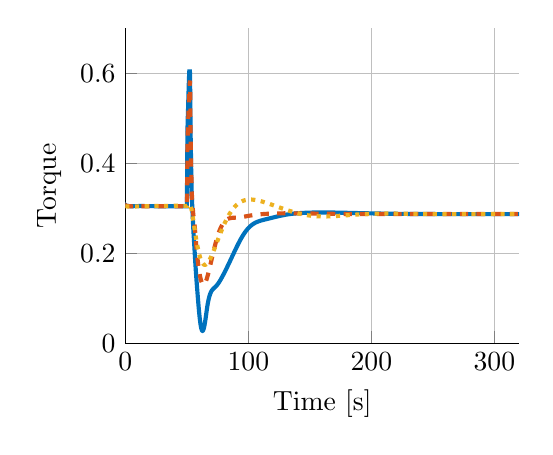
\begin{tikzpicture}

\begin{axis}[%
width=5cm,
height=4cm,
at={(0\linewidth,0\linewidth)},
scale only axis,
xmin=0,
xmax=320,
xlabel={Time [s]},
xmajorgrids,
ymin=0,
ymax=0.7,
ylabel={Torque},
ymajorgrids,
axis background/.style={fill=white},
% title style={font=\bfseries},
% title={Normalized Torque Setting},
axis x line*=bottom,
axis y line*=left
]
\addplot [color=mycolor1,solid,line width=1.5pt,forget plot]
  table[row sep=crcr]{%
0	0.304831074\\
0.25	0.30665978\\
0.5	0.30590085\\
0.75	0.30562405\\
1	0.30565309\\
1.25	0.30547614\\
1.5	0.30528095\\
1.75	0.30515676\\
2	0.30504243\\
2.25	0.304928319\\
2.5	0.304830357\\
2.75	0.30474751\\
3	0.304675987\\
3.25	0.304616093\\
3.5	0.304567996\\
3.75	0.304530753\\
4	0.304503022\\
4.25	0.304483048\\
4.5	0.304468969\\
4.75	0.304459287\\
5	0.304453134\\
5.25	0.304450003\\
5.5	0.304449628\\
5.75	0.304452033\\
6	0.304457403\\
6.25	0.304465922\\
6.5	0.304477601\\
6.75	0.304492142\\
7	0.304508918\\
7.25	0.304527087\\
7.5	0.304545747\\
7.75	0.30456407\\
8	0.304581427\\
8.25	0.304597482\\
8.5	0.304612217\\
8.75	0.30462589\\
9	0.304638928\\
9.25	0.304651779\\
9.5	0.304664765\\
9.75	0.304677988\\
10	0.304691287\\
10.25	0.304704276\\
10.5	0.304716429\\
10.75	0.304727207\\
11	0.304736188\\
11.25	0.30474316\\
11.5	0.304748177\\
11.75	0.304751534\\
12	0.304753694\\
12.25	0.304755174\\
12.5	0.304756414\\
12.75	0.304757681\\
13	0.30475901\\
13.25	0.30476021\\
13.5	0.304760922\\
13.75	0.30476073\\
14	0.304759267\\
14.25	0.304756327\\
14.5	0.304751915\\
14.75	0.30474626\\
15	0.304739763\\
15.25	0.304732898\\
15.5	0.304726109\\
15.75	0.304719702\\
16	0.304713781\\
16.25	0.304708235\\
16.5	0.304702777\\
16.75	0.304697029\\
17	0.30469063\\
17.25	0.304683333\\
17.5	0.304675073\\
17.75	0.304665996\\
18	0.304656418\\
18.25	0.304646755\\
18.5	0.304637419\\
18.75	0.304628722\\
19	0.304620796\\
19.25	0.304613572\\
19.5	0.304606803\\
19.75	0.304600131\\
20	0.304593187\\
20.25	0.304585688\\
20.5	0.304577512\\
20.75	0.304568734\\
21	0.304559605\\
21.25	0.304550493\\
21.5	0.304541785\\
21.75	0.304533794\\
22	0.304526677\\
22.25	0.304520397\\
22.5	0.304514737\\
22.75	0.304509357\\
23	0.304503883\\
23.25	0.304498007\\
23.5	0.304491565\\
23.75	0.30448458\\
24	0.30447726\\
24.25	0.30446994\\
24.5	0.304462995\\
24.75	0.304456747\\
25	0.304451375\\
25.25	0.304446874\\
25.5	0.304443053\\
25.75	0.304439586\\
26	0.304436097\\
26.25	0.304432258\\
26.5	0.304427872\\
26.75	0.304422928\\
27	0.304417601\\
27.25	0.304412209\\
27.5	0.304407124\\
27.75	0.304402683\\
28	0.304399091\\
28.25	0.30439637\\
28.5	0.30439435\\
28.75	0.304392716\\
29	0.304391086\\
29.25	0.304389111\\
29.5	0.304386568\\
29.75	0.304383418\\
30	0.304379815\\
30.25	0.304376067\\
30.5	0.304372557\\
30.75	0.304369637\\
31	0.30436754\\
31.25	0.304366312\\
31.5	0.304365801\\
31.75	0.304365694\\
32	0.304365598\\
32.25	0.304365143\\
32.5	0.304364077\\
32.75	0.304362337\\
33	0.304360064\\
33.25	0.304357567\\
33.5	0.304355243\\
33.75	0.304353469\\
34	0.304352507\\
34.25	0.304352425\\
34.5	0.304353082\\
34.75	0.30435416\\
35	0.304355248\\
35.25	0.304355947\\
35.5	0.304355978\\
35.75	0.304355255\\
36	0.304353912\\
36.25	0.304352267\\
36.5	0.30435074\\
36.75	0.304349742\\
37	0.304349564\\
37.25	0.304350296\\
37.5	0.304351802\\
37.75	0.304353751\\
38	0.304355704\\
38.25	0.304357226\\
38.5	0.304358006\\
38.75	0.304357939\\
39	0.304357157\\
39.25	0.304355997\\
39.5	0.304354913\\
39.75	0.304354356\\
40	0.304354653\\
40.25	0.304355914\\
40.5	0.304358003\\
40.75	0.304360563\\
41	0.304363117\\
41.25	0.304365186\\
41.5	0.30436642\\
41.75	0.304366697\\
42	0.304366153\\
42.25	0.304365156\\
42.5	0.304364208\\
42.75	0.304363811\\
43	0.304364333\\
43.25	0.304365904\\
43.5	0.304368376\\
43.75	0.30437136\\
44	0.304374322\\
44.25	0.304376726\\
44.5	0.30437818\\
44.75	0.304378543\\
45	0.304377967\\
45.25	0.304376863\\
45.5	0.304375798\\
45.75	0.304375339\\
46	0.304375903\\
46.25	0.304377638\\
46.5	0.304380377\\
46.75	0.304383675\\
47	0.304386927\\
47.25	0.304389525\\
47.5	0.304391024\\
47.75	0.304391267\\
48	0.304390434\\
48.25	0.304389\\
48.5	0.304387617\\
48.75	0.304386935\\
49	0.304387429\\
49.25	0.30438926\\
49.5	0.304392228\\
49.75	0.304395814\\
50	0.304399313\\
50.25	0.3726148\\
50.5	0.472673\\
50.75	0.500789\\
51	0.520824\\
51.25	0.544824\\
51.5	0.568657\\
51.75	0.588946\\
52	0.604\\
52.25	0.604\\
52.5	0.604\\
52.75	0.557336\\
53	0.474781\\
53.25	0.433629\\
53.5	0.3906805\\
53.75	0.3545439\\
54	0.330705\\
54.25	0.31342796\\
54.5	0.29890661\\
54.75	0.2832353\\
55	0.2678304\\
55.25	0.2541441\\
55.5	0.2419374\\
55.75	0.2305571\\
56	0.2195289\\
56.25	0.207966\\
56.5	0.196075\\
56.75	0.184581\\
57	0.173632\\
57.25	0.163105\\
57.5	0.153024\\
57.75	0.143495\\
58	0.134445\\
58.25	0.125621\\
58.5	0.116863\\
58.75	0.108186\\
59	0.099649\\
59.25	0.091303\\
59.5	0.083216\\
59.75	0.075468\\
60	0.068134\\
60.25	0.061278\\
60.5	0.054953\\
60.75	0.04921\\
61	0.044088\\
61.25	0.03962\\
61.5	0.035826\\
61.75	0.032722\\
62	0.030319\\
62.25	0.028618\\
62.5	0.027615\\
62.75	0.027302\\
63	0.027661\\
63.25	0.028668\\
63.5	0.030292\\
63.75	0.032495\\
64	0.03523\\
64.25	0.038446\\
64.5	0.042088\\
64.75	0.046101\\
65	0.05043\\
65.25	0.055024\\
65.5	0.059828\\
65.75	0.064776\\
66	0.069773\\
66.25	0.074692\\
66.5	0.079392\\
66.75	0.083771\\
67	0.087791\\
67.25	0.091463\\
67.5	0.094815\\
67.75	0.097879\\
68	0.100681\\
68.25	0.103241\\
68.5	0.105574\\
68.75	0.107693\\
69	0.109612\\
69.25	0.111343\\
69.5	0.1129\\
69.75	0.114296\\
70	0.115547\\
70.25	0.116669\\
70.5	0.117678\\
70.75	0.118589\\
71	0.119418\\
71.25	0.120181\\
71.5	0.120893\\
71.75	0.121566\\
72	0.122213\\
72.25	0.122845\\
72.5	0.123472\\
72.75	0.124104\\
73	0.124748\\
73.25	0.125409\\
73.5	0.126093\\
73.75	0.126805\\
74	0.127547\\
74.25	0.128322\\
74.5	0.129131\\
74.75	0.129975\\
75	0.130854\\
75.25	0.131768\\
75.5	0.132715\\
75.75	0.133696\\
76	0.134709\\
76.25	0.135752\\
76.5	0.136823\\
76.75	0.137922\\
77	0.139046\\
77.25	0.140193\\
77.5	0.141363\\
77.75	0.142553\\
78	0.143762\\
78.25	0.144988\\
78.5	0.146231\\
78.75	0.147488\\
79	0.14876\\
79.25	0.150044\\
79.5	0.151341\\
79.75	0.152648\\
80	0.153966\\
80.25	0.155295\\
80.5	0.156632\\
80.75	0.157978\\
81	0.159333\\
81.25	0.160695\\
81.5	0.162065\\
81.75	0.163443\\
82	0.164827\\
82.25	0.166219\\
82.5	0.167616\\
82.75	0.16902\\
83	0.17043\\
83.25	0.171846\\
83.5	0.173267\\
83.75	0.174694\\
84	0.176125\\
84.25	0.177561\\
84.5	0.179001\\
84.75	0.180445\\
85	0.181892\\
85.25	0.183343\\
85.5	0.184796\\
85.75	0.186252\\
86	0.187709\\
86.25	0.189168\\
86.5	0.190628\\
86.75	0.192089\\
87	0.193549\\
87.25	0.195009\\
87.5	0.196468\\
87.75	0.197925\\
88	0.19938\\
88.25	0.200832\\
88.5	0.20228\\
88.75	0.203725\\
89	0.2051655\\
89.25	0.2066006\\
89.5	0.20803\\
89.75	0.2094529\\
90	0.2108689\\
90.25	0.2122773\\
90.5	0.2136774\\
90.75	0.2150687\\
91	0.2164505\\
91.25	0.2178222\\
91.5	0.2191833\\
91.75	0.220533\\
92	0.2218709\\
92.25	0.2231964\\
92.5	0.2245088\\
92.75	0.2258076\\
93	0.2270923\\
93.25	0.2283623\\
93.5	0.229617\\
93.75	0.2308561\\
94	0.232079\\
94.25	0.2332852\\
94.5	0.2344743\\
94.75	0.2356458\\
95	0.2367994\\
95.25	0.2379346\\
95.5	0.239051\\
95.75	0.2401485\\
96	0.2412265\\
96.25	0.2422849\\
96.5	0.2433234\\
96.75	0.2443417\\
97	0.2453396\\
97.25	0.246317\\
97.5	0.2472736\\
97.75	0.2482094\\
98	0.2491243\\
98.25	0.2500181\\
98.5	0.2508909\\
98.75	0.2517427\\
99	0.2525734\\
99.25	0.253383\\
99.5	0.2541718\\
99.75	0.2549397\\
100	0.2556869\\
100.25	0.2564135\\
100.5	0.2571197\\
100.75	0.2578057\\
101	0.2584718\\
101.25	0.2591181\\
101.5	0.2597449\\
101.75	0.2603526\\
102	0.2609415\\
102.25	0.2615118\\
102.5	0.2620639\\
102.75	0.2625982\\
103	0.2631151\\
103.25	0.2636149\\
103.5	0.2640981\\
103.75	0.2645651\\
104	0.2650163\\
104.25	0.2654522\\
104.5	0.2658731\\
104.75	0.2662797\\
105	0.2666722\\
105.25	0.2670513\\
105.5	0.2674173\\
105.75	0.2677708\\
106	0.2681122\\
106.25	0.268442\\
106.5	0.2687607\\
106.75	0.2690687\\
107	0.2693666\\
107.25	0.2696547\\
107.5	0.2699336\\
107.75	0.2702038\\
108	0.2704655\\
108.25	0.2707194\\
108.5	0.2709658\\
108.75	0.2712052\\
109	0.271438\\
109.25	0.2716646\\
109.5	0.2718853\\
109.75	0.2721007\\
110	0.2723109\\
110.25	0.2725165\\
110.5	0.2727177\\
110.75	0.2729149\\
111	0.2731085\\
111.25	0.2732986\\
111.5	0.2734857\\
111.75	0.2736699\\
112	0.2738516\\
112.25	0.2740311\\
112.5	0.2742085\\
112.75	0.274384\\
113	0.274558\\
113.25	0.2747306\\
113.5	0.2749019\\
113.75	0.2750723\\
114	0.2752417\\
114.25	0.2754104\\
114.5	0.2755785\\
114.75	0.2757461\\
115	0.2759133\\
115.25	0.2760803\\
115.5	0.2762471\\
115.75	0.2764138\\
116	0.2765804\\
116.25	0.2767471\\
116.5	0.2769138\\
116.75	0.2770806\\
117	0.2772476\\
117.25	0.2774147\\
117.5	0.277582\\
117.75	0.2777494\\
118	0.277917\\
118.25	0.2780848\\
118.5	0.2782527\\
118.75	0.2784207\\
119	0.2785889\\
119.25	0.2787571\\
119.5	0.2789253\\
119.75	0.2790935\\
120	0.2792617\\
120.25	0.2794298\\
120.5	0.2795977\\
120.75	0.2797655\\
121	0.2799329\\
121.25	0.2801001\\
121.5	0.2802669\\
121.75	0.2804333\\
122	0.2805992\\
122.25	0.2807645\\
122.5	0.2809292\\
122.75	0.2810933\\
123	0.2812566\\
123.25	0.2814191\\
123.5	0.2815808\\
123.75	0.2817416\\
124	0.2819013\\
124.25	0.2820601\\
124.5	0.2822177\\
124.75	0.2823742\\
125	0.2825295\\
125.25	0.2826835\\
125.5	0.2828362\\
125.75	0.2829876\\
126	0.2831376\\
126.25	0.2832861\\
126.5	0.2834331\\
126.75	0.2835786\\
127	0.2837225\\
127.25	0.2838648\\
127.5	0.2840054\\
127.75	0.2841444\\
128	0.2842816\\
128.25	0.2844171\\
128.5	0.2845509\\
128.75	0.2846829\\
129	0.284813\\
129.25	0.2849414\\
129.5	0.2850679\\
129.75	0.2851925\\
130	0.2853153\\
130.25	0.2854361\\
130.5	0.2855551\\
130.75	0.2856722\\
131	0.2857874\\
131.25	0.2859007\\
131.5	0.2860121\\
131.75	0.2861216\\
132	0.2862292\\
132.25	0.2863349\\
132.5	0.2864387\\
132.75	0.2865407\\
133	0.2866407\\
133.25	0.286739\\
133.5	0.2868353\\
133.75	0.2869298\\
134	0.2870225\\
134.25	0.2871134\\
134.5	0.2872026\\
134.75	0.2872899\\
135	0.2873755\\
135.25	0.2874594\\
135.5	0.2875415\\
135.75	0.287622\\
136	0.2877008\\
136.25	0.2877779\\
136.5	0.2878534\\
136.75	0.2879273\\
137	0.2879996\\
137.25	0.2880704\\
137.5	0.2881397\\
137.75	0.2882074\\
138	0.2882737\\
138.25	0.2883385\\
138.5	0.2884018\\
138.75	0.2884638\\
139	0.2885244\\
139.25	0.2885836\\
139.5	0.2886415\\
139.75	0.2886981\\
140	0.2887534\\
140.25	0.2888074\\
140.5	0.2888602\\
140.75	0.2889118\\
141	0.2889622\\
141.25	0.2890114\\
141.5	0.2890595\\
141.75	0.2891065\\
142	0.2891523\\
142.25	0.2891971\\
142.5	0.2892409\\
142.75	0.2892836\\
143	0.2893253\\
143.25	0.289366\\
143.5	0.2894057\\
143.75	0.2894445\\
144	0.2894823\\
144.25	0.2895192\\
144.5	0.2895553\\
144.75	0.2895904\\
145	0.2896247\\
145.25	0.2896581\\
145.5	0.2896907\\
145.75	0.2897225\\
146	0.2897535\\
146.25	0.2897837\\
146.5	0.2898132\\
146.75	0.2898419\\
147	0.2898698\\
147.25	0.289897\\
147.5	0.2899235\\
147.75	0.2899493\\
148	0.2899744\\
148.25	0.2899988\\
148.5	0.2900225\\
148.75	0.2900456\\
149	0.2900681\\
149.25	0.2900899\\
149.5	0.290111\\
149.75	0.2901316\\
150	0.2901515\\
150.25	0.2901708\\
150.5	0.2901896\\
150.75	0.2902077\\
151	0.2902253\\
151.25	0.2902423\\
151.5	0.2902588\\
151.75	0.2902747\\
152	0.29029\\
152.25	0.2903048\\
152.5	0.2903191\\
152.75	0.2903328\\
153	0.2903461\\
153.25	0.2903588\\
153.5	0.290371\\
153.75	0.2903826\\
154	0.2903938\\
154.25	0.2904045\\
154.5	0.2904148\\
154.75	0.2904245\\
155	0.2904338\\
155.25	0.2904425\\
155.5	0.2904509\\
155.75	0.2904587\\
156	0.2904661\\
156.25	0.2904731\\
156.5	0.2904796\\
156.75	0.2904857\\
157	0.2904913\\
157.25	0.2904965\\
157.5	0.2905012\\
157.75	0.2905056\\
158	0.2905095\\
158.25	0.290513\\
158.5	0.2905161\\
158.75	0.2905188\\
159	0.2905211\\
159.25	0.290523\\
159.5	0.2905245\\
159.75	0.2905257\\
160	0.2905264\\
160.25	0.2905268\\
160.5	0.2905268\\
160.75	0.2905264\\
161	0.2905256\\
161.25	0.2905245\\
161.5	0.2905231\\
161.75	0.2905213\\
162	0.2905191\\
162.25	0.2905166\\
162.5	0.2905138\\
162.75	0.2905106\\
163	0.2905071\\
163.25	0.2905033\\
163.5	0.2904992\\
163.75	0.2904947\\
164	0.29049\\
164.25	0.2904849\\
164.5	0.2904796\\
164.75	0.2904739\\
165	0.2904679\\
165.25	0.2904617\\
165.5	0.2904552\\
165.75	0.2904484\\
166	0.2904413\\
166.25	0.290434\\
166.5	0.2904264\\
166.75	0.2904185\\
167	0.2904104\\
167.25	0.290402\\
167.5	0.2903934\\
167.75	0.2903846\\
168	0.2903755\\
168.25	0.2903662\\
168.5	0.2903566\\
168.75	0.2903469\\
169	0.2903369\\
169.25	0.2903267\\
169.5	0.2903162\\
169.75	0.2903056\\
170	0.2902948\\
170.25	0.2902838\\
170.5	0.2902726\\
170.75	0.2902612\\
171	0.2902496\\
171.25	0.2902378\\
171.5	0.2902259\\
171.75	0.2902138\\
172	0.2902015\\
172.25	0.290189\\
172.5	0.2901764\\
172.75	0.2901637\\
173	0.2901508\\
173.25	0.2901377\\
173.5	0.2901245\\
173.75	0.2901112\\
174	0.2900977\\
174.25	0.2900841\\
174.5	0.2900703\\
174.75	0.2900564\\
175	0.2900424\\
175.25	0.2900283\\
175.5	0.2900141\\
175.75	0.2899998\\
176	0.2899853\\
176.25	0.2899708\\
176.5	0.2899561\\
176.75	0.2899414\\
177	0.2899265\\
177.25	0.2899116\\
177.5	0.2898965\\
177.75	0.2898814\\
178	0.2898662\\
178.25	0.2898509\\
178.5	0.2898356\\
178.75	0.2898202\\
179	0.2898047\\
179.25	0.2897891\\
179.5	0.2897735\\
179.75	0.2897578\\
180	0.289742\\
180.25	0.2897262\\
180.5	0.2897103\\
180.75	0.2896944\\
181	0.2896785\\
181.25	0.2896625\\
181.5	0.2896464\\
181.75	0.2896303\\
182	0.2896142\\
182.25	0.289598\\
182.5	0.2895818\\
182.75	0.2895655\\
183	0.2895493\\
183.25	0.289533\\
183.5	0.2895167\\
183.75	0.2895003\\
184	0.2894839\\
184.25	0.2894676\\
184.5	0.2894511\\
184.75	0.2894347\\
185	0.2894183\\
185.25	0.2894019\\
185.5	0.2893854\\
185.75	0.289369\\
186	0.2893525\\
186.25	0.289336\\
186.5	0.2893196\\
186.75	0.2893031\\
187	0.2892866\\
187.25	0.2892702\\
187.5	0.2892537\\
187.75	0.2892373\\
188	0.2892208\\
188.25	0.2892044\\
188.5	0.289188\\
188.75	0.2891716\\
189	0.2891552\\
189.25	0.2891388\\
189.5	0.2891225\\
189.75	0.2891061\\
190	0.2890898\\
190.25	0.2890735\\
190.5	0.2890573\\
190.75	0.289041\\
191	0.2890248\\
191.25	0.2890086\\
191.5	0.2889925\\
191.75	0.2889764\\
192	0.2889603\\
192.25	0.2889442\\
192.5	0.2889282\\
192.75	0.2889122\\
193	0.2888962\\
193.25	0.2888803\\
193.5	0.2888644\\
193.75	0.2888486\\
194	0.2888328\\
194.25	0.2888171\\
194.5	0.2888014\\
194.75	0.2887857\\
195	0.2887701\\
195.25	0.2887545\\
195.5	0.288739\\
195.75	0.2887235\\
196	0.2887081\\
196.25	0.2886927\\
196.5	0.2886774\\
196.75	0.2886621\\
197	0.2886469\\
197.25	0.2886317\\
197.5	0.2886166\\
197.75	0.2886016\\
198	0.2885866\\
198.25	0.2885716\\
198.5	0.2885568\\
198.75	0.2885419\\
199	0.2885272\\
199.25	0.2885125\\
199.5	0.2884978\\
199.75	0.2884832\\
200	0.2884687\\
200.25	0.2884543\\
200.5	0.2884399\\
200.75	0.2884255\\
201	0.2884113\\
201.25	0.2883971\\
201.5	0.2883829\\
201.75	0.2883689\\
202	0.2883549\\
202.25	0.2883409\\
202.5	0.2883271\\
202.75	0.2883133\\
203	0.2882995\\
203.25	0.2882859\\
203.5	0.2882723\\
203.75	0.2882588\\
204	0.2882453\\
204.25	0.288232\\
204.5	0.2882186\\
204.75	0.2882054\\
205	0.2881922\\
205.25	0.2881792\\
205.5	0.2881661\\
205.75	0.2881532\\
206	0.2881403\\
206.25	0.2881275\\
206.5	0.2881148\\
206.75	0.2881022\\
207	0.2880896\\
207.25	0.2880771\\
207.5	0.2880647\\
207.75	0.2880523\\
208	0.28804\\
208.25	0.2880278\\
208.5	0.2880157\\
208.75	0.2880037\\
209	0.2879917\\
209.25	0.2879798\\
209.5	0.287968\\
209.75	0.2879562\\
210	0.2879446\\
210.25	0.287933\\
210.5	0.2879215\\
210.75	0.28791\\
211	0.2878987\\
211.25	0.2878874\\
211.5	0.2878762\\
211.75	0.2878651\\
212	0.287854\\
212.25	0.287843\\
212.5	0.2878321\\
212.75	0.2878213\\
213	0.2878106\\
213.25	0.2877999\\
213.5	0.2877893\\
213.75	0.2877788\\
214	0.2877684\\
214.25	0.287758\\
214.5	0.2877478\\
214.75	0.2877376\\
215	0.2877274\\
215.25	0.2877174\\
215.5	0.2877074\\
215.75	0.2876975\\
216	0.2876877\\
216.25	0.287678\\
216.5	0.2876683\\
216.75	0.2876587\\
217	0.2876492\\
217.25	0.2876398\\
217.5	0.2876304\\
217.75	0.2876211\\
218	0.2876119\\
218.25	0.2876028\\
218.5	0.2875937\\
218.75	0.2875848\\
219	0.2875759\\
219.25	0.287567\\
219.5	0.2875583\\
219.75	0.2875496\\
220	0.287541\\
220.25	0.2875324\\
220.5	0.287524\\
220.75	0.2875156\\
221	0.2875073\\
221.25	0.287499\\
221.5	0.2874909\\
221.75	0.2874828\\
222	0.2874747\\
222.25	0.2874668\\
222.5	0.2874589\\
222.75	0.2874511\\
223	0.2874434\\
223.25	0.2874357\\
223.5	0.2874281\\
223.75	0.2874206\\
224	0.2874131\\
224.25	0.2874057\\
224.5	0.2873984\\
224.75	0.2873912\\
225	0.287384\\
225.25	0.2873769\\
225.5	0.2873699\\
225.75	0.2873629\\
226	0.287356\\
226.25	0.2873491\\
226.5	0.2873424\\
226.75	0.2873357\\
227	0.287329\\
227.25	0.2873225\\
227.5	0.287316\\
227.75	0.2873095\\
228	0.2873032\\
228.25	0.2872969\\
228.5	0.2872906\\
228.75	0.2872844\\
229	0.2872783\\
229.25	0.2872723\\
229.5	0.2872663\\
229.75	0.2872604\\
230	0.2872545\\
230.25	0.2872487\\
230.5	0.287243\\
230.75	0.2872373\\
231	0.2872317\\
231.25	0.2872261\\
231.5	0.2872207\\
231.75	0.2872152\\
232	0.2872099\\
232.25	0.2872045\\
232.5	0.2871993\\
232.75	0.2871941\\
233	0.287189\\
233.25	0.2871839\\
233.5	0.2871789\\
233.75	0.2871739\\
234	0.287169\\
234.25	0.2871642\\
234.5	0.2871594\\
234.75	0.2871546\\
235	0.28715\\
235.25	0.2871453\\
235.5	0.2871408\\
235.75	0.2871363\\
236	0.2871318\\
236.25	0.2871274\\
236.5	0.287123\\
236.75	0.2871187\\
237	0.2871145\\
237.25	0.2871103\\
237.5	0.2871062\\
237.75	0.2871021\\
238	0.287098\\
238.25	0.2870941\\
238.5	0.2870901\\
238.75	0.2870862\\
239	0.2870824\\
239.25	0.2870786\\
239.5	0.2870749\\
239.75	0.2870712\\
240	0.2870675\\
240.25	0.2870639\\
240.5	0.2870604\\
240.75	0.2870569\\
241	0.2870534\\
241.25	0.28705\\
241.5	0.2870467\\
241.75	0.2870434\\
242	0.2870401\\
242.25	0.2870369\\
242.5	0.2870337\\
242.75	0.2870306\\
243	0.2870275\\
243.25	0.2870244\\
243.5	0.2870214\\
243.75	0.2870185\\
244	0.2870155\\
244.25	0.2870127\\
244.5	0.2870098\\
244.75	0.287007\\
245	0.2870043\\
245.25	0.2870016\\
245.5	0.2869989\\
245.75	0.2869963\\
246	0.2869937\\
246.25	0.2869911\\
246.5	0.2869886\\
246.75	0.2869861\\
247	0.2869837\\
247.25	0.2869813\\
247.5	0.2869789\\
247.75	0.2869766\\
248	0.2869743\\
248.25	0.2869721\\
248.5	0.2869699\\
248.75	0.2869677\\
249	0.2869656\\
249.25	0.2869635\\
249.5	0.2869614\\
249.75	0.2869593\\
250	0.2869573\\
250.25	0.2869554\\
250.5	0.2869534\\
250.75	0.2869515\\
251	0.2869497\\
251.25	0.2869478\\
251.5	0.286946\\
251.75	0.2869443\\
252	0.2869425\\
252.25	0.2869408\\
252.5	0.2869391\\
252.75	0.2869375\\
253	0.2869359\\
253.25	0.2869343\\
253.5	0.2869327\\
253.75	0.2869312\\
254	0.2869297\\
254.25	0.2869282\\
254.5	0.2869268\\
254.75	0.2869254\\
255	0.286924\\
255.25	0.2869227\\
255.5	0.2869213\\
255.75	0.28692\\
256	0.2869188\\
256.25	0.2869175\\
256.5	0.2869163\\
256.75	0.2869151\\
257	0.2869139\\
257.25	0.2869128\\
257.5	0.2869117\\
257.75	0.2869106\\
258	0.2869095\\
258.25	0.2869084\\
258.5	0.2869074\\
258.75	0.2869064\\
259	0.2869054\\
259.25	0.2869045\\
259.5	0.2869036\\
259.75	0.2869027\\
260	0.2869018\\
260.25	0.2869009\\
260.5	0.2869001\\
260.75	0.2868993\\
261	0.2868985\\
261.25	0.2868977\\
261.5	0.2868969\\
261.75	0.2868962\\
262	0.2868955\\
262.25	0.2868948\\
262.5	0.2868941\\
262.75	0.2868935\\
263	0.2868928\\
263.25	0.2868922\\
263.5	0.2868916\\
263.75	0.286891\\
264	0.2868905\\
264.25	0.2868899\\
264.5	0.2868894\\
264.75	0.2868889\\
265	0.2868884\\
265.25	0.2868879\\
265.5	0.2868875\\
265.75	0.286887\\
266	0.2868866\\
266.25	0.2868862\\
266.5	0.2868858\\
266.75	0.2868854\\
267	0.2868851\\
267.25	0.2868847\\
267.5	0.2868844\\
267.75	0.2868841\\
268	0.2868838\\
268.25	0.2868835\\
268.5	0.2868832\\
268.75	0.286883\\
269	0.2868827\\
269.25	0.2868825\\
269.5	0.2868823\\
269.75	0.2868821\\
270	0.2868819\\
270.25	0.2868817\\
270.5	0.2868816\\
270.75	0.2868814\\
271	0.2868813\\
271.25	0.2868812\\
271.5	0.2868811\\
271.75	0.286881\\
272	0.2868809\\
272.25	0.2868808\\
272.5	0.2868807\\
272.75	0.2868807\\
273	0.2868806\\
273.25	0.2868806\\
273.5	0.2868806\\
273.75	0.2868805\\
274	0.2868805\\
274.25	0.2868806\\
274.5	0.2868806\\
274.75	0.2868806\\
275	0.2868806\\
275.25	0.2868807\\
275.5	0.2868807\\
275.75	0.2868808\\
276	0.2868809\\
276.25	0.286881\\
276.5	0.2868811\\
276.75	0.2868812\\
277	0.2868813\\
277.25	0.2868814\\
277.5	0.2868815\\
277.75	0.2868816\\
278	0.2868818\\
278.25	0.2868819\\
278.5	0.2868821\\
278.75	0.2868822\\
279	0.2868824\\
279.25	0.2868826\\
279.5	0.2868828\\
279.75	0.286883\\
280	0.2868832\\
280.25	0.2868834\\
280.5	0.2868836\\
280.75	0.2868838\\
281	0.286884\\
281.25	0.2868842\\
281.5	0.2868845\\
281.75	0.2868847\\
282	0.2868849\\
282.25	0.2868852\\
282.5	0.2868855\\
282.75	0.2868857\\
283	0.286886\\
283.25	0.2868863\\
283.5	0.2868865\\
283.75	0.2868868\\
284	0.2868871\\
284.25	0.2868874\\
284.5	0.2868877\\
284.75	0.286888\\
285	0.2868883\\
285.25	0.2868886\\
285.5	0.2868889\\
285.75	0.2868892\\
286	0.2868895\\
286.25	0.2868899\\
286.5	0.2868902\\
286.75	0.2868905\\
287	0.2868909\\
287.25	0.2868912\\
287.5	0.2868915\\
287.75	0.2868919\\
288	0.2868922\\
288.25	0.2868926\\
288.5	0.2868929\\
288.75	0.2868933\\
289	0.2868936\\
289.25	0.286894\\
289.5	0.2868944\\
289.75	0.2868947\\
290	0.2868951\\
290.25	0.2868955\\
290.5	0.2868958\\
290.75	0.2868962\\
291	0.2868966\\
291.25	0.286897\\
291.5	0.2868974\\
291.75	0.2868977\\
292	0.2868981\\
292.25	0.2868985\\
292.5	0.2868989\\
292.75	0.2868993\\
293	0.2868997\\
293.25	0.2869001\\
293.5	0.2869005\\
293.75	0.2869009\\
294	0.2869013\\
294.25	0.2869017\\
294.5	0.286902\\
294.75	0.2869024\\
295	0.2869028\\
295.25	0.2869032\\
295.5	0.2869037\\
295.75	0.2869041\\
296	0.2869045\\
296.25	0.2869049\\
296.5	0.2869053\\
296.75	0.2869057\\
297	0.2869061\\
297.25	0.2869065\\
297.5	0.2869069\\
297.75	0.2869073\\
298	0.2869077\\
298.25	0.2869081\\
298.5	0.2869085\\
298.75	0.2869089\\
299	0.2869093\\
299.25	0.2869097\\
299.5	0.2869101\\
299.75	0.2869105\\
300	0.286911\\
300.25	0.2869114\\
300.5	0.2869118\\
300.75	0.2869122\\
301	0.2869126\\
301.25	0.286913\\
301.5	0.2869134\\
301.75	0.2869138\\
302	0.2869142\\
302.25	0.2869146\\
302.5	0.286915\\
302.75	0.2869154\\
303	0.2869158\\
303.25	0.2869162\\
303.5	0.2869166\\
303.75	0.286917\\
304	0.2869174\\
304.25	0.2869178\\
304.5	0.2869182\\
304.75	0.2869186\\
305	0.286919\\
305.25	0.2869194\\
305.5	0.2869198\\
305.75	0.2869202\\
306	0.2869206\\
306.25	0.286921\\
306.5	0.2869214\\
306.75	0.2869217\\
307	0.2869221\\
307.25	0.2869225\\
307.5	0.2869229\\
307.75	0.2869233\\
308	0.2869237\\
308.25	0.286924\\
308.5	0.2869244\\
308.75	0.2869248\\
309	0.2869252\\
309.25	0.2869256\\
309.5	0.2869259\\
309.75	0.2869263\\
310	0.2869267\\
310.25	0.286927\\
310.5	0.2869274\\
310.75	0.2869278\\
311	0.2869281\\
311.25	0.2869285\\
311.5	0.2869289\\
311.75	0.2869292\\
312	0.2869296\\
312.25	0.28693\\
312.5	0.2869303\\
312.75	0.2869307\\
313	0.286931\\
313.25	0.2869314\\
313.5	0.2869317\\
313.75	0.2869321\\
314	0.2869324\\
314.25	0.2869328\\
314.5	0.2869331\\
314.75	0.2869334\\
315	0.2869338\\
315.25	0.2869341\\
315.5	0.2869345\\
315.75	0.2869348\\
316	0.2869351\\
316.25	0.2869355\\
316.5	0.2869358\\
316.75	0.2869361\\
317	0.2869364\\
317.25	0.2869368\\
317.5	0.2869371\\
317.75	0.2869374\\
318	0.2869377\\
318.25	0.286938\\
318.5	0.2869383\\
318.75	0.2869387\\
319	0.286939\\
319.25	0.2869393\\
319.5	0.2869396\\
319.75	0.2869399\\
320	0.2869402\\
320.25	0.2869405\\
320.5	0.2869408\\
320.75	0.2869411\\
321	0.2869414\\
321.25	0.2869417\\
321.5	0.286942\\
321.75	0.2869423\\
322	0.2869426\\
322.25	0.2869428\\
322.5	0.2869431\\
322.75	0.2869434\\
323	0.2869437\\
323.25	0.286944\\
323.5	0.2869442\\
323.75	0.2869445\\
324	0.2869448\\
324.25	0.2869451\\
324.5	0.2869453\\
324.75	0.2869456\\
325	0.2869459\\
325.25	0.2869461\\
325.5	0.2869464\\
325.75	0.2869466\\
326	0.2869469\\
326.25	0.2869472\\
326.5	0.2869474\\
326.75	0.2869477\\
327	0.2869479\\
327.25	0.2869482\\
327.5	0.2869484\\
327.75	0.2869486\\
328	0.2869489\\
328.25	0.2869491\\
328.5	0.2869494\\
328.75	0.2869496\\
329	0.2869498\\
329.25	0.2869501\\
329.5	0.2869503\\
329.75	0.2869505\\
330	0.2869508\\
330.25	0.286951\\
330.5	0.2869512\\
330.75	0.2869514\\
331	0.2869516\\
331.25	0.2869519\\
331.5	0.2869521\\
331.75	0.2869523\\
332	0.2869525\\
332.25	0.2869527\\
332.5	0.2869529\\
332.75	0.2869531\\
333	0.2869533\\
333.25	0.2869535\\
333.5	0.2869537\\
333.75	0.2869539\\
334	0.2869541\\
334.25	0.2869543\\
334.5	0.2869545\\
334.75	0.2869547\\
335	0.2869549\\
335.25	0.2869551\\
335.5	0.2869553\\
335.75	0.2869555\\
336	0.2869557\\
336.25	0.2869558\\
336.5	0.286956\\
336.75	0.2869562\\
337	0.2869564\\
337.25	0.2869565\\
337.5	0.2869567\\
337.75	0.2869569\\
338	0.2869571\\
338.25	0.2869572\\
338.5	0.2869574\\
338.75	0.2869576\\
339	0.2869577\\
339.25	0.2869579\\
339.5	0.286958\\
339.75	0.2869582\\
340	0.2869584\\
340.25	0.2869585\\
340.5	0.2869587\\
340.75	0.2869588\\
341	0.286959\\
341.25	0.2869591\\
341.5	0.2869593\\
341.75	0.2869594\\
342	0.2869596\\
342.25	0.2869597\\
342.5	0.2869598\\
342.75	0.28696\\
343	0.2869601\\
343.25	0.2869603\\
343.5	0.2869604\\
343.75	0.2869605\\
344	0.2869607\\
344.25	0.2869608\\
344.5	0.2869609\\
344.75	0.286961\\
345	0.2869612\\
345.25	0.2869613\\
345.5	0.2869614\\
345.75	0.2869615\\
346	0.2869617\\
346.25	0.2869618\\
346.5	0.2869619\\
346.75	0.286962\\
347	0.2869621\\
347.25	0.2869622\\
347.5	0.2869624\\
347.75	0.2869625\\
348	0.2869626\\
348.25	0.2869627\\
348.5	0.2869628\\
348.75	0.2869629\\
349	0.286963\\
349.25	0.2869631\\
349.5	0.2869632\\
349.75	0.2869633\\
350	0.2869634\\
350.25	0.2869635\\
350.5	0.2869636\\
350.75	0.2869637\\
351	0.2869638\\
351.25	0.2869639\\
351.5	0.286964\\
351.75	0.2869641\\
352	0.2869642\\
352.25	0.2869642\\
352.5	0.2869643\\
352.75	0.2869644\\
353	0.2869645\\
353.25	0.2869646\\
353.5	0.2869647\\
353.75	0.2869648\\
354	0.2869648\\
354.25	0.2869649\\
354.5	0.286965\\
354.75	0.2869651\\
355	0.2869651\\
355.25	0.2869652\\
355.5	0.2869653\\
355.75	0.2869654\\
356	0.2869654\\
356.25	0.2869655\\
356.5	0.2869656\\
356.75	0.2869656\\
357	0.2869657\\
357.25	0.2869658\\
357.5	0.2869658\\
357.75	0.2869659\\
358	0.286966\\
358.25	0.286966\\
358.5	0.2869661\\
358.75	0.2869662\\
359	0.2869662\\
359.25	0.2869663\\
359.5	0.2869663\\
359.75	0.2869664\\
360	0.2869665\\
360.25	0.2869665\\
360.5	0.2869666\\
360.75	0.2869666\\
361	0.2869667\\
361.25	0.2869667\\
361.5	0.2869668\\
361.75	0.2869668\\
362	0.2869669\\
362.25	0.2869669\\
362.5	0.286967\\
362.75	0.286967\\
363	0.2869671\\
363.25	0.2869671\\
363.5	0.2869672\\
363.75	0.2869672\\
364	0.2869672\\
364.25	0.2869673\\
364.5	0.2869673\\
364.75	0.2869674\\
365	0.2869674\\
365.25	0.2869674\\
365.5	0.2869675\\
365.75	0.2869675\\
366	0.2869676\\
366.25	0.2869676\\
366.5	0.2869676\\
366.75	0.2869677\\
367	0.2869677\\
367.25	0.2869677\\
367.5	0.2869678\\
367.75	0.2869678\\
368	0.2869678\\
368.25	0.2869679\\
368.5	0.2869679\\
368.75	0.2869679\\
369	0.2869679\\
369.25	0.286968\\
369.5	0.286968\\
369.75	0.286968\\
370	0.2869681\\
370.25	0.2869681\\
370.5	0.2869681\\
370.75	0.2869681\\
371	0.2869682\\
371.25	0.2869682\\
371.5	0.2869682\\
371.75	0.2869682\\
372	0.2869683\\
372.25	0.2869683\\
372.5	0.2869683\\
372.75	0.2869683\\
373	0.2869683\\
373.25	0.2869684\\
373.5	0.2869684\\
373.75	0.2869684\\
374	0.2869684\\
374.25	0.2869684\\
374.5	0.2869684\\
374.75	0.2869685\\
375	0.2869685\\
375.25	0.2869685\\
375.5	0.2869685\\
375.75	0.2869685\\
376	0.2869685\\
376.25	0.2869685\\
376.5	0.2869686\\
376.75	0.2869686\\
377	0.2869686\\
377.25	0.2869686\\
377.5	0.2869686\\
377.75	0.2869686\\
378	0.2869686\\
378.25	0.2869686\\
378.5	0.2869687\\
378.75	0.2869687\\
379	0.2869687\\
379.25	0.2869687\\
379.5	0.2869687\\
379.75	0.2869687\\
380	0.2869687\\
380.25	0.2869687\\
380.5	0.2869687\\
380.75	0.2869687\\
381	0.2869687\\
381.25	0.2869687\\
381.5	0.2869687\\
381.75	0.2869687\\
382	0.2869687\\
382.25	0.2869688\\
382.5	0.2869688\\
382.75	0.2869688\\
383	0.2869688\\
383.25	0.2869688\\
383.5	0.2869688\\
383.75	0.2869688\\
384	0.2869688\\
384.25	0.2869688\\
384.5	0.2869688\\
384.75	0.2869688\\
385	0.2869688\\
385.25	0.2869688\\
385.5	0.2869688\\
385.75	0.2869688\\
386	0.2869688\\
386.25	0.2869688\\
386.5	0.2869688\\
386.75	0.2869688\\
387	0.2869688\\
387.25	0.2869688\\
387.5	0.2869688\\
387.75	0.2869688\\
388	0.2869688\\
388.25	0.2869688\\
388.5	0.2869688\\
388.75	0.2869688\\
389	0.2869688\\
389.25	0.2869688\\
389.5	0.2869688\\
389.75	0.2869688\\
390	0.2869688\\
390.25	0.2869688\\
390.5	0.2869688\\
390.75	0.2869687\\
391	0.2869687\\
391.25	0.2869687\\
391.5	0.2869687\\
391.75	0.2869687\\
392	0.2869687\\
392.25	0.2869687\\
392.5	0.2869687\\
392.75	0.2869687\\
393	0.2869687\\
393.25	0.2869687\\
393.5	0.2869687\\
393.75	0.2869687\\
394	0.2869687\\
394.25	0.2869687\\
394.5	0.2869687\\
394.75	0.2869687\\
395	0.2869687\\
395.25	0.2869687\\
395.5	0.2869686\\
395.75	0.2869686\\
396	0.2869686\\
396.25	0.2869686\\
396.5	0.2869686\\
396.75	0.2869686\\
397	0.2869686\\
397.25	0.2869686\\
397.5	0.2869686\\
397.75	0.2869686\\
398	0.2869686\\
398.25	0.2869686\\
398.5	0.2869686\\
398.75	0.2869685\\
399	0.2869685\\
399.25	0.2869685\\
399.5	0.2869685\\
399.75	0.2869685\\
400	0.2869685\\
400.25	0.2869685\\
400.5	0.2869685\\
400.75	0.2869685\\
401	0.2869685\\
401.25	0.2869685\\
401.5	0.2869685\\
401.75	0.2869684\\
402	0.2869684\\
402.25	0.2869684\\
402.5	0.2869684\\
402.75	0.2869684\\
403	0.2869684\\
403.25	0.2869684\\
403.5	0.2869684\\
403.75	0.2869684\\
404	0.2869684\\
404.25	0.2869684\\
404.5	0.2869683\\
404.75	0.2869683\\
405	0.2869683\\
405.25	0.2869683\\
405.5	0.2869683\\
405.75	0.2869683\\
406	0.2869683\\
406.25	0.2869683\\
406.5	0.2869683\\
406.75	0.2869683\\
407	0.2869683\\
407.25	0.2869682\\
407.5	0.2869682\\
407.75	0.2869682\\
408	0.2869682\\
408.25	0.2869682\\
408.5	0.2869682\\
408.75	0.2869682\\
409	0.2869682\\
409.25	0.2869682\\
409.5	0.2869682\\
409.75	0.2869681\\
410	0.2869681\\
410.25	0.2869681\\
410.5	0.2869681\\
410.75	0.2869681\\
411	0.2869681\\
411.25	0.2869681\\
411.5	0.2869681\\
411.75	0.2869681\\
412	0.2869681\\
412.25	0.286968\\
412.5	0.286968\\
412.75	0.286968\\
413	0.286968\\
413.25	0.286968\\
413.5	0.286968\\
413.75	0.286968\\
414	0.286968\\
414.25	0.286968\\
414.5	0.286968\\
414.75	0.2869679\\
415	0.2869679\\
415.25	0.2869679\\
415.5	0.2869679\\
415.75	0.2869679\\
416	0.2869679\\
416.25	0.2869679\\
416.5	0.2869679\\
416.75	0.2869679\\
417	0.2869679\\
417.25	0.2869678\\
417.5	0.2869678\\
417.75	0.2869678\\
418	0.2869678\\
418.25	0.2869678\\
418.5	0.2869678\\
418.75	0.2869678\\
419	0.2869678\\
419.25	0.2869678\\
419.5	0.2869678\\
419.75	0.2869678\\
420	0.2869677\\
420.25	0.2869677\\
420.5	0.2869677\\
420.75	0.2869677\\
421	0.2869677\\
421.25	0.2869677\\
421.5	0.2869677\\
421.75	0.2869677\\
422	0.2869677\\
422.25	0.2869677\\
422.5	0.2869676\\
422.75	0.2869676\\
423	0.2869676\\
423.25	0.2869676\\
423.5	0.2869676\\
423.75	0.2869676\\
424	0.2869676\\
424.25	0.2869676\\
424.5	0.2869676\\
424.75	0.2869676\\
425	0.2869676\\
425.25	0.2869676\\
425.5	0.2869675\\
425.75	0.2869675\\
426	0.2869675\\
426.25	0.2869675\\
426.5	0.2869675\\
426.75	0.2869675\\
427	0.2869675\\
427.25	0.2869675\\
427.5	0.2869675\\
427.75	0.2869675\\
428	0.2869675\\
428.25	0.2869675\\
428.5	0.2869674\\
428.75	0.2869674\\
429	0.2869674\\
429.25	0.2869674\\
429.5	0.2869674\\
429.75	0.2869674\\
430	0.2869674\\
430.25	0.2869674\\
430.5	0.2869674\\
430.75	0.2869674\\
431	0.2869674\\
431.25	0.2869674\\
431.5	0.2869674\\
431.75	0.2869673\\
432	0.2869673\\
432.25	0.2869673\\
432.5	0.2869673\\
432.75	0.2869673\\
433	0.2869673\\
433.25	0.2869673\\
433.5	0.2869673\\
433.75	0.2869673\\
434	0.2869673\\
434.25	0.2869673\\
434.5	0.2869673\\
434.75	0.2869673\\
435	0.2869672\\
435.25	0.2869672\\
435.5	0.2869672\\
435.75	0.2869672\\
436	0.2869672\\
436.25	0.2869672\\
436.5	0.2869672\\
436.75	0.2869672\\
437	0.2869672\\
437.25	0.2869672\\
437.5	0.2869672\\
437.75	0.2869672\\
438	0.2869672\\
438.25	0.2869672\\
438.5	0.2869672\\
438.75	0.2869672\\
439	0.2869671\\
439.25	0.2869671\\
439.5	0.2869671\\
439.75	0.2869671\\
440	0.2869671\\
440.25	0.2869671\\
440.5	0.2869671\\
440.75	0.2869671\\
441	0.2869671\\
441.25	0.2869671\\
441.5	0.2869671\\
441.75	0.2869671\\
442	0.2869671\\
442.25	0.2869671\\
442.5	0.2869671\\
442.75	0.2869671\\
443	0.2869671\\
443.25	0.286967\\
443.5	0.286967\\
443.75	0.286967\\
444	0.286967\\
444.25	0.286967\\
444.5	0.286967\\
444.75	0.286967\\
445	0.286967\\
445.25	0.286967\\
445.5	0.286967\\
445.75	0.286967\\
446	0.286967\\
446.25	0.286967\\
446.5	0.286967\\
446.75	0.286967\\
447	0.286967\\
447.25	0.286967\\
447.5	0.286967\\
447.75	0.286967\\
448	0.286967\\
448.25	0.286967\\
448.5	0.2869669\\
448.75	0.2869669\\
449	0.2869669\\
449.25	0.2869669\\
449.5	0.2869669\\
449.75	0.2869669\\
450	0.2869669\\
450.25	0.2869669\\
450.5	0.2869669\\
450.75	0.2869669\\
451	0.2869669\\
451.25	0.2869669\\
451.5	0.2869669\\
451.75	0.2869669\\
452	0.2869669\\
452.25	0.2869669\\
452.5	0.2869669\\
452.75	0.2869669\\
453	0.2869669\\
453.25	0.2869669\\
453.5	0.2869669\\
453.75	0.2869669\\
454	0.2869669\\
454.25	0.2869669\\
454.5	0.2869669\\
454.75	0.2869668\\
455	0.2869668\\
455.25	0.2869668\\
455.5	0.2869668\\
455.75	0.2869668\\
456	0.2869668\\
456.25	0.2869668\\
456.5	0.2869668\\
456.75	0.2869668\\
457	0.2869668\\
457.25	0.2869668\\
457.5	0.2869668\\
457.75	0.2869668\\
458	0.2869668\\
458.25	0.2869668\\
458.5	0.2869668\\
458.75	0.2869668\\
459	0.2869668\\
459.25	0.2869668\\
459.5	0.2869668\\
459.75	0.2869668\\
460	0.2869668\\
460.25	0.2869668\\
460.5	0.2869668\\
460.75	0.2869668\\
461	0.2869668\\
461.25	0.2869668\\
461.5	0.2869668\\
461.75	0.2869668\\
462	0.2869668\\
462.25	0.2869668\\
462.5	0.2869668\\
462.75	0.2869668\\
463	0.2869668\\
463.25	0.2869668\\
463.5	0.2869667\\
463.75	0.2869667\\
464	0.2869667\\
464.25	0.2869667\\
464.5	0.2869667\\
464.75	0.2869667\\
465	0.2869667\\
465.25	0.2869667\\
465.5	0.2869667\\
465.75	0.2869667\\
466	0.2869667\\
466.25	0.2869667\\
466.5	0.2869667\\
466.75	0.2869667\\
467	0.2869667\\
467.25	0.2869667\\
467.5	0.2869667\\
467.75	0.2869667\\
468	0.2869667\\
468.25	0.2869667\\
468.5	0.2869667\\
468.75	0.2869667\\
469	0.2869667\\
469.25	0.2869667\\
469.5	0.2869667\\
469.75	0.2869667\\
470	0.2869667\\
470.25	0.2869667\\
470.5	0.2869667\\
470.75	0.2869667\\
471	0.2869667\\
471.25	0.2869667\\
471.5	0.2869667\\
471.75	0.2869667\\
472	0.2869667\\
472.25	0.2869667\\
472.5	0.2869667\\
472.75	0.2869667\\
473	0.2869667\\
473.25	0.2869667\\
473.5	0.2869667\\
473.75	0.2869667\\
474	0.2869667\\
474.25	0.2869667\\
474.5	0.2869667\\
474.75	0.2869667\\
475	0.2869667\\
475.25	0.2869667\\
475.5	0.2869667\\
475.75	0.2869667\\
476	0.2869667\\
476.25	0.2869667\\
476.5	0.2869667\\
476.75	0.2869667\\
477	0.2869667\\
477.25	0.2869667\\
477.5	0.2869667\\
477.75	0.2869667\\
478	0.2869667\\
478.25	0.2869667\\
478.5	0.2869667\\
478.75	0.2869667\\
479	0.2869667\\
479.25	0.2869667\\
479.5	0.2869667\\
479.75	0.2869667\\
480	0.2869667\\
480.25	0.2869667\\
480.5	0.2869667\\
480.75	0.2869667\\
481	0.2869667\\
481.25	0.2869667\\
481.5	0.2869666\\
481.75	0.2869666\\
482	0.2869666\\
482.25	0.2869666\\
482.5	0.2869666\\
482.75	0.2869666\\
483	0.2869666\\
483.25	0.2869666\\
483.5	0.2869666\\
483.75	0.2869666\\
484	0.2869666\\
484.25	0.2869666\\
484.5	0.2869666\\
484.75	0.2869666\\
485	0.2869666\\
485.25	0.2869666\\
485.5	0.2869666\\
485.75	0.2869666\\
486	0.2869666\\
486.25	0.2869666\\
486.5	0.2869666\\
486.75	0.2869666\\
487	0.2869666\\
487.25	0.2869666\\
487.5	0.2869666\\
487.75	0.2869666\\
488	0.2869666\\
488.25	0.2869666\\
488.5	0.2869666\\
488.75	0.2869666\\
489	0.2869666\\
489.25	0.2869666\\
489.5	0.2869666\\
489.75	0.2869666\\
490	0.2869666\\
490.25	0.2869666\\
490.5	0.2869666\\
490.75	0.2869666\\
491	0.2869666\\
491.25	0.2869666\\
491.5	0.2869666\\
491.75	0.2869666\\
492	0.2869666\\
492.25	0.2869666\\
492.5	0.2869666\\
492.75	0.2869666\\
493	0.2869666\\
493.25	0.2869666\\
493.5	0.2869666\\
493.75	0.2869666\\
494	0.2869666\\
494.25	0.2869666\\
494.5	0.2869666\\
494.75	0.2869666\\
495	0.2869666\\
495.25	0.2869666\\
495.5	0.2869666\\
495.75	0.2869666\\
496	0.2869666\\
496.25	0.2869666\\
496.5	0.2869666\\
496.75	0.2869666\\
497	0.2869666\\
497.25	0.2869666\\
497.5	0.2869666\\
497.75	0.2869666\\
498	0.2869666\\
498.25	0.2869666\\
498.5	0.2869666\\
498.75	0.2869666\\
499	0.2869666\\
499.25	0.2869666\\
499.5	0.2869666\\
499.75	0.2869666\\
};
\addplot [color=mycolor2,dashed,line width=1.5pt,forget plot]
  table[row sep=crcr]{%
0	0.304687593\\
0.25	0.3062373\\
0.5	0.30565243\\
0.75	0.30542342\\
1	0.30544153\\
1.25	0.30529422\\
1.5	0.30512552\\
1.75	0.30501036\\
2	0.304902022\\
2.25	0.304791964\\
2.5	0.304692745\\
2.75	0.304603912\\
3	0.304522477\\
3.25	0.304448977\\
3.5	0.304383864\\
3.75	0.304326758\\
4	0.304277359\\
4.25	0.304235224\\
4.5	0.30419961\\
4.75	0.304169719\\
5	0.304144828\\
5.25	0.304124285\\
5.5	0.304107522\\
5.75	0.3040940819\\
6	0.3040836227\\
6.25	0.304075904\\
6.5	0.3040707616\\
6.75	0.3040680573\\
7	0.3040676314\\
7.25	0.3040692788\\
7.5	0.304072743\\
7.75	0.3040777231\\
8	0.3040838906\\
8.25	0.304090914\\
8.5	0.3040984844\\
8.75	0.304106339\\
9	0.304114276\\
9.25	0.30412216\\
9.5	0.304129912\\
9.75	0.304137498\\
10	0.30414491\\
10.25	0.304152144\\
10.5	0.304159186\\
10.75	0.304166004\\
11	0.304172546\\
11.25	0.304178739\\
11.5	0.304184508\\
11.75	0.304189776\\
12	0.304194486\\
12.25	0.304198602\\
12.5	0.304202113\\
12.75	0.304205039\\
13	0.304207416\\
13.25	0.304209297\\
13.5	0.304210736\\
13.75	0.304211785\\
14	0.304212483\\
14.25	0.30421286\\
14.5	0.304212931\\
14.75	0.304212702\\
15	0.304212175\\
15.25	0.304211355\\
15.5	0.304210252\\
15.75	0.304208883\\
16	0.304207277\\
16.25	0.30420547\\
16.5	0.304203505\\
16.75	0.304201424\\
17	0.304199268\\
17.25	0.30419707\\
17.5	0.304194859\\
17.75	0.304192652\\
18	0.30419046\\
18.25	0.304188292\\
18.5	0.304186151\\
18.75	0.304184042\\
19	0.304181973\\
19.25	0.304179955\\
19.5	0.304178001\\
19.75	0.304176128\\
20	0.304174352\\
20.25	0.304172689\\
20.5	0.304171152\\
20.75	0.30416975\\
21	0.304168488\\
21.25	0.304167365\\
21.5	0.304166379\\
21.75	0.304165525\\
22	0.304164798\\
22.25	0.304164195\\
22.5	0.304163711\\
22.75	0.304163346\\
23	0.3041631\\
23.25	0.304162973\\
23.5	0.304162965\\
23.75	0.304163078\\
24	0.304163308\\
24.25	0.304163652\\
24.5	0.304164104\\
24.75	0.304164658\\
25	0.304165305\\
25.25	0.304166037\\
25.5	0.304166846\\
25.75	0.304167725\\
26	0.304168667\\
26.25	0.304169669\\
26.5	0.304170725\\
26.75	0.304171831\\
27	0.304172984\\
27.25	0.30417418\\
27.5	0.304175414\\
27.75	0.30417668\\
28	0.304177972\\
28.25	0.304179284\\
28.5	0.304180609\\
28.75	0.304181941\\
29	0.304183275\\
29.25	0.304184606\\
29.5	0.30418593\\
29.75	0.304187242\\
30	0.304188541\\
30.25	0.304189824\\
30.5	0.304191087\\
30.75	0.304192329\\
31	0.304193546\\
31.25	0.304194736\\
31.5	0.304195895\\
31.75	0.30419702\\
32	0.304198108\\
32.25	0.304199158\\
32.5	0.304200165\\
32.75	0.304201131\\
33	0.304202052\\
33.25	0.304202929\\
33.5	0.30420376\\
33.75	0.304204547\\
34	0.304205287\\
34.25	0.304205982\\
34.5	0.304206631\\
34.75	0.304207233\\
35	0.304207788\\
35.25	0.304208296\\
35.5	0.304208757\\
35.75	0.304209171\\
36	0.304209538\\
36.25	0.30420986\\
36.5	0.304210137\\
36.75	0.304210371\\
37	0.304210563\\
37.25	0.304210713\\
37.5	0.304210824\\
37.75	0.304210897\\
38	0.304210932\\
38.25	0.304210931\\
38.5	0.304210895\\
38.75	0.304210825\\
39	0.304210724\\
39.25	0.304210591\\
39.5	0.304210429\\
39.75	0.30421024\\
40	0.304210024\\
40.25	0.304209785\\
40.5	0.304209523\\
40.75	0.304209241\\
41	0.30420894\\
41.25	0.304208621\\
41.5	0.304208286\\
41.75	0.304207937\\
42	0.304207575\\
42.25	0.304207201\\
42.5	0.304206817\\
42.75	0.304206425\\
43	0.304206026\\
43.25	0.304205621\\
43.5	0.304205213\\
43.75	0.304204801\\
44	0.304204388\\
44.25	0.304203976\\
44.5	0.304203564\\
44.75	0.304203155\\
45	0.304202749\\
45.25	0.304202347\\
45.5	0.304201951\\
45.75	0.304201561\\
46	0.304201178\\
46.25	0.304200803\\
46.5	0.304200437\\
46.75	0.304200081\\
47	0.304199735\\
47.25	0.3041994\\
47.5	0.304199077\\
47.75	0.304198765\\
48	0.304198467\\
48.25	0.304198181\\
48.5	0.304197909\\
48.75	0.304197651\\
49	0.304197406\\
49.25	0.304197175\\
49.5	0.304196959\\
49.75	0.304196757\\
50	0.30419657\\
50.25	0.3315923\\
50.5	0.442329\\
50.75	0.467639\\
51	0.486145\\
51.25	0.505401\\
51.5	0.524044\\
51.75	0.540478\\
52	0.55623\\
52.25	0.571358\\
52.5	0.583669\\
52.75	0.552624\\
53	0.465144\\
53.25	0.427686\\
53.5	0.396192\\
53.75	0.3656229\\
54	0.3376383\\
54.25	0.320846\\
54.5	0.31150891\\
54.75	0.30256908\\
55	0.2938633\\
55.25	0.2860087\\
55.5	0.2798536\\
55.75	0.2746134\\
56	0.2700006\\
56.25	0.2644855\\
56.5	0.2571502\\
56.75	0.2484343\\
57	0.2393262\\
57.25	0.2303733\\
57.5	0.2217007\\
57.75	0.2134395\\
58	0.2057298\\
58.25	0.198608\\
58.5	0.191981\\
58.75	0.185733\\
59	0.179826\\
59.25	0.174285\\
59.5	0.169135\\
59.75	0.164366\\
60	0.159959\\
60.25	0.155892\\
60.5	0.152144\\
60.75	0.148694\\
61	0.145528\\
61.25	0.142641\\
61.5	0.140035\\
61.75	0.137717\\
62	0.135693\\
62.25	0.133972\\
62.5	0.132559\\
62.75	0.131456\\
63	0.130663\\
63.25	0.130176\\
63.5	0.129988\\
63.75	0.130087\\
64	0.130461\\
64.25	0.131097\\
64.5	0.131977\\
64.75	0.133085\\
65	0.134406\\
65.25	0.135923\\
65.5	0.137619\\
65.75	0.139479\\
66	0.141487\\
66.25	0.143631\\
66.5	0.145895\\
66.75	0.148267\\
67	0.150737\\
67.25	0.153291\\
67.5	0.15592\\
67.75	0.158614\\
68	0.161365\\
68.25	0.164163\\
68.5	0.167001\\
68.75	0.169872\\
69	0.172769\\
69.25	0.175685\\
69.5	0.178615\\
69.75	0.181553\\
70	0.184493\\
70.25	0.187432\\
70.5	0.190363\\
70.75	0.193283\\
71	0.196187\\
71.25	0.199071\\
71.5	0.201932\\
71.75	0.2047645\\
72	0.2075665\\
72.25	0.210334\\
72.5	0.213064\\
72.75	0.2157533\\
73	0.218399\\
73.25	0.2209985\\
73.5	0.2235491\\
73.75	0.2260485\\
74	0.2284944\\
74.25	0.2308847\\
74.5	0.2332175\\
74.75	0.2354912\\
75	0.2377041\\
75.25	0.2398549\\
75.5	0.2419424\\
75.75	0.2439656\\
76	0.2459237\\
76.25	0.2478159\\
76.5	0.2496418\\
76.75	0.251401\\
77	0.2530935\\
77.25	0.2547192\\
77.5	0.2562783\\
77.75	0.2577711\\
78	0.2591981\\
78.25	0.2605599\\
78.5	0.2618573\\
78.75	0.2630912\\
79	0.2642625\\
79.25	0.2653725\\
79.5	0.2664224\\
79.75	0.2674136\\
80	0.2683474\\
80.25	0.2692255\\
80.5	0.2700495\\
80.75	0.270821\\
81	0.2715418\\
81.25	0.2722137\\
81.5	0.2728386\\
81.75	0.2734184\\
82	0.273955\\
82.25	0.2744503\\
82.5	0.2749065\\
82.75	0.2753253\\
83	0.2757088\\
83.25	0.276059\\
83.5	0.2763778\\
83.75	0.2766672\\
84	0.2769291\\
84.25	0.2771654\\
84.5	0.2773779\\
84.75	0.2775684\\
85	0.2777386\\
85.25	0.2778904\\
85.5	0.2780253\\
85.75	0.278145\\
86	0.2782509\\
86.25	0.2783446\\
86.5	0.2784274\\
86.75	0.2785007\\
87	0.2785657\\
87.25	0.2786238\\
87.5	0.2786759\\
87.75	0.2787231\\
88	0.2787665\\
88.25	0.278807\\
88.5	0.2788454\\
88.75	0.2788825\\
89	0.278919\\
89.25	0.2789556\\
89.5	0.2789929\\
89.75	0.2790314\\
90	0.2790716\\
90.25	0.2791138\\
90.5	0.2791586\\
90.75	0.2792061\\
91	0.2792566\\
91.25	0.2793104\\
91.5	0.2793676\\
91.75	0.2794284\\
92	0.2794928\\
92.25	0.2795609\\
92.5	0.2796328\\
92.75	0.2797083\\
93	0.2797876\\
93.25	0.2798704\\
93.5	0.2799568\\
93.75	0.2800467\\
94	0.2801399\\
94.25	0.2802362\\
94.5	0.2803356\\
94.75	0.2804378\\
95	0.2805428\\
95.25	0.2806503\\
95.5	0.2807601\\
95.75	0.280872\\
96	0.2809859\\
96.25	0.2811016\\
96.5	0.2812188\\
96.75	0.2813373\\
97	0.2814571\\
97.25	0.2815778\\
97.5	0.2816993\\
97.75	0.2818215\\
98	0.281944\\
98.25	0.2820669\\
98.5	0.2821898\\
98.75	0.2823127\\
99	0.2824354\\
99.25	0.2825577\\
99.5	0.2826796\\
99.75	0.2828008\\
100	0.2829213\\
100.25	0.2830409\\
100.5	0.2831596\\
100.75	0.2832772\\
101	0.2833936\\
101.25	0.2835089\\
101.5	0.2836228\\
101.75	0.2837354\\
102	0.2838465\\
102.25	0.2839561\\
102.5	0.2840642\\
102.75	0.2841708\\
103	0.2842757\\
103.25	0.2843789\\
103.5	0.2844805\\
103.75	0.2845804\\
104	0.2846786\\
104.25	0.2847751\\
104.5	0.2848698\\
104.75	0.2849628\\
105	0.2850541\\
105.25	0.2851437\\
105.5	0.2852316\\
105.75	0.2853177\\
106	0.2854022\\
106.25	0.2854849\\
106.5	0.2855661\\
106.75	0.2856455\\
107	0.2857234\\
107.25	0.2857996\\
107.5	0.2858743\\
107.75	0.2859474\\
108	0.286019\\
108.25	0.2860891\\
108.5	0.2861577\\
108.75	0.2862248\\
109	0.2862906\\
109.25	0.2863549\\
109.5	0.2864178\\
109.75	0.2864795\\
110	0.2865398\\
110.25	0.2865988\\
110.5	0.2866565\\
110.75	0.286713\\
111	0.2867683\\
111.25	0.2868224\\
111.5	0.2868753\\
111.75	0.2869271\\
112	0.2869777\\
112.25	0.2870273\\
112.5	0.2870758\\
112.75	0.2871233\\
113	0.2871697\\
113.25	0.2872151\\
113.5	0.2872595\\
113.75	0.2873029\\
114	0.2873454\\
114.25	0.287387\\
114.5	0.2874276\\
114.75	0.2874674\\
115	0.2875062\\
115.25	0.2875442\\
115.5	0.2875813\\
115.75	0.2876176\\
116	0.2876531\\
116.25	0.2876877\\
116.5	0.2877216\\
116.75	0.2877547\\
117	0.2877869\\
117.25	0.2878185\\
117.5	0.2878493\\
117.75	0.2878793\\
118	0.2879086\\
118.25	0.2879372\\
118.5	0.2879651\\
118.75	0.2879923\\
119	0.2880188\\
119.25	0.2880446\\
119.5	0.2880698\\
119.75	0.2880943\\
120	0.2881181\\
120.25	0.2881413\\
120.5	0.2881639\\
120.75	0.2881859\\
121	0.2882072\\
121.25	0.2882279\\
121.5	0.288248\\
121.75	0.2882676\\
122	0.2882865\\
122.25	0.2883049\\
122.5	0.2883226\\
122.75	0.2883399\\
123	0.2883565\\
123.25	0.2883727\\
123.5	0.2883882\\
123.75	0.2884033\\
124	0.2884178\\
124.25	0.2884318\\
124.5	0.2884453\\
124.75	0.2884583\\
125	0.2884708\\
125.25	0.2884828\\
125.5	0.2884943\\
125.75	0.2885053\\
126	0.2885159\\
126.25	0.2885259\\
126.5	0.2885356\\
126.75	0.2885448\\
127	0.2885535\\
127.25	0.2885618\\
127.5	0.2885697\\
127.75	0.2885771\\
128	0.2885841\\
128.25	0.2885907\\
128.5	0.288597\\
128.75	0.2886028\\
129	0.2886082\\
129.25	0.2886132\\
129.5	0.2886178\\
129.75	0.2886221\\
130	0.288626\\
130.25	0.2886295\\
130.5	0.2886327\\
130.75	0.2886356\\
131	0.288638\\
131.25	0.2886402\\
131.5	0.288642\\
131.75	0.2886435\\
132	0.2886447\\
132.25	0.2886455\\
132.5	0.2886461\\
132.75	0.2886463\\
133	0.2886462\\
133.25	0.2886459\\
133.5	0.2886453\\
133.75	0.2886443\\
134	0.2886431\\
134.25	0.2886417\\
134.5	0.2886399\\
134.75	0.2886379\\
135	0.2886357\\
135.25	0.2886332\\
135.5	0.2886304\\
135.75	0.2886275\\
136	0.2886242\\
136.25	0.2886208\\
136.5	0.2886171\\
136.75	0.2886132\\
137	0.2886091\\
137.25	0.2886048\\
137.5	0.2886003\\
137.75	0.2885955\\
138	0.2885906\\
138.25	0.2885855\\
138.5	0.2885802\\
138.75	0.2885747\\
139	0.2885691\\
139.25	0.2885632\\
139.5	0.2885572\\
139.75	0.288551\\
140	0.2885447\\
140.25	0.2885382\\
140.5	0.2885316\\
140.75	0.2885248\\
141	0.2885178\\
141.25	0.2885108\\
141.5	0.2885035\\
141.75	0.2884962\\
142	0.2884887\\
142.25	0.2884811\\
142.5	0.2884734\\
142.75	0.2884655\\
143	0.2884576\\
143.25	0.2884495\\
143.5	0.2884414\\
143.75	0.2884331\\
144	0.2884247\\
144.25	0.2884162\\
144.5	0.2884077\\
144.75	0.288399\\
145	0.2883903\\
145.25	0.2883814\\
145.5	0.2883725\\
145.75	0.2883636\\
146	0.2883545\\
146.25	0.2883454\\
146.5	0.2883362\\
146.75	0.2883269\\
147	0.2883176\\
147.25	0.2883082\\
147.5	0.2882988\\
147.75	0.2882893\\
148	0.2882798\\
148.25	0.2882702\\
148.5	0.2882606\\
148.75	0.2882509\\
149	0.2882412\\
149.25	0.2882315\\
149.5	0.2882217\\
149.75	0.2882119\\
150	0.288202\\
150.25	0.2881922\\
150.5	0.2881823\\
150.75	0.2881724\\
151	0.2881624\\
151.25	0.2881525\\
151.5	0.2881425\\
151.75	0.2881326\\
152	0.2881226\\
152.25	0.2881126\\
152.5	0.2881026\\
152.75	0.2880926\\
153	0.2880826\\
153.25	0.2880725\\
153.5	0.2880625\\
153.75	0.2880525\\
154	0.2880425\\
154.25	0.2880325\\
154.5	0.2880226\\
154.75	0.2880126\\
155	0.2880026\\
155.25	0.2879927\\
155.5	0.2879827\\
155.75	0.2879728\\
156	0.2879629\\
156.25	0.287953\\
156.5	0.2879432\\
156.75	0.2879333\\
157	0.2879235\\
157.25	0.2879137\\
157.5	0.287904\\
157.75	0.2878943\\
158	0.2878846\\
158.25	0.2878749\\
158.5	0.2878652\\
158.75	0.2878556\\
159	0.2878461\\
159.25	0.2878365\\
159.5	0.287827\\
159.75	0.2878176\\
160	0.2878082\\
160.25	0.2877988\\
160.5	0.2877894\\
160.75	0.2877801\\
161	0.2877709\\
161.25	0.2877617\\
161.5	0.2877525\\
161.75	0.2877434\\
162	0.2877343\\
162.25	0.2877253\\
162.5	0.2877163\\
162.75	0.2877074\\
163	0.2876985\\
163.25	0.2876897\\
163.5	0.2876809\\
163.75	0.2876721\\
164	0.2876635\\
164.25	0.2876548\\
164.5	0.2876463\\
164.75	0.2876377\\
165	0.2876293\\
165.25	0.2876209\\
165.5	0.2876125\\
165.75	0.2876042\\
166	0.287596\\
166.25	0.2875878\\
166.5	0.2875796\\
166.75	0.2875716\\
167	0.2875635\\
167.25	0.2875556\\
167.5	0.2875477\\
167.75	0.2875398\\
168	0.2875321\\
168.25	0.2875243\\
168.5	0.2875167\\
168.75	0.2875091\\
169	0.2875015\\
169.25	0.287494\\
169.5	0.2874866\\
169.75	0.2874793\\
170	0.2874719\\
170.25	0.2874647\\
170.5	0.2874575\\
170.75	0.2874504\\
171	0.2874433\\
171.25	0.2874364\\
171.5	0.2874294\\
171.75	0.2874225\\
172	0.2874157\\
172.25	0.287409\\
172.5	0.2874023\\
172.75	0.2873957\\
173	0.2873891\\
173.25	0.2873826\\
173.5	0.2873761\\
173.75	0.2873697\\
174	0.2873634\\
174.25	0.2873572\\
174.5	0.287351\\
174.75	0.2873448\\
175	0.2873387\\
175.25	0.2873327\\
175.5	0.2873268\\
175.75	0.2873209\\
176	0.287315\\
176.25	0.2873093\\
176.5	0.2873035\\
176.75	0.2872979\\
177	0.2872923\\
177.25	0.2872868\\
177.5	0.2872813\\
177.75	0.2872759\\
178	0.2872705\\
178.25	0.2872652\\
178.5	0.28726\\
178.75	0.2872548\\
179	0.2872496\\
179.25	0.2872446\\
179.5	0.2872396\\
179.75	0.2872346\\
180	0.2872297\\
180.25	0.2872249\\
180.5	0.2872201\\
180.75	0.2872154\\
181	0.2872107\\
181.25	0.2872061\\
181.5	0.2872015\\
181.75	0.287197\\
182	0.2871925\\
182.25	0.2871881\\
182.5	0.2871838\\
182.75	0.2871795\\
183	0.2871753\\
183.25	0.2871711\\
183.5	0.287167\\
183.75	0.2871629\\
184	0.2871589\\
184.25	0.2871549\\
184.5	0.287151\\
184.75	0.2871471\\
185	0.2871433\\
185.25	0.2871395\\
185.5	0.2871358\\
185.75	0.2871321\\
186	0.2871285\\
186.25	0.2871249\\
186.5	0.2871214\\
186.75	0.2871179\\
187	0.2871145\\
187.25	0.2871111\\
187.5	0.2871077\\
187.75	0.2871045\\
188	0.2871012\\
188.25	0.287098\\
188.5	0.2870949\\
188.75	0.2870918\\
189	0.2870887\\
189.25	0.2870857\\
189.5	0.2870827\\
189.75	0.2870798\\
190	0.2870769\\
190.25	0.287074\\
190.5	0.2870712\\
190.75	0.2870685\\
191	0.2870658\\
191.25	0.2870631\\
191.5	0.2870605\\
191.75	0.2870579\\
192	0.2870553\\
192.25	0.2870528\\
192.5	0.2870503\\
192.75	0.2870479\\
193	0.2870455\\
193.25	0.2870431\\
193.5	0.2870408\\
193.75	0.2870385\\
194	0.2870363\\
194.25	0.2870341\\
194.5	0.2870319\\
194.75	0.2870297\\
195	0.2870276\\
195.25	0.2870256\\
195.5	0.2870235\\
195.75	0.2870215\\
196	0.2870196\\
196.25	0.2870176\\
196.5	0.2870157\\
196.75	0.2870139\\
197	0.2870121\\
197.25	0.2870103\\
197.5	0.2870085\\
197.75	0.2870068\\
198	0.287005\\
198.25	0.2870034\\
198.5	0.2870017\\
198.75	0.2870001\\
199	0.2869985\\
199.25	0.286997\\
199.5	0.2869955\\
199.75	0.286994\\
200	0.2869925\\
200.25	0.2869911\\
200.5	0.2869896\\
200.75	0.2869883\\
201	0.2869869\\
201.25	0.2869856\\
201.5	0.2869843\\
201.75	0.286983\\
202	0.2869817\\
202.25	0.2869805\\
202.5	0.2869793\\
202.75	0.2869781\\
203	0.286977\\
203.25	0.2869758\\
203.5	0.2869747\\
203.75	0.2869737\\
204	0.2869726\\
204.25	0.2869716\\
204.5	0.2869706\\
204.75	0.2869696\\
205	0.2869686\\
205.25	0.2869676\\
205.5	0.2869667\\
205.75	0.2869658\\
206	0.2869649\\
206.25	0.2869641\\
206.5	0.2869632\\
206.75	0.2869624\\
207	0.2869616\\
207.25	0.2869608\\
207.5	0.2869601\\
207.75	0.2869593\\
208	0.2869586\\
208.25	0.2869579\\
208.5	0.2869572\\
208.75	0.2869565\\
209	0.2869558\\
209.25	0.2869552\\
209.5	0.2869546\\
209.75	0.286954\\
210	0.2869534\\
210.25	0.2869528\\
210.5	0.2869523\\
210.75	0.2869517\\
211	0.2869512\\
211.25	0.2869507\\
211.5	0.2869502\\
211.75	0.2869497\\
212	0.2869492\\
212.25	0.2869488\\
212.5	0.2869483\\
212.75	0.2869479\\
213	0.2869475\\
213.25	0.2869471\\
213.5	0.2869467\\
213.75	0.2869464\\
214	0.286946\\
214.25	0.2869457\\
214.5	0.2869453\\
214.75	0.286945\\
215	0.2869447\\
215.25	0.2869444\\
215.5	0.2869441\\
215.75	0.2869438\\
216	0.2869436\\
216.25	0.2869433\\
216.5	0.2869431\\
216.75	0.2869428\\
217	0.2869426\\
217.25	0.2869424\\
217.5	0.2869422\\
217.75	0.286942\\
218	0.2869418\\
218.25	0.2869416\\
218.5	0.2869415\\
218.75	0.2869413\\
219	0.2869412\\
219.25	0.286941\\
219.5	0.2869409\\
219.75	0.2869408\\
220	0.2869407\\
220.25	0.2869405\\
220.5	0.2869404\\
220.75	0.2869404\\
221	0.2869403\\
221.25	0.2869402\\
221.5	0.2869401\\
221.75	0.2869401\\
222	0.28694\\
222.25	0.28694\\
222.5	0.2869399\\
222.75	0.2869399\\
223	0.2869399\\
223.25	0.2869398\\
223.5	0.2869398\\
223.75	0.2869398\\
224	0.2869398\\
224.25	0.2869398\\
224.5	0.2869398\\
224.75	0.2869398\\
225	0.2869398\\
225.25	0.2869399\\
225.5	0.2869399\\
225.75	0.2869399\\
226	0.28694\\
226.25	0.28694\\
226.5	0.2869401\\
226.75	0.2869401\\
227	0.2869402\\
227.25	0.2869402\\
227.5	0.2869403\\
227.75	0.2869403\\
228	0.2869404\\
228.25	0.2869405\\
228.5	0.2869406\\
228.75	0.2869407\\
229	0.2869407\\
229.25	0.2869408\\
229.5	0.2869409\\
229.75	0.286941\\
230	0.2869411\\
230.25	0.2869412\\
230.5	0.2869413\\
230.75	0.2869414\\
231	0.2869415\\
231.25	0.2869417\\
231.5	0.2869418\\
231.75	0.2869419\\
232	0.286942\\
232.25	0.2869421\\
232.5	0.2869423\\
232.75	0.2869424\\
233	0.2869425\\
233.25	0.2869426\\
233.5	0.2869428\\
233.75	0.2869429\\
234	0.2869431\\
234.25	0.2869432\\
234.5	0.2869433\\
234.75	0.2869435\\
235	0.2869436\\
235.25	0.2869438\\
235.5	0.2869439\\
235.75	0.2869441\\
236	0.2869442\\
236.25	0.2869444\\
236.5	0.2869445\\
236.75	0.2869447\\
237	0.2869448\\
237.25	0.286945\\
237.5	0.2869451\\
237.75	0.2869453\\
238	0.2869454\\
238.25	0.2869456\\
238.5	0.2869458\\
238.75	0.2869459\\
239	0.2869461\\
239.25	0.2869462\\
239.5	0.2869464\\
239.75	0.2869466\\
240	0.2869467\\
240.25	0.2869469\\
240.5	0.2869471\\
240.75	0.2869472\\
241	0.2869474\\
241.25	0.2869476\\
241.5	0.2869477\\
241.75	0.2869479\\
242	0.286948\\
242.25	0.2869482\\
242.5	0.2869484\\
242.75	0.2869485\\
243	0.2869487\\
243.25	0.2869489\\
243.5	0.286949\\
243.75	0.2869492\\
244	0.2869494\\
244.25	0.2869495\\
244.5	0.2869497\\
244.75	0.2869499\\
245	0.28695\\
245.25	0.2869502\\
245.5	0.2869504\\
245.75	0.2869505\\
246	0.2869507\\
246.25	0.2869508\\
246.5	0.286951\\
246.75	0.2869512\\
247	0.2869513\\
247.25	0.2869515\\
247.5	0.2869516\\
247.75	0.2869518\\
248	0.286952\\
248.25	0.2869521\\
248.5	0.2869523\\
248.75	0.2869524\\
249	0.2869526\\
249.25	0.2869527\\
249.5	0.2869529\\
249.75	0.2869531\\
250	0.2869532\\
250.25	0.2869534\\
250.5	0.2869535\\
250.75	0.2869537\\
251	0.2869538\\
251.25	0.286954\\
251.5	0.2869541\\
251.75	0.2869543\\
252	0.2869544\\
252.25	0.2869546\\
252.5	0.2869547\\
252.75	0.2869549\\
253	0.286955\\
253.25	0.2869551\\
253.5	0.2869553\\
253.75	0.2869554\\
254	0.2869556\\
254.25	0.2869557\\
254.5	0.2869558\\
254.75	0.286956\\
255	0.2869561\\
255.25	0.2869563\\
255.5	0.2869564\\
255.75	0.2869565\\
256	0.2869567\\
256.25	0.2869568\\
256.5	0.2869569\\
256.75	0.2869571\\
257	0.2869572\\
257.25	0.2869573\\
257.5	0.2869574\\
257.75	0.2869576\\
258	0.2869577\\
258.25	0.2869578\\
258.5	0.2869579\\
258.75	0.2869581\\
259	0.2869582\\
259.25	0.2869583\\
259.5	0.2869584\\
259.75	0.2869585\\
260	0.2869587\\
260.25	0.2869588\\
260.5	0.2869589\\
260.75	0.286959\\
261	0.2869591\\
261.25	0.2869592\\
261.5	0.2869593\\
261.75	0.2869594\\
262	0.2869596\\
262.25	0.2869597\\
262.5	0.2869598\\
262.75	0.2869599\\
263	0.28696\\
263.25	0.2869601\\
263.5	0.2869602\\
263.75	0.2869603\\
264	0.2869604\\
264.25	0.2869605\\
264.5	0.2869606\\
264.75	0.2869607\\
265	0.2869608\\
265.25	0.2869609\\
265.5	0.286961\\
265.75	0.2869611\\
266	0.2869612\\
266.25	0.2869613\\
266.5	0.2869614\\
266.75	0.2869614\\
267	0.2869615\\
267.25	0.2869616\\
267.5	0.2869617\\
267.75	0.2869618\\
268	0.2869619\\
268.25	0.286962\\
268.5	0.286962\\
268.75	0.2869621\\
269	0.2869622\\
269.25	0.2869623\\
269.5	0.2869624\\
269.75	0.2869625\\
270	0.2869625\\
270.25	0.2869626\\
270.5	0.2869627\\
270.75	0.2869628\\
271	0.2869628\\
271.25	0.2869629\\
271.5	0.286963\\
271.75	0.2869631\\
272	0.2869631\\
272.25	0.2869632\\
272.5	0.2869633\\
272.75	0.2869633\\
273	0.2869634\\
273.25	0.2869635\\
273.5	0.2869635\\
273.75	0.2869636\\
274	0.2869637\\
274.25	0.2869637\\
274.5	0.2869638\\
274.75	0.2869638\\
275	0.2869639\\
275.25	0.286964\\
275.5	0.286964\\
275.75	0.2869641\\
276	0.2869641\\
276.25	0.2869642\\
276.5	0.2869643\\
276.75	0.2869643\\
277	0.2869644\\
277.25	0.2869644\\
277.5	0.2869645\\
277.75	0.2869645\\
278	0.2869646\\
278.25	0.2869646\\
278.5	0.2869647\\
278.75	0.2869647\\
279	0.2869648\\
279.25	0.2869648\\
279.5	0.2869649\\
279.75	0.2869649\\
280	0.286965\\
280.25	0.286965\\
280.5	0.286965\\
280.75	0.2869651\\
281	0.2869651\\
281.25	0.2869652\\
281.5	0.2869652\\
281.75	0.2869653\\
282	0.2869653\\
282.25	0.2869653\\
282.5	0.2869654\\
282.75	0.2869654\\
283	0.2869655\\
283.25	0.2869655\\
283.5	0.2869655\\
283.75	0.2869656\\
284	0.2869656\\
284.25	0.2869656\\
284.5	0.2869657\\
284.75	0.2869657\\
285	0.2869657\\
285.25	0.2869658\\
285.5	0.2869658\\
285.75	0.2869658\\
286	0.2869659\\
286.25	0.2869659\\
286.5	0.2869659\\
286.75	0.286966\\
287	0.286966\\
287.25	0.286966\\
287.5	0.286966\\
287.75	0.2869661\\
288	0.2869661\\
288.25	0.2869661\\
288.5	0.2869661\\
288.75	0.2869662\\
289	0.2869662\\
289.25	0.2869662\\
289.5	0.2869662\\
289.75	0.2869663\\
290	0.2869663\\
290.25	0.2869663\\
290.5	0.2869663\\
290.75	0.2869664\\
291	0.2869664\\
291.25	0.2869664\\
291.5	0.2869664\\
291.75	0.2869664\\
292	0.2869665\\
292.25	0.2869665\\
292.5	0.2869665\\
292.75	0.2869665\\
293	0.2869665\\
293.25	0.2869666\\
293.5	0.2869666\\
293.75	0.2869666\\
294	0.2869666\\
294.25	0.2869666\\
294.5	0.2869666\\
294.75	0.2869667\\
295	0.2869667\\
295.25	0.2869667\\
295.5	0.2869667\\
295.75	0.2869667\\
296	0.2869667\\
296.25	0.2869667\\
296.5	0.2869668\\
296.75	0.2869668\\
297	0.2869668\\
297.25	0.2869668\\
297.5	0.2869668\\
297.75	0.2869668\\
298	0.2869668\\
298.25	0.2869668\\
298.5	0.2869668\\
298.75	0.2869669\\
299	0.2869669\\
299.25	0.2869669\\
299.5	0.2869669\\
299.75	0.2869669\\
300	0.2869669\\
300.25	0.2869669\\
300.5	0.2869669\\
300.75	0.2869669\\
301	0.2869669\\
301.25	0.2869669\\
301.5	0.286967\\
301.75	0.286967\\
302	0.286967\\
302.25	0.286967\\
302.5	0.286967\\
302.75	0.286967\\
303	0.286967\\
303.25	0.286967\\
303.5	0.286967\\
303.75	0.286967\\
304	0.286967\\
304.25	0.286967\\
304.5	0.286967\\
304.75	0.286967\\
305	0.286967\\
305.25	0.286967\\
305.5	0.2869671\\
305.75	0.2869671\\
306	0.2869671\\
306.25	0.2869671\\
306.5	0.2869671\\
306.75	0.2869671\\
307	0.2869671\\
307.25	0.2869671\\
307.5	0.2869671\\
307.75	0.2869671\\
308	0.2869671\\
308.25	0.2869671\\
308.5	0.2869671\\
308.75	0.2869671\\
309	0.2869671\\
309.25	0.2869671\\
309.5	0.2869671\\
309.75	0.2869671\\
310	0.2869671\\
310.25	0.2869671\\
310.5	0.2869671\\
310.75	0.2869671\\
311	0.2869671\\
311.25	0.2869671\\
311.5	0.2869671\\
311.75	0.2869671\\
312	0.2869671\\
312.25	0.2869671\\
312.5	0.2869671\\
312.75	0.2869671\\
313	0.2869671\\
313.25	0.2869671\\
313.5	0.2869671\\
313.75	0.2869671\\
314	0.2869671\\
314.25	0.2869671\\
314.5	0.2869671\\
314.75	0.2869671\\
315	0.2869671\\
315.25	0.2869671\\
315.5	0.2869671\\
315.75	0.2869671\\
316	0.2869671\\
316.25	0.2869671\\
316.5	0.2869671\\
316.75	0.2869671\\
317	0.2869671\\
317.25	0.2869671\\
317.5	0.2869671\\
317.75	0.2869671\\
318	0.2869671\\
318.25	0.2869671\\
318.5	0.2869671\\
318.75	0.2869671\\
319	0.2869671\\
319.25	0.2869671\\
319.5	0.2869671\\
319.75	0.2869671\\
320	0.2869671\\
320.25	0.2869671\\
320.5	0.2869671\\
320.75	0.2869671\\
321	0.2869671\\
321.25	0.2869671\\
321.5	0.2869671\\
321.75	0.2869671\\
322	0.2869671\\
322.25	0.2869671\\
322.5	0.2869671\\
322.75	0.2869671\\
323	0.2869671\\
323.25	0.2869671\\
323.5	0.2869671\\
323.75	0.2869671\\
324	0.2869671\\
324.25	0.2869671\\
324.5	0.2869671\\
324.75	0.2869671\\
325	0.2869671\\
325.25	0.2869671\\
325.5	0.286967\\
325.75	0.286967\\
326	0.286967\\
326.25	0.286967\\
326.5	0.286967\\
326.75	0.286967\\
327	0.286967\\
327.25	0.286967\\
327.5	0.286967\\
327.75	0.286967\\
328	0.286967\\
328.25	0.286967\\
328.5	0.286967\\
328.75	0.286967\\
329	0.286967\\
329.25	0.286967\\
329.5	0.286967\\
329.75	0.286967\\
330	0.286967\\
330.25	0.286967\\
330.5	0.286967\\
330.75	0.286967\\
331	0.286967\\
331.25	0.286967\\
331.5	0.286967\\
331.75	0.286967\\
332	0.286967\\
332.25	0.286967\\
332.5	0.286967\\
332.75	0.286967\\
333	0.286967\\
333.25	0.286967\\
333.5	0.286967\\
333.75	0.286967\\
334	0.286967\\
334.25	0.286967\\
334.5	0.286967\\
334.75	0.286967\\
335	0.2869669\\
335.25	0.2869669\\
335.5	0.2869669\\
335.75	0.2869669\\
336	0.2869669\\
336.25	0.2869669\\
336.5	0.2869669\\
336.75	0.2869669\\
337	0.2869669\\
337.25	0.2869669\\
337.5	0.2869669\\
337.75	0.2869669\\
338	0.2869669\\
338.25	0.2869669\\
338.5	0.2869669\\
338.75	0.2869669\\
339	0.2869669\\
339.25	0.2869669\\
339.5	0.2869669\\
339.75	0.2869669\\
340	0.2869669\\
340.25	0.2869669\\
340.5	0.2869669\\
340.75	0.2869669\\
341	0.2869669\\
341.25	0.2869669\\
341.5	0.2869669\\
341.75	0.2869669\\
342	0.2869669\\
342.25	0.2869669\\
342.5	0.2869669\\
342.75	0.2869669\\
343	0.2869669\\
343.25	0.2869669\\
343.5	0.2869669\\
343.75	0.2869669\\
344	0.2869669\\
344.25	0.2869669\\
344.5	0.2869669\\
344.75	0.2869669\\
345	0.2869669\\
345.25	0.2869668\\
345.5	0.2869668\\
345.75	0.2869668\\
346	0.2869668\\
346.25	0.2869668\\
346.5	0.2869668\\
346.75	0.2869668\\
347	0.2869668\\
347.25	0.2869668\\
347.5	0.2869668\\
347.75	0.2869668\\
348	0.2869668\\
348.25	0.2869668\\
348.5	0.2869668\\
348.75	0.2869668\\
349	0.2869668\\
349.25	0.2869668\\
349.5	0.2869668\\
349.75	0.2869668\\
350	0.2869668\\
350.25	0.2869668\\
350.5	0.2869668\\
350.75	0.2869668\\
351	0.2869668\\
351.25	0.2869668\\
351.5	0.2869668\\
351.75	0.2869668\\
352	0.2869668\\
352.25	0.2869668\\
352.5	0.2869668\\
352.75	0.2869668\\
353	0.2869668\\
353.25	0.2869668\\
353.5	0.2869668\\
353.75	0.2869668\\
354	0.2869668\\
354.25	0.2869668\\
354.5	0.2869668\\
354.75	0.2869668\\
355	0.2869668\\
355.25	0.2869668\\
355.5	0.2869668\\
355.75	0.2869668\\
356	0.2869668\\
356.25	0.2869668\\
356.5	0.2869668\\
356.75	0.2869668\\
357	0.2869668\\
357.25	0.2869668\\
357.5	0.2869668\\
357.75	0.2869668\\
358	0.2869668\\
358.25	0.2869668\\
358.5	0.2869668\\
358.75	0.2869668\\
359	0.2869668\\
359.25	0.2869668\\
359.5	0.2869667\\
359.75	0.2869667\\
360	0.2869667\\
360.25	0.2869667\\
360.5	0.2869667\\
360.75	0.2869667\\
361	0.2869667\\
361.25	0.2869667\\
361.5	0.2869667\\
361.75	0.2869667\\
362	0.2869667\\
362.25	0.2869667\\
362.5	0.2869667\\
362.75	0.2869667\\
363	0.2869667\\
363.25	0.2869667\\
363.5	0.2869667\\
363.75	0.2869667\\
364	0.2869667\\
364.25	0.2869667\\
364.5	0.2869667\\
364.75	0.2869667\\
365	0.2869667\\
365.25	0.2869667\\
365.5	0.2869667\\
365.75	0.2869667\\
366	0.2869667\\
366.25	0.2869667\\
366.5	0.2869667\\
366.75	0.2869667\\
367	0.2869667\\
367.25	0.2869667\\
367.5	0.2869667\\
367.75	0.2869667\\
368	0.2869667\\
368.25	0.2869667\\
368.5	0.2869667\\
368.75	0.2869667\\
369	0.2869667\\
369.25	0.2869667\\
369.5	0.2869667\\
369.75	0.2869667\\
370	0.2869667\\
370.25	0.2869667\\
370.5	0.2869667\\
370.75	0.2869667\\
371	0.2869667\\
371.25	0.2869667\\
371.5	0.2869667\\
371.75	0.2869667\\
372	0.2869667\\
372.25	0.2869667\\
372.5	0.2869667\\
372.75	0.2869667\\
373	0.2869667\\
373.25	0.2869667\\
373.5	0.2869667\\
373.75	0.2869667\\
374	0.2869667\\
374.25	0.2869667\\
374.5	0.2869667\\
374.75	0.2869667\\
375	0.2869667\\
375.25	0.2869667\\
375.5	0.2869667\\
375.75	0.2869667\\
376	0.2869667\\
376.25	0.2869667\\
376.5	0.2869667\\
376.75	0.2869667\\
377	0.2869667\\
377.25	0.2869667\\
377.5	0.2869667\\
377.75	0.2869667\\
378	0.2869667\\
378.25	0.2869667\\
378.5	0.2869667\\
378.75	0.2869667\\
379	0.2869667\\
379.25	0.2869667\\
379.5	0.2869667\\
379.75	0.2869667\\
380	0.2869667\\
380.25	0.2869667\\
380.5	0.2869667\\
380.75	0.2869667\\
381	0.2869667\\
381.25	0.2869667\\
381.5	0.2869667\\
381.75	0.2869667\\
382	0.2869667\\
382.25	0.2869667\\
382.5	0.2869667\\
382.75	0.2869667\\
383	0.2869667\\
383.25	0.2869667\\
383.5	0.2869667\\
383.75	0.2869667\\
384	0.2869667\\
384.25	0.2869667\\
384.5	0.2869667\\
384.75	0.2869667\\
385	0.2869667\\
385.25	0.2869667\\
385.5	0.2869667\\
385.75	0.2869667\\
386	0.2869667\\
386.25	0.2869667\\
386.5	0.2869667\\
386.75	0.2869667\\
387	0.2869667\\
387.25	0.2869667\\
387.5	0.2869667\\
387.75	0.2869667\\
388	0.2869667\\
388.25	0.2869667\\
388.5	0.2869667\\
388.75	0.2869667\\
389	0.2869667\\
389.25	0.2869667\\
389.5	0.2869667\\
389.75	0.2869667\\
390	0.2869667\\
390.25	0.2869667\\
390.5	0.2869667\\
390.75	0.2869667\\
391	0.2869667\\
391.25	0.2869667\\
391.5	0.2869667\\
391.75	0.2869667\\
392	0.2869667\\
392.25	0.2869667\\
392.5	0.2869667\\
392.75	0.2869667\\
393	0.2869667\\
393.25	0.2869667\\
393.5	0.2869667\\
393.75	0.2869667\\
394	0.2869667\\
394.25	0.2869667\\
394.5	0.2869667\\
394.75	0.2869667\\
395	0.2869667\\
395.25	0.2869667\\
395.5	0.2869667\\
395.75	0.2869667\\
396	0.2869667\\
396.25	0.2869667\\
396.5	0.2869667\\
396.75	0.2869667\\
397	0.2869667\\
397.25	0.2869667\\
397.5	0.2869667\\
397.75	0.2869667\\
398	0.2869667\\
398.25	0.2869667\\
398.5	0.2869667\\
398.75	0.2869667\\
399	0.2869667\\
399.25	0.2869667\\
399.5	0.2869667\\
399.75	0.2869667\\
400	0.2869667\\
400.25	0.2869667\\
400.5	0.2869667\\
400.75	0.2869667\\
401	0.2869667\\
401.25	0.2869667\\
401.5	0.2869667\\
401.75	0.2869667\\
402	0.2869667\\
402.25	0.2869667\\
402.5	0.2869667\\
402.75	0.2869667\\
403	0.2869667\\
403.25	0.2869667\\
403.5	0.2869667\\
403.75	0.2869667\\
404	0.2869667\\
404.25	0.2869667\\
404.5	0.2869667\\
404.75	0.2869667\\
405	0.2869667\\
405.25	0.2869667\\
405.5	0.2869667\\
405.75	0.2869667\\
406	0.2869667\\
406.25	0.2869667\\
406.5	0.2869667\\
406.75	0.2869667\\
407	0.2869667\\
407.25	0.2869667\\
407.5	0.2869667\\
407.75	0.2869667\\
408	0.2869667\\
408.25	0.2869667\\
408.5	0.2869667\\
408.75	0.2869667\\
409	0.2869667\\
409.25	0.2869667\\
409.5	0.2869667\\
409.75	0.2869667\\
410	0.2869667\\
410.25	0.2869667\\
410.5	0.2869667\\
410.75	0.2869667\\
411	0.2869667\\
411.25	0.2869667\\
411.5	0.2869667\\
411.75	0.2869667\\
412	0.2869667\\
412.25	0.2869667\\
412.5	0.2869667\\
412.75	0.2869667\\
413	0.2869667\\
413.25	0.2869667\\
413.5	0.2869667\\
413.75	0.2869667\\
414	0.2869667\\
414.25	0.2869667\\
414.5	0.2869667\\
414.75	0.2869667\\
415	0.2869667\\
415.25	0.2869667\\
415.5	0.2869667\\
415.75	0.2869667\\
416	0.2869667\\
416.25	0.2869667\\
416.5	0.2869667\\
416.75	0.2869667\\
417	0.2869667\\
417.25	0.2869667\\
417.5	0.2869667\\
417.75	0.2869667\\
418	0.2869667\\
418.25	0.2869667\\
418.5	0.2869667\\
418.75	0.2869667\\
419	0.2869667\\
419.25	0.2869667\\
419.5	0.2869667\\
419.75	0.2869667\\
420	0.2869667\\
420.25	0.2869667\\
420.5	0.2869667\\
420.75	0.2869667\\
421	0.2869667\\
421.25	0.2869667\\
421.5	0.2869667\\
421.75	0.2869667\\
422	0.2869667\\
422.25	0.2869667\\
422.5	0.2869667\\
422.75	0.2869667\\
423	0.2869667\\
423.25	0.2869667\\
423.5	0.2869667\\
423.75	0.2869667\\
424	0.2869667\\
424.25	0.2869667\\
424.5	0.2869667\\
424.75	0.2869667\\
425	0.2869667\\
425.25	0.2869667\\
425.5	0.2869667\\
425.75	0.2869667\\
426	0.2869667\\
426.25	0.2869667\\
426.5	0.2869667\\
426.75	0.2869667\\
427	0.2869667\\
427.25	0.2869667\\
427.5	0.2869667\\
427.75	0.2869667\\
428	0.2869667\\
428.25	0.2869667\\
428.5	0.2869667\\
428.75	0.2869667\\
429	0.2869667\\
429.25	0.2869667\\
429.5	0.2869667\\
429.75	0.2869667\\
430	0.2869667\\
430.25	0.2869667\\
430.5	0.2869667\\
430.75	0.2869667\\
431	0.2869667\\
431.25	0.2869667\\
431.5	0.2869667\\
431.75	0.2869667\\
432	0.2869667\\
432.25	0.2869667\\
432.5	0.2869667\\
432.75	0.2869667\\
433	0.2869667\\
433.25	0.2869667\\
433.5	0.2869667\\
433.75	0.2869667\\
434	0.2869667\\
434.25	0.2869667\\
434.5	0.2869667\\
434.75	0.2869667\\
435	0.2869667\\
435.25	0.2869667\\
435.5	0.2869667\\
435.75	0.2869667\\
436	0.2869667\\
436.25	0.2869667\\
436.5	0.2869667\\
436.75	0.2869667\\
437	0.2869667\\
437.25	0.2869667\\
437.5	0.2869667\\
437.75	0.2869667\\
438	0.2869667\\
438.25	0.2869667\\
438.5	0.2869667\\
438.75	0.2869667\\
439	0.2869667\\
439.25	0.2869667\\
439.5	0.2869667\\
439.75	0.2869667\\
440	0.2869667\\
440.25	0.2869667\\
440.5	0.2869667\\
440.75	0.2869667\\
441	0.2869667\\
441.25	0.2869667\\
441.5	0.2869667\\
441.75	0.2869667\\
442	0.2869667\\
442.25	0.2869667\\
442.5	0.2869667\\
442.75	0.2869667\\
443	0.2869667\\
443.25	0.2869667\\
443.5	0.2869667\\
443.75	0.2869667\\
444	0.2869667\\
444.25	0.2869667\\
444.5	0.2869667\\
444.75	0.2869667\\
445	0.2869667\\
445.25	0.2869667\\
445.5	0.2869667\\
445.75	0.2869667\\
446	0.2869667\\
446.25	0.2869667\\
446.5	0.2869667\\
446.75	0.2869667\\
447	0.2869667\\
447.25	0.2869667\\
447.5	0.2869667\\
447.75	0.2869667\\
448	0.2869667\\
448.25	0.2869667\\
448.5	0.2869667\\
448.75	0.2869667\\
449	0.2869667\\
449.25	0.2869667\\
449.5	0.2869667\\
449.75	0.2869667\\
450	0.2869667\\
450.25	0.2869667\\
450.5	0.2869667\\
450.75	0.2869667\\
451	0.2869667\\
451.25	0.2869667\\
451.5	0.2869667\\
451.75	0.2869667\\
452	0.2869667\\
452.25	0.2869667\\
452.5	0.2869667\\
452.75	0.2869667\\
453	0.2869667\\
453.25	0.2869667\\
453.5	0.2869667\\
453.75	0.2869667\\
454	0.2869667\\
454.25	0.2869667\\
454.5	0.2869667\\
454.75	0.2869667\\
455	0.2869667\\
455.25	0.2869667\\
455.5	0.2869667\\
455.75	0.2869667\\
456	0.2869667\\
456.25	0.2869667\\
456.5	0.2869667\\
456.75	0.2869667\\
457	0.2869667\\
457.25	0.2869667\\
457.5	0.2869667\\
457.75	0.2869667\\
458	0.2869667\\
458.25	0.2869667\\
458.5	0.2869667\\
458.75	0.2869667\\
459	0.2869667\\
459.25	0.2869667\\
459.5	0.2869667\\
459.75	0.2869667\\
460	0.2869667\\
460.25	0.2869667\\
460.5	0.2869667\\
460.75	0.2869667\\
461	0.2869667\\
461.25	0.2869667\\
461.5	0.2869667\\
461.75	0.2869667\\
462	0.2869667\\
462.25	0.2869667\\
462.5	0.2869667\\
462.75	0.2869667\\
463	0.2869667\\
463.25	0.2869667\\
463.5	0.2869667\\
463.75	0.2869667\\
464	0.2869667\\
464.25	0.2869667\\
464.5	0.2869667\\
464.75	0.2869667\\
465	0.2869667\\
465.25	0.2869667\\
465.5	0.2869667\\
465.75	0.2869667\\
466	0.2869667\\
466.25	0.2869667\\
466.5	0.2869667\\
466.75	0.2869667\\
467	0.2869667\\
467.25	0.2869667\\
467.5	0.2869667\\
467.75	0.2869667\\
468	0.2869667\\
468.25	0.2869667\\
468.5	0.2869667\\
468.75	0.2869667\\
469	0.2869667\\
469.25	0.2869667\\
469.5	0.2869667\\
469.75	0.2869667\\
470	0.2869667\\
470.25	0.2869667\\
470.5	0.2869667\\
470.75	0.2869667\\
471	0.2869667\\
471.25	0.2869667\\
471.5	0.2869667\\
471.75	0.2869667\\
472	0.2869667\\
472.25	0.2869667\\
472.5	0.2869667\\
472.75	0.2869667\\
473	0.2869667\\
473.25	0.2869667\\
473.5	0.2869667\\
473.75	0.2869667\\
474	0.2869667\\
474.25	0.2869667\\
474.5	0.2869667\\
474.75	0.2869667\\
475	0.2869667\\
475.25	0.2869667\\
475.5	0.2869667\\
475.75	0.2869667\\
476	0.2869667\\
476.25	0.2869667\\
476.5	0.2869667\\
476.75	0.2869667\\
477	0.2869667\\
477.25	0.2869667\\
477.5	0.2869667\\
477.75	0.2869667\\
478	0.2869667\\
478.25	0.2869667\\
478.5	0.2869667\\
478.75	0.2869667\\
479	0.2869667\\
479.25	0.2869667\\
479.5	0.2869667\\
479.75	0.2869667\\
480	0.2869667\\
480.25	0.2869667\\
480.5	0.2869667\\
480.75	0.2869667\\
481	0.2869667\\
481.25	0.2869667\\
481.5	0.2869667\\
481.75	0.2869667\\
482	0.2869667\\
482.25	0.2869667\\
482.5	0.2869667\\
482.75	0.2869667\\
483	0.2869667\\
483.25	0.2869667\\
483.5	0.2869667\\
483.75	0.2869667\\
484	0.2869667\\
484.25	0.2869667\\
484.5	0.2869667\\
484.75	0.2869667\\
485	0.2869667\\
485.25	0.2869667\\
485.5	0.2869667\\
485.75	0.2869667\\
486	0.2869667\\
486.25	0.2869667\\
486.5	0.2869667\\
486.75	0.2869667\\
487	0.2869667\\
487.25	0.2869667\\
487.5	0.2869667\\
487.75	0.2869667\\
488	0.2869667\\
488.25	0.2869667\\
488.5	0.2869667\\
488.75	0.2869667\\
489	0.2869667\\
489.25	0.2869667\\
489.5	0.2869667\\
489.75	0.2869667\\
490	0.2869667\\
490.25	0.2869667\\
490.5	0.2869667\\
490.75	0.2869667\\
491	0.2869667\\
491.25	0.2869667\\
491.5	0.2869667\\
491.75	0.2869667\\
492	0.2869667\\
492.25	0.2869667\\
492.5	0.2869667\\
492.75	0.2869667\\
493	0.2869667\\
493.25	0.2869667\\
493.5	0.2869667\\
493.75	0.2869667\\
494	0.2869667\\
494.25	0.2869667\\
494.5	0.2869667\\
494.75	0.2869667\\
495	0.2869667\\
495.25	0.2869667\\
495.5	0.2869667\\
495.75	0.2869667\\
496	0.2869667\\
496.25	0.2869667\\
496.5	0.2869667\\
496.75	0.2869667\\
497	0.2869667\\
497.25	0.2869667\\
497.5	0.2869667\\
497.75	0.2869667\\
498	0.2869667\\
498.25	0.2869667\\
498.5	0.2869667\\
498.75	0.2869667\\
499	0.2869667\\
499.25	0.2869667\\
499.5	0.2869667\\
499.75	0.2869667\\
};
\addplot [color=mycolor3,dotted,line width=1.5pt,forget plot]
  table[row sep=crcr]{%
0	0.30399796155\\
0.25	0.3039877998\\
0.5	0.3039777621\\
0.75	0.3039680393\\
1	0.3039586795\\
1.25	0.3039496965\\
1.5	0.3039411334\\
1.75	0.3039330311\\
2	0.3039254205\\
2.25	0.3039183147\\
2.5	0.3039117181\\
2.75	0.3039056458\\
3	0.3039001143\\
3.25	0.303895138\\
3.5	0.303890729\\
3.75	0.3038869\\
4	0.303883663\\
4.25	0.303881027\\
4.5	0.303879\\
4.75	0.303877587\\
5	0.303876795\\
5.25	0.303876625\\
5.5	0.303877079\\
5.75	0.303878157\\
6	0.303879856\\
6.25	0.303882176\\
6.5	0.30388511\\
6.75	0.303888654\\
7	0.303892801\\
7.25	0.303897545\\
7.5	0.3039028763\\
7.75	0.303908786\\
8	0.303915264\\
8.25	0.3039222994\\
8.5	0.3039298806\\
8.75	0.3039379953\\
9	0.3039466307\\
9.25	0.3039557732\\
9.5	0.3039654088\\
9.75	0.3039755232\\
10	0.3039861015\\
10.25	0.30399712839\\
10.5	0.30400858848\\
10.75	0.3040204659\\
11	0.3040327447\\
11.25	0.3040454086\\
11.5	0.3040584413\\
11.75	0.3040718262\\
12	0.3040855469\\
12.25	0.3040995866\\
12.5	0.304113929\\
12.75	0.304128557\\
13	0.304143455\\
13.25	0.304158605\\
13.5	0.304173992\\
13.75	0.3041896\\
14	0.304205411\\
14.25	0.304221411\\
14.5	0.304237583\\
14.75	0.304253913\\
15	0.304270384\\
15.25	0.304286982\\
15.5	0.304303691\\
15.75	0.304320498\\
16	0.304337388\\
16.25	0.304354347\\
16.5	0.304371361\\
16.75	0.304388418\\
17	0.304405503\\
17.25	0.304422605\\
17.5	0.30443971\\
17.75	0.304456808\\
18	0.304473885\\
18.25	0.304490932\\
18.5	0.304507936\\
18.75	0.304524888\\
19	0.304541776\\
19.25	0.304558592\\
19.5	0.304575324\\
19.75	0.304591965\\
20	0.304608505\\
20.25	0.304624936\\
20.5	0.304641249\\
20.75	0.304657437\\
21	0.304673492\\
21.25	0.304689407\\
21.5	0.304705175\\
21.75	0.30472079\\
22	0.304736245\\
22.25	0.304751535\\
22.5	0.304766654\\
22.75	0.304781597\\
23	0.304796359\\
23.25	0.304810935\\
23.5	0.304825322\\
23.75	0.304839516\\
24	0.304853516\\
24.25	0.304867318\\
24.5	0.304880917\\
24.75	0.304894312\\
25	0.304907499\\
25.25	0.304920474\\
25.5	0.304933236\\
25.75	0.304945778\\
26	0.304958097\\
26.25	0.304970192\\
26.5	0.304982064\\
26.75	0.30499371\\
27	0.30500513\\
27.25	0.30501632\\
27.5	0.30502728\\
27.75	0.30503801\\
28	0.3050485\\
28.25	0.30505876\\
28.5	0.30506877\\
28.75	0.30507855\\
29	0.30508809\\
29.25	0.30509738\\
29.5	0.30510643\\
29.75	0.30511524\\
30	0.30512381\\
30.25	0.30513214\\
30.5	0.30514022\\
30.75	0.30514807\\
31	0.30515568\\
31.25	0.30516304\\
31.5	0.30517017\\
31.75	0.30517707\\
32	0.30518373\\
32.25	0.30519016\\
32.5	0.30519636\\
32.75	0.30520233\\
33	0.30520807\\
33.25	0.30521359\\
33.5	0.30521889\\
33.75	0.30522398\\
34	0.30522884\\
34.25	0.30523349\\
34.5	0.30523793\\
34.75	0.30524217\\
35	0.30524619\\
35.25	0.30525002\\
35.5	0.30525365\\
35.75	0.30525708\\
36	0.30526032\\
36.25	0.30526337\\
36.5	0.30526623\\
36.75	0.30526891\\
37	0.30527142\\
37.25	0.30527374\\
37.5	0.3052759\\
37.75	0.30527788\\
38	0.3052797\\
38.25	0.30528136\\
38.5	0.30528286\\
38.75	0.30528421\\
39	0.3052854\\
39.25	0.30528645\\
39.5	0.30528735\\
39.75	0.30528811\\
40	0.30528874\\
40.25	0.30528923\\
40.5	0.3052896\\
40.75	0.30528983\\
41	0.30528995\\
41.25	0.30528994\\
41.5	0.30528982\\
41.75	0.30528959\\
42	0.30528925\\
42.25	0.3052888\\
42.5	0.30528825\\
42.75	0.30528761\\
43	0.30528687\\
43.25	0.30528603\\
43.5	0.30528511\\
43.75	0.3052841\\
44	0.30528302\\
44.25	0.30528185\\
44.5	0.3052806\\
44.75	0.30527929\\
45	0.3052779\\
45.25	0.30527645\\
45.5	0.30527493\\
45.75	0.30527336\\
46	0.30527172\\
46.25	0.30527003\\
46.5	0.30526829\\
46.75	0.3052665\\
47	0.30526466\\
47.25	0.30526278\\
47.5	0.30526086\\
47.75	0.3052589\\
48	0.3052569\\
48.25	0.30525487\\
48.5	0.3052528\\
48.75	0.30525071\\
49	0.30524859\\
49.25	0.30524644\\
49.5	0.30524427\\
49.75	0.30524208\\
50	0.30523988\\
50.25	0.30533086\\
50.5	0.30670365\\
50.75	0.30774316\\
51	0.30785191\\
51.25	0.30860599\\
51.5	0.30879004\\
51.75	0.30861124\\
52	0.30823325\\
52.25	0.30778877\\
52.5	0.30722097\\
52.75	0.30618789\\
53	0.304753388\\
53.25	0.303304244\\
53.5	0.30084481\\
53.75	0.29757663\\
54	0.29403865\\
54.25	0.2902138\\
54.5	0.2860864\\
54.75	0.2817496\\
55	0.2772526\\
55.25	0.2726552\\
55.5	0.2681317\\
55.75	0.263621\\
56	0.2590342\\
56.25	0.2544678\\
56.5	0.2499704\\
56.75	0.2455341\\
57	0.2411706\\
57.25	0.2369012\\
57.5	0.2327383\\
57.75	0.2286869\\
58	0.2247506\\
58.25	0.2209379\\
58.5	0.217257\\
58.75	0.2137135\\
59	0.2103121\\
59.25	0.2070572\\
59.5	0.203953\\
59.75	0.201001\\
60	0.198206\\
60.25	0.195568\\
60.5	0.193088\\
60.75	0.190768\\
61	0.188608\\
61.25	0.186607\\
61.5	0.184765\\
61.75	0.18308\\
62	0.18155\\
62.25	0.180174\\
62.5	0.178948\\
62.75	0.177871\\
63	0.176939\\
63.25	0.176148\\
63.5	0.175496\\
63.75	0.174978\\
64	0.17459\\
64.25	0.174329\\
64.5	0.17419\\
64.75	0.174169\\
65	0.174262\\
65.25	0.174464\\
65.5	0.174771\\
65.75	0.175178\\
66	0.175682\\
66.25	0.176278\\
66.5	0.176962\\
66.75	0.177729\\
67	0.178576\\
67.25	0.179498\\
67.5	0.180491\\
67.75	0.181553\\
68	0.182678\\
68.25	0.183864\\
68.5	0.185106\\
68.75	0.186402\\
69	0.187747\\
69.25	0.18914\\
69.5	0.190576\\
69.75	0.192053\\
70	0.193568\\
70.25	0.195118\\
70.5	0.1967\\
70.75	0.198312\\
71	0.199951\\
71.25	0.201614\\
71.5	0.203301\\
71.75	0.2050071\\
72	0.2067316\\
72.25	0.208472\\
72.5	0.2102263\\
72.75	0.2119927\\
73	0.2137693\\
73.25	0.2155542\\
73.5	0.2173459\\
73.75	0.2191425\\
74	0.2209427\\
74.25	0.2227447\\
74.5	0.2245473\\
74.75	0.2263489\\
75	0.2281483\\
75.25	0.2299442\\
75.5	0.2317353\\
75.75	0.2335205\\
76	0.2352987\\
76.25	0.2370688\\
76.5	0.2388297\\
76.75	0.2405805\\
77	0.2423202\\
77.25	0.2440481\\
77.5	0.2457631\\
77.75	0.2474647\\
78	0.2491518\\
78.25	0.250824\\
78.5	0.2524804\\
78.75	0.2541205\\
79	0.2557436\\
79.25	0.2573492\\
79.5	0.2589368\\
79.75	0.2605057\\
80	0.2620556\\
80.25	0.2635861\\
80.5	0.2650966\\
80.75	0.2665869\\
81	0.2680566\\
81.25	0.2695054\\
81.5	0.2709329\\
81.75	0.2723389\\
82	0.2737232\\
82.25	0.2750855\\
82.5	0.2764257\\
82.75	0.2777435\\
83	0.2790388\\
83.25	0.2803115\\
83.5	0.2815615\\
83.75	0.2827887\\
84	0.283993\\
84.25	0.2851743\\
84.5	0.2863326\\
84.75	0.2874679\\
85	0.2885803\\
85.25	0.2896696\\
85.5	0.2907359\\
85.75	0.2917794\\
86	0.2927999\\
86.25	0.2937977\\
86.5	0.29477275\\
86.75	0.29572517\\
87	0.29665508\\
87.25	0.29756259\\
87.5	0.29844783\\
87.75	0.29931094\\
88	0.30015207\\
88.25	0.30097138\\
88.5	0.30176904\\
88.75	0.30254522\\
89	0.303300102\\
89.25	0.3040338865\\
89.5	0.30474677\\
89.75	0.30543896\\
90	0.30611066\\
90.25	0.30676211\\
90.5	0.30739351\\
90.75	0.3080051\\
91	0.30859713\\
91.25	0.30916981\\
91.5	0.30972341\\
91.75	0.31025817\\
92	0.31077434\\
92.25	0.31127218\\
92.5	0.31175195\\
92.75	0.3122139\\
93	0.3126583\\
93.25	0.31308542\\
93.5	0.31349553\\
93.75	0.31388889\\
94	0.3142658\\
94.25	0.3146265\\
94.5	0.3149712\\
94.75	0.3153003\\
95	0.3156141\\
95.25	0.3159127\\
95.5	0.3161965\\
95.75	0.3164657\\
96	0.3167207\\
96.25	0.3169616\\
96.5	0.3171888\\
96.75	0.3174026\\
97	0.3176031\\
97.25	0.3177908\\
97.5	0.3179658\\
97.75	0.3181283\\
98	0.3182788\\
98.25	0.3184174\\
98.5	0.3185444\\
98.75	0.31866\\
99	0.3187645\\
99.25	0.3188583\\
99.5	0.3189414\\
99.75	0.3190141\\
100	0.3190768\\
100.25	0.3191296\\
100.5	0.3191728\\
100.75	0.3192066\\
101	0.3192313\\
101.25	0.319247\\
101.5	0.319254\\
101.75	0.3192526\\
102	0.3192429\\
102.25	0.3192251\\
102.5	0.3191995\\
102.75	0.3191664\\
103	0.3191257\\
103.25	0.3190779\\
103.5	0.3190231\\
103.75	0.3189614\\
104	0.3188931\\
104.25	0.3188183\\
104.5	0.3187373\\
104.75	0.3186501\\
105	0.3185571\\
105.25	0.3184583\\
105.5	0.318354\\
105.75	0.3182442\\
106	0.3181292\\
106.25	0.3180091\\
106.5	0.3178841\\
106.75	0.3177543\\
107	0.3176198\\
107.25	0.3174808\\
107.5	0.3173375\\
107.75	0.3171899\\
108	0.3170383\\
108.25	0.3168827\\
108.5	0.3167233\\
108.75	0.3165601\\
109	0.3163934\\
109.25	0.3162231\\
109.5	0.3160496\\
109.75	0.3158727\\
110	0.3156928\\
110.25	0.3155098\\
110.5	0.3153238\\
110.75	0.315135\\
111	0.3149435\\
111.25	0.3147494\\
111.5	0.3145527\\
111.75	0.3143535\\
112	0.3141519\\
112.25	0.31394809\\
112.5	0.31374203\\
112.75	0.31353385\\
113	0.31332362\\
113.25	0.31311142\\
113.5	0.31289731\\
113.75	0.31268137\\
114	0.31246367\\
114.25	0.31224429\\
114.5	0.31202327\\
114.75	0.3118007\\
115	0.31157662\\
115.25	0.31135111\\
115.5	0.31112423\\
115.75	0.31089602\\
116	0.31066656\\
116.25	0.31043589\\
116.5	0.31020407\\
116.75	0.30997115\\
117	0.30973718\\
117.25	0.30950222\\
117.5	0.30926632\\
117.75	0.30902951\\
118	0.30879186\\
118.25	0.30855341\\
118.5	0.3083142\\
118.75	0.30807427\\
119	0.30783368\\
119.25	0.30759246\\
119.5	0.30735067\\
119.75	0.30710833\\
120	0.30686549\\
120.25	0.3066222\\
120.5	0.30637849\\
120.75	0.3061344\\
121	0.30588997\\
121.25	0.30564524\\
121.5	0.30540025\\
121.75	0.30515503\\
122	0.304909627\\
122.25	0.304664073\\
122.5	0.304418404\\
122.75	0.304172657\\
123	0.3039268687\\
123.25	0.303681074\\
123.5	0.303435308\\
123.75	0.303189605\\
124	0.302944\\
124.25	0.30269853\\
124.5	0.30245323\\
124.75	0.30220813\\
125	0.30196327\\
125.25	0.30171867\\
125.5	0.30147438\\
125.75	0.30123042\\
126	0.30098684\\
126.25	0.30074366\\
126.5	0.30050092\\
126.75	0.30025864\\
127	0.30001687\\
127.25	0.29977563\\
127.5	0.29953496\\
127.75	0.29929489\\
128	0.29905545\\
128.25	0.29881667\\
128.5	0.29857859\\
128.75	0.29834124\\
129	0.29810465\\
129.25	0.29786884\\
129.5	0.29763387\\
129.75	0.29739974\\
130	0.2971665\\
130.25	0.29693417\\
130.5	0.2967028\\
130.75	0.29647239\\
131	0.296243\\
131.25	0.29601464\\
131.5	0.29578736\\
131.75	0.29556117\\
132	0.2953361\\
132.25	0.2951122\\
132.5	0.29488948\\
132.75	0.29466797\\
133	0.29444771\\
133.25	0.29422872\\
133.5	0.29401103\\
133.75	0.2937947\\
134	0.2935797\\
134.25	0.293366\\
134.5	0.2931538\\
134.75	0.2929431\\
135	0.2927338\\
135.25	0.2925259\\
135.5	0.2923196\\
135.75	0.2921149\\
136	0.2919117\\
136.25	0.2917101\\
136.5	0.2915101\\
136.75	0.2913117\\
137	0.291115\\
137.25	0.29092\\
137.5	0.2907267\\
137.75	0.2905352\\
138	0.2903453\\
138.25	0.2901573\\
138.5	0.2899711\\
138.75	0.2897866\\
139	0.289604\\
139.25	0.2894233\\
139.5	0.2892444\\
139.75	0.2890675\\
140	0.2888924\\
140.25	0.2887193\\
140.5	0.2885481\\
140.75	0.2883788\\
141	0.2882116\\
141.25	0.2880463\\
141.5	0.2878831\\
141.75	0.2877219\\
142	0.2875627\\
142.25	0.2874055\\
142.5	0.2872505\\
142.75	0.2870975\\
143	0.2869466\\
143.25	0.2867978\\
143.5	0.2866511\\
143.75	0.2865065\\
144	0.286364\\
144.25	0.2862237\\
144.5	0.2860855\\
144.75	0.2859495\\
145	0.2858157\\
145.25	0.285684\\
145.5	0.2855545\\
145.75	0.2854271\\
146	0.285302\\
146.25	0.285179\\
146.5	0.2850582\\
146.75	0.2849397\\
147	0.2848233\\
147.25	0.2847091\\
147.5	0.2845972\\
147.75	0.2844874\\
148	0.2843798\\
148.25	0.2842745\\
148.5	0.2841713\\
148.75	0.2840704\\
149	0.2839716\\
149.25	0.283875\\
149.5	0.2837807\\
149.75	0.2836885\\
150	0.2835985\\
150.25	0.2835107\\
150.5	0.2834251\\
150.75	0.2833416\\
151	0.2832604\\
151.25	0.2831812\\
151.5	0.2831043\\
151.75	0.2830294\\
152	0.2829568\\
152.25	0.2828862\\
152.5	0.2828178\\
152.75	0.2827514\\
153	0.2826872\\
153.25	0.2826251\\
153.5	0.282565\\
153.75	0.282507\\
154	0.2824511\\
154.25	0.2823972\\
154.5	0.2823454\\
154.75	0.2822956\\
155	0.2822477\\
155.25	0.2822019\\
155.5	0.2821581\\
155.75	0.2821162\\
156	0.2820762\\
156.25	0.2820382\\
156.5	0.2820021\\
156.75	0.281968\\
157	0.2819357\\
157.25	0.2819052\\
157.5	0.2818767\\
157.75	0.2818499\\
158	0.281825\\
158.25	0.2818019\\
158.5	0.2817806\\
158.75	0.281761\\
159	0.2817432\\
159.25	0.2817271\\
159.5	0.2817127\\
159.75	0.2817\\
160	0.2816889\\
160.25	0.2816796\\
160.5	0.2816718\\
160.75	0.2816656\\
161	0.2816611\\
161.25	0.2816581\\
161.5	0.2816566\\
161.75	0.2816567\\
162	0.2816583\\
162.25	0.2816613\\
162.5	0.2816659\\
162.75	0.2816718\\
163	0.2816792\\
163.25	0.281688\\
163.5	0.2816981\\
163.75	0.2817096\\
164	0.2817224\\
164.25	0.2817366\\
164.5	0.281752\\
164.75	0.2817687\\
165	0.2817866\\
165.25	0.2818057\\
165.5	0.281826\\
165.75	0.2818475\\
166	0.2818702\\
166.25	0.2818939\\
166.5	0.2819188\\
166.75	0.2819448\\
167	0.2819718\\
167.25	0.2819998\\
167.5	0.2820289\\
167.75	0.2820589\\
168	0.2820899\\
168.25	0.2821218\\
168.5	0.2821547\\
168.75	0.2821885\\
169	0.2822231\\
169.25	0.2822586\\
169.5	0.2822949\\
169.75	0.282332\\
170	0.28237\\
170.25	0.2824086\\
170.5	0.282448\\
170.75	0.2824882\\
171	0.282529\\
171.25	0.2825705\\
171.5	0.2826127\\
171.75	0.2826554\\
172	0.2826988\\
172.25	0.2827428\\
172.5	0.2827874\\
172.75	0.2828325\\
173	0.2828781\\
173.25	0.2829242\\
173.5	0.2829708\\
173.75	0.2830178\\
174	0.2830654\\
174.25	0.2831133\\
174.5	0.2831616\\
174.75	0.2832103\\
175	0.2832594\\
175.25	0.2833088\\
175.5	0.2833585\\
175.75	0.2834086\\
176	0.2834589\\
176.25	0.2835095\\
176.5	0.2835603\\
176.75	0.2836114\\
177	0.2836626\\
177.25	0.2837141\\
177.5	0.2837657\\
177.75	0.2838175\\
178	0.2838695\\
178.25	0.2839215\\
178.5	0.2839737\\
178.75	0.2840259\\
179	0.2840782\\
179.25	0.2841306\\
179.5	0.284183\\
179.75	0.2842355\\
180	0.2842879\\
180.25	0.2843404\\
180.5	0.2843928\\
180.75	0.2844452\\
181	0.2844975\\
181.25	0.2845498\\
181.5	0.284602\\
181.75	0.284654\\
182	0.284706\\
182.25	0.2847579\\
182.5	0.2848096\\
182.75	0.2848612\\
183	0.2849126\\
183.25	0.2849639\\
183.5	0.2850149\\
183.75	0.2850658\\
184	0.2851165\\
184.25	0.2851669\\
184.5	0.2852171\\
184.75	0.2852671\\
185	0.2853168\\
185.25	0.2853662\\
185.5	0.2854154\\
185.75	0.2854643\\
186	0.2855129\\
186.25	0.2855612\\
186.5	0.2856091\\
186.75	0.2856568\\
187	0.2857041\\
187.25	0.2857511\\
187.5	0.2857977\\
187.75	0.285844\\
188	0.2858899\\
188.25	0.2859355\\
188.5	0.2859806\\
188.75	0.2860254\\
189	0.2860698\\
189.25	0.2861138\\
189.5	0.2861573\\
189.75	0.2862005\\
190	0.2862433\\
190.25	0.2862856\\
190.5	0.2863275\\
190.75	0.2863689\\
191	0.2864099\\
191.25	0.2864505\\
191.5	0.2864906\\
191.75	0.2865302\\
192	0.2865694\\
192.25	0.2866081\\
192.5	0.2866464\\
192.75	0.2866842\\
193	0.2867215\\
193.25	0.2867583\\
193.5	0.2867946\\
193.75	0.2868305\\
194	0.2868659\\
194.25	0.2869007\\
194.5	0.2869351\\
194.75	0.286969\\
195	0.2870024\\
195.25	0.2870353\\
195.5	0.2870676\\
195.75	0.2870995\\
196	0.2871309\\
196.25	0.2871618\\
196.5	0.2871921\\
196.75	0.287222\\
197	0.2872513\\
197.25	0.2872801\\
197.5	0.2873084\\
197.75	0.2873363\\
198	0.2873636\\
198.25	0.2873903\\
198.5	0.2874166\\
198.75	0.2874424\\
199	0.2874676\\
199.25	0.2874924\\
199.5	0.2875166\\
199.75	0.2875404\\
200	0.2875636\\
200.25	0.2875863\\
200.5	0.2876085\\
200.75	0.2876302\\
201	0.2876514\\
201.25	0.2876721\\
201.5	0.2876923\\
201.75	0.2877121\\
202	0.2877313\\
202.25	0.28775\\
202.5	0.2877682\\
202.75	0.287786\\
203	0.2878033\\
203.25	0.28782\\
203.5	0.2878364\\
203.75	0.2878522\\
204	0.2878675\\
204.25	0.2878824\\
204.5	0.2878968\\
204.75	0.2879108\\
205	0.2879242\\
205.25	0.2879373\\
205.5	0.2879498\\
205.75	0.2879619\\
206	0.2879736\\
206.25	0.2879848\\
206.5	0.2879956\\
206.75	0.2880059\\
207	0.2880158\\
207.25	0.2880253\\
207.5	0.2880344\\
207.75	0.288043\\
208	0.2880512\\
208.25	0.288059\\
208.5	0.2880663\\
208.75	0.2880733\\
209	0.2880799\\
209.25	0.288086\\
209.5	0.2880918\\
209.75	0.2880972\\
210	0.2881022\\
210.25	0.2881068\\
210.5	0.288111\\
210.75	0.2881149\\
211	0.2881184\\
211.25	0.2881215\\
211.5	0.2881243\\
211.75	0.2881267\\
212	0.2881288\\
212.25	0.2881305\\
212.5	0.2881319\\
212.75	0.2881329\\
213	0.2881336\\
213.25	0.288134\\
213.5	0.2881341\\
213.75	0.2881339\\
214	0.2881333\\
214.25	0.2881324\\
214.5	0.2881313\\
214.75	0.2881298\\
215	0.288128\\
215.25	0.288126\\
215.5	0.2881236\\
215.75	0.288121\\
216	0.2881182\\
216.25	0.288115\\
216.5	0.2881116\\
216.75	0.2881079\\
217	0.288104\\
217.25	0.2880998\\
217.5	0.2880954\\
217.75	0.2880907\\
218	0.2880858\\
218.25	0.2880807\\
218.5	0.2880753\\
218.75	0.2880698\\
219	0.288064\\
219.25	0.288058\\
219.5	0.2880518\\
219.75	0.2880453\\
220	0.2880387\\
220.25	0.2880319\\
220.5	0.288025\\
220.75	0.2880178\\
221	0.2880104\\
221.25	0.2880029\\
221.5	0.2879952\\
221.75	0.2879874\\
222	0.2879794\\
222.25	0.2879712\\
222.5	0.2879629\\
222.75	0.2879544\\
223	0.2879458\\
223.25	0.2879371\\
223.5	0.2879282\\
223.75	0.2879192\\
224	0.28791\\
224.25	0.2879008\\
224.5	0.2878914\\
224.75	0.2878819\\
225	0.2878723\\
225.25	0.2878626\\
225.5	0.2878529\\
225.75	0.287843\\
226	0.287833\\
226.25	0.2878229\\
226.5	0.2878128\\
226.75	0.2878025\\
227	0.2877922\\
227.25	0.2877819\\
227.5	0.2877714\\
227.75	0.2877609\\
228	0.2877504\\
228.25	0.2877397\\
228.5	0.2877291\\
228.75	0.2877183\\
229	0.2877076\\
229.25	0.2876967\\
229.5	0.2876859\\
229.75	0.287675\\
230	0.2876641\\
230.25	0.2876532\\
230.5	0.2876422\\
230.75	0.2876312\\
231	0.2876202\\
231.25	0.2876092\\
231.5	0.2875981\\
231.75	0.2875871\\
232	0.287576\\
232.25	0.287565\\
232.5	0.2875539\\
232.75	0.2875429\\
233	0.2875318\\
233.25	0.2875208\\
233.5	0.2875098\\
233.75	0.2874988\\
234	0.2874878\\
234.25	0.2874768\\
234.5	0.2874659\\
234.75	0.287455\\
235	0.2874441\\
235.25	0.2874332\\
235.5	0.2874224\\
235.75	0.2874116\\
236	0.2874009\\
236.25	0.2873901\\
236.5	0.2873795\\
236.75	0.2873688\\
237	0.2873583\\
237.25	0.2873477\\
237.5	0.2873373\\
237.75	0.2873268\\
238	0.2873165\\
238.25	0.2873062\\
238.5	0.2872959\\
238.75	0.2872857\\
239	0.2872756\\
239.25	0.2872655\\
239.5	0.2872555\\
239.75	0.2872456\\
240	0.2872358\\
240.25	0.287226\\
240.5	0.2872163\\
240.75	0.2872066\\
241	0.2871971\\
241.25	0.2871876\\
241.5	0.2871782\\
241.75	0.2871688\\
242	0.2871596\\
242.25	0.2871504\\
242.5	0.2871414\\
242.75	0.2871324\\
243	0.2871235\\
243.25	0.2871147\\
243.5	0.2871059\\
243.75	0.2870973\\
244	0.2870888\\
244.25	0.2870803\\
244.5	0.287072\\
244.75	0.2870637\\
245	0.2870555\\
245.25	0.2870475\\
245.5	0.2870395\\
245.75	0.2870316\\
246	0.2870238\\
246.25	0.2870161\\
246.5	0.2870086\\
246.75	0.2870011\\
247	0.2869937\\
247.25	0.2869864\\
247.5	0.2869792\\
247.75	0.2869722\\
248	0.2869652\\
248.25	0.2869583\\
248.5	0.2869515\\
248.75	0.2869449\\
249	0.2869383\\
249.25	0.2869319\\
249.5	0.2869255\\
249.75	0.2869192\\
250	0.2869131\\
250.25	0.2869071\\
250.5	0.2869011\\
250.75	0.2868953\\
251	0.2868896\\
251.25	0.286884\\
251.5	0.2868784\\
251.75	0.286873\\
252	0.2868677\\
252.25	0.2868625\\
252.5	0.2868574\\
252.75	0.2868524\\
253	0.2868475\\
253.25	0.2868428\\
253.5	0.2868381\\
253.75	0.2868335\\
254	0.286829\\
254.25	0.2868247\\
254.5	0.2868204\\
254.75	0.2868162\\
255	0.2868122\\
255.25	0.2868082\\
255.5	0.2868044\\
255.75	0.2868006\\
256	0.2867969\\
256.25	0.2867934\\
256.5	0.2867899\\
256.75	0.2867866\\
257	0.2867833\\
257.25	0.2867802\\
257.5	0.2867771\\
257.75	0.2867741\\
258	0.2867713\\
258.25	0.2867685\\
258.5	0.2867658\\
258.75	0.2867632\\
259	0.2867607\\
259.25	0.2867583\\
259.5	0.286756\\
259.75	0.2867538\\
260	0.2867517\\
260.25	0.2867496\\
260.5	0.2867477\\
260.75	0.2867458\\
261	0.2867441\\
261.25	0.2867424\\
261.5	0.2867408\\
261.75	0.2867393\\
262	0.2867378\\
262.25	0.2867365\\
262.5	0.2867352\\
262.75	0.286734\\
263	0.2867329\\
263.25	0.2867319\\
263.5	0.286731\\
263.75	0.2867301\\
264	0.2867293\\
264.25	0.2867286\\
264.5	0.286728\\
264.75	0.2867274\\
265	0.286727\\
265.25	0.2867265\\
265.5	0.2867262\\
265.75	0.2867259\\
266	0.2867257\\
266.25	0.2867256\\
266.5	0.2867255\\
266.75	0.2867256\\
267	0.2867256\\
267.25	0.2867258\\
267.5	0.286726\\
267.75	0.2867262\\
268	0.2867265\\
268.25	0.2867269\\
268.5	0.2867274\\
268.75	0.2867279\\
269	0.2867284\\
269.25	0.2867291\\
269.5	0.2867297\\
269.75	0.2867305\\
270	0.2867313\\
270.25	0.2867321\\
270.5	0.286733\\
270.75	0.2867339\\
271	0.2867349\\
271.25	0.2867359\\
271.5	0.286737\\
271.75	0.2867382\\
272	0.2867393\\
272.25	0.2867406\\
272.5	0.2867418\\
272.75	0.2867432\\
273	0.2867445\\
273.25	0.2867459\\
273.5	0.2867473\\
273.75	0.2867488\\
274	0.2867503\\
274.25	0.2867519\\
274.5	0.2867535\\
274.75	0.2867551\\
275	0.2867567\\
275.25	0.2867584\\
275.5	0.2867601\\
275.75	0.2867619\\
276	0.2867637\\
276.25	0.2867655\\
276.5	0.2867673\\
276.75	0.2867692\\
277	0.2867711\\
277.25	0.286773\\
277.5	0.2867749\\
277.75	0.2867769\\
278	0.2867789\\
278.25	0.2867809\\
278.5	0.286783\\
278.75	0.286785\\
279	0.2867871\\
279.25	0.2867892\\
279.5	0.2867913\\
279.75	0.2867934\\
280	0.2867956\\
280.25	0.2867977\\
280.5	0.2867999\\
280.75	0.2868021\\
281	0.2868043\\
281.25	0.2868065\\
281.5	0.2868087\\
281.75	0.286811\\
282	0.2868132\\
282.25	0.2868155\\
282.5	0.2868177\\
282.75	0.28682\\
283	0.2868223\\
283.25	0.2868246\\
283.5	0.2868268\\
283.75	0.2868291\\
284	0.2868314\\
284.25	0.2868337\\
284.5	0.286836\\
284.75	0.2868383\\
285	0.2868407\\
285.25	0.286843\\
285.5	0.2868453\\
285.75	0.2868476\\
286	0.2868499\\
286.25	0.2868522\\
286.5	0.2868545\\
286.75	0.2868568\\
287	0.2868591\\
287.25	0.2868614\\
287.5	0.2868637\\
287.75	0.2868659\\
288	0.2868682\\
288.25	0.2868705\\
288.5	0.2868727\\
288.75	0.286875\\
289	0.2868772\\
289.25	0.2868795\\
289.5	0.2868817\\
289.75	0.2868839\\
290	0.2868861\\
290.25	0.2868883\\
290.5	0.2868905\\
290.75	0.2868927\\
291	0.2868949\\
291.25	0.286897\\
291.5	0.2868992\\
291.75	0.2869013\\
292	0.2869034\\
292.25	0.2869055\\
292.5	0.2869076\\
292.75	0.2869097\\
293	0.2869117\\
293.25	0.2869138\\
293.5	0.2869158\\
293.75	0.2869178\\
294	0.2869198\\
294.25	0.2869218\\
294.5	0.2869237\\
294.75	0.2869257\\
295	0.2869276\\
295.25	0.2869295\\
295.5	0.2869314\\
295.75	0.2869333\\
296	0.2869351\\
296.25	0.286937\\
296.5	0.2869388\\
296.75	0.2869406\\
297	0.2869424\\
297.25	0.2869441\\
297.5	0.2869459\\
297.75	0.2869476\\
298	0.2869493\\
298.25	0.286951\\
298.5	0.2869526\\
298.75	0.2869543\\
299	0.2869559\\
299.25	0.2869575\\
299.5	0.2869591\\
299.75	0.2869606\\
300	0.2869621\\
300.25	0.2869637\\
300.5	0.2869652\\
300.75	0.2869666\\
301	0.2869681\\
301.25	0.2869695\\
301.5	0.2869709\\
301.75	0.2869723\\
302	0.2869737\\
302.25	0.286975\\
302.5	0.2869763\\
302.75	0.2869776\\
303	0.2869789\\
303.25	0.2869801\\
303.5	0.2869814\\
303.75	0.2869826\\
304	0.2869838\\
304.25	0.2869849\\
304.5	0.2869861\\
304.75	0.2869872\\
305	0.2869883\\
305.25	0.2869894\\
305.5	0.2869904\\
305.75	0.2869914\\
306	0.2869925\\
306.25	0.2869934\\
306.5	0.2869944\\
306.75	0.2869954\\
307	0.2869963\\
307.25	0.2869972\\
307.5	0.2869981\\
307.75	0.2869989\\
308	0.2869998\\
308.25	0.2870006\\
308.5	0.2870014\\
308.75	0.2870021\\
309	0.2870029\\
309.25	0.2870036\\
309.5	0.2870043\\
309.75	0.287005\\
310	0.2870057\\
310.25	0.2870063\\
310.5	0.287007\\
310.75	0.2870076\\
311	0.2870082\\
311.25	0.2870087\\
311.5	0.2870093\\
311.75	0.2870098\\
312	0.2870103\\
312.25	0.2870108\\
312.5	0.2870113\\
312.75	0.2870117\\
313	0.2870122\\
313.25	0.2870126\\
313.5	0.287013\\
313.75	0.2870134\\
314	0.2870137\\
314.25	0.287014\\
314.5	0.2870144\\
314.75	0.2870147\\
315	0.287015\\
315.25	0.2870152\\
315.5	0.2870155\\
315.75	0.2870157\\
316	0.2870159\\
316.25	0.2870161\\
316.5	0.2870163\\
316.75	0.2870165\\
317	0.2870167\\
317.25	0.2870168\\
317.5	0.2870169\\
317.75	0.287017\\
318	0.2870171\\
318.25	0.2870172\\
318.5	0.2870172\\
318.75	0.2870173\\
319	0.2870173\\
319.25	0.2870173\\
319.5	0.2870173\\
319.75	0.2870173\\
320	0.2870173\\
320.25	0.2870173\\
320.5	0.2870172\\
320.75	0.2870172\\
321	0.2870171\\
321.25	0.287017\\
321.5	0.2870169\\
321.75	0.2870168\\
322	0.2870166\\
322.25	0.2870165\\
322.5	0.2870164\\
322.75	0.2870162\\
323	0.287016\\
323.25	0.2870158\\
323.5	0.2870157\\
323.75	0.2870154\\
324	0.2870152\\
324.25	0.287015\\
324.5	0.2870148\\
324.75	0.2870145\\
325	0.2870143\\
325.25	0.287014\\
325.5	0.2870137\\
325.75	0.2870135\\
326	0.2870132\\
326.25	0.2870129\\
326.5	0.2870126\\
326.75	0.2870123\\
327	0.2870119\\
327.25	0.2870116\\
327.5	0.2870113\\
327.75	0.2870109\\
328	0.2870106\\
328.25	0.2870102\\
328.5	0.2870098\\
328.75	0.2870095\\
329	0.2870091\\
329.25	0.2870087\\
329.5	0.2870083\\
329.75	0.2870079\\
330	0.2870075\\
330.25	0.2870071\\
330.5	0.2870067\\
330.75	0.2870063\\
331	0.2870059\\
331.25	0.2870055\\
331.5	0.287005\\
331.75	0.2870046\\
332	0.2870042\\
332.25	0.2870037\\
332.5	0.2870033\\
332.75	0.2870028\\
333	0.2870024\\
333.25	0.2870019\\
333.5	0.2870015\\
333.75	0.287001\\
334	0.2870005\\
334.25	0.2870001\\
334.5	0.2869996\\
334.75	0.2869991\\
335	0.2869987\\
335.25	0.2869982\\
335.5	0.2869977\\
335.75	0.2869972\\
336	0.2869968\\
336.25	0.2869963\\
336.5	0.2869958\\
336.75	0.2869953\\
337	0.2869948\\
337.25	0.2869943\\
337.5	0.2869939\\
337.75	0.2869934\\
338	0.2869929\\
338.25	0.2869924\\
338.5	0.2869919\\
338.75	0.2869914\\
339	0.286991\\
339.25	0.2869905\\
339.5	0.28699\\
339.75	0.2869895\\
340	0.286989\\
340.25	0.2869886\\
340.5	0.2869881\\
340.75	0.2869876\\
341	0.2869871\\
341.25	0.2869867\\
341.5	0.2869862\\
341.75	0.2869857\\
342	0.2869852\\
342.25	0.2869848\\
342.5	0.2869843\\
342.75	0.2869838\\
343	0.2869834\\
343.25	0.2869829\\
343.5	0.2869825\\
343.75	0.286982\\
344	0.2869816\\
344.25	0.2869811\\
344.5	0.2869807\\
344.75	0.2869802\\
345	0.2869798\\
345.25	0.2869793\\
345.5	0.2869789\\
345.75	0.2869785\\
346	0.286978\\
346.25	0.2869776\\
346.5	0.2869772\\
346.75	0.2869768\\
347	0.2869763\\
347.25	0.2869759\\
347.5	0.2869755\\
347.75	0.2869751\\
348	0.2869747\\
348.25	0.2869743\\
348.5	0.2869739\\
348.75	0.2869735\\
349	0.2869731\\
349.25	0.2869728\\
349.5	0.2869724\\
349.75	0.286972\\
350	0.2869716\\
350.25	0.2869713\\
350.5	0.2869709\\
350.75	0.2869706\\
351	0.2869702\\
351.25	0.2869698\\
351.5	0.2869695\\
351.75	0.2869692\\
352	0.2869688\\
352.25	0.2869685\\
352.5	0.2869682\\
352.75	0.2869678\\
353	0.2869675\\
353.25	0.2869672\\
353.5	0.2869669\\
353.75	0.2869666\\
354	0.2869663\\
354.25	0.286966\\
354.5	0.2869657\\
354.75	0.2869654\\
355	0.2869651\\
355.25	0.2869648\\
355.5	0.2869646\\
355.75	0.2869643\\
356	0.286964\\
356.25	0.2869638\\
356.5	0.2869635\\
356.75	0.2869633\\
357	0.286963\\
357.25	0.2869628\\
357.5	0.2869625\\
357.75	0.2869623\\
358	0.2869621\\
358.25	0.2869619\\
358.5	0.2869616\\
358.75	0.2869614\\
359	0.2869612\\
359.25	0.286961\\
359.5	0.2869608\\
359.75	0.2869606\\
360	0.2869604\\
360.25	0.2869602\\
360.5	0.2869601\\
360.75	0.2869599\\
361	0.2869597\\
361.25	0.2869595\\
361.5	0.2869594\\
361.75	0.2869592\\
362	0.2869591\\
362.25	0.2869589\\
362.5	0.2869588\\
362.75	0.2869586\\
363	0.2869585\\
363.25	0.2869583\\
363.5	0.2869582\\
363.75	0.2869581\\
364	0.286958\\
364.25	0.2869578\\
364.5	0.2869577\\
364.75	0.2869576\\
365	0.2869575\\
365.25	0.2869574\\
365.5	0.2869573\\
365.75	0.2869572\\
366	0.2869571\\
366.25	0.286957\\
366.5	0.286957\\
366.75	0.2869569\\
367	0.2869568\\
367.25	0.2869567\\
367.5	0.2869567\\
367.75	0.2869566\\
368	0.2869566\\
368.25	0.2869565\\
368.5	0.2869565\\
368.75	0.2869564\\
369	0.2869564\\
369.25	0.2869563\\
369.5	0.2869563\\
369.75	0.2869562\\
370	0.2869562\\
370.25	0.2869562\\
370.5	0.2869562\\
370.75	0.2869561\\
371	0.2869561\\
371.25	0.2869561\\
371.5	0.2869561\\
371.75	0.2869561\\
372	0.2869561\\
372.25	0.2869561\\
372.5	0.2869561\\
372.75	0.2869561\\
373	0.2869561\\
373.25	0.2869561\\
373.5	0.2869561\\
373.75	0.2869561\\
374	0.2869561\\
374.25	0.2869562\\
374.5	0.2869562\\
374.75	0.2869562\\
375	0.2869562\\
375.25	0.2869563\\
375.5	0.2869563\\
375.75	0.2869563\\
376	0.2869564\\
376.25	0.2869564\\
376.5	0.2869565\\
376.75	0.2869565\\
377	0.2869565\\
377.25	0.2869566\\
377.5	0.2869566\\
377.75	0.2869567\\
378	0.2869567\\
378.25	0.2869568\\
378.5	0.2869569\\
378.75	0.2869569\\
379	0.286957\\
379.25	0.286957\\
379.5	0.2869571\\
379.75	0.2869572\\
380	0.2869572\\
380.25	0.2869573\\
380.5	0.2869574\\
380.75	0.2869575\\
381	0.2869575\\
381.25	0.2869576\\
381.5	0.2869577\\
381.75	0.2869578\\
382	0.2869578\\
382.25	0.2869579\\
382.5	0.286958\\
382.75	0.2869581\\
383	0.2869582\\
383.25	0.2869583\\
383.5	0.2869583\\
383.75	0.2869584\\
384	0.2869585\\
384.25	0.2869586\\
384.5	0.2869587\\
384.75	0.2869588\\
385	0.2869589\\
385.25	0.286959\\
385.5	0.2869591\\
385.75	0.2869592\\
386	0.2869593\\
386.25	0.2869593\\
386.5	0.2869594\\
386.75	0.2869595\\
387	0.2869596\\
387.25	0.2869597\\
387.5	0.2869598\\
387.75	0.2869599\\
388	0.28696\\
388.25	0.2869601\\
388.5	0.2869602\\
388.75	0.2869603\\
389	0.2869604\\
389.25	0.2869605\\
389.5	0.2869606\\
389.75	0.2869607\\
390	0.2869608\\
390.25	0.2869609\\
390.5	0.286961\\
390.75	0.2869611\\
391	0.2869612\\
391.25	0.2869613\\
391.5	0.2869614\\
391.75	0.2869615\\
392	0.2869616\\
392.25	0.2869617\\
392.5	0.2869618\\
392.75	0.2869619\\
393	0.286962\\
393.25	0.2869621\\
393.5	0.2869622\\
393.75	0.2869623\\
394	0.2869624\\
394.25	0.2869625\\
394.5	0.2869626\\
394.75	0.2869627\\
395	0.2869628\\
395.25	0.2869629\\
395.5	0.286963\\
395.75	0.2869631\\
396	0.2869632\\
396.25	0.2869633\\
396.5	0.2869634\\
396.75	0.2869635\\
397	0.2869636\\
397.25	0.2869637\\
397.5	0.2869638\\
397.75	0.2869639\\
398	0.286964\\
398.25	0.2869641\\
398.5	0.2869642\\
398.75	0.2869643\\
399	0.2869643\\
399.25	0.2869644\\
399.5	0.2869645\\
399.75	0.2869646\\
400	0.2869647\\
400.25	0.2869648\\
400.5	0.2869649\\
400.75	0.286965\\
401	0.286965\\
401.25	0.2869651\\
401.5	0.2869652\\
401.75	0.2869653\\
402	0.2869654\\
402.25	0.2869654\\
402.5	0.2869655\\
402.75	0.2869656\\
403	0.2869657\\
403.25	0.2869658\\
403.5	0.2869658\\
403.75	0.2869659\\
404	0.286966\\
404.25	0.2869661\\
404.5	0.2869661\\
404.75	0.2869662\\
405	0.2869663\\
405.25	0.2869663\\
405.5	0.2869664\\
405.75	0.2869665\\
406	0.2869665\\
406.25	0.2869666\\
406.5	0.2869667\\
406.75	0.2869667\\
407	0.2869668\\
407.25	0.2869669\\
407.5	0.2869669\\
407.75	0.286967\\
408	0.286967\\
408.25	0.2869671\\
408.5	0.2869671\\
408.75	0.2869672\\
409	0.2869673\\
409.25	0.2869673\\
409.5	0.2869674\\
409.75	0.2869674\\
410	0.2869675\\
410.25	0.2869675\\
410.5	0.2869676\\
410.75	0.2869676\\
411	0.2869677\\
411.25	0.2869677\\
411.5	0.2869678\\
411.75	0.2869678\\
412	0.2869678\\
412.25	0.2869679\\
412.5	0.2869679\\
412.75	0.286968\\
413	0.286968\\
413.25	0.286968\\
413.5	0.2869681\\
413.75	0.2869681\\
414	0.2869682\\
414.25	0.2869682\\
414.5	0.2869682\\
414.75	0.2869683\\
415	0.2869683\\
415.25	0.2869683\\
415.5	0.2869684\\
415.75	0.2869684\\
416	0.2869684\\
416.25	0.2869684\\
416.5	0.2869685\\
416.75	0.2869685\\
417	0.2869685\\
417.25	0.2869685\\
417.5	0.2869686\\
417.75	0.2869686\\
418	0.2869686\\
418.25	0.2869686\\
418.5	0.2869687\\
418.75	0.2869687\\
419	0.2869687\\
419.25	0.2869687\\
419.5	0.2869687\\
419.75	0.2869687\\
420	0.2869688\\
420.25	0.2869688\\
420.5	0.2869688\\
420.75	0.2869688\\
421	0.2869688\\
421.25	0.2869688\\
421.5	0.2869688\\
421.75	0.2869688\\
422	0.2869688\\
422.25	0.2869689\\
422.5	0.2869689\\
422.75	0.2869689\\
423	0.2869689\\
423.25	0.2869689\\
423.5	0.2869689\\
423.75	0.2869689\\
424	0.2869689\\
424.25	0.2869689\\
424.5	0.2869689\\
424.75	0.2869689\\
425	0.2869689\\
425.25	0.2869689\\
425.5	0.2869689\\
425.75	0.2869689\\
426	0.2869689\\
426.25	0.2869689\\
426.5	0.2869689\\
426.75	0.2869689\\
427	0.2869689\\
427.25	0.2869689\\
427.5	0.2869689\\
427.75	0.2869689\\
428	0.2869689\\
428.25	0.2869689\\
428.5	0.2869689\\
428.75	0.2869688\\
429	0.2869688\\
429.25	0.2869688\\
429.5	0.2869688\\
429.75	0.2869688\\
430	0.2869688\\
430.25	0.2869688\\
430.5	0.2869688\\
430.75	0.2869688\\
431	0.2869688\\
431.25	0.2869687\\
431.5	0.2869687\\
431.75	0.2869687\\
432	0.2869687\\
432.25	0.2869687\\
432.5	0.2869687\\
432.75	0.2869687\\
433	0.2869687\\
433.25	0.2869686\\
433.5	0.2869686\\
433.75	0.2869686\\
434	0.2869686\\
434.25	0.2869686\\
434.5	0.2869686\\
434.75	0.2869685\\
435	0.2869685\\
435.25	0.2869685\\
435.5	0.2869685\\
435.75	0.2869685\\
436	0.2869685\\
436.25	0.2869684\\
436.5	0.2869684\\
436.75	0.2869684\\
437	0.2869684\\
437.25	0.2869684\\
437.5	0.2869683\\
437.75	0.2869683\\
438	0.2869683\\
438.25	0.2869683\\
438.5	0.2869683\\
438.75	0.2869682\\
439	0.2869682\\
439.25	0.2869682\\
439.5	0.2869682\\
439.75	0.2869682\\
440	0.2869681\\
440.25	0.2869681\\
440.5	0.2869681\\
440.75	0.2869681\\
441	0.2869681\\
441.25	0.286968\\
441.5	0.286968\\
441.75	0.286968\\
442	0.286968\\
442.25	0.286968\\
442.5	0.2869679\\
442.75	0.2869679\\
443	0.2869679\\
443.25	0.2869679\\
443.5	0.2869679\\
443.75	0.2869678\\
444	0.2869678\\
444.25	0.2869678\\
444.5	0.2869678\\
444.75	0.2869677\\
445	0.2869677\\
445.25	0.2869677\\
445.5	0.2869677\\
445.75	0.2869677\\
446	0.2869676\\
446.25	0.2869676\\
446.5	0.2869676\\
446.75	0.2869676\\
447	0.2869676\\
447.25	0.2869675\\
447.5	0.2869675\\
447.75	0.2869675\\
448	0.2869675\\
448.25	0.2869675\\
448.5	0.2869674\\
448.75	0.2869674\\
449	0.2869674\\
449.25	0.2869674\\
449.5	0.2869674\\
449.75	0.2869673\\
450	0.2869673\\
450.25	0.2869673\\
450.5	0.2869673\\
450.75	0.2869673\\
451	0.2869672\\
451.25	0.2869672\\
451.5	0.2869672\\
451.75	0.2869672\\
452	0.2869672\\
452.25	0.2869671\\
452.5	0.2869671\\
452.75	0.2869671\\
453	0.2869671\\
453.25	0.2869671\\
453.5	0.2869671\\
453.75	0.286967\\
454	0.286967\\
454.25	0.286967\\
454.5	0.286967\\
454.75	0.286967\\
455	0.286967\\
455.25	0.2869669\\
455.5	0.2869669\\
455.75	0.2869669\\
456	0.2869669\\
456.25	0.2869669\\
456.5	0.2869669\\
456.75	0.2869668\\
457	0.2869668\\
457.25	0.2869668\\
457.5	0.2869668\\
457.75	0.2869668\\
458	0.2869668\\
458.25	0.2869667\\
458.5	0.2869667\\
458.75	0.2869667\\
459	0.2869667\\
459.25	0.2869667\\
459.5	0.2869667\\
459.75	0.2869667\\
460	0.2869667\\
460.25	0.2869666\\
460.5	0.2869666\\
460.75	0.2869666\\
461	0.2869666\\
461.25	0.2869666\\
461.5	0.2869666\\
461.75	0.2869666\\
462	0.2869666\\
462.25	0.2869665\\
462.5	0.2869665\\
462.75	0.2869665\\
463	0.2869665\\
463.25	0.2869665\\
463.5	0.2869665\\
463.75	0.2869665\\
464	0.2869665\\
464.25	0.2869665\\
464.5	0.2869665\\
464.75	0.2869664\\
465	0.2869664\\
465.25	0.2869664\\
465.5	0.2869664\\
465.75	0.2869664\\
466	0.2869664\\
466.25	0.2869664\\
466.5	0.2869664\\
466.75	0.2869664\\
467	0.2869664\\
467.25	0.2869664\\
467.5	0.2869664\\
467.75	0.2869663\\
468	0.2869663\\
468.25	0.2869663\\
468.5	0.2869663\\
468.75	0.2869663\\
469	0.2869663\\
469.25	0.2869663\\
469.5	0.2869663\\
469.75	0.2869663\\
470	0.2869663\\
470.25	0.2869663\\
470.5	0.2869663\\
470.75	0.2869663\\
471	0.2869663\\
471.25	0.2869663\\
471.5	0.2869663\\
471.75	0.2869663\\
472	0.2869663\\
472.25	0.2869663\\
472.5	0.2869663\\
472.75	0.2869662\\
473	0.2869662\\
473.25	0.2869662\\
473.5	0.2869662\\
473.75	0.2869662\\
474	0.2869662\\
474.25	0.2869662\\
474.5	0.2869662\\
474.75	0.2869662\\
475	0.2869662\\
475.25	0.2869662\\
475.5	0.2869662\\
475.75	0.2869662\\
476	0.2869662\\
476.25	0.2869662\\
476.5	0.2869662\\
476.75	0.2869662\\
477	0.2869662\\
477.25	0.2869662\\
477.5	0.2869662\\
477.75	0.2869662\\
478	0.2869662\\
478.25	0.2869662\\
478.5	0.2869662\\
478.75	0.2869662\\
479	0.2869662\\
479.25	0.2869662\\
479.5	0.2869662\\
479.75	0.2869662\\
480	0.2869662\\
480.25	0.2869662\\
480.5	0.2869662\\
480.75	0.2869662\\
481	0.2869662\\
481.25	0.2869662\\
481.5	0.2869662\\
481.75	0.2869662\\
482	0.2869662\\
482.25	0.2869662\\
482.5	0.2869662\\
482.75	0.2869662\\
483	0.2869662\\
483.25	0.2869662\\
483.5	0.2869662\\
483.75	0.2869662\\
484	0.2869662\\
484.25	0.2869663\\
484.5	0.2869663\\
484.75	0.2869663\\
485	0.2869663\\
485.25	0.2869663\\
485.5	0.2869663\\
485.75	0.2869663\\
486	0.2869663\\
486.25	0.2869663\\
486.5	0.2869663\\
486.75	0.2869663\\
487	0.2869663\\
487.25	0.2869663\\
487.5	0.2869663\\
487.75	0.2869663\\
488	0.2869663\\
488.25	0.2869663\\
488.5	0.2869663\\
488.75	0.2869663\\
489	0.2869663\\
489.25	0.2869663\\
489.5	0.2869663\\
489.75	0.2869663\\
490	0.2869663\\
490.25	0.2869663\\
490.5	0.2869663\\
490.75	0.2869663\\
491	0.2869663\\
491.25	0.2869663\\
491.5	0.2869664\\
491.75	0.2869664\\
492	0.2869664\\
492.25	0.2869664\\
492.5	0.2869664\\
492.75	0.2869664\\
493	0.2869664\\
493.25	0.2869664\\
493.5	0.2869664\\
493.75	0.2869664\\
494	0.2869664\\
494.25	0.2869664\\
494.5	0.2869664\\
494.75	0.2869664\\
495	0.2869664\\
495.25	0.2869664\\
495.5	0.2869664\\
495.75	0.2869664\\
496	0.2869664\\
496.25	0.2869664\\
496.5	0.2869664\\
496.75	0.2869664\\
497	0.2869664\\
497.25	0.2869665\\
497.5	0.2869665\\
497.75	0.2869665\\
498	0.2869665\\
498.25	0.2869665\\
498.5	0.2869665\\
498.75	0.2869665\\
499	0.2869665\\
499.25	0.2869665\\
499.5	0.2869665\\
499.75	0.2869665\\
};
\end{axis}
\end{tikzpicture}%

\end{axis}

\begin{axis}[%
width=5cm,
height=4cm,
at={(7cm,6cm)},
scale only axis,
xmin=0,
xmax=320,
xlabel={Time [s]},
xmajorgrids,
ymin=0,
ymax=0.06,
ylabel={Normalized Recycle Valve Opening},
ylabel style={yshift=-0.1cm},
ymajorgrids,
axis background/.style={fill=white},
% title style={font=\bfseries},
% title={Normalized Recycle Valve Opening},
axis x line*=bottom,
axis y line*=left
]
% This file was created by matlab2tikz.
%
\definecolor{mycolor1}{rgb}{0.00000,0.44700,0.74100}%
\definecolor{mycolor2}{rgb}{0.85000,0.32500,0.09800}%
\definecolor{mycolor3}{rgb}{0.92900,0.69400,0.12500}%
%
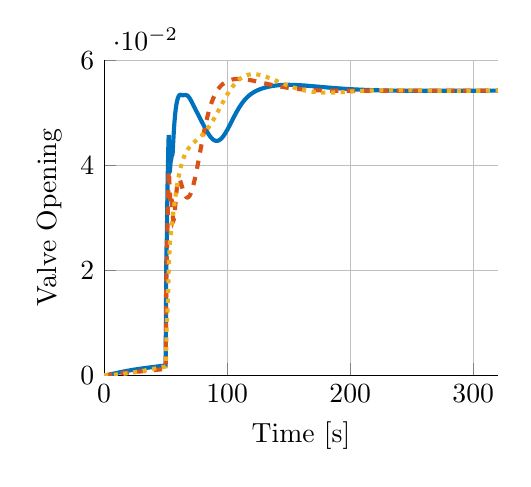
\begin{tikzpicture}

\begin{axis}[%
width=5cm,
height=4cm,
at={(0\linewidth,0\linewidth)},
scale only axis,
xmin=0,
xmax=320,
xlabel={Time [s]},
xmajorgrids,
ymin=0,
ymax=0.06,
ylabel={Valve Opening},
ymajorgrids,
axis background/.style={fill=white},
% title style={font=\bfseries},
% title={Normalized Recycle Valve Opening},
axis x line*=bottom,
axis y line*=left
]
\addplot [color=mycolor1,solid,line width=1.5pt,forget plot]
  table[row sep=crcr]{%
0	0\\
0.25	0\\
0.5	0\\
0.75	0\\
1	0\\
1.25	0\\
1.5	0\\
1.75	1.21538e-06\\
2	6.9504e-06\\
2.25	1.70383e-05\\
2.5	3.02921e-05\\
2.75	4.50965e-05\\
3	5.99591e-05\\
3.25	7.39074e-05\\
3.5	8.62583e-05\\
3.75	9.66784e-05\\
4	0.000105267\\
4.25	0.000112726\\
4.5	0.000120275\\
4.75	0.00012918\\
5	0.000140273\\
5.25	0.000153731\\
5.5	0.00016922\\
5.75	0.000186022\\
6	0.000203147\\
6.25	0.000219559\\
6.5	0.000234417\\
6.75	0.000247281\\
7	0.000258231\\
7.25	0.00026784\\
7.5	0.000277\\
7.75	0.000286676\\
8	0.000297664\\
8.25	0.000310406\\
8.5	0.000324894\\
8.75	0.000340683\\
9	0.000357006\\
9.25	0.000372969\\
9.5	0.000387778\\
9.75	0.000400935\\
10	0.000412358\\
10.25	0.000422393\\
10.5	0.000431714\\
10.75	0.000441145\\
11	0.000451454\\
11.25	0.000463161\\
11.5	0.000476412\\
11.75	0.000490953\\
12	0.000506201\\
12.25	0.000521392\\
12.5	0.000535783\\
12.75	0.000548831\\
13	0.000560334\\
13.25	0.000570472\\
13.5	0.000579758\\
13.75	0.000588899\\
14	0.000598617\\
14.25	0.000609463\\
14.5	0.000621683\\
14.75	0.000635158\\
15	0.000649443\\
15.25	0.000663878\\
15.5	0.000677764\\
15.75	0.000690537\\
16	0.000701909\\
16.25	0.000711944\\
16.5	0.000721031\\
16.75	0.000729787\\
17	0.000738888\\
17.25	0.000748904\\
17.5	0.000760149\\
17.75	0.000772605\\
18	0.00078593\\
18.25	0.000799548\\
18.5	0.000812797\\
18.75	0.000825099\\
19	0.000836108\\
19.25	0.000845799\\
19.5	0.000854471\\
19.75	0.000862668\\
20	0.000871037\\
20.25	0.000880158\\
20.5	0.000890399\\
20.75	0.00090182\\
21	0.000914159\\
21.25	0.000926901\\
21.5	0.000939412\\
21.75	0.000951105\\
22	0.000961585\\
22.25	0.000970761\\
22.5	0.000978863\\
22.75	0.000986381\\
23	0.000993941\\
23.25	0.00100214\\
23.5	0.00101139\\
23.75	0.00102181\\
24	0.0010332\\
24.25	0.00104509\\
24.5	0.00105687\\
24.75	0.00106794\\
25	0.00107785\\
25.25	0.00108646\\
25.5	0.00109395\\
25.75	0.00110077\\
26	0.00110753\\
26.25	0.00111486\\
26.5	0.0011232\\
26.75	0.00113274\\
27	0.00114331\\
27.25	0.00115448\\
27.5	0.00116564\\
27.75	0.00117616\\
28	0.00118557\\
28.25	0.00119368\\
28.5	0.00120061\\
28.75	0.00120679\\
29	0.00121285\\
29.25	0.00121942\\
29.5	0.001227\\
29.75	0.00123581\\
30	0.00124575\\
30.25	0.00125638\\
30.5	0.0012671\\
30.75	0.00127724\\
31	0.00128629\\
31.25	0.001294\\
31.5	0.00130047\\
31.75	0.00130612\\
32	0.00131158\\
32.25	0.00131753\\
32.5	0.00132452\\
32.75	0.00133281\\
33	0.00134232\\
33.25	0.00135263\\
33.5	0.0013631\\
33.75	0.00137304\\
34	0.00138188\\
34.25	0.00138932\\
34.5	0.00139544\\
34.75	0.00140066\\
35	0.00140564\\
35.25	0.0014111\\
35.5	0.00141765\\
35.75	0.0014256\\
36	0.00143488\\
36.25	0.00144508\\
36.5	0.00145552\\
36.75	0.00146544\\
37	0.00147421\\
37.25	0.0014815\\
37.5	0.00148736\\
37.75	0.00149222\\
38	0.00149679\\
38.25	0.00150187\\
38.5	0.00150811\\
38.75	0.00151587\\
39	0.00152512\\
39.25	0.00153541\\
39.5	0.001546\\
39.75	0.00155606\\
40	0.0015649\\
40.25	0.00157212\\
40.5	0.00157776\\
40.75	0.0015823\\
41	0.0015865\\
41.25	0.00159124\\
41.5	0.00159726\\
41.75	0.00160498\\
42	0.00161437\\
42.25	0.00162492\\
42.5	0.00163584\\
42.75	0.00164619\\
43	0.00165519\\
43.25	0.00166238\\
43.5	0.00166782\\
43.75	0.00167201\\
44	0.00167582\\
44.25	0.00168024\\
44.5	0.00168611\\
44.75	0.0016939\\
45	0.00170357\\
45.25	0.00171457\\
45.5	0.00172599\\
45.75	0.00173675\\
46	0.00174597\\
46.25	0.00175315\\
46.5	0.00175831\\
46.75	0.00176207\\
47	0.00176542\\
47.25	0.0017695\\
47.5	0.00177525\\
47.75	0.00178322\\
48	0.00179335\\
48.25	0.00180498\\
48.5	0.00181706\\
48.75	0.00182835\\
49	0.00183783\\
49.25	0.00184493\\
49.5	0.00184971\\
49.75	0.0018529\\
50	0.00185566\\
50.25	0.0106823\\
50.5	0.0208504\\
50.75	0.0243066\\
51	0.0261291\\
51.25	0.0307344\\
51.5	0.0354162\\
51.75	0.0383866\\
52	0.0411891\\
52.25	0.0441063\\
52.5	0.0457436\\
52.75	0.0431454\\
53	0.0400479\\
53.25	0.0387326\\
53.5	0.0388428\\
53.75	0.0397371\\
54	0.0405224\\
54.25	0.0408794\\
54.5	0.0411239\\
54.75	0.0414452\\
55	0.041782\\
55.25	0.0420426\\
55.5	0.0420536\\
55.75	0.0424731\\
56	0.0435875\\
56.25	0.0447724\\
56.5	0.0457822\\
56.75	0.0467364\\
57	0.0476344\\
57.25	0.0484249\\
57.5	0.0491111\\
57.75	0.0497202\\
58	0.0502684\\
58.25	0.0507522\\
58.5	0.0511703\\
58.75	0.0515347\\
59	0.0518568\\
59.25	0.0521409\\
59.5	0.0523902\\
59.75	0.0526083\\
60	0.0527973\\
60.25	0.0529582\\
60.5	0.0530919\\
60.75	0.0531996\\
61	0.0532826\\
61.25	0.0533427\\
61.5	0.0533821\\
61.75	0.0534034\\
62	0.0534097\\
62.25	0.0534046\\
62.5	0.0533915\\
62.75	0.053374\\
63	0.0533556\\
63.25	0.053339\\
63.5	0.0533263\\
63.75	0.053319\\
64	0.0533173\\
64.25	0.0533206\\
64.5	0.0533279\\
64.75	0.0533373\\
65	0.0533471\\
65.25	0.0533558\\
65.5	0.0533622\\
65.75	0.0533657\\
66	0.053366\\
66.25	0.053363\\
66.5	0.0533561\\
66.75	0.0533446\\
67	0.0533276\\
67.25	0.0533041\\
67.5	0.0532733\\
67.75	0.0532346\\
68	0.053188\\
68.25	0.0531336\\
68.5	0.0530714\\
68.75	0.0530019\\
69	0.0529255\\
69.25	0.0528427\\
69.5	0.0527541\\
69.75	0.0526602\\
70	0.0525617\\
70.25	0.052459\\
70.5	0.0523529\\
70.75	0.0522439\\
71	0.0521325\\
71.25	0.0520193\\
71.5	0.0519047\\
71.75	0.051789\\
72	0.0516727\\
72.25	0.0515561\\
72.5	0.0514393\\
72.75	0.0513226\\
73	0.0512062\\
73.25	0.0510901\\
73.5	0.0509743\\
73.75	0.050859\\
74	0.0507441\\
74.25	0.0506297\\
74.5	0.0505156\\
74.75	0.0504018\\
75	0.0502882\\
75.25	0.0501749\\
75.5	0.0500617\\
75.75	0.0499485\\
76	0.0498353\\
76.25	0.0497221\\
76.5	0.0496087\\
76.75	0.0494951\\
77	0.0493814\\
77.25	0.0492674\\
77.5	0.0491532\\
77.75	0.0490387\\
78	0.0489239\\
78.25	0.048809\\
78.5	0.0486938\\
78.75	0.0485785\\
79	0.048463\\
79.25	0.0483475\\
79.5	0.048232\\
79.75	0.0481166\\
80	0.0480013\\
80.25	0.0478863\\
80.5	0.0477715\\
80.75	0.0476572\\
81	0.0475434\\
81.25	0.0474302\\
81.5	0.0473178\\
81.75	0.0472061\\
82	0.0470955\\
82.25	0.0469858\\
82.5	0.0468773\\
82.75	0.0467701\\
83	0.0466643\\
83.25	0.0465601\\
83.5	0.0464574\\
83.75	0.0463564\\
84	0.0462574\\
84.25	0.0461602\\
84.5	0.0460652\\
84.75	0.0459723\\
85	0.0458818\\
85.25	0.0457936\\
85.5	0.0457079\\
85.75	0.0456249\\
86	0.0455446\\
86.25	0.0454671\\
86.5	0.0453925\\
86.75	0.0453209\\
87	0.0452524\\
87.25	0.045187\\
87.5	0.045125\\
87.75	0.0450663\\
88	0.045011\\
88.25	0.0449592\\
88.5	0.044911\\
88.75	0.0448665\\
89	0.0448256\\
89.25	0.0447885\\
89.5	0.0447551\\
89.75	0.0447257\\
90	0.0447001\\
90.25	0.0446784\\
90.5	0.0446607\\
90.75	0.044647\\
91	0.0446372\\
91.25	0.0446315\\
91.5	0.0446299\\
91.75	0.0446322\\
92	0.0446386\\
92.25	0.0446489\\
92.5	0.0446633\\
92.75	0.0446817\\
93	0.044704\\
93.25	0.0447303\\
93.5	0.0447604\\
93.75	0.0447944\\
94	0.0448322\\
94.25	0.0448737\\
94.5	0.044919\\
94.75	0.0449678\\
95	0.0450203\\
95.25	0.0450762\\
95.5	0.0451356\\
95.75	0.0451983\\
96	0.0452643\\
96.25	0.0453334\\
96.5	0.0454056\\
96.75	0.0454809\\
97	0.045559\\
97.25	0.0456399\\
97.5	0.0457235\\
97.75	0.0458098\\
98	0.0458985\\
98.25	0.0459896\\
98.5	0.0460829\\
98.75	0.0461785\\
99	0.0462761\\
99.25	0.0463756\\
99.5	0.046477\\
99.75	0.0465801\\
100	0.0466848\\
100.25	0.0467909\\
100.5	0.0468985\\
100.75	0.0470073\\
101	0.0471173\\
101.25	0.0472283\\
101.5	0.0473403\\
101.75	0.0474531\\
102	0.0475666\\
102.25	0.0476808\\
102.5	0.0477954\\
102.75	0.0479105\\
103	0.0480258\\
103.25	0.0481414\\
103.5	0.0482571\\
103.75	0.0483728\\
104	0.0484885\\
104.25	0.048604\\
104.5	0.0487192\\
104.75	0.0488342\\
105	0.0489487\\
105.25	0.0490628\\
105.5	0.0491762\\
105.75	0.0492891\\
106	0.0494013\\
106.25	0.0495127\\
106.5	0.0496232\\
106.75	0.0497329\\
107	0.0498417\\
107.25	0.0499494\\
107.5	0.0500561\\
107.75	0.0501617\\
108	0.0502662\\
108.25	0.0503694\\
108.5	0.0504715\\
108.75	0.0505723\\
109	0.0506718\\
109.25	0.0507699\\
109.5	0.0508667\\
109.75	0.0509622\\
110	0.0510562\\
110.25	0.0511488\\
110.5	0.05124\\
110.75	0.0513297\\
111	0.051418\\
111.25	0.0515047\\
111.5	0.05159\\
111.75	0.0516738\\
112	0.0517561\\
112.25	0.0518369\\
112.5	0.0519162\\
112.75	0.051994\\
113	0.0520703\\
113.25	0.0521451\\
113.5	0.0522184\\
113.75	0.0522903\\
114	0.0523607\\
114.25	0.0524296\\
114.5	0.0524971\\
114.75	0.0525632\\
115	0.0526279\\
115.25	0.0526912\\
115.5	0.052753\\
115.75	0.0528136\\
116	0.0528728\\
116.25	0.0529306\\
116.5	0.0529872\\
116.75	0.0530425\\
117	0.0530965\\
117.25	0.0531493\\
117.5	0.0532009\\
117.75	0.0532513\\
118	0.0533005\\
118.25	0.0533486\\
118.5	0.0533956\\
118.75	0.0534415\\
119	0.0534863\\
119.25	0.05353\\
119.5	0.0535727\\
119.75	0.0536145\\
120	0.0536552\\
120.25	0.053695\\
120.5	0.0537339\\
120.75	0.0537719\\
121	0.053809\\
121.25	0.0538452\\
121.5	0.0538806\\
121.75	0.0539152\\
122	0.053949\\
122.25	0.053982\\
122.5	0.0540143\\
122.75	0.0540459\\
123	0.0540767\\
123.25	0.0541069\\
123.5	0.0541363\\
123.75	0.0541652\\
124	0.0541934\\
124.25	0.054221\\
124.5	0.054248\\
124.75	0.0542744\\
125	0.0543003\\
125.25	0.0543256\\
125.5	0.0543504\\
125.75	0.0543747\\
126	0.0543985\\
126.25	0.0544218\\
126.5	0.0544446\\
126.75	0.054467\\
127	0.0544889\\
127.25	0.0545103\\
127.5	0.0545314\\
127.75	0.054552\\
128	0.0545723\\
128.25	0.0545921\\
128.5	0.0546116\\
128.75	0.0546306\\
129	0.0546494\\
129.25	0.0546677\\
129.5	0.0546857\\
129.75	0.0547034\\
130	0.0547207\\
130.25	0.0547377\\
130.5	0.0547544\\
130.75	0.0547708\\
131	0.0547868\\
131.25	0.0548026\\
131.5	0.054818\\
131.75	0.0548332\\
132	0.054848\\
132.25	0.0548626\\
132.5	0.0548769\\
132.75	0.0548909\\
133	0.0549046\\
133.25	0.0549181\\
133.5	0.0549313\\
133.75	0.0549442\\
134	0.0549569\\
134.25	0.0549693\\
134.5	0.0549815\\
134.75	0.0549934\\
135	0.055005\\
135.25	0.0550164\\
135.5	0.0550276\\
135.75	0.0550385\\
136	0.0550491\\
136.25	0.0550596\\
136.5	0.0550697\\
136.75	0.0550797\\
137	0.0550894\\
137.25	0.0550989\\
137.5	0.0551081\\
137.75	0.0551171\\
138	0.0551259\\
138.25	0.0551344\\
138.5	0.0551428\\
138.75	0.0551509\\
139	0.0551587\\
139.25	0.0551664\\
139.5	0.0551738\\
139.75	0.055181\\
140	0.055188\\
140.25	0.0551948\\
140.5	0.0552014\\
140.75	0.0552077\\
141	0.0552139\\
141.25	0.0552198\\
141.5	0.0552255\\
141.75	0.055231\\
142	0.0552363\\
142.25	0.0552414\\
142.5	0.0552464\\
142.75	0.0552511\\
143	0.0552556\\
143.25	0.0552599\\
143.5	0.055264\\
143.75	0.055268\\
144	0.0552717\\
144.25	0.0552753\\
144.5	0.0552786\\
144.75	0.0552818\\
145	0.0552848\\
145.25	0.0552877\\
145.5	0.0552903\\
145.75	0.0552928\\
146	0.0552951\\
146.25	0.0552972\\
146.5	0.0552992\\
146.75	0.055301\\
147	0.0553027\\
147.25	0.0553041\\
147.5	0.0553055\\
147.75	0.0553066\\
148	0.0553076\\
148.25	0.0553085\\
148.5	0.0553092\\
148.75	0.0553098\\
149	0.0553102\\
149.25	0.0553105\\
149.5	0.0553106\\
149.75	0.0553106\\
150	0.0553105\\
150.25	0.0553102\\
150.5	0.0553098\\
150.75	0.0553093\\
151	0.0553086\\
151.25	0.0553078\\
151.5	0.055307\\
151.75	0.0553059\\
152	0.0553048\\
152.25	0.0553036\\
152.5	0.0553022\\
152.75	0.0553007\\
153	0.0552992\\
153.25	0.0552975\\
153.5	0.0552957\\
153.75	0.0552938\\
154	0.0552918\\
154.25	0.0552897\\
154.5	0.0552876\\
154.75	0.0552853\\
155	0.0552829\\
155.25	0.0552805\\
155.5	0.055278\\
155.75	0.0552753\\
156	0.0552726\\
156.25	0.0552699\\
156.5	0.055267\\
156.75	0.0552641\\
157	0.055261\\
157.25	0.055258\\
157.5	0.0552548\\
157.75	0.0552516\\
158	0.0552483\\
158.25	0.0552449\\
158.5	0.0552415\\
158.75	0.055238\\
159	0.0552345\\
159.25	0.0552308\\
159.5	0.0552272\\
159.75	0.0552234\\
160	0.0552197\\
160.25	0.0552158\\
160.5	0.0552119\\
160.75	0.055208\\
161	0.055204\\
161.25	0.0552\\
161.5	0.0551959\\
161.75	0.0551918\\
162	0.0551876\\
162.25	0.0551834\\
162.5	0.0551791\\
162.75	0.0551748\\
163	0.0551705\\
163.25	0.0551661\\
163.5	0.0551617\\
163.75	0.0551573\\
164	0.0551528\\
164.25	0.0551483\\
164.5	0.0551437\\
164.75	0.0551391\\
165	0.0551345\\
165.25	0.0551299\\
165.5	0.0551252\\
165.75	0.0551205\\
166	0.0551158\\
166.25	0.0551111\\
166.5	0.0551063\\
166.75	0.0551015\\
167	0.0550967\\
167.25	0.0550918\\
167.5	0.055087\\
167.75	0.0550821\\
168	0.0550772\\
168.25	0.0550723\\
168.5	0.0550674\\
168.75	0.0550624\\
169	0.0550575\\
169.25	0.0550525\\
169.5	0.0550475\\
169.75	0.0550425\\
170	0.0550375\\
170.25	0.0550324\\
170.5	0.0550274\\
170.75	0.0550223\\
171	0.0550173\\
171.25	0.0550122\\
171.5	0.0550071\\
171.75	0.055002\\
172	0.0549969\\
172.25	0.0549918\\
172.5	0.0549867\\
172.75	0.0549816\\
173	0.0549765\\
173.25	0.0549714\\
173.5	0.0549662\\
173.75	0.0549611\\
174	0.054956\\
174.25	0.0549509\\
174.5	0.0549457\\
174.75	0.0549406\\
175	0.0549355\\
175.25	0.0549303\\
175.5	0.0549252\\
175.75	0.0549201\\
176	0.0549149\\
176.25	0.0549098\\
176.5	0.0549047\\
176.75	0.0548996\\
177	0.0548945\\
177.25	0.0548894\\
177.5	0.0548842\\
177.75	0.0548792\\
178	0.0548741\\
178.25	0.054869\\
178.5	0.0548639\\
178.75	0.0548588\\
179	0.0548538\\
179.25	0.0548487\\
179.5	0.0548437\\
179.75	0.0548386\\
180	0.0548336\\
180.25	0.0548286\\
180.5	0.0548236\\
180.75	0.0548186\\
181	0.0548136\\
181.25	0.0548086\\
181.5	0.0548036\\
181.75	0.0547987\\
182	0.0547937\\
182.25	0.0547888\\
182.5	0.0547839\\
182.75	0.054779\\
183	0.0547741\\
183.25	0.0547693\\
183.5	0.0547644\\
183.75	0.0547596\\
184	0.0547547\\
184.25	0.0547499\\
184.5	0.0547451\\
184.75	0.0547403\\
185	0.0547356\\
185.25	0.0547308\\
185.5	0.0547261\\
185.75	0.0547214\\
186	0.0547167\\
186.25	0.054712\\
186.5	0.0547073\\
186.75	0.0547027\\
187	0.0546981\\
187.25	0.0546935\\
187.5	0.0546889\\
187.75	0.0546843\\
188	0.0546798\\
188.25	0.0546752\\
188.5	0.0546707\\
188.75	0.0546662\\
189	0.0546618\\
189.25	0.0546573\\
189.5	0.0546529\\
189.75	0.0546485\\
190	0.0546441\\
190.25	0.0546397\\
190.5	0.0546354\\
190.75	0.054631\\
191	0.0546267\\
191.25	0.0546225\\
191.5	0.0546182\\
191.75	0.0546139\\
192	0.0546097\\
192.25	0.0546055\\
192.5	0.0546014\\
192.75	0.0545972\\
193	0.0545931\\
193.25	0.054589\\
193.5	0.0545849\\
193.75	0.0545808\\
194	0.0545768\\
194.25	0.0545728\\
194.5	0.0545688\\
194.75	0.0545648\\
195	0.0545608\\
195.25	0.0545569\\
195.5	0.054553\\
195.75	0.0545491\\
196	0.0545453\\
196.25	0.0545414\\
196.5	0.0545376\\
196.75	0.0545339\\
197	0.0545301\\
197.25	0.0545263\\
197.5	0.0545226\\
197.75	0.0545189\\
198	0.0545153\\
198.25	0.0545116\\
198.5	0.054508\\
198.75	0.0545044\\
199	0.0545008\\
199.25	0.0544973\\
199.5	0.0544938\\
199.75	0.0544903\\
200	0.0544868\\
200.25	0.0544833\\
200.5	0.0544799\\
200.75	0.0544765\\
201	0.0544731\\
201.25	0.0544698\\
201.5	0.0544664\\
201.75	0.0544631\\
202	0.0544598\\
202.25	0.0544566\\
202.5	0.0544533\\
202.75	0.0544501\\
203	0.0544469\\
203.25	0.0544438\\
203.5	0.0544406\\
203.75	0.0544375\\
204	0.0544344\\
204.25	0.0544313\\
204.5	0.0544283\\
204.75	0.0544252\\
205	0.0544222\\
205.25	0.0544193\\
205.5	0.0544163\\
205.75	0.0544134\\
206	0.0544105\\
206.25	0.0544076\\
206.5	0.0544047\\
206.75	0.0544019\\
207	0.0543991\\
207.25	0.0543963\\
207.5	0.0543935\\
207.75	0.0543908\\
208	0.054388\\
208.25	0.0543853\\
208.5	0.0543827\\
208.75	0.05438\\
209	0.0543774\\
209.25	0.0543748\\
209.5	0.0543722\\
209.75	0.0543696\\
210	0.0543671\\
210.25	0.0543645\\
210.5	0.054362\\
210.75	0.0543596\\
211	0.0543571\\
211.25	0.0543547\\
211.5	0.0543523\\
211.75	0.0543499\\
212	0.0543475\\
212.25	0.0543452\\
212.5	0.0543429\\
212.75	0.0543406\\
213	0.0543383\\
213.25	0.054336\\
213.5	0.0543338\\
213.75	0.0543316\\
214	0.0543294\\
214.25	0.0543272\\
214.5	0.054325\\
214.75	0.0543229\\
215	0.0543208\\
215.25	0.0543187\\
215.5	0.0543166\\
215.75	0.0543146\\
216	0.0543126\\
216.25	0.0543105\\
216.5	0.0543086\\
216.75	0.0543066\\
217	0.0543046\\
217.25	0.0543027\\
217.5	0.0543008\\
217.75	0.0542989\\
218	0.054297\\
218.25	0.0542952\\
218.5	0.0542934\\
218.75	0.0542915\\
219	0.0542897\\
219.25	0.054288\\
219.5	0.0542862\\
219.75	0.0542845\\
220	0.0542828\\
220.25	0.0542811\\
220.5	0.0542794\\
220.75	0.0542777\\
221	0.0542761\\
221.25	0.0542745\\
221.5	0.0542728\\
221.75	0.0542713\\
222	0.0542697\\
222.25	0.0542681\\
222.5	0.0542666\\
222.75	0.0542651\\
223	0.0542636\\
223.25	0.0542621\\
223.5	0.0542606\\
223.75	0.0542592\\
224	0.0542577\\
224.25	0.0542563\\
224.5	0.0542549\\
224.75	0.0542535\\
225	0.0542522\\
225.25	0.0542508\\
225.5	0.0542495\\
225.75	0.0542482\\
226	0.0542469\\
226.25	0.0542456\\
226.5	0.0542443\\
226.75	0.0542431\\
227	0.0542418\\
227.25	0.0542406\\
227.5	0.0542394\\
227.75	0.0542382\\
228	0.054237\\
228.25	0.0542359\\
228.5	0.0542347\\
228.75	0.0542336\\
229	0.0542325\\
229.25	0.0542314\\
229.5	0.0542303\\
229.75	0.0542292\\
230	0.0542282\\
230.25	0.0542271\\
230.5	0.0542261\\
230.75	0.0542251\\
231	0.0542241\\
231.25	0.0542231\\
231.5	0.0542221\\
231.75	0.0542211\\
232	0.0542202\\
232.25	0.0542193\\
232.5	0.0542183\\
232.75	0.0542174\\
233	0.0542165\\
233.25	0.0542156\\
233.5	0.0542148\\
233.75	0.0542139\\
234	0.0542131\\
234.25	0.0542122\\
234.5	0.0542114\\
234.75	0.0542106\\
235	0.0542098\\
235.25	0.054209\\
235.5	0.0542083\\
235.75	0.0542075\\
236	0.0542068\\
236.25	0.054206\\
236.5	0.0542053\\
236.75	0.0542046\\
237	0.0542039\\
237.25	0.0542032\\
237.5	0.0542025\\
237.75	0.0542018\\
238	0.0542012\\
238.25	0.0542005\\
238.5	0.0541999\\
238.75	0.0541993\\
239	0.0541987\\
239.25	0.054198\\
239.5	0.0541975\\
239.75	0.0541969\\
240	0.0541963\\
240.25	0.0541957\\
240.5	0.0541952\\
240.75	0.0541946\\
241	0.0541941\\
241.25	0.0541936\\
241.5	0.0541931\\
241.75	0.0541925\\
242	0.054192\\
242.25	0.0541916\\
242.5	0.0541911\\
242.75	0.0541906\\
243	0.0541901\\
243.25	0.0541897\\
243.5	0.0541893\\
243.75	0.0541888\\
244	0.0541884\\
244.25	0.054188\\
244.5	0.0541876\\
244.75	0.0541872\\
245	0.0541868\\
245.25	0.0541864\\
245.5	0.054186\\
245.75	0.0541856\\
246	0.0541853\\
246.25	0.0541849\\
246.5	0.0541846\\
246.75	0.0541842\\
247	0.0541839\\
247.25	0.0541836\\
247.5	0.0541833\\
247.75	0.054183\\
248	0.0541827\\
248.25	0.0541824\\
248.5	0.0541821\\
248.75	0.0541818\\
249	0.0541815\\
249.25	0.0541813\\
249.5	0.054181\\
249.75	0.0541808\\
250	0.0541805\\
250.25	0.0541803\\
250.5	0.05418\\
250.75	0.0541798\\
251	0.0541796\\
251.25	0.0541794\\
251.5	0.0541792\\
251.75	0.054179\\
252	0.0541788\\
252.25	0.0541786\\
252.5	0.0541784\\
252.75	0.0541782\\
253	0.054178\\
253.25	0.0541779\\
253.5	0.0541777\\
253.75	0.0541776\\
254	0.0541774\\
254.25	0.0541773\\
254.5	0.0541771\\
254.75	0.054177\\
255	0.0541769\\
255.25	0.0541767\\
255.5	0.0541766\\
255.75	0.0541765\\
256	0.0541764\\
256.25	0.0541763\\
256.5	0.0541762\\
256.75	0.0541761\\
257	0.054176\\
257.25	0.0541759\\
257.5	0.0541758\\
257.75	0.0541757\\
258	0.0541757\\
258.25	0.0541756\\
258.5	0.0541755\\
258.75	0.0541755\\
259	0.0541754\\
259.25	0.0541753\\
259.5	0.0541753\\
259.75	0.0541752\\
260	0.0541752\\
260.25	0.0541752\\
260.5	0.0541751\\
260.75	0.0541751\\
261	0.0541751\\
261.25	0.054175\\
261.5	0.054175\\
261.75	0.054175\\
262	0.054175\\
262.25	0.054175\\
262.5	0.054175\\
262.75	0.054175\\
263	0.054175\\
263.25	0.054175\\
263.5	0.054175\\
263.75	0.054175\\
264	0.054175\\
264.25	0.054175\\
264.5	0.054175\\
264.75	0.054175\\
265	0.0541751\\
265.25	0.0541751\\
265.5	0.0541751\\
265.75	0.0541751\\
266	0.0541752\\
266.25	0.0541752\\
266.5	0.0541752\\
266.75	0.0541753\\
267	0.0541753\\
267.25	0.0541754\\
267.5	0.0541754\\
267.75	0.0541755\\
268	0.0541755\\
268.25	0.0541756\\
268.5	0.0541756\\
268.75	0.0541757\\
269	0.0541757\\
269.25	0.0541758\\
269.5	0.0541759\\
269.75	0.0541759\\
270	0.054176\\
270.25	0.0541761\\
270.5	0.0541761\\
270.75	0.0541762\\
271	0.0541763\\
271.25	0.0541764\\
271.5	0.0541765\\
271.75	0.0541765\\
272	0.0541766\\
272.25	0.0541767\\
272.5	0.0541768\\
272.75	0.0541769\\
273	0.054177\\
273.25	0.054177\\
273.5	0.0541771\\
273.75	0.0541772\\
274	0.0541773\\
274.25	0.0541774\\
274.5	0.0541775\\
274.75	0.0541776\\
275	0.0541777\\
275.25	0.0541778\\
275.5	0.0541779\\
275.75	0.054178\\
276	0.0541781\\
276.25	0.0541782\\
276.5	0.0541783\\
276.75	0.0541784\\
277	0.0541785\\
277.25	0.0541786\\
277.5	0.0541787\\
277.75	0.0541789\\
278	0.054179\\
278.25	0.0541791\\
278.5	0.0541792\\
278.75	0.0541793\\
279	0.0541794\\
279.25	0.0541795\\
279.5	0.0541796\\
279.75	0.0541798\\
280	0.0541799\\
280.25	0.05418\\
280.5	0.0541801\\
280.75	0.0541802\\
281	0.0541803\\
281.25	0.0541805\\
281.5	0.0541806\\
281.75	0.0541807\\
282	0.0541808\\
282.25	0.0541809\\
282.5	0.0541811\\
282.75	0.0541812\\
283	0.0541813\\
283.25	0.0541814\\
283.5	0.0541815\\
283.75	0.0541817\\
284	0.0541818\\
284.25	0.0541819\\
284.5	0.054182\\
284.75	0.0541822\\
285	0.0541823\\
285.25	0.0541824\\
285.5	0.0541825\\
285.75	0.0541827\\
286	0.0541828\\
286.25	0.0541829\\
286.5	0.054183\\
286.75	0.0541832\\
287	0.0541833\\
287.25	0.0541834\\
287.5	0.0541835\\
287.75	0.0541837\\
288	0.0541838\\
288.25	0.0541839\\
288.5	0.054184\\
288.75	0.0541842\\
289	0.0541843\\
289.25	0.0541844\\
289.5	0.0541845\\
289.75	0.0541847\\
290	0.0541848\\
290.25	0.0541849\\
290.5	0.054185\\
290.75	0.0541852\\
291	0.0541853\\
291.25	0.0541854\\
291.5	0.0541855\\
291.75	0.0541857\\
292	0.0541858\\
292.25	0.0541859\\
292.5	0.054186\\
292.75	0.0541862\\
293	0.0541863\\
293.25	0.0541864\\
293.5	0.0541865\\
293.75	0.0541866\\
294	0.0541868\\
294.25	0.0541869\\
294.5	0.054187\\
294.75	0.0541871\\
295	0.0541873\\
295.25	0.0541874\\
295.5	0.0541875\\
295.75	0.0541876\\
296	0.0541877\\
296.25	0.0541878\\
296.5	0.054188\\
296.75	0.0541881\\
297	0.0541882\\
297.25	0.0541883\\
297.5	0.0541884\\
297.75	0.0541886\\
298	0.0541887\\
298.25	0.0541888\\
298.5	0.0541889\\
298.75	0.054189\\
299	0.0541891\\
299.25	0.0541892\\
299.5	0.0541894\\
299.75	0.0541895\\
300	0.0541896\\
300.25	0.0541897\\
300.5	0.0541898\\
300.75	0.0541899\\
301	0.05419\\
301.25	0.0541901\\
301.5	0.0541903\\
301.75	0.0541904\\
302	0.0541905\\
302.25	0.0541906\\
302.5	0.0541907\\
302.75	0.0541908\\
303	0.0541909\\
303.25	0.054191\\
303.5	0.0541911\\
303.75	0.0541912\\
304	0.0541913\\
304.25	0.0541914\\
304.5	0.0541915\\
304.75	0.0541916\\
305	0.0541917\\
305.25	0.0541918\\
305.5	0.0541919\\
305.75	0.054192\\
306	0.0541921\\
306.25	0.0541922\\
306.5	0.0541923\\
306.75	0.0541924\\
307	0.0541925\\
307.25	0.0541926\\
307.5	0.0541927\\
307.75	0.0541928\\
308	0.0541929\\
308.25	0.054193\\
308.5	0.0541931\\
308.75	0.0541932\\
309	0.0541933\\
309.25	0.0541934\\
309.5	0.0541935\\
309.75	0.0541936\\
310	0.0541937\\
310.25	0.0541938\\
310.5	0.0541939\\
310.75	0.0541939\\
311	0.054194\\
311.25	0.0541941\\
311.5	0.0541942\\
311.75	0.0541943\\
312	0.0541944\\
312.25	0.0541945\\
312.5	0.0541946\\
312.75	0.0541946\\
313	0.0541947\\
313.25	0.0541948\\
313.5	0.0541949\\
313.75	0.054195\\
314	0.0541951\\
314.25	0.0541951\\
314.5	0.0541952\\
314.75	0.0541953\\
315	0.0541954\\
315.25	0.0541955\\
315.5	0.0541955\\
315.75	0.0541956\\
316	0.0541957\\
316.25	0.0541958\\
316.5	0.0541958\\
316.75	0.0541959\\
317	0.054196\\
317.25	0.0541961\\
317.5	0.0541961\\
317.75	0.0541962\\
318	0.0541963\\
318.25	0.0541964\\
318.5	0.0541964\\
318.75	0.0541965\\
319	0.0541966\\
319.25	0.0541966\\
319.5	0.0541967\\
319.75	0.0541968\\
320	0.0541968\\
320.25	0.0541969\\
320.5	0.054197\\
320.75	0.054197\\
321	0.0541971\\
321.25	0.0541972\\
321.5	0.0541972\\
321.75	0.0541973\\
322	0.0541974\\
322.25	0.0541974\\
322.5	0.0541975\\
322.75	0.0541975\\
323	0.0541976\\
323.25	0.0541977\\
323.5	0.0541977\\
323.75	0.0541978\\
324	0.0541978\\
324.25	0.0541979\\
324.5	0.054198\\
324.75	0.054198\\
325	0.0541981\\
325.25	0.0541981\\
325.5	0.0541982\\
325.75	0.0541982\\
326	0.0541983\\
326.25	0.0541984\\
326.5	0.0541984\\
326.75	0.0541985\\
327	0.0541985\\
327.25	0.0541986\\
327.5	0.0541986\\
327.75	0.0541987\\
328	0.0541987\\
328.25	0.0541988\\
328.5	0.0541988\\
328.75	0.0541989\\
329	0.0541989\\
329.25	0.054199\\
329.5	0.054199\\
329.75	0.0541991\\
330	0.0541991\\
330.25	0.0541991\\
330.5	0.0541992\\
330.75	0.0541992\\
331	0.0541993\\
331.25	0.0541993\\
331.5	0.0541994\\
331.75	0.0541994\\
332	0.0541995\\
332.25	0.0541995\\
332.5	0.0541995\\
332.75	0.0541996\\
333	0.0541996\\
333.25	0.0541997\\
333.5	0.0541997\\
333.75	0.0541997\\
334	0.0541998\\
334.25	0.0541998\\
334.5	0.0541999\\
334.75	0.0541999\\
335	0.0541999\\
335.25	0.0542\\
335.5	0.0542\\
335.75	0.0542\\
336	0.0542001\\
336.25	0.0542001\\
336.5	0.0542001\\
336.75	0.0542002\\
337	0.0542002\\
337.25	0.0542002\\
337.5	0.0542003\\
337.75	0.0542003\\
338	0.0542003\\
338.25	0.0542004\\
338.5	0.0542004\\
338.75	0.0542004\\
339	0.0542005\\
339.25	0.0542005\\
339.5	0.0542005\\
339.75	0.0542006\\
340	0.0542006\\
340.25	0.0542006\\
340.5	0.0542006\\
340.75	0.0542007\\
341	0.0542007\\
341.25	0.0542007\\
341.5	0.0542008\\
341.75	0.0542008\\
342	0.0542008\\
342.25	0.0542008\\
342.5	0.0542009\\
342.75	0.0542009\\
343	0.0542009\\
343.25	0.0542009\\
343.5	0.054201\\
343.75	0.054201\\
344	0.054201\\
344.25	0.054201\\
344.5	0.0542011\\
344.75	0.0542011\\
345	0.0542011\\
345.25	0.0542011\\
345.5	0.0542011\\
345.75	0.0542012\\
346	0.0542012\\
346.25	0.0542012\\
346.5	0.0542012\\
346.75	0.0542012\\
347	0.0542013\\
347.25	0.0542013\\
347.5	0.0542013\\
347.75	0.0542013\\
348	0.0542013\\
348.25	0.0542014\\
348.5	0.0542014\\
348.75	0.0542014\\
349	0.0542014\\
349.25	0.0542014\\
349.5	0.0542014\\
349.75	0.0542015\\
350	0.0542015\\
350.25	0.0542015\\
350.5	0.0542015\\
350.75	0.0542015\\
351	0.0542015\\
351.25	0.0542016\\
351.5	0.0542016\\
351.75	0.0542016\\
352	0.0542016\\
352.25	0.0542016\\
352.5	0.0542016\\
352.75	0.0542016\\
353	0.0542017\\
353.25	0.0542017\\
353.5	0.0542017\\
353.75	0.0542017\\
354	0.0542017\\
354.25	0.0542017\\
354.5	0.0542017\\
354.75	0.0542017\\
355	0.0542018\\
355.25	0.0542018\\
355.5	0.0542018\\
355.75	0.0542018\\
356	0.0542018\\
356.25	0.0542018\\
356.5	0.0542018\\
356.75	0.0542018\\
357	0.0542018\\
357.25	0.0542018\\
357.5	0.0542019\\
357.75	0.0542019\\
358	0.0542019\\
358.25	0.0542019\\
358.5	0.0542019\\
358.75	0.0542019\\
359	0.0542019\\
359.25	0.0542019\\
359.5	0.0542019\\
359.75	0.0542019\\
360	0.0542019\\
360.25	0.0542019\\
360.5	0.054202\\
360.75	0.054202\\
361	0.054202\\
361.25	0.054202\\
361.5	0.054202\\
361.75	0.054202\\
362	0.054202\\
362.25	0.054202\\
362.5	0.054202\\
362.75	0.054202\\
363	0.054202\\
363.25	0.054202\\
363.5	0.054202\\
363.75	0.054202\\
364	0.054202\\
364.25	0.054202\\
364.5	0.054202\\
364.75	0.0542021\\
365	0.0542021\\
365.25	0.0542021\\
365.5	0.0542021\\
365.75	0.0542021\\
366	0.0542021\\
366.25	0.0542021\\
366.5	0.0542021\\
366.75	0.0542021\\
367	0.0542021\\
367.25	0.0542021\\
367.5	0.0542021\\
367.75	0.0542021\\
368	0.0542021\\
368.25	0.0542021\\
368.5	0.0542021\\
368.75	0.0542021\\
369	0.0542021\\
369.25	0.0542021\\
369.5	0.0542021\\
369.75	0.0542021\\
370	0.0542021\\
370.25	0.0542021\\
370.5	0.0542021\\
370.75	0.0542021\\
371	0.0542021\\
371.25	0.0542021\\
371.5	0.0542021\\
371.75	0.0542021\\
372	0.0542021\\
372.25	0.0542021\\
372.5	0.0542021\\
372.75	0.0542021\\
373	0.0542021\\
373.25	0.0542021\\
373.5	0.0542021\\
373.75	0.0542021\\
374	0.0542021\\
374.25	0.0542021\\
374.5	0.0542021\\
374.75	0.0542021\\
375	0.0542021\\
375.25	0.0542021\\
375.5	0.0542021\\
375.75	0.0542021\\
376	0.0542021\\
376.25	0.0542021\\
376.5	0.0542021\\
376.75	0.0542021\\
377	0.0542021\\
377.25	0.0542021\\
377.5	0.0542021\\
377.75	0.0542021\\
378	0.0542021\\
378.25	0.0542021\\
378.5	0.0542021\\
378.75	0.0542021\\
379	0.0542021\\
379.25	0.0542021\\
379.5	0.0542021\\
379.75	0.0542021\\
380	0.0542021\\
380.25	0.0542021\\
380.5	0.0542021\\
380.75	0.0542021\\
381	0.0542021\\
381.25	0.0542021\\
381.5	0.0542021\\
381.75	0.0542021\\
382	0.0542021\\
382.25	0.0542021\\
382.5	0.0542021\\
382.75	0.0542021\\
383	0.0542021\\
383.25	0.0542021\\
383.5	0.0542021\\
383.75	0.0542021\\
384	0.0542021\\
384.25	0.0542021\\
384.5	0.0542021\\
384.75	0.0542021\\
385	0.0542021\\
385.25	0.0542021\\
385.5	0.0542021\\
385.75	0.0542021\\
386	0.0542021\\
386.25	0.0542021\\
386.5	0.0542021\\
386.75	0.0542021\\
387	0.0542021\\
387.25	0.0542021\\
387.5	0.0542021\\
387.75	0.0542021\\
388	0.0542021\\
388.25	0.0542021\\
388.5	0.0542021\\
388.75	0.0542021\\
389	0.0542021\\
389.25	0.054202\\
389.5	0.054202\\
389.75	0.054202\\
390	0.054202\\
390.25	0.054202\\
390.5	0.054202\\
390.75	0.054202\\
391	0.054202\\
391.25	0.054202\\
391.5	0.054202\\
391.75	0.054202\\
392	0.054202\\
392.25	0.054202\\
392.5	0.054202\\
392.75	0.054202\\
393	0.054202\\
393.25	0.054202\\
393.5	0.054202\\
393.75	0.054202\\
394	0.054202\\
394.25	0.054202\\
394.5	0.054202\\
394.75	0.054202\\
395	0.054202\\
395.25	0.054202\\
395.5	0.054202\\
395.75	0.054202\\
396	0.054202\\
396.25	0.054202\\
396.5	0.054202\\
396.75	0.054202\\
397	0.054202\\
397.25	0.054202\\
397.5	0.054202\\
397.75	0.0542019\\
398	0.0542019\\
398.25	0.0542019\\
398.5	0.0542019\\
398.75	0.0542019\\
399	0.0542019\\
399.25	0.0542019\\
399.5	0.0542019\\
399.75	0.0542019\\
400	0.0542019\\
400.25	0.0542019\\
400.5	0.0542019\\
400.75	0.0542019\\
401	0.0542019\\
401.25	0.0542019\\
401.5	0.0542019\\
401.75	0.0542019\\
402	0.0542019\\
402.25	0.0542019\\
402.5	0.0542019\\
402.75	0.0542019\\
403	0.0542019\\
403.25	0.0542019\\
403.5	0.0542019\\
403.75	0.0542019\\
404	0.0542019\\
404.25	0.0542019\\
404.5	0.0542019\\
404.75	0.0542019\\
405	0.0542019\\
405.25	0.0542019\\
405.5	0.0542019\\
405.75	0.0542019\\
406	0.0542018\\
406.25	0.0542018\\
406.5	0.0542018\\
406.75	0.0542018\\
407	0.0542018\\
407.25	0.0542018\\
407.5	0.0542018\\
407.75	0.0542018\\
408	0.0542018\\
408.25	0.0542018\\
408.5	0.0542018\\
408.75	0.0542018\\
409	0.0542018\\
409.25	0.0542018\\
409.5	0.0542018\\
409.75	0.0542018\\
410	0.0542018\\
410.25	0.0542018\\
410.5	0.0542018\\
410.75	0.0542018\\
411	0.0542018\\
411.25	0.0542018\\
411.5	0.0542018\\
411.75	0.0542018\\
412	0.0542018\\
412.25	0.0542018\\
412.5	0.0542018\\
412.75	0.0542018\\
413	0.0542018\\
413.25	0.0542018\\
413.5	0.0542018\\
413.75	0.0542018\\
414	0.0542018\\
414.25	0.0542018\\
414.5	0.0542018\\
414.75	0.0542018\\
415	0.0542017\\
415.25	0.0542017\\
415.5	0.0542017\\
415.75	0.0542017\\
416	0.0542017\\
416.25	0.0542017\\
416.5	0.0542017\\
416.75	0.0542017\\
417	0.0542017\\
417.25	0.0542017\\
417.5	0.0542017\\
417.75	0.0542017\\
418	0.0542017\\
418.25	0.0542017\\
418.5	0.0542017\\
418.75	0.0542017\\
419	0.0542017\\
419.25	0.0542017\\
419.5	0.0542017\\
419.75	0.0542017\\
420	0.0542017\\
420.25	0.0542017\\
420.5	0.0542017\\
420.75	0.0542017\\
421	0.0542017\\
421.25	0.0542017\\
421.5	0.0542017\\
421.75	0.0542017\\
422	0.0542017\\
422.25	0.0542017\\
422.5	0.0542017\\
422.75	0.0542017\\
423	0.0542017\\
423.25	0.0542017\\
423.5	0.0542017\\
423.75	0.0542017\\
424	0.0542017\\
424.25	0.0542017\\
424.5	0.0542017\\
424.75	0.0542017\\
425	0.0542017\\
425.25	0.0542017\\
425.5	0.0542017\\
425.75	0.0542016\\
426	0.0542016\\
426.25	0.0542016\\
426.5	0.0542016\\
426.75	0.0542016\\
427	0.0542016\\
427.25	0.0542016\\
427.5	0.0542016\\
427.75	0.0542016\\
428	0.0542016\\
428.25	0.0542016\\
428.5	0.0542016\\
428.75	0.0542016\\
429	0.0542016\\
429.25	0.0542016\\
429.5	0.0542016\\
429.75	0.0542016\\
430	0.0542016\\
430.25	0.0542016\\
430.5	0.0542016\\
430.75	0.0542016\\
431	0.0542016\\
431.25	0.0542016\\
431.5	0.0542016\\
431.75	0.0542016\\
432	0.0542016\\
432.25	0.0542016\\
432.5	0.0542016\\
432.75	0.0542016\\
433	0.0542016\\
433.25	0.0542016\\
433.5	0.0542016\\
433.75	0.0542016\\
434	0.0542016\\
434.25	0.0542016\\
434.5	0.0542016\\
434.75	0.0542016\\
435	0.0542016\\
435.25	0.0542016\\
435.5	0.0542016\\
435.75	0.0542016\\
436	0.0542016\\
436.25	0.0542016\\
436.5	0.0542016\\
436.75	0.0542016\\
437	0.0542016\\
437.25	0.0542016\\
437.5	0.0542016\\
437.75	0.0542016\\
438	0.0542016\\
438.25	0.0542016\\
438.5	0.0542016\\
438.75	0.0542016\\
439	0.0542016\\
439.25	0.0542016\\
439.5	0.0542016\\
439.75	0.0542016\\
440	0.0542016\\
440.25	0.0542016\\
440.5	0.0542016\\
440.75	0.0542016\\
441	0.0542016\\
441.25	0.0542015\\
441.5	0.0542015\\
441.75	0.0542015\\
442	0.0542015\\
442.25	0.0542015\\
442.5	0.0542015\\
442.75	0.0542015\\
443	0.0542015\\
443.25	0.0542015\\
443.5	0.0542015\\
443.75	0.0542015\\
444	0.0542015\\
444.25	0.0542015\\
444.5	0.0542015\\
444.75	0.0542015\\
445	0.0542015\\
445.25	0.0542015\\
445.5	0.0542015\\
445.75	0.0542015\\
446	0.0542015\\
446.25	0.0542015\\
446.5	0.0542015\\
446.75	0.0542015\\
447	0.0542015\\
447.25	0.0542015\\
447.5	0.0542015\\
447.75	0.0542015\\
448	0.0542015\\
448.25	0.0542015\\
448.5	0.0542015\\
448.75	0.0542015\\
449	0.0542015\\
449.25	0.0542015\\
449.5	0.0542015\\
449.75	0.0542015\\
450	0.0542015\\
450.25	0.0542015\\
450.5	0.0542015\\
450.75	0.0542015\\
451	0.0542015\\
451.25	0.0542015\\
451.5	0.0542015\\
451.75	0.0542015\\
452	0.0542015\\
452.25	0.0542015\\
452.5	0.0542015\\
452.75	0.0542015\\
453	0.0542015\\
453.25	0.0542015\\
453.5	0.0542015\\
453.75	0.0542015\\
454	0.0542015\\
454.25	0.0542015\\
454.5	0.0542015\\
454.75	0.0542015\\
455	0.0542015\\
455.25	0.0542015\\
455.5	0.0542015\\
455.75	0.0542015\\
456	0.0542015\\
456.25	0.0542015\\
456.5	0.0542015\\
456.75	0.0542015\\
457	0.0542015\\
457.25	0.0542015\\
457.5	0.0542015\\
457.75	0.0542015\\
458	0.0542015\\
458.25	0.0542015\\
458.5	0.0542015\\
458.75	0.0542015\\
459	0.0542015\\
459.25	0.0542015\\
459.5	0.0542015\\
459.75	0.0542015\\
460	0.0542015\\
460.25	0.0542015\\
460.5	0.0542015\\
460.75	0.0542015\\
461	0.0542015\\
461.25	0.0542015\\
461.5	0.0542015\\
461.75	0.0542015\\
462	0.0542015\\
462.25	0.0542015\\
462.5	0.0542015\\
462.75	0.0542015\\
463	0.0542015\\
463.25	0.0542015\\
463.5	0.0542015\\
463.75	0.0542015\\
464	0.0542015\\
464.25	0.0542015\\
464.5	0.0542015\\
464.75	0.0542015\\
465	0.0542015\\
465.25	0.0542015\\
465.5	0.0542015\\
465.75	0.0542015\\
466	0.0542015\\
466.25	0.0542015\\
466.5	0.0542015\\
466.75	0.0542015\\
467	0.0542015\\
467.25	0.0542015\\
467.5	0.0542015\\
467.75	0.0542015\\
468	0.0542015\\
468.25	0.0542015\\
468.5	0.0542015\\
468.75	0.0542015\\
469	0.0542015\\
469.25	0.0542015\\
469.5	0.0542015\\
469.75	0.0542015\\
470	0.0542015\\
470.25	0.0542015\\
470.5	0.0542015\\
470.75	0.0542015\\
471	0.0542015\\
471.25	0.0542015\\
471.5	0.0542015\\
471.75	0.0542015\\
472	0.0542015\\
472.25	0.0542015\\
472.5	0.0542015\\
472.75	0.0542015\\
473	0.0542015\\
473.25	0.0542015\\
473.5	0.0542015\\
473.75	0.0542015\\
474	0.0542015\\
474.25	0.0542015\\
474.5	0.0542015\\
474.75	0.0542015\\
475	0.0542015\\
475.25	0.0542015\\
475.5	0.0542015\\
475.75	0.0542015\\
476	0.0542015\\
476.25	0.0542015\\
476.5	0.0542015\\
476.75	0.0542015\\
477	0.0542015\\
477.25	0.0542015\\
477.5	0.0542015\\
477.75	0.0542015\\
478	0.0542015\\
478.25	0.0542015\\
478.5	0.0542015\\
478.75	0.0542015\\
479	0.0542015\\
479.25	0.0542015\\
479.5	0.0542015\\
479.75	0.0542015\\
480	0.0542015\\
480.25	0.0542015\\
480.5	0.0542015\\
480.75	0.0542015\\
481	0.0542015\\
481.25	0.0542015\\
481.5	0.0542015\\
481.75	0.0542015\\
482	0.0542015\\
482.25	0.0542015\\
482.5	0.0542015\\
482.75	0.0542015\\
483	0.0542015\\
483.25	0.0542015\\
483.5	0.0542015\\
483.75	0.0542015\\
484	0.0542015\\
484.25	0.0542015\\
484.5	0.0542015\\
484.75	0.0542015\\
485	0.0542015\\
485.25	0.0542015\\
485.5	0.0542015\\
485.75	0.0542015\\
486	0.0542015\\
486.25	0.0542015\\
486.5	0.0542015\\
486.75	0.0542015\\
487	0.0542015\\
487.25	0.0542015\\
487.5	0.0542015\\
487.75	0.0542015\\
488	0.0542015\\
488.25	0.0542015\\
488.5	0.0542015\\
488.75	0.0542015\\
489	0.0542015\\
489.25	0.0542015\\
489.5	0.0542015\\
489.75	0.0542015\\
490	0.0542015\\
490.25	0.0542015\\
490.5	0.0542015\\
490.75	0.0542015\\
491	0.0542015\\
491.25	0.0542015\\
491.5	0.0542015\\
491.75	0.0542015\\
492	0.0542015\\
492.25	0.0542015\\
492.5	0.0542015\\
492.75	0.0542015\\
493	0.0542015\\
493.25	0.0542015\\
493.5	0.0542015\\
493.75	0.0542015\\
494	0.0542015\\
494.25	0.0542015\\
494.5	0.0542015\\
494.75	0.0542015\\
495	0.0542015\\
495.25	0.0542015\\
495.5	0.0542015\\
495.75	0.0542015\\
496	0.0542015\\
496.25	0.0542015\\
496.5	0.0542015\\
496.75	0.0542015\\
497	0.0542015\\
497.25	0.0542015\\
497.5	0.0542015\\
497.75	0.0542015\\
498	0.0542015\\
498.25	0.0542015\\
498.5	0.0542015\\
498.75	0.0542015\\
499	0.0542015\\
499.25	0.0542015\\
499.5	0.0542015\\
499.75	0.0542015\\
};
\addplot [color=mycolor2,dashed,line width=1.5pt,forget plot]
  table[row sep=crcr]{%
0	0\\
0.25	0\\
0.5	0\\
0.75	0\\
1	0\\
1.25	0\\
1.5	0\\
1.75	0\\
2	8.48789e-07\\
2.25	3.74418e-06\\
2.5	8.50018e-06\\
2.75	1.47428e-05\\
3	2.2059e-05\\
3.25	3.00366e-05\\
3.5	3.82816e-05\\
3.75	4.64519e-05\\
4	5.42697e-05\\
4.25	6.15603e-05\\
4.5	6.83509e-05\\
4.75	7.48495e-05\\
5	8.13278e-05\\
5.25	8.80406e-05\\
5.5	9.51821e-05\\
5.75	0.000102858\\
6	0.000111073\\
6.25	0.000119742\\
6.5	0.000128702\\
6.75	0.000137756\\
7	0.000146708\\
7.25	0.00015541\\
7.5	0.000163782\\
7.75	0.000171816\\
8	0.000179572\\
8.25	0.000187152\\
8.5	0.000194674\\
8.75	0.000202251\\
9	0.00020996\\
9.25	0.000217837\\
9.5	0.000225866\\
9.75	0.000233993\\
10	0.00024214\\
10.25	0.00025022\\
10.5	0.000258158\\
10.75	0.000265906\\
11	0.000273446\\
11.25	0.000280793\\
11.5	0.000287987\\
11.75	0.000295082\\
12	0.000302136\\
12.25	0.000309195\\
12.5	0.000316286\\
12.75	0.000323416\\
13	0.00033057\\
13.25	0.000337717\\
13.5	0.00034482\\
13.75	0.000351843\\
14	0.000358756\\
14.25	0.000365547\\
14.5	0.000372215\\
14.75	0.000378775\\
15	0.000385252\\
15.25	0.000391671\\
15.5	0.00039806\\
15.75	0.000404435\\
16	0.000410807\\
16.25	0.000417172\\
16.5	0.00042352\\
16.75	0.000429836\\
17	0.000436102\\
17.25	0.000442303\\
17.5	0.000448431\\
17.75	0.000454483\\
18	0.000460464\\
18.25	0.000466384\\
18.5	0.000472257\\
18.75	0.000478097\\
19	0.000483915\\
19.25	0.000489717\\
19.5	0.000495507\\
19.75	0.000501282\\
20	0.000507035\\
20.25	0.00051276\\
20.5	0.00051845\\
20.75	0.000524099\\
21	0.000529707\\
21.25	0.000535274\\
21.5	0.000540807\\
21.75	0.000546311\\
22	0.000551794\\
22.25	0.000557263\\
22.5	0.000562724\\
22.75	0.00056818\\
23	0.00057363\\
23.25	0.000579074\\
23.5	0.000584509\\
23.75	0.000589931\\
24	0.00059534\\
24.25	0.000600733\\
24.5	0.000606111\\
24.75	0.000611478\\
25	0.000616837\\
25.25	0.000622191\\
25.5	0.000627545\\
25.75	0.000632903\\
26	0.000638266\\
26.25	0.000643637\\
26.5	0.000649014\\
26.75	0.000654397\\
27	0.000659785\\
27.25	0.000665177\\
27.5	0.000670571\\
27.75	0.000675969\\
28	0.000681372\\
28.25	0.00068678\\
28.5	0.000692197\\
28.75	0.000697624\\
29	0.000703063\\
29.25	0.000708515\\
29.5	0.000713982\\
29.75	0.000719463\\
30	0.000724957\\
30.25	0.000730465\\
30.5	0.000735984\\
30.75	0.000741516\\
31	0.000747059\\
31.25	0.000752613\\
31.5	0.000758179\\
31.75	0.000763757\\
32	0.000769349\\
32.25	0.000774955\\
32.5	0.000780576\\
32.75	0.00078621\\
33	0.00079186\\
33.25	0.000797523\\
33.5	0.000803199\\
33.75	0.000808888\\
34	0.000814588\\
34.25	0.000820299\\
34.5	0.000826021\\
34.75	0.000831753\\
35	0.000837495\\
35.25	0.000843247\\
35.5	0.00084901\\
35.75	0.000854782\\
36	0.000860565\\
36.25	0.000866356\\
36.5	0.000872157\\
36.75	0.000877966\\
37	0.000883782\\
37.25	0.000889604\\
37.5	0.000895433\\
37.75	0.000901267\\
38	0.000907105\\
38.25	0.000912948\\
38.5	0.000918796\\
38.75	0.000924647\\
39	0.000930502\\
39.25	0.00093636\\
39.5	0.00094222\\
39.75	0.000948083\\
40	0.000953948\\
40.25	0.000959814\\
40.5	0.000965681\\
40.75	0.000971548\\
41	0.000977414\\
41.25	0.000983279\\
41.5	0.000989143\\
41.75	0.000995006\\
42	0.00100087\\
42.25	0.00100673\\
42.5	0.00101258\\
42.75	0.00101844\\
43	0.00102429\\
43.25	0.00103014\\
43.5	0.00103598\\
43.75	0.00104182\\
44	0.00104766\\
44.25	0.00105349\\
44.5	0.00105932\\
44.75	0.00106515\\
45	0.00107097\\
45.25	0.00107678\\
45.5	0.00108259\\
45.75	0.0010884\\
46	0.0010942\\
46.25	0.00109999\\
46.5	0.00110578\\
46.75	0.00111156\\
47	0.00111734\\
47.25	0.00112312\\
47.5	0.00112888\\
47.75	0.00113465\\
48	0.0011404\\
48.25	0.00114616\\
48.5	0.0011519\\
48.75	0.00115764\\
49	0.00116338\\
49.25	0.00116911\\
49.5	0.00117484\\
49.75	0.00118056\\
50	0.00118628\\
50.25	0.0063658\\
50.5	0.0172444\\
50.75	0.0208826\\
51	0.0216428\\
51.25	0.0249515\\
51.5	0.0285646\\
51.75	0.0313042\\
52	0.0340314\\
52.25	0.036738\\
52.5	0.0389529\\
52.75	0.0387641\\
53	0.0369547\\
53.25	0.0357285\\
53.5	0.034636\\
53.75	0.0334517\\
54	0.0329026\\
54.25	0.0335724\\
54.5	0.0338922\\
54.75	0.0336261\\
55	0.0332387\\
55.25	0.0327268\\
55.5	0.0318493\\
55.75	0.0308817\\
56	0.0299164\\
56.25	0.029381\\
56.5	0.0295112\\
56.75	0.0299094\\
57	0.0303458\\
57.25	0.0308459\\
57.5	0.0314406\\
57.75	0.0320795\\
58	0.0327253\\
58.25	0.0333866\\
58.5	0.0340626\\
58.75	0.0347197\\
59	0.0353201\\
59.25	0.0358453\\
59.5	0.0362889\\
59.75	0.0366483\\
60	0.0369248\\
60.25	0.0371241\\
60.5	0.0372528\\
60.75	0.0373178\\
61	0.0373258\\
61.25	0.0372843\\
61.5	0.037201\\
61.75	0.0370828\\
62	0.0369365\\
62.25	0.0367679\\
62.5	0.0365826\\
62.75	0.0363855\\
63	0.036181\\
63.25	0.035973\\
63.5	0.035765\\
63.75	0.03556\\
64	0.0353606\\
64.25	0.035169\\
64.5	0.0349869\\
64.75	0.0348159\\
65	0.034657\\
65.25	0.0345112\\
65.5	0.0343791\\
65.75	0.0342611\\
66	0.0341575\\
66.25	0.0340685\\
66.5	0.0339941\\
66.75	0.0339344\\
67	0.0338892\\
67.25	0.0338584\\
67.5	0.0338419\\
67.75	0.0338395\\
68	0.0338511\\
68.25	0.0338764\\
68.5	0.0339152\\
68.75	0.0339673\\
69	0.0340326\\
69.25	0.0341107\\
69.5	0.0342014\\
69.75	0.0343046\\
70	0.0344199\\
70.25	0.034547\\
70.5	0.0346858\\
70.75	0.0348358\\
71	0.0349969\\
71.25	0.0351686\\
71.5	0.0353507\\
71.75	0.0355429\\
72	0.0357447\\
72.25	0.0359558\\
72.5	0.0361759\\
72.75	0.0364045\\
73	0.0366413\\
73.25	0.0368859\\
73.5	0.0371378\\
73.75	0.0373968\\
74	0.0376623\\
74.25	0.037934\\
74.5	0.0382114\\
74.75	0.0384941\\
75	0.0387817\\
75.25	0.0390739\\
75.5	0.03937\\
75.75	0.0396698\\
76	0.0399729\\
76.25	0.0402787\\
76.5	0.0405869\\
76.75	0.0408972\\
77	0.041209\\
77.25	0.041522\\
77.5	0.0418358\\
77.75	0.0421501\\
78	0.0424644\\
78.25	0.0427784\\
78.5	0.0430917\\
78.75	0.0434041\\
79	0.0437151\\
79.25	0.0440244\\
79.5	0.0443318\\
79.75	0.0446369\\
80	0.0449395\\
80.25	0.0452393\\
80.5	0.0455361\\
80.75	0.0458295\\
81	0.0461194\\
81.25	0.0464056\\
81.5	0.0466879\\
81.75	0.0469661\\
82	0.0472399\\
82.25	0.0475094\\
82.5	0.0477743\\
82.75	0.0480345\\
83	0.04829\\
83.25	0.0485405\\
83.5	0.0487861\\
83.75	0.0490266\\
84	0.0492621\\
84.25	0.0494924\\
84.5	0.0497175\\
84.75	0.0499374\\
85	0.0501522\\
85.25	0.0503617\\
85.5	0.050566\\
85.75	0.0507652\\
86	0.0509592\\
86.25	0.051148\\
86.5	0.0513318\\
86.75	0.0515106\\
87	0.0516844\\
87.25	0.0518533\\
87.5	0.0520174\\
87.75	0.0521767\\
88	0.0523313\\
88.25	0.0524813\\
88.5	0.0526267\\
88.75	0.0527678\\
89	0.0529044\\
89.25	0.0530369\\
89.5	0.0531651\\
89.75	0.0532893\\
90	0.0534095\\
90.25	0.0535259\\
90.5	0.0536385\\
90.75	0.0537474\\
91	0.0538527\\
91.25	0.0539546\\
91.5	0.0540531\\
91.75	0.0541483\\
92	0.0542403\\
92.25	0.0543292\\
92.5	0.0544152\\
92.75	0.0544982\\
93	0.0545784\\
93.25	0.0546558\\
93.5	0.0547307\\
93.75	0.0548029\\
94	0.0548727\\
94.25	0.0549401\\
94.5	0.0550052\\
94.75	0.055068\\
95	0.0551286\\
95.25	0.0551872\\
95.5	0.0552437\\
95.75	0.0552983\\
96	0.0553509\\
96.25	0.0554017\\
96.5	0.0554507\\
96.75	0.055498\\
97	0.0555436\\
97.25	0.0555876\\
97.5	0.0556301\\
97.75	0.055671\\
98	0.0557104\\
98.25	0.0557485\\
98.5	0.0557851\\
98.75	0.0558204\\
99	0.0558544\\
99.25	0.0558871\\
99.5	0.0559186\\
99.75	0.0559489\\
100	0.055978\\
100.25	0.056006\\
100.5	0.0560329\\
100.75	0.0560587\\
101	0.0560835\\
101.25	0.0561072\\
101.5	0.05613\\
101.75	0.0561518\\
102	0.0561726\\
102.25	0.0561925\\
102.5	0.0562115\\
102.75	0.0562297\\
103	0.056247\\
103.25	0.0562634\\
103.5	0.056279\\
103.75	0.0562938\\
104	0.0563079\\
104.25	0.0563211\\
104.5	0.0563336\\
104.75	0.0563454\\
105	0.0563564\\
105.25	0.0563668\\
105.5	0.0563764\\
105.75	0.0563854\\
106	0.0563937\\
106.25	0.0564013\\
106.5	0.0564084\\
106.75	0.0564148\\
107	0.0564205\\
107.25	0.0564257\\
107.5	0.0564304\\
107.75	0.0564344\\
108	0.0564379\\
108.25	0.0564408\\
108.5	0.0564432\\
108.75	0.0564451\\
109	0.0564464\\
109.25	0.0564473\\
109.5	0.0564477\\
109.75	0.0564476\\
110	0.056447\\
110.25	0.056446\\
110.5	0.0564445\\
110.75	0.0564426\\
111	0.0564403\\
111.25	0.0564375\\
111.5	0.0564344\\
111.75	0.0564308\\
112	0.0564269\\
112.25	0.0564226\\
112.5	0.0564179\\
112.75	0.0564129\\
113	0.0564076\\
113.25	0.0564019\\
113.5	0.0563958\\
113.75	0.0563895\\
114	0.0563828\\
114.25	0.0563759\\
114.5	0.0563686\\
114.75	0.0563611\\
115	0.0563533\\
115.25	0.0563452\\
115.5	0.0563369\\
115.75	0.0563283\\
116	0.0563195\\
116.25	0.0563104\\
116.5	0.0563011\\
116.75	0.0562916\\
117	0.0562819\\
117.25	0.056272\\
117.5	0.0562618\\
117.75	0.0562515\\
118	0.056241\\
118.25	0.0562304\\
118.5	0.0562195\\
118.75	0.0562085\\
119	0.0561973\\
119.25	0.056186\\
119.5	0.0561745\\
119.75	0.0561629\\
120	0.0561512\\
120.25	0.0561393\\
120.5	0.0561273\\
120.75	0.0561152\\
121	0.056103\\
121.25	0.0560907\\
121.5	0.0560782\\
121.75	0.0560657\\
122	0.0560531\\
122.25	0.0560404\\
122.5	0.0560276\\
122.75	0.0560147\\
123	0.0560018\\
123.25	0.0559888\\
123.5	0.0559757\\
123.75	0.0559626\\
124	0.0559494\\
124.25	0.0559361\\
124.5	0.0559228\\
124.75	0.0559095\\
125	0.0558961\\
125.25	0.0558827\\
125.5	0.0558693\\
125.75	0.0558558\\
126	0.0558423\\
126.25	0.0558288\\
126.5	0.0558152\\
126.75	0.0558017\\
127	0.0557881\\
127.25	0.0557745\\
127.5	0.0557609\\
127.75	0.0557473\\
128	0.0557337\\
128.25	0.0557201\\
128.5	0.0557066\\
128.75	0.055693\\
129	0.0556794\\
129.25	0.0556658\\
129.5	0.0556523\\
129.75	0.0556387\\
130	0.0556252\\
130.25	0.0556117\\
130.5	0.0555983\\
130.75	0.0555848\\
131	0.0555714\\
131.25	0.055558\\
131.5	0.0555447\\
131.75	0.0555313\\
132	0.055518\\
132.25	0.0555048\\
132.5	0.0554916\\
132.75	0.0554784\\
133	0.0554653\\
133.25	0.0554522\\
133.5	0.0554392\\
133.75	0.0554262\\
134	0.0554132\\
134.25	0.0554003\\
134.5	0.0553875\\
134.75	0.0553747\\
135	0.055362\\
135.25	0.0553493\\
135.5	0.0553367\\
135.75	0.0553241\\
136	0.0553116\\
136.25	0.0552991\\
136.5	0.0552868\\
136.75	0.0552744\\
137	0.0552622\\
137.25	0.05525\\
137.5	0.0552379\\
137.75	0.0552258\\
138	0.0552138\\
138.25	0.0552019\\
138.5	0.05519\\
138.75	0.0551782\\
139	0.0551665\\
139.25	0.0551549\\
139.5	0.0551433\\
139.75	0.0551318\\
140	0.0551204\\
140.25	0.055109\\
140.5	0.0550977\\
140.75	0.0550865\\
141	0.0550754\\
141.25	0.0550643\\
141.5	0.0550534\\
141.75	0.0550425\\
142	0.0550316\\
142.25	0.0550209\\
142.5	0.0550102\\
142.75	0.0549996\\
143	0.0549891\\
143.25	0.0549787\\
143.5	0.0549683\\
143.75	0.0549581\\
144	0.0549479\\
144.25	0.0549378\\
144.5	0.0549277\\
144.75	0.0549178\\
145	0.0549079\\
145.25	0.0548981\\
145.5	0.0548884\\
145.75	0.0548788\\
146	0.0548692\\
146.25	0.0548598\\
146.5	0.0548504\\
146.75	0.0548411\\
147	0.0548319\\
147.25	0.0548227\\
147.5	0.0548137\\
147.75	0.0548047\\
148	0.0547958\\
148.25	0.054787\\
148.5	0.0547782\\
148.75	0.0547696\\
149	0.054761\\
149.25	0.0547525\\
149.5	0.0547441\\
149.75	0.0547358\\
150	0.0547275\\
150.25	0.0547193\\
150.5	0.0547112\\
150.75	0.0547032\\
151	0.0546953\\
151.25	0.0546874\\
151.5	0.0546797\\
151.75	0.054672\\
152	0.0546644\\
152.25	0.0546568\\
152.5	0.0546494\\
152.75	0.054642\\
153	0.0546347\\
153.25	0.0546274\\
153.5	0.0546203\\
153.75	0.0546132\\
154	0.0546062\\
154.25	0.0545993\\
154.5	0.0545924\\
154.75	0.0545857\\
155	0.054579\\
155.25	0.0545724\\
155.5	0.0545658\\
155.75	0.0545593\\
156	0.0545529\\
156.25	0.0545466\\
156.5	0.0545404\\
156.75	0.0545342\\
157	0.0545281\\
157.25	0.054522\\
157.5	0.0545161\\
157.75	0.0545102\\
158	0.0545044\\
158.25	0.0544986\\
158.5	0.0544929\\
158.75	0.0544873\\
159	0.0544818\\
159.25	0.0544763\\
159.5	0.0544709\\
159.75	0.0544655\\
160	0.0544603\\
160.25	0.054455\\
160.5	0.0544499\\
160.75	0.0544448\\
161	0.0544398\\
161.25	0.0544349\\
161.5	0.05443\\
161.75	0.0544252\\
162	0.0544204\\
162.25	0.0544157\\
162.5	0.0544111\\
162.75	0.0544065\\
163	0.054402\\
163.25	0.0543976\\
163.5	0.0543932\\
163.75	0.0543889\\
164	0.0543846\\
164.25	0.0543804\\
164.5	0.0543762\\
164.75	0.0543721\\
165	0.0543681\\
165.25	0.0543641\\
165.5	0.0543602\\
165.75	0.0543564\\
166	0.0543525\\
166.25	0.0543488\\
166.5	0.0543451\\
166.75	0.0543415\\
167	0.0543379\\
167.25	0.0543343\\
167.5	0.0543308\\
167.75	0.0543274\\
168	0.054324\\
168.25	0.0543207\\
168.5	0.0543174\\
168.75	0.0543142\\
169	0.054311\\
169.25	0.0543079\\
169.5	0.0543048\\
169.75	0.0543018\\
170	0.0542988\\
170.25	0.0542959\\
170.5	0.054293\\
170.75	0.0542902\\
171	0.0542874\\
171.25	0.0542846\\
171.5	0.0542819\\
171.75	0.0542793\\
172	0.0542766\\
172.25	0.0542741\\
172.5	0.0542715\\
172.75	0.0542691\\
173	0.0542666\\
173.25	0.0542642\\
173.5	0.0542619\\
173.75	0.0542595\\
174	0.0542573\\
174.25	0.054255\\
174.5	0.0542528\\
174.75	0.0542507\\
175	0.0542485\\
175.25	0.0542465\\
175.5	0.0542444\\
175.75	0.0542424\\
176	0.0542404\\
176.25	0.0542385\\
176.5	0.0542366\\
176.75	0.0542348\\
177	0.0542329\\
177.25	0.0542311\\
177.5	0.0542294\\
177.75	0.0542277\\
178	0.054226\\
178.25	0.0542243\\
178.5	0.0542227\\
178.75	0.0542211\\
179	0.0542195\\
179.25	0.054218\\
179.5	0.0542165\\
179.75	0.0542151\\
180	0.0542136\\
180.25	0.0542122\\
180.5	0.0542108\\
180.75	0.0542095\\
181	0.0542082\\
181.25	0.0542069\\
181.5	0.0542056\\
181.75	0.0542044\\
182	0.0542032\\
182.25	0.054202\\
182.5	0.0542009\\
182.75	0.0541997\\
183	0.0541986\\
183.25	0.0541976\\
183.5	0.0541965\\
183.75	0.0541955\\
184	0.0541945\\
184.25	0.0541935\\
184.5	0.0541926\\
184.75	0.0541916\\
185	0.0541907\\
185.25	0.0541898\\
185.5	0.054189\\
185.75	0.0541881\\
186	0.0541873\\
186.25	0.0541865\\
186.5	0.0541858\\
186.75	0.054185\\
187	0.0541843\\
187.25	0.0541836\\
187.5	0.0541829\\
187.75	0.0541822\\
188	0.0541815\\
188.25	0.0541809\\
188.5	0.0541803\\
188.75	0.0541797\\
189	0.0541791\\
189.25	0.0541785\\
189.5	0.054178\\
189.75	0.0541775\\
190	0.054177\\
190.25	0.0541765\\
190.5	0.054176\\
190.75	0.0541755\\
191	0.0541751\\
191.25	0.0541746\\
191.5	0.0541742\\
191.75	0.0541738\\
192	0.0541734\\
192.25	0.0541731\\
192.5	0.0541727\\
192.75	0.0541724\\
193	0.054172\\
193.25	0.0541717\\
193.5	0.0541714\\
193.75	0.0541711\\
194	0.0541709\\
194.25	0.0541706\\
194.5	0.0541703\\
194.75	0.0541701\\
195	0.0541699\\
195.25	0.0541697\\
195.5	0.0541695\\
195.75	0.0541693\\
196	0.0541691\\
196.25	0.0541689\\
196.5	0.0541687\\
196.75	0.0541686\\
197	0.0541685\\
197.25	0.0541683\\
197.5	0.0541682\\
197.75	0.0541681\\
198	0.054168\\
198.25	0.0541679\\
198.5	0.0541678\\
198.75	0.0541677\\
199	0.0541677\\
199.25	0.0541676\\
199.5	0.0541676\\
199.75	0.0541675\\
200	0.0541675\\
200.25	0.0541675\\
200.5	0.0541674\\
200.75	0.0541674\\
201	0.0541674\\
201.25	0.0541674\\
201.5	0.0541674\\
201.75	0.0541675\\
202	0.0541675\\
202.25	0.0541675\\
202.5	0.0541676\\
202.75	0.0541676\\
203	0.0541677\\
203.25	0.0541677\\
203.5	0.0541678\\
203.75	0.0541678\\
204	0.0541679\\
204.25	0.054168\\
204.5	0.0541681\\
204.75	0.0541682\\
205	0.0541682\\
205.25	0.0541683\\
205.5	0.0541684\\
205.75	0.0541685\\
206	0.0541687\\
206.25	0.0541688\\
206.5	0.0541689\\
206.75	0.054169\\
207	0.0541691\\
207.25	0.0541693\\
207.5	0.0541694\\
207.75	0.0541695\\
208	0.0541697\\
208.25	0.0541698\\
208.5	0.05417\\
208.75	0.0541701\\
209	0.0541703\\
209.25	0.0541704\\
209.5	0.0541706\\
209.75	0.0541708\\
210	0.0541709\\
210.25	0.0541711\\
210.5	0.0541713\\
210.75	0.0541714\\
211	0.0541716\\
211.25	0.0541718\\
211.5	0.054172\\
211.75	0.0541721\\
212	0.0541723\\
212.25	0.0541725\\
212.5	0.0541727\\
212.75	0.0541729\\
213	0.0541731\\
213.25	0.0541733\\
213.5	0.0541735\\
213.75	0.0541737\\
214	0.0541739\\
214.25	0.054174\\
214.5	0.0541742\\
214.75	0.0541744\\
215	0.0541746\\
215.25	0.0541748\\
215.5	0.054175\\
215.75	0.0541753\\
216	0.0541755\\
216.25	0.0541757\\
216.5	0.0541759\\
216.75	0.0541761\\
217	0.0541763\\
217.25	0.0541765\\
217.5	0.0541767\\
217.75	0.0541769\\
218	0.0541771\\
218.25	0.0541773\\
218.5	0.0541775\\
218.75	0.0541777\\
219	0.0541779\\
219.25	0.0541782\\
219.5	0.0541784\\
219.75	0.0541786\\
220	0.0541788\\
220.25	0.054179\\
220.5	0.0541792\\
220.75	0.0541794\\
221	0.0541796\\
221.25	0.0541798\\
221.5	0.05418\\
221.75	0.0541802\\
222	0.0541804\\
222.25	0.0541807\\
222.5	0.0541809\\
222.75	0.0541811\\
223	0.0541813\\
223.25	0.0541815\\
223.5	0.0541817\\
223.75	0.0541819\\
224	0.0541821\\
224.25	0.0541823\\
224.5	0.0541825\\
224.75	0.0541827\\
225	0.0541829\\
225.25	0.0541831\\
225.5	0.0541833\\
225.75	0.0541835\\
226	0.0541837\\
226.25	0.0541839\\
226.5	0.0541841\\
226.75	0.0541843\\
227	0.0541845\\
227.25	0.0541847\\
227.5	0.0541849\\
227.75	0.0541851\\
228	0.0541852\\
228.25	0.0541854\\
228.5	0.0541856\\
228.75	0.0541858\\
229	0.054186\\
229.25	0.0541862\\
229.5	0.0541864\\
229.75	0.0541866\\
230	0.0541867\\
230.25	0.0541869\\
230.5	0.0541871\\
230.75	0.0541873\\
231	0.0541875\\
231.25	0.0541876\\
231.5	0.0541878\\
231.75	0.054188\\
232	0.0541882\\
232.25	0.0541883\\
232.5	0.0541885\\
232.75	0.0541887\\
233	0.0541888\\
233.25	0.054189\\
233.5	0.0541892\\
233.75	0.0541893\\
234	0.0541895\\
234.25	0.0541897\\
234.5	0.0541898\\
234.75	0.05419\\
235	0.0541901\\
235.25	0.0541903\\
235.5	0.0541905\\
235.75	0.0541906\\
236	0.0541908\\
236.25	0.0541909\\
236.5	0.0541911\\
236.75	0.0541912\\
237	0.0541914\\
237.25	0.0541915\\
237.5	0.0541917\\
237.75	0.0541918\\
238	0.0541919\\
238.25	0.0541921\\
238.5	0.0541922\\
238.75	0.0541924\\
239	0.0541925\\
239.25	0.0541926\\
239.5	0.0541928\\
239.75	0.0541929\\
240	0.054193\\
240.25	0.0541932\\
240.5	0.0541933\\
240.75	0.0541934\\
241	0.0541936\\
241.25	0.0541937\\
241.5	0.0541938\\
241.75	0.0541939\\
242	0.0541941\\
242.25	0.0541942\\
242.5	0.0541943\\
242.75	0.0541944\\
243	0.0541945\\
243.25	0.0541947\\
243.5	0.0541948\\
243.75	0.0541949\\
244	0.054195\\
244.25	0.0541951\\
244.5	0.0541952\\
244.75	0.0541953\\
245	0.0541954\\
245.25	0.0541955\\
245.5	0.0541957\\
245.75	0.0541958\\
246	0.0541959\\
246.25	0.054196\\
246.5	0.0541961\\
246.75	0.0541962\\
247	0.0541963\\
247.25	0.0541964\\
247.5	0.0541965\\
247.75	0.0541965\\
248	0.0541966\\
248.25	0.0541967\\
248.5	0.0541968\\
248.75	0.0541969\\
249	0.054197\\
249.25	0.0541971\\
249.5	0.0541972\\
249.75	0.0541973\\
250	0.0541974\\
250.25	0.0541974\\
250.5	0.0541975\\
250.75	0.0541976\\
251	0.0541977\\
251.25	0.0541978\\
251.5	0.0541978\\
251.75	0.0541979\\
252	0.054198\\
252.25	0.0541981\\
252.5	0.0541981\\
252.75	0.0541982\\
253	0.0541983\\
253.25	0.0541984\\
253.5	0.0541984\\
253.75	0.0541985\\
254	0.0541986\\
254.25	0.0541986\\
254.5	0.0541987\\
254.75	0.0541988\\
255	0.0541988\\
255.25	0.0541989\\
255.5	0.054199\\
255.75	0.054199\\
256	0.0541991\\
256.25	0.0541991\\
256.5	0.0541992\\
256.75	0.0541993\\
257	0.0541993\\
257.25	0.0541994\\
257.5	0.0541994\\
257.75	0.0541995\\
258	0.0541995\\
258.25	0.0541996\\
258.5	0.0541997\\
258.75	0.0541997\\
259	0.0541998\\
259.25	0.0541998\\
259.5	0.0541999\\
259.75	0.0541999\\
260	0.0542\\
260.25	0.0542\\
260.5	0.0542\\
260.75	0.0542001\\
261	0.0542001\\
261.25	0.0542002\\
261.5	0.0542002\\
261.75	0.0542003\\
262	0.0542003\\
262.25	0.0542003\\
262.5	0.0542004\\
262.75	0.0542004\\
263	0.0542005\\
263.25	0.0542005\\
263.5	0.0542005\\
263.75	0.0542006\\
264	0.0542006\\
264.25	0.0542007\\
264.5	0.0542007\\
264.75	0.0542007\\
265	0.0542008\\
265.25	0.0542008\\
265.5	0.0542008\\
265.75	0.0542009\\
266	0.0542009\\
266.25	0.0542009\\
266.5	0.0542009\\
266.75	0.054201\\
267	0.054201\\
267.25	0.054201\\
267.5	0.0542011\\
267.75	0.0542011\\
268	0.0542011\\
268.25	0.0542011\\
268.5	0.0542012\\
268.75	0.0542012\\
269	0.0542012\\
269.25	0.0542012\\
269.5	0.0542013\\
269.75	0.0542013\\
270	0.0542013\\
270.25	0.0542013\\
270.5	0.0542014\\
270.75	0.0542014\\
271	0.0542014\\
271.25	0.0542014\\
271.5	0.0542014\\
271.75	0.0542015\\
272	0.0542015\\
272.25	0.0542015\\
272.5	0.0542015\\
272.75	0.0542015\\
273	0.0542016\\
273.25	0.0542016\\
273.5	0.0542016\\
273.75	0.0542016\\
274	0.0542016\\
274.25	0.0542016\\
274.5	0.0542016\\
274.75	0.0542017\\
275	0.0542017\\
275.25	0.0542017\\
275.5	0.0542017\\
275.75	0.0542017\\
276	0.0542017\\
276.25	0.0542017\\
276.5	0.0542018\\
276.75	0.0542018\\
277	0.0542018\\
277.25	0.0542018\\
277.5	0.0542018\\
277.75	0.0542018\\
278	0.0542018\\
278.25	0.0542018\\
278.5	0.0542018\\
278.75	0.0542019\\
279	0.0542019\\
279.25	0.0542019\\
279.5	0.0542019\\
279.75	0.0542019\\
280	0.0542019\\
280.25	0.0542019\\
280.5	0.0542019\\
280.75	0.0542019\\
281	0.0542019\\
281.25	0.0542019\\
281.5	0.0542019\\
281.75	0.0542019\\
282	0.0542019\\
282.25	0.054202\\
282.5	0.054202\\
282.75	0.054202\\
283	0.054202\\
283.25	0.054202\\
283.5	0.054202\\
283.75	0.054202\\
284	0.054202\\
284.25	0.054202\\
284.5	0.054202\\
284.75	0.054202\\
285	0.054202\\
285.25	0.054202\\
285.5	0.054202\\
285.75	0.054202\\
286	0.054202\\
286.25	0.054202\\
286.5	0.054202\\
286.75	0.054202\\
287	0.054202\\
287.25	0.054202\\
287.5	0.054202\\
287.75	0.054202\\
288	0.054202\\
288.25	0.054202\\
288.5	0.054202\\
288.75	0.054202\\
289	0.054202\\
289.25	0.054202\\
289.5	0.054202\\
289.75	0.054202\\
290	0.054202\\
290.25	0.054202\\
290.5	0.054202\\
290.75	0.054202\\
291	0.054202\\
291.25	0.054202\\
291.5	0.054202\\
291.75	0.054202\\
292	0.054202\\
292.25	0.054202\\
292.5	0.054202\\
292.75	0.054202\\
293	0.054202\\
293.25	0.054202\\
293.5	0.054202\\
293.75	0.054202\\
294	0.054202\\
294.25	0.054202\\
294.5	0.054202\\
294.75	0.054202\\
295	0.054202\\
295.25	0.054202\\
295.5	0.054202\\
295.75	0.054202\\
296	0.054202\\
296.25	0.054202\\
296.5	0.054202\\
296.75	0.054202\\
297	0.054202\\
297.25	0.054202\\
297.5	0.054202\\
297.75	0.054202\\
298	0.054202\\
298.25	0.054202\\
298.5	0.054202\\
298.75	0.054202\\
299	0.054202\\
299.25	0.054202\\
299.5	0.054202\\
299.75	0.054202\\
300	0.054202\\
300.25	0.054202\\
300.5	0.054202\\
300.75	0.054202\\
301	0.054202\\
301.25	0.054202\\
301.5	0.054202\\
301.75	0.054202\\
302	0.054202\\
302.25	0.054202\\
302.5	0.054202\\
302.75	0.0542019\\
303	0.0542019\\
303.25	0.0542019\\
303.5	0.0542019\\
303.75	0.0542019\\
304	0.0542019\\
304.25	0.0542019\\
304.5	0.0542019\\
304.75	0.0542019\\
305	0.0542019\\
305.25	0.0542019\\
305.5	0.0542019\\
305.75	0.0542019\\
306	0.0542019\\
306.25	0.0542019\\
306.5	0.0542019\\
306.75	0.0542019\\
307	0.0542019\\
307.25	0.0542019\\
307.5	0.0542019\\
307.75	0.0542019\\
308	0.0542019\\
308.25	0.0542019\\
308.5	0.0542019\\
308.75	0.0542019\\
309	0.0542019\\
309.25	0.0542019\\
309.5	0.0542019\\
309.75	0.0542019\\
310	0.0542019\\
310.25	0.0542018\\
310.5	0.0542018\\
310.75	0.0542018\\
311	0.0542018\\
311.25	0.0542018\\
311.5	0.0542018\\
311.75	0.0542018\\
312	0.0542018\\
312.25	0.0542018\\
312.5	0.0542018\\
312.75	0.0542018\\
313	0.0542018\\
313.25	0.0542018\\
313.5	0.0542018\\
313.75	0.0542018\\
314	0.0542018\\
314.25	0.0542018\\
314.5	0.0542018\\
314.75	0.0542018\\
315	0.0542018\\
315.25	0.0542018\\
315.5	0.0542018\\
315.75	0.0542018\\
316	0.0542018\\
316.25	0.0542018\\
316.5	0.0542018\\
316.75	0.0542018\\
317	0.0542018\\
317.25	0.0542018\\
317.5	0.0542018\\
317.75	0.0542018\\
318	0.0542017\\
318.25	0.0542017\\
318.5	0.0542017\\
318.75	0.0542017\\
319	0.0542017\\
319.25	0.0542017\\
319.5	0.0542017\\
319.75	0.0542017\\
320	0.0542017\\
320.25	0.0542017\\
320.5	0.0542017\\
320.75	0.0542017\\
321	0.0542017\\
321.25	0.0542017\\
321.5	0.0542017\\
321.75	0.0542017\\
322	0.0542017\\
322.25	0.0542017\\
322.5	0.0542017\\
322.75	0.0542017\\
323	0.0542017\\
323.25	0.0542017\\
323.5	0.0542017\\
323.75	0.0542017\\
324	0.0542017\\
324.25	0.0542017\\
324.5	0.0542017\\
324.75	0.0542017\\
325	0.0542017\\
325.25	0.0542017\\
325.5	0.0542017\\
325.75	0.0542017\\
326	0.0542017\\
326.25	0.0542017\\
326.5	0.0542017\\
326.75	0.0542017\\
327	0.0542016\\
327.25	0.0542016\\
327.5	0.0542016\\
327.75	0.0542016\\
328	0.0542016\\
328.25	0.0542016\\
328.5	0.0542016\\
328.75	0.0542016\\
329	0.0542016\\
329.25	0.0542016\\
329.5	0.0542016\\
329.75	0.0542016\\
330	0.0542016\\
330.25	0.0542016\\
330.5	0.0542016\\
330.75	0.0542016\\
331	0.0542016\\
331.25	0.0542016\\
331.5	0.0542016\\
331.75	0.0542016\\
332	0.0542016\\
332.25	0.0542016\\
332.5	0.0542016\\
332.75	0.0542016\\
333	0.0542016\\
333.25	0.0542016\\
333.5	0.0542016\\
333.75	0.0542016\\
334	0.0542016\\
334.25	0.0542016\\
334.5	0.0542016\\
334.75	0.0542016\\
335	0.0542016\\
335.25	0.0542016\\
335.5	0.0542016\\
335.75	0.0542016\\
336	0.0542016\\
336.25	0.0542016\\
336.5	0.0542016\\
336.75	0.0542016\\
337	0.0542016\\
337.25	0.0542016\\
337.5	0.0542016\\
337.75	0.0542016\\
338	0.0542016\\
338.25	0.0542016\\
338.5	0.0542016\\
338.75	0.0542016\\
339	0.0542016\\
339.25	0.0542016\\
339.5	0.0542016\\
339.75	0.0542016\\
340	0.0542016\\
340.25	0.0542016\\
340.5	0.0542015\\
340.75	0.0542015\\
341	0.0542015\\
341.25	0.0542015\\
341.5	0.0542015\\
341.75	0.0542015\\
342	0.0542015\\
342.25	0.0542015\\
342.5	0.0542015\\
342.75	0.0542015\\
343	0.0542015\\
343.25	0.0542015\\
343.5	0.0542015\\
343.75	0.0542015\\
344	0.0542015\\
344.25	0.0542015\\
344.5	0.0542015\\
344.75	0.0542015\\
345	0.0542015\\
345.25	0.0542015\\
345.5	0.0542015\\
345.75	0.0542015\\
346	0.0542015\\
346.25	0.0542015\\
346.5	0.0542015\\
346.75	0.0542015\\
347	0.0542015\\
347.25	0.0542015\\
347.5	0.0542015\\
347.75	0.0542015\\
348	0.0542015\\
348.25	0.0542015\\
348.5	0.0542015\\
348.75	0.0542015\\
349	0.0542015\\
349.25	0.0542015\\
349.5	0.0542015\\
349.75	0.0542015\\
350	0.0542015\\
350.25	0.0542015\\
350.5	0.0542015\\
350.75	0.0542015\\
351	0.0542015\\
351.25	0.0542015\\
351.5	0.0542015\\
351.75	0.0542015\\
352	0.0542015\\
352.25	0.0542015\\
352.5	0.0542015\\
352.75	0.0542015\\
353	0.0542015\\
353.25	0.0542015\\
353.5	0.0542015\\
353.75	0.0542015\\
354	0.0542015\\
354.25	0.0542015\\
354.5	0.0542015\\
354.75	0.0542015\\
355	0.0542015\\
355.25	0.0542015\\
355.5	0.0542015\\
355.75	0.0542015\\
356	0.0542015\\
356.25	0.0542015\\
356.5	0.0542015\\
356.75	0.0542015\\
357	0.0542015\\
357.25	0.0542015\\
357.5	0.0542015\\
357.75	0.0542015\\
358	0.0542015\\
358.25	0.0542015\\
358.5	0.0542015\\
358.75	0.0542015\\
359	0.0542015\\
359.25	0.0542015\\
359.5	0.0542015\\
359.75	0.0542015\\
360	0.0542015\\
360.25	0.0542015\\
360.5	0.0542015\\
360.75	0.0542015\\
361	0.0542015\\
361.25	0.0542015\\
361.5	0.0542015\\
361.75	0.0542015\\
362	0.0542015\\
362.25	0.0542015\\
362.5	0.0542015\\
362.75	0.0542015\\
363	0.0542015\\
363.25	0.0542015\\
363.5	0.0542015\\
363.75	0.0542015\\
364	0.0542015\\
364.25	0.0542015\\
364.5	0.0542015\\
364.75	0.0542015\\
365	0.0542015\\
365.25	0.0542015\\
365.5	0.0542015\\
365.75	0.0542015\\
366	0.0542015\\
366.25	0.0542015\\
366.5	0.0542015\\
366.75	0.0542015\\
367	0.0542015\\
367.25	0.0542015\\
367.5	0.0542015\\
367.75	0.0542015\\
368	0.0542015\\
368.25	0.0542015\\
368.5	0.0542015\\
368.75	0.0542015\\
369	0.0542015\\
369.25	0.0542015\\
369.5	0.0542015\\
369.75	0.0542015\\
370	0.0542015\\
370.25	0.0542015\\
370.5	0.0542015\\
370.75	0.0542015\\
371	0.0542015\\
371.25	0.0542015\\
371.5	0.0542015\\
371.75	0.0542015\\
372	0.0542015\\
372.25	0.0542015\\
372.5	0.0542015\\
372.75	0.0542015\\
373	0.0542015\\
373.25	0.0542015\\
373.5	0.0542015\\
373.75	0.0542015\\
374	0.0542015\\
374.25	0.0542015\\
374.5	0.0542015\\
374.75	0.0542015\\
375	0.0542015\\
375.25	0.0542015\\
375.5	0.0542015\\
375.75	0.0542015\\
376	0.0542015\\
376.25	0.0542015\\
376.5	0.0542015\\
376.75	0.0542015\\
377	0.0542015\\
377.25	0.0542015\\
377.5	0.0542015\\
377.75	0.0542015\\
378	0.0542015\\
378.25	0.0542015\\
378.5	0.0542015\\
378.75	0.0542015\\
379	0.0542015\\
379.25	0.0542015\\
379.5	0.0542015\\
379.75	0.0542015\\
380	0.0542015\\
380.25	0.0542015\\
380.5	0.0542015\\
380.75	0.0542015\\
381	0.0542015\\
381.25	0.0542015\\
381.5	0.0542015\\
381.75	0.0542015\\
382	0.0542015\\
382.25	0.0542015\\
382.5	0.0542015\\
382.75	0.0542015\\
383	0.0542015\\
383.25	0.0542015\\
383.5	0.0542015\\
383.75	0.0542015\\
384	0.0542015\\
384.25	0.0542015\\
384.5	0.0542015\\
384.75	0.0542015\\
385	0.0542015\\
385.25	0.0542015\\
385.5	0.0542015\\
385.75	0.0542015\\
386	0.0542015\\
386.25	0.0542015\\
386.5	0.0542015\\
386.75	0.0542015\\
387	0.0542015\\
387.25	0.0542015\\
387.5	0.0542015\\
387.75	0.0542015\\
388	0.0542015\\
388.25	0.0542015\\
388.5	0.0542015\\
388.75	0.0542015\\
389	0.0542015\\
389.25	0.0542015\\
389.5	0.0542015\\
389.75	0.0542015\\
390	0.0542015\\
390.25	0.0542015\\
390.5	0.0542015\\
390.75	0.0542015\\
391	0.0542015\\
391.25	0.0542015\\
391.5	0.0542015\\
391.75	0.0542015\\
392	0.0542015\\
392.25	0.0542015\\
392.5	0.0542015\\
392.75	0.0542015\\
393	0.0542015\\
393.25	0.0542015\\
393.5	0.0542015\\
393.75	0.0542015\\
394	0.0542015\\
394.25	0.0542015\\
394.5	0.0542015\\
394.75	0.0542015\\
395	0.0542015\\
395.25	0.0542015\\
395.5	0.0542015\\
395.75	0.0542015\\
396	0.0542015\\
396.25	0.0542015\\
396.5	0.0542015\\
396.75	0.0542015\\
397	0.0542015\\
397.25	0.0542015\\
397.5	0.0542015\\
397.75	0.0542015\\
398	0.0542015\\
398.25	0.0542015\\
398.5	0.0542015\\
398.75	0.0542015\\
399	0.0542015\\
399.25	0.0542015\\
399.5	0.0542015\\
399.75	0.0542015\\
400	0.0542015\\
400.25	0.0542015\\
400.5	0.0542015\\
400.75	0.0542015\\
401	0.0542015\\
401.25	0.0542015\\
401.5	0.0542015\\
401.75	0.0542015\\
402	0.0542015\\
402.25	0.0542015\\
402.5	0.0542015\\
402.75	0.0542015\\
403	0.0542015\\
403.25	0.0542015\\
403.5	0.0542015\\
403.75	0.0542015\\
404	0.0542015\\
404.25	0.0542015\\
404.5	0.0542015\\
404.75	0.0542015\\
405	0.0542015\\
405.25	0.0542015\\
405.5	0.0542015\\
405.75	0.0542015\\
406	0.0542015\\
406.25	0.0542015\\
406.5	0.0542015\\
406.75	0.0542015\\
407	0.0542015\\
407.25	0.0542015\\
407.5	0.0542015\\
407.75	0.0542015\\
408	0.0542015\\
408.25	0.0542015\\
408.5	0.0542015\\
408.75	0.0542015\\
409	0.0542015\\
409.25	0.0542015\\
409.5	0.0542015\\
409.75	0.0542015\\
410	0.0542015\\
410.25	0.0542015\\
410.5	0.0542015\\
410.75	0.0542015\\
411	0.0542015\\
411.25	0.0542015\\
411.5	0.0542015\\
411.75	0.0542015\\
412	0.0542015\\
412.25	0.0542015\\
412.5	0.0542015\\
412.75	0.0542015\\
413	0.0542015\\
413.25	0.0542015\\
413.5	0.0542015\\
413.75	0.0542015\\
414	0.0542015\\
414.25	0.0542015\\
414.5	0.0542015\\
414.75	0.0542015\\
415	0.0542015\\
415.25	0.0542015\\
415.5	0.0542015\\
415.75	0.0542015\\
416	0.0542015\\
416.25	0.0542015\\
416.5	0.0542015\\
416.75	0.0542015\\
417	0.0542015\\
417.25	0.0542015\\
417.5	0.0542015\\
417.75	0.0542015\\
418	0.0542015\\
418.25	0.0542015\\
418.5	0.0542015\\
418.75	0.0542015\\
419	0.0542015\\
419.25	0.0542015\\
419.5	0.0542015\\
419.75	0.0542015\\
420	0.0542015\\
420.25	0.0542015\\
420.5	0.0542015\\
420.75	0.0542015\\
421	0.0542015\\
421.25	0.0542015\\
421.5	0.0542015\\
421.75	0.0542015\\
422	0.0542015\\
422.25	0.0542015\\
422.5	0.0542015\\
422.75	0.0542015\\
423	0.0542015\\
423.25	0.0542015\\
423.5	0.0542015\\
423.75	0.0542015\\
424	0.0542015\\
424.25	0.0542015\\
424.5	0.0542015\\
424.75	0.0542015\\
425	0.0542015\\
425.25	0.0542015\\
425.5	0.0542015\\
425.75	0.0542015\\
426	0.0542015\\
426.25	0.0542015\\
426.5	0.0542015\\
426.75	0.0542015\\
427	0.0542015\\
427.25	0.0542015\\
427.5	0.0542015\\
427.75	0.0542015\\
428	0.0542015\\
428.25	0.0542015\\
428.5	0.0542015\\
428.75	0.0542015\\
429	0.0542015\\
429.25	0.0542015\\
429.5	0.0542015\\
429.75	0.0542015\\
430	0.0542015\\
430.25	0.0542015\\
430.5	0.0542015\\
430.75	0.0542015\\
431	0.0542015\\
431.25	0.0542015\\
431.5	0.0542015\\
431.75	0.0542015\\
432	0.0542015\\
432.25	0.0542015\\
432.5	0.0542015\\
432.75	0.0542015\\
433	0.0542015\\
433.25	0.0542015\\
433.5	0.0542015\\
433.75	0.0542015\\
434	0.0542015\\
434.25	0.0542015\\
434.5	0.0542015\\
434.75	0.0542015\\
435	0.0542015\\
435.25	0.0542015\\
435.5	0.0542015\\
435.75	0.0542015\\
436	0.0542015\\
436.25	0.0542015\\
436.5	0.0542015\\
436.75	0.0542015\\
437	0.0542015\\
437.25	0.0542015\\
437.5	0.0542015\\
437.75	0.0542015\\
438	0.0542015\\
438.25	0.0542015\\
438.5	0.0542015\\
438.75	0.0542015\\
439	0.0542015\\
439.25	0.0542015\\
439.5	0.0542015\\
439.75	0.0542015\\
440	0.0542015\\
440.25	0.0542015\\
440.5	0.0542015\\
440.75	0.0542015\\
441	0.0542015\\
441.25	0.0542015\\
441.5	0.0542015\\
441.75	0.0542015\\
442	0.0542015\\
442.25	0.0542015\\
442.5	0.0542015\\
442.75	0.0542015\\
443	0.0542015\\
443.25	0.0542015\\
443.5	0.0542015\\
443.75	0.0542015\\
444	0.0542015\\
444.25	0.0542015\\
444.5	0.0542015\\
444.75	0.0542015\\
445	0.0542015\\
445.25	0.0542015\\
445.5	0.0542015\\
445.75	0.0542015\\
446	0.0542015\\
446.25	0.0542015\\
446.5	0.0542015\\
446.75	0.0542015\\
447	0.0542015\\
447.25	0.0542015\\
447.5	0.0542015\\
447.75	0.0542015\\
448	0.0542015\\
448.25	0.0542015\\
448.5	0.0542015\\
448.75	0.0542015\\
449	0.0542015\\
449.25	0.0542015\\
449.5	0.0542015\\
449.75	0.0542015\\
450	0.0542015\\
450.25	0.0542015\\
450.5	0.0542015\\
450.75	0.0542015\\
451	0.0542015\\
451.25	0.0542015\\
451.5	0.0542015\\
451.75	0.0542015\\
452	0.0542015\\
452.25	0.0542015\\
452.5	0.0542015\\
452.75	0.0542015\\
453	0.0542015\\
453.25	0.0542015\\
453.5	0.0542015\\
453.75	0.0542015\\
454	0.0542015\\
454.25	0.0542015\\
454.5	0.0542015\\
454.75	0.0542015\\
455	0.0542015\\
455.25	0.0542015\\
455.5	0.0542015\\
455.75	0.0542015\\
456	0.0542015\\
456.25	0.0542015\\
456.5	0.0542015\\
456.75	0.0542015\\
457	0.0542015\\
457.25	0.0542015\\
457.5	0.0542015\\
457.75	0.0542015\\
458	0.0542015\\
458.25	0.0542015\\
458.5	0.0542015\\
458.75	0.0542015\\
459	0.0542015\\
459.25	0.0542015\\
459.5	0.0542015\\
459.75	0.0542015\\
460	0.0542015\\
460.25	0.0542015\\
460.5	0.0542015\\
460.75	0.0542015\\
461	0.0542015\\
461.25	0.0542015\\
461.5	0.0542015\\
461.75	0.0542015\\
462	0.0542015\\
462.25	0.0542015\\
462.5	0.0542015\\
462.75	0.0542015\\
463	0.0542015\\
463.25	0.0542015\\
463.5	0.0542015\\
463.75	0.0542015\\
464	0.0542015\\
464.25	0.0542015\\
464.5	0.0542015\\
464.75	0.0542015\\
465	0.0542015\\
465.25	0.0542015\\
465.5	0.0542015\\
465.75	0.0542015\\
466	0.0542015\\
466.25	0.0542015\\
466.5	0.0542015\\
466.75	0.0542015\\
467	0.0542015\\
467.25	0.0542015\\
467.5	0.0542015\\
467.75	0.0542015\\
468	0.0542015\\
468.25	0.0542015\\
468.5	0.0542015\\
468.75	0.0542015\\
469	0.0542015\\
469.25	0.0542015\\
469.5	0.0542015\\
469.75	0.0542015\\
470	0.0542015\\
470.25	0.0542015\\
470.5	0.0542015\\
470.75	0.0542015\\
471	0.0542015\\
471.25	0.0542015\\
471.5	0.0542015\\
471.75	0.0542015\\
472	0.0542015\\
472.25	0.0542015\\
472.5	0.0542015\\
472.75	0.0542015\\
473	0.0542015\\
473.25	0.0542015\\
473.5	0.0542015\\
473.75	0.0542015\\
474	0.0542015\\
474.25	0.0542015\\
474.5	0.0542015\\
474.75	0.0542015\\
475	0.0542015\\
475.25	0.0542015\\
475.5	0.0542015\\
475.75	0.0542015\\
476	0.0542015\\
476.25	0.0542015\\
476.5	0.0542015\\
476.75	0.0542015\\
477	0.0542015\\
477.25	0.0542015\\
477.5	0.0542015\\
477.75	0.0542015\\
478	0.0542015\\
478.25	0.0542015\\
478.5	0.0542015\\
478.75	0.0542015\\
479	0.0542015\\
479.25	0.0542015\\
479.5	0.0542015\\
479.75	0.0542015\\
480	0.0542015\\
480.25	0.0542015\\
480.5	0.0542015\\
480.75	0.0542015\\
481	0.0542015\\
481.25	0.0542015\\
481.5	0.0542015\\
481.75	0.0542015\\
482	0.0542015\\
482.25	0.0542015\\
482.5	0.0542015\\
482.75	0.0542015\\
483	0.0542015\\
483.25	0.0542015\\
483.5	0.0542015\\
483.75	0.0542015\\
484	0.0542015\\
484.25	0.0542015\\
484.5	0.0542015\\
484.75	0.0542015\\
485	0.0542015\\
485.25	0.0542015\\
485.5	0.0542015\\
485.75	0.0542015\\
486	0.0542015\\
486.25	0.0542015\\
486.5	0.0542015\\
486.75	0.0542015\\
487	0.0542015\\
487.25	0.0542015\\
487.5	0.0542015\\
487.75	0.0542015\\
488	0.0542015\\
488.25	0.0542015\\
488.5	0.0542015\\
488.75	0.0542015\\
489	0.0542015\\
489.25	0.0542015\\
489.5	0.0542015\\
489.75	0.0542015\\
490	0.0542015\\
490.25	0.0542015\\
490.5	0.0542015\\
490.75	0.0542015\\
491	0.0542015\\
491.25	0.0542015\\
491.5	0.0542015\\
491.75	0.0542015\\
492	0.0542015\\
492.25	0.0542015\\
492.5	0.0542015\\
492.75	0.0542015\\
493	0.0542015\\
493.25	0.0542015\\
493.5	0.0542015\\
493.75	0.0542015\\
494	0.0542015\\
494.25	0.0542015\\
494.5	0.0542015\\
494.75	0.0542015\\
495	0.0542015\\
495.25	0.0542015\\
495.5	0.0542015\\
495.75	0.0542015\\
496	0.0542015\\
496.25	0.0542015\\
496.5	0.0542015\\
496.75	0.0542015\\
497	0.0542015\\
497.25	0.0542015\\
497.5	0.0542015\\
497.75	0.0542015\\
498	0.0542015\\
498.25	0.0542015\\
498.5	0.0542015\\
498.75	0.0542015\\
499	0.0542015\\
499.25	0.0542015\\
499.5	0.0542015\\
499.75	0.0542015\\
};
\addplot [color=mycolor3,dotted,line width=1.5pt,forget plot]
  table[row sep=crcr]{%
0	2.9242e-07\\
0.25	1.81179e-06\\
0.5	3.41574e-06\\
0.75	5.0908e-06\\
1	6.8271e-06\\
1.25	8.62014e-06\\
1.5	1.04681e-05\\
1.75	1.23697e-05\\
2	1.43244e-05\\
2.25	1.63332e-05\\
2.5	1.84074e-05\\
2.75	2.056e-05\\
3	2.27976e-05\\
3.25	2.51237e-05\\
3.5	2.7541e-05\\
3.75	3.00511e-05\\
4	3.2655e-05\\
4.25	3.5353e-05\\
4.5	3.81452e-05\\
4.75	4.10313e-05\\
5	4.40114e-05\\
5.25	4.70853e-05\\
5.5	5.02531e-05\\
5.75	5.35149e-05\\
6	5.68707e-05\\
6.25	6.03206e-05\\
6.5	6.38647e-05\\
6.75	6.75028e-05\\
7	7.12351e-05\\
7.25	7.50614e-05\\
7.5	7.89816e-05\\
7.75	8.29956e-05\\
8	8.71031e-05\\
8.25	9.1304e-05\\
8.5	9.55979e-05\\
8.75	9.99846e-05\\
9	0.000104464\\
9.25	0.000109035\\
9.5	0.000113698\\
9.75	0.000118453\\
10	0.000123298\\
10.25	0.000128235\\
10.5	0.000133261\\
10.75	0.000138378\\
11	0.000143584\\
11.25	0.000148878\\
11.5	0.000154261\\
11.75	0.000159733\\
12	0.000165292\\
12.25	0.000170938\\
12.5	0.00017667\\
12.75	0.000182489\\
13	0.000188393\\
13.25	0.000194382\\
13.5	0.000200456\\
13.75	0.000206614\\
14	0.000212855\\
14.25	0.00021918\\
14.5	0.000225587\\
14.75	0.000232076\\
15	0.000238646\\
15.25	0.000245297\\
15.5	0.000252028\\
15.75	0.000258839\\
16	0.00026573\\
16.25	0.000272699\\
16.5	0.000279745\\
16.75	0.00028687\\
17	0.000294071\\
17.25	0.000301349\\
17.5	0.000308702\\
17.75	0.00031613\\
18	0.000323633\\
18.25	0.00033121\\
18.5	0.000338861\\
18.75	0.000346584\\
19	0.000354379\\
19.25	0.000362246\\
19.5	0.000370184\\
19.75	0.000378192\\
20	0.00038627\\
20.25	0.000394416\\
20.5	0.000402632\\
20.75	0.000410915\\
21	0.000419265\\
21.25	0.000427682\\
21.5	0.000436165\\
21.75	0.000444713\\
22	0.000453325\\
22.25	0.000462002\\
22.5	0.000470742\\
22.75	0.000479544\\
23	0.000488409\\
23.25	0.000497335\\
23.5	0.000506321\\
23.75	0.000515375\\
24	0.000524501\\
24.25	0.000533698\\
24.5	0.000542965\\
24.75	0.000552302\\
25	0.000561707\\
25.25	0.00057118\\
25.5	0.000580719\\
25.75	0.000590311\\
26	0.000599953\\
26.25	0.000609646\\
26.5	0.000619393\\
26.75	0.000629195\\
27	0.000639053\\
27.25	0.000648968\\
27.5	0.000658939\\
27.75	0.000668966\\
28	0.000679046\\
28.25	0.000689175\\
28.5	0.000699348\\
28.75	0.000709565\\
29	0.000719824\\
29.25	0.000730123\\
29.5	0.000740462\\
29.75	0.00075084\\
30	0.000761256\\
30.25	0.000771709\\
30.5	0.000782199\\
30.75	0.000792725\\
31	0.000803286\\
31.25	0.000813882\\
31.5	0.000824511\\
31.75	0.000835174\\
32	0.000845868\\
32.25	0.000856593\\
32.5	0.000867348\\
32.75	0.000878133\\
33	0.000888947\\
33.25	0.000899789\\
33.5	0.000910658\\
33.75	0.000921553\\
34	0.000932474\\
34.25	0.000943419\\
34.5	0.000954389\\
34.75	0.000965382\\
35	0.000976398\\
35.25	0.000987435\\
35.5	0.000998494\\
35.75	0.00100957\\
36	0.00102067\\
36.25	0.00103179\\
36.5	0.00104293\\
36.75	0.00105408\\
37	0.00106525\\
37.25	0.00107644\\
37.5	0.00108765\\
37.75	0.00109887\\
38	0.0011101\\
38.25	0.00112135\\
38.5	0.00113261\\
38.75	0.00114388\\
39	0.00115517\\
39.25	0.00116647\\
39.5	0.00117778\\
39.75	0.0011891\\
40	0.00120043\\
40.25	0.00121177\\
40.5	0.00122311\\
40.75	0.00123447\\
41	0.00124584\\
41.25	0.00125721\\
41.5	0.00126859\\
41.75	0.00127997\\
42	0.00129137\\
42.25	0.00130276\\
42.5	0.00131417\\
42.75	0.00132557\\
43	0.00133699\\
43.25	0.0013484\\
43.5	0.00135982\\
43.75	0.00137124\\
44	0.00138267\\
44.25	0.0013941\\
44.5	0.00140553\\
44.75	0.00141696\\
45	0.00142839\\
45.25	0.00143983\\
45.5	0.00145126\\
45.75	0.0014627\\
46	0.00147413\\
46.25	0.00148557\\
46.5	0.00149701\\
46.75	0.00150844\\
47	0.00151987\\
47.25	0.00153131\\
47.5	0.00154274\\
47.75	0.00155417\\
48	0.0015656\\
48.25	0.00157702\\
48.5	0.00158845\\
48.75	0.00159987\\
49	0.00161128\\
49.25	0.0016227\\
49.5	0.00163411\\
49.75	0.00164552\\
50	0.00165693\\
50.25	0.00255474\\
50.5	0.00536559\\
50.75	0.00810181\\
51	0.0103815\\
51.25	0.0109772\\
51.5	0.0121063\\
51.75	0.0135776\\
52	0.0153633\\
52.25	0.0175091\\
52.5	0.0199481\\
52.75	0.021456\\
53	0.0227806\\
53.25	0.0242314\\
53.5	0.0251765\\
53.75	0.0258421\\
54	0.0264877\\
54.25	0.0270676\\
54.5	0.027579\\
54.75	0.028066\\
55	0.0285384\\
55.25	0.0290077\\
55.5	0.029516\\
55.75	0.0300262\\
56	0.0304983\\
56.25	0.0309663\\
56.5	0.0314376\\
56.75	0.0319009\\
57	0.0323552\\
57.25	0.0328029\\
57.5	0.0332435\\
57.75	0.033675\\
58	0.0340956\\
58.25	0.0345056\\
58.5	0.0349053\\
58.75	0.0352942\\
59	0.0356722\\
59.25	0.0360391\\
59.5	0.0363949\\
59.75	0.0367395\\
60	0.037073\\
60.25	0.0373953\\
60.5	0.0377066\\
60.75	0.0380068\\
61	0.0382962\\
61.25	0.0385749\\
61.5	0.038843\\
61.75	0.0391008\\
62	0.0393484\\
62.25	0.0395862\\
62.5	0.0398143\\
62.75	0.0400331\\
63	0.0402428\\
63.25	0.0404437\\
63.5	0.0406361\\
63.75	0.0408203\\
64	0.0409967\\
64.25	0.0411654\\
64.5	0.041327\\
64.75	0.0414815\\
65	0.0416295\\
65.25	0.0417712\\
65.5	0.0419068\\
65.75	0.0420367\\
66	0.0421612\\
66.25	0.0422805\\
66.5	0.042395\\
66.75	0.0425048\\
67	0.0426103\\
67.25	0.0427117\\
67.5	0.0428092\\
67.75	0.0429031\\
68	0.0429936\\
68.25	0.0430808\\
68.5	0.043165\\
68.75	0.0432463\\
69	0.043325\\
69.25	0.0434012\\
69.5	0.043475\\
69.75	0.0435467\\
70	0.0436163\\
70.25	0.043684\\
70.5	0.04375\\
70.75	0.0438143\\
71	0.043877\\
71.25	0.0439383\\
71.5	0.0439983\\
71.75	0.0440571\\
72	0.0441148\\
72.25	0.0441715\\
72.5	0.0442272\\
72.75	0.044282\\
73	0.0443361\\
73.25	0.0443896\\
73.5	0.0444424\\
73.75	0.0444946\\
74	0.0445464\\
74.25	0.0445979\\
74.5	0.044649\\
74.75	0.0446998\\
75	0.0447505\\
75.25	0.0448011\\
75.5	0.0448516\\
75.75	0.0449021\\
76	0.0449527\\
76.25	0.0450034\\
76.5	0.0450544\\
76.75	0.0451056\\
77	0.0451571\\
77.25	0.045209\\
77.5	0.0452613\\
77.75	0.0453141\\
78	0.0453675\\
78.25	0.0454214\\
78.5	0.045476\\
78.75	0.0455313\\
79	0.0455873\\
79.25	0.0456441\\
79.5	0.0457017\\
79.75	0.0457602\\
80	0.0458196\\
80.25	0.04588\\
80.5	0.0459413\\
80.75	0.0460037\\
81	0.0460671\\
81.25	0.0461316\\
81.5	0.0461973\\
81.75	0.046264\\
82	0.046332\\
82.25	0.0464011\\
82.5	0.0464715\\
82.75	0.0465431\\
83	0.0466159\\
83.25	0.0466899\\
83.5	0.0467653\\
83.75	0.0468419\\
84	0.0469198\\
84.25	0.046999\\
84.5	0.0470794\\
84.75	0.0471611\\
85	0.0472441\\
85.25	0.0473284\\
85.5	0.0474139\\
85.75	0.0475007\\
86	0.0475887\\
86.25	0.0476779\\
86.5	0.0477683\\
86.75	0.0478599\\
87	0.0479527\\
87.25	0.0480465\\
87.5	0.0481415\\
87.75	0.0482376\\
88	0.0483347\\
88.25	0.0484328\\
88.5	0.0485319\\
88.75	0.048632\\
89	0.0487329\\
89.25	0.0488348\\
89.5	0.0489375\\
89.75	0.049041\\
90	0.0491452\\
90.25	0.0492501\\
90.5	0.0493558\\
90.75	0.049462\\
91	0.0495688\\
91.25	0.0496762\\
91.5	0.0497841\\
91.75	0.0498924\\
92	0.0500011\\
92.25	0.0501101\\
92.5	0.0502195\\
92.75	0.0503291\\
93	0.0504389\\
93.25	0.0505489\\
93.5	0.050659\\
93.75	0.0507692\\
94	0.0508794\\
94.25	0.0509895\\
94.5	0.0510996\\
94.75	0.0512096\\
95	0.0513194\\
95.25	0.051429\\
95.5	0.0515383\\
95.75	0.0516473\\
96	0.051756\\
96.25	0.0518643\\
96.5	0.0519722\\
96.75	0.0520796\\
97	0.0521864\\
97.25	0.0522927\\
97.5	0.0523985\\
97.75	0.0525036\\
98	0.052608\\
98.25	0.0527117\\
98.5	0.0528147\\
98.75	0.0529169\\
99	0.0530182\\
99.25	0.0531188\\
99.5	0.0532185\\
99.75	0.0533172\\
100	0.0534151\\
100.25	0.0535119\\
100.5	0.0536078\\
100.75	0.0537027\\
101	0.0537965\\
101.25	0.0538893\\
101.5	0.0539809\\
101.75	0.0540715\\
102	0.0541609\\
102.25	0.0542492\\
102.5	0.0543363\\
102.75	0.0544223\\
103	0.054507\\
103.25	0.0545905\\
103.5	0.0546728\\
103.75	0.0547538\\
104	0.0548336\\
104.25	0.0549121\\
104.5	0.0549893\\
104.75	0.0550653\\
105	0.0551399\\
105.25	0.0552132\\
105.5	0.0552852\\
105.75	0.0553559\\
106	0.0554253\\
106.25	0.0554933\\
106.5	0.05556\\
106.75	0.0556254\\
107	0.0556894\\
107.25	0.0557521\\
107.5	0.0558134\\
107.75	0.0558735\\
108	0.0559321\\
108.25	0.0559895\\
108.5	0.0560455\\
108.75	0.0561001\\
109	0.0561535\\
109.25	0.0562055\\
109.5	0.0562562\\
109.75	0.0563056\\
110	0.0563536\\
110.25	0.0564004\\
110.5	0.0564459\\
110.75	0.0564901\\
111	0.056533\\
111.25	0.0565746\\
111.5	0.056615\\
111.75	0.0566541\\
112	0.056692\\
112.25	0.0567286\\
112.5	0.056764\\
112.75	0.0567982\\
113	0.0568312\\
113.25	0.056863\\
113.5	0.0568937\\
113.75	0.0569231\\
114	0.0569514\\
114.25	0.0569785\\
114.5	0.0570046\\
114.75	0.0570294\\
115	0.0570532\\
115.25	0.0570759\\
115.5	0.0570975\\
115.75	0.057118\\
116	0.0571375\\
116.25	0.057156\\
116.5	0.0571734\\
116.75	0.0571897\\
117	0.0572051\\
117.25	0.0572195\\
117.5	0.057233\\
117.75	0.0572454\\
118	0.0572569\\
118.25	0.0572675\\
118.5	0.0572772\\
118.75	0.0572859\\
119	0.0572938\\
119.25	0.0573008\\
119.5	0.0573069\\
119.75	0.0573122\\
120	0.0573167\\
120.25	0.0573203\\
120.5	0.0573231\\
120.75	0.0573252\\
121	0.0573264\\
121.25	0.0573269\\
121.5	0.0573267\\
121.75	0.0573257\\
122	0.0573239\\
122.25	0.0573215\\
122.5	0.0573184\\
122.75	0.0573146\\
123	0.0573101\\
123.25	0.057305\\
123.5	0.0572993\\
123.75	0.0572929\\
124	0.0572859\\
124.25	0.0572783\\
124.5	0.0572701\\
124.75	0.0572613\\
125	0.057252\\
125.25	0.0572421\\
125.5	0.0572317\\
125.75	0.0572207\\
126	0.0572092\\
126.25	0.0571973\\
126.5	0.0571848\\
126.75	0.0571719\\
127	0.0571585\\
127.25	0.0571447\\
127.5	0.0571304\\
127.75	0.0571156\\
128	0.0571005\\
128.25	0.0570849\\
128.5	0.057069\\
128.75	0.0570527\\
129	0.057036\\
129.25	0.0570189\\
129.5	0.0570014\\
129.75	0.0569837\\
130	0.0569656\\
130.25	0.0569471\\
130.5	0.0569284\\
130.75	0.0569093\\
131	0.05689\\
131.25	0.0568704\\
131.5	0.0568505\\
131.75	0.0568303\\
132	0.0568099\\
132.25	0.0567892\\
132.5	0.0567683\\
132.75	0.0567472\\
133	0.0567258\\
133.25	0.0567043\\
133.5	0.0566825\\
133.75	0.0566605\\
134	0.0566384\\
134.25	0.056616\\
134.5	0.0565935\\
134.75	0.0565709\\
135	0.0565481\\
135.25	0.0565251\\
135.5	0.056502\\
135.75	0.0564788\\
136	0.0564554\\
136.25	0.056432\\
136.5	0.0564084\\
136.75	0.0563847\\
137	0.0563609\\
137.25	0.056337\\
137.5	0.0563131\\
137.75	0.0562891\\
138	0.056265\\
138.25	0.0562408\\
138.5	0.0562166\\
138.75	0.0561923\\
139	0.056168\\
139.25	0.0561437\\
139.5	0.0561193\\
139.75	0.0560949\\
140	0.0560705\\
140.25	0.056046\\
140.5	0.0560216\\
140.75	0.0559971\\
141	0.0559726\\
141.25	0.0559482\\
141.5	0.0559238\\
141.75	0.0558993\\
142	0.0558749\\
142.25	0.0558505\\
142.5	0.0558262\\
142.75	0.0558019\\
143	0.0557776\\
143.25	0.0557534\\
143.5	0.0557292\\
143.75	0.0557051\\
144	0.055681\\
144.25	0.055657\\
144.5	0.0556331\\
144.75	0.0556092\\
145	0.0555854\\
145.25	0.0555617\\
145.5	0.055538\\
145.75	0.0555145\\
146	0.055491\\
146.25	0.0554676\\
146.5	0.0554443\\
146.75	0.0554211\\
147	0.0553981\\
147.25	0.0553751\\
147.5	0.0553522\\
147.75	0.0553295\\
148	0.0553068\\
148.25	0.0552843\\
148.5	0.0552619\\
148.75	0.0552396\\
149	0.0552175\\
149.25	0.0551954\\
149.5	0.0551736\\
149.75	0.0551518\\
150	0.0551302\\
150.25	0.0551087\\
150.5	0.0550874\\
150.75	0.0550662\\
151	0.0550451\\
151.25	0.0550242\\
151.5	0.0550035\\
151.75	0.0549829\\
152	0.0549624\\
152.25	0.0549421\\
152.5	0.054922\\
152.75	0.054902\\
153	0.0548822\\
153.25	0.0548626\\
153.5	0.0548431\\
153.75	0.0548238\\
154	0.0548047\\
154.25	0.0547857\\
154.5	0.0547669\\
154.75	0.0547483\\
155	0.0547298\\
155.25	0.0547116\\
155.5	0.0546935\\
155.75	0.0546756\\
156	0.0546578\\
156.25	0.0546403\\
156.5	0.0546229\\
156.75	0.0546057\\
157	0.0545887\\
157.25	0.0545719\\
157.5	0.0545553\\
157.75	0.0545388\\
158	0.0545226\\
158.25	0.0545065\\
158.5	0.0544906\\
158.75	0.054475\\
159	0.0544595\\
159.25	0.0544442\\
159.5	0.0544291\\
159.75	0.0544141\\
160	0.0543994\\
160.25	0.0543849\\
160.5	0.0543705\\
160.75	0.0543564\\
161	0.0543425\\
161.25	0.0543287\\
161.5	0.0543151\\
161.75	0.0543018\\
162	0.0542886\\
162.25	0.0542756\\
162.5	0.0542629\\
162.75	0.0542503\\
163	0.0542379\\
163.25	0.0542257\\
163.5	0.0542137\\
163.75	0.0542019\\
164	0.0541903\\
164.25	0.0541789\\
164.5	0.0541677\\
164.75	0.0541567\\
165	0.0541459\\
165.25	0.0541352\\
165.5	0.0541248\\
165.75	0.0541145\\
166	0.0541045\\
166.25	0.0540946\\
166.5	0.054085\\
166.75	0.0540755\\
167	0.0540662\\
167.25	0.0540571\\
167.5	0.0540482\\
167.75	0.0540395\\
168	0.054031\\
168.25	0.0540226\\
168.5	0.0540145\\
168.75	0.0540065\\
169	0.0539987\\
169.25	0.0539911\\
169.5	0.0539837\\
169.75	0.0539765\\
170	0.0539694\\
170.25	0.0539625\\
170.5	0.0539558\\
170.75	0.0539493\\
171	0.053943\\
171.25	0.0539368\\
171.5	0.0539308\\
171.75	0.053925\\
172	0.0539194\\
172.25	0.0539139\\
172.5	0.0539086\\
172.75	0.0539035\\
173	0.0538985\\
173.25	0.0538937\\
173.5	0.0538891\\
173.75	0.0538847\\
174	0.0538804\\
174.25	0.0538762\\
174.5	0.0538723\\
174.75	0.0538684\\
175	0.0538648\\
175.25	0.0538613\\
175.5	0.0538579\\
175.75	0.0538547\\
176	0.0538517\\
176.25	0.0538488\\
176.5	0.0538461\\
176.75	0.0538435\\
177	0.053841\\
177.25	0.0538387\\
177.5	0.0538366\\
177.75	0.0538346\\
178	0.0538327\\
178.25	0.053831\\
178.5	0.0538294\\
178.75	0.0538279\\
179	0.0538266\\
179.25	0.0538254\\
179.5	0.0538243\\
179.75	0.0538233\\
180	0.0538225\\
180.25	0.0538218\\
180.5	0.0538213\\
180.75	0.0538208\\
181	0.0538205\\
181.25	0.0538203\\
181.5	0.0538202\\
181.75	0.0538203\\
182	0.0538204\\
182.25	0.0538206\\
182.5	0.053821\\
182.75	0.0538215\\
183	0.0538221\\
183.25	0.0538227\\
183.5	0.0538235\\
183.75	0.0538244\\
184	0.0538254\\
184.25	0.0538265\\
184.5	0.0538277\\
184.75	0.0538289\\
185	0.0538303\\
185.25	0.0538318\\
185.5	0.0538333\\
185.75	0.0538349\\
186	0.0538367\\
186.25	0.0538385\\
186.5	0.0538404\\
186.75	0.0538423\\
187	0.0538444\\
187.25	0.0538465\\
187.5	0.0538487\\
187.75	0.0538509\\
188	0.0538533\\
188.25	0.0538557\\
188.5	0.0538582\\
188.75	0.0538607\\
189	0.0538633\\
189.25	0.053866\\
189.5	0.0538687\\
189.75	0.0538715\\
190	0.0538744\\
190.25	0.0538773\\
190.5	0.0538802\\
190.75	0.0538832\\
191	0.0538863\\
191.25	0.0538894\\
191.5	0.0538926\\
191.75	0.0538958\\
192	0.053899\\
192.25	0.0539023\\
192.5	0.0539057\\
192.75	0.053909\\
193	0.0539125\\
193.25	0.0539159\\
193.5	0.0539194\\
193.75	0.0539229\\
194	0.0539265\\
194.25	0.05393\\
194.5	0.0539337\\
194.75	0.0539373\\
195	0.053941\\
195.25	0.0539446\\
195.5	0.0539484\\
195.75	0.0539521\\
196	0.0539558\\
196.25	0.0539596\\
196.5	0.0539634\\
196.75	0.0539672\\
197	0.053971\\
197.25	0.0539749\\
197.5	0.0539787\\
197.75	0.0539826\\
198	0.0539864\\
198.25	0.0539903\\
198.5	0.0539942\\
198.75	0.0539981\\
199	0.054002\\
199.25	0.0540059\\
199.5	0.0540098\\
199.75	0.0540137\\
200	0.0540176\\
200.25	0.0540215\\
200.5	0.0540254\\
200.75	0.0540293\\
201	0.0540332\\
201.25	0.054037\\
201.5	0.0540409\\
201.75	0.0540448\\
202	0.0540487\\
202.25	0.0540525\\
202.5	0.0540563\\
202.75	0.0540602\\
203	0.054064\\
203.25	0.0540678\\
203.5	0.0540716\\
203.75	0.0540753\\
204	0.0540791\\
204.25	0.0540828\\
204.5	0.0540865\\
204.75	0.0540903\\
205	0.0540939\\
205.25	0.0540976\\
205.5	0.0541012\\
205.75	0.0541048\\
206	0.0541084\\
206.25	0.054112\\
206.5	0.0541156\\
206.75	0.0541191\\
207	0.0541226\\
207.25	0.054126\\
207.5	0.0541295\\
207.75	0.0541329\\
208	0.0541363\\
208.25	0.0541397\\
208.5	0.054143\\
208.75	0.0541463\\
209	0.0541496\\
209.25	0.0541528\\
209.5	0.054156\\
209.75	0.0541592\\
210	0.0541623\\
210.25	0.0541654\\
210.5	0.0541685\\
210.75	0.0541716\\
211	0.0541746\\
211.25	0.0541776\\
211.5	0.0541805\\
211.75	0.0541834\\
212	0.0541863\\
212.25	0.0541891\\
212.5	0.0541919\\
212.75	0.0541947\\
213	0.0541974\\
213.25	0.0542001\\
213.5	0.0542028\\
213.75	0.0542054\\
214	0.054208\\
214.25	0.0542105\\
214.5	0.054213\\
214.75	0.0542155\\
215	0.0542179\\
215.25	0.0542203\\
215.5	0.0542227\\
215.75	0.054225\\
216	0.0542273\\
216.25	0.0542295\\
216.5	0.0542317\\
216.75	0.0542339\\
217	0.054236\\
217.25	0.0542381\\
217.5	0.0542401\\
217.75	0.0542421\\
218	0.0542441\\
218.25	0.054246\\
218.5	0.0542479\\
218.75	0.0542497\\
219	0.0542516\\
219.25	0.0542533\\
219.5	0.0542551\\
219.75	0.0542568\\
220	0.0542584\\
220.25	0.05426\\
220.5	0.0542616\\
220.75	0.0542632\\
221	0.0542647\\
221.25	0.0542661\\
221.5	0.0542675\\
221.75	0.0542689\\
222	0.0542703\\
222.25	0.0542716\\
222.5	0.0542729\\
222.75	0.0542741\\
223	0.0542753\\
223.25	0.0542765\\
223.5	0.0542776\\
223.75	0.0542787\\
224	0.0542798\\
224.25	0.0542808\\
224.5	0.0542818\\
224.75	0.0542827\\
225	0.0542836\\
225.25	0.0542845\\
225.5	0.0542854\\
225.75	0.0542862\\
226	0.054287\\
226.25	0.0542877\\
226.5	0.0542884\\
226.75	0.0542891\\
227	0.0542897\\
227.25	0.0542903\\
227.5	0.0542909\\
227.75	0.0542915\\
228	0.054292\\
228.25	0.0542925\\
228.5	0.0542929\\
228.75	0.0542933\\
229	0.0542937\\
229.25	0.0542941\\
229.5	0.0542944\\
229.75	0.0542947\\
230	0.054295\\
230.25	0.0542952\\
230.5	0.0542955\\
230.75	0.0542956\\
231	0.0542958\\
231.25	0.0542959\\
231.5	0.054296\\
231.75	0.0542961\\
232	0.0542962\\
232.25	0.0542962\\
232.5	0.0542962\\
232.75	0.0542962\\
233	0.0542961\\
233.25	0.0542961\\
233.5	0.054296\\
233.75	0.0542958\\
234	0.0542957\\
234.25	0.0542955\\
234.5	0.0542954\\
234.75	0.0542951\\
235	0.0542949\\
235.25	0.0542947\\
235.5	0.0542944\\
235.75	0.0542941\\
236	0.0542938\\
236.25	0.0542934\\
236.5	0.0542931\\
236.75	0.0542927\\
237	0.0542923\\
237.25	0.0542919\\
237.5	0.0542915\\
237.75	0.054291\\
238	0.0542905\\
238.25	0.0542901\\
238.5	0.0542896\\
238.75	0.0542891\\
239	0.0542885\\
239.25	0.054288\\
239.5	0.0542874\\
239.75	0.0542868\\
240	0.0542863\\
240.25	0.0542856\\
240.5	0.054285\\
240.75	0.0542844\\
241	0.0542838\\
241.25	0.0542831\\
241.5	0.0542824\\
241.75	0.0542818\\
242	0.0542811\\
242.25	0.0542804\\
242.5	0.0542797\\
242.75	0.0542789\\
243	0.0542782\\
243.25	0.0542775\\
243.5	0.0542767\\
243.75	0.0542759\\
244	0.0542752\\
244.25	0.0542744\\
244.5	0.0542736\\
244.75	0.0542728\\
245	0.054272\\
245.25	0.0542712\\
245.5	0.0542704\\
245.75	0.0542696\\
246	0.0542687\\
246.25	0.0542679\\
246.5	0.0542671\\
246.75	0.0542662\\
247	0.0542654\\
247.25	0.0542645\\
247.5	0.0542637\\
247.75	0.0542628\\
248	0.0542619\\
248.25	0.0542611\\
248.5	0.0542602\\
248.75	0.0542593\\
249	0.0542585\\
249.25	0.0542576\\
249.5	0.0542567\\
249.75	0.0542558\\
250	0.0542549\\
250.25	0.054254\\
250.5	0.0542532\\
250.75	0.0542523\\
251	0.0542514\\
251.25	0.0542505\\
251.5	0.0542496\\
251.75	0.0542487\\
252	0.0542478\\
252.25	0.0542469\\
252.5	0.0542461\\
252.75	0.0542452\\
253	0.0542443\\
253.25	0.0542434\\
253.5	0.0542425\\
253.75	0.0542417\\
254	0.0542408\\
254.25	0.0542399\\
254.5	0.054239\\
254.75	0.0542382\\
255	0.0542373\\
255.25	0.0542364\\
255.5	0.0542356\\
255.75	0.0542347\\
256	0.0542339\\
256.25	0.054233\\
256.5	0.0542322\\
256.75	0.0542314\\
257	0.0542305\\
257.25	0.0542297\\
257.5	0.0542289\\
257.75	0.054228\\
258	0.0542272\\
258.25	0.0542264\\
258.5	0.0542256\\
258.75	0.0542248\\
259	0.054224\\
259.25	0.0542232\\
259.5	0.0542225\\
259.75	0.0542217\\
260	0.0542209\\
260.25	0.0542201\\
260.5	0.0542194\\
260.75	0.0542186\\
261	0.0542179\\
261.25	0.0542172\\
261.5	0.0542164\\
261.75	0.0542157\\
262	0.054215\\
262.25	0.0542143\\
262.5	0.0542136\\
262.75	0.0542129\\
263	0.0542122\\
263.25	0.0542115\\
263.5	0.0542108\\
263.75	0.0542102\\
264	0.0542095\\
264.25	0.0542089\\
264.5	0.0542082\\
264.75	0.0542076\\
265	0.0542069\\
265.25	0.0542063\\
265.5	0.0542057\\
265.75	0.0542051\\
266	0.0542045\\
266.25	0.0542039\\
266.5	0.0542033\\
266.75	0.0542028\\
267	0.0542022\\
267.25	0.0542017\\
267.5	0.0542011\\
267.75	0.0542006\\
268	0.0542\\
268.25	0.0541995\\
268.5	0.054199\\
268.75	0.0541985\\
269	0.054198\\
269.25	0.0541975\\
269.5	0.054197\\
269.75	0.0541966\\
270	0.0541961\\
270.25	0.0541956\\
270.5	0.0541952\\
270.75	0.0541948\\
271	0.0541943\\
271.25	0.0541939\\
271.5	0.0541935\\
271.75	0.0541931\\
272	0.0541927\\
272.25	0.0541923\\
272.5	0.0541919\\
272.75	0.0541915\\
273	0.0541912\\
273.25	0.0541908\\
273.5	0.0541905\\
273.75	0.0541901\\
274	0.0541898\\
274.25	0.0541895\\
274.5	0.0541892\\
274.75	0.0541889\\
275	0.0541886\\
275.25	0.0541883\\
275.5	0.054188\\
275.75	0.0541877\\
276	0.0541874\\
276.25	0.0541872\\
276.5	0.0541869\\
276.75	0.0541867\\
277	0.0541865\\
277.25	0.0541862\\
277.5	0.054186\\
277.75	0.0541858\\
278	0.0541856\\
278.25	0.0541854\\
278.5	0.0541852\\
278.75	0.054185\\
279	0.0541848\\
279.25	0.0541847\\
279.5	0.0541845\\
279.75	0.0541843\\
280	0.0541842\\
280.25	0.0541841\\
280.5	0.0541839\\
280.75	0.0541838\\
281	0.0541837\\
281.25	0.0541836\\
281.5	0.0541835\\
281.75	0.0541834\\
282	0.0541833\\
282.25	0.0541832\\
282.5	0.0541831\\
282.75	0.054183\\
283	0.0541829\\
283.25	0.0541829\\
283.5	0.0541828\\
283.75	0.0541828\\
284	0.0541827\\
284.25	0.0541827\\
284.5	0.0541827\\
284.75	0.0541826\\
285	0.0541826\\
285.25	0.0541826\\
285.5	0.0541826\\
285.75	0.0541826\\
286	0.0541826\\
286.25	0.0541826\\
286.5	0.0541826\\
286.75	0.0541826\\
287	0.0541826\\
287.25	0.0541826\\
287.5	0.0541827\\
287.75	0.0541827\\
288	0.0541827\\
288.25	0.0541828\\
288.5	0.0541828\\
288.75	0.0541829\\
289	0.0541829\\
289.25	0.054183\\
289.5	0.0541831\\
289.75	0.0541831\\
290	0.0541832\\
290.25	0.0541833\\
290.5	0.0541834\\
290.75	0.0541835\\
291	0.0541835\\
291.25	0.0541836\\
291.5	0.0541837\\
291.75	0.0541838\\
292	0.0541839\\
292.25	0.054184\\
292.5	0.0541842\\
292.75	0.0541843\\
293	0.0541844\\
293.25	0.0541845\\
293.5	0.0541846\\
293.75	0.0541847\\
294	0.0541849\\
294.25	0.054185\\
294.5	0.0541851\\
294.75	0.0541853\\
295	0.0541854\\
295.25	0.0541855\\
295.5	0.0541857\\
295.75	0.0541858\\
296	0.054186\\
296.25	0.0541861\\
296.5	0.0541863\\
296.75	0.0541864\\
297	0.0541866\\
297.25	0.0541867\\
297.5	0.0541869\\
297.75	0.0541871\\
298	0.0541872\\
298.25	0.0541874\\
298.5	0.0541876\\
298.75	0.0541877\\
299	0.0541879\\
299.25	0.0541881\\
299.5	0.0541882\\
299.75	0.0541884\\
300	0.0541886\\
300.25	0.0541887\\
300.5	0.0541889\\
300.75	0.0541891\\
301	0.0541893\\
301.25	0.0541894\\
301.5	0.0541896\\
301.75	0.0541898\\
302	0.05419\\
302.25	0.0541902\\
302.5	0.0541903\\
302.75	0.0541905\\
303	0.0541907\\
303.25	0.0541909\\
303.5	0.0541911\\
303.75	0.0541912\\
304	0.0541914\\
304.25	0.0541916\\
304.5	0.0541918\\
304.75	0.054192\\
305	0.0541921\\
305.25	0.0541923\\
305.5	0.0541925\\
305.75	0.0541927\\
306	0.0541929\\
306.25	0.054193\\
306.5	0.0541932\\
306.75	0.0541934\\
307	0.0541936\\
307.25	0.0541938\\
307.5	0.0541939\\
307.75	0.0541941\\
308	0.0541943\\
308.25	0.0541945\\
308.5	0.0541947\\
308.75	0.0541948\\
309	0.054195\\
309.25	0.0541952\\
309.5	0.0541954\\
309.75	0.0541955\\
310	0.0541957\\
310.25	0.0541959\\
310.5	0.054196\\
310.75	0.0541962\\
311	0.0541964\\
311.25	0.0541965\\
311.5	0.0541967\\
311.75	0.0541969\\
312	0.054197\\
312.25	0.0541972\\
312.5	0.0541974\\
312.75	0.0541975\\
313	0.0541977\\
313.25	0.0541978\\
313.5	0.054198\\
313.75	0.0541981\\
314	0.0541983\\
314.25	0.0541984\\
314.5	0.0541986\\
314.75	0.0541987\\
315	0.0541989\\
315.25	0.054199\\
315.5	0.0541992\\
315.75	0.0541993\\
316	0.0541995\\
316.25	0.0541996\\
316.5	0.0541997\\
316.75	0.0541999\\
317	0.0542\\
317.25	0.0542001\\
317.5	0.0542003\\
317.75	0.0542004\\
318	0.0542005\\
318.25	0.0542007\\
318.5	0.0542008\\
318.75	0.0542009\\
319	0.054201\\
319.25	0.0542012\\
319.5	0.0542013\\
319.75	0.0542014\\
320	0.0542015\\
320.25	0.0542016\\
320.5	0.0542017\\
320.75	0.0542018\\
321	0.054202\\
321.25	0.0542021\\
321.5	0.0542022\\
321.75	0.0542023\\
322	0.0542024\\
322.25	0.0542025\\
322.5	0.0542026\\
322.75	0.0542027\\
323	0.0542028\\
323.25	0.0542029\\
323.5	0.054203\\
323.75	0.054203\\
324	0.0542031\\
324.25	0.0542032\\
324.5	0.0542033\\
324.75	0.0542034\\
325	0.0542035\\
325.25	0.0542035\\
325.5	0.0542036\\
325.75	0.0542037\\
326	0.0542038\\
326.25	0.0542038\\
326.5	0.0542039\\
326.75	0.054204\\
327	0.0542041\\
327.25	0.0542041\\
327.5	0.0542042\\
327.75	0.0542042\\
328	0.0542043\\
328.25	0.0542044\\
328.5	0.0542044\\
328.75	0.0542045\\
329	0.0542045\\
329.25	0.0542046\\
329.5	0.0542046\\
329.75	0.0542047\\
330	0.0542047\\
330.25	0.0542048\\
330.5	0.0542048\\
330.75	0.0542049\\
331	0.0542049\\
331.25	0.0542049\\
331.5	0.054205\\
331.75	0.054205\\
332	0.0542051\\
332.25	0.0542051\\
332.5	0.0542051\\
332.75	0.0542052\\
333	0.0542052\\
333.25	0.0542052\\
333.5	0.0542052\\
333.75	0.0542053\\
334	0.0542053\\
334.25	0.0542053\\
334.5	0.0542053\\
334.75	0.0542054\\
335	0.0542054\\
335.25	0.0542054\\
335.5	0.0542054\\
335.75	0.0542054\\
336	0.0542054\\
336.25	0.0542054\\
336.5	0.0542055\\
336.75	0.0542055\\
337	0.0542055\\
337.25	0.0542055\\
337.5	0.0542055\\
337.75	0.0542055\\
338	0.0542055\\
338.25	0.0542055\\
338.5	0.0542055\\
338.75	0.0542055\\
339	0.0542055\\
339.25	0.0542055\\
339.5	0.0542055\\
339.75	0.0542055\\
340	0.0542055\\
340.25	0.0542055\\
340.5	0.0542055\\
340.75	0.0542055\\
341	0.0542054\\
341.25	0.0542054\\
341.5	0.0542054\\
341.75	0.0542054\\
342	0.0542054\\
342.25	0.0542054\\
342.5	0.0542054\\
342.75	0.0542054\\
343	0.0542053\\
343.25	0.0542053\\
343.5	0.0542053\\
343.75	0.0542053\\
344	0.0542053\\
344.25	0.0542053\\
344.5	0.0542052\\
344.75	0.0542052\\
345	0.0542052\\
345.25	0.0542052\\
345.5	0.0542051\\
345.75	0.0542051\\
346	0.0542051\\
346.25	0.0542051\\
346.5	0.054205\\
346.75	0.054205\\
347	0.054205\\
347.25	0.054205\\
347.5	0.0542049\\
347.75	0.0542049\\
348	0.0542049\\
348.25	0.0542048\\
348.5	0.0542048\\
348.75	0.0542048\\
349	0.0542047\\
349.25	0.0542047\\
349.5	0.0542047\\
349.75	0.0542047\\
350	0.0542046\\
350.25	0.0542046\\
350.5	0.0542046\\
350.75	0.0542045\\
351	0.0542045\\
351.25	0.0542044\\
351.5	0.0542044\\
351.75	0.0542044\\
352	0.0542043\\
352.25	0.0542043\\
352.5	0.0542043\\
352.75	0.0542042\\
353	0.0542042\\
353.25	0.0542042\\
353.5	0.0542041\\
353.75	0.0542041\\
354	0.054204\\
354.25	0.054204\\
354.5	0.054204\\
354.75	0.0542039\\
355	0.0542039\\
355.25	0.0542039\\
355.5	0.0542038\\
355.75	0.0542038\\
356	0.0542037\\
356.25	0.0542037\\
356.5	0.0542037\\
356.75	0.0542036\\
357	0.0542036\\
357.25	0.0542036\\
357.5	0.0542035\\
357.75	0.0542035\\
358	0.0542034\\
358.25	0.0542034\\
358.5	0.0542034\\
358.75	0.0542033\\
359	0.0542033\\
359.25	0.0542033\\
359.5	0.0542032\\
359.75	0.0542032\\
360	0.0542031\\
360.25	0.0542031\\
360.5	0.0542031\\
360.75	0.054203\\
361	0.054203\\
361.25	0.054203\\
361.5	0.0542029\\
361.75	0.0542029\\
362	0.0542028\\
362.25	0.0542028\\
362.5	0.0542028\\
362.75	0.0542027\\
363	0.0542027\\
363.25	0.0542027\\
363.5	0.0542026\\
363.75	0.0542026\\
364	0.0542026\\
364.25	0.0542025\\
364.5	0.0542025\\
364.75	0.0542025\\
365	0.0542024\\
365.25	0.0542024\\
365.5	0.0542023\\
365.75	0.0542023\\
366	0.0542023\\
366.25	0.0542022\\
366.5	0.0542022\\
366.75	0.0542022\\
367	0.0542022\\
367.25	0.0542021\\
367.5	0.0542021\\
367.75	0.0542021\\
368	0.054202\\
368.25	0.054202\\
368.5	0.054202\\
368.75	0.0542019\\
369	0.0542019\\
369.25	0.0542019\\
369.5	0.0542018\\
369.75	0.0542018\\
370	0.0542018\\
370.25	0.0542018\\
370.5	0.0542017\\
370.75	0.0542017\\
371	0.0542017\\
371.25	0.0542017\\
371.5	0.0542016\\
371.75	0.0542016\\
372	0.0542016\\
372.25	0.0542016\\
372.5	0.0542015\\
372.75	0.0542015\\
373	0.0542015\\
373.25	0.0542015\\
373.5	0.0542014\\
373.75	0.0542014\\
374	0.0542014\\
374.25	0.0542014\\
374.5	0.0542013\\
374.75	0.0542013\\
375	0.0542013\\
375.25	0.0542013\\
375.5	0.0542013\\
375.75	0.0542012\\
376	0.0542012\\
376.25	0.0542012\\
376.5	0.0542012\\
376.75	0.0542012\\
377	0.0542011\\
377.25	0.0542011\\
377.5	0.0542011\\
377.75	0.0542011\\
378	0.0542011\\
378.25	0.0542011\\
378.5	0.054201\\
378.75	0.054201\\
379	0.054201\\
379.25	0.054201\\
379.5	0.054201\\
379.75	0.054201\\
380	0.0542009\\
380.25	0.0542009\\
380.5	0.0542009\\
380.75	0.0542009\\
381	0.0542009\\
381.25	0.0542009\\
381.5	0.0542009\\
381.75	0.0542009\\
382	0.0542008\\
382.25	0.0542008\\
382.5	0.0542008\\
382.75	0.0542008\\
383	0.0542008\\
383.25	0.0542008\\
383.5	0.0542008\\
383.75	0.0542008\\
384	0.0542008\\
384.25	0.0542008\\
384.5	0.0542008\\
384.75	0.0542007\\
385	0.0542007\\
385.25	0.0542007\\
385.5	0.0542007\\
385.75	0.0542007\\
386	0.0542007\\
386.25	0.0542007\\
386.5	0.0542007\\
386.75	0.0542007\\
387	0.0542007\\
387.25	0.0542007\\
387.5	0.0542007\\
387.75	0.0542007\\
388	0.0542007\\
388.25	0.0542007\\
388.5	0.0542007\\
388.75	0.0542007\\
389	0.0542007\\
389.25	0.0542007\\
389.5	0.0542007\\
389.75	0.0542007\\
390	0.0542007\\
390.25	0.0542007\\
390.5	0.0542007\\
390.75	0.0542007\\
391	0.0542007\\
391.25	0.0542007\\
391.5	0.0542006\\
391.75	0.0542007\\
392	0.0542007\\
392.25	0.0542007\\
392.5	0.0542007\\
392.75	0.0542007\\
393	0.0542007\\
393.25	0.0542007\\
393.5	0.0542007\\
393.75	0.0542007\\
394	0.0542007\\
394.25	0.0542007\\
394.5	0.0542007\\
394.75	0.0542007\\
395	0.0542007\\
395.25	0.0542007\\
395.5	0.0542007\\
395.75	0.0542007\\
396	0.0542007\\
396.25	0.0542007\\
396.5	0.0542007\\
396.75	0.0542007\\
397	0.0542007\\
397.25	0.0542007\\
397.5	0.0542007\\
397.75	0.0542007\\
398	0.0542007\\
398.25	0.0542007\\
398.5	0.0542007\\
398.75	0.0542007\\
399	0.0542007\\
399.25	0.0542007\\
399.5	0.0542007\\
399.75	0.0542008\\
400	0.0542008\\
400.25	0.0542008\\
400.5	0.0542008\\
400.75	0.0542008\\
401	0.0542008\\
401.25	0.0542008\\
401.5	0.0542008\\
401.75	0.0542008\\
402	0.0542008\\
402.25	0.0542008\\
402.5	0.0542008\\
402.75	0.0542008\\
403	0.0542008\\
403.25	0.0542008\\
403.5	0.0542008\\
403.75	0.0542009\\
404	0.0542009\\
404.25	0.0542009\\
404.5	0.0542009\\
404.75	0.0542009\\
405	0.0542009\\
405.25	0.0542009\\
405.5	0.0542009\\
405.75	0.0542009\\
406	0.0542009\\
406.25	0.0542009\\
406.5	0.0542009\\
406.75	0.0542009\\
407	0.054201\\
407.25	0.054201\\
407.5	0.054201\\
407.75	0.054201\\
408	0.054201\\
408.25	0.054201\\
408.5	0.054201\\
408.75	0.054201\\
409	0.054201\\
409.25	0.054201\\
409.5	0.054201\\
409.75	0.054201\\
410	0.054201\\
410.25	0.0542011\\
410.5	0.0542011\\
410.75	0.0542011\\
411	0.0542011\\
411.25	0.0542011\\
411.5	0.0542011\\
411.75	0.0542011\\
412	0.0542011\\
412.25	0.0542011\\
412.5	0.0542011\\
412.75	0.0542011\\
413	0.0542011\\
413.25	0.0542012\\
413.5	0.0542012\\
413.75	0.0542012\\
414	0.0542012\\
414.25	0.0542012\\
414.5	0.0542012\\
414.75	0.0542012\\
415	0.0542012\\
415.25	0.0542012\\
415.5	0.0542012\\
415.75	0.0542012\\
416	0.0542012\\
416.25	0.0542012\\
416.5	0.0542013\\
416.75	0.0542013\\
417	0.0542013\\
417.25	0.0542013\\
417.5	0.0542013\\
417.75	0.0542013\\
418	0.0542013\\
418.25	0.0542013\\
418.5	0.0542013\\
418.75	0.0542013\\
419	0.0542013\\
419.25	0.0542013\\
419.5	0.0542013\\
419.75	0.0542013\\
420	0.0542014\\
420.25	0.0542014\\
420.5	0.0542014\\
420.75	0.0542014\\
421	0.0542014\\
421.25	0.0542014\\
421.5	0.0542014\\
421.75	0.0542014\\
422	0.0542014\\
422.25	0.0542014\\
422.5	0.0542014\\
422.75	0.0542014\\
423	0.0542014\\
423.25	0.0542014\\
423.5	0.0542014\\
423.75	0.0542014\\
424	0.0542014\\
424.25	0.0542015\\
424.5	0.0542015\\
424.75	0.0542015\\
425	0.0542015\\
425.25	0.0542015\\
425.5	0.0542015\\
425.75	0.0542015\\
426	0.0542015\\
426.25	0.0542015\\
426.5	0.0542015\\
426.75	0.0542015\\
427	0.0542015\\
427.25	0.0542015\\
427.5	0.0542015\\
427.75	0.0542015\\
428	0.0542015\\
428.25	0.0542015\\
428.5	0.0542015\\
428.75	0.0542015\\
429	0.0542015\\
429.25	0.0542015\\
429.5	0.0542016\\
429.75	0.0542016\\
430	0.0542016\\
430.25	0.0542016\\
430.5	0.0542016\\
430.75	0.0542016\\
431	0.0542016\\
431.25	0.0542016\\
431.5	0.0542016\\
431.75	0.0542016\\
432	0.0542016\\
432.25	0.0542016\\
432.5	0.0542016\\
432.75	0.0542016\\
433	0.0542016\\
433.25	0.0542016\\
433.5	0.0542016\\
433.75	0.0542016\\
434	0.0542016\\
434.25	0.0542016\\
434.5	0.0542016\\
434.75	0.0542016\\
435	0.0542016\\
435.25	0.0542016\\
435.5	0.0542016\\
435.75	0.0542016\\
436	0.0542016\\
436.25	0.0542016\\
436.5	0.0542016\\
436.75	0.0542016\\
437	0.0542016\\
437.25	0.0542016\\
437.5	0.0542016\\
437.75	0.0542016\\
438	0.0542016\\
438.25	0.0542016\\
438.5	0.0542016\\
438.75	0.0542016\\
439	0.0542016\\
439.25	0.0542017\\
439.5	0.0542017\\
439.75	0.0542017\\
440	0.0542017\\
440.25	0.0542017\\
440.5	0.0542017\\
440.75	0.0542017\\
441	0.0542017\\
441.25	0.0542017\\
441.5	0.0542017\\
441.75	0.0542017\\
442	0.0542017\\
442.25	0.0542017\\
442.5	0.0542017\\
442.75	0.0542017\\
443	0.0542017\\
443.25	0.0542017\\
443.5	0.0542017\\
443.75	0.0542017\\
444	0.0542017\\
444.25	0.0542017\\
444.5	0.0542017\\
444.75	0.0542017\\
445	0.0542017\\
445.25	0.0542017\\
445.5	0.0542017\\
445.75	0.0542017\\
446	0.0542017\\
446.25	0.0542017\\
446.5	0.0542017\\
446.75	0.0542017\\
447	0.0542017\\
447.25	0.0542017\\
447.5	0.0542017\\
447.75	0.0542017\\
448	0.0542017\\
448.25	0.0542017\\
448.5	0.0542017\\
448.75	0.0542017\\
449	0.0542017\\
449.25	0.0542017\\
449.5	0.0542017\\
449.75	0.0542017\\
450	0.0542017\\
450.25	0.0542017\\
450.5	0.0542017\\
450.75	0.0542016\\
451	0.0542016\\
451.25	0.0542016\\
451.5	0.0542016\\
451.75	0.0542016\\
452	0.0542016\\
452.25	0.0542016\\
452.5	0.0542016\\
452.75	0.0542016\\
453	0.0542016\\
453.25	0.0542016\\
453.5	0.0542016\\
453.75	0.0542016\\
454	0.0542016\\
454.25	0.0542016\\
454.5	0.0542016\\
454.75	0.0542016\\
455	0.0542016\\
455.25	0.0542016\\
455.5	0.0542016\\
455.75	0.0542016\\
456	0.0542016\\
456.25	0.0542016\\
456.5	0.0542016\\
456.75	0.0542016\\
457	0.0542016\\
457.25	0.0542016\\
457.5	0.0542016\\
457.75	0.0542016\\
458	0.0542016\\
458.25	0.0542016\\
458.5	0.0542016\\
458.75	0.0542016\\
459	0.0542016\\
459.25	0.0542016\\
459.5	0.0542016\\
459.75	0.0542016\\
460	0.0542016\\
460.25	0.0542016\\
460.5	0.0542016\\
460.75	0.0542016\\
461	0.0542016\\
461.25	0.0542016\\
461.5	0.0542016\\
461.75	0.0542016\\
462	0.0542016\\
462.25	0.0542016\\
462.5	0.0542016\\
462.75	0.0542016\\
463	0.0542016\\
463.25	0.0542016\\
463.5	0.0542016\\
463.75	0.0542016\\
464	0.0542016\\
464.25	0.0542016\\
464.5	0.0542016\\
464.75	0.0542016\\
465	0.0542016\\
465.25	0.0542016\\
465.5	0.0542016\\
465.75	0.0542016\\
466	0.0542016\\
466.25	0.0542016\\
466.5	0.0542016\\
466.75	0.0542016\\
467	0.0542016\\
467.25	0.0542015\\
467.5	0.0542015\\
467.75	0.0542015\\
468	0.0542015\\
468.25	0.0542015\\
468.5	0.0542015\\
468.75	0.0542015\\
469	0.0542015\\
469.25	0.0542015\\
469.5	0.0542015\\
469.75	0.0542015\\
470	0.0542015\\
470.25	0.0542015\\
470.5	0.0542015\\
470.75	0.0542015\\
471	0.0542015\\
471.25	0.0542015\\
471.5	0.0542015\\
471.75	0.0542015\\
472	0.0542015\\
472.25	0.0542015\\
472.5	0.0542015\\
472.75	0.0542015\\
473	0.0542015\\
473.25	0.0542015\\
473.5	0.0542015\\
473.75	0.0542015\\
474	0.0542015\\
474.25	0.0542015\\
474.5	0.0542015\\
474.75	0.0542015\\
475	0.0542015\\
475.25	0.0542015\\
475.5	0.0542015\\
475.75	0.0542015\\
476	0.0542015\\
476.25	0.0542015\\
476.5	0.0542015\\
476.75	0.0542015\\
477	0.0542015\\
477.25	0.0542015\\
477.5	0.0542015\\
477.75	0.0542015\\
478	0.0542015\\
478.25	0.0542015\\
478.5	0.0542015\\
478.75	0.0542015\\
479	0.0542015\\
479.25	0.0542015\\
479.5	0.0542015\\
479.75	0.0542015\\
480	0.0542015\\
480.25	0.0542015\\
480.5	0.0542015\\
480.75	0.0542015\\
481	0.0542015\\
481.25	0.0542015\\
481.5	0.0542015\\
481.75	0.0542015\\
482	0.0542015\\
482.25	0.0542015\\
482.5	0.0542015\\
482.75	0.0542015\\
483	0.0542015\\
483.25	0.0542015\\
483.5	0.0542015\\
483.75	0.0542015\\
484	0.0542015\\
484.25	0.0542015\\
484.5	0.0542015\\
484.75	0.0542015\\
485	0.0542015\\
485.25	0.0542015\\
485.5	0.0542015\\
485.75	0.0542015\\
486	0.0542015\\
486.25	0.0542015\\
486.5	0.0542015\\
486.75	0.0542015\\
487	0.0542015\\
487.25	0.0542015\\
487.5	0.0542015\\
487.75	0.0542015\\
488	0.0542015\\
488.25	0.0542015\\
488.5	0.0542015\\
488.75	0.0542015\\
489	0.0542015\\
489.25	0.0542015\\
489.5	0.0542015\\
489.75	0.0542015\\
490	0.0542015\\
490.25	0.0542015\\
490.5	0.0542015\\
490.75	0.0542015\\
491	0.0542015\\
491.25	0.0542015\\
491.5	0.0542015\\
491.75	0.0542015\\
492	0.0542015\\
492.25	0.0542015\\
492.5	0.0542015\\
492.75	0.0542015\\
493	0.0542015\\
493.25	0.0542015\\
493.5	0.0542015\\
493.75	0.0542015\\
494	0.0542015\\
494.25	0.0542015\\
494.5	0.0542015\\
494.75	0.0542015\\
495	0.0542015\\
495.25	0.0542015\\
495.5	0.0542015\\
495.75	0.0542015\\
496	0.0542015\\
496.25	0.0542015\\
496.5	0.0542015\\
496.75	0.0542015\\
497	0.0542015\\
497.25	0.0542015\\
497.5	0.0542015\\
497.75	0.0542015\\
498	0.0542015\\
498.25	0.0542015\\
498.5	0.0542015\\
498.75	0.0542015\\
499	0.0542015\\
499.25	0.0542015\\
499.5	0.0542015\\
499.75	0.0542015\\
};
\end{axis}
\end{tikzpicture}%

\end{axis}
\end{tikzpicture}

  }
    % \resizebox{0.48\linewidth}{!}{%
      % % This file was created by matlab2tikz.
%
% \definecolor{mycolor1}{rgb}{0.00000,0.44700,0.74100}%
% \definecolor{mycolor2}{rgb}{0.85000,0.32500,0.09800}%
% \definecolor{mycolor3}{rgb}{0.92900,0.69400,0.12500}%
% %
% \begin{tikzpicture}

% \begin{axis}[%
% width=5cm,
% height=4cm,
% at={(0\linewidth,0\linewidth)},
% scale only axis,
% xmin=0,
% xmax=320,
% xlabel={Time [s]},
% xmajorgrids,
% ymin=1.15,
% ymax=1.4,
% ylabel={Pressure [atm]},
% ymajorgrids,
% axis background/.style={fill=white},
% % title style={font=\bfseries},
% % title={Tank Output Pressure},
% axis x line*=bottom,
% axis y line*=left,
% legend style={legend cell align=left,align=left,draw=white!15!black}
]
\addplot [color=mycolor1,solid,line width=1.5pt]
  table[row sep=crcr]{%
0	1.19\\
0.25	1.1882\\
% 0.5	1.18754\\
% 0.75	1.18783\\
1	1.18784\\
1.25	1.18776\\
1.5	1.18777\\
1.75	1.18778\\
2	1.18777\\
2.25	1.18775\\
2.5	1.18774\\
2.75	1.18772\\
3	1.1877\\
3.25	1.18768\\
3.5	1.18766\\
3.75	1.18764\\
4	1.18761\\
4.25	1.18759\\
4.5	1.18757\\
4.75	1.18755\\
5	1.18753\\
5.25	1.18751\\
5.5	1.1875\\
5.75	1.18748\\
6	1.18747\\
6.25	1.18745\\
6.5	1.18744\\
6.75	1.18743\\
7	1.18742\\
7.25	1.18741\\
7.5	1.1874\\
7.75	1.18739\\
8	1.18739\\
8.25	1.18738\\
8.5	1.18738\\
8.75	1.18738\\
9	1.18737\\
9.25	1.18737\\
9.5	1.18737\\
9.75	1.18737\\
10	1.18737\\
10.25	1.18737\\
10.5	1.18738\\
10.75	1.18738\\
11	1.18738\\
11.25	1.18738\\
11.5	1.18739\\
11.75	1.18739\\
12	1.18739\\
12.25	1.1874\\
12.5	1.1874\\
12.75	1.18741\\
13	1.18741\\
13.25	1.18741\\
13.5	1.18742\\
13.75	1.18742\\
14	1.18743\\
14.25	1.18743\\
14.5	1.18743\\
14.75	1.18744\\
15	1.18744\\
15.25	1.18745\\
15.5	1.18745\\
15.75	1.18745\\
16	1.18745\\
16.25	1.18746\\
16.5	1.18746\\
16.75	1.18746\\
17	1.18746\\
17.25	1.18747\\
17.5	1.18747\\
17.75	1.18747\\
18	1.18747\\
18.25	1.18747\\
18.5	1.18747\\
18.75	1.18747\\
19	1.18747\\
19.25	1.18747\\
19.5	1.18747\\
19.75	1.18747\\
20	1.18747\\
20.25	1.18747\\
20.5	1.18747\\
20.75	1.18747\\
21	1.18747\\
21.25	1.18747\\
21.5	1.18747\\
21.75	1.18747\\
22	1.18747\\
22.25	1.18746\\
22.5	1.18746\\
22.75	1.18746\\
23	1.18746\\
23.25	1.18746\\
23.5	1.18746\\
23.75	1.18745\\
24	1.18745\\
24.25	1.18745\\
24.5	1.18745\\
24.75	1.18745\\
25	1.18744\\
25.25	1.18744\\
25.5	1.18744\\
25.75	1.18744\\
26	1.18744\\
26.25	1.18743\\
26.5	1.18743\\
26.75	1.18743\\
27	1.18743\\
27.25	1.18743\\
27.5	1.18742\\
27.75	1.18742\\
28	1.18742\\
28.25	1.18742\\
28.5	1.18741\\
28.75	1.18741\\
29	1.18741\\
29.25	1.18741\\
29.5	1.18741\\
29.75	1.1874\\
30	1.1874\\
30.25	1.1874\\
30.5	1.1874\\
30.75	1.1874\\
31	1.18739\\
31.25	1.18739\\
31.5	1.18739\\
31.75	1.18739\\
32	1.18739\\
32.25	1.18738\\
32.5	1.18738\\
32.75	1.18738\\
33	1.18738\\
33.25	1.18738\\
33.5	1.18737\\
33.75	1.18737\\
34	1.18737\\
34.25	1.18737\\
34.5	1.18737\\
34.75	1.18737\\
35	1.18737\\
35.25	1.18736\\
35.5	1.18736\\
35.75	1.18736\\
36	1.18736\\
36.25	1.18736\\
36.5	1.18736\\
36.75	1.18736\\
37	1.18736\\
37.25	1.18735\\
37.5	1.18735\\
37.75	1.18735\\
38	1.18735\\
38.25	1.18735\\
38.5	1.18735\\
38.75	1.18735\\
39	1.18735\\
39.25	1.18735\\
39.5	1.18735\\
39.75	1.18735\\
40	1.18734\\
40.25	1.18734\\
40.5	1.18734\\
40.75	1.18734\\
41	1.18734\\
41.25	1.18734\\
41.5	1.18734\\
41.75	1.18734\\
42	1.18734\\
42.25	1.18734\\
42.5	1.18734\\
42.75	1.18734\\
43	1.18734\\
43.25	1.18734\\
43.5	1.18734\\
43.75	1.18734\\
44	1.18734\\
44.25	1.18734\\
44.5	1.18734\\
44.75	1.18734\\
45	1.18734\\
45.25	1.18734\\
45.5	1.18734\\
45.75	1.18734\\
46	1.18734\\
46.25	1.18734\\
46.5	1.18734\\
46.75	1.18734\\
47	1.18734\\
47.25	1.18734\\
47.5	1.18734\\
47.75	1.18734\\
48	1.18734\\
48.25	1.18734\\
48.5	1.18734\\
48.75	1.18734\\
49	1.18734\\
49.25	1.18734\\
49.5	1.18734\\
49.75	1.18734\\
50	1.18734\\
50.25	1.20736\\
50.5	1.2164\\
50.75	1.22507\\
51	1.24084\\
51.25	1.25517\\
51.5	1.2681\\
51.75	1.28267\\
52	1.29789\\
52.25	1.3128\\
52.5	1.32465\\
52.75	1.33567\\
53	1.34703\\
53.25	1.35504\\
53.5	1.3604\\
53.75	1.36444\\
54	1.36711\\
54.25	1.3686\\
54.5	1.3693\\
54.75	1.36952\\
55	1.36954\\
55.25	1.36924\\
55.5	1.36843\\
55.75	1.36689\\
56	1.36433\\
56.25	1.36128\\
56.5	1.35808\\
56.75	1.35453\\
57	1.35051\\
57.25	1.3461\\
57.5	1.34139\\
57.75	1.3364\\
58	1.33112\\
58.25	1.32553\\
58.5	1.31969\\
58.75	1.31367\\
59	1.30746\\
59.25	1.3011\\
59.5	1.2946\\
59.75	1.288\\
60	1.28131\\
60.25	1.27457\\
60.5	1.2678\\
60.75	1.26104\\
61	1.25431\\
61.25	1.24765\\
61.5	1.24107\\
61.75	1.23462\\
62	1.22832\\
62.25	1.22219\\
62.5	1.21627\\
62.75	1.21057\\
63	1.20512\\
63.25	1.19994\\
63.5	1.19504\\
63.75	1.19045\\
64	1.18616\\
64.25	1.1822\\
64.5	1.17856\\
64.75	1.17525\\
65	1.17227\\
65.25	1.1696\\
65.5	1.16725\\
65.75	1.16521\\
66	1.16346\\
66.25	1.16197\\
66.5	1.16075\\
66.75	1.15975\\
67	1.15896\\
67.25	1.15835\\
67.5	1.15789\\
67.75	1.15757\\
68	1.15736\\
68.25	1.15724\\
68.5	1.15721\\
68.75	1.15724\\
69	1.15733\\
69.25	1.15746\\
69.5	1.15762\\
69.75	1.15781\\
70	1.15801\\
70.25	1.15822\\
70.5	1.15843\\
70.75	1.15864\\
71	1.15884\\
71.25	1.15904\\
71.5	1.15921\\
71.75	1.15938\\
72	1.15952\\
72.25	1.15965\\
72.5	1.15976\\
72.75	1.15985\\
73	1.15992\\
73.25	1.15997\\
73.5	1.16001\\
73.75	1.16003\\
74	1.16004\\
74.25	1.16003\\
74.5	1.16002\\
74.75	1.15999\\
75	1.15995\\
75.25	1.15991\\
75.5	1.15986\\
75.75	1.15981\\
76	1.15975\\
76.25	1.15969\\
76.5	1.15963\\
76.75	1.15957\\
77	1.15951\\
77.25	1.15945\\
77.5	1.15939\\
77.75	1.15934\\
78	1.15929\\
78.25	1.15924\\
78.5	1.1592\\
78.75	1.15917\\
79	1.15914\\
79.25	1.15912\\
79.5	1.1591\\
79.75	1.15909\\
80	1.15909\\
80.25	1.1591\\
80.5	1.15911\\
80.75	1.15913\\
81	1.15916\\
81.25	1.15919\\
81.5	1.15924\\
81.75	1.15929\\
82	1.15935\\
82.25	1.15941\\
82.5	1.15949\\
82.75	1.15957\\
83	1.15967\\
83.25	1.15977\\
83.5	1.15988\\
83.75	1.16\\
84	1.16013\\
84.25	1.16026\\
84.5	1.16041\\
84.75	1.16056\\
85	1.16072\\
85.25	1.16089\\
85.5	1.16107\\
85.75	1.16126\\
86	1.16146\\
86.25	1.16166\\
86.5	1.16188\\
86.75	1.1621\\
87	1.16233\\
87.25	1.16257\\
87.5	1.16282\\
87.75	1.16308\\
88	1.16334\\
88.25	1.16361\\
88.5	1.16389\\
88.75	1.16418\\
89	1.16448\\
89.25	1.16478\\
89.5	1.16509\\
89.75	1.1654\\
90	1.16573\\
90.25	1.16606\\
90.5	1.16639\\
90.75	1.16673\\
91	1.16708\\
91.25	1.16743\\
91.5	1.16779\\
91.75	1.16815\\
92	1.16852\\
92.25	1.16889\\
92.5	1.16926\\
92.75	1.16964\\
93	1.17002\\
93.25	1.17041\\
93.5	1.17079\\
93.75	1.17118\\
94	1.17157\\
94.25	1.17196\\
94.5	1.17235\\
94.75	1.17274\\
95	1.17313\\
95.25	1.17353\\
95.5	1.17392\\
95.75	1.17431\\
96	1.1747\\
96.25	1.17508\\
96.5	1.17547\\
96.75	1.17585\\
97	1.17622\\
97.25	1.1766\\
97.5	1.17697\\
97.75	1.17734\\
98	1.1777\\
98.25	1.17806\\
98.5	1.17841\\
98.75	1.17876\\
99	1.1791\\
99.25	1.17943\\
99.5	1.17976\\
99.75	1.18008\\
100	1.18039\\
100.25	1.1807\\
100.5	1.181\\
100.75	1.18129\\
101	1.18158\\
101.25	1.18185\\
101.5	1.18212\\
101.75	1.18238\\
102	1.18263\\
102.25	1.18287\\
102.5	1.1831\\
102.75	1.18333\\
103	1.18354\\
103.25	1.18375\\
103.5	1.18394\\
103.75	1.18413\\
104	1.18431\\
104.25	1.18448\\
104.5	1.18464\\
104.75	1.18479\\
105	1.18493\\
105.25	1.18506\\
105.5	1.18519\\
105.75	1.1853\\
106	1.18541\\
106.25	1.1855\\
106.5	1.18559\\
106.75	1.18567\\
107	1.18574\\
107.25	1.18581\\
107.5	1.18586\\
107.75	1.18591\\
108	1.18595\\
108.25	1.18599\\
108.5	1.18601\\
108.75	1.18603\\
109	1.18604\\
109.25	1.18605\\
109.5	1.18605\\
109.75	1.18605\\
110	1.18603\\
110.25	1.18602\\
110.5	1.186\\
110.75	1.18597\\
111	1.18594\\
111.25	1.1859\\
111.5	1.18586\\
111.75	1.18582\\
112	1.18577\\
112.25	1.18572\\
112.5	1.18566\\
112.75	1.18561\\
113	1.18555\\
113.25	1.18548\\
113.5	1.18542\\
113.75	1.18535\\
114	1.18529\\
114.25	1.18522\\
114.5	1.18514\\
114.75	1.18507\\
115	1.185\\
115.25	1.18493\\
115.5	1.18485\\
115.75	1.18478\\
116	1.1847\\
116.25	1.18463\\
116.5	1.18455\\
116.75	1.18448\\
117	1.18441\\
117.25	1.18433\\
117.5	1.18426\\
117.75	1.18419\\
118	1.18412\\
118.25	1.18405\\
118.5	1.18398\\
118.75	1.18392\\
119	1.18385\\
119.25	1.18379\\
119.5	1.18373\\
119.75	1.18367\\
120	1.18361\\
120.25	1.18355\\
120.5	1.1835\\
120.75	1.18344\\
121	1.18339\\
121.25	1.18334\\
121.5	1.1833\\
121.75	1.18325\\
122	1.18321\\
122.25	1.18317\\
122.5	1.18313\\
122.75	1.18309\\
123	1.18306\\
123.25	1.18303\\
123.5	1.18299\\
123.75	1.18297\\
124	1.18294\\
124.25	1.18291\\
124.5	1.18289\\
124.75	1.18287\\
125	1.18285\\
125.25	1.18283\\
125.5	1.18282\\
125.75	1.1828\\
126	1.18279\\
126.25	1.18278\\
126.5	1.18277\\
126.75	1.18277\\
127	1.18276\\
127.25	1.18276\\
127.5	1.18276\\
127.75	1.18276\\
128	1.18276\\
128.25	1.18276\\
128.5	1.18276\\
128.75	1.18277\\
129	1.18277\\
129.25	1.18278\\
129.5	1.18279\\
129.75	1.18279\\
130	1.1828\\
130.25	1.18282\\
130.5	1.18283\\
130.75	1.18284\\
131	1.18285\\
131.25	1.18287\\
131.5	1.18288\\
131.75	1.1829\\
132	1.18291\\
132.25	1.18293\\
132.5	1.18295\\
132.75	1.18297\\
133	1.18299\\
133.25	1.183\\
133.5	1.18302\\
133.75	1.18304\\
134	1.18306\\
134.25	1.18308\\
134.5	1.18311\\
134.75	1.18313\\
135	1.18315\\
135.25	1.18317\\
135.5	1.18319\\
135.75	1.18321\\
136	1.18323\\
136.25	1.18326\\
136.5	1.18328\\
136.75	1.1833\\
137	1.18332\\
137.25	1.18335\\
137.5	1.18337\\
137.75	1.18339\\
138	1.18341\\
138.25	1.18344\\
138.5	1.18346\\
138.75	1.18348\\
139	1.1835\\
139.25	1.18353\\
139.5	1.18355\\
139.75	1.18357\\
140	1.18359\\
140.25	1.18362\\
140.5	1.18364\\
140.75	1.18366\\
141	1.18368\\
141.25	1.18371\\
141.5	1.18373\\
141.75	1.18375\\
142	1.18377\\
142.25	1.18379\\
142.5	1.18381\\
142.75	1.18384\\
143	1.18386\\
143.25	1.18388\\
143.5	1.1839\\
143.75	1.18392\\
144	1.18394\\
144.25	1.18396\\
144.5	1.18398\\
144.75	1.184\\
145	1.18402\\
145.25	1.18404\\
145.5	1.18407\\
145.75	1.18409\\
146	1.18411\\
146.25	1.18413\\
146.5	1.18415\\
146.75	1.18417\\
147	1.18419\\
147.25	1.18421\\
147.5	1.18423\\
147.75	1.18425\\
148	1.18427\\
148.25	1.18429\\
148.5	1.18431\\
148.75	1.18433\\
149	1.18435\\
149.25	1.18437\\
149.5	1.18439\\
149.75	1.18441\\
150	1.18442\\
150.25	1.18444\\
150.5	1.18446\\
150.75	1.18448\\
151	1.1845\\
151.25	1.18452\\
151.5	1.18454\\
151.75	1.18456\\
152	1.18458\\
152.25	1.1846\\
152.5	1.18462\\
152.75	1.18464\\
153	1.18466\\
153.25	1.18468\\
153.5	1.1847\\
153.75	1.18472\\
154	1.18474\\
154.25	1.18475\\
154.5	1.18477\\
154.75	1.18479\\
155	1.18481\\
155.25	1.18483\\
155.5	1.18485\\
155.75	1.18487\\
156	1.18489\\
156.25	1.18491\\
156.5	1.18493\\
156.75	1.18495\\
157	1.18496\\
157.25	1.18498\\
157.5	1.185\\
157.75	1.18502\\
158	1.18504\\
158.25	1.18506\\
158.5	1.18508\\
158.75	1.1851\\
159	1.18511\\
159.25	1.18513\\
159.5	1.18515\\
159.75	1.18517\\
160	1.18519\\
160.25	1.18521\\
160.5	1.18523\\
160.75	1.18524\\
161	1.18526\\
161.25	1.18528\\
161.5	1.1853\\
161.75	1.18532\\
162	1.18533\\
162.25	1.18535\\
162.5	1.18537\\
162.75	1.18539\\
163	1.18541\\
163.25	1.18542\\
163.5	1.18544\\
163.75	1.18546\\
164	1.18548\\
164.25	1.18549\\
164.5	1.18551\\
164.75	1.18553\\
165	1.18554\\
165.25	1.18556\\
165.5	1.18558\\
165.75	1.1856\\
166	1.18561\\
166.25	1.18563\\
166.5	1.18565\\
166.75	1.18566\\
167	1.18568\\
167.25	1.18569\\
167.5	1.18571\\
167.75	1.18573\\
168	1.18574\\
168.25	1.18576\\
168.5	1.18577\\
168.75	1.18579\\
169	1.18581\\
169.25	1.18582\\
169.5	1.18584\\
169.75	1.18585\\
170	1.18587\\
170.25	1.18588\\
170.5	1.1859\\
170.75	1.18591\\
171	1.18593\\
171.25	1.18594\\
171.5	1.18595\\
171.75	1.18597\\
172	1.18598\\
172.25	1.186\\
172.5	1.18601\\
172.75	1.18603\\
173	1.18604\\
173.25	1.18605\\
173.5	1.18607\\
173.75	1.18608\\
174	1.18609\\
174.25	1.18611\\
174.5	1.18612\\
174.75	1.18613\\
175	1.18615\\
175.25	1.18616\\
175.5	1.18617\\
175.75	1.18618\\
176	1.1862\\
176.25	1.18621\\
176.5	1.18622\\
176.75	1.18623\\
177	1.18625\\
177.25	1.18626\\
177.5	1.18627\\
177.75	1.18628\\
178	1.18629\\
178.25	1.18631\\
178.5	1.18632\\
178.75	1.18633\\
179	1.18634\\
179.25	1.18635\\
179.5	1.18636\\
179.75	1.18637\\
180	1.18638\\
180.25	1.18639\\
180.5	1.1864\\
180.75	1.18642\\
181	1.18643\\
181.25	1.18644\\
181.5	1.18645\\
181.75	1.18646\\
182	1.18647\\
182.25	1.18648\\
182.5	1.18649\\
182.75	1.1865\\
183	1.18651\\
183.25	1.18652\\
183.5	1.18652\\
183.75	1.18653\\
184	1.18654\\
184.25	1.18655\\
184.5	1.18656\\
184.75	1.18657\\
185	1.18658\\
185.25	1.18659\\
185.5	1.1866\\
185.75	1.18661\\
186	1.18661\\
186.25	1.18662\\
186.5	1.18663\\
186.75	1.18664\\
187	1.18665\\
187.25	1.18665\\
187.5	1.18666\\
187.75	1.18667\\
188	1.18668\\
188.25	1.18669\\
188.5	1.18669\\
188.75	1.1867\\
189	1.18671\\
189.25	1.18672\\
189.5	1.18672\\
189.75	1.18673\\
190	1.18674\\
190.25	1.18674\\
190.5	1.18675\\
190.75	1.18676\\
191	1.18677\\
191.25	1.18677\\
191.5	1.18678\\
191.75	1.18679\\
192	1.18679\\
192.25	1.1868\\
192.5	1.1868\\
192.75	1.18681\\
193	1.18682\\
193.25	1.18682\\
193.5	1.18683\\
193.75	1.18683\\
194	1.18684\\
194.25	1.18685\\
194.5	1.18685\\
194.75	1.18686\\
195	1.18686\\
195.25	1.18687\\
195.5	1.18687\\
195.75	1.18688\\
196	1.18688\\
196.25	1.18689\\
196.5	1.18689\\
196.75	1.1869\\
197	1.1869\\
197.25	1.18691\\
197.5	1.18691\\
197.75	1.18692\\
198	1.18692\\
198.25	1.18693\\
198.5	1.18693\\
198.75	1.18694\\
199	1.18694\\
199.25	1.18695\\
199.5	1.18695\\
199.75	1.18695\\
200	1.18696\\
200.25	1.18696\\
200.5	1.18697\\
200.75	1.18697\\
201	1.18697\\
201.25	1.18698\\
201.5	1.18698\\
201.75	1.18699\\
202	1.18699\\
202.25	1.18699\\
202.5	1.187\\
202.75	1.187\\
203	1.187\\
203.25	1.18701\\
203.5	1.18701\\
203.75	1.18701\\
204	1.18702\\
204.25	1.18702\\
204.5	1.18702\\
204.75	1.18703\\
205	1.18703\\
205.25	1.18703\\
205.5	1.18704\\
205.75	1.18704\\
206	1.18704\\
206.25	1.18704\\
206.5	1.18705\\
206.75	1.18705\\
207	1.18705\\
207.25	1.18705\\
207.5	1.18706\\
207.75	1.18706\\
208	1.18706\\
208.25	1.18706\\
208.5	1.18707\\
208.75	1.18707\\
209	1.18707\\
209.25	1.18707\\
209.5	1.18708\\
209.75	1.18708\\
210	1.18708\\
210.25	1.18708\\
210.5	1.18708\\
210.75	1.18709\\
211	1.18709\\
211.25	1.18709\\
211.5	1.18709\\
211.75	1.18709\\
212	1.18709\\
212.25	1.1871\\
212.5	1.1871\\
212.75	1.1871\\
213	1.1871\\
213.25	1.1871\\
213.5	1.1871\\
213.75	1.18711\\
214	1.18711\\
214.25	1.18711\\
214.5	1.18711\\
214.75	1.18711\\
215	1.18711\\
215.25	1.18711\\
215.5	1.18711\\
215.75	1.18712\\
216	1.18712\\
216.25	1.18712\\
216.5	1.18712\\
216.75	1.18712\\
217	1.18712\\
217.25	1.18712\\
217.5	1.18712\\
217.75	1.18712\\
218	1.18712\\
218.25	1.18713\\
218.5	1.18713\\
218.75	1.18713\\
219	1.18713\\
219.25	1.18713\\
219.5	1.18713\\
219.75	1.18713\\
220	1.18713\\
220.25	1.18713\\
220.5	1.18713\\
220.75	1.18713\\
221	1.18713\\
221.25	1.18713\\
221.5	1.18713\\
221.75	1.18713\\
222	1.18714\\
222.25	1.18714\\
222.5	1.18714\\
222.75	1.18714\\
223	1.18714\\
223.25	1.18714\\
223.5	1.18714\\
223.75	1.18714\\
224	1.18714\\
224.25	1.18714\\
224.5	1.18714\\
224.75	1.18714\\
225	1.18714\\
225.25	1.18714\\
225.5	1.18714\\
225.75	1.18714\\
226	1.18714\\
226.25	1.18714\\
226.5	1.18714\\
226.75	1.18714\\
227	1.18714\\
227.25	1.18714\\
227.5	1.18714\\
227.75	1.18714\\
228	1.18714\\
228.25	1.18714\\
228.5	1.18714\\
228.75	1.18714\\
229	1.18714\\
229.25	1.18714\\
229.5	1.18714\\
229.75	1.18714\\
230	1.18714\\
230.25	1.18714\\
230.5	1.18714\\
230.75	1.18714\\
231	1.18714\\
231.25	1.18714\\
231.5	1.18714\\
231.75	1.18714\\
232	1.18714\\
232.25	1.18714\\
232.5	1.18714\\
232.75	1.18714\\
233	1.18714\\
233.25	1.18714\\
233.5	1.18714\\
233.75	1.18714\\
234	1.18714\\
234.25	1.18714\\
234.5	1.18714\\
234.75	1.18713\\
235	1.18713\\
235.25	1.18713\\
235.5	1.18713\\
235.75	1.18713\\
236	1.18713\\
236.25	1.18713\\
236.5	1.18713\\
236.75	1.18713\\
237	1.18713\\
237.25	1.18713\\
237.5	1.18713\\
237.75	1.18713\\
238	1.18713\\
238.25	1.18713\\
238.5	1.18713\\
238.75	1.18713\\
239	1.18713\\
239.25	1.18713\\
239.5	1.18713\\
239.75	1.18713\\
240	1.18713\\
240.25	1.18712\\
240.5	1.18712\\
240.75	1.18712\\
241	1.18712\\
241.25	1.18712\\
241.5	1.18712\\
241.75	1.18712\\
242	1.18712\\
242.25	1.18712\\
242.5	1.18712\\
242.75	1.18712\\
243	1.18712\\
243.25	1.18712\\
243.5	1.18712\\
243.75	1.18712\\
244	1.18712\\
244.25	1.18712\\
244.5	1.18711\\
244.75	1.18711\\
245	1.18711\\
245.25	1.18711\\
245.5	1.18711\\
245.75	1.18711\\
246	1.18711\\
246.25	1.18711\\
246.5	1.18711\\
246.75	1.18711\\
247	1.18711\\
247.25	1.18711\\
247.5	1.18711\\
247.75	1.18711\\
248	1.18711\\
248.25	1.18711\\
248.5	1.1871\\
248.75	1.1871\\
249	1.1871\\
249.25	1.1871\\
249.5	1.1871\\
249.75	1.1871\\
250	1.1871\\
250.25	1.1871\\
250.5	1.1871\\
250.75	1.1871\\
251	1.1871\\
251.25	1.1871\\
251.5	1.1871\\
251.75	1.1871\\
252	1.1871\\
252.25	1.1871\\
252.5	1.18709\\
252.75	1.18709\\
253	1.18709\\
253.25	1.18709\\
253.5	1.18709\\
253.75	1.18709\\
254	1.18709\\
254.25	1.18709\\
254.5	1.18709\\
254.75	1.18709\\
255	1.18709\\
255.25	1.18709\\
255.5	1.18709\\
255.75	1.18709\\
256	1.18709\\
256.25	1.18708\\
256.5	1.18708\\
256.75	1.18708\\
257	1.18708\\
257.25	1.18708\\
257.5	1.18708\\
257.75	1.18708\\
258	1.18708\\
258.25	1.18708\\
258.5	1.18708\\
258.75	1.18708\\
259	1.18708\\
259.25	1.18708\\
259.5	1.18708\\
259.75	1.18708\\
260	1.18707\\
260.25	1.18707\\
260.5	1.18707\\
260.75	1.18707\\
261	1.18707\\
261.25	1.18707\\
261.5	1.18707\\
261.75	1.18707\\
262	1.18707\\
262.25	1.18707\\
262.5	1.18707\\
262.75	1.18707\\
263	1.18707\\
263.25	1.18707\\
263.5	1.18707\\
263.75	1.18707\\
264	1.18706\\
264.25	1.18706\\
264.5	1.18706\\
264.75	1.18706\\
265	1.18706\\
265.25	1.18706\\
265.5	1.18706\\
265.75	1.18706\\
266	1.18706\\
266.25	1.18706\\
266.5	1.18706\\
266.75	1.18706\\
267	1.18706\\
267.25	1.18706\\
267.5	1.18706\\
267.75	1.18706\\
268	1.18706\\
268.25	1.18706\\
268.5	1.18705\\
268.75	1.18705\\
269	1.18705\\
269.25	1.18705\\
269.5	1.18705\\
269.75	1.18705\\
270	1.18705\\
270.25	1.18705\\
270.5	1.18705\\
270.75	1.18705\\
271	1.18705\\
271.25	1.18705\\
271.5	1.18705\\
271.75	1.18705\\
272	1.18705\\
272.25	1.18705\\
272.5	1.18705\\
272.75	1.18705\\
273	1.18705\\
273.25	1.18704\\
273.5	1.18704\\
273.75	1.18704\\
274	1.18704\\
274.25	1.18704\\
274.5	1.18704\\
274.75	1.18704\\
275	1.18704\\
275.25	1.18704\\
275.5	1.18704\\
275.75	1.18704\\
276	1.18704\\
276.25	1.18704\\
276.5	1.18704\\
276.75	1.18704\\
277	1.18704\\
277.25	1.18704\\
277.5	1.18704\\
277.75	1.18704\\
278	1.18704\\
278.25	1.18704\\
278.5	1.18703\\
278.75	1.18703\\
279	1.18703\\
279.25	1.18703\\
279.5	1.18703\\
279.75	1.18703\\
280	1.18703\\
280.25	1.18703\\
280.5	1.18703\\
280.75	1.18703\\
281	1.18703\\
281.25	1.18703\\
281.5	1.18703\\
281.75	1.18703\\
282	1.18703\\
282.25	1.18703\\
282.5	1.18703\\
282.75	1.18703\\
283	1.18703\\
283.25	1.18703\\
283.5	1.18703\\
283.75	1.18703\\
284	1.18703\\
284.25	1.18703\\
284.5	1.18703\\
284.75	1.18702\\
285	1.18702\\
285.25	1.18702\\
285.5	1.18702\\
285.75	1.18702\\
286	1.18702\\
286.25	1.18702\\
286.5	1.18702\\
286.75	1.18702\\
287	1.18702\\
287.25	1.18702\\
287.5	1.18702\\
287.75	1.18702\\
288	1.18702\\
288.25	1.18702\\
288.5	1.18702\\
288.75	1.18702\\
289	1.18702\\
289.25	1.18702\\
289.5	1.18702\\
289.75	1.18702\\
290	1.18702\\
290.25	1.18702\\
290.5	1.18702\\
290.75	1.18702\\
291	1.18702\\
291.25	1.18702\\
291.5	1.18702\\
291.75	1.18702\\
292	1.18702\\
292.25	1.18702\\
292.5	1.18702\\
292.75	1.18701\\
293	1.18701\\
293.25	1.18701\\
293.5	1.18701\\
293.75	1.18701\\
294	1.18701\\
294.25	1.18701\\
294.5	1.18701\\
294.75	1.18701\\
295	1.18701\\
295.25	1.18701\\
295.5	1.18701\\
295.75	1.18701\\
296	1.18701\\
296.25	1.18701\\
296.5	1.18701\\
296.75	1.18701\\
297	1.18701\\
297.25	1.18701\\
297.5	1.18701\\
297.75	1.18701\\
298	1.18701\\
298.25	1.18701\\
298.5	1.18701\\
298.75	1.18701\\
299	1.18701\\
299.25	1.18701\\
299.5	1.18701\\
299.75	1.18701\\
300	1.18701\\
300.25	1.18701\\
300.5	1.18701\\
300.75	1.18701\\
301	1.18701\\
301.25	1.18701\\
301.5	1.18701\\
301.75	1.18701\\
302	1.18701\\
302.25	1.18701\\
302.5	1.18701\\
302.75	1.18701\\
303	1.18701\\
303.25	1.18701\\
303.5	1.18701\\
303.75	1.18701\\
304	1.18701\\
304.25	1.18701\\
304.5	1.18701\\
304.75	1.187\\
305	1.187\\
305.25	1.187\\
305.5	1.187\\
305.75	1.187\\
306	1.187\\
306.25	1.187\\
306.5	1.187\\
306.75	1.187\\
307	1.187\\
307.25	1.187\\
307.5	1.187\\
307.75	1.187\\
308	1.187\\
308.25	1.187\\
308.5	1.187\\
308.75	1.187\\
309	1.187\\
309.25	1.187\\
309.5	1.187\\
309.75	1.187\\
310	1.187\\
310.25	1.187\\
310.5	1.187\\
310.75	1.187\\
311	1.187\\
311.25	1.187\\
311.5	1.187\\
311.75	1.187\\
312	1.187\\
312.25	1.187\\
312.5	1.187\\
312.75	1.187\\
313	1.187\\
313.25	1.187\\
313.5	1.187\\
313.75	1.187\\
314	1.187\\
314.25	1.187\\
314.5	1.187\\
314.75	1.187\\
315	1.187\\
315.25	1.187\\
315.5	1.187\\
315.75	1.187\\
316	1.187\\
316.25	1.187\\
316.5	1.187\\
316.75	1.187\\
317	1.187\\
317.25	1.187\\
317.5	1.187\\
317.75	1.187\\
318	1.187\\
318.25	1.187\\
318.5	1.187\\
318.75	1.187\\
319	1.187\\
319.25	1.187\\
319.5	1.187\\
319.75	1.187\\
320	1.187\\
320.25	1.187\\
320.5	1.187\\
320.75	1.187\\
321	1.187\\
321.25	1.187\\
321.5	1.187\\
321.75	1.187\\
322	1.187\\
322.25	1.187\\
322.5	1.187\\
322.75	1.187\\
323	1.187\\
323.25	1.187\\
323.5	1.187\\
323.75	1.187\\
324	1.187\\
324.25	1.187\\
324.5	1.187\\
324.75	1.187\\
325	1.187\\
325.25	1.187\\
325.5	1.187\\
325.75	1.187\\
326	1.187\\
326.25	1.187\\
326.5	1.187\\
326.75	1.187\\
327	1.187\\
327.25	1.187\\
327.5	1.187\\
327.75	1.187\\
328	1.187\\
328.25	1.187\\
328.5	1.187\\
328.75	1.187\\
329	1.187\\
329.25	1.187\\
329.5	1.187\\
329.75	1.187\\
330	1.187\\
330.25	1.187\\
330.5	1.187\\
330.75	1.187\\
331	1.187\\
331.25	1.187\\
331.5	1.187\\
331.75	1.187\\
332	1.187\\
332.25	1.187\\
332.5	1.187\\
332.75	1.187\\
333	1.187\\
333.25	1.187\\
333.5	1.187\\
333.75	1.187\\
334	1.187\\
334.25	1.187\\
334.5	1.187\\
334.75	1.187\\
335	1.187\\
335.25	1.187\\
335.5	1.187\\
335.75	1.187\\
336	1.187\\
336.25	1.187\\
336.5	1.187\\
336.75	1.187\\
337	1.187\\
337.25	1.187\\
337.5	1.187\\
337.75	1.187\\
338	1.187\\
338.25	1.187\\
338.5	1.187\\
338.75	1.187\\
339	1.187\\
339.25	1.187\\
339.5	1.187\\
339.75	1.187\\
340	1.187\\
340.25	1.187\\
340.5	1.187\\
340.75	1.187\\
341	1.187\\
341.25	1.187\\
341.5	1.187\\
341.75	1.187\\
342	1.187\\
342.25	1.187\\
342.5	1.187\\
342.75	1.187\\
343	1.187\\
343.25	1.187\\
343.5	1.187\\
343.75	1.187\\
344	1.187\\
344.25	1.187\\
344.5	1.187\\
344.75	1.187\\
345	1.187\\
345.25	1.187\\
345.5	1.187\\
345.75	1.187\\
346	1.187\\
346.25	1.187\\
346.5	1.187\\
346.75	1.187\\
347	1.187\\
347.25	1.187\\
347.5	1.187\\
347.75	1.187\\
348	1.187\\
348.25	1.187\\
348.5	1.187\\
348.75	1.187\\
349	1.187\\
349.25	1.187\\
349.5	1.187\\
349.75	1.187\\
350	1.187\\
350.25	1.187\\
350.5	1.187\\
350.75	1.187\\
351	1.187\\
351.25	1.187\\
351.5	1.187\\
351.75	1.187\\
352	1.187\\
352.25	1.187\\
352.5	1.187\\
352.75	1.187\\
353	1.187\\
353.25	1.187\\
353.5	1.187\\
353.75	1.187\\
354	1.187\\
354.25	1.187\\
354.5	1.187\\
354.75	1.187\\
355	1.187\\
355.25	1.187\\
355.5	1.187\\
355.75	1.187\\
356	1.187\\
356.25	1.187\\
356.5	1.187\\
356.75	1.187\\
357	1.187\\
357.25	1.187\\
357.5	1.187\\
357.75	1.187\\
358	1.187\\
358.25	1.187\\
358.5	1.187\\
358.75	1.187\\
359	1.187\\
359.25	1.187\\
359.5	1.187\\
359.75	1.187\\
360	1.187\\
360.25	1.187\\
360.5	1.187\\
360.75	1.187\\
361	1.187\\
361.25	1.187\\
361.5	1.187\\
361.75	1.187\\
362	1.187\\
362.25	1.187\\
362.5	1.187\\
362.75	1.187\\
363	1.187\\
363.25	1.187\\
363.5	1.187\\
363.75	1.187\\
364	1.187\\
364.25	1.187\\
364.5	1.187\\
364.75	1.187\\
365	1.187\\
365.25	1.187\\
365.5	1.187\\
365.75	1.187\\
366	1.187\\
366.25	1.187\\
366.5	1.187\\
366.75	1.187\\
367	1.187\\
367.25	1.187\\
367.5	1.187\\
367.75	1.187\\
368	1.187\\
368.25	1.187\\
368.5	1.187\\
368.75	1.187\\
369	1.187\\
369.25	1.187\\
369.5	1.187\\
369.75	1.187\\
370	1.187\\
370.25	1.187\\
370.5	1.187\\
370.75	1.187\\
371	1.187\\
371.25	1.187\\
371.5	1.187\\
371.75	1.187\\
372	1.187\\
372.25	1.187\\
372.5	1.187\\
372.75	1.187\\
373	1.187\\
373.25	1.187\\
373.5	1.187\\
373.75	1.187\\
374	1.187\\
374.25	1.187\\
374.5	1.187\\
374.75	1.187\\
375	1.187\\
375.25	1.187\\
375.5	1.187\\
375.75	1.187\\
376	1.187\\
376.25	1.187\\
376.5	1.187\\
376.75	1.187\\
377	1.187\\
377.25	1.187\\
377.5	1.187\\
377.75	1.187\\
378	1.187\\
378.25	1.187\\
378.5	1.187\\
378.75	1.187\\
379	1.187\\
379.25	1.187\\
379.5	1.187\\
379.75	1.187\\
380	1.187\\
380.25	1.187\\
380.5	1.187\\
380.75	1.187\\
381	1.187\\
381.25	1.187\\
381.5	1.187\\
381.75	1.187\\
382	1.187\\
382.25	1.187\\
382.5	1.187\\
382.75	1.187\\
383	1.187\\
383.25	1.187\\
383.5	1.187\\
383.75	1.187\\
384	1.187\\
384.25	1.187\\
384.5	1.187\\
384.75	1.187\\
385	1.187\\
385.25	1.187\\
385.5	1.187\\
385.75	1.187\\
386	1.187\\
386.25	1.187\\
386.5	1.187\\
386.75	1.187\\
387	1.187\\
387.25	1.187\\
387.5	1.187\\
387.75	1.187\\
388	1.187\\
388.25	1.187\\
388.5	1.187\\
388.75	1.187\\
389	1.187\\
389.25	1.187\\
389.5	1.187\\
389.75	1.187\\
390	1.187\\
390.25	1.187\\
390.5	1.187\\
390.75	1.187\\
391	1.187\\
391.25	1.187\\
391.5	1.187\\
391.75	1.187\\
392	1.187\\
392.25	1.187\\
392.5	1.187\\
392.75	1.187\\
393	1.187\\
393.25	1.187\\
393.5	1.187\\
393.75	1.187\\
394	1.187\\
394.25	1.187\\
394.5	1.187\\
394.75	1.187\\
395	1.187\\
395.25	1.187\\
395.5	1.187\\
395.75	1.187\\
396	1.187\\
396.25	1.187\\
396.5	1.187\\
396.75	1.187\\
397	1.187\\
397.25	1.187\\
397.5	1.187\\
397.75	1.187\\
398	1.187\\
398.25	1.187\\
398.5	1.187\\
398.75	1.187\\
399	1.187\\
399.25	1.187\\
399.5	1.187\\
399.75	1.187\\
400	1.187\\
400.25	1.187\\
400.5	1.187\\
400.75	1.187\\
401	1.187\\
401.25	1.187\\
401.5	1.187\\
401.75	1.187\\
402	1.187\\
402.25	1.187\\
402.5	1.187\\
402.75	1.187\\
403	1.187\\
403.25	1.187\\
403.5	1.187\\
403.75	1.187\\
404	1.187\\
404.25	1.187\\
404.5	1.187\\
404.75	1.187\\
405	1.187\\
405.25	1.187\\
405.5	1.187\\
405.75	1.187\\
406	1.187\\
406.25	1.187\\
406.5	1.187\\
406.75	1.187\\
407	1.187\\
407.25	1.187\\
407.5	1.187\\
407.75	1.187\\
408	1.187\\
408.25	1.187\\
408.5	1.187\\
408.75	1.187\\
409	1.187\\
409.25	1.187\\
409.5	1.187\\
409.75	1.187\\
410	1.187\\
410.25	1.187\\
410.5	1.187\\
410.75	1.187\\
411	1.187\\
411.25	1.187\\
411.5	1.187\\
411.75	1.187\\
412	1.187\\
412.25	1.187\\
412.5	1.187\\
412.75	1.187\\
413	1.187\\
413.25	1.187\\
413.5	1.187\\
413.75	1.187\\
414	1.187\\
414.25	1.187\\
414.5	1.187\\
414.75	1.187\\
415	1.187\\
415.25	1.187\\
415.5	1.187\\
415.75	1.187\\
416	1.187\\
416.25	1.187\\
416.5	1.187\\
416.75	1.187\\
417	1.187\\
417.25	1.187\\
417.5	1.187\\
417.75	1.187\\
418	1.187\\
418.25	1.187\\
418.5	1.187\\
418.75	1.187\\
419	1.187\\
419.25	1.187\\
419.5	1.187\\
419.75	1.187\\
420	1.187\\
420.25	1.187\\
420.5	1.187\\
420.75	1.187\\
421	1.187\\
421.25	1.187\\
421.5	1.187\\
421.75	1.187\\
422	1.187\\
422.25	1.187\\
422.5	1.187\\
422.75	1.187\\
423	1.187\\
423.25	1.187\\
423.5	1.187\\
423.75	1.187\\
424	1.187\\
424.25	1.187\\
424.5	1.187\\
424.75	1.187\\
425	1.187\\
425.25	1.187\\
425.5	1.187\\
425.75	1.187\\
426	1.187\\
426.25	1.187\\
426.5	1.187\\
426.75	1.187\\
427	1.187\\
427.25	1.187\\
427.5	1.187\\
427.75	1.187\\
428	1.187\\
428.25	1.187\\
428.5	1.187\\
428.75	1.187\\
429	1.187\\
429.25	1.187\\
429.5	1.187\\
429.75	1.187\\
430	1.187\\
430.25	1.187\\
430.5	1.187\\
430.75	1.187\\
431	1.187\\
431.25	1.187\\
431.5	1.187\\
431.75	1.187\\
432	1.187\\
432.25	1.187\\
432.5	1.187\\
432.75	1.187\\
433	1.187\\
433.25	1.187\\
433.5	1.187\\
433.75	1.187\\
434	1.187\\
434.25	1.187\\
434.5	1.187\\
434.75	1.187\\
435	1.187\\
435.25	1.187\\
435.5	1.187\\
435.75	1.187\\
436	1.187\\
436.25	1.187\\
436.5	1.187\\
436.75	1.187\\
437	1.187\\
437.25	1.187\\
437.5	1.187\\
437.75	1.187\\
438	1.187\\
438.25	1.187\\
438.5	1.187\\
438.75	1.187\\
439	1.187\\
439.25	1.187\\
439.5	1.187\\
439.75	1.187\\
440	1.187\\
440.25	1.187\\
440.5	1.187\\
440.75	1.187\\
441	1.187\\
441.25	1.187\\
441.5	1.187\\
441.75	1.187\\
442	1.187\\
442.25	1.187\\
442.5	1.187\\
442.75	1.187\\
443	1.187\\
443.25	1.187\\
443.5	1.187\\
443.75	1.187\\
444	1.187\\
444.25	1.187\\
444.5	1.187\\
444.75	1.187\\
445	1.187\\
445.25	1.187\\
445.5	1.187\\
445.75	1.187\\
446	1.187\\
446.25	1.187\\
446.5	1.187\\
446.75	1.187\\
447	1.187\\
447.25	1.187\\
447.5	1.187\\
447.75	1.187\\
448	1.187\\
448.25	1.187\\
448.5	1.187\\
448.75	1.187\\
449	1.187\\
449.25	1.187\\
449.5	1.187\\
449.75	1.187\\
450	1.187\\
450.25	1.187\\
450.5	1.187\\
450.75	1.187\\
451	1.187\\
451.25	1.187\\
451.5	1.187\\
451.75	1.187\\
452	1.187\\
452.25	1.187\\
452.5	1.187\\
452.75	1.187\\
453	1.187\\
453.25	1.187\\
453.5	1.187\\
453.75	1.187\\
454	1.187\\
454.25	1.187\\
454.5	1.187\\
454.75	1.187\\
455	1.187\\
455.25	1.187\\
455.5	1.187\\
455.75	1.187\\
456	1.187\\
456.25	1.187\\
456.5	1.187\\
456.75	1.187\\
457	1.187\\
457.25	1.187\\
457.5	1.187\\
457.75	1.187\\
458	1.187\\
458.25	1.187\\
458.5	1.187\\
458.75	1.187\\
459	1.187\\
459.25	1.187\\
459.5	1.187\\
459.75	1.187\\
460	1.187\\
460.25	1.187\\
460.5	1.187\\
460.75	1.187\\
461	1.187\\
461.25	1.187\\
461.5	1.187\\
461.75	1.187\\
462	1.187\\
462.25	1.187\\
462.5	1.187\\
462.75	1.187\\
463	1.187\\
463.25	1.187\\
463.5	1.187\\
463.75	1.187\\
464	1.187\\
464.25	1.187\\
464.5	1.187\\
464.75	1.187\\
465	1.187\\
465.25	1.187\\
465.5	1.187\\
465.75	1.187\\
466	1.187\\
466.25	1.187\\
466.5	1.187\\
466.75	1.187\\
467	1.187\\
467.25	1.187\\
467.5	1.187\\
467.75	1.187\\
468	1.187\\
468.25	1.187\\
468.5	1.187\\
468.75	1.187\\
469	1.187\\
469.25	1.187\\
469.5	1.187\\
469.75	1.187\\
470	1.187\\
470.25	1.187\\
470.5	1.187\\
470.75	1.187\\
471	1.187\\
471.25	1.187\\
471.5	1.187\\
471.75	1.187\\
472	1.187\\
472.25	1.187\\
472.5	1.187\\
472.75	1.187\\
473	1.187\\
473.25	1.187\\
473.5	1.187\\
473.75	1.187\\
474	1.187\\
474.25	1.187\\
474.5	1.187\\
474.75	1.187\\
475	1.187\\
475.25	1.187\\
475.5	1.187\\
475.75	1.187\\
476	1.187\\
476.25	1.187\\
476.5	1.187\\
476.75	1.187\\
477	1.187\\
477.25	1.187\\
477.5	1.187\\
477.75	1.187\\
478	1.187\\
478.25	1.187\\
478.5	1.187\\
478.75	1.187\\
479	1.187\\
479.25	1.187\\
479.5	1.187\\
479.75	1.187\\
480	1.187\\
480.25	1.187\\
480.5	1.187\\
480.75	1.187\\
481	1.187\\
481.25	1.187\\
481.5	1.187\\
481.75	1.187\\
482	1.187\\
482.25	1.187\\
482.5	1.187\\
482.75	1.187\\
483	1.187\\
483.25	1.187\\
483.5	1.187\\
483.75	1.187\\
484	1.187\\
484.25	1.187\\
484.5	1.187\\
484.75	1.187\\
485	1.187\\
485.25	1.187\\
485.5	1.187\\
485.75	1.187\\
486	1.187\\
486.25	1.187\\
486.5	1.187\\
486.75	1.187\\
487	1.187\\
487.25	1.187\\
487.5	1.187\\
487.75	1.187\\
488	1.187\\
488.25	1.187\\
488.5	1.187\\
488.75	1.187\\
489	1.187\\
489.25	1.187\\
489.5	1.187\\
489.75	1.187\\
490	1.187\\
490.25	1.187\\
490.5	1.187\\
490.75	1.187\\
491	1.187\\
491.25	1.187\\
491.5	1.187\\
491.75	1.187\\
492	1.187\\
492.25	1.187\\
492.5	1.187\\
492.75	1.187\\
493	1.187\\
493.25	1.187\\
493.5	1.187\\
493.75	1.187\\
494	1.187\\
494.25	1.187\\
494.5	1.187\\
494.75	1.187\\
495	1.187\\
495.25	1.187\\
495.5	1.187\\
495.75	1.187\\
496	1.187\\
496.25	1.187\\
496.5	1.187\\
496.75	1.187\\
497	1.187\\
497.25	1.187\\
497.5	1.187\\
497.75	1.187\\
498	1.187\\
498.25	1.187\\
498.5	1.187\\
498.75	1.187\\
499	1.187\\
499.25	1.187\\
499.5	1.187\\
499.75	1.187\\
};
\addlegendentry{Centralized};

\addplot [color=mycolor2,dashed,line width=1.5pt]
  table[row sep=crcr]{%
0	1.19\\
0.25	1.1882\\
0.5	1.18753\\
0.75	1.18781\\
1	1.18781\\
1.25	1.18773\\
1.5	1.18775\\
1.75	1.18776\\
2	1.18775\\
2.25	1.18773\\
2.5	1.18772\\
2.75	1.18771\\
3	1.18769\\
3.25	1.18767\\
3.5	1.18765\\
3.75	1.18763\\
4	1.18761\\
4.25	1.18759\\
4.5	1.18756\\
4.75	1.18754\\
5	1.18752\\
5.25	1.1875\\
5.5	1.18748\\
5.75	1.18746\\
6	1.18744\\
6.25	1.18742\\
6.5	1.1874\\
6.75	1.18738\\
7	1.18737\\
7.25	1.18735\\
7.5	1.18734\\
7.75	1.18733\\
8	1.18731\\
8.25	1.1873\\
8.5	1.18729\\
8.75	1.18728\\
9	1.18727\\
9.25	1.18727\\
9.5	1.18726\\
9.75	1.18725\\
10	1.18725\\
10.25	1.18724\\
10.5	1.18724\\
10.75	1.18724\\
11	1.18723\\
11.25	1.18723\\
11.5	1.18723\\
11.75	1.18723\\
12	1.18722\\
12.25	1.18722\\
12.5	1.18722\\
12.75	1.18722\\
13	1.18722\\
13.25	1.18722\\
13.5	1.18722\\
13.75	1.18722\\
14	1.18722\\
14.25	1.18723\\
14.5	1.18723\\
14.75	1.18723\\
15	1.18723\\
15.25	1.18723\\
15.5	1.18723\\
15.75	1.18723\\
16	1.18723\\
16.25	1.18723\\
16.5	1.18723\\
16.75	1.18723\\
17	1.18723\\
17.25	1.18724\\
17.5	1.18724\\
17.75	1.18724\\
18	1.18724\\
18.25	1.18724\\
18.5	1.18724\\
18.75	1.18724\\
19	1.18724\\
19.25	1.18724\\
19.5	1.18724\\
19.75	1.18724\\
20	1.18724\\
20.25	1.18724\\
20.5	1.18724\\
20.75	1.18724\\
21	1.18724\\
21.25	1.18724\\
21.5	1.18724\\
21.75	1.18724\\
22	1.18724\\
22.25	1.18724\\
22.5	1.18724\\
22.75	1.18724\\
23	1.18724\\
23.25	1.18724\\
23.5	1.18724\\
23.75	1.18724\\
24	1.18724\\
24.25	1.18724\\
24.5	1.18724\\
24.75	1.18724\\
25	1.18724\\
25.25	1.18723\\
25.5	1.18723\\
25.75	1.18723\\
26	1.18723\\
26.25	1.18723\\
26.5	1.18723\\
26.75	1.18723\\
27	1.18723\\
27.25	1.18723\\
27.5	1.18723\\
27.75	1.18723\\
28	1.18723\\
28.25	1.18723\\
28.5	1.18723\\
28.75	1.18723\\
29	1.18723\\
29.25	1.18723\\
29.5	1.18723\\
29.75	1.18723\\
30	1.18723\\
30.25	1.18723\\
30.5	1.18723\\
30.75	1.18723\\
31	1.18723\\
31.25	1.18723\\
31.5	1.18723\\
31.75	1.18723\\
32	1.18723\\
32.25	1.18723\\
32.5	1.18723\\
32.75	1.18723\\
33	1.18723\\
33.25	1.18723\\
33.5	1.18723\\
33.75	1.18723\\
34	1.18723\\
34.25	1.18723\\
34.5	1.18723\\
34.75	1.18723\\
35	1.18723\\
35.25	1.18723\\
35.5	1.18723\\
35.75	1.18723\\
36	1.18723\\
36.25	1.18723\\
36.5	1.18723\\
36.75	1.18723\\
37	1.18723\\
37.25	1.18723\\
37.5	1.18723\\
37.75	1.18723\\
38	1.18723\\
38.25	1.18723\\
38.5	1.18723\\
38.75	1.18723\\
39	1.18723\\
39.25	1.18723\\
39.5	1.18724\\
39.75	1.18724\\
40	1.18724\\
40.25	1.18724\\
40.5	1.18724\\
40.75	1.18724\\
41	1.18724\\
41.25	1.18724\\
41.5	1.18724\\
41.75	1.18724\\
42	1.18724\\
42.25	1.18724\\
42.5	1.18724\\
42.75	1.18724\\
43	1.18724\\
43.25	1.18724\\
43.5	1.18724\\
43.75	1.18724\\
44	1.18724\\
44.25	1.18724\\
44.5	1.18724\\
44.75	1.18724\\
45	1.18724\\
45.25	1.18724\\
45.5	1.18724\\
45.75	1.18724\\
46	1.18724\\
46.25	1.18724\\
46.5	1.18724\\
46.75	1.18724\\
47	1.18724\\
47.25	1.18724\\
47.5	1.18724\\
47.75	1.18724\\
48	1.18724\\
48.25	1.18724\\
48.5	1.18724\\
48.75	1.18724\\
49	1.18724\\
49.25	1.18724\\
49.5	1.18724\\
49.75	1.18724\\
50	1.18724\\
50.25	1.20725\\
50.5	1.21605\\
50.75	1.22443\\
51	1.23912\\
51.25	1.25209\\
51.5	1.26368\\
51.75	1.27674\\
52	1.29026\\
52.25	1.30345\\
52.5	1.31561\\
52.75	1.32539\\
53	1.33639\\
53.25	1.34479\\
53.5	1.35036\\
53.75	1.35507\\
54	1.35882\\
54.25	1.36136\\
54.5	1.36303\\
54.75	1.3644\\
55	1.36566\\
55.25	1.36678\\
55.5	1.36768\\
55.75	1.3684\\
56	1.36899\\
56.25	1.36921\\
56.5	1.36868\\
56.75	1.36776\\
57	1.36669\\
57.25	1.36535\\
57.5	1.3636\\
57.75	1.36152\\
58	1.35917\\
58.25	1.35652\\
58.5	1.35356\\
58.75	1.35028\\
59	1.34674\\
59.25	1.34299\\
59.5	1.33905\\
59.75	1.33493\\
60	1.33068\\
60.25	1.3263\\
60.5	1.32183\\
60.75	1.31728\\
61	1.31268\\
61.25	1.30804\\
61.5	1.30339\\
61.75	1.29874\\
62	1.2941\\
62.25	1.2895\\
62.5	1.28494\\
62.75	1.28044\\
63	1.27601\\
63.25	1.27165\\
63.5	1.26739\\
63.75	1.26322\\
64	1.25915\\
64.25	1.25519\\
64.5	1.25134\\
64.75	1.24762\\
65	1.24401\\
65.25	1.24053\\
65.5	1.23718\\
65.75	1.23395\\
66	1.23085\\
66.25	1.22788\\
66.5	1.22504\\
66.75	1.22232\\
67	1.21973\\
67.25	1.21727\\
67.5	1.21492\\
67.75	1.2127\\
68	1.21059\\
68.25	1.20859\\
68.5	1.20671\\
68.75	1.20494\\
69	1.20327\\
69.25	1.2017\\
69.5	1.20024\\
69.75	1.19887\\
70	1.19759\\
70.25	1.19641\\
70.5	1.19531\\
70.75	1.19429\\
71	1.19335\\
71.25	1.19249\\
71.5	1.19171\\
71.75	1.19099\\
72	1.19034\\
72.25	1.18976\\
72.5	1.18923\\
72.75	1.18877\\
73	1.18836\\
73.25	1.188\\
73.5	1.18769\\
73.75	1.18743\\
74	1.18721\\
74.25	1.18703\\
74.5	1.18689\\
74.75	1.18678\\
75	1.18671\\
75.25	1.18667\\
75.5	1.18665\\
75.75	1.18666\\
76	1.1867\\
76.25	1.18675\\
76.5	1.18682\\
76.75	1.18691\\
77	1.18701\\
77.25	1.18712\\
77.5	1.18724\\
77.75	1.18738\\
78	1.18751\\
78.25	1.18765\\
78.5	1.1878\\
78.75	1.18794\\
79	1.18809\\
79.25	1.18823\\
79.5	1.18838\\
79.75	1.18851\\
80	1.18864\\
80.25	1.18877\\
80.5	1.18889\\
80.75	1.189\\
81	1.1891\\
81.25	1.18919\\
81.5	1.18927\\
81.75	1.18935\\
82	1.18941\\
82.25	1.18945\\
82.5	1.18949\\
82.75	1.18952\\
83	1.18953\\
83.25	1.18953\\
83.5	1.18952\\
83.75	1.18949\\
84	1.18945\\
84.25	1.18941\\
84.5	1.18934\\
84.75	1.18927\\
85	1.18919\\
85.25	1.18909\\
85.5	1.18898\\
85.75	1.18887\\
86	1.18874\\
86.25	1.1886\\
86.5	1.18845\\
86.75	1.1883\\
87	1.18813\\
87.25	1.18796\\
87.5	1.18778\\
87.75	1.1876\\
88	1.18741\\
88.25	1.18721\\
88.5	1.18701\\
88.75	1.1868\\
89	1.18659\\
89.25	1.18638\\
89.5	1.18616\\
89.75	1.18594\\
90	1.18572\\
90.25	1.18549\\
90.5	1.18527\\
90.75	1.18504\\
91	1.18482\\
91.25	1.1846\\
91.5	1.18437\\
91.75	1.18415\\
92	1.18393\\
92.25	1.18371\\
92.5	1.18349\\
92.75	1.18328\\
93	1.18307\\
93.25	1.18286\\
93.5	1.18266\\
93.75	1.18246\\
94	1.18226\\
94.25	1.18207\\
94.5	1.18188\\
94.75	1.18169\\
95	1.18151\\
95.25	1.18134\\
95.5	1.18117\\
95.75	1.181\\
96	1.18084\\
96.25	1.18069\\
96.5	1.18054\\
96.75	1.18039\\
97	1.18025\\
97.25	1.18012\\
97.5	1.17999\\
97.75	1.17986\\
98	1.17974\\
98.25	1.17963\\
98.5	1.17952\\
98.75	1.17941\\
99	1.17931\\
99.25	1.17922\\
99.5	1.17912\\
99.75	1.17904\\
100	1.17896\\
100.25	1.17888\\
100.5	1.17881\\
100.75	1.17874\\
101	1.17868\\
101.25	1.17862\\
101.5	1.17856\\
101.75	1.17851\\
102	1.17846\\
102.25	1.17842\\
102.5	1.17838\\
102.75	1.17834\\
103	1.17831\\
103.25	1.17828\\
103.5	1.17825\\
103.75	1.17823\\
104	1.1782\\
104.25	1.17819\\
104.5	1.17817\\
104.75	1.17816\\
105	1.17815\\
105.25	1.17814\\
105.5	1.17814\\
105.75	1.17814\\
106	1.17814\\
106.25	1.17814\\
106.5	1.17814\\
106.75	1.17815\\
107	1.17816\\
107.25	1.17817\\
107.5	1.17818\\
107.75	1.1782\\
108	1.17821\\
108.25	1.17823\\
108.5	1.17825\\
108.75	1.17827\\
109	1.17829\\
109.25	1.17832\\
109.5	1.17834\\
109.75	1.17837\\
110	1.1784\\
110.25	1.17843\\
110.5	1.17846\\
110.75	1.17849\\
111	1.17852\\
111.25	1.17856\\
111.5	1.17859\\
111.75	1.17863\\
112	1.17867\\
112.25	1.17871\\
112.5	1.17874\\
112.75	1.17878\\
113	1.17882\\
113.25	1.17887\\
113.5	1.17891\\
113.75	1.17895\\
114	1.179\\
114.25	1.17904\\
114.5	1.17908\\
114.75	1.17913\\
115	1.17918\\
115.25	1.17922\\
115.5	1.17927\\
115.75	1.17932\\
116	1.17937\\
116.25	1.17942\\
116.5	1.17947\\
116.75	1.17952\\
117	1.17957\\
117.25	1.17962\\
117.5	1.17967\\
117.75	1.17972\\
118	1.17977\\
118.25	1.17983\\
118.5	1.17988\\
118.75	1.17993\\
119	1.17999\\
119.25	1.18004\\
119.5	1.18009\\
119.75	1.18015\\
120	1.1802\\
120.25	1.18026\\
120.5	1.18031\\
120.75	1.18037\\
121	1.18042\\
121.25	1.18048\\
121.5	1.18053\\
121.75	1.18059\\
122	1.18064\\
122.25	1.1807\\
122.5	1.18075\\
122.75	1.18081\\
123	1.18087\\
123.25	1.18092\\
123.5	1.18098\\
123.75	1.18103\\
124	1.18109\\
124.25	1.18115\\
124.5	1.1812\\
124.75	1.18126\\
125	1.18131\\
125.25	1.18137\\
125.5	1.18142\\
125.75	1.18148\\
126	1.18154\\
126.25	1.18159\\
126.5	1.18165\\
126.75	1.1817\\
127	1.18176\\
127.25	1.18181\\
127.5	1.18187\\
127.75	1.18192\\
128	1.18198\\
128.25	1.18203\\
128.5	1.18208\\
128.75	1.18214\\
129	1.18219\\
129.25	1.18225\\
129.5	1.1823\\
129.75	1.18235\\
130	1.18241\\
130.25	1.18246\\
130.5	1.18251\\
130.75	1.18256\\
131	1.18262\\
131.25	1.18267\\
131.5	1.18272\\
131.75	1.18277\\
132	1.18282\\
132.25	1.18287\\
132.5	1.18292\\
132.75	1.18297\\
133	1.18302\\
133.25	1.18307\\
133.5	1.18312\\
133.75	1.18317\\
134	1.18322\\
134.25	1.18327\\
134.5	1.18332\\
134.75	1.18337\\
135	1.18341\\
135.25	1.18346\\
135.5	1.18351\\
135.75	1.18355\\
136	1.1836\\
136.25	1.18365\\
136.5	1.18369\\
136.75	1.18374\\
137	1.18378\\
137.25	1.18383\\
137.5	1.18387\\
137.75	1.18392\\
138	1.18396\\
138.25	1.184\\
138.5	1.18405\\
138.75	1.18409\\
139	1.18413\\
139.25	1.18417\\
139.5	1.18422\\
139.75	1.18426\\
140	1.1843\\
140.25	1.18434\\
140.5	1.18438\\
140.75	1.18442\\
141	1.18446\\
141.25	1.1845\\
141.5	1.18454\\
141.75	1.18457\\
142	1.18461\\
142.25	1.18465\\
142.5	1.18469\\
142.75	1.18472\\
143	1.18476\\
143.25	1.1848\\
143.5	1.18483\\
143.75	1.18487\\
144	1.1849\\
144.25	1.18494\\
144.5	1.18497\\
144.75	1.18501\\
145	1.18504\\
145.25	1.18508\\
145.5	1.18511\\
145.75	1.18514\\
146	1.18517\\
146.25	1.18521\\
146.5	1.18524\\
146.75	1.18527\\
147	1.1853\\
147.25	1.18533\\
147.5	1.18536\\
147.75	1.18539\\
148	1.18542\\
148.25	1.18545\\
148.5	1.18548\\
148.75	1.18551\\
149	1.18554\\
149.25	1.18557\\
149.5	1.18559\\
149.75	1.18562\\
150	1.18565\\
150.25	1.18567\\
150.5	1.1857\\
150.75	1.18573\\
151	1.18575\\
151.25	1.18578\\
151.5	1.1858\\
151.75	1.18583\\
152	1.18585\\
152.25	1.18588\\
152.5	1.1859\\
152.75	1.18592\\
153	1.18595\\
153.25	1.18597\\
153.5	1.18599\\
153.75	1.18602\\
154	1.18604\\
154.25	1.18606\\
154.5	1.18608\\
154.75	1.1861\\
155	1.18612\\
155.25	1.18614\\
155.5	1.18616\\
155.75	1.18618\\
156	1.1862\\
156.25	1.18622\\
156.5	1.18624\\
156.75	1.18626\\
157	1.18628\\
157.25	1.1863\\
157.5	1.18632\\
157.75	1.18633\\
158	1.18635\\
158.25	1.18637\\
158.5	1.18639\\
158.75	1.1864\\
159	1.18642\\
159.25	1.18644\\
159.5	1.18645\\
159.75	1.18647\\
160	1.18648\\
160.25	1.1865\\
160.5	1.18651\\
160.75	1.18653\\
161	1.18654\\
161.25	1.18656\\
161.5	1.18657\\
161.75	1.18658\\
162	1.1866\\
162.25	1.18661\\
162.5	1.18662\\
162.75	1.18664\\
163	1.18665\\
163.25	1.18666\\
163.5	1.18668\\
163.75	1.18669\\
164	1.1867\\
164.25	1.18671\\
164.5	1.18672\\
164.75	1.18673\\
165	1.18675\\
165.25	1.18676\\
165.5	1.18677\\
165.75	1.18678\\
166	1.18679\\
166.25	1.1868\\
166.5	1.18681\\
166.75	1.18682\\
167	1.18683\\
167.25	1.18684\\
167.5	1.18685\\
167.75	1.18685\\
168	1.18686\\
168.25	1.18687\\
168.5	1.18688\\
168.75	1.18689\\
169	1.1869\\
169.25	1.18691\\
169.5	1.18691\\
169.75	1.18692\\
170	1.18693\\
170.25	1.18694\\
170.5	1.18694\\
170.75	1.18695\\
171	1.18696\\
171.25	1.18696\\
171.5	1.18697\\
171.75	1.18698\\
172	1.18698\\
172.25	1.18699\\
172.5	1.187\\
172.75	1.187\\
173	1.18701\\
173.25	1.18701\\
173.5	1.18702\\
173.75	1.18702\\
174	1.18703\\
174.25	1.18703\\
174.5	1.18704\\
174.75	1.18704\\
175	1.18705\\
175.25	1.18705\\
175.5	1.18706\\
175.75	1.18706\\
176	1.18707\\
176.25	1.18707\\
176.5	1.18708\\
176.75	1.18708\\
177	1.18708\\
177.25	1.18709\\
177.5	1.18709\\
177.75	1.18709\\
178	1.1871\\
178.25	1.1871\\
178.5	1.1871\\
178.75	1.18711\\
179	1.18711\\
179.25	1.18711\\
179.5	1.18712\\
179.75	1.18712\\
180	1.18712\\
180.25	1.18712\\
180.5	1.18713\\
180.75	1.18713\\
181	1.18713\\
181.25	1.18713\\
181.5	1.18714\\
181.75	1.18714\\
182	1.18714\\
182.25	1.18714\\
182.5	1.18714\\
182.75	1.18715\\
183	1.18715\\
183.25	1.18715\\
183.5	1.18715\\
183.75	1.18715\\
184	1.18715\\
184.25	1.18716\\
184.5	1.18716\\
184.75	1.18716\\
185	1.18716\\
185.25	1.18716\\
185.5	1.18716\\
185.75	1.18716\\
186	1.18716\\
186.25	1.18717\\
186.5	1.18717\\
186.75	1.18717\\
187	1.18717\\
187.25	1.18717\\
187.5	1.18717\\
187.75	1.18717\\
188	1.18717\\
188.25	1.18717\\
188.5	1.18717\\
188.75	1.18717\\
189	1.18717\\
189.25	1.18717\\
189.5	1.18717\\
189.75	1.18717\\
190	1.18717\\
190.25	1.18717\\
190.5	1.18717\\
190.75	1.18717\\
191	1.18717\\
191.25	1.18717\\
191.5	1.18717\\
191.75	1.18717\\
192	1.18717\\
192.25	1.18717\\
192.5	1.18717\\
192.75	1.18717\\
193	1.18717\\
193.25	1.18717\\
193.5	1.18717\\
193.75	1.18717\\
194	1.18717\\
194.25	1.18717\\
194.5	1.18717\\
194.75	1.18717\\
195	1.18717\\
195.25	1.18717\\
195.5	1.18717\\
195.75	1.18717\\
196	1.18717\\
196.25	1.18717\\
196.5	1.18717\\
196.75	1.18717\\
197	1.18717\\
197.25	1.18717\\
197.5	1.18716\\
197.75	1.18716\\
198	1.18716\\
198.25	1.18716\\
198.5	1.18716\\
198.75	1.18716\\
199	1.18716\\
199.25	1.18716\\
199.5	1.18716\\
199.75	1.18716\\
200	1.18716\\
200.25	1.18716\\
200.5	1.18716\\
200.75	1.18715\\
201	1.18715\\
201.25	1.18715\\
201.5	1.18715\\
201.75	1.18715\\
202	1.18715\\
202.25	1.18715\\
202.5	1.18715\\
202.75	1.18715\\
203	1.18715\\
203.25	1.18715\\
203.5	1.18714\\
203.75	1.18714\\
204	1.18714\\
204.25	1.18714\\
204.5	1.18714\\
204.75	1.18714\\
205	1.18714\\
205.25	1.18714\\
205.5	1.18714\\
205.75	1.18714\\
206	1.18713\\
206.25	1.18713\\
206.5	1.18713\\
206.75	1.18713\\
207	1.18713\\
207.25	1.18713\\
207.5	1.18713\\
207.75	1.18713\\
208	1.18713\\
208.25	1.18712\\
208.5	1.18712\\
208.75	1.18712\\
209	1.18712\\
209.25	1.18712\\
209.5	1.18712\\
209.75	1.18712\\
210	1.18712\\
210.25	1.18712\\
210.5	1.18712\\
210.75	1.18711\\
211	1.18711\\
211.25	1.18711\\
211.5	1.18711\\
211.75	1.18711\\
212	1.18711\\
212.25	1.18711\\
212.5	1.18711\\
212.75	1.18711\\
213	1.1871\\
213.25	1.1871\\
213.5	1.1871\\
213.75	1.1871\\
214	1.1871\\
214.25	1.1871\\
214.5	1.1871\\
214.75	1.1871\\
215	1.1871\\
215.25	1.1871\\
215.5	1.18709\\
215.75	1.18709\\
216	1.18709\\
216.25	1.18709\\
216.5	1.18709\\
216.75	1.18709\\
217	1.18709\\
217.25	1.18709\\
217.5	1.18709\\
217.75	1.18709\\
218	1.18708\\
218.25	1.18708\\
218.5	1.18708\\
218.75	1.18708\\
219	1.18708\\
219.25	1.18708\\
219.5	1.18708\\
219.75	1.18708\\
220	1.18708\\
220.25	1.18708\\
220.5	1.18707\\
220.75	1.18707\\
221	1.18707\\
221.25	1.18707\\
221.5	1.18707\\
221.75	1.18707\\
222	1.18707\\
222.25	1.18707\\
222.5	1.18707\\
222.75	1.18707\\
223	1.18707\\
223.25	1.18706\\
223.5	1.18706\\
223.75	1.18706\\
224	1.18706\\
224.25	1.18706\\
224.5	1.18706\\
224.75	1.18706\\
225	1.18706\\
225.25	1.18706\\
225.5	1.18706\\
225.75	1.18706\\
226	1.18706\\
226.25	1.18706\\
226.5	1.18705\\
226.75	1.18705\\
227	1.18705\\
227.25	1.18705\\
227.5	1.18705\\
227.75	1.18705\\
228	1.18705\\
228.25	1.18705\\
228.5	1.18705\\
228.75	1.18705\\
229	1.18705\\
229.25	1.18705\\
229.5	1.18705\\
229.75	1.18704\\
230	1.18704\\
230.25	1.18704\\
230.5	1.18704\\
230.75	1.18704\\
231	1.18704\\
231.25	1.18704\\
231.5	1.18704\\
231.75	1.18704\\
232	1.18704\\
232.25	1.18704\\
232.5	1.18704\\
232.75	1.18704\\
233	1.18704\\
233.25	1.18704\\
233.5	1.18704\\
233.75	1.18703\\
234	1.18703\\
234.25	1.18703\\
234.5	1.18703\\
234.75	1.18703\\
235	1.18703\\
235.25	1.18703\\
235.5	1.18703\\
235.75	1.18703\\
236	1.18703\\
236.25	1.18703\\
236.5	1.18703\\
236.75	1.18703\\
237	1.18703\\
237.25	1.18703\\
237.5	1.18703\\
237.75	1.18703\\
238	1.18703\\
238.25	1.18702\\
238.5	1.18702\\
238.75	1.18702\\
239	1.18702\\
239.25	1.18702\\
239.5	1.18702\\
239.75	1.18702\\
240	1.18702\\
240.25	1.18702\\
240.5	1.18702\\
240.75	1.18702\\
241	1.18702\\
241.25	1.18702\\
241.5	1.18702\\
241.75	1.18702\\
242	1.18702\\
242.25	1.18702\\
242.5	1.18702\\
242.75	1.18702\\
243	1.18702\\
243.25	1.18702\\
243.5	1.18702\\
243.75	1.18702\\
244	1.18702\\
244.25	1.18702\\
244.5	1.18701\\
244.75	1.18701\\
245	1.18701\\
245.25	1.18701\\
245.5	1.18701\\
245.75	1.18701\\
246	1.18701\\
246.25	1.18701\\
246.5	1.18701\\
246.75	1.18701\\
247	1.18701\\
247.25	1.18701\\
247.5	1.18701\\
247.75	1.18701\\
248	1.18701\\
248.25	1.18701\\
248.5	1.18701\\
248.75	1.18701\\
249	1.18701\\
249.25	1.18701\\
249.5	1.18701\\
249.75	1.18701\\
250	1.18701\\
250.25	1.18701\\
250.5	1.18701\\
250.75	1.18701\\
251	1.18701\\
251.25	1.18701\\
251.5	1.18701\\
251.75	1.18701\\
252	1.18701\\
252.25	1.18701\\
252.5	1.18701\\
252.75	1.18701\\
253	1.18701\\
253.25	1.18701\\
253.5	1.18701\\
253.75	1.187\\
254	1.187\\
254.25	1.187\\
254.5	1.187\\
254.75	1.187\\
255	1.187\\
255.25	1.187\\
255.5	1.187\\
255.75	1.187\\
256	1.187\\
256.25	1.187\\
256.5	1.187\\
256.75	1.187\\
257	1.187\\
257.25	1.187\\
257.5	1.187\\
257.75	1.187\\
258	1.187\\
258.25	1.187\\
258.5	1.187\\
258.75	1.187\\
259	1.187\\
259.25	1.187\\
259.5	1.187\\
259.75	1.187\\
260	1.187\\
260.25	1.187\\
260.5	1.187\\
260.75	1.187\\
261	1.187\\
261.25	1.187\\
261.5	1.187\\
261.75	1.187\\
262	1.187\\
262.25	1.187\\
262.5	1.187\\
262.75	1.187\\
263	1.187\\
263.25	1.187\\
263.5	1.187\\
263.75	1.187\\
264	1.187\\
264.25	1.187\\
264.5	1.187\\
264.75	1.187\\
265	1.187\\
265.25	1.187\\
265.5	1.187\\
265.75	1.187\\
266	1.187\\
266.25	1.187\\
266.5	1.187\\
266.75	1.187\\
267	1.187\\
267.25	1.187\\
267.5	1.187\\
267.75	1.187\\
268	1.187\\
268.25	1.187\\
268.5	1.187\\
268.75	1.187\\
269	1.187\\
269.25	1.187\\
269.5	1.187\\
269.75	1.187\\
270	1.187\\
270.25	1.187\\
270.5	1.187\\
270.75	1.187\\
271	1.187\\
271.25	1.187\\
271.5	1.187\\
271.75	1.187\\
272	1.187\\
272.25	1.187\\
272.5	1.187\\
272.75	1.187\\
273	1.187\\
273.25	1.187\\
273.5	1.187\\
273.75	1.187\\
274	1.187\\
274.25	1.187\\
274.5	1.187\\
274.75	1.187\\
275	1.187\\
275.25	1.187\\
275.5	1.187\\
275.75	1.187\\
276	1.187\\
276.25	1.187\\
276.5	1.187\\
276.75	1.187\\
277	1.187\\
277.25	1.187\\
277.5	1.187\\
277.75	1.187\\
278	1.187\\
278.25	1.187\\
278.5	1.187\\
278.75	1.187\\
279	1.187\\
279.25	1.187\\
279.5	1.187\\
279.75	1.187\\
280	1.187\\
280.25	1.187\\
280.5	1.187\\
280.75	1.187\\
281	1.187\\
281.25	1.187\\
281.5	1.187\\
281.75	1.187\\
282	1.187\\
282.25	1.187\\
282.5	1.187\\
282.75	1.187\\
283	1.187\\
283.25	1.187\\
283.5	1.187\\
283.75	1.187\\
284	1.187\\
284.25	1.187\\
284.5	1.187\\
284.75	1.187\\
285	1.187\\
285.25	1.187\\
285.5	1.187\\
285.75	1.187\\
286	1.187\\
286.25	1.187\\
286.5	1.187\\
286.75	1.187\\
287	1.187\\
287.25	1.187\\
287.5	1.187\\
287.75	1.187\\
288	1.187\\
288.25	1.187\\
288.5	1.187\\
288.75	1.187\\
289	1.187\\
289.25	1.187\\
289.5	1.187\\
289.75	1.187\\
290	1.187\\
290.25	1.187\\
290.5	1.187\\
290.75	1.187\\
291	1.187\\
291.25	1.187\\
291.5	1.187\\
291.75	1.187\\
292	1.187\\
292.25	1.187\\
292.5	1.187\\
292.75	1.187\\
293	1.187\\
293.25	1.187\\
293.5	1.187\\
293.75	1.187\\
294	1.187\\
294.25	1.187\\
294.5	1.187\\
294.75	1.187\\
295	1.187\\
295.25	1.187\\
295.5	1.187\\
295.75	1.187\\
296	1.187\\
296.25	1.187\\
296.5	1.187\\
296.75	1.187\\
297	1.187\\
297.25	1.187\\
297.5	1.187\\
297.75	1.187\\
298	1.187\\
298.25	1.187\\
298.5	1.187\\
298.75	1.187\\
299	1.187\\
299.25	1.187\\
299.5	1.187\\
299.75	1.187\\
300	1.187\\
300.25	1.187\\
300.5	1.187\\
300.75	1.187\\
301	1.187\\
301.25	1.187\\
301.5	1.187\\
301.75	1.187\\
302	1.187\\
302.25	1.187\\
302.5	1.187\\
302.75	1.187\\
303	1.187\\
303.25	1.187\\
303.5	1.187\\
303.75	1.187\\
304	1.187\\
304.25	1.187\\
304.5	1.187\\
304.75	1.187\\
305	1.187\\
305.25	1.187\\
305.5	1.187\\
305.75	1.187\\
306	1.187\\
306.25	1.187\\
306.5	1.187\\
306.75	1.187\\
307	1.187\\
307.25	1.187\\
307.5	1.187\\
307.75	1.187\\
308	1.187\\
308.25	1.187\\
308.5	1.187\\
308.75	1.187\\
309	1.187\\
309.25	1.187\\
309.5	1.187\\
309.75	1.187\\
310	1.187\\
310.25	1.187\\
310.5	1.187\\
310.75	1.187\\
311	1.187\\
311.25	1.187\\
311.5	1.187\\
311.75	1.187\\
312	1.187\\
312.25	1.187\\
312.5	1.187\\
312.75	1.187\\
313	1.187\\
313.25	1.187\\
313.5	1.187\\
313.75	1.187\\
314	1.187\\
314.25	1.187\\
314.5	1.187\\
314.75	1.187\\
315	1.187\\
315.25	1.187\\
315.5	1.187\\
315.75	1.187\\
316	1.187\\
316.25	1.187\\
316.5	1.187\\
316.75	1.187\\
317	1.187\\
317.25	1.187\\
317.5	1.187\\
317.75	1.187\\
318	1.187\\
318.25	1.187\\
318.5	1.187\\
318.75	1.187\\
319	1.187\\
319.25	1.187\\
319.5	1.187\\
319.75	1.187\\
320	1.187\\
320.25	1.187\\
320.5	1.187\\
320.75	1.187\\
321	1.187\\
321.25	1.187\\
321.5	1.187\\
321.75	1.187\\
322	1.187\\
322.25	1.187\\
322.5	1.187\\
322.75	1.187\\
323	1.187\\
323.25	1.187\\
323.5	1.187\\
323.75	1.187\\
324	1.187\\
324.25	1.187\\
324.5	1.187\\
324.75	1.187\\
325	1.187\\
325.25	1.187\\
325.5	1.187\\
325.75	1.187\\
326	1.187\\
326.25	1.187\\
326.5	1.187\\
326.75	1.187\\
327	1.187\\
327.25	1.187\\
327.5	1.187\\
327.75	1.187\\
328	1.187\\
328.25	1.187\\
328.5	1.187\\
328.75	1.187\\
329	1.187\\
329.25	1.187\\
329.5	1.187\\
329.75	1.187\\
330	1.187\\
330.25	1.187\\
330.5	1.187\\
330.75	1.187\\
331	1.187\\
331.25	1.187\\
331.5	1.187\\
331.75	1.187\\
332	1.187\\
332.25	1.187\\
332.5	1.187\\
332.75	1.187\\
333	1.187\\
333.25	1.187\\
333.5	1.187\\
333.75	1.187\\
334	1.187\\
334.25	1.187\\
334.5	1.187\\
334.75	1.187\\
335	1.187\\
335.25	1.187\\
335.5	1.187\\
335.75	1.187\\
336	1.187\\
336.25	1.187\\
336.5	1.187\\
336.75	1.187\\
337	1.187\\
337.25	1.187\\
337.5	1.187\\
337.75	1.187\\
338	1.187\\
338.25	1.187\\
338.5	1.187\\
338.75	1.187\\
339	1.187\\
339.25	1.187\\
339.5	1.187\\
339.75	1.187\\
340	1.187\\
340.25	1.187\\
340.5	1.187\\
340.75	1.187\\
341	1.187\\
341.25	1.187\\
341.5	1.187\\
341.75	1.187\\
342	1.187\\
342.25	1.187\\
342.5	1.187\\
342.75	1.187\\
343	1.187\\
343.25	1.187\\
343.5	1.187\\
343.75	1.187\\
344	1.187\\
344.25	1.187\\
344.5	1.187\\
344.75	1.187\\
345	1.187\\
345.25	1.187\\
345.5	1.187\\
345.75	1.187\\
346	1.187\\
346.25	1.187\\
346.5	1.187\\
346.75	1.187\\
347	1.187\\
347.25	1.187\\
347.5	1.187\\
347.75	1.187\\
348	1.187\\
348.25	1.187\\
348.5	1.187\\
348.75	1.187\\
349	1.187\\
349.25	1.187\\
349.5	1.187\\
349.75	1.187\\
350	1.187\\
350.25	1.187\\
350.5	1.187\\
350.75	1.187\\
351	1.187\\
351.25	1.187\\
351.5	1.187\\
351.75	1.187\\
352	1.187\\
352.25	1.187\\
352.5	1.187\\
352.75	1.187\\
353	1.187\\
353.25	1.187\\
353.5	1.187\\
353.75	1.187\\
354	1.187\\
354.25	1.187\\
354.5	1.187\\
354.75	1.187\\
355	1.187\\
355.25	1.187\\
355.5	1.187\\
355.75	1.187\\
356	1.187\\
356.25	1.187\\
356.5	1.187\\
356.75	1.187\\
357	1.187\\
357.25	1.187\\
357.5	1.187\\
357.75	1.187\\
358	1.187\\
358.25	1.187\\
358.5	1.187\\
358.75	1.187\\
359	1.187\\
359.25	1.187\\
359.5	1.187\\
359.75	1.187\\
360	1.187\\
360.25	1.187\\
360.5	1.187\\
360.75	1.187\\
361	1.187\\
361.25	1.187\\
361.5	1.187\\
361.75	1.187\\
362	1.187\\
362.25	1.187\\
362.5	1.187\\
362.75	1.187\\
363	1.187\\
363.25	1.187\\
363.5	1.187\\
363.75	1.187\\
364	1.187\\
364.25	1.187\\
364.5	1.187\\
364.75	1.187\\
365	1.187\\
365.25	1.187\\
365.5	1.187\\
365.75	1.187\\
366	1.187\\
366.25	1.187\\
366.5	1.187\\
366.75	1.187\\
367	1.187\\
367.25	1.187\\
367.5	1.187\\
367.75	1.187\\
368	1.187\\
368.25	1.187\\
368.5	1.187\\
368.75	1.187\\
369	1.187\\
369.25	1.187\\
369.5	1.187\\
369.75	1.187\\
370	1.187\\
370.25	1.187\\
370.5	1.187\\
370.75	1.187\\
371	1.187\\
371.25	1.187\\
371.5	1.187\\
371.75	1.187\\
372	1.187\\
372.25	1.187\\
372.5	1.187\\
372.75	1.187\\
373	1.187\\
373.25	1.187\\
373.5	1.187\\
373.75	1.187\\
374	1.187\\
374.25	1.187\\
374.5	1.187\\
374.75	1.187\\
375	1.187\\
375.25	1.187\\
375.5	1.187\\
375.75	1.187\\
376	1.187\\
376.25	1.187\\
376.5	1.187\\
376.75	1.187\\
377	1.187\\
377.25	1.187\\
377.5	1.187\\
377.75	1.187\\
378	1.187\\
378.25	1.187\\
378.5	1.187\\
378.75	1.187\\
379	1.187\\
379.25	1.187\\
379.5	1.187\\
379.75	1.187\\
380	1.187\\
380.25	1.187\\
380.5	1.187\\
380.75	1.187\\
381	1.187\\
381.25	1.187\\
381.5	1.187\\
381.75	1.187\\
382	1.187\\
382.25	1.187\\
382.5	1.187\\
382.75	1.187\\
383	1.187\\
383.25	1.187\\
383.5	1.187\\
383.75	1.187\\
384	1.187\\
384.25	1.187\\
384.5	1.187\\
384.75	1.187\\
385	1.187\\
385.25	1.187\\
385.5	1.187\\
385.75	1.187\\
386	1.187\\
386.25	1.187\\
386.5	1.187\\
386.75	1.187\\
387	1.187\\
387.25	1.187\\
387.5	1.187\\
387.75	1.187\\
388	1.187\\
388.25	1.187\\
388.5	1.187\\
388.75	1.187\\
389	1.187\\
389.25	1.187\\
389.5	1.187\\
389.75	1.187\\
390	1.187\\
390.25	1.187\\
390.5	1.187\\
390.75	1.187\\
391	1.187\\
391.25	1.187\\
391.5	1.187\\
391.75	1.187\\
392	1.187\\
392.25	1.187\\
392.5	1.187\\
392.75	1.187\\
393	1.187\\
393.25	1.187\\
393.5	1.187\\
393.75	1.187\\
394	1.187\\
394.25	1.187\\
394.5	1.187\\
394.75	1.187\\
395	1.187\\
395.25	1.187\\
395.5	1.187\\
395.75	1.187\\
396	1.187\\
396.25	1.187\\
396.5	1.187\\
396.75	1.187\\
397	1.187\\
397.25	1.187\\
397.5	1.187\\
397.75	1.187\\
398	1.187\\
398.25	1.187\\
398.5	1.187\\
398.75	1.187\\
399	1.187\\
399.25	1.187\\
399.5	1.187\\
399.75	1.187\\
400	1.187\\
400.25	1.187\\
400.5	1.187\\
400.75	1.187\\
401	1.187\\
401.25	1.187\\
401.5	1.187\\
401.75	1.187\\
402	1.187\\
402.25	1.187\\
402.5	1.187\\
402.75	1.187\\
403	1.187\\
403.25	1.187\\
403.5	1.187\\
403.75	1.187\\
404	1.187\\
404.25	1.187\\
404.5	1.187\\
404.75	1.187\\
405	1.187\\
405.25	1.187\\
405.5	1.187\\
405.75	1.187\\
406	1.187\\
406.25	1.187\\
406.5	1.187\\
406.75	1.187\\
407	1.187\\
407.25	1.187\\
407.5	1.187\\
407.75	1.187\\
408	1.187\\
408.25	1.187\\
408.5	1.187\\
408.75	1.187\\
409	1.187\\
409.25	1.187\\
409.5	1.187\\
409.75	1.187\\
410	1.187\\
410.25	1.187\\
410.5	1.187\\
410.75	1.187\\
411	1.187\\
411.25	1.187\\
411.5	1.187\\
411.75	1.187\\
412	1.187\\
412.25	1.187\\
412.5	1.187\\
412.75	1.187\\
413	1.187\\
413.25	1.187\\
413.5	1.187\\
413.75	1.187\\
414	1.187\\
414.25	1.187\\
414.5	1.187\\
414.75	1.187\\
415	1.187\\
415.25	1.187\\
415.5	1.187\\
415.75	1.187\\
416	1.187\\
416.25	1.187\\
416.5	1.187\\
416.75	1.187\\
417	1.187\\
417.25	1.187\\
417.5	1.187\\
417.75	1.187\\
418	1.187\\
418.25	1.187\\
418.5	1.187\\
418.75	1.187\\
419	1.187\\
419.25	1.187\\
419.5	1.187\\
419.75	1.187\\
420	1.187\\
420.25	1.187\\
420.5	1.187\\
420.75	1.187\\
421	1.187\\
421.25	1.187\\
421.5	1.187\\
421.75	1.187\\
422	1.187\\
422.25	1.187\\
422.5	1.187\\
422.75	1.187\\
423	1.187\\
423.25	1.187\\
423.5	1.187\\
423.75	1.187\\
424	1.187\\
424.25	1.187\\
424.5	1.187\\
424.75	1.187\\
425	1.187\\
425.25	1.187\\
425.5	1.187\\
425.75	1.187\\
426	1.187\\
426.25	1.187\\
426.5	1.187\\
426.75	1.187\\
427	1.187\\
427.25	1.187\\
427.5	1.187\\
427.75	1.187\\
428	1.187\\
428.25	1.187\\
428.5	1.187\\
428.75	1.187\\
429	1.187\\
429.25	1.187\\
429.5	1.187\\
429.75	1.187\\
430	1.187\\
430.25	1.187\\
430.5	1.187\\
430.75	1.187\\
431	1.187\\
431.25	1.187\\
431.5	1.187\\
431.75	1.187\\
432	1.187\\
432.25	1.187\\
432.5	1.187\\
432.75	1.187\\
433	1.187\\
433.25	1.187\\
433.5	1.187\\
433.75	1.187\\
434	1.187\\
434.25	1.187\\
434.5	1.187\\
434.75	1.187\\
435	1.187\\
435.25	1.187\\
435.5	1.187\\
435.75	1.187\\
436	1.187\\
436.25	1.187\\
436.5	1.187\\
436.75	1.187\\
437	1.187\\
437.25	1.187\\
437.5	1.187\\
437.75	1.187\\
438	1.187\\
438.25	1.187\\
438.5	1.187\\
438.75	1.187\\
439	1.187\\
439.25	1.187\\
439.5	1.187\\
439.75	1.187\\
440	1.187\\
440.25	1.187\\
440.5	1.187\\
440.75	1.187\\
441	1.187\\
441.25	1.187\\
441.5	1.187\\
441.75	1.187\\
442	1.187\\
442.25	1.187\\
442.5	1.187\\
442.75	1.187\\
443	1.187\\
443.25	1.187\\
443.5	1.187\\
443.75	1.187\\
444	1.187\\
444.25	1.187\\
444.5	1.187\\
444.75	1.187\\
445	1.187\\
445.25	1.187\\
445.5	1.187\\
445.75	1.187\\
446	1.187\\
446.25	1.187\\
446.5	1.187\\
446.75	1.187\\
447	1.187\\
447.25	1.187\\
447.5	1.187\\
447.75	1.187\\
448	1.187\\
448.25	1.187\\
448.5	1.187\\
448.75	1.187\\
449	1.187\\
449.25	1.187\\
449.5	1.187\\
449.75	1.187\\
450	1.187\\
450.25	1.187\\
450.5	1.187\\
450.75	1.187\\
451	1.187\\
451.25	1.187\\
451.5	1.187\\
451.75	1.187\\
452	1.187\\
452.25	1.187\\
452.5	1.187\\
452.75	1.187\\
453	1.187\\
453.25	1.187\\
453.5	1.187\\
453.75	1.187\\
454	1.187\\
454.25	1.187\\
454.5	1.187\\
454.75	1.187\\
455	1.187\\
455.25	1.187\\
455.5	1.187\\
455.75	1.187\\
456	1.187\\
456.25	1.187\\
456.5	1.187\\
456.75	1.187\\
457	1.187\\
457.25	1.187\\
457.5	1.187\\
457.75	1.187\\
458	1.187\\
458.25	1.187\\
458.5	1.187\\
458.75	1.187\\
459	1.187\\
459.25	1.187\\
459.5	1.187\\
459.75	1.187\\
460	1.187\\
460.25	1.187\\
460.5	1.187\\
460.75	1.187\\
461	1.187\\
461.25	1.187\\
461.5	1.187\\
461.75	1.187\\
462	1.187\\
462.25	1.187\\
462.5	1.187\\
462.75	1.187\\
463	1.187\\
463.25	1.187\\
463.5	1.187\\
463.75	1.187\\
464	1.187\\
464.25	1.187\\
464.5	1.187\\
464.75	1.187\\
465	1.187\\
465.25	1.187\\
465.5	1.187\\
465.75	1.187\\
466	1.187\\
466.25	1.187\\
466.5	1.187\\
466.75	1.187\\
467	1.187\\
467.25	1.187\\
467.5	1.187\\
467.75	1.187\\
468	1.187\\
468.25	1.187\\
468.5	1.187\\
468.75	1.187\\
469	1.187\\
469.25	1.187\\
469.5	1.187\\
469.75	1.187\\
470	1.187\\
470.25	1.187\\
470.5	1.187\\
470.75	1.187\\
471	1.187\\
471.25	1.187\\
471.5	1.187\\
471.75	1.187\\
472	1.187\\
472.25	1.187\\
472.5	1.187\\
472.75	1.187\\
473	1.187\\
473.25	1.187\\
473.5	1.187\\
473.75	1.187\\
474	1.187\\
474.25	1.187\\
474.5	1.187\\
474.75	1.187\\
475	1.187\\
475.25	1.187\\
475.5	1.187\\
475.75	1.187\\
476	1.187\\
476.25	1.187\\
476.5	1.187\\
476.75	1.187\\
477	1.187\\
477.25	1.187\\
477.5	1.187\\
477.75	1.187\\
478	1.187\\
478.25	1.187\\
478.5	1.187\\
478.75	1.187\\
479	1.187\\
479.25	1.187\\
479.5	1.187\\
479.75	1.187\\
480	1.187\\
480.25	1.187\\
480.5	1.187\\
480.75	1.187\\
481	1.187\\
481.25	1.187\\
481.5	1.187\\
481.75	1.187\\
482	1.187\\
482.25	1.187\\
482.5	1.187\\
482.75	1.187\\
483	1.187\\
483.25	1.187\\
483.5	1.187\\
483.75	1.187\\
484	1.187\\
484.25	1.187\\
484.5	1.187\\
484.75	1.187\\
485	1.187\\
485.25	1.187\\
485.5	1.187\\
485.75	1.187\\
486	1.187\\
486.25	1.187\\
486.5	1.187\\
486.75	1.187\\
487	1.187\\
487.25	1.187\\
487.5	1.187\\
487.75	1.187\\
488	1.187\\
488.25	1.187\\
488.5	1.187\\
488.75	1.187\\
489	1.187\\
489.25	1.187\\
489.5	1.187\\
489.75	1.187\\
490	1.187\\
490.25	1.187\\
490.5	1.187\\
490.75	1.187\\
491	1.187\\
491.25	1.187\\
491.5	1.187\\
491.75	1.187\\
492	1.187\\
492.25	1.187\\
492.5	1.187\\
492.75	1.187\\
493	1.187\\
493.25	1.187\\
493.5	1.187\\
493.75	1.187\\
494	1.187\\
494.25	1.187\\
494.5	1.187\\
494.75	1.187\\
495	1.187\\
495.25	1.187\\
495.5	1.187\\
495.75	1.187\\
496	1.187\\
496.25	1.187\\
496.5	1.187\\
496.75	1.187\\
497	1.187\\
497.25	1.187\\
497.5	1.187\\
497.75	1.187\\
498	1.187\\
498.25	1.187\\
498.5	1.187\\
498.75	1.187\\
499	1.187\\
499.25	1.187\\
499.5	1.187\\
499.75	1.187\\
};
\addlegendentry{Cooperative};

\addplot [color=mycolor3,dotted,line width=1.5pt]
  table[row sep=crcr]{%
0	1.18719\\
0.25	1.18719\\
0.5	1.18719\\
0.75	1.18719\\
1	1.18719\\
1.25	1.18718\\
1.5	1.18718\\
1.75	1.18718\\
2	1.18718\\
2.25	1.18717\\
2.5	1.18717\\
2.75	1.18716\\
3	1.18716\\
3.25	1.18715\\
3.5	1.18714\\
3.75	1.18714\\
4	1.18713\\
4.25	1.18713\\
4.5	1.18712\\
4.75	1.18711\\
5	1.1871\\
5.25	1.1871\\
5.5	1.18709\\
5.75	1.18708\\
6	1.18707\\
6.25	1.18706\\
6.5	1.18706\\
6.75	1.18705\\
7	1.18704\\
7.25	1.18703\\
7.5	1.18702\\
7.75	1.18702\\
8	1.18701\\
8.25	1.187\\
8.5	1.18699\\
8.75	1.18699\\
9	1.18698\\
9.25	1.18697\\
9.5	1.18696\\
9.75	1.18696\\
10	1.18695\\
10.25	1.18695\\
10.5	1.18694\\
10.75	1.18693\\
11	1.18693\\
11.25	1.18692\\
11.5	1.18692\\
11.75	1.18691\\
12	1.18691\\
12.25	1.1869\\
12.5	1.1869\\
12.75	1.1869\\
13	1.18689\\
13.25	1.18689\\
13.5	1.18688\\
13.75	1.18688\\
14	1.18688\\
14.25	1.18688\\
14.5	1.18688\\
14.75	1.18687\\
15	1.18687\\
15.25	1.18687\\
15.5	1.18687\\
15.75	1.18687\\
16	1.18687\\
16.25	1.18687\\
16.5	1.18687\\
16.75	1.18687\\
17	1.18687\\
17.25	1.18687\\
17.5	1.18687\\
17.75	1.18687\\
18	1.18687\\
18.25	1.18687\\
18.5	1.18688\\
18.75	1.18688\\
19	1.18688\\
19.25	1.18688\\
19.5	1.18689\\
19.75	1.18689\\
20	1.18689\\
20.25	1.18689\\
20.5	1.1869\\
20.75	1.1869\\
21	1.1869\\
21.25	1.18691\\
21.5	1.18691\\
21.75	1.18691\\
22	1.18692\\
22.25	1.18692\\
22.5	1.18693\\
22.75	1.18693\\
23	1.18694\\
23.25	1.18694\\
23.5	1.18694\\
23.75	1.18695\\
24	1.18695\\
24.25	1.18696\\
24.5	1.18696\\
24.75	1.18697\\
25	1.18697\\
25.25	1.18698\\
25.5	1.18698\\
25.75	1.18699\\
26	1.18699\\
26.25	1.187\\
26.5	1.187\\
26.75	1.18701\\
27	1.18701\\
27.25	1.18702\\
27.5	1.18703\\
27.75	1.18703\\
28	1.18704\\
28.25	1.18704\\
28.5	1.18705\\
28.75	1.18705\\
29	1.18706\\
29.25	1.18706\\
29.5	1.18707\\
29.75	1.18707\\
30	1.18708\\
30.25	1.18709\\
30.5	1.18709\\
30.75	1.1871\\
31	1.1871\\
31.25	1.18711\\
31.5	1.18711\\
31.75	1.18712\\
32	1.18712\\
32.25	1.18713\\
32.5	1.18713\\
32.75	1.18714\\
33	1.18714\\
33.25	1.18715\\
33.5	1.18715\\
33.75	1.18716\\
34	1.18716\\
34.25	1.18717\\
34.5	1.18717\\
34.75	1.18718\\
35	1.18718\\
35.25	1.18719\\
35.5	1.18719\\
35.75	1.1872\\
36	1.1872\\
36.25	1.1872\\
36.5	1.18721\\
36.75	1.18721\\
37	1.18722\\
37.25	1.18722\\
37.5	1.18723\\
37.75	1.18723\\
38	1.18723\\
38.25	1.18724\\
38.5	1.18724\\
38.75	1.18724\\
39	1.18725\\
39.25	1.18725\\
39.5	1.18725\\
39.75	1.18726\\
40	1.18726\\
40.25	1.18726\\
40.5	1.18727\\
40.75	1.18727\\
41	1.18727\\
41.25	1.18728\\
41.5	1.18728\\
41.75	1.18728\\
42	1.18728\\
42.25	1.18729\\
42.5	1.18729\\
42.75	1.18729\\
43	1.18729\\
43.25	1.1873\\
43.5	1.1873\\
43.75	1.1873\\
44	1.1873\\
44.25	1.1873\\
44.5	1.18731\\
44.75	1.18731\\
45	1.18731\\
45.25	1.18731\\
45.5	1.18731\\
45.75	1.18731\\
46	1.18732\\
46.25	1.18732\\
46.5	1.18732\\
46.75	1.18732\\
47	1.18732\\
47.25	1.18732\\
47.5	1.18732\\
47.75	1.18732\\
48	1.18733\\
48.25	1.18733\\
48.5	1.18733\\
48.75	1.18733\\
49	1.18733\\
49.25	1.18733\\
49.5	1.18733\\
49.75	1.18733\\
50	1.18733\\
50.25	1.20735\\
50.5	1.21541\\
50.75	1.21964\\
51	1.22911\\
51.25	1.23707\\
51.5	1.24273\\
51.75	1.24921\\
52	1.25583\\
52.25	1.26151\\
52.5	1.26695\\
52.75	1.27236\\
53	1.27742\\
53.25	1.27945\\
53.5	1.28151\\
53.75	1.28496\\
54	1.28739\\
54.25	1.28921\\
54.5	1.29098\\
54.75	1.29243\\
55	1.29359\\
55.25	1.29446\\
55.5	1.2945\\
55.75	1.294\\
56	1.29368\\
56.25	1.29326\\
56.5	1.29249\\
56.75	1.29147\\
57	1.29027\\
57.25	1.28886\\
57.5	1.28724\\
57.75	1.28544\\
58	1.28347\\
58.25	1.28137\\
58.5	1.27913\\
58.75	1.27676\\
59	1.27427\\
59.25	1.27168\\
59.5	1.26899\\
59.75	1.26622\\
60	1.26337\\
60.25	1.26046\\
60.5	1.2575\\
60.75	1.2545\\
61	1.25146\\
61.25	1.2484\\
61.5	1.24533\\
61.75	1.24225\\
62	1.23916\\
62.25	1.23609\\
62.5	1.23303\\
62.75	1.23\\
63	1.22699\\
63.25	1.22402\\
63.5	1.22109\\
63.75	1.21821\\
64	1.21538\\
64.25	1.2126\\
64.5	1.20987\\
64.75	1.20721\\
65	1.20462\\
65.25	1.20209\\
65.5	1.19963\\
65.75	1.19725\\
66	1.19493\\
66.25	1.1927\\
66.5	1.19053\\
66.75	1.18845\\
67	1.18644\\
67.25	1.18451\\
67.5	1.18266\\
67.75	1.18088\\
68	1.17919\\
68.25	1.17757\\
68.5	1.17602\\
68.75	1.17455\\
69	1.17316\\
69.25	1.17184\\
69.5	1.17059\\
69.75	1.16941\\
70	1.1683\\
70.25	1.16726\\
70.5	1.16628\\
70.75	1.16538\\
71	1.16453\\
71.25	1.16375\\
71.5	1.16302\\
71.75	1.16236\\
72	1.16175\\
72.25	1.1612\\
72.5	1.1607\\
72.75	1.16025\\
73	1.15985\\
73.25	1.1595\\
73.5	1.1592\\
73.75	1.15894\\
74	1.15873\\
74.25	1.15855\\
74.5	1.15842\\
74.75	1.15833\\
75	1.15827\\
75.25	1.15825\\
75.5	1.15827\\
75.75	1.15832\\
76	1.15839\\
76.25	1.1585\\
76.5	1.15864\\
76.75	1.1588\\
77	1.15899\\
77.25	1.15921\\
77.5	1.15945\\
77.75	1.15971\\
78	1.15999\\
78.25	1.16029\\
78.5	1.16061\\
78.75	1.16095\\
79	1.16131\\
79.25	1.16168\\
79.5	1.16207\\
79.75	1.16247\\
80	1.16288\\
80.25	1.1633\\
80.5	1.16374\\
80.75	1.16419\\
81	1.16464\\
81.25	1.16511\\
81.5	1.16558\\
81.75	1.16606\\
82	1.16654\\
82.25	1.16703\\
82.5	1.16753\\
82.75	1.16803\\
83	1.16853\\
83.25	1.16904\\
83.5	1.16955\\
83.75	1.17006\\
84	1.17058\\
84.25	1.17109\\
84.5	1.1716\\
84.75	1.17212\\
85	1.17263\\
85.25	1.17314\\
85.5	1.17365\\
85.75	1.17416\\
86	1.17467\\
86.25	1.17517\\
86.5	1.17567\\
86.75	1.17616\\
87	1.17666\\
87.25	1.17715\\
87.5	1.17763\\
87.75	1.17811\\
88	1.17858\\
88.25	1.17905\\
88.5	1.17952\\
88.75	1.17997\\
89	1.18042\\
89.25	1.18087\\
89.5	1.18131\\
89.75	1.18174\\
90	1.18217\\
90.25	1.18259\\
90.5	1.183\\
90.75	1.1834\\
91	1.1838\\
91.25	1.18419\\
91.5	1.18457\\
91.75	1.18495\\
92	1.18531\\
92.25	1.18567\\
92.5	1.18602\\
92.75	1.18637\\
93	1.1867\\
93.25	1.18703\\
93.5	1.18735\\
93.75	1.18766\\
94	1.18797\\
94.25	1.18826\\
94.5	1.18855\\
94.75	1.18883\\
95	1.1891\\
95.25	1.18937\\
95.5	1.18962\\
95.75	1.18987\\
96	1.19011\\
96.25	1.19034\\
96.5	1.19057\\
96.75	1.19078\\
97	1.19099\\
97.25	1.19119\\
97.5	1.19139\\
97.75	1.19158\\
98	1.19176\\
98.25	1.19193\\
98.5	1.19209\\
98.75	1.19225\\
99	1.19241\\
99.25	1.19255\\
99.5	1.19269\\
99.75	1.19282\\
100	1.19295\\
100.25	1.19306\\
100.5	1.19318\\
100.75	1.19328\\
101	1.19338\\
101.25	1.19348\\
101.5	1.19357\\
101.75	1.19365\\
102	1.19373\\
102.25	1.1938\\
102.5	1.19387\\
102.75	1.19393\\
103	1.19399\\
103.25	1.19404\\
103.5	1.19408\\
103.75	1.19413\\
104	1.19417\\
104.25	1.1942\\
104.5	1.19423\\
104.75	1.19425\\
105	1.19428\\
105.25	1.19429\\
105.5	1.19431\\
105.75	1.19432\\
106	1.19432\\
106.25	1.19433\\
106.5	1.19433\\
106.75	1.19432\\
107	1.19432\\
107.25	1.19431\\
107.5	1.19429\\
107.75	1.19428\\
108	1.19426\\
108.25	1.19424\\
108.5	1.19422\\
108.75	1.19419\\
109	1.19417\\
109.25	1.19414\\
109.5	1.19411\\
109.75	1.19407\\
110	1.19404\\
110.25	1.194\\
110.5	1.19396\\
110.75	1.19393\\
111	1.19388\\
111.25	1.19384\\
111.5	1.1938\\
111.75	1.19375\\
112	1.19371\\
112.25	1.19366\\
112.5	1.19361\\
112.75	1.19356\\
113	1.19351\\
113.25	1.19346\\
113.5	1.19341\\
113.75	1.19336\\
114	1.1933\\
114.25	1.19325\\
114.5	1.19319\\
114.75	1.19314\\
115	1.19309\\
115.25	1.19303\\
115.5	1.19297\\
115.75	1.19292\\
116	1.19286\\
116.25	1.1928\\
116.5	1.19275\\
116.75	1.19269\\
117	1.19263\\
117.25	1.19258\\
117.5	1.19252\\
117.75	1.19246\\
118	1.19241\\
118.25	1.19235\\
118.5	1.19229\\
118.75	1.19223\\
119	1.19218\\
119.25	1.19212\\
119.5	1.19206\\
119.75	1.19201\\
120	1.19195\\
120.25	1.1919\\
120.5	1.19184\\
120.75	1.19178\\
121	1.19173\\
121.25	1.19167\\
121.5	1.19162\\
121.75	1.19156\\
122	1.19151\\
122.25	1.19146\\
122.5	1.1914\\
122.75	1.19135\\
123	1.1913\\
123.25	1.19124\\
123.5	1.19119\\
123.75	1.19114\\
124	1.19109\\
124.25	1.19103\\
124.5	1.19098\\
124.75	1.19093\\
125	1.19088\\
125.25	1.19083\\
125.5	1.19078\\
125.75	1.19073\\
126	1.19068\\
126.25	1.19063\\
126.5	1.19058\\
126.75	1.19053\\
127	1.19048\\
127.25	1.19043\\
127.5	1.19039\\
127.75	1.19034\\
128	1.19029\\
128.25	1.19024\\
128.5	1.1902\\
128.75	1.19015\\
129	1.1901\\
129.25	1.19006\\
129.5	1.19001\\
129.75	1.18997\\
130	1.18992\\
130.25	1.18987\\
130.5	1.18983\\
130.75	1.18978\\
131	1.18974\\
131.25	1.18969\\
131.5	1.18965\\
131.75	1.18961\\
132	1.18956\\
132.25	1.18952\\
132.5	1.18947\\
132.75	1.18943\\
133	1.18939\\
133.25	1.18934\\
133.5	1.1893\\
133.75	1.18926\\
134	1.18922\\
134.25	1.18917\\
134.5	1.18913\\
134.75	1.18909\\
135	1.18905\\
135.25	1.18901\\
135.5	1.18896\\
135.75	1.18892\\
136	1.18888\\
136.25	1.18884\\
136.5	1.1888\\
136.75	1.18876\\
137	1.18872\\
137.25	1.18868\\
137.5	1.18863\\
137.75	1.18859\\
138	1.18855\\
138.25	1.18851\\
138.5	1.18847\\
138.75	1.18843\\
139	1.18839\\
139.25	1.18835\\
139.5	1.18832\\
139.75	1.18828\\
140	1.18824\\
140.25	1.1882\\
140.5	1.18816\\
140.75	1.18812\\
141	1.18808\\
141.25	1.18804\\
141.5	1.18801\\
141.75	1.18797\\
142	1.18793\\
142.25	1.18789\\
142.5	1.18785\\
142.75	1.18782\\
143	1.18778\\
143.25	1.18774\\
143.5	1.18771\\
143.75	1.18767\\
144	1.18763\\
144.25	1.1876\\
144.5	1.18756\\
144.75	1.18753\\
145	1.18749\\
145.25	1.18745\\
145.5	1.18742\\
145.75	1.18739\\
146	1.18735\\
146.25	1.18732\\
146.5	1.18728\\
146.75	1.18725\\
147	1.18721\\
147.25	1.18718\\
147.5	1.18715\\
147.75	1.18712\\
148	1.18708\\
148.25	1.18705\\
148.5	1.18702\\
148.75	1.18699\\
149	1.18696\\
149.25	1.18693\\
149.5	1.18689\\
149.75	1.18686\\
150	1.18683\\
150.25	1.1868\\
150.5	1.18677\\
150.75	1.18675\\
151	1.18672\\
151.25	1.18669\\
151.5	1.18666\\
151.75	1.18663\\
152	1.18661\\
152.25	1.18658\\
152.5	1.18655\\
152.75	1.18652\\
153	1.1865\\
153.25	1.18647\\
153.5	1.18645\\
153.75	1.18642\\
154	1.1864\\
154.25	1.18637\\
154.5	1.18635\\
154.75	1.18633\\
155	1.1863\\
155.25	1.18628\\
155.5	1.18626\\
155.75	1.18624\\
156	1.18622\\
156.25	1.1862\\
156.5	1.18617\\
156.75	1.18615\\
157	1.18613\\
157.25	1.18611\\
157.5	1.1861\\
157.75	1.18608\\
158	1.18606\\
158.25	1.18604\\
158.5	1.18602\\
158.75	1.18601\\
159	1.18599\\
159.25	1.18597\\
159.5	1.18596\\
159.75	1.18594\\
160	1.18593\\
160.25	1.18591\\
160.5	1.1859\\
160.75	1.18589\\
161	1.18587\\
161.25	1.18586\\
161.5	1.18585\\
161.75	1.18584\\
162	1.18583\\
162.25	1.18581\\
162.5	1.1858\\
162.75	1.18579\\
163	1.18578\\
163.25	1.18577\\
163.5	1.18576\\
163.75	1.18576\\
164	1.18575\\
164.25	1.18574\\
164.5	1.18573\\
164.75	1.18573\\
165	1.18572\\
165.25	1.18571\\
165.5	1.18571\\
165.75	1.1857\\
166	1.1857\\
166.25	1.18569\\
166.5	1.18569\\
166.75	1.18568\\
167	1.18568\\
167.25	1.18568\\
167.5	1.18568\\
167.75	1.18567\\
168	1.18567\\
168.25	1.18567\\
168.5	1.18567\\
168.75	1.18567\\
169	1.18567\\
169.25	1.18567\\
169.5	1.18567\\
169.75	1.18567\\
170	1.18567\\
170.25	1.18567\\
170.5	1.18567\\
170.75	1.18567\\
171	1.18568\\
171.25	1.18568\\
171.5	1.18568\\
171.75	1.18568\\
172	1.18569\\
172.25	1.18569\\
172.5	1.1857\\
172.75	1.1857\\
173	1.1857\\
173.25	1.18571\\
173.5	1.18571\\
173.75	1.18572\\
174	1.18573\\
174.25	1.18573\\
174.5	1.18574\\
174.75	1.18574\\
175	1.18575\\
175.25	1.18576\\
175.5	1.18577\\
175.75	1.18577\\
176	1.18578\\
176.25	1.18579\\
176.5	1.1858\\
176.75	1.18581\\
177	1.18581\\
177.25	1.18582\\
177.5	1.18583\\
177.75	1.18584\\
178	1.18585\\
178.25	1.18586\\
178.5	1.18587\\
178.75	1.18588\\
179	1.18589\\
179.25	1.1859\\
179.5	1.18591\\
179.75	1.18592\\
180	1.18593\\
180.25	1.18594\\
180.5	1.18595\\
180.75	1.18596\\
181	1.18598\\
181.25	1.18599\\
181.5	1.186\\
181.75	1.18601\\
182	1.18602\\
182.25	1.18603\\
182.5	1.18605\\
182.75	1.18606\\
183	1.18607\\
183.25	1.18608\\
183.5	1.18609\\
183.75	1.18611\\
184	1.18612\\
184.25	1.18613\\
184.5	1.18614\\
184.75	1.18616\\
185	1.18617\\
185.25	1.18618\\
185.5	1.1862\\
185.75	1.18621\\
186	1.18622\\
186.25	1.18623\\
186.5	1.18625\\
186.75	1.18626\\
187	1.18627\\
187.25	1.18629\\
187.5	1.1863\\
187.75	1.18631\\
188	1.18632\\
188.25	1.18634\\
188.5	1.18635\\
188.75	1.18636\\
189	1.18638\\
189.25	1.18639\\
189.5	1.1864\\
189.75	1.18641\\
190	1.18643\\
190.25	1.18644\\
190.5	1.18645\\
190.75	1.18647\\
191	1.18648\\
191.25	1.18649\\
191.5	1.1865\\
191.75	1.18652\\
192	1.18653\\
192.25	1.18654\\
192.5	1.18655\\
192.75	1.18657\\
193	1.18658\\
193.25	1.18659\\
193.5	1.1866\\
193.75	1.18661\\
194	1.18663\\
194.25	1.18664\\
194.5	1.18665\\
194.75	1.18666\\
195	1.18667\\
195.25	1.18668\\
195.5	1.1867\\
195.75	1.18671\\
196	1.18672\\
196.25	1.18673\\
196.5	1.18674\\
196.75	1.18675\\
197	1.18676\\
197.25	1.18677\\
197.5	1.18678\\
197.75	1.1868\\
198	1.18681\\
198.25	1.18682\\
198.5	1.18683\\
198.75	1.18684\\
199	1.18685\\
199.25	1.18686\\
199.5	1.18687\\
199.75	1.18688\\
200	1.18689\\
200.25	1.18689\\
200.5	1.1869\\
200.75	1.18691\\
201	1.18692\\
201.25	1.18693\\
201.5	1.18694\\
201.75	1.18695\\
202	1.18696\\
202.25	1.18697\\
202.5	1.18697\\
202.75	1.18698\\
203	1.18699\\
203.25	1.187\\
203.5	1.18701\\
203.75	1.18701\\
204	1.18702\\
204.25	1.18703\\
204.5	1.18704\\
204.75	1.18704\\
205	1.18705\\
205.25	1.18706\\
205.5	1.18707\\
205.75	1.18707\\
206	1.18708\\
206.25	1.18709\\
206.5	1.18709\\
206.75	1.1871\\
207	1.1871\\
207.25	1.18711\\
207.5	1.18712\\
207.75	1.18712\\
208	1.18713\\
208.25	1.18713\\
208.5	1.18714\\
208.75	1.18714\\
209	1.18715\\
209.25	1.18715\\
209.5	1.18716\\
209.75	1.18716\\
210	1.18717\\
210.25	1.18717\\
210.5	1.18718\\
210.75	1.18718\\
211	1.18719\\
211.25	1.18719\\
211.5	1.18719\\
211.75	1.1872\\
212	1.1872\\
212.25	1.1872\\
212.5	1.18721\\
212.75	1.18721\\
213	1.18721\\
213.25	1.18722\\
213.5	1.18722\\
213.75	1.18722\\
214	1.18723\\
214.25	1.18723\\
214.5	1.18723\\
214.75	1.18723\\
215	1.18724\\
215.25	1.18724\\
215.5	1.18724\\
215.75	1.18724\\
216	1.18725\\
216.25	1.18725\\
216.5	1.18725\\
216.75	1.18725\\
217	1.18725\\
217.25	1.18725\\
217.5	1.18725\\
217.75	1.18726\\
218	1.18726\\
218.25	1.18726\\
218.5	1.18726\\
218.75	1.18726\\
219	1.18726\\
219.25	1.18726\\
219.5	1.18726\\
219.75	1.18726\\
220	1.18726\\
220.25	1.18726\\
220.5	1.18726\\
220.75	1.18726\\
221	1.18727\\
221.25	1.18727\\
221.5	1.18727\\
221.75	1.18727\\
222	1.18727\\
222.25	1.18726\\
222.5	1.18726\\
222.75	1.18726\\
223	1.18726\\
223.25	1.18726\\
223.5	1.18726\\
223.75	1.18726\\
224	1.18726\\
224.25	1.18726\\
224.5	1.18726\\
224.75	1.18726\\
225	1.18726\\
225.25	1.18726\\
225.5	1.18726\\
225.75	1.18726\\
226	1.18725\\
226.25	1.18725\\
226.5	1.18725\\
226.75	1.18725\\
227	1.18725\\
227.25	1.18725\\
227.5	1.18725\\
227.75	1.18725\\
228	1.18724\\
228.25	1.18724\\
228.5	1.18724\\
228.75	1.18724\\
229	1.18724\\
229.25	1.18724\\
229.5	1.18723\\
229.75	1.18723\\
230	1.18723\\
230.25	1.18723\\
230.5	1.18723\\
230.75	1.18722\\
231	1.18722\\
231.25	1.18722\\
231.5	1.18722\\
231.75	1.18722\\
232	1.18721\\
232.25	1.18721\\
232.5	1.18721\\
232.75	1.18721\\
233	1.18721\\
233.25	1.1872\\
233.5	1.1872\\
233.75	1.1872\\
234	1.1872\\
234.25	1.18719\\
234.5	1.18719\\
234.75	1.18719\\
235	1.18719\\
235.25	1.18718\\
235.5	1.18718\\
235.75	1.18718\\
236	1.18718\\
236.25	1.18717\\
236.5	1.18717\\
236.75	1.18717\\
237	1.18717\\
237.25	1.18716\\
237.5	1.18716\\
237.75	1.18716\\
238	1.18716\\
238.25	1.18715\\
238.5	1.18715\\
238.75	1.18715\\
239	1.18715\\
239.25	1.18714\\
239.5	1.18714\\
239.75	1.18714\\
240	1.18714\\
240.25	1.18713\\
240.5	1.18713\\
240.75	1.18713\\
241	1.18713\\
241.25	1.18712\\
241.5	1.18712\\
241.75	1.18712\\
242	1.18712\\
242.25	1.18711\\
242.5	1.18711\\
242.75	1.18711\\
243	1.18711\\
243.25	1.1871\\
243.5	1.1871\\
243.75	1.1871\\
244	1.1871\\
244.25	1.18709\\
244.5	1.18709\\
244.75	1.18709\\
245	1.18709\\
245.25	1.18709\\
245.5	1.18708\\
245.75	1.18708\\
246	1.18708\\
246.25	1.18708\\
246.5	1.18707\\
246.75	1.18707\\
247	1.18707\\
247.25	1.18707\\
247.5	1.18706\\
247.75	1.18706\\
248	1.18706\\
248.25	1.18706\\
248.5	1.18705\\
248.75	1.18705\\
249	1.18705\\
249.25	1.18705\\
249.5	1.18705\\
249.75	1.18704\\
250	1.18704\\
250.25	1.18704\\
250.5	1.18704\\
250.75	1.18704\\
251	1.18703\\
251.25	1.18703\\
251.5	1.18703\\
251.75	1.18703\\
252	1.18703\\
252.25	1.18702\\
252.5	1.18702\\
252.75	1.18702\\
253	1.18702\\
253.25	1.18702\\
253.5	1.18701\\
253.75	1.18701\\
254	1.18701\\
254.25	1.18701\\
254.5	1.18701\\
254.75	1.18701\\
255	1.187\\
255.25	1.187\\
255.5	1.187\\
255.75	1.187\\
256	1.187\\
256.25	1.187\\
256.5	1.18699\\
256.75	1.18699\\
257	1.18699\\
257.25	1.18699\\
257.5	1.18699\\
257.75	1.18699\\
258	1.18699\\
258.25	1.18698\\
258.5	1.18698\\
258.75	1.18698\\
259	1.18698\\
259.25	1.18698\\
259.5	1.18698\\
259.75	1.18698\\
260	1.18698\\
260.25	1.18697\\
260.5	1.18697\\
260.75	1.18697\\
261	1.18697\\
261.25	1.18697\\
261.5	1.18697\\
261.75	1.18697\\
262	1.18697\\
262.25	1.18697\\
262.5	1.18696\\
262.75	1.18696\\
263	1.18696\\
263.25	1.18696\\
263.5	1.18696\\
263.75	1.18696\\
264	1.18696\\
264.25	1.18696\\
264.5	1.18696\\
264.75	1.18696\\
265	1.18696\\
265.25	1.18696\\
265.5	1.18695\\
265.75	1.18695\\
266	1.18695\\
266.25	1.18695\\
266.5	1.18695\\
266.75	1.18695\\
267	1.18695\\
267.25	1.18695\\
267.5	1.18695\\
267.75	1.18695\\
268	1.18695\\
268.25	1.18695\\
268.5	1.18695\\
268.75	1.18695\\
269	1.18695\\
269.25	1.18695\\
269.5	1.18695\\
269.75	1.18695\\
270	1.18695\\
270.25	1.18695\\
270.5	1.18695\\
270.75	1.18695\\
271	1.18694\\
271.25	1.18694\\
271.5	1.18694\\
271.75	1.18694\\
272	1.18694\\
272.25	1.18694\\
272.5	1.18694\\
272.75	1.18694\\
273	1.18694\\
273.25	1.18694\\
273.5	1.18694\\
273.75	1.18694\\
274	1.18694\\
274.25	1.18694\\
274.5	1.18694\\
274.75	1.18694\\
275	1.18694\\
275.25	1.18694\\
275.5	1.18694\\
275.75	1.18694\\
276	1.18694\\
276.25	1.18694\\
276.5	1.18694\\
276.75	1.18694\\
277	1.18694\\
277.25	1.18694\\
277.5	1.18694\\
277.75	1.18694\\
278	1.18694\\
278.25	1.18695\\
278.5	1.18695\\
278.75	1.18695\\
279	1.18695\\
279.25	1.18695\\
279.5	1.18695\\
279.75	1.18695\\
280	1.18695\\
280.25	1.18695\\
280.5	1.18695\\
280.75	1.18695\\
281	1.18695\\
281.25	1.18695\\
281.5	1.18695\\
281.75	1.18695\\
282	1.18695\\
282.25	1.18695\\
282.5	1.18695\\
282.75	1.18695\\
283	1.18695\\
283.25	1.18695\\
283.5	1.18695\\
283.75	1.18695\\
284	1.18695\\
284.25	1.18695\\
284.5	1.18695\\
284.75	1.18695\\
285	1.18695\\
285.25	1.18695\\
285.5	1.18696\\
285.75	1.18696\\
286	1.18696\\
286.25	1.18696\\
286.5	1.18696\\
286.75	1.18696\\
287	1.18696\\
287.25	1.18696\\
287.5	1.18696\\
287.75	1.18696\\
288	1.18696\\
288.25	1.18696\\
288.5	1.18696\\
288.75	1.18696\\
289	1.18696\\
289.25	1.18696\\
289.5	1.18696\\
289.75	1.18696\\
290	1.18696\\
290.25	1.18696\\
290.5	1.18697\\
290.75	1.18697\\
291	1.18697\\
291.25	1.18697\\
291.5	1.18697\\
291.75	1.18697\\
292	1.18697\\
292.25	1.18697\\
292.5	1.18697\\
292.75	1.18697\\
293	1.18697\\
293.25	1.18697\\
293.5	1.18697\\
293.75	1.18697\\
294	1.18697\\
294.25	1.18697\\
294.5	1.18697\\
294.75	1.18697\\
295	1.18698\\
295.25	1.18698\\
295.5	1.18698\\
295.75	1.18698\\
296	1.18698\\
296.25	1.18698\\
296.5	1.18698\\
296.75	1.18698\\
297	1.18698\\
297.25	1.18698\\
297.5	1.18698\\
297.75	1.18698\\
298	1.18698\\
298.25	1.18698\\
298.5	1.18698\\
298.75	1.18698\\
299	1.18698\\
299.25	1.18698\\
299.5	1.18698\\
299.75	1.18698\\
300	1.18699\\
300.25	1.18699\\
300.5	1.18699\\
300.75	1.18699\\
301	1.18699\\
301.25	1.18699\\
301.5	1.18699\\
301.75	1.18699\\
302	1.18699\\
302.25	1.18699\\
302.5	1.18699\\
302.75	1.18699\\
303	1.18699\\
303.25	1.18699\\
303.5	1.18699\\
303.75	1.18699\\
304	1.18699\\
304.25	1.18699\\
304.5	1.18699\\
304.75	1.18699\\
305	1.18699\\
305.25	1.18699\\
305.5	1.187\\
305.75	1.187\\
306	1.187\\
306.25	1.187\\
306.5	1.187\\
306.75	1.187\\
307	1.187\\
307.25	1.187\\
307.5	1.187\\
307.75	1.187\\
308	1.187\\
308.25	1.187\\
308.5	1.187\\
308.75	1.187\\
309	1.187\\
309.25	1.187\\
309.5	1.187\\
309.75	1.187\\
310	1.187\\
310.25	1.187\\
310.5	1.187\\
310.75	1.187\\
311	1.187\\
311.25	1.187\\
311.5	1.187\\
311.75	1.187\\
312	1.187\\
312.25	1.187\\
312.5	1.187\\
312.75	1.187\\
313	1.18701\\
313.25	1.18701\\
313.5	1.18701\\
313.75	1.18701\\
314	1.18701\\
314.25	1.18701\\
314.5	1.18701\\
314.75	1.18701\\
315	1.18701\\
315.25	1.18701\\
315.5	1.18701\\
315.75	1.18701\\
316	1.18701\\
316.25	1.18701\\
316.5	1.18701\\
316.75	1.18701\\
317	1.18701\\
317.25	1.18701\\
317.5	1.18701\\
317.75	1.18701\\
318	1.18701\\
318.25	1.18701\\
318.5	1.18701\\
318.75	1.18701\\
319	1.18701\\
319.25	1.18701\\
319.5	1.18701\\
319.75	1.18701\\
320	1.18701\\
320.25	1.18701\\
320.5	1.18701\\
320.75	1.18701\\
321	1.18701\\
321.25	1.18701\\
321.5	1.18701\\
321.75	1.18701\\
322	1.18701\\
322.25	1.18701\\
322.5	1.18701\\
322.75	1.18701\\
323	1.18701\\
323.25	1.18701\\
323.5	1.18701\\
323.75	1.18701\\
324	1.18701\\
324.25	1.18701\\
324.5	1.18701\\
324.75	1.18701\\
325	1.18701\\
325.25	1.18701\\
325.5	1.18701\\
325.75	1.18701\\
326	1.18701\\
326.25	1.18701\\
326.5	1.18701\\
326.75	1.18701\\
327	1.18701\\
327.25	1.18701\\
327.5	1.18701\\
327.75	1.18701\\
328	1.18701\\
328.25	1.18701\\
328.5	1.18701\\
328.75	1.18701\\
329	1.18701\\
329.25	1.18701\\
329.5	1.18701\\
329.75	1.18701\\
330	1.18701\\
330.25	1.18701\\
330.5	1.18701\\
330.75	1.18701\\
331	1.18701\\
331.25	1.18701\\
331.5	1.18701\\
331.75	1.18701\\
332	1.18701\\
332.25	1.18701\\
332.5	1.18701\\
332.75	1.18701\\
333	1.18701\\
333.25	1.18701\\
333.5	1.18701\\
333.75	1.18701\\
334	1.18701\\
334.25	1.18701\\
334.5	1.18701\\
334.75	1.18701\\
335	1.18701\\
335.25	1.18701\\
335.5	1.18701\\
335.75	1.18701\\
336	1.18701\\
336.25	1.18701\\
336.5	1.18701\\
336.75	1.18701\\
337	1.18701\\
337.25	1.18701\\
337.5	1.18701\\
337.75	1.18701\\
338	1.18701\\
338.25	1.18701\\
338.5	1.18701\\
338.75	1.18701\\
339	1.18701\\
339.25	1.18701\\
339.5	1.18701\\
339.75	1.18701\\
340	1.18701\\
340.25	1.18701\\
340.5	1.18701\\
340.75	1.18701\\
341	1.18701\\
341.25	1.18701\\
341.5	1.18701\\
341.75	1.18701\\
342	1.18701\\
342.25	1.18701\\
342.5	1.18701\\
342.75	1.18701\\
343	1.18701\\
343.25	1.18701\\
343.5	1.18701\\
343.75	1.18701\\
344	1.18701\\
344.25	1.18701\\
344.5	1.18701\\
344.75	1.18701\\
345	1.18701\\
345.25	1.18701\\
345.5	1.18701\\
345.75	1.18701\\
346	1.18701\\
346.25	1.18701\\
346.5	1.18701\\
346.75	1.18701\\
347	1.18701\\
347.25	1.18701\\
347.5	1.18701\\
347.75	1.18701\\
348	1.18701\\
348.25	1.18701\\
348.5	1.187\\
348.75	1.187\\
349	1.187\\
349.25	1.187\\
349.5	1.187\\
349.75	1.187\\
350	1.187\\
350.25	1.187\\
350.5	1.187\\
350.75	1.187\\
351	1.187\\
351.25	1.187\\
351.5	1.187\\
351.75	1.187\\
352	1.187\\
352.25	1.187\\
352.5	1.187\\
352.75	1.187\\
353	1.187\\
353.25	1.187\\
353.5	1.187\\
353.75	1.187\\
354	1.187\\
354.25	1.187\\
354.5	1.187\\
354.75	1.187\\
355	1.187\\
355.25	1.187\\
355.5	1.187\\
355.75	1.187\\
356	1.187\\
356.25	1.187\\
356.5	1.187\\
356.75	1.187\\
357	1.187\\
357.25	1.187\\
357.5	1.187\\
357.75	1.187\\
358	1.187\\
358.25	1.187\\
358.5	1.187\\
358.75	1.187\\
359	1.187\\
359.25	1.187\\
359.5	1.187\\
359.75	1.187\\
360	1.187\\
360.25	1.187\\
360.5	1.187\\
360.75	1.187\\
361	1.187\\
361.25	1.187\\
361.5	1.187\\
361.75	1.187\\
362	1.187\\
362.25	1.187\\
362.5	1.187\\
362.75	1.187\\
363	1.187\\
363.25	1.187\\
363.5	1.187\\
363.75	1.187\\
364	1.187\\
364.25	1.187\\
364.5	1.187\\
364.75	1.187\\
365	1.187\\
365.25	1.187\\
365.5	1.187\\
365.75	1.187\\
366	1.187\\
366.25	1.187\\
366.5	1.187\\
366.75	1.187\\
367	1.187\\
367.25	1.187\\
367.5	1.187\\
367.75	1.187\\
368	1.187\\
368.25	1.187\\
368.5	1.187\\
368.75	1.187\\
369	1.187\\
369.25	1.187\\
369.5	1.187\\
369.75	1.187\\
370	1.187\\
370.25	1.187\\
370.5	1.187\\
370.75	1.187\\
371	1.187\\
371.25	1.187\\
371.5	1.187\\
371.75	1.187\\
372	1.187\\
372.25	1.187\\
372.5	1.187\\
372.75	1.187\\
373	1.187\\
373.25	1.187\\
373.5	1.187\\
373.75	1.187\\
374	1.187\\
374.25	1.187\\
374.5	1.187\\
374.75	1.187\\
375	1.187\\
375.25	1.187\\
375.5	1.187\\
375.75	1.187\\
376	1.187\\
376.25	1.187\\
376.5	1.187\\
376.75	1.187\\
377	1.187\\
377.25	1.187\\
377.5	1.187\\
377.75	1.187\\
378	1.187\\
378.25	1.187\\
378.5	1.187\\
378.75	1.187\\
379	1.187\\
379.25	1.187\\
379.5	1.187\\
379.75	1.187\\
380	1.187\\
380.25	1.187\\
380.5	1.187\\
380.75	1.187\\
381	1.187\\
381.25	1.187\\
381.5	1.187\\
381.75	1.187\\
382	1.187\\
382.25	1.187\\
382.5	1.187\\
382.75	1.187\\
383	1.187\\
383.25	1.187\\
383.5	1.187\\
383.75	1.187\\
384	1.187\\
384.25	1.187\\
384.5	1.187\\
384.75	1.187\\
385	1.187\\
385.25	1.187\\
385.5	1.187\\
385.75	1.187\\
386	1.187\\
386.25	1.187\\
386.5	1.187\\
386.75	1.187\\
387	1.187\\
387.25	1.187\\
387.5	1.187\\
387.75	1.187\\
388	1.187\\
388.25	1.187\\
388.5	1.187\\
388.75	1.187\\
389	1.187\\
389.25	1.187\\
389.5	1.187\\
389.75	1.187\\
390	1.187\\
390.25	1.187\\
390.5	1.187\\
390.75	1.187\\
391	1.187\\
391.25	1.187\\
391.5	1.187\\
391.75	1.187\\
392	1.187\\
392.25	1.187\\
392.5	1.187\\
392.75	1.187\\
393	1.187\\
393.25	1.187\\
393.5	1.187\\
393.75	1.187\\
394	1.187\\
394.25	1.187\\
394.5	1.187\\
394.75	1.187\\
395	1.187\\
395.25	1.187\\
395.5	1.187\\
395.75	1.187\\
396	1.187\\
396.25	1.187\\
396.5	1.187\\
396.75	1.187\\
397	1.187\\
397.25	1.187\\
397.5	1.187\\
397.75	1.187\\
398	1.187\\
398.25	1.187\\
398.5	1.187\\
398.75	1.187\\
399	1.187\\
399.25	1.187\\
399.5	1.187\\
399.75	1.187\\
400	1.187\\
400.25	1.187\\
400.5	1.187\\
400.75	1.187\\
401	1.187\\
401.25	1.187\\
401.5	1.187\\
401.75	1.187\\
402	1.187\\
402.25	1.187\\
402.5	1.187\\
402.75	1.187\\
403	1.187\\
403.25	1.187\\
403.5	1.187\\
403.75	1.187\\
404	1.187\\
404.25	1.187\\
404.5	1.187\\
404.75	1.187\\
405	1.187\\
405.25	1.187\\
405.5	1.187\\
405.75	1.187\\
406	1.187\\
406.25	1.187\\
406.5	1.187\\
406.75	1.187\\
407	1.187\\
407.25	1.187\\
407.5	1.187\\
407.75	1.187\\
408	1.187\\
408.25	1.187\\
408.5	1.187\\
408.75	1.187\\
409	1.187\\
409.25	1.187\\
409.5	1.187\\
409.75	1.187\\
410	1.187\\
410.25	1.187\\
410.5	1.187\\
410.75	1.187\\
411	1.187\\
411.25	1.187\\
411.5	1.187\\
411.75	1.187\\
412	1.187\\
412.25	1.187\\
412.5	1.187\\
412.75	1.187\\
413	1.187\\
413.25	1.187\\
413.5	1.187\\
413.75	1.187\\
414	1.187\\
414.25	1.187\\
414.5	1.187\\
414.75	1.187\\
415	1.187\\
415.25	1.187\\
415.5	1.187\\
415.75	1.187\\
416	1.187\\
416.25	1.187\\
416.5	1.187\\
416.75	1.187\\
417	1.187\\
417.25	1.187\\
417.5	1.187\\
417.75	1.187\\
418	1.187\\
418.25	1.187\\
418.5	1.187\\
418.75	1.187\\
419	1.187\\
419.25	1.187\\
419.5	1.187\\
419.75	1.187\\
420	1.187\\
420.25	1.187\\
420.5	1.187\\
420.75	1.187\\
421	1.187\\
421.25	1.187\\
421.5	1.187\\
421.75	1.187\\
422	1.187\\
422.25	1.187\\
422.5	1.187\\
422.75	1.187\\
423	1.187\\
423.25	1.187\\
423.5	1.187\\
423.75	1.187\\
424	1.187\\
424.25	1.187\\
424.5	1.187\\
424.75	1.187\\
425	1.187\\
425.25	1.187\\
425.5	1.187\\
425.75	1.187\\
426	1.187\\
426.25	1.187\\
426.5	1.187\\
426.75	1.187\\
427	1.187\\
427.25	1.187\\
427.5	1.187\\
427.75	1.187\\
428	1.187\\
428.25	1.187\\
428.5	1.187\\
428.75	1.187\\
429	1.187\\
429.25	1.187\\
429.5	1.187\\
429.75	1.187\\
430	1.187\\
430.25	1.187\\
430.5	1.187\\
430.75	1.187\\
431	1.187\\
431.25	1.187\\
431.5	1.187\\
431.75	1.187\\
432	1.187\\
432.25	1.187\\
432.5	1.187\\
432.75	1.187\\
433	1.187\\
433.25	1.187\\
433.5	1.187\\
433.75	1.187\\
434	1.187\\
434.25	1.187\\
434.5	1.187\\
434.75	1.187\\
435	1.187\\
435.25	1.187\\
435.5	1.187\\
435.75	1.187\\
436	1.187\\
436.25	1.187\\
436.5	1.187\\
436.75	1.187\\
437	1.187\\
437.25	1.187\\
437.5	1.187\\
437.75	1.187\\
438	1.187\\
438.25	1.187\\
438.5	1.187\\
438.75	1.187\\
439	1.187\\
439.25	1.187\\
439.5	1.187\\
439.75	1.187\\
440	1.187\\
440.25	1.187\\
440.5	1.187\\
440.75	1.187\\
441	1.187\\
441.25	1.187\\
441.5	1.187\\
441.75	1.187\\
442	1.187\\
442.25	1.187\\
442.5	1.187\\
442.75	1.187\\
443	1.187\\
443.25	1.187\\
443.5	1.187\\
443.75	1.187\\
444	1.187\\
444.25	1.187\\
444.5	1.187\\
444.75	1.187\\
445	1.187\\
445.25	1.187\\
445.5	1.187\\
445.75	1.187\\
446	1.187\\
446.25	1.187\\
446.5	1.187\\
446.75	1.187\\
447	1.187\\
447.25	1.187\\
447.5	1.187\\
447.75	1.187\\
448	1.187\\
448.25	1.187\\
448.5	1.187\\
448.75	1.187\\
449	1.187\\
449.25	1.187\\
449.5	1.187\\
449.75	1.187\\
450	1.187\\
450.25	1.187\\
450.5	1.187\\
450.75	1.187\\
451	1.187\\
451.25	1.187\\
451.5	1.187\\
451.75	1.187\\
452	1.187\\
452.25	1.187\\
452.5	1.187\\
452.75	1.187\\
453	1.187\\
453.25	1.187\\
453.5	1.187\\
453.75	1.187\\
454	1.187\\
454.25	1.187\\
454.5	1.187\\
454.75	1.187\\
455	1.187\\
455.25	1.187\\
455.5	1.187\\
455.75	1.187\\
456	1.187\\
456.25	1.187\\
456.5	1.187\\
456.75	1.187\\
457	1.187\\
457.25	1.187\\
457.5	1.187\\
457.75	1.187\\
458	1.187\\
458.25	1.187\\
458.5	1.187\\
458.75	1.187\\
459	1.187\\
459.25	1.187\\
459.5	1.187\\
459.75	1.187\\
460	1.187\\
460.25	1.187\\
460.5	1.187\\
460.75	1.187\\
461	1.187\\
461.25	1.187\\
461.5	1.187\\
461.75	1.187\\
462	1.187\\
462.25	1.187\\
462.5	1.187\\
462.75	1.187\\
463	1.187\\
463.25	1.187\\
463.5	1.187\\
463.75	1.187\\
464	1.187\\
464.25	1.187\\
464.5	1.187\\
464.75	1.187\\
465	1.187\\
465.25	1.187\\
465.5	1.187\\
465.75	1.187\\
466	1.187\\
466.25	1.187\\
466.5	1.187\\
466.75	1.187\\
467	1.187\\
467.25	1.187\\
467.5	1.187\\
467.75	1.187\\
468	1.187\\
468.25	1.187\\
468.5	1.187\\
468.75	1.187\\
469	1.187\\
469.25	1.187\\
469.5	1.187\\
469.75	1.187\\
470	1.187\\
470.25	1.187\\
470.5	1.187\\
470.75	1.187\\
471	1.187\\
471.25	1.187\\
471.5	1.187\\
471.75	1.187\\
472	1.187\\
472.25	1.187\\
472.5	1.187\\
472.75	1.187\\
473	1.187\\
473.25	1.187\\
473.5	1.187\\
473.75	1.187\\
474	1.187\\
474.25	1.187\\
474.5	1.187\\
474.75	1.187\\
475	1.187\\
475.25	1.187\\
475.5	1.187\\
475.75	1.187\\
476	1.187\\
476.25	1.187\\
476.5	1.187\\
476.75	1.187\\
477	1.187\\
477.25	1.187\\
477.5	1.187\\
477.75	1.187\\
478	1.187\\
478.25	1.187\\
478.5	1.187\\
478.75	1.187\\
479	1.187\\
479.25	1.187\\
479.5	1.187\\
479.75	1.187\\
480	1.187\\
480.25	1.187\\
480.5	1.187\\
480.75	1.187\\
481	1.187\\
481.25	1.187\\
481.5	1.187\\
481.75	1.187\\
482	1.187\\
482.25	1.187\\
482.5	1.187\\
482.75	1.187\\
483	1.187\\
483.25	1.187\\
483.5	1.187\\
483.75	1.187\\
484	1.187\\
484.25	1.187\\
484.5	1.187\\
484.75	1.187\\
485	1.187\\
485.25	1.187\\
485.5	1.187\\
485.75	1.187\\
486	1.187\\
486.25	1.187\\
486.5	1.187\\
486.75	1.187\\
487	1.187\\
487.25	1.187\\
487.5	1.187\\
487.75	1.187\\
488	1.187\\
488.25	1.187\\
488.5	1.187\\
488.75	1.187\\
489	1.187\\
489.25	1.187\\
489.5	1.187\\
489.75	1.187\\
490	1.187\\
490.25	1.187\\
490.5	1.187\\
490.75	1.187\\
491	1.187\\
491.25	1.187\\
491.5	1.187\\
491.75	1.187\\
492	1.187\\
492.25	1.187\\
492.5	1.187\\
492.75	1.187\\
493	1.187\\
493.25	1.187\\
493.5	1.187\\
493.75	1.187\\
494	1.187\\
494.25	1.187\\
494.5	1.187\\
494.75	1.187\\
495	1.187\\
495.25	1.187\\
495.5	1.187\\
495.75	1.187\\
496	1.187\\
496.25	1.187\\
496.5	1.187\\
496.75	1.187\\
497	1.187\\
497.25	1.187\\
497.5	1.187\\
497.75	1.187\\
498	1.187\\
498.25	1.187\\
498.5	1.187\\
498.75	1.187\\
499	1.187\\
499.25	1.187\\
499.5	1.187\\
499.75	1.187\\
};
\addlegendentry{Non-cooperative};

% \end{axis}
% \end{tikzpicture}%

    % }
  % \hfill
    % \resizebox{0.48\linewidth}{!}{%
      % % This file was created by matlab2tikz.
%
\definecolor{mycolor1}{rgb}{0.00000,0.44700,0.74100}%
\definecolor{mycolor2}{rgb}{0.85000,0.32500,0.09800}%
\definecolor{mycolor3}{rgb}{0.92900,0.69400,0.12500}%
%
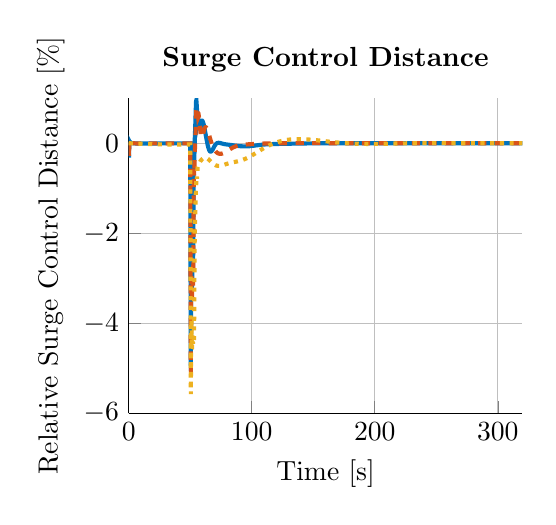
\begin{tikzpicture}

\begin{axis}[%
width=5cm,
height=4cm,
at={(0\linewidth,0\linewidth)},
scale only axis,
xmin=0,
xmax=320,
xlabel={Time [s]},
xmajorgrids,
ymin=-6,
ymax=1,
ylabel={Relative Surge Control Distance [\%]},
ymajorgrids,
axis background/.style={fill=white},
title style={font=\bfseries},
title={Surge Control Distance},
axis x line*=bottom,
axis y line*=left
]
\addplot [color=mycolor1,solid,line width=1.5pt,forget plot]
  table[row sep=crcr]{%
0	-0.0970099999999992\\
0.25	-0.31776\\
0.5	0.0485000000000007\\
% 0.75	0.0541400000000003\\
% 1	-0.00875999999999877\\
1.25	0.00740000000000052\\
1.5	0.01755\\
1.75	0.00960000000000072\\
2	0.00655000000000072\\
2.25	0.00689000000000028\\
2.5	0.00555000000000128\\
2.75	0.00388000000000055\\
3	0.0028100000000002\\
3.25	0.00186000000000064\\
3.5	0.000899999999999679\\
3.75	6.00000000012813e-05\\
4	-0.000669999999999504\\
4.25	-0.00131999999999977\\
4.5	-0.00190999999999875\\
4.75	-0.00244\\
5	-0.00292999999999921\\
5.25	-0.00337000000000032\\
5.5	-0.00376999999999938\\
5.75	-0.00411999999999857\\
6	-0.00441999999999965\\
6.25	-0.00467999999999869\\
6.5	-0.00488\\
6.75	-0.00503999999999927\\
7	-0.00514999999999866\\
7.25	-0.0052399999999988\\
7.5	-0.00530000000000008\\
7.75	-0.00534999999999997\\
8	-0.00539000000000023\\
8.25	-0.00541999999999909\\
8.5	-0.00544999999999973\\
8.75	-0.00545999999999935\\
9	-0.00546999999999898\\
9.25	-0.00545999999999935\\
9.5	-0.00544000000000011\\
9.75	-0.00539000000000023\\
10	-0.00532999999999895\\
10.25	-0.00526999999999944\\
10.5	-0.00520000000000032\\
10.75	-0.00512999999999941\\
11	-0.00506999999999991\\
11.25	-0.00500999999999863\\
11.5	-0.00497000000000014\\
11.75	-0.00492999999999988\\
12	-0.00488999999999962\\
12.25	-0.00484999999999935\\
12.5	-0.00479999999999947\\
12.75	-0.00474999999999959\\
13	-0.00469000000000008\\
13.25	-0.00461999999999918\\
13.5	-0.00455000000000005\\
13.75	-0.00448999999999877\\
14	-0.00443999999999889\\
14.25	-0.00439999999999863\\
14.5	-0.00436999999999976\\
14.75	-0.00433999999999912\\
15	-0.00431999999999988\\
15.25	-0.00429999999999886\\
15.5	-0.00427999999999962\\
15.75	-0.00424999999999898\\
16	-0.00420999999999871\\
16.25	-0.00417000000000023\\
16.5	-0.00412999999999997\\
16.75	-0.0040899999999997\\
17	-0.00404999999999944\\
17.25	-0.0040300000000002\\
17.5	-0.00400999999999918\\
17.75	-0.00399999999999956\\
18	-0.00398999999999994\\
18.25	-0.00398999999999994\\
18.5	-0.00398000000000032\\
18.75	-0.0039599999999993\\
19	-0.00394000000000005\\
19.25	-0.00390999999999941\\
19.5	-0.00387999999999877\\
19.75	-0.00384999999999991\\
20	-0.00381999999999927\\
20.25	-0.00380000000000003\\
20.5	-0.00378999999999863\\
20.75	-0.00377999999999901\\
21	-0.00377999999999901\\
21.25	-0.00377999999999901\\
21.5	-0.00376999999999938\\
21.75	-0.00375999999999976\\
22	-0.00373999999999874\\
22.25	-0.00370999999999988\\
22.5	-0.00367999999999924\\
22.75	-0.0036499999999986\\
23	-0.00362999999999936\\
23.25	-0.00361000000000011\\
23.5	-0.00358999999999909\\
23.75	-0.00358999999999909\\
24	-0.00357999999999947\\
24.25	-0.00357999999999947\\
24.5	-0.00356999999999985\\
24.75	-0.00356000000000023\\
25	-0.00353999999999921\\
25.25	-0.00351999999999997\\
25.5	-0.00348999999999933\\
25.75	-0.00345999999999869\\
26	-0.00342999999999982\\
26.25	-0.0034099999999988\\
26.5	-0.00339999999999918\\
26.75	-0.00338999999999956\\
27	-0.00338999999999956\\
27.25	-0.00337999999999994\\
27.5	-0.00337999999999994\\
27.75	-0.00337000000000032\\
28	-0.0033499999999993\\
28.25	-0.00333000000000006\\
28.5	-0.00329999999999941\\
28.75	-0.00326999999999877\\
29	-0.00324999999999953\\
29.25	-0.00323000000000029\\
29.5	-0.00320999999999927\\
29.75	-0.00320999999999927\\
30	-0.00319999999999965\\
30.25	-0.00320999999999927\\
30.5	-0.00319999999999965\\
30.75	-0.00319999999999965\\
31	-0.00317999999999863\\
31.25	-0.00316999999999901\\
31.5	-0.00314000000000014\\
31.75	-0.0031099999999995\\
32	-0.00309000000000026\\
32.25	-0.00306999999999924\\
32.5	-0.00305999999999962\\
32.75	-0.00305999999999962\\
33	-0.00305999999999962\\
33.25	-0.00305999999999962\\
33.5	-0.00306999999999924\\
33.75	-0.00305999999999962\\
34	-0.00305999999999962\\
34.25	-0.0030399999999986\\
34.5	-0.00301999999999936\\
34.75	-0.00300000000000011\\
35	-0.00296999999999947\\
35.25	-0.00295999999999985\\
35.5	-0.00295000000000023\\
35.75	-0.00295000000000023\\
36	-0.00295999999999985\\
36.25	-0.00295999999999985\\
36.5	-0.00296999999999947\\
36.75	-0.00296999999999947\\
37	-0.00296999999999947\\
37.25	-0.00295999999999985\\
37.5	-0.00293999999999883\\
37.75	-0.00291999999999959\\
38	-0.00289999999999857\\
38.25	-0.00288999999999895\\
38.5	-0.00287999999999933\\
38.75	-0.00287999999999933\\
39	-0.00288999999999895\\
39.25	-0.00290999999999997\\
39.5	-0.00291999999999959\\
39.75	-0.00292999999999921\\
40	-0.00291999999999959\\
40.25	-0.00290999999999997\\
40.5	-0.00289999999999857\\
40.75	-0.00287999999999933\\
41	-0.00286000000000008\\
41.25	-0.00284999999999869\\
41.5	-0.00284999999999869\\
41.75	-0.00284999999999869\\
42	-0.00286999999999971\\
42.25	-0.00287999999999933\\
42.5	-0.00289999999999857\\
42.75	-0.00290999999999997\\
43	-0.00290999999999997\\
43.25	-0.00289999999999857\\
43.5	-0.00288999999999895\\
43.75	-0.00286999999999971\\
44	-0.00284999999999869\\
44.25	-0.00283999999999907\\
44.5	-0.00283999999999907\\
44.75	-0.00284999999999869\\
45	-0.00286000000000008\\
45.25	-0.00288999999999895\\
45.5	-0.00290999999999997\\
45.75	-0.00291999999999959\\
46	-0.00291999999999959\\
46.25	-0.00290999999999997\\
46.5	-0.00289999999999857\\
46.75	-0.00287999999999933\\
47	-0.00286000000000008\\
47.25	-0.00284999999999869\\
47.5	-0.00284999999999869\\
47.75	-0.00286000000000008\\
48	-0.00287999999999933\\
48.25	-0.00290999999999997\\
48.5	-0.00292999999999921\\
48.75	-0.00293999999999883\\
49	-0.00295000000000023\\
49.25	-0.00293999999999883\\
49.5	-0.00291999999999959\\
49.75	-0.00289999999999857\\
50	-0.00287999999999933\\
50.25	-2.77916\\
50.5	-5.05865\\
50.75	-3.23165\\
51	-2.68995\\
51.25	-3.30532\\
51.5	-3.10962\\
51.75	-2.76589\\
52	-2.79788\\
52.25	-2.84727\\
52.5	-2.23862\\
52.75	-0.72666\\
53	-0.289249999999999\\
53.25	-0.39575\\
53.5	-0.128729999999999\\
53.75	0.138570000000001\\
54	0.309560000000001\\
54.25	0.51932\\
54.5	0.75141\\
54.75	0.92952\\
55	0.958270000000001\\
55.25	0.85941\\
55.5	0.747640000000001\\
55.75	0.572740000000001\\
56	0.471160000000001\\
56.25	0.511200000000001\\
56.5	0.53909\\
56.75	0.50972\\
57	0.481300000000001\\
57.25	0.467120000000001\\
57.5	0.45491\\
57.75	0.434140000000001\\
58	0.41464\\
58.25	0.41826\\
58.5	0.440330000000001\\
58.75	0.462670000000001\\
59	0.479850000000001\\
59.25	0.49292\\
59.5	0.500150000000001\\
59.75	0.499920000000001\\
60	0.49268\\
60.25	0.47955\\
60.5	0.461220000000001\\
60.75	0.438130000000001\\
61	0.410960000000001\\
61.25	0.380560000000001\\
61.5	0.347670000000001\\
61.75	0.31287\\
62	0.276670000000001\\
62.25	0.23958\\
62.5	0.20199\\
62.75	0.16431\\
63	0.126890000000001\\
63.25	0.090110000000001\\
63.5	0.054310000000001\\
63.75	0.0198499999999999\\
64	-0.012929999999999\\
64.25	-0.0437199999999986\\
64.5	-0.0721999999999987\\
64.75	-0.0980600000000003\\
65	-0.120999999999999\\
65.25	-0.14073\\
65.5	-0.15696\\
65.75	-0.169449999999999\\
66	-0.178139999999999\\
66.25	-0.183199999999999\\
66.5	-0.185099999999999\\
66.75	-0.184419999999999\\
67	-0.181539999999999\\
67.25	-0.176609999999999\\
67.5	-0.16968\\
67.75	-0.160889999999999\\
68	-0.15049\\
68.25	-0.138809999999999\\
68.5	-0.126189999999999\\
68.75	-0.113019999999999\\
69	-0.0996299999999994\\
69.25	-0.0863599999999991\\
69.5	-0.0734699999999986\\
69.75	-0.0612099999999991\\
70	-0.0497399999999999\\
70.25	-0.0392099999999989\\
70.5	-0.0297000000000001\\
70.75	-0.0212699999999995\\
71	-0.0139199999999988\\
71.25	-0.00765999999999956\\
71.5	-0.00244999999999962\\
71.75	0.00176000000000087\\
72	0.00505000000000067\\
72.25	0.00747000000000142\\
72.5	0.00912000000000113\\
72.75	0.0100700000000007\\
73	0.0104199999999999\\
73.25	0.0102400000000014\\
73.5	0.00961999999999996\\
73.75	0.00863999999999976\\
74	0.00735000000000063\\
74.25	0.00584000000000096\\
74.5	0.00415000000000099\\
74.75	0.00234000000000023\\
75	0.000460000000000349\\
75.25	-0.00146999999999942\\
75.5	-0.00339999999999918\\
75.75	-0.00531999999999933\\
76	-0.00718999999999959\\
76.25	-0.00899999999999856\\
76.5	-0.0107499999999998\\
76.75	-0.0124199999999988\\
77	-0.014009999999999\\
77.25	-0.015509999999999\\
77.5	-0.01694\\
77.75	-0.018279999999999\\
78	-0.0195499999999988\\
78.25	-0.0207499999999996\\
78.5	-0.0218799999999995\\
78.75	-0.0229599999999994\\
79	-0.0239899999999995\\
79.25	-0.0249699999999997\\
79.5	-0.0259099999999997\\
79.75	-0.0268299999999986\\
80	-0.0277199999999986\\
80.25	-0.0285999999999991\\
80.5	-0.0294600000000003\\
80.75	-0.0303100000000001\\
81	-0.0311599999999999\\
81.25	-0.0320099999999996\\
81.5	-0.0328699999999991\\
81.75	-0.0337300000000003\\
82	-0.0345899999999997\\
82.25	-0.0354700000000001\\
82.5	-0.0363600000000002\\
82.75	-0.0372599999999998\\
83	-0.0381599999999995\\
83.25	-0.0390800000000002\\
83.5	-0.0400099999999988\\
83.75	-0.0409499999999987\\
84	-0.0419\\
84.25	-0.0428599999999992\\
84.5	-0.0438200000000002\\
84.75	-0.044789999999999\\
85	-0.0457599999999996\\
85.25	-0.0467300000000002\\
85.5	-0.047699999999999\\
85.75	-0.0486799999999992\\
86	-0.0496400000000001\\
86.25	-0.0506099999999989\\
86.5	-0.0515600000000003\\
86.75	-0.0525099999999998\\
87	-0.0534400000000002\\
87.25	-0.0543699999999987\\
87.5	-0.0552799999999998\\
87.75	-0.0561699999999998\\
88	-0.0570500000000003\\
88.25	-0.0579099999999997\\
88.5	-0.0587499999999999\\
88.75	-0.059569999999999\\
89	-0.0603599999999993\\
89.25	-0.0611299999999986\\
89.5	-0.061869999999999\\
89.75	-0.0625799999999987\\
90	-0.0632599999999996\\
90.25	-0.0639199999999995\\
90.5	-0.0645399999999992\\
90.75	-0.0651299999999999\\
91	-0.06569\\
91.25	-0.0662099999999999\\
91.5	-0.0666899999999995\\
91.75	-0.0671400000000002\\
92	-0.0675499999999989\\
92.25	-0.0679199999999991\\
92.5	-0.068249999999999\\
92.75	-0.0685399999999987\\
93	-0.0687899999999999\\
93.25	-0.0690099999999987\\
93.5	-0.0691799999999994\\
93.75	-0.0693000000000001\\
94	-0.0693900000000003\\
94.25	-0.0694299999999988\\
94.5	-0.0694400000000002\\
94.75	-0.0693999999999999\\
95	-0.0693199999999994\\
95.25	-0.0691999999999986\\
95.5	-0.0690299999999997\\
95.75	-0.0688300000000002\\
96	-0.0685899999999986\\
96.25	-0.0682999999999989\\
96.5	-0.0679799999999986\\
96.75	-0.0676199999999998\\
97	-0.0672199999999989\\
97.25	-0.0667899999999992\\
97.5	-0.0663199999999993\\
97.75	-0.0658199999999987\\
98	-0.0652799999999996\\
98.25	-0.0647199999999994\\
98.5	-0.0641199999999991\\
98.75	-0.0634899999999998\\
99	-0.0628399999999996\\
99.25	-0.0621599999999987\\
99.5	-0.0614499999999989\\
99.75	-0.0607199999999999\\
100	-0.0599699999999999\\
100.25	-0.0591999999999988\\
100.5	-0.0584100000000003\\
100.75	-0.057599999999999\\
101	-0.0567799999999998\\
101.25	-0.0559399999999997\\
101.5	-0.0550899999999999\\
101.75	-0.0542299999999987\\
102	-0.0533599999999996\\
102.25	-0.0524799999999992\\
102.5	-0.0515999999999988\\
102.75	-0.0507099999999987\\
103	-0.0498199999999986\\
103.25	-0.048919999999999\\
103.5	-0.0480299999999989\\
103.75	-0.0471299999999992\\
104	-0.0462399999999992\\
104.25	-0.0453499999999991\\
104.5	-0.0444699999999987\\
104.75	-0.04359\\
105	-0.0427199999999992\\
105.25	-0.0418599999999998\\
105.5	-0.04101\\
105.75	-0.0401600000000002\\
106	-0.0393299999999996\\
106.25	-0.0385099999999987\\
106.5	-0.0376999999999992\\
106.75	-0.0369099999999989\\
107	-0.03613\\
107.25	-0.0353599999999989\\
107.5	-0.0346099999999989\\
107.75	-0.0338799999999999\\
108	-0.0331599999999987\\
108.25	-0.032449999999999\\
108.5	-0.0317699999999999\\
108.75	-0.0310999999999986\\
109	-0.0304500000000001\\
109.25	-0.0298199999999991\\
109.5	-0.0291999999999994\\
109.75	-0.0285999999999991\\
110	-0.0280199999999997\\
110.25	-0.0274599999999996\\
110.5	-0.0269099999999991\\
110.75	-0.0263899999999992\\
111	-0.025879999999999\\
111.25	-0.0253800000000002\\
111.5	-0.0249100000000002\\
111.75	-0.0244499999999999\\
112	-0.0239999999999991\\
112.25	-0.0235699999999994\\
112.5	-0.023159999999999\\
112.75	-0.0227599999999999\\
113	-0.0223800000000001\\
113.25	-0.0220099999999999\\
113.5	-0.0216599999999989\\
113.75	-0.0213199999999993\\
114	-0.0209899999999994\\
114.25	-0.0206799999999987\\
114.5	-0.0203699999999998\\
114.75	-0.0200800000000001\\
115	-0.0198\\
115.25	-0.0195399999999992\\
115.5	-0.0192800000000002\\
115.75	-0.019029999999999\\
116	-0.0187899999999992\\
116.25	-0.018559999999999\\
116.5	-0.0183400000000002\\
116.75	-0.0181199999999997\\
117	-0.0179200000000002\\
117.25	-0.0177199999999988\\
117.5	-0.0175199999999993\\
117.75	-0.017339999999999\\
118	-0.0171599999999987\\
118.25	-0.0169800000000002\\
118.5	-0.0168099999999995\\
118.75	-0.0166399999999989\\
119	-0.0164799999999996\\
119.25	-0.0163199999999986\\
119.5	-0.0161699999999989\\
119.75	-0.0160199999999993\\
120	-0.0158699999999996\\
120.25	-0.01572\\
120.5	-0.0155799999999999\\
120.75	-0.0154399999999999\\
121	-0.0152999999999999\\
121.25	-0.0151599999999998\\
121.5	-0.0150199999999998\\
121.75	-0.0148799999999998\\
122	-0.0147499999999994\\
122.25	-0.0146099999999993\\
122.5	-0.0144799999999989\\
122.75	-0.0143500000000003\\
123	-0.0142100000000003\\
123.25	-0.0140799999999999\\
123.5	-0.0139499999999995\\
123.75	-0.0138199999999991\\
124	-0.013679999999999\\
124.25	-0.0135499999999986\\
124.5	-0.01342\\
124.75	-0.01328\\
125	-0.0131499999999996\\
125.25	-0.0130099999999995\\
125.5	-0.0128799999999991\\
125.75	-0.0127399999999991\\
126	-0.0126099999999987\\
126.25	-0.0124699999999986\\
126.5	-0.0123299999999986\\
126.75	-0.0122\\
127	-0.01206\\
127.25	-0.0119199999999999\\
127.5	-0.0117799999999999\\
127.75	-0.0116399999999999\\
128	-0.0114999999999998\\
128.25	-0.0113599999999998\\
128.5	-0.0112199999999998\\
128.75	-0.0110799999999998\\
129	-0.0109399999999997\\
129.25	-0.0107900000000001\\
129.5	-0.01065\\
129.75	-0.01051\\
130	-0.01037\\
130.25	-0.01023\\
130.5	-0.0100800000000003\\
130.75	-0.00994000000000028\\
131	-0.00980000000000025\\
131.25	-0.00966000000000022\\
131.5	-0.00952000000000019\\
131.75	-0.00938000000000017\\
132	-0.00922999999999874\\
132.25	-0.00908999999999871\\
132.5	-0.00894999999999868\\
132.75	-0.00882000000000005\\
133	-0.00868000000000002\\
133.25	-0.00853999999999999\\
133.5	-0.00839999999999996\\
133.75	-0.00825999999999993\\
134	-0.00812999999999953\\
134.25	-0.0079899999999995\\
134.5	-0.00785999999999909\\
134.75	-0.00772999999999868\\
135	-0.00758999999999865\\
135.25	-0.00746000000000002\\
135.5	-0.00732999999999961\\
135.75	-0.00719999999999921\\
136	-0.0070800000000002\\
136.25	-0.00694999999999979\\
136.5	-0.00681999999999938\\
136.75	-0.0066999999999986\\
137	-0.00657999999999959\\
137.25	-0.0064599999999988\\
137.5	-0.00633999999999979\\
137.75	-0.006219999999999\\
138	-0.00609999999999999\\
138.25	-0.00597999999999921\\
138.5	-0.00586999999999982\\
138.75	-0.00574999999999903\\
139	-0.00563999999999965\\
139.25	-0.00553000000000026\\
139.5	-0.00541999999999909\\
139.75	-0.0053099999999997\\
140	-0.00520999999999994\\
140.25	-0.00509999999999877\\
140.5	-0.00499999999999901\\
140.75	-0.00489999999999924\\
141	-0.00479999999999947\\
141.25	-0.0046999999999997\\
141.5	-0.00459999999999994\\
141.75	-0.00450000000000017\\
142	-0.00441000000000003\\
142.25	-0.00431000000000026\\
142.5	-0.00422000000000011\\
142.75	-0.00412999999999997\\
143	-0.00403999999999982\\
143.25	-0.00394999999999968\\
143.5	-0.00386999999999915\\
143.75	-0.00377999999999901\\
144	-0.00370000000000026\\
144.25	-0.00361999999999973\\
144.5	-0.00353999999999921\\
144.75	-0.00345999999999869\\
145	-0.00337999999999994\\
145.25	-0.00329999999999941\\
145.5	-0.00321999999999889\\
145.75	-0.00314999999999976\\
146	-0.00306999999999924\\
146.25	-0.00300000000000011\\
146.5	-0.00292999999999921\\
146.75	-0.00286000000000008\\
147	-0.00278999999999918\\
147.25	-0.00272000000000006\\
147.5	-0.00264999999999915\\
147.75	-0.00258999999999965\\
148	-0.00251999999999875\\
148.25	-0.00245999999999924\\
148.5	-0.00239999999999974\\
148.75	-0.00232999999999883\\
149	-0.00226999999999933\\
149.25	-0.00220999999999982\\
149.5	-0.00215000000000032\\
149.75	-0.00209999999999866\\
150	-0.00203999999999915\\
150.25	-0.00197999999999965\\
150.5	-0.00192999999999977\\
150.75	-0.00187000000000026\\
151	-0.0018199999999986\\
151.25	-0.0017599999999991\\
151.5	-0.00170999999999921\\
151.75	-0.00165999999999933\\
152	-0.00160999999999945\\
152.25	-0.00155999999999956\\
152.5	-0.00150999999999968\\
152.75	-0.00145999999999979\\
153	-0.00140999999999991\\
153.25	-0.00136000000000003\\
153.5	-0.00131999999999977\\
153.75	-0.00126999999999988\\
154	-0.00122\\
154.25	-0.00117999999999974\\
154.5	-0.00112999999999985\\
154.75	-0.00108999999999959\\
155	-0.00104999999999933\\
155.25	-0.00100999999999907\\
155.5	-0.000959999999999184\\
155.75	-0.000919999999998922\\
156	-0.00087999999999866\\
156.25	-0.000840000000000174\\
156.5	-0.000799999999999912\\
156.75	-0.00075999999999965\\
157	-0.000719999999999388\\
157.25	-0.000679999999999126\\
157.5	-0.000650000000000261\\
157.75	-0.000609999999999999\\
158	-0.000569999999999737\\
158.25	-0.000539999999999097\\
158.5	-0.000499999999998835\\
158.75	-0.00046999999999997\\
159	-0.000429999999999708\\
159.25	-0.000399999999999068\\
159.5	-0.000359999999998806\\
159.75	-0.000329999999999941\\
160	-0.000299999999999301\\
160.25	-0.000259999999999039\\
160.5	-0.000230000000000175\\
160.75	-0.000199999999999534\\
161	-0.000169999999998893\\
161.25	-0.000140000000000029\\
161.5	-0.000109999999999388\\
161.75	-7.99999999987477e-05\\
162	-4.99999999998835e-05\\
162.25	-1.99999999992428e-05\\
162.5	1.00000000013978e-05\\
162.75	4.0000000000262e-05\\
163	7.00000000009027e-05\\
163.25	9.00000000001455e-05\\
163.5	0.000120000000000786\\
163.75	0.000150000000001427\\
164	0.00017000000000067\\
164.25	0.00020000000000131\\
164.5	0.000230000000000175\\
164.75	0.000250000000001194\\
165	0.000280000000000058\\
165.25	0.000300000000001077\\
165.5	0.00032000000000032\\
165.75	0.000350000000000961\\
166	0.000370000000000203\\
166.25	0.000390000000001223\\
166.5	0.000420000000000087\\
166.75	0.000440000000001106\\
167	0.000460000000000349\\
167.25	0.000480000000001368\\
167.5	0.000500000000000611\\
167.75	0.000519999999999854\\
168	0.000540000000000873\\
168.25	0.000560000000000116\\
168.5	0.000580000000001135\\
168.75	0.000600000000000378\\
169	0.000620000000001397\\
169.25	0.00064000000000064\\
169.5	0.000659999999999883\\
169.75	0.000670000000001281\\
170	0.000690000000000524\\
170.25	0.000709999999999766\\
170.5	0.000730000000000786\\
170.75	0.000740000000000407\\
171	0.000760000000001426\\
171.25	0.000770000000001048\\
171.5	0.00079000000000029\\
171.75	0.00081000000000131\\
172	0.000820000000000931\\
172.25	0.000830000000000553\\
172.5	0.000849999999999795\\
172.75	0.000860000000001193\\
173	0.000880000000000436\\
173.25	0.000890000000000057\\
173.5	0.000899999999999679\\
173.75	0.000920000000000698\\
174	0.000930000000000319\\
174.25	0.000939999999999941\\
174.5	0.000950000000001339\\
174.75	0.00096000000000096\\
175	0.000970000000000582\\
175.25	0.000989999999999824\\
175.5	0.00100000000000122\\
175.75	0.00101000000000084\\
176	0.00102000000000046\\
176.25	0.00103000000000009\\
176.5	0.00103999999999971\\
176.75	0.00105000000000111\\
177	0.00105000000000111\\
177.25	0.00106000000000073\\
177.5	0.00107000000000035\\
177.75	0.00107999999999997\\
178	0.00109000000000137\\
178.25	0.00110000000000099\\
178.5	0.00110000000000099\\
178.75	0.00111000000000061\\
179	0.00112000000000023\\
179.25	0.00112000000000023\\
179.5	0.00112999999999985\\
179.75	0.00114000000000125\\
180	0.00114000000000125\\
180.25	0.00115000000000087\\
180.5	0.00116000000000049\\
180.75	0.00116000000000049\\
181	0.00117000000000012\\
181.25	0.00117000000000012\\
181.5	0.00117999999999974\\
181.75	0.00117999999999974\\
182	0.00119000000000113\\
182.25	0.00119000000000113\\
182.5	0.00119000000000113\\
182.75	0.00120000000000076\\
183	0.00120000000000076\\
183.25	0.00120000000000076\\
183.5	0.00121000000000038\\
183.75	0.00121000000000038\\
184	0.00121000000000038\\
184.25	0.00122\\
184.5	0.00122\\
184.75	0.00122\\
185	0.00122\\
185.25	0.0012300000000014\\
185.5	0.0012300000000014\\
185.75	0.0012300000000014\\
186	0.0012300000000014\\
186.25	0.0012300000000014\\
186.5	0.0012300000000014\\
186.75	0.00124000000000102\\
187	0.00124000000000102\\
187.25	0.00124000000000102\\
187.5	0.00124000000000102\\
187.75	0.00124000000000102\\
188	0.00124000000000102\\
188.25	0.00124000000000102\\
188.5	0.00124000000000102\\
188.75	0.00124000000000102\\
189	0.00124000000000102\\
189.25	0.00124000000000102\\
189.5	0.00124000000000102\\
189.75	0.00124000000000102\\
190	0.00124000000000102\\
190.25	0.00124000000000102\\
190.5	0.00124000000000102\\
190.75	0.0012300000000014\\
191	0.0012300000000014\\
191.25	0.0012300000000014\\
191.5	0.0012300000000014\\
191.75	0.0012300000000014\\
192	0.0012300000000014\\
192.25	0.0012300000000014\\
192.5	0.00122\\
192.75	0.00122\\
193	0.00122\\
193.25	0.00122\\
193.5	0.00122\\
193.75	0.00121000000000038\\
194	0.00121000000000038\\
194.25	0.00121000000000038\\
194.5	0.00121000000000038\\
194.75	0.00120000000000076\\
195	0.00120000000000076\\
195.25	0.00120000000000076\\
195.5	0.00119000000000113\\
195.75	0.00119000000000113\\
196	0.00119000000000113\\
196.25	0.00117999999999974\\
196.5	0.00117999999999974\\
196.75	0.00117999999999974\\
197	0.00117000000000012\\
197.25	0.00117000000000012\\
197.5	0.00117000000000012\\
197.75	0.00116000000000049\\
198	0.00116000000000049\\
198.25	0.00116000000000049\\
198.5	0.00115000000000087\\
198.75	0.00115000000000087\\
199	0.00114000000000125\\
199.25	0.00114000000000125\\
199.5	0.00114000000000125\\
199.75	0.00112999999999985\\
200	0.00112999999999985\\
200.25	0.00112000000000023\\
200.5	0.00112000000000023\\
200.75	0.00111000000000061\\
201	0.00111000000000061\\
201.25	0.00111000000000061\\
201.5	0.00110000000000099\\
201.75	0.00110000000000099\\
202	0.00109000000000137\\
202.25	0.00109000000000137\\
202.5	0.00107999999999997\\
202.75	0.00107999999999997\\
203	0.00107000000000035\\
203.25	0.00107000000000035\\
203.5	0.00106000000000073\\
203.75	0.00106000000000073\\
204	0.00105000000000111\\
204.25	0.00105000000000111\\
204.5	0.00103999999999971\\
204.75	0.00103999999999971\\
205	0.00103000000000009\\
205.25	0.00103000000000009\\
205.5	0.00102000000000046\\
205.75	0.00102000000000046\\
206	0.00101000000000084\\
206.25	0.00101000000000084\\
206.5	0.00100000000000122\\
206.75	0.00100000000000122\\
207	0.000989999999999824\\
207.25	0.000980000000000203\\
207.5	0.000980000000000203\\
207.75	0.000970000000000582\\
208	0.000970000000000582\\
208.25	0.00096000000000096\\
208.5	0.00096000000000096\\
208.75	0.000950000000001339\\
209	0.000950000000001339\\
209.25	0.000939999999999941\\
209.5	0.000930000000000319\\
209.75	0.000930000000000319\\
210	0.000920000000000698\\
210.25	0.000920000000000698\\
210.5	0.000910000000001077\\
210.75	0.000910000000001077\\
211	0.000899999999999679\\
211.25	0.000890000000000057\\
211.5	0.000890000000000057\\
211.75	0.000880000000000436\\
212	0.000880000000000436\\
212.25	0.000870000000000815\\
212.5	0.000870000000000815\\
212.75	0.000860000000001193\\
213	0.000849999999999795\\
213.25	0.000849999999999795\\
213.5	0.000840000000000174\\
213.75	0.000840000000000174\\
214	0.000830000000000553\\
214.25	0.000830000000000553\\
214.5	0.000820000000000931\\
214.75	0.00081000000000131\\
215	0.00081000000000131\\
215.25	0.000799999999999912\\
215.5	0.000799999999999912\\
215.75	0.00079000000000029\\
216	0.000780000000000669\\
216.25	0.000780000000000669\\
216.5	0.000770000000001048\\
216.75	0.000770000000001048\\
217	0.000760000000001426\\
217.25	0.000760000000001426\\
217.5	0.000750000000000028\\
217.75	0.000740000000000407\\
218	0.000740000000000407\\
218.25	0.000730000000000786\\
218.5	0.000730000000000786\\
218.75	0.000720000000001164\\
219	0.000720000000001164\\
219.25	0.000709999999999766\\
219.5	0.000700000000000145\\
219.75	0.000700000000000145\\
220	0.000690000000000524\\
220.25	0.000690000000000524\\
220.5	0.000680000000000902\\
220.75	0.000680000000000902\\
221	0.000670000000001281\\
221.25	0.000659999999999883\\
221.5	0.000659999999999883\\
221.75	0.000650000000000261\\
222	0.000650000000000261\\
222.25	0.00064000000000064\\
222.5	0.00064000000000064\\
222.75	0.000630000000001019\\
223	0.000630000000001019\\
223.25	0.000620000000001397\\
223.5	0.000620000000001397\\
223.75	0.000609999999999999\\
224	0.000600000000000378\\
224.25	0.000600000000000378\\
224.5	0.000590000000000757\\
224.75	0.000590000000000757\\
225	0.000580000000001135\\
225.25	0.000580000000001135\\
225.5	0.000569999999999737\\
225.75	0.000569999999999737\\
226	0.000560000000000116\\
226.25	0.000560000000000116\\
226.5	0.000550000000000495\\
226.75	0.000550000000000495\\
227	0.000540000000000873\\
227.25	0.000540000000000873\\
227.5	0.000530000000001252\\
227.75	0.000530000000001252\\
228	0.000519999999999854\\
228.25	0.000510000000000232\\
228.5	0.000510000000000232\\
228.75	0.000500000000000611\\
229	0.000500000000000611\\
229.25	0.00049000000000099\\
229.5	0.00049000000000099\\
229.75	0.000480000000001368\\
230	0.000480000000001368\\
230.25	0.000480000000001368\\
230.5	0.00046999999999997\\
230.75	0.00046999999999997\\
231	0.000460000000000349\\
231.25	0.000460000000000349\\
231.5	0.000450000000000728\\
231.75	0.000450000000000728\\
232	0.000440000000001106\\
232.25	0.000440000000001106\\
232.5	0.000429999999999708\\
232.75	0.000429999999999708\\
233	0.000420000000000087\\
233.25	0.000420000000000087\\
233.5	0.000410000000000466\\
233.75	0.000410000000000466\\
234	0.000400000000000844\\
234.25	0.000400000000000844\\
234.5	0.000400000000000844\\
234.75	0.000390000000001223\\
235	0.000390000000001223\\
235.25	0.000379999999999825\\
235.5	0.000379999999999825\\
235.75	0.000370000000000203\\
236	0.000370000000000203\\
236.25	0.000370000000000203\\
236.5	0.000360000000000582\\
236.75	0.000360000000000582\\
237	0.000350000000000961\\
237.25	0.000350000000000961\\
237.5	0.000340000000001339\\
237.75	0.000340000000001339\\
238	0.000340000000001339\\
238.25	0.000329999999999941\\
238.5	0.000329999999999941\\
238.75	0.00032000000000032\\
239	0.00032000000000032\\
239.25	0.00032000000000032\\
239.5	0.000310000000000699\\
239.75	0.000310000000000699\\
240	0.000300000000001077\\
240.25	0.000300000000001077\\
240.5	0.000300000000001077\\
240.75	0.000289999999999679\\
241	0.000289999999999679\\
241.25	0.000289999999999679\\
241.5	0.000280000000000058\\
241.75	0.000280000000000058\\
242	0.000270000000000437\\
242.25	0.000270000000000437\\
242.5	0.000270000000000437\\
242.75	0.000260000000000815\\
243	0.000260000000000815\\
243.25	0.000260000000000815\\
243.5	0.000250000000001194\\
243.75	0.000250000000001194\\
244	0.000250000000001194\\
244.25	0.000239999999999796\\
244.5	0.000239999999999796\\
244.75	0.000239999999999796\\
245	0.000230000000000175\\
245.25	0.000230000000000175\\
245.5	0.000230000000000175\\
245.75	0.000220000000000553\\
246	0.000220000000000553\\
246.25	0.000220000000000553\\
246.5	0.000210000000000932\\
246.75	0.000210000000000932\\
247	0.000210000000000932\\
247.25	0.00020000000000131\\
247.5	0.00020000000000131\\
247.75	0.00020000000000131\\
248	0.00020000000000131\\
248.25	0.000189999999999912\\
248.5	0.000189999999999912\\
248.75	0.000189999999999912\\
249	0.000180000000000291\\
249.25	0.000180000000000291\\
249.5	0.000180000000000291\\
249.75	0.000180000000000291\\
250	0.00017000000000067\\
250.25	0.00017000000000067\\
250.5	0.00017000000000067\\
250.75	0.000160000000001048\\
251	0.000160000000001048\\
251.25	0.000160000000001048\\
251.5	0.000160000000001048\\
251.75	0.000150000000001427\\
252	0.000150000000001427\\
252.25	0.000150000000001427\\
252.5	0.000150000000001427\\
252.75	0.000140000000000029\\
253	0.000140000000000029\\
253.25	0.000140000000000029\\
253.5	0.000140000000000029\\
253.75	0.000130000000000408\\
254	0.000130000000000408\\
254.25	0.000130000000000408\\
254.5	0.000130000000000408\\
254.75	0.000120000000000786\\
255	0.000120000000000786\\
255.25	0.000120000000000786\\
255.5	0.000120000000000786\\
255.75	0.000120000000000786\\
256	0.000110000000001165\\
256.25	0.000110000000001165\\
256.5	0.000110000000001165\\
256.75	0.000110000000001165\\
257	9.99999999997669e-05\\
257.25	9.99999999997669e-05\\
257.5	9.99999999997669e-05\\
257.75	9.99999999997669e-05\\
258	9.99999999997669e-05\\
258.25	9.00000000001455e-05\\
258.5	9.00000000001455e-05\\
258.75	9.00000000001455e-05\\
259	9.00000000001455e-05\\
259.25	9.00000000001455e-05\\
259.5	8.00000000005241e-05\\
259.75	8.00000000005241e-05\\
260	8.00000000005241e-05\\
260.25	8.00000000005241e-05\\
260.5	8.00000000005241e-05\\
260.75	8.00000000005241e-05\\
261	7.00000000009027e-05\\
261.25	7.00000000009027e-05\\
261.5	7.00000000009027e-05\\
261.75	7.00000000009027e-05\\
262	7.00000000009027e-05\\
262.25	7.00000000009027e-05\\
262.5	6.00000000012813e-05\\
262.75	6.00000000012813e-05\\
263	6.00000000012813e-05\\
263.25	6.00000000012813e-05\\
263.5	6.00000000012813e-05\\
263.75	6.00000000012813e-05\\
264	4.99999999998835e-05\\
264.25	4.99999999998835e-05\\
264.5	4.99999999998835e-05\\
264.75	4.99999999998835e-05\\
265	4.99999999998835e-05\\
265.25	4.99999999998835e-05\\
265.5	4.99999999998835e-05\\
265.75	4.0000000000262e-05\\
266	4.0000000000262e-05\\
266.25	4.0000000000262e-05\\
266.5	4.0000000000262e-05\\
266.75	4.0000000000262e-05\\
267	4.0000000000262e-05\\
267.25	4.0000000000262e-05\\
267.5	3.00000000006406e-05\\
267.75	3.00000000006406e-05\\
268	3.00000000006406e-05\\
268.25	3.00000000006406e-05\\
268.5	3.00000000006406e-05\\
268.75	3.00000000006406e-05\\
269	3.00000000006406e-05\\
269.25	3.00000000006406e-05\\
269.5	2.00000000010192e-05\\
269.75	2.00000000010192e-05\\
270	2.00000000010192e-05\\
270.25	2.00000000010192e-05\\
270.5	2.00000000010192e-05\\
270.75	2.00000000010192e-05\\
271	2.00000000010192e-05\\
271.25	2.00000000010192e-05\\
271.5	2.00000000010192e-05\\
271.75	2.00000000010192e-05\\
272	1.00000000013978e-05\\
272.25	1.00000000013978e-05\\
272.5	1.00000000013978e-05\\
272.75	1.00000000013978e-05\\
273	1.00000000013978e-05\\
273.25	1.00000000013978e-05\\
273.5	1.00000000013978e-05\\
273.75	1.00000000013978e-05\\
274	1.00000000013978e-05\\
274.25	1.00000000013978e-05\\
274.5	0\\
274.75	0\\
275	0\\
275.25	0\\
275.5	0\\
275.75	0\\
276	0\\
276.25	0\\
276.5	0\\
276.75	0\\
277	0\\
277.25	0\\
277.5	0\\
277.75	0\\
278	-9.99999999962142e-06\\
278.25	-9.99999999962142e-06\\
278.5	-9.99999999962142e-06\\
278.75	-9.99999999962142e-06\\
279	-9.99999999962142e-06\\
279.25	-9.99999999962142e-06\\
279.5	-9.99999999962142e-06\\
279.75	-9.99999999962142e-06\\
280	-9.99999999962142e-06\\
280.25	-9.99999999962142e-06\\
280.5	-9.99999999962142e-06\\
280.75	-9.99999999962142e-06\\
281	-9.99999999962142e-06\\
281.25	-9.99999999962142e-06\\
281.5	-9.99999999962142e-06\\
281.75	-9.99999999962142e-06\\
282	-9.99999999962142e-06\\
282.25	-1.99999999992428e-05\\
282.5	-1.99999999992428e-05\\
282.75	-1.99999999992428e-05\\
283	-1.99999999992428e-05\\
283.25	-1.99999999992428e-05\\
283.5	-1.99999999992428e-05\\
283.75	-1.99999999992428e-05\\
284	-1.99999999992428e-05\\
284.25	-1.99999999992428e-05\\
284.5	-1.99999999992428e-05\\
284.75	-1.99999999992428e-05\\
285	-1.99999999992428e-05\\
285.25	-1.99999999992428e-05\\
285.5	-1.99999999992428e-05\\
285.75	-1.99999999992428e-05\\
286	-1.99999999992428e-05\\
286.25	-1.99999999992428e-05\\
286.5	-1.99999999992428e-05\\
286.75	-1.99999999992428e-05\\
287	-1.99999999992428e-05\\
287.25	-1.99999999992428e-05\\
287.5	-1.99999999992428e-05\\
287.75	-1.99999999992428e-05\\
288	-1.99999999992428e-05\\
288.25	-1.99999999992428e-05\\
288.5	-1.99999999992428e-05\\
288.75	-2.99999999988643e-05\\
289	-2.99999999988643e-05\\
289.25	-2.99999999988643e-05\\
289.5	-2.99999999988643e-05\\
289.75	-2.99999999988643e-05\\
290	-2.99999999988643e-05\\
290.25	-2.99999999988643e-05\\
290.5	-2.99999999988643e-05\\
290.75	-2.99999999988643e-05\\
291	-2.99999999988643e-05\\
291.25	-2.99999999988643e-05\\
291.5	-2.99999999988643e-05\\
291.75	-2.99999999988643e-05\\
292	-2.99999999988643e-05\\
292.25	-2.99999999988643e-05\\
292.5	-2.99999999988643e-05\\
292.75	-2.99999999988643e-05\\
293	-2.99999999988643e-05\\
293.25	-2.99999999988643e-05\\
293.5	-2.99999999988643e-05\\
293.75	-2.99999999988643e-05\\
294	-2.99999999988643e-05\\
294.25	-2.99999999988643e-05\\
294.5	-2.99999999988643e-05\\
294.75	-2.99999999988643e-05\\
295	-2.99999999988643e-05\\
295.25	-2.99999999988643e-05\\
295.5	-2.99999999988643e-05\\
295.75	-2.99999999988643e-05\\
296	-2.99999999988643e-05\\
296.25	-2.99999999988643e-05\\
296.5	-2.99999999988643e-05\\
296.75	-2.99999999988643e-05\\
297	-2.99999999988643e-05\\
297.25	-2.99999999988643e-05\\
297.5	-2.99999999988643e-05\\
297.75	-2.99999999988643e-05\\
298	-2.99999999988643e-05\\
298.25	-2.99999999988643e-05\\
298.5	-2.99999999988643e-05\\
298.75	-2.99999999988643e-05\\
299	-2.99999999988643e-05\\
299.25	-2.99999999988643e-05\\
299.5	-2.99999999988643e-05\\
299.75	-2.99999999988643e-05\\
300	-2.99999999988643e-05\\
300.25	-2.99999999988643e-05\\
300.5	-2.99999999988643e-05\\
300.75	-2.99999999988643e-05\\
301	-2.99999999988643e-05\\
301.25	-2.99999999988643e-05\\
301.5	-2.99999999988643e-05\\
301.75	-2.99999999988643e-05\\
302	-2.99999999988643e-05\\
302.25	-2.99999999988643e-05\\
302.5	-2.99999999988643e-05\\
302.75	-2.99999999988643e-05\\
303	-2.99999999988643e-05\\
303.25	-2.99999999988643e-05\\
303.5	-2.99999999988643e-05\\
303.75	-2.99999999988643e-05\\
304	-2.99999999988643e-05\\
304.25	-2.99999999988643e-05\\
304.5	-2.99999999988643e-05\\
304.75	-2.99999999988643e-05\\
305	-2.99999999988643e-05\\
305.25	-2.99999999988643e-05\\
305.5	-2.99999999988643e-05\\
305.75	-2.99999999988643e-05\\
306	-2.99999999988643e-05\\
306.25	-2.99999999988643e-05\\
306.5	-2.99999999988643e-05\\
306.75	-2.99999999988643e-05\\
307	-2.99999999988643e-05\\
307.25	-2.99999999988643e-05\\
307.5	-2.99999999988643e-05\\
307.75	-2.99999999988643e-05\\
308	-2.99999999988643e-05\\
308.25	-2.99999999988643e-05\\
308.5	-2.99999999988643e-05\\
308.75	-2.99999999988643e-05\\
309	-2.99999999988643e-05\\
309.25	-2.99999999988643e-05\\
309.5	-2.99999999988643e-05\\
309.75	-2.99999999988643e-05\\
310	-2.99999999988643e-05\\
310.25	-2.99999999988643e-05\\
310.5	-2.99999999988643e-05\\
310.75	-2.99999999988643e-05\\
311	-2.99999999988643e-05\\
311.25	-2.99999999988643e-05\\
311.5	-2.99999999988643e-05\\
311.75	-2.99999999988643e-05\\
312	-2.99999999988643e-05\\
312.25	-2.99999999988643e-05\\
312.5	-2.99999999988643e-05\\
312.75	-2.99999999988643e-05\\
313	-2.99999999988643e-05\\
313.25	-2.99999999988643e-05\\
313.5	-2.99999999988643e-05\\
313.75	-2.99999999988643e-05\\
314	-2.99999999988643e-05\\
314.25	-2.99999999988643e-05\\
314.5	-2.99999999988643e-05\\
314.75	-2.99999999988643e-05\\
315	-2.99999999988643e-05\\
315.25	-2.99999999988643e-05\\
315.5	-2.99999999988643e-05\\
315.75	-2.99999999988643e-05\\
316	-2.99999999988643e-05\\
316.25	-2.99999999988643e-05\\
316.5	-2.99999999988643e-05\\
316.75	-2.99999999988643e-05\\
317	-2.99999999988643e-05\\
317.25	-2.99999999988643e-05\\
317.5	-2.99999999988643e-05\\
317.75	-2.99999999988643e-05\\
318	-2.99999999988643e-05\\
318.25	-2.99999999988643e-05\\
318.5	-1.99999999992428e-05\\
318.75	-1.99999999992428e-05\\
319	-1.99999999992428e-05\\
319.25	-1.99999999992428e-05\\
319.5	-1.99999999992428e-05\\
319.75	-1.99999999992428e-05\\
320	-1.99999999992428e-05\\
320.25	-1.99999999992428e-05\\
320.5	-1.99999999992428e-05\\
320.75	-1.99999999992428e-05\\
321	-1.99999999992428e-05\\
321.25	-1.99999999992428e-05\\
321.5	-1.99999999992428e-05\\
321.75	-1.99999999992428e-05\\
322	-1.99999999992428e-05\\
322.25	-1.99999999992428e-05\\
322.5	-1.99999999992428e-05\\
322.75	-1.99999999992428e-05\\
323	-1.99999999992428e-05\\
323.25	-1.99999999992428e-05\\
323.5	-1.99999999992428e-05\\
323.75	-1.99999999992428e-05\\
324	-1.99999999992428e-05\\
324.25	-1.99999999992428e-05\\
324.5	-1.99999999992428e-05\\
324.75	-1.99999999992428e-05\\
325	-1.99999999992428e-05\\
325.25	-1.99999999992428e-05\\
325.5	-1.99999999992428e-05\\
325.75	-1.99999999992428e-05\\
326	-1.99999999992428e-05\\
326.25	-1.99999999992428e-05\\
326.5	-1.99999999992428e-05\\
326.75	-1.99999999992428e-05\\
327	-1.99999999992428e-05\\
327.25	-1.99999999992428e-05\\
327.5	-1.99999999992428e-05\\
327.75	-1.99999999992428e-05\\
328	-1.99999999992428e-05\\
328.25	-1.99999999992428e-05\\
328.5	-1.99999999992428e-05\\
328.75	-1.99999999992428e-05\\
329	-1.99999999992428e-05\\
329.25	-1.99999999992428e-05\\
329.5	-1.99999999992428e-05\\
329.75	-1.99999999992428e-05\\
330	-1.99999999992428e-05\\
330.25	-1.99999999992428e-05\\
330.5	-1.99999999992428e-05\\
330.75	-1.99999999992428e-05\\
331	-1.99999999992428e-05\\
331.25	-1.99999999992428e-05\\
331.5	-1.99999999992428e-05\\
331.75	-1.99999999992428e-05\\
332	-1.99999999992428e-05\\
332.25	-1.99999999992428e-05\\
332.5	-1.99999999992428e-05\\
332.75	-1.99999999992428e-05\\
333	-1.99999999992428e-05\\
333.25	-1.99999999992428e-05\\
333.5	-1.99999999992428e-05\\
333.75	-1.99999999992428e-05\\
334	-1.99999999992428e-05\\
334.25	-1.99999999992428e-05\\
334.5	-1.99999999992428e-05\\
334.75	-1.99999999992428e-05\\
335	-1.99999999992428e-05\\
335.25	-1.99999999992428e-05\\
335.5	-1.99999999992428e-05\\
335.75	-1.99999999992428e-05\\
336	-9.99999999962142e-06\\
336.25	-9.99999999962142e-06\\
336.5	-9.99999999962142e-06\\
336.75	-9.99999999962142e-06\\
337	-9.99999999962142e-06\\
337.25	-9.99999999962142e-06\\
337.5	-9.99999999962142e-06\\
337.75	-9.99999999962142e-06\\
338	-9.99999999962142e-06\\
338.25	-9.99999999962142e-06\\
338.5	-9.99999999962142e-06\\
338.75	-9.99999999962142e-06\\
339	-9.99999999962142e-06\\
339.25	-9.99999999962142e-06\\
339.5	-9.99999999962142e-06\\
339.75	-9.99999999962142e-06\\
340	-9.99999999962142e-06\\
340.25	-9.99999999962142e-06\\
340.5	-9.99999999962142e-06\\
340.75	-9.99999999962142e-06\\
341	-9.99999999962142e-06\\
341.25	-9.99999999962142e-06\\
341.5	-9.99999999962142e-06\\
341.75	-9.99999999962142e-06\\
342	-9.99999999962142e-06\\
342.25	-9.99999999962142e-06\\
342.5	-9.99999999962142e-06\\
342.75	-9.99999999962142e-06\\
343	-9.99999999962142e-06\\
343.25	-9.99999999962142e-06\\
343.5	-9.99999999962142e-06\\
343.75	-9.99999999962142e-06\\
344	-9.99999999962142e-06\\
344.25	-9.99999999962142e-06\\
344.5	-9.99999999962142e-06\\
344.75	-9.99999999962142e-06\\
345	-9.99999999962142e-06\\
345.25	-9.99999999962142e-06\\
345.5	-9.99999999962142e-06\\
345.75	-9.99999999962142e-06\\
346	-9.99999999962142e-06\\
346.25	-9.99999999962142e-06\\
346.5	-9.99999999962142e-06\\
346.75	-9.99999999962142e-06\\
347	-9.99999999962142e-06\\
347.25	-9.99999999962142e-06\\
347.5	-9.99999999962142e-06\\
347.75	-9.99999999962142e-06\\
348	-9.99999999962142e-06\\
348.25	-9.99999999962142e-06\\
348.5	-9.99999999962142e-06\\
348.75	-9.99999999962142e-06\\
349	-9.99999999962142e-06\\
349.25	-9.99999999962142e-06\\
349.5	-9.99999999962142e-06\\
349.75	-9.99999999962142e-06\\
350	-9.99999999962142e-06\\
350.25	-9.99999999962142e-06\\
350.5	-9.99999999962142e-06\\
350.75	-9.99999999962142e-06\\
351	-9.99999999962142e-06\\
351.25	-9.99999999962142e-06\\
351.5	-9.99999999962142e-06\\
351.75	-9.99999999962142e-06\\
352	-9.99999999962142e-06\\
352.25	-9.99999999962142e-06\\
352.5	-9.99999999962142e-06\\
352.75	-9.99999999962142e-06\\
353	-9.99999999962142e-06\\
353.25	-9.99999999962142e-06\\
353.5	-9.99999999962142e-06\\
353.75	-9.99999999962142e-06\\
354	-9.99999999962142e-06\\
354.25	-9.99999999962142e-06\\
354.5	-9.99999999962142e-06\\
354.75	-9.99999999962142e-06\\
355	-9.99999999962142e-06\\
355.25	-9.99999999962142e-06\\
355.5	-9.99999999962142e-06\\
355.75	-9.99999999962142e-06\\
356	-9.99999999962142e-06\\
356.25	-9.99999999962142e-06\\
356.5	-9.99999999962142e-06\\
356.75	-9.99999999962142e-06\\
357	-9.99999999962142e-06\\
357.25	-9.99999999962142e-06\\
357.5	-9.99999999962142e-06\\
357.75	-9.99999999962142e-06\\
358	-9.99999999962142e-06\\
358.25	-9.99999999962142e-06\\
358.5	-9.99999999962142e-06\\
358.75	-9.99999999962142e-06\\
359	-9.99999999962142e-06\\
359.25	-9.99999999962142e-06\\
359.5	0\\
359.75	0\\
360	0\\
360.25	0\\
360.5	0\\
360.75	0\\
361	0\\
361.25	0\\
361.5	0\\
361.75	0\\
362	0\\
362.25	0\\
362.5	0\\
362.75	0\\
363	0\\
363.25	0\\
363.5	0\\
363.75	0\\
364	0\\
364.25	0\\
364.5	0\\
364.75	0\\
365	0\\
365.25	0\\
365.5	0\\
365.75	0\\
366	0\\
366.25	0\\
366.5	0\\
366.75	0\\
367	0\\
367.25	0\\
367.5	0\\
367.75	0\\
368	0\\
368.25	0\\
368.5	0\\
368.75	0\\
369	0\\
369.25	0\\
369.5	0\\
369.75	0\\
370	0\\
370.25	0\\
370.5	0\\
370.75	0\\
371	0\\
371.25	0\\
371.5	0\\
371.75	0\\
372	0\\
372.25	0\\
372.5	0\\
372.75	0\\
373	0\\
373.25	0\\
373.5	0\\
373.75	0\\
374	0\\
374.25	0\\
374.5	0\\
374.75	0\\
375	0\\
375.25	0\\
375.5	0\\
375.75	0\\
376	0\\
376.25	0\\
376.5	0\\
376.75	0\\
377	0\\
377.25	0\\
377.5	0\\
377.75	0\\
378	0\\
378.25	0\\
378.5	0\\
378.75	0\\
379	0\\
379.25	0\\
379.5	0\\
379.75	0\\
380	0\\
380.25	0\\
380.5	0\\
380.75	0\\
381	0\\
381.25	0\\
381.5	0\\
381.75	0\\
382	0\\
382.25	0\\
382.5	0\\
382.75	0\\
383	0\\
383.25	0\\
383.5	0\\
383.75	0\\
384	0\\
384.25	0\\
384.5	0\\
384.75	0\\
385	0\\
385.25	0\\
385.5	0\\
385.75	0\\
386	0\\
386.25	0\\
386.5	0\\
386.75	0\\
387	0\\
387.25	0\\
387.5	0\\
387.75	0\\
388	0\\
388.25	0\\
388.5	0\\
388.75	0\\
389	0\\
389.25	0\\
389.5	0\\
389.75	0\\
390	0\\
390.25	0\\
390.5	0\\
390.75	0\\
391	0\\
391.25	0\\
391.5	0\\
391.75	0\\
392	0\\
392.25	0\\
392.5	0\\
392.75	0\\
393	0\\
393.25	0\\
393.5	0\\
393.75	0\\
394	0\\
394.25	0\\
394.5	0\\
394.75	0\\
395	0\\
395.25	0\\
395.5	0\\
395.75	0\\
396	0\\
396.25	0\\
396.5	0\\
396.75	0\\
397	0\\
397.25	0\\
397.5	0\\
397.75	0\\
398	0\\
398.25	0\\
398.5	0\\
398.75	0\\
399	0\\
399.25	0\\
399.5	0\\
399.75	0\\
400	0\\
400.25	0\\
400.5	0\\
400.75	0\\
401	0\\
401.25	0\\
401.5	0\\
401.75	0\\
402	0\\
402.25	0\\
402.5	0\\
402.75	0\\
403	0\\
403.25	0\\
403.5	0\\
403.75	0\\
404	0\\
404.25	0\\
404.5	0\\
404.75	0\\
405	0\\
405.25	0\\
405.5	0\\
405.75	0\\
406	0\\
406.25	0\\
406.5	0\\
406.75	0\\
407	0\\
407.25	0\\
407.5	0\\
407.75	0\\
408	0\\
408.25	0\\
408.5	0\\
408.75	0\\
409	0\\
409.25	0\\
409.5	0\\
409.75	0\\
410	0\\
410.25	0\\
410.5	0\\
410.75	0\\
411	0\\
411.25	0\\
411.5	0\\
411.75	0\\
412	0\\
412.25	0\\
412.5	0\\
412.75	0\\
413	0\\
413.25	0\\
413.5	0\\
413.75	0\\
414	0\\
414.25	0\\
414.5	0\\
414.75	0\\
415	0\\
415.25	0\\
415.5	0\\
415.75	0\\
416	0\\
416.25	0\\
416.5	0\\
416.75	0\\
417	0\\
417.25	0\\
417.5	0\\
417.75	0\\
418	0\\
418.25	0\\
418.5	0\\
418.75	0\\
419	0\\
419.25	0\\
419.5	0\\
419.75	0\\
420	0\\
420.25	0\\
420.5	0\\
420.75	0\\
421	0\\
421.25	0\\
421.5	0\\
421.75	0\\
422	0\\
422.25	0\\
422.5	0\\
422.75	0\\
423	0\\
423.25	0\\
423.5	0\\
423.75	0\\
424	0\\
424.25	0\\
424.5	0\\
424.75	0\\
425	0\\
425.25	0\\
425.5	0\\
425.75	0\\
426	0\\
426.25	0\\
426.5	0\\
426.75	0\\
427	0\\
427.25	0\\
427.5	0\\
427.75	0\\
428	0\\
428.25	0\\
428.5	0\\
428.75	0\\
429	0\\
429.25	0\\
429.5	0\\
429.75	0\\
430	0\\
430.25	0\\
430.5	0\\
430.75	0\\
431	0\\
431.25	0\\
431.5	0\\
431.75	0\\
432	0\\
432.25	0\\
432.5	0\\
432.75	0\\
433	0\\
433.25	0\\
433.5	0\\
433.75	0\\
434	0\\
434.25	0\\
434.5	0\\
434.75	0\\
435	0\\
435.25	0\\
435.5	0\\
435.75	0\\
436	0\\
436.25	0\\
436.5	0\\
436.75	0\\
437	0\\
437.25	0\\
437.5	0\\
437.75	0\\
438	0\\
438.25	0\\
438.5	0\\
438.75	0\\
439	0\\
439.25	0\\
439.5	0\\
439.75	0\\
440	0\\
440.25	0\\
440.5	0\\
440.75	0\\
441	0\\
441.25	0\\
441.5	0\\
441.75	0\\
442	0\\
442.25	0\\
442.5	0\\
442.75	0\\
443	0\\
443.25	0\\
443.5	0\\
443.75	0\\
444	0\\
444.25	0\\
444.5	0\\
444.75	0\\
445	0\\
445.25	0\\
445.5	0\\
445.75	0\\
446	0\\
446.25	0\\
446.5	0\\
446.75	0\\
447	0\\
447.25	0\\
447.5	0\\
447.75	0\\
448	0\\
448.25	0\\
448.5	0\\
448.75	0\\
449	0\\
449.25	0\\
449.5	0\\
449.75	0\\
450	0\\
450.25	0\\
450.5	0\\
450.75	0\\
451	0\\
451.25	0\\
451.5	0\\
451.75	0\\
452	0\\
452.25	0\\
452.5	0\\
452.75	0\\
453	0\\
453.25	0\\
453.5	0\\
453.75	0\\
454	0\\
454.25	0\\
454.5	0\\
454.75	0\\
455	0\\
455.25	0\\
455.5	0\\
455.75	0\\
456	0\\
456.25	0\\
456.5	0\\
456.75	0\\
457	0\\
457.25	0\\
457.5	0\\
457.75	0\\
458	0\\
458.25	0\\
458.5	0\\
458.75	0\\
459	0\\
459.25	0\\
459.5	0\\
459.75	0\\
460	0\\
460.25	0\\
460.5	0\\
460.75	0\\
461	0\\
461.25	0\\
461.5	0\\
461.75	0\\
462	0\\
462.25	0\\
462.5	0\\
462.75	0\\
463	0\\
463.25	0\\
463.5	0\\
463.75	0\\
464	0\\
464.25	0\\
464.5	0\\
464.75	0\\
465	0\\
465.25	0\\
465.5	0\\
465.75	0\\
466	0\\
466.25	0\\
466.5	0\\
466.75	0\\
467	0\\
467.25	0\\
467.5	0\\
467.75	0\\
468	0\\
468.25	0\\
468.5	0\\
468.75	0\\
469	0\\
469.25	0\\
469.5	0\\
469.75	0\\
470	0\\
470.25	0\\
470.5	0\\
470.75	0\\
471	0\\
471.25	0\\
471.5	0\\
471.75	0\\
472	0\\
472.25	0\\
472.5	0\\
472.75	0\\
473	0\\
473.25	0\\
473.5	0\\
473.75	0\\
474	0\\
474.25	0\\
474.5	0\\
474.75	0\\
475	0\\
475.25	0\\
475.5	0\\
475.75	0\\
476	0\\
476.25	0\\
476.5	0\\
476.75	0\\
477	0\\
477.25	0\\
477.5	0\\
477.75	0\\
478	0\\
478.25	0\\
478.5	0\\
478.75	0\\
479	0\\
479.25	0\\
479.5	0\\
479.75	0\\
480	0\\
480.25	0\\
480.5	0\\
480.75	0\\
481	0\\
481.25	0\\
481.5	0\\
481.75	0\\
482	0\\
482.25	0\\
482.5	0\\
482.75	0\\
483	0\\
483.25	0\\
483.5	0\\
483.75	0\\
484	0\\
484.25	0\\
484.5	0\\
484.75	0\\
485	0\\
485.25	0\\
485.5	0\\
485.75	0\\
486	0\\
486.25	0\\
486.5	0\\
486.75	0\\
487	0\\
487.25	0\\
487.5	0\\
487.75	0\\
488	0\\
488.25	0\\
488.5	0\\
488.75	0\\
489	0\\
489.25	0\\
489.5	0\\
489.75	0\\
490	0\\
490.25	0\\
490.5	0\\
490.75	0\\
491	0\\
491.25	0\\
491.5	0\\
491.75	0\\
492	0\\
492.25	0\\
492.5	0\\
492.75	0\\
493	0\\
493.25	0\\
493.5	0\\
493.75	0\\
494	0\\
494.25	0\\
494.5	0\\
494.75	0\\
495	0\\
495.25	0\\
495.5	0\\
495.75	0\\
496	0\\
496.25	0\\
496.5	0\\
496.75	0\\
497	0\\
497.25	0\\
497.5	0\\
497.75	0\\
498	0\\
498.25	0\\
498.5	0\\
498.75	0\\
499	0\\
499.25	0\\
499.5	0\\
499.75	0\\
};
\addplot [color=mycolor2,dashed,line width=1.5pt,forget plot]
  table[row sep=crcr]{%
0	-0.0970099999999992\\
0.25	-0.319129999999999\\
0.5	0.0460900000000013\\
0.75	0.05321\\
1	-0.0088999999999988\\
1.25	0.00727000000000011\\
1.5	0.0177800000000001\\
1.75	0.0102700000000002\\
2	0.00746000000000002\\
2.25	0.00801000000000052\\
2.5	0.00688000000000066\\
2.75	0.00536000000000136\\
3	0.00438000000000116\\
3.25	0.0034900000000011\\
3.5	0.00253999999999976\\
3.75	0.00168000000000035\\
4	0.000910000000001077\\
4.25	0.00020000000000131\\
4.5	-0.000449999999998951\\
4.75	-0.00103999999999971\\
5	-0.0015799999999988\\
5.25	-0.00206000000000017\\
5.5	-0.00248999999999988\\
5.75	-0.00287999999999933\\
6	-0.00323000000000029\\
6.25	-0.00354999999999883\\
6.5	-0.00382999999999889\\
6.75	-0.00406999999999869\\
7	-0.00427999999999962\\
7.25	-0.00446999999999953\\
7.5	-0.00461999999999918\\
7.75	-0.00473999999999997\\
8	-0.00483999999999973\\
8.25	-0.00492000000000026\\
8.5	-0.00497999999999976\\
8.75	-0.00502000000000002\\
9	-0.00503999999999927\\
9.25	-0.00506000000000029\\
9.5	-0.00506000000000029\\
9.75	-0.00504999999999889\\
10	-0.00503999999999927\\
10.25	-0.00500999999999863\\
10.5	-0.00497999999999976\\
10.75	-0.00494999999999912\\
11	-0.00490999999999886\\
11.25	-0.00485999999999898\\
11.5	-0.00480999999999909\\
11.75	-0.00474999999999959\\
12	-0.00469000000000008\\
12.25	-0.0046400000000002\\
12.5	-0.00457999999999892\\
12.75	-0.00451999999999941\\
13	-0.00445999999999991\\
13.25	-0.00439999999999863\\
13.5	-0.00434999999999874\\
13.75	-0.00428999999999924\\
14	-0.00423999999999936\\
14.25	-0.00417999999999985\\
14.5	-0.00412999999999997\\
14.75	-0.00408000000000008\\
15	-0.0040300000000002\\
15.25	-0.00398000000000032\\
15.5	-0.00392999999999866\\
15.75	-0.00387999999999877\\
16	-0.00384000000000029\\
16.25	-0.00380000000000003\\
16.5	-0.00375999999999976\\
16.75	-0.0037199999999995\\
17	-0.00367999999999924\\
17.25	-0.00363999999999898\\
17.5	-0.00361000000000011\\
17.75	-0.00357999999999947\\
18	-0.00353999999999921\\
18.25	-0.00350999999999857\\
18.5	-0.00347999999999971\\
18.75	-0.00345999999999869\\
19	-0.00342999999999982\\
19.25	-0.00339999999999918\\
19.5	-0.00337999999999994\\
19.75	-0.00335999999999892\\
20	-0.00333999999999968\\
20.25	-0.00330999999999904\\
20.5	-0.00328999999999979\\
20.75	-0.00328000000000017\\
21	-0.00325999999999915\\
21.25	-0.00323999999999991\\
21.5	-0.00321999999999889\\
21.75	-0.00320999999999927\\
22	-0.00319000000000003\\
22.25	-0.00317999999999863\\
22.5	-0.00316999999999901\\
22.75	-0.00314999999999976\\
23	-0.00314000000000014\\
23.25	-0.00312999999999874\\
23.5	-0.00311999999999912\\
23.75	-0.0031099999999995\\
24	-0.00309999999999988\\
24.25	-0.00309999999999988\\
24.5	-0.00309000000000026\\
24.75	-0.00307999999999886\\
25	-0.00307999999999886\\
25.25	-0.00306999999999924\\
25.5	-0.00306999999999924\\
25.75	-0.00305999999999962\\
26	-0.00305999999999962\\
26.25	-0.00305\\
26.5	-0.00305\\
26.75	-0.00305\\
27	-0.00305\\
27.25	-0.00305\\
27.5	-0.00305\\
27.75	-0.00305\\
28	-0.00305\\
28.25	-0.00305\\
28.5	-0.00305\\
28.75	-0.00305\\
29	-0.00305999999999962\\
29.25	-0.00305999999999962\\
29.5	-0.00305999999999962\\
29.75	-0.00305999999999962\\
30	-0.00306999999999924\\
30.25	-0.00306999999999924\\
30.5	-0.00307999999999886\\
30.75	-0.00307999999999886\\
31	-0.00309000000000026\\
31.25	-0.00309000000000026\\
31.5	-0.00309999999999988\\
31.75	-0.00309999999999988\\
32	-0.0031099999999995\\
32.25	-0.00311999999999912\\
32.5	-0.00311999999999912\\
32.75	-0.00312999999999874\\
33	-0.00312999999999874\\
33.25	-0.00314000000000014\\
33.5	-0.00314999999999976\\
33.75	-0.00314999999999976\\
34	-0.00315999999999939\\
34.25	-0.00316999999999901\\
34.5	-0.00316999999999901\\
34.75	-0.00317999999999863\\
35	-0.00319000000000003\\
35.25	-0.00319000000000003\\
35.5	-0.00319999999999965\\
35.75	-0.00319999999999965\\
36	-0.00320999999999927\\
36.25	-0.00321999999999889\\
36.5	-0.00321999999999889\\
36.75	-0.00323000000000029\\
37	-0.00323000000000029\\
37.25	-0.00323999999999991\\
37.5	-0.00323999999999991\\
37.75	-0.00324999999999953\\
38	-0.00324999999999953\\
38.25	-0.00325999999999915\\
38.5	-0.00325999999999915\\
38.75	-0.00326999999999877\\
39	-0.00326999999999877\\
39.25	-0.00326999999999877\\
39.5	-0.00328000000000017\\
39.75	-0.00328000000000017\\
40	-0.00328000000000017\\
40.25	-0.00328000000000017\\
40.5	-0.00328999999999979\\
40.75	-0.00328999999999979\\
41	-0.00328999999999979\\
41.25	-0.00328999999999979\\
41.5	-0.00328999999999979\\
41.75	-0.00329999999999941\\
42	-0.00329999999999941\\
42.25	-0.00329999999999941\\
42.5	-0.00329999999999941\\
42.75	-0.00329999999999941\\
43	-0.00329999999999941\\
43.25	-0.00329999999999941\\
43.5	-0.00329999999999941\\
43.75	-0.00329999999999941\\
44	-0.00329999999999941\\
44.25	-0.00329999999999941\\
44.5	-0.00329999999999941\\
44.75	-0.00329999999999941\\
45	-0.00328999999999979\\
45.25	-0.00328999999999979\\
45.5	-0.00328999999999979\\
45.75	-0.00328999999999979\\
46	-0.00328999999999979\\
46.25	-0.00328999999999979\\
46.5	-0.00328000000000017\\
46.75	-0.00328000000000017\\
47	-0.00328000000000017\\
47.25	-0.00328000000000017\\
47.5	-0.00328000000000017\\
47.75	-0.00326999999999877\\
48	-0.00326999999999877\\
48.25	-0.00326999999999877\\
48.5	-0.00326999999999877\\
48.75	-0.00325999999999915\\
49	-0.00325999999999915\\
49.25	-0.00325999999999915\\
49.5	-0.00325999999999915\\
49.75	-0.00325999999999915\\
50	-0.00324999999999953\\
50.25	-2.78574\\
50.5	-5.08938\\
50.75	-3.36652\\
51	-2.95481\\
51.25	-3.56188\\
51.5	-3.37647\\
51.75	-3.07036\\
52	-3.12297\\
52.25	-3.12183\\
52.5	-2.81816\\
52.75	-1.34351\\
53	-0.569399999999999\\
53.25	-0.72974\\
53.5	-0.501639999999999\\
53.75	-0.175129999999999\\
54	-0.00672999999999924\\
54.25	0.124470000000001\\
54.5	0.37031\\
54.75	0.62124\\
55	0.767150000000001\\
55.25	0.8071\\
55.5	0.803840000000001\\
55.75	0.79331\\
56	0.76746\\
56.25	0.657780000000001\\
56.5	0.57873\\
56.75	0.59585\\
57	0.601840000000001\\
57.25	0.555910000000001\\
57.5	0.49188\\
57.75	0.427710000000001\\
58	0.354560000000001\\
58.25	0.27036\\
58.5	0.193800000000001\\
58.75	0.14659\\
59	0.127550000000001\\
59.25	0.123380000000001\\
59.5	0.128080000000001\\
59.75	0.141440000000001\\
60	0.16165\\
60.25	0.185640000000001\\
60.5	0.21176\\
60.75	0.23925\\
61	0.266760000000001\\
61.25	0.29236\\
61.5	0.314530000000001\\
61.75	0.332360000000001\\
62	0.34539\\
62.25	0.353440000000001\\
62.5	0.35661\\
62.75	0.355210000000001\\
63	0.34967\\
63.25	0.340440000000001\\
63.5	0.32799\\
63.75	0.312810000000001\\
64	0.29538\\
64.25	0.27613\\
64.5	0.255470000000001\\
64.75	0.23376\\
65	0.211310000000001\\
65.25	0.188420000000001\\
65.5	0.16531\\
65.75	0.14222\\
66	0.11931\\
66.25	0.0967400000000005\\
66.5	0.0746599999999997\\
66.75	0.0531500000000005\\
67	0.0323100000000007\\
67.25	0.0122100000000014\\
67.5	-0.00709999999999944\\
67.75	-0.0255799999999997\\
68	-0.0432199999999998\\
68.25	-0.0599799999999995\\
68.5	-0.0758700000000001\\
68.75	-0.0908800000000003\\
69	-0.105029999999999\\
69.25	-0.118309999999999\\
69.5	-0.130739999999999\\
69.75	-0.142339999999999\\
70	-0.153129999999999\\
70.25	-0.16313\\
70.5	-0.17235\\
70.75	-0.180829999999999\\
71	-0.18859\\
71.25	-0.195639999999999\\
71.5	-0.202019999999999\\
71.75	-0.20775\\
72	-0.21285\\
72.25	-0.21735\\
72.5	-0.221259999999999\\
72.75	-0.22462\\
73	-0.227449999999999\\
73.25	-0.22976\\
73.5	-0.23159\\
73.75	-0.23295\\
74	-0.23387\\
74.25	-0.23436\\
74.5	-0.234459999999999\\
74.75	-0.23417\\
75	-0.23352\\
75.25	-0.232539999999999\\
75.5	-0.231229999999999\\
75.75	-0.22962\\
76	-0.22772\\
76.25	-0.22556\\
76.5	-0.22315\\
76.75	-0.220509999999999\\
77	-0.217649999999999\\
77.25	-0.214589999999999\\
77.5	-0.211349999999999\\
77.75	-0.207949999999999\\
78	-0.204389999999999\\
78.25	-0.20069\\
78.5	-0.19687\\
78.75	-0.192939999999999\\
79	-0.188909999999999\\
79.25	-0.184799999999999\\
79.5	-0.180619999999999\\
79.75	-0.17639\\
80	-0.172099999999999\\
80.25	-0.167789999999999\\
80.5	-0.163449999999999\\
80.75	-0.159089999999999\\
81	-0.154739999999999\\
81.25	-0.15039\\
81.5	-0.146059999999999\\
81.75	-0.14176\\
82	-0.13749\\
82.25	-0.13327\\
82.5	-0.129099999999999\\
82.75	-0.124979999999999\\
83	-0.12093\\
83.25	-0.116949999999999\\
83.5	-0.11304\\
83.75	-0.109219999999999\\
84	-0.10548\\
84.25	-0.10183\\
84.5	-0.0982699999999994\\
84.75	-0.094809999999999\\
85	-0.0914399999999986\\
85.25	-0.0881799999999995\\
85.5	-0.0850200000000001\\
85.75	-0.0819599999999987\\
86	-0.0790100000000002\\
86.25	-0.0761599999999998\\
86.5	-0.0734099999999991\\
86.75	-0.0707699999999996\\
87	-0.0682299999999998\\
87.25	-0.0657999999999994\\
87.5	-0.0634599999999992\\
87.75	-0.0612199999999987\\
88	-0.0590799999999998\\
88.25	-0.0570399999999989\\
88.5	-0.0550899999999999\\
88.75	-0.0532299999999992\\
89	-0.0514499999999991\\
89.25	-0.0497599999999991\\
89.5	-0.0481599999999993\\
89.75	-0.0466299999999986\\
90	-0.0451800000000002\\
90.25	-0.0437999999999992\\
90.5	-0.042489999999999\\
90.75	-0.0412499999999998\\
91	-0.0400700000000001\\
91.25	-0.0389499999999998\\
91.5	-0.0378899999999991\\
91.75	-0.0368899999999996\\
92	-0.0359299999999987\\
92.25	-0.0350199999999994\\
92.5	-0.03416\\
92.75	-0.033339999999999\\
93	-0.0325600000000001\\
93.25	-0.0318199999999997\\
93.5	-0.03111\\
93.75	-0.0304299999999991\\
94	-0.0297799999999988\\
94.25	-0.0291599999999992\\
94.5	-0.0285700000000002\\
94.75	-0.0279999999999987\\
95	-0.02745\\
95.25	-0.0269099999999991\\
95.5	-0.0263999999999989\\
95.75	-0.0259\\
96	-0.0254199999999987\\
96.25	-0.0249499999999987\\
96.5	-0.0244999999999997\\
96.75	-0.024049999999999\\
97	-0.0236099999999997\\
97.25	-0.02318\\
97.5	-0.0227599999999999\\
97.75	-0.0223499999999994\\
98	-0.021939999999999\\
98.25	-0.0215399999999999\\
98.5	-0.0211499999999987\\
98.75	-0.0207599999999992\\
99	-0.0203699999999998\\
99.25	-0.01999\\
99.5	-0.0196100000000001\\
99.75	-0.0192300000000003\\
100	-0.0188499999999987\\
100.25	-0.0184800000000003\\
100.5	-0.0181100000000001\\
100.75	-0.0177499999999995\\
101	-0.0173799999999993\\
101.25	-0.0170199999999987\\
101.5	-0.0166599999999999\\
101.75	-0.0162999999999993\\
102	-0.0159500000000001\\
102.25	-0.0155899999999995\\
102.5	-0.0152399999999986\\
102.75	-0.0148899999999994\\
103	-0.0145499999999998\\
103.25	-0.0141999999999989\\
103.5	-0.0138599999999993\\
103.75	-0.0135299999999994\\
104	-0.0131899999999998\\
104.25	-0.0128599999999999\\
104.5	-0.0125299999999999\\
104.75	-0.0122099999999996\\
105	-0.0118799999999997\\
105.25	-0.011569999999999\\
105.5	-0.0112499999999986\\
105.75	-0.0109399999999997\\
106	-0.010629999999999\\
106.25	-0.0103299999999997\\
106.5	-0.0100299999999987\\
106.75	-0.00973999999999897\\
107	-0.00944999999999929\\
107.25	-0.00915999999999961\\
107.5	-0.00887999999999955\\
107.75	-0.0085999999999995\\
108	-0.00831999999999944\\
108.25	-0.00805999999999862\\
108.5	-0.00778999999999996\\
108.75	-0.00752999999999915\\
109	-0.00727000000000011\\
109.25	-0.00701999999999892\\
109.5	-0.00677999999999912\\
109.75	-0.0065299999999997\\
110	-0.00629999999999953\\
110.25	-0.00605999999999973\\
110.5	-0.00582999999999956\\
110.75	-0.005609999999999\\
111	-0.00539000000000023\\
111.25	-0.0051799999999993\\
111.5	-0.00495999999999874\\
111.75	-0.00475999999999921\\
112	-0.00455999999999968\\
112.25	-0.00436000000000014\\
112.5	-0.00415999999999883\\
112.75	-0.00396999999999892\\
113	-0.00378999999999863\\
113.25	-0.00361000000000011\\
113.5	-0.00342999999999982\\
113.75	-0.00325999999999915\\
114	-0.00309000000000026\\
114.25	-0.00291999999999959\\
114.5	-0.00276000000000032\\
114.75	-0.00259999999999927\\
115	-0.00244999999999962\\
115.25	-0.00228999999999857\\
115.5	-0.00215000000000032\\
115.75	-0.00199999999999889\\
116	-0.00185999999999886\\
116.25	-0.00171999999999883\\
116.5	-0.0015900000000002\\
116.75	-0.00145999999999979\\
117	-0.00132999999999939\\
117.25	-0.00119999999999898\\
117.5	-0.00107999999999997\\
117.75	-0.000959999999999184\\
118	-0.000849999999999795\\
118.25	-0.000729999999999009\\
118.5	-0.000619999999999621\\
118.75	-0.000510000000000232\\
119	-0.000409999999998689\\
119.25	-0.000309999999998922\\
119.5	-0.000199999999999534\\
119.75	-0.000109999999999388\\
120	-9.99999999962142e-06\\
120.25	8.00000000005241e-05\\
120.5	0.00017000000000067\\
120.75	0.000260000000000815\\
121	0.000350000000000961\\
121.25	0.000429999999999708\\
121.5	0.000519999999999854\\
121.75	0.000600000000000378\\
122	0.000670000000001281\\
122.25	0.000750000000000028\\
122.5	0.000820000000000931\\
122.75	0.000899999999999679\\
123	0.000970000000000582\\
123.25	0.00103999999999971\\
123.5	0.00110000000000099\\
123.75	0.00117000000000012\\
124	0.0012300000000014\\
124.25	0.0012900000000009\\
124.5	0.00135000000000041\\
124.75	0.00140999999999991\\
125	0.00147000000000119\\
125.25	0.00152000000000108\\
125.5	0.00158000000000058\\
125.75	0.00163000000000046\\
126	0.00168000000000035\\
126.25	0.00173000000000023\\
126.5	0.00178000000000011\\
126.75	0.00182000000000038\\
127	0.00187000000000026\\
127.25	0.00191000000000052\\
127.5	0.00195000000000078\\
127.75	0.00199000000000105\\
128	0.00203000000000131\\
128.25	0.00206999999999979\\
128.5	0.00211000000000006\\
128.75	0.0021400000000007\\
129	0.00218000000000096\\
129.25	0.00220999999999982\\
129.5	0.00225000000000009\\
129.75	0.00228000000000073\\
130	0.00231000000000137\\
130.25	0.00234000000000023\\
130.5	0.00236000000000125\\
130.75	0.00239000000000011\\
131	0.00242000000000075\\
131.25	0.00244\\
131.5	0.00247000000000064\\
131.75	0.00248999999999988\\
132	0.0025100000000009\\
132.25	0.00253000000000014\\
132.5	0.00255000000000116\\
132.75	0.00257000000000041\\
133	0.00259000000000142\\
133.25	0.00261000000000067\\
133.5	0.00262000000000029\\
133.75	0.00264000000000131\\
134	0.00266000000000055\\
134.25	0.00267000000000017\\
134.5	0.00267999999999979\\
134.75	0.00270000000000081\\
135	0.00271000000000043\\
135.25	0.00272000000000006\\
135.5	0.00272999999999968\\
135.75	0.00274000000000107\\
136	0.0027500000000007\\
136.25	0.00276000000000032\\
136.5	0.00276000000000032\\
136.75	0.00276999999999994\\
137	0.00278000000000134\\
137.25	0.00278000000000134\\
137.5	0.00279000000000096\\
137.75	0.00279000000000096\\
138	0.00279000000000096\\
138.25	0.00280000000000058\\
138.5	0.00280000000000058\\
138.75	0.00280000000000058\\
139	0.00280000000000058\\
139.25	0.00280000000000058\\
139.5	0.00280000000000058\\
139.75	0.00280000000000058\\
140	0.00280000000000058\\
140.25	0.00280000000000058\\
140.5	0.00280000000000058\\
140.75	0.00280000000000058\\
141	0.00280000000000058\\
141.25	0.00279000000000096\\
141.5	0.00279000000000096\\
141.75	0.00278000000000134\\
142	0.00278000000000134\\
142.25	0.00278000000000134\\
142.5	0.00276999999999994\\
142.75	0.00276000000000032\\
143	0.00276000000000032\\
143.25	0.0027500000000007\\
143.5	0.00274000000000107\\
143.75	0.00274000000000107\\
144	0.00272999999999968\\
144.25	0.00272000000000006\\
144.5	0.00271000000000043\\
144.75	0.00271000000000043\\
145	0.00270000000000081\\
145.25	0.00269000000000119\\
145.5	0.00267999999999979\\
145.75	0.00267000000000017\\
146	0.00266000000000055\\
146.25	0.00265000000000093\\
146.5	0.00264000000000131\\
146.75	0.00262999999999991\\
147	0.00262000000000029\\
147.25	0.00260000000000105\\
147.5	0.00259000000000142\\
147.75	0.00258000000000003\\
148	0.00257000000000041\\
148.25	0.00256000000000078\\
148.5	0.00253999999999976\\
148.75	0.00253000000000014\\
149	0.00252000000000052\\
149.25	0.00250000000000128\\
149.5	0.00248999999999988\\
149.75	0.00248000000000026\\
150	0.00246000000000102\\
150.25	0.0024500000000014\\
150.5	0.00244\\
150.75	0.00242000000000075\\
151	0.00241000000000113\\
151.25	0.00239000000000011\\
151.5	0.00238000000000049\\
151.75	0.00236000000000125\\
152	0.00234999999999985\\
152.25	0.00233000000000061\\
152.5	0.00232000000000099\\
152.75	0.00229999999999997\\
153	0.00229000000000035\\
153.25	0.0022700000000011\\
153.5	0.00225999999999971\\
153.75	0.00224000000000046\\
154	0.00223000000000084\\
154.25	0.00220999999999982\\
154.5	0.0022000000000002\\
154.75	0.00218000000000096\\
155	0.00215999999999994\\
155.25	0.00215000000000032\\
155.5	0.00213000000000108\\
155.75	0.00211000000000006\\
156	0.00210000000000043\\
156.25	0.00208000000000119\\
156.5	0.00206999999999979\\
156.75	0.00205000000000055\\
157	0.00203000000000131\\
157.25	0.00201999999999991\\
157.5	0.00200000000000067\\
157.75	0.00198000000000143\\
158	0.00197000000000003\\
158.25	0.00195000000000078\\
158.5	0.00192999999999977\\
158.75	0.00192000000000014\\
159	0.0019000000000009\\
159.25	0.00187999999999988\\
159.5	0.00187000000000026\\
159.75	0.00185000000000102\\
160	0.00183\\
160.25	0.00182000000000038\\
160.5	0.00180000000000113\\
160.75	0.00178000000000011\\
161	0.00177000000000049\\
161.25	0.00175000000000125\\
161.5	0.00173000000000023\\
161.75	0.00172000000000061\\
162	0.00170000000000137\\
162.25	0.00168999999999997\\
162.5	0.00167000000000073\\
162.75	0.00164999999999971\\
163	0.00164000000000009\\
163.25	0.00162000000000084\\
163.5	0.00159999999999982\\
163.75	0.0015900000000002\\
164	0.00157000000000096\\
164.25	0.00154999999999994\\
164.5	0.00154000000000032\\
164.75	0.00152000000000108\\
165	0.00150999999999968\\
165.25	0.00149000000000044\\
165.5	0.00147000000000119\\
165.75	0.00145999999999979\\
166	0.00144000000000055\\
166.25	0.00143000000000093\\
166.5	0.00140999999999991\\
166.75	0.00140000000000029\\
167	0.00138000000000105\\
167.25	0.00137000000000143\\
167.5	0.00135000000000041\\
167.75	0.00133000000000116\\
168	0.00131999999999977\\
168.25	0.00130000000000052\\
168.5	0.0012900000000009\\
168.75	0.00126999999999988\\
169	0.00126000000000026\\
169.25	0.00124000000000102\\
169.5	0.0012300000000014\\
169.75	0.00122\\
170	0.00120000000000076\\
170.25	0.00119000000000113\\
170.5	0.00117000000000012\\
170.75	0.00116000000000049\\
171	0.00114000000000125\\
171.25	0.00112999999999985\\
171.5	0.00111000000000061\\
171.75	0.00110000000000099\\
172	0.00109000000000137\\
172.25	0.00107000000000035\\
172.5	0.00106000000000073\\
172.75	0.00105000000000111\\
173	0.00103000000000009\\
173.25	0.00102000000000046\\
173.5	0.00101000000000084\\
173.75	0.000989999999999824\\
174	0.000980000000000203\\
174.25	0.000970000000000582\\
174.5	0.000950000000001339\\
174.75	0.000939999999999941\\
175	0.000930000000000319\\
175.25	0.000910000000001077\\
175.5	0.000899999999999679\\
175.75	0.000890000000000057\\
176	0.000880000000000436\\
176.25	0.000870000000000815\\
176.5	0.000849999999999795\\
176.75	0.000840000000000174\\
177	0.000830000000000553\\
177.25	0.000820000000000931\\
177.5	0.00081000000000131\\
177.75	0.00079000000000029\\
178	0.000780000000000669\\
178.25	0.000770000000001048\\
178.5	0.000760000000001426\\
178.75	0.000750000000000028\\
179	0.000740000000000407\\
179.25	0.000730000000000786\\
179.5	0.000709999999999766\\
179.75	0.000700000000000145\\
180	0.000690000000000524\\
180.25	0.000680000000000902\\
180.5	0.000670000000001281\\
180.75	0.000659999999999883\\
181	0.000650000000000261\\
181.25	0.00064000000000064\\
181.5	0.000630000000001019\\
181.75	0.000620000000001397\\
182	0.000609999999999999\\
182.25	0.000600000000000378\\
182.5	0.000590000000000757\\
182.75	0.000580000000001135\\
183	0.000569999999999737\\
183.25	0.000560000000000116\\
183.5	0.000550000000000495\\
183.75	0.000540000000000873\\
184	0.000530000000001252\\
184.25	0.000530000000001252\\
184.5	0.000519999999999854\\
184.75	0.000510000000000232\\
185	0.000500000000000611\\
185.25	0.00049000000000099\\
185.5	0.000480000000001368\\
185.75	0.00046999999999997\\
186	0.000460000000000349\\
186.25	0.000460000000000349\\
186.5	0.000450000000000728\\
186.75	0.000440000000001106\\
187	0.000429999999999708\\
187.25	0.000420000000000087\\
187.5	0.000420000000000087\\
187.75	0.000410000000000466\\
188	0.000400000000000844\\
188.25	0.000390000000001223\\
188.5	0.000390000000001223\\
188.75	0.000379999999999825\\
189	0.000370000000000203\\
189.25	0.000360000000000582\\
189.5	0.000360000000000582\\
189.75	0.000350000000000961\\
190	0.000340000000001339\\
190.25	0.000340000000001339\\
190.5	0.000329999999999941\\
190.75	0.00032000000000032\\
191	0.00032000000000032\\
191.25	0.000310000000000699\\
191.5	0.000300000000001077\\
191.75	0.000300000000001077\\
192	0.000289999999999679\\
192.25	0.000280000000000058\\
192.5	0.000280000000000058\\
192.75	0.000270000000000437\\
193	0.000270000000000437\\
193.25	0.000260000000000815\\
193.5	0.000250000000001194\\
193.75	0.000250000000001194\\
194	0.000239999999999796\\
194.25	0.000239999999999796\\
194.5	0.000230000000000175\\
194.75	0.000230000000000175\\
195	0.000220000000000553\\
195.25	0.000220000000000553\\
195.5	0.000210000000000932\\
195.75	0.00020000000000131\\
196	0.00020000000000131\\
196.25	0.000189999999999912\\
196.5	0.000189999999999912\\
196.75	0.000189999999999912\\
197	0.000180000000000291\\
197.25	0.000180000000000291\\
197.5	0.00017000000000067\\
197.75	0.00017000000000067\\
198	0.000160000000001048\\
198.25	0.000160000000001048\\
198.5	0.000150000000001427\\
198.75	0.000150000000001427\\
199	0.000140000000000029\\
199.25	0.000140000000000029\\
199.5	0.000140000000000029\\
199.75	0.000130000000000408\\
200	0.000130000000000408\\
200.25	0.000120000000000786\\
200.5	0.000120000000000786\\
200.75	0.000120000000000786\\
201	0.000110000000001165\\
201.25	0.000110000000001165\\
201.5	0.000110000000001165\\
201.75	9.99999999997669e-05\\
202	9.99999999997669e-05\\
202.25	9.99999999997669e-05\\
202.5	9.00000000001455e-05\\
202.75	9.00000000001455e-05\\
203	9.00000000001455e-05\\
203.25	8.00000000005241e-05\\
203.5	8.00000000005241e-05\\
203.75	8.00000000005241e-05\\
204	7.00000000009027e-05\\
204.25	7.00000000009027e-05\\
204.5	7.00000000009027e-05\\
204.75	7.00000000009027e-05\\
205	6.00000000012813e-05\\
205.25	6.00000000012813e-05\\
205.5	6.00000000012813e-05\\
205.75	4.99999999998835e-05\\
206	4.99999999998835e-05\\
206.25	4.99999999998835e-05\\
206.5	4.99999999998835e-05\\
206.75	4.0000000000262e-05\\
207	4.0000000000262e-05\\
207.25	4.0000000000262e-05\\
207.5	4.0000000000262e-05\\
207.75	3.00000000006406e-05\\
208	3.00000000006406e-05\\
208.25	3.00000000006406e-05\\
208.5	3.00000000006406e-05\\
208.75	3.00000000006406e-05\\
209	2.00000000010192e-05\\
209.25	2.00000000010192e-05\\
209.5	2.00000000010192e-05\\
209.75	2.00000000010192e-05\\
210	2.00000000010192e-05\\
210.25	1.00000000013978e-05\\
210.5	1.00000000013978e-05\\
210.75	1.00000000013978e-05\\
211	1.00000000013978e-05\\
211.25	1.00000000013978e-05\\
211.5	1.00000000013978e-05\\
211.75	0\\
212	0\\
212.25	0\\
212.5	0\\
212.75	0\\
213	0\\
213.25	-9.99999999962142e-06\\
213.5	-9.99999999962142e-06\\
213.75	-9.99999999962142e-06\\
214	-9.99999999962142e-06\\
214.25	-9.99999999962142e-06\\
214.5	-9.99999999962142e-06\\
214.75	-9.99999999962142e-06\\
215	-9.99999999962142e-06\\
215.25	-1.99999999992428e-05\\
215.5	-1.99999999992428e-05\\
215.75	-1.99999999992428e-05\\
216	-1.99999999992428e-05\\
216.25	-1.99999999992428e-05\\
216.5	-1.99999999992428e-05\\
216.75	-1.99999999992428e-05\\
217	-1.99999999992428e-05\\
217.25	-1.99999999992428e-05\\
217.5	-1.99999999992428e-05\\
217.75	-2.99999999988643e-05\\
218	-2.99999999988643e-05\\
218.25	-2.99999999988643e-05\\
218.5	-2.99999999988643e-05\\
218.75	-2.99999999988643e-05\\
219	-2.99999999988643e-05\\
219.25	-2.99999999988643e-05\\
219.5	-2.99999999988643e-05\\
219.75	-2.99999999988643e-05\\
220	-2.99999999988643e-05\\
220.25	-2.99999999988643e-05\\
220.5	-2.99999999988643e-05\\
220.75	-2.99999999988643e-05\\
221	-2.99999999988643e-05\\
221.25	-4.0000000000262e-05\\
221.5	-4.0000000000262e-05\\
221.75	-4.0000000000262e-05\\
222	-4.0000000000262e-05\\
222.25	-4.0000000000262e-05\\
222.5	-4.0000000000262e-05\\
222.75	-4.0000000000262e-05\\
223	-4.0000000000262e-05\\
223.25	-4.0000000000262e-05\\
223.5	-4.0000000000262e-05\\
223.75	-4.0000000000262e-05\\
224	-4.0000000000262e-05\\
224.25	-4.0000000000262e-05\\
224.5	-4.0000000000262e-05\\
224.75	-4.0000000000262e-05\\
225	-4.0000000000262e-05\\
225.25	-4.0000000000262e-05\\
225.5	-4.0000000000262e-05\\
225.75	-4.0000000000262e-05\\
226	-4.0000000000262e-05\\
226.25	-4.0000000000262e-05\\
226.5	-4.0000000000262e-05\\
226.75	-4.0000000000262e-05\\
227	-4.0000000000262e-05\\
227.25	-4.0000000000262e-05\\
227.5	-4.0000000000262e-05\\
227.75	-4.0000000000262e-05\\
228	-4.0000000000262e-05\\
228.25	-4.0000000000262e-05\\
228.5	-4.0000000000262e-05\\
228.75	-4.0000000000262e-05\\
229	-4.0000000000262e-05\\
229.25	-4.0000000000262e-05\\
229.5	-4.0000000000262e-05\\
229.75	-4.0000000000262e-05\\
230	-4.0000000000262e-05\\
230.25	-4.0000000000262e-05\\
230.5	-4.0000000000262e-05\\
230.75	-4.0000000000262e-05\\
231	-4.0000000000262e-05\\
231.25	-4.0000000000262e-05\\
231.5	-4.0000000000262e-05\\
231.75	-4.0000000000262e-05\\
232	-4.0000000000262e-05\\
232.25	-4.0000000000262e-05\\
232.5	-4.0000000000262e-05\\
232.75	-4.0000000000262e-05\\
233	-4.0000000000262e-05\\
233.25	-4.0000000000262e-05\\
233.5	-4.0000000000262e-05\\
233.75	-4.0000000000262e-05\\
234	-4.0000000000262e-05\\
234.25	-4.0000000000262e-05\\
234.5	-4.0000000000262e-05\\
234.75	-4.0000000000262e-05\\
235	-4.0000000000262e-05\\
235.25	-4.0000000000262e-05\\
235.5	-4.0000000000262e-05\\
235.75	-4.0000000000262e-05\\
236	-4.0000000000262e-05\\
236.25	-4.0000000000262e-05\\
236.5	-4.0000000000262e-05\\
236.75	-4.0000000000262e-05\\
237	-4.0000000000262e-05\\
237.25	-4.0000000000262e-05\\
237.5	-4.0000000000262e-05\\
237.75	-4.0000000000262e-05\\
238	-4.0000000000262e-05\\
238.25	-4.0000000000262e-05\\
238.5	-4.0000000000262e-05\\
238.75	-4.0000000000262e-05\\
239	-4.0000000000262e-05\\
239.25	-4.0000000000262e-05\\
239.5	-4.0000000000262e-05\\
239.75	-4.0000000000262e-05\\
240	-4.0000000000262e-05\\
240.25	-4.0000000000262e-05\\
240.5	-4.0000000000262e-05\\
240.75	-4.0000000000262e-05\\
241	-4.0000000000262e-05\\
241.25	-4.0000000000262e-05\\
241.5	-4.0000000000262e-05\\
241.75	-4.0000000000262e-05\\
242	-4.0000000000262e-05\\
242.25	-4.0000000000262e-05\\
242.5	-4.0000000000262e-05\\
242.75	-4.0000000000262e-05\\
243	-4.0000000000262e-05\\
243.25	-4.0000000000262e-05\\
243.5	-4.0000000000262e-05\\
243.75	-4.0000000000262e-05\\
244	-4.0000000000262e-05\\
244.25	-4.0000000000262e-05\\
244.5	-4.0000000000262e-05\\
244.75	-4.0000000000262e-05\\
245	-4.0000000000262e-05\\
245.25	-4.0000000000262e-05\\
245.5	-2.99999999988643e-05\\
245.75	-2.99999999988643e-05\\
246	-2.99999999988643e-05\\
246.25	-2.99999999988643e-05\\
246.5	-2.99999999988643e-05\\
246.75	-2.99999999988643e-05\\
247	-2.99999999988643e-05\\
247.25	-2.99999999988643e-05\\
247.5	-2.99999999988643e-05\\
247.75	-2.99999999988643e-05\\
248	-2.99999999988643e-05\\
248.25	-2.99999999988643e-05\\
248.5	-2.99999999988643e-05\\
248.75	-2.99999999988643e-05\\
249	-2.99999999988643e-05\\
249.25	-2.99999999988643e-05\\
249.5	-2.99999999988643e-05\\
249.75	-2.99999999988643e-05\\
250	-2.99999999988643e-05\\
250.25	-2.99999999988643e-05\\
250.5	-2.99999999988643e-05\\
250.75	-2.99999999988643e-05\\
251	-2.99999999988643e-05\\
251.25	-2.99999999988643e-05\\
251.5	-2.99999999988643e-05\\
251.75	-2.99999999988643e-05\\
252	-2.99999999988643e-05\\
252.25	-2.99999999988643e-05\\
252.5	-2.99999999988643e-05\\
252.75	-2.99999999988643e-05\\
253	-2.99999999988643e-05\\
253.25	-2.99999999988643e-05\\
253.5	-2.99999999988643e-05\\
253.75	-2.99999999988643e-05\\
254	-2.99999999988643e-05\\
254.25	-2.99999999988643e-05\\
254.5	-1.99999999992428e-05\\
254.75	-1.99999999992428e-05\\
255	-1.99999999992428e-05\\
255.25	-1.99999999992428e-05\\
255.5	-1.99999999992428e-05\\
255.75	-1.99999999992428e-05\\
256	-1.99999999992428e-05\\
256.25	-1.99999999992428e-05\\
256.5	-1.99999999992428e-05\\
256.75	-1.99999999992428e-05\\
257	-1.99999999992428e-05\\
257.25	-1.99999999992428e-05\\
257.5	-1.99999999992428e-05\\
257.75	-1.99999999992428e-05\\
258	-1.99999999992428e-05\\
258.25	-1.99999999992428e-05\\
258.5	-1.99999999992428e-05\\
258.75	-1.99999999992428e-05\\
259	-1.99999999992428e-05\\
259.25	-1.99999999992428e-05\\
259.5	-1.99999999992428e-05\\
259.75	-1.99999999992428e-05\\
260	-1.99999999992428e-05\\
260.25	-1.99999999992428e-05\\
260.5	-1.99999999992428e-05\\
260.75	-1.99999999992428e-05\\
261	-1.99999999992428e-05\\
261.25	-1.99999999992428e-05\\
261.5	-1.99999999992428e-05\\
261.75	-1.99999999992428e-05\\
262	-1.99999999992428e-05\\
262.25	-1.99999999992428e-05\\
262.5	-1.99999999992428e-05\\
262.75	-1.99999999992428e-05\\
263	-1.99999999992428e-05\\
263.25	-1.99999999992428e-05\\
263.5	-1.99999999992428e-05\\
263.75	-1.99999999992428e-05\\
264	-1.99999999992428e-05\\
264.25	-1.99999999992428e-05\\
264.5	-1.99999999992428e-05\\
264.75	-1.99999999992428e-05\\
265	-9.99999999962142e-06\\
265.25	-9.99999999962142e-06\\
265.5	-9.99999999962142e-06\\
265.75	-9.99999999962142e-06\\
266	-9.99999999962142e-06\\
266.25	-9.99999999962142e-06\\
266.5	-9.99999999962142e-06\\
266.75	-9.99999999962142e-06\\
267	-9.99999999962142e-06\\
267.25	-9.99999999962142e-06\\
267.5	-9.99999999962142e-06\\
267.75	-9.99999999962142e-06\\
268	-9.99999999962142e-06\\
268.25	-9.99999999962142e-06\\
268.5	-9.99999999962142e-06\\
268.75	-9.99999999962142e-06\\
269	-9.99999999962142e-06\\
269.25	-9.99999999962142e-06\\
269.5	-9.99999999962142e-06\\
269.75	-9.99999999962142e-06\\
270	-9.99999999962142e-06\\
270.25	-9.99999999962142e-06\\
270.5	-9.99999999962142e-06\\
270.75	-9.99999999962142e-06\\
271	-9.99999999962142e-06\\
271.25	-9.99999999962142e-06\\
271.5	-9.99999999962142e-06\\
271.75	-9.99999999962142e-06\\
272	-9.99999999962142e-06\\
272.25	-9.99999999962142e-06\\
272.5	-9.99999999962142e-06\\
272.75	-9.99999999962142e-06\\
273	-9.99999999962142e-06\\
273.25	-9.99999999962142e-06\\
273.5	-9.99999999962142e-06\\
273.75	-9.99999999962142e-06\\
274	-9.99999999962142e-06\\
274.25	-9.99999999962142e-06\\
274.5	-9.99999999962142e-06\\
274.75	-9.99999999962142e-06\\
275	-9.99999999962142e-06\\
275.25	-9.99999999962142e-06\\
275.5	-9.99999999962142e-06\\
275.75	-9.99999999962142e-06\\
276	-9.99999999962142e-06\\
276.25	-9.99999999962142e-06\\
276.5	-9.99999999962142e-06\\
276.75	-9.99999999962142e-06\\
277	-9.99999999962142e-06\\
277.25	-9.99999999962142e-06\\
277.5	-9.99999999962142e-06\\
277.75	-9.99999999962142e-06\\
278	-9.99999999962142e-06\\
278.25	-9.99999999962142e-06\\
278.5	-9.99999999962142e-06\\
278.75	-9.99999999962142e-06\\
279	-9.99999999962142e-06\\
279.25	-9.99999999962142e-06\\
279.5	-9.99999999962142e-06\\
279.75	-9.99999999962142e-06\\
280	-9.99999999962142e-06\\
280.25	-9.99999999962142e-06\\
280.5	-9.99999999962142e-06\\
280.75	-9.99999999962142e-06\\
281	0\\
281.25	0\\
281.5	0\\
281.75	0\\
282	0\\
282.25	0\\
282.5	0\\
282.75	0\\
283	0\\
283.25	0\\
283.5	0\\
283.75	0\\
284	0\\
284.25	0\\
284.5	0\\
284.75	0\\
285	0\\
285.25	0\\
285.5	0\\
285.75	0\\
286	0\\
286.25	0\\
286.5	0\\
286.75	0\\
287	0\\
287.25	0\\
287.5	0\\
287.75	0\\
288	0\\
288.25	0\\
288.5	0\\
288.75	0\\
289	0\\
289.25	0\\
289.5	0\\
289.75	0\\
290	0\\
290.25	0\\
290.5	0\\
290.75	0\\
291	0\\
291.25	0\\
291.5	0\\
291.75	0\\
292	0\\
292.25	0\\
292.5	0\\
292.75	0\\
293	0\\
293.25	0\\
293.5	0\\
293.75	0\\
294	0\\
294.25	0\\
294.5	0\\
294.75	0\\
295	0\\
295.25	0\\
295.5	0\\
295.75	0\\
296	0\\
296.25	0\\
296.5	0\\
296.75	0\\
297	0\\
297.25	0\\
297.5	0\\
297.75	0\\
298	0\\
298.25	0\\
298.5	0\\
298.75	0\\
299	0\\
299.25	0\\
299.5	0\\
299.75	0\\
300	0\\
300.25	0\\
300.5	0\\
300.75	0\\
301	0\\
301.25	0\\
301.5	0\\
301.75	0\\
302	0\\
302.25	0\\
302.5	0\\
302.75	0\\
303	0\\
303.25	0\\
303.5	0\\
303.75	0\\
304	0\\
304.25	0\\
304.5	0\\
304.75	0\\
305	0\\
305.25	0\\
305.5	0\\
305.75	0\\
306	0\\
306.25	0\\
306.5	0\\
306.75	0\\
307	0\\
307.25	0\\
307.5	0\\
307.75	0\\
308	0\\
308.25	0\\
308.5	0\\
308.75	0\\
309	0\\
309.25	0\\
309.5	0\\
309.75	0\\
310	0\\
310.25	0\\
310.5	0\\
310.75	0\\
311	0\\
311.25	0\\
311.5	0\\
311.75	0\\
312	0\\
312.25	0\\
312.5	0\\
312.75	0\\
313	0\\
313.25	0\\
313.5	0\\
313.75	0\\
314	0\\
314.25	0\\
314.5	0\\
314.75	0\\
315	0\\
315.25	0\\
315.5	0\\
315.75	0\\
316	0\\
316.25	0\\
316.5	0\\
316.75	0\\
317	0\\
317.25	0\\
317.5	0\\
317.75	0\\
318	0\\
318.25	0\\
318.5	0\\
318.75	0\\
319	0\\
319.25	0\\
319.5	0\\
319.75	0\\
320	0\\
320.25	0\\
320.5	0\\
320.75	0\\
321	0\\
321.25	0\\
321.5	0\\
321.75	0\\
322	0\\
322.25	0\\
322.5	0\\
322.75	0\\
323	0\\
323.25	0\\
323.5	0\\
323.75	0\\
324	0\\
324.25	0\\
324.5	0\\
324.75	0\\
325	0\\
325.25	0\\
325.5	0\\
325.75	0\\
326	0\\
326.25	0\\
326.5	0\\
326.75	0\\
327	0\\
327.25	0\\
327.5	0\\
327.75	0\\
328	0\\
328.25	0\\
328.5	0\\
328.75	0\\
329	0\\
329.25	0\\
329.5	0\\
329.75	0\\
330	0\\
330.25	0\\
330.5	0\\
330.75	0\\
331	0\\
331.25	0\\
331.5	0\\
331.75	0\\
332	0\\
332.25	0\\
332.5	0\\
332.75	0\\
333	0\\
333.25	0\\
333.5	0\\
333.75	0\\
334	0\\
334.25	0\\
334.5	0\\
334.75	0\\
335	0\\
335.25	0\\
335.5	0\\
335.75	0\\
336	0\\
336.25	0\\
336.5	0\\
336.75	0\\
337	0\\
337.25	0\\
337.5	0\\
337.75	0\\
338	0\\
338.25	0\\
338.5	0\\
338.75	0\\
339	0\\
339.25	0\\
339.5	0\\
339.75	0\\
340	0\\
340.25	0\\
340.5	0\\
340.75	0\\
341	0\\
341.25	0\\
341.5	0\\
341.75	0\\
342	0\\
342.25	0\\
342.5	0\\
342.75	0\\
343	0\\
343.25	0\\
343.5	0\\
343.75	0\\
344	0\\
344.25	0\\
344.5	0\\
344.75	0\\
345	0\\
345.25	0\\
345.5	0\\
345.75	0\\
346	0\\
346.25	0\\
346.5	0\\
346.75	0\\
347	0\\
347.25	0\\
347.5	0\\
347.75	0\\
348	0\\
348.25	0\\
348.5	0\\
348.75	0\\
349	0\\
349.25	0\\
349.5	0\\
349.75	0\\
350	0\\
350.25	0\\
350.5	0\\
350.75	0\\
351	0\\
351.25	0\\
351.5	0\\
351.75	0\\
352	0\\
352.25	0\\
352.5	0\\
352.75	0\\
353	0\\
353.25	0\\
353.5	0\\
353.75	0\\
354	0\\
354.25	0\\
354.5	0\\
354.75	0\\
355	0\\
355.25	0\\
355.5	0\\
355.75	0\\
356	0\\
356.25	0\\
356.5	0\\
356.75	0\\
357	0\\
357.25	0\\
357.5	0\\
357.75	0\\
358	0\\
358.25	0\\
358.5	0\\
358.75	0\\
359	0\\
359.25	0\\
359.5	0\\
359.75	0\\
360	0\\
360.25	0\\
360.5	0\\
360.75	0\\
361	0\\
361.25	0\\
361.5	0\\
361.75	0\\
362	0\\
362.25	0\\
362.5	0\\
362.75	0\\
363	0\\
363.25	0\\
363.5	0\\
363.75	0\\
364	0\\
364.25	0\\
364.5	0\\
364.75	0\\
365	0\\
365.25	0\\
365.5	0\\
365.75	0\\
366	0\\
366.25	0\\
366.5	0\\
366.75	0\\
367	0\\
367.25	0\\
367.5	0\\
367.75	0\\
368	0\\
368.25	0\\
368.5	0\\
368.75	0\\
369	0\\
369.25	0\\
369.5	0\\
369.75	0\\
370	0\\
370.25	0\\
370.5	0\\
370.75	0\\
371	0\\
371.25	0\\
371.5	0\\
371.75	0\\
372	0\\
372.25	0\\
372.5	0\\
372.75	0\\
373	0\\
373.25	0\\
373.5	0\\
373.75	0\\
374	0\\
374.25	0\\
374.5	0\\
374.75	0\\
375	0\\
375.25	0\\
375.5	0\\
375.75	0\\
376	0\\
376.25	0\\
376.5	0\\
376.75	0\\
377	0\\
377.25	0\\
377.5	0\\
377.75	0\\
378	0\\
378.25	0\\
378.5	0\\
378.75	0\\
379	0\\
379.25	0\\
379.5	0\\
379.75	0\\
380	0\\
380.25	0\\
380.5	0\\
380.75	0\\
381	0\\
381.25	0\\
381.5	0\\
381.75	0\\
382	0\\
382.25	0\\
382.5	0\\
382.75	0\\
383	0\\
383.25	0\\
383.5	0\\
383.75	0\\
384	0\\
384.25	0\\
384.5	0\\
384.75	0\\
385	0\\
385.25	0\\
385.5	0\\
385.75	0\\
386	0\\
386.25	0\\
386.5	0\\
386.75	0\\
387	0\\
387.25	0\\
387.5	0\\
387.75	0\\
388	0\\
388.25	0\\
388.5	0\\
388.75	0\\
389	0\\
389.25	0\\
389.5	0\\
389.75	0\\
390	0\\
390.25	0\\
390.5	0\\
390.75	0\\
391	0\\
391.25	0\\
391.5	0\\
391.75	0\\
392	0\\
392.25	0\\
392.5	0\\
392.75	0\\
393	0\\
393.25	0\\
393.5	0\\
393.75	0\\
394	0\\
394.25	0\\
394.5	0\\
394.75	0\\
395	0\\
395.25	0\\
395.5	0\\
395.75	0\\
396	0\\
396.25	0\\
396.5	0\\
396.75	0\\
397	0\\
397.25	0\\
397.5	0\\
397.75	0\\
398	0\\
398.25	0\\
398.5	0\\
398.75	0\\
399	0\\
399.25	0\\
399.5	0\\
399.75	0\\
400	0\\
400.25	0\\
400.5	0\\
400.75	0\\
401	0\\
401.25	0\\
401.5	0\\
401.75	0\\
402	0\\
402.25	0\\
402.5	0\\
402.75	0\\
403	0\\
403.25	0\\
403.5	0\\
403.75	0\\
404	0\\
404.25	0\\
404.5	0\\
404.75	0\\
405	0\\
405.25	0\\
405.5	0\\
405.75	0\\
406	0\\
406.25	0\\
406.5	0\\
406.75	0\\
407	0\\
407.25	0\\
407.5	0\\
407.75	0\\
408	0\\
408.25	0\\
408.5	0\\
408.75	0\\
409	0\\
409.25	0\\
409.5	0\\
409.75	0\\
410	0\\
410.25	0\\
410.5	0\\
410.75	0\\
411	0\\
411.25	0\\
411.5	0\\
411.75	0\\
412	0\\
412.25	0\\
412.5	0\\
412.75	0\\
413	0\\
413.25	0\\
413.5	0\\
413.75	0\\
414	0\\
414.25	0\\
414.5	0\\
414.75	0\\
415	0\\
415.25	0\\
415.5	0\\
415.75	0\\
416	0\\
416.25	0\\
416.5	0\\
416.75	0\\
417	0\\
417.25	0\\
417.5	0\\
417.75	0\\
418	0\\
418.25	0\\
418.5	0\\
418.75	0\\
419	0\\
419.25	0\\
419.5	0\\
419.75	0\\
420	0\\
420.25	0\\
420.5	0\\
420.75	0\\
421	0\\
421.25	0\\
421.5	0\\
421.75	0\\
422	0\\
422.25	0\\
422.5	0\\
422.75	0\\
423	0\\
423.25	0\\
423.5	0\\
423.75	0\\
424	0\\
424.25	0\\
424.5	0\\
424.75	0\\
425	0\\
425.25	0\\
425.5	0\\
425.75	0\\
426	0\\
426.25	0\\
426.5	0\\
426.75	0\\
427	0\\
427.25	0\\
427.5	0\\
427.75	0\\
428	0\\
428.25	0\\
428.5	0\\
428.75	0\\
429	0\\
429.25	0\\
429.5	0\\
429.75	0\\
430	0\\
430.25	0\\
430.5	0\\
430.75	0\\
431	0\\
431.25	0\\
431.5	0\\
431.75	0\\
432	0\\
432.25	0\\
432.5	0\\
432.75	0\\
433	0\\
433.25	0\\
433.5	0\\
433.75	0\\
434	0\\
434.25	0\\
434.5	0\\
434.75	0\\
435	0\\
435.25	0\\
435.5	0\\
435.75	0\\
436	0\\
436.25	0\\
436.5	0\\
436.75	0\\
437	0\\
437.25	0\\
437.5	0\\
437.75	0\\
438	0\\
438.25	0\\
438.5	0\\
438.75	0\\
439	0\\
439.25	0\\
439.5	0\\
439.75	0\\
440	0\\
440.25	0\\
440.5	0\\
440.75	0\\
441	0\\
441.25	0\\
441.5	0\\
441.75	0\\
442	0\\
442.25	0\\
442.5	0\\
442.75	0\\
443	0\\
443.25	0\\
443.5	0\\
443.75	0\\
444	0\\
444.25	0\\
444.5	0\\
444.75	0\\
445	0\\
445.25	0\\
445.5	0\\
445.75	0\\
446	0\\
446.25	0\\
446.5	0\\
446.75	0\\
447	0\\
447.25	0\\
447.5	0\\
447.75	0\\
448	0\\
448.25	0\\
448.5	0\\
448.75	0\\
449	0\\
449.25	0\\
449.5	0\\
449.75	0\\
450	0\\
450.25	0\\
450.5	0\\
450.75	0\\
451	0\\
451.25	0\\
451.5	0\\
451.75	0\\
452	0\\
452.25	0\\
452.5	0\\
452.75	0\\
453	0\\
453.25	0\\
453.5	0\\
453.75	0\\
454	0\\
454.25	0\\
454.5	0\\
454.75	0\\
455	0\\
455.25	0\\
455.5	0\\
455.75	0\\
456	0\\
456.25	0\\
456.5	0\\
456.75	0\\
457	0\\
457.25	0\\
457.5	0\\
457.75	0\\
458	0\\
458.25	0\\
458.5	0\\
458.75	0\\
459	0\\
459.25	0\\
459.5	0\\
459.75	0\\
460	0\\
460.25	0\\
460.5	0\\
460.75	0\\
461	0\\
461.25	0\\
461.5	0\\
461.75	0\\
462	0\\
462.25	0\\
462.5	0\\
462.75	0\\
463	0\\
463.25	0\\
463.5	0\\
463.75	0\\
464	0\\
464.25	0\\
464.5	0\\
464.75	0\\
465	0\\
465.25	0\\
465.5	0\\
465.75	0\\
466	0\\
466.25	0\\
466.5	0\\
466.75	0\\
467	0\\
467.25	0\\
467.5	0\\
467.75	0\\
468	0\\
468.25	0\\
468.5	0\\
468.75	0\\
469	0\\
469.25	0\\
469.5	0\\
469.75	0\\
470	0\\
470.25	0\\
470.5	0\\
470.75	0\\
471	0\\
471.25	0\\
471.5	0\\
471.75	0\\
472	0\\
472.25	0\\
472.5	0\\
472.75	0\\
473	0\\
473.25	0\\
473.5	0\\
473.75	0\\
474	0\\
474.25	0\\
474.5	0\\
474.75	0\\
475	0\\
475.25	0\\
475.5	0\\
475.75	0\\
476	0\\
476.25	0\\
476.5	0\\
476.75	0\\
477	0\\
477.25	0\\
477.5	0\\
477.75	0\\
478	0\\
478.25	0\\
478.5	0\\
478.75	0\\
479	0\\
479.25	0\\
479.5	0\\
479.75	0\\
480	0\\
480.25	0\\
480.5	0\\
480.75	0\\
481	0\\
481.25	0\\
481.5	0\\
481.75	0\\
482	0\\
482.25	0\\
482.5	0\\
482.75	0\\
483	0\\
483.25	0\\
483.5	0\\
483.75	0\\
484	0\\
484.25	0\\
484.5	0\\
484.75	0\\
485	0\\
485.25	0\\
485.5	0\\
485.75	0\\
486	0\\
486.25	0\\
486.5	0\\
486.75	0\\
487	0\\
487.25	0\\
487.5	0\\
487.75	0\\
488	0\\
488.25	0\\
488.5	0\\
488.75	0\\
489	0\\
489.25	0\\
489.5	0\\
489.75	0\\
490	0\\
490.25	0\\
490.5	0\\
490.75	0\\
491	0\\
491.25	0\\
491.5	0\\
491.75	0\\
492	0\\
492.25	0\\
492.5	0\\
492.75	0\\
493	0\\
493.25	0\\
493.5	0\\
493.75	0\\
494	0\\
494.25	0\\
494.5	0\\
494.75	0\\
495	0\\
495.25	0\\
495.5	0\\
495.75	0\\
496	0\\
496.25	0\\
496.5	0\\
496.75	0\\
497	0\\
497.25	0\\
497.5	0\\
497.75	0\\
498	0\\
498.25	0\\
498.5	0\\
498.75	0\\
499	0\\
499.25	0\\
499.5	0\\
499.75	0\\
};
\addplot [color=mycolor3,dotted,line width=1.5pt,forget plot]
  table[row sep=crcr]{%
0	-0.000189999999999912\\
0.25	-0.000429999999999708\\
0.5	-0.000339999999999563\\
0.75	-0.000459999999998573\\
1	-0.000650000000000261\\
1.25	-0.000819999999999155\\
1.5	-0.000989999999999824\\
1.75	-0.00118999999999936\\
2	-0.00140000000000029\\
2.25	-0.00161999999999907\\
2.5	-0.00184999999999924\\
2.75	-0.00208999999999904\\
3	-0.00232999999999883\\
3.25	-0.00258999999999965\\
3.5	-0.00284999999999869\\
3.75	-0.00311999999999912\\
4	-0.00339999999999918\\
4.25	-0.00367999999999924\\
4.5	-0.0039599999999993\\
4.75	-0.0042599999999986\\
5	-0.00455000000000005\\
5.25	-0.00484999999999935\\
5.5	-0.00516000000000005\\
5.75	-0.00545999999999935\\
6	-0.00577000000000005\\
6.25	-0.00607999999999898\\
6.5	-0.00638999999999967\\
6.75	-0.00670999999999999\\
7	-0.00701999999999892\\
7.25	-0.00733999999999924\\
7.5	-0.00764999999999993\\
7.75	-0.00797000000000025\\
8	-0.00827999999999918\\
8.25	-0.00858999999999988\\
8.5	-0.0089100000000002\\
8.75	-0.00921999999999912\\
9	-0.00952999999999982\\
9.25	-0.00983999999999874\\
9.5	-0.0101499999999994\\
9.75	-0.0104499999999987\\
10	-0.0107599999999994\\
10.25	-0.0110599999999987\\
10.5	-0.0113599999999998\\
10.75	-0.0116499999999995\\
11	-0.0119499999999988\\
11.25	-0.0122400000000003\\
11.5	-0.0125299999999999\\
11.75	-0.01281\\
12	-0.01309\\
12.25	-0.0133700000000001\\
12.5	-0.0136500000000002\\
12.75	-0.0139199999999988\\
13	-0.0141899999999993\\
13.25	-0.0144599999999997\\
13.5	-0.0147300000000001\\
13.75	-0.0149899999999992\\
14	-0.0152399999999986\\
14.25	-0.0154999999999994\\
14.5	-0.0157499999999988\\
14.75	-0.016\\
15	-0.0162399999999998\\
15.25	-0.0164799999999996\\
15.5	-0.0167199999999994\\
15.75	-0.0169499999999996\\
16	-0.0171799999999998\\
16.25	-0.0174099999999999\\
16.5	-0.0176400000000001\\
16.75	-0.0178599999999989\\
17	-0.0180799999999994\\
17.25	-0.0182899999999986\\
17.5	-0.0184999999999995\\
17.75	-0.0187099999999987\\
18	-0.0189199999999996\\
18.25	-0.0191199999999991\\
18.5	-0.0193199999999987\\
18.75	-0.01952\\
19	-0.0197099999999999\\
19.25	-0.0198999999999998\\
19.5	-0.0200899999999997\\
19.75	-0.02027\\
20	-0.0204500000000003\\
20.25	-0.0206299999999988\\
20.5	-0.0208099999999991\\
20.75	-0.0209799999999998\\
21	-0.0211499999999987\\
21.25	-0.0213199999999993\\
21.5	-0.0214799999999986\\
21.75	-0.0216499999999993\\
22	-0.0218100000000003\\
22.25	-0.02196\\
22.5	-0.0221199999999993\\
22.75	-0.0222699999999989\\
23	-0.0224200000000003\\
23.25	-0.02257\\
23.5	-0.02271\\
23.75	-0.02285\\
24	-0.0229900000000001\\
24.25	-0.0231300000000001\\
24.5	-0.0232700000000001\\
24.75	-0.0233999999999988\\
25	-0.0235299999999992\\
25.25	-0.0236499999999999\\
25.5	-0.0237799999999986\\
25.75	-0.0238999999999994\\
26	-0.0240200000000002\\
26.25	-0.0241299999999995\\
26.5	-0.0242500000000003\\
26.75	-0.0243599999999997\\
27	-0.0244599999999995\\
27.25	-0.0245699999999989\\
27.5	-0.0246699999999986\\
27.75	-0.0247700000000002\\
28	-0.0248600000000003\\
28.25	-0.0249600000000001\\
28.5	-0.0250500000000002\\
28.75	-0.025129999999999\\
29	-0.0252199999999991\\
29.25	-0.0252999999999997\\
29.5	-0.0253800000000002\\
29.75	-0.0254599999999989\\
30	-0.0255299999999998\\
30.25	-0.0256099999999986\\
30.5	-0.0256799999999995\\
30.75	-0.0257499999999986\\
31	-0.0258099999999999\\
31.25	-0.025879999999999\\
31.5	-0.0259400000000003\\
31.75	-0.0259999999999998\\
32	-0.0260499999999997\\
32.25	-0.0261099999999992\\
32.5	-0.0261599999999991\\
32.75	-0.026209999999999\\
33	-0.0262599999999988\\
33.25	-0.0263099999999987\\
33.5	-0.0263599999999986\\
33.75	-0.0263999999999989\\
34	-0.0264399999999991\\
34.25	-0.0264799999999994\\
34.5	-0.0265199999999997\\
34.75	-0.0265599999999999\\
35	-0.0265899999999988\\
35.25	-0.026629999999999\\
35.5	-0.0266599999999997\\
35.75	-0.0266900000000003\\
36	-0.0267199999999992\\
36.25	-0.0267400000000002\\
36.5	-0.0267699999999991\\
36.75	-0.0267900000000001\\
37	-0.026819999999999\\
37.25	-0.02684\\
37.5	-0.0268599999999992\\
37.75	-0.0268800000000002\\
38	-0.0268899999999999\\
38.25	-0.0269099999999991\\
38.5	-0.0269300000000001\\
38.75	-0.0269399999999997\\
39	-0.0269499999999994\\
39.25	-0.026959999999999\\
39.5	-0.0269699999999986\\
39.75	-0.02698\\
40	-0.0269899999999996\\
40.25	-0.0269999999999992\\
40.5	-0.0270099999999989\\
40.75	-0.0270099999999989\\
41	-0.0270200000000003\\
41.25	-0.0270200000000003\\
41.5	-0.0270200000000003\\
41.75	-0.0270200000000003\\
42	-0.0270200000000003\\
42.25	-0.0270200000000003\\
42.5	-0.0270200000000003\\
42.75	-0.0270200000000003\\
43	-0.0270200000000003\\
43.25	-0.0270099999999989\\
43.5	-0.0270099999999989\\
43.75	-0.0270099999999989\\
44	-0.0269999999999992\\
44.25	-0.0269899999999996\\
44.5	-0.0269899999999996\\
44.75	-0.02698\\
45	-0.0269699999999986\\
45.25	-0.026959999999999\\
45.5	-0.0269499999999994\\
45.75	-0.0269499999999994\\
46	-0.0269399999999997\\
46.25	-0.0269199999999987\\
46.5	-0.0269099999999991\\
46.75	-0.0268999999999995\\
47	-0.0268899999999999\\
47.25	-0.0268800000000002\\
47.5	-0.0268599999999992\\
47.75	-0.0268499999999996\\
48	-0.02684\\
48.25	-0.026819999999999\\
48.5	-0.0268099999999993\\
48.75	-0.0267999999999997\\
49	-0.0267799999999987\\
49.25	-0.0267699999999991\\
49.5	-0.0267499999999998\\
49.75	-0.0267299999999988\\
50	-0.0267199999999992\\
50.25	-2.81764\\
50.5	-5.57619\\
50.75	-4.44852\\
51	-3.9118\\
51.25	-4.57941\\
51.5	-4.55883\\
51.75	-4.27377\\
52	-4.37267\\
52.25	-4.45613\\
52.5	-4.38671\\
52.75	-4.37778\\
53	-4.41773\\
53.25	-3.81583\\
53.5	-2.43493\\
53.75	-1.89038\\
54	-1.70231\\
54.25	-1.3907\\
54.5	-1.13721\\
54.75	-0.965369999999999\\
55	-0.805409999999999\\
55.25	-0.733829999999999\\
55.5	-0.789569999999999\\
55.75	-0.6685\\
56	-0.534059999999999\\
56.25	-0.512119999999999\\
56.5	-0.50153\\
56.75	-0.472329999999999\\
57	-0.452939999999999\\
57.25	-0.444389999999999\\
57.5	-0.43694\\
57.75	-0.42514\\
58	-0.411079999999999\\
58.25	-0.39985\\
58.5	-0.390789999999999\\
58.75	-0.381849999999999\\
59	-0.373139999999999\\
59.25	-0.365169999999999\\
59.5	-0.357839999999999\\
59.75	-0.35103\\
60	-0.34481\\
60.25	-0.339269999999999\\
60.5	-0.334449999999999\\
60.75	-0.330349999999999\\
61	-0.326969999999999\\
61.25	-0.324319999999999\\
61.5	-0.322399999999999\\
61.75	-0.32121\\
62	-0.320729999999999\\
62.25	-0.32095\\
62.5	-0.321839999999999\\
62.75	-0.323399999999999\\
63	-0.325569999999999\\
63.25	-0.328349999999999\\
63.5	-0.33168\\
63.75	-0.335539999999999\\
64	-0.339879999999999\\
64.25	-0.344659999999999\\
64.5	-0.349839999999999\\
64.75	-0.35537\\
65	-0.361219999999999\\
65.25	-0.367329999999999\\
65.5	-0.37365\\
65.75	-0.380139999999999\\
66	-0.38676\\
66.25	-0.39347\\
66.5	-0.40021\\
66.75	-0.406949999999999\\
67	-0.41365\\
67.25	-0.420269999999999\\
67.5	-0.426779999999999\\
67.75	-0.433149999999999\\
68	-0.439329999999999\\
68.25	-0.445309999999999\\
68.5	-0.45107\\
68.75	-0.456569999999999\\
69	-0.461799999999999\\
69.25	-0.466749999999999\\
69.5	-0.471399999999999\\
69.75	-0.47573\\
70	-0.479749999999999\\
70.25	-0.483429999999999\\
70.5	-0.486789999999999\\
70.75	-0.489819999999999\\
71	-0.49252\\
71.25	-0.49489\\
71.5	-0.496939999999999\\
71.75	-0.49867\\
72	-0.500089999999999\\
72.25	-0.501209999999999\\
72.5	-0.502039999999999\\
72.75	-0.50259\\
73	-0.502879999999999\\
73.25	-0.502909999999999\\
73.5	-0.502699999999999\\
73.75	-0.50226\\
74	-0.5016\\
74.25	-0.500749999999999\\
74.5	-0.499709999999999\\
74.75	-0.49851\\
75	-0.497139999999999\\
75.25	-0.49564\\
75.5	-0.494009999999999\\
75.75	-0.492259999999999\\
76	-0.49041\\
76.25	-0.48847\\
76.5	-0.486459999999999\\
76.75	-0.48438\\
77	-0.48225\\
77.25	-0.480079999999999\\
77.5	-0.477869999999999\\
77.75	-0.475649999999999\\
78	-0.4734\\
78.25	-0.47115\\
78.5	-0.4689\\
78.75	-0.466659999999999\\
79	-0.46444\\
79.25	-0.462229999999999\\
79.5	-0.46005\\
79.75	-0.457889999999999\\
80	-0.455769999999999\\
80.25	-0.453689999999999\\
80.5	-0.451639999999999\\
80.75	-0.44964\\
81	-0.44767\\
81.25	-0.445749999999999\\
81.5	-0.443879999999999\\
81.75	-0.44204\\
82	-0.44025\\
82.25	-0.438509999999999\\
82.5	-0.4368\\
82.75	-0.43514\\
83	-0.433509999999999\\
83.25	-0.43192\\
83.5	-0.430369999999999\\
83.75	-0.42885\\
84	-0.42735\\
84.25	-0.42589\\
84.5	-0.42444\\
84.75	-0.423019999999999\\
85	-0.421609999999999\\
85.25	-0.42022\\
85.5	-0.418839999999999\\
85.75	-0.417459999999999\\
86	-0.41609\\
86.25	-0.414709999999999\\
86.5	-0.413329999999999\\
86.75	-0.41194\\
87	-0.410539999999999\\
87.25	-0.40912\\
87.5	-0.40769\\
87.75	-0.40623\\
88	-0.404749999999999\\
88.25	-0.403239999999999\\
88.5	-0.401689999999999\\
88.75	-0.40011\\
89	-0.398499999999999\\
89.25	-0.396839999999999\\
89.5	-0.39514\\
89.75	-0.393389999999999\\
90	-0.3916\\
90.25	-0.389749999999999\\
90.5	-0.387849999999999\\
90.75	-0.385899999999999\\
91	-0.383889999999999\\
91.25	-0.381819999999999\\
91.5	-0.3797\\
91.75	-0.377509999999999\\
92	-0.375259999999999\\
92.25	-0.372949999999999\\
92.5	-0.370579999999999\\
92.75	-0.368139999999999\\
93	-0.365639999999999\\
93.25	-0.36307\\
93.5	-0.36044\\
93.75	-0.357749999999999\\
94	-0.354989999999999\\
94.25	-0.35216\\
94.5	-0.34927\\
94.75	-0.34632\\
95	-0.34331\\
95.25	-0.340229999999999\\
95.5	-0.33709\\
95.75	-0.333889999999999\\
96	-0.330629999999999\\
96.25	-0.327319999999999\\
96.5	-0.323939999999999\\
96.75	-0.32051\\
97	-0.317029999999999\\
97.25	-0.313499999999999\\
97.5	-0.309909999999999\\
97.75	-0.30627\\
98	-0.302589999999999\\
98.25	-0.298859999999999\\
98.5	-0.29508\\
98.75	-0.291269999999999\\
99	-0.287409999999999\\
99.25	-0.28351\\
99.5	-0.279579999999999\\
99.75	-0.275609999999999\\
100	-0.271609999999999\\
100.25	-0.26758\\
100.5	-0.26352\\
100.75	-0.259429999999999\\
101	-0.255319999999999\\
101.25	-0.25118\\
101.5	-0.247019999999999\\
101.75	-0.24285\\
102	-0.238659999999999\\
102.25	-0.23445\\
102.5	-0.23023\\
102.75	-0.225999999999999\\
103	-0.22176\\
103.25	-0.21751\\
103.5	-0.213249999999999\\
103.75	-0.209\\
104	-0.204739999999999\\
104.25	-0.20048\\
104.5	-0.196219999999999\\
104.75	-0.191959999999999\\
105	-0.187709999999999\\
105.25	-0.18347\\
105.5	-0.179239999999999\\
105.75	-0.175009999999999\\
106	-0.1708\\
106.25	-0.1666\\
106.5	-0.162409999999999\\
106.75	-0.158239999999999\\
107	-0.15408\\
107.25	-0.14995\\
107.5	-0.145829999999999\\
107.75	-0.141729999999999\\
108	-0.137659999999999\\
108.25	-0.133609999999999\\
108.5	-0.12958\\
108.75	-0.125579999999999\\
109	-0.121609999999999\\
109.25	-0.117659999999999\\
109.5	-0.11374\\
109.75	-0.10985\\
110	-0.105979999999999\\
110.25	-0.10215\\
110.5	-0.0983599999999996\\
110.75	-0.0945900000000002\\
111	-0.0908499999999997\\
111.25	-0.0871499999999994\\
111.5	-0.0834899999999994\\
111.75	-0.07986\\
112	-0.0762599999999996\\
112.25	-0.0726999999999993\\
112.5	-0.0691799999999994\\
112.75	-0.06569\\
113	-0.0622399999999992\\
113.25	-0.0588299999999986\\
113.5	-0.0554600000000001\\
113.75	-0.05213\\
114	-0.0488299999999988\\
114.25	-0.0455799999999993\\
114.5	-0.0423599999999986\\
114.75	-0.03918\\
115	-0.0360499999999995\\
115.25	-0.0329499999999996\\
115.5	-0.02989\\
115.75	-0.0268800000000002\\
116	-0.0238999999999994\\
116.25	-0.0209700000000002\\
116.5	-0.0180699999999998\\
116.75	-0.0152199999999993\\
117	-0.0124099999999991\\
117.25	-0.0096399999999992\\
117.5	-0.00690999999999953\\
117.75	-0.00422000000000011\\
118	-0.00156999999999918\\
118.25	0.00103000000000009\\
118.5	0.00360000000000049\\
118.75	0.00612000000000101\\
119	0.00860000000000127\\
119.25	0.0110500000000009\\
119.5	0.0134500000000006\\
119.75	0.0158100000000001\\
120	0.0181300000000011\\
120.25	0.02041\\
120.5	0.0226500000000005\\
120.75	0.0248500000000007\\
121	0.027000000000001\\
121.25	0.0291200000000007\\
121.5	0.0312000000000001\\
121.75	0.033240000000001\\
122	0.0352399999999999\\
122.25	0.0372000000000003\\
122.5	0.0391300000000001\\
122.75	0.04101\\
123	0.0428500000000014\\
123.25	0.0446600000000004\\
123.5	0.0464300000000009\\
123.75	0.0481600000000011\\
124	0.0498500000000011\\
124.25	0.0515100000000004\\
124.5	0.0531199999999998\\
124.75	0.05471\\
125	0.0562500000000004\\
125.25	0.05776\\
125.5	0.0592300000000012\\
125.75	0.0606600000000004\\
126	0.0620600000000007\\
126.25	0.0634300000000003\\
126.5	0.0647599999999997\\
126.75	0.0660500000000006\\
127	0.0673100000000009\\
127.25	0.0685300000000009\\
127.5	0.0697299999999998\\
127.75	0.0708800000000007\\
128	0.0720100000000006\\
128.25	0.0731000000000002\\
128.5	0.0741500000000013\\
128.75	0.0751800000000014\\
129	0.0761700000000012\\
129.25	0.0771300000000004\\
129.5	0.0780600000000007\\
129.75	0.0789600000000004\\
130	0.0798199999999998\\
130.25	0.08066\\
130.5	0.0814599999999999\\
130.75	0.0822400000000005\\
131	0.0829800000000009\\
131.25	0.0837000000000003\\
131.5	0.0843800000000012\\
131.75	0.0850400000000011\\
132	0.0856600000000007\\
132.25	0.0862600000000011\\
132.5	0.0868300000000009\\
132.75	0.0873800000000013\\
133	0.0878899999999998\\
133.25	0.0883800000000008\\
133.5	0.0888400000000011\\
133.75	0.0892800000000005\\
134	0.0896800000000013\\
134.25	0.0900700000000008\\
134.5	0.0904199999999999\\
134.75	0.0907499999999999\\
135	0.0910600000000006\\
135.25	0.0913400000000006\\
135.5	0.0915999999999997\\
135.75	0.0918299999999999\\
136	0.0920400000000008\\
136.25	0.0922200000000011\\
136.5	0.09239\\
136.75	0.0925200000000004\\
137	0.0926400000000012\\
137.25	0.0927400000000009\\
137.5	0.0928100000000001\\
137.75	0.0928599999999999\\
138	0.0928900000000006\\
138.25	0.0929000000000002\\
138.5	0.092880000000001\\
138.75	0.0928500000000003\\
139	0.0928000000000004\\
139.25	0.0927199999999999\\
139.5	0.0926299999999998\\
139.75	0.0925200000000004\\
140	0.09239\\
140.25	0.0922400000000003\\
140.5	0.0920700000000014\\
140.75	0.0918799999999997\\
141	0.0916800000000002\\
141.25	0.0914600000000014\\
141.5	0.0912199999999999\\
141.75	0.0909700000000004\\
142	0.0906900000000004\\
142.25	0.0904100000000003\\
142.5	0.0901000000000014\\
142.75	0.0897800000000011\\
143	0.0894500000000011\\
143.25	0.0891000000000002\\
143.5	0.08873\\
143.75	0.0883500000000002\\
144	0.0879600000000007\\
144.25	0.0875500000000002\\
144.5	0.0871300000000002\\
144.75	0.0867000000000004\\
145	0.0862499999999997\\
145.25	0.0857900000000011\\
145.5	0.0853099999999998\\
145.75	0.0848300000000002\\
146	0.0843300000000013\\
146.25	0.0838200000000011\\
146.5	0.0833000000000013\\
146.75	0.08277\\
147	0.0822300000000009\\
147.25	0.0816700000000008\\
147.5	0.0811100000000007\\
147.75	0.0805400000000009\\
148	0.0799500000000002\\
148.25	0.0793600000000012\\
148.5	0.0787600000000008\\
148.75	0.0781500000000008\\
149	0.0775300000000012\\
149.25	0.0769000000000002\\
149.5	0.0762600000000013\\
149.75	0.0756200000000007\\
150	0.0749600000000008\\
150.25	0.0743000000000009\\
150.5	0.073640000000001\\
150.75	0.0729600000000001\\
151	0.072280000000001\\
151.25	0.0715900000000005\\
151.5	0.0709\\
151.75	0.0701999999999998\\
152	0.0694900000000001\\
152.25	0.0687800000000003\\
152.5	0.0680600000000009\\
152.75	0.0673399999999997\\
153	0.0666200000000003\\
153.25	0.0658799999999999\\
153.5	0.0651500000000009\\
153.75	0.0644100000000005\\
154	0.0636600000000005\\
154.25	0.0629200000000001\\
154.5	0.0621700000000001\\
154.75	0.0614100000000004\\
155	0.0606500000000008\\
155.25	0.0598900000000011\\
155.5	0.0591299999999997\\
155.75	0.0583600000000004\\
156	0.0575900000000011\\
156.25	0.0568200000000001\\
156.5	0.0560500000000008\\
156.75	0.0552799999999998\\
157	0.0545000000000009\\
157.25	0.0537299999999998\\
157.5	0.0529500000000009\\
157.75	0.0521700000000003\\
158	0.0513900000000014\\
158.25	0.0506100000000007\\
158.5	0.04983\\
158.75	0.0490500000000011\\
159	0.0482700000000005\\
159.25	0.0474899999999998\\
159.5	0.0467100000000009\\
159.75	0.0459300000000002\\
160	0.0451500000000014\\
160.25	0.0443800000000003\\
160.5	0.0436000000000014\\
160.75	0.0428200000000007\\
161	0.0420499999999997\\
161.25	0.0412800000000004\\
161.5	0.0405100000000012\\
161.75	0.0397400000000001\\
162	0.0389700000000008\\
162.25	0.0382100000000012\\
162.5	0.0374400000000001\\
162.75	0.0366800000000005\\
163	0.0359300000000005\\
163.25	0.0351700000000008\\
163.5	0.0344200000000008\\
163.75	0.0336700000000008\\
164	0.0329200000000007\\
164.25	0.0321800000000003\\
164.5	0.0314399999999999\\
164.75	0.0307000000000013\\
165	0.0299700000000005\\
165.25	0.0292399999999997\\
165.5	0.0285200000000003\\
165.75	0.0278000000000009\\
166	0.0270799999999998\\
166.25	0.02637\\
166.5	0.0256600000000002\\
166.75	0.0249500000000005\\
167	0.0242500000000003\\
167.25	0.0235599999999998\\
167.5	0.0228700000000011\\
167.75	0.0221800000000005\\
168	0.0215000000000014\\
168.25	0.0208300000000001\\
168.5	0.0201600000000006\\
168.75	0.0194900000000011\\
169	0.0188300000000012\\
169.25	0.018180000000001\\
169.5	0.0175300000000007\\
169.75	0.0168800000000005\\
170	0.0162500000000012\\
170.25	0.0156100000000006\\
170.5	0.0149900000000009\\
170.75	0.0143599999999999\\
171	0.0137499999999999\\
171.25	0.0131399999999999\\
171.5	0.0125400000000013\\
171.75	0.0119400000000009\\
172	0.0113500000000002\\
172.25	0.0107600000000012\\
172.5	0.0101899999999997\\
172.75	0.00961000000000034\\
173	0.00905000000000022\\
173.25	0.00849000000000011\\
173.5	0.00792999999999999\\
173.75	0.0073900000000009\\
174	0.00685000000000002\\
174.25	0.00631000000000093\\
174.5	0.00579000000000107\\
174.75	0.00527000000000122\\
175	0.00475000000000136\\
175.25	0.00425000000000075\\
175.5	0.00374000000000052\\
175.75	0.00325000000000131\\
176	0.00276000000000032\\
176.25	0.00228000000000073\\
176.5	0.00181000000000076\\
176.75	0.00135000000000041\\
177	0.000890000000000057\\
177.25	0.000429999999999708\\
177.5	-9.99999999962142e-06\\
177.75	-0.000449999999998951\\
178	-0.00087999999999866\\
178.25	-0.00131000000000014\\
178.5	-0.00171999999999883\\
178.75	-0.0021299999999993\\
179	-0.00253999999999976\\
179.25	-0.00293999999999883\\
179.5	-0.00333000000000006\\
179.75	-0.00370999999999988\\
180	-0.00408000000000008\\
180.25	-0.00445000000000029\\
180.5	-0.00480999999999909\\
180.75	-0.00516999999999967\\
181	-0.00551999999999886\\
181.25	-0.0058600000000002\\
181.5	-0.00619000000000014\\
181.75	-0.00652000000000008\\
182	-0.00683999999999862\\
182.25	-0.00714999999999932\\
182.5	-0.00746000000000002\\
182.75	-0.00775999999999932\\
183	-0.008049999999999\\
183.25	-0.00833999999999868\\
183.5	-0.00861999999999874\\
183.75	-0.00888999999999918\\
184	-0.00915999999999961\\
184.25	-0.00941999999999865\\
184.5	-0.00966999999999985\\
184.75	-0.00990999999999964\\
185	-0.0101499999999994\\
185.25	-0.0103899999999992\\
185.5	-0.0106099999999998\\
185.75	-0.0108299999999986\\
186	-0.0110399999999995\\
186.25	-0.0112499999999986\\
186.5	-0.01145\\
186.75	-0.0116499999999995\\
187	-0.0118299999999998\\
187.25	-0.0120100000000001\\
187.5	-0.0121899999999986\\
187.75	-0.0123599999999993\\
188	-0.0125200000000003\\
188.25	-0.0126799999999996\\
188.5	-0.0128299999999992\\
188.75	-0.0129699999999993\\
189	-0.0131099999999993\\
189.25	-0.0132499999999993\\
189.5	-0.0133700000000001\\
189.75	-0.0134899999999991\\
190	-0.0136099999999999\\
190.25	-0.0137199999999993\\
190.5	-0.0138199999999991\\
190.75	-0.0139199999999988\\
191	-0.0140199999999986\\
191.25	-0.0140999999999991\\
191.5	-0.0141799999999996\\
191.75	-0.0142600000000002\\
192	-0.0143299999999993\\
192.25	-0.0144000000000002\\
192.5	-0.0144599999999997\\
192.75	-0.0145199999999992\\
193	-0.0145699999999991\\
193.25	-0.0146099999999993\\
193.5	-0.0146599999999992\\
193.75	-0.0146899999999999\\
194	-0.0147199999999987\\
194.25	-0.0147499999999994\\
194.5	-0.0147699999999986\\
194.75	-0.0147899999999996\\
195	-0.0147999999999993\\
195.25	-0.0148099999999989\\
195.5	-0.0148099999999989\\
195.75	-0.0148099999999989\\
196	-0.0148099999999989\\
196.25	-0.0147999999999993\\
196.5	-0.0147899999999996\\
196.75	-0.0147699999999986\\
197	-0.0147499999999994\\
197.25	-0.0147199999999987\\
197.5	-0.0146899999999999\\
197.75	-0.0146599999999992\\
198	-0.014619999999999\\
198.25	-0.0145799999999987\\
198.5	-0.0145400000000002\\
198.75	-0.0144899999999986\\
199	-0.0144399999999987\\
199.25	-0.0143899999999988\\
199.5	-0.0143299999999993\\
199.75	-0.0142699999999998\\
200	-0.0141999999999989\\
200.25	-0.0141399999999994\\
200.5	-0.0140700000000002\\
200.75	-0.0139899999999997\\
201	-0.0139199999999988\\
201.25	-0.0138400000000001\\
201.5	-0.0137499999999999\\
201.75	-0.0136699999999994\\
202	-0.0135799999999993\\
202.25	-0.0134899999999991\\
202.5	-0.013399999999999\\
202.75	-0.0132999999999992\\
203	-0.0131999999999994\\
203.25	-0.0130999999999997\\
203.5	-0.0129999999999999\\
203.75	-0.0129000000000001\\
204	-0.012789999999999\\
204.25	-0.0126799999999996\\
204.5	-0.0125700000000002\\
204.75	-0.012459999999999\\
205	-0.01234\\
205.25	-0.0122199999999992\\
205.5	-0.0121099999999998\\
205.75	-0.0119899999999991\\
206	-0.0118599999999986\\
206.25	-0.0117399999999996\\
206.5	-0.0116099999999992\\
206.75	-0.0114900000000002\\
207	-0.0113599999999998\\
207.25	-0.0112299999999994\\
207.5	-0.011099999999999\\
207.75	-0.0109699999999986\\
208	-0.0108299999999986\\
208.25	-0.0106999999999999\\
208.5	-0.0105599999999999\\
208.75	-0.0104299999999995\\
209	-0.0102899999999995\\
209.25	-0.0101499999999994\\
209.5	-0.0100099999999994\\
209.75	-0.00986999999999938\\
210	-0.00972999999999935\\
210.25	-0.00958999999999932\\
210.5	-0.00943999999999967\\
210.75	-0.00929999999999964\\
211	-0.00915999999999961\\
211.25	-0.00900999999999996\\
211.5	-0.00886999999999993\\
211.75	-0.00872000000000028\\
212	-0.00858000000000025\\
212.25	-0.00842999999999883\\
212.5	-0.00827999999999918\\
212.75	-0.00813999999999915\\
213	-0.0079899999999995\\
213.25	-0.00783999999999985\\
213.5	-0.00769999999999982\\
213.75	-0.00755000000000017\\
214	-0.00739999999999874\\
214.25	-0.00725999999999871\\
214.5	-0.00710999999999906\\
214.75	-0.00695999999999941\\
215	-0.00681999999999938\\
215.25	-0.00666999999999973\\
215.5	-0.00652000000000008\\
215.75	-0.00638000000000005\\
216	-0.00622999999999863\\
216.25	-0.0060899999999986\\
216.5	-0.00593999999999895\\
216.75	-0.00579999999999892\\
217	-0.00564999999999927\\
217.25	-0.00550999999999924\\
217.5	-0.00536999999999921\\
217.75	-0.00521999999999956\\
218	-0.00507999999999953\\
218.25	-0.0049399999999995\\
218.5	-0.00479999999999947\\
218.75	-0.00465999999999944\\
219	-0.00451999999999941\\
219.25	-0.00437999999999938\\
219.5	-0.00423999999999936\\
219.75	-0.00410999999999895\\
220	-0.00396999999999892\\
220.25	-0.00384000000000029\\
220.5	-0.00370000000000026\\
220.75	-0.00356999999999985\\
221	-0.00343999999999944\\
221.25	-0.00329999999999941\\
221.5	-0.00316999999999901\\
221.75	-0.0030399999999986\\
222	-0.00290999999999997\\
222.25	-0.00278999999999918\\
222.5	-0.00265999999999877\\
222.75	-0.00253000000000014\\
223	-0.00240999999999936\\
223.25	-0.00228999999999857\\
223.5	-0.00215999999999994\\
223.75	-0.00203999999999915\\
224	-0.00192000000000014\\
224.25	-0.00179999999999936\\
224.5	-0.00168999999999997\\
224.75	-0.00156999999999918\\
225	-0.00145999999999979\\
225.25	-0.00133999999999901\\
225.5	-0.00122999999999962\\
225.75	-0.00112000000000023\\
226	-0.00100999999999907\\
226.25	-0.000899999999999679\\
226.5	-0.00079000000000029\\
226.75	-0.000689999999998747\\
227	-0.000579999999999359\\
227.25	-0.000479999999999592\\
227.5	-0.000379999999999825\\
227.75	-0.00026999999999866\\
228	-0.000180000000000291\\
228.25	-7.99999999987477e-05\\
228.5	2.00000000010192e-05\\
228.75	0.000110000000001165\\
229	0.000210000000000932\\
229.25	0.000300000000001077\\
229.5	0.000390000000001223\\
229.75	0.000480000000001368\\
230	0.000569999999999737\\
230.25	0.000659999999999883\\
230.5	0.000740000000000407\\
230.75	0.000830000000000553\\
231	0.000910000000001077\\
231.25	0.000989999999999824\\
231.5	0.00107000000000035\\
231.75	0.00115000000000087\\
232	0.00122\\
232.25	0.00130000000000052\\
232.5	0.00137000000000143\\
232.75	0.00145000000000017\\
233	0.00152000000000108\\
233.25	0.0015900000000002\\
233.5	0.00166000000000111\\
233.75	0.00172000000000061\\
234	0.00178999999999974\\
234.25	0.00185000000000102\\
234.5	0.00191000000000052\\
234.75	0.00198000000000143\\
235	0.00204000000000093\\
235.25	0.00209000000000081\\
235.5	0.00215000000000032\\
235.75	0.00220999999999982\\
236	0.00225999999999971\\
236.25	0.00231000000000137\\
236.5	0.00236000000000125\\
236.75	0.00241000000000113\\
237	0.00246000000000102\\
237.25	0.0025100000000009\\
237.5	0.00256000000000078\\
237.75	0.00260000000000105\\
238	0.00264000000000131\\
238.25	0.00269000000000119\\
238.5	0.00272999999999968\\
238.75	0.00276999999999994\\
239	0.00280000000000058\\
239.25	0.00284000000000084\\
239.5	0.0028800000000011\\
239.75	0.00290999999999997\\
240	0.00294000000000061\\
240.25	0.00297000000000125\\
240.5	0.00300000000000011\\
240.75	0.00303000000000075\\
241	0.00306000000000139\\
241.25	0.00309000000000026\\
241.5	0.00311000000000128\\
241.75	0.00314000000000014\\
242	0.00316000000000116\\
242.25	0.0031800000000004\\
242.5	0.00320000000000142\\
242.75	0.00322000000000067\\
243	0.00323999999999991\\
243.25	0.00326000000000093\\
243.5	0.00327000000000055\\
243.75	0.00328999999999979\\
244	0.00330000000000119\\
244.25	0.00332000000000043\\
244.5	0.00333000000000006\\
244.75	0.00333999999999968\\
245	0.00335000000000107\\
245.25	0.0033600000000007\\
245.5	0.0033600000000007\\
245.75	0.00337000000000032\\
246	0.00337999999999994\\
246.25	0.00337999999999994\\
246.5	0.00337999999999994\\
246.75	0.00339000000000134\\
247	0.00339000000000134\\
247.25	0.00339000000000134\\
247.5	0.00339000000000134\\
247.75	0.00339000000000134\\
248	0.00339000000000134\\
248.25	0.00337999999999994\\
248.5	0.00337999999999994\\
248.75	0.00337999999999994\\
249	0.00337000000000032\\
249.25	0.0033600000000007\\
249.5	0.0033600000000007\\
249.75	0.00335000000000107\\
250	0.00333999999999968\\
250.25	0.00333000000000006\\
250.5	0.00332000000000043\\
250.75	0.00331000000000081\\
251	0.00330000000000119\\
251.25	0.00328999999999979\\
251.5	0.00327000000000055\\
251.75	0.00326000000000093\\
252	0.00323999999999991\\
252.25	0.00323000000000029\\
252.5	0.00321000000000105\\
252.75	0.00320000000000142\\
253	0.0031800000000004\\
253.25	0.00316000000000116\\
253.5	0.00314000000000014\\
253.75	0.00313000000000052\\
254	0.00311000000000128\\
254.25	0.00309000000000026\\
254.5	0.00307000000000102\\
254.75	0.00305\\
255	0.00302000000000113\\
255.25	0.00300000000000011\\
255.5	0.00298000000000087\\
255.75	0.00295999999999985\\
256	0.00293000000000099\\
256.25	0.00290999999999997\\
256.5	0.00289000000000073\\
256.75	0.00286000000000008\\
257	0.00284000000000084\\
257.25	0.0028100000000002\\
257.5	0.00278000000000134\\
257.75	0.00276000000000032\\
258	0.00272999999999968\\
258.25	0.00271000000000043\\
258.5	0.00267999999999979\\
258.75	0.00265000000000093\\
259	0.00262000000000029\\
259.25	0.00259000000000142\\
259.5	0.00257000000000041\\
259.75	0.00253999999999976\\
260	0.0025100000000009\\
260.25	0.00248000000000026\\
260.5	0.0024500000000014\\
260.75	0.00242000000000075\\
261	0.00239000000000011\\
261.25	0.00236000000000125\\
261.5	0.00233000000000061\\
261.75	0.00229999999999997\\
262	0.0022700000000011\\
262.25	0.00224000000000046\\
262.5	0.00220999999999982\\
262.75	0.00218000000000096\\
263	0.0021400000000007\\
263.25	0.00211000000000006\\
263.5	0.00208000000000119\\
263.75	0.00205000000000055\\
264	0.00201999999999991\\
264.25	0.00199000000000105\\
264.5	0.00195000000000078\\
264.75	0.00192000000000014\\
265	0.00189000000000128\\
265.25	0.00186000000000064\\
265.5	0.00183\\
265.75	0.00178999999999974\\
266	0.00176000000000087\\
266.25	0.00173000000000023\\
266.5	0.00170000000000137\\
266.75	0.00167000000000073\\
267	0.00163000000000046\\
267.25	0.00159999999999982\\
267.5	0.00157000000000096\\
267.75	0.00154000000000032\\
268	0.00150999999999968\\
268.25	0.00148000000000081\\
268.5	0.00144000000000055\\
268.75	0.00140999999999991\\
269	0.00138000000000105\\
269.25	0.00135000000000041\\
269.5	0.00131999999999977\\
269.75	0.0012900000000009\\
270	0.00126000000000026\\
270.25	0.00122\\
270.5	0.00119000000000113\\
270.75	0.00116000000000049\\
271	0.00112999999999985\\
271.25	0.00110000000000099\\
271.5	0.00107000000000035\\
271.75	0.00103999999999971\\
272	0.00101000000000084\\
272.25	0.000980000000000203\\
272.5	0.000950000000001339\\
272.75	0.000920000000000698\\
273	0.000890000000000057\\
273.25	0.000860000000001193\\
273.5	0.000830000000000553\\
273.75	0.00081000000000131\\
274	0.000780000000000669\\
274.25	0.000750000000000028\\
274.5	0.000720000000001164\\
274.75	0.000690000000000524\\
275	0.000670000000001281\\
275.25	0.00064000000000064\\
275.5	0.000609999999999999\\
275.75	0.000580000000001135\\
276	0.000560000000000116\\
276.25	0.000530000000001252\\
276.5	0.000500000000000611\\
276.75	0.000480000000001368\\
277	0.000450000000000728\\
277.25	0.000429999999999708\\
277.5	0.000400000000000844\\
277.75	0.000379999999999825\\
278	0.000350000000000961\\
278.25	0.000329999999999941\\
278.5	0.000300000000001077\\
278.75	0.000280000000000058\\
279	0.000260000000000815\\
279.25	0.000230000000000175\\
279.5	0.000210000000000932\\
279.75	0.000189999999999912\\
280	0.00017000000000067\\
280.25	0.000140000000000029\\
280.5	0.000120000000000786\\
280.75	9.99999999997669e-05\\
281	8.00000000005241e-05\\
281.25	6.00000000012813e-05\\
281.5	4.0000000000262e-05\\
281.75	2.00000000010192e-05\\
282	0\\
282.25	-1.99999999992428e-05\\
282.5	-4.0000000000262e-05\\
282.75	-5.99999999995049e-05\\
283	-7.99999999987477e-05\\
283.25	-9.99999999997669e-05\\
283.5	-0.00011999999999901\\
283.75	-0.000140000000000029\\
284	-0.00014999999999965\\
284.25	-0.000169999999998893\\
284.5	-0.000189999999999912\\
284.75	-0.000209999999999155\\
285	-0.000219999999998777\\
285.25	-0.000239999999999796\\
285.5	-0.000249999999999417\\
285.75	-0.00026999999999866\\
286	-0.000280000000000058\\
286.25	-0.000299999999999301\\
286.5	-0.000309999999998922\\
286.75	-0.000329999999999941\\
287	-0.000339999999999563\\
287.25	-0.000359999999998806\\
287.5	-0.000370000000000203\\
287.75	-0.000379999999999825\\
288	-0.000399999999999068\\
288.25	-0.000409999999998689\\
288.5	-0.000420000000000087\\
288.75	-0.000429999999999708\\
289	-0.00043999999999933\\
289.25	-0.000459999999998573\\
289.5	-0.00046999999999997\\
289.75	-0.000479999999999592\\
290	-0.000489999999999213\\
290.25	-0.000499999999998835\\
290.5	-0.000510000000000232\\
290.75	-0.000519999999999854\\
291	-0.000529999999999475\\
291.25	-0.000539999999999097\\
291.5	-0.000539999999999097\\
291.75	-0.000549999999998718\\
292	-0.000560000000000116\\
292.25	-0.000569999999999737\\
292.5	-0.000579999999999359\\
292.75	-0.000579999999999359\\
293	-0.00058999999999898\\
293.25	-0.000599999999998602\\
293.5	-0.000609999999999999\\
293.75	-0.000609999999999999\\
294	-0.000619999999999621\\
294.25	-0.000619999999999621\\
294.5	-0.000629999999999242\\
294.75	-0.000629999999999242\\
295	-0.000639999999998864\\
295.25	-0.000639999999998864\\
295.5	-0.000650000000000261\\
295.75	-0.000650000000000261\\
296	-0.000659999999999883\\
296.25	-0.000659999999999883\\
296.5	-0.000659999999999883\\
296.75	-0.000669999999999504\\
297	-0.000669999999999504\\
297.25	-0.000669999999999504\\
297.5	-0.000679999999999126\\
297.75	-0.000679999999999126\\
298	-0.000679999999999126\\
298.25	-0.000679999999999126\\
298.5	-0.000689999999998747\\
298.75	-0.000689999999998747\\
299	-0.000689999999998747\\
299.25	-0.000689999999998747\\
299.5	-0.000689999999998747\\
299.75	-0.000689999999998747\\
300	-0.000689999999998747\\
300.25	-0.000689999999998747\\
300.5	-0.000689999999998747\\
300.75	-0.000689999999998747\\
301	-0.000689999999998747\\
301.25	-0.000689999999998747\\
301.5	-0.000689999999998747\\
301.75	-0.000689999999998747\\
302	-0.000689999999998747\\
302.25	-0.000689999999998747\\
302.5	-0.000689999999998747\\
302.75	-0.000689999999998747\\
303	-0.000679999999999126\\
303.25	-0.000679999999999126\\
303.5	-0.000679999999999126\\
303.75	-0.000679999999999126\\
304	-0.000679999999999126\\
304.25	-0.000669999999999504\\
304.5	-0.000669999999999504\\
304.75	-0.000669999999999504\\
305	-0.000659999999999883\\
305.25	-0.000659999999999883\\
305.5	-0.000659999999999883\\
305.75	-0.000659999999999883\\
306	-0.000650000000000261\\
306.25	-0.000650000000000261\\
306.5	-0.000639999999998864\\
306.75	-0.000639999999998864\\
307	-0.000639999999998864\\
307.25	-0.000629999999999242\\
307.5	-0.000629999999999242\\
307.75	-0.000619999999999621\\
308	-0.000619999999999621\\
308.25	-0.000619999999999621\\
308.5	-0.000609999999999999\\
308.75	-0.000609999999999999\\
309	-0.000599999999998602\\
309.25	-0.000599999999998602\\
309.5	-0.00058999999999898\\
309.75	-0.00058999999999898\\
310	-0.000579999999999359\\
310.25	-0.000579999999999359\\
310.5	-0.000569999999999737\\
310.75	-0.000569999999999737\\
311	-0.000560000000000116\\
311.25	-0.000549999999998718\\
311.5	-0.000549999999998718\\
311.75	-0.000539999999999097\\
312	-0.000539999999999097\\
312.25	-0.000529999999999475\\
312.5	-0.000529999999999475\\
312.75	-0.000519999999999854\\
313	-0.000510000000000232\\
313.25	-0.000510000000000232\\
313.5	-0.000499999999998835\\
313.75	-0.000499999999998835\\
314	-0.000489999999999213\\
314.25	-0.000479999999999592\\
314.5	-0.000479999999999592\\
314.75	-0.00046999999999997\\
315	-0.000459999999998573\\
315.25	-0.000459999999998573\\
315.5	-0.000449999999998951\\
315.75	-0.000449999999998951\\
316	-0.00043999999999933\\
316.25	-0.000429999999999708\\
316.5	-0.000429999999999708\\
316.75	-0.000420000000000087\\
317	-0.000409999999998689\\
317.25	-0.000409999999998689\\
317.5	-0.000399999999999068\\
317.75	-0.000389999999999446\\
318	-0.000389999999999446\\
318.25	-0.000379999999999825\\
318.5	-0.000370000000000203\\
318.75	-0.000370000000000203\\
319	-0.000359999999998806\\
319.25	-0.000349999999999184\\
319.5	-0.000349999999999184\\
319.75	-0.000339999999999563\\
320	-0.000329999999999941\\
320.25	-0.000329999999999941\\
320.5	-0.00032000000000032\\
320.75	-0.000309999999998922\\
321	-0.000309999999998922\\
321.25	-0.000299999999999301\\
321.5	-0.000289999999999679\\
321.75	-0.000289999999999679\\
322	-0.000280000000000058\\
322.25	-0.00026999999999866\\
322.5	-0.00026999999999866\\
322.75	-0.000259999999999039\\
323	-0.000259999999999039\\
323.25	-0.000249999999999417\\
323.5	-0.000239999999999796\\
323.75	-0.000239999999999796\\
324	-0.000230000000000175\\
324.25	-0.000219999999998777\\
324.5	-0.000219999999998777\\
324.75	-0.000209999999999155\\
325	-0.000199999999999534\\
325.25	-0.000199999999999534\\
325.5	-0.000189999999999912\\
325.75	-0.000189999999999912\\
326	-0.000180000000000291\\
326.25	-0.000169999999998893\\
326.5	-0.000169999999998893\\
326.75	-0.000159999999999272\\
327	-0.000159999999999272\\
327.25	-0.00014999999999965\\
327.5	-0.000140000000000029\\
327.75	-0.000140000000000029\\
328	-0.000129999999998631\\
328.25	-0.000129999999998631\\
328.5	-0.00011999999999901\\
328.75	-0.00011999999999901\\
329	-0.000109999999999388\\
329.25	-0.000109999999999388\\
329.5	-9.99999999997669e-05\\
329.75	-9.00000000001455e-05\\
330	-9.00000000001455e-05\\
330.25	-7.99999999987477e-05\\
330.5	-7.99999999987477e-05\\
330.75	-6.99999999991263e-05\\
331	-6.99999999991263e-05\\
331.25	-5.99999999995049e-05\\
331.5	-5.99999999995049e-05\\
331.75	-4.99999999998835e-05\\
332	-4.99999999998835e-05\\
332.25	-4.0000000000262e-05\\
332.5	-4.0000000000262e-05\\
332.75	-2.99999999988643e-05\\
333	-2.99999999988643e-05\\
333.25	-2.99999999988643e-05\\
333.5	-1.99999999992428e-05\\
333.75	-1.99999999992428e-05\\
334	-9.99999999962142e-06\\
334.25	-9.99999999962142e-06\\
334.5	0\\
334.75	0\\
335	1.00000000013978e-05\\
335.25	1.00000000013978e-05\\
335.5	1.00000000013978e-05\\
335.75	2.00000000010192e-05\\
336	2.00000000010192e-05\\
336.25	2.00000000010192e-05\\
336.5	3.00000000006406e-05\\
336.75	3.00000000006406e-05\\
337	4.0000000000262e-05\\
337.25	4.0000000000262e-05\\
337.5	4.0000000000262e-05\\
337.75	4.99999999998835e-05\\
338	4.99999999998835e-05\\
338.25	4.99999999998835e-05\\
338.5	6.00000000012813e-05\\
338.75	6.00000000012813e-05\\
339	6.00000000012813e-05\\
339.25	7.00000000009027e-05\\
339.5	7.00000000009027e-05\\
339.75	7.00000000009027e-05\\
340	7.00000000009027e-05\\
340.25	8.00000000005241e-05\\
340.5	8.00000000005241e-05\\
340.75	8.00000000005241e-05\\
341	9.00000000001455e-05\\
341.25	9.00000000001455e-05\\
341.5	9.00000000001455e-05\\
341.75	9.00000000001455e-05\\
342	9.99999999997669e-05\\
342.25	9.99999999997669e-05\\
342.5	9.99999999997669e-05\\
342.75	9.99999999997669e-05\\
343	9.99999999997669e-05\\
343.25	0.000110000000001165\\
343.5	0.000110000000001165\\
343.75	0.000110000000001165\\
344	0.000110000000001165\\
344.25	0.000110000000001165\\
344.5	0.000120000000000786\\
344.75	0.000120000000000786\\
345	0.000120000000000786\\
345.25	0.000120000000000786\\
345.5	0.000120000000000786\\
345.75	0.000120000000000786\\
346	0.000130000000000408\\
346.25	0.000130000000000408\\
346.5	0.000130000000000408\\
346.75	0.000130000000000408\\
347	0.000130000000000408\\
347.25	0.000130000000000408\\
347.5	0.000130000000000408\\
347.75	0.000130000000000408\\
348	0.000140000000000029\\
348.25	0.000140000000000029\\
348.5	0.000140000000000029\\
348.75	0.000140000000000029\\
349	0.000140000000000029\\
349.25	0.000140000000000029\\
349.5	0.000140000000000029\\
349.75	0.000140000000000029\\
350	0.000140000000000029\\
350.25	0.000140000000000029\\
350.5	0.000140000000000029\\
350.75	0.000140000000000029\\
351	0.000140000000000029\\
351.25	0.000140000000000029\\
351.5	0.000140000000000029\\
351.75	0.000150000000001427\\
352	0.000150000000001427\\
352.25	0.000150000000001427\\
352.5	0.000150000000001427\\
352.75	0.000150000000001427\\
353	0.000150000000001427\\
353.25	0.000150000000001427\\
353.5	0.000150000000001427\\
353.75	0.000150000000001427\\
354	0.000150000000001427\\
354.25	0.000150000000001427\\
354.5	0.000150000000001427\\
354.75	0.000150000000001427\\
355	0.000150000000001427\\
355.25	0.000140000000000029\\
355.5	0.000140000000000029\\
355.75	0.000140000000000029\\
356	0.000140000000000029\\
356.25	0.000140000000000029\\
356.5	0.000140000000000029\\
356.75	0.000140000000000029\\
357	0.000140000000000029\\
357.25	0.000140000000000029\\
357.5	0.000140000000000029\\
357.75	0.000140000000000029\\
358	0.000140000000000029\\
358.25	0.000140000000000029\\
358.5	0.000140000000000029\\
358.75	0.000140000000000029\\
359	0.000140000000000029\\
359.25	0.000140000000000029\\
359.5	0.000140000000000029\\
359.75	0.000130000000000408\\
360	0.000130000000000408\\
360.25	0.000130000000000408\\
360.5	0.000130000000000408\\
360.75	0.000130000000000408\\
361	0.000130000000000408\\
361.25	0.000130000000000408\\
361.5	0.000130000000000408\\
361.75	0.000130000000000408\\
362	0.000130000000000408\\
362.25	0.000130000000000408\\
362.5	0.000120000000000786\\
362.75	0.000120000000000786\\
363	0.000120000000000786\\
363.25	0.000120000000000786\\
363.5	0.000120000000000786\\
363.75	0.000120000000000786\\
364	0.000120000000000786\\
364.25	0.000120000000000786\\
364.5	0.000110000000001165\\
364.75	0.000110000000001165\\
365	0.000110000000001165\\
365.25	0.000110000000001165\\
365.5	0.000110000000001165\\
365.75	0.000110000000001165\\
366	0.000110000000001165\\
366.25	0.000110000000001165\\
366.5	0.000110000000001165\\
366.75	9.99999999997669e-05\\
367	9.99999999997669e-05\\
367.25	9.99999999997669e-05\\
367.5	9.99999999997669e-05\\
367.75	9.99999999997669e-05\\
368	9.99999999997669e-05\\
368.25	9.99999999997669e-05\\
368.5	9.00000000001455e-05\\
368.75	9.00000000001455e-05\\
369	9.00000000001455e-05\\
369.25	9.00000000001455e-05\\
369.5	9.00000000001455e-05\\
369.75	9.00000000001455e-05\\
370	9.00000000001455e-05\\
370.25	8.00000000005241e-05\\
370.5	8.00000000005241e-05\\
370.75	8.00000000005241e-05\\
371	8.00000000005241e-05\\
371.25	8.00000000005241e-05\\
371.5	8.00000000005241e-05\\
371.75	8.00000000005241e-05\\
372	8.00000000005241e-05\\
372.25	7.00000000009027e-05\\
372.5	7.00000000009027e-05\\
372.75	7.00000000009027e-05\\
373	7.00000000009027e-05\\
373.25	7.00000000009027e-05\\
373.5	7.00000000009027e-05\\
373.75	7.00000000009027e-05\\
374	6.00000000012813e-05\\
374.25	6.00000000012813e-05\\
374.5	6.00000000012813e-05\\
374.75	6.00000000012813e-05\\
375	6.00000000012813e-05\\
375.25	6.00000000012813e-05\\
375.5	6.00000000012813e-05\\
375.75	4.99999999998835e-05\\
376	4.99999999998835e-05\\
376.25	4.99999999998835e-05\\
376.5	4.99999999998835e-05\\
376.75	4.99999999998835e-05\\
377	4.99999999998835e-05\\
377.25	4.99999999998835e-05\\
377.5	4.99999999998835e-05\\
377.75	4.0000000000262e-05\\
378	4.0000000000262e-05\\
378.25	4.0000000000262e-05\\
378.5	4.0000000000262e-05\\
378.75	4.0000000000262e-05\\
379	4.0000000000262e-05\\
379.25	4.0000000000262e-05\\
379.5	3.00000000006406e-05\\
379.75	3.00000000006406e-05\\
380	3.00000000006406e-05\\
380.25	3.00000000006406e-05\\
380.5	3.00000000006406e-05\\
380.75	3.00000000006406e-05\\
381	3.00000000006406e-05\\
381.25	3.00000000006406e-05\\
381.5	3.00000000006406e-05\\
381.75	2.00000000010192e-05\\
382	2.00000000010192e-05\\
382.25	2.00000000010192e-05\\
382.5	2.00000000010192e-05\\
382.75	2.00000000010192e-05\\
383	2.00000000010192e-05\\
383.25	2.00000000010192e-05\\
383.5	2.00000000010192e-05\\
383.75	2.00000000010192e-05\\
384	1.00000000013978e-05\\
384.25	1.00000000013978e-05\\
384.5	1.00000000013978e-05\\
384.75	1.00000000013978e-05\\
385	1.00000000013978e-05\\
385.25	1.00000000013978e-05\\
385.5	1.00000000013978e-05\\
385.75	1.00000000013978e-05\\
386	1.00000000013978e-05\\
386.25	1.00000000013978e-05\\
386.5	0\\
386.75	0\\
387	0\\
387.25	0\\
387.5	0\\
387.75	0\\
388	0\\
388.25	0\\
388.5	0\\
388.75	0\\
389	0\\
389.25	-9.99999999962142e-06\\
389.5	-9.99999999962142e-06\\
389.75	-9.99999999962142e-06\\
390	-9.99999999962142e-06\\
390.25	-9.99999999962142e-06\\
390.5	-9.99999999962142e-06\\
390.75	-9.99999999962142e-06\\
391	-9.99999999962142e-06\\
391.25	-9.99999999962142e-06\\
391.5	-9.99999999962142e-06\\
391.75	-9.99999999962142e-06\\
392	-9.99999999962142e-06\\
392.25	-9.99999999962142e-06\\
392.5	-9.99999999962142e-06\\
392.75	-1.99999999992428e-05\\
393	-1.99999999992428e-05\\
393.25	-1.99999999992428e-05\\
393.5	-1.99999999992428e-05\\
393.75	-1.99999999992428e-05\\
394	-1.99999999992428e-05\\
394.25	-1.99999999992428e-05\\
394.5	-1.99999999992428e-05\\
394.75	-1.99999999992428e-05\\
395	-1.99999999992428e-05\\
395.25	-1.99999999992428e-05\\
395.5	-1.99999999992428e-05\\
395.75	-1.99999999992428e-05\\
396	-1.99999999992428e-05\\
396.25	-1.99999999992428e-05\\
396.5	-1.99999999992428e-05\\
396.75	-1.99999999992428e-05\\
397	-1.99999999992428e-05\\
397.25	-1.99999999992428e-05\\
397.5	-1.99999999992428e-05\\
397.75	-1.99999999992428e-05\\
398	-2.99999999988643e-05\\
398.25	-2.99999999988643e-05\\
398.5	-2.99999999988643e-05\\
398.75	-2.99999999988643e-05\\
399	-2.99999999988643e-05\\
399.25	-2.99999999988643e-05\\
399.5	-2.99999999988643e-05\\
399.75	-2.99999999988643e-05\\
400	-2.99999999988643e-05\\
400.25	-2.99999999988643e-05\\
400.5	-2.99999999988643e-05\\
400.75	-2.99999999988643e-05\\
401	-2.99999999988643e-05\\
401.25	-2.99999999988643e-05\\
401.5	-2.99999999988643e-05\\
401.75	-2.99999999988643e-05\\
402	-2.99999999988643e-05\\
402.25	-2.99999999988643e-05\\
402.5	-2.99999999988643e-05\\
402.75	-2.99999999988643e-05\\
403	-2.99999999988643e-05\\
403.25	-2.99999999988643e-05\\
403.5	-2.99999999988643e-05\\
403.75	-2.99999999988643e-05\\
404	-2.99999999988643e-05\\
404.25	-2.99999999988643e-05\\
404.5	-2.99999999988643e-05\\
404.75	-2.99999999988643e-05\\
405	-2.99999999988643e-05\\
405.25	-2.99999999988643e-05\\
405.5	-2.99999999988643e-05\\
405.75	-2.99999999988643e-05\\
406	-2.99999999988643e-05\\
406.25	-2.99999999988643e-05\\
406.5	-2.99999999988643e-05\\
406.75	-2.99999999988643e-05\\
407	-2.99999999988643e-05\\
407.25	-2.99999999988643e-05\\
407.5	-2.99999999988643e-05\\
407.75	-2.99999999988643e-05\\
408	-2.99999999988643e-05\\
408.25	-2.99999999988643e-05\\
408.5	-2.99999999988643e-05\\
408.75	-2.99999999988643e-05\\
409	-2.99999999988643e-05\\
409.25	-2.99999999988643e-05\\
409.5	-2.99999999988643e-05\\
409.75	-2.99999999988643e-05\\
410	-2.99999999988643e-05\\
410.25	-2.99999999988643e-05\\
410.5	-2.99999999988643e-05\\
410.75	-2.99999999988643e-05\\
411	-2.99999999988643e-05\\
411.25	-2.99999999988643e-05\\
411.5	-2.99999999988643e-05\\
411.75	-2.99999999988643e-05\\
412	-2.99999999988643e-05\\
412.25	-2.99999999988643e-05\\
412.5	-2.99999999988643e-05\\
412.75	-2.99999999988643e-05\\
413	-2.99999999988643e-05\\
413.25	-2.99999999988643e-05\\
413.5	-2.99999999988643e-05\\
413.75	-2.99999999988643e-05\\
414	-2.99999999988643e-05\\
414.25	-2.99999999988643e-05\\
414.5	-2.99999999988643e-05\\
414.75	-2.99999999988643e-05\\
415	-2.99999999988643e-05\\
415.25	-2.99999999988643e-05\\
415.5	-2.99999999988643e-05\\
415.75	-2.99999999988643e-05\\
416	-2.99999999988643e-05\\
416.25	-2.99999999988643e-05\\
416.5	-1.99999999992428e-05\\
416.75	-1.99999999992428e-05\\
417	-1.99999999992428e-05\\
417.25	-1.99999999992428e-05\\
417.5	-1.99999999992428e-05\\
417.75	-1.99999999992428e-05\\
418	-1.99999999992428e-05\\
418.25	-1.99999999992428e-05\\
418.5	-1.99999999992428e-05\\
418.75	-1.99999999992428e-05\\
419	-1.99999999992428e-05\\
419.25	-1.99999999992428e-05\\
419.5	-1.99999999992428e-05\\
419.75	-1.99999999992428e-05\\
420	-1.99999999992428e-05\\
420.25	-1.99999999992428e-05\\
420.5	-1.99999999992428e-05\\
420.75	-1.99999999992428e-05\\
421	-1.99999999992428e-05\\
421.25	-1.99999999992428e-05\\
421.5	-1.99999999992428e-05\\
421.75	-1.99999999992428e-05\\
422	-1.99999999992428e-05\\
422.25	-1.99999999992428e-05\\
422.5	-1.99999999992428e-05\\
422.75	-1.99999999992428e-05\\
423	-1.99999999992428e-05\\
423.25	-1.99999999992428e-05\\
423.5	-1.99999999992428e-05\\
423.75	-1.99999999992428e-05\\
424	-1.99999999992428e-05\\
424.25	-1.99999999992428e-05\\
424.5	-1.99999999992428e-05\\
424.75	-1.99999999992428e-05\\
425	-1.99999999992428e-05\\
425.25	-1.99999999992428e-05\\
425.5	-1.99999999992428e-05\\
425.75	-9.99999999962142e-06\\
426	-9.99999999962142e-06\\
426.25	-9.99999999962142e-06\\
426.5	-9.99999999962142e-06\\
426.75	-9.99999999962142e-06\\
427	-9.99999999962142e-06\\
427.25	-9.99999999962142e-06\\
427.5	-9.99999999962142e-06\\
427.75	-9.99999999962142e-06\\
428	-9.99999999962142e-06\\
428.25	-9.99999999962142e-06\\
428.5	-9.99999999962142e-06\\
428.75	-9.99999999962142e-06\\
429	-9.99999999962142e-06\\
429.25	-9.99999999962142e-06\\
429.5	-9.99999999962142e-06\\
429.75	-9.99999999962142e-06\\
430	-9.99999999962142e-06\\
430.25	-9.99999999962142e-06\\
430.5	-9.99999999962142e-06\\
430.75	-9.99999999962142e-06\\
431	-9.99999999962142e-06\\
431.25	-9.99999999962142e-06\\
431.5	-9.99999999962142e-06\\
431.75	-9.99999999962142e-06\\
432	-9.99999999962142e-06\\
432.25	-9.99999999962142e-06\\
432.5	-9.99999999962142e-06\\
432.75	-9.99999999962142e-06\\
433	-9.99999999962142e-06\\
433.25	-9.99999999962142e-06\\
433.5	-9.99999999962142e-06\\
433.75	-9.99999999962142e-06\\
434	-9.99999999962142e-06\\
434.25	-9.99999999962142e-06\\
434.5	-9.99999999962142e-06\\
434.75	0\\
435	0\\
435.25	0\\
435.5	0\\
435.75	0\\
436	0\\
436.25	0\\
436.5	0\\
436.75	0\\
437	0\\
437.25	0\\
437.5	0\\
437.75	0\\
438	0\\
438.25	0\\
438.5	0\\
438.75	0\\
439	0\\
439.25	0\\
439.5	0\\
439.75	0\\
440	0\\
440.25	0\\
440.5	0\\
440.75	0\\
441	0\\
441.25	0\\
441.5	0\\
441.75	0\\
442	0\\
442.25	0\\
442.5	0\\
442.75	0\\
443	0\\
443.25	0\\
443.5	0\\
443.75	0\\
444	0\\
444.25	0\\
444.5	0\\
444.75	0\\
445	0\\
445.25	0\\
445.5	0\\
445.75	0\\
446	0\\
446.25	0\\
446.5	0\\
446.75	0\\
447	0\\
447.25	0\\
447.5	0\\
447.75	0\\
448	0\\
448.25	0\\
448.5	0\\
448.75	0\\
449	0\\
449.25	0\\
449.5	0\\
449.75	0\\
450	1.00000000013978e-05\\
450.25	1.00000000013978e-05\\
450.5	1.00000000013978e-05\\
450.75	1.00000000013978e-05\\
451	1.00000000013978e-05\\
451.25	1.00000000013978e-05\\
451.5	1.00000000013978e-05\\
451.75	1.00000000013978e-05\\
452	1.00000000013978e-05\\
452.25	1.00000000013978e-05\\
452.5	1.00000000013978e-05\\
452.75	1.00000000013978e-05\\
453	1.00000000013978e-05\\
453.25	1.00000000013978e-05\\
453.5	1.00000000013978e-05\\
453.75	1.00000000013978e-05\\
454	1.00000000013978e-05\\
454.25	1.00000000013978e-05\\
454.5	1.00000000013978e-05\\
454.75	1.00000000013978e-05\\
455	1.00000000013978e-05\\
455.25	1.00000000013978e-05\\
455.5	1.00000000013978e-05\\
455.75	1.00000000013978e-05\\
456	1.00000000013978e-05\\
456.25	1.00000000013978e-05\\
456.5	1.00000000013978e-05\\
456.75	1.00000000013978e-05\\
457	1.00000000013978e-05\\
457.25	1.00000000013978e-05\\
457.5	1.00000000013978e-05\\
457.75	1.00000000013978e-05\\
458	1.00000000013978e-05\\
458.25	1.00000000013978e-05\\
458.5	1.00000000013978e-05\\
458.75	1.00000000013978e-05\\
459	1.00000000013978e-05\\
459.25	1.00000000013978e-05\\
459.5	1.00000000013978e-05\\
459.75	1.00000000013978e-05\\
460	1.00000000013978e-05\\
460.25	1.00000000013978e-05\\
460.5	1.00000000013978e-05\\
460.75	1.00000000013978e-05\\
461	1.00000000013978e-05\\
461.25	1.00000000013978e-05\\
461.5	1.00000000013978e-05\\
461.75	1.00000000013978e-05\\
462	1.00000000013978e-05\\
462.25	1.00000000013978e-05\\
462.5	1.00000000013978e-05\\
462.75	1.00000000013978e-05\\
463	1.00000000013978e-05\\
463.25	1.00000000013978e-05\\
463.5	1.00000000013978e-05\\
463.75	1.00000000013978e-05\\
464	1.00000000013978e-05\\
464.25	1.00000000013978e-05\\
464.5	1.00000000013978e-05\\
464.75	1.00000000013978e-05\\
465	1.00000000013978e-05\\
465.25	1.00000000013978e-05\\
465.5	1.00000000013978e-05\\
465.75	1.00000000013978e-05\\
466	1.00000000013978e-05\\
466.25	1.00000000013978e-05\\
466.5	1.00000000013978e-05\\
466.75	1.00000000013978e-05\\
467	1.00000000013978e-05\\
467.25	1.00000000013978e-05\\
467.5	1.00000000013978e-05\\
467.75	1.00000000013978e-05\\
468	1.00000000013978e-05\\
468.25	1.00000000013978e-05\\
468.5	1.00000000013978e-05\\
468.75	1.00000000013978e-05\\
469	1.00000000013978e-05\\
469.25	1.00000000013978e-05\\
469.5	1.00000000013978e-05\\
469.75	1.00000000013978e-05\\
470	1.00000000013978e-05\\
470.25	1.00000000013978e-05\\
470.5	0\\
470.75	0\\
471	0\\
471.25	0\\
471.5	0\\
471.75	0\\
472	0\\
472.25	0\\
472.5	0\\
472.75	0\\
473	0\\
473.25	0\\
473.5	0\\
473.75	0\\
474	0\\
474.25	0\\
474.5	0\\
474.75	0\\
475	0\\
475.25	0\\
475.5	0\\
475.75	0\\
476	0\\
476.25	0\\
476.5	0\\
476.75	0\\
477	0\\
477.25	0\\
477.5	0\\
477.75	0\\
478	0\\
478.25	0\\
478.5	0\\
478.75	0\\
479	0\\
479.25	0\\
479.5	0\\
479.75	0\\
480	0\\
480.25	0\\
480.5	0\\
480.75	0\\
481	0\\
481.25	0\\
481.5	0\\
481.75	0\\
482	0\\
482.25	0\\
482.5	0\\
482.75	0\\
483	0\\
483.25	0\\
483.5	0\\
483.75	0\\
484	0\\
484.25	0\\
484.5	0\\
484.75	0\\
485	0\\
485.25	0\\
485.5	0\\
485.75	0\\
486	0\\
486.25	0\\
486.5	0\\
486.75	0\\
487	0\\
487.25	0\\
487.5	0\\
487.75	0\\
488	0\\
488.25	0\\
488.5	0\\
488.75	0\\
489	0\\
489.25	0\\
489.5	0\\
489.75	0\\
490	0\\
490.25	0\\
490.5	0\\
490.75	0\\
491	0\\
491.25	0\\
491.5	0\\
491.75	0\\
492	0\\
492.25	0\\
492.5	0\\
492.75	0\\
493	0\\
493.25	0\\
493.5	0\\
493.75	0\\
494	0\\
494.25	0\\
494.5	0\\
494.75	0\\
495	0\\
495.25	0\\
495.5	0\\
495.75	0\\
496	0\\
496.25	0\\
496.5	0\\
496.75	0\\
497	0\\
497.25	0\\
497.5	0\\
497.75	0\\
498	0\\
498.25	0\\
498.5	0\\
498.75	0\\
499	0\\
499.25	0\\
499.5	0\\
499.75	0\\
};
\end{axis}
\end{tikzpicture}%

    % }
  % \\
    % \resizebox{0.48\linewidth}{!}{%
      % % This file was created by matlab2tikz.
%
\definecolor{mycolor1}{rgb}{0.00000,0.44700,0.74100}%
\definecolor{mycolor2}{rgb}{0.85000,0.32500,0.09800}%
\definecolor{mycolor3}{rgb}{0.92900,0.69400,0.12500}%
%
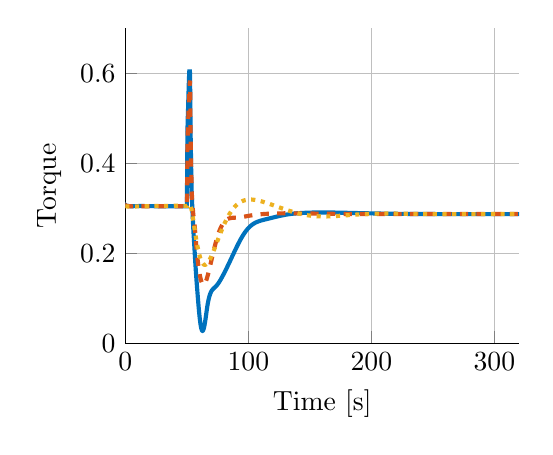
\begin{tikzpicture}

\begin{axis}[%
width=5cm,
height=4cm,
at={(0\linewidth,0\linewidth)},
scale only axis,
xmin=0,
xmax=320,
xlabel={Time [s]},
xmajorgrids,
ymin=0,
ymax=0.7,
ylabel={Torque},
ymajorgrids,
axis background/.style={fill=white},
% title style={font=\bfseries},
% title={Normalized Torque Setting},
axis x line*=bottom,
axis y line*=left
]
\addplot [color=mycolor1,solid,line width=1.5pt,forget plot]
  table[row sep=crcr]{%
0	0.304831074\\
0.25	0.30665978\\
0.5	0.30590085\\
0.75	0.30562405\\
1	0.30565309\\
1.25	0.30547614\\
1.5	0.30528095\\
1.75	0.30515676\\
2	0.30504243\\
2.25	0.304928319\\
2.5	0.304830357\\
2.75	0.30474751\\
3	0.304675987\\
3.25	0.304616093\\
3.5	0.304567996\\
3.75	0.304530753\\
4	0.304503022\\
4.25	0.304483048\\
4.5	0.304468969\\
4.75	0.304459287\\
5	0.304453134\\
5.25	0.304450003\\
5.5	0.304449628\\
5.75	0.304452033\\
6	0.304457403\\
6.25	0.304465922\\
6.5	0.304477601\\
6.75	0.304492142\\
7	0.304508918\\
7.25	0.304527087\\
7.5	0.304545747\\
7.75	0.30456407\\
8	0.304581427\\
8.25	0.304597482\\
8.5	0.304612217\\
8.75	0.30462589\\
9	0.304638928\\
9.25	0.304651779\\
9.5	0.304664765\\
9.75	0.304677988\\
10	0.304691287\\
10.25	0.304704276\\
10.5	0.304716429\\
10.75	0.304727207\\
11	0.304736188\\
11.25	0.30474316\\
11.5	0.304748177\\
11.75	0.304751534\\
12	0.304753694\\
12.25	0.304755174\\
12.5	0.304756414\\
12.75	0.304757681\\
13	0.30475901\\
13.25	0.30476021\\
13.5	0.304760922\\
13.75	0.30476073\\
14	0.304759267\\
14.25	0.304756327\\
14.5	0.304751915\\
14.75	0.30474626\\
15	0.304739763\\
15.25	0.304732898\\
15.5	0.304726109\\
15.75	0.304719702\\
16	0.304713781\\
16.25	0.304708235\\
16.5	0.304702777\\
16.75	0.304697029\\
17	0.30469063\\
17.25	0.304683333\\
17.5	0.304675073\\
17.75	0.304665996\\
18	0.304656418\\
18.25	0.304646755\\
18.5	0.304637419\\
18.75	0.304628722\\
19	0.304620796\\
19.25	0.304613572\\
19.5	0.304606803\\
19.75	0.304600131\\
20	0.304593187\\
20.25	0.304585688\\
20.5	0.304577512\\
20.75	0.304568734\\
21	0.304559605\\
21.25	0.304550493\\
21.5	0.304541785\\
21.75	0.304533794\\
22	0.304526677\\
22.25	0.304520397\\
22.5	0.304514737\\
22.75	0.304509357\\
23	0.304503883\\
23.25	0.304498007\\
23.5	0.304491565\\
23.75	0.30448458\\
24	0.30447726\\
24.25	0.30446994\\
24.5	0.304462995\\
24.75	0.304456747\\
25	0.304451375\\
25.25	0.304446874\\
25.5	0.304443053\\
25.75	0.304439586\\
26	0.304436097\\
26.25	0.304432258\\
26.5	0.304427872\\
26.75	0.304422928\\
27	0.304417601\\
27.25	0.304412209\\
27.5	0.304407124\\
27.75	0.304402683\\
28	0.304399091\\
28.25	0.30439637\\
28.5	0.30439435\\
28.75	0.304392716\\
29	0.304391086\\
29.25	0.304389111\\
29.5	0.304386568\\
29.75	0.304383418\\
30	0.304379815\\
30.25	0.304376067\\
30.5	0.304372557\\
30.75	0.304369637\\
31	0.30436754\\
31.25	0.304366312\\
31.5	0.304365801\\
31.75	0.304365694\\
32	0.304365598\\
32.25	0.304365143\\
32.5	0.304364077\\
32.75	0.304362337\\
33	0.304360064\\
33.25	0.304357567\\
33.5	0.304355243\\
33.75	0.304353469\\
34	0.304352507\\
34.25	0.304352425\\
34.5	0.304353082\\
34.75	0.30435416\\
35	0.304355248\\
35.25	0.304355947\\
35.5	0.304355978\\
35.75	0.304355255\\
36	0.304353912\\
36.25	0.304352267\\
36.5	0.30435074\\
36.75	0.304349742\\
37	0.304349564\\
37.25	0.304350296\\
37.5	0.304351802\\
37.75	0.304353751\\
38	0.304355704\\
38.25	0.304357226\\
38.5	0.304358006\\
38.75	0.304357939\\
39	0.304357157\\
39.25	0.304355997\\
39.5	0.304354913\\
39.75	0.304354356\\
40	0.304354653\\
40.25	0.304355914\\
40.5	0.304358003\\
40.75	0.304360563\\
41	0.304363117\\
41.25	0.304365186\\
41.5	0.30436642\\
41.75	0.304366697\\
42	0.304366153\\
42.25	0.304365156\\
42.5	0.304364208\\
42.75	0.304363811\\
43	0.304364333\\
43.25	0.304365904\\
43.5	0.304368376\\
43.75	0.30437136\\
44	0.304374322\\
44.25	0.304376726\\
44.5	0.30437818\\
44.75	0.304378543\\
45	0.304377967\\
45.25	0.304376863\\
45.5	0.304375798\\
45.75	0.304375339\\
46	0.304375903\\
46.25	0.304377638\\
46.5	0.304380377\\
46.75	0.304383675\\
47	0.304386927\\
47.25	0.304389525\\
47.5	0.304391024\\
47.75	0.304391267\\
48	0.304390434\\
48.25	0.304389\\
48.5	0.304387617\\
48.75	0.304386935\\
49	0.304387429\\
49.25	0.30438926\\
49.5	0.304392228\\
49.75	0.304395814\\
50	0.304399313\\
50.25	0.3726148\\
50.5	0.472673\\
50.75	0.500789\\
51	0.520824\\
51.25	0.544824\\
51.5	0.568657\\
51.75	0.588946\\
52	0.604\\
52.25	0.604\\
52.5	0.604\\
52.75	0.557336\\
53	0.474781\\
53.25	0.433629\\
53.5	0.3906805\\
53.75	0.3545439\\
54	0.330705\\
54.25	0.31342796\\
54.5	0.29890661\\
54.75	0.2832353\\
55	0.2678304\\
55.25	0.2541441\\
55.5	0.2419374\\
55.75	0.2305571\\
56	0.2195289\\
56.25	0.207966\\
56.5	0.196075\\
56.75	0.184581\\
57	0.173632\\
57.25	0.163105\\
57.5	0.153024\\
57.75	0.143495\\
58	0.134445\\
58.25	0.125621\\
58.5	0.116863\\
58.75	0.108186\\
59	0.099649\\
59.25	0.091303\\
59.5	0.083216\\
59.75	0.075468\\
60	0.068134\\
60.25	0.061278\\
60.5	0.054953\\
60.75	0.04921\\
61	0.044088\\
61.25	0.03962\\
61.5	0.035826\\
61.75	0.032722\\
62	0.030319\\
62.25	0.028618\\
62.5	0.027615\\
62.75	0.027302\\
63	0.027661\\
63.25	0.028668\\
63.5	0.030292\\
63.75	0.032495\\
64	0.03523\\
64.25	0.038446\\
64.5	0.042088\\
64.75	0.046101\\
65	0.05043\\
65.25	0.055024\\
65.5	0.059828\\
65.75	0.064776\\
66	0.069773\\
66.25	0.074692\\
66.5	0.079392\\
66.75	0.083771\\
67	0.087791\\
67.25	0.091463\\
67.5	0.094815\\
67.75	0.097879\\
68	0.100681\\
68.25	0.103241\\
68.5	0.105574\\
68.75	0.107693\\
69	0.109612\\
69.25	0.111343\\
69.5	0.1129\\
69.75	0.114296\\
70	0.115547\\
70.25	0.116669\\
70.5	0.117678\\
70.75	0.118589\\
71	0.119418\\
71.25	0.120181\\
71.5	0.120893\\
71.75	0.121566\\
72	0.122213\\
72.25	0.122845\\
72.5	0.123472\\
72.75	0.124104\\
73	0.124748\\
73.25	0.125409\\
73.5	0.126093\\
73.75	0.126805\\
74	0.127547\\
74.25	0.128322\\
74.5	0.129131\\
74.75	0.129975\\
75	0.130854\\
75.25	0.131768\\
75.5	0.132715\\
75.75	0.133696\\
76	0.134709\\
76.25	0.135752\\
76.5	0.136823\\
76.75	0.137922\\
77	0.139046\\
77.25	0.140193\\
77.5	0.141363\\
77.75	0.142553\\
78	0.143762\\
78.25	0.144988\\
78.5	0.146231\\
78.75	0.147488\\
79	0.14876\\
79.25	0.150044\\
79.5	0.151341\\
79.75	0.152648\\
80	0.153966\\
80.25	0.155295\\
80.5	0.156632\\
80.75	0.157978\\
81	0.159333\\
81.25	0.160695\\
81.5	0.162065\\
81.75	0.163443\\
82	0.164827\\
82.25	0.166219\\
82.5	0.167616\\
82.75	0.16902\\
83	0.17043\\
83.25	0.171846\\
83.5	0.173267\\
83.75	0.174694\\
84	0.176125\\
84.25	0.177561\\
84.5	0.179001\\
84.75	0.180445\\
85	0.181892\\
85.25	0.183343\\
85.5	0.184796\\
85.75	0.186252\\
86	0.187709\\
86.25	0.189168\\
86.5	0.190628\\
86.75	0.192089\\
87	0.193549\\
87.25	0.195009\\
87.5	0.196468\\
87.75	0.197925\\
88	0.19938\\
88.25	0.200832\\
88.5	0.20228\\
88.75	0.203725\\
89	0.2051655\\
89.25	0.2066006\\
89.5	0.20803\\
89.75	0.2094529\\
90	0.2108689\\
90.25	0.2122773\\
90.5	0.2136774\\
90.75	0.2150687\\
91	0.2164505\\
91.25	0.2178222\\
91.5	0.2191833\\
91.75	0.220533\\
92	0.2218709\\
92.25	0.2231964\\
92.5	0.2245088\\
92.75	0.2258076\\
93	0.2270923\\
93.25	0.2283623\\
93.5	0.229617\\
93.75	0.2308561\\
94	0.232079\\
94.25	0.2332852\\
94.5	0.2344743\\
94.75	0.2356458\\
95	0.2367994\\
95.25	0.2379346\\
95.5	0.239051\\
95.75	0.2401485\\
96	0.2412265\\
96.25	0.2422849\\
96.5	0.2433234\\
96.75	0.2443417\\
97	0.2453396\\
97.25	0.246317\\
97.5	0.2472736\\
97.75	0.2482094\\
98	0.2491243\\
98.25	0.2500181\\
98.5	0.2508909\\
98.75	0.2517427\\
99	0.2525734\\
99.25	0.253383\\
99.5	0.2541718\\
99.75	0.2549397\\
100	0.2556869\\
100.25	0.2564135\\
100.5	0.2571197\\
100.75	0.2578057\\
101	0.2584718\\
101.25	0.2591181\\
101.5	0.2597449\\
101.75	0.2603526\\
102	0.2609415\\
102.25	0.2615118\\
102.5	0.2620639\\
102.75	0.2625982\\
103	0.2631151\\
103.25	0.2636149\\
103.5	0.2640981\\
103.75	0.2645651\\
104	0.2650163\\
104.25	0.2654522\\
104.5	0.2658731\\
104.75	0.2662797\\
105	0.2666722\\
105.25	0.2670513\\
105.5	0.2674173\\
105.75	0.2677708\\
106	0.2681122\\
106.25	0.268442\\
106.5	0.2687607\\
106.75	0.2690687\\
107	0.2693666\\
107.25	0.2696547\\
107.5	0.2699336\\
107.75	0.2702038\\
108	0.2704655\\
108.25	0.2707194\\
108.5	0.2709658\\
108.75	0.2712052\\
109	0.271438\\
109.25	0.2716646\\
109.5	0.2718853\\
109.75	0.2721007\\
110	0.2723109\\
110.25	0.2725165\\
110.5	0.2727177\\
110.75	0.2729149\\
111	0.2731085\\
111.25	0.2732986\\
111.5	0.2734857\\
111.75	0.2736699\\
112	0.2738516\\
112.25	0.2740311\\
112.5	0.2742085\\
112.75	0.274384\\
113	0.274558\\
113.25	0.2747306\\
113.5	0.2749019\\
113.75	0.2750723\\
114	0.2752417\\
114.25	0.2754104\\
114.5	0.2755785\\
114.75	0.2757461\\
115	0.2759133\\
115.25	0.2760803\\
115.5	0.2762471\\
115.75	0.2764138\\
116	0.2765804\\
116.25	0.2767471\\
116.5	0.2769138\\
116.75	0.2770806\\
117	0.2772476\\
117.25	0.2774147\\
117.5	0.277582\\
117.75	0.2777494\\
118	0.277917\\
118.25	0.2780848\\
118.5	0.2782527\\
118.75	0.2784207\\
119	0.2785889\\
119.25	0.2787571\\
119.5	0.2789253\\
119.75	0.2790935\\
120	0.2792617\\
120.25	0.2794298\\
120.5	0.2795977\\
120.75	0.2797655\\
121	0.2799329\\
121.25	0.2801001\\
121.5	0.2802669\\
121.75	0.2804333\\
122	0.2805992\\
122.25	0.2807645\\
122.5	0.2809292\\
122.75	0.2810933\\
123	0.2812566\\
123.25	0.2814191\\
123.5	0.2815808\\
123.75	0.2817416\\
124	0.2819013\\
124.25	0.2820601\\
124.5	0.2822177\\
124.75	0.2823742\\
125	0.2825295\\
125.25	0.2826835\\
125.5	0.2828362\\
125.75	0.2829876\\
126	0.2831376\\
126.25	0.2832861\\
126.5	0.2834331\\
126.75	0.2835786\\
127	0.2837225\\
127.25	0.2838648\\
127.5	0.2840054\\
127.75	0.2841444\\
128	0.2842816\\
128.25	0.2844171\\
128.5	0.2845509\\
128.75	0.2846829\\
129	0.284813\\
129.25	0.2849414\\
129.5	0.2850679\\
129.75	0.2851925\\
130	0.2853153\\
130.25	0.2854361\\
130.5	0.2855551\\
130.75	0.2856722\\
131	0.2857874\\
131.25	0.2859007\\
131.5	0.2860121\\
131.75	0.2861216\\
132	0.2862292\\
132.25	0.2863349\\
132.5	0.2864387\\
132.75	0.2865407\\
133	0.2866407\\
133.25	0.286739\\
133.5	0.2868353\\
133.75	0.2869298\\
134	0.2870225\\
134.25	0.2871134\\
134.5	0.2872026\\
134.75	0.2872899\\
135	0.2873755\\
135.25	0.2874594\\
135.5	0.2875415\\
135.75	0.287622\\
136	0.2877008\\
136.25	0.2877779\\
136.5	0.2878534\\
136.75	0.2879273\\
137	0.2879996\\
137.25	0.2880704\\
137.5	0.2881397\\
137.75	0.2882074\\
138	0.2882737\\
138.25	0.2883385\\
138.5	0.2884018\\
138.75	0.2884638\\
139	0.2885244\\
139.25	0.2885836\\
139.5	0.2886415\\
139.75	0.2886981\\
140	0.2887534\\
140.25	0.2888074\\
140.5	0.2888602\\
140.75	0.2889118\\
141	0.2889622\\
141.25	0.2890114\\
141.5	0.2890595\\
141.75	0.2891065\\
142	0.2891523\\
142.25	0.2891971\\
142.5	0.2892409\\
142.75	0.2892836\\
143	0.2893253\\
143.25	0.289366\\
143.5	0.2894057\\
143.75	0.2894445\\
144	0.2894823\\
144.25	0.2895192\\
144.5	0.2895553\\
144.75	0.2895904\\
145	0.2896247\\
145.25	0.2896581\\
145.5	0.2896907\\
145.75	0.2897225\\
146	0.2897535\\
146.25	0.2897837\\
146.5	0.2898132\\
146.75	0.2898419\\
147	0.2898698\\
147.25	0.289897\\
147.5	0.2899235\\
147.75	0.2899493\\
148	0.2899744\\
148.25	0.2899988\\
148.5	0.2900225\\
148.75	0.2900456\\
149	0.2900681\\
149.25	0.2900899\\
149.5	0.290111\\
149.75	0.2901316\\
150	0.2901515\\
150.25	0.2901708\\
150.5	0.2901896\\
150.75	0.2902077\\
151	0.2902253\\
151.25	0.2902423\\
151.5	0.2902588\\
151.75	0.2902747\\
152	0.29029\\
152.25	0.2903048\\
152.5	0.2903191\\
152.75	0.2903328\\
153	0.2903461\\
153.25	0.2903588\\
153.5	0.290371\\
153.75	0.2903826\\
154	0.2903938\\
154.25	0.2904045\\
154.5	0.2904148\\
154.75	0.2904245\\
155	0.2904338\\
155.25	0.2904425\\
155.5	0.2904509\\
155.75	0.2904587\\
156	0.2904661\\
156.25	0.2904731\\
156.5	0.2904796\\
156.75	0.2904857\\
157	0.2904913\\
157.25	0.2904965\\
157.5	0.2905012\\
157.75	0.2905056\\
158	0.2905095\\
158.25	0.290513\\
158.5	0.2905161\\
158.75	0.2905188\\
159	0.2905211\\
159.25	0.290523\\
159.5	0.2905245\\
159.75	0.2905257\\
160	0.2905264\\
160.25	0.2905268\\
160.5	0.2905268\\
160.75	0.2905264\\
161	0.2905256\\
161.25	0.2905245\\
161.5	0.2905231\\
161.75	0.2905213\\
162	0.2905191\\
162.25	0.2905166\\
162.5	0.2905138\\
162.75	0.2905106\\
163	0.2905071\\
163.25	0.2905033\\
163.5	0.2904992\\
163.75	0.2904947\\
164	0.29049\\
164.25	0.2904849\\
164.5	0.2904796\\
164.75	0.2904739\\
165	0.2904679\\
165.25	0.2904617\\
165.5	0.2904552\\
165.75	0.2904484\\
166	0.2904413\\
166.25	0.290434\\
166.5	0.2904264\\
166.75	0.2904185\\
167	0.2904104\\
167.25	0.290402\\
167.5	0.2903934\\
167.75	0.2903846\\
168	0.2903755\\
168.25	0.2903662\\
168.5	0.2903566\\
168.75	0.2903469\\
169	0.2903369\\
169.25	0.2903267\\
169.5	0.2903162\\
169.75	0.2903056\\
170	0.2902948\\
170.25	0.2902838\\
170.5	0.2902726\\
170.75	0.2902612\\
171	0.2902496\\
171.25	0.2902378\\
171.5	0.2902259\\
171.75	0.2902138\\
172	0.2902015\\
172.25	0.290189\\
172.5	0.2901764\\
172.75	0.2901637\\
173	0.2901508\\
173.25	0.2901377\\
173.5	0.2901245\\
173.75	0.2901112\\
174	0.2900977\\
174.25	0.2900841\\
174.5	0.2900703\\
174.75	0.2900564\\
175	0.2900424\\
175.25	0.2900283\\
175.5	0.2900141\\
175.75	0.2899998\\
176	0.2899853\\
176.25	0.2899708\\
176.5	0.2899561\\
176.75	0.2899414\\
177	0.2899265\\
177.25	0.2899116\\
177.5	0.2898965\\
177.75	0.2898814\\
178	0.2898662\\
178.25	0.2898509\\
178.5	0.2898356\\
178.75	0.2898202\\
179	0.2898047\\
179.25	0.2897891\\
179.5	0.2897735\\
179.75	0.2897578\\
180	0.289742\\
180.25	0.2897262\\
180.5	0.2897103\\
180.75	0.2896944\\
181	0.2896785\\
181.25	0.2896625\\
181.5	0.2896464\\
181.75	0.2896303\\
182	0.2896142\\
182.25	0.289598\\
182.5	0.2895818\\
182.75	0.2895655\\
183	0.2895493\\
183.25	0.289533\\
183.5	0.2895167\\
183.75	0.2895003\\
184	0.2894839\\
184.25	0.2894676\\
184.5	0.2894511\\
184.75	0.2894347\\
185	0.2894183\\
185.25	0.2894019\\
185.5	0.2893854\\
185.75	0.289369\\
186	0.2893525\\
186.25	0.289336\\
186.5	0.2893196\\
186.75	0.2893031\\
187	0.2892866\\
187.25	0.2892702\\
187.5	0.2892537\\
187.75	0.2892373\\
188	0.2892208\\
188.25	0.2892044\\
188.5	0.289188\\
188.75	0.2891716\\
189	0.2891552\\
189.25	0.2891388\\
189.5	0.2891225\\
189.75	0.2891061\\
190	0.2890898\\
190.25	0.2890735\\
190.5	0.2890573\\
190.75	0.289041\\
191	0.2890248\\
191.25	0.2890086\\
191.5	0.2889925\\
191.75	0.2889764\\
192	0.2889603\\
192.25	0.2889442\\
192.5	0.2889282\\
192.75	0.2889122\\
193	0.2888962\\
193.25	0.2888803\\
193.5	0.2888644\\
193.75	0.2888486\\
194	0.2888328\\
194.25	0.2888171\\
194.5	0.2888014\\
194.75	0.2887857\\
195	0.2887701\\
195.25	0.2887545\\
195.5	0.288739\\
195.75	0.2887235\\
196	0.2887081\\
196.25	0.2886927\\
196.5	0.2886774\\
196.75	0.2886621\\
197	0.2886469\\
197.25	0.2886317\\
197.5	0.2886166\\
197.75	0.2886016\\
198	0.2885866\\
198.25	0.2885716\\
198.5	0.2885568\\
198.75	0.2885419\\
199	0.2885272\\
199.25	0.2885125\\
199.5	0.2884978\\
199.75	0.2884832\\
200	0.2884687\\
200.25	0.2884543\\
200.5	0.2884399\\
200.75	0.2884255\\
201	0.2884113\\
201.25	0.2883971\\
201.5	0.2883829\\
201.75	0.2883689\\
202	0.2883549\\
202.25	0.2883409\\
202.5	0.2883271\\
202.75	0.2883133\\
203	0.2882995\\
203.25	0.2882859\\
203.5	0.2882723\\
203.75	0.2882588\\
204	0.2882453\\
204.25	0.288232\\
204.5	0.2882186\\
204.75	0.2882054\\
205	0.2881922\\
205.25	0.2881792\\
205.5	0.2881661\\
205.75	0.2881532\\
206	0.2881403\\
206.25	0.2881275\\
206.5	0.2881148\\
206.75	0.2881022\\
207	0.2880896\\
207.25	0.2880771\\
207.5	0.2880647\\
207.75	0.2880523\\
208	0.28804\\
208.25	0.2880278\\
208.5	0.2880157\\
208.75	0.2880037\\
209	0.2879917\\
209.25	0.2879798\\
209.5	0.287968\\
209.75	0.2879562\\
210	0.2879446\\
210.25	0.287933\\
210.5	0.2879215\\
210.75	0.28791\\
211	0.2878987\\
211.25	0.2878874\\
211.5	0.2878762\\
211.75	0.2878651\\
212	0.287854\\
212.25	0.287843\\
212.5	0.2878321\\
212.75	0.2878213\\
213	0.2878106\\
213.25	0.2877999\\
213.5	0.2877893\\
213.75	0.2877788\\
214	0.2877684\\
214.25	0.287758\\
214.5	0.2877478\\
214.75	0.2877376\\
215	0.2877274\\
215.25	0.2877174\\
215.5	0.2877074\\
215.75	0.2876975\\
216	0.2876877\\
216.25	0.287678\\
216.5	0.2876683\\
216.75	0.2876587\\
217	0.2876492\\
217.25	0.2876398\\
217.5	0.2876304\\
217.75	0.2876211\\
218	0.2876119\\
218.25	0.2876028\\
218.5	0.2875937\\
218.75	0.2875848\\
219	0.2875759\\
219.25	0.287567\\
219.5	0.2875583\\
219.75	0.2875496\\
220	0.287541\\
220.25	0.2875324\\
220.5	0.287524\\
220.75	0.2875156\\
221	0.2875073\\
221.25	0.287499\\
221.5	0.2874909\\
221.75	0.2874828\\
222	0.2874747\\
222.25	0.2874668\\
222.5	0.2874589\\
222.75	0.2874511\\
223	0.2874434\\
223.25	0.2874357\\
223.5	0.2874281\\
223.75	0.2874206\\
224	0.2874131\\
224.25	0.2874057\\
224.5	0.2873984\\
224.75	0.2873912\\
225	0.287384\\
225.25	0.2873769\\
225.5	0.2873699\\
225.75	0.2873629\\
226	0.287356\\
226.25	0.2873491\\
226.5	0.2873424\\
226.75	0.2873357\\
227	0.287329\\
227.25	0.2873225\\
227.5	0.287316\\
227.75	0.2873095\\
228	0.2873032\\
228.25	0.2872969\\
228.5	0.2872906\\
228.75	0.2872844\\
229	0.2872783\\
229.25	0.2872723\\
229.5	0.2872663\\
229.75	0.2872604\\
230	0.2872545\\
230.25	0.2872487\\
230.5	0.287243\\
230.75	0.2872373\\
231	0.2872317\\
231.25	0.2872261\\
231.5	0.2872207\\
231.75	0.2872152\\
232	0.2872099\\
232.25	0.2872045\\
232.5	0.2871993\\
232.75	0.2871941\\
233	0.287189\\
233.25	0.2871839\\
233.5	0.2871789\\
233.75	0.2871739\\
234	0.287169\\
234.25	0.2871642\\
234.5	0.2871594\\
234.75	0.2871546\\
235	0.28715\\
235.25	0.2871453\\
235.5	0.2871408\\
235.75	0.2871363\\
236	0.2871318\\
236.25	0.2871274\\
236.5	0.287123\\
236.75	0.2871187\\
237	0.2871145\\
237.25	0.2871103\\
237.5	0.2871062\\
237.75	0.2871021\\
238	0.287098\\
238.25	0.2870941\\
238.5	0.2870901\\
238.75	0.2870862\\
239	0.2870824\\
239.25	0.2870786\\
239.5	0.2870749\\
239.75	0.2870712\\
240	0.2870675\\
240.25	0.2870639\\
240.5	0.2870604\\
240.75	0.2870569\\
241	0.2870534\\
241.25	0.28705\\
241.5	0.2870467\\
241.75	0.2870434\\
242	0.2870401\\
242.25	0.2870369\\
242.5	0.2870337\\
242.75	0.2870306\\
243	0.2870275\\
243.25	0.2870244\\
243.5	0.2870214\\
243.75	0.2870185\\
244	0.2870155\\
244.25	0.2870127\\
244.5	0.2870098\\
244.75	0.287007\\
245	0.2870043\\
245.25	0.2870016\\
245.5	0.2869989\\
245.75	0.2869963\\
246	0.2869937\\
246.25	0.2869911\\
246.5	0.2869886\\
246.75	0.2869861\\
247	0.2869837\\
247.25	0.2869813\\
247.5	0.2869789\\
247.75	0.2869766\\
248	0.2869743\\
248.25	0.2869721\\
248.5	0.2869699\\
248.75	0.2869677\\
249	0.2869656\\
249.25	0.2869635\\
249.5	0.2869614\\
249.75	0.2869593\\
250	0.2869573\\
250.25	0.2869554\\
250.5	0.2869534\\
250.75	0.2869515\\
251	0.2869497\\
251.25	0.2869478\\
251.5	0.286946\\
251.75	0.2869443\\
252	0.2869425\\
252.25	0.2869408\\
252.5	0.2869391\\
252.75	0.2869375\\
253	0.2869359\\
253.25	0.2869343\\
253.5	0.2869327\\
253.75	0.2869312\\
254	0.2869297\\
254.25	0.2869282\\
254.5	0.2869268\\
254.75	0.2869254\\
255	0.286924\\
255.25	0.2869227\\
255.5	0.2869213\\
255.75	0.28692\\
256	0.2869188\\
256.25	0.2869175\\
256.5	0.2869163\\
256.75	0.2869151\\
257	0.2869139\\
257.25	0.2869128\\
257.5	0.2869117\\
257.75	0.2869106\\
258	0.2869095\\
258.25	0.2869084\\
258.5	0.2869074\\
258.75	0.2869064\\
259	0.2869054\\
259.25	0.2869045\\
259.5	0.2869036\\
259.75	0.2869027\\
260	0.2869018\\
260.25	0.2869009\\
260.5	0.2869001\\
260.75	0.2868993\\
261	0.2868985\\
261.25	0.2868977\\
261.5	0.2868969\\
261.75	0.2868962\\
262	0.2868955\\
262.25	0.2868948\\
262.5	0.2868941\\
262.75	0.2868935\\
263	0.2868928\\
263.25	0.2868922\\
263.5	0.2868916\\
263.75	0.286891\\
264	0.2868905\\
264.25	0.2868899\\
264.5	0.2868894\\
264.75	0.2868889\\
265	0.2868884\\
265.25	0.2868879\\
265.5	0.2868875\\
265.75	0.286887\\
266	0.2868866\\
266.25	0.2868862\\
266.5	0.2868858\\
266.75	0.2868854\\
267	0.2868851\\
267.25	0.2868847\\
267.5	0.2868844\\
267.75	0.2868841\\
268	0.2868838\\
268.25	0.2868835\\
268.5	0.2868832\\
268.75	0.286883\\
269	0.2868827\\
269.25	0.2868825\\
269.5	0.2868823\\
269.75	0.2868821\\
270	0.2868819\\
270.25	0.2868817\\
270.5	0.2868816\\
270.75	0.2868814\\
271	0.2868813\\
271.25	0.2868812\\
271.5	0.2868811\\
271.75	0.286881\\
272	0.2868809\\
272.25	0.2868808\\
272.5	0.2868807\\
272.75	0.2868807\\
273	0.2868806\\
273.25	0.2868806\\
273.5	0.2868806\\
273.75	0.2868805\\
274	0.2868805\\
274.25	0.2868806\\
274.5	0.2868806\\
274.75	0.2868806\\
275	0.2868806\\
275.25	0.2868807\\
275.5	0.2868807\\
275.75	0.2868808\\
276	0.2868809\\
276.25	0.286881\\
276.5	0.2868811\\
276.75	0.2868812\\
277	0.2868813\\
277.25	0.2868814\\
277.5	0.2868815\\
277.75	0.2868816\\
278	0.2868818\\
278.25	0.2868819\\
278.5	0.2868821\\
278.75	0.2868822\\
279	0.2868824\\
279.25	0.2868826\\
279.5	0.2868828\\
279.75	0.286883\\
280	0.2868832\\
280.25	0.2868834\\
280.5	0.2868836\\
280.75	0.2868838\\
281	0.286884\\
281.25	0.2868842\\
281.5	0.2868845\\
281.75	0.2868847\\
282	0.2868849\\
282.25	0.2868852\\
282.5	0.2868855\\
282.75	0.2868857\\
283	0.286886\\
283.25	0.2868863\\
283.5	0.2868865\\
283.75	0.2868868\\
284	0.2868871\\
284.25	0.2868874\\
284.5	0.2868877\\
284.75	0.286888\\
285	0.2868883\\
285.25	0.2868886\\
285.5	0.2868889\\
285.75	0.2868892\\
286	0.2868895\\
286.25	0.2868899\\
286.5	0.2868902\\
286.75	0.2868905\\
287	0.2868909\\
287.25	0.2868912\\
287.5	0.2868915\\
287.75	0.2868919\\
288	0.2868922\\
288.25	0.2868926\\
288.5	0.2868929\\
288.75	0.2868933\\
289	0.2868936\\
289.25	0.286894\\
289.5	0.2868944\\
289.75	0.2868947\\
290	0.2868951\\
290.25	0.2868955\\
290.5	0.2868958\\
290.75	0.2868962\\
291	0.2868966\\
291.25	0.286897\\
291.5	0.2868974\\
291.75	0.2868977\\
292	0.2868981\\
292.25	0.2868985\\
292.5	0.2868989\\
292.75	0.2868993\\
293	0.2868997\\
293.25	0.2869001\\
293.5	0.2869005\\
293.75	0.2869009\\
294	0.2869013\\
294.25	0.2869017\\
294.5	0.286902\\
294.75	0.2869024\\
295	0.2869028\\
295.25	0.2869032\\
295.5	0.2869037\\
295.75	0.2869041\\
296	0.2869045\\
296.25	0.2869049\\
296.5	0.2869053\\
296.75	0.2869057\\
297	0.2869061\\
297.25	0.2869065\\
297.5	0.2869069\\
297.75	0.2869073\\
298	0.2869077\\
298.25	0.2869081\\
298.5	0.2869085\\
298.75	0.2869089\\
299	0.2869093\\
299.25	0.2869097\\
299.5	0.2869101\\
299.75	0.2869105\\
300	0.286911\\
300.25	0.2869114\\
300.5	0.2869118\\
300.75	0.2869122\\
301	0.2869126\\
301.25	0.286913\\
301.5	0.2869134\\
301.75	0.2869138\\
302	0.2869142\\
302.25	0.2869146\\
302.5	0.286915\\
302.75	0.2869154\\
303	0.2869158\\
303.25	0.2869162\\
303.5	0.2869166\\
303.75	0.286917\\
304	0.2869174\\
304.25	0.2869178\\
304.5	0.2869182\\
304.75	0.2869186\\
305	0.286919\\
305.25	0.2869194\\
305.5	0.2869198\\
305.75	0.2869202\\
306	0.2869206\\
306.25	0.286921\\
306.5	0.2869214\\
306.75	0.2869217\\
307	0.2869221\\
307.25	0.2869225\\
307.5	0.2869229\\
307.75	0.2869233\\
308	0.2869237\\
308.25	0.286924\\
308.5	0.2869244\\
308.75	0.2869248\\
309	0.2869252\\
309.25	0.2869256\\
309.5	0.2869259\\
309.75	0.2869263\\
310	0.2869267\\
310.25	0.286927\\
310.5	0.2869274\\
310.75	0.2869278\\
311	0.2869281\\
311.25	0.2869285\\
311.5	0.2869289\\
311.75	0.2869292\\
312	0.2869296\\
312.25	0.28693\\
312.5	0.2869303\\
312.75	0.2869307\\
313	0.286931\\
313.25	0.2869314\\
313.5	0.2869317\\
313.75	0.2869321\\
314	0.2869324\\
314.25	0.2869328\\
314.5	0.2869331\\
314.75	0.2869334\\
315	0.2869338\\
315.25	0.2869341\\
315.5	0.2869345\\
315.75	0.2869348\\
316	0.2869351\\
316.25	0.2869355\\
316.5	0.2869358\\
316.75	0.2869361\\
317	0.2869364\\
317.25	0.2869368\\
317.5	0.2869371\\
317.75	0.2869374\\
318	0.2869377\\
318.25	0.286938\\
318.5	0.2869383\\
318.75	0.2869387\\
319	0.286939\\
319.25	0.2869393\\
319.5	0.2869396\\
319.75	0.2869399\\
320	0.2869402\\
320.25	0.2869405\\
320.5	0.2869408\\
320.75	0.2869411\\
321	0.2869414\\
321.25	0.2869417\\
321.5	0.286942\\
321.75	0.2869423\\
322	0.2869426\\
322.25	0.2869428\\
322.5	0.2869431\\
322.75	0.2869434\\
323	0.2869437\\
323.25	0.286944\\
323.5	0.2869442\\
323.75	0.2869445\\
324	0.2869448\\
324.25	0.2869451\\
324.5	0.2869453\\
324.75	0.2869456\\
325	0.2869459\\
325.25	0.2869461\\
325.5	0.2869464\\
325.75	0.2869466\\
326	0.2869469\\
326.25	0.2869472\\
326.5	0.2869474\\
326.75	0.2869477\\
327	0.2869479\\
327.25	0.2869482\\
327.5	0.2869484\\
327.75	0.2869486\\
328	0.2869489\\
328.25	0.2869491\\
328.5	0.2869494\\
328.75	0.2869496\\
329	0.2869498\\
329.25	0.2869501\\
329.5	0.2869503\\
329.75	0.2869505\\
330	0.2869508\\
330.25	0.286951\\
330.5	0.2869512\\
330.75	0.2869514\\
331	0.2869516\\
331.25	0.2869519\\
331.5	0.2869521\\
331.75	0.2869523\\
332	0.2869525\\
332.25	0.2869527\\
332.5	0.2869529\\
332.75	0.2869531\\
333	0.2869533\\
333.25	0.2869535\\
333.5	0.2869537\\
333.75	0.2869539\\
334	0.2869541\\
334.25	0.2869543\\
334.5	0.2869545\\
334.75	0.2869547\\
335	0.2869549\\
335.25	0.2869551\\
335.5	0.2869553\\
335.75	0.2869555\\
336	0.2869557\\
336.25	0.2869558\\
336.5	0.286956\\
336.75	0.2869562\\
337	0.2869564\\
337.25	0.2869565\\
337.5	0.2869567\\
337.75	0.2869569\\
338	0.2869571\\
338.25	0.2869572\\
338.5	0.2869574\\
338.75	0.2869576\\
339	0.2869577\\
339.25	0.2869579\\
339.5	0.286958\\
339.75	0.2869582\\
340	0.2869584\\
340.25	0.2869585\\
340.5	0.2869587\\
340.75	0.2869588\\
341	0.286959\\
341.25	0.2869591\\
341.5	0.2869593\\
341.75	0.2869594\\
342	0.2869596\\
342.25	0.2869597\\
342.5	0.2869598\\
342.75	0.28696\\
343	0.2869601\\
343.25	0.2869603\\
343.5	0.2869604\\
343.75	0.2869605\\
344	0.2869607\\
344.25	0.2869608\\
344.5	0.2869609\\
344.75	0.286961\\
345	0.2869612\\
345.25	0.2869613\\
345.5	0.2869614\\
345.75	0.2869615\\
346	0.2869617\\
346.25	0.2869618\\
346.5	0.2869619\\
346.75	0.286962\\
347	0.2869621\\
347.25	0.2869622\\
347.5	0.2869624\\
347.75	0.2869625\\
348	0.2869626\\
348.25	0.2869627\\
348.5	0.2869628\\
348.75	0.2869629\\
349	0.286963\\
349.25	0.2869631\\
349.5	0.2869632\\
349.75	0.2869633\\
350	0.2869634\\
350.25	0.2869635\\
350.5	0.2869636\\
350.75	0.2869637\\
351	0.2869638\\
351.25	0.2869639\\
351.5	0.286964\\
351.75	0.2869641\\
352	0.2869642\\
352.25	0.2869642\\
352.5	0.2869643\\
352.75	0.2869644\\
353	0.2869645\\
353.25	0.2869646\\
353.5	0.2869647\\
353.75	0.2869648\\
354	0.2869648\\
354.25	0.2869649\\
354.5	0.286965\\
354.75	0.2869651\\
355	0.2869651\\
355.25	0.2869652\\
355.5	0.2869653\\
355.75	0.2869654\\
356	0.2869654\\
356.25	0.2869655\\
356.5	0.2869656\\
356.75	0.2869656\\
357	0.2869657\\
357.25	0.2869658\\
357.5	0.2869658\\
357.75	0.2869659\\
358	0.286966\\
358.25	0.286966\\
358.5	0.2869661\\
358.75	0.2869662\\
359	0.2869662\\
359.25	0.2869663\\
359.5	0.2869663\\
359.75	0.2869664\\
360	0.2869665\\
360.25	0.2869665\\
360.5	0.2869666\\
360.75	0.2869666\\
361	0.2869667\\
361.25	0.2869667\\
361.5	0.2869668\\
361.75	0.2869668\\
362	0.2869669\\
362.25	0.2869669\\
362.5	0.286967\\
362.75	0.286967\\
363	0.2869671\\
363.25	0.2869671\\
363.5	0.2869672\\
363.75	0.2869672\\
364	0.2869672\\
364.25	0.2869673\\
364.5	0.2869673\\
364.75	0.2869674\\
365	0.2869674\\
365.25	0.2869674\\
365.5	0.2869675\\
365.75	0.2869675\\
366	0.2869676\\
366.25	0.2869676\\
366.5	0.2869676\\
366.75	0.2869677\\
367	0.2869677\\
367.25	0.2869677\\
367.5	0.2869678\\
367.75	0.2869678\\
368	0.2869678\\
368.25	0.2869679\\
368.5	0.2869679\\
368.75	0.2869679\\
369	0.2869679\\
369.25	0.286968\\
369.5	0.286968\\
369.75	0.286968\\
370	0.2869681\\
370.25	0.2869681\\
370.5	0.2869681\\
370.75	0.2869681\\
371	0.2869682\\
371.25	0.2869682\\
371.5	0.2869682\\
371.75	0.2869682\\
372	0.2869683\\
372.25	0.2869683\\
372.5	0.2869683\\
372.75	0.2869683\\
373	0.2869683\\
373.25	0.2869684\\
373.5	0.2869684\\
373.75	0.2869684\\
374	0.2869684\\
374.25	0.2869684\\
374.5	0.2869684\\
374.75	0.2869685\\
375	0.2869685\\
375.25	0.2869685\\
375.5	0.2869685\\
375.75	0.2869685\\
376	0.2869685\\
376.25	0.2869685\\
376.5	0.2869686\\
376.75	0.2869686\\
377	0.2869686\\
377.25	0.2869686\\
377.5	0.2869686\\
377.75	0.2869686\\
378	0.2869686\\
378.25	0.2869686\\
378.5	0.2869687\\
378.75	0.2869687\\
379	0.2869687\\
379.25	0.2869687\\
379.5	0.2869687\\
379.75	0.2869687\\
380	0.2869687\\
380.25	0.2869687\\
380.5	0.2869687\\
380.75	0.2869687\\
381	0.2869687\\
381.25	0.2869687\\
381.5	0.2869687\\
381.75	0.2869687\\
382	0.2869687\\
382.25	0.2869688\\
382.5	0.2869688\\
382.75	0.2869688\\
383	0.2869688\\
383.25	0.2869688\\
383.5	0.2869688\\
383.75	0.2869688\\
384	0.2869688\\
384.25	0.2869688\\
384.5	0.2869688\\
384.75	0.2869688\\
385	0.2869688\\
385.25	0.2869688\\
385.5	0.2869688\\
385.75	0.2869688\\
386	0.2869688\\
386.25	0.2869688\\
386.5	0.2869688\\
386.75	0.2869688\\
387	0.2869688\\
387.25	0.2869688\\
387.5	0.2869688\\
387.75	0.2869688\\
388	0.2869688\\
388.25	0.2869688\\
388.5	0.2869688\\
388.75	0.2869688\\
389	0.2869688\\
389.25	0.2869688\\
389.5	0.2869688\\
389.75	0.2869688\\
390	0.2869688\\
390.25	0.2869688\\
390.5	0.2869688\\
390.75	0.2869687\\
391	0.2869687\\
391.25	0.2869687\\
391.5	0.2869687\\
391.75	0.2869687\\
392	0.2869687\\
392.25	0.2869687\\
392.5	0.2869687\\
392.75	0.2869687\\
393	0.2869687\\
393.25	0.2869687\\
393.5	0.2869687\\
393.75	0.2869687\\
394	0.2869687\\
394.25	0.2869687\\
394.5	0.2869687\\
394.75	0.2869687\\
395	0.2869687\\
395.25	0.2869687\\
395.5	0.2869686\\
395.75	0.2869686\\
396	0.2869686\\
396.25	0.2869686\\
396.5	0.2869686\\
396.75	0.2869686\\
397	0.2869686\\
397.25	0.2869686\\
397.5	0.2869686\\
397.75	0.2869686\\
398	0.2869686\\
398.25	0.2869686\\
398.5	0.2869686\\
398.75	0.2869685\\
399	0.2869685\\
399.25	0.2869685\\
399.5	0.2869685\\
399.75	0.2869685\\
400	0.2869685\\
400.25	0.2869685\\
400.5	0.2869685\\
400.75	0.2869685\\
401	0.2869685\\
401.25	0.2869685\\
401.5	0.2869685\\
401.75	0.2869684\\
402	0.2869684\\
402.25	0.2869684\\
402.5	0.2869684\\
402.75	0.2869684\\
403	0.2869684\\
403.25	0.2869684\\
403.5	0.2869684\\
403.75	0.2869684\\
404	0.2869684\\
404.25	0.2869684\\
404.5	0.2869683\\
404.75	0.2869683\\
405	0.2869683\\
405.25	0.2869683\\
405.5	0.2869683\\
405.75	0.2869683\\
406	0.2869683\\
406.25	0.2869683\\
406.5	0.2869683\\
406.75	0.2869683\\
407	0.2869683\\
407.25	0.2869682\\
407.5	0.2869682\\
407.75	0.2869682\\
408	0.2869682\\
408.25	0.2869682\\
408.5	0.2869682\\
408.75	0.2869682\\
409	0.2869682\\
409.25	0.2869682\\
409.5	0.2869682\\
409.75	0.2869681\\
410	0.2869681\\
410.25	0.2869681\\
410.5	0.2869681\\
410.75	0.2869681\\
411	0.2869681\\
411.25	0.2869681\\
411.5	0.2869681\\
411.75	0.2869681\\
412	0.2869681\\
412.25	0.286968\\
412.5	0.286968\\
412.75	0.286968\\
413	0.286968\\
413.25	0.286968\\
413.5	0.286968\\
413.75	0.286968\\
414	0.286968\\
414.25	0.286968\\
414.5	0.286968\\
414.75	0.2869679\\
415	0.2869679\\
415.25	0.2869679\\
415.5	0.2869679\\
415.75	0.2869679\\
416	0.2869679\\
416.25	0.2869679\\
416.5	0.2869679\\
416.75	0.2869679\\
417	0.2869679\\
417.25	0.2869678\\
417.5	0.2869678\\
417.75	0.2869678\\
418	0.2869678\\
418.25	0.2869678\\
418.5	0.2869678\\
418.75	0.2869678\\
419	0.2869678\\
419.25	0.2869678\\
419.5	0.2869678\\
419.75	0.2869678\\
420	0.2869677\\
420.25	0.2869677\\
420.5	0.2869677\\
420.75	0.2869677\\
421	0.2869677\\
421.25	0.2869677\\
421.5	0.2869677\\
421.75	0.2869677\\
422	0.2869677\\
422.25	0.2869677\\
422.5	0.2869676\\
422.75	0.2869676\\
423	0.2869676\\
423.25	0.2869676\\
423.5	0.2869676\\
423.75	0.2869676\\
424	0.2869676\\
424.25	0.2869676\\
424.5	0.2869676\\
424.75	0.2869676\\
425	0.2869676\\
425.25	0.2869676\\
425.5	0.2869675\\
425.75	0.2869675\\
426	0.2869675\\
426.25	0.2869675\\
426.5	0.2869675\\
426.75	0.2869675\\
427	0.2869675\\
427.25	0.2869675\\
427.5	0.2869675\\
427.75	0.2869675\\
428	0.2869675\\
428.25	0.2869675\\
428.5	0.2869674\\
428.75	0.2869674\\
429	0.2869674\\
429.25	0.2869674\\
429.5	0.2869674\\
429.75	0.2869674\\
430	0.2869674\\
430.25	0.2869674\\
430.5	0.2869674\\
430.75	0.2869674\\
431	0.2869674\\
431.25	0.2869674\\
431.5	0.2869674\\
431.75	0.2869673\\
432	0.2869673\\
432.25	0.2869673\\
432.5	0.2869673\\
432.75	0.2869673\\
433	0.2869673\\
433.25	0.2869673\\
433.5	0.2869673\\
433.75	0.2869673\\
434	0.2869673\\
434.25	0.2869673\\
434.5	0.2869673\\
434.75	0.2869673\\
435	0.2869672\\
435.25	0.2869672\\
435.5	0.2869672\\
435.75	0.2869672\\
436	0.2869672\\
436.25	0.2869672\\
436.5	0.2869672\\
436.75	0.2869672\\
437	0.2869672\\
437.25	0.2869672\\
437.5	0.2869672\\
437.75	0.2869672\\
438	0.2869672\\
438.25	0.2869672\\
438.5	0.2869672\\
438.75	0.2869672\\
439	0.2869671\\
439.25	0.2869671\\
439.5	0.2869671\\
439.75	0.2869671\\
440	0.2869671\\
440.25	0.2869671\\
440.5	0.2869671\\
440.75	0.2869671\\
441	0.2869671\\
441.25	0.2869671\\
441.5	0.2869671\\
441.75	0.2869671\\
442	0.2869671\\
442.25	0.2869671\\
442.5	0.2869671\\
442.75	0.2869671\\
443	0.2869671\\
443.25	0.286967\\
443.5	0.286967\\
443.75	0.286967\\
444	0.286967\\
444.25	0.286967\\
444.5	0.286967\\
444.75	0.286967\\
445	0.286967\\
445.25	0.286967\\
445.5	0.286967\\
445.75	0.286967\\
446	0.286967\\
446.25	0.286967\\
446.5	0.286967\\
446.75	0.286967\\
447	0.286967\\
447.25	0.286967\\
447.5	0.286967\\
447.75	0.286967\\
448	0.286967\\
448.25	0.286967\\
448.5	0.2869669\\
448.75	0.2869669\\
449	0.2869669\\
449.25	0.2869669\\
449.5	0.2869669\\
449.75	0.2869669\\
450	0.2869669\\
450.25	0.2869669\\
450.5	0.2869669\\
450.75	0.2869669\\
451	0.2869669\\
451.25	0.2869669\\
451.5	0.2869669\\
451.75	0.2869669\\
452	0.2869669\\
452.25	0.2869669\\
452.5	0.2869669\\
452.75	0.2869669\\
453	0.2869669\\
453.25	0.2869669\\
453.5	0.2869669\\
453.75	0.2869669\\
454	0.2869669\\
454.25	0.2869669\\
454.5	0.2869669\\
454.75	0.2869668\\
455	0.2869668\\
455.25	0.2869668\\
455.5	0.2869668\\
455.75	0.2869668\\
456	0.2869668\\
456.25	0.2869668\\
456.5	0.2869668\\
456.75	0.2869668\\
457	0.2869668\\
457.25	0.2869668\\
457.5	0.2869668\\
457.75	0.2869668\\
458	0.2869668\\
458.25	0.2869668\\
458.5	0.2869668\\
458.75	0.2869668\\
459	0.2869668\\
459.25	0.2869668\\
459.5	0.2869668\\
459.75	0.2869668\\
460	0.2869668\\
460.25	0.2869668\\
460.5	0.2869668\\
460.75	0.2869668\\
461	0.2869668\\
461.25	0.2869668\\
461.5	0.2869668\\
461.75	0.2869668\\
462	0.2869668\\
462.25	0.2869668\\
462.5	0.2869668\\
462.75	0.2869668\\
463	0.2869668\\
463.25	0.2869668\\
463.5	0.2869667\\
463.75	0.2869667\\
464	0.2869667\\
464.25	0.2869667\\
464.5	0.2869667\\
464.75	0.2869667\\
465	0.2869667\\
465.25	0.2869667\\
465.5	0.2869667\\
465.75	0.2869667\\
466	0.2869667\\
466.25	0.2869667\\
466.5	0.2869667\\
466.75	0.2869667\\
467	0.2869667\\
467.25	0.2869667\\
467.5	0.2869667\\
467.75	0.2869667\\
468	0.2869667\\
468.25	0.2869667\\
468.5	0.2869667\\
468.75	0.2869667\\
469	0.2869667\\
469.25	0.2869667\\
469.5	0.2869667\\
469.75	0.2869667\\
470	0.2869667\\
470.25	0.2869667\\
470.5	0.2869667\\
470.75	0.2869667\\
471	0.2869667\\
471.25	0.2869667\\
471.5	0.2869667\\
471.75	0.2869667\\
472	0.2869667\\
472.25	0.2869667\\
472.5	0.2869667\\
472.75	0.2869667\\
473	0.2869667\\
473.25	0.2869667\\
473.5	0.2869667\\
473.75	0.2869667\\
474	0.2869667\\
474.25	0.2869667\\
474.5	0.2869667\\
474.75	0.2869667\\
475	0.2869667\\
475.25	0.2869667\\
475.5	0.2869667\\
475.75	0.2869667\\
476	0.2869667\\
476.25	0.2869667\\
476.5	0.2869667\\
476.75	0.2869667\\
477	0.2869667\\
477.25	0.2869667\\
477.5	0.2869667\\
477.75	0.2869667\\
478	0.2869667\\
478.25	0.2869667\\
478.5	0.2869667\\
478.75	0.2869667\\
479	0.2869667\\
479.25	0.2869667\\
479.5	0.2869667\\
479.75	0.2869667\\
480	0.2869667\\
480.25	0.2869667\\
480.5	0.2869667\\
480.75	0.2869667\\
481	0.2869667\\
481.25	0.2869667\\
481.5	0.2869666\\
481.75	0.2869666\\
482	0.2869666\\
482.25	0.2869666\\
482.5	0.2869666\\
482.75	0.2869666\\
483	0.2869666\\
483.25	0.2869666\\
483.5	0.2869666\\
483.75	0.2869666\\
484	0.2869666\\
484.25	0.2869666\\
484.5	0.2869666\\
484.75	0.2869666\\
485	0.2869666\\
485.25	0.2869666\\
485.5	0.2869666\\
485.75	0.2869666\\
486	0.2869666\\
486.25	0.2869666\\
486.5	0.2869666\\
486.75	0.2869666\\
487	0.2869666\\
487.25	0.2869666\\
487.5	0.2869666\\
487.75	0.2869666\\
488	0.2869666\\
488.25	0.2869666\\
488.5	0.2869666\\
488.75	0.2869666\\
489	0.2869666\\
489.25	0.2869666\\
489.5	0.2869666\\
489.75	0.2869666\\
490	0.2869666\\
490.25	0.2869666\\
490.5	0.2869666\\
490.75	0.2869666\\
491	0.2869666\\
491.25	0.2869666\\
491.5	0.2869666\\
491.75	0.2869666\\
492	0.2869666\\
492.25	0.2869666\\
492.5	0.2869666\\
492.75	0.2869666\\
493	0.2869666\\
493.25	0.2869666\\
493.5	0.2869666\\
493.75	0.2869666\\
494	0.2869666\\
494.25	0.2869666\\
494.5	0.2869666\\
494.75	0.2869666\\
495	0.2869666\\
495.25	0.2869666\\
495.5	0.2869666\\
495.75	0.2869666\\
496	0.2869666\\
496.25	0.2869666\\
496.5	0.2869666\\
496.75	0.2869666\\
497	0.2869666\\
497.25	0.2869666\\
497.5	0.2869666\\
497.75	0.2869666\\
498	0.2869666\\
498.25	0.2869666\\
498.5	0.2869666\\
498.75	0.2869666\\
499	0.2869666\\
499.25	0.2869666\\
499.5	0.2869666\\
499.75	0.2869666\\
};
\addplot [color=mycolor2,dashed,line width=1.5pt,forget plot]
  table[row sep=crcr]{%
0	0.304687593\\
0.25	0.3062373\\
0.5	0.30565243\\
0.75	0.30542342\\
1	0.30544153\\
1.25	0.30529422\\
1.5	0.30512552\\
1.75	0.30501036\\
2	0.304902022\\
2.25	0.304791964\\
2.5	0.304692745\\
2.75	0.304603912\\
3	0.304522477\\
3.25	0.304448977\\
3.5	0.304383864\\
3.75	0.304326758\\
4	0.304277359\\
4.25	0.304235224\\
4.5	0.30419961\\
4.75	0.304169719\\
5	0.304144828\\
5.25	0.304124285\\
5.5	0.304107522\\
5.75	0.3040940819\\
6	0.3040836227\\
6.25	0.304075904\\
6.5	0.3040707616\\
6.75	0.3040680573\\
7	0.3040676314\\
7.25	0.3040692788\\
7.5	0.304072743\\
7.75	0.3040777231\\
8	0.3040838906\\
8.25	0.304090914\\
8.5	0.3040984844\\
8.75	0.304106339\\
9	0.304114276\\
9.25	0.30412216\\
9.5	0.304129912\\
9.75	0.304137498\\
10	0.30414491\\
10.25	0.304152144\\
10.5	0.304159186\\
10.75	0.304166004\\
11	0.304172546\\
11.25	0.304178739\\
11.5	0.304184508\\
11.75	0.304189776\\
12	0.304194486\\
12.25	0.304198602\\
12.5	0.304202113\\
12.75	0.304205039\\
13	0.304207416\\
13.25	0.304209297\\
13.5	0.304210736\\
13.75	0.304211785\\
14	0.304212483\\
14.25	0.30421286\\
14.5	0.304212931\\
14.75	0.304212702\\
15	0.304212175\\
15.25	0.304211355\\
15.5	0.304210252\\
15.75	0.304208883\\
16	0.304207277\\
16.25	0.30420547\\
16.5	0.304203505\\
16.75	0.304201424\\
17	0.304199268\\
17.25	0.30419707\\
17.5	0.304194859\\
17.75	0.304192652\\
18	0.30419046\\
18.25	0.304188292\\
18.5	0.304186151\\
18.75	0.304184042\\
19	0.304181973\\
19.25	0.304179955\\
19.5	0.304178001\\
19.75	0.304176128\\
20	0.304174352\\
20.25	0.304172689\\
20.5	0.304171152\\
20.75	0.30416975\\
21	0.304168488\\
21.25	0.304167365\\
21.5	0.304166379\\
21.75	0.304165525\\
22	0.304164798\\
22.25	0.304164195\\
22.5	0.304163711\\
22.75	0.304163346\\
23	0.3041631\\
23.25	0.304162973\\
23.5	0.304162965\\
23.75	0.304163078\\
24	0.304163308\\
24.25	0.304163652\\
24.5	0.304164104\\
24.75	0.304164658\\
25	0.304165305\\
25.25	0.304166037\\
25.5	0.304166846\\
25.75	0.304167725\\
26	0.304168667\\
26.25	0.304169669\\
26.5	0.304170725\\
26.75	0.304171831\\
27	0.304172984\\
27.25	0.30417418\\
27.5	0.304175414\\
27.75	0.30417668\\
28	0.304177972\\
28.25	0.304179284\\
28.5	0.304180609\\
28.75	0.304181941\\
29	0.304183275\\
29.25	0.304184606\\
29.5	0.30418593\\
29.75	0.304187242\\
30	0.304188541\\
30.25	0.304189824\\
30.5	0.304191087\\
30.75	0.304192329\\
31	0.304193546\\
31.25	0.304194736\\
31.5	0.304195895\\
31.75	0.30419702\\
32	0.304198108\\
32.25	0.304199158\\
32.5	0.304200165\\
32.75	0.304201131\\
33	0.304202052\\
33.25	0.304202929\\
33.5	0.30420376\\
33.75	0.304204547\\
34	0.304205287\\
34.25	0.304205982\\
34.5	0.304206631\\
34.75	0.304207233\\
35	0.304207788\\
35.25	0.304208296\\
35.5	0.304208757\\
35.75	0.304209171\\
36	0.304209538\\
36.25	0.30420986\\
36.5	0.304210137\\
36.75	0.304210371\\
37	0.304210563\\
37.25	0.304210713\\
37.5	0.304210824\\
37.75	0.304210897\\
38	0.304210932\\
38.25	0.304210931\\
38.5	0.304210895\\
38.75	0.304210825\\
39	0.304210724\\
39.25	0.304210591\\
39.5	0.304210429\\
39.75	0.30421024\\
40	0.304210024\\
40.25	0.304209785\\
40.5	0.304209523\\
40.75	0.304209241\\
41	0.30420894\\
41.25	0.304208621\\
41.5	0.304208286\\
41.75	0.304207937\\
42	0.304207575\\
42.25	0.304207201\\
42.5	0.304206817\\
42.75	0.304206425\\
43	0.304206026\\
43.25	0.304205621\\
43.5	0.304205213\\
43.75	0.304204801\\
44	0.304204388\\
44.25	0.304203976\\
44.5	0.304203564\\
44.75	0.304203155\\
45	0.304202749\\
45.25	0.304202347\\
45.5	0.304201951\\
45.75	0.304201561\\
46	0.304201178\\
46.25	0.304200803\\
46.5	0.304200437\\
46.75	0.304200081\\
47	0.304199735\\
47.25	0.3041994\\
47.5	0.304199077\\
47.75	0.304198765\\
48	0.304198467\\
48.25	0.304198181\\
48.5	0.304197909\\
48.75	0.304197651\\
49	0.304197406\\
49.25	0.304197175\\
49.5	0.304196959\\
49.75	0.304196757\\
50	0.30419657\\
50.25	0.3315923\\
50.5	0.442329\\
50.75	0.467639\\
51	0.486145\\
51.25	0.505401\\
51.5	0.524044\\
51.75	0.540478\\
52	0.55623\\
52.25	0.571358\\
52.5	0.583669\\
52.75	0.552624\\
53	0.465144\\
53.25	0.427686\\
53.5	0.396192\\
53.75	0.3656229\\
54	0.3376383\\
54.25	0.320846\\
54.5	0.31150891\\
54.75	0.30256908\\
55	0.2938633\\
55.25	0.2860087\\
55.5	0.2798536\\
55.75	0.2746134\\
56	0.2700006\\
56.25	0.2644855\\
56.5	0.2571502\\
56.75	0.2484343\\
57	0.2393262\\
57.25	0.2303733\\
57.5	0.2217007\\
57.75	0.2134395\\
58	0.2057298\\
58.25	0.198608\\
58.5	0.191981\\
58.75	0.185733\\
59	0.179826\\
59.25	0.174285\\
59.5	0.169135\\
59.75	0.164366\\
60	0.159959\\
60.25	0.155892\\
60.5	0.152144\\
60.75	0.148694\\
61	0.145528\\
61.25	0.142641\\
61.5	0.140035\\
61.75	0.137717\\
62	0.135693\\
62.25	0.133972\\
62.5	0.132559\\
62.75	0.131456\\
63	0.130663\\
63.25	0.130176\\
63.5	0.129988\\
63.75	0.130087\\
64	0.130461\\
64.25	0.131097\\
64.5	0.131977\\
64.75	0.133085\\
65	0.134406\\
65.25	0.135923\\
65.5	0.137619\\
65.75	0.139479\\
66	0.141487\\
66.25	0.143631\\
66.5	0.145895\\
66.75	0.148267\\
67	0.150737\\
67.25	0.153291\\
67.5	0.15592\\
67.75	0.158614\\
68	0.161365\\
68.25	0.164163\\
68.5	0.167001\\
68.75	0.169872\\
69	0.172769\\
69.25	0.175685\\
69.5	0.178615\\
69.75	0.181553\\
70	0.184493\\
70.25	0.187432\\
70.5	0.190363\\
70.75	0.193283\\
71	0.196187\\
71.25	0.199071\\
71.5	0.201932\\
71.75	0.2047645\\
72	0.2075665\\
72.25	0.210334\\
72.5	0.213064\\
72.75	0.2157533\\
73	0.218399\\
73.25	0.2209985\\
73.5	0.2235491\\
73.75	0.2260485\\
74	0.2284944\\
74.25	0.2308847\\
74.5	0.2332175\\
74.75	0.2354912\\
75	0.2377041\\
75.25	0.2398549\\
75.5	0.2419424\\
75.75	0.2439656\\
76	0.2459237\\
76.25	0.2478159\\
76.5	0.2496418\\
76.75	0.251401\\
77	0.2530935\\
77.25	0.2547192\\
77.5	0.2562783\\
77.75	0.2577711\\
78	0.2591981\\
78.25	0.2605599\\
78.5	0.2618573\\
78.75	0.2630912\\
79	0.2642625\\
79.25	0.2653725\\
79.5	0.2664224\\
79.75	0.2674136\\
80	0.2683474\\
80.25	0.2692255\\
80.5	0.2700495\\
80.75	0.270821\\
81	0.2715418\\
81.25	0.2722137\\
81.5	0.2728386\\
81.75	0.2734184\\
82	0.273955\\
82.25	0.2744503\\
82.5	0.2749065\\
82.75	0.2753253\\
83	0.2757088\\
83.25	0.276059\\
83.5	0.2763778\\
83.75	0.2766672\\
84	0.2769291\\
84.25	0.2771654\\
84.5	0.2773779\\
84.75	0.2775684\\
85	0.2777386\\
85.25	0.2778904\\
85.5	0.2780253\\
85.75	0.278145\\
86	0.2782509\\
86.25	0.2783446\\
86.5	0.2784274\\
86.75	0.2785007\\
87	0.2785657\\
87.25	0.2786238\\
87.5	0.2786759\\
87.75	0.2787231\\
88	0.2787665\\
88.25	0.278807\\
88.5	0.2788454\\
88.75	0.2788825\\
89	0.278919\\
89.25	0.2789556\\
89.5	0.2789929\\
89.75	0.2790314\\
90	0.2790716\\
90.25	0.2791138\\
90.5	0.2791586\\
90.75	0.2792061\\
91	0.2792566\\
91.25	0.2793104\\
91.5	0.2793676\\
91.75	0.2794284\\
92	0.2794928\\
92.25	0.2795609\\
92.5	0.2796328\\
92.75	0.2797083\\
93	0.2797876\\
93.25	0.2798704\\
93.5	0.2799568\\
93.75	0.2800467\\
94	0.2801399\\
94.25	0.2802362\\
94.5	0.2803356\\
94.75	0.2804378\\
95	0.2805428\\
95.25	0.2806503\\
95.5	0.2807601\\
95.75	0.280872\\
96	0.2809859\\
96.25	0.2811016\\
96.5	0.2812188\\
96.75	0.2813373\\
97	0.2814571\\
97.25	0.2815778\\
97.5	0.2816993\\
97.75	0.2818215\\
98	0.281944\\
98.25	0.2820669\\
98.5	0.2821898\\
98.75	0.2823127\\
99	0.2824354\\
99.25	0.2825577\\
99.5	0.2826796\\
99.75	0.2828008\\
100	0.2829213\\
100.25	0.2830409\\
100.5	0.2831596\\
100.75	0.2832772\\
101	0.2833936\\
101.25	0.2835089\\
101.5	0.2836228\\
101.75	0.2837354\\
102	0.2838465\\
102.25	0.2839561\\
102.5	0.2840642\\
102.75	0.2841708\\
103	0.2842757\\
103.25	0.2843789\\
103.5	0.2844805\\
103.75	0.2845804\\
104	0.2846786\\
104.25	0.2847751\\
104.5	0.2848698\\
104.75	0.2849628\\
105	0.2850541\\
105.25	0.2851437\\
105.5	0.2852316\\
105.75	0.2853177\\
106	0.2854022\\
106.25	0.2854849\\
106.5	0.2855661\\
106.75	0.2856455\\
107	0.2857234\\
107.25	0.2857996\\
107.5	0.2858743\\
107.75	0.2859474\\
108	0.286019\\
108.25	0.2860891\\
108.5	0.2861577\\
108.75	0.2862248\\
109	0.2862906\\
109.25	0.2863549\\
109.5	0.2864178\\
109.75	0.2864795\\
110	0.2865398\\
110.25	0.2865988\\
110.5	0.2866565\\
110.75	0.286713\\
111	0.2867683\\
111.25	0.2868224\\
111.5	0.2868753\\
111.75	0.2869271\\
112	0.2869777\\
112.25	0.2870273\\
112.5	0.2870758\\
112.75	0.2871233\\
113	0.2871697\\
113.25	0.2872151\\
113.5	0.2872595\\
113.75	0.2873029\\
114	0.2873454\\
114.25	0.287387\\
114.5	0.2874276\\
114.75	0.2874674\\
115	0.2875062\\
115.25	0.2875442\\
115.5	0.2875813\\
115.75	0.2876176\\
116	0.2876531\\
116.25	0.2876877\\
116.5	0.2877216\\
116.75	0.2877547\\
117	0.2877869\\
117.25	0.2878185\\
117.5	0.2878493\\
117.75	0.2878793\\
118	0.2879086\\
118.25	0.2879372\\
118.5	0.2879651\\
118.75	0.2879923\\
119	0.2880188\\
119.25	0.2880446\\
119.5	0.2880698\\
119.75	0.2880943\\
120	0.2881181\\
120.25	0.2881413\\
120.5	0.2881639\\
120.75	0.2881859\\
121	0.2882072\\
121.25	0.2882279\\
121.5	0.288248\\
121.75	0.2882676\\
122	0.2882865\\
122.25	0.2883049\\
122.5	0.2883226\\
122.75	0.2883399\\
123	0.2883565\\
123.25	0.2883727\\
123.5	0.2883882\\
123.75	0.2884033\\
124	0.2884178\\
124.25	0.2884318\\
124.5	0.2884453\\
124.75	0.2884583\\
125	0.2884708\\
125.25	0.2884828\\
125.5	0.2884943\\
125.75	0.2885053\\
126	0.2885159\\
126.25	0.2885259\\
126.5	0.2885356\\
126.75	0.2885448\\
127	0.2885535\\
127.25	0.2885618\\
127.5	0.2885697\\
127.75	0.2885771\\
128	0.2885841\\
128.25	0.2885907\\
128.5	0.288597\\
128.75	0.2886028\\
129	0.2886082\\
129.25	0.2886132\\
129.5	0.2886178\\
129.75	0.2886221\\
130	0.288626\\
130.25	0.2886295\\
130.5	0.2886327\\
130.75	0.2886356\\
131	0.288638\\
131.25	0.2886402\\
131.5	0.288642\\
131.75	0.2886435\\
132	0.2886447\\
132.25	0.2886455\\
132.5	0.2886461\\
132.75	0.2886463\\
133	0.2886462\\
133.25	0.2886459\\
133.5	0.2886453\\
133.75	0.2886443\\
134	0.2886431\\
134.25	0.2886417\\
134.5	0.2886399\\
134.75	0.2886379\\
135	0.2886357\\
135.25	0.2886332\\
135.5	0.2886304\\
135.75	0.2886275\\
136	0.2886242\\
136.25	0.2886208\\
136.5	0.2886171\\
136.75	0.2886132\\
137	0.2886091\\
137.25	0.2886048\\
137.5	0.2886003\\
137.75	0.2885955\\
138	0.2885906\\
138.25	0.2885855\\
138.5	0.2885802\\
138.75	0.2885747\\
139	0.2885691\\
139.25	0.2885632\\
139.5	0.2885572\\
139.75	0.288551\\
140	0.2885447\\
140.25	0.2885382\\
140.5	0.2885316\\
140.75	0.2885248\\
141	0.2885178\\
141.25	0.2885108\\
141.5	0.2885035\\
141.75	0.2884962\\
142	0.2884887\\
142.25	0.2884811\\
142.5	0.2884734\\
142.75	0.2884655\\
143	0.2884576\\
143.25	0.2884495\\
143.5	0.2884414\\
143.75	0.2884331\\
144	0.2884247\\
144.25	0.2884162\\
144.5	0.2884077\\
144.75	0.288399\\
145	0.2883903\\
145.25	0.2883814\\
145.5	0.2883725\\
145.75	0.2883636\\
146	0.2883545\\
146.25	0.2883454\\
146.5	0.2883362\\
146.75	0.2883269\\
147	0.2883176\\
147.25	0.2883082\\
147.5	0.2882988\\
147.75	0.2882893\\
148	0.2882798\\
148.25	0.2882702\\
148.5	0.2882606\\
148.75	0.2882509\\
149	0.2882412\\
149.25	0.2882315\\
149.5	0.2882217\\
149.75	0.2882119\\
150	0.288202\\
150.25	0.2881922\\
150.5	0.2881823\\
150.75	0.2881724\\
151	0.2881624\\
151.25	0.2881525\\
151.5	0.2881425\\
151.75	0.2881326\\
152	0.2881226\\
152.25	0.2881126\\
152.5	0.2881026\\
152.75	0.2880926\\
153	0.2880826\\
153.25	0.2880725\\
153.5	0.2880625\\
153.75	0.2880525\\
154	0.2880425\\
154.25	0.2880325\\
154.5	0.2880226\\
154.75	0.2880126\\
155	0.2880026\\
155.25	0.2879927\\
155.5	0.2879827\\
155.75	0.2879728\\
156	0.2879629\\
156.25	0.287953\\
156.5	0.2879432\\
156.75	0.2879333\\
157	0.2879235\\
157.25	0.2879137\\
157.5	0.287904\\
157.75	0.2878943\\
158	0.2878846\\
158.25	0.2878749\\
158.5	0.2878652\\
158.75	0.2878556\\
159	0.2878461\\
159.25	0.2878365\\
159.5	0.287827\\
159.75	0.2878176\\
160	0.2878082\\
160.25	0.2877988\\
160.5	0.2877894\\
160.75	0.2877801\\
161	0.2877709\\
161.25	0.2877617\\
161.5	0.2877525\\
161.75	0.2877434\\
162	0.2877343\\
162.25	0.2877253\\
162.5	0.2877163\\
162.75	0.2877074\\
163	0.2876985\\
163.25	0.2876897\\
163.5	0.2876809\\
163.75	0.2876721\\
164	0.2876635\\
164.25	0.2876548\\
164.5	0.2876463\\
164.75	0.2876377\\
165	0.2876293\\
165.25	0.2876209\\
165.5	0.2876125\\
165.75	0.2876042\\
166	0.287596\\
166.25	0.2875878\\
166.5	0.2875796\\
166.75	0.2875716\\
167	0.2875635\\
167.25	0.2875556\\
167.5	0.2875477\\
167.75	0.2875398\\
168	0.2875321\\
168.25	0.2875243\\
168.5	0.2875167\\
168.75	0.2875091\\
169	0.2875015\\
169.25	0.287494\\
169.5	0.2874866\\
169.75	0.2874793\\
170	0.2874719\\
170.25	0.2874647\\
170.5	0.2874575\\
170.75	0.2874504\\
171	0.2874433\\
171.25	0.2874364\\
171.5	0.2874294\\
171.75	0.2874225\\
172	0.2874157\\
172.25	0.287409\\
172.5	0.2874023\\
172.75	0.2873957\\
173	0.2873891\\
173.25	0.2873826\\
173.5	0.2873761\\
173.75	0.2873697\\
174	0.2873634\\
174.25	0.2873572\\
174.5	0.287351\\
174.75	0.2873448\\
175	0.2873387\\
175.25	0.2873327\\
175.5	0.2873268\\
175.75	0.2873209\\
176	0.287315\\
176.25	0.2873093\\
176.5	0.2873035\\
176.75	0.2872979\\
177	0.2872923\\
177.25	0.2872868\\
177.5	0.2872813\\
177.75	0.2872759\\
178	0.2872705\\
178.25	0.2872652\\
178.5	0.28726\\
178.75	0.2872548\\
179	0.2872496\\
179.25	0.2872446\\
179.5	0.2872396\\
179.75	0.2872346\\
180	0.2872297\\
180.25	0.2872249\\
180.5	0.2872201\\
180.75	0.2872154\\
181	0.2872107\\
181.25	0.2872061\\
181.5	0.2872015\\
181.75	0.287197\\
182	0.2871925\\
182.25	0.2871881\\
182.5	0.2871838\\
182.75	0.2871795\\
183	0.2871753\\
183.25	0.2871711\\
183.5	0.287167\\
183.75	0.2871629\\
184	0.2871589\\
184.25	0.2871549\\
184.5	0.287151\\
184.75	0.2871471\\
185	0.2871433\\
185.25	0.2871395\\
185.5	0.2871358\\
185.75	0.2871321\\
186	0.2871285\\
186.25	0.2871249\\
186.5	0.2871214\\
186.75	0.2871179\\
187	0.2871145\\
187.25	0.2871111\\
187.5	0.2871077\\
187.75	0.2871045\\
188	0.2871012\\
188.25	0.287098\\
188.5	0.2870949\\
188.75	0.2870918\\
189	0.2870887\\
189.25	0.2870857\\
189.5	0.2870827\\
189.75	0.2870798\\
190	0.2870769\\
190.25	0.287074\\
190.5	0.2870712\\
190.75	0.2870685\\
191	0.2870658\\
191.25	0.2870631\\
191.5	0.2870605\\
191.75	0.2870579\\
192	0.2870553\\
192.25	0.2870528\\
192.5	0.2870503\\
192.75	0.2870479\\
193	0.2870455\\
193.25	0.2870431\\
193.5	0.2870408\\
193.75	0.2870385\\
194	0.2870363\\
194.25	0.2870341\\
194.5	0.2870319\\
194.75	0.2870297\\
195	0.2870276\\
195.25	0.2870256\\
195.5	0.2870235\\
195.75	0.2870215\\
196	0.2870196\\
196.25	0.2870176\\
196.5	0.2870157\\
196.75	0.2870139\\
197	0.2870121\\
197.25	0.2870103\\
197.5	0.2870085\\
197.75	0.2870068\\
198	0.287005\\
198.25	0.2870034\\
198.5	0.2870017\\
198.75	0.2870001\\
199	0.2869985\\
199.25	0.286997\\
199.5	0.2869955\\
199.75	0.286994\\
200	0.2869925\\
200.25	0.2869911\\
200.5	0.2869896\\
200.75	0.2869883\\
201	0.2869869\\
201.25	0.2869856\\
201.5	0.2869843\\
201.75	0.286983\\
202	0.2869817\\
202.25	0.2869805\\
202.5	0.2869793\\
202.75	0.2869781\\
203	0.286977\\
203.25	0.2869758\\
203.5	0.2869747\\
203.75	0.2869737\\
204	0.2869726\\
204.25	0.2869716\\
204.5	0.2869706\\
204.75	0.2869696\\
205	0.2869686\\
205.25	0.2869676\\
205.5	0.2869667\\
205.75	0.2869658\\
206	0.2869649\\
206.25	0.2869641\\
206.5	0.2869632\\
206.75	0.2869624\\
207	0.2869616\\
207.25	0.2869608\\
207.5	0.2869601\\
207.75	0.2869593\\
208	0.2869586\\
208.25	0.2869579\\
208.5	0.2869572\\
208.75	0.2869565\\
209	0.2869558\\
209.25	0.2869552\\
209.5	0.2869546\\
209.75	0.286954\\
210	0.2869534\\
210.25	0.2869528\\
210.5	0.2869523\\
210.75	0.2869517\\
211	0.2869512\\
211.25	0.2869507\\
211.5	0.2869502\\
211.75	0.2869497\\
212	0.2869492\\
212.25	0.2869488\\
212.5	0.2869483\\
212.75	0.2869479\\
213	0.2869475\\
213.25	0.2869471\\
213.5	0.2869467\\
213.75	0.2869464\\
214	0.286946\\
214.25	0.2869457\\
214.5	0.2869453\\
214.75	0.286945\\
215	0.2869447\\
215.25	0.2869444\\
215.5	0.2869441\\
215.75	0.2869438\\
216	0.2869436\\
216.25	0.2869433\\
216.5	0.2869431\\
216.75	0.2869428\\
217	0.2869426\\
217.25	0.2869424\\
217.5	0.2869422\\
217.75	0.286942\\
218	0.2869418\\
218.25	0.2869416\\
218.5	0.2869415\\
218.75	0.2869413\\
219	0.2869412\\
219.25	0.286941\\
219.5	0.2869409\\
219.75	0.2869408\\
220	0.2869407\\
220.25	0.2869405\\
220.5	0.2869404\\
220.75	0.2869404\\
221	0.2869403\\
221.25	0.2869402\\
221.5	0.2869401\\
221.75	0.2869401\\
222	0.28694\\
222.25	0.28694\\
222.5	0.2869399\\
222.75	0.2869399\\
223	0.2869399\\
223.25	0.2869398\\
223.5	0.2869398\\
223.75	0.2869398\\
224	0.2869398\\
224.25	0.2869398\\
224.5	0.2869398\\
224.75	0.2869398\\
225	0.2869398\\
225.25	0.2869399\\
225.5	0.2869399\\
225.75	0.2869399\\
226	0.28694\\
226.25	0.28694\\
226.5	0.2869401\\
226.75	0.2869401\\
227	0.2869402\\
227.25	0.2869402\\
227.5	0.2869403\\
227.75	0.2869403\\
228	0.2869404\\
228.25	0.2869405\\
228.5	0.2869406\\
228.75	0.2869407\\
229	0.2869407\\
229.25	0.2869408\\
229.5	0.2869409\\
229.75	0.286941\\
230	0.2869411\\
230.25	0.2869412\\
230.5	0.2869413\\
230.75	0.2869414\\
231	0.2869415\\
231.25	0.2869417\\
231.5	0.2869418\\
231.75	0.2869419\\
232	0.286942\\
232.25	0.2869421\\
232.5	0.2869423\\
232.75	0.2869424\\
233	0.2869425\\
233.25	0.2869426\\
233.5	0.2869428\\
233.75	0.2869429\\
234	0.2869431\\
234.25	0.2869432\\
234.5	0.2869433\\
234.75	0.2869435\\
235	0.2869436\\
235.25	0.2869438\\
235.5	0.2869439\\
235.75	0.2869441\\
236	0.2869442\\
236.25	0.2869444\\
236.5	0.2869445\\
236.75	0.2869447\\
237	0.2869448\\
237.25	0.286945\\
237.5	0.2869451\\
237.75	0.2869453\\
238	0.2869454\\
238.25	0.2869456\\
238.5	0.2869458\\
238.75	0.2869459\\
239	0.2869461\\
239.25	0.2869462\\
239.5	0.2869464\\
239.75	0.2869466\\
240	0.2869467\\
240.25	0.2869469\\
240.5	0.2869471\\
240.75	0.2869472\\
241	0.2869474\\
241.25	0.2869476\\
241.5	0.2869477\\
241.75	0.2869479\\
242	0.286948\\
242.25	0.2869482\\
242.5	0.2869484\\
242.75	0.2869485\\
243	0.2869487\\
243.25	0.2869489\\
243.5	0.286949\\
243.75	0.2869492\\
244	0.2869494\\
244.25	0.2869495\\
244.5	0.2869497\\
244.75	0.2869499\\
245	0.28695\\
245.25	0.2869502\\
245.5	0.2869504\\
245.75	0.2869505\\
246	0.2869507\\
246.25	0.2869508\\
246.5	0.286951\\
246.75	0.2869512\\
247	0.2869513\\
247.25	0.2869515\\
247.5	0.2869516\\
247.75	0.2869518\\
248	0.286952\\
248.25	0.2869521\\
248.5	0.2869523\\
248.75	0.2869524\\
249	0.2869526\\
249.25	0.2869527\\
249.5	0.2869529\\
249.75	0.2869531\\
250	0.2869532\\
250.25	0.2869534\\
250.5	0.2869535\\
250.75	0.2869537\\
251	0.2869538\\
251.25	0.286954\\
251.5	0.2869541\\
251.75	0.2869543\\
252	0.2869544\\
252.25	0.2869546\\
252.5	0.2869547\\
252.75	0.2869549\\
253	0.286955\\
253.25	0.2869551\\
253.5	0.2869553\\
253.75	0.2869554\\
254	0.2869556\\
254.25	0.2869557\\
254.5	0.2869558\\
254.75	0.286956\\
255	0.2869561\\
255.25	0.2869563\\
255.5	0.2869564\\
255.75	0.2869565\\
256	0.2869567\\
256.25	0.2869568\\
256.5	0.2869569\\
256.75	0.2869571\\
257	0.2869572\\
257.25	0.2869573\\
257.5	0.2869574\\
257.75	0.2869576\\
258	0.2869577\\
258.25	0.2869578\\
258.5	0.2869579\\
258.75	0.2869581\\
259	0.2869582\\
259.25	0.2869583\\
259.5	0.2869584\\
259.75	0.2869585\\
260	0.2869587\\
260.25	0.2869588\\
260.5	0.2869589\\
260.75	0.286959\\
261	0.2869591\\
261.25	0.2869592\\
261.5	0.2869593\\
261.75	0.2869594\\
262	0.2869596\\
262.25	0.2869597\\
262.5	0.2869598\\
262.75	0.2869599\\
263	0.28696\\
263.25	0.2869601\\
263.5	0.2869602\\
263.75	0.2869603\\
264	0.2869604\\
264.25	0.2869605\\
264.5	0.2869606\\
264.75	0.2869607\\
265	0.2869608\\
265.25	0.2869609\\
265.5	0.286961\\
265.75	0.2869611\\
266	0.2869612\\
266.25	0.2869613\\
266.5	0.2869614\\
266.75	0.2869614\\
267	0.2869615\\
267.25	0.2869616\\
267.5	0.2869617\\
267.75	0.2869618\\
268	0.2869619\\
268.25	0.286962\\
268.5	0.286962\\
268.75	0.2869621\\
269	0.2869622\\
269.25	0.2869623\\
269.5	0.2869624\\
269.75	0.2869625\\
270	0.2869625\\
270.25	0.2869626\\
270.5	0.2869627\\
270.75	0.2869628\\
271	0.2869628\\
271.25	0.2869629\\
271.5	0.286963\\
271.75	0.2869631\\
272	0.2869631\\
272.25	0.2869632\\
272.5	0.2869633\\
272.75	0.2869633\\
273	0.2869634\\
273.25	0.2869635\\
273.5	0.2869635\\
273.75	0.2869636\\
274	0.2869637\\
274.25	0.2869637\\
274.5	0.2869638\\
274.75	0.2869638\\
275	0.2869639\\
275.25	0.286964\\
275.5	0.286964\\
275.75	0.2869641\\
276	0.2869641\\
276.25	0.2869642\\
276.5	0.2869643\\
276.75	0.2869643\\
277	0.2869644\\
277.25	0.2869644\\
277.5	0.2869645\\
277.75	0.2869645\\
278	0.2869646\\
278.25	0.2869646\\
278.5	0.2869647\\
278.75	0.2869647\\
279	0.2869648\\
279.25	0.2869648\\
279.5	0.2869649\\
279.75	0.2869649\\
280	0.286965\\
280.25	0.286965\\
280.5	0.286965\\
280.75	0.2869651\\
281	0.2869651\\
281.25	0.2869652\\
281.5	0.2869652\\
281.75	0.2869653\\
282	0.2869653\\
282.25	0.2869653\\
282.5	0.2869654\\
282.75	0.2869654\\
283	0.2869655\\
283.25	0.2869655\\
283.5	0.2869655\\
283.75	0.2869656\\
284	0.2869656\\
284.25	0.2869656\\
284.5	0.2869657\\
284.75	0.2869657\\
285	0.2869657\\
285.25	0.2869658\\
285.5	0.2869658\\
285.75	0.2869658\\
286	0.2869659\\
286.25	0.2869659\\
286.5	0.2869659\\
286.75	0.286966\\
287	0.286966\\
287.25	0.286966\\
287.5	0.286966\\
287.75	0.2869661\\
288	0.2869661\\
288.25	0.2869661\\
288.5	0.2869661\\
288.75	0.2869662\\
289	0.2869662\\
289.25	0.2869662\\
289.5	0.2869662\\
289.75	0.2869663\\
290	0.2869663\\
290.25	0.2869663\\
290.5	0.2869663\\
290.75	0.2869664\\
291	0.2869664\\
291.25	0.2869664\\
291.5	0.2869664\\
291.75	0.2869664\\
292	0.2869665\\
292.25	0.2869665\\
292.5	0.2869665\\
292.75	0.2869665\\
293	0.2869665\\
293.25	0.2869666\\
293.5	0.2869666\\
293.75	0.2869666\\
294	0.2869666\\
294.25	0.2869666\\
294.5	0.2869666\\
294.75	0.2869667\\
295	0.2869667\\
295.25	0.2869667\\
295.5	0.2869667\\
295.75	0.2869667\\
296	0.2869667\\
296.25	0.2869667\\
296.5	0.2869668\\
296.75	0.2869668\\
297	0.2869668\\
297.25	0.2869668\\
297.5	0.2869668\\
297.75	0.2869668\\
298	0.2869668\\
298.25	0.2869668\\
298.5	0.2869668\\
298.75	0.2869669\\
299	0.2869669\\
299.25	0.2869669\\
299.5	0.2869669\\
299.75	0.2869669\\
300	0.2869669\\
300.25	0.2869669\\
300.5	0.2869669\\
300.75	0.2869669\\
301	0.2869669\\
301.25	0.2869669\\
301.5	0.286967\\
301.75	0.286967\\
302	0.286967\\
302.25	0.286967\\
302.5	0.286967\\
302.75	0.286967\\
303	0.286967\\
303.25	0.286967\\
303.5	0.286967\\
303.75	0.286967\\
304	0.286967\\
304.25	0.286967\\
304.5	0.286967\\
304.75	0.286967\\
305	0.286967\\
305.25	0.286967\\
305.5	0.2869671\\
305.75	0.2869671\\
306	0.2869671\\
306.25	0.2869671\\
306.5	0.2869671\\
306.75	0.2869671\\
307	0.2869671\\
307.25	0.2869671\\
307.5	0.2869671\\
307.75	0.2869671\\
308	0.2869671\\
308.25	0.2869671\\
308.5	0.2869671\\
308.75	0.2869671\\
309	0.2869671\\
309.25	0.2869671\\
309.5	0.2869671\\
309.75	0.2869671\\
310	0.2869671\\
310.25	0.2869671\\
310.5	0.2869671\\
310.75	0.2869671\\
311	0.2869671\\
311.25	0.2869671\\
311.5	0.2869671\\
311.75	0.2869671\\
312	0.2869671\\
312.25	0.2869671\\
312.5	0.2869671\\
312.75	0.2869671\\
313	0.2869671\\
313.25	0.2869671\\
313.5	0.2869671\\
313.75	0.2869671\\
314	0.2869671\\
314.25	0.2869671\\
314.5	0.2869671\\
314.75	0.2869671\\
315	0.2869671\\
315.25	0.2869671\\
315.5	0.2869671\\
315.75	0.2869671\\
316	0.2869671\\
316.25	0.2869671\\
316.5	0.2869671\\
316.75	0.2869671\\
317	0.2869671\\
317.25	0.2869671\\
317.5	0.2869671\\
317.75	0.2869671\\
318	0.2869671\\
318.25	0.2869671\\
318.5	0.2869671\\
318.75	0.2869671\\
319	0.2869671\\
319.25	0.2869671\\
319.5	0.2869671\\
319.75	0.2869671\\
320	0.2869671\\
320.25	0.2869671\\
320.5	0.2869671\\
320.75	0.2869671\\
321	0.2869671\\
321.25	0.2869671\\
321.5	0.2869671\\
321.75	0.2869671\\
322	0.2869671\\
322.25	0.2869671\\
322.5	0.2869671\\
322.75	0.2869671\\
323	0.2869671\\
323.25	0.2869671\\
323.5	0.2869671\\
323.75	0.2869671\\
324	0.2869671\\
324.25	0.2869671\\
324.5	0.2869671\\
324.75	0.2869671\\
325	0.2869671\\
325.25	0.2869671\\
325.5	0.286967\\
325.75	0.286967\\
326	0.286967\\
326.25	0.286967\\
326.5	0.286967\\
326.75	0.286967\\
327	0.286967\\
327.25	0.286967\\
327.5	0.286967\\
327.75	0.286967\\
328	0.286967\\
328.25	0.286967\\
328.5	0.286967\\
328.75	0.286967\\
329	0.286967\\
329.25	0.286967\\
329.5	0.286967\\
329.75	0.286967\\
330	0.286967\\
330.25	0.286967\\
330.5	0.286967\\
330.75	0.286967\\
331	0.286967\\
331.25	0.286967\\
331.5	0.286967\\
331.75	0.286967\\
332	0.286967\\
332.25	0.286967\\
332.5	0.286967\\
332.75	0.286967\\
333	0.286967\\
333.25	0.286967\\
333.5	0.286967\\
333.75	0.286967\\
334	0.286967\\
334.25	0.286967\\
334.5	0.286967\\
334.75	0.286967\\
335	0.2869669\\
335.25	0.2869669\\
335.5	0.2869669\\
335.75	0.2869669\\
336	0.2869669\\
336.25	0.2869669\\
336.5	0.2869669\\
336.75	0.2869669\\
337	0.2869669\\
337.25	0.2869669\\
337.5	0.2869669\\
337.75	0.2869669\\
338	0.2869669\\
338.25	0.2869669\\
338.5	0.2869669\\
338.75	0.2869669\\
339	0.2869669\\
339.25	0.2869669\\
339.5	0.2869669\\
339.75	0.2869669\\
340	0.2869669\\
340.25	0.2869669\\
340.5	0.2869669\\
340.75	0.2869669\\
341	0.2869669\\
341.25	0.2869669\\
341.5	0.2869669\\
341.75	0.2869669\\
342	0.2869669\\
342.25	0.2869669\\
342.5	0.2869669\\
342.75	0.2869669\\
343	0.2869669\\
343.25	0.2869669\\
343.5	0.2869669\\
343.75	0.2869669\\
344	0.2869669\\
344.25	0.2869669\\
344.5	0.2869669\\
344.75	0.2869669\\
345	0.2869669\\
345.25	0.2869668\\
345.5	0.2869668\\
345.75	0.2869668\\
346	0.2869668\\
346.25	0.2869668\\
346.5	0.2869668\\
346.75	0.2869668\\
347	0.2869668\\
347.25	0.2869668\\
347.5	0.2869668\\
347.75	0.2869668\\
348	0.2869668\\
348.25	0.2869668\\
348.5	0.2869668\\
348.75	0.2869668\\
349	0.2869668\\
349.25	0.2869668\\
349.5	0.2869668\\
349.75	0.2869668\\
350	0.2869668\\
350.25	0.2869668\\
350.5	0.2869668\\
350.75	0.2869668\\
351	0.2869668\\
351.25	0.2869668\\
351.5	0.2869668\\
351.75	0.2869668\\
352	0.2869668\\
352.25	0.2869668\\
352.5	0.2869668\\
352.75	0.2869668\\
353	0.2869668\\
353.25	0.2869668\\
353.5	0.2869668\\
353.75	0.2869668\\
354	0.2869668\\
354.25	0.2869668\\
354.5	0.2869668\\
354.75	0.2869668\\
355	0.2869668\\
355.25	0.2869668\\
355.5	0.2869668\\
355.75	0.2869668\\
356	0.2869668\\
356.25	0.2869668\\
356.5	0.2869668\\
356.75	0.2869668\\
357	0.2869668\\
357.25	0.2869668\\
357.5	0.2869668\\
357.75	0.2869668\\
358	0.2869668\\
358.25	0.2869668\\
358.5	0.2869668\\
358.75	0.2869668\\
359	0.2869668\\
359.25	0.2869668\\
359.5	0.2869667\\
359.75	0.2869667\\
360	0.2869667\\
360.25	0.2869667\\
360.5	0.2869667\\
360.75	0.2869667\\
361	0.2869667\\
361.25	0.2869667\\
361.5	0.2869667\\
361.75	0.2869667\\
362	0.2869667\\
362.25	0.2869667\\
362.5	0.2869667\\
362.75	0.2869667\\
363	0.2869667\\
363.25	0.2869667\\
363.5	0.2869667\\
363.75	0.2869667\\
364	0.2869667\\
364.25	0.2869667\\
364.5	0.2869667\\
364.75	0.2869667\\
365	0.2869667\\
365.25	0.2869667\\
365.5	0.2869667\\
365.75	0.2869667\\
366	0.2869667\\
366.25	0.2869667\\
366.5	0.2869667\\
366.75	0.2869667\\
367	0.2869667\\
367.25	0.2869667\\
367.5	0.2869667\\
367.75	0.2869667\\
368	0.2869667\\
368.25	0.2869667\\
368.5	0.2869667\\
368.75	0.2869667\\
369	0.2869667\\
369.25	0.2869667\\
369.5	0.2869667\\
369.75	0.2869667\\
370	0.2869667\\
370.25	0.2869667\\
370.5	0.2869667\\
370.75	0.2869667\\
371	0.2869667\\
371.25	0.2869667\\
371.5	0.2869667\\
371.75	0.2869667\\
372	0.2869667\\
372.25	0.2869667\\
372.5	0.2869667\\
372.75	0.2869667\\
373	0.2869667\\
373.25	0.2869667\\
373.5	0.2869667\\
373.75	0.2869667\\
374	0.2869667\\
374.25	0.2869667\\
374.5	0.2869667\\
374.75	0.2869667\\
375	0.2869667\\
375.25	0.2869667\\
375.5	0.2869667\\
375.75	0.2869667\\
376	0.2869667\\
376.25	0.2869667\\
376.5	0.2869667\\
376.75	0.2869667\\
377	0.2869667\\
377.25	0.2869667\\
377.5	0.2869667\\
377.75	0.2869667\\
378	0.2869667\\
378.25	0.2869667\\
378.5	0.2869667\\
378.75	0.2869667\\
379	0.2869667\\
379.25	0.2869667\\
379.5	0.2869667\\
379.75	0.2869667\\
380	0.2869667\\
380.25	0.2869667\\
380.5	0.2869667\\
380.75	0.2869667\\
381	0.2869667\\
381.25	0.2869667\\
381.5	0.2869667\\
381.75	0.2869667\\
382	0.2869667\\
382.25	0.2869667\\
382.5	0.2869667\\
382.75	0.2869667\\
383	0.2869667\\
383.25	0.2869667\\
383.5	0.2869667\\
383.75	0.2869667\\
384	0.2869667\\
384.25	0.2869667\\
384.5	0.2869667\\
384.75	0.2869667\\
385	0.2869667\\
385.25	0.2869667\\
385.5	0.2869667\\
385.75	0.2869667\\
386	0.2869667\\
386.25	0.2869667\\
386.5	0.2869667\\
386.75	0.2869667\\
387	0.2869667\\
387.25	0.2869667\\
387.5	0.2869667\\
387.75	0.2869667\\
388	0.2869667\\
388.25	0.2869667\\
388.5	0.2869667\\
388.75	0.2869667\\
389	0.2869667\\
389.25	0.2869667\\
389.5	0.2869667\\
389.75	0.2869667\\
390	0.2869667\\
390.25	0.2869667\\
390.5	0.2869667\\
390.75	0.2869667\\
391	0.2869667\\
391.25	0.2869667\\
391.5	0.2869667\\
391.75	0.2869667\\
392	0.2869667\\
392.25	0.2869667\\
392.5	0.2869667\\
392.75	0.2869667\\
393	0.2869667\\
393.25	0.2869667\\
393.5	0.2869667\\
393.75	0.2869667\\
394	0.2869667\\
394.25	0.2869667\\
394.5	0.2869667\\
394.75	0.2869667\\
395	0.2869667\\
395.25	0.2869667\\
395.5	0.2869667\\
395.75	0.2869667\\
396	0.2869667\\
396.25	0.2869667\\
396.5	0.2869667\\
396.75	0.2869667\\
397	0.2869667\\
397.25	0.2869667\\
397.5	0.2869667\\
397.75	0.2869667\\
398	0.2869667\\
398.25	0.2869667\\
398.5	0.2869667\\
398.75	0.2869667\\
399	0.2869667\\
399.25	0.2869667\\
399.5	0.2869667\\
399.75	0.2869667\\
400	0.2869667\\
400.25	0.2869667\\
400.5	0.2869667\\
400.75	0.2869667\\
401	0.2869667\\
401.25	0.2869667\\
401.5	0.2869667\\
401.75	0.2869667\\
402	0.2869667\\
402.25	0.2869667\\
402.5	0.2869667\\
402.75	0.2869667\\
403	0.2869667\\
403.25	0.2869667\\
403.5	0.2869667\\
403.75	0.2869667\\
404	0.2869667\\
404.25	0.2869667\\
404.5	0.2869667\\
404.75	0.2869667\\
405	0.2869667\\
405.25	0.2869667\\
405.5	0.2869667\\
405.75	0.2869667\\
406	0.2869667\\
406.25	0.2869667\\
406.5	0.2869667\\
406.75	0.2869667\\
407	0.2869667\\
407.25	0.2869667\\
407.5	0.2869667\\
407.75	0.2869667\\
408	0.2869667\\
408.25	0.2869667\\
408.5	0.2869667\\
408.75	0.2869667\\
409	0.2869667\\
409.25	0.2869667\\
409.5	0.2869667\\
409.75	0.2869667\\
410	0.2869667\\
410.25	0.2869667\\
410.5	0.2869667\\
410.75	0.2869667\\
411	0.2869667\\
411.25	0.2869667\\
411.5	0.2869667\\
411.75	0.2869667\\
412	0.2869667\\
412.25	0.2869667\\
412.5	0.2869667\\
412.75	0.2869667\\
413	0.2869667\\
413.25	0.2869667\\
413.5	0.2869667\\
413.75	0.2869667\\
414	0.2869667\\
414.25	0.2869667\\
414.5	0.2869667\\
414.75	0.2869667\\
415	0.2869667\\
415.25	0.2869667\\
415.5	0.2869667\\
415.75	0.2869667\\
416	0.2869667\\
416.25	0.2869667\\
416.5	0.2869667\\
416.75	0.2869667\\
417	0.2869667\\
417.25	0.2869667\\
417.5	0.2869667\\
417.75	0.2869667\\
418	0.2869667\\
418.25	0.2869667\\
418.5	0.2869667\\
418.75	0.2869667\\
419	0.2869667\\
419.25	0.2869667\\
419.5	0.2869667\\
419.75	0.2869667\\
420	0.2869667\\
420.25	0.2869667\\
420.5	0.2869667\\
420.75	0.2869667\\
421	0.2869667\\
421.25	0.2869667\\
421.5	0.2869667\\
421.75	0.2869667\\
422	0.2869667\\
422.25	0.2869667\\
422.5	0.2869667\\
422.75	0.2869667\\
423	0.2869667\\
423.25	0.2869667\\
423.5	0.2869667\\
423.75	0.2869667\\
424	0.2869667\\
424.25	0.2869667\\
424.5	0.2869667\\
424.75	0.2869667\\
425	0.2869667\\
425.25	0.2869667\\
425.5	0.2869667\\
425.75	0.2869667\\
426	0.2869667\\
426.25	0.2869667\\
426.5	0.2869667\\
426.75	0.2869667\\
427	0.2869667\\
427.25	0.2869667\\
427.5	0.2869667\\
427.75	0.2869667\\
428	0.2869667\\
428.25	0.2869667\\
428.5	0.2869667\\
428.75	0.2869667\\
429	0.2869667\\
429.25	0.2869667\\
429.5	0.2869667\\
429.75	0.2869667\\
430	0.2869667\\
430.25	0.2869667\\
430.5	0.2869667\\
430.75	0.2869667\\
431	0.2869667\\
431.25	0.2869667\\
431.5	0.2869667\\
431.75	0.2869667\\
432	0.2869667\\
432.25	0.2869667\\
432.5	0.2869667\\
432.75	0.2869667\\
433	0.2869667\\
433.25	0.2869667\\
433.5	0.2869667\\
433.75	0.2869667\\
434	0.2869667\\
434.25	0.2869667\\
434.5	0.2869667\\
434.75	0.2869667\\
435	0.2869667\\
435.25	0.2869667\\
435.5	0.2869667\\
435.75	0.2869667\\
436	0.2869667\\
436.25	0.2869667\\
436.5	0.2869667\\
436.75	0.2869667\\
437	0.2869667\\
437.25	0.2869667\\
437.5	0.2869667\\
437.75	0.2869667\\
438	0.2869667\\
438.25	0.2869667\\
438.5	0.2869667\\
438.75	0.2869667\\
439	0.2869667\\
439.25	0.2869667\\
439.5	0.2869667\\
439.75	0.2869667\\
440	0.2869667\\
440.25	0.2869667\\
440.5	0.2869667\\
440.75	0.2869667\\
441	0.2869667\\
441.25	0.2869667\\
441.5	0.2869667\\
441.75	0.2869667\\
442	0.2869667\\
442.25	0.2869667\\
442.5	0.2869667\\
442.75	0.2869667\\
443	0.2869667\\
443.25	0.2869667\\
443.5	0.2869667\\
443.75	0.2869667\\
444	0.2869667\\
444.25	0.2869667\\
444.5	0.2869667\\
444.75	0.2869667\\
445	0.2869667\\
445.25	0.2869667\\
445.5	0.2869667\\
445.75	0.2869667\\
446	0.2869667\\
446.25	0.2869667\\
446.5	0.2869667\\
446.75	0.2869667\\
447	0.2869667\\
447.25	0.2869667\\
447.5	0.2869667\\
447.75	0.2869667\\
448	0.2869667\\
448.25	0.2869667\\
448.5	0.2869667\\
448.75	0.2869667\\
449	0.2869667\\
449.25	0.2869667\\
449.5	0.2869667\\
449.75	0.2869667\\
450	0.2869667\\
450.25	0.2869667\\
450.5	0.2869667\\
450.75	0.2869667\\
451	0.2869667\\
451.25	0.2869667\\
451.5	0.2869667\\
451.75	0.2869667\\
452	0.2869667\\
452.25	0.2869667\\
452.5	0.2869667\\
452.75	0.2869667\\
453	0.2869667\\
453.25	0.2869667\\
453.5	0.2869667\\
453.75	0.2869667\\
454	0.2869667\\
454.25	0.2869667\\
454.5	0.2869667\\
454.75	0.2869667\\
455	0.2869667\\
455.25	0.2869667\\
455.5	0.2869667\\
455.75	0.2869667\\
456	0.2869667\\
456.25	0.2869667\\
456.5	0.2869667\\
456.75	0.2869667\\
457	0.2869667\\
457.25	0.2869667\\
457.5	0.2869667\\
457.75	0.2869667\\
458	0.2869667\\
458.25	0.2869667\\
458.5	0.2869667\\
458.75	0.2869667\\
459	0.2869667\\
459.25	0.2869667\\
459.5	0.2869667\\
459.75	0.2869667\\
460	0.2869667\\
460.25	0.2869667\\
460.5	0.2869667\\
460.75	0.2869667\\
461	0.2869667\\
461.25	0.2869667\\
461.5	0.2869667\\
461.75	0.2869667\\
462	0.2869667\\
462.25	0.2869667\\
462.5	0.2869667\\
462.75	0.2869667\\
463	0.2869667\\
463.25	0.2869667\\
463.5	0.2869667\\
463.75	0.2869667\\
464	0.2869667\\
464.25	0.2869667\\
464.5	0.2869667\\
464.75	0.2869667\\
465	0.2869667\\
465.25	0.2869667\\
465.5	0.2869667\\
465.75	0.2869667\\
466	0.2869667\\
466.25	0.2869667\\
466.5	0.2869667\\
466.75	0.2869667\\
467	0.2869667\\
467.25	0.2869667\\
467.5	0.2869667\\
467.75	0.2869667\\
468	0.2869667\\
468.25	0.2869667\\
468.5	0.2869667\\
468.75	0.2869667\\
469	0.2869667\\
469.25	0.2869667\\
469.5	0.2869667\\
469.75	0.2869667\\
470	0.2869667\\
470.25	0.2869667\\
470.5	0.2869667\\
470.75	0.2869667\\
471	0.2869667\\
471.25	0.2869667\\
471.5	0.2869667\\
471.75	0.2869667\\
472	0.2869667\\
472.25	0.2869667\\
472.5	0.2869667\\
472.75	0.2869667\\
473	0.2869667\\
473.25	0.2869667\\
473.5	0.2869667\\
473.75	0.2869667\\
474	0.2869667\\
474.25	0.2869667\\
474.5	0.2869667\\
474.75	0.2869667\\
475	0.2869667\\
475.25	0.2869667\\
475.5	0.2869667\\
475.75	0.2869667\\
476	0.2869667\\
476.25	0.2869667\\
476.5	0.2869667\\
476.75	0.2869667\\
477	0.2869667\\
477.25	0.2869667\\
477.5	0.2869667\\
477.75	0.2869667\\
478	0.2869667\\
478.25	0.2869667\\
478.5	0.2869667\\
478.75	0.2869667\\
479	0.2869667\\
479.25	0.2869667\\
479.5	0.2869667\\
479.75	0.2869667\\
480	0.2869667\\
480.25	0.2869667\\
480.5	0.2869667\\
480.75	0.2869667\\
481	0.2869667\\
481.25	0.2869667\\
481.5	0.2869667\\
481.75	0.2869667\\
482	0.2869667\\
482.25	0.2869667\\
482.5	0.2869667\\
482.75	0.2869667\\
483	0.2869667\\
483.25	0.2869667\\
483.5	0.2869667\\
483.75	0.2869667\\
484	0.2869667\\
484.25	0.2869667\\
484.5	0.2869667\\
484.75	0.2869667\\
485	0.2869667\\
485.25	0.2869667\\
485.5	0.2869667\\
485.75	0.2869667\\
486	0.2869667\\
486.25	0.2869667\\
486.5	0.2869667\\
486.75	0.2869667\\
487	0.2869667\\
487.25	0.2869667\\
487.5	0.2869667\\
487.75	0.2869667\\
488	0.2869667\\
488.25	0.2869667\\
488.5	0.2869667\\
488.75	0.2869667\\
489	0.2869667\\
489.25	0.2869667\\
489.5	0.2869667\\
489.75	0.2869667\\
490	0.2869667\\
490.25	0.2869667\\
490.5	0.2869667\\
490.75	0.2869667\\
491	0.2869667\\
491.25	0.2869667\\
491.5	0.2869667\\
491.75	0.2869667\\
492	0.2869667\\
492.25	0.2869667\\
492.5	0.2869667\\
492.75	0.2869667\\
493	0.2869667\\
493.25	0.2869667\\
493.5	0.2869667\\
493.75	0.2869667\\
494	0.2869667\\
494.25	0.2869667\\
494.5	0.2869667\\
494.75	0.2869667\\
495	0.2869667\\
495.25	0.2869667\\
495.5	0.2869667\\
495.75	0.2869667\\
496	0.2869667\\
496.25	0.2869667\\
496.5	0.2869667\\
496.75	0.2869667\\
497	0.2869667\\
497.25	0.2869667\\
497.5	0.2869667\\
497.75	0.2869667\\
498	0.2869667\\
498.25	0.2869667\\
498.5	0.2869667\\
498.75	0.2869667\\
499	0.2869667\\
499.25	0.2869667\\
499.5	0.2869667\\
499.75	0.2869667\\
};
\addplot [color=mycolor3,dotted,line width=1.5pt,forget plot]
  table[row sep=crcr]{%
0	0.30399796155\\
0.25	0.3039877998\\
0.5	0.3039777621\\
0.75	0.3039680393\\
1	0.3039586795\\
1.25	0.3039496965\\
1.5	0.3039411334\\
1.75	0.3039330311\\
2	0.3039254205\\
2.25	0.3039183147\\
2.5	0.3039117181\\
2.75	0.3039056458\\
3	0.3039001143\\
3.25	0.303895138\\
3.5	0.303890729\\
3.75	0.3038869\\
4	0.303883663\\
4.25	0.303881027\\
4.5	0.303879\\
4.75	0.303877587\\
5	0.303876795\\
5.25	0.303876625\\
5.5	0.303877079\\
5.75	0.303878157\\
6	0.303879856\\
6.25	0.303882176\\
6.5	0.30388511\\
6.75	0.303888654\\
7	0.303892801\\
7.25	0.303897545\\
7.5	0.3039028763\\
7.75	0.303908786\\
8	0.303915264\\
8.25	0.3039222994\\
8.5	0.3039298806\\
8.75	0.3039379953\\
9	0.3039466307\\
9.25	0.3039557732\\
9.5	0.3039654088\\
9.75	0.3039755232\\
10	0.3039861015\\
10.25	0.30399712839\\
10.5	0.30400858848\\
10.75	0.3040204659\\
11	0.3040327447\\
11.25	0.3040454086\\
11.5	0.3040584413\\
11.75	0.3040718262\\
12	0.3040855469\\
12.25	0.3040995866\\
12.5	0.304113929\\
12.75	0.304128557\\
13	0.304143455\\
13.25	0.304158605\\
13.5	0.304173992\\
13.75	0.3041896\\
14	0.304205411\\
14.25	0.304221411\\
14.5	0.304237583\\
14.75	0.304253913\\
15	0.304270384\\
15.25	0.304286982\\
15.5	0.304303691\\
15.75	0.304320498\\
16	0.304337388\\
16.25	0.304354347\\
16.5	0.304371361\\
16.75	0.304388418\\
17	0.304405503\\
17.25	0.304422605\\
17.5	0.30443971\\
17.75	0.304456808\\
18	0.304473885\\
18.25	0.304490932\\
18.5	0.304507936\\
18.75	0.304524888\\
19	0.304541776\\
19.25	0.304558592\\
19.5	0.304575324\\
19.75	0.304591965\\
20	0.304608505\\
20.25	0.304624936\\
20.5	0.304641249\\
20.75	0.304657437\\
21	0.304673492\\
21.25	0.304689407\\
21.5	0.304705175\\
21.75	0.30472079\\
22	0.304736245\\
22.25	0.304751535\\
22.5	0.304766654\\
22.75	0.304781597\\
23	0.304796359\\
23.25	0.304810935\\
23.5	0.304825322\\
23.75	0.304839516\\
24	0.304853516\\
24.25	0.304867318\\
24.5	0.304880917\\
24.75	0.304894312\\
25	0.304907499\\
25.25	0.304920474\\
25.5	0.304933236\\
25.75	0.304945778\\
26	0.304958097\\
26.25	0.304970192\\
26.5	0.304982064\\
26.75	0.30499371\\
27	0.30500513\\
27.25	0.30501632\\
27.5	0.30502728\\
27.75	0.30503801\\
28	0.3050485\\
28.25	0.30505876\\
28.5	0.30506877\\
28.75	0.30507855\\
29	0.30508809\\
29.25	0.30509738\\
29.5	0.30510643\\
29.75	0.30511524\\
30	0.30512381\\
30.25	0.30513214\\
30.5	0.30514022\\
30.75	0.30514807\\
31	0.30515568\\
31.25	0.30516304\\
31.5	0.30517017\\
31.75	0.30517707\\
32	0.30518373\\
32.25	0.30519016\\
32.5	0.30519636\\
32.75	0.30520233\\
33	0.30520807\\
33.25	0.30521359\\
33.5	0.30521889\\
33.75	0.30522398\\
34	0.30522884\\
34.25	0.30523349\\
34.5	0.30523793\\
34.75	0.30524217\\
35	0.30524619\\
35.25	0.30525002\\
35.5	0.30525365\\
35.75	0.30525708\\
36	0.30526032\\
36.25	0.30526337\\
36.5	0.30526623\\
36.75	0.30526891\\
37	0.30527142\\
37.25	0.30527374\\
37.5	0.3052759\\
37.75	0.30527788\\
38	0.3052797\\
38.25	0.30528136\\
38.5	0.30528286\\
38.75	0.30528421\\
39	0.3052854\\
39.25	0.30528645\\
39.5	0.30528735\\
39.75	0.30528811\\
40	0.30528874\\
40.25	0.30528923\\
40.5	0.3052896\\
40.75	0.30528983\\
41	0.30528995\\
41.25	0.30528994\\
41.5	0.30528982\\
41.75	0.30528959\\
42	0.30528925\\
42.25	0.3052888\\
42.5	0.30528825\\
42.75	0.30528761\\
43	0.30528687\\
43.25	0.30528603\\
43.5	0.30528511\\
43.75	0.3052841\\
44	0.30528302\\
44.25	0.30528185\\
44.5	0.3052806\\
44.75	0.30527929\\
45	0.3052779\\
45.25	0.30527645\\
45.5	0.30527493\\
45.75	0.30527336\\
46	0.30527172\\
46.25	0.30527003\\
46.5	0.30526829\\
46.75	0.3052665\\
47	0.30526466\\
47.25	0.30526278\\
47.5	0.30526086\\
47.75	0.3052589\\
48	0.3052569\\
48.25	0.30525487\\
48.5	0.3052528\\
48.75	0.30525071\\
49	0.30524859\\
49.25	0.30524644\\
49.5	0.30524427\\
49.75	0.30524208\\
50	0.30523988\\
50.25	0.30533086\\
50.5	0.30670365\\
50.75	0.30774316\\
51	0.30785191\\
51.25	0.30860599\\
51.5	0.30879004\\
51.75	0.30861124\\
52	0.30823325\\
52.25	0.30778877\\
52.5	0.30722097\\
52.75	0.30618789\\
53	0.304753388\\
53.25	0.303304244\\
53.5	0.30084481\\
53.75	0.29757663\\
54	0.29403865\\
54.25	0.2902138\\
54.5	0.2860864\\
54.75	0.2817496\\
55	0.2772526\\
55.25	0.2726552\\
55.5	0.2681317\\
55.75	0.263621\\
56	0.2590342\\
56.25	0.2544678\\
56.5	0.2499704\\
56.75	0.2455341\\
57	0.2411706\\
57.25	0.2369012\\
57.5	0.2327383\\
57.75	0.2286869\\
58	0.2247506\\
58.25	0.2209379\\
58.5	0.217257\\
58.75	0.2137135\\
59	0.2103121\\
59.25	0.2070572\\
59.5	0.203953\\
59.75	0.201001\\
60	0.198206\\
60.25	0.195568\\
60.5	0.193088\\
60.75	0.190768\\
61	0.188608\\
61.25	0.186607\\
61.5	0.184765\\
61.75	0.18308\\
62	0.18155\\
62.25	0.180174\\
62.5	0.178948\\
62.75	0.177871\\
63	0.176939\\
63.25	0.176148\\
63.5	0.175496\\
63.75	0.174978\\
64	0.17459\\
64.25	0.174329\\
64.5	0.17419\\
64.75	0.174169\\
65	0.174262\\
65.25	0.174464\\
65.5	0.174771\\
65.75	0.175178\\
66	0.175682\\
66.25	0.176278\\
66.5	0.176962\\
66.75	0.177729\\
67	0.178576\\
67.25	0.179498\\
67.5	0.180491\\
67.75	0.181553\\
68	0.182678\\
68.25	0.183864\\
68.5	0.185106\\
68.75	0.186402\\
69	0.187747\\
69.25	0.18914\\
69.5	0.190576\\
69.75	0.192053\\
70	0.193568\\
70.25	0.195118\\
70.5	0.1967\\
70.75	0.198312\\
71	0.199951\\
71.25	0.201614\\
71.5	0.203301\\
71.75	0.2050071\\
72	0.2067316\\
72.25	0.208472\\
72.5	0.2102263\\
72.75	0.2119927\\
73	0.2137693\\
73.25	0.2155542\\
73.5	0.2173459\\
73.75	0.2191425\\
74	0.2209427\\
74.25	0.2227447\\
74.5	0.2245473\\
74.75	0.2263489\\
75	0.2281483\\
75.25	0.2299442\\
75.5	0.2317353\\
75.75	0.2335205\\
76	0.2352987\\
76.25	0.2370688\\
76.5	0.2388297\\
76.75	0.2405805\\
77	0.2423202\\
77.25	0.2440481\\
77.5	0.2457631\\
77.75	0.2474647\\
78	0.2491518\\
78.25	0.250824\\
78.5	0.2524804\\
78.75	0.2541205\\
79	0.2557436\\
79.25	0.2573492\\
79.5	0.2589368\\
79.75	0.2605057\\
80	0.2620556\\
80.25	0.2635861\\
80.5	0.2650966\\
80.75	0.2665869\\
81	0.2680566\\
81.25	0.2695054\\
81.5	0.2709329\\
81.75	0.2723389\\
82	0.2737232\\
82.25	0.2750855\\
82.5	0.2764257\\
82.75	0.2777435\\
83	0.2790388\\
83.25	0.2803115\\
83.5	0.2815615\\
83.75	0.2827887\\
84	0.283993\\
84.25	0.2851743\\
84.5	0.2863326\\
84.75	0.2874679\\
85	0.2885803\\
85.25	0.2896696\\
85.5	0.2907359\\
85.75	0.2917794\\
86	0.2927999\\
86.25	0.2937977\\
86.5	0.29477275\\
86.75	0.29572517\\
87	0.29665508\\
87.25	0.29756259\\
87.5	0.29844783\\
87.75	0.29931094\\
88	0.30015207\\
88.25	0.30097138\\
88.5	0.30176904\\
88.75	0.30254522\\
89	0.303300102\\
89.25	0.3040338865\\
89.5	0.30474677\\
89.75	0.30543896\\
90	0.30611066\\
90.25	0.30676211\\
90.5	0.30739351\\
90.75	0.3080051\\
91	0.30859713\\
91.25	0.30916981\\
91.5	0.30972341\\
91.75	0.31025817\\
92	0.31077434\\
92.25	0.31127218\\
92.5	0.31175195\\
92.75	0.3122139\\
93	0.3126583\\
93.25	0.31308542\\
93.5	0.31349553\\
93.75	0.31388889\\
94	0.3142658\\
94.25	0.3146265\\
94.5	0.3149712\\
94.75	0.3153003\\
95	0.3156141\\
95.25	0.3159127\\
95.5	0.3161965\\
95.75	0.3164657\\
96	0.3167207\\
96.25	0.3169616\\
96.5	0.3171888\\
96.75	0.3174026\\
97	0.3176031\\
97.25	0.3177908\\
97.5	0.3179658\\
97.75	0.3181283\\
98	0.3182788\\
98.25	0.3184174\\
98.5	0.3185444\\
98.75	0.31866\\
99	0.3187645\\
99.25	0.3188583\\
99.5	0.3189414\\
99.75	0.3190141\\
100	0.3190768\\
100.25	0.3191296\\
100.5	0.3191728\\
100.75	0.3192066\\
101	0.3192313\\
101.25	0.319247\\
101.5	0.319254\\
101.75	0.3192526\\
102	0.3192429\\
102.25	0.3192251\\
102.5	0.3191995\\
102.75	0.3191664\\
103	0.3191257\\
103.25	0.3190779\\
103.5	0.3190231\\
103.75	0.3189614\\
104	0.3188931\\
104.25	0.3188183\\
104.5	0.3187373\\
104.75	0.3186501\\
105	0.3185571\\
105.25	0.3184583\\
105.5	0.318354\\
105.75	0.3182442\\
106	0.3181292\\
106.25	0.3180091\\
106.5	0.3178841\\
106.75	0.3177543\\
107	0.3176198\\
107.25	0.3174808\\
107.5	0.3173375\\
107.75	0.3171899\\
108	0.3170383\\
108.25	0.3168827\\
108.5	0.3167233\\
108.75	0.3165601\\
109	0.3163934\\
109.25	0.3162231\\
109.5	0.3160496\\
109.75	0.3158727\\
110	0.3156928\\
110.25	0.3155098\\
110.5	0.3153238\\
110.75	0.315135\\
111	0.3149435\\
111.25	0.3147494\\
111.5	0.3145527\\
111.75	0.3143535\\
112	0.3141519\\
112.25	0.31394809\\
112.5	0.31374203\\
112.75	0.31353385\\
113	0.31332362\\
113.25	0.31311142\\
113.5	0.31289731\\
113.75	0.31268137\\
114	0.31246367\\
114.25	0.31224429\\
114.5	0.31202327\\
114.75	0.3118007\\
115	0.31157662\\
115.25	0.31135111\\
115.5	0.31112423\\
115.75	0.31089602\\
116	0.31066656\\
116.25	0.31043589\\
116.5	0.31020407\\
116.75	0.30997115\\
117	0.30973718\\
117.25	0.30950222\\
117.5	0.30926632\\
117.75	0.30902951\\
118	0.30879186\\
118.25	0.30855341\\
118.5	0.3083142\\
118.75	0.30807427\\
119	0.30783368\\
119.25	0.30759246\\
119.5	0.30735067\\
119.75	0.30710833\\
120	0.30686549\\
120.25	0.3066222\\
120.5	0.30637849\\
120.75	0.3061344\\
121	0.30588997\\
121.25	0.30564524\\
121.5	0.30540025\\
121.75	0.30515503\\
122	0.304909627\\
122.25	0.304664073\\
122.5	0.304418404\\
122.75	0.304172657\\
123	0.3039268687\\
123.25	0.303681074\\
123.5	0.303435308\\
123.75	0.303189605\\
124	0.302944\\
124.25	0.30269853\\
124.5	0.30245323\\
124.75	0.30220813\\
125	0.30196327\\
125.25	0.30171867\\
125.5	0.30147438\\
125.75	0.30123042\\
126	0.30098684\\
126.25	0.30074366\\
126.5	0.30050092\\
126.75	0.30025864\\
127	0.30001687\\
127.25	0.29977563\\
127.5	0.29953496\\
127.75	0.29929489\\
128	0.29905545\\
128.25	0.29881667\\
128.5	0.29857859\\
128.75	0.29834124\\
129	0.29810465\\
129.25	0.29786884\\
129.5	0.29763387\\
129.75	0.29739974\\
130	0.2971665\\
130.25	0.29693417\\
130.5	0.2967028\\
130.75	0.29647239\\
131	0.296243\\
131.25	0.29601464\\
131.5	0.29578736\\
131.75	0.29556117\\
132	0.2953361\\
132.25	0.2951122\\
132.5	0.29488948\\
132.75	0.29466797\\
133	0.29444771\\
133.25	0.29422872\\
133.5	0.29401103\\
133.75	0.2937947\\
134	0.2935797\\
134.25	0.293366\\
134.5	0.2931538\\
134.75	0.2929431\\
135	0.2927338\\
135.25	0.2925259\\
135.5	0.2923196\\
135.75	0.2921149\\
136	0.2919117\\
136.25	0.2917101\\
136.5	0.2915101\\
136.75	0.2913117\\
137	0.291115\\
137.25	0.29092\\
137.5	0.2907267\\
137.75	0.2905352\\
138	0.2903453\\
138.25	0.2901573\\
138.5	0.2899711\\
138.75	0.2897866\\
139	0.289604\\
139.25	0.2894233\\
139.5	0.2892444\\
139.75	0.2890675\\
140	0.2888924\\
140.25	0.2887193\\
140.5	0.2885481\\
140.75	0.2883788\\
141	0.2882116\\
141.25	0.2880463\\
141.5	0.2878831\\
141.75	0.2877219\\
142	0.2875627\\
142.25	0.2874055\\
142.5	0.2872505\\
142.75	0.2870975\\
143	0.2869466\\
143.25	0.2867978\\
143.5	0.2866511\\
143.75	0.2865065\\
144	0.286364\\
144.25	0.2862237\\
144.5	0.2860855\\
144.75	0.2859495\\
145	0.2858157\\
145.25	0.285684\\
145.5	0.2855545\\
145.75	0.2854271\\
146	0.285302\\
146.25	0.285179\\
146.5	0.2850582\\
146.75	0.2849397\\
147	0.2848233\\
147.25	0.2847091\\
147.5	0.2845972\\
147.75	0.2844874\\
148	0.2843798\\
148.25	0.2842745\\
148.5	0.2841713\\
148.75	0.2840704\\
149	0.2839716\\
149.25	0.283875\\
149.5	0.2837807\\
149.75	0.2836885\\
150	0.2835985\\
150.25	0.2835107\\
150.5	0.2834251\\
150.75	0.2833416\\
151	0.2832604\\
151.25	0.2831812\\
151.5	0.2831043\\
151.75	0.2830294\\
152	0.2829568\\
152.25	0.2828862\\
152.5	0.2828178\\
152.75	0.2827514\\
153	0.2826872\\
153.25	0.2826251\\
153.5	0.282565\\
153.75	0.282507\\
154	0.2824511\\
154.25	0.2823972\\
154.5	0.2823454\\
154.75	0.2822956\\
155	0.2822477\\
155.25	0.2822019\\
155.5	0.2821581\\
155.75	0.2821162\\
156	0.2820762\\
156.25	0.2820382\\
156.5	0.2820021\\
156.75	0.281968\\
157	0.2819357\\
157.25	0.2819052\\
157.5	0.2818767\\
157.75	0.2818499\\
158	0.281825\\
158.25	0.2818019\\
158.5	0.2817806\\
158.75	0.281761\\
159	0.2817432\\
159.25	0.2817271\\
159.5	0.2817127\\
159.75	0.2817\\
160	0.2816889\\
160.25	0.2816796\\
160.5	0.2816718\\
160.75	0.2816656\\
161	0.2816611\\
161.25	0.2816581\\
161.5	0.2816566\\
161.75	0.2816567\\
162	0.2816583\\
162.25	0.2816613\\
162.5	0.2816659\\
162.75	0.2816718\\
163	0.2816792\\
163.25	0.281688\\
163.5	0.2816981\\
163.75	0.2817096\\
164	0.2817224\\
164.25	0.2817366\\
164.5	0.281752\\
164.75	0.2817687\\
165	0.2817866\\
165.25	0.2818057\\
165.5	0.281826\\
165.75	0.2818475\\
166	0.2818702\\
166.25	0.2818939\\
166.5	0.2819188\\
166.75	0.2819448\\
167	0.2819718\\
167.25	0.2819998\\
167.5	0.2820289\\
167.75	0.2820589\\
168	0.2820899\\
168.25	0.2821218\\
168.5	0.2821547\\
168.75	0.2821885\\
169	0.2822231\\
169.25	0.2822586\\
169.5	0.2822949\\
169.75	0.282332\\
170	0.28237\\
170.25	0.2824086\\
170.5	0.282448\\
170.75	0.2824882\\
171	0.282529\\
171.25	0.2825705\\
171.5	0.2826127\\
171.75	0.2826554\\
172	0.2826988\\
172.25	0.2827428\\
172.5	0.2827874\\
172.75	0.2828325\\
173	0.2828781\\
173.25	0.2829242\\
173.5	0.2829708\\
173.75	0.2830178\\
174	0.2830654\\
174.25	0.2831133\\
174.5	0.2831616\\
174.75	0.2832103\\
175	0.2832594\\
175.25	0.2833088\\
175.5	0.2833585\\
175.75	0.2834086\\
176	0.2834589\\
176.25	0.2835095\\
176.5	0.2835603\\
176.75	0.2836114\\
177	0.2836626\\
177.25	0.2837141\\
177.5	0.2837657\\
177.75	0.2838175\\
178	0.2838695\\
178.25	0.2839215\\
178.5	0.2839737\\
178.75	0.2840259\\
179	0.2840782\\
179.25	0.2841306\\
179.5	0.284183\\
179.75	0.2842355\\
180	0.2842879\\
180.25	0.2843404\\
180.5	0.2843928\\
180.75	0.2844452\\
181	0.2844975\\
181.25	0.2845498\\
181.5	0.284602\\
181.75	0.284654\\
182	0.284706\\
182.25	0.2847579\\
182.5	0.2848096\\
182.75	0.2848612\\
183	0.2849126\\
183.25	0.2849639\\
183.5	0.2850149\\
183.75	0.2850658\\
184	0.2851165\\
184.25	0.2851669\\
184.5	0.2852171\\
184.75	0.2852671\\
185	0.2853168\\
185.25	0.2853662\\
185.5	0.2854154\\
185.75	0.2854643\\
186	0.2855129\\
186.25	0.2855612\\
186.5	0.2856091\\
186.75	0.2856568\\
187	0.2857041\\
187.25	0.2857511\\
187.5	0.2857977\\
187.75	0.285844\\
188	0.2858899\\
188.25	0.2859355\\
188.5	0.2859806\\
188.75	0.2860254\\
189	0.2860698\\
189.25	0.2861138\\
189.5	0.2861573\\
189.75	0.2862005\\
190	0.2862433\\
190.25	0.2862856\\
190.5	0.2863275\\
190.75	0.2863689\\
191	0.2864099\\
191.25	0.2864505\\
191.5	0.2864906\\
191.75	0.2865302\\
192	0.2865694\\
192.25	0.2866081\\
192.5	0.2866464\\
192.75	0.2866842\\
193	0.2867215\\
193.25	0.2867583\\
193.5	0.2867946\\
193.75	0.2868305\\
194	0.2868659\\
194.25	0.2869007\\
194.5	0.2869351\\
194.75	0.286969\\
195	0.2870024\\
195.25	0.2870353\\
195.5	0.2870676\\
195.75	0.2870995\\
196	0.2871309\\
196.25	0.2871618\\
196.5	0.2871921\\
196.75	0.287222\\
197	0.2872513\\
197.25	0.2872801\\
197.5	0.2873084\\
197.75	0.2873363\\
198	0.2873636\\
198.25	0.2873903\\
198.5	0.2874166\\
198.75	0.2874424\\
199	0.2874676\\
199.25	0.2874924\\
199.5	0.2875166\\
199.75	0.2875404\\
200	0.2875636\\
200.25	0.2875863\\
200.5	0.2876085\\
200.75	0.2876302\\
201	0.2876514\\
201.25	0.2876721\\
201.5	0.2876923\\
201.75	0.2877121\\
202	0.2877313\\
202.25	0.28775\\
202.5	0.2877682\\
202.75	0.287786\\
203	0.2878033\\
203.25	0.28782\\
203.5	0.2878364\\
203.75	0.2878522\\
204	0.2878675\\
204.25	0.2878824\\
204.5	0.2878968\\
204.75	0.2879108\\
205	0.2879242\\
205.25	0.2879373\\
205.5	0.2879498\\
205.75	0.2879619\\
206	0.2879736\\
206.25	0.2879848\\
206.5	0.2879956\\
206.75	0.2880059\\
207	0.2880158\\
207.25	0.2880253\\
207.5	0.2880344\\
207.75	0.288043\\
208	0.2880512\\
208.25	0.288059\\
208.5	0.2880663\\
208.75	0.2880733\\
209	0.2880799\\
209.25	0.288086\\
209.5	0.2880918\\
209.75	0.2880972\\
210	0.2881022\\
210.25	0.2881068\\
210.5	0.288111\\
210.75	0.2881149\\
211	0.2881184\\
211.25	0.2881215\\
211.5	0.2881243\\
211.75	0.2881267\\
212	0.2881288\\
212.25	0.2881305\\
212.5	0.2881319\\
212.75	0.2881329\\
213	0.2881336\\
213.25	0.288134\\
213.5	0.2881341\\
213.75	0.2881339\\
214	0.2881333\\
214.25	0.2881324\\
214.5	0.2881313\\
214.75	0.2881298\\
215	0.288128\\
215.25	0.288126\\
215.5	0.2881236\\
215.75	0.288121\\
216	0.2881182\\
216.25	0.288115\\
216.5	0.2881116\\
216.75	0.2881079\\
217	0.288104\\
217.25	0.2880998\\
217.5	0.2880954\\
217.75	0.2880907\\
218	0.2880858\\
218.25	0.2880807\\
218.5	0.2880753\\
218.75	0.2880698\\
219	0.288064\\
219.25	0.288058\\
219.5	0.2880518\\
219.75	0.2880453\\
220	0.2880387\\
220.25	0.2880319\\
220.5	0.288025\\
220.75	0.2880178\\
221	0.2880104\\
221.25	0.2880029\\
221.5	0.2879952\\
221.75	0.2879874\\
222	0.2879794\\
222.25	0.2879712\\
222.5	0.2879629\\
222.75	0.2879544\\
223	0.2879458\\
223.25	0.2879371\\
223.5	0.2879282\\
223.75	0.2879192\\
224	0.28791\\
224.25	0.2879008\\
224.5	0.2878914\\
224.75	0.2878819\\
225	0.2878723\\
225.25	0.2878626\\
225.5	0.2878529\\
225.75	0.287843\\
226	0.287833\\
226.25	0.2878229\\
226.5	0.2878128\\
226.75	0.2878025\\
227	0.2877922\\
227.25	0.2877819\\
227.5	0.2877714\\
227.75	0.2877609\\
228	0.2877504\\
228.25	0.2877397\\
228.5	0.2877291\\
228.75	0.2877183\\
229	0.2877076\\
229.25	0.2876967\\
229.5	0.2876859\\
229.75	0.287675\\
230	0.2876641\\
230.25	0.2876532\\
230.5	0.2876422\\
230.75	0.2876312\\
231	0.2876202\\
231.25	0.2876092\\
231.5	0.2875981\\
231.75	0.2875871\\
232	0.287576\\
232.25	0.287565\\
232.5	0.2875539\\
232.75	0.2875429\\
233	0.2875318\\
233.25	0.2875208\\
233.5	0.2875098\\
233.75	0.2874988\\
234	0.2874878\\
234.25	0.2874768\\
234.5	0.2874659\\
234.75	0.287455\\
235	0.2874441\\
235.25	0.2874332\\
235.5	0.2874224\\
235.75	0.2874116\\
236	0.2874009\\
236.25	0.2873901\\
236.5	0.2873795\\
236.75	0.2873688\\
237	0.2873583\\
237.25	0.2873477\\
237.5	0.2873373\\
237.75	0.2873268\\
238	0.2873165\\
238.25	0.2873062\\
238.5	0.2872959\\
238.75	0.2872857\\
239	0.2872756\\
239.25	0.2872655\\
239.5	0.2872555\\
239.75	0.2872456\\
240	0.2872358\\
240.25	0.287226\\
240.5	0.2872163\\
240.75	0.2872066\\
241	0.2871971\\
241.25	0.2871876\\
241.5	0.2871782\\
241.75	0.2871688\\
242	0.2871596\\
242.25	0.2871504\\
242.5	0.2871414\\
242.75	0.2871324\\
243	0.2871235\\
243.25	0.2871147\\
243.5	0.2871059\\
243.75	0.2870973\\
244	0.2870888\\
244.25	0.2870803\\
244.5	0.287072\\
244.75	0.2870637\\
245	0.2870555\\
245.25	0.2870475\\
245.5	0.2870395\\
245.75	0.2870316\\
246	0.2870238\\
246.25	0.2870161\\
246.5	0.2870086\\
246.75	0.2870011\\
247	0.2869937\\
247.25	0.2869864\\
247.5	0.2869792\\
247.75	0.2869722\\
248	0.2869652\\
248.25	0.2869583\\
248.5	0.2869515\\
248.75	0.2869449\\
249	0.2869383\\
249.25	0.2869319\\
249.5	0.2869255\\
249.75	0.2869192\\
250	0.2869131\\
250.25	0.2869071\\
250.5	0.2869011\\
250.75	0.2868953\\
251	0.2868896\\
251.25	0.286884\\
251.5	0.2868784\\
251.75	0.286873\\
252	0.2868677\\
252.25	0.2868625\\
252.5	0.2868574\\
252.75	0.2868524\\
253	0.2868475\\
253.25	0.2868428\\
253.5	0.2868381\\
253.75	0.2868335\\
254	0.286829\\
254.25	0.2868247\\
254.5	0.2868204\\
254.75	0.2868162\\
255	0.2868122\\
255.25	0.2868082\\
255.5	0.2868044\\
255.75	0.2868006\\
256	0.2867969\\
256.25	0.2867934\\
256.5	0.2867899\\
256.75	0.2867866\\
257	0.2867833\\
257.25	0.2867802\\
257.5	0.2867771\\
257.75	0.2867741\\
258	0.2867713\\
258.25	0.2867685\\
258.5	0.2867658\\
258.75	0.2867632\\
259	0.2867607\\
259.25	0.2867583\\
259.5	0.286756\\
259.75	0.2867538\\
260	0.2867517\\
260.25	0.2867496\\
260.5	0.2867477\\
260.75	0.2867458\\
261	0.2867441\\
261.25	0.2867424\\
261.5	0.2867408\\
261.75	0.2867393\\
262	0.2867378\\
262.25	0.2867365\\
262.5	0.2867352\\
262.75	0.286734\\
263	0.2867329\\
263.25	0.2867319\\
263.5	0.286731\\
263.75	0.2867301\\
264	0.2867293\\
264.25	0.2867286\\
264.5	0.286728\\
264.75	0.2867274\\
265	0.286727\\
265.25	0.2867265\\
265.5	0.2867262\\
265.75	0.2867259\\
266	0.2867257\\
266.25	0.2867256\\
266.5	0.2867255\\
266.75	0.2867256\\
267	0.2867256\\
267.25	0.2867258\\
267.5	0.286726\\
267.75	0.2867262\\
268	0.2867265\\
268.25	0.2867269\\
268.5	0.2867274\\
268.75	0.2867279\\
269	0.2867284\\
269.25	0.2867291\\
269.5	0.2867297\\
269.75	0.2867305\\
270	0.2867313\\
270.25	0.2867321\\
270.5	0.286733\\
270.75	0.2867339\\
271	0.2867349\\
271.25	0.2867359\\
271.5	0.286737\\
271.75	0.2867382\\
272	0.2867393\\
272.25	0.2867406\\
272.5	0.2867418\\
272.75	0.2867432\\
273	0.2867445\\
273.25	0.2867459\\
273.5	0.2867473\\
273.75	0.2867488\\
274	0.2867503\\
274.25	0.2867519\\
274.5	0.2867535\\
274.75	0.2867551\\
275	0.2867567\\
275.25	0.2867584\\
275.5	0.2867601\\
275.75	0.2867619\\
276	0.2867637\\
276.25	0.2867655\\
276.5	0.2867673\\
276.75	0.2867692\\
277	0.2867711\\
277.25	0.286773\\
277.5	0.2867749\\
277.75	0.2867769\\
278	0.2867789\\
278.25	0.2867809\\
278.5	0.286783\\
278.75	0.286785\\
279	0.2867871\\
279.25	0.2867892\\
279.5	0.2867913\\
279.75	0.2867934\\
280	0.2867956\\
280.25	0.2867977\\
280.5	0.2867999\\
280.75	0.2868021\\
281	0.2868043\\
281.25	0.2868065\\
281.5	0.2868087\\
281.75	0.286811\\
282	0.2868132\\
282.25	0.2868155\\
282.5	0.2868177\\
282.75	0.28682\\
283	0.2868223\\
283.25	0.2868246\\
283.5	0.2868268\\
283.75	0.2868291\\
284	0.2868314\\
284.25	0.2868337\\
284.5	0.286836\\
284.75	0.2868383\\
285	0.2868407\\
285.25	0.286843\\
285.5	0.2868453\\
285.75	0.2868476\\
286	0.2868499\\
286.25	0.2868522\\
286.5	0.2868545\\
286.75	0.2868568\\
287	0.2868591\\
287.25	0.2868614\\
287.5	0.2868637\\
287.75	0.2868659\\
288	0.2868682\\
288.25	0.2868705\\
288.5	0.2868727\\
288.75	0.286875\\
289	0.2868772\\
289.25	0.2868795\\
289.5	0.2868817\\
289.75	0.2868839\\
290	0.2868861\\
290.25	0.2868883\\
290.5	0.2868905\\
290.75	0.2868927\\
291	0.2868949\\
291.25	0.286897\\
291.5	0.2868992\\
291.75	0.2869013\\
292	0.2869034\\
292.25	0.2869055\\
292.5	0.2869076\\
292.75	0.2869097\\
293	0.2869117\\
293.25	0.2869138\\
293.5	0.2869158\\
293.75	0.2869178\\
294	0.2869198\\
294.25	0.2869218\\
294.5	0.2869237\\
294.75	0.2869257\\
295	0.2869276\\
295.25	0.2869295\\
295.5	0.2869314\\
295.75	0.2869333\\
296	0.2869351\\
296.25	0.286937\\
296.5	0.2869388\\
296.75	0.2869406\\
297	0.2869424\\
297.25	0.2869441\\
297.5	0.2869459\\
297.75	0.2869476\\
298	0.2869493\\
298.25	0.286951\\
298.5	0.2869526\\
298.75	0.2869543\\
299	0.2869559\\
299.25	0.2869575\\
299.5	0.2869591\\
299.75	0.2869606\\
300	0.2869621\\
300.25	0.2869637\\
300.5	0.2869652\\
300.75	0.2869666\\
301	0.2869681\\
301.25	0.2869695\\
301.5	0.2869709\\
301.75	0.2869723\\
302	0.2869737\\
302.25	0.286975\\
302.5	0.2869763\\
302.75	0.2869776\\
303	0.2869789\\
303.25	0.2869801\\
303.5	0.2869814\\
303.75	0.2869826\\
304	0.2869838\\
304.25	0.2869849\\
304.5	0.2869861\\
304.75	0.2869872\\
305	0.2869883\\
305.25	0.2869894\\
305.5	0.2869904\\
305.75	0.2869914\\
306	0.2869925\\
306.25	0.2869934\\
306.5	0.2869944\\
306.75	0.2869954\\
307	0.2869963\\
307.25	0.2869972\\
307.5	0.2869981\\
307.75	0.2869989\\
308	0.2869998\\
308.25	0.2870006\\
308.5	0.2870014\\
308.75	0.2870021\\
309	0.2870029\\
309.25	0.2870036\\
309.5	0.2870043\\
309.75	0.287005\\
310	0.2870057\\
310.25	0.2870063\\
310.5	0.287007\\
310.75	0.2870076\\
311	0.2870082\\
311.25	0.2870087\\
311.5	0.2870093\\
311.75	0.2870098\\
312	0.2870103\\
312.25	0.2870108\\
312.5	0.2870113\\
312.75	0.2870117\\
313	0.2870122\\
313.25	0.2870126\\
313.5	0.287013\\
313.75	0.2870134\\
314	0.2870137\\
314.25	0.287014\\
314.5	0.2870144\\
314.75	0.2870147\\
315	0.287015\\
315.25	0.2870152\\
315.5	0.2870155\\
315.75	0.2870157\\
316	0.2870159\\
316.25	0.2870161\\
316.5	0.2870163\\
316.75	0.2870165\\
317	0.2870167\\
317.25	0.2870168\\
317.5	0.2870169\\
317.75	0.287017\\
318	0.2870171\\
318.25	0.2870172\\
318.5	0.2870172\\
318.75	0.2870173\\
319	0.2870173\\
319.25	0.2870173\\
319.5	0.2870173\\
319.75	0.2870173\\
320	0.2870173\\
320.25	0.2870173\\
320.5	0.2870172\\
320.75	0.2870172\\
321	0.2870171\\
321.25	0.287017\\
321.5	0.2870169\\
321.75	0.2870168\\
322	0.2870166\\
322.25	0.2870165\\
322.5	0.2870164\\
322.75	0.2870162\\
323	0.287016\\
323.25	0.2870158\\
323.5	0.2870157\\
323.75	0.2870154\\
324	0.2870152\\
324.25	0.287015\\
324.5	0.2870148\\
324.75	0.2870145\\
325	0.2870143\\
325.25	0.287014\\
325.5	0.2870137\\
325.75	0.2870135\\
326	0.2870132\\
326.25	0.2870129\\
326.5	0.2870126\\
326.75	0.2870123\\
327	0.2870119\\
327.25	0.2870116\\
327.5	0.2870113\\
327.75	0.2870109\\
328	0.2870106\\
328.25	0.2870102\\
328.5	0.2870098\\
328.75	0.2870095\\
329	0.2870091\\
329.25	0.2870087\\
329.5	0.2870083\\
329.75	0.2870079\\
330	0.2870075\\
330.25	0.2870071\\
330.5	0.2870067\\
330.75	0.2870063\\
331	0.2870059\\
331.25	0.2870055\\
331.5	0.287005\\
331.75	0.2870046\\
332	0.2870042\\
332.25	0.2870037\\
332.5	0.2870033\\
332.75	0.2870028\\
333	0.2870024\\
333.25	0.2870019\\
333.5	0.2870015\\
333.75	0.287001\\
334	0.2870005\\
334.25	0.2870001\\
334.5	0.2869996\\
334.75	0.2869991\\
335	0.2869987\\
335.25	0.2869982\\
335.5	0.2869977\\
335.75	0.2869972\\
336	0.2869968\\
336.25	0.2869963\\
336.5	0.2869958\\
336.75	0.2869953\\
337	0.2869948\\
337.25	0.2869943\\
337.5	0.2869939\\
337.75	0.2869934\\
338	0.2869929\\
338.25	0.2869924\\
338.5	0.2869919\\
338.75	0.2869914\\
339	0.286991\\
339.25	0.2869905\\
339.5	0.28699\\
339.75	0.2869895\\
340	0.286989\\
340.25	0.2869886\\
340.5	0.2869881\\
340.75	0.2869876\\
341	0.2869871\\
341.25	0.2869867\\
341.5	0.2869862\\
341.75	0.2869857\\
342	0.2869852\\
342.25	0.2869848\\
342.5	0.2869843\\
342.75	0.2869838\\
343	0.2869834\\
343.25	0.2869829\\
343.5	0.2869825\\
343.75	0.286982\\
344	0.2869816\\
344.25	0.2869811\\
344.5	0.2869807\\
344.75	0.2869802\\
345	0.2869798\\
345.25	0.2869793\\
345.5	0.2869789\\
345.75	0.2869785\\
346	0.286978\\
346.25	0.2869776\\
346.5	0.2869772\\
346.75	0.2869768\\
347	0.2869763\\
347.25	0.2869759\\
347.5	0.2869755\\
347.75	0.2869751\\
348	0.2869747\\
348.25	0.2869743\\
348.5	0.2869739\\
348.75	0.2869735\\
349	0.2869731\\
349.25	0.2869728\\
349.5	0.2869724\\
349.75	0.286972\\
350	0.2869716\\
350.25	0.2869713\\
350.5	0.2869709\\
350.75	0.2869706\\
351	0.2869702\\
351.25	0.2869698\\
351.5	0.2869695\\
351.75	0.2869692\\
352	0.2869688\\
352.25	0.2869685\\
352.5	0.2869682\\
352.75	0.2869678\\
353	0.2869675\\
353.25	0.2869672\\
353.5	0.2869669\\
353.75	0.2869666\\
354	0.2869663\\
354.25	0.286966\\
354.5	0.2869657\\
354.75	0.2869654\\
355	0.2869651\\
355.25	0.2869648\\
355.5	0.2869646\\
355.75	0.2869643\\
356	0.286964\\
356.25	0.2869638\\
356.5	0.2869635\\
356.75	0.2869633\\
357	0.286963\\
357.25	0.2869628\\
357.5	0.2869625\\
357.75	0.2869623\\
358	0.2869621\\
358.25	0.2869619\\
358.5	0.2869616\\
358.75	0.2869614\\
359	0.2869612\\
359.25	0.286961\\
359.5	0.2869608\\
359.75	0.2869606\\
360	0.2869604\\
360.25	0.2869602\\
360.5	0.2869601\\
360.75	0.2869599\\
361	0.2869597\\
361.25	0.2869595\\
361.5	0.2869594\\
361.75	0.2869592\\
362	0.2869591\\
362.25	0.2869589\\
362.5	0.2869588\\
362.75	0.2869586\\
363	0.2869585\\
363.25	0.2869583\\
363.5	0.2869582\\
363.75	0.2869581\\
364	0.286958\\
364.25	0.2869578\\
364.5	0.2869577\\
364.75	0.2869576\\
365	0.2869575\\
365.25	0.2869574\\
365.5	0.2869573\\
365.75	0.2869572\\
366	0.2869571\\
366.25	0.286957\\
366.5	0.286957\\
366.75	0.2869569\\
367	0.2869568\\
367.25	0.2869567\\
367.5	0.2869567\\
367.75	0.2869566\\
368	0.2869566\\
368.25	0.2869565\\
368.5	0.2869565\\
368.75	0.2869564\\
369	0.2869564\\
369.25	0.2869563\\
369.5	0.2869563\\
369.75	0.2869562\\
370	0.2869562\\
370.25	0.2869562\\
370.5	0.2869562\\
370.75	0.2869561\\
371	0.2869561\\
371.25	0.2869561\\
371.5	0.2869561\\
371.75	0.2869561\\
372	0.2869561\\
372.25	0.2869561\\
372.5	0.2869561\\
372.75	0.2869561\\
373	0.2869561\\
373.25	0.2869561\\
373.5	0.2869561\\
373.75	0.2869561\\
374	0.2869561\\
374.25	0.2869562\\
374.5	0.2869562\\
374.75	0.2869562\\
375	0.2869562\\
375.25	0.2869563\\
375.5	0.2869563\\
375.75	0.2869563\\
376	0.2869564\\
376.25	0.2869564\\
376.5	0.2869565\\
376.75	0.2869565\\
377	0.2869565\\
377.25	0.2869566\\
377.5	0.2869566\\
377.75	0.2869567\\
378	0.2869567\\
378.25	0.2869568\\
378.5	0.2869569\\
378.75	0.2869569\\
379	0.286957\\
379.25	0.286957\\
379.5	0.2869571\\
379.75	0.2869572\\
380	0.2869572\\
380.25	0.2869573\\
380.5	0.2869574\\
380.75	0.2869575\\
381	0.2869575\\
381.25	0.2869576\\
381.5	0.2869577\\
381.75	0.2869578\\
382	0.2869578\\
382.25	0.2869579\\
382.5	0.286958\\
382.75	0.2869581\\
383	0.2869582\\
383.25	0.2869583\\
383.5	0.2869583\\
383.75	0.2869584\\
384	0.2869585\\
384.25	0.2869586\\
384.5	0.2869587\\
384.75	0.2869588\\
385	0.2869589\\
385.25	0.286959\\
385.5	0.2869591\\
385.75	0.2869592\\
386	0.2869593\\
386.25	0.2869593\\
386.5	0.2869594\\
386.75	0.2869595\\
387	0.2869596\\
387.25	0.2869597\\
387.5	0.2869598\\
387.75	0.2869599\\
388	0.28696\\
388.25	0.2869601\\
388.5	0.2869602\\
388.75	0.2869603\\
389	0.2869604\\
389.25	0.2869605\\
389.5	0.2869606\\
389.75	0.2869607\\
390	0.2869608\\
390.25	0.2869609\\
390.5	0.286961\\
390.75	0.2869611\\
391	0.2869612\\
391.25	0.2869613\\
391.5	0.2869614\\
391.75	0.2869615\\
392	0.2869616\\
392.25	0.2869617\\
392.5	0.2869618\\
392.75	0.2869619\\
393	0.286962\\
393.25	0.2869621\\
393.5	0.2869622\\
393.75	0.2869623\\
394	0.2869624\\
394.25	0.2869625\\
394.5	0.2869626\\
394.75	0.2869627\\
395	0.2869628\\
395.25	0.2869629\\
395.5	0.286963\\
395.75	0.2869631\\
396	0.2869632\\
396.25	0.2869633\\
396.5	0.2869634\\
396.75	0.2869635\\
397	0.2869636\\
397.25	0.2869637\\
397.5	0.2869638\\
397.75	0.2869639\\
398	0.286964\\
398.25	0.2869641\\
398.5	0.2869642\\
398.75	0.2869643\\
399	0.2869643\\
399.25	0.2869644\\
399.5	0.2869645\\
399.75	0.2869646\\
400	0.2869647\\
400.25	0.2869648\\
400.5	0.2869649\\
400.75	0.286965\\
401	0.286965\\
401.25	0.2869651\\
401.5	0.2869652\\
401.75	0.2869653\\
402	0.2869654\\
402.25	0.2869654\\
402.5	0.2869655\\
402.75	0.2869656\\
403	0.2869657\\
403.25	0.2869658\\
403.5	0.2869658\\
403.75	0.2869659\\
404	0.286966\\
404.25	0.2869661\\
404.5	0.2869661\\
404.75	0.2869662\\
405	0.2869663\\
405.25	0.2869663\\
405.5	0.2869664\\
405.75	0.2869665\\
406	0.2869665\\
406.25	0.2869666\\
406.5	0.2869667\\
406.75	0.2869667\\
407	0.2869668\\
407.25	0.2869669\\
407.5	0.2869669\\
407.75	0.286967\\
408	0.286967\\
408.25	0.2869671\\
408.5	0.2869671\\
408.75	0.2869672\\
409	0.2869673\\
409.25	0.2869673\\
409.5	0.2869674\\
409.75	0.2869674\\
410	0.2869675\\
410.25	0.2869675\\
410.5	0.2869676\\
410.75	0.2869676\\
411	0.2869677\\
411.25	0.2869677\\
411.5	0.2869678\\
411.75	0.2869678\\
412	0.2869678\\
412.25	0.2869679\\
412.5	0.2869679\\
412.75	0.286968\\
413	0.286968\\
413.25	0.286968\\
413.5	0.2869681\\
413.75	0.2869681\\
414	0.2869682\\
414.25	0.2869682\\
414.5	0.2869682\\
414.75	0.2869683\\
415	0.2869683\\
415.25	0.2869683\\
415.5	0.2869684\\
415.75	0.2869684\\
416	0.2869684\\
416.25	0.2869684\\
416.5	0.2869685\\
416.75	0.2869685\\
417	0.2869685\\
417.25	0.2869685\\
417.5	0.2869686\\
417.75	0.2869686\\
418	0.2869686\\
418.25	0.2869686\\
418.5	0.2869687\\
418.75	0.2869687\\
419	0.2869687\\
419.25	0.2869687\\
419.5	0.2869687\\
419.75	0.2869687\\
420	0.2869688\\
420.25	0.2869688\\
420.5	0.2869688\\
420.75	0.2869688\\
421	0.2869688\\
421.25	0.2869688\\
421.5	0.2869688\\
421.75	0.2869688\\
422	0.2869688\\
422.25	0.2869689\\
422.5	0.2869689\\
422.75	0.2869689\\
423	0.2869689\\
423.25	0.2869689\\
423.5	0.2869689\\
423.75	0.2869689\\
424	0.2869689\\
424.25	0.2869689\\
424.5	0.2869689\\
424.75	0.2869689\\
425	0.2869689\\
425.25	0.2869689\\
425.5	0.2869689\\
425.75	0.2869689\\
426	0.2869689\\
426.25	0.2869689\\
426.5	0.2869689\\
426.75	0.2869689\\
427	0.2869689\\
427.25	0.2869689\\
427.5	0.2869689\\
427.75	0.2869689\\
428	0.2869689\\
428.25	0.2869689\\
428.5	0.2869689\\
428.75	0.2869688\\
429	0.2869688\\
429.25	0.2869688\\
429.5	0.2869688\\
429.75	0.2869688\\
430	0.2869688\\
430.25	0.2869688\\
430.5	0.2869688\\
430.75	0.2869688\\
431	0.2869688\\
431.25	0.2869687\\
431.5	0.2869687\\
431.75	0.2869687\\
432	0.2869687\\
432.25	0.2869687\\
432.5	0.2869687\\
432.75	0.2869687\\
433	0.2869687\\
433.25	0.2869686\\
433.5	0.2869686\\
433.75	0.2869686\\
434	0.2869686\\
434.25	0.2869686\\
434.5	0.2869686\\
434.75	0.2869685\\
435	0.2869685\\
435.25	0.2869685\\
435.5	0.2869685\\
435.75	0.2869685\\
436	0.2869685\\
436.25	0.2869684\\
436.5	0.2869684\\
436.75	0.2869684\\
437	0.2869684\\
437.25	0.2869684\\
437.5	0.2869683\\
437.75	0.2869683\\
438	0.2869683\\
438.25	0.2869683\\
438.5	0.2869683\\
438.75	0.2869682\\
439	0.2869682\\
439.25	0.2869682\\
439.5	0.2869682\\
439.75	0.2869682\\
440	0.2869681\\
440.25	0.2869681\\
440.5	0.2869681\\
440.75	0.2869681\\
441	0.2869681\\
441.25	0.286968\\
441.5	0.286968\\
441.75	0.286968\\
442	0.286968\\
442.25	0.286968\\
442.5	0.2869679\\
442.75	0.2869679\\
443	0.2869679\\
443.25	0.2869679\\
443.5	0.2869679\\
443.75	0.2869678\\
444	0.2869678\\
444.25	0.2869678\\
444.5	0.2869678\\
444.75	0.2869677\\
445	0.2869677\\
445.25	0.2869677\\
445.5	0.2869677\\
445.75	0.2869677\\
446	0.2869676\\
446.25	0.2869676\\
446.5	0.2869676\\
446.75	0.2869676\\
447	0.2869676\\
447.25	0.2869675\\
447.5	0.2869675\\
447.75	0.2869675\\
448	0.2869675\\
448.25	0.2869675\\
448.5	0.2869674\\
448.75	0.2869674\\
449	0.2869674\\
449.25	0.2869674\\
449.5	0.2869674\\
449.75	0.2869673\\
450	0.2869673\\
450.25	0.2869673\\
450.5	0.2869673\\
450.75	0.2869673\\
451	0.2869672\\
451.25	0.2869672\\
451.5	0.2869672\\
451.75	0.2869672\\
452	0.2869672\\
452.25	0.2869671\\
452.5	0.2869671\\
452.75	0.2869671\\
453	0.2869671\\
453.25	0.2869671\\
453.5	0.2869671\\
453.75	0.286967\\
454	0.286967\\
454.25	0.286967\\
454.5	0.286967\\
454.75	0.286967\\
455	0.286967\\
455.25	0.2869669\\
455.5	0.2869669\\
455.75	0.2869669\\
456	0.2869669\\
456.25	0.2869669\\
456.5	0.2869669\\
456.75	0.2869668\\
457	0.2869668\\
457.25	0.2869668\\
457.5	0.2869668\\
457.75	0.2869668\\
458	0.2869668\\
458.25	0.2869667\\
458.5	0.2869667\\
458.75	0.2869667\\
459	0.2869667\\
459.25	0.2869667\\
459.5	0.2869667\\
459.75	0.2869667\\
460	0.2869667\\
460.25	0.2869666\\
460.5	0.2869666\\
460.75	0.2869666\\
461	0.2869666\\
461.25	0.2869666\\
461.5	0.2869666\\
461.75	0.2869666\\
462	0.2869666\\
462.25	0.2869665\\
462.5	0.2869665\\
462.75	0.2869665\\
463	0.2869665\\
463.25	0.2869665\\
463.5	0.2869665\\
463.75	0.2869665\\
464	0.2869665\\
464.25	0.2869665\\
464.5	0.2869665\\
464.75	0.2869664\\
465	0.2869664\\
465.25	0.2869664\\
465.5	0.2869664\\
465.75	0.2869664\\
466	0.2869664\\
466.25	0.2869664\\
466.5	0.2869664\\
466.75	0.2869664\\
467	0.2869664\\
467.25	0.2869664\\
467.5	0.2869664\\
467.75	0.2869663\\
468	0.2869663\\
468.25	0.2869663\\
468.5	0.2869663\\
468.75	0.2869663\\
469	0.2869663\\
469.25	0.2869663\\
469.5	0.2869663\\
469.75	0.2869663\\
470	0.2869663\\
470.25	0.2869663\\
470.5	0.2869663\\
470.75	0.2869663\\
471	0.2869663\\
471.25	0.2869663\\
471.5	0.2869663\\
471.75	0.2869663\\
472	0.2869663\\
472.25	0.2869663\\
472.5	0.2869663\\
472.75	0.2869662\\
473	0.2869662\\
473.25	0.2869662\\
473.5	0.2869662\\
473.75	0.2869662\\
474	0.2869662\\
474.25	0.2869662\\
474.5	0.2869662\\
474.75	0.2869662\\
475	0.2869662\\
475.25	0.2869662\\
475.5	0.2869662\\
475.75	0.2869662\\
476	0.2869662\\
476.25	0.2869662\\
476.5	0.2869662\\
476.75	0.2869662\\
477	0.2869662\\
477.25	0.2869662\\
477.5	0.2869662\\
477.75	0.2869662\\
478	0.2869662\\
478.25	0.2869662\\
478.5	0.2869662\\
478.75	0.2869662\\
479	0.2869662\\
479.25	0.2869662\\
479.5	0.2869662\\
479.75	0.2869662\\
480	0.2869662\\
480.25	0.2869662\\
480.5	0.2869662\\
480.75	0.2869662\\
481	0.2869662\\
481.25	0.2869662\\
481.5	0.2869662\\
481.75	0.2869662\\
482	0.2869662\\
482.25	0.2869662\\
482.5	0.2869662\\
482.75	0.2869662\\
483	0.2869662\\
483.25	0.2869662\\
483.5	0.2869662\\
483.75	0.2869662\\
484	0.2869662\\
484.25	0.2869663\\
484.5	0.2869663\\
484.75	0.2869663\\
485	0.2869663\\
485.25	0.2869663\\
485.5	0.2869663\\
485.75	0.2869663\\
486	0.2869663\\
486.25	0.2869663\\
486.5	0.2869663\\
486.75	0.2869663\\
487	0.2869663\\
487.25	0.2869663\\
487.5	0.2869663\\
487.75	0.2869663\\
488	0.2869663\\
488.25	0.2869663\\
488.5	0.2869663\\
488.75	0.2869663\\
489	0.2869663\\
489.25	0.2869663\\
489.5	0.2869663\\
489.75	0.2869663\\
490	0.2869663\\
490.25	0.2869663\\
490.5	0.2869663\\
490.75	0.2869663\\
491	0.2869663\\
491.25	0.2869663\\
491.5	0.2869664\\
491.75	0.2869664\\
492	0.2869664\\
492.25	0.2869664\\
492.5	0.2869664\\
492.75	0.2869664\\
493	0.2869664\\
493.25	0.2869664\\
493.5	0.2869664\\
493.75	0.2869664\\
494	0.2869664\\
494.25	0.2869664\\
494.5	0.2869664\\
494.75	0.2869664\\
495	0.2869664\\
495.25	0.2869664\\
495.5	0.2869664\\
495.75	0.2869664\\
496	0.2869664\\
496.25	0.2869664\\
496.5	0.2869664\\
496.75	0.2869664\\
497	0.2869664\\
497.25	0.2869665\\
497.5	0.2869665\\
497.75	0.2869665\\
498	0.2869665\\
498.25	0.2869665\\
498.5	0.2869665\\
498.75	0.2869665\\
499	0.2869665\\
499.25	0.2869665\\
499.5	0.2869665\\
499.75	0.2869665\\
};
\end{axis}
\end{tikzpicture}%

    % }
  % \hfill
    % \resizebox{0.48\linewidth}{!}{%
      % % This file was created by matlab2tikz.
%
\definecolor{mycolor1}{rgb}{0.00000,0.44700,0.74100}%
\definecolor{mycolor2}{rgb}{0.85000,0.32500,0.09800}%
\definecolor{mycolor3}{rgb}{0.92900,0.69400,0.12500}%
%
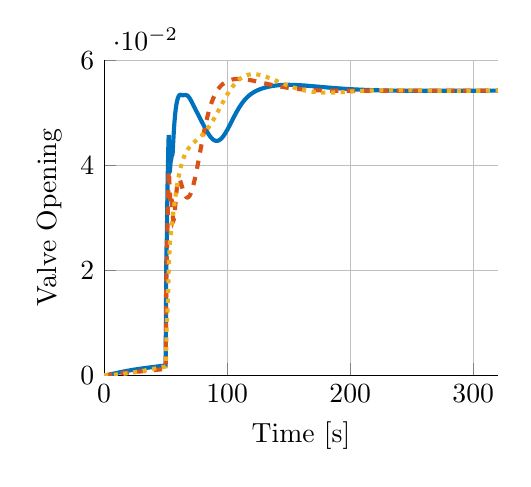
\begin{tikzpicture}

\begin{axis}[%
width=5cm,
height=4cm,
at={(0\linewidth,0\linewidth)},
scale only axis,
xmin=0,
xmax=320,
xlabel={Time [s]},
xmajorgrids,
ymin=0,
ymax=0.06,
ylabel={Valve Opening},
ymajorgrids,
axis background/.style={fill=white},
% title style={font=\bfseries},
% title={Normalized Recycle Valve Opening},
axis x line*=bottom,
axis y line*=left
]
\addplot [color=mycolor1,solid,line width=1.5pt,forget plot]
  table[row sep=crcr]{%
0	0\\
0.25	0\\
0.5	0\\
0.75	0\\
1	0\\
1.25	0\\
1.5	0\\
1.75	1.21538e-06\\
2	6.9504e-06\\
2.25	1.70383e-05\\
2.5	3.02921e-05\\
2.75	4.50965e-05\\
3	5.99591e-05\\
3.25	7.39074e-05\\
3.5	8.62583e-05\\
3.75	9.66784e-05\\
4	0.000105267\\
4.25	0.000112726\\
4.5	0.000120275\\
4.75	0.00012918\\
5	0.000140273\\
5.25	0.000153731\\
5.5	0.00016922\\
5.75	0.000186022\\
6	0.000203147\\
6.25	0.000219559\\
6.5	0.000234417\\
6.75	0.000247281\\
7	0.000258231\\
7.25	0.00026784\\
7.5	0.000277\\
7.75	0.000286676\\
8	0.000297664\\
8.25	0.000310406\\
8.5	0.000324894\\
8.75	0.000340683\\
9	0.000357006\\
9.25	0.000372969\\
9.5	0.000387778\\
9.75	0.000400935\\
10	0.000412358\\
10.25	0.000422393\\
10.5	0.000431714\\
10.75	0.000441145\\
11	0.000451454\\
11.25	0.000463161\\
11.5	0.000476412\\
11.75	0.000490953\\
12	0.000506201\\
12.25	0.000521392\\
12.5	0.000535783\\
12.75	0.000548831\\
13	0.000560334\\
13.25	0.000570472\\
13.5	0.000579758\\
13.75	0.000588899\\
14	0.000598617\\
14.25	0.000609463\\
14.5	0.000621683\\
14.75	0.000635158\\
15	0.000649443\\
15.25	0.000663878\\
15.5	0.000677764\\
15.75	0.000690537\\
16	0.000701909\\
16.25	0.000711944\\
16.5	0.000721031\\
16.75	0.000729787\\
17	0.000738888\\
17.25	0.000748904\\
17.5	0.000760149\\
17.75	0.000772605\\
18	0.00078593\\
18.25	0.000799548\\
18.5	0.000812797\\
18.75	0.000825099\\
19	0.000836108\\
19.25	0.000845799\\
19.5	0.000854471\\
19.75	0.000862668\\
20	0.000871037\\
20.25	0.000880158\\
20.5	0.000890399\\
20.75	0.00090182\\
21	0.000914159\\
21.25	0.000926901\\
21.5	0.000939412\\
21.75	0.000951105\\
22	0.000961585\\
22.25	0.000970761\\
22.5	0.000978863\\
22.75	0.000986381\\
23	0.000993941\\
23.25	0.00100214\\
23.5	0.00101139\\
23.75	0.00102181\\
24	0.0010332\\
24.25	0.00104509\\
24.5	0.00105687\\
24.75	0.00106794\\
25	0.00107785\\
25.25	0.00108646\\
25.5	0.00109395\\
25.75	0.00110077\\
26	0.00110753\\
26.25	0.00111486\\
26.5	0.0011232\\
26.75	0.00113274\\
27	0.00114331\\
27.25	0.00115448\\
27.5	0.00116564\\
27.75	0.00117616\\
28	0.00118557\\
28.25	0.00119368\\
28.5	0.00120061\\
28.75	0.00120679\\
29	0.00121285\\
29.25	0.00121942\\
29.5	0.001227\\
29.75	0.00123581\\
30	0.00124575\\
30.25	0.00125638\\
30.5	0.0012671\\
30.75	0.00127724\\
31	0.00128629\\
31.25	0.001294\\
31.5	0.00130047\\
31.75	0.00130612\\
32	0.00131158\\
32.25	0.00131753\\
32.5	0.00132452\\
32.75	0.00133281\\
33	0.00134232\\
33.25	0.00135263\\
33.5	0.0013631\\
33.75	0.00137304\\
34	0.00138188\\
34.25	0.00138932\\
34.5	0.00139544\\
34.75	0.00140066\\
35	0.00140564\\
35.25	0.0014111\\
35.5	0.00141765\\
35.75	0.0014256\\
36	0.00143488\\
36.25	0.00144508\\
36.5	0.00145552\\
36.75	0.00146544\\
37	0.00147421\\
37.25	0.0014815\\
37.5	0.00148736\\
37.75	0.00149222\\
38	0.00149679\\
38.25	0.00150187\\
38.5	0.00150811\\
38.75	0.00151587\\
39	0.00152512\\
39.25	0.00153541\\
39.5	0.001546\\
39.75	0.00155606\\
40	0.0015649\\
40.25	0.00157212\\
40.5	0.00157776\\
40.75	0.0015823\\
41	0.0015865\\
41.25	0.00159124\\
41.5	0.00159726\\
41.75	0.00160498\\
42	0.00161437\\
42.25	0.00162492\\
42.5	0.00163584\\
42.75	0.00164619\\
43	0.00165519\\
43.25	0.00166238\\
43.5	0.00166782\\
43.75	0.00167201\\
44	0.00167582\\
44.25	0.00168024\\
44.5	0.00168611\\
44.75	0.0016939\\
45	0.00170357\\
45.25	0.00171457\\
45.5	0.00172599\\
45.75	0.00173675\\
46	0.00174597\\
46.25	0.00175315\\
46.5	0.00175831\\
46.75	0.00176207\\
47	0.00176542\\
47.25	0.0017695\\
47.5	0.00177525\\
47.75	0.00178322\\
48	0.00179335\\
48.25	0.00180498\\
48.5	0.00181706\\
48.75	0.00182835\\
49	0.00183783\\
49.25	0.00184493\\
49.5	0.00184971\\
49.75	0.0018529\\
50	0.00185566\\
50.25	0.0106823\\
50.5	0.0208504\\
50.75	0.0243066\\
51	0.0261291\\
51.25	0.0307344\\
51.5	0.0354162\\
51.75	0.0383866\\
52	0.0411891\\
52.25	0.0441063\\
52.5	0.0457436\\
52.75	0.0431454\\
53	0.0400479\\
53.25	0.0387326\\
53.5	0.0388428\\
53.75	0.0397371\\
54	0.0405224\\
54.25	0.0408794\\
54.5	0.0411239\\
54.75	0.0414452\\
55	0.041782\\
55.25	0.0420426\\
55.5	0.0420536\\
55.75	0.0424731\\
56	0.0435875\\
56.25	0.0447724\\
56.5	0.0457822\\
56.75	0.0467364\\
57	0.0476344\\
57.25	0.0484249\\
57.5	0.0491111\\
57.75	0.0497202\\
58	0.0502684\\
58.25	0.0507522\\
58.5	0.0511703\\
58.75	0.0515347\\
59	0.0518568\\
59.25	0.0521409\\
59.5	0.0523902\\
59.75	0.0526083\\
60	0.0527973\\
60.25	0.0529582\\
60.5	0.0530919\\
60.75	0.0531996\\
61	0.0532826\\
61.25	0.0533427\\
61.5	0.0533821\\
61.75	0.0534034\\
62	0.0534097\\
62.25	0.0534046\\
62.5	0.0533915\\
62.75	0.053374\\
63	0.0533556\\
63.25	0.053339\\
63.5	0.0533263\\
63.75	0.053319\\
64	0.0533173\\
64.25	0.0533206\\
64.5	0.0533279\\
64.75	0.0533373\\
65	0.0533471\\
65.25	0.0533558\\
65.5	0.0533622\\
65.75	0.0533657\\
66	0.053366\\
66.25	0.053363\\
66.5	0.0533561\\
66.75	0.0533446\\
67	0.0533276\\
67.25	0.0533041\\
67.5	0.0532733\\
67.75	0.0532346\\
68	0.053188\\
68.25	0.0531336\\
68.5	0.0530714\\
68.75	0.0530019\\
69	0.0529255\\
69.25	0.0528427\\
69.5	0.0527541\\
69.75	0.0526602\\
70	0.0525617\\
70.25	0.052459\\
70.5	0.0523529\\
70.75	0.0522439\\
71	0.0521325\\
71.25	0.0520193\\
71.5	0.0519047\\
71.75	0.051789\\
72	0.0516727\\
72.25	0.0515561\\
72.5	0.0514393\\
72.75	0.0513226\\
73	0.0512062\\
73.25	0.0510901\\
73.5	0.0509743\\
73.75	0.050859\\
74	0.0507441\\
74.25	0.0506297\\
74.5	0.0505156\\
74.75	0.0504018\\
75	0.0502882\\
75.25	0.0501749\\
75.5	0.0500617\\
75.75	0.0499485\\
76	0.0498353\\
76.25	0.0497221\\
76.5	0.0496087\\
76.75	0.0494951\\
77	0.0493814\\
77.25	0.0492674\\
77.5	0.0491532\\
77.75	0.0490387\\
78	0.0489239\\
78.25	0.048809\\
78.5	0.0486938\\
78.75	0.0485785\\
79	0.048463\\
79.25	0.0483475\\
79.5	0.048232\\
79.75	0.0481166\\
80	0.0480013\\
80.25	0.0478863\\
80.5	0.0477715\\
80.75	0.0476572\\
81	0.0475434\\
81.25	0.0474302\\
81.5	0.0473178\\
81.75	0.0472061\\
82	0.0470955\\
82.25	0.0469858\\
82.5	0.0468773\\
82.75	0.0467701\\
83	0.0466643\\
83.25	0.0465601\\
83.5	0.0464574\\
83.75	0.0463564\\
84	0.0462574\\
84.25	0.0461602\\
84.5	0.0460652\\
84.75	0.0459723\\
85	0.0458818\\
85.25	0.0457936\\
85.5	0.0457079\\
85.75	0.0456249\\
86	0.0455446\\
86.25	0.0454671\\
86.5	0.0453925\\
86.75	0.0453209\\
87	0.0452524\\
87.25	0.045187\\
87.5	0.045125\\
87.75	0.0450663\\
88	0.045011\\
88.25	0.0449592\\
88.5	0.044911\\
88.75	0.0448665\\
89	0.0448256\\
89.25	0.0447885\\
89.5	0.0447551\\
89.75	0.0447257\\
90	0.0447001\\
90.25	0.0446784\\
90.5	0.0446607\\
90.75	0.044647\\
91	0.0446372\\
91.25	0.0446315\\
91.5	0.0446299\\
91.75	0.0446322\\
92	0.0446386\\
92.25	0.0446489\\
92.5	0.0446633\\
92.75	0.0446817\\
93	0.044704\\
93.25	0.0447303\\
93.5	0.0447604\\
93.75	0.0447944\\
94	0.0448322\\
94.25	0.0448737\\
94.5	0.044919\\
94.75	0.0449678\\
95	0.0450203\\
95.25	0.0450762\\
95.5	0.0451356\\
95.75	0.0451983\\
96	0.0452643\\
96.25	0.0453334\\
96.5	0.0454056\\
96.75	0.0454809\\
97	0.045559\\
97.25	0.0456399\\
97.5	0.0457235\\
97.75	0.0458098\\
98	0.0458985\\
98.25	0.0459896\\
98.5	0.0460829\\
98.75	0.0461785\\
99	0.0462761\\
99.25	0.0463756\\
99.5	0.046477\\
99.75	0.0465801\\
100	0.0466848\\
100.25	0.0467909\\
100.5	0.0468985\\
100.75	0.0470073\\
101	0.0471173\\
101.25	0.0472283\\
101.5	0.0473403\\
101.75	0.0474531\\
102	0.0475666\\
102.25	0.0476808\\
102.5	0.0477954\\
102.75	0.0479105\\
103	0.0480258\\
103.25	0.0481414\\
103.5	0.0482571\\
103.75	0.0483728\\
104	0.0484885\\
104.25	0.048604\\
104.5	0.0487192\\
104.75	0.0488342\\
105	0.0489487\\
105.25	0.0490628\\
105.5	0.0491762\\
105.75	0.0492891\\
106	0.0494013\\
106.25	0.0495127\\
106.5	0.0496232\\
106.75	0.0497329\\
107	0.0498417\\
107.25	0.0499494\\
107.5	0.0500561\\
107.75	0.0501617\\
108	0.0502662\\
108.25	0.0503694\\
108.5	0.0504715\\
108.75	0.0505723\\
109	0.0506718\\
109.25	0.0507699\\
109.5	0.0508667\\
109.75	0.0509622\\
110	0.0510562\\
110.25	0.0511488\\
110.5	0.05124\\
110.75	0.0513297\\
111	0.051418\\
111.25	0.0515047\\
111.5	0.05159\\
111.75	0.0516738\\
112	0.0517561\\
112.25	0.0518369\\
112.5	0.0519162\\
112.75	0.051994\\
113	0.0520703\\
113.25	0.0521451\\
113.5	0.0522184\\
113.75	0.0522903\\
114	0.0523607\\
114.25	0.0524296\\
114.5	0.0524971\\
114.75	0.0525632\\
115	0.0526279\\
115.25	0.0526912\\
115.5	0.052753\\
115.75	0.0528136\\
116	0.0528728\\
116.25	0.0529306\\
116.5	0.0529872\\
116.75	0.0530425\\
117	0.0530965\\
117.25	0.0531493\\
117.5	0.0532009\\
117.75	0.0532513\\
118	0.0533005\\
118.25	0.0533486\\
118.5	0.0533956\\
118.75	0.0534415\\
119	0.0534863\\
119.25	0.05353\\
119.5	0.0535727\\
119.75	0.0536145\\
120	0.0536552\\
120.25	0.053695\\
120.5	0.0537339\\
120.75	0.0537719\\
121	0.053809\\
121.25	0.0538452\\
121.5	0.0538806\\
121.75	0.0539152\\
122	0.053949\\
122.25	0.053982\\
122.5	0.0540143\\
122.75	0.0540459\\
123	0.0540767\\
123.25	0.0541069\\
123.5	0.0541363\\
123.75	0.0541652\\
124	0.0541934\\
124.25	0.054221\\
124.5	0.054248\\
124.75	0.0542744\\
125	0.0543003\\
125.25	0.0543256\\
125.5	0.0543504\\
125.75	0.0543747\\
126	0.0543985\\
126.25	0.0544218\\
126.5	0.0544446\\
126.75	0.054467\\
127	0.0544889\\
127.25	0.0545103\\
127.5	0.0545314\\
127.75	0.054552\\
128	0.0545723\\
128.25	0.0545921\\
128.5	0.0546116\\
128.75	0.0546306\\
129	0.0546494\\
129.25	0.0546677\\
129.5	0.0546857\\
129.75	0.0547034\\
130	0.0547207\\
130.25	0.0547377\\
130.5	0.0547544\\
130.75	0.0547708\\
131	0.0547868\\
131.25	0.0548026\\
131.5	0.054818\\
131.75	0.0548332\\
132	0.054848\\
132.25	0.0548626\\
132.5	0.0548769\\
132.75	0.0548909\\
133	0.0549046\\
133.25	0.0549181\\
133.5	0.0549313\\
133.75	0.0549442\\
134	0.0549569\\
134.25	0.0549693\\
134.5	0.0549815\\
134.75	0.0549934\\
135	0.055005\\
135.25	0.0550164\\
135.5	0.0550276\\
135.75	0.0550385\\
136	0.0550491\\
136.25	0.0550596\\
136.5	0.0550697\\
136.75	0.0550797\\
137	0.0550894\\
137.25	0.0550989\\
137.5	0.0551081\\
137.75	0.0551171\\
138	0.0551259\\
138.25	0.0551344\\
138.5	0.0551428\\
138.75	0.0551509\\
139	0.0551587\\
139.25	0.0551664\\
139.5	0.0551738\\
139.75	0.055181\\
140	0.055188\\
140.25	0.0551948\\
140.5	0.0552014\\
140.75	0.0552077\\
141	0.0552139\\
141.25	0.0552198\\
141.5	0.0552255\\
141.75	0.055231\\
142	0.0552363\\
142.25	0.0552414\\
142.5	0.0552464\\
142.75	0.0552511\\
143	0.0552556\\
143.25	0.0552599\\
143.5	0.055264\\
143.75	0.055268\\
144	0.0552717\\
144.25	0.0552753\\
144.5	0.0552786\\
144.75	0.0552818\\
145	0.0552848\\
145.25	0.0552877\\
145.5	0.0552903\\
145.75	0.0552928\\
146	0.0552951\\
146.25	0.0552972\\
146.5	0.0552992\\
146.75	0.055301\\
147	0.0553027\\
147.25	0.0553041\\
147.5	0.0553055\\
147.75	0.0553066\\
148	0.0553076\\
148.25	0.0553085\\
148.5	0.0553092\\
148.75	0.0553098\\
149	0.0553102\\
149.25	0.0553105\\
149.5	0.0553106\\
149.75	0.0553106\\
150	0.0553105\\
150.25	0.0553102\\
150.5	0.0553098\\
150.75	0.0553093\\
151	0.0553086\\
151.25	0.0553078\\
151.5	0.055307\\
151.75	0.0553059\\
152	0.0553048\\
152.25	0.0553036\\
152.5	0.0553022\\
152.75	0.0553007\\
153	0.0552992\\
153.25	0.0552975\\
153.5	0.0552957\\
153.75	0.0552938\\
154	0.0552918\\
154.25	0.0552897\\
154.5	0.0552876\\
154.75	0.0552853\\
155	0.0552829\\
155.25	0.0552805\\
155.5	0.055278\\
155.75	0.0552753\\
156	0.0552726\\
156.25	0.0552699\\
156.5	0.055267\\
156.75	0.0552641\\
157	0.055261\\
157.25	0.055258\\
157.5	0.0552548\\
157.75	0.0552516\\
158	0.0552483\\
158.25	0.0552449\\
158.5	0.0552415\\
158.75	0.055238\\
159	0.0552345\\
159.25	0.0552308\\
159.5	0.0552272\\
159.75	0.0552234\\
160	0.0552197\\
160.25	0.0552158\\
160.5	0.0552119\\
160.75	0.055208\\
161	0.055204\\
161.25	0.0552\\
161.5	0.0551959\\
161.75	0.0551918\\
162	0.0551876\\
162.25	0.0551834\\
162.5	0.0551791\\
162.75	0.0551748\\
163	0.0551705\\
163.25	0.0551661\\
163.5	0.0551617\\
163.75	0.0551573\\
164	0.0551528\\
164.25	0.0551483\\
164.5	0.0551437\\
164.75	0.0551391\\
165	0.0551345\\
165.25	0.0551299\\
165.5	0.0551252\\
165.75	0.0551205\\
166	0.0551158\\
166.25	0.0551111\\
166.5	0.0551063\\
166.75	0.0551015\\
167	0.0550967\\
167.25	0.0550918\\
167.5	0.055087\\
167.75	0.0550821\\
168	0.0550772\\
168.25	0.0550723\\
168.5	0.0550674\\
168.75	0.0550624\\
169	0.0550575\\
169.25	0.0550525\\
169.5	0.0550475\\
169.75	0.0550425\\
170	0.0550375\\
170.25	0.0550324\\
170.5	0.0550274\\
170.75	0.0550223\\
171	0.0550173\\
171.25	0.0550122\\
171.5	0.0550071\\
171.75	0.055002\\
172	0.0549969\\
172.25	0.0549918\\
172.5	0.0549867\\
172.75	0.0549816\\
173	0.0549765\\
173.25	0.0549714\\
173.5	0.0549662\\
173.75	0.0549611\\
174	0.054956\\
174.25	0.0549509\\
174.5	0.0549457\\
174.75	0.0549406\\
175	0.0549355\\
175.25	0.0549303\\
175.5	0.0549252\\
175.75	0.0549201\\
176	0.0549149\\
176.25	0.0549098\\
176.5	0.0549047\\
176.75	0.0548996\\
177	0.0548945\\
177.25	0.0548894\\
177.5	0.0548842\\
177.75	0.0548792\\
178	0.0548741\\
178.25	0.054869\\
178.5	0.0548639\\
178.75	0.0548588\\
179	0.0548538\\
179.25	0.0548487\\
179.5	0.0548437\\
179.75	0.0548386\\
180	0.0548336\\
180.25	0.0548286\\
180.5	0.0548236\\
180.75	0.0548186\\
181	0.0548136\\
181.25	0.0548086\\
181.5	0.0548036\\
181.75	0.0547987\\
182	0.0547937\\
182.25	0.0547888\\
182.5	0.0547839\\
182.75	0.054779\\
183	0.0547741\\
183.25	0.0547693\\
183.5	0.0547644\\
183.75	0.0547596\\
184	0.0547547\\
184.25	0.0547499\\
184.5	0.0547451\\
184.75	0.0547403\\
185	0.0547356\\
185.25	0.0547308\\
185.5	0.0547261\\
185.75	0.0547214\\
186	0.0547167\\
186.25	0.054712\\
186.5	0.0547073\\
186.75	0.0547027\\
187	0.0546981\\
187.25	0.0546935\\
187.5	0.0546889\\
187.75	0.0546843\\
188	0.0546798\\
188.25	0.0546752\\
188.5	0.0546707\\
188.75	0.0546662\\
189	0.0546618\\
189.25	0.0546573\\
189.5	0.0546529\\
189.75	0.0546485\\
190	0.0546441\\
190.25	0.0546397\\
190.5	0.0546354\\
190.75	0.054631\\
191	0.0546267\\
191.25	0.0546225\\
191.5	0.0546182\\
191.75	0.0546139\\
192	0.0546097\\
192.25	0.0546055\\
192.5	0.0546014\\
192.75	0.0545972\\
193	0.0545931\\
193.25	0.054589\\
193.5	0.0545849\\
193.75	0.0545808\\
194	0.0545768\\
194.25	0.0545728\\
194.5	0.0545688\\
194.75	0.0545648\\
195	0.0545608\\
195.25	0.0545569\\
195.5	0.054553\\
195.75	0.0545491\\
196	0.0545453\\
196.25	0.0545414\\
196.5	0.0545376\\
196.75	0.0545339\\
197	0.0545301\\
197.25	0.0545263\\
197.5	0.0545226\\
197.75	0.0545189\\
198	0.0545153\\
198.25	0.0545116\\
198.5	0.054508\\
198.75	0.0545044\\
199	0.0545008\\
199.25	0.0544973\\
199.5	0.0544938\\
199.75	0.0544903\\
200	0.0544868\\
200.25	0.0544833\\
200.5	0.0544799\\
200.75	0.0544765\\
201	0.0544731\\
201.25	0.0544698\\
201.5	0.0544664\\
201.75	0.0544631\\
202	0.0544598\\
202.25	0.0544566\\
202.5	0.0544533\\
202.75	0.0544501\\
203	0.0544469\\
203.25	0.0544438\\
203.5	0.0544406\\
203.75	0.0544375\\
204	0.0544344\\
204.25	0.0544313\\
204.5	0.0544283\\
204.75	0.0544252\\
205	0.0544222\\
205.25	0.0544193\\
205.5	0.0544163\\
205.75	0.0544134\\
206	0.0544105\\
206.25	0.0544076\\
206.5	0.0544047\\
206.75	0.0544019\\
207	0.0543991\\
207.25	0.0543963\\
207.5	0.0543935\\
207.75	0.0543908\\
208	0.054388\\
208.25	0.0543853\\
208.5	0.0543827\\
208.75	0.05438\\
209	0.0543774\\
209.25	0.0543748\\
209.5	0.0543722\\
209.75	0.0543696\\
210	0.0543671\\
210.25	0.0543645\\
210.5	0.054362\\
210.75	0.0543596\\
211	0.0543571\\
211.25	0.0543547\\
211.5	0.0543523\\
211.75	0.0543499\\
212	0.0543475\\
212.25	0.0543452\\
212.5	0.0543429\\
212.75	0.0543406\\
213	0.0543383\\
213.25	0.054336\\
213.5	0.0543338\\
213.75	0.0543316\\
214	0.0543294\\
214.25	0.0543272\\
214.5	0.054325\\
214.75	0.0543229\\
215	0.0543208\\
215.25	0.0543187\\
215.5	0.0543166\\
215.75	0.0543146\\
216	0.0543126\\
216.25	0.0543105\\
216.5	0.0543086\\
216.75	0.0543066\\
217	0.0543046\\
217.25	0.0543027\\
217.5	0.0543008\\
217.75	0.0542989\\
218	0.054297\\
218.25	0.0542952\\
218.5	0.0542934\\
218.75	0.0542915\\
219	0.0542897\\
219.25	0.054288\\
219.5	0.0542862\\
219.75	0.0542845\\
220	0.0542828\\
220.25	0.0542811\\
220.5	0.0542794\\
220.75	0.0542777\\
221	0.0542761\\
221.25	0.0542745\\
221.5	0.0542728\\
221.75	0.0542713\\
222	0.0542697\\
222.25	0.0542681\\
222.5	0.0542666\\
222.75	0.0542651\\
223	0.0542636\\
223.25	0.0542621\\
223.5	0.0542606\\
223.75	0.0542592\\
224	0.0542577\\
224.25	0.0542563\\
224.5	0.0542549\\
224.75	0.0542535\\
225	0.0542522\\
225.25	0.0542508\\
225.5	0.0542495\\
225.75	0.0542482\\
226	0.0542469\\
226.25	0.0542456\\
226.5	0.0542443\\
226.75	0.0542431\\
227	0.0542418\\
227.25	0.0542406\\
227.5	0.0542394\\
227.75	0.0542382\\
228	0.054237\\
228.25	0.0542359\\
228.5	0.0542347\\
228.75	0.0542336\\
229	0.0542325\\
229.25	0.0542314\\
229.5	0.0542303\\
229.75	0.0542292\\
230	0.0542282\\
230.25	0.0542271\\
230.5	0.0542261\\
230.75	0.0542251\\
231	0.0542241\\
231.25	0.0542231\\
231.5	0.0542221\\
231.75	0.0542211\\
232	0.0542202\\
232.25	0.0542193\\
232.5	0.0542183\\
232.75	0.0542174\\
233	0.0542165\\
233.25	0.0542156\\
233.5	0.0542148\\
233.75	0.0542139\\
234	0.0542131\\
234.25	0.0542122\\
234.5	0.0542114\\
234.75	0.0542106\\
235	0.0542098\\
235.25	0.054209\\
235.5	0.0542083\\
235.75	0.0542075\\
236	0.0542068\\
236.25	0.054206\\
236.5	0.0542053\\
236.75	0.0542046\\
237	0.0542039\\
237.25	0.0542032\\
237.5	0.0542025\\
237.75	0.0542018\\
238	0.0542012\\
238.25	0.0542005\\
238.5	0.0541999\\
238.75	0.0541993\\
239	0.0541987\\
239.25	0.054198\\
239.5	0.0541975\\
239.75	0.0541969\\
240	0.0541963\\
240.25	0.0541957\\
240.5	0.0541952\\
240.75	0.0541946\\
241	0.0541941\\
241.25	0.0541936\\
241.5	0.0541931\\
241.75	0.0541925\\
242	0.054192\\
242.25	0.0541916\\
242.5	0.0541911\\
242.75	0.0541906\\
243	0.0541901\\
243.25	0.0541897\\
243.5	0.0541893\\
243.75	0.0541888\\
244	0.0541884\\
244.25	0.054188\\
244.5	0.0541876\\
244.75	0.0541872\\
245	0.0541868\\
245.25	0.0541864\\
245.5	0.054186\\
245.75	0.0541856\\
246	0.0541853\\
246.25	0.0541849\\
246.5	0.0541846\\
246.75	0.0541842\\
247	0.0541839\\
247.25	0.0541836\\
247.5	0.0541833\\
247.75	0.054183\\
248	0.0541827\\
248.25	0.0541824\\
248.5	0.0541821\\
248.75	0.0541818\\
249	0.0541815\\
249.25	0.0541813\\
249.5	0.054181\\
249.75	0.0541808\\
250	0.0541805\\
250.25	0.0541803\\
250.5	0.05418\\
250.75	0.0541798\\
251	0.0541796\\
251.25	0.0541794\\
251.5	0.0541792\\
251.75	0.054179\\
252	0.0541788\\
252.25	0.0541786\\
252.5	0.0541784\\
252.75	0.0541782\\
253	0.054178\\
253.25	0.0541779\\
253.5	0.0541777\\
253.75	0.0541776\\
254	0.0541774\\
254.25	0.0541773\\
254.5	0.0541771\\
254.75	0.054177\\
255	0.0541769\\
255.25	0.0541767\\
255.5	0.0541766\\
255.75	0.0541765\\
256	0.0541764\\
256.25	0.0541763\\
256.5	0.0541762\\
256.75	0.0541761\\
257	0.054176\\
257.25	0.0541759\\
257.5	0.0541758\\
257.75	0.0541757\\
258	0.0541757\\
258.25	0.0541756\\
258.5	0.0541755\\
258.75	0.0541755\\
259	0.0541754\\
259.25	0.0541753\\
259.5	0.0541753\\
259.75	0.0541752\\
260	0.0541752\\
260.25	0.0541752\\
260.5	0.0541751\\
260.75	0.0541751\\
261	0.0541751\\
261.25	0.054175\\
261.5	0.054175\\
261.75	0.054175\\
262	0.054175\\
262.25	0.054175\\
262.5	0.054175\\
262.75	0.054175\\
263	0.054175\\
263.25	0.054175\\
263.5	0.054175\\
263.75	0.054175\\
264	0.054175\\
264.25	0.054175\\
264.5	0.054175\\
264.75	0.054175\\
265	0.0541751\\
265.25	0.0541751\\
265.5	0.0541751\\
265.75	0.0541751\\
266	0.0541752\\
266.25	0.0541752\\
266.5	0.0541752\\
266.75	0.0541753\\
267	0.0541753\\
267.25	0.0541754\\
267.5	0.0541754\\
267.75	0.0541755\\
268	0.0541755\\
268.25	0.0541756\\
268.5	0.0541756\\
268.75	0.0541757\\
269	0.0541757\\
269.25	0.0541758\\
269.5	0.0541759\\
269.75	0.0541759\\
270	0.054176\\
270.25	0.0541761\\
270.5	0.0541761\\
270.75	0.0541762\\
271	0.0541763\\
271.25	0.0541764\\
271.5	0.0541765\\
271.75	0.0541765\\
272	0.0541766\\
272.25	0.0541767\\
272.5	0.0541768\\
272.75	0.0541769\\
273	0.054177\\
273.25	0.054177\\
273.5	0.0541771\\
273.75	0.0541772\\
274	0.0541773\\
274.25	0.0541774\\
274.5	0.0541775\\
274.75	0.0541776\\
275	0.0541777\\
275.25	0.0541778\\
275.5	0.0541779\\
275.75	0.054178\\
276	0.0541781\\
276.25	0.0541782\\
276.5	0.0541783\\
276.75	0.0541784\\
277	0.0541785\\
277.25	0.0541786\\
277.5	0.0541787\\
277.75	0.0541789\\
278	0.054179\\
278.25	0.0541791\\
278.5	0.0541792\\
278.75	0.0541793\\
279	0.0541794\\
279.25	0.0541795\\
279.5	0.0541796\\
279.75	0.0541798\\
280	0.0541799\\
280.25	0.05418\\
280.5	0.0541801\\
280.75	0.0541802\\
281	0.0541803\\
281.25	0.0541805\\
281.5	0.0541806\\
281.75	0.0541807\\
282	0.0541808\\
282.25	0.0541809\\
282.5	0.0541811\\
282.75	0.0541812\\
283	0.0541813\\
283.25	0.0541814\\
283.5	0.0541815\\
283.75	0.0541817\\
284	0.0541818\\
284.25	0.0541819\\
284.5	0.054182\\
284.75	0.0541822\\
285	0.0541823\\
285.25	0.0541824\\
285.5	0.0541825\\
285.75	0.0541827\\
286	0.0541828\\
286.25	0.0541829\\
286.5	0.054183\\
286.75	0.0541832\\
287	0.0541833\\
287.25	0.0541834\\
287.5	0.0541835\\
287.75	0.0541837\\
288	0.0541838\\
288.25	0.0541839\\
288.5	0.054184\\
288.75	0.0541842\\
289	0.0541843\\
289.25	0.0541844\\
289.5	0.0541845\\
289.75	0.0541847\\
290	0.0541848\\
290.25	0.0541849\\
290.5	0.054185\\
290.75	0.0541852\\
291	0.0541853\\
291.25	0.0541854\\
291.5	0.0541855\\
291.75	0.0541857\\
292	0.0541858\\
292.25	0.0541859\\
292.5	0.054186\\
292.75	0.0541862\\
293	0.0541863\\
293.25	0.0541864\\
293.5	0.0541865\\
293.75	0.0541866\\
294	0.0541868\\
294.25	0.0541869\\
294.5	0.054187\\
294.75	0.0541871\\
295	0.0541873\\
295.25	0.0541874\\
295.5	0.0541875\\
295.75	0.0541876\\
296	0.0541877\\
296.25	0.0541878\\
296.5	0.054188\\
296.75	0.0541881\\
297	0.0541882\\
297.25	0.0541883\\
297.5	0.0541884\\
297.75	0.0541886\\
298	0.0541887\\
298.25	0.0541888\\
298.5	0.0541889\\
298.75	0.054189\\
299	0.0541891\\
299.25	0.0541892\\
299.5	0.0541894\\
299.75	0.0541895\\
300	0.0541896\\
300.25	0.0541897\\
300.5	0.0541898\\
300.75	0.0541899\\
301	0.05419\\
301.25	0.0541901\\
301.5	0.0541903\\
301.75	0.0541904\\
302	0.0541905\\
302.25	0.0541906\\
302.5	0.0541907\\
302.75	0.0541908\\
303	0.0541909\\
303.25	0.054191\\
303.5	0.0541911\\
303.75	0.0541912\\
304	0.0541913\\
304.25	0.0541914\\
304.5	0.0541915\\
304.75	0.0541916\\
305	0.0541917\\
305.25	0.0541918\\
305.5	0.0541919\\
305.75	0.054192\\
306	0.0541921\\
306.25	0.0541922\\
306.5	0.0541923\\
306.75	0.0541924\\
307	0.0541925\\
307.25	0.0541926\\
307.5	0.0541927\\
307.75	0.0541928\\
308	0.0541929\\
308.25	0.054193\\
308.5	0.0541931\\
308.75	0.0541932\\
309	0.0541933\\
309.25	0.0541934\\
309.5	0.0541935\\
309.75	0.0541936\\
310	0.0541937\\
310.25	0.0541938\\
310.5	0.0541939\\
310.75	0.0541939\\
311	0.054194\\
311.25	0.0541941\\
311.5	0.0541942\\
311.75	0.0541943\\
312	0.0541944\\
312.25	0.0541945\\
312.5	0.0541946\\
312.75	0.0541946\\
313	0.0541947\\
313.25	0.0541948\\
313.5	0.0541949\\
313.75	0.054195\\
314	0.0541951\\
314.25	0.0541951\\
314.5	0.0541952\\
314.75	0.0541953\\
315	0.0541954\\
315.25	0.0541955\\
315.5	0.0541955\\
315.75	0.0541956\\
316	0.0541957\\
316.25	0.0541958\\
316.5	0.0541958\\
316.75	0.0541959\\
317	0.054196\\
317.25	0.0541961\\
317.5	0.0541961\\
317.75	0.0541962\\
318	0.0541963\\
318.25	0.0541964\\
318.5	0.0541964\\
318.75	0.0541965\\
319	0.0541966\\
319.25	0.0541966\\
319.5	0.0541967\\
319.75	0.0541968\\
320	0.0541968\\
320.25	0.0541969\\
320.5	0.054197\\
320.75	0.054197\\
321	0.0541971\\
321.25	0.0541972\\
321.5	0.0541972\\
321.75	0.0541973\\
322	0.0541974\\
322.25	0.0541974\\
322.5	0.0541975\\
322.75	0.0541975\\
323	0.0541976\\
323.25	0.0541977\\
323.5	0.0541977\\
323.75	0.0541978\\
324	0.0541978\\
324.25	0.0541979\\
324.5	0.054198\\
324.75	0.054198\\
325	0.0541981\\
325.25	0.0541981\\
325.5	0.0541982\\
325.75	0.0541982\\
326	0.0541983\\
326.25	0.0541984\\
326.5	0.0541984\\
326.75	0.0541985\\
327	0.0541985\\
327.25	0.0541986\\
327.5	0.0541986\\
327.75	0.0541987\\
328	0.0541987\\
328.25	0.0541988\\
328.5	0.0541988\\
328.75	0.0541989\\
329	0.0541989\\
329.25	0.054199\\
329.5	0.054199\\
329.75	0.0541991\\
330	0.0541991\\
330.25	0.0541991\\
330.5	0.0541992\\
330.75	0.0541992\\
331	0.0541993\\
331.25	0.0541993\\
331.5	0.0541994\\
331.75	0.0541994\\
332	0.0541995\\
332.25	0.0541995\\
332.5	0.0541995\\
332.75	0.0541996\\
333	0.0541996\\
333.25	0.0541997\\
333.5	0.0541997\\
333.75	0.0541997\\
334	0.0541998\\
334.25	0.0541998\\
334.5	0.0541999\\
334.75	0.0541999\\
335	0.0541999\\
335.25	0.0542\\
335.5	0.0542\\
335.75	0.0542\\
336	0.0542001\\
336.25	0.0542001\\
336.5	0.0542001\\
336.75	0.0542002\\
337	0.0542002\\
337.25	0.0542002\\
337.5	0.0542003\\
337.75	0.0542003\\
338	0.0542003\\
338.25	0.0542004\\
338.5	0.0542004\\
338.75	0.0542004\\
339	0.0542005\\
339.25	0.0542005\\
339.5	0.0542005\\
339.75	0.0542006\\
340	0.0542006\\
340.25	0.0542006\\
340.5	0.0542006\\
340.75	0.0542007\\
341	0.0542007\\
341.25	0.0542007\\
341.5	0.0542008\\
341.75	0.0542008\\
342	0.0542008\\
342.25	0.0542008\\
342.5	0.0542009\\
342.75	0.0542009\\
343	0.0542009\\
343.25	0.0542009\\
343.5	0.054201\\
343.75	0.054201\\
344	0.054201\\
344.25	0.054201\\
344.5	0.0542011\\
344.75	0.0542011\\
345	0.0542011\\
345.25	0.0542011\\
345.5	0.0542011\\
345.75	0.0542012\\
346	0.0542012\\
346.25	0.0542012\\
346.5	0.0542012\\
346.75	0.0542012\\
347	0.0542013\\
347.25	0.0542013\\
347.5	0.0542013\\
347.75	0.0542013\\
348	0.0542013\\
348.25	0.0542014\\
348.5	0.0542014\\
348.75	0.0542014\\
349	0.0542014\\
349.25	0.0542014\\
349.5	0.0542014\\
349.75	0.0542015\\
350	0.0542015\\
350.25	0.0542015\\
350.5	0.0542015\\
350.75	0.0542015\\
351	0.0542015\\
351.25	0.0542016\\
351.5	0.0542016\\
351.75	0.0542016\\
352	0.0542016\\
352.25	0.0542016\\
352.5	0.0542016\\
352.75	0.0542016\\
353	0.0542017\\
353.25	0.0542017\\
353.5	0.0542017\\
353.75	0.0542017\\
354	0.0542017\\
354.25	0.0542017\\
354.5	0.0542017\\
354.75	0.0542017\\
355	0.0542018\\
355.25	0.0542018\\
355.5	0.0542018\\
355.75	0.0542018\\
356	0.0542018\\
356.25	0.0542018\\
356.5	0.0542018\\
356.75	0.0542018\\
357	0.0542018\\
357.25	0.0542018\\
357.5	0.0542019\\
357.75	0.0542019\\
358	0.0542019\\
358.25	0.0542019\\
358.5	0.0542019\\
358.75	0.0542019\\
359	0.0542019\\
359.25	0.0542019\\
359.5	0.0542019\\
359.75	0.0542019\\
360	0.0542019\\
360.25	0.0542019\\
360.5	0.054202\\
360.75	0.054202\\
361	0.054202\\
361.25	0.054202\\
361.5	0.054202\\
361.75	0.054202\\
362	0.054202\\
362.25	0.054202\\
362.5	0.054202\\
362.75	0.054202\\
363	0.054202\\
363.25	0.054202\\
363.5	0.054202\\
363.75	0.054202\\
364	0.054202\\
364.25	0.054202\\
364.5	0.054202\\
364.75	0.0542021\\
365	0.0542021\\
365.25	0.0542021\\
365.5	0.0542021\\
365.75	0.0542021\\
366	0.0542021\\
366.25	0.0542021\\
366.5	0.0542021\\
366.75	0.0542021\\
367	0.0542021\\
367.25	0.0542021\\
367.5	0.0542021\\
367.75	0.0542021\\
368	0.0542021\\
368.25	0.0542021\\
368.5	0.0542021\\
368.75	0.0542021\\
369	0.0542021\\
369.25	0.0542021\\
369.5	0.0542021\\
369.75	0.0542021\\
370	0.0542021\\
370.25	0.0542021\\
370.5	0.0542021\\
370.75	0.0542021\\
371	0.0542021\\
371.25	0.0542021\\
371.5	0.0542021\\
371.75	0.0542021\\
372	0.0542021\\
372.25	0.0542021\\
372.5	0.0542021\\
372.75	0.0542021\\
373	0.0542021\\
373.25	0.0542021\\
373.5	0.0542021\\
373.75	0.0542021\\
374	0.0542021\\
374.25	0.0542021\\
374.5	0.0542021\\
374.75	0.0542021\\
375	0.0542021\\
375.25	0.0542021\\
375.5	0.0542021\\
375.75	0.0542021\\
376	0.0542021\\
376.25	0.0542021\\
376.5	0.0542021\\
376.75	0.0542021\\
377	0.0542021\\
377.25	0.0542021\\
377.5	0.0542021\\
377.75	0.0542021\\
378	0.0542021\\
378.25	0.0542021\\
378.5	0.0542021\\
378.75	0.0542021\\
379	0.0542021\\
379.25	0.0542021\\
379.5	0.0542021\\
379.75	0.0542021\\
380	0.0542021\\
380.25	0.0542021\\
380.5	0.0542021\\
380.75	0.0542021\\
381	0.0542021\\
381.25	0.0542021\\
381.5	0.0542021\\
381.75	0.0542021\\
382	0.0542021\\
382.25	0.0542021\\
382.5	0.0542021\\
382.75	0.0542021\\
383	0.0542021\\
383.25	0.0542021\\
383.5	0.0542021\\
383.75	0.0542021\\
384	0.0542021\\
384.25	0.0542021\\
384.5	0.0542021\\
384.75	0.0542021\\
385	0.0542021\\
385.25	0.0542021\\
385.5	0.0542021\\
385.75	0.0542021\\
386	0.0542021\\
386.25	0.0542021\\
386.5	0.0542021\\
386.75	0.0542021\\
387	0.0542021\\
387.25	0.0542021\\
387.5	0.0542021\\
387.75	0.0542021\\
388	0.0542021\\
388.25	0.0542021\\
388.5	0.0542021\\
388.75	0.0542021\\
389	0.0542021\\
389.25	0.054202\\
389.5	0.054202\\
389.75	0.054202\\
390	0.054202\\
390.25	0.054202\\
390.5	0.054202\\
390.75	0.054202\\
391	0.054202\\
391.25	0.054202\\
391.5	0.054202\\
391.75	0.054202\\
392	0.054202\\
392.25	0.054202\\
392.5	0.054202\\
392.75	0.054202\\
393	0.054202\\
393.25	0.054202\\
393.5	0.054202\\
393.75	0.054202\\
394	0.054202\\
394.25	0.054202\\
394.5	0.054202\\
394.75	0.054202\\
395	0.054202\\
395.25	0.054202\\
395.5	0.054202\\
395.75	0.054202\\
396	0.054202\\
396.25	0.054202\\
396.5	0.054202\\
396.75	0.054202\\
397	0.054202\\
397.25	0.054202\\
397.5	0.054202\\
397.75	0.0542019\\
398	0.0542019\\
398.25	0.0542019\\
398.5	0.0542019\\
398.75	0.0542019\\
399	0.0542019\\
399.25	0.0542019\\
399.5	0.0542019\\
399.75	0.0542019\\
400	0.0542019\\
400.25	0.0542019\\
400.5	0.0542019\\
400.75	0.0542019\\
401	0.0542019\\
401.25	0.0542019\\
401.5	0.0542019\\
401.75	0.0542019\\
402	0.0542019\\
402.25	0.0542019\\
402.5	0.0542019\\
402.75	0.0542019\\
403	0.0542019\\
403.25	0.0542019\\
403.5	0.0542019\\
403.75	0.0542019\\
404	0.0542019\\
404.25	0.0542019\\
404.5	0.0542019\\
404.75	0.0542019\\
405	0.0542019\\
405.25	0.0542019\\
405.5	0.0542019\\
405.75	0.0542019\\
406	0.0542018\\
406.25	0.0542018\\
406.5	0.0542018\\
406.75	0.0542018\\
407	0.0542018\\
407.25	0.0542018\\
407.5	0.0542018\\
407.75	0.0542018\\
408	0.0542018\\
408.25	0.0542018\\
408.5	0.0542018\\
408.75	0.0542018\\
409	0.0542018\\
409.25	0.0542018\\
409.5	0.0542018\\
409.75	0.0542018\\
410	0.0542018\\
410.25	0.0542018\\
410.5	0.0542018\\
410.75	0.0542018\\
411	0.0542018\\
411.25	0.0542018\\
411.5	0.0542018\\
411.75	0.0542018\\
412	0.0542018\\
412.25	0.0542018\\
412.5	0.0542018\\
412.75	0.0542018\\
413	0.0542018\\
413.25	0.0542018\\
413.5	0.0542018\\
413.75	0.0542018\\
414	0.0542018\\
414.25	0.0542018\\
414.5	0.0542018\\
414.75	0.0542018\\
415	0.0542017\\
415.25	0.0542017\\
415.5	0.0542017\\
415.75	0.0542017\\
416	0.0542017\\
416.25	0.0542017\\
416.5	0.0542017\\
416.75	0.0542017\\
417	0.0542017\\
417.25	0.0542017\\
417.5	0.0542017\\
417.75	0.0542017\\
418	0.0542017\\
418.25	0.0542017\\
418.5	0.0542017\\
418.75	0.0542017\\
419	0.0542017\\
419.25	0.0542017\\
419.5	0.0542017\\
419.75	0.0542017\\
420	0.0542017\\
420.25	0.0542017\\
420.5	0.0542017\\
420.75	0.0542017\\
421	0.0542017\\
421.25	0.0542017\\
421.5	0.0542017\\
421.75	0.0542017\\
422	0.0542017\\
422.25	0.0542017\\
422.5	0.0542017\\
422.75	0.0542017\\
423	0.0542017\\
423.25	0.0542017\\
423.5	0.0542017\\
423.75	0.0542017\\
424	0.0542017\\
424.25	0.0542017\\
424.5	0.0542017\\
424.75	0.0542017\\
425	0.0542017\\
425.25	0.0542017\\
425.5	0.0542017\\
425.75	0.0542016\\
426	0.0542016\\
426.25	0.0542016\\
426.5	0.0542016\\
426.75	0.0542016\\
427	0.0542016\\
427.25	0.0542016\\
427.5	0.0542016\\
427.75	0.0542016\\
428	0.0542016\\
428.25	0.0542016\\
428.5	0.0542016\\
428.75	0.0542016\\
429	0.0542016\\
429.25	0.0542016\\
429.5	0.0542016\\
429.75	0.0542016\\
430	0.0542016\\
430.25	0.0542016\\
430.5	0.0542016\\
430.75	0.0542016\\
431	0.0542016\\
431.25	0.0542016\\
431.5	0.0542016\\
431.75	0.0542016\\
432	0.0542016\\
432.25	0.0542016\\
432.5	0.0542016\\
432.75	0.0542016\\
433	0.0542016\\
433.25	0.0542016\\
433.5	0.0542016\\
433.75	0.0542016\\
434	0.0542016\\
434.25	0.0542016\\
434.5	0.0542016\\
434.75	0.0542016\\
435	0.0542016\\
435.25	0.0542016\\
435.5	0.0542016\\
435.75	0.0542016\\
436	0.0542016\\
436.25	0.0542016\\
436.5	0.0542016\\
436.75	0.0542016\\
437	0.0542016\\
437.25	0.0542016\\
437.5	0.0542016\\
437.75	0.0542016\\
438	0.0542016\\
438.25	0.0542016\\
438.5	0.0542016\\
438.75	0.0542016\\
439	0.0542016\\
439.25	0.0542016\\
439.5	0.0542016\\
439.75	0.0542016\\
440	0.0542016\\
440.25	0.0542016\\
440.5	0.0542016\\
440.75	0.0542016\\
441	0.0542016\\
441.25	0.0542015\\
441.5	0.0542015\\
441.75	0.0542015\\
442	0.0542015\\
442.25	0.0542015\\
442.5	0.0542015\\
442.75	0.0542015\\
443	0.0542015\\
443.25	0.0542015\\
443.5	0.0542015\\
443.75	0.0542015\\
444	0.0542015\\
444.25	0.0542015\\
444.5	0.0542015\\
444.75	0.0542015\\
445	0.0542015\\
445.25	0.0542015\\
445.5	0.0542015\\
445.75	0.0542015\\
446	0.0542015\\
446.25	0.0542015\\
446.5	0.0542015\\
446.75	0.0542015\\
447	0.0542015\\
447.25	0.0542015\\
447.5	0.0542015\\
447.75	0.0542015\\
448	0.0542015\\
448.25	0.0542015\\
448.5	0.0542015\\
448.75	0.0542015\\
449	0.0542015\\
449.25	0.0542015\\
449.5	0.0542015\\
449.75	0.0542015\\
450	0.0542015\\
450.25	0.0542015\\
450.5	0.0542015\\
450.75	0.0542015\\
451	0.0542015\\
451.25	0.0542015\\
451.5	0.0542015\\
451.75	0.0542015\\
452	0.0542015\\
452.25	0.0542015\\
452.5	0.0542015\\
452.75	0.0542015\\
453	0.0542015\\
453.25	0.0542015\\
453.5	0.0542015\\
453.75	0.0542015\\
454	0.0542015\\
454.25	0.0542015\\
454.5	0.0542015\\
454.75	0.0542015\\
455	0.0542015\\
455.25	0.0542015\\
455.5	0.0542015\\
455.75	0.0542015\\
456	0.0542015\\
456.25	0.0542015\\
456.5	0.0542015\\
456.75	0.0542015\\
457	0.0542015\\
457.25	0.0542015\\
457.5	0.0542015\\
457.75	0.0542015\\
458	0.0542015\\
458.25	0.0542015\\
458.5	0.0542015\\
458.75	0.0542015\\
459	0.0542015\\
459.25	0.0542015\\
459.5	0.0542015\\
459.75	0.0542015\\
460	0.0542015\\
460.25	0.0542015\\
460.5	0.0542015\\
460.75	0.0542015\\
461	0.0542015\\
461.25	0.0542015\\
461.5	0.0542015\\
461.75	0.0542015\\
462	0.0542015\\
462.25	0.0542015\\
462.5	0.0542015\\
462.75	0.0542015\\
463	0.0542015\\
463.25	0.0542015\\
463.5	0.0542015\\
463.75	0.0542015\\
464	0.0542015\\
464.25	0.0542015\\
464.5	0.0542015\\
464.75	0.0542015\\
465	0.0542015\\
465.25	0.0542015\\
465.5	0.0542015\\
465.75	0.0542015\\
466	0.0542015\\
466.25	0.0542015\\
466.5	0.0542015\\
466.75	0.0542015\\
467	0.0542015\\
467.25	0.0542015\\
467.5	0.0542015\\
467.75	0.0542015\\
468	0.0542015\\
468.25	0.0542015\\
468.5	0.0542015\\
468.75	0.0542015\\
469	0.0542015\\
469.25	0.0542015\\
469.5	0.0542015\\
469.75	0.0542015\\
470	0.0542015\\
470.25	0.0542015\\
470.5	0.0542015\\
470.75	0.0542015\\
471	0.0542015\\
471.25	0.0542015\\
471.5	0.0542015\\
471.75	0.0542015\\
472	0.0542015\\
472.25	0.0542015\\
472.5	0.0542015\\
472.75	0.0542015\\
473	0.0542015\\
473.25	0.0542015\\
473.5	0.0542015\\
473.75	0.0542015\\
474	0.0542015\\
474.25	0.0542015\\
474.5	0.0542015\\
474.75	0.0542015\\
475	0.0542015\\
475.25	0.0542015\\
475.5	0.0542015\\
475.75	0.0542015\\
476	0.0542015\\
476.25	0.0542015\\
476.5	0.0542015\\
476.75	0.0542015\\
477	0.0542015\\
477.25	0.0542015\\
477.5	0.0542015\\
477.75	0.0542015\\
478	0.0542015\\
478.25	0.0542015\\
478.5	0.0542015\\
478.75	0.0542015\\
479	0.0542015\\
479.25	0.0542015\\
479.5	0.0542015\\
479.75	0.0542015\\
480	0.0542015\\
480.25	0.0542015\\
480.5	0.0542015\\
480.75	0.0542015\\
481	0.0542015\\
481.25	0.0542015\\
481.5	0.0542015\\
481.75	0.0542015\\
482	0.0542015\\
482.25	0.0542015\\
482.5	0.0542015\\
482.75	0.0542015\\
483	0.0542015\\
483.25	0.0542015\\
483.5	0.0542015\\
483.75	0.0542015\\
484	0.0542015\\
484.25	0.0542015\\
484.5	0.0542015\\
484.75	0.0542015\\
485	0.0542015\\
485.25	0.0542015\\
485.5	0.0542015\\
485.75	0.0542015\\
486	0.0542015\\
486.25	0.0542015\\
486.5	0.0542015\\
486.75	0.0542015\\
487	0.0542015\\
487.25	0.0542015\\
487.5	0.0542015\\
487.75	0.0542015\\
488	0.0542015\\
488.25	0.0542015\\
488.5	0.0542015\\
488.75	0.0542015\\
489	0.0542015\\
489.25	0.0542015\\
489.5	0.0542015\\
489.75	0.0542015\\
490	0.0542015\\
490.25	0.0542015\\
490.5	0.0542015\\
490.75	0.0542015\\
491	0.0542015\\
491.25	0.0542015\\
491.5	0.0542015\\
491.75	0.0542015\\
492	0.0542015\\
492.25	0.0542015\\
492.5	0.0542015\\
492.75	0.0542015\\
493	0.0542015\\
493.25	0.0542015\\
493.5	0.0542015\\
493.75	0.0542015\\
494	0.0542015\\
494.25	0.0542015\\
494.5	0.0542015\\
494.75	0.0542015\\
495	0.0542015\\
495.25	0.0542015\\
495.5	0.0542015\\
495.75	0.0542015\\
496	0.0542015\\
496.25	0.0542015\\
496.5	0.0542015\\
496.75	0.0542015\\
497	0.0542015\\
497.25	0.0542015\\
497.5	0.0542015\\
497.75	0.0542015\\
498	0.0542015\\
498.25	0.0542015\\
498.5	0.0542015\\
498.75	0.0542015\\
499	0.0542015\\
499.25	0.0542015\\
499.5	0.0542015\\
499.75	0.0542015\\
};
\addplot [color=mycolor2,dashed,line width=1.5pt,forget plot]
  table[row sep=crcr]{%
0	0\\
0.25	0\\
0.5	0\\
0.75	0\\
1	0\\
1.25	0\\
1.5	0\\
1.75	0\\
2	8.48789e-07\\
2.25	3.74418e-06\\
2.5	8.50018e-06\\
2.75	1.47428e-05\\
3	2.2059e-05\\
3.25	3.00366e-05\\
3.5	3.82816e-05\\
3.75	4.64519e-05\\
4	5.42697e-05\\
4.25	6.15603e-05\\
4.5	6.83509e-05\\
4.75	7.48495e-05\\
5	8.13278e-05\\
5.25	8.80406e-05\\
5.5	9.51821e-05\\
5.75	0.000102858\\
6	0.000111073\\
6.25	0.000119742\\
6.5	0.000128702\\
6.75	0.000137756\\
7	0.000146708\\
7.25	0.00015541\\
7.5	0.000163782\\
7.75	0.000171816\\
8	0.000179572\\
8.25	0.000187152\\
8.5	0.000194674\\
8.75	0.000202251\\
9	0.00020996\\
9.25	0.000217837\\
9.5	0.000225866\\
9.75	0.000233993\\
10	0.00024214\\
10.25	0.00025022\\
10.5	0.000258158\\
10.75	0.000265906\\
11	0.000273446\\
11.25	0.000280793\\
11.5	0.000287987\\
11.75	0.000295082\\
12	0.000302136\\
12.25	0.000309195\\
12.5	0.000316286\\
12.75	0.000323416\\
13	0.00033057\\
13.25	0.000337717\\
13.5	0.00034482\\
13.75	0.000351843\\
14	0.000358756\\
14.25	0.000365547\\
14.5	0.000372215\\
14.75	0.000378775\\
15	0.000385252\\
15.25	0.000391671\\
15.5	0.00039806\\
15.75	0.000404435\\
16	0.000410807\\
16.25	0.000417172\\
16.5	0.00042352\\
16.75	0.000429836\\
17	0.000436102\\
17.25	0.000442303\\
17.5	0.000448431\\
17.75	0.000454483\\
18	0.000460464\\
18.25	0.000466384\\
18.5	0.000472257\\
18.75	0.000478097\\
19	0.000483915\\
19.25	0.000489717\\
19.5	0.000495507\\
19.75	0.000501282\\
20	0.000507035\\
20.25	0.00051276\\
20.5	0.00051845\\
20.75	0.000524099\\
21	0.000529707\\
21.25	0.000535274\\
21.5	0.000540807\\
21.75	0.000546311\\
22	0.000551794\\
22.25	0.000557263\\
22.5	0.000562724\\
22.75	0.00056818\\
23	0.00057363\\
23.25	0.000579074\\
23.5	0.000584509\\
23.75	0.000589931\\
24	0.00059534\\
24.25	0.000600733\\
24.5	0.000606111\\
24.75	0.000611478\\
25	0.000616837\\
25.25	0.000622191\\
25.5	0.000627545\\
25.75	0.000632903\\
26	0.000638266\\
26.25	0.000643637\\
26.5	0.000649014\\
26.75	0.000654397\\
27	0.000659785\\
27.25	0.000665177\\
27.5	0.000670571\\
27.75	0.000675969\\
28	0.000681372\\
28.25	0.00068678\\
28.5	0.000692197\\
28.75	0.000697624\\
29	0.000703063\\
29.25	0.000708515\\
29.5	0.000713982\\
29.75	0.000719463\\
30	0.000724957\\
30.25	0.000730465\\
30.5	0.000735984\\
30.75	0.000741516\\
31	0.000747059\\
31.25	0.000752613\\
31.5	0.000758179\\
31.75	0.000763757\\
32	0.000769349\\
32.25	0.000774955\\
32.5	0.000780576\\
32.75	0.00078621\\
33	0.00079186\\
33.25	0.000797523\\
33.5	0.000803199\\
33.75	0.000808888\\
34	0.000814588\\
34.25	0.000820299\\
34.5	0.000826021\\
34.75	0.000831753\\
35	0.000837495\\
35.25	0.000843247\\
35.5	0.00084901\\
35.75	0.000854782\\
36	0.000860565\\
36.25	0.000866356\\
36.5	0.000872157\\
36.75	0.000877966\\
37	0.000883782\\
37.25	0.000889604\\
37.5	0.000895433\\
37.75	0.000901267\\
38	0.000907105\\
38.25	0.000912948\\
38.5	0.000918796\\
38.75	0.000924647\\
39	0.000930502\\
39.25	0.00093636\\
39.5	0.00094222\\
39.75	0.000948083\\
40	0.000953948\\
40.25	0.000959814\\
40.5	0.000965681\\
40.75	0.000971548\\
41	0.000977414\\
41.25	0.000983279\\
41.5	0.000989143\\
41.75	0.000995006\\
42	0.00100087\\
42.25	0.00100673\\
42.5	0.00101258\\
42.75	0.00101844\\
43	0.00102429\\
43.25	0.00103014\\
43.5	0.00103598\\
43.75	0.00104182\\
44	0.00104766\\
44.25	0.00105349\\
44.5	0.00105932\\
44.75	0.00106515\\
45	0.00107097\\
45.25	0.00107678\\
45.5	0.00108259\\
45.75	0.0010884\\
46	0.0010942\\
46.25	0.00109999\\
46.5	0.00110578\\
46.75	0.00111156\\
47	0.00111734\\
47.25	0.00112312\\
47.5	0.00112888\\
47.75	0.00113465\\
48	0.0011404\\
48.25	0.00114616\\
48.5	0.0011519\\
48.75	0.00115764\\
49	0.00116338\\
49.25	0.00116911\\
49.5	0.00117484\\
49.75	0.00118056\\
50	0.00118628\\
50.25	0.0063658\\
50.5	0.0172444\\
50.75	0.0208826\\
51	0.0216428\\
51.25	0.0249515\\
51.5	0.0285646\\
51.75	0.0313042\\
52	0.0340314\\
52.25	0.036738\\
52.5	0.0389529\\
52.75	0.0387641\\
53	0.0369547\\
53.25	0.0357285\\
53.5	0.034636\\
53.75	0.0334517\\
54	0.0329026\\
54.25	0.0335724\\
54.5	0.0338922\\
54.75	0.0336261\\
55	0.0332387\\
55.25	0.0327268\\
55.5	0.0318493\\
55.75	0.0308817\\
56	0.0299164\\
56.25	0.029381\\
56.5	0.0295112\\
56.75	0.0299094\\
57	0.0303458\\
57.25	0.0308459\\
57.5	0.0314406\\
57.75	0.0320795\\
58	0.0327253\\
58.25	0.0333866\\
58.5	0.0340626\\
58.75	0.0347197\\
59	0.0353201\\
59.25	0.0358453\\
59.5	0.0362889\\
59.75	0.0366483\\
60	0.0369248\\
60.25	0.0371241\\
60.5	0.0372528\\
60.75	0.0373178\\
61	0.0373258\\
61.25	0.0372843\\
61.5	0.037201\\
61.75	0.0370828\\
62	0.0369365\\
62.25	0.0367679\\
62.5	0.0365826\\
62.75	0.0363855\\
63	0.036181\\
63.25	0.035973\\
63.5	0.035765\\
63.75	0.03556\\
64	0.0353606\\
64.25	0.035169\\
64.5	0.0349869\\
64.75	0.0348159\\
65	0.034657\\
65.25	0.0345112\\
65.5	0.0343791\\
65.75	0.0342611\\
66	0.0341575\\
66.25	0.0340685\\
66.5	0.0339941\\
66.75	0.0339344\\
67	0.0338892\\
67.25	0.0338584\\
67.5	0.0338419\\
67.75	0.0338395\\
68	0.0338511\\
68.25	0.0338764\\
68.5	0.0339152\\
68.75	0.0339673\\
69	0.0340326\\
69.25	0.0341107\\
69.5	0.0342014\\
69.75	0.0343046\\
70	0.0344199\\
70.25	0.034547\\
70.5	0.0346858\\
70.75	0.0348358\\
71	0.0349969\\
71.25	0.0351686\\
71.5	0.0353507\\
71.75	0.0355429\\
72	0.0357447\\
72.25	0.0359558\\
72.5	0.0361759\\
72.75	0.0364045\\
73	0.0366413\\
73.25	0.0368859\\
73.5	0.0371378\\
73.75	0.0373968\\
74	0.0376623\\
74.25	0.037934\\
74.5	0.0382114\\
74.75	0.0384941\\
75	0.0387817\\
75.25	0.0390739\\
75.5	0.03937\\
75.75	0.0396698\\
76	0.0399729\\
76.25	0.0402787\\
76.5	0.0405869\\
76.75	0.0408972\\
77	0.041209\\
77.25	0.041522\\
77.5	0.0418358\\
77.75	0.0421501\\
78	0.0424644\\
78.25	0.0427784\\
78.5	0.0430917\\
78.75	0.0434041\\
79	0.0437151\\
79.25	0.0440244\\
79.5	0.0443318\\
79.75	0.0446369\\
80	0.0449395\\
80.25	0.0452393\\
80.5	0.0455361\\
80.75	0.0458295\\
81	0.0461194\\
81.25	0.0464056\\
81.5	0.0466879\\
81.75	0.0469661\\
82	0.0472399\\
82.25	0.0475094\\
82.5	0.0477743\\
82.75	0.0480345\\
83	0.04829\\
83.25	0.0485405\\
83.5	0.0487861\\
83.75	0.0490266\\
84	0.0492621\\
84.25	0.0494924\\
84.5	0.0497175\\
84.75	0.0499374\\
85	0.0501522\\
85.25	0.0503617\\
85.5	0.050566\\
85.75	0.0507652\\
86	0.0509592\\
86.25	0.051148\\
86.5	0.0513318\\
86.75	0.0515106\\
87	0.0516844\\
87.25	0.0518533\\
87.5	0.0520174\\
87.75	0.0521767\\
88	0.0523313\\
88.25	0.0524813\\
88.5	0.0526267\\
88.75	0.0527678\\
89	0.0529044\\
89.25	0.0530369\\
89.5	0.0531651\\
89.75	0.0532893\\
90	0.0534095\\
90.25	0.0535259\\
90.5	0.0536385\\
90.75	0.0537474\\
91	0.0538527\\
91.25	0.0539546\\
91.5	0.0540531\\
91.75	0.0541483\\
92	0.0542403\\
92.25	0.0543292\\
92.5	0.0544152\\
92.75	0.0544982\\
93	0.0545784\\
93.25	0.0546558\\
93.5	0.0547307\\
93.75	0.0548029\\
94	0.0548727\\
94.25	0.0549401\\
94.5	0.0550052\\
94.75	0.055068\\
95	0.0551286\\
95.25	0.0551872\\
95.5	0.0552437\\
95.75	0.0552983\\
96	0.0553509\\
96.25	0.0554017\\
96.5	0.0554507\\
96.75	0.055498\\
97	0.0555436\\
97.25	0.0555876\\
97.5	0.0556301\\
97.75	0.055671\\
98	0.0557104\\
98.25	0.0557485\\
98.5	0.0557851\\
98.75	0.0558204\\
99	0.0558544\\
99.25	0.0558871\\
99.5	0.0559186\\
99.75	0.0559489\\
100	0.055978\\
100.25	0.056006\\
100.5	0.0560329\\
100.75	0.0560587\\
101	0.0560835\\
101.25	0.0561072\\
101.5	0.05613\\
101.75	0.0561518\\
102	0.0561726\\
102.25	0.0561925\\
102.5	0.0562115\\
102.75	0.0562297\\
103	0.056247\\
103.25	0.0562634\\
103.5	0.056279\\
103.75	0.0562938\\
104	0.0563079\\
104.25	0.0563211\\
104.5	0.0563336\\
104.75	0.0563454\\
105	0.0563564\\
105.25	0.0563668\\
105.5	0.0563764\\
105.75	0.0563854\\
106	0.0563937\\
106.25	0.0564013\\
106.5	0.0564084\\
106.75	0.0564148\\
107	0.0564205\\
107.25	0.0564257\\
107.5	0.0564304\\
107.75	0.0564344\\
108	0.0564379\\
108.25	0.0564408\\
108.5	0.0564432\\
108.75	0.0564451\\
109	0.0564464\\
109.25	0.0564473\\
109.5	0.0564477\\
109.75	0.0564476\\
110	0.056447\\
110.25	0.056446\\
110.5	0.0564445\\
110.75	0.0564426\\
111	0.0564403\\
111.25	0.0564375\\
111.5	0.0564344\\
111.75	0.0564308\\
112	0.0564269\\
112.25	0.0564226\\
112.5	0.0564179\\
112.75	0.0564129\\
113	0.0564076\\
113.25	0.0564019\\
113.5	0.0563958\\
113.75	0.0563895\\
114	0.0563828\\
114.25	0.0563759\\
114.5	0.0563686\\
114.75	0.0563611\\
115	0.0563533\\
115.25	0.0563452\\
115.5	0.0563369\\
115.75	0.0563283\\
116	0.0563195\\
116.25	0.0563104\\
116.5	0.0563011\\
116.75	0.0562916\\
117	0.0562819\\
117.25	0.056272\\
117.5	0.0562618\\
117.75	0.0562515\\
118	0.056241\\
118.25	0.0562304\\
118.5	0.0562195\\
118.75	0.0562085\\
119	0.0561973\\
119.25	0.056186\\
119.5	0.0561745\\
119.75	0.0561629\\
120	0.0561512\\
120.25	0.0561393\\
120.5	0.0561273\\
120.75	0.0561152\\
121	0.056103\\
121.25	0.0560907\\
121.5	0.0560782\\
121.75	0.0560657\\
122	0.0560531\\
122.25	0.0560404\\
122.5	0.0560276\\
122.75	0.0560147\\
123	0.0560018\\
123.25	0.0559888\\
123.5	0.0559757\\
123.75	0.0559626\\
124	0.0559494\\
124.25	0.0559361\\
124.5	0.0559228\\
124.75	0.0559095\\
125	0.0558961\\
125.25	0.0558827\\
125.5	0.0558693\\
125.75	0.0558558\\
126	0.0558423\\
126.25	0.0558288\\
126.5	0.0558152\\
126.75	0.0558017\\
127	0.0557881\\
127.25	0.0557745\\
127.5	0.0557609\\
127.75	0.0557473\\
128	0.0557337\\
128.25	0.0557201\\
128.5	0.0557066\\
128.75	0.055693\\
129	0.0556794\\
129.25	0.0556658\\
129.5	0.0556523\\
129.75	0.0556387\\
130	0.0556252\\
130.25	0.0556117\\
130.5	0.0555983\\
130.75	0.0555848\\
131	0.0555714\\
131.25	0.055558\\
131.5	0.0555447\\
131.75	0.0555313\\
132	0.055518\\
132.25	0.0555048\\
132.5	0.0554916\\
132.75	0.0554784\\
133	0.0554653\\
133.25	0.0554522\\
133.5	0.0554392\\
133.75	0.0554262\\
134	0.0554132\\
134.25	0.0554003\\
134.5	0.0553875\\
134.75	0.0553747\\
135	0.055362\\
135.25	0.0553493\\
135.5	0.0553367\\
135.75	0.0553241\\
136	0.0553116\\
136.25	0.0552991\\
136.5	0.0552868\\
136.75	0.0552744\\
137	0.0552622\\
137.25	0.05525\\
137.5	0.0552379\\
137.75	0.0552258\\
138	0.0552138\\
138.25	0.0552019\\
138.5	0.05519\\
138.75	0.0551782\\
139	0.0551665\\
139.25	0.0551549\\
139.5	0.0551433\\
139.75	0.0551318\\
140	0.0551204\\
140.25	0.055109\\
140.5	0.0550977\\
140.75	0.0550865\\
141	0.0550754\\
141.25	0.0550643\\
141.5	0.0550534\\
141.75	0.0550425\\
142	0.0550316\\
142.25	0.0550209\\
142.5	0.0550102\\
142.75	0.0549996\\
143	0.0549891\\
143.25	0.0549787\\
143.5	0.0549683\\
143.75	0.0549581\\
144	0.0549479\\
144.25	0.0549378\\
144.5	0.0549277\\
144.75	0.0549178\\
145	0.0549079\\
145.25	0.0548981\\
145.5	0.0548884\\
145.75	0.0548788\\
146	0.0548692\\
146.25	0.0548598\\
146.5	0.0548504\\
146.75	0.0548411\\
147	0.0548319\\
147.25	0.0548227\\
147.5	0.0548137\\
147.75	0.0548047\\
148	0.0547958\\
148.25	0.054787\\
148.5	0.0547782\\
148.75	0.0547696\\
149	0.054761\\
149.25	0.0547525\\
149.5	0.0547441\\
149.75	0.0547358\\
150	0.0547275\\
150.25	0.0547193\\
150.5	0.0547112\\
150.75	0.0547032\\
151	0.0546953\\
151.25	0.0546874\\
151.5	0.0546797\\
151.75	0.054672\\
152	0.0546644\\
152.25	0.0546568\\
152.5	0.0546494\\
152.75	0.054642\\
153	0.0546347\\
153.25	0.0546274\\
153.5	0.0546203\\
153.75	0.0546132\\
154	0.0546062\\
154.25	0.0545993\\
154.5	0.0545924\\
154.75	0.0545857\\
155	0.054579\\
155.25	0.0545724\\
155.5	0.0545658\\
155.75	0.0545593\\
156	0.0545529\\
156.25	0.0545466\\
156.5	0.0545404\\
156.75	0.0545342\\
157	0.0545281\\
157.25	0.054522\\
157.5	0.0545161\\
157.75	0.0545102\\
158	0.0545044\\
158.25	0.0544986\\
158.5	0.0544929\\
158.75	0.0544873\\
159	0.0544818\\
159.25	0.0544763\\
159.5	0.0544709\\
159.75	0.0544655\\
160	0.0544603\\
160.25	0.054455\\
160.5	0.0544499\\
160.75	0.0544448\\
161	0.0544398\\
161.25	0.0544349\\
161.5	0.05443\\
161.75	0.0544252\\
162	0.0544204\\
162.25	0.0544157\\
162.5	0.0544111\\
162.75	0.0544065\\
163	0.054402\\
163.25	0.0543976\\
163.5	0.0543932\\
163.75	0.0543889\\
164	0.0543846\\
164.25	0.0543804\\
164.5	0.0543762\\
164.75	0.0543721\\
165	0.0543681\\
165.25	0.0543641\\
165.5	0.0543602\\
165.75	0.0543564\\
166	0.0543525\\
166.25	0.0543488\\
166.5	0.0543451\\
166.75	0.0543415\\
167	0.0543379\\
167.25	0.0543343\\
167.5	0.0543308\\
167.75	0.0543274\\
168	0.054324\\
168.25	0.0543207\\
168.5	0.0543174\\
168.75	0.0543142\\
169	0.054311\\
169.25	0.0543079\\
169.5	0.0543048\\
169.75	0.0543018\\
170	0.0542988\\
170.25	0.0542959\\
170.5	0.054293\\
170.75	0.0542902\\
171	0.0542874\\
171.25	0.0542846\\
171.5	0.0542819\\
171.75	0.0542793\\
172	0.0542766\\
172.25	0.0542741\\
172.5	0.0542715\\
172.75	0.0542691\\
173	0.0542666\\
173.25	0.0542642\\
173.5	0.0542619\\
173.75	0.0542595\\
174	0.0542573\\
174.25	0.054255\\
174.5	0.0542528\\
174.75	0.0542507\\
175	0.0542485\\
175.25	0.0542465\\
175.5	0.0542444\\
175.75	0.0542424\\
176	0.0542404\\
176.25	0.0542385\\
176.5	0.0542366\\
176.75	0.0542348\\
177	0.0542329\\
177.25	0.0542311\\
177.5	0.0542294\\
177.75	0.0542277\\
178	0.054226\\
178.25	0.0542243\\
178.5	0.0542227\\
178.75	0.0542211\\
179	0.0542195\\
179.25	0.054218\\
179.5	0.0542165\\
179.75	0.0542151\\
180	0.0542136\\
180.25	0.0542122\\
180.5	0.0542108\\
180.75	0.0542095\\
181	0.0542082\\
181.25	0.0542069\\
181.5	0.0542056\\
181.75	0.0542044\\
182	0.0542032\\
182.25	0.054202\\
182.5	0.0542009\\
182.75	0.0541997\\
183	0.0541986\\
183.25	0.0541976\\
183.5	0.0541965\\
183.75	0.0541955\\
184	0.0541945\\
184.25	0.0541935\\
184.5	0.0541926\\
184.75	0.0541916\\
185	0.0541907\\
185.25	0.0541898\\
185.5	0.054189\\
185.75	0.0541881\\
186	0.0541873\\
186.25	0.0541865\\
186.5	0.0541858\\
186.75	0.054185\\
187	0.0541843\\
187.25	0.0541836\\
187.5	0.0541829\\
187.75	0.0541822\\
188	0.0541815\\
188.25	0.0541809\\
188.5	0.0541803\\
188.75	0.0541797\\
189	0.0541791\\
189.25	0.0541785\\
189.5	0.054178\\
189.75	0.0541775\\
190	0.054177\\
190.25	0.0541765\\
190.5	0.054176\\
190.75	0.0541755\\
191	0.0541751\\
191.25	0.0541746\\
191.5	0.0541742\\
191.75	0.0541738\\
192	0.0541734\\
192.25	0.0541731\\
192.5	0.0541727\\
192.75	0.0541724\\
193	0.054172\\
193.25	0.0541717\\
193.5	0.0541714\\
193.75	0.0541711\\
194	0.0541709\\
194.25	0.0541706\\
194.5	0.0541703\\
194.75	0.0541701\\
195	0.0541699\\
195.25	0.0541697\\
195.5	0.0541695\\
195.75	0.0541693\\
196	0.0541691\\
196.25	0.0541689\\
196.5	0.0541687\\
196.75	0.0541686\\
197	0.0541685\\
197.25	0.0541683\\
197.5	0.0541682\\
197.75	0.0541681\\
198	0.054168\\
198.25	0.0541679\\
198.5	0.0541678\\
198.75	0.0541677\\
199	0.0541677\\
199.25	0.0541676\\
199.5	0.0541676\\
199.75	0.0541675\\
200	0.0541675\\
200.25	0.0541675\\
200.5	0.0541674\\
200.75	0.0541674\\
201	0.0541674\\
201.25	0.0541674\\
201.5	0.0541674\\
201.75	0.0541675\\
202	0.0541675\\
202.25	0.0541675\\
202.5	0.0541676\\
202.75	0.0541676\\
203	0.0541677\\
203.25	0.0541677\\
203.5	0.0541678\\
203.75	0.0541678\\
204	0.0541679\\
204.25	0.054168\\
204.5	0.0541681\\
204.75	0.0541682\\
205	0.0541682\\
205.25	0.0541683\\
205.5	0.0541684\\
205.75	0.0541685\\
206	0.0541687\\
206.25	0.0541688\\
206.5	0.0541689\\
206.75	0.054169\\
207	0.0541691\\
207.25	0.0541693\\
207.5	0.0541694\\
207.75	0.0541695\\
208	0.0541697\\
208.25	0.0541698\\
208.5	0.05417\\
208.75	0.0541701\\
209	0.0541703\\
209.25	0.0541704\\
209.5	0.0541706\\
209.75	0.0541708\\
210	0.0541709\\
210.25	0.0541711\\
210.5	0.0541713\\
210.75	0.0541714\\
211	0.0541716\\
211.25	0.0541718\\
211.5	0.054172\\
211.75	0.0541721\\
212	0.0541723\\
212.25	0.0541725\\
212.5	0.0541727\\
212.75	0.0541729\\
213	0.0541731\\
213.25	0.0541733\\
213.5	0.0541735\\
213.75	0.0541737\\
214	0.0541739\\
214.25	0.054174\\
214.5	0.0541742\\
214.75	0.0541744\\
215	0.0541746\\
215.25	0.0541748\\
215.5	0.054175\\
215.75	0.0541753\\
216	0.0541755\\
216.25	0.0541757\\
216.5	0.0541759\\
216.75	0.0541761\\
217	0.0541763\\
217.25	0.0541765\\
217.5	0.0541767\\
217.75	0.0541769\\
218	0.0541771\\
218.25	0.0541773\\
218.5	0.0541775\\
218.75	0.0541777\\
219	0.0541779\\
219.25	0.0541782\\
219.5	0.0541784\\
219.75	0.0541786\\
220	0.0541788\\
220.25	0.054179\\
220.5	0.0541792\\
220.75	0.0541794\\
221	0.0541796\\
221.25	0.0541798\\
221.5	0.05418\\
221.75	0.0541802\\
222	0.0541804\\
222.25	0.0541807\\
222.5	0.0541809\\
222.75	0.0541811\\
223	0.0541813\\
223.25	0.0541815\\
223.5	0.0541817\\
223.75	0.0541819\\
224	0.0541821\\
224.25	0.0541823\\
224.5	0.0541825\\
224.75	0.0541827\\
225	0.0541829\\
225.25	0.0541831\\
225.5	0.0541833\\
225.75	0.0541835\\
226	0.0541837\\
226.25	0.0541839\\
226.5	0.0541841\\
226.75	0.0541843\\
227	0.0541845\\
227.25	0.0541847\\
227.5	0.0541849\\
227.75	0.0541851\\
228	0.0541852\\
228.25	0.0541854\\
228.5	0.0541856\\
228.75	0.0541858\\
229	0.054186\\
229.25	0.0541862\\
229.5	0.0541864\\
229.75	0.0541866\\
230	0.0541867\\
230.25	0.0541869\\
230.5	0.0541871\\
230.75	0.0541873\\
231	0.0541875\\
231.25	0.0541876\\
231.5	0.0541878\\
231.75	0.054188\\
232	0.0541882\\
232.25	0.0541883\\
232.5	0.0541885\\
232.75	0.0541887\\
233	0.0541888\\
233.25	0.054189\\
233.5	0.0541892\\
233.75	0.0541893\\
234	0.0541895\\
234.25	0.0541897\\
234.5	0.0541898\\
234.75	0.05419\\
235	0.0541901\\
235.25	0.0541903\\
235.5	0.0541905\\
235.75	0.0541906\\
236	0.0541908\\
236.25	0.0541909\\
236.5	0.0541911\\
236.75	0.0541912\\
237	0.0541914\\
237.25	0.0541915\\
237.5	0.0541917\\
237.75	0.0541918\\
238	0.0541919\\
238.25	0.0541921\\
238.5	0.0541922\\
238.75	0.0541924\\
239	0.0541925\\
239.25	0.0541926\\
239.5	0.0541928\\
239.75	0.0541929\\
240	0.054193\\
240.25	0.0541932\\
240.5	0.0541933\\
240.75	0.0541934\\
241	0.0541936\\
241.25	0.0541937\\
241.5	0.0541938\\
241.75	0.0541939\\
242	0.0541941\\
242.25	0.0541942\\
242.5	0.0541943\\
242.75	0.0541944\\
243	0.0541945\\
243.25	0.0541947\\
243.5	0.0541948\\
243.75	0.0541949\\
244	0.054195\\
244.25	0.0541951\\
244.5	0.0541952\\
244.75	0.0541953\\
245	0.0541954\\
245.25	0.0541955\\
245.5	0.0541957\\
245.75	0.0541958\\
246	0.0541959\\
246.25	0.054196\\
246.5	0.0541961\\
246.75	0.0541962\\
247	0.0541963\\
247.25	0.0541964\\
247.5	0.0541965\\
247.75	0.0541965\\
248	0.0541966\\
248.25	0.0541967\\
248.5	0.0541968\\
248.75	0.0541969\\
249	0.054197\\
249.25	0.0541971\\
249.5	0.0541972\\
249.75	0.0541973\\
250	0.0541974\\
250.25	0.0541974\\
250.5	0.0541975\\
250.75	0.0541976\\
251	0.0541977\\
251.25	0.0541978\\
251.5	0.0541978\\
251.75	0.0541979\\
252	0.054198\\
252.25	0.0541981\\
252.5	0.0541981\\
252.75	0.0541982\\
253	0.0541983\\
253.25	0.0541984\\
253.5	0.0541984\\
253.75	0.0541985\\
254	0.0541986\\
254.25	0.0541986\\
254.5	0.0541987\\
254.75	0.0541988\\
255	0.0541988\\
255.25	0.0541989\\
255.5	0.054199\\
255.75	0.054199\\
256	0.0541991\\
256.25	0.0541991\\
256.5	0.0541992\\
256.75	0.0541993\\
257	0.0541993\\
257.25	0.0541994\\
257.5	0.0541994\\
257.75	0.0541995\\
258	0.0541995\\
258.25	0.0541996\\
258.5	0.0541997\\
258.75	0.0541997\\
259	0.0541998\\
259.25	0.0541998\\
259.5	0.0541999\\
259.75	0.0541999\\
260	0.0542\\
260.25	0.0542\\
260.5	0.0542\\
260.75	0.0542001\\
261	0.0542001\\
261.25	0.0542002\\
261.5	0.0542002\\
261.75	0.0542003\\
262	0.0542003\\
262.25	0.0542003\\
262.5	0.0542004\\
262.75	0.0542004\\
263	0.0542005\\
263.25	0.0542005\\
263.5	0.0542005\\
263.75	0.0542006\\
264	0.0542006\\
264.25	0.0542007\\
264.5	0.0542007\\
264.75	0.0542007\\
265	0.0542008\\
265.25	0.0542008\\
265.5	0.0542008\\
265.75	0.0542009\\
266	0.0542009\\
266.25	0.0542009\\
266.5	0.0542009\\
266.75	0.054201\\
267	0.054201\\
267.25	0.054201\\
267.5	0.0542011\\
267.75	0.0542011\\
268	0.0542011\\
268.25	0.0542011\\
268.5	0.0542012\\
268.75	0.0542012\\
269	0.0542012\\
269.25	0.0542012\\
269.5	0.0542013\\
269.75	0.0542013\\
270	0.0542013\\
270.25	0.0542013\\
270.5	0.0542014\\
270.75	0.0542014\\
271	0.0542014\\
271.25	0.0542014\\
271.5	0.0542014\\
271.75	0.0542015\\
272	0.0542015\\
272.25	0.0542015\\
272.5	0.0542015\\
272.75	0.0542015\\
273	0.0542016\\
273.25	0.0542016\\
273.5	0.0542016\\
273.75	0.0542016\\
274	0.0542016\\
274.25	0.0542016\\
274.5	0.0542016\\
274.75	0.0542017\\
275	0.0542017\\
275.25	0.0542017\\
275.5	0.0542017\\
275.75	0.0542017\\
276	0.0542017\\
276.25	0.0542017\\
276.5	0.0542018\\
276.75	0.0542018\\
277	0.0542018\\
277.25	0.0542018\\
277.5	0.0542018\\
277.75	0.0542018\\
278	0.0542018\\
278.25	0.0542018\\
278.5	0.0542018\\
278.75	0.0542019\\
279	0.0542019\\
279.25	0.0542019\\
279.5	0.0542019\\
279.75	0.0542019\\
280	0.0542019\\
280.25	0.0542019\\
280.5	0.0542019\\
280.75	0.0542019\\
281	0.0542019\\
281.25	0.0542019\\
281.5	0.0542019\\
281.75	0.0542019\\
282	0.0542019\\
282.25	0.054202\\
282.5	0.054202\\
282.75	0.054202\\
283	0.054202\\
283.25	0.054202\\
283.5	0.054202\\
283.75	0.054202\\
284	0.054202\\
284.25	0.054202\\
284.5	0.054202\\
284.75	0.054202\\
285	0.054202\\
285.25	0.054202\\
285.5	0.054202\\
285.75	0.054202\\
286	0.054202\\
286.25	0.054202\\
286.5	0.054202\\
286.75	0.054202\\
287	0.054202\\
287.25	0.054202\\
287.5	0.054202\\
287.75	0.054202\\
288	0.054202\\
288.25	0.054202\\
288.5	0.054202\\
288.75	0.054202\\
289	0.054202\\
289.25	0.054202\\
289.5	0.054202\\
289.75	0.054202\\
290	0.054202\\
290.25	0.054202\\
290.5	0.054202\\
290.75	0.054202\\
291	0.054202\\
291.25	0.054202\\
291.5	0.054202\\
291.75	0.054202\\
292	0.054202\\
292.25	0.054202\\
292.5	0.054202\\
292.75	0.054202\\
293	0.054202\\
293.25	0.054202\\
293.5	0.054202\\
293.75	0.054202\\
294	0.054202\\
294.25	0.054202\\
294.5	0.054202\\
294.75	0.054202\\
295	0.054202\\
295.25	0.054202\\
295.5	0.054202\\
295.75	0.054202\\
296	0.054202\\
296.25	0.054202\\
296.5	0.054202\\
296.75	0.054202\\
297	0.054202\\
297.25	0.054202\\
297.5	0.054202\\
297.75	0.054202\\
298	0.054202\\
298.25	0.054202\\
298.5	0.054202\\
298.75	0.054202\\
299	0.054202\\
299.25	0.054202\\
299.5	0.054202\\
299.75	0.054202\\
300	0.054202\\
300.25	0.054202\\
300.5	0.054202\\
300.75	0.054202\\
301	0.054202\\
301.25	0.054202\\
301.5	0.054202\\
301.75	0.054202\\
302	0.054202\\
302.25	0.054202\\
302.5	0.054202\\
302.75	0.0542019\\
303	0.0542019\\
303.25	0.0542019\\
303.5	0.0542019\\
303.75	0.0542019\\
304	0.0542019\\
304.25	0.0542019\\
304.5	0.0542019\\
304.75	0.0542019\\
305	0.0542019\\
305.25	0.0542019\\
305.5	0.0542019\\
305.75	0.0542019\\
306	0.0542019\\
306.25	0.0542019\\
306.5	0.0542019\\
306.75	0.0542019\\
307	0.0542019\\
307.25	0.0542019\\
307.5	0.0542019\\
307.75	0.0542019\\
308	0.0542019\\
308.25	0.0542019\\
308.5	0.0542019\\
308.75	0.0542019\\
309	0.0542019\\
309.25	0.0542019\\
309.5	0.0542019\\
309.75	0.0542019\\
310	0.0542019\\
310.25	0.0542018\\
310.5	0.0542018\\
310.75	0.0542018\\
311	0.0542018\\
311.25	0.0542018\\
311.5	0.0542018\\
311.75	0.0542018\\
312	0.0542018\\
312.25	0.0542018\\
312.5	0.0542018\\
312.75	0.0542018\\
313	0.0542018\\
313.25	0.0542018\\
313.5	0.0542018\\
313.75	0.0542018\\
314	0.0542018\\
314.25	0.0542018\\
314.5	0.0542018\\
314.75	0.0542018\\
315	0.0542018\\
315.25	0.0542018\\
315.5	0.0542018\\
315.75	0.0542018\\
316	0.0542018\\
316.25	0.0542018\\
316.5	0.0542018\\
316.75	0.0542018\\
317	0.0542018\\
317.25	0.0542018\\
317.5	0.0542018\\
317.75	0.0542018\\
318	0.0542017\\
318.25	0.0542017\\
318.5	0.0542017\\
318.75	0.0542017\\
319	0.0542017\\
319.25	0.0542017\\
319.5	0.0542017\\
319.75	0.0542017\\
320	0.0542017\\
320.25	0.0542017\\
320.5	0.0542017\\
320.75	0.0542017\\
321	0.0542017\\
321.25	0.0542017\\
321.5	0.0542017\\
321.75	0.0542017\\
322	0.0542017\\
322.25	0.0542017\\
322.5	0.0542017\\
322.75	0.0542017\\
323	0.0542017\\
323.25	0.0542017\\
323.5	0.0542017\\
323.75	0.0542017\\
324	0.0542017\\
324.25	0.0542017\\
324.5	0.0542017\\
324.75	0.0542017\\
325	0.0542017\\
325.25	0.0542017\\
325.5	0.0542017\\
325.75	0.0542017\\
326	0.0542017\\
326.25	0.0542017\\
326.5	0.0542017\\
326.75	0.0542017\\
327	0.0542016\\
327.25	0.0542016\\
327.5	0.0542016\\
327.75	0.0542016\\
328	0.0542016\\
328.25	0.0542016\\
328.5	0.0542016\\
328.75	0.0542016\\
329	0.0542016\\
329.25	0.0542016\\
329.5	0.0542016\\
329.75	0.0542016\\
330	0.0542016\\
330.25	0.0542016\\
330.5	0.0542016\\
330.75	0.0542016\\
331	0.0542016\\
331.25	0.0542016\\
331.5	0.0542016\\
331.75	0.0542016\\
332	0.0542016\\
332.25	0.0542016\\
332.5	0.0542016\\
332.75	0.0542016\\
333	0.0542016\\
333.25	0.0542016\\
333.5	0.0542016\\
333.75	0.0542016\\
334	0.0542016\\
334.25	0.0542016\\
334.5	0.0542016\\
334.75	0.0542016\\
335	0.0542016\\
335.25	0.0542016\\
335.5	0.0542016\\
335.75	0.0542016\\
336	0.0542016\\
336.25	0.0542016\\
336.5	0.0542016\\
336.75	0.0542016\\
337	0.0542016\\
337.25	0.0542016\\
337.5	0.0542016\\
337.75	0.0542016\\
338	0.0542016\\
338.25	0.0542016\\
338.5	0.0542016\\
338.75	0.0542016\\
339	0.0542016\\
339.25	0.0542016\\
339.5	0.0542016\\
339.75	0.0542016\\
340	0.0542016\\
340.25	0.0542016\\
340.5	0.0542015\\
340.75	0.0542015\\
341	0.0542015\\
341.25	0.0542015\\
341.5	0.0542015\\
341.75	0.0542015\\
342	0.0542015\\
342.25	0.0542015\\
342.5	0.0542015\\
342.75	0.0542015\\
343	0.0542015\\
343.25	0.0542015\\
343.5	0.0542015\\
343.75	0.0542015\\
344	0.0542015\\
344.25	0.0542015\\
344.5	0.0542015\\
344.75	0.0542015\\
345	0.0542015\\
345.25	0.0542015\\
345.5	0.0542015\\
345.75	0.0542015\\
346	0.0542015\\
346.25	0.0542015\\
346.5	0.0542015\\
346.75	0.0542015\\
347	0.0542015\\
347.25	0.0542015\\
347.5	0.0542015\\
347.75	0.0542015\\
348	0.0542015\\
348.25	0.0542015\\
348.5	0.0542015\\
348.75	0.0542015\\
349	0.0542015\\
349.25	0.0542015\\
349.5	0.0542015\\
349.75	0.0542015\\
350	0.0542015\\
350.25	0.0542015\\
350.5	0.0542015\\
350.75	0.0542015\\
351	0.0542015\\
351.25	0.0542015\\
351.5	0.0542015\\
351.75	0.0542015\\
352	0.0542015\\
352.25	0.0542015\\
352.5	0.0542015\\
352.75	0.0542015\\
353	0.0542015\\
353.25	0.0542015\\
353.5	0.0542015\\
353.75	0.0542015\\
354	0.0542015\\
354.25	0.0542015\\
354.5	0.0542015\\
354.75	0.0542015\\
355	0.0542015\\
355.25	0.0542015\\
355.5	0.0542015\\
355.75	0.0542015\\
356	0.0542015\\
356.25	0.0542015\\
356.5	0.0542015\\
356.75	0.0542015\\
357	0.0542015\\
357.25	0.0542015\\
357.5	0.0542015\\
357.75	0.0542015\\
358	0.0542015\\
358.25	0.0542015\\
358.5	0.0542015\\
358.75	0.0542015\\
359	0.0542015\\
359.25	0.0542015\\
359.5	0.0542015\\
359.75	0.0542015\\
360	0.0542015\\
360.25	0.0542015\\
360.5	0.0542015\\
360.75	0.0542015\\
361	0.0542015\\
361.25	0.0542015\\
361.5	0.0542015\\
361.75	0.0542015\\
362	0.0542015\\
362.25	0.0542015\\
362.5	0.0542015\\
362.75	0.0542015\\
363	0.0542015\\
363.25	0.0542015\\
363.5	0.0542015\\
363.75	0.0542015\\
364	0.0542015\\
364.25	0.0542015\\
364.5	0.0542015\\
364.75	0.0542015\\
365	0.0542015\\
365.25	0.0542015\\
365.5	0.0542015\\
365.75	0.0542015\\
366	0.0542015\\
366.25	0.0542015\\
366.5	0.0542015\\
366.75	0.0542015\\
367	0.0542015\\
367.25	0.0542015\\
367.5	0.0542015\\
367.75	0.0542015\\
368	0.0542015\\
368.25	0.0542015\\
368.5	0.0542015\\
368.75	0.0542015\\
369	0.0542015\\
369.25	0.0542015\\
369.5	0.0542015\\
369.75	0.0542015\\
370	0.0542015\\
370.25	0.0542015\\
370.5	0.0542015\\
370.75	0.0542015\\
371	0.0542015\\
371.25	0.0542015\\
371.5	0.0542015\\
371.75	0.0542015\\
372	0.0542015\\
372.25	0.0542015\\
372.5	0.0542015\\
372.75	0.0542015\\
373	0.0542015\\
373.25	0.0542015\\
373.5	0.0542015\\
373.75	0.0542015\\
374	0.0542015\\
374.25	0.0542015\\
374.5	0.0542015\\
374.75	0.0542015\\
375	0.0542015\\
375.25	0.0542015\\
375.5	0.0542015\\
375.75	0.0542015\\
376	0.0542015\\
376.25	0.0542015\\
376.5	0.0542015\\
376.75	0.0542015\\
377	0.0542015\\
377.25	0.0542015\\
377.5	0.0542015\\
377.75	0.0542015\\
378	0.0542015\\
378.25	0.0542015\\
378.5	0.0542015\\
378.75	0.0542015\\
379	0.0542015\\
379.25	0.0542015\\
379.5	0.0542015\\
379.75	0.0542015\\
380	0.0542015\\
380.25	0.0542015\\
380.5	0.0542015\\
380.75	0.0542015\\
381	0.0542015\\
381.25	0.0542015\\
381.5	0.0542015\\
381.75	0.0542015\\
382	0.0542015\\
382.25	0.0542015\\
382.5	0.0542015\\
382.75	0.0542015\\
383	0.0542015\\
383.25	0.0542015\\
383.5	0.0542015\\
383.75	0.0542015\\
384	0.0542015\\
384.25	0.0542015\\
384.5	0.0542015\\
384.75	0.0542015\\
385	0.0542015\\
385.25	0.0542015\\
385.5	0.0542015\\
385.75	0.0542015\\
386	0.0542015\\
386.25	0.0542015\\
386.5	0.0542015\\
386.75	0.0542015\\
387	0.0542015\\
387.25	0.0542015\\
387.5	0.0542015\\
387.75	0.0542015\\
388	0.0542015\\
388.25	0.0542015\\
388.5	0.0542015\\
388.75	0.0542015\\
389	0.0542015\\
389.25	0.0542015\\
389.5	0.0542015\\
389.75	0.0542015\\
390	0.0542015\\
390.25	0.0542015\\
390.5	0.0542015\\
390.75	0.0542015\\
391	0.0542015\\
391.25	0.0542015\\
391.5	0.0542015\\
391.75	0.0542015\\
392	0.0542015\\
392.25	0.0542015\\
392.5	0.0542015\\
392.75	0.0542015\\
393	0.0542015\\
393.25	0.0542015\\
393.5	0.0542015\\
393.75	0.0542015\\
394	0.0542015\\
394.25	0.0542015\\
394.5	0.0542015\\
394.75	0.0542015\\
395	0.0542015\\
395.25	0.0542015\\
395.5	0.0542015\\
395.75	0.0542015\\
396	0.0542015\\
396.25	0.0542015\\
396.5	0.0542015\\
396.75	0.0542015\\
397	0.0542015\\
397.25	0.0542015\\
397.5	0.0542015\\
397.75	0.0542015\\
398	0.0542015\\
398.25	0.0542015\\
398.5	0.0542015\\
398.75	0.0542015\\
399	0.0542015\\
399.25	0.0542015\\
399.5	0.0542015\\
399.75	0.0542015\\
400	0.0542015\\
400.25	0.0542015\\
400.5	0.0542015\\
400.75	0.0542015\\
401	0.0542015\\
401.25	0.0542015\\
401.5	0.0542015\\
401.75	0.0542015\\
402	0.0542015\\
402.25	0.0542015\\
402.5	0.0542015\\
402.75	0.0542015\\
403	0.0542015\\
403.25	0.0542015\\
403.5	0.0542015\\
403.75	0.0542015\\
404	0.0542015\\
404.25	0.0542015\\
404.5	0.0542015\\
404.75	0.0542015\\
405	0.0542015\\
405.25	0.0542015\\
405.5	0.0542015\\
405.75	0.0542015\\
406	0.0542015\\
406.25	0.0542015\\
406.5	0.0542015\\
406.75	0.0542015\\
407	0.0542015\\
407.25	0.0542015\\
407.5	0.0542015\\
407.75	0.0542015\\
408	0.0542015\\
408.25	0.0542015\\
408.5	0.0542015\\
408.75	0.0542015\\
409	0.0542015\\
409.25	0.0542015\\
409.5	0.0542015\\
409.75	0.0542015\\
410	0.0542015\\
410.25	0.0542015\\
410.5	0.0542015\\
410.75	0.0542015\\
411	0.0542015\\
411.25	0.0542015\\
411.5	0.0542015\\
411.75	0.0542015\\
412	0.0542015\\
412.25	0.0542015\\
412.5	0.0542015\\
412.75	0.0542015\\
413	0.0542015\\
413.25	0.0542015\\
413.5	0.0542015\\
413.75	0.0542015\\
414	0.0542015\\
414.25	0.0542015\\
414.5	0.0542015\\
414.75	0.0542015\\
415	0.0542015\\
415.25	0.0542015\\
415.5	0.0542015\\
415.75	0.0542015\\
416	0.0542015\\
416.25	0.0542015\\
416.5	0.0542015\\
416.75	0.0542015\\
417	0.0542015\\
417.25	0.0542015\\
417.5	0.0542015\\
417.75	0.0542015\\
418	0.0542015\\
418.25	0.0542015\\
418.5	0.0542015\\
418.75	0.0542015\\
419	0.0542015\\
419.25	0.0542015\\
419.5	0.0542015\\
419.75	0.0542015\\
420	0.0542015\\
420.25	0.0542015\\
420.5	0.0542015\\
420.75	0.0542015\\
421	0.0542015\\
421.25	0.0542015\\
421.5	0.0542015\\
421.75	0.0542015\\
422	0.0542015\\
422.25	0.0542015\\
422.5	0.0542015\\
422.75	0.0542015\\
423	0.0542015\\
423.25	0.0542015\\
423.5	0.0542015\\
423.75	0.0542015\\
424	0.0542015\\
424.25	0.0542015\\
424.5	0.0542015\\
424.75	0.0542015\\
425	0.0542015\\
425.25	0.0542015\\
425.5	0.0542015\\
425.75	0.0542015\\
426	0.0542015\\
426.25	0.0542015\\
426.5	0.0542015\\
426.75	0.0542015\\
427	0.0542015\\
427.25	0.0542015\\
427.5	0.0542015\\
427.75	0.0542015\\
428	0.0542015\\
428.25	0.0542015\\
428.5	0.0542015\\
428.75	0.0542015\\
429	0.0542015\\
429.25	0.0542015\\
429.5	0.0542015\\
429.75	0.0542015\\
430	0.0542015\\
430.25	0.0542015\\
430.5	0.0542015\\
430.75	0.0542015\\
431	0.0542015\\
431.25	0.0542015\\
431.5	0.0542015\\
431.75	0.0542015\\
432	0.0542015\\
432.25	0.0542015\\
432.5	0.0542015\\
432.75	0.0542015\\
433	0.0542015\\
433.25	0.0542015\\
433.5	0.0542015\\
433.75	0.0542015\\
434	0.0542015\\
434.25	0.0542015\\
434.5	0.0542015\\
434.75	0.0542015\\
435	0.0542015\\
435.25	0.0542015\\
435.5	0.0542015\\
435.75	0.0542015\\
436	0.0542015\\
436.25	0.0542015\\
436.5	0.0542015\\
436.75	0.0542015\\
437	0.0542015\\
437.25	0.0542015\\
437.5	0.0542015\\
437.75	0.0542015\\
438	0.0542015\\
438.25	0.0542015\\
438.5	0.0542015\\
438.75	0.0542015\\
439	0.0542015\\
439.25	0.0542015\\
439.5	0.0542015\\
439.75	0.0542015\\
440	0.0542015\\
440.25	0.0542015\\
440.5	0.0542015\\
440.75	0.0542015\\
441	0.0542015\\
441.25	0.0542015\\
441.5	0.0542015\\
441.75	0.0542015\\
442	0.0542015\\
442.25	0.0542015\\
442.5	0.0542015\\
442.75	0.0542015\\
443	0.0542015\\
443.25	0.0542015\\
443.5	0.0542015\\
443.75	0.0542015\\
444	0.0542015\\
444.25	0.0542015\\
444.5	0.0542015\\
444.75	0.0542015\\
445	0.0542015\\
445.25	0.0542015\\
445.5	0.0542015\\
445.75	0.0542015\\
446	0.0542015\\
446.25	0.0542015\\
446.5	0.0542015\\
446.75	0.0542015\\
447	0.0542015\\
447.25	0.0542015\\
447.5	0.0542015\\
447.75	0.0542015\\
448	0.0542015\\
448.25	0.0542015\\
448.5	0.0542015\\
448.75	0.0542015\\
449	0.0542015\\
449.25	0.0542015\\
449.5	0.0542015\\
449.75	0.0542015\\
450	0.0542015\\
450.25	0.0542015\\
450.5	0.0542015\\
450.75	0.0542015\\
451	0.0542015\\
451.25	0.0542015\\
451.5	0.0542015\\
451.75	0.0542015\\
452	0.0542015\\
452.25	0.0542015\\
452.5	0.0542015\\
452.75	0.0542015\\
453	0.0542015\\
453.25	0.0542015\\
453.5	0.0542015\\
453.75	0.0542015\\
454	0.0542015\\
454.25	0.0542015\\
454.5	0.0542015\\
454.75	0.0542015\\
455	0.0542015\\
455.25	0.0542015\\
455.5	0.0542015\\
455.75	0.0542015\\
456	0.0542015\\
456.25	0.0542015\\
456.5	0.0542015\\
456.75	0.0542015\\
457	0.0542015\\
457.25	0.0542015\\
457.5	0.0542015\\
457.75	0.0542015\\
458	0.0542015\\
458.25	0.0542015\\
458.5	0.0542015\\
458.75	0.0542015\\
459	0.0542015\\
459.25	0.0542015\\
459.5	0.0542015\\
459.75	0.0542015\\
460	0.0542015\\
460.25	0.0542015\\
460.5	0.0542015\\
460.75	0.0542015\\
461	0.0542015\\
461.25	0.0542015\\
461.5	0.0542015\\
461.75	0.0542015\\
462	0.0542015\\
462.25	0.0542015\\
462.5	0.0542015\\
462.75	0.0542015\\
463	0.0542015\\
463.25	0.0542015\\
463.5	0.0542015\\
463.75	0.0542015\\
464	0.0542015\\
464.25	0.0542015\\
464.5	0.0542015\\
464.75	0.0542015\\
465	0.0542015\\
465.25	0.0542015\\
465.5	0.0542015\\
465.75	0.0542015\\
466	0.0542015\\
466.25	0.0542015\\
466.5	0.0542015\\
466.75	0.0542015\\
467	0.0542015\\
467.25	0.0542015\\
467.5	0.0542015\\
467.75	0.0542015\\
468	0.0542015\\
468.25	0.0542015\\
468.5	0.0542015\\
468.75	0.0542015\\
469	0.0542015\\
469.25	0.0542015\\
469.5	0.0542015\\
469.75	0.0542015\\
470	0.0542015\\
470.25	0.0542015\\
470.5	0.0542015\\
470.75	0.0542015\\
471	0.0542015\\
471.25	0.0542015\\
471.5	0.0542015\\
471.75	0.0542015\\
472	0.0542015\\
472.25	0.0542015\\
472.5	0.0542015\\
472.75	0.0542015\\
473	0.0542015\\
473.25	0.0542015\\
473.5	0.0542015\\
473.75	0.0542015\\
474	0.0542015\\
474.25	0.0542015\\
474.5	0.0542015\\
474.75	0.0542015\\
475	0.0542015\\
475.25	0.0542015\\
475.5	0.0542015\\
475.75	0.0542015\\
476	0.0542015\\
476.25	0.0542015\\
476.5	0.0542015\\
476.75	0.0542015\\
477	0.0542015\\
477.25	0.0542015\\
477.5	0.0542015\\
477.75	0.0542015\\
478	0.0542015\\
478.25	0.0542015\\
478.5	0.0542015\\
478.75	0.0542015\\
479	0.0542015\\
479.25	0.0542015\\
479.5	0.0542015\\
479.75	0.0542015\\
480	0.0542015\\
480.25	0.0542015\\
480.5	0.0542015\\
480.75	0.0542015\\
481	0.0542015\\
481.25	0.0542015\\
481.5	0.0542015\\
481.75	0.0542015\\
482	0.0542015\\
482.25	0.0542015\\
482.5	0.0542015\\
482.75	0.0542015\\
483	0.0542015\\
483.25	0.0542015\\
483.5	0.0542015\\
483.75	0.0542015\\
484	0.0542015\\
484.25	0.0542015\\
484.5	0.0542015\\
484.75	0.0542015\\
485	0.0542015\\
485.25	0.0542015\\
485.5	0.0542015\\
485.75	0.0542015\\
486	0.0542015\\
486.25	0.0542015\\
486.5	0.0542015\\
486.75	0.0542015\\
487	0.0542015\\
487.25	0.0542015\\
487.5	0.0542015\\
487.75	0.0542015\\
488	0.0542015\\
488.25	0.0542015\\
488.5	0.0542015\\
488.75	0.0542015\\
489	0.0542015\\
489.25	0.0542015\\
489.5	0.0542015\\
489.75	0.0542015\\
490	0.0542015\\
490.25	0.0542015\\
490.5	0.0542015\\
490.75	0.0542015\\
491	0.0542015\\
491.25	0.0542015\\
491.5	0.0542015\\
491.75	0.0542015\\
492	0.0542015\\
492.25	0.0542015\\
492.5	0.0542015\\
492.75	0.0542015\\
493	0.0542015\\
493.25	0.0542015\\
493.5	0.0542015\\
493.75	0.0542015\\
494	0.0542015\\
494.25	0.0542015\\
494.5	0.0542015\\
494.75	0.0542015\\
495	0.0542015\\
495.25	0.0542015\\
495.5	0.0542015\\
495.75	0.0542015\\
496	0.0542015\\
496.25	0.0542015\\
496.5	0.0542015\\
496.75	0.0542015\\
497	0.0542015\\
497.25	0.0542015\\
497.5	0.0542015\\
497.75	0.0542015\\
498	0.0542015\\
498.25	0.0542015\\
498.5	0.0542015\\
498.75	0.0542015\\
499	0.0542015\\
499.25	0.0542015\\
499.5	0.0542015\\
499.75	0.0542015\\
};
\addplot [color=mycolor3,dotted,line width=1.5pt,forget plot]
  table[row sep=crcr]{%
0	2.9242e-07\\
0.25	1.81179e-06\\
0.5	3.41574e-06\\
0.75	5.0908e-06\\
1	6.8271e-06\\
1.25	8.62014e-06\\
1.5	1.04681e-05\\
1.75	1.23697e-05\\
2	1.43244e-05\\
2.25	1.63332e-05\\
2.5	1.84074e-05\\
2.75	2.056e-05\\
3	2.27976e-05\\
3.25	2.51237e-05\\
3.5	2.7541e-05\\
3.75	3.00511e-05\\
4	3.2655e-05\\
4.25	3.5353e-05\\
4.5	3.81452e-05\\
4.75	4.10313e-05\\
5	4.40114e-05\\
5.25	4.70853e-05\\
5.5	5.02531e-05\\
5.75	5.35149e-05\\
6	5.68707e-05\\
6.25	6.03206e-05\\
6.5	6.38647e-05\\
6.75	6.75028e-05\\
7	7.12351e-05\\
7.25	7.50614e-05\\
7.5	7.89816e-05\\
7.75	8.29956e-05\\
8	8.71031e-05\\
8.25	9.1304e-05\\
8.5	9.55979e-05\\
8.75	9.99846e-05\\
9	0.000104464\\
9.25	0.000109035\\
9.5	0.000113698\\
9.75	0.000118453\\
10	0.000123298\\
10.25	0.000128235\\
10.5	0.000133261\\
10.75	0.000138378\\
11	0.000143584\\
11.25	0.000148878\\
11.5	0.000154261\\
11.75	0.000159733\\
12	0.000165292\\
12.25	0.000170938\\
12.5	0.00017667\\
12.75	0.000182489\\
13	0.000188393\\
13.25	0.000194382\\
13.5	0.000200456\\
13.75	0.000206614\\
14	0.000212855\\
14.25	0.00021918\\
14.5	0.000225587\\
14.75	0.000232076\\
15	0.000238646\\
15.25	0.000245297\\
15.5	0.000252028\\
15.75	0.000258839\\
16	0.00026573\\
16.25	0.000272699\\
16.5	0.000279745\\
16.75	0.00028687\\
17	0.000294071\\
17.25	0.000301349\\
17.5	0.000308702\\
17.75	0.00031613\\
18	0.000323633\\
18.25	0.00033121\\
18.5	0.000338861\\
18.75	0.000346584\\
19	0.000354379\\
19.25	0.000362246\\
19.5	0.000370184\\
19.75	0.000378192\\
20	0.00038627\\
20.25	0.000394416\\
20.5	0.000402632\\
20.75	0.000410915\\
21	0.000419265\\
21.25	0.000427682\\
21.5	0.000436165\\
21.75	0.000444713\\
22	0.000453325\\
22.25	0.000462002\\
22.5	0.000470742\\
22.75	0.000479544\\
23	0.000488409\\
23.25	0.000497335\\
23.5	0.000506321\\
23.75	0.000515375\\
24	0.000524501\\
24.25	0.000533698\\
24.5	0.000542965\\
24.75	0.000552302\\
25	0.000561707\\
25.25	0.00057118\\
25.5	0.000580719\\
25.75	0.000590311\\
26	0.000599953\\
26.25	0.000609646\\
26.5	0.000619393\\
26.75	0.000629195\\
27	0.000639053\\
27.25	0.000648968\\
27.5	0.000658939\\
27.75	0.000668966\\
28	0.000679046\\
28.25	0.000689175\\
28.5	0.000699348\\
28.75	0.000709565\\
29	0.000719824\\
29.25	0.000730123\\
29.5	0.000740462\\
29.75	0.00075084\\
30	0.000761256\\
30.25	0.000771709\\
30.5	0.000782199\\
30.75	0.000792725\\
31	0.000803286\\
31.25	0.000813882\\
31.5	0.000824511\\
31.75	0.000835174\\
32	0.000845868\\
32.25	0.000856593\\
32.5	0.000867348\\
32.75	0.000878133\\
33	0.000888947\\
33.25	0.000899789\\
33.5	0.000910658\\
33.75	0.000921553\\
34	0.000932474\\
34.25	0.000943419\\
34.5	0.000954389\\
34.75	0.000965382\\
35	0.000976398\\
35.25	0.000987435\\
35.5	0.000998494\\
35.75	0.00100957\\
36	0.00102067\\
36.25	0.00103179\\
36.5	0.00104293\\
36.75	0.00105408\\
37	0.00106525\\
37.25	0.00107644\\
37.5	0.00108765\\
37.75	0.00109887\\
38	0.0011101\\
38.25	0.00112135\\
38.5	0.00113261\\
38.75	0.00114388\\
39	0.00115517\\
39.25	0.00116647\\
39.5	0.00117778\\
39.75	0.0011891\\
40	0.00120043\\
40.25	0.00121177\\
40.5	0.00122311\\
40.75	0.00123447\\
41	0.00124584\\
41.25	0.00125721\\
41.5	0.00126859\\
41.75	0.00127997\\
42	0.00129137\\
42.25	0.00130276\\
42.5	0.00131417\\
42.75	0.00132557\\
43	0.00133699\\
43.25	0.0013484\\
43.5	0.00135982\\
43.75	0.00137124\\
44	0.00138267\\
44.25	0.0013941\\
44.5	0.00140553\\
44.75	0.00141696\\
45	0.00142839\\
45.25	0.00143983\\
45.5	0.00145126\\
45.75	0.0014627\\
46	0.00147413\\
46.25	0.00148557\\
46.5	0.00149701\\
46.75	0.00150844\\
47	0.00151987\\
47.25	0.00153131\\
47.5	0.00154274\\
47.75	0.00155417\\
48	0.0015656\\
48.25	0.00157702\\
48.5	0.00158845\\
48.75	0.00159987\\
49	0.00161128\\
49.25	0.0016227\\
49.5	0.00163411\\
49.75	0.00164552\\
50	0.00165693\\
50.25	0.00255474\\
50.5	0.00536559\\
50.75	0.00810181\\
51	0.0103815\\
51.25	0.0109772\\
51.5	0.0121063\\
51.75	0.0135776\\
52	0.0153633\\
52.25	0.0175091\\
52.5	0.0199481\\
52.75	0.021456\\
53	0.0227806\\
53.25	0.0242314\\
53.5	0.0251765\\
53.75	0.0258421\\
54	0.0264877\\
54.25	0.0270676\\
54.5	0.027579\\
54.75	0.028066\\
55	0.0285384\\
55.25	0.0290077\\
55.5	0.029516\\
55.75	0.0300262\\
56	0.0304983\\
56.25	0.0309663\\
56.5	0.0314376\\
56.75	0.0319009\\
57	0.0323552\\
57.25	0.0328029\\
57.5	0.0332435\\
57.75	0.033675\\
58	0.0340956\\
58.25	0.0345056\\
58.5	0.0349053\\
58.75	0.0352942\\
59	0.0356722\\
59.25	0.0360391\\
59.5	0.0363949\\
59.75	0.0367395\\
60	0.037073\\
60.25	0.0373953\\
60.5	0.0377066\\
60.75	0.0380068\\
61	0.0382962\\
61.25	0.0385749\\
61.5	0.038843\\
61.75	0.0391008\\
62	0.0393484\\
62.25	0.0395862\\
62.5	0.0398143\\
62.75	0.0400331\\
63	0.0402428\\
63.25	0.0404437\\
63.5	0.0406361\\
63.75	0.0408203\\
64	0.0409967\\
64.25	0.0411654\\
64.5	0.041327\\
64.75	0.0414815\\
65	0.0416295\\
65.25	0.0417712\\
65.5	0.0419068\\
65.75	0.0420367\\
66	0.0421612\\
66.25	0.0422805\\
66.5	0.042395\\
66.75	0.0425048\\
67	0.0426103\\
67.25	0.0427117\\
67.5	0.0428092\\
67.75	0.0429031\\
68	0.0429936\\
68.25	0.0430808\\
68.5	0.043165\\
68.75	0.0432463\\
69	0.043325\\
69.25	0.0434012\\
69.5	0.043475\\
69.75	0.0435467\\
70	0.0436163\\
70.25	0.043684\\
70.5	0.04375\\
70.75	0.0438143\\
71	0.043877\\
71.25	0.0439383\\
71.5	0.0439983\\
71.75	0.0440571\\
72	0.0441148\\
72.25	0.0441715\\
72.5	0.0442272\\
72.75	0.044282\\
73	0.0443361\\
73.25	0.0443896\\
73.5	0.0444424\\
73.75	0.0444946\\
74	0.0445464\\
74.25	0.0445979\\
74.5	0.044649\\
74.75	0.0446998\\
75	0.0447505\\
75.25	0.0448011\\
75.5	0.0448516\\
75.75	0.0449021\\
76	0.0449527\\
76.25	0.0450034\\
76.5	0.0450544\\
76.75	0.0451056\\
77	0.0451571\\
77.25	0.045209\\
77.5	0.0452613\\
77.75	0.0453141\\
78	0.0453675\\
78.25	0.0454214\\
78.5	0.045476\\
78.75	0.0455313\\
79	0.0455873\\
79.25	0.0456441\\
79.5	0.0457017\\
79.75	0.0457602\\
80	0.0458196\\
80.25	0.04588\\
80.5	0.0459413\\
80.75	0.0460037\\
81	0.0460671\\
81.25	0.0461316\\
81.5	0.0461973\\
81.75	0.046264\\
82	0.046332\\
82.25	0.0464011\\
82.5	0.0464715\\
82.75	0.0465431\\
83	0.0466159\\
83.25	0.0466899\\
83.5	0.0467653\\
83.75	0.0468419\\
84	0.0469198\\
84.25	0.046999\\
84.5	0.0470794\\
84.75	0.0471611\\
85	0.0472441\\
85.25	0.0473284\\
85.5	0.0474139\\
85.75	0.0475007\\
86	0.0475887\\
86.25	0.0476779\\
86.5	0.0477683\\
86.75	0.0478599\\
87	0.0479527\\
87.25	0.0480465\\
87.5	0.0481415\\
87.75	0.0482376\\
88	0.0483347\\
88.25	0.0484328\\
88.5	0.0485319\\
88.75	0.048632\\
89	0.0487329\\
89.25	0.0488348\\
89.5	0.0489375\\
89.75	0.049041\\
90	0.0491452\\
90.25	0.0492501\\
90.5	0.0493558\\
90.75	0.049462\\
91	0.0495688\\
91.25	0.0496762\\
91.5	0.0497841\\
91.75	0.0498924\\
92	0.0500011\\
92.25	0.0501101\\
92.5	0.0502195\\
92.75	0.0503291\\
93	0.0504389\\
93.25	0.0505489\\
93.5	0.050659\\
93.75	0.0507692\\
94	0.0508794\\
94.25	0.0509895\\
94.5	0.0510996\\
94.75	0.0512096\\
95	0.0513194\\
95.25	0.051429\\
95.5	0.0515383\\
95.75	0.0516473\\
96	0.051756\\
96.25	0.0518643\\
96.5	0.0519722\\
96.75	0.0520796\\
97	0.0521864\\
97.25	0.0522927\\
97.5	0.0523985\\
97.75	0.0525036\\
98	0.052608\\
98.25	0.0527117\\
98.5	0.0528147\\
98.75	0.0529169\\
99	0.0530182\\
99.25	0.0531188\\
99.5	0.0532185\\
99.75	0.0533172\\
100	0.0534151\\
100.25	0.0535119\\
100.5	0.0536078\\
100.75	0.0537027\\
101	0.0537965\\
101.25	0.0538893\\
101.5	0.0539809\\
101.75	0.0540715\\
102	0.0541609\\
102.25	0.0542492\\
102.5	0.0543363\\
102.75	0.0544223\\
103	0.054507\\
103.25	0.0545905\\
103.5	0.0546728\\
103.75	0.0547538\\
104	0.0548336\\
104.25	0.0549121\\
104.5	0.0549893\\
104.75	0.0550653\\
105	0.0551399\\
105.25	0.0552132\\
105.5	0.0552852\\
105.75	0.0553559\\
106	0.0554253\\
106.25	0.0554933\\
106.5	0.05556\\
106.75	0.0556254\\
107	0.0556894\\
107.25	0.0557521\\
107.5	0.0558134\\
107.75	0.0558735\\
108	0.0559321\\
108.25	0.0559895\\
108.5	0.0560455\\
108.75	0.0561001\\
109	0.0561535\\
109.25	0.0562055\\
109.5	0.0562562\\
109.75	0.0563056\\
110	0.0563536\\
110.25	0.0564004\\
110.5	0.0564459\\
110.75	0.0564901\\
111	0.056533\\
111.25	0.0565746\\
111.5	0.056615\\
111.75	0.0566541\\
112	0.056692\\
112.25	0.0567286\\
112.5	0.056764\\
112.75	0.0567982\\
113	0.0568312\\
113.25	0.056863\\
113.5	0.0568937\\
113.75	0.0569231\\
114	0.0569514\\
114.25	0.0569785\\
114.5	0.0570046\\
114.75	0.0570294\\
115	0.0570532\\
115.25	0.0570759\\
115.5	0.0570975\\
115.75	0.057118\\
116	0.0571375\\
116.25	0.057156\\
116.5	0.0571734\\
116.75	0.0571897\\
117	0.0572051\\
117.25	0.0572195\\
117.5	0.057233\\
117.75	0.0572454\\
118	0.0572569\\
118.25	0.0572675\\
118.5	0.0572772\\
118.75	0.0572859\\
119	0.0572938\\
119.25	0.0573008\\
119.5	0.0573069\\
119.75	0.0573122\\
120	0.0573167\\
120.25	0.0573203\\
120.5	0.0573231\\
120.75	0.0573252\\
121	0.0573264\\
121.25	0.0573269\\
121.5	0.0573267\\
121.75	0.0573257\\
122	0.0573239\\
122.25	0.0573215\\
122.5	0.0573184\\
122.75	0.0573146\\
123	0.0573101\\
123.25	0.057305\\
123.5	0.0572993\\
123.75	0.0572929\\
124	0.0572859\\
124.25	0.0572783\\
124.5	0.0572701\\
124.75	0.0572613\\
125	0.057252\\
125.25	0.0572421\\
125.5	0.0572317\\
125.75	0.0572207\\
126	0.0572092\\
126.25	0.0571973\\
126.5	0.0571848\\
126.75	0.0571719\\
127	0.0571585\\
127.25	0.0571447\\
127.5	0.0571304\\
127.75	0.0571156\\
128	0.0571005\\
128.25	0.0570849\\
128.5	0.057069\\
128.75	0.0570527\\
129	0.057036\\
129.25	0.0570189\\
129.5	0.0570014\\
129.75	0.0569837\\
130	0.0569656\\
130.25	0.0569471\\
130.5	0.0569284\\
130.75	0.0569093\\
131	0.05689\\
131.25	0.0568704\\
131.5	0.0568505\\
131.75	0.0568303\\
132	0.0568099\\
132.25	0.0567892\\
132.5	0.0567683\\
132.75	0.0567472\\
133	0.0567258\\
133.25	0.0567043\\
133.5	0.0566825\\
133.75	0.0566605\\
134	0.0566384\\
134.25	0.056616\\
134.5	0.0565935\\
134.75	0.0565709\\
135	0.0565481\\
135.25	0.0565251\\
135.5	0.056502\\
135.75	0.0564788\\
136	0.0564554\\
136.25	0.056432\\
136.5	0.0564084\\
136.75	0.0563847\\
137	0.0563609\\
137.25	0.056337\\
137.5	0.0563131\\
137.75	0.0562891\\
138	0.056265\\
138.25	0.0562408\\
138.5	0.0562166\\
138.75	0.0561923\\
139	0.056168\\
139.25	0.0561437\\
139.5	0.0561193\\
139.75	0.0560949\\
140	0.0560705\\
140.25	0.056046\\
140.5	0.0560216\\
140.75	0.0559971\\
141	0.0559726\\
141.25	0.0559482\\
141.5	0.0559238\\
141.75	0.0558993\\
142	0.0558749\\
142.25	0.0558505\\
142.5	0.0558262\\
142.75	0.0558019\\
143	0.0557776\\
143.25	0.0557534\\
143.5	0.0557292\\
143.75	0.0557051\\
144	0.055681\\
144.25	0.055657\\
144.5	0.0556331\\
144.75	0.0556092\\
145	0.0555854\\
145.25	0.0555617\\
145.5	0.055538\\
145.75	0.0555145\\
146	0.055491\\
146.25	0.0554676\\
146.5	0.0554443\\
146.75	0.0554211\\
147	0.0553981\\
147.25	0.0553751\\
147.5	0.0553522\\
147.75	0.0553295\\
148	0.0553068\\
148.25	0.0552843\\
148.5	0.0552619\\
148.75	0.0552396\\
149	0.0552175\\
149.25	0.0551954\\
149.5	0.0551736\\
149.75	0.0551518\\
150	0.0551302\\
150.25	0.0551087\\
150.5	0.0550874\\
150.75	0.0550662\\
151	0.0550451\\
151.25	0.0550242\\
151.5	0.0550035\\
151.75	0.0549829\\
152	0.0549624\\
152.25	0.0549421\\
152.5	0.054922\\
152.75	0.054902\\
153	0.0548822\\
153.25	0.0548626\\
153.5	0.0548431\\
153.75	0.0548238\\
154	0.0548047\\
154.25	0.0547857\\
154.5	0.0547669\\
154.75	0.0547483\\
155	0.0547298\\
155.25	0.0547116\\
155.5	0.0546935\\
155.75	0.0546756\\
156	0.0546578\\
156.25	0.0546403\\
156.5	0.0546229\\
156.75	0.0546057\\
157	0.0545887\\
157.25	0.0545719\\
157.5	0.0545553\\
157.75	0.0545388\\
158	0.0545226\\
158.25	0.0545065\\
158.5	0.0544906\\
158.75	0.054475\\
159	0.0544595\\
159.25	0.0544442\\
159.5	0.0544291\\
159.75	0.0544141\\
160	0.0543994\\
160.25	0.0543849\\
160.5	0.0543705\\
160.75	0.0543564\\
161	0.0543425\\
161.25	0.0543287\\
161.5	0.0543151\\
161.75	0.0543018\\
162	0.0542886\\
162.25	0.0542756\\
162.5	0.0542629\\
162.75	0.0542503\\
163	0.0542379\\
163.25	0.0542257\\
163.5	0.0542137\\
163.75	0.0542019\\
164	0.0541903\\
164.25	0.0541789\\
164.5	0.0541677\\
164.75	0.0541567\\
165	0.0541459\\
165.25	0.0541352\\
165.5	0.0541248\\
165.75	0.0541145\\
166	0.0541045\\
166.25	0.0540946\\
166.5	0.054085\\
166.75	0.0540755\\
167	0.0540662\\
167.25	0.0540571\\
167.5	0.0540482\\
167.75	0.0540395\\
168	0.054031\\
168.25	0.0540226\\
168.5	0.0540145\\
168.75	0.0540065\\
169	0.0539987\\
169.25	0.0539911\\
169.5	0.0539837\\
169.75	0.0539765\\
170	0.0539694\\
170.25	0.0539625\\
170.5	0.0539558\\
170.75	0.0539493\\
171	0.053943\\
171.25	0.0539368\\
171.5	0.0539308\\
171.75	0.053925\\
172	0.0539194\\
172.25	0.0539139\\
172.5	0.0539086\\
172.75	0.0539035\\
173	0.0538985\\
173.25	0.0538937\\
173.5	0.0538891\\
173.75	0.0538847\\
174	0.0538804\\
174.25	0.0538762\\
174.5	0.0538723\\
174.75	0.0538684\\
175	0.0538648\\
175.25	0.0538613\\
175.5	0.0538579\\
175.75	0.0538547\\
176	0.0538517\\
176.25	0.0538488\\
176.5	0.0538461\\
176.75	0.0538435\\
177	0.053841\\
177.25	0.0538387\\
177.5	0.0538366\\
177.75	0.0538346\\
178	0.0538327\\
178.25	0.053831\\
178.5	0.0538294\\
178.75	0.0538279\\
179	0.0538266\\
179.25	0.0538254\\
179.5	0.0538243\\
179.75	0.0538233\\
180	0.0538225\\
180.25	0.0538218\\
180.5	0.0538213\\
180.75	0.0538208\\
181	0.0538205\\
181.25	0.0538203\\
181.5	0.0538202\\
181.75	0.0538203\\
182	0.0538204\\
182.25	0.0538206\\
182.5	0.053821\\
182.75	0.0538215\\
183	0.0538221\\
183.25	0.0538227\\
183.5	0.0538235\\
183.75	0.0538244\\
184	0.0538254\\
184.25	0.0538265\\
184.5	0.0538277\\
184.75	0.0538289\\
185	0.0538303\\
185.25	0.0538318\\
185.5	0.0538333\\
185.75	0.0538349\\
186	0.0538367\\
186.25	0.0538385\\
186.5	0.0538404\\
186.75	0.0538423\\
187	0.0538444\\
187.25	0.0538465\\
187.5	0.0538487\\
187.75	0.0538509\\
188	0.0538533\\
188.25	0.0538557\\
188.5	0.0538582\\
188.75	0.0538607\\
189	0.0538633\\
189.25	0.053866\\
189.5	0.0538687\\
189.75	0.0538715\\
190	0.0538744\\
190.25	0.0538773\\
190.5	0.0538802\\
190.75	0.0538832\\
191	0.0538863\\
191.25	0.0538894\\
191.5	0.0538926\\
191.75	0.0538958\\
192	0.053899\\
192.25	0.0539023\\
192.5	0.0539057\\
192.75	0.053909\\
193	0.0539125\\
193.25	0.0539159\\
193.5	0.0539194\\
193.75	0.0539229\\
194	0.0539265\\
194.25	0.05393\\
194.5	0.0539337\\
194.75	0.0539373\\
195	0.053941\\
195.25	0.0539446\\
195.5	0.0539484\\
195.75	0.0539521\\
196	0.0539558\\
196.25	0.0539596\\
196.5	0.0539634\\
196.75	0.0539672\\
197	0.053971\\
197.25	0.0539749\\
197.5	0.0539787\\
197.75	0.0539826\\
198	0.0539864\\
198.25	0.0539903\\
198.5	0.0539942\\
198.75	0.0539981\\
199	0.054002\\
199.25	0.0540059\\
199.5	0.0540098\\
199.75	0.0540137\\
200	0.0540176\\
200.25	0.0540215\\
200.5	0.0540254\\
200.75	0.0540293\\
201	0.0540332\\
201.25	0.054037\\
201.5	0.0540409\\
201.75	0.0540448\\
202	0.0540487\\
202.25	0.0540525\\
202.5	0.0540563\\
202.75	0.0540602\\
203	0.054064\\
203.25	0.0540678\\
203.5	0.0540716\\
203.75	0.0540753\\
204	0.0540791\\
204.25	0.0540828\\
204.5	0.0540865\\
204.75	0.0540903\\
205	0.0540939\\
205.25	0.0540976\\
205.5	0.0541012\\
205.75	0.0541048\\
206	0.0541084\\
206.25	0.054112\\
206.5	0.0541156\\
206.75	0.0541191\\
207	0.0541226\\
207.25	0.054126\\
207.5	0.0541295\\
207.75	0.0541329\\
208	0.0541363\\
208.25	0.0541397\\
208.5	0.054143\\
208.75	0.0541463\\
209	0.0541496\\
209.25	0.0541528\\
209.5	0.054156\\
209.75	0.0541592\\
210	0.0541623\\
210.25	0.0541654\\
210.5	0.0541685\\
210.75	0.0541716\\
211	0.0541746\\
211.25	0.0541776\\
211.5	0.0541805\\
211.75	0.0541834\\
212	0.0541863\\
212.25	0.0541891\\
212.5	0.0541919\\
212.75	0.0541947\\
213	0.0541974\\
213.25	0.0542001\\
213.5	0.0542028\\
213.75	0.0542054\\
214	0.054208\\
214.25	0.0542105\\
214.5	0.054213\\
214.75	0.0542155\\
215	0.0542179\\
215.25	0.0542203\\
215.5	0.0542227\\
215.75	0.054225\\
216	0.0542273\\
216.25	0.0542295\\
216.5	0.0542317\\
216.75	0.0542339\\
217	0.054236\\
217.25	0.0542381\\
217.5	0.0542401\\
217.75	0.0542421\\
218	0.0542441\\
218.25	0.054246\\
218.5	0.0542479\\
218.75	0.0542497\\
219	0.0542516\\
219.25	0.0542533\\
219.5	0.0542551\\
219.75	0.0542568\\
220	0.0542584\\
220.25	0.05426\\
220.5	0.0542616\\
220.75	0.0542632\\
221	0.0542647\\
221.25	0.0542661\\
221.5	0.0542675\\
221.75	0.0542689\\
222	0.0542703\\
222.25	0.0542716\\
222.5	0.0542729\\
222.75	0.0542741\\
223	0.0542753\\
223.25	0.0542765\\
223.5	0.0542776\\
223.75	0.0542787\\
224	0.0542798\\
224.25	0.0542808\\
224.5	0.0542818\\
224.75	0.0542827\\
225	0.0542836\\
225.25	0.0542845\\
225.5	0.0542854\\
225.75	0.0542862\\
226	0.054287\\
226.25	0.0542877\\
226.5	0.0542884\\
226.75	0.0542891\\
227	0.0542897\\
227.25	0.0542903\\
227.5	0.0542909\\
227.75	0.0542915\\
228	0.054292\\
228.25	0.0542925\\
228.5	0.0542929\\
228.75	0.0542933\\
229	0.0542937\\
229.25	0.0542941\\
229.5	0.0542944\\
229.75	0.0542947\\
230	0.054295\\
230.25	0.0542952\\
230.5	0.0542955\\
230.75	0.0542956\\
231	0.0542958\\
231.25	0.0542959\\
231.5	0.054296\\
231.75	0.0542961\\
232	0.0542962\\
232.25	0.0542962\\
232.5	0.0542962\\
232.75	0.0542962\\
233	0.0542961\\
233.25	0.0542961\\
233.5	0.054296\\
233.75	0.0542958\\
234	0.0542957\\
234.25	0.0542955\\
234.5	0.0542954\\
234.75	0.0542951\\
235	0.0542949\\
235.25	0.0542947\\
235.5	0.0542944\\
235.75	0.0542941\\
236	0.0542938\\
236.25	0.0542934\\
236.5	0.0542931\\
236.75	0.0542927\\
237	0.0542923\\
237.25	0.0542919\\
237.5	0.0542915\\
237.75	0.054291\\
238	0.0542905\\
238.25	0.0542901\\
238.5	0.0542896\\
238.75	0.0542891\\
239	0.0542885\\
239.25	0.054288\\
239.5	0.0542874\\
239.75	0.0542868\\
240	0.0542863\\
240.25	0.0542856\\
240.5	0.054285\\
240.75	0.0542844\\
241	0.0542838\\
241.25	0.0542831\\
241.5	0.0542824\\
241.75	0.0542818\\
242	0.0542811\\
242.25	0.0542804\\
242.5	0.0542797\\
242.75	0.0542789\\
243	0.0542782\\
243.25	0.0542775\\
243.5	0.0542767\\
243.75	0.0542759\\
244	0.0542752\\
244.25	0.0542744\\
244.5	0.0542736\\
244.75	0.0542728\\
245	0.054272\\
245.25	0.0542712\\
245.5	0.0542704\\
245.75	0.0542696\\
246	0.0542687\\
246.25	0.0542679\\
246.5	0.0542671\\
246.75	0.0542662\\
247	0.0542654\\
247.25	0.0542645\\
247.5	0.0542637\\
247.75	0.0542628\\
248	0.0542619\\
248.25	0.0542611\\
248.5	0.0542602\\
248.75	0.0542593\\
249	0.0542585\\
249.25	0.0542576\\
249.5	0.0542567\\
249.75	0.0542558\\
250	0.0542549\\
250.25	0.054254\\
250.5	0.0542532\\
250.75	0.0542523\\
251	0.0542514\\
251.25	0.0542505\\
251.5	0.0542496\\
251.75	0.0542487\\
252	0.0542478\\
252.25	0.0542469\\
252.5	0.0542461\\
252.75	0.0542452\\
253	0.0542443\\
253.25	0.0542434\\
253.5	0.0542425\\
253.75	0.0542417\\
254	0.0542408\\
254.25	0.0542399\\
254.5	0.054239\\
254.75	0.0542382\\
255	0.0542373\\
255.25	0.0542364\\
255.5	0.0542356\\
255.75	0.0542347\\
256	0.0542339\\
256.25	0.054233\\
256.5	0.0542322\\
256.75	0.0542314\\
257	0.0542305\\
257.25	0.0542297\\
257.5	0.0542289\\
257.75	0.054228\\
258	0.0542272\\
258.25	0.0542264\\
258.5	0.0542256\\
258.75	0.0542248\\
259	0.054224\\
259.25	0.0542232\\
259.5	0.0542225\\
259.75	0.0542217\\
260	0.0542209\\
260.25	0.0542201\\
260.5	0.0542194\\
260.75	0.0542186\\
261	0.0542179\\
261.25	0.0542172\\
261.5	0.0542164\\
261.75	0.0542157\\
262	0.054215\\
262.25	0.0542143\\
262.5	0.0542136\\
262.75	0.0542129\\
263	0.0542122\\
263.25	0.0542115\\
263.5	0.0542108\\
263.75	0.0542102\\
264	0.0542095\\
264.25	0.0542089\\
264.5	0.0542082\\
264.75	0.0542076\\
265	0.0542069\\
265.25	0.0542063\\
265.5	0.0542057\\
265.75	0.0542051\\
266	0.0542045\\
266.25	0.0542039\\
266.5	0.0542033\\
266.75	0.0542028\\
267	0.0542022\\
267.25	0.0542017\\
267.5	0.0542011\\
267.75	0.0542006\\
268	0.0542\\
268.25	0.0541995\\
268.5	0.054199\\
268.75	0.0541985\\
269	0.054198\\
269.25	0.0541975\\
269.5	0.054197\\
269.75	0.0541966\\
270	0.0541961\\
270.25	0.0541956\\
270.5	0.0541952\\
270.75	0.0541948\\
271	0.0541943\\
271.25	0.0541939\\
271.5	0.0541935\\
271.75	0.0541931\\
272	0.0541927\\
272.25	0.0541923\\
272.5	0.0541919\\
272.75	0.0541915\\
273	0.0541912\\
273.25	0.0541908\\
273.5	0.0541905\\
273.75	0.0541901\\
274	0.0541898\\
274.25	0.0541895\\
274.5	0.0541892\\
274.75	0.0541889\\
275	0.0541886\\
275.25	0.0541883\\
275.5	0.054188\\
275.75	0.0541877\\
276	0.0541874\\
276.25	0.0541872\\
276.5	0.0541869\\
276.75	0.0541867\\
277	0.0541865\\
277.25	0.0541862\\
277.5	0.054186\\
277.75	0.0541858\\
278	0.0541856\\
278.25	0.0541854\\
278.5	0.0541852\\
278.75	0.054185\\
279	0.0541848\\
279.25	0.0541847\\
279.5	0.0541845\\
279.75	0.0541843\\
280	0.0541842\\
280.25	0.0541841\\
280.5	0.0541839\\
280.75	0.0541838\\
281	0.0541837\\
281.25	0.0541836\\
281.5	0.0541835\\
281.75	0.0541834\\
282	0.0541833\\
282.25	0.0541832\\
282.5	0.0541831\\
282.75	0.054183\\
283	0.0541829\\
283.25	0.0541829\\
283.5	0.0541828\\
283.75	0.0541828\\
284	0.0541827\\
284.25	0.0541827\\
284.5	0.0541827\\
284.75	0.0541826\\
285	0.0541826\\
285.25	0.0541826\\
285.5	0.0541826\\
285.75	0.0541826\\
286	0.0541826\\
286.25	0.0541826\\
286.5	0.0541826\\
286.75	0.0541826\\
287	0.0541826\\
287.25	0.0541826\\
287.5	0.0541827\\
287.75	0.0541827\\
288	0.0541827\\
288.25	0.0541828\\
288.5	0.0541828\\
288.75	0.0541829\\
289	0.0541829\\
289.25	0.054183\\
289.5	0.0541831\\
289.75	0.0541831\\
290	0.0541832\\
290.25	0.0541833\\
290.5	0.0541834\\
290.75	0.0541835\\
291	0.0541835\\
291.25	0.0541836\\
291.5	0.0541837\\
291.75	0.0541838\\
292	0.0541839\\
292.25	0.054184\\
292.5	0.0541842\\
292.75	0.0541843\\
293	0.0541844\\
293.25	0.0541845\\
293.5	0.0541846\\
293.75	0.0541847\\
294	0.0541849\\
294.25	0.054185\\
294.5	0.0541851\\
294.75	0.0541853\\
295	0.0541854\\
295.25	0.0541855\\
295.5	0.0541857\\
295.75	0.0541858\\
296	0.054186\\
296.25	0.0541861\\
296.5	0.0541863\\
296.75	0.0541864\\
297	0.0541866\\
297.25	0.0541867\\
297.5	0.0541869\\
297.75	0.0541871\\
298	0.0541872\\
298.25	0.0541874\\
298.5	0.0541876\\
298.75	0.0541877\\
299	0.0541879\\
299.25	0.0541881\\
299.5	0.0541882\\
299.75	0.0541884\\
300	0.0541886\\
300.25	0.0541887\\
300.5	0.0541889\\
300.75	0.0541891\\
301	0.0541893\\
301.25	0.0541894\\
301.5	0.0541896\\
301.75	0.0541898\\
302	0.05419\\
302.25	0.0541902\\
302.5	0.0541903\\
302.75	0.0541905\\
303	0.0541907\\
303.25	0.0541909\\
303.5	0.0541911\\
303.75	0.0541912\\
304	0.0541914\\
304.25	0.0541916\\
304.5	0.0541918\\
304.75	0.054192\\
305	0.0541921\\
305.25	0.0541923\\
305.5	0.0541925\\
305.75	0.0541927\\
306	0.0541929\\
306.25	0.054193\\
306.5	0.0541932\\
306.75	0.0541934\\
307	0.0541936\\
307.25	0.0541938\\
307.5	0.0541939\\
307.75	0.0541941\\
308	0.0541943\\
308.25	0.0541945\\
308.5	0.0541947\\
308.75	0.0541948\\
309	0.054195\\
309.25	0.0541952\\
309.5	0.0541954\\
309.75	0.0541955\\
310	0.0541957\\
310.25	0.0541959\\
310.5	0.054196\\
310.75	0.0541962\\
311	0.0541964\\
311.25	0.0541965\\
311.5	0.0541967\\
311.75	0.0541969\\
312	0.054197\\
312.25	0.0541972\\
312.5	0.0541974\\
312.75	0.0541975\\
313	0.0541977\\
313.25	0.0541978\\
313.5	0.054198\\
313.75	0.0541981\\
314	0.0541983\\
314.25	0.0541984\\
314.5	0.0541986\\
314.75	0.0541987\\
315	0.0541989\\
315.25	0.054199\\
315.5	0.0541992\\
315.75	0.0541993\\
316	0.0541995\\
316.25	0.0541996\\
316.5	0.0541997\\
316.75	0.0541999\\
317	0.0542\\
317.25	0.0542001\\
317.5	0.0542003\\
317.75	0.0542004\\
318	0.0542005\\
318.25	0.0542007\\
318.5	0.0542008\\
318.75	0.0542009\\
319	0.054201\\
319.25	0.0542012\\
319.5	0.0542013\\
319.75	0.0542014\\
320	0.0542015\\
320.25	0.0542016\\
320.5	0.0542017\\
320.75	0.0542018\\
321	0.054202\\
321.25	0.0542021\\
321.5	0.0542022\\
321.75	0.0542023\\
322	0.0542024\\
322.25	0.0542025\\
322.5	0.0542026\\
322.75	0.0542027\\
323	0.0542028\\
323.25	0.0542029\\
323.5	0.054203\\
323.75	0.054203\\
324	0.0542031\\
324.25	0.0542032\\
324.5	0.0542033\\
324.75	0.0542034\\
325	0.0542035\\
325.25	0.0542035\\
325.5	0.0542036\\
325.75	0.0542037\\
326	0.0542038\\
326.25	0.0542038\\
326.5	0.0542039\\
326.75	0.054204\\
327	0.0542041\\
327.25	0.0542041\\
327.5	0.0542042\\
327.75	0.0542042\\
328	0.0542043\\
328.25	0.0542044\\
328.5	0.0542044\\
328.75	0.0542045\\
329	0.0542045\\
329.25	0.0542046\\
329.5	0.0542046\\
329.75	0.0542047\\
330	0.0542047\\
330.25	0.0542048\\
330.5	0.0542048\\
330.75	0.0542049\\
331	0.0542049\\
331.25	0.0542049\\
331.5	0.054205\\
331.75	0.054205\\
332	0.0542051\\
332.25	0.0542051\\
332.5	0.0542051\\
332.75	0.0542052\\
333	0.0542052\\
333.25	0.0542052\\
333.5	0.0542052\\
333.75	0.0542053\\
334	0.0542053\\
334.25	0.0542053\\
334.5	0.0542053\\
334.75	0.0542054\\
335	0.0542054\\
335.25	0.0542054\\
335.5	0.0542054\\
335.75	0.0542054\\
336	0.0542054\\
336.25	0.0542054\\
336.5	0.0542055\\
336.75	0.0542055\\
337	0.0542055\\
337.25	0.0542055\\
337.5	0.0542055\\
337.75	0.0542055\\
338	0.0542055\\
338.25	0.0542055\\
338.5	0.0542055\\
338.75	0.0542055\\
339	0.0542055\\
339.25	0.0542055\\
339.5	0.0542055\\
339.75	0.0542055\\
340	0.0542055\\
340.25	0.0542055\\
340.5	0.0542055\\
340.75	0.0542055\\
341	0.0542054\\
341.25	0.0542054\\
341.5	0.0542054\\
341.75	0.0542054\\
342	0.0542054\\
342.25	0.0542054\\
342.5	0.0542054\\
342.75	0.0542054\\
343	0.0542053\\
343.25	0.0542053\\
343.5	0.0542053\\
343.75	0.0542053\\
344	0.0542053\\
344.25	0.0542053\\
344.5	0.0542052\\
344.75	0.0542052\\
345	0.0542052\\
345.25	0.0542052\\
345.5	0.0542051\\
345.75	0.0542051\\
346	0.0542051\\
346.25	0.0542051\\
346.5	0.054205\\
346.75	0.054205\\
347	0.054205\\
347.25	0.054205\\
347.5	0.0542049\\
347.75	0.0542049\\
348	0.0542049\\
348.25	0.0542048\\
348.5	0.0542048\\
348.75	0.0542048\\
349	0.0542047\\
349.25	0.0542047\\
349.5	0.0542047\\
349.75	0.0542047\\
350	0.0542046\\
350.25	0.0542046\\
350.5	0.0542046\\
350.75	0.0542045\\
351	0.0542045\\
351.25	0.0542044\\
351.5	0.0542044\\
351.75	0.0542044\\
352	0.0542043\\
352.25	0.0542043\\
352.5	0.0542043\\
352.75	0.0542042\\
353	0.0542042\\
353.25	0.0542042\\
353.5	0.0542041\\
353.75	0.0542041\\
354	0.054204\\
354.25	0.054204\\
354.5	0.054204\\
354.75	0.0542039\\
355	0.0542039\\
355.25	0.0542039\\
355.5	0.0542038\\
355.75	0.0542038\\
356	0.0542037\\
356.25	0.0542037\\
356.5	0.0542037\\
356.75	0.0542036\\
357	0.0542036\\
357.25	0.0542036\\
357.5	0.0542035\\
357.75	0.0542035\\
358	0.0542034\\
358.25	0.0542034\\
358.5	0.0542034\\
358.75	0.0542033\\
359	0.0542033\\
359.25	0.0542033\\
359.5	0.0542032\\
359.75	0.0542032\\
360	0.0542031\\
360.25	0.0542031\\
360.5	0.0542031\\
360.75	0.054203\\
361	0.054203\\
361.25	0.054203\\
361.5	0.0542029\\
361.75	0.0542029\\
362	0.0542028\\
362.25	0.0542028\\
362.5	0.0542028\\
362.75	0.0542027\\
363	0.0542027\\
363.25	0.0542027\\
363.5	0.0542026\\
363.75	0.0542026\\
364	0.0542026\\
364.25	0.0542025\\
364.5	0.0542025\\
364.75	0.0542025\\
365	0.0542024\\
365.25	0.0542024\\
365.5	0.0542023\\
365.75	0.0542023\\
366	0.0542023\\
366.25	0.0542022\\
366.5	0.0542022\\
366.75	0.0542022\\
367	0.0542022\\
367.25	0.0542021\\
367.5	0.0542021\\
367.75	0.0542021\\
368	0.054202\\
368.25	0.054202\\
368.5	0.054202\\
368.75	0.0542019\\
369	0.0542019\\
369.25	0.0542019\\
369.5	0.0542018\\
369.75	0.0542018\\
370	0.0542018\\
370.25	0.0542018\\
370.5	0.0542017\\
370.75	0.0542017\\
371	0.0542017\\
371.25	0.0542017\\
371.5	0.0542016\\
371.75	0.0542016\\
372	0.0542016\\
372.25	0.0542016\\
372.5	0.0542015\\
372.75	0.0542015\\
373	0.0542015\\
373.25	0.0542015\\
373.5	0.0542014\\
373.75	0.0542014\\
374	0.0542014\\
374.25	0.0542014\\
374.5	0.0542013\\
374.75	0.0542013\\
375	0.0542013\\
375.25	0.0542013\\
375.5	0.0542013\\
375.75	0.0542012\\
376	0.0542012\\
376.25	0.0542012\\
376.5	0.0542012\\
376.75	0.0542012\\
377	0.0542011\\
377.25	0.0542011\\
377.5	0.0542011\\
377.75	0.0542011\\
378	0.0542011\\
378.25	0.0542011\\
378.5	0.054201\\
378.75	0.054201\\
379	0.054201\\
379.25	0.054201\\
379.5	0.054201\\
379.75	0.054201\\
380	0.0542009\\
380.25	0.0542009\\
380.5	0.0542009\\
380.75	0.0542009\\
381	0.0542009\\
381.25	0.0542009\\
381.5	0.0542009\\
381.75	0.0542009\\
382	0.0542008\\
382.25	0.0542008\\
382.5	0.0542008\\
382.75	0.0542008\\
383	0.0542008\\
383.25	0.0542008\\
383.5	0.0542008\\
383.75	0.0542008\\
384	0.0542008\\
384.25	0.0542008\\
384.5	0.0542008\\
384.75	0.0542007\\
385	0.0542007\\
385.25	0.0542007\\
385.5	0.0542007\\
385.75	0.0542007\\
386	0.0542007\\
386.25	0.0542007\\
386.5	0.0542007\\
386.75	0.0542007\\
387	0.0542007\\
387.25	0.0542007\\
387.5	0.0542007\\
387.75	0.0542007\\
388	0.0542007\\
388.25	0.0542007\\
388.5	0.0542007\\
388.75	0.0542007\\
389	0.0542007\\
389.25	0.0542007\\
389.5	0.0542007\\
389.75	0.0542007\\
390	0.0542007\\
390.25	0.0542007\\
390.5	0.0542007\\
390.75	0.0542007\\
391	0.0542007\\
391.25	0.0542007\\
391.5	0.0542006\\
391.75	0.0542007\\
392	0.0542007\\
392.25	0.0542007\\
392.5	0.0542007\\
392.75	0.0542007\\
393	0.0542007\\
393.25	0.0542007\\
393.5	0.0542007\\
393.75	0.0542007\\
394	0.0542007\\
394.25	0.0542007\\
394.5	0.0542007\\
394.75	0.0542007\\
395	0.0542007\\
395.25	0.0542007\\
395.5	0.0542007\\
395.75	0.0542007\\
396	0.0542007\\
396.25	0.0542007\\
396.5	0.0542007\\
396.75	0.0542007\\
397	0.0542007\\
397.25	0.0542007\\
397.5	0.0542007\\
397.75	0.0542007\\
398	0.0542007\\
398.25	0.0542007\\
398.5	0.0542007\\
398.75	0.0542007\\
399	0.0542007\\
399.25	0.0542007\\
399.5	0.0542007\\
399.75	0.0542008\\
400	0.0542008\\
400.25	0.0542008\\
400.5	0.0542008\\
400.75	0.0542008\\
401	0.0542008\\
401.25	0.0542008\\
401.5	0.0542008\\
401.75	0.0542008\\
402	0.0542008\\
402.25	0.0542008\\
402.5	0.0542008\\
402.75	0.0542008\\
403	0.0542008\\
403.25	0.0542008\\
403.5	0.0542008\\
403.75	0.0542009\\
404	0.0542009\\
404.25	0.0542009\\
404.5	0.0542009\\
404.75	0.0542009\\
405	0.0542009\\
405.25	0.0542009\\
405.5	0.0542009\\
405.75	0.0542009\\
406	0.0542009\\
406.25	0.0542009\\
406.5	0.0542009\\
406.75	0.0542009\\
407	0.054201\\
407.25	0.054201\\
407.5	0.054201\\
407.75	0.054201\\
408	0.054201\\
408.25	0.054201\\
408.5	0.054201\\
408.75	0.054201\\
409	0.054201\\
409.25	0.054201\\
409.5	0.054201\\
409.75	0.054201\\
410	0.054201\\
410.25	0.0542011\\
410.5	0.0542011\\
410.75	0.0542011\\
411	0.0542011\\
411.25	0.0542011\\
411.5	0.0542011\\
411.75	0.0542011\\
412	0.0542011\\
412.25	0.0542011\\
412.5	0.0542011\\
412.75	0.0542011\\
413	0.0542011\\
413.25	0.0542012\\
413.5	0.0542012\\
413.75	0.0542012\\
414	0.0542012\\
414.25	0.0542012\\
414.5	0.0542012\\
414.75	0.0542012\\
415	0.0542012\\
415.25	0.0542012\\
415.5	0.0542012\\
415.75	0.0542012\\
416	0.0542012\\
416.25	0.0542012\\
416.5	0.0542013\\
416.75	0.0542013\\
417	0.0542013\\
417.25	0.0542013\\
417.5	0.0542013\\
417.75	0.0542013\\
418	0.0542013\\
418.25	0.0542013\\
418.5	0.0542013\\
418.75	0.0542013\\
419	0.0542013\\
419.25	0.0542013\\
419.5	0.0542013\\
419.75	0.0542013\\
420	0.0542014\\
420.25	0.0542014\\
420.5	0.0542014\\
420.75	0.0542014\\
421	0.0542014\\
421.25	0.0542014\\
421.5	0.0542014\\
421.75	0.0542014\\
422	0.0542014\\
422.25	0.0542014\\
422.5	0.0542014\\
422.75	0.0542014\\
423	0.0542014\\
423.25	0.0542014\\
423.5	0.0542014\\
423.75	0.0542014\\
424	0.0542014\\
424.25	0.0542015\\
424.5	0.0542015\\
424.75	0.0542015\\
425	0.0542015\\
425.25	0.0542015\\
425.5	0.0542015\\
425.75	0.0542015\\
426	0.0542015\\
426.25	0.0542015\\
426.5	0.0542015\\
426.75	0.0542015\\
427	0.0542015\\
427.25	0.0542015\\
427.5	0.0542015\\
427.75	0.0542015\\
428	0.0542015\\
428.25	0.0542015\\
428.5	0.0542015\\
428.75	0.0542015\\
429	0.0542015\\
429.25	0.0542015\\
429.5	0.0542016\\
429.75	0.0542016\\
430	0.0542016\\
430.25	0.0542016\\
430.5	0.0542016\\
430.75	0.0542016\\
431	0.0542016\\
431.25	0.0542016\\
431.5	0.0542016\\
431.75	0.0542016\\
432	0.0542016\\
432.25	0.0542016\\
432.5	0.0542016\\
432.75	0.0542016\\
433	0.0542016\\
433.25	0.0542016\\
433.5	0.0542016\\
433.75	0.0542016\\
434	0.0542016\\
434.25	0.0542016\\
434.5	0.0542016\\
434.75	0.0542016\\
435	0.0542016\\
435.25	0.0542016\\
435.5	0.0542016\\
435.75	0.0542016\\
436	0.0542016\\
436.25	0.0542016\\
436.5	0.0542016\\
436.75	0.0542016\\
437	0.0542016\\
437.25	0.0542016\\
437.5	0.0542016\\
437.75	0.0542016\\
438	0.0542016\\
438.25	0.0542016\\
438.5	0.0542016\\
438.75	0.0542016\\
439	0.0542016\\
439.25	0.0542017\\
439.5	0.0542017\\
439.75	0.0542017\\
440	0.0542017\\
440.25	0.0542017\\
440.5	0.0542017\\
440.75	0.0542017\\
441	0.0542017\\
441.25	0.0542017\\
441.5	0.0542017\\
441.75	0.0542017\\
442	0.0542017\\
442.25	0.0542017\\
442.5	0.0542017\\
442.75	0.0542017\\
443	0.0542017\\
443.25	0.0542017\\
443.5	0.0542017\\
443.75	0.0542017\\
444	0.0542017\\
444.25	0.0542017\\
444.5	0.0542017\\
444.75	0.0542017\\
445	0.0542017\\
445.25	0.0542017\\
445.5	0.0542017\\
445.75	0.0542017\\
446	0.0542017\\
446.25	0.0542017\\
446.5	0.0542017\\
446.75	0.0542017\\
447	0.0542017\\
447.25	0.0542017\\
447.5	0.0542017\\
447.75	0.0542017\\
448	0.0542017\\
448.25	0.0542017\\
448.5	0.0542017\\
448.75	0.0542017\\
449	0.0542017\\
449.25	0.0542017\\
449.5	0.0542017\\
449.75	0.0542017\\
450	0.0542017\\
450.25	0.0542017\\
450.5	0.0542017\\
450.75	0.0542016\\
451	0.0542016\\
451.25	0.0542016\\
451.5	0.0542016\\
451.75	0.0542016\\
452	0.0542016\\
452.25	0.0542016\\
452.5	0.0542016\\
452.75	0.0542016\\
453	0.0542016\\
453.25	0.0542016\\
453.5	0.0542016\\
453.75	0.0542016\\
454	0.0542016\\
454.25	0.0542016\\
454.5	0.0542016\\
454.75	0.0542016\\
455	0.0542016\\
455.25	0.0542016\\
455.5	0.0542016\\
455.75	0.0542016\\
456	0.0542016\\
456.25	0.0542016\\
456.5	0.0542016\\
456.75	0.0542016\\
457	0.0542016\\
457.25	0.0542016\\
457.5	0.0542016\\
457.75	0.0542016\\
458	0.0542016\\
458.25	0.0542016\\
458.5	0.0542016\\
458.75	0.0542016\\
459	0.0542016\\
459.25	0.0542016\\
459.5	0.0542016\\
459.75	0.0542016\\
460	0.0542016\\
460.25	0.0542016\\
460.5	0.0542016\\
460.75	0.0542016\\
461	0.0542016\\
461.25	0.0542016\\
461.5	0.0542016\\
461.75	0.0542016\\
462	0.0542016\\
462.25	0.0542016\\
462.5	0.0542016\\
462.75	0.0542016\\
463	0.0542016\\
463.25	0.0542016\\
463.5	0.0542016\\
463.75	0.0542016\\
464	0.0542016\\
464.25	0.0542016\\
464.5	0.0542016\\
464.75	0.0542016\\
465	0.0542016\\
465.25	0.0542016\\
465.5	0.0542016\\
465.75	0.0542016\\
466	0.0542016\\
466.25	0.0542016\\
466.5	0.0542016\\
466.75	0.0542016\\
467	0.0542016\\
467.25	0.0542015\\
467.5	0.0542015\\
467.75	0.0542015\\
468	0.0542015\\
468.25	0.0542015\\
468.5	0.0542015\\
468.75	0.0542015\\
469	0.0542015\\
469.25	0.0542015\\
469.5	0.0542015\\
469.75	0.0542015\\
470	0.0542015\\
470.25	0.0542015\\
470.5	0.0542015\\
470.75	0.0542015\\
471	0.0542015\\
471.25	0.0542015\\
471.5	0.0542015\\
471.75	0.0542015\\
472	0.0542015\\
472.25	0.0542015\\
472.5	0.0542015\\
472.75	0.0542015\\
473	0.0542015\\
473.25	0.0542015\\
473.5	0.0542015\\
473.75	0.0542015\\
474	0.0542015\\
474.25	0.0542015\\
474.5	0.0542015\\
474.75	0.0542015\\
475	0.0542015\\
475.25	0.0542015\\
475.5	0.0542015\\
475.75	0.0542015\\
476	0.0542015\\
476.25	0.0542015\\
476.5	0.0542015\\
476.75	0.0542015\\
477	0.0542015\\
477.25	0.0542015\\
477.5	0.0542015\\
477.75	0.0542015\\
478	0.0542015\\
478.25	0.0542015\\
478.5	0.0542015\\
478.75	0.0542015\\
479	0.0542015\\
479.25	0.0542015\\
479.5	0.0542015\\
479.75	0.0542015\\
480	0.0542015\\
480.25	0.0542015\\
480.5	0.0542015\\
480.75	0.0542015\\
481	0.0542015\\
481.25	0.0542015\\
481.5	0.0542015\\
481.75	0.0542015\\
482	0.0542015\\
482.25	0.0542015\\
482.5	0.0542015\\
482.75	0.0542015\\
483	0.0542015\\
483.25	0.0542015\\
483.5	0.0542015\\
483.75	0.0542015\\
484	0.0542015\\
484.25	0.0542015\\
484.5	0.0542015\\
484.75	0.0542015\\
485	0.0542015\\
485.25	0.0542015\\
485.5	0.0542015\\
485.75	0.0542015\\
486	0.0542015\\
486.25	0.0542015\\
486.5	0.0542015\\
486.75	0.0542015\\
487	0.0542015\\
487.25	0.0542015\\
487.5	0.0542015\\
487.75	0.0542015\\
488	0.0542015\\
488.25	0.0542015\\
488.5	0.0542015\\
488.75	0.0542015\\
489	0.0542015\\
489.25	0.0542015\\
489.5	0.0542015\\
489.75	0.0542015\\
490	0.0542015\\
490.25	0.0542015\\
490.5	0.0542015\\
490.75	0.0542015\\
491	0.0542015\\
491.25	0.0542015\\
491.5	0.0542015\\
491.75	0.0542015\\
492	0.0542015\\
492.25	0.0542015\\
492.5	0.0542015\\
492.75	0.0542015\\
493	0.0542015\\
493.25	0.0542015\\
493.5	0.0542015\\
493.75	0.0542015\\
494	0.0542015\\
494.25	0.0542015\\
494.5	0.0542015\\
494.75	0.0542015\\
495	0.0542015\\
495.25	0.0542015\\
495.5	0.0542015\\
495.75	0.0542015\\
496	0.0542015\\
496.25	0.0542015\\
496.5	0.0542015\\
496.75	0.0542015\\
497	0.0542015\\
497.25	0.0542015\\
497.5	0.0542015\\
497.75	0.0542015\\
498	0.0542015\\
498.25	0.0542015\\
498.5	0.0542015\\
498.75	0.0542015\\
499	0.0542015\\
499.25	0.0542015\\
499.5	0.0542015\\
499.75	0.0542015\\
};
\end{axis}
\end{tikzpicture}%

    % }
    \caption[Time response of parallel system.]{Comparison of time responses of centralized and distributed controllers using 3 solver iterations. Output disturbance is applied at \u{50}{s}.}
  \label{fig:res:serial-timeresp}
\end{figure}

\begin{figure}
  \resizebox{\linewidth}{!}{%
    % This file was created by matlab2tikz.
%
\definecolor{mycolor1}{rgb}{0.00000,0.44700,0.74100}%
\definecolor{mycolor2}{rgb}{0.85000,0.32500,0.09800}%
\definecolor{mycolor3}{rgb}{0.92900,0.69400,0.12500}%
%
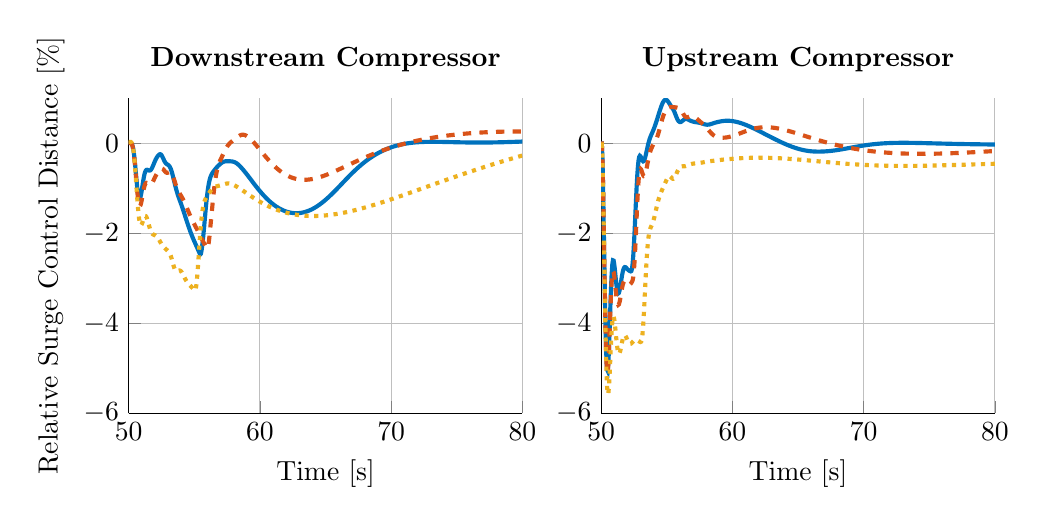
\begin{tikzpicture}

\begin{axis}[%
width=5cm,
height=4cm,
at={(0\linewidth,0\linewidth)},
scale only axis,
xmin=50,
xmax=80,
xlabel={Time [s]},
xmajorgrids,
% ymin=-3.5,
% ymax=0.5,
ymin=-6,
ymax=1,
ylabel={Relative Surge Control Distance [\%]},
ymajorgrids,
axis background/.style={fill=white},
title style={font=\bfseries},
title={Downstream Compressor},
axis x line*=bottom,
axis y line*=left
]
\addplot [color=mycolor1,solid,line width=1.5pt,forget plot]
  table[row sep=crcr]{%
50	0.00842000000000098\\
50.05	0.00842000000000098\\
50.1	0.00830999999999982\\
50.15	0.00663000000000125\\
50.2	-0.0012099999999986\\
50.25	-0.0222599999999993\\
50.3	-0.0639099999999999\\
50.35	-0.132719999999999\\
50.4	-0.232239999999999\\
50.45	-0.36088\\
50.5	-0.512049999999999\\
50.55	-0.675109999999999\\
50.6	-0.837149999999999\\
50.65	-0.984749999999999\\
50.7	-1.10552\\
50.75	-1.18987\\
50.8	-1.23236\\
50.85	-1.23239\\
50.9	-1.19405\\
50.95	-1.12528\\
51	-1.03653\\
51.05	-0.93906\\
51.1	-0.843399999999999\\
51.15	-0.758109999999999\\
51.2	-0.68894\\
51.25	-0.638629999999999\\
51.3	-0.607069999999999\\
51.35	-0.591819999999999\\
51.4	-0.58885\\
51.45	-0.593369999999999\\
51.5	-0.600519999999999\\
51.55	-0.606\\
51.6	-0.606489999999999\\
51.65	-0.5999\\
51.7	-0.585389999999999\\
51.75	-0.56328\\
51.8	-0.53478\\
51.85	-0.501729999999999\\
51.9	-0.466229999999999\\
51.95	-0.430339999999999\\
52	-0.395809999999999\\
52.05	-0.363939999999999\\
52.1	-0.3355\\
52.15	-0.310759999999999\\
52.2	-0.289579999999999\\
52.25	-0.271539999999999\\
52.3	-0.25637\\
52.35	-0.24578\\
52.4	-0.24252\\
52.45	-0.248589999999999\\
52.5	-0.264349999999999\\
52.55	-0.28846\\
52.6	-0.318319999999999\\
52.65	-0.350669999999999\\
52.7	-0.382239999999999\\
52.75	-0.410279999999999\\
52.8	-0.433059999999999\\
52.85	-0.45011\\
52.9	-0.46228\\
52.95	-0.4715\\
53	-0.48042\\
53.05	-0.491929999999999\\
53.1	-0.508659999999999\\
53.15	-0.532579999999999\\
53.2	-0.564799999999999\\
53.25	-0.60544\\
53.3	-0.653709999999999\\
53.35	-0.70813\\
53.4	-0.766789999999999\\
53.45	-0.827649999999999\\
53.5	-0.88857\\
53.55	-0.94764\\
53.6	-1.00359\\
53.65	-1.056\\
53.7	-1.10493\\
53.75	-1.15064\\
53.8	-1.19375\\
53.85	-1.23507\\
53.9	-1.27545\\
53.95	-1.31567\\
54	-1.35633\\
54.05	-1.39785\\
54.1	-1.44041\\
54.15	-1.48401\\
54.2	-1.52849\\
54.25	-1.57359\\
54.3	-1.619\\
54.35	-1.66439\\
54.4	-1.70949\\
54.45	-1.75405\\
54.5	-1.7979\\
54.55	-1.8409\\
54.6	-1.88296\\
54.65	-1.92401\\
54.7	-1.964\\
54.75	-2.00288\\
54.8	-2.04058\\
54.85	-2.07711\\
54.9	-2.11245\\
54.95	-2.14673\\
55	-2.18014\\
55.05	-2.21291\\
55.1	-2.24532\\
55.15	-2.27765\\
55.2	-2.31017\\
55.25	-2.34312\\
55.3	-2.37669\\
55.35	-2.411\\
55.4	-2.44607\\
55.45	-2.47036\\
55.5	-2.45483\\
55.55	-2.38603\\
55.6	-2.27549\\
55.65	-2.14955\\
55.7	-2.00669\\
55.75	-1.84971\\
55.8	-1.68513\\
55.85	-1.52085\\
55.9	-1.36436\\
55.95	-1.22161\\
56	-1.09641\\
56.05	-0.990429999999999\\
56.1	-0.903429999999999\\
56.15	-0.833749999999999\\
56.2	-0.77886\\
56.25	-0.735829999999999\\
56.3	-0.70175\\
56.35	-0.674009999999999\\
56.4	-0.650469999999999\\
56.45	-0.629529999999999\\
56.5	-0.61009\\
56.55	-0.59153\\
56.6	-0.573539999999999\\
56.65	-0.556069999999999\\
56.7	-0.53916\\
56.75	-0.522939999999999\\
56.8	-0.507479999999999\\
56.85	-0.492789999999999\\
56.9	-0.478789999999999\\
56.95	-0.46545\\
57	-0.452889999999999\\
57.05	-0.441349999999999\\
57.1	-0.43106\\
57.15	-0.42221\\
57.2	-0.41489\\
57.25	-0.4091\\
57.3	-0.40478\\
57.35	-0.401769999999999\\
57.4	-0.39988\\
57.45	-0.39887\\
57.5	-0.398529999999999\\
57.55	-0.39863\\
57.6	-0.398999999999999\\
57.65	-0.399539999999999\\
57.7	-0.4002\\
57.75	-0.40103\\
57.8	-0.402139999999999\\
57.85	-0.403659999999999\\
57.9	-0.405799999999999\\
57.95	-0.408729999999999\\
58	-0.412649999999999\\
58.05	-0.417699999999999\\
58.1	-0.42399\\
58.15	-0.431589999999999\\
58.2	-0.440499999999999\\
58.25	-0.450679999999999\\
58.3	-0.46205\\
58.35	-0.47451\\
58.4	-0.487939999999999\\
58.45	-0.50219\\
58.5	-0.51716\\
58.55	-0.532719999999999\\
58.6	-0.54878\\
58.65	-0.56528\\
58.7	-0.58215\\
58.75	-0.599349999999999\\
58.8	-0.616859999999999\\
58.85	-0.634659999999999\\
58.9	-0.652729999999999\\
58.95	-0.671049999999999\\
59	-0.689609999999999\\
59.05	-0.70839\\
59.1	-0.727349999999999\\
59.15	-0.74647\\
59.2	-0.7657\\
59.25	-0.785019999999999\\
59.3	-0.80437\\
59.35	-0.823739999999999\\
59.4	-0.843069999999999\\
59.45	-0.862349999999999\\
59.5	-0.88153\\
59.55	-0.9006\\
59.6	-0.919529999999999\\
59.65	-0.93831\\
59.7	-0.956919999999999\\
59.75	-0.97535\\
59.8	-0.99358\\
59.85	-1.01162\\
59.9	-1.02945\\
59.95	-1.04707\\
60	-1.06446\\
60.05	-1.08161\\
60.1	-1.09853\\
60.15	-1.11521\\
60.2	-1.13163\\
60.25	-1.14778\\
60.3	-1.16367\\
60.35	-1.17927\\
60.4	-1.19459\\
60.45	-1.20962\\
60.5	-1.22434\\
60.55	-1.23876\\
60.6	-1.25287\\
60.65	-1.26666\\
60.7	-1.28014\\
60.75	-1.29329\\
60.8	-1.30613\\
60.85	-1.31863\\
60.9	-1.33082\\
60.95	-1.34268\\
61	-1.35421\\
61.05	-1.36542\\
61.1	-1.37631\\
61.15	-1.38687\\
61.2	-1.3971\\
61.25	-1.40701\\
61.3	-1.4166\\
61.35	-1.42586\\
61.4	-1.43479\\
61.45	-1.4434\\
61.5	-1.45168\\
61.55	-1.45964\\
61.6	-1.46727\\
61.65	-1.47458\\
61.7	-1.48156\\
61.75	-1.48822\\
61.8	-1.49455\\
61.85	-1.50057\\
61.9	-1.50626\\
61.95	-1.51162\\
62	-1.51667\\
62.05	-1.5214\\
62.1	-1.52581\\
62.15	-1.52989\\
62.2	-1.53366\\
62.25	-1.53712\\
62.3	-1.54025\\
62.35	-1.54307\\
62.4	-1.54557\\
62.45	-1.54775\\
62.5	-1.54962\\
62.55	-1.55117\\
62.6	-1.5524\\
62.65	-1.55332\\
62.7	-1.55393\\
62.75	-1.55422\\
62.8	-1.55419\\
62.85	-1.55385\\
62.9	-1.5532\\
62.95	-1.55224\\
63	-1.55096\\
63.05	-1.54937\\
63.1	-1.54746\\
63.15	-1.54525\\
63.2	-1.54272\\
63.25	-1.53989\\
63.3	-1.53674\\
63.35	-1.53329\\
63.4	-1.52952\\
63.45	-1.52545\\
63.5	-1.52107\\
63.55	-1.51639\\
63.6	-1.5114\\
63.65	-1.50611\\
63.7	-1.50052\\
63.75	-1.49462\\
63.8	-1.48843\\
63.85	-1.48193\\
63.9	-1.47515\\
63.95	-1.46806\\
64	-1.46069\\
64.05	-1.45303\\
64.1	-1.44508\\
64.15	-1.43684\\
64.2	-1.42833\\
64.25	-1.41953\\
64.3	-1.41046\\
64.35	-1.40112\\
64.4	-1.39151\\
64.45	-1.38163\\
64.5	-1.3715\\
64.55	-1.3611\\
64.6	-1.35046\\
64.65	-1.33957\\
64.7	-1.32843\\
64.75	-1.31706\\
64.8	-1.30545\\
64.85	-1.29362\\
64.9	-1.28156\\
64.95	-1.26929\\
65	-1.25681\\
65.05	-1.24412\\
65.1	-1.23124\\
65.15	-1.21816\\
65.2	-1.2049\\
65.25	-1.19147\\
65.3	-1.17786\\
65.35	-1.16408\\
65.4	-1.15015\\
65.45	-1.13607\\
65.5	-1.12185\\
65.55	-1.10749\\
65.6	-1.09301\\
65.65	-1.07841\\
65.7	-1.0637\\
65.75	-1.04889\\
65.8	-1.03398\\
65.85	-1.01898\\
65.9	-1.00391\\
65.95	-0.988779999999999\\
66	-0.973579999999999\\
66.05	-0.958329999999999\\
66.1	-0.94304\\
66.15	-0.92772\\
66.2	-0.912369999999999\\
66.25	-0.897019999999999\\
66.3	-0.881659999999999\\
66.35	-0.8663\\
66.4	-0.85096\\
66.45	-0.835649999999999\\
66.5	-0.820359999999999\\
66.55	-0.805129999999999\\
66.6	-0.78994\\
66.65	-0.774819999999999\\
66.7	-0.75977\\
66.75	-0.7448\\
66.8	-0.729919999999999\\
66.85	-0.715129999999999\\
66.9	-0.70044\\
66.95	-0.685859999999999\\
67	-0.671399999999999\\
67.05	-0.65706\\
67.1	-0.642849999999999\\
67.15	-0.628769999999999\\
67.2	-0.614819999999999\\
67.25	-0.601019999999999\\
67.3	-0.58735\\
67.35	-0.57384\\
67.4	-0.56047\\
67.45	-0.54726\\
67.5	-0.534199999999999\\
67.55	-0.521299999999999\\
67.6	-0.508559999999999\\
67.65	-0.495979999999999\\
67.7	-0.48356\\
67.75	-0.471299999999999\\
67.8	-0.45921\\
67.85	-0.447279999999999\\
67.9	-0.435519999999999\\
67.95	-0.423929999999999\\
68	-0.4125\\
68.05	-0.401249999999999\\
68.1	-0.39016\\
68.15	-0.379239999999999\\
68.2	-0.36849\\
68.25	-0.357919999999999\\
68.3	-0.34751\\
68.35	-0.337269999999999\\
68.4	-0.327199999999999\\
68.45	-0.317309999999999\\
68.5	-0.30758\\
68.55	-0.298019999999999\\
68.6	-0.288629999999999\\
68.65	-0.2794\\
68.7	-0.27035\\
68.75	-0.261449999999999\\
68.8	-0.25273\\
68.85	-0.24417\\
68.9	-0.23577\\
68.95	-0.22753\\
69	-0.21946\\
69.05	-0.211539999999999\\
69.1	-0.20379\\
69.15	-0.19619\\
69.2	-0.18875\\
69.25	-0.18146\\
69.3	-0.17432\\
69.35	-0.167339999999999\\
69.4	-0.160509999999999\\
69.45	-0.153829999999999\\
69.5	-0.1473\\
69.55	-0.14091\\
69.6	-0.13467\\
69.65	-0.128579999999999\\
69.7	-0.122629999999999\\
69.75	-0.116819999999999\\
69.8	-0.11115\\
69.85	-0.10562\\
69.9	-0.10023\\
69.95	-0.0949799999999996\\
70	-0.0898599999999998\\
70.05	-0.0848699999999987\\
70.1	-0.0800199999999993\\
70.15	-0.0752999999999986\\
70.2	-0.0707100000000001\\
70.25	-0.0662399999999987\\
70.3	-0.0619099999999992\\
70.35	-0.0576899999999991\\
70.4	-0.053609999999999\\
70.45	-0.0496400000000001\\
70.5	-0.0457900000000002\\
70.55	-0.0420699999999989\\
70.6	-0.0384599999999988\\
70.65	-0.0349599999999999\\
70.7	-0.0315799999999999\\
70.75	-0.028319999999999\\
70.8	-0.0251599999999996\\
70.85	-0.0221099999999996\\
70.9	-0.019169999999999\\
70.95	-0.01633\\
71	-0.0136000000000003\\
71.05	-0.0109699999999986\\
71.1	-0.00842999999999883\\
71.15	-0.00600000000000023\\
71.2	-0.00366\\
71.25	-0.00141999999999953\\
71.3	0.000740000000000407\\
71.35	0.00280000000000058\\
71.4	0.00477000000000061\\
71.45	0.00666000000000011\\
71.5	0.00846000000000124\\
71.55	0.0101800000000001\\
71.6	0.0118200000000002\\
71.65	0.0133799999999997\\
71.7	0.0148600000000005\\
71.75	0.0162700000000005\\
71.8	0.0176100000000012\\
71.85	0.0188699999999997\\
71.9	0.0200600000000009\\
71.95	0.0211900000000007\\
72	0.0222500000000014\\
72.05	0.0232400000000013\\
72.1	0.0241699999999998\\
72.15	0.0250500000000002\\
72.2	0.0258599999999998\\
72.25	0.0266200000000012\\
72.3	0.0273200000000013\\
72.35	0.0279699999999998\\
72.4	0.0285600000000006\\
72.45	0.0291100000000011\\
72.5	0.0296099999999999\\
72.55	0.0300600000000006\\
72.6	0.0304599999999997\\
72.65	0.0308200000000003\\
72.7	0.0311400000000006\\
72.75	0.0314200000000007\\
72.8	0.0316600000000005\\
72.85	0.03186\\
72.9	0.0320300000000007\\
72.95	0.0321600000000011\\
73	0.0322600000000008\\
73.05	0.03233\\
73.1	0.0323600000000006\\
73.15	0.0323700000000002\\
73.2	0.032350000000001\\
73.25	0.0323100000000007\\
73.3	0.0322300000000002\\
73.35	0.0321400000000001\\
73.4	0.032020000000001\\
73.45	0.031880000000001\\
73.5	0.0317300000000014\\
73.55	0.0315500000000011\\
73.6	0.0313499999999998\\
73.65	0.0311400000000006\\
73.7	0.0309100000000004\\
73.75	0.0306700000000006\\
73.8	0.0304200000000012\\
73.85	0.0301500000000008\\
73.9	0.0298700000000007\\
73.95	0.029580000000001\\
74	0.02928\\
74.05	0.0289700000000011\\
74.1	0.0286600000000004\\
74.15	0.02834\\
74.2	0.0280100000000001\\
74.25	0.0276700000000005\\
74.3	0.027330000000001\\
74.35	0.0269900000000014\\
74.4	0.0266500000000001\\
74.45	0.0263000000000009\\
74.5	0.0259499999999999\\
74.55	0.0256000000000007\\
74.6	0.0252499999999998\\
74.65	0.0249000000000006\\
74.7	0.0245500000000014\\
74.75	0.0242100000000001\\
74.8	0.0238600000000009\\
74.85	0.0235200000000013\\
74.9	0.02318\\
74.95	0.02285\\
75	0.0225200000000001\\
75.05	0.0221900000000002\\
75.1	0.0218699999999998\\
75.15	0.0215600000000009\\
75.2	0.0212500000000002\\
75.25	0.0209500000000009\\
75.3	0.0206499999999998\\
75.35	0.0203600000000002\\
75.4	0.0200800000000001\\
75.45	0.0198100000000014\\
75.5	0.0195500000000006\\
75.55	0.0192899999999998\\
75.6	0.0190400000000004\\
75.65	0.0188100000000002\\
75.7	0.01858\\
75.75	0.0183600000000013\\
75.8	0.0181500000000003\\
75.85	0.0179500000000008\\
75.9	0.0177600000000009\\
75.95	0.0175800000000006\\
76	0.0174200000000013\\
76.05	0.0172600000000003\\
76.1	0.0171100000000006\\
76.15	0.0169800000000002\\
76.2	0.0168600000000012\\
76.25	0.0167400000000004\\
76.3	0.0166400000000007\\
76.35	0.0165500000000005\\
76.4	0.01647\\
76.45	0.0164100000000005\\
76.5	0.016350000000001\\
76.55	0.0163100000000007\\
76.6	0.0162800000000001\\
76.65	0.0162600000000008\\
76.7	0.0162500000000012\\
76.75	0.0162500000000012\\
76.8	0.0162700000000005\\
76.85	0.0163000000000011\\
76.9	0.0163400000000014\\
76.95	0.0163900000000012\\
77	0.0164500000000007\\
77.05	0.0165300000000013\\
77.1	0.01661\\
77.15	0.0167099999999998\\
77.2	0.0168200000000009\\
77.25	0.01694\\
77.3	0.01708\\
77.35	0.01722\\
77.4	0.0173800000000011\\
77.45	0.0175400000000003\\
77.5	0.0177200000000006\\
77.55	0.0179100000000005\\
77.6	0.0181100000000001\\
77.65	0.018320000000001\\
77.7	0.0185500000000012\\
77.75	0.0187800000000014\\
77.8	0.0190300000000008\\
77.85	0.0192800000000002\\
77.9	0.0195500000000006\\
77.95	0.0198200000000011\\
78	0.0201100000000007\\
78.05	0.0204000000000004\\
78.1	0.0207100000000011\\
78.15	0.0210300000000014\\
78.2	0.02135\\
78.25	0.0216900000000013\\
78.3	0.0220300000000009\\
78.35	0.0223899999999997\\
78.4	0.0227500000000003\\
78.45	0.0231300000000001\\
78.5	0.0235099999999999\\
78.55	0.0239000000000011\\
78.6	0.0243000000000002\\
78.65	0.0247100000000007\\
78.7	0.0251200000000011\\
78.75	0.0255500000000008\\
78.8	0.0259800000000006\\
78.85	0.0264300000000013\\
78.9	0.0268800000000002\\
78.95	0.0273400000000006\\
79	0.0278000000000009\\
79.05	0.0282700000000009\\
79.1	0.0287600000000001\\
79.15	0.0292399999999997\\
79.2	0.0297400000000003\\
79.25	0.0302400000000009\\
79.3	0.0307500000000012\\
79.35	0.031270000000001\\
79.4	0.0317900000000009\\
79.45	0.0323200000000003\\
79.5	0.0328600000000012\\
79.55	0.0334000000000003\\
79.6	0.0339500000000008\\
79.65	0.0345000000000013\\
79.7	0.035070000000001\\
79.75	0.0356300000000012\\
79.8	0.0362000000000009\\
79.85	0.0367800000000003\\
79.9	0.037370000000001\\
79.95	0.03796\\
80	0.0385500000000008\\
};
\addplot [color=mycolor2,dashed,line width=1.5pt,forget plot]
  table[row sep=crcr]{%
50	0.00472000000000072\\
50.05	0.00472000000000072\\
50.1	0.00461000000000134\\
50.15	0.00285000000000046\\
50.2	-0.00546999999999898\\
50.25	-0.0279699999999998\\
50.3	-0.0728899999999992\\
50.35	-0.14678\\
50.4	-0.252549999999999\\
50.45	-0.389119999999999\\
50.5	-0.550759999999999\\
50.55	-0.727139999999999\\
50.6	-0.905029999999999\\
50.65	-1.07028\\
50.7	-1.20986\\
50.75	-1.31357\\
50.8	-1.3755\\
50.85	-1.3946\\
50.9	-1.37461\\
50.95	-1.32314\\
51	-1.25039\\
51.05	-1.16746\\
51.1	-1.0848\\
51.15	-1.01101\\
51.2	-0.951989999999999\\
51.25	-0.910699999999999\\
51.3	-0.887269999999999\\
51.35	-0.879549999999999\\
51.4	-0.88374\\
51.45	-0.89521\\
51.5	-0.909179999999999\\
51.55	-0.921379999999999\\
51.6	-0.928439999999999\\
51.65	-0.928179999999999\\
51.7	-0.919689999999999\\
51.75	-0.903189999999999\\
51.8	-0.879849999999999\\
51.85	-0.85145\\
51.9	-0.820069999999999\\
51.95	-0.78773\\
52	-0.756219999999999\\
52.05	-0.72681\\
52.1	-0.70027\\
52.15	-0.67681\\
52.2	-0.656179999999999\\
52.25	-0.637759999999999\\
52.3	-0.62076\\
52.35	-0.60429\\
52.4	-0.587899999999999\\
52.45	-0.573429999999999\\
52.5	-0.56406\\
52.55	-0.562259999999999\\
52.6	-0.568779999999999\\
52.65	-0.582479999999999\\
52.7	-0.600719999999999\\
52.75	-0.620119999999999\\
52.8	-0.63728\\
52.85	-0.649539999999999\\
52.9	-0.655559999999999\\
52.95	-0.655539999999999\\
53	-0.65107\\
53.05	-0.64479\\
53.1	-0.63986\\
53.15	-0.63932\\
53.2	-0.64565\\
53.25	-0.660379999999999\\
53.3	-0.683949999999999\\
53.35	-0.71573\\
53.4	-0.754219999999999\\
53.45	-0.79735\\
53.5	-0.8428\\
53.55	-0.888349999999999\\
53.6	-0.932119999999999\\
53.65	-0.97279\\
53.7	-1.00967\\
53.75	-1.04267\\
53.8	-1.07222\\
53.85	-1.09913\\
53.9	-1.12437\\
53.95	-1.14894\\
54	-1.17352\\
54.05	-1.19871\\
54.1	-1.22497\\
54.15	-1.25248\\
54.2	-1.28142\\
54.25	-1.31207\\
54.3	-1.3445\\
54.35	-1.37837\\
54.4	-1.41324\\
54.45	-1.44864\\
54.5	-1.48409\\
54.55	-1.51919\\
54.6	-1.55363\\
54.65	-1.5872\\
54.7	-1.61981\\
54.75	-1.65148\\
54.8	-1.68225\\
54.85	-1.71224\\
54.9	-1.74156\\
54.95	-1.77035\\
55	-1.79871\\
55.05	-1.82675\\
55.1	-1.85457\\
55.15	-1.88224\\
55.2	-1.90984\\
55.25	-1.93748\\
55.3	-1.96534\\
55.35	-1.99354\\
55.4	-2.02216\\
55.45	-2.05124\\
55.5	-2.08074\\
55.55	-2.11058\\
55.6	-2.14064\\
55.65	-2.17081\\
55.7	-2.20093\\
55.75	-2.2309\\
55.8	-2.2606\\
55.85	-2.28998\\
55.9	-2.31897\\
55.95	-2.33591\\
56	-2.32314\\
56.05	-2.28461\\
56.1	-2.20445\\
56.15	-2.07872\\
56.2	-1.92513\\
56.25	-1.77291\\
56.3	-1.62001\\
56.35	-1.4667\\
56.4	-1.31595\\
56.45	-1.17168\\
56.5	-1.03758\\
56.55	-0.916429999999999\\
56.6	-0.80976\\
56.65	-0.717829999999999\\
56.7	-0.639869999999999\\
56.75	-0.574339999999999\\
56.8	-0.519259999999999\\
56.85	-0.472529999999999\\
56.9	-0.43209\\
56.95	-0.39615\\
57	-0.363219999999999\\
57.05	-0.332129999999999\\
57.1	-0.30204\\
57.15	-0.272329999999999\\
57.2	-0.24257\\
57.25	-0.212569999999999\\
57.3	-0.182639999999999\\
57.35	-0.153309999999999\\
57.4	-0.1252\\
57.45	-0.0988399999999992\\
57.5	-0.0746000000000002\\
57.55	-0.0526799999999987\\
57.6	-0.0330899999999996\\
57.65	-0.0156700000000001\\
57.7	-0.000169999999998893\\
57.75	0.0137700000000009\\
57.8	0.0265000000000004\\
57.85	0.0383800000000001\\
57.9	0.0497300000000003\\
57.95	0.060830000000001\\
58	0.0718800000000002\\
58.05	0.0830300000000008\\
58.1	0.0943500000000004\\
58.15	0.105840000000001\\
58.2	0.117420000000001\\
58.25	0.12893\\
58.3	0.14015\\
58.35	0.150830000000001\\
58.4	0.160690000000001\\
58.45	0.16947\\
58.5	0.17694\\
58.55	0.18291\\
58.6	0.187230000000001\\
58.65	0.189810000000001\\
58.7	0.190610000000001\\
58.75	0.18965\\
58.8	0.186970000000001\\
58.85	0.18267\\
58.9	0.17685\\
58.95	0.169640000000001\\
59	0.161160000000001\\
59.05	0.151540000000001\\
59.1	0.140890000000001\\
59.15	0.12932\\
59.2	0.11692\\
59.25	0.103770000000001\\
59.3	0.0899400000000004\\
59.35	0.0754999999999999\\
59.4	0.0604899999999997\\
59.45	0.0449700000000011\\
59.5	0.0289800000000007\\
59.55	0.0125700000000002\\
59.6	-0.00419999999999909\\
59.65	-0.0213000000000001\\
59.7	-0.0386600000000001\\
59.75	-0.056239999999999\\
59.8	-0.0739999999999998\\
59.85	-0.0918700000000001\\
59.9	-0.109829999999999\\
59.95	-0.12782\\
60	-0.14582\\
60.05	-0.16379\\
60.1	-0.18169\\
60.15	-0.19952\\
60.2	-0.217239999999999\\
60.25	-0.23485\\
60.3	-0.25233\\
60.35	-0.26967\\
60.4	-0.28687\\
60.45	-0.3039\\
60.5	-0.320779999999999\\
60.55	-0.337479999999999\\
60.6	-0.353999999999999\\
60.65	-0.37034\\
60.7	-0.386469999999999\\
60.75	-0.402399999999999\\
60.8	-0.418099999999999\\
60.85	-0.43357\\
60.9	-0.44879\\
60.95	-0.46376\\
61	-0.47845\\
61.05	-0.492859999999999\\
61.1	-0.50698\\
61.15	-0.520799999999999\\
61.2	-0.53431\\
61.25	-0.547499999999999\\
61.3	-0.56037\\
61.35	-0.572909999999999\\
61.4	-0.585129999999999\\
61.45	-0.59702\\
61.5	-0.608569999999999\\
61.55	-0.619789999999999\\
61.6	-0.630679999999999\\
61.65	-0.64124\\
61.7	-0.651459999999999\\
61.75	-0.66135\\
61.8	-0.670909999999999\\
61.85	-0.680129999999999\\
61.9	-0.68903\\
61.95	-0.697589999999999\\
62	-0.70583\\
62.05	-0.713729999999999\\
62.1	-0.721309999999999\\
62.15	-0.72856\\
62.2	-0.735479999999999\\
62.25	-0.742089999999999\\
62.3	-0.74837\\
62.35	-0.754339999999999\\
62.4	-0.759989999999999\\
62.45	-0.765319999999999\\
62.5	-0.77035\\
62.55	-0.775069999999999\\
62.6	-0.779489999999999\\
62.65	-0.7836\\
62.7	-0.787419999999999\\
62.75	-0.79095\\
62.8	-0.79418\\
62.85	-0.797129999999999\\
62.9	-0.79979\\
62.95	-0.802169999999999\\
63	-0.80427\\
63.05	-0.8061\\
63.1	-0.807659999999999\\
63.15	-0.808949999999999\\
63.2	-0.80997\\
63.25	-0.810739999999999\\
63.3	-0.811249999999999\\
63.35	-0.8115\\
63.4	-0.811509999999999\\
63.45	-0.811279999999999\\
63.5	-0.8108\\
63.55	-0.81009\\
63.6	-0.80915\\
63.65	-0.80798\\
63.7	-0.8066\\
63.75	-0.804989999999999\\
63.8	-0.80317\\
63.85	-0.80115\\
63.9	-0.79892\\
63.95	-0.796499999999999\\
64	-0.79388\\
64.05	-0.791079999999999\\
64.1	-0.78809\\
64.15	-0.78492\\
64.2	-0.781579999999999\\
64.25	-0.77807\\
64.3	-0.774399999999999\\
64.35	-0.770569999999999\\
64.4	-0.766579999999999\\
64.45	-0.762449999999999\\
64.5	-0.75817\\
64.55	-0.753749999999999\\
64.6	-0.74919\\
64.65	-0.744509999999999\\
64.7	-0.739699999999999\\
64.75	-0.734769999999999\\
64.8	-0.729719999999999\\
64.85	-0.724559999999999\\
64.9	-0.719289999999999\\
64.95	-0.713909999999999\\
65	-0.70844\\
65.05	-0.70287\\
65.1	-0.697209999999999\\
65.15	-0.691459999999999\\
65.2	-0.68563\\
65.25	-0.67972\\
65.3	-0.673729999999999\\
65.35	-0.667669999999999\\
65.4	-0.661549999999999\\
65.45	-0.655349999999999\\
65.5	-0.6491\\
65.55	-0.64279\\
65.6	-0.63643\\
65.65	-0.63001\\
65.7	-0.62355\\
65.75	-0.617039999999999\\
65.8	-0.61049\\
65.85	-0.603899999999999\\
65.9	-0.59728\\
65.95	-0.590619999999999\\
66	-0.58393\\
66.05	-0.57722\\
66.1	-0.57048\\
66.15	-0.563719999999999\\
66.2	-0.556939999999999\\
66.25	-0.55014\\
66.3	-0.543329999999999\\
66.35	-0.536499999999999\\
66.4	-0.529669999999999\\
66.45	-0.522829999999999\\
66.5	-0.51598\\
66.55	-0.50913\\
66.6	-0.502269999999999\\
66.65	-0.495419999999999\\
66.7	-0.48856\\
66.75	-0.481719999999999\\
66.8	-0.474869999999999\\
66.85	-0.468039999999999\\
66.9	-0.461209999999999\\
66.95	-0.4544\\
67	-0.447589999999999\\
67.05	-0.440799999999999\\
67.1	-0.434029999999999\\
67.15	-0.427269999999999\\
67.2	-0.420529999999999\\
67.25	-0.41381\\
67.3	-0.4071\\
67.35	-0.40042\\
67.4	-0.393769999999999\\
67.45	-0.387129999999999\\
67.5	-0.38052\\
67.55	-0.373939999999999\\
67.6	-0.367389999999999\\
67.65	-0.36086\\
67.7	-0.35436\\
67.75	-0.34789\\
67.8	-0.341449999999999\\
67.85	-0.335039999999999\\
67.9	-0.32867\\
67.95	-0.322319999999999\\
68	-0.316009999999999\\
68.05	-0.30974\\
68.1	-0.3035\\
68.15	-0.297289999999999\\
68.2	-0.291119999999999\\
68.25	-0.28499\\
68.3	-0.278899999999999\\
68.35	-0.27284\\
68.4	-0.266819999999999\\
68.45	-0.260839999999999\\
68.5	-0.254899999999999\\
68.55	-0.248989999999999\\
68.6	-0.24313\\
68.65	-0.237309999999999\\
68.7	-0.23152\\
68.75	-0.225779999999999\\
68.8	-0.220079999999999\\
68.85	-0.21442\\
68.9	-0.208799999999999\\
68.95	-0.203219999999999\\
69	-0.19769\\
69.05	-0.192189999999999\\
69.1	-0.186739999999999\\
69.15	-0.181329999999999\\
69.2	-0.175959999999999\\
69.25	-0.17064\\
69.3	-0.165349999999999\\
69.35	-0.16011\\
69.4	-0.15492\\
69.45	-0.14976\\
69.5	-0.14465\\
69.55	-0.13958\\
69.6	-0.134549999999999\\
69.65	-0.129569999999999\\
69.7	-0.12462\\
69.75	-0.119719999999999\\
69.8	-0.11487\\
69.85	-0.110049999999999\\
69.9	-0.105279999999999\\
69.95	-0.10055\\
70	-0.0958600000000001\\
70.05	-0.0912199999999999\\
70.1	-0.0866100000000003\\
70.15	-0.0820499999999988\\
70.2	-0.0775299999999994\\
70.25	-0.0730500000000003\\
70.3	-0.0686199999999992\\
70.35	-0.0642199999999988\\
70.4	-0.0598599999999987\\
70.45	-0.0555500000000002\\
70.5	-0.0512800000000002\\
70.55	-0.0470399999999991\\
70.6	-0.0428499999999996\\
70.65	-0.0386999999999986\\
70.7	-0.0345899999999997\\
70.75	-0.0305099999999996\\
70.8	-0.0264799999999994\\
70.85	-0.0224899999999995\\
70.9	-0.0185300000000002\\
70.95	-0.014619999999999\\
71	-0.0107400000000002\\
71.05	-0.00689999999999991\\
71.1	-0.00309999999999988\\
71.15	0.000659999999999883\\
71.2	0.00439000000000078\\
71.25	0.00808000000000142\\
71.3	0.01173\\
71.35	0.0153400000000001\\
71.4	0.0189200000000014\\
71.45	0.022450000000001\\
71.5	0.0259600000000013\\
71.55	0.0294300000000014\\
71.6	0.0328600000000012\\
71.65	0.0362500000000008\\
71.7	0.0396099999999997\\
71.75	0.0429399999999998\\
71.8	0.0462300000000013\\
71.85	0.0494900000000005\\
71.9	0.0527100000000011\\
71.95	0.0559000000000012\\
72	0.0590500000000009\\
72.05	0.0621799999999997\\
72.1	0.0652600000000003\\
72.15	0.0683199999999999\\
72.2	0.0713400000000011\\
72.25	0.0743299999999998\\
72.3	0.0772900000000014\\
72.35	0.080210000000001\\
72.4	0.0831100000000013\\
72.45	0.0859700000000014\\
72.5	0.0888000000000009\\
72.55	0.0915999999999997\\
72.6	0.0943700000000014\\
72.65	0.0971100000000007\\
72.7	0.0998200000000011\\
72.75	0.102500000000001\\
72.8	0.10515\\
72.85	0.10777\\
72.9	0.11036\\
72.95	0.112920000000001\\
73	0.115450000000001\\
73.05	0.11796\\
73.1	0.120430000000001\\
73.15	0.12288\\
73.2	0.125300000000001\\
73.25	0.127690000000001\\
73.3	0.130050000000001\\
73.35	0.132390000000001\\
73.4	0.1347\\
73.45	0.136980000000001\\
73.5	0.139240000000001\\
73.55	0.14147\\
73.6	0.14367\\
73.65	0.145850000000001\\
73.7	0.148\\
73.75	0.150130000000001\\
73.8	0.152230000000001\\
73.85	0.154310000000001\\
73.9	0.156360000000001\\
73.95	0.158390000000001\\
74	0.160390000000001\\
74.05	0.162360000000001\\
74.1	0.16432\\
74.15	0.16625\\
74.2	0.168150000000001\\
74.25	0.170030000000001\\
74.3	0.171890000000001\\
74.35	0.173720000000001\\
74.4	0.17553\\
74.45	0.17732\\
74.5	0.17909\\
74.55	0.18083\\
74.6	0.182550000000001\\
74.65	0.18425\\
74.7	0.185920000000001\\
74.75	0.187580000000001\\
74.8	0.189210000000001\\
74.85	0.19082\\
74.9	0.192400000000001\\
74.95	0.19397\\
75	0.19552\\
75.05	0.197040000000001\\
75.1	0.198540000000001\\
75.15	0.20002\\
75.2	0.20149\\
75.25	0.20293\\
75.3	0.20435\\
75.35	0.20575\\
75.4	0.207130000000001\\
75.45	0.208490000000001\\
75.5	0.20983\\
75.55	0.21115\\
75.6	0.21245\\
75.65	0.21373\\
75.7	0.21499\\
75.75	0.216230000000001\\
75.8	0.217450000000001\\
75.85	0.21865\\
75.9	0.219840000000001\\
75.95	0.221\\
76	0.222150000000001\\
76.05	0.223280000000001\\
76.1	0.224390000000001\\
76.15	0.225480000000001\\
76.2	0.226550000000001\\
76.25	0.22761\\
76.3	0.22864\\
76.35	0.229660000000001\\
76.4	0.23066\\
76.45	0.23165\\
76.5	0.232610000000001\\
76.55	0.233560000000001\\
76.6	0.234490000000001\\
76.65	0.2354\\
76.7	0.2363\\
76.75	0.23718\\
76.8	0.23804\\
76.85	0.23888\\
76.9	0.239710000000001\\
76.95	0.24052\\
77	0.24131\\
77.05	0.242090000000001\\
77.1	0.242850000000001\\
77.15	0.243600000000001\\
77.2	0.24433\\
77.25	0.245040000000001\\
77.3	0.24573\\
77.35	0.246410000000001\\
77.4	0.24708\\
77.45	0.247720000000001\\
77.5	0.24836\\
77.55	0.24897\\
77.6	0.24957\\
77.65	0.250160000000001\\
77.7	0.250730000000001\\
77.75	0.251280000000001\\
77.8	0.25182\\
77.85	0.25235\\
77.9	0.25286\\
77.95	0.253350000000001\\
78	0.253830000000001\\
78.05	0.254290000000001\\
78.1	0.25474\\
78.15	0.255180000000001\\
78.2	0.255600000000001\\
78.25	0.25601\\
78.3	0.256400000000001\\
78.35	0.256770000000001\\
78.4	0.25714\\
78.45	0.257490000000001\\
78.5	0.257820000000001\\
78.55	0.258140000000001\\
78.6	0.25845\\
78.65	0.258740000000001\\
78.7	0.259020000000001\\
78.75	0.25929\\
78.8	0.259540000000001\\
78.85	0.259780000000001\\
78.9	0.260010000000001\\
78.95	0.26022\\
79	0.26042\\
79.05	0.26061\\
79.1	0.26078\\
79.15	0.26094\\
79.2	0.261090000000001\\
79.25	0.261230000000001\\
79.3	0.26135\\
79.35	0.261460000000001\\
79.4	0.261560000000001\\
79.45	0.26164\\
79.5	0.261710000000001\\
79.55	0.26177\\
79.6	0.26182\\
79.65	0.26186\\
79.7	0.261890000000001\\
79.75	0.261900000000001\\
79.8	0.261900000000001\\
79.85	0.261890000000001\\
79.9	0.26187\\
79.95	0.26183\\
80	0.261790000000001\\
};
\addplot [color=mycolor3,dotted,line width=1.5pt,forget plot]
  table[row sep=crcr]{%
50	0.0317699999999999\\
50.05	0.0317699999999999\\
50.1	0.0316700000000001\\
50.15	0.0297000000000001\\
50.2	0.0204200000000014\\
50.25	-0.00467999999999869\\
50.3	-0.054829999999999\\
50.35	-0.13749\\
50.4	-0.256489999999999\\
50.45	-0.411049999999999\\
50.5	-0.59571\\
50.55	-0.800979999999999\\
50.6	-1.01456\\
50.65	-1.22283\\
50.7	-1.41256\\
50.75	-1.5725\\
50.8	-1.69469\\
50.85	-1.77544\\
50.9	-1.81552\\
50.95	-1.81994\\
51	-1.79693\\
51.05	-1.75668\\
51.1	-1.70989\\
51.15	-1.66635\\
51.2	-1.63382\\
51.25	-1.61741\\
51.3	-1.61935\\
51.35	-1.6392\\
51.4	-1.67437\\
51.45	-1.72075\\
51.5	-1.77353\\
51.55	-1.82785\\
51.6	-1.87941\\
51.65	-1.92492\\
51.7	-1.96235\\
51.75	-1.99096\\
51.8	-2.01122\\
51.85	-2.02457\\
51.9	-2.03305\\
51.95	-2.03899\\
52	-2.04464\\
52.05	-2.05191\\
52.1	-2.06215\\
52.15	-2.0761\\
52.2	-2.09389\\
52.25	-2.11509\\
52.3	-2.1389\\
52.35	-2.16425\\
52.4	-2.19007\\
52.45	-2.21532\\
52.5	-2.2392\\
52.55	-2.26119\\
52.6	-2.28105\\
52.65	-2.29883\\
52.7	-2.31482\\
52.75	-2.32947\\
52.8	-2.3433\\
52.85	-2.35685\\
52.9	-2.37057\\
52.95	-2.38483\\
53	-2.39984\\
53.05	-2.416\\
53.1	-2.43571\\
53.15	-2.4623\\
53.2	-2.49796\\
53.25	-2.54278\\
53.3	-2.59461\\
53.35	-2.64968\\
53.4	-2.70345\\
53.45	-2.75155\\
53.5	-2.79057\\
53.55	-2.81859\\
53.6	-2.83537\\
53.65	-2.84222\\
53.7	-2.84167\\
53.75	-2.83692\\
53.8	-2.83136\\
53.85	-2.82799\\
53.9	-2.82914\\
53.95	-2.83624\\
54	-2.84975\\
54.05	-2.86926\\
54.1	-2.89374\\
54.15	-2.9217\\
54.2	-2.9515\\
54.25	-2.98158\\
54.3	-3.01062\\
54.35	-3.03766\\
54.4	-3.06217\\
54.45	-3.084\\
54.5	-3.10335\\
54.55	-3.12067\\
54.6	-3.13657\\
54.65	-3.15169\\
54.7	-3.16663\\
54.75	-3.18183\\
54.8	-3.1976\\
54.85	-3.21407\\
54.9	-3.23123\\
54.95	-3.24897\\
55	-3.26711\\
55.05	-3.27452\\
55.1	-3.24349\\
55.15	-3.16119\\
55.2	-3.02758\\
55.25	-2.85137\\
55.3	-2.64633\\
55.35	-2.42805\\
55.4	-2.21131\\
55.45	-2.00829\\
55.5	-1.8275\\
55.55	-1.67362\\
55.6	-1.5478\\
55.65	-1.44849\\
55.7	-1.37222\\
55.75	-1.31461\\
55.8	-1.27101\\
55.85	-1.23711\\
55.9	-1.20933\\
55.95	-1.18492\\
56	-1.16206\\
56.05	-1.13973\\
56.1	-1.11755\\
56.15	-1.09562\\
56.2	-1.07432\\
56.25	-1.05413\\
56.3	-1.03552\\
56.35	-1.01886\\
56.4	-1.00436\\
56.45	-0.99205\\
56.5	-0.98183\\
56.55	-0.97347\\
56.6	-0.96669\\
56.65	-0.96113\\
56.7	-0.956479999999999\\
56.75	-0.952439999999999\\
56.8	-0.948739999999999\\
56.85	-0.9452\\
56.9	-0.94168\\
56.95	-0.93809\\
57	-0.93436\\
57.05	-0.93049\\
57.1	-0.926449999999999\\
57.15	-0.92223\\
57.2	-0.91785\\
57.25	-0.913309999999999\\
57.3	-0.908689999999999\\
57.35	-0.904179999999999\\
57.4	-0.90006\\
57.45	-0.896579999999999\\
57.5	-0.89396\\
57.55	-0.89239\\
57.6	-0.891959999999999\\
57.65	-0.89272\\
57.7	-0.894659999999999\\
57.75	-0.89772\\
57.8	-0.901809999999999\\
57.85	-0.9068\\
57.9	-0.91259\\
57.95	-0.919049999999999\\
58	-0.92608\\
58.05	-0.93357\\
58.1	-0.941439999999999\\
58.15	-0.949629999999999\\
58.2	-0.958089999999999\\
58.25	-0.966779999999999\\
58.3	-0.97568\\
58.35	-0.984769999999999\\
58.4	-0.99403\\
58.45	-1.00344\\
58.5	-1.013\\
58.55	-1.02269\\
58.6	-1.03249\\
58.65	-1.04239\\
58.7	-1.05236\\
58.75	-1.06239\\
58.8	-1.07247\\
58.85	-1.08256\\
58.9	-1.09266\\
58.95	-1.10275\\
59	-1.11282\\
59.05	-1.12286\\
59.1	-1.13286\\
59.15	-1.1428\\
59.2	-1.15269\\
59.25	-1.16251\\
59.3	-1.17227\\
59.35	-1.18196\\
59.4	-1.19158\\
59.45	-1.20111\\
59.5	-1.21057\\
59.55	-1.21994\\
59.6	-1.22921\\
59.65	-1.2384\\
59.7	-1.24749\\
59.75	-1.25648\\
59.8	-1.26538\\
59.85	-1.27416\\
59.9	-1.28284\\
59.95	-1.29141\\
60	-1.29987\\
60.05	-1.30822\\
60.1	-1.31645\\
60.15	-1.32457\\
60.2	-1.33257\\
60.25	-1.34046\\
60.3	-1.34823\\
60.35	-1.35588\\
60.4	-1.36341\\
60.45	-1.37082\\
60.5	-1.37811\\
60.55	-1.38529\\
60.6	-1.39234\\
60.65	-1.39928\\
60.7	-1.4061\\
60.75	-1.41279\\
60.8	-1.41937\\
60.85	-1.42583\\
60.9	-1.43217\\
60.95	-1.4384\\
61	-1.4445\\
61.05	-1.45049\\
61.1	-1.45636\\
61.15	-1.46211\\
61.2	-1.46775\\
61.25	-1.47327\\
61.3	-1.47867\\
61.35	-1.48396\\
61.4	-1.48913\\
61.45	-1.49419\\
61.5	-1.49914\\
61.55	-1.50397\\
61.6	-1.50869\\
61.65	-1.5133\\
61.7	-1.5178\\
61.75	-1.52219\\
61.8	-1.52647\\
61.85	-1.53064\\
61.9	-1.5347\\
61.95	-1.53865\\
62	-1.54249\\
62.05	-1.54623\\
62.1	-1.54986\\
62.15	-1.55339\\
62.2	-1.55681\\
62.25	-1.56013\\
62.3	-1.56334\\
62.35	-1.56646\\
62.4	-1.56947\\
62.45	-1.57238\\
62.5	-1.57519\\
62.55	-1.57789\\
62.6	-1.5805\\
62.65	-1.58301\\
62.7	-1.58543\\
62.75	-1.58774\\
62.8	-1.58996\\
62.85	-1.59209\\
62.9	-1.59412\\
62.95	-1.59605\\
63	-1.5979\\
63.05	-1.59964\\
63.1	-1.6013\\
63.15	-1.60287\\
63.2	-1.60434\\
63.25	-1.60573\\
63.3	-1.60702\\
63.35	-1.60823\\
63.4	-1.60935\\
63.45	-1.61038\\
63.5	-1.61133\\
63.55	-1.61219\\
63.6	-1.61296\\
63.65	-1.61365\\
63.7	-1.61426\\
63.75	-1.61479\\
63.8	-1.61523\\
63.85	-1.61559\\
63.9	-1.61587\\
63.95	-1.61607\\
64	-1.61619\\
64.05	-1.61623\\
64.1	-1.6162\\
64.15	-1.61609\\
64.2	-1.6159\\
64.25	-1.61563\\
64.3	-1.61529\\
64.35	-1.61488\\
64.4	-1.61439\\
64.45	-1.61383\\
64.5	-1.61319\\
64.55	-1.61249\\
64.6	-1.61171\\
64.65	-1.61087\\
64.7	-1.60995\\
64.75	-1.60897\\
64.8	-1.60791\\
64.85	-1.60679\\
64.9	-1.60561\\
64.95	-1.60435\\
65	-1.60303\\
65.05	-1.60165\\
65.1	-1.6002\\
65.15	-1.59869\\
65.2	-1.59712\\
65.25	-1.59548\\
65.3	-1.59379\\
65.35	-1.59203\\
65.4	-1.59021\\
65.45	-1.58833\\
65.5	-1.5864\\
65.55	-1.5844\\
65.6	-1.58235\\
65.65	-1.58024\\
65.7	-1.57808\\
65.75	-1.57586\\
65.8	-1.57358\\
65.85	-1.57125\\
65.9	-1.56887\\
65.95	-1.56643\\
66	-1.56395\\
66.05	-1.56141\\
66.1	-1.55882\\
66.15	-1.55618\\
66.2	-1.55348\\
66.25	-1.55074\\
66.3	-1.54796\\
66.35	-1.54512\\
66.4	-1.54224\\
66.45	-1.53931\\
66.5	-1.53633\\
66.55	-1.53331\\
66.6	-1.53024\\
66.65	-1.52713\\
66.7	-1.52397\\
66.75	-1.52078\\
66.8	-1.51753\\
66.85	-1.51425\\
66.9	-1.51093\\
66.95	-1.50756\\
67	-1.50416\\
67.05	-1.50071\\
67.1	-1.49723\\
67.15	-1.49371\\
67.2	-1.49015\\
67.25	-1.48655\\
67.3	-1.48291\\
67.35	-1.47924\\
67.4	-1.47554\\
67.45	-1.47179\\
67.5	-1.46802\\
67.55	-1.4642\\
67.6	-1.46036\\
67.65	-1.45648\\
67.7	-1.45257\\
67.75	-1.44863\\
67.8	-1.44465\\
67.85	-1.44065\\
67.9	-1.43661\\
67.95	-1.43255\\
68	-1.42845\\
68.05	-1.42433\\
68.1	-1.42017\\
68.15	-1.41599\\
68.2	-1.41178\\
68.25	-1.40754\\
68.3	-1.40328\\
68.35	-1.39899\\
68.4	-1.39468\\
68.45	-1.39034\\
68.5	-1.38597\\
68.55	-1.38158\\
68.6	-1.37717\\
68.65	-1.37273\\
68.7	-1.36827\\
68.75	-1.36379\\
68.8	-1.35928\\
68.85	-1.35475\\
68.9	-1.35021\\
68.95	-1.34564\\
69	-1.34105\\
69.05	-1.33644\\
69.1	-1.33181\\
69.15	-1.32716\\
69.2	-1.32249\\
69.25	-1.31781\\
69.3	-1.3131\\
69.35	-1.30838\\
69.4	-1.30364\\
69.45	-1.29888\\
69.5	-1.29411\\
69.55	-1.28932\\
69.6	-1.28452\\
69.65	-1.2797\\
69.7	-1.27486\\
69.75	-1.27001\\
69.8	-1.26515\\
69.85	-1.26027\\
69.9	-1.25538\\
69.95	-1.25047\\
70	-1.24555\\
70.05	-1.24062\\
70.1	-1.23568\\
70.15	-1.23073\\
70.2	-1.22576\\
70.25	-1.22078\\
70.3	-1.21579\\
70.35	-1.21079\\
70.4	-1.20578\\
70.45	-1.20076\\
70.5	-1.19573\\
70.55	-1.19069\\
70.6	-1.18564\\
70.65	-1.18058\\
70.7	-1.17552\\
70.75	-1.17044\\
70.8	-1.16536\\
70.85	-1.16027\\
70.9	-1.15517\\
70.95	-1.15007\\
71	-1.14496\\
71.05	-1.13984\\
71.1	-1.13471\\
71.15	-1.12958\\
71.2	-1.12444\\
71.25	-1.1193\\
71.3	-1.11415\\
71.35	-1.109\\
71.4	-1.10384\\
71.45	-1.09868\\
71.5	-1.09351\\
71.55	-1.08834\\
71.6	-1.08317\\
71.65	-1.07799\\
71.7	-1.07281\\
71.75	-1.06762\\
71.8	-1.06243\\
71.85	-1.05724\\
71.9	-1.05205\\
71.95	-1.04685\\
72	-1.04165\\
72.05	-1.03645\\
72.1	-1.03125\\
72.15	-1.02605\\
72.2	-1.02084\\
72.25	-1.01564\\
72.3	-1.01043\\
72.35	-1.00522\\
72.4	-1.00001\\
72.45	-0.9948\\
72.5	-0.98959\\
72.55	-0.984389999999999\\
72.6	-0.979179999999999\\
72.65	-0.97397\\
72.7	-0.96876\\
72.75	-0.96355\\
72.8	-0.958349999999999\\
72.85	-0.953139999999999\\
72.9	-0.947939999999999\\
72.95	-0.94274\\
73	-0.937539999999999\\
73.05	-0.932339999999999\\
73.1	-0.92714\\
73.15	-0.921939999999999\\
73.2	-0.91675\\
73.25	-0.91156\\
73.3	-0.906369999999999\\
73.35	-0.901179999999999\\
73.4	-0.895999999999999\\
73.45	-0.89082\\
73.5	-0.88564\\
73.55	-0.88047\\
73.6	-0.875299999999999\\
73.65	-0.87013\\
73.7	-0.86497\\
73.75	-0.85981\\
73.8	-0.854649999999999\\
73.85	-0.849499999999999\\
73.9	-0.844349999999999\\
73.95	-0.83921\\
74	-0.83407\\
74.05	-0.82893\\
74.1	-0.823799999999999\\
74.15	-0.818669999999999\\
74.2	-0.813549999999999\\
74.25	-0.808439999999999\\
74.3	-0.80333\\
74.35	-0.79822\\
74.4	-0.793119999999999\\
74.45	-0.788019999999999\\
74.5	-0.782929999999999\\
74.55	-0.777849999999999\\
74.6	-0.77277\\
74.65	-0.7677\\
74.7	-0.76263\\
74.75	-0.757569999999999\\
74.8	-0.752509999999999\\
74.85	-0.747459999999999\\
74.9	-0.742419999999999\\
74.95	-0.737379999999999\\
75	-0.732349999999999\\
75.05	-0.727329999999999\\
75.1	-0.722309999999999\\
75.15	-0.7173\\
75.2	-0.712299999999999\\
75.25	-0.707299999999999\\
75.3	-0.70231\\
75.35	-0.697329999999999\\
75.4	-0.69236\\
75.45	-0.68739\\
75.5	-0.682429999999999\\
75.55	-0.67747\\
75.6	-0.672529999999999\\
75.65	-0.66759\\
75.7	-0.66266\\
75.75	-0.657729999999999\\
75.8	-0.652819999999999\\
75.85	-0.64791\\
75.9	-0.643009999999999\\
75.95	-0.63812\\
76	-0.633229999999999\\
76.05	-0.62836\\
76.1	-0.623489999999999\\
76.15	-0.61863\\
76.2	-0.613779999999999\\
76.25	-0.60894\\
76.3	-0.6041\\
76.35	-0.59927\\
76.4	-0.59446\\
76.45	-0.58965\\
76.5	-0.584849999999999\\
76.55	-0.580049999999999\\
76.6	-0.57527\\
76.65	-0.570499999999999\\
76.7	-0.565729999999999\\
76.75	-0.560969999999999\\
76.8	-0.55622\\
76.85	-0.551489999999999\\
76.9	-0.546759999999999\\
76.95	-0.54203\\
77	-0.537319999999999\\
77.05	-0.53262\\
77.1	-0.52793\\
77.15	-0.523239999999999\\
77.2	-0.51857\\
77.25	-0.5139\\
77.3	-0.50925\\
77.35	-0.504599999999999\\
77.4	-0.49996\\
77.45	-0.49534\\
77.5	-0.49072\\
77.55	-0.486109999999999\\
77.6	-0.481509999999999\\
77.65	-0.47692\\
77.7	-0.472339999999999\\
77.75	-0.46777\\
77.8	-0.463209999999999\\
77.85	-0.458659999999999\\
77.9	-0.45412\\
77.95	-0.44959\\
78	-0.445069999999999\\
78.05	-0.44056\\
78.1	-0.436059999999999\\
78.15	-0.43157\\
78.2	-0.42709\\
78.25	-0.422619999999999\\
78.3	-0.418159999999999\\
78.35	-0.413709999999999\\
78.4	-0.40928\\
78.45	-0.40485\\
78.5	-0.400429999999999\\
78.55	-0.396019999999999\\
78.6	-0.39162\\
78.65	-0.38723\\
78.7	-0.382859999999999\\
78.75	-0.378489999999999\\
78.8	-0.374129999999999\\
78.85	-0.369789999999999\\
78.9	-0.365449999999999\\
78.95	-0.361129999999999\\
79	-0.356809999999999\\
79.05	-0.35251\\
79.1	-0.34822\\
79.15	-0.343929999999999\\
79.2	-0.339659999999999\\
79.25	-0.335399999999999\\
79.3	-0.331149999999999\\
79.35	-0.32691\\
79.4	-0.322679999999999\\
79.45	-0.318459999999999\\
79.5	-0.314249999999999\\
79.55	-0.310059999999999\\
79.6	-0.30587\\
79.65	-0.30169\\
79.7	-0.297529999999999\\
79.75	-0.293379999999999\\
79.8	-0.28923\\
79.85	-0.285099999999999\\
79.9	-0.28098\\
79.95	-0.27687\\
80	-0.27277\\
};
\end{axis}
\begin{axis}[%
width=5cm,
height=4cm,
at={(6cm,0\linewidth)},
scale only axis,
xmin=50,
xmax=80,
xlabel={Time [s]},
xmajorgrids,
ymin=-6,
ymax=1,
% ylabel={Relative Surge Control Distance [\%]},
ymajorgrids,
axis background/.style={fill=white},
title style={font=\bfseries},
title={Upstream Compressor},
axis x line*=bottom,
axis y line*=left
]
\addplot [color=mycolor1,solid,line width=1.5pt,forget plot]
  table[row sep=crcr]{%
50	-0.00287999999999933\\
50.05	-0.00287999999999933\\
50.1	-0.340039999999999\\
50.15	-1.01667\\
50.2	-1.8749\\
50.25	-2.77916\\
50.3	-3.61056\\
50.35	-4.28728\\
50.4	-4.76714\\
50.45	-5.02619\\
50.5	-5.05865\\
50.55	-4.88044\\
50.6	-4.53806\\
50.65	-4.10178\\
50.7	-3.6449\\
50.75	-3.23165\\
50.8	-2.90792\\
50.85	-2.69721\\
50.9	-2.6018\\
50.95	-2.60755\\
51	-2.68995\\
51.05	-2.82\\
51.1	-2.96888\\
51.15	-3.11134\\
51.2	-3.22777\\
51.25	-3.30532\\
51.3	-3.33818\\
51.35	-3.32708\\
51.4	-3.27823\\
51.45	-3.20171\\
51.5	-3.10962\\
51.55	-3.01412\\
51.6	-2.92583\\
51.65	-2.85258\\
51.7	-2.79888\\
51.75	-2.76589\\
51.8	-2.75192\\
51.85	-2.75319\\
51.9	-2.7647\\
51.95	-2.78114\\
52	-2.79788\\
52.05	-2.81261\\
52.1	-2.82479\\
52.15	-2.83436\\
52.2	-2.84165\\
52.25	-2.84727\\
52.3	-2.84035\\
52.35	-2.78848\\
52.4	-2.67211\\
52.45	-2.48642\\
52.5	-2.23862\\
52.55	-1.94421\\
52.6	-1.62329\\
52.65	-1.29773\\
52.7	-0.991169999999999\\
52.75	-0.72666\\
52.8	-0.520689999999999\\
52.85	-0.38019\\
52.9	-0.30247\\
52.95	-0.27718\\
53	-0.289249999999999\\
53.05	-0.32201\\
53.1	-0.35976\\
53.15	-0.389729999999999\\
53.2	-0.403169999999999\\
53.25	-0.39575\\
53.3	-0.36727\\
53.35	-0.32081\\
53.4	-0.261649999999999\\
53.45	-0.195969999999999\\
53.5	-0.128729999999999\\
53.55	-0.0633299999999988\\
53.6	-0.00231999999999921\\
53.65	0.0517599999999998\\
53.7	0.0982300000000009\\
53.75	0.138570000000001\\
53.8	0.174570000000001\\
53.85	0.208080000000001\\
53.9	0.240860000000001\\
53.95	0.27434\\
54	0.309560000000001\\
54.05	0.34709\\
54.1	0.387090000000001\\
54.15	0.429410000000001\\
54.2	0.473650000000001\\
54.25	0.51932\\
54.3	0.56588\\
54.35	0.612870000000001\\
54.4	0.659830000000001\\
54.45	0.70623\\
54.5	0.75141\\
54.55	0.79461\\
54.6	0.83497\\
54.65	0.871540000000001\\
54.7	0.903370000000001\\
54.75	0.92952\\
54.8	0.94922\\
54.85	0.96194\\
54.9	0.967500000000001\\
54.95	0.966090000000001\\
55	0.958270000000001\\
55.05	0.94492\\
55.1	0.927160000000001\\
55.15	0.90619\\
55.2	0.883240000000001\\
55.25	0.85941\\
55.3	0.83564\\
55.35	0.812610000000001\\
55.4	0.79078\\
55.45	0.76999\\
55.5	0.747640000000001\\
55.55	0.72021\\
55.6	0.6861\\
55.65	0.648050000000001\\
55.7	0.60947\\
55.75	0.572740000000001\\
55.8	0.539760000000001\\
55.85	0.512170000000001\\
55.9	0.491190000000001\\
55.95	0.477500000000001\\
56	0.471160000000001\\
56.05	0.471530000000001\\
56.1	0.477400000000001\\
56.15	0.48715\\
56.2	0.499000000000001\\
56.25	0.511200000000001\\
56.3	0.522250000000001\\
56.35	0.531040000000001\\
56.4	0.53688\\
56.45	0.539520000000001\\
56.5	0.53909\\
56.55	0.536010000000001\\
56.6	0.53087\\
56.65	0.52435\\
56.7	0.517110000000001\\
56.75	0.50972\\
56.8	0.50263\\
56.85	0.49614\\
56.9	0.49042\\
56.95	0.4855\\
57	0.481300000000001\\
57.05	0.4777\\
57.1	0.474580000000001\\
57.15	0.47184\\
57.2	0.469390000000001\\
57.25	0.467120000000001\\
57.3	0.464930000000001\\
57.35	0.462730000000001\\
57.4	0.4604\\
57.45	0.45782\\
57.5	0.45491\\
57.55	0.45158\\
57.6	0.447790000000001\\
57.65	0.44356\\
57.7	0.43895\\
57.75	0.434140000000001\\
57.8	0.429310000000001\\
57.85	0.424710000000001\\
57.9	0.420580000000001\\
57.95	0.417160000000001\\
58	0.41464\\
58.05	0.413180000000001\\
58.1	0.412830000000001\\
58.15	0.41361\\
58.2	0.415460000000001\\
58.25	0.41826\\
58.3	0.421840000000001\\
58.35	0.426020000000001\\
58.4	0.43061\\
58.45	0.43544\\
58.5	0.440330000000001\\
58.55	0.445180000000001\\
58.6	0.44988\\
58.65	0.45438\\
58.7	0.458640000000001\\
58.75	0.462670000000001\\
58.8	0.466470000000001\\
58.85	0.47007\\
58.9	0.47349\\
58.95	0.476750000000001\\
59	0.479850000000001\\
59.05	0.482810000000001\\
59.1	0.485610000000001\\
59.15	0.488240000000001\\
59.2	0.490680000000001\\
59.25	0.49292\\
59.3	0.494910000000001\\
59.35	0.496650000000001\\
59.4	0.49812\\
59.45	0.49929\\
59.5	0.500150000000001\\
59.55	0.500720000000001\\
59.6	0.500970000000001\\
59.65	0.500910000000001\\
59.7	0.50056\\
59.75	0.499920000000001\\
59.8	0.498990000000001\\
59.85	0.49779\\
59.9	0.49633\\
59.95	0.494630000000001\\
60	0.49268\\
60.05	0.490490000000001\\
60.1	0.48808\\
60.15	0.48545\\
60.2	0.482610000000001\\
60.25	0.47955\\
60.3	0.476290000000001\\
60.35	0.47282\\
60.4	0.469150000000001\\
60.45	0.46528\\
60.5	0.461220000000001\\
60.55	0.45697\\
60.6	0.45252\\
60.65	0.447900000000001\\
60.7	0.443100000000001\\
60.75	0.438130000000001\\
60.8	0.43299\\
60.85	0.4277\\
60.9	0.422260000000001\\
60.95	0.41667\\
61	0.410960000000001\\
61.05	0.405110000000001\\
61.1	0.399140000000001\\
61.15	0.393050000000001\\
61.2	0.38686\\
61.25	0.380560000000001\\
61.3	0.37416\\
61.35	0.36767\\
61.4	0.361090000000001\\
61.45	0.354420000000001\\
61.5	0.347670000000001\\
61.55	0.340850000000001\\
61.6	0.33395\\
61.65	0.32699\\
61.7	0.31996\\
61.75	0.31287\\
61.8	0.305720000000001\\
61.85	0.298530000000001\\
61.9	0.29129\\
61.95	0.284000000000001\\
62	0.276670000000001\\
62.05	0.269310000000001\\
62.1	0.26192\\
62.15	0.2545\\
62.2	0.24705\\
62.25	0.23958\\
62.3	0.23208\\
62.35	0.224580000000001\\
62.4	0.21706\\
62.45	0.209530000000001\\
62.5	0.20199\\
62.55	0.19445\\
62.6	0.186910000000001\\
62.65	0.17937\\
62.7	0.17183\\
62.75	0.16431\\
62.8	0.156790000000001\\
62.85	0.149290000000001\\
62.9	0.1418\\
62.95	0.13434\\
63	0.126890000000001\\
63.05	0.11947\\
63.1	0.112080000000001\\
63.15	0.10472\\
63.2	0.0974000000000004\\
63.25	0.090110000000001\\
63.3	0.0828600000000002\\
63.35	0.0756500000000013\\
63.4	0.0684900000000006\\
63.45	0.0613799999999998\\
63.5	0.054310000000001\\
63.55	0.0472999999999999\\
63.6	0.0403500000000001\\
63.65	0.0334599999999998\\
63.7	0.0266200000000012\\
63.75	0.0198499999999999\\
63.8	0.0131500000000013\\
63.85	0.00652000000000008\\
63.9	-4.0000000000262e-05\\
63.95	-0.00652000000000008\\
64	-0.012929999999999\\
64.05	-0.0192599999999992\\
64.1	-0.0255099999999988\\
64.15	-0.0316700000000001\\
64.2	-0.0377399999999994\\
64.25	-0.0437199999999986\\
64.3	-0.0496099999999995\\
64.35	-0.0554100000000002\\
64.4	-0.0610999999999997\\
64.45	-0.0666999999999991\\
64.5	-0.0721999999999987\\
64.55	-0.0775899999999989\\
64.6	-0.0828699999999998\\
64.65	-0.0880499999999991\\
64.7	-0.0931099999999994\\
64.75	-0.0980600000000003\\
64.8	-0.102889999999999\\
64.85	-0.1076\\
64.9	-0.11219\\
64.95	-0.11666\\
65	-0.120999999999999\\
65.05	-0.125209999999999\\
65.1	-0.1293\\
65.15	-0.13324\\
65.2	-0.137059999999999\\
65.25	-0.14073\\
65.3	-0.144259999999999\\
65.35	-0.147659999999999\\
65.4	-0.150899999999999\\
65.45	-0.153999999999999\\
65.5	-0.15696\\
65.55	-0.159759999999999\\
65.6	-0.162409999999999\\
65.65	-0.164909999999999\\
65.7	-0.16726\\
65.75	-0.169449999999999\\
65.8	-0.171489999999999\\
65.85	-0.17338\\
65.9	-0.17512\\
65.95	-0.176699999999999\\
66	-0.178139999999999\\
66.05	-0.179429999999999\\
66.1	-0.180579999999999\\
66.15	-0.181589999999999\\
66.2	-0.18246\\
66.25	-0.183199999999999\\
66.3	-0.183809999999999\\
66.35	-0.184309999999999\\
66.4	-0.184679999999999\\
66.45	-0.184939999999999\\
66.5	-0.185099999999999\\
66.55	-0.185149999999999\\
66.6	-0.18511\\
66.65	-0.18497\\
66.7	-0.18474\\
66.75	-0.184419999999999\\
66.8	-0.18401\\
66.85	-0.18352\\
66.9	-0.182939999999999\\
66.95	-0.182289999999999\\
67	-0.181539999999999\\
67.05	-0.180719999999999\\
67.1	-0.179819999999999\\
67.15	-0.17883\\
67.2	-0.177759999999999\\
67.25	-0.176609999999999\\
67.3	-0.17538\\
67.35	-0.17407\\
67.4	-0.172689999999999\\
67.45	-0.171219999999999\\
67.5	-0.16968\\
67.55	-0.16806\\
67.6	-0.16637\\
67.65	-0.16461\\
67.7	-0.16278\\
67.75	-0.160889999999999\\
67.8	-0.15893\\
67.85	-0.156899999999999\\
67.9	-0.154819999999999\\
67.95	-0.152679999999999\\
68	-0.15049\\
68.05	-0.148239999999999\\
68.1	-0.145949999999999\\
68.15	-0.14361\\
68.2	-0.141229999999999\\
68.25	-0.138809999999999\\
68.3	-0.136349999999999\\
68.35	-0.13385\\
68.4	-0.131329999999999\\
68.45	-0.128769999999999\\
68.5	-0.126189999999999\\
68.55	-0.12359\\
68.6	-0.12097\\
68.65	-0.11833\\
68.7	-0.115679999999999\\
68.75	-0.113019999999999\\
68.8	-0.110349999999999\\
68.85	-0.107669999999999\\
68.9	-0.104989999999999\\
68.95	-0.102309999999999\\
69	-0.0996299999999994\\
69.05	-0.0969599999999993\\
69.1	-0.0942899999999991\\
69.15	-0.0916399999999999\\
69.2	-0.088989999999999\\
69.25	-0.0863599999999991\\
69.3	-0.0837399999999988\\
69.35	-0.0811399999999995\\
69.4	-0.0785699999999991\\
69.45	-0.0760100000000001\\
69.5	-0.0734699999999986\\
69.55	-0.0709599999999995\\
69.6	-0.0684799999999992\\
69.65	-0.0660299999999996\\
69.7	-0.0635999999999992\\
69.75	-0.0612099999999991\\
69.8	-0.0588499999999996\\
69.85	-0.056519999999999\\
69.9	-0.054219999999999\\
69.95	-0.0519599999999993\\
70	-0.0497399999999999\\
70.05	-0.0475599999999989\\
70.1	-0.0454099999999986\\
70.15	-0.0432999999999986\\
70.2	-0.0412400000000002\\
70.25	-0.0392099999999989\\
70.3	-0.0372199999999996\\
70.35	-0.0352800000000002\\
70.4	-0.0333799999999993\\
70.45	-0.0315199999999987\\
70.5	-0.0297000000000001\\
70.55	-0.0279299999999996\\
70.6	-0.0261999999999993\\
70.65	-0.0245099999999994\\
70.7	-0.0228599999999997\\
70.75	-0.0212699999999995\\
70.8	-0.0197099999999999\\
70.85	-0.0182000000000002\\
70.9	-0.016729999999999\\
70.95	-0.0152999999999999\\
71	-0.0139199999999988\\
71.05	-0.0125799999999998\\
71.1	-0.0112899999999989\\
71.15	-0.01004\\
71.2	-0.00882999999999967\\
71.25	-0.00765999999999956\\
71.3	-0.00653999999999932\\
71.35	-0.00544999999999973\\
71.4	-0.00441000000000003\\
71.45	-0.0034099999999988\\
71.5	-0.00244999999999962\\
71.55	-0.00152999999999892\\
71.6	-0.000650000000000261\\
71.65	0.000189999999999912\\
71.7	0.00100000000000122\\
71.75	0.00176000000000087\\
71.8	0.00248999999999988\\
71.85	0.0031800000000004\\
71.9	0.00384000000000029\\
71.95	0.00445999999999991\\
72	0.00505000000000067\\
72.05	0.00560000000000116\\
72.1	0.00611000000000139\\
72.15	0.00660000000000061\\
72.2	0.00705000000000133\\
72.25	0.00747000000000142\\
72.3	0.00786000000000087\\
72.35	0.00821999999999967\\
72.4	0.00853999999999999\\
72.45	0.00884000000000107\\
72.5	0.00912000000000113\\
72.55	0.00936000000000092\\
72.6	0.0095799999999997\\
72.65	0.00977000000000139\\
72.7	0.00993000000000066\\
72.75	0.0100700000000007\\
72.8	0.0101899999999997\\
72.85	0.0102799999999998\\
72.9	0.0103500000000007\\
72.95	0.010390000000001\\
73	0.0104199999999999\\
73.05	0.0104199999999999\\
73.1	0.0104100000000003\\
73.15	0.01037\\
73.2	0.0103200000000001\\
73.25	0.0102400000000014\\
73.3	0.0101500000000012\\
73.35	0.01004\\
73.4	0.00992000000000104\\
73.45	0.00978000000000101\\
73.5	0.00961999999999996\\
73.55	0.00945000000000107\\
73.6	0.00927000000000078\\
73.65	0.00907000000000124\\
73.7	0.00886000000000031\\
73.75	0.00863999999999976\\
73.8	0.00839999999999996\\
73.85	0.00816000000000017\\
73.9	0.00790000000000113\\
73.95	0.00763000000000069\\
74	0.00735000000000063\\
74.05	0.00707000000000058\\
74.1	0.00677000000000127\\
74.15	0.0064700000000002\\
74.2	0.00616000000000128\\
74.25	0.00584000000000096\\
74.3	0.00551000000000101\\
74.35	0.00518000000000107\\
74.4	0.00483999999999973\\
74.45	0.00450000000000017\\
74.5	0.00415000000000099\\
74.55	0.00380000000000003\\
74.6	0.00344000000000122\\
74.65	0.00308000000000064\\
74.7	0.00271000000000043\\
74.75	0.00234000000000023\\
74.8	0.00197000000000003\\
74.85	0.0015900000000002\\
74.9	0.00122\\
74.95	0.000840000000000174\\
75	0.000460000000000349\\
75.05	7.00000000009027e-05\\
75.1	-0.000309999999998922\\
75.15	-0.000700000000000145\\
75.2	-0.00107999999999997\\
75.25	-0.00146999999999942\\
75.3	-0.00185999999999886\\
75.35	-0.00223999999999869\\
75.4	-0.00262999999999991\\
75.45	-0.00301999999999936\\
75.5	-0.00339999999999918\\
75.55	-0.00378999999999863\\
75.6	-0.00417000000000023\\
75.65	-0.00455000000000005\\
75.7	-0.0049399999999995\\
75.75	-0.00531999999999933\\
75.8	-0.00568999999999953\\
75.85	-0.00606999999999935\\
75.9	-0.00643999999999956\\
75.95	-0.00681999999999938\\
76	-0.00718999999999959\\
76.05	-0.00755999999999979\\
76.1	-0.00791999999999859\\
76.15	-0.00827999999999918\\
76.2	-0.00863999999999976\\
76.25	-0.00899999999999856\\
76.3	-0.00935999999999915\\
76.35	-0.00971000000000011\\
76.4	-0.0100599999999993\\
76.45	-0.0104100000000003\\
76.5	-0.0107499999999998\\
76.55	-0.0110899999999994\\
76.6	-0.0114299999999989\\
76.65	-0.0117599999999989\\
76.7	-0.0120899999999988\\
76.75	-0.0124199999999988\\
76.8	-0.0127399999999991\\
76.85	-0.0130599999999994\\
76.9	-0.0133799999999997\\
76.95	-0.0137\\
77	-0.014009999999999\\
77.05	-0.0143199999999997\\
77.1	-0.014619999999999\\
77.15	-0.01492\\
77.2	-0.0152199999999993\\
77.25	-0.015509999999999\\
77.3	-0.0158100000000001\\
77.35	-0.0160900000000002\\
77.4	-0.0163799999999998\\
77.45	-0.0166599999999999\\
77.5	-0.01694\\
77.55	-0.0172099999999986\\
77.6	-0.0174799999999991\\
77.65	-0.0177499999999995\\
77.7	-0.0180199999999999\\
77.75	-0.018279999999999\\
77.8	-0.0185399999999998\\
77.85	-0.0187999999999988\\
77.9	-0.01905\\
77.95	-0.0192999999999994\\
78	-0.0195499999999988\\
78.05	-0.0198\\
78.1	-0.0200399999999998\\
78.15	-0.0202799999999996\\
78.2	-0.0205099999999998\\
78.25	-0.0207499999999996\\
78.3	-0.0209799999999998\\
78.35	-0.02121\\
78.4	-0.0214400000000001\\
78.45	-0.0216599999999989\\
78.5	-0.0218799999999995\\
78.55	-0.0221\\
78.6	-0.0223199999999988\\
78.65	-0.0225399999999993\\
78.7	-0.0227500000000003\\
78.75	-0.0229599999999994\\
78.8	-0.0231699999999986\\
78.85	-0.0233799999999995\\
78.9	-0.023579999999999\\
78.95	-0.0237799999999986\\
79	-0.0239899999999995\\
79.05	-0.024189999999999\\
79.1	-0.024379999999999\\
79.15	-0.0245800000000003\\
79.2	-0.0247799999999998\\
79.25	-0.0249699999999997\\
79.3	-0.0251599999999996\\
79.35	-0.0253499999999995\\
79.4	-0.0255399999999995\\
79.45	-0.0257299999999994\\
79.5	-0.0259099999999997\\
79.55	-0.0260999999999996\\
79.6	-0.0262799999999999\\
79.65	-0.0264699999999998\\
79.7	-0.0266500000000001\\
79.75	-0.0268299999999986\\
79.8	-0.0270099999999989\\
79.85	-0.0271899999999992\\
79.9	-0.0273699999999995\\
79.95	-0.0275499999999997\\
80	-0.0277199999999986\\
};
\addplot [color=mycolor2,dashed,line width=1.5pt,forget plot]
  table[row sep=crcr]{%
50	-0.00324999999999953\\
50.05	-0.00324999999999953\\
50.1	-0.34031\\
50.15	-1.01684\\
50.2	-1.87543\\
50.25	-2.78574\\
50.3	-3.64011\\
50.35	-4.3476\\
50.4	-4.83738\\
50.45	-5.08048\\
50.5	-5.08938\\
50.55	-4.89977\\
50.6	-4.56668\\
50.65	-4.15677\\
50.7	-3.73755\\
50.75	-3.36652\\
50.8	-3.0835\\
50.85	-2.90762\\
50.9	-2.83882\\
50.95	-2.86244\\
51	-2.95481\\
51.05	-3.08852\\
51.1	-3.23664\\
51.15	-3.37579\\
51.2	-3.48803\\
51.25	-3.56188\\
51.3	-3.59251\\
51.35	-3.58127\\
51.4	-3.53458\\
51.45	-3.46241\\
51.5	-3.37647\\
51.55	-3.28834\\
51.6	-3.20802\\
51.65	-3.14275\\
51.7	-3.09658\\
51.75	-3.07036\\
51.8	-3.06226\\
51.85	-3.06845\\
51.9	-3.08402\\
51.95	-3.10378\\
52	-3.12297\\
52.05	-3.13776\\
52.1	-3.14559\\
52.15	-3.14529\\
52.2	-3.13697\\
52.25	-3.12183\\
52.3	-3.1018\\
52.35	-3.07923\\
52.4	-3.04421\\
52.45	-2.96383\\
52.5	-2.81816\\
52.55	-2.6027\\
52.6	-2.32609\\
52.65	-2.00638\\
52.7	-1.66886\\
52.75	-1.34351\\
52.8	-1.0586\\
52.85	-0.83456\\
52.9	-0.680859999999999\\
52.95	-0.595949999999999\\
53	-0.569399999999999\\
53.05	-0.585179999999999\\
53.1	-0.62505\\
53.15	-0.671469999999999\\
53.2	-0.709829999999999\\
53.25	-0.72974\\
53.3	-0.725639999999999\\
53.35	-0.69659\\
53.4	-0.64556\\
53.45	-0.57823\\
53.5	-0.501639999999999\\
53.55	-0.42282\\
53.6	-0.3477\\
53.65	-0.280399999999999\\
53.7	-0.22289\\
53.75	-0.175129999999999\\
53.8	-0.135479999999999\\
53.85	-0.101239999999999\\
53.9	-0.0692799999999991\\
53.95	-0.0365500000000001\\
54	-0.00672999999999924\\
54.05	0.0190999999999999\\
54.1	0.0428800000000003\\
54.15	0.0660000000000007\\
54.2	0.0922300000000007\\
54.25	0.124470000000001\\
54.3	0.1639\\
54.35	0.20978\\
54.4	0.260670000000001\\
54.45	0.31479\\
54.5	0.37031\\
54.55	0.42559\\
54.6	0.47926\\
54.65	0.53026\\
54.7	0.57779\\
54.75	0.62124\\
54.8	0.660170000000001\\
54.85	0.6943\\
54.9	0.72348\\
54.95	0.747710000000001\\
55	0.767150000000001\\
55.05	0.782110000000001\\
55.1	0.79302\\
55.15	0.800420000000001\\
55.2	0.80489\\
55.25	0.8071\\
55.3	0.807740000000001\\
55.35	0.807370000000001\\
55.4	0.80644\\
55.45	0.80522\\
55.5	0.803840000000001\\
55.55	0.802340000000001\\
55.6	0.800650000000001\\
55.65	0.79866\\
55.7	0.796240000000001\\
55.75	0.79331\\
55.8	0.789810000000001\\
55.85	0.785740000000001\\
55.9	0.78115\\
55.95	0.77576\\
56	0.76746\\
56.05	0.755190000000001\\
56.1	0.738000000000001\\
56.15	0.71494\\
56.2	0.68679\\
56.25	0.657780000000001\\
56.3	0.631740000000001\\
56.35	0.610480000000001\\
56.4	0.59465\\
56.45	0.584200000000001\\
56.5	0.57873\\
56.55	0.57752\\
56.6	0.57967\\
56.65	0.58417\\
56.7	0.589920000000001\\
56.75	0.59585\\
56.8	0.60102\\
56.85	0.60464\\
56.9	0.606150000000001\\
56.95	0.60525\\
57	0.601840000000001\\
57.05	0.596070000000001\\
57.1	0.58821\\
57.15	0.57863\\
57.2	0.567730000000001\\
57.25	0.555910000000001\\
57.3	0.543470000000001\\
57.35	0.530660000000001\\
57.4	0.517700000000001\\
57.45	0.50474\\
57.5	0.49188\\
57.55	0.47912\\
57.6	0.46644\\
57.65	0.453720000000001\\
57.7	0.440860000000001\\
57.75	0.427710000000001\\
57.8	0.414160000000001\\
57.85	0.400120000000001\\
57.9	0.38551\\
57.95	0.370320000000001\\
58	0.354560000000001\\
58.05	0.338290000000001\\
58.1	0.32159\\
58.15	0.304590000000001\\
58.2	0.28745\\
58.25	0.27036\\
58.3	0.25356\\
58.35	0.23728\\
58.4	0.22176\\
58.45	0.2072\\
58.5	0.193800000000001\\
58.55	0.18167\\
58.6	0.17088\\
58.65	0.161470000000001\\
58.7	0.15339\\
58.75	0.14659\\
58.8	0.14095\\
58.85	0.13636\\
58.9	0.132680000000001\\
58.95	0.12979\\
59	0.127550000000001\\
59.05	0.12588\\
59.1	0.12468\\
59.15	0.12388\\
59.2	0.12346\\
59.25	0.123380000000001\\
59.3	0.12364\\
59.35	0.124230000000001\\
59.4	0.125170000000001\\
59.45	0.12645\\
59.5	0.128080000000001\\
59.55	0.13007\\
59.6	0.13242\\
59.65	0.135110000000001\\
59.7	0.138120000000001\\
59.75	0.141440000000001\\
59.8	0.14504\\
59.85	0.14888\\
59.9	0.152950000000001\\
59.95	0.157220000000001\\
60	0.16165\\
60.05	0.166220000000001\\
60.1	0.170920000000001\\
60.15	0.17573\\
60.2	0.18064\\
60.25	0.185640000000001\\
60.3	0.190720000000001\\
60.35	0.195870000000001\\
60.4	0.2011\\
60.45	0.2064\\
60.5	0.21176\\
60.55	0.217180000000001\\
60.6	0.22265\\
60.65	0.228160000000001\\
60.7	0.233700000000001\\
60.75	0.23925\\
60.8	0.244810000000001\\
60.85	0.250360000000001\\
60.9	0.25587\\
60.95	0.26135\\
61	0.266760000000001\\
61.05	0.27209\\
61.1	0.277330000000001\\
61.15	0.28246\\
61.2	0.28748\\
61.25	0.29236\\
61.3	0.29711\\
61.35	0.30171\\
61.4	0.306150000000001\\
61.45	0.310420000000001\\
61.5	0.314530000000001\\
61.55	0.31846\\
61.6	0.32221\\
61.65	0.32578\\
61.7	0.329170000000001\\
61.75	0.332360000000001\\
61.8	0.335360000000001\\
61.85	0.33817\\
61.9	0.340780000000001\\
61.95	0.34318\\
62	0.34539\\
62.05	0.3474\\
62.1	0.349210000000001\\
62.15	0.350820000000001\\
62.2	0.35223\\
62.25	0.353440000000001\\
62.3	0.354460000000001\\
62.35	0.35528\\
62.4	0.35591\\
62.45	0.356350000000001\\
62.5	0.35661\\
62.55	0.356680000000001\\
62.6	0.356570000000001\\
62.65	0.356290000000001\\
62.7	0.355840000000001\\
62.75	0.355210000000001\\
62.8	0.354420000000001\\
62.85	0.35347\\
62.9	0.352360000000001\\
62.95	0.351090000000001\\
63	0.34967\\
63.05	0.348100000000001\\
63.1	0.346390000000001\\
63.15	0.34454\\
63.2	0.342560000000001\\
63.25	0.340440000000001\\
63.3	0.338190000000001\\
63.35	0.33581\\
63.4	0.333320000000001\\
63.45	0.33071\\
63.5	0.32799\\
63.55	0.325150000000001\\
63.6	0.32222\\
63.65	0.319180000000001\\
63.7	0.316040000000001\\
63.75	0.312810000000001\\
63.8	0.30949\\
63.85	0.30608\\
63.9	0.30259\\
63.95	0.299020000000001\\
64	0.29538\\
64.05	0.29166\\
64.1	0.28787\\
64.15	0.28402\\
64.2	0.280110000000001\\
64.25	0.27613\\
64.3	0.2721\\
64.35	0.26802\\
64.4	0.26388\\
64.45	0.2597\\
64.5	0.255470000000001\\
64.55	0.251200000000001\\
64.6	0.2469\\
64.65	0.242550000000001\\
64.7	0.23817\\
64.75	0.23376\\
64.8	0.229320000000001\\
64.85	0.22485\\
64.9	0.220360000000001\\
64.95	0.215850000000001\\
65	0.211310000000001\\
65.05	0.206760000000001\\
65.1	0.20219\\
65.15	0.197610000000001\\
65.2	0.193020000000001\\
65.25	0.188420000000001\\
65.3	0.183810000000001\\
65.35	0.17919\\
65.4	0.174560000000001\\
65.45	0.16994\\
65.5	0.16531\\
65.55	0.160690000000001\\
65.6	0.15606\\
65.65	0.151440000000001\\
65.7	0.146830000000001\\
65.75	0.14222\\
65.8	0.13761\\
65.85	0.13302\\
65.9	0.128440000000001\\
65.95	0.12387\\
66	0.11931\\
66.05	0.11476\\
66.1	0.110230000000001\\
66.15	0.10572\\
66.2	0.101220000000001\\
66.25	0.0967400000000005\\
66.3	0.0922900000000002\\
66.35	0.0878500000000013\\
66.4	0.0834299999999999\\
66.45	0.0790300000000013\\
66.5	0.0746599999999997\\
66.55	0.070310000000001\\
66.6	0.0659799999999997\\
66.65	0.0616800000000008\\
66.7	0.0574000000000012\\
66.75	0.0531500000000005\\
66.8	0.0489300000000004\\
66.85	0.0447300000000013\\
66.9	0.040560000000001\\
66.95	0.0364199999999997\\
67	0.0323100000000007\\
67.05	0.0282300000000006\\
67.1	0.0241800000000012\\
67.15	0.0201600000000006\\
67.2	0.0161700000000007\\
67.25	0.0122100000000014\\
67.3	0.00829000000000057\\
67.35	0.00439000000000078\\
67.4	0.000530000000001252\\
67.45	-0.00329999999999941\\
67.5	-0.00709999999999944\\
67.55	-0.0108599999999992\\
67.6	-0.0145900000000001\\
67.65	-0.0182899999999986\\
67.7	-0.0219499999999986\\
67.75	-0.0255799999999997\\
67.8	-0.0291800000000002\\
67.85	-0.0327399999999987\\
67.9	-0.03627\\
67.95	-0.0397599999999994\\
68	-0.0432199999999998\\
68.05	-0.04664\\
68.1	-0.0500299999999996\\
68.15	-0.0533799999999989\\
68.2	-0.0566999999999993\\
68.25	-0.0599799999999995\\
68.3	-0.063229999999999\\
68.35	-0.0664400000000001\\
68.4	-0.0696199999999987\\
68.45	-0.0727599999999988\\
68.5	-0.0758700000000001\\
68.55	-0.0789399999999993\\
68.6	-0.0819799999999997\\
68.65	-0.0849799999999998\\
68.7	-0.0879499999999993\\
68.75	-0.0908800000000003\\
68.8	-0.0937799999999989\\
68.85	-0.0966499999999986\\
68.9	-0.0994700000000002\\
68.95	-0.102269999999999\\
69	-0.105029999999999\\
69.05	-0.107749999999999\\
69.1	-0.110439999999999\\
69.15	-0.113099999999999\\
69.2	-0.11572\\
69.25	-0.118309999999999\\
69.3	-0.120859999999999\\
69.35	-0.123379999999999\\
69.4	-0.125869999999999\\
69.45	-0.12832\\
69.5	-0.130739999999999\\
69.55	-0.13313\\
69.6	-0.135479999999999\\
69.65	-0.137799999999999\\
69.7	-0.14009\\
69.75	-0.142339999999999\\
69.8	-0.144559999999999\\
69.85	-0.146749999999999\\
69.9	-0.14891\\
69.95	-0.151039999999999\\
70	-0.153129999999999\\
70.05	-0.155189999999999\\
70.1	-0.15722\\
70.15	-0.159219999999999\\
70.2	-0.16119\\
70.25	-0.16313\\
70.3	-0.16503\\
70.35	-0.16691\\
70.4	-0.168749999999999\\
70.45	-0.17057\\
70.5	-0.17235\\
70.55	-0.17411\\
70.6	-0.175829999999999\\
70.65	-0.177529999999999\\
70.7	-0.1792\\
70.75	-0.180829999999999\\
70.8	-0.18244\\
70.85	-0.184019999999999\\
70.9	-0.185569999999999\\
70.95	-0.18709\\
71	-0.18859\\
71.05	-0.190059999999999\\
71.1	-0.191489999999999\\
71.15	-0.192909999999999\\
71.2	-0.19429\\
71.25	-0.195639999999999\\
71.3	-0.196969999999999\\
71.35	-0.19828\\
71.4	-0.199549999999999\\
71.45	-0.200799999999999\\
71.5	-0.202019999999999\\
71.55	-0.203219999999999\\
71.6	-0.204389999999999\\
71.65	-0.205539999999999\\
71.7	-0.206659999999999\\
71.75	-0.20775\\
71.8	-0.208819999999999\\
71.85	-0.20987\\
71.9	-0.21088\\
71.95	-0.21188\\
72	-0.21285\\
72.05	-0.213799999999999\\
72.1	-0.21472\\
72.15	-0.215619999999999\\
72.2	-0.216489999999999\\
72.25	-0.21735\\
72.3	-0.21817\\
72.35	-0.218979999999999\\
72.4	-0.219759999999999\\
72.45	-0.22052\\
72.5	-0.221259999999999\\
72.55	-0.221979999999999\\
72.6	-0.222669999999999\\
72.65	-0.223339999999999\\
72.7	-0.22399\\
72.75	-0.22462\\
72.8	-0.22523\\
72.85	-0.225809999999999\\
72.9	-0.22638\\
72.95	-0.22692\\
73	-0.227449999999999\\
73.05	-0.22795\\
73.1	-0.228429999999999\\
73.15	-0.22889\\
73.2	-0.22934\\
73.25	-0.22976\\
73.3	-0.23016\\
73.35	-0.230549999999999\\
73.4	-0.23091\\
73.45	-0.23126\\
73.5	-0.23159\\
73.55	-0.2319\\
73.6	-0.232189999999999\\
73.65	-0.23246\\
73.7	-0.232709999999999\\
73.75	-0.23295\\
73.8	-0.233169999999999\\
73.85	-0.23337\\
73.9	-0.233549999999999\\
73.95	-0.233719999999999\\
74	-0.23387\\
74.05	-0.233999999999999\\
74.1	-0.23412\\
74.15	-0.234209999999999\\
74.2	-0.234299999999999\\
74.25	-0.23436\\
74.3	-0.23441\\
74.35	-0.23445\\
74.4	-0.234469999999999\\
74.45	-0.234469999999999\\
74.5	-0.234459999999999\\
74.55	-0.23443\\
74.6	-0.234389999999999\\
74.65	-0.234329999999999\\
74.7	-0.234259999999999\\
74.75	-0.23417\\
74.8	-0.234069999999999\\
74.85	-0.233949999999999\\
74.9	-0.233829999999999\\
74.95	-0.23368\\
75	-0.23352\\
75.05	-0.23335\\
75.1	-0.233169999999999\\
75.15	-0.232969999999999\\
75.2	-0.23276\\
75.25	-0.232539999999999\\
75.3	-0.2323\\
75.35	-0.232049999999999\\
75.4	-0.231789999999999\\
75.45	-0.23152\\
75.5	-0.231229999999999\\
75.55	-0.23093\\
75.6	-0.230619999999999\\
75.65	-0.2303\\
75.7	-0.229959999999999\\
75.75	-0.22962\\
75.8	-0.229259999999999\\
75.85	-0.22889\\
75.9	-0.228509999999999\\
75.95	-0.22812\\
76	-0.22772\\
76.05	-0.227309999999999\\
76.1	-0.226889999999999\\
76.15	-0.226459999999999\\
76.2	-0.22601\\
76.25	-0.22556\\
76.3	-0.225099999999999\\
76.35	-0.22462\\
76.4	-0.224139999999999\\
76.45	-0.223649999999999\\
76.5	-0.22315\\
76.55	-0.222639999999999\\
76.6	-0.222119999999999\\
76.65	-0.221589999999999\\
76.7	-0.221049999999999\\
76.75	-0.220509999999999\\
76.8	-0.21995\\
76.85	-0.21939\\
76.9	-0.218819999999999\\
76.95	-0.21824\\
77	-0.217649999999999\\
77.05	-0.21705\\
77.1	-0.216449999999999\\
77.15	-0.215839999999999\\
77.2	-0.21522\\
77.25	-0.214589999999999\\
77.3	-0.213959999999999\\
77.35	-0.21332\\
77.4	-0.212669999999999\\
77.45	-0.212009999999999\\
77.5	-0.211349999999999\\
77.55	-0.210679999999999\\
77.6	-0.21001\\
77.65	-0.20933\\
77.7	-0.208639999999999\\
77.75	-0.207949999999999\\
77.8	-0.207249999999999\\
77.85	-0.20654\\
77.9	-0.20583\\
77.95	-0.205109999999999\\
78	-0.204389999999999\\
78.05	-0.203659999999999\\
78.1	-0.20292\\
78.15	-0.202179999999999\\
78.2	-0.20144\\
78.25	-0.20069\\
78.3	-0.199929999999999\\
78.35	-0.199179999999999\\
78.4	-0.198409999999999\\
78.45	-0.19764\\
78.5	-0.19687\\
78.55	-0.19609\\
78.6	-0.195309999999999\\
78.65	-0.19452\\
78.7	-0.19373\\
78.75	-0.192939999999999\\
78.8	-0.192139999999999\\
78.85	-0.191339999999999\\
78.9	-0.19053\\
78.95	-0.189719999999999\\
79	-0.188909999999999\\
79.05	-0.188099999999999\\
79.1	-0.187279999999999\\
79.15	-0.186459999999999\\
79.2	-0.18563\\
79.25	-0.184799999999999\\
79.3	-0.18397\\
79.35	-0.18314\\
79.4	-0.1823\\
79.45	-0.18146\\
79.5	-0.180619999999999\\
79.55	-0.179779999999999\\
79.6	-0.178929999999999\\
79.65	-0.178089999999999\\
79.7	-0.177239999999999\\
79.75	-0.17639\\
79.8	-0.175529999999999\\
79.85	-0.17468\\
79.9	-0.173819999999999\\
79.95	-0.17296\\
80	-0.172099999999999\\
};
\addplot [color=mycolor3,dotted,line width=1.5pt,forget plot]
  table[row sep=crcr]{%
50	-0.0267199999999992\\
50.05	-0.0267199999999992\\
50.1	-0.36408\\
50.15	-1.0416\\
50.2	-1.90258\\
50.25	-2.81764\\
50.3	-3.68674\\
50.35	-4.43639\\
50.4	-5.01657\\
50.45	-5.39889\\
50.5	-5.57619\\
50.55	-5.56236\\
50.6	-5.39082\\
50.65	-5.11032\\
50.7	-4.77765\\
50.75	-4.44852\\
50.8	-4.16904\\
50.85	-3.96983\\
50.9	-3.86419\\
50.95	-3.84964\\
51	-3.9118\\
51.05	-4.02896\\
51.1	-4.17644\\
51.15	-4.33022\\
51.2	-4.46969\\
51.25	-4.57941\\
51.3	-4.65003\\
51.35	-4.67845\\
51.4	-4.66732\\
51.45	-4.62397\\
51.5	-4.55883\\
51.55	-4.48362\\
51.6	-4.40963\\
51.65	-4.34623\\
51.7	-4.29988\\
51.75	-4.27377\\
51.8	-4.26791\\
51.85	-4.27969\\
51.9	-4.30469\\
51.95	-4.33751\\
52	-4.37267\\
52.05	-4.40528\\
52.1	-4.43158\\
52.15	-4.44918\\
52.2	-4.4572\\
52.25	-4.45613\\
52.3	-4.44754\\
52.35	-4.43374\\
52.4	-4.41736\\
52.45	-4.40096\\
52.5	-4.38671\\
52.55	-4.37615\\
52.6	-4.37012\\
52.65	-4.36876\\
52.7	-4.37161\\
52.75	-4.37778\\
52.8	-4.38607\\
52.85	-4.39525\\
52.9	-4.40416\\
52.95	-4.41185\\
53	-4.41773\\
53.05	-4.41043\\
53.1	-4.35823\\
53.15	-4.24219\\
53.2	-4.05842\\
53.25	-3.81583\\
53.3	-3.53256\\
53.35	-3.23162\\
53.4	-2.93629\\
53.45	-2.66621\\
53.5	-2.43493\\
53.55	-2.2489\\
53.6	-2.10805\\
53.65	-2.0072\\
53.7	-1.93791\\
53.75	-1.89038\\
53.8	-1.85503\\
53.85	-1.82361\\
53.9	-1.7899\\
53.95	-1.75002\\
54	-1.70231\\
54.05	-1.64699\\
54.1	-1.58566\\
54.15	-1.52075\\
54.2	-1.45494\\
54.25	-1.3907\\
54.3	-1.32999\\
54.35	-1.27408\\
54.4	-1.2235\\
54.45	-1.1781\\
54.5	-1.13721\\
54.55	-1.09986\\
54.6	-1.06489\\
54.65	-1.03125\\
54.7	-0.998209999999999\\
54.75	-0.965369999999999\\
54.8	-0.9326\\
54.85	-0.89999\\
54.9	-0.86774\\
54.95	-0.836119999999999\\
55	-0.805409999999999\\
55.05	-0.77619\\
55.1	-0.75139\\
55.15	-0.734909999999999\\
55.2	-0.729119999999999\\
55.25	-0.733829999999999\\
55.3	-0.74644\\
55.35	-0.76277\\
55.4	-0.77807\\
55.45	-0.78804\\
55.5	-0.789569999999999\\
55.55	-0.78114\\
55.6	-0.762849999999999\\
55.65	-0.736229999999999\\
55.7	-0.703779999999999\\
55.75	-0.6685\\
55.8	-0.63334\\
55.85	-0.60087\\
55.9	-0.572929999999999\\
55.95	-0.55057\\
56	-0.534059999999999\\
56.05	-0.522989999999999\\
56.1	-0.516459999999999\\
56.15	-0.51329\\
56.2	-0.51223\\
56.25	-0.512119999999999\\
56.3	-0.511979999999999\\
56.35	-0.51113\\
56.4	-0.50916\\
56.45	-0.505929999999999\\
56.5	-0.50153\\
56.55	-0.496199999999999\\
56.6	-0.490279999999999\\
56.65	-0.48412\\
56.7	-0.478039999999999\\
56.75	-0.472329999999999\\
56.8	-0.46716\\
56.85	-0.462639999999999\\
56.9	-0.45879\\
56.95	-0.455589999999999\\
57	-0.452939999999999\\
57.05	-0.45074\\
57.1	-0.448879999999999\\
57.15	-0.447249999999999\\
57.2	-0.445779999999999\\
57.25	-0.444389999999999\\
57.3	-0.443029999999999\\
57.35	-0.441649999999999\\
57.4	-0.440219999999999\\
57.45	-0.43866\\
57.5	-0.43694\\
57.55	-0.435009999999999\\
57.6	-0.432849999999999\\
57.65	-0.43047\\
57.7	-0.427879999999999\\
57.75	-0.42514\\
57.8	-0.422299999999999\\
57.85	-0.419409999999999\\
57.9	-0.416549999999999\\
57.95	-0.413759999999999\\
58	-0.411079999999999\\
58.05	-0.408549999999999\\
58.1	-0.40616\\
58.15	-0.403929999999999\\
58.2	-0.401829999999999\\
58.25	-0.39985\\
58.3	-0.39795\\
58.35	-0.39612\\
58.4	-0.394329999999999\\
58.45	-0.39256\\
58.5	-0.390789999999999\\
58.55	-0.389019999999999\\
58.6	-0.38723\\
58.65	-0.385439999999999\\
58.7	-0.38364\\
58.75	-0.381849999999999\\
58.8	-0.380059999999999\\
58.85	-0.37829\\
58.9	-0.376549999999999\\
58.95	-0.374829999999999\\
59	-0.373139999999999\\
59.05	-0.371479999999999\\
59.1	-0.369859999999999\\
59.15	-0.36827\\
59.2	-0.366709999999999\\
59.25	-0.365169999999999\\
59.3	-0.363659999999999\\
59.35	-0.36218\\
59.4	-0.360709999999999\\
59.45	-0.35927\\
59.5	-0.357839999999999\\
59.55	-0.356439999999999\\
59.6	-0.355049999999999\\
59.65	-0.353689999999999\\
59.7	-0.352349999999999\\
59.75	-0.35103\\
59.8	-0.349729999999999\\
59.85	-0.348459999999999\\
59.9	-0.347219999999999\\
59.95	-0.345999999999999\\
60	-0.34481\\
60.05	-0.34364\\
60.1	-0.34251\\
60.15	-0.341399999999999\\
60.2	-0.340319999999999\\
60.25	-0.339269999999999\\
60.3	-0.338249999999999\\
60.35	-0.33726\\
60.4	-0.336289999999999\\
60.45	-0.33536\\
60.5	-0.334449999999999\\
60.55	-0.333569999999999\\
60.6	-0.332719999999999\\
60.65	-0.331899999999999\\
60.7	-0.33111\\
60.75	-0.330349999999999\\
60.8	-0.32961\\
60.85	-0.32891\\
60.9	-0.32823\\
60.95	-0.32759\\
61	-0.326969999999999\\
61.05	-0.326379999999999\\
61.1	-0.325819999999999\\
61.15	-0.32529\\
61.2	-0.324789999999999\\
61.25	-0.324319999999999\\
61.3	-0.323879999999999\\
61.35	-0.32346\\
61.4	-0.323079999999999\\
61.45	-0.322729999999999\\
61.5	-0.322399999999999\\
61.55	-0.322109999999999\\
61.6	-0.321839999999999\\
61.65	-0.321599999999999\\
61.7	-0.321389999999999\\
61.75	-0.32121\\
61.8	-0.321059999999999\\
61.85	-0.32093\\
61.9	-0.32084\\
61.95	-0.32077\\
62	-0.320729999999999\\
62.05	-0.32072\\
62.1	-0.320729999999999\\
62.15	-0.320779999999999\\
62.2	-0.320849999999999\\
62.25	-0.32095\\
62.3	-0.32107\\
62.35	-0.321229999999999\\
62.4	-0.321409999999999\\
62.45	-0.32161\\
62.5	-0.321839999999999\\
62.55	-0.3221\\
62.6	-0.32239\\
62.65	-0.322699999999999\\
62.7	-0.323029999999999\\
62.75	-0.323399999999999\\
62.8	-0.323779999999999\\
62.85	-0.32419\\
62.9	-0.324629999999999\\
62.95	-0.325089999999999\\
63	-0.325569999999999\\
63.05	-0.326079999999999\\
63.1	-0.32661\\
63.15	-0.32717\\
63.2	-0.327749999999999\\
63.25	-0.328349999999999\\
63.3	-0.328969999999999\\
63.35	-0.32961\\
63.4	-0.330279999999999\\
63.45	-0.33097\\
63.5	-0.33168\\
63.55	-0.332409999999999\\
63.6	-0.333159999999999\\
63.65	-0.33393\\
63.7	-0.334719999999999\\
63.75	-0.335539999999999\\
63.8	-0.33637\\
63.85	-0.337219999999999\\
63.9	-0.338089999999999\\
63.95	-0.33897\\
64	-0.339879999999999\\
64.05	-0.3408\\
64.1	-0.34174\\
64.15	-0.3427\\
64.2	-0.343669999999999\\
64.25	-0.344659999999999\\
64.3	-0.34566\\
64.35	-0.34669\\
64.4	-0.34772\\
64.45	-0.348769999999999\\
64.5	-0.349839999999999\\
64.55	-0.350919999999999\\
64.6	-0.352009999999999\\
64.65	-0.35312\\
64.7	-0.35424\\
64.75	-0.35537\\
64.8	-0.35652\\
64.85	-0.357679999999999\\
64.9	-0.358849999999999\\
64.95	-0.360029999999999\\
65	-0.361219999999999\\
65.05	-0.362419999999999\\
65.1	-0.36363\\
65.15	-0.36485\\
65.2	-0.366079999999999\\
65.25	-0.367329999999999\\
65.3	-0.368569999999999\\
65.35	-0.369829999999999\\
65.4	-0.371099999999999\\
65.45	-0.372369999999999\\
65.5	-0.37365\\
65.55	-0.37494\\
65.6	-0.37623\\
65.65	-0.377529999999999\\
65.7	-0.37883\\
65.75	-0.380139999999999\\
65.8	-0.38146\\
65.85	-0.382779999999999\\
65.9	-0.384099999999999\\
65.95	-0.385429999999999\\
66	-0.38676\\
66.05	-0.3881\\
66.1	-0.38944\\
66.15	-0.390779999999999\\
66.2	-0.392119999999999\\
66.25	-0.39347\\
66.3	-0.39481\\
66.35	-0.396159999999999\\
66.4	-0.39751\\
66.45	-0.398859999999999\\
66.5	-0.40021\\
66.55	-0.401559999999999\\
66.6	-0.402909999999999\\
66.65	-0.40426\\
66.7	-0.405609999999999\\
66.75	-0.406949999999999\\
66.8	-0.4083\\
66.85	-0.40964\\
66.9	-0.410979999999999\\
66.95	-0.412319999999999\\
67	-0.41365\\
67.05	-0.414979999999999\\
67.1	-0.416309999999999\\
67.15	-0.41764\\
67.2	-0.418959999999999\\
67.25	-0.420269999999999\\
67.3	-0.421589999999999\\
67.35	-0.42289\\
67.4	-0.424199999999999\\
67.45	-0.425489999999999\\
67.5	-0.426779999999999\\
67.55	-0.428069999999999\\
67.6	-0.429349999999999\\
67.65	-0.430619999999999\\
67.7	-0.431889999999999\\
67.75	-0.433149999999999\\
67.8	-0.434399999999999\\
67.85	-0.435639999999999\\
67.9	-0.436879999999999\\
67.95	-0.438109999999999\\
68	-0.439329999999999\\
68.05	-0.440539999999999\\
68.1	-0.44175\\
68.15	-0.44295\\
68.2	-0.444129999999999\\
68.25	-0.445309999999999\\
68.3	-0.446479999999999\\
68.35	-0.44764\\
68.4	-0.44879\\
68.45	-0.44994\\
68.5	-0.45107\\
68.55	-0.45219\\
68.6	-0.4533\\
68.65	-0.4544\\
68.7	-0.455489999999999\\
68.75	-0.456569999999999\\
68.8	-0.45764\\
68.85	-0.458699999999999\\
68.9	-0.459739999999999\\
68.95	-0.46078\\
69	-0.461799999999999\\
69.05	-0.46282\\
69.1	-0.463819999999999\\
69.15	-0.464809999999999\\
69.2	-0.46578\\
69.25	-0.466749999999999\\
69.3	-0.4677\\
69.35	-0.46864\\
69.4	-0.469569999999999\\
69.45	-0.47049\\
69.5	-0.471399999999999\\
69.55	-0.472289999999999\\
69.6	-0.47317\\
69.65	-0.474029999999999\\
69.7	-0.474889999999999\\
69.75	-0.47573\\
69.8	-0.476559999999999\\
69.85	-0.47737\\
69.9	-0.478179999999999\\
69.95	-0.478969999999999\\
70	-0.479749999999999\\
70.05	-0.48051\\
70.1	-0.48126\\
70.15	-0.481999999999999\\
70.2	-0.48272\\
70.25	-0.483429999999999\\
70.3	-0.48413\\
70.35	-0.484819999999999\\
70.4	-0.48549\\
70.45	-0.486149999999999\\
70.5	-0.486789999999999\\
70.55	-0.48743\\
70.6	-0.488049999999999\\
70.65	-0.48865\\
70.7	-0.48924\\
70.75	-0.489819999999999\\
70.8	-0.49039\\
70.85	-0.490939999999999\\
70.9	-0.491479999999999\\
70.95	-0.49201\\
71	-0.49252\\
71.05	-0.49302\\
71.1	-0.49351\\
71.15	-0.49398\\
71.2	-0.494439999999999\\
71.25	-0.49489\\
71.3	-0.495329999999999\\
71.35	-0.495749999999999\\
71.4	-0.49616\\
71.45	-0.49656\\
71.5	-0.496939999999999\\
71.55	-0.49731\\
71.6	-0.497669999999999\\
71.65	-0.498019999999999\\
71.7	-0.498349999999999\\
71.75	-0.49867\\
71.8	-0.49898\\
71.85	-0.49928\\
71.9	-0.49956\\
71.95	-0.499829999999999\\
72	-0.500089999999999\\
72.05	-0.50034\\
72.1	-0.500579999999999\\
72.15	-0.500799999999999\\
72.2	-0.501009999999999\\
72.25	-0.501209999999999\\
72.3	-0.501399999999999\\
72.35	-0.50158\\
72.4	-0.50174\\
72.45	-0.501899999999999\\
72.5	-0.502039999999999\\
72.55	-0.502179999999999\\
72.6	-0.502299999999999\\
72.65	-0.502409999999999\\
72.7	-0.502509999999999\\
72.75	-0.50259\\
72.8	-0.502669999999999\\
72.85	-0.502739999999999\\
72.9	-0.5028\\
72.95	-0.502839999999999\\
73	-0.502879999999999\\
73.05	-0.502899999999999\\
73.1	-0.50292\\
73.15	-0.502929999999999\\
73.2	-0.50292\\
73.25	-0.502909999999999\\
73.3	-0.502879999999999\\
73.35	-0.50285\\
73.4	-0.502809999999999\\
73.45	-0.502759999999999\\
73.5	-0.502699999999999\\
73.55	-0.502619999999999\\
73.6	-0.502549999999999\\
73.65	-0.502459999999999\\
73.7	-0.502359999999999\\
73.75	-0.50226\\
73.8	-0.50214\\
73.85	-0.502019999999999\\
73.9	-0.50189\\
73.95	-0.501749999999999\\
74	-0.5016\\
74.05	-0.501449999999999\\
74.1	-0.50128\\
74.15	-0.50111\\
74.2	-0.500939999999999\\
74.25	-0.500749999999999\\
74.3	-0.500559999999999\\
74.35	-0.50036\\
74.4	-0.50015\\
74.45	-0.49994\\
74.5	-0.499709999999999\\
74.55	-0.49949\\
74.6	-0.499249999999999\\
74.65	-0.499009999999999\\
74.7	-0.49876\\
74.75	-0.49851\\
74.8	-0.49825\\
74.85	-0.497979999999999\\
74.9	-0.49771\\
74.95	-0.49743\\
75	-0.497139999999999\\
75.05	-0.496849999999999\\
75.1	-0.49656\\
75.15	-0.496259999999999\\
75.2	-0.49595\\
75.25	-0.49564\\
75.3	-0.49532\\
75.35	-0.494999999999999\\
75.4	-0.494669999999999\\
75.45	-0.494339999999999\\
75.5	-0.494009999999999\\
75.55	-0.49367\\
75.6	-0.49332\\
75.65	-0.49297\\
75.7	-0.49262\\
75.75	-0.492259999999999\\
75.8	-0.491899999999999\\
75.85	-0.491529999999999\\
75.9	-0.49116\\
75.95	-0.49079\\
76	-0.49041\\
76.05	-0.490029999999999\\
76.1	-0.489649999999999\\
76.15	-0.48926\\
76.2	-0.488869999999999\\
76.25	-0.48847\\
76.3	-0.488079999999999\\
76.35	-0.487679999999999\\
76.4	-0.48727\\
76.45	-0.48687\\
76.5	-0.486459999999999\\
76.55	-0.48605\\
76.6	-0.485639999999999\\
76.65	-0.485219999999999\\
76.7	-0.484799999999999\\
76.75	-0.48438\\
76.8	-0.48396\\
76.85	-0.48354\\
76.9	-0.483109999999999\\
76.95	-0.482679999999999\\
77	-0.48225\\
77.05	-0.481819999999999\\
77.1	-0.481389999999999\\
77.15	-0.480949999999999\\
77.2	-0.480519999999999\\
77.25	-0.480079999999999\\
77.3	-0.47964\\
77.35	-0.4792\\
77.4	-0.478759999999999\\
77.45	-0.478319999999999\\
77.5	-0.477869999999999\\
77.55	-0.477429999999999\\
77.6	-0.47699\\
77.65	-0.476539999999999\\
77.7	-0.476089999999999\\
77.75	-0.475649999999999\\
77.8	-0.475199999999999\\
77.85	-0.474749999999999\\
77.9	-0.474299999999999\\
77.95	-0.47385\\
78	-0.4734\\
78.05	-0.472949999999999\\
78.1	-0.472499999999999\\
78.15	-0.472049999999999\\
78.2	-0.4716\\
78.25	-0.47115\\
78.3	-0.470699999999999\\
78.35	-0.470249999999999\\
78.4	-0.469799999999999\\
78.45	-0.469349999999999\\
78.5	-0.4689\\
78.55	-0.46845\\
78.6	-0.46801\\
78.65	-0.46756\\
78.7	-0.467109999999999\\
78.75	-0.466659999999999\\
78.8	-0.46622\\
78.85	-0.465769999999999\\
78.9	-0.465319999999999\\
78.95	-0.464879999999999\\
79	-0.46444\\
79.05	-0.463989999999999\\
79.1	-0.46355\\
79.15	-0.463109999999999\\
79.2	-0.462669999999999\\
79.25	-0.462229999999999\\
79.3	-0.46179\\
79.35	-0.461349999999999\\
79.4	-0.46092\\
79.45	-0.46048\\
79.5	-0.46005\\
79.55	-0.45961\\
79.6	-0.459179999999999\\
79.65	-0.458749999999999\\
79.7	-0.45832\\
79.75	-0.457889999999999\\
79.8	-0.45747\\
79.85	-0.457039999999999\\
79.9	-0.456619999999999\\
79.95	-0.456189999999999\\
80	-0.455769999999999\\
};
\end{axis}
\end{tikzpicture}%

  }
  \caption[Zoomed view of surge distance time response of serial system.]{Zoomed view of surge distance time response given in \fig{res:serial-timeresp}.}
  \label{fig:res:serial-sd-zoom}
\end{figure}

Differences in the controller response and performance can be observed for each of the control approaches.
The cooperative controller response is qualitatively similar to that of the centralized controller.
It is, however, somewhat less aggressive in its regulation of the output pressure, evidenced by its less extreme change from high to low torque in the downstream compressor and faster return to the steady-state torque value, as shown in \fig{res:serial-timeresp}.
As a result, the output pressure of the downstream compressor has a much lower overshoot than either the centralized or non-cooperative controller.
The surge distances of the centralized and cooperative controllers, however, show an almost identical response for the downstream compressor and a similar response upstream, though that of the cooperative controller has a greater increase near \u{58}{s} (see \fig{res:serial-sd-zoom}).

The non-cooperative controller response has a much different characteristic than that of the centralized controller.
There is no significant initial increase in the torque input to either compressor when the disturbance is applied; as a result, both compressors are pushed further towards surge than in the centralized or cooperative case, and the surge distances are also slower to converge.
The maximum disturbance to the output pressures of both compressors for the non-cooperative controller is accordingly reduced by approximately 40\% when compared to the centralized case.

The integral squared error (ISE) and integral absolute error (IAE) are shown in \tab{res:performance:ser-ise} for all controllers.

\begin{table}
  \centering
  \caption{Integral squared error (ISE) and integral absolute error (IAE) measures for serial controllers.}
  \begin{tabular}{ccccccc}
    \toprule
    & \multicolumn{2}{c}{Centralized} & \multicolumn{2}{c}{Cooperative} & \multicolumn{2}{c}{Non-cooperative}\\
    & ISE & IAE & ISE & IAE &ISE & IAE \\
    \midrule
    \gi{torque} &   0.0012 &    0.012 &    0.001 &   0.0079 &   0.0015 &    0.019\\
    \gi{ur} &  8.6e-05 &   0.0037 &  5.6e-05 &   0.0024 &  0.00011 &   0.0053\\
    \gi{pd} &  0.00096 &    0.011 &   0.0006 &   0.0067 &  0.00081 &    0.014\\
    \gi{sd} &    0.052 &    0.063 &    0.031 &    0.041 &    0.078 &     0.13\\
    \gii{torque} &   0.0027 &    0.016 &  0.00095 &   0.0073 &   0.0017 &    0.021\\
    \gii{ur} &  1.1e-05 &   0.0011 &  2.7e-05 &   0.0016 &  3.2e-05 &   0.0026\\
    \gii{pd} &  0.00047 &   0.0051 &  0.00058 &   0.0049 &  0.00029 &    0.005\\
    \gii{sd} &    0.056 &    0.032 &    0.064 &    0.035 &      0.1 &    0.064\\
    \bottomrule
  \end{tabular}
  \label{tab:res:performance:ser-ise}
\end{table}



\subsection{Computational Efficiency}

The computational cost of the centralized and distributed control approaches was evaluated and is presented in \fig{results:compcost}.%
\footnote{Tests run on a Intel\textregistered{} Core\texttrademark{} i5-540M \u{2.53}{\giga\hertz} processor.} 
The computation times for the distributed controllers assume a parallelized implementation where each sub-controller is executed using a separate processor. 

\begin{figure}
  \resizebox{\linewidth}{!}{%
    % This file was created by matlab2tikz.
%
\definecolor{mycolor1}{rgb}{0.00000,0.44700,0.74100}%
\definecolor{mycolor2}{rgb}{0.85000,0.32500,0.09800}%
\definecolor{mycolor3}{rgb}{0.92900,0.69400,0.12500}%
%
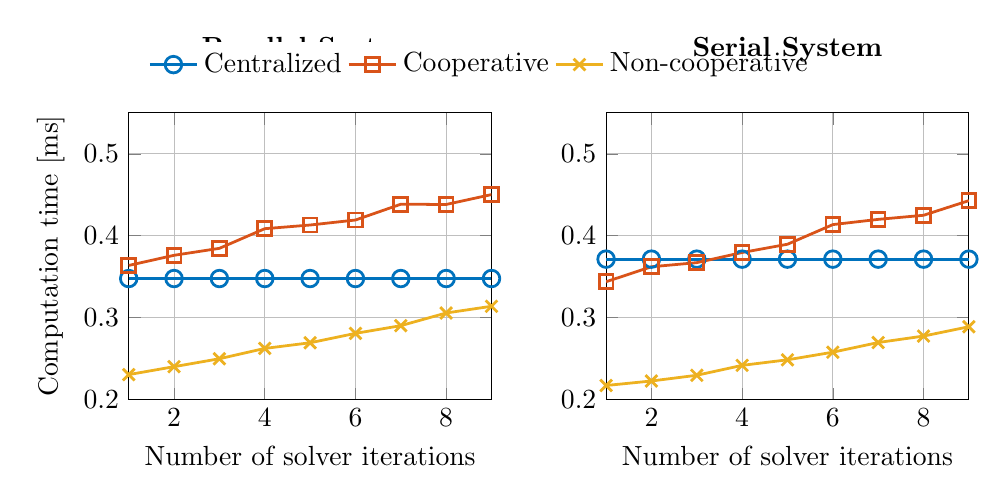
\begin{tikzpicture}

\begin{axis}[%
width=0.38\linewidth,
height=0.3\linewidth,
at={(0\linewidth,0\linewidth)},
scale only axis,
xmin=1,
xmax=9,
xlabel={Number of solver iterations},
xmajorgrids,
ymin=0.2,
ymax=0.55,
ylabel={Computation time [ms]},
ymajorgrids,
axis background/.style={fill=white},
title style={font=\bfseries,yshift=2.1ex},
title={Parallel System},
ylabel near ticks,
legend columns=-1,
legend style={at={(0.03,1.25)},anchor=north west,legend cell align=left,align=left,draw=none}
]
\addplot [color=mycolor1,solid,line width=1pt,mark size=3.0pt,mark=o,mark options={solid}]
  table[row sep=crcr]{%
1	0.3476\\
2	0.3476\\
3	0.3476\\
4	0.3476\\
5	0.3476\\
6	0.3476\\
7	0.3476\\
8	0.3476\\
9	0.3476\\
};
\addlegendentry{Centralized};

\addplot [color=mycolor2,solid,line width=1pt,mark size=2.5pt,mark=square,mark options={solid}]
  table[row sep=crcr]{%
1 0.3636\\
2 0.3760\\
3 0.3845\\
4 0.4085\\
5 0.4130\\
6 0.4191\\
7 0.4384\\
8 0.4381\\
9 0.4502\\
};
\addlegendentry{Cooperative};

\addplot [color=mycolor3,solid,line width=1pt,mark size=3.0pt,mark=x,mark options={solid}]
  table[row sep=crcr]{%
1 0.2302\\
2 0.2399\\
3 0.2496\\
4 0.2622\\
5 0.2691\\
6 0.2806\\
7 0.2900\\
8 0.3055\\
9 0.3137\\
};
\addlegendentry{Non-cooperative};

\end{axis}

\begin{axis}[%
% width=0.761\linewidth,
% height=0.597\linewidth,
width=0.38\linewidth,
height=0.3\linewidth,
at={(0.5\linewidth,0\linewidth)},
scale only axis,
xmin=1,
xmax=9,
xlabel={Number of solver iterations},
xmajorgrids,
ymin=0.2,
ymax=0.55,
% ylabel={Average computation time [ms]},
ymajorgrids,
axis background/.style={fill=white},
title style={font=\bfseries,yshift=2.1ex},
title={Serial System}
]
\addplot [color=mycolor1,solid,line width=1pt,mark size=3.0pt,mark=o,mark options={solid},forget plot]
  table[row sep=crcr]{%
1	0.3713\\
2	0.3713\\
3	0.3713\\
4	0.3713\\
5	0.3713\\
6	0.3713\\
7	0.3713\\
8	0.3713\\
9	0.3713\\
};
\addplot [color=mycolor2,solid,line width=1pt,mark size=2.5pt,mark=square,mark options={solid},forget plot]
  table[row sep=crcr]{%
1 0.3437\\
2 0.3620\\
3 0.3670\\
4 0.3794\\
5 0.3895\\
6 0.4135\\
7 0.4199\\
8 0.4249\\
9 0.4428\\
};
\addplot [color=mycolor3,solid,line width=1pt,mark size=3.0pt,mark=x,mark options={solid},forget plot]
  table[row sep=crcr]{%
1 0.2169\\
2 0.2224\\
3 0.2294\\
4 0.2415\\
5 0.2483\\
6 0.2576\\
7 0.2694\\
8 0.2773\\
9 0.2887\\
};
\end{axis}

\end{tikzpicture}%

  }
  \caption[Controller computation time per iteration.]{Average controller computation time per iteration, as a function of the number of solver iterations used. Operating point is 3 solver iterations. Output disturbance is applied at \u{50}{s} and total simulation time is \u{500}{s}.}
  \label{fig:results:compcost}
\end{figure}


As expected, the non-cooperative controller achieves the lowest computation times for both the parallel and the serial system.
In both cases, the cooperative controller has a computation time approximately on par with the centralized controller.

The significant advantage in computation time demonstrated by the non-cooperative controller is a result of the reduced size of its prediction matrices, which are multiplied to generate the \g{qp}.
The computational cost of the \g{qp} generation is approximately linear in the number of outputs used, and the non-cooperative approach considers fewer outputs than the centralized or cooperative approaches.

As described in~\cite{Jones2016}, for the systems considered here, the QP-generation step has a much higher computational cost than the QP-solving step.
There is thus limited scope for decreasing the required computation time without decreasing the number of states used to generate the QP problem.

